\documentclass[twoside]{book}

% Packages required by doxygen
\usepackage{fixltx2e}
\usepackage{calc}
\usepackage{doxygen}
\usepackage[export]{adjustbox} % also loads graphicx
\usepackage{graphicx}
\usepackage[utf8]{inputenc}
\usepackage{makeidx}
\usepackage{multicol}
\usepackage{multirow}
\PassOptionsToPackage{warn}{textcomp}
\usepackage{textcomp}
\usepackage[nointegrals]{wasysym}
\usepackage[table]{xcolor}

% Font selection
\usepackage[T1]{fontenc}
\usepackage[scaled=.90]{helvet}
\usepackage{courier}
\usepackage{amssymb}
\usepackage{sectsty}
\renewcommand{\familydefault}{\sfdefault}
\allsectionsfont{%
  \fontseries{bc}\selectfont%
  \color{darkgray}%
}
\renewcommand{\DoxyLabelFont}{%
  \fontseries{bc}\selectfont%
  \color{darkgray}%
}
\newcommand{\+}{\discretionary{\mbox{\scriptsize$\hookleftarrow$}}{}{}}

% Page & text layout
\usepackage{geometry}
\geometry{%
  a4paper,%
  top=2.5cm,%
  bottom=2.5cm,%
  left=2.5cm,%
  right=2.5cm%
}
\tolerance=750
\hfuzz=15pt
\hbadness=750
\setlength{\emergencystretch}{15pt}
\setlength{\parindent}{0cm}
\setlength{\parskip}{3ex plus 2ex minus 2ex}
\makeatletter
\renewcommand{\paragraph}{%
  \@startsection{paragraph}{4}{0ex}{-1.0ex}{1.0ex}{%
    \normalfont\normalsize\bfseries\SS@parafont%
  }%
}
\renewcommand{\subparagraph}{%
  \@startsection{subparagraph}{5}{0ex}{-1.0ex}{1.0ex}{%
    \normalfont\normalsize\bfseries\SS@subparafont%
  }%
}
\makeatother

% Headers & footers
\usepackage{fancyhdr}
\pagestyle{fancyplain}
\fancyhead[LE]{\fancyplain{}{\bfseries\thepage}}
\fancyhead[CE]{\fancyplain{}{}}
\fancyhead[RE]{\fancyplain{}{\bfseries\leftmark}}
\fancyhead[LO]{\fancyplain{}{\bfseries\rightmark}}
\fancyhead[CO]{\fancyplain{}{}}
\fancyhead[RO]{\fancyplain{}{\bfseries\thepage}}
\fancyfoot[LE]{\fancyplain{}{}}
\fancyfoot[CE]{\fancyplain{}{}}
\fancyfoot[RE]{\fancyplain{}{\bfseries\scriptsize Generated by Doxygen }}
\fancyfoot[LO]{\fancyplain{}{\bfseries\scriptsize Generated by Doxygen }}
\fancyfoot[CO]{\fancyplain{}{}}
\fancyfoot[RO]{\fancyplain{}{}}
\renewcommand{\footrulewidth}{0.4pt}
\renewcommand{\chaptermark}[1]{%
  \markboth{#1}{}%
}
\renewcommand{\sectionmark}[1]{%
  \markright{\thesection\ #1}%
}

% Indices & bibliography
\usepackage{natbib}
\usepackage[titles]{tocloft}
\setcounter{tocdepth}{3}
\setcounter{secnumdepth}{5}
\makeindex

% Hyperlinks (required, but should be loaded last)
\usepackage{ifpdf}
\ifpdf
  \usepackage[pdftex,pagebackref=true]{hyperref}
\else
  \usepackage[ps2pdf,pagebackref=true]{hyperref}
\fi
\hypersetup{%
  colorlinks=true,%
  linkcolor=blue,%
  citecolor=blue,%
  unicode%
}

% Custom commands
\newcommand{\clearemptydoublepage}{%
  \newpage{\pagestyle{empty}\cleardoublepage}%
}

\usepackage{caption}
\captionsetup{labelsep=space,justification=centering,font={bf},singlelinecheck=off,skip=4pt,position=top}

%===== C O N T E N T S =====

\begin{document}

% Titlepage & ToC
\hypersetup{pageanchor=false,
             bookmarksnumbered=true,
             pdfencoding=unicode
            }
\pagenumbering{alph}
\begin{titlepage}
\vspace*{7cm}
\begin{center}%
{\Large S\+GL }\\
\vspace*{1cm}
{\large Generated by Doxygen 1.8.14}\\
\end{center}
\end{titlepage}
\clearemptydoublepage
\pagenumbering{roman}
\tableofcontents
\clearemptydoublepage
\pagenumbering{arabic}
\hypersetup{pageanchor=true}

%--- Begin generated contents ---
\chapter{R\+E\+A\+D\+ME}
\label{md__home_stepp_Dropbox_data_docs_stanford_sgl_lib_README}
\Hypertarget{md__home_stepp_Dropbox_data_docs_stanford_sgl_lib_README}
J\+DZ\+: here is where I am adding notes about library structure/design, This is while reorganizing code, fall quarter 2019

{\bfseries Startup sequence, threads, main()} Student writes a main() function that appears to them to be the entry point for program, but this is sleight-\/of-\/hand. Student code is compiled with a \#define to rename main to student\+Main and linking with our library supplies a main() that call student\+Main() wrapped in necessary startup/teardown code.
\begin{DoxyItemize}
\item What happens in main wrapper?
\begin{DoxyEnumerate}
\item establishes the original thread as the \char`\"{}qtgui thread\char`\"{}
\item initializes QT application
\item initialize graphical console window (if \#include \mbox{\hyperlink{console_8h_source}{console.\+h}})
\item create second thread to run student\+Main, concurrently run QT application event loop on qtgui thread
\item shutdown at end of student\+Main and/or close console window
\end{DoxyEnumerate}
\item Threads A lot of the QT application/graphics interaction has to run on the qtgui thread, see \mbox{\hyperlink{classGThread_a33da0c87717269710ac7a564a1ebbe64}{G\+Thread\+::run\+On\+Qt\+Gui\+Thread}} for that dispatch
\end{DoxyItemize}

{\bfseries Static variables (initialization, constructors)}
\begin{DoxyItemize}
\item No guarantees about order of execution code is run for static initializers. See private/static.\+h for macros that provide declaration/access to static variable to ensure initializer run exactly once on first use of variable. 
\end{DoxyItemize}
\chapter{Deprecated List}
\label{deprecated}
\Hypertarget{deprecated}

\begin{DoxyRefList}
\item[\label{deprecated__deprecated000006}%
\Hypertarget{deprecated__deprecated000006}%
Member \mbox{\hyperlink{classsgl_1_1GInteractor_a02f20ea6edfa0671f31c4c648a253833}{G\+Interactor\+:\+:add\+Action\+Listener}} () Q\+\_\+\+D\+E\+C\+L\+\_\+\+D\+E\+P\+R\+E\+C\+A\+T\+ED]does nothing; use set\+Action\+Listener instead  
\item[\label{deprecated__deprecated000003}%
\Hypertarget{deprecated__deprecated000003}%
Member \mbox{\hyperlink{namespacesgl_a2cc1dab98b5712012e365c8afdc04bc4}{sgl\+:\+:get\+Next\+Event}} (int mask=A\+N\+Y\+\_\+\+E\+V\+E\+NT)]This function is deprecated and discouraged from use. Instead of calling wait\+For\+Click in an event loop, you should attach an event-\/listening function to the widget of choice using that object\textquotesingle{}s methods such as set\+Action\+Listener or set\+Mouse\+Listener.  
\item[\label{deprecated__deprecated000004}%
\Hypertarget{deprecated__deprecated000004}%
Member \mbox{\hyperlink{namespacesgl_ae6780e0be2caaa8a595026b472e74808}{sgl\+:\+:wait\+For\+Click}} ()]This function is deprecated and discouraged from use. Instead of calling wait\+For\+Click in an event loop, you should attach an event-\/listening function to the widget of choice using that object\textquotesingle{}s methods such as set\+Action\+Listener or set\+Mouse\+Listener.  
\item[\label{deprecated__deprecated000005}%
\Hypertarget{deprecated__deprecated000005}%
Member \mbox{\hyperlink{namespacesgl_ac49283a36a844e5c07ce0b199f481c9f}{sgl\+:\+:wait\+For\+Event}} (int mask=A\+N\+Y\+\_\+\+E\+V\+E\+NT)]This function is deprecated and discouraged from use. Instead of calling wait\+For\+Click in an event loop, you should attach an event-\/listening function to the widget of choice using that object\textquotesingle{}s methods such as set\+Action\+Listener or set\+Mouse\+Listener. 
\end{DoxyRefList}
\chapter{Namespace Index}
\input{namespaces}
\chapter{Hierarchical Index}
\section{Class Hierarchy}
This inheritance list is sorted roughly, but not completely, alphabetically\+:\begin{DoxyCompactList}
\item \contentsline{section}{G\+Clipboard}{\pageref{classGClipboard}}{}
\item \contentsline{section}{G\+Color}{\pageref{classGColor}}{}
\item \contentsline{section}{G\+Color\+Chooser}{\pageref{classGColorChooser}}{}
\item \contentsline{section}{G\+Dimension}{\pageref{structGDimension}}{}
\item \contentsline{section}{G\+Drawing\+Surface}{\pageref{classGDrawingSurface}}{}
\begin{DoxyCompactList}
\item \contentsline{section}{G\+Canvas}{\pageref{classGCanvas}}{}
\end{DoxyCompactList}
\item \contentsline{section}{G\+Event}{\pageref{classGEvent}}{}
\item \contentsline{section}{G\+File\+Chooser}{\pageref{classGFileChooser}}{}
\item \contentsline{section}{G\+Font}{\pageref{classGFont}}{}
\item \contentsline{section}{G\+Font\+Chooser}{\pageref{classGFontChooser}}{}
\item \contentsline{section}{G\+Object}{\pageref{classGObject}}{}
\begin{DoxyCompactList}
\item \contentsline{section}{G\+Arc}{\pageref{classGArc}}{}
\item \contentsline{section}{G\+Compound}{\pageref{classGCompound}}{}
\item \contentsline{section}{G\+Image}{\pageref{classGImage}}{}
\item \contentsline{section}{G\+Line}{\pageref{classGLine}}{}
\item \contentsline{section}{G\+Oval}{\pageref{classGOval}}{}
\item \contentsline{section}{G\+Polygon}{\pageref{classGPolygon}}{}
\item \contentsline{section}{G\+Rect}{\pageref{classGRect}}{}
\begin{DoxyCompactList}
\item \contentsline{section}{G\+Round\+Rect}{\pageref{classGRoundRect}}{}
\end{DoxyCompactList}
\item \contentsline{section}{G\+Text}{\pageref{classGText}}{}
\end{DoxyCompactList}
\item \contentsline{section}{G\+Observable}{\pageref{classGObservable}}{}
\begin{DoxyCompactList}
\item \contentsline{section}{G\+Interactor}{\pageref{classGInteractor}}{}
\begin{DoxyCompactList}
\item \contentsline{section}{G\+Browser\+Pane}{\pageref{classGBrowserPane}}{}
\item \contentsline{section}{G\+Button}{\pageref{classGButton}}{}
\item \contentsline{section}{G\+Canvas}{\pageref{classGCanvas}}{}
\item \contentsline{section}{G\+Check\+Box}{\pageref{classGCheckBox}}{}
\item \contentsline{section}{G\+Chooser}{\pageref{classGChooser}}{}
\item \contentsline{section}{G\+Container}{\pageref{classGContainer}}{}
\item \contentsline{section}{G\+Label}{\pageref{classGLabel}}{}
\item \contentsline{section}{G\+Radio\+Button}{\pageref{classGRadioButton}}{}
\item \contentsline{section}{G\+Scroll\+Bar}{\pageref{classGScrollBar}}{}
\item \contentsline{section}{G\+Scroll\+Pane}{\pageref{classGScrollPane}}{}
\item \contentsline{section}{G\+Slider}{\pageref{classGSlider}}{}
\item \contentsline{section}{G\+Spacer}{\pageref{classGSpacer}}{}
\item \contentsline{section}{G\+Table}{\pageref{classGTable}}{}
\item \contentsline{section}{G\+Text\+Area}{\pageref{classGTextArea}}{}
\item \contentsline{section}{G\+Text\+Field}{\pageref{classGTextField}}{}
\end{DoxyCompactList}
\item \contentsline{section}{G\+Window}{\pageref{classGWindow}}{}
\end{DoxyCompactList}
\item \contentsline{section}{G\+Option\+Pane}{\pageref{classGOptionPane}}{}
\item \contentsline{section}{G\+Point}{\pageref{structGPoint}}{}
\item \contentsline{section}{G\+Rectangle}{\pageref{structGRectangle}}{}
\item \contentsline{section}{G\+Sound}{\pageref{classGSound}}{}
\item \contentsline{section}{G\+Thread}{\pageref{classGThread}}{}
\item \contentsline{section}{G\+Timer}{\pageref{classGTimer}}{}
\item Q\+Object\begin{DoxyCompactList}
\item \contentsline{section}{G\+Downloader}{\pageref{classGDownloader}}{}
\end{DoxyCompactList}
\end{DoxyCompactList}

\chapter{Class Index}
\section{Class List}
Here are the classes, structs, unions and interfaces with brief descriptions\+:\begin{DoxyCompactList}
\item\contentsline{section}{\mbox{\hyperlink{classsgl_1_1GArc}{G\+Arc}} \\*This graphical object subclass represents an elliptical arc }{\pageref{classsgl_1_1GArc}}{}
\item\contentsline{section}{\mbox{\hyperlink{classsgl_1_1GBrowserPane}{G\+Browser\+Pane}} \\*A \mbox{\hyperlink{classsgl_1_1GBrowserPane}{G\+Browser\+Pane}} is a graphical interactor that displays a web page }{\pageref{classsgl_1_1GBrowserPane}}{}
\item\contentsline{section}{\mbox{\hyperlink{classsgl_1_1GButton}{G\+Button}} \\*This interactor subclass represents an onscreen button }{\pageref{classsgl_1_1GButton}}{}
\item\contentsline{section}{\mbox{\hyperlink{classsgl_1_1GCanvas}{G\+Canvas}} \\*A \mbox{\hyperlink{classsgl_1_1GCanvas}{G\+Canvas}} is a graphical drawing surface on which you can draw shapes, lines, and colors, as well as setting the R\+GB color values of individual pixels }{\pageref{classsgl_1_1GCanvas}}{}
\item\contentsline{section}{\mbox{\hyperlink{classsgl_1_1GCheckBox}{G\+Check\+Box}} \\*This interactor subclass represents an onscreen check box }{\pageref{classsgl_1_1GCheckBox}}{}
\item\contentsline{section}{\mbox{\hyperlink{classsgl_1_1GChooser}{G\+Chooser}} \\*This interactor subclass represents a selectable drop-\/down list }{\pageref{classsgl_1_1GChooser}}{}
\item\contentsline{section}{\mbox{\hyperlink{classsgl_1_1GClipboard}{G\+Clipboard}} \\*Static methods you can use to get and set the contents of the system clipboard }{\pageref{classsgl_1_1GClipboard}}{}
\item\contentsline{section}{\mbox{\hyperlink{classsgl_1_1GColor}{G\+Color}} \\*This class provides static methods for dealing with colors }{\pageref{classsgl_1_1GColor}}{}
\item\contentsline{section}{\mbox{\hyperlink{classsgl_1_1GColorChooser}{G\+Color\+Chooser}} \\*Static methods for popping up color-\/choosing dialog boxes that allow the user to select a color }{\pageref{classsgl_1_1GColorChooser}}{}
\item\contentsline{section}{\mbox{\hyperlink{classsgl_1_1GCompound}{G\+Compound}} \\*This graphical object subclass consists of a collection of other graphical objects }{\pageref{classsgl_1_1GCompound}}{}
\item\contentsline{section}{\mbox{\hyperlink{classsgl_1_1GContainer}{G\+Container}} \\*A \mbox{\hyperlink{classsgl_1_1GContainer}{G\+Container}} is a logical grouping for interactors }{\pageref{classsgl_1_1GContainer}}{}
\item\contentsline{section}{\mbox{\hyperlink{structsgl_1_1GDimension}{G\+Dimension}} \\*This struct contains real-\/valued width and height fields }{\pageref{structsgl_1_1GDimension}}{}
\item\contentsline{section}{\mbox{\hyperlink{classsgl_1_1GDownloader}{G\+Downloader}} \\*A \mbox{\hyperlink{classsgl_1_1GDownloader}{G\+Downloader}} can download files and data over an internet connection }{\pageref{classsgl_1_1GDownloader}}{}
\item\contentsline{section}{\mbox{\hyperlink{classsgl_1_1GDrawingSurface}{G\+Drawing\+Surface}} \\*\mbox{\hyperlink{classsgl_1_1GDrawingSurface}{G\+Drawing\+Surface}} is an abstract superclass for types that allow drawing shapes and pixels onto themselves as a pixel background layer }{\pageref{classsgl_1_1GDrawingSurface}}{}
\item\contentsline{section}{\mbox{\hyperlink{classsgl_1_1GEvent}{G\+Event}} \\*A \mbox{\hyperlink{classsgl_1_1GEvent}{G\+Event}} represents a user action that has occurred on a graphical interactor }{\pageref{classsgl_1_1GEvent}}{}
\item\contentsline{section}{\mbox{\hyperlink{classsgl_1_1GFileChooser}{G\+File\+Chooser}} \\*Static methods for popping up file-\/choosing dialog boxes that allow the user to select a file }{\pageref{classsgl_1_1GFileChooser}}{}
\item\contentsline{section}{\mbox{\hyperlink{classsgl_1_1GFont}{G\+Font}} \\*This class contains static methods for dealing with fonts in our G\+UI system }{\pageref{classsgl_1_1GFont}}{}
\item\contentsline{section}{\mbox{\hyperlink{classsgl_1_1GFontChooser}{G\+Font\+Chooser}} \\*Static methods for popping up font-\/choosing dialog boxes that allow the user to select a font family, size, and style }{\pageref{classsgl_1_1GFontChooser}}{}
\item\contentsline{section}{\mbox{\hyperlink{classsgl_1_1GImage}{G\+Image}} \\*This graphical object subclass represents an image from a file }{\pageref{classsgl_1_1GImage}}{}
\item\contentsline{section}{\mbox{\hyperlink{classsgl_1_1GInteractor}{G\+Interactor}} \\*This abstract class is the superclass for all graphical interactors }{\pageref{classsgl_1_1GInteractor}}{}
\item\contentsline{section}{\mbox{\hyperlink{classsgl_1_1GLabel}{G\+Label}} \\*A \mbox{\hyperlink{classsgl_1_1GLabel}{G\+Label}} represents a text string }{\pageref{classsgl_1_1GLabel}}{}
\item\contentsline{section}{\mbox{\hyperlink{classsgl_1_1GLine}{G\+Line}} \\*This graphical object subclass represents a line segment }{\pageref{classsgl_1_1GLine}}{}
\item\contentsline{section}{\mbox{\hyperlink{classsgl_1_1GObject}{G\+Object}} \\*This class is the common superclass of all graphical objects that can be displayed on a graphical window }{\pageref{classsgl_1_1GObject}}{}
\item\contentsline{section}{\mbox{\hyperlink{classsgl_1_1GObservable}{G\+Observable}} \\*A \mbox{\hyperlink{classsgl_1_1GObservable}{G\+Observable}} object is one that is able to send out events }{\pageref{classsgl_1_1GObservable}}{}
\item\contentsline{section}{\mbox{\hyperlink{classsgl_1_1GOptionPane}{G\+Option\+Pane}} \\*This class provides static methods that pop up graphical input/output dialog boxes on the screen }{\pageref{classsgl_1_1GOptionPane}}{}
\item\contentsline{section}{\mbox{\hyperlink{classsgl_1_1GOval}{G\+Oval}} \\*This graphical object subclass represents an oval inscribed in a rectangular box }{\pageref{classsgl_1_1GOval}}{}
\item\contentsline{section}{\mbox{\hyperlink{structsgl_1_1GPoint}{G\+Point}} \\*This struct contains real-\/valued x and y fields }{\pageref{structsgl_1_1GPoint}}{}
\item\contentsline{section}{\mbox{\hyperlink{classsgl_1_1GPolygon}{G\+Polygon}} \\*This graphical object subclass represents a polygon bounded by line segments }{\pageref{classsgl_1_1GPolygon}}{}
\item\contentsline{section}{\mbox{\hyperlink{classsgl_1_1GRadioButton}{G\+Radio\+Button}} \\*This interactor subclass represents an onscreen radio button }{\pageref{classsgl_1_1GRadioButton}}{}
\item\contentsline{section}{\mbox{\hyperlink{classsgl_1_1GRect}{G\+Rect}} \\*A \mbox{\hyperlink{classsgl_1_1GRect}{G\+Rect}} is a graphical object whose appearance consists of a rectangular box }{\pageref{classsgl_1_1GRect}}{}
\item\contentsline{section}{\mbox{\hyperlink{structsgl_1_1GRectangle}{G\+Rectangle}} \\*This struct contains real-\/valued x, y, width, and height fields }{\pageref{structsgl_1_1GRectangle}}{}
\item\contentsline{section}{\mbox{\hyperlink{classsgl_1_1GRoundRect}{G\+Round\+Rect}} \\*A \mbox{\hyperlink{classsgl_1_1GRoundRect}{G\+Round\+Rect}} represents a graphical object whose appearance consists of a rectangular box with rounded corners }{\pageref{classsgl_1_1GRoundRect}}{}
\item\contentsline{section}{\mbox{\hyperlink{classsgl_1_1GScrollBar}{G\+Scroll\+Bar}} \\*A \mbox{\hyperlink{classsgl_1_1GScrollBar}{G\+Scroll\+Bar}} represents a horizontal or vertical scroll bar that can be dragged by the user }{\pageref{classsgl_1_1GScrollBar}}{}
\item\contentsline{section}{\mbox{\hyperlink{classsgl_1_1GScrollPane}{G\+Scroll\+Pane}} \\*A \mbox{\hyperlink{classsgl_1_1GScrollPane}{G\+Scroll\+Pane}} is a container that wraps another interactor with scroll bars }{\pageref{classsgl_1_1GScrollPane}}{}
\item\contentsline{section}{\mbox{\hyperlink{classsgl_1_1GSlider}{G\+Slider}} \\*This interactor subclass represents an onscreen slider }{\pageref{classsgl_1_1GSlider}}{}
\item\contentsline{section}{\mbox{\hyperlink{classsgl_1_1GSound}{G\+Sound}} \\*~\newline
 This class encapsulates a sound file }{\pageref{classsgl_1_1GSound}}{}
\item\contentsline{section}{\mbox{\hyperlink{classsgl_1_1GSpacer}{G\+Spacer}} \\*A \mbox{\hyperlink{classsgl_1_1GSpacer}{G\+Spacer}} is just an empty blob of space that helps you pad layouts }{\pageref{classsgl_1_1GSpacer}}{}
\item\contentsline{section}{\mbox{\hyperlink{classsgl_1_1GTable}{G\+Table}} \\*A \mbox{\hyperlink{classsgl_1_1GTable}{G\+Table}} represents a graphical editable 2D table, like a mediocre facsimile of an Excel spreadsheet }{\pageref{classsgl_1_1GTable}}{}
\item\contentsline{section}{\mbox{\hyperlink{structsgl_1_1GTableIndex}{G\+Table\+Index}} \\*This is a small structure representing a row and column in a table }{\pageref{structsgl_1_1GTableIndex}}{}
\item\contentsline{section}{\mbox{\hyperlink{classsgl_1_1GText}{G\+Text}} \\*This graphical object subclass represents a text string }{\pageref{classsgl_1_1GText}}{}
\item\contentsline{section}{\mbox{\hyperlink{classsgl_1_1GTextArea}{G\+Text\+Area}} \\*A \mbox{\hyperlink{classsgl_1_1GTextArea}{G\+Text\+Area}} is a multi-\/line editable text box }{\pageref{classsgl_1_1GTextArea}}{}
\item\contentsline{section}{\mbox{\hyperlink{classsgl_1_1GTextField}{G\+Text\+Field}} \\*This interactor subclass represents a text field for entering short text strings }{\pageref{classsgl_1_1GTextField}}{}
\item\contentsline{section}{\mbox{\hyperlink{classsgl_1_1GThread}{G\+Thread}} \\*Utility class containing static methods that allow you to run code on various system threads }{\pageref{classsgl_1_1GThread}}{}
\item\contentsline{section}{\mbox{\hyperlink{classsgl_1_1GTimer}{G\+Timer}} \\*This class implements a simple interval timer that generates a {\ttfamily G\+Timer\+Event} with a specified frequency }{\pageref{classsgl_1_1GTimer}}{}
\item\contentsline{section}{\mbox{\hyperlink{classsgl_1_1GWindow}{G\+Window}} \\*This class represents a graphics window that supports simple graphics }{\pageref{classsgl_1_1GWindow}}{}
\end{DoxyCompactList}

\chapter{Namespace Documentation}
\hypertarget{namespacediff}{}\section{diff Namespace Reference}
\label{namespacediff}\index{diff@{diff}}
\subsection*{Enumerations}
\begin{DoxyCompactItemize}
\item 
enum \mbox{\hyperlink{namespacediff_ab3b1c38517a62ce7edefba7b93b406dd}{Diff\+Flags}} \{ \mbox{\hyperlink{namespacediff_ab3b1c38517a62ce7edefba7b93b406ddad0f7243da8aa7c7d8ff1d3ec921a40b4}{I\+G\+N\+O\+R\+E\+\_\+\+N\+O\+NE}} = 0x0, 
\mbox{\hyperlink{namespacediff_ab3b1c38517a62ce7edefba7b93b406dda36178024b8ebb050729793dd32e0b1a9}{I\+G\+N\+O\+R\+E\+\_\+\+L\+E\+A\+D\+I\+NG}} = 0x1, 
\mbox{\hyperlink{namespacediff_ab3b1c38517a62ce7edefba7b93b406dda4cf05931c8f25fb17d9f490c6bd67d70}{I\+G\+N\+O\+R\+E\+\_\+\+T\+R\+A\+I\+L\+I\+NG}} = 0x2, 
\mbox{\hyperlink{namespacediff_ab3b1c38517a62ce7edefba7b93b406ddab94634739aa9d0705e2eb7976a969a20}{I\+G\+N\+O\+R\+E\+\_\+\+W\+H\+I\+T\+E\+S\+P\+A\+CE}} = 0x4, 
\mbox{\hyperlink{namespacediff_ab3b1c38517a62ce7edefba7b93b406ddafb3c9078d1a73b062d0b08be343f7126}{I\+G\+N\+O\+R\+E\+\_\+\+B\+L\+A\+N\+K\+L\+I\+N\+ES}} = 0x8, 
\mbox{\hyperlink{namespacediff_ab3b1c38517a62ce7edefba7b93b406dda743829c4dd20c98f1a4db5f83106d839}{I\+G\+N\+O\+R\+E\+\_\+\+C\+A\+SE}} = 0x10, 
\mbox{\hyperlink{namespacediff_ab3b1c38517a62ce7edefba7b93b406ddadb9d907f4925e58514022d03c646ed2e}{I\+G\+N\+O\+R\+E\+\_\+\+N\+U\+M\+B\+E\+RS}} = 0x20, 
\mbox{\hyperlink{namespacediff_ab3b1c38517a62ce7edefba7b93b406ddabf5793c00c9ca596c7743a9a9704b7f7}{I\+G\+N\+O\+R\+E\+\_\+\+N\+O\+N\+N\+U\+M\+B\+E\+RS}} = 0x40, 
\mbox{\hyperlink{namespacediff_ab3b1c38517a62ce7edefba7b93b406dda84e6a2f9f288157ed7a207dc744e1d46}{I\+G\+N\+O\+R\+E\+\_\+\+P\+U\+N\+C\+T\+U\+A\+T\+I\+ON}} = 0x80, 
\mbox{\hyperlink{namespacediff_ab3b1c38517a62ce7edefba7b93b406dda2cb6b009fb93f98c0d82e64524454f3f}{I\+G\+N\+O\+R\+E\+\_\+\+A\+F\+T\+E\+R\+D\+E\+C\+I\+M\+AL}} = 0x100, 
\mbox{\hyperlink{namespacediff_ab3b1c38517a62ce7edefba7b93b406dda8382f8ecacc40734d5aa68059769d486}{I\+G\+N\+O\+R\+E\+\_\+\+C\+H\+A\+R\+O\+R\+D\+ER}} = 0x200, 
\mbox{\hyperlink{namespacediff_ab3b1c38517a62ce7edefba7b93b406dda3dd3d9c71b29c78f94e9104e8e4d08f9}{I\+G\+N\+O\+R\+E\+\_\+\+L\+I\+N\+E\+O\+R\+D\+ER}} = 0x400, 
\mbox{\hyperlink{namespacediff_ab3b1c38517a62ce7edefba7b93b406dda1023cdec61bceee745fffdc581f0d366}{I\+G\+N\+O\+R\+E\+\_\+\+E\+V\+E\+R\+Y\+T\+H\+I\+NG}} = 0x100000
 \}
\end{DoxyCompactItemize}
\subsection*{Functions}
\begin{DoxyCompactItemize}
\item 
std\+::string \mbox{\hyperlink{namespacediff_a37f80e92da40347774327a755bdf4c93}{diff}} (std\+::string s1, std\+::string s2, int flags)
\item 
bool \mbox{\hyperlink{namespacediff_a68a39e10b40db02df1d941fe83cc9828}{diff\+Pass}} (const std\+::string \&s1, const std\+::string \&s2, int flags)
\item 
bool \mbox{\hyperlink{namespacediff_a02aeebb7bbdd2871ba3d5470721004e5}{is\+Diff\+Match}} (const std\+::string \&diffs)
\end{DoxyCompactItemize}
\subsection*{Variables}
\begin{DoxyCompactItemize}
\item 
const int \mbox{\hyperlink{namespacediff_a5044abd56bc89e814e2d953b8e8c0a65}{D\+I\+F\+F\+\_\+\+D\+E\+F\+A\+U\+L\+T\+\_\+\+F\+L\+A\+GS}} = \mbox{\hyperlink{namespacediff_ab3b1c38517a62ce7edefba7b93b406dda743829c4dd20c98f1a4db5f83106d839}{I\+G\+N\+O\+R\+E\+\_\+\+C\+A\+SE}} $\vert$ \mbox{\hyperlink{namespacediff_ab3b1c38517a62ce7edefba7b93b406dda4cf05931c8f25fb17d9f490c6bd67d70}{I\+G\+N\+O\+R\+E\+\_\+\+T\+R\+A\+I\+L\+I\+NG}} $\vert$ \mbox{\hyperlink{namespacediff_ab3b1c38517a62ce7edefba7b93b406ddab94634739aa9d0705e2eb7976a969a20}{I\+G\+N\+O\+R\+E\+\_\+\+W\+H\+I\+T\+E\+S\+P\+A\+CE}} $\vert$ \mbox{\hyperlink{namespacediff_ab3b1c38517a62ce7edefba7b93b406dda84e6a2f9f288157ed7a207dc744e1d46}{I\+G\+N\+O\+R\+E\+\_\+\+P\+U\+N\+C\+T\+U\+A\+T\+I\+ON}}
\item 
const int \mbox{\hyperlink{namespacediff_aada938db21bf68a19d23eca0fddc551b}{D\+I\+F\+F\+\_\+\+S\+T\+R\+I\+C\+T\+\_\+\+F\+L\+A\+GS}} = \mbox{\hyperlink{namespacediff_ab3b1c38517a62ce7edefba7b93b406dda4cf05931c8f25fb17d9f490c6bd67d70}{I\+G\+N\+O\+R\+E\+\_\+\+T\+R\+A\+I\+L\+I\+NG}}
\item 
const std\+::string \mbox{\hyperlink{namespacediff_a4f8bdb0eae6c54a481aba9358db1e9ab}{N\+O\+\_\+\+D\+I\+F\+F\+S\+\_\+\+M\+E\+S\+S\+A\+GE}} = \char`\"{}No differences found\char`\"{}
\end{DoxyCompactItemize}


\subsection{Enumeration Type Documentation}
\mbox{\Hypertarget{namespacediff_ab3b1c38517a62ce7edefba7b93b406dd}\label{namespacediff_ab3b1c38517a62ce7edefba7b93b406dd}} 
\index{diff@{diff}!Diff\+Flags@{Diff\+Flags}}
\index{Diff\+Flags@{Diff\+Flags}!diff@{diff}}
\subsubsection{\texorpdfstring{Diff\+Flags}{DiffFlags}}
{\footnotesize\ttfamily enum \mbox{\hyperlink{namespacediff_ab3b1c38517a62ce7edefba7b93b406dd}{Diff\+Flags}}}

\begin{DoxyEnumFields}{Enumerator}
\raisebox{\heightof{T}}[0pt][0pt]{\index{I\+G\+N\+O\+R\+E\+\_\+\+N\+O\+NE@{I\+G\+N\+O\+R\+E\+\_\+\+N\+O\+NE}!diff@{diff}}\index{diff@{diff}!I\+G\+N\+O\+R\+E\+\_\+\+N\+O\+NE@{I\+G\+N\+O\+R\+E\+\_\+\+N\+O\+NE}}}\mbox{\Hypertarget{namespacediff_ab3b1c38517a62ce7edefba7b93b406ddad0f7243da8aa7c7d8ff1d3ec921a40b4}\label{namespacediff_ab3b1c38517a62ce7edefba7b93b406ddad0f7243da8aa7c7d8ff1d3ec921a40b4}} 
I\+G\+N\+O\+R\+E\+\_\+\+N\+O\+NE&\\
\hline

\raisebox{\heightof{T}}[0pt][0pt]{\index{I\+G\+N\+O\+R\+E\+\_\+\+L\+E\+A\+D\+I\+NG@{I\+G\+N\+O\+R\+E\+\_\+\+L\+E\+A\+D\+I\+NG}!diff@{diff}}\index{diff@{diff}!I\+G\+N\+O\+R\+E\+\_\+\+L\+E\+A\+D\+I\+NG@{I\+G\+N\+O\+R\+E\+\_\+\+L\+E\+A\+D\+I\+NG}}}\mbox{\Hypertarget{namespacediff_ab3b1c38517a62ce7edefba7b93b406dda36178024b8ebb050729793dd32e0b1a9}\label{namespacediff_ab3b1c38517a62ce7edefba7b93b406dda36178024b8ebb050729793dd32e0b1a9}} 
I\+G\+N\+O\+R\+E\+\_\+\+L\+E\+A\+D\+I\+NG&\\
\hline

\raisebox{\heightof{T}}[0pt][0pt]{\index{I\+G\+N\+O\+R\+E\+\_\+\+T\+R\+A\+I\+L\+I\+NG@{I\+G\+N\+O\+R\+E\+\_\+\+T\+R\+A\+I\+L\+I\+NG}!diff@{diff}}\index{diff@{diff}!I\+G\+N\+O\+R\+E\+\_\+\+T\+R\+A\+I\+L\+I\+NG@{I\+G\+N\+O\+R\+E\+\_\+\+T\+R\+A\+I\+L\+I\+NG}}}\mbox{\Hypertarget{namespacediff_ab3b1c38517a62ce7edefba7b93b406dda4cf05931c8f25fb17d9f490c6bd67d70}\label{namespacediff_ab3b1c38517a62ce7edefba7b93b406dda4cf05931c8f25fb17d9f490c6bd67d70}} 
I\+G\+N\+O\+R\+E\+\_\+\+T\+R\+A\+I\+L\+I\+NG&\\
\hline

\raisebox{\heightof{T}}[0pt][0pt]{\index{I\+G\+N\+O\+R\+E\+\_\+\+W\+H\+I\+T\+E\+S\+P\+A\+CE@{I\+G\+N\+O\+R\+E\+\_\+\+W\+H\+I\+T\+E\+S\+P\+A\+CE}!diff@{diff}}\index{diff@{diff}!I\+G\+N\+O\+R\+E\+\_\+\+W\+H\+I\+T\+E\+S\+P\+A\+CE@{I\+G\+N\+O\+R\+E\+\_\+\+W\+H\+I\+T\+E\+S\+P\+A\+CE}}}\mbox{\Hypertarget{namespacediff_ab3b1c38517a62ce7edefba7b93b406ddab94634739aa9d0705e2eb7976a969a20}\label{namespacediff_ab3b1c38517a62ce7edefba7b93b406ddab94634739aa9d0705e2eb7976a969a20}} 
I\+G\+N\+O\+R\+E\+\_\+\+W\+H\+I\+T\+E\+S\+P\+A\+CE&\\
\hline

\raisebox{\heightof{T}}[0pt][0pt]{\index{I\+G\+N\+O\+R\+E\+\_\+\+B\+L\+A\+N\+K\+L\+I\+N\+ES@{I\+G\+N\+O\+R\+E\+\_\+\+B\+L\+A\+N\+K\+L\+I\+N\+ES}!diff@{diff}}\index{diff@{diff}!I\+G\+N\+O\+R\+E\+\_\+\+B\+L\+A\+N\+K\+L\+I\+N\+ES@{I\+G\+N\+O\+R\+E\+\_\+\+B\+L\+A\+N\+K\+L\+I\+N\+ES}}}\mbox{\Hypertarget{namespacediff_ab3b1c38517a62ce7edefba7b93b406ddafb3c9078d1a73b062d0b08be343f7126}\label{namespacediff_ab3b1c38517a62ce7edefba7b93b406ddafb3c9078d1a73b062d0b08be343f7126}} 
I\+G\+N\+O\+R\+E\+\_\+\+B\+L\+A\+N\+K\+L\+I\+N\+ES&\\
\hline

\raisebox{\heightof{T}}[0pt][0pt]{\index{I\+G\+N\+O\+R\+E\+\_\+\+C\+A\+SE@{I\+G\+N\+O\+R\+E\+\_\+\+C\+A\+SE}!diff@{diff}}\index{diff@{diff}!I\+G\+N\+O\+R\+E\+\_\+\+C\+A\+SE@{I\+G\+N\+O\+R\+E\+\_\+\+C\+A\+SE}}}\mbox{\Hypertarget{namespacediff_ab3b1c38517a62ce7edefba7b93b406dda743829c4dd20c98f1a4db5f83106d839}\label{namespacediff_ab3b1c38517a62ce7edefba7b93b406dda743829c4dd20c98f1a4db5f83106d839}} 
I\+G\+N\+O\+R\+E\+\_\+\+C\+A\+SE&\\
\hline

\raisebox{\heightof{T}}[0pt][0pt]{\index{I\+G\+N\+O\+R\+E\+\_\+\+N\+U\+M\+B\+E\+RS@{I\+G\+N\+O\+R\+E\+\_\+\+N\+U\+M\+B\+E\+RS}!diff@{diff}}\index{diff@{diff}!I\+G\+N\+O\+R\+E\+\_\+\+N\+U\+M\+B\+E\+RS@{I\+G\+N\+O\+R\+E\+\_\+\+N\+U\+M\+B\+E\+RS}}}\mbox{\Hypertarget{namespacediff_ab3b1c38517a62ce7edefba7b93b406ddadb9d907f4925e58514022d03c646ed2e}\label{namespacediff_ab3b1c38517a62ce7edefba7b93b406ddadb9d907f4925e58514022d03c646ed2e}} 
I\+G\+N\+O\+R\+E\+\_\+\+N\+U\+M\+B\+E\+RS&\\
\hline

\raisebox{\heightof{T}}[0pt][0pt]{\index{I\+G\+N\+O\+R\+E\+\_\+\+N\+O\+N\+N\+U\+M\+B\+E\+RS@{I\+G\+N\+O\+R\+E\+\_\+\+N\+O\+N\+N\+U\+M\+B\+E\+RS}!diff@{diff}}\index{diff@{diff}!I\+G\+N\+O\+R\+E\+\_\+\+N\+O\+N\+N\+U\+M\+B\+E\+RS@{I\+G\+N\+O\+R\+E\+\_\+\+N\+O\+N\+N\+U\+M\+B\+E\+RS}}}\mbox{\Hypertarget{namespacediff_ab3b1c38517a62ce7edefba7b93b406ddabf5793c00c9ca596c7743a9a9704b7f7}\label{namespacediff_ab3b1c38517a62ce7edefba7b93b406ddabf5793c00c9ca596c7743a9a9704b7f7}} 
I\+G\+N\+O\+R\+E\+\_\+\+N\+O\+N\+N\+U\+M\+B\+E\+RS&\\
\hline

\raisebox{\heightof{T}}[0pt][0pt]{\index{I\+G\+N\+O\+R\+E\+\_\+\+P\+U\+N\+C\+T\+U\+A\+T\+I\+ON@{I\+G\+N\+O\+R\+E\+\_\+\+P\+U\+N\+C\+T\+U\+A\+T\+I\+ON}!diff@{diff}}\index{diff@{diff}!I\+G\+N\+O\+R\+E\+\_\+\+P\+U\+N\+C\+T\+U\+A\+T\+I\+ON@{I\+G\+N\+O\+R\+E\+\_\+\+P\+U\+N\+C\+T\+U\+A\+T\+I\+ON}}}\mbox{\Hypertarget{namespacediff_ab3b1c38517a62ce7edefba7b93b406dda84e6a2f9f288157ed7a207dc744e1d46}\label{namespacediff_ab3b1c38517a62ce7edefba7b93b406dda84e6a2f9f288157ed7a207dc744e1d46}} 
I\+G\+N\+O\+R\+E\+\_\+\+P\+U\+N\+C\+T\+U\+A\+T\+I\+ON&\\
\hline

\raisebox{\heightof{T}}[0pt][0pt]{\index{I\+G\+N\+O\+R\+E\+\_\+\+A\+F\+T\+E\+R\+D\+E\+C\+I\+M\+AL@{I\+G\+N\+O\+R\+E\+\_\+\+A\+F\+T\+E\+R\+D\+E\+C\+I\+M\+AL}!diff@{diff}}\index{diff@{diff}!I\+G\+N\+O\+R\+E\+\_\+\+A\+F\+T\+E\+R\+D\+E\+C\+I\+M\+AL@{I\+G\+N\+O\+R\+E\+\_\+\+A\+F\+T\+E\+R\+D\+E\+C\+I\+M\+AL}}}\mbox{\Hypertarget{namespacediff_ab3b1c38517a62ce7edefba7b93b406dda2cb6b009fb93f98c0d82e64524454f3f}\label{namespacediff_ab3b1c38517a62ce7edefba7b93b406dda2cb6b009fb93f98c0d82e64524454f3f}} 
I\+G\+N\+O\+R\+E\+\_\+\+A\+F\+T\+E\+R\+D\+E\+C\+I\+M\+AL&\\
\hline

\raisebox{\heightof{T}}[0pt][0pt]{\index{I\+G\+N\+O\+R\+E\+\_\+\+C\+H\+A\+R\+O\+R\+D\+ER@{I\+G\+N\+O\+R\+E\+\_\+\+C\+H\+A\+R\+O\+R\+D\+ER}!diff@{diff}}\index{diff@{diff}!I\+G\+N\+O\+R\+E\+\_\+\+C\+H\+A\+R\+O\+R\+D\+ER@{I\+G\+N\+O\+R\+E\+\_\+\+C\+H\+A\+R\+O\+R\+D\+ER}}}\mbox{\Hypertarget{namespacediff_ab3b1c38517a62ce7edefba7b93b406dda8382f8ecacc40734d5aa68059769d486}\label{namespacediff_ab3b1c38517a62ce7edefba7b93b406dda8382f8ecacc40734d5aa68059769d486}} 
I\+G\+N\+O\+R\+E\+\_\+\+C\+H\+A\+R\+O\+R\+D\+ER&\\
\hline

\raisebox{\heightof{T}}[0pt][0pt]{\index{I\+G\+N\+O\+R\+E\+\_\+\+L\+I\+N\+E\+O\+R\+D\+ER@{I\+G\+N\+O\+R\+E\+\_\+\+L\+I\+N\+E\+O\+R\+D\+ER}!diff@{diff}}\index{diff@{diff}!I\+G\+N\+O\+R\+E\+\_\+\+L\+I\+N\+E\+O\+R\+D\+ER@{I\+G\+N\+O\+R\+E\+\_\+\+L\+I\+N\+E\+O\+R\+D\+ER}}}\mbox{\Hypertarget{namespacediff_ab3b1c38517a62ce7edefba7b93b406dda3dd3d9c71b29c78f94e9104e8e4d08f9}\label{namespacediff_ab3b1c38517a62ce7edefba7b93b406dda3dd3d9c71b29c78f94e9104e8e4d08f9}} 
I\+G\+N\+O\+R\+E\+\_\+\+L\+I\+N\+E\+O\+R\+D\+ER&\\
\hline

\raisebox{\heightof{T}}[0pt][0pt]{\index{I\+G\+N\+O\+R\+E\+\_\+\+E\+V\+E\+R\+Y\+T\+H\+I\+NG@{I\+G\+N\+O\+R\+E\+\_\+\+E\+V\+E\+R\+Y\+T\+H\+I\+NG}!diff@{diff}}\index{diff@{diff}!I\+G\+N\+O\+R\+E\+\_\+\+E\+V\+E\+R\+Y\+T\+H\+I\+NG@{I\+G\+N\+O\+R\+E\+\_\+\+E\+V\+E\+R\+Y\+T\+H\+I\+NG}}}\mbox{\Hypertarget{namespacediff_ab3b1c38517a62ce7edefba7b93b406dda1023cdec61bceee745fffdc581f0d366}\label{namespacediff_ab3b1c38517a62ce7edefba7b93b406dda1023cdec61bceee745fffdc581f0d366}} 
I\+G\+N\+O\+R\+E\+\_\+\+E\+V\+E\+R\+Y\+T\+H\+I\+NG&\\
\hline

\end{DoxyEnumFields}


\subsection{Function Documentation}
\mbox{\Hypertarget{namespacediff_a37f80e92da40347774327a755bdf4c93}\label{namespacediff_a37f80e92da40347774327a755bdf4c93}} 
\index{diff@{diff}!diff@{diff}}
\index{diff@{diff}!diff@{diff}}
\subsubsection{\texorpdfstring{diff()}{diff()}}
{\footnotesize\ttfamily std\+::string diff (\begin{DoxyParamCaption}\item[{std\+::string}]{s1,  }\item[{std\+::string}]{s2,  }\item[{int}]{flags }\end{DoxyParamCaption})}

\mbox{\Hypertarget{namespacediff_a68a39e10b40db02df1d941fe83cc9828}\label{namespacediff_a68a39e10b40db02df1d941fe83cc9828}} 
\index{diff@{diff}!diff\+Pass@{diff\+Pass}}
\index{diff\+Pass@{diff\+Pass}!diff@{diff}}
\subsubsection{\texorpdfstring{diff\+Pass()}{diffPass()}}
{\footnotesize\ttfamily bool diff\+Pass (\begin{DoxyParamCaption}\item[{const std\+::string \&}]{s1,  }\item[{const std\+::string \&}]{s2,  }\item[{int}]{flags }\end{DoxyParamCaption})}

\mbox{\Hypertarget{namespacediff_a02aeebb7bbdd2871ba3d5470721004e5}\label{namespacediff_a02aeebb7bbdd2871ba3d5470721004e5}} 
\index{diff@{diff}!is\+Diff\+Match@{is\+Diff\+Match}}
\index{is\+Diff\+Match@{is\+Diff\+Match}!diff@{diff}}
\subsubsection{\texorpdfstring{is\+Diff\+Match()}{isDiffMatch()}}
{\footnotesize\ttfamily bool is\+Diff\+Match (\begin{DoxyParamCaption}\item[{const std\+::string \&}]{diffs }\end{DoxyParamCaption})}



\subsection{Variable Documentation}
\mbox{\Hypertarget{namespacediff_a5044abd56bc89e814e2d953b8e8c0a65}\label{namespacediff_a5044abd56bc89e814e2d953b8e8c0a65}} 
\index{diff@{diff}!D\+I\+F\+F\+\_\+\+D\+E\+F\+A\+U\+L\+T\+\_\+\+F\+L\+A\+GS@{D\+I\+F\+F\+\_\+\+D\+E\+F\+A\+U\+L\+T\+\_\+\+F\+L\+A\+GS}}
\index{D\+I\+F\+F\+\_\+\+D\+E\+F\+A\+U\+L\+T\+\_\+\+F\+L\+A\+GS@{D\+I\+F\+F\+\_\+\+D\+E\+F\+A\+U\+L\+T\+\_\+\+F\+L\+A\+GS}!diff@{diff}}
\subsubsection{\texorpdfstring{D\+I\+F\+F\+\_\+\+D\+E\+F\+A\+U\+L\+T\+\_\+\+F\+L\+A\+GS}{DIFF\_DEFAULT\_FLAGS}}
{\footnotesize\ttfamily const int D\+I\+F\+F\+\_\+\+D\+E\+F\+A\+U\+L\+T\+\_\+\+F\+L\+A\+GS = \mbox{\hyperlink{namespacediff_ab3b1c38517a62ce7edefba7b93b406dda743829c4dd20c98f1a4db5f83106d839}{I\+G\+N\+O\+R\+E\+\_\+\+C\+A\+SE}} $\vert$ \mbox{\hyperlink{namespacediff_ab3b1c38517a62ce7edefba7b93b406dda4cf05931c8f25fb17d9f490c6bd67d70}{I\+G\+N\+O\+R\+E\+\_\+\+T\+R\+A\+I\+L\+I\+NG}} $\vert$ \mbox{\hyperlink{namespacediff_ab3b1c38517a62ce7edefba7b93b406ddab94634739aa9d0705e2eb7976a969a20}{I\+G\+N\+O\+R\+E\+\_\+\+W\+H\+I\+T\+E\+S\+P\+A\+CE}} $\vert$ \mbox{\hyperlink{namespacediff_ab3b1c38517a62ce7edefba7b93b406dda84e6a2f9f288157ed7a207dc744e1d46}{I\+G\+N\+O\+R\+E\+\_\+\+P\+U\+N\+C\+T\+U\+A\+T\+I\+ON}}}

\mbox{\Hypertarget{namespacediff_aada938db21bf68a19d23eca0fddc551b}\label{namespacediff_aada938db21bf68a19d23eca0fddc551b}} 
\index{diff@{diff}!D\+I\+F\+F\+\_\+\+S\+T\+R\+I\+C\+T\+\_\+\+F\+L\+A\+GS@{D\+I\+F\+F\+\_\+\+S\+T\+R\+I\+C\+T\+\_\+\+F\+L\+A\+GS}}
\index{D\+I\+F\+F\+\_\+\+S\+T\+R\+I\+C\+T\+\_\+\+F\+L\+A\+GS@{D\+I\+F\+F\+\_\+\+S\+T\+R\+I\+C\+T\+\_\+\+F\+L\+A\+GS}!diff@{diff}}
\subsubsection{\texorpdfstring{D\+I\+F\+F\+\_\+\+S\+T\+R\+I\+C\+T\+\_\+\+F\+L\+A\+GS}{DIFF\_STRICT\_FLAGS}}
{\footnotesize\ttfamily const int D\+I\+F\+F\+\_\+\+S\+T\+R\+I\+C\+T\+\_\+\+F\+L\+A\+GS = \mbox{\hyperlink{namespacediff_ab3b1c38517a62ce7edefba7b93b406dda4cf05931c8f25fb17d9f490c6bd67d70}{I\+G\+N\+O\+R\+E\+\_\+\+T\+R\+A\+I\+L\+I\+NG}}}

\mbox{\Hypertarget{namespacediff_a4f8bdb0eae6c54a481aba9358db1e9ab}\label{namespacediff_a4f8bdb0eae6c54a481aba9358db1e9ab}} 
\index{diff@{diff}!N\+O\+\_\+\+D\+I\+F\+F\+S\+\_\+\+M\+E\+S\+S\+A\+GE@{N\+O\+\_\+\+D\+I\+F\+F\+S\+\_\+\+M\+E\+S\+S\+A\+GE}}
\index{N\+O\+\_\+\+D\+I\+F\+F\+S\+\_\+\+M\+E\+S\+S\+A\+GE@{N\+O\+\_\+\+D\+I\+F\+F\+S\+\_\+\+M\+E\+S\+S\+A\+GE}!diff@{diff}}
\subsubsection{\texorpdfstring{N\+O\+\_\+\+D\+I\+F\+F\+S\+\_\+\+M\+E\+S\+S\+A\+GE}{NO\_DIFFS\_MESSAGE}}
{\footnotesize\ttfamily const std\+::string N\+O\+\_\+\+D\+I\+F\+F\+S\+\_\+\+M\+E\+S\+S\+A\+GE = \char`\"{}No differences found\char`\"{}}


\hypertarget{namespacegexceptions}{}\section{gexceptions Namespace Reference}
\label{namespacegexceptions}\index{gexceptions@{gexceptions}}
\subsection*{Enumerations}
\begin{DoxyCompactItemize}
\item 
enum \mbox{\hyperlink{namespacegexceptions_af9bff8ff1154a04a899276af806b8586}{status\+\_\+t}} \{ \mbox{\hyperlink{namespacegexceptions_af9bff8ff1154a04a899276af806b8586ae4db7c7ebf0745b6a50dca874c8eb0f7}{D\+B\+G\+\_\+\+U\+N\+K\+N\+O\+WN}} = -\/1, 
\mbox{\hyperlink{namespacegexceptions_af9bff8ff1154a04a899276af806b8586a7a9a6b0033804e09d661906434f757d2}{D\+B\+G\+\_\+\+NO}}, 
\mbox{\hyperlink{namespacegexceptions_af9bff8ff1154a04a899276af806b8586a065f682fca49b754e7b3f6a0d82a963f}{D\+B\+G\+\_\+\+Y\+ES}}
 \}
\end{DoxyCompactItemize}
\subsection*{Functions}
\begin{DoxyCompactItemize}
\item 
std\+::string \& \mbox{\hyperlink{namespacegexceptions_a7056566d5a77c39b9b0bc7060426db66}{get\+Program\+Name}} ()
\begin{DoxyCompactList}\small\item\em Called by C++ lib\textquotesingle{}s main wrapper so that the stack trace knows the program\textquotesingle{}s name. \end{DoxyCompactList}\item 
bool \mbox{\hyperlink{namespacegexceptions_a6a3658a12893a1ea2acaa6fc6e8b6d82}{get\+Top\+Level\+Exception\+Handler\+Enabled}} ()
\begin{DoxyCompactList}\small\item\em Returns whether the top-\/level exception handler is enabled. \end{DoxyCompactList}\item 
void \mbox{\hyperlink{namespacegexceptions_ac271a27f160c64bf051b5daf6e0fe6a1}{interrupt\+If\+Debug}} ()
\begin{DoxyCompactList}\small\item\em If running under debugger, will interrupt program and return control to debugger (as if you pressed \char`\"{}interrupt\char`\"{} button). \end{DoxyCompactList}\item 
void \mbox{\hyperlink{namespacegexceptions_a47c669ec573608d439258c48c202d58a}{set\+Program\+Name}} (char $\ast$program\+Name)
\begin{DoxyCompactList}\small\item\em Called by C++ lib\textquotesingle{}s main wrapper so that the stack trace knows the program\textquotesingle{}s name. \end{DoxyCompactList}\item 
void \mbox{\hyperlink{namespacegexceptions_aecffab3c2119276b44cb55564b11e520}{set\+Top\+Level\+Exception\+Handler\+Enabled}} (bool enabled)
\begin{DoxyCompactList}\small\item\em Sets whether the top-\/level exception handler is enabled. \end{DoxyCompactList}\end{DoxyCompactItemize}


\subsection{Enumeration Type Documentation}
\mbox{\Hypertarget{namespacegexceptions_af9bff8ff1154a04a899276af806b8586}\label{namespacegexceptions_af9bff8ff1154a04a899276af806b8586}} 
\index{gexceptions@{gexceptions}!status\+\_\+t@{status\+\_\+t}}
\index{status\+\_\+t@{status\+\_\+t}!gexceptions@{gexceptions}}
\subsubsection{\texorpdfstring{status\+\_\+t}{status\_t}}
{\footnotesize\ttfamily enum \mbox{\hyperlink{namespacegexceptions_af9bff8ff1154a04a899276af806b8586}{status\+\_\+t}}}

\begin{DoxyEnumFields}{Enumerator}
\raisebox{\heightof{T}}[0pt][0pt]{\index{D\+B\+G\+\_\+\+U\+N\+K\+N\+O\+WN@{D\+B\+G\+\_\+\+U\+N\+K\+N\+O\+WN}!gexceptions@{gexceptions}}\index{gexceptions@{gexceptions}!D\+B\+G\+\_\+\+U\+N\+K\+N\+O\+WN@{D\+B\+G\+\_\+\+U\+N\+K\+N\+O\+WN}}}\mbox{\Hypertarget{namespacegexceptions_af9bff8ff1154a04a899276af806b8586ae4db7c7ebf0745b6a50dca874c8eb0f7}\label{namespacegexceptions_af9bff8ff1154a04a899276af806b8586ae4db7c7ebf0745b6a50dca874c8eb0f7}} 
D\+B\+G\+\_\+\+U\+N\+K\+N\+O\+WN&\\
\hline

\raisebox{\heightof{T}}[0pt][0pt]{\index{D\+B\+G\+\_\+\+NO@{D\+B\+G\+\_\+\+NO}!gexceptions@{gexceptions}}\index{gexceptions@{gexceptions}!D\+B\+G\+\_\+\+NO@{D\+B\+G\+\_\+\+NO}}}\mbox{\Hypertarget{namespacegexceptions_af9bff8ff1154a04a899276af806b8586a7a9a6b0033804e09d661906434f757d2}\label{namespacegexceptions_af9bff8ff1154a04a899276af806b8586a7a9a6b0033804e09d661906434f757d2}} 
D\+B\+G\+\_\+\+NO&\\
\hline

\raisebox{\heightof{T}}[0pt][0pt]{\index{D\+B\+G\+\_\+\+Y\+ES@{D\+B\+G\+\_\+\+Y\+ES}!gexceptions@{gexceptions}}\index{gexceptions@{gexceptions}!D\+B\+G\+\_\+\+Y\+ES@{D\+B\+G\+\_\+\+Y\+ES}}}\mbox{\Hypertarget{namespacegexceptions_af9bff8ff1154a04a899276af806b8586a065f682fca49b754e7b3f6a0d82a963f}\label{namespacegexceptions_af9bff8ff1154a04a899276af806b8586a065f682fca49b754e7b3f6a0d82a963f}} 
D\+B\+G\+\_\+\+Y\+ES&\\
\hline

\end{DoxyEnumFields}


\subsection{Function Documentation}
\mbox{\Hypertarget{namespacegexceptions_a7056566d5a77c39b9b0bc7060426db66}\label{namespacegexceptions_a7056566d5a77c39b9b0bc7060426db66}} 
\index{gexceptions@{gexceptions}!get\+Program\+Name@{get\+Program\+Name}}
\index{get\+Program\+Name@{get\+Program\+Name}!gexceptions@{gexceptions}}
\subsubsection{\texorpdfstring{get\+Program\+Name()}{getProgramName()}}
{\footnotesize\ttfamily std\+::string \& get\+Program\+Name (\begin{DoxyParamCaption}{ }\end{DoxyParamCaption})}



Called by C++ lib\textquotesingle{}s main wrapper so that the stack trace knows the program\textquotesingle{}s name. 

(Taken from argv\mbox{[}0\mbox{]}.) \mbox{\Hypertarget{namespacegexceptions_a6a3658a12893a1ea2acaa6fc6e8b6d82}\label{namespacegexceptions_a6a3658a12893a1ea2acaa6fc6e8b6d82}} 
\index{gexceptions@{gexceptions}!get\+Top\+Level\+Exception\+Handler\+Enabled@{get\+Top\+Level\+Exception\+Handler\+Enabled}}
\index{get\+Top\+Level\+Exception\+Handler\+Enabled@{get\+Top\+Level\+Exception\+Handler\+Enabled}!gexceptions@{gexceptions}}
\subsubsection{\texorpdfstring{get\+Top\+Level\+Exception\+Handler\+Enabled()}{getTopLevelExceptionHandlerEnabled()}}
{\footnotesize\ttfamily bool get\+Top\+Level\+Exception\+Handler\+Enabled (\begin{DoxyParamCaption}{ }\end{DoxyParamCaption})}



Returns whether the top-\/level exception handler is enabled. 

\mbox{\Hypertarget{namespacegexceptions_ac271a27f160c64bf051b5daf6e0fe6a1}\label{namespacegexceptions_ac271a27f160c64bf051b5daf6e0fe6a1}} 
\index{gexceptions@{gexceptions}!interrupt\+If\+Debug@{interrupt\+If\+Debug}}
\index{interrupt\+If\+Debug@{interrupt\+If\+Debug}!gexceptions@{gexceptions}}
\subsubsection{\texorpdfstring{interrupt\+If\+Debug()}{interruptIfDebug()}}
{\footnotesize\ttfamily void interrupt\+If\+Debug (\begin{DoxyParamCaption}{ }\end{DoxyParamCaption})}



If running under debugger, will interrupt program and return control to debugger (as if you pressed \char`\"{}interrupt\char`\"{} button). 

If not running under debugger, does nothing. \mbox{\Hypertarget{namespacegexceptions_a47c669ec573608d439258c48c202d58a}\label{namespacegexceptions_a47c669ec573608d439258c48c202d58a}} 
\index{gexceptions@{gexceptions}!set\+Program\+Name@{set\+Program\+Name}}
\index{set\+Program\+Name@{set\+Program\+Name}!gexceptions@{gexceptions}}
\subsubsection{\texorpdfstring{set\+Program\+Name()}{setProgramName()}}
{\footnotesize\ttfamily void set\+Program\+Name (\begin{DoxyParamCaption}\item[{char $\ast$}]{program\+Name }\end{DoxyParamCaption})}



Called by C++ lib\textquotesingle{}s main wrapper so that the stack trace knows the program\textquotesingle{}s name. 

(Taken from argv\mbox{[}0\mbox{]}.) \mbox{\Hypertarget{namespacegexceptions_aecffab3c2119276b44cb55564b11e520}\label{namespacegexceptions_aecffab3c2119276b44cb55564b11e520}} 
\index{gexceptions@{gexceptions}!set\+Top\+Level\+Exception\+Handler\+Enabled@{set\+Top\+Level\+Exception\+Handler\+Enabled}}
\index{set\+Top\+Level\+Exception\+Handler\+Enabled@{set\+Top\+Level\+Exception\+Handler\+Enabled}!gexceptions@{gexceptions}}
\subsubsection{\texorpdfstring{set\+Top\+Level\+Exception\+Handler\+Enabled()}{setTopLevelExceptionHandlerEnabled()}}
{\footnotesize\ttfamily void set\+Top\+Level\+Exception\+Handler\+Enabled (\begin{DoxyParamCaption}\item[{bool}]{enabled }\end{DoxyParamCaption})}



Sets whether the top-\/level exception handler is enabled. 


\hypertarget{namespaceplatform}{}\section{platform Namespace Reference}
\label{namespaceplatform}\index{platform@{platform}}


Platform-\/dependent functions that differ by operating system.  


\subsection*{Functions}
\begin{DoxyCompactItemize}
\item 
std\+::string \mbox{\hyperlink{namespaceplatform_a1b26348d2c3514ce39ed9d5017e4c872}{file\+\_\+open\+File\+Dialog}} (const std\+::string \&, const std\+::string \&, const std\+::string \&)
\item 
void \mbox{\hyperlink{namespaceplatform_aa30655cd42c277a7c5ed7aba21cf0050}{filelib\+\_\+create\+Directory}} (const std\+::string \&path)
\item 
void \mbox{\hyperlink{namespaceplatform_a50db655854102498e7bbc1d5f409a29f}{filelib\+\_\+delete\+File}} (const std\+::string \&path)
\item 
std\+::string \mbox{\hyperlink{namespaceplatform_a7aec69b6d9120eefca74eeba8f7eb02d}{filelib\+\_\+expand\+Pathname}} (const std\+::string \&filename)
\item 
bool \mbox{\hyperlink{namespaceplatform_a7ac56ce70edb176e3d75d83732517d85}{filelib\+\_\+file\+Exists}} (const std\+::string \&filename)
\item 
std\+::string \mbox{\hyperlink{namespaceplatform_acbd0e6215f4690ad235ec00ee8fc82e2}{filelib\+\_\+get\+Absolute\+Path}} (const std\+::string \&path)
\item 
std\+::string \mbox{\hyperlink{namespaceplatform_a52fd33354355f61a96ea88ac33aaa11a}{filelib\+\_\+get\+Current\+Directory}} ()
\item 
std\+::string \mbox{\hyperlink{namespaceplatform_abf9418d14665b0404fd9a942cd890151}{filelib\+\_\+get\+Directory\+Path\+Separator}} ()
\item 
std\+::string \mbox{\hyperlink{namespaceplatform_a9641200cba6781202640c6b723341af2}{filelib\+\_\+get\+Search\+Path\+Separator}} ()
\item 
std\+::string \mbox{\hyperlink{namespaceplatform_a969c5e3fc13cd635656eba2845bc932e}{filelib\+\_\+get\+Temp\+Directory}} ()
\item 
bool \mbox{\hyperlink{namespaceplatform_a68319ac7586223f385d7785f1b38e1b9}{filelib\+\_\+is\+Directory}} (const std\+::string \&filename)
\item 
bool \mbox{\hyperlink{namespaceplatform_aca0d9e2b4896bfd0f7a5cd64049188fc}{filelib\+\_\+is\+File}} (const std\+::string \&filename)
\item 
bool \mbox{\hyperlink{namespaceplatform_a69dc63b6fb991650c05dde15b04ca465}{filelib\+\_\+is\+Symbolic\+Link}} (const std\+::string \&filename)
\item 
void \mbox{\hyperlink{namespaceplatform_acad9142fb05b5756d75b8f8a68b5558b}{filelib\+\_\+list\+Directory}} (const std\+::string \&path, std\+::vector$<$ std\+::string $>$ \&list)
\item 
void \mbox{\hyperlink{namespaceplatform_afe79a966d14e3b8d08939712884fa9d3}{filelib\+\_\+set\+Current\+Directory}} (const std\+::string \&path)
\end{DoxyCompactItemize}


\subsection{Detailed Description}
Platform-\/dependent functions that differ by operating system. 

\subsection{Function Documentation}
\mbox{\Hypertarget{namespaceplatform_a1b26348d2c3514ce39ed9d5017e4c872}\label{namespaceplatform_a1b26348d2c3514ce39ed9d5017e4c872}} 
\index{platform@{platform}!file\+\_\+open\+File\+Dialog@{file\+\_\+open\+File\+Dialog}}
\index{file\+\_\+open\+File\+Dialog@{file\+\_\+open\+File\+Dialog}!platform@{platform}}
\subsubsection{\texorpdfstring{file\+\_\+open\+File\+Dialog()}{file\_openFileDialog()}}
{\footnotesize\ttfamily std\+::string file\+\_\+open\+File\+Dialog (\begin{DoxyParamCaption}\item[{const std\+::string \&}]{,  }\item[{const std\+::string \&}]{,  }\item[{const std\+::string \&}]{ }\end{DoxyParamCaption})}

\mbox{\Hypertarget{namespaceplatform_aa30655cd42c277a7c5ed7aba21cf0050}\label{namespaceplatform_aa30655cd42c277a7c5ed7aba21cf0050}} 
\index{platform@{platform}!filelib\+\_\+create\+Directory@{filelib\+\_\+create\+Directory}}
\index{filelib\+\_\+create\+Directory@{filelib\+\_\+create\+Directory}!platform@{platform}}
\subsubsection{\texorpdfstring{filelib\+\_\+create\+Directory()}{filelib\_createDirectory()}}
{\footnotesize\ttfamily void filelib\+\_\+create\+Directory (\begin{DoxyParamCaption}\item[{const std\+::string \&}]{path }\end{DoxyParamCaption})}

\mbox{\Hypertarget{namespaceplatform_a50db655854102498e7bbc1d5f409a29f}\label{namespaceplatform_a50db655854102498e7bbc1d5f409a29f}} 
\index{platform@{platform}!filelib\+\_\+delete\+File@{filelib\+\_\+delete\+File}}
\index{filelib\+\_\+delete\+File@{filelib\+\_\+delete\+File}!platform@{platform}}
\subsubsection{\texorpdfstring{filelib\+\_\+delete\+File()}{filelib\_deleteFile()}}
{\footnotesize\ttfamily void filelib\+\_\+delete\+File (\begin{DoxyParamCaption}\item[{const std\+::string \&}]{path }\end{DoxyParamCaption})}

\mbox{\Hypertarget{namespaceplatform_a7aec69b6d9120eefca74eeba8f7eb02d}\label{namespaceplatform_a7aec69b6d9120eefca74eeba8f7eb02d}} 
\index{platform@{platform}!filelib\+\_\+expand\+Pathname@{filelib\+\_\+expand\+Pathname}}
\index{filelib\+\_\+expand\+Pathname@{filelib\+\_\+expand\+Pathname}!platform@{platform}}
\subsubsection{\texorpdfstring{filelib\+\_\+expand\+Pathname()}{filelib\_expandPathname()}}
{\footnotesize\ttfamily std\+::string filelib\+\_\+expand\+Pathname (\begin{DoxyParamCaption}\item[{const std\+::string \&}]{filename }\end{DoxyParamCaption})}

\mbox{\Hypertarget{namespaceplatform_a7ac56ce70edb176e3d75d83732517d85}\label{namespaceplatform_a7ac56ce70edb176e3d75d83732517d85}} 
\index{platform@{platform}!filelib\+\_\+file\+Exists@{filelib\+\_\+file\+Exists}}
\index{filelib\+\_\+file\+Exists@{filelib\+\_\+file\+Exists}!platform@{platform}}
\subsubsection{\texorpdfstring{filelib\+\_\+file\+Exists()}{filelib\_fileExists()}}
{\footnotesize\ttfamily bool filelib\+\_\+file\+Exists (\begin{DoxyParamCaption}\item[{const std\+::string \&}]{filename }\end{DoxyParamCaption})}

\mbox{\Hypertarget{namespaceplatform_acbd0e6215f4690ad235ec00ee8fc82e2}\label{namespaceplatform_acbd0e6215f4690ad235ec00ee8fc82e2}} 
\index{platform@{platform}!filelib\+\_\+get\+Absolute\+Path@{filelib\+\_\+get\+Absolute\+Path}}
\index{filelib\+\_\+get\+Absolute\+Path@{filelib\+\_\+get\+Absolute\+Path}!platform@{platform}}
\subsubsection{\texorpdfstring{filelib\+\_\+get\+Absolute\+Path()}{filelib\_getAbsolutePath()}}
{\footnotesize\ttfamily std\+::string filelib\+\_\+get\+Absolute\+Path (\begin{DoxyParamCaption}\item[{const std\+::string \&}]{path }\end{DoxyParamCaption})}

\mbox{\Hypertarget{namespaceplatform_a52fd33354355f61a96ea88ac33aaa11a}\label{namespaceplatform_a52fd33354355f61a96ea88ac33aaa11a}} 
\index{platform@{platform}!filelib\+\_\+get\+Current\+Directory@{filelib\+\_\+get\+Current\+Directory}}
\index{filelib\+\_\+get\+Current\+Directory@{filelib\+\_\+get\+Current\+Directory}!platform@{platform}}
\subsubsection{\texorpdfstring{filelib\+\_\+get\+Current\+Directory()}{filelib\_getCurrentDirectory()}}
{\footnotesize\ttfamily std\+::string filelib\+\_\+get\+Current\+Directory (\begin{DoxyParamCaption}{ }\end{DoxyParamCaption})}

\mbox{\Hypertarget{namespaceplatform_abf9418d14665b0404fd9a942cd890151}\label{namespaceplatform_abf9418d14665b0404fd9a942cd890151}} 
\index{platform@{platform}!filelib\+\_\+get\+Directory\+Path\+Separator@{filelib\+\_\+get\+Directory\+Path\+Separator}}
\index{filelib\+\_\+get\+Directory\+Path\+Separator@{filelib\+\_\+get\+Directory\+Path\+Separator}!platform@{platform}}
\subsubsection{\texorpdfstring{filelib\+\_\+get\+Directory\+Path\+Separator()}{filelib\_getDirectoryPathSeparator()}}
{\footnotesize\ttfamily std\+::string filelib\+\_\+get\+Directory\+Path\+Separator (\begin{DoxyParamCaption}{ }\end{DoxyParamCaption})}

\mbox{\Hypertarget{namespaceplatform_a9641200cba6781202640c6b723341af2}\label{namespaceplatform_a9641200cba6781202640c6b723341af2}} 
\index{platform@{platform}!filelib\+\_\+get\+Search\+Path\+Separator@{filelib\+\_\+get\+Search\+Path\+Separator}}
\index{filelib\+\_\+get\+Search\+Path\+Separator@{filelib\+\_\+get\+Search\+Path\+Separator}!platform@{platform}}
\subsubsection{\texorpdfstring{filelib\+\_\+get\+Search\+Path\+Separator()}{filelib\_getSearchPathSeparator()}}
{\footnotesize\ttfamily std\+::string filelib\+\_\+get\+Search\+Path\+Separator (\begin{DoxyParamCaption}{ }\end{DoxyParamCaption})}

\mbox{\Hypertarget{namespaceplatform_a969c5e3fc13cd635656eba2845bc932e}\label{namespaceplatform_a969c5e3fc13cd635656eba2845bc932e}} 
\index{platform@{platform}!filelib\+\_\+get\+Temp\+Directory@{filelib\+\_\+get\+Temp\+Directory}}
\index{filelib\+\_\+get\+Temp\+Directory@{filelib\+\_\+get\+Temp\+Directory}!platform@{platform}}
\subsubsection{\texorpdfstring{filelib\+\_\+get\+Temp\+Directory()}{filelib\_getTempDirectory()}}
{\footnotesize\ttfamily std\+::string filelib\+\_\+get\+Temp\+Directory (\begin{DoxyParamCaption}{ }\end{DoxyParamCaption})}

\mbox{\Hypertarget{namespaceplatform_a68319ac7586223f385d7785f1b38e1b9}\label{namespaceplatform_a68319ac7586223f385d7785f1b38e1b9}} 
\index{platform@{platform}!filelib\+\_\+is\+Directory@{filelib\+\_\+is\+Directory}}
\index{filelib\+\_\+is\+Directory@{filelib\+\_\+is\+Directory}!platform@{platform}}
\subsubsection{\texorpdfstring{filelib\+\_\+is\+Directory()}{filelib\_isDirectory()}}
{\footnotesize\ttfamily bool filelib\+\_\+is\+Directory (\begin{DoxyParamCaption}\item[{const std\+::string \&}]{filename }\end{DoxyParamCaption})}

\mbox{\Hypertarget{namespaceplatform_aca0d9e2b4896bfd0f7a5cd64049188fc}\label{namespaceplatform_aca0d9e2b4896bfd0f7a5cd64049188fc}} 
\index{platform@{platform}!filelib\+\_\+is\+File@{filelib\+\_\+is\+File}}
\index{filelib\+\_\+is\+File@{filelib\+\_\+is\+File}!platform@{platform}}
\subsubsection{\texorpdfstring{filelib\+\_\+is\+File()}{filelib\_isFile()}}
{\footnotesize\ttfamily bool filelib\+\_\+is\+File (\begin{DoxyParamCaption}\item[{const std\+::string \&}]{filename }\end{DoxyParamCaption})}

\mbox{\Hypertarget{namespaceplatform_a69dc63b6fb991650c05dde15b04ca465}\label{namespaceplatform_a69dc63b6fb991650c05dde15b04ca465}} 
\index{platform@{platform}!filelib\+\_\+is\+Symbolic\+Link@{filelib\+\_\+is\+Symbolic\+Link}}
\index{filelib\+\_\+is\+Symbolic\+Link@{filelib\+\_\+is\+Symbolic\+Link}!platform@{platform}}
\subsubsection{\texorpdfstring{filelib\+\_\+is\+Symbolic\+Link()}{filelib\_isSymbolicLink()}}
{\footnotesize\ttfamily bool filelib\+\_\+is\+Symbolic\+Link (\begin{DoxyParamCaption}\item[{const std\+::string \&}]{filename }\end{DoxyParamCaption})}

\mbox{\Hypertarget{namespaceplatform_acad9142fb05b5756d75b8f8a68b5558b}\label{namespaceplatform_acad9142fb05b5756d75b8f8a68b5558b}} 
\index{platform@{platform}!filelib\+\_\+list\+Directory@{filelib\+\_\+list\+Directory}}
\index{filelib\+\_\+list\+Directory@{filelib\+\_\+list\+Directory}!platform@{platform}}
\subsubsection{\texorpdfstring{filelib\+\_\+list\+Directory()}{filelib\_listDirectory()}}
{\footnotesize\ttfamily void filelib\+\_\+list\+Directory (\begin{DoxyParamCaption}\item[{const std\+::string \&}]{path,  }\item[{std\+::vector$<$ std\+::string $>$ \&}]{list }\end{DoxyParamCaption})}

\mbox{\Hypertarget{namespaceplatform_afe79a966d14e3b8d08939712884fa9d3}\label{namespaceplatform_afe79a966d14e3b8d08939712884fa9d3}} 
\index{platform@{platform}!filelib\+\_\+set\+Current\+Directory@{filelib\+\_\+set\+Current\+Directory}}
\index{filelib\+\_\+set\+Current\+Directory@{filelib\+\_\+set\+Current\+Directory}!platform@{platform}}
\subsubsection{\texorpdfstring{filelib\+\_\+set\+Current\+Directory()}{filelib\_setCurrentDirectory()}}
{\footnotesize\ttfamily void filelib\+\_\+set\+Current\+Directory (\begin{DoxyParamCaption}\item[{const std\+::string \&}]{path }\end{DoxyParamCaption})}


\hypertarget{namespacerequire}{}\section{require Namespace Reference}
\label{namespacerequire}\index{require@{require}}
\subsection*{Functions}
\begin{DoxyCompactItemize}
\item 
void \mbox{\hyperlink{namespacerequire_ad78e30d90d1c87a2b922f89edabbef38}{in\+Range}} (double value, double min, double max, const std\+::string \&caller, const std\+::string \&value\+Name, const std\+::string \&details)
\item 
void \mbox{\hyperlink{namespacerequire_a2bed18b6b26c6992e2fd619f5d02901e}{in\+Range}} (int value, int min, int max, const std\+::string \&caller, const std\+::string \&value\+Name, const std\+::string \&details)
\item 
void \mbox{\hyperlink{namespacerequire_a97b809ede8444f0621dde4323bdc2bf7}{in\+Range2D}} (double x, double y, double maxX, double maxY, const std\+::string \&caller, const std\+::string \&x\+Value\+Name, const std\+::string \&y\+Value\+Name, const std\+::string \&details)
\item 
void \mbox{\hyperlink{namespacerequire_a9b881272950994dad8e16dde47c99f08}{in\+Range2D}} (double x, double y, double minX, double minY, double maxX, double maxY, const std\+::string \&caller, const std\+::string \&x\+Value\+Name, const std\+::string \&y\+Value\+Name, const std\+::string \&details)
\item 
void \mbox{\hyperlink{namespacerequire_a2955ad574e8a2ec60b21c34409332b5c}{in\+Range2D}} (int x, int y, int maxX, int maxY, const std\+::string \&caller, const std\+::string \&x\+Value\+Name, const std\+::string \&y\+Value\+Name, const std\+::string \&details)
\item 
void \mbox{\hyperlink{namespacerequire_ade06d050472e11a6b11e4076493d5a3a}{in\+Range2D}} (int x, int y, int minX, int minY, int maxX, int maxY, const std\+::string \&caller, const std\+::string \&x\+Value\+Name, const std\+::string \&y\+Value\+Name, const std\+::string \&details)
\item 
void \mbox{\hyperlink{namespacerequire_a9e6bb70ad494e8078ce303b10c3c758f}{non\+Empty}} (const std\+::string \&str, const std\+::string \&caller, const std\+::string \&value\+Name, const std\+::string \&details)
\item 
void \mbox{\hyperlink{namespacerequire_a1ea7fb60c9f1e4facc46b4fba5e0a924}{non\+Negative}} (double value, const std\+::string \&caller, const std\+::string \&value\+Name, const std\+::string \&details)
\item 
void \mbox{\hyperlink{namespacerequire_a40cad20a5826d829aaf4083c27175b05}{non\+Negative}} (int value, const std\+::string \&caller, const std\+::string \&value\+Name, const std\+::string \&details)
\item 
void \mbox{\hyperlink{namespacerequire_ab6ae8c9103d53e949d404cd5a183fca5}{non\+Negative}} (long value, const std\+::string \&caller, const std\+::string \&value\+Name, const std\+::string \&details)
\item 
void \mbox{\hyperlink{namespacerequire_a2214293651f178b5b1f1a286537328bf}{non\+Negative2D}} (double x, double y, const std\+::string \&caller, const std\+::string \&x\+Value\+Name, const std\+::string \&y\+Value\+Name, const std\+::string \&details)
\item 
void \mbox{\hyperlink{namespacerequire_ad0791f9f281c785969854c26f3506ac4}{non\+Negative2D}} (int x, int y, const std\+::string \&caller, const std\+::string \&x\+Value\+Name, const std\+::string \&y\+Value\+Name, const std\+::string \&details)
\item 
void \mbox{\hyperlink{namespacerequire_a3be177878a4f956f7130efa7fe161309}{non\+Null}} (const void $\ast$ptr, const std\+::string \&caller, const std\+::string \&value\+Name, const std\+::string \&details)
\item 
void \mbox{\hyperlink{namespacerequire_a332040c87f61ff35778acdf5ad074d57}{positive}} (double value, const std\+::string \&caller, const std\+::string \&value\+Name, const std\+::string \&details)
\item 
void \mbox{\hyperlink{namespacerequire_a64d94146fb46d01da7e8eb081c76562d}{positive}} (int value, const std\+::string \&caller, const std\+::string \&value\+Name, const std\+::string \&details)
\item 
void \mbox{\hyperlink{namespacerequire_a31784ceeaf8596385d87a754c2bf3aba}{require}} (bool test, const std\+::string \&caller, const std\+::string \&details)
\end{DoxyCompactItemize}


\subsection{Function Documentation}
\mbox{\Hypertarget{namespacerequire_ad78e30d90d1c87a2b922f89edabbef38}\label{namespacerequire_ad78e30d90d1c87a2b922f89edabbef38}} 
\index{require@{require}!in\+Range@{in\+Range}}
\index{in\+Range@{in\+Range}!require@{require}}
\subsubsection{\texorpdfstring{in\+Range()}{inRange()}\hspace{0.1cm}{\footnotesize\ttfamily [1/2]}}
{\footnotesize\ttfamily void in\+Range (\begin{DoxyParamCaption}\item[{double}]{value,  }\item[{double}]{min,  }\item[{double}]{max,  }\item[{const std\+::string \&}]{caller,  }\item[{const std\+::string \&}]{value\+Name,  }\item[{const std\+::string \&}]{details }\end{DoxyParamCaption})}

\mbox{\Hypertarget{namespacerequire_a2bed18b6b26c6992e2fd619f5d02901e}\label{namespacerequire_a2bed18b6b26c6992e2fd619f5d02901e}} 
\index{require@{require}!in\+Range@{in\+Range}}
\index{in\+Range@{in\+Range}!require@{require}}
\subsubsection{\texorpdfstring{in\+Range()}{inRange()}\hspace{0.1cm}{\footnotesize\ttfamily [2/2]}}
{\footnotesize\ttfamily void in\+Range (\begin{DoxyParamCaption}\item[{int}]{value,  }\item[{int}]{min,  }\item[{int}]{max,  }\item[{const std\+::string \&}]{caller,  }\item[{const std\+::string \&}]{value\+Name,  }\item[{const std\+::string \&}]{details }\end{DoxyParamCaption})}

\mbox{\Hypertarget{namespacerequire_a97b809ede8444f0621dde4323bdc2bf7}\label{namespacerequire_a97b809ede8444f0621dde4323bdc2bf7}} 
\index{require@{require}!in\+Range2D@{in\+Range2D}}
\index{in\+Range2D@{in\+Range2D}!require@{require}}
\subsubsection{\texorpdfstring{in\+Range2\+D()}{inRange2D()}\hspace{0.1cm}{\footnotesize\ttfamily [1/4]}}
{\footnotesize\ttfamily void in\+Range2D (\begin{DoxyParamCaption}\item[{double}]{x,  }\item[{double}]{y,  }\item[{double}]{maxX,  }\item[{double}]{maxY,  }\item[{const std\+::string \&}]{caller,  }\item[{const std\+::string \&}]{x\+Value\+Name,  }\item[{const std\+::string \&}]{y\+Value\+Name,  }\item[{const std\+::string \&}]{details }\end{DoxyParamCaption})}

\mbox{\Hypertarget{namespacerequire_a9b881272950994dad8e16dde47c99f08}\label{namespacerequire_a9b881272950994dad8e16dde47c99f08}} 
\index{require@{require}!in\+Range2D@{in\+Range2D}}
\index{in\+Range2D@{in\+Range2D}!require@{require}}
\subsubsection{\texorpdfstring{in\+Range2\+D()}{inRange2D()}\hspace{0.1cm}{\footnotesize\ttfamily [2/4]}}
{\footnotesize\ttfamily void in\+Range2D (\begin{DoxyParamCaption}\item[{double}]{x,  }\item[{double}]{y,  }\item[{double}]{minX,  }\item[{double}]{minY,  }\item[{double}]{maxX,  }\item[{double}]{maxY,  }\item[{const std\+::string \&}]{caller,  }\item[{const std\+::string \&}]{x\+Value\+Name,  }\item[{const std\+::string \&}]{y\+Value\+Name,  }\item[{const std\+::string \&}]{details }\end{DoxyParamCaption})}

\mbox{\Hypertarget{namespacerequire_a2955ad574e8a2ec60b21c34409332b5c}\label{namespacerequire_a2955ad574e8a2ec60b21c34409332b5c}} 
\index{require@{require}!in\+Range2D@{in\+Range2D}}
\index{in\+Range2D@{in\+Range2D}!require@{require}}
\subsubsection{\texorpdfstring{in\+Range2\+D()}{inRange2D()}\hspace{0.1cm}{\footnotesize\ttfamily [3/4]}}
{\footnotesize\ttfamily void in\+Range2D (\begin{DoxyParamCaption}\item[{int}]{x,  }\item[{int}]{y,  }\item[{int}]{maxX,  }\item[{int}]{maxY,  }\item[{const std\+::string \&}]{caller,  }\item[{const std\+::string \&}]{x\+Value\+Name,  }\item[{const std\+::string \&}]{y\+Value\+Name,  }\item[{const std\+::string \&}]{details }\end{DoxyParamCaption})}

\mbox{\Hypertarget{namespacerequire_ade06d050472e11a6b11e4076493d5a3a}\label{namespacerequire_ade06d050472e11a6b11e4076493d5a3a}} 
\index{require@{require}!in\+Range2D@{in\+Range2D}}
\index{in\+Range2D@{in\+Range2D}!require@{require}}
\subsubsection{\texorpdfstring{in\+Range2\+D()}{inRange2D()}\hspace{0.1cm}{\footnotesize\ttfamily [4/4]}}
{\footnotesize\ttfamily void in\+Range2D (\begin{DoxyParamCaption}\item[{int}]{x,  }\item[{int}]{y,  }\item[{int}]{minX,  }\item[{int}]{minY,  }\item[{int}]{maxX,  }\item[{int}]{maxY,  }\item[{const std\+::string \&}]{caller,  }\item[{const std\+::string \&}]{x\+Value\+Name,  }\item[{const std\+::string \&}]{y\+Value\+Name,  }\item[{const std\+::string \&}]{details }\end{DoxyParamCaption})}

\mbox{\Hypertarget{namespacerequire_a9e6bb70ad494e8078ce303b10c3c758f}\label{namespacerequire_a9e6bb70ad494e8078ce303b10c3c758f}} 
\index{require@{require}!non\+Empty@{non\+Empty}}
\index{non\+Empty@{non\+Empty}!require@{require}}
\subsubsection{\texorpdfstring{non\+Empty()}{nonEmpty()}}
{\footnotesize\ttfamily void non\+Empty (\begin{DoxyParamCaption}\item[{const std\+::string \&}]{str,  }\item[{const std\+::string \&}]{caller,  }\item[{const std\+::string \&}]{value\+Name,  }\item[{const std\+::string \&}]{details }\end{DoxyParamCaption})}

\mbox{\Hypertarget{namespacerequire_a1ea7fb60c9f1e4facc46b4fba5e0a924}\label{namespacerequire_a1ea7fb60c9f1e4facc46b4fba5e0a924}} 
\index{require@{require}!non\+Negative@{non\+Negative}}
\index{non\+Negative@{non\+Negative}!require@{require}}
\subsubsection{\texorpdfstring{non\+Negative()}{nonNegative()}\hspace{0.1cm}{\footnotesize\ttfamily [1/3]}}
{\footnotesize\ttfamily void non\+Negative (\begin{DoxyParamCaption}\item[{double}]{value,  }\item[{const std\+::string \&}]{caller,  }\item[{const std\+::string \&}]{value\+Name,  }\item[{const std\+::string \&}]{details }\end{DoxyParamCaption})}

\mbox{\Hypertarget{namespacerequire_a40cad20a5826d829aaf4083c27175b05}\label{namespacerequire_a40cad20a5826d829aaf4083c27175b05}} 
\index{require@{require}!non\+Negative@{non\+Negative}}
\index{non\+Negative@{non\+Negative}!require@{require}}
\subsubsection{\texorpdfstring{non\+Negative()}{nonNegative()}\hspace{0.1cm}{\footnotesize\ttfamily [2/3]}}
{\footnotesize\ttfamily void non\+Negative (\begin{DoxyParamCaption}\item[{int}]{value,  }\item[{const std\+::string \&}]{caller,  }\item[{const std\+::string \&}]{value\+Name,  }\item[{const std\+::string \&}]{details }\end{DoxyParamCaption})}

\mbox{\Hypertarget{namespacerequire_ab6ae8c9103d53e949d404cd5a183fca5}\label{namespacerequire_ab6ae8c9103d53e949d404cd5a183fca5}} 
\index{require@{require}!non\+Negative@{non\+Negative}}
\index{non\+Negative@{non\+Negative}!require@{require}}
\subsubsection{\texorpdfstring{non\+Negative()}{nonNegative()}\hspace{0.1cm}{\footnotesize\ttfamily [3/3]}}
{\footnotesize\ttfamily void non\+Negative (\begin{DoxyParamCaption}\item[{long}]{value,  }\item[{const std\+::string \&}]{caller,  }\item[{const std\+::string \&}]{value\+Name,  }\item[{const std\+::string \&}]{details }\end{DoxyParamCaption})}

\mbox{\Hypertarget{namespacerequire_a2214293651f178b5b1f1a286537328bf}\label{namespacerequire_a2214293651f178b5b1f1a286537328bf}} 
\index{require@{require}!non\+Negative2D@{non\+Negative2D}}
\index{non\+Negative2D@{non\+Negative2D}!require@{require}}
\subsubsection{\texorpdfstring{non\+Negative2\+D()}{nonNegative2D()}\hspace{0.1cm}{\footnotesize\ttfamily [1/2]}}
{\footnotesize\ttfamily void non\+Negative2D (\begin{DoxyParamCaption}\item[{double}]{x,  }\item[{double}]{y,  }\item[{const std\+::string \&}]{caller,  }\item[{const std\+::string \&}]{x\+Value\+Name,  }\item[{const std\+::string \&}]{y\+Value\+Name,  }\item[{const std\+::string \&}]{details }\end{DoxyParamCaption})}

\mbox{\Hypertarget{namespacerequire_ad0791f9f281c785969854c26f3506ac4}\label{namespacerequire_ad0791f9f281c785969854c26f3506ac4}} 
\index{require@{require}!non\+Negative2D@{non\+Negative2D}}
\index{non\+Negative2D@{non\+Negative2D}!require@{require}}
\subsubsection{\texorpdfstring{non\+Negative2\+D()}{nonNegative2D()}\hspace{0.1cm}{\footnotesize\ttfamily [2/2]}}
{\footnotesize\ttfamily void non\+Negative2D (\begin{DoxyParamCaption}\item[{int}]{x,  }\item[{int}]{y,  }\item[{const std\+::string \&}]{caller,  }\item[{const std\+::string \&}]{x\+Value\+Name,  }\item[{const std\+::string \&}]{y\+Value\+Name,  }\item[{const std\+::string \&}]{details }\end{DoxyParamCaption})}

\mbox{\Hypertarget{namespacerequire_a3be177878a4f956f7130efa7fe161309}\label{namespacerequire_a3be177878a4f956f7130efa7fe161309}} 
\index{require@{require}!non\+Null@{non\+Null}}
\index{non\+Null@{non\+Null}!require@{require}}
\subsubsection{\texorpdfstring{non\+Null()}{nonNull()}}
{\footnotesize\ttfamily void non\+Null (\begin{DoxyParamCaption}\item[{const void $\ast$}]{ptr,  }\item[{const std\+::string \&}]{caller,  }\item[{const std\+::string \&}]{value\+Name,  }\item[{const std\+::string \&}]{details }\end{DoxyParamCaption})}

\mbox{\Hypertarget{namespacerequire_a332040c87f61ff35778acdf5ad074d57}\label{namespacerequire_a332040c87f61ff35778acdf5ad074d57}} 
\index{require@{require}!positive@{positive}}
\index{positive@{positive}!require@{require}}
\subsubsection{\texorpdfstring{positive()}{positive()}\hspace{0.1cm}{\footnotesize\ttfamily [1/2]}}
{\footnotesize\ttfamily void positive (\begin{DoxyParamCaption}\item[{double}]{value,  }\item[{const std\+::string \&}]{caller,  }\item[{const std\+::string \&}]{value\+Name,  }\item[{const std\+::string \&}]{details }\end{DoxyParamCaption})}

\mbox{\Hypertarget{namespacerequire_a64d94146fb46d01da7e8eb081c76562d}\label{namespacerequire_a64d94146fb46d01da7e8eb081c76562d}} 
\index{require@{require}!positive@{positive}}
\index{positive@{positive}!require@{require}}
\subsubsection{\texorpdfstring{positive()}{positive()}\hspace{0.1cm}{\footnotesize\ttfamily [2/2]}}
{\footnotesize\ttfamily void positive (\begin{DoxyParamCaption}\item[{int}]{value,  }\item[{const std\+::string \&}]{caller,  }\item[{const std\+::string \&}]{value\+Name,  }\item[{const std\+::string \&}]{details }\end{DoxyParamCaption})}

\mbox{\Hypertarget{namespacerequire_a31784ceeaf8596385d87a754c2bf3aba}\label{namespacerequire_a31784ceeaf8596385d87a754c2bf3aba}} 
\index{require@{require}!require@{require}}
\index{require@{require}!require@{require}}
\subsubsection{\texorpdfstring{require()}{require()}}
{\footnotesize\ttfamily void require (\begin{DoxyParamCaption}\item[{bool}]{test,  }\item[{const std\+::string \&}]{caller,  }\item[{const std\+::string \&}]{details }\end{DoxyParamCaption})}


\hypertarget{namespacesgl}{}\section{sgl Namespace Reference}
\label{namespacesgl}\index{sgl@{sgl}}
\subsection*{Namespaces}
\begin{DoxyCompactItemize}
\item 
 \mbox{\hyperlink{namespacesgl_1_1exceptions}{exceptions}}
\item 
 \mbox{\hyperlink{namespacesgl_1_1math}{math}}
\item 
 \mbox{\hyperlink{namespacesgl_1_1priv}{priv}}
\end{DoxyCompactItemize}
\subsection*{Classes}
\begin{DoxyCompactItemize}
\item 
class {\bfseries Console\+Streambuf}
\item 
class {\bfseries Console\+Streambuf\+Qt}
\item 
class {\bfseries Echo\+Input\+Streambuf}
\item 
class {\bfseries Forwarding\+Streambuf}
\item 
class \mbox{\hyperlink{classsgl_1_1GArc}{G\+Arc}}
\begin{DoxyCompactList}\small\item\em This graphical object subclass represents an elliptical arc. \end{DoxyCompactList}\item 
class \mbox{\hyperlink{classsgl_1_1GBrowserPane}{G\+Browser\+Pane}}
\begin{DoxyCompactList}\small\item\em A \mbox{\hyperlink{classsgl_1_1GBrowserPane}{G\+Browser\+Pane}} is a graphical interactor that displays a web page. \end{DoxyCompactList}\item 
class \mbox{\hyperlink{classsgl_1_1GButton}{G\+Button}}
\begin{DoxyCompactList}\small\item\em This interactor subclass represents an onscreen button. \end{DoxyCompactList}\item 
class \mbox{\hyperlink{classsgl_1_1GCanvas}{G\+Canvas}}
\begin{DoxyCompactList}\small\item\em A \mbox{\hyperlink{classsgl_1_1GCanvas}{G\+Canvas}} is a graphical drawing surface on which you can draw shapes, lines, and colors, as well as setting the R\+GB color values of individual pixels. \end{DoxyCompactList}\item 
class \mbox{\hyperlink{classsgl_1_1GCheckBox}{G\+Check\+Box}}
\begin{DoxyCompactList}\small\item\em This interactor subclass represents an onscreen check box. \end{DoxyCompactList}\item 
class \mbox{\hyperlink{classsgl_1_1GChooser}{G\+Chooser}}
\begin{DoxyCompactList}\small\item\em This interactor subclass represents a selectable drop-\/down list. \end{DoxyCompactList}\item 
class \mbox{\hyperlink{classsgl_1_1GClipboard}{G\+Clipboard}}
\begin{DoxyCompactList}\small\item\em The \mbox{\hyperlink{classsgl_1_1GClipboard}{G\+Clipboard}} class contains static methods you can use to get and set the contents of the system clipboard. \end{DoxyCompactList}\item 
class \mbox{\hyperlink{classsgl_1_1GColor}{G\+Color}}
\begin{DoxyCompactList}\small\item\em This class provides static methods for dealing with colors. \end{DoxyCompactList}\item 
class \mbox{\hyperlink{classsgl_1_1GColorChooser}{G\+Color\+Chooser}}
\begin{DoxyCompactList}\small\item\em The \mbox{\hyperlink{classsgl_1_1GColorChooser}{G\+Color\+Chooser}} class contains static methods for popping up color-\/choosing dialog boxes that allow the user to select a color. \end{DoxyCompactList}\item 
class \mbox{\hyperlink{classsgl_1_1GCompound}{G\+Compound}}
\begin{DoxyCompactList}\small\item\em This graphical object subclass consists of a collection of other graphical objects. \end{DoxyCompactList}\item 
class \mbox{\hyperlink{classsgl_1_1GContainer}{G\+Container}}
\begin{DoxyCompactList}\small\item\em A \mbox{\hyperlink{classsgl_1_1GContainer}{G\+Container}} is a logical grouping for interactors. \end{DoxyCompactList}\item 
struct \mbox{\hyperlink{structsgl_1_1GDimension}{G\+Dimension}}
\begin{DoxyCompactList}\small\item\em This struct contains real-\/valued width and height fields. \end{DoxyCompactList}\item 
class \mbox{\hyperlink{classsgl_1_1GDownloader}{G\+Downloader}}
\begin{DoxyCompactList}\small\item\em A \mbox{\hyperlink{classsgl_1_1GDownloader}{G\+Downloader}} can download files and data over an internet connection. \end{DoxyCompactList}\item 
class \mbox{\hyperlink{classsgl_1_1GDrawingSurface}{G\+Drawing\+Surface}}
\begin{DoxyCompactList}\small\item\em \mbox{\hyperlink{classsgl_1_1GDrawingSurface}{G\+Drawing\+Surface}} is an abstract superclass for types that allow drawing shapes and pixels onto themselves as a pixel background layer. \end{DoxyCompactList}\item 
class \mbox{\hyperlink{classsgl_1_1GEvent}{G\+Event}}
\begin{DoxyCompactList}\small\item\em A \mbox{\hyperlink{classsgl_1_1GEvent}{G\+Event}} represents a user action that has occurred on a graphical interactor. \end{DoxyCompactList}\item 
class \mbox{\hyperlink{classsgl_1_1GFileChooser}{G\+File\+Chooser}}
\begin{DoxyCompactList}\small\item\em The \mbox{\hyperlink{classsgl_1_1GFileChooser}{G\+File\+Chooser}} class contains static methods for popping up file-\/choosing dialog boxes that allow the user to select a file. \end{DoxyCompactList}\item 
class \mbox{\hyperlink{classsgl_1_1GFont}{G\+Font}}
\begin{DoxyCompactList}\small\item\em This class contains static methods for dealing with fonts in our G\+UI system. \end{DoxyCompactList}\item 
class \mbox{\hyperlink{classsgl_1_1GFontChooser}{G\+Font\+Chooser}}
\begin{DoxyCompactList}\small\item\em The \mbox{\hyperlink{classsgl_1_1GFontChooser}{G\+Font\+Chooser}} class contains static methods for popping up font-\/choosing dialog boxes that allow the user to select a font family, size, and style. \end{DoxyCompactList}\item 
class \mbox{\hyperlink{classsgl_1_1GImage}{G\+Image}}
\begin{DoxyCompactList}\small\item\em This graphical object subclass represents an image from a file. \end{DoxyCompactList}\item 
class \mbox{\hyperlink{classsgl_1_1GInteractor}{G\+Interactor}}
\begin{DoxyCompactList}\small\item\em This abstract class is the superclass for all graphical interactors. \end{DoxyCompactList}\item 
class \mbox{\hyperlink{classsgl_1_1GLabel}{G\+Label}}
\begin{DoxyCompactList}\small\item\em A \mbox{\hyperlink{classsgl_1_1GLabel}{G\+Label}} represents a text string. \end{DoxyCompactList}\item 
class \mbox{\hyperlink{classsgl_1_1GLine}{G\+Line}}
\begin{DoxyCompactList}\small\item\em This graphical object subclass represents a line segment. \end{DoxyCompactList}\item 
class \mbox{\hyperlink{classsgl_1_1GObject}{G\+Object}}
\begin{DoxyCompactList}\small\item\em This class is the common superclass of all graphical objects that can be displayed on a graphical window. \end{DoxyCompactList}\item 
class \mbox{\hyperlink{classsgl_1_1GObservable}{G\+Observable}}
\begin{DoxyCompactList}\small\item\em A \mbox{\hyperlink{classsgl_1_1GObservable}{G\+Observable}} object is one that is able to send out events. \end{DoxyCompactList}\item 
class \mbox{\hyperlink{classsgl_1_1GOptionPane}{G\+Option\+Pane}}
\begin{DoxyCompactList}\small\item\em This class provides static methods that pop up graphical input/output dialog boxes on the screen. \end{DoxyCompactList}\item 
class \mbox{\hyperlink{classsgl_1_1GOval}{G\+Oval}}
\begin{DoxyCompactList}\small\item\em This graphical object subclass represents an oval inscribed in a rectangular box. \end{DoxyCompactList}\item 
struct \mbox{\hyperlink{structsgl_1_1GPoint}{G\+Point}}
\begin{DoxyCompactList}\small\item\em This struct contains real-\/valued x and y fields. \end{DoxyCompactList}\item 
class \mbox{\hyperlink{classsgl_1_1GPolygon}{G\+Polygon}}
\begin{DoxyCompactList}\small\item\em This graphical object subclass represents a polygon bounded by line segments. \end{DoxyCompactList}\item 
class \mbox{\hyperlink{classsgl_1_1GRadioButton}{G\+Radio\+Button}}
\begin{DoxyCompactList}\small\item\em This interactor subclass represents an onscreen radio button. \end{DoxyCompactList}\item 
class \mbox{\hyperlink{classsgl_1_1GRect}{G\+Rect}}
\begin{DoxyCompactList}\small\item\em A \mbox{\hyperlink{classsgl_1_1GRect}{G\+Rect}} is a graphical object whose appearance consists of a rectangular box. \end{DoxyCompactList}\item 
struct \mbox{\hyperlink{structsgl_1_1GRectangle}{G\+Rectangle}}
\begin{DoxyCompactList}\small\item\em This struct contains real-\/valued x, y, width, and height fields. \end{DoxyCompactList}\item 
class \mbox{\hyperlink{classsgl_1_1GRoundRect}{G\+Round\+Rect}}
\begin{DoxyCompactList}\small\item\em A \mbox{\hyperlink{classsgl_1_1GRoundRect}{G\+Round\+Rect}} represents a graphical object whose appearance consists of a rectangular box with rounded corners. \end{DoxyCompactList}\item 
class \mbox{\hyperlink{classsgl_1_1GScrollBar}{G\+Scroll\+Bar}}
\begin{DoxyCompactList}\small\item\em A \mbox{\hyperlink{classsgl_1_1GScrollBar}{G\+Scroll\+Bar}} represents a horizontal or vertical scroll bar that can be dragged by the user. \end{DoxyCompactList}\item 
class \mbox{\hyperlink{classsgl_1_1GScrollPane}{G\+Scroll\+Pane}}
\begin{DoxyCompactList}\small\item\em A \mbox{\hyperlink{classsgl_1_1GScrollPane}{G\+Scroll\+Pane}} is a container that wraps another interactor with scroll bars. \end{DoxyCompactList}\item 
class \mbox{\hyperlink{classsgl_1_1GSlider}{G\+Slider}}
\begin{DoxyCompactList}\small\item\em This interactor subclass represents an onscreen slider. \end{DoxyCompactList}\item 
class \mbox{\hyperlink{classsgl_1_1GSound}{G\+Sound}}
\begin{DoxyCompactList}\small\item\em ~\newline
 This class encapsulates a sound file. \end{DoxyCompactList}\item 
class \mbox{\hyperlink{classsgl_1_1GSpacer}{G\+Spacer}}
\begin{DoxyCompactList}\small\item\em A \mbox{\hyperlink{classsgl_1_1GSpacer}{G\+Spacer}} is just an empty blob of space that helps you pad layouts. \end{DoxyCompactList}\item 
class \mbox{\hyperlink{classsgl_1_1GTable}{G\+Table}}
\begin{DoxyCompactList}\small\item\em A \mbox{\hyperlink{classsgl_1_1GTable}{G\+Table}} represents a graphical editable 2D table, like a mediocre facsimile of an Excel spreadsheet. \end{DoxyCompactList}\item 
struct \mbox{\hyperlink{structsgl_1_1GTableIndex}{G\+Table\+Index}}
\begin{DoxyCompactList}\small\item\em This is a small structure representing a row and column in a table. \end{DoxyCompactList}\item 
class \mbox{\hyperlink{classsgl_1_1GText}{G\+Text}}
\begin{DoxyCompactList}\small\item\em This graphical object subclass represents a text string. \end{DoxyCompactList}\item 
class \mbox{\hyperlink{classsgl_1_1GTextArea}{G\+Text\+Area}}
\begin{DoxyCompactList}\small\item\em A \mbox{\hyperlink{classsgl_1_1GTextArea}{G\+Text\+Area}} is a multi-\/line editable text box. \end{DoxyCompactList}\item 
class \mbox{\hyperlink{classsgl_1_1GTextField}{G\+Text\+Field}}
\begin{DoxyCompactList}\small\item\em This interactor subclass represents a text field for entering short text strings. \end{DoxyCompactList}\item 
class \mbox{\hyperlink{classsgl_1_1GThread}{G\+Thread}}
\begin{DoxyCompactList}\small\item\em The \mbox{\hyperlink{classsgl_1_1GThread}{G\+Thread}} class is a utility class containing static methods that allow you to run code on various system threads. \end{DoxyCompactList}\item 
class \mbox{\hyperlink{classsgl_1_1GTimer}{G\+Timer}}
\begin{DoxyCompactList}\small\item\em This class implements a simple interval timer that generates a {\ttfamily G\+Timer\+Event} with a specified frequency. \end{DoxyCompactList}\item 
class \mbox{\hyperlink{classsgl_1_1GWindow}{G\+Window}}
\begin{DoxyCompactList}\small\item\em This class represents a graphics window that supports simple graphics. \end{DoxyCompactList}\item 
class {\bfseries Q\+S\+G\+L\+Application}
\end{DoxyCompactItemize}
\subsection*{Typedefs}
\begin{DoxyCompactItemize}
\item 
typedef \mbox{\hyperlink{classsgl_1_1GEvent}{G\+Event}} \mbox{\hyperlink{namespacesgl_abbab10d11acd87e0046234a348fde918}{G\+Action\+Event}}
\item 
typedef \mbox{\hyperlink{classsgl_1_1GEvent}{G\+Event}} \mbox{\hyperlink{namespacesgl_a382e59effeebd97a6937d03aac1a9473}{G\+Change\+Event}}
\item 
typedef \mbox{\hyperlink{classsgl_1_1GChooser}{G\+Chooser}} \mbox{\hyperlink{namespacesgl_ab0f3b803fb5fee40d956ceafc1c1c162}{G\+Combo\+Box}}
\item 
typedef std\+::function$<$ void(\mbox{\hyperlink{classsgl_1_1GEvent}{G\+Event}})$>$ \mbox{\hyperlink{namespacesgl_ae9f3e9eab70035da1a2b114e21357b25}{G\+Event\+Listener}}
\begin{DoxyCompactList}\small\item\em Types for the event listener functions to be passed to various interactors. \end{DoxyCompactList}\item 
typedef std\+::function$<$ void()$>$ \mbox{\hyperlink{namespacesgl_a54427ce97bb1c2804e4fe2b0a62e8b17}{G\+Event\+Listener\+Void}}
\begin{DoxyCompactList}\small\item\em Types for the event listener functions to be passed to various interactors. \end{DoxyCompactList}\item 
typedef \mbox{\hyperlink{classsgl_1_1GEvent}{G\+Event}} \mbox{\hyperlink{namespacesgl_a4cc871eb91ac48c4d61ecb1dca7dc927}{G\+Hyperlink\+Event}}
\item 
typedef \mbox{\hyperlink{classsgl_1_1GEvent}{G\+Event}} \mbox{\hyperlink{namespacesgl_aaec92bb2be006a719c0e61b6acaeea78}{G\+Key\+Event}}
\item 
typedef \mbox{\hyperlink{classsgl_1_1GEvent}{G\+Event}} \mbox{\hyperlink{namespacesgl_a0bc653774bff0fd137896d1cafcf8fb9}{G\+Mouse\+Event}}
\item 
typedef \mbox{\hyperlink{classsgl_1_1GEvent}{G\+Event}} \mbox{\hyperlink{namespacesgl_ada87e79f7baf505db50191dd8f72f07b}{G\+Scroll\+Event}}
\item 
typedef \mbox{\hyperlink{classsgl_1_1GEvent}{G\+Event}} \mbox{\hyperlink{namespacesgl_aa79f98272dc4f07892e41470d23293b2}{G\+Server\+Event}}
\item 
typedef \mbox{\hyperlink{classsgl_1_1GEvent}{G\+Event}} \mbox{\hyperlink{namespacesgl_a515146871770e915a5b3857de61e84b7}{G\+Table\+Event}}
\item 
typedef \mbox{\hyperlink{classsgl_1_1GLabel}{G\+Label}} \mbox{\hyperlink{namespacesgl_a7240b4dda0f3120513f729a11318a45c}{G\+Text\+Label}}
\item 
typedef std\+::function$<$ void()$>$ \mbox{\hyperlink{namespacesgl_aa508400d1219d217e0e9509ff59a58f4}{G\+Thunk}}
\begin{DoxyCompactList}\small\item\em An alias for a function wrapper around a void function with no parameters and no return. \end{DoxyCompactList}\item 
typedef std\+::function$<$ int()$>$ \mbox{\hyperlink{namespacesgl_a2c46348e6e6dbf761bcceddb93945ac3}{G\+Thunk\+Int}}
\begin{DoxyCompactList}\small\item\em An alias for a function wrapper around a function with no parameters and an int return (such as main()). \end{DoxyCompactList}\item 
typedef \mbox{\hyperlink{classsgl_1_1GEvent}{G\+Event}} \mbox{\hyperlink{namespacesgl_a2ca0237e76a4d44e8805aed1d4aeb334}{G\+Timer\+Event}}
\item 
typedef \mbox{\hyperlink{classsgl_1_1GEvent}{G\+Event}} \mbox{\hyperlink{namespacesgl_a0b7adf9ace5e19350831f5002b7bd970}{G\+Window\+Event}}
\end{DoxyCompactItemize}
\subsection*{Enumerations}
\begin{DoxyCompactItemize}
\item 
enum \mbox{\hyperlink{namespacesgl_a6ff6e8ee75a08092e30167b2b7c5d6f7}{Event\+Class}} \{ \mbox{\hyperlink{namespacesgl_a6ff6e8ee75a08092e30167b2b7c5d6f7ad986036666e3b6f3a053e2b1f43c1495}{N\+U\+L\+L\+\_\+\+E\+V\+E\+NT}} = 0x0000, 
\mbox{\hyperlink{namespacesgl_a6ff6e8ee75a08092e30167b2b7c5d6f7a634eae33a5625896fb81c91764abd0a3}{A\+C\+T\+I\+O\+N\+\_\+\+E\+V\+E\+NT}} = 0x0010, 
\mbox{\hyperlink{namespacesgl_a6ff6e8ee75a08092e30167b2b7c5d6f7a0e6d8d51cdea5a4ed106568ba7637ad2}{K\+E\+Y\+\_\+\+E\+V\+E\+NT}} = 0x0020, 
\mbox{\hyperlink{namespacesgl_a6ff6e8ee75a08092e30167b2b7c5d6f7a3f61e65d6aa7a42e57475938ed168703}{T\+I\+M\+E\+R\+\_\+\+E\+V\+E\+NT}} = 0x0040, 
\mbox{\hyperlink{namespacesgl_a6ff6e8ee75a08092e30167b2b7c5d6f7aa4096c3f263085a0c8d4f12f3265f44d}{W\+I\+N\+D\+O\+W\+\_\+\+E\+V\+E\+NT}} = 0x0080, 
\mbox{\hyperlink{namespacesgl_a6ff6e8ee75a08092e30167b2b7c5d6f7a3cf923d175a341bbb622032a7c54a3de}{M\+O\+U\+S\+E\+\_\+\+E\+V\+E\+NT}} = 0x0100, 
\mbox{\hyperlink{namespacesgl_a6ff6e8ee75a08092e30167b2b7c5d6f7a7df24d047177fdf5f5e859fe26a0d264}{C\+L\+I\+C\+K\+\_\+\+E\+V\+E\+NT}} = 0x0200, 
\mbox{\hyperlink{namespacesgl_a6ff6e8ee75a08092e30167b2b7c5d6f7accb622f830cee817e0c822c3b09effc5}{T\+A\+B\+L\+E\+\_\+\+E\+V\+E\+NT}} = 0x0400, 
\mbox{\hyperlink{namespacesgl_a6ff6e8ee75a08092e30167b2b7c5d6f7a1372abe3572d02cdfb11fee1009c4f94}{S\+E\+R\+V\+E\+R\+\_\+\+E\+V\+E\+NT}} = 0x0800, 
\mbox{\hyperlink{namespacesgl_a6ff6e8ee75a08092e30167b2b7c5d6f7a4a6926955fe76351a4b0426a59c44cea}{C\+H\+A\+N\+G\+E\+\_\+\+E\+V\+E\+NT}} = 0x1000, 
\mbox{\hyperlink{namespacesgl_a6ff6e8ee75a08092e30167b2b7c5d6f7a317abdcdad9bf2f915b8832e237c8ba7}{H\+Y\+P\+E\+R\+L\+I\+N\+K\+\_\+\+E\+V\+E\+NT}} = 0x2000, 
\mbox{\hyperlink{namespacesgl_a6ff6e8ee75a08092e30167b2b7c5d6f7adf4e86b54811eb2f84688c021d758afd}{S\+C\+R\+O\+L\+L\+\_\+\+E\+V\+E\+NT}} = 0x4000, 
\mbox{\hyperlink{namespacesgl_a6ff6e8ee75a08092e30167b2b7c5d6f7adb39e2dc0584d3e28dad8abaa4b926b7}{A\+N\+Y\+\_\+\+E\+V\+E\+NT}}
 \}
\begin{DoxyCompactList}\small\item\em Represents all major categories of events. \end{DoxyCompactList}\item 
enum \mbox{\hyperlink{namespacesgl_a2628ea8d12e8b2563c32f05dc7fff6fa}{Event\+Type}} \{ \newline
\mbox{\hyperlink{namespacesgl_a2628ea8d12e8b2563c32f05dc7fff6faa74cf8825b522b9721ea02973803d76b4}{N\+U\+L\+L\+\_\+\+T\+Y\+PE}} = 0, 
\mbox{\hyperlink{namespacesgl_a2628ea8d12e8b2563c32f05dc7fff6faaa2199f69612be7b5e44d25fab5dab570}{W\+I\+N\+D\+O\+W\+\_\+\+C\+L\+O\+S\+ED}} = W\+I\+N\+D\+O\+W\+\_\+\+E\+V\+E\+NT + 1, 
\mbox{\hyperlink{namespacesgl_a2628ea8d12e8b2563c32f05dc7fff6faafb6f46ac831d8060d921687aba839a82}{W\+I\+N\+D\+O\+W\+\_\+\+R\+E\+S\+I\+Z\+ED}} = W\+I\+N\+D\+O\+W\+\_\+\+E\+V\+E\+NT + 2, 
\mbox{\hyperlink{namespacesgl_a2628ea8d12e8b2563c32f05dc7fff6faaf44ec58c989fdcaefa4202d7b6315455}{C\+O\+N\+S\+O\+L\+E\+\_\+\+C\+L\+O\+S\+ED}} = W\+I\+N\+D\+O\+W\+\_\+\+E\+V\+E\+NT + 3, 
\mbox{\hyperlink{namespacesgl_a2628ea8d12e8b2563c32f05dc7fff6faacc79aba62da99fc50f8953ad7c01af96}{W\+I\+N\+D\+O\+W\+\_\+\+C\+L\+O\+S\+I\+NG}} = W\+I\+N\+D\+O\+W\+\_\+\+E\+V\+E\+NT + 4, 
\mbox{\hyperlink{namespacesgl_a2628ea8d12e8b2563c32f05dc7fff6faa0b64f7d90f4681ac1acd5376330d5da2}{W\+I\+N\+D\+O\+W\+\_\+\+M\+I\+N\+I\+M\+I\+Z\+ED}} = W\+I\+N\+D\+O\+W\+\_\+\+E\+V\+E\+NT + 5, 
\mbox{\hyperlink{namespacesgl_a2628ea8d12e8b2563c32f05dc7fff6faafee0d51ee67153b6389f8a64f7087963}{W\+I\+N\+D\+O\+W\+\_\+\+R\+E\+S\+T\+O\+R\+ED}} = W\+I\+N\+D\+O\+W\+\_\+\+E\+V\+E\+NT + 6, 
\mbox{\hyperlink{namespacesgl_a2628ea8d12e8b2563c32f05dc7fff6faaa7d24bc13568125d5ba5f7b39addc2c5}{W\+I\+N\+D\+O\+W\+\_\+\+M\+A\+X\+I\+M\+I\+Z\+ED}} = W\+I\+N\+D\+O\+W\+\_\+\+E\+V\+E\+NT + 7, 
\mbox{\hyperlink{namespacesgl_a2628ea8d12e8b2563c32f05dc7fff6faab5dc10335d772504778442938bb4749c}{A\+C\+T\+I\+O\+N\+\_\+\+P\+E\+R\+F\+O\+R\+M\+ED}} = A\+C\+T\+I\+O\+N\+\_\+\+E\+V\+E\+NT + 1, 
\mbox{\hyperlink{namespacesgl_a2628ea8d12e8b2563c32f05dc7fff6faa15ea43db4dec6728eb2a31e320a822b8}{A\+C\+T\+I\+O\+N\+\_\+\+M\+E\+NU}} = A\+C\+T\+I\+O\+N\+\_\+\+E\+V\+E\+NT + 2, 
\mbox{\hyperlink{namespacesgl_a2628ea8d12e8b2563c32f05dc7fff6faaa9faeb09e4ace4822bb41a096a4ad5b1}{M\+O\+U\+S\+E\+\_\+\+C\+L\+I\+C\+K\+ED}} = M\+O\+U\+S\+E\+\_\+\+E\+V\+E\+NT + 1, 
\mbox{\hyperlink{namespacesgl_a2628ea8d12e8b2563c32f05dc7fff6faa2a78e34c969c275a8f1d5638eec3e256}{M\+O\+U\+S\+E\+\_\+\+P\+R\+E\+S\+S\+ED}} = M\+O\+U\+S\+E\+\_\+\+E\+V\+E\+NT + 2, 
\mbox{\hyperlink{namespacesgl_a2628ea8d12e8b2563c32f05dc7fff6faa3c15ef8596d3b23b6404102c7fb7193a}{M\+O\+U\+S\+E\+\_\+\+R\+E\+L\+E\+A\+S\+ED}} = M\+O\+U\+S\+E\+\_\+\+E\+V\+E\+NT + 3, 
\mbox{\hyperlink{namespacesgl_a2628ea8d12e8b2563c32f05dc7fff6faabf73f6998eb93cdcb1de98bf09f93e08}{M\+O\+U\+S\+E\+\_\+\+M\+O\+V\+ED}} = M\+O\+U\+S\+E\+\_\+\+E\+V\+E\+NT + 4, 
\mbox{\hyperlink{namespacesgl_a2628ea8d12e8b2563c32f05dc7fff6faa3cc52155e73fd80d0e2df0bdec24daf6}{M\+O\+U\+S\+E\+\_\+\+D\+R\+A\+G\+G\+ED}} = M\+O\+U\+S\+E\+\_\+\+E\+V\+E\+NT + 5, 
\mbox{\hyperlink{namespacesgl_a2628ea8d12e8b2563c32f05dc7fff6faa12c07f047bb32c2a270bc3818ffc7ca0}{M\+O\+U\+S\+E\+\_\+\+E\+N\+T\+E\+R\+ED}} = M\+O\+U\+S\+E\+\_\+\+E\+V\+E\+NT + 6, 
\mbox{\hyperlink{namespacesgl_a2628ea8d12e8b2563c32f05dc7fff6faa1c91002487e699b6fcd87b5f75d6653c}{M\+O\+U\+S\+E\+\_\+\+E\+X\+I\+T\+ED}} = M\+O\+U\+S\+E\+\_\+\+E\+V\+E\+NT + 7, 
\mbox{\hyperlink{namespacesgl_a2628ea8d12e8b2563c32f05dc7fff6faaa6bba0beed3325662fddd451caad1d7c}{M\+O\+U\+S\+E\+\_\+\+W\+H\+E\+E\+L\+\_\+\+D\+O\+WN}} = M\+O\+U\+S\+E\+\_\+\+E\+V\+E\+NT + 8, 
\mbox{\hyperlink{namespacesgl_a2628ea8d12e8b2563c32f05dc7fff6faae83b08d17677a555e2a82128fa1111ad}{M\+O\+U\+S\+E\+\_\+\+W\+H\+E\+E\+L\+\_\+\+UP}} = M\+O\+U\+S\+E\+\_\+\+E\+V\+E\+NT + 9, 
\mbox{\hyperlink{namespacesgl_a2628ea8d12e8b2563c32f05dc7fff6faa4edbf414e396a589fff9a276f78866d1}{M\+O\+U\+S\+E\+\_\+\+D\+O\+U\+B\+L\+E\+\_\+\+C\+L\+I\+C\+K\+ED}} = M\+O\+U\+S\+E\+\_\+\+E\+V\+E\+NT + 10, 
\newline
\mbox{\hyperlink{namespacesgl_a2628ea8d12e8b2563c32f05dc7fff6faac2439afec39a5b43a1fd36a4316379a7}{K\+E\+Y\+\_\+\+P\+R\+E\+S\+S\+ED}} = K\+E\+Y\+\_\+\+E\+V\+E\+NT + 1, 
\mbox{\hyperlink{namespacesgl_a2628ea8d12e8b2563c32f05dc7fff6faa207f5f32e6d172c4003ec10fab0cb06d}{K\+E\+Y\+\_\+\+R\+E\+L\+E\+A\+S\+ED}} = K\+E\+Y\+\_\+\+E\+V\+E\+NT + 2, 
\mbox{\hyperlink{namespacesgl_a2628ea8d12e8b2563c32f05dc7fff6faae573ac60eeeb71fe98146f2dc970529a}{K\+E\+Y\+\_\+\+T\+Y\+P\+ED}} = K\+E\+Y\+\_\+\+E\+V\+E\+NT + 3, 
\mbox{\hyperlink{namespacesgl_a2628ea8d12e8b2563c32f05dc7fff6faab97a6af10104dcb9fbfd910bb2154ad7}{T\+I\+M\+E\+R\+\_\+\+T\+I\+C\+K\+ED}} = T\+I\+M\+E\+R\+\_\+\+E\+V\+E\+NT + 1, 
\mbox{\hyperlink{namespacesgl_a2628ea8d12e8b2563c32f05dc7fff6faafba0b1282f6b9d247283356ca8d14dd7}{T\+A\+B\+L\+E\+\_\+\+U\+P\+D\+A\+T\+ED}} = T\+A\+B\+L\+E\+\_\+\+E\+V\+E\+NT + 1, 
\mbox{\hyperlink{namespacesgl_a2628ea8d12e8b2563c32f05dc7fff6faa21585042fbb751e9bc6ec6bdbd55b001}{T\+A\+B\+L\+E\+\_\+\+S\+E\+L\+E\+C\+T\+ED}} = T\+A\+B\+L\+E\+\_\+\+E\+V\+E\+NT + 2, 
\mbox{\hyperlink{namespacesgl_a2628ea8d12e8b2563c32f05dc7fff6faa884a60f1addd2ee7e4f266b4bc334ced}{T\+A\+B\+L\+E\+\_\+\+E\+D\+I\+T\+\_\+\+B\+E\+G\+IN}} = T\+A\+B\+L\+E\+\_\+\+E\+V\+E\+NT + 3, 
\mbox{\hyperlink{namespacesgl_a2628ea8d12e8b2563c32f05dc7fff6faa1503712e235474cfcdba6465cb3798ed}{T\+A\+B\+L\+E\+\_\+\+R\+E\+P\+L\+A\+C\+E\+\_\+\+B\+E\+G\+IN}} = T\+A\+B\+L\+E\+\_\+\+E\+V\+E\+NT + 4, 
\mbox{\hyperlink{namespacesgl_a2628ea8d12e8b2563c32f05dc7fff6faa9c63dae2350654a2fb006303a029cd9a}{T\+A\+B\+L\+E\+\_\+\+E\+D\+I\+T\+\_\+\+C\+A\+N\+C\+EL}} = T\+A\+B\+L\+E\+\_\+\+E\+V\+E\+NT + 5, 
\mbox{\hyperlink{namespacesgl_a2628ea8d12e8b2563c32f05dc7fff6faadf55fee0a03951800e91c8ed529791cf}{T\+A\+B\+L\+E\+\_\+\+C\+UT}} = T\+A\+B\+L\+E\+\_\+\+E\+V\+E\+NT + 6, 
\mbox{\hyperlink{namespacesgl_a2628ea8d12e8b2563c32f05dc7fff6faa131383cfba94a4d73c7b36d7685b8fb6}{T\+A\+B\+L\+E\+\_\+\+C\+O\+PY}} = T\+A\+B\+L\+E\+\_\+\+E\+V\+E\+NT + 7, 
\mbox{\hyperlink{namespacesgl_a2628ea8d12e8b2563c32f05dc7fff6faa22252d1f99911e2e653a7e42de6016cc}{T\+A\+B\+L\+E\+\_\+\+P\+A\+S\+TE}} = T\+A\+B\+L\+E\+\_\+\+E\+V\+E\+NT + 8, 
\mbox{\hyperlink{namespacesgl_a2628ea8d12e8b2563c32f05dc7fff6faafd26eef4b610be4b7be12133e8ea1839}{S\+E\+R\+V\+E\+R\+\_\+\+R\+E\+Q\+U\+E\+ST}} = S\+E\+R\+V\+E\+R\+\_\+\+E\+V\+E\+NT + 1, 
\mbox{\hyperlink{namespacesgl_a2628ea8d12e8b2563c32f05dc7fff6faab8211e270fc50a097b2f6013e6c20a7a}{S\+T\+A\+T\+E\+\_\+\+C\+H\+A\+N\+G\+ED}} = C\+H\+A\+N\+G\+E\+\_\+\+E\+V\+E\+NT + 1, 
\mbox{\hyperlink{namespacesgl_a2628ea8d12e8b2563c32f05dc7fff6faabb784d1719314f71b66e20c5bec7e6ff}{H\+Y\+P\+E\+R\+L\+I\+N\+K\+\_\+\+C\+L\+I\+C\+K\+ED}} = H\+Y\+P\+E\+R\+L\+I\+N\+K\+\_\+\+E\+V\+E\+NT + 1, 
\mbox{\hyperlink{namespacesgl_a2628ea8d12e8b2563c32f05dc7fff6faaf857565304cfa8e0855f193c3ded3b04}{S\+C\+R\+O\+L\+L\+\_\+\+S\+C\+R\+O\+L\+L\+ED}} = S\+C\+R\+O\+L\+L\+\_\+\+E\+V\+E\+NT + 1
 \}
\begin{DoxyCompactList}\small\item\em Defines the event subtypes for all events. \end{DoxyCompactList}\item 
enum \mbox{\hyperlink{namespacesgl_aa00e70829e72ff16addc4d9f06fe3bc5}{Horizontal\+Alignment}} \{ \mbox{\hyperlink{namespacesgl_aa00e70829e72ff16addc4d9f06fe3bc5a5624165187e56db612253e608a45b1c6}{A\+L\+I\+G\+N\+\_\+\+C\+E\+N\+T\+ER}}, 
\mbox{\hyperlink{namespacesgl_aa00e70829e72ff16addc4d9f06fe3bc5a6ec599857e15466988726932dd592305}{A\+L\+I\+G\+N\+\_\+\+L\+E\+FT}}, 
\mbox{\hyperlink{namespacesgl_aa00e70829e72ff16addc4d9f06fe3bc5a9c81840e8cad46418b39a8b74a246354}{A\+L\+I\+G\+N\+\_\+\+R\+I\+G\+HT}}, 
\mbox{\hyperlink{namespacesgl_aa00e70829e72ff16addc4d9f06fe3bc5a87075ab721a5d866f71f5eea00190195}{A\+L\+I\+G\+N\+\_\+\+H\+O\+R\+I\+Z\+O\+N\+T\+A\+L\+\_\+\+S\+T\+R\+E\+T\+CH}}
 \}
\begin{DoxyCompactList}\small\item\em The supported kinds of horizontal alignment of a widget or onscreen object. \end{DoxyCompactList}\item 
enum \mbox{\hyperlink{namespacesgl_a80f90997871cd543ddb0bf8d282becdd}{Modifier}} \{ \mbox{\hyperlink{namespacesgl_a80f90997871cd543ddb0bf8d282becdda1c269f8d04b2612b64072ce4a2e59af2}{S\+H\+I\+F\+T\+\_\+\+D\+O\+WN}} = 1 $<$$<$ 0, 
\mbox{\hyperlink{namespacesgl_a80f90997871cd543ddb0bf8d282becdda00d77fa6e722993b4504a571a53e49a3}{C\+T\+R\+L\+\_\+\+D\+O\+WN}} = 1 $<$$<$ 1, 
\mbox{\hyperlink{namespacesgl_a80f90997871cd543ddb0bf8d282becdda87344aa6189c7356ee6235edf0dd6234}{M\+E\+T\+A\+\_\+\+D\+O\+WN}} = 1 $<$$<$ 2, 
\mbox{\hyperlink{namespacesgl_a80f90997871cd543ddb0bf8d282becdda3b595ed2509d5cb32a48f5114d6a5c1a}{A\+L\+T\+\_\+\+D\+O\+WN}} = 1 $<$$<$ 3, 
\mbox{\hyperlink{namespacesgl_a80f90997871cd543ddb0bf8d282becddac5a9041b8c42c79dd73a0468722a8529}{A\+L\+T\+\_\+\+G\+R\+A\+P\+H\+\_\+\+D\+O\+WN}} = 1 $<$$<$ 4, 
\mbox{\hyperlink{namespacesgl_a80f90997871cd543ddb0bf8d282becdda8253fc24be9aeea3fee38cd469f62b6e}{B\+U\+T\+T\+O\+N1\+\_\+\+D\+O\+WN}} = 1 $<$$<$ 5, 
\mbox{\hyperlink{namespacesgl_a80f90997871cd543ddb0bf8d282becddaf46ada1f33b75879c7187479eff8d63a}{B\+U\+T\+T\+O\+N2\+\_\+\+D\+O\+WN}} = 1 $<$$<$ 6, 
\mbox{\hyperlink{namespacesgl_a80f90997871cd543ddb0bf8d282becdda898da527b65805df9eb0cc316cb01d19}{B\+U\+T\+T\+O\+N3\+\_\+\+D\+O\+WN}} = 1 $<$$<$ 7
 \}
\begin{DoxyCompactList}\small\item\em A set of constants used to check whether various event modifiers are in effect. \end{DoxyCompactList}\item 
enum \mbox{\hyperlink{namespacesgl_a68a624182c124b2fc236f2a9fdcf1834}{Swing\+Constants}} \{ \mbox{\hyperlink{namespacesgl_a68a624182c124b2fc236f2a9fdcf1834aa8b9923044d489aec117ea51f8e777d7}{S\+W\+I\+N\+G\+\_\+\+C\+E\+N\+T\+ER}}, 
\mbox{\hyperlink{namespacesgl_a68a624182c124b2fc236f2a9fdcf1834ae2dc59125e83b4cb2958616a4e8198ac}{S\+W\+I\+N\+G\+\_\+\+T\+OP}}, 
\mbox{\hyperlink{namespacesgl_a68a624182c124b2fc236f2a9fdcf1834aef7b498e9a47be35a457e5d125118c65}{S\+W\+I\+N\+G\+\_\+\+L\+E\+FT}}, 
\mbox{\hyperlink{namespacesgl_a68a624182c124b2fc236f2a9fdcf1834ab5d4e6ecfecf2e55bcae683d19f5f630}{S\+W\+I\+N\+G\+\_\+\+B\+O\+T\+T\+OM}}, 
\mbox{\hyperlink{namespacesgl_a68a624182c124b2fc236f2a9fdcf1834ad294d0717b00e055740c0cc43f5de592}{S\+W\+I\+N\+G\+\_\+\+R\+I\+G\+HT}}
 \}
\begin{DoxyCompactList}\small\item\em Constants for alignments and icon positions. \end{DoxyCompactList}\item 
enum \mbox{\hyperlink{namespacesgl_a9c2ed22cfbd21f13df24ea193b310aee}{Vertical\+Alignment}} \{ \mbox{\hyperlink{namespacesgl_a9c2ed22cfbd21f13df24ea193b310aeea071495546ec5308d39761c3a7f6429b5}{A\+L\+I\+G\+N\+\_\+\+M\+I\+D\+D\+LE}}, 
\mbox{\hyperlink{namespacesgl_a9c2ed22cfbd21f13df24ea193b310aeea67326f39463e986f3880545833563bae}{A\+L\+I\+G\+N\+\_\+\+T\+OP}}, 
\mbox{\hyperlink{namespacesgl_a9c2ed22cfbd21f13df24ea193b310aeea1bafddcd5db31c8feb36bc7384fc6f2b}{A\+L\+I\+G\+N\+\_\+\+B\+O\+T\+T\+OM}}, 
\mbox{\hyperlink{namespacesgl_a9c2ed22cfbd21f13df24ea193b310aeea855c38a1538079d73f23b362bdedb400}{A\+L\+I\+G\+N\+\_\+\+V\+E\+R\+T\+I\+C\+A\+L\+\_\+\+S\+T\+R\+E\+T\+CH}}
 \}
\begin{DoxyCompactList}\small\item\em The supported kinds of vertical alignment of a widget or onscreen object. \end{DoxyCompactList}\end{DoxyCompactItemize}
\subsection*{Functions}
\begin{DoxyCompactItemize}
\item 
int \mbox{\hyperlink{namespacesgl_aab4a1480d396f913220aea51d117eb94}{convert\+Color\+To\+R\+GB}} (const std\+::string \&color\+Name)
\begin{DoxyCompactList}\small\item\em Converts a color name into an integer that encodes the red, green, and blue components of the color. \end{DoxyCompactList}\item 
std\+::string \mbox{\hyperlink{namespacesgl_a64353dd79967412aeebe46219e4a71df}{convert\+R\+G\+B\+To\+Color}} (int rgb)
\begin{DoxyCompactList}\small\item\em Converts an {\ttfamily rgb} value into a color name in the form {\ttfamily \char`\"{}\#rrggbb\char`\"{}}. \end{DoxyCompactList}\item 
void \mbox{\hyperlink{namespacesgl_aa860978c1abc72823f943acd03b2cb26}{end\+Line\+Console\+Qt}} (bool is\+Stderr)
\item 
bool \mbox{\hyperlink{namespacesgl_a5bb1fbda6b82680cc8f04064e55a85c6}{exit\+Enabled}} ()
\begin{DoxyCompactList}\small\item\em Returns true if the std\+::exit function is enabled. \end{DoxyCompactList}\item 
void \mbox{\hyperlink{namespacesgl_a9a92c5a4ea24cb583276ed5abbbfdf81}{exit\+Graphics}} ()
\begin{DoxyCompactList}\small\item\em Closes all graphics windows and exits from the application without waiting for any additional user interaction. \end{DoxyCompactList}\item 
std\+::string \mbox{\hyperlink{namespacesgl_a1ddb4527643468187978f5732f306ee8}{get\+Library\+Info\+Panel\+Message}} ()
\item 
std\+::string \mbox{\hyperlink{namespacesgl_acfe02dedce4026ebabe4a4e4806795ab}{get\+Library\+Version}} ()
\item 
std\+::string \mbox{\hyperlink{namespacesgl_ac9d3e41f643b89ff2ecbe0afc84072af}{get\+Line\+Console\+Qt}} ()
\item 
\mbox{\hyperlink{classsgl_1_1GEvent}{G\+Event}} \mbox{\hyperlink{namespacesgl_a2cc1dab98b5712012e365c8afdc04bc4}{get\+Next\+Event}} (int mask=\mbox{\hyperlink{namespacesgl_a6ff6e8ee75a08092e30167b2b7c5d6f7adb39e2dc0584d3e28dad8abaa4b926b7}{A\+N\+Y\+\_\+\+E\+V\+E\+NT}})
\begin{DoxyCompactList}\small\item\em Checks to see if there are any events of the desired type waiting on the event queue. \end{DoxyCompactList}\item 
double \mbox{\hyperlink{namespacesgl_a9942379fdf4fb4445c35eaf3390b7ccb}{get\+Screen\+Height}} ()
\begin{DoxyCompactList}\small\item\em Returns the height of the entire display screen. \end{DoxyCompactList}\item 
\mbox{\hyperlink{structsgl_1_1GDimension}{G\+Dimension}} \mbox{\hyperlink{namespacesgl_ae3d08d5cde8163274459797770596809}{get\+Screen\+Size}} ()
\begin{DoxyCompactList}\small\item\em Returns the width/height of the entire display screen. \end{DoxyCompactList}\item 
double \mbox{\hyperlink{namespacesgl_adc82933bd579ab83d7cd4e3bc5f79a12}{get\+Screen\+Width}} ()
\begin{DoxyCompactList}\small\item\em Returns the width of the entire display screen. \end{DoxyCompactList}\item 
void \mbox{\hyperlink{namespacesgl_ab36f2e19ed11765f2b025cc8e4636010}{initialize\+Library}} (int argc, char $\ast$$\ast$argv)
\begin{DoxyCompactList}\small\item\em Initializes the S\+GL C++ library. \end{DoxyCompactList}\item 
void \mbox{\hyperlink{namespacesgl_aa826ed0038c35ea532e22c6c0a4e6036}{initialize\+Student\+Thread}} ()
\begin{DoxyCompactList}\small\item\em This is for any initialization that needs to be done in the student\textquotesingle{}s thread rather than on the Qt G\+UI main thread. \end{DoxyCompactList}\item 
void \mbox{\hyperlink{namespacesgl_a3dcad0cd9fe4e8b1c3c9b0a1dbd45504}{native\+\_\+set\+\_\+thread\+\_\+name}} (const char $\ast$name)
\item 
void \mbox{\hyperlink{namespacesgl_ae7608d4a4feb793224d080d1ef916ee9}{native\+\_\+thread\+\_\+exit}} ()
\item 
bool \mbox{\hyperlink{namespacesgl_a38754b56ceecfaa7cbf3947a19c8ceb6}{operator!=}} (const \mbox{\hyperlink{structsgl_1_1GDimension}{G\+Dimension}} \&d1, const \mbox{\hyperlink{structsgl_1_1GDimension}{G\+Dimension}} \&d2)
\begin{DoxyCompactList}\small\item\em Compares two \mbox{\hyperlink{structsgl_1_1GDimension}{G\+Dimension}} objects for inequality. \end{DoxyCompactList}\item 
bool \mbox{\hyperlink{namespacesgl_add41464e7e2d69b7a90c72b16a7dbc6c}{operator!=}} (const \mbox{\hyperlink{structsgl_1_1GPoint}{G\+Point}} \&p1, const \mbox{\hyperlink{structsgl_1_1GPoint}{G\+Point}} \&p2)
\begin{DoxyCompactList}\small\item\em Compares two \mbox{\hyperlink{structsgl_1_1GPoint}{G\+Point}} objects for inequality. \end{DoxyCompactList}\item 
bool \mbox{\hyperlink{namespacesgl_ab1f9c96d97d7895bcd908ba94af3bed7}{operator!=}} (const \mbox{\hyperlink{structsgl_1_1GRectangle}{G\+Rectangle}} \&r1, const \mbox{\hyperlink{structsgl_1_1GRectangle}{G\+Rectangle}} \&r2)
\begin{DoxyCompactList}\small\item\em Compares two rectangles for inequality. \end{DoxyCompactList}\item 
bool \mbox{\hyperlink{namespacesgl_a7062216801f5b713e2df845d02d397e0}{operator!=}} (const \mbox{\hyperlink{structsgl_1_1GTableIndex}{G\+Table\+Index}} \&loc1, const \mbox{\hyperlink{structsgl_1_1GTableIndex}{G\+Table\+Index}} \&loc2)
\item 
\mbox{\hyperlink{structsgl_1_1GDimension}{G\+Dimension}} \mbox{\hyperlink{namespacesgl_a84a7c3c5763523efef91d5b6398c730c}{operator$\ast$}} (const \mbox{\hyperlink{structsgl_1_1GDimension}{G\+Dimension}} \&d, double scale)
\begin{DoxyCompactList}\small\item\em Multiplies the width and height of the given \mbox{\hyperlink{structsgl_1_1GDimension}{G\+Dimension}} object by the given scale factor and returns the scaled dimension object. \end{DoxyCompactList}\item 
\mbox{\hyperlink{structsgl_1_1GPoint}{G\+Point}} \mbox{\hyperlink{namespacesgl_a8646a3383f5abfedad724d1e5e6040ef}{operator$\ast$}} (const \mbox{\hyperlink{structsgl_1_1GPoint}{G\+Point}} \&p, double scale)
\begin{DoxyCompactList}\small\item\em Multiplies the x and y coordinates of the given point by the given scale factor and returns the scaled point. \end{DoxyCompactList}\item 
bool \mbox{\hyperlink{namespacesgl_abcbb6e3b6e238b5155c96d6340bf5f43}{operator$<$}} (const \mbox{\hyperlink{structsgl_1_1GDimension}{G\+Dimension}} \&d1, const \mbox{\hyperlink{structsgl_1_1GDimension}{G\+Dimension}} \&d2)
\begin{DoxyCompactList}\small\item\em Relational operators that compare two \mbox{\hyperlink{structsgl_1_1GDimension}{G\+Dimension}} objects by width and then by height. \end{DoxyCompactList}\item 
bool \mbox{\hyperlink{namespacesgl_a8ef7ca0053558918c5f7bcae257c1bec}{operator$<$}} (const \mbox{\hyperlink{structsgl_1_1GPoint}{G\+Point}} \&p1, const \mbox{\hyperlink{structsgl_1_1GPoint}{G\+Point}} \&p2)
\begin{DoxyCompactList}\small\item\em Relational operators that compare points by x-\/coordinate and then by y-\/coordinate. \end{DoxyCompactList}\item 
bool \mbox{\hyperlink{namespacesgl_a4a0fc8587bc8eccebfdd62416942c5d8}{operator$<$}} (const \mbox{\hyperlink{structsgl_1_1GRectangle}{G\+Rectangle}} \&r1, const \mbox{\hyperlink{structsgl_1_1GRectangle}{G\+Rectangle}} \&r2)
\begin{DoxyCompactList}\small\item\em Relational operators that compare rectangles by x, y, then width, then height. \end{DoxyCompactList}\item 
bool \mbox{\hyperlink{namespacesgl_ac09b5e33e58f997ad3305078267c5b3b}{operator$<$}} (const \mbox{\hyperlink{structsgl_1_1GTableIndex}{G\+Table\+Index}} \&loc1, const \mbox{\hyperlink{structsgl_1_1GTableIndex}{G\+Table\+Index}} \&loc2)
\begin{DoxyCompactList}\small\item\em Relational operators for comparing table locations. \end{DoxyCompactList}\item 
std\+::ostream \& \mbox{\hyperlink{namespacesgl_a0dd9f47a185e16b2ed246df865952146}{operator$<$$<$}} (std\+::ostream \&os, const \mbox{\hyperlink{structsgl_1_1GDimension}{G\+Dimension}} \&dim)
\begin{DoxyCompactList}\small\item\em Writes the \mbox{\hyperlink{structsgl_1_1GDimension}{G\+Dimension}} to the given output stream. \end{DoxyCompactList}\item 
std\+::ostream \& \mbox{\hyperlink{namespacesgl_a88930ae3830625e1488ced9c22fcdffd}{operator$<$$<$}} (std\+::ostream \&os, const \mbox{\hyperlink{structsgl_1_1GPoint}{G\+Point}} \&pt)
\begin{DoxyCompactList}\small\item\em Writes the given point to the given output stream. \end{DoxyCompactList}\item 
std\+::ostream \& \mbox{\hyperlink{namespacesgl_ac0143d0e61dc696931075654778c005f}{operator$<$$<$}} (std\+::ostream \&os, const \mbox{\hyperlink{structsgl_1_1GRectangle}{G\+Rectangle}} \&rect)
\begin{DoxyCompactList}\small\item\em Writes the given rectangle to the given output stream. \end{DoxyCompactList}\item 
std\+::ostream \& \mbox{\hyperlink{namespacesgl_add0c51246248c751e59934f8c3410a3d}{operator$<$$<$}} (std\+::ostream \&out, const \mbox{\hyperlink{classsgl_1_1GEvent}{G\+Event}} \&event)
\begin{DoxyCompactList}\small\item\em Writes the given event to the given output stream. \end{DoxyCompactList}\item 
std\+::ostream \& \mbox{\hyperlink{namespacesgl_ac8051b8ea11152c22013763b86f08a98}{operator$<$$<$}} (std\+::ostream \&out, const \mbox{\hyperlink{structsgl_1_1GTableIndex}{G\+Table\+Index}} \&loc)
\begin{DoxyCompactList}\small\item\em I/O stream operators for reading or writing locations in their to\+String format. \end{DoxyCompactList}\item 
std\+::ostream \& \mbox{\hyperlink{namespacesgl_aa74cdbd895203d2d9ee3cd26fb46feb0}{operator$<$$<$}} (std\+::ostream \&out, const \mbox{\hyperlink{classsgl_1_1GObject}{G\+Object}} \&obj)
\begin{DoxyCompactList}\small\item\em Prints the given graphical object to an output stream. \end{DoxyCompactList}\item 
bool \mbox{\hyperlink{namespacesgl_af6f17bbe9041aee1572fc7be059bec62}{operator$<$=}} (const \mbox{\hyperlink{structsgl_1_1GDimension}{G\+Dimension}} \&d1, const \mbox{\hyperlink{structsgl_1_1GDimension}{G\+Dimension}} \&d2)
\begin{DoxyCompactList}\small\item\em Relational operators that compare two \mbox{\hyperlink{structsgl_1_1GDimension}{G\+Dimension}} objects by width and then by height. \end{DoxyCompactList}\item 
bool \mbox{\hyperlink{namespacesgl_a5b9606369659c394b2494828cb199b91}{operator$<$=}} (const \mbox{\hyperlink{structsgl_1_1GPoint}{G\+Point}} \&p1, const \mbox{\hyperlink{structsgl_1_1GPoint}{G\+Point}} \&p2)
\begin{DoxyCompactList}\small\item\em Relational operators that compare points by x-\/coordinate and then by y-\/coordinate. \end{DoxyCompactList}\item 
bool \mbox{\hyperlink{namespacesgl_a3588a1e1157026c5ef8c0ed41ba78890}{operator$<$=}} (const \mbox{\hyperlink{structsgl_1_1GRectangle}{G\+Rectangle}} \&r1, const \mbox{\hyperlink{structsgl_1_1GRectangle}{G\+Rectangle}} \&r2)
\begin{DoxyCompactList}\small\item\em Relational operators that compare rectangles by x, y, then width, then height. \end{DoxyCompactList}\item 
bool \mbox{\hyperlink{namespacesgl_af99f33328a3668180d4930677e24f0bd}{operator$<$=}} (const \mbox{\hyperlink{structsgl_1_1GTableIndex}{G\+Table\+Index}} \&loc1, const \mbox{\hyperlink{structsgl_1_1GTableIndex}{G\+Table\+Index}} \&loc2)
\item 
bool \mbox{\hyperlink{namespacesgl_a6bdb9d07a69c8f061d887e6f24750640}{operator==}} (const \mbox{\hyperlink{structsgl_1_1GDimension}{G\+Dimension}} \&d1, const \mbox{\hyperlink{structsgl_1_1GDimension}{G\+Dimension}} \&d2)
\begin{DoxyCompactList}\small\item\em Compares two \mbox{\hyperlink{structsgl_1_1GDimension}{G\+Dimension}} objects for equality. \end{DoxyCompactList}\item 
bool \mbox{\hyperlink{namespacesgl_a128ff5199debc26d8f040bbd46f40a67}{operator==}} (const \mbox{\hyperlink{structsgl_1_1GPoint}{G\+Point}} \&p1, const \mbox{\hyperlink{structsgl_1_1GPoint}{G\+Point}} \&p2)
\begin{DoxyCompactList}\small\item\em Compares two \mbox{\hyperlink{structsgl_1_1GPoint}{G\+Point}} objects for equality. \end{DoxyCompactList}\item 
bool \mbox{\hyperlink{namespacesgl_a83a32754b7097b7c484607635114ce5e}{operator==}} (const \mbox{\hyperlink{structsgl_1_1GRectangle}{G\+Rectangle}} \&r1, const \mbox{\hyperlink{structsgl_1_1GRectangle}{G\+Rectangle}} \&r2)
\begin{DoxyCompactList}\small\item\em Compares two rectangles for equality. \end{DoxyCompactList}\item 
bool \mbox{\hyperlink{namespacesgl_ae0dd643b547084bebfd6ec199fea1026}{operator==}} (const \mbox{\hyperlink{structsgl_1_1GTableIndex}{G\+Table\+Index}} \&loc1, const \mbox{\hyperlink{structsgl_1_1GTableIndex}{G\+Table\+Index}} \&loc2)
\item 
bool \mbox{\hyperlink{namespacesgl_a9a2ff65ec3535534d2087f7a29ddf1e8}{operator$>$}} (const \mbox{\hyperlink{structsgl_1_1GDimension}{G\+Dimension}} \&d1, const \mbox{\hyperlink{structsgl_1_1GDimension}{G\+Dimension}} \&d2)
\begin{DoxyCompactList}\small\item\em Relational operators that compare two \mbox{\hyperlink{structsgl_1_1GDimension}{G\+Dimension}} objects by width and then by height. \end{DoxyCompactList}\item 
bool \mbox{\hyperlink{namespacesgl_a2ef77d4bff099bb0440be3bde3341bd1}{operator$>$}} (const \mbox{\hyperlink{structsgl_1_1GPoint}{G\+Point}} \&p1, const \mbox{\hyperlink{structsgl_1_1GPoint}{G\+Point}} \&p2)
\begin{DoxyCompactList}\small\item\em Relational operators that compare points by x-\/coordinate and then by y-\/coordinate. \end{DoxyCompactList}\item 
bool \mbox{\hyperlink{namespacesgl_a99b0e23f34dced98f43fd0250c9cdf40}{operator$>$}} (const \mbox{\hyperlink{structsgl_1_1GRectangle}{G\+Rectangle}} \&r1, const \mbox{\hyperlink{structsgl_1_1GRectangle}{G\+Rectangle}} \&r2)
\begin{DoxyCompactList}\small\item\em Relational operators that compare rectangles by x, y, then width, then height. \end{DoxyCompactList}\item 
bool \mbox{\hyperlink{namespacesgl_a869b9fcf9f79581d2a5f7e559bed8618}{operator$>$}} (const \mbox{\hyperlink{structsgl_1_1GTableIndex}{G\+Table\+Index}} \&loc1, const \mbox{\hyperlink{structsgl_1_1GTableIndex}{G\+Table\+Index}} \&loc2)
\item 
bool \mbox{\hyperlink{namespacesgl_a52915605adf1b94cbc876aa6b819b70d}{operator$>$=}} (const \mbox{\hyperlink{structsgl_1_1GDimension}{G\+Dimension}} \&d1, const \mbox{\hyperlink{structsgl_1_1GDimension}{G\+Dimension}} \&d2)
\begin{DoxyCompactList}\small\item\em Relational operators that compare two \mbox{\hyperlink{structsgl_1_1GDimension}{G\+Dimension}} objects by width and then by height. \end{DoxyCompactList}\item 
bool \mbox{\hyperlink{namespacesgl_a0f6d51aeb0175e5c7ae32b43f732a742}{operator$>$=}} (const \mbox{\hyperlink{structsgl_1_1GPoint}{G\+Point}} \&p1, const \mbox{\hyperlink{structsgl_1_1GPoint}{G\+Point}} \&p2)
\begin{DoxyCompactList}\small\item\em Relational operators that compare points by x-\/coordinate and then by y-\/coordinate. \end{DoxyCompactList}\item 
bool \mbox{\hyperlink{namespacesgl_a206b248cb2a1fdece41beb61e5d41904}{operator$>$=}} (const \mbox{\hyperlink{structsgl_1_1GRectangle}{G\+Rectangle}} \&r1, const \mbox{\hyperlink{structsgl_1_1GRectangle}{G\+Rectangle}} \&r2)
\begin{DoxyCompactList}\small\item\em Relational operators that compare rectangles by x, y, then width, then height. \end{DoxyCompactList}\item 
bool \mbox{\hyperlink{namespacesgl_acf9f17dc5ff0155b2456a1aae51ec921}{operator$>$=}} (const \mbox{\hyperlink{structsgl_1_1GTableIndex}{G\+Table\+Index}} \&loc1, const \mbox{\hyperlink{structsgl_1_1GTableIndex}{G\+Table\+Index}} \&loc2)
\item 
std\+::istream \& \mbox{\hyperlink{namespacesgl_a4645bbee5c37b00afdd2c78bc0d010ff}{operator$>$$>$}} (std\+::istream \&input, \mbox{\hyperlink{structsgl_1_1GTableIndex}{G\+Table\+Index}} \&loc)
\item 
void \mbox{\hyperlink{namespacesgl_a171d481a1b435b981f1bc7ad03ae4980}{pause}} (double milliseconds)
\begin{DoxyCompactList}\small\item\em Pauses for the indicated number of milliseconds. \end{DoxyCompactList}\item 
void \mbox{\hyperlink{namespacesgl_a25ce060b47ba94ee61147714f19c1764}{put\+Console\+Qt}} (const std\+::string \&str, bool is\+Stderr)
\item 
void \mbox{\hyperlink{namespacesgl_ac827b978aa122f136a14c198687ad80f}{repaint}} ()
\begin{DoxyCompactList}\small\item\em Issues a request to update the most recently created graphics window. \end{DoxyCompactList}\item 
void \mbox{\hyperlink{namespacesgl_afa57f85846177bb4ed2b4b12fa8a758d}{set\+Exit\+Enabled}} (bool enabled)
\begin{DoxyCompactList}\small\item\em Sets whether the std\+::exit function will be enabled or not. \end{DoxyCompactList}\item 
void \mbox{\hyperlink{namespacesgl_a2937cb1c4385064875d0cb29fcdfeae6}{shutdown\+Library}} ()
\begin{DoxyCompactList}\small\item\em Shuts down the S\+GL C++ library. \end{DoxyCompactList}\item 
void \mbox{\hyperlink{namespacesgl_ad119146bad8508df277e3f629d26284d}{student\+Thread\+Has\+Exited}} (const std\+::string \&reason)
\item 
std\+::string \mbox{\hyperlink{namespacesgl_a7be53d4b8cec49579140688509dff3fb}{to\+\_\+string}} (const \mbox{\hyperlink{structsgl_1_1GTableIndex}{G\+Table\+Index}} \&value)
\begin{DoxyCompactList}\small\item\em Returns a string representation of this location, such as \char`\"{}r2c17\char`\"{}. \end{DoxyCompactList}\item 
\mbox{\hyperlink{namespacesgl_aa00e70829e72ff16addc4d9f06fe3bc5}{Horizontal\+Alignment}} \mbox{\hyperlink{namespacesgl_a78f42a71b768864c2b53c0f29fd17292}{to\+Horizontal\+Alignment}} (const std\+::string \&alignment\+Str)
\begin{DoxyCompactList}\small\item\em Converts a string such as \char`\"{}\+Center\char`\"{} or \char`\"{}\+Left\char`\"{} into an alignment value. \end{DoxyCompactList}\item 
Qt\+::\+Alignment \mbox{\hyperlink{namespacesgl_a4b99baed8860ed173f588839abaa54ef}{to\+Qt\+Alignment}} (\mbox{\hyperlink{namespacesgl_aa00e70829e72ff16addc4d9f06fe3bc5}{Horizontal\+Alignment}} alignment)
\begin{DoxyCompactList}\small\item\em Converts our alignment values into Qt alignment constants. \end{DoxyCompactList}\item 
Qt\+::\+Alignment \mbox{\hyperlink{namespacesgl_a3f15703987d07a4fa579e2faf21f65fd}{to\+Qt\+Alignment}} (\mbox{\hyperlink{namespacesgl_a9c2ed22cfbd21f13df24ea193b310aee}{Vertical\+Alignment}} alignment)
\begin{DoxyCompactList}\small\item\em Converts our alignment values into Qt alignment constants. \end{DoxyCompactList}\item 
std\+::string \mbox{\hyperlink{namespacesgl_aef9c5af6ac36ff81fed4a454281a51cc}{to\+String}} (\mbox{\hyperlink{namespacesgl_aa00e70829e72ff16addc4d9f06fe3bc5}{Horizontal\+Alignment}} alignment)
\begin{DoxyCompactList}\small\item\em Converts an alignment value into a string such as \char`\"{}\+Center\char`\"{} or \char`\"{}\+Left\char`\"{}. \end{DoxyCompactList}\item 
std\+::string \mbox{\hyperlink{namespacesgl_a41622e629cac909b592ac6a63ee7ba4a}{to\+String}} (\mbox{\hyperlink{namespacesgl_a9c2ed22cfbd21f13df24ea193b310aee}{Vertical\+Alignment}} alignment)
\begin{DoxyCompactList}\small\item\em Converts an alignment value into a string such as \char`\"{}\+Middle\char`\"{} or \char`\"{}\+Top\char`\"{}. \end{DoxyCompactList}\item 
\mbox{\hyperlink{namespacesgl_a9c2ed22cfbd21f13df24ea193b310aee}{Vertical\+Alignment}} \mbox{\hyperlink{namespacesgl_af174d302920e35357e808748a2dff8bf}{to\+Vertical\+Alignment}} (const std\+::string \&alignment\+Str)
\begin{DoxyCompactList}\small\item\em Converts a string such as \char`\"{}\+Middle\char`\"{} or \char`\"{}\+Top\char`\"{} into an alignment value. \end{DoxyCompactList}\item 
\mbox{\hyperlink{namespacesgl_a0bc653774bff0fd137896d1cafcf8fb9}{G\+Mouse\+Event}} \mbox{\hyperlink{namespacesgl_ae6780e0be2caaa8a595026b472e74808}{wait\+For\+Click}} ()
\begin{DoxyCompactList}\small\item\em Waits for a mouse click to occur anywhere in any window, returning the event that occurred. \end{DoxyCompactList}\item 
\mbox{\hyperlink{classsgl_1_1GEvent}{G\+Event}} \mbox{\hyperlink{namespacesgl_ac49283a36a844e5c07ce0b199f481c9f}{wait\+For\+Event}} (int mask=\mbox{\hyperlink{namespacesgl_a6ff6e8ee75a08092e30167b2b7c5d6f7adb39e2dc0584d3e28dad8abaa4b926b7}{A\+N\+Y\+\_\+\+E\+V\+E\+NT}})
\begin{DoxyCompactList}\small\item\em ~\newline
 Dismisses the process until an event occurs whose type is covered by the event mask. \end{DoxyCompactList}\end{DoxyCompactItemize}


\subsection{Typedef Documentation}
\mbox{\Hypertarget{namespacesgl_abbab10d11acd87e0046234a348fde918}\label{namespacesgl_abbab10d11acd87e0046234a348fde918}} 
\index{sgl@{sgl}!G\+Action\+Event@{G\+Action\+Event}}
\index{G\+Action\+Event@{G\+Action\+Event}!sgl@{sgl}}
\subsubsection{\texorpdfstring{G\+Action\+Event}{GActionEvent}}
{\footnotesize\ttfamily typedef \mbox{\hyperlink{classsgl_1_1GEvent}{G\+Event}} \mbox{\hyperlink{namespacesgl_abbab10d11acd87e0046234a348fde918}{G\+Action\+Event}}}

\mbox{\Hypertarget{namespacesgl_a382e59effeebd97a6937d03aac1a9473}\label{namespacesgl_a382e59effeebd97a6937d03aac1a9473}} 
\index{sgl@{sgl}!G\+Change\+Event@{G\+Change\+Event}}
\index{G\+Change\+Event@{G\+Change\+Event}!sgl@{sgl}}
\subsubsection{\texorpdfstring{G\+Change\+Event}{GChangeEvent}}
{\footnotesize\ttfamily typedef \mbox{\hyperlink{classsgl_1_1GEvent}{G\+Event}} \mbox{\hyperlink{namespacesgl_a382e59effeebd97a6937d03aac1a9473}{G\+Change\+Event}}}

\mbox{\Hypertarget{namespacesgl_ab0f3b803fb5fee40d956ceafc1c1c162}\label{namespacesgl_ab0f3b803fb5fee40d956ceafc1c1c162}} 
\index{sgl@{sgl}!G\+Combo\+Box@{G\+Combo\+Box}}
\index{G\+Combo\+Box@{G\+Combo\+Box}!sgl@{sgl}}
\subsubsection{\texorpdfstring{G\+Combo\+Box}{GComboBox}}
{\footnotesize\ttfamily typedef \mbox{\hyperlink{classsgl_1_1GChooser}{G\+Chooser}} \mbox{\hyperlink{namespacesgl_ab0f3b803fb5fee40d956ceafc1c1c162}{G\+Combo\+Box}}}

\mbox{\Hypertarget{namespacesgl_ae9f3e9eab70035da1a2b114e21357b25}\label{namespacesgl_ae9f3e9eab70035da1a2b114e21357b25}} 
\index{sgl@{sgl}!G\+Event\+Listener@{G\+Event\+Listener}}
\index{G\+Event\+Listener@{G\+Event\+Listener}!sgl@{sgl}}
\subsubsection{\texorpdfstring{G\+Event\+Listener}{GEventListener}}
{\footnotesize\ttfamily typedef std\+::function$<$void(\mbox{\hyperlink{classsgl_1_1GEvent}{G\+Event}})$>$ \mbox{\hyperlink{namespacesgl_ae9f3e9eab70035da1a2b114e21357b25}{G\+Event\+Listener}}}



Types for the event listener functions to be passed to various interactors. 

\mbox{\Hypertarget{namespacesgl_a54427ce97bb1c2804e4fe2b0a62e8b17}\label{namespacesgl_a54427ce97bb1c2804e4fe2b0a62e8b17}} 
\index{sgl@{sgl}!G\+Event\+Listener\+Void@{G\+Event\+Listener\+Void}}
\index{G\+Event\+Listener\+Void@{G\+Event\+Listener\+Void}!sgl@{sgl}}
\subsubsection{\texorpdfstring{G\+Event\+Listener\+Void}{GEventListenerVoid}}
{\footnotesize\ttfamily typedef std\+::function$<$void()$>$ \mbox{\hyperlink{namespacesgl_a54427ce97bb1c2804e4fe2b0a62e8b17}{G\+Event\+Listener\+Void}}}



Types for the event listener functions to be passed to various interactors. 

\mbox{\Hypertarget{namespacesgl_a4cc871eb91ac48c4d61ecb1dca7dc927}\label{namespacesgl_a4cc871eb91ac48c4d61ecb1dca7dc927}} 
\index{sgl@{sgl}!G\+Hyperlink\+Event@{G\+Hyperlink\+Event}}
\index{G\+Hyperlink\+Event@{G\+Hyperlink\+Event}!sgl@{sgl}}
\subsubsection{\texorpdfstring{G\+Hyperlink\+Event}{GHyperlinkEvent}}
{\footnotesize\ttfamily typedef \mbox{\hyperlink{classsgl_1_1GEvent}{G\+Event}} \mbox{\hyperlink{namespacesgl_a4cc871eb91ac48c4d61ecb1dca7dc927}{G\+Hyperlink\+Event}}}

\mbox{\Hypertarget{namespacesgl_aaec92bb2be006a719c0e61b6acaeea78}\label{namespacesgl_aaec92bb2be006a719c0e61b6acaeea78}} 
\index{sgl@{sgl}!G\+Key\+Event@{G\+Key\+Event}}
\index{G\+Key\+Event@{G\+Key\+Event}!sgl@{sgl}}
\subsubsection{\texorpdfstring{G\+Key\+Event}{GKeyEvent}}
{\footnotesize\ttfamily typedef \mbox{\hyperlink{classsgl_1_1GEvent}{G\+Event}} \mbox{\hyperlink{namespacesgl_aaec92bb2be006a719c0e61b6acaeea78}{G\+Key\+Event}}}

\mbox{\Hypertarget{namespacesgl_a0bc653774bff0fd137896d1cafcf8fb9}\label{namespacesgl_a0bc653774bff0fd137896d1cafcf8fb9}} 
\index{sgl@{sgl}!G\+Mouse\+Event@{G\+Mouse\+Event}}
\index{G\+Mouse\+Event@{G\+Mouse\+Event}!sgl@{sgl}}
\subsubsection{\texorpdfstring{G\+Mouse\+Event}{GMouseEvent}}
{\footnotesize\ttfamily typedef \mbox{\hyperlink{classsgl_1_1GEvent}{G\+Event}} \mbox{\hyperlink{namespacesgl_a0bc653774bff0fd137896d1cafcf8fb9}{G\+Mouse\+Event}}}

\mbox{\Hypertarget{namespacesgl_ada87e79f7baf505db50191dd8f72f07b}\label{namespacesgl_ada87e79f7baf505db50191dd8f72f07b}} 
\index{sgl@{sgl}!G\+Scroll\+Event@{G\+Scroll\+Event}}
\index{G\+Scroll\+Event@{G\+Scroll\+Event}!sgl@{sgl}}
\subsubsection{\texorpdfstring{G\+Scroll\+Event}{GScrollEvent}}
{\footnotesize\ttfamily typedef \mbox{\hyperlink{classsgl_1_1GEvent}{G\+Event}} \mbox{\hyperlink{namespacesgl_ada87e79f7baf505db50191dd8f72f07b}{G\+Scroll\+Event}}}

\mbox{\Hypertarget{namespacesgl_aa79f98272dc4f07892e41470d23293b2}\label{namespacesgl_aa79f98272dc4f07892e41470d23293b2}} 
\index{sgl@{sgl}!G\+Server\+Event@{G\+Server\+Event}}
\index{G\+Server\+Event@{G\+Server\+Event}!sgl@{sgl}}
\subsubsection{\texorpdfstring{G\+Server\+Event}{GServerEvent}}
{\footnotesize\ttfamily typedef \mbox{\hyperlink{classsgl_1_1GEvent}{G\+Event}} \mbox{\hyperlink{namespacesgl_aa79f98272dc4f07892e41470d23293b2}{G\+Server\+Event}}}

\mbox{\Hypertarget{namespacesgl_a515146871770e915a5b3857de61e84b7}\label{namespacesgl_a515146871770e915a5b3857de61e84b7}} 
\index{sgl@{sgl}!G\+Table\+Event@{G\+Table\+Event}}
\index{G\+Table\+Event@{G\+Table\+Event}!sgl@{sgl}}
\subsubsection{\texorpdfstring{G\+Table\+Event}{GTableEvent}}
{\footnotesize\ttfamily typedef \mbox{\hyperlink{classsgl_1_1GEvent}{G\+Event}} \mbox{\hyperlink{namespacesgl_a515146871770e915a5b3857de61e84b7}{G\+Table\+Event}}}

\mbox{\Hypertarget{namespacesgl_a7240b4dda0f3120513f729a11318a45c}\label{namespacesgl_a7240b4dda0f3120513f729a11318a45c}} 
\index{sgl@{sgl}!G\+Text\+Label@{G\+Text\+Label}}
\index{G\+Text\+Label@{G\+Text\+Label}!sgl@{sgl}}
\subsubsection{\texorpdfstring{G\+Text\+Label}{GTextLabel}}
{\footnotesize\ttfamily typedef \mbox{\hyperlink{classsgl_1_1GLabel}{G\+Label}} \mbox{\hyperlink{namespacesgl_a7240b4dda0f3120513f729a11318a45c}{G\+Text\+Label}}}

\mbox{\Hypertarget{namespacesgl_aa508400d1219d217e0e9509ff59a58f4}\label{namespacesgl_aa508400d1219d217e0e9509ff59a58f4}} 
\index{sgl@{sgl}!G\+Thunk@{G\+Thunk}}
\index{G\+Thunk@{G\+Thunk}!sgl@{sgl}}
\subsubsection{\texorpdfstring{G\+Thunk}{GThunk}}
{\footnotesize\ttfamily typedef std\+::function$<$void()$>$ \mbox{\hyperlink{namespacesgl_aa508400d1219d217e0e9509ff59a58f4}{G\+Thunk}}}



An alias for a function wrapper around a void function with no parameters and no return. 

\mbox{\Hypertarget{namespacesgl_a2c46348e6e6dbf761bcceddb93945ac3}\label{namespacesgl_a2c46348e6e6dbf761bcceddb93945ac3}} 
\index{sgl@{sgl}!G\+Thunk\+Int@{G\+Thunk\+Int}}
\index{G\+Thunk\+Int@{G\+Thunk\+Int}!sgl@{sgl}}
\subsubsection{\texorpdfstring{G\+Thunk\+Int}{GThunkInt}}
{\footnotesize\ttfamily typedef std\+::function$<$int()$>$ \mbox{\hyperlink{namespacesgl_a2c46348e6e6dbf761bcceddb93945ac3}{G\+Thunk\+Int}}}



An alias for a function wrapper around a function with no parameters and an int return (such as main()). 

\mbox{\Hypertarget{namespacesgl_a2ca0237e76a4d44e8805aed1d4aeb334}\label{namespacesgl_a2ca0237e76a4d44e8805aed1d4aeb334}} 
\index{sgl@{sgl}!G\+Timer\+Event@{G\+Timer\+Event}}
\index{G\+Timer\+Event@{G\+Timer\+Event}!sgl@{sgl}}
\subsubsection{\texorpdfstring{G\+Timer\+Event}{GTimerEvent}}
{\footnotesize\ttfamily typedef \mbox{\hyperlink{classsgl_1_1GEvent}{G\+Event}} \mbox{\hyperlink{namespacesgl_a2ca0237e76a4d44e8805aed1d4aeb334}{G\+Timer\+Event}}}

\mbox{\Hypertarget{namespacesgl_a0b7adf9ace5e19350831f5002b7bd970}\label{namespacesgl_a0b7adf9ace5e19350831f5002b7bd970}} 
\index{sgl@{sgl}!G\+Window\+Event@{G\+Window\+Event}}
\index{G\+Window\+Event@{G\+Window\+Event}!sgl@{sgl}}
\subsubsection{\texorpdfstring{G\+Window\+Event}{GWindowEvent}}
{\footnotesize\ttfamily typedef \mbox{\hyperlink{classsgl_1_1GEvent}{G\+Event}} \mbox{\hyperlink{namespacesgl_a0b7adf9ace5e19350831f5002b7bd970}{G\+Window\+Event}}}



\subsection{Enumeration Type Documentation}
\mbox{\Hypertarget{namespacesgl_a6ff6e8ee75a08092e30167b2b7c5d6f7}\label{namespacesgl_a6ff6e8ee75a08092e30167b2b7c5d6f7}} 
\index{sgl@{sgl}!Event\+Class@{Event\+Class}}
\index{Event\+Class@{Event\+Class}!sgl@{sgl}}
\subsubsection{\texorpdfstring{Event\+Class}{EventClass}}
{\footnotesize\ttfamily enum \mbox{\hyperlink{namespacesgl_a6ff6e8ee75a08092e30167b2b7c5d6f7}{Event\+Class}}}



Represents all major categories of events. 

\begin{DoxyEnumFields}{Enumerator}
\raisebox{\heightof{T}}[0pt][0pt]{\index{N\+U\+L\+L\+\_\+\+E\+V\+E\+NT@{N\+U\+L\+L\+\_\+\+E\+V\+E\+NT}!sgl@{sgl}}\index{sgl@{sgl}!N\+U\+L\+L\+\_\+\+E\+V\+E\+NT@{N\+U\+L\+L\+\_\+\+E\+V\+E\+NT}}}\mbox{\Hypertarget{namespacesgl_a6ff6e8ee75a08092e30167b2b7c5d6f7ad986036666e3b6f3a053e2b1f43c1495}\label{namespacesgl_a6ff6e8ee75a08092e30167b2b7c5d6f7ad986036666e3b6f3a053e2b1f43c1495}} 
N\+U\+L\+L\+\_\+\+E\+V\+E\+NT&\\
\hline

\raisebox{\heightof{T}}[0pt][0pt]{\index{A\+C\+T\+I\+O\+N\+\_\+\+E\+V\+E\+NT@{A\+C\+T\+I\+O\+N\+\_\+\+E\+V\+E\+NT}!sgl@{sgl}}\index{sgl@{sgl}!A\+C\+T\+I\+O\+N\+\_\+\+E\+V\+E\+NT@{A\+C\+T\+I\+O\+N\+\_\+\+E\+V\+E\+NT}}}\mbox{\Hypertarget{namespacesgl_a6ff6e8ee75a08092e30167b2b7c5d6f7a634eae33a5625896fb81c91764abd0a3}\label{namespacesgl_a6ff6e8ee75a08092e30167b2b7c5d6f7a634eae33a5625896fb81c91764abd0a3}} 
A\+C\+T\+I\+O\+N\+\_\+\+E\+V\+E\+NT&\\
\hline

\raisebox{\heightof{T}}[0pt][0pt]{\index{K\+E\+Y\+\_\+\+E\+V\+E\+NT@{K\+E\+Y\+\_\+\+E\+V\+E\+NT}!sgl@{sgl}}\index{sgl@{sgl}!K\+E\+Y\+\_\+\+E\+V\+E\+NT@{K\+E\+Y\+\_\+\+E\+V\+E\+NT}}}\mbox{\Hypertarget{namespacesgl_a6ff6e8ee75a08092e30167b2b7c5d6f7a0e6d8d51cdea5a4ed106568ba7637ad2}\label{namespacesgl_a6ff6e8ee75a08092e30167b2b7c5d6f7a0e6d8d51cdea5a4ed106568ba7637ad2}} 
K\+E\+Y\+\_\+\+E\+V\+E\+NT&\\
\hline

\raisebox{\heightof{T}}[0pt][0pt]{\index{T\+I\+M\+E\+R\+\_\+\+E\+V\+E\+NT@{T\+I\+M\+E\+R\+\_\+\+E\+V\+E\+NT}!sgl@{sgl}}\index{sgl@{sgl}!T\+I\+M\+E\+R\+\_\+\+E\+V\+E\+NT@{T\+I\+M\+E\+R\+\_\+\+E\+V\+E\+NT}}}\mbox{\Hypertarget{namespacesgl_a6ff6e8ee75a08092e30167b2b7c5d6f7a3f61e65d6aa7a42e57475938ed168703}\label{namespacesgl_a6ff6e8ee75a08092e30167b2b7c5d6f7a3f61e65d6aa7a42e57475938ed168703}} 
T\+I\+M\+E\+R\+\_\+\+E\+V\+E\+NT&\\
\hline

\raisebox{\heightof{T}}[0pt][0pt]{\index{W\+I\+N\+D\+O\+W\+\_\+\+E\+V\+E\+NT@{W\+I\+N\+D\+O\+W\+\_\+\+E\+V\+E\+NT}!sgl@{sgl}}\index{sgl@{sgl}!W\+I\+N\+D\+O\+W\+\_\+\+E\+V\+E\+NT@{W\+I\+N\+D\+O\+W\+\_\+\+E\+V\+E\+NT}}}\mbox{\Hypertarget{namespacesgl_a6ff6e8ee75a08092e30167b2b7c5d6f7aa4096c3f263085a0c8d4f12f3265f44d}\label{namespacesgl_a6ff6e8ee75a08092e30167b2b7c5d6f7aa4096c3f263085a0c8d4f12f3265f44d}} 
W\+I\+N\+D\+O\+W\+\_\+\+E\+V\+E\+NT&\\
\hline

\raisebox{\heightof{T}}[0pt][0pt]{\index{M\+O\+U\+S\+E\+\_\+\+E\+V\+E\+NT@{M\+O\+U\+S\+E\+\_\+\+E\+V\+E\+NT}!sgl@{sgl}}\index{sgl@{sgl}!M\+O\+U\+S\+E\+\_\+\+E\+V\+E\+NT@{M\+O\+U\+S\+E\+\_\+\+E\+V\+E\+NT}}}\mbox{\Hypertarget{namespacesgl_a6ff6e8ee75a08092e30167b2b7c5d6f7a3cf923d175a341bbb622032a7c54a3de}\label{namespacesgl_a6ff6e8ee75a08092e30167b2b7c5d6f7a3cf923d175a341bbb622032a7c54a3de}} 
M\+O\+U\+S\+E\+\_\+\+E\+V\+E\+NT&\\
\hline

\raisebox{\heightof{T}}[0pt][0pt]{\index{C\+L\+I\+C\+K\+\_\+\+E\+V\+E\+NT@{C\+L\+I\+C\+K\+\_\+\+E\+V\+E\+NT}!sgl@{sgl}}\index{sgl@{sgl}!C\+L\+I\+C\+K\+\_\+\+E\+V\+E\+NT@{C\+L\+I\+C\+K\+\_\+\+E\+V\+E\+NT}}}\mbox{\Hypertarget{namespacesgl_a6ff6e8ee75a08092e30167b2b7c5d6f7a7df24d047177fdf5f5e859fe26a0d264}\label{namespacesgl_a6ff6e8ee75a08092e30167b2b7c5d6f7a7df24d047177fdf5f5e859fe26a0d264}} 
C\+L\+I\+C\+K\+\_\+\+E\+V\+E\+NT&\\
\hline

\raisebox{\heightof{T}}[0pt][0pt]{\index{T\+A\+B\+L\+E\+\_\+\+E\+V\+E\+NT@{T\+A\+B\+L\+E\+\_\+\+E\+V\+E\+NT}!sgl@{sgl}}\index{sgl@{sgl}!T\+A\+B\+L\+E\+\_\+\+E\+V\+E\+NT@{T\+A\+B\+L\+E\+\_\+\+E\+V\+E\+NT}}}\mbox{\Hypertarget{namespacesgl_a6ff6e8ee75a08092e30167b2b7c5d6f7accb622f830cee817e0c822c3b09effc5}\label{namespacesgl_a6ff6e8ee75a08092e30167b2b7c5d6f7accb622f830cee817e0c822c3b09effc5}} 
T\+A\+B\+L\+E\+\_\+\+E\+V\+E\+NT&\\
\hline

\raisebox{\heightof{T}}[0pt][0pt]{\index{S\+E\+R\+V\+E\+R\+\_\+\+E\+V\+E\+NT@{S\+E\+R\+V\+E\+R\+\_\+\+E\+V\+E\+NT}!sgl@{sgl}}\index{sgl@{sgl}!S\+E\+R\+V\+E\+R\+\_\+\+E\+V\+E\+NT@{S\+E\+R\+V\+E\+R\+\_\+\+E\+V\+E\+NT}}}\mbox{\Hypertarget{namespacesgl_a6ff6e8ee75a08092e30167b2b7c5d6f7a1372abe3572d02cdfb11fee1009c4f94}\label{namespacesgl_a6ff6e8ee75a08092e30167b2b7c5d6f7a1372abe3572d02cdfb11fee1009c4f94}} 
S\+E\+R\+V\+E\+R\+\_\+\+E\+V\+E\+NT&\\
\hline

\raisebox{\heightof{T}}[0pt][0pt]{\index{C\+H\+A\+N\+G\+E\+\_\+\+E\+V\+E\+NT@{C\+H\+A\+N\+G\+E\+\_\+\+E\+V\+E\+NT}!sgl@{sgl}}\index{sgl@{sgl}!C\+H\+A\+N\+G\+E\+\_\+\+E\+V\+E\+NT@{C\+H\+A\+N\+G\+E\+\_\+\+E\+V\+E\+NT}}}\mbox{\Hypertarget{namespacesgl_a6ff6e8ee75a08092e30167b2b7c5d6f7a4a6926955fe76351a4b0426a59c44cea}\label{namespacesgl_a6ff6e8ee75a08092e30167b2b7c5d6f7a4a6926955fe76351a4b0426a59c44cea}} 
C\+H\+A\+N\+G\+E\+\_\+\+E\+V\+E\+NT&\\
\hline

\raisebox{\heightof{T}}[0pt][0pt]{\index{H\+Y\+P\+E\+R\+L\+I\+N\+K\+\_\+\+E\+V\+E\+NT@{H\+Y\+P\+E\+R\+L\+I\+N\+K\+\_\+\+E\+V\+E\+NT}!sgl@{sgl}}\index{sgl@{sgl}!H\+Y\+P\+E\+R\+L\+I\+N\+K\+\_\+\+E\+V\+E\+NT@{H\+Y\+P\+E\+R\+L\+I\+N\+K\+\_\+\+E\+V\+E\+NT}}}\mbox{\Hypertarget{namespacesgl_a6ff6e8ee75a08092e30167b2b7c5d6f7a317abdcdad9bf2f915b8832e237c8ba7}\label{namespacesgl_a6ff6e8ee75a08092e30167b2b7c5d6f7a317abdcdad9bf2f915b8832e237c8ba7}} 
H\+Y\+P\+E\+R\+L\+I\+N\+K\+\_\+\+E\+V\+E\+NT&\\
\hline

\raisebox{\heightof{T}}[0pt][0pt]{\index{S\+C\+R\+O\+L\+L\+\_\+\+E\+V\+E\+NT@{S\+C\+R\+O\+L\+L\+\_\+\+E\+V\+E\+NT}!sgl@{sgl}}\index{sgl@{sgl}!S\+C\+R\+O\+L\+L\+\_\+\+E\+V\+E\+NT@{S\+C\+R\+O\+L\+L\+\_\+\+E\+V\+E\+NT}}}\mbox{\Hypertarget{namespacesgl_a6ff6e8ee75a08092e30167b2b7c5d6f7adf4e86b54811eb2f84688c021d758afd}\label{namespacesgl_a6ff6e8ee75a08092e30167b2b7c5d6f7adf4e86b54811eb2f84688c021d758afd}} 
S\+C\+R\+O\+L\+L\+\_\+\+E\+V\+E\+NT&\\
\hline

\raisebox{\heightof{T}}[0pt][0pt]{\index{A\+N\+Y\+\_\+\+E\+V\+E\+NT@{A\+N\+Y\+\_\+\+E\+V\+E\+NT}!sgl@{sgl}}\index{sgl@{sgl}!A\+N\+Y\+\_\+\+E\+V\+E\+NT@{A\+N\+Y\+\_\+\+E\+V\+E\+NT}}}\mbox{\Hypertarget{namespacesgl_a6ff6e8ee75a08092e30167b2b7c5d6f7adb39e2dc0584d3e28dad8abaa4b926b7}\label{namespacesgl_a6ff6e8ee75a08092e30167b2b7c5d6f7adb39e2dc0584d3e28dad8abaa4b926b7}} 
A\+N\+Y\+\_\+\+E\+V\+E\+NT&\\
\hline

\end{DoxyEnumFields}
\mbox{\Hypertarget{namespacesgl_a2628ea8d12e8b2563c32f05dc7fff6fa}\label{namespacesgl_a2628ea8d12e8b2563c32f05dc7fff6fa}} 
\index{sgl@{sgl}!Event\+Type@{Event\+Type}}
\index{Event\+Type@{Event\+Type}!sgl@{sgl}}
\subsubsection{\texorpdfstring{Event\+Type}{EventType}}
{\footnotesize\ttfamily enum \mbox{\hyperlink{namespacesgl_a2628ea8d12e8b2563c32f05dc7fff6fa}{Event\+Type}}}



Defines the event subtypes for all events. 

An event type is a subcategory within an event class. \begin{DoxyEnumFields}{Enumerator}
\raisebox{\heightof{T}}[0pt][0pt]{\index{N\+U\+L\+L\+\_\+\+T\+Y\+PE@{N\+U\+L\+L\+\_\+\+T\+Y\+PE}!sgl@{sgl}}\index{sgl@{sgl}!N\+U\+L\+L\+\_\+\+T\+Y\+PE@{N\+U\+L\+L\+\_\+\+T\+Y\+PE}}}\mbox{\Hypertarget{namespacesgl_a2628ea8d12e8b2563c32f05dc7fff6faa74cf8825b522b9721ea02973803d76b4}\label{namespacesgl_a2628ea8d12e8b2563c32f05dc7fff6faa74cf8825b522b9721ea02973803d76b4}} 
N\+U\+L\+L\+\_\+\+T\+Y\+PE&\\
\hline

\raisebox{\heightof{T}}[0pt][0pt]{\index{W\+I\+N\+D\+O\+W\+\_\+\+C\+L\+O\+S\+ED@{W\+I\+N\+D\+O\+W\+\_\+\+C\+L\+O\+S\+ED}!sgl@{sgl}}\index{sgl@{sgl}!W\+I\+N\+D\+O\+W\+\_\+\+C\+L\+O\+S\+ED@{W\+I\+N\+D\+O\+W\+\_\+\+C\+L\+O\+S\+ED}}}\mbox{\Hypertarget{namespacesgl_a2628ea8d12e8b2563c32f05dc7fff6faaa2199f69612be7b5e44d25fab5dab570}\label{namespacesgl_a2628ea8d12e8b2563c32f05dc7fff6faaa2199f69612be7b5e44d25fab5dab570}} 
W\+I\+N\+D\+O\+W\+\_\+\+C\+L\+O\+S\+ED&\\
\hline

\raisebox{\heightof{T}}[0pt][0pt]{\index{W\+I\+N\+D\+O\+W\+\_\+\+R\+E\+S\+I\+Z\+ED@{W\+I\+N\+D\+O\+W\+\_\+\+R\+E\+S\+I\+Z\+ED}!sgl@{sgl}}\index{sgl@{sgl}!W\+I\+N\+D\+O\+W\+\_\+\+R\+E\+S\+I\+Z\+ED@{W\+I\+N\+D\+O\+W\+\_\+\+R\+E\+S\+I\+Z\+ED}}}\mbox{\Hypertarget{namespacesgl_a2628ea8d12e8b2563c32f05dc7fff6faafb6f46ac831d8060d921687aba839a82}\label{namespacesgl_a2628ea8d12e8b2563c32f05dc7fff6faafb6f46ac831d8060d921687aba839a82}} 
W\+I\+N\+D\+O\+W\+\_\+\+R\+E\+S\+I\+Z\+ED&\\
\hline

\raisebox{\heightof{T}}[0pt][0pt]{\index{C\+O\+N\+S\+O\+L\+E\+\_\+\+C\+L\+O\+S\+ED@{C\+O\+N\+S\+O\+L\+E\+\_\+\+C\+L\+O\+S\+ED}!sgl@{sgl}}\index{sgl@{sgl}!C\+O\+N\+S\+O\+L\+E\+\_\+\+C\+L\+O\+S\+ED@{C\+O\+N\+S\+O\+L\+E\+\_\+\+C\+L\+O\+S\+ED}}}\mbox{\Hypertarget{namespacesgl_a2628ea8d12e8b2563c32f05dc7fff6faaf44ec58c989fdcaefa4202d7b6315455}\label{namespacesgl_a2628ea8d12e8b2563c32f05dc7fff6faaf44ec58c989fdcaefa4202d7b6315455}} 
C\+O\+N\+S\+O\+L\+E\+\_\+\+C\+L\+O\+S\+ED&\\
\hline

\raisebox{\heightof{T}}[0pt][0pt]{\index{W\+I\+N\+D\+O\+W\+\_\+\+C\+L\+O\+S\+I\+NG@{W\+I\+N\+D\+O\+W\+\_\+\+C\+L\+O\+S\+I\+NG}!sgl@{sgl}}\index{sgl@{sgl}!W\+I\+N\+D\+O\+W\+\_\+\+C\+L\+O\+S\+I\+NG@{W\+I\+N\+D\+O\+W\+\_\+\+C\+L\+O\+S\+I\+NG}}}\mbox{\Hypertarget{namespacesgl_a2628ea8d12e8b2563c32f05dc7fff6faacc79aba62da99fc50f8953ad7c01af96}\label{namespacesgl_a2628ea8d12e8b2563c32f05dc7fff6faacc79aba62da99fc50f8953ad7c01af96}} 
W\+I\+N\+D\+O\+W\+\_\+\+C\+L\+O\+S\+I\+NG&\\
\hline

\raisebox{\heightof{T}}[0pt][0pt]{\index{W\+I\+N\+D\+O\+W\+\_\+\+M\+I\+N\+I\+M\+I\+Z\+ED@{W\+I\+N\+D\+O\+W\+\_\+\+M\+I\+N\+I\+M\+I\+Z\+ED}!sgl@{sgl}}\index{sgl@{sgl}!W\+I\+N\+D\+O\+W\+\_\+\+M\+I\+N\+I\+M\+I\+Z\+ED@{W\+I\+N\+D\+O\+W\+\_\+\+M\+I\+N\+I\+M\+I\+Z\+ED}}}\mbox{\Hypertarget{namespacesgl_a2628ea8d12e8b2563c32f05dc7fff6faa0b64f7d90f4681ac1acd5376330d5da2}\label{namespacesgl_a2628ea8d12e8b2563c32f05dc7fff6faa0b64f7d90f4681ac1acd5376330d5da2}} 
W\+I\+N\+D\+O\+W\+\_\+\+M\+I\+N\+I\+M\+I\+Z\+ED&\\
\hline

\raisebox{\heightof{T}}[0pt][0pt]{\index{W\+I\+N\+D\+O\+W\+\_\+\+R\+E\+S\+T\+O\+R\+ED@{W\+I\+N\+D\+O\+W\+\_\+\+R\+E\+S\+T\+O\+R\+ED}!sgl@{sgl}}\index{sgl@{sgl}!W\+I\+N\+D\+O\+W\+\_\+\+R\+E\+S\+T\+O\+R\+ED@{W\+I\+N\+D\+O\+W\+\_\+\+R\+E\+S\+T\+O\+R\+ED}}}\mbox{\Hypertarget{namespacesgl_a2628ea8d12e8b2563c32f05dc7fff6faafee0d51ee67153b6389f8a64f7087963}\label{namespacesgl_a2628ea8d12e8b2563c32f05dc7fff6faafee0d51ee67153b6389f8a64f7087963}} 
W\+I\+N\+D\+O\+W\+\_\+\+R\+E\+S\+T\+O\+R\+ED&\\
\hline

\raisebox{\heightof{T}}[0pt][0pt]{\index{W\+I\+N\+D\+O\+W\+\_\+\+M\+A\+X\+I\+M\+I\+Z\+ED@{W\+I\+N\+D\+O\+W\+\_\+\+M\+A\+X\+I\+M\+I\+Z\+ED}!sgl@{sgl}}\index{sgl@{sgl}!W\+I\+N\+D\+O\+W\+\_\+\+M\+A\+X\+I\+M\+I\+Z\+ED@{W\+I\+N\+D\+O\+W\+\_\+\+M\+A\+X\+I\+M\+I\+Z\+ED}}}\mbox{\Hypertarget{namespacesgl_a2628ea8d12e8b2563c32f05dc7fff6faaa7d24bc13568125d5ba5f7b39addc2c5}\label{namespacesgl_a2628ea8d12e8b2563c32f05dc7fff6faaa7d24bc13568125d5ba5f7b39addc2c5}} 
W\+I\+N\+D\+O\+W\+\_\+\+M\+A\+X\+I\+M\+I\+Z\+ED&\\
\hline

\raisebox{\heightof{T}}[0pt][0pt]{\index{A\+C\+T\+I\+O\+N\+\_\+\+P\+E\+R\+F\+O\+R\+M\+ED@{A\+C\+T\+I\+O\+N\+\_\+\+P\+E\+R\+F\+O\+R\+M\+ED}!sgl@{sgl}}\index{sgl@{sgl}!A\+C\+T\+I\+O\+N\+\_\+\+P\+E\+R\+F\+O\+R\+M\+ED@{A\+C\+T\+I\+O\+N\+\_\+\+P\+E\+R\+F\+O\+R\+M\+ED}}}\mbox{\Hypertarget{namespacesgl_a2628ea8d12e8b2563c32f05dc7fff6faab5dc10335d772504778442938bb4749c}\label{namespacesgl_a2628ea8d12e8b2563c32f05dc7fff6faab5dc10335d772504778442938bb4749c}} 
A\+C\+T\+I\+O\+N\+\_\+\+P\+E\+R\+F\+O\+R\+M\+ED&\\
\hline

\raisebox{\heightof{T}}[0pt][0pt]{\index{A\+C\+T\+I\+O\+N\+\_\+\+M\+E\+NU@{A\+C\+T\+I\+O\+N\+\_\+\+M\+E\+NU}!sgl@{sgl}}\index{sgl@{sgl}!A\+C\+T\+I\+O\+N\+\_\+\+M\+E\+NU@{A\+C\+T\+I\+O\+N\+\_\+\+M\+E\+NU}}}\mbox{\Hypertarget{namespacesgl_a2628ea8d12e8b2563c32f05dc7fff6faa15ea43db4dec6728eb2a31e320a822b8}\label{namespacesgl_a2628ea8d12e8b2563c32f05dc7fff6faa15ea43db4dec6728eb2a31e320a822b8}} 
A\+C\+T\+I\+O\+N\+\_\+\+M\+E\+NU&\\
\hline

\raisebox{\heightof{T}}[0pt][0pt]{\index{M\+O\+U\+S\+E\+\_\+\+C\+L\+I\+C\+K\+ED@{M\+O\+U\+S\+E\+\_\+\+C\+L\+I\+C\+K\+ED}!sgl@{sgl}}\index{sgl@{sgl}!M\+O\+U\+S\+E\+\_\+\+C\+L\+I\+C\+K\+ED@{M\+O\+U\+S\+E\+\_\+\+C\+L\+I\+C\+K\+ED}}}\mbox{\Hypertarget{namespacesgl_a2628ea8d12e8b2563c32f05dc7fff6faaa9faeb09e4ace4822bb41a096a4ad5b1}\label{namespacesgl_a2628ea8d12e8b2563c32f05dc7fff6faaa9faeb09e4ace4822bb41a096a4ad5b1}} 
M\+O\+U\+S\+E\+\_\+\+C\+L\+I\+C\+K\+ED&\\
\hline

\raisebox{\heightof{T}}[0pt][0pt]{\index{M\+O\+U\+S\+E\+\_\+\+P\+R\+E\+S\+S\+ED@{M\+O\+U\+S\+E\+\_\+\+P\+R\+E\+S\+S\+ED}!sgl@{sgl}}\index{sgl@{sgl}!M\+O\+U\+S\+E\+\_\+\+P\+R\+E\+S\+S\+ED@{M\+O\+U\+S\+E\+\_\+\+P\+R\+E\+S\+S\+ED}}}\mbox{\Hypertarget{namespacesgl_a2628ea8d12e8b2563c32f05dc7fff6faa2a78e34c969c275a8f1d5638eec3e256}\label{namespacesgl_a2628ea8d12e8b2563c32f05dc7fff6faa2a78e34c969c275a8f1d5638eec3e256}} 
M\+O\+U\+S\+E\+\_\+\+P\+R\+E\+S\+S\+ED&\\
\hline

\raisebox{\heightof{T}}[0pt][0pt]{\index{M\+O\+U\+S\+E\+\_\+\+R\+E\+L\+E\+A\+S\+ED@{M\+O\+U\+S\+E\+\_\+\+R\+E\+L\+E\+A\+S\+ED}!sgl@{sgl}}\index{sgl@{sgl}!M\+O\+U\+S\+E\+\_\+\+R\+E\+L\+E\+A\+S\+ED@{M\+O\+U\+S\+E\+\_\+\+R\+E\+L\+E\+A\+S\+ED}}}\mbox{\Hypertarget{namespacesgl_a2628ea8d12e8b2563c32f05dc7fff6faa3c15ef8596d3b23b6404102c7fb7193a}\label{namespacesgl_a2628ea8d12e8b2563c32f05dc7fff6faa3c15ef8596d3b23b6404102c7fb7193a}} 
M\+O\+U\+S\+E\+\_\+\+R\+E\+L\+E\+A\+S\+ED&\\
\hline

\raisebox{\heightof{T}}[0pt][0pt]{\index{M\+O\+U\+S\+E\+\_\+\+M\+O\+V\+ED@{M\+O\+U\+S\+E\+\_\+\+M\+O\+V\+ED}!sgl@{sgl}}\index{sgl@{sgl}!M\+O\+U\+S\+E\+\_\+\+M\+O\+V\+ED@{M\+O\+U\+S\+E\+\_\+\+M\+O\+V\+ED}}}\mbox{\Hypertarget{namespacesgl_a2628ea8d12e8b2563c32f05dc7fff6faabf73f6998eb93cdcb1de98bf09f93e08}\label{namespacesgl_a2628ea8d12e8b2563c32f05dc7fff6faabf73f6998eb93cdcb1de98bf09f93e08}} 
M\+O\+U\+S\+E\+\_\+\+M\+O\+V\+ED&\\
\hline

\raisebox{\heightof{T}}[0pt][0pt]{\index{M\+O\+U\+S\+E\+\_\+\+D\+R\+A\+G\+G\+ED@{M\+O\+U\+S\+E\+\_\+\+D\+R\+A\+G\+G\+ED}!sgl@{sgl}}\index{sgl@{sgl}!M\+O\+U\+S\+E\+\_\+\+D\+R\+A\+G\+G\+ED@{M\+O\+U\+S\+E\+\_\+\+D\+R\+A\+G\+G\+ED}}}\mbox{\Hypertarget{namespacesgl_a2628ea8d12e8b2563c32f05dc7fff6faa3cc52155e73fd80d0e2df0bdec24daf6}\label{namespacesgl_a2628ea8d12e8b2563c32f05dc7fff6faa3cc52155e73fd80d0e2df0bdec24daf6}} 
M\+O\+U\+S\+E\+\_\+\+D\+R\+A\+G\+G\+ED&\\
\hline

\raisebox{\heightof{T}}[0pt][0pt]{\index{M\+O\+U\+S\+E\+\_\+\+E\+N\+T\+E\+R\+ED@{M\+O\+U\+S\+E\+\_\+\+E\+N\+T\+E\+R\+ED}!sgl@{sgl}}\index{sgl@{sgl}!M\+O\+U\+S\+E\+\_\+\+E\+N\+T\+E\+R\+ED@{M\+O\+U\+S\+E\+\_\+\+E\+N\+T\+E\+R\+ED}}}\mbox{\Hypertarget{namespacesgl_a2628ea8d12e8b2563c32f05dc7fff6faa12c07f047bb32c2a270bc3818ffc7ca0}\label{namespacesgl_a2628ea8d12e8b2563c32f05dc7fff6faa12c07f047bb32c2a270bc3818ffc7ca0}} 
M\+O\+U\+S\+E\+\_\+\+E\+N\+T\+E\+R\+ED&\\
\hline

\raisebox{\heightof{T}}[0pt][0pt]{\index{M\+O\+U\+S\+E\+\_\+\+E\+X\+I\+T\+ED@{M\+O\+U\+S\+E\+\_\+\+E\+X\+I\+T\+ED}!sgl@{sgl}}\index{sgl@{sgl}!M\+O\+U\+S\+E\+\_\+\+E\+X\+I\+T\+ED@{M\+O\+U\+S\+E\+\_\+\+E\+X\+I\+T\+ED}}}\mbox{\Hypertarget{namespacesgl_a2628ea8d12e8b2563c32f05dc7fff6faa1c91002487e699b6fcd87b5f75d6653c}\label{namespacesgl_a2628ea8d12e8b2563c32f05dc7fff6faa1c91002487e699b6fcd87b5f75d6653c}} 
M\+O\+U\+S\+E\+\_\+\+E\+X\+I\+T\+ED&\\
\hline

\raisebox{\heightof{T}}[0pt][0pt]{\index{M\+O\+U\+S\+E\+\_\+\+W\+H\+E\+E\+L\+\_\+\+D\+O\+WN@{M\+O\+U\+S\+E\+\_\+\+W\+H\+E\+E\+L\+\_\+\+D\+O\+WN}!sgl@{sgl}}\index{sgl@{sgl}!M\+O\+U\+S\+E\+\_\+\+W\+H\+E\+E\+L\+\_\+\+D\+O\+WN@{M\+O\+U\+S\+E\+\_\+\+W\+H\+E\+E\+L\+\_\+\+D\+O\+WN}}}\mbox{\Hypertarget{namespacesgl_a2628ea8d12e8b2563c32f05dc7fff6faaa6bba0beed3325662fddd451caad1d7c}\label{namespacesgl_a2628ea8d12e8b2563c32f05dc7fff6faaa6bba0beed3325662fddd451caad1d7c}} 
M\+O\+U\+S\+E\+\_\+\+W\+H\+E\+E\+L\+\_\+\+D\+O\+WN&\\
\hline

\raisebox{\heightof{T}}[0pt][0pt]{\index{M\+O\+U\+S\+E\+\_\+\+W\+H\+E\+E\+L\+\_\+\+UP@{M\+O\+U\+S\+E\+\_\+\+W\+H\+E\+E\+L\+\_\+\+UP}!sgl@{sgl}}\index{sgl@{sgl}!M\+O\+U\+S\+E\+\_\+\+W\+H\+E\+E\+L\+\_\+\+UP@{M\+O\+U\+S\+E\+\_\+\+W\+H\+E\+E\+L\+\_\+\+UP}}}\mbox{\Hypertarget{namespacesgl_a2628ea8d12e8b2563c32f05dc7fff6faae83b08d17677a555e2a82128fa1111ad}\label{namespacesgl_a2628ea8d12e8b2563c32f05dc7fff6faae83b08d17677a555e2a82128fa1111ad}} 
M\+O\+U\+S\+E\+\_\+\+W\+H\+E\+E\+L\+\_\+\+UP&\\
\hline

\raisebox{\heightof{T}}[0pt][0pt]{\index{M\+O\+U\+S\+E\+\_\+\+D\+O\+U\+B\+L\+E\+\_\+\+C\+L\+I\+C\+K\+ED@{M\+O\+U\+S\+E\+\_\+\+D\+O\+U\+B\+L\+E\+\_\+\+C\+L\+I\+C\+K\+ED}!sgl@{sgl}}\index{sgl@{sgl}!M\+O\+U\+S\+E\+\_\+\+D\+O\+U\+B\+L\+E\+\_\+\+C\+L\+I\+C\+K\+ED@{M\+O\+U\+S\+E\+\_\+\+D\+O\+U\+B\+L\+E\+\_\+\+C\+L\+I\+C\+K\+ED}}}\mbox{\Hypertarget{namespacesgl_a2628ea8d12e8b2563c32f05dc7fff6faa4edbf414e396a589fff9a276f78866d1}\label{namespacesgl_a2628ea8d12e8b2563c32f05dc7fff6faa4edbf414e396a589fff9a276f78866d1}} 
M\+O\+U\+S\+E\+\_\+\+D\+O\+U\+B\+L\+E\+\_\+\+C\+L\+I\+C\+K\+ED&\\
\hline

\raisebox{\heightof{T}}[0pt][0pt]{\index{K\+E\+Y\+\_\+\+P\+R\+E\+S\+S\+ED@{K\+E\+Y\+\_\+\+P\+R\+E\+S\+S\+ED}!sgl@{sgl}}\index{sgl@{sgl}!K\+E\+Y\+\_\+\+P\+R\+E\+S\+S\+ED@{K\+E\+Y\+\_\+\+P\+R\+E\+S\+S\+ED}}}\mbox{\Hypertarget{namespacesgl_a2628ea8d12e8b2563c32f05dc7fff6faac2439afec39a5b43a1fd36a4316379a7}\label{namespacesgl_a2628ea8d12e8b2563c32f05dc7fff6faac2439afec39a5b43a1fd36a4316379a7}} 
K\+E\+Y\+\_\+\+P\+R\+E\+S\+S\+ED&\\
\hline

\raisebox{\heightof{T}}[0pt][0pt]{\index{K\+E\+Y\+\_\+\+R\+E\+L\+E\+A\+S\+ED@{K\+E\+Y\+\_\+\+R\+E\+L\+E\+A\+S\+ED}!sgl@{sgl}}\index{sgl@{sgl}!K\+E\+Y\+\_\+\+R\+E\+L\+E\+A\+S\+ED@{K\+E\+Y\+\_\+\+R\+E\+L\+E\+A\+S\+ED}}}\mbox{\Hypertarget{namespacesgl_a2628ea8d12e8b2563c32f05dc7fff6faa207f5f32e6d172c4003ec10fab0cb06d}\label{namespacesgl_a2628ea8d12e8b2563c32f05dc7fff6faa207f5f32e6d172c4003ec10fab0cb06d}} 
K\+E\+Y\+\_\+\+R\+E\+L\+E\+A\+S\+ED&\\
\hline

\raisebox{\heightof{T}}[0pt][0pt]{\index{K\+E\+Y\+\_\+\+T\+Y\+P\+ED@{K\+E\+Y\+\_\+\+T\+Y\+P\+ED}!sgl@{sgl}}\index{sgl@{sgl}!K\+E\+Y\+\_\+\+T\+Y\+P\+ED@{K\+E\+Y\+\_\+\+T\+Y\+P\+ED}}}\mbox{\Hypertarget{namespacesgl_a2628ea8d12e8b2563c32f05dc7fff6faae573ac60eeeb71fe98146f2dc970529a}\label{namespacesgl_a2628ea8d12e8b2563c32f05dc7fff6faae573ac60eeeb71fe98146f2dc970529a}} 
K\+E\+Y\+\_\+\+T\+Y\+P\+ED&\\
\hline

\raisebox{\heightof{T}}[0pt][0pt]{\index{T\+I\+M\+E\+R\+\_\+\+T\+I\+C\+K\+ED@{T\+I\+M\+E\+R\+\_\+\+T\+I\+C\+K\+ED}!sgl@{sgl}}\index{sgl@{sgl}!T\+I\+M\+E\+R\+\_\+\+T\+I\+C\+K\+ED@{T\+I\+M\+E\+R\+\_\+\+T\+I\+C\+K\+ED}}}\mbox{\Hypertarget{namespacesgl_a2628ea8d12e8b2563c32f05dc7fff6faab97a6af10104dcb9fbfd910bb2154ad7}\label{namespacesgl_a2628ea8d12e8b2563c32f05dc7fff6faab97a6af10104dcb9fbfd910bb2154ad7}} 
T\+I\+M\+E\+R\+\_\+\+T\+I\+C\+K\+ED&\\
\hline

\raisebox{\heightof{T}}[0pt][0pt]{\index{T\+A\+B\+L\+E\+\_\+\+U\+P\+D\+A\+T\+ED@{T\+A\+B\+L\+E\+\_\+\+U\+P\+D\+A\+T\+ED}!sgl@{sgl}}\index{sgl@{sgl}!T\+A\+B\+L\+E\+\_\+\+U\+P\+D\+A\+T\+ED@{T\+A\+B\+L\+E\+\_\+\+U\+P\+D\+A\+T\+ED}}}\mbox{\Hypertarget{namespacesgl_a2628ea8d12e8b2563c32f05dc7fff6faafba0b1282f6b9d247283356ca8d14dd7}\label{namespacesgl_a2628ea8d12e8b2563c32f05dc7fff6faafba0b1282f6b9d247283356ca8d14dd7}} 
T\+A\+B\+L\+E\+\_\+\+U\+P\+D\+A\+T\+ED&\\
\hline

\raisebox{\heightof{T}}[0pt][0pt]{\index{T\+A\+B\+L\+E\+\_\+\+S\+E\+L\+E\+C\+T\+ED@{T\+A\+B\+L\+E\+\_\+\+S\+E\+L\+E\+C\+T\+ED}!sgl@{sgl}}\index{sgl@{sgl}!T\+A\+B\+L\+E\+\_\+\+S\+E\+L\+E\+C\+T\+ED@{T\+A\+B\+L\+E\+\_\+\+S\+E\+L\+E\+C\+T\+ED}}}\mbox{\Hypertarget{namespacesgl_a2628ea8d12e8b2563c32f05dc7fff6faa21585042fbb751e9bc6ec6bdbd55b001}\label{namespacesgl_a2628ea8d12e8b2563c32f05dc7fff6faa21585042fbb751e9bc6ec6bdbd55b001}} 
T\+A\+B\+L\+E\+\_\+\+S\+E\+L\+E\+C\+T\+ED&\\
\hline

\raisebox{\heightof{T}}[0pt][0pt]{\index{T\+A\+B\+L\+E\+\_\+\+E\+D\+I\+T\+\_\+\+B\+E\+G\+IN@{T\+A\+B\+L\+E\+\_\+\+E\+D\+I\+T\+\_\+\+B\+E\+G\+IN}!sgl@{sgl}}\index{sgl@{sgl}!T\+A\+B\+L\+E\+\_\+\+E\+D\+I\+T\+\_\+\+B\+E\+G\+IN@{T\+A\+B\+L\+E\+\_\+\+E\+D\+I\+T\+\_\+\+B\+E\+G\+IN}}}\mbox{\Hypertarget{namespacesgl_a2628ea8d12e8b2563c32f05dc7fff6faa884a60f1addd2ee7e4f266b4bc334ced}\label{namespacesgl_a2628ea8d12e8b2563c32f05dc7fff6faa884a60f1addd2ee7e4f266b4bc334ced}} 
T\+A\+B\+L\+E\+\_\+\+E\+D\+I\+T\+\_\+\+B\+E\+G\+IN&\\
\hline

\raisebox{\heightof{T}}[0pt][0pt]{\index{T\+A\+B\+L\+E\+\_\+\+R\+E\+P\+L\+A\+C\+E\+\_\+\+B\+E\+G\+IN@{T\+A\+B\+L\+E\+\_\+\+R\+E\+P\+L\+A\+C\+E\+\_\+\+B\+E\+G\+IN}!sgl@{sgl}}\index{sgl@{sgl}!T\+A\+B\+L\+E\+\_\+\+R\+E\+P\+L\+A\+C\+E\+\_\+\+B\+E\+G\+IN@{T\+A\+B\+L\+E\+\_\+\+R\+E\+P\+L\+A\+C\+E\+\_\+\+B\+E\+G\+IN}}}\mbox{\Hypertarget{namespacesgl_a2628ea8d12e8b2563c32f05dc7fff6faa1503712e235474cfcdba6465cb3798ed}\label{namespacesgl_a2628ea8d12e8b2563c32f05dc7fff6faa1503712e235474cfcdba6465cb3798ed}} 
T\+A\+B\+L\+E\+\_\+\+R\+E\+P\+L\+A\+C\+E\+\_\+\+B\+E\+G\+IN&\\
\hline

\raisebox{\heightof{T}}[0pt][0pt]{\index{T\+A\+B\+L\+E\+\_\+\+E\+D\+I\+T\+\_\+\+C\+A\+N\+C\+EL@{T\+A\+B\+L\+E\+\_\+\+E\+D\+I\+T\+\_\+\+C\+A\+N\+C\+EL}!sgl@{sgl}}\index{sgl@{sgl}!T\+A\+B\+L\+E\+\_\+\+E\+D\+I\+T\+\_\+\+C\+A\+N\+C\+EL@{T\+A\+B\+L\+E\+\_\+\+E\+D\+I\+T\+\_\+\+C\+A\+N\+C\+EL}}}\mbox{\Hypertarget{namespacesgl_a2628ea8d12e8b2563c32f05dc7fff6faa9c63dae2350654a2fb006303a029cd9a}\label{namespacesgl_a2628ea8d12e8b2563c32f05dc7fff6faa9c63dae2350654a2fb006303a029cd9a}} 
T\+A\+B\+L\+E\+\_\+\+E\+D\+I\+T\+\_\+\+C\+A\+N\+C\+EL&\\
\hline

\raisebox{\heightof{T}}[0pt][0pt]{\index{T\+A\+B\+L\+E\+\_\+\+C\+UT@{T\+A\+B\+L\+E\+\_\+\+C\+UT}!sgl@{sgl}}\index{sgl@{sgl}!T\+A\+B\+L\+E\+\_\+\+C\+UT@{T\+A\+B\+L\+E\+\_\+\+C\+UT}}}\mbox{\Hypertarget{namespacesgl_a2628ea8d12e8b2563c32f05dc7fff6faadf55fee0a03951800e91c8ed529791cf}\label{namespacesgl_a2628ea8d12e8b2563c32f05dc7fff6faadf55fee0a03951800e91c8ed529791cf}} 
T\+A\+B\+L\+E\+\_\+\+C\+UT&\\
\hline

\raisebox{\heightof{T}}[0pt][0pt]{\index{T\+A\+B\+L\+E\+\_\+\+C\+O\+PY@{T\+A\+B\+L\+E\+\_\+\+C\+O\+PY}!sgl@{sgl}}\index{sgl@{sgl}!T\+A\+B\+L\+E\+\_\+\+C\+O\+PY@{T\+A\+B\+L\+E\+\_\+\+C\+O\+PY}}}\mbox{\Hypertarget{namespacesgl_a2628ea8d12e8b2563c32f05dc7fff6faa131383cfba94a4d73c7b36d7685b8fb6}\label{namespacesgl_a2628ea8d12e8b2563c32f05dc7fff6faa131383cfba94a4d73c7b36d7685b8fb6}} 
T\+A\+B\+L\+E\+\_\+\+C\+O\+PY&\\
\hline

\raisebox{\heightof{T}}[0pt][0pt]{\index{T\+A\+B\+L\+E\+\_\+\+P\+A\+S\+TE@{T\+A\+B\+L\+E\+\_\+\+P\+A\+S\+TE}!sgl@{sgl}}\index{sgl@{sgl}!T\+A\+B\+L\+E\+\_\+\+P\+A\+S\+TE@{T\+A\+B\+L\+E\+\_\+\+P\+A\+S\+TE}}}\mbox{\Hypertarget{namespacesgl_a2628ea8d12e8b2563c32f05dc7fff6faa22252d1f99911e2e653a7e42de6016cc}\label{namespacesgl_a2628ea8d12e8b2563c32f05dc7fff6faa22252d1f99911e2e653a7e42de6016cc}} 
T\+A\+B\+L\+E\+\_\+\+P\+A\+S\+TE&\\
\hline

\raisebox{\heightof{T}}[0pt][0pt]{\index{S\+E\+R\+V\+E\+R\+\_\+\+R\+E\+Q\+U\+E\+ST@{S\+E\+R\+V\+E\+R\+\_\+\+R\+E\+Q\+U\+E\+ST}!sgl@{sgl}}\index{sgl@{sgl}!S\+E\+R\+V\+E\+R\+\_\+\+R\+E\+Q\+U\+E\+ST@{S\+E\+R\+V\+E\+R\+\_\+\+R\+E\+Q\+U\+E\+ST}}}\mbox{\Hypertarget{namespacesgl_a2628ea8d12e8b2563c32f05dc7fff6faafd26eef4b610be4b7be12133e8ea1839}\label{namespacesgl_a2628ea8d12e8b2563c32f05dc7fff6faafd26eef4b610be4b7be12133e8ea1839}} 
S\+E\+R\+V\+E\+R\+\_\+\+R\+E\+Q\+U\+E\+ST&\\
\hline

\raisebox{\heightof{T}}[0pt][0pt]{\index{S\+T\+A\+T\+E\+\_\+\+C\+H\+A\+N\+G\+ED@{S\+T\+A\+T\+E\+\_\+\+C\+H\+A\+N\+G\+ED}!sgl@{sgl}}\index{sgl@{sgl}!S\+T\+A\+T\+E\+\_\+\+C\+H\+A\+N\+G\+ED@{S\+T\+A\+T\+E\+\_\+\+C\+H\+A\+N\+G\+ED}}}\mbox{\Hypertarget{namespacesgl_a2628ea8d12e8b2563c32f05dc7fff6faab8211e270fc50a097b2f6013e6c20a7a}\label{namespacesgl_a2628ea8d12e8b2563c32f05dc7fff6faab8211e270fc50a097b2f6013e6c20a7a}} 
S\+T\+A\+T\+E\+\_\+\+C\+H\+A\+N\+G\+ED&\\
\hline

\raisebox{\heightof{T}}[0pt][0pt]{\index{H\+Y\+P\+E\+R\+L\+I\+N\+K\+\_\+\+C\+L\+I\+C\+K\+ED@{H\+Y\+P\+E\+R\+L\+I\+N\+K\+\_\+\+C\+L\+I\+C\+K\+ED}!sgl@{sgl}}\index{sgl@{sgl}!H\+Y\+P\+E\+R\+L\+I\+N\+K\+\_\+\+C\+L\+I\+C\+K\+ED@{H\+Y\+P\+E\+R\+L\+I\+N\+K\+\_\+\+C\+L\+I\+C\+K\+ED}}}\mbox{\Hypertarget{namespacesgl_a2628ea8d12e8b2563c32f05dc7fff6faabb784d1719314f71b66e20c5bec7e6ff}\label{namespacesgl_a2628ea8d12e8b2563c32f05dc7fff6faabb784d1719314f71b66e20c5bec7e6ff}} 
H\+Y\+P\+E\+R\+L\+I\+N\+K\+\_\+\+C\+L\+I\+C\+K\+ED&\\
\hline

\raisebox{\heightof{T}}[0pt][0pt]{\index{S\+C\+R\+O\+L\+L\+\_\+\+S\+C\+R\+O\+L\+L\+ED@{S\+C\+R\+O\+L\+L\+\_\+\+S\+C\+R\+O\+L\+L\+ED}!sgl@{sgl}}\index{sgl@{sgl}!S\+C\+R\+O\+L\+L\+\_\+\+S\+C\+R\+O\+L\+L\+ED@{S\+C\+R\+O\+L\+L\+\_\+\+S\+C\+R\+O\+L\+L\+ED}}}\mbox{\Hypertarget{namespacesgl_a2628ea8d12e8b2563c32f05dc7fff6faaf857565304cfa8e0855f193c3ded3b04}\label{namespacesgl_a2628ea8d12e8b2563c32f05dc7fff6faaf857565304cfa8e0855f193c3ded3b04}} 
S\+C\+R\+O\+L\+L\+\_\+\+S\+C\+R\+O\+L\+L\+ED&\\
\hline

\end{DoxyEnumFields}
\mbox{\Hypertarget{namespacesgl_aa00e70829e72ff16addc4d9f06fe3bc5}\label{namespacesgl_aa00e70829e72ff16addc4d9f06fe3bc5}} 
\index{sgl@{sgl}!Horizontal\+Alignment@{Horizontal\+Alignment}}
\index{Horizontal\+Alignment@{Horizontal\+Alignment}!sgl@{sgl}}
\subsubsection{\texorpdfstring{Horizontal\+Alignment}{HorizontalAlignment}}
{\footnotesize\ttfamily enum \mbox{\hyperlink{namespacesgl_aa00e70829e72ff16addc4d9f06fe3bc5}{Horizontal\+Alignment}}}



The supported kinds of horizontal alignment of a widget or onscreen object. 

\begin{DoxyEnumFields}{Enumerator}
\raisebox{\heightof{T}}[0pt][0pt]{\index{A\+L\+I\+G\+N\+\_\+\+C\+E\+N\+T\+ER@{A\+L\+I\+G\+N\+\_\+\+C\+E\+N\+T\+ER}!sgl@{sgl}}\index{sgl@{sgl}!A\+L\+I\+G\+N\+\_\+\+C\+E\+N\+T\+ER@{A\+L\+I\+G\+N\+\_\+\+C\+E\+N\+T\+ER}}}\mbox{\Hypertarget{namespacesgl_aa00e70829e72ff16addc4d9f06fe3bc5a5624165187e56db612253e608a45b1c6}\label{namespacesgl_aa00e70829e72ff16addc4d9f06fe3bc5a5624165187e56db612253e608a45b1c6}} 
A\+L\+I\+G\+N\+\_\+\+C\+E\+N\+T\+ER&\\
\hline

\raisebox{\heightof{T}}[0pt][0pt]{\index{A\+L\+I\+G\+N\+\_\+\+L\+E\+FT@{A\+L\+I\+G\+N\+\_\+\+L\+E\+FT}!sgl@{sgl}}\index{sgl@{sgl}!A\+L\+I\+G\+N\+\_\+\+L\+E\+FT@{A\+L\+I\+G\+N\+\_\+\+L\+E\+FT}}}\mbox{\Hypertarget{namespacesgl_aa00e70829e72ff16addc4d9f06fe3bc5a6ec599857e15466988726932dd592305}\label{namespacesgl_aa00e70829e72ff16addc4d9f06fe3bc5a6ec599857e15466988726932dd592305}} 
A\+L\+I\+G\+N\+\_\+\+L\+E\+FT&\\
\hline

\raisebox{\heightof{T}}[0pt][0pt]{\index{A\+L\+I\+G\+N\+\_\+\+R\+I\+G\+HT@{A\+L\+I\+G\+N\+\_\+\+R\+I\+G\+HT}!sgl@{sgl}}\index{sgl@{sgl}!A\+L\+I\+G\+N\+\_\+\+R\+I\+G\+HT@{A\+L\+I\+G\+N\+\_\+\+R\+I\+G\+HT}}}\mbox{\Hypertarget{namespacesgl_aa00e70829e72ff16addc4d9f06fe3bc5a9c81840e8cad46418b39a8b74a246354}\label{namespacesgl_aa00e70829e72ff16addc4d9f06fe3bc5a9c81840e8cad46418b39a8b74a246354}} 
A\+L\+I\+G\+N\+\_\+\+R\+I\+G\+HT&\\
\hline

\raisebox{\heightof{T}}[0pt][0pt]{\index{A\+L\+I\+G\+N\+\_\+\+H\+O\+R\+I\+Z\+O\+N\+T\+A\+L\+\_\+\+S\+T\+R\+E\+T\+CH@{A\+L\+I\+G\+N\+\_\+\+H\+O\+R\+I\+Z\+O\+N\+T\+A\+L\+\_\+\+S\+T\+R\+E\+T\+CH}!sgl@{sgl}}\index{sgl@{sgl}!A\+L\+I\+G\+N\+\_\+\+H\+O\+R\+I\+Z\+O\+N\+T\+A\+L\+\_\+\+S\+T\+R\+E\+T\+CH@{A\+L\+I\+G\+N\+\_\+\+H\+O\+R\+I\+Z\+O\+N\+T\+A\+L\+\_\+\+S\+T\+R\+E\+T\+CH}}}\mbox{\Hypertarget{namespacesgl_aa00e70829e72ff16addc4d9f06fe3bc5a87075ab721a5d866f71f5eea00190195}\label{namespacesgl_aa00e70829e72ff16addc4d9f06fe3bc5a87075ab721a5d866f71f5eea00190195}} 
A\+L\+I\+G\+N\+\_\+\+H\+O\+R\+I\+Z\+O\+N\+T\+A\+L\+\_\+\+S\+T\+R\+E\+T\+CH&\\
\hline

\end{DoxyEnumFields}
\mbox{\Hypertarget{namespacesgl_a80f90997871cd543ddb0bf8d282becdd}\label{namespacesgl_a80f90997871cd543ddb0bf8d282becdd}} 
\index{sgl@{sgl}!Modifier@{Modifier}}
\index{Modifier@{Modifier}!sgl@{sgl}}
\subsubsection{\texorpdfstring{Modifier}{Modifier}}
{\footnotesize\ttfamily enum \mbox{\hyperlink{namespacesgl_a80f90997871cd543ddb0bf8d282becdd}{Modifier}}}



A set of constants used to check whether various event modifiers are in effect. 

These constants can be combined in a single modifier int using bitwise operators. \begin{DoxyEnumFields}{Enumerator}
\raisebox{\heightof{T}}[0pt][0pt]{\index{S\+H\+I\+F\+T\+\_\+\+D\+O\+WN@{S\+H\+I\+F\+T\+\_\+\+D\+O\+WN}!sgl@{sgl}}\index{sgl@{sgl}!S\+H\+I\+F\+T\+\_\+\+D\+O\+WN@{S\+H\+I\+F\+T\+\_\+\+D\+O\+WN}}}\mbox{\Hypertarget{namespacesgl_a80f90997871cd543ddb0bf8d282becdda1c269f8d04b2612b64072ce4a2e59af2}\label{namespacesgl_a80f90997871cd543ddb0bf8d282becdda1c269f8d04b2612b64072ce4a2e59af2}} 
S\+H\+I\+F\+T\+\_\+\+D\+O\+WN&\\
\hline

\raisebox{\heightof{T}}[0pt][0pt]{\index{C\+T\+R\+L\+\_\+\+D\+O\+WN@{C\+T\+R\+L\+\_\+\+D\+O\+WN}!sgl@{sgl}}\index{sgl@{sgl}!C\+T\+R\+L\+\_\+\+D\+O\+WN@{C\+T\+R\+L\+\_\+\+D\+O\+WN}}}\mbox{\Hypertarget{namespacesgl_a80f90997871cd543ddb0bf8d282becdda00d77fa6e722993b4504a571a53e49a3}\label{namespacesgl_a80f90997871cd543ddb0bf8d282becdda00d77fa6e722993b4504a571a53e49a3}} 
C\+T\+R\+L\+\_\+\+D\+O\+WN&\\
\hline

\raisebox{\heightof{T}}[0pt][0pt]{\index{M\+E\+T\+A\+\_\+\+D\+O\+WN@{M\+E\+T\+A\+\_\+\+D\+O\+WN}!sgl@{sgl}}\index{sgl@{sgl}!M\+E\+T\+A\+\_\+\+D\+O\+WN@{M\+E\+T\+A\+\_\+\+D\+O\+WN}}}\mbox{\Hypertarget{namespacesgl_a80f90997871cd543ddb0bf8d282becdda87344aa6189c7356ee6235edf0dd6234}\label{namespacesgl_a80f90997871cd543ddb0bf8d282becdda87344aa6189c7356ee6235edf0dd6234}} 
M\+E\+T\+A\+\_\+\+D\+O\+WN&\\
\hline

\raisebox{\heightof{T}}[0pt][0pt]{\index{A\+L\+T\+\_\+\+D\+O\+WN@{A\+L\+T\+\_\+\+D\+O\+WN}!sgl@{sgl}}\index{sgl@{sgl}!A\+L\+T\+\_\+\+D\+O\+WN@{A\+L\+T\+\_\+\+D\+O\+WN}}}\mbox{\Hypertarget{namespacesgl_a80f90997871cd543ddb0bf8d282becdda3b595ed2509d5cb32a48f5114d6a5c1a}\label{namespacesgl_a80f90997871cd543ddb0bf8d282becdda3b595ed2509d5cb32a48f5114d6a5c1a}} 
A\+L\+T\+\_\+\+D\+O\+WN&\\
\hline

\raisebox{\heightof{T}}[0pt][0pt]{\index{A\+L\+T\+\_\+\+G\+R\+A\+P\+H\+\_\+\+D\+O\+WN@{A\+L\+T\+\_\+\+G\+R\+A\+P\+H\+\_\+\+D\+O\+WN}!sgl@{sgl}}\index{sgl@{sgl}!A\+L\+T\+\_\+\+G\+R\+A\+P\+H\+\_\+\+D\+O\+WN@{A\+L\+T\+\_\+\+G\+R\+A\+P\+H\+\_\+\+D\+O\+WN}}}\mbox{\Hypertarget{namespacesgl_a80f90997871cd543ddb0bf8d282becddac5a9041b8c42c79dd73a0468722a8529}\label{namespacesgl_a80f90997871cd543ddb0bf8d282becddac5a9041b8c42c79dd73a0468722a8529}} 
A\+L\+T\+\_\+\+G\+R\+A\+P\+H\+\_\+\+D\+O\+WN&\\
\hline

\raisebox{\heightof{T}}[0pt][0pt]{\index{B\+U\+T\+T\+O\+N1\+\_\+\+D\+O\+WN@{B\+U\+T\+T\+O\+N1\+\_\+\+D\+O\+WN}!sgl@{sgl}}\index{sgl@{sgl}!B\+U\+T\+T\+O\+N1\+\_\+\+D\+O\+WN@{B\+U\+T\+T\+O\+N1\+\_\+\+D\+O\+WN}}}\mbox{\Hypertarget{namespacesgl_a80f90997871cd543ddb0bf8d282becdda8253fc24be9aeea3fee38cd469f62b6e}\label{namespacesgl_a80f90997871cd543ddb0bf8d282becdda8253fc24be9aeea3fee38cd469f62b6e}} 
B\+U\+T\+T\+O\+N1\+\_\+\+D\+O\+WN&\\
\hline

\raisebox{\heightof{T}}[0pt][0pt]{\index{B\+U\+T\+T\+O\+N2\+\_\+\+D\+O\+WN@{B\+U\+T\+T\+O\+N2\+\_\+\+D\+O\+WN}!sgl@{sgl}}\index{sgl@{sgl}!B\+U\+T\+T\+O\+N2\+\_\+\+D\+O\+WN@{B\+U\+T\+T\+O\+N2\+\_\+\+D\+O\+WN}}}\mbox{\Hypertarget{namespacesgl_a80f90997871cd543ddb0bf8d282becddaf46ada1f33b75879c7187479eff8d63a}\label{namespacesgl_a80f90997871cd543ddb0bf8d282becddaf46ada1f33b75879c7187479eff8d63a}} 
B\+U\+T\+T\+O\+N2\+\_\+\+D\+O\+WN&\\
\hline

\raisebox{\heightof{T}}[0pt][0pt]{\index{B\+U\+T\+T\+O\+N3\+\_\+\+D\+O\+WN@{B\+U\+T\+T\+O\+N3\+\_\+\+D\+O\+WN}!sgl@{sgl}}\index{sgl@{sgl}!B\+U\+T\+T\+O\+N3\+\_\+\+D\+O\+WN@{B\+U\+T\+T\+O\+N3\+\_\+\+D\+O\+WN}}}\mbox{\Hypertarget{namespacesgl_a80f90997871cd543ddb0bf8d282becdda898da527b65805df9eb0cc316cb01d19}\label{namespacesgl_a80f90997871cd543ddb0bf8d282becdda898da527b65805df9eb0cc316cb01d19}} 
B\+U\+T\+T\+O\+N3\+\_\+\+D\+O\+WN&\\
\hline

\end{DoxyEnumFields}
\mbox{\Hypertarget{namespacesgl_a68a624182c124b2fc236f2a9fdcf1834}\label{namespacesgl_a68a624182c124b2fc236f2a9fdcf1834}} 
\index{sgl@{sgl}!Swing\+Constants@{Swing\+Constants}}
\index{Swing\+Constants@{Swing\+Constants}!sgl@{sgl}}
\subsubsection{\texorpdfstring{Swing\+Constants}{SwingConstants}}
{\footnotesize\ttfamily enum \mbox{\hyperlink{namespacesgl_a68a624182c124b2fc236f2a9fdcf1834}{Swing\+Constants}}}



Constants for alignments and icon positions. 

Retained for backward compatibility; new code should not use this enum. \begin{DoxyEnumFields}{Enumerator}
\raisebox{\heightof{T}}[0pt][0pt]{\index{S\+W\+I\+N\+G\+\_\+\+C\+E\+N\+T\+ER@{S\+W\+I\+N\+G\+\_\+\+C\+E\+N\+T\+ER}!sgl@{sgl}}\index{sgl@{sgl}!S\+W\+I\+N\+G\+\_\+\+C\+E\+N\+T\+ER@{S\+W\+I\+N\+G\+\_\+\+C\+E\+N\+T\+ER}}}\mbox{\Hypertarget{namespacesgl_a68a624182c124b2fc236f2a9fdcf1834aa8b9923044d489aec117ea51f8e777d7}\label{namespacesgl_a68a624182c124b2fc236f2a9fdcf1834aa8b9923044d489aec117ea51f8e777d7}} 
S\+W\+I\+N\+G\+\_\+\+C\+E\+N\+T\+ER&\\
\hline

\raisebox{\heightof{T}}[0pt][0pt]{\index{S\+W\+I\+N\+G\+\_\+\+T\+OP@{S\+W\+I\+N\+G\+\_\+\+T\+OP}!sgl@{sgl}}\index{sgl@{sgl}!S\+W\+I\+N\+G\+\_\+\+T\+OP@{S\+W\+I\+N\+G\+\_\+\+T\+OP}}}\mbox{\Hypertarget{namespacesgl_a68a624182c124b2fc236f2a9fdcf1834ae2dc59125e83b4cb2958616a4e8198ac}\label{namespacesgl_a68a624182c124b2fc236f2a9fdcf1834ae2dc59125e83b4cb2958616a4e8198ac}} 
S\+W\+I\+N\+G\+\_\+\+T\+OP&\\
\hline

\raisebox{\heightof{T}}[0pt][0pt]{\index{S\+W\+I\+N\+G\+\_\+\+L\+E\+FT@{S\+W\+I\+N\+G\+\_\+\+L\+E\+FT}!sgl@{sgl}}\index{sgl@{sgl}!S\+W\+I\+N\+G\+\_\+\+L\+E\+FT@{S\+W\+I\+N\+G\+\_\+\+L\+E\+FT}}}\mbox{\Hypertarget{namespacesgl_a68a624182c124b2fc236f2a9fdcf1834aef7b498e9a47be35a457e5d125118c65}\label{namespacesgl_a68a624182c124b2fc236f2a9fdcf1834aef7b498e9a47be35a457e5d125118c65}} 
S\+W\+I\+N\+G\+\_\+\+L\+E\+FT&\\
\hline

\raisebox{\heightof{T}}[0pt][0pt]{\index{S\+W\+I\+N\+G\+\_\+\+B\+O\+T\+T\+OM@{S\+W\+I\+N\+G\+\_\+\+B\+O\+T\+T\+OM}!sgl@{sgl}}\index{sgl@{sgl}!S\+W\+I\+N\+G\+\_\+\+B\+O\+T\+T\+OM@{S\+W\+I\+N\+G\+\_\+\+B\+O\+T\+T\+OM}}}\mbox{\Hypertarget{namespacesgl_a68a624182c124b2fc236f2a9fdcf1834ab5d4e6ecfecf2e55bcae683d19f5f630}\label{namespacesgl_a68a624182c124b2fc236f2a9fdcf1834ab5d4e6ecfecf2e55bcae683d19f5f630}} 
S\+W\+I\+N\+G\+\_\+\+B\+O\+T\+T\+OM&\\
\hline

\raisebox{\heightof{T}}[0pt][0pt]{\index{S\+W\+I\+N\+G\+\_\+\+R\+I\+G\+HT@{S\+W\+I\+N\+G\+\_\+\+R\+I\+G\+HT}!sgl@{sgl}}\index{sgl@{sgl}!S\+W\+I\+N\+G\+\_\+\+R\+I\+G\+HT@{S\+W\+I\+N\+G\+\_\+\+R\+I\+G\+HT}}}\mbox{\Hypertarget{namespacesgl_a68a624182c124b2fc236f2a9fdcf1834ad294d0717b00e055740c0cc43f5de592}\label{namespacesgl_a68a624182c124b2fc236f2a9fdcf1834ad294d0717b00e055740c0cc43f5de592}} 
S\+W\+I\+N\+G\+\_\+\+R\+I\+G\+HT&\\
\hline

\end{DoxyEnumFields}
\mbox{\Hypertarget{namespacesgl_a9c2ed22cfbd21f13df24ea193b310aee}\label{namespacesgl_a9c2ed22cfbd21f13df24ea193b310aee}} 
\index{sgl@{sgl}!Vertical\+Alignment@{Vertical\+Alignment}}
\index{Vertical\+Alignment@{Vertical\+Alignment}!sgl@{sgl}}
\subsubsection{\texorpdfstring{Vertical\+Alignment}{VerticalAlignment}}
{\footnotesize\ttfamily enum \mbox{\hyperlink{namespacesgl_a9c2ed22cfbd21f13df24ea193b310aee}{Vertical\+Alignment}}}



The supported kinds of vertical alignment of a widget or onscreen object. 

\begin{DoxyEnumFields}{Enumerator}
\raisebox{\heightof{T}}[0pt][0pt]{\index{A\+L\+I\+G\+N\+\_\+\+M\+I\+D\+D\+LE@{A\+L\+I\+G\+N\+\_\+\+M\+I\+D\+D\+LE}!sgl@{sgl}}\index{sgl@{sgl}!A\+L\+I\+G\+N\+\_\+\+M\+I\+D\+D\+LE@{A\+L\+I\+G\+N\+\_\+\+M\+I\+D\+D\+LE}}}\mbox{\Hypertarget{namespacesgl_a9c2ed22cfbd21f13df24ea193b310aeea071495546ec5308d39761c3a7f6429b5}\label{namespacesgl_a9c2ed22cfbd21f13df24ea193b310aeea071495546ec5308d39761c3a7f6429b5}} 
A\+L\+I\+G\+N\+\_\+\+M\+I\+D\+D\+LE&\\
\hline

\raisebox{\heightof{T}}[0pt][0pt]{\index{A\+L\+I\+G\+N\+\_\+\+T\+OP@{A\+L\+I\+G\+N\+\_\+\+T\+OP}!sgl@{sgl}}\index{sgl@{sgl}!A\+L\+I\+G\+N\+\_\+\+T\+OP@{A\+L\+I\+G\+N\+\_\+\+T\+OP}}}\mbox{\Hypertarget{namespacesgl_a9c2ed22cfbd21f13df24ea193b310aeea67326f39463e986f3880545833563bae}\label{namespacesgl_a9c2ed22cfbd21f13df24ea193b310aeea67326f39463e986f3880545833563bae}} 
A\+L\+I\+G\+N\+\_\+\+T\+OP&\\
\hline

\raisebox{\heightof{T}}[0pt][0pt]{\index{A\+L\+I\+G\+N\+\_\+\+B\+O\+T\+T\+OM@{A\+L\+I\+G\+N\+\_\+\+B\+O\+T\+T\+OM}!sgl@{sgl}}\index{sgl@{sgl}!A\+L\+I\+G\+N\+\_\+\+B\+O\+T\+T\+OM@{A\+L\+I\+G\+N\+\_\+\+B\+O\+T\+T\+OM}}}\mbox{\Hypertarget{namespacesgl_a9c2ed22cfbd21f13df24ea193b310aeea1bafddcd5db31c8feb36bc7384fc6f2b}\label{namespacesgl_a9c2ed22cfbd21f13df24ea193b310aeea1bafddcd5db31c8feb36bc7384fc6f2b}} 
A\+L\+I\+G\+N\+\_\+\+B\+O\+T\+T\+OM&\\
\hline

\raisebox{\heightof{T}}[0pt][0pt]{\index{A\+L\+I\+G\+N\+\_\+\+V\+E\+R\+T\+I\+C\+A\+L\+\_\+\+S\+T\+R\+E\+T\+CH@{A\+L\+I\+G\+N\+\_\+\+V\+E\+R\+T\+I\+C\+A\+L\+\_\+\+S\+T\+R\+E\+T\+CH}!sgl@{sgl}}\index{sgl@{sgl}!A\+L\+I\+G\+N\+\_\+\+V\+E\+R\+T\+I\+C\+A\+L\+\_\+\+S\+T\+R\+E\+T\+CH@{A\+L\+I\+G\+N\+\_\+\+V\+E\+R\+T\+I\+C\+A\+L\+\_\+\+S\+T\+R\+E\+T\+CH}}}\mbox{\Hypertarget{namespacesgl_a9c2ed22cfbd21f13df24ea193b310aeea855c38a1538079d73f23b362bdedb400}\label{namespacesgl_a9c2ed22cfbd21f13df24ea193b310aeea855c38a1538079d73f23b362bdedb400}} 
A\+L\+I\+G\+N\+\_\+\+V\+E\+R\+T\+I\+C\+A\+L\+\_\+\+S\+T\+R\+E\+T\+CH&\\
\hline

\end{DoxyEnumFields}


\subsection{Function Documentation}
\mbox{\Hypertarget{namespacesgl_aab4a1480d396f913220aea51d117eb94}\label{namespacesgl_aab4a1480d396f913220aea51d117eb94}} 
\index{sgl@{sgl}!convert\+Color\+To\+R\+GB@{convert\+Color\+To\+R\+GB}}
\index{convert\+Color\+To\+R\+GB@{convert\+Color\+To\+R\+GB}!sgl@{sgl}}
\subsubsection{\texorpdfstring{convert\+Color\+To\+R\+G\+B()}{convertColorToRGB()}}
{\footnotesize\ttfamily int convert\+Color\+To\+R\+GB (\begin{DoxyParamCaption}\item[{const std\+::string \&}]{color\+Name }\end{DoxyParamCaption})}



Converts a color name into an integer that encodes the red, green, and blue components of the color. 

See \mbox{\hyperlink{gcolor_8h_source}{gcolor.\+h}} for more details about colors. \mbox{\Hypertarget{namespacesgl_a64353dd79967412aeebe46219e4a71df}\label{namespacesgl_a64353dd79967412aeebe46219e4a71df}} 
\index{sgl@{sgl}!convert\+R\+G\+B\+To\+Color@{convert\+R\+G\+B\+To\+Color}}
\index{convert\+R\+G\+B\+To\+Color@{convert\+R\+G\+B\+To\+Color}!sgl@{sgl}}
\subsubsection{\texorpdfstring{convert\+R\+G\+B\+To\+Color()}{convertRGBToColor()}}
{\footnotesize\ttfamily std\+::string convert\+R\+G\+B\+To\+Color (\begin{DoxyParamCaption}\item[{int}]{rgb }\end{DoxyParamCaption})}



Converts an {\ttfamily rgb} value into a color name in the form {\ttfamily \char`\"{}\#rrggbb\char`\"{}}. 

Each of the {\ttfamily rr}, {\ttfamily gg}, and {\ttfamily bb} values are two-\/digit hexadecimal numbers indicating the intensity of that component. See \mbox{\hyperlink{gcolor_8h_source}{gcolor.\+h}} for more details about colors. \mbox{\Hypertarget{namespacesgl_aa860978c1abc72823f943acd03b2cb26}\label{namespacesgl_aa860978c1abc72823f943acd03b2cb26}} 
\index{sgl@{sgl}!end\+Line\+Console\+Qt@{end\+Line\+Console\+Qt}}
\index{end\+Line\+Console\+Qt@{end\+Line\+Console\+Qt}!sgl@{sgl}}
\subsubsection{\texorpdfstring{end\+Line\+Console\+Qt()}{endLineConsoleQt()}}
{\footnotesize\ttfamily void end\+Line\+Console\+Qt (\begin{DoxyParamCaption}\item[{bool}]{is\+Stderr }\end{DoxyParamCaption})}

\mbox{\Hypertarget{namespacesgl_a5bb1fbda6b82680cc8f04064e55a85c6}\label{namespacesgl_a5bb1fbda6b82680cc8f04064e55a85c6}} 
\index{sgl@{sgl}!exit\+Enabled@{exit\+Enabled}}
\index{exit\+Enabled@{exit\+Enabled}!sgl@{sgl}}
\subsubsection{\texorpdfstring{exit\+Enabled()}{exitEnabled()}}
{\footnotesize\ttfamily bool exit\+Enabled (\begin{DoxyParamCaption}{ }\end{DoxyParamCaption})}



Returns true if the std\+::exit function is enabled. 

This will be true unless disabled by, say, an autograder. \mbox{\Hypertarget{namespacesgl_a9a92c5a4ea24cb583276ed5abbbfdf81}\label{namespacesgl_a9a92c5a4ea24cb583276ed5abbbfdf81}} 
\index{sgl@{sgl}!exit\+Graphics@{exit\+Graphics}}
\index{exit\+Graphics@{exit\+Graphics}!sgl@{sgl}}
\subsubsection{\texorpdfstring{exit\+Graphics()}{exitGraphics()}}
{\footnotesize\ttfamily void exit\+Graphics (\begin{DoxyParamCaption}{ }\end{DoxyParamCaption})}



Closes all graphics windows and exits from the application without waiting for any additional user interaction. 

\mbox{\Hypertarget{namespacesgl_a1ddb4527643468187978f5732f306ee8}\label{namespacesgl_a1ddb4527643468187978f5732f306ee8}} 
\index{sgl@{sgl}!get\+Library\+Info\+Panel\+Message@{get\+Library\+Info\+Panel\+Message}}
\index{get\+Library\+Info\+Panel\+Message@{get\+Library\+Info\+Panel\+Message}!sgl@{sgl}}
\subsubsection{\texorpdfstring{get\+Library\+Info\+Panel\+Message()}{getLibraryInfoPanelMessage()}}
{\footnotesize\ttfamily std\+::string get\+Library\+Info\+Panel\+Message (\begin{DoxyParamCaption}{ }\end{DoxyParamCaption})}

\mbox{\Hypertarget{namespacesgl_acfe02dedce4026ebabe4a4e4806795ab}\label{namespacesgl_acfe02dedce4026ebabe4a4e4806795ab}} 
\index{sgl@{sgl}!get\+Library\+Version@{get\+Library\+Version}}
\index{get\+Library\+Version@{get\+Library\+Version}!sgl@{sgl}}
\subsubsection{\texorpdfstring{get\+Library\+Version()}{getLibraryVersion()}}
{\footnotesize\ttfamily std\+::string get\+Library\+Version (\begin{DoxyParamCaption}{ }\end{DoxyParamCaption})}

\mbox{\Hypertarget{namespacesgl_ac9d3e41f643b89ff2ecbe0afc84072af}\label{namespacesgl_ac9d3e41f643b89ff2ecbe0afc84072af}} 
\index{sgl@{sgl}!get\+Line\+Console\+Qt@{get\+Line\+Console\+Qt}}
\index{get\+Line\+Console\+Qt@{get\+Line\+Console\+Qt}!sgl@{sgl}}
\subsubsection{\texorpdfstring{get\+Line\+Console\+Qt()}{getLineConsoleQt()}}
{\footnotesize\ttfamily std\+::string get\+Line\+Console\+Qt (\begin{DoxyParamCaption}{ }\end{DoxyParamCaption})}

\mbox{\Hypertarget{namespacesgl_a2cc1dab98b5712012e365c8afdc04bc4}\label{namespacesgl_a2cc1dab98b5712012e365c8afdc04bc4}} 
\index{sgl@{sgl}!get\+Next\+Event@{get\+Next\+Event}}
\index{get\+Next\+Event@{get\+Next\+Event}!sgl@{sgl}}
\subsubsection{\texorpdfstring{get\+Next\+Event()}{getNextEvent()}}
{\footnotesize\ttfamily \mbox{\hyperlink{classsgl_1_1GEvent}{G\+Event}} get\+Next\+Event (\begin{DoxyParamCaption}\item[{int}]{mask = {\ttfamily \mbox{\hyperlink{namespacesgl_a6ff6e8ee75a08092e30167b2b7c5d6f7adb39e2dc0584d3e28dad8abaa4b926b7}{A\+N\+Y\+\_\+\+E\+V\+E\+NT}}} }\end{DoxyParamCaption})}



Checks to see if there are any events of the desired type waiting on the event queue. 

If so, this function returns the event in exactly the same fashion as {\ttfamily wait\+For\+Event}; if not, {\ttfamily get\+Next\+Event} returns an invalid event. The {\ttfamily mask} parameter is optional. If it is missing, {\ttfamily get\+Next\+Event} accepts any event.

\begin{DoxyRefDesc}{Deprecated}
\item[\mbox{\hyperlink{deprecated__deprecated000003}{Deprecated}}]This function is deprecated and discouraged from use. Instead of calling wait\+For\+Click in an event loop, you should attach an event-\/listening function to the widget of choice using that object\textquotesingle{}s methods such as set\+Action\+Listener or set\+Mouse\+Listener. \end{DoxyRefDesc}
\mbox{\Hypertarget{namespacesgl_a9942379fdf4fb4445c35eaf3390b7ccb}\label{namespacesgl_a9942379fdf4fb4445c35eaf3390b7ccb}} 
\index{sgl@{sgl}!get\+Screen\+Height@{get\+Screen\+Height}}
\index{get\+Screen\+Height@{get\+Screen\+Height}!sgl@{sgl}}
\subsubsection{\texorpdfstring{get\+Screen\+Height()}{getScreenHeight()}}
{\footnotesize\ttfamily double get\+Screen\+Height (\begin{DoxyParamCaption}{ }\end{DoxyParamCaption})}



Returns the height of the entire display screen. 

\mbox{\Hypertarget{namespacesgl_ae3d08d5cde8163274459797770596809}\label{namespacesgl_ae3d08d5cde8163274459797770596809}} 
\index{sgl@{sgl}!get\+Screen\+Size@{get\+Screen\+Size}}
\index{get\+Screen\+Size@{get\+Screen\+Size}!sgl@{sgl}}
\subsubsection{\texorpdfstring{get\+Screen\+Size()}{getScreenSize()}}
{\footnotesize\ttfamily \mbox{\hyperlink{structsgl_1_1GDimension}{G\+Dimension}} get\+Screen\+Size (\begin{DoxyParamCaption}{ }\end{DoxyParamCaption})}



Returns the width/height of the entire display screen. 

\mbox{\Hypertarget{namespacesgl_adc82933bd579ab83d7cd4e3bc5f79a12}\label{namespacesgl_adc82933bd579ab83d7cd4e3bc5f79a12}} 
\index{sgl@{sgl}!get\+Screen\+Width@{get\+Screen\+Width}}
\index{get\+Screen\+Width@{get\+Screen\+Width}!sgl@{sgl}}
\subsubsection{\texorpdfstring{get\+Screen\+Width()}{getScreenWidth()}}
{\footnotesize\ttfamily double get\+Screen\+Width (\begin{DoxyParamCaption}{ }\end{DoxyParamCaption})}



Returns the width of the entire display screen. 

\mbox{\Hypertarget{namespacesgl_ab36f2e19ed11765f2b025cc8e4636010}\label{namespacesgl_ab36f2e19ed11765f2b025cc8e4636010}} 
\index{sgl@{sgl}!initialize\+Library@{initialize\+Library}}
\index{initialize\+Library@{initialize\+Library}!sgl@{sgl}}
\subsubsection{\texorpdfstring{initialize\+Library()}{initializeLibrary()}}
{\footnotesize\ttfamily void initialize\+Library (\begin{DoxyParamCaption}\item[{int}]{argc,  }\item[{char $\ast$$\ast$}]{argv }\end{DoxyParamCaption})}



Initializes the S\+GL C++ library. 

A call to this function is inserted before the student\textquotesingle{}s main() runs. This should be run from the Qt G\+UI (main) thread. \mbox{\Hypertarget{namespacesgl_aa826ed0038c35ea532e22c6c0a4e6036}\label{namespacesgl_aa826ed0038c35ea532e22c6c0a4e6036}} 
\index{sgl@{sgl}!initialize\+Student\+Thread@{initialize\+Student\+Thread}}
\index{initialize\+Student\+Thread@{initialize\+Student\+Thread}!sgl@{sgl}}
\subsubsection{\texorpdfstring{initialize\+Student\+Thread()}{initializeStudentThread()}}
{\footnotesize\ttfamily void initialize\+Student\+Thread (\begin{DoxyParamCaption}{ }\end{DoxyParamCaption})}



This is for any initialization that needs to be done in the student\textquotesingle{}s thread rather than on the Qt G\+UI main thread. 

Currently this is used primarily to set up exception handlers for the student\textquotesingle{}s thread to catch and report errors. \mbox{\Hypertarget{namespacesgl_a3dcad0cd9fe4e8b1c3c9b0a1dbd45504}\label{namespacesgl_a3dcad0cd9fe4e8b1c3c9b0a1dbd45504}} 
\index{sgl@{sgl}!native\+\_\+set\+\_\+thread\+\_\+name@{native\+\_\+set\+\_\+thread\+\_\+name}}
\index{native\+\_\+set\+\_\+thread\+\_\+name@{native\+\_\+set\+\_\+thread\+\_\+name}!sgl@{sgl}}
\subsubsection{\texorpdfstring{native\+\_\+set\+\_\+thread\+\_\+name()}{native\_set\_thread\_name()}}
{\footnotesize\ttfamily void native\+\_\+set\+\_\+thread\+\_\+name (\begin{DoxyParamCaption}\item[{const char $\ast$}]{name }\end{DoxyParamCaption})}

\mbox{\Hypertarget{namespacesgl_ae7608d4a4feb793224d080d1ef916ee9}\label{namespacesgl_ae7608d4a4feb793224d080d1ef916ee9}} 
\index{sgl@{sgl}!native\+\_\+thread\+\_\+exit@{native\+\_\+thread\+\_\+exit}}
\index{native\+\_\+thread\+\_\+exit@{native\+\_\+thread\+\_\+exit}!sgl@{sgl}}
\subsubsection{\texorpdfstring{native\+\_\+thread\+\_\+exit()}{native\_thread\_exit()}}
{\footnotesize\ttfamily void native\+\_\+thread\+\_\+exit (\begin{DoxyParamCaption}{ }\end{DoxyParamCaption})}

\mbox{\Hypertarget{namespacesgl_a38754b56ceecfaa7cbf3947a19c8ceb6}\label{namespacesgl_a38754b56ceecfaa7cbf3947a19c8ceb6}} 
\index{sgl@{sgl}!operator"!=@{operator"!=}}
\index{operator"!=@{operator"!=}!sgl@{sgl}}
\subsubsection{\texorpdfstring{operator"!=()}{operator!=()}\hspace{0.1cm}{\footnotesize\ttfamily [1/4]}}
{\footnotesize\ttfamily bool operator!= (\begin{DoxyParamCaption}\item[{const \mbox{\hyperlink{structsgl_1_1GDimension}{G\+Dimension}} \&}]{d1,  }\item[{const \mbox{\hyperlink{structsgl_1_1GDimension}{G\+Dimension}} \&}]{d2 }\end{DoxyParamCaption})}



Compares two \mbox{\hyperlink{structsgl_1_1GDimension}{G\+Dimension}} objects for inequality. 

\mbox{\Hypertarget{namespacesgl_add41464e7e2d69b7a90c72b16a7dbc6c}\label{namespacesgl_add41464e7e2d69b7a90c72b16a7dbc6c}} 
\index{sgl@{sgl}!operator"!=@{operator"!=}}
\index{operator"!=@{operator"!=}!sgl@{sgl}}
\subsubsection{\texorpdfstring{operator"!=()}{operator!=()}\hspace{0.1cm}{\footnotesize\ttfamily [2/4]}}
{\footnotesize\ttfamily bool operator!= (\begin{DoxyParamCaption}\item[{const \mbox{\hyperlink{structsgl_1_1GPoint}{G\+Point}} \&}]{p1,  }\item[{const \mbox{\hyperlink{structsgl_1_1GPoint}{G\+Point}} \&}]{p2 }\end{DoxyParamCaption})}



Compares two \mbox{\hyperlink{structsgl_1_1GPoint}{G\+Point}} objects for inequality. 

\mbox{\Hypertarget{namespacesgl_ab1f9c96d97d7895bcd908ba94af3bed7}\label{namespacesgl_ab1f9c96d97d7895bcd908ba94af3bed7}} 
\index{sgl@{sgl}!operator"!=@{operator"!=}}
\index{operator"!=@{operator"!=}!sgl@{sgl}}
\subsubsection{\texorpdfstring{operator"!=()}{operator!=()}\hspace{0.1cm}{\footnotesize\ttfamily [3/4]}}
{\footnotesize\ttfamily bool operator!= (\begin{DoxyParamCaption}\item[{const \mbox{\hyperlink{structsgl_1_1GRectangle}{G\+Rectangle}} \&}]{r1,  }\item[{const \mbox{\hyperlink{structsgl_1_1GRectangle}{G\+Rectangle}} \&}]{r2 }\end{DoxyParamCaption})}



Compares two rectangles for inequality. 

\mbox{\Hypertarget{namespacesgl_a7062216801f5b713e2df845d02d397e0}\label{namespacesgl_a7062216801f5b713e2df845d02d397e0}} 
\index{sgl@{sgl}!operator"!=@{operator"!=}}
\index{operator"!=@{operator"!=}!sgl@{sgl}}
\subsubsection{\texorpdfstring{operator"!=()}{operator!=()}\hspace{0.1cm}{\footnotesize\ttfamily [4/4]}}
{\footnotesize\ttfamily bool operator!= (\begin{DoxyParamCaption}\item[{const \mbox{\hyperlink{structsgl_1_1GTableIndex}{G\+Table\+Index}} \&}]{loc1,  }\item[{const \mbox{\hyperlink{structsgl_1_1GTableIndex}{G\+Table\+Index}} \&}]{loc2 }\end{DoxyParamCaption})}

\mbox{\Hypertarget{namespacesgl_a84a7c3c5763523efef91d5b6398c730c}\label{namespacesgl_a84a7c3c5763523efef91d5b6398c730c}} 
\index{sgl@{sgl}!operator$\ast$@{operator$\ast$}}
\index{operator$\ast$@{operator$\ast$}!sgl@{sgl}}
\subsubsection{\texorpdfstring{operator$\ast$()}{operator*()}\hspace{0.1cm}{\footnotesize\ttfamily [1/2]}}
{\footnotesize\ttfamily \mbox{\hyperlink{structsgl_1_1GDimension}{G\+Dimension}} operator$\ast$ (\begin{DoxyParamCaption}\item[{const \mbox{\hyperlink{structsgl_1_1GDimension}{G\+Dimension}} \&}]{d,  }\item[{double}]{scale }\end{DoxyParamCaption})}



Multiplies the width and height of the given \mbox{\hyperlink{structsgl_1_1GDimension}{G\+Dimension}} object by the given scale factor and returns the scaled dimension object. 

\mbox{\Hypertarget{namespacesgl_a8646a3383f5abfedad724d1e5e6040ef}\label{namespacesgl_a8646a3383f5abfedad724d1e5e6040ef}} 
\index{sgl@{sgl}!operator$\ast$@{operator$\ast$}}
\index{operator$\ast$@{operator$\ast$}!sgl@{sgl}}
\subsubsection{\texorpdfstring{operator$\ast$()}{operator*()}\hspace{0.1cm}{\footnotesize\ttfamily [2/2]}}
{\footnotesize\ttfamily \mbox{\hyperlink{structsgl_1_1GPoint}{G\+Point}} operator$\ast$ (\begin{DoxyParamCaption}\item[{const \mbox{\hyperlink{structsgl_1_1GPoint}{G\+Point}} \&}]{p,  }\item[{double}]{scale }\end{DoxyParamCaption})}



Multiplies the x and y coordinates of the given point by the given scale factor and returns the scaled point. 

\mbox{\Hypertarget{namespacesgl_abcbb6e3b6e238b5155c96d6340bf5f43}\label{namespacesgl_abcbb6e3b6e238b5155c96d6340bf5f43}} 
\index{sgl@{sgl}!operator$<$@{operator$<$}}
\index{operator$<$@{operator$<$}!sgl@{sgl}}
\subsubsection{\texorpdfstring{operator$<$()}{operator<()}\hspace{0.1cm}{\footnotesize\ttfamily [1/4]}}
{\footnotesize\ttfamily bool operator$<$ (\begin{DoxyParamCaption}\item[{const \mbox{\hyperlink{structsgl_1_1GDimension}{G\+Dimension}} \&}]{d1,  }\item[{const \mbox{\hyperlink{structsgl_1_1GDimension}{G\+Dimension}} \&}]{d2 }\end{DoxyParamCaption})}



Relational operators that compare two \mbox{\hyperlink{structsgl_1_1GDimension}{G\+Dimension}} objects by width and then by height. 

\mbox{\Hypertarget{namespacesgl_a8ef7ca0053558918c5f7bcae257c1bec}\label{namespacesgl_a8ef7ca0053558918c5f7bcae257c1bec}} 
\index{sgl@{sgl}!operator$<$@{operator$<$}}
\index{operator$<$@{operator$<$}!sgl@{sgl}}
\subsubsection{\texorpdfstring{operator$<$()}{operator<()}\hspace{0.1cm}{\footnotesize\ttfamily [2/4]}}
{\footnotesize\ttfamily bool operator$<$ (\begin{DoxyParamCaption}\item[{const \mbox{\hyperlink{structsgl_1_1GPoint}{G\+Point}} \&}]{p1,  }\item[{const \mbox{\hyperlink{structsgl_1_1GPoint}{G\+Point}} \&}]{p2 }\end{DoxyParamCaption})}



Relational operators that compare points by x-\/coordinate and then by y-\/coordinate. 

\mbox{\Hypertarget{namespacesgl_a4a0fc8587bc8eccebfdd62416942c5d8}\label{namespacesgl_a4a0fc8587bc8eccebfdd62416942c5d8}} 
\index{sgl@{sgl}!operator$<$@{operator$<$}}
\index{operator$<$@{operator$<$}!sgl@{sgl}}
\subsubsection{\texorpdfstring{operator$<$()}{operator<()}\hspace{0.1cm}{\footnotesize\ttfamily [3/4]}}
{\footnotesize\ttfamily bool operator$<$ (\begin{DoxyParamCaption}\item[{const \mbox{\hyperlink{structsgl_1_1GRectangle}{G\+Rectangle}} \&}]{r1,  }\item[{const \mbox{\hyperlink{structsgl_1_1GRectangle}{G\+Rectangle}} \&}]{r2 }\end{DoxyParamCaption})}



Relational operators that compare rectangles by x, y, then width, then height. 

\mbox{\Hypertarget{namespacesgl_ac09b5e33e58f997ad3305078267c5b3b}\label{namespacesgl_ac09b5e33e58f997ad3305078267c5b3b}} 
\index{sgl@{sgl}!operator$<$@{operator$<$}}
\index{operator$<$@{operator$<$}!sgl@{sgl}}
\subsubsection{\texorpdfstring{operator$<$()}{operator<()}\hspace{0.1cm}{\footnotesize\ttfamily [4/4]}}
{\footnotesize\ttfamily bool operator$<$ (\begin{DoxyParamCaption}\item[{const \mbox{\hyperlink{structsgl_1_1GTableIndex}{G\+Table\+Index}} \&}]{loc1,  }\item[{const \mbox{\hyperlink{structsgl_1_1GTableIndex}{G\+Table\+Index}} \&}]{loc2 }\end{DoxyParamCaption})}



Relational operators for comparing table locations. 

\mbox{\Hypertarget{namespacesgl_a0dd9f47a185e16b2ed246df865952146}\label{namespacesgl_a0dd9f47a185e16b2ed246df865952146}} 
\index{sgl@{sgl}!operator$<$$<$@{operator$<$$<$}}
\index{operator$<$$<$@{operator$<$$<$}!sgl@{sgl}}
\subsubsection{\texorpdfstring{operator$<$$<$()}{operator<<()}\hspace{0.1cm}{\footnotesize\ttfamily [1/6]}}
{\footnotesize\ttfamily std\+::ostream \& operator$<$$<$ (\begin{DoxyParamCaption}\item[{std\+::ostream \&}]{os,  }\item[{const \mbox{\hyperlink{structsgl_1_1GDimension}{G\+Dimension}} \&}]{dim }\end{DoxyParamCaption})}



Writes the \mbox{\hyperlink{structsgl_1_1GDimension}{G\+Dimension}} to the given output stream. 

\mbox{\Hypertarget{namespacesgl_a88930ae3830625e1488ced9c22fcdffd}\label{namespacesgl_a88930ae3830625e1488ced9c22fcdffd}} 
\index{sgl@{sgl}!operator$<$$<$@{operator$<$$<$}}
\index{operator$<$$<$@{operator$<$$<$}!sgl@{sgl}}
\subsubsection{\texorpdfstring{operator$<$$<$()}{operator<<()}\hspace{0.1cm}{\footnotesize\ttfamily [2/6]}}
{\footnotesize\ttfamily std\+::ostream \& operator$<$$<$ (\begin{DoxyParamCaption}\item[{std\+::ostream \&}]{os,  }\item[{const \mbox{\hyperlink{structsgl_1_1GPoint}{G\+Point}} \&}]{pt }\end{DoxyParamCaption})}



Writes the given point to the given output stream. 

\mbox{\Hypertarget{namespacesgl_ac0143d0e61dc696931075654778c005f}\label{namespacesgl_ac0143d0e61dc696931075654778c005f}} 
\index{sgl@{sgl}!operator$<$$<$@{operator$<$$<$}}
\index{operator$<$$<$@{operator$<$$<$}!sgl@{sgl}}
\subsubsection{\texorpdfstring{operator$<$$<$()}{operator<<()}\hspace{0.1cm}{\footnotesize\ttfamily [3/6]}}
{\footnotesize\ttfamily std\+::ostream \& operator$<$$<$ (\begin{DoxyParamCaption}\item[{std\+::ostream \&}]{os,  }\item[{const \mbox{\hyperlink{structsgl_1_1GRectangle}{G\+Rectangle}} \&}]{rect }\end{DoxyParamCaption})}



Writes the given rectangle to the given output stream. 

\mbox{\Hypertarget{namespacesgl_add0c51246248c751e59934f8c3410a3d}\label{namespacesgl_add0c51246248c751e59934f8c3410a3d}} 
\index{sgl@{sgl}!operator$<$$<$@{operator$<$$<$}}
\index{operator$<$$<$@{operator$<$$<$}!sgl@{sgl}}
\subsubsection{\texorpdfstring{operator$<$$<$()}{operator<<()}\hspace{0.1cm}{\footnotesize\ttfamily [4/6]}}
{\footnotesize\ttfamily std\+::ostream \& operator$<$$<$ (\begin{DoxyParamCaption}\item[{std\+::ostream \&}]{out,  }\item[{const \mbox{\hyperlink{classsgl_1_1GEvent}{G\+Event}} \&}]{event }\end{DoxyParamCaption})}



Writes the given event to the given output stream. 

\mbox{\Hypertarget{namespacesgl_ac8051b8ea11152c22013763b86f08a98}\label{namespacesgl_ac8051b8ea11152c22013763b86f08a98}} 
\index{sgl@{sgl}!operator$<$$<$@{operator$<$$<$}}
\index{operator$<$$<$@{operator$<$$<$}!sgl@{sgl}}
\subsubsection{\texorpdfstring{operator$<$$<$()}{operator<<()}\hspace{0.1cm}{\footnotesize\ttfamily [5/6]}}
{\footnotesize\ttfamily std\+::ostream \& operator$<$$<$ (\begin{DoxyParamCaption}\item[{std\+::ostream \&}]{out,  }\item[{const \mbox{\hyperlink{structsgl_1_1GTableIndex}{G\+Table\+Index}} \&}]{loc }\end{DoxyParamCaption})}



I/O stream operators for reading or writing locations in their to\+String format. 

\mbox{\Hypertarget{namespacesgl_aa74cdbd895203d2d9ee3cd26fb46feb0}\label{namespacesgl_aa74cdbd895203d2d9ee3cd26fb46feb0}} 
\index{sgl@{sgl}!operator$<$$<$@{operator$<$$<$}}
\index{operator$<$$<$@{operator$<$$<$}!sgl@{sgl}}
\subsubsection{\texorpdfstring{operator$<$$<$()}{operator<<()}\hspace{0.1cm}{\footnotesize\ttfamily [6/6]}}
{\footnotesize\ttfamily std\+::ostream \& operator$<$$<$ (\begin{DoxyParamCaption}\item[{std\+::ostream \&}]{out,  }\item[{const \mbox{\hyperlink{classsgl_1_1GObject}{G\+Object}} \&}]{obj }\end{DoxyParamCaption})}



Prints the given graphical object to an output stream. 

\mbox{\Hypertarget{namespacesgl_af6f17bbe9041aee1572fc7be059bec62}\label{namespacesgl_af6f17bbe9041aee1572fc7be059bec62}} 
\index{sgl@{sgl}!operator$<$=@{operator$<$=}}
\index{operator$<$=@{operator$<$=}!sgl@{sgl}}
\subsubsection{\texorpdfstring{operator$<$=()}{operator<=()}\hspace{0.1cm}{\footnotesize\ttfamily [1/4]}}
{\footnotesize\ttfamily bool operator$<$= (\begin{DoxyParamCaption}\item[{const \mbox{\hyperlink{structsgl_1_1GDimension}{G\+Dimension}} \&}]{d1,  }\item[{const \mbox{\hyperlink{structsgl_1_1GDimension}{G\+Dimension}} \&}]{d2 }\end{DoxyParamCaption})}



Relational operators that compare two \mbox{\hyperlink{structsgl_1_1GDimension}{G\+Dimension}} objects by width and then by height. 

\mbox{\Hypertarget{namespacesgl_a5b9606369659c394b2494828cb199b91}\label{namespacesgl_a5b9606369659c394b2494828cb199b91}} 
\index{sgl@{sgl}!operator$<$=@{operator$<$=}}
\index{operator$<$=@{operator$<$=}!sgl@{sgl}}
\subsubsection{\texorpdfstring{operator$<$=()}{operator<=()}\hspace{0.1cm}{\footnotesize\ttfamily [2/4]}}
{\footnotesize\ttfamily bool operator$<$= (\begin{DoxyParamCaption}\item[{const \mbox{\hyperlink{structsgl_1_1GPoint}{G\+Point}} \&}]{p1,  }\item[{const \mbox{\hyperlink{structsgl_1_1GPoint}{G\+Point}} \&}]{p2 }\end{DoxyParamCaption})}



Relational operators that compare points by x-\/coordinate and then by y-\/coordinate. 

\mbox{\Hypertarget{namespacesgl_a3588a1e1157026c5ef8c0ed41ba78890}\label{namespacesgl_a3588a1e1157026c5ef8c0ed41ba78890}} 
\index{sgl@{sgl}!operator$<$=@{operator$<$=}}
\index{operator$<$=@{operator$<$=}!sgl@{sgl}}
\subsubsection{\texorpdfstring{operator$<$=()}{operator<=()}\hspace{0.1cm}{\footnotesize\ttfamily [3/4]}}
{\footnotesize\ttfamily bool operator$<$= (\begin{DoxyParamCaption}\item[{const \mbox{\hyperlink{structsgl_1_1GRectangle}{G\+Rectangle}} \&}]{r1,  }\item[{const \mbox{\hyperlink{structsgl_1_1GRectangle}{G\+Rectangle}} \&}]{r2 }\end{DoxyParamCaption})}



Relational operators that compare rectangles by x, y, then width, then height. 

\mbox{\Hypertarget{namespacesgl_af99f33328a3668180d4930677e24f0bd}\label{namespacesgl_af99f33328a3668180d4930677e24f0bd}} 
\index{sgl@{sgl}!operator$<$=@{operator$<$=}}
\index{operator$<$=@{operator$<$=}!sgl@{sgl}}
\subsubsection{\texorpdfstring{operator$<$=()}{operator<=()}\hspace{0.1cm}{\footnotesize\ttfamily [4/4]}}
{\footnotesize\ttfamily bool operator$<$= (\begin{DoxyParamCaption}\item[{const \mbox{\hyperlink{structsgl_1_1GTableIndex}{G\+Table\+Index}} \&}]{loc1,  }\item[{const \mbox{\hyperlink{structsgl_1_1GTableIndex}{G\+Table\+Index}} \&}]{loc2 }\end{DoxyParamCaption})}

\mbox{\Hypertarget{namespacesgl_a6bdb9d07a69c8f061d887e6f24750640}\label{namespacesgl_a6bdb9d07a69c8f061d887e6f24750640}} 
\index{sgl@{sgl}!operator==@{operator==}}
\index{operator==@{operator==}!sgl@{sgl}}
\subsubsection{\texorpdfstring{operator==()}{operator==()}\hspace{0.1cm}{\footnotesize\ttfamily [1/4]}}
{\footnotesize\ttfamily bool operator== (\begin{DoxyParamCaption}\item[{const \mbox{\hyperlink{structsgl_1_1GDimension}{G\+Dimension}} \&}]{d1,  }\item[{const \mbox{\hyperlink{structsgl_1_1GDimension}{G\+Dimension}} \&}]{d2 }\end{DoxyParamCaption})}



Compares two \mbox{\hyperlink{structsgl_1_1GDimension}{G\+Dimension}} objects for equality. 

\mbox{\Hypertarget{namespacesgl_a128ff5199debc26d8f040bbd46f40a67}\label{namespacesgl_a128ff5199debc26d8f040bbd46f40a67}} 
\index{sgl@{sgl}!operator==@{operator==}}
\index{operator==@{operator==}!sgl@{sgl}}
\subsubsection{\texorpdfstring{operator==()}{operator==()}\hspace{0.1cm}{\footnotesize\ttfamily [2/4]}}
{\footnotesize\ttfamily bool operator== (\begin{DoxyParamCaption}\item[{const \mbox{\hyperlink{structsgl_1_1GPoint}{G\+Point}} \&}]{p1,  }\item[{const \mbox{\hyperlink{structsgl_1_1GPoint}{G\+Point}} \&}]{p2 }\end{DoxyParamCaption})}



Compares two \mbox{\hyperlink{structsgl_1_1GPoint}{G\+Point}} objects for equality. 

\mbox{\Hypertarget{namespacesgl_a83a32754b7097b7c484607635114ce5e}\label{namespacesgl_a83a32754b7097b7c484607635114ce5e}} 
\index{sgl@{sgl}!operator==@{operator==}}
\index{operator==@{operator==}!sgl@{sgl}}
\subsubsection{\texorpdfstring{operator==()}{operator==()}\hspace{0.1cm}{\footnotesize\ttfamily [3/4]}}
{\footnotesize\ttfamily bool operator== (\begin{DoxyParamCaption}\item[{const \mbox{\hyperlink{structsgl_1_1GRectangle}{G\+Rectangle}} \&}]{r1,  }\item[{const \mbox{\hyperlink{structsgl_1_1GRectangle}{G\+Rectangle}} \&}]{r2 }\end{DoxyParamCaption})}



Compares two rectangles for equality. 

\mbox{\Hypertarget{namespacesgl_ae0dd643b547084bebfd6ec199fea1026}\label{namespacesgl_ae0dd643b547084bebfd6ec199fea1026}} 
\index{sgl@{sgl}!operator==@{operator==}}
\index{operator==@{operator==}!sgl@{sgl}}
\subsubsection{\texorpdfstring{operator==()}{operator==()}\hspace{0.1cm}{\footnotesize\ttfamily [4/4]}}
{\footnotesize\ttfamily bool operator== (\begin{DoxyParamCaption}\item[{const \mbox{\hyperlink{structsgl_1_1GTableIndex}{G\+Table\+Index}} \&}]{loc1,  }\item[{const \mbox{\hyperlink{structsgl_1_1GTableIndex}{G\+Table\+Index}} \&}]{loc2 }\end{DoxyParamCaption})}

\mbox{\Hypertarget{namespacesgl_a9a2ff65ec3535534d2087f7a29ddf1e8}\label{namespacesgl_a9a2ff65ec3535534d2087f7a29ddf1e8}} 
\index{sgl@{sgl}!operator$>$@{operator$>$}}
\index{operator$>$@{operator$>$}!sgl@{sgl}}
\subsubsection{\texorpdfstring{operator$>$()}{operator>()}\hspace{0.1cm}{\footnotesize\ttfamily [1/4]}}
{\footnotesize\ttfamily bool operator$>$ (\begin{DoxyParamCaption}\item[{const \mbox{\hyperlink{structsgl_1_1GDimension}{G\+Dimension}} \&}]{d1,  }\item[{const \mbox{\hyperlink{structsgl_1_1GDimension}{G\+Dimension}} \&}]{d2 }\end{DoxyParamCaption})}



Relational operators that compare two \mbox{\hyperlink{structsgl_1_1GDimension}{G\+Dimension}} objects by width and then by height. 

\mbox{\Hypertarget{namespacesgl_a2ef77d4bff099bb0440be3bde3341bd1}\label{namespacesgl_a2ef77d4bff099bb0440be3bde3341bd1}} 
\index{sgl@{sgl}!operator$>$@{operator$>$}}
\index{operator$>$@{operator$>$}!sgl@{sgl}}
\subsubsection{\texorpdfstring{operator$>$()}{operator>()}\hspace{0.1cm}{\footnotesize\ttfamily [2/4]}}
{\footnotesize\ttfamily bool operator$>$ (\begin{DoxyParamCaption}\item[{const \mbox{\hyperlink{structsgl_1_1GPoint}{G\+Point}} \&}]{p1,  }\item[{const \mbox{\hyperlink{structsgl_1_1GPoint}{G\+Point}} \&}]{p2 }\end{DoxyParamCaption})}



Relational operators that compare points by x-\/coordinate and then by y-\/coordinate. 

\mbox{\Hypertarget{namespacesgl_a99b0e23f34dced98f43fd0250c9cdf40}\label{namespacesgl_a99b0e23f34dced98f43fd0250c9cdf40}} 
\index{sgl@{sgl}!operator$>$@{operator$>$}}
\index{operator$>$@{operator$>$}!sgl@{sgl}}
\subsubsection{\texorpdfstring{operator$>$()}{operator>()}\hspace{0.1cm}{\footnotesize\ttfamily [3/4]}}
{\footnotesize\ttfamily bool operator$>$ (\begin{DoxyParamCaption}\item[{const \mbox{\hyperlink{structsgl_1_1GRectangle}{G\+Rectangle}} \&}]{r1,  }\item[{const \mbox{\hyperlink{structsgl_1_1GRectangle}{G\+Rectangle}} \&}]{r2 }\end{DoxyParamCaption})}



Relational operators that compare rectangles by x, y, then width, then height. 

\mbox{\Hypertarget{namespacesgl_a869b9fcf9f79581d2a5f7e559bed8618}\label{namespacesgl_a869b9fcf9f79581d2a5f7e559bed8618}} 
\index{sgl@{sgl}!operator$>$@{operator$>$}}
\index{operator$>$@{operator$>$}!sgl@{sgl}}
\subsubsection{\texorpdfstring{operator$>$()}{operator>()}\hspace{0.1cm}{\footnotesize\ttfamily [4/4]}}
{\footnotesize\ttfamily bool operator$>$ (\begin{DoxyParamCaption}\item[{const \mbox{\hyperlink{structsgl_1_1GTableIndex}{G\+Table\+Index}} \&}]{loc1,  }\item[{const \mbox{\hyperlink{structsgl_1_1GTableIndex}{G\+Table\+Index}} \&}]{loc2 }\end{DoxyParamCaption})}

\mbox{\Hypertarget{namespacesgl_a52915605adf1b94cbc876aa6b819b70d}\label{namespacesgl_a52915605adf1b94cbc876aa6b819b70d}} 
\index{sgl@{sgl}!operator$>$=@{operator$>$=}}
\index{operator$>$=@{operator$>$=}!sgl@{sgl}}
\subsubsection{\texorpdfstring{operator$>$=()}{operator>=()}\hspace{0.1cm}{\footnotesize\ttfamily [1/4]}}
{\footnotesize\ttfamily bool operator$>$= (\begin{DoxyParamCaption}\item[{const \mbox{\hyperlink{structsgl_1_1GDimension}{G\+Dimension}} \&}]{d1,  }\item[{const \mbox{\hyperlink{structsgl_1_1GDimension}{G\+Dimension}} \&}]{d2 }\end{DoxyParamCaption})}



Relational operators that compare two \mbox{\hyperlink{structsgl_1_1GDimension}{G\+Dimension}} objects by width and then by height. 

\mbox{\Hypertarget{namespacesgl_a0f6d51aeb0175e5c7ae32b43f732a742}\label{namespacesgl_a0f6d51aeb0175e5c7ae32b43f732a742}} 
\index{sgl@{sgl}!operator$>$=@{operator$>$=}}
\index{operator$>$=@{operator$>$=}!sgl@{sgl}}
\subsubsection{\texorpdfstring{operator$>$=()}{operator>=()}\hspace{0.1cm}{\footnotesize\ttfamily [2/4]}}
{\footnotesize\ttfamily bool operator$>$= (\begin{DoxyParamCaption}\item[{const \mbox{\hyperlink{structsgl_1_1GPoint}{G\+Point}} \&}]{p1,  }\item[{const \mbox{\hyperlink{structsgl_1_1GPoint}{G\+Point}} \&}]{p2 }\end{DoxyParamCaption})}



Relational operators that compare points by x-\/coordinate and then by y-\/coordinate. 

\mbox{\Hypertarget{namespacesgl_a206b248cb2a1fdece41beb61e5d41904}\label{namespacesgl_a206b248cb2a1fdece41beb61e5d41904}} 
\index{sgl@{sgl}!operator$>$=@{operator$>$=}}
\index{operator$>$=@{operator$>$=}!sgl@{sgl}}
\subsubsection{\texorpdfstring{operator$>$=()}{operator>=()}\hspace{0.1cm}{\footnotesize\ttfamily [3/4]}}
{\footnotesize\ttfamily bool operator$>$= (\begin{DoxyParamCaption}\item[{const \mbox{\hyperlink{structsgl_1_1GRectangle}{G\+Rectangle}} \&}]{r1,  }\item[{const \mbox{\hyperlink{structsgl_1_1GRectangle}{G\+Rectangle}} \&}]{r2 }\end{DoxyParamCaption})}



Relational operators that compare rectangles by x, y, then width, then height. 

\mbox{\Hypertarget{namespacesgl_acf9f17dc5ff0155b2456a1aae51ec921}\label{namespacesgl_acf9f17dc5ff0155b2456a1aae51ec921}} 
\index{sgl@{sgl}!operator$>$=@{operator$>$=}}
\index{operator$>$=@{operator$>$=}!sgl@{sgl}}
\subsubsection{\texorpdfstring{operator$>$=()}{operator>=()}\hspace{0.1cm}{\footnotesize\ttfamily [4/4]}}
{\footnotesize\ttfamily bool operator$>$= (\begin{DoxyParamCaption}\item[{const \mbox{\hyperlink{structsgl_1_1GTableIndex}{G\+Table\+Index}} \&}]{loc1,  }\item[{const \mbox{\hyperlink{structsgl_1_1GTableIndex}{G\+Table\+Index}} \&}]{loc2 }\end{DoxyParamCaption})}

\mbox{\Hypertarget{namespacesgl_a4645bbee5c37b00afdd2c78bc0d010ff}\label{namespacesgl_a4645bbee5c37b00afdd2c78bc0d010ff}} 
\index{sgl@{sgl}!operator$>$$>$@{operator$>$$>$}}
\index{operator$>$$>$@{operator$>$$>$}!sgl@{sgl}}
\subsubsection{\texorpdfstring{operator$>$$>$()}{operator>>()}}
{\footnotesize\ttfamily std\+::istream \& operator$>$$>$ (\begin{DoxyParamCaption}\item[{std\+::istream \&}]{input,  }\item[{\mbox{\hyperlink{structsgl_1_1GTableIndex}{G\+Table\+Index}} \&}]{loc }\end{DoxyParamCaption})}

\mbox{\Hypertarget{namespacesgl_a171d481a1b435b981f1bc7ad03ae4980}\label{namespacesgl_a171d481a1b435b981f1bc7ad03ae4980}} 
\index{sgl@{sgl}!pause@{pause}}
\index{pause@{pause}!sgl@{sgl}}
\subsubsection{\texorpdfstring{pause()}{pause()}}
{\footnotesize\ttfamily void pause (\begin{DoxyParamCaption}\item[{double}]{milliseconds }\end{DoxyParamCaption})}



Pauses for the indicated number of milliseconds. 

This function is useful for animation where the motion would otherwise be too fast. \mbox{\Hypertarget{namespacesgl_a25ce060b47ba94ee61147714f19c1764}\label{namespacesgl_a25ce060b47ba94ee61147714f19c1764}} 
\index{sgl@{sgl}!put\+Console\+Qt@{put\+Console\+Qt}}
\index{put\+Console\+Qt@{put\+Console\+Qt}!sgl@{sgl}}
\subsubsection{\texorpdfstring{put\+Console\+Qt()}{putConsoleQt()}}
{\footnotesize\ttfamily void put\+Console\+Qt (\begin{DoxyParamCaption}\item[{const std\+::string \&}]{str,  }\item[{bool}]{is\+Stderr }\end{DoxyParamCaption})}

\mbox{\Hypertarget{namespacesgl_ac827b978aa122f136a14c198687ad80f}\label{namespacesgl_ac827b978aa122f136a14c198687ad80f}} 
\index{sgl@{sgl}!repaint@{repaint}}
\index{repaint@{repaint}!sgl@{sgl}}
\subsubsection{\texorpdfstring{repaint()}{repaint()}}
{\footnotesize\ttfamily void repaint (\begin{DoxyParamCaption}{ }\end{DoxyParamCaption})}



Issues a request to update the most recently created graphics window. 

You can also call the \mbox{\hyperlink{namespacesgl_ac827b978aa122f136a14c198687ad80f}{repaint()}} method on a window directly to repaint that window. \mbox{\Hypertarget{namespacesgl_afa57f85846177bb4ed2b4b12fa8a758d}\label{namespacesgl_afa57f85846177bb4ed2b4b12fa8a758d}} 
\index{sgl@{sgl}!set\+Exit\+Enabled@{set\+Exit\+Enabled}}
\index{set\+Exit\+Enabled@{set\+Exit\+Enabled}!sgl@{sgl}}
\subsubsection{\texorpdfstring{set\+Exit\+Enabled()}{setExitEnabled()}}
{\footnotesize\ttfamily void set\+Exit\+Enabled (\begin{DoxyParamCaption}\item[{bool}]{enabled }\end{DoxyParamCaption})}



Sets whether the std\+::exit function will be enabled or not. 

If disabled, an error() will be thrown if student tries to exit(). \mbox{\Hypertarget{namespacesgl_a2937cb1c4385064875d0cb29fcdfeae6}\label{namespacesgl_a2937cb1c4385064875d0cb29fcdfeae6}} 
\index{sgl@{sgl}!shutdown\+Library@{shutdown\+Library}}
\index{shutdown\+Library@{shutdown\+Library}!sgl@{sgl}}
\subsubsection{\texorpdfstring{shutdown\+Library()}{shutdownLibrary()}}
{\footnotesize\ttfamily void shutdown\+Library (\begin{DoxyParamCaption}{ }\end{DoxyParamCaption})}



Shuts down the S\+GL C++ library. 

A call to this function is inserted after the student\textquotesingle{}s main(). \mbox{\Hypertarget{namespacesgl_ad119146bad8508df277e3f629d26284d}\label{namespacesgl_ad119146bad8508df277e3f629d26284d}} 
\index{sgl@{sgl}!student\+Thread\+Has\+Exited@{student\+Thread\+Has\+Exited}}
\index{student\+Thread\+Has\+Exited@{student\+Thread\+Has\+Exited}!sgl@{sgl}}
\subsubsection{\texorpdfstring{student\+Thread\+Has\+Exited()}{studentThreadHasExited()}}
{\footnotesize\ttfamily void student\+Thread\+Has\+Exited (\begin{DoxyParamCaption}\item[{const std\+::string \&}]{reason }\end{DoxyParamCaption})}

\mbox{\Hypertarget{namespacesgl_a7be53d4b8cec49579140688509dff3fb}\label{namespacesgl_a7be53d4b8cec49579140688509dff3fb}} 
\index{sgl@{sgl}!to\+\_\+string@{to\+\_\+string}}
\index{to\+\_\+string@{to\+\_\+string}!sgl@{sgl}}
\subsubsection{\texorpdfstring{to\+\_\+string()}{to\_string()}}
{\footnotesize\ttfamily std\+::string to\+\_\+string (\begin{DoxyParamCaption}\item[{const \mbox{\hyperlink{structsgl_1_1GTableIndex}{G\+Table\+Index}} \&}]{value }\end{DoxyParamCaption})}



Returns a string representation of this location, such as \char`\"{}r2c17\char`\"{}. 

\mbox{\Hypertarget{namespacesgl_a78f42a71b768864c2b53c0f29fd17292}\label{namespacesgl_a78f42a71b768864c2b53c0f29fd17292}} 
\index{sgl@{sgl}!to\+Horizontal\+Alignment@{to\+Horizontal\+Alignment}}
\index{to\+Horizontal\+Alignment@{to\+Horizontal\+Alignment}!sgl@{sgl}}
\subsubsection{\texorpdfstring{to\+Horizontal\+Alignment()}{toHorizontalAlignment()}}
{\footnotesize\ttfamily \mbox{\hyperlink{namespacesgl_aa00e70829e72ff16addc4d9f06fe3bc5}{Horizontal\+Alignment}} to\+Horizontal\+Alignment (\begin{DoxyParamCaption}\item[{const std\+::string \&}]{alignment\+Str }\end{DoxyParamCaption})}



Converts a string such as \char`\"{}\+Center\char`\"{} or \char`\"{}\+Left\char`\"{} into an alignment value. 

\mbox{\Hypertarget{namespacesgl_a4b99baed8860ed173f588839abaa54ef}\label{namespacesgl_a4b99baed8860ed173f588839abaa54ef}} 
\index{sgl@{sgl}!to\+Qt\+Alignment@{to\+Qt\+Alignment}}
\index{to\+Qt\+Alignment@{to\+Qt\+Alignment}!sgl@{sgl}}
\subsubsection{\texorpdfstring{to\+Qt\+Alignment()}{toQtAlignment()}\hspace{0.1cm}{\footnotesize\ttfamily [1/2]}}
{\footnotesize\ttfamily Qt\+::\+Alignment to\+Qt\+Alignment (\begin{DoxyParamCaption}\item[{\mbox{\hyperlink{namespacesgl_aa00e70829e72ff16addc4d9f06fe3bc5}{Horizontal\+Alignment}}}]{alignment }\end{DoxyParamCaption})}



Converts our alignment values into Qt alignment constants. 

\mbox{\Hypertarget{namespacesgl_a3f15703987d07a4fa579e2faf21f65fd}\label{namespacesgl_a3f15703987d07a4fa579e2faf21f65fd}} 
\index{sgl@{sgl}!to\+Qt\+Alignment@{to\+Qt\+Alignment}}
\index{to\+Qt\+Alignment@{to\+Qt\+Alignment}!sgl@{sgl}}
\subsubsection{\texorpdfstring{to\+Qt\+Alignment()}{toQtAlignment()}\hspace{0.1cm}{\footnotesize\ttfamily [2/2]}}
{\footnotesize\ttfamily Qt\+::\+Alignment to\+Qt\+Alignment (\begin{DoxyParamCaption}\item[{\mbox{\hyperlink{namespacesgl_a9c2ed22cfbd21f13df24ea193b310aee}{Vertical\+Alignment}}}]{alignment }\end{DoxyParamCaption})}



Converts our alignment values into Qt alignment constants. 

\mbox{\Hypertarget{namespacesgl_aef9c5af6ac36ff81fed4a454281a51cc}\label{namespacesgl_aef9c5af6ac36ff81fed4a454281a51cc}} 
\index{sgl@{sgl}!to\+String@{to\+String}}
\index{to\+String@{to\+String}!sgl@{sgl}}
\subsubsection{\texorpdfstring{to\+String()}{toString()}\hspace{0.1cm}{\footnotesize\ttfamily [1/2]}}
{\footnotesize\ttfamily std\+::string to\+String (\begin{DoxyParamCaption}\item[{\mbox{\hyperlink{namespacesgl_aa00e70829e72ff16addc4d9f06fe3bc5}{Horizontal\+Alignment}}}]{alignment }\end{DoxyParamCaption})}



Converts an alignment value into a string such as \char`\"{}\+Center\char`\"{} or \char`\"{}\+Left\char`\"{}. 

\mbox{\Hypertarget{namespacesgl_a41622e629cac909b592ac6a63ee7ba4a}\label{namespacesgl_a41622e629cac909b592ac6a63ee7ba4a}} 
\index{sgl@{sgl}!to\+String@{to\+String}}
\index{to\+String@{to\+String}!sgl@{sgl}}
\subsubsection{\texorpdfstring{to\+String()}{toString()}\hspace{0.1cm}{\footnotesize\ttfamily [2/2]}}
{\footnotesize\ttfamily std\+::string to\+String (\begin{DoxyParamCaption}\item[{\mbox{\hyperlink{namespacesgl_a9c2ed22cfbd21f13df24ea193b310aee}{Vertical\+Alignment}}}]{alignment }\end{DoxyParamCaption})}



Converts an alignment value into a string such as \char`\"{}\+Middle\char`\"{} or \char`\"{}\+Top\char`\"{}. 

\mbox{\Hypertarget{namespacesgl_af174d302920e35357e808748a2dff8bf}\label{namespacesgl_af174d302920e35357e808748a2dff8bf}} 
\index{sgl@{sgl}!to\+Vertical\+Alignment@{to\+Vertical\+Alignment}}
\index{to\+Vertical\+Alignment@{to\+Vertical\+Alignment}!sgl@{sgl}}
\subsubsection{\texorpdfstring{to\+Vertical\+Alignment()}{toVerticalAlignment()}}
{\footnotesize\ttfamily \mbox{\hyperlink{namespacesgl_a9c2ed22cfbd21f13df24ea193b310aee}{Vertical\+Alignment}} to\+Vertical\+Alignment (\begin{DoxyParamCaption}\item[{const std\+::string \&}]{alignment\+Str }\end{DoxyParamCaption})}



Converts a string such as \char`\"{}\+Middle\char`\"{} or \char`\"{}\+Top\char`\"{} into an alignment value. 

\mbox{\Hypertarget{namespacesgl_ae6780e0be2caaa8a595026b472e74808}\label{namespacesgl_ae6780e0be2caaa8a595026b472e74808}} 
\index{sgl@{sgl}!wait\+For\+Click@{wait\+For\+Click}}
\index{wait\+For\+Click@{wait\+For\+Click}!sgl@{sgl}}
\subsubsection{\texorpdfstring{wait\+For\+Click()}{waitForClick()}}
{\footnotesize\ttfamily \mbox{\hyperlink{namespacesgl_a0bc653774bff0fd137896d1cafcf8fb9}{G\+Mouse\+Event}} wait\+For\+Click (\begin{DoxyParamCaption}{ }\end{DoxyParamCaption})}



Waits for a mouse click to occur anywhere in any window, returning the event that occurred. 

\begin{DoxyRefDesc}{Deprecated}
\item[\mbox{\hyperlink{deprecated__deprecated000004}{Deprecated}}]This function is deprecated and discouraged from use. Instead of calling wait\+For\+Click in an event loop, you should attach an event-\/listening function to the widget of choice using that object\textquotesingle{}s methods such as set\+Action\+Listener or set\+Mouse\+Listener. \end{DoxyRefDesc}
\mbox{\Hypertarget{namespacesgl_ac49283a36a844e5c07ce0b199f481c9f}\label{namespacesgl_ac49283a36a844e5c07ce0b199f481c9f}} 
\index{sgl@{sgl}!wait\+For\+Event@{wait\+For\+Event}}
\index{wait\+For\+Event@{wait\+For\+Event}!sgl@{sgl}}
\subsubsection{\texorpdfstring{wait\+For\+Event()}{waitForEvent()}}
{\footnotesize\ttfamily \mbox{\hyperlink{classsgl_1_1GEvent}{G\+Event}} wait\+For\+Event (\begin{DoxyParamCaption}\item[{int}]{mask = {\ttfamily \mbox{\hyperlink{namespacesgl_a6ff6e8ee75a08092e30167b2b7c5d6f7adb39e2dc0584d3e28dad8abaa4b926b7}{A\+N\+Y\+\_\+\+E\+V\+E\+NT}}} }\end{DoxyParamCaption})}



~\newline
 Dismisses the process until an event occurs whose type is covered by the event mask. 

The mask parameter is a combination of the events of interest. For example, to wait for a mouse event or an action event, clients can use the following call\+:


\begin{DoxyPre}
     e = waitForEvent(MOUSE\_EVENT + ACTION\_EVENT);
*\end{DoxyPre}


The {\ttfamily mask} parameter is optional. If it is missing, {\ttfamily wait\+For\+Event} accepts any event.

As a more sophisticated example, the following code is the canonical event loop for an animated application that needs to respond to mouse, key, and timer events\+:


\begin{DoxyPre}
     \mbox{\hyperlink{classsgl_1_1GTimer}{GTimer}} timer(ANIMATION\_DELAY\_IN\_MILLISECONDS);
     timer.start();
     while (true) \{
        \mbox{\hyperlink{classsgl_1_1GEvent}{GEvent}} e = waitForEvent(TIMER\_EVENT + MOUSE\_EVENT + KEY\_EVENT);
        switch (e.getEventClass()) \{
         case TIMER\_EVENT:
           takeAnimationStep();
           break;
         case MOUSE\_EVENT:
           handleMouseEvent(GMouseEvent(e));
           break;
         case KEY\_EVENT:
           handleKeyEvent(GKeyEvent(e));
           break;
        \}
     \}
*\end{DoxyPre}


\begin{DoxyRefDesc}{Deprecated}
\item[\mbox{\hyperlink{deprecated__deprecated000005}{Deprecated}}]This function is deprecated and discouraged from use. Instead of calling wait\+For\+Click in an event loop, you should attach an event-\/listening function to the widget of choice using that object\textquotesingle{}s methods such as set\+Action\+Listener or set\+Mouse\+Listener. \end{DoxyRefDesc}

\hypertarget{namespacesgl_1_1qtgui}{}\section{sgl\+:\+:qtgui Namespace Reference}
\label{namespacesgl_1_1qtgui}\index{sgl\+::qtgui@{sgl\+::qtgui}}
\subsection*{Classes}
\begin{DoxyCompactItemize}
\item 
class {\bfseries Console\+Streambuf\+Qt}
\end{DoxyCompactItemize}
\subsection*{Functions}
\begin{DoxyCompactItemize}
\item 
void \mbox{\hyperlink{namespacesgl_1_1qtgui_aa860978c1abc72823f943acd03b2cb26}{end\+Line\+Console\+Qt}} (bool is\+Stderr)
\item 
std\+::string \mbox{\hyperlink{namespacesgl_1_1qtgui_ac9d3e41f643b89ff2ecbe0afc84072af}{get\+Line\+Console\+Qt}} ()
\item 
void \mbox{\hyperlink{namespacesgl_1_1qtgui_af114a24639056b7e4d4494427a9613f3}{initialize\+Qt\+Graphical\+Console}} ()
\begin{DoxyCompactList}\small\item\em Initializes the state of the Qt graphical console, if it has not already been initialized. \end{DoxyCompactList}\item 
void \mbox{\hyperlink{namespacesgl_1_1qtgui_a25ce060b47ba94ee61147714f19c1764}{put\+Console\+Qt}} (const std\+::string \&str, bool is\+Stderr)
\item 
void \mbox{\hyperlink{namespacesgl_1_1qtgui_a17eaeea713c89cc6d22caf36237b1955}{shutdown\+Console}} ()
\begin{DoxyCompactList}\small\item\em Closes the graphical console window and turns it off. \end{DoxyCompactList}\end{DoxyCompactItemize}


\subsection{Function Documentation}
\mbox{\Hypertarget{namespacesgl_1_1qtgui_aa860978c1abc72823f943acd03b2cb26}\label{namespacesgl_1_1qtgui_aa860978c1abc72823f943acd03b2cb26}} 
\index{sgl\+::qtgui@{sgl\+::qtgui}!end\+Line\+Console\+Qt@{end\+Line\+Console\+Qt}}
\index{end\+Line\+Console\+Qt@{end\+Line\+Console\+Qt}!sgl\+::qtgui@{sgl\+::qtgui}}
\subsubsection{\texorpdfstring{end\+Line\+Console\+Qt()}{endLineConsoleQt()}}
{\footnotesize\ttfamily void end\+Line\+Console\+Qt (\begin{DoxyParamCaption}\item[{bool}]{is\+Stderr }\end{DoxyParamCaption})}

\mbox{\Hypertarget{namespacesgl_1_1qtgui_ac9d3e41f643b89ff2ecbe0afc84072af}\label{namespacesgl_1_1qtgui_ac9d3e41f643b89ff2ecbe0afc84072af}} 
\index{sgl\+::qtgui@{sgl\+::qtgui}!get\+Line\+Console\+Qt@{get\+Line\+Console\+Qt}}
\index{get\+Line\+Console\+Qt@{get\+Line\+Console\+Qt}!sgl\+::qtgui@{sgl\+::qtgui}}
\subsubsection{\texorpdfstring{get\+Line\+Console\+Qt()}{getLineConsoleQt()}}
{\footnotesize\ttfamily std\+::string get\+Line\+Console\+Qt (\begin{DoxyParamCaption}{ }\end{DoxyParamCaption})}

\mbox{\Hypertarget{namespacesgl_1_1qtgui_af114a24639056b7e4d4494427a9613f3}\label{namespacesgl_1_1qtgui_af114a24639056b7e4d4494427a9613f3}} 
\index{sgl\+::qtgui@{sgl\+::qtgui}!initialize\+Qt\+Graphical\+Console@{initialize\+Qt\+Graphical\+Console}}
\index{initialize\+Qt\+Graphical\+Console@{initialize\+Qt\+Graphical\+Console}!sgl\+::qtgui@{sgl\+::qtgui}}
\subsubsection{\texorpdfstring{initialize\+Qt\+Graphical\+Console()}{initializeQtGraphicalConsole()}}
{\footnotesize\ttfamily void sgl\+::qtgui\+::initialize\+Qt\+Graphical\+Console (\begin{DoxyParamCaption}{ }\end{DoxyParamCaption})}



Initializes the state of the Qt graphical console, if it has not already been initialized. 

Clients should generally not call this method. \mbox{\Hypertarget{namespacesgl_1_1qtgui_a25ce060b47ba94ee61147714f19c1764}\label{namespacesgl_1_1qtgui_a25ce060b47ba94ee61147714f19c1764}} 
\index{sgl\+::qtgui@{sgl\+::qtgui}!put\+Console\+Qt@{put\+Console\+Qt}}
\index{put\+Console\+Qt@{put\+Console\+Qt}!sgl\+::qtgui@{sgl\+::qtgui}}
\subsubsection{\texorpdfstring{put\+Console\+Qt()}{putConsoleQt()}}
{\footnotesize\ttfamily void put\+Console\+Qt (\begin{DoxyParamCaption}\item[{const std\+::string \&}]{str,  }\item[{bool}]{is\+Stderr }\end{DoxyParamCaption})}

\mbox{\Hypertarget{namespacesgl_1_1qtgui_a17eaeea713c89cc6d22caf36237b1955}\label{namespacesgl_1_1qtgui_a17eaeea713c89cc6d22caf36237b1955}} 
\index{sgl\+::qtgui@{sgl\+::qtgui}!shutdown\+Console@{shutdown\+Console}}
\index{shutdown\+Console@{shutdown\+Console}!sgl\+::qtgui@{sgl\+::qtgui}}
\subsubsection{\texorpdfstring{shutdown\+Console()}{shutdownConsole()}}
{\footnotesize\ttfamily void sgl\+::qtgui\+::shutdown\+Console (\begin{DoxyParamCaption}{ }\end{DoxyParamCaption})}



Closes the graphical console window and turns it off. 


\hypertarget{namespacesgl_1_1version}{}\section{sgl\+:\+:version Namespace Reference}
\label{namespacesgl_1_1version}\index{sgl\+::version@{sgl\+::version}}
\subsection*{Functions}
\begin{DoxyCompactItemize}
\item 
std\+::string \mbox{\hyperlink{namespacesgl_1_1version_a1ddb4527643468187978f5732f306ee8}{get\+Library\+Info\+Panel\+Message}} ()
\item 
std\+::string \mbox{\hyperlink{namespacesgl_1_1version_acfe02dedce4026ebabe4a4e4806795ab}{get\+Library\+Version}} ()
\end{DoxyCompactItemize}


\subsection{Function Documentation}
\mbox{\Hypertarget{namespacesgl_1_1version_a1ddb4527643468187978f5732f306ee8}\label{namespacesgl_1_1version_a1ddb4527643468187978f5732f306ee8}} 
\index{sgl\+::version@{sgl\+::version}!get\+Library\+Info\+Panel\+Message@{get\+Library\+Info\+Panel\+Message}}
\index{get\+Library\+Info\+Panel\+Message@{get\+Library\+Info\+Panel\+Message}!sgl\+::version@{sgl\+::version}}
\subsubsection{\texorpdfstring{get\+Library\+Info\+Panel\+Message()}{getLibraryInfoPanelMessage()}}
{\footnotesize\ttfamily std\+::string get\+Library\+Info\+Panel\+Message (\begin{DoxyParamCaption}{ }\end{DoxyParamCaption})}

\mbox{\Hypertarget{namespacesgl_1_1version_acfe02dedce4026ebabe4a4e4806795ab}\label{namespacesgl_1_1version_acfe02dedce4026ebabe4a4e4806795ab}} 
\index{sgl\+::version@{sgl\+::version}!get\+Library\+Version@{get\+Library\+Version}}
\index{get\+Library\+Version@{get\+Library\+Version}!sgl\+::version@{sgl\+::version}}
\subsubsection{\texorpdfstring{get\+Library\+Version()}{getLibraryVersion()}}
{\footnotesize\ttfamily std\+::string get\+Library\+Version (\begin{DoxyParamCaption}{ }\end{DoxyParamCaption})}


\chapter{Class Documentation}
\hypertarget{classGArc}{}\section{G\+Arc Class Reference}
\label{classGArc}\index{G\+Arc@{G\+Arc}}


This graphical object subclass represents an elliptical arc.  




{\ttfamily \#include $<$gobjects.\+h$>$}

Inheritance diagram for G\+Arc\+:\begin{figure}[H]
\begin{center}
\leavevmode
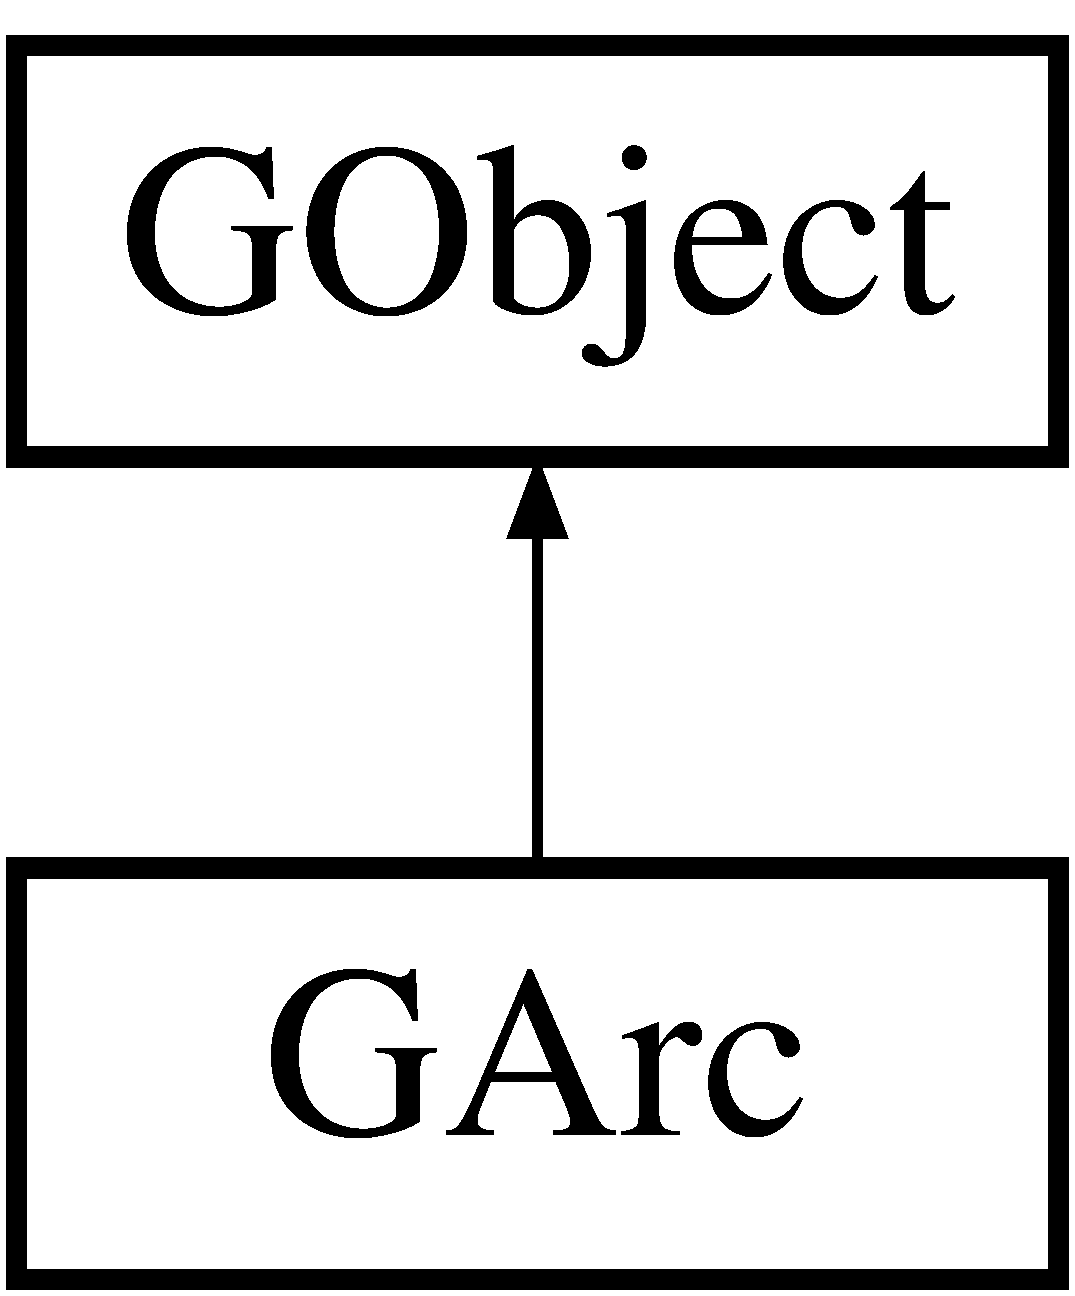
\includegraphics[height=2.000000cm]{classGArc}
\end{center}
\end{figure}
\subsection*{Public Types}
\begin{DoxyCompactItemize}
\item 
enum \mbox{\hyperlink{classGObject_a86e0f5648542856159bb40775c854aa7}{Line\+Style}} \{ \mbox{\hyperlink{classGObject_a86e0f5648542856159bb40775c854aa7acbc84bd5232621834ed31f44d457c1eb}{L\+I\+N\+E\+\_\+\+N\+O\+NE}}, 
\mbox{\hyperlink{classGObject_a86e0f5648542856159bb40775c854aa7a700c78bc2cd76acaab26651bf7b4941f}{L\+I\+N\+E\+\_\+\+S\+O\+L\+ID}}, 
\mbox{\hyperlink{classGObject_a86e0f5648542856159bb40775c854aa7a9ccba0845f785d81d07b333ae1aad84e}{L\+I\+N\+E\+\_\+\+D\+A\+SH}}, 
\mbox{\hyperlink{classGObject_a86e0f5648542856159bb40775c854aa7a8e811c096cb941997f0bfda168bb6df3}{L\+I\+N\+E\+\_\+\+D\+OT}}, 
\mbox{\hyperlink{classGObject_a86e0f5648542856159bb40775c854aa7ada15a2e3d737b2db7706d8300f91b89d}{L\+I\+N\+E\+\_\+\+D\+A\+S\+H\+\_\+\+D\+OT}}, 
\mbox{\hyperlink{classGObject_a86e0f5648542856159bb40775c854aa7aabf4053a73eafa7ba2b7e6d664c74c1d}{L\+I\+N\+E\+\_\+\+D\+A\+S\+H\+\_\+\+D\+O\+T\+\_\+\+D\+OT}}
 \}
\begin{DoxyCompactList}\small\item\em Styles that can be used for the outline around various shapes. \end{DoxyCompactList}\end{DoxyCompactItemize}
\subsection*{Public Member Functions}
\begin{DoxyCompactItemize}
\item 
\mbox{\hyperlink{classGArc_a487e2cfaa2231c74bb71eb4ba5bc0167}{G\+Arc}} (double width=0, double height=0, double start=0, double sweep=0)
\begin{DoxyCompactList}\small\item\em Creates a new {\ttfamily \mbox{\hyperlink{classGArc}{G\+Arc}}} object consisting of an elliptical arc. \end{DoxyCompactList}\item 
\mbox{\hyperlink{classGArc_ab70a642a06382d436427bd2f9519539a}{G\+Arc}} (double x, double y, double width, double height, double start, double sweep)
\begin{DoxyCompactList}\small\item\em Creates a new {\ttfamily \mbox{\hyperlink{classGArc}{G\+Arc}}} object consisting of an elliptical arc. \end{DoxyCompactList}\item 
virtual bool \mbox{\hyperlink{classGObject_a1dbc9dafaae51958112dbe1267a1f547}{contains}} (const \mbox{\hyperlink{structGPoint}{G\+Point}} \&pt) const
\begin{DoxyCompactList}\small\item\em Returns {\ttfamily true} if the specified point is inside the object. \end{DoxyCompactList}\item 
bool \mbox{\hyperlink{classGArc_ad973a1d55799d3a73bf8b04986cd804e}{contains}} (double x, double y) const override
\begin{DoxyCompactList}\small\item\em Returns {\ttfamily true} if the specified point is inside the object. \end{DoxyCompactList}\item 
virtual \mbox{\hyperlink{structGPoint}{G\+Point}} \mbox{\hyperlink{classGObject_a0d41183bf6b08de66fe3907551aab0d7}{get\+Bottom\+Right\+Location}} () const
\begin{DoxyCompactList}\small\item\em Returns the x/y coordinates of the bottom/right corner of the object. \end{DoxyCompactList}\item 
virtual double \mbox{\hyperlink{classGObject_a4316a2406c18e1c6d061fe51fd355490}{get\+BottomY}} () const
\begin{DoxyCompactList}\small\item\em Returns the {\itshape y}-\/coordinate of the bottom of the object. \end{DoxyCompactList}\item 
\mbox{\hyperlink{structGRectangle}{G\+Rectangle}} \mbox{\hyperlink{classGArc_a89040ce9277825772d359fccd33bca86}{get\+Bounds}} () const override
\begin{DoxyCompactList}\small\item\em Returns the bounding box of this object, which is defined to be the smallest rectangle that covers everything drawn by the figure. \end{DoxyCompactList}\item 
virtual \mbox{\hyperlink{structGPoint}{G\+Point}} \mbox{\hyperlink{classGObject_a0909472e91448470bccdb62ecfb95d8b}{get\+Center\+Location}} () const
\begin{DoxyCompactList}\small\item\em Returns the x/y-\/coordinates of the center of the object. \end{DoxyCompactList}\item 
virtual double \mbox{\hyperlink{classGObject_a04df74355b545e0543112d5b8d924176}{get\+CenterX}} () const
\begin{DoxyCompactList}\small\item\em Returns the {\itshape x}-\/coordinate of the center of the object. \end{DoxyCompactList}\item 
virtual double \mbox{\hyperlink{classGObject_acb3287a3d507025a26f54b895713b947}{get\+CenterY}} () const
\begin{DoxyCompactList}\small\item\em Returns the {\itshape y}-\/coordinate of the center of the object. \end{DoxyCompactList}\item 
virtual std\+::string \mbox{\hyperlink{classGObject_aa061dfa488c31e18549d64363c1d0e34}{get\+Color}} () const
\begin{DoxyCompactList}\small\item\em Returns the color used to display this object. \end{DoxyCompactList}\item 
virtual \mbox{\hyperlink{structGPoint}{G\+Point}} \mbox{\hyperlink{classGArc_a835d5e50bf4a91efcf0d838130c246af}{get\+End\+Point}} () const
\begin{DoxyCompactList}\small\item\em Returns the point at which the arc ends. \end{DoxyCompactList}\item 
virtual std\+::string \mbox{\hyperlink{classGObject_a76f6964a11fde7c78e9751be184e1a3c}{get\+Fill\+Color}} () const
\begin{DoxyCompactList}\small\item\em Returns the color used to display the filled region of this object. \end{DoxyCompactList}\item 
virtual \mbox{\hyperlink{structGRectangle}{G\+Rectangle}} \mbox{\hyperlink{classGArc_aab1e594176fa66cc7bd50c1f77218428}{get\+Frame\+Rectangle}} () const
\begin{DoxyCompactList}\small\item\em Returns the boundaries of the rectangle used to frame the arc. \end{DoxyCompactList}\item 
virtual double \mbox{\hyperlink{classGObject_a1e7e353362434072875264cf95629f99}{get\+Height}} () const
\begin{DoxyCompactList}\small\item\em Returns the height of this object, which is the same as the height of its bounding box. \end{DoxyCompactList}\item 
virtual \mbox{\hyperlink{classGObject_a86e0f5648542856159bb40775c854aa7}{Line\+Style}} \mbox{\hyperlink{classGObject_aaf1f5ea8281e5e3486662878d26f0a13}{get\+Line\+Style}} () const
\begin{DoxyCompactList}\small\item\em Returns the object\textquotesingle{}s style such as solid or dashed. \end{DoxyCompactList}\item 
virtual double \mbox{\hyperlink{classGObject_a85ff266dc3eb63d9f2d8e5a4487fd3c0}{get\+Line\+Width}} () const
\begin{DoxyCompactList}\small\item\em Returns the width of the line used to draw this object. \end{DoxyCompactList}\item 
virtual \mbox{\hyperlink{structGPoint}{G\+Point}} \mbox{\hyperlink{classGObject_a4f83802015511edeb63b892830812c11}{get\+Location}} () const
\begin{DoxyCompactList}\small\item\em Returns the location of the top-\/left corner of object. \end{DoxyCompactList}\item 
virtual double \mbox{\hyperlink{classGObject_a1ae3fc278cc5b71b9f2d96a8a83cdf26}{get\+Opacity}} () const
\begin{DoxyCompactList}\small\item\em Returns how opaque (non-\/transparent) this object will appear from 0.\+0 (completely transparent) to 1.\+0 (completely opaque, default). \end{DoxyCompactList}\item 
virtual \mbox{\hyperlink{classGCompound}{G\+Compound}} $\ast$ \mbox{\hyperlink{classGObject_a3e53cef70541b1a14eade4ad0984d0b4}{get\+Parent}} () const
\begin{DoxyCompactList}\small\item\em Returns a pointer to the {\ttfamily \mbox{\hyperlink{classGCompound}{G\+Compound}}} that contains this object. \end{DoxyCompactList}\item 
virtual double \mbox{\hyperlink{classGObject_a798cc79daaa10145b28f60bcdfdb0ee9}{get\+RightX}} () const
\begin{DoxyCompactList}\small\item\em Returns the {\itshape x}-\/coordinate of the right side of the object. \end{DoxyCompactList}\item 
virtual \mbox{\hyperlink{structGDimension}{G\+Dimension}} \mbox{\hyperlink{classGObject_a7b4eec96a2bdc6420695d5796a78eea9}{get\+Size}} () const
\begin{DoxyCompactList}\small\item\em Returns the size of the object as a {\ttfamily \mbox{\hyperlink{structGDimension}{G\+Dimension}}}. \end{DoxyCompactList}\item 
virtual double \mbox{\hyperlink{classGArc_ad52005815f95967f10ea54d290fa61ad}{get\+Start\+Angle}} () const
\begin{DoxyCompactList}\small\item\em Returns the starting angle for this arc in degrees. \end{DoxyCompactList}\item 
virtual \mbox{\hyperlink{structGPoint}{G\+Point}} \mbox{\hyperlink{classGArc_ad12beaa70993d9b409bfa8fd86c83957}{get\+Start\+Point}} () const
\begin{DoxyCompactList}\small\item\em Returns the point at which the arc starts. \end{DoxyCompactList}\item 
virtual double \mbox{\hyperlink{classGArc_ae842751a5db1493113ff347e564efae1}{get\+Sweep\+Angle}} () const
\begin{DoxyCompactList}\small\item\em Returns the sweep angle for this arc in degrees. \end{DoxyCompactList}\item 
std\+::string \mbox{\hyperlink{classGArc_a9b72ede4ee8520f987a0c01e30654814}{get\+Type}} () const override
\begin{DoxyCompactList}\small\item\em Returns the type of the object as a string, such as {\ttfamily \char`\"{}\+G\+Oval\char`\"{}} or {\ttfamily \char`\"{}\+G\+Rect\char`\"{}}. \end{DoxyCompactList}\item 
virtual double \mbox{\hyperlink{classGObject_a0ed2965abd4f5701d2cadf71239faf19}{get\+Width}} () const
\begin{DoxyCompactList}\small\item\em Returns the width of this object, which is equal to the width of the bounding box. \end{DoxyCompactList}\item 
virtual double \mbox{\hyperlink{classGObject_a344385751bee0720059403940d57a13e}{getX}} () const
\begin{DoxyCompactList}\small\item\em Returns the leftmost {\itshape x}-\/coordinate of the object. \end{DoxyCompactList}\item 
virtual double \mbox{\hyperlink{classGObject_aafa51c7f8f38a09febbb9ce7853f77b4}{getY}} () const
\begin{DoxyCompactList}\small\item\em Returns the topmost {\itshape y}-\/coordinate of the object. \end{DoxyCompactList}\item 
virtual bool \mbox{\hyperlink{classGObject_a11c404f106940c201b6f326e0355c150}{is\+Filled}} () const
\begin{DoxyCompactList}\small\item\em Returns {\ttfamily true} if the object is filled with color. \end{DoxyCompactList}\item 
virtual bool \mbox{\hyperlink{classGObject_a9de207581cfa4ca1eaa06da5f29b75fc}{is\+Transformed}} () const
\begin{DoxyCompactList}\small\item\em Returns {\ttfamily true} if this object has been transformed by calling methods such as \mbox{\hyperlink{classGObject_ae1ffaa12185dfd5ba464f7d87c329e26}{rotate()}} or \mbox{\hyperlink{classGObject_ad2e1900f730475c2d044817db03b38d6}{scale()}} on it. \end{DoxyCompactList}\item 
virtual bool \mbox{\hyperlink{classGObject_a9d8a6cfb13917785c143e74d40e4e2be}{is\+Visible}} () const
\begin{DoxyCompactList}\small\item\em Returns {\ttfamily true} if this object is visible on screen. \end{DoxyCompactList}\item 
virtual void \mbox{\hyperlink{classGObject_a5973d8dda83afb36e2c56855515be392}{move}} (double dx, double dy)
\begin{DoxyCompactList}\small\item\em Moves the object on the screen using the displacements {\ttfamily dx} and {\ttfamily dy}. \end{DoxyCompactList}\item 
virtual void \mbox{\hyperlink{classGObject_ac827b978aa122f136a14c198687ad80f}{repaint}} ()
\begin{DoxyCompactList}\small\item\em Instructs the object to redraw itself on screen. \end{DoxyCompactList}\item 
virtual void \mbox{\hyperlink{classGObject_a6022a1fd1e5dcd2fd5585e5a36aa3f37}{reset\+Transform}} ()
\begin{DoxyCompactList}\small\item\em Undoes any previous scale/rotate transformations on this object. \end{DoxyCompactList}\item 
virtual void \mbox{\hyperlink{classGObject_ae1ffaa12185dfd5ba464f7d87c329e26}{rotate}} (double theta)
\begin{DoxyCompactList}\small\item\em Transforms the object by rotating it {\ttfamily theta} degrees counterclockwise around its origin. \end{DoxyCompactList}\item 
virtual void \mbox{\hyperlink{classGObject_ad2e1900f730475c2d044817db03b38d6}{scale}} (double sf)
\begin{DoxyCompactList}\small\item\em Scales the object by the specified scale factor. \end{DoxyCompactList}\item 
virtual void \mbox{\hyperlink{classGObject_a63641f69d610d0b951357d35a0c3b1e3}{scale}} (double sx, double sy)
\begin{DoxyCompactList}\small\item\em Scales the object by the specified scale factors. \end{DoxyCompactList}\item 
void \mbox{\hyperlink{classGObject_ab6747f40313c531c2db32edb5b63b9b7}{send\+Backward}} ()
\begin{DoxyCompactList}\small\item\em Moves this object one step toward the back in the {\itshape z} dimension. \end{DoxyCompactList}\item 
void \mbox{\hyperlink{classGObject_a710b3e449c9facba7847c91ab170d281}{send\+Forward}} ()
\begin{DoxyCompactList}\small\item\em Moves this object one step toward the front in the {\itshape z} dimension. \end{DoxyCompactList}\item 
void \mbox{\hyperlink{classGObject_a0f7f1efbb7fd46dde2867c4ad0330896}{send\+To\+Back}} ()
\begin{DoxyCompactList}\small\item\em Moves this object to the back of the display in the {\itshape z} dimension. \end{DoxyCompactList}\item 
void \mbox{\hyperlink{classGObject_aee33d68488e46827ef55fac07f40a9b2}{send\+To\+Front}} ()
\begin{DoxyCompactList}\small\item\em Moves this object to the front of the display in the {\itshape z} dimension. \end{DoxyCompactList}\item 
virtual void \mbox{\hyperlink{classGObject_a71ff7b16b8f1bdc4a1ce9f30cf8b87d8}{set\+Bottom\+Right\+Location}} (double x, double y)
\begin{DoxyCompactList}\small\item\em Sets the location of the bottom/right of this object. \end{DoxyCompactList}\item 
virtual void \mbox{\hyperlink{classGObject_ac6f7320321182f1d18c1c0fa97d5e941}{set\+Bottom\+Right\+Location}} (const \mbox{\hyperlink{structGPoint}{G\+Point}} \&pt)
\begin{DoxyCompactList}\small\item\em Sets the location of the bottom/right of this object. \end{DoxyCompactList}\item 
virtual void \mbox{\hyperlink{classGObject_a4b20e93c2a2597484f74ee5caa71f41f}{set\+BottomY}} (double y)
\begin{DoxyCompactList}\small\item\em Sets the location of the bottom y-\/coordinate of this object. \end{DoxyCompactList}\item 
virtual void \mbox{\hyperlink{classGObject_a2aae8197624b72265ab83b4f1bc73f2f}{set\+Bounds}} (double x, double y, double width, double height)
\begin{DoxyCompactList}\small\item\em Changes the bounds of this object to the specified values. \end{DoxyCompactList}\item 
virtual void \mbox{\hyperlink{classGObject_acada386653f008cacc7cce86426bef7c}{set\+Bounds}} (const \mbox{\hyperlink{structGRectangle}{G\+Rectangle}} \&size)
\begin{DoxyCompactList}\small\item\em Changes the bounds of this object to the specified rectangle. \end{DoxyCompactList}\item 
virtual void \mbox{\hyperlink{classGObject_a290b47dd8de1be44089f95cb2c47c1de}{set\+Center\+Location}} (double x, double y)
\begin{DoxyCompactList}\small\item\em Sets the location of the center of this object. \end{DoxyCompactList}\item 
virtual void \mbox{\hyperlink{classGObject_a1bedf1b233ecba3f753ec58908a683a6}{set\+Center\+Location}} (const \mbox{\hyperlink{structGPoint}{G\+Point}} \&pt)
\begin{DoxyCompactList}\small\item\em Sets the location of the center of this object. \end{DoxyCompactList}\item 
virtual void \mbox{\hyperlink{classGObject_a2f4936281e056eead00a9186b9ba8af6}{set\+CenterX}} (double x)
\begin{DoxyCompactList}\small\item\em Sets the x-\/coordinate of the center of this object. \end{DoxyCompactList}\item 
virtual void \mbox{\hyperlink{classGObject_aad2a22b4fde88c33306b92aebf641d57}{set\+CenterY}} (double y)
\begin{DoxyCompactList}\small\item\em Sets the y-\/coordinate of the center of this object. \end{DoxyCompactList}\item 
virtual void \mbox{\hyperlink{classGObject_ad57ef49bc31db94e92648aa3737923d6}{set\+Color}} (int r, int g, int b)
\begin{DoxyCompactList}\small\item\em Sets the color used to display this object. \end{DoxyCompactList}\item 
virtual void \mbox{\hyperlink{classGObject_ab1f5cc0f5cc6bbbd716a526c61f1081d}{set\+Color}} (int rgb)
\begin{DoxyCompactList}\small\item\em Sets the color used to display this object. \end{DoxyCompactList}\item 
virtual void \mbox{\hyperlink{classGObject_a61374df6c11b52cfbb0815decdbaebc6}{set\+Color}} (const std\+::string \&color)
\begin{DoxyCompactList}\small\item\em Sets the color used to display this object. \end{DoxyCompactList}\item 
virtual void \mbox{\hyperlink{classGObject_ad767a33971159e9493e221cca4c00ae9}{set\+Fill\+Color}} (int r, int g, int b)
\begin{DoxyCompactList}\small\item\em Sets the color used to display the filled region of this object, if any. \end{DoxyCompactList}\item 
virtual void \mbox{\hyperlink{classGObject_aa59d9775a67fa7df2b24a95cd34840a3}{set\+Fill\+Color}} (int rgb)
\begin{DoxyCompactList}\small\item\em Sets the color used to display the filled region of this object, if any. \end{DoxyCompactList}\item 
virtual void \mbox{\hyperlink{classGObject_adbc18b1a930aadd97d7437f9f7265b96}{set\+Fill\+Color}} (const std\+::string \&color)
\begin{DoxyCompactList}\small\item\em Sets the color used to display the filled region of this object, if any. \end{DoxyCompactList}\item 
virtual void \mbox{\hyperlink{classGObject_a9b82b53362282c6bb7d6947068d2e55b}{set\+Filled}} (bool flag)
\begin{DoxyCompactList}\small\item\em Sets the fill status for the object, where {\ttfamily false} is outlined and {\ttfamily true} is filled. \end{DoxyCompactList}\item 
virtual void \mbox{\hyperlink{classGObject_a2592348886ffea646c6534bf88f7c49d}{set\+Font}} (const Q\+Font \&font)
\begin{DoxyCompactList}\small\item\em Changes the font used to display the object as specified by the given Qt font. \end{DoxyCompactList}\item 
virtual void \mbox{\hyperlink{classGObject_a8e096e8818d838aceae1d46d58fb3a7b}{set\+Font}} (const std\+::string \&font)
\begin{DoxyCompactList}\small\item\em Changes the font used to display the object as specified by the string {\ttfamily font}, which has the following format\+: \end{DoxyCompactList}\item 
virtual void \mbox{\hyperlink{classGObject_ad18e8fab1e02a4e9b75c6730212558eb}{set\+Foreground}} (int r, int g, int b)
\begin{DoxyCompactList}\small\item\em Sets the color used to display this object. \end{DoxyCompactList}\item 
virtual void \mbox{\hyperlink{classGObject_a9eb856b5ff83a19df3831a31f15f4563}{set\+Foreground}} (int rgb)
\begin{DoxyCompactList}\small\item\em Sets the color used to display this object. \end{DoxyCompactList}\item 
virtual void \mbox{\hyperlink{classGObject_af59209aeadea6dfc6d97a2d8531f50e1}{set\+Foreground}} (const std\+::string \&color)
\begin{DoxyCompactList}\small\item\em Sets the color used to display this object. \end{DoxyCompactList}\item 
virtual void \mbox{\hyperlink{classGArc_a53c45f6939e63ae1ee26739e7c485e2d}{set\+Frame\+Rectangle}} (const \mbox{\hyperlink{structGRectangle}{G\+Rectangle}} \&rect)
\begin{DoxyCompactList}\small\item\em Changes the boundaries of the rectangle used to frame the arc. \end{DoxyCompactList}\item 
virtual void \mbox{\hyperlink{classGArc_a9532c0e65946d2f533f3c9abf8150a1d}{set\+Frame\+Rectangle}} (double x, double y, double width, double height)
\begin{DoxyCompactList}\small\item\em Changes the boundaries of the rectangle used to frame the arc. \end{DoxyCompactList}\item 
virtual void \mbox{\hyperlink{classGObject_a9e280bfc4544dfaf8e4376c4e1a74357}{set\+Height}} (double height)
\begin{DoxyCompactList}\small\item\em Changes the height of this object to the specified height without changing its width. \end{DoxyCompactList}\item 
virtual void \mbox{\hyperlink{classGObject_add11575087eb94f1a71faa3f826c6341}{set\+Line\+Style}} (\mbox{\hyperlink{classGObject_a86e0f5648542856159bb40775c854aa7}{Line\+Style}} line\+Style)
\begin{DoxyCompactList}\small\item\em Sets the object\textquotesingle{}s style such as solid (\mbox{\hyperlink{classGObject_a86e0f5648542856159bb40775c854aa7a700c78bc2cd76acaab26651bf7b4941f}{G\+Object\+::\+L\+I\+N\+E\+\_\+\+S\+O\+L\+ID}}) or dashed (\mbox{\hyperlink{classGObject_a86e0f5648542856159bb40775c854aa7a9ccba0845f785d81d07b333ae1aad84e}{G\+Object\+::\+L\+I\+N\+E\+\_\+\+D\+A\+SH}}). \end{DoxyCompactList}\item 
virtual void \mbox{\hyperlink{classGObject_afd6a47c6ea6a1f85ca05a65ba3ff3477}{set\+Line\+Width}} (double line\+Width)
\begin{DoxyCompactList}\small\item\em Sets the width of the line used to draw this object. \end{DoxyCompactList}\item 
virtual void \mbox{\hyperlink{classGObject_a04594e8ba9b98513a64f1da00dcae18c}{set\+Location}} (double x, double y)
\begin{DoxyCompactList}\small\item\em Sets the location of the top-\/left corner of this object to the specified coordinates. \end{DoxyCompactList}\item 
virtual void \mbox{\hyperlink{classGObject_aa8480c0b7166cdf8f784cece06ab353f}{set\+Location}} (const \mbox{\hyperlink{structGPoint}{G\+Point}} \&pt)
\begin{DoxyCompactList}\small\item\em Sets the location of the top-\/left corner of this object to the specified point. \end{DoxyCompactList}\item 
virtual void \mbox{\hyperlink{classGObject_a04af1866cc1bae4a1226695794a50539}{set\+Opacity}} (double opacity)
\begin{DoxyCompactList}\small\item\em Sets how opaque (non-\/transparent) this object will appear from 0.\+0 (completely transparent) to 1.\+0 (completely opaque, default). \end{DoxyCompactList}\item 
virtual void \mbox{\hyperlink{classGObject_a3c90b758cdc2c911c9ef76c4360eb912}{set\+RightX}} (double x)
\begin{DoxyCompactList}\small\item\em Sets the location of the rightmost x-\/coordinate of this object. \end{DoxyCompactList}\item 
virtual void \mbox{\hyperlink{classGObject_aca25d49481f9bf5fc8f7df4c086c4ce7}{set\+Size}} (double width, double height)
\begin{DoxyCompactList}\small\item\em Changes the size of this object to the specified width and height. \end{DoxyCompactList}\item 
virtual void \mbox{\hyperlink{classGObject_ae2b628228f192c2702c4ce941b2af68f}{set\+Size}} (const \mbox{\hyperlink{structGDimension}{G\+Dimension}} \&size)
\begin{DoxyCompactList}\small\item\em Changes the size of this object to the specified width and height. \end{DoxyCompactList}\item 
virtual void \mbox{\hyperlink{classGArc_a29b82869001d966bbfc68ad82580a35e}{set\+Start\+Angle}} (double start)
\begin{DoxyCompactList}\small\item\em Sets the starting angle for this arc in degrees. \end{DoxyCompactList}\item 
virtual void \mbox{\hyperlink{classGArc_a6240a9cb9e5519b2aa4fbcf81ddfc9c8}{set\+Sweep\+Angle}} (double start)
\begin{DoxyCompactList}\small\item\em Sets the sweep angle for this arc in degrees. \end{DoxyCompactList}\item 
virtual void \mbox{\hyperlink{classGObject_a88203f28224315d9f4471212f4af8ed3}{set\+Visible}} (bool flag)
\begin{DoxyCompactList}\small\item\em Sets whether this object is visible. \end{DoxyCompactList}\item 
virtual void \mbox{\hyperlink{classGObject_aa3f3fba4cb131baa8696ba01e3bceca1}{set\+Width}} (double width)
\begin{DoxyCompactList}\small\item\em Changes the width of this object to the specified width without changing its height. \end{DoxyCompactList}\item 
virtual void \mbox{\hyperlink{classGObject_a9c18fcc579333bf9653d13ad2b372e39}{setX}} (double x)
\begin{DoxyCompactList}\small\item\em Sets the x location of the left side of this object. \end{DoxyCompactList}\item 
virtual void \mbox{\hyperlink{classGObject_a7d57e2a5c35d27feb58fd498a3cf82b9}{setY}} (double y)
\begin{DoxyCompactList}\small\item\em Sets the y location of the top of this object. \end{DoxyCompactList}\item 
virtual std\+::string \mbox{\hyperlink{classGObject_a1fe5121d6528fdea3f243321b3fa3a49}{to\+String}} () const
\begin{DoxyCompactList}\small\item\em Returns a printable representation of the object. \end{DoxyCompactList}\item 
std\+::string \mbox{\hyperlink{classGArc_a04364e674911906702b748deec32db18}{to\+String\+Extra}} () const override
\begin{DoxyCompactList}\small\item\em Returns a string containing any extra unique information about this type of graphical object. \end{DoxyCompactList}\end{DoxyCompactItemize}
\subsection*{Static Public Member Functions}
\begin{DoxyCompactItemize}
\item 
static bool \mbox{\hyperlink{classGObject_a93be0e1fe1b1bf1a1da732470c94f42b}{is\+Anti\+Aliasing}} ()
\begin{DoxyCompactList}\small\item\em Returns whether we should globally anti-\/alias graphical objects. \end{DoxyCompactList}\item 
static void \mbox{\hyperlink{classGObject_a1e43371668ae850193cebedb44e1bbe3}{set\+Anti\+Aliasing}} (bool value)
\begin{DoxyCompactList}\small\item\em Globally turns on/off the anti-\/aliasing feature that smooths out the edges of onscreen shapes. \end{DoxyCompactList}\end{DoxyCompactItemize}
\subsection*{Protected Attributes}
\begin{DoxyCompactItemize}
\item 
Q\+Brush \mbox{\hyperlink{classGObject_aab24462ec896b596d99911767b0912d0}{\+\_\+brush}}
\item 
std\+::string \mbox{\hyperlink{classGObject_a1134e770ae4315ea8bc1201e2f21da8b}{\+\_\+color}}
\item 
int \mbox{\hyperlink{classGObject_a003fdd343d9b7505c53a8b7a134200ed}{\+\_\+color\+Int}}
\item 
std\+::string \mbox{\hyperlink{classGObject_a179f8d6cee65cd8a54692e32b224392a}{\+\_\+fill\+Color}}
\item 
int \mbox{\hyperlink{classGObject_a751def333a67d651e5b99cc331ecb496}{\+\_\+fill\+Color\+Int}}
\item 
bool \mbox{\hyperlink{classGObject_ad4a55cbcd61b58a4d49666490bb2f103}{\+\_\+fill\+Flag}}
\item 
std\+::string \mbox{\hyperlink{classGObject_aea76ea1a8b5dd7b0a78653277e63b536}{\+\_\+font}}
\item 
double \mbox{\hyperlink{classGObject_ad05df29e7f27fc504abd743e3d8b4e73}{\+\_\+height}}
\item 
\mbox{\hyperlink{classGObject_a86e0f5648542856159bb40775c854aa7}{Line\+Style}} \mbox{\hyperlink{classGObject_a89bafecaafb7c72d55c7efc10b7d0523}{\+\_\+line\+Style}}
\item 
double \mbox{\hyperlink{classGObject_a16e9033665937f13de2e163dc2184aff}{\+\_\+line\+Width}}
\item 
double \mbox{\hyperlink{classGObject_a20eff8eb7af27182edc9bfc54768b6f3}{\+\_\+opacity}}
\item 
\mbox{\hyperlink{classGCompound}{G\+Compound}} $\ast$ \mbox{\hyperlink{classGObject_ac9452c1eaff70eebddbb318196aa3835}{\+\_\+parent}}
\item 
Q\+Pen \mbox{\hyperlink{classGObject_afb69d172743f868299847174eb1b6bc8}{\+\_\+pen}}
\item 
Q\+Transform \mbox{\hyperlink{classGObject_a475b8860a5f1adb4a1fdc58d1f5c1e32}{\+\_\+transform}}
\item 
bool \mbox{\hyperlink{classGObject_ae4725802fc8d8aaa0ab4bd4781f7e07c}{\+\_\+transformed}}
\item 
bool \mbox{\hyperlink{classGObject_a9312c72508471b7c7a87b540263e1af4}{\+\_\+visible}}
\item 
double \mbox{\hyperlink{classGObject_ab55d85a3371770e6725b1062cf160cd8}{\+\_\+width}}
\item 
double \mbox{\hyperlink{classGObject_a6675b83b27137b8d3aa2ad8133078ea6}{\+\_\+x}}
\item 
double \mbox{\hyperlink{classGObject_a2f0f6aeafddc8a39c578bfa7e22b5f1e}{\+\_\+y}}
\end{DoxyCompactItemize}


\subsection{Detailed Description}
This graphical object subclass represents an elliptical arc. 

The arc is specified by the following parameters\+:


\begin{DoxyItemize}
\item The coordinates of the bounding rectangle ({\ttfamily x}, {\ttfamily y}, {\ttfamily width}, {\ttfamily height}) 
\item The angle at which the arc starts ({\ttfamily start}) 
\item The number of degrees that the arc covers ({\ttfamily sweep}) 
\end{DoxyItemize}

All angles in a {\ttfamily \mbox{\hyperlink{classGArc}{G\+Arc}}} description are measured in degrees moving counterclockwise from the +{\itshape x} axis. Negative values for either {\ttfamily start} or {\ttfamily sweep} indicate motion in a clockwise direction.  

\subsection{Member Enumeration Documentation}
\mbox{\Hypertarget{classGObject_a86e0f5648542856159bb40775c854aa7}\label{classGObject_a86e0f5648542856159bb40775c854aa7}} 
\index{G\+Arc@{G\+Arc}!Line\+Style@{Line\+Style}}
\index{Line\+Style@{Line\+Style}!G\+Arc@{G\+Arc}}
\subsubsection{\texorpdfstring{Line\+Style}{LineStyle}}
{\footnotesize\ttfamily enum \mbox{\hyperlink{classGObject_a86e0f5648542856159bb40775c854aa7}{Line\+Style}}\hspace{0.3cm}{\ttfamily [inherited]}}



Styles that can be used for the outline around various shapes. 

Call set\+Line\+Style on a \mbox{\hyperlink{classGObject}{G\+Object}} and pass one of these values. \begin{DoxyEnumFields}{Enumerator}
\raisebox{\heightof{T}}[0pt][0pt]{\index{L\+I\+N\+E\+\_\+\+N\+O\+NE@{L\+I\+N\+E\+\_\+\+N\+O\+NE}!G\+Arc@{G\+Arc}}\index{G\+Arc@{G\+Arc}!L\+I\+N\+E\+\_\+\+N\+O\+NE@{L\+I\+N\+E\+\_\+\+N\+O\+NE}}}\mbox{\Hypertarget{classGObject_a86e0f5648542856159bb40775c854aa7acbc84bd5232621834ed31f44d457c1eb}\label{classGObject_a86e0f5648542856159bb40775c854aa7acbc84bd5232621834ed31f44d457c1eb}} 
L\+I\+N\+E\+\_\+\+N\+O\+NE&\\
\hline

\raisebox{\heightof{T}}[0pt][0pt]{\index{L\+I\+N\+E\+\_\+\+S\+O\+L\+ID@{L\+I\+N\+E\+\_\+\+S\+O\+L\+ID}!G\+Arc@{G\+Arc}}\index{G\+Arc@{G\+Arc}!L\+I\+N\+E\+\_\+\+S\+O\+L\+ID@{L\+I\+N\+E\+\_\+\+S\+O\+L\+ID}}}\mbox{\Hypertarget{classGObject_a86e0f5648542856159bb40775c854aa7a700c78bc2cd76acaab26651bf7b4941f}\label{classGObject_a86e0f5648542856159bb40775c854aa7a700c78bc2cd76acaab26651bf7b4941f}} 
L\+I\+N\+E\+\_\+\+S\+O\+L\+ID&\\
\hline

\raisebox{\heightof{T}}[0pt][0pt]{\index{L\+I\+N\+E\+\_\+\+D\+A\+SH@{L\+I\+N\+E\+\_\+\+D\+A\+SH}!G\+Arc@{G\+Arc}}\index{G\+Arc@{G\+Arc}!L\+I\+N\+E\+\_\+\+D\+A\+SH@{L\+I\+N\+E\+\_\+\+D\+A\+SH}}}\mbox{\Hypertarget{classGObject_a86e0f5648542856159bb40775c854aa7a9ccba0845f785d81d07b333ae1aad84e}\label{classGObject_a86e0f5648542856159bb40775c854aa7a9ccba0845f785d81d07b333ae1aad84e}} 
L\+I\+N\+E\+\_\+\+D\+A\+SH&\\
\hline

\raisebox{\heightof{T}}[0pt][0pt]{\index{L\+I\+N\+E\+\_\+\+D\+OT@{L\+I\+N\+E\+\_\+\+D\+OT}!G\+Arc@{G\+Arc}}\index{G\+Arc@{G\+Arc}!L\+I\+N\+E\+\_\+\+D\+OT@{L\+I\+N\+E\+\_\+\+D\+OT}}}\mbox{\Hypertarget{classGObject_a86e0f5648542856159bb40775c854aa7a8e811c096cb941997f0bfda168bb6df3}\label{classGObject_a86e0f5648542856159bb40775c854aa7a8e811c096cb941997f0bfda168bb6df3}} 
L\+I\+N\+E\+\_\+\+D\+OT&\\
\hline

\raisebox{\heightof{T}}[0pt][0pt]{\index{L\+I\+N\+E\+\_\+\+D\+A\+S\+H\+\_\+\+D\+OT@{L\+I\+N\+E\+\_\+\+D\+A\+S\+H\+\_\+\+D\+OT}!G\+Arc@{G\+Arc}}\index{G\+Arc@{G\+Arc}!L\+I\+N\+E\+\_\+\+D\+A\+S\+H\+\_\+\+D\+OT@{L\+I\+N\+E\+\_\+\+D\+A\+S\+H\+\_\+\+D\+OT}}}\mbox{\Hypertarget{classGObject_a86e0f5648542856159bb40775c854aa7ada15a2e3d737b2db7706d8300f91b89d}\label{classGObject_a86e0f5648542856159bb40775c854aa7ada15a2e3d737b2db7706d8300f91b89d}} 
L\+I\+N\+E\+\_\+\+D\+A\+S\+H\+\_\+\+D\+OT&\\
\hline

\raisebox{\heightof{T}}[0pt][0pt]{\index{L\+I\+N\+E\+\_\+\+D\+A\+S\+H\+\_\+\+D\+O\+T\+\_\+\+D\+OT@{L\+I\+N\+E\+\_\+\+D\+A\+S\+H\+\_\+\+D\+O\+T\+\_\+\+D\+OT}!G\+Arc@{G\+Arc}}\index{G\+Arc@{G\+Arc}!L\+I\+N\+E\+\_\+\+D\+A\+S\+H\+\_\+\+D\+O\+T\+\_\+\+D\+OT@{L\+I\+N\+E\+\_\+\+D\+A\+S\+H\+\_\+\+D\+O\+T\+\_\+\+D\+OT}}}\mbox{\Hypertarget{classGObject_a86e0f5648542856159bb40775c854aa7aabf4053a73eafa7ba2b7e6d664c74c1d}\label{classGObject_a86e0f5648542856159bb40775c854aa7aabf4053a73eafa7ba2b7e6d664c74c1d}} 
L\+I\+N\+E\+\_\+\+D\+A\+S\+H\+\_\+\+D\+O\+T\+\_\+\+D\+OT&\\
\hline

\end{DoxyEnumFields}


\subsection{Constructor \& Destructor Documentation}
\mbox{\Hypertarget{classGArc_a487e2cfaa2231c74bb71eb4ba5bc0167}\label{classGArc_a487e2cfaa2231c74bb71eb4ba5bc0167}} 
\index{G\+Arc@{G\+Arc}!G\+Arc@{G\+Arc}}
\index{G\+Arc@{G\+Arc}!G\+Arc@{G\+Arc}}
\subsubsection{\texorpdfstring{G\+Arc()}{GArc()}\hspace{0.1cm}{\footnotesize\ttfamily [1/2]}}
{\footnotesize\ttfamily \mbox{\hyperlink{classGArc}{G\+Arc}} (\begin{DoxyParamCaption}\item[{double}]{width = {\ttfamily 0},  }\item[{double}]{height = {\ttfamily 0},  }\item[{double}]{start = {\ttfamily 0},  }\item[{double}]{sweep = {\ttfamily 0} }\end{DoxyParamCaption})}



Creates a new {\ttfamily \mbox{\hyperlink{classGArc}{G\+Arc}}} object consisting of an elliptical arc. 

This form creates a {\ttfamily \mbox{\hyperlink{classGArc}{G\+Arc}}} whose origin is the point (0, 0). \mbox{\Hypertarget{classGArc_ab70a642a06382d436427bd2f9519539a}\label{classGArc_ab70a642a06382d436427bd2f9519539a}} 
\index{G\+Arc@{G\+Arc}!G\+Arc@{G\+Arc}}
\index{G\+Arc@{G\+Arc}!G\+Arc@{G\+Arc}}
\subsubsection{\texorpdfstring{G\+Arc()}{GArc()}\hspace{0.1cm}{\footnotesize\ttfamily [2/2]}}
{\footnotesize\ttfamily \mbox{\hyperlink{classGArc}{G\+Arc}} (\begin{DoxyParamCaption}\item[{double}]{x,  }\item[{double}]{y,  }\item[{double}]{width,  }\item[{double}]{height,  }\item[{double}]{start,  }\item[{double}]{sweep }\end{DoxyParamCaption})}



Creates a new {\ttfamily \mbox{\hyperlink{classGArc}{G\+Arc}}} object consisting of an elliptical arc. 

This form creates a {\ttfamily \mbox{\hyperlink{classGArc}{G\+Arc}}} whose origin is the point ({\ttfamily x}, {\ttfamily y}). 

\subsection{Member Function Documentation}
\mbox{\Hypertarget{classGObject_a1dbc9dafaae51958112dbe1267a1f547}\label{classGObject_a1dbc9dafaae51958112dbe1267a1f547}} 
\index{G\+Arc@{G\+Arc}!contains@{contains}}
\index{contains@{contains}!G\+Arc@{G\+Arc}}
\subsubsection{\texorpdfstring{contains()}{contains()}\hspace{0.1cm}{\footnotesize\ttfamily [1/2]}}
{\footnotesize\ttfamily bool contains (\begin{DoxyParamCaption}\item[{const \mbox{\hyperlink{structGPoint}{G\+Point}} \&}]{pt }\end{DoxyParamCaption}) const\hspace{0.3cm}{\ttfamily [virtual]}, {\ttfamily [inherited]}}



Returns {\ttfamily true} if the specified point is inside the object. 

\mbox{\Hypertarget{classGArc_ad973a1d55799d3a73bf8b04986cd804e}\label{classGArc_ad973a1d55799d3a73bf8b04986cd804e}} 
\index{G\+Arc@{G\+Arc}!contains@{contains}}
\index{contains@{contains}!G\+Arc@{G\+Arc}}
\subsubsection{\texorpdfstring{contains()}{contains()}\hspace{0.1cm}{\footnotesize\ttfamily [2/2]}}
{\footnotesize\ttfamily bool contains (\begin{DoxyParamCaption}\item[{double}]{x,  }\item[{double}]{y }\end{DoxyParamCaption}) const\hspace{0.3cm}{\ttfamily [override]}, {\ttfamily [virtual]}}



Returns {\ttfamily true} if the specified point is inside the object. 



Reimplemented from \mbox{\hyperlink{classGObject_abb6a5d7c03e6eaaae97264c4799ce7c3}{G\+Object}}.

\mbox{\Hypertarget{classGObject_a0d41183bf6b08de66fe3907551aab0d7}\label{classGObject_a0d41183bf6b08de66fe3907551aab0d7}} 
\index{G\+Arc@{G\+Arc}!get\+Bottom\+Right\+Location@{get\+Bottom\+Right\+Location}}
\index{get\+Bottom\+Right\+Location@{get\+Bottom\+Right\+Location}!G\+Arc@{G\+Arc}}
\subsubsection{\texorpdfstring{get\+Bottom\+Right\+Location()}{getBottomRightLocation()}}
{\footnotesize\ttfamily \mbox{\hyperlink{structGPoint}{G\+Point}} get\+Bottom\+Right\+Location (\begin{DoxyParamCaption}{ }\end{DoxyParamCaption}) const\hspace{0.3cm}{\ttfamily [virtual]}, {\ttfamily [inherited]}}



Returns the x/y coordinates of the bottom/right corner of the object. 

\mbox{\Hypertarget{classGObject_a4316a2406c18e1c6d061fe51fd355490}\label{classGObject_a4316a2406c18e1c6d061fe51fd355490}} 
\index{G\+Arc@{G\+Arc}!get\+BottomY@{get\+BottomY}}
\index{get\+BottomY@{get\+BottomY}!G\+Arc@{G\+Arc}}
\subsubsection{\texorpdfstring{get\+Bottom\+Y()}{getBottomY()}}
{\footnotesize\ttfamily double get\+BottomY (\begin{DoxyParamCaption}{ }\end{DoxyParamCaption}) const\hspace{0.3cm}{\ttfamily [virtual]}, {\ttfamily [inherited]}}



Returns the {\itshape y}-\/coordinate of the bottom of the object. 

Equivalent to the top y-\/coordinate plus the object\textquotesingle{}s height. \mbox{\Hypertarget{classGArc_a89040ce9277825772d359fccd33bca86}\label{classGArc_a89040ce9277825772d359fccd33bca86}} 
\index{G\+Arc@{G\+Arc}!get\+Bounds@{get\+Bounds}}
\index{get\+Bounds@{get\+Bounds}!G\+Arc@{G\+Arc}}
\subsubsection{\texorpdfstring{get\+Bounds()}{getBounds()}}
{\footnotesize\ttfamily \mbox{\hyperlink{structGRectangle}{G\+Rectangle}} get\+Bounds (\begin{DoxyParamCaption}{ }\end{DoxyParamCaption}) const\hspace{0.3cm}{\ttfamily [override]}, {\ttfamily [virtual]}}



Returns the bounding box of this object, which is defined to be the smallest rectangle that covers everything drawn by the figure. 

The coordinates of this rectangle do not necessarily match the location returned by {\ttfamily get\+Location}. Given a {\ttfamily \mbox{\hyperlink{classGText}{G\+Text}}} object, for example, {\ttfamily get\+Location} returns the coordinates of the point on the baseline at which the string begins; the {\ttfamily get\+Bounds} method, by contrast, returns a rectangle that covers the entire window area occupied by the string. 

Reimplemented from \mbox{\hyperlink{classGObject_a29e6ac35a0b48f491a4c88194cc5da3b}{G\+Object}}.

\mbox{\Hypertarget{classGObject_a0909472e91448470bccdb62ecfb95d8b}\label{classGObject_a0909472e91448470bccdb62ecfb95d8b}} 
\index{G\+Arc@{G\+Arc}!get\+Center\+Location@{get\+Center\+Location}}
\index{get\+Center\+Location@{get\+Center\+Location}!G\+Arc@{G\+Arc}}
\subsubsection{\texorpdfstring{get\+Center\+Location()}{getCenterLocation()}}
{\footnotesize\ttfamily \mbox{\hyperlink{structGPoint}{G\+Point}} get\+Center\+Location (\begin{DoxyParamCaption}{ }\end{DoxyParamCaption}) const\hspace{0.3cm}{\ttfamily [virtual]}, {\ttfamily [inherited]}}



Returns the x/y-\/coordinates of the center of the object. 

Equivalent to the top/left plus half the object\textquotesingle{}s size. \mbox{\Hypertarget{classGObject_a04df74355b545e0543112d5b8d924176}\label{classGObject_a04df74355b545e0543112d5b8d924176}} 
\index{G\+Arc@{G\+Arc}!get\+CenterX@{get\+CenterX}}
\index{get\+CenterX@{get\+CenterX}!G\+Arc@{G\+Arc}}
\subsubsection{\texorpdfstring{get\+Center\+X()}{getCenterX()}}
{\footnotesize\ttfamily double get\+CenterX (\begin{DoxyParamCaption}{ }\end{DoxyParamCaption}) const\hspace{0.3cm}{\ttfamily [virtual]}, {\ttfamily [inherited]}}



Returns the {\itshape x}-\/coordinate of the center of the object. 

Equivalent to the top/left plus half the object\textquotesingle{}s width. \mbox{\Hypertarget{classGObject_acb3287a3d507025a26f54b895713b947}\label{classGObject_acb3287a3d507025a26f54b895713b947}} 
\index{G\+Arc@{G\+Arc}!get\+CenterY@{get\+CenterY}}
\index{get\+CenterY@{get\+CenterY}!G\+Arc@{G\+Arc}}
\subsubsection{\texorpdfstring{get\+Center\+Y()}{getCenterY()}}
{\footnotesize\ttfamily double get\+CenterY (\begin{DoxyParamCaption}{ }\end{DoxyParamCaption}) const\hspace{0.3cm}{\ttfamily [virtual]}, {\ttfamily [inherited]}}



Returns the {\itshape y}-\/coordinate of the center of the object. 

Equivalent to the top/left plus half the object\textquotesingle{}s height. \mbox{\Hypertarget{classGObject_aa061dfa488c31e18549d64363c1d0e34}\label{classGObject_aa061dfa488c31e18549d64363c1d0e34}} 
\index{G\+Arc@{G\+Arc}!get\+Color@{get\+Color}}
\index{get\+Color@{get\+Color}!G\+Arc@{G\+Arc}}
\subsubsection{\texorpdfstring{get\+Color()}{getColor()}}
{\footnotesize\ttfamily std\+::string get\+Color (\begin{DoxyParamCaption}{ }\end{DoxyParamCaption}) const\hspace{0.3cm}{\ttfamily [virtual]}, {\ttfamily [inherited]}}



Returns the color used to display this object. 

This color is always returned as a string in the form {\ttfamily \char`\"{}\#rrggbb\char`\"{}}, where {\ttfamily rr}, {\ttfamily gg}, and {\ttfamily bb} are the red, green, and blue components of the color, expressed as two-\/digit hexadecimal values. \mbox{\Hypertarget{classGArc_a835d5e50bf4a91efcf0d838130c246af}\label{classGArc_a835d5e50bf4a91efcf0d838130c246af}} 
\index{G\+Arc@{G\+Arc}!get\+End\+Point@{get\+End\+Point}}
\index{get\+End\+Point@{get\+End\+Point}!G\+Arc@{G\+Arc}}
\subsubsection{\texorpdfstring{get\+End\+Point()}{getEndPoint()}}
{\footnotesize\ttfamily \mbox{\hyperlink{structGPoint}{G\+Point}} get\+End\+Point (\begin{DoxyParamCaption}{ }\end{DoxyParamCaption}) const\hspace{0.3cm}{\ttfamily [virtual]}}



Returns the point at which the arc ends. 

\mbox{\Hypertarget{classGObject_a76f6964a11fde7c78e9751be184e1a3c}\label{classGObject_a76f6964a11fde7c78e9751be184e1a3c}} 
\index{G\+Arc@{G\+Arc}!get\+Fill\+Color@{get\+Fill\+Color}}
\index{get\+Fill\+Color@{get\+Fill\+Color}!G\+Arc@{G\+Arc}}
\subsubsection{\texorpdfstring{get\+Fill\+Color()}{getFillColor()}}
{\footnotesize\ttfamily std\+::string get\+Fill\+Color (\begin{DoxyParamCaption}{ }\end{DoxyParamCaption}) const\hspace{0.3cm}{\ttfamily [virtual]}, {\ttfamily [inherited]}}



Returns the color used to display the filled region of this object. 

If none has been set, returns the empty string. \mbox{\Hypertarget{classGArc_aab1e594176fa66cc7bd50c1f77218428}\label{classGArc_aab1e594176fa66cc7bd50c1f77218428}} 
\index{G\+Arc@{G\+Arc}!get\+Frame\+Rectangle@{get\+Frame\+Rectangle}}
\index{get\+Frame\+Rectangle@{get\+Frame\+Rectangle}!G\+Arc@{G\+Arc}}
\subsubsection{\texorpdfstring{get\+Frame\+Rectangle()}{getFrameRectangle()}}
{\footnotesize\ttfamily \mbox{\hyperlink{structGRectangle}{G\+Rectangle}} get\+Frame\+Rectangle (\begin{DoxyParamCaption}{ }\end{DoxyParamCaption}) const\hspace{0.3cm}{\ttfamily [virtual]}}



Returns the boundaries of the rectangle used to frame the arc. 

\mbox{\Hypertarget{classGObject_a1e7e353362434072875264cf95629f99}\label{classGObject_a1e7e353362434072875264cf95629f99}} 
\index{G\+Arc@{G\+Arc}!get\+Height@{get\+Height}}
\index{get\+Height@{get\+Height}!G\+Arc@{G\+Arc}}
\subsubsection{\texorpdfstring{get\+Height()}{getHeight()}}
{\footnotesize\ttfamily double get\+Height (\begin{DoxyParamCaption}{ }\end{DoxyParamCaption}) const\hspace{0.3cm}{\ttfamily [virtual]}, {\ttfamily [inherited]}}



Returns the height of this object, which is the same as the height of its bounding box. 



Reimplemented in \mbox{\hyperlink{classGPolygon_a2bede8b27b21ae4c7940e762cbad9e07}{G\+Polygon}}, and \mbox{\hyperlink{classGLine_a2bede8b27b21ae4c7940e762cbad9e07}{G\+Line}}.

\mbox{\Hypertarget{classGObject_aaf1f5ea8281e5e3486662878d26f0a13}\label{classGObject_aaf1f5ea8281e5e3486662878d26f0a13}} 
\index{G\+Arc@{G\+Arc}!get\+Line\+Style@{get\+Line\+Style}}
\index{get\+Line\+Style@{get\+Line\+Style}!G\+Arc@{G\+Arc}}
\subsubsection{\texorpdfstring{get\+Line\+Style()}{getLineStyle()}}
{\footnotesize\ttfamily \mbox{\hyperlink{classGObject_a86e0f5648542856159bb40775c854aa7}{G\+Object\+::\+Line\+Style}} get\+Line\+Style (\begin{DoxyParamCaption}{ }\end{DoxyParamCaption}) const\hspace{0.3cm}{\ttfamily [virtual]}, {\ttfamily [inherited]}}



Returns the object\textquotesingle{}s style such as solid or dashed. 

\mbox{\Hypertarget{classGObject_a85ff266dc3eb63d9f2d8e5a4487fd3c0}\label{classGObject_a85ff266dc3eb63d9f2d8e5a4487fd3c0}} 
\index{G\+Arc@{G\+Arc}!get\+Line\+Width@{get\+Line\+Width}}
\index{get\+Line\+Width@{get\+Line\+Width}!G\+Arc@{G\+Arc}}
\subsubsection{\texorpdfstring{get\+Line\+Width()}{getLineWidth()}}
{\footnotesize\ttfamily double get\+Line\+Width (\begin{DoxyParamCaption}{ }\end{DoxyParamCaption}) const\hspace{0.3cm}{\ttfamily [virtual]}, {\ttfamily [inherited]}}



Returns the width of the line used to draw this object. 

\begin{DoxyReturn}{Returns}
default 1 
\end{DoxyReturn}
\mbox{\Hypertarget{classGObject_a4f83802015511edeb63b892830812c11}\label{classGObject_a4f83802015511edeb63b892830812c11}} 
\index{G\+Arc@{G\+Arc}!get\+Location@{get\+Location}}
\index{get\+Location@{get\+Location}!G\+Arc@{G\+Arc}}
\subsubsection{\texorpdfstring{get\+Location()}{getLocation()}}
{\footnotesize\ttfamily \mbox{\hyperlink{structGPoint}{G\+Point}} get\+Location (\begin{DoxyParamCaption}{ }\end{DoxyParamCaption}) const\hspace{0.3cm}{\ttfamily [virtual]}, {\ttfamily [inherited]}}



Returns the location of the top-\/left corner of object. 

\mbox{\Hypertarget{classGObject_a1ae3fc278cc5b71b9f2d96a8a83cdf26}\label{classGObject_a1ae3fc278cc5b71b9f2d96a8a83cdf26}} 
\index{G\+Arc@{G\+Arc}!get\+Opacity@{get\+Opacity}}
\index{get\+Opacity@{get\+Opacity}!G\+Arc@{G\+Arc}}
\subsubsection{\texorpdfstring{get\+Opacity()}{getOpacity()}}
{\footnotesize\ttfamily double get\+Opacity (\begin{DoxyParamCaption}{ }\end{DoxyParamCaption}) const\hspace{0.3cm}{\ttfamily [virtual]}, {\ttfamily [inherited]}}



Returns how opaque (non-\/transparent) this object will appear from 0.\+0 (completely transparent) to 1.\+0 (completely opaque, default). 

\mbox{\Hypertarget{classGObject_a3e53cef70541b1a14eade4ad0984d0b4}\label{classGObject_a3e53cef70541b1a14eade4ad0984d0b4}} 
\index{G\+Arc@{G\+Arc}!get\+Parent@{get\+Parent}}
\index{get\+Parent@{get\+Parent}!G\+Arc@{G\+Arc}}
\subsubsection{\texorpdfstring{get\+Parent()}{getParent()}}
{\footnotesize\ttfamily \mbox{\hyperlink{classGCompound}{G\+Compound}} $\ast$ get\+Parent (\begin{DoxyParamCaption}{ }\end{DoxyParamCaption}) const\hspace{0.3cm}{\ttfamily [virtual]}, {\ttfamily [inherited]}}



Returns a pointer to the {\ttfamily \mbox{\hyperlink{classGCompound}{G\+Compound}}} that contains this object. 

Every {\ttfamily \mbox{\hyperlink{classGWindow}{G\+Window}}} is initialized to contain a single {\ttfamily \mbox{\hyperlink{classGCompound}{G\+Compound}}} that is aligned with the window. Adding objects to the window adds them to that {\ttfamily \mbox{\hyperlink{classGCompound}{G\+Compound}}}, which means that every object you add to the window has a parent. Calling {\ttfamily get\+Parent} on the top-\/level {\ttfamily \mbox{\hyperlink{classGCompound}{G\+Compound}}} returns {\ttfamily nullptr}. \mbox{\Hypertarget{classGObject_a798cc79daaa10145b28f60bcdfdb0ee9}\label{classGObject_a798cc79daaa10145b28f60bcdfdb0ee9}} 
\index{G\+Arc@{G\+Arc}!get\+RightX@{get\+RightX}}
\index{get\+RightX@{get\+RightX}!G\+Arc@{G\+Arc}}
\subsubsection{\texorpdfstring{get\+Right\+X()}{getRightX()}}
{\footnotesize\ttfamily double get\+RightX (\begin{DoxyParamCaption}{ }\end{DoxyParamCaption}) const\hspace{0.3cm}{\ttfamily [virtual]}, {\ttfamily [inherited]}}



Returns the {\itshape x}-\/coordinate of the right side of the object. 

Equivalent to the left x-\/coordinate plus the object\textquotesingle{}s width. \mbox{\Hypertarget{classGObject_a7b4eec96a2bdc6420695d5796a78eea9}\label{classGObject_a7b4eec96a2bdc6420695d5796a78eea9}} 
\index{G\+Arc@{G\+Arc}!get\+Size@{get\+Size}}
\index{get\+Size@{get\+Size}!G\+Arc@{G\+Arc}}
\subsubsection{\texorpdfstring{get\+Size()}{getSize()}}
{\footnotesize\ttfamily \mbox{\hyperlink{structGDimension}{G\+Dimension}} get\+Size (\begin{DoxyParamCaption}{ }\end{DoxyParamCaption}) const\hspace{0.3cm}{\ttfamily [virtual]}, {\ttfamily [inherited]}}



Returns the size of the object as a {\ttfamily \mbox{\hyperlink{structGDimension}{G\+Dimension}}}. 

\mbox{\Hypertarget{classGArc_ad52005815f95967f10ea54d290fa61ad}\label{classGArc_ad52005815f95967f10ea54d290fa61ad}} 
\index{G\+Arc@{G\+Arc}!get\+Start\+Angle@{get\+Start\+Angle}}
\index{get\+Start\+Angle@{get\+Start\+Angle}!G\+Arc@{G\+Arc}}
\subsubsection{\texorpdfstring{get\+Start\+Angle()}{getStartAngle()}}
{\footnotesize\ttfamily double get\+Start\+Angle (\begin{DoxyParamCaption}{ }\end{DoxyParamCaption}) const\hspace{0.3cm}{\ttfamily [virtual]}}



Returns the starting angle for this arc in degrees. 

\mbox{\Hypertarget{classGArc_ad12beaa70993d9b409bfa8fd86c83957}\label{classGArc_ad12beaa70993d9b409bfa8fd86c83957}} 
\index{G\+Arc@{G\+Arc}!get\+Start\+Point@{get\+Start\+Point}}
\index{get\+Start\+Point@{get\+Start\+Point}!G\+Arc@{G\+Arc}}
\subsubsection{\texorpdfstring{get\+Start\+Point()}{getStartPoint()}}
{\footnotesize\ttfamily \mbox{\hyperlink{structGPoint}{G\+Point}} get\+Start\+Point (\begin{DoxyParamCaption}{ }\end{DoxyParamCaption}) const\hspace{0.3cm}{\ttfamily [virtual]}}



Returns the point at which the arc starts. 

\mbox{\Hypertarget{classGArc_ae842751a5db1493113ff347e564efae1}\label{classGArc_ae842751a5db1493113ff347e564efae1}} 
\index{G\+Arc@{G\+Arc}!get\+Sweep\+Angle@{get\+Sweep\+Angle}}
\index{get\+Sweep\+Angle@{get\+Sweep\+Angle}!G\+Arc@{G\+Arc}}
\subsubsection{\texorpdfstring{get\+Sweep\+Angle()}{getSweepAngle()}}
{\footnotesize\ttfamily double get\+Sweep\+Angle (\begin{DoxyParamCaption}{ }\end{DoxyParamCaption}) const\hspace{0.3cm}{\ttfamily [virtual]}}



Returns the sweep angle for this arc in degrees. 

\mbox{\Hypertarget{classGArc_a9b72ede4ee8520f987a0c01e30654814}\label{classGArc_a9b72ede4ee8520f987a0c01e30654814}} 
\index{G\+Arc@{G\+Arc}!get\+Type@{get\+Type}}
\index{get\+Type@{get\+Type}!G\+Arc@{G\+Arc}}
\subsubsection{\texorpdfstring{get\+Type()}{getType()}}
{\footnotesize\ttfamily std\+::string get\+Type (\begin{DoxyParamCaption}{ }\end{DoxyParamCaption}) const\hspace{0.3cm}{\ttfamily [override]}, {\ttfamily [virtual]}}



Returns the type of the object as a string, such as {\ttfamily \char`\"{}\+G\+Oval\char`\"{}} or {\ttfamily \char`\"{}\+G\+Rect\char`\"{}}. 

Each \mbox{\hyperlink{classGObject}{G\+Object}} subtype must override this method. 

Implements \mbox{\hyperlink{classGObject_a799e073a127b428cc841086d42ea4fed}{G\+Object}}.

\mbox{\Hypertarget{classGObject_a0ed2965abd4f5701d2cadf71239faf19}\label{classGObject_a0ed2965abd4f5701d2cadf71239faf19}} 
\index{G\+Arc@{G\+Arc}!get\+Width@{get\+Width}}
\index{get\+Width@{get\+Width}!G\+Arc@{G\+Arc}}
\subsubsection{\texorpdfstring{get\+Width()}{getWidth()}}
{\footnotesize\ttfamily double get\+Width (\begin{DoxyParamCaption}{ }\end{DoxyParamCaption}) const\hspace{0.3cm}{\ttfamily [virtual]}, {\ttfamily [inherited]}}



Returns the width of this object, which is equal to the width of the bounding box. 



Reimplemented in \mbox{\hyperlink{classGPolygon_ab7b172cec7ed45e1246a3ce3160a62f7}{G\+Polygon}}, and \mbox{\hyperlink{classGLine_ab7b172cec7ed45e1246a3ce3160a62f7}{G\+Line}}.

\mbox{\Hypertarget{classGObject_a344385751bee0720059403940d57a13e}\label{classGObject_a344385751bee0720059403940d57a13e}} 
\index{G\+Arc@{G\+Arc}!getX@{getX}}
\index{getX@{getX}!G\+Arc@{G\+Arc}}
\subsubsection{\texorpdfstring{get\+X()}{getX()}}
{\footnotesize\ttfamily double getX (\begin{DoxyParamCaption}{ }\end{DoxyParamCaption}) const\hspace{0.3cm}{\ttfamily [virtual]}, {\ttfamily [inherited]}}



Returns the leftmost {\itshape x}-\/coordinate of the object. 

\mbox{\Hypertarget{classGObject_aafa51c7f8f38a09febbb9ce7853f77b4}\label{classGObject_aafa51c7f8f38a09febbb9ce7853f77b4}} 
\index{G\+Arc@{G\+Arc}!getY@{getY}}
\index{getY@{getY}!G\+Arc@{G\+Arc}}
\subsubsection{\texorpdfstring{get\+Y()}{getY()}}
{\footnotesize\ttfamily double getY (\begin{DoxyParamCaption}{ }\end{DoxyParamCaption}) const\hspace{0.3cm}{\ttfamily [virtual]}, {\ttfamily [inherited]}}



Returns the topmost {\itshape y}-\/coordinate of the object. 

\mbox{\Hypertarget{classGObject_a93be0e1fe1b1bf1a1da732470c94f42b}\label{classGObject_a93be0e1fe1b1bf1a1da732470c94f42b}} 
\index{G\+Arc@{G\+Arc}!is\+Anti\+Aliasing@{is\+Anti\+Aliasing}}
\index{is\+Anti\+Aliasing@{is\+Anti\+Aliasing}!G\+Arc@{G\+Arc}}
\subsubsection{\texorpdfstring{is\+Anti\+Aliasing()}{isAntiAliasing()}}
{\footnotesize\ttfamily bool is\+Anti\+Aliasing (\begin{DoxyParamCaption}{ }\end{DoxyParamCaption})\hspace{0.3cm}{\ttfamily [static]}, {\ttfamily [inherited]}}



Returns whether we should globally anti-\/alias graphical objects. 

On by default. \mbox{\Hypertarget{classGObject_a11c404f106940c201b6f326e0355c150}\label{classGObject_a11c404f106940c201b6f326e0355c150}} 
\index{G\+Arc@{G\+Arc}!is\+Filled@{is\+Filled}}
\index{is\+Filled@{is\+Filled}!G\+Arc@{G\+Arc}}
\subsubsection{\texorpdfstring{is\+Filled()}{isFilled()}}
{\footnotesize\ttfamily bool is\+Filled (\begin{DoxyParamCaption}{ }\end{DoxyParamCaption}) const\hspace{0.3cm}{\ttfamily [virtual]}, {\ttfamily [inherited]}}



Returns {\ttfamily true} if the object is filled with color. 

\mbox{\Hypertarget{classGObject_a9de207581cfa4ca1eaa06da5f29b75fc}\label{classGObject_a9de207581cfa4ca1eaa06da5f29b75fc}} 
\index{G\+Arc@{G\+Arc}!is\+Transformed@{is\+Transformed}}
\index{is\+Transformed@{is\+Transformed}!G\+Arc@{G\+Arc}}
\subsubsection{\texorpdfstring{is\+Transformed()}{isTransformed()}}
{\footnotesize\ttfamily bool is\+Transformed (\begin{DoxyParamCaption}{ }\end{DoxyParamCaption}) const\hspace{0.3cm}{\ttfamily [virtual]}, {\ttfamily [inherited]}}



Returns {\ttfamily true} if this object has been transformed by calling methods such as \mbox{\hyperlink{classGObject_ae1ffaa12185dfd5ba464f7d87c329e26}{rotate()}} or \mbox{\hyperlink{classGObject_ad2e1900f730475c2d044817db03b38d6}{scale()}} on it. 

Certain operations (such as set\+Size) cannot be performed after a graphical object has been transformed. \mbox{\Hypertarget{classGObject_a9d8a6cfb13917785c143e74d40e4e2be}\label{classGObject_a9d8a6cfb13917785c143e74d40e4e2be}} 
\index{G\+Arc@{G\+Arc}!is\+Visible@{is\+Visible}}
\index{is\+Visible@{is\+Visible}!G\+Arc@{G\+Arc}}
\subsubsection{\texorpdfstring{is\+Visible()}{isVisible()}}
{\footnotesize\ttfamily bool is\+Visible (\begin{DoxyParamCaption}{ }\end{DoxyParamCaption}) const\hspace{0.3cm}{\ttfamily [virtual]}, {\ttfamily [inherited]}}



Returns {\ttfamily true} if this object is visible on screen. 

\mbox{\Hypertarget{classGObject_a5973d8dda83afb36e2c56855515be392}\label{classGObject_a5973d8dda83afb36e2c56855515be392}} 
\index{G\+Arc@{G\+Arc}!move@{move}}
\index{move@{move}!G\+Arc@{G\+Arc}}
\subsubsection{\texorpdfstring{move()}{move()}}
{\footnotesize\ttfamily void move (\begin{DoxyParamCaption}\item[{double}]{dx,  }\item[{double}]{dy }\end{DoxyParamCaption})\hspace{0.3cm}{\ttfamily [virtual]}, {\ttfamily [inherited]}}



Moves the object on the screen using the displacements {\ttfamily dx} and {\ttfamily dy}. 

\mbox{\Hypertarget{classGObject_ac827b978aa122f136a14c198687ad80f}\label{classGObject_ac827b978aa122f136a14c198687ad80f}} 
\index{G\+Arc@{G\+Arc}!repaint@{repaint}}
\index{repaint@{repaint}!G\+Arc@{G\+Arc}}
\subsubsection{\texorpdfstring{repaint()}{repaint()}}
{\footnotesize\ttfamily void repaint (\begin{DoxyParamCaption}{ }\end{DoxyParamCaption})\hspace{0.3cm}{\ttfamily [virtual]}, {\ttfamily [inherited]}}



Instructs the object to redraw itself on screen. 



Reimplemented in \mbox{\hyperlink{classGCompound_afb8dbc55702230f0030e47d6c009697f}{G\+Compound}}.

\mbox{\Hypertarget{classGObject_a6022a1fd1e5dcd2fd5585e5a36aa3f37}\label{classGObject_a6022a1fd1e5dcd2fd5585e5a36aa3f37}} 
\index{G\+Arc@{G\+Arc}!reset\+Transform@{reset\+Transform}}
\index{reset\+Transform@{reset\+Transform}!G\+Arc@{G\+Arc}}
\subsubsection{\texorpdfstring{reset\+Transform()}{resetTransform()}}
{\footnotesize\ttfamily void reset\+Transform (\begin{DoxyParamCaption}{ }\end{DoxyParamCaption})\hspace{0.3cm}{\ttfamily [virtual]}, {\ttfamily [inherited]}}



Undoes any previous scale/rotate transformations on this object. 

\mbox{\Hypertarget{classGObject_ae1ffaa12185dfd5ba464f7d87c329e26}\label{classGObject_ae1ffaa12185dfd5ba464f7d87c329e26}} 
\index{G\+Arc@{G\+Arc}!rotate@{rotate}}
\index{rotate@{rotate}!G\+Arc@{G\+Arc}}
\subsubsection{\texorpdfstring{rotate()}{rotate()}}
{\footnotesize\ttfamily void rotate (\begin{DoxyParamCaption}\item[{double}]{theta }\end{DoxyParamCaption})\hspace{0.3cm}{\ttfamily [virtual]}, {\ttfamily [inherited]}}



Transforms the object by rotating it {\ttfamily theta} degrees counterclockwise around its origin. 

After calling this method on a graphical object, {\ttfamily is\+Transformed} will return {\ttfamily true} for that object unless you subsequently call {\ttfamily reset\+Transform} on it. \mbox{\Hypertarget{classGObject_ad2e1900f730475c2d044817db03b38d6}\label{classGObject_ad2e1900f730475c2d044817db03b38d6}} 
\index{G\+Arc@{G\+Arc}!scale@{scale}}
\index{scale@{scale}!G\+Arc@{G\+Arc}}
\subsubsection{\texorpdfstring{scale()}{scale()}\hspace{0.1cm}{\footnotesize\ttfamily [1/2]}}
{\footnotesize\ttfamily void scale (\begin{DoxyParamCaption}\item[{double}]{sf }\end{DoxyParamCaption})\hspace{0.3cm}{\ttfamily [virtual]}, {\ttfamily [inherited]}}



Scales the object by the specified scale factor. 

This form scales the object by {\ttfamily sf} in both dimensions, so that invoking {\ttfamily gobj-\/$>$scale(2);} doubles the size of the object. After calling this method on a graphical object, {\ttfamily is\+Transformed} will return {\ttfamily true} for that object unless you subsequently call {\ttfamily reset\+Transform} on it. \mbox{\Hypertarget{classGObject_a63641f69d610d0b951357d35a0c3b1e3}\label{classGObject_a63641f69d610d0b951357d35a0c3b1e3}} 
\index{G\+Arc@{G\+Arc}!scale@{scale}}
\index{scale@{scale}!G\+Arc@{G\+Arc}}
\subsubsection{\texorpdfstring{scale()}{scale()}\hspace{0.1cm}{\footnotesize\ttfamily [2/2]}}
{\footnotesize\ttfamily void scale (\begin{DoxyParamCaption}\item[{double}]{sx,  }\item[{double}]{sy }\end{DoxyParamCaption})\hspace{0.3cm}{\ttfamily [virtual]}, {\ttfamily [inherited]}}



Scales the object by the specified scale factors. 

For example, {\ttfamily gobj-\/$>$scale(2, 2);} doubles the size of the object. This form applies independent scale factors to the {\itshape x} and {\itshape y} dimensions. After calling this method on a graphical object, {\ttfamily is\+Transformed} will return {\ttfamily true} for that object unless you subsequently call {\ttfamily reset\+Transform} on it. \mbox{\Hypertarget{classGObject_ab6747f40313c531c2db32edb5b63b9b7}\label{classGObject_ab6747f40313c531c2db32edb5b63b9b7}} 
\index{G\+Arc@{G\+Arc}!send\+Backward@{send\+Backward}}
\index{send\+Backward@{send\+Backward}!G\+Arc@{G\+Arc}}
\subsubsection{\texorpdfstring{send\+Backward()}{sendBackward()}}
{\footnotesize\ttfamily void send\+Backward (\begin{DoxyParamCaption}{ }\end{DoxyParamCaption})\hspace{0.3cm}{\ttfamily [inherited]}}



Moves this object one step toward the back in the {\itshape z} dimension. 

If it was already at the back of the stack, nothing happens. \mbox{\Hypertarget{classGObject_a710b3e449c9facba7847c91ab170d281}\label{classGObject_a710b3e449c9facba7847c91ab170d281}} 
\index{G\+Arc@{G\+Arc}!send\+Forward@{send\+Forward}}
\index{send\+Forward@{send\+Forward}!G\+Arc@{G\+Arc}}
\subsubsection{\texorpdfstring{send\+Forward()}{sendForward()}}
{\footnotesize\ttfamily void send\+Forward (\begin{DoxyParamCaption}{ }\end{DoxyParamCaption})\hspace{0.3cm}{\ttfamily [inherited]}}



Moves this object one step toward the front in the {\itshape z} dimension. 

If it was already at the front of the stack, nothing happens. \mbox{\Hypertarget{classGObject_a0f7f1efbb7fd46dde2867c4ad0330896}\label{classGObject_a0f7f1efbb7fd46dde2867c4ad0330896}} 
\index{G\+Arc@{G\+Arc}!send\+To\+Back@{send\+To\+Back}}
\index{send\+To\+Back@{send\+To\+Back}!G\+Arc@{G\+Arc}}
\subsubsection{\texorpdfstring{send\+To\+Back()}{sendToBack()}}
{\footnotesize\ttfamily void send\+To\+Back (\begin{DoxyParamCaption}{ }\end{DoxyParamCaption})\hspace{0.3cm}{\ttfamily [inherited]}}



Moves this object to the back of the display in the {\itshape z} dimension. 

By moving it to the back, this object will appear to be behind the other graphical objects on the display and may be obscured by other objects in front. \mbox{\Hypertarget{classGObject_aee33d68488e46827ef55fac07f40a9b2}\label{classGObject_aee33d68488e46827ef55fac07f40a9b2}} 
\index{G\+Arc@{G\+Arc}!send\+To\+Front@{send\+To\+Front}}
\index{send\+To\+Front@{send\+To\+Front}!G\+Arc@{G\+Arc}}
\subsubsection{\texorpdfstring{send\+To\+Front()}{sendToFront()}}
{\footnotesize\ttfamily void send\+To\+Front (\begin{DoxyParamCaption}{ }\end{DoxyParamCaption})\hspace{0.3cm}{\ttfamily [inherited]}}



Moves this object to the front of the display in the {\itshape z} dimension. 

By moving it to the front, this object will appear to be on top of the other graphical objects on the display and may hide any objects that are further back. \mbox{\Hypertarget{classGObject_a1e43371668ae850193cebedb44e1bbe3}\label{classGObject_a1e43371668ae850193cebedb44e1bbe3}} 
\index{G\+Arc@{G\+Arc}!set\+Anti\+Aliasing@{set\+Anti\+Aliasing}}
\index{set\+Anti\+Aliasing@{set\+Anti\+Aliasing}!G\+Arc@{G\+Arc}}
\subsubsection{\texorpdfstring{set\+Anti\+Aliasing()}{setAntiAliasing()}}
{\footnotesize\ttfamily void set\+Anti\+Aliasing (\begin{DoxyParamCaption}\item[{bool}]{value }\end{DoxyParamCaption})\hspace{0.3cm}{\ttfamily [static]}, {\ttfamily [inherited]}}



Globally turns on/off the anti-\/aliasing feature that smooths out the edges of onscreen shapes. 

On by default. Does not repaint any onscreen objects when called; you must do this yourself. \mbox{\Hypertarget{classGObject_a71ff7b16b8f1bdc4a1ce9f30cf8b87d8}\label{classGObject_a71ff7b16b8f1bdc4a1ce9f30cf8b87d8}} 
\index{G\+Arc@{G\+Arc}!set\+Bottom\+Right\+Location@{set\+Bottom\+Right\+Location}}
\index{set\+Bottom\+Right\+Location@{set\+Bottom\+Right\+Location}!G\+Arc@{G\+Arc}}
\subsubsection{\texorpdfstring{set\+Bottom\+Right\+Location()}{setBottomRightLocation()}\hspace{0.1cm}{\footnotesize\ttfamily [1/2]}}
{\footnotesize\ttfamily void set\+Bottom\+Right\+Location (\begin{DoxyParamCaption}\item[{double}]{x,  }\item[{double}]{y }\end{DoxyParamCaption})\hspace{0.3cm}{\ttfamily [virtual]}, {\ttfamily [inherited]}}



Sets the location of the bottom/right of this object. 

\mbox{\Hypertarget{classGObject_ac6f7320321182f1d18c1c0fa97d5e941}\label{classGObject_ac6f7320321182f1d18c1c0fa97d5e941}} 
\index{G\+Arc@{G\+Arc}!set\+Bottom\+Right\+Location@{set\+Bottom\+Right\+Location}}
\index{set\+Bottom\+Right\+Location@{set\+Bottom\+Right\+Location}!G\+Arc@{G\+Arc}}
\subsubsection{\texorpdfstring{set\+Bottom\+Right\+Location()}{setBottomRightLocation()}\hspace{0.1cm}{\footnotesize\ttfamily [2/2]}}
{\footnotesize\ttfamily void set\+Bottom\+Right\+Location (\begin{DoxyParamCaption}\item[{const \mbox{\hyperlink{structGPoint}{G\+Point}} \&}]{pt }\end{DoxyParamCaption})\hspace{0.3cm}{\ttfamily [virtual]}, {\ttfamily [inherited]}}



Sets the location of the bottom/right of this object. 

\mbox{\Hypertarget{classGObject_a4b20e93c2a2597484f74ee5caa71f41f}\label{classGObject_a4b20e93c2a2597484f74ee5caa71f41f}} 
\index{G\+Arc@{G\+Arc}!set\+BottomY@{set\+BottomY}}
\index{set\+BottomY@{set\+BottomY}!G\+Arc@{G\+Arc}}
\subsubsection{\texorpdfstring{set\+Bottom\+Y()}{setBottomY()}}
{\footnotesize\ttfamily void set\+BottomY (\begin{DoxyParamCaption}\item[{double}]{y }\end{DoxyParamCaption})\hspace{0.3cm}{\ttfamily [virtual]}, {\ttfamily [inherited]}}



Sets the location of the bottom y-\/coordinate of this object. 

\mbox{\Hypertarget{classGObject_a2aae8197624b72265ab83b4f1bc73f2f}\label{classGObject_a2aae8197624b72265ab83b4f1bc73f2f}} 
\index{G\+Arc@{G\+Arc}!set\+Bounds@{set\+Bounds}}
\index{set\+Bounds@{set\+Bounds}!G\+Arc@{G\+Arc}}
\subsubsection{\texorpdfstring{set\+Bounds()}{setBounds()}\hspace{0.1cm}{\footnotesize\ttfamily [1/2]}}
{\footnotesize\ttfamily void set\+Bounds (\begin{DoxyParamCaption}\item[{double}]{x,  }\item[{double}]{y,  }\item[{double}]{width,  }\item[{double}]{height }\end{DoxyParamCaption})\hspace{0.3cm}{\ttfamily [virtual]}, {\ttfamily [inherited]}}



Changes the bounds of this object to the specified values. 

\mbox{\Hypertarget{classGObject_acada386653f008cacc7cce86426bef7c}\label{classGObject_acada386653f008cacc7cce86426bef7c}} 
\index{G\+Arc@{G\+Arc}!set\+Bounds@{set\+Bounds}}
\index{set\+Bounds@{set\+Bounds}!G\+Arc@{G\+Arc}}
\subsubsection{\texorpdfstring{set\+Bounds()}{setBounds()}\hspace{0.1cm}{\footnotesize\ttfamily [2/2]}}
{\footnotesize\ttfamily void set\+Bounds (\begin{DoxyParamCaption}\item[{const \mbox{\hyperlink{structGRectangle}{G\+Rectangle}} \&}]{size }\end{DoxyParamCaption})\hspace{0.3cm}{\ttfamily [virtual]}, {\ttfamily [inherited]}}



Changes the bounds of this object to the specified rectangle. 

\mbox{\Hypertarget{classGObject_a290b47dd8de1be44089f95cb2c47c1de}\label{classGObject_a290b47dd8de1be44089f95cb2c47c1de}} 
\index{G\+Arc@{G\+Arc}!set\+Center\+Location@{set\+Center\+Location}}
\index{set\+Center\+Location@{set\+Center\+Location}!G\+Arc@{G\+Arc}}
\subsubsection{\texorpdfstring{set\+Center\+Location()}{setCenterLocation()}\hspace{0.1cm}{\footnotesize\ttfamily [1/2]}}
{\footnotesize\ttfamily void set\+Center\+Location (\begin{DoxyParamCaption}\item[{double}]{x,  }\item[{double}]{y }\end{DoxyParamCaption})\hspace{0.3cm}{\ttfamily [virtual]}, {\ttfamily [inherited]}}



Sets the location of the center of this object. 

\mbox{\Hypertarget{classGObject_a1bedf1b233ecba3f753ec58908a683a6}\label{classGObject_a1bedf1b233ecba3f753ec58908a683a6}} 
\index{G\+Arc@{G\+Arc}!set\+Center\+Location@{set\+Center\+Location}}
\index{set\+Center\+Location@{set\+Center\+Location}!G\+Arc@{G\+Arc}}
\subsubsection{\texorpdfstring{set\+Center\+Location()}{setCenterLocation()}\hspace{0.1cm}{\footnotesize\ttfamily [2/2]}}
{\footnotesize\ttfamily void set\+Center\+Location (\begin{DoxyParamCaption}\item[{const \mbox{\hyperlink{structGPoint}{G\+Point}} \&}]{pt }\end{DoxyParamCaption})\hspace{0.3cm}{\ttfamily [virtual]}, {\ttfamily [inherited]}}



Sets the location of the center of this object. 

\mbox{\Hypertarget{classGObject_a2f4936281e056eead00a9186b9ba8af6}\label{classGObject_a2f4936281e056eead00a9186b9ba8af6}} 
\index{G\+Arc@{G\+Arc}!set\+CenterX@{set\+CenterX}}
\index{set\+CenterX@{set\+CenterX}!G\+Arc@{G\+Arc}}
\subsubsection{\texorpdfstring{set\+Center\+X()}{setCenterX()}}
{\footnotesize\ttfamily void set\+CenterX (\begin{DoxyParamCaption}\item[{double}]{x }\end{DoxyParamCaption})\hspace{0.3cm}{\ttfamily [virtual]}, {\ttfamily [inherited]}}



Sets the x-\/coordinate of the center of this object. 

\mbox{\Hypertarget{classGObject_aad2a22b4fde88c33306b92aebf641d57}\label{classGObject_aad2a22b4fde88c33306b92aebf641d57}} 
\index{G\+Arc@{G\+Arc}!set\+CenterY@{set\+CenterY}}
\index{set\+CenterY@{set\+CenterY}!G\+Arc@{G\+Arc}}
\subsubsection{\texorpdfstring{set\+Center\+Y()}{setCenterY()}}
{\footnotesize\ttfamily void set\+CenterY (\begin{DoxyParamCaption}\item[{double}]{y }\end{DoxyParamCaption})\hspace{0.3cm}{\ttfamily [virtual]}, {\ttfamily [inherited]}}



Sets the y-\/coordinate of the center of this object. 

\mbox{\Hypertarget{classGObject_ad57ef49bc31db94e92648aa3737923d6}\label{classGObject_ad57ef49bc31db94e92648aa3737923d6}} 
\index{G\+Arc@{G\+Arc}!set\+Color@{set\+Color}}
\index{set\+Color@{set\+Color}!G\+Arc@{G\+Arc}}
\subsubsection{\texorpdfstring{set\+Color()}{setColor()}\hspace{0.1cm}{\footnotesize\ttfamily [1/3]}}
{\footnotesize\ttfamily void set\+Color (\begin{DoxyParamCaption}\item[{int}]{r,  }\item[{int}]{g,  }\item[{int}]{b }\end{DoxyParamCaption})\hspace{0.3cm}{\ttfamily [virtual]}, {\ttfamily [inherited]}}



Sets the color used to display this object. 

See \mbox{\hyperlink{gcolor_8h_source}{gcolor.\+h}} for more detail about how to specify colors.

Equivalent to set\+Foreground.


\begin{DoxyParams}{Parameters}
{\em r} & redness from 0-\/255 \\
\hline
{\em g} & greenness from 0-\/255 \\
\hline
{\em b} & blueness from 0-\/255 \\
\hline
\end{DoxyParams}
\mbox{\Hypertarget{classGObject_ab1f5cc0f5cc6bbbd716a526c61f1081d}\label{classGObject_ab1f5cc0f5cc6bbbd716a526c61f1081d}} 
\index{G\+Arc@{G\+Arc}!set\+Color@{set\+Color}}
\index{set\+Color@{set\+Color}!G\+Arc@{G\+Arc}}
\subsubsection{\texorpdfstring{set\+Color()}{setColor()}\hspace{0.1cm}{\footnotesize\ttfamily [2/3]}}
{\footnotesize\ttfamily void set\+Color (\begin{DoxyParamCaption}\item[{int}]{rgb }\end{DoxyParamCaption})\hspace{0.3cm}{\ttfamily [virtual]}, {\ttfamily [inherited]}}



Sets the color used to display this object. 

See \mbox{\hyperlink{gcolor_8h_source}{gcolor.\+h}} for more detail about how to specify colors.

Equivalent to set\+Foreground.


\begin{DoxyParams}{Parameters}
{\em rgb} & an R\+GB integer value such as 0x7700ff \\
\hline
\end{DoxyParams}
\mbox{\Hypertarget{classGObject_a61374df6c11b52cfbb0815decdbaebc6}\label{classGObject_a61374df6c11b52cfbb0815decdbaebc6}} 
\index{G\+Arc@{G\+Arc}!set\+Color@{set\+Color}}
\index{set\+Color@{set\+Color}!G\+Arc@{G\+Arc}}
\subsubsection{\texorpdfstring{set\+Color()}{setColor()}\hspace{0.1cm}{\footnotesize\ttfamily [3/3]}}
{\footnotesize\ttfamily void set\+Color (\begin{DoxyParamCaption}\item[{const std\+::string \&}]{color }\end{DoxyParamCaption})\hspace{0.3cm}{\ttfamily [virtual]}, {\ttfamily [inherited]}}



Sets the color used to display this object. 

See \mbox{\hyperlink{gcolor_8h_source}{gcolor.\+h}} for more detail about how to specify colors.

Equivalent to set\+Foreground.


\begin{DoxyParams}{Parameters}
{\em color} & color string such as \char`\"{}\#7700ff\char`\"{} or \char`\"{}purple\char`\"{} \\
\hline
\end{DoxyParams}
\mbox{\Hypertarget{classGObject_ad767a33971159e9493e221cca4c00ae9}\label{classGObject_ad767a33971159e9493e221cca4c00ae9}} 
\index{G\+Arc@{G\+Arc}!set\+Fill\+Color@{set\+Fill\+Color}}
\index{set\+Fill\+Color@{set\+Fill\+Color}!G\+Arc@{G\+Arc}}
\subsubsection{\texorpdfstring{set\+Fill\+Color()}{setFillColor()}\hspace{0.1cm}{\footnotesize\ttfamily [1/3]}}
{\footnotesize\ttfamily void set\+Fill\+Color (\begin{DoxyParamCaption}\item[{int}]{r,  }\item[{int}]{g,  }\item[{int}]{b }\end{DoxyParamCaption})\hspace{0.3cm}{\ttfamily [virtual]}, {\ttfamily [inherited]}}



Sets the color used to display the filled region of this object, if any. 

As a side effect, sets this object to be filled (set\+Filled(true)). See \mbox{\hyperlink{gcolor_8h_source}{gcolor.\+h}} for more detail about how to specify colors. If an empty string is passed, sets filled to false.


\begin{DoxyParams}{Parameters}
{\em r} & redness from 0-\/255 \\
\hline
{\em g} & greenness from 0-\/255 \\
\hline
{\em b} & blueness from 0-\/255 \\
\hline
\end{DoxyParams}
\mbox{\Hypertarget{classGObject_aa59d9775a67fa7df2b24a95cd34840a3}\label{classGObject_aa59d9775a67fa7df2b24a95cd34840a3}} 
\index{G\+Arc@{G\+Arc}!set\+Fill\+Color@{set\+Fill\+Color}}
\index{set\+Fill\+Color@{set\+Fill\+Color}!G\+Arc@{G\+Arc}}
\subsubsection{\texorpdfstring{set\+Fill\+Color()}{setFillColor()}\hspace{0.1cm}{\footnotesize\ttfamily [2/3]}}
{\footnotesize\ttfamily void set\+Fill\+Color (\begin{DoxyParamCaption}\item[{int}]{rgb }\end{DoxyParamCaption})\hspace{0.3cm}{\ttfamily [virtual]}, {\ttfamily [inherited]}}



Sets the color used to display the filled region of this object, if any. 

As a side effect, sets this object to be filled (set\+Filled(true)). See \mbox{\hyperlink{gcolor_8h_source}{gcolor.\+h}} for more detail about how to specify colors.


\begin{DoxyParams}{Parameters}
{\em rgb} & an R\+GB integer value such as 0x7700ff \\
\hline
\end{DoxyParams}
\mbox{\Hypertarget{classGObject_adbc18b1a930aadd97d7437f9f7265b96}\label{classGObject_adbc18b1a930aadd97d7437f9f7265b96}} 
\index{G\+Arc@{G\+Arc}!set\+Fill\+Color@{set\+Fill\+Color}}
\index{set\+Fill\+Color@{set\+Fill\+Color}!G\+Arc@{G\+Arc}}
\subsubsection{\texorpdfstring{set\+Fill\+Color()}{setFillColor()}\hspace{0.1cm}{\footnotesize\ttfamily [3/3]}}
{\footnotesize\ttfamily void set\+Fill\+Color (\begin{DoxyParamCaption}\item[{const std\+::string \&}]{color }\end{DoxyParamCaption})\hspace{0.3cm}{\ttfamily [virtual]}, {\ttfamily [inherited]}}



Sets the color used to display the filled region of this object, if any. 

As a side effect, sets this object to be filled (set\+Filled(true)). See \mbox{\hyperlink{gcolor_8h_source}{gcolor.\+h}} for more detail about how to specify colors. If an empty string is passed, sets filled to false.


\begin{DoxyParams}{Parameters}
{\em color} & color string such as \char`\"{}\#7700ff\char`\"{} or \char`\"{}purple\char`\"{} \\
\hline
\end{DoxyParams}
\mbox{\Hypertarget{classGObject_a9b82b53362282c6bb7d6947068d2e55b}\label{classGObject_a9b82b53362282c6bb7d6947068d2e55b}} 
\index{G\+Arc@{G\+Arc}!set\+Filled@{set\+Filled}}
\index{set\+Filled@{set\+Filled}!G\+Arc@{G\+Arc}}
\subsubsection{\texorpdfstring{set\+Filled()}{setFilled()}}
{\footnotesize\ttfamily void set\+Filled (\begin{DoxyParamCaption}\item[{bool}]{flag }\end{DoxyParamCaption})\hspace{0.3cm}{\ttfamily [virtual]}, {\ttfamily [inherited]}}



Sets the fill status for the object, where {\ttfamily false} is outlined and {\ttfamily true} is filled. 

\mbox{\Hypertarget{classGObject_a2592348886ffea646c6534bf88f7c49d}\label{classGObject_a2592348886ffea646c6534bf88f7c49d}} 
\index{G\+Arc@{G\+Arc}!set\+Font@{set\+Font}}
\index{set\+Font@{set\+Font}!G\+Arc@{G\+Arc}}
\subsubsection{\texorpdfstring{set\+Font()}{setFont()}\hspace{0.1cm}{\footnotesize\ttfamily [1/2]}}
{\footnotesize\ttfamily void set\+Font (\begin{DoxyParamCaption}\item[{const Q\+Font \&}]{font }\end{DoxyParamCaption})\hspace{0.3cm}{\ttfamily [virtual]}, {\ttfamily [inherited]}}



Changes the font used to display the object as specified by the given Qt font. 

See \mbox{\hyperlink{gfont_8h_source}{gfont.\+h}} for more detail about how to specify fonts. 

Reimplemented in \mbox{\hyperlink{classGText_ad1d75b3840a41ba7d1e8a921696dc684}{G\+Text}}.

\mbox{\Hypertarget{classGObject_a8e096e8818d838aceae1d46d58fb3a7b}\label{classGObject_a8e096e8818d838aceae1d46d58fb3a7b}} 
\index{G\+Arc@{G\+Arc}!set\+Font@{set\+Font}}
\index{set\+Font@{set\+Font}!G\+Arc@{G\+Arc}}
\subsubsection{\texorpdfstring{set\+Font()}{setFont()}\hspace{0.1cm}{\footnotesize\ttfamily [2/2]}}
{\footnotesize\ttfamily void set\+Font (\begin{DoxyParamCaption}\item[{const std\+::string \&}]{font }\end{DoxyParamCaption})\hspace{0.3cm}{\ttfamily [virtual]}, {\ttfamily [inherited]}}



Changes the font used to display the object as specified by the string {\ttfamily font}, which has the following format\+: 


\begin{DoxyPre}
"family-style-size"
\end{DoxyPre}


where both {\ttfamily style} and {\ttfamily size} are optional. If any of these elements are missing or specified as an asterisk, the existing value is retained. See \mbox{\hyperlink{gfont_8h_source}{gfont.\+h}} for more detail about how to specify fonts. 

Reimplemented in \mbox{\hyperlink{classGText_a51367c9fd2709973b1f7238734f93891}{G\+Text}}.

\mbox{\Hypertarget{classGObject_ad18e8fab1e02a4e9b75c6730212558eb}\label{classGObject_ad18e8fab1e02a4e9b75c6730212558eb}} 
\index{G\+Arc@{G\+Arc}!set\+Foreground@{set\+Foreground}}
\index{set\+Foreground@{set\+Foreground}!G\+Arc@{G\+Arc}}
\subsubsection{\texorpdfstring{set\+Foreground()}{setForeground()}\hspace{0.1cm}{\footnotesize\ttfamily [1/3]}}
{\footnotesize\ttfamily void set\+Foreground (\begin{DoxyParamCaption}\item[{int}]{r,  }\item[{int}]{g,  }\item[{int}]{b }\end{DoxyParamCaption})\hspace{0.3cm}{\ttfamily [virtual]}, {\ttfamily [inherited]}}



Sets the color used to display this object. 

See \mbox{\hyperlink{gcolor_8h_source}{gcolor.\+h}} for more detail about how to specify colors.

Equivalent to set\+Color.


\begin{DoxyParams}{Parameters}
{\em r} & redness from 0-\/255 \\
\hline
{\em g} & greenness from 0-\/255 \\
\hline
{\em b} & blueness from 0-\/255 \\
\hline
\end{DoxyParams}
\mbox{\Hypertarget{classGObject_a9eb856b5ff83a19df3831a31f15f4563}\label{classGObject_a9eb856b5ff83a19df3831a31f15f4563}} 
\index{G\+Arc@{G\+Arc}!set\+Foreground@{set\+Foreground}}
\index{set\+Foreground@{set\+Foreground}!G\+Arc@{G\+Arc}}
\subsubsection{\texorpdfstring{set\+Foreground()}{setForeground()}\hspace{0.1cm}{\footnotesize\ttfamily [2/3]}}
{\footnotesize\ttfamily void set\+Foreground (\begin{DoxyParamCaption}\item[{int}]{rgb }\end{DoxyParamCaption})\hspace{0.3cm}{\ttfamily [virtual]}, {\ttfamily [inherited]}}



Sets the color used to display this object. 

See \mbox{\hyperlink{gcolor_8h_source}{gcolor.\+h}} for more detail about how to specify colors.

Equivalent to set\+Color.


\begin{DoxyParams}{Parameters}
{\em rgb} & an R\+GB integer value such as 0x7700ff \\
\hline
\end{DoxyParams}
\mbox{\Hypertarget{classGObject_af59209aeadea6dfc6d97a2d8531f50e1}\label{classGObject_af59209aeadea6dfc6d97a2d8531f50e1}} 
\index{G\+Arc@{G\+Arc}!set\+Foreground@{set\+Foreground}}
\index{set\+Foreground@{set\+Foreground}!G\+Arc@{G\+Arc}}
\subsubsection{\texorpdfstring{set\+Foreground()}{setForeground()}\hspace{0.1cm}{\footnotesize\ttfamily [3/3]}}
{\footnotesize\ttfamily void set\+Foreground (\begin{DoxyParamCaption}\item[{const std\+::string \&}]{color }\end{DoxyParamCaption})\hspace{0.3cm}{\ttfamily [virtual]}, {\ttfamily [inherited]}}



Sets the color used to display this object. 

See \mbox{\hyperlink{gcolor_8h_source}{gcolor.\+h}} for more detail about how to specify colors.

Equivalent to set\+Color.


\begin{DoxyParams}{Parameters}
{\em color} & color string such as \char`\"{}\#7700ff\char`\"{} or \char`\"{}purple\char`\"{} \\
\hline
\end{DoxyParams}
\mbox{\Hypertarget{classGArc_a53c45f6939e63ae1ee26739e7c485e2d}\label{classGArc_a53c45f6939e63ae1ee26739e7c485e2d}} 
\index{G\+Arc@{G\+Arc}!set\+Frame\+Rectangle@{set\+Frame\+Rectangle}}
\index{set\+Frame\+Rectangle@{set\+Frame\+Rectangle}!G\+Arc@{G\+Arc}}
\subsubsection{\texorpdfstring{set\+Frame\+Rectangle()}{setFrameRectangle()}\hspace{0.1cm}{\footnotesize\ttfamily [1/2]}}
{\footnotesize\ttfamily void set\+Frame\+Rectangle (\begin{DoxyParamCaption}\item[{const \mbox{\hyperlink{structGRectangle}{G\+Rectangle}} \&}]{rect }\end{DoxyParamCaption})\hspace{0.3cm}{\ttfamily [virtual]}}



Changes the boundaries of the rectangle used to frame the arc. 

\mbox{\Hypertarget{classGArc_a9532c0e65946d2f533f3c9abf8150a1d}\label{classGArc_a9532c0e65946d2f533f3c9abf8150a1d}} 
\index{G\+Arc@{G\+Arc}!set\+Frame\+Rectangle@{set\+Frame\+Rectangle}}
\index{set\+Frame\+Rectangle@{set\+Frame\+Rectangle}!G\+Arc@{G\+Arc}}
\subsubsection{\texorpdfstring{set\+Frame\+Rectangle()}{setFrameRectangle()}\hspace{0.1cm}{\footnotesize\ttfamily [2/2]}}
{\footnotesize\ttfamily void set\+Frame\+Rectangle (\begin{DoxyParamCaption}\item[{double}]{x,  }\item[{double}]{y,  }\item[{double}]{width,  }\item[{double}]{height }\end{DoxyParamCaption})\hspace{0.3cm}{\ttfamily [virtual]}}



Changes the boundaries of the rectangle used to frame the arc. 

\mbox{\Hypertarget{classGObject_a9e280bfc4544dfaf8e4376c4e1a74357}\label{classGObject_a9e280bfc4544dfaf8e4376c4e1a74357}} 
\index{G\+Arc@{G\+Arc}!set\+Height@{set\+Height}}
\index{set\+Height@{set\+Height}!G\+Arc@{G\+Arc}}
\subsubsection{\texorpdfstring{set\+Height()}{setHeight()}}
{\footnotesize\ttfamily void set\+Height (\begin{DoxyParamCaption}\item[{double}]{height }\end{DoxyParamCaption})\hspace{0.3cm}{\ttfamily [virtual]}, {\ttfamily [inherited]}}



Changes the height of this object to the specified height without changing its width. 

\mbox{\Hypertarget{classGObject_add11575087eb94f1a71faa3f826c6341}\label{classGObject_add11575087eb94f1a71faa3f826c6341}} 
\index{G\+Arc@{G\+Arc}!set\+Line\+Style@{set\+Line\+Style}}
\index{set\+Line\+Style@{set\+Line\+Style}!G\+Arc@{G\+Arc}}
\subsubsection{\texorpdfstring{set\+Line\+Style()}{setLineStyle()}}
{\footnotesize\ttfamily void set\+Line\+Style (\begin{DoxyParamCaption}\item[{\mbox{\hyperlink{classGObject_a86e0f5648542856159bb40775c854aa7}{G\+Object\+::\+Line\+Style}}}]{line\+Style }\end{DoxyParamCaption})\hspace{0.3cm}{\ttfamily [virtual]}, {\ttfamily [inherited]}}



Sets the object\textquotesingle{}s style such as solid (\mbox{\hyperlink{classGObject_a86e0f5648542856159bb40775c854aa7a700c78bc2cd76acaab26651bf7b4941f}{G\+Object\+::\+L\+I\+N\+E\+\_\+\+S\+O\+L\+ID}}) or dashed (\mbox{\hyperlink{classGObject_a86e0f5648542856159bb40775c854aa7a9ccba0845f785d81d07b333ae1aad84e}{G\+Object\+::\+L\+I\+N\+E\+\_\+\+D\+A\+SH}}). 

\mbox{\Hypertarget{classGObject_afd6a47c6ea6a1f85ca05a65ba3ff3477}\label{classGObject_afd6a47c6ea6a1f85ca05a65ba3ff3477}} 
\index{G\+Arc@{G\+Arc}!set\+Line\+Width@{set\+Line\+Width}}
\index{set\+Line\+Width@{set\+Line\+Width}!G\+Arc@{G\+Arc}}
\subsubsection{\texorpdfstring{set\+Line\+Width()}{setLineWidth()}}
{\footnotesize\ttfamily void set\+Line\+Width (\begin{DoxyParamCaption}\item[{double}]{line\+Width }\end{DoxyParamCaption})\hspace{0.3cm}{\ttfamily [virtual]}, {\ttfamily [inherited]}}



Sets the width of the line used to draw this object. 

The default line width is 1. \mbox{\Hypertarget{classGObject_a04594e8ba9b98513a64f1da00dcae18c}\label{classGObject_a04594e8ba9b98513a64f1da00dcae18c}} 
\index{G\+Arc@{G\+Arc}!set\+Location@{set\+Location}}
\index{set\+Location@{set\+Location}!G\+Arc@{G\+Arc}}
\subsubsection{\texorpdfstring{set\+Location()}{setLocation()}\hspace{0.1cm}{\footnotesize\ttfamily [1/2]}}
{\footnotesize\ttfamily void set\+Location (\begin{DoxyParamCaption}\item[{double}]{x,  }\item[{double}]{y }\end{DoxyParamCaption})\hspace{0.3cm}{\ttfamily [virtual]}, {\ttfamily [inherited]}}



Sets the location of the top-\/left corner of this object to the specified coordinates. 

\mbox{\Hypertarget{classGObject_aa8480c0b7166cdf8f784cece06ab353f}\label{classGObject_aa8480c0b7166cdf8f784cece06ab353f}} 
\index{G\+Arc@{G\+Arc}!set\+Location@{set\+Location}}
\index{set\+Location@{set\+Location}!G\+Arc@{G\+Arc}}
\subsubsection{\texorpdfstring{set\+Location()}{setLocation()}\hspace{0.1cm}{\footnotesize\ttfamily [2/2]}}
{\footnotesize\ttfamily void set\+Location (\begin{DoxyParamCaption}\item[{const \mbox{\hyperlink{structGPoint}{G\+Point}} \&}]{pt }\end{DoxyParamCaption})\hspace{0.3cm}{\ttfamily [virtual]}, {\ttfamily [inherited]}}



Sets the location of the top-\/left corner of this object to the specified point. 

\mbox{\Hypertarget{classGObject_a04af1866cc1bae4a1226695794a50539}\label{classGObject_a04af1866cc1bae4a1226695794a50539}} 
\index{G\+Arc@{G\+Arc}!set\+Opacity@{set\+Opacity}}
\index{set\+Opacity@{set\+Opacity}!G\+Arc@{G\+Arc}}
\subsubsection{\texorpdfstring{set\+Opacity()}{setOpacity()}}
{\footnotesize\ttfamily void set\+Opacity (\begin{DoxyParamCaption}\item[{double}]{opacity }\end{DoxyParamCaption})\hspace{0.3cm}{\ttfamily [virtual]}, {\ttfamily [inherited]}}



Sets how opaque (non-\/transparent) this object will appear from 0.\+0 (completely transparent) to 1.\+0 (completely opaque, default). 


\begin{DoxyExceptions}{Exceptions}
{\em Error\+Exception} & if opacity is out of range \mbox{[}0.\+0, 1.\+0\mbox{]} \\
\hline
\end{DoxyExceptions}
\mbox{\Hypertarget{classGObject_a3c90b758cdc2c911c9ef76c4360eb912}\label{classGObject_a3c90b758cdc2c911c9ef76c4360eb912}} 
\index{G\+Arc@{G\+Arc}!set\+RightX@{set\+RightX}}
\index{set\+RightX@{set\+RightX}!G\+Arc@{G\+Arc}}
\subsubsection{\texorpdfstring{set\+Right\+X()}{setRightX()}}
{\footnotesize\ttfamily void set\+RightX (\begin{DoxyParamCaption}\item[{double}]{x }\end{DoxyParamCaption})\hspace{0.3cm}{\ttfamily [virtual]}, {\ttfamily [inherited]}}



Sets the location of the rightmost x-\/coordinate of this object. 

\mbox{\Hypertarget{classGObject_aca25d49481f9bf5fc8f7df4c086c4ce7}\label{classGObject_aca25d49481f9bf5fc8f7df4c086c4ce7}} 
\index{G\+Arc@{G\+Arc}!set\+Size@{set\+Size}}
\index{set\+Size@{set\+Size}!G\+Arc@{G\+Arc}}
\subsubsection{\texorpdfstring{set\+Size()}{setSize()}\hspace{0.1cm}{\footnotesize\ttfamily [1/2]}}
{\footnotesize\ttfamily void set\+Size (\begin{DoxyParamCaption}\item[{double}]{width,  }\item[{double}]{height }\end{DoxyParamCaption})\hspace{0.3cm}{\ttfamily [virtual]}, {\ttfamily [inherited]}}



Changes the size of this object to the specified width and height. 

\mbox{\Hypertarget{classGObject_ae2b628228f192c2702c4ce941b2af68f}\label{classGObject_ae2b628228f192c2702c4ce941b2af68f}} 
\index{G\+Arc@{G\+Arc}!set\+Size@{set\+Size}}
\index{set\+Size@{set\+Size}!G\+Arc@{G\+Arc}}
\subsubsection{\texorpdfstring{set\+Size()}{setSize()}\hspace{0.1cm}{\footnotesize\ttfamily [2/2]}}
{\footnotesize\ttfamily void set\+Size (\begin{DoxyParamCaption}\item[{const \mbox{\hyperlink{structGDimension}{G\+Dimension}} \&}]{size }\end{DoxyParamCaption})\hspace{0.3cm}{\ttfamily [virtual]}, {\ttfamily [inherited]}}



Changes the size of this object to the specified width and height. 

\mbox{\Hypertarget{classGArc_a29b82869001d966bbfc68ad82580a35e}\label{classGArc_a29b82869001d966bbfc68ad82580a35e}} 
\index{G\+Arc@{G\+Arc}!set\+Start\+Angle@{set\+Start\+Angle}}
\index{set\+Start\+Angle@{set\+Start\+Angle}!G\+Arc@{G\+Arc}}
\subsubsection{\texorpdfstring{set\+Start\+Angle()}{setStartAngle()}}
{\footnotesize\ttfamily void set\+Start\+Angle (\begin{DoxyParamCaption}\item[{double}]{start }\end{DoxyParamCaption})\hspace{0.3cm}{\ttfamily [virtual]}}



Sets the starting angle for this arc in degrees. 

\mbox{\Hypertarget{classGArc_a6240a9cb9e5519b2aa4fbcf81ddfc9c8}\label{classGArc_a6240a9cb9e5519b2aa4fbcf81ddfc9c8}} 
\index{G\+Arc@{G\+Arc}!set\+Sweep\+Angle@{set\+Sweep\+Angle}}
\index{set\+Sweep\+Angle@{set\+Sweep\+Angle}!G\+Arc@{G\+Arc}}
\subsubsection{\texorpdfstring{set\+Sweep\+Angle()}{setSweepAngle()}}
{\footnotesize\ttfamily void set\+Sweep\+Angle (\begin{DoxyParamCaption}\item[{double}]{start }\end{DoxyParamCaption})\hspace{0.3cm}{\ttfamily [virtual]}}



Sets the sweep angle for this arc in degrees. 

\mbox{\Hypertarget{classGObject_a88203f28224315d9f4471212f4af8ed3}\label{classGObject_a88203f28224315d9f4471212f4af8ed3}} 
\index{G\+Arc@{G\+Arc}!set\+Visible@{set\+Visible}}
\index{set\+Visible@{set\+Visible}!G\+Arc@{G\+Arc}}
\subsubsection{\texorpdfstring{set\+Visible()}{setVisible()}}
{\footnotesize\ttfamily void set\+Visible (\begin{DoxyParamCaption}\item[{bool}]{flag }\end{DoxyParamCaption})\hspace{0.3cm}{\ttfamily [virtual]}, {\ttfamily [inherited]}}



Sets whether this object is visible. 

Graphical objects are initially visible when created. \mbox{\Hypertarget{classGObject_aa3f3fba4cb131baa8696ba01e3bceca1}\label{classGObject_aa3f3fba4cb131baa8696ba01e3bceca1}} 
\index{G\+Arc@{G\+Arc}!set\+Width@{set\+Width}}
\index{set\+Width@{set\+Width}!G\+Arc@{G\+Arc}}
\subsubsection{\texorpdfstring{set\+Width()}{setWidth()}}
{\footnotesize\ttfamily void set\+Width (\begin{DoxyParamCaption}\item[{double}]{width }\end{DoxyParamCaption})\hspace{0.3cm}{\ttfamily [virtual]}, {\ttfamily [inherited]}}



Changes the width of this object to the specified width without changing its height. 

\mbox{\Hypertarget{classGObject_a9c18fcc579333bf9653d13ad2b372e39}\label{classGObject_a9c18fcc579333bf9653d13ad2b372e39}} 
\index{G\+Arc@{G\+Arc}!setX@{setX}}
\index{setX@{setX}!G\+Arc@{G\+Arc}}
\subsubsection{\texorpdfstring{set\+X()}{setX()}}
{\footnotesize\ttfamily void setX (\begin{DoxyParamCaption}\item[{double}]{x }\end{DoxyParamCaption})\hspace{0.3cm}{\ttfamily [virtual]}, {\ttfamily [inherited]}}



Sets the x location of the left side of this object. 

\mbox{\Hypertarget{classGObject_a7d57e2a5c35d27feb58fd498a3cf82b9}\label{classGObject_a7d57e2a5c35d27feb58fd498a3cf82b9}} 
\index{G\+Arc@{G\+Arc}!setY@{setY}}
\index{setY@{setY}!G\+Arc@{G\+Arc}}
\subsubsection{\texorpdfstring{set\+Y()}{setY()}}
{\footnotesize\ttfamily void setY (\begin{DoxyParamCaption}\item[{double}]{y }\end{DoxyParamCaption})\hspace{0.3cm}{\ttfamily [virtual]}, {\ttfamily [inherited]}}



Sets the y location of the top of this object. 

\mbox{\Hypertarget{classGObject_a1fe5121d6528fdea3f243321b3fa3a49}\label{classGObject_a1fe5121d6528fdea3f243321b3fa3a49}} 
\index{G\+Arc@{G\+Arc}!to\+String@{to\+String}}
\index{to\+String@{to\+String}!G\+Arc@{G\+Arc}}
\subsubsection{\texorpdfstring{to\+String()}{toString()}}
{\footnotesize\ttfamily std\+::string to\+String (\begin{DoxyParamCaption}{ }\end{DoxyParamCaption}) const\hspace{0.3cm}{\ttfamily [virtual]}, {\ttfamily [inherited]}}



Returns a printable representation of the object. 



Reimplemented in \mbox{\hyperlink{classGCompound_ab6e28321ea84864a7d677dd35c59523a}{G\+Compound}}.

\mbox{\Hypertarget{classGArc_a04364e674911906702b748deec32db18}\label{classGArc_a04364e674911906702b748deec32db18}} 
\index{G\+Arc@{G\+Arc}!to\+String\+Extra@{to\+String\+Extra}}
\index{to\+String\+Extra@{to\+String\+Extra}!G\+Arc@{G\+Arc}}
\subsubsection{\texorpdfstring{to\+String\+Extra()}{toStringExtra()}}
{\footnotesize\ttfamily std\+::string to\+String\+Extra (\begin{DoxyParamCaption}{ }\end{DoxyParamCaption}) const\hspace{0.3cm}{\ttfamily [override]}, {\ttfamily [virtual]}}



Returns a string containing any extra unique information about this type of graphical object. 



Reimplemented from \mbox{\hyperlink{classGObject_a4fcdf8de5c6de92242a975d83d8f23ea}{G\+Object}}.



\subsection{Member Data Documentation}
\mbox{\Hypertarget{classGObject_aab24462ec896b596d99911767b0912d0}\label{classGObject_aab24462ec896b596d99911767b0912d0}} 
\index{G\+Arc@{G\+Arc}!\+\_\+brush@{\+\_\+brush}}
\index{\+\_\+brush@{\+\_\+brush}!G\+Arc@{G\+Arc}}
\subsubsection{\texorpdfstring{\+\_\+brush}{\_brush}}
{\footnotesize\ttfamily Q\+Brush \+\_\+brush\hspace{0.3cm}{\ttfamily [protected]}, {\ttfamily [inherited]}}

\mbox{\Hypertarget{classGObject_a1134e770ae4315ea8bc1201e2f21da8b}\label{classGObject_a1134e770ae4315ea8bc1201e2f21da8b}} 
\index{G\+Arc@{G\+Arc}!\+\_\+color@{\+\_\+color}}
\index{\+\_\+color@{\+\_\+color}!G\+Arc@{G\+Arc}}
\subsubsection{\texorpdfstring{\+\_\+color}{\_color}}
{\footnotesize\ttfamily std\+::string \+\_\+color\hspace{0.3cm}{\ttfamily [protected]}, {\ttfamily [inherited]}}

\mbox{\Hypertarget{classGObject_a003fdd343d9b7505c53a8b7a134200ed}\label{classGObject_a003fdd343d9b7505c53a8b7a134200ed}} 
\index{G\+Arc@{G\+Arc}!\+\_\+color\+Int@{\+\_\+color\+Int}}
\index{\+\_\+color\+Int@{\+\_\+color\+Int}!G\+Arc@{G\+Arc}}
\subsubsection{\texorpdfstring{\+\_\+color\+Int}{\_colorInt}}
{\footnotesize\ttfamily int \+\_\+color\+Int\hspace{0.3cm}{\ttfamily [protected]}, {\ttfamily [inherited]}}

\mbox{\Hypertarget{classGObject_a179f8d6cee65cd8a54692e32b224392a}\label{classGObject_a179f8d6cee65cd8a54692e32b224392a}} 
\index{G\+Arc@{G\+Arc}!\+\_\+fill\+Color@{\+\_\+fill\+Color}}
\index{\+\_\+fill\+Color@{\+\_\+fill\+Color}!G\+Arc@{G\+Arc}}
\subsubsection{\texorpdfstring{\+\_\+fill\+Color}{\_fillColor}}
{\footnotesize\ttfamily std\+::string \+\_\+fill\+Color\hspace{0.3cm}{\ttfamily [protected]}, {\ttfamily [inherited]}}

\mbox{\Hypertarget{classGObject_a751def333a67d651e5b99cc331ecb496}\label{classGObject_a751def333a67d651e5b99cc331ecb496}} 
\index{G\+Arc@{G\+Arc}!\+\_\+fill\+Color\+Int@{\+\_\+fill\+Color\+Int}}
\index{\+\_\+fill\+Color\+Int@{\+\_\+fill\+Color\+Int}!G\+Arc@{G\+Arc}}
\subsubsection{\texorpdfstring{\+\_\+fill\+Color\+Int}{\_fillColorInt}}
{\footnotesize\ttfamily int \+\_\+fill\+Color\+Int\hspace{0.3cm}{\ttfamily [protected]}, {\ttfamily [inherited]}}

\mbox{\Hypertarget{classGObject_ad4a55cbcd61b58a4d49666490bb2f103}\label{classGObject_ad4a55cbcd61b58a4d49666490bb2f103}} 
\index{G\+Arc@{G\+Arc}!\+\_\+fill\+Flag@{\+\_\+fill\+Flag}}
\index{\+\_\+fill\+Flag@{\+\_\+fill\+Flag}!G\+Arc@{G\+Arc}}
\subsubsection{\texorpdfstring{\+\_\+fill\+Flag}{\_fillFlag}}
{\footnotesize\ttfamily bool \+\_\+fill\+Flag\hspace{0.3cm}{\ttfamily [protected]}, {\ttfamily [inherited]}}

\mbox{\Hypertarget{classGObject_aea76ea1a8b5dd7b0a78653277e63b536}\label{classGObject_aea76ea1a8b5dd7b0a78653277e63b536}} 
\index{G\+Arc@{G\+Arc}!\+\_\+font@{\+\_\+font}}
\index{\+\_\+font@{\+\_\+font}!G\+Arc@{G\+Arc}}
\subsubsection{\texorpdfstring{\+\_\+font}{\_font}}
{\footnotesize\ttfamily std\+::string \+\_\+font\hspace{0.3cm}{\ttfamily [protected]}, {\ttfamily [inherited]}}

\mbox{\Hypertarget{classGObject_ad05df29e7f27fc504abd743e3d8b4e73}\label{classGObject_ad05df29e7f27fc504abd743e3d8b4e73}} 
\index{G\+Arc@{G\+Arc}!\+\_\+height@{\+\_\+height}}
\index{\+\_\+height@{\+\_\+height}!G\+Arc@{G\+Arc}}
\subsubsection{\texorpdfstring{\+\_\+height}{\_height}}
{\footnotesize\ttfamily double \+\_\+height\hspace{0.3cm}{\ttfamily [protected]}, {\ttfamily [inherited]}}

\mbox{\Hypertarget{classGObject_a89bafecaafb7c72d55c7efc10b7d0523}\label{classGObject_a89bafecaafb7c72d55c7efc10b7d0523}} 
\index{G\+Arc@{G\+Arc}!\+\_\+line\+Style@{\+\_\+line\+Style}}
\index{\+\_\+line\+Style@{\+\_\+line\+Style}!G\+Arc@{G\+Arc}}
\subsubsection{\texorpdfstring{\+\_\+line\+Style}{\_lineStyle}}
{\footnotesize\ttfamily \mbox{\hyperlink{classGObject_a86e0f5648542856159bb40775c854aa7}{Line\+Style}} \+\_\+line\+Style\hspace{0.3cm}{\ttfamily [protected]}, {\ttfamily [inherited]}}

\mbox{\Hypertarget{classGObject_a16e9033665937f13de2e163dc2184aff}\label{classGObject_a16e9033665937f13de2e163dc2184aff}} 
\index{G\+Arc@{G\+Arc}!\+\_\+line\+Width@{\+\_\+line\+Width}}
\index{\+\_\+line\+Width@{\+\_\+line\+Width}!G\+Arc@{G\+Arc}}
\subsubsection{\texorpdfstring{\+\_\+line\+Width}{\_lineWidth}}
{\footnotesize\ttfamily double \+\_\+line\+Width\hspace{0.3cm}{\ttfamily [protected]}, {\ttfamily [inherited]}}

\mbox{\Hypertarget{classGObject_a20eff8eb7af27182edc9bfc54768b6f3}\label{classGObject_a20eff8eb7af27182edc9bfc54768b6f3}} 
\index{G\+Arc@{G\+Arc}!\+\_\+opacity@{\+\_\+opacity}}
\index{\+\_\+opacity@{\+\_\+opacity}!G\+Arc@{G\+Arc}}
\subsubsection{\texorpdfstring{\+\_\+opacity}{\_opacity}}
{\footnotesize\ttfamily double \+\_\+opacity\hspace{0.3cm}{\ttfamily [protected]}, {\ttfamily [inherited]}}

\mbox{\Hypertarget{classGObject_ac9452c1eaff70eebddbb318196aa3835}\label{classGObject_ac9452c1eaff70eebddbb318196aa3835}} 
\index{G\+Arc@{G\+Arc}!\+\_\+parent@{\+\_\+parent}}
\index{\+\_\+parent@{\+\_\+parent}!G\+Arc@{G\+Arc}}
\subsubsection{\texorpdfstring{\+\_\+parent}{\_parent}}
{\footnotesize\ttfamily \mbox{\hyperlink{classGCompound}{G\+Compound}}$\ast$ \+\_\+parent\hspace{0.3cm}{\ttfamily [protected]}, {\ttfamily [inherited]}}

\mbox{\Hypertarget{classGObject_afb69d172743f868299847174eb1b6bc8}\label{classGObject_afb69d172743f868299847174eb1b6bc8}} 
\index{G\+Arc@{G\+Arc}!\+\_\+pen@{\+\_\+pen}}
\index{\+\_\+pen@{\+\_\+pen}!G\+Arc@{G\+Arc}}
\subsubsection{\texorpdfstring{\+\_\+pen}{\_pen}}
{\footnotesize\ttfamily Q\+Pen \+\_\+pen\hspace{0.3cm}{\ttfamily [protected]}, {\ttfamily [inherited]}}

\mbox{\Hypertarget{classGObject_a475b8860a5f1adb4a1fdc58d1f5c1e32}\label{classGObject_a475b8860a5f1adb4a1fdc58d1f5c1e32}} 
\index{G\+Arc@{G\+Arc}!\+\_\+transform@{\+\_\+transform}}
\index{\+\_\+transform@{\+\_\+transform}!G\+Arc@{G\+Arc}}
\subsubsection{\texorpdfstring{\+\_\+transform}{\_transform}}
{\footnotesize\ttfamily Q\+Transform \+\_\+transform\hspace{0.3cm}{\ttfamily [protected]}, {\ttfamily [inherited]}}

\mbox{\Hypertarget{classGObject_ae4725802fc8d8aaa0ab4bd4781f7e07c}\label{classGObject_ae4725802fc8d8aaa0ab4bd4781f7e07c}} 
\index{G\+Arc@{G\+Arc}!\+\_\+transformed@{\+\_\+transformed}}
\index{\+\_\+transformed@{\+\_\+transformed}!G\+Arc@{G\+Arc}}
\subsubsection{\texorpdfstring{\+\_\+transformed}{\_transformed}}
{\footnotesize\ttfamily bool \+\_\+transformed\hspace{0.3cm}{\ttfamily [protected]}, {\ttfamily [inherited]}}

\mbox{\Hypertarget{classGObject_a9312c72508471b7c7a87b540263e1af4}\label{classGObject_a9312c72508471b7c7a87b540263e1af4}} 
\index{G\+Arc@{G\+Arc}!\+\_\+visible@{\+\_\+visible}}
\index{\+\_\+visible@{\+\_\+visible}!G\+Arc@{G\+Arc}}
\subsubsection{\texorpdfstring{\+\_\+visible}{\_visible}}
{\footnotesize\ttfamily bool \+\_\+visible\hspace{0.3cm}{\ttfamily [protected]}, {\ttfamily [inherited]}}

\mbox{\Hypertarget{classGObject_ab55d85a3371770e6725b1062cf160cd8}\label{classGObject_ab55d85a3371770e6725b1062cf160cd8}} 
\index{G\+Arc@{G\+Arc}!\+\_\+width@{\+\_\+width}}
\index{\+\_\+width@{\+\_\+width}!G\+Arc@{G\+Arc}}
\subsubsection{\texorpdfstring{\+\_\+width}{\_width}}
{\footnotesize\ttfamily double \+\_\+width\hspace{0.3cm}{\ttfamily [protected]}, {\ttfamily [inherited]}}

\mbox{\Hypertarget{classGObject_a6675b83b27137b8d3aa2ad8133078ea6}\label{classGObject_a6675b83b27137b8d3aa2ad8133078ea6}} 
\index{G\+Arc@{G\+Arc}!\+\_\+x@{\+\_\+x}}
\index{\+\_\+x@{\+\_\+x}!G\+Arc@{G\+Arc}}
\subsubsection{\texorpdfstring{\+\_\+x}{\_x}}
{\footnotesize\ttfamily double \+\_\+x\hspace{0.3cm}{\ttfamily [protected]}, {\ttfamily [inherited]}}

\mbox{\Hypertarget{classGObject_a2f0f6aeafddc8a39c578bfa7e22b5f1e}\label{classGObject_a2f0f6aeafddc8a39c578bfa7e22b5f1e}} 
\index{G\+Arc@{G\+Arc}!\+\_\+y@{\+\_\+y}}
\index{\+\_\+y@{\+\_\+y}!G\+Arc@{G\+Arc}}
\subsubsection{\texorpdfstring{\+\_\+y}{\_y}}
{\footnotesize\ttfamily double \+\_\+y\hspace{0.3cm}{\ttfamily [protected]}, {\ttfamily [inherited]}}


\hypertarget{classGBrowserPane}{}\section{G\+Browser\+Pane Class Reference}
\label{classGBrowserPane}\index{G\+Browser\+Pane@{G\+Browser\+Pane}}


A \mbox{\hyperlink{classGBrowserPane}{G\+Browser\+Pane}} is a graphical interactor that displays a web page.  




{\ttfamily \#include $<$gbrowserpane.\+h$>$}

Inheritance diagram for G\+Browser\+Pane\+:\begin{figure}[H]
\begin{center}
\leavevmode
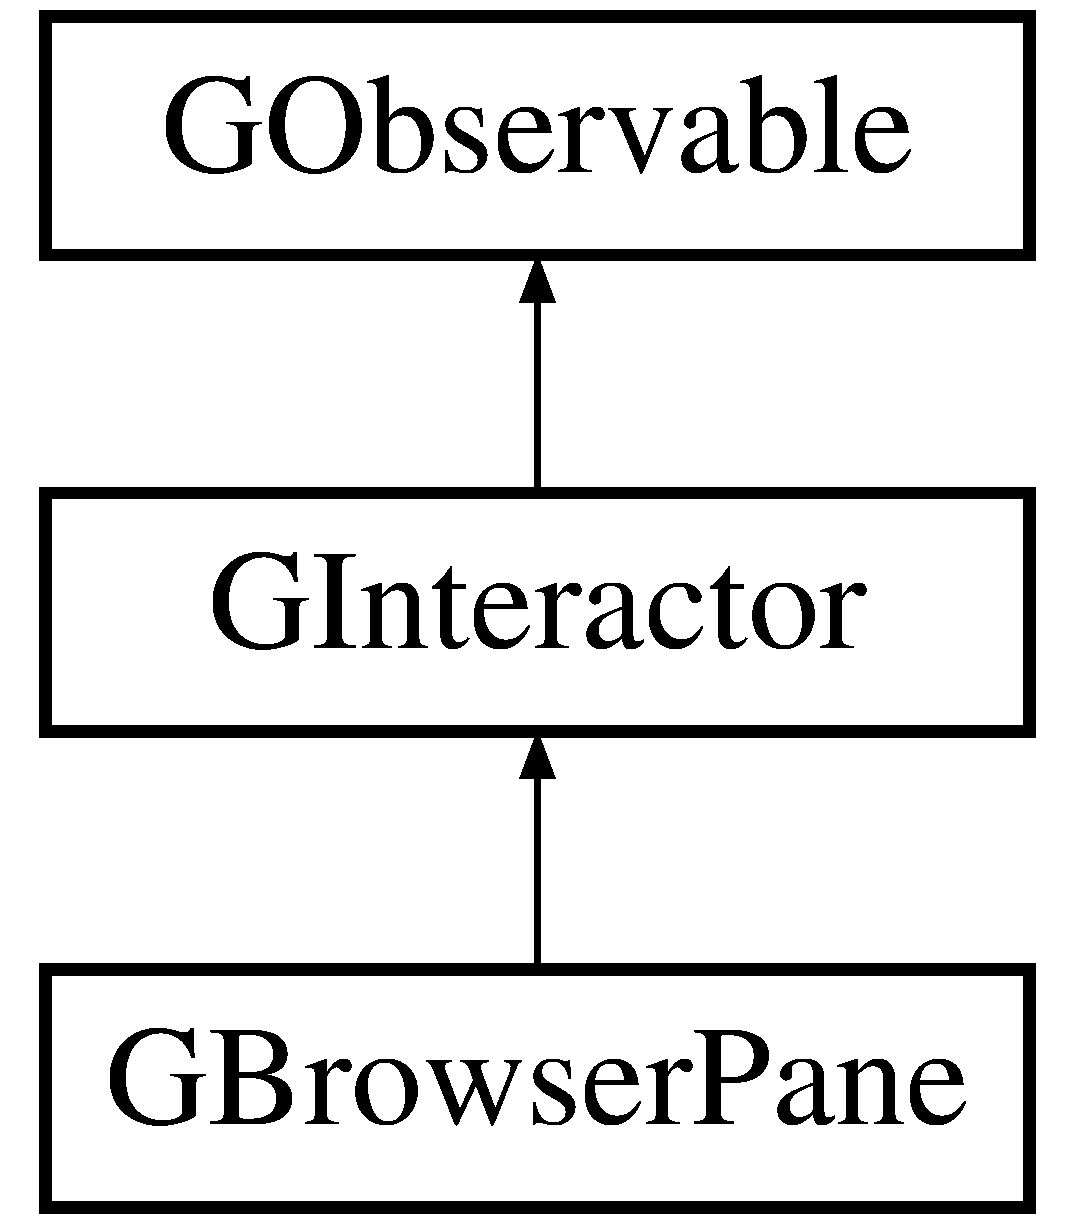
\includegraphics[height=3.000000cm]{classGBrowserPane}
\end{center}
\end{figure}
\subsection*{Public Types}
\begin{DoxyCompactItemize}
\item 
enum \mbox{\hyperlink{classGInteractor_a8e0d441725a81d2bbdebbea09078260e}{Text\+Position}} \{ \mbox{\hyperlink{classGInteractor_a8e0d441725a81d2bbdebbea09078260ea4cd6f2e7d5a08d6f4dc052df2358f774}{T\+E\+X\+T\+\_\+\+B\+E\+S\+I\+D\+E\+\_\+\+I\+C\+ON}}, 
\mbox{\hyperlink{classGInteractor_a8e0d441725a81d2bbdebbea09078260eaa88490f63d8de68d44c83bdb2ecde3b3}{T\+E\+X\+T\+\_\+\+U\+N\+D\+E\+R\+\_\+\+I\+C\+ON}}, 
\mbox{\hyperlink{classGInteractor_a8e0d441725a81d2bbdebbea09078260ea39a6f388a30ac4fefb6eb13e846bc9f2}{T\+E\+X\+T\+\_\+\+O\+N\+LY}}
 \}
\begin{DoxyCompactList}\small\item\em The places where an interactor can place its text relative to its icon. \end{DoxyCompactList}\end{DoxyCompactItemize}
\subsection*{Public Member Functions}
\begin{DoxyCompactItemize}
\item 
\mbox{\hyperlink{classGBrowserPane_a8f540c6f1aab2b4278bea6b1139aa470}{G\+Browser\+Pane}} (const std\+::string \&url=\char`\"{}\char`\"{}, Q\+Widget $\ast$parent=nullptr)
\begin{DoxyCompactList}\small\item\em Constructs a new browser pane. \end{DoxyCompactList}\item 
\mbox{\hyperlink{classGBrowserPane_ad2b090c6d23fd1019afa2a16e9eb1680}{$\sim$\+G\+Browser\+Pane}} () override
\begin{DoxyCompactList}\small\item\em Frees memory allocated internally by the browser pane. \end{DoxyCompactList}\item 
virtual void \mbox{\hyperlink{classGInteractor_a02f20ea6edfa0671f31c4c648a253833}{add\+Action\+Listener}} () Q\+\_\+\+D\+E\+C\+L\+\_\+\+D\+E\+P\+R\+E\+C\+A\+T\+ED
\begin{DoxyCompactList}\small\item\em Adds an event listener to be notified when this interactor is clicked or generally interacted with. \end{DoxyCompactList}\item 
virtual void \mbox{\hyperlink{classGBrowserPane_abd07e172ccec6823a88289c21124a367}{clear\+Selection}} ()
\begin{DoxyCompactList}\small\item\em Deselects any text that is currently selected in the pane. \end{DoxyCompactList}\item 
virtual void \mbox{\hyperlink{classGBrowserPane_a25f53c7d92eb2a5197cd4418c0165367}{clear\+Text}} ()
\begin{DoxyCompactList}\small\item\em Sets the text in the pane to be empty. \end{DoxyCompactList}\item 
bool \mbox{\hyperlink{classGInteractor_a597a370b592e3737d38d9d2f4e2031ea}{events\+Enabled}} () const override
\begin{DoxyCompactList}\small\item\em Returns true if this interactor is currently accepting events. \end{DoxyCompactList}\item 
virtual std\+::string \mbox{\hyperlink{classGInteractor_a69f8d23ed8f207fbecad99960776e942}{get\+Accelerator}} () const
\begin{DoxyCompactList}\small\item\em Returns a string representing a hotkey for this interactor, or an empty string if no accelerator has been set. \end{DoxyCompactList}\item 
virtual std\+::string \mbox{\hyperlink{classGInteractor_a94eb4276000c4fdfb508ce9e6317a82a}{get\+Action\+Command}} () const
\begin{DoxyCompactList}\small\item\em Returns an action command for this interactor, which is a semi-\/unique string you can use to identify it when events occur. \end{DoxyCompactList}\item 
virtual std\+::string \mbox{\hyperlink{classGInteractor_a808e22cc1fdfbecf71ed8c64ef4600e0}{get\+Background}} () const
\begin{DoxyCompactList}\small\item\em Returns the background color of the interactor as a string. \end{DoxyCompactList}\item 
virtual int \mbox{\hyperlink{classGInteractor_a9e827257a55cb8cf4d9de2ec6bcfd7a0}{get\+Background\+Int}} () const
\begin{DoxyCompactList}\small\item\em Returns the background color of the interactor as an R\+GB integer. \end{DoxyCompactList}\item 
virtual \mbox{\hyperlink{structGRectangle}{G\+Rectangle}} \mbox{\hyperlink{classGInteractor_a29e6ac35a0b48f491a4c88194cc5da3b}{get\+Bounds}} () const
\begin{DoxyCompactList}\small\item\em Returns a rectangle representing the x/y position and size of this interactor. \end{DoxyCompactList}\item 
virtual std\+::string \mbox{\hyperlink{classGInteractor_aa061dfa488c31e18549d64363c1d0e34}{get\+Color}} () const
\begin{DoxyCompactList}\small\item\em Returns the foreground/text color of the interactor as a string. \end{DoxyCompactList}\item 
virtual int \mbox{\hyperlink{classGInteractor_a9635c7af766cdc3417f346683fa0e6c1}{get\+Color\+Int}} () const
\begin{DoxyCompactList}\small\item\em Returns the foreground/text color of the interactor as an R\+GB integer. \end{DoxyCompactList}\item 
virtual \mbox{\hyperlink{classGContainer}{G\+Container}} $\ast$ \mbox{\hyperlink{classGInteractor_a7a6e317c29d61030929b4cd2d1c00fe7}{get\+Container}} () const
\begin{DoxyCompactList}\small\item\em Returns a pointer to the onscreen container holding this interactor. \end{DoxyCompactList}\item 
virtual std\+::string \mbox{\hyperlink{classGBrowserPane_af3bc7daeceb5c8abfb8edaa1941e3757}{get\+Content\+Type}} () const
\begin{DoxyCompactList}\small\item\em Returns the M\+I\+ME content type for the current page. \end{DoxyCompactList}\item 
virtual int \mbox{\hyperlink{classGBrowserPane_aa85d2267b4534eb372cd3114ea61ba3b}{get\+Cursor\+Position}} () const
\begin{DoxyCompactList}\small\item\em Returns the keyboard cursor\textquotesingle{}s current position in the text pane as a 0-\/based character index within the overall text string. \end{DoxyCompactList}\item 
virtual std\+::string \mbox{\hyperlink{classGInteractor_a894a5502900794eeb27d084c21f1d77d}{get\+Font}} () const
\begin{DoxyCompactList}\small\item\em Returns the font of this interactor\textquotesingle{}s text as a font string such as \char`\"{}\+Helvetica-\/12-\/\+Bold\char`\"{}. \end{DoxyCompactList}\item 
virtual std\+::string \mbox{\hyperlink{classGInteractor_a4fa2d8b0192a3a5b4af4bbfe71194d03}{get\+Foreground}} () const
\begin{DoxyCompactList}\small\item\em Returns the foreground/text color of the interactor as a string. \end{DoxyCompactList}\item 
virtual int \mbox{\hyperlink{classGInteractor_ac3b12ab385a6ef9ae90fc879860ba726}{get\+Foreground\+Int}} () const
\begin{DoxyCompactList}\small\item\em Returns the foreground/text color of the interactor as an R\+GB integer. \end{DoxyCompactList}\item 
virtual double \mbox{\hyperlink{classGInteractor_a1e7e353362434072875264cf95629f99}{get\+Height}} () const
\begin{DoxyCompactList}\small\item\em Returns the current onscreen height of this interactor in pixels. \end{DoxyCompactList}\item 
virtual std\+::string \mbox{\hyperlink{classGInteractor_aaed62a73004939a64da6f0eb9eb64d73}{get\+Icon}} () const
\begin{DoxyCompactList}\small\item\em Returns the file name of the icon associated with this interactor, or an empty string if no icon has been set. \end{DoxyCompactList}\item 
virtual int \mbox{\hyperlink{classGInteractor_a9c9659a6c6ba66b4107ba59c95a24241}{get\+ID}} () const
\begin{DoxyCompactList}\small\item\em Returns a globally unique identifier for this interactor, which is set when the interactor is constructed. \end{DoxyCompactList}\item 
\+\_\+\+Internal\+\_\+\+Q\+Widget $\ast$ \mbox{\hyperlink{classGBrowserPane_a2f6b36b2517087dc90a366b5ce1f5323}{get\+Internal\+Widget}} () const override
\begin{DoxyCompactList}\small\item\em Returns a direct pointer to the internal Qt widget being wrapped by this interactor. \end{DoxyCompactList}\item 
virtual \mbox{\hyperlink{structGPoint}{G\+Point}} \mbox{\hyperlink{classGInteractor_a4f83802015511edeb63b892830812c11}{get\+Location}} () const
\begin{DoxyCompactList}\small\item\em Returns an (x, y) point representing the onscreen location of the top-\/left corner of this interactor within its containing window. \end{DoxyCompactList}\item 
virtual double \mbox{\hyperlink{classGInteractor_aed4b0075fcc434499c3cb3e46896bda3}{get\+Minimum\+Height}} () const
\begin{DoxyCompactList}\small\item\em Returns the minimum height in pixels that this interactor will permit itself to be resized to. \end{DoxyCompactList}\item 
virtual \mbox{\hyperlink{structGDimension}{G\+Dimension}} \mbox{\hyperlink{classGInteractor_a66b5af0b32493b4d597ca0a3df2049ea}{get\+Minimum\+Size}} () const
\begin{DoxyCompactList}\small\item\em Returns a \mbox{\hyperlink{structGDimension}{G\+Dimension}} structure representing the minimum size in pixels that this interactor will permit itself to be resized to. \end{DoxyCompactList}\item 
virtual double \mbox{\hyperlink{classGInteractor_a59e668114fe3d49d2a0f28deb258f7c8}{get\+Minimum\+Width}} () const
\begin{DoxyCompactList}\small\item\em Returns the minimum width in pixels that this interactor will permit itself to be resized to. \end{DoxyCompactList}\item 
virtual std\+::string \mbox{\hyperlink{classGInteractor_a8a60438a5b55d0b2ceb35c8674b9d8c5}{get\+Name}} () const
\begin{DoxyCompactList}\small\item\em Returns a string representing a unique name for this interactor. \end{DoxyCompactList}\item 
virtual std\+::string \mbox{\hyperlink{classGBrowserPane_aa7607fcbc7eef6590fae7a2d513268de}{get\+Page\+Url}} () const
\begin{DoxyCompactList}\small\item\em Returns the U\+RL of the web page or file name being currently viewed. \end{DoxyCompactList}\item 
virtual double \mbox{\hyperlink{classGInteractor_a747de0961653847bdc6615dbf756d715}{get\+Preferred\+Height}} () const
\begin{DoxyCompactList}\small\item\em Returns the height in pixels that this interactor would prefer to be, which would exactly fit its contents with no stretching or scrollbars. \end{DoxyCompactList}\item 
virtual \mbox{\hyperlink{structGDimension}{G\+Dimension}} \mbox{\hyperlink{classGInteractor_a4aabbee761d8e9116275401131b7ccd1}{get\+Preferred\+Size}} () const
\begin{DoxyCompactList}\small\item\em Returns a \mbox{\hyperlink{structGDimension}{G\+Dimension}} structure storing the width and height in pixels that this interactor would prefer to be, which would exactly fit its contents with no stretching or scrollbars. \end{DoxyCompactList}\item 
virtual double \mbox{\hyperlink{classGInteractor_a82bca31d37700fb0e35d2743352efd5e}{get\+Preferred\+Width}} () const
\begin{DoxyCompactList}\small\item\em Returns the height in pixels that this interactor would prefer to be, which would exactly fit its contents with no stretching or scrollbars. \end{DoxyCompactList}\item 
virtual std\+::string \mbox{\hyperlink{classGBrowserPane_a512371b3f41599349f23389825a6ccf7}{get\+Selected\+Text}} () const
\begin{DoxyCompactList}\small\item\em Returns the text that is currently selected in the text pane. \end{DoxyCompactList}\item 
virtual int \mbox{\hyperlink{classGBrowserPane_a2885313daa0e367cee2ccd0c704a6147}{get\+Selection\+End}} () const
\begin{DoxyCompactList}\small\item\em Returns the index just past the end of the current selection of text as a 0-\/based character index within the overall text string. \end{DoxyCompactList}\item 
virtual int \mbox{\hyperlink{classGBrowserPane_a68f7816694269b73e6284e756eb0c179}{get\+Selection\+Length}} () const
\begin{DoxyCompactList}\small\item\em Returns the number of characters that are currently selected. \end{DoxyCompactList}\item 
virtual int \mbox{\hyperlink{classGBrowserPane_aad7c986a677c1b9cf445cd7cfb6a8975}{get\+Selection\+Start}} () const
\begin{DoxyCompactList}\small\item\em Returns the index of the start of the current selection of text as a 0-\/based character index within the overall text string. \end{DoxyCompactList}\item 
virtual \mbox{\hyperlink{structGDimension}{G\+Dimension}} \mbox{\hyperlink{classGInteractor_a7b4eec96a2bdc6420695d5796a78eea9}{get\+Size}} () const
\begin{DoxyCompactList}\small\item\em Returns a \mbox{\hyperlink{structGDimension}{G\+Dimension}} structure storing the current onscreen width and height of this interactor in pixels. \end{DoxyCompactList}\item 
virtual std\+::string \mbox{\hyperlink{classGBrowserPane_aff553c50924b836c29f146ed34a7c6ec}{get\+Text}} () const
\begin{DoxyCompactList}\small\item\em Returns the full text of the current page or file being displayed in the pane. \end{DoxyCompactList}\item 
std\+::string \mbox{\hyperlink{classGBrowserPane_a9b72ede4ee8520f987a0c01e30654814}{get\+Type}} () const override
\begin{DoxyCompactList}\small\item\em Returns a string representing the class name of this interactor, such as \char`\"{}\+G\+Button\char`\"{} or \char`\"{}\+G\+Check\+Box\char`\"{}. \end{DoxyCompactList}\item 
Q\+Widget $\ast$ \mbox{\hyperlink{classGBrowserPane_a3b33a602b31a6b809d020535a59db3b4}{get\+Widget}} () const override
\begin{DoxyCompactList}\small\item\em Returns a direct pointer to the internal Qt widget being wrapped by this interactor. \end{DoxyCompactList}\item 
virtual double \mbox{\hyperlink{classGInteractor_a0ed2965abd4f5701d2cadf71239faf19}{get\+Width}} () const
\begin{DoxyCompactList}\small\item\em Returns the current onscreen width of this interactor in pixels. \end{DoxyCompactList}\item 
virtual double \mbox{\hyperlink{classGInteractor_a344385751bee0720059403940d57a13e}{getX}} () const
\begin{DoxyCompactList}\small\item\em Returns the x-\/coordinate of the top-\/left pixel of this interactor within its onscreen window. \end{DoxyCompactList}\item 
virtual double \mbox{\hyperlink{classGInteractor_aafa51c7f8f38a09febbb9ce7853f77b4}{getY}} () const
\begin{DoxyCompactList}\small\item\em Returns the y-\/coordinate of the top-\/left pixel of this interactor within its onscreen window. \end{DoxyCompactList}\item 
virtual bool \mbox{\hyperlink{classGInteractor_afc480f652b8c5f1fb255e2269ce68879}{in\+Bounds}} (double x, double y) const
\begin{DoxyCompactList}\small\item\em Returns true if the given x/y pixel is within the bounds of this interactor. \end{DoxyCompactList}\item 
virtual bool \mbox{\hyperlink{classGInteractor_ae6d7982c1c627b677a5e776ca86118ed}{in\+Bounds}} (int x, int y) const
\begin{DoxyCompactList}\small\item\em Returns true if the given x/y pixel is within the bounds of this interactor. \end{DoxyCompactList}\item 
virtual bool \mbox{\hyperlink{classGBrowserPane_a012b5afb54e037e6c5498cf0932a521b}{is\+Editable}} () const
\begin{DoxyCompactList}\small\item\em Returns whether the text pane allows the user to modify its text. \end{DoxyCompactList}\item 
virtual bool \mbox{\hyperlink{classGInteractor_aacb819fb241851fd9fc045271baa4034}{is\+Enabled}} () const
\begin{DoxyCompactList}\small\item\em Returns true if this interactor is currently enabled. \end{DoxyCompactList}\item 
virtual bool \mbox{\hyperlink{classGBrowserPane_ae09e72290b6e8a23bcc77752da6dffa5}{is\+Line\+Wrap}} () const
\begin{DoxyCompactList}\small\item\em Returns whether the text pane wraps its text when a line becomes too long. \end{DoxyCompactList}\item 
virtual bool \mbox{\hyperlink{classGInteractor_a9d8a6cfb13917785c143e74d40e4e2be}{is\+Visible}} () const
\begin{DoxyCompactList}\small\item\em Returns true if the interactor is visible on the screen. \end{DoxyCompactList}\item 
virtual void \mbox{\hyperlink{classGBrowserPane_ab5ef729cac166db0ef51ff7ea30d1bb8}{move\+Cursor\+To\+End}} ()
\begin{DoxyCompactList}\small\item\em Sets the text pane\textquotesingle{}s keyboard cursor position to the end of the current text. \end{DoxyCompactList}\item 
virtual void \mbox{\hyperlink{classGBrowserPane_a24abdceab57bcff96185afbadf193a22}{move\+Cursor\+To\+Start}} ()
\begin{DoxyCompactList}\small\item\em Sets the text pane\textquotesingle{}s keyboard cursor position to the start of the current text. \end{DoxyCompactList}\item 
virtual void \mbox{\hyperlink{classGBrowserPane_a5e6d9158a9311204ca49518c32072ce0}{read\+Text\+From\+File}} (std\+::istream \&file)
\begin{DoxyCompactList}\small\item\em Reads text from the given file and displays the entire file\textquotesingle{}s text as the contents of this formatted pane. \end{DoxyCompactList}\item 
virtual void \mbox{\hyperlink{classGBrowserPane_a58c4154aa0c23bc980d45bf9de7cc95c}{read\+Text\+From\+File}} (const std\+::string \&filename)
\begin{DoxyCompactList}\small\item\em Reads text from the given file and displays the entire file\textquotesingle{}s text as the contents of this formatted pane. \end{DoxyCompactList}\item 
virtual void \mbox{\hyperlink{classGBrowserPane_a68ff415e722130964bc9e1de826f4869}{read\+Text\+From\+Url}} (const std\+::string \&url)
\begin{DoxyCompactList}\small\item\em Reads text from the given web page U\+RL and displays the entire page\textquotesingle{}s text as the contents of this formatted pane. \end{DoxyCompactList}\item 
virtual void \mbox{\hyperlink{classGInteractor_ab7fe7a876367b87cf7202f947f1d05e4}{remove\+Action\+Listener}} ()
\begin{DoxyCompactList}\small\item\em Removes the action listener from this interactor so that it will no longer call it when events occur. \end{DoxyCompactList}\item 
virtual void \mbox{\hyperlink{classGInteractor_ad39d0325cde6b97ebda4b9d7787c633b}{remove\+Click\+Listener}} ()
\begin{DoxyCompactList}\small\item\em Removes the click listener from this interactor so that it will no longer call it when events occur. \end{DoxyCompactList}\item 
virtual void \mbox{\hyperlink{classGInteractor_aa4250907e4cdd77349c04f0cf5cdd3d3}{remove\+Double\+Click\+Listener}} ()
\begin{DoxyCompactList}\small\item\em Removes the double-\/click listener from this interactor so that it will no longer call it when events occur. \end{DoxyCompactList}\item 
virtual void \mbox{\hyperlink{classGInteractor_a43095f41cab3be732b49f29970484b05}{remove\+Key\+Listener}} ()
\begin{DoxyCompactList}\small\item\em Removes the key listener from this interactor so that it will no longer call it when key events occur. \end{DoxyCompactList}\item 
virtual void \mbox{\hyperlink{classGBrowserPane_a263a2282597ca9f0f73301fb202ae390}{remove\+Link\+Listener}} ()
\begin{DoxyCompactList}\small\item\em Removes the link listener from the canvas so that it will no longer call it when hyperlink events occur. \end{DoxyCompactList}\item 
virtual void \mbox{\hyperlink{classGInteractor_aff47f71ce47e688a07c9d38dc92fcc11}{remove\+Mouse\+Listener}} ()
\begin{DoxyCompactList}\small\item\em Removes the mouse listener from this interactor so that it will no longer call it when events occur. \end{DoxyCompactList}\item 
virtual void \mbox{\hyperlink{classGBrowserPane_a69c940b99d01eb7c353763ce4b0942a4}{remove\+Text\+Change\+Listener}} ()
\begin{DoxyCompactList}\small\item\em Removes the text change listener from this text pane so that it will no longer call it when the user modifies the text. \end{DoxyCompactList}\item 
virtual void \mbox{\hyperlink{classGInteractor_a519fb2ac767f8b2febbb50b898b8c8cb}{request\+Focus}} ()
\begin{DoxyCompactList}\small\item\em Transfers keyboard focus to this interactor. \end{DoxyCompactList}\item 
virtual void \mbox{\hyperlink{classGBrowserPane_ad4c9b6140b529865a6cdeed37a339237}{scroll\+To\+Bottom}} ()
\begin{DoxyCompactList}\small\item\em Moves the visible scroll region of the text pane so that the bottom part of the text is visible. \end{DoxyCompactList}\item 
virtual void \mbox{\hyperlink{classGBrowserPane_a9eacfcf7c186936ed957dd1c8a9c6b64}{scroll\+To\+Top}} ()
\begin{DoxyCompactList}\small\item\em Moves the visible scroll region of the text pane so that the top part of the text is visible. \end{DoxyCompactList}\item 
virtual void \mbox{\hyperlink{classGBrowserPane_aaeb1320c0553d0d2b8081b750f59a34a}{select}} (int start\+Index, int length)
\begin{DoxyCompactList}\small\item\em Sets the given range of text to be selected, beginning with the given start index as a 0-\/based character index within the overall text string, and extending for the given length of characters. \end{DoxyCompactList}\item 
virtual void \mbox{\hyperlink{classGBrowserPane_ab6658ed404200bd7aaca5629db064645}{select\+All}} ()
\begin{DoxyCompactList}\small\item\em Selects the entire text of the text pane. \end{DoxyCompactList}\item 
virtual void \mbox{\hyperlink{classGInteractor_ad15f102f62e2960576012f1aa0ba4b2e}{set\+Accelerator}} (const std\+::string \&accelerator)
\begin{DoxyCompactList}\small\item\em Sets an accelerator hotkey for this interactor, such as \char`\"{}\+Ctrl-\/\+S\char`\"{}. \end{DoxyCompactList}\item 
virtual void \mbox{\hyperlink{classGInteractor_a4b5843fe3030e038a1ba54cc03389bcf}{set\+Action\+Command}} (const std\+::string \&action\+Command)
\begin{DoxyCompactList}\small\item\em Sets the action command for this interactor. \end{DoxyCompactList}\item 
virtual void \mbox{\hyperlink{classGInteractor_adcfb4742430c88714fcf57e57ab8ea9c}{set\+Action\+Listener}} (G\+Event\+Listener func)
\begin{DoxyCompactList}\small\item\em Sets an action listener on this interactor so that it will be called when it is interacted with in its primary way. \end{DoxyCompactList}\item 
virtual void \mbox{\hyperlink{classGInteractor_aebd20a89c7a8a43a6fce999cf4f9fcf2}{set\+Action\+Listener}} (G\+Event\+Listener\+Void func)
\begin{DoxyCompactList}\small\item\em Sets an action listener on this interactor so that it will be called when it is interacted with in its primary way. \end{DoxyCompactList}\item 
virtual void \mbox{\hyperlink{classGInteractor_acba7e546c2025c0a15ca4b4cc92043db}{set\+Background}} (int rgb)
\begin{DoxyCompactList}\small\item\em Sets the background color of the interactor to the color represented by the given R\+GB integer. \end{DoxyCompactList}\item 
virtual void \mbox{\hyperlink{classGInteractor_ab4677ab2474e68b07aa56605af92a84a}{set\+Background}} (const std\+::string \&color)
\begin{DoxyCompactList}\small\item\em Sets the background color of the interactor to the color represented by the given string. \end{DoxyCompactList}\item 
virtual void \mbox{\hyperlink{classGInteractor_a2aae8197624b72265ab83b4f1bc73f2f}{set\+Bounds}} (double x, double y, double width, double height)
\begin{DoxyCompactList}\small\item\em Sets the size and location of the widget. \end{DoxyCompactList}\item 
virtual void \mbox{\hyperlink{classGInteractor_acada386653f008cacc7cce86426bef7c}{set\+Bounds}} (const \mbox{\hyperlink{structGRectangle}{G\+Rectangle}} \&size)
\begin{DoxyCompactList}\small\item\em Sets the size and location of the widget. \end{DoxyCompactList}\item 
virtual void \mbox{\hyperlink{classGInteractor_abd40af6921242584d0954f173911b190}{set\+Click\+Listener}} (G\+Event\+Listener func)
\begin{DoxyCompactList}\small\item\em Sets a mouse listener on this interactor so that it will be called when the mouse is clicked on it. \end{DoxyCompactList}\item 
virtual void \mbox{\hyperlink{classGInteractor_a856414c92df90f56f3877475eb3f8fc4}{set\+Click\+Listener}} (G\+Event\+Listener\+Void func)
\begin{DoxyCompactList}\small\item\em Sets a mouse listener on this interactor so that it will be called when the mouse is clicked on it. \end{DoxyCompactList}\item 
virtual void \mbox{\hyperlink{classGInteractor_ab1f5cc0f5cc6bbbd716a526c61f1081d}{set\+Color}} (int rgb)
\begin{DoxyCompactList}\small\item\em Sets the foreground/text color of the interactor to the color represented by the given R\+GB integer. \end{DoxyCompactList}\item 
virtual void \mbox{\hyperlink{classGInteractor_a61374df6c11b52cfbb0815decdbaebc6}{set\+Color}} (const std\+::string \&color)
\begin{DoxyCompactList}\small\item\em Sets the foreground/text color of the interactor to the color represented by the given string. \end{DoxyCompactList}\item 
virtual void \mbox{\hyperlink{classGBrowserPane_a0ba11f3ad4f6257759f0db3dd791e6a4}{set\+Content\+Type}} (const std\+::string \&content\+Type)
\begin{DoxyCompactList}\small\item\em Sets the M\+I\+ME content type being used to display the current/future pages. \end{DoxyCompactList}\item 
virtual void \mbox{\hyperlink{classGBrowserPane_a5817e10a86be5cd41b3668d8fccb10e0}{set\+Cursor\+Position}} (int index, bool keep\+Anchor=false)
\begin{DoxyCompactList}\small\item\em Moves the keyboard cursor to the given 0-\/based character index within the text. \end{DoxyCompactList}\item 
virtual void \mbox{\hyperlink{classGInteractor_ac29f9a3462458e165fae3a1f046ee77a}{set\+Double\+Click\+Listener}} (G\+Event\+Listener func)
\begin{DoxyCompactList}\small\item\em Sets a mouse listener on this interactor so that it will be called when the mouse is double-\/clicked on it. \end{DoxyCompactList}\item 
virtual void \mbox{\hyperlink{classGInteractor_a50096194d66f48c92dd4c512d41bfc76}{set\+Double\+Click\+Listener}} (G\+Event\+Listener\+Void func)
\begin{DoxyCompactList}\small\item\em Sets a mouse listener on this interactor so that it will be called when the mouse is double-\/clicked on it. \end{DoxyCompactList}\item 
virtual void \mbox{\hyperlink{classGBrowserPane_a008d7fd44fb3e7a6886cdaddbc3644a2}{set\+Editable}} (bool value)
\begin{DoxyCompactList}\small\item\em Sets whether the text pane allows the user to modify its text. \end{DoxyCompactList}\item 
virtual void \mbox{\hyperlink{classGInteractor_ab831367dd84bbd579e02e55bacb21343}{set\+Enabled}} (bool value)
\begin{DoxyCompactList}\small\item\em Sets whether this interactor is currently enabled. \end{DoxyCompactList}\item 
virtual void \mbox{\hyperlink{classGObservable_afaa30b2a9e0f378fd1c70d2f1d0b8216}{set\+Events\+Enabled}} (bool \mbox{\hyperlink{classGInteractor_a597a370b592e3737d38d9d2f4e2031ea}{events\+Enabled}})
\begin{DoxyCompactList}\small\item\em Sets whether the object is currently allowing itself to fire events. \end{DoxyCompactList}\item 
virtual void \mbox{\hyperlink{classGInteractor_a2592348886ffea646c6534bf88f7c49d}{set\+Font}} (const Q\+Font \&font)
\begin{DoxyCompactList}\small\item\em Sets the font used by this widget to the given Qt font. \end{DoxyCompactList}\item 
virtual void \mbox{\hyperlink{classGInteractor_a8e096e8818d838aceae1d46d58fb3a7b}{set\+Font}} (const std\+::string \&font)
\begin{DoxyCompactList}\small\item\em Sets the font used by this widget to the font represented by the given font string, such as \char`\"{}\+Helvetica-\/16-\/\+Bold\char`\"{}. \end{DoxyCompactList}\item 
virtual void \mbox{\hyperlink{classGInteractor_a9eb856b5ff83a19df3831a31f15f4563}{set\+Foreground}} (int rgb)
\begin{DoxyCompactList}\small\item\em Sets the foreground/text color of the interactor to the color represented by the given R\+GB integer. \end{DoxyCompactList}\item 
virtual void \mbox{\hyperlink{classGInteractor_af59209aeadea6dfc6d97a2d8531f50e1}{set\+Foreground}} (const std\+::string \&color)
\begin{DoxyCompactList}\small\item\em Sets the foreground/text color of the interactor to the color represented by the given string. \end{DoxyCompactList}\item 
virtual void \mbox{\hyperlink{classGInteractor_a9e280bfc4544dfaf8e4376c4e1a74357}{set\+Height}} (double height)
\begin{DoxyCompactList}\small\item\em Sets the onscreen height of the interactor in pixels. \end{DoxyCompactList}\item 
virtual void \mbox{\hyperlink{classGInteractor_a542abfcd7261751352af129c7215ecda}{set\+Icon}} (const Q\+Icon \&icon)
\begin{DoxyCompactList}\small\item\em Sets the icon associated with this interactor. \end{DoxyCompactList}\item 
virtual void \mbox{\hyperlink{classGInteractor_a368e1a338f84401c284506d03b1ba769}{set\+Icon}} (const Q\+Pixmap \&icon)
\begin{DoxyCompactList}\small\item\em Sets the icon associated with this interactor. \end{DoxyCompactList}\item 
virtual void \mbox{\hyperlink{classGInteractor_a762e139aa311461c3984d3ad28293f64}{set\+Icon}} (const std\+::string \&filename, bool retain\+Icon\+Size=true)
\begin{DoxyCompactList}\small\item\em Sets the file name of the icon associated with this interactor, or an empty string if no icon has been set. \end{DoxyCompactList}\item 
virtual void \mbox{\hyperlink{classGInteractor_aeb8324d3287fa1fbe093f4d6230cf0a6}{set\+Key\+Listener}} (G\+Event\+Listener func)
\begin{DoxyCompactList}\small\item\em Sets a key listener on this interactor so that it will be called when the user presses any key. \end{DoxyCompactList}\item 
virtual void \mbox{\hyperlink{classGInteractor_ae48ecea73606c7bd9423e1c7cc589cc9}{set\+Key\+Listener}} (G\+Event\+Listener\+Void func)
\begin{DoxyCompactList}\small\item\em Sets a key listener on this interactor so that it will be called when the user presses any key. \end{DoxyCompactList}\item 
virtual void \mbox{\hyperlink{classGBrowserPane_aaaafb06fec060b28b70ec3b7379657b4}{set\+Line\+Wrap}} (bool wrap)
\begin{DoxyCompactList}\small\item\em Sets whether the text pane wraps its text when a line becomes too long. \end{DoxyCompactList}\item 
virtual void \mbox{\hyperlink{classGBrowserPane_aaa849c4aed1fa43178314f5c76e43081}{set\+Link\+Listener}} (G\+Event\+Listener func)
\begin{DoxyCompactList}\small\item\em Sets a link listener on this canvas so that it will be called when the user clicks on hyperlinks on the pane. \end{DoxyCompactList}\item 
virtual void \mbox{\hyperlink{classGBrowserPane_aca745635b2c4ceb74587ca5cfc26f0c3}{set\+Link\+Listener}} (G\+Event\+Listener\+Void func)
\begin{DoxyCompactList}\small\item\em Sets a link listener on this canvas so that it will be called when the user clicks on hyperlinks on the pane. \end{DoxyCompactList}\item 
virtual void \mbox{\hyperlink{classGInteractor_a04594e8ba9b98513a64f1da00dcae18c}{set\+Location}} (double x, double y)
\begin{DoxyCompactList}\small\item\em Sets the onscreen x/y-\/coordinate of the top-\/left corner of the interactor relative to its window. \end{DoxyCompactList}\item 
virtual void \mbox{\hyperlink{classGInteractor_a0cf428e207b7f22cc08138a90b1b87b2}{set\+Minimum\+Size}} (double width, double height)
\begin{DoxyCompactList}\small\item\em Sets the minimum size in pixels that this interactor will permit itself to be resized to. \end{DoxyCompactList}\item 
virtual void \mbox{\hyperlink{classGInteractor_a3b1046117ac6cb7abe467e00ba8a81f4}{set\+Minimum\+Size}} (const \mbox{\hyperlink{structGDimension}{G\+Dimension}} \&size)
\begin{DoxyCompactList}\small\item\em Sets the minimum size in pixels that this interactor will permit itself to be resized to. \end{DoxyCompactList}\item 
void \mbox{\hyperlink{classGBrowserPane_a2c6a3746da7ffa3819294896d4423059}{set\+Mouse\+Listener}} (G\+Event\+Listener func) override
\begin{DoxyCompactList}\small\item\em Sets a mouse listener on this text pane so that it will be called when the user moves or clicks the mouse. \end{DoxyCompactList}\item 
void \mbox{\hyperlink{classGBrowserPane_a3ed42c5f929cba378927916dd73e6576}{set\+Mouse\+Listener}} (G\+Event\+Listener\+Void func) override
\begin{DoxyCompactList}\small\item\em Sets a mouse listener on this text pane so that it will be called when the user moves or clicks the mouse. \end{DoxyCompactList}\item 
virtual void \mbox{\hyperlink{classGInteractor_a9d3a2685df23b5e7cbf59c19c4a1f9b5}{set\+Name}} (const std\+::string \&name)
\begin{DoxyCompactList}\small\item\em Sets a string representing a unique name for this interactor. \end{DoxyCompactList}\item 
virtual void \mbox{\hyperlink{classGInteractor_a1ab987704fce32098706c6f00fb08218}{set\+Preferred\+Height}} (double height)
\begin{DoxyCompactList}\small\item\em Sets the height in pixels that this interactor would prefer to be. \end{DoxyCompactList}\item 
virtual void \mbox{\hyperlink{classGInteractor_a042c5ae19430d765ef552371cae3632c}{set\+Preferred\+Size}} (double width, double height)
\begin{DoxyCompactList}\small\item\em Sets the width and height in pixels that this interactor would prefer to be. \end{DoxyCompactList}\item 
virtual void \mbox{\hyperlink{classGInteractor_aa22d9be4bc0e078bb0ea69b0fc9d7c75}{set\+Preferred\+Size}} (const \mbox{\hyperlink{structGDimension}{G\+Dimension}} \&size)
\begin{DoxyCompactList}\small\item\em Sets the size in pixels that this interactor would prefer to be. \end{DoxyCompactList}\item 
virtual void \mbox{\hyperlink{classGInteractor_a3db429ab2fa52efd187eec0ed8cdd9f2}{set\+Preferred\+Width}} (double width)
\begin{DoxyCompactList}\small\item\em Sets the width in pixels that this interactor would prefer to be. \end{DoxyCompactList}\item 
virtual void \mbox{\hyperlink{classGInteractor_aca25d49481f9bf5fc8f7df4c086c4ce7}{set\+Size}} (double width, double height)
\begin{DoxyCompactList}\small\item\em Sets the onscreen width and height of the interactor in pixels. \end{DoxyCompactList}\item 
virtual void \mbox{\hyperlink{classGInteractor_ae2b628228f192c2702c4ce941b2af68f}{set\+Size}} (const \mbox{\hyperlink{structGDimension}{G\+Dimension}} \&size)
\begin{DoxyCompactList}\small\item\em Sets the onscreen width and height of the interactor in pixels. \end{DoxyCompactList}\item 
virtual void \mbox{\hyperlink{classGBrowserPane_ac1ae51949d41ee9054634be5967d91b8}{set\+Text}} (const std\+::string \&text)
\begin{DoxyCompactList}\small\item\em Sets the pane to display to the given contents using its current content type. \end{DoxyCompactList}\item 
virtual void \mbox{\hyperlink{classGBrowserPane_ae41284f9c540110180ac0ad6beca5cb0}{set\+Text\+Change\+Listener}} (G\+Event\+Listener func)
\begin{DoxyCompactList}\small\item\em Sets a text change listener on this text pane so that it will be called when the user modifies the current text. \end{DoxyCompactList}\item 
virtual void \mbox{\hyperlink{classGBrowserPane_ae8df75b0746951146d29220f386fcd33}{set\+Text\+Change\+Listener}} (G\+Event\+Listener\+Void func)
\begin{DoxyCompactList}\small\item\em Sets a text change listener on this text pane so that it will be called when the user modifies the current text. \end{DoxyCompactList}\item 
virtual void \mbox{\hyperlink{classGInteractor_a039e0e49beaecc275efce02d416acea8}{set\+Tooltip}} (const std\+::string \&tooltip\+Text)
\begin{DoxyCompactList}\small\item\em Sets a \char`\"{}tooltip\char`\"{} that will appear if the user hovers their mouse over the interactor. \end{DoxyCompactList}\item 
virtual void \mbox{\hyperlink{classGInteractor_a18e44e30b31525a243960ca3928125aa}{set\+Visible}} (bool visible)
\begin{DoxyCompactList}\small\item\em Returns true if the interactor is visible on the screen. \end{DoxyCompactList}\item 
virtual void \mbox{\hyperlink{classGInteractor_aa3f3fba4cb131baa8696ba01e3bceca1}{set\+Width}} (double width)
\begin{DoxyCompactList}\small\item\em Sets the onscreen width of the interactor in pixels. \end{DoxyCompactList}\item 
virtual void \mbox{\hyperlink{classGInteractor_a9c18fcc579333bf9653d13ad2b372e39}{setX}} (double x)
\begin{DoxyCompactList}\small\item\em Sets the onscreen x-\/coordinate of the top-\/left corner of the interactor relative to its window. \end{DoxyCompactList}\item 
virtual void \mbox{\hyperlink{classGInteractor_a7d57e2a5c35d27feb58fd498a3cf82b9}{setY}} (double y)
\begin{DoxyCompactList}\small\item\em Sets the onscreen y-\/coordinate of the top-\/left corner of the interactor relative to its window. \end{DoxyCompactList}\item 
virtual std\+::string \mbox{\hyperlink{classGObservable_a1fe5121d6528fdea3f243321b3fa3a49}{to\+String}} () const
\begin{DoxyCompactList}\small\item\em Returns a string representation of this observable object\textquotesingle{}s state. \end{DoxyCompactList}\end{DoxyCompactItemize}
\subsection*{Protected Member Functions}
\begin{DoxyCompactItemize}
\item 
virtual void \mbox{\hyperlink{classGObservable_a80cfa040459ff53594adbd6a51ec8f43}{clear\+Event\+Listeners}} ()
\begin{DoxyCompactList}\small\item\em Removes all event listeners from this object. \end{DoxyCompactList}\item 
virtual void \mbox{\hyperlink{classGObservable_a284f31528c0520f8e545c03ac9eeac74}{ensure\+Thread\+Safety}} (const std\+::string \&member\+Name=\char`\"{}\char`\"{})
\begin{DoxyCompactList}\small\item\em Ensures that we are currently in the Qt G\+UI thread. \end{DoxyCompactList}\item 
virtual void \mbox{\hyperlink{classGObservable_a63e5e5a6227c59c928493b11aceb0f67}{fire\+Event}} (\mbox{\hyperlink{classGEvent}{G\+Event}} \&event)
\begin{DoxyCompactList}\small\item\em Sends out the given event to any attached listeners. \end{DoxyCompactList}\item 
virtual void \mbox{\hyperlink{classGObservable_ab3983ea07337b52020a29cc00c653d8d}{fire\+G\+Event}} (Q\+Event $\ast$event, Event\+Type event\+Type, const std\+::string \&event\+Name)
\begin{DoxyCompactList}\small\item\em Creates an event of the given type, then sends it out to any attached listeners. \end{DoxyCompactList}\item 
virtual void \mbox{\hyperlink{classGObservable_a01fdf1b0e0dbd49e189fe4514e010411}{fire\+G\+Event}} (Q\+Close\+Event $\ast$event, Event\+Type event\+Type, const std\+::string \&event\+Name)
\begin{DoxyCompactList}\small\item\em Creates an event of the given type, then sends it out to any attached listeners. \end{DoxyCompactList}\item 
virtual void \mbox{\hyperlink{classGObservable_abb0b2f66ba39211cb5d7615e9d1c04e2}{fire\+G\+Event}} (Q\+Key\+Event $\ast$event, Event\+Type event\+Type, const std\+::string \&event\+Name)
\begin{DoxyCompactList}\small\item\em Creates an event of the given type, then sends it out to any attached listeners. \end{DoxyCompactList}\item 
virtual void \mbox{\hyperlink{classGObservable_a119318675d2165bdf7dd853aaf881d4b}{fire\+G\+Event}} (Q\+Mouse\+Event $\ast$event, Event\+Type event\+Type, const std\+::string \&event\+Name, const std\+::string \&action\+Command=\char`\"{}\char`\"{})
\begin{DoxyCompactList}\small\item\em Creates an event of the given type, then sends it out to any attached listeners. \end{DoxyCompactList}\item 
virtual void \mbox{\hyperlink{classGObservable_a63fd9034e1e1633c1c38eb342bfd34e9}{fire\+G\+Event}} (Q\+Resize\+Event $\ast$event, Event\+Type event\+Type, const std\+::string \&event\+Name)
\begin{DoxyCompactList}\small\item\em Creates an event of the given type, then sends it out to any attached listeners. \end{DoxyCompactList}\item 
virtual void \mbox{\hyperlink{classGObservable_a741345310d9b7c5170a6cbc410c44ac4}{fire\+G\+Event}} (Q\+Timer\+Event $\ast$event, Event\+Type event\+Type, const std\+::string \&event\+Name)
\begin{DoxyCompactList}\small\item\em Creates an event of the given type, then sends it out to any attached listeners. \end{DoxyCompactList}\item 
virtual void \mbox{\hyperlink{classGObservable_a93bf338968a0338761b8e4dc62f582e9}{fire\+G\+Event}} (Q\+Wheel\+Event $\ast$event, Event\+Type event\+Type, const std\+::string \&event\+Name)
\begin{DoxyCompactList}\small\item\em Creates an event of the given type, then sends it out to any attached listeners. \end{DoxyCompactList}\item 
virtual void \mbox{\hyperlink{classGObservable_a2a70a7d7435ff0c3b80bb4d70da19e0d}{fire\+G\+Event}} (Q\+Window\+State\+Change\+Event $\ast$event, Event\+Type event\+Type, const std\+::string \&event\+Name)
\begin{DoxyCompactList}\small\item\em Creates an event of the given type, then sends it out to any attached listeners. \end{DoxyCompactList}\item 
virtual bool \mbox{\hyperlink{classGObservable_a9f6faaa25942923bafa1c44020c49fa9}{has\+Event\+Listener}} (const std\+::string \&event\+Name) const
\begin{DoxyCompactList}\small\item\em Returns true if the observable object has a listener for the given type of event. \end{DoxyCompactList}\item 
virtual bool \mbox{\hyperlink{classGObservable_aeec1adc19aa0f33de62390686ee1382c}{is\+Accepting\+Event}} (int event\+Mask) const
\begin{DoxyCompactList}\small\item\em Returns true if the observable object has a listener for the given type of event. \end{DoxyCompactList}\item 
virtual bool \mbox{\hyperlink{classGObservable_aa31c73145a29dcb92848a92e0cfaea41}{is\+Accepting\+Event}} (const \mbox{\hyperlink{classGEvent}{G\+Event}} \&event) const
\begin{DoxyCompactList}\small\item\em Returns true if the observable object has a listener for the given type of event. \end{DoxyCompactList}\item 
virtual bool \mbox{\hyperlink{classGObservable_a3b1c689267eda44e65a2213e7de38b23}{is\+Accepting\+Event}} (const std\+::string \&event\+Type) const
\begin{DoxyCompactList}\small\item\em Returns true if the observable object has a listener for the given type of event. \end{DoxyCompactList}\item 
virtual void \mbox{\hyperlink{classGObservable_acbcf1ed3a851ad8a3c17ef38d86b481d}{remove\+Event\+Listener}} (const std\+::string \&event\+Name)
\begin{DoxyCompactList}\small\item\em Removes any event listener from this observable object that would respond to the given type of event, such as \char`\"{}click\char`\"{} or \char`\"{}keydown\char`\"{}. \end{DoxyCompactList}\item 
virtual void \mbox{\hyperlink{classGObservable_af51cc35c29a1bd1908609d432decdbb6}{remove\+Event\+Listeners}} (std\+::initializer\+\_\+list$<$ std\+::string $>$ event\+Names)
\begin{DoxyCompactList}\small\item\em Removes any event listener from this observable object that would respond to the given types of events, such as \char`\"{}click\char`\"{} or \char`\"{}keydown\char`\"{}. \end{DoxyCompactList}\item 
virtual void \mbox{\hyperlink{classGObservable_ad2f6d34961c50f6c1e0659990b79f741}{set\+Event\+Listener}} (const std\+::string \&event\+Name, G\+Event\+Listener func)
\begin{DoxyCompactList}\small\item\em Adds an event listener from this observable object to respond to the given type of event, such as \char`\"{}click\char`\"{} or \char`\"{}keydown\char`\"{}. \end{DoxyCompactList}\item 
virtual void \mbox{\hyperlink{classGObservable_abac4cb9f9e626e010e87f5d91573c8a5}{set\+Event\+Listener}} (const std\+::string \&event\+Name, G\+Event\+Listener\+Void func)
\begin{DoxyCompactList}\small\item\em Adds an event listener from this observable object to respond to the given type of event, such as \char`\"{}click\char`\"{} or \char`\"{}keydown\char`\"{}. \end{DoxyCompactList}\item 
virtual void \mbox{\hyperlink{classGObservable_afa388d69c33c718cf035774604065604}{set\+Event\+Listeners}} (std\+::initializer\+\_\+list$<$ std\+::string $>$ event\+Names, G\+Event\+Listener func)
\begin{DoxyCompactList}\small\item\em Adds an event listener from this observable object to respond to the given types of events, such as \char`\"{}click\char`\"{} or \char`\"{}keydown\char`\"{}. \end{DoxyCompactList}\item 
virtual void \mbox{\hyperlink{classGObservable_a7867184bbb686f74fae8a4db927da799}{set\+Event\+Listeners}} (std\+::initializer\+\_\+list$<$ std\+::string $>$ event\+Names, G\+Event\+Listener\+Void func)
\begin{DoxyCompactList}\small\item\em Adds an event listener from this observable object to respond to the given types of events, such as \char`\"{}click\char`\"{} or \char`\"{}keydown\char`\"{}. \end{DoxyCompactList}\end{DoxyCompactItemize}


\subsection{Detailed Description}
A \mbox{\hyperlink{classGBrowserPane}{G\+Browser\+Pane}} is a graphical interactor that displays a web page. 

This interactor is a wrapping around the Qt Q\+Text\+Browser widget, which is able to display rich content such as H\+T\+ML pages.

You can use \mbox{\hyperlink{classGBrowserPane}{G\+Browser\+Pane}} to implement the core rendering engine of a basic web browser, though it does not support all web browser features such as Java\+Script content, secure sessions, or cookies. 

\subsection{Member Enumeration Documentation}
\mbox{\Hypertarget{classGInteractor_a8e0d441725a81d2bbdebbea09078260e}\label{classGInteractor_a8e0d441725a81d2bbdebbea09078260e}} 
\index{G\+Browser\+Pane@{G\+Browser\+Pane}!Text\+Position@{Text\+Position}}
\index{Text\+Position@{Text\+Position}!G\+Browser\+Pane@{G\+Browser\+Pane}}
\subsubsection{\texorpdfstring{Text\+Position}{TextPosition}}
{\footnotesize\ttfamily enum \mbox{\hyperlink{classGInteractor_a8e0d441725a81d2bbdebbea09078260e}{Text\+Position}}\hspace{0.3cm}{\ttfamily [inherited]}}



The places where an interactor can place its text relative to its icon. 

\begin{DoxyEnumFields}{Enumerator}
\raisebox{\heightof{T}}[0pt][0pt]{\index{T\+E\+X\+T\+\_\+\+B\+E\+S\+I\+D\+E\+\_\+\+I\+C\+ON@{T\+E\+X\+T\+\_\+\+B\+E\+S\+I\+D\+E\+\_\+\+I\+C\+ON}!G\+Browser\+Pane@{G\+Browser\+Pane}}\index{G\+Browser\+Pane@{G\+Browser\+Pane}!T\+E\+X\+T\+\_\+\+B\+E\+S\+I\+D\+E\+\_\+\+I\+C\+ON@{T\+E\+X\+T\+\_\+\+B\+E\+S\+I\+D\+E\+\_\+\+I\+C\+ON}}}\mbox{\Hypertarget{classGInteractor_a8e0d441725a81d2bbdebbea09078260ea4cd6f2e7d5a08d6f4dc052df2358f774}\label{classGInteractor_a8e0d441725a81d2bbdebbea09078260ea4cd6f2e7d5a08d6f4dc052df2358f774}} 
T\+E\+X\+T\+\_\+\+B\+E\+S\+I\+D\+E\+\_\+\+I\+C\+ON&\\
\hline

\raisebox{\heightof{T}}[0pt][0pt]{\index{T\+E\+X\+T\+\_\+\+U\+N\+D\+E\+R\+\_\+\+I\+C\+ON@{T\+E\+X\+T\+\_\+\+U\+N\+D\+E\+R\+\_\+\+I\+C\+ON}!G\+Browser\+Pane@{G\+Browser\+Pane}}\index{G\+Browser\+Pane@{G\+Browser\+Pane}!T\+E\+X\+T\+\_\+\+U\+N\+D\+E\+R\+\_\+\+I\+C\+ON@{T\+E\+X\+T\+\_\+\+U\+N\+D\+E\+R\+\_\+\+I\+C\+ON}}}\mbox{\Hypertarget{classGInteractor_a8e0d441725a81d2bbdebbea09078260eaa88490f63d8de68d44c83bdb2ecde3b3}\label{classGInteractor_a8e0d441725a81d2bbdebbea09078260eaa88490f63d8de68d44c83bdb2ecde3b3}} 
T\+E\+X\+T\+\_\+\+U\+N\+D\+E\+R\+\_\+\+I\+C\+ON&\\
\hline

\raisebox{\heightof{T}}[0pt][0pt]{\index{T\+E\+X\+T\+\_\+\+O\+N\+LY@{T\+E\+X\+T\+\_\+\+O\+N\+LY}!G\+Browser\+Pane@{G\+Browser\+Pane}}\index{G\+Browser\+Pane@{G\+Browser\+Pane}!T\+E\+X\+T\+\_\+\+O\+N\+LY@{T\+E\+X\+T\+\_\+\+O\+N\+LY}}}\mbox{\Hypertarget{classGInteractor_a8e0d441725a81d2bbdebbea09078260ea39a6f388a30ac4fefb6eb13e846bc9f2}\label{classGInteractor_a8e0d441725a81d2bbdebbea09078260ea39a6f388a30ac4fefb6eb13e846bc9f2}} 
T\+E\+X\+T\+\_\+\+O\+N\+LY&\\
\hline

\end{DoxyEnumFields}


\subsection{Constructor \& Destructor Documentation}
\mbox{\Hypertarget{classGBrowserPane_a8f540c6f1aab2b4278bea6b1139aa470}\label{classGBrowserPane_a8f540c6f1aab2b4278bea6b1139aa470}} 
\index{G\+Browser\+Pane@{G\+Browser\+Pane}!G\+Browser\+Pane@{G\+Browser\+Pane}}
\index{G\+Browser\+Pane@{G\+Browser\+Pane}!G\+Browser\+Pane@{G\+Browser\+Pane}}
\subsubsection{\texorpdfstring{G\+Browser\+Pane()}{GBrowserPane()}}
{\footnotesize\ttfamily \mbox{\hyperlink{classGBrowserPane}{G\+Browser\+Pane}} (\begin{DoxyParamCaption}\item[{const std\+::string \&}]{url = {\ttfamily \char`\"{}\char`\"{}},  }\item[{Q\+Widget $\ast$}]{parent = {\ttfamily nullptr} }\end{DoxyParamCaption})}



Constructs a new browser pane. 

If a U\+RL string is passed, loads the data from that U\+RL. Otherwise, the pane is initially blank. \mbox{\Hypertarget{classGBrowserPane_ad2b090c6d23fd1019afa2a16e9eb1680}\label{classGBrowserPane_ad2b090c6d23fd1019afa2a16e9eb1680}} 
\index{G\+Browser\+Pane@{G\+Browser\+Pane}!````~G\+Browser\+Pane@{$\sim$\+G\+Browser\+Pane}}
\index{````~G\+Browser\+Pane@{$\sim$\+G\+Browser\+Pane}!G\+Browser\+Pane@{G\+Browser\+Pane}}
\subsubsection{\texorpdfstring{$\sim$\+G\+Browser\+Pane()}{~GBrowserPane()}}
{\footnotesize\ttfamily $\sim$\mbox{\hyperlink{classGBrowserPane}{G\+Browser\+Pane}} (\begin{DoxyParamCaption}{ }\end{DoxyParamCaption})\hspace{0.3cm}{\ttfamily [override]}}



Frees memory allocated internally by the browser pane. 



\subsection{Member Function Documentation}
\mbox{\Hypertarget{classGInteractor_a02f20ea6edfa0671f31c4c648a253833}\label{classGInteractor_a02f20ea6edfa0671f31c4c648a253833}} 
\index{G\+Browser\+Pane@{G\+Browser\+Pane}!add\+Action\+Listener@{add\+Action\+Listener}}
\index{add\+Action\+Listener@{add\+Action\+Listener}!G\+Browser\+Pane@{G\+Browser\+Pane}}
\subsubsection{\texorpdfstring{add\+Action\+Listener()}{addActionListener()}}
{\footnotesize\ttfamily void add\+Action\+Listener (\begin{DoxyParamCaption}{ }\end{DoxyParamCaption})\hspace{0.3cm}{\ttfamily [virtual]}, {\ttfamily [inherited]}}



Adds an event listener to be notified when this interactor is clicked or generally interacted with. 

\begin{DoxyRefDesc}{Deprecated}
\item[\mbox{\hyperlink{deprecated__deprecated000006}{Deprecated}}]does nothing; use set\+Action\+Listener instead \end{DoxyRefDesc}
\mbox{\Hypertarget{classGObservable_a80cfa040459ff53594adbd6a51ec8f43}\label{classGObservable_a80cfa040459ff53594adbd6a51ec8f43}} 
\index{G\+Browser\+Pane@{G\+Browser\+Pane}!clear\+Event\+Listeners@{clear\+Event\+Listeners}}
\index{clear\+Event\+Listeners@{clear\+Event\+Listeners}!G\+Browser\+Pane@{G\+Browser\+Pane}}
\subsubsection{\texorpdfstring{clear\+Event\+Listeners()}{clearEventListeners()}}
{\footnotesize\ttfamily void clear\+Event\+Listeners (\begin{DoxyParamCaption}{ }\end{DoxyParamCaption})\hspace{0.3cm}{\ttfamily [protected]}, {\ttfamily [virtual]}, {\ttfamily [inherited]}}



Removes all event listeners from this object. 

\mbox{\Hypertarget{classGBrowserPane_abd07e172ccec6823a88289c21124a367}\label{classGBrowserPane_abd07e172ccec6823a88289c21124a367}} 
\index{G\+Browser\+Pane@{G\+Browser\+Pane}!clear\+Selection@{clear\+Selection}}
\index{clear\+Selection@{clear\+Selection}!G\+Browser\+Pane@{G\+Browser\+Pane}}
\subsubsection{\texorpdfstring{clear\+Selection()}{clearSelection()}}
{\footnotesize\ttfamily void clear\+Selection (\begin{DoxyParamCaption}{ }\end{DoxyParamCaption})\hspace{0.3cm}{\ttfamily [virtual]}}



Deselects any text that is currently selected in the pane. 

\mbox{\Hypertarget{classGBrowserPane_a25f53c7d92eb2a5197cd4418c0165367}\label{classGBrowserPane_a25f53c7d92eb2a5197cd4418c0165367}} 
\index{G\+Browser\+Pane@{G\+Browser\+Pane}!clear\+Text@{clear\+Text}}
\index{clear\+Text@{clear\+Text}!G\+Browser\+Pane@{G\+Browser\+Pane}}
\subsubsection{\texorpdfstring{clear\+Text()}{clearText()}}
{\footnotesize\ttfamily void clear\+Text (\begin{DoxyParamCaption}{ }\end{DoxyParamCaption})\hspace{0.3cm}{\ttfamily [virtual]}}



Sets the text in the pane to be empty. 

\mbox{\Hypertarget{classGObservable_a284f31528c0520f8e545c03ac9eeac74}\label{classGObservable_a284f31528c0520f8e545c03ac9eeac74}} 
\index{G\+Browser\+Pane@{G\+Browser\+Pane}!ensure\+Thread\+Safety@{ensure\+Thread\+Safety}}
\index{ensure\+Thread\+Safety@{ensure\+Thread\+Safety}!G\+Browser\+Pane@{G\+Browser\+Pane}}
\subsubsection{\texorpdfstring{ensure\+Thread\+Safety()}{ensureThreadSafety()}}
{\footnotesize\ttfamily void ensure\+Thread\+Safety (\begin{DoxyParamCaption}\item[{const std\+::string \&}]{member\+Name = {\ttfamily \char`\"{}\char`\"{}} }\end{DoxyParamCaption})\hspace{0.3cm}{\ttfamily [protected]}, {\ttfamily [virtual]}, {\ttfamily [inherited]}}



Ensures that we are currently in the Qt G\+UI thread. 

\mbox{\Hypertarget{classGInteractor_a597a370b592e3737d38d9d2f4e2031ea}\label{classGInteractor_a597a370b592e3737d38d9d2f4e2031ea}} 
\index{G\+Browser\+Pane@{G\+Browser\+Pane}!events\+Enabled@{events\+Enabled}}
\index{events\+Enabled@{events\+Enabled}!G\+Browser\+Pane@{G\+Browser\+Pane}}
\subsubsection{\texorpdfstring{events\+Enabled()}{eventsEnabled()}}
{\footnotesize\ttfamily bool events\+Enabled (\begin{DoxyParamCaption}{ }\end{DoxyParamCaption}) const\hspace{0.3cm}{\ttfamily [override]}, {\ttfamily [virtual]}, {\ttfamily [inherited]}}



Returns true if this interactor is currently accepting events. 

Initially true. An interactor must be visible and added to an onscreen window to receive events. 

Reimplemented from \mbox{\hyperlink{classGObservable_a8ebb3da91032e7f4c34485dabc518b8a}{G\+Observable}}.

\mbox{\Hypertarget{classGObservable_a63e5e5a6227c59c928493b11aceb0f67}\label{classGObservable_a63e5e5a6227c59c928493b11aceb0f67}} 
\index{G\+Browser\+Pane@{G\+Browser\+Pane}!fire\+Event@{fire\+Event}}
\index{fire\+Event@{fire\+Event}!G\+Browser\+Pane@{G\+Browser\+Pane}}
\subsubsection{\texorpdfstring{fire\+Event()}{fireEvent()}}
{\footnotesize\ttfamily void fire\+Event (\begin{DoxyParamCaption}\item[{\mbox{\hyperlink{classGEvent}{G\+Event}} \&}]{event }\end{DoxyParamCaption})\hspace{0.3cm}{\ttfamily [protected]}, {\ttfamily [virtual]}, {\ttfamily [inherited]}}



Sends out the given event to any attached listeners. 

\mbox{\Hypertarget{classGObservable_ab3983ea07337b52020a29cc00c653d8d}\label{classGObservable_ab3983ea07337b52020a29cc00c653d8d}} 
\index{G\+Browser\+Pane@{G\+Browser\+Pane}!fire\+G\+Event@{fire\+G\+Event}}
\index{fire\+G\+Event@{fire\+G\+Event}!G\+Browser\+Pane@{G\+Browser\+Pane}}
\subsubsection{\texorpdfstring{fire\+G\+Event()}{fireGEvent()}\hspace{0.1cm}{\footnotesize\ttfamily [1/8]}}
{\footnotesize\ttfamily void fire\+G\+Event (\begin{DoxyParamCaption}\item[{Q\+Event $\ast$}]{event,  }\item[{Event\+Type}]{event\+Type,  }\item[{const std\+::string \&}]{event\+Name }\end{DoxyParamCaption})\hspace{0.3cm}{\ttfamily [protected]}, {\ttfamily [virtual]}, {\ttfamily [inherited]}}



Creates an event of the given type, then sends it out to any attached listeners. 

\mbox{\Hypertarget{classGObservable_a01fdf1b0e0dbd49e189fe4514e010411}\label{classGObservable_a01fdf1b0e0dbd49e189fe4514e010411}} 
\index{G\+Browser\+Pane@{G\+Browser\+Pane}!fire\+G\+Event@{fire\+G\+Event}}
\index{fire\+G\+Event@{fire\+G\+Event}!G\+Browser\+Pane@{G\+Browser\+Pane}}
\subsubsection{\texorpdfstring{fire\+G\+Event()}{fireGEvent()}\hspace{0.1cm}{\footnotesize\ttfamily [2/8]}}
{\footnotesize\ttfamily void fire\+G\+Event (\begin{DoxyParamCaption}\item[{Q\+Close\+Event $\ast$}]{event,  }\item[{Event\+Type}]{event\+Type,  }\item[{const std\+::string \&}]{event\+Name }\end{DoxyParamCaption})\hspace{0.3cm}{\ttfamily [protected]}, {\ttfamily [virtual]}, {\ttfamily [inherited]}}



Creates an event of the given type, then sends it out to any attached listeners. 

\mbox{\Hypertarget{classGObservable_abb0b2f66ba39211cb5d7615e9d1c04e2}\label{classGObservable_abb0b2f66ba39211cb5d7615e9d1c04e2}} 
\index{G\+Browser\+Pane@{G\+Browser\+Pane}!fire\+G\+Event@{fire\+G\+Event}}
\index{fire\+G\+Event@{fire\+G\+Event}!G\+Browser\+Pane@{G\+Browser\+Pane}}
\subsubsection{\texorpdfstring{fire\+G\+Event()}{fireGEvent()}\hspace{0.1cm}{\footnotesize\ttfamily [3/8]}}
{\footnotesize\ttfamily void fire\+G\+Event (\begin{DoxyParamCaption}\item[{Q\+Key\+Event $\ast$}]{event,  }\item[{Event\+Type}]{event\+Type,  }\item[{const std\+::string \&}]{event\+Name }\end{DoxyParamCaption})\hspace{0.3cm}{\ttfamily [protected]}, {\ttfamily [virtual]}, {\ttfamily [inherited]}}



Creates an event of the given type, then sends it out to any attached listeners. 

\mbox{\Hypertarget{classGObservable_a119318675d2165bdf7dd853aaf881d4b}\label{classGObservable_a119318675d2165bdf7dd853aaf881d4b}} 
\index{G\+Browser\+Pane@{G\+Browser\+Pane}!fire\+G\+Event@{fire\+G\+Event}}
\index{fire\+G\+Event@{fire\+G\+Event}!G\+Browser\+Pane@{G\+Browser\+Pane}}
\subsubsection{\texorpdfstring{fire\+G\+Event()}{fireGEvent()}\hspace{0.1cm}{\footnotesize\ttfamily [4/8]}}
{\footnotesize\ttfamily void fire\+G\+Event (\begin{DoxyParamCaption}\item[{Q\+Mouse\+Event $\ast$}]{event,  }\item[{Event\+Type}]{event\+Type,  }\item[{const std\+::string \&}]{event\+Name,  }\item[{const std\+::string \&}]{action\+Command = {\ttfamily \char`\"{}\char`\"{}} }\end{DoxyParamCaption})\hspace{0.3cm}{\ttfamily [protected]}, {\ttfamily [virtual]}, {\ttfamily [inherited]}}



Creates an event of the given type, then sends it out to any attached listeners. 

\mbox{\Hypertarget{classGObservable_a63fd9034e1e1633c1c38eb342bfd34e9}\label{classGObservable_a63fd9034e1e1633c1c38eb342bfd34e9}} 
\index{G\+Browser\+Pane@{G\+Browser\+Pane}!fire\+G\+Event@{fire\+G\+Event}}
\index{fire\+G\+Event@{fire\+G\+Event}!G\+Browser\+Pane@{G\+Browser\+Pane}}
\subsubsection{\texorpdfstring{fire\+G\+Event()}{fireGEvent()}\hspace{0.1cm}{\footnotesize\ttfamily [5/8]}}
{\footnotesize\ttfamily void fire\+G\+Event (\begin{DoxyParamCaption}\item[{Q\+Resize\+Event $\ast$}]{event,  }\item[{Event\+Type}]{event\+Type,  }\item[{const std\+::string \&}]{event\+Name }\end{DoxyParamCaption})\hspace{0.3cm}{\ttfamily [protected]}, {\ttfamily [virtual]}, {\ttfamily [inherited]}}



Creates an event of the given type, then sends it out to any attached listeners. 

\mbox{\Hypertarget{classGObservable_a741345310d9b7c5170a6cbc410c44ac4}\label{classGObservable_a741345310d9b7c5170a6cbc410c44ac4}} 
\index{G\+Browser\+Pane@{G\+Browser\+Pane}!fire\+G\+Event@{fire\+G\+Event}}
\index{fire\+G\+Event@{fire\+G\+Event}!G\+Browser\+Pane@{G\+Browser\+Pane}}
\subsubsection{\texorpdfstring{fire\+G\+Event()}{fireGEvent()}\hspace{0.1cm}{\footnotesize\ttfamily [6/8]}}
{\footnotesize\ttfamily void fire\+G\+Event (\begin{DoxyParamCaption}\item[{Q\+Timer\+Event $\ast$}]{event,  }\item[{Event\+Type}]{event\+Type,  }\item[{const std\+::string \&}]{event\+Name }\end{DoxyParamCaption})\hspace{0.3cm}{\ttfamily [protected]}, {\ttfamily [virtual]}, {\ttfamily [inherited]}}



Creates an event of the given type, then sends it out to any attached listeners. 

\mbox{\Hypertarget{classGObservable_a93bf338968a0338761b8e4dc62f582e9}\label{classGObservable_a93bf338968a0338761b8e4dc62f582e9}} 
\index{G\+Browser\+Pane@{G\+Browser\+Pane}!fire\+G\+Event@{fire\+G\+Event}}
\index{fire\+G\+Event@{fire\+G\+Event}!G\+Browser\+Pane@{G\+Browser\+Pane}}
\subsubsection{\texorpdfstring{fire\+G\+Event()}{fireGEvent()}\hspace{0.1cm}{\footnotesize\ttfamily [7/8]}}
{\footnotesize\ttfamily void fire\+G\+Event (\begin{DoxyParamCaption}\item[{Q\+Wheel\+Event $\ast$}]{event,  }\item[{Event\+Type}]{event\+Type,  }\item[{const std\+::string \&}]{event\+Name }\end{DoxyParamCaption})\hspace{0.3cm}{\ttfamily [protected]}, {\ttfamily [virtual]}, {\ttfamily [inherited]}}



Creates an event of the given type, then sends it out to any attached listeners. 

\mbox{\Hypertarget{classGObservable_a2a70a7d7435ff0c3b80bb4d70da19e0d}\label{classGObservable_a2a70a7d7435ff0c3b80bb4d70da19e0d}} 
\index{G\+Browser\+Pane@{G\+Browser\+Pane}!fire\+G\+Event@{fire\+G\+Event}}
\index{fire\+G\+Event@{fire\+G\+Event}!G\+Browser\+Pane@{G\+Browser\+Pane}}
\subsubsection{\texorpdfstring{fire\+G\+Event()}{fireGEvent()}\hspace{0.1cm}{\footnotesize\ttfamily [8/8]}}
{\footnotesize\ttfamily void fire\+G\+Event (\begin{DoxyParamCaption}\item[{Q\+Window\+State\+Change\+Event $\ast$}]{event,  }\item[{Event\+Type}]{event\+Type,  }\item[{const std\+::string \&}]{event\+Name }\end{DoxyParamCaption})\hspace{0.3cm}{\ttfamily [protected]}, {\ttfamily [virtual]}, {\ttfamily [inherited]}}



Creates an event of the given type, then sends it out to any attached listeners. 

\mbox{\Hypertarget{classGInteractor_a69f8d23ed8f207fbecad99960776e942}\label{classGInteractor_a69f8d23ed8f207fbecad99960776e942}} 
\index{G\+Browser\+Pane@{G\+Browser\+Pane}!get\+Accelerator@{get\+Accelerator}}
\index{get\+Accelerator@{get\+Accelerator}!G\+Browser\+Pane@{G\+Browser\+Pane}}
\subsubsection{\texorpdfstring{get\+Accelerator()}{getAccelerator()}}
{\footnotesize\ttfamily std\+::string get\+Accelerator (\begin{DoxyParamCaption}{ }\end{DoxyParamCaption}) const\hspace{0.3cm}{\ttfamily [virtual]}, {\ttfamily [inherited]}}



Returns a string representing a hotkey for this interactor, or an empty string if no accelerator has been set. 

\begin{DoxyReturn}{Returns}
an accelerator such as \char`\"{}\+Ctrl-\/\+S\char`\"{} 
\end{DoxyReturn}


Reimplemented in \mbox{\hyperlink{classGButton_a57806dc9defb73f76f493f8548319924}{G\+Button}}.

\mbox{\Hypertarget{classGInteractor_a94eb4276000c4fdfb508ce9e6317a82a}\label{classGInteractor_a94eb4276000c4fdfb508ce9e6317a82a}} 
\index{G\+Browser\+Pane@{G\+Browser\+Pane}!get\+Action\+Command@{get\+Action\+Command}}
\index{get\+Action\+Command@{get\+Action\+Command}!G\+Browser\+Pane@{G\+Browser\+Pane}}
\subsubsection{\texorpdfstring{get\+Action\+Command()}{getActionCommand()}}
{\footnotesize\ttfamily std\+::string get\+Action\+Command (\begin{DoxyParamCaption}{ }\end{DoxyParamCaption}) const\hspace{0.3cm}{\ttfamily [virtual]}, {\ttfamily [inherited]}}



Returns an action command for this interactor, which is a semi-\/unique string you can use to identify it when events occur. 

For example, for buttons, the default action command is the button\textquotesingle{}s text. 

Reimplemented in \mbox{\hyperlink{classGChooser_a4f83505141da1f8446f0e0e0a9507930}{G\+Chooser}}, \mbox{\hyperlink{classGRadioButton_a4f83505141da1f8446f0e0e0a9507930}{G\+Radio\+Button}}, \mbox{\hyperlink{classGButton_a4f83505141da1f8446f0e0e0a9507930}{G\+Button}}, and \mbox{\hyperlink{classGCheckBox_a4f83505141da1f8446f0e0e0a9507930}{G\+Check\+Box}}.

\mbox{\Hypertarget{classGInteractor_a808e22cc1fdfbecf71ed8c64ef4600e0}\label{classGInteractor_a808e22cc1fdfbecf71ed8c64ef4600e0}} 
\index{G\+Browser\+Pane@{G\+Browser\+Pane}!get\+Background@{get\+Background}}
\index{get\+Background@{get\+Background}!G\+Browser\+Pane@{G\+Browser\+Pane}}
\subsubsection{\texorpdfstring{get\+Background()}{getBackground()}}
{\footnotesize\ttfamily std\+::string get\+Background (\begin{DoxyParamCaption}{ }\end{DoxyParamCaption}) const\hspace{0.3cm}{\ttfamily [virtual]}, {\ttfamily [inherited]}}



Returns the background color of the interactor as a string. 

\begin{DoxyReturn}{Returns}
a string such as \char`\"{}blue\char`\"{} or \char`\"{}\#7700ff\char`\"{} 
\end{DoxyReturn}


Reimplemented in \mbox{\hyperlink{classGCanvas_a4a62c51b7244a7642b88065e3a07ae82}{G\+Canvas}}.

\mbox{\Hypertarget{classGInteractor_a9e827257a55cb8cf4d9de2ec6bcfd7a0}\label{classGInteractor_a9e827257a55cb8cf4d9de2ec6bcfd7a0}} 
\index{G\+Browser\+Pane@{G\+Browser\+Pane}!get\+Background\+Int@{get\+Background\+Int}}
\index{get\+Background\+Int@{get\+Background\+Int}!G\+Browser\+Pane@{G\+Browser\+Pane}}
\subsubsection{\texorpdfstring{get\+Background\+Int()}{getBackgroundInt()}}
{\footnotesize\ttfamily int get\+Background\+Int (\begin{DoxyParamCaption}{ }\end{DoxyParamCaption}) const\hspace{0.3cm}{\ttfamily [virtual]}, {\ttfamily [inherited]}}



Returns the background color of the interactor as an R\+GB integer. 

\begin{DoxyReturn}{Returns}
an integer such as 0x7700ff 
\end{DoxyReturn}


Reimplemented in \mbox{\hyperlink{classGCanvas_acd4f2b3b9619dacdfd71fc0004cac382}{G\+Canvas}}.

\mbox{\Hypertarget{classGInteractor_a29e6ac35a0b48f491a4c88194cc5da3b}\label{classGInteractor_a29e6ac35a0b48f491a4c88194cc5da3b}} 
\index{G\+Browser\+Pane@{G\+Browser\+Pane}!get\+Bounds@{get\+Bounds}}
\index{get\+Bounds@{get\+Bounds}!G\+Browser\+Pane@{G\+Browser\+Pane}}
\subsubsection{\texorpdfstring{get\+Bounds()}{getBounds()}}
{\footnotesize\ttfamily \mbox{\hyperlink{structGRectangle}{G\+Rectangle}} get\+Bounds (\begin{DoxyParamCaption}{ }\end{DoxyParamCaption}) const\hspace{0.3cm}{\ttfamily [virtual]}, {\ttfamily [inherited]}}



Returns a rectangle representing the x/y position and size of this interactor. 

\mbox{\Hypertarget{classGInteractor_aa061dfa488c31e18549d64363c1d0e34}\label{classGInteractor_aa061dfa488c31e18549d64363c1d0e34}} 
\index{G\+Browser\+Pane@{G\+Browser\+Pane}!get\+Color@{get\+Color}}
\index{get\+Color@{get\+Color}!G\+Browser\+Pane@{G\+Browser\+Pane}}
\subsubsection{\texorpdfstring{get\+Color()}{getColor()}}
{\footnotesize\ttfamily std\+::string get\+Color (\begin{DoxyParamCaption}{ }\end{DoxyParamCaption}) const\hspace{0.3cm}{\ttfamily [virtual]}, {\ttfamily [inherited]}}



Returns the foreground/text color of the interactor as a string. 

Equivalent to get\+Foreground. \begin{DoxyReturn}{Returns}
a string such as \char`\"{}blue\char`\"{} or \char`\"{}\#7700ff\char`\"{} 
\end{DoxyReturn}
\mbox{\Hypertarget{classGInteractor_a9635c7af766cdc3417f346683fa0e6c1}\label{classGInteractor_a9635c7af766cdc3417f346683fa0e6c1}} 
\index{G\+Browser\+Pane@{G\+Browser\+Pane}!get\+Color\+Int@{get\+Color\+Int}}
\index{get\+Color\+Int@{get\+Color\+Int}!G\+Browser\+Pane@{G\+Browser\+Pane}}
\subsubsection{\texorpdfstring{get\+Color\+Int()}{getColorInt()}}
{\footnotesize\ttfamily int get\+Color\+Int (\begin{DoxyParamCaption}{ }\end{DoxyParamCaption}) const\hspace{0.3cm}{\ttfamily [virtual]}, {\ttfamily [inherited]}}



Returns the foreground/text color of the interactor as an R\+GB integer. 

Equivalent to get\+Foreground\+Int. \begin{DoxyReturn}{Returns}
an integer such as 0x7700ff 
\end{DoxyReturn}
\mbox{\Hypertarget{classGInteractor_a7a6e317c29d61030929b4cd2d1c00fe7}\label{classGInteractor_a7a6e317c29d61030929b4cd2d1c00fe7}} 
\index{G\+Browser\+Pane@{G\+Browser\+Pane}!get\+Container@{get\+Container}}
\index{get\+Container@{get\+Container}!G\+Browser\+Pane@{G\+Browser\+Pane}}
\subsubsection{\texorpdfstring{get\+Container()}{getContainer()}}
{\footnotesize\ttfamily \mbox{\hyperlink{classGContainer}{G\+Container}} $\ast$ get\+Container (\begin{DoxyParamCaption}{ }\end{DoxyParamCaption}) const\hspace{0.3cm}{\ttfamily [virtual]}, {\ttfamily [inherited]}}



Returns a pointer to the onscreen container holding this interactor. 

When an interactor is created, its container is initially null. This will become non-\/null automatically if you add the interactor to a window or other layout container. Interactors must be added to a container or window to receive events or to become visible on the screen. \begin{DoxyReturn}{Returns}
the container, or nullptr if interactor has not yet been added to any container 
\end{DoxyReturn}
\mbox{\Hypertarget{classGBrowserPane_af3bc7daeceb5c8abfb8edaa1941e3757}\label{classGBrowserPane_af3bc7daeceb5c8abfb8edaa1941e3757}} 
\index{G\+Browser\+Pane@{G\+Browser\+Pane}!get\+Content\+Type@{get\+Content\+Type}}
\index{get\+Content\+Type@{get\+Content\+Type}!G\+Browser\+Pane@{G\+Browser\+Pane}}
\subsubsection{\texorpdfstring{get\+Content\+Type()}{getContentType()}}
{\footnotesize\ttfamily std\+::string get\+Content\+Type (\begin{DoxyParamCaption}{ }\end{DoxyParamCaption}) const\hspace{0.3cm}{\ttfamily [virtual]}}



Returns the M\+I\+ME content type for the current page. 

The default content type is \char`\"{}text/html\char`\"{}. (If you need to look up the content type for a given file/page extension, consider using the Http\+Server\+::get\+Content\+Type(extension) function.) \mbox{\Hypertarget{classGBrowserPane_aa85d2267b4534eb372cd3114ea61ba3b}\label{classGBrowserPane_aa85d2267b4534eb372cd3114ea61ba3b}} 
\index{G\+Browser\+Pane@{G\+Browser\+Pane}!get\+Cursor\+Position@{get\+Cursor\+Position}}
\index{get\+Cursor\+Position@{get\+Cursor\+Position}!G\+Browser\+Pane@{G\+Browser\+Pane}}
\subsubsection{\texorpdfstring{get\+Cursor\+Position()}{getCursorPosition()}}
{\footnotesize\ttfamily int get\+Cursor\+Position (\begin{DoxyParamCaption}{ }\end{DoxyParamCaption}) const\hspace{0.3cm}{\ttfamily [virtual]}}



Returns the keyboard cursor\textquotesingle{}s current position in the text pane as a 0-\/based character index within the overall text string. 

\mbox{\Hypertarget{classGInteractor_a894a5502900794eeb27d084c21f1d77d}\label{classGInteractor_a894a5502900794eeb27d084c21f1d77d}} 
\index{G\+Browser\+Pane@{G\+Browser\+Pane}!get\+Font@{get\+Font}}
\index{get\+Font@{get\+Font}!G\+Browser\+Pane@{G\+Browser\+Pane}}
\subsubsection{\texorpdfstring{get\+Font()}{getFont()}}
{\footnotesize\ttfamily std\+::string get\+Font (\begin{DoxyParamCaption}{ }\end{DoxyParamCaption}) const\hspace{0.3cm}{\ttfamily [virtual]}, {\ttfamily [inherited]}}



Returns the font of this interactor\textquotesingle{}s text as a font string such as \char`\"{}\+Helvetica-\/12-\/\+Bold\char`\"{}. 

\begin{DoxyReturn}{Returns}
a font string such as \char`\"{}\+Helvetica-\/12-\/\+Bold\char`\"{} 
\end{DoxyReturn}


Reimplemented in \mbox{\hyperlink{classGCanvas_aa0829769ac6325b5c58d27c8e363cb78}{G\+Canvas}}.

\mbox{\Hypertarget{classGInteractor_a4fa2d8b0192a3a5b4af4bbfe71194d03}\label{classGInteractor_a4fa2d8b0192a3a5b4af4bbfe71194d03}} 
\index{G\+Browser\+Pane@{G\+Browser\+Pane}!get\+Foreground@{get\+Foreground}}
\index{get\+Foreground@{get\+Foreground}!G\+Browser\+Pane@{G\+Browser\+Pane}}
\subsubsection{\texorpdfstring{get\+Foreground()}{getForeground()}}
{\footnotesize\ttfamily std\+::string get\+Foreground (\begin{DoxyParamCaption}{ }\end{DoxyParamCaption}) const\hspace{0.3cm}{\ttfamily [virtual]}, {\ttfamily [inherited]}}



Returns the foreground/text color of the interactor as a string. 

Equivalent to get\+Color. \begin{DoxyReturn}{Returns}
a string such as \char`\"{}blue\char`\"{} or \char`\"{}\#7700ff\char`\"{} 
\end{DoxyReturn}
\mbox{\Hypertarget{classGInteractor_ac3b12ab385a6ef9ae90fc879860ba726}\label{classGInteractor_ac3b12ab385a6ef9ae90fc879860ba726}} 
\index{G\+Browser\+Pane@{G\+Browser\+Pane}!get\+Foreground\+Int@{get\+Foreground\+Int}}
\index{get\+Foreground\+Int@{get\+Foreground\+Int}!G\+Browser\+Pane@{G\+Browser\+Pane}}
\subsubsection{\texorpdfstring{get\+Foreground\+Int()}{getForegroundInt()}}
{\footnotesize\ttfamily int get\+Foreground\+Int (\begin{DoxyParamCaption}{ }\end{DoxyParamCaption}) const\hspace{0.3cm}{\ttfamily [virtual]}, {\ttfamily [inherited]}}



Returns the foreground/text color of the interactor as an R\+GB integer. 

Equivalent to get\+Color\+Int. \begin{DoxyReturn}{Returns}
an integer such as 0x7700ff 
\end{DoxyReturn}
\mbox{\Hypertarget{classGInteractor_a1e7e353362434072875264cf95629f99}\label{classGInteractor_a1e7e353362434072875264cf95629f99}} 
\index{G\+Browser\+Pane@{G\+Browser\+Pane}!get\+Height@{get\+Height}}
\index{get\+Height@{get\+Height}!G\+Browser\+Pane@{G\+Browser\+Pane}}
\subsubsection{\texorpdfstring{get\+Height()}{getHeight()}}
{\footnotesize\ttfamily double get\+Height (\begin{DoxyParamCaption}{ }\end{DoxyParamCaption}) const\hspace{0.3cm}{\ttfamily [virtual]}, {\ttfamily [inherited]}}



Returns the current onscreen height of this interactor in pixels. 

\mbox{\Hypertarget{classGInteractor_aaed62a73004939a64da6f0eb9eb64d73}\label{classGInteractor_aaed62a73004939a64da6f0eb9eb64d73}} 
\index{G\+Browser\+Pane@{G\+Browser\+Pane}!get\+Icon@{get\+Icon}}
\index{get\+Icon@{get\+Icon}!G\+Browser\+Pane@{G\+Browser\+Pane}}
\subsubsection{\texorpdfstring{get\+Icon()}{getIcon()}}
{\footnotesize\ttfamily std\+::string get\+Icon (\begin{DoxyParamCaption}{ }\end{DoxyParamCaption}) const\hspace{0.3cm}{\ttfamily [virtual]}, {\ttfamily [inherited]}}



Returns the file name of the icon associated with this interactor, or an empty string if no icon has been set. 

Not all types of interactors support icons. \mbox{\Hypertarget{classGInteractor_a9c9659a6c6ba66b4107ba59c95a24241}\label{classGInteractor_a9c9659a6c6ba66b4107ba59c95a24241}} 
\index{G\+Browser\+Pane@{G\+Browser\+Pane}!get\+ID@{get\+ID}}
\index{get\+ID@{get\+ID}!G\+Browser\+Pane@{G\+Browser\+Pane}}
\subsubsection{\texorpdfstring{get\+I\+D()}{getID()}}
{\footnotesize\ttfamily int get\+ID (\begin{DoxyParamCaption}{ }\end{DoxyParamCaption}) const\hspace{0.3cm}{\ttfamily [virtual]}, {\ttfamily [inherited]}}



Returns a globally unique identifier for this interactor, which is set when the interactor is constructed. 

These I\+Ds can be useful for debugging to help identify interactors uniquely. \mbox{\Hypertarget{classGBrowserPane_a2f6b36b2517087dc90a366b5ce1f5323}\label{classGBrowserPane_a2f6b36b2517087dc90a366b5ce1f5323}} 
\index{G\+Browser\+Pane@{G\+Browser\+Pane}!get\+Internal\+Widget@{get\+Internal\+Widget}}
\index{get\+Internal\+Widget@{get\+Internal\+Widget}!G\+Browser\+Pane@{G\+Browser\+Pane}}
\subsubsection{\texorpdfstring{get\+Internal\+Widget()}{getInternalWidget()}}
{\footnotesize\ttfamily \+\_\+\+Internal\+\_\+\+Q\+Widget $\ast$ get\+Internal\+Widget (\begin{DoxyParamCaption}{ }\end{DoxyParamCaption}) const\hspace{0.3cm}{\ttfamily [override]}, {\ttfamily [virtual]}}



Returns a direct pointer to the internal Qt widget being wrapped by this interactor. 

This must be overridden by all interactor subclasses. Students/clients generally should not need to call this. 

Implements \mbox{\hyperlink{classGInteractor}{G\+Interactor}}.

\mbox{\Hypertarget{classGInteractor_a4f83802015511edeb63b892830812c11}\label{classGInteractor_a4f83802015511edeb63b892830812c11}} 
\index{G\+Browser\+Pane@{G\+Browser\+Pane}!get\+Location@{get\+Location}}
\index{get\+Location@{get\+Location}!G\+Browser\+Pane@{G\+Browser\+Pane}}
\subsubsection{\texorpdfstring{get\+Location()}{getLocation()}}
{\footnotesize\ttfamily \mbox{\hyperlink{structGPoint}{G\+Point}} get\+Location (\begin{DoxyParamCaption}{ }\end{DoxyParamCaption}) const\hspace{0.3cm}{\ttfamily [virtual]}, {\ttfamily [inherited]}}



Returns an (x, y) point representing the onscreen location of the top-\/left corner of this interactor within its containing window. 

\mbox{\Hypertarget{classGInteractor_aed4b0075fcc434499c3cb3e46896bda3}\label{classGInteractor_aed4b0075fcc434499c3cb3e46896bda3}} 
\index{G\+Browser\+Pane@{G\+Browser\+Pane}!get\+Minimum\+Height@{get\+Minimum\+Height}}
\index{get\+Minimum\+Height@{get\+Minimum\+Height}!G\+Browser\+Pane@{G\+Browser\+Pane}}
\subsubsection{\texorpdfstring{get\+Minimum\+Height()}{getMinimumHeight()}}
{\footnotesize\ttfamily double get\+Minimum\+Height (\begin{DoxyParamCaption}{ }\end{DoxyParamCaption}) const\hspace{0.3cm}{\ttfamily [virtual]}, {\ttfamily [inherited]}}



Returns the minimum height in pixels that this interactor will permit itself to be resized to. 

\mbox{\Hypertarget{classGInteractor_a66b5af0b32493b4d597ca0a3df2049ea}\label{classGInteractor_a66b5af0b32493b4d597ca0a3df2049ea}} 
\index{G\+Browser\+Pane@{G\+Browser\+Pane}!get\+Minimum\+Size@{get\+Minimum\+Size}}
\index{get\+Minimum\+Size@{get\+Minimum\+Size}!G\+Browser\+Pane@{G\+Browser\+Pane}}
\subsubsection{\texorpdfstring{get\+Minimum\+Size()}{getMinimumSize()}}
{\footnotesize\ttfamily \mbox{\hyperlink{structGDimension}{G\+Dimension}} get\+Minimum\+Size (\begin{DoxyParamCaption}{ }\end{DoxyParamCaption}) const\hspace{0.3cm}{\ttfamily [virtual]}, {\ttfamily [inherited]}}



Returns a \mbox{\hyperlink{structGDimension}{G\+Dimension}} structure representing the minimum size in pixels that this interactor will permit itself to be resized to. 

\mbox{\Hypertarget{classGInteractor_a59e668114fe3d49d2a0f28deb258f7c8}\label{classGInteractor_a59e668114fe3d49d2a0f28deb258f7c8}} 
\index{G\+Browser\+Pane@{G\+Browser\+Pane}!get\+Minimum\+Width@{get\+Minimum\+Width}}
\index{get\+Minimum\+Width@{get\+Minimum\+Width}!G\+Browser\+Pane@{G\+Browser\+Pane}}
\subsubsection{\texorpdfstring{get\+Minimum\+Width()}{getMinimumWidth()}}
{\footnotesize\ttfamily double get\+Minimum\+Width (\begin{DoxyParamCaption}{ }\end{DoxyParamCaption}) const\hspace{0.3cm}{\ttfamily [virtual]}, {\ttfamily [inherited]}}



Returns the minimum width in pixels that this interactor will permit itself to be resized to. 

\mbox{\Hypertarget{classGInteractor_a8a60438a5b55d0b2ceb35c8674b9d8c5}\label{classGInteractor_a8a60438a5b55d0b2ceb35c8674b9d8c5}} 
\index{G\+Browser\+Pane@{G\+Browser\+Pane}!get\+Name@{get\+Name}}
\index{get\+Name@{get\+Name}!G\+Browser\+Pane@{G\+Browser\+Pane}}
\subsubsection{\texorpdfstring{get\+Name()}{getName()}}
{\footnotesize\ttfamily std\+::string get\+Name (\begin{DoxyParamCaption}{ }\end{DoxyParamCaption}) const\hspace{0.3cm}{\ttfamily [virtual]}, {\ttfamily [inherited]}}



Returns a string representing a unique name for this interactor. 

The default name string uses the interactor\textquotesingle{}s type and its ID to make a string like \char`\"{}\+G\+Button\+\_\+14\char`\"{}, but you can override this by calling set\+Name. \begin{DoxyReturn}{Returns}
a string such as \char`\"{}\+G\+Button\+\_\+14\char`\"{} 
\end{DoxyReturn}
\mbox{\Hypertarget{classGBrowserPane_aa7607fcbc7eef6590fae7a2d513268de}\label{classGBrowserPane_aa7607fcbc7eef6590fae7a2d513268de}} 
\index{G\+Browser\+Pane@{G\+Browser\+Pane}!get\+Page\+Url@{get\+Page\+Url}}
\index{get\+Page\+Url@{get\+Page\+Url}!G\+Browser\+Pane@{G\+Browser\+Pane}}
\subsubsection{\texorpdfstring{get\+Page\+Url()}{getPageUrl()}}
{\footnotesize\ttfamily std\+::string get\+Page\+Url (\begin{DoxyParamCaption}{ }\end{DoxyParamCaption}) const\hspace{0.3cm}{\ttfamily [virtual]}}



Returns the U\+RL of the web page or file name being currently viewed. 

If no page or file has been loaded, returns an empty string. \mbox{\Hypertarget{classGInteractor_a747de0961653847bdc6615dbf756d715}\label{classGInteractor_a747de0961653847bdc6615dbf756d715}} 
\index{G\+Browser\+Pane@{G\+Browser\+Pane}!get\+Preferred\+Height@{get\+Preferred\+Height}}
\index{get\+Preferred\+Height@{get\+Preferred\+Height}!G\+Browser\+Pane@{G\+Browser\+Pane}}
\subsubsection{\texorpdfstring{get\+Preferred\+Height()}{getPreferredHeight()}}
{\footnotesize\ttfamily double get\+Preferred\+Height (\begin{DoxyParamCaption}{ }\end{DoxyParamCaption}) const\hspace{0.3cm}{\ttfamily [virtual]}, {\ttfamily [inherited]}}



Returns the height in pixels that this interactor would prefer to be, which would exactly fit its contents with no stretching or scrollbars. 

\mbox{\Hypertarget{classGInteractor_a4aabbee761d8e9116275401131b7ccd1}\label{classGInteractor_a4aabbee761d8e9116275401131b7ccd1}} 
\index{G\+Browser\+Pane@{G\+Browser\+Pane}!get\+Preferred\+Size@{get\+Preferred\+Size}}
\index{get\+Preferred\+Size@{get\+Preferred\+Size}!G\+Browser\+Pane@{G\+Browser\+Pane}}
\subsubsection{\texorpdfstring{get\+Preferred\+Size()}{getPreferredSize()}}
{\footnotesize\ttfamily \mbox{\hyperlink{structGDimension}{G\+Dimension}} get\+Preferred\+Size (\begin{DoxyParamCaption}{ }\end{DoxyParamCaption}) const\hspace{0.3cm}{\ttfamily [virtual]}, {\ttfamily [inherited]}}



Returns a \mbox{\hyperlink{structGDimension}{G\+Dimension}} structure storing the width and height in pixels that this interactor would prefer to be, which would exactly fit its contents with no stretching or scrollbars. 



Reimplemented in \mbox{\hyperlink{classGContainer_ac0fd6fc35681f935c67ad68078b354b8}{G\+Container}}.

\mbox{\Hypertarget{classGInteractor_a82bca31d37700fb0e35d2743352efd5e}\label{classGInteractor_a82bca31d37700fb0e35d2743352efd5e}} 
\index{G\+Browser\+Pane@{G\+Browser\+Pane}!get\+Preferred\+Width@{get\+Preferred\+Width}}
\index{get\+Preferred\+Width@{get\+Preferred\+Width}!G\+Browser\+Pane@{G\+Browser\+Pane}}
\subsubsection{\texorpdfstring{get\+Preferred\+Width()}{getPreferredWidth()}}
{\footnotesize\ttfamily double get\+Preferred\+Width (\begin{DoxyParamCaption}{ }\end{DoxyParamCaption}) const\hspace{0.3cm}{\ttfamily [virtual]}, {\ttfamily [inherited]}}



Returns the height in pixels that this interactor would prefer to be, which would exactly fit its contents with no stretching or scrollbars. 

\mbox{\Hypertarget{classGBrowserPane_a512371b3f41599349f23389825a6ccf7}\label{classGBrowserPane_a512371b3f41599349f23389825a6ccf7}} 
\index{G\+Browser\+Pane@{G\+Browser\+Pane}!get\+Selected\+Text@{get\+Selected\+Text}}
\index{get\+Selected\+Text@{get\+Selected\+Text}!G\+Browser\+Pane@{G\+Browser\+Pane}}
\subsubsection{\texorpdfstring{get\+Selected\+Text()}{getSelectedText()}}
{\footnotesize\ttfamily std\+::string get\+Selected\+Text (\begin{DoxyParamCaption}{ }\end{DoxyParamCaption}) const\hspace{0.3cm}{\ttfamily [virtual]}}



Returns the text that is currently selected in the text pane. 

If no text is currently selected, returns an empty string. \mbox{\Hypertarget{classGBrowserPane_a2885313daa0e367cee2ccd0c704a6147}\label{classGBrowserPane_a2885313daa0e367cee2ccd0c704a6147}} 
\index{G\+Browser\+Pane@{G\+Browser\+Pane}!get\+Selection\+End@{get\+Selection\+End}}
\index{get\+Selection\+End@{get\+Selection\+End}!G\+Browser\+Pane@{G\+Browser\+Pane}}
\subsubsection{\texorpdfstring{get\+Selection\+End()}{getSelectionEnd()}}
{\footnotesize\ttfamily int get\+Selection\+End (\begin{DoxyParamCaption}{ }\end{DoxyParamCaption}) const\hspace{0.3cm}{\ttfamily [virtual]}}



Returns the index just past the end of the current selection of text as a 0-\/based character index within the overall text string. 

If no text is currently selected, returns -\/1. \mbox{\Hypertarget{classGBrowserPane_a68f7816694269b73e6284e756eb0c179}\label{classGBrowserPane_a68f7816694269b73e6284e756eb0c179}} 
\index{G\+Browser\+Pane@{G\+Browser\+Pane}!get\+Selection\+Length@{get\+Selection\+Length}}
\index{get\+Selection\+Length@{get\+Selection\+Length}!G\+Browser\+Pane@{G\+Browser\+Pane}}
\subsubsection{\texorpdfstring{get\+Selection\+Length()}{getSelectionLength()}}
{\footnotesize\ttfamily int get\+Selection\+Length (\begin{DoxyParamCaption}{ }\end{DoxyParamCaption}) const\hspace{0.3cm}{\ttfamily [virtual]}}



Returns the number of characters that are currently selected. 

If no text is currently selected, returns 0. \mbox{\Hypertarget{classGBrowserPane_aad7c986a677c1b9cf445cd7cfb6a8975}\label{classGBrowserPane_aad7c986a677c1b9cf445cd7cfb6a8975}} 
\index{G\+Browser\+Pane@{G\+Browser\+Pane}!get\+Selection\+Start@{get\+Selection\+Start}}
\index{get\+Selection\+Start@{get\+Selection\+Start}!G\+Browser\+Pane@{G\+Browser\+Pane}}
\subsubsection{\texorpdfstring{get\+Selection\+Start()}{getSelectionStart()}}
{\footnotesize\ttfamily int get\+Selection\+Start (\begin{DoxyParamCaption}{ }\end{DoxyParamCaption}) const\hspace{0.3cm}{\ttfamily [virtual]}}



Returns the index of the start of the current selection of text as a 0-\/based character index within the overall text string. 

If no text is currently selected, returns -\/1. \mbox{\Hypertarget{classGInteractor_a7b4eec96a2bdc6420695d5796a78eea9}\label{classGInteractor_a7b4eec96a2bdc6420695d5796a78eea9}} 
\index{G\+Browser\+Pane@{G\+Browser\+Pane}!get\+Size@{get\+Size}}
\index{get\+Size@{get\+Size}!G\+Browser\+Pane@{G\+Browser\+Pane}}
\subsubsection{\texorpdfstring{get\+Size()}{getSize()}}
{\footnotesize\ttfamily \mbox{\hyperlink{structGDimension}{G\+Dimension}} get\+Size (\begin{DoxyParamCaption}{ }\end{DoxyParamCaption}) const\hspace{0.3cm}{\ttfamily [virtual]}, {\ttfamily [inherited]}}



Returns a \mbox{\hyperlink{structGDimension}{G\+Dimension}} structure storing the current onscreen width and height of this interactor in pixels. 

\mbox{\Hypertarget{classGBrowserPane_aff553c50924b836c29f146ed34a7c6ec}\label{classGBrowserPane_aff553c50924b836c29f146ed34a7c6ec}} 
\index{G\+Browser\+Pane@{G\+Browser\+Pane}!get\+Text@{get\+Text}}
\index{get\+Text@{get\+Text}!G\+Browser\+Pane@{G\+Browser\+Pane}}
\subsubsection{\texorpdfstring{get\+Text()}{getText()}}
{\footnotesize\ttfamily std\+::string get\+Text (\begin{DoxyParamCaption}{ }\end{DoxyParamCaption}) const\hspace{0.3cm}{\ttfamily [virtual]}}



Returns the full text of the current page or file being displayed in the pane. 

This could be a fairly long string, depending on the page. Initially an empty string if no page or file has yet been loaded. \mbox{\Hypertarget{classGBrowserPane_a9b72ede4ee8520f987a0c01e30654814}\label{classGBrowserPane_a9b72ede4ee8520f987a0c01e30654814}} 
\index{G\+Browser\+Pane@{G\+Browser\+Pane}!get\+Type@{get\+Type}}
\index{get\+Type@{get\+Type}!G\+Browser\+Pane@{G\+Browser\+Pane}}
\subsubsection{\texorpdfstring{get\+Type()}{getType()}}
{\footnotesize\ttfamily std\+::string get\+Type (\begin{DoxyParamCaption}{ }\end{DoxyParamCaption}) const\hspace{0.3cm}{\ttfamily [override]}, {\ttfamily [virtual]}}



Returns a string representing the class name of this interactor, such as \char`\"{}\+G\+Button\char`\"{} or \char`\"{}\+G\+Check\+Box\char`\"{}. 

All subclasses of \mbox{\hyperlink{classGInteractor}{G\+Interactor}} must implement this method. \begin{DoxyReturn}{Returns}
a string such as \char`\"{}\+G\+Check\+Box\char`\"{} 
\end{DoxyReturn}


Implements \mbox{\hyperlink{classGInteractor_a44c407a54a20dd0f2fff30338289299d}{G\+Interactor}}.

\mbox{\Hypertarget{classGBrowserPane_a3b33a602b31a6b809d020535a59db3b4}\label{classGBrowserPane_a3b33a602b31a6b809d020535a59db3b4}} 
\index{G\+Browser\+Pane@{G\+Browser\+Pane}!get\+Widget@{get\+Widget}}
\index{get\+Widget@{get\+Widget}!G\+Browser\+Pane@{G\+Browser\+Pane}}
\subsubsection{\texorpdfstring{get\+Widget()}{getWidget()}}
{\footnotesize\ttfamily Q\+Widget $\ast$ get\+Widget (\begin{DoxyParamCaption}{ }\end{DoxyParamCaption}) const\hspace{0.3cm}{\ttfamily [override]}, {\ttfamily [virtual]}}



Returns a direct pointer to the internal Qt widget being wrapped by this interactor. 

This must be overridden by all interactor subclasses. Students/clients generally should not need to call this. 

Implements \mbox{\hyperlink{classGInteractor}{G\+Interactor}}.

\mbox{\Hypertarget{classGInteractor_a0ed2965abd4f5701d2cadf71239faf19}\label{classGInteractor_a0ed2965abd4f5701d2cadf71239faf19}} 
\index{G\+Browser\+Pane@{G\+Browser\+Pane}!get\+Width@{get\+Width}}
\index{get\+Width@{get\+Width}!G\+Browser\+Pane@{G\+Browser\+Pane}}
\subsubsection{\texorpdfstring{get\+Width()}{getWidth()}}
{\footnotesize\ttfamily double get\+Width (\begin{DoxyParamCaption}{ }\end{DoxyParamCaption}) const\hspace{0.3cm}{\ttfamily [virtual]}, {\ttfamily [inherited]}}



Returns the current onscreen width of this interactor in pixels. 

\mbox{\Hypertarget{classGInteractor_a344385751bee0720059403940d57a13e}\label{classGInteractor_a344385751bee0720059403940d57a13e}} 
\index{G\+Browser\+Pane@{G\+Browser\+Pane}!getX@{getX}}
\index{getX@{getX}!G\+Browser\+Pane@{G\+Browser\+Pane}}
\subsubsection{\texorpdfstring{get\+X()}{getX()}}
{\footnotesize\ttfamily double getX (\begin{DoxyParamCaption}{ }\end{DoxyParamCaption}) const\hspace{0.3cm}{\ttfamily [virtual]}, {\ttfamily [inherited]}}



Returns the x-\/coordinate of the top-\/left pixel of this interactor within its onscreen window. 

\mbox{\Hypertarget{classGInteractor_aafa51c7f8f38a09febbb9ce7853f77b4}\label{classGInteractor_aafa51c7f8f38a09febbb9ce7853f77b4}} 
\index{G\+Browser\+Pane@{G\+Browser\+Pane}!getY@{getY}}
\index{getY@{getY}!G\+Browser\+Pane@{G\+Browser\+Pane}}
\subsubsection{\texorpdfstring{get\+Y()}{getY()}}
{\footnotesize\ttfamily double getY (\begin{DoxyParamCaption}{ }\end{DoxyParamCaption}) const\hspace{0.3cm}{\ttfamily [virtual]}, {\ttfamily [inherited]}}



Returns the y-\/coordinate of the top-\/left pixel of this interactor within its onscreen window. 

\mbox{\Hypertarget{classGObservable_a9f6faaa25942923bafa1c44020c49fa9}\label{classGObservable_a9f6faaa25942923bafa1c44020c49fa9}} 
\index{G\+Browser\+Pane@{G\+Browser\+Pane}!has\+Event\+Listener@{has\+Event\+Listener}}
\index{has\+Event\+Listener@{has\+Event\+Listener}!G\+Browser\+Pane@{G\+Browser\+Pane}}
\subsubsection{\texorpdfstring{has\+Event\+Listener()}{hasEventListener()}}
{\footnotesize\ttfamily bool has\+Event\+Listener (\begin{DoxyParamCaption}\item[{const std\+::string \&}]{event\+Name }\end{DoxyParamCaption}) const\hspace{0.3cm}{\ttfamily [protected]}, {\ttfamily [virtual]}, {\ttfamily [inherited]}}



Returns true if the observable object has a listener for the given type of event. 

\mbox{\Hypertarget{classGInteractor_afc480f652b8c5f1fb255e2269ce68879}\label{classGInteractor_afc480f652b8c5f1fb255e2269ce68879}} 
\index{G\+Browser\+Pane@{G\+Browser\+Pane}!in\+Bounds@{in\+Bounds}}
\index{in\+Bounds@{in\+Bounds}!G\+Browser\+Pane@{G\+Browser\+Pane}}
\subsubsection{\texorpdfstring{in\+Bounds()}{inBounds()}\hspace{0.1cm}{\footnotesize\ttfamily [1/2]}}
{\footnotesize\ttfamily bool in\+Bounds (\begin{DoxyParamCaption}\item[{double}]{x,  }\item[{double}]{y }\end{DoxyParamCaption}) const\hspace{0.3cm}{\ttfamily [virtual]}, {\ttfamily [inherited]}}



Returns true if the given x/y pixel is within the bounds of this interactor. 

\mbox{\Hypertarget{classGInteractor_ae6d7982c1c627b677a5e776ca86118ed}\label{classGInteractor_ae6d7982c1c627b677a5e776ca86118ed}} 
\index{G\+Browser\+Pane@{G\+Browser\+Pane}!in\+Bounds@{in\+Bounds}}
\index{in\+Bounds@{in\+Bounds}!G\+Browser\+Pane@{G\+Browser\+Pane}}
\subsubsection{\texorpdfstring{in\+Bounds()}{inBounds()}\hspace{0.1cm}{\footnotesize\ttfamily [2/2]}}
{\footnotesize\ttfamily bool in\+Bounds (\begin{DoxyParamCaption}\item[{int}]{x,  }\item[{int}]{y }\end{DoxyParamCaption}) const\hspace{0.3cm}{\ttfamily [virtual]}, {\ttfamily [inherited]}}



Returns true if the given x/y pixel is within the bounds of this interactor. 

\mbox{\Hypertarget{classGObservable_aeec1adc19aa0f33de62390686ee1382c}\label{classGObservable_aeec1adc19aa0f33de62390686ee1382c}} 
\index{G\+Browser\+Pane@{G\+Browser\+Pane}!is\+Accepting\+Event@{is\+Accepting\+Event}}
\index{is\+Accepting\+Event@{is\+Accepting\+Event}!G\+Browser\+Pane@{G\+Browser\+Pane}}
\subsubsection{\texorpdfstring{is\+Accepting\+Event()}{isAcceptingEvent()}\hspace{0.1cm}{\footnotesize\ttfamily [1/3]}}
{\footnotesize\ttfamily bool is\+Accepting\+Event (\begin{DoxyParamCaption}\item[{int}]{event\+Mask }\end{DoxyParamCaption}) const\hspace{0.3cm}{\ttfamily [protected]}, {\ttfamily [virtual]}, {\ttfamily [inherited]}}



Returns true if the observable object has a listener for the given type of event. 

See \mbox{\hyperlink{gevent_8h_source}{gevent.\+h}} for event types and masks. \mbox{\Hypertarget{classGObservable_aa31c73145a29dcb92848a92e0cfaea41}\label{classGObservable_aa31c73145a29dcb92848a92e0cfaea41}} 
\index{G\+Browser\+Pane@{G\+Browser\+Pane}!is\+Accepting\+Event@{is\+Accepting\+Event}}
\index{is\+Accepting\+Event@{is\+Accepting\+Event}!G\+Browser\+Pane@{G\+Browser\+Pane}}
\subsubsection{\texorpdfstring{is\+Accepting\+Event()}{isAcceptingEvent()}\hspace{0.1cm}{\footnotesize\ttfamily [2/3]}}
{\footnotesize\ttfamily bool is\+Accepting\+Event (\begin{DoxyParamCaption}\item[{const \mbox{\hyperlink{classGEvent}{G\+Event}} \&}]{event }\end{DoxyParamCaption}) const\hspace{0.3cm}{\ttfamily [protected]}, {\ttfamily [virtual]}, {\ttfamily [inherited]}}



Returns true if the observable object has a listener for the given type of event. 

\mbox{\Hypertarget{classGObservable_a3b1c689267eda44e65a2213e7de38b23}\label{classGObservable_a3b1c689267eda44e65a2213e7de38b23}} 
\index{G\+Browser\+Pane@{G\+Browser\+Pane}!is\+Accepting\+Event@{is\+Accepting\+Event}}
\index{is\+Accepting\+Event@{is\+Accepting\+Event}!G\+Browser\+Pane@{G\+Browser\+Pane}}
\subsubsection{\texorpdfstring{is\+Accepting\+Event()}{isAcceptingEvent()}\hspace{0.1cm}{\footnotesize\ttfamily [3/3]}}
{\footnotesize\ttfamily bool is\+Accepting\+Event (\begin{DoxyParamCaption}\item[{const std\+::string \&}]{event\+Type }\end{DoxyParamCaption}) const\hspace{0.3cm}{\ttfamily [protected]}, {\ttfamily [virtual]}, {\ttfamily [inherited]}}



Returns true if the observable object has a listener for the given type of event. 

\mbox{\Hypertarget{classGBrowserPane_a012b5afb54e037e6c5498cf0932a521b}\label{classGBrowserPane_a012b5afb54e037e6c5498cf0932a521b}} 
\index{G\+Browser\+Pane@{G\+Browser\+Pane}!is\+Editable@{is\+Editable}}
\index{is\+Editable@{is\+Editable}!G\+Browser\+Pane@{G\+Browser\+Pane}}
\subsubsection{\texorpdfstring{is\+Editable()}{isEditable()}}
{\footnotesize\ttfamily bool is\+Editable (\begin{DoxyParamCaption}{ }\end{DoxyParamCaption}) const\hspace{0.3cm}{\ttfamily [virtual]}}



Returns whether the text pane allows the user to modify its text. 

Default false. \mbox{\Hypertarget{classGInteractor_aacb819fb241851fd9fc045271baa4034}\label{classGInteractor_aacb819fb241851fd9fc045271baa4034}} 
\index{G\+Browser\+Pane@{G\+Browser\+Pane}!is\+Enabled@{is\+Enabled}}
\index{is\+Enabled@{is\+Enabled}!G\+Browser\+Pane@{G\+Browser\+Pane}}
\subsubsection{\texorpdfstring{is\+Enabled()}{isEnabled()}}
{\footnotesize\ttfamily bool is\+Enabled (\begin{DoxyParamCaption}{ }\end{DoxyParamCaption}) const\hspace{0.3cm}{\ttfamily [virtual]}, {\ttfamily [inherited]}}



Returns true if this interactor is currently enabled. 

Most interactors begin as enabled but can be disabled to stop them from being able to be clicked on or otherwise emit events. \mbox{\Hypertarget{classGBrowserPane_ae09e72290b6e8a23bcc77752da6dffa5}\label{classGBrowserPane_ae09e72290b6e8a23bcc77752da6dffa5}} 
\index{G\+Browser\+Pane@{G\+Browser\+Pane}!is\+Line\+Wrap@{is\+Line\+Wrap}}
\index{is\+Line\+Wrap@{is\+Line\+Wrap}!G\+Browser\+Pane@{G\+Browser\+Pane}}
\subsubsection{\texorpdfstring{is\+Line\+Wrap()}{isLineWrap()}}
{\footnotesize\ttfamily bool is\+Line\+Wrap (\begin{DoxyParamCaption}{ }\end{DoxyParamCaption}) const\hspace{0.3cm}{\ttfamily [virtual]}}



Returns whether the text pane wraps its text when a line becomes too long. 

Default true. \mbox{\Hypertarget{classGInteractor_a9d8a6cfb13917785c143e74d40e4e2be}\label{classGInteractor_a9d8a6cfb13917785c143e74d40e4e2be}} 
\index{G\+Browser\+Pane@{G\+Browser\+Pane}!is\+Visible@{is\+Visible}}
\index{is\+Visible@{is\+Visible}!G\+Browser\+Pane@{G\+Browser\+Pane}}
\subsubsection{\texorpdfstring{is\+Visible()}{isVisible()}}
{\footnotesize\ttfamily bool is\+Visible (\begin{DoxyParamCaption}{ }\end{DoxyParamCaption}) const\hspace{0.3cm}{\ttfamily [virtual]}, {\ttfamily [inherited]}}



Returns true if the interactor is visible on the screen. 

Interactors will not be visible until they are added to an onscreen window or container. \mbox{\Hypertarget{classGBrowserPane_ab5ef729cac166db0ef51ff7ea30d1bb8}\label{classGBrowserPane_ab5ef729cac166db0ef51ff7ea30d1bb8}} 
\index{G\+Browser\+Pane@{G\+Browser\+Pane}!move\+Cursor\+To\+End@{move\+Cursor\+To\+End}}
\index{move\+Cursor\+To\+End@{move\+Cursor\+To\+End}!G\+Browser\+Pane@{G\+Browser\+Pane}}
\subsubsection{\texorpdfstring{move\+Cursor\+To\+End()}{moveCursorToEnd()}}
{\footnotesize\ttfamily void move\+Cursor\+To\+End (\begin{DoxyParamCaption}{ }\end{DoxyParamCaption})\hspace{0.3cm}{\ttfamily [virtual]}}



Sets the text pane\textquotesingle{}s keyboard cursor position to the end of the current text. 

\mbox{\Hypertarget{classGBrowserPane_a24abdceab57bcff96185afbadf193a22}\label{classGBrowserPane_a24abdceab57bcff96185afbadf193a22}} 
\index{G\+Browser\+Pane@{G\+Browser\+Pane}!move\+Cursor\+To\+Start@{move\+Cursor\+To\+Start}}
\index{move\+Cursor\+To\+Start@{move\+Cursor\+To\+Start}!G\+Browser\+Pane@{G\+Browser\+Pane}}
\subsubsection{\texorpdfstring{move\+Cursor\+To\+Start()}{moveCursorToStart()}}
{\footnotesize\ttfamily void move\+Cursor\+To\+Start (\begin{DoxyParamCaption}{ }\end{DoxyParamCaption})\hspace{0.3cm}{\ttfamily [virtual]}}



Sets the text pane\textquotesingle{}s keyboard cursor position to the start of the current text. 

\mbox{\Hypertarget{classGBrowserPane_a5e6d9158a9311204ca49518c32072ce0}\label{classGBrowserPane_a5e6d9158a9311204ca49518c32072ce0}} 
\index{G\+Browser\+Pane@{G\+Browser\+Pane}!read\+Text\+From\+File@{read\+Text\+From\+File}}
\index{read\+Text\+From\+File@{read\+Text\+From\+File}!G\+Browser\+Pane@{G\+Browser\+Pane}}
\subsubsection{\texorpdfstring{read\+Text\+From\+File()}{readTextFromFile()}\hspace{0.1cm}{\footnotesize\ttfamily [1/2]}}
{\footnotesize\ttfamily void read\+Text\+From\+File (\begin{DoxyParamCaption}\item[{std\+::istream \&}]{file }\end{DoxyParamCaption})\hspace{0.3cm}{\ttfamily [virtual]}}



Reads text from the given file and displays the entire file\textquotesingle{}s text as the contents of this formatted pane. 

The pane will try to display the content in the best appropriate format, such as rendering basic H\+T\+ML content with formatting intact. If the file cannot be read, sets the pane\textquotesingle{}s text to be empty. \mbox{\Hypertarget{classGBrowserPane_a58c4154aa0c23bc980d45bf9de7cc95c}\label{classGBrowserPane_a58c4154aa0c23bc980d45bf9de7cc95c}} 
\index{G\+Browser\+Pane@{G\+Browser\+Pane}!read\+Text\+From\+File@{read\+Text\+From\+File}}
\index{read\+Text\+From\+File@{read\+Text\+From\+File}!G\+Browser\+Pane@{G\+Browser\+Pane}}
\subsubsection{\texorpdfstring{read\+Text\+From\+File()}{readTextFromFile()}\hspace{0.1cm}{\footnotesize\ttfamily [2/2]}}
{\footnotesize\ttfamily void read\+Text\+From\+File (\begin{DoxyParamCaption}\item[{const std\+::string \&}]{filename }\end{DoxyParamCaption})\hspace{0.3cm}{\ttfamily [virtual]}}



Reads text from the given file and displays the entire file\textquotesingle{}s text as the contents of this formatted pane. 

The pane will try to display the content in the best appropriate format, such as rendering basic H\+T\+ML content with formatting intact. If the file does not exist or cannot be read, sets the pane\textquotesingle{}s text to be empty. \mbox{\Hypertarget{classGBrowserPane_a68ff415e722130964bc9e1de826f4869}\label{classGBrowserPane_a68ff415e722130964bc9e1de826f4869}} 
\index{G\+Browser\+Pane@{G\+Browser\+Pane}!read\+Text\+From\+Url@{read\+Text\+From\+Url}}
\index{read\+Text\+From\+Url@{read\+Text\+From\+Url}!G\+Browser\+Pane@{G\+Browser\+Pane}}
\subsubsection{\texorpdfstring{read\+Text\+From\+Url()}{readTextFromUrl()}}
{\footnotesize\ttfamily void read\+Text\+From\+Url (\begin{DoxyParamCaption}\item[{const std\+::string \&}]{url }\end{DoxyParamCaption})\hspace{0.3cm}{\ttfamily [virtual]}}



Reads text from the given web page U\+RL and displays the entire page\textquotesingle{}s text as the contents of this formatted pane. 

If the page does not exist or cannot be read, sets the pane\textquotesingle{}s text to be empty. \mbox{\Hypertarget{classGInteractor_ab7fe7a876367b87cf7202f947f1d05e4}\label{classGInteractor_ab7fe7a876367b87cf7202f947f1d05e4}} 
\index{G\+Browser\+Pane@{G\+Browser\+Pane}!remove\+Action\+Listener@{remove\+Action\+Listener}}
\index{remove\+Action\+Listener@{remove\+Action\+Listener}!G\+Browser\+Pane@{G\+Browser\+Pane}}
\subsubsection{\texorpdfstring{remove\+Action\+Listener()}{removeActionListener()}}
{\footnotesize\ttfamily void remove\+Action\+Listener (\begin{DoxyParamCaption}{ }\end{DoxyParamCaption})\hspace{0.3cm}{\ttfamily [virtual]}, {\ttfamily [inherited]}}



Removes the action listener from this interactor so that it will no longer call it when events occur. 

\mbox{\Hypertarget{classGInteractor_ad39d0325cde6b97ebda4b9d7787c633b}\label{classGInteractor_ad39d0325cde6b97ebda4b9d7787c633b}} 
\index{G\+Browser\+Pane@{G\+Browser\+Pane}!remove\+Click\+Listener@{remove\+Click\+Listener}}
\index{remove\+Click\+Listener@{remove\+Click\+Listener}!G\+Browser\+Pane@{G\+Browser\+Pane}}
\subsubsection{\texorpdfstring{remove\+Click\+Listener()}{removeClickListener()}}
{\footnotesize\ttfamily void remove\+Click\+Listener (\begin{DoxyParamCaption}{ }\end{DoxyParamCaption})\hspace{0.3cm}{\ttfamily [virtual]}, {\ttfamily [inherited]}}



Removes the click listener from this interactor so that it will no longer call it when events occur. 

\mbox{\Hypertarget{classGInteractor_aa4250907e4cdd77349c04f0cf5cdd3d3}\label{classGInteractor_aa4250907e4cdd77349c04f0cf5cdd3d3}} 
\index{G\+Browser\+Pane@{G\+Browser\+Pane}!remove\+Double\+Click\+Listener@{remove\+Double\+Click\+Listener}}
\index{remove\+Double\+Click\+Listener@{remove\+Double\+Click\+Listener}!G\+Browser\+Pane@{G\+Browser\+Pane}}
\subsubsection{\texorpdfstring{remove\+Double\+Click\+Listener()}{removeDoubleClickListener()}}
{\footnotesize\ttfamily void remove\+Double\+Click\+Listener (\begin{DoxyParamCaption}{ }\end{DoxyParamCaption})\hspace{0.3cm}{\ttfamily [virtual]}, {\ttfamily [inherited]}}



Removes the double-\/click listener from this interactor so that it will no longer call it when events occur. 

\mbox{\Hypertarget{classGObservable_acbcf1ed3a851ad8a3c17ef38d86b481d}\label{classGObservable_acbcf1ed3a851ad8a3c17ef38d86b481d}} 
\index{G\+Browser\+Pane@{G\+Browser\+Pane}!remove\+Event\+Listener@{remove\+Event\+Listener}}
\index{remove\+Event\+Listener@{remove\+Event\+Listener}!G\+Browser\+Pane@{G\+Browser\+Pane}}
\subsubsection{\texorpdfstring{remove\+Event\+Listener()}{removeEventListener()}}
{\footnotesize\ttfamily void remove\+Event\+Listener (\begin{DoxyParamCaption}\item[{const std\+::string \&}]{event\+Name }\end{DoxyParamCaption})\hspace{0.3cm}{\ttfamily [protected]}, {\ttfamily [virtual]}, {\ttfamily [inherited]}}



Removes any event listener from this observable object that would respond to the given type of event, such as \char`\"{}click\char`\"{} or \char`\"{}keydown\char`\"{}. 

\mbox{\Hypertarget{classGObservable_af51cc35c29a1bd1908609d432decdbb6}\label{classGObservable_af51cc35c29a1bd1908609d432decdbb6}} 
\index{G\+Browser\+Pane@{G\+Browser\+Pane}!remove\+Event\+Listeners@{remove\+Event\+Listeners}}
\index{remove\+Event\+Listeners@{remove\+Event\+Listeners}!G\+Browser\+Pane@{G\+Browser\+Pane}}
\subsubsection{\texorpdfstring{remove\+Event\+Listeners()}{removeEventListeners()}}
{\footnotesize\ttfamily void remove\+Event\+Listeners (\begin{DoxyParamCaption}\item[{std\+::initializer\+\_\+list$<$ std\+::string $>$}]{event\+Names }\end{DoxyParamCaption})\hspace{0.3cm}{\ttfamily [protected]}, {\ttfamily [virtual]}, {\ttfamily [inherited]}}



Removes any event listener from this observable object that would respond to the given types of events, such as \char`\"{}click\char`\"{} or \char`\"{}keydown\char`\"{}. 

\mbox{\Hypertarget{classGInteractor_a43095f41cab3be732b49f29970484b05}\label{classGInteractor_a43095f41cab3be732b49f29970484b05}} 
\index{G\+Browser\+Pane@{G\+Browser\+Pane}!remove\+Key\+Listener@{remove\+Key\+Listener}}
\index{remove\+Key\+Listener@{remove\+Key\+Listener}!G\+Browser\+Pane@{G\+Browser\+Pane}}
\subsubsection{\texorpdfstring{remove\+Key\+Listener()}{removeKeyListener()}}
{\footnotesize\ttfamily void remove\+Key\+Listener (\begin{DoxyParamCaption}{ }\end{DoxyParamCaption})\hspace{0.3cm}{\ttfamily [virtual]}, {\ttfamily [inherited]}}



Removes the key listener from this interactor so that it will no longer call it when key events occur. 

\mbox{\Hypertarget{classGBrowserPane_a263a2282597ca9f0f73301fb202ae390}\label{classGBrowserPane_a263a2282597ca9f0f73301fb202ae390}} 
\index{G\+Browser\+Pane@{G\+Browser\+Pane}!remove\+Link\+Listener@{remove\+Link\+Listener}}
\index{remove\+Link\+Listener@{remove\+Link\+Listener}!G\+Browser\+Pane@{G\+Browser\+Pane}}
\subsubsection{\texorpdfstring{remove\+Link\+Listener()}{removeLinkListener()}}
{\footnotesize\ttfamily void remove\+Link\+Listener (\begin{DoxyParamCaption}{ }\end{DoxyParamCaption})\hspace{0.3cm}{\ttfamily [virtual]}}



Removes the link listener from the canvas so that it will no longer call it when hyperlink events occur. 

\mbox{\Hypertarget{classGInteractor_aff47f71ce47e688a07c9d38dc92fcc11}\label{classGInteractor_aff47f71ce47e688a07c9d38dc92fcc11}} 
\index{G\+Browser\+Pane@{G\+Browser\+Pane}!remove\+Mouse\+Listener@{remove\+Mouse\+Listener}}
\index{remove\+Mouse\+Listener@{remove\+Mouse\+Listener}!G\+Browser\+Pane@{G\+Browser\+Pane}}
\subsubsection{\texorpdfstring{remove\+Mouse\+Listener()}{removeMouseListener()}}
{\footnotesize\ttfamily void remove\+Mouse\+Listener (\begin{DoxyParamCaption}{ }\end{DoxyParamCaption})\hspace{0.3cm}{\ttfamily [virtual]}, {\ttfamily [inherited]}}



Removes the mouse listener from this interactor so that it will no longer call it when events occur. 

\mbox{\Hypertarget{classGBrowserPane_a69c940b99d01eb7c353763ce4b0942a4}\label{classGBrowserPane_a69c940b99d01eb7c353763ce4b0942a4}} 
\index{G\+Browser\+Pane@{G\+Browser\+Pane}!remove\+Text\+Change\+Listener@{remove\+Text\+Change\+Listener}}
\index{remove\+Text\+Change\+Listener@{remove\+Text\+Change\+Listener}!G\+Browser\+Pane@{G\+Browser\+Pane}}
\subsubsection{\texorpdfstring{remove\+Text\+Change\+Listener()}{removeTextChangeListener()}}
{\footnotesize\ttfamily void remove\+Text\+Change\+Listener (\begin{DoxyParamCaption}{ }\end{DoxyParamCaption})\hspace{0.3cm}{\ttfamily [virtual]}}



Removes the text change listener from this text pane so that it will no longer call it when the user modifies the text. 

\mbox{\Hypertarget{classGInteractor_a519fb2ac767f8b2febbb50b898b8c8cb}\label{classGInteractor_a519fb2ac767f8b2febbb50b898b8c8cb}} 
\index{G\+Browser\+Pane@{G\+Browser\+Pane}!request\+Focus@{request\+Focus}}
\index{request\+Focus@{request\+Focus}!G\+Browser\+Pane@{G\+Browser\+Pane}}
\subsubsection{\texorpdfstring{request\+Focus()}{requestFocus()}}
{\footnotesize\ttfamily void request\+Focus (\begin{DoxyParamCaption}{ }\end{DoxyParamCaption})\hspace{0.3cm}{\ttfamily [virtual]}, {\ttfamily [inherited]}}



Transfers keyboard focus to this interactor. 



Reimplemented in \mbox{\hyperlink{classGTable_a5921efd0a5a83eacebdadb749fb3ea7a}{G\+Table}}.

\mbox{\Hypertarget{classGBrowserPane_ad4c9b6140b529865a6cdeed37a339237}\label{classGBrowserPane_ad4c9b6140b529865a6cdeed37a339237}} 
\index{G\+Browser\+Pane@{G\+Browser\+Pane}!scroll\+To\+Bottom@{scroll\+To\+Bottom}}
\index{scroll\+To\+Bottom@{scroll\+To\+Bottom}!G\+Browser\+Pane@{G\+Browser\+Pane}}
\subsubsection{\texorpdfstring{scroll\+To\+Bottom()}{scrollToBottom()}}
{\footnotesize\ttfamily void scroll\+To\+Bottom (\begin{DoxyParamCaption}{ }\end{DoxyParamCaption})\hspace{0.3cm}{\ttfamily [virtual]}}



Moves the visible scroll region of the text pane so that the bottom part of the text is visible. 

\mbox{\Hypertarget{classGBrowserPane_a9eacfcf7c186936ed957dd1c8a9c6b64}\label{classGBrowserPane_a9eacfcf7c186936ed957dd1c8a9c6b64}} 
\index{G\+Browser\+Pane@{G\+Browser\+Pane}!scroll\+To\+Top@{scroll\+To\+Top}}
\index{scroll\+To\+Top@{scroll\+To\+Top}!G\+Browser\+Pane@{G\+Browser\+Pane}}
\subsubsection{\texorpdfstring{scroll\+To\+Top()}{scrollToTop()}}
{\footnotesize\ttfamily void scroll\+To\+Top (\begin{DoxyParamCaption}{ }\end{DoxyParamCaption})\hspace{0.3cm}{\ttfamily [virtual]}}



Moves the visible scroll region of the text pane so that the top part of the text is visible. 

\mbox{\Hypertarget{classGBrowserPane_aaeb1320c0553d0d2b8081b750f59a34a}\label{classGBrowserPane_aaeb1320c0553d0d2b8081b750f59a34a}} 
\index{G\+Browser\+Pane@{G\+Browser\+Pane}!select@{select}}
\index{select@{select}!G\+Browser\+Pane@{G\+Browser\+Pane}}
\subsubsection{\texorpdfstring{select()}{select()}}
{\footnotesize\ttfamily void select (\begin{DoxyParamCaption}\item[{int}]{start\+Index,  }\item[{int}]{length }\end{DoxyParamCaption})\hspace{0.3cm}{\ttfamily [virtual]}}



Sets the given range of text to be selected, beginning with the given start index as a 0-\/based character index within the overall text string, and extending for the given length of characters. 


\begin{DoxyExceptions}{Exceptions}
{\em Error\+Exception} & if start index or length is negative \\
\hline
\end{DoxyExceptions}
\mbox{\Hypertarget{classGBrowserPane_ab6658ed404200bd7aaca5629db064645}\label{classGBrowserPane_ab6658ed404200bd7aaca5629db064645}} 
\index{G\+Browser\+Pane@{G\+Browser\+Pane}!select\+All@{select\+All}}
\index{select\+All@{select\+All}!G\+Browser\+Pane@{G\+Browser\+Pane}}
\subsubsection{\texorpdfstring{select\+All()}{selectAll()}}
{\footnotesize\ttfamily void select\+All (\begin{DoxyParamCaption}{ }\end{DoxyParamCaption})\hspace{0.3cm}{\ttfamily [virtual]}}



Selects the entire text of the text pane. 

\mbox{\Hypertarget{classGInteractor_ad15f102f62e2960576012f1aa0ba4b2e}\label{classGInteractor_ad15f102f62e2960576012f1aa0ba4b2e}} 
\index{G\+Browser\+Pane@{G\+Browser\+Pane}!set\+Accelerator@{set\+Accelerator}}
\index{set\+Accelerator@{set\+Accelerator}!G\+Browser\+Pane@{G\+Browser\+Pane}}
\subsubsection{\texorpdfstring{set\+Accelerator()}{setAccelerator()}}
{\footnotesize\ttfamily void set\+Accelerator (\begin{DoxyParamCaption}\item[{const std\+::string \&}]{accelerator }\end{DoxyParamCaption})\hspace{0.3cm}{\ttfamily [virtual]}, {\ttfamily [inherited]}}



Sets an accelerator hotkey for this interactor, such as \char`\"{}\+Ctrl-\/\+S\char`\"{}. 

Not all interactor types support accelerators. 
\begin{DoxyParams}{Parameters}
{\em accelerator} & a hotkey such as \char`\"{}\+Ctrl-\/\+S\char`\"{} \\
\hline
\end{DoxyParams}


Reimplemented in \mbox{\hyperlink{classGButton_a502f311e78e7531f8a7b50054ce91c85}{G\+Button}}.

\mbox{\Hypertarget{classGInteractor_a4b5843fe3030e038a1ba54cc03389bcf}\label{classGInteractor_a4b5843fe3030e038a1ba54cc03389bcf}} 
\index{G\+Browser\+Pane@{G\+Browser\+Pane}!set\+Action\+Command@{set\+Action\+Command}}
\index{set\+Action\+Command@{set\+Action\+Command}!G\+Browser\+Pane@{G\+Browser\+Pane}}
\subsubsection{\texorpdfstring{set\+Action\+Command()}{setActionCommand()}}
{\footnotesize\ttfamily void set\+Action\+Command (\begin{DoxyParamCaption}\item[{const std\+::string \&}]{action\+Command }\end{DoxyParamCaption})\hspace{0.3cm}{\ttfamily [virtual]}, {\ttfamily [inherited]}}



Sets the action command for this interactor. 

The action command is meant to be a semi-\/unique string you can use to identify the interactor when events occur. For example, for buttons, the default action command is the button\textquotesingle{}s text, but you can change it to a different string if you prefer. The main usage of this feature is if you want to use the same function as an event listener for many interactors, you can use the action command to help distinguish which interactor generates each event. \mbox{\Hypertarget{classGInteractor_adcfb4742430c88714fcf57e57ab8ea9c}\label{classGInteractor_adcfb4742430c88714fcf57e57ab8ea9c}} 
\index{G\+Browser\+Pane@{G\+Browser\+Pane}!set\+Action\+Listener@{set\+Action\+Listener}}
\index{set\+Action\+Listener@{set\+Action\+Listener}!G\+Browser\+Pane@{G\+Browser\+Pane}}
\subsubsection{\texorpdfstring{set\+Action\+Listener()}{setActionListener()}\hspace{0.1cm}{\footnotesize\ttfamily [1/2]}}
{\footnotesize\ttfamily void set\+Action\+Listener (\begin{DoxyParamCaption}\item[{G\+Event\+Listener}]{func }\end{DoxyParamCaption})\hspace{0.3cm}{\ttfamily [virtual]}, {\ttfamily [inherited]}}



Sets an action listener on this interactor so that it will be called when it is interacted with in its primary way. 

For example, if this interactor is a button, this will fire when it is clicked. Any existing action listener will be replaced. \mbox{\Hypertarget{classGInteractor_aebd20a89c7a8a43a6fce999cf4f9fcf2}\label{classGInteractor_aebd20a89c7a8a43a6fce999cf4f9fcf2}} 
\index{G\+Browser\+Pane@{G\+Browser\+Pane}!set\+Action\+Listener@{set\+Action\+Listener}}
\index{set\+Action\+Listener@{set\+Action\+Listener}!G\+Browser\+Pane@{G\+Browser\+Pane}}
\subsubsection{\texorpdfstring{set\+Action\+Listener()}{setActionListener()}\hspace{0.1cm}{\footnotesize\ttfamily [2/2]}}
{\footnotesize\ttfamily void set\+Action\+Listener (\begin{DoxyParamCaption}\item[{G\+Event\+Listener\+Void}]{func }\end{DoxyParamCaption})\hspace{0.3cm}{\ttfamily [virtual]}, {\ttfamily [inherited]}}



Sets an action listener on this interactor so that it will be called when it is interacted with in its primary way. 

For example, if this interactor is a button, this will fire when it is clicked. Any existing action listener will be replaced. \mbox{\Hypertarget{classGInteractor_acba7e546c2025c0a15ca4b4cc92043db}\label{classGInteractor_acba7e546c2025c0a15ca4b4cc92043db}} 
\index{G\+Browser\+Pane@{G\+Browser\+Pane}!set\+Background@{set\+Background}}
\index{set\+Background@{set\+Background}!G\+Browser\+Pane@{G\+Browser\+Pane}}
\subsubsection{\texorpdfstring{set\+Background()}{setBackground()}\hspace{0.1cm}{\footnotesize\ttfamily [1/2]}}
{\footnotesize\ttfamily void set\+Background (\begin{DoxyParamCaption}\item[{int}]{rgb }\end{DoxyParamCaption})\hspace{0.3cm}{\ttfamily [virtual]}, {\ttfamily [inherited]}}



Sets the background color of the interactor to the color represented by the given R\+GB integer. 


\begin{DoxyParams}{Parameters}
{\em rgb} & an R\+GB integer such as 0x7700ff \\
\hline
\end{DoxyParams}


Reimplemented in \mbox{\hyperlink{classGCanvas_a10d305826534b55561ea88730fc9f6cd}{G\+Canvas}}, and \mbox{\hyperlink{classGTable_aefbd30fa3e699d49b6dd2c2a2d6e8c2b}{G\+Table}}.

\mbox{\Hypertarget{classGInteractor_ab4677ab2474e68b07aa56605af92a84a}\label{classGInteractor_ab4677ab2474e68b07aa56605af92a84a}} 
\index{G\+Browser\+Pane@{G\+Browser\+Pane}!set\+Background@{set\+Background}}
\index{set\+Background@{set\+Background}!G\+Browser\+Pane@{G\+Browser\+Pane}}
\subsubsection{\texorpdfstring{set\+Background()}{setBackground()}\hspace{0.1cm}{\footnotesize\ttfamily [2/2]}}
{\footnotesize\ttfamily void set\+Background (\begin{DoxyParamCaption}\item[{const std\+::string \&}]{color }\end{DoxyParamCaption})\hspace{0.3cm}{\ttfamily [virtual]}, {\ttfamily [inherited]}}



Sets the background color of the interactor to the color represented by the given string. 


\begin{DoxyParams}{Parameters}
{\em color} & a string such as \char`\"{}blue\char`\"{} or \char`\"{}\#7700ff\char`\"{} \\
\hline
\end{DoxyParams}


Reimplemented in \mbox{\hyperlink{classGCanvas_a9cb99695b93494c7ba28268ce9e42c2a}{G\+Canvas}}, and \mbox{\hyperlink{classGTable_a9cb99695b93494c7ba28268ce9e42c2a}{G\+Table}}.

\mbox{\Hypertarget{classGInteractor_a2aae8197624b72265ab83b4f1bc73f2f}\label{classGInteractor_a2aae8197624b72265ab83b4f1bc73f2f}} 
\index{G\+Browser\+Pane@{G\+Browser\+Pane}!set\+Bounds@{set\+Bounds}}
\index{set\+Bounds@{set\+Bounds}!G\+Browser\+Pane@{G\+Browser\+Pane}}
\subsubsection{\texorpdfstring{set\+Bounds()}{setBounds()}\hspace{0.1cm}{\footnotesize\ttfamily [1/2]}}
{\footnotesize\ttfamily void set\+Bounds (\begin{DoxyParamCaption}\item[{double}]{x,  }\item[{double}]{y,  }\item[{double}]{width,  }\item[{double}]{height }\end{DoxyParamCaption})\hspace{0.3cm}{\ttfamily [virtual]}, {\ttfamily [inherited]}}



Sets the size and location of the widget. 

In general you should avoid explicitly sizing and positioning widgets in this way; instead, use containers and regions to help you lay out widgets at the proper sizes. 

Reimplemented in \mbox{\hyperlink{classGLabel_ab9f89f193ad29d66c547cfee29ffde39}{G\+Label}}.

\mbox{\Hypertarget{classGInteractor_acada386653f008cacc7cce86426bef7c}\label{classGInteractor_acada386653f008cacc7cce86426bef7c}} 
\index{G\+Browser\+Pane@{G\+Browser\+Pane}!set\+Bounds@{set\+Bounds}}
\index{set\+Bounds@{set\+Bounds}!G\+Browser\+Pane@{G\+Browser\+Pane}}
\subsubsection{\texorpdfstring{set\+Bounds()}{setBounds()}\hspace{0.1cm}{\footnotesize\ttfamily [2/2]}}
{\footnotesize\ttfamily void set\+Bounds (\begin{DoxyParamCaption}\item[{const \mbox{\hyperlink{structGRectangle}{G\+Rectangle}} \&}]{size }\end{DoxyParamCaption})\hspace{0.3cm}{\ttfamily [virtual]}, {\ttfamily [inherited]}}



Sets the size and location of the widget. 

In general you should avoid explicitly sizing and positioning widgets in this way; instead, use containers and regions to help you lay out widgets at the proper sizes. 

Reimplemented in \mbox{\hyperlink{classGLabel_adb836652705fdc4b7e90b7a3afc56a37}{G\+Label}}.

\mbox{\Hypertarget{classGInteractor_abd40af6921242584d0954f173911b190}\label{classGInteractor_abd40af6921242584d0954f173911b190}} 
\index{G\+Browser\+Pane@{G\+Browser\+Pane}!set\+Click\+Listener@{set\+Click\+Listener}}
\index{set\+Click\+Listener@{set\+Click\+Listener}!G\+Browser\+Pane@{G\+Browser\+Pane}}
\subsubsection{\texorpdfstring{set\+Click\+Listener()}{setClickListener()}\hspace{0.1cm}{\footnotesize\ttfamily [1/2]}}
{\footnotesize\ttfamily void set\+Click\+Listener (\begin{DoxyParamCaption}\item[{G\+Event\+Listener}]{func }\end{DoxyParamCaption})\hspace{0.3cm}{\ttfamily [virtual]}, {\ttfamily [inherited]}}



Sets a mouse listener on this interactor so that it will be called when the mouse is clicked on it. 

Any existing click listener will be replaced. \mbox{\Hypertarget{classGInteractor_a856414c92df90f56f3877475eb3f8fc4}\label{classGInteractor_a856414c92df90f56f3877475eb3f8fc4}} 
\index{G\+Browser\+Pane@{G\+Browser\+Pane}!set\+Click\+Listener@{set\+Click\+Listener}}
\index{set\+Click\+Listener@{set\+Click\+Listener}!G\+Browser\+Pane@{G\+Browser\+Pane}}
\subsubsection{\texorpdfstring{set\+Click\+Listener()}{setClickListener()}\hspace{0.1cm}{\footnotesize\ttfamily [2/2]}}
{\footnotesize\ttfamily void set\+Click\+Listener (\begin{DoxyParamCaption}\item[{G\+Event\+Listener\+Void}]{func }\end{DoxyParamCaption})\hspace{0.3cm}{\ttfamily [virtual]}, {\ttfamily [inherited]}}



Sets a mouse listener on this interactor so that it will be called when the mouse is clicked on it. 

Any existing click listener will be replaced. \mbox{\Hypertarget{classGInteractor_ab1f5cc0f5cc6bbbd716a526c61f1081d}\label{classGInteractor_ab1f5cc0f5cc6bbbd716a526c61f1081d}} 
\index{G\+Browser\+Pane@{G\+Browser\+Pane}!set\+Color@{set\+Color}}
\index{set\+Color@{set\+Color}!G\+Browser\+Pane@{G\+Browser\+Pane}}
\subsubsection{\texorpdfstring{set\+Color()}{setColor()}\hspace{0.1cm}{\footnotesize\ttfamily [1/2]}}
{\footnotesize\ttfamily void set\+Color (\begin{DoxyParamCaption}\item[{int}]{rgb }\end{DoxyParamCaption})\hspace{0.3cm}{\ttfamily [virtual]}, {\ttfamily [inherited]}}



Sets the foreground/text color of the interactor to the color represented by the given R\+GB integer. 

Equivalent to set\+Foreground. 
\begin{DoxyParams}{Parameters}
{\em rgb} & an R\+GB integer such as 0x7700ff \\
\hline
\end{DoxyParams}


Reimplemented in \mbox{\hyperlink{classGCanvas_af6e1bcf23a09a0ae0607daff81ee45fa}{G\+Canvas}}, \mbox{\hyperlink{classGTable_a165735fb49fa7db12602d32557cbfe0d}{G\+Table}}, and \mbox{\hyperlink{classGLabel_a165735fb49fa7db12602d32557cbfe0d}{G\+Label}}.

\mbox{\Hypertarget{classGInteractor_a61374df6c11b52cfbb0815decdbaebc6}\label{classGInteractor_a61374df6c11b52cfbb0815decdbaebc6}} 
\index{G\+Browser\+Pane@{G\+Browser\+Pane}!set\+Color@{set\+Color}}
\index{set\+Color@{set\+Color}!G\+Browser\+Pane@{G\+Browser\+Pane}}
\subsubsection{\texorpdfstring{set\+Color()}{setColor()}\hspace{0.1cm}{\footnotesize\ttfamily [2/2]}}
{\footnotesize\ttfamily void set\+Color (\begin{DoxyParamCaption}\item[{const std\+::string \&}]{color }\end{DoxyParamCaption})\hspace{0.3cm}{\ttfamily [virtual]}, {\ttfamily [inherited]}}



Sets the foreground/text color of the interactor to the color represented by the given string. 

Equivalent to set\+Foreground. 
\begin{DoxyParams}{Parameters}
{\em color} & a string such as \char`\"{}blue\char`\"{} or \char`\"{}\#7700ff\char`\"{} \\
\hline
\end{DoxyParams}


Reimplemented in \mbox{\hyperlink{classGCanvas_a56845b1accc47aa881d05939eef6996c}{G\+Canvas}}, \mbox{\hyperlink{classGTable_a56845b1accc47aa881d05939eef6996c}{G\+Table}}, and \mbox{\hyperlink{classGLabel_a56845b1accc47aa881d05939eef6996c}{G\+Label}}.

\mbox{\Hypertarget{classGBrowserPane_a0ba11f3ad4f6257759f0db3dd791e6a4}\label{classGBrowserPane_a0ba11f3ad4f6257759f0db3dd791e6a4}} 
\index{G\+Browser\+Pane@{G\+Browser\+Pane}!set\+Content\+Type@{set\+Content\+Type}}
\index{set\+Content\+Type@{set\+Content\+Type}!G\+Browser\+Pane@{G\+Browser\+Pane}}
\subsubsection{\texorpdfstring{set\+Content\+Type()}{setContentType()}}
{\footnotesize\ttfamily void set\+Content\+Type (\begin{DoxyParamCaption}\item[{const std\+::string \&}]{content\+Type }\end{DoxyParamCaption})\hspace{0.3cm}{\ttfamily [virtual]}}



Sets the M\+I\+ME content type being used to display the current/future pages. 

The default content type is \char`\"{}text/html\char`\"{}. The suggested use of this function would be to call it just before calling load\+Text\+From\+File or load\+Text\+From\+Url. (If you need to look up the content type for a given file/page extension, consider using the Http\+Server\+::get\+Content\+Type(extension) function.) \mbox{\Hypertarget{classGBrowserPane_a5817e10a86be5cd41b3668d8fccb10e0}\label{classGBrowserPane_a5817e10a86be5cd41b3668d8fccb10e0}} 
\index{G\+Browser\+Pane@{G\+Browser\+Pane}!set\+Cursor\+Position@{set\+Cursor\+Position}}
\index{set\+Cursor\+Position@{set\+Cursor\+Position}!G\+Browser\+Pane@{G\+Browser\+Pane}}
\subsubsection{\texorpdfstring{set\+Cursor\+Position()}{setCursorPosition()}}
{\footnotesize\ttfamily void set\+Cursor\+Position (\begin{DoxyParamCaption}\item[{int}]{index,  }\item[{bool}]{keep\+Anchor = {\ttfamily false} }\end{DoxyParamCaption})\hspace{0.3cm}{\ttfamily [virtual]}}



Moves the keyboard cursor to the given 0-\/based character index within the text. 


\begin{DoxyExceptions}{Exceptions}
{\em Error\+Exception} & if index is negative \\
\hline
\end{DoxyExceptions}
\mbox{\Hypertarget{classGInteractor_ac29f9a3462458e165fae3a1f046ee77a}\label{classGInteractor_ac29f9a3462458e165fae3a1f046ee77a}} 
\index{G\+Browser\+Pane@{G\+Browser\+Pane}!set\+Double\+Click\+Listener@{set\+Double\+Click\+Listener}}
\index{set\+Double\+Click\+Listener@{set\+Double\+Click\+Listener}!G\+Browser\+Pane@{G\+Browser\+Pane}}
\subsubsection{\texorpdfstring{set\+Double\+Click\+Listener()}{setDoubleClickListener()}\hspace{0.1cm}{\footnotesize\ttfamily [1/2]}}
{\footnotesize\ttfamily void set\+Double\+Click\+Listener (\begin{DoxyParamCaption}\item[{G\+Event\+Listener}]{func }\end{DoxyParamCaption})\hspace{0.3cm}{\ttfamily [virtual]}, {\ttfamily [inherited]}}



Sets a mouse listener on this interactor so that it will be called when the mouse is double-\/clicked on it. 

Any existing double-\/click listener will be replaced. \mbox{\Hypertarget{classGInteractor_a50096194d66f48c92dd4c512d41bfc76}\label{classGInteractor_a50096194d66f48c92dd4c512d41bfc76}} 
\index{G\+Browser\+Pane@{G\+Browser\+Pane}!set\+Double\+Click\+Listener@{set\+Double\+Click\+Listener}}
\index{set\+Double\+Click\+Listener@{set\+Double\+Click\+Listener}!G\+Browser\+Pane@{G\+Browser\+Pane}}
\subsubsection{\texorpdfstring{set\+Double\+Click\+Listener()}{setDoubleClickListener()}\hspace{0.1cm}{\footnotesize\ttfamily [2/2]}}
{\footnotesize\ttfamily void set\+Double\+Click\+Listener (\begin{DoxyParamCaption}\item[{G\+Event\+Listener\+Void}]{func }\end{DoxyParamCaption})\hspace{0.3cm}{\ttfamily [virtual]}, {\ttfamily [inherited]}}



Sets a mouse listener on this interactor so that it will be called when the mouse is double-\/clicked on it. 

Any existing double-\/click listener will be replaced. \mbox{\Hypertarget{classGBrowserPane_a008d7fd44fb3e7a6886cdaddbc3644a2}\label{classGBrowserPane_a008d7fd44fb3e7a6886cdaddbc3644a2}} 
\index{G\+Browser\+Pane@{G\+Browser\+Pane}!set\+Editable@{set\+Editable}}
\index{set\+Editable@{set\+Editable}!G\+Browser\+Pane@{G\+Browser\+Pane}}
\subsubsection{\texorpdfstring{set\+Editable()}{setEditable()}}
{\footnotesize\ttfamily void set\+Editable (\begin{DoxyParamCaption}\item[{bool}]{value }\end{DoxyParamCaption})\hspace{0.3cm}{\ttfamily [virtual]}}



Sets whether the text pane allows the user to modify its text. 

Default true. \mbox{\Hypertarget{classGInteractor_ab831367dd84bbd579e02e55bacb21343}\label{classGInteractor_ab831367dd84bbd579e02e55bacb21343}} 
\index{G\+Browser\+Pane@{G\+Browser\+Pane}!set\+Enabled@{set\+Enabled}}
\index{set\+Enabled@{set\+Enabled}!G\+Browser\+Pane@{G\+Browser\+Pane}}
\subsubsection{\texorpdfstring{set\+Enabled()}{setEnabled()}}
{\footnotesize\ttfamily void set\+Enabled (\begin{DoxyParamCaption}\item[{bool}]{value }\end{DoxyParamCaption})\hspace{0.3cm}{\ttfamily [virtual]}, {\ttfamily [inherited]}}



Sets whether this interactor is currently enabled. 

Most interactors begin as enabled but can be disabled to stop them from being able to be clicked on or otherwise emit events. \mbox{\Hypertarget{classGObservable_ad2f6d34961c50f6c1e0659990b79f741}\label{classGObservable_ad2f6d34961c50f6c1e0659990b79f741}} 
\index{G\+Browser\+Pane@{G\+Browser\+Pane}!set\+Event\+Listener@{set\+Event\+Listener}}
\index{set\+Event\+Listener@{set\+Event\+Listener}!G\+Browser\+Pane@{G\+Browser\+Pane}}
\subsubsection{\texorpdfstring{set\+Event\+Listener()}{setEventListener()}\hspace{0.1cm}{\footnotesize\ttfamily [1/2]}}
{\footnotesize\ttfamily void set\+Event\+Listener (\begin{DoxyParamCaption}\item[{const std\+::string \&}]{event\+Name,  }\item[{G\+Event\+Listener}]{func }\end{DoxyParamCaption})\hspace{0.3cm}{\ttfamily [protected]}, {\ttfamily [virtual]}, {\ttfamily [inherited]}}



Adds an event listener from this observable object to respond to the given type of event, such as \char`\"{}click\char`\"{} or \char`\"{}keydown\char`\"{}. 

Any prior listener for that type of event is replaced. \mbox{\Hypertarget{classGObservable_abac4cb9f9e626e010e87f5d91573c8a5}\label{classGObservable_abac4cb9f9e626e010e87f5d91573c8a5}} 
\index{G\+Browser\+Pane@{G\+Browser\+Pane}!set\+Event\+Listener@{set\+Event\+Listener}}
\index{set\+Event\+Listener@{set\+Event\+Listener}!G\+Browser\+Pane@{G\+Browser\+Pane}}
\subsubsection{\texorpdfstring{set\+Event\+Listener()}{setEventListener()}\hspace{0.1cm}{\footnotesize\ttfamily [2/2]}}
{\footnotesize\ttfamily void set\+Event\+Listener (\begin{DoxyParamCaption}\item[{const std\+::string \&}]{event\+Name,  }\item[{G\+Event\+Listener\+Void}]{func }\end{DoxyParamCaption})\hspace{0.3cm}{\ttfamily [protected]}, {\ttfamily [virtual]}, {\ttfamily [inherited]}}



Adds an event listener from this observable object to respond to the given type of event, such as \char`\"{}click\char`\"{} or \char`\"{}keydown\char`\"{}. 

Any prior listener for that type of event is replaced. \mbox{\Hypertarget{classGObservable_afa388d69c33c718cf035774604065604}\label{classGObservable_afa388d69c33c718cf035774604065604}} 
\index{G\+Browser\+Pane@{G\+Browser\+Pane}!set\+Event\+Listeners@{set\+Event\+Listeners}}
\index{set\+Event\+Listeners@{set\+Event\+Listeners}!G\+Browser\+Pane@{G\+Browser\+Pane}}
\subsubsection{\texorpdfstring{set\+Event\+Listeners()}{setEventListeners()}\hspace{0.1cm}{\footnotesize\ttfamily [1/2]}}
{\footnotesize\ttfamily void set\+Event\+Listeners (\begin{DoxyParamCaption}\item[{std\+::initializer\+\_\+list$<$ std\+::string $>$}]{event\+Names,  }\item[{G\+Event\+Listener}]{func }\end{DoxyParamCaption})\hspace{0.3cm}{\ttfamily [protected]}, {\ttfamily [virtual]}, {\ttfamily [inherited]}}



Adds an event listener from this observable object to respond to the given types of events, such as \char`\"{}click\char`\"{} or \char`\"{}keydown\char`\"{}. 

Any prior listener for those types of event are replaced. \mbox{\Hypertarget{classGObservable_a7867184bbb686f74fae8a4db927da799}\label{classGObservable_a7867184bbb686f74fae8a4db927da799}} 
\index{G\+Browser\+Pane@{G\+Browser\+Pane}!set\+Event\+Listeners@{set\+Event\+Listeners}}
\index{set\+Event\+Listeners@{set\+Event\+Listeners}!G\+Browser\+Pane@{G\+Browser\+Pane}}
\subsubsection{\texorpdfstring{set\+Event\+Listeners()}{setEventListeners()}\hspace{0.1cm}{\footnotesize\ttfamily [2/2]}}
{\footnotesize\ttfamily void set\+Event\+Listeners (\begin{DoxyParamCaption}\item[{std\+::initializer\+\_\+list$<$ std\+::string $>$}]{event\+Names,  }\item[{G\+Event\+Listener\+Void}]{func }\end{DoxyParamCaption})\hspace{0.3cm}{\ttfamily [protected]}, {\ttfamily [virtual]}, {\ttfamily [inherited]}}



Adds an event listener from this observable object to respond to the given types of events, such as \char`\"{}click\char`\"{} or \char`\"{}keydown\char`\"{}. 

Any prior listener for those types of event are replaced. \mbox{\Hypertarget{classGObservable_afaa30b2a9e0f378fd1c70d2f1d0b8216}\label{classGObservable_afaa30b2a9e0f378fd1c70d2f1d0b8216}} 
\index{G\+Browser\+Pane@{G\+Browser\+Pane}!set\+Events\+Enabled@{set\+Events\+Enabled}}
\index{set\+Events\+Enabled@{set\+Events\+Enabled}!G\+Browser\+Pane@{G\+Browser\+Pane}}
\subsubsection{\texorpdfstring{set\+Events\+Enabled()}{setEventsEnabled()}}
{\footnotesize\ttfamily void set\+Events\+Enabled (\begin{DoxyParamCaption}\item[{bool}]{events\+Enabled }\end{DoxyParamCaption})\hspace{0.3cm}{\ttfamily [virtual]}, {\ttfamily [inherited]}}



Sets whether the object is currently allowing itself to fire events. 

Initially this is true. \mbox{\Hypertarget{classGInteractor_a2592348886ffea646c6534bf88f7c49d}\label{classGInteractor_a2592348886ffea646c6534bf88f7c49d}} 
\index{G\+Browser\+Pane@{G\+Browser\+Pane}!set\+Font@{set\+Font}}
\index{set\+Font@{set\+Font}!G\+Browser\+Pane@{G\+Browser\+Pane}}
\subsubsection{\texorpdfstring{set\+Font()}{setFont()}\hspace{0.1cm}{\footnotesize\ttfamily [1/2]}}
{\footnotesize\ttfamily void set\+Font (\begin{DoxyParamCaption}\item[{const Q\+Font \&}]{font }\end{DoxyParamCaption})\hspace{0.3cm}{\ttfamily [virtual]}, {\ttfamily [inherited]}}



Sets the font used by this widget to the given Qt font. 

Clients should generally use the string version of this method. 

Reimplemented in \mbox{\hyperlink{classGCanvas_ad1d75b3840a41ba7d1e8a921696dc684}{G\+Canvas}}, \mbox{\hyperlink{classGTable_ad1d75b3840a41ba7d1e8a921696dc684}{G\+Table}}, and \mbox{\hyperlink{classGLabel_ad1d75b3840a41ba7d1e8a921696dc684}{G\+Label}}.

\mbox{\Hypertarget{classGInteractor_a8e096e8818d838aceae1d46d58fb3a7b}\label{classGInteractor_a8e096e8818d838aceae1d46d58fb3a7b}} 
\index{G\+Browser\+Pane@{G\+Browser\+Pane}!set\+Font@{set\+Font}}
\index{set\+Font@{set\+Font}!G\+Browser\+Pane@{G\+Browser\+Pane}}
\subsubsection{\texorpdfstring{set\+Font()}{setFont()}\hspace{0.1cm}{\footnotesize\ttfamily [2/2]}}
{\footnotesize\ttfamily void set\+Font (\begin{DoxyParamCaption}\item[{const std\+::string \&}]{font }\end{DoxyParamCaption})\hspace{0.3cm}{\ttfamily [virtual]}, {\ttfamily [inherited]}}



Sets the font used by this widget to the font represented by the given font string, such as \char`\"{}\+Helvetica-\/16-\/\+Bold\char`\"{}. 


\begin{DoxyParams}{Parameters}
{\em font} & a font string such as \char`\"{}\+Helvetica-\/16-\/\+Bold\char`\"{} \\
\hline
\end{DoxyParams}


Reimplemented in \mbox{\hyperlink{classGCanvas_a51367c9fd2709973b1f7238734f93891}{G\+Canvas}}, \mbox{\hyperlink{classGTable_a51367c9fd2709973b1f7238734f93891}{G\+Table}}, and \mbox{\hyperlink{classGLabel_a51367c9fd2709973b1f7238734f93891}{G\+Label}}.

\mbox{\Hypertarget{classGInteractor_a9eb856b5ff83a19df3831a31f15f4563}\label{classGInteractor_a9eb856b5ff83a19df3831a31f15f4563}} 
\index{G\+Browser\+Pane@{G\+Browser\+Pane}!set\+Foreground@{set\+Foreground}}
\index{set\+Foreground@{set\+Foreground}!G\+Browser\+Pane@{G\+Browser\+Pane}}
\subsubsection{\texorpdfstring{set\+Foreground()}{setForeground()}\hspace{0.1cm}{\footnotesize\ttfamily [1/2]}}
{\footnotesize\ttfamily void set\+Foreground (\begin{DoxyParamCaption}\item[{int}]{rgb }\end{DoxyParamCaption})\hspace{0.3cm}{\ttfamily [virtual]}, {\ttfamily [inherited]}}



Sets the foreground/text color of the interactor to the color represented by the given R\+GB integer. 

Equivalent to set\+Color. 
\begin{DoxyParams}{Parameters}
{\em rgb} & an R\+GB integer such as 0x7700ff \\
\hline
\end{DoxyParams}


Reimplemented in \mbox{\hyperlink{classGCanvas_a59f7cd2bd1708c12dfa52a8f7c7b79c9}{G\+Canvas}}, \mbox{\hyperlink{classGTable_a59f7cd2bd1708c12dfa52a8f7c7b79c9}{G\+Table}}, and \mbox{\hyperlink{classGLabel_a59f7cd2bd1708c12dfa52a8f7c7b79c9}{G\+Label}}.

\mbox{\Hypertarget{classGInteractor_af59209aeadea6dfc6d97a2d8531f50e1}\label{classGInteractor_af59209aeadea6dfc6d97a2d8531f50e1}} 
\index{G\+Browser\+Pane@{G\+Browser\+Pane}!set\+Foreground@{set\+Foreground}}
\index{set\+Foreground@{set\+Foreground}!G\+Browser\+Pane@{G\+Browser\+Pane}}
\subsubsection{\texorpdfstring{set\+Foreground()}{setForeground()}\hspace{0.1cm}{\footnotesize\ttfamily [2/2]}}
{\footnotesize\ttfamily void set\+Foreground (\begin{DoxyParamCaption}\item[{const std\+::string \&}]{color }\end{DoxyParamCaption})\hspace{0.3cm}{\ttfamily [virtual]}, {\ttfamily [inherited]}}



Sets the foreground/text color of the interactor to the color represented by the given string. 

Equivalent to set\+Color. 
\begin{DoxyParams}{Parameters}
{\em color} & a string such as \char`\"{}blue\char`\"{} or \char`\"{}\#7700ff\char`\"{} \\
\hline
\end{DoxyParams}


Reimplemented in \mbox{\hyperlink{classGCanvas_a8afbcf1f47750fb4c717f9ff36540235}{G\+Canvas}}, \mbox{\hyperlink{classGTable_a8afbcf1f47750fb4c717f9ff36540235}{G\+Table}}, and \mbox{\hyperlink{classGLabel_a8afbcf1f47750fb4c717f9ff36540235}{G\+Label}}.

\mbox{\Hypertarget{classGInteractor_a9e280bfc4544dfaf8e4376c4e1a74357}\label{classGInteractor_a9e280bfc4544dfaf8e4376c4e1a74357}} 
\index{G\+Browser\+Pane@{G\+Browser\+Pane}!set\+Height@{set\+Height}}
\index{set\+Height@{set\+Height}!G\+Browser\+Pane@{G\+Browser\+Pane}}
\subsubsection{\texorpdfstring{set\+Height()}{setHeight()}}
{\footnotesize\ttfamily void set\+Height (\begin{DoxyParamCaption}\item[{double}]{height }\end{DoxyParamCaption})\hspace{0.3cm}{\ttfamily [virtual]}, {\ttfamily [inherited]}}



Sets the onscreen height of the interactor in pixels. 


\begin{DoxyExceptions}{Exceptions}
{\em Error\+Exception} & if height is negative \\
\hline
\end{DoxyExceptions}


Reimplemented in \mbox{\hyperlink{classGLabel_a5eead864d1249c4406f32f9944ed1503}{G\+Label}}.

\mbox{\Hypertarget{classGInteractor_a542abfcd7261751352af129c7215ecda}\label{classGInteractor_a542abfcd7261751352af129c7215ecda}} 
\index{G\+Browser\+Pane@{G\+Browser\+Pane}!set\+Icon@{set\+Icon}}
\index{set\+Icon@{set\+Icon}!G\+Browser\+Pane@{G\+Browser\+Pane}}
\subsubsection{\texorpdfstring{set\+Icon()}{setIcon()}\hspace{0.1cm}{\footnotesize\ttfamily [1/3]}}
{\footnotesize\ttfamily void set\+Icon (\begin{DoxyParamCaption}\item[{const Q\+Icon \&}]{icon }\end{DoxyParamCaption})\hspace{0.3cm}{\ttfamily [virtual]}, {\ttfamily [inherited]}}



Sets the icon associated with this interactor. 

Not all types of interactors support icons. 
\begin{DoxyParams}{Parameters}
{\em icon} & the icon to use \\
\hline
\end{DoxyParams}


Reimplemented in \mbox{\hyperlink{classGLabel_acca97b6c6330abded1c80521c9aca3a6}{G\+Label}}, and \mbox{\hyperlink{classGButton_acca97b6c6330abded1c80521c9aca3a6}{G\+Button}}.

\mbox{\Hypertarget{classGInteractor_a368e1a338f84401c284506d03b1ba769}\label{classGInteractor_a368e1a338f84401c284506d03b1ba769}} 
\index{G\+Browser\+Pane@{G\+Browser\+Pane}!set\+Icon@{set\+Icon}}
\index{set\+Icon@{set\+Icon}!G\+Browser\+Pane@{G\+Browser\+Pane}}
\subsubsection{\texorpdfstring{set\+Icon()}{setIcon()}\hspace{0.1cm}{\footnotesize\ttfamily [2/3]}}
{\footnotesize\ttfamily void set\+Icon (\begin{DoxyParamCaption}\item[{const Q\+Pixmap \&}]{icon }\end{DoxyParamCaption})\hspace{0.3cm}{\ttfamily [virtual]}, {\ttfamily [inherited]}}



Sets the icon associated with this interactor. 

Not all types of interactors support icons. 
\begin{DoxyParams}{Parameters}
{\em icon} & the icon to use \\
\hline
\end{DoxyParams}


Reimplemented in \mbox{\hyperlink{classGLabel_acb5275b880ff622d306f8f33428b4e34}{G\+Label}}, and \mbox{\hyperlink{classGButton_acb5275b880ff622d306f8f33428b4e34}{G\+Button}}.

\mbox{\Hypertarget{classGInteractor_a762e139aa311461c3984d3ad28293f64}\label{classGInteractor_a762e139aa311461c3984d3ad28293f64}} 
\index{G\+Browser\+Pane@{G\+Browser\+Pane}!set\+Icon@{set\+Icon}}
\index{set\+Icon@{set\+Icon}!G\+Browser\+Pane@{G\+Browser\+Pane}}
\subsubsection{\texorpdfstring{set\+Icon()}{setIcon()}\hspace{0.1cm}{\footnotesize\ttfamily [3/3]}}
{\footnotesize\ttfamily void set\+Icon (\begin{DoxyParamCaption}\item[{const std\+::string \&}]{filename,  }\item[{bool}]{retain\+Icon\+Size = {\ttfamily true} }\end{DoxyParamCaption})\hspace{0.3cm}{\ttfamily [virtual]}, {\ttfamily [inherited]}}



Sets the file name of the icon associated with this interactor, or an empty string if no icon has been set. 

Not all types of interactors support icons. 
\begin{DoxyParams}{Parameters}
{\em filename} & icon file path to use \\
\hline
{\em retain\+Icon\+Size} & true if icon should stay at its existing pixel size (default), or false if it should be resized to fit the interactor \\
\hline
\end{DoxyParams}


Reimplemented in \mbox{\hyperlink{classGLabel_abbefcb1f611af273755c7e1cca921497}{G\+Label}}, and \mbox{\hyperlink{classGButton_abbefcb1f611af273755c7e1cca921497}{G\+Button}}.

\mbox{\Hypertarget{classGInteractor_aeb8324d3287fa1fbe093f4d6230cf0a6}\label{classGInteractor_aeb8324d3287fa1fbe093f4d6230cf0a6}} 
\index{G\+Browser\+Pane@{G\+Browser\+Pane}!set\+Key\+Listener@{set\+Key\+Listener}}
\index{set\+Key\+Listener@{set\+Key\+Listener}!G\+Browser\+Pane@{G\+Browser\+Pane}}
\subsubsection{\texorpdfstring{set\+Key\+Listener()}{setKeyListener()}\hspace{0.1cm}{\footnotesize\ttfamily [1/2]}}
{\footnotesize\ttfamily void set\+Key\+Listener (\begin{DoxyParamCaption}\item[{G\+Event\+Listener}]{func }\end{DoxyParamCaption})\hspace{0.3cm}{\ttfamily [virtual]}, {\ttfamily [inherited]}}



Sets a key listener on this interactor so that it will be called when the user presses any key. 

Any existing key listener will be replaced. 

Reimplemented in \mbox{\hyperlink{classGCanvas_a53809ec015da5bf9fad5e7a11b218993}{G\+Canvas}}.

\mbox{\Hypertarget{classGInteractor_ae48ecea73606c7bd9423e1c7cc589cc9}\label{classGInteractor_ae48ecea73606c7bd9423e1c7cc589cc9}} 
\index{G\+Browser\+Pane@{G\+Browser\+Pane}!set\+Key\+Listener@{set\+Key\+Listener}}
\index{set\+Key\+Listener@{set\+Key\+Listener}!G\+Browser\+Pane@{G\+Browser\+Pane}}
\subsubsection{\texorpdfstring{set\+Key\+Listener()}{setKeyListener()}\hspace{0.1cm}{\footnotesize\ttfamily [2/2]}}
{\footnotesize\ttfamily void set\+Key\+Listener (\begin{DoxyParamCaption}\item[{G\+Event\+Listener\+Void}]{func }\end{DoxyParamCaption})\hspace{0.3cm}{\ttfamily [virtual]}, {\ttfamily [inherited]}}



Sets a key listener on this interactor so that it will be called when the user presses any key. 

Any existing key listener will be replaced. 

Reimplemented in \mbox{\hyperlink{classGCanvas_a1320ed9889a730dfead04a334463ecf3}{G\+Canvas}}.

\mbox{\Hypertarget{classGBrowserPane_aaaafb06fec060b28b70ec3b7379657b4}\label{classGBrowserPane_aaaafb06fec060b28b70ec3b7379657b4}} 
\index{G\+Browser\+Pane@{G\+Browser\+Pane}!set\+Line\+Wrap@{set\+Line\+Wrap}}
\index{set\+Line\+Wrap@{set\+Line\+Wrap}!G\+Browser\+Pane@{G\+Browser\+Pane}}
\subsubsection{\texorpdfstring{set\+Line\+Wrap()}{setLineWrap()}}
{\footnotesize\ttfamily void set\+Line\+Wrap (\begin{DoxyParamCaption}\item[{bool}]{wrap }\end{DoxyParamCaption})\hspace{0.3cm}{\ttfamily [virtual]}}



Sets whether the text pane wraps its text when a line becomes too long. 

Default true. \mbox{\Hypertarget{classGBrowserPane_aaa849c4aed1fa43178314f5c76e43081}\label{classGBrowserPane_aaa849c4aed1fa43178314f5c76e43081}} 
\index{G\+Browser\+Pane@{G\+Browser\+Pane}!set\+Link\+Listener@{set\+Link\+Listener}}
\index{set\+Link\+Listener@{set\+Link\+Listener}!G\+Browser\+Pane@{G\+Browser\+Pane}}
\subsubsection{\texorpdfstring{set\+Link\+Listener()}{setLinkListener()}\hspace{0.1cm}{\footnotesize\ttfamily [1/2]}}
{\footnotesize\ttfamily void set\+Link\+Listener (\begin{DoxyParamCaption}\item[{G\+Event\+Listener}]{func }\end{DoxyParamCaption})\hspace{0.3cm}{\ttfamily [virtual]}}



Sets a link listener on this canvas so that it will be called when the user clicks on hyperlinks on the pane. 

Any existing mouse listener will be replaced. \mbox{\Hypertarget{classGBrowserPane_aca745635b2c4ceb74587ca5cfc26f0c3}\label{classGBrowserPane_aca745635b2c4ceb74587ca5cfc26f0c3}} 
\index{G\+Browser\+Pane@{G\+Browser\+Pane}!set\+Link\+Listener@{set\+Link\+Listener}}
\index{set\+Link\+Listener@{set\+Link\+Listener}!G\+Browser\+Pane@{G\+Browser\+Pane}}
\subsubsection{\texorpdfstring{set\+Link\+Listener()}{setLinkListener()}\hspace{0.1cm}{\footnotesize\ttfamily [2/2]}}
{\footnotesize\ttfamily void set\+Link\+Listener (\begin{DoxyParamCaption}\item[{G\+Event\+Listener\+Void}]{func }\end{DoxyParamCaption})\hspace{0.3cm}{\ttfamily [virtual]}}



Sets a link listener on this canvas so that it will be called when the user clicks on hyperlinks on the pane. 

Any existing mouse listener will be replaced. \mbox{\Hypertarget{classGInteractor_a04594e8ba9b98513a64f1da00dcae18c}\label{classGInteractor_a04594e8ba9b98513a64f1da00dcae18c}} 
\index{G\+Browser\+Pane@{G\+Browser\+Pane}!set\+Location@{set\+Location}}
\index{set\+Location@{set\+Location}!G\+Browser\+Pane@{G\+Browser\+Pane}}
\subsubsection{\texorpdfstring{set\+Location()}{setLocation()}}
{\footnotesize\ttfamily void set\+Location (\begin{DoxyParamCaption}\item[{double}]{x,  }\item[{double}]{y }\end{DoxyParamCaption})\hspace{0.3cm}{\ttfamily [virtual]}, {\ttfamily [inherited]}}



Sets the onscreen x/y-\/coordinate of the top-\/left corner of the interactor relative to its window. 

Generally clients should not call this and should instead use containers and layout regions to position interactors. 

Reimplemented in \mbox{\hyperlink{classGLabel_ae3b17c0aeb355dc23c4e4cbf066e81f7}{G\+Label}}.

\mbox{\Hypertarget{classGInteractor_a0cf428e207b7f22cc08138a90b1b87b2}\label{classGInteractor_a0cf428e207b7f22cc08138a90b1b87b2}} 
\index{G\+Browser\+Pane@{G\+Browser\+Pane}!set\+Minimum\+Size@{set\+Minimum\+Size}}
\index{set\+Minimum\+Size@{set\+Minimum\+Size}!G\+Browser\+Pane@{G\+Browser\+Pane}}
\subsubsection{\texorpdfstring{set\+Minimum\+Size()}{setMinimumSize()}\hspace{0.1cm}{\footnotesize\ttfamily [1/2]}}
{\footnotesize\ttfamily void set\+Minimum\+Size (\begin{DoxyParamCaption}\item[{double}]{width,  }\item[{double}]{height }\end{DoxyParamCaption})\hspace{0.3cm}{\ttfamily [virtual]}, {\ttfamily [inherited]}}



Sets the minimum size in pixels that this interactor will permit itself to be resized to. 


\begin{DoxyExceptions}{Exceptions}
{\em Error\+Exception} & if width or height is negative \\
\hline
\end{DoxyExceptions}
\mbox{\Hypertarget{classGInteractor_a3b1046117ac6cb7abe467e00ba8a81f4}\label{classGInteractor_a3b1046117ac6cb7abe467e00ba8a81f4}} 
\index{G\+Browser\+Pane@{G\+Browser\+Pane}!set\+Minimum\+Size@{set\+Minimum\+Size}}
\index{set\+Minimum\+Size@{set\+Minimum\+Size}!G\+Browser\+Pane@{G\+Browser\+Pane}}
\subsubsection{\texorpdfstring{set\+Minimum\+Size()}{setMinimumSize()}\hspace{0.1cm}{\footnotesize\ttfamily [2/2]}}
{\footnotesize\ttfamily void set\+Minimum\+Size (\begin{DoxyParamCaption}\item[{const \mbox{\hyperlink{structGDimension}{G\+Dimension}} \&}]{size }\end{DoxyParamCaption})\hspace{0.3cm}{\ttfamily [virtual]}, {\ttfamily [inherited]}}



Sets the minimum size in pixels that this interactor will permit itself to be resized to. 


\begin{DoxyExceptions}{Exceptions}
{\em Error\+Exception} & if width or height is negative \\
\hline
\end{DoxyExceptions}
\mbox{\Hypertarget{classGBrowserPane_a2c6a3746da7ffa3819294896d4423059}\label{classGBrowserPane_a2c6a3746da7ffa3819294896d4423059}} 
\index{G\+Browser\+Pane@{G\+Browser\+Pane}!set\+Mouse\+Listener@{set\+Mouse\+Listener}}
\index{set\+Mouse\+Listener@{set\+Mouse\+Listener}!G\+Browser\+Pane@{G\+Browser\+Pane}}
\subsubsection{\texorpdfstring{set\+Mouse\+Listener()}{setMouseListener()}\hspace{0.1cm}{\footnotesize\ttfamily [1/2]}}
{\footnotesize\ttfamily void set\+Mouse\+Listener (\begin{DoxyParamCaption}\item[{G\+Event\+Listener}]{func }\end{DoxyParamCaption})\hspace{0.3cm}{\ttfamily [override]}, {\ttfamily [virtual]}}



Sets a mouse listener on this text pane so that it will be called when the user moves or clicks the mouse. 

Any existing mouse listener will be replaced. 

Reimplemented from \mbox{\hyperlink{classGInteractor_a37d8dbc943f59920f705b0104f60bde2}{G\+Interactor}}.

\mbox{\Hypertarget{classGBrowserPane_a3ed42c5f929cba378927916dd73e6576}\label{classGBrowserPane_a3ed42c5f929cba378927916dd73e6576}} 
\index{G\+Browser\+Pane@{G\+Browser\+Pane}!set\+Mouse\+Listener@{set\+Mouse\+Listener}}
\index{set\+Mouse\+Listener@{set\+Mouse\+Listener}!G\+Browser\+Pane@{G\+Browser\+Pane}}
\subsubsection{\texorpdfstring{set\+Mouse\+Listener()}{setMouseListener()}\hspace{0.1cm}{\footnotesize\ttfamily [2/2]}}
{\footnotesize\ttfamily void set\+Mouse\+Listener (\begin{DoxyParamCaption}\item[{G\+Event\+Listener\+Void}]{func }\end{DoxyParamCaption})\hspace{0.3cm}{\ttfamily [override]}, {\ttfamily [virtual]}}



Sets a mouse listener on this text pane so that it will be called when the user moves or clicks the mouse. 

Any existing mouse listener will be replaced. 

Reimplemented from \mbox{\hyperlink{classGInteractor_aea7f647ea62d59f71b5fad6aa65eeaf9}{G\+Interactor}}.

\mbox{\Hypertarget{classGInteractor_a9d3a2685df23b5e7cbf59c19c4a1f9b5}\label{classGInteractor_a9d3a2685df23b5e7cbf59c19c4a1f9b5}} 
\index{G\+Browser\+Pane@{G\+Browser\+Pane}!set\+Name@{set\+Name}}
\index{set\+Name@{set\+Name}!G\+Browser\+Pane@{G\+Browser\+Pane}}
\subsubsection{\texorpdfstring{set\+Name()}{setName()}}
{\footnotesize\ttfamily void set\+Name (\begin{DoxyParamCaption}\item[{const std\+::string \&}]{name }\end{DoxyParamCaption})\hspace{0.3cm}{\ttfamily [virtual]}, {\ttfamily [inherited]}}



Sets a string representing a unique name for this interactor. 

The default name string uses the interactor\textquotesingle{}s type and its ID to make a string like \char`\"{}\+G\+Button\+\_\+14\char`\"{}, but you can override this by calling set\+Name. 
\begin{DoxyParams}{Parameters}
{\em name} & a string such as \char`\"{}\+G\+Button\+\_\+14\char`\"{} \\
\hline
\end{DoxyParams}
\mbox{\Hypertarget{classGInteractor_a1ab987704fce32098706c6f00fb08218}\label{classGInteractor_a1ab987704fce32098706c6f00fb08218}} 
\index{G\+Browser\+Pane@{G\+Browser\+Pane}!set\+Preferred\+Height@{set\+Preferred\+Height}}
\index{set\+Preferred\+Height@{set\+Preferred\+Height}!G\+Browser\+Pane@{G\+Browser\+Pane}}
\subsubsection{\texorpdfstring{set\+Preferred\+Height()}{setPreferredHeight()}}
{\footnotesize\ttfamily void set\+Preferred\+Height (\begin{DoxyParamCaption}\item[{double}]{height }\end{DoxyParamCaption})\hspace{0.3cm}{\ttfamily [virtual]}, {\ttfamily [inherited]}}



Sets the height in pixels that this interactor would prefer to be. 

Normally clients do not need to call this method; the interactor can figure out its own preferred size. But calling it can help you to hint to the container/layout system if you want a given interactor to \char`\"{}prefer\char`\"{} to make itself larger or smaller for the purposes of your particular program. \mbox{\Hypertarget{classGInteractor_a042c5ae19430d765ef552371cae3632c}\label{classGInteractor_a042c5ae19430d765ef552371cae3632c}} 
\index{G\+Browser\+Pane@{G\+Browser\+Pane}!set\+Preferred\+Size@{set\+Preferred\+Size}}
\index{set\+Preferred\+Size@{set\+Preferred\+Size}!G\+Browser\+Pane@{G\+Browser\+Pane}}
\subsubsection{\texorpdfstring{set\+Preferred\+Size()}{setPreferredSize()}\hspace{0.1cm}{\footnotesize\ttfamily [1/2]}}
{\footnotesize\ttfamily void set\+Preferred\+Size (\begin{DoxyParamCaption}\item[{double}]{width,  }\item[{double}]{height }\end{DoxyParamCaption})\hspace{0.3cm}{\ttfamily [virtual]}, {\ttfamily [inherited]}}



Sets the width and height in pixels that this interactor would prefer to be. 

Normally clients do not need to call this method; the interactor can figure out its own preferred size. But calling it can help you to hint to the container/layout system if you want a given interactor to \char`\"{}prefer\char`\"{} to make itself larger or smaller for the purposes of your particular program. \mbox{\Hypertarget{classGInteractor_aa22d9be4bc0e078bb0ea69b0fc9d7c75}\label{classGInteractor_aa22d9be4bc0e078bb0ea69b0fc9d7c75}} 
\index{G\+Browser\+Pane@{G\+Browser\+Pane}!set\+Preferred\+Size@{set\+Preferred\+Size}}
\index{set\+Preferred\+Size@{set\+Preferred\+Size}!G\+Browser\+Pane@{G\+Browser\+Pane}}
\subsubsection{\texorpdfstring{set\+Preferred\+Size()}{setPreferredSize()}\hspace{0.1cm}{\footnotesize\ttfamily [2/2]}}
{\footnotesize\ttfamily void set\+Preferred\+Size (\begin{DoxyParamCaption}\item[{const \mbox{\hyperlink{structGDimension}{G\+Dimension}} \&}]{size }\end{DoxyParamCaption})\hspace{0.3cm}{\ttfamily [virtual]}, {\ttfamily [inherited]}}



Sets the size in pixels that this interactor would prefer to be. 

Normally clients do not need to call this method; the interactor can figure out its own preferred size. \mbox{\Hypertarget{classGInteractor_a3db429ab2fa52efd187eec0ed8cdd9f2}\label{classGInteractor_a3db429ab2fa52efd187eec0ed8cdd9f2}} 
\index{G\+Browser\+Pane@{G\+Browser\+Pane}!set\+Preferred\+Width@{set\+Preferred\+Width}}
\index{set\+Preferred\+Width@{set\+Preferred\+Width}!G\+Browser\+Pane@{G\+Browser\+Pane}}
\subsubsection{\texorpdfstring{set\+Preferred\+Width()}{setPreferredWidth()}}
{\footnotesize\ttfamily void set\+Preferred\+Width (\begin{DoxyParamCaption}\item[{double}]{width }\end{DoxyParamCaption})\hspace{0.3cm}{\ttfamily [virtual]}, {\ttfamily [inherited]}}



Sets the width in pixels that this interactor would prefer to be. 

Normally clients do not need to call this method; the interactor can figure out its own preferred size. \mbox{\Hypertarget{classGInteractor_aca25d49481f9bf5fc8f7df4c086c4ce7}\label{classGInteractor_aca25d49481f9bf5fc8f7df4c086c4ce7}} 
\index{G\+Browser\+Pane@{G\+Browser\+Pane}!set\+Size@{set\+Size}}
\index{set\+Size@{set\+Size}!G\+Browser\+Pane@{G\+Browser\+Pane}}
\subsubsection{\texorpdfstring{set\+Size()}{setSize()}\hspace{0.1cm}{\footnotesize\ttfamily [1/2]}}
{\footnotesize\ttfamily void set\+Size (\begin{DoxyParamCaption}\item[{double}]{width,  }\item[{double}]{height }\end{DoxyParamCaption})\hspace{0.3cm}{\ttfamily [virtual]}, {\ttfamily [inherited]}}



Sets the onscreen width and height of the interactor in pixels. 


\begin{DoxyExceptions}{Exceptions}
{\em Error\+Exception} & if width or height is negative \\
\hline
\end{DoxyExceptions}


Reimplemented in \mbox{\hyperlink{classGLabel_a8ba9af72c23f52d4b93096a13a11f150}{G\+Label}}.

\mbox{\Hypertarget{classGInteractor_ae2b628228f192c2702c4ce941b2af68f}\label{classGInteractor_ae2b628228f192c2702c4ce941b2af68f}} 
\index{G\+Browser\+Pane@{G\+Browser\+Pane}!set\+Size@{set\+Size}}
\index{set\+Size@{set\+Size}!G\+Browser\+Pane@{G\+Browser\+Pane}}
\subsubsection{\texorpdfstring{set\+Size()}{setSize()}\hspace{0.1cm}{\footnotesize\ttfamily [2/2]}}
{\footnotesize\ttfamily void set\+Size (\begin{DoxyParamCaption}\item[{const \mbox{\hyperlink{structGDimension}{G\+Dimension}} \&}]{size }\end{DoxyParamCaption})\hspace{0.3cm}{\ttfamily [virtual]}, {\ttfamily [inherited]}}



Sets the onscreen width and height of the interactor in pixels. 


\begin{DoxyExceptions}{Exceptions}
{\em Error\+Exception} & if width or height is negative \\
\hline
\end{DoxyExceptions}


Reimplemented in \mbox{\hyperlink{classGLabel_a42d96e60c62d7770993327d7147d77b8}{G\+Label}}.

\mbox{\Hypertarget{classGBrowserPane_ac1ae51949d41ee9054634be5967d91b8}\label{classGBrowserPane_ac1ae51949d41ee9054634be5967d91b8}} 
\index{G\+Browser\+Pane@{G\+Browser\+Pane}!set\+Text@{set\+Text}}
\index{set\+Text@{set\+Text}!G\+Browser\+Pane@{G\+Browser\+Pane}}
\subsubsection{\texorpdfstring{set\+Text()}{setText()}}
{\footnotesize\ttfamily void set\+Text (\begin{DoxyParamCaption}\item[{const std\+::string \&}]{text }\end{DoxyParamCaption})\hspace{0.3cm}{\ttfamily [virtual]}}



Sets the pane to display to the given contents using its current content type. 

For example, if you build your own string of H\+T\+ML or text content and want to display it in the pane without saving it to a file, this is the method to use. \mbox{\Hypertarget{classGBrowserPane_ae41284f9c540110180ac0ad6beca5cb0}\label{classGBrowserPane_ae41284f9c540110180ac0ad6beca5cb0}} 
\index{G\+Browser\+Pane@{G\+Browser\+Pane}!set\+Text\+Change\+Listener@{set\+Text\+Change\+Listener}}
\index{set\+Text\+Change\+Listener@{set\+Text\+Change\+Listener}!G\+Browser\+Pane@{G\+Browser\+Pane}}
\subsubsection{\texorpdfstring{set\+Text\+Change\+Listener()}{setTextChangeListener()}\hspace{0.1cm}{\footnotesize\ttfamily [1/2]}}
{\footnotesize\ttfamily void set\+Text\+Change\+Listener (\begin{DoxyParamCaption}\item[{G\+Event\+Listener}]{func }\end{DoxyParamCaption})\hspace{0.3cm}{\ttfamily [virtual]}}



Sets a text change listener on this text pane so that it will be called when the user modifies the current text. 

Any existing text change listener will be replaced.

A text change listener is similar to a key listener in that each will fire an event when the user types a character in the text pane. But a key listener will fire when any key is pressed, even one that does not modify the text itself, such as when the user presses an arrow key or the Ctrl key or Esc or any other special character.

A text change listener will fire only when the actual text changes, such as when the user types a new character into the area. \mbox{\Hypertarget{classGBrowserPane_ae8df75b0746951146d29220f386fcd33}\label{classGBrowserPane_ae8df75b0746951146d29220f386fcd33}} 
\index{G\+Browser\+Pane@{G\+Browser\+Pane}!set\+Text\+Change\+Listener@{set\+Text\+Change\+Listener}}
\index{set\+Text\+Change\+Listener@{set\+Text\+Change\+Listener}!G\+Browser\+Pane@{G\+Browser\+Pane}}
\subsubsection{\texorpdfstring{set\+Text\+Change\+Listener()}{setTextChangeListener()}\hspace{0.1cm}{\footnotesize\ttfamily [2/2]}}
{\footnotesize\ttfamily void set\+Text\+Change\+Listener (\begin{DoxyParamCaption}\item[{G\+Event\+Listener\+Void}]{func }\end{DoxyParamCaption})\hspace{0.3cm}{\ttfamily [virtual]}}



Sets a text change listener on this text pane so that it will be called when the user modifies the current text. 

Any existing text change listener will be replaced.

A text change listener is similar to a key listener in that each will fire an event when the user types a character in the text pane. But a key listener will fire when any key is pressed, even one that does not modify the text itself, such as when the user presses an arrow key or the Ctrl key or Esc or any other special character.

A text change listener will fire only when the actual text changes, such as when the user types a new character into the area. \mbox{\Hypertarget{classGInteractor_a039e0e49beaecc275efce02d416acea8}\label{classGInteractor_a039e0e49beaecc275efce02d416acea8}} 
\index{G\+Browser\+Pane@{G\+Browser\+Pane}!set\+Tooltip@{set\+Tooltip}}
\index{set\+Tooltip@{set\+Tooltip}!G\+Browser\+Pane@{G\+Browser\+Pane}}
\subsubsection{\texorpdfstring{set\+Tooltip()}{setTooltip()}}
{\footnotesize\ttfamily void set\+Tooltip (\begin{DoxyParamCaption}\item[{const std\+::string \&}]{tooltip\+Text }\end{DoxyParamCaption})\hspace{0.3cm}{\ttfamily [virtual]}, {\ttfamily [inherited]}}



Sets a \char`\"{}tooltip\char`\"{} that will appear if the user hovers their mouse over the interactor. 

Set an empty string to clear the tooltip. \mbox{\Hypertarget{classGInteractor_a18e44e30b31525a243960ca3928125aa}\label{classGInteractor_a18e44e30b31525a243960ca3928125aa}} 
\index{G\+Browser\+Pane@{G\+Browser\+Pane}!set\+Visible@{set\+Visible}}
\index{set\+Visible@{set\+Visible}!G\+Browser\+Pane@{G\+Browser\+Pane}}
\subsubsection{\texorpdfstring{set\+Visible()}{setVisible()}}
{\footnotesize\ttfamily void set\+Visible (\begin{DoxyParamCaption}\item[{bool}]{visible }\end{DoxyParamCaption})\hspace{0.3cm}{\ttfamily [virtual]}, {\ttfamily [inherited]}}



Returns true if the interactor is visible on the screen. 

Interactors will not be visible until they are added to an onscreen window or container. If you call set\+Visible on an interactor that is not in any onscreen container, it will have no effect. 

Reimplemented in \mbox{\hyperlink{classGLabel_afcc2a51afef8e2e61d8d9191386fb93f}{G\+Label}}.

\mbox{\Hypertarget{classGInteractor_aa3f3fba4cb131baa8696ba01e3bceca1}\label{classGInteractor_aa3f3fba4cb131baa8696ba01e3bceca1}} 
\index{G\+Browser\+Pane@{G\+Browser\+Pane}!set\+Width@{set\+Width}}
\index{set\+Width@{set\+Width}!G\+Browser\+Pane@{G\+Browser\+Pane}}
\subsubsection{\texorpdfstring{set\+Width()}{setWidth()}}
{\footnotesize\ttfamily void set\+Width (\begin{DoxyParamCaption}\item[{double}]{width }\end{DoxyParamCaption})\hspace{0.3cm}{\ttfamily [virtual]}, {\ttfamily [inherited]}}



Sets the onscreen width of the interactor in pixels. 


\begin{DoxyExceptions}{Exceptions}
{\em Error\+Exception} & if width is negative \\
\hline
\end{DoxyExceptions}


Reimplemented in \mbox{\hyperlink{classGLabel_af0c5b6fb4e3c3c9a3fabde548efa93db}{G\+Label}}.

\mbox{\Hypertarget{classGInteractor_a9c18fcc579333bf9653d13ad2b372e39}\label{classGInteractor_a9c18fcc579333bf9653d13ad2b372e39}} 
\index{G\+Browser\+Pane@{G\+Browser\+Pane}!setX@{setX}}
\index{setX@{setX}!G\+Browser\+Pane@{G\+Browser\+Pane}}
\subsubsection{\texorpdfstring{set\+X()}{setX()}}
{\footnotesize\ttfamily void setX (\begin{DoxyParamCaption}\item[{double}]{x }\end{DoxyParamCaption})\hspace{0.3cm}{\ttfamily [virtual]}, {\ttfamily [inherited]}}



Sets the onscreen x-\/coordinate of the top-\/left corner of the interactor relative to its window. 

Generally clients should not call this and should instead use containers and layout regions to position interactors. 

Reimplemented in \mbox{\hyperlink{classGLabel_a173837ba805eaa2411e88834869d3a9c}{G\+Label}}.

\mbox{\Hypertarget{classGInteractor_a7d57e2a5c35d27feb58fd498a3cf82b9}\label{classGInteractor_a7d57e2a5c35d27feb58fd498a3cf82b9}} 
\index{G\+Browser\+Pane@{G\+Browser\+Pane}!setY@{setY}}
\index{setY@{setY}!G\+Browser\+Pane@{G\+Browser\+Pane}}
\subsubsection{\texorpdfstring{set\+Y()}{setY()}}
{\footnotesize\ttfamily void setY (\begin{DoxyParamCaption}\item[{double}]{y }\end{DoxyParamCaption})\hspace{0.3cm}{\ttfamily [virtual]}, {\ttfamily [inherited]}}



Sets the onscreen y-\/coordinate of the top-\/left corner of the interactor relative to its window. 

Generally clients should not call this and should instead use containers and layout regions to position interactors. 

Reimplemented in \mbox{\hyperlink{classGLabel_a0b738606c7aca5c472b66c4e55b3c685}{G\+Label}}.

\mbox{\Hypertarget{classGObservable_a1fe5121d6528fdea3f243321b3fa3a49}\label{classGObservable_a1fe5121d6528fdea3f243321b3fa3a49}} 
\index{G\+Browser\+Pane@{G\+Browser\+Pane}!to\+String@{to\+String}}
\index{to\+String@{to\+String}!G\+Browser\+Pane@{G\+Browser\+Pane}}
\subsubsection{\texorpdfstring{to\+String()}{toString()}}
{\footnotesize\ttfamily std\+::string to\+String (\begin{DoxyParamCaption}{ }\end{DoxyParamCaption}) const\hspace{0.3cm}{\ttfamily [virtual]}, {\ttfamily [inherited]}}



Returns a string representation of this observable object\textquotesingle{}s state. 

Primarily used for debugging purposes. 
\hypertarget{classGButton}{}\section{G\+Button Class Reference}
\label{classGButton}\index{G\+Button@{G\+Button}}


This interactor subclass represents an onscreen button.  




{\ttfamily \#include $<$gbutton.\+h$>$}

Inheritance diagram for G\+Button\+:\begin{figure}[H]
\begin{center}
\leavevmode
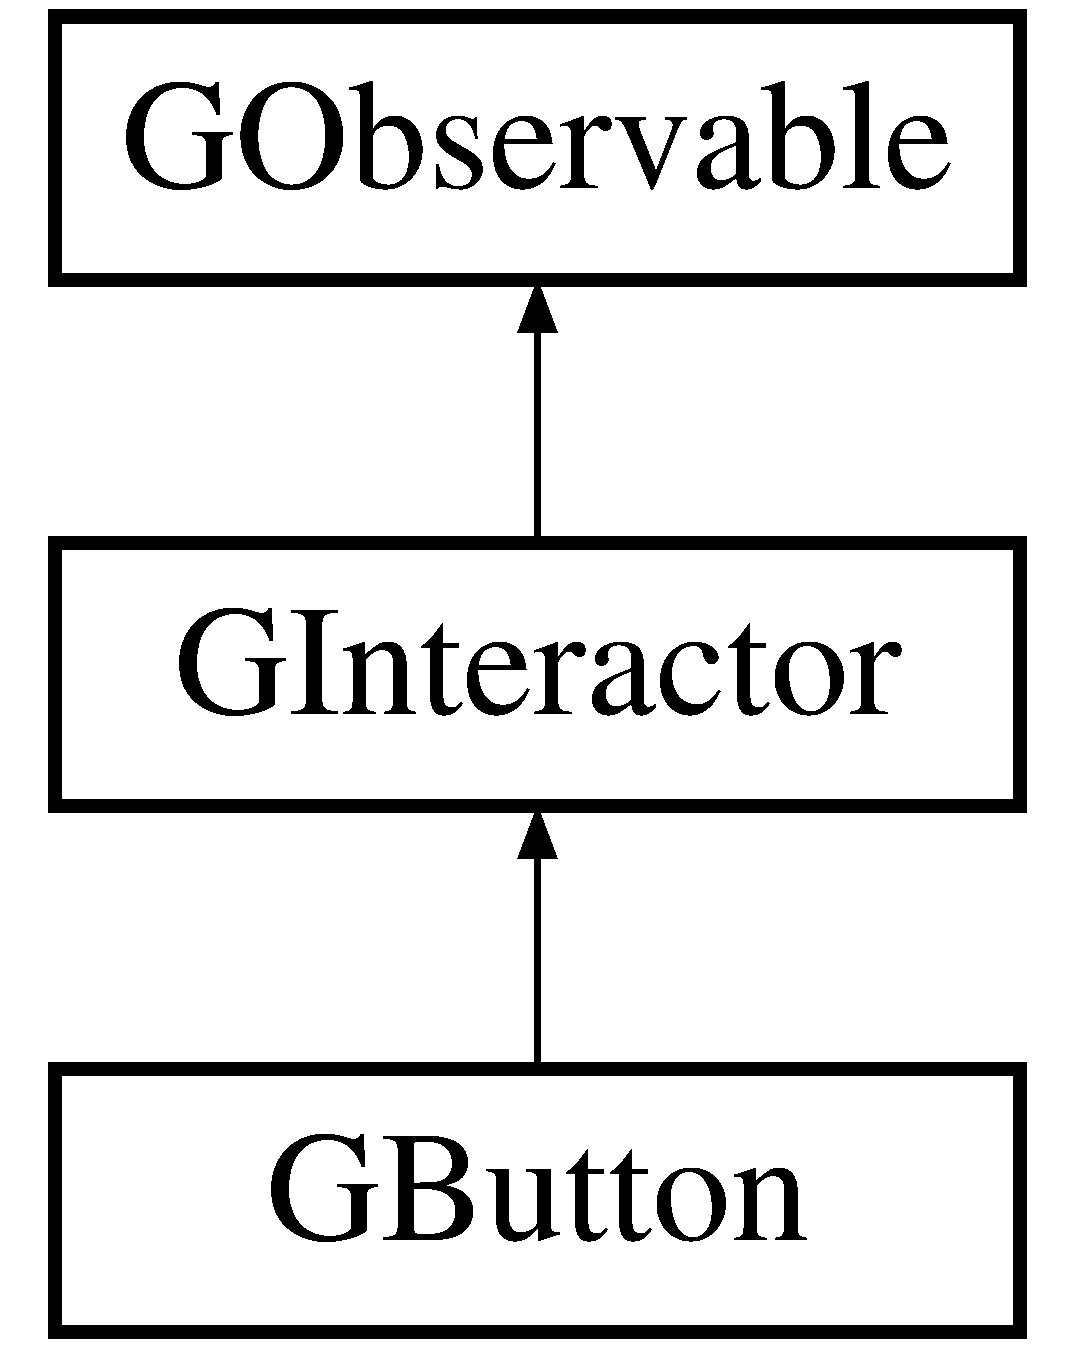
\includegraphics[height=3.000000cm]{classGButton}
\end{center}
\end{figure}
\subsection*{Public Types}
\begin{DoxyCompactItemize}
\item 
enum \mbox{\hyperlink{classGInteractor_a8e0d441725a81d2bbdebbea09078260e}{Text\+Position}} \{ \mbox{\hyperlink{classGInteractor_a8e0d441725a81d2bbdebbea09078260ea4cd6f2e7d5a08d6f4dc052df2358f774}{T\+E\+X\+T\+\_\+\+B\+E\+S\+I\+D\+E\+\_\+\+I\+C\+ON}}, 
\mbox{\hyperlink{classGInteractor_a8e0d441725a81d2bbdebbea09078260eaa88490f63d8de68d44c83bdb2ecde3b3}{T\+E\+X\+T\+\_\+\+U\+N\+D\+E\+R\+\_\+\+I\+C\+ON}}, 
\mbox{\hyperlink{classGInteractor_a8e0d441725a81d2bbdebbea09078260ea39a6f388a30ac4fefb6eb13e846bc9f2}{T\+E\+X\+T\+\_\+\+O\+N\+LY}}
 \}
\begin{DoxyCompactList}\small\item\em The places where an interactor can place its text relative to its icon. \end{DoxyCompactList}\end{DoxyCompactItemize}
\subsection*{Public Member Functions}
\begin{DoxyCompactItemize}
\item 
\mbox{\hyperlink{classGButton_aff3f5308477262143eb2a857e7549e31}{G\+Button}} (const std\+::string \&text=\char`\"{}\char`\"{}, const std\+::string \&icon\+File\+Name=\char`\"{}\char`\"{}, Q\+Widget $\ast$parent=nullptr)
\begin{DoxyCompactList}\small\item\em Creates a button with the specified text label and optional icon. \end{DoxyCompactList}\item 
\mbox{\hyperlink{classGButton_aecb1d20fb4707a3121600de27d5b3307}{G\+Button}} (const std\+::string \&text, const Q\+Icon \&icon, Q\+Widget $\ast$parent=nullptr)
\begin{DoxyCompactList}\small\item\em Creates a button with the specified text label and icon. \end{DoxyCompactList}\item 
\mbox{\hyperlink{classGButton_a7bcc15aa469e535bb9030ba9a4c93116}{G\+Button}} (const std\+::string \&text, const Q\+Pixmap \&icon, Q\+Widget $\ast$parent=nullptr)
\begin{DoxyCompactList}\small\item\em Creates a button with the specified text label and icon. \end{DoxyCompactList}\item 
\mbox{\hyperlink{classGButton_ae8f3d0d454867ef8bc9e7cd69e80f663}{$\sim$\+G\+Button}} () override
\begin{DoxyCompactList}\small\item\em Frees memory allocated internally by the button. \end{DoxyCompactList}\item 
virtual void \mbox{\hyperlink{classGInteractor_a02f20ea6edfa0671f31c4c648a253833}{add\+Action\+Listener}} () Q\+\_\+\+D\+E\+C\+L\+\_\+\+D\+E\+P\+R\+E\+C\+A\+T\+ED
\begin{DoxyCompactList}\small\item\em Adds an event listener to be notified when this interactor is clicked or generally interacted with. \end{DoxyCompactList}\item 
bool \mbox{\hyperlink{classGInteractor_a597a370b592e3737d38d9d2f4e2031ea}{events\+Enabled}} () const override
\begin{DoxyCompactList}\small\item\em Returns true if this interactor is currently accepting events. \end{DoxyCompactList}\item 
std\+::string \mbox{\hyperlink{classGButton_a57806dc9defb73f76f493f8548319924}{get\+Accelerator}} () const override
\begin{DoxyCompactList}\small\item\em Returns a string representing a hotkey for this interactor, or an empty string if no accelerator has been set. \end{DoxyCompactList}\item 
std\+::string \mbox{\hyperlink{classGButton_a4f83505141da1f8446f0e0e0a9507930}{get\+Action\+Command}} () const override
\begin{DoxyCompactList}\small\item\em Returns an action command for this interactor, which is a semi-\/unique string you can use to identify it when events occur. \end{DoxyCompactList}\item 
virtual std\+::string \mbox{\hyperlink{classGInteractor_a808e22cc1fdfbecf71ed8c64ef4600e0}{get\+Background}} () const
\begin{DoxyCompactList}\small\item\em Returns the background color of the interactor as a string. \end{DoxyCompactList}\item 
virtual int \mbox{\hyperlink{classGInteractor_a9e827257a55cb8cf4d9de2ec6bcfd7a0}{get\+Background\+Int}} () const
\begin{DoxyCompactList}\small\item\em Returns the background color of the interactor as an R\+GB integer. \end{DoxyCompactList}\item 
virtual \mbox{\hyperlink{structGRectangle}{G\+Rectangle}} \mbox{\hyperlink{classGInteractor_a29e6ac35a0b48f491a4c88194cc5da3b}{get\+Bounds}} () const
\begin{DoxyCompactList}\small\item\em Returns a rectangle representing the x/y position and size of this interactor. \end{DoxyCompactList}\item 
virtual std\+::string \mbox{\hyperlink{classGInteractor_aa061dfa488c31e18549d64363c1d0e34}{get\+Color}} () const
\begin{DoxyCompactList}\small\item\em Returns the foreground/text color of the interactor as a string. \end{DoxyCompactList}\item 
virtual int \mbox{\hyperlink{classGInteractor_a9635c7af766cdc3417f346683fa0e6c1}{get\+Color\+Int}} () const
\begin{DoxyCompactList}\small\item\em Returns the foreground/text color of the interactor as an R\+GB integer. \end{DoxyCompactList}\item 
virtual \mbox{\hyperlink{classGContainer}{G\+Container}} $\ast$ \mbox{\hyperlink{classGInteractor_a7a6e317c29d61030929b4cd2d1c00fe7}{get\+Container}} () const
\begin{DoxyCompactList}\small\item\em Returns a pointer to the onscreen container holding this interactor. \end{DoxyCompactList}\item 
virtual std\+::string \mbox{\hyperlink{classGInteractor_a894a5502900794eeb27d084c21f1d77d}{get\+Font}} () const
\begin{DoxyCompactList}\small\item\em Returns the font of this interactor\textquotesingle{}s text as a font string such as \char`\"{}\+Helvetica-\/12-\/\+Bold\char`\"{}. \end{DoxyCompactList}\item 
virtual std\+::string \mbox{\hyperlink{classGInteractor_a4fa2d8b0192a3a5b4af4bbfe71194d03}{get\+Foreground}} () const
\begin{DoxyCompactList}\small\item\em Returns the foreground/text color of the interactor as a string. \end{DoxyCompactList}\item 
virtual int \mbox{\hyperlink{classGInteractor_ac3b12ab385a6ef9ae90fc879860ba726}{get\+Foreground\+Int}} () const
\begin{DoxyCompactList}\small\item\em Returns the foreground/text color of the interactor as an R\+GB integer. \end{DoxyCompactList}\item 
virtual double \mbox{\hyperlink{classGInteractor_a1e7e353362434072875264cf95629f99}{get\+Height}} () const
\begin{DoxyCompactList}\small\item\em Returns the current onscreen height of this interactor in pixels. \end{DoxyCompactList}\item 
virtual std\+::string \mbox{\hyperlink{classGInteractor_aaed62a73004939a64da6f0eb9eb64d73}{get\+Icon}} () const
\begin{DoxyCompactList}\small\item\em Returns the file name of the icon associated with this interactor, or an empty string if no icon has been set. \end{DoxyCompactList}\item 
virtual int \mbox{\hyperlink{classGInteractor_a9c9659a6c6ba66b4107ba59c95a24241}{get\+ID}} () const
\begin{DoxyCompactList}\small\item\em Returns a globally unique identifier for this interactor, which is set when the interactor is constructed. \end{DoxyCompactList}\item 
\+\_\+\+Internal\+\_\+\+Q\+Widget $\ast$ \mbox{\hyperlink{classGButton_a2f6b36b2517087dc90a366b5ce1f5323}{get\+Internal\+Widget}} () const override
\begin{DoxyCompactList}\small\item\em Returns a direct pointer to the internal Qt widget being wrapped by this interactor. \end{DoxyCompactList}\item 
virtual \mbox{\hyperlink{structGPoint}{G\+Point}} \mbox{\hyperlink{classGInteractor_a4f83802015511edeb63b892830812c11}{get\+Location}} () const
\begin{DoxyCompactList}\small\item\em Returns an (x, y) point representing the onscreen location of the top-\/left corner of this interactor within its containing window. \end{DoxyCompactList}\item 
virtual double \mbox{\hyperlink{classGInteractor_aed4b0075fcc434499c3cb3e46896bda3}{get\+Minimum\+Height}} () const
\begin{DoxyCompactList}\small\item\em Returns the minimum height in pixels that this interactor will permit itself to be resized to. \end{DoxyCompactList}\item 
virtual \mbox{\hyperlink{structGDimension}{G\+Dimension}} \mbox{\hyperlink{classGInteractor_a66b5af0b32493b4d597ca0a3df2049ea}{get\+Minimum\+Size}} () const
\begin{DoxyCompactList}\small\item\em Returns a \mbox{\hyperlink{structGDimension}{G\+Dimension}} structure representing the minimum size in pixels that this interactor will permit itself to be resized to. \end{DoxyCompactList}\item 
virtual double \mbox{\hyperlink{classGInteractor_a59e668114fe3d49d2a0f28deb258f7c8}{get\+Minimum\+Width}} () const
\begin{DoxyCompactList}\small\item\em Returns the minimum width in pixels that this interactor will permit itself to be resized to. \end{DoxyCompactList}\item 
virtual std\+::string \mbox{\hyperlink{classGInteractor_a8a60438a5b55d0b2ceb35c8674b9d8c5}{get\+Name}} () const
\begin{DoxyCompactList}\small\item\em Returns a string representing a unique name for this interactor. \end{DoxyCompactList}\item 
virtual double \mbox{\hyperlink{classGInteractor_a747de0961653847bdc6615dbf756d715}{get\+Preferred\+Height}} () const
\begin{DoxyCompactList}\small\item\em Returns the height in pixels that this interactor would prefer to be, which would exactly fit its contents with no stretching or scrollbars. \end{DoxyCompactList}\item 
virtual \mbox{\hyperlink{structGDimension}{G\+Dimension}} \mbox{\hyperlink{classGInteractor_a4aabbee761d8e9116275401131b7ccd1}{get\+Preferred\+Size}} () const
\begin{DoxyCompactList}\small\item\em Returns a \mbox{\hyperlink{structGDimension}{G\+Dimension}} structure storing the width and height in pixels that this interactor would prefer to be, which would exactly fit its contents with no stretching or scrollbars. \end{DoxyCompactList}\item 
virtual double \mbox{\hyperlink{classGInteractor_a82bca31d37700fb0e35d2743352efd5e}{get\+Preferred\+Width}} () const
\begin{DoxyCompactList}\small\item\em Returns the height in pixels that this interactor would prefer to be, which would exactly fit its contents with no stretching or scrollbars. \end{DoxyCompactList}\item 
virtual \mbox{\hyperlink{structGDimension}{G\+Dimension}} \mbox{\hyperlink{classGInteractor_a7b4eec96a2bdc6420695d5796a78eea9}{get\+Size}} () const
\begin{DoxyCompactList}\small\item\em Returns a \mbox{\hyperlink{structGDimension}{G\+Dimension}} structure storing the current onscreen width and height of this interactor in pixels. \end{DoxyCompactList}\item 
virtual std\+::string \mbox{\hyperlink{classGButton_aff553c50924b836c29f146ed34a7c6ec}{get\+Text}} () const
\begin{DoxyCompactList}\small\item\em Returns the button\textquotesingle{}s text. \end{DoxyCompactList}\item 
virtual \mbox{\hyperlink{classGInteractor_a8e0d441725a81d2bbdebbea09078260e}{G\+Interactor\+::\+Text\+Position}} \mbox{\hyperlink{classGButton_a3fc623df3ced62aca93fc344c2426899}{get\+Text\+Position}} () const
\begin{DoxyCompactList}\small\item\em Returns the button\textquotesingle{}s text position relative to its icon. \end{DoxyCompactList}\item 
std\+::string \mbox{\hyperlink{classGButton_a9b72ede4ee8520f987a0c01e30654814}{get\+Type}} () const override
\begin{DoxyCompactList}\small\item\em Returns a string representing the class name of this interactor, such as \char`\"{}\+G\+Button\char`\"{} or \char`\"{}\+G\+Check\+Box\char`\"{}. \end{DoxyCompactList}\item 
Q\+Widget $\ast$ \mbox{\hyperlink{classGButton_a3b33a602b31a6b809d020535a59db3b4}{get\+Widget}} () const override
\begin{DoxyCompactList}\small\item\em Returns a direct pointer to the internal Qt widget being wrapped by this interactor. \end{DoxyCompactList}\item 
virtual double \mbox{\hyperlink{classGInteractor_a0ed2965abd4f5701d2cadf71239faf19}{get\+Width}} () const
\begin{DoxyCompactList}\small\item\em Returns the current onscreen width of this interactor in pixels. \end{DoxyCompactList}\item 
virtual double \mbox{\hyperlink{classGInteractor_a344385751bee0720059403940d57a13e}{getX}} () const
\begin{DoxyCompactList}\small\item\em Returns the x-\/coordinate of the top-\/left pixel of this interactor within its onscreen window. \end{DoxyCompactList}\item 
virtual double \mbox{\hyperlink{classGInteractor_aafa51c7f8f38a09febbb9ce7853f77b4}{getY}} () const
\begin{DoxyCompactList}\small\item\em Returns the y-\/coordinate of the top-\/left pixel of this interactor within its onscreen window. \end{DoxyCompactList}\item 
virtual bool \mbox{\hyperlink{classGInteractor_afc480f652b8c5f1fb255e2269ce68879}{in\+Bounds}} (double x, double y) const
\begin{DoxyCompactList}\small\item\em Returns true if the given x/y pixel is within the bounds of this interactor. \end{DoxyCompactList}\item 
virtual bool \mbox{\hyperlink{classGInteractor_ae6d7982c1c627b677a5e776ca86118ed}{in\+Bounds}} (int x, int y) const
\begin{DoxyCompactList}\small\item\em Returns true if the given x/y pixel is within the bounds of this interactor. \end{DoxyCompactList}\item 
virtual bool \mbox{\hyperlink{classGInteractor_aacb819fb241851fd9fc045271baa4034}{is\+Enabled}} () const
\begin{DoxyCompactList}\small\item\em Returns true if this interactor is currently enabled. \end{DoxyCompactList}\item 
virtual bool \mbox{\hyperlink{classGInteractor_a9d8a6cfb13917785c143e74d40e4e2be}{is\+Visible}} () const
\begin{DoxyCompactList}\small\item\em Returns true if the interactor is visible on the screen. \end{DoxyCompactList}\item 
virtual void \mbox{\hyperlink{classGInteractor_ab7fe7a876367b87cf7202f947f1d05e4}{remove\+Action\+Listener}} ()
\begin{DoxyCompactList}\small\item\em Removes the action listener from this interactor so that it will no longer call it when events occur. \end{DoxyCompactList}\item 
virtual void \mbox{\hyperlink{classGInteractor_ad39d0325cde6b97ebda4b9d7787c633b}{remove\+Click\+Listener}} ()
\begin{DoxyCompactList}\small\item\em Removes the click listener from this interactor so that it will no longer call it when events occur. \end{DoxyCompactList}\item 
virtual void \mbox{\hyperlink{classGInteractor_aa4250907e4cdd77349c04f0cf5cdd3d3}{remove\+Double\+Click\+Listener}} ()
\begin{DoxyCompactList}\small\item\em Removes the double-\/click listener from this interactor so that it will no longer call it when events occur. \end{DoxyCompactList}\item 
virtual void \mbox{\hyperlink{classGInteractor_a43095f41cab3be732b49f29970484b05}{remove\+Key\+Listener}} ()
\begin{DoxyCompactList}\small\item\em Removes the key listener from this interactor so that it will no longer call it when key events occur. \end{DoxyCompactList}\item 
virtual void \mbox{\hyperlink{classGInteractor_aff47f71ce47e688a07c9d38dc92fcc11}{remove\+Mouse\+Listener}} ()
\begin{DoxyCompactList}\small\item\em Removes the mouse listener from this interactor so that it will no longer call it when events occur. \end{DoxyCompactList}\item 
virtual void \mbox{\hyperlink{classGInteractor_a519fb2ac767f8b2febbb50b898b8c8cb}{request\+Focus}} ()
\begin{DoxyCompactList}\small\item\em Transfers keyboard focus to this interactor. \end{DoxyCompactList}\item 
void \mbox{\hyperlink{classGButton_a502f311e78e7531f8a7b50054ce91c85}{set\+Accelerator}} (const std\+::string \&accelerator) override
\begin{DoxyCompactList}\small\item\em Sets an accelerator hotkey for this interactor, such as \char`\"{}\+Ctrl-\/\+S\char`\"{}. \end{DoxyCompactList}\item 
virtual void \mbox{\hyperlink{classGInteractor_a4b5843fe3030e038a1ba54cc03389bcf}{set\+Action\+Command}} (const std\+::string \&action\+Command)
\begin{DoxyCompactList}\small\item\em Sets the action command for this interactor. \end{DoxyCompactList}\item 
virtual void \mbox{\hyperlink{classGInteractor_adcfb4742430c88714fcf57e57ab8ea9c}{set\+Action\+Listener}} (G\+Event\+Listener func)
\begin{DoxyCompactList}\small\item\em Sets an action listener on this interactor so that it will be called when it is interacted with in its primary way. \end{DoxyCompactList}\item 
virtual void \mbox{\hyperlink{classGInteractor_aebd20a89c7a8a43a6fce999cf4f9fcf2}{set\+Action\+Listener}} (G\+Event\+Listener\+Void func)
\begin{DoxyCompactList}\small\item\em Sets an action listener on this interactor so that it will be called when it is interacted with in its primary way. \end{DoxyCompactList}\item 
virtual void \mbox{\hyperlink{classGInteractor_acba7e546c2025c0a15ca4b4cc92043db}{set\+Background}} (int rgb)
\begin{DoxyCompactList}\small\item\em Sets the background color of the interactor to the color represented by the given R\+GB integer. \end{DoxyCompactList}\item 
virtual void \mbox{\hyperlink{classGInteractor_ab4677ab2474e68b07aa56605af92a84a}{set\+Background}} (const std\+::string \&color)
\begin{DoxyCompactList}\small\item\em Sets the background color of the interactor to the color represented by the given string. \end{DoxyCompactList}\item 
virtual void \mbox{\hyperlink{classGInteractor_a2aae8197624b72265ab83b4f1bc73f2f}{set\+Bounds}} (double x, double y, double width, double height)
\begin{DoxyCompactList}\small\item\em Sets the size and location of the widget. \end{DoxyCompactList}\item 
virtual void \mbox{\hyperlink{classGInteractor_acada386653f008cacc7cce86426bef7c}{set\+Bounds}} (const \mbox{\hyperlink{structGRectangle}{G\+Rectangle}} \&size)
\begin{DoxyCompactList}\small\item\em Sets the size and location of the widget. \end{DoxyCompactList}\item 
virtual void \mbox{\hyperlink{classGInteractor_abd40af6921242584d0954f173911b190}{set\+Click\+Listener}} (G\+Event\+Listener func)
\begin{DoxyCompactList}\small\item\em Sets a mouse listener on this interactor so that it will be called when the mouse is clicked on it. \end{DoxyCompactList}\item 
virtual void \mbox{\hyperlink{classGInteractor_a856414c92df90f56f3877475eb3f8fc4}{set\+Click\+Listener}} (G\+Event\+Listener\+Void func)
\begin{DoxyCompactList}\small\item\em Sets a mouse listener on this interactor so that it will be called when the mouse is clicked on it. \end{DoxyCompactList}\item 
virtual void \mbox{\hyperlink{classGInteractor_ab1f5cc0f5cc6bbbd716a526c61f1081d}{set\+Color}} (int rgb)
\begin{DoxyCompactList}\small\item\em Sets the foreground/text color of the interactor to the color represented by the given R\+GB integer. \end{DoxyCompactList}\item 
virtual void \mbox{\hyperlink{classGInteractor_a61374df6c11b52cfbb0815decdbaebc6}{set\+Color}} (const std\+::string \&color)
\begin{DoxyCompactList}\small\item\em Sets the foreground/text color of the interactor to the color represented by the given string. \end{DoxyCompactList}\item 
virtual void \mbox{\hyperlink{classGInteractor_ac29f9a3462458e165fae3a1f046ee77a}{set\+Double\+Click\+Listener}} (G\+Event\+Listener func)
\begin{DoxyCompactList}\small\item\em Sets a mouse listener on this interactor so that it will be called when the mouse is double-\/clicked on it. \end{DoxyCompactList}\item 
virtual void \mbox{\hyperlink{classGInteractor_a50096194d66f48c92dd4c512d41bfc76}{set\+Double\+Click\+Listener}} (G\+Event\+Listener\+Void func)
\begin{DoxyCompactList}\small\item\em Sets a mouse listener on this interactor so that it will be called when the mouse is double-\/clicked on it. \end{DoxyCompactList}\item 
virtual void \mbox{\hyperlink{classGInteractor_ab831367dd84bbd579e02e55bacb21343}{set\+Enabled}} (bool value)
\begin{DoxyCompactList}\small\item\em Sets whether this interactor is currently enabled. \end{DoxyCompactList}\item 
virtual void \mbox{\hyperlink{classGObservable_afaa30b2a9e0f378fd1c70d2f1d0b8216}{set\+Events\+Enabled}} (bool \mbox{\hyperlink{classGInteractor_a597a370b592e3737d38d9d2f4e2031ea}{events\+Enabled}})
\begin{DoxyCompactList}\small\item\em Sets whether the object is currently allowing itself to fire events. \end{DoxyCompactList}\item 
virtual void \mbox{\hyperlink{classGInteractor_a2592348886ffea646c6534bf88f7c49d}{set\+Font}} (const Q\+Font \&font)
\begin{DoxyCompactList}\small\item\em Sets the font used by this widget to the given Qt font. \end{DoxyCompactList}\item 
virtual void \mbox{\hyperlink{classGInteractor_a8e096e8818d838aceae1d46d58fb3a7b}{set\+Font}} (const std\+::string \&font)
\begin{DoxyCompactList}\small\item\em Sets the font used by this widget to the font represented by the given font string, such as \char`\"{}\+Helvetica-\/16-\/\+Bold\char`\"{}. \end{DoxyCompactList}\item 
virtual void \mbox{\hyperlink{classGInteractor_a9eb856b5ff83a19df3831a31f15f4563}{set\+Foreground}} (int rgb)
\begin{DoxyCompactList}\small\item\em Sets the foreground/text color of the interactor to the color represented by the given R\+GB integer. \end{DoxyCompactList}\item 
virtual void \mbox{\hyperlink{classGInteractor_af59209aeadea6dfc6d97a2d8531f50e1}{set\+Foreground}} (const std\+::string \&color)
\begin{DoxyCompactList}\small\item\em Sets the foreground/text color of the interactor to the color represented by the given string. \end{DoxyCompactList}\item 
virtual void \mbox{\hyperlink{classGInteractor_a9e280bfc4544dfaf8e4376c4e1a74357}{set\+Height}} (double height)
\begin{DoxyCompactList}\small\item\em Sets the onscreen height of the interactor in pixels. \end{DoxyCompactList}\item 
void \mbox{\hyperlink{classGButton_acca97b6c6330abded1c80521c9aca3a6}{set\+Icon}} (const Q\+Icon \&icon) override
\begin{DoxyCompactList}\small\item\em Sets the icon associated with this interactor. \end{DoxyCompactList}\item 
void \mbox{\hyperlink{classGButton_acb5275b880ff622d306f8f33428b4e34}{set\+Icon}} (const Q\+Pixmap \&icon) override
\begin{DoxyCompactList}\small\item\em Sets the icon associated with this interactor. \end{DoxyCompactList}\item 
void \mbox{\hyperlink{classGButton_abbefcb1f611af273755c7e1cca921497}{set\+Icon}} (const std\+::string \&filename, bool retain\+Icon\+Size=true) override
\begin{DoxyCompactList}\small\item\em Sets the file name of the icon associated with this interactor, or an empty string if no icon has been set. \end{DoxyCompactList}\item 
virtual void \mbox{\hyperlink{classGInteractor_aeb8324d3287fa1fbe093f4d6230cf0a6}{set\+Key\+Listener}} (G\+Event\+Listener func)
\begin{DoxyCompactList}\small\item\em Sets a key listener on this interactor so that it will be called when the user presses any key. \end{DoxyCompactList}\item 
virtual void \mbox{\hyperlink{classGInteractor_ae48ecea73606c7bd9423e1c7cc589cc9}{set\+Key\+Listener}} (G\+Event\+Listener\+Void func)
\begin{DoxyCompactList}\small\item\em Sets a key listener on this interactor so that it will be called when the user presses any key. \end{DoxyCompactList}\item 
virtual void \mbox{\hyperlink{classGInteractor_a04594e8ba9b98513a64f1da00dcae18c}{set\+Location}} (double x, double y)
\begin{DoxyCompactList}\small\item\em Sets the onscreen x/y-\/coordinate of the top-\/left corner of the interactor relative to its window. \end{DoxyCompactList}\item 
virtual void \mbox{\hyperlink{classGInteractor_a0cf428e207b7f22cc08138a90b1b87b2}{set\+Minimum\+Size}} (double width, double height)
\begin{DoxyCompactList}\small\item\em Sets the minimum size in pixels that this interactor will permit itself to be resized to. \end{DoxyCompactList}\item 
virtual void \mbox{\hyperlink{classGInteractor_a3b1046117ac6cb7abe467e00ba8a81f4}{set\+Minimum\+Size}} (const \mbox{\hyperlink{structGDimension}{G\+Dimension}} \&size)
\begin{DoxyCompactList}\small\item\em Sets the minimum size in pixels that this interactor will permit itself to be resized to. \end{DoxyCompactList}\item 
virtual void \mbox{\hyperlink{classGInteractor_a37d8dbc943f59920f705b0104f60bde2}{set\+Mouse\+Listener}} (G\+Event\+Listener func)
\begin{DoxyCompactList}\small\item\em Sets a mouse listener on this interactor so that it will be called when the mouse is moved or clicked on it. \end{DoxyCompactList}\item 
virtual void \mbox{\hyperlink{classGInteractor_aea7f647ea62d59f71b5fad6aa65eeaf9}{set\+Mouse\+Listener}} (G\+Event\+Listener\+Void func)
\begin{DoxyCompactList}\small\item\em Sets a mouse listener on this interactor so that it will be called when the mouse is moved or clicked on it. \end{DoxyCompactList}\item 
virtual void \mbox{\hyperlink{classGInteractor_a9d3a2685df23b5e7cbf59c19c4a1f9b5}{set\+Name}} (const std\+::string \&name)
\begin{DoxyCompactList}\small\item\em Sets a string representing a unique name for this interactor. \end{DoxyCompactList}\item 
virtual void \mbox{\hyperlink{classGInteractor_a1ab987704fce32098706c6f00fb08218}{set\+Preferred\+Height}} (double height)
\begin{DoxyCompactList}\small\item\em Sets the height in pixels that this interactor would prefer to be. \end{DoxyCompactList}\item 
virtual void \mbox{\hyperlink{classGInteractor_a042c5ae19430d765ef552371cae3632c}{set\+Preferred\+Size}} (double width, double height)
\begin{DoxyCompactList}\small\item\em Sets the width and height in pixels that this interactor would prefer to be. \end{DoxyCompactList}\item 
virtual void \mbox{\hyperlink{classGInteractor_aa22d9be4bc0e078bb0ea69b0fc9d7c75}{set\+Preferred\+Size}} (const \mbox{\hyperlink{structGDimension}{G\+Dimension}} \&size)
\begin{DoxyCompactList}\small\item\em Sets the size in pixels that this interactor would prefer to be. \end{DoxyCompactList}\item 
virtual void \mbox{\hyperlink{classGInteractor_a3db429ab2fa52efd187eec0ed8cdd9f2}{set\+Preferred\+Width}} (double width)
\begin{DoxyCompactList}\small\item\em Sets the width in pixels that this interactor would prefer to be. \end{DoxyCompactList}\item 
virtual void \mbox{\hyperlink{classGInteractor_aca25d49481f9bf5fc8f7df4c086c4ce7}{set\+Size}} (double width, double height)
\begin{DoxyCompactList}\small\item\em Sets the onscreen width and height of the interactor in pixels. \end{DoxyCompactList}\item 
virtual void \mbox{\hyperlink{classGInteractor_ae2b628228f192c2702c4ce941b2af68f}{set\+Size}} (const \mbox{\hyperlink{structGDimension}{G\+Dimension}} \&size)
\begin{DoxyCompactList}\small\item\em Sets the onscreen width and height of the interactor in pixels. \end{DoxyCompactList}\item 
virtual void \mbox{\hyperlink{classGButton_ac1ae51949d41ee9054634be5967d91b8}{set\+Text}} (const std\+::string \&text)
\begin{DoxyCompactList}\small\item\em Sets the text on the button to be the given text. \end{DoxyCompactList}\item 
virtual void \mbox{\hyperlink{classGButton_af822b8d73c652f7c59d875d7cdfc5302}{set\+Text\+Position}} (\mbox{\hyperlink{classGInteractor_a8e0d441725a81d2bbdebbea09078260e}{G\+Interactor\+::\+Text\+Position}} position)
\begin{DoxyCompactList}\small\item\em Sets the button\textquotesingle{}s text position relative to its icon. \end{DoxyCompactList}\item 
virtual void \mbox{\hyperlink{classGInteractor_a039e0e49beaecc275efce02d416acea8}{set\+Tooltip}} (const std\+::string \&tooltip\+Text)
\begin{DoxyCompactList}\small\item\em Sets a \char`\"{}tooltip\char`\"{} that will appear if the user hovers their mouse over the interactor. \end{DoxyCompactList}\item 
virtual void \mbox{\hyperlink{classGInteractor_a18e44e30b31525a243960ca3928125aa}{set\+Visible}} (bool visible)
\begin{DoxyCompactList}\small\item\em Returns true if the interactor is visible on the screen. \end{DoxyCompactList}\item 
virtual void \mbox{\hyperlink{classGInteractor_aa3f3fba4cb131baa8696ba01e3bceca1}{set\+Width}} (double width)
\begin{DoxyCompactList}\small\item\em Sets the onscreen width of the interactor in pixels. \end{DoxyCompactList}\item 
virtual void \mbox{\hyperlink{classGInteractor_a9c18fcc579333bf9653d13ad2b372e39}{setX}} (double x)
\begin{DoxyCompactList}\small\item\em Sets the onscreen x-\/coordinate of the top-\/left corner of the interactor relative to its window. \end{DoxyCompactList}\item 
virtual void \mbox{\hyperlink{classGInteractor_a7d57e2a5c35d27feb58fd498a3cf82b9}{setY}} (double y)
\begin{DoxyCompactList}\small\item\em Sets the onscreen y-\/coordinate of the top-\/left corner of the interactor relative to its window. \end{DoxyCompactList}\item 
virtual std\+::string \mbox{\hyperlink{classGObservable_a1fe5121d6528fdea3f243321b3fa3a49}{to\+String}} () const
\begin{DoxyCompactList}\small\item\em Returns a string representation of this observable object\textquotesingle{}s state. \end{DoxyCompactList}\end{DoxyCompactItemize}
\subsection*{Protected Member Functions}
\begin{DoxyCompactItemize}
\item 
virtual void \mbox{\hyperlink{classGObservable_a80cfa040459ff53594adbd6a51ec8f43}{clear\+Event\+Listeners}} ()
\begin{DoxyCompactList}\small\item\em Removes all event listeners from this object. \end{DoxyCompactList}\item 
virtual void \mbox{\hyperlink{classGObservable_a284f31528c0520f8e545c03ac9eeac74}{ensure\+Thread\+Safety}} (const std\+::string \&member\+Name=\char`\"{}\char`\"{})
\begin{DoxyCompactList}\small\item\em Ensures that we are currently in the Qt G\+UI thread. \end{DoxyCompactList}\item 
virtual void \mbox{\hyperlink{classGObservable_a63e5e5a6227c59c928493b11aceb0f67}{fire\+Event}} (\mbox{\hyperlink{classGEvent}{G\+Event}} \&event)
\begin{DoxyCompactList}\small\item\em Sends out the given event to any attached listeners. \end{DoxyCompactList}\item 
virtual void \mbox{\hyperlink{classGObservable_ab3983ea07337b52020a29cc00c653d8d}{fire\+G\+Event}} (Q\+Event $\ast$event, Event\+Type event\+Type, const std\+::string \&event\+Name)
\begin{DoxyCompactList}\small\item\em Creates an event of the given type, then sends it out to any attached listeners. \end{DoxyCompactList}\item 
virtual void \mbox{\hyperlink{classGObservable_a01fdf1b0e0dbd49e189fe4514e010411}{fire\+G\+Event}} (Q\+Close\+Event $\ast$event, Event\+Type event\+Type, const std\+::string \&event\+Name)
\begin{DoxyCompactList}\small\item\em Creates an event of the given type, then sends it out to any attached listeners. \end{DoxyCompactList}\item 
virtual void \mbox{\hyperlink{classGObservable_abb0b2f66ba39211cb5d7615e9d1c04e2}{fire\+G\+Event}} (Q\+Key\+Event $\ast$event, Event\+Type event\+Type, const std\+::string \&event\+Name)
\begin{DoxyCompactList}\small\item\em Creates an event of the given type, then sends it out to any attached listeners. \end{DoxyCompactList}\item 
virtual void \mbox{\hyperlink{classGObservable_a119318675d2165bdf7dd853aaf881d4b}{fire\+G\+Event}} (Q\+Mouse\+Event $\ast$event, Event\+Type event\+Type, const std\+::string \&event\+Name, const std\+::string \&action\+Command=\char`\"{}\char`\"{})
\begin{DoxyCompactList}\small\item\em Creates an event of the given type, then sends it out to any attached listeners. \end{DoxyCompactList}\item 
virtual void \mbox{\hyperlink{classGObservable_a63fd9034e1e1633c1c38eb342bfd34e9}{fire\+G\+Event}} (Q\+Resize\+Event $\ast$event, Event\+Type event\+Type, const std\+::string \&event\+Name)
\begin{DoxyCompactList}\small\item\em Creates an event of the given type, then sends it out to any attached listeners. \end{DoxyCompactList}\item 
virtual void \mbox{\hyperlink{classGObservable_a741345310d9b7c5170a6cbc410c44ac4}{fire\+G\+Event}} (Q\+Timer\+Event $\ast$event, Event\+Type event\+Type, const std\+::string \&event\+Name)
\begin{DoxyCompactList}\small\item\em Creates an event of the given type, then sends it out to any attached listeners. \end{DoxyCompactList}\item 
virtual void \mbox{\hyperlink{classGObservable_a93bf338968a0338761b8e4dc62f582e9}{fire\+G\+Event}} (Q\+Wheel\+Event $\ast$event, Event\+Type event\+Type, const std\+::string \&event\+Name)
\begin{DoxyCompactList}\small\item\em Creates an event of the given type, then sends it out to any attached listeners. \end{DoxyCompactList}\item 
virtual void \mbox{\hyperlink{classGObservable_a2a70a7d7435ff0c3b80bb4d70da19e0d}{fire\+G\+Event}} (Q\+Window\+State\+Change\+Event $\ast$event, Event\+Type event\+Type, const std\+::string \&event\+Name)
\begin{DoxyCompactList}\small\item\em Creates an event of the given type, then sends it out to any attached listeners. \end{DoxyCompactList}\item 
virtual bool \mbox{\hyperlink{classGObservable_a9f6faaa25942923bafa1c44020c49fa9}{has\+Event\+Listener}} (const std\+::string \&event\+Name) const
\begin{DoxyCompactList}\small\item\em Returns true if the observable object has a listener for the given type of event. \end{DoxyCompactList}\item 
virtual bool \mbox{\hyperlink{classGObservable_aeec1adc19aa0f33de62390686ee1382c}{is\+Accepting\+Event}} (int event\+Mask) const
\begin{DoxyCompactList}\small\item\em Returns true if the observable object has a listener for the given type of event. \end{DoxyCompactList}\item 
virtual bool \mbox{\hyperlink{classGObservable_aa31c73145a29dcb92848a92e0cfaea41}{is\+Accepting\+Event}} (const \mbox{\hyperlink{classGEvent}{G\+Event}} \&event) const
\begin{DoxyCompactList}\small\item\em Returns true if the observable object has a listener for the given type of event. \end{DoxyCompactList}\item 
virtual bool \mbox{\hyperlink{classGObservable_a3b1c689267eda44e65a2213e7de38b23}{is\+Accepting\+Event}} (const std\+::string \&event\+Type) const
\begin{DoxyCompactList}\small\item\em Returns true if the observable object has a listener for the given type of event. \end{DoxyCompactList}\item 
virtual void \mbox{\hyperlink{classGObservable_acbcf1ed3a851ad8a3c17ef38d86b481d}{remove\+Event\+Listener}} (const std\+::string \&event\+Name)
\begin{DoxyCompactList}\small\item\em Removes any event listener from this observable object that would respond to the given type of event, such as \char`\"{}click\char`\"{} or \char`\"{}keydown\char`\"{}. \end{DoxyCompactList}\item 
virtual void \mbox{\hyperlink{classGObservable_af51cc35c29a1bd1908609d432decdbb6}{remove\+Event\+Listeners}} (std\+::initializer\+\_\+list$<$ std\+::string $>$ event\+Names)
\begin{DoxyCompactList}\small\item\em Removes any event listener from this observable object that would respond to the given types of events, such as \char`\"{}click\char`\"{} or \char`\"{}keydown\char`\"{}. \end{DoxyCompactList}\item 
virtual void \mbox{\hyperlink{classGObservable_ad2f6d34961c50f6c1e0659990b79f741}{set\+Event\+Listener}} (const std\+::string \&event\+Name, G\+Event\+Listener func)
\begin{DoxyCompactList}\small\item\em Adds an event listener from this observable object to respond to the given type of event, such as \char`\"{}click\char`\"{} or \char`\"{}keydown\char`\"{}. \end{DoxyCompactList}\item 
virtual void \mbox{\hyperlink{classGObservable_abac4cb9f9e626e010e87f5d91573c8a5}{set\+Event\+Listener}} (const std\+::string \&event\+Name, G\+Event\+Listener\+Void func)
\begin{DoxyCompactList}\small\item\em Adds an event listener from this observable object to respond to the given type of event, such as \char`\"{}click\char`\"{} or \char`\"{}keydown\char`\"{}. \end{DoxyCompactList}\item 
virtual void \mbox{\hyperlink{classGObservable_afa388d69c33c718cf035774604065604}{set\+Event\+Listeners}} (std\+::initializer\+\_\+list$<$ std\+::string $>$ event\+Names, G\+Event\+Listener func)
\begin{DoxyCompactList}\small\item\em Adds an event listener from this observable object to respond to the given types of events, such as \char`\"{}click\char`\"{} or \char`\"{}keydown\char`\"{}. \end{DoxyCompactList}\item 
virtual void \mbox{\hyperlink{classGObservable_a7867184bbb686f74fae8a4db927da799}{set\+Event\+Listeners}} (std\+::initializer\+\_\+list$<$ std\+::string $>$ event\+Names, G\+Event\+Listener\+Void func)
\begin{DoxyCompactList}\small\item\em Adds an event listener from this observable object to respond to the given types of events, such as \char`\"{}click\char`\"{} or \char`\"{}keydown\char`\"{}. \end{DoxyCompactList}\end{DoxyCompactItemize}


\subsection{Detailed Description}
This interactor subclass represents an onscreen button. 

You can listen for clicks on a button using the set\+Action\+Listener method, passing the function you want to call on each click. 

\subsection{Member Enumeration Documentation}
\mbox{\Hypertarget{classGInteractor_a8e0d441725a81d2bbdebbea09078260e}\label{classGInteractor_a8e0d441725a81d2bbdebbea09078260e}} 
\index{G\+Button@{G\+Button}!Text\+Position@{Text\+Position}}
\index{Text\+Position@{Text\+Position}!G\+Button@{G\+Button}}
\subsubsection{\texorpdfstring{Text\+Position}{TextPosition}}
{\footnotesize\ttfamily enum \mbox{\hyperlink{classGInteractor_a8e0d441725a81d2bbdebbea09078260e}{Text\+Position}}\hspace{0.3cm}{\ttfamily [inherited]}}



The places where an interactor can place its text relative to its icon. 

\begin{DoxyEnumFields}{Enumerator}
\raisebox{\heightof{T}}[0pt][0pt]{\index{T\+E\+X\+T\+\_\+\+B\+E\+S\+I\+D\+E\+\_\+\+I\+C\+ON@{T\+E\+X\+T\+\_\+\+B\+E\+S\+I\+D\+E\+\_\+\+I\+C\+ON}!G\+Button@{G\+Button}}\index{G\+Button@{G\+Button}!T\+E\+X\+T\+\_\+\+B\+E\+S\+I\+D\+E\+\_\+\+I\+C\+ON@{T\+E\+X\+T\+\_\+\+B\+E\+S\+I\+D\+E\+\_\+\+I\+C\+ON}}}\mbox{\Hypertarget{classGInteractor_a8e0d441725a81d2bbdebbea09078260ea4cd6f2e7d5a08d6f4dc052df2358f774}\label{classGInteractor_a8e0d441725a81d2bbdebbea09078260ea4cd6f2e7d5a08d6f4dc052df2358f774}} 
T\+E\+X\+T\+\_\+\+B\+E\+S\+I\+D\+E\+\_\+\+I\+C\+ON&\\
\hline

\raisebox{\heightof{T}}[0pt][0pt]{\index{T\+E\+X\+T\+\_\+\+U\+N\+D\+E\+R\+\_\+\+I\+C\+ON@{T\+E\+X\+T\+\_\+\+U\+N\+D\+E\+R\+\_\+\+I\+C\+ON}!G\+Button@{G\+Button}}\index{G\+Button@{G\+Button}!T\+E\+X\+T\+\_\+\+U\+N\+D\+E\+R\+\_\+\+I\+C\+ON@{T\+E\+X\+T\+\_\+\+U\+N\+D\+E\+R\+\_\+\+I\+C\+ON}}}\mbox{\Hypertarget{classGInteractor_a8e0d441725a81d2bbdebbea09078260eaa88490f63d8de68d44c83bdb2ecde3b3}\label{classGInteractor_a8e0d441725a81d2bbdebbea09078260eaa88490f63d8de68d44c83bdb2ecde3b3}} 
T\+E\+X\+T\+\_\+\+U\+N\+D\+E\+R\+\_\+\+I\+C\+ON&\\
\hline

\raisebox{\heightof{T}}[0pt][0pt]{\index{T\+E\+X\+T\+\_\+\+O\+N\+LY@{T\+E\+X\+T\+\_\+\+O\+N\+LY}!G\+Button@{G\+Button}}\index{G\+Button@{G\+Button}!T\+E\+X\+T\+\_\+\+O\+N\+LY@{T\+E\+X\+T\+\_\+\+O\+N\+LY}}}\mbox{\Hypertarget{classGInteractor_a8e0d441725a81d2bbdebbea09078260ea39a6f388a30ac4fefb6eb13e846bc9f2}\label{classGInteractor_a8e0d441725a81d2bbdebbea09078260ea39a6f388a30ac4fefb6eb13e846bc9f2}} 
T\+E\+X\+T\+\_\+\+O\+N\+LY&\\
\hline

\end{DoxyEnumFields}


\subsection{Constructor \& Destructor Documentation}
\mbox{\Hypertarget{classGButton_aff3f5308477262143eb2a857e7549e31}\label{classGButton_aff3f5308477262143eb2a857e7549e31}} 
\index{G\+Button@{G\+Button}!G\+Button@{G\+Button}}
\index{G\+Button@{G\+Button}!G\+Button@{G\+Button}}
\subsubsection{\texorpdfstring{G\+Button()}{GButton()}\hspace{0.1cm}{\footnotesize\ttfamily [1/3]}}
{\footnotesize\ttfamily \mbox{\hyperlink{classGButton}{G\+Button}} (\begin{DoxyParamCaption}\item[{const std\+::string \&}]{text = {\ttfamily \char`\"{}\char`\"{}},  }\item[{const std\+::string \&}]{icon\+File\+Name = {\ttfamily \char`\"{}\char`\"{}},  }\item[{Q\+Widget $\ast$}]{parent = {\ttfamily nullptr} }\end{DoxyParamCaption})}



Creates a button with the specified text label and optional icon. 

\mbox{\Hypertarget{classGButton_aecb1d20fb4707a3121600de27d5b3307}\label{classGButton_aecb1d20fb4707a3121600de27d5b3307}} 
\index{G\+Button@{G\+Button}!G\+Button@{G\+Button}}
\index{G\+Button@{G\+Button}!G\+Button@{G\+Button}}
\subsubsection{\texorpdfstring{G\+Button()}{GButton()}\hspace{0.1cm}{\footnotesize\ttfamily [2/3]}}
{\footnotesize\ttfamily \mbox{\hyperlink{classGButton}{G\+Button}} (\begin{DoxyParamCaption}\item[{const std\+::string \&}]{text,  }\item[{const Q\+Icon \&}]{icon,  }\item[{Q\+Widget $\ast$}]{parent = {\ttfamily nullptr} }\end{DoxyParamCaption})}



Creates a button with the specified text label and icon. 

\mbox{\Hypertarget{classGButton_a7bcc15aa469e535bb9030ba9a4c93116}\label{classGButton_a7bcc15aa469e535bb9030ba9a4c93116}} 
\index{G\+Button@{G\+Button}!G\+Button@{G\+Button}}
\index{G\+Button@{G\+Button}!G\+Button@{G\+Button}}
\subsubsection{\texorpdfstring{G\+Button()}{GButton()}\hspace{0.1cm}{\footnotesize\ttfamily [3/3]}}
{\footnotesize\ttfamily \mbox{\hyperlink{classGButton}{G\+Button}} (\begin{DoxyParamCaption}\item[{const std\+::string \&}]{text,  }\item[{const Q\+Pixmap \&}]{icon,  }\item[{Q\+Widget $\ast$}]{parent = {\ttfamily nullptr} }\end{DoxyParamCaption})}



Creates a button with the specified text label and icon. 

\mbox{\Hypertarget{classGButton_ae8f3d0d454867ef8bc9e7cd69e80f663}\label{classGButton_ae8f3d0d454867ef8bc9e7cd69e80f663}} 
\index{G\+Button@{G\+Button}!````~G\+Button@{$\sim$\+G\+Button}}
\index{````~G\+Button@{$\sim$\+G\+Button}!G\+Button@{G\+Button}}
\subsubsection{\texorpdfstring{$\sim$\+G\+Button()}{~GButton()}}
{\footnotesize\ttfamily $\sim$\mbox{\hyperlink{classGButton}{G\+Button}} (\begin{DoxyParamCaption}{ }\end{DoxyParamCaption})\hspace{0.3cm}{\ttfamily [override]}}



Frees memory allocated internally by the button. 



\subsection{Member Function Documentation}
\mbox{\Hypertarget{classGInteractor_a02f20ea6edfa0671f31c4c648a253833}\label{classGInteractor_a02f20ea6edfa0671f31c4c648a253833}} 
\index{G\+Button@{G\+Button}!add\+Action\+Listener@{add\+Action\+Listener}}
\index{add\+Action\+Listener@{add\+Action\+Listener}!G\+Button@{G\+Button}}
\subsubsection{\texorpdfstring{add\+Action\+Listener()}{addActionListener()}}
{\footnotesize\ttfamily void add\+Action\+Listener (\begin{DoxyParamCaption}{ }\end{DoxyParamCaption})\hspace{0.3cm}{\ttfamily [virtual]}, {\ttfamily [inherited]}}



Adds an event listener to be notified when this interactor is clicked or generally interacted with. 

\begin{DoxyRefDesc}{Deprecated}
\item[\mbox{\hyperlink{deprecated__deprecated000006}{Deprecated}}]does nothing; use set\+Action\+Listener instead \end{DoxyRefDesc}
\mbox{\Hypertarget{classGObservable_a80cfa040459ff53594adbd6a51ec8f43}\label{classGObservable_a80cfa040459ff53594adbd6a51ec8f43}} 
\index{G\+Button@{G\+Button}!clear\+Event\+Listeners@{clear\+Event\+Listeners}}
\index{clear\+Event\+Listeners@{clear\+Event\+Listeners}!G\+Button@{G\+Button}}
\subsubsection{\texorpdfstring{clear\+Event\+Listeners()}{clearEventListeners()}}
{\footnotesize\ttfamily void clear\+Event\+Listeners (\begin{DoxyParamCaption}{ }\end{DoxyParamCaption})\hspace{0.3cm}{\ttfamily [protected]}, {\ttfamily [virtual]}, {\ttfamily [inherited]}}



Removes all event listeners from this object. 

\mbox{\Hypertarget{classGObservable_a284f31528c0520f8e545c03ac9eeac74}\label{classGObservable_a284f31528c0520f8e545c03ac9eeac74}} 
\index{G\+Button@{G\+Button}!ensure\+Thread\+Safety@{ensure\+Thread\+Safety}}
\index{ensure\+Thread\+Safety@{ensure\+Thread\+Safety}!G\+Button@{G\+Button}}
\subsubsection{\texorpdfstring{ensure\+Thread\+Safety()}{ensureThreadSafety()}}
{\footnotesize\ttfamily void ensure\+Thread\+Safety (\begin{DoxyParamCaption}\item[{const std\+::string \&}]{member\+Name = {\ttfamily \char`\"{}\char`\"{}} }\end{DoxyParamCaption})\hspace{0.3cm}{\ttfamily [protected]}, {\ttfamily [virtual]}, {\ttfamily [inherited]}}



Ensures that we are currently in the Qt G\+UI thread. 

\mbox{\Hypertarget{classGInteractor_a597a370b592e3737d38d9d2f4e2031ea}\label{classGInteractor_a597a370b592e3737d38d9d2f4e2031ea}} 
\index{G\+Button@{G\+Button}!events\+Enabled@{events\+Enabled}}
\index{events\+Enabled@{events\+Enabled}!G\+Button@{G\+Button}}
\subsubsection{\texorpdfstring{events\+Enabled()}{eventsEnabled()}}
{\footnotesize\ttfamily bool events\+Enabled (\begin{DoxyParamCaption}{ }\end{DoxyParamCaption}) const\hspace{0.3cm}{\ttfamily [override]}, {\ttfamily [virtual]}, {\ttfamily [inherited]}}



Returns true if this interactor is currently accepting events. 

Initially true. An interactor must be visible and added to an onscreen window to receive events. 

Reimplemented from \mbox{\hyperlink{classGObservable_a8ebb3da91032e7f4c34485dabc518b8a}{G\+Observable}}.

\mbox{\Hypertarget{classGObservable_a63e5e5a6227c59c928493b11aceb0f67}\label{classGObservable_a63e5e5a6227c59c928493b11aceb0f67}} 
\index{G\+Button@{G\+Button}!fire\+Event@{fire\+Event}}
\index{fire\+Event@{fire\+Event}!G\+Button@{G\+Button}}
\subsubsection{\texorpdfstring{fire\+Event()}{fireEvent()}}
{\footnotesize\ttfamily void fire\+Event (\begin{DoxyParamCaption}\item[{\mbox{\hyperlink{classGEvent}{G\+Event}} \&}]{event }\end{DoxyParamCaption})\hspace{0.3cm}{\ttfamily [protected]}, {\ttfamily [virtual]}, {\ttfamily [inherited]}}



Sends out the given event to any attached listeners. 

\mbox{\Hypertarget{classGObservable_ab3983ea07337b52020a29cc00c653d8d}\label{classGObservable_ab3983ea07337b52020a29cc00c653d8d}} 
\index{G\+Button@{G\+Button}!fire\+G\+Event@{fire\+G\+Event}}
\index{fire\+G\+Event@{fire\+G\+Event}!G\+Button@{G\+Button}}
\subsubsection{\texorpdfstring{fire\+G\+Event()}{fireGEvent()}\hspace{0.1cm}{\footnotesize\ttfamily [1/8]}}
{\footnotesize\ttfamily void fire\+G\+Event (\begin{DoxyParamCaption}\item[{Q\+Event $\ast$}]{event,  }\item[{Event\+Type}]{event\+Type,  }\item[{const std\+::string \&}]{event\+Name }\end{DoxyParamCaption})\hspace{0.3cm}{\ttfamily [protected]}, {\ttfamily [virtual]}, {\ttfamily [inherited]}}



Creates an event of the given type, then sends it out to any attached listeners. 

\mbox{\Hypertarget{classGObservable_a01fdf1b0e0dbd49e189fe4514e010411}\label{classGObservable_a01fdf1b0e0dbd49e189fe4514e010411}} 
\index{G\+Button@{G\+Button}!fire\+G\+Event@{fire\+G\+Event}}
\index{fire\+G\+Event@{fire\+G\+Event}!G\+Button@{G\+Button}}
\subsubsection{\texorpdfstring{fire\+G\+Event()}{fireGEvent()}\hspace{0.1cm}{\footnotesize\ttfamily [2/8]}}
{\footnotesize\ttfamily void fire\+G\+Event (\begin{DoxyParamCaption}\item[{Q\+Close\+Event $\ast$}]{event,  }\item[{Event\+Type}]{event\+Type,  }\item[{const std\+::string \&}]{event\+Name }\end{DoxyParamCaption})\hspace{0.3cm}{\ttfamily [protected]}, {\ttfamily [virtual]}, {\ttfamily [inherited]}}



Creates an event of the given type, then sends it out to any attached listeners. 

\mbox{\Hypertarget{classGObservable_abb0b2f66ba39211cb5d7615e9d1c04e2}\label{classGObservable_abb0b2f66ba39211cb5d7615e9d1c04e2}} 
\index{G\+Button@{G\+Button}!fire\+G\+Event@{fire\+G\+Event}}
\index{fire\+G\+Event@{fire\+G\+Event}!G\+Button@{G\+Button}}
\subsubsection{\texorpdfstring{fire\+G\+Event()}{fireGEvent()}\hspace{0.1cm}{\footnotesize\ttfamily [3/8]}}
{\footnotesize\ttfamily void fire\+G\+Event (\begin{DoxyParamCaption}\item[{Q\+Key\+Event $\ast$}]{event,  }\item[{Event\+Type}]{event\+Type,  }\item[{const std\+::string \&}]{event\+Name }\end{DoxyParamCaption})\hspace{0.3cm}{\ttfamily [protected]}, {\ttfamily [virtual]}, {\ttfamily [inherited]}}



Creates an event of the given type, then sends it out to any attached listeners. 

\mbox{\Hypertarget{classGObservable_a119318675d2165bdf7dd853aaf881d4b}\label{classGObservable_a119318675d2165bdf7dd853aaf881d4b}} 
\index{G\+Button@{G\+Button}!fire\+G\+Event@{fire\+G\+Event}}
\index{fire\+G\+Event@{fire\+G\+Event}!G\+Button@{G\+Button}}
\subsubsection{\texorpdfstring{fire\+G\+Event()}{fireGEvent()}\hspace{0.1cm}{\footnotesize\ttfamily [4/8]}}
{\footnotesize\ttfamily void fire\+G\+Event (\begin{DoxyParamCaption}\item[{Q\+Mouse\+Event $\ast$}]{event,  }\item[{Event\+Type}]{event\+Type,  }\item[{const std\+::string \&}]{event\+Name,  }\item[{const std\+::string \&}]{action\+Command = {\ttfamily \char`\"{}\char`\"{}} }\end{DoxyParamCaption})\hspace{0.3cm}{\ttfamily [protected]}, {\ttfamily [virtual]}, {\ttfamily [inherited]}}



Creates an event of the given type, then sends it out to any attached listeners. 

\mbox{\Hypertarget{classGObservable_a63fd9034e1e1633c1c38eb342bfd34e9}\label{classGObservable_a63fd9034e1e1633c1c38eb342bfd34e9}} 
\index{G\+Button@{G\+Button}!fire\+G\+Event@{fire\+G\+Event}}
\index{fire\+G\+Event@{fire\+G\+Event}!G\+Button@{G\+Button}}
\subsubsection{\texorpdfstring{fire\+G\+Event()}{fireGEvent()}\hspace{0.1cm}{\footnotesize\ttfamily [5/8]}}
{\footnotesize\ttfamily void fire\+G\+Event (\begin{DoxyParamCaption}\item[{Q\+Resize\+Event $\ast$}]{event,  }\item[{Event\+Type}]{event\+Type,  }\item[{const std\+::string \&}]{event\+Name }\end{DoxyParamCaption})\hspace{0.3cm}{\ttfamily [protected]}, {\ttfamily [virtual]}, {\ttfamily [inherited]}}



Creates an event of the given type, then sends it out to any attached listeners. 

\mbox{\Hypertarget{classGObservable_a741345310d9b7c5170a6cbc410c44ac4}\label{classGObservable_a741345310d9b7c5170a6cbc410c44ac4}} 
\index{G\+Button@{G\+Button}!fire\+G\+Event@{fire\+G\+Event}}
\index{fire\+G\+Event@{fire\+G\+Event}!G\+Button@{G\+Button}}
\subsubsection{\texorpdfstring{fire\+G\+Event()}{fireGEvent()}\hspace{0.1cm}{\footnotesize\ttfamily [6/8]}}
{\footnotesize\ttfamily void fire\+G\+Event (\begin{DoxyParamCaption}\item[{Q\+Timer\+Event $\ast$}]{event,  }\item[{Event\+Type}]{event\+Type,  }\item[{const std\+::string \&}]{event\+Name }\end{DoxyParamCaption})\hspace{0.3cm}{\ttfamily [protected]}, {\ttfamily [virtual]}, {\ttfamily [inherited]}}



Creates an event of the given type, then sends it out to any attached listeners. 

\mbox{\Hypertarget{classGObservable_a93bf338968a0338761b8e4dc62f582e9}\label{classGObservable_a93bf338968a0338761b8e4dc62f582e9}} 
\index{G\+Button@{G\+Button}!fire\+G\+Event@{fire\+G\+Event}}
\index{fire\+G\+Event@{fire\+G\+Event}!G\+Button@{G\+Button}}
\subsubsection{\texorpdfstring{fire\+G\+Event()}{fireGEvent()}\hspace{0.1cm}{\footnotesize\ttfamily [7/8]}}
{\footnotesize\ttfamily void fire\+G\+Event (\begin{DoxyParamCaption}\item[{Q\+Wheel\+Event $\ast$}]{event,  }\item[{Event\+Type}]{event\+Type,  }\item[{const std\+::string \&}]{event\+Name }\end{DoxyParamCaption})\hspace{0.3cm}{\ttfamily [protected]}, {\ttfamily [virtual]}, {\ttfamily [inherited]}}



Creates an event of the given type, then sends it out to any attached listeners. 

\mbox{\Hypertarget{classGObservable_a2a70a7d7435ff0c3b80bb4d70da19e0d}\label{classGObservable_a2a70a7d7435ff0c3b80bb4d70da19e0d}} 
\index{G\+Button@{G\+Button}!fire\+G\+Event@{fire\+G\+Event}}
\index{fire\+G\+Event@{fire\+G\+Event}!G\+Button@{G\+Button}}
\subsubsection{\texorpdfstring{fire\+G\+Event()}{fireGEvent()}\hspace{0.1cm}{\footnotesize\ttfamily [8/8]}}
{\footnotesize\ttfamily void fire\+G\+Event (\begin{DoxyParamCaption}\item[{Q\+Window\+State\+Change\+Event $\ast$}]{event,  }\item[{Event\+Type}]{event\+Type,  }\item[{const std\+::string \&}]{event\+Name }\end{DoxyParamCaption})\hspace{0.3cm}{\ttfamily [protected]}, {\ttfamily [virtual]}, {\ttfamily [inherited]}}



Creates an event of the given type, then sends it out to any attached listeners. 

\mbox{\Hypertarget{classGButton_a57806dc9defb73f76f493f8548319924}\label{classGButton_a57806dc9defb73f76f493f8548319924}} 
\index{G\+Button@{G\+Button}!get\+Accelerator@{get\+Accelerator}}
\index{get\+Accelerator@{get\+Accelerator}!G\+Button@{G\+Button}}
\subsubsection{\texorpdfstring{get\+Accelerator()}{getAccelerator()}}
{\footnotesize\ttfamily std\+::string get\+Accelerator (\begin{DoxyParamCaption}{ }\end{DoxyParamCaption}) const\hspace{0.3cm}{\ttfamily [override]}, {\ttfamily [virtual]}}



Returns a string representing a hotkey for this interactor, or an empty string if no accelerator has been set. 

\begin{DoxyReturn}{Returns}
an accelerator such as \char`\"{}\+Ctrl-\/\+S\char`\"{} 
\end{DoxyReturn}


Reimplemented from \mbox{\hyperlink{classGInteractor_a69f8d23ed8f207fbecad99960776e942}{G\+Interactor}}.

\mbox{\Hypertarget{classGButton_a4f83505141da1f8446f0e0e0a9507930}\label{classGButton_a4f83505141da1f8446f0e0e0a9507930}} 
\index{G\+Button@{G\+Button}!get\+Action\+Command@{get\+Action\+Command}}
\index{get\+Action\+Command@{get\+Action\+Command}!G\+Button@{G\+Button}}
\subsubsection{\texorpdfstring{get\+Action\+Command()}{getActionCommand()}}
{\footnotesize\ttfamily std\+::string get\+Action\+Command (\begin{DoxyParamCaption}{ }\end{DoxyParamCaption}) const\hspace{0.3cm}{\ttfamily [override]}, {\ttfamily [virtual]}}



Returns an action command for this interactor, which is a semi-\/unique string you can use to identify it when events occur. 

For example, for buttons, the default action command is the button\textquotesingle{}s text. 

Reimplemented from \mbox{\hyperlink{classGInteractor_a94eb4276000c4fdfb508ce9e6317a82a}{G\+Interactor}}.

\mbox{\Hypertarget{classGInteractor_a808e22cc1fdfbecf71ed8c64ef4600e0}\label{classGInteractor_a808e22cc1fdfbecf71ed8c64ef4600e0}} 
\index{G\+Button@{G\+Button}!get\+Background@{get\+Background}}
\index{get\+Background@{get\+Background}!G\+Button@{G\+Button}}
\subsubsection{\texorpdfstring{get\+Background()}{getBackground()}}
{\footnotesize\ttfamily std\+::string get\+Background (\begin{DoxyParamCaption}{ }\end{DoxyParamCaption}) const\hspace{0.3cm}{\ttfamily [virtual]}, {\ttfamily [inherited]}}



Returns the background color of the interactor as a string. 

\begin{DoxyReturn}{Returns}
a string such as \char`\"{}blue\char`\"{} or \char`\"{}\#7700ff\char`\"{} 
\end{DoxyReturn}


Reimplemented in \mbox{\hyperlink{classGCanvas_a4a62c51b7244a7642b88065e3a07ae82}{G\+Canvas}}.

\mbox{\Hypertarget{classGInteractor_a9e827257a55cb8cf4d9de2ec6bcfd7a0}\label{classGInteractor_a9e827257a55cb8cf4d9de2ec6bcfd7a0}} 
\index{G\+Button@{G\+Button}!get\+Background\+Int@{get\+Background\+Int}}
\index{get\+Background\+Int@{get\+Background\+Int}!G\+Button@{G\+Button}}
\subsubsection{\texorpdfstring{get\+Background\+Int()}{getBackgroundInt()}}
{\footnotesize\ttfamily int get\+Background\+Int (\begin{DoxyParamCaption}{ }\end{DoxyParamCaption}) const\hspace{0.3cm}{\ttfamily [virtual]}, {\ttfamily [inherited]}}



Returns the background color of the interactor as an R\+GB integer. 

\begin{DoxyReturn}{Returns}
an integer such as 0x7700ff 
\end{DoxyReturn}


Reimplemented in \mbox{\hyperlink{classGCanvas_acd4f2b3b9619dacdfd71fc0004cac382}{G\+Canvas}}.

\mbox{\Hypertarget{classGInteractor_a29e6ac35a0b48f491a4c88194cc5da3b}\label{classGInteractor_a29e6ac35a0b48f491a4c88194cc5da3b}} 
\index{G\+Button@{G\+Button}!get\+Bounds@{get\+Bounds}}
\index{get\+Bounds@{get\+Bounds}!G\+Button@{G\+Button}}
\subsubsection{\texorpdfstring{get\+Bounds()}{getBounds()}}
{\footnotesize\ttfamily \mbox{\hyperlink{structGRectangle}{G\+Rectangle}} get\+Bounds (\begin{DoxyParamCaption}{ }\end{DoxyParamCaption}) const\hspace{0.3cm}{\ttfamily [virtual]}, {\ttfamily [inherited]}}



Returns a rectangle representing the x/y position and size of this interactor. 

\mbox{\Hypertarget{classGInteractor_aa061dfa488c31e18549d64363c1d0e34}\label{classGInteractor_aa061dfa488c31e18549d64363c1d0e34}} 
\index{G\+Button@{G\+Button}!get\+Color@{get\+Color}}
\index{get\+Color@{get\+Color}!G\+Button@{G\+Button}}
\subsubsection{\texorpdfstring{get\+Color()}{getColor()}}
{\footnotesize\ttfamily std\+::string get\+Color (\begin{DoxyParamCaption}{ }\end{DoxyParamCaption}) const\hspace{0.3cm}{\ttfamily [virtual]}, {\ttfamily [inherited]}}



Returns the foreground/text color of the interactor as a string. 

Equivalent to get\+Foreground. \begin{DoxyReturn}{Returns}
a string such as \char`\"{}blue\char`\"{} or \char`\"{}\#7700ff\char`\"{} 
\end{DoxyReturn}
\mbox{\Hypertarget{classGInteractor_a9635c7af766cdc3417f346683fa0e6c1}\label{classGInteractor_a9635c7af766cdc3417f346683fa0e6c1}} 
\index{G\+Button@{G\+Button}!get\+Color\+Int@{get\+Color\+Int}}
\index{get\+Color\+Int@{get\+Color\+Int}!G\+Button@{G\+Button}}
\subsubsection{\texorpdfstring{get\+Color\+Int()}{getColorInt()}}
{\footnotesize\ttfamily int get\+Color\+Int (\begin{DoxyParamCaption}{ }\end{DoxyParamCaption}) const\hspace{0.3cm}{\ttfamily [virtual]}, {\ttfamily [inherited]}}



Returns the foreground/text color of the interactor as an R\+GB integer. 

Equivalent to get\+Foreground\+Int. \begin{DoxyReturn}{Returns}
an integer such as 0x7700ff 
\end{DoxyReturn}
\mbox{\Hypertarget{classGInteractor_a7a6e317c29d61030929b4cd2d1c00fe7}\label{classGInteractor_a7a6e317c29d61030929b4cd2d1c00fe7}} 
\index{G\+Button@{G\+Button}!get\+Container@{get\+Container}}
\index{get\+Container@{get\+Container}!G\+Button@{G\+Button}}
\subsubsection{\texorpdfstring{get\+Container()}{getContainer()}}
{\footnotesize\ttfamily \mbox{\hyperlink{classGContainer}{G\+Container}} $\ast$ get\+Container (\begin{DoxyParamCaption}{ }\end{DoxyParamCaption}) const\hspace{0.3cm}{\ttfamily [virtual]}, {\ttfamily [inherited]}}



Returns a pointer to the onscreen container holding this interactor. 

When an interactor is created, its container is initially null. This will become non-\/null automatically if you add the interactor to a window or other layout container. Interactors must be added to a container or window to receive events or to become visible on the screen. \begin{DoxyReturn}{Returns}
the container, or nullptr if interactor has not yet been added to any container 
\end{DoxyReturn}
\mbox{\Hypertarget{classGInteractor_a894a5502900794eeb27d084c21f1d77d}\label{classGInteractor_a894a5502900794eeb27d084c21f1d77d}} 
\index{G\+Button@{G\+Button}!get\+Font@{get\+Font}}
\index{get\+Font@{get\+Font}!G\+Button@{G\+Button}}
\subsubsection{\texorpdfstring{get\+Font()}{getFont()}}
{\footnotesize\ttfamily std\+::string get\+Font (\begin{DoxyParamCaption}{ }\end{DoxyParamCaption}) const\hspace{0.3cm}{\ttfamily [virtual]}, {\ttfamily [inherited]}}



Returns the font of this interactor\textquotesingle{}s text as a font string such as \char`\"{}\+Helvetica-\/12-\/\+Bold\char`\"{}. 

\begin{DoxyReturn}{Returns}
a font string such as \char`\"{}\+Helvetica-\/12-\/\+Bold\char`\"{} 
\end{DoxyReturn}


Reimplemented in \mbox{\hyperlink{classGCanvas_aa0829769ac6325b5c58d27c8e363cb78}{G\+Canvas}}.

\mbox{\Hypertarget{classGInteractor_a4fa2d8b0192a3a5b4af4bbfe71194d03}\label{classGInteractor_a4fa2d8b0192a3a5b4af4bbfe71194d03}} 
\index{G\+Button@{G\+Button}!get\+Foreground@{get\+Foreground}}
\index{get\+Foreground@{get\+Foreground}!G\+Button@{G\+Button}}
\subsubsection{\texorpdfstring{get\+Foreground()}{getForeground()}}
{\footnotesize\ttfamily std\+::string get\+Foreground (\begin{DoxyParamCaption}{ }\end{DoxyParamCaption}) const\hspace{0.3cm}{\ttfamily [virtual]}, {\ttfamily [inherited]}}



Returns the foreground/text color of the interactor as a string. 

Equivalent to get\+Color. \begin{DoxyReturn}{Returns}
a string such as \char`\"{}blue\char`\"{} or \char`\"{}\#7700ff\char`\"{} 
\end{DoxyReturn}
\mbox{\Hypertarget{classGInteractor_ac3b12ab385a6ef9ae90fc879860ba726}\label{classGInteractor_ac3b12ab385a6ef9ae90fc879860ba726}} 
\index{G\+Button@{G\+Button}!get\+Foreground\+Int@{get\+Foreground\+Int}}
\index{get\+Foreground\+Int@{get\+Foreground\+Int}!G\+Button@{G\+Button}}
\subsubsection{\texorpdfstring{get\+Foreground\+Int()}{getForegroundInt()}}
{\footnotesize\ttfamily int get\+Foreground\+Int (\begin{DoxyParamCaption}{ }\end{DoxyParamCaption}) const\hspace{0.3cm}{\ttfamily [virtual]}, {\ttfamily [inherited]}}



Returns the foreground/text color of the interactor as an R\+GB integer. 

Equivalent to get\+Color\+Int. \begin{DoxyReturn}{Returns}
an integer such as 0x7700ff 
\end{DoxyReturn}
\mbox{\Hypertarget{classGInteractor_a1e7e353362434072875264cf95629f99}\label{classGInteractor_a1e7e353362434072875264cf95629f99}} 
\index{G\+Button@{G\+Button}!get\+Height@{get\+Height}}
\index{get\+Height@{get\+Height}!G\+Button@{G\+Button}}
\subsubsection{\texorpdfstring{get\+Height()}{getHeight()}}
{\footnotesize\ttfamily double get\+Height (\begin{DoxyParamCaption}{ }\end{DoxyParamCaption}) const\hspace{0.3cm}{\ttfamily [virtual]}, {\ttfamily [inherited]}}



Returns the current onscreen height of this interactor in pixels. 

\mbox{\Hypertarget{classGInteractor_aaed62a73004939a64da6f0eb9eb64d73}\label{classGInteractor_aaed62a73004939a64da6f0eb9eb64d73}} 
\index{G\+Button@{G\+Button}!get\+Icon@{get\+Icon}}
\index{get\+Icon@{get\+Icon}!G\+Button@{G\+Button}}
\subsubsection{\texorpdfstring{get\+Icon()}{getIcon()}}
{\footnotesize\ttfamily std\+::string get\+Icon (\begin{DoxyParamCaption}{ }\end{DoxyParamCaption}) const\hspace{0.3cm}{\ttfamily [virtual]}, {\ttfamily [inherited]}}



Returns the file name of the icon associated with this interactor, or an empty string if no icon has been set. 

Not all types of interactors support icons. \mbox{\Hypertarget{classGInteractor_a9c9659a6c6ba66b4107ba59c95a24241}\label{classGInteractor_a9c9659a6c6ba66b4107ba59c95a24241}} 
\index{G\+Button@{G\+Button}!get\+ID@{get\+ID}}
\index{get\+ID@{get\+ID}!G\+Button@{G\+Button}}
\subsubsection{\texorpdfstring{get\+I\+D()}{getID()}}
{\footnotesize\ttfamily int get\+ID (\begin{DoxyParamCaption}{ }\end{DoxyParamCaption}) const\hspace{0.3cm}{\ttfamily [virtual]}, {\ttfamily [inherited]}}



Returns a globally unique identifier for this interactor, which is set when the interactor is constructed. 

These I\+Ds can be useful for debugging to help identify interactors uniquely. \mbox{\Hypertarget{classGButton_a2f6b36b2517087dc90a366b5ce1f5323}\label{classGButton_a2f6b36b2517087dc90a366b5ce1f5323}} 
\index{G\+Button@{G\+Button}!get\+Internal\+Widget@{get\+Internal\+Widget}}
\index{get\+Internal\+Widget@{get\+Internal\+Widget}!G\+Button@{G\+Button}}
\subsubsection{\texorpdfstring{get\+Internal\+Widget()}{getInternalWidget()}}
{\footnotesize\ttfamily \+\_\+\+Internal\+\_\+\+Q\+Widget $\ast$ get\+Internal\+Widget (\begin{DoxyParamCaption}{ }\end{DoxyParamCaption}) const\hspace{0.3cm}{\ttfamily [override]}, {\ttfamily [virtual]}}



Returns a direct pointer to the internal Qt widget being wrapped by this interactor. 

This must be overridden by all interactor subclasses. Students/clients generally should not need to call this. 

Implements \mbox{\hyperlink{classGInteractor}{G\+Interactor}}.

\mbox{\Hypertarget{classGInteractor_a4f83802015511edeb63b892830812c11}\label{classGInteractor_a4f83802015511edeb63b892830812c11}} 
\index{G\+Button@{G\+Button}!get\+Location@{get\+Location}}
\index{get\+Location@{get\+Location}!G\+Button@{G\+Button}}
\subsubsection{\texorpdfstring{get\+Location()}{getLocation()}}
{\footnotesize\ttfamily \mbox{\hyperlink{structGPoint}{G\+Point}} get\+Location (\begin{DoxyParamCaption}{ }\end{DoxyParamCaption}) const\hspace{0.3cm}{\ttfamily [virtual]}, {\ttfamily [inherited]}}



Returns an (x, y) point representing the onscreen location of the top-\/left corner of this interactor within its containing window. 

\mbox{\Hypertarget{classGInteractor_aed4b0075fcc434499c3cb3e46896bda3}\label{classGInteractor_aed4b0075fcc434499c3cb3e46896bda3}} 
\index{G\+Button@{G\+Button}!get\+Minimum\+Height@{get\+Minimum\+Height}}
\index{get\+Minimum\+Height@{get\+Minimum\+Height}!G\+Button@{G\+Button}}
\subsubsection{\texorpdfstring{get\+Minimum\+Height()}{getMinimumHeight()}}
{\footnotesize\ttfamily double get\+Minimum\+Height (\begin{DoxyParamCaption}{ }\end{DoxyParamCaption}) const\hspace{0.3cm}{\ttfamily [virtual]}, {\ttfamily [inherited]}}



Returns the minimum height in pixels that this interactor will permit itself to be resized to. 

\mbox{\Hypertarget{classGInteractor_a66b5af0b32493b4d597ca0a3df2049ea}\label{classGInteractor_a66b5af0b32493b4d597ca0a3df2049ea}} 
\index{G\+Button@{G\+Button}!get\+Minimum\+Size@{get\+Minimum\+Size}}
\index{get\+Minimum\+Size@{get\+Minimum\+Size}!G\+Button@{G\+Button}}
\subsubsection{\texorpdfstring{get\+Minimum\+Size()}{getMinimumSize()}}
{\footnotesize\ttfamily \mbox{\hyperlink{structGDimension}{G\+Dimension}} get\+Minimum\+Size (\begin{DoxyParamCaption}{ }\end{DoxyParamCaption}) const\hspace{0.3cm}{\ttfamily [virtual]}, {\ttfamily [inherited]}}



Returns a \mbox{\hyperlink{structGDimension}{G\+Dimension}} structure representing the minimum size in pixels that this interactor will permit itself to be resized to. 

\mbox{\Hypertarget{classGInteractor_a59e668114fe3d49d2a0f28deb258f7c8}\label{classGInteractor_a59e668114fe3d49d2a0f28deb258f7c8}} 
\index{G\+Button@{G\+Button}!get\+Minimum\+Width@{get\+Minimum\+Width}}
\index{get\+Minimum\+Width@{get\+Minimum\+Width}!G\+Button@{G\+Button}}
\subsubsection{\texorpdfstring{get\+Minimum\+Width()}{getMinimumWidth()}}
{\footnotesize\ttfamily double get\+Minimum\+Width (\begin{DoxyParamCaption}{ }\end{DoxyParamCaption}) const\hspace{0.3cm}{\ttfamily [virtual]}, {\ttfamily [inherited]}}



Returns the minimum width in pixels that this interactor will permit itself to be resized to. 

\mbox{\Hypertarget{classGInteractor_a8a60438a5b55d0b2ceb35c8674b9d8c5}\label{classGInteractor_a8a60438a5b55d0b2ceb35c8674b9d8c5}} 
\index{G\+Button@{G\+Button}!get\+Name@{get\+Name}}
\index{get\+Name@{get\+Name}!G\+Button@{G\+Button}}
\subsubsection{\texorpdfstring{get\+Name()}{getName()}}
{\footnotesize\ttfamily std\+::string get\+Name (\begin{DoxyParamCaption}{ }\end{DoxyParamCaption}) const\hspace{0.3cm}{\ttfamily [virtual]}, {\ttfamily [inherited]}}



Returns a string representing a unique name for this interactor. 

The default name string uses the interactor\textquotesingle{}s type and its ID to make a string like \char`\"{}\+G\+Button\+\_\+14\char`\"{}, but you can override this by calling set\+Name. \begin{DoxyReturn}{Returns}
a string such as \char`\"{}\+G\+Button\+\_\+14\char`\"{} 
\end{DoxyReturn}
\mbox{\Hypertarget{classGInteractor_a747de0961653847bdc6615dbf756d715}\label{classGInteractor_a747de0961653847bdc6615dbf756d715}} 
\index{G\+Button@{G\+Button}!get\+Preferred\+Height@{get\+Preferred\+Height}}
\index{get\+Preferred\+Height@{get\+Preferred\+Height}!G\+Button@{G\+Button}}
\subsubsection{\texorpdfstring{get\+Preferred\+Height()}{getPreferredHeight()}}
{\footnotesize\ttfamily double get\+Preferred\+Height (\begin{DoxyParamCaption}{ }\end{DoxyParamCaption}) const\hspace{0.3cm}{\ttfamily [virtual]}, {\ttfamily [inherited]}}



Returns the height in pixels that this interactor would prefer to be, which would exactly fit its contents with no stretching or scrollbars. 

\mbox{\Hypertarget{classGInteractor_a4aabbee761d8e9116275401131b7ccd1}\label{classGInteractor_a4aabbee761d8e9116275401131b7ccd1}} 
\index{G\+Button@{G\+Button}!get\+Preferred\+Size@{get\+Preferred\+Size}}
\index{get\+Preferred\+Size@{get\+Preferred\+Size}!G\+Button@{G\+Button}}
\subsubsection{\texorpdfstring{get\+Preferred\+Size()}{getPreferredSize()}}
{\footnotesize\ttfamily \mbox{\hyperlink{structGDimension}{G\+Dimension}} get\+Preferred\+Size (\begin{DoxyParamCaption}{ }\end{DoxyParamCaption}) const\hspace{0.3cm}{\ttfamily [virtual]}, {\ttfamily [inherited]}}



Returns a \mbox{\hyperlink{structGDimension}{G\+Dimension}} structure storing the width and height in pixels that this interactor would prefer to be, which would exactly fit its contents with no stretching or scrollbars. 



Reimplemented in \mbox{\hyperlink{classGContainer_ac0fd6fc35681f935c67ad68078b354b8}{G\+Container}}.

\mbox{\Hypertarget{classGInteractor_a82bca31d37700fb0e35d2743352efd5e}\label{classGInteractor_a82bca31d37700fb0e35d2743352efd5e}} 
\index{G\+Button@{G\+Button}!get\+Preferred\+Width@{get\+Preferred\+Width}}
\index{get\+Preferred\+Width@{get\+Preferred\+Width}!G\+Button@{G\+Button}}
\subsubsection{\texorpdfstring{get\+Preferred\+Width()}{getPreferredWidth()}}
{\footnotesize\ttfamily double get\+Preferred\+Width (\begin{DoxyParamCaption}{ }\end{DoxyParamCaption}) const\hspace{0.3cm}{\ttfamily [virtual]}, {\ttfamily [inherited]}}



Returns the height in pixels that this interactor would prefer to be, which would exactly fit its contents with no stretching or scrollbars. 

\mbox{\Hypertarget{classGInteractor_a7b4eec96a2bdc6420695d5796a78eea9}\label{classGInteractor_a7b4eec96a2bdc6420695d5796a78eea9}} 
\index{G\+Button@{G\+Button}!get\+Size@{get\+Size}}
\index{get\+Size@{get\+Size}!G\+Button@{G\+Button}}
\subsubsection{\texorpdfstring{get\+Size()}{getSize()}}
{\footnotesize\ttfamily \mbox{\hyperlink{structGDimension}{G\+Dimension}} get\+Size (\begin{DoxyParamCaption}{ }\end{DoxyParamCaption}) const\hspace{0.3cm}{\ttfamily [virtual]}, {\ttfamily [inherited]}}



Returns a \mbox{\hyperlink{structGDimension}{G\+Dimension}} structure storing the current onscreen width and height of this interactor in pixels. 

\mbox{\Hypertarget{classGButton_aff553c50924b836c29f146ed34a7c6ec}\label{classGButton_aff553c50924b836c29f146ed34a7c6ec}} 
\index{G\+Button@{G\+Button}!get\+Text@{get\+Text}}
\index{get\+Text@{get\+Text}!G\+Button@{G\+Button}}
\subsubsection{\texorpdfstring{get\+Text()}{getText()}}
{\footnotesize\ttfamily std\+::string get\+Text (\begin{DoxyParamCaption}{ }\end{DoxyParamCaption}) const\hspace{0.3cm}{\ttfamily [virtual]}}



Returns the button\textquotesingle{}s text. 

\begin{DoxyReturn}{Returns}
the text 
\end{DoxyReturn}
\mbox{\Hypertarget{classGButton_a3fc623df3ced62aca93fc344c2426899}\label{classGButton_a3fc623df3ced62aca93fc344c2426899}} 
\index{G\+Button@{G\+Button}!get\+Text\+Position@{get\+Text\+Position}}
\index{get\+Text\+Position@{get\+Text\+Position}!G\+Button@{G\+Button}}
\subsubsection{\texorpdfstring{get\+Text\+Position()}{getTextPosition()}}
{\footnotesize\ttfamily \mbox{\hyperlink{classGInteractor_a8e0d441725a81d2bbdebbea09078260e}{G\+Interactor\+::\+Text\+Position}} get\+Text\+Position (\begin{DoxyParamCaption}{ }\end{DoxyParamCaption}) const\hspace{0.3cm}{\ttfamily [virtual]}}



Returns the button\textquotesingle{}s text position relative to its icon. 

The default is T\+E\+X\+T\+\_\+\+B\+E\+S\+I\+D\+E\+\_\+\+I\+C\+ON, but it can be changed to T\+E\+X\+T\+\_\+\+U\+N\+D\+E\+R\+\_\+\+I\+C\+ON by calling the set\+Text\+Position method. \mbox{\Hypertarget{classGButton_a9b72ede4ee8520f987a0c01e30654814}\label{classGButton_a9b72ede4ee8520f987a0c01e30654814}} 
\index{G\+Button@{G\+Button}!get\+Type@{get\+Type}}
\index{get\+Type@{get\+Type}!G\+Button@{G\+Button}}
\subsubsection{\texorpdfstring{get\+Type()}{getType()}}
{\footnotesize\ttfamily std\+::string get\+Type (\begin{DoxyParamCaption}{ }\end{DoxyParamCaption}) const\hspace{0.3cm}{\ttfamily [override]}, {\ttfamily [virtual]}}



Returns a string representing the class name of this interactor, such as \char`\"{}\+G\+Button\char`\"{} or \char`\"{}\+G\+Check\+Box\char`\"{}. 

All subclasses of \mbox{\hyperlink{classGInteractor}{G\+Interactor}} must implement this method. \begin{DoxyReturn}{Returns}
a string such as \char`\"{}\+G\+Check\+Box\char`\"{} 
\end{DoxyReturn}


Implements \mbox{\hyperlink{classGInteractor_a44c407a54a20dd0f2fff30338289299d}{G\+Interactor}}.

\mbox{\Hypertarget{classGButton_a3b33a602b31a6b809d020535a59db3b4}\label{classGButton_a3b33a602b31a6b809d020535a59db3b4}} 
\index{G\+Button@{G\+Button}!get\+Widget@{get\+Widget}}
\index{get\+Widget@{get\+Widget}!G\+Button@{G\+Button}}
\subsubsection{\texorpdfstring{get\+Widget()}{getWidget()}}
{\footnotesize\ttfamily Q\+Widget $\ast$ get\+Widget (\begin{DoxyParamCaption}{ }\end{DoxyParamCaption}) const\hspace{0.3cm}{\ttfamily [override]}, {\ttfamily [virtual]}}



Returns a direct pointer to the internal Qt widget being wrapped by this interactor. 

This must be overridden by all interactor subclasses. Students/clients generally should not need to call this. 

Implements \mbox{\hyperlink{classGInteractor}{G\+Interactor}}.

\mbox{\Hypertarget{classGInteractor_a0ed2965abd4f5701d2cadf71239faf19}\label{classGInteractor_a0ed2965abd4f5701d2cadf71239faf19}} 
\index{G\+Button@{G\+Button}!get\+Width@{get\+Width}}
\index{get\+Width@{get\+Width}!G\+Button@{G\+Button}}
\subsubsection{\texorpdfstring{get\+Width()}{getWidth()}}
{\footnotesize\ttfamily double get\+Width (\begin{DoxyParamCaption}{ }\end{DoxyParamCaption}) const\hspace{0.3cm}{\ttfamily [virtual]}, {\ttfamily [inherited]}}



Returns the current onscreen width of this interactor in pixels. 

\mbox{\Hypertarget{classGInteractor_a344385751bee0720059403940d57a13e}\label{classGInteractor_a344385751bee0720059403940d57a13e}} 
\index{G\+Button@{G\+Button}!getX@{getX}}
\index{getX@{getX}!G\+Button@{G\+Button}}
\subsubsection{\texorpdfstring{get\+X()}{getX()}}
{\footnotesize\ttfamily double getX (\begin{DoxyParamCaption}{ }\end{DoxyParamCaption}) const\hspace{0.3cm}{\ttfamily [virtual]}, {\ttfamily [inherited]}}



Returns the x-\/coordinate of the top-\/left pixel of this interactor within its onscreen window. 

\mbox{\Hypertarget{classGInteractor_aafa51c7f8f38a09febbb9ce7853f77b4}\label{classGInteractor_aafa51c7f8f38a09febbb9ce7853f77b4}} 
\index{G\+Button@{G\+Button}!getY@{getY}}
\index{getY@{getY}!G\+Button@{G\+Button}}
\subsubsection{\texorpdfstring{get\+Y()}{getY()}}
{\footnotesize\ttfamily double getY (\begin{DoxyParamCaption}{ }\end{DoxyParamCaption}) const\hspace{0.3cm}{\ttfamily [virtual]}, {\ttfamily [inherited]}}



Returns the y-\/coordinate of the top-\/left pixel of this interactor within its onscreen window. 

\mbox{\Hypertarget{classGObservable_a9f6faaa25942923bafa1c44020c49fa9}\label{classGObservable_a9f6faaa25942923bafa1c44020c49fa9}} 
\index{G\+Button@{G\+Button}!has\+Event\+Listener@{has\+Event\+Listener}}
\index{has\+Event\+Listener@{has\+Event\+Listener}!G\+Button@{G\+Button}}
\subsubsection{\texorpdfstring{has\+Event\+Listener()}{hasEventListener()}}
{\footnotesize\ttfamily bool has\+Event\+Listener (\begin{DoxyParamCaption}\item[{const std\+::string \&}]{event\+Name }\end{DoxyParamCaption}) const\hspace{0.3cm}{\ttfamily [protected]}, {\ttfamily [virtual]}, {\ttfamily [inherited]}}



Returns true if the observable object has a listener for the given type of event. 

\mbox{\Hypertarget{classGInteractor_afc480f652b8c5f1fb255e2269ce68879}\label{classGInteractor_afc480f652b8c5f1fb255e2269ce68879}} 
\index{G\+Button@{G\+Button}!in\+Bounds@{in\+Bounds}}
\index{in\+Bounds@{in\+Bounds}!G\+Button@{G\+Button}}
\subsubsection{\texorpdfstring{in\+Bounds()}{inBounds()}\hspace{0.1cm}{\footnotesize\ttfamily [1/2]}}
{\footnotesize\ttfamily bool in\+Bounds (\begin{DoxyParamCaption}\item[{double}]{x,  }\item[{double}]{y }\end{DoxyParamCaption}) const\hspace{0.3cm}{\ttfamily [virtual]}, {\ttfamily [inherited]}}



Returns true if the given x/y pixel is within the bounds of this interactor. 

\mbox{\Hypertarget{classGInteractor_ae6d7982c1c627b677a5e776ca86118ed}\label{classGInteractor_ae6d7982c1c627b677a5e776ca86118ed}} 
\index{G\+Button@{G\+Button}!in\+Bounds@{in\+Bounds}}
\index{in\+Bounds@{in\+Bounds}!G\+Button@{G\+Button}}
\subsubsection{\texorpdfstring{in\+Bounds()}{inBounds()}\hspace{0.1cm}{\footnotesize\ttfamily [2/2]}}
{\footnotesize\ttfamily bool in\+Bounds (\begin{DoxyParamCaption}\item[{int}]{x,  }\item[{int}]{y }\end{DoxyParamCaption}) const\hspace{0.3cm}{\ttfamily [virtual]}, {\ttfamily [inherited]}}



Returns true if the given x/y pixel is within the bounds of this interactor. 

\mbox{\Hypertarget{classGObservable_aeec1adc19aa0f33de62390686ee1382c}\label{classGObservable_aeec1adc19aa0f33de62390686ee1382c}} 
\index{G\+Button@{G\+Button}!is\+Accepting\+Event@{is\+Accepting\+Event}}
\index{is\+Accepting\+Event@{is\+Accepting\+Event}!G\+Button@{G\+Button}}
\subsubsection{\texorpdfstring{is\+Accepting\+Event()}{isAcceptingEvent()}\hspace{0.1cm}{\footnotesize\ttfamily [1/3]}}
{\footnotesize\ttfamily bool is\+Accepting\+Event (\begin{DoxyParamCaption}\item[{int}]{event\+Mask }\end{DoxyParamCaption}) const\hspace{0.3cm}{\ttfamily [protected]}, {\ttfamily [virtual]}, {\ttfamily [inherited]}}



Returns true if the observable object has a listener for the given type of event. 

See \mbox{\hyperlink{gevent_8h_source}{gevent.\+h}} for event types and masks. \mbox{\Hypertarget{classGObservable_aa31c73145a29dcb92848a92e0cfaea41}\label{classGObservable_aa31c73145a29dcb92848a92e0cfaea41}} 
\index{G\+Button@{G\+Button}!is\+Accepting\+Event@{is\+Accepting\+Event}}
\index{is\+Accepting\+Event@{is\+Accepting\+Event}!G\+Button@{G\+Button}}
\subsubsection{\texorpdfstring{is\+Accepting\+Event()}{isAcceptingEvent()}\hspace{0.1cm}{\footnotesize\ttfamily [2/3]}}
{\footnotesize\ttfamily bool is\+Accepting\+Event (\begin{DoxyParamCaption}\item[{const \mbox{\hyperlink{classGEvent}{G\+Event}} \&}]{event }\end{DoxyParamCaption}) const\hspace{0.3cm}{\ttfamily [protected]}, {\ttfamily [virtual]}, {\ttfamily [inherited]}}



Returns true if the observable object has a listener for the given type of event. 

\mbox{\Hypertarget{classGObservable_a3b1c689267eda44e65a2213e7de38b23}\label{classGObservable_a3b1c689267eda44e65a2213e7de38b23}} 
\index{G\+Button@{G\+Button}!is\+Accepting\+Event@{is\+Accepting\+Event}}
\index{is\+Accepting\+Event@{is\+Accepting\+Event}!G\+Button@{G\+Button}}
\subsubsection{\texorpdfstring{is\+Accepting\+Event()}{isAcceptingEvent()}\hspace{0.1cm}{\footnotesize\ttfamily [3/3]}}
{\footnotesize\ttfamily bool is\+Accepting\+Event (\begin{DoxyParamCaption}\item[{const std\+::string \&}]{event\+Type }\end{DoxyParamCaption}) const\hspace{0.3cm}{\ttfamily [protected]}, {\ttfamily [virtual]}, {\ttfamily [inherited]}}



Returns true if the observable object has a listener for the given type of event. 

\mbox{\Hypertarget{classGInteractor_aacb819fb241851fd9fc045271baa4034}\label{classGInteractor_aacb819fb241851fd9fc045271baa4034}} 
\index{G\+Button@{G\+Button}!is\+Enabled@{is\+Enabled}}
\index{is\+Enabled@{is\+Enabled}!G\+Button@{G\+Button}}
\subsubsection{\texorpdfstring{is\+Enabled()}{isEnabled()}}
{\footnotesize\ttfamily bool is\+Enabled (\begin{DoxyParamCaption}{ }\end{DoxyParamCaption}) const\hspace{0.3cm}{\ttfamily [virtual]}, {\ttfamily [inherited]}}



Returns true if this interactor is currently enabled. 

Most interactors begin as enabled but can be disabled to stop them from being able to be clicked on or otherwise emit events. \mbox{\Hypertarget{classGInteractor_a9d8a6cfb13917785c143e74d40e4e2be}\label{classGInteractor_a9d8a6cfb13917785c143e74d40e4e2be}} 
\index{G\+Button@{G\+Button}!is\+Visible@{is\+Visible}}
\index{is\+Visible@{is\+Visible}!G\+Button@{G\+Button}}
\subsubsection{\texorpdfstring{is\+Visible()}{isVisible()}}
{\footnotesize\ttfamily bool is\+Visible (\begin{DoxyParamCaption}{ }\end{DoxyParamCaption}) const\hspace{0.3cm}{\ttfamily [virtual]}, {\ttfamily [inherited]}}



Returns true if the interactor is visible on the screen. 

Interactors will not be visible until they are added to an onscreen window or container. \mbox{\Hypertarget{classGInteractor_ab7fe7a876367b87cf7202f947f1d05e4}\label{classGInteractor_ab7fe7a876367b87cf7202f947f1d05e4}} 
\index{G\+Button@{G\+Button}!remove\+Action\+Listener@{remove\+Action\+Listener}}
\index{remove\+Action\+Listener@{remove\+Action\+Listener}!G\+Button@{G\+Button}}
\subsubsection{\texorpdfstring{remove\+Action\+Listener()}{removeActionListener()}}
{\footnotesize\ttfamily void remove\+Action\+Listener (\begin{DoxyParamCaption}{ }\end{DoxyParamCaption})\hspace{0.3cm}{\ttfamily [virtual]}, {\ttfamily [inherited]}}



Removes the action listener from this interactor so that it will no longer call it when events occur. 

\mbox{\Hypertarget{classGInteractor_ad39d0325cde6b97ebda4b9d7787c633b}\label{classGInteractor_ad39d0325cde6b97ebda4b9d7787c633b}} 
\index{G\+Button@{G\+Button}!remove\+Click\+Listener@{remove\+Click\+Listener}}
\index{remove\+Click\+Listener@{remove\+Click\+Listener}!G\+Button@{G\+Button}}
\subsubsection{\texorpdfstring{remove\+Click\+Listener()}{removeClickListener()}}
{\footnotesize\ttfamily void remove\+Click\+Listener (\begin{DoxyParamCaption}{ }\end{DoxyParamCaption})\hspace{0.3cm}{\ttfamily [virtual]}, {\ttfamily [inherited]}}



Removes the click listener from this interactor so that it will no longer call it when events occur. 

\mbox{\Hypertarget{classGInteractor_aa4250907e4cdd77349c04f0cf5cdd3d3}\label{classGInteractor_aa4250907e4cdd77349c04f0cf5cdd3d3}} 
\index{G\+Button@{G\+Button}!remove\+Double\+Click\+Listener@{remove\+Double\+Click\+Listener}}
\index{remove\+Double\+Click\+Listener@{remove\+Double\+Click\+Listener}!G\+Button@{G\+Button}}
\subsubsection{\texorpdfstring{remove\+Double\+Click\+Listener()}{removeDoubleClickListener()}}
{\footnotesize\ttfamily void remove\+Double\+Click\+Listener (\begin{DoxyParamCaption}{ }\end{DoxyParamCaption})\hspace{0.3cm}{\ttfamily [virtual]}, {\ttfamily [inherited]}}



Removes the double-\/click listener from this interactor so that it will no longer call it when events occur. 

\mbox{\Hypertarget{classGObservable_acbcf1ed3a851ad8a3c17ef38d86b481d}\label{classGObservable_acbcf1ed3a851ad8a3c17ef38d86b481d}} 
\index{G\+Button@{G\+Button}!remove\+Event\+Listener@{remove\+Event\+Listener}}
\index{remove\+Event\+Listener@{remove\+Event\+Listener}!G\+Button@{G\+Button}}
\subsubsection{\texorpdfstring{remove\+Event\+Listener()}{removeEventListener()}}
{\footnotesize\ttfamily void remove\+Event\+Listener (\begin{DoxyParamCaption}\item[{const std\+::string \&}]{event\+Name }\end{DoxyParamCaption})\hspace{0.3cm}{\ttfamily [protected]}, {\ttfamily [virtual]}, {\ttfamily [inherited]}}



Removes any event listener from this observable object that would respond to the given type of event, such as \char`\"{}click\char`\"{} or \char`\"{}keydown\char`\"{}. 

\mbox{\Hypertarget{classGObservable_af51cc35c29a1bd1908609d432decdbb6}\label{classGObservable_af51cc35c29a1bd1908609d432decdbb6}} 
\index{G\+Button@{G\+Button}!remove\+Event\+Listeners@{remove\+Event\+Listeners}}
\index{remove\+Event\+Listeners@{remove\+Event\+Listeners}!G\+Button@{G\+Button}}
\subsubsection{\texorpdfstring{remove\+Event\+Listeners()}{removeEventListeners()}}
{\footnotesize\ttfamily void remove\+Event\+Listeners (\begin{DoxyParamCaption}\item[{std\+::initializer\+\_\+list$<$ std\+::string $>$}]{event\+Names }\end{DoxyParamCaption})\hspace{0.3cm}{\ttfamily [protected]}, {\ttfamily [virtual]}, {\ttfamily [inherited]}}



Removes any event listener from this observable object that would respond to the given types of events, such as \char`\"{}click\char`\"{} or \char`\"{}keydown\char`\"{}. 

\mbox{\Hypertarget{classGInteractor_a43095f41cab3be732b49f29970484b05}\label{classGInteractor_a43095f41cab3be732b49f29970484b05}} 
\index{G\+Button@{G\+Button}!remove\+Key\+Listener@{remove\+Key\+Listener}}
\index{remove\+Key\+Listener@{remove\+Key\+Listener}!G\+Button@{G\+Button}}
\subsubsection{\texorpdfstring{remove\+Key\+Listener()}{removeKeyListener()}}
{\footnotesize\ttfamily void remove\+Key\+Listener (\begin{DoxyParamCaption}{ }\end{DoxyParamCaption})\hspace{0.3cm}{\ttfamily [virtual]}, {\ttfamily [inherited]}}



Removes the key listener from this interactor so that it will no longer call it when key events occur. 

\mbox{\Hypertarget{classGInteractor_aff47f71ce47e688a07c9d38dc92fcc11}\label{classGInteractor_aff47f71ce47e688a07c9d38dc92fcc11}} 
\index{G\+Button@{G\+Button}!remove\+Mouse\+Listener@{remove\+Mouse\+Listener}}
\index{remove\+Mouse\+Listener@{remove\+Mouse\+Listener}!G\+Button@{G\+Button}}
\subsubsection{\texorpdfstring{remove\+Mouse\+Listener()}{removeMouseListener()}}
{\footnotesize\ttfamily void remove\+Mouse\+Listener (\begin{DoxyParamCaption}{ }\end{DoxyParamCaption})\hspace{0.3cm}{\ttfamily [virtual]}, {\ttfamily [inherited]}}



Removes the mouse listener from this interactor so that it will no longer call it when events occur. 

\mbox{\Hypertarget{classGInteractor_a519fb2ac767f8b2febbb50b898b8c8cb}\label{classGInteractor_a519fb2ac767f8b2febbb50b898b8c8cb}} 
\index{G\+Button@{G\+Button}!request\+Focus@{request\+Focus}}
\index{request\+Focus@{request\+Focus}!G\+Button@{G\+Button}}
\subsubsection{\texorpdfstring{request\+Focus()}{requestFocus()}}
{\footnotesize\ttfamily void request\+Focus (\begin{DoxyParamCaption}{ }\end{DoxyParamCaption})\hspace{0.3cm}{\ttfamily [virtual]}, {\ttfamily [inherited]}}



Transfers keyboard focus to this interactor. 



Reimplemented in \mbox{\hyperlink{classGTable_a5921efd0a5a83eacebdadb749fb3ea7a}{G\+Table}}.

\mbox{\Hypertarget{classGButton_a502f311e78e7531f8a7b50054ce91c85}\label{classGButton_a502f311e78e7531f8a7b50054ce91c85}} 
\index{G\+Button@{G\+Button}!set\+Accelerator@{set\+Accelerator}}
\index{set\+Accelerator@{set\+Accelerator}!G\+Button@{G\+Button}}
\subsubsection{\texorpdfstring{set\+Accelerator()}{setAccelerator()}}
{\footnotesize\ttfamily void set\+Accelerator (\begin{DoxyParamCaption}\item[{const std\+::string \&}]{accelerator }\end{DoxyParamCaption})\hspace{0.3cm}{\ttfamily [override]}, {\ttfamily [virtual]}}



Sets an accelerator hotkey for this interactor, such as \char`\"{}\+Ctrl-\/\+S\char`\"{}. 

Not all interactor types support accelerators. 
\begin{DoxyParams}{Parameters}
{\em accelerator} & a hotkey such as \char`\"{}\+Ctrl-\/\+S\char`\"{} \\
\hline
\end{DoxyParams}


Reimplemented from \mbox{\hyperlink{classGInteractor_ad15f102f62e2960576012f1aa0ba4b2e}{G\+Interactor}}.

\mbox{\Hypertarget{classGInteractor_a4b5843fe3030e038a1ba54cc03389bcf}\label{classGInteractor_a4b5843fe3030e038a1ba54cc03389bcf}} 
\index{G\+Button@{G\+Button}!set\+Action\+Command@{set\+Action\+Command}}
\index{set\+Action\+Command@{set\+Action\+Command}!G\+Button@{G\+Button}}
\subsubsection{\texorpdfstring{set\+Action\+Command()}{setActionCommand()}}
{\footnotesize\ttfamily void set\+Action\+Command (\begin{DoxyParamCaption}\item[{const std\+::string \&}]{action\+Command }\end{DoxyParamCaption})\hspace{0.3cm}{\ttfamily [virtual]}, {\ttfamily [inherited]}}



Sets the action command for this interactor. 

The action command is meant to be a semi-\/unique string you can use to identify the interactor when events occur. For example, for buttons, the default action command is the button\textquotesingle{}s text, but you can change it to a different string if you prefer. The main usage of this feature is if you want to use the same function as an event listener for many interactors, you can use the action command to help distinguish which interactor generates each event. \mbox{\Hypertarget{classGInteractor_adcfb4742430c88714fcf57e57ab8ea9c}\label{classGInteractor_adcfb4742430c88714fcf57e57ab8ea9c}} 
\index{G\+Button@{G\+Button}!set\+Action\+Listener@{set\+Action\+Listener}}
\index{set\+Action\+Listener@{set\+Action\+Listener}!G\+Button@{G\+Button}}
\subsubsection{\texorpdfstring{set\+Action\+Listener()}{setActionListener()}\hspace{0.1cm}{\footnotesize\ttfamily [1/2]}}
{\footnotesize\ttfamily void set\+Action\+Listener (\begin{DoxyParamCaption}\item[{G\+Event\+Listener}]{func }\end{DoxyParamCaption})\hspace{0.3cm}{\ttfamily [virtual]}, {\ttfamily [inherited]}}



Sets an action listener on this interactor so that it will be called when it is interacted with in its primary way. 

For example, if this interactor is a button, this will fire when it is clicked. Any existing action listener will be replaced. \mbox{\Hypertarget{classGInteractor_aebd20a89c7a8a43a6fce999cf4f9fcf2}\label{classGInteractor_aebd20a89c7a8a43a6fce999cf4f9fcf2}} 
\index{G\+Button@{G\+Button}!set\+Action\+Listener@{set\+Action\+Listener}}
\index{set\+Action\+Listener@{set\+Action\+Listener}!G\+Button@{G\+Button}}
\subsubsection{\texorpdfstring{set\+Action\+Listener()}{setActionListener()}\hspace{0.1cm}{\footnotesize\ttfamily [2/2]}}
{\footnotesize\ttfamily void set\+Action\+Listener (\begin{DoxyParamCaption}\item[{G\+Event\+Listener\+Void}]{func }\end{DoxyParamCaption})\hspace{0.3cm}{\ttfamily [virtual]}, {\ttfamily [inherited]}}



Sets an action listener on this interactor so that it will be called when it is interacted with in its primary way. 

For example, if this interactor is a button, this will fire when it is clicked. Any existing action listener will be replaced. \mbox{\Hypertarget{classGInteractor_acba7e546c2025c0a15ca4b4cc92043db}\label{classGInteractor_acba7e546c2025c0a15ca4b4cc92043db}} 
\index{G\+Button@{G\+Button}!set\+Background@{set\+Background}}
\index{set\+Background@{set\+Background}!G\+Button@{G\+Button}}
\subsubsection{\texorpdfstring{set\+Background()}{setBackground()}\hspace{0.1cm}{\footnotesize\ttfamily [1/2]}}
{\footnotesize\ttfamily void set\+Background (\begin{DoxyParamCaption}\item[{int}]{rgb }\end{DoxyParamCaption})\hspace{0.3cm}{\ttfamily [virtual]}, {\ttfamily [inherited]}}



Sets the background color of the interactor to the color represented by the given R\+GB integer. 


\begin{DoxyParams}{Parameters}
{\em rgb} & an R\+GB integer such as 0x7700ff \\
\hline
\end{DoxyParams}


Reimplemented in \mbox{\hyperlink{classGCanvas_a10d305826534b55561ea88730fc9f6cd}{G\+Canvas}}, and \mbox{\hyperlink{classGTable_aefbd30fa3e699d49b6dd2c2a2d6e8c2b}{G\+Table}}.

\mbox{\Hypertarget{classGInteractor_ab4677ab2474e68b07aa56605af92a84a}\label{classGInteractor_ab4677ab2474e68b07aa56605af92a84a}} 
\index{G\+Button@{G\+Button}!set\+Background@{set\+Background}}
\index{set\+Background@{set\+Background}!G\+Button@{G\+Button}}
\subsubsection{\texorpdfstring{set\+Background()}{setBackground()}\hspace{0.1cm}{\footnotesize\ttfamily [2/2]}}
{\footnotesize\ttfamily void set\+Background (\begin{DoxyParamCaption}\item[{const std\+::string \&}]{color }\end{DoxyParamCaption})\hspace{0.3cm}{\ttfamily [virtual]}, {\ttfamily [inherited]}}



Sets the background color of the interactor to the color represented by the given string. 


\begin{DoxyParams}{Parameters}
{\em color} & a string such as \char`\"{}blue\char`\"{} or \char`\"{}\#7700ff\char`\"{} \\
\hline
\end{DoxyParams}


Reimplemented in \mbox{\hyperlink{classGCanvas_a9cb99695b93494c7ba28268ce9e42c2a}{G\+Canvas}}, and \mbox{\hyperlink{classGTable_a9cb99695b93494c7ba28268ce9e42c2a}{G\+Table}}.

\mbox{\Hypertarget{classGInteractor_a2aae8197624b72265ab83b4f1bc73f2f}\label{classGInteractor_a2aae8197624b72265ab83b4f1bc73f2f}} 
\index{G\+Button@{G\+Button}!set\+Bounds@{set\+Bounds}}
\index{set\+Bounds@{set\+Bounds}!G\+Button@{G\+Button}}
\subsubsection{\texorpdfstring{set\+Bounds()}{setBounds()}\hspace{0.1cm}{\footnotesize\ttfamily [1/2]}}
{\footnotesize\ttfamily void set\+Bounds (\begin{DoxyParamCaption}\item[{double}]{x,  }\item[{double}]{y,  }\item[{double}]{width,  }\item[{double}]{height }\end{DoxyParamCaption})\hspace{0.3cm}{\ttfamily [virtual]}, {\ttfamily [inherited]}}



Sets the size and location of the widget. 

In general you should avoid explicitly sizing and positioning widgets in this way; instead, use containers and regions to help you lay out widgets at the proper sizes. 

Reimplemented in \mbox{\hyperlink{classGLabel_ab9f89f193ad29d66c547cfee29ffde39}{G\+Label}}.

\mbox{\Hypertarget{classGInteractor_acada386653f008cacc7cce86426bef7c}\label{classGInteractor_acada386653f008cacc7cce86426bef7c}} 
\index{G\+Button@{G\+Button}!set\+Bounds@{set\+Bounds}}
\index{set\+Bounds@{set\+Bounds}!G\+Button@{G\+Button}}
\subsubsection{\texorpdfstring{set\+Bounds()}{setBounds()}\hspace{0.1cm}{\footnotesize\ttfamily [2/2]}}
{\footnotesize\ttfamily void set\+Bounds (\begin{DoxyParamCaption}\item[{const \mbox{\hyperlink{structGRectangle}{G\+Rectangle}} \&}]{size }\end{DoxyParamCaption})\hspace{0.3cm}{\ttfamily [virtual]}, {\ttfamily [inherited]}}



Sets the size and location of the widget. 

In general you should avoid explicitly sizing and positioning widgets in this way; instead, use containers and regions to help you lay out widgets at the proper sizes. 

Reimplemented in \mbox{\hyperlink{classGLabel_adb836652705fdc4b7e90b7a3afc56a37}{G\+Label}}.

\mbox{\Hypertarget{classGInteractor_abd40af6921242584d0954f173911b190}\label{classGInteractor_abd40af6921242584d0954f173911b190}} 
\index{G\+Button@{G\+Button}!set\+Click\+Listener@{set\+Click\+Listener}}
\index{set\+Click\+Listener@{set\+Click\+Listener}!G\+Button@{G\+Button}}
\subsubsection{\texorpdfstring{set\+Click\+Listener()}{setClickListener()}\hspace{0.1cm}{\footnotesize\ttfamily [1/2]}}
{\footnotesize\ttfamily void set\+Click\+Listener (\begin{DoxyParamCaption}\item[{G\+Event\+Listener}]{func }\end{DoxyParamCaption})\hspace{0.3cm}{\ttfamily [virtual]}, {\ttfamily [inherited]}}



Sets a mouse listener on this interactor so that it will be called when the mouse is clicked on it. 

Any existing click listener will be replaced. \mbox{\Hypertarget{classGInteractor_a856414c92df90f56f3877475eb3f8fc4}\label{classGInteractor_a856414c92df90f56f3877475eb3f8fc4}} 
\index{G\+Button@{G\+Button}!set\+Click\+Listener@{set\+Click\+Listener}}
\index{set\+Click\+Listener@{set\+Click\+Listener}!G\+Button@{G\+Button}}
\subsubsection{\texorpdfstring{set\+Click\+Listener()}{setClickListener()}\hspace{0.1cm}{\footnotesize\ttfamily [2/2]}}
{\footnotesize\ttfamily void set\+Click\+Listener (\begin{DoxyParamCaption}\item[{G\+Event\+Listener\+Void}]{func }\end{DoxyParamCaption})\hspace{0.3cm}{\ttfamily [virtual]}, {\ttfamily [inherited]}}



Sets a mouse listener on this interactor so that it will be called when the mouse is clicked on it. 

Any existing click listener will be replaced. \mbox{\Hypertarget{classGInteractor_ab1f5cc0f5cc6bbbd716a526c61f1081d}\label{classGInteractor_ab1f5cc0f5cc6bbbd716a526c61f1081d}} 
\index{G\+Button@{G\+Button}!set\+Color@{set\+Color}}
\index{set\+Color@{set\+Color}!G\+Button@{G\+Button}}
\subsubsection{\texorpdfstring{set\+Color()}{setColor()}\hspace{0.1cm}{\footnotesize\ttfamily [1/2]}}
{\footnotesize\ttfamily void set\+Color (\begin{DoxyParamCaption}\item[{int}]{rgb }\end{DoxyParamCaption})\hspace{0.3cm}{\ttfamily [virtual]}, {\ttfamily [inherited]}}



Sets the foreground/text color of the interactor to the color represented by the given R\+GB integer. 

Equivalent to set\+Foreground. 
\begin{DoxyParams}{Parameters}
{\em rgb} & an R\+GB integer such as 0x7700ff \\
\hline
\end{DoxyParams}


Reimplemented in \mbox{\hyperlink{classGCanvas_af6e1bcf23a09a0ae0607daff81ee45fa}{G\+Canvas}}, \mbox{\hyperlink{classGTable_a165735fb49fa7db12602d32557cbfe0d}{G\+Table}}, and \mbox{\hyperlink{classGLabel_a165735fb49fa7db12602d32557cbfe0d}{G\+Label}}.

\mbox{\Hypertarget{classGInteractor_a61374df6c11b52cfbb0815decdbaebc6}\label{classGInteractor_a61374df6c11b52cfbb0815decdbaebc6}} 
\index{G\+Button@{G\+Button}!set\+Color@{set\+Color}}
\index{set\+Color@{set\+Color}!G\+Button@{G\+Button}}
\subsubsection{\texorpdfstring{set\+Color()}{setColor()}\hspace{0.1cm}{\footnotesize\ttfamily [2/2]}}
{\footnotesize\ttfamily void set\+Color (\begin{DoxyParamCaption}\item[{const std\+::string \&}]{color }\end{DoxyParamCaption})\hspace{0.3cm}{\ttfamily [virtual]}, {\ttfamily [inherited]}}



Sets the foreground/text color of the interactor to the color represented by the given string. 

Equivalent to set\+Foreground. 
\begin{DoxyParams}{Parameters}
{\em color} & a string such as \char`\"{}blue\char`\"{} or \char`\"{}\#7700ff\char`\"{} \\
\hline
\end{DoxyParams}


Reimplemented in \mbox{\hyperlink{classGCanvas_a56845b1accc47aa881d05939eef6996c}{G\+Canvas}}, \mbox{\hyperlink{classGTable_a56845b1accc47aa881d05939eef6996c}{G\+Table}}, and \mbox{\hyperlink{classGLabel_a56845b1accc47aa881d05939eef6996c}{G\+Label}}.

\mbox{\Hypertarget{classGInteractor_ac29f9a3462458e165fae3a1f046ee77a}\label{classGInteractor_ac29f9a3462458e165fae3a1f046ee77a}} 
\index{G\+Button@{G\+Button}!set\+Double\+Click\+Listener@{set\+Double\+Click\+Listener}}
\index{set\+Double\+Click\+Listener@{set\+Double\+Click\+Listener}!G\+Button@{G\+Button}}
\subsubsection{\texorpdfstring{set\+Double\+Click\+Listener()}{setDoubleClickListener()}\hspace{0.1cm}{\footnotesize\ttfamily [1/2]}}
{\footnotesize\ttfamily void set\+Double\+Click\+Listener (\begin{DoxyParamCaption}\item[{G\+Event\+Listener}]{func }\end{DoxyParamCaption})\hspace{0.3cm}{\ttfamily [virtual]}, {\ttfamily [inherited]}}



Sets a mouse listener on this interactor so that it will be called when the mouse is double-\/clicked on it. 

Any existing double-\/click listener will be replaced. \mbox{\Hypertarget{classGInteractor_a50096194d66f48c92dd4c512d41bfc76}\label{classGInteractor_a50096194d66f48c92dd4c512d41bfc76}} 
\index{G\+Button@{G\+Button}!set\+Double\+Click\+Listener@{set\+Double\+Click\+Listener}}
\index{set\+Double\+Click\+Listener@{set\+Double\+Click\+Listener}!G\+Button@{G\+Button}}
\subsubsection{\texorpdfstring{set\+Double\+Click\+Listener()}{setDoubleClickListener()}\hspace{0.1cm}{\footnotesize\ttfamily [2/2]}}
{\footnotesize\ttfamily void set\+Double\+Click\+Listener (\begin{DoxyParamCaption}\item[{G\+Event\+Listener\+Void}]{func }\end{DoxyParamCaption})\hspace{0.3cm}{\ttfamily [virtual]}, {\ttfamily [inherited]}}



Sets a mouse listener on this interactor so that it will be called when the mouse is double-\/clicked on it. 

Any existing double-\/click listener will be replaced. \mbox{\Hypertarget{classGInteractor_ab831367dd84bbd579e02e55bacb21343}\label{classGInteractor_ab831367dd84bbd579e02e55bacb21343}} 
\index{G\+Button@{G\+Button}!set\+Enabled@{set\+Enabled}}
\index{set\+Enabled@{set\+Enabled}!G\+Button@{G\+Button}}
\subsubsection{\texorpdfstring{set\+Enabled()}{setEnabled()}}
{\footnotesize\ttfamily void set\+Enabled (\begin{DoxyParamCaption}\item[{bool}]{value }\end{DoxyParamCaption})\hspace{0.3cm}{\ttfamily [virtual]}, {\ttfamily [inherited]}}



Sets whether this interactor is currently enabled. 

Most interactors begin as enabled but can be disabled to stop them from being able to be clicked on or otherwise emit events. \mbox{\Hypertarget{classGObservable_ad2f6d34961c50f6c1e0659990b79f741}\label{classGObservable_ad2f6d34961c50f6c1e0659990b79f741}} 
\index{G\+Button@{G\+Button}!set\+Event\+Listener@{set\+Event\+Listener}}
\index{set\+Event\+Listener@{set\+Event\+Listener}!G\+Button@{G\+Button}}
\subsubsection{\texorpdfstring{set\+Event\+Listener()}{setEventListener()}\hspace{0.1cm}{\footnotesize\ttfamily [1/2]}}
{\footnotesize\ttfamily void set\+Event\+Listener (\begin{DoxyParamCaption}\item[{const std\+::string \&}]{event\+Name,  }\item[{G\+Event\+Listener}]{func }\end{DoxyParamCaption})\hspace{0.3cm}{\ttfamily [protected]}, {\ttfamily [virtual]}, {\ttfamily [inherited]}}



Adds an event listener from this observable object to respond to the given type of event, such as \char`\"{}click\char`\"{} or \char`\"{}keydown\char`\"{}. 

Any prior listener for that type of event is replaced. \mbox{\Hypertarget{classGObservable_abac4cb9f9e626e010e87f5d91573c8a5}\label{classGObservable_abac4cb9f9e626e010e87f5d91573c8a5}} 
\index{G\+Button@{G\+Button}!set\+Event\+Listener@{set\+Event\+Listener}}
\index{set\+Event\+Listener@{set\+Event\+Listener}!G\+Button@{G\+Button}}
\subsubsection{\texorpdfstring{set\+Event\+Listener()}{setEventListener()}\hspace{0.1cm}{\footnotesize\ttfamily [2/2]}}
{\footnotesize\ttfamily void set\+Event\+Listener (\begin{DoxyParamCaption}\item[{const std\+::string \&}]{event\+Name,  }\item[{G\+Event\+Listener\+Void}]{func }\end{DoxyParamCaption})\hspace{0.3cm}{\ttfamily [protected]}, {\ttfamily [virtual]}, {\ttfamily [inherited]}}



Adds an event listener from this observable object to respond to the given type of event, such as \char`\"{}click\char`\"{} or \char`\"{}keydown\char`\"{}. 

Any prior listener for that type of event is replaced. \mbox{\Hypertarget{classGObservable_afa388d69c33c718cf035774604065604}\label{classGObservable_afa388d69c33c718cf035774604065604}} 
\index{G\+Button@{G\+Button}!set\+Event\+Listeners@{set\+Event\+Listeners}}
\index{set\+Event\+Listeners@{set\+Event\+Listeners}!G\+Button@{G\+Button}}
\subsubsection{\texorpdfstring{set\+Event\+Listeners()}{setEventListeners()}\hspace{0.1cm}{\footnotesize\ttfamily [1/2]}}
{\footnotesize\ttfamily void set\+Event\+Listeners (\begin{DoxyParamCaption}\item[{std\+::initializer\+\_\+list$<$ std\+::string $>$}]{event\+Names,  }\item[{G\+Event\+Listener}]{func }\end{DoxyParamCaption})\hspace{0.3cm}{\ttfamily [protected]}, {\ttfamily [virtual]}, {\ttfamily [inherited]}}



Adds an event listener from this observable object to respond to the given types of events, such as \char`\"{}click\char`\"{} or \char`\"{}keydown\char`\"{}. 

Any prior listener for those types of event are replaced. \mbox{\Hypertarget{classGObservable_a7867184bbb686f74fae8a4db927da799}\label{classGObservable_a7867184bbb686f74fae8a4db927da799}} 
\index{G\+Button@{G\+Button}!set\+Event\+Listeners@{set\+Event\+Listeners}}
\index{set\+Event\+Listeners@{set\+Event\+Listeners}!G\+Button@{G\+Button}}
\subsubsection{\texorpdfstring{set\+Event\+Listeners()}{setEventListeners()}\hspace{0.1cm}{\footnotesize\ttfamily [2/2]}}
{\footnotesize\ttfamily void set\+Event\+Listeners (\begin{DoxyParamCaption}\item[{std\+::initializer\+\_\+list$<$ std\+::string $>$}]{event\+Names,  }\item[{G\+Event\+Listener\+Void}]{func }\end{DoxyParamCaption})\hspace{0.3cm}{\ttfamily [protected]}, {\ttfamily [virtual]}, {\ttfamily [inherited]}}



Adds an event listener from this observable object to respond to the given types of events, such as \char`\"{}click\char`\"{} or \char`\"{}keydown\char`\"{}. 

Any prior listener for those types of event are replaced. \mbox{\Hypertarget{classGObservable_afaa30b2a9e0f378fd1c70d2f1d0b8216}\label{classGObservable_afaa30b2a9e0f378fd1c70d2f1d0b8216}} 
\index{G\+Button@{G\+Button}!set\+Events\+Enabled@{set\+Events\+Enabled}}
\index{set\+Events\+Enabled@{set\+Events\+Enabled}!G\+Button@{G\+Button}}
\subsubsection{\texorpdfstring{set\+Events\+Enabled()}{setEventsEnabled()}}
{\footnotesize\ttfamily void set\+Events\+Enabled (\begin{DoxyParamCaption}\item[{bool}]{events\+Enabled }\end{DoxyParamCaption})\hspace{0.3cm}{\ttfamily [virtual]}, {\ttfamily [inherited]}}



Sets whether the object is currently allowing itself to fire events. 

Initially this is true. \mbox{\Hypertarget{classGInteractor_a2592348886ffea646c6534bf88f7c49d}\label{classGInteractor_a2592348886ffea646c6534bf88f7c49d}} 
\index{G\+Button@{G\+Button}!set\+Font@{set\+Font}}
\index{set\+Font@{set\+Font}!G\+Button@{G\+Button}}
\subsubsection{\texorpdfstring{set\+Font()}{setFont()}\hspace{0.1cm}{\footnotesize\ttfamily [1/2]}}
{\footnotesize\ttfamily void set\+Font (\begin{DoxyParamCaption}\item[{const Q\+Font \&}]{font }\end{DoxyParamCaption})\hspace{0.3cm}{\ttfamily [virtual]}, {\ttfamily [inherited]}}



Sets the font used by this widget to the given Qt font. 

Clients should generally use the string version of this method. 

Reimplemented in \mbox{\hyperlink{classGCanvas_ad1d75b3840a41ba7d1e8a921696dc684}{G\+Canvas}}, \mbox{\hyperlink{classGTable_ad1d75b3840a41ba7d1e8a921696dc684}{G\+Table}}, and \mbox{\hyperlink{classGLabel_ad1d75b3840a41ba7d1e8a921696dc684}{G\+Label}}.

\mbox{\Hypertarget{classGInteractor_a8e096e8818d838aceae1d46d58fb3a7b}\label{classGInteractor_a8e096e8818d838aceae1d46d58fb3a7b}} 
\index{G\+Button@{G\+Button}!set\+Font@{set\+Font}}
\index{set\+Font@{set\+Font}!G\+Button@{G\+Button}}
\subsubsection{\texorpdfstring{set\+Font()}{setFont()}\hspace{0.1cm}{\footnotesize\ttfamily [2/2]}}
{\footnotesize\ttfamily void set\+Font (\begin{DoxyParamCaption}\item[{const std\+::string \&}]{font }\end{DoxyParamCaption})\hspace{0.3cm}{\ttfamily [virtual]}, {\ttfamily [inherited]}}



Sets the font used by this widget to the font represented by the given font string, such as \char`\"{}\+Helvetica-\/16-\/\+Bold\char`\"{}. 


\begin{DoxyParams}{Parameters}
{\em font} & a font string such as \char`\"{}\+Helvetica-\/16-\/\+Bold\char`\"{} \\
\hline
\end{DoxyParams}


Reimplemented in \mbox{\hyperlink{classGCanvas_a51367c9fd2709973b1f7238734f93891}{G\+Canvas}}, \mbox{\hyperlink{classGTable_a51367c9fd2709973b1f7238734f93891}{G\+Table}}, and \mbox{\hyperlink{classGLabel_a51367c9fd2709973b1f7238734f93891}{G\+Label}}.

\mbox{\Hypertarget{classGInteractor_a9eb856b5ff83a19df3831a31f15f4563}\label{classGInteractor_a9eb856b5ff83a19df3831a31f15f4563}} 
\index{G\+Button@{G\+Button}!set\+Foreground@{set\+Foreground}}
\index{set\+Foreground@{set\+Foreground}!G\+Button@{G\+Button}}
\subsubsection{\texorpdfstring{set\+Foreground()}{setForeground()}\hspace{0.1cm}{\footnotesize\ttfamily [1/2]}}
{\footnotesize\ttfamily void set\+Foreground (\begin{DoxyParamCaption}\item[{int}]{rgb }\end{DoxyParamCaption})\hspace{0.3cm}{\ttfamily [virtual]}, {\ttfamily [inherited]}}



Sets the foreground/text color of the interactor to the color represented by the given R\+GB integer. 

Equivalent to set\+Color. 
\begin{DoxyParams}{Parameters}
{\em rgb} & an R\+GB integer such as 0x7700ff \\
\hline
\end{DoxyParams}


Reimplemented in \mbox{\hyperlink{classGCanvas_a59f7cd2bd1708c12dfa52a8f7c7b79c9}{G\+Canvas}}, \mbox{\hyperlink{classGTable_a59f7cd2bd1708c12dfa52a8f7c7b79c9}{G\+Table}}, and \mbox{\hyperlink{classGLabel_a59f7cd2bd1708c12dfa52a8f7c7b79c9}{G\+Label}}.

\mbox{\Hypertarget{classGInteractor_af59209aeadea6dfc6d97a2d8531f50e1}\label{classGInteractor_af59209aeadea6dfc6d97a2d8531f50e1}} 
\index{G\+Button@{G\+Button}!set\+Foreground@{set\+Foreground}}
\index{set\+Foreground@{set\+Foreground}!G\+Button@{G\+Button}}
\subsubsection{\texorpdfstring{set\+Foreground()}{setForeground()}\hspace{0.1cm}{\footnotesize\ttfamily [2/2]}}
{\footnotesize\ttfamily void set\+Foreground (\begin{DoxyParamCaption}\item[{const std\+::string \&}]{color }\end{DoxyParamCaption})\hspace{0.3cm}{\ttfamily [virtual]}, {\ttfamily [inherited]}}



Sets the foreground/text color of the interactor to the color represented by the given string. 

Equivalent to set\+Color. 
\begin{DoxyParams}{Parameters}
{\em color} & a string such as \char`\"{}blue\char`\"{} or \char`\"{}\#7700ff\char`\"{} \\
\hline
\end{DoxyParams}


Reimplemented in \mbox{\hyperlink{classGCanvas_a8afbcf1f47750fb4c717f9ff36540235}{G\+Canvas}}, \mbox{\hyperlink{classGTable_a8afbcf1f47750fb4c717f9ff36540235}{G\+Table}}, and \mbox{\hyperlink{classGLabel_a8afbcf1f47750fb4c717f9ff36540235}{G\+Label}}.

\mbox{\Hypertarget{classGInteractor_a9e280bfc4544dfaf8e4376c4e1a74357}\label{classGInteractor_a9e280bfc4544dfaf8e4376c4e1a74357}} 
\index{G\+Button@{G\+Button}!set\+Height@{set\+Height}}
\index{set\+Height@{set\+Height}!G\+Button@{G\+Button}}
\subsubsection{\texorpdfstring{set\+Height()}{setHeight()}}
{\footnotesize\ttfamily void set\+Height (\begin{DoxyParamCaption}\item[{double}]{height }\end{DoxyParamCaption})\hspace{0.3cm}{\ttfamily [virtual]}, {\ttfamily [inherited]}}



Sets the onscreen height of the interactor in pixels. 


\begin{DoxyExceptions}{Exceptions}
{\em Error\+Exception} & if height is negative \\
\hline
\end{DoxyExceptions}


Reimplemented in \mbox{\hyperlink{classGLabel_a5eead864d1249c4406f32f9944ed1503}{G\+Label}}.

\mbox{\Hypertarget{classGButton_acca97b6c6330abded1c80521c9aca3a6}\label{classGButton_acca97b6c6330abded1c80521c9aca3a6}} 
\index{G\+Button@{G\+Button}!set\+Icon@{set\+Icon}}
\index{set\+Icon@{set\+Icon}!G\+Button@{G\+Button}}
\subsubsection{\texorpdfstring{set\+Icon()}{setIcon()}\hspace{0.1cm}{\footnotesize\ttfamily [1/3]}}
{\footnotesize\ttfamily void set\+Icon (\begin{DoxyParamCaption}\item[{const Q\+Icon \&}]{icon }\end{DoxyParamCaption})\hspace{0.3cm}{\ttfamily [override]}, {\ttfamily [virtual]}}



Sets the icon associated with this interactor. 

Not all types of interactors support icons. 
\begin{DoxyParams}{Parameters}
{\em icon} & the icon to use \\
\hline
\end{DoxyParams}


Reimplemented from \mbox{\hyperlink{classGInteractor_a542abfcd7261751352af129c7215ecda}{G\+Interactor}}.

\mbox{\Hypertarget{classGButton_acb5275b880ff622d306f8f33428b4e34}\label{classGButton_acb5275b880ff622d306f8f33428b4e34}} 
\index{G\+Button@{G\+Button}!set\+Icon@{set\+Icon}}
\index{set\+Icon@{set\+Icon}!G\+Button@{G\+Button}}
\subsubsection{\texorpdfstring{set\+Icon()}{setIcon()}\hspace{0.1cm}{\footnotesize\ttfamily [2/3]}}
{\footnotesize\ttfamily void set\+Icon (\begin{DoxyParamCaption}\item[{const Q\+Pixmap \&}]{icon }\end{DoxyParamCaption})\hspace{0.3cm}{\ttfamily [override]}, {\ttfamily [virtual]}}



Sets the icon associated with this interactor. 

Not all types of interactors support icons. 
\begin{DoxyParams}{Parameters}
{\em icon} & the icon to use \\
\hline
\end{DoxyParams}


Reimplemented from \mbox{\hyperlink{classGInteractor_a368e1a338f84401c284506d03b1ba769}{G\+Interactor}}.

\mbox{\Hypertarget{classGButton_abbefcb1f611af273755c7e1cca921497}\label{classGButton_abbefcb1f611af273755c7e1cca921497}} 
\index{G\+Button@{G\+Button}!set\+Icon@{set\+Icon}}
\index{set\+Icon@{set\+Icon}!G\+Button@{G\+Button}}
\subsubsection{\texorpdfstring{set\+Icon()}{setIcon()}\hspace{0.1cm}{\footnotesize\ttfamily [3/3]}}
{\footnotesize\ttfamily void set\+Icon (\begin{DoxyParamCaption}\item[{const std\+::string \&}]{filename,  }\item[{bool}]{retain\+Icon\+Size = {\ttfamily true} }\end{DoxyParamCaption})\hspace{0.3cm}{\ttfamily [override]}, {\ttfamily [virtual]}}



Sets the file name of the icon associated with this interactor, or an empty string if no icon has been set. 

Not all types of interactors support icons. 
\begin{DoxyParams}{Parameters}
{\em filename} & icon file path to use \\
\hline
{\em retain\+Icon\+Size} & true if icon should stay at its existing pixel size (default), or false if it should be resized to fit the interactor \\
\hline
\end{DoxyParams}


Reimplemented from \mbox{\hyperlink{classGInteractor_a762e139aa311461c3984d3ad28293f64}{G\+Interactor}}.

\mbox{\Hypertarget{classGInteractor_aeb8324d3287fa1fbe093f4d6230cf0a6}\label{classGInteractor_aeb8324d3287fa1fbe093f4d6230cf0a6}} 
\index{G\+Button@{G\+Button}!set\+Key\+Listener@{set\+Key\+Listener}}
\index{set\+Key\+Listener@{set\+Key\+Listener}!G\+Button@{G\+Button}}
\subsubsection{\texorpdfstring{set\+Key\+Listener()}{setKeyListener()}\hspace{0.1cm}{\footnotesize\ttfamily [1/2]}}
{\footnotesize\ttfamily void set\+Key\+Listener (\begin{DoxyParamCaption}\item[{G\+Event\+Listener}]{func }\end{DoxyParamCaption})\hspace{0.3cm}{\ttfamily [virtual]}, {\ttfamily [inherited]}}



Sets a key listener on this interactor so that it will be called when the user presses any key. 

Any existing key listener will be replaced. 

Reimplemented in \mbox{\hyperlink{classGCanvas_a53809ec015da5bf9fad5e7a11b218993}{G\+Canvas}}.

\mbox{\Hypertarget{classGInteractor_ae48ecea73606c7bd9423e1c7cc589cc9}\label{classGInteractor_ae48ecea73606c7bd9423e1c7cc589cc9}} 
\index{G\+Button@{G\+Button}!set\+Key\+Listener@{set\+Key\+Listener}}
\index{set\+Key\+Listener@{set\+Key\+Listener}!G\+Button@{G\+Button}}
\subsubsection{\texorpdfstring{set\+Key\+Listener()}{setKeyListener()}\hspace{0.1cm}{\footnotesize\ttfamily [2/2]}}
{\footnotesize\ttfamily void set\+Key\+Listener (\begin{DoxyParamCaption}\item[{G\+Event\+Listener\+Void}]{func }\end{DoxyParamCaption})\hspace{0.3cm}{\ttfamily [virtual]}, {\ttfamily [inherited]}}



Sets a key listener on this interactor so that it will be called when the user presses any key. 

Any existing key listener will be replaced. 

Reimplemented in \mbox{\hyperlink{classGCanvas_a1320ed9889a730dfead04a334463ecf3}{G\+Canvas}}.

\mbox{\Hypertarget{classGInteractor_a04594e8ba9b98513a64f1da00dcae18c}\label{classGInteractor_a04594e8ba9b98513a64f1da00dcae18c}} 
\index{G\+Button@{G\+Button}!set\+Location@{set\+Location}}
\index{set\+Location@{set\+Location}!G\+Button@{G\+Button}}
\subsubsection{\texorpdfstring{set\+Location()}{setLocation()}}
{\footnotesize\ttfamily void set\+Location (\begin{DoxyParamCaption}\item[{double}]{x,  }\item[{double}]{y }\end{DoxyParamCaption})\hspace{0.3cm}{\ttfamily [virtual]}, {\ttfamily [inherited]}}



Sets the onscreen x/y-\/coordinate of the top-\/left corner of the interactor relative to its window. 

Generally clients should not call this and should instead use containers and layout regions to position interactors. 

Reimplemented in \mbox{\hyperlink{classGLabel_ae3b17c0aeb355dc23c4e4cbf066e81f7}{G\+Label}}.

\mbox{\Hypertarget{classGInteractor_a0cf428e207b7f22cc08138a90b1b87b2}\label{classGInteractor_a0cf428e207b7f22cc08138a90b1b87b2}} 
\index{G\+Button@{G\+Button}!set\+Minimum\+Size@{set\+Minimum\+Size}}
\index{set\+Minimum\+Size@{set\+Minimum\+Size}!G\+Button@{G\+Button}}
\subsubsection{\texorpdfstring{set\+Minimum\+Size()}{setMinimumSize()}\hspace{0.1cm}{\footnotesize\ttfamily [1/2]}}
{\footnotesize\ttfamily void set\+Minimum\+Size (\begin{DoxyParamCaption}\item[{double}]{width,  }\item[{double}]{height }\end{DoxyParamCaption})\hspace{0.3cm}{\ttfamily [virtual]}, {\ttfamily [inherited]}}



Sets the minimum size in pixels that this interactor will permit itself to be resized to. 


\begin{DoxyExceptions}{Exceptions}
{\em Error\+Exception} & if width or height is negative \\
\hline
\end{DoxyExceptions}
\mbox{\Hypertarget{classGInteractor_a3b1046117ac6cb7abe467e00ba8a81f4}\label{classGInteractor_a3b1046117ac6cb7abe467e00ba8a81f4}} 
\index{G\+Button@{G\+Button}!set\+Minimum\+Size@{set\+Minimum\+Size}}
\index{set\+Minimum\+Size@{set\+Minimum\+Size}!G\+Button@{G\+Button}}
\subsubsection{\texorpdfstring{set\+Minimum\+Size()}{setMinimumSize()}\hspace{0.1cm}{\footnotesize\ttfamily [2/2]}}
{\footnotesize\ttfamily void set\+Minimum\+Size (\begin{DoxyParamCaption}\item[{const \mbox{\hyperlink{structGDimension}{G\+Dimension}} \&}]{size }\end{DoxyParamCaption})\hspace{0.3cm}{\ttfamily [virtual]}, {\ttfamily [inherited]}}



Sets the minimum size in pixels that this interactor will permit itself to be resized to. 


\begin{DoxyExceptions}{Exceptions}
{\em Error\+Exception} & if width or height is negative \\
\hline
\end{DoxyExceptions}
\mbox{\Hypertarget{classGInteractor_a37d8dbc943f59920f705b0104f60bde2}\label{classGInteractor_a37d8dbc943f59920f705b0104f60bde2}} 
\index{G\+Button@{G\+Button}!set\+Mouse\+Listener@{set\+Mouse\+Listener}}
\index{set\+Mouse\+Listener@{set\+Mouse\+Listener}!G\+Button@{G\+Button}}
\subsubsection{\texorpdfstring{set\+Mouse\+Listener()}{setMouseListener()}\hspace{0.1cm}{\footnotesize\ttfamily [1/2]}}
{\footnotesize\ttfamily void set\+Mouse\+Listener (\begin{DoxyParamCaption}\item[{G\+Event\+Listener}]{func }\end{DoxyParamCaption})\hspace{0.3cm}{\ttfamily [virtual]}, {\ttfamily [inherited]}}



Sets a mouse listener on this interactor so that it will be called when the mouse is moved or clicked on it. 

Any existing mouse listener will be replaced. 

Reimplemented in \mbox{\hyperlink{classGBrowserPane_a2c6a3746da7ffa3819294896d4423059}{G\+Browser\+Pane}}, and \mbox{\hyperlink{classGTextArea_a2c6a3746da7ffa3819294896d4423059}{G\+Text\+Area}}.

\mbox{\Hypertarget{classGInteractor_aea7f647ea62d59f71b5fad6aa65eeaf9}\label{classGInteractor_aea7f647ea62d59f71b5fad6aa65eeaf9}} 
\index{G\+Button@{G\+Button}!set\+Mouse\+Listener@{set\+Mouse\+Listener}}
\index{set\+Mouse\+Listener@{set\+Mouse\+Listener}!G\+Button@{G\+Button}}
\subsubsection{\texorpdfstring{set\+Mouse\+Listener()}{setMouseListener()}\hspace{0.1cm}{\footnotesize\ttfamily [2/2]}}
{\footnotesize\ttfamily void set\+Mouse\+Listener (\begin{DoxyParamCaption}\item[{G\+Event\+Listener\+Void}]{func }\end{DoxyParamCaption})\hspace{0.3cm}{\ttfamily [virtual]}, {\ttfamily [inherited]}}



Sets a mouse listener on this interactor so that it will be called when the mouse is moved or clicked on it. 

Any existing mouse listener will be replaced. 

Reimplemented in \mbox{\hyperlink{classGBrowserPane_a3ed42c5f929cba378927916dd73e6576}{G\+Browser\+Pane}}, and \mbox{\hyperlink{classGTextArea_a3ed42c5f929cba378927916dd73e6576}{G\+Text\+Area}}.

\mbox{\Hypertarget{classGInteractor_a9d3a2685df23b5e7cbf59c19c4a1f9b5}\label{classGInteractor_a9d3a2685df23b5e7cbf59c19c4a1f9b5}} 
\index{G\+Button@{G\+Button}!set\+Name@{set\+Name}}
\index{set\+Name@{set\+Name}!G\+Button@{G\+Button}}
\subsubsection{\texorpdfstring{set\+Name()}{setName()}}
{\footnotesize\ttfamily void set\+Name (\begin{DoxyParamCaption}\item[{const std\+::string \&}]{name }\end{DoxyParamCaption})\hspace{0.3cm}{\ttfamily [virtual]}, {\ttfamily [inherited]}}



Sets a string representing a unique name for this interactor. 

The default name string uses the interactor\textquotesingle{}s type and its ID to make a string like \char`\"{}\+G\+Button\+\_\+14\char`\"{}, but you can override this by calling set\+Name. 
\begin{DoxyParams}{Parameters}
{\em name} & a string such as \char`\"{}\+G\+Button\+\_\+14\char`\"{} \\
\hline
\end{DoxyParams}
\mbox{\Hypertarget{classGInteractor_a1ab987704fce32098706c6f00fb08218}\label{classGInteractor_a1ab987704fce32098706c6f00fb08218}} 
\index{G\+Button@{G\+Button}!set\+Preferred\+Height@{set\+Preferred\+Height}}
\index{set\+Preferred\+Height@{set\+Preferred\+Height}!G\+Button@{G\+Button}}
\subsubsection{\texorpdfstring{set\+Preferred\+Height()}{setPreferredHeight()}}
{\footnotesize\ttfamily void set\+Preferred\+Height (\begin{DoxyParamCaption}\item[{double}]{height }\end{DoxyParamCaption})\hspace{0.3cm}{\ttfamily [virtual]}, {\ttfamily [inherited]}}



Sets the height in pixels that this interactor would prefer to be. 

Normally clients do not need to call this method; the interactor can figure out its own preferred size. But calling it can help you to hint to the container/layout system if you want a given interactor to \char`\"{}prefer\char`\"{} to make itself larger or smaller for the purposes of your particular program. \mbox{\Hypertarget{classGInteractor_a042c5ae19430d765ef552371cae3632c}\label{classGInteractor_a042c5ae19430d765ef552371cae3632c}} 
\index{G\+Button@{G\+Button}!set\+Preferred\+Size@{set\+Preferred\+Size}}
\index{set\+Preferred\+Size@{set\+Preferred\+Size}!G\+Button@{G\+Button}}
\subsubsection{\texorpdfstring{set\+Preferred\+Size()}{setPreferredSize()}\hspace{0.1cm}{\footnotesize\ttfamily [1/2]}}
{\footnotesize\ttfamily void set\+Preferred\+Size (\begin{DoxyParamCaption}\item[{double}]{width,  }\item[{double}]{height }\end{DoxyParamCaption})\hspace{0.3cm}{\ttfamily [virtual]}, {\ttfamily [inherited]}}



Sets the width and height in pixels that this interactor would prefer to be. 

Normally clients do not need to call this method; the interactor can figure out its own preferred size. But calling it can help you to hint to the container/layout system if you want a given interactor to \char`\"{}prefer\char`\"{} to make itself larger or smaller for the purposes of your particular program. \mbox{\Hypertarget{classGInteractor_aa22d9be4bc0e078bb0ea69b0fc9d7c75}\label{classGInteractor_aa22d9be4bc0e078bb0ea69b0fc9d7c75}} 
\index{G\+Button@{G\+Button}!set\+Preferred\+Size@{set\+Preferred\+Size}}
\index{set\+Preferred\+Size@{set\+Preferred\+Size}!G\+Button@{G\+Button}}
\subsubsection{\texorpdfstring{set\+Preferred\+Size()}{setPreferredSize()}\hspace{0.1cm}{\footnotesize\ttfamily [2/2]}}
{\footnotesize\ttfamily void set\+Preferred\+Size (\begin{DoxyParamCaption}\item[{const \mbox{\hyperlink{structGDimension}{G\+Dimension}} \&}]{size }\end{DoxyParamCaption})\hspace{0.3cm}{\ttfamily [virtual]}, {\ttfamily [inherited]}}



Sets the size in pixels that this interactor would prefer to be. 

Normally clients do not need to call this method; the interactor can figure out its own preferred size. \mbox{\Hypertarget{classGInteractor_a3db429ab2fa52efd187eec0ed8cdd9f2}\label{classGInteractor_a3db429ab2fa52efd187eec0ed8cdd9f2}} 
\index{G\+Button@{G\+Button}!set\+Preferred\+Width@{set\+Preferred\+Width}}
\index{set\+Preferred\+Width@{set\+Preferred\+Width}!G\+Button@{G\+Button}}
\subsubsection{\texorpdfstring{set\+Preferred\+Width()}{setPreferredWidth()}}
{\footnotesize\ttfamily void set\+Preferred\+Width (\begin{DoxyParamCaption}\item[{double}]{width }\end{DoxyParamCaption})\hspace{0.3cm}{\ttfamily [virtual]}, {\ttfamily [inherited]}}



Sets the width in pixels that this interactor would prefer to be. 

Normally clients do not need to call this method; the interactor can figure out its own preferred size. \mbox{\Hypertarget{classGInteractor_aca25d49481f9bf5fc8f7df4c086c4ce7}\label{classGInteractor_aca25d49481f9bf5fc8f7df4c086c4ce7}} 
\index{G\+Button@{G\+Button}!set\+Size@{set\+Size}}
\index{set\+Size@{set\+Size}!G\+Button@{G\+Button}}
\subsubsection{\texorpdfstring{set\+Size()}{setSize()}\hspace{0.1cm}{\footnotesize\ttfamily [1/2]}}
{\footnotesize\ttfamily void set\+Size (\begin{DoxyParamCaption}\item[{double}]{width,  }\item[{double}]{height }\end{DoxyParamCaption})\hspace{0.3cm}{\ttfamily [virtual]}, {\ttfamily [inherited]}}



Sets the onscreen width and height of the interactor in pixels. 


\begin{DoxyExceptions}{Exceptions}
{\em Error\+Exception} & if width or height is negative \\
\hline
\end{DoxyExceptions}


Reimplemented in \mbox{\hyperlink{classGLabel_a8ba9af72c23f52d4b93096a13a11f150}{G\+Label}}.

\mbox{\Hypertarget{classGInteractor_ae2b628228f192c2702c4ce941b2af68f}\label{classGInteractor_ae2b628228f192c2702c4ce941b2af68f}} 
\index{G\+Button@{G\+Button}!set\+Size@{set\+Size}}
\index{set\+Size@{set\+Size}!G\+Button@{G\+Button}}
\subsubsection{\texorpdfstring{set\+Size()}{setSize()}\hspace{0.1cm}{\footnotesize\ttfamily [2/2]}}
{\footnotesize\ttfamily void set\+Size (\begin{DoxyParamCaption}\item[{const \mbox{\hyperlink{structGDimension}{G\+Dimension}} \&}]{size }\end{DoxyParamCaption})\hspace{0.3cm}{\ttfamily [virtual]}, {\ttfamily [inherited]}}



Sets the onscreen width and height of the interactor in pixels. 


\begin{DoxyExceptions}{Exceptions}
{\em Error\+Exception} & if width or height is negative \\
\hline
\end{DoxyExceptions}


Reimplemented in \mbox{\hyperlink{classGLabel_a42d96e60c62d7770993327d7147d77b8}{G\+Label}}.

\mbox{\Hypertarget{classGButton_ac1ae51949d41ee9054634be5967d91b8}\label{classGButton_ac1ae51949d41ee9054634be5967d91b8}} 
\index{G\+Button@{G\+Button}!set\+Text@{set\+Text}}
\index{set\+Text@{set\+Text}!G\+Button@{G\+Button}}
\subsubsection{\texorpdfstring{set\+Text()}{setText()}}
{\footnotesize\ttfamily void set\+Text (\begin{DoxyParamCaption}\item[{const std\+::string \&}]{text }\end{DoxyParamCaption})\hspace{0.3cm}{\ttfamily [virtual]}}



Sets the text on the button to be the given text. 

\mbox{\Hypertarget{classGButton_af822b8d73c652f7c59d875d7cdfc5302}\label{classGButton_af822b8d73c652f7c59d875d7cdfc5302}} 
\index{G\+Button@{G\+Button}!set\+Text\+Position@{set\+Text\+Position}}
\index{set\+Text\+Position@{set\+Text\+Position}!G\+Button@{G\+Button}}
\subsubsection{\texorpdfstring{set\+Text\+Position()}{setTextPosition()}}
{\footnotesize\ttfamily void set\+Text\+Position (\begin{DoxyParamCaption}\item[{\mbox{\hyperlink{classGInteractor_a8e0d441725a81d2bbdebbea09078260e}{G\+Interactor\+::\+Text\+Position}}}]{position }\end{DoxyParamCaption})\hspace{0.3cm}{\ttfamily [virtual]}}



Sets the button\textquotesingle{}s text position relative to its icon. 

The default is T\+E\+X\+T\+\_\+\+B\+E\+S\+I\+D\+E\+\_\+\+I\+C\+ON, but it can be changed to T\+E\+X\+T\+\_\+\+U\+N\+D\+E\+R\+\_\+\+I\+C\+ON. \mbox{\Hypertarget{classGInteractor_a039e0e49beaecc275efce02d416acea8}\label{classGInteractor_a039e0e49beaecc275efce02d416acea8}} 
\index{G\+Button@{G\+Button}!set\+Tooltip@{set\+Tooltip}}
\index{set\+Tooltip@{set\+Tooltip}!G\+Button@{G\+Button}}
\subsubsection{\texorpdfstring{set\+Tooltip()}{setTooltip()}}
{\footnotesize\ttfamily void set\+Tooltip (\begin{DoxyParamCaption}\item[{const std\+::string \&}]{tooltip\+Text }\end{DoxyParamCaption})\hspace{0.3cm}{\ttfamily [virtual]}, {\ttfamily [inherited]}}



Sets a \char`\"{}tooltip\char`\"{} that will appear if the user hovers their mouse over the interactor. 

Set an empty string to clear the tooltip. \mbox{\Hypertarget{classGInteractor_a18e44e30b31525a243960ca3928125aa}\label{classGInteractor_a18e44e30b31525a243960ca3928125aa}} 
\index{G\+Button@{G\+Button}!set\+Visible@{set\+Visible}}
\index{set\+Visible@{set\+Visible}!G\+Button@{G\+Button}}
\subsubsection{\texorpdfstring{set\+Visible()}{setVisible()}}
{\footnotesize\ttfamily void set\+Visible (\begin{DoxyParamCaption}\item[{bool}]{visible }\end{DoxyParamCaption})\hspace{0.3cm}{\ttfamily [virtual]}, {\ttfamily [inherited]}}



Returns true if the interactor is visible on the screen. 

Interactors will not be visible until they are added to an onscreen window or container. If you call set\+Visible on an interactor that is not in any onscreen container, it will have no effect. 

Reimplemented in \mbox{\hyperlink{classGLabel_afcc2a51afef8e2e61d8d9191386fb93f}{G\+Label}}.

\mbox{\Hypertarget{classGInteractor_aa3f3fba4cb131baa8696ba01e3bceca1}\label{classGInteractor_aa3f3fba4cb131baa8696ba01e3bceca1}} 
\index{G\+Button@{G\+Button}!set\+Width@{set\+Width}}
\index{set\+Width@{set\+Width}!G\+Button@{G\+Button}}
\subsubsection{\texorpdfstring{set\+Width()}{setWidth()}}
{\footnotesize\ttfamily void set\+Width (\begin{DoxyParamCaption}\item[{double}]{width }\end{DoxyParamCaption})\hspace{0.3cm}{\ttfamily [virtual]}, {\ttfamily [inherited]}}



Sets the onscreen width of the interactor in pixels. 


\begin{DoxyExceptions}{Exceptions}
{\em Error\+Exception} & if width is negative \\
\hline
\end{DoxyExceptions}


Reimplemented in \mbox{\hyperlink{classGLabel_af0c5b6fb4e3c3c9a3fabde548efa93db}{G\+Label}}.

\mbox{\Hypertarget{classGInteractor_a9c18fcc579333bf9653d13ad2b372e39}\label{classGInteractor_a9c18fcc579333bf9653d13ad2b372e39}} 
\index{G\+Button@{G\+Button}!setX@{setX}}
\index{setX@{setX}!G\+Button@{G\+Button}}
\subsubsection{\texorpdfstring{set\+X()}{setX()}}
{\footnotesize\ttfamily void setX (\begin{DoxyParamCaption}\item[{double}]{x }\end{DoxyParamCaption})\hspace{0.3cm}{\ttfamily [virtual]}, {\ttfamily [inherited]}}



Sets the onscreen x-\/coordinate of the top-\/left corner of the interactor relative to its window. 

Generally clients should not call this and should instead use containers and layout regions to position interactors. 

Reimplemented in \mbox{\hyperlink{classGLabel_a173837ba805eaa2411e88834869d3a9c}{G\+Label}}.

\mbox{\Hypertarget{classGInteractor_a7d57e2a5c35d27feb58fd498a3cf82b9}\label{classGInteractor_a7d57e2a5c35d27feb58fd498a3cf82b9}} 
\index{G\+Button@{G\+Button}!setY@{setY}}
\index{setY@{setY}!G\+Button@{G\+Button}}
\subsubsection{\texorpdfstring{set\+Y()}{setY()}}
{\footnotesize\ttfamily void setY (\begin{DoxyParamCaption}\item[{double}]{y }\end{DoxyParamCaption})\hspace{0.3cm}{\ttfamily [virtual]}, {\ttfamily [inherited]}}



Sets the onscreen y-\/coordinate of the top-\/left corner of the interactor relative to its window. 

Generally clients should not call this and should instead use containers and layout regions to position interactors. 

Reimplemented in \mbox{\hyperlink{classGLabel_a0b738606c7aca5c472b66c4e55b3c685}{G\+Label}}.

\mbox{\Hypertarget{classGObservable_a1fe5121d6528fdea3f243321b3fa3a49}\label{classGObservable_a1fe5121d6528fdea3f243321b3fa3a49}} 
\index{G\+Button@{G\+Button}!to\+String@{to\+String}}
\index{to\+String@{to\+String}!G\+Button@{G\+Button}}
\subsubsection{\texorpdfstring{to\+String()}{toString()}}
{\footnotesize\ttfamily std\+::string to\+String (\begin{DoxyParamCaption}{ }\end{DoxyParamCaption}) const\hspace{0.3cm}{\ttfamily [virtual]}, {\ttfamily [inherited]}}



Returns a string representation of this observable object\textquotesingle{}s state. 

Primarily used for debugging purposes. 
\hypertarget{classGCanvas}{}\section{G\+Canvas Class Reference}
\label{classGCanvas}\index{G\+Canvas@{G\+Canvas}}


A \mbox{\hyperlink{classGCanvas}{G\+Canvas}} is a graphical drawing surface on which you can draw shapes, lines, and colors, as well as setting the R\+GB color values of individual pixels.  




{\ttfamily \#include $<$gcanvas.\+h$>$}

Inheritance diagram for G\+Canvas\+:\begin{figure}[H]
\begin{center}
\leavevmode
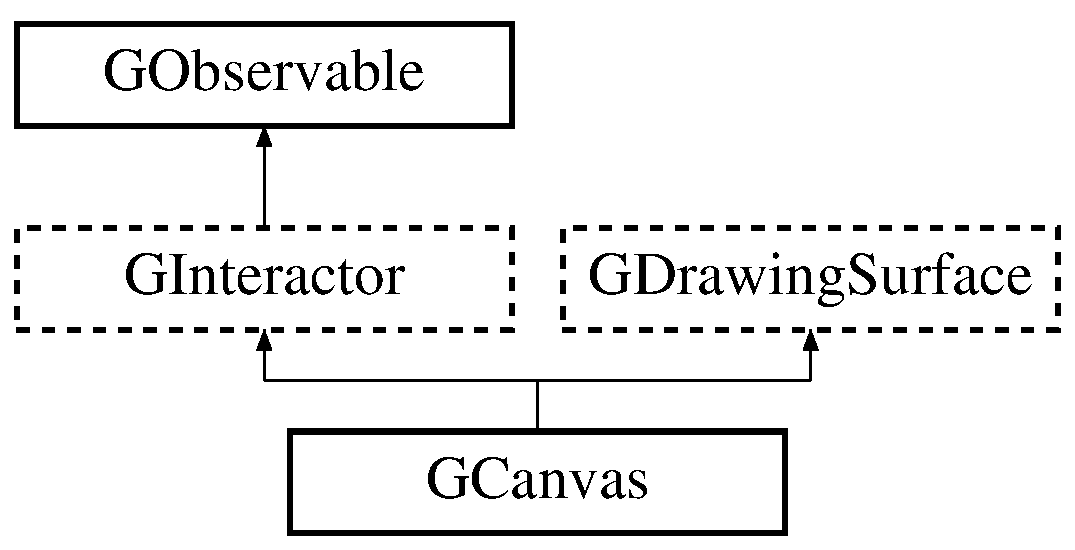
\includegraphics[height=3.000000cm]{classGCanvas}
\end{center}
\end{figure}
\subsection*{Public Types}
\begin{DoxyCompactItemize}
\item 
enum \mbox{\hyperlink{classGInteractor_a8e0d441725a81d2bbdebbea09078260e}{Text\+Position}} \{ \mbox{\hyperlink{classGInteractor_a8e0d441725a81d2bbdebbea09078260ea4cd6f2e7d5a08d6f4dc052df2358f774}{T\+E\+X\+T\+\_\+\+B\+E\+S\+I\+D\+E\+\_\+\+I\+C\+ON}}, 
\mbox{\hyperlink{classGInteractor_a8e0d441725a81d2bbdebbea09078260eaa88490f63d8de68d44c83bdb2ecde3b3}{T\+E\+X\+T\+\_\+\+U\+N\+D\+E\+R\+\_\+\+I\+C\+ON}}, 
\mbox{\hyperlink{classGInteractor_a8e0d441725a81d2bbdebbea09078260ea39a6f388a30ac4fefb6eb13e846bc9f2}{T\+E\+X\+T\+\_\+\+O\+N\+LY}}
 \}
\begin{DoxyCompactList}\small\item\em The places where an interactor can place its text relative to its icon. \end{DoxyCompactList}\end{DoxyCompactItemize}
\subsection*{Public Member Functions}
\begin{DoxyCompactItemize}
\item 
\mbox{\hyperlink{classGCanvas_abb7f95d00cbfadedab276958e1eb2af1}{G\+Canvas}} (Q\+Widget $\ast$parent=nullptr)
\begin{DoxyCompactList}\small\item\em Creates an empty canvas with a default size of 0x0 pixels and a default background and foreground color of black. \end{DoxyCompactList}\item 
\mbox{\hyperlink{classGCanvas_a0a9de139286d0fc9146928aff8f0538c}{G\+Canvas}} (const std\+::string \&filename, Q\+Widget $\ast$parent=nullptr)
\begin{DoxyCompactList}\small\item\em Creates a canvas that loads its background layer pixel data from the given image file name. \end{DoxyCompactList}\item 
\mbox{\hyperlink{classGCanvas_a18f1866349219dd73545c6b548ff3b0e}{G\+Canvas}} (std\+::istream \&filename, Q\+Widget $\ast$parent=nullptr)
\begin{DoxyCompactList}\small\item\em Creates a canvas that loads its background layer pixel data from the given input stream. \end{DoxyCompactList}\item 
\mbox{\hyperlink{classGCanvas_a235f6b1b700354d6737607562df06581}{G\+Canvas}} (double width, double height, int rgb\+Background, Q\+Widget $\ast$parent=nullptr)
\begin{DoxyCompactList}\small\item\em Creates an empty canvas of the specified size and optional background color. \end{DoxyCompactList}\item 
\mbox{\hyperlink{classGCanvas_af8bb8bd29201bbb5d0f90016a1d8df2c}{G\+Canvas}} (double width, double height, const std\+::string \&rgb\+Background=\char`\"{}\#00000000\char`\"{}, Q\+Widget $\ast$parent=nullptr)
\begin{DoxyCompactList}\small\item\em Creates an empty canvas of the specified size and background color. \end{DoxyCompactList}\item 
\mbox{\hyperlink{classGCanvas_af7574c14a3a729c56863e9c4ab6a6787}{$\sim$\+G\+Canvas}} () override
\begin{DoxyCompactList}\small\item\em Frees memory allocated internally by the canvas. \end{DoxyCompactList}\item 
virtual void \mbox{\hyperlink{classGCanvas_afe8277e7b2627513c6f7452fb0b2847d}{add}} (\mbox{\hyperlink{classGObject}{G\+Object}} $\ast$gobj)
\begin{DoxyCompactList}\small\item\em Adds the given interactor to canvas. \end{DoxyCompactList}\item 
virtual void \mbox{\hyperlink{classGCanvas_a8bb36f245efc7806414a1339c2befa1c}{add}} (\mbox{\hyperlink{classGObject}{G\+Object}} $\ast$gobj, double x, double y)
\begin{DoxyCompactList}\small\item\em Adds the given interactor to the canvas and moves it to the given x/y location. \end{DoxyCompactList}\item 
virtual void \mbox{\hyperlink{classGCanvas_ac732fc2123d7a6d7e2de145fe9bbd8e8}{add}} (\mbox{\hyperlink{classGObject}{G\+Object}} \&gobj)
\begin{DoxyCompactList}\small\item\em Adds the given interactor to canvas. \end{DoxyCompactList}\item 
virtual void \mbox{\hyperlink{classGCanvas_a5b11b532869632a6c26b098b0858eac5}{add}} (\mbox{\hyperlink{classGObject}{G\+Object}} \&gobj, double x, double y)
\begin{DoxyCompactList}\small\item\em Adds the given interactor to the canvas and moves it to the given x/y location. \end{DoxyCompactList}\item 
virtual void \mbox{\hyperlink{classGInteractor_a02f20ea6edfa0671f31c4c648a253833}{add\+Action\+Listener}} () Q\+\_\+\+D\+E\+C\+L\+\_\+\+D\+E\+P\+R\+E\+C\+A\+T\+ED
\begin{DoxyCompactList}\small\item\em Adds an event listener to be notified when this interactor is clicked or generally interacted with. \end{DoxyCompactList}\item 
void \mbox{\hyperlink{classGCanvas_aee7cb2065b88d21ac4ad05bc997ecf82}{clear}} () override
\begin{DoxyCompactList}\small\item\em Removes all graphical objects from the canvas foreground layer and wipes the background layer to show the current background color. \end{DoxyCompactList}\item 
virtual void \mbox{\hyperlink{classGCanvas_a6614e1320bc8e93b20df129613e5a0ff}{clear\+Objects}} ()
\begin{DoxyCompactList}\small\item\em Removes all graphical objects from the foreground layer of the canvas. \end{DoxyCompactList}\item 
virtual void \mbox{\hyperlink{classGCanvas_ab2c8590176aec1da6fb4e9b836bab630}{clear\+Pixels}} ()
\begin{DoxyCompactList}\small\item\em Resets the background layer of pixels in the canvas to the current background color. \end{DoxyCompactList}\item 
virtual void \mbox{\hyperlink{classGDrawingSurface_a221b3e75bb3d9d0bfea62b3364e6773b}{conditional\+Repaint}} ()
\begin{DoxyCompactList}\small\item\em Repaints the interactor only if its contents have changed. \end{DoxyCompactList}\item 
virtual void \mbox{\hyperlink{classGDrawingSurface_aedd4b792311d946eeaf44b0de337a408}{conditional\+Repaint\+Region}} (int x, int y, int width, int height)
\begin{DoxyCompactList}\small\item\em Repaints the given region of the interactor only if its contents have changed. \end{DoxyCompactList}\item 
virtual void \mbox{\hyperlink{classGDrawingSurface_a3932a12278752db368e24fa404e446aa}{conditional\+Repaint\+Region}} (const \mbox{\hyperlink{structGRectangle}{G\+Rectangle}} \&bounds)
\begin{DoxyCompactList}\small\item\em Repaints the given region of the interactor only if its contents have changed. \end{DoxyCompactList}\item 
virtual bool \mbox{\hyperlink{classGCanvas_abb6a5d7c03e6eaaae97264c4799ce7c3}{contains}} (double x, double y) const
\begin{DoxyCompactList}\small\item\em Returns true if any of the graphical objects in the foreground layer of the canvas touch the given x/y pixel. \end{DoxyCompactList}\item 
virtual int \mbox{\hyperlink{classGCanvas_ad3d6147a5e08ed97bb71c7f267ef071b}{count\+Diff\+Pixels}} (const \mbox{\hyperlink{classGCanvas}{G\+Canvas}} \&image) const
\begin{DoxyCompactList}\small\item\em Returns the total number of pixels that are not the same color between this image and the given other image. \end{DoxyCompactList}\item 
virtual int \mbox{\hyperlink{classGCanvas_a3ed6edef8ed522bbfc09d8f6005d6d8e}{count\+Diff\+Pixels}} (const \mbox{\hyperlink{classGCanvas}{G\+Canvas}} \&image, int xmin, int ymin, int xmax, int ymax) const
\begin{DoxyCompactList}\small\item\em Returns the total number of pixels that are not the same color between this image and the given other image. \end{DoxyCompactList}\item 
virtual int \mbox{\hyperlink{classGCanvas_a443b0f63a197c0f1147b13077f4206e0}{count\+Diff\+Pixels}} (const \mbox{\hyperlink{classGCanvas}{G\+Canvas}} $\ast$image) const
\begin{DoxyCompactList}\small\item\em Returns the total number of pixels that are not the same color between this image and the given other image. \end{DoxyCompactList}\item 
virtual int \mbox{\hyperlink{classGCanvas_a77b38a94630c93ecc697fb12a1fb89fd}{count\+Diff\+Pixels}} (const \mbox{\hyperlink{classGCanvas}{G\+Canvas}} $\ast$image, int xmin, int ymin, int xmax, int ymax) const
\begin{DoxyCompactList}\small\item\em Returns the total number of pixels that are not the same color between this image and the given other image. \end{DoxyCompactList}\item 
virtual \mbox{\hyperlink{classGCanvas}{G\+Canvas}} $\ast$ \mbox{\hyperlink{classGCanvas_aa4e74e40eebb70c9616065056de5c4ca}{diff}} (const \mbox{\hyperlink{classGCanvas}{G\+Canvas}} \&image, int diff\+Pixel\+Color=G\+C\+A\+N\+V\+A\+S\+\_\+\+D\+E\+F\+A\+U\+L\+T\+\_\+\+D\+I\+F\+F\+\_\+\+P\+I\+X\+E\+L\+\_\+\+C\+O\+L\+OR) const
\begin{DoxyCompactList}\small\item\em Generates a new canvas whose content is equal to that of this canvas but with any pixels that don\textquotesingle{}t match those in parameter \textquotesingle{}image\textquotesingle{} colored in the given color (default purple) to highlight differences between the two. \end{DoxyCompactList}\item 
virtual \mbox{\hyperlink{classGCanvas}{G\+Canvas}} $\ast$ \mbox{\hyperlink{classGCanvas_a5385d5c8fda55dfe0b20851d293b338b}{diff}} (const \mbox{\hyperlink{classGCanvas}{G\+Canvas}} $\ast$image, int diff\+Pixel\+Color=G\+C\+A\+N\+V\+A\+S\+\_\+\+D\+E\+F\+A\+U\+L\+T\+\_\+\+D\+I\+F\+F\+\_\+\+P\+I\+X\+E\+L\+\_\+\+C\+O\+L\+OR) const
\begin{DoxyCompactList}\small\item\em Generates a new canvas whose content is equal to that of this canvas but with any pixels that don\textquotesingle{}t match those in parameter \textquotesingle{}image\textquotesingle{} colored in the given color (default purple) to highlight differences between the two. \end{DoxyCompactList}\item 
virtual void \mbox{\hyperlink{classGDrawingSurface_acc3825d7a24815d1e2f78e7c3ffea6cc}{draw}} (\mbox{\hyperlink{classGObject}{G\+Object}} $\ast$gobj, double x, double y)
\begin{DoxyCompactList}\small\item\em Draws the given graphical object onto the background pixel layer of this interactor, moving it to the given x/y location first. \end{DoxyCompactList}\item 
virtual void \mbox{\hyperlink{classGDrawingSurface_a022a8d51c7fabcd79a0c809233e93453}{draw}} (\mbox{\hyperlink{classGObject}{G\+Object}} \&gobj)
\begin{DoxyCompactList}\small\item\em Draws the given graphical object onto the background pixel layer of this interactor. \end{DoxyCompactList}\item 
virtual void \mbox{\hyperlink{classGDrawingSurface_a8af8762bd6720e0a1d2a84b190e3dc96}{draw}} (\mbox{\hyperlink{classGObject}{G\+Object}} \&gobj, double x, double y)
\begin{DoxyCompactList}\small\item\em Draws the given graphical object onto the background pixel layer of this interactor, moving it to the given x/y location first. \end{DoxyCompactList}\item 
void \mbox{\hyperlink{classGCanvas_a7f7f6c1798bcedfd52151b458074e8a0}{draw}} (\mbox{\hyperlink{classGObject}{G\+Object}} $\ast$gobj) override
\begin{DoxyCompactList}\small\item\em Draws the given graphical object onto the background layer of the canvas. \end{DoxyCompactList}\item 
void \mbox{\hyperlink{classGCanvas_ab4536ea39f3b3899136554bdd5bda581}{draw}} (Q\+Painter $\ast$painter) override
\begin{DoxyCompactList}\small\item\em Draws this interactor with the given Qt painter object. \end{DoxyCompactList}\item 
virtual void \mbox{\hyperlink{classGDrawingSurface_a38b6fae1045191c57092b49905068144}{draw\+Arc}} (double x, double y, double width, double height, double start, double sweep)
\begin{DoxyCompactList}\small\item\em Draws an unfilled arc with the given attributes onto the background pixel layer of this interactor in the current color. \end{DoxyCompactList}\item 
virtual void \mbox{\hyperlink{classGDrawingSurface_abdd4cb1f2c64adc5d03522a1ee30febf}{draw\+Image}} (const std\+::string \&filename, double x=0, double y=0)
\begin{DoxyCompactList}\small\item\em Draws an image loaded from the given file name onto the background pixel layer of this interactor at the given x/y location. \end{DoxyCompactList}\item 
virtual void \mbox{\hyperlink{classGDrawingSurface_ae6a24b6b9a6e795d3165c1c750d5bdf1}{draw\+Line}} (const \mbox{\hyperlink{structGPoint}{G\+Point}} \&p0, const \mbox{\hyperlink{structGPoint}{G\+Point}} \&p1)
\begin{DoxyCompactList}\small\item\em Draws a line between the given two points onto the background pixel layer of this interactor at the given x/y location in the current color. \end{DoxyCompactList}\item 
virtual void \mbox{\hyperlink{classGDrawingSurface_aff299fe83178d2f3ce8c08c06b583484}{draw\+Line}} (double x0, double y0, double x1, double y1)
\begin{DoxyCompactList}\small\item\em Draws a line between the given two points onto the background pixel layer of this interactor at the given x/y location in the current color. \end{DoxyCompactList}\item 
virtual void \mbox{\hyperlink{classGDrawingSurface_a8adc13027efe311b4a6a715205b8bc46}{draw\+Oval}} (const \mbox{\hyperlink{structGRectangle}{G\+Rectangle}} \&bounds)
\begin{DoxyCompactList}\small\item\em Draws an unfilled oval with the given bounding box onto the background pixel layer of this interactor at the given x/y location in the current color. \end{DoxyCompactList}\item 
virtual void \mbox{\hyperlink{classGDrawingSurface_aa5b1cf902e578907da3c63060686354e}{draw\+Oval}} (double x, double y, double width, double height)
\begin{DoxyCompactList}\small\item\em Draws an unfilled oval with the given bounding box onto the background pixel layer of this interactor at the given x/y location in the current color. \end{DoxyCompactList}\item 
virtual void \mbox{\hyperlink{classGDrawingSurface_a0c1e2923d8d163d62d0896d8c5cfa191}{draw\+Pixel}} (double x, double y)
\begin{DoxyCompactList}\small\item\em Colors the given x/y pixel of the background layer of this interactor using the interactor\textquotesingle{}s current color. \end{DoxyCompactList}\item 
virtual void \mbox{\hyperlink{classGDrawingSurface_a3a64eb6383e601be8438e9c71643c432}{draw\+Pixel}} (double x, double y, int color)
\begin{DoxyCompactList}\small\item\em Colors the given x/y pixel of the background layer of this interactor using the given color. \end{DoxyCompactList}\item 
virtual void \mbox{\hyperlink{classGDrawingSurface_a20abc26a94b7eb310e34abf668e0f5f4}{draw\+Pixel}} (double x, double y, const std\+::string \&color)
\begin{DoxyCompactList}\small\item\em Colors the given x/y pixel of the background layer of this interactor using the given color. \end{DoxyCompactList}\item 
virtual \mbox{\hyperlink{structGPoint}{G\+Point}} \mbox{\hyperlink{classGDrawingSurface_af70cce1e4f708f1ed5b6f29cecb660e7}{draw\+Polar\+Line}} (const \mbox{\hyperlink{structGPoint}{G\+Point}} \&p0, double r, double theta)
\begin{DoxyCompactList}\small\item\em Draws a line using polar coordinates onto the background pixel layer of this interactor in the current color. \end{DoxyCompactList}\item 
virtual \mbox{\hyperlink{structGPoint}{G\+Point}} \mbox{\hyperlink{classGDrawingSurface_ad3e646f90005295f2bbdf37d2bcb39d2}{draw\+Polar\+Line}} (double x0, double y0, double r, double theta)
\begin{DoxyCompactList}\small\item\em Draws a line using polar coordinates onto the background pixel layer of this interactor in the current color. \end{DoxyCompactList}\item 
virtual void \mbox{\hyperlink{classGDrawingSurface_afddec0a905108d8a8d6809a157f26776}{draw\+Polygon}} (std\+::initializer\+\_\+list$<$ double $>$ coords)
\begin{DoxyCompactList}\small\item\em Draws an unfilled polygon containing the given points onto the background pixel layer of this interactor in the current color. \end{DoxyCompactList}\item 
virtual void \mbox{\hyperlink{classGDrawingSurface_a021ee881e0d154dc4dd059698742889c}{draw\+Polygon}} (std\+::initializer\+\_\+list$<$ \mbox{\hyperlink{structGPoint}{G\+Point}} $>$ points)
\begin{DoxyCompactList}\small\item\em Draws an unfilled polygon containing the given points onto the background pixel layer of this interactor in the current color. \end{DoxyCompactList}\item 
virtual void \mbox{\hyperlink{classGDrawingSurface_a3dd4cc5891149dfc36746264f7289877}{draw\+Rect}} (const \mbox{\hyperlink{structGRectangle}{G\+Rectangle}} \&bounds)
\begin{DoxyCompactList}\small\item\em Draws an unfilled rectangle of the given dimensions onto the background pixel layer of this interactor in the current color. \end{DoxyCompactList}\item 
virtual void \mbox{\hyperlink{classGDrawingSurface_a4148e770ffc5474153aadd4814dbd708}{draw\+Rect}} (double x, double y, double width, double height)
\begin{DoxyCompactList}\small\item\em Draws an unfilled rectangle of the given dimensions onto the background pixel layer of this interactor in the current color. \end{DoxyCompactList}\item 
virtual void \mbox{\hyperlink{classGDrawingSurface_ad4e8551a753a77135792bbee97013675}{draw\+String}} (const std\+::string \&text, double x, double y)
\begin{DoxyCompactList}\small\item\em Draws a text string onto the background pixel layer of this interactor at the given x/y location in the current font and color. \end{DoxyCompactList}\item 
virtual bool \mbox{\hyperlink{classGCanvas_a7cf0de4c4124b7de747b9cc17edd6ab9}{equals}} (const \mbox{\hyperlink{classGCanvas}{G\+Canvas}} \&other) const
\begin{DoxyCompactList}\small\item\em Returns true if the two given canvases contain exactly the same pixel data. \end{DoxyCompactList}\item 
bool \mbox{\hyperlink{classGInteractor_a597a370b592e3737d38d9d2f4e2031ea}{events\+Enabled}} () const override
\begin{DoxyCompactList}\small\item\em Returns true if this interactor is currently accepting events. \end{DoxyCompactList}\item 
virtual void \mbox{\hyperlink{classGCanvas_acaf90d64e4fea8f776e722976aeb5070}{fill}} (int rgb)
\begin{DoxyCompactList}\small\item\em Sets the color of every pixel in the canvas to the given color value. \end{DoxyCompactList}\item 
virtual void \mbox{\hyperlink{classGCanvas_a02a5aa7f1474eeedd181e6e46b5eee65}{fill}} (const std\+::string \&rgb)
\begin{DoxyCompactList}\small\item\em Sets the color of every pixel in the canvas to the given color value. \end{DoxyCompactList}\item 
virtual void \mbox{\hyperlink{classGDrawingSurface_a228075ad18bd97b57f9956568c4773f3}{fill\+Arc}} (double x, double y, double width, double height, double start, double sweep)
\begin{DoxyCompactList}\small\item\em Draws a filled arc with the given attributes onto the background pixel layer of this interactor in the current color and fill color. \end{DoxyCompactList}\item 
virtual void \mbox{\hyperlink{classGDrawingSurface_a1ea6e48d59fb588797dba4deab1397e0}{fill\+Oval}} (const \mbox{\hyperlink{structGRectangle}{G\+Rectangle}} \&bounds)
\begin{DoxyCompactList}\small\item\em Draws a filled oval with the given bounding box onto the background pixel layer of this interactor at the given x/y location in the current color and fill color. \end{DoxyCompactList}\item 
virtual void \mbox{\hyperlink{classGDrawingSurface_a28c700c82f31cd328a4629273420ee61}{fill\+Oval}} (double x, double y, double width, double height)
\begin{DoxyCompactList}\small\item\em Draws a filled oval with the given bounding box onto the background pixel layer of this interactor at the given x/y location in the current color and fill color. \end{DoxyCompactList}\item 
virtual void \mbox{\hyperlink{classGDrawingSurface_a15f8c1c4409ef51c1a30a92a195b8f66}{fill\+Polygon}} (std\+::initializer\+\_\+list$<$ double $>$ coords)
\begin{DoxyCompactList}\small\item\em Draws a filled polygon containing the given points onto the background pixel layer of this interactor in the current color and fill color. \end{DoxyCompactList}\item 
virtual void \mbox{\hyperlink{classGDrawingSurface_a31822d59786156ebf1cc3b2f7fb70330}{fill\+Polygon}} (std\+::initializer\+\_\+list$<$ \mbox{\hyperlink{structGPoint}{G\+Point}} $>$ coords)
\begin{DoxyCompactList}\small\item\em Draws a filled polygon containing the given points onto the background pixel layer of this interactor in the current color and fill color. \end{DoxyCompactList}\item 
virtual void \mbox{\hyperlink{classGDrawingSurface_ae6582295003bf2488836b1993dadbad7}{fill\+Rect}} (const \mbox{\hyperlink{structGRectangle}{G\+Rectangle}} \&bounds)
\begin{DoxyCompactList}\small\item\em Draws a filled rectangle of the given dimensions onto the background pixel layer of this interactor in the current color and fill color. \end{DoxyCompactList}\item 
virtual void \mbox{\hyperlink{classGDrawingSurface_aac3ae7d3aee950de78eca0e108352254}{fill\+Rect}} (double x, double y, double width, double height)
\begin{DoxyCompactList}\small\item\em Draws a filled rectangle of the given dimensions onto the background pixel layer of this interactor in the current color and fill color. \end{DoxyCompactList}\item 
virtual void \mbox{\hyperlink{classGCanvas_af4146bdcb26135b739b9b4f13db03435}{fill\+Region}} (double x, double y, double width, double height, int rgb)
\begin{DoxyCompactList}\small\item\em Sets the color of every pixel in the given rectangular range of the canvas pixel data to the given color value. \end{DoxyCompactList}\item 
virtual void \mbox{\hyperlink{classGCanvas_a762c611a5065687112018e7a0ab10c84}{fill\+Region}} (double x, double y, double width, double height, const std\+::string \&rgb)
\begin{DoxyCompactList}\small\item\em Sets the color of every pixel in the given rectangular range of the canvas pixel data to the given color value. \end{DoxyCompactList}\item 
virtual void \mbox{\hyperlink{classGCanvas_a4c4590df33ce47ad8a42e06f9f44fc93}{flatten}} ()
\begin{DoxyCompactList}\small\item\em Moves all graphical objects from the foreground layer to the background layer. \end{DoxyCompactList}\item 
virtual void \mbox{\hyperlink{classGCanvas_a46b18491b5230c765fbd9b8c7a095587}{from\+Grid}} (const Grid$<$ int $>$ \&grid)
\begin{DoxyCompactList}\small\item\em Replaces the entire contents of the background layer of the canvas with the contents of the given grid of R\+GB pixel values. \end{DoxyCompactList}\item 
virtual std\+::string \mbox{\hyperlink{classGInteractor_a69f8d23ed8f207fbecad99960776e942}{get\+Accelerator}} () const
\begin{DoxyCompactList}\small\item\em Returns a string representing a hotkey for this interactor, or an empty string if no accelerator has been set. \end{DoxyCompactList}\item 
virtual std\+::string \mbox{\hyperlink{classGInteractor_a94eb4276000c4fdfb508ce9e6317a82a}{get\+Action\+Command}} () const
\begin{DoxyCompactList}\small\item\em Returns an action command for this interactor, which is a semi-\/unique string you can use to identify it when events occur. \end{DoxyCompactList}\item 
virtual int \mbox{\hyperlink{classGDrawingSurface_ae394d39f20476570e083918d991c25bd}{get\+A\+R\+GB}} (double x, double y) const
\begin{DoxyCompactList}\small\item\em Returns the pixel color data at the given x/y location, retaining alpha-\/channel transparency in the top 8 bits. \end{DoxyCompactList}\item 
std\+::string \mbox{\hyperlink{classGCanvas_a4a62c51b7244a7642b88065e3a07ae82}{get\+Background}} () const override
\begin{DoxyCompactList}\small\item\em Returns the current background color of the interactor as a string. \end{DoxyCompactList}\item 
int \mbox{\hyperlink{classGCanvas_acd4f2b3b9619dacdfd71fc0004cac382}{get\+Background\+Int}} () const override
\begin{DoxyCompactList}\small\item\em Returns the current background color of the interactor as an R\+GB integer. \end{DoxyCompactList}\item 
virtual \mbox{\hyperlink{structGRectangle}{G\+Rectangle}} \mbox{\hyperlink{classGInteractor_a29e6ac35a0b48f491a4c88194cc5da3b}{get\+Bounds}} () const
\begin{DoxyCompactList}\small\item\em Returns a rectangle representing the x/y position and size of this interactor. \end{DoxyCompactList}\item 
virtual std\+::string \mbox{\hyperlink{classGInteractor_aa061dfa488c31e18549d64363c1d0e34}{get\+Color}} () const
\begin{DoxyCompactList}\small\item\em Returns the foreground/text color of the interactor as a string. \end{DoxyCompactList}\item 
virtual std\+::string \mbox{\hyperlink{classGDrawingSurface_aa061dfa488c31e18549d64363c1d0e34}{get\+Color}} () const
\begin{DoxyCompactList}\small\item\em Returns the current foreground outline color of the interactor as a string. \end{DoxyCompactList}\item 
virtual int \mbox{\hyperlink{classGInteractor_a9635c7af766cdc3417f346683fa0e6c1}{get\+Color\+Int}} () const
\begin{DoxyCompactList}\small\item\em Returns the foreground/text color of the interactor as an R\+GB integer. \end{DoxyCompactList}\item 
virtual int \mbox{\hyperlink{classGDrawingSurface_a9635c7af766cdc3417f346683fa0e6c1}{get\+Color\+Int}} () const
\begin{DoxyCompactList}\small\item\em Returns the current foreground outline color of the interactor as an R\+GB integer. \end{DoxyCompactList}\item 
virtual \mbox{\hyperlink{classGContainer}{G\+Container}} $\ast$ \mbox{\hyperlink{classGInteractor_a7a6e317c29d61030929b4cd2d1c00fe7}{get\+Container}} () const
\begin{DoxyCompactList}\small\item\em Returns a pointer to the onscreen container holding this interactor. \end{DoxyCompactList}\item 
virtual \mbox{\hyperlink{classGObject}{G\+Object}} $\ast$ \mbox{\hyperlink{classGCanvas_abde388cc529d22bb5f7f4a54d56049d8}{get\+Element}} (int index) const
\begin{DoxyCompactList}\small\item\em Returns a pointer to the graphical object in the foreground layer of the canvas at the specified index, numbering from back to front in the {\itshape z} dimension. \end{DoxyCompactList}\item 
virtual \mbox{\hyperlink{classGObject}{G\+Object}} $\ast$ \mbox{\hyperlink{classGCanvas_a25efa999eca5790ec26ef091b05f961c}{get\+Element\+At}} (double x, double y) const
\begin{DoxyCompactList}\small\item\em Returns a pointer to the first graphical object in the foreground layer of the canvas that contains the given (x, y) point, or a null pointer if no object in this canvas touches it. \end{DoxyCompactList}\item 
virtual int \mbox{\hyperlink{classGCanvas_adf7d37ec315f859648def92e6b32408f}{get\+Element\+Count}} () const
\begin{DoxyCompactList}\small\item\em Returns the number of graphical objects stored in the foreground layer of the canvas. \end{DoxyCompactList}\item 
virtual std\+::string \mbox{\hyperlink{classGCanvas_a2011812670c3de9747702e3c052b6bb3}{get\+Filename}} () const
\begin{DoxyCompactList}\small\item\em Returns the name of the image file from which this canvas was loaded or to which it was saved most recently. \end{DoxyCompactList}\item 
virtual std\+::string \mbox{\hyperlink{classGDrawingSurface_a76f6964a11fde7c78e9751be184e1a3c}{get\+Fill\+Color}} () const
\begin{DoxyCompactList}\small\item\em Returns the current fill color of the interactor as a string. \end{DoxyCompactList}\item 
virtual int \mbox{\hyperlink{classGDrawingSurface_a88f4508d9271c4b5f5b5d6b780f223d0}{get\+Fill\+Color\+Int}} () const
\begin{DoxyCompactList}\small\item\em Returns the current fill color of the interactor as an R\+GB integer. \end{DoxyCompactList}\item 
std\+::string \mbox{\hyperlink{classGCanvas_aa0829769ac6325b5c58d27c8e363cb78}{get\+Font}} () const override
\begin{DoxyCompactList}\small\item\em Returns the current text font of the interactor as a font string. \end{DoxyCompactList}\item 
virtual std\+::string \mbox{\hyperlink{classGInteractor_a4fa2d8b0192a3a5b4af4bbfe71194d03}{get\+Foreground}} () const
\begin{DoxyCompactList}\small\item\em Returns the foreground/text color of the interactor as a string. \end{DoxyCompactList}\item 
virtual std\+::string \mbox{\hyperlink{classGDrawingSurface_a4fa2d8b0192a3a5b4af4bbfe71194d03}{get\+Foreground}} () const
\begin{DoxyCompactList}\small\item\em Returns the current foreground outline color of the interactor as a string. \end{DoxyCompactList}\item 
virtual int \mbox{\hyperlink{classGInteractor_ac3b12ab385a6ef9ae90fc879860ba726}{get\+Foreground\+Int}} () const
\begin{DoxyCompactList}\small\item\em Returns the foreground/text color of the interactor as an R\+GB integer. \end{DoxyCompactList}\item 
virtual int \mbox{\hyperlink{classGDrawingSurface_ac3b12ab385a6ef9ae90fc879860ba726}{get\+Foreground\+Int}} () const
\begin{DoxyCompactList}\small\item\em Returns the current foreground outline color of the interactor as an R\+GB integer. \end{DoxyCompactList}\item 
virtual double \mbox{\hyperlink{classGInteractor_a1e7e353362434072875264cf95629f99}{get\+Height}} () const
\begin{DoxyCompactList}\small\item\em Returns the current onscreen height of this interactor in pixels. \end{DoxyCompactList}\item 
virtual std\+::string \mbox{\hyperlink{classGInteractor_aaed62a73004939a64da6f0eb9eb64d73}{get\+Icon}} () const
\begin{DoxyCompactList}\small\item\em Returns the file name of the icon associated with this interactor, or an empty string if no icon has been set. \end{DoxyCompactList}\item 
virtual int \mbox{\hyperlink{classGInteractor_a9c9659a6c6ba66b4107ba59c95a24241}{get\+ID}} () const
\begin{DoxyCompactList}\small\item\em Returns a globally unique identifier for this interactor, which is set when the interactor is constructed. \end{DoxyCompactList}\item 
\+\_\+\+Internal\+\_\+\+Q\+Widget $\ast$ \mbox{\hyperlink{classGCanvas_a2f6b36b2517087dc90a366b5ce1f5323}{get\+Internal\+Widget}} () const override
\begin{DoxyCompactList}\small\item\em Returns a direct pointer to the internal Qt widget being wrapped by this interactor. \end{DoxyCompactList}\item 
virtual \mbox{\hyperlink{classGObject_a86e0f5648542856159bb40775c854aa7}{G\+Object\+::\+Line\+Style}} \mbox{\hyperlink{classGDrawingSurface_aaf1f5ea8281e5e3486662878d26f0a13}{get\+Line\+Style}} () const
\begin{DoxyCompactList}\small\item\em Returns the current line style which will be used to draw outlines of shapes and lines. \end{DoxyCompactList}\item 
virtual double \mbox{\hyperlink{classGDrawingSurface_a85ff266dc3eb63d9f2d8e5a4487fd3c0}{get\+Line\+Width}} () const
\begin{DoxyCompactList}\small\item\em Returns the thickness used when drawing outlines of shapes and lines. \end{DoxyCompactList}\item 
virtual \mbox{\hyperlink{structGPoint}{G\+Point}} \mbox{\hyperlink{classGInteractor_a4f83802015511edeb63b892830812c11}{get\+Location}} () const
\begin{DoxyCompactList}\small\item\em Returns an (x, y) point representing the onscreen location of the top-\/left corner of this interactor within its containing window. \end{DoxyCompactList}\item 
virtual double \mbox{\hyperlink{classGInteractor_aed4b0075fcc434499c3cb3e46896bda3}{get\+Minimum\+Height}} () const
\begin{DoxyCompactList}\small\item\em Returns the minimum height in pixels that this interactor will permit itself to be resized to. \end{DoxyCompactList}\item 
virtual \mbox{\hyperlink{structGDimension}{G\+Dimension}} \mbox{\hyperlink{classGInteractor_a66b5af0b32493b4d597ca0a3df2049ea}{get\+Minimum\+Size}} () const
\begin{DoxyCompactList}\small\item\em Returns a \mbox{\hyperlink{structGDimension}{G\+Dimension}} structure representing the minimum size in pixels that this interactor will permit itself to be resized to. \end{DoxyCompactList}\item 
virtual double \mbox{\hyperlink{classGInteractor_a59e668114fe3d49d2a0f28deb258f7c8}{get\+Minimum\+Width}} () const
\begin{DoxyCompactList}\small\item\em Returns the minimum width in pixels that this interactor will permit itself to be resized to. \end{DoxyCompactList}\item 
virtual std\+::string \mbox{\hyperlink{classGInteractor_a8a60438a5b55d0b2ceb35c8674b9d8c5}{get\+Name}} () const
\begin{DoxyCompactList}\small\item\em Returns a string representing a unique name for this interactor. \end{DoxyCompactList}\item 
int \mbox{\hyperlink{classGCanvas_a342aaa6de62a4a324a2e4f3921db1d3e}{get\+Pixel}} (double x, double y) const override
\begin{DoxyCompactList}\small\item\em Returns the color of the pixel at the given x/y coordinates of the background layer of the canvas as an integer such as 0xff00cc. \end{DoxyCompactList}\item 
int \mbox{\hyperlink{classGCanvas_ae28117ec01d58208d381fba886030850}{get\+Pixel\+A\+R\+GB}} (double x, double y) const override
\begin{DoxyCompactList}\small\item\em Returns the color of the pixel at the given x/y coordinates of the background layer of the canvas as an integer such as 0xffff00cc. \end{DoxyCompactList}\item 
Grid$<$ int $>$ \mbox{\hyperlink{classGCanvas_aec81bf7947e993d8df8039e19dbac533}{get\+Pixels}} () const override
\begin{DoxyCompactList}\small\item\em Returns all pixels of the background layer of the canvas as a Grid, where rows represent y values and columns represent x values. \end{DoxyCompactList}\item 
Grid$<$ int $>$ \mbox{\hyperlink{classGCanvas_aa1626b73d6dae452e9e78c159411058b}{get\+Pixels\+A\+R\+GB}} () const override
\begin{DoxyCompactList}\small\item\em Returns all pixels of the background layer of the canvas as a Grid, where rows represent y values and columns represent x values. \end{DoxyCompactList}\item 
virtual std\+::string \mbox{\hyperlink{classGDrawingSurface_a8da04ef488ec5fa498fbbffaf50928fd}{get\+Pixel\+String}} (double x, double y) const
\begin{DoxyCompactList}\small\item\em Returns the color of the pixel at the given x/y coordinates of the image as a string such as \char`\"{}\#ff00cc\char`\"{}. \end{DoxyCompactList}\item 
virtual double \mbox{\hyperlink{classGInteractor_a747de0961653847bdc6615dbf756d715}{get\+Preferred\+Height}} () const
\begin{DoxyCompactList}\small\item\em Returns the height in pixels that this interactor would prefer to be, which would exactly fit its contents with no stretching or scrollbars. \end{DoxyCompactList}\item 
virtual \mbox{\hyperlink{structGDimension}{G\+Dimension}} \mbox{\hyperlink{classGInteractor_a4aabbee761d8e9116275401131b7ccd1}{get\+Preferred\+Size}} () const
\begin{DoxyCompactList}\small\item\em Returns a \mbox{\hyperlink{structGDimension}{G\+Dimension}} structure storing the width and height in pixels that this interactor would prefer to be, which would exactly fit its contents with no stretching or scrollbars. \end{DoxyCompactList}\item 
virtual double \mbox{\hyperlink{classGInteractor_a82bca31d37700fb0e35d2743352efd5e}{get\+Preferred\+Width}} () const
\begin{DoxyCompactList}\small\item\em Returns the height in pixels that this interactor would prefer to be, which would exactly fit its contents with no stretching or scrollbars. \end{DoxyCompactList}\item 
virtual int \mbox{\hyperlink{classGDrawingSurface_a9e983467cf0c97cfd62433a8471570dc}{get\+R\+GB}} (double x, double y) const
\begin{DoxyCompactList}\small\item\em Returns the color of the pixel at the given x/y coordinates of the background layer of the interactor as an integer such as 0xff00cc. \end{DoxyCompactList}\item 
virtual std\+::string \mbox{\hyperlink{classGDrawingSurface_a456d3582acc3544f37d939f5cb8802fe}{get\+R\+G\+B\+String}} (double x, double y) const
\begin{DoxyCompactList}\small\item\em Returns the color of the pixel at the given x/y coordinates of the background layer of the interactor as a color string such as \char`\"{}\#ff00cc\char`\"{}. \end{DoxyCompactList}\item 
virtual \mbox{\hyperlink{structGDimension}{G\+Dimension}} \mbox{\hyperlink{classGInteractor_a7b4eec96a2bdc6420695d5796a78eea9}{get\+Size}} () const
\begin{DoxyCompactList}\small\item\em Returns a \mbox{\hyperlink{structGDimension}{G\+Dimension}} structure storing the current onscreen width and height of this interactor in pixels. \end{DoxyCompactList}\item 
std\+::string \mbox{\hyperlink{classGCanvas_a9b72ede4ee8520f987a0c01e30654814}{get\+Type}} () const override
\begin{DoxyCompactList}\small\item\em Returns a string representing the class name of this interactor, such as \char`\"{}\+G\+Button\char`\"{} or \char`\"{}\+G\+Check\+Box\char`\"{}. \end{DoxyCompactList}\item 
Q\+Widget $\ast$ \mbox{\hyperlink{classGCanvas_a3b33a602b31a6b809d020535a59db3b4}{get\+Widget}} () const override
\begin{DoxyCompactList}\small\item\em Returns a direct pointer to the internal Qt widget being wrapped by this interactor. \end{DoxyCompactList}\item 
virtual double \mbox{\hyperlink{classGInteractor_a0ed2965abd4f5701d2cadf71239faf19}{get\+Width}} () const
\begin{DoxyCompactList}\small\item\em Returns the current onscreen width of this interactor in pixels. \end{DoxyCompactList}\item 
virtual double \mbox{\hyperlink{classGInteractor_a344385751bee0720059403940d57a13e}{getX}} () const
\begin{DoxyCompactList}\small\item\em Returns the x-\/coordinate of the top-\/left pixel of this interactor within its onscreen window. \end{DoxyCompactList}\item 
virtual double \mbox{\hyperlink{classGInteractor_aafa51c7f8f38a09febbb9ce7853f77b4}{getY}} () const
\begin{DoxyCompactList}\small\item\em Returns the y-\/coordinate of the top-\/left pixel of this interactor within its onscreen window. \end{DoxyCompactList}\item 
virtual bool \mbox{\hyperlink{classGInteractor_afc480f652b8c5f1fb255e2269ce68879}{in\+Bounds}} (double x, double y) const
\begin{DoxyCompactList}\small\item\em Returns true if the given x/y pixel is within the bounds of this interactor. \end{DoxyCompactList}\item 
virtual bool \mbox{\hyperlink{classGInteractor_ae6d7982c1c627b677a5e776ca86118ed}{in\+Bounds}} (int x, int y) const
\begin{DoxyCompactList}\small\item\em Returns true if the given x/y pixel is within the bounds of this interactor. \end{DoxyCompactList}\item 
bool \mbox{\hyperlink{classGCanvas_a189881032e2b355095790b83b2454d8d}{is\+Auto\+Repaint}} () const override
\begin{DoxyCompactList}\small\item\em Returns true if the interactor should repaint itself automatically whenever any change is made to its graphical data. \end{DoxyCompactList}\item 
virtual bool \mbox{\hyperlink{classGInteractor_aacb819fb241851fd9fc045271baa4034}{is\+Enabled}} () const
\begin{DoxyCompactList}\small\item\em Returns true if this interactor is currently enabled. \end{DoxyCompactList}\item 
virtual bool \mbox{\hyperlink{classGDrawingSurface_a82a00267c81cc0ae85ee0feb01a92fa8}{is\+Repaint\+Immediately}} () const
\begin{DoxyCompactList}\small\item\em Returns true if the interactor should repaint itself automatically whenever any change is made to its graphical data. \end{DoxyCompactList}\item 
virtual bool \mbox{\hyperlink{classGInteractor_a9d8a6cfb13917785c143e74d40e4e2be}{is\+Visible}} () const
\begin{DoxyCompactList}\small\item\em Returns true if the interactor is visible on the screen. \end{DoxyCompactList}\item 
virtual void \mbox{\hyperlink{classGCanvas_a6c21edd9d285c925527e3209fca54b01}{load}} (const std\+::string \&filename)
\begin{DoxyCompactList}\small\item\em Reads the canvas\textquotesingle{}s pixel contents from the given image file. \end{DoxyCompactList}\item 
virtual void \mbox{\hyperlink{classGCanvas_a49dc57a2ce4caa354a5fff6acdde2e7d}{remove}} (\mbox{\hyperlink{classGObject}{G\+Object}} $\ast$gobj)
\begin{DoxyCompactList}\small\item\em Reads the canvas\textquotesingle{}s pixel contents from the given input stream. \end{DoxyCompactList}\item 
virtual void \mbox{\hyperlink{classGCanvas_a0c0ae4d69b584602ff3cba0d9cf330a4}{remove}} (\mbox{\hyperlink{classGObject}{G\+Object}} \&gobj)
\begin{DoxyCompactList}\small\item\em Removes the given graphical object from the foreground layer of the canvas, if it was present. \end{DoxyCompactList}\item 
virtual void \mbox{\hyperlink{classGInteractor_ab7fe7a876367b87cf7202f947f1d05e4}{remove\+Action\+Listener}} ()
\begin{DoxyCompactList}\small\item\em Removes the action listener from this interactor so that it will no longer call it when events occur. \end{DoxyCompactList}\item 
virtual void \mbox{\hyperlink{classGCanvas_a9b0a5a3ad9972ab0e8eb0b54873aac6b}{remove\+All}} ()
\begin{DoxyCompactList}\small\item\em Removes all graphical objects from the foreground layer of the canvas. \end{DoxyCompactList}\item 
virtual void \mbox{\hyperlink{classGInteractor_ad39d0325cde6b97ebda4b9d7787c633b}{remove\+Click\+Listener}} ()
\begin{DoxyCompactList}\small\item\em Removes the click listener from this interactor so that it will no longer call it when events occur. \end{DoxyCompactList}\item 
virtual void \mbox{\hyperlink{classGInteractor_aa4250907e4cdd77349c04f0cf5cdd3d3}{remove\+Double\+Click\+Listener}} ()
\begin{DoxyCompactList}\small\item\em Removes the double-\/click listener from this interactor so that it will no longer call it when events occur. \end{DoxyCompactList}\item 
virtual void \mbox{\hyperlink{classGInteractor_a43095f41cab3be732b49f29970484b05}{remove\+Key\+Listener}} ()
\begin{DoxyCompactList}\small\item\em Removes the key listener from this interactor so that it will no longer call it when key events occur. \end{DoxyCompactList}\item 
virtual void \mbox{\hyperlink{classGInteractor_aff47f71ce47e688a07c9d38dc92fcc11}{remove\+Mouse\+Listener}} ()
\begin{DoxyCompactList}\small\item\em Removes the mouse listener from this interactor so that it will no longer call it when events occur. \end{DoxyCompactList}\item 
void \mbox{\hyperlink{classGCanvas_afb8dbc55702230f0030e47d6c009697f}{repaint}} () override
\begin{DoxyCompactList}\small\item\em Instructs the canvas to redraw its layers. \end{DoxyCompactList}\item 
virtual void \mbox{\hyperlink{classGDrawingSurface_a769c46fb3e1004aec76e8b0adfa42aa6}{repaint\+Region}} (const \mbox{\hyperlink{structGRectangle}{G\+Rectangle}} \&bounds)
\begin{DoxyCompactList}\small\item\em Instructs the interactor to repaint the given region of pixel data. \end{DoxyCompactList}\item 
void \mbox{\hyperlink{classGCanvas_a63af8fca5bf186367132ecf6af6f5eea}{repaint\+Region}} (int x, int y, int width, int height) override
\begin{DoxyCompactList}\small\item\em Instructs the canvas to redraw the given region of pixels within both of its layers. \end{DoxyCompactList}\item 
virtual void \mbox{\hyperlink{classGInteractor_a519fb2ac767f8b2febbb50b898b8c8cb}{request\+Focus}} ()
\begin{DoxyCompactList}\small\item\em Transfers keyboard focus to this interactor. \end{DoxyCompactList}\item 
void \mbox{\hyperlink{classGCanvas_a090053938117ab698c4c9c1f1cff74a9}{resize}} (double width, double height, bool retain=true)
\begin{DoxyCompactList}\small\item\em Changes this image\textquotesingle{}s bounds to be the given size. \end{DoxyCompactList}\item 
virtual void \mbox{\hyperlink{classGCanvas_a2c027edbcd25b820dc6e21a9a3ad0496}{save}} (const std\+::string \&filename)
\begin{DoxyCompactList}\small\item\em Saves the canvas\textquotesingle{}s contents to the given image file. \end{DoxyCompactList}\item 
virtual void \mbox{\hyperlink{classGInteractor_ad15f102f62e2960576012f1aa0ba4b2e}{set\+Accelerator}} (const std\+::string \&accelerator)
\begin{DoxyCompactList}\small\item\em Sets an accelerator hotkey for this interactor, such as \char`\"{}\+Ctrl-\/\+S\char`\"{}. \end{DoxyCompactList}\item 
virtual void \mbox{\hyperlink{classGInteractor_a4b5843fe3030e038a1ba54cc03389bcf}{set\+Action\+Command}} (const std\+::string \&action\+Command)
\begin{DoxyCompactList}\small\item\em Sets the action command for this interactor. \end{DoxyCompactList}\item 
virtual void \mbox{\hyperlink{classGInteractor_adcfb4742430c88714fcf57e57ab8ea9c}{set\+Action\+Listener}} (G\+Event\+Listener func)
\begin{DoxyCompactList}\small\item\em Sets an action listener on this interactor so that it will be called when it is interacted with in its primary way. \end{DoxyCompactList}\item 
virtual void \mbox{\hyperlink{classGInteractor_aebd20a89c7a8a43a6fce999cf4f9fcf2}{set\+Action\+Listener}} (G\+Event\+Listener\+Void func)
\begin{DoxyCompactList}\small\item\em Sets an action listener on this interactor so that it will be called when it is interacted with in its primary way. \end{DoxyCompactList}\item 
void \mbox{\hyperlink{classGCanvas_acb65220cc16d17df02a0c08d35b60988}{set\+Auto\+Repaint}} (bool auto\+Repaint) override
\begin{DoxyCompactList}\small\item\em Sets whether the canvas will automatically repaint itself whenever you make a change to either the background or foreground layer. \end{DoxyCompactList}\item 
void \mbox{\hyperlink{classGCanvas_a10d305826534b55561ea88730fc9f6cd}{set\+Background}} (int color) override
\begin{DoxyCompactList}\small\item\em Sets the current background color of the interactor as an R\+GB integer. \end{DoxyCompactList}\item 
void \mbox{\hyperlink{classGCanvas_a9cb99695b93494c7ba28268ce9e42c2a}{set\+Background}} (const std\+::string \&color) override
\begin{DoxyCompactList}\small\item\em Sets the current background color of the interactor as a string. \end{DoxyCompactList}\item 
virtual void \mbox{\hyperlink{classGInteractor_a2aae8197624b72265ab83b4f1bc73f2f}{set\+Bounds}} (double x, double y, double width, double height)
\begin{DoxyCompactList}\small\item\em Sets the size and location of the widget. \end{DoxyCompactList}\item 
virtual void \mbox{\hyperlink{classGInteractor_acada386653f008cacc7cce86426bef7c}{set\+Bounds}} (const \mbox{\hyperlink{structGRectangle}{G\+Rectangle}} \&size)
\begin{DoxyCompactList}\small\item\em Sets the size and location of the widget. \end{DoxyCompactList}\item 
virtual void \mbox{\hyperlink{classGInteractor_abd40af6921242584d0954f173911b190}{set\+Click\+Listener}} (G\+Event\+Listener func)
\begin{DoxyCompactList}\small\item\em Sets a mouse listener on this interactor so that it will be called when the mouse is clicked on it. \end{DoxyCompactList}\item 
virtual void \mbox{\hyperlink{classGInteractor_a856414c92df90f56f3877475eb3f8fc4}{set\+Click\+Listener}} (G\+Event\+Listener\+Void func)
\begin{DoxyCompactList}\small\item\em Sets a mouse listener on this interactor so that it will be called when the mouse is clicked on it. \end{DoxyCompactList}\item 
void \mbox{\hyperlink{classGCanvas_af6e1bcf23a09a0ae0607daff81ee45fa}{set\+Color}} (int color) override
\begin{DoxyCompactList}\small\item\em Sets the current foreground outline color of the interactor as as R\+GB integer. \end{DoxyCompactList}\item 
void \mbox{\hyperlink{classGCanvas_a56845b1accc47aa881d05939eef6996c}{set\+Color}} (const std\+::string \&color) override
\begin{DoxyCompactList}\small\item\em Sets the current foreground outline color of the interactor as a string. \end{DoxyCompactList}\item 
virtual void \mbox{\hyperlink{classGInteractor_ac29f9a3462458e165fae3a1f046ee77a}{set\+Double\+Click\+Listener}} (G\+Event\+Listener func)
\begin{DoxyCompactList}\small\item\em Sets a mouse listener on this interactor so that it will be called when the mouse is double-\/clicked on it. \end{DoxyCompactList}\item 
virtual void \mbox{\hyperlink{classGInteractor_a50096194d66f48c92dd4c512d41bfc76}{set\+Double\+Click\+Listener}} (G\+Event\+Listener\+Void func)
\begin{DoxyCompactList}\small\item\em Sets a mouse listener on this interactor so that it will be called when the mouse is double-\/clicked on it. \end{DoxyCompactList}\item 
virtual void \mbox{\hyperlink{classGInteractor_ab831367dd84bbd579e02e55bacb21343}{set\+Enabled}} (bool value)
\begin{DoxyCompactList}\small\item\em Sets whether this interactor is currently enabled. \end{DoxyCompactList}\item 
virtual void \mbox{\hyperlink{classGObservable_afaa30b2a9e0f378fd1c70d2f1d0b8216}{set\+Events\+Enabled}} (bool \mbox{\hyperlink{classGInteractor_a597a370b592e3737d38d9d2f4e2031ea}{events\+Enabled}})
\begin{DoxyCompactList}\small\item\em Sets whether the object is currently allowing itself to fire events. \end{DoxyCompactList}\item 
virtual void \mbox{\hyperlink{classGDrawingSurface_a47fad447b715f2f303538434eed26709}{set\+Fill\+Color}} (int color)
\begin{DoxyCompactList}\small\item\em Sets the current fill color of the interactor as an R\+GB integer. \end{DoxyCompactList}\item 
virtual void \mbox{\hyperlink{classGDrawingSurface_adbc18b1a930aadd97d7437f9f7265b96}{set\+Fill\+Color}} (const std\+::string \&color)
\begin{DoxyCompactList}\small\item\em Returns the current fill color of the interactor as a string. \end{DoxyCompactList}\item 
void \mbox{\hyperlink{classGCanvas_ad1d75b3840a41ba7d1e8a921696dc684}{set\+Font}} (const Q\+Font \&font) override
\begin{DoxyCompactList}\small\item\em Returns the current text font of the interactor using a Qt font object. \end{DoxyCompactList}\item 
void \mbox{\hyperlink{classGCanvas_a51367c9fd2709973b1f7238734f93891}{set\+Font}} (const std\+::string \&font) override
\begin{DoxyCompactList}\small\item\em Sets the current text font of the interactor as a font string. \end{DoxyCompactList}\item 
void \mbox{\hyperlink{classGCanvas_a59f7cd2bd1708c12dfa52a8f7c7b79c9}{set\+Foreground}} (int rgb) override
\begin{DoxyCompactList}\small\item\em Sets the current foreground outline color of the interactor as an R\+GB integer. \end{DoxyCompactList}\item 
void \mbox{\hyperlink{classGCanvas_a8afbcf1f47750fb4c717f9ff36540235}{set\+Foreground}} (const std\+::string \&color) override
\begin{DoxyCompactList}\small\item\em Sets the current foreground outline color of the interactor as a string. \end{DoxyCompactList}\item 
virtual void \mbox{\hyperlink{classGInteractor_a9e280bfc4544dfaf8e4376c4e1a74357}{set\+Height}} (double height)
\begin{DoxyCompactList}\small\item\em Sets the onscreen height of the interactor in pixels. \end{DoxyCompactList}\item 
virtual void \mbox{\hyperlink{classGInteractor_a542abfcd7261751352af129c7215ecda}{set\+Icon}} (const Q\+Icon \&icon)
\begin{DoxyCompactList}\small\item\em Sets the icon associated with this interactor. \end{DoxyCompactList}\item 
virtual void \mbox{\hyperlink{classGInteractor_a368e1a338f84401c284506d03b1ba769}{set\+Icon}} (const Q\+Pixmap \&icon)
\begin{DoxyCompactList}\small\item\em Sets the icon associated with this interactor. \end{DoxyCompactList}\item 
virtual void \mbox{\hyperlink{classGInteractor_a762e139aa311461c3984d3ad28293f64}{set\+Icon}} (const std\+::string \&filename, bool retain\+Icon\+Size=true)
\begin{DoxyCompactList}\small\item\em Sets the file name of the icon associated with this interactor, or an empty string if no icon has been set. \end{DoxyCompactList}\item 
void \mbox{\hyperlink{classGCanvas_a53809ec015da5bf9fad5e7a11b218993}{set\+Key\+Listener}} (G\+Event\+Listener func) override
\begin{DoxyCompactList}\small\item\em Sets a key listener on this canvas so that it will be called when any key is pressed or released on the canvas. \end{DoxyCompactList}\item 
void \mbox{\hyperlink{classGCanvas_a1320ed9889a730dfead04a334463ecf3}{set\+Key\+Listener}} (G\+Event\+Listener\+Void func) override
\begin{DoxyCompactList}\small\item\em Sets a key listener on this canvas so that it will be called when any key is pressed or released on the canvas. \end{DoxyCompactList}\item 
virtual void \mbox{\hyperlink{classGDrawingSurface_a6bfe14a77101db0fb97b5a7e07a5526b}{set\+Line\+Style}} (\mbox{\hyperlink{classGObject_a86e0f5648542856159bb40775c854aa7}{G\+Object\+::\+Line\+Style}} line\+Style)
\begin{DoxyCompactList}\small\item\em Sets the current line style which will be used to draw outlines of shapes and lines. \end{DoxyCompactList}\item 
virtual void \mbox{\hyperlink{classGDrawingSurface_afd6a47c6ea6a1f85ca05a65ba3ff3477}{set\+Line\+Width}} (double line\+Width)
\begin{DoxyCompactList}\small\item\em Sets the thickness used when drawing outlines of shapes and lines. \end{DoxyCompactList}\item 
virtual void \mbox{\hyperlink{classGInteractor_a04594e8ba9b98513a64f1da00dcae18c}{set\+Location}} (double x, double y)
\begin{DoxyCompactList}\small\item\em Sets the onscreen x/y-\/coordinate of the top-\/left corner of the interactor relative to its window. \end{DoxyCompactList}\item 
virtual void \mbox{\hyperlink{classGInteractor_a0cf428e207b7f22cc08138a90b1b87b2}{set\+Minimum\+Size}} (double width, double height)
\begin{DoxyCompactList}\small\item\em Sets the minimum size in pixels that this interactor will permit itself to be resized to. \end{DoxyCompactList}\item 
virtual void \mbox{\hyperlink{classGInteractor_a3b1046117ac6cb7abe467e00ba8a81f4}{set\+Minimum\+Size}} (const \mbox{\hyperlink{structGDimension}{G\+Dimension}} \&size)
\begin{DoxyCompactList}\small\item\em Sets the minimum size in pixels that this interactor will permit itself to be resized to. \end{DoxyCompactList}\item 
virtual void \mbox{\hyperlink{classGInteractor_a37d8dbc943f59920f705b0104f60bde2}{set\+Mouse\+Listener}} (G\+Event\+Listener func)
\begin{DoxyCompactList}\small\item\em Sets a mouse listener on this interactor so that it will be called when the mouse is moved or clicked on it. \end{DoxyCompactList}\item 
virtual void \mbox{\hyperlink{classGInteractor_aea7f647ea62d59f71b5fad6aa65eeaf9}{set\+Mouse\+Listener}} (G\+Event\+Listener\+Void func)
\begin{DoxyCompactList}\small\item\em Sets a mouse listener on this interactor so that it will be called when the mouse is moved or clicked on it. \end{DoxyCompactList}\item 
virtual void \mbox{\hyperlink{classGInteractor_a9d3a2685df23b5e7cbf59c19c4a1f9b5}{set\+Name}} (const std\+::string \&name)
\begin{DoxyCompactList}\small\item\em Sets a string representing a unique name for this interactor. \end{DoxyCompactList}\item 
void \mbox{\hyperlink{classGCanvas_a05b3441e912e4c0ed45e9ed43bb745d1}{set\+Pixel}} (double x, double y, int rgb) override
\begin{DoxyCompactList}\small\item\em Sets the color of the given x/y pixel in the background layer of the canvas to the given R\+GB value. \end{DoxyCompactList}\item 
void \mbox{\hyperlink{classGCanvas_a92c3e3ef930ae7742ad384af28aac241}{set\+Pixel}} (double x, double y, int r, int g, int b) override
\begin{DoxyCompactList}\small\item\em Sets the color of the given x/y pixel in the background layer of the canvas to the given R\+GB values. \end{DoxyCompactList}\item 
virtual void \mbox{\hyperlink{classGDrawingSurface_a09f9640e4ff7388dcfc391efd88d2415}{set\+Pixel}} (double x, double y, const std\+::string \&color)
\begin{DoxyCompactList}\small\item\em Sets the color of the given x/y pixel in the background layer of the interactor to the given color. \end{DoxyCompactList}\item 
void \mbox{\hyperlink{classGCanvas_ae189342d4b4235efa2ece08e08758499}{set\+Pixel\+A\+R\+GB}} (double x, double y, int argb) override
\begin{DoxyCompactList}\small\item\em Sets the color of the given x/y pixel in the background layer of the canvas to the given A\+R\+GB value. \end{DoxyCompactList}\item 
void \mbox{\hyperlink{classGCanvas_a2d22778c4fdce45bb2df60518000c5ad}{set\+Pixel\+A\+R\+GB}} (double x, double y, int a, int r, int g, int b) override
\begin{DoxyCompactList}\small\item\em Sets the color of the given x/y pixel in the background layer of the canvas to the given A\+R\+GB values. \end{DoxyCompactList}\item 
void \mbox{\hyperlink{classGCanvas_ad151c93e985bb28b4f1207496c3ed024}{set\+Pixels}} (const Grid$<$ int $>$ \&pixels) override
\begin{DoxyCompactList}\small\item\em Sets the color of the all pixels in the background layer of the canvas to the given R\+GB values, using rows as y-\/values and columns as x-\/values. \end{DoxyCompactList}\item 
void \mbox{\hyperlink{classGCanvas_a6573789f75baf0b21122763e9a87c8df}{set\+Pixels\+A\+R\+GB}} (const Grid$<$ int $>$ \&pixels\+A\+R\+GB) override
\begin{DoxyCompactList}\small\item\em Sets the color of the all pixels in the background layer of the canvas to the given A\+R\+GB values, using rows as y-\/values and columns as x-\/values. \end{DoxyCompactList}\item 
virtual void \mbox{\hyperlink{classGInteractor_a1ab987704fce32098706c6f00fb08218}{set\+Preferred\+Height}} (double height)
\begin{DoxyCompactList}\small\item\em Sets the height in pixels that this interactor would prefer to be. \end{DoxyCompactList}\item 
virtual void \mbox{\hyperlink{classGInteractor_a042c5ae19430d765ef552371cae3632c}{set\+Preferred\+Size}} (double width, double height)
\begin{DoxyCompactList}\small\item\em Sets the width and height in pixels that this interactor would prefer to be. \end{DoxyCompactList}\item 
virtual void \mbox{\hyperlink{classGInteractor_aa22d9be4bc0e078bb0ea69b0fc9d7c75}{set\+Preferred\+Size}} (const \mbox{\hyperlink{structGDimension}{G\+Dimension}} \&size)
\begin{DoxyCompactList}\small\item\em Sets the size in pixels that this interactor would prefer to be. \end{DoxyCompactList}\item 
virtual void \mbox{\hyperlink{classGInteractor_a3db429ab2fa52efd187eec0ed8cdd9f2}{set\+Preferred\+Width}} (double width)
\begin{DoxyCompactList}\small\item\em Sets the width in pixels that this interactor would prefer to be. \end{DoxyCompactList}\item 
virtual void \mbox{\hyperlink{classGDrawingSurface_abf5590a3992dcb7896ed449e65961da3}{set\+Repaint\+Immediately}} (bool auto\+Repaint)
\begin{DoxyCompactList}\small\item\em Sets whether the interactor should repaint itself automatically whenever any change is made to its graphical data. \end{DoxyCompactList}\item 
virtual void \mbox{\hyperlink{classGDrawingSurface_a8bcbd65fa784bdab1e66a9efd381162d}{set\+R\+GB}} (double x, double y, int rgb)
\begin{DoxyCompactList}\small\item\em Sets the color of the given x/y pixel in the background layer of the interactor to the given R\+GB values. \end{DoxyCompactList}\item 
virtual void \mbox{\hyperlink{classGDrawingSurface_a81202471d4fc9f2015aef0bc073acfab}{set\+R\+GB}} (double x, double y, int r, int g, int b)
\begin{DoxyCompactList}\small\item\em Sets the color of the given x/y pixel in the background layer of the interactor to the given R\+GB values. \end{DoxyCompactList}\item 
virtual void \mbox{\hyperlink{classGDrawingSurface_ae9a228792d4bb4b628350f39eaa3ad12}{set\+R\+GB}} (double x, double y, const std\+::string \&color)
\begin{DoxyCompactList}\small\item\em Sets the color of the given x/y pixel in the background layer of the interactor to the given color. \end{DoxyCompactList}\item 
virtual void \mbox{\hyperlink{classGInteractor_aca25d49481f9bf5fc8f7df4c086c4ce7}{set\+Size}} (double width, double height)
\begin{DoxyCompactList}\small\item\em Sets the onscreen width and height of the interactor in pixels. \end{DoxyCompactList}\item 
virtual void \mbox{\hyperlink{classGInteractor_ae2b628228f192c2702c4ce941b2af68f}{set\+Size}} (const \mbox{\hyperlink{structGDimension}{G\+Dimension}} \&size)
\begin{DoxyCompactList}\small\item\em Sets the onscreen width and height of the interactor in pixels. \end{DoxyCompactList}\item 
virtual void \mbox{\hyperlink{classGInteractor_a039e0e49beaecc275efce02d416acea8}{set\+Tooltip}} (const std\+::string \&tooltip\+Text)
\begin{DoxyCompactList}\small\item\em Sets a \char`\"{}tooltip\char`\"{} that will appear if the user hovers their mouse over the interactor. \end{DoxyCompactList}\item 
virtual void \mbox{\hyperlink{classGInteractor_a18e44e30b31525a243960ca3928125aa}{set\+Visible}} (bool visible)
\begin{DoxyCompactList}\small\item\em Returns true if the interactor is visible on the screen. \end{DoxyCompactList}\item 
virtual void \mbox{\hyperlink{classGInteractor_aa3f3fba4cb131baa8696ba01e3bceca1}{set\+Width}} (double width)
\begin{DoxyCompactList}\small\item\em Sets the onscreen width of the interactor in pixels. \end{DoxyCompactList}\item 
virtual void \mbox{\hyperlink{classGInteractor_a9c18fcc579333bf9653d13ad2b372e39}{setX}} (double x)
\begin{DoxyCompactList}\small\item\em Sets the onscreen x-\/coordinate of the top-\/left corner of the interactor relative to its window. \end{DoxyCompactList}\item 
virtual void \mbox{\hyperlink{classGInteractor_a7d57e2a5c35d27feb58fd498a3cf82b9}{setY}} (double y)
\begin{DoxyCompactList}\small\item\em Sets the onscreen y-\/coordinate of the top-\/left corner of the interactor relative to its window. \end{DoxyCompactList}\item 
virtual \mbox{\hyperlink{classGImage}{G\+Image}} $\ast$ \mbox{\hyperlink{classGCanvas_aa2b5affed24054a09bddfe568d11200b}{to\+G\+Image}} () const
\begin{DoxyCompactList}\small\item\em Converts the pixels of the canvas into a \mbox{\hyperlink{classGImage}{G\+Image}} object. \end{DoxyCompactList}\item 
virtual Grid$<$ int $>$ \mbox{\hyperlink{classGCanvas_a2f9b15856aaf66aa95cfd7405bd972cc}{to\+Grid}} () const
\begin{DoxyCompactList}\small\item\em Converts this canvas\textquotesingle{}s pixel data into a grid of R\+GB pixels. \end{DoxyCompactList}\item 
virtual void \mbox{\hyperlink{classGCanvas_a11c06bec679dda1519ed914bca68900a}{to\+Grid}} (Grid$<$ int $>$ \&grid) const
\begin{DoxyCompactList}\small\item\em Converts this canvas\textquotesingle{}s pixel data into a grid of R\+GB pixels. \end{DoxyCompactList}\item 
virtual std\+::string \mbox{\hyperlink{classGObservable_a1fe5121d6528fdea3f243321b3fa3a49}{to\+String}} () const
\begin{DoxyCompactList}\small\item\em Returns a string representation of this observable object\textquotesingle{}s state. \end{DoxyCompactList}\end{DoxyCompactItemize}
\subsection*{Static Public Member Functions}
\begin{DoxyCompactItemize}
\item 
static int \mbox{\hyperlink{classGCanvas_a5ef799a28166a7f009365102168a2d06}{create\+Argb\+Pixel}} (int alpha, int red, int green, int blue)
\begin{DoxyCompactList}\small\item\em Creates a single A\+R\+GB integer from the given A-\/\+R-\/\+G-\/B components from 0-\/255. \end{DoxyCompactList}\item 
static int \mbox{\hyperlink{classGCanvas_a10beefcf8631433d0cdddefd4e24c76a}{create\+Rgb\+Pixel}} (int red, int green, int blue)
\begin{DoxyCompactList}\small\item\em Creates a single R\+GB integer from the given R-\/\+G-\/B components from 0-\/255. \end{DoxyCompactList}\item 
static int \mbox{\hyperlink{classGCanvas_a48d898ddf58651669b5f33240a65096f}{get\+Alpha}} (int argb)
\begin{DoxyCompactList}\small\item\em Extracts the alpha component from 0-\/255 of the given A\+R\+GB integer. \end{DoxyCompactList}\item 
static int \mbox{\hyperlink{classGCanvas_a9406c01e6961257db37b5dc95945f914}{get\+Blue}} (int rgb)
\begin{DoxyCompactList}\small\item\em Extracts the blue component from 0-\/255 of the given R\+GB integer. \end{DoxyCompactList}\item 
static int \mbox{\hyperlink{classGCanvas_ac307c120ba81c4531d46924ba3358382}{get\+Green}} (int rgb)
\begin{DoxyCompactList}\small\item\em Extracts the green component from 0-\/255 of the given R\+GB integer. \end{DoxyCompactList}\item 
static int \mbox{\hyperlink{classGCanvas_adef2eb72dada1f3c3ef5079705cd278a}{get\+Red}} (int rgb)
\begin{DoxyCompactList}\small\item\em Extracts the red component from 0-\/255 of the given R\+GB integer. \end{DoxyCompactList}\item 
static void \mbox{\hyperlink{classGCanvas_ab13dd3d16d2b7bd90fbf9595df9cf2b7}{get\+Red\+Green\+Blue}} (int rgb, int \&red, int \&green, int \&blue)
\begin{DoxyCompactList}\small\item\em Extracts the red, green, and blue components from 0-\/255 of the given R\+GB integer, filling by reference. \end{DoxyCompactList}\end{DoxyCompactItemize}
\subsection*{Static Public Attributes}
\begin{DoxyCompactItemize}
\item 
static const int \mbox{\hyperlink{classGCanvas_a9150dbfb90e715487461a8c07850871e}{W\+I\+D\+T\+H\+\_\+\+H\+E\+I\+G\+H\+T\+\_\+\+M\+AX}} = 65535
\begin{DoxyCompactList}\small\item\em Largest value that an image\textquotesingle{}s width and/or height can have. \end{DoxyCompactList}\end{DoxyCompactItemize}
\subsection*{Protected Member Functions}
\begin{DoxyCompactItemize}
\item 
void \mbox{\hyperlink{classGDrawingSurface_a3a690bcb2d62250c9e4722ad7c1b9ab6}{check\+Bounds}} (const std\+::string \&member, double x, double y, double width, double height) const
\begin{DoxyCompactList}\small\item\em Throws an error if the given x/y values are out of bounds. \end{DoxyCompactList}\item 
void \mbox{\hyperlink{classGDrawingSurface_a9841b5dc607ca41a14819d80e1d8a09c}{check\+Color}} (const std\+::string \&member, int rgb) const
\begin{DoxyCompactList}\small\item\em Throws an error if the given rgb value is not a valid color. \end{DoxyCompactList}\item 
void \mbox{\hyperlink{classGDrawingSurface_a70a6546707ae708573396616bd0f5320}{check\+Size}} (const std\+::string \&member, double width, double height) const
\begin{DoxyCompactList}\small\item\em Throws an error if the given width/height values are out of bounds. \end{DoxyCompactList}\item 
virtual void \mbox{\hyperlink{classGObservable_a80cfa040459ff53594adbd6a51ec8f43}{clear\+Event\+Listeners}} ()
\begin{DoxyCompactList}\small\item\em Removes all event listeners from this object. \end{DoxyCompactList}\item 
virtual void \mbox{\hyperlink{classGObservable_a284f31528c0520f8e545c03ac9eeac74}{ensure\+Thread\+Safety}} (const std\+::string \&member\+Name=\char`\"{}\char`\"{})
\begin{DoxyCompactList}\small\item\em Ensures that we are currently in the Qt G\+UI thread. \end{DoxyCompactList}\item 
virtual void \mbox{\hyperlink{classGObservable_a63e5e5a6227c59c928493b11aceb0f67}{fire\+Event}} (\mbox{\hyperlink{classGEvent}{G\+Event}} \&event)
\begin{DoxyCompactList}\small\item\em Sends out the given event to any attached listeners. \end{DoxyCompactList}\item 
virtual void \mbox{\hyperlink{classGObservable_ab3983ea07337b52020a29cc00c653d8d}{fire\+G\+Event}} (Q\+Event $\ast$event, Event\+Type event\+Type, const std\+::string \&event\+Name)
\begin{DoxyCompactList}\small\item\em Creates an event of the given type, then sends it out to any attached listeners. \end{DoxyCompactList}\item 
virtual void \mbox{\hyperlink{classGObservable_a01fdf1b0e0dbd49e189fe4514e010411}{fire\+G\+Event}} (Q\+Close\+Event $\ast$event, Event\+Type event\+Type, const std\+::string \&event\+Name)
\begin{DoxyCompactList}\small\item\em Creates an event of the given type, then sends it out to any attached listeners. \end{DoxyCompactList}\item 
virtual void \mbox{\hyperlink{classGObservable_abb0b2f66ba39211cb5d7615e9d1c04e2}{fire\+G\+Event}} (Q\+Key\+Event $\ast$event, Event\+Type event\+Type, const std\+::string \&event\+Name)
\begin{DoxyCompactList}\small\item\em Creates an event of the given type, then sends it out to any attached listeners. \end{DoxyCompactList}\item 
virtual void \mbox{\hyperlink{classGObservable_a119318675d2165bdf7dd853aaf881d4b}{fire\+G\+Event}} (Q\+Mouse\+Event $\ast$event, Event\+Type event\+Type, const std\+::string \&event\+Name, const std\+::string \&action\+Command=\char`\"{}\char`\"{})
\begin{DoxyCompactList}\small\item\em Creates an event of the given type, then sends it out to any attached listeners. \end{DoxyCompactList}\item 
virtual void \mbox{\hyperlink{classGObservable_a63fd9034e1e1633c1c38eb342bfd34e9}{fire\+G\+Event}} (Q\+Resize\+Event $\ast$event, Event\+Type event\+Type, const std\+::string \&event\+Name)
\begin{DoxyCompactList}\small\item\em Creates an event of the given type, then sends it out to any attached listeners. \end{DoxyCompactList}\item 
virtual void \mbox{\hyperlink{classGObservable_a741345310d9b7c5170a6cbc410c44ac4}{fire\+G\+Event}} (Q\+Timer\+Event $\ast$event, Event\+Type event\+Type, const std\+::string \&event\+Name)
\begin{DoxyCompactList}\small\item\em Creates an event of the given type, then sends it out to any attached listeners. \end{DoxyCompactList}\item 
virtual void \mbox{\hyperlink{classGObservable_a93bf338968a0338761b8e4dc62f582e9}{fire\+G\+Event}} (Q\+Wheel\+Event $\ast$event, Event\+Type event\+Type, const std\+::string \&event\+Name)
\begin{DoxyCompactList}\small\item\em Creates an event of the given type, then sends it out to any attached listeners. \end{DoxyCompactList}\item 
virtual void \mbox{\hyperlink{classGObservable_a2a70a7d7435ff0c3b80bb4d70da19e0d}{fire\+G\+Event}} (Q\+Window\+State\+Change\+Event $\ast$event, Event\+Type event\+Type, const std\+::string \&event\+Name)
\begin{DoxyCompactList}\small\item\em Creates an event of the given type, then sends it out to any attached listeners. \end{DoxyCompactList}\item 
virtual bool \mbox{\hyperlink{classGObservable_a9f6faaa25942923bafa1c44020c49fa9}{has\+Event\+Listener}} (const std\+::string \&event\+Name) const
\begin{DoxyCompactList}\small\item\em Returns true if the observable object has a listener for the given type of event. \end{DoxyCompactList}\item 
virtual void \mbox{\hyperlink{classGDrawingSurface_a814498efebc5586645159cd22990cf61}{initialize\+G\+Object}} (\mbox{\hyperlink{classGObject}{G\+Object}} \&obj, bool filled=false)
\begin{DoxyCompactList}\small\item\em Initializes a new graphical object to be drawn. \end{DoxyCompactList}\item 
virtual void \mbox{\hyperlink{classGDrawingSurface_a43e6bc951980da061ddc40407daee227}{initialize\+G\+Object}} (\mbox{\hyperlink{classGObject}{G\+Object}} $\ast$obj, bool filled=false)
\begin{DoxyCompactList}\small\item\em Initializes a new graphical object to be drawn. \end{DoxyCompactList}\item 
virtual bool \mbox{\hyperlink{classGObservable_aeec1adc19aa0f33de62390686ee1382c}{is\+Accepting\+Event}} (int event\+Mask) const
\begin{DoxyCompactList}\small\item\em Returns true if the observable object has a listener for the given type of event. \end{DoxyCompactList}\item 
virtual bool \mbox{\hyperlink{classGObservable_aa31c73145a29dcb92848a92e0cfaea41}{is\+Accepting\+Event}} (const \mbox{\hyperlink{classGEvent}{G\+Event}} \&event) const
\begin{DoxyCompactList}\small\item\em Returns true if the observable object has a listener for the given type of event. \end{DoxyCompactList}\item 
virtual bool \mbox{\hyperlink{classGObservable_a3b1c689267eda44e65a2213e7de38b23}{is\+Accepting\+Event}} (const std\+::string \&event\+Type) const
\begin{DoxyCompactList}\small\item\em Returns true if the observable object has a listener for the given type of event. \end{DoxyCompactList}\item 
virtual void \mbox{\hyperlink{classGObservable_acbcf1ed3a851ad8a3c17ef38d86b481d}{remove\+Event\+Listener}} (const std\+::string \&event\+Name)
\begin{DoxyCompactList}\small\item\em Removes any event listener from this observable object that would respond to the given type of event, such as \char`\"{}click\char`\"{} or \char`\"{}keydown\char`\"{}. \end{DoxyCompactList}\item 
virtual void \mbox{\hyperlink{classGObservable_af51cc35c29a1bd1908609d432decdbb6}{remove\+Event\+Listeners}} (std\+::initializer\+\_\+list$<$ std\+::string $>$ event\+Names)
\begin{DoxyCompactList}\small\item\em Removes any event listener from this observable object that would respond to the given types of events, such as \char`\"{}click\char`\"{} or \char`\"{}keydown\char`\"{}. \end{DoxyCompactList}\item 
virtual void \mbox{\hyperlink{classGObservable_ad2f6d34961c50f6c1e0659990b79f741}{set\+Event\+Listener}} (const std\+::string \&event\+Name, G\+Event\+Listener func)
\begin{DoxyCompactList}\small\item\em Adds an event listener from this observable object to respond to the given type of event, such as \char`\"{}click\char`\"{} or \char`\"{}keydown\char`\"{}. \end{DoxyCompactList}\item 
virtual void \mbox{\hyperlink{classGObservable_abac4cb9f9e626e010e87f5d91573c8a5}{set\+Event\+Listener}} (const std\+::string \&event\+Name, G\+Event\+Listener\+Void func)
\begin{DoxyCompactList}\small\item\em Adds an event listener from this observable object to respond to the given type of event, such as \char`\"{}click\char`\"{} or \char`\"{}keydown\char`\"{}. \end{DoxyCompactList}\item 
virtual void \mbox{\hyperlink{classGObservable_afa388d69c33c718cf035774604065604}{set\+Event\+Listeners}} (std\+::initializer\+\_\+list$<$ std\+::string $>$ event\+Names, G\+Event\+Listener func)
\begin{DoxyCompactList}\small\item\em Adds an event listener from this observable object to respond to the given types of events, such as \char`\"{}click\char`\"{} or \char`\"{}keydown\char`\"{}. \end{DoxyCompactList}\item 
virtual void \mbox{\hyperlink{classGObservable_a7867184bbb686f74fae8a4db927da799}{set\+Event\+Listeners}} (std\+::initializer\+\_\+list$<$ std\+::string $>$ event\+Names, G\+Event\+Listener\+Void func)
\begin{DoxyCompactList}\small\item\em Adds an event listener from this observable object to respond to the given types of events, such as \char`\"{}click\char`\"{} or \char`\"{}keydown\char`\"{}. \end{DoxyCompactList}\end{DoxyCompactItemize}
\subsection*{Protected Attributes}
\begin{DoxyCompactItemize}
\item 
bool \mbox{\hyperlink{classGDrawingSurface_a738dd6afc69ac536ad46cf4d89a90933}{\+\_\+auto\+Repaint}}
\item 
std\+::string \mbox{\hyperlink{classGDrawingSurface_ad233544ea51cf6b435a199f3e3790607}{\+\_\+background\+Color}}
\item 
int \mbox{\hyperlink{classGDrawingSurface_abb8452ab4f23ecf455b9e021bf09ef91}{\+\_\+background\+Color\+Int}}
\item 
std\+::string \mbox{\hyperlink{classGDrawingSurface_a1134e770ae4315ea8bc1201e2f21da8b}{\+\_\+color}}
\item 
int \mbox{\hyperlink{classGDrawingSurface_a003fdd343d9b7505c53a8b7a134200ed}{\+\_\+color\+Int}}
\item 
std\+::string \mbox{\hyperlink{classGDrawingSurface_a179f8d6cee65cd8a54692e32b224392a}{\+\_\+fill\+Color}}
\item 
int \mbox{\hyperlink{classGDrawingSurface_a751def333a67d651e5b99cc331ecb496}{\+\_\+fill\+Color\+Int}}
\item 
std\+::string \mbox{\hyperlink{classGDrawingSurface_aea76ea1a8b5dd7b0a78653277e63b536}{\+\_\+font}}
\item 
\mbox{\hyperlink{classGDrawingSurface}{G\+Drawing\+Surface}} $\ast$ \mbox{\hyperlink{classGDrawingSurface_acbb02fa2a4a51a450fd1cc64dfc39ddd}{\+\_\+forward\+Target}}
\item 
\mbox{\hyperlink{classGObject_a86e0f5648542856159bb40775c854aa7}{G\+Object\+::\+Line\+Style}} \mbox{\hyperlink{classGDrawingSurface_ae15d02c66691247a6824dc5943a620e2}{\+\_\+line\+Style}}
\item 
double \mbox{\hyperlink{classGDrawingSurface_a16e9033665937f13de2e163dc2184aff}{\+\_\+line\+Width}}
\end{DoxyCompactItemize}


\subsection{Detailed Description}
A \mbox{\hyperlink{classGCanvas}{G\+Canvas}} is a graphical drawing surface on which you can draw shapes, lines, and colors, as well as setting the R\+GB color values of individual pixels. 

The graphical canvas consists of two layers\+:

1) The background layer provides a surface for drawing static pictures that involve no animation, or for 2D pixel-\/based drawing algorithms. The class includes several draw\+Xxx and fill\+Xxx methods that draw lines, rectangles, and ovals on the background layer.

The set\+Pixel and set\+Pixels methods manipulate the color of pixels in the background layer. You can get all of the pixels as a Grid using get\+Pixels, modify the grid, then pass it back in using set\+Pixels, to perform 2D pixel-\/based manipulations on the canvas.

2) The foreground layer provides an abstraction for adding stateful shapes and graphical objects onto the canvas. The \mbox{\hyperlink{classGCanvas_afe8277e7b2627513c6f7452fb0b2847d}{add()}} methods that accept \mbox{\hyperlink{classGObject}{G\+Object}} parameters place these objects onto the foreground layer. The advantage of the foreground layer is that you can manipulate the object over time, such as moving it, changing its color, size, or other properties, and see these changes immediately on the screen. This makes the foreground layer most appropriate for animations or moving sprites.

A \mbox{\hyperlink{classGCanvas}{G\+Canvas}} is implicitly added to the center of every \mbox{\hyperlink{classGWindow}{G\+Window}} when the client calls the window\textquotesingle{}s \mbox{\hyperlink{classGCanvas_afe8277e7b2627513c6f7452fb0b2847d}{add()}}, draw\+Xxx/fill\+Xxx, or other methods. In most cases the window just forwards these method calls to its internal \mbox{\hyperlink{classGCanvas}{G\+Canvas}}, which performs the bulk of the work.

See \mbox{\hyperlink{gobjects_8h_source}{gobjects.\+h}} for more detail about drawing shapes and objects. 

\subsection{Member Enumeration Documentation}
\mbox{\Hypertarget{classGInteractor_a8e0d441725a81d2bbdebbea09078260e}\label{classGInteractor_a8e0d441725a81d2bbdebbea09078260e}} 
\index{G\+Canvas@{G\+Canvas}!Text\+Position@{Text\+Position}}
\index{Text\+Position@{Text\+Position}!G\+Canvas@{G\+Canvas}}
\subsubsection{\texorpdfstring{Text\+Position}{TextPosition}}
{\footnotesize\ttfamily enum \mbox{\hyperlink{classGInteractor_a8e0d441725a81d2bbdebbea09078260e}{Text\+Position}}\hspace{0.3cm}{\ttfamily [inherited]}}



The places where an interactor can place its text relative to its icon. 

\begin{DoxyEnumFields}{Enumerator}
\raisebox{\heightof{T}}[0pt][0pt]{\index{T\+E\+X\+T\+\_\+\+B\+E\+S\+I\+D\+E\+\_\+\+I\+C\+ON@{T\+E\+X\+T\+\_\+\+B\+E\+S\+I\+D\+E\+\_\+\+I\+C\+ON}!G\+Canvas@{G\+Canvas}}\index{G\+Canvas@{G\+Canvas}!T\+E\+X\+T\+\_\+\+B\+E\+S\+I\+D\+E\+\_\+\+I\+C\+ON@{T\+E\+X\+T\+\_\+\+B\+E\+S\+I\+D\+E\+\_\+\+I\+C\+ON}}}\mbox{\Hypertarget{classGInteractor_a8e0d441725a81d2bbdebbea09078260ea4cd6f2e7d5a08d6f4dc052df2358f774}\label{classGInteractor_a8e0d441725a81d2bbdebbea09078260ea4cd6f2e7d5a08d6f4dc052df2358f774}} 
T\+E\+X\+T\+\_\+\+B\+E\+S\+I\+D\+E\+\_\+\+I\+C\+ON&\\
\hline

\raisebox{\heightof{T}}[0pt][0pt]{\index{T\+E\+X\+T\+\_\+\+U\+N\+D\+E\+R\+\_\+\+I\+C\+ON@{T\+E\+X\+T\+\_\+\+U\+N\+D\+E\+R\+\_\+\+I\+C\+ON}!G\+Canvas@{G\+Canvas}}\index{G\+Canvas@{G\+Canvas}!T\+E\+X\+T\+\_\+\+U\+N\+D\+E\+R\+\_\+\+I\+C\+ON@{T\+E\+X\+T\+\_\+\+U\+N\+D\+E\+R\+\_\+\+I\+C\+ON}}}\mbox{\Hypertarget{classGInteractor_a8e0d441725a81d2bbdebbea09078260eaa88490f63d8de68d44c83bdb2ecde3b3}\label{classGInteractor_a8e0d441725a81d2bbdebbea09078260eaa88490f63d8de68d44c83bdb2ecde3b3}} 
T\+E\+X\+T\+\_\+\+U\+N\+D\+E\+R\+\_\+\+I\+C\+ON&\\
\hline

\raisebox{\heightof{T}}[0pt][0pt]{\index{T\+E\+X\+T\+\_\+\+O\+N\+LY@{T\+E\+X\+T\+\_\+\+O\+N\+LY}!G\+Canvas@{G\+Canvas}}\index{G\+Canvas@{G\+Canvas}!T\+E\+X\+T\+\_\+\+O\+N\+LY@{T\+E\+X\+T\+\_\+\+O\+N\+LY}}}\mbox{\Hypertarget{classGInteractor_a8e0d441725a81d2bbdebbea09078260ea39a6f388a30ac4fefb6eb13e846bc9f2}\label{classGInteractor_a8e0d441725a81d2bbdebbea09078260ea39a6f388a30ac4fefb6eb13e846bc9f2}} 
T\+E\+X\+T\+\_\+\+O\+N\+LY&\\
\hline

\end{DoxyEnumFields}


\subsection{Constructor \& Destructor Documentation}
\mbox{\Hypertarget{classGCanvas_abb7f95d00cbfadedab276958e1eb2af1}\label{classGCanvas_abb7f95d00cbfadedab276958e1eb2af1}} 
\index{G\+Canvas@{G\+Canvas}!G\+Canvas@{G\+Canvas}}
\index{G\+Canvas@{G\+Canvas}!G\+Canvas@{G\+Canvas}}
\subsubsection{\texorpdfstring{G\+Canvas()}{GCanvas()}\hspace{0.1cm}{\footnotesize\ttfamily [1/5]}}
{\footnotesize\ttfamily \mbox{\hyperlink{classGCanvas}{G\+Canvas}} (\begin{DoxyParamCaption}\item[{Q\+Widget $\ast$}]{parent = {\ttfamily nullptr} }\end{DoxyParamCaption})}



Creates an empty canvas with a default size of 0x0 pixels and a default background and foreground color of black. 

\mbox{\Hypertarget{classGCanvas_a0a9de139286d0fc9146928aff8f0538c}\label{classGCanvas_a0a9de139286d0fc9146928aff8f0538c}} 
\index{G\+Canvas@{G\+Canvas}!G\+Canvas@{G\+Canvas}}
\index{G\+Canvas@{G\+Canvas}!G\+Canvas@{G\+Canvas}}
\subsubsection{\texorpdfstring{G\+Canvas()}{GCanvas()}\hspace{0.1cm}{\footnotesize\ttfamily [2/5]}}
{\footnotesize\ttfamily \mbox{\hyperlink{classGCanvas}{G\+Canvas}} (\begin{DoxyParamCaption}\item[{const std\+::string \&}]{filename,  }\item[{Q\+Widget $\ast$}]{parent = {\ttfamily nullptr} }\end{DoxyParamCaption})}



Creates a canvas that loads its background layer pixel data from the given image file name. 


\begin{DoxyExceptions}{Exceptions}
{\em Error\+Exception} & if the given file does not exist or cannot be read as a valid image file \\
\hline
\end{DoxyExceptions}
\mbox{\Hypertarget{classGCanvas_a18f1866349219dd73545c6b548ff3b0e}\label{classGCanvas_a18f1866349219dd73545c6b548ff3b0e}} 
\index{G\+Canvas@{G\+Canvas}!G\+Canvas@{G\+Canvas}}
\index{G\+Canvas@{G\+Canvas}!G\+Canvas@{G\+Canvas}}
\subsubsection{\texorpdfstring{G\+Canvas()}{GCanvas()}\hspace{0.1cm}{\footnotesize\ttfamily [3/5]}}
{\footnotesize\ttfamily \mbox{\hyperlink{classGCanvas}{G\+Canvas}} (\begin{DoxyParamCaption}\item[{std\+::istream \&}]{filename,  }\item[{Q\+Widget $\ast$}]{parent = {\ttfamily nullptr} }\end{DoxyParamCaption})}



Creates a canvas that loads its background layer pixel data from the given input stream. 


\begin{DoxyExceptions}{Exceptions}
{\em Error\+Exception} & if the given stream cannot be read as a valid image file \\
\hline
\end{DoxyExceptions}
\mbox{\Hypertarget{classGCanvas_a235f6b1b700354d6737607562df06581}\label{classGCanvas_a235f6b1b700354d6737607562df06581}} 
\index{G\+Canvas@{G\+Canvas}!G\+Canvas@{G\+Canvas}}
\index{G\+Canvas@{G\+Canvas}!G\+Canvas@{G\+Canvas}}
\subsubsection{\texorpdfstring{G\+Canvas()}{GCanvas()}\hspace{0.1cm}{\footnotesize\ttfamily [4/5]}}
{\footnotesize\ttfamily \mbox{\hyperlink{classGCanvas}{G\+Canvas}} (\begin{DoxyParamCaption}\item[{double}]{width,  }\item[{double}]{height,  }\item[{int}]{rgb\+Background,  }\item[{Q\+Widget $\ast$}]{parent = {\ttfamily nullptr} }\end{DoxyParamCaption})}



Creates an empty canvas of the specified size and optional background color. 

If no background color is passed, a default transparent background is used. 
\begin{DoxyExceptions}{Exceptions}
{\em Error\+Exception} & if the given width/height ranges are negative \\
\hline
{\em Error\+Exception} & if the given rgb value is invalid or out of range \\
\hline
\end{DoxyExceptions}
\mbox{\Hypertarget{classGCanvas_af8bb8bd29201bbb5d0f90016a1d8df2c}\label{classGCanvas_af8bb8bd29201bbb5d0f90016a1d8df2c}} 
\index{G\+Canvas@{G\+Canvas}!G\+Canvas@{G\+Canvas}}
\index{G\+Canvas@{G\+Canvas}!G\+Canvas@{G\+Canvas}}
\subsubsection{\texorpdfstring{G\+Canvas()}{GCanvas()}\hspace{0.1cm}{\footnotesize\ttfamily [5/5]}}
{\footnotesize\ttfamily \mbox{\hyperlink{classGCanvas}{G\+Canvas}} (\begin{DoxyParamCaption}\item[{double}]{width,  }\item[{double}]{height,  }\item[{const std\+::string \&}]{rgb\+Background = {\ttfamily \char`\"{}\#00000000\char`\"{}},  }\item[{Q\+Widget $\ast$}]{parent = {\ttfamily nullptr} }\end{DoxyParamCaption})}



Creates an empty canvas of the specified size and background color. 

If no background color is passed, a default transparent background is used. 
\begin{DoxyExceptions}{Exceptions}
{\em Error\+Exception} & if the given width/height ranges are negative \\
\hline
{\em Error\+Exception} & if the given rgb value is invalid or out of range \\
\hline
\end{DoxyExceptions}
\mbox{\Hypertarget{classGCanvas_af7574c14a3a729c56863e9c4ab6a6787}\label{classGCanvas_af7574c14a3a729c56863e9c4ab6a6787}} 
\index{G\+Canvas@{G\+Canvas}!````~G\+Canvas@{$\sim$\+G\+Canvas}}
\index{````~G\+Canvas@{$\sim$\+G\+Canvas}!G\+Canvas@{G\+Canvas}}
\subsubsection{\texorpdfstring{$\sim$\+G\+Canvas()}{~GCanvas()}}
{\footnotesize\ttfamily $\sim$\mbox{\hyperlink{classGCanvas}{G\+Canvas}} (\begin{DoxyParamCaption}{ }\end{DoxyParamCaption})\hspace{0.3cm}{\ttfamily [override]}}



Frees memory allocated internally by the canvas. 



\subsection{Member Function Documentation}
\mbox{\Hypertarget{classGCanvas_afe8277e7b2627513c6f7452fb0b2847d}\label{classGCanvas_afe8277e7b2627513c6f7452fb0b2847d}} 
\index{G\+Canvas@{G\+Canvas}!add@{add}}
\index{add@{add}!G\+Canvas@{G\+Canvas}}
\subsubsection{\texorpdfstring{add()}{add()}\hspace{0.1cm}{\footnotesize\ttfamily [1/4]}}
{\footnotesize\ttfamily void add (\begin{DoxyParamCaption}\item[{\mbox{\hyperlink{classGObject}{G\+Object}} $\ast$}]{gobj }\end{DoxyParamCaption})\hspace{0.3cm}{\ttfamily [virtual]}}



Adds the given interactor to canvas. 


\begin{DoxyExceptions}{Exceptions}
{\em Error\+Exception} & if the interactor is null \\
\hline
\end{DoxyExceptions}
\mbox{\Hypertarget{classGCanvas_a8bb36f245efc7806414a1339c2befa1c}\label{classGCanvas_a8bb36f245efc7806414a1339c2befa1c}} 
\index{G\+Canvas@{G\+Canvas}!add@{add}}
\index{add@{add}!G\+Canvas@{G\+Canvas}}
\subsubsection{\texorpdfstring{add()}{add()}\hspace{0.1cm}{\footnotesize\ttfamily [2/4]}}
{\footnotesize\ttfamily void add (\begin{DoxyParamCaption}\item[{\mbox{\hyperlink{classGObject}{G\+Object}} $\ast$}]{gobj,  }\item[{double}]{x,  }\item[{double}]{y }\end{DoxyParamCaption})\hspace{0.3cm}{\ttfamily [virtual]}}



Adds the given interactor to the canvas and moves it to the given x/y location. 


\begin{DoxyExceptions}{Exceptions}
{\em Error\+Exception} & if the interactor is null \\
\hline
\end{DoxyExceptions}
\mbox{\Hypertarget{classGCanvas_ac732fc2123d7a6d7e2de145fe9bbd8e8}\label{classGCanvas_ac732fc2123d7a6d7e2de145fe9bbd8e8}} 
\index{G\+Canvas@{G\+Canvas}!add@{add}}
\index{add@{add}!G\+Canvas@{G\+Canvas}}
\subsubsection{\texorpdfstring{add()}{add()}\hspace{0.1cm}{\footnotesize\ttfamily [3/4]}}
{\footnotesize\ttfamily void add (\begin{DoxyParamCaption}\item[{\mbox{\hyperlink{classGObject}{G\+Object}} \&}]{gobj }\end{DoxyParamCaption})\hspace{0.3cm}{\ttfamily [virtual]}}



Adds the given interactor to canvas. 

\mbox{\Hypertarget{classGCanvas_a5b11b532869632a6c26b098b0858eac5}\label{classGCanvas_a5b11b532869632a6c26b098b0858eac5}} 
\index{G\+Canvas@{G\+Canvas}!add@{add}}
\index{add@{add}!G\+Canvas@{G\+Canvas}}
\subsubsection{\texorpdfstring{add()}{add()}\hspace{0.1cm}{\footnotesize\ttfamily [4/4]}}
{\footnotesize\ttfamily void add (\begin{DoxyParamCaption}\item[{\mbox{\hyperlink{classGObject}{G\+Object}} \&}]{gobj,  }\item[{double}]{x,  }\item[{double}]{y }\end{DoxyParamCaption})\hspace{0.3cm}{\ttfamily [virtual]}}



Adds the given interactor to the canvas and moves it to the given x/y location. 

\mbox{\Hypertarget{classGInteractor_a02f20ea6edfa0671f31c4c648a253833}\label{classGInteractor_a02f20ea6edfa0671f31c4c648a253833}} 
\index{G\+Canvas@{G\+Canvas}!add\+Action\+Listener@{add\+Action\+Listener}}
\index{add\+Action\+Listener@{add\+Action\+Listener}!G\+Canvas@{G\+Canvas}}
\subsubsection{\texorpdfstring{add\+Action\+Listener()}{addActionListener()}}
{\footnotesize\ttfamily void add\+Action\+Listener (\begin{DoxyParamCaption}{ }\end{DoxyParamCaption})\hspace{0.3cm}{\ttfamily [virtual]}, {\ttfamily [inherited]}}



Adds an event listener to be notified when this interactor is clicked or generally interacted with. 

\begin{DoxyRefDesc}{Deprecated}
\item[\mbox{\hyperlink{deprecated__deprecated000006}{Deprecated}}]does nothing; use set\+Action\+Listener instead \end{DoxyRefDesc}
\mbox{\Hypertarget{classGDrawingSurface_a3a690bcb2d62250c9e4722ad7c1b9ab6}\label{classGDrawingSurface_a3a690bcb2d62250c9e4722ad7c1b9ab6}} 
\index{G\+Canvas@{G\+Canvas}!check\+Bounds@{check\+Bounds}}
\index{check\+Bounds@{check\+Bounds}!G\+Canvas@{G\+Canvas}}
\subsubsection{\texorpdfstring{check\+Bounds()}{checkBounds()}}
{\footnotesize\ttfamily void check\+Bounds (\begin{DoxyParamCaption}\item[{const std\+::string \&}]{member,  }\item[{double}]{x,  }\item[{double}]{y,  }\item[{double}]{width,  }\item[{double}]{height }\end{DoxyParamCaption}) const\hspace{0.3cm}{\ttfamily [protected]}, {\ttfamily [inherited]}}



Throws an error if the given x/y values are out of bounds. 

\mbox{\Hypertarget{classGDrawingSurface_a9841b5dc607ca41a14819d80e1d8a09c}\label{classGDrawingSurface_a9841b5dc607ca41a14819d80e1d8a09c}} 
\index{G\+Canvas@{G\+Canvas}!check\+Color@{check\+Color}}
\index{check\+Color@{check\+Color}!G\+Canvas@{G\+Canvas}}
\subsubsection{\texorpdfstring{check\+Color()}{checkColor()}}
{\footnotesize\ttfamily void check\+Color (\begin{DoxyParamCaption}\item[{const std\+::string \&}]{member,  }\item[{int}]{rgb }\end{DoxyParamCaption}) const\hspace{0.3cm}{\ttfamily [protected]}, {\ttfamily [inherited]}}



Throws an error if the given rgb value is not a valid color. 

\mbox{\Hypertarget{classGDrawingSurface_a70a6546707ae708573396616bd0f5320}\label{classGDrawingSurface_a70a6546707ae708573396616bd0f5320}} 
\index{G\+Canvas@{G\+Canvas}!check\+Size@{check\+Size}}
\index{check\+Size@{check\+Size}!G\+Canvas@{G\+Canvas}}
\subsubsection{\texorpdfstring{check\+Size()}{checkSize()}}
{\footnotesize\ttfamily void check\+Size (\begin{DoxyParamCaption}\item[{const std\+::string \&}]{member,  }\item[{double}]{width,  }\item[{double}]{height }\end{DoxyParamCaption}) const\hspace{0.3cm}{\ttfamily [protected]}, {\ttfamily [inherited]}}



Throws an error if the given width/height values are out of bounds. 

\mbox{\Hypertarget{classGCanvas_aee7cb2065b88d21ac4ad05bc997ecf82}\label{classGCanvas_aee7cb2065b88d21ac4ad05bc997ecf82}} 
\index{G\+Canvas@{G\+Canvas}!clear@{clear}}
\index{clear@{clear}!G\+Canvas@{G\+Canvas}}
\subsubsection{\texorpdfstring{clear()}{clear()}}
{\footnotesize\ttfamily void clear (\begin{DoxyParamCaption}{ }\end{DoxyParamCaption})\hspace{0.3cm}{\ttfamily [override]}, {\ttfamily [virtual]}}



Removes all graphical objects from the canvas foreground layer and wipes the background layer to show the current background color. 



Implements \mbox{\hyperlink{classGDrawingSurface_a5eeb94d22b8366d1b68d0614384802fe}{G\+Drawing\+Surface}}.

\mbox{\Hypertarget{classGObservable_a80cfa040459ff53594adbd6a51ec8f43}\label{classGObservable_a80cfa040459ff53594adbd6a51ec8f43}} 
\index{G\+Canvas@{G\+Canvas}!clear\+Event\+Listeners@{clear\+Event\+Listeners}}
\index{clear\+Event\+Listeners@{clear\+Event\+Listeners}!G\+Canvas@{G\+Canvas}}
\subsubsection{\texorpdfstring{clear\+Event\+Listeners()}{clearEventListeners()}}
{\footnotesize\ttfamily void clear\+Event\+Listeners (\begin{DoxyParamCaption}{ }\end{DoxyParamCaption})\hspace{0.3cm}{\ttfamily [protected]}, {\ttfamily [virtual]}, {\ttfamily [inherited]}}



Removes all event listeners from this object. 

\mbox{\Hypertarget{classGCanvas_a6614e1320bc8e93b20df129613e5a0ff}\label{classGCanvas_a6614e1320bc8e93b20df129613e5a0ff}} 
\index{G\+Canvas@{G\+Canvas}!clear\+Objects@{clear\+Objects}}
\index{clear\+Objects@{clear\+Objects}!G\+Canvas@{G\+Canvas}}
\subsubsection{\texorpdfstring{clear\+Objects()}{clearObjects()}}
{\footnotesize\ttfamily void clear\+Objects (\begin{DoxyParamCaption}{ }\end{DoxyParamCaption})\hspace{0.3cm}{\ttfamily [virtual]}}



Removes all graphical objects from the foreground layer of the canvas. 

This means that any shapes added using the \mbox{\hyperlink{classGCanvas_afe8277e7b2627513c6f7452fb0b2847d}{add()}} methods, such as \mbox{\hyperlink{classGRect}{G\+Rect}}, \mbox{\hyperlink{classGOval}{G\+Oval}}, etc. will be removed, while any shapes drawn directly onto the canvas\textquotesingle{}s background pixel layer by calling the draw\+Xxx() methods will be retained. To clear the background layer as well, call clear\+Pixels or clear instead. \mbox{\Hypertarget{classGCanvas_ab2c8590176aec1da6fb4e9b836bab630}\label{classGCanvas_ab2c8590176aec1da6fb4e9b836bab630}} 
\index{G\+Canvas@{G\+Canvas}!clear\+Pixels@{clear\+Pixels}}
\index{clear\+Pixels@{clear\+Pixels}!G\+Canvas@{G\+Canvas}}
\subsubsection{\texorpdfstring{clear\+Pixels()}{clearPixels()}}
{\footnotesize\ttfamily void clear\+Pixels (\begin{DoxyParamCaption}{ }\end{DoxyParamCaption})\hspace{0.3cm}{\ttfamily [virtual]}}



Resets the background layer of pixels in the canvas to the current background color. 

This means that any shapes added using the \mbox{\hyperlink{classGCanvas_afe8277e7b2627513c6f7452fb0b2847d}{add()}} methods, such as \mbox{\hyperlink{classGRect}{G\+Rect}}, \mbox{\hyperlink{classGOval}{G\+Oval}}, etc. will remain, while any shapes drawn directly onto the canvas\textquotesingle{}s background pixel layer by calling the draw\+Xxx() methods will be wiped out. To clear the shapes added to the foreground layer as well, call clear\+Objects or clear instead. \mbox{\Hypertarget{classGDrawingSurface_a221b3e75bb3d9d0bfea62b3364e6773b}\label{classGDrawingSurface_a221b3e75bb3d9d0bfea62b3364e6773b}} 
\index{G\+Canvas@{G\+Canvas}!conditional\+Repaint@{conditional\+Repaint}}
\index{conditional\+Repaint@{conditional\+Repaint}!G\+Canvas@{G\+Canvas}}
\subsubsection{\texorpdfstring{conditional\+Repaint()}{conditionalRepaint()}}
{\footnotesize\ttfamily void conditional\+Repaint (\begin{DoxyParamCaption}{ }\end{DoxyParamCaption})\hspace{0.3cm}{\ttfamily [virtual]}, {\ttfamily [inherited]}}



Repaints the interactor only if its contents have changed. 

\mbox{\Hypertarget{classGDrawingSurface_aedd4b792311d946eeaf44b0de337a408}\label{classGDrawingSurface_aedd4b792311d946eeaf44b0de337a408}} 
\index{G\+Canvas@{G\+Canvas}!conditional\+Repaint\+Region@{conditional\+Repaint\+Region}}
\index{conditional\+Repaint\+Region@{conditional\+Repaint\+Region}!G\+Canvas@{G\+Canvas}}
\subsubsection{\texorpdfstring{conditional\+Repaint\+Region()}{conditionalRepaintRegion()}\hspace{0.1cm}{\footnotesize\ttfamily [1/2]}}
{\footnotesize\ttfamily void conditional\+Repaint\+Region (\begin{DoxyParamCaption}\item[{int}]{x,  }\item[{int}]{y,  }\item[{int}]{width,  }\item[{int}]{height }\end{DoxyParamCaption})\hspace{0.3cm}{\ttfamily [virtual]}, {\ttfamily [inherited]}}



Repaints the given region of the interactor only if its contents have changed. 

\mbox{\Hypertarget{classGDrawingSurface_a3932a12278752db368e24fa404e446aa}\label{classGDrawingSurface_a3932a12278752db368e24fa404e446aa}} 
\index{G\+Canvas@{G\+Canvas}!conditional\+Repaint\+Region@{conditional\+Repaint\+Region}}
\index{conditional\+Repaint\+Region@{conditional\+Repaint\+Region}!G\+Canvas@{G\+Canvas}}
\subsubsection{\texorpdfstring{conditional\+Repaint\+Region()}{conditionalRepaintRegion()}\hspace{0.1cm}{\footnotesize\ttfamily [2/2]}}
{\footnotesize\ttfamily void conditional\+Repaint\+Region (\begin{DoxyParamCaption}\item[{const \mbox{\hyperlink{structGRectangle}{G\+Rectangle}} \&}]{bounds }\end{DoxyParamCaption})\hspace{0.3cm}{\ttfamily [virtual]}, {\ttfamily [inherited]}}



Repaints the given region of the interactor only if its contents have changed. 

\mbox{\Hypertarget{classGCanvas_abb6a5d7c03e6eaaae97264c4799ce7c3}\label{classGCanvas_abb6a5d7c03e6eaaae97264c4799ce7c3}} 
\index{G\+Canvas@{G\+Canvas}!contains@{contains}}
\index{contains@{contains}!G\+Canvas@{G\+Canvas}}
\subsubsection{\texorpdfstring{contains()}{contains()}}
{\footnotesize\ttfamily bool contains (\begin{DoxyParamCaption}\item[{double}]{x,  }\item[{double}]{y }\end{DoxyParamCaption}) const\hspace{0.3cm}{\ttfamily [virtual]}}



Returns true if any of the graphical objects in the foreground layer of the canvas touch the given x/y pixel. 

\mbox{\Hypertarget{classGCanvas_ad3d6147a5e08ed97bb71c7f267ef071b}\label{classGCanvas_ad3d6147a5e08ed97bb71c7f267ef071b}} 
\index{G\+Canvas@{G\+Canvas}!count\+Diff\+Pixels@{count\+Diff\+Pixels}}
\index{count\+Diff\+Pixels@{count\+Diff\+Pixels}!G\+Canvas@{G\+Canvas}}
\subsubsection{\texorpdfstring{count\+Diff\+Pixels()}{countDiffPixels()}\hspace{0.1cm}{\footnotesize\ttfamily [1/4]}}
{\footnotesize\ttfamily int count\+Diff\+Pixels (\begin{DoxyParamCaption}\item[{const \mbox{\hyperlink{classGCanvas}{G\+Canvas}} \&}]{image }\end{DoxyParamCaption}) const\hspace{0.3cm}{\ttfamily [virtual]}}



Returns the total number of pixels that are not the same color between this image and the given other image. 

If the images are not the same size, any pixels in the range of one image but out of the bounds of the other are considered to be differing. In this version of the method, the entire images are compared. \mbox{\Hypertarget{classGCanvas_a3ed6edef8ed522bbfc09d8f6005d6d8e}\label{classGCanvas_a3ed6edef8ed522bbfc09d8f6005d6d8e}} 
\index{G\+Canvas@{G\+Canvas}!count\+Diff\+Pixels@{count\+Diff\+Pixels}}
\index{count\+Diff\+Pixels@{count\+Diff\+Pixels}!G\+Canvas@{G\+Canvas}}
\subsubsection{\texorpdfstring{count\+Diff\+Pixels()}{countDiffPixels()}\hspace{0.1cm}{\footnotesize\ttfamily [2/4]}}
{\footnotesize\ttfamily int count\+Diff\+Pixels (\begin{DoxyParamCaption}\item[{const \mbox{\hyperlink{classGCanvas}{G\+Canvas}} \&}]{image,  }\item[{int}]{xmin,  }\item[{int}]{ymin,  }\item[{int}]{xmax,  }\item[{int}]{ymax }\end{DoxyParamCaption}) const\hspace{0.3cm}{\ttfamily [virtual]}}



Returns the total number of pixels that are not the same color between this image and the given other image. 

If the images are not the same size, any pixels in the range of one image but out of the bounds of the other are considered to be differing. In this version of the method, you pass an (x,y) range of pixels to compare. \mbox{\Hypertarget{classGCanvas_a443b0f63a197c0f1147b13077f4206e0}\label{classGCanvas_a443b0f63a197c0f1147b13077f4206e0}} 
\index{G\+Canvas@{G\+Canvas}!count\+Diff\+Pixels@{count\+Diff\+Pixels}}
\index{count\+Diff\+Pixels@{count\+Diff\+Pixels}!G\+Canvas@{G\+Canvas}}
\subsubsection{\texorpdfstring{count\+Diff\+Pixels()}{countDiffPixels()}\hspace{0.1cm}{\footnotesize\ttfamily [3/4]}}
{\footnotesize\ttfamily int count\+Diff\+Pixels (\begin{DoxyParamCaption}\item[{const \mbox{\hyperlink{classGCanvas}{G\+Canvas}} $\ast$}]{image }\end{DoxyParamCaption}) const\hspace{0.3cm}{\ttfamily [virtual]}}



Returns the total number of pixels that are not the same color between this image and the given other image. 

If the images are not the same size, any pixels in the range of one image but out of the bounds of the other are considered to be differing. In this version of the method, the entire images are compared. 
\begin{DoxyExceptions}{Exceptions}
{\em Error\+Exception} & if the image passed is null \\
\hline
\end{DoxyExceptions}
\mbox{\Hypertarget{classGCanvas_a77b38a94630c93ecc697fb12a1fb89fd}\label{classGCanvas_a77b38a94630c93ecc697fb12a1fb89fd}} 
\index{G\+Canvas@{G\+Canvas}!count\+Diff\+Pixels@{count\+Diff\+Pixels}}
\index{count\+Diff\+Pixels@{count\+Diff\+Pixels}!G\+Canvas@{G\+Canvas}}
\subsubsection{\texorpdfstring{count\+Diff\+Pixels()}{countDiffPixels()}\hspace{0.1cm}{\footnotesize\ttfamily [4/4]}}
{\footnotesize\ttfamily int count\+Diff\+Pixels (\begin{DoxyParamCaption}\item[{const \mbox{\hyperlink{classGCanvas}{G\+Canvas}} $\ast$}]{image,  }\item[{int}]{xmin,  }\item[{int}]{ymin,  }\item[{int}]{xmax,  }\item[{int}]{ymax }\end{DoxyParamCaption}) const\hspace{0.3cm}{\ttfamily [virtual]}}



Returns the total number of pixels that are not the same color between this image and the given other image. 

If the images are not the same size, any pixels in the range of one image but out of the bounds of the other are considered to be differing. In this version of the method, you pass an (x,y) range of pixels to compare. 
\begin{DoxyExceptions}{Exceptions}
{\em Error\+Exception} & if the image passed is null \\
\hline
\end{DoxyExceptions}
\mbox{\Hypertarget{classGCanvas_a5ef799a28166a7f009365102168a2d06}\label{classGCanvas_a5ef799a28166a7f009365102168a2d06}} 
\index{G\+Canvas@{G\+Canvas}!create\+Argb\+Pixel@{create\+Argb\+Pixel}}
\index{create\+Argb\+Pixel@{create\+Argb\+Pixel}!G\+Canvas@{G\+Canvas}}
\subsubsection{\texorpdfstring{create\+Argb\+Pixel()}{createArgbPixel()}}
{\footnotesize\ttfamily int create\+Argb\+Pixel (\begin{DoxyParamCaption}\item[{int}]{alpha,  }\item[{int}]{red,  }\item[{int}]{green,  }\item[{int}]{blue }\end{DoxyParamCaption})\hspace{0.3cm}{\ttfamily [static]}}



Creates a single A\+R\+GB integer from the given A-\/\+R-\/\+G-\/B components from 0-\/255. 


\begin{DoxyExceptions}{Exceptions}
{\em Error\+Exception} & if alpha, red, green, or blue is not between 0-\/255 inclusive \\
\hline
\end{DoxyExceptions}
\mbox{\Hypertarget{classGCanvas_a10beefcf8631433d0cdddefd4e24c76a}\label{classGCanvas_a10beefcf8631433d0cdddefd4e24c76a}} 
\index{G\+Canvas@{G\+Canvas}!create\+Rgb\+Pixel@{create\+Rgb\+Pixel}}
\index{create\+Rgb\+Pixel@{create\+Rgb\+Pixel}!G\+Canvas@{G\+Canvas}}
\subsubsection{\texorpdfstring{create\+Rgb\+Pixel()}{createRgbPixel()}}
{\footnotesize\ttfamily int create\+Rgb\+Pixel (\begin{DoxyParamCaption}\item[{int}]{red,  }\item[{int}]{green,  }\item[{int}]{blue }\end{DoxyParamCaption})\hspace{0.3cm}{\ttfamily [static]}}



Creates a single R\+GB integer from the given R-\/\+G-\/B components from 0-\/255. 


\begin{DoxyExceptions}{Exceptions}
{\em Error\+Exception} & if red, green, or blue is not between 0-\/255 inclusive \\
\hline
\end{DoxyExceptions}
\mbox{\Hypertarget{classGCanvas_aa4e74e40eebb70c9616065056de5c4ca}\label{classGCanvas_aa4e74e40eebb70c9616065056de5c4ca}} 
\index{G\+Canvas@{G\+Canvas}!diff@{diff}}
\index{diff@{diff}!G\+Canvas@{G\+Canvas}}
\subsubsection{\texorpdfstring{diff()}{diff()}\hspace{0.1cm}{\footnotesize\ttfamily [1/2]}}
{\footnotesize\ttfamily \mbox{\hyperlink{classGCanvas}{G\+Canvas}} $\ast$ diff (\begin{DoxyParamCaption}\item[{const \mbox{\hyperlink{classGCanvas}{G\+Canvas}} \&}]{image,  }\item[{int}]{diff\+Pixel\+Color = {\ttfamily GCANVAS\+\_\+DEFAULT\+\_\+DIFF\+\_\+PIXEL\+\_\+COLOR} }\end{DoxyParamCaption}) const\hspace{0.3cm}{\ttfamily [virtual]}}



Generates a new canvas whose content is equal to that of this canvas but with any pixels that don\textquotesingle{}t match those in parameter \textquotesingle{}image\textquotesingle{} colored in the given color (default purple) to highlight differences between the two. 

\mbox{\Hypertarget{classGCanvas_a5385d5c8fda55dfe0b20851d293b338b}\label{classGCanvas_a5385d5c8fda55dfe0b20851d293b338b}} 
\index{G\+Canvas@{G\+Canvas}!diff@{diff}}
\index{diff@{diff}!G\+Canvas@{G\+Canvas}}
\subsubsection{\texorpdfstring{diff()}{diff()}\hspace{0.1cm}{\footnotesize\ttfamily [2/2]}}
{\footnotesize\ttfamily \mbox{\hyperlink{classGCanvas}{G\+Canvas}} $\ast$ diff (\begin{DoxyParamCaption}\item[{const \mbox{\hyperlink{classGCanvas}{G\+Canvas}} $\ast$}]{image,  }\item[{int}]{diff\+Pixel\+Color = {\ttfamily GCANVAS\+\_\+DEFAULT\+\_\+DIFF\+\_\+PIXEL\+\_\+COLOR} }\end{DoxyParamCaption}) const\hspace{0.3cm}{\ttfamily [virtual]}}



Generates a new canvas whose content is equal to that of this canvas but with any pixels that don\textquotesingle{}t match those in parameter \textquotesingle{}image\textquotesingle{} colored in the given color (default purple) to highlight differences between the two. 


\begin{DoxyExceptions}{Exceptions}
{\em Error\+Exception} & if the image passed is null \\
\hline
\end{DoxyExceptions}
\mbox{\Hypertarget{classGDrawingSurface_acc3825d7a24815d1e2f78e7c3ffea6cc}\label{classGDrawingSurface_acc3825d7a24815d1e2f78e7c3ffea6cc}} 
\index{G\+Canvas@{G\+Canvas}!draw@{draw}}
\index{draw@{draw}!G\+Canvas@{G\+Canvas}}
\subsubsection{\texorpdfstring{draw()}{draw()}\hspace{0.1cm}{\footnotesize\ttfamily [1/5]}}
{\footnotesize\ttfamily void draw (\begin{DoxyParamCaption}\item[{\mbox{\hyperlink{classGObject}{G\+Object}} $\ast$}]{gobj,  }\item[{double}]{x,  }\item[{double}]{y }\end{DoxyParamCaption})\hspace{0.3cm}{\ttfamily [virtual]}, {\ttfamily [inherited]}}



Draws the given graphical object onto the background pixel layer of this interactor, moving it to the given x/y location first. 


\begin{DoxyExceptions}{Exceptions}
{\em Error\+Exception} & if the object is null \\
\hline
\end{DoxyExceptions}
\mbox{\Hypertarget{classGDrawingSurface_a022a8d51c7fabcd79a0c809233e93453}\label{classGDrawingSurface_a022a8d51c7fabcd79a0c809233e93453}} 
\index{G\+Canvas@{G\+Canvas}!draw@{draw}}
\index{draw@{draw}!G\+Canvas@{G\+Canvas}}
\subsubsection{\texorpdfstring{draw()}{draw()}\hspace{0.1cm}{\footnotesize\ttfamily [2/5]}}
{\footnotesize\ttfamily void draw (\begin{DoxyParamCaption}\item[{\mbox{\hyperlink{classGObject}{G\+Object}} \&}]{gobj }\end{DoxyParamCaption})\hspace{0.3cm}{\ttfamily [virtual]}, {\ttfamily [inherited]}}



Draws the given graphical object onto the background pixel layer of this interactor. 

\mbox{\Hypertarget{classGDrawingSurface_a8af8762bd6720e0a1d2a84b190e3dc96}\label{classGDrawingSurface_a8af8762bd6720e0a1d2a84b190e3dc96}} 
\index{G\+Canvas@{G\+Canvas}!draw@{draw}}
\index{draw@{draw}!G\+Canvas@{G\+Canvas}}
\subsubsection{\texorpdfstring{draw()}{draw()}\hspace{0.1cm}{\footnotesize\ttfamily [3/5]}}
{\footnotesize\ttfamily void draw (\begin{DoxyParamCaption}\item[{\mbox{\hyperlink{classGObject}{G\+Object}} \&}]{gobj,  }\item[{double}]{x,  }\item[{double}]{y }\end{DoxyParamCaption})\hspace{0.3cm}{\ttfamily [virtual]}, {\ttfamily [inherited]}}



Draws the given graphical object onto the background pixel layer of this interactor, moving it to the given x/y location first. 

\mbox{\Hypertarget{classGCanvas_a7f7f6c1798bcedfd52151b458074e8a0}\label{classGCanvas_a7f7f6c1798bcedfd52151b458074e8a0}} 
\index{G\+Canvas@{G\+Canvas}!draw@{draw}}
\index{draw@{draw}!G\+Canvas@{G\+Canvas}}
\subsubsection{\texorpdfstring{draw()}{draw()}\hspace{0.1cm}{\footnotesize\ttfamily [4/5]}}
{\footnotesize\ttfamily void draw (\begin{DoxyParamCaption}\item[{\mbox{\hyperlink{classGObject}{G\+Object}} $\ast$}]{gobj }\end{DoxyParamCaption})\hspace{0.3cm}{\ttfamily [override]}, {\ttfamily [virtual]}}



Draws the given graphical object onto the background layer of the canvas. 

Note that since it is drawn on the background layer, future changes to the graphical object, such as setting its location, color, size, etc., will not be reflected immediately on this canvas. If you do want such changes to be reflected, instead add the shape to the foreground layer using \mbox{\hyperlink{classGCanvas_afe8277e7b2627513c6f7452fb0b2847d}{add()}}. 
\begin{DoxyExceptions}{Exceptions}
{\em Error\+Exception} & if the object passed is null \\
\hline
\end{DoxyExceptions}


Implements \mbox{\hyperlink{classGDrawingSurface_ae65b7cc9bdfbc1bd01bec80ba83aab47}{G\+Drawing\+Surface}}.

\mbox{\Hypertarget{classGCanvas_ab4536ea39f3b3899136554bdd5bda581}\label{classGCanvas_ab4536ea39f3b3899136554bdd5bda581}} 
\index{G\+Canvas@{G\+Canvas}!draw@{draw}}
\index{draw@{draw}!G\+Canvas@{G\+Canvas}}
\subsubsection{\texorpdfstring{draw()}{draw()}\hspace{0.1cm}{\footnotesize\ttfamily [5/5]}}
{\footnotesize\ttfamily void draw (\begin{DoxyParamCaption}\item[{Q\+Painter $\ast$}]{painter }\end{DoxyParamCaption})\hspace{0.3cm}{\ttfamily [override]}, {\ttfamily [virtual]}}



Draws this interactor with the given Qt painter object. 



Implements \mbox{\hyperlink{classGDrawingSurface}{G\+Drawing\+Surface}}.

\mbox{\Hypertarget{classGDrawingSurface_a38b6fae1045191c57092b49905068144}\label{classGDrawingSurface_a38b6fae1045191c57092b49905068144}} 
\index{G\+Canvas@{G\+Canvas}!draw\+Arc@{draw\+Arc}}
\index{draw\+Arc@{draw\+Arc}!G\+Canvas@{G\+Canvas}}
\subsubsection{\texorpdfstring{draw\+Arc()}{drawArc()}}
{\footnotesize\ttfamily void draw\+Arc (\begin{DoxyParamCaption}\item[{double}]{x,  }\item[{double}]{y,  }\item[{double}]{width,  }\item[{double}]{height,  }\item[{double}]{start,  }\item[{double}]{sweep }\end{DoxyParamCaption})\hspace{0.3cm}{\ttfamily [virtual]}, {\ttfamily [inherited]}}



Draws an unfilled arc with the given attributes onto the background pixel layer of this interactor in the current color. 

See \mbox{\hyperlink{gobjects_8h_source}{gobjects.\+h}} for explanation of \mbox{\hyperlink{classGArc}{G\+Arc}} parameters. \mbox{\Hypertarget{classGDrawingSurface_abdd4cb1f2c64adc5d03522a1ee30febf}\label{classGDrawingSurface_abdd4cb1f2c64adc5d03522a1ee30febf}} 
\index{G\+Canvas@{G\+Canvas}!draw\+Image@{draw\+Image}}
\index{draw\+Image@{draw\+Image}!G\+Canvas@{G\+Canvas}}
\subsubsection{\texorpdfstring{draw\+Image()}{drawImage()}}
{\footnotesize\ttfamily void draw\+Image (\begin{DoxyParamCaption}\item[{const std\+::string \&}]{filename,  }\item[{double}]{x = {\ttfamily 0},  }\item[{double}]{y = {\ttfamily 0} }\end{DoxyParamCaption})\hspace{0.3cm}{\ttfamily [virtual]}, {\ttfamily [inherited]}}



Draws an image loaded from the given file name onto the background pixel layer of this interactor at the given x/y location. 

See \mbox{\hyperlink{gobjects_8h_source}{gobjects.\+h}} for explanation of \mbox{\hyperlink{classGImage}{G\+Image}} parameters. 
\begin{DoxyExceptions}{Exceptions}
{\em Error\+Exception} & if the given file is not found or cannot be loaded as a valid image file \\
\hline
\end{DoxyExceptions}
\mbox{\Hypertarget{classGDrawingSurface_ae6a24b6b9a6e795d3165c1c750d5bdf1}\label{classGDrawingSurface_ae6a24b6b9a6e795d3165c1c750d5bdf1}} 
\index{G\+Canvas@{G\+Canvas}!draw\+Line@{draw\+Line}}
\index{draw\+Line@{draw\+Line}!G\+Canvas@{G\+Canvas}}
\subsubsection{\texorpdfstring{draw\+Line()}{drawLine()}\hspace{0.1cm}{\footnotesize\ttfamily [1/2]}}
{\footnotesize\ttfamily void draw\+Line (\begin{DoxyParamCaption}\item[{const \mbox{\hyperlink{structGPoint}{G\+Point}} \&}]{p0,  }\item[{const \mbox{\hyperlink{structGPoint}{G\+Point}} \&}]{p1 }\end{DoxyParamCaption})\hspace{0.3cm}{\ttfamily [virtual]}, {\ttfamily [inherited]}}



Draws a line between the given two points onto the background pixel layer of this interactor at the given x/y location in the current color. 

See \mbox{\hyperlink{gobjects_8h_source}{gobjects.\+h}} for explanation of \mbox{\hyperlink{classGLine}{G\+Line}} parameters. \mbox{\Hypertarget{classGDrawingSurface_aff299fe83178d2f3ce8c08c06b583484}\label{classGDrawingSurface_aff299fe83178d2f3ce8c08c06b583484}} 
\index{G\+Canvas@{G\+Canvas}!draw\+Line@{draw\+Line}}
\index{draw\+Line@{draw\+Line}!G\+Canvas@{G\+Canvas}}
\subsubsection{\texorpdfstring{draw\+Line()}{drawLine()}\hspace{0.1cm}{\footnotesize\ttfamily [2/2]}}
{\footnotesize\ttfamily void draw\+Line (\begin{DoxyParamCaption}\item[{double}]{x0,  }\item[{double}]{y0,  }\item[{double}]{x1,  }\item[{double}]{y1 }\end{DoxyParamCaption})\hspace{0.3cm}{\ttfamily [virtual]}, {\ttfamily [inherited]}}



Draws a line between the given two points onto the background pixel layer of this interactor at the given x/y location in the current color. 

See \mbox{\hyperlink{gobjects_8h_source}{gobjects.\+h}} for explanation of \mbox{\hyperlink{classGLine}{G\+Line}} parameters. \mbox{\Hypertarget{classGDrawingSurface_a8adc13027efe311b4a6a715205b8bc46}\label{classGDrawingSurface_a8adc13027efe311b4a6a715205b8bc46}} 
\index{G\+Canvas@{G\+Canvas}!draw\+Oval@{draw\+Oval}}
\index{draw\+Oval@{draw\+Oval}!G\+Canvas@{G\+Canvas}}
\subsubsection{\texorpdfstring{draw\+Oval()}{drawOval()}\hspace{0.1cm}{\footnotesize\ttfamily [1/2]}}
{\footnotesize\ttfamily void draw\+Oval (\begin{DoxyParamCaption}\item[{const \mbox{\hyperlink{structGRectangle}{G\+Rectangle}} \&}]{bounds }\end{DoxyParamCaption})\hspace{0.3cm}{\ttfamily [virtual]}, {\ttfamily [inherited]}}



Draws an unfilled oval with the given bounding box onto the background pixel layer of this interactor at the given x/y location in the current color. 

See \mbox{\hyperlink{gobjects_8h_source}{gobjects.\+h}} for explanation of \mbox{\hyperlink{classGOval}{G\+Oval}} parameters. \mbox{\Hypertarget{classGDrawingSurface_aa5b1cf902e578907da3c63060686354e}\label{classGDrawingSurface_aa5b1cf902e578907da3c63060686354e}} 
\index{G\+Canvas@{G\+Canvas}!draw\+Oval@{draw\+Oval}}
\index{draw\+Oval@{draw\+Oval}!G\+Canvas@{G\+Canvas}}
\subsubsection{\texorpdfstring{draw\+Oval()}{drawOval()}\hspace{0.1cm}{\footnotesize\ttfamily [2/2]}}
{\footnotesize\ttfamily void draw\+Oval (\begin{DoxyParamCaption}\item[{double}]{x,  }\item[{double}]{y,  }\item[{double}]{width,  }\item[{double}]{height }\end{DoxyParamCaption})\hspace{0.3cm}{\ttfamily [virtual]}, {\ttfamily [inherited]}}



Draws an unfilled oval with the given bounding box onto the background pixel layer of this interactor at the given x/y location in the current color. 

See \mbox{\hyperlink{gobjects_8h_source}{gobjects.\+h}} for explanation of \mbox{\hyperlink{classGOval}{G\+Oval}} parameters. \mbox{\Hypertarget{classGDrawingSurface_a0c1e2923d8d163d62d0896d8c5cfa191}\label{classGDrawingSurface_a0c1e2923d8d163d62d0896d8c5cfa191}} 
\index{G\+Canvas@{G\+Canvas}!draw\+Pixel@{draw\+Pixel}}
\index{draw\+Pixel@{draw\+Pixel}!G\+Canvas@{G\+Canvas}}
\subsubsection{\texorpdfstring{draw\+Pixel()}{drawPixel()}\hspace{0.1cm}{\footnotesize\ttfamily [1/3]}}
{\footnotesize\ttfamily void draw\+Pixel (\begin{DoxyParamCaption}\item[{double}]{x,  }\item[{double}]{y }\end{DoxyParamCaption})\hspace{0.3cm}{\ttfamily [virtual]}, {\ttfamily [inherited]}}



Colors the given x/y pixel of the background layer of this interactor using the interactor\textquotesingle{}s current color. 

\mbox{\Hypertarget{classGDrawingSurface_a3a64eb6383e601be8438e9c71643c432}\label{classGDrawingSurface_a3a64eb6383e601be8438e9c71643c432}} 
\index{G\+Canvas@{G\+Canvas}!draw\+Pixel@{draw\+Pixel}}
\index{draw\+Pixel@{draw\+Pixel}!G\+Canvas@{G\+Canvas}}
\subsubsection{\texorpdfstring{draw\+Pixel()}{drawPixel()}\hspace{0.1cm}{\footnotesize\ttfamily [2/3]}}
{\footnotesize\ttfamily void draw\+Pixel (\begin{DoxyParamCaption}\item[{double}]{x,  }\item[{double}]{y,  }\item[{int}]{color }\end{DoxyParamCaption})\hspace{0.3cm}{\ttfamily [virtual]}, {\ttfamily [inherited]}}



Colors the given x/y pixel of the background layer of this interactor using the given color. 

\mbox{\Hypertarget{classGDrawingSurface_a20abc26a94b7eb310e34abf668e0f5f4}\label{classGDrawingSurface_a20abc26a94b7eb310e34abf668e0f5f4}} 
\index{G\+Canvas@{G\+Canvas}!draw\+Pixel@{draw\+Pixel}}
\index{draw\+Pixel@{draw\+Pixel}!G\+Canvas@{G\+Canvas}}
\subsubsection{\texorpdfstring{draw\+Pixel()}{drawPixel()}\hspace{0.1cm}{\footnotesize\ttfamily [3/3]}}
{\footnotesize\ttfamily void draw\+Pixel (\begin{DoxyParamCaption}\item[{double}]{x,  }\item[{double}]{y,  }\item[{const std\+::string \&}]{color }\end{DoxyParamCaption})\hspace{0.3cm}{\ttfamily [virtual]}, {\ttfamily [inherited]}}



Colors the given x/y pixel of the background layer of this interactor using the given color. 

\mbox{\Hypertarget{classGDrawingSurface_af70cce1e4f708f1ed5b6f29cecb660e7}\label{classGDrawingSurface_af70cce1e4f708f1ed5b6f29cecb660e7}} 
\index{G\+Canvas@{G\+Canvas}!draw\+Polar\+Line@{draw\+Polar\+Line}}
\index{draw\+Polar\+Line@{draw\+Polar\+Line}!G\+Canvas@{G\+Canvas}}
\subsubsection{\texorpdfstring{draw\+Polar\+Line()}{drawPolarLine()}\hspace{0.1cm}{\footnotesize\ttfamily [1/2]}}
{\footnotesize\ttfamily \mbox{\hyperlink{structGPoint}{G\+Point}} draw\+Polar\+Line (\begin{DoxyParamCaption}\item[{const \mbox{\hyperlink{structGPoint}{G\+Point}} \&}]{p0,  }\item[{double}]{r,  }\item[{double}]{theta }\end{DoxyParamCaption})\hspace{0.3cm}{\ttfamily [virtual]}, {\ttfamily [inherited]}}



Draws a line using polar coordinates onto the background pixel layer of this interactor in the current color. 

The line begins at the given x/y point and extends from there by the given angle and radius. Returns the end point opposite p0 where the line ends. See \mbox{\hyperlink{gobjects_8h_source}{gobjects.\+h}} for explanation of \mbox{\hyperlink{classGLine}{G\+Line}} parameters. \mbox{\Hypertarget{classGDrawingSurface_ad3e646f90005295f2bbdf37d2bcb39d2}\label{classGDrawingSurface_ad3e646f90005295f2bbdf37d2bcb39d2}} 
\index{G\+Canvas@{G\+Canvas}!draw\+Polar\+Line@{draw\+Polar\+Line}}
\index{draw\+Polar\+Line@{draw\+Polar\+Line}!G\+Canvas@{G\+Canvas}}
\subsubsection{\texorpdfstring{draw\+Polar\+Line()}{drawPolarLine()}\hspace{0.1cm}{\footnotesize\ttfamily [2/2]}}
{\footnotesize\ttfamily \mbox{\hyperlink{structGPoint}{G\+Point}} draw\+Polar\+Line (\begin{DoxyParamCaption}\item[{double}]{x0,  }\item[{double}]{y0,  }\item[{double}]{r,  }\item[{double}]{theta }\end{DoxyParamCaption})\hspace{0.3cm}{\ttfamily [virtual]}, {\ttfamily [inherited]}}



Draws a line using polar coordinates onto the background pixel layer of this interactor in the current color. 

The line begins at the given x/y point and extends from there by the given angle and radius. Returns the end point where the line ends. See \mbox{\hyperlink{gobjects_8h_source}{gobjects.\+h}} for explanation of \mbox{\hyperlink{classGLine}{G\+Line}} parameters. \mbox{\Hypertarget{classGDrawingSurface_afddec0a905108d8a8d6809a157f26776}\label{classGDrawingSurface_afddec0a905108d8a8d6809a157f26776}} 
\index{G\+Canvas@{G\+Canvas}!draw\+Polygon@{draw\+Polygon}}
\index{draw\+Polygon@{draw\+Polygon}!G\+Canvas@{G\+Canvas}}
\subsubsection{\texorpdfstring{draw\+Polygon()}{drawPolygon()}\hspace{0.1cm}{\footnotesize\ttfamily [1/2]}}
{\footnotesize\ttfamily void draw\+Polygon (\begin{DoxyParamCaption}\item[{std\+::initializer\+\_\+list$<$ double $>$}]{coords }\end{DoxyParamCaption})\hspace{0.3cm}{\ttfamily [virtual]}, {\ttfamily [inherited]}}



Draws an unfilled polygon containing the given points onto the background pixel layer of this interactor in the current color. 

See \mbox{\hyperlink{gobjects_8h_source}{gobjects.\+h}} for explanation of \mbox{\hyperlink{classGPolygon}{G\+Polygon}} parameters. \mbox{\Hypertarget{classGDrawingSurface_a021ee881e0d154dc4dd059698742889c}\label{classGDrawingSurface_a021ee881e0d154dc4dd059698742889c}} 
\index{G\+Canvas@{G\+Canvas}!draw\+Polygon@{draw\+Polygon}}
\index{draw\+Polygon@{draw\+Polygon}!G\+Canvas@{G\+Canvas}}
\subsubsection{\texorpdfstring{draw\+Polygon()}{drawPolygon()}\hspace{0.1cm}{\footnotesize\ttfamily [2/2]}}
{\footnotesize\ttfamily void draw\+Polygon (\begin{DoxyParamCaption}\item[{std\+::initializer\+\_\+list$<$ \mbox{\hyperlink{structGPoint}{G\+Point}} $>$}]{points }\end{DoxyParamCaption})\hspace{0.3cm}{\ttfamily [virtual]}, {\ttfamily [inherited]}}



Draws an unfilled polygon containing the given points onto the background pixel layer of this interactor in the current color. 

See \mbox{\hyperlink{gobjects_8h_source}{gobjects.\+h}} for explanation of \mbox{\hyperlink{classGPolygon}{G\+Polygon}} parameters. \mbox{\Hypertarget{classGDrawingSurface_a3dd4cc5891149dfc36746264f7289877}\label{classGDrawingSurface_a3dd4cc5891149dfc36746264f7289877}} 
\index{G\+Canvas@{G\+Canvas}!draw\+Rect@{draw\+Rect}}
\index{draw\+Rect@{draw\+Rect}!G\+Canvas@{G\+Canvas}}
\subsubsection{\texorpdfstring{draw\+Rect()}{drawRect()}\hspace{0.1cm}{\footnotesize\ttfamily [1/2]}}
{\footnotesize\ttfamily void draw\+Rect (\begin{DoxyParamCaption}\item[{const \mbox{\hyperlink{structGRectangle}{G\+Rectangle}} \&}]{bounds }\end{DoxyParamCaption})\hspace{0.3cm}{\ttfamily [virtual]}, {\ttfamily [inherited]}}



Draws an unfilled rectangle of the given dimensions onto the background pixel layer of this interactor in the current color. 

See \mbox{\hyperlink{gobjects_8h_source}{gobjects.\+h}} for explanation of \mbox{\hyperlink{classGRect}{G\+Rect}} parameters. \mbox{\Hypertarget{classGDrawingSurface_a4148e770ffc5474153aadd4814dbd708}\label{classGDrawingSurface_a4148e770ffc5474153aadd4814dbd708}} 
\index{G\+Canvas@{G\+Canvas}!draw\+Rect@{draw\+Rect}}
\index{draw\+Rect@{draw\+Rect}!G\+Canvas@{G\+Canvas}}
\subsubsection{\texorpdfstring{draw\+Rect()}{drawRect()}\hspace{0.1cm}{\footnotesize\ttfamily [2/2]}}
{\footnotesize\ttfamily void draw\+Rect (\begin{DoxyParamCaption}\item[{double}]{x,  }\item[{double}]{y,  }\item[{double}]{width,  }\item[{double}]{height }\end{DoxyParamCaption})\hspace{0.3cm}{\ttfamily [virtual]}, {\ttfamily [inherited]}}



Draws an unfilled rectangle of the given dimensions onto the background pixel layer of this interactor in the current color. 

See \mbox{\hyperlink{gobjects_8h_source}{gobjects.\+h}} for explanation of \mbox{\hyperlink{classGRect}{G\+Rect}} parameters. \mbox{\Hypertarget{classGDrawingSurface_ad4e8551a753a77135792bbee97013675}\label{classGDrawingSurface_ad4e8551a753a77135792bbee97013675}} 
\index{G\+Canvas@{G\+Canvas}!draw\+String@{draw\+String}}
\index{draw\+String@{draw\+String}!G\+Canvas@{G\+Canvas}}
\subsubsection{\texorpdfstring{draw\+String()}{drawString()}}
{\footnotesize\ttfamily void draw\+String (\begin{DoxyParamCaption}\item[{const std\+::string \&}]{text,  }\item[{double}]{x,  }\item[{double}]{y }\end{DoxyParamCaption})\hspace{0.3cm}{\ttfamily [virtual]}, {\ttfamily [inherited]}}



Draws a text string onto the background pixel layer of this interactor at the given x/y location in the current font and color. 

See \mbox{\hyperlink{gobjects_8h_source}{gobjects.\+h}} for explanation of \mbox{\hyperlink{classGText}{G\+Text}} parameters. \mbox{\Hypertarget{classGObservable_a284f31528c0520f8e545c03ac9eeac74}\label{classGObservable_a284f31528c0520f8e545c03ac9eeac74}} 
\index{G\+Canvas@{G\+Canvas}!ensure\+Thread\+Safety@{ensure\+Thread\+Safety}}
\index{ensure\+Thread\+Safety@{ensure\+Thread\+Safety}!G\+Canvas@{G\+Canvas}}
\subsubsection{\texorpdfstring{ensure\+Thread\+Safety()}{ensureThreadSafety()}}
{\footnotesize\ttfamily void ensure\+Thread\+Safety (\begin{DoxyParamCaption}\item[{const std\+::string \&}]{member\+Name = {\ttfamily \char`\"{}\char`\"{}} }\end{DoxyParamCaption})\hspace{0.3cm}{\ttfamily [protected]}, {\ttfamily [virtual]}, {\ttfamily [inherited]}}



Ensures that we are currently in the Qt G\+UI thread. 

\mbox{\Hypertarget{classGCanvas_a7cf0de4c4124b7de747b9cc17edd6ab9}\label{classGCanvas_a7cf0de4c4124b7de747b9cc17edd6ab9}} 
\index{G\+Canvas@{G\+Canvas}!equals@{equals}}
\index{equals@{equals}!G\+Canvas@{G\+Canvas}}
\subsubsection{\texorpdfstring{equals()}{equals()}}
{\footnotesize\ttfamily bool equals (\begin{DoxyParamCaption}\item[{const \mbox{\hyperlink{classGCanvas}{G\+Canvas}} \&}]{other }\end{DoxyParamCaption}) const\hspace{0.3cm}{\ttfamily [virtual]}}



Returns true if the two given canvases contain exactly the same pixel data. 

\mbox{\Hypertarget{classGInteractor_a597a370b592e3737d38d9d2f4e2031ea}\label{classGInteractor_a597a370b592e3737d38d9d2f4e2031ea}} 
\index{G\+Canvas@{G\+Canvas}!events\+Enabled@{events\+Enabled}}
\index{events\+Enabled@{events\+Enabled}!G\+Canvas@{G\+Canvas}}
\subsubsection{\texorpdfstring{events\+Enabled()}{eventsEnabled()}}
{\footnotesize\ttfamily bool events\+Enabled (\begin{DoxyParamCaption}{ }\end{DoxyParamCaption}) const\hspace{0.3cm}{\ttfamily [override]}, {\ttfamily [virtual]}, {\ttfamily [inherited]}}



Returns true if this interactor is currently accepting events. 

Initially true. An interactor must be visible and added to an onscreen window to receive events. 

Reimplemented from \mbox{\hyperlink{classGObservable_a8ebb3da91032e7f4c34485dabc518b8a}{G\+Observable}}.

\mbox{\Hypertarget{classGCanvas_acaf90d64e4fea8f776e722976aeb5070}\label{classGCanvas_acaf90d64e4fea8f776e722976aeb5070}} 
\index{G\+Canvas@{G\+Canvas}!fill@{fill}}
\index{fill@{fill}!G\+Canvas@{G\+Canvas}}
\subsubsection{\texorpdfstring{fill()}{fill()}\hspace{0.1cm}{\footnotesize\ttfamily [1/2]}}
{\footnotesize\ttfamily void fill (\begin{DoxyParamCaption}\item[{int}]{rgb }\end{DoxyParamCaption})\hspace{0.3cm}{\ttfamily [virtual]}}



Sets the color of every pixel in the canvas to the given color value. 

See \mbox{\hyperlink{gcolor_8h_source}{gcolor.\+h}} for more detail about colors. 
\begin{DoxyExceptions}{Exceptions}
{\em Error\+Exception} & if the given rgb value is not a valid color \\
\hline
\end{DoxyExceptions}
\mbox{\Hypertarget{classGCanvas_a02a5aa7f1474eeedd181e6e46b5eee65}\label{classGCanvas_a02a5aa7f1474eeedd181e6e46b5eee65}} 
\index{G\+Canvas@{G\+Canvas}!fill@{fill}}
\index{fill@{fill}!G\+Canvas@{G\+Canvas}}
\subsubsection{\texorpdfstring{fill()}{fill()}\hspace{0.1cm}{\footnotesize\ttfamily [2/2]}}
{\footnotesize\ttfamily void fill (\begin{DoxyParamCaption}\item[{const std\+::string \&}]{rgb }\end{DoxyParamCaption})\hspace{0.3cm}{\ttfamily [virtual]}}



Sets the color of every pixel in the canvas to the given color value. 

See \mbox{\hyperlink{gcolor_8h_source}{gcolor.\+h}} for more detail about colors. \mbox{\Hypertarget{classGDrawingSurface_a228075ad18bd97b57f9956568c4773f3}\label{classGDrawingSurface_a228075ad18bd97b57f9956568c4773f3}} 
\index{G\+Canvas@{G\+Canvas}!fill\+Arc@{fill\+Arc}}
\index{fill\+Arc@{fill\+Arc}!G\+Canvas@{G\+Canvas}}
\subsubsection{\texorpdfstring{fill\+Arc()}{fillArc()}}
{\footnotesize\ttfamily void fill\+Arc (\begin{DoxyParamCaption}\item[{double}]{x,  }\item[{double}]{y,  }\item[{double}]{width,  }\item[{double}]{height,  }\item[{double}]{start,  }\item[{double}]{sweep }\end{DoxyParamCaption})\hspace{0.3cm}{\ttfamily [virtual]}, {\ttfamily [inherited]}}



Draws a filled arc with the given attributes onto the background pixel layer of this interactor in the current color and fill color. 

See \mbox{\hyperlink{gobjects_8h_source}{gobjects.\+h}} for explanation of \mbox{\hyperlink{classGArc}{G\+Arc}} parameters. \mbox{\Hypertarget{classGDrawingSurface_a1ea6e48d59fb588797dba4deab1397e0}\label{classGDrawingSurface_a1ea6e48d59fb588797dba4deab1397e0}} 
\index{G\+Canvas@{G\+Canvas}!fill\+Oval@{fill\+Oval}}
\index{fill\+Oval@{fill\+Oval}!G\+Canvas@{G\+Canvas}}
\subsubsection{\texorpdfstring{fill\+Oval()}{fillOval()}\hspace{0.1cm}{\footnotesize\ttfamily [1/2]}}
{\footnotesize\ttfamily void fill\+Oval (\begin{DoxyParamCaption}\item[{const \mbox{\hyperlink{structGRectangle}{G\+Rectangle}} \&}]{bounds }\end{DoxyParamCaption})\hspace{0.3cm}{\ttfamily [virtual]}, {\ttfamily [inherited]}}



Draws a filled oval with the given bounding box onto the background pixel layer of this interactor at the given x/y location in the current color and fill color. 

See \mbox{\hyperlink{gobjects_8h_source}{gobjects.\+h}} for explanation of \mbox{\hyperlink{classGOval}{G\+Oval}} parameters. \mbox{\Hypertarget{classGDrawingSurface_a28c700c82f31cd328a4629273420ee61}\label{classGDrawingSurface_a28c700c82f31cd328a4629273420ee61}} 
\index{G\+Canvas@{G\+Canvas}!fill\+Oval@{fill\+Oval}}
\index{fill\+Oval@{fill\+Oval}!G\+Canvas@{G\+Canvas}}
\subsubsection{\texorpdfstring{fill\+Oval()}{fillOval()}\hspace{0.1cm}{\footnotesize\ttfamily [2/2]}}
{\footnotesize\ttfamily void fill\+Oval (\begin{DoxyParamCaption}\item[{double}]{x,  }\item[{double}]{y,  }\item[{double}]{width,  }\item[{double}]{height }\end{DoxyParamCaption})\hspace{0.3cm}{\ttfamily [virtual]}, {\ttfamily [inherited]}}



Draws a filled oval with the given bounding box onto the background pixel layer of this interactor at the given x/y location in the current color and fill color. 

See \mbox{\hyperlink{gobjects_8h_source}{gobjects.\+h}} for explanation of \mbox{\hyperlink{classGOval}{G\+Oval}} parameters. \mbox{\Hypertarget{classGDrawingSurface_a15f8c1c4409ef51c1a30a92a195b8f66}\label{classGDrawingSurface_a15f8c1c4409ef51c1a30a92a195b8f66}} 
\index{G\+Canvas@{G\+Canvas}!fill\+Polygon@{fill\+Polygon}}
\index{fill\+Polygon@{fill\+Polygon}!G\+Canvas@{G\+Canvas}}
\subsubsection{\texorpdfstring{fill\+Polygon()}{fillPolygon()}\hspace{0.1cm}{\footnotesize\ttfamily [1/2]}}
{\footnotesize\ttfamily void fill\+Polygon (\begin{DoxyParamCaption}\item[{std\+::initializer\+\_\+list$<$ double $>$}]{coords }\end{DoxyParamCaption})\hspace{0.3cm}{\ttfamily [virtual]}, {\ttfamily [inherited]}}



Draws a filled polygon containing the given points onto the background pixel layer of this interactor in the current color and fill color. 

See \mbox{\hyperlink{gobjects_8h_source}{gobjects.\+h}} for explanation of \mbox{\hyperlink{classGPolygon}{G\+Polygon}} parameters. \mbox{\Hypertarget{classGDrawingSurface_a31822d59786156ebf1cc3b2f7fb70330}\label{classGDrawingSurface_a31822d59786156ebf1cc3b2f7fb70330}} 
\index{G\+Canvas@{G\+Canvas}!fill\+Polygon@{fill\+Polygon}}
\index{fill\+Polygon@{fill\+Polygon}!G\+Canvas@{G\+Canvas}}
\subsubsection{\texorpdfstring{fill\+Polygon()}{fillPolygon()}\hspace{0.1cm}{\footnotesize\ttfamily [2/2]}}
{\footnotesize\ttfamily void fill\+Polygon (\begin{DoxyParamCaption}\item[{std\+::initializer\+\_\+list$<$ \mbox{\hyperlink{structGPoint}{G\+Point}} $>$}]{coords }\end{DoxyParamCaption})\hspace{0.3cm}{\ttfamily [virtual]}, {\ttfamily [inherited]}}



Draws a filled polygon containing the given points onto the background pixel layer of this interactor in the current color and fill color. 

See \mbox{\hyperlink{gobjects_8h_source}{gobjects.\+h}} for explanation of \mbox{\hyperlink{classGPolygon}{G\+Polygon}} parameters. \mbox{\Hypertarget{classGDrawingSurface_ae6582295003bf2488836b1993dadbad7}\label{classGDrawingSurface_ae6582295003bf2488836b1993dadbad7}} 
\index{G\+Canvas@{G\+Canvas}!fill\+Rect@{fill\+Rect}}
\index{fill\+Rect@{fill\+Rect}!G\+Canvas@{G\+Canvas}}
\subsubsection{\texorpdfstring{fill\+Rect()}{fillRect()}\hspace{0.1cm}{\footnotesize\ttfamily [1/2]}}
{\footnotesize\ttfamily void fill\+Rect (\begin{DoxyParamCaption}\item[{const \mbox{\hyperlink{structGRectangle}{G\+Rectangle}} \&}]{bounds }\end{DoxyParamCaption})\hspace{0.3cm}{\ttfamily [virtual]}, {\ttfamily [inherited]}}



Draws a filled rectangle of the given dimensions onto the background pixel layer of this interactor in the current color and fill color. 

See \mbox{\hyperlink{gobjects_8h_source}{gobjects.\+h}} for explanation of \mbox{\hyperlink{classGRect}{G\+Rect}} parameters. \mbox{\Hypertarget{classGDrawingSurface_aac3ae7d3aee950de78eca0e108352254}\label{classGDrawingSurface_aac3ae7d3aee950de78eca0e108352254}} 
\index{G\+Canvas@{G\+Canvas}!fill\+Rect@{fill\+Rect}}
\index{fill\+Rect@{fill\+Rect}!G\+Canvas@{G\+Canvas}}
\subsubsection{\texorpdfstring{fill\+Rect()}{fillRect()}\hspace{0.1cm}{\footnotesize\ttfamily [2/2]}}
{\footnotesize\ttfamily void fill\+Rect (\begin{DoxyParamCaption}\item[{double}]{x,  }\item[{double}]{y,  }\item[{double}]{width,  }\item[{double}]{height }\end{DoxyParamCaption})\hspace{0.3cm}{\ttfamily [virtual]}, {\ttfamily [inherited]}}



Draws a filled rectangle of the given dimensions onto the background pixel layer of this interactor in the current color and fill color. 

See \mbox{\hyperlink{gobjects_8h_source}{gobjects.\+h}} for explanation of \mbox{\hyperlink{classGRect}{G\+Rect}} parameters. \mbox{\Hypertarget{classGCanvas_af4146bdcb26135b739b9b4f13db03435}\label{classGCanvas_af4146bdcb26135b739b9b4f13db03435}} 
\index{G\+Canvas@{G\+Canvas}!fill\+Region@{fill\+Region}}
\index{fill\+Region@{fill\+Region}!G\+Canvas@{G\+Canvas}}
\subsubsection{\texorpdfstring{fill\+Region()}{fillRegion()}\hspace{0.1cm}{\footnotesize\ttfamily [1/2]}}
{\footnotesize\ttfamily void fill\+Region (\begin{DoxyParamCaption}\item[{double}]{x,  }\item[{double}]{y,  }\item[{double}]{width,  }\item[{double}]{height,  }\item[{int}]{rgb }\end{DoxyParamCaption})\hspace{0.3cm}{\ttfamily [virtual]}}



Sets the color of every pixel in the given rectangular range of the canvas pixel data to the given color value. 

Specifically, the pixels in the rectangular range (x, y) through (x + width -\/ 1, y + height -\/ 1) become filled with the given color. 
\begin{DoxyExceptions}{Exceptions}
{\em Error\+Exception} & if the given x/y/width/height range goes outside the bounds of the image, or if the given rgb value is not a valid color \\
\hline
\end{DoxyExceptions}
\mbox{\Hypertarget{classGCanvas_a762c611a5065687112018e7a0ab10c84}\label{classGCanvas_a762c611a5065687112018e7a0ab10c84}} 
\index{G\+Canvas@{G\+Canvas}!fill\+Region@{fill\+Region}}
\index{fill\+Region@{fill\+Region}!G\+Canvas@{G\+Canvas}}
\subsubsection{\texorpdfstring{fill\+Region()}{fillRegion()}\hspace{0.1cm}{\footnotesize\ttfamily [2/2]}}
{\footnotesize\ttfamily void fill\+Region (\begin{DoxyParamCaption}\item[{double}]{x,  }\item[{double}]{y,  }\item[{double}]{width,  }\item[{double}]{height,  }\item[{const std\+::string \&}]{rgb }\end{DoxyParamCaption})\hspace{0.3cm}{\ttfamily [virtual]}}



Sets the color of every pixel in the given rectangular range of the canvas pixel data to the given color value. 

Specifically, the pixels in the rectangular range (x, y) through (x + width -\/ 1, y + height -\/ 1) become filled with the given color. 
\begin{DoxyExceptions}{Exceptions}
{\em Error\+Exception} & if the given x/y/width/height range goes outside the bounds of the image \\
\hline
\end{DoxyExceptions}
\mbox{\Hypertarget{classGObservable_a63e5e5a6227c59c928493b11aceb0f67}\label{classGObservable_a63e5e5a6227c59c928493b11aceb0f67}} 
\index{G\+Canvas@{G\+Canvas}!fire\+Event@{fire\+Event}}
\index{fire\+Event@{fire\+Event}!G\+Canvas@{G\+Canvas}}
\subsubsection{\texorpdfstring{fire\+Event()}{fireEvent()}}
{\footnotesize\ttfamily void fire\+Event (\begin{DoxyParamCaption}\item[{\mbox{\hyperlink{classGEvent}{G\+Event}} \&}]{event }\end{DoxyParamCaption})\hspace{0.3cm}{\ttfamily [protected]}, {\ttfamily [virtual]}, {\ttfamily [inherited]}}



Sends out the given event to any attached listeners. 

\mbox{\Hypertarget{classGObservable_ab3983ea07337b52020a29cc00c653d8d}\label{classGObservable_ab3983ea07337b52020a29cc00c653d8d}} 
\index{G\+Canvas@{G\+Canvas}!fire\+G\+Event@{fire\+G\+Event}}
\index{fire\+G\+Event@{fire\+G\+Event}!G\+Canvas@{G\+Canvas}}
\subsubsection{\texorpdfstring{fire\+G\+Event()}{fireGEvent()}\hspace{0.1cm}{\footnotesize\ttfamily [1/8]}}
{\footnotesize\ttfamily void fire\+G\+Event (\begin{DoxyParamCaption}\item[{Q\+Event $\ast$}]{event,  }\item[{Event\+Type}]{event\+Type,  }\item[{const std\+::string \&}]{event\+Name }\end{DoxyParamCaption})\hspace{0.3cm}{\ttfamily [protected]}, {\ttfamily [virtual]}, {\ttfamily [inherited]}}



Creates an event of the given type, then sends it out to any attached listeners. 

\mbox{\Hypertarget{classGObservable_a01fdf1b0e0dbd49e189fe4514e010411}\label{classGObservable_a01fdf1b0e0dbd49e189fe4514e010411}} 
\index{G\+Canvas@{G\+Canvas}!fire\+G\+Event@{fire\+G\+Event}}
\index{fire\+G\+Event@{fire\+G\+Event}!G\+Canvas@{G\+Canvas}}
\subsubsection{\texorpdfstring{fire\+G\+Event()}{fireGEvent()}\hspace{0.1cm}{\footnotesize\ttfamily [2/8]}}
{\footnotesize\ttfamily void fire\+G\+Event (\begin{DoxyParamCaption}\item[{Q\+Close\+Event $\ast$}]{event,  }\item[{Event\+Type}]{event\+Type,  }\item[{const std\+::string \&}]{event\+Name }\end{DoxyParamCaption})\hspace{0.3cm}{\ttfamily [protected]}, {\ttfamily [virtual]}, {\ttfamily [inherited]}}



Creates an event of the given type, then sends it out to any attached listeners. 

\mbox{\Hypertarget{classGObservable_abb0b2f66ba39211cb5d7615e9d1c04e2}\label{classGObservable_abb0b2f66ba39211cb5d7615e9d1c04e2}} 
\index{G\+Canvas@{G\+Canvas}!fire\+G\+Event@{fire\+G\+Event}}
\index{fire\+G\+Event@{fire\+G\+Event}!G\+Canvas@{G\+Canvas}}
\subsubsection{\texorpdfstring{fire\+G\+Event()}{fireGEvent()}\hspace{0.1cm}{\footnotesize\ttfamily [3/8]}}
{\footnotesize\ttfamily void fire\+G\+Event (\begin{DoxyParamCaption}\item[{Q\+Key\+Event $\ast$}]{event,  }\item[{Event\+Type}]{event\+Type,  }\item[{const std\+::string \&}]{event\+Name }\end{DoxyParamCaption})\hspace{0.3cm}{\ttfamily [protected]}, {\ttfamily [virtual]}, {\ttfamily [inherited]}}



Creates an event of the given type, then sends it out to any attached listeners. 

\mbox{\Hypertarget{classGObservable_a119318675d2165bdf7dd853aaf881d4b}\label{classGObservable_a119318675d2165bdf7dd853aaf881d4b}} 
\index{G\+Canvas@{G\+Canvas}!fire\+G\+Event@{fire\+G\+Event}}
\index{fire\+G\+Event@{fire\+G\+Event}!G\+Canvas@{G\+Canvas}}
\subsubsection{\texorpdfstring{fire\+G\+Event()}{fireGEvent()}\hspace{0.1cm}{\footnotesize\ttfamily [4/8]}}
{\footnotesize\ttfamily void fire\+G\+Event (\begin{DoxyParamCaption}\item[{Q\+Mouse\+Event $\ast$}]{event,  }\item[{Event\+Type}]{event\+Type,  }\item[{const std\+::string \&}]{event\+Name,  }\item[{const std\+::string \&}]{action\+Command = {\ttfamily \char`\"{}\char`\"{}} }\end{DoxyParamCaption})\hspace{0.3cm}{\ttfamily [protected]}, {\ttfamily [virtual]}, {\ttfamily [inherited]}}



Creates an event of the given type, then sends it out to any attached listeners. 

\mbox{\Hypertarget{classGObservable_a63fd9034e1e1633c1c38eb342bfd34e9}\label{classGObservable_a63fd9034e1e1633c1c38eb342bfd34e9}} 
\index{G\+Canvas@{G\+Canvas}!fire\+G\+Event@{fire\+G\+Event}}
\index{fire\+G\+Event@{fire\+G\+Event}!G\+Canvas@{G\+Canvas}}
\subsubsection{\texorpdfstring{fire\+G\+Event()}{fireGEvent()}\hspace{0.1cm}{\footnotesize\ttfamily [5/8]}}
{\footnotesize\ttfamily void fire\+G\+Event (\begin{DoxyParamCaption}\item[{Q\+Resize\+Event $\ast$}]{event,  }\item[{Event\+Type}]{event\+Type,  }\item[{const std\+::string \&}]{event\+Name }\end{DoxyParamCaption})\hspace{0.3cm}{\ttfamily [protected]}, {\ttfamily [virtual]}, {\ttfamily [inherited]}}



Creates an event of the given type, then sends it out to any attached listeners. 

\mbox{\Hypertarget{classGObservable_a741345310d9b7c5170a6cbc410c44ac4}\label{classGObservable_a741345310d9b7c5170a6cbc410c44ac4}} 
\index{G\+Canvas@{G\+Canvas}!fire\+G\+Event@{fire\+G\+Event}}
\index{fire\+G\+Event@{fire\+G\+Event}!G\+Canvas@{G\+Canvas}}
\subsubsection{\texorpdfstring{fire\+G\+Event()}{fireGEvent()}\hspace{0.1cm}{\footnotesize\ttfamily [6/8]}}
{\footnotesize\ttfamily void fire\+G\+Event (\begin{DoxyParamCaption}\item[{Q\+Timer\+Event $\ast$}]{event,  }\item[{Event\+Type}]{event\+Type,  }\item[{const std\+::string \&}]{event\+Name }\end{DoxyParamCaption})\hspace{0.3cm}{\ttfamily [protected]}, {\ttfamily [virtual]}, {\ttfamily [inherited]}}



Creates an event of the given type, then sends it out to any attached listeners. 

\mbox{\Hypertarget{classGObservable_a93bf338968a0338761b8e4dc62f582e9}\label{classGObservable_a93bf338968a0338761b8e4dc62f582e9}} 
\index{G\+Canvas@{G\+Canvas}!fire\+G\+Event@{fire\+G\+Event}}
\index{fire\+G\+Event@{fire\+G\+Event}!G\+Canvas@{G\+Canvas}}
\subsubsection{\texorpdfstring{fire\+G\+Event()}{fireGEvent()}\hspace{0.1cm}{\footnotesize\ttfamily [7/8]}}
{\footnotesize\ttfamily void fire\+G\+Event (\begin{DoxyParamCaption}\item[{Q\+Wheel\+Event $\ast$}]{event,  }\item[{Event\+Type}]{event\+Type,  }\item[{const std\+::string \&}]{event\+Name }\end{DoxyParamCaption})\hspace{0.3cm}{\ttfamily [protected]}, {\ttfamily [virtual]}, {\ttfamily [inherited]}}



Creates an event of the given type, then sends it out to any attached listeners. 

\mbox{\Hypertarget{classGObservable_a2a70a7d7435ff0c3b80bb4d70da19e0d}\label{classGObservable_a2a70a7d7435ff0c3b80bb4d70da19e0d}} 
\index{G\+Canvas@{G\+Canvas}!fire\+G\+Event@{fire\+G\+Event}}
\index{fire\+G\+Event@{fire\+G\+Event}!G\+Canvas@{G\+Canvas}}
\subsubsection{\texorpdfstring{fire\+G\+Event()}{fireGEvent()}\hspace{0.1cm}{\footnotesize\ttfamily [8/8]}}
{\footnotesize\ttfamily void fire\+G\+Event (\begin{DoxyParamCaption}\item[{Q\+Window\+State\+Change\+Event $\ast$}]{event,  }\item[{Event\+Type}]{event\+Type,  }\item[{const std\+::string \&}]{event\+Name }\end{DoxyParamCaption})\hspace{0.3cm}{\ttfamily [protected]}, {\ttfamily [virtual]}, {\ttfamily [inherited]}}



Creates an event of the given type, then sends it out to any attached listeners. 

\mbox{\Hypertarget{classGCanvas_a4c4590df33ce47ad8a42e06f9f44fc93}\label{classGCanvas_a4c4590df33ce47ad8a42e06f9f44fc93}} 
\index{G\+Canvas@{G\+Canvas}!flatten@{flatten}}
\index{flatten@{flatten}!G\+Canvas@{G\+Canvas}}
\subsubsection{\texorpdfstring{flatten()}{flatten()}}
{\footnotesize\ttfamily void flatten (\begin{DoxyParamCaption}{ }\end{DoxyParamCaption})\hspace{0.3cm}{\ttfamily [virtual]}}



Moves all graphical objects from the foreground layer to the background layer. 

This means that future changes to those objects will not be seen on the canvas. \mbox{\Hypertarget{classGCanvas_a46b18491b5230c765fbd9b8c7a095587}\label{classGCanvas_a46b18491b5230c765fbd9b8c7a095587}} 
\index{G\+Canvas@{G\+Canvas}!from\+Grid@{from\+Grid}}
\index{from\+Grid@{from\+Grid}!G\+Canvas@{G\+Canvas}}
\subsubsection{\texorpdfstring{from\+Grid()}{fromGrid()}}
{\footnotesize\ttfamily void from\+Grid (\begin{DoxyParamCaption}\item[{const Grid$<$ int $>$ \&}]{grid }\end{DoxyParamCaption})\hspace{0.3cm}{\ttfamily [virtual]}}



Replaces the entire contents of the background layer of the canvas with the contents of the given grid of R\+GB pixel values. 

If this image is not the same size as the grid, the image is resized. Any previous background layer contents are lost. Equivalent to get\+Pixels. \mbox{\Hypertarget{classGInteractor_a69f8d23ed8f207fbecad99960776e942}\label{classGInteractor_a69f8d23ed8f207fbecad99960776e942}} 
\index{G\+Canvas@{G\+Canvas}!get\+Accelerator@{get\+Accelerator}}
\index{get\+Accelerator@{get\+Accelerator}!G\+Canvas@{G\+Canvas}}
\subsubsection{\texorpdfstring{get\+Accelerator()}{getAccelerator()}}
{\footnotesize\ttfamily std\+::string get\+Accelerator (\begin{DoxyParamCaption}{ }\end{DoxyParamCaption}) const\hspace{0.3cm}{\ttfamily [virtual]}, {\ttfamily [inherited]}}



Returns a string representing a hotkey for this interactor, or an empty string if no accelerator has been set. 

\begin{DoxyReturn}{Returns}
an accelerator such as \char`\"{}\+Ctrl-\/\+S\char`\"{} 
\end{DoxyReturn}


Reimplemented in \mbox{\hyperlink{classGButton_a57806dc9defb73f76f493f8548319924}{G\+Button}}.

\mbox{\Hypertarget{classGInteractor_a94eb4276000c4fdfb508ce9e6317a82a}\label{classGInteractor_a94eb4276000c4fdfb508ce9e6317a82a}} 
\index{G\+Canvas@{G\+Canvas}!get\+Action\+Command@{get\+Action\+Command}}
\index{get\+Action\+Command@{get\+Action\+Command}!G\+Canvas@{G\+Canvas}}
\subsubsection{\texorpdfstring{get\+Action\+Command()}{getActionCommand()}}
{\footnotesize\ttfamily std\+::string get\+Action\+Command (\begin{DoxyParamCaption}{ }\end{DoxyParamCaption}) const\hspace{0.3cm}{\ttfamily [virtual]}, {\ttfamily [inherited]}}



Returns an action command for this interactor, which is a semi-\/unique string you can use to identify it when events occur. 

For example, for buttons, the default action command is the button\textquotesingle{}s text. 

Reimplemented in \mbox{\hyperlink{classGChooser_a4f83505141da1f8446f0e0e0a9507930}{G\+Chooser}}, \mbox{\hyperlink{classGRadioButton_a4f83505141da1f8446f0e0e0a9507930}{G\+Radio\+Button}}, \mbox{\hyperlink{classGButton_a4f83505141da1f8446f0e0e0a9507930}{G\+Button}}, and \mbox{\hyperlink{classGCheckBox_a4f83505141da1f8446f0e0e0a9507930}{G\+Check\+Box}}.

\mbox{\Hypertarget{classGCanvas_a48d898ddf58651669b5f33240a65096f}\label{classGCanvas_a48d898ddf58651669b5f33240a65096f}} 
\index{G\+Canvas@{G\+Canvas}!get\+Alpha@{get\+Alpha}}
\index{get\+Alpha@{get\+Alpha}!G\+Canvas@{G\+Canvas}}
\subsubsection{\texorpdfstring{get\+Alpha()}{getAlpha()}}
{\footnotesize\ttfamily int get\+Alpha (\begin{DoxyParamCaption}\item[{int}]{argb }\end{DoxyParamCaption})\hspace{0.3cm}{\ttfamily [static]}}



Extracts the alpha component from 0-\/255 of the given A\+R\+GB integer. 

The alpha component comes from bits 24-\/31 (most significant) of the integer. \mbox{\Hypertarget{classGDrawingSurface_ae394d39f20476570e083918d991c25bd}\label{classGDrawingSurface_ae394d39f20476570e083918d991c25bd}} 
\index{G\+Canvas@{G\+Canvas}!get\+A\+R\+GB@{get\+A\+R\+GB}}
\index{get\+A\+R\+GB@{get\+A\+R\+GB}!G\+Canvas@{G\+Canvas}}
\subsubsection{\texorpdfstring{get\+A\+R\+G\+B()}{getARGB()}}
{\footnotesize\ttfamily int get\+A\+R\+GB (\begin{DoxyParamCaption}\item[{double}]{x,  }\item[{double}]{y }\end{DoxyParamCaption}) const\hspace{0.3cm}{\ttfamily [virtual]}, {\ttfamily [inherited]}}



Returns the pixel color data at the given x/y location, retaining alpha-\/channel transparency in the top 8 bits. 

\mbox{\Hypertarget{classGCanvas_a4a62c51b7244a7642b88065e3a07ae82}\label{classGCanvas_a4a62c51b7244a7642b88065e3a07ae82}} 
\index{G\+Canvas@{G\+Canvas}!get\+Background@{get\+Background}}
\index{get\+Background@{get\+Background}!G\+Canvas@{G\+Canvas}}
\subsubsection{\texorpdfstring{get\+Background()}{getBackground()}}
{\footnotesize\ttfamily std\+::string get\+Background (\begin{DoxyParamCaption}{ }\end{DoxyParamCaption}) const\hspace{0.3cm}{\ttfamily [override]}, {\ttfamily [virtual]}}



Returns the current background color of the interactor as a string. 

See \mbox{\hyperlink{gcolor_8h_source}{gcolor.\+h}} for more detail about color strings. 

Reimplemented from \mbox{\hyperlink{classGDrawingSurface_a808e22cc1fdfbecf71ed8c64ef4600e0}{G\+Drawing\+Surface}}.

\mbox{\Hypertarget{classGCanvas_acd4f2b3b9619dacdfd71fc0004cac382}\label{classGCanvas_acd4f2b3b9619dacdfd71fc0004cac382}} 
\index{G\+Canvas@{G\+Canvas}!get\+Background\+Int@{get\+Background\+Int}}
\index{get\+Background\+Int@{get\+Background\+Int}!G\+Canvas@{G\+Canvas}}
\subsubsection{\texorpdfstring{get\+Background\+Int()}{getBackgroundInt()}}
{\footnotesize\ttfamily int get\+Background\+Int (\begin{DoxyParamCaption}{ }\end{DoxyParamCaption}) const\hspace{0.3cm}{\ttfamily [override]}, {\ttfamily [virtual]}}



Returns the current background color of the interactor as an R\+GB integer. 

See \mbox{\hyperlink{gcolor_8h_source}{gcolor.\+h}} for more detail about colors. 

Reimplemented from \mbox{\hyperlink{classGDrawingSurface_a9e827257a55cb8cf4d9de2ec6bcfd7a0}{G\+Drawing\+Surface}}.

\mbox{\Hypertarget{classGCanvas_a9406c01e6961257db37b5dc95945f914}\label{classGCanvas_a9406c01e6961257db37b5dc95945f914}} 
\index{G\+Canvas@{G\+Canvas}!get\+Blue@{get\+Blue}}
\index{get\+Blue@{get\+Blue}!G\+Canvas@{G\+Canvas}}
\subsubsection{\texorpdfstring{get\+Blue()}{getBlue()}}
{\footnotesize\ttfamily int get\+Blue (\begin{DoxyParamCaption}\item[{int}]{rgb }\end{DoxyParamCaption})\hspace{0.3cm}{\ttfamily [static]}}



Extracts the blue component from 0-\/255 of the given R\+GB integer. 

The blue component comes from bits 0-\/7 (least significant) of the integer. \mbox{\Hypertarget{classGInteractor_a29e6ac35a0b48f491a4c88194cc5da3b}\label{classGInteractor_a29e6ac35a0b48f491a4c88194cc5da3b}} 
\index{G\+Canvas@{G\+Canvas}!get\+Bounds@{get\+Bounds}}
\index{get\+Bounds@{get\+Bounds}!G\+Canvas@{G\+Canvas}}
\subsubsection{\texorpdfstring{get\+Bounds()}{getBounds()}}
{\footnotesize\ttfamily \mbox{\hyperlink{structGRectangle}{G\+Rectangle}} get\+Bounds (\begin{DoxyParamCaption}{ }\end{DoxyParamCaption}) const\hspace{0.3cm}{\ttfamily [virtual]}, {\ttfamily [inherited]}}



Returns a rectangle representing the x/y position and size of this interactor. 

\mbox{\Hypertarget{classGInteractor_aa061dfa488c31e18549d64363c1d0e34}\label{classGInteractor_aa061dfa488c31e18549d64363c1d0e34}} 
\index{G\+Canvas@{G\+Canvas}!get\+Color@{get\+Color}}
\index{get\+Color@{get\+Color}!G\+Canvas@{G\+Canvas}}
\subsubsection{\texorpdfstring{get\+Color()}{getColor()}\hspace{0.1cm}{\footnotesize\ttfamily [1/2]}}
{\footnotesize\ttfamily std\+::string get\+Color (\begin{DoxyParamCaption}{ }\end{DoxyParamCaption}) const\hspace{0.3cm}{\ttfamily [virtual]}, {\ttfamily [inherited]}}



Returns the foreground/text color of the interactor as a string. 

Equivalent to get\+Foreground. \begin{DoxyReturn}{Returns}
a string such as \char`\"{}blue\char`\"{} or \char`\"{}\#7700ff\char`\"{} 
\end{DoxyReturn}
\mbox{\Hypertarget{classGDrawingSurface_aa061dfa488c31e18549d64363c1d0e34}\label{classGDrawingSurface_aa061dfa488c31e18549d64363c1d0e34}} 
\index{G\+Canvas@{G\+Canvas}!get\+Color@{get\+Color}}
\index{get\+Color@{get\+Color}!G\+Canvas@{G\+Canvas}}
\subsubsection{\texorpdfstring{get\+Color()}{getColor()}\hspace{0.1cm}{\footnotesize\ttfamily [2/2]}}
{\footnotesize\ttfamily std\+::string get\+Color (\begin{DoxyParamCaption}{ }\end{DoxyParamCaption}) const\hspace{0.3cm}{\ttfamily [virtual]}, {\ttfamily [inherited]}}



Returns the current foreground outline color of the interactor as a string. 

This color will be used to draw the outlines of shapes drawn using the draw\+Xxx and fill\+Xxx methods, as well as being the default color used when calling set\+Pixel or set\+R\+GB. See \mbox{\hyperlink{gcolor_8h_source}{gcolor.\+h}} for more detail about color strings. Equivalent to get\+Foreground. \mbox{\Hypertarget{classGInteractor_a9635c7af766cdc3417f346683fa0e6c1}\label{classGInteractor_a9635c7af766cdc3417f346683fa0e6c1}} 
\index{G\+Canvas@{G\+Canvas}!get\+Color\+Int@{get\+Color\+Int}}
\index{get\+Color\+Int@{get\+Color\+Int}!G\+Canvas@{G\+Canvas}}
\subsubsection{\texorpdfstring{get\+Color\+Int()}{getColorInt()}\hspace{0.1cm}{\footnotesize\ttfamily [1/2]}}
{\footnotesize\ttfamily int get\+Color\+Int (\begin{DoxyParamCaption}{ }\end{DoxyParamCaption}) const\hspace{0.3cm}{\ttfamily [virtual]}, {\ttfamily [inherited]}}



Returns the foreground/text color of the interactor as an R\+GB integer. 

Equivalent to get\+Foreground\+Int. \begin{DoxyReturn}{Returns}
an integer such as 0x7700ff 
\end{DoxyReturn}
\mbox{\Hypertarget{classGDrawingSurface_a9635c7af766cdc3417f346683fa0e6c1}\label{classGDrawingSurface_a9635c7af766cdc3417f346683fa0e6c1}} 
\index{G\+Canvas@{G\+Canvas}!get\+Color\+Int@{get\+Color\+Int}}
\index{get\+Color\+Int@{get\+Color\+Int}!G\+Canvas@{G\+Canvas}}
\subsubsection{\texorpdfstring{get\+Color\+Int()}{getColorInt()}\hspace{0.1cm}{\footnotesize\ttfamily [2/2]}}
{\footnotesize\ttfamily int get\+Color\+Int (\begin{DoxyParamCaption}{ }\end{DoxyParamCaption}) const\hspace{0.3cm}{\ttfamily [virtual]}, {\ttfamily [inherited]}}



Returns the current foreground outline color of the interactor as an R\+GB integer. 

This color will be used to draw the outlines of shapes drawn using the draw\+Xxx and fill\+Xxx methods, as well as being the default color used when calling set\+Pixel or set\+R\+GB. See \mbox{\hyperlink{gcolor_8h_source}{gcolor.\+h}} for more detail about colors. Equivalent to get\+Foreground\+Int. \mbox{\Hypertarget{classGInteractor_a7a6e317c29d61030929b4cd2d1c00fe7}\label{classGInteractor_a7a6e317c29d61030929b4cd2d1c00fe7}} 
\index{G\+Canvas@{G\+Canvas}!get\+Container@{get\+Container}}
\index{get\+Container@{get\+Container}!G\+Canvas@{G\+Canvas}}
\subsubsection{\texorpdfstring{get\+Container()}{getContainer()}}
{\footnotesize\ttfamily \mbox{\hyperlink{classGContainer}{G\+Container}} $\ast$ get\+Container (\begin{DoxyParamCaption}{ }\end{DoxyParamCaption}) const\hspace{0.3cm}{\ttfamily [virtual]}, {\ttfamily [inherited]}}



Returns a pointer to the onscreen container holding this interactor. 

When an interactor is created, its container is initially null. This will become non-\/null automatically if you add the interactor to a window or other layout container. Interactors must be added to a container or window to receive events or to become visible on the screen. \begin{DoxyReturn}{Returns}
the container, or nullptr if interactor has not yet been added to any container 
\end{DoxyReturn}
\mbox{\Hypertarget{classGCanvas_abde388cc529d22bb5f7f4a54d56049d8}\label{classGCanvas_abde388cc529d22bb5f7f4a54d56049d8}} 
\index{G\+Canvas@{G\+Canvas}!get\+Element@{get\+Element}}
\index{get\+Element@{get\+Element}!G\+Canvas@{G\+Canvas}}
\subsubsection{\texorpdfstring{get\+Element()}{getElement()}}
{\footnotesize\ttfamily \mbox{\hyperlink{classGObject}{G\+Object}} $\ast$ get\+Element (\begin{DoxyParamCaption}\item[{int}]{index }\end{DoxyParamCaption}) const\hspace{0.3cm}{\ttfamily [virtual]}}



Returns a pointer to the graphical object in the foreground layer of the canvas at the specified index, numbering from back to front in the {\itshape z} dimension. 


\begin{DoxyExceptions}{Exceptions}
{\em Error\+Exception} & if the index is out of range \\
\hline
\end{DoxyExceptions}
\mbox{\Hypertarget{classGCanvas_a25efa999eca5790ec26ef091b05f961c}\label{classGCanvas_a25efa999eca5790ec26ef091b05f961c}} 
\index{G\+Canvas@{G\+Canvas}!get\+Element\+At@{get\+Element\+At}}
\index{get\+Element\+At@{get\+Element\+At}!G\+Canvas@{G\+Canvas}}
\subsubsection{\texorpdfstring{get\+Element\+At()}{getElementAt()}}
{\footnotesize\ttfamily \mbox{\hyperlink{classGObject}{G\+Object}} $\ast$ get\+Element\+At (\begin{DoxyParamCaption}\item[{double}]{x,  }\item[{double}]{y }\end{DoxyParamCaption}) const\hspace{0.3cm}{\ttfamily [virtual]}}



Returns a pointer to the first graphical object in the foreground layer of the canvas that contains the given (x, y) point, or a null pointer if no object in this canvas touches it. 

\mbox{\Hypertarget{classGCanvas_adf7d37ec315f859648def92e6b32408f}\label{classGCanvas_adf7d37ec315f859648def92e6b32408f}} 
\index{G\+Canvas@{G\+Canvas}!get\+Element\+Count@{get\+Element\+Count}}
\index{get\+Element\+Count@{get\+Element\+Count}!G\+Canvas@{G\+Canvas}}
\subsubsection{\texorpdfstring{get\+Element\+Count()}{getElementCount()}}
{\footnotesize\ttfamily int get\+Element\+Count (\begin{DoxyParamCaption}{ }\end{DoxyParamCaption}) const\hspace{0.3cm}{\ttfamily [virtual]}}



Returns the number of graphical objects stored in the foreground layer of the canvas. 

\mbox{\Hypertarget{classGCanvas_a2011812670c3de9747702e3c052b6bb3}\label{classGCanvas_a2011812670c3de9747702e3c052b6bb3}} 
\index{G\+Canvas@{G\+Canvas}!get\+Filename@{get\+Filename}}
\index{get\+Filename@{get\+Filename}!G\+Canvas@{G\+Canvas}}
\subsubsection{\texorpdfstring{get\+Filename()}{getFilename()}}
{\footnotesize\ttfamily std\+::string get\+Filename (\begin{DoxyParamCaption}{ }\end{DoxyParamCaption}) const\hspace{0.3cm}{\ttfamily [virtual]}}



Returns the name of the image file from which this canvas was loaded or to which it was saved most recently. 

If this canvas was not associated with any file, returns \char`\"{}\char`\"{}. \mbox{\Hypertarget{classGDrawingSurface_a76f6964a11fde7c78e9751be184e1a3c}\label{classGDrawingSurface_a76f6964a11fde7c78e9751be184e1a3c}} 
\index{G\+Canvas@{G\+Canvas}!get\+Fill\+Color@{get\+Fill\+Color}}
\index{get\+Fill\+Color@{get\+Fill\+Color}!G\+Canvas@{G\+Canvas}}
\subsubsection{\texorpdfstring{get\+Fill\+Color()}{getFillColor()}}
{\footnotesize\ttfamily std\+::string get\+Fill\+Color (\begin{DoxyParamCaption}{ }\end{DoxyParamCaption}) const\hspace{0.3cm}{\ttfamily [virtual]}, {\ttfamily [inherited]}}



Returns the current fill color of the interactor as a string. 

This color will appear in shapes drawn using the fill\+Xxx methods. See \mbox{\hyperlink{gcolor_8h_source}{gcolor.\+h}} for more detail about color strings. \mbox{\Hypertarget{classGDrawingSurface_a88f4508d9271c4b5f5b5d6b780f223d0}\label{classGDrawingSurface_a88f4508d9271c4b5f5b5d6b780f223d0}} 
\index{G\+Canvas@{G\+Canvas}!get\+Fill\+Color\+Int@{get\+Fill\+Color\+Int}}
\index{get\+Fill\+Color\+Int@{get\+Fill\+Color\+Int}!G\+Canvas@{G\+Canvas}}
\subsubsection{\texorpdfstring{get\+Fill\+Color\+Int()}{getFillColorInt()}}
{\footnotesize\ttfamily int get\+Fill\+Color\+Int (\begin{DoxyParamCaption}{ }\end{DoxyParamCaption}) const\hspace{0.3cm}{\ttfamily [virtual]}, {\ttfamily [inherited]}}



Returns the current fill color of the interactor as an R\+GB integer. 

This color will appear in shapes drawn using the fill\+Xxx methods. See \mbox{\hyperlink{gcolor_8h_source}{gcolor.\+h}} for more detail about color strings. \mbox{\Hypertarget{classGCanvas_aa0829769ac6325b5c58d27c8e363cb78}\label{classGCanvas_aa0829769ac6325b5c58d27c8e363cb78}} 
\index{G\+Canvas@{G\+Canvas}!get\+Font@{get\+Font}}
\index{get\+Font@{get\+Font}!G\+Canvas@{G\+Canvas}}
\subsubsection{\texorpdfstring{get\+Font()}{getFont()}}
{\footnotesize\ttfamily std\+::string get\+Font (\begin{DoxyParamCaption}{ }\end{DoxyParamCaption}) const\hspace{0.3cm}{\ttfamily [override]}, {\ttfamily [virtual]}}



Returns the current text font of the interactor as a font string. 

This font will be used when drawing text strings using draw\+String. See \mbox{\hyperlink{gfont_8h_source}{gfont.\+h}} for more detail about font strings. 

Reimplemented from \mbox{\hyperlink{classGDrawingSurface_a894a5502900794eeb27d084c21f1d77d}{G\+Drawing\+Surface}}.

\mbox{\Hypertarget{classGInteractor_a4fa2d8b0192a3a5b4af4bbfe71194d03}\label{classGInteractor_a4fa2d8b0192a3a5b4af4bbfe71194d03}} 
\index{G\+Canvas@{G\+Canvas}!get\+Foreground@{get\+Foreground}}
\index{get\+Foreground@{get\+Foreground}!G\+Canvas@{G\+Canvas}}
\subsubsection{\texorpdfstring{get\+Foreground()}{getForeground()}\hspace{0.1cm}{\footnotesize\ttfamily [1/2]}}
{\footnotesize\ttfamily std\+::string get\+Foreground (\begin{DoxyParamCaption}{ }\end{DoxyParamCaption}) const\hspace{0.3cm}{\ttfamily [virtual]}, {\ttfamily [inherited]}}



Returns the foreground/text color of the interactor as a string. 

Equivalent to get\+Color. \begin{DoxyReturn}{Returns}
a string such as \char`\"{}blue\char`\"{} or \char`\"{}\#7700ff\char`\"{} 
\end{DoxyReturn}
\mbox{\Hypertarget{classGDrawingSurface_a4fa2d8b0192a3a5b4af4bbfe71194d03}\label{classGDrawingSurface_a4fa2d8b0192a3a5b4af4bbfe71194d03}} 
\index{G\+Canvas@{G\+Canvas}!get\+Foreground@{get\+Foreground}}
\index{get\+Foreground@{get\+Foreground}!G\+Canvas@{G\+Canvas}}
\subsubsection{\texorpdfstring{get\+Foreground()}{getForeground()}\hspace{0.1cm}{\footnotesize\ttfamily [2/2]}}
{\footnotesize\ttfamily std\+::string get\+Foreground (\begin{DoxyParamCaption}{ }\end{DoxyParamCaption}) const\hspace{0.3cm}{\ttfamily [virtual]}, {\ttfamily [inherited]}}



Returns the current foreground outline color of the interactor as a string. 

This color will be used to draw the outlines of shapes drawn using the draw\+Xxx and fill\+Xxx methods, as well as being the default color used when calling set\+Pixel or set\+R\+GB. See \mbox{\hyperlink{gcolor_8h_source}{gcolor.\+h}} for more detail about color strings. Equivalent to get\+Color. \mbox{\Hypertarget{classGInteractor_ac3b12ab385a6ef9ae90fc879860ba726}\label{classGInteractor_ac3b12ab385a6ef9ae90fc879860ba726}} 
\index{G\+Canvas@{G\+Canvas}!get\+Foreground\+Int@{get\+Foreground\+Int}}
\index{get\+Foreground\+Int@{get\+Foreground\+Int}!G\+Canvas@{G\+Canvas}}
\subsubsection{\texorpdfstring{get\+Foreground\+Int()}{getForegroundInt()}\hspace{0.1cm}{\footnotesize\ttfamily [1/2]}}
{\footnotesize\ttfamily int get\+Foreground\+Int (\begin{DoxyParamCaption}{ }\end{DoxyParamCaption}) const\hspace{0.3cm}{\ttfamily [virtual]}, {\ttfamily [inherited]}}



Returns the foreground/text color of the interactor as an R\+GB integer. 

Equivalent to get\+Color\+Int. \begin{DoxyReturn}{Returns}
an integer such as 0x7700ff 
\end{DoxyReturn}
\mbox{\Hypertarget{classGDrawingSurface_ac3b12ab385a6ef9ae90fc879860ba726}\label{classGDrawingSurface_ac3b12ab385a6ef9ae90fc879860ba726}} 
\index{G\+Canvas@{G\+Canvas}!get\+Foreground\+Int@{get\+Foreground\+Int}}
\index{get\+Foreground\+Int@{get\+Foreground\+Int}!G\+Canvas@{G\+Canvas}}
\subsubsection{\texorpdfstring{get\+Foreground\+Int()}{getForegroundInt()}\hspace{0.1cm}{\footnotesize\ttfamily [2/2]}}
{\footnotesize\ttfamily int get\+Foreground\+Int (\begin{DoxyParamCaption}{ }\end{DoxyParamCaption}) const\hspace{0.3cm}{\ttfamily [virtual]}, {\ttfamily [inherited]}}



Returns the current foreground outline color of the interactor as an R\+GB integer. 

This color will be used to draw the outlines of shapes drawn using the draw\+Xxx and fill\+Xxx methods, as well as being the default color used when calling set\+Pixel or set\+R\+GB. See \mbox{\hyperlink{gcolor_8h_source}{gcolor.\+h}} for more detail about colors. Equivalent to get\+Color. \mbox{\Hypertarget{classGCanvas_ac307c120ba81c4531d46924ba3358382}\label{classGCanvas_ac307c120ba81c4531d46924ba3358382}} 
\index{G\+Canvas@{G\+Canvas}!get\+Green@{get\+Green}}
\index{get\+Green@{get\+Green}!G\+Canvas@{G\+Canvas}}
\subsubsection{\texorpdfstring{get\+Green()}{getGreen()}}
{\footnotesize\ttfamily int get\+Green (\begin{DoxyParamCaption}\item[{int}]{rgb }\end{DoxyParamCaption})\hspace{0.3cm}{\ttfamily [static]}}



Extracts the green component from 0-\/255 of the given R\+GB integer. 

The green component comes from bits 8-\/15 of the integer. \mbox{\Hypertarget{classGInteractor_a1e7e353362434072875264cf95629f99}\label{classGInteractor_a1e7e353362434072875264cf95629f99}} 
\index{G\+Canvas@{G\+Canvas}!get\+Height@{get\+Height}}
\index{get\+Height@{get\+Height}!G\+Canvas@{G\+Canvas}}
\subsubsection{\texorpdfstring{get\+Height()}{getHeight()}}
{\footnotesize\ttfamily double get\+Height (\begin{DoxyParamCaption}{ }\end{DoxyParamCaption}) const\hspace{0.3cm}{\ttfamily [virtual]}, {\ttfamily [inherited]}}



Returns the current onscreen height of this interactor in pixels. 

\mbox{\Hypertarget{classGInteractor_aaed62a73004939a64da6f0eb9eb64d73}\label{classGInteractor_aaed62a73004939a64da6f0eb9eb64d73}} 
\index{G\+Canvas@{G\+Canvas}!get\+Icon@{get\+Icon}}
\index{get\+Icon@{get\+Icon}!G\+Canvas@{G\+Canvas}}
\subsubsection{\texorpdfstring{get\+Icon()}{getIcon()}}
{\footnotesize\ttfamily std\+::string get\+Icon (\begin{DoxyParamCaption}{ }\end{DoxyParamCaption}) const\hspace{0.3cm}{\ttfamily [virtual]}, {\ttfamily [inherited]}}



Returns the file name of the icon associated with this interactor, or an empty string if no icon has been set. 

Not all types of interactors support icons. \mbox{\Hypertarget{classGInteractor_a9c9659a6c6ba66b4107ba59c95a24241}\label{classGInteractor_a9c9659a6c6ba66b4107ba59c95a24241}} 
\index{G\+Canvas@{G\+Canvas}!get\+ID@{get\+ID}}
\index{get\+ID@{get\+ID}!G\+Canvas@{G\+Canvas}}
\subsubsection{\texorpdfstring{get\+I\+D()}{getID()}}
{\footnotesize\ttfamily int get\+ID (\begin{DoxyParamCaption}{ }\end{DoxyParamCaption}) const\hspace{0.3cm}{\ttfamily [virtual]}, {\ttfamily [inherited]}}



Returns a globally unique identifier for this interactor, which is set when the interactor is constructed. 

These I\+Ds can be useful for debugging to help identify interactors uniquely. \mbox{\Hypertarget{classGCanvas_a2f6b36b2517087dc90a366b5ce1f5323}\label{classGCanvas_a2f6b36b2517087dc90a366b5ce1f5323}} 
\index{G\+Canvas@{G\+Canvas}!get\+Internal\+Widget@{get\+Internal\+Widget}}
\index{get\+Internal\+Widget@{get\+Internal\+Widget}!G\+Canvas@{G\+Canvas}}
\subsubsection{\texorpdfstring{get\+Internal\+Widget()}{getInternalWidget()}}
{\footnotesize\ttfamily \+\_\+\+Internal\+\_\+\+Q\+Widget $\ast$ get\+Internal\+Widget (\begin{DoxyParamCaption}{ }\end{DoxyParamCaption}) const\hspace{0.3cm}{\ttfamily [override]}, {\ttfamily [virtual]}}



Returns a direct pointer to the internal Qt widget being wrapped by this interactor. 

This must be overridden by all interactor subclasses. Students/clients generally should not need to call this. 

Implements \mbox{\hyperlink{classGInteractor}{G\+Interactor}}.

\mbox{\Hypertarget{classGDrawingSurface_aaf1f5ea8281e5e3486662878d26f0a13}\label{classGDrawingSurface_aaf1f5ea8281e5e3486662878d26f0a13}} 
\index{G\+Canvas@{G\+Canvas}!get\+Line\+Style@{get\+Line\+Style}}
\index{get\+Line\+Style@{get\+Line\+Style}!G\+Canvas@{G\+Canvas}}
\subsubsection{\texorpdfstring{get\+Line\+Style()}{getLineStyle()}}
{\footnotesize\ttfamily \mbox{\hyperlink{classGObject_a86e0f5648542856159bb40775c854aa7}{G\+Object\+::\+Line\+Style}} get\+Line\+Style (\begin{DoxyParamCaption}{ }\end{DoxyParamCaption}) const\hspace{0.3cm}{\ttfamily [virtual]}, {\ttfamily [inherited]}}



Returns the current line style which will be used to draw outlines of shapes and lines. 

The default line style is a solid line (\mbox{\hyperlink{classGObject_a86e0f5648542856159bb40775c854aa7a700c78bc2cd76acaab26651bf7b4941f}{G\+Object\+::\+L\+I\+N\+E\+\_\+\+S\+O\+L\+ID}}). \mbox{\Hypertarget{classGDrawingSurface_a85ff266dc3eb63d9f2d8e5a4487fd3c0}\label{classGDrawingSurface_a85ff266dc3eb63d9f2d8e5a4487fd3c0}} 
\index{G\+Canvas@{G\+Canvas}!get\+Line\+Width@{get\+Line\+Width}}
\index{get\+Line\+Width@{get\+Line\+Width}!G\+Canvas@{G\+Canvas}}
\subsubsection{\texorpdfstring{get\+Line\+Width()}{getLineWidth()}}
{\footnotesize\ttfamily double get\+Line\+Width (\begin{DoxyParamCaption}{ }\end{DoxyParamCaption}) const\hspace{0.3cm}{\ttfamily [virtual]}, {\ttfamily [inherited]}}



Returns the thickness used when drawing outlines of shapes and lines. 

The default thickness is 1. \mbox{\Hypertarget{classGInteractor_a4f83802015511edeb63b892830812c11}\label{classGInteractor_a4f83802015511edeb63b892830812c11}} 
\index{G\+Canvas@{G\+Canvas}!get\+Location@{get\+Location}}
\index{get\+Location@{get\+Location}!G\+Canvas@{G\+Canvas}}
\subsubsection{\texorpdfstring{get\+Location()}{getLocation()}}
{\footnotesize\ttfamily \mbox{\hyperlink{structGPoint}{G\+Point}} get\+Location (\begin{DoxyParamCaption}{ }\end{DoxyParamCaption}) const\hspace{0.3cm}{\ttfamily [virtual]}, {\ttfamily [inherited]}}



Returns an (x, y) point representing the onscreen location of the top-\/left corner of this interactor within its containing window. 

\mbox{\Hypertarget{classGInteractor_aed4b0075fcc434499c3cb3e46896bda3}\label{classGInteractor_aed4b0075fcc434499c3cb3e46896bda3}} 
\index{G\+Canvas@{G\+Canvas}!get\+Minimum\+Height@{get\+Minimum\+Height}}
\index{get\+Minimum\+Height@{get\+Minimum\+Height}!G\+Canvas@{G\+Canvas}}
\subsubsection{\texorpdfstring{get\+Minimum\+Height()}{getMinimumHeight()}}
{\footnotesize\ttfamily double get\+Minimum\+Height (\begin{DoxyParamCaption}{ }\end{DoxyParamCaption}) const\hspace{0.3cm}{\ttfamily [virtual]}, {\ttfamily [inherited]}}



Returns the minimum height in pixels that this interactor will permit itself to be resized to. 

\mbox{\Hypertarget{classGInteractor_a66b5af0b32493b4d597ca0a3df2049ea}\label{classGInteractor_a66b5af0b32493b4d597ca0a3df2049ea}} 
\index{G\+Canvas@{G\+Canvas}!get\+Minimum\+Size@{get\+Minimum\+Size}}
\index{get\+Minimum\+Size@{get\+Minimum\+Size}!G\+Canvas@{G\+Canvas}}
\subsubsection{\texorpdfstring{get\+Minimum\+Size()}{getMinimumSize()}}
{\footnotesize\ttfamily \mbox{\hyperlink{structGDimension}{G\+Dimension}} get\+Minimum\+Size (\begin{DoxyParamCaption}{ }\end{DoxyParamCaption}) const\hspace{0.3cm}{\ttfamily [virtual]}, {\ttfamily [inherited]}}



Returns a \mbox{\hyperlink{structGDimension}{G\+Dimension}} structure representing the minimum size in pixels that this interactor will permit itself to be resized to. 

\mbox{\Hypertarget{classGInteractor_a59e668114fe3d49d2a0f28deb258f7c8}\label{classGInteractor_a59e668114fe3d49d2a0f28deb258f7c8}} 
\index{G\+Canvas@{G\+Canvas}!get\+Minimum\+Width@{get\+Minimum\+Width}}
\index{get\+Minimum\+Width@{get\+Minimum\+Width}!G\+Canvas@{G\+Canvas}}
\subsubsection{\texorpdfstring{get\+Minimum\+Width()}{getMinimumWidth()}}
{\footnotesize\ttfamily double get\+Minimum\+Width (\begin{DoxyParamCaption}{ }\end{DoxyParamCaption}) const\hspace{0.3cm}{\ttfamily [virtual]}, {\ttfamily [inherited]}}



Returns the minimum width in pixels that this interactor will permit itself to be resized to. 

\mbox{\Hypertarget{classGInteractor_a8a60438a5b55d0b2ceb35c8674b9d8c5}\label{classGInteractor_a8a60438a5b55d0b2ceb35c8674b9d8c5}} 
\index{G\+Canvas@{G\+Canvas}!get\+Name@{get\+Name}}
\index{get\+Name@{get\+Name}!G\+Canvas@{G\+Canvas}}
\subsubsection{\texorpdfstring{get\+Name()}{getName()}}
{\footnotesize\ttfamily std\+::string get\+Name (\begin{DoxyParamCaption}{ }\end{DoxyParamCaption}) const\hspace{0.3cm}{\ttfamily [virtual]}, {\ttfamily [inherited]}}



Returns a string representing a unique name for this interactor. 

The default name string uses the interactor\textquotesingle{}s type and its ID to make a string like \char`\"{}\+G\+Button\+\_\+14\char`\"{}, but you can override this by calling set\+Name. \begin{DoxyReturn}{Returns}
a string such as \char`\"{}\+G\+Button\+\_\+14\char`\"{} 
\end{DoxyReturn}
\mbox{\Hypertarget{classGCanvas_a342aaa6de62a4a324a2e4f3921db1d3e}\label{classGCanvas_a342aaa6de62a4a324a2e4f3921db1d3e}} 
\index{G\+Canvas@{G\+Canvas}!get\+Pixel@{get\+Pixel}}
\index{get\+Pixel@{get\+Pixel}!G\+Canvas@{G\+Canvas}}
\subsubsection{\texorpdfstring{get\+Pixel()}{getPixel()}}
{\footnotesize\ttfamily int get\+Pixel (\begin{DoxyParamCaption}\item[{double}]{x,  }\item[{double}]{y }\end{DoxyParamCaption}) const\hspace{0.3cm}{\ttfamily [override]}, {\ttfamily [virtual]}}



Returns the color of the pixel at the given x/y coordinates of the background layer of the canvas as an integer such as 0xff00cc. 

Note that if you are planning to set many pixels in the background and want maximum performance, you should instead call get\+Pixels to extract all pixels into a Grid, then manipulate all desired pixels in that Grid, then call set\+Pixels to submit all of your changes.


\begin{DoxyExceptions}{Exceptions}
{\em Error\+Exception} & if the given x/y values are out of bounds. \\
\hline
\end{DoxyExceptions}


Implements \mbox{\hyperlink{classGDrawingSurface_a40f3e3f64a8263e13b7162e15b2979ee}{G\+Drawing\+Surface}}.

\mbox{\Hypertarget{classGCanvas_ae28117ec01d58208d381fba886030850}\label{classGCanvas_ae28117ec01d58208d381fba886030850}} 
\index{G\+Canvas@{G\+Canvas}!get\+Pixel\+A\+R\+GB@{get\+Pixel\+A\+R\+GB}}
\index{get\+Pixel\+A\+R\+GB@{get\+Pixel\+A\+R\+GB}!G\+Canvas@{G\+Canvas}}
\subsubsection{\texorpdfstring{get\+Pixel\+A\+R\+G\+B()}{getPixelARGB()}}
{\footnotesize\ttfamily int get\+Pixel\+A\+R\+GB (\begin{DoxyParamCaption}\item[{double}]{x,  }\item[{double}]{y }\end{DoxyParamCaption}) const\hspace{0.3cm}{\ttfamily [override]}, {\ttfamily [virtual]}}



Returns the color of the pixel at the given x/y coordinates of the background layer of the canvas as an integer such as 0xffff00cc. 

This differs from get\+Pixel in that it explicitly retains and returns the alpha channel of the pixel in the top 8 bits, allowing for transparency effects.

Note that if you are planning to set many pixels in the background and want maximum performance, you should instead call get\+Pixels to extract all pixels into a Grid, then manipulate all desired pixels in that Grid, then call set\+Pixels to submit all of your changes.


\begin{DoxyExceptions}{Exceptions}
{\em Error\+Exception} & if the given x/y values are out of bounds. \\
\hline
\end{DoxyExceptions}


Implements \mbox{\hyperlink{classGDrawingSurface_aee10de1ca7da1fc3f3fc0e48286f88f8}{G\+Drawing\+Surface}}.

\mbox{\Hypertarget{classGCanvas_aec81bf7947e993d8df8039e19dbac533}\label{classGCanvas_aec81bf7947e993d8df8039e19dbac533}} 
\index{G\+Canvas@{G\+Canvas}!get\+Pixels@{get\+Pixels}}
\index{get\+Pixels@{get\+Pixels}!G\+Canvas@{G\+Canvas}}
\subsubsection{\texorpdfstring{get\+Pixels()}{getPixels()}}
{\footnotesize\ttfamily Grid$<$ int $>$ get\+Pixels (\begin{DoxyParamCaption}{ }\end{DoxyParamCaption}) const\hspace{0.3cm}{\ttfamily [override]}, {\ttfamily [virtual]}}



Returns all pixels of the background layer of the canvas as a Grid, where rows represent y values and columns represent x values. 

So for example, grid\mbox{[}y\mbox{]}\mbox{[}x\mbox{]} returns the R\+GB int value at that pixel. Equivalent to to\+Grid. 

Implements \mbox{\hyperlink{classGDrawingSurface_a9811240b1241922153dec17d395797cf}{G\+Drawing\+Surface}}.

\mbox{\Hypertarget{classGCanvas_aa1626b73d6dae452e9e78c159411058b}\label{classGCanvas_aa1626b73d6dae452e9e78c159411058b}} 
\index{G\+Canvas@{G\+Canvas}!get\+Pixels\+A\+R\+GB@{get\+Pixels\+A\+R\+GB}}
\index{get\+Pixels\+A\+R\+GB@{get\+Pixels\+A\+R\+GB}!G\+Canvas@{G\+Canvas}}
\subsubsection{\texorpdfstring{get\+Pixels\+A\+R\+G\+B()}{getPixelsARGB()}}
{\footnotesize\ttfamily Grid$<$ int $>$ get\+Pixels\+A\+R\+GB (\begin{DoxyParamCaption}{ }\end{DoxyParamCaption}) const\hspace{0.3cm}{\ttfamily [override]}, {\ttfamily [virtual]}}



Returns all pixels of the background layer of the canvas as a Grid, where rows represent y values and columns represent x values. 

This differs from get\+Pixels in that it explicitly retains and returns the alpha channel of each pixel in the top 8 bits, allowing for transparency effects. 

Implements \mbox{\hyperlink{classGDrawingSurface_a5712954f3edce2e1e4dd3109ffe16e05}{G\+Drawing\+Surface}}.

\mbox{\Hypertarget{classGDrawingSurface_a8da04ef488ec5fa498fbbffaf50928fd}\label{classGDrawingSurface_a8da04ef488ec5fa498fbbffaf50928fd}} 
\index{G\+Canvas@{G\+Canvas}!get\+Pixel\+String@{get\+Pixel\+String}}
\index{get\+Pixel\+String@{get\+Pixel\+String}!G\+Canvas@{G\+Canvas}}
\subsubsection{\texorpdfstring{get\+Pixel\+String()}{getPixelString()}}
{\footnotesize\ttfamily std\+::string get\+Pixel\+String (\begin{DoxyParamCaption}\item[{double}]{x,  }\item[{double}]{y }\end{DoxyParamCaption}) const\hspace{0.3cm}{\ttfamily [virtual]}, {\ttfamily [inherited]}}



Returns the color of the pixel at the given x/y coordinates of the image as a string such as \char`\"{}\#ff00cc\char`\"{}. 

The string that is returned comes from the {\ttfamily \mbox{\hyperlink{classGWindow}{G\+Window}}} function {\ttfamily convert\+R\+G\+B\+To\+Color}; see documentation of that function. Throws an error if the given x/y values are out of bounds. \mbox{\Hypertarget{classGInteractor_a747de0961653847bdc6615dbf756d715}\label{classGInteractor_a747de0961653847bdc6615dbf756d715}} 
\index{G\+Canvas@{G\+Canvas}!get\+Preferred\+Height@{get\+Preferred\+Height}}
\index{get\+Preferred\+Height@{get\+Preferred\+Height}!G\+Canvas@{G\+Canvas}}
\subsubsection{\texorpdfstring{get\+Preferred\+Height()}{getPreferredHeight()}}
{\footnotesize\ttfamily double get\+Preferred\+Height (\begin{DoxyParamCaption}{ }\end{DoxyParamCaption}) const\hspace{0.3cm}{\ttfamily [virtual]}, {\ttfamily [inherited]}}



Returns the height in pixels that this interactor would prefer to be, which would exactly fit its contents with no stretching or scrollbars. 

\mbox{\Hypertarget{classGInteractor_a4aabbee761d8e9116275401131b7ccd1}\label{classGInteractor_a4aabbee761d8e9116275401131b7ccd1}} 
\index{G\+Canvas@{G\+Canvas}!get\+Preferred\+Size@{get\+Preferred\+Size}}
\index{get\+Preferred\+Size@{get\+Preferred\+Size}!G\+Canvas@{G\+Canvas}}
\subsubsection{\texorpdfstring{get\+Preferred\+Size()}{getPreferredSize()}}
{\footnotesize\ttfamily \mbox{\hyperlink{structGDimension}{G\+Dimension}} get\+Preferred\+Size (\begin{DoxyParamCaption}{ }\end{DoxyParamCaption}) const\hspace{0.3cm}{\ttfamily [virtual]}, {\ttfamily [inherited]}}



Returns a \mbox{\hyperlink{structGDimension}{G\+Dimension}} structure storing the width and height in pixels that this interactor would prefer to be, which would exactly fit its contents with no stretching or scrollbars. 



Reimplemented in \mbox{\hyperlink{classGContainer_ac0fd6fc35681f935c67ad68078b354b8}{G\+Container}}.

\mbox{\Hypertarget{classGInteractor_a82bca31d37700fb0e35d2743352efd5e}\label{classGInteractor_a82bca31d37700fb0e35d2743352efd5e}} 
\index{G\+Canvas@{G\+Canvas}!get\+Preferred\+Width@{get\+Preferred\+Width}}
\index{get\+Preferred\+Width@{get\+Preferred\+Width}!G\+Canvas@{G\+Canvas}}
\subsubsection{\texorpdfstring{get\+Preferred\+Width()}{getPreferredWidth()}}
{\footnotesize\ttfamily double get\+Preferred\+Width (\begin{DoxyParamCaption}{ }\end{DoxyParamCaption}) const\hspace{0.3cm}{\ttfamily [virtual]}, {\ttfamily [inherited]}}



Returns the height in pixels that this interactor would prefer to be, which would exactly fit its contents with no stretching or scrollbars. 

\mbox{\Hypertarget{classGCanvas_adef2eb72dada1f3c3ef5079705cd278a}\label{classGCanvas_adef2eb72dada1f3c3ef5079705cd278a}} 
\index{G\+Canvas@{G\+Canvas}!get\+Red@{get\+Red}}
\index{get\+Red@{get\+Red}!G\+Canvas@{G\+Canvas}}
\subsubsection{\texorpdfstring{get\+Red()}{getRed()}}
{\footnotesize\ttfamily int get\+Red (\begin{DoxyParamCaption}\item[{int}]{rgb }\end{DoxyParamCaption})\hspace{0.3cm}{\ttfamily [static]}}



Extracts the red component from 0-\/255 of the given R\+GB integer. 

The red component comes from bits 16-\/23 of the integer. \mbox{\Hypertarget{classGCanvas_ab13dd3d16d2b7bd90fbf9595df9cf2b7}\label{classGCanvas_ab13dd3d16d2b7bd90fbf9595df9cf2b7}} 
\index{G\+Canvas@{G\+Canvas}!get\+Red\+Green\+Blue@{get\+Red\+Green\+Blue}}
\index{get\+Red\+Green\+Blue@{get\+Red\+Green\+Blue}!G\+Canvas@{G\+Canvas}}
\subsubsection{\texorpdfstring{get\+Red\+Green\+Blue()}{getRedGreenBlue()}}
{\footnotesize\ttfamily void get\+Red\+Green\+Blue (\begin{DoxyParamCaption}\item[{int}]{rgb,  }\item[{int \&}]{red,  }\item[{int \&}]{green,  }\item[{int \&}]{blue }\end{DoxyParamCaption})\hspace{0.3cm}{\ttfamily [static]}}



Extracts the red, green, and blue components from 0-\/255 of the given R\+GB integer, filling by reference. 

\mbox{\Hypertarget{classGDrawingSurface_a9e983467cf0c97cfd62433a8471570dc}\label{classGDrawingSurface_a9e983467cf0c97cfd62433a8471570dc}} 
\index{G\+Canvas@{G\+Canvas}!get\+R\+GB@{get\+R\+GB}}
\index{get\+R\+GB@{get\+R\+GB}!G\+Canvas@{G\+Canvas}}
\subsubsection{\texorpdfstring{get\+R\+G\+B()}{getRGB()}}
{\footnotesize\ttfamily int get\+R\+GB (\begin{DoxyParamCaption}\item[{double}]{x,  }\item[{double}]{y }\end{DoxyParamCaption}) const\hspace{0.3cm}{\ttfamily [virtual]}, {\ttfamily [inherited]}}



Returns the color of the pixel at the given x/y coordinates of the background layer of the interactor as an integer such as 0xff00cc. 

Note that if you are planning to set many pixels in the background and want maximum performance, you should instead call get\+Pixels to extract all pixels into a Grid, then manipulate all desired pixels in that Grid, then call set\+Pixels to submit all of your changes.

Equivalent to get\+Pixel.


\begin{DoxyExceptions}{Exceptions}
{\em Error\+Exception} & if the given x/y values are out of bounds. \\
\hline
\end{DoxyExceptions}
\mbox{\Hypertarget{classGDrawingSurface_a456d3582acc3544f37d939f5cb8802fe}\label{classGDrawingSurface_a456d3582acc3544f37d939f5cb8802fe}} 
\index{G\+Canvas@{G\+Canvas}!get\+R\+G\+B\+String@{get\+R\+G\+B\+String}}
\index{get\+R\+G\+B\+String@{get\+R\+G\+B\+String}!G\+Canvas@{G\+Canvas}}
\subsubsection{\texorpdfstring{get\+R\+G\+B\+String()}{getRGBString()}}
{\footnotesize\ttfamily std\+::string get\+R\+G\+B\+String (\begin{DoxyParamCaption}\item[{double}]{x,  }\item[{double}]{y }\end{DoxyParamCaption}) const\hspace{0.3cm}{\ttfamily [virtual]}, {\ttfamily [inherited]}}



Returns the color of the pixel at the given x/y coordinates of the background layer of the interactor as a color string such as \char`\"{}\#ff00cc\char`\"{}. 

Note that if you are planning to set many pixels in the background and want maximum performance, you should instead call get\+Pixels to extract all pixels into a Grid, then manipulate all desired pixels in that Grid, then call set\+Pixels to submit all of your changes.


\begin{DoxyExceptions}{Exceptions}
{\em Error\+Exception} & if the given x/y values are out of bounds. \\
\hline
\end{DoxyExceptions}
\mbox{\Hypertarget{classGInteractor_a7b4eec96a2bdc6420695d5796a78eea9}\label{classGInteractor_a7b4eec96a2bdc6420695d5796a78eea9}} 
\index{G\+Canvas@{G\+Canvas}!get\+Size@{get\+Size}}
\index{get\+Size@{get\+Size}!G\+Canvas@{G\+Canvas}}
\subsubsection{\texorpdfstring{get\+Size()}{getSize()}}
{\footnotesize\ttfamily \mbox{\hyperlink{structGDimension}{G\+Dimension}} get\+Size (\begin{DoxyParamCaption}{ }\end{DoxyParamCaption}) const\hspace{0.3cm}{\ttfamily [virtual]}, {\ttfamily [inherited]}}



Returns a \mbox{\hyperlink{structGDimension}{G\+Dimension}} structure storing the current onscreen width and height of this interactor in pixels. 

\mbox{\Hypertarget{classGCanvas_a9b72ede4ee8520f987a0c01e30654814}\label{classGCanvas_a9b72ede4ee8520f987a0c01e30654814}} 
\index{G\+Canvas@{G\+Canvas}!get\+Type@{get\+Type}}
\index{get\+Type@{get\+Type}!G\+Canvas@{G\+Canvas}}
\subsubsection{\texorpdfstring{get\+Type()}{getType()}}
{\footnotesize\ttfamily std\+::string get\+Type (\begin{DoxyParamCaption}{ }\end{DoxyParamCaption}) const\hspace{0.3cm}{\ttfamily [override]}, {\ttfamily [virtual]}}



Returns a string representing the class name of this interactor, such as \char`\"{}\+G\+Button\char`\"{} or \char`\"{}\+G\+Check\+Box\char`\"{}. 

All subclasses of \mbox{\hyperlink{classGInteractor}{G\+Interactor}} must implement this method. \begin{DoxyReturn}{Returns}
a string such as \char`\"{}\+G\+Check\+Box\char`\"{} 
\end{DoxyReturn}


Implements \mbox{\hyperlink{classGInteractor_a44c407a54a20dd0f2fff30338289299d}{G\+Interactor}}.

\mbox{\Hypertarget{classGCanvas_a3b33a602b31a6b809d020535a59db3b4}\label{classGCanvas_a3b33a602b31a6b809d020535a59db3b4}} 
\index{G\+Canvas@{G\+Canvas}!get\+Widget@{get\+Widget}}
\index{get\+Widget@{get\+Widget}!G\+Canvas@{G\+Canvas}}
\subsubsection{\texorpdfstring{get\+Widget()}{getWidget()}}
{\footnotesize\ttfamily Q\+Widget $\ast$ get\+Widget (\begin{DoxyParamCaption}{ }\end{DoxyParamCaption}) const\hspace{0.3cm}{\ttfamily [override]}, {\ttfamily [virtual]}}



Returns a direct pointer to the internal Qt widget being wrapped by this interactor. 

This must be overridden by all interactor subclasses. Students/clients generally should not need to call this. 

Implements \mbox{\hyperlink{classGInteractor}{G\+Interactor}}.

\mbox{\Hypertarget{classGInteractor_a0ed2965abd4f5701d2cadf71239faf19}\label{classGInteractor_a0ed2965abd4f5701d2cadf71239faf19}} 
\index{G\+Canvas@{G\+Canvas}!get\+Width@{get\+Width}}
\index{get\+Width@{get\+Width}!G\+Canvas@{G\+Canvas}}
\subsubsection{\texorpdfstring{get\+Width()}{getWidth()}}
{\footnotesize\ttfamily double get\+Width (\begin{DoxyParamCaption}{ }\end{DoxyParamCaption}) const\hspace{0.3cm}{\ttfamily [virtual]}, {\ttfamily [inherited]}}



Returns the current onscreen width of this interactor in pixels. 

\mbox{\Hypertarget{classGInteractor_a344385751bee0720059403940d57a13e}\label{classGInteractor_a344385751bee0720059403940d57a13e}} 
\index{G\+Canvas@{G\+Canvas}!getX@{getX}}
\index{getX@{getX}!G\+Canvas@{G\+Canvas}}
\subsubsection{\texorpdfstring{get\+X()}{getX()}}
{\footnotesize\ttfamily double getX (\begin{DoxyParamCaption}{ }\end{DoxyParamCaption}) const\hspace{0.3cm}{\ttfamily [virtual]}, {\ttfamily [inherited]}}



Returns the x-\/coordinate of the top-\/left pixel of this interactor within its onscreen window. 

\mbox{\Hypertarget{classGInteractor_aafa51c7f8f38a09febbb9ce7853f77b4}\label{classGInteractor_aafa51c7f8f38a09febbb9ce7853f77b4}} 
\index{G\+Canvas@{G\+Canvas}!getY@{getY}}
\index{getY@{getY}!G\+Canvas@{G\+Canvas}}
\subsubsection{\texorpdfstring{get\+Y()}{getY()}}
{\footnotesize\ttfamily double getY (\begin{DoxyParamCaption}{ }\end{DoxyParamCaption}) const\hspace{0.3cm}{\ttfamily [virtual]}, {\ttfamily [inherited]}}



Returns the y-\/coordinate of the top-\/left pixel of this interactor within its onscreen window. 

\mbox{\Hypertarget{classGObservable_a9f6faaa25942923bafa1c44020c49fa9}\label{classGObservable_a9f6faaa25942923bafa1c44020c49fa9}} 
\index{G\+Canvas@{G\+Canvas}!has\+Event\+Listener@{has\+Event\+Listener}}
\index{has\+Event\+Listener@{has\+Event\+Listener}!G\+Canvas@{G\+Canvas}}
\subsubsection{\texorpdfstring{has\+Event\+Listener()}{hasEventListener()}}
{\footnotesize\ttfamily bool has\+Event\+Listener (\begin{DoxyParamCaption}\item[{const std\+::string \&}]{event\+Name }\end{DoxyParamCaption}) const\hspace{0.3cm}{\ttfamily [protected]}, {\ttfamily [virtual]}, {\ttfamily [inherited]}}



Returns true if the observable object has a listener for the given type of event. 

\mbox{\Hypertarget{classGInteractor_afc480f652b8c5f1fb255e2269ce68879}\label{classGInteractor_afc480f652b8c5f1fb255e2269ce68879}} 
\index{G\+Canvas@{G\+Canvas}!in\+Bounds@{in\+Bounds}}
\index{in\+Bounds@{in\+Bounds}!G\+Canvas@{G\+Canvas}}
\subsubsection{\texorpdfstring{in\+Bounds()}{inBounds()}\hspace{0.1cm}{\footnotesize\ttfamily [1/2]}}
{\footnotesize\ttfamily bool in\+Bounds (\begin{DoxyParamCaption}\item[{double}]{x,  }\item[{double}]{y }\end{DoxyParamCaption}) const\hspace{0.3cm}{\ttfamily [virtual]}, {\ttfamily [inherited]}}



Returns true if the given x/y pixel is within the bounds of this interactor. 

\mbox{\Hypertarget{classGInteractor_ae6d7982c1c627b677a5e776ca86118ed}\label{classGInteractor_ae6d7982c1c627b677a5e776ca86118ed}} 
\index{G\+Canvas@{G\+Canvas}!in\+Bounds@{in\+Bounds}}
\index{in\+Bounds@{in\+Bounds}!G\+Canvas@{G\+Canvas}}
\subsubsection{\texorpdfstring{in\+Bounds()}{inBounds()}\hspace{0.1cm}{\footnotesize\ttfamily [2/2]}}
{\footnotesize\ttfamily bool in\+Bounds (\begin{DoxyParamCaption}\item[{int}]{x,  }\item[{int}]{y }\end{DoxyParamCaption}) const\hspace{0.3cm}{\ttfamily [virtual]}, {\ttfamily [inherited]}}



Returns true if the given x/y pixel is within the bounds of this interactor. 

\mbox{\Hypertarget{classGDrawingSurface_a814498efebc5586645159cd22990cf61}\label{classGDrawingSurface_a814498efebc5586645159cd22990cf61}} 
\index{G\+Canvas@{G\+Canvas}!initialize\+G\+Object@{initialize\+G\+Object}}
\index{initialize\+G\+Object@{initialize\+G\+Object}!G\+Canvas@{G\+Canvas}}
\subsubsection{\texorpdfstring{initialize\+G\+Object()}{initializeGObject()}\hspace{0.1cm}{\footnotesize\ttfamily [1/2]}}
{\footnotesize\ttfamily void initialize\+G\+Object (\begin{DoxyParamCaption}\item[{\mbox{\hyperlink{classGObject}{G\+Object}} \&}]{obj,  }\item[{bool}]{filled = {\ttfamily false} }\end{DoxyParamCaption})\hspace{0.3cm}{\ttfamily [protected]}, {\ttfamily [virtual]}, {\ttfamily [inherited]}}



Initializes a new graphical object to be drawn. 

Used as a convenience method to set the color, fill color, outline style, font, and other settings of graphical objects based on the settings of the drawing surface. \mbox{\Hypertarget{classGDrawingSurface_a43e6bc951980da061ddc40407daee227}\label{classGDrawingSurface_a43e6bc951980da061ddc40407daee227}} 
\index{G\+Canvas@{G\+Canvas}!initialize\+G\+Object@{initialize\+G\+Object}}
\index{initialize\+G\+Object@{initialize\+G\+Object}!G\+Canvas@{G\+Canvas}}
\subsubsection{\texorpdfstring{initialize\+G\+Object()}{initializeGObject()}\hspace{0.1cm}{\footnotesize\ttfamily [2/2]}}
{\footnotesize\ttfamily void initialize\+G\+Object (\begin{DoxyParamCaption}\item[{\mbox{\hyperlink{classGObject}{G\+Object}} $\ast$}]{obj,  }\item[{bool}]{filled = {\ttfamily false} }\end{DoxyParamCaption})\hspace{0.3cm}{\ttfamily [protected]}, {\ttfamily [virtual]}, {\ttfamily [inherited]}}



Initializes a new graphical object to be drawn. 

Used as a convenience method to set the color, fill color, outline style, font, and other settings of graphical objects based on the settings of the drawing surface. \mbox{\Hypertarget{classGObservable_aeec1adc19aa0f33de62390686ee1382c}\label{classGObservable_aeec1adc19aa0f33de62390686ee1382c}} 
\index{G\+Canvas@{G\+Canvas}!is\+Accepting\+Event@{is\+Accepting\+Event}}
\index{is\+Accepting\+Event@{is\+Accepting\+Event}!G\+Canvas@{G\+Canvas}}
\subsubsection{\texorpdfstring{is\+Accepting\+Event()}{isAcceptingEvent()}\hspace{0.1cm}{\footnotesize\ttfamily [1/3]}}
{\footnotesize\ttfamily bool is\+Accepting\+Event (\begin{DoxyParamCaption}\item[{int}]{event\+Mask }\end{DoxyParamCaption}) const\hspace{0.3cm}{\ttfamily [protected]}, {\ttfamily [virtual]}, {\ttfamily [inherited]}}



Returns true if the observable object has a listener for the given type of event. 

See \mbox{\hyperlink{gevent_8h_source}{gevent.\+h}} for event types and masks. \mbox{\Hypertarget{classGObservable_aa31c73145a29dcb92848a92e0cfaea41}\label{classGObservable_aa31c73145a29dcb92848a92e0cfaea41}} 
\index{G\+Canvas@{G\+Canvas}!is\+Accepting\+Event@{is\+Accepting\+Event}}
\index{is\+Accepting\+Event@{is\+Accepting\+Event}!G\+Canvas@{G\+Canvas}}
\subsubsection{\texorpdfstring{is\+Accepting\+Event()}{isAcceptingEvent()}\hspace{0.1cm}{\footnotesize\ttfamily [2/3]}}
{\footnotesize\ttfamily bool is\+Accepting\+Event (\begin{DoxyParamCaption}\item[{const \mbox{\hyperlink{classGEvent}{G\+Event}} \&}]{event }\end{DoxyParamCaption}) const\hspace{0.3cm}{\ttfamily [protected]}, {\ttfamily [virtual]}, {\ttfamily [inherited]}}



Returns true if the observable object has a listener for the given type of event. 

\mbox{\Hypertarget{classGObservable_a3b1c689267eda44e65a2213e7de38b23}\label{classGObservable_a3b1c689267eda44e65a2213e7de38b23}} 
\index{G\+Canvas@{G\+Canvas}!is\+Accepting\+Event@{is\+Accepting\+Event}}
\index{is\+Accepting\+Event@{is\+Accepting\+Event}!G\+Canvas@{G\+Canvas}}
\subsubsection{\texorpdfstring{is\+Accepting\+Event()}{isAcceptingEvent()}\hspace{0.1cm}{\footnotesize\ttfamily [3/3]}}
{\footnotesize\ttfamily bool is\+Accepting\+Event (\begin{DoxyParamCaption}\item[{const std\+::string \&}]{event\+Type }\end{DoxyParamCaption}) const\hspace{0.3cm}{\ttfamily [protected]}, {\ttfamily [virtual]}, {\ttfamily [inherited]}}



Returns true if the observable object has a listener for the given type of event. 

\mbox{\Hypertarget{classGCanvas_a189881032e2b355095790b83b2454d8d}\label{classGCanvas_a189881032e2b355095790b83b2454d8d}} 
\index{G\+Canvas@{G\+Canvas}!is\+Auto\+Repaint@{is\+Auto\+Repaint}}
\index{is\+Auto\+Repaint@{is\+Auto\+Repaint}!G\+Canvas@{G\+Canvas}}
\subsubsection{\texorpdfstring{is\+Auto\+Repaint()}{isAutoRepaint()}}
{\footnotesize\ttfamily bool is\+Auto\+Repaint (\begin{DoxyParamCaption}{ }\end{DoxyParamCaption}) const\hspace{0.3cm}{\ttfamily [override]}, {\ttfamily [virtual]}}



Returns true if the interactor should repaint itself automatically whenever any change is made to its graphical data. 

But if you call set\+Auto\+Repaint(false), you must manually repaint the interactor to see any changes. This can be desirable if you plan to make a large batch of changes and want to repaint only after all of them are done. Equivalent to is\+Repaint\+Immediately. 

Reimplemented from \mbox{\hyperlink{classGDrawingSurface_a12c8d52ddfcaa5448ec4bace92ddee6c}{G\+Drawing\+Surface}}.

\mbox{\Hypertarget{classGInteractor_aacb819fb241851fd9fc045271baa4034}\label{classGInteractor_aacb819fb241851fd9fc045271baa4034}} 
\index{G\+Canvas@{G\+Canvas}!is\+Enabled@{is\+Enabled}}
\index{is\+Enabled@{is\+Enabled}!G\+Canvas@{G\+Canvas}}
\subsubsection{\texorpdfstring{is\+Enabled()}{isEnabled()}}
{\footnotesize\ttfamily bool is\+Enabled (\begin{DoxyParamCaption}{ }\end{DoxyParamCaption}) const\hspace{0.3cm}{\ttfamily [virtual]}, {\ttfamily [inherited]}}



Returns true if this interactor is currently enabled. 

Most interactors begin as enabled but can be disabled to stop them from being able to be clicked on or otherwise emit events. \mbox{\Hypertarget{classGDrawingSurface_a82a00267c81cc0ae85ee0feb01a92fa8}\label{classGDrawingSurface_a82a00267c81cc0ae85ee0feb01a92fa8}} 
\index{G\+Canvas@{G\+Canvas}!is\+Repaint\+Immediately@{is\+Repaint\+Immediately}}
\index{is\+Repaint\+Immediately@{is\+Repaint\+Immediately}!G\+Canvas@{G\+Canvas}}
\subsubsection{\texorpdfstring{is\+Repaint\+Immediately()}{isRepaintImmediately()}}
{\footnotesize\ttfamily bool is\+Repaint\+Immediately (\begin{DoxyParamCaption}{ }\end{DoxyParamCaption}) const\hspace{0.3cm}{\ttfamily [virtual]}, {\ttfamily [inherited]}}



Returns true if the interactor should repaint itself automatically whenever any change is made to its graphical data. 

But if you call set\+Auto\+Repaint(false), you must manually repaint the interactor to see any changes. This can be desirable if you plan to make a large batch of changes and want to repaint only after all of them are done. Equivalent to is\+Auto\+Repaint. 

Reimplemented in \mbox{\hyperlink{classGWindow_a45b1955433b8bf8a449a216b847d87f7}{G\+Window}}.

\mbox{\Hypertarget{classGInteractor_a9d8a6cfb13917785c143e74d40e4e2be}\label{classGInteractor_a9d8a6cfb13917785c143e74d40e4e2be}} 
\index{G\+Canvas@{G\+Canvas}!is\+Visible@{is\+Visible}}
\index{is\+Visible@{is\+Visible}!G\+Canvas@{G\+Canvas}}
\subsubsection{\texorpdfstring{is\+Visible()}{isVisible()}}
{\footnotesize\ttfamily bool is\+Visible (\begin{DoxyParamCaption}{ }\end{DoxyParamCaption}) const\hspace{0.3cm}{\ttfamily [virtual]}, {\ttfamily [inherited]}}



Returns true if the interactor is visible on the screen. 

Interactors will not be visible until they are added to an onscreen window or container. \mbox{\Hypertarget{classGCanvas_a6c21edd9d285c925527e3209fca54b01}\label{classGCanvas_a6c21edd9d285c925527e3209fca54b01}} 
\index{G\+Canvas@{G\+Canvas}!load@{load}}
\index{load@{load}!G\+Canvas@{G\+Canvas}}
\subsubsection{\texorpdfstring{load()}{load()}}
{\footnotesize\ttfamily void load (\begin{DoxyParamCaption}\item[{const std\+::string \&}]{filename }\end{DoxyParamCaption})\hspace{0.3cm}{\ttfamily [virtual]}}



Reads the canvas\textquotesingle{}s pixel contents from the given image file. 


\begin{DoxyExceptions}{Exceptions}
{\em Error\+Exception} & if the given file does not exist or cannot be read as a valid image file \\
\hline
\end{DoxyExceptions}
\mbox{\Hypertarget{classGCanvas_a49dc57a2ce4caa354a5fff6acdde2e7d}\label{classGCanvas_a49dc57a2ce4caa354a5fff6acdde2e7d}} 
\index{G\+Canvas@{G\+Canvas}!remove@{remove}}
\index{remove@{remove}!G\+Canvas@{G\+Canvas}}
\subsubsection{\texorpdfstring{remove()}{remove()}\hspace{0.1cm}{\footnotesize\ttfamily [1/2]}}
{\footnotesize\ttfamily void remove (\begin{DoxyParamCaption}\item[{\mbox{\hyperlink{classGObject}{G\+Object}} $\ast$}]{gobj }\end{DoxyParamCaption})\hspace{0.3cm}{\ttfamily [virtual]}}



Reads the canvas\textquotesingle{}s pixel contents from the given input stream. 


\begin{DoxyExceptions}{Exceptions}
{\em Error\+Exception} & if the given file does not exist or cannot be read as a valid image file Removes the given graphical object from the foreground layer of the canvas, if it was present. \\
\hline
{\em Error\+Exception} & if the graphical object is null \\
\hline
\end{DoxyExceptions}
\mbox{\Hypertarget{classGCanvas_a0c0ae4d69b584602ff3cba0d9cf330a4}\label{classGCanvas_a0c0ae4d69b584602ff3cba0d9cf330a4}} 
\index{G\+Canvas@{G\+Canvas}!remove@{remove}}
\index{remove@{remove}!G\+Canvas@{G\+Canvas}}
\subsubsection{\texorpdfstring{remove()}{remove()}\hspace{0.1cm}{\footnotesize\ttfamily [2/2]}}
{\footnotesize\ttfamily void remove (\begin{DoxyParamCaption}\item[{\mbox{\hyperlink{classGObject}{G\+Object}} \&}]{gobj }\end{DoxyParamCaption})\hspace{0.3cm}{\ttfamily [virtual]}}



Removes the given graphical object from the foreground layer of the canvas, if it was present. 

\mbox{\Hypertarget{classGInteractor_ab7fe7a876367b87cf7202f947f1d05e4}\label{classGInteractor_ab7fe7a876367b87cf7202f947f1d05e4}} 
\index{G\+Canvas@{G\+Canvas}!remove\+Action\+Listener@{remove\+Action\+Listener}}
\index{remove\+Action\+Listener@{remove\+Action\+Listener}!G\+Canvas@{G\+Canvas}}
\subsubsection{\texorpdfstring{remove\+Action\+Listener()}{removeActionListener()}}
{\footnotesize\ttfamily void remove\+Action\+Listener (\begin{DoxyParamCaption}{ }\end{DoxyParamCaption})\hspace{0.3cm}{\ttfamily [virtual]}, {\ttfamily [inherited]}}



Removes the action listener from this interactor so that it will no longer call it when events occur. 

\mbox{\Hypertarget{classGCanvas_a9b0a5a3ad9972ab0e8eb0b54873aac6b}\label{classGCanvas_a9b0a5a3ad9972ab0e8eb0b54873aac6b}} 
\index{G\+Canvas@{G\+Canvas}!remove\+All@{remove\+All}}
\index{remove\+All@{remove\+All}!G\+Canvas@{G\+Canvas}}
\subsubsection{\texorpdfstring{remove\+All()}{removeAll()}}
{\footnotesize\ttfamily void remove\+All (\begin{DoxyParamCaption}{ }\end{DoxyParamCaption})\hspace{0.3cm}{\ttfamily [virtual]}}



Removes all graphical objects from the foreground layer of the canvas. 

\mbox{\Hypertarget{classGInteractor_ad39d0325cde6b97ebda4b9d7787c633b}\label{classGInteractor_ad39d0325cde6b97ebda4b9d7787c633b}} 
\index{G\+Canvas@{G\+Canvas}!remove\+Click\+Listener@{remove\+Click\+Listener}}
\index{remove\+Click\+Listener@{remove\+Click\+Listener}!G\+Canvas@{G\+Canvas}}
\subsubsection{\texorpdfstring{remove\+Click\+Listener()}{removeClickListener()}}
{\footnotesize\ttfamily void remove\+Click\+Listener (\begin{DoxyParamCaption}{ }\end{DoxyParamCaption})\hspace{0.3cm}{\ttfamily [virtual]}, {\ttfamily [inherited]}}



Removes the click listener from this interactor so that it will no longer call it when events occur. 

\mbox{\Hypertarget{classGInteractor_aa4250907e4cdd77349c04f0cf5cdd3d3}\label{classGInteractor_aa4250907e4cdd77349c04f0cf5cdd3d3}} 
\index{G\+Canvas@{G\+Canvas}!remove\+Double\+Click\+Listener@{remove\+Double\+Click\+Listener}}
\index{remove\+Double\+Click\+Listener@{remove\+Double\+Click\+Listener}!G\+Canvas@{G\+Canvas}}
\subsubsection{\texorpdfstring{remove\+Double\+Click\+Listener()}{removeDoubleClickListener()}}
{\footnotesize\ttfamily void remove\+Double\+Click\+Listener (\begin{DoxyParamCaption}{ }\end{DoxyParamCaption})\hspace{0.3cm}{\ttfamily [virtual]}, {\ttfamily [inherited]}}



Removes the double-\/click listener from this interactor so that it will no longer call it when events occur. 

\mbox{\Hypertarget{classGObservable_acbcf1ed3a851ad8a3c17ef38d86b481d}\label{classGObservable_acbcf1ed3a851ad8a3c17ef38d86b481d}} 
\index{G\+Canvas@{G\+Canvas}!remove\+Event\+Listener@{remove\+Event\+Listener}}
\index{remove\+Event\+Listener@{remove\+Event\+Listener}!G\+Canvas@{G\+Canvas}}
\subsubsection{\texorpdfstring{remove\+Event\+Listener()}{removeEventListener()}}
{\footnotesize\ttfamily void remove\+Event\+Listener (\begin{DoxyParamCaption}\item[{const std\+::string \&}]{event\+Name }\end{DoxyParamCaption})\hspace{0.3cm}{\ttfamily [protected]}, {\ttfamily [virtual]}, {\ttfamily [inherited]}}



Removes any event listener from this observable object that would respond to the given type of event, such as \char`\"{}click\char`\"{} or \char`\"{}keydown\char`\"{}. 

\mbox{\Hypertarget{classGObservable_af51cc35c29a1bd1908609d432decdbb6}\label{classGObservable_af51cc35c29a1bd1908609d432decdbb6}} 
\index{G\+Canvas@{G\+Canvas}!remove\+Event\+Listeners@{remove\+Event\+Listeners}}
\index{remove\+Event\+Listeners@{remove\+Event\+Listeners}!G\+Canvas@{G\+Canvas}}
\subsubsection{\texorpdfstring{remove\+Event\+Listeners()}{removeEventListeners()}}
{\footnotesize\ttfamily void remove\+Event\+Listeners (\begin{DoxyParamCaption}\item[{std\+::initializer\+\_\+list$<$ std\+::string $>$}]{event\+Names }\end{DoxyParamCaption})\hspace{0.3cm}{\ttfamily [protected]}, {\ttfamily [virtual]}, {\ttfamily [inherited]}}



Removes any event listener from this observable object that would respond to the given types of events, such as \char`\"{}click\char`\"{} or \char`\"{}keydown\char`\"{}. 

\mbox{\Hypertarget{classGInteractor_a43095f41cab3be732b49f29970484b05}\label{classGInteractor_a43095f41cab3be732b49f29970484b05}} 
\index{G\+Canvas@{G\+Canvas}!remove\+Key\+Listener@{remove\+Key\+Listener}}
\index{remove\+Key\+Listener@{remove\+Key\+Listener}!G\+Canvas@{G\+Canvas}}
\subsubsection{\texorpdfstring{remove\+Key\+Listener()}{removeKeyListener()}}
{\footnotesize\ttfamily void remove\+Key\+Listener (\begin{DoxyParamCaption}{ }\end{DoxyParamCaption})\hspace{0.3cm}{\ttfamily [virtual]}, {\ttfamily [inherited]}}



Removes the key listener from this interactor so that it will no longer call it when key events occur. 

\mbox{\Hypertarget{classGInteractor_aff47f71ce47e688a07c9d38dc92fcc11}\label{classGInteractor_aff47f71ce47e688a07c9d38dc92fcc11}} 
\index{G\+Canvas@{G\+Canvas}!remove\+Mouse\+Listener@{remove\+Mouse\+Listener}}
\index{remove\+Mouse\+Listener@{remove\+Mouse\+Listener}!G\+Canvas@{G\+Canvas}}
\subsubsection{\texorpdfstring{remove\+Mouse\+Listener()}{removeMouseListener()}}
{\footnotesize\ttfamily void remove\+Mouse\+Listener (\begin{DoxyParamCaption}{ }\end{DoxyParamCaption})\hspace{0.3cm}{\ttfamily [virtual]}, {\ttfamily [inherited]}}



Removes the mouse listener from this interactor so that it will no longer call it when events occur. 

\mbox{\Hypertarget{classGCanvas_afb8dbc55702230f0030e47d6c009697f}\label{classGCanvas_afb8dbc55702230f0030e47d6c009697f}} 
\index{G\+Canvas@{G\+Canvas}!repaint@{repaint}}
\index{repaint@{repaint}!G\+Canvas@{G\+Canvas}}
\subsubsection{\texorpdfstring{repaint()}{repaint()}}
{\footnotesize\ttfamily void repaint (\begin{DoxyParamCaption}{ }\end{DoxyParamCaption})\hspace{0.3cm}{\ttfamily [override]}, {\ttfamily [virtual]}}



Instructs the canvas to redraw its layers. 

By default the canvas will automatically repaint itself whenever you make a change to either the background or foreground layer. But if you call set\+Auto\+Repaint(false), you must manually repaint the canvas to see any changes. This can be desirable if you plan to make a large batch of changes and want to repaint only after all of them are done. 

Implements \mbox{\hyperlink{classGDrawingSurface_a4a8ae47b42f1e6a41b65d3546df46218}{G\+Drawing\+Surface}}.

\mbox{\Hypertarget{classGDrawingSurface_a769c46fb3e1004aec76e8b0adfa42aa6}\label{classGDrawingSurface_a769c46fb3e1004aec76e8b0adfa42aa6}} 
\index{G\+Canvas@{G\+Canvas}!repaint\+Region@{repaint\+Region}}
\index{repaint\+Region@{repaint\+Region}!G\+Canvas@{G\+Canvas}}
\subsubsection{\texorpdfstring{repaint\+Region()}{repaintRegion()}\hspace{0.1cm}{\footnotesize\ttfamily [1/2]}}
{\footnotesize\ttfamily void repaint\+Region (\begin{DoxyParamCaption}\item[{const \mbox{\hyperlink{structGRectangle}{G\+Rectangle}} \&}]{bounds }\end{DoxyParamCaption})\hspace{0.3cm}{\ttfamily [virtual]}, {\ttfamily [inherited]}}



Instructs the interactor to repaint the given region of pixel data. 

This can be preferable to \mbox{\hyperlink{classGCanvas_afb8dbc55702230f0030e47d6c009697f}{repaint()}} for performance purposes if you have made a small change that affects only the given rectangular region of the interactor. \mbox{\Hypertarget{classGCanvas_a63af8fca5bf186367132ecf6af6f5eea}\label{classGCanvas_a63af8fca5bf186367132ecf6af6f5eea}} 
\index{G\+Canvas@{G\+Canvas}!repaint\+Region@{repaint\+Region}}
\index{repaint\+Region@{repaint\+Region}!G\+Canvas@{G\+Canvas}}
\subsubsection{\texorpdfstring{repaint\+Region()}{repaintRegion()}\hspace{0.1cm}{\footnotesize\ttfamily [2/2]}}
{\footnotesize\ttfamily void repaint\+Region (\begin{DoxyParamCaption}\item[{int}]{x,  }\item[{int}]{y,  }\item[{int}]{width,  }\item[{int}]{height }\end{DoxyParamCaption})\hspace{0.3cm}{\ttfamily [override]}, {\ttfamily [virtual]}}



Instructs the canvas to redraw the given region of pixels within both of its layers. 



Implements \mbox{\hyperlink{classGDrawingSurface_a1a3898317080fecf8af21bbeaeeb37c3}{G\+Drawing\+Surface}}.

\mbox{\Hypertarget{classGInteractor_a519fb2ac767f8b2febbb50b898b8c8cb}\label{classGInteractor_a519fb2ac767f8b2febbb50b898b8c8cb}} 
\index{G\+Canvas@{G\+Canvas}!request\+Focus@{request\+Focus}}
\index{request\+Focus@{request\+Focus}!G\+Canvas@{G\+Canvas}}
\subsubsection{\texorpdfstring{request\+Focus()}{requestFocus()}}
{\footnotesize\ttfamily void request\+Focus (\begin{DoxyParamCaption}{ }\end{DoxyParamCaption})\hspace{0.3cm}{\ttfamily [virtual]}, {\ttfamily [inherited]}}



Transfers keyboard focus to this interactor. 



Reimplemented in \mbox{\hyperlink{classGTable_a5921efd0a5a83eacebdadb749fb3ea7a}{G\+Table}}.

\mbox{\Hypertarget{classGCanvas_a090053938117ab698c4c9c1f1cff74a9}\label{classGCanvas_a090053938117ab698c4c9c1f1cff74a9}} 
\index{G\+Canvas@{G\+Canvas}!resize@{resize}}
\index{resize@{resize}!G\+Canvas@{G\+Canvas}}
\subsubsection{\texorpdfstring{resize()}{resize()}}
{\footnotesize\ttfamily void resize (\begin{DoxyParamCaption}\item[{double}]{width,  }\item[{double}]{height,  }\item[{bool}]{retain = {\ttfamily true} }\end{DoxyParamCaption})}



Changes this image\textquotesingle{}s bounds to be the given size. 

This does not scale the image but rather just changes the max x/y that can be painted onto this image. If the \textquotesingle{}retain\textquotesingle{} parameter is not passed or is set to true, any existing pixel values will be kept during the resize. If \textquotesingle{}retain\textquotesingle{} is false, the contents will be wiped and set to the default. Any existing pixel contents are discarded and revert to defaults. 
\begin{DoxyExceptions}{Exceptions}
{\em Error\+Exception} & if the given width/height ranges are negative \\
\hline
\end{DoxyExceptions}
\mbox{\Hypertarget{classGCanvas_a2c027edbcd25b820dc6e21a9a3ad0496}\label{classGCanvas_a2c027edbcd25b820dc6e21a9a3ad0496}} 
\index{G\+Canvas@{G\+Canvas}!save@{save}}
\index{save@{save}!G\+Canvas@{G\+Canvas}}
\subsubsection{\texorpdfstring{save()}{save()}}
{\footnotesize\ttfamily void save (\begin{DoxyParamCaption}\item[{const std\+::string \&}]{filename }\end{DoxyParamCaption})\hspace{0.3cm}{\ttfamily [virtual]}}



Saves the canvas\textquotesingle{}s contents to the given image file. 


\begin{DoxyExceptions}{Exceptions}
{\em Error\+Exception} & if the given file is not writeable. \\
\hline
\end{DoxyExceptions}
\mbox{\Hypertarget{classGInteractor_ad15f102f62e2960576012f1aa0ba4b2e}\label{classGInteractor_ad15f102f62e2960576012f1aa0ba4b2e}} 
\index{G\+Canvas@{G\+Canvas}!set\+Accelerator@{set\+Accelerator}}
\index{set\+Accelerator@{set\+Accelerator}!G\+Canvas@{G\+Canvas}}
\subsubsection{\texorpdfstring{set\+Accelerator()}{setAccelerator()}}
{\footnotesize\ttfamily void set\+Accelerator (\begin{DoxyParamCaption}\item[{const std\+::string \&}]{accelerator }\end{DoxyParamCaption})\hspace{0.3cm}{\ttfamily [virtual]}, {\ttfamily [inherited]}}



Sets an accelerator hotkey for this interactor, such as \char`\"{}\+Ctrl-\/\+S\char`\"{}. 

Not all interactor types support accelerators. 
\begin{DoxyParams}{Parameters}
{\em accelerator} & a hotkey such as \char`\"{}\+Ctrl-\/\+S\char`\"{} \\
\hline
\end{DoxyParams}


Reimplemented in \mbox{\hyperlink{classGButton_a502f311e78e7531f8a7b50054ce91c85}{G\+Button}}.

\mbox{\Hypertarget{classGInteractor_a4b5843fe3030e038a1ba54cc03389bcf}\label{classGInteractor_a4b5843fe3030e038a1ba54cc03389bcf}} 
\index{G\+Canvas@{G\+Canvas}!set\+Action\+Command@{set\+Action\+Command}}
\index{set\+Action\+Command@{set\+Action\+Command}!G\+Canvas@{G\+Canvas}}
\subsubsection{\texorpdfstring{set\+Action\+Command()}{setActionCommand()}}
{\footnotesize\ttfamily void set\+Action\+Command (\begin{DoxyParamCaption}\item[{const std\+::string \&}]{action\+Command }\end{DoxyParamCaption})\hspace{0.3cm}{\ttfamily [virtual]}, {\ttfamily [inherited]}}



Sets the action command for this interactor. 

The action command is meant to be a semi-\/unique string you can use to identify the interactor when events occur. For example, for buttons, the default action command is the button\textquotesingle{}s text, but you can change it to a different string if you prefer. The main usage of this feature is if you want to use the same function as an event listener for many interactors, you can use the action command to help distinguish which interactor generates each event. \mbox{\Hypertarget{classGInteractor_adcfb4742430c88714fcf57e57ab8ea9c}\label{classGInteractor_adcfb4742430c88714fcf57e57ab8ea9c}} 
\index{G\+Canvas@{G\+Canvas}!set\+Action\+Listener@{set\+Action\+Listener}}
\index{set\+Action\+Listener@{set\+Action\+Listener}!G\+Canvas@{G\+Canvas}}
\subsubsection{\texorpdfstring{set\+Action\+Listener()}{setActionListener()}\hspace{0.1cm}{\footnotesize\ttfamily [1/2]}}
{\footnotesize\ttfamily void set\+Action\+Listener (\begin{DoxyParamCaption}\item[{G\+Event\+Listener}]{func }\end{DoxyParamCaption})\hspace{0.3cm}{\ttfamily [virtual]}, {\ttfamily [inherited]}}



Sets an action listener on this interactor so that it will be called when it is interacted with in its primary way. 

For example, if this interactor is a button, this will fire when it is clicked. Any existing action listener will be replaced. \mbox{\Hypertarget{classGInteractor_aebd20a89c7a8a43a6fce999cf4f9fcf2}\label{classGInteractor_aebd20a89c7a8a43a6fce999cf4f9fcf2}} 
\index{G\+Canvas@{G\+Canvas}!set\+Action\+Listener@{set\+Action\+Listener}}
\index{set\+Action\+Listener@{set\+Action\+Listener}!G\+Canvas@{G\+Canvas}}
\subsubsection{\texorpdfstring{set\+Action\+Listener()}{setActionListener()}\hspace{0.1cm}{\footnotesize\ttfamily [2/2]}}
{\footnotesize\ttfamily void set\+Action\+Listener (\begin{DoxyParamCaption}\item[{G\+Event\+Listener\+Void}]{func }\end{DoxyParamCaption})\hspace{0.3cm}{\ttfamily [virtual]}, {\ttfamily [inherited]}}



Sets an action listener on this interactor so that it will be called when it is interacted with in its primary way. 

For example, if this interactor is a button, this will fire when it is clicked. Any existing action listener will be replaced. \mbox{\Hypertarget{classGCanvas_acb65220cc16d17df02a0c08d35b60988}\label{classGCanvas_acb65220cc16d17df02a0c08d35b60988}} 
\index{G\+Canvas@{G\+Canvas}!set\+Auto\+Repaint@{set\+Auto\+Repaint}}
\index{set\+Auto\+Repaint@{set\+Auto\+Repaint}!G\+Canvas@{G\+Canvas}}
\subsubsection{\texorpdfstring{set\+Auto\+Repaint()}{setAutoRepaint()}}
{\footnotesize\ttfamily void set\+Auto\+Repaint (\begin{DoxyParamCaption}\item[{bool}]{auto\+Repaint }\end{DoxyParamCaption})\hspace{0.3cm}{\ttfamily [override]}, {\ttfamily [virtual]}}



Sets whether the canvas will automatically repaint itself whenever you make a change to either the background or foreground layer. 

By default this is true. But if you call set\+Auto\+Repaint(false), you must manually repaint the canvas to see any changes. This can be desirable if you plan to make a large batch of changes and want to repaint only after all of them are done. 

Reimplemented from \mbox{\hyperlink{classGDrawingSurface_adf10848319457bd6df4c657bf8872bee}{G\+Drawing\+Surface}}.

\mbox{\Hypertarget{classGCanvas_a10d305826534b55561ea88730fc9f6cd}\label{classGCanvas_a10d305826534b55561ea88730fc9f6cd}} 
\index{G\+Canvas@{G\+Canvas}!set\+Background@{set\+Background}}
\index{set\+Background@{set\+Background}!G\+Canvas@{G\+Canvas}}
\subsubsection{\texorpdfstring{set\+Background()}{setBackground()}\hspace{0.1cm}{\footnotesize\ttfamily [1/2]}}
{\footnotesize\ttfamily void set\+Background (\begin{DoxyParamCaption}\item[{int}]{color }\end{DoxyParamCaption})\hspace{0.3cm}{\ttfamily [override]}, {\ttfamily [virtual]}}



Sets the current background color of the interactor as an R\+GB integer. 

See \mbox{\hyperlink{gcolor_8h_source}{gcolor.\+h}} for more detail about colors. 

Reimplemented from \mbox{\hyperlink{classGDrawingSurface_aba673fd56570a074aba10fa059524b96}{G\+Drawing\+Surface}}.

\mbox{\Hypertarget{classGCanvas_a9cb99695b93494c7ba28268ce9e42c2a}\label{classGCanvas_a9cb99695b93494c7ba28268ce9e42c2a}} 
\index{G\+Canvas@{G\+Canvas}!set\+Background@{set\+Background}}
\index{set\+Background@{set\+Background}!G\+Canvas@{G\+Canvas}}
\subsubsection{\texorpdfstring{set\+Background()}{setBackground()}\hspace{0.1cm}{\footnotesize\ttfamily [2/2]}}
{\footnotesize\ttfamily void set\+Background (\begin{DoxyParamCaption}\item[{const std\+::string \&}]{color }\end{DoxyParamCaption})\hspace{0.3cm}{\ttfamily [override]}, {\ttfamily [virtual]}}



Sets the current background color of the interactor as a string. 

See \mbox{\hyperlink{gcolor_8h_source}{gcolor.\+h}} for more detail about color strings. 

Reimplemented from \mbox{\hyperlink{classGDrawingSurface_ab4677ab2474e68b07aa56605af92a84a}{G\+Drawing\+Surface}}.

\mbox{\Hypertarget{classGInteractor_a2aae8197624b72265ab83b4f1bc73f2f}\label{classGInteractor_a2aae8197624b72265ab83b4f1bc73f2f}} 
\index{G\+Canvas@{G\+Canvas}!set\+Bounds@{set\+Bounds}}
\index{set\+Bounds@{set\+Bounds}!G\+Canvas@{G\+Canvas}}
\subsubsection{\texorpdfstring{set\+Bounds()}{setBounds()}\hspace{0.1cm}{\footnotesize\ttfamily [1/2]}}
{\footnotesize\ttfamily void set\+Bounds (\begin{DoxyParamCaption}\item[{double}]{x,  }\item[{double}]{y,  }\item[{double}]{width,  }\item[{double}]{height }\end{DoxyParamCaption})\hspace{0.3cm}{\ttfamily [virtual]}, {\ttfamily [inherited]}}



Sets the size and location of the widget. 

In general you should avoid explicitly sizing and positioning widgets in this way; instead, use containers and regions to help you lay out widgets at the proper sizes. 

Reimplemented in \mbox{\hyperlink{classGLabel_ab9f89f193ad29d66c547cfee29ffde39}{G\+Label}}.

\mbox{\Hypertarget{classGInteractor_acada386653f008cacc7cce86426bef7c}\label{classGInteractor_acada386653f008cacc7cce86426bef7c}} 
\index{G\+Canvas@{G\+Canvas}!set\+Bounds@{set\+Bounds}}
\index{set\+Bounds@{set\+Bounds}!G\+Canvas@{G\+Canvas}}
\subsubsection{\texorpdfstring{set\+Bounds()}{setBounds()}\hspace{0.1cm}{\footnotesize\ttfamily [2/2]}}
{\footnotesize\ttfamily void set\+Bounds (\begin{DoxyParamCaption}\item[{const \mbox{\hyperlink{structGRectangle}{G\+Rectangle}} \&}]{size }\end{DoxyParamCaption})\hspace{0.3cm}{\ttfamily [virtual]}, {\ttfamily [inherited]}}



Sets the size and location of the widget. 

In general you should avoid explicitly sizing and positioning widgets in this way; instead, use containers and regions to help you lay out widgets at the proper sizes. 

Reimplemented in \mbox{\hyperlink{classGLabel_adb836652705fdc4b7e90b7a3afc56a37}{G\+Label}}.

\mbox{\Hypertarget{classGInteractor_abd40af6921242584d0954f173911b190}\label{classGInteractor_abd40af6921242584d0954f173911b190}} 
\index{G\+Canvas@{G\+Canvas}!set\+Click\+Listener@{set\+Click\+Listener}}
\index{set\+Click\+Listener@{set\+Click\+Listener}!G\+Canvas@{G\+Canvas}}
\subsubsection{\texorpdfstring{set\+Click\+Listener()}{setClickListener()}\hspace{0.1cm}{\footnotesize\ttfamily [1/2]}}
{\footnotesize\ttfamily void set\+Click\+Listener (\begin{DoxyParamCaption}\item[{G\+Event\+Listener}]{func }\end{DoxyParamCaption})\hspace{0.3cm}{\ttfamily [virtual]}, {\ttfamily [inherited]}}



Sets a mouse listener on this interactor so that it will be called when the mouse is clicked on it. 

Any existing click listener will be replaced. \mbox{\Hypertarget{classGInteractor_a856414c92df90f56f3877475eb3f8fc4}\label{classGInteractor_a856414c92df90f56f3877475eb3f8fc4}} 
\index{G\+Canvas@{G\+Canvas}!set\+Click\+Listener@{set\+Click\+Listener}}
\index{set\+Click\+Listener@{set\+Click\+Listener}!G\+Canvas@{G\+Canvas}}
\subsubsection{\texorpdfstring{set\+Click\+Listener()}{setClickListener()}\hspace{0.1cm}{\footnotesize\ttfamily [2/2]}}
{\footnotesize\ttfamily void set\+Click\+Listener (\begin{DoxyParamCaption}\item[{G\+Event\+Listener\+Void}]{func }\end{DoxyParamCaption})\hspace{0.3cm}{\ttfamily [virtual]}, {\ttfamily [inherited]}}



Sets a mouse listener on this interactor so that it will be called when the mouse is clicked on it. 

Any existing click listener will be replaced. \mbox{\Hypertarget{classGCanvas_af6e1bcf23a09a0ae0607daff81ee45fa}\label{classGCanvas_af6e1bcf23a09a0ae0607daff81ee45fa}} 
\index{G\+Canvas@{G\+Canvas}!set\+Color@{set\+Color}}
\index{set\+Color@{set\+Color}!G\+Canvas@{G\+Canvas}}
\subsubsection{\texorpdfstring{set\+Color()}{setColor()}\hspace{0.1cm}{\footnotesize\ttfamily [1/2]}}
{\footnotesize\ttfamily void set\+Color (\begin{DoxyParamCaption}\item[{int}]{color }\end{DoxyParamCaption})\hspace{0.3cm}{\ttfamily [override]}, {\ttfamily [virtual]}}



Sets the current foreground outline color of the interactor as as R\+GB integer. 

This color will be used to draw the outlines of shapes drawn using the draw\+Xxx and fill\+Xxx methods, as well as being the default color used when calling set\+Pixel or set\+R\+GB. See \mbox{\hyperlink{gcolor_8h_source}{gcolor.\+h}} for more detail about color strings. Equivalent to set\+Foreground. 

Reimplemented from \mbox{\hyperlink{classGDrawingSurface_a75b9cb32ff80bf061791beb01a8433d0}{G\+Drawing\+Surface}}.

\mbox{\Hypertarget{classGCanvas_a56845b1accc47aa881d05939eef6996c}\label{classGCanvas_a56845b1accc47aa881d05939eef6996c}} 
\index{G\+Canvas@{G\+Canvas}!set\+Color@{set\+Color}}
\index{set\+Color@{set\+Color}!G\+Canvas@{G\+Canvas}}
\subsubsection{\texorpdfstring{set\+Color()}{setColor()}\hspace{0.1cm}{\footnotesize\ttfamily [2/2]}}
{\footnotesize\ttfamily void set\+Color (\begin{DoxyParamCaption}\item[{const std\+::string \&}]{color }\end{DoxyParamCaption})\hspace{0.3cm}{\ttfamily [override]}, {\ttfamily [virtual]}}



Sets the current foreground outline color of the interactor as a string. 

This color will be used to draw the outlines of shapes drawn using the draw\+Xxx and fill\+Xxx methods, as well as being the default color used when calling set\+Pixel or set\+R\+GB. See \mbox{\hyperlink{gcolor_8h_source}{gcolor.\+h}} for more detail about color strings. Equivalent to set\+Foreground. 

Reimplemented from \mbox{\hyperlink{classGDrawingSurface_a61374df6c11b52cfbb0815decdbaebc6}{G\+Drawing\+Surface}}.

\mbox{\Hypertarget{classGInteractor_ac29f9a3462458e165fae3a1f046ee77a}\label{classGInteractor_ac29f9a3462458e165fae3a1f046ee77a}} 
\index{G\+Canvas@{G\+Canvas}!set\+Double\+Click\+Listener@{set\+Double\+Click\+Listener}}
\index{set\+Double\+Click\+Listener@{set\+Double\+Click\+Listener}!G\+Canvas@{G\+Canvas}}
\subsubsection{\texorpdfstring{set\+Double\+Click\+Listener()}{setDoubleClickListener()}\hspace{0.1cm}{\footnotesize\ttfamily [1/2]}}
{\footnotesize\ttfamily void set\+Double\+Click\+Listener (\begin{DoxyParamCaption}\item[{G\+Event\+Listener}]{func }\end{DoxyParamCaption})\hspace{0.3cm}{\ttfamily [virtual]}, {\ttfamily [inherited]}}



Sets a mouse listener on this interactor so that it will be called when the mouse is double-\/clicked on it. 

Any existing double-\/click listener will be replaced. \mbox{\Hypertarget{classGInteractor_a50096194d66f48c92dd4c512d41bfc76}\label{classGInteractor_a50096194d66f48c92dd4c512d41bfc76}} 
\index{G\+Canvas@{G\+Canvas}!set\+Double\+Click\+Listener@{set\+Double\+Click\+Listener}}
\index{set\+Double\+Click\+Listener@{set\+Double\+Click\+Listener}!G\+Canvas@{G\+Canvas}}
\subsubsection{\texorpdfstring{set\+Double\+Click\+Listener()}{setDoubleClickListener()}\hspace{0.1cm}{\footnotesize\ttfamily [2/2]}}
{\footnotesize\ttfamily void set\+Double\+Click\+Listener (\begin{DoxyParamCaption}\item[{G\+Event\+Listener\+Void}]{func }\end{DoxyParamCaption})\hspace{0.3cm}{\ttfamily [virtual]}, {\ttfamily [inherited]}}



Sets a mouse listener on this interactor so that it will be called when the mouse is double-\/clicked on it. 

Any existing double-\/click listener will be replaced. \mbox{\Hypertarget{classGInteractor_ab831367dd84bbd579e02e55bacb21343}\label{classGInteractor_ab831367dd84bbd579e02e55bacb21343}} 
\index{G\+Canvas@{G\+Canvas}!set\+Enabled@{set\+Enabled}}
\index{set\+Enabled@{set\+Enabled}!G\+Canvas@{G\+Canvas}}
\subsubsection{\texorpdfstring{set\+Enabled()}{setEnabled()}}
{\footnotesize\ttfamily void set\+Enabled (\begin{DoxyParamCaption}\item[{bool}]{value }\end{DoxyParamCaption})\hspace{0.3cm}{\ttfamily [virtual]}, {\ttfamily [inherited]}}



Sets whether this interactor is currently enabled. 

Most interactors begin as enabled but can be disabled to stop them from being able to be clicked on or otherwise emit events. \mbox{\Hypertarget{classGObservable_ad2f6d34961c50f6c1e0659990b79f741}\label{classGObservable_ad2f6d34961c50f6c1e0659990b79f741}} 
\index{G\+Canvas@{G\+Canvas}!set\+Event\+Listener@{set\+Event\+Listener}}
\index{set\+Event\+Listener@{set\+Event\+Listener}!G\+Canvas@{G\+Canvas}}
\subsubsection{\texorpdfstring{set\+Event\+Listener()}{setEventListener()}\hspace{0.1cm}{\footnotesize\ttfamily [1/2]}}
{\footnotesize\ttfamily void set\+Event\+Listener (\begin{DoxyParamCaption}\item[{const std\+::string \&}]{event\+Name,  }\item[{G\+Event\+Listener}]{func }\end{DoxyParamCaption})\hspace{0.3cm}{\ttfamily [protected]}, {\ttfamily [virtual]}, {\ttfamily [inherited]}}



Adds an event listener from this observable object to respond to the given type of event, such as \char`\"{}click\char`\"{} or \char`\"{}keydown\char`\"{}. 

Any prior listener for that type of event is replaced. \mbox{\Hypertarget{classGObservable_abac4cb9f9e626e010e87f5d91573c8a5}\label{classGObservable_abac4cb9f9e626e010e87f5d91573c8a5}} 
\index{G\+Canvas@{G\+Canvas}!set\+Event\+Listener@{set\+Event\+Listener}}
\index{set\+Event\+Listener@{set\+Event\+Listener}!G\+Canvas@{G\+Canvas}}
\subsubsection{\texorpdfstring{set\+Event\+Listener()}{setEventListener()}\hspace{0.1cm}{\footnotesize\ttfamily [2/2]}}
{\footnotesize\ttfamily void set\+Event\+Listener (\begin{DoxyParamCaption}\item[{const std\+::string \&}]{event\+Name,  }\item[{G\+Event\+Listener\+Void}]{func }\end{DoxyParamCaption})\hspace{0.3cm}{\ttfamily [protected]}, {\ttfamily [virtual]}, {\ttfamily [inherited]}}



Adds an event listener from this observable object to respond to the given type of event, such as \char`\"{}click\char`\"{} or \char`\"{}keydown\char`\"{}. 

Any prior listener for that type of event is replaced. \mbox{\Hypertarget{classGObservable_afa388d69c33c718cf035774604065604}\label{classGObservable_afa388d69c33c718cf035774604065604}} 
\index{G\+Canvas@{G\+Canvas}!set\+Event\+Listeners@{set\+Event\+Listeners}}
\index{set\+Event\+Listeners@{set\+Event\+Listeners}!G\+Canvas@{G\+Canvas}}
\subsubsection{\texorpdfstring{set\+Event\+Listeners()}{setEventListeners()}\hspace{0.1cm}{\footnotesize\ttfamily [1/2]}}
{\footnotesize\ttfamily void set\+Event\+Listeners (\begin{DoxyParamCaption}\item[{std\+::initializer\+\_\+list$<$ std\+::string $>$}]{event\+Names,  }\item[{G\+Event\+Listener}]{func }\end{DoxyParamCaption})\hspace{0.3cm}{\ttfamily [protected]}, {\ttfamily [virtual]}, {\ttfamily [inherited]}}



Adds an event listener from this observable object to respond to the given types of events, such as \char`\"{}click\char`\"{} or \char`\"{}keydown\char`\"{}. 

Any prior listener for those types of event are replaced. \mbox{\Hypertarget{classGObservable_a7867184bbb686f74fae8a4db927da799}\label{classGObservable_a7867184bbb686f74fae8a4db927da799}} 
\index{G\+Canvas@{G\+Canvas}!set\+Event\+Listeners@{set\+Event\+Listeners}}
\index{set\+Event\+Listeners@{set\+Event\+Listeners}!G\+Canvas@{G\+Canvas}}
\subsubsection{\texorpdfstring{set\+Event\+Listeners()}{setEventListeners()}\hspace{0.1cm}{\footnotesize\ttfamily [2/2]}}
{\footnotesize\ttfamily void set\+Event\+Listeners (\begin{DoxyParamCaption}\item[{std\+::initializer\+\_\+list$<$ std\+::string $>$}]{event\+Names,  }\item[{G\+Event\+Listener\+Void}]{func }\end{DoxyParamCaption})\hspace{0.3cm}{\ttfamily [protected]}, {\ttfamily [virtual]}, {\ttfamily [inherited]}}



Adds an event listener from this observable object to respond to the given types of events, such as \char`\"{}click\char`\"{} or \char`\"{}keydown\char`\"{}. 

Any prior listener for those types of event are replaced. \mbox{\Hypertarget{classGObservable_afaa30b2a9e0f378fd1c70d2f1d0b8216}\label{classGObservable_afaa30b2a9e0f378fd1c70d2f1d0b8216}} 
\index{G\+Canvas@{G\+Canvas}!set\+Events\+Enabled@{set\+Events\+Enabled}}
\index{set\+Events\+Enabled@{set\+Events\+Enabled}!G\+Canvas@{G\+Canvas}}
\subsubsection{\texorpdfstring{set\+Events\+Enabled()}{setEventsEnabled()}}
{\footnotesize\ttfamily void set\+Events\+Enabled (\begin{DoxyParamCaption}\item[{bool}]{events\+Enabled }\end{DoxyParamCaption})\hspace{0.3cm}{\ttfamily [virtual]}, {\ttfamily [inherited]}}



Sets whether the object is currently allowing itself to fire events. 

Initially this is true. \mbox{\Hypertarget{classGDrawingSurface_a47fad447b715f2f303538434eed26709}\label{classGDrawingSurface_a47fad447b715f2f303538434eed26709}} 
\index{G\+Canvas@{G\+Canvas}!set\+Fill\+Color@{set\+Fill\+Color}}
\index{set\+Fill\+Color@{set\+Fill\+Color}!G\+Canvas@{G\+Canvas}}
\subsubsection{\texorpdfstring{set\+Fill\+Color()}{setFillColor()}\hspace{0.1cm}{\footnotesize\ttfamily [1/2]}}
{\footnotesize\ttfamily void set\+Fill\+Color (\begin{DoxyParamCaption}\item[{int}]{color }\end{DoxyParamCaption})\hspace{0.3cm}{\ttfamily [virtual]}, {\ttfamily [inherited]}}



Sets the current fill color of the interactor as an R\+GB integer. 

This color will appear in shapes drawn using the fill\+Xxx methods. See \mbox{\hyperlink{gcolor_8h_source}{gcolor.\+h}} for more detail about color strings. \mbox{\Hypertarget{classGDrawingSurface_adbc18b1a930aadd97d7437f9f7265b96}\label{classGDrawingSurface_adbc18b1a930aadd97d7437f9f7265b96}} 
\index{G\+Canvas@{G\+Canvas}!set\+Fill\+Color@{set\+Fill\+Color}}
\index{set\+Fill\+Color@{set\+Fill\+Color}!G\+Canvas@{G\+Canvas}}
\subsubsection{\texorpdfstring{set\+Fill\+Color()}{setFillColor()}\hspace{0.1cm}{\footnotesize\ttfamily [2/2]}}
{\footnotesize\ttfamily void set\+Fill\+Color (\begin{DoxyParamCaption}\item[{const std\+::string \&}]{color }\end{DoxyParamCaption})\hspace{0.3cm}{\ttfamily [virtual]}, {\ttfamily [inherited]}}



Returns the current fill color of the interactor as a string. 

This color will appear in shapes drawn using the fill\+Xxx methods. See \mbox{\hyperlink{gcolor_8h_source}{gcolor.\+h}} for more detail about color strings. \mbox{\Hypertarget{classGCanvas_ad1d75b3840a41ba7d1e8a921696dc684}\label{classGCanvas_ad1d75b3840a41ba7d1e8a921696dc684}} 
\index{G\+Canvas@{G\+Canvas}!set\+Font@{set\+Font}}
\index{set\+Font@{set\+Font}!G\+Canvas@{G\+Canvas}}
\subsubsection{\texorpdfstring{set\+Font()}{setFont()}\hspace{0.1cm}{\footnotesize\ttfamily [1/2]}}
{\footnotesize\ttfamily void set\+Font (\begin{DoxyParamCaption}\item[{const Q\+Font \&}]{font }\end{DoxyParamCaption})\hspace{0.3cm}{\ttfamily [override]}, {\ttfamily [virtual]}}



Returns the current text font of the interactor using a Qt font object. 

This font will be used when drawing text strings using draw\+String. 

Reimplemented from \mbox{\hyperlink{classGDrawingSurface}{G\+Drawing\+Surface}}.

\mbox{\Hypertarget{classGCanvas_a51367c9fd2709973b1f7238734f93891}\label{classGCanvas_a51367c9fd2709973b1f7238734f93891}} 
\index{G\+Canvas@{G\+Canvas}!set\+Font@{set\+Font}}
\index{set\+Font@{set\+Font}!G\+Canvas@{G\+Canvas}}
\subsubsection{\texorpdfstring{set\+Font()}{setFont()}\hspace{0.1cm}{\footnotesize\ttfamily [2/2]}}
{\footnotesize\ttfamily void set\+Font (\begin{DoxyParamCaption}\item[{const std\+::string \&}]{font }\end{DoxyParamCaption})\hspace{0.3cm}{\ttfamily [override]}, {\ttfamily [virtual]}}



Sets the current text font of the interactor as a font string. 

This font will be used when drawing text strings using draw\+String. See \mbox{\hyperlink{gfont_8h_source}{gfont.\+h}} for more detail about font strings. 

Reimplemented from \mbox{\hyperlink{classGDrawingSurface_a8e096e8818d838aceae1d46d58fb3a7b}{G\+Drawing\+Surface}}.

\mbox{\Hypertarget{classGCanvas_a59f7cd2bd1708c12dfa52a8f7c7b79c9}\label{classGCanvas_a59f7cd2bd1708c12dfa52a8f7c7b79c9}} 
\index{G\+Canvas@{G\+Canvas}!set\+Foreground@{set\+Foreground}}
\index{set\+Foreground@{set\+Foreground}!G\+Canvas@{G\+Canvas}}
\subsubsection{\texorpdfstring{set\+Foreground()}{setForeground()}\hspace{0.1cm}{\footnotesize\ttfamily [1/2]}}
{\footnotesize\ttfamily void set\+Foreground (\begin{DoxyParamCaption}\item[{int}]{color }\end{DoxyParamCaption})\hspace{0.3cm}{\ttfamily [override]}, {\ttfamily [virtual]}}



Sets the current foreground outline color of the interactor as an R\+GB integer. 

This color will be used to draw the outlines of shapes drawn using the draw\+Xxx and fill\+Xxx methods, as well as being the default color used when calling set\+Pixel or set\+R\+GB. See \mbox{\hyperlink{gcolor_8h_source}{gcolor.\+h}} for more detail about color strings. Equivalent to set\+Color. 

Reimplemented from \mbox{\hyperlink{classGDrawingSurface_a7daa57084b5811b598fce8726660b328}{G\+Drawing\+Surface}}.

\mbox{\Hypertarget{classGCanvas_a8afbcf1f47750fb4c717f9ff36540235}\label{classGCanvas_a8afbcf1f47750fb4c717f9ff36540235}} 
\index{G\+Canvas@{G\+Canvas}!set\+Foreground@{set\+Foreground}}
\index{set\+Foreground@{set\+Foreground}!G\+Canvas@{G\+Canvas}}
\subsubsection{\texorpdfstring{set\+Foreground()}{setForeground()}\hspace{0.1cm}{\footnotesize\ttfamily [2/2]}}
{\footnotesize\ttfamily void set\+Foreground (\begin{DoxyParamCaption}\item[{const std\+::string \&}]{color }\end{DoxyParamCaption})\hspace{0.3cm}{\ttfamily [override]}, {\ttfamily [virtual]}}



Sets the current foreground outline color of the interactor as a string. 

This color will be used to draw the outlines of shapes drawn using the draw\+Xxx and fill\+Xxx methods, as well as being the default color used when calling set\+Pixel or set\+R\+GB. See \mbox{\hyperlink{gcolor_8h_source}{gcolor.\+h}} for more detail about color strings. Equivalent to set\+Color. 

Reimplemented from \mbox{\hyperlink{classGDrawingSurface_af59209aeadea6dfc6d97a2d8531f50e1}{G\+Drawing\+Surface}}.

\mbox{\Hypertarget{classGInteractor_a9e280bfc4544dfaf8e4376c4e1a74357}\label{classGInteractor_a9e280bfc4544dfaf8e4376c4e1a74357}} 
\index{G\+Canvas@{G\+Canvas}!set\+Height@{set\+Height}}
\index{set\+Height@{set\+Height}!G\+Canvas@{G\+Canvas}}
\subsubsection{\texorpdfstring{set\+Height()}{setHeight()}}
{\footnotesize\ttfamily void set\+Height (\begin{DoxyParamCaption}\item[{double}]{height }\end{DoxyParamCaption})\hspace{0.3cm}{\ttfamily [virtual]}, {\ttfamily [inherited]}}



Sets the onscreen height of the interactor in pixels. 


\begin{DoxyExceptions}{Exceptions}
{\em Error\+Exception} & if height is negative \\
\hline
\end{DoxyExceptions}


Reimplemented in \mbox{\hyperlink{classGLabel_a5eead864d1249c4406f32f9944ed1503}{G\+Label}}.

\mbox{\Hypertarget{classGInteractor_a542abfcd7261751352af129c7215ecda}\label{classGInteractor_a542abfcd7261751352af129c7215ecda}} 
\index{G\+Canvas@{G\+Canvas}!set\+Icon@{set\+Icon}}
\index{set\+Icon@{set\+Icon}!G\+Canvas@{G\+Canvas}}
\subsubsection{\texorpdfstring{set\+Icon()}{setIcon()}\hspace{0.1cm}{\footnotesize\ttfamily [1/3]}}
{\footnotesize\ttfamily void set\+Icon (\begin{DoxyParamCaption}\item[{const Q\+Icon \&}]{icon }\end{DoxyParamCaption})\hspace{0.3cm}{\ttfamily [virtual]}, {\ttfamily [inherited]}}



Sets the icon associated with this interactor. 

Not all types of interactors support icons. 
\begin{DoxyParams}{Parameters}
{\em icon} & the icon to use \\
\hline
\end{DoxyParams}


Reimplemented in \mbox{\hyperlink{classGLabel_acca97b6c6330abded1c80521c9aca3a6}{G\+Label}}, and \mbox{\hyperlink{classGButton_acca97b6c6330abded1c80521c9aca3a6}{G\+Button}}.

\mbox{\Hypertarget{classGInteractor_a368e1a338f84401c284506d03b1ba769}\label{classGInteractor_a368e1a338f84401c284506d03b1ba769}} 
\index{G\+Canvas@{G\+Canvas}!set\+Icon@{set\+Icon}}
\index{set\+Icon@{set\+Icon}!G\+Canvas@{G\+Canvas}}
\subsubsection{\texorpdfstring{set\+Icon()}{setIcon()}\hspace{0.1cm}{\footnotesize\ttfamily [2/3]}}
{\footnotesize\ttfamily void set\+Icon (\begin{DoxyParamCaption}\item[{const Q\+Pixmap \&}]{icon }\end{DoxyParamCaption})\hspace{0.3cm}{\ttfamily [virtual]}, {\ttfamily [inherited]}}



Sets the icon associated with this interactor. 

Not all types of interactors support icons. 
\begin{DoxyParams}{Parameters}
{\em icon} & the icon to use \\
\hline
\end{DoxyParams}


Reimplemented in \mbox{\hyperlink{classGLabel_acb5275b880ff622d306f8f33428b4e34}{G\+Label}}, and \mbox{\hyperlink{classGButton_acb5275b880ff622d306f8f33428b4e34}{G\+Button}}.

\mbox{\Hypertarget{classGInteractor_a762e139aa311461c3984d3ad28293f64}\label{classGInteractor_a762e139aa311461c3984d3ad28293f64}} 
\index{G\+Canvas@{G\+Canvas}!set\+Icon@{set\+Icon}}
\index{set\+Icon@{set\+Icon}!G\+Canvas@{G\+Canvas}}
\subsubsection{\texorpdfstring{set\+Icon()}{setIcon()}\hspace{0.1cm}{\footnotesize\ttfamily [3/3]}}
{\footnotesize\ttfamily void set\+Icon (\begin{DoxyParamCaption}\item[{const std\+::string \&}]{filename,  }\item[{bool}]{retain\+Icon\+Size = {\ttfamily true} }\end{DoxyParamCaption})\hspace{0.3cm}{\ttfamily [virtual]}, {\ttfamily [inherited]}}



Sets the file name of the icon associated with this interactor, or an empty string if no icon has been set. 

Not all types of interactors support icons. 
\begin{DoxyParams}{Parameters}
{\em filename} & icon file path to use \\
\hline
{\em retain\+Icon\+Size} & true if icon should stay at its existing pixel size (default), or false if it should be resized to fit the interactor \\
\hline
\end{DoxyParams}


Reimplemented in \mbox{\hyperlink{classGLabel_abbefcb1f611af273755c7e1cca921497}{G\+Label}}, and \mbox{\hyperlink{classGButton_abbefcb1f611af273755c7e1cca921497}{G\+Button}}.

\mbox{\Hypertarget{classGCanvas_a53809ec015da5bf9fad5e7a11b218993}\label{classGCanvas_a53809ec015da5bf9fad5e7a11b218993}} 
\index{G\+Canvas@{G\+Canvas}!set\+Key\+Listener@{set\+Key\+Listener}}
\index{set\+Key\+Listener@{set\+Key\+Listener}!G\+Canvas@{G\+Canvas}}
\subsubsection{\texorpdfstring{set\+Key\+Listener()}{setKeyListener()}\hspace{0.1cm}{\footnotesize\ttfamily [1/2]}}
{\footnotesize\ttfamily void set\+Key\+Listener (\begin{DoxyParamCaption}\item[{G\+Event\+Listener}]{func }\end{DoxyParamCaption})\hspace{0.3cm}{\ttfamily [override]}, {\ttfamily [virtual]}}



Sets a key listener on this canvas so that it will be called when any key is pressed or released on the canvas. 

Any existing key listener will be replaced. 

Reimplemented from \mbox{\hyperlink{classGInteractor_aeb8324d3287fa1fbe093f4d6230cf0a6}{G\+Interactor}}.

\mbox{\Hypertarget{classGCanvas_a1320ed9889a730dfead04a334463ecf3}\label{classGCanvas_a1320ed9889a730dfead04a334463ecf3}} 
\index{G\+Canvas@{G\+Canvas}!set\+Key\+Listener@{set\+Key\+Listener}}
\index{set\+Key\+Listener@{set\+Key\+Listener}!G\+Canvas@{G\+Canvas}}
\subsubsection{\texorpdfstring{set\+Key\+Listener()}{setKeyListener()}\hspace{0.1cm}{\footnotesize\ttfamily [2/2]}}
{\footnotesize\ttfamily void set\+Key\+Listener (\begin{DoxyParamCaption}\item[{G\+Event\+Listener\+Void}]{func }\end{DoxyParamCaption})\hspace{0.3cm}{\ttfamily [override]}, {\ttfamily [virtual]}}



Sets a key listener on this canvas so that it will be called when any key is pressed or released on the canvas. 

Any existing key listener will be replaced. 

Reimplemented from \mbox{\hyperlink{classGInteractor_ae48ecea73606c7bd9423e1c7cc589cc9}{G\+Interactor}}.

\mbox{\Hypertarget{classGDrawingSurface_a6bfe14a77101db0fb97b5a7e07a5526b}\label{classGDrawingSurface_a6bfe14a77101db0fb97b5a7e07a5526b}} 
\index{G\+Canvas@{G\+Canvas}!set\+Line\+Style@{set\+Line\+Style}}
\index{set\+Line\+Style@{set\+Line\+Style}!G\+Canvas@{G\+Canvas}}
\subsubsection{\texorpdfstring{set\+Line\+Style()}{setLineStyle()}}
{\footnotesize\ttfamily void set\+Line\+Style (\begin{DoxyParamCaption}\item[{\mbox{\hyperlink{classGObject_a86e0f5648542856159bb40775c854aa7}{G\+Object\+::\+Line\+Style}}}]{line\+Style }\end{DoxyParamCaption})\hspace{0.3cm}{\ttfamily [virtual]}, {\ttfamily [inherited]}}



Sets the current line style which will be used to draw outlines of shapes and lines. 

The default line style is a solid line (\mbox{\hyperlink{classGObject_a86e0f5648542856159bb40775c854aa7a700c78bc2cd76acaab26651bf7b4941f}{G\+Object\+::\+L\+I\+N\+E\+\_\+\+S\+O\+L\+ID}}). \mbox{\Hypertarget{classGDrawingSurface_afd6a47c6ea6a1f85ca05a65ba3ff3477}\label{classGDrawingSurface_afd6a47c6ea6a1f85ca05a65ba3ff3477}} 
\index{G\+Canvas@{G\+Canvas}!set\+Line\+Width@{set\+Line\+Width}}
\index{set\+Line\+Width@{set\+Line\+Width}!G\+Canvas@{G\+Canvas}}
\subsubsection{\texorpdfstring{set\+Line\+Width()}{setLineWidth()}}
{\footnotesize\ttfamily void set\+Line\+Width (\begin{DoxyParamCaption}\item[{double}]{line\+Width }\end{DoxyParamCaption})\hspace{0.3cm}{\ttfamily [virtual]}, {\ttfamily [inherited]}}



Sets the thickness used when drawing outlines of shapes and lines. 

The default thickness is 1. \mbox{\Hypertarget{classGInteractor_a04594e8ba9b98513a64f1da00dcae18c}\label{classGInteractor_a04594e8ba9b98513a64f1da00dcae18c}} 
\index{G\+Canvas@{G\+Canvas}!set\+Location@{set\+Location}}
\index{set\+Location@{set\+Location}!G\+Canvas@{G\+Canvas}}
\subsubsection{\texorpdfstring{set\+Location()}{setLocation()}}
{\footnotesize\ttfamily void set\+Location (\begin{DoxyParamCaption}\item[{double}]{x,  }\item[{double}]{y }\end{DoxyParamCaption})\hspace{0.3cm}{\ttfamily [virtual]}, {\ttfamily [inherited]}}



Sets the onscreen x/y-\/coordinate of the top-\/left corner of the interactor relative to its window. 

Generally clients should not call this and should instead use containers and layout regions to position interactors. 

Reimplemented in \mbox{\hyperlink{classGLabel_ae3b17c0aeb355dc23c4e4cbf066e81f7}{G\+Label}}.

\mbox{\Hypertarget{classGInteractor_a0cf428e207b7f22cc08138a90b1b87b2}\label{classGInteractor_a0cf428e207b7f22cc08138a90b1b87b2}} 
\index{G\+Canvas@{G\+Canvas}!set\+Minimum\+Size@{set\+Minimum\+Size}}
\index{set\+Minimum\+Size@{set\+Minimum\+Size}!G\+Canvas@{G\+Canvas}}
\subsubsection{\texorpdfstring{set\+Minimum\+Size()}{setMinimumSize()}\hspace{0.1cm}{\footnotesize\ttfamily [1/2]}}
{\footnotesize\ttfamily void set\+Minimum\+Size (\begin{DoxyParamCaption}\item[{double}]{width,  }\item[{double}]{height }\end{DoxyParamCaption})\hspace{0.3cm}{\ttfamily [virtual]}, {\ttfamily [inherited]}}



Sets the minimum size in pixels that this interactor will permit itself to be resized to. 


\begin{DoxyExceptions}{Exceptions}
{\em Error\+Exception} & if width or height is negative \\
\hline
\end{DoxyExceptions}
\mbox{\Hypertarget{classGInteractor_a3b1046117ac6cb7abe467e00ba8a81f4}\label{classGInteractor_a3b1046117ac6cb7abe467e00ba8a81f4}} 
\index{G\+Canvas@{G\+Canvas}!set\+Minimum\+Size@{set\+Minimum\+Size}}
\index{set\+Minimum\+Size@{set\+Minimum\+Size}!G\+Canvas@{G\+Canvas}}
\subsubsection{\texorpdfstring{set\+Minimum\+Size()}{setMinimumSize()}\hspace{0.1cm}{\footnotesize\ttfamily [2/2]}}
{\footnotesize\ttfamily void set\+Minimum\+Size (\begin{DoxyParamCaption}\item[{const \mbox{\hyperlink{structGDimension}{G\+Dimension}} \&}]{size }\end{DoxyParamCaption})\hspace{0.3cm}{\ttfamily [virtual]}, {\ttfamily [inherited]}}



Sets the minimum size in pixels that this interactor will permit itself to be resized to. 


\begin{DoxyExceptions}{Exceptions}
{\em Error\+Exception} & if width or height is negative \\
\hline
\end{DoxyExceptions}
\mbox{\Hypertarget{classGInteractor_a37d8dbc943f59920f705b0104f60bde2}\label{classGInteractor_a37d8dbc943f59920f705b0104f60bde2}} 
\index{G\+Canvas@{G\+Canvas}!set\+Mouse\+Listener@{set\+Mouse\+Listener}}
\index{set\+Mouse\+Listener@{set\+Mouse\+Listener}!G\+Canvas@{G\+Canvas}}
\subsubsection{\texorpdfstring{set\+Mouse\+Listener()}{setMouseListener()}\hspace{0.1cm}{\footnotesize\ttfamily [1/2]}}
{\footnotesize\ttfamily void set\+Mouse\+Listener (\begin{DoxyParamCaption}\item[{G\+Event\+Listener}]{func }\end{DoxyParamCaption})\hspace{0.3cm}{\ttfamily [virtual]}, {\ttfamily [inherited]}}



Sets a mouse listener on this interactor so that it will be called when the mouse is moved or clicked on it. 

Any existing mouse listener will be replaced. 

Reimplemented in \mbox{\hyperlink{classGBrowserPane_a2c6a3746da7ffa3819294896d4423059}{G\+Browser\+Pane}}, and \mbox{\hyperlink{classGTextArea_a2c6a3746da7ffa3819294896d4423059}{G\+Text\+Area}}.

\mbox{\Hypertarget{classGInteractor_aea7f647ea62d59f71b5fad6aa65eeaf9}\label{classGInteractor_aea7f647ea62d59f71b5fad6aa65eeaf9}} 
\index{G\+Canvas@{G\+Canvas}!set\+Mouse\+Listener@{set\+Mouse\+Listener}}
\index{set\+Mouse\+Listener@{set\+Mouse\+Listener}!G\+Canvas@{G\+Canvas}}
\subsubsection{\texorpdfstring{set\+Mouse\+Listener()}{setMouseListener()}\hspace{0.1cm}{\footnotesize\ttfamily [2/2]}}
{\footnotesize\ttfamily void set\+Mouse\+Listener (\begin{DoxyParamCaption}\item[{G\+Event\+Listener\+Void}]{func }\end{DoxyParamCaption})\hspace{0.3cm}{\ttfamily [virtual]}, {\ttfamily [inherited]}}



Sets a mouse listener on this interactor so that it will be called when the mouse is moved or clicked on it. 

Any existing mouse listener will be replaced. 

Reimplemented in \mbox{\hyperlink{classGBrowserPane_a3ed42c5f929cba378927916dd73e6576}{G\+Browser\+Pane}}, and \mbox{\hyperlink{classGTextArea_a3ed42c5f929cba378927916dd73e6576}{G\+Text\+Area}}.

\mbox{\Hypertarget{classGInteractor_a9d3a2685df23b5e7cbf59c19c4a1f9b5}\label{classGInteractor_a9d3a2685df23b5e7cbf59c19c4a1f9b5}} 
\index{G\+Canvas@{G\+Canvas}!set\+Name@{set\+Name}}
\index{set\+Name@{set\+Name}!G\+Canvas@{G\+Canvas}}
\subsubsection{\texorpdfstring{set\+Name()}{setName()}}
{\footnotesize\ttfamily void set\+Name (\begin{DoxyParamCaption}\item[{const std\+::string \&}]{name }\end{DoxyParamCaption})\hspace{0.3cm}{\ttfamily [virtual]}, {\ttfamily [inherited]}}



Sets a string representing a unique name for this interactor. 

The default name string uses the interactor\textquotesingle{}s type and its ID to make a string like \char`\"{}\+G\+Button\+\_\+14\char`\"{}, but you can override this by calling set\+Name. 
\begin{DoxyParams}{Parameters}
{\em name} & a string such as \char`\"{}\+G\+Button\+\_\+14\char`\"{} \\
\hline
\end{DoxyParams}
\mbox{\Hypertarget{classGCanvas_a05b3441e912e4c0ed45e9ed43bb745d1}\label{classGCanvas_a05b3441e912e4c0ed45e9ed43bb745d1}} 
\index{G\+Canvas@{G\+Canvas}!set\+Pixel@{set\+Pixel}}
\index{set\+Pixel@{set\+Pixel}!G\+Canvas@{G\+Canvas}}
\subsubsection{\texorpdfstring{set\+Pixel()}{setPixel()}\hspace{0.1cm}{\footnotesize\ttfamily [1/3]}}
{\footnotesize\ttfamily void set\+Pixel (\begin{DoxyParamCaption}\item[{double}]{x,  }\item[{double}]{y,  }\item[{int}]{rgb }\end{DoxyParamCaption})\hspace{0.3cm}{\ttfamily [override]}, {\ttfamily [virtual]}}



Sets the color of the given x/y pixel in the background layer of the canvas to the given R\+GB value. 

Note that if you are planning to set many pixels in the background and want maximum performance, you should instead call get\+Pixels to extract all pixels into a Grid, then manipulate all desired pixels in that Grid, then call set\+Pixels to submit all of your changes.


\begin{DoxyExceptions}{Exceptions}
{\em Error\+Exception} & if x/y is out of range or rgb is an invalid color \\
\hline
\end{DoxyExceptions}


Implements \mbox{\hyperlink{classGDrawingSurface_ac9f0a75ccb0abe1123046bab56479b84}{G\+Drawing\+Surface}}.

\mbox{\Hypertarget{classGCanvas_a92c3e3ef930ae7742ad384af28aac241}\label{classGCanvas_a92c3e3ef930ae7742ad384af28aac241}} 
\index{G\+Canvas@{G\+Canvas}!set\+Pixel@{set\+Pixel}}
\index{set\+Pixel@{set\+Pixel}!G\+Canvas@{G\+Canvas}}
\subsubsection{\texorpdfstring{set\+Pixel()}{setPixel()}\hspace{0.1cm}{\footnotesize\ttfamily [2/3]}}
{\footnotesize\ttfamily void set\+Pixel (\begin{DoxyParamCaption}\item[{double}]{x,  }\item[{double}]{y,  }\item[{int}]{r,  }\item[{int}]{g,  }\item[{int}]{b }\end{DoxyParamCaption})\hspace{0.3cm}{\ttfamily [override]}, {\ttfamily [virtual]}}



Sets the color of the given x/y pixel in the background layer of the canvas to the given R\+GB values. 

Note that if you are planning to set many pixels in the background and want maximum performance, you should instead call get\+Pixels to extract all pixels into a Grid, then manipulate all desired pixels in that Grid, then call set\+Pixels to submit all of your changes.


\begin{DoxyExceptions}{Exceptions}
{\em Error\+Exception} & if x/y is out of range or r,g,b are not between 0-\/255 \\
\hline
\end{DoxyExceptions}


Reimplemented from \mbox{\hyperlink{classGDrawingSurface_aec90e927c9da286214908d3f9da685d7}{G\+Drawing\+Surface}}.

\mbox{\Hypertarget{classGDrawingSurface_a09f9640e4ff7388dcfc391efd88d2415}\label{classGDrawingSurface_a09f9640e4ff7388dcfc391efd88d2415}} 
\index{G\+Canvas@{G\+Canvas}!set\+Pixel@{set\+Pixel}}
\index{set\+Pixel@{set\+Pixel}!G\+Canvas@{G\+Canvas}}
\subsubsection{\texorpdfstring{set\+Pixel()}{setPixel()}\hspace{0.1cm}{\footnotesize\ttfamily [3/3]}}
{\footnotesize\ttfamily void set\+Pixel (\begin{DoxyParamCaption}\item[{double}]{x,  }\item[{double}]{y,  }\item[{const std\+::string \&}]{color }\end{DoxyParamCaption})\hspace{0.3cm}{\ttfamily [virtual]}, {\ttfamily [inherited]}}



Sets the color of the given x/y pixel in the background layer of the interactor to the given color. 

Note that if you are planning to set many pixels in the background and want maximum performance, you should instead call get\+Pixels to extract all pixels into a Grid, then manipulate all desired pixels in that Grid, then call set\+Pixels to submit all of your changes. Equivalent to set\+R\+GB.


\begin{DoxyExceptions}{Exceptions}
{\em Error\+Exception} & if x/y is out of range \\
\hline
\end{DoxyExceptions}
\mbox{\Hypertarget{classGCanvas_ae189342d4b4235efa2ece08e08758499}\label{classGCanvas_ae189342d4b4235efa2ece08e08758499}} 
\index{G\+Canvas@{G\+Canvas}!set\+Pixel\+A\+R\+GB@{set\+Pixel\+A\+R\+GB}}
\index{set\+Pixel\+A\+R\+GB@{set\+Pixel\+A\+R\+GB}!G\+Canvas@{G\+Canvas}}
\subsubsection{\texorpdfstring{set\+Pixel\+A\+R\+G\+B()}{setPixelARGB()}\hspace{0.1cm}{\footnotesize\ttfamily [1/2]}}
{\footnotesize\ttfamily void set\+Pixel\+A\+R\+GB (\begin{DoxyParamCaption}\item[{double}]{x,  }\item[{double}]{y,  }\item[{int}]{argb }\end{DoxyParamCaption})\hspace{0.3cm}{\ttfamily [override]}, {\ttfamily [virtual]}}



Sets the color of the given x/y pixel in the background layer of the canvas to the given A\+R\+GB value. 

Note that if you are planning to set many pixels in the background and want maximum performance, you should instead call get\+Pixels\+A\+R\+GB to extract all pixels into a Grid, then manipulate all desired pixels in that Grid, then call set\+Pixels\+A\+R\+GB to submit all of your changes.


\begin{DoxyExceptions}{Exceptions}
{\em Error\+Exception} & if x/y is out of range or argb is an invalid color \\
\hline
\end{DoxyExceptions}


Implements \mbox{\hyperlink{classGDrawingSurface_ab2f7c5a9462f552ad3f30d23c04605dd}{G\+Drawing\+Surface}}.

\mbox{\Hypertarget{classGCanvas_a2d22778c4fdce45bb2df60518000c5ad}\label{classGCanvas_a2d22778c4fdce45bb2df60518000c5ad}} 
\index{G\+Canvas@{G\+Canvas}!set\+Pixel\+A\+R\+GB@{set\+Pixel\+A\+R\+GB}}
\index{set\+Pixel\+A\+R\+GB@{set\+Pixel\+A\+R\+GB}!G\+Canvas@{G\+Canvas}}
\subsubsection{\texorpdfstring{set\+Pixel\+A\+R\+G\+B()}{setPixelARGB()}\hspace{0.1cm}{\footnotesize\ttfamily [2/2]}}
{\footnotesize\ttfamily void set\+Pixel\+A\+R\+GB (\begin{DoxyParamCaption}\item[{double}]{x,  }\item[{double}]{y,  }\item[{int}]{a,  }\item[{int}]{r,  }\item[{int}]{g,  }\item[{int}]{b }\end{DoxyParamCaption})\hspace{0.3cm}{\ttfamily [override]}, {\ttfamily [virtual]}}



Sets the color of the given x/y pixel in the background layer of the canvas to the given A\+R\+GB values. 

Note that if you are planning to set many pixels in the background and want maximum performance, you should instead call get\+Pixels\+A\+R\+GB to extract all pixels into a Grid, then manipulate all desired pixels in that Grid, then call set\+Pixels\+A\+R\+GB to submit all of your changes.


\begin{DoxyExceptions}{Exceptions}
{\em Error\+Exception} & if x/y is out of range or a,r,g,b are not between 0-\/255 \\
\hline
\end{DoxyExceptions}


Reimplemented from \mbox{\hyperlink{classGDrawingSurface_a62a8b1555ae3a073a84b0a1c071c65b1}{G\+Drawing\+Surface}}.

\mbox{\Hypertarget{classGCanvas_ad151c93e985bb28b4f1207496c3ed024}\label{classGCanvas_ad151c93e985bb28b4f1207496c3ed024}} 
\index{G\+Canvas@{G\+Canvas}!set\+Pixels@{set\+Pixels}}
\index{set\+Pixels@{set\+Pixels}!G\+Canvas@{G\+Canvas}}
\subsubsection{\texorpdfstring{set\+Pixels()}{setPixels()}}
{\footnotesize\ttfamily void set\+Pixels (\begin{DoxyParamCaption}\item[{const Grid$<$ int $>$ \&}]{pixels }\end{DoxyParamCaption})\hspace{0.3cm}{\ttfamily [override]}, {\ttfamily [virtual]}}



Sets the color of the all pixels in the background layer of the canvas to the given R\+GB values, using rows as y-\/values and columns as x-\/values. 

Any existing background layer pixels will be replaced. If the given grid is not the same size as this canvas, the canvas will be resized to match the grid. Equivalent to from\+Grid. 

Implements \mbox{\hyperlink{classGDrawingSurface_aa80f4b7381bd418116baee600eed37fe}{G\+Drawing\+Surface}}.

\mbox{\Hypertarget{classGCanvas_a6573789f75baf0b21122763e9a87c8df}\label{classGCanvas_a6573789f75baf0b21122763e9a87c8df}} 
\index{G\+Canvas@{G\+Canvas}!set\+Pixels\+A\+R\+GB@{set\+Pixels\+A\+R\+GB}}
\index{set\+Pixels\+A\+R\+GB@{set\+Pixels\+A\+R\+GB}!G\+Canvas@{G\+Canvas}}
\subsubsection{\texorpdfstring{set\+Pixels\+A\+R\+G\+B()}{setPixelsARGB()}}
{\footnotesize\ttfamily void set\+Pixels\+A\+R\+GB (\begin{DoxyParamCaption}\item[{const Grid$<$ int $>$ \&}]{pixels\+A\+R\+GB }\end{DoxyParamCaption})\hspace{0.3cm}{\ttfamily [override]}, {\ttfamily [virtual]}}



Sets the color of the all pixels in the background layer of the canvas to the given A\+R\+GB values, using rows as y-\/values and columns as x-\/values. 

Any existing background layer pixels will be replaced. If the given grid is not the same size as this canvas, the canvas will be resized to match the grid. 

Implements \mbox{\hyperlink{classGDrawingSurface_a7d813f0f29751a217201f24cef402306}{G\+Drawing\+Surface}}.

\mbox{\Hypertarget{classGInteractor_a1ab987704fce32098706c6f00fb08218}\label{classGInteractor_a1ab987704fce32098706c6f00fb08218}} 
\index{G\+Canvas@{G\+Canvas}!set\+Preferred\+Height@{set\+Preferred\+Height}}
\index{set\+Preferred\+Height@{set\+Preferred\+Height}!G\+Canvas@{G\+Canvas}}
\subsubsection{\texorpdfstring{set\+Preferred\+Height()}{setPreferredHeight()}}
{\footnotesize\ttfamily void set\+Preferred\+Height (\begin{DoxyParamCaption}\item[{double}]{height }\end{DoxyParamCaption})\hspace{0.3cm}{\ttfamily [virtual]}, {\ttfamily [inherited]}}



Sets the height in pixels that this interactor would prefer to be. 

Normally clients do not need to call this method; the interactor can figure out its own preferred size. But calling it can help you to hint to the container/layout system if you want a given interactor to \char`\"{}prefer\char`\"{} to make itself larger or smaller for the purposes of your particular program. \mbox{\Hypertarget{classGInteractor_a042c5ae19430d765ef552371cae3632c}\label{classGInteractor_a042c5ae19430d765ef552371cae3632c}} 
\index{G\+Canvas@{G\+Canvas}!set\+Preferred\+Size@{set\+Preferred\+Size}}
\index{set\+Preferred\+Size@{set\+Preferred\+Size}!G\+Canvas@{G\+Canvas}}
\subsubsection{\texorpdfstring{set\+Preferred\+Size()}{setPreferredSize()}\hspace{0.1cm}{\footnotesize\ttfamily [1/2]}}
{\footnotesize\ttfamily void set\+Preferred\+Size (\begin{DoxyParamCaption}\item[{double}]{width,  }\item[{double}]{height }\end{DoxyParamCaption})\hspace{0.3cm}{\ttfamily [virtual]}, {\ttfamily [inherited]}}



Sets the width and height in pixels that this interactor would prefer to be. 

Normally clients do not need to call this method; the interactor can figure out its own preferred size. But calling it can help you to hint to the container/layout system if you want a given interactor to \char`\"{}prefer\char`\"{} to make itself larger or smaller for the purposes of your particular program. \mbox{\Hypertarget{classGInteractor_aa22d9be4bc0e078bb0ea69b0fc9d7c75}\label{classGInteractor_aa22d9be4bc0e078bb0ea69b0fc9d7c75}} 
\index{G\+Canvas@{G\+Canvas}!set\+Preferred\+Size@{set\+Preferred\+Size}}
\index{set\+Preferred\+Size@{set\+Preferred\+Size}!G\+Canvas@{G\+Canvas}}
\subsubsection{\texorpdfstring{set\+Preferred\+Size()}{setPreferredSize()}\hspace{0.1cm}{\footnotesize\ttfamily [2/2]}}
{\footnotesize\ttfamily void set\+Preferred\+Size (\begin{DoxyParamCaption}\item[{const \mbox{\hyperlink{structGDimension}{G\+Dimension}} \&}]{size }\end{DoxyParamCaption})\hspace{0.3cm}{\ttfamily [virtual]}, {\ttfamily [inherited]}}



Sets the size in pixels that this interactor would prefer to be. 

Normally clients do not need to call this method; the interactor can figure out its own preferred size. \mbox{\Hypertarget{classGInteractor_a3db429ab2fa52efd187eec0ed8cdd9f2}\label{classGInteractor_a3db429ab2fa52efd187eec0ed8cdd9f2}} 
\index{G\+Canvas@{G\+Canvas}!set\+Preferred\+Width@{set\+Preferred\+Width}}
\index{set\+Preferred\+Width@{set\+Preferred\+Width}!G\+Canvas@{G\+Canvas}}
\subsubsection{\texorpdfstring{set\+Preferred\+Width()}{setPreferredWidth()}}
{\footnotesize\ttfamily void set\+Preferred\+Width (\begin{DoxyParamCaption}\item[{double}]{width }\end{DoxyParamCaption})\hspace{0.3cm}{\ttfamily [virtual]}, {\ttfamily [inherited]}}



Sets the width in pixels that this interactor would prefer to be. 

Normally clients do not need to call this method; the interactor can figure out its own preferred size. \mbox{\Hypertarget{classGDrawingSurface_abf5590a3992dcb7896ed449e65961da3}\label{classGDrawingSurface_abf5590a3992dcb7896ed449e65961da3}} 
\index{G\+Canvas@{G\+Canvas}!set\+Repaint\+Immediately@{set\+Repaint\+Immediately}}
\index{set\+Repaint\+Immediately@{set\+Repaint\+Immediately}!G\+Canvas@{G\+Canvas}}
\subsubsection{\texorpdfstring{set\+Repaint\+Immediately()}{setRepaintImmediately()}}
{\footnotesize\ttfamily void set\+Repaint\+Immediately (\begin{DoxyParamCaption}\item[{bool}]{auto\+Repaint }\end{DoxyParamCaption})\hspace{0.3cm}{\ttfamily [virtual]}, {\ttfamily [inherited]}}



Sets whether the interactor should repaint itself automatically whenever any change is made to its graphical data. 

By default this is true. But if you call set\+Auto\+Repaint(false), you must manually repaint the interactor to see any changes. This can be desirable if you plan to make a large batch of changes and want to repaint only after all of them are done. Equivalent to set\+Auto\+Repaint. \mbox{\Hypertarget{classGDrawingSurface_a8bcbd65fa784bdab1e66a9efd381162d}\label{classGDrawingSurface_a8bcbd65fa784bdab1e66a9efd381162d}} 
\index{G\+Canvas@{G\+Canvas}!set\+R\+GB@{set\+R\+GB}}
\index{set\+R\+GB@{set\+R\+GB}!G\+Canvas@{G\+Canvas}}
\subsubsection{\texorpdfstring{set\+R\+G\+B()}{setRGB()}\hspace{0.1cm}{\footnotesize\ttfamily [1/3]}}
{\footnotesize\ttfamily void set\+R\+GB (\begin{DoxyParamCaption}\item[{double}]{x,  }\item[{double}]{y,  }\item[{int}]{rgb }\end{DoxyParamCaption})\hspace{0.3cm}{\ttfamily [virtual]}, {\ttfamily [inherited]}}



Sets the color of the given x/y pixel in the background layer of the interactor to the given R\+GB values. 

Note that if you are planning to set many pixels in the background and want maximum performance, you should instead call get\+Pixels to extract all pixels into a Grid, then manipulate all desired pixels in that Grid, then call set\+Pixels to submit all of your changes. Equivalent to set\+Pixel.


\begin{DoxyExceptions}{Exceptions}
{\em Error\+Exception} & if x/y is out of range or rgb is an invalid color \\
\hline
\end{DoxyExceptions}
\mbox{\Hypertarget{classGDrawingSurface_a81202471d4fc9f2015aef0bc073acfab}\label{classGDrawingSurface_a81202471d4fc9f2015aef0bc073acfab}} 
\index{G\+Canvas@{G\+Canvas}!set\+R\+GB@{set\+R\+GB}}
\index{set\+R\+GB@{set\+R\+GB}!G\+Canvas@{G\+Canvas}}
\subsubsection{\texorpdfstring{set\+R\+G\+B()}{setRGB()}\hspace{0.1cm}{\footnotesize\ttfamily [2/3]}}
{\footnotesize\ttfamily void set\+R\+GB (\begin{DoxyParamCaption}\item[{double}]{x,  }\item[{double}]{y,  }\item[{int}]{r,  }\item[{int}]{g,  }\item[{int}]{b }\end{DoxyParamCaption})\hspace{0.3cm}{\ttfamily [virtual]}, {\ttfamily [inherited]}}



Sets the color of the given x/y pixel in the background layer of the interactor to the given R\+GB values. 

Note that if you are planning to set many pixels in the background and want maximum performance, you should instead call get\+Pixels to extract all pixels into a Grid, then manipulate all desired pixels in that Grid, then call set\+Pixels to submit all of your changes. Equivalent to set\+Pixel.


\begin{DoxyExceptions}{Exceptions}
{\em Error\+Exception} & if x/y is out of range or r,g,b are not between 0-\/255 \\
\hline
\end{DoxyExceptions}
\mbox{\Hypertarget{classGDrawingSurface_ae9a228792d4bb4b628350f39eaa3ad12}\label{classGDrawingSurface_ae9a228792d4bb4b628350f39eaa3ad12}} 
\index{G\+Canvas@{G\+Canvas}!set\+R\+GB@{set\+R\+GB}}
\index{set\+R\+GB@{set\+R\+GB}!G\+Canvas@{G\+Canvas}}
\subsubsection{\texorpdfstring{set\+R\+G\+B()}{setRGB()}\hspace{0.1cm}{\footnotesize\ttfamily [3/3]}}
{\footnotesize\ttfamily void set\+R\+GB (\begin{DoxyParamCaption}\item[{double}]{x,  }\item[{double}]{y,  }\item[{const std\+::string \&}]{color }\end{DoxyParamCaption})\hspace{0.3cm}{\ttfamily [virtual]}, {\ttfamily [inherited]}}



Sets the color of the given x/y pixel in the background layer of the interactor to the given color. 

Note that if you are planning to set many pixels in the background and want maximum performance, you should instead call get\+Pixels to extract all pixels into a Grid, then manipulate all desired pixels in that Grid, then call set\+Pixels to submit all of your changes. Equivalent to set\+Pixel.


\begin{DoxyExceptions}{Exceptions}
{\em Error\+Exception} & if x/y is out of range \\
\hline
\end{DoxyExceptions}
\mbox{\Hypertarget{classGInteractor_aca25d49481f9bf5fc8f7df4c086c4ce7}\label{classGInteractor_aca25d49481f9bf5fc8f7df4c086c4ce7}} 
\index{G\+Canvas@{G\+Canvas}!set\+Size@{set\+Size}}
\index{set\+Size@{set\+Size}!G\+Canvas@{G\+Canvas}}
\subsubsection{\texorpdfstring{set\+Size()}{setSize()}\hspace{0.1cm}{\footnotesize\ttfamily [1/2]}}
{\footnotesize\ttfamily void set\+Size (\begin{DoxyParamCaption}\item[{double}]{width,  }\item[{double}]{height }\end{DoxyParamCaption})\hspace{0.3cm}{\ttfamily [virtual]}, {\ttfamily [inherited]}}



Sets the onscreen width and height of the interactor in pixels. 


\begin{DoxyExceptions}{Exceptions}
{\em Error\+Exception} & if width or height is negative \\
\hline
\end{DoxyExceptions}


Reimplemented in \mbox{\hyperlink{classGLabel_a8ba9af72c23f52d4b93096a13a11f150}{G\+Label}}.

\mbox{\Hypertarget{classGInteractor_ae2b628228f192c2702c4ce941b2af68f}\label{classGInteractor_ae2b628228f192c2702c4ce941b2af68f}} 
\index{G\+Canvas@{G\+Canvas}!set\+Size@{set\+Size}}
\index{set\+Size@{set\+Size}!G\+Canvas@{G\+Canvas}}
\subsubsection{\texorpdfstring{set\+Size()}{setSize()}\hspace{0.1cm}{\footnotesize\ttfamily [2/2]}}
{\footnotesize\ttfamily void set\+Size (\begin{DoxyParamCaption}\item[{const \mbox{\hyperlink{structGDimension}{G\+Dimension}} \&}]{size }\end{DoxyParamCaption})\hspace{0.3cm}{\ttfamily [virtual]}, {\ttfamily [inherited]}}



Sets the onscreen width and height of the interactor in pixels. 


\begin{DoxyExceptions}{Exceptions}
{\em Error\+Exception} & if width or height is negative \\
\hline
\end{DoxyExceptions}


Reimplemented in \mbox{\hyperlink{classGLabel_a42d96e60c62d7770993327d7147d77b8}{G\+Label}}.

\mbox{\Hypertarget{classGInteractor_a039e0e49beaecc275efce02d416acea8}\label{classGInteractor_a039e0e49beaecc275efce02d416acea8}} 
\index{G\+Canvas@{G\+Canvas}!set\+Tooltip@{set\+Tooltip}}
\index{set\+Tooltip@{set\+Tooltip}!G\+Canvas@{G\+Canvas}}
\subsubsection{\texorpdfstring{set\+Tooltip()}{setTooltip()}}
{\footnotesize\ttfamily void set\+Tooltip (\begin{DoxyParamCaption}\item[{const std\+::string \&}]{tooltip\+Text }\end{DoxyParamCaption})\hspace{0.3cm}{\ttfamily [virtual]}, {\ttfamily [inherited]}}



Sets a \char`\"{}tooltip\char`\"{} that will appear if the user hovers their mouse over the interactor. 

Set an empty string to clear the tooltip. \mbox{\Hypertarget{classGInteractor_a18e44e30b31525a243960ca3928125aa}\label{classGInteractor_a18e44e30b31525a243960ca3928125aa}} 
\index{G\+Canvas@{G\+Canvas}!set\+Visible@{set\+Visible}}
\index{set\+Visible@{set\+Visible}!G\+Canvas@{G\+Canvas}}
\subsubsection{\texorpdfstring{set\+Visible()}{setVisible()}}
{\footnotesize\ttfamily void set\+Visible (\begin{DoxyParamCaption}\item[{bool}]{visible }\end{DoxyParamCaption})\hspace{0.3cm}{\ttfamily [virtual]}, {\ttfamily [inherited]}}



Returns true if the interactor is visible on the screen. 

Interactors will not be visible until they are added to an onscreen window or container. If you call set\+Visible on an interactor that is not in any onscreen container, it will have no effect. 

Reimplemented in \mbox{\hyperlink{classGLabel_afcc2a51afef8e2e61d8d9191386fb93f}{G\+Label}}.

\mbox{\Hypertarget{classGInteractor_aa3f3fba4cb131baa8696ba01e3bceca1}\label{classGInteractor_aa3f3fba4cb131baa8696ba01e3bceca1}} 
\index{G\+Canvas@{G\+Canvas}!set\+Width@{set\+Width}}
\index{set\+Width@{set\+Width}!G\+Canvas@{G\+Canvas}}
\subsubsection{\texorpdfstring{set\+Width()}{setWidth()}}
{\footnotesize\ttfamily void set\+Width (\begin{DoxyParamCaption}\item[{double}]{width }\end{DoxyParamCaption})\hspace{0.3cm}{\ttfamily [virtual]}, {\ttfamily [inherited]}}



Sets the onscreen width of the interactor in pixels. 


\begin{DoxyExceptions}{Exceptions}
{\em Error\+Exception} & if width is negative \\
\hline
\end{DoxyExceptions}


Reimplemented in \mbox{\hyperlink{classGLabel_af0c5b6fb4e3c3c9a3fabde548efa93db}{G\+Label}}.

\mbox{\Hypertarget{classGInteractor_a9c18fcc579333bf9653d13ad2b372e39}\label{classGInteractor_a9c18fcc579333bf9653d13ad2b372e39}} 
\index{G\+Canvas@{G\+Canvas}!setX@{setX}}
\index{setX@{setX}!G\+Canvas@{G\+Canvas}}
\subsubsection{\texorpdfstring{set\+X()}{setX()}}
{\footnotesize\ttfamily void setX (\begin{DoxyParamCaption}\item[{double}]{x }\end{DoxyParamCaption})\hspace{0.3cm}{\ttfamily [virtual]}, {\ttfamily [inherited]}}



Sets the onscreen x-\/coordinate of the top-\/left corner of the interactor relative to its window. 

Generally clients should not call this and should instead use containers and layout regions to position interactors. 

Reimplemented in \mbox{\hyperlink{classGLabel_a173837ba805eaa2411e88834869d3a9c}{G\+Label}}.

\mbox{\Hypertarget{classGInteractor_a7d57e2a5c35d27feb58fd498a3cf82b9}\label{classGInteractor_a7d57e2a5c35d27feb58fd498a3cf82b9}} 
\index{G\+Canvas@{G\+Canvas}!setY@{setY}}
\index{setY@{setY}!G\+Canvas@{G\+Canvas}}
\subsubsection{\texorpdfstring{set\+Y()}{setY()}}
{\footnotesize\ttfamily void setY (\begin{DoxyParamCaption}\item[{double}]{y }\end{DoxyParamCaption})\hspace{0.3cm}{\ttfamily [virtual]}, {\ttfamily [inherited]}}



Sets the onscreen y-\/coordinate of the top-\/left corner of the interactor relative to its window. 

Generally clients should not call this and should instead use containers and layout regions to position interactors. 

Reimplemented in \mbox{\hyperlink{classGLabel_a0b738606c7aca5c472b66c4e55b3c685}{G\+Label}}.

\mbox{\Hypertarget{classGCanvas_aa2b5affed24054a09bddfe568d11200b}\label{classGCanvas_aa2b5affed24054a09bddfe568d11200b}} 
\index{G\+Canvas@{G\+Canvas}!to\+G\+Image@{to\+G\+Image}}
\index{to\+G\+Image@{to\+G\+Image}!G\+Canvas@{G\+Canvas}}
\subsubsection{\texorpdfstring{to\+G\+Image()}{toGImage()}}
{\footnotesize\ttfamily \mbox{\hyperlink{classGImage}{G\+Image}} $\ast$ to\+G\+Image (\begin{DoxyParamCaption}{ }\end{DoxyParamCaption}) const\hspace{0.3cm}{\ttfamily [virtual]}}



Converts the pixels of the canvas into a \mbox{\hyperlink{classGImage}{G\+Image}} object. 

\mbox{\Hypertarget{classGCanvas_a2f9b15856aaf66aa95cfd7405bd972cc}\label{classGCanvas_a2f9b15856aaf66aa95cfd7405bd972cc}} 
\index{G\+Canvas@{G\+Canvas}!to\+Grid@{to\+Grid}}
\index{to\+Grid@{to\+Grid}!G\+Canvas@{G\+Canvas}}
\subsubsection{\texorpdfstring{to\+Grid()}{toGrid()}\hspace{0.1cm}{\footnotesize\ttfamily [1/2]}}
{\footnotesize\ttfamily Grid$<$ int $>$ to\+Grid (\begin{DoxyParamCaption}{ }\end{DoxyParamCaption}) const\hspace{0.3cm}{\ttfamily [virtual]}}



Converts this canvas\textquotesingle{}s pixel data into a grid of R\+GB pixels. 

The grid\textquotesingle{}s first index is a row or y-\/index, and its second index is the column or x-\/index. So for example, grid\mbox{[}y\mbox{]}\mbox{[}x\mbox{]} returns the R\+GB int value at that pixel. In this version of the method, the grid is returned. Equivalent to get\+Pixels. \mbox{\Hypertarget{classGCanvas_a11c06bec679dda1519ed914bca68900a}\label{classGCanvas_a11c06bec679dda1519ed914bca68900a}} 
\index{G\+Canvas@{G\+Canvas}!to\+Grid@{to\+Grid}}
\index{to\+Grid@{to\+Grid}!G\+Canvas@{G\+Canvas}}
\subsubsection{\texorpdfstring{to\+Grid()}{toGrid()}\hspace{0.1cm}{\footnotesize\ttfamily [2/2]}}
{\footnotesize\ttfamily void to\+Grid (\begin{DoxyParamCaption}\item[{Grid$<$ int $>$ \&}]{grid }\end{DoxyParamCaption}) const\hspace{0.3cm}{\ttfamily [virtual]}}



Converts this canvas\textquotesingle{}s pixel data into a grid of R\+GB pixels. 

The grid\textquotesingle{}s first index is a row or y-\/index, and its second index is the column or x-\/index. So for example, grid\mbox{[}y\mbox{]}\mbox{[}x\mbox{]} returns the R\+GB int value at that pixel. In this version of the method, the grid is filled by reference. Equivalent to get\+Pixels. \mbox{\Hypertarget{classGObservable_a1fe5121d6528fdea3f243321b3fa3a49}\label{classGObservable_a1fe5121d6528fdea3f243321b3fa3a49}} 
\index{G\+Canvas@{G\+Canvas}!to\+String@{to\+String}}
\index{to\+String@{to\+String}!G\+Canvas@{G\+Canvas}}
\subsubsection{\texorpdfstring{to\+String()}{toString()}}
{\footnotesize\ttfamily std\+::string to\+String (\begin{DoxyParamCaption}{ }\end{DoxyParamCaption}) const\hspace{0.3cm}{\ttfamily [virtual]}, {\ttfamily [inherited]}}



Returns a string representation of this observable object\textquotesingle{}s state. 

Primarily used for debugging purposes. 

\subsection{Member Data Documentation}
\mbox{\Hypertarget{classGDrawingSurface_a738dd6afc69ac536ad46cf4d89a90933}\label{classGDrawingSurface_a738dd6afc69ac536ad46cf4d89a90933}} 
\index{G\+Canvas@{G\+Canvas}!\+\_\+auto\+Repaint@{\+\_\+auto\+Repaint}}
\index{\+\_\+auto\+Repaint@{\+\_\+auto\+Repaint}!G\+Canvas@{G\+Canvas}}
\subsubsection{\texorpdfstring{\+\_\+auto\+Repaint}{\_autoRepaint}}
{\footnotesize\ttfamily bool \+\_\+auto\+Repaint\hspace{0.3cm}{\ttfamily [protected]}, {\ttfamily [inherited]}}

\mbox{\Hypertarget{classGDrawingSurface_ad233544ea51cf6b435a199f3e3790607}\label{classGDrawingSurface_ad233544ea51cf6b435a199f3e3790607}} 
\index{G\+Canvas@{G\+Canvas}!\+\_\+background\+Color@{\+\_\+background\+Color}}
\index{\+\_\+background\+Color@{\+\_\+background\+Color}!G\+Canvas@{G\+Canvas}}
\subsubsection{\texorpdfstring{\+\_\+background\+Color}{\_backgroundColor}}
{\footnotesize\ttfamily std\+::string \+\_\+background\+Color\hspace{0.3cm}{\ttfamily [protected]}, {\ttfamily [inherited]}}

\mbox{\Hypertarget{classGDrawingSurface_abb8452ab4f23ecf455b9e021bf09ef91}\label{classGDrawingSurface_abb8452ab4f23ecf455b9e021bf09ef91}} 
\index{G\+Canvas@{G\+Canvas}!\+\_\+background\+Color\+Int@{\+\_\+background\+Color\+Int}}
\index{\+\_\+background\+Color\+Int@{\+\_\+background\+Color\+Int}!G\+Canvas@{G\+Canvas}}
\subsubsection{\texorpdfstring{\+\_\+background\+Color\+Int}{\_backgroundColorInt}}
{\footnotesize\ttfamily int \+\_\+background\+Color\+Int\hspace{0.3cm}{\ttfamily [protected]}, {\ttfamily [inherited]}}

\mbox{\Hypertarget{classGDrawingSurface_a1134e770ae4315ea8bc1201e2f21da8b}\label{classGDrawingSurface_a1134e770ae4315ea8bc1201e2f21da8b}} 
\index{G\+Canvas@{G\+Canvas}!\+\_\+color@{\+\_\+color}}
\index{\+\_\+color@{\+\_\+color}!G\+Canvas@{G\+Canvas}}
\subsubsection{\texorpdfstring{\+\_\+color}{\_color}}
{\footnotesize\ttfamily std\+::string \+\_\+color\hspace{0.3cm}{\ttfamily [protected]}, {\ttfamily [inherited]}}

\mbox{\Hypertarget{classGDrawingSurface_a003fdd343d9b7505c53a8b7a134200ed}\label{classGDrawingSurface_a003fdd343d9b7505c53a8b7a134200ed}} 
\index{G\+Canvas@{G\+Canvas}!\+\_\+color\+Int@{\+\_\+color\+Int}}
\index{\+\_\+color\+Int@{\+\_\+color\+Int}!G\+Canvas@{G\+Canvas}}
\subsubsection{\texorpdfstring{\+\_\+color\+Int}{\_colorInt}}
{\footnotesize\ttfamily int \+\_\+color\+Int\hspace{0.3cm}{\ttfamily [protected]}, {\ttfamily [inherited]}}

\mbox{\Hypertarget{classGDrawingSurface_a179f8d6cee65cd8a54692e32b224392a}\label{classGDrawingSurface_a179f8d6cee65cd8a54692e32b224392a}} 
\index{G\+Canvas@{G\+Canvas}!\+\_\+fill\+Color@{\+\_\+fill\+Color}}
\index{\+\_\+fill\+Color@{\+\_\+fill\+Color}!G\+Canvas@{G\+Canvas}}
\subsubsection{\texorpdfstring{\+\_\+fill\+Color}{\_fillColor}}
{\footnotesize\ttfamily std\+::string \+\_\+fill\+Color\hspace{0.3cm}{\ttfamily [protected]}, {\ttfamily [inherited]}}

\mbox{\Hypertarget{classGDrawingSurface_a751def333a67d651e5b99cc331ecb496}\label{classGDrawingSurface_a751def333a67d651e5b99cc331ecb496}} 
\index{G\+Canvas@{G\+Canvas}!\+\_\+fill\+Color\+Int@{\+\_\+fill\+Color\+Int}}
\index{\+\_\+fill\+Color\+Int@{\+\_\+fill\+Color\+Int}!G\+Canvas@{G\+Canvas}}
\subsubsection{\texorpdfstring{\+\_\+fill\+Color\+Int}{\_fillColorInt}}
{\footnotesize\ttfamily int \+\_\+fill\+Color\+Int\hspace{0.3cm}{\ttfamily [protected]}, {\ttfamily [inherited]}}

\mbox{\Hypertarget{classGDrawingSurface_aea76ea1a8b5dd7b0a78653277e63b536}\label{classGDrawingSurface_aea76ea1a8b5dd7b0a78653277e63b536}} 
\index{G\+Canvas@{G\+Canvas}!\+\_\+font@{\+\_\+font}}
\index{\+\_\+font@{\+\_\+font}!G\+Canvas@{G\+Canvas}}
\subsubsection{\texorpdfstring{\+\_\+font}{\_font}}
{\footnotesize\ttfamily std\+::string \+\_\+font\hspace{0.3cm}{\ttfamily [protected]}, {\ttfamily [inherited]}}

\mbox{\Hypertarget{classGDrawingSurface_acbb02fa2a4a51a450fd1cc64dfc39ddd}\label{classGDrawingSurface_acbb02fa2a4a51a450fd1cc64dfc39ddd}} 
\index{G\+Canvas@{G\+Canvas}!\+\_\+forward\+Target@{\+\_\+forward\+Target}}
\index{\+\_\+forward\+Target@{\+\_\+forward\+Target}!G\+Canvas@{G\+Canvas}}
\subsubsection{\texorpdfstring{\+\_\+forward\+Target}{\_forwardTarget}}
{\footnotesize\ttfamily \mbox{\hyperlink{classGDrawingSurface}{G\+Drawing\+Surface}}$\ast$ \+\_\+forward\+Target\hspace{0.3cm}{\ttfamily [protected]}, {\ttfamily [inherited]}}

\mbox{\Hypertarget{classGDrawingSurface_ae15d02c66691247a6824dc5943a620e2}\label{classGDrawingSurface_ae15d02c66691247a6824dc5943a620e2}} 
\index{G\+Canvas@{G\+Canvas}!\+\_\+line\+Style@{\+\_\+line\+Style}}
\index{\+\_\+line\+Style@{\+\_\+line\+Style}!G\+Canvas@{G\+Canvas}}
\subsubsection{\texorpdfstring{\+\_\+line\+Style}{\_lineStyle}}
{\footnotesize\ttfamily \mbox{\hyperlink{classGObject_a86e0f5648542856159bb40775c854aa7}{G\+Object\+::\+Line\+Style}} \+\_\+line\+Style\hspace{0.3cm}{\ttfamily [protected]}, {\ttfamily [inherited]}}

\mbox{\Hypertarget{classGDrawingSurface_a16e9033665937f13de2e163dc2184aff}\label{classGDrawingSurface_a16e9033665937f13de2e163dc2184aff}} 
\index{G\+Canvas@{G\+Canvas}!\+\_\+line\+Width@{\+\_\+line\+Width}}
\index{\+\_\+line\+Width@{\+\_\+line\+Width}!G\+Canvas@{G\+Canvas}}
\subsubsection{\texorpdfstring{\+\_\+line\+Width}{\_lineWidth}}
{\footnotesize\ttfamily double \+\_\+line\+Width\hspace{0.3cm}{\ttfamily [protected]}, {\ttfamily [inherited]}}

\mbox{\Hypertarget{classGCanvas_a9150dbfb90e715487461a8c07850871e}\label{classGCanvas_a9150dbfb90e715487461a8c07850871e}} 
\index{G\+Canvas@{G\+Canvas}!W\+I\+D\+T\+H\+\_\+\+H\+E\+I\+G\+H\+T\+\_\+\+M\+AX@{W\+I\+D\+T\+H\+\_\+\+H\+E\+I\+G\+H\+T\+\_\+\+M\+AX}}
\index{W\+I\+D\+T\+H\+\_\+\+H\+E\+I\+G\+H\+T\+\_\+\+M\+AX@{W\+I\+D\+T\+H\+\_\+\+H\+E\+I\+G\+H\+T\+\_\+\+M\+AX}!G\+Canvas@{G\+Canvas}}
\subsubsection{\texorpdfstring{W\+I\+D\+T\+H\+\_\+\+H\+E\+I\+G\+H\+T\+\_\+\+M\+AX}{WIDTH\_HEIGHT\_MAX}}
{\footnotesize\ttfamily const int W\+I\+D\+T\+H\+\_\+\+H\+E\+I\+G\+H\+T\+\_\+\+M\+AX = 65535\hspace{0.3cm}{\ttfamily [static]}}



Largest value that an image\textquotesingle{}s width and/or height can have. 

Error will be thrown if you try to make/resize an image larger than this. 
\hypertarget{classGCheckBox}{}\section{G\+Check\+Box Class Reference}
\label{classGCheckBox}\index{G\+Check\+Box@{G\+Check\+Box}}


This interactor subclass represents an onscreen check box.  




{\ttfamily \#include $<$gcheckbox.\+h$>$}

Inheritance diagram for G\+Check\+Box\+:\begin{figure}[H]
\begin{center}
\leavevmode
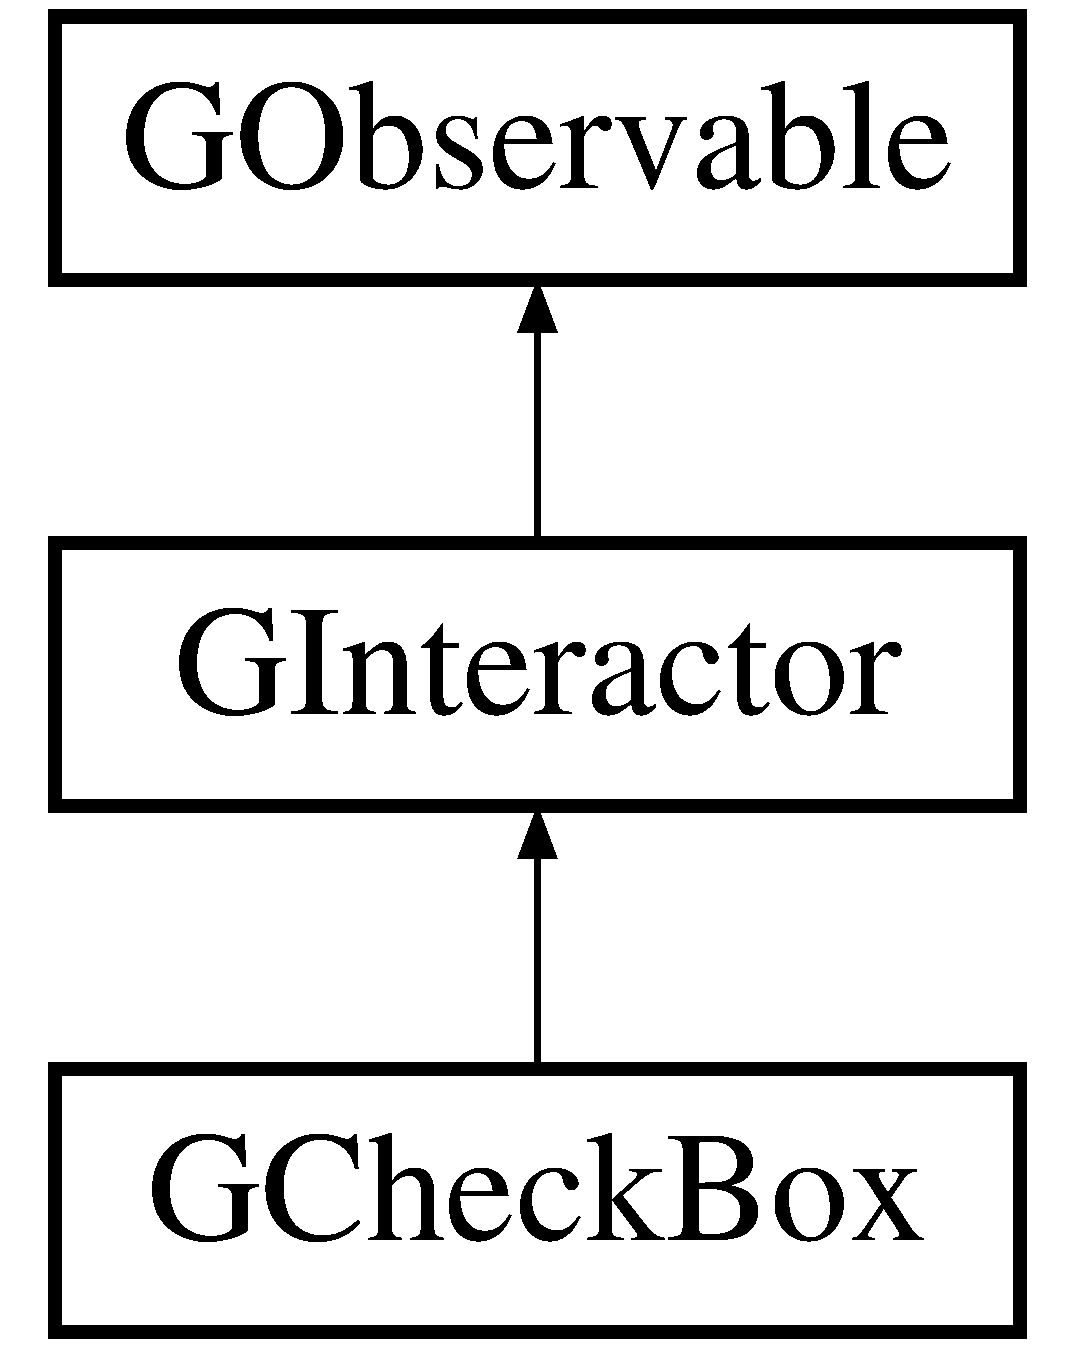
\includegraphics[height=3.000000cm]{classGCheckBox}
\end{center}
\end{figure}
\subsection*{Public Types}
\begin{DoxyCompactItemize}
\item 
enum \mbox{\hyperlink{classGInteractor_a8e0d441725a81d2bbdebbea09078260e}{Text\+Position}} \{ \mbox{\hyperlink{classGInteractor_a8e0d441725a81d2bbdebbea09078260ea4cd6f2e7d5a08d6f4dc052df2358f774}{T\+E\+X\+T\+\_\+\+B\+E\+S\+I\+D\+E\+\_\+\+I\+C\+ON}}, 
\mbox{\hyperlink{classGInteractor_a8e0d441725a81d2bbdebbea09078260eaa88490f63d8de68d44c83bdb2ecde3b3}{T\+E\+X\+T\+\_\+\+U\+N\+D\+E\+R\+\_\+\+I\+C\+ON}}, 
\mbox{\hyperlink{classGInteractor_a8e0d441725a81d2bbdebbea09078260ea39a6f388a30ac4fefb6eb13e846bc9f2}{T\+E\+X\+T\+\_\+\+O\+N\+LY}}
 \}
\begin{DoxyCompactList}\small\item\em The places where an interactor can place its text relative to its icon. \end{DoxyCompactList}\end{DoxyCompactItemize}
\subsection*{Public Member Functions}
\begin{DoxyCompactItemize}
\item 
\mbox{\hyperlink{classGCheckBox_ab79c27853bb6f5b8ec3ea139ef556f25}{G\+Check\+Box}} (const std\+::string \&text=\char`\"{}\char`\"{}, bool checked=false, Q\+Widget $\ast$parent=nullptr)
\begin{DoxyCompactList}\small\item\em Creates a checkbox with the given text. \end{DoxyCompactList}\item 
\mbox{\hyperlink{classGCheckBox_a40853b1ff7d4f861d33054a5df7fb86d}{$\sim$\+G\+Check\+Box}} () override
\begin{DoxyCompactList}\small\item\em Frees memory allocated internally by the checkbox. \end{DoxyCompactList}\item 
virtual void \mbox{\hyperlink{classGInteractor_a02f20ea6edfa0671f31c4c648a253833}{add\+Action\+Listener}} () Q\+\_\+\+D\+E\+C\+L\+\_\+\+D\+E\+P\+R\+E\+C\+A\+T\+ED
\begin{DoxyCompactList}\small\item\em Adds an event listener to be notified when this interactor is clicked or generally interacted with. \end{DoxyCompactList}\item 
bool \mbox{\hyperlink{classGInteractor_a597a370b592e3737d38d9d2f4e2031ea}{events\+Enabled}} () const override
\begin{DoxyCompactList}\small\item\em Returns true if this interactor is currently accepting events. \end{DoxyCompactList}\item 
virtual std\+::string \mbox{\hyperlink{classGInteractor_a69f8d23ed8f207fbecad99960776e942}{get\+Accelerator}} () const
\begin{DoxyCompactList}\small\item\em Returns a string representing a hotkey for this interactor, or an empty string if no accelerator has been set. \end{DoxyCompactList}\item 
std\+::string \mbox{\hyperlink{classGCheckBox_a4f83505141da1f8446f0e0e0a9507930}{get\+Action\+Command}} () const override
\begin{DoxyCompactList}\small\item\em Returns an action command for this interactor, which is a semi-\/unique string you can use to identify it when events occur. \end{DoxyCompactList}\item 
virtual std\+::string \mbox{\hyperlink{classGInteractor_a808e22cc1fdfbecf71ed8c64ef4600e0}{get\+Background}} () const
\begin{DoxyCompactList}\small\item\em Returns the background color of the interactor as a string. \end{DoxyCompactList}\item 
virtual int \mbox{\hyperlink{classGInteractor_a9e827257a55cb8cf4d9de2ec6bcfd7a0}{get\+Background\+Int}} () const
\begin{DoxyCompactList}\small\item\em Returns the background color of the interactor as an R\+GB integer. \end{DoxyCompactList}\item 
virtual \mbox{\hyperlink{structGRectangle}{G\+Rectangle}} \mbox{\hyperlink{classGInteractor_a29e6ac35a0b48f491a4c88194cc5da3b}{get\+Bounds}} () const
\begin{DoxyCompactList}\small\item\em Returns a rectangle representing the x/y position and size of this interactor. \end{DoxyCompactList}\item 
virtual std\+::string \mbox{\hyperlink{classGInteractor_aa061dfa488c31e18549d64363c1d0e34}{get\+Color}} () const
\begin{DoxyCompactList}\small\item\em Returns the foreground/text color of the interactor as a string. \end{DoxyCompactList}\item 
virtual int \mbox{\hyperlink{classGInteractor_a9635c7af766cdc3417f346683fa0e6c1}{get\+Color\+Int}} () const
\begin{DoxyCompactList}\small\item\em Returns the foreground/text color of the interactor as an R\+GB integer. \end{DoxyCompactList}\item 
virtual \mbox{\hyperlink{classGContainer}{G\+Container}} $\ast$ \mbox{\hyperlink{classGInteractor_a7a6e317c29d61030929b4cd2d1c00fe7}{get\+Container}} () const
\begin{DoxyCompactList}\small\item\em Returns a pointer to the onscreen container holding this interactor. \end{DoxyCompactList}\item 
virtual std\+::string \mbox{\hyperlink{classGInteractor_a894a5502900794eeb27d084c21f1d77d}{get\+Font}} () const
\begin{DoxyCompactList}\small\item\em Returns the font of this interactor\textquotesingle{}s text as a font string such as \char`\"{}\+Helvetica-\/12-\/\+Bold\char`\"{}. \end{DoxyCompactList}\item 
virtual std\+::string \mbox{\hyperlink{classGInteractor_a4fa2d8b0192a3a5b4af4bbfe71194d03}{get\+Foreground}} () const
\begin{DoxyCompactList}\small\item\em Returns the foreground/text color of the interactor as a string. \end{DoxyCompactList}\item 
virtual int \mbox{\hyperlink{classGInteractor_ac3b12ab385a6ef9ae90fc879860ba726}{get\+Foreground\+Int}} () const
\begin{DoxyCompactList}\small\item\em Returns the foreground/text color of the interactor as an R\+GB integer. \end{DoxyCompactList}\item 
virtual double \mbox{\hyperlink{classGInteractor_a1e7e353362434072875264cf95629f99}{get\+Height}} () const
\begin{DoxyCompactList}\small\item\em Returns the current onscreen height of this interactor in pixels. \end{DoxyCompactList}\item 
virtual std\+::string \mbox{\hyperlink{classGInteractor_aaed62a73004939a64da6f0eb9eb64d73}{get\+Icon}} () const
\begin{DoxyCompactList}\small\item\em Returns the file name of the icon associated with this interactor, or an empty string if no icon has been set. \end{DoxyCompactList}\item 
virtual int \mbox{\hyperlink{classGInteractor_a9c9659a6c6ba66b4107ba59c95a24241}{get\+ID}} () const
\begin{DoxyCompactList}\small\item\em Returns a globally unique identifier for this interactor, which is set when the interactor is constructed. \end{DoxyCompactList}\item 
\+\_\+\+Internal\+\_\+\+Q\+Widget $\ast$ \mbox{\hyperlink{classGCheckBox_a2f6b36b2517087dc90a366b5ce1f5323}{get\+Internal\+Widget}} () const override
\begin{DoxyCompactList}\small\item\em Returns a direct pointer to the internal Qt widget being wrapped by this interactor. \end{DoxyCompactList}\item 
virtual \mbox{\hyperlink{structGPoint}{G\+Point}} \mbox{\hyperlink{classGInteractor_a4f83802015511edeb63b892830812c11}{get\+Location}} () const
\begin{DoxyCompactList}\small\item\em Returns an (x, y) point representing the onscreen location of the top-\/left corner of this interactor within its containing window. \end{DoxyCompactList}\item 
virtual double \mbox{\hyperlink{classGInteractor_aed4b0075fcc434499c3cb3e46896bda3}{get\+Minimum\+Height}} () const
\begin{DoxyCompactList}\small\item\em Returns the minimum height in pixels that this interactor will permit itself to be resized to. \end{DoxyCompactList}\item 
virtual \mbox{\hyperlink{structGDimension}{G\+Dimension}} \mbox{\hyperlink{classGInteractor_a66b5af0b32493b4d597ca0a3df2049ea}{get\+Minimum\+Size}} () const
\begin{DoxyCompactList}\small\item\em Returns a \mbox{\hyperlink{structGDimension}{G\+Dimension}} structure representing the minimum size in pixels that this interactor will permit itself to be resized to. \end{DoxyCompactList}\item 
virtual double \mbox{\hyperlink{classGInteractor_a59e668114fe3d49d2a0f28deb258f7c8}{get\+Minimum\+Width}} () const
\begin{DoxyCompactList}\small\item\em Returns the minimum width in pixels that this interactor will permit itself to be resized to. \end{DoxyCompactList}\item 
virtual std\+::string \mbox{\hyperlink{classGInteractor_a8a60438a5b55d0b2ceb35c8674b9d8c5}{get\+Name}} () const
\begin{DoxyCompactList}\small\item\em Returns a string representing a unique name for this interactor. \end{DoxyCompactList}\item 
virtual double \mbox{\hyperlink{classGInteractor_a747de0961653847bdc6615dbf756d715}{get\+Preferred\+Height}} () const
\begin{DoxyCompactList}\small\item\em Returns the height in pixels that this interactor would prefer to be, which would exactly fit its contents with no stretching or scrollbars. \end{DoxyCompactList}\item 
virtual \mbox{\hyperlink{structGDimension}{G\+Dimension}} \mbox{\hyperlink{classGInteractor_a4aabbee761d8e9116275401131b7ccd1}{get\+Preferred\+Size}} () const
\begin{DoxyCompactList}\small\item\em Returns a \mbox{\hyperlink{structGDimension}{G\+Dimension}} structure storing the width and height in pixels that this interactor would prefer to be, which would exactly fit its contents with no stretching or scrollbars. \end{DoxyCompactList}\item 
virtual double \mbox{\hyperlink{classGInteractor_a82bca31d37700fb0e35d2743352efd5e}{get\+Preferred\+Width}} () const
\begin{DoxyCompactList}\small\item\em Returns the height in pixels that this interactor would prefer to be, which would exactly fit its contents with no stretching or scrollbars. \end{DoxyCompactList}\item 
virtual \mbox{\hyperlink{structGDimension}{G\+Dimension}} \mbox{\hyperlink{classGInteractor_a7b4eec96a2bdc6420695d5796a78eea9}{get\+Size}} () const
\begin{DoxyCompactList}\small\item\em Returns a \mbox{\hyperlink{structGDimension}{G\+Dimension}} structure storing the current onscreen width and height of this interactor in pixels. \end{DoxyCompactList}\item 
virtual std\+::string \mbox{\hyperlink{classGCheckBox_aff553c50924b836c29f146ed34a7c6ec}{get\+Text}} () const
\begin{DoxyCompactList}\small\item\em Returns the text next to the checkbox. \end{DoxyCompactList}\item 
std\+::string \mbox{\hyperlink{classGCheckBox_a9b72ede4ee8520f987a0c01e30654814}{get\+Type}} () const override
\begin{DoxyCompactList}\small\item\em Returns a string representing the class name of this interactor, such as \char`\"{}\+G\+Button\char`\"{} or \char`\"{}\+G\+Check\+Box\char`\"{}. \end{DoxyCompactList}\item 
Q\+Widget $\ast$ \mbox{\hyperlink{classGCheckBox_a3b33a602b31a6b809d020535a59db3b4}{get\+Widget}} () const override
\begin{DoxyCompactList}\small\item\em Returns a direct pointer to the internal Qt widget being wrapped by this interactor. \end{DoxyCompactList}\item 
virtual double \mbox{\hyperlink{classGInteractor_a0ed2965abd4f5701d2cadf71239faf19}{get\+Width}} () const
\begin{DoxyCompactList}\small\item\em Returns the current onscreen width of this interactor in pixels. \end{DoxyCompactList}\item 
virtual double \mbox{\hyperlink{classGInteractor_a344385751bee0720059403940d57a13e}{getX}} () const
\begin{DoxyCompactList}\small\item\em Returns the x-\/coordinate of the top-\/left pixel of this interactor within its onscreen window. \end{DoxyCompactList}\item 
virtual double \mbox{\hyperlink{classGInteractor_aafa51c7f8f38a09febbb9ce7853f77b4}{getY}} () const
\begin{DoxyCompactList}\small\item\em Returns the y-\/coordinate of the top-\/left pixel of this interactor within its onscreen window. \end{DoxyCompactList}\item 
virtual bool \mbox{\hyperlink{classGInteractor_afc480f652b8c5f1fb255e2269ce68879}{in\+Bounds}} (double x, double y) const
\begin{DoxyCompactList}\small\item\em Returns true if the given x/y pixel is within the bounds of this interactor. \end{DoxyCompactList}\item 
virtual bool \mbox{\hyperlink{classGInteractor_ae6d7982c1c627b677a5e776ca86118ed}{in\+Bounds}} (int x, int y) const
\begin{DoxyCompactList}\small\item\em Returns true if the given x/y pixel is within the bounds of this interactor. \end{DoxyCompactList}\item 
virtual bool \mbox{\hyperlink{classGCheckBox_ac8cada18b9357ff68b26e17f44294764}{is\+Checked}} () const
\begin{DoxyCompactList}\small\item\em Returns true if the checkbox is currently checked. \end{DoxyCompactList}\item 
virtual bool \mbox{\hyperlink{classGInteractor_aacb819fb241851fd9fc045271baa4034}{is\+Enabled}} () const
\begin{DoxyCompactList}\small\item\em Returns true if this interactor is currently enabled. \end{DoxyCompactList}\item 
virtual bool \mbox{\hyperlink{classGCheckBox_a56a065a2c20a230931de0ed98019d8fb}{is\+Selected}} () const
\begin{DoxyCompactList}\small\item\em Returns true if the checkbox is currently checked. \end{DoxyCompactList}\item 
virtual bool \mbox{\hyperlink{classGInteractor_a9d8a6cfb13917785c143e74d40e4e2be}{is\+Visible}} () const
\begin{DoxyCompactList}\small\item\em Returns true if the interactor is visible on the screen. \end{DoxyCompactList}\item 
virtual void \mbox{\hyperlink{classGInteractor_ab7fe7a876367b87cf7202f947f1d05e4}{remove\+Action\+Listener}} ()
\begin{DoxyCompactList}\small\item\em Removes the action listener from this interactor so that it will no longer call it when events occur. \end{DoxyCompactList}\item 
virtual void \mbox{\hyperlink{classGInteractor_ad39d0325cde6b97ebda4b9d7787c633b}{remove\+Click\+Listener}} ()
\begin{DoxyCompactList}\small\item\em Removes the click listener from this interactor so that it will no longer call it when events occur. \end{DoxyCompactList}\item 
virtual void \mbox{\hyperlink{classGInteractor_aa4250907e4cdd77349c04f0cf5cdd3d3}{remove\+Double\+Click\+Listener}} ()
\begin{DoxyCompactList}\small\item\em Removes the double-\/click listener from this interactor so that it will no longer call it when events occur. \end{DoxyCompactList}\item 
virtual void \mbox{\hyperlink{classGInteractor_a43095f41cab3be732b49f29970484b05}{remove\+Key\+Listener}} ()
\begin{DoxyCompactList}\small\item\em Removes the key listener from this interactor so that it will no longer call it when key events occur. \end{DoxyCompactList}\item 
virtual void \mbox{\hyperlink{classGInteractor_aff47f71ce47e688a07c9d38dc92fcc11}{remove\+Mouse\+Listener}} ()
\begin{DoxyCompactList}\small\item\em Removes the mouse listener from this interactor so that it will no longer call it when events occur. \end{DoxyCompactList}\item 
virtual void \mbox{\hyperlink{classGInteractor_a519fb2ac767f8b2febbb50b898b8c8cb}{request\+Focus}} ()
\begin{DoxyCompactList}\small\item\em Transfers keyboard focus to this interactor. \end{DoxyCompactList}\item 
virtual void \mbox{\hyperlink{classGInteractor_ad15f102f62e2960576012f1aa0ba4b2e}{set\+Accelerator}} (const std\+::string \&accelerator)
\begin{DoxyCompactList}\small\item\em Sets an accelerator hotkey for this interactor, such as \char`\"{}\+Ctrl-\/\+S\char`\"{}. \end{DoxyCompactList}\item 
virtual void \mbox{\hyperlink{classGInteractor_a4b5843fe3030e038a1ba54cc03389bcf}{set\+Action\+Command}} (const std\+::string \&action\+Command)
\begin{DoxyCompactList}\small\item\em Sets the action command for this interactor. \end{DoxyCompactList}\item 
virtual void \mbox{\hyperlink{classGInteractor_adcfb4742430c88714fcf57e57ab8ea9c}{set\+Action\+Listener}} (G\+Event\+Listener func)
\begin{DoxyCompactList}\small\item\em Sets an action listener on this interactor so that it will be called when it is interacted with in its primary way. \end{DoxyCompactList}\item 
virtual void \mbox{\hyperlink{classGInteractor_aebd20a89c7a8a43a6fce999cf4f9fcf2}{set\+Action\+Listener}} (G\+Event\+Listener\+Void func)
\begin{DoxyCompactList}\small\item\em Sets an action listener on this interactor so that it will be called when it is interacted with in its primary way. \end{DoxyCompactList}\item 
virtual void \mbox{\hyperlink{classGInteractor_acba7e546c2025c0a15ca4b4cc92043db}{set\+Background}} (int rgb)
\begin{DoxyCompactList}\small\item\em Sets the background color of the interactor to the color represented by the given R\+GB integer. \end{DoxyCompactList}\item 
virtual void \mbox{\hyperlink{classGInteractor_ab4677ab2474e68b07aa56605af92a84a}{set\+Background}} (const std\+::string \&color)
\begin{DoxyCompactList}\small\item\em Sets the background color of the interactor to the color represented by the given string. \end{DoxyCompactList}\item 
virtual void \mbox{\hyperlink{classGInteractor_a2aae8197624b72265ab83b4f1bc73f2f}{set\+Bounds}} (double x, double y, double width, double height)
\begin{DoxyCompactList}\small\item\em Sets the size and location of the widget. \end{DoxyCompactList}\item 
virtual void \mbox{\hyperlink{classGInteractor_acada386653f008cacc7cce86426bef7c}{set\+Bounds}} (const \mbox{\hyperlink{structGRectangle}{G\+Rectangle}} \&size)
\begin{DoxyCompactList}\small\item\em Sets the size and location of the widget. \end{DoxyCompactList}\item 
virtual void \mbox{\hyperlink{classGCheckBox_a116285e2f56247b00b26035ca0ac4737}{set\+Checked}} (bool checked)
\begin{DoxyCompactList}\small\item\em Sets whether the checkbox should be checked. \end{DoxyCompactList}\item 
virtual void \mbox{\hyperlink{classGInteractor_abd40af6921242584d0954f173911b190}{set\+Click\+Listener}} (G\+Event\+Listener func)
\begin{DoxyCompactList}\small\item\em Sets a mouse listener on this interactor so that it will be called when the mouse is clicked on it. \end{DoxyCompactList}\item 
virtual void \mbox{\hyperlink{classGInteractor_a856414c92df90f56f3877475eb3f8fc4}{set\+Click\+Listener}} (G\+Event\+Listener\+Void func)
\begin{DoxyCompactList}\small\item\em Sets a mouse listener on this interactor so that it will be called when the mouse is clicked on it. \end{DoxyCompactList}\item 
virtual void \mbox{\hyperlink{classGInteractor_ab1f5cc0f5cc6bbbd716a526c61f1081d}{set\+Color}} (int rgb)
\begin{DoxyCompactList}\small\item\em Sets the foreground/text color of the interactor to the color represented by the given R\+GB integer. \end{DoxyCompactList}\item 
virtual void \mbox{\hyperlink{classGInteractor_a61374df6c11b52cfbb0815decdbaebc6}{set\+Color}} (const std\+::string \&color)
\begin{DoxyCompactList}\small\item\em Sets the foreground/text color of the interactor to the color represented by the given string. \end{DoxyCompactList}\item 
virtual void \mbox{\hyperlink{classGInteractor_ac29f9a3462458e165fae3a1f046ee77a}{set\+Double\+Click\+Listener}} (G\+Event\+Listener func)
\begin{DoxyCompactList}\small\item\em Sets a mouse listener on this interactor so that it will be called when the mouse is double-\/clicked on it. \end{DoxyCompactList}\item 
virtual void \mbox{\hyperlink{classGInteractor_a50096194d66f48c92dd4c512d41bfc76}{set\+Double\+Click\+Listener}} (G\+Event\+Listener\+Void func)
\begin{DoxyCompactList}\small\item\em Sets a mouse listener on this interactor so that it will be called when the mouse is double-\/clicked on it. \end{DoxyCompactList}\item 
virtual void \mbox{\hyperlink{classGInteractor_ab831367dd84bbd579e02e55bacb21343}{set\+Enabled}} (bool value)
\begin{DoxyCompactList}\small\item\em Sets whether this interactor is currently enabled. \end{DoxyCompactList}\item 
virtual void \mbox{\hyperlink{classGObservable_afaa30b2a9e0f378fd1c70d2f1d0b8216}{set\+Events\+Enabled}} (bool \mbox{\hyperlink{classGInteractor_a597a370b592e3737d38d9d2f4e2031ea}{events\+Enabled}})
\begin{DoxyCompactList}\small\item\em Sets whether the object is currently allowing itself to fire events. \end{DoxyCompactList}\item 
virtual void \mbox{\hyperlink{classGInteractor_a2592348886ffea646c6534bf88f7c49d}{set\+Font}} (const Q\+Font \&font)
\begin{DoxyCompactList}\small\item\em Sets the font used by this widget to the given Qt font. \end{DoxyCompactList}\item 
virtual void \mbox{\hyperlink{classGInteractor_a8e096e8818d838aceae1d46d58fb3a7b}{set\+Font}} (const std\+::string \&font)
\begin{DoxyCompactList}\small\item\em Sets the font used by this widget to the font represented by the given font string, such as \char`\"{}\+Helvetica-\/16-\/\+Bold\char`\"{}. \end{DoxyCompactList}\item 
virtual void \mbox{\hyperlink{classGInteractor_a9eb856b5ff83a19df3831a31f15f4563}{set\+Foreground}} (int rgb)
\begin{DoxyCompactList}\small\item\em Sets the foreground/text color of the interactor to the color represented by the given R\+GB integer. \end{DoxyCompactList}\item 
virtual void \mbox{\hyperlink{classGInteractor_af59209aeadea6dfc6d97a2d8531f50e1}{set\+Foreground}} (const std\+::string \&color)
\begin{DoxyCompactList}\small\item\em Sets the foreground/text color of the interactor to the color represented by the given string. \end{DoxyCompactList}\item 
virtual void \mbox{\hyperlink{classGInteractor_a9e280bfc4544dfaf8e4376c4e1a74357}{set\+Height}} (double height)
\begin{DoxyCompactList}\small\item\em Sets the onscreen height of the interactor in pixels. \end{DoxyCompactList}\item 
virtual void \mbox{\hyperlink{classGInteractor_a542abfcd7261751352af129c7215ecda}{set\+Icon}} (const Q\+Icon \&icon)
\begin{DoxyCompactList}\small\item\em Sets the icon associated with this interactor. \end{DoxyCompactList}\item 
virtual void \mbox{\hyperlink{classGInteractor_a368e1a338f84401c284506d03b1ba769}{set\+Icon}} (const Q\+Pixmap \&icon)
\begin{DoxyCompactList}\small\item\em Sets the icon associated with this interactor. \end{DoxyCompactList}\item 
virtual void \mbox{\hyperlink{classGInteractor_a762e139aa311461c3984d3ad28293f64}{set\+Icon}} (const std\+::string \&filename, bool retain\+Icon\+Size=true)
\begin{DoxyCompactList}\small\item\em Sets the file name of the icon associated with this interactor, or an empty string if no icon has been set. \end{DoxyCompactList}\item 
virtual void \mbox{\hyperlink{classGInteractor_aeb8324d3287fa1fbe093f4d6230cf0a6}{set\+Key\+Listener}} (G\+Event\+Listener func)
\begin{DoxyCompactList}\small\item\em Sets a key listener on this interactor so that it will be called when the user presses any key. \end{DoxyCompactList}\item 
virtual void \mbox{\hyperlink{classGInteractor_ae48ecea73606c7bd9423e1c7cc589cc9}{set\+Key\+Listener}} (G\+Event\+Listener\+Void func)
\begin{DoxyCompactList}\small\item\em Sets a key listener on this interactor so that it will be called when the user presses any key. \end{DoxyCompactList}\item 
virtual void \mbox{\hyperlink{classGInteractor_a04594e8ba9b98513a64f1da00dcae18c}{set\+Location}} (double x, double y)
\begin{DoxyCompactList}\small\item\em Sets the onscreen x/y-\/coordinate of the top-\/left corner of the interactor relative to its window. \end{DoxyCompactList}\item 
virtual void \mbox{\hyperlink{classGInteractor_a0cf428e207b7f22cc08138a90b1b87b2}{set\+Minimum\+Size}} (double width, double height)
\begin{DoxyCompactList}\small\item\em Sets the minimum size in pixels that this interactor will permit itself to be resized to. \end{DoxyCompactList}\item 
virtual void \mbox{\hyperlink{classGInteractor_a3b1046117ac6cb7abe467e00ba8a81f4}{set\+Minimum\+Size}} (const \mbox{\hyperlink{structGDimension}{G\+Dimension}} \&size)
\begin{DoxyCompactList}\small\item\em Sets the minimum size in pixels that this interactor will permit itself to be resized to. \end{DoxyCompactList}\item 
virtual void \mbox{\hyperlink{classGInteractor_a37d8dbc943f59920f705b0104f60bde2}{set\+Mouse\+Listener}} (G\+Event\+Listener func)
\begin{DoxyCompactList}\small\item\em Sets a mouse listener on this interactor so that it will be called when the mouse is moved or clicked on it. \end{DoxyCompactList}\item 
virtual void \mbox{\hyperlink{classGInteractor_aea7f647ea62d59f71b5fad6aa65eeaf9}{set\+Mouse\+Listener}} (G\+Event\+Listener\+Void func)
\begin{DoxyCompactList}\small\item\em Sets a mouse listener on this interactor so that it will be called when the mouse is moved or clicked on it. \end{DoxyCompactList}\item 
virtual void \mbox{\hyperlink{classGInteractor_a9d3a2685df23b5e7cbf59c19c4a1f9b5}{set\+Name}} (const std\+::string \&name)
\begin{DoxyCompactList}\small\item\em Sets a string representing a unique name for this interactor. \end{DoxyCompactList}\item 
virtual void \mbox{\hyperlink{classGInteractor_a1ab987704fce32098706c6f00fb08218}{set\+Preferred\+Height}} (double height)
\begin{DoxyCompactList}\small\item\em Sets the height in pixels that this interactor would prefer to be. \end{DoxyCompactList}\item 
virtual void \mbox{\hyperlink{classGInteractor_a042c5ae19430d765ef552371cae3632c}{set\+Preferred\+Size}} (double width, double height)
\begin{DoxyCompactList}\small\item\em Sets the width and height in pixels that this interactor would prefer to be. \end{DoxyCompactList}\item 
virtual void \mbox{\hyperlink{classGInteractor_aa22d9be4bc0e078bb0ea69b0fc9d7c75}{set\+Preferred\+Size}} (const \mbox{\hyperlink{structGDimension}{G\+Dimension}} \&size)
\begin{DoxyCompactList}\small\item\em Sets the size in pixels that this interactor would prefer to be. \end{DoxyCompactList}\item 
virtual void \mbox{\hyperlink{classGInteractor_a3db429ab2fa52efd187eec0ed8cdd9f2}{set\+Preferred\+Width}} (double width)
\begin{DoxyCompactList}\small\item\em Sets the width in pixels that this interactor would prefer to be. \end{DoxyCompactList}\item 
virtual void \mbox{\hyperlink{classGCheckBox_ad42accd39af295a957386c68dac3dcae}{set\+Selected}} (bool selected)
\begin{DoxyCompactList}\small\item\em Sets whether the checkbox should be checked. \end{DoxyCompactList}\item 
virtual void \mbox{\hyperlink{classGInteractor_aca25d49481f9bf5fc8f7df4c086c4ce7}{set\+Size}} (double width, double height)
\begin{DoxyCompactList}\small\item\em Sets the onscreen width and height of the interactor in pixels. \end{DoxyCompactList}\item 
virtual void \mbox{\hyperlink{classGInteractor_ae2b628228f192c2702c4ce941b2af68f}{set\+Size}} (const \mbox{\hyperlink{structGDimension}{G\+Dimension}} \&size)
\begin{DoxyCompactList}\small\item\em Sets the onscreen width and height of the interactor in pixels. \end{DoxyCompactList}\item 
virtual void \mbox{\hyperlink{classGCheckBox_ac1ae51949d41ee9054634be5967d91b8}{set\+Text}} (const std\+::string \&text)
\begin{DoxyCompactList}\small\item\em Sets the text that will appear next to the checkbox. \end{DoxyCompactList}\item 
virtual void \mbox{\hyperlink{classGInteractor_a039e0e49beaecc275efce02d416acea8}{set\+Tooltip}} (const std\+::string \&tooltip\+Text)
\begin{DoxyCompactList}\small\item\em Sets a \char`\"{}tooltip\char`\"{} that will appear if the user hovers their mouse over the interactor. \end{DoxyCompactList}\item 
virtual void \mbox{\hyperlink{classGInteractor_a18e44e30b31525a243960ca3928125aa}{set\+Visible}} (bool visible)
\begin{DoxyCompactList}\small\item\em Returns true if the interactor is visible on the screen. \end{DoxyCompactList}\item 
virtual void \mbox{\hyperlink{classGInteractor_aa3f3fba4cb131baa8696ba01e3bceca1}{set\+Width}} (double width)
\begin{DoxyCompactList}\small\item\em Sets the onscreen width of the interactor in pixels. \end{DoxyCompactList}\item 
virtual void \mbox{\hyperlink{classGInteractor_a9c18fcc579333bf9653d13ad2b372e39}{setX}} (double x)
\begin{DoxyCompactList}\small\item\em Sets the onscreen x-\/coordinate of the top-\/left corner of the interactor relative to its window. \end{DoxyCompactList}\item 
virtual void \mbox{\hyperlink{classGInteractor_a7d57e2a5c35d27feb58fd498a3cf82b9}{setY}} (double y)
\begin{DoxyCompactList}\small\item\em Sets the onscreen y-\/coordinate of the top-\/left corner of the interactor relative to its window. \end{DoxyCompactList}\item 
virtual void \mbox{\hyperlink{classGCheckBox_ad277193b2dca0bab1e0ad24d45407dc3}{toggle}} ()
\begin{DoxyCompactList}\small\item\em Reverses the checked state of the box, setting it to be checked if it was unchecked or to be unchecked if it was checked. \end{DoxyCompactList}\item 
virtual std\+::string \mbox{\hyperlink{classGObservable_a1fe5121d6528fdea3f243321b3fa3a49}{to\+String}} () const
\begin{DoxyCompactList}\small\item\em Returns a string representation of this observable object\textquotesingle{}s state. \end{DoxyCompactList}\end{DoxyCompactItemize}
\subsection*{Protected Member Functions}
\begin{DoxyCompactItemize}
\item 
virtual void \mbox{\hyperlink{classGObservable_a80cfa040459ff53594adbd6a51ec8f43}{clear\+Event\+Listeners}} ()
\begin{DoxyCompactList}\small\item\em Removes all event listeners from this object. \end{DoxyCompactList}\item 
virtual void \mbox{\hyperlink{classGObservable_a284f31528c0520f8e545c03ac9eeac74}{ensure\+Thread\+Safety}} (const std\+::string \&member\+Name=\char`\"{}\char`\"{})
\begin{DoxyCompactList}\small\item\em Ensures that we are currently in the Qt G\+UI thread. \end{DoxyCompactList}\item 
virtual void \mbox{\hyperlink{classGObservable_a63e5e5a6227c59c928493b11aceb0f67}{fire\+Event}} (\mbox{\hyperlink{classGEvent}{G\+Event}} \&event)
\begin{DoxyCompactList}\small\item\em Sends out the given event to any attached listeners. \end{DoxyCompactList}\item 
virtual void \mbox{\hyperlink{classGObservable_ab3983ea07337b52020a29cc00c653d8d}{fire\+G\+Event}} (Q\+Event $\ast$event, Event\+Type event\+Type, const std\+::string \&event\+Name)
\begin{DoxyCompactList}\small\item\em Creates an event of the given type, then sends it out to any attached listeners. \end{DoxyCompactList}\item 
virtual void \mbox{\hyperlink{classGObservable_a01fdf1b0e0dbd49e189fe4514e010411}{fire\+G\+Event}} (Q\+Close\+Event $\ast$event, Event\+Type event\+Type, const std\+::string \&event\+Name)
\begin{DoxyCompactList}\small\item\em Creates an event of the given type, then sends it out to any attached listeners. \end{DoxyCompactList}\item 
virtual void \mbox{\hyperlink{classGObservable_abb0b2f66ba39211cb5d7615e9d1c04e2}{fire\+G\+Event}} (Q\+Key\+Event $\ast$event, Event\+Type event\+Type, const std\+::string \&event\+Name)
\begin{DoxyCompactList}\small\item\em Creates an event of the given type, then sends it out to any attached listeners. \end{DoxyCompactList}\item 
virtual void \mbox{\hyperlink{classGObservable_a119318675d2165bdf7dd853aaf881d4b}{fire\+G\+Event}} (Q\+Mouse\+Event $\ast$event, Event\+Type event\+Type, const std\+::string \&event\+Name, const std\+::string \&action\+Command=\char`\"{}\char`\"{})
\begin{DoxyCompactList}\small\item\em Creates an event of the given type, then sends it out to any attached listeners. \end{DoxyCompactList}\item 
virtual void \mbox{\hyperlink{classGObservable_a63fd9034e1e1633c1c38eb342bfd34e9}{fire\+G\+Event}} (Q\+Resize\+Event $\ast$event, Event\+Type event\+Type, const std\+::string \&event\+Name)
\begin{DoxyCompactList}\small\item\em Creates an event of the given type, then sends it out to any attached listeners. \end{DoxyCompactList}\item 
virtual void \mbox{\hyperlink{classGObservable_a741345310d9b7c5170a6cbc410c44ac4}{fire\+G\+Event}} (Q\+Timer\+Event $\ast$event, Event\+Type event\+Type, const std\+::string \&event\+Name)
\begin{DoxyCompactList}\small\item\em Creates an event of the given type, then sends it out to any attached listeners. \end{DoxyCompactList}\item 
virtual void \mbox{\hyperlink{classGObservable_a93bf338968a0338761b8e4dc62f582e9}{fire\+G\+Event}} (Q\+Wheel\+Event $\ast$event, Event\+Type event\+Type, const std\+::string \&event\+Name)
\begin{DoxyCompactList}\small\item\em Creates an event of the given type, then sends it out to any attached listeners. \end{DoxyCompactList}\item 
virtual void \mbox{\hyperlink{classGObservable_a2a70a7d7435ff0c3b80bb4d70da19e0d}{fire\+G\+Event}} (Q\+Window\+State\+Change\+Event $\ast$event, Event\+Type event\+Type, const std\+::string \&event\+Name)
\begin{DoxyCompactList}\small\item\em Creates an event of the given type, then sends it out to any attached listeners. \end{DoxyCompactList}\item 
virtual bool \mbox{\hyperlink{classGObservable_a9f6faaa25942923bafa1c44020c49fa9}{has\+Event\+Listener}} (const std\+::string \&event\+Name) const
\begin{DoxyCompactList}\small\item\em Returns true if the observable object has a listener for the given type of event. \end{DoxyCompactList}\item 
virtual bool \mbox{\hyperlink{classGObservable_aeec1adc19aa0f33de62390686ee1382c}{is\+Accepting\+Event}} (int event\+Mask) const
\begin{DoxyCompactList}\small\item\em Returns true if the observable object has a listener for the given type of event. \end{DoxyCompactList}\item 
virtual bool \mbox{\hyperlink{classGObservable_aa31c73145a29dcb92848a92e0cfaea41}{is\+Accepting\+Event}} (const \mbox{\hyperlink{classGEvent}{G\+Event}} \&event) const
\begin{DoxyCompactList}\small\item\em Returns true if the observable object has a listener for the given type of event. \end{DoxyCompactList}\item 
virtual bool \mbox{\hyperlink{classGObservable_a3b1c689267eda44e65a2213e7de38b23}{is\+Accepting\+Event}} (const std\+::string \&event\+Type) const
\begin{DoxyCompactList}\small\item\em Returns true if the observable object has a listener for the given type of event. \end{DoxyCompactList}\item 
virtual void \mbox{\hyperlink{classGObservable_acbcf1ed3a851ad8a3c17ef38d86b481d}{remove\+Event\+Listener}} (const std\+::string \&event\+Name)
\begin{DoxyCompactList}\small\item\em Removes any event listener from this observable object that would respond to the given type of event, such as \char`\"{}click\char`\"{} or \char`\"{}keydown\char`\"{}. \end{DoxyCompactList}\item 
virtual void \mbox{\hyperlink{classGObservable_af51cc35c29a1bd1908609d432decdbb6}{remove\+Event\+Listeners}} (std\+::initializer\+\_\+list$<$ std\+::string $>$ event\+Names)
\begin{DoxyCompactList}\small\item\em Removes any event listener from this observable object that would respond to the given types of events, such as \char`\"{}click\char`\"{} or \char`\"{}keydown\char`\"{}. \end{DoxyCompactList}\item 
virtual void \mbox{\hyperlink{classGObservable_ad2f6d34961c50f6c1e0659990b79f741}{set\+Event\+Listener}} (const std\+::string \&event\+Name, G\+Event\+Listener func)
\begin{DoxyCompactList}\small\item\em Adds an event listener from this observable object to respond to the given type of event, such as \char`\"{}click\char`\"{} or \char`\"{}keydown\char`\"{}. \end{DoxyCompactList}\item 
virtual void \mbox{\hyperlink{classGObservable_abac4cb9f9e626e010e87f5d91573c8a5}{set\+Event\+Listener}} (const std\+::string \&event\+Name, G\+Event\+Listener\+Void func)
\begin{DoxyCompactList}\small\item\em Adds an event listener from this observable object to respond to the given type of event, such as \char`\"{}click\char`\"{} or \char`\"{}keydown\char`\"{}. \end{DoxyCompactList}\item 
virtual void \mbox{\hyperlink{classGObservable_afa388d69c33c718cf035774604065604}{set\+Event\+Listeners}} (std\+::initializer\+\_\+list$<$ std\+::string $>$ event\+Names, G\+Event\+Listener func)
\begin{DoxyCompactList}\small\item\em Adds an event listener from this observable object to respond to the given types of events, such as \char`\"{}click\char`\"{} or \char`\"{}keydown\char`\"{}. \end{DoxyCompactList}\item 
virtual void \mbox{\hyperlink{classGObservable_a7867184bbb686f74fae8a4db927da799}{set\+Event\+Listeners}} (std\+::initializer\+\_\+list$<$ std\+::string $>$ event\+Names, G\+Event\+Listener\+Void func)
\begin{DoxyCompactList}\small\item\em Adds an event listener from this observable object to respond to the given types of events, such as \char`\"{}click\char`\"{} or \char`\"{}keydown\char`\"{}. \end{DoxyCompactList}\end{DoxyCompactItemize}


\subsection{Detailed Description}
This interactor subclass represents an onscreen check box. 

Clicking once on the check box selects it; clicking again removes the selection. You can listen for clicks on a checkbox by setting an action listener, passing the function you want to call on each click. 

\subsection{Member Enumeration Documentation}
\mbox{\Hypertarget{classGInteractor_a8e0d441725a81d2bbdebbea09078260e}\label{classGInteractor_a8e0d441725a81d2bbdebbea09078260e}} 
\index{G\+Check\+Box@{G\+Check\+Box}!Text\+Position@{Text\+Position}}
\index{Text\+Position@{Text\+Position}!G\+Check\+Box@{G\+Check\+Box}}
\subsubsection{\texorpdfstring{Text\+Position}{TextPosition}}
{\footnotesize\ttfamily enum \mbox{\hyperlink{classGInteractor_a8e0d441725a81d2bbdebbea09078260e}{Text\+Position}}\hspace{0.3cm}{\ttfamily [inherited]}}



The places where an interactor can place its text relative to its icon. 

\begin{DoxyEnumFields}{Enumerator}
\raisebox{\heightof{T}}[0pt][0pt]{\index{T\+E\+X\+T\+\_\+\+B\+E\+S\+I\+D\+E\+\_\+\+I\+C\+ON@{T\+E\+X\+T\+\_\+\+B\+E\+S\+I\+D\+E\+\_\+\+I\+C\+ON}!G\+Check\+Box@{G\+Check\+Box}}\index{G\+Check\+Box@{G\+Check\+Box}!T\+E\+X\+T\+\_\+\+B\+E\+S\+I\+D\+E\+\_\+\+I\+C\+ON@{T\+E\+X\+T\+\_\+\+B\+E\+S\+I\+D\+E\+\_\+\+I\+C\+ON}}}\mbox{\Hypertarget{classGInteractor_a8e0d441725a81d2bbdebbea09078260ea4cd6f2e7d5a08d6f4dc052df2358f774}\label{classGInteractor_a8e0d441725a81d2bbdebbea09078260ea4cd6f2e7d5a08d6f4dc052df2358f774}} 
T\+E\+X\+T\+\_\+\+B\+E\+S\+I\+D\+E\+\_\+\+I\+C\+ON&\\
\hline

\raisebox{\heightof{T}}[0pt][0pt]{\index{T\+E\+X\+T\+\_\+\+U\+N\+D\+E\+R\+\_\+\+I\+C\+ON@{T\+E\+X\+T\+\_\+\+U\+N\+D\+E\+R\+\_\+\+I\+C\+ON}!G\+Check\+Box@{G\+Check\+Box}}\index{G\+Check\+Box@{G\+Check\+Box}!T\+E\+X\+T\+\_\+\+U\+N\+D\+E\+R\+\_\+\+I\+C\+ON@{T\+E\+X\+T\+\_\+\+U\+N\+D\+E\+R\+\_\+\+I\+C\+ON}}}\mbox{\Hypertarget{classGInteractor_a8e0d441725a81d2bbdebbea09078260eaa88490f63d8de68d44c83bdb2ecde3b3}\label{classGInteractor_a8e0d441725a81d2bbdebbea09078260eaa88490f63d8de68d44c83bdb2ecde3b3}} 
T\+E\+X\+T\+\_\+\+U\+N\+D\+E\+R\+\_\+\+I\+C\+ON&\\
\hline

\raisebox{\heightof{T}}[0pt][0pt]{\index{T\+E\+X\+T\+\_\+\+O\+N\+LY@{T\+E\+X\+T\+\_\+\+O\+N\+LY}!G\+Check\+Box@{G\+Check\+Box}}\index{G\+Check\+Box@{G\+Check\+Box}!T\+E\+X\+T\+\_\+\+O\+N\+LY@{T\+E\+X\+T\+\_\+\+O\+N\+LY}}}\mbox{\Hypertarget{classGInteractor_a8e0d441725a81d2bbdebbea09078260ea39a6f388a30ac4fefb6eb13e846bc9f2}\label{classGInteractor_a8e0d441725a81d2bbdebbea09078260ea39a6f388a30ac4fefb6eb13e846bc9f2}} 
T\+E\+X\+T\+\_\+\+O\+N\+LY&\\
\hline

\end{DoxyEnumFields}


\subsection{Constructor \& Destructor Documentation}
\mbox{\Hypertarget{classGCheckBox_ab79c27853bb6f5b8ec3ea139ef556f25}\label{classGCheckBox_ab79c27853bb6f5b8ec3ea139ef556f25}} 
\index{G\+Check\+Box@{G\+Check\+Box}!G\+Check\+Box@{G\+Check\+Box}}
\index{G\+Check\+Box@{G\+Check\+Box}!G\+Check\+Box@{G\+Check\+Box}}
\subsubsection{\texorpdfstring{G\+Check\+Box()}{GCheckBox()}}
{\footnotesize\ttfamily \mbox{\hyperlink{classGCheckBox}{G\+Check\+Box}} (\begin{DoxyParamCaption}\item[{const std\+::string \&}]{text = {\ttfamily \char`\"{}\char`\"{}},  }\item[{bool}]{checked = {\ttfamily false},  }\item[{Q\+Widget $\ast$}]{parent = {\ttfamily nullptr} }\end{DoxyParamCaption})}



Creates a checkbox with the given text. 

You can pass an optional second parameter to initially check the box. \mbox{\Hypertarget{classGCheckBox_a40853b1ff7d4f861d33054a5df7fb86d}\label{classGCheckBox_a40853b1ff7d4f861d33054a5df7fb86d}} 
\index{G\+Check\+Box@{G\+Check\+Box}!````~G\+Check\+Box@{$\sim$\+G\+Check\+Box}}
\index{````~G\+Check\+Box@{$\sim$\+G\+Check\+Box}!G\+Check\+Box@{G\+Check\+Box}}
\subsubsection{\texorpdfstring{$\sim$\+G\+Check\+Box()}{~GCheckBox()}}
{\footnotesize\ttfamily $\sim$\mbox{\hyperlink{classGCheckBox}{G\+Check\+Box}} (\begin{DoxyParamCaption}{ }\end{DoxyParamCaption})\hspace{0.3cm}{\ttfamily [override]}}



Frees memory allocated internally by the checkbox. 



\subsection{Member Function Documentation}
\mbox{\Hypertarget{classGInteractor_a02f20ea6edfa0671f31c4c648a253833}\label{classGInteractor_a02f20ea6edfa0671f31c4c648a253833}} 
\index{G\+Check\+Box@{G\+Check\+Box}!add\+Action\+Listener@{add\+Action\+Listener}}
\index{add\+Action\+Listener@{add\+Action\+Listener}!G\+Check\+Box@{G\+Check\+Box}}
\subsubsection{\texorpdfstring{add\+Action\+Listener()}{addActionListener()}}
{\footnotesize\ttfamily void add\+Action\+Listener (\begin{DoxyParamCaption}{ }\end{DoxyParamCaption})\hspace{0.3cm}{\ttfamily [virtual]}, {\ttfamily [inherited]}}



Adds an event listener to be notified when this interactor is clicked or generally interacted with. 

\begin{DoxyRefDesc}{Deprecated}
\item[\mbox{\hyperlink{deprecated__deprecated000006}{Deprecated}}]does nothing; use set\+Action\+Listener instead \end{DoxyRefDesc}
\mbox{\Hypertarget{classGObservable_a80cfa040459ff53594adbd6a51ec8f43}\label{classGObservable_a80cfa040459ff53594adbd6a51ec8f43}} 
\index{G\+Check\+Box@{G\+Check\+Box}!clear\+Event\+Listeners@{clear\+Event\+Listeners}}
\index{clear\+Event\+Listeners@{clear\+Event\+Listeners}!G\+Check\+Box@{G\+Check\+Box}}
\subsubsection{\texorpdfstring{clear\+Event\+Listeners()}{clearEventListeners()}}
{\footnotesize\ttfamily void clear\+Event\+Listeners (\begin{DoxyParamCaption}{ }\end{DoxyParamCaption})\hspace{0.3cm}{\ttfamily [protected]}, {\ttfamily [virtual]}, {\ttfamily [inherited]}}



Removes all event listeners from this object. 

\mbox{\Hypertarget{classGObservable_a284f31528c0520f8e545c03ac9eeac74}\label{classGObservable_a284f31528c0520f8e545c03ac9eeac74}} 
\index{G\+Check\+Box@{G\+Check\+Box}!ensure\+Thread\+Safety@{ensure\+Thread\+Safety}}
\index{ensure\+Thread\+Safety@{ensure\+Thread\+Safety}!G\+Check\+Box@{G\+Check\+Box}}
\subsubsection{\texorpdfstring{ensure\+Thread\+Safety()}{ensureThreadSafety()}}
{\footnotesize\ttfamily void ensure\+Thread\+Safety (\begin{DoxyParamCaption}\item[{const std\+::string \&}]{member\+Name = {\ttfamily \char`\"{}\char`\"{}} }\end{DoxyParamCaption})\hspace{0.3cm}{\ttfamily [protected]}, {\ttfamily [virtual]}, {\ttfamily [inherited]}}



Ensures that we are currently in the Qt G\+UI thread. 

\mbox{\Hypertarget{classGInteractor_a597a370b592e3737d38d9d2f4e2031ea}\label{classGInteractor_a597a370b592e3737d38d9d2f4e2031ea}} 
\index{G\+Check\+Box@{G\+Check\+Box}!events\+Enabled@{events\+Enabled}}
\index{events\+Enabled@{events\+Enabled}!G\+Check\+Box@{G\+Check\+Box}}
\subsubsection{\texorpdfstring{events\+Enabled()}{eventsEnabled()}}
{\footnotesize\ttfamily bool events\+Enabled (\begin{DoxyParamCaption}{ }\end{DoxyParamCaption}) const\hspace{0.3cm}{\ttfamily [override]}, {\ttfamily [virtual]}, {\ttfamily [inherited]}}



Returns true if this interactor is currently accepting events. 

Initially true. An interactor must be visible and added to an onscreen window to receive events. 

Reimplemented from \mbox{\hyperlink{classGObservable_a8ebb3da91032e7f4c34485dabc518b8a}{G\+Observable}}.

\mbox{\Hypertarget{classGObservable_a63e5e5a6227c59c928493b11aceb0f67}\label{classGObservable_a63e5e5a6227c59c928493b11aceb0f67}} 
\index{G\+Check\+Box@{G\+Check\+Box}!fire\+Event@{fire\+Event}}
\index{fire\+Event@{fire\+Event}!G\+Check\+Box@{G\+Check\+Box}}
\subsubsection{\texorpdfstring{fire\+Event()}{fireEvent()}}
{\footnotesize\ttfamily void fire\+Event (\begin{DoxyParamCaption}\item[{\mbox{\hyperlink{classGEvent}{G\+Event}} \&}]{event }\end{DoxyParamCaption})\hspace{0.3cm}{\ttfamily [protected]}, {\ttfamily [virtual]}, {\ttfamily [inherited]}}



Sends out the given event to any attached listeners. 

\mbox{\Hypertarget{classGObservable_ab3983ea07337b52020a29cc00c653d8d}\label{classGObservable_ab3983ea07337b52020a29cc00c653d8d}} 
\index{G\+Check\+Box@{G\+Check\+Box}!fire\+G\+Event@{fire\+G\+Event}}
\index{fire\+G\+Event@{fire\+G\+Event}!G\+Check\+Box@{G\+Check\+Box}}
\subsubsection{\texorpdfstring{fire\+G\+Event()}{fireGEvent()}\hspace{0.1cm}{\footnotesize\ttfamily [1/8]}}
{\footnotesize\ttfamily void fire\+G\+Event (\begin{DoxyParamCaption}\item[{Q\+Event $\ast$}]{event,  }\item[{Event\+Type}]{event\+Type,  }\item[{const std\+::string \&}]{event\+Name }\end{DoxyParamCaption})\hspace{0.3cm}{\ttfamily [protected]}, {\ttfamily [virtual]}, {\ttfamily [inherited]}}



Creates an event of the given type, then sends it out to any attached listeners. 

\mbox{\Hypertarget{classGObservable_a01fdf1b0e0dbd49e189fe4514e010411}\label{classGObservable_a01fdf1b0e0dbd49e189fe4514e010411}} 
\index{G\+Check\+Box@{G\+Check\+Box}!fire\+G\+Event@{fire\+G\+Event}}
\index{fire\+G\+Event@{fire\+G\+Event}!G\+Check\+Box@{G\+Check\+Box}}
\subsubsection{\texorpdfstring{fire\+G\+Event()}{fireGEvent()}\hspace{0.1cm}{\footnotesize\ttfamily [2/8]}}
{\footnotesize\ttfamily void fire\+G\+Event (\begin{DoxyParamCaption}\item[{Q\+Close\+Event $\ast$}]{event,  }\item[{Event\+Type}]{event\+Type,  }\item[{const std\+::string \&}]{event\+Name }\end{DoxyParamCaption})\hspace{0.3cm}{\ttfamily [protected]}, {\ttfamily [virtual]}, {\ttfamily [inherited]}}



Creates an event of the given type, then sends it out to any attached listeners. 

\mbox{\Hypertarget{classGObservable_abb0b2f66ba39211cb5d7615e9d1c04e2}\label{classGObservable_abb0b2f66ba39211cb5d7615e9d1c04e2}} 
\index{G\+Check\+Box@{G\+Check\+Box}!fire\+G\+Event@{fire\+G\+Event}}
\index{fire\+G\+Event@{fire\+G\+Event}!G\+Check\+Box@{G\+Check\+Box}}
\subsubsection{\texorpdfstring{fire\+G\+Event()}{fireGEvent()}\hspace{0.1cm}{\footnotesize\ttfamily [3/8]}}
{\footnotesize\ttfamily void fire\+G\+Event (\begin{DoxyParamCaption}\item[{Q\+Key\+Event $\ast$}]{event,  }\item[{Event\+Type}]{event\+Type,  }\item[{const std\+::string \&}]{event\+Name }\end{DoxyParamCaption})\hspace{0.3cm}{\ttfamily [protected]}, {\ttfamily [virtual]}, {\ttfamily [inherited]}}



Creates an event of the given type, then sends it out to any attached listeners. 

\mbox{\Hypertarget{classGObservable_a119318675d2165bdf7dd853aaf881d4b}\label{classGObservable_a119318675d2165bdf7dd853aaf881d4b}} 
\index{G\+Check\+Box@{G\+Check\+Box}!fire\+G\+Event@{fire\+G\+Event}}
\index{fire\+G\+Event@{fire\+G\+Event}!G\+Check\+Box@{G\+Check\+Box}}
\subsubsection{\texorpdfstring{fire\+G\+Event()}{fireGEvent()}\hspace{0.1cm}{\footnotesize\ttfamily [4/8]}}
{\footnotesize\ttfamily void fire\+G\+Event (\begin{DoxyParamCaption}\item[{Q\+Mouse\+Event $\ast$}]{event,  }\item[{Event\+Type}]{event\+Type,  }\item[{const std\+::string \&}]{event\+Name,  }\item[{const std\+::string \&}]{action\+Command = {\ttfamily \char`\"{}\char`\"{}} }\end{DoxyParamCaption})\hspace{0.3cm}{\ttfamily [protected]}, {\ttfamily [virtual]}, {\ttfamily [inherited]}}



Creates an event of the given type, then sends it out to any attached listeners. 

\mbox{\Hypertarget{classGObservable_a63fd9034e1e1633c1c38eb342bfd34e9}\label{classGObservable_a63fd9034e1e1633c1c38eb342bfd34e9}} 
\index{G\+Check\+Box@{G\+Check\+Box}!fire\+G\+Event@{fire\+G\+Event}}
\index{fire\+G\+Event@{fire\+G\+Event}!G\+Check\+Box@{G\+Check\+Box}}
\subsubsection{\texorpdfstring{fire\+G\+Event()}{fireGEvent()}\hspace{0.1cm}{\footnotesize\ttfamily [5/8]}}
{\footnotesize\ttfamily void fire\+G\+Event (\begin{DoxyParamCaption}\item[{Q\+Resize\+Event $\ast$}]{event,  }\item[{Event\+Type}]{event\+Type,  }\item[{const std\+::string \&}]{event\+Name }\end{DoxyParamCaption})\hspace{0.3cm}{\ttfamily [protected]}, {\ttfamily [virtual]}, {\ttfamily [inherited]}}



Creates an event of the given type, then sends it out to any attached listeners. 

\mbox{\Hypertarget{classGObservable_a741345310d9b7c5170a6cbc410c44ac4}\label{classGObservable_a741345310d9b7c5170a6cbc410c44ac4}} 
\index{G\+Check\+Box@{G\+Check\+Box}!fire\+G\+Event@{fire\+G\+Event}}
\index{fire\+G\+Event@{fire\+G\+Event}!G\+Check\+Box@{G\+Check\+Box}}
\subsubsection{\texorpdfstring{fire\+G\+Event()}{fireGEvent()}\hspace{0.1cm}{\footnotesize\ttfamily [6/8]}}
{\footnotesize\ttfamily void fire\+G\+Event (\begin{DoxyParamCaption}\item[{Q\+Timer\+Event $\ast$}]{event,  }\item[{Event\+Type}]{event\+Type,  }\item[{const std\+::string \&}]{event\+Name }\end{DoxyParamCaption})\hspace{0.3cm}{\ttfamily [protected]}, {\ttfamily [virtual]}, {\ttfamily [inherited]}}



Creates an event of the given type, then sends it out to any attached listeners. 

\mbox{\Hypertarget{classGObservable_a93bf338968a0338761b8e4dc62f582e9}\label{classGObservable_a93bf338968a0338761b8e4dc62f582e9}} 
\index{G\+Check\+Box@{G\+Check\+Box}!fire\+G\+Event@{fire\+G\+Event}}
\index{fire\+G\+Event@{fire\+G\+Event}!G\+Check\+Box@{G\+Check\+Box}}
\subsubsection{\texorpdfstring{fire\+G\+Event()}{fireGEvent()}\hspace{0.1cm}{\footnotesize\ttfamily [7/8]}}
{\footnotesize\ttfamily void fire\+G\+Event (\begin{DoxyParamCaption}\item[{Q\+Wheel\+Event $\ast$}]{event,  }\item[{Event\+Type}]{event\+Type,  }\item[{const std\+::string \&}]{event\+Name }\end{DoxyParamCaption})\hspace{0.3cm}{\ttfamily [protected]}, {\ttfamily [virtual]}, {\ttfamily [inherited]}}



Creates an event of the given type, then sends it out to any attached listeners. 

\mbox{\Hypertarget{classGObservable_a2a70a7d7435ff0c3b80bb4d70da19e0d}\label{classGObservable_a2a70a7d7435ff0c3b80bb4d70da19e0d}} 
\index{G\+Check\+Box@{G\+Check\+Box}!fire\+G\+Event@{fire\+G\+Event}}
\index{fire\+G\+Event@{fire\+G\+Event}!G\+Check\+Box@{G\+Check\+Box}}
\subsubsection{\texorpdfstring{fire\+G\+Event()}{fireGEvent()}\hspace{0.1cm}{\footnotesize\ttfamily [8/8]}}
{\footnotesize\ttfamily void fire\+G\+Event (\begin{DoxyParamCaption}\item[{Q\+Window\+State\+Change\+Event $\ast$}]{event,  }\item[{Event\+Type}]{event\+Type,  }\item[{const std\+::string \&}]{event\+Name }\end{DoxyParamCaption})\hspace{0.3cm}{\ttfamily [protected]}, {\ttfamily [virtual]}, {\ttfamily [inherited]}}



Creates an event of the given type, then sends it out to any attached listeners. 

\mbox{\Hypertarget{classGInteractor_a69f8d23ed8f207fbecad99960776e942}\label{classGInteractor_a69f8d23ed8f207fbecad99960776e942}} 
\index{G\+Check\+Box@{G\+Check\+Box}!get\+Accelerator@{get\+Accelerator}}
\index{get\+Accelerator@{get\+Accelerator}!G\+Check\+Box@{G\+Check\+Box}}
\subsubsection{\texorpdfstring{get\+Accelerator()}{getAccelerator()}}
{\footnotesize\ttfamily std\+::string get\+Accelerator (\begin{DoxyParamCaption}{ }\end{DoxyParamCaption}) const\hspace{0.3cm}{\ttfamily [virtual]}, {\ttfamily [inherited]}}



Returns a string representing a hotkey for this interactor, or an empty string if no accelerator has been set. 

\begin{DoxyReturn}{Returns}
an accelerator such as \char`\"{}\+Ctrl-\/\+S\char`\"{} 
\end{DoxyReturn}


Reimplemented in \mbox{\hyperlink{classGButton_a57806dc9defb73f76f493f8548319924}{G\+Button}}.

\mbox{\Hypertarget{classGCheckBox_a4f83505141da1f8446f0e0e0a9507930}\label{classGCheckBox_a4f83505141da1f8446f0e0e0a9507930}} 
\index{G\+Check\+Box@{G\+Check\+Box}!get\+Action\+Command@{get\+Action\+Command}}
\index{get\+Action\+Command@{get\+Action\+Command}!G\+Check\+Box@{G\+Check\+Box}}
\subsubsection{\texorpdfstring{get\+Action\+Command()}{getActionCommand()}}
{\footnotesize\ttfamily std\+::string get\+Action\+Command (\begin{DoxyParamCaption}{ }\end{DoxyParamCaption}) const\hspace{0.3cm}{\ttfamily [override]}, {\ttfamily [virtual]}}



Returns an action command for this interactor, which is a semi-\/unique string you can use to identify it when events occur. 

For example, for buttons, the default action command is the button\textquotesingle{}s text. 

Reimplemented from \mbox{\hyperlink{classGInteractor_a94eb4276000c4fdfb508ce9e6317a82a}{G\+Interactor}}.

\mbox{\Hypertarget{classGInteractor_a808e22cc1fdfbecf71ed8c64ef4600e0}\label{classGInteractor_a808e22cc1fdfbecf71ed8c64ef4600e0}} 
\index{G\+Check\+Box@{G\+Check\+Box}!get\+Background@{get\+Background}}
\index{get\+Background@{get\+Background}!G\+Check\+Box@{G\+Check\+Box}}
\subsubsection{\texorpdfstring{get\+Background()}{getBackground()}}
{\footnotesize\ttfamily std\+::string get\+Background (\begin{DoxyParamCaption}{ }\end{DoxyParamCaption}) const\hspace{0.3cm}{\ttfamily [virtual]}, {\ttfamily [inherited]}}



Returns the background color of the interactor as a string. 

\begin{DoxyReturn}{Returns}
a string such as \char`\"{}blue\char`\"{} or \char`\"{}\#7700ff\char`\"{} 
\end{DoxyReturn}


Reimplemented in \mbox{\hyperlink{classGCanvas_a4a62c51b7244a7642b88065e3a07ae82}{G\+Canvas}}.

\mbox{\Hypertarget{classGInteractor_a9e827257a55cb8cf4d9de2ec6bcfd7a0}\label{classGInteractor_a9e827257a55cb8cf4d9de2ec6bcfd7a0}} 
\index{G\+Check\+Box@{G\+Check\+Box}!get\+Background\+Int@{get\+Background\+Int}}
\index{get\+Background\+Int@{get\+Background\+Int}!G\+Check\+Box@{G\+Check\+Box}}
\subsubsection{\texorpdfstring{get\+Background\+Int()}{getBackgroundInt()}}
{\footnotesize\ttfamily int get\+Background\+Int (\begin{DoxyParamCaption}{ }\end{DoxyParamCaption}) const\hspace{0.3cm}{\ttfamily [virtual]}, {\ttfamily [inherited]}}



Returns the background color of the interactor as an R\+GB integer. 

\begin{DoxyReturn}{Returns}
an integer such as 0x7700ff 
\end{DoxyReturn}


Reimplemented in \mbox{\hyperlink{classGCanvas_acd4f2b3b9619dacdfd71fc0004cac382}{G\+Canvas}}.

\mbox{\Hypertarget{classGInteractor_a29e6ac35a0b48f491a4c88194cc5da3b}\label{classGInteractor_a29e6ac35a0b48f491a4c88194cc5da3b}} 
\index{G\+Check\+Box@{G\+Check\+Box}!get\+Bounds@{get\+Bounds}}
\index{get\+Bounds@{get\+Bounds}!G\+Check\+Box@{G\+Check\+Box}}
\subsubsection{\texorpdfstring{get\+Bounds()}{getBounds()}}
{\footnotesize\ttfamily \mbox{\hyperlink{structGRectangle}{G\+Rectangle}} get\+Bounds (\begin{DoxyParamCaption}{ }\end{DoxyParamCaption}) const\hspace{0.3cm}{\ttfamily [virtual]}, {\ttfamily [inherited]}}



Returns a rectangle representing the x/y position and size of this interactor. 

\mbox{\Hypertarget{classGInteractor_aa061dfa488c31e18549d64363c1d0e34}\label{classGInteractor_aa061dfa488c31e18549d64363c1d0e34}} 
\index{G\+Check\+Box@{G\+Check\+Box}!get\+Color@{get\+Color}}
\index{get\+Color@{get\+Color}!G\+Check\+Box@{G\+Check\+Box}}
\subsubsection{\texorpdfstring{get\+Color()}{getColor()}}
{\footnotesize\ttfamily std\+::string get\+Color (\begin{DoxyParamCaption}{ }\end{DoxyParamCaption}) const\hspace{0.3cm}{\ttfamily [virtual]}, {\ttfamily [inherited]}}



Returns the foreground/text color of the interactor as a string. 

Equivalent to get\+Foreground. \begin{DoxyReturn}{Returns}
a string such as \char`\"{}blue\char`\"{} or \char`\"{}\#7700ff\char`\"{} 
\end{DoxyReturn}
\mbox{\Hypertarget{classGInteractor_a9635c7af766cdc3417f346683fa0e6c1}\label{classGInteractor_a9635c7af766cdc3417f346683fa0e6c1}} 
\index{G\+Check\+Box@{G\+Check\+Box}!get\+Color\+Int@{get\+Color\+Int}}
\index{get\+Color\+Int@{get\+Color\+Int}!G\+Check\+Box@{G\+Check\+Box}}
\subsubsection{\texorpdfstring{get\+Color\+Int()}{getColorInt()}}
{\footnotesize\ttfamily int get\+Color\+Int (\begin{DoxyParamCaption}{ }\end{DoxyParamCaption}) const\hspace{0.3cm}{\ttfamily [virtual]}, {\ttfamily [inherited]}}



Returns the foreground/text color of the interactor as an R\+GB integer. 

Equivalent to get\+Foreground\+Int. \begin{DoxyReturn}{Returns}
an integer such as 0x7700ff 
\end{DoxyReturn}
\mbox{\Hypertarget{classGInteractor_a7a6e317c29d61030929b4cd2d1c00fe7}\label{classGInteractor_a7a6e317c29d61030929b4cd2d1c00fe7}} 
\index{G\+Check\+Box@{G\+Check\+Box}!get\+Container@{get\+Container}}
\index{get\+Container@{get\+Container}!G\+Check\+Box@{G\+Check\+Box}}
\subsubsection{\texorpdfstring{get\+Container()}{getContainer()}}
{\footnotesize\ttfamily \mbox{\hyperlink{classGContainer}{G\+Container}} $\ast$ get\+Container (\begin{DoxyParamCaption}{ }\end{DoxyParamCaption}) const\hspace{0.3cm}{\ttfamily [virtual]}, {\ttfamily [inherited]}}



Returns a pointer to the onscreen container holding this interactor. 

When an interactor is created, its container is initially null. This will become non-\/null automatically if you add the interactor to a window or other layout container. Interactors must be added to a container or window to receive events or to become visible on the screen. \begin{DoxyReturn}{Returns}
the container, or nullptr if interactor has not yet been added to any container 
\end{DoxyReturn}
\mbox{\Hypertarget{classGInteractor_a894a5502900794eeb27d084c21f1d77d}\label{classGInteractor_a894a5502900794eeb27d084c21f1d77d}} 
\index{G\+Check\+Box@{G\+Check\+Box}!get\+Font@{get\+Font}}
\index{get\+Font@{get\+Font}!G\+Check\+Box@{G\+Check\+Box}}
\subsubsection{\texorpdfstring{get\+Font()}{getFont()}}
{\footnotesize\ttfamily std\+::string get\+Font (\begin{DoxyParamCaption}{ }\end{DoxyParamCaption}) const\hspace{0.3cm}{\ttfamily [virtual]}, {\ttfamily [inherited]}}



Returns the font of this interactor\textquotesingle{}s text as a font string such as \char`\"{}\+Helvetica-\/12-\/\+Bold\char`\"{}. 

\begin{DoxyReturn}{Returns}
a font string such as \char`\"{}\+Helvetica-\/12-\/\+Bold\char`\"{} 
\end{DoxyReturn}


Reimplemented in \mbox{\hyperlink{classGCanvas_aa0829769ac6325b5c58d27c8e363cb78}{G\+Canvas}}.

\mbox{\Hypertarget{classGInteractor_a4fa2d8b0192a3a5b4af4bbfe71194d03}\label{classGInteractor_a4fa2d8b0192a3a5b4af4bbfe71194d03}} 
\index{G\+Check\+Box@{G\+Check\+Box}!get\+Foreground@{get\+Foreground}}
\index{get\+Foreground@{get\+Foreground}!G\+Check\+Box@{G\+Check\+Box}}
\subsubsection{\texorpdfstring{get\+Foreground()}{getForeground()}}
{\footnotesize\ttfamily std\+::string get\+Foreground (\begin{DoxyParamCaption}{ }\end{DoxyParamCaption}) const\hspace{0.3cm}{\ttfamily [virtual]}, {\ttfamily [inherited]}}



Returns the foreground/text color of the interactor as a string. 

Equivalent to get\+Color. \begin{DoxyReturn}{Returns}
a string such as \char`\"{}blue\char`\"{} or \char`\"{}\#7700ff\char`\"{} 
\end{DoxyReturn}
\mbox{\Hypertarget{classGInteractor_ac3b12ab385a6ef9ae90fc879860ba726}\label{classGInteractor_ac3b12ab385a6ef9ae90fc879860ba726}} 
\index{G\+Check\+Box@{G\+Check\+Box}!get\+Foreground\+Int@{get\+Foreground\+Int}}
\index{get\+Foreground\+Int@{get\+Foreground\+Int}!G\+Check\+Box@{G\+Check\+Box}}
\subsubsection{\texorpdfstring{get\+Foreground\+Int()}{getForegroundInt()}}
{\footnotesize\ttfamily int get\+Foreground\+Int (\begin{DoxyParamCaption}{ }\end{DoxyParamCaption}) const\hspace{0.3cm}{\ttfamily [virtual]}, {\ttfamily [inherited]}}



Returns the foreground/text color of the interactor as an R\+GB integer. 

Equivalent to get\+Color\+Int. \begin{DoxyReturn}{Returns}
an integer such as 0x7700ff 
\end{DoxyReturn}
\mbox{\Hypertarget{classGInteractor_a1e7e353362434072875264cf95629f99}\label{classGInteractor_a1e7e353362434072875264cf95629f99}} 
\index{G\+Check\+Box@{G\+Check\+Box}!get\+Height@{get\+Height}}
\index{get\+Height@{get\+Height}!G\+Check\+Box@{G\+Check\+Box}}
\subsubsection{\texorpdfstring{get\+Height()}{getHeight()}}
{\footnotesize\ttfamily double get\+Height (\begin{DoxyParamCaption}{ }\end{DoxyParamCaption}) const\hspace{0.3cm}{\ttfamily [virtual]}, {\ttfamily [inherited]}}



Returns the current onscreen height of this interactor in pixels. 

\mbox{\Hypertarget{classGInteractor_aaed62a73004939a64da6f0eb9eb64d73}\label{classGInteractor_aaed62a73004939a64da6f0eb9eb64d73}} 
\index{G\+Check\+Box@{G\+Check\+Box}!get\+Icon@{get\+Icon}}
\index{get\+Icon@{get\+Icon}!G\+Check\+Box@{G\+Check\+Box}}
\subsubsection{\texorpdfstring{get\+Icon()}{getIcon()}}
{\footnotesize\ttfamily std\+::string get\+Icon (\begin{DoxyParamCaption}{ }\end{DoxyParamCaption}) const\hspace{0.3cm}{\ttfamily [virtual]}, {\ttfamily [inherited]}}



Returns the file name of the icon associated with this interactor, or an empty string if no icon has been set. 

Not all types of interactors support icons. \mbox{\Hypertarget{classGInteractor_a9c9659a6c6ba66b4107ba59c95a24241}\label{classGInteractor_a9c9659a6c6ba66b4107ba59c95a24241}} 
\index{G\+Check\+Box@{G\+Check\+Box}!get\+ID@{get\+ID}}
\index{get\+ID@{get\+ID}!G\+Check\+Box@{G\+Check\+Box}}
\subsubsection{\texorpdfstring{get\+I\+D()}{getID()}}
{\footnotesize\ttfamily int get\+ID (\begin{DoxyParamCaption}{ }\end{DoxyParamCaption}) const\hspace{0.3cm}{\ttfamily [virtual]}, {\ttfamily [inherited]}}



Returns a globally unique identifier for this interactor, which is set when the interactor is constructed. 

These I\+Ds can be useful for debugging to help identify interactors uniquely. \mbox{\Hypertarget{classGCheckBox_a2f6b36b2517087dc90a366b5ce1f5323}\label{classGCheckBox_a2f6b36b2517087dc90a366b5ce1f5323}} 
\index{G\+Check\+Box@{G\+Check\+Box}!get\+Internal\+Widget@{get\+Internal\+Widget}}
\index{get\+Internal\+Widget@{get\+Internal\+Widget}!G\+Check\+Box@{G\+Check\+Box}}
\subsubsection{\texorpdfstring{get\+Internal\+Widget()}{getInternalWidget()}}
{\footnotesize\ttfamily \+\_\+\+Internal\+\_\+\+Q\+Widget $\ast$ get\+Internal\+Widget (\begin{DoxyParamCaption}{ }\end{DoxyParamCaption}) const\hspace{0.3cm}{\ttfamily [override]}, {\ttfamily [virtual]}}



Returns a direct pointer to the internal Qt widget being wrapped by this interactor. 

This must be overridden by all interactor subclasses. Students/clients generally should not need to call this. 

Implements \mbox{\hyperlink{classGInteractor}{G\+Interactor}}.

\mbox{\Hypertarget{classGInteractor_a4f83802015511edeb63b892830812c11}\label{classGInteractor_a4f83802015511edeb63b892830812c11}} 
\index{G\+Check\+Box@{G\+Check\+Box}!get\+Location@{get\+Location}}
\index{get\+Location@{get\+Location}!G\+Check\+Box@{G\+Check\+Box}}
\subsubsection{\texorpdfstring{get\+Location()}{getLocation()}}
{\footnotesize\ttfamily \mbox{\hyperlink{structGPoint}{G\+Point}} get\+Location (\begin{DoxyParamCaption}{ }\end{DoxyParamCaption}) const\hspace{0.3cm}{\ttfamily [virtual]}, {\ttfamily [inherited]}}



Returns an (x, y) point representing the onscreen location of the top-\/left corner of this interactor within its containing window. 

\mbox{\Hypertarget{classGInteractor_aed4b0075fcc434499c3cb3e46896bda3}\label{classGInteractor_aed4b0075fcc434499c3cb3e46896bda3}} 
\index{G\+Check\+Box@{G\+Check\+Box}!get\+Minimum\+Height@{get\+Minimum\+Height}}
\index{get\+Minimum\+Height@{get\+Minimum\+Height}!G\+Check\+Box@{G\+Check\+Box}}
\subsubsection{\texorpdfstring{get\+Minimum\+Height()}{getMinimumHeight()}}
{\footnotesize\ttfamily double get\+Minimum\+Height (\begin{DoxyParamCaption}{ }\end{DoxyParamCaption}) const\hspace{0.3cm}{\ttfamily [virtual]}, {\ttfamily [inherited]}}



Returns the minimum height in pixels that this interactor will permit itself to be resized to. 

\mbox{\Hypertarget{classGInteractor_a66b5af0b32493b4d597ca0a3df2049ea}\label{classGInteractor_a66b5af0b32493b4d597ca0a3df2049ea}} 
\index{G\+Check\+Box@{G\+Check\+Box}!get\+Minimum\+Size@{get\+Minimum\+Size}}
\index{get\+Minimum\+Size@{get\+Minimum\+Size}!G\+Check\+Box@{G\+Check\+Box}}
\subsubsection{\texorpdfstring{get\+Minimum\+Size()}{getMinimumSize()}}
{\footnotesize\ttfamily \mbox{\hyperlink{structGDimension}{G\+Dimension}} get\+Minimum\+Size (\begin{DoxyParamCaption}{ }\end{DoxyParamCaption}) const\hspace{0.3cm}{\ttfamily [virtual]}, {\ttfamily [inherited]}}



Returns a \mbox{\hyperlink{structGDimension}{G\+Dimension}} structure representing the minimum size in pixels that this interactor will permit itself to be resized to. 

\mbox{\Hypertarget{classGInteractor_a59e668114fe3d49d2a0f28deb258f7c8}\label{classGInteractor_a59e668114fe3d49d2a0f28deb258f7c8}} 
\index{G\+Check\+Box@{G\+Check\+Box}!get\+Minimum\+Width@{get\+Minimum\+Width}}
\index{get\+Minimum\+Width@{get\+Minimum\+Width}!G\+Check\+Box@{G\+Check\+Box}}
\subsubsection{\texorpdfstring{get\+Minimum\+Width()}{getMinimumWidth()}}
{\footnotesize\ttfamily double get\+Minimum\+Width (\begin{DoxyParamCaption}{ }\end{DoxyParamCaption}) const\hspace{0.3cm}{\ttfamily [virtual]}, {\ttfamily [inherited]}}



Returns the minimum width in pixels that this interactor will permit itself to be resized to. 

\mbox{\Hypertarget{classGInteractor_a8a60438a5b55d0b2ceb35c8674b9d8c5}\label{classGInteractor_a8a60438a5b55d0b2ceb35c8674b9d8c5}} 
\index{G\+Check\+Box@{G\+Check\+Box}!get\+Name@{get\+Name}}
\index{get\+Name@{get\+Name}!G\+Check\+Box@{G\+Check\+Box}}
\subsubsection{\texorpdfstring{get\+Name()}{getName()}}
{\footnotesize\ttfamily std\+::string get\+Name (\begin{DoxyParamCaption}{ }\end{DoxyParamCaption}) const\hspace{0.3cm}{\ttfamily [virtual]}, {\ttfamily [inherited]}}



Returns a string representing a unique name for this interactor. 

The default name string uses the interactor\textquotesingle{}s type and its ID to make a string like \char`\"{}\+G\+Button\+\_\+14\char`\"{}, but you can override this by calling set\+Name. \begin{DoxyReturn}{Returns}
a string such as \char`\"{}\+G\+Button\+\_\+14\char`\"{} 
\end{DoxyReturn}
\mbox{\Hypertarget{classGInteractor_a747de0961653847bdc6615dbf756d715}\label{classGInteractor_a747de0961653847bdc6615dbf756d715}} 
\index{G\+Check\+Box@{G\+Check\+Box}!get\+Preferred\+Height@{get\+Preferred\+Height}}
\index{get\+Preferred\+Height@{get\+Preferred\+Height}!G\+Check\+Box@{G\+Check\+Box}}
\subsubsection{\texorpdfstring{get\+Preferred\+Height()}{getPreferredHeight()}}
{\footnotesize\ttfamily double get\+Preferred\+Height (\begin{DoxyParamCaption}{ }\end{DoxyParamCaption}) const\hspace{0.3cm}{\ttfamily [virtual]}, {\ttfamily [inherited]}}



Returns the height in pixels that this interactor would prefer to be, which would exactly fit its contents with no stretching or scrollbars. 

\mbox{\Hypertarget{classGInteractor_a4aabbee761d8e9116275401131b7ccd1}\label{classGInteractor_a4aabbee761d8e9116275401131b7ccd1}} 
\index{G\+Check\+Box@{G\+Check\+Box}!get\+Preferred\+Size@{get\+Preferred\+Size}}
\index{get\+Preferred\+Size@{get\+Preferred\+Size}!G\+Check\+Box@{G\+Check\+Box}}
\subsubsection{\texorpdfstring{get\+Preferred\+Size()}{getPreferredSize()}}
{\footnotesize\ttfamily \mbox{\hyperlink{structGDimension}{G\+Dimension}} get\+Preferred\+Size (\begin{DoxyParamCaption}{ }\end{DoxyParamCaption}) const\hspace{0.3cm}{\ttfamily [virtual]}, {\ttfamily [inherited]}}



Returns a \mbox{\hyperlink{structGDimension}{G\+Dimension}} structure storing the width and height in pixels that this interactor would prefer to be, which would exactly fit its contents with no stretching or scrollbars. 



Reimplemented in \mbox{\hyperlink{classGContainer_ac0fd6fc35681f935c67ad68078b354b8}{G\+Container}}.

\mbox{\Hypertarget{classGInteractor_a82bca31d37700fb0e35d2743352efd5e}\label{classGInteractor_a82bca31d37700fb0e35d2743352efd5e}} 
\index{G\+Check\+Box@{G\+Check\+Box}!get\+Preferred\+Width@{get\+Preferred\+Width}}
\index{get\+Preferred\+Width@{get\+Preferred\+Width}!G\+Check\+Box@{G\+Check\+Box}}
\subsubsection{\texorpdfstring{get\+Preferred\+Width()}{getPreferredWidth()}}
{\footnotesize\ttfamily double get\+Preferred\+Width (\begin{DoxyParamCaption}{ }\end{DoxyParamCaption}) const\hspace{0.3cm}{\ttfamily [virtual]}, {\ttfamily [inherited]}}



Returns the height in pixels that this interactor would prefer to be, which would exactly fit its contents with no stretching or scrollbars. 

\mbox{\Hypertarget{classGInteractor_a7b4eec96a2bdc6420695d5796a78eea9}\label{classGInteractor_a7b4eec96a2bdc6420695d5796a78eea9}} 
\index{G\+Check\+Box@{G\+Check\+Box}!get\+Size@{get\+Size}}
\index{get\+Size@{get\+Size}!G\+Check\+Box@{G\+Check\+Box}}
\subsubsection{\texorpdfstring{get\+Size()}{getSize()}}
{\footnotesize\ttfamily \mbox{\hyperlink{structGDimension}{G\+Dimension}} get\+Size (\begin{DoxyParamCaption}{ }\end{DoxyParamCaption}) const\hspace{0.3cm}{\ttfamily [virtual]}, {\ttfamily [inherited]}}



Returns a \mbox{\hyperlink{structGDimension}{G\+Dimension}} structure storing the current onscreen width and height of this interactor in pixels. 

\mbox{\Hypertarget{classGCheckBox_aff553c50924b836c29f146ed34a7c6ec}\label{classGCheckBox_aff553c50924b836c29f146ed34a7c6ec}} 
\index{G\+Check\+Box@{G\+Check\+Box}!get\+Text@{get\+Text}}
\index{get\+Text@{get\+Text}!G\+Check\+Box@{G\+Check\+Box}}
\subsubsection{\texorpdfstring{get\+Text()}{getText()}}
{\footnotesize\ttfamily std\+::string get\+Text (\begin{DoxyParamCaption}{ }\end{DoxyParamCaption}) const\hspace{0.3cm}{\ttfamily [virtual]}}



Returns the text next to the checkbox. 

\mbox{\Hypertarget{classGCheckBox_a9b72ede4ee8520f987a0c01e30654814}\label{classGCheckBox_a9b72ede4ee8520f987a0c01e30654814}} 
\index{G\+Check\+Box@{G\+Check\+Box}!get\+Type@{get\+Type}}
\index{get\+Type@{get\+Type}!G\+Check\+Box@{G\+Check\+Box}}
\subsubsection{\texorpdfstring{get\+Type()}{getType()}}
{\footnotesize\ttfamily std\+::string get\+Type (\begin{DoxyParamCaption}{ }\end{DoxyParamCaption}) const\hspace{0.3cm}{\ttfamily [override]}, {\ttfamily [virtual]}}



Returns a string representing the class name of this interactor, such as \char`\"{}\+G\+Button\char`\"{} or \char`\"{}\+G\+Check\+Box\char`\"{}. 

All subclasses of \mbox{\hyperlink{classGInteractor}{G\+Interactor}} must implement this method. \begin{DoxyReturn}{Returns}
a string such as \char`\"{}\+G\+Check\+Box\char`\"{} 
\end{DoxyReturn}


Implements \mbox{\hyperlink{classGInteractor_a44c407a54a20dd0f2fff30338289299d}{G\+Interactor}}.

\mbox{\Hypertarget{classGCheckBox_a3b33a602b31a6b809d020535a59db3b4}\label{classGCheckBox_a3b33a602b31a6b809d020535a59db3b4}} 
\index{G\+Check\+Box@{G\+Check\+Box}!get\+Widget@{get\+Widget}}
\index{get\+Widget@{get\+Widget}!G\+Check\+Box@{G\+Check\+Box}}
\subsubsection{\texorpdfstring{get\+Widget()}{getWidget()}}
{\footnotesize\ttfamily Q\+Widget $\ast$ get\+Widget (\begin{DoxyParamCaption}{ }\end{DoxyParamCaption}) const\hspace{0.3cm}{\ttfamily [override]}, {\ttfamily [virtual]}}



Returns a direct pointer to the internal Qt widget being wrapped by this interactor. 

This must be overridden by all interactor subclasses. Students/clients generally should not need to call this. 

Implements \mbox{\hyperlink{classGInteractor}{G\+Interactor}}.

\mbox{\Hypertarget{classGInteractor_a0ed2965abd4f5701d2cadf71239faf19}\label{classGInteractor_a0ed2965abd4f5701d2cadf71239faf19}} 
\index{G\+Check\+Box@{G\+Check\+Box}!get\+Width@{get\+Width}}
\index{get\+Width@{get\+Width}!G\+Check\+Box@{G\+Check\+Box}}
\subsubsection{\texorpdfstring{get\+Width()}{getWidth()}}
{\footnotesize\ttfamily double get\+Width (\begin{DoxyParamCaption}{ }\end{DoxyParamCaption}) const\hspace{0.3cm}{\ttfamily [virtual]}, {\ttfamily [inherited]}}



Returns the current onscreen width of this interactor in pixels. 

\mbox{\Hypertarget{classGInteractor_a344385751bee0720059403940d57a13e}\label{classGInteractor_a344385751bee0720059403940d57a13e}} 
\index{G\+Check\+Box@{G\+Check\+Box}!getX@{getX}}
\index{getX@{getX}!G\+Check\+Box@{G\+Check\+Box}}
\subsubsection{\texorpdfstring{get\+X()}{getX()}}
{\footnotesize\ttfamily double getX (\begin{DoxyParamCaption}{ }\end{DoxyParamCaption}) const\hspace{0.3cm}{\ttfamily [virtual]}, {\ttfamily [inherited]}}



Returns the x-\/coordinate of the top-\/left pixel of this interactor within its onscreen window. 

\mbox{\Hypertarget{classGInteractor_aafa51c7f8f38a09febbb9ce7853f77b4}\label{classGInteractor_aafa51c7f8f38a09febbb9ce7853f77b4}} 
\index{G\+Check\+Box@{G\+Check\+Box}!getY@{getY}}
\index{getY@{getY}!G\+Check\+Box@{G\+Check\+Box}}
\subsubsection{\texorpdfstring{get\+Y()}{getY()}}
{\footnotesize\ttfamily double getY (\begin{DoxyParamCaption}{ }\end{DoxyParamCaption}) const\hspace{0.3cm}{\ttfamily [virtual]}, {\ttfamily [inherited]}}



Returns the y-\/coordinate of the top-\/left pixel of this interactor within its onscreen window. 

\mbox{\Hypertarget{classGObservable_a9f6faaa25942923bafa1c44020c49fa9}\label{classGObservable_a9f6faaa25942923bafa1c44020c49fa9}} 
\index{G\+Check\+Box@{G\+Check\+Box}!has\+Event\+Listener@{has\+Event\+Listener}}
\index{has\+Event\+Listener@{has\+Event\+Listener}!G\+Check\+Box@{G\+Check\+Box}}
\subsubsection{\texorpdfstring{has\+Event\+Listener()}{hasEventListener()}}
{\footnotesize\ttfamily bool has\+Event\+Listener (\begin{DoxyParamCaption}\item[{const std\+::string \&}]{event\+Name }\end{DoxyParamCaption}) const\hspace{0.3cm}{\ttfamily [protected]}, {\ttfamily [virtual]}, {\ttfamily [inherited]}}



Returns true if the observable object has a listener for the given type of event. 

\mbox{\Hypertarget{classGInteractor_afc480f652b8c5f1fb255e2269ce68879}\label{classGInteractor_afc480f652b8c5f1fb255e2269ce68879}} 
\index{G\+Check\+Box@{G\+Check\+Box}!in\+Bounds@{in\+Bounds}}
\index{in\+Bounds@{in\+Bounds}!G\+Check\+Box@{G\+Check\+Box}}
\subsubsection{\texorpdfstring{in\+Bounds()}{inBounds()}\hspace{0.1cm}{\footnotesize\ttfamily [1/2]}}
{\footnotesize\ttfamily bool in\+Bounds (\begin{DoxyParamCaption}\item[{double}]{x,  }\item[{double}]{y }\end{DoxyParamCaption}) const\hspace{0.3cm}{\ttfamily [virtual]}, {\ttfamily [inherited]}}



Returns true if the given x/y pixel is within the bounds of this interactor. 

\mbox{\Hypertarget{classGInteractor_ae6d7982c1c627b677a5e776ca86118ed}\label{classGInteractor_ae6d7982c1c627b677a5e776ca86118ed}} 
\index{G\+Check\+Box@{G\+Check\+Box}!in\+Bounds@{in\+Bounds}}
\index{in\+Bounds@{in\+Bounds}!G\+Check\+Box@{G\+Check\+Box}}
\subsubsection{\texorpdfstring{in\+Bounds()}{inBounds()}\hspace{0.1cm}{\footnotesize\ttfamily [2/2]}}
{\footnotesize\ttfamily bool in\+Bounds (\begin{DoxyParamCaption}\item[{int}]{x,  }\item[{int}]{y }\end{DoxyParamCaption}) const\hspace{0.3cm}{\ttfamily [virtual]}, {\ttfamily [inherited]}}



Returns true if the given x/y pixel is within the bounds of this interactor. 

\mbox{\Hypertarget{classGObservable_aeec1adc19aa0f33de62390686ee1382c}\label{classGObservable_aeec1adc19aa0f33de62390686ee1382c}} 
\index{G\+Check\+Box@{G\+Check\+Box}!is\+Accepting\+Event@{is\+Accepting\+Event}}
\index{is\+Accepting\+Event@{is\+Accepting\+Event}!G\+Check\+Box@{G\+Check\+Box}}
\subsubsection{\texorpdfstring{is\+Accepting\+Event()}{isAcceptingEvent()}\hspace{0.1cm}{\footnotesize\ttfamily [1/3]}}
{\footnotesize\ttfamily bool is\+Accepting\+Event (\begin{DoxyParamCaption}\item[{int}]{event\+Mask }\end{DoxyParamCaption}) const\hspace{0.3cm}{\ttfamily [protected]}, {\ttfamily [virtual]}, {\ttfamily [inherited]}}



Returns true if the observable object has a listener for the given type of event. 

See \mbox{\hyperlink{gevent_8h_source}{gevent.\+h}} for event types and masks. \mbox{\Hypertarget{classGObservable_aa31c73145a29dcb92848a92e0cfaea41}\label{classGObservable_aa31c73145a29dcb92848a92e0cfaea41}} 
\index{G\+Check\+Box@{G\+Check\+Box}!is\+Accepting\+Event@{is\+Accepting\+Event}}
\index{is\+Accepting\+Event@{is\+Accepting\+Event}!G\+Check\+Box@{G\+Check\+Box}}
\subsubsection{\texorpdfstring{is\+Accepting\+Event()}{isAcceptingEvent()}\hspace{0.1cm}{\footnotesize\ttfamily [2/3]}}
{\footnotesize\ttfamily bool is\+Accepting\+Event (\begin{DoxyParamCaption}\item[{const \mbox{\hyperlink{classGEvent}{G\+Event}} \&}]{event }\end{DoxyParamCaption}) const\hspace{0.3cm}{\ttfamily [protected]}, {\ttfamily [virtual]}, {\ttfamily [inherited]}}



Returns true if the observable object has a listener for the given type of event. 

\mbox{\Hypertarget{classGObservable_a3b1c689267eda44e65a2213e7de38b23}\label{classGObservable_a3b1c689267eda44e65a2213e7de38b23}} 
\index{G\+Check\+Box@{G\+Check\+Box}!is\+Accepting\+Event@{is\+Accepting\+Event}}
\index{is\+Accepting\+Event@{is\+Accepting\+Event}!G\+Check\+Box@{G\+Check\+Box}}
\subsubsection{\texorpdfstring{is\+Accepting\+Event()}{isAcceptingEvent()}\hspace{0.1cm}{\footnotesize\ttfamily [3/3]}}
{\footnotesize\ttfamily bool is\+Accepting\+Event (\begin{DoxyParamCaption}\item[{const std\+::string \&}]{event\+Type }\end{DoxyParamCaption}) const\hspace{0.3cm}{\ttfamily [protected]}, {\ttfamily [virtual]}, {\ttfamily [inherited]}}



Returns true if the observable object has a listener for the given type of event. 

\mbox{\Hypertarget{classGCheckBox_ac8cada18b9357ff68b26e17f44294764}\label{classGCheckBox_ac8cada18b9357ff68b26e17f44294764}} 
\index{G\+Check\+Box@{G\+Check\+Box}!is\+Checked@{is\+Checked}}
\index{is\+Checked@{is\+Checked}!G\+Check\+Box@{G\+Check\+Box}}
\subsubsection{\texorpdfstring{is\+Checked()}{isChecked()}}
{\footnotesize\ttfamily bool is\+Checked (\begin{DoxyParamCaption}{ }\end{DoxyParamCaption}) const\hspace{0.3cm}{\ttfamily [virtual]}}



Returns true if the checkbox is currently checked. 

Equivalent to is\+Selected. \mbox{\Hypertarget{classGInteractor_aacb819fb241851fd9fc045271baa4034}\label{classGInteractor_aacb819fb241851fd9fc045271baa4034}} 
\index{G\+Check\+Box@{G\+Check\+Box}!is\+Enabled@{is\+Enabled}}
\index{is\+Enabled@{is\+Enabled}!G\+Check\+Box@{G\+Check\+Box}}
\subsubsection{\texorpdfstring{is\+Enabled()}{isEnabled()}}
{\footnotesize\ttfamily bool is\+Enabled (\begin{DoxyParamCaption}{ }\end{DoxyParamCaption}) const\hspace{0.3cm}{\ttfamily [virtual]}, {\ttfamily [inherited]}}



Returns true if this interactor is currently enabled. 

Most interactors begin as enabled but can be disabled to stop them from being able to be clicked on or otherwise emit events. \mbox{\Hypertarget{classGCheckBox_a56a065a2c20a230931de0ed98019d8fb}\label{classGCheckBox_a56a065a2c20a230931de0ed98019d8fb}} 
\index{G\+Check\+Box@{G\+Check\+Box}!is\+Selected@{is\+Selected}}
\index{is\+Selected@{is\+Selected}!G\+Check\+Box@{G\+Check\+Box}}
\subsubsection{\texorpdfstring{is\+Selected()}{isSelected()}}
{\footnotesize\ttfamily bool is\+Selected (\begin{DoxyParamCaption}{ }\end{DoxyParamCaption}) const\hspace{0.3cm}{\ttfamily [virtual]}}



Returns true if the checkbox is currently checked. 

Equivalent to is\+Checked. \mbox{\Hypertarget{classGInteractor_a9d8a6cfb13917785c143e74d40e4e2be}\label{classGInteractor_a9d8a6cfb13917785c143e74d40e4e2be}} 
\index{G\+Check\+Box@{G\+Check\+Box}!is\+Visible@{is\+Visible}}
\index{is\+Visible@{is\+Visible}!G\+Check\+Box@{G\+Check\+Box}}
\subsubsection{\texorpdfstring{is\+Visible()}{isVisible()}}
{\footnotesize\ttfamily bool is\+Visible (\begin{DoxyParamCaption}{ }\end{DoxyParamCaption}) const\hspace{0.3cm}{\ttfamily [virtual]}, {\ttfamily [inherited]}}



Returns true if the interactor is visible on the screen. 

Interactors will not be visible until they are added to an onscreen window or container. \mbox{\Hypertarget{classGInteractor_ab7fe7a876367b87cf7202f947f1d05e4}\label{classGInteractor_ab7fe7a876367b87cf7202f947f1d05e4}} 
\index{G\+Check\+Box@{G\+Check\+Box}!remove\+Action\+Listener@{remove\+Action\+Listener}}
\index{remove\+Action\+Listener@{remove\+Action\+Listener}!G\+Check\+Box@{G\+Check\+Box}}
\subsubsection{\texorpdfstring{remove\+Action\+Listener()}{removeActionListener()}}
{\footnotesize\ttfamily void remove\+Action\+Listener (\begin{DoxyParamCaption}{ }\end{DoxyParamCaption})\hspace{0.3cm}{\ttfamily [virtual]}, {\ttfamily [inherited]}}



Removes the action listener from this interactor so that it will no longer call it when events occur. 

\mbox{\Hypertarget{classGInteractor_ad39d0325cde6b97ebda4b9d7787c633b}\label{classGInteractor_ad39d0325cde6b97ebda4b9d7787c633b}} 
\index{G\+Check\+Box@{G\+Check\+Box}!remove\+Click\+Listener@{remove\+Click\+Listener}}
\index{remove\+Click\+Listener@{remove\+Click\+Listener}!G\+Check\+Box@{G\+Check\+Box}}
\subsubsection{\texorpdfstring{remove\+Click\+Listener()}{removeClickListener()}}
{\footnotesize\ttfamily void remove\+Click\+Listener (\begin{DoxyParamCaption}{ }\end{DoxyParamCaption})\hspace{0.3cm}{\ttfamily [virtual]}, {\ttfamily [inherited]}}



Removes the click listener from this interactor so that it will no longer call it when events occur. 

\mbox{\Hypertarget{classGInteractor_aa4250907e4cdd77349c04f0cf5cdd3d3}\label{classGInteractor_aa4250907e4cdd77349c04f0cf5cdd3d3}} 
\index{G\+Check\+Box@{G\+Check\+Box}!remove\+Double\+Click\+Listener@{remove\+Double\+Click\+Listener}}
\index{remove\+Double\+Click\+Listener@{remove\+Double\+Click\+Listener}!G\+Check\+Box@{G\+Check\+Box}}
\subsubsection{\texorpdfstring{remove\+Double\+Click\+Listener()}{removeDoubleClickListener()}}
{\footnotesize\ttfamily void remove\+Double\+Click\+Listener (\begin{DoxyParamCaption}{ }\end{DoxyParamCaption})\hspace{0.3cm}{\ttfamily [virtual]}, {\ttfamily [inherited]}}



Removes the double-\/click listener from this interactor so that it will no longer call it when events occur. 

\mbox{\Hypertarget{classGObservable_acbcf1ed3a851ad8a3c17ef38d86b481d}\label{classGObservable_acbcf1ed3a851ad8a3c17ef38d86b481d}} 
\index{G\+Check\+Box@{G\+Check\+Box}!remove\+Event\+Listener@{remove\+Event\+Listener}}
\index{remove\+Event\+Listener@{remove\+Event\+Listener}!G\+Check\+Box@{G\+Check\+Box}}
\subsubsection{\texorpdfstring{remove\+Event\+Listener()}{removeEventListener()}}
{\footnotesize\ttfamily void remove\+Event\+Listener (\begin{DoxyParamCaption}\item[{const std\+::string \&}]{event\+Name }\end{DoxyParamCaption})\hspace{0.3cm}{\ttfamily [protected]}, {\ttfamily [virtual]}, {\ttfamily [inherited]}}



Removes any event listener from this observable object that would respond to the given type of event, such as \char`\"{}click\char`\"{} or \char`\"{}keydown\char`\"{}. 

\mbox{\Hypertarget{classGObservable_af51cc35c29a1bd1908609d432decdbb6}\label{classGObservable_af51cc35c29a1bd1908609d432decdbb6}} 
\index{G\+Check\+Box@{G\+Check\+Box}!remove\+Event\+Listeners@{remove\+Event\+Listeners}}
\index{remove\+Event\+Listeners@{remove\+Event\+Listeners}!G\+Check\+Box@{G\+Check\+Box}}
\subsubsection{\texorpdfstring{remove\+Event\+Listeners()}{removeEventListeners()}}
{\footnotesize\ttfamily void remove\+Event\+Listeners (\begin{DoxyParamCaption}\item[{std\+::initializer\+\_\+list$<$ std\+::string $>$}]{event\+Names }\end{DoxyParamCaption})\hspace{0.3cm}{\ttfamily [protected]}, {\ttfamily [virtual]}, {\ttfamily [inherited]}}



Removes any event listener from this observable object that would respond to the given types of events, such as \char`\"{}click\char`\"{} or \char`\"{}keydown\char`\"{}. 

\mbox{\Hypertarget{classGInteractor_a43095f41cab3be732b49f29970484b05}\label{classGInteractor_a43095f41cab3be732b49f29970484b05}} 
\index{G\+Check\+Box@{G\+Check\+Box}!remove\+Key\+Listener@{remove\+Key\+Listener}}
\index{remove\+Key\+Listener@{remove\+Key\+Listener}!G\+Check\+Box@{G\+Check\+Box}}
\subsubsection{\texorpdfstring{remove\+Key\+Listener()}{removeKeyListener()}}
{\footnotesize\ttfamily void remove\+Key\+Listener (\begin{DoxyParamCaption}{ }\end{DoxyParamCaption})\hspace{0.3cm}{\ttfamily [virtual]}, {\ttfamily [inherited]}}



Removes the key listener from this interactor so that it will no longer call it when key events occur. 

\mbox{\Hypertarget{classGInteractor_aff47f71ce47e688a07c9d38dc92fcc11}\label{classGInteractor_aff47f71ce47e688a07c9d38dc92fcc11}} 
\index{G\+Check\+Box@{G\+Check\+Box}!remove\+Mouse\+Listener@{remove\+Mouse\+Listener}}
\index{remove\+Mouse\+Listener@{remove\+Mouse\+Listener}!G\+Check\+Box@{G\+Check\+Box}}
\subsubsection{\texorpdfstring{remove\+Mouse\+Listener()}{removeMouseListener()}}
{\footnotesize\ttfamily void remove\+Mouse\+Listener (\begin{DoxyParamCaption}{ }\end{DoxyParamCaption})\hspace{0.3cm}{\ttfamily [virtual]}, {\ttfamily [inherited]}}



Removes the mouse listener from this interactor so that it will no longer call it when events occur. 

\mbox{\Hypertarget{classGInteractor_a519fb2ac767f8b2febbb50b898b8c8cb}\label{classGInteractor_a519fb2ac767f8b2febbb50b898b8c8cb}} 
\index{G\+Check\+Box@{G\+Check\+Box}!request\+Focus@{request\+Focus}}
\index{request\+Focus@{request\+Focus}!G\+Check\+Box@{G\+Check\+Box}}
\subsubsection{\texorpdfstring{request\+Focus()}{requestFocus()}}
{\footnotesize\ttfamily void request\+Focus (\begin{DoxyParamCaption}{ }\end{DoxyParamCaption})\hspace{0.3cm}{\ttfamily [virtual]}, {\ttfamily [inherited]}}



Transfers keyboard focus to this interactor. 



Reimplemented in \mbox{\hyperlink{classGTable_a5921efd0a5a83eacebdadb749fb3ea7a}{G\+Table}}.

\mbox{\Hypertarget{classGInteractor_ad15f102f62e2960576012f1aa0ba4b2e}\label{classGInteractor_ad15f102f62e2960576012f1aa0ba4b2e}} 
\index{G\+Check\+Box@{G\+Check\+Box}!set\+Accelerator@{set\+Accelerator}}
\index{set\+Accelerator@{set\+Accelerator}!G\+Check\+Box@{G\+Check\+Box}}
\subsubsection{\texorpdfstring{set\+Accelerator()}{setAccelerator()}}
{\footnotesize\ttfamily void set\+Accelerator (\begin{DoxyParamCaption}\item[{const std\+::string \&}]{accelerator }\end{DoxyParamCaption})\hspace{0.3cm}{\ttfamily [virtual]}, {\ttfamily [inherited]}}



Sets an accelerator hotkey for this interactor, such as \char`\"{}\+Ctrl-\/\+S\char`\"{}. 

Not all interactor types support accelerators. 
\begin{DoxyParams}{Parameters}
{\em accelerator} & a hotkey such as \char`\"{}\+Ctrl-\/\+S\char`\"{} \\
\hline
\end{DoxyParams}


Reimplemented in \mbox{\hyperlink{classGButton_a502f311e78e7531f8a7b50054ce91c85}{G\+Button}}.

\mbox{\Hypertarget{classGInteractor_a4b5843fe3030e038a1ba54cc03389bcf}\label{classGInteractor_a4b5843fe3030e038a1ba54cc03389bcf}} 
\index{G\+Check\+Box@{G\+Check\+Box}!set\+Action\+Command@{set\+Action\+Command}}
\index{set\+Action\+Command@{set\+Action\+Command}!G\+Check\+Box@{G\+Check\+Box}}
\subsubsection{\texorpdfstring{set\+Action\+Command()}{setActionCommand()}}
{\footnotesize\ttfamily void set\+Action\+Command (\begin{DoxyParamCaption}\item[{const std\+::string \&}]{action\+Command }\end{DoxyParamCaption})\hspace{0.3cm}{\ttfamily [virtual]}, {\ttfamily [inherited]}}



Sets the action command for this interactor. 

The action command is meant to be a semi-\/unique string you can use to identify the interactor when events occur. For example, for buttons, the default action command is the button\textquotesingle{}s text, but you can change it to a different string if you prefer. The main usage of this feature is if you want to use the same function as an event listener for many interactors, you can use the action command to help distinguish which interactor generates each event. \mbox{\Hypertarget{classGInteractor_adcfb4742430c88714fcf57e57ab8ea9c}\label{classGInteractor_adcfb4742430c88714fcf57e57ab8ea9c}} 
\index{G\+Check\+Box@{G\+Check\+Box}!set\+Action\+Listener@{set\+Action\+Listener}}
\index{set\+Action\+Listener@{set\+Action\+Listener}!G\+Check\+Box@{G\+Check\+Box}}
\subsubsection{\texorpdfstring{set\+Action\+Listener()}{setActionListener()}\hspace{0.1cm}{\footnotesize\ttfamily [1/2]}}
{\footnotesize\ttfamily void set\+Action\+Listener (\begin{DoxyParamCaption}\item[{G\+Event\+Listener}]{func }\end{DoxyParamCaption})\hspace{0.3cm}{\ttfamily [virtual]}, {\ttfamily [inherited]}}



Sets an action listener on this interactor so that it will be called when it is interacted with in its primary way. 

For example, if this interactor is a button, this will fire when it is clicked. Any existing action listener will be replaced. \mbox{\Hypertarget{classGInteractor_aebd20a89c7a8a43a6fce999cf4f9fcf2}\label{classGInteractor_aebd20a89c7a8a43a6fce999cf4f9fcf2}} 
\index{G\+Check\+Box@{G\+Check\+Box}!set\+Action\+Listener@{set\+Action\+Listener}}
\index{set\+Action\+Listener@{set\+Action\+Listener}!G\+Check\+Box@{G\+Check\+Box}}
\subsubsection{\texorpdfstring{set\+Action\+Listener()}{setActionListener()}\hspace{0.1cm}{\footnotesize\ttfamily [2/2]}}
{\footnotesize\ttfamily void set\+Action\+Listener (\begin{DoxyParamCaption}\item[{G\+Event\+Listener\+Void}]{func }\end{DoxyParamCaption})\hspace{0.3cm}{\ttfamily [virtual]}, {\ttfamily [inherited]}}



Sets an action listener on this interactor so that it will be called when it is interacted with in its primary way. 

For example, if this interactor is a button, this will fire when it is clicked. Any existing action listener will be replaced. \mbox{\Hypertarget{classGInteractor_acba7e546c2025c0a15ca4b4cc92043db}\label{classGInteractor_acba7e546c2025c0a15ca4b4cc92043db}} 
\index{G\+Check\+Box@{G\+Check\+Box}!set\+Background@{set\+Background}}
\index{set\+Background@{set\+Background}!G\+Check\+Box@{G\+Check\+Box}}
\subsubsection{\texorpdfstring{set\+Background()}{setBackground()}\hspace{0.1cm}{\footnotesize\ttfamily [1/2]}}
{\footnotesize\ttfamily void set\+Background (\begin{DoxyParamCaption}\item[{int}]{rgb }\end{DoxyParamCaption})\hspace{0.3cm}{\ttfamily [virtual]}, {\ttfamily [inherited]}}



Sets the background color of the interactor to the color represented by the given R\+GB integer. 


\begin{DoxyParams}{Parameters}
{\em rgb} & an R\+GB integer such as 0x7700ff \\
\hline
\end{DoxyParams}


Reimplemented in \mbox{\hyperlink{classGCanvas_a10d305826534b55561ea88730fc9f6cd}{G\+Canvas}}, and \mbox{\hyperlink{classGTable_aefbd30fa3e699d49b6dd2c2a2d6e8c2b}{G\+Table}}.

\mbox{\Hypertarget{classGInteractor_ab4677ab2474e68b07aa56605af92a84a}\label{classGInteractor_ab4677ab2474e68b07aa56605af92a84a}} 
\index{G\+Check\+Box@{G\+Check\+Box}!set\+Background@{set\+Background}}
\index{set\+Background@{set\+Background}!G\+Check\+Box@{G\+Check\+Box}}
\subsubsection{\texorpdfstring{set\+Background()}{setBackground()}\hspace{0.1cm}{\footnotesize\ttfamily [2/2]}}
{\footnotesize\ttfamily void set\+Background (\begin{DoxyParamCaption}\item[{const std\+::string \&}]{color }\end{DoxyParamCaption})\hspace{0.3cm}{\ttfamily [virtual]}, {\ttfamily [inherited]}}



Sets the background color of the interactor to the color represented by the given string. 


\begin{DoxyParams}{Parameters}
{\em color} & a string such as \char`\"{}blue\char`\"{} or \char`\"{}\#7700ff\char`\"{} \\
\hline
\end{DoxyParams}


Reimplemented in \mbox{\hyperlink{classGCanvas_a9cb99695b93494c7ba28268ce9e42c2a}{G\+Canvas}}, and \mbox{\hyperlink{classGTable_a9cb99695b93494c7ba28268ce9e42c2a}{G\+Table}}.

\mbox{\Hypertarget{classGInteractor_a2aae8197624b72265ab83b4f1bc73f2f}\label{classGInteractor_a2aae8197624b72265ab83b4f1bc73f2f}} 
\index{G\+Check\+Box@{G\+Check\+Box}!set\+Bounds@{set\+Bounds}}
\index{set\+Bounds@{set\+Bounds}!G\+Check\+Box@{G\+Check\+Box}}
\subsubsection{\texorpdfstring{set\+Bounds()}{setBounds()}\hspace{0.1cm}{\footnotesize\ttfamily [1/2]}}
{\footnotesize\ttfamily void set\+Bounds (\begin{DoxyParamCaption}\item[{double}]{x,  }\item[{double}]{y,  }\item[{double}]{width,  }\item[{double}]{height }\end{DoxyParamCaption})\hspace{0.3cm}{\ttfamily [virtual]}, {\ttfamily [inherited]}}



Sets the size and location of the widget. 

In general you should avoid explicitly sizing and positioning widgets in this way; instead, use containers and regions to help you lay out widgets at the proper sizes. 

Reimplemented in \mbox{\hyperlink{classGLabel_ab9f89f193ad29d66c547cfee29ffde39}{G\+Label}}.

\mbox{\Hypertarget{classGInteractor_acada386653f008cacc7cce86426bef7c}\label{classGInteractor_acada386653f008cacc7cce86426bef7c}} 
\index{G\+Check\+Box@{G\+Check\+Box}!set\+Bounds@{set\+Bounds}}
\index{set\+Bounds@{set\+Bounds}!G\+Check\+Box@{G\+Check\+Box}}
\subsubsection{\texorpdfstring{set\+Bounds()}{setBounds()}\hspace{0.1cm}{\footnotesize\ttfamily [2/2]}}
{\footnotesize\ttfamily void set\+Bounds (\begin{DoxyParamCaption}\item[{const \mbox{\hyperlink{structGRectangle}{G\+Rectangle}} \&}]{size }\end{DoxyParamCaption})\hspace{0.3cm}{\ttfamily [virtual]}, {\ttfamily [inherited]}}



Sets the size and location of the widget. 

In general you should avoid explicitly sizing and positioning widgets in this way; instead, use containers and regions to help you lay out widgets at the proper sizes. 

Reimplemented in \mbox{\hyperlink{classGLabel_adb836652705fdc4b7e90b7a3afc56a37}{G\+Label}}.

\mbox{\Hypertarget{classGCheckBox_a116285e2f56247b00b26035ca0ac4737}\label{classGCheckBox_a116285e2f56247b00b26035ca0ac4737}} 
\index{G\+Check\+Box@{G\+Check\+Box}!set\+Checked@{set\+Checked}}
\index{set\+Checked@{set\+Checked}!G\+Check\+Box@{G\+Check\+Box}}
\subsubsection{\texorpdfstring{set\+Checked()}{setChecked()}}
{\footnotesize\ttfamily void set\+Checked (\begin{DoxyParamCaption}\item[{bool}]{checked }\end{DoxyParamCaption})\hspace{0.3cm}{\ttfamily [virtual]}}



Sets whether the checkbox should be checked. 

Equivalent to set\+Selected. \mbox{\Hypertarget{classGInteractor_abd40af6921242584d0954f173911b190}\label{classGInteractor_abd40af6921242584d0954f173911b190}} 
\index{G\+Check\+Box@{G\+Check\+Box}!set\+Click\+Listener@{set\+Click\+Listener}}
\index{set\+Click\+Listener@{set\+Click\+Listener}!G\+Check\+Box@{G\+Check\+Box}}
\subsubsection{\texorpdfstring{set\+Click\+Listener()}{setClickListener()}\hspace{0.1cm}{\footnotesize\ttfamily [1/2]}}
{\footnotesize\ttfamily void set\+Click\+Listener (\begin{DoxyParamCaption}\item[{G\+Event\+Listener}]{func }\end{DoxyParamCaption})\hspace{0.3cm}{\ttfamily [virtual]}, {\ttfamily [inherited]}}



Sets a mouse listener on this interactor so that it will be called when the mouse is clicked on it. 

Any existing click listener will be replaced. \mbox{\Hypertarget{classGInteractor_a856414c92df90f56f3877475eb3f8fc4}\label{classGInteractor_a856414c92df90f56f3877475eb3f8fc4}} 
\index{G\+Check\+Box@{G\+Check\+Box}!set\+Click\+Listener@{set\+Click\+Listener}}
\index{set\+Click\+Listener@{set\+Click\+Listener}!G\+Check\+Box@{G\+Check\+Box}}
\subsubsection{\texorpdfstring{set\+Click\+Listener()}{setClickListener()}\hspace{0.1cm}{\footnotesize\ttfamily [2/2]}}
{\footnotesize\ttfamily void set\+Click\+Listener (\begin{DoxyParamCaption}\item[{G\+Event\+Listener\+Void}]{func }\end{DoxyParamCaption})\hspace{0.3cm}{\ttfamily [virtual]}, {\ttfamily [inherited]}}



Sets a mouse listener on this interactor so that it will be called when the mouse is clicked on it. 

Any existing click listener will be replaced. \mbox{\Hypertarget{classGInteractor_ab1f5cc0f5cc6bbbd716a526c61f1081d}\label{classGInteractor_ab1f5cc0f5cc6bbbd716a526c61f1081d}} 
\index{G\+Check\+Box@{G\+Check\+Box}!set\+Color@{set\+Color}}
\index{set\+Color@{set\+Color}!G\+Check\+Box@{G\+Check\+Box}}
\subsubsection{\texorpdfstring{set\+Color()}{setColor()}\hspace{0.1cm}{\footnotesize\ttfamily [1/2]}}
{\footnotesize\ttfamily void set\+Color (\begin{DoxyParamCaption}\item[{int}]{rgb }\end{DoxyParamCaption})\hspace{0.3cm}{\ttfamily [virtual]}, {\ttfamily [inherited]}}



Sets the foreground/text color of the interactor to the color represented by the given R\+GB integer. 

Equivalent to set\+Foreground. 
\begin{DoxyParams}{Parameters}
{\em rgb} & an R\+GB integer such as 0x7700ff \\
\hline
\end{DoxyParams}


Reimplemented in \mbox{\hyperlink{classGCanvas_af6e1bcf23a09a0ae0607daff81ee45fa}{G\+Canvas}}, \mbox{\hyperlink{classGTable_a165735fb49fa7db12602d32557cbfe0d}{G\+Table}}, and \mbox{\hyperlink{classGLabel_a165735fb49fa7db12602d32557cbfe0d}{G\+Label}}.

\mbox{\Hypertarget{classGInteractor_a61374df6c11b52cfbb0815decdbaebc6}\label{classGInteractor_a61374df6c11b52cfbb0815decdbaebc6}} 
\index{G\+Check\+Box@{G\+Check\+Box}!set\+Color@{set\+Color}}
\index{set\+Color@{set\+Color}!G\+Check\+Box@{G\+Check\+Box}}
\subsubsection{\texorpdfstring{set\+Color()}{setColor()}\hspace{0.1cm}{\footnotesize\ttfamily [2/2]}}
{\footnotesize\ttfamily void set\+Color (\begin{DoxyParamCaption}\item[{const std\+::string \&}]{color }\end{DoxyParamCaption})\hspace{0.3cm}{\ttfamily [virtual]}, {\ttfamily [inherited]}}



Sets the foreground/text color of the interactor to the color represented by the given string. 

Equivalent to set\+Foreground. 
\begin{DoxyParams}{Parameters}
{\em color} & a string such as \char`\"{}blue\char`\"{} or \char`\"{}\#7700ff\char`\"{} \\
\hline
\end{DoxyParams}


Reimplemented in \mbox{\hyperlink{classGCanvas_a56845b1accc47aa881d05939eef6996c}{G\+Canvas}}, \mbox{\hyperlink{classGTable_a56845b1accc47aa881d05939eef6996c}{G\+Table}}, and \mbox{\hyperlink{classGLabel_a56845b1accc47aa881d05939eef6996c}{G\+Label}}.

\mbox{\Hypertarget{classGInteractor_ac29f9a3462458e165fae3a1f046ee77a}\label{classGInteractor_ac29f9a3462458e165fae3a1f046ee77a}} 
\index{G\+Check\+Box@{G\+Check\+Box}!set\+Double\+Click\+Listener@{set\+Double\+Click\+Listener}}
\index{set\+Double\+Click\+Listener@{set\+Double\+Click\+Listener}!G\+Check\+Box@{G\+Check\+Box}}
\subsubsection{\texorpdfstring{set\+Double\+Click\+Listener()}{setDoubleClickListener()}\hspace{0.1cm}{\footnotesize\ttfamily [1/2]}}
{\footnotesize\ttfamily void set\+Double\+Click\+Listener (\begin{DoxyParamCaption}\item[{G\+Event\+Listener}]{func }\end{DoxyParamCaption})\hspace{0.3cm}{\ttfamily [virtual]}, {\ttfamily [inherited]}}



Sets a mouse listener on this interactor so that it will be called when the mouse is double-\/clicked on it. 

Any existing double-\/click listener will be replaced. \mbox{\Hypertarget{classGInteractor_a50096194d66f48c92dd4c512d41bfc76}\label{classGInteractor_a50096194d66f48c92dd4c512d41bfc76}} 
\index{G\+Check\+Box@{G\+Check\+Box}!set\+Double\+Click\+Listener@{set\+Double\+Click\+Listener}}
\index{set\+Double\+Click\+Listener@{set\+Double\+Click\+Listener}!G\+Check\+Box@{G\+Check\+Box}}
\subsubsection{\texorpdfstring{set\+Double\+Click\+Listener()}{setDoubleClickListener()}\hspace{0.1cm}{\footnotesize\ttfamily [2/2]}}
{\footnotesize\ttfamily void set\+Double\+Click\+Listener (\begin{DoxyParamCaption}\item[{G\+Event\+Listener\+Void}]{func }\end{DoxyParamCaption})\hspace{0.3cm}{\ttfamily [virtual]}, {\ttfamily [inherited]}}



Sets a mouse listener on this interactor so that it will be called when the mouse is double-\/clicked on it. 

Any existing double-\/click listener will be replaced. \mbox{\Hypertarget{classGInteractor_ab831367dd84bbd579e02e55bacb21343}\label{classGInteractor_ab831367dd84bbd579e02e55bacb21343}} 
\index{G\+Check\+Box@{G\+Check\+Box}!set\+Enabled@{set\+Enabled}}
\index{set\+Enabled@{set\+Enabled}!G\+Check\+Box@{G\+Check\+Box}}
\subsubsection{\texorpdfstring{set\+Enabled()}{setEnabled()}}
{\footnotesize\ttfamily void set\+Enabled (\begin{DoxyParamCaption}\item[{bool}]{value }\end{DoxyParamCaption})\hspace{0.3cm}{\ttfamily [virtual]}, {\ttfamily [inherited]}}



Sets whether this interactor is currently enabled. 

Most interactors begin as enabled but can be disabled to stop them from being able to be clicked on or otherwise emit events. \mbox{\Hypertarget{classGObservable_ad2f6d34961c50f6c1e0659990b79f741}\label{classGObservable_ad2f6d34961c50f6c1e0659990b79f741}} 
\index{G\+Check\+Box@{G\+Check\+Box}!set\+Event\+Listener@{set\+Event\+Listener}}
\index{set\+Event\+Listener@{set\+Event\+Listener}!G\+Check\+Box@{G\+Check\+Box}}
\subsubsection{\texorpdfstring{set\+Event\+Listener()}{setEventListener()}\hspace{0.1cm}{\footnotesize\ttfamily [1/2]}}
{\footnotesize\ttfamily void set\+Event\+Listener (\begin{DoxyParamCaption}\item[{const std\+::string \&}]{event\+Name,  }\item[{G\+Event\+Listener}]{func }\end{DoxyParamCaption})\hspace{0.3cm}{\ttfamily [protected]}, {\ttfamily [virtual]}, {\ttfamily [inherited]}}



Adds an event listener from this observable object to respond to the given type of event, such as \char`\"{}click\char`\"{} or \char`\"{}keydown\char`\"{}. 

Any prior listener for that type of event is replaced. \mbox{\Hypertarget{classGObservable_abac4cb9f9e626e010e87f5d91573c8a5}\label{classGObservable_abac4cb9f9e626e010e87f5d91573c8a5}} 
\index{G\+Check\+Box@{G\+Check\+Box}!set\+Event\+Listener@{set\+Event\+Listener}}
\index{set\+Event\+Listener@{set\+Event\+Listener}!G\+Check\+Box@{G\+Check\+Box}}
\subsubsection{\texorpdfstring{set\+Event\+Listener()}{setEventListener()}\hspace{0.1cm}{\footnotesize\ttfamily [2/2]}}
{\footnotesize\ttfamily void set\+Event\+Listener (\begin{DoxyParamCaption}\item[{const std\+::string \&}]{event\+Name,  }\item[{G\+Event\+Listener\+Void}]{func }\end{DoxyParamCaption})\hspace{0.3cm}{\ttfamily [protected]}, {\ttfamily [virtual]}, {\ttfamily [inherited]}}



Adds an event listener from this observable object to respond to the given type of event, such as \char`\"{}click\char`\"{} or \char`\"{}keydown\char`\"{}. 

Any prior listener for that type of event is replaced. \mbox{\Hypertarget{classGObservable_afa388d69c33c718cf035774604065604}\label{classGObservable_afa388d69c33c718cf035774604065604}} 
\index{G\+Check\+Box@{G\+Check\+Box}!set\+Event\+Listeners@{set\+Event\+Listeners}}
\index{set\+Event\+Listeners@{set\+Event\+Listeners}!G\+Check\+Box@{G\+Check\+Box}}
\subsubsection{\texorpdfstring{set\+Event\+Listeners()}{setEventListeners()}\hspace{0.1cm}{\footnotesize\ttfamily [1/2]}}
{\footnotesize\ttfamily void set\+Event\+Listeners (\begin{DoxyParamCaption}\item[{std\+::initializer\+\_\+list$<$ std\+::string $>$}]{event\+Names,  }\item[{G\+Event\+Listener}]{func }\end{DoxyParamCaption})\hspace{0.3cm}{\ttfamily [protected]}, {\ttfamily [virtual]}, {\ttfamily [inherited]}}



Adds an event listener from this observable object to respond to the given types of events, such as \char`\"{}click\char`\"{} or \char`\"{}keydown\char`\"{}. 

Any prior listener for those types of event are replaced. \mbox{\Hypertarget{classGObservable_a7867184bbb686f74fae8a4db927da799}\label{classGObservable_a7867184bbb686f74fae8a4db927da799}} 
\index{G\+Check\+Box@{G\+Check\+Box}!set\+Event\+Listeners@{set\+Event\+Listeners}}
\index{set\+Event\+Listeners@{set\+Event\+Listeners}!G\+Check\+Box@{G\+Check\+Box}}
\subsubsection{\texorpdfstring{set\+Event\+Listeners()}{setEventListeners()}\hspace{0.1cm}{\footnotesize\ttfamily [2/2]}}
{\footnotesize\ttfamily void set\+Event\+Listeners (\begin{DoxyParamCaption}\item[{std\+::initializer\+\_\+list$<$ std\+::string $>$}]{event\+Names,  }\item[{G\+Event\+Listener\+Void}]{func }\end{DoxyParamCaption})\hspace{0.3cm}{\ttfamily [protected]}, {\ttfamily [virtual]}, {\ttfamily [inherited]}}



Adds an event listener from this observable object to respond to the given types of events, such as \char`\"{}click\char`\"{} or \char`\"{}keydown\char`\"{}. 

Any prior listener for those types of event are replaced. \mbox{\Hypertarget{classGObservable_afaa30b2a9e0f378fd1c70d2f1d0b8216}\label{classGObservable_afaa30b2a9e0f378fd1c70d2f1d0b8216}} 
\index{G\+Check\+Box@{G\+Check\+Box}!set\+Events\+Enabled@{set\+Events\+Enabled}}
\index{set\+Events\+Enabled@{set\+Events\+Enabled}!G\+Check\+Box@{G\+Check\+Box}}
\subsubsection{\texorpdfstring{set\+Events\+Enabled()}{setEventsEnabled()}}
{\footnotesize\ttfamily void set\+Events\+Enabled (\begin{DoxyParamCaption}\item[{bool}]{events\+Enabled }\end{DoxyParamCaption})\hspace{0.3cm}{\ttfamily [virtual]}, {\ttfamily [inherited]}}



Sets whether the object is currently allowing itself to fire events. 

Initially this is true. \mbox{\Hypertarget{classGInteractor_a2592348886ffea646c6534bf88f7c49d}\label{classGInteractor_a2592348886ffea646c6534bf88f7c49d}} 
\index{G\+Check\+Box@{G\+Check\+Box}!set\+Font@{set\+Font}}
\index{set\+Font@{set\+Font}!G\+Check\+Box@{G\+Check\+Box}}
\subsubsection{\texorpdfstring{set\+Font()}{setFont()}\hspace{0.1cm}{\footnotesize\ttfamily [1/2]}}
{\footnotesize\ttfamily void set\+Font (\begin{DoxyParamCaption}\item[{const Q\+Font \&}]{font }\end{DoxyParamCaption})\hspace{0.3cm}{\ttfamily [virtual]}, {\ttfamily [inherited]}}



Sets the font used by this widget to the given Qt font. 

Clients should generally use the string version of this method. 

Reimplemented in \mbox{\hyperlink{classGCanvas_ad1d75b3840a41ba7d1e8a921696dc684}{G\+Canvas}}, \mbox{\hyperlink{classGTable_ad1d75b3840a41ba7d1e8a921696dc684}{G\+Table}}, and \mbox{\hyperlink{classGLabel_ad1d75b3840a41ba7d1e8a921696dc684}{G\+Label}}.

\mbox{\Hypertarget{classGInteractor_a8e096e8818d838aceae1d46d58fb3a7b}\label{classGInteractor_a8e096e8818d838aceae1d46d58fb3a7b}} 
\index{G\+Check\+Box@{G\+Check\+Box}!set\+Font@{set\+Font}}
\index{set\+Font@{set\+Font}!G\+Check\+Box@{G\+Check\+Box}}
\subsubsection{\texorpdfstring{set\+Font()}{setFont()}\hspace{0.1cm}{\footnotesize\ttfamily [2/2]}}
{\footnotesize\ttfamily void set\+Font (\begin{DoxyParamCaption}\item[{const std\+::string \&}]{font }\end{DoxyParamCaption})\hspace{0.3cm}{\ttfamily [virtual]}, {\ttfamily [inherited]}}



Sets the font used by this widget to the font represented by the given font string, such as \char`\"{}\+Helvetica-\/16-\/\+Bold\char`\"{}. 


\begin{DoxyParams}{Parameters}
{\em font} & a font string such as \char`\"{}\+Helvetica-\/16-\/\+Bold\char`\"{} \\
\hline
\end{DoxyParams}


Reimplemented in \mbox{\hyperlink{classGCanvas_a51367c9fd2709973b1f7238734f93891}{G\+Canvas}}, \mbox{\hyperlink{classGTable_a51367c9fd2709973b1f7238734f93891}{G\+Table}}, and \mbox{\hyperlink{classGLabel_a51367c9fd2709973b1f7238734f93891}{G\+Label}}.

\mbox{\Hypertarget{classGInteractor_a9eb856b5ff83a19df3831a31f15f4563}\label{classGInteractor_a9eb856b5ff83a19df3831a31f15f4563}} 
\index{G\+Check\+Box@{G\+Check\+Box}!set\+Foreground@{set\+Foreground}}
\index{set\+Foreground@{set\+Foreground}!G\+Check\+Box@{G\+Check\+Box}}
\subsubsection{\texorpdfstring{set\+Foreground()}{setForeground()}\hspace{0.1cm}{\footnotesize\ttfamily [1/2]}}
{\footnotesize\ttfamily void set\+Foreground (\begin{DoxyParamCaption}\item[{int}]{rgb }\end{DoxyParamCaption})\hspace{0.3cm}{\ttfamily [virtual]}, {\ttfamily [inherited]}}



Sets the foreground/text color of the interactor to the color represented by the given R\+GB integer. 

Equivalent to set\+Color. 
\begin{DoxyParams}{Parameters}
{\em rgb} & an R\+GB integer such as 0x7700ff \\
\hline
\end{DoxyParams}


Reimplemented in \mbox{\hyperlink{classGCanvas_a59f7cd2bd1708c12dfa52a8f7c7b79c9}{G\+Canvas}}, \mbox{\hyperlink{classGTable_a59f7cd2bd1708c12dfa52a8f7c7b79c9}{G\+Table}}, and \mbox{\hyperlink{classGLabel_a59f7cd2bd1708c12dfa52a8f7c7b79c9}{G\+Label}}.

\mbox{\Hypertarget{classGInteractor_af59209aeadea6dfc6d97a2d8531f50e1}\label{classGInteractor_af59209aeadea6dfc6d97a2d8531f50e1}} 
\index{G\+Check\+Box@{G\+Check\+Box}!set\+Foreground@{set\+Foreground}}
\index{set\+Foreground@{set\+Foreground}!G\+Check\+Box@{G\+Check\+Box}}
\subsubsection{\texorpdfstring{set\+Foreground()}{setForeground()}\hspace{0.1cm}{\footnotesize\ttfamily [2/2]}}
{\footnotesize\ttfamily void set\+Foreground (\begin{DoxyParamCaption}\item[{const std\+::string \&}]{color }\end{DoxyParamCaption})\hspace{0.3cm}{\ttfamily [virtual]}, {\ttfamily [inherited]}}



Sets the foreground/text color of the interactor to the color represented by the given string. 

Equivalent to set\+Color. 
\begin{DoxyParams}{Parameters}
{\em color} & a string such as \char`\"{}blue\char`\"{} or \char`\"{}\#7700ff\char`\"{} \\
\hline
\end{DoxyParams}


Reimplemented in \mbox{\hyperlink{classGCanvas_a8afbcf1f47750fb4c717f9ff36540235}{G\+Canvas}}, \mbox{\hyperlink{classGTable_a8afbcf1f47750fb4c717f9ff36540235}{G\+Table}}, and \mbox{\hyperlink{classGLabel_a8afbcf1f47750fb4c717f9ff36540235}{G\+Label}}.

\mbox{\Hypertarget{classGInteractor_a9e280bfc4544dfaf8e4376c4e1a74357}\label{classGInteractor_a9e280bfc4544dfaf8e4376c4e1a74357}} 
\index{G\+Check\+Box@{G\+Check\+Box}!set\+Height@{set\+Height}}
\index{set\+Height@{set\+Height}!G\+Check\+Box@{G\+Check\+Box}}
\subsubsection{\texorpdfstring{set\+Height()}{setHeight()}}
{\footnotesize\ttfamily void set\+Height (\begin{DoxyParamCaption}\item[{double}]{height }\end{DoxyParamCaption})\hspace{0.3cm}{\ttfamily [virtual]}, {\ttfamily [inherited]}}



Sets the onscreen height of the interactor in pixels. 


\begin{DoxyExceptions}{Exceptions}
{\em Error\+Exception} & if height is negative \\
\hline
\end{DoxyExceptions}


Reimplemented in \mbox{\hyperlink{classGLabel_a5eead864d1249c4406f32f9944ed1503}{G\+Label}}.

\mbox{\Hypertarget{classGInteractor_a542abfcd7261751352af129c7215ecda}\label{classGInteractor_a542abfcd7261751352af129c7215ecda}} 
\index{G\+Check\+Box@{G\+Check\+Box}!set\+Icon@{set\+Icon}}
\index{set\+Icon@{set\+Icon}!G\+Check\+Box@{G\+Check\+Box}}
\subsubsection{\texorpdfstring{set\+Icon()}{setIcon()}\hspace{0.1cm}{\footnotesize\ttfamily [1/3]}}
{\footnotesize\ttfamily void set\+Icon (\begin{DoxyParamCaption}\item[{const Q\+Icon \&}]{icon }\end{DoxyParamCaption})\hspace{0.3cm}{\ttfamily [virtual]}, {\ttfamily [inherited]}}



Sets the icon associated with this interactor. 

Not all types of interactors support icons. 
\begin{DoxyParams}{Parameters}
{\em icon} & the icon to use \\
\hline
\end{DoxyParams}


Reimplemented in \mbox{\hyperlink{classGLabel_acca97b6c6330abded1c80521c9aca3a6}{G\+Label}}, and \mbox{\hyperlink{classGButton_acca97b6c6330abded1c80521c9aca3a6}{G\+Button}}.

\mbox{\Hypertarget{classGInteractor_a368e1a338f84401c284506d03b1ba769}\label{classGInteractor_a368e1a338f84401c284506d03b1ba769}} 
\index{G\+Check\+Box@{G\+Check\+Box}!set\+Icon@{set\+Icon}}
\index{set\+Icon@{set\+Icon}!G\+Check\+Box@{G\+Check\+Box}}
\subsubsection{\texorpdfstring{set\+Icon()}{setIcon()}\hspace{0.1cm}{\footnotesize\ttfamily [2/3]}}
{\footnotesize\ttfamily void set\+Icon (\begin{DoxyParamCaption}\item[{const Q\+Pixmap \&}]{icon }\end{DoxyParamCaption})\hspace{0.3cm}{\ttfamily [virtual]}, {\ttfamily [inherited]}}



Sets the icon associated with this interactor. 

Not all types of interactors support icons. 
\begin{DoxyParams}{Parameters}
{\em icon} & the icon to use \\
\hline
\end{DoxyParams}


Reimplemented in \mbox{\hyperlink{classGLabel_acb5275b880ff622d306f8f33428b4e34}{G\+Label}}, and \mbox{\hyperlink{classGButton_acb5275b880ff622d306f8f33428b4e34}{G\+Button}}.

\mbox{\Hypertarget{classGInteractor_a762e139aa311461c3984d3ad28293f64}\label{classGInteractor_a762e139aa311461c3984d3ad28293f64}} 
\index{G\+Check\+Box@{G\+Check\+Box}!set\+Icon@{set\+Icon}}
\index{set\+Icon@{set\+Icon}!G\+Check\+Box@{G\+Check\+Box}}
\subsubsection{\texorpdfstring{set\+Icon()}{setIcon()}\hspace{0.1cm}{\footnotesize\ttfamily [3/3]}}
{\footnotesize\ttfamily void set\+Icon (\begin{DoxyParamCaption}\item[{const std\+::string \&}]{filename,  }\item[{bool}]{retain\+Icon\+Size = {\ttfamily true} }\end{DoxyParamCaption})\hspace{0.3cm}{\ttfamily [virtual]}, {\ttfamily [inherited]}}



Sets the file name of the icon associated with this interactor, or an empty string if no icon has been set. 

Not all types of interactors support icons. 
\begin{DoxyParams}{Parameters}
{\em filename} & icon file path to use \\
\hline
{\em retain\+Icon\+Size} & true if icon should stay at its existing pixel size (default), or false if it should be resized to fit the interactor \\
\hline
\end{DoxyParams}


Reimplemented in \mbox{\hyperlink{classGLabel_abbefcb1f611af273755c7e1cca921497}{G\+Label}}, and \mbox{\hyperlink{classGButton_abbefcb1f611af273755c7e1cca921497}{G\+Button}}.

\mbox{\Hypertarget{classGInteractor_aeb8324d3287fa1fbe093f4d6230cf0a6}\label{classGInteractor_aeb8324d3287fa1fbe093f4d6230cf0a6}} 
\index{G\+Check\+Box@{G\+Check\+Box}!set\+Key\+Listener@{set\+Key\+Listener}}
\index{set\+Key\+Listener@{set\+Key\+Listener}!G\+Check\+Box@{G\+Check\+Box}}
\subsubsection{\texorpdfstring{set\+Key\+Listener()}{setKeyListener()}\hspace{0.1cm}{\footnotesize\ttfamily [1/2]}}
{\footnotesize\ttfamily void set\+Key\+Listener (\begin{DoxyParamCaption}\item[{G\+Event\+Listener}]{func }\end{DoxyParamCaption})\hspace{0.3cm}{\ttfamily [virtual]}, {\ttfamily [inherited]}}



Sets a key listener on this interactor so that it will be called when the user presses any key. 

Any existing key listener will be replaced. 

Reimplemented in \mbox{\hyperlink{classGCanvas_a53809ec015da5bf9fad5e7a11b218993}{G\+Canvas}}.

\mbox{\Hypertarget{classGInteractor_ae48ecea73606c7bd9423e1c7cc589cc9}\label{classGInteractor_ae48ecea73606c7bd9423e1c7cc589cc9}} 
\index{G\+Check\+Box@{G\+Check\+Box}!set\+Key\+Listener@{set\+Key\+Listener}}
\index{set\+Key\+Listener@{set\+Key\+Listener}!G\+Check\+Box@{G\+Check\+Box}}
\subsubsection{\texorpdfstring{set\+Key\+Listener()}{setKeyListener()}\hspace{0.1cm}{\footnotesize\ttfamily [2/2]}}
{\footnotesize\ttfamily void set\+Key\+Listener (\begin{DoxyParamCaption}\item[{G\+Event\+Listener\+Void}]{func }\end{DoxyParamCaption})\hspace{0.3cm}{\ttfamily [virtual]}, {\ttfamily [inherited]}}



Sets a key listener on this interactor so that it will be called when the user presses any key. 

Any existing key listener will be replaced. 

Reimplemented in \mbox{\hyperlink{classGCanvas_a1320ed9889a730dfead04a334463ecf3}{G\+Canvas}}.

\mbox{\Hypertarget{classGInteractor_a04594e8ba9b98513a64f1da00dcae18c}\label{classGInteractor_a04594e8ba9b98513a64f1da00dcae18c}} 
\index{G\+Check\+Box@{G\+Check\+Box}!set\+Location@{set\+Location}}
\index{set\+Location@{set\+Location}!G\+Check\+Box@{G\+Check\+Box}}
\subsubsection{\texorpdfstring{set\+Location()}{setLocation()}}
{\footnotesize\ttfamily void set\+Location (\begin{DoxyParamCaption}\item[{double}]{x,  }\item[{double}]{y }\end{DoxyParamCaption})\hspace{0.3cm}{\ttfamily [virtual]}, {\ttfamily [inherited]}}



Sets the onscreen x/y-\/coordinate of the top-\/left corner of the interactor relative to its window. 

Generally clients should not call this and should instead use containers and layout regions to position interactors. 

Reimplemented in \mbox{\hyperlink{classGLabel_ae3b17c0aeb355dc23c4e4cbf066e81f7}{G\+Label}}.

\mbox{\Hypertarget{classGInteractor_a0cf428e207b7f22cc08138a90b1b87b2}\label{classGInteractor_a0cf428e207b7f22cc08138a90b1b87b2}} 
\index{G\+Check\+Box@{G\+Check\+Box}!set\+Minimum\+Size@{set\+Minimum\+Size}}
\index{set\+Minimum\+Size@{set\+Minimum\+Size}!G\+Check\+Box@{G\+Check\+Box}}
\subsubsection{\texorpdfstring{set\+Minimum\+Size()}{setMinimumSize()}\hspace{0.1cm}{\footnotesize\ttfamily [1/2]}}
{\footnotesize\ttfamily void set\+Minimum\+Size (\begin{DoxyParamCaption}\item[{double}]{width,  }\item[{double}]{height }\end{DoxyParamCaption})\hspace{0.3cm}{\ttfamily [virtual]}, {\ttfamily [inherited]}}



Sets the minimum size in pixels that this interactor will permit itself to be resized to. 


\begin{DoxyExceptions}{Exceptions}
{\em Error\+Exception} & if width or height is negative \\
\hline
\end{DoxyExceptions}
\mbox{\Hypertarget{classGInteractor_a3b1046117ac6cb7abe467e00ba8a81f4}\label{classGInteractor_a3b1046117ac6cb7abe467e00ba8a81f4}} 
\index{G\+Check\+Box@{G\+Check\+Box}!set\+Minimum\+Size@{set\+Minimum\+Size}}
\index{set\+Minimum\+Size@{set\+Minimum\+Size}!G\+Check\+Box@{G\+Check\+Box}}
\subsubsection{\texorpdfstring{set\+Minimum\+Size()}{setMinimumSize()}\hspace{0.1cm}{\footnotesize\ttfamily [2/2]}}
{\footnotesize\ttfamily void set\+Minimum\+Size (\begin{DoxyParamCaption}\item[{const \mbox{\hyperlink{structGDimension}{G\+Dimension}} \&}]{size }\end{DoxyParamCaption})\hspace{0.3cm}{\ttfamily [virtual]}, {\ttfamily [inherited]}}



Sets the minimum size in pixels that this interactor will permit itself to be resized to. 


\begin{DoxyExceptions}{Exceptions}
{\em Error\+Exception} & if width or height is negative \\
\hline
\end{DoxyExceptions}
\mbox{\Hypertarget{classGInteractor_a37d8dbc943f59920f705b0104f60bde2}\label{classGInteractor_a37d8dbc943f59920f705b0104f60bde2}} 
\index{G\+Check\+Box@{G\+Check\+Box}!set\+Mouse\+Listener@{set\+Mouse\+Listener}}
\index{set\+Mouse\+Listener@{set\+Mouse\+Listener}!G\+Check\+Box@{G\+Check\+Box}}
\subsubsection{\texorpdfstring{set\+Mouse\+Listener()}{setMouseListener()}\hspace{0.1cm}{\footnotesize\ttfamily [1/2]}}
{\footnotesize\ttfamily void set\+Mouse\+Listener (\begin{DoxyParamCaption}\item[{G\+Event\+Listener}]{func }\end{DoxyParamCaption})\hspace{0.3cm}{\ttfamily [virtual]}, {\ttfamily [inherited]}}



Sets a mouse listener on this interactor so that it will be called when the mouse is moved or clicked on it. 

Any existing mouse listener will be replaced. 

Reimplemented in \mbox{\hyperlink{classGBrowserPane_a2c6a3746da7ffa3819294896d4423059}{G\+Browser\+Pane}}, and \mbox{\hyperlink{classGTextArea_a2c6a3746da7ffa3819294896d4423059}{G\+Text\+Area}}.

\mbox{\Hypertarget{classGInteractor_aea7f647ea62d59f71b5fad6aa65eeaf9}\label{classGInteractor_aea7f647ea62d59f71b5fad6aa65eeaf9}} 
\index{G\+Check\+Box@{G\+Check\+Box}!set\+Mouse\+Listener@{set\+Mouse\+Listener}}
\index{set\+Mouse\+Listener@{set\+Mouse\+Listener}!G\+Check\+Box@{G\+Check\+Box}}
\subsubsection{\texorpdfstring{set\+Mouse\+Listener()}{setMouseListener()}\hspace{0.1cm}{\footnotesize\ttfamily [2/2]}}
{\footnotesize\ttfamily void set\+Mouse\+Listener (\begin{DoxyParamCaption}\item[{G\+Event\+Listener\+Void}]{func }\end{DoxyParamCaption})\hspace{0.3cm}{\ttfamily [virtual]}, {\ttfamily [inherited]}}



Sets a mouse listener on this interactor so that it will be called when the mouse is moved or clicked on it. 

Any existing mouse listener will be replaced. 

Reimplemented in \mbox{\hyperlink{classGBrowserPane_a3ed42c5f929cba378927916dd73e6576}{G\+Browser\+Pane}}, and \mbox{\hyperlink{classGTextArea_a3ed42c5f929cba378927916dd73e6576}{G\+Text\+Area}}.

\mbox{\Hypertarget{classGInteractor_a9d3a2685df23b5e7cbf59c19c4a1f9b5}\label{classGInteractor_a9d3a2685df23b5e7cbf59c19c4a1f9b5}} 
\index{G\+Check\+Box@{G\+Check\+Box}!set\+Name@{set\+Name}}
\index{set\+Name@{set\+Name}!G\+Check\+Box@{G\+Check\+Box}}
\subsubsection{\texorpdfstring{set\+Name()}{setName()}}
{\footnotesize\ttfamily void set\+Name (\begin{DoxyParamCaption}\item[{const std\+::string \&}]{name }\end{DoxyParamCaption})\hspace{0.3cm}{\ttfamily [virtual]}, {\ttfamily [inherited]}}



Sets a string representing a unique name for this interactor. 

The default name string uses the interactor\textquotesingle{}s type and its ID to make a string like \char`\"{}\+G\+Button\+\_\+14\char`\"{}, but you can override this by calling set\+Name. 
\begin{DoxyParams}{Parameters}
{\em name} & a string such as \char`\"{}\+G\+Button\+\_\+14\char`\"{} \\
\hline
\end{DoxyParams}
\mbox{\Hypertarget{classGInteractor_a1ab987704fce32098706c6f00fb08218}\label{classGInteractor_a1ab987704fce32098706c6f00fb08218}} 
\index{G\+Check\+Box@{G\+Check\+Box}!set\+Preferred\+Height@{set\+Preferred\+Height}}
\index{set\+Preferred\+Height@{set\+Preferred\+Height}!G\+Check\+Box@{G\+Check\+Box}}
\subsubsection{\texorpdfstring{set\+Preferred\+Height()}{setPreferredHeight()}}
{\footnotesize\ttfamily void set\+Preferred\+Height (\begin{DoxyParamCaption}\item[{double}]{height }\end{DoxyParamCaption})\hspace{0.3cm}{\ttfamily [virtual]}, {\ttfamily [inherited]}}



Sets the height in pixels that this interactor would prefer to be. 

Normally clients do not need to call this method; the interactor can figure out its own preferred size. But calling it can help you to hint to the container/layout system if you want a given interactor to \char`\"{}prefer\char`\"{} to make itself larger or smaller for the purposes of your particular program. \mbox{\Hypertarget{classGInteractor_a042c5ae19430d765ef552371cae3632c}\label{classGInteractor_a042c5ae19430d765ef552371cae3632c}} 
\index{G\+Check\+Box@{G\+Check\+Box}!set\+Preferred\+Size@{set\+Preferred\+Size}}
\index{set\+Preferred\+Size@{set\+Preferred\+Size}!G\+Check\+Box@{G\+Check\+Box}}
\subsubsection{\texorpdfstring{set\+Preferred\+Size()}{setPreferredSize()}\hspace{0.1cm}{\footnotesize\ttfamily [1/2]}}
{\footnotesize\ttfamily void set\+Preferred\+Size (\begin{DoxyParamCaption}\item[{double}]{width,  }\item[{double}]{height }\end{DoxyParamCaption})\hspace{0.3cm}{\ttfamily [virtual]}, {\ttfamily [inherited]}}



Sets the width and height in pixels that this interactor would prefer to be. 

Normally clients do not need to call this method; the interactor can figure out its own preferred size. But calling it can help you to hint to the container/layout system if you want a given interactor to \char`\"{}prefer\char`\"{} to make itself larger or smaller for the purposes of your particular program. \mbox{\Hypertarget{classGInteractor_aa22d9be4bc0e078bb0ea69b0fc9d7c75}\label{classGInteractor_aa22d9be4bc0e078bb0ea69b0fc9d7c75}} 
\index{G\+Check\+Box@{G\+Check\+Box}!set\+Preferred\+Size@{set\+Preferred\+Size}}
\index{set\+Preferred\+Size@{set\+Preferred\+Size}!G\+Check\+Box@{G\+Check\+Box}}
\subsubsection{\texorpdfstring{set\+Preferred\+Size()}{setPreferredSize()}\hspace{0.1cm}{\footnotesize\ttfamily [2/2]}}
{\footnotesize\ttfamily void set\+Preferred\+Size (\begin{DoxyParamCaption}\item[{const \mbox{\hyperlink{structGDimension}{G\+Dimension}} \&}]{size }\end{DoxyParamCaption})\hspace{0.3cm}{\ttfamily [virtual]}, {\ttfamily [inherited]}}



Sets the size in pixels that this interactor would prefer to be. 

Normally clients do not need to call this method; the interactor can figure out its own preferred size. \mbox{\Hypertarget{classGInteractor_a3db429ab2fa52efd187eec0ed8cdd9f2}\label{classGInteractor_a3db429ab2fa52efd187eec0ed8cdd9f2}} 
\index{G\+Check\+Box@{G\+Check\+Box}!set\+Preferred\+Width@{set\+Preferred\+Width}}
\index{set\+Preferred\+Width@{set\+Preferred\+Width}!G\+Check\+Box@{G\+Check\+Box}}
\subsubsection{\texorpdfstring{set\+Preferred\+Width()}{setPreferredWidth()}}
{\footnotesize\ttfamily void set\+Preferred\+Width (\begin{DoxyParamCaption}\item[{double}]{width }\end{DoxyParamCaption})\hspace{0.3cm}{\ttfamily [virtual]}, {\ttfamily [inherited]}}



Sets the width in pixels that this interactor would prefer to be. 

Normally clients do not need to call this method; the interactor can figure out its own preferred size. \mbox{\Hypertarget{classGCheckBox_ad42accd39af295a957386c68dac3dcae}\label{classGCheckBox_ad42accd39af295a957386c68dac3dcae}} 
\index{G\+Check\+Box@{G\+Check\+Box}!set\+Selected@{set\+Selected}}
\index{set\+Selected@{set\+Selected}!G\+Check\+Box@{G\+Check\+Box}}
\subsubsection{\texorpdfstring{set\+Selected()}{setSelected()}}
{\footnotesize\ttfamily void set\+Selected (\begin{DoxyParamCaption}\item[{bool}]{selected }\end{DoxyParamCaption})\hspace{0.3cm}{\ttfamily [virtual]}}



Sets whether the checkbox should be checked. 

Equivalent to set\+Checked. \mbox{\Hypertarget{classGInteractor_aca25d49481f9bf5fc8f7df4c086c4ce7}\label{classGInteractor_aca25d49481f9bf5fc8f7df4c086c4ce7}} 
\index{G\+Check\+Box@{G\+Check\+Box}!set\+Size@{set\+Size}}
\index{set\+Size@{set\+Size}!G\+Check\+Box@{G\+Check\+Box}}
\subsubsection{\texorpdfstring{set\+Size()}{setSize()}\hspace{0.1cm}{\footnotesize\ttfamily [1/2]}}
{\footnotesize\ttfamily void set\+Size (\begin{DoxyParamCaption}\item[{double}]{width,  }\item[{double}]{height }\end{DoxyParamCaption})\hspace{0.3cm}{\ttfamily [virtual]}, {\ttfamily [inherited]}}



Sets the onscreen width and height of the interactor in pixels. 


\begin{DoxyExceptions}{Exceptions}
{\em Error\+Exception} & if width or height is negative \\
\hline
\end{DoxyExceptions}


Reimplemented in \mbox{\hyperlink{classGLabel_a8ba9af72c23f52d4b93096a13a11f150}{G\+Label}}.

\mbox{\Hypertarget{classGInteractor_ae2b628228f192c2702c4ce941b2af68f}\label{classGInteractor_ae2b628228f192c2702c4ce941b2af68f}} 
\index{G\+Check\+Box@{G\+Check\+Box}!set\+Size@{set\+Size}}
\index{set\+Size@{set\+Size}!G\+Check\+Box@{G\+Check\+Box}}
\subsubsection{\texorpdfstring{set\+Size()}{setSize()}\hspace{0.1cm}{\footnotesize\ttfamily [2/2]}}
{\footnotesize\ttfamily void set\+Size (\begin{DoxyParamCaption}\item[{const \mbox{\hyperlink{structGDimension}{G\+Dimension}} \&}]{size }\end{DoxyParamCaption})\hspace{0.3cm}{\ttfamily [virtual]}, {\ttfamily [inherited]}}



Sets the onscreen width and height of the interactor in pixels. 


\begin{DoxyExceptions}{Exceptions}
{\em Error\+Exception} & if width or height is negative \\
\hline
\end{DoxyExceptions}


Reimplemented in \mbox{\hyperlink{classGLabel_a42d96e60c62d7770993327d7147d77b8}{G\+Label}}.

\mbox{\Hypertarget{classGCheckBox_ac1ae51949d41ee9054634be5967d91b8}\label{classGCheckBox_ac1ae51949d41ee9054634be5967d91b8}} 
\index{G\+Check\+Box@{G\+Check\+Box}!set\+Text@{set\+Text}}
\index{set\+Text@{set\+Text}!G\+Check\+Box@{G\+Check\+Box}}
\subsubsection{\texorpdfstring{set\+Text()}{setText()}}
{\footnotesize\ttfamily void set\+Text (\begin{DoxyParamCaption}\item[{const std\+::string \&}]{text }\end{DoxyParamCaption})\hspace{0.3cm}{\ttfamily [virtual]}}



Sets the text that will appear next to the checkbox. 

\mbox{\Hypertarget{classGInteractor_a039e0e49beaecc275efce02d416acea8}\label{classGInteractor_a039e0e49beaecc275efce02d416acea8}} 
\index{G\+Check\+Box@{G\+Check\+Box}!set\+Tooltip@{set\+Tooltip}}
\index{set\+Tooltip@{set\+Tooltip}!G\+Check\+Box@{G\+Check\+Box}}
\subsubsection{\texorpdfstring{set\+Tooltip()}{setTooltip()}}
{\footnotesize\ttfamily void set\+Tooltip (\begin{DoxyParamCaption}\item[{const std\+::string \&}]{tooltip\+Text }\end{DoxyParamCaption})\hspace{0.3cm}{\ttfamily [virtual]}, {\ttfamily [inherited]}}



Sets a \char`\"{}tooltip\char`\"{} that will appear if the user hovers their mouse over the interactor. 

Set an empty string to clear the tooltip. \mbox{\Hypertarget{classGInteractor_a18e44e30b31525a243960ca3928125aa}\label{classGInteractor_a18e44e30b31525a243960ca3928125aa}} 
\index{G\+Check\+Box@{G\+Check\+Box}!set\+Visible@{set\+Visible}}
\index{set\+Visible@{set\+Visible}!G\+Check\+Box@{G\+Check\+Box}}
\subsubsection{\texorpdfstring{set\+Visible()}{setVisible()}}
{\footnotesize\ttfamily void set\+Visible (\begin{DoxyParamCaption}\item[{bool}]{visible }\end{DoxyParamCaption})\hspace{0.3cm}{\ttfamily [virtual]}, {\ttfamily [inherited]}}



Returns true if the interactor is visible on the screen. 

Interactors will not be visible until they are added to an onscreen window or container. If you call set\+Visible on an interactor that is not in any onscreen container, it will have no effect. 

Reimplemented in \mbox{\hyperlink{classGLabel_afcc2a51afef8e2e61d8d9191386fb93f}{G\+Label}}.

\mbox{\Hypertarget{classGInteractor_aa3f3fba4cb131baa8696ba01e3bceca1}\label{classGInteractor_aa3f3fba4cb131baa8696ba01e3bceca1}} 
\index{G\+Check\+Box@{G\+Check\+Box}!set\+Width@{set\+Width}}
\index{set\+Width@{set\+Width}!G\+Check\+Box@{G\+Check\+Box}}
\subsubsection{\texorpdfstring{set\+Width()}{setWidth()}}
{\footnotesize\ttfamily void set\+Width (\begin{DoxyParamCaption}\item[{double}]{width }\end{DoxyParamCaption})\hspace{0.3cm}{\ttfamily [virtual]}, {\ttfamily [inherited]}}



Sets the onscreen width of the interactor in pixels. 


\begin{DoxyExceptions}{Exceptions}
{\em Error\+Exception} & if width is negative \\
\hline
\end{DoxyExceptions}


Reimplemented in \mbox{\hyperlink{classGLabel_af0c5b6fb4e3c3c9a3fabde548efa93db}{G\+Label}}.

\mbox{\Hypertarget{classGInteractor_a9c18fcc579333bf9653d13ad2b372e39}\label{classGInteractor_a9c18fcc579333bf9653d13ad2b372e39}} 
\index{G\+Check\+Box@{G\+Check\+Box}!setX@{setX}}
\index{setX@{setX}!G\+Check\+Box@{G\+Check\+Box}}
\subsubsection{\texorpdfstring{set\+X()}{setX()}}
{\footnotesize\ttfamily void setX (\begin{DoxyParamCaption}\item[{double}]{x }\end{DoxyParamCaption})\hspace{0.3cm}{\ttfamily [virtual]}, {\ttfamily [inherited]}}



Sets the onscreen x-\/coordinate of the top-\/left corner of the interactor relative to its window. 

Generally clients should not call this and should instead use containers and layout regions to position interactors. 

Reimplemented in \mbox{\hyperlink{classGLabel_a173837ba805eaa2411e88834869d3a9c}{G\+Label}}.

\mbox{\Hypertarget{classGInteractor_a7d57e2a5c35d27feb58fd498a3cf82b9}\label{classGInteractor_a7d57e2a5c35d27feb58fd498a3cf82b9}} 
\index{G\+Check\+Box@{G\+Check\+Box}!setY@{setY}}
\index{setY@{setY}!G\+Check\+Box@{G\+Check\+Box}}
\subsubsection{\texorpdfstring{set\+Y()}{setY()}}
{\footnotesize\ttfamily void setY (\begin{DoxyParamCaption}\item[{double}]{y }\end{DoxyParamCaption})\hspace{0.3cm}{\ttfamily [virtual]}, {\ttfamily [inherited]}}



Sets the onscreen y-\/coordinate of the top-\/left corner of the interactor relative to its window. 

Generally clients should not call this and should instead use containers and layout regions to position interactors. 

Reimplemented in \mbox{\hyperlink{classGLabel_a0b738606c7aca5c472b66c4e55b3c685}{G\+Label}}.

\mbox{\Hypertarget{classGCheckBox_ad277193b2dca0bab1e0ad24d45407dc3}\label{classGCheckBox_ad277193b2dca0bab1e0ad24d45407dc3}} 
\index{G\+Check\+Box@{G\+Check\+Box}!toggle@{toggle}}
\index{toggle@{toggle}!G\+Check\+Box@{G\+Check\+Box}}
\subsubsection{\texorpdfstring{toggle()}{toggle()}}
{\footnotesize\ttfamily void toggle (\begin{DoxyParamCaption}{ }\end{DoxyParamCaption})\hspace{0.3cm}{\ttfamily [virtual]}}



Reverses the checked state of the box, setting it to be checked if it was unchecked or to be unchecked if it was checked. 

\mbox{\Hypertarget{classGObservable_a1fe5121d6528fdea3f243321b3fa3a49}\label{classGObservable_a1fe5121d6528fdea3f243321b3fa3a49}} 
\index{G\+Check\+Box@{G\+Check\+Box}!to\+String@{to\+String}}
\index{to\+String@{to\+String}!G\+Check\+Box@{G\+Check\+Box}}
\subsubsection{\texorpdfstring{to\+String()}{toString()}}
{\footnotesize\ttfamily std\+::string to\+String (\begin{DoxyParamCaption}{ }\end{DoxyParamCaption}) const\hspace{0.3cm}{\ttfamily [virtual]}, {\ttfamily [inherited]}}



Returns a string representation of this observable object\textquotesingle{}s state. 

Primarily used for debugging purposes. 
\hypertarget{classGChooser}{}\section{G\+Chooser Class Reference}
\label{classGChooser}\index{G\+Chooser@{G\+Chooser}}


This interactor subclass represents a selectable drop-\/down list.  




{\ttfamily \#include $<$gchooser.\+h$>$}

Inheritance diagram for G\+Chooser\+:\begin{figure}[H]
\begin{center}
\leavevmode
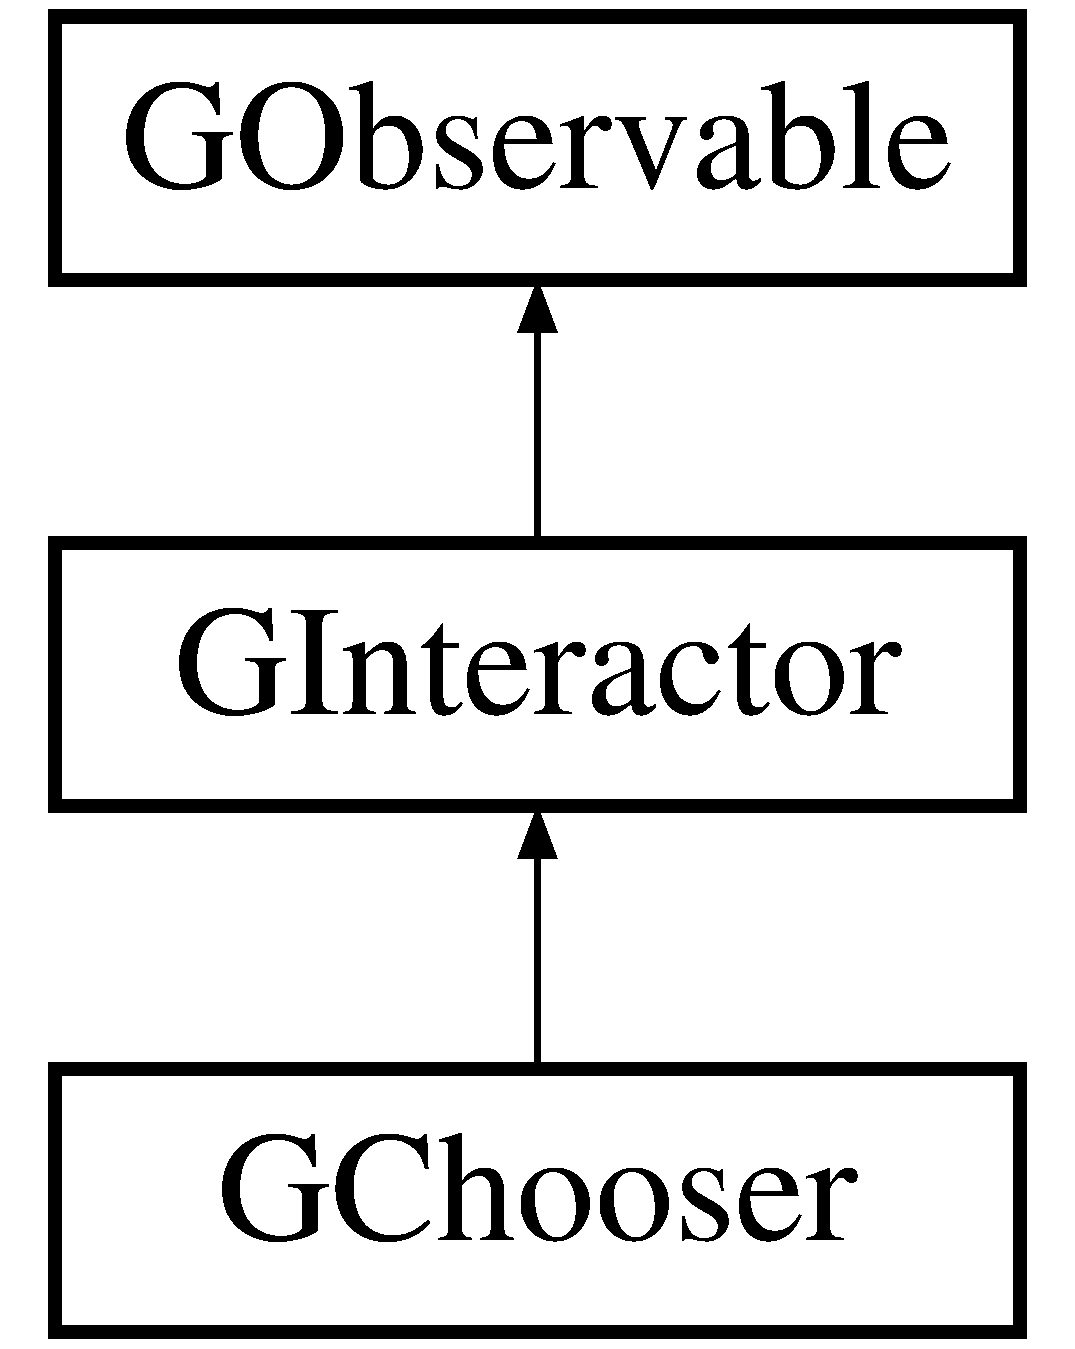
\includegraphics[height=3.000000cm]{classGChooser}
\end{center}
\end{figure}
\subsection*{Public Types}
\begin{DoxyCompactItemize}
\item 
enum \mbox{\hyperlink{classGInteractor_a8e0d441725a81d2bbdebbea09078260e}{Text\+Position}} \{ \mbox{\hyperlink{classGInteractor_a8e0d441725a81d2bbdebbea09078260ea4cd6f2e7d5a08d6f4dc052df2358f774}{T\+E\+X\+T\+\_\+\+B\+E\+S\+I\+D\+E\+\_\+\+I\+C\+ON}}, 
\mbox{\hyperlink{classGInteractor_a8e0d441725a81d2bbdebbea09078260eaa88490f63d8de68d44c83bdb2ecde3b3}{T\+E\+X\+T\+\_\+\+U\+N\+D\+E\+R\+\_\+\+I\+C\+ON}}, 
\mbox{\hyperlink{classGInteractor_a8e0d441725a81d2bbdebbea09078260ea39a6f388a30ac4fefb6eb13e846bc9f2}{T\+E\+X\+T\+\_\+\+O\+N\+LY}}
 \}
\begin{DoxyCompactList}\small\item\em The places where an interactor can place its text relative to its icon. \end{DoxyCompactList}\end{DoxyCompactItemize}
\subsection*{Public Member Functions}
\begin{DoxyCompactItemize}
\item 
\mbox{\hyperlink{classGChooser_ab17044f63a62b259f6b40a47a691f534}{G\+Chooser}} (Q\+Widget $\ast$parent=nullptr)
\begin{DoxyCompactList}\small\item\em Creates a chooser that initially contains no items. \end{DoxyCompactList}\item 
\mbox{\hyperlink{classGChooser_a7b9c598e637e726ac7b981495a0c2f75}{G\+Chooser}} (const std\+::initializer\+\_\+list$<$ std\+::string $>$ \&items, Q\+Widget $\ast$parent=nullptr)
\begin{DoxyCompactList}\small\item\em Creates a chooser that initially contains the given items. \end{DoxyCompactList}\item 
\mbox{\hyperlink{classGChooser_a909d3ee36f5ca0a30c036cb72e12d4f7}{G\+Chooser}} (const std\+::vector$<$ std\+::string $>$ \&items, Q\+Widget $\ast$parent=nullptr)
\begin{DoxyCompactList}\small\item\em Creates a chooser that initially contains the given items. \end{DoxyCompactList}\item 
\mbox{\hyperlink{classGChooser_afeff765eb6ee75d629c59da4c244fa59}{$\sim$\+G\+Chooser}} () override
\begin{DoxyCompactList}\small\item\em Frees memory allocated internally by the chooser. \end{DoxyCompactList}\item 
virtual void \mbox{\hyperlink{classGInteractor_a02f20ea6edfa0671f31c4c648a253833}{add\+Action\+Listener}} () Q\+\_\+\+D\+E\+C\+L\+\_\+\+D\+E\+P\+R\+E\+C\+A\+T\+ED
\begin{DoxyCompactList}\small\item\em Adds an event listener to be notified when this interactor is clicked or generally interacted with. \end{DoxyCompactList}\item 
virtual void \mbox{\hyperlink{classGChooser_a4d56babf9b4056c651a1999d9f7e6dcf}{add\+Item}} (const std\+::string \&item)
\begin{DoxyCompactList}\small\item\em Adds a new item consisting of the specified string to the end of the list. \end{DoxyCompactList}\item 
virtual void \mbox{\hyperlink{classGChooser_a9ae1e727f0d4bdcb198b2f9269db5614}{add\+Items}} (const std\+::initializer\+\_\+list$<$ std\+::string $>$ \&items)
\begin{DoxyCompactList}\small\item\em Adds each item from the given list to the end of the chooser\textquotesingle{}s list. \end{DoxyCompactList}\item 
virtual void \mbox{\hyperlink{classGChooser_af3d46372aacf011651fd724bfb38c7bb}{add\+Items}} (const std\+::vector$<$ std\+::string $>$ \&items)
\begin{DoxyCompactList}\small\item\em Adds each item from the given vector to the end of the chooser\textquotesingle{}s list. \end{DoxyCompactList}\item 
virtual void \mbox{\hyperlink{classGChooser_aa236b0d36b5d4f6a45c32b9d0e00f44b}{clear\+Items}} ()
\begin{DoxyCompactList}\small\item\em Removes all items from the chooser. \end{DoxyCompactList}\item 
bool \mbox{\hyperlink{classGInteractor_a597a370b592e3737d38d9d2f4e2031ea}{events\+Enabled}} () const override
\begin{DoxyCompactList}\small\item\em Returns true if this interactor is currently accepting events. \end{DoxyCompactList}\item 
virtual std\+::string \mbox{\hyperlink{classGInteractor_a69f8d23ed8f207fbecad99960776e942}{get\+Accelerator}} () const
\begin{DoxyCompactList}\small\item\em Returns a string representing a hotkey for this interactor, or an empty string if no accelerator has been set. \end{DoxyCompactList}\item 
std\+::string \mbox{\hyperlink{classGChooser_a4f83505141da1f8446f0e0e0a9507930}{get\+Action\+Command}} () const override
\begin{DoxyCompactList}\small\item\em Returns an action command for this interactor, which is a semi-\/unique string you can use to identify it when events occur. \end{DoxyCompactList}\item 
virtual std\+::string \mbox{\hyperlink{classGInteractor_a808e22cc1fdfbecf71ed8c64ef4600e0}{get\+Background}} () const
\begin{DoxyCompactList}\small\item\em Returns the background color of the interactor as a string. \end{DoxyCompactList}\item 
virtual int \mbox{\hyperlink{classGInteractor_a9e827257a55cb8cf4d9de2ec6bcfd7a0}{get\+Background\+Int}} () const
\begin{DoxyCompactList}\small\item\em Returns the background color of the interactor as an R\+GB integer. \end{DoxyCompactList}\item 
virtual \mbox{\hyperlink{structGRectangle}{G\+Rectangle}} \mbox{\hyperlink{classGInteractor_a29e6ac35a0b48f491a4c88194cc5da3b}{get\+Bounds}} () const
\begin{DoxyCompactList}\small\item\em Returns a rectangle representing the x/y position and size of this interactor. \end{DoxyCompactList}\item 
virtual std\+::string \mbox{\hyperlink{classGInteractor_aa061dfa488c31e18549d64363c1d0e34}{get\+Color}} () const
\begin{DoxyCompactList}\small\item\em Returns the foreground/text color of the interactor as a string. \end{DoxyCompactList}\item 
virtual int \mbox{\hyperlink{classGInteractor_a9635c7af766cdc3417f346683fa0e6c1}{get\+Color\+Int}} () const
\begin{DoxyCompactList}\small\item\em Returns the foreground/text color of the interactor as an R\+GB integer. \end{DoxyCompactList}\item 
virtual \mbox{\hyperlink{classGContainer}{G\+Container}} $\ast$ \mbox{\hyperlink{classGInteractor_a7a6e317c29d61030929b4cd2d1c00fe7}{get\+Container}} () const
\begin{DoxyCompactList}\small\item\em Returns a pointer to the onscreen container holding this interactor. \end{DoxyCompactList}\item 
virtual std\+::string \mbox{\hyperlink{classGInteractor_a894a5502900794eeb27d084c21f1d77d}{get\+Font}} () const
\begin{DoxyCompactList}\small\item\em Returns the font of this interactor\textquotesingle{}s text as a font string such as \char`\"{}\+Helvetica-\/12-\/\+Bold\char`\"{}. \end{DoxyCompactList}\item 
virtual std\+::string \mbox{\hyperlink{classGInteractor_a4fa2d8b0192a3a5b4af4bbfe71194d03}{get\+Foreground}} () const
\begin{DoxyCompactList}\small\item\em Returns the foreground/text color of the interactor as a string. \end{DoxyCompactList}\item 
virtual int \mbox{\hyperlink{classGInteractor_ac3b12ab385a6ef9ae90fc879860ba726}{get\+Foreground\+Int}} () const
\begin{DoxyCompactList}\small\item\em Returns the foreground/text color of the interactor as an R\+GB integer. \end{DoxyCompactList}\item 
virtual double \mbox{\hyperlink{classGInteractor_a1e7e353362434072875264cf95629f99}{get\+Height}} () const
\begin{DoxyCompactList}\small\item\em Returns the current onscreen height of this interactor in pixels. \end{DoxyCompactList}\item 
virtual std\+::string \mbox{\hyperlink{classGInteractor_aaed62a73004939a64da6f0eb9eb64d73}{get\+Icon}} () const
\begin{DoxyCompactList}\small\item\em Returns the file name of the icon associated with this interactor, or an empty string if no icon has been set. \end{DoxyCompactList}\item 
virtual int \mbox{\hyperlink{classGInteractor_a9c9659a6c6ba66b4107ba59c95a24241}{get\+ID}} () const
\begin{DoxyCompactList}\small\item\em Returns a globally unique identifier for this interactor, which is set when the interactor is constructed. \end{DoxyCompactList}\item 
\+\_\+\+Internal\+\_\+\+Q\+Widget $\ast$ \mbox{\hyperlink{classGChooser_a2f6b36b2517087dc90a366b5ce1f5323}{get\+Internal\+Widget}} () const override
\begin{DoxyCompactList}\small\item\em Returns a direct pointer to the internal Qt widget being wrapped by this interactor. \end{DoxyCompactList}\item 
virtual std\+::string \mbox{\hyperlink{classGChooser_a098538e0884967cbe287067a7fbbe04c}{get\+Item}} (int index) const
\begin{DoxyCompactList}\small\item\em Returns the item in the chooser at the given 0-\/based index. \end{DoxyCompactList}\item 
virtual int \mbox{\hyperlink{classGChooser_a288ee7c54b76ac6ae26eb4d748ce9776}{get\+Item\+Count}} () const
\begin{DoxyCompactList}\small\item\em Returns the number of items in the chooser. \end{DoxyCompactList}\item 
virtual \mbox{\hyperlink{structGPoint}{G\+Point}} \mbox{\hyperlink{classGInteractor_a4f83802015511edeb63b892830812c11}{get\+Location}} () const
\begin{DoxyCompactList}\small\item\em Returns an (x, y) point representing the onscreen location of the top-\/left corner of this interactor within its containing window. \end{DoxyCompactList}\item 
virtual double \mbox{\hyperlink{classGInteractor_aed4b0075fcc434499c3cb3e46896bda3}{get\+Minimum\+Height}} () const
\begin{DoxyCompactList}\small\item\em Returns the minimum height in pixels that this interactor will permit itself to be resized to. \end{DoxyCompactList}\item 
virtual \mbox{\hyperlink{structGDimension}{G\+Dimension}} \mbox{\hyperlink{classGInteractor_a66b5af0b32493b4d597ca0a3df2049ea}{get\+Minimum\+Size}} () const
\begin{DoxyCompactList}\small\item\em Returns a \mbox{\hyperlink{structGDimension}{G\+Dimension}} structure representing the minimum size in pixels that this interactor will permit itself to be resized to. \end{DoxyCompactList}\item 
virtual double \mbox{\hyperlink{classGInteractor_a59e668114fe3d49d2a0f28deb258f7c8}{get\+Minimum\+Width}} () const
\begin{DoxyCompactList}\small\item\em Returns the minimum width in pixels that this interactor will permit itself to be resized to. \end{DoxyCompactList}\item 
virtual std\+::string \mbox{\hyperlink{classGInteractor_a8a60438a5b55d0b2ceb35c8674b9d8c5}{get\+Name}} () const
\begin{DoxyCompactList}\small\item\em Returns a string representing a unique name for this interactor. \end{DoxyCompactList}\item 
virtual double \mbox{\hyperlink{classGInteractor_a747de0961653847bdc6615dbf756d715}{get\+Preferred\+Height}} () const
\begin{DoxyCompactList}\small\item\em Returns the height in pixels that this interactor would prefer to be, which would exactly fit its contents with no stretching or scrollbars. \end{DoxyCompactList}\item 
virtual \mbox{\hyperlink{structGDimension}{G\+Dimension}} \mbox{\hyperlink{classGInteractor_a4aabbee761d8e9116275401131b7ccd1}{get\+Preferred\+Size}} () const
\begin{DoxyCompactList}\small\item\em Returns a \mbox{\hyperlink{structGDimension}{G\+Dimension}} structure storing the width and height in pixels that this interactor would prefer to be, which would exactly fit its contents with no stretching or scrollbars. \end{DoxyCompactList}\item 
virtual double \mbox{\hyperlink{classGInteractor_a82bca31d37700fb0e35d2743352efd5e}{get\+Preferred\+Width}} () const
\begin{DoxyCompactList}\small\item\em Returns the height in pixels that this interactor would prefer to be, which would exactly fit its contents with no stretching or scrollbars. \end{DoxyCompactList}\item 
virtual int \mbox{\hyperlink{classGChooser_a4b706834529fee47c26689e69d9791f5}{get\+Selected\+Index}} () const
\begin{DoxyCompactList}\small\item\em Returns which index is selected in the chooser. \end{DoxyCompactList}\item 
virtual std\+::string \mbox{\hyperlink{classGChooser_a3dd4604cb3a910a63204197f56216ca4}{get\+Selected\+Item}} () const
\begin{DoxyCompactList}\small\item\em Returns the currently selected item in the chooser, or an empty string if no item is currently selected. \end{DoxyCompactList}\item 
virtual \mbox{\hyperlink{structGDimension}{G\+Dimension}} \mbox{\hyperlink{classGInteractor_a7b4eec96a2bdc6420695d5796a78eea9}{get\+Size}} () const
\begin{DoxyCompactList}\small\item\em Returns a \mbox{\hyperlink{structGDimension}{G\+Dimension}} structure storing the current onscreen width and height of this interactor in pixels. \end{DoxyCompactList}\item 
std\+::string \mbox{\hyperlink{classGChooser_a9b72ede4ee8520f987a0c01e30654814}{get\+Type}} () const override
\begin{DoxyCompactList}\small\item\em Returns a string representing the class name of this interactor, such as \char`\"{}\+G\+Button\char`\"{} or \char`\"{}\+G\+Check\+Box\char`\"{}. \end{DoxyCompactList}\item 
Q\+Widget $\ast$ \mbox{\hyperlink{classGChooser_a3b33a602b31a6b809d020535a59db3b4}{get\+Widget}} () const override
\begin{DoxyCompactList}\small\item\em Returns a direct pointer to the internal Qt widget being wrapped by this interactor. \end{DoxyCompactList}\item 
virtual double \mbox{\hyperlink{classGInteractor_a0ed2965abd4f5701d2cadf71239faf19}{get\+Width}} () const
\begin{DoxyCompactList}\small\item\em Returns the current onscreen width of this interactor in pixels. \end{DoxyCompactList}\item 
virtual double \mbox{\hyperlink{classGInteractor_a344385751bee0720059403940d57a13e}{getX}} () const
\begin{DoxyCompactList}\small\item\em Returns the x-\/coordinate of the top-\/left pixel of this interactor within its onscreen window. \end{DoxyCompactList}\item 
virtual double \mbox{\hyperlink{classGInteractor_aafa51c7f8f38a09febbb9ce7853f77b4}{getY}} () const
\begin{DoxyCompactList}\small\item\em Returns the y-\/coordinate of the top-\/left pixel of this interactor within its onscreen window. \end{DoxyCompactList}\item 
virtual bool \mbox{\hyperlink{classGInteractor_afc480f652b8c5f1fb255e2269ce68879}{in\+Bounds}} (double x, double y) const
\begin{DoxyCompactList}\small\item\em Returns true if the given x/y pixel is within the bounds of this interactor. \end{DoxyCompactList}\item 
virtual bool \mbox{\hyperlink{classGInteractor_ae6d7982c1c627b677a5e776ca86118ed}{in\+Bounds}} (int x, int y) const
\begin{DoxyCompactList}\small\item\em Returns true if the given x/y pixel is within the bounds of this interactor. \end{DoxyCompactList}\item 
virtual bool \mbox{\hyperlink{classGChooser_a012b5afb54e037e6c5498cf0932a521b}{is\+Editable}} () const
\begin{DoxyCompactList}\small\item\em Returns true if the chooser has an editable area for typing new items. \end{DoxyCompactList}\item 
virtual bool \mbox{\hyperlink{classGChooser_acf82f9b2937375c7b1cf3dccb3df3312}{is\+Empty}} () const
\begin{DoxyCompactList}\small\item\em Returns true if the chooser has no items. \end{DoxyCompactList}\item 
virtual bool \mbox{\hyperlink{classGInteractor_aacb819fb241851fd9fc045271baa4034}{is\+Enabled}} () const
\begin{DoxyCompactList}\small\item\em Returns true if this interactor is currently enabled. \end{DoxyCompactList}\item 
virtual bool \mbox{\hyperlink{classGInteractor_a9d8a6cfb13917785c143e74d40e4e2be}{is\+Visible}} () const
\begin{DoxyCompactList}\small\item\em Returns true if the interactor is visible on the screen. \end{DoxyCompactList}\item 
virtual void \mbox{\hyperlink{classGInteractor_ab7fe7a876367b87cf7202f947f1d05e4}{remove\+Action\+Listener}} ()
\begin{DoxyCompactList}\small\item\em Removes the action listener from this interactor so that it will no longer call it when events occur. \end{DoxyCompactList}\item 
virtual void \mbox{\hyperlink{classGInteractor_ad39d0325cde6b97ebda4b9d7787c633b}{remove\+Click\+Listener}} ()
\begin{DoxyCompactList}\small\item\em Removes the click listener from this interactor so that it will no longer call it when events occur. \end{DoxyCompactList}\item 
virtual void \mbox{\hyperlink{classGInteractor_aa4250907e4cdd77349c04f0cf5cdd3d3}{remove\+Double\+Click\+Listener}} ()
\begin{DoxyCompactList}\small\item\em Removes the double-\/click listener from this interactor so that it will no longer call it when events occur. \end{DoxyCompactList}\item 
virtual void \mbox{\hyperlink{classGInteractor_a43095f41cab3be732b49f29970484b05}{remove\+Key\+Listener}} ()
\begin{DoxyCompactList}\small\item\em Removes the key listener from this interactor so that it will no longer call it when key events occur. \end{DoxyCompactList}\item 
virtual void \mbox{\hyperlink{classGInteractor_aff47f71ce47e688a07c9d38dc92fcc11}{remove\+Mouse\+Listener}} ()
\begin{DoxyCompactList}\small\item\em Removes the mouse listener from this interactor so that it will no longer call it when events occur. \end{DoxyCompactList}\item 
virtual void \mbox{\hyperlink{classGInteractor_a519fb2ac767f8b2febbb50b898b8c8cb}{request\+Focus}} ()
\begin{DoxyCompactList}\small\item\em Transfers keyboard focus to this interactor. \end{DoxyCompactList}\item 
virtual void \mbox{\hyperlink{classGInteractor_ad15f102f62e2960576012f1aa0ba4b2e}{set\+Accelerator}} (const std\+::string \&accelerator)
\begin{DoxyCompactList}\small\item\em Sets an accelerator hotkey for this interactor, such as \char`\"{}\+Ctrl-\/\+S\char`\"{}. \end{DoxyCompactList}\item 
virtual void \mbox{\hyperlink{classGInteractor_a4b5843fe3030e038a1ba54cc03389bcf}{set\+Action\+Command}} (const std\+::string \&action\+Command)
\begin{DoxyCompactList}\small\item\em Sets the action command for this interactor. \end{DoxyCompactList}\item 
virtual void \mbox{\hyperlink{classGInteractor_adcfb4742430c88714fcf57e57ab8ea9c}{set\+Action\+Listener}} (G\+Event\+Listener func)
\begin{DoxyCompactList}\small\item\em Sets an action listener on this interactor so that it will be called when it is interacted with in its primary way. \end{DoxyCompactList}\item 
virtual void \mbox{\hyperlink{classGInteractor_aebd20a89c7a8a43a6fce999cf4f9fcf2}{set\+Action\+Listener}} (G\+Event\+Listener\+Void func)
\begin{DoxyCompactList}\small\item\em Sets an action listener on this interactor so that it will be called when it is interacted with in its primary way. \end{DoxyCompactList}\item 
virtual void \mbox{\hyperlink{classGInteractor_acba7e546c2025c0a15ca4b4cc92043db}{set\+Background}} (int rgb)
\begin{DoxyCompactList}\small\item\em Sets the background color of the interactor to the color represented by the given R\+GB integer. \end{DoxyCompactList}\item 
virtual void \mbox{\hyperlink{classGInteractor_ab4677ab2474e68b07aa56605af92a84a}{set\+Background}} (const std\+::string \&color)
\begin{DoxyCompactList}\small\item\em Sets the background color of the interactor to the color represented by the given string. \end{DoxyCompactList}\item 
virtual void \mbox{\hyperlink{classGInteractor_a2aae8197624b72265ab83b4f1bc73f2f}{set\+Bounds}} (double x, double y, double width, double height)
\begin{DoxyCompactList}\small\item\em Sets the size and location of the widget. \end{DoxyCompactList}\item 
virtual void \mbox{\hyperlink{classGInteractor_acada386653f008cacc7cce86426bef7c}{set\+Bounds}} (const \mbox{\hyperlink{structGRectangle}{G\+Rectangle}} \&\mbox{\hyperlink{classGChooser_af9593d4a5ff4274efaf429cb4f9e57cc}{size}})
\begin{DoxyCompactList}\small\item\em Sets the size and location of the widget. \end{DoxyCompactList}\item 
virtual void \mbox{\hyperlink{classGInteractor_abd40af6921242584d0954f173911b190}{set\+Click\+Listener}} (G\+Event\+Listener func)
\begin{DoxyCompactList}\small\item\em Sets a mouse listener on this interactor so that it will be called when the mouse is clicked on it. \end{DoxyCompactList}\item 
virtual void \mbox{\hyperlink{classGInteractor_a856414c92df90f56f3877475eb3f8fc4}{set\+Click\+Listener}} (G\+Event\+Listener\+Void func)
\begin{DoxyCompactList}\small\item\em Sets a mouse listener on this interactor so that it will be called when the mouse is clicked on it. \end{DoxyCompactList}\item 
virtual void \mbox{\hyperlink{classGInteractor_ab1f5cc0f5cc6bbbd716a526c61f1081d}{set\+Color}} (int rgb)
\begin{DoxyCompactList}\small\item\em Sets the foreground/text color of the interactor to the color represented by the given R\+GB integer. \end{DoxyCompactList}\item 
virtual void \mbox{\hyperlink{classGInteractor_a61374df6c11b52cfbb0815decdbaebc6}{set\+Color}} (const std\+::string \&color)
\begin{DoxyCompactList}\small\item\em Sets the foreground/text color of the interactor to the color represented by the given string. \end{DoxyCompactList}\item 
virtual void \mbox{\hyperlink{classGInteractor_ac29f9a3462458e165fae3a1f046ee77a}{set\+Double\+Click\+Listener}} (G\+Event\+Listener func)
\begin{DoxyCompactList}\small\item\em Sets a mouse listener on this interactor so that it will be called when the mouse is double-\/clicked on it. \end{DoxyCompactList}\item 
virtual void \mbox{\hyperlink{classGInteractor_a50096194d66f48c92dd4c512d41bfc76}{set\+Double\+Click\+Listener}} (G\+Event\+Listener\+Void func)
\begin{DoxyCompactList}\small\item\em Sets a mouse listener on this interactor so that it will be called when the mouse is double-\/clicked on it. \end{DoxyCompactList}\item 
virtual void \mbox{\hyperlink{classGChooser_a52455aaff9ee352ca405fa61ba246b84}{set\+Editable}} (bool editable)
\begin{DoxyCompactList}\small\item\em Sets whether the chooser has an editable area for typing new items. \end{DoxyCompactList}\item 
virtual void \mbox{\hyperlink{classGInteractor_ab831367dd84bbd579e02e55bacb21343}{set\+Enabled}} (bool value)
\begin{DoxyCompactList}\small\item\em Sets whether this interactor is currently enabled. \end{DoxyCompactList}\item 
virtual void \mbox{\hyperlink{classGObservable_afaa30b2a9e0f378fd1c70d2f1d0b8216}{set\+Events\+Enabled}} (bool \mbox{\hyperlink{classGInteractor_a597a370b592e3737d38d9d2f4e2031ea}{events\+Enabled}})
\begin{DoxyCompactList}\small\item\em Sets whether the object is currently allowing itself to fire events. \end{DoxyCompactList}\item 
virtual void \mbox{\hyperlink{classGInteractor_a2592348886ffea646c6534bf88f7c49d}{set\+Font}} (const Q\+Font \&font)
\begin{DoxyCompactList}\small\item\em Sets the font used by this widget to the given Qt font. \end{DoxyCompactList}\item 
virtual void \mbox{\hyperlink{classGInteractor_a8e096e8818d838aceae1d46d58fb3a7b}{set\+Font}} (const std\+::string \&font)
\begin{DoxyCompactList}\small\item\em Sets the font used by this widget to the font represented by the given font string, such as \char`\"{}\+Helvetica-\/16-\/\+Bold\char`\"{}. \end{DoxyCompactList}\item 
virtual void \mbox{\hyperlink{classGInteractor_a9eb856b5ff83a19df3831a31f15f4563}{set\+Foreground}} (int rgb)
\begin{DoxyCompactList}\small\item\em Sets the foreground/text color of the interactor to the color represented by the given R\+GB integer. \end{DoxyCompactList}\item 
virtual void \mbox{\hyperlink{classGInteractor_af59209aeadea6dfc6d97a2d8531f50e1}{set\+Foreground}} (const std\+::string \&color)
\begin{DoxyCompactList}\small\item\em Sets the foreground/text color of the interactor to the color represented by the given string. \end{DoxyCompactList}\item 
virtual void \mbox{\hyperlink{classGInteractor_a9e280bfc4544dfaf8e4376c4e1a74357}{set\+Height}} (double height)
\begin{DoxyCompactList}\small\item\em Sets the onscreen height of the interactor in pixels. \end{DoxyCompactList}\item 
virtual void \mbox{\hyperlink{classGInteractor_a542abfcd7261751352af129c7215ecda}{set\+Icon}} (const Q\+Icon \&icon)
\begin{DoxyCompactList}\small\item\em Sets the icon associated with this interactor. \end{DoxyCompactList}\item 
virtual void \mbox{\hyperlink{classGInteractor_a368e1a338f84401c284506d03b1ba769}{set\+Icon}} (const Q\+Pixmap \&icon)
\begin{DoxyCompactList}\small\item\em Sets the icon associated with this interactor. \end{DoxyCompactList}\item 
virtual void \mbox{\hyperlink{classGInteractor_a762e139aa311461c3984d3ad28293f64}{set\+Icon}} (const std\+::string \&filename, bool retain\+Icon\+Size=true)
\begin{DoxyCompactList}\small\item\em Sets the file name of the icon associated with this interactor, or an empty string if no icon has been set. \end{DoxyCompactList}\item 
virtual void \mbox{\hyperlink{classGChooser_aa4f87c4982e01ec37b78f52f2bf11ef4}{set\+Item}} (int index, const std\+::string \&item)
\begin{DoxyCompactList}\small\item\em Sets the item at the given index in the chooser to the given value. \end{DoxyCompactList}\item 
virtual void \mbox{\hyperlink{classGInteractor_aeb8324d3287fa1fbe093f4d6230cf0a6}{set\+Key\+Listener}} (G\+Event\+Listener func)
\begin{DoxyCompactList}\small\item\em Sets a key listener on this interactor so that it will be called when the user presses any key. \end{DoxyCompactList}\item 
virtual void \mbox{\hyperlink{classGInteractor_ae48ecea73606c7bd9423e1c7cc589cc9}{set\+Key\+Listener}} (G\+Event\+Listener\+Void func)
\begin{DoxyCompactList}\small\item\em Sets a key listener on this interactor so that it will be called when the user presses any key. \end{DoxyCompactList}\item 
virtual void \mbox{\hyperlink{classGInteractor_a04594e8ba9b98513a64f1da00dcae18c}{set\+Location}} (double x, double y)
\begin{DoxyCompactList}\small\item\em Sets the onscreen x/y-\/coordinate of the top-\/left corner of the interactor relative to its window. \end{DoxyCompactList}\item 
virtual void \mbox{\hyperlink{classGInteractor_a0cf428e207b7f22cc08138a90b1b87b2}{set\+Minimum\+Size}} (double width, double height)
\begin{DoxyCompactList}\small\item\em Sets the minimum size in pixels that this interactor will permit itself to be resized to. \end{DoxyCompactList}\item 
virtual void \mbox{\hyperlink{classGInteractor_a3b1046117ac6cb7abe467e00ba8a81f4}{set\+Minimum\+Size}} (const \mbox{\hyperlink{structGDimension}{G\+Dimension}} \&\mbox{\hyperlink{classGChooser_af9593d4a5ff4274efaf429cb4f9e57cc}{size}})
\begin{DoxyCompactList}\small\item\em Sets the minimum size in pixels that this interactor will permit itself to be resized to. \end{DoxyCompactList}\item 
virtual void \mbox{\hyperlink{classGInteractor_a37d8dbc943f59920f705b0104f60bde2}{set\+Mouse\+Listener}} (G\+Event\+Listener func)
\begin{DoxyCompactList}\small\item\em Sets a mouse listener on this interactor so that it will be called when the mouse is moved or clicked on it. \end{DoxyCompactList}\item 
virtual void \mbox{\hyperlink{classGInteractor_aea7f647ea62d59f71b5fad6aa65eeaf9}{set\+Mouse\+Listener}} (G\+Event\+Listener\+Void func)
\begin{DoxyCompactList}\small\item\em Sets a mouse listener on this interactor so that it will be called when the mouse is moved or clicked on it. \end{DoxyCompactList}\item 
virtual void \mbox{\hyperlink{classGInteractor_a9d3a2685df23b5e7cbf59c19c4a1f9b5}{set\+Name}} (const std\+::string \&name)
\begin{DoxyCompactList}\small\item\em Sets a string representing a unique name for this interactor. \end{DoxyCompactList}\item 
virtual void \mbox{\hyperlink{classGInteractor_a1ab987704fce32098706c6f00fb08218}{set\+Preferred\+Height}} (double height)
\begin{DoxyCompactList}\small\item\em Sets the height in pixels that this interactor would prefer to be. \end{DoxyCompactList}\item 
virtual void \mbox{\hyperlink{classGInteractor_a042c5ae19430d765ef552371cae3632c}{set\+Preferred\+Size}} (double width, double height)
\begin{DoxyCompactList}\small\item\em Sets the width and height in pixels that this interactor would prefer to be. \end{DoxyCompactList}\item 
virtual void \mbox{\hyperlink{classGInteractor_aa22d9be4bc0e078bb0ea69b0fc9d7c75}{set\+Preferred\+Size}} (const \mbox{\hyperlink{structGDimension}{G\+Dimension}} \&\mbox{\hyperlink{classGChooser_af9593d4a5ff4274efaf429cb4f9e57cc}{size}})
\begin{DoxyCompactList}\small\item\em Sets the size in pixels that this interactor would prefer to be. \end{DoxyCompactList}\item 
virtual void \mbox{\hyperlink{classGInteractor_a3db429ab2fa52efd187eec0ed8cdd9f2}{set\+Preferred\+Width}} (double width)
\begin{DoxyCompactList}\small\item\em Sets the width in pixels that this interactor would prefer to be. \end{DoxyCompactList}\item 
virtual void \mbox{\hyperlink{classGChooser_a9f838f41a4abc5775bfe28fea7cf1750}{set\+Selected\+Index}} (int index)
\begin{DoxyCompactList}\small\item\em Sets the item at the given index in the chooser to be selected. \end{DoxyCompactList}\item 
virtual void \mbox{\hyperlink{classGChooser_ae427110c299aa08a8f72cbfa88ab3301}{set\+Selected\+Item}} (const std\+::string \&item)
\begin{DoxyCompactList}\small\item\em Sets the given item in the chooser to be selected. \end{DoxyCompactList}\item 
virtual void \mbox{\hyperlink{classGInteractor_aca25d49481f9bf5fc8f7df4c086c4ce7}{set\+Size}} (double width, double height)
\begin{DoxyCompactList}\small\item\em Sets the onscreen width and height of the interactor in pixels. \end{DoxyCompactList}\item 
virtual void \mbox{\hyperlink{classGInteractor_ae2b628228f192c2702c4ce941b2af68f}{set\+Size}} (const \mbox{\hyperlink{structGDimension}{G\+Dimension}} \&\mbox{\hyperlink{classGChooser_af9593d4a5ff4274efaf429cb4f9e57cc}{size}})
\begin{DoxyCompactList}\small\item\em Sets the onscreen width and height of the interactor in pixels. \end{DoxyCompactList}\item 
virtual void \mbox{\hyperlink{classGInteractor_a039e0e49beaecc275efce02d416acea8}{set\+Tooltip}} (const std\+::string \&tooltip\+Text)
\begin{DoxyCompactList}\small\item\em Sets a \char`\"{}tooltip\char`\"{} that will appear if the user hovers their mouse over the interactor. \end{DoxyCompactList}\item 
virtual void \mbox{\hyperlink{classGInteractor_a18e44e30b31525a243960ca3928125aa}{set\+Visible}} (bool visible)
\begin{DoxyCompactList}\small\item\em Returns true if the interactor is visible on the screen. \end{DoxyCompactList}\item 
virtual void \mbox{\hyperlink{classGInteractor_aa3f3fba4cb131baa8696ba01e3bceca1}{set\+Width}} (double width)
\begin{DoxyCompactList}\small\item\em Sets the onscreen width of the interactor in pixels. \end{DoxyCompactList}\item 
virtual void \mbox{\hyperlink{classGInteractor_a9c18fcc579333bf9653d13ad2b372e39}{setX}} (double x)
\begin{DoxyCompactList}\small\item\em Sets the onscreen x-\/coordinate of the top-\/left corner of the interactor relative to its window. \end{DoxyCompactList}\item 
virtual void \mbox{\hyperlink{classGInteractor_a7d57e2a5c35d27feb58fd498a3cf82b9}{setY}} (double y)
\begin{DoxyCompactList}\small\item\em Sets the onscreen y-\/coordinate of the top-\/left corner of the interactor relative to its window. \end{DoxyCompactList}\item 
virtual int \mbox{\hyperlink{classGChooser_af9593d4a5ff4274efaf429cb4f9e57cc}{size}} () const
\begin{DoxyCompactList}\small\item\em Returns the number of items in the chooser. \end{DoxyCompactList}\item 
virtual std\+::string \mbox{\hyperlink{classGObservable_a1fe5121d6528fdea3f243321b3fa3a49}{to\+String}} () const
\begin{DoxyCompactList}\small\item\em Returns a string representation of this observable object\textquotesingle{}s state. \end{DoxyCompactList}\end{DoxyCompactItemize}
\subsection*{Protected Member Functions}
\begin{DoxyCompactItemize}
\item 
virtual void \mbox{\hyperlink{classGObservable_a80cfa040459ff53594adbd6a51ec8f43}{clear\+Event\+Listeners}} ()
\begin{DoxyCompactList}\small\item\em Removes all event listeners from this object. \end{DoxyCompactList}\item 
virtual void \mbox{\hyperlink{classGObservable_a284f31528c0520f8e545c03ac9eeac74}{ensure\+Thread\+Safety}} (const std\+::string \&member\+Name=\char`\"{}\char`\"{})
\begin{DoxyCompactList}\small\item\em Ensures that we are currently in the Qt G\+UI thread. \end{DoxyCompactList}\item 
virtual void \mbox{\hyperlink{classGObservable_a63e5e5a6227c59c928493b11aceb0f67}{fire\+Event}} (\mbox{\hyperlink{classGEvent}{G\+Event}} \&event)
\begin{DoxyCompactList}\small\item\em Sends out the given event to any attached listeners. \end{DoxyCompactList}\item 
virtual void \mbox{\hyperlink{classGObservable_ab3983ea07337b52020a29cc00c653d8d}{fire\+G\+Event}} (Q\+Event $\ast$event, Event\+Type event\+Type, const std\+::string \&event\+Name)
\begin{DoxyCompactList}\small\item\em Creates an event of the given type, then sends it out to any attached listeners. \end{DoxyCompactList}\item 
virtual void \mbox{\hyperlink{classGObservable_a01fdf1b0e0dbd49e189fe4514e010411}{fire\+G\+Event}} (Q\+Close\+Event $\ast$event, Event\+Type event\+Type, const std\+::string \&event\+Name)
\begin{DoxyCompactList}\small\item\em Creates an event of the given type, then sends it out to any attached listeners. \end{DoxyCompactList}\item 
virtual void \mbox{\hyperlink{classGObservable_abb0b2f66ba39211cb5d7615e9d1c04e2}{fire\+G\+Event}} (Q\+Key\+Event $\ast$event, Event\+Type event\+Type, const std\+::string \&event\+Name)
\begin{DoxyCompactList}\small\item\em Creates an event of the given type, then sends it out to any attached listeners. \end{DoxyCompactList}\item 
virtual void \mbox{\hyperlink{classGObservable_a119318675d2165bdf7dd853aaf881d4b}{fire\+G\+Event}} (Q\+Mouse\+Event $\ast$event, Event\+Type event\+Type, const std\+::string \&event\+Name, const std\+::string \&action\+Command=\char`\"{}\char`\"{})
\begin{DoxyCompactList}\small\item\em Creates an event of the given type, then sends it out to any attached listeners. \end{DoxyCompactList}\item 
virtual void \mbox{\hyperlink{classGObservable_a63fd9034e1e1633c1c38eb342bfd34e9}{fire\+G\+Event}} (Q\+Resize\+Event $\ast$event, Event\+Type event\+Type, const std\+::string \&event\+Name)
\begin{DoxyCompactList}\small\item\em Creates an event of the given type, then sends it out to any attached listeners. \end{DoxyCompactList}\item 
virtual void \mbox{\hyperlink{classGObservable_a741345310d9b7c5170a6cbc410c44ac4}{fire\+G\+Event}} (Q\+Timer\+Event $\ast$event, Event\+Type event\+Type, const std\+::string \&event\+Name)
\begin{DoxyCompactList}\small\item\em Creates an event of the given type, then sends it out to any attached listeners. \end{DoxyCompactList}\item 
virtual void \mbox{\hyperlink{classGObservable_a93bf338968a0338761b8e4dc62f582e9}{fire\+G\+Event}} (Q\+Wheel\+Event $\ast$event, Event\+Type event\+Type, const std\+::string \&event\+Name)
\begin{DoxyCompactList}\small\item\em Creates an event of the given type, then sends it out to any attached listeners. \end{DoxyCompactList}\item 
virtual void \mbox{\hyperlink{classGObservable_a2a70a7d7435ff0c3b80bb4d70da19e0d}{fire\+G\+Event}} (Q\+Window\+State\+Change\+Event $\ast$event, Event\+Type event\+Type, const std\+::string \&event\+Name)
\begin{DoxyCompactList}\small\item\em Creates an event of the given type, then sends it out to any attached listeners. \end{DoxyCompactList}\item 
virtual bool \mbox{\hyperlink{classGObservable_a9f6faaa25942923bafa1c44020c49fa9}{has\+Event\+Listener}} (const std\+::string \&event\+Name) const
\begin{DoxyCompactList}\small\item\em Returns true if the observable object has a listener for the given type of event. \end{DoxyCompactList}\item 
virtual bool \mbox{\hyperlink{classGObservable_aeec1adc19aa0f33de62390686ee1382c}{is\+Accepting\+Event}} (int event\+Mask) const
\begin{DoxyCompactList}\small\item\em Returns true if the observable object has a listener for the given type of event. \end{DoxyCompactList}\item 
virtual bool \mbox{\hyperlink{classGObservable_aa31c73145a29dcb92848a92e0cfaea41}{is\+Accepting\+Event}} (const \mbox{\hyperlink{classGEvent}{G\+Event}} \&event) const
\begin{DoxyCompactList}\small\item\em Returns true if the observable object has a listener for the given type of event. \end{DoxyCompactList}\item 
virtual bool \mbox{\hyperlink{classGObservable_a3b1c689267eda44e65a2213e7de38b23}{is\+Accepting\+Event}} (const std\+::string \&event\+Type) const
\begin{DoxyCompactList}\small\item\em Returns true if the observable object has a listener for the given type of event. \end{DoxyCompactList}\item 
virtual void \mbox{\hyperlink{classGObservable_acbcf1ed3a851ad8a3c17ef38d86b481d}{remove\+Event\+Listener}} (const std\+::string \&event\+Name)
\begin{DoxyCompactList}\small\item\em Removes any event listener from this observable object that would respond to the given type of event, such as \char`\"{}click\char`\"{} or \char`\"{}keydown\char`\"{}. \end{DoxyCompactList}\item 
virtual void \mbox{\hyperlink{classGObservable_af51cc35c29a1bd1908609d432decdbb6}{remove\+Event\+Listeners}} (std\+::initializer\+\_\+list$<$ std\+::string $>$ event\+Names)
\begin{DoxyCompactList}\small\item\em Removes any event listener from this observable object that would respond to the given types of events, such as \char`\"{}click\char`\"{} or \char`\"{}keydown\char`\"{}. \end{DoxyCompactList}\item 
virtual void \mbox{\hyperlink{classGObservable_ad2f6d34961c50f6c1e0659990b79f741}{set\+Event\+Listener}} (const std\+::string \&event\+Name, G\+Event\+Listener func)
\begin{DoxyCompactList}\small\item\em Adds an event listener from this observable object to respond to the given type of event, such as \char`\"{}click\char`\"{} or \char`\"{}keydown\char`\"{}. \end{DoxyCompactList}\item 
virtual void \mbox{\hyperlink{classGObservable_abac4cb9f9e626e010e87f5d91573c8a5}{set\+Event\+Listener}} (const std\+::string \&event\+Name, G\+Event\+Listener\+Void func)
\begin{DoxyCompactList}\small\item\em Adds an event listener from this observable object to respond to the given type of event, such as \char`\"{}click\char`\"{} or \char`\"{}keydown\char`\"{}. \end{DoxyCompactList}\item 
virtual void \mbox{\hyperlink{classGObservable_afa388d69c33c718cf035774604065604}{set\+Event\+Listeners}} (std\+::initializer\+\_\+list$<$ std\+::string $>$ event\+Names, G\+Event\+Listener func)
\begin{DoxyCompactList}\small\item\em Adds an event listener from this observable object to respond to the given types of events, such as \char`\"{}click\char`\"{} or \char`\"{}keydown\char`\"{}. \end{DoxyCompactList}\item 
virtual void \mbox{\hyperlink{classGObservable_a7867184bbb686f74fae8a4db927da799}{set\+Event\+Listeners}} (std\+::initializer\+\_\+list$<$ std\+::string $>$ event\+Names, G\+Event\+Listener\+Void func)
\begin{DoxyCompactList}\small\item\em Adds an event listener from this observable object to respond to the given types of events, such as \char`\"{}click\char`\"{} or \char`\"{}keydown\char`\"{}. \end{DoxyCompactList}\end{DoxyCompactItemize}


\subsection{Detailed Description}
This interactor subclass represents a selectable drop-\/down list. 

The \mbox{\hyperlink{classGChooser}{G\+Chooser}} constructor creates an empty chooser. Once the chooser has been created, clients can use add\+Item to add the options. 

\subsection{Member Enumeration Documentation}
\mbox{\Hypertarget{classGInteractor_a8e0d441725a81d2bbdebbea09078260e}\label{classGInteractor_a8e0d441725a81d2bbdebbea09078260e}} 
\index{G\+Chooser@{G\+Chooser}!Text\+Position@{Text\+Position}}
\index{Text\+Position@{Text\+Position}!G\+Chooser@{G\+Chooser}}
\subsubsection{\texorpdfstring{Text\+Position}{TextPosition}}
{\footnotesize\ttfamily enum \mbox{\hyperlink{classGInteractor_a8e0d441725a81d2bbdebbea09078260e}{Text\+Position}}\hspace{0.3cm}{\ttfamily [inherited]}}



The places where an interactor can place its text relative to its icon. 

\begin{DoxyEnumFields}{Enumerator}
\raisebox{\heightof{T}}[0pt][0pt]{\index{T\+E\+X\+T\+\_\+\+B\+E\+S\+I\+D\+E\+\_\+\+I\+C\+ON@{T\+E\+X\+T\+\_\+\+B\+E\+S\+I\+D\+E\+\_\+\+I\+C\+ON}!G\+Chooser@{G\+Chooser}}\index{G\+Chooser@{G\+Chooser}!T\+E\+X\+T\+\_\+\+B\+E\+S\+I\+D\+E\+\_\+\+I\+C\+ON@{T\+E\+X\+T\+\_\+\+B\+E\+S\+I\+D\+E\+\_\+\+I\+C\+ON}}}\mbox{\Hypertarget{classGInteractor_a8e0d441725a81d2bbdebbea09078260ea4cd6f2e7d5a08d6f4dc052df2358f774}\label{classGInteractor_a8e0d441725a81d2bbdebbea09078260ea4cd6f2e7d5a08d6f4dc052df2358f774}} 
T\+E\+X\+T\+\_\+\+B\+E\+S\+I\+D\+E\+\_\+\+I\+C\+ON&\\
\hline

\raisebox{\heightof{T}}[0pt][0pt]{\index{T\+E\+X\+T\+\_\+\+U\+N\+D\+E\+R\+\_\+\+I\+C\+ON@{T\+E\+X\+T\+\_\+\+U\+N\+D\+E\+R\+\_\+\+I\+C\+ON}!G\+Chooser@{G\+Chooser}}\index{G\+Chooser@{G\+Chooser}!T\+E\+X\+T\+\_\+\+U\+N\+D\+E\+R\+\_\+\+I\+C\+ON@{T\+E\+X\+T\+\_\+\+U\+N\+D\+E\+R\+\_\+\+I\+C\+ON}}}\mbox{\Hypertarget{classGInteractor_a8e0d441725a81d2bbdebbea09078260eaa88490f63d8de68d44c83bdb2ecde3b3}\label{classGInteractor_a8e0d441725a81d2bbdebbea09078260eaa88490f63d8de68d44c83bdb2ecde3b3}} 
T\+E\+X\+T\+\_\+\+U\+N\+D\+E\+R\+\_\+\+I\+C\+ON&\\
\hline

\raisebox{\heightof{T}}[0pt][0pt]{\index{T\+E\+X\+T\+\_\+\+O\+N\+LY@{T\+E\+X\+T\+\_\+\+O\+N\+LY}!G\+Chooser@{G\+Chooser}}\index{G\+Chooser@{G\+Chooser}!T\+E\+X\+T\+\_\+\+O\+N\+LY@{T\+E\+X\+T\+\_\+\+O\+N\+LY}}}\mbox{\Hypertarget{classGInteractor_a8e0d441725a81d2bbdebbea09078260ea39a6f388a30ac4fefb6eb13e846bc9f2}\label{classGInteractor_a8e0d441725a81d2bbdebbea09078260ea39a6f388a30ac4fefb6eb13e846bc9f2}} 
T\+E\+X\+T\+\_\+\+O\+N\+LY&\\
\hline

\end{DoxyEnumFields}


\subsection{Constructor \& Destructor Documentation}
\mbox{\Hypertarget{classGChooser_ab17044f63a62b259f6b40a47a691f534}\label{classGChooser_ab17044f63a62b259f6b40a47a691f534}} 
\index{G\+Chooser@{G\+Chooser}!G\+Chooser@{G\+Chooser}}
\index{G\+Chooser@{G\+Chooser}!G\+Chooser@{G\+Chooser}}
\subsubsection{\texorpdfstring{G\+Chooser()}{GChooser()}\hspace{0.1cm}{\footnotesize\ttfamily [1/3]}}
{\footnotesize\ttfamily \mbox{\hyperlink{classGChooser}{G\+Chooser}} (\begin{DoxyParamCaption}\item[{Q\+Widget $\ast$}]{parent = {\ttfamily nullptr} }\end{DoxyParamCaption})}



Creates a chooser that initially contains no items. 

\mbox{\Hypertarget{classGChooser_a7b9c598e637e726ac7b981495a0c2f75}\label{classGChooser_a7b9c598e637e726ac7b981495a0c2f75}} 
\index{G\+Chooser@{G\+Chooser}!G\+Chooser@{G\+Chooser}}
\index{G\+Chooser@{G\+Chooser}!G\+Chooser@{G\+Chooser}}
\subsubsection{\texorpdfstring{G\+Chooser()}{GChooser()}\hspace{0.1cm}{\footnotesize\ttfamily [2/3]}}
{\footnotesize\ttfamily \mbox{\hyperlink{classGChooser}{G\+Chooser}} (\begin{DoxyParamCaption}\item[{const std\+::initializer\+\_\+list$<$ std\+::string $>$ \&}]{items,  }\item[{Q\+Widget $\ast$}]{parent = {\ttfamily nullptr} }\end{DoxyParamCaption})}



Creates a chooser that initially contains the given items. 

\mbox{\Hypertarget{classGChooser_a909d3ee36f5ca0a30c036cb72e12d4f7}\label{classGChooser_a909d3ee36f5ca0a30c036cb72e12d4f7}} 
\index{G\+Chooser@{G\+Chooser}!G\+Chooser@{G\+Chooser}}
\index{G\+Chooser@{G\+Chooser}!G\+Chooser@{G\+Chooser}}
\subsubsection{\texorpdfstring{G\+Chooser()}{GChooser()}\hspace{0.1cm}{\footnotesize\ttfamily [3/3]}}
{\footnotesize\ttfamily \mbox{\hyperlink{classGChooser}{G\+Chooser}} (\begin{DoxyParamCaption}\item[{const std\+::vector$<$ std\+::string $>$ \&}]{items,  }\item[{Q\+Widget $\ast$}]{parent = {\ttfamily nullptr} }\end{DoxyParamCaption})}



Creates a chooser that initially contains the given items. 

\mbox{\Hypertarget{classGChooser_afeff765eb6ee75d629c59da4c244fa59}\label{classGChooser_afeff765eb6ee75d629c59da4c244fa59}} 
\index{G\+Chooser@{G\+Chooser}!````~G\+Chooser@{$\sim$\+G\+Chooser}}
\index{````~G\+Chooser@{$\sim$\+G\+Chooser}!G\+Chooser@{G\+Chooser}}
\subsubsection{\texorpdfstring{$\sim$\+G\+Chooser()}{~GChooser()}}
{\footnotesize\ttfamily $\sim$\mbox{\hyperlink{classGChooser}{G\+Chooser}} (\begin{DoxyParamCaption}{ }\end{DoxyParamCaption})\hspace{0.3cm}{\ttfamily [override]}}



Frees memory allocated internally by the chooser. 



\subsection{Member Function Documentation}
\mbox{\Hypertarget{classGInteractor_a02f20ea6edfa0671f31c4c648a253833}\label{classGInteractor_a02f20ea6edfa0671f31c4c648a253833}} 
\index{G\+Chooser@{G\+Chooser}!add\+Action\+Listener@{add\+Action\+Listener}}
\index{add\+Action\+Listener@{add\+Action\+Listener}!G\+Chooser@{G\+Chooser}}
\subsubsection{\texorpdfstring{add\+Action\+Listener()}{addActionListener()}}
{\footnotesize\ttfamily void add\+Action\+Listener (\begin{DoxyParamCaption}{ }\end{DoxyParamCaption})\hspace{0.3cm}{\ttfamily [virtual]}, {\ttfamily [inherited]}}



Adds an event listener to be notified when this interactor is clicked or generally interacted with. 

\begin{DoxyRefDesc}{Deprecated}
\item[\mbox{\hyperlink{deprecated__deprecated000006}{Deprecated}}]does nothing; use set\+Action\+Listener instead \end{DoxyRefDesc}
\mbox{\Hypertarget{classGChooser_a4d56babf9b4056c651a1999d9f7e6dcf}\label{classGChooser_a4d56babf9b4056c651a1999d9f7e6dcf}} 
\index{G\+Chooser@{G\+Chooser}!add\+Item@{add\+Item}}
\index{add\+Item@{add\+Item}!G\+Chooser@{G\+Chooser}}
\subsubsection{\texorpdfstring{add\+Item()}{addItem()}}
{\footnotesize\ttfamily void add\+Item (\begin{DoxyParamCaption}\item[{const std\+::string \&}]{item }\end{DoxyParamCaption})\hspace{0.3cm}{\ttfamily [virtual]}}



Adds a new item consisting of the specified string to the end of the list. 

\mbox{\Hypertarget{classGChooser_a9ae1e727f0d4bdcb198b2f9269db5614}\label{classGChooser_a9ae1e727f0d4bdcb198b2f9269db5614}} 
\index{G\+Chooser@{G\+Chooser}!add\+Items@{add\+Items}}
\index{add\+Items@{add\+Items}!G\+Chooser@{G\+Chooser}}
\subsubsection{\texorpdfstring{add\+Items()}{addItems()}\hspace{0.1cm}{\footnotesize\ttfamily [1/2]}}
{\footnotesize\ttfamily void add\+Items (\begin{DoxyParamCaption}\item[{const std\+::initializer\+\_\+list$<$ std\+::string $>$ \&}]{items }\end{DoxyParamCaption})\hspace{0.3cm}{\ttfamily [virtual]}}



Adds each item from the given list to the end of the chooser\textquotesingle{}s list. 

\mbox{\Hypertarget{classGChooser_af3d46372aacf011651fd724bfb38c7bb}\label{classGChooser_af3d46372aacf011651fd724bfb38c7bb}} 
\index{G\+Chooser@{G\+Chooser}!add\+Items@{add\+Items}}
\index{add\+Items@{add\+Items}!G\+Chooser@{G\+Chooser}}
\subsubsection{\texorpdfstring{add\+Items()}{addItems()}\hspace{0.1cm}{\footnotesize\ttfamily [2/2]}}
{\footnotesize\ttfamily void add\+Items (\begin{DoxyParamCaption}\item[{const std\+::vector$<$ std\+::string $>$ \&}]{items }\end{DoxyParamCaption})\hspace{0.3cm}{\ttfamily [virtual]}}



Adds each item from the given vector to the end of the chooser\textquotesingle{}s list. 

\mbox{\Hypertarget{classGObservable_a80cfa040459ff53594adbd6a51ec8f43}\label{classGObservable_a80cfa040459ff53594adbd6a51ec8f43}} 
\index{G\+Chooser@{G\+Chooser}!clear\+Event\+Listeners@{clear\+Event\+Listeners}}
\index{clear\+Event\+Listeners@{clear\+Event\+Listeners}!G\+Chooser@{G\+Chooser}}
\subsubsection{\texorpdfstring{clear\+Event\+Listeners()}{clearEventListeners()}}
{\footnotesize\ttfamily void clear\+Event\+Listeners (\begin{DoxyParamCaption}{ }\end{DoxyParamCaption})\hspace{0.3cm}{\ttfamily [protected]}, {\ttfamily [virtual]}, {\ttfamily [inherited]}}



Removes all event listeners from this object. 

\mbox{\Hypertarget{classGChooser_aa236b0d36b5d4f6a45c32b9d0e00f44b}\label{classGChooser_aa236b0d36b5d4f6a45c32b9d0e00f44b}} 
\index{G\+Chooser@{G\+Chooser}!clear\+Items@{clear\+Items}}
\index{clear\+Items@{clear\+Items}!G\+Chooser@{G\+Chooser}}
\subsubsection{\texorpdfstring{clear\+Items()}{clearItems()}}
{\footnotesize\ttfamily void clear\+Items (\begin{DoxyParamCaption}{ }\end{DoxyParamCaption})\hspace{0.3cm}{\ttfamily [virtual]}}



Removes all items from the chooser. 

\mbox{\Hypertarget{classGObservable_a284f31528c0520f8e545c03ac9eeac74}\label{classGObservable_a284f31528c0520f8e545c03ac9eeac74}} 
\index{G\+Chooser@{G\+Chooser}!ensure\+Thread\+Safety@{ensure\+Thread\+Safety}}
\index{ensure\+Thread\+Safety@{ensure\+Thread\+Safety}!G\+Chooser@{G\+Chooser}}
\subsubsection{\texorpdfstring{ensure\+Thread\+Safety()}{ensureThreadSafety()}}
{\footnotesize\ttfamily void ensure\+Thread\+Safety (\begin{DoxyParamCaption}\item[{const std\+::string \&}]{member\+Name = {\ttfamily \char`\"{}\char`\"{}} }\end{DoxyParamCaption})\hspace{0.3cm}{\ttfamily [protected]}, {\ttfamily [virtual]}, {\ttfamily [inherited]}}



Ensures that we are currently in the Qt G\+UI thread. 

\mbox{\Hypertarget{classGInteractor_a597a370b592e3737d38d9d2f4e2031ea}\label{classGInteractor_a597a370b592e3737d38d9d2f4e2031ea}} 
\index{G\+Chooser@{G\+Chooser}!events\+Enabled@{events\+Enabled}}
\index{events\+Enabled@{events\+Enabled}!G\+Chooser@{G\+Chooser}}
\subsubsection{\texorpdfstring{events\+Enabled()}{eventsEnabled()}}
{\footnotesize\ttfamily bool events\+Enabled (\begin{DoxyParamCaption}{ }\end{DoxyParamCaption}) const\hspace{0.3cm}{\ttfamily [override]}, {\ttfamily [virtual]}, {\ttfamily [inherited]}}



Returns true if this interactor is currently accepting events. 

Initially true. An interactor must be visible and added to an onscreen window to receive events. 

Reimplemented from \mbox{\hyperlink{classGObservable_a8ebb3da91032e7f4c34485dabc518b8a}{G\+Observable}}.

\mbox{\Hypertarget{classGObservable_a63e5e5a6227c59c928493b11aceb0f67}\label{classGObservable_a63e5e5a6227c59c928493b11aceb0f67}} 
\index{G\+Chooser@{G\+Chooser}!fire\+Event@{fire\+Event}}
\index{fire\+Event@{fire\+Event}!G\+Chooser@{G\+Chooser}}
\subsubsection{\texorpdfstring{fire\+Event()}{fireEvent()}}
{\footnotesize\ttfamily void fire\+Event (\begin{DoxyParamCaption}\item[{\mbox{\hyperlink{classGEvent}{G\+Event}} \&}]{event }\end{DoxyParamCaption})\hspace{0.3cm}{\ttfamily [protected]}, {\ttfamily [virtual]}, {\ttfamily [inherited]}}



Sends out the given event to any attached listeners. 

\mbox{\Hypertarget{classGObservable_ab3983ea07337b52020a29cc00c653d8d}\label{classGObservable_ab3983ea07337b52020a29cc00c653d8d}} 
\index{G\+Chooser@{G\+Chooser}!fire\+G\+Event@{fire\+G\+Event}}
\index{fire\+G\+Event@{fire\+G\+Event}!G\+Chooser@{G\+Chooser}}
\subsubsection{\texorpdfstring{fire\+G\+Event()}{fireGEvent()}\hspace{0.1cm}{\footnotesize\ttfamily [1/8]}}
{\footnotesize\ttfamily void fire\+G\+Event (\begin{DoxyParamCaption}\item[{Q\+Event $\ast$}]{event,  }\item[{Event\+Type}]{event\+Type,  }\item[{const std\+::string \&}]{event\+Name }\end{DoxyParamCaption})\hspace{0.3cm}{\ttfamily [protected]}, {\ttfamily [virtual]}, {\ttfamily [inherited]}}



Creates an event of the given type, then sends it out to any attached listeners. 

\mbox{\Hypertarget{classGObservable_a01fdf1b0e0dbd49e189fe4514e010411}\label{classGObservable_a01fdf1b0e0dbd49e189fe4514e010411}} 
\index{G\+Chooser@{G\+Chooser}!fire\+G\+Event@{fire\+G\+Event}}
\index{fire\+G\+Event@{fire\+G\+Event}!G\+Chooser@{G\+Chooser}}
\subsubsection{\texorpdfstring{fire\+G\+Event()}{fireGEvent()}\hspace{0.1cm}{\footnotesize\ttfamily [2/8]}}
{\footnotesize\ttfamily void fire\+G\+Event (\begin{DoxyParamCaption}\item[{Q\+Close\+Event $\ast$}]{event,  }\item[{Event\+Type}]{event\+Type,  }\item[{const std\+::string \&}]{event\+Name }\end{DoxyParamCaption})\hspace{0.3cm}{\ttfamily [protected]}, {\ttfamily [virtual]}, {\ttfamily [inherited]}}



Creates an event of the given type, then sends it out to any attached listeners. 

\mbox{\Hypertarget{classGObservable_abb0b2f66ba39211cb5d7615e9d1c04e2}\label{classGObservable_abb0b2f66ba39211cb5d7615e9d1c04e2}} 
\index{G\+Chooser@{G\+Chooser}!fire\+G\+Event@{fire\+G\+Event}}
\index{fire\+G\+Event@{fire\+G\+Event}!G\+Chooser@{G\+Chooser}}
\subsubsection{\texorpdfstring{fire\+G\+Event()}{fireGEvent()}\hspace{0.1cm}{\footnotesize\ttfamily [3/8]}}
{\footnotesize\ttfamily void fire\+G\+Event (\begin{DoxyParamCaption}\item[{Q\+Key\+Event $\ast$}]{event,  }\item[{Event\+Type}]{event\+Type,  }\item[{const std\+::string \&}]{event\+Name }\end{DoxyParamCaption})\hspace{0.3cm}{\ttfamily [protected]}, {\ttfamily [virtual]}, {\ttfamily [inherited]}}



Creates an event of the given type, then sends it out to any attached listeners. 

\mbox{\Hypertarget{classGObservable_a119318675d2165bdf7dd853aaf881d4b}\label{classGObservable_a119318675d2165bdf7dd853aaf881d4b}} 
\index{G\+Chooser@{G\+Chooser}!fire\+G\+Event@{fire\+G\+Event}}
\index{fire\+G\+Event@{fire\+G\+Event}!G\+Chooser@{G\+Chooser}}
\subsubsection{\texorpdfstring{fire\+G\+Event()}{fireGEvent()}\hspace{0.1cm}{\footnotesize\ttfamily [4/8]}}
{\footnotesize\ttfamily void fire\+G\+Event (\begin{DoxyParamCaption}\item[{Q\+Mouse\+Event $\ast$}]{event,  }\item[{Event\+Type}]{event\+Type,  }\item[{const std\+::string \&}]{event\+Name,  }\item[{const std\+::string \&}]{action\+Command = {\ttfamily \char`\"{}\char`\"{}} }\end{DoxyParamCaption})\hspace{0.3cm}{\ttfamily [protected]}, {\ttfamily [virtual]}, {\ttfamily [inherited]}}



Creates an event of the given type, then sends it out to any attached listeners. 

\mbox{\Hypertarget{classGObservable_a63fd9034e1e1633c1c38eb342bfd34e9}\label{classGObservable_a63fd9034e1e1633c1c38eb342bfd34e9}} 
\index{G\+Chooser@{G\+Chooser}!fire\+G\+Event@{fire\+G\+Event}}
\index{fire\+G\+Event@{fire\+G\+Event}!G\+Chooser@{G\+Chooser}}
\subsubsection{\texorpdfstring{fire\+G\+Event()}{fireGEvent()}\hspace{0.1cm}{\footnotesize\ttfamily [5/8]}}
{\footnotesize\ttfamily void fire\+G\+Event (\begin{DoxyParamCaption}\item[{Q\+Resize\+Event $\ast$}]{event,  }\item[{Event\+Type}]{event\+Type,  }\item[{const std\+::string \&}]{event\+Name }\end{DoxyParamCaption})\hspace{0.3cm}{\ttfamily [protected]}, {\ttfamily [virtual]}, {\ttfamily [inherited]}}



Creates an event of the given type, then sends it out to any attached listeners. 

\mbox{\Hypertarget{classGObservable_a741345310d9b7c5170a6cbc410c44ac4}\label{classGObservable_a741345310d9b7c5170a6cbc410c44ac4}} 
\index{G\+Chooser@{G\+Chooser}!fire\+G\+Event@{fire\+G\+Event}}
\index{fire\+G\+Event@{fire\+G\+Event}!G\+Chooser@{G\+Chooser}}
\subsubsection{\texorpdfstring{fire\+G\+Event()}{fireGEvent()}\hspace{0.1cm}{\footnotesize\ttfamily [6/8]}}
{\footnotesize\ttfamily void fire\+G\+Event (\begin{DoxyParamCaption}\item[{Q\+Timer\+Event $\ast$}]{event,  }\item[{Event\+Type}]{event\+Type,  }\item[{const std\+::string \&}]{event\+Name }\end{DoxyParamCaption})\hspace{0.3cm}{\ttfamily [protected]}, {\ttfamily [virtual]}, {\ttfamily [inherited]}}



Creates an event of the given type, then sends it out to any attached listeners. 

\mbox{\Hypertarget{classGObservable_a93bf338968a0338761b8e4dc62f582e9}\label{classGObservable_a93bf338968a0338761b8e4dc62f582e9}} 
\index{G\+Chooser@{G\+Chooser}!fire\+G\+Event@{fire\+G\+Event}}
\index{fire\+G\+Event@{fire\+G\+Event}!G\+Chooser@{G\+Chooser}}
\subsubsection{\texorpdfstring{fire\+G\+Event()}{fireGEvent()}\hspace{0.1cm}{\footnotesize\ttfamily [7/8]}}
{\footnotesize\ttfamily void fire\+G\+Event (\begin{DoxyParamCaption}\item[{Q\+Wheel\+Event $\ast$}]{event,  }\item[{Event\+Type}]{event\+Type,  }\item[{const std\+::string \&}]{event\+Name }\end{DoxyParamCaption})\hspace{0.3cm}{\ttfamily [protected]}, {\ttfamily [virtual]}, {\ttfamily [inherited]}}



Creates an event of the given type, then sends it out to any attached listeners. 

\mbox{\Hypertarget{classGObservable_a2a70a7d7435ff0c3b80bb4d70da19e0d}\label{classGObservable_a2a70a7d7435ff0c3b80bb4d70da19e0d}} 
\index{G\+Chooser@{G\+Chooser}!fire\+G\+Event@{fire\+G\+Event}}
\index{fire\+G\+Event@{fire\+G\+Event}!G\+Chooser@{G\+Chooser}}
\subsubsection{\texorpdfstring{fire\+G\+Event()}{fireGEvent()}\hspace{0.1cm}{\footnotesize\ttfamily [8/8]}}
{\footnotesize\ttfamily void fire\+G\+Event (\begin{DoxyParamCaption}\item[{Q\+Window\+State\+Change\+Event $\ast$}]{event,  }\item[{Event\+Type}]{event\+Type,  }\item[{const std\+::string \&}]{event\+Name }\end{DoxyParamCaption})\hspace{0.3cm}{\ttfamily [protected]}, {\ttfamily [virtual]}, {\ttfamily [inherited]}}



Creates an event of the given type, then sends it out to any attached listeners. 

\mbox{\Hypertarget{classGInteractor_a69f8d23ed8f207fbecad99960776e942}\label{classGInteractor_a69f8d23ed8f207fbecad99960776e942}} 
\index{G\+Chooser@{G\+Chooser}!get\+Accelerator@{get\+Accelerator}}
\index{get\+Accelerator@{get\+Accelerator}!G\+Chooser@{G\+Chooser}}
\subsubsection{\texorpdfstring{get\+Accelerator()}{getAccelerator()}}
{\footnotesize\ttfamily std\+::string get\+Accelerator (\begin{DoxyParamCaption}{ }\end{DoxyParamCaption}) const\hspace{0.3cm}{\ttfamily [virtual]}, {\ttfamily [inherited]}}



Returns a string representing a hotkey for this interactor, or an empty string if no accelerator has been set. 

\begin{DoxyReturn}{Returns}
an accelerator such as \char`\"{}\+Ctrl-\/\+S\char`\"{} 
\end{DoxyReturn}


Reimplemented in \mbox{\hyperlink{classGButton_a57806dc9defb73f76f493f8548319924}{G\+Button}}.

\mbox{\Hypertarget{classGChooser_a4f83505141da1f8446f0e0e0a9507930}\label{classGChooser_a4f83505141da1f8446f0e0e0a9507930}} 
\index{G\+Chooser@{G\+Chooser}!get\+Action\+Command@{get\+Action\+Command}}
\index{get\+Action\+Command@{get\+Action\+Command}!G\+Chooser@{G\+Chooser}}
\subsubsection{\texorpdfstring{get\+Action\+Command()}{getActionCommand()}}
{\footnotesize\ttfamily std\+::string get\+Action\+Command (\begin{DoxyParamCaption}{ }\end{DoxyParamCaption}) const\hspace{0.3cm}{\ttfamily [override]}, {\ttfamily [virtual]}}



Returns an action command for this interactor, which is a semi-\/unique string you can use to identify it when events occur. 

For example, for buttons, the default action command is the button\textquotesingle{}s text. 

Reimplemented from \mbox{\hyperlink{classGInteractor_a94eb4276000c4fdfb508ce9e6317a82a}{G\+Interactor}}.

\mbox{\Hypertarget{classGInteractor_a808e22cc1fdfbecf71ed8c64ef4600e0}\label{classGInteractor_a808e22cc1fdfbecf71ed8c64ef4600e0}} 
\index{G\+Chooser@{G\+Chooser}!get\+Background@{get\+Background}}
\index{get\+Background@{get\+Background}!G\+Chooser@{G\+Chooser}}
\subsubsection{\texorpdfstring{get\+Background()}{getBackground()}}
{\footnotesize\ttfamily std\+::string get\+Background (\begin{DoxyParamCaption}{ }\end{DoxyParamCaption}) const\hspace{0.3cm}{\ttfamily [virtual]}, {\ttfamily [inherited]}}



Returns the background color of the interactor as a string. 

\begin{DoxyReturn}{Returns}
a string such as \char`\"{}blue\char`\"{} or \char`\"{}\#7700ff\char`\"{} 
\end{DoxyReturn}


Reimplemented in \mbox{\hyperlink{classGCanvas_a4a62c51b7244a7642b88065e3a07ae82}{G\+Canvas}}.

\mbox{\Hypertarget{classGInteractor_a9e827257a55cb8cf4d9de2ec6bcfd7a0}\label{classGInteractor_a9e827257a55cb8cf4d9de2ec6bcfd7a0}} 
\index{G\+Chooser@{G\+Chooser}!get\+Background\+Int@{get\+Background\+Int}}
\index{get\+Background\+Int@{get\+Background\+Int}!G\+Chooser@{G\+Chooser}}
\subsubsection{\texorpdfstring{get\+Background\+Int()}{getBackgroundInt()}}
{\footnotesize\ttfamily int get\+Background\+Int (\begin{DoxyParamCaption}{ }\end{DoxyParamCaption}) const\hspace{0.3cm}{\ttfamily [virtual]}, {\ttfamily [inherited]}}



Returns the background color of the interactor as an R\+GB integer. 

\begin{DoxyReturn}{Returns}
an integer such as 0x7700ff 
\end{DoxyReturn}


Reimplemented in \mbox{\hyperlink{classGCanvas_acd4f2b3b9619dacdfd71fc0004cac382}{G\+Canvas}}.

\mbox{\Hypertarget{classGInteractor_a29e6ac35a0b48f491a4c88194cc5da3b}\label{classGInteractor_a29e6ac35a0b48f491a4c88194cc5da3b}} 
\index{G\+Chooser@{G\+Chooser}!get\+Bounds@{get\+Bounds}}
\index{get\+Bounds@{get\+Bounds}!G\+Chooser@{G\+Chooser}}
\subsubsection{\texorpdfstring{get\+Bounds()}{getBounds()}}
{\footnotesize\ttfamily \mbox{\hyperlink{structGRectangle}{G\+Rectangle}} get\+Bounds (\begin{DoxyParamCaption}{ }\end{DoxyParamCaption}) const\hspace{0.3cm}{\ttfamily [virtual]}, {\ttfamily [inherited]}}



Returns a rectangle representing the x/y position and size of this interactor. 

\mbox{\Hypertarget{classGInteractor_aa061dfa488c31e18549d64363c1d0e34}\label{classGInteractor_aa061dfa488c31e18549d64363c1d0e34}} 
\index{G\+Chooser@{G\+Chooser}!get\+Color@{get\+Color}}
\index{get\+Color@{get\+Color}!G\+Chooser@{G\+Chooser}}
\subsubsection{\texorpdfstring{get\+Color()}{getColor()}}
{\footnotesize\ttfamily std\+::string get\+Color (\begin{DoxyParamCaption}{ }\end{DoxyParamCaption}) const\hspace{0.3cm}{\ttfamily [virtual]}, {\ttfamily [inherited]}}



Returns the foreground/text color of the interactor as a string. 

Equivalent to get\+Foreground. \begin{DoxyReturn}{Returns}
a string such as \char`\"{}blue\char`\"{} or \char`\"{}\#7700ff\char`\"{} 
\end{DoxyReturn}
\mbox{\Hypertarget{classGInteractor_a9635c7af766cdc3417f346683fa0e6c1}\label{classGInteractor_a9635c7af766cdc3417f346683fa0e6c1}} 
\index{G\+Chooser@{G\+Chooser}!get\+Color\+Int@{get\+Color\+Int}}
\index{get\+Color\+Int@{get\+Color\+Int}!G\+Chooser@{G\+Chooser}}
\subsubsection{\texorpdfstring{get\+Color\+Int()}{getColorInt()}}
{\footnotesize\ttfamily int get\+Color\+Int (\begin{DoxyParamCaption}{ }\end{DoxyParamCaption}) const\hspace{0.3cm}{\ttfamily [virtual]}, {\ttfamily [inherited]}}



Returns the foreground/text color of the interactor as an R\+GB integer. 

Equivalent to get\+Foreground\+Int. \begin{DoxyReturn}{Returns}
an integer such as 0x7700ff 
\end{DoxyReturn}
\mbox{\Hypertarget{classGInteractor_a7a6e317c29d61030929b4cd2d1c00fe7}\label{classGInteractor_a7a6e317c29d61030929b4cd2d1c00fe7}} 
\index{G\+Chooser@{G\+Chooser}!get\+Container@{get\+Container}}
\index{get\+Container@{get\+Container}!G\+Chooser@{G\+Chooser}}
\subsubsection{\texorpdfstring{get\+Container()}{getContainer()}}
{\footnotesize\ttfamily \mbox{\hyperlink{classGContainer}{G\+Container}} $\ast$ get\+Container (\begin{DoxyParamCaption}{ }\end{DoxyParamCaption}) const\hspace{0.3cm}{\ttfamily [virtual]}, {\ttfamily [inherited]}}



Returns a pointer to the onscreen container holding this interactor. 

When an interactor is created, its container is initially null. This will become non-\/null automatically if you add the interactor to a window or other layout container. Interactors must be added to a container or window to receive events or to become visible on the screen. \begin{DoxyReturn}{Returns}
the container, or nullptr if interactor has not yet been added to any container 
\end{DoxyReturn}
\mbox{\Hypertarget{classGInteractor_a894a5502900794eeb27d084c21f1d77d}\label{classGInteractor_a894a5502900794eeb27d084c21f1d77d}} 
\index{G\+Chooser@{G\+Chooser}!get\+Font@{get\+Font}}
\index{get\+Font@{get\+Font}!G\+Chooser@{G\+Chooser}}
\subsubsection{\texorpdfstring{get\+Font()}{getFont()}}
{\footnotesize\ttfamily std\+::string get\+Font (\begin{DoxyParamCaption}{ }\end{DoxyParamCaption}) const\hspace{0.3cm}{\ttfamily [virtual]}, {\ttfamily [inherited]}}



Returns the font of this interactor\textquotesingle{}s text as a font string such as \char`\"{}\+Helvetica-\/12-\/\+Bold\char`\"{}. 

\begin{DoxyReturn}{Returns}
a font string such as \char`\"{}\+Helvetica-\/12-\/\+Bold\char`\"{} 
\end{DoxyReturn}


Reimplemented in \mbox{\hyperlink{classGCanvas_aa0829769ac6325b5c58d27c8e363cb78}{G\+Canvas}}.

\mbox{\Hypertarget{classGInteractor_a4fa2d8b0192a3a5b4af4bbfe71194d03}\label{classGInteractor_a4fa2d8b0192a3a5b4af4bbfe71194d03}} 
\index{G\+Chooser@{G\+Chooser}!get\+Foreground@{get\+Foreground}}
\index{get\+Foreground@{get\+Foreground}!G\+Chooser@{G\+Chooser}}
\subsubsection{\texorpdfstring{get\+Foreground()}{getForeground()}}
{\footnotesize\ttfamily std\+::string get\+Foreground (\begin{DoxyParamCaption}{ }\end{DoxyParamCaption}) const\hspace{0.3cm}{\ttfamily [virtual]}, {\ttfamily [inherited]}}



Returns the foreground/text color of the interactor as a string. 

Equivalent to get\+Color. \begin{DoxyReturn}{Returns}
a string such as \char`\"{}blue\char`\"{} or \char`\"{}\#7700ff\char`\"{} 
\end{DoxyReturn}
\mbox{\Hypertarget{classGInteractor_ac3b12ab385a6ef9ae90fc879860ba726}\label{classGInteractor_ac3b12ab385a6ef9ae90fc879860ba726}} 
\index{G\+Chooser@{G\+Chooser}!get\+Foreground\+Int@{get\+Foreground\+Int}}
\index{get\+Foreground\+Int@{get\+Foreground\+Int}!G\+Chooser@{G\+Chooser}}
\subsubsection{\texorpdfstring{get\+Foreground\+Int()}{getForegroundInt()}}
{\footnotesize\ttfamily int get\+Foreground\+Int (\begin{DoxyParamCaption}{ }\end{DoxyParamCaption}) const\hspace{0.3cm}{\ttfamily [virtual]}, {\ttfamily [inherited]}}



Returns the foreground/text color of the interactor as an R\+GB integer. 

Equivalent to get\+Color\+Int. \begin{DoxyReturn}{Returns}
an integer such as 0x7700ff 
\end{DoxyReturn}
\mbox{\Hypertarget{classGInteractor_a1e7e353362434072875264cf95629f99}\label{classGInteractor_a1e7e353362434072875264cf95629f99}} 
\index{G\+Chooser@{G\+Chooser}!get\+Height@{get\+Height}}
\index{get\+Height@{get\+Height}!G\+Chooser@{G\+Chooser}}
\subsubsection{\texorpdfstring{get\+Height()}{getHeight()}}
{\footnotesize\ttfamily double get\+Height (\begin{DoxyParamCaption}{ }\end{DoxyParamCaption}) const\hspace{0.3cm}{\ttfamily [virtual]}, {\ttfamily [inherited]}}



Returns the current onscreen height of this interactor in pixels. 

\mbox{\Hypertarget{classGInteractor_aaed62a73004939a64da6f0eb9eb64d73}\label{classGInteractor_aaed62a73004939a64da6f0eb9eb64d73}} 
\index{G\+Chooser@{G\+Chooser}!get\+Icon@{get\+Icon}}
\index{get\+Icon@{get\+Icon}!G\+Chooser@{G\+Chooser}}
\subsubsection{\texorpdfstring{get\+Icon()}{getIcon()}}
{\footnotesize\ttfamily std\+::string get\+Icon (\begin{DoxyParamCaption}{ }\end{DoxyParamCaption}) const\hspace{0.3cm}{\ttfamily [virtual]}, {\ttfamily [inherited]}}



Returns the file name of the icon associated with this interactor, or an empty string if no icon has been set. 

Not all types of interactors support icons. \mbox{\Hypertarget{classGInteractor_a9c9659a6c6ba66b4107ba59c95a24241}\label{classGInteractor_a9c9659a6c6ba66b4107ba59c95a24241}} 
\index{G\+Chooser@{G\+Chooser}!get\+ID@{get\+ID}}
\index{get\+ID@{get\+ID}!G\+Chooser@{G\+Chooser}}
\subsubsection{\texorpdfstring{get\+I\+D()}{getID()}}
{\footnotesize\ttfamily int get\+ID (\begin{DoxyParamCaption}{ }\end{DoxyParamCaption}) const\hspace{0.3cm}{\ttfamily [virtual]}, {\ttfamily [inherited]}}



Returns a globally unique identifier for this interactor, which is set when the interactor is constructed. 

These I\+Ds can be useful for debugging to help identify interactors uniquely. \mbox{\Hypertarget{classGChooser_a2f6b36b2517087dc90a366b5ce1f5323}\label{classGChooser_a2f6b36b2517087dc90a366b5ce1f5323}} 
\index{G\+Chooser@{G\+Chooser}!get\+Internal\+Widget@{get\+Internal\+Widget}}
\index{get\+Internal\+Widget@{get\+Internal\+Widget}!G\+Chooser@{G\+Chooser}}
\subsubsection{\texorpdfstring{get\+Internal\+Widget()}{getInternalWidget()}}
{\footnotesize\ttfamily \+\_\+\+Internal\+\_\+\+Q\+Widget $\ast$ get\+Internal\+Widget (\begin{DoxyParamCaption}{ }\end{DoxyParamCaption}) const\hspace{0.3cm}{\ttfamily [override]}, {\ttfamily [virtual]}}



Returns a direct pointer to the internal Qt widget being wrapped by this interactor. 

This must be overridden by all interactor subclasses. Students/clients generally should not need to call this. 

Implements \mbox{\hyperlink{classGInteractor}{G\+Interactor}}.

\mbox{\Hypertarget{classGChooser_a098538e0884967cbe287067a7fbbe04c}\label{classGChooser_a098538e0884967cbe287067a7fbbe04c}} 
\index{G\+Chooser@{G\+Chooser}!get\+Item@{get\+Item}}
\index{get\+Item@{get\+Item}!G\+Chooser@{G\+Chooser}}
\subsubsection{\texorpdfstring{get\+Item()}{getItem()}}
{\footnotesize\ttfamily std\+::string get\+Item (\begin{DoxyParamCaption}\item[{int}]{index }\end{DoxyParamCaption}) const\hspace{0.3cm}{\ttfamily [virtual]}}



Returns the item in the chooser at the given 0-\/based index. 


\begin{DoxyExceptions}{Exceptions}
{\em Error\+Exception} & if the index is out of range \\
\hline
\end{DoxyExceptions}
\mbox{\Hypertarget{classGChooser_a288ee7c54b76ac6ae26eb4d748ce9776}\label{classGChooser_a288ee7c54b76ac6ae26eb4d748ce9776}} 
\index{G\+Chooser@{G\+Chooser}!get\+Item\+Count@{get\+Item\+Count}}
\index{get\+Item\+Count@{get\+Item\+Count}!G\+Chooser@{G\+Chooser}}
\subsubsection{\texorpdfstring{get\+Item\+Count()}{getItemCount()}}
{\footnotesize\ttfamily int get\+Item\+Count (\begin{DoxyParamCaption}{ }\end{DoxyParamCaption}) const\hspace{0.3cm}{\ttfamily [virtual]}}



Returns the number of items in the chooser. 

\mbox{\Hypertarget{classGInteractor_a4f83802015511edeb63b892830812c11}\label{classGInteractor_a4f83802015511edeb63b892830812c11}} 
\index{G\+Chooser@{G\+Chooser}!get\+Location@{get\+Location}}
\index{get\+Location@{get\+Location}!G\+Chooser@{G\+Chooser}}
\subsubsection{\texorpdfstring{get\+Location()}{getLocation()}}
{\footnotesize\ttfamily \mbox{\hyperlink{structGPoint}{G\+Point}} get\+Location (\begin{DoxyParamCaption}{ }\end{DoxyParamCaption}) const\hspace{0.3cm}{\ttfamily [virtual]}, {\ttfamily [inherited]}}



Returns an (x, y) point representing the onscreen location of the top-\/left corner of this interactor within its containing window. 

\mbox{\Hypertarget{classGInteractor_aed4b0075fcc434499c3cb3e46896bda3}\label{classGInteractor_aed4b0075fcc434499c3cb3e46896bda3}} 
\index{G\+Chooser@{G\+Chooser}!get\+Minimum\+Height@{get\+Minimum\+Height}}
\index{get\+Minimum\+Height@{get\+Minimum\+Height}!G\+Chooser@{G\+Chooser}}
\subsubsection{\texorpdfstring{get\+Minimum\+Height()}{getMinimumHeight()}}
{\footnotesize\ttfamily double get\+Minimum\+Height (\begin{DoxyParamCaption}{ }\end{DoxyParamCaption}) const\hspace{0.3cm}{\ttfamily [virtual]}, {\ttfamily [inherited]}}



Returns the minimum height in pixels that this interactor will permit itself to be resized to. 

\mbox{\Hypertarget{classGInteractor_a66b5af0b32493b4d597ca0a3df2049ea}\label{classGInteractor_a66b5af0b32493b4d597ca0a3df2049ea}} 
\index{G\+Chooser@{G\+Chooser}!get\+Minimum\+Size@{get\+Minimum\+Size}}
\index{get\+Minimum\+Size@{get\+Minimum\+Size}!G\+Chooser@{G\+Chooser}}
\subsubsection{\texorpdfstring{get\+Minimum\+Size()}{getMinimumSize()}}
{\footnotesize\ttfamily \mbox{\hyperlink{structGDimension}{G\+Dimension}} get\+Minimum\+Size (\begin{DoxyParamCaption}{ }\end{DoxyParamCaption}) const\hspace{0.3cm}{\ttfamily [virtual]}, {\ttfamily [inherited]}}



Returns a \mbox{\hyperlink{structGDimension}{G\+Dimension}} structure representing the minimum size in pixels that this interactor will permit itself to be resized to. 

\mbox{\Hypertarget{classGInteractor_a59e668114fe3d49d2a0f28deb258f7c8}\label{classGInteractor_a59e668114fe3d49d2a0f28deb258f7c8}} 
\index{G\+Chooser@{G\+Chooser}!get\+Minimum\+Width@{get\+Minimum\+Width}}
\index{get\+Minimum\+Width@{get\+Minimum\+Width}!G\+Chooser@{G\+Chooser}}
\subsubsection{\texorpdfstring{get\+Minimum\+Width()}{getMinimumWidth()}}
{\footnotesize\ttfamily double get\+Minimum\+Width (\begin{DoxyParamCaption}{ }\end{DoxyParamCaption}) const\hspace{0.3cm}{\ttfamily [virtual]}, {\ttfamily [inherited]}}



Returns the minimum width in pixels that this interactor will permit itself to be resized to. 

\mbox{\Hypertarget{classGInteractor_a8a60438a5b55d0b2ceb35c8674b9d8c5}\label{classGInteractor_a8a60438a5b55d0b2ceb35c8674b9d8c5}} 
\index{G\+Chooser@{G\+Chooser}!get\+Name@{get\+Name}}
\index{get\+Name@{get\+Name}!G\+Chooser@{G\+Chooser}}
\subsubsection{\texorpdfstring{get\+Name()}{getName()}}
{\footnotesize\ttfamily std\+::string get\+Name (\begin{DoxyParamCaption}{ }\end{DoxyParamCaption}) const\hspace{0.3cm}{\ttfamily [virtual]}, {\ttfamily [inherited]}}



Returns a string representing a unique name for this interactor. 

The default name string uses the interactor\textquotesingle{}s type and its ID to make a string like \char`\"{}\+G\+Button\+\_\+14\char`\"{}, but you can override this by calling set\+Name. \begin{DoxyReturn}{Returns}
a string such as \char`\"{}\+G\+Button\+\_\+14\char`\"{} 
\end{DoxyReturn}
\mbox{\Hypertarget{classGInteractor_a747de0961653847bdc6615dbf756d715}\label{classGInteractor_a747de0961653847bdc6615dbf756d715}} 
\index{G\+Chooser@{G\+Chooser}!get\+Preferred\+Height@{get\+Preferred\+Height}}
\index{get\+Preferred\+Height@{get\+Preferred\+Height}!G\+Chooser@{G\+Chooser}}
\subsubsection{\texorpdfstring{get\+Preferred\+Height()}{getPreferredHeight()}}
{\footnotesize\ttfamily double get\+Preferred\+Height (\begin{DoxyParamCaption}{ }\end{DoxyParamCaption}) const\hspace{0.3cm}{\ttfamily [virtual]}, {\ttfamily [inherited]}}



Returns the height in pixels that this interactor would prefer to be, which would exactly fit its contents with no stretching or scrollbars. 

\mbox{\Hypertarget{classGInteractor_a4aabbee761d8e9116275401131b7ccd1}\label{classGInteractor_a4aabbee761d8e9116275401131b7ccd1}} 
\index{G\+Chooser@{G\+Chooser}!get\+Preferred\+Size@{get\+Preferred\+Size}}
\index{get\+Preferred\+Size@{get\+Preferred\+Size}!G\+Chooser@{G\+Chooser}}
\subsubsection{\texorpdfstring{get\+Preferred\+Size()}{getPreferredSize()}}
{\footnotesize\ttfamily \mbox{\hyperlink{structGDimension}{G\+Dimension}} get\+Preferred\+Size (\begin{DoxyParamCaption}{ }\end{DoxyParamCaption}) const\hspace{0.3cm}{\ttfamily [virtual]}, {\ttfamily [inherited]}}



Returns a \mbox{\hyperlink{structGDimension}{G\+Dimension}} structure storing the width and height in pixels that this interactor would prefer to be, which would exactly fit its contents with no stretching or scrollbars. 



Reimplemented in \mbox{\hyperlink{classGContainer_ac0fd6fc35681f935c67ad68078b354b8}{G\+Container}}.

\mbox{\Hypertarget{classGInteractor_a82bca31d37700fb0e35d2743352efd5e}\label{classGInteractor_a82bca31d37700fb0e35d2743352efd5e}} 
\index{G\+Chooser@{G\+Chooser}!get\+Preferred\+Width@{get\+Preferred\+Width}}
\index{get\+Preferred\+Width@{get\+Preferred\+Width}!G\+Chooser@{G\+Chooser}}
\subsubsection{\texorpdfstring{get\+Preferred\+Width()}{getPreferredWidth()}}
{\footnotesize\ttfamily double get\+Preferred\+Width (\begin{DoxyParamCaption}{ }\end{DoxyParamCaption}) const\hspace{0.3cm}{\ttfamily [virtual]}, {\ttfamily [inherited]}}



Returns the height in pixels that this interactor would prefer to be, which would exactly fit its contents with no stretching or scrollbars. 

\mbox{\Hypertarget{classGChooser_a4b706834529fee47c26689e69d9791f5}\label{classGChooser_a4b706834529fee47c26689e69d9791f5}} 
\index{G\+Chooser@{G\+Chooser}!get\+Selected\+Index@{get\+Selected\+Index}}
\index{get\+Selected\+Index@{get\+Selected\+Index}!G\+Chooser@{G\+Chooser}}
\subsubsection{\texorpdfstring{get\+Selected\+Index()}{getSelectedIndex()}}
{\footnotesize\ttfamily int get\+Selected\+Index (\begin{DoxyParamCaption}{ }\end{DoxyParamCaption}) const\hspace{0.3cm}{\ttfamily [virtual]}}



Returns which index is selected in the chooser. 

If no item is selected, returns -\/1. \begin{DoxyReturn}{Returns}
selected index, or -\/1 if no item is selected 
\end{DoxyReturn}
\mbox{\Hypertarget{classGChooser_a3dd4604cb3a910a63204197f56216ca4}\label{classGChooser_a3dd4604cb3a910a63204197f56216ca4}} 
\index{G\+Chooser@{G\+Chooser}!get\+Selected\+Item@{get\+Selected\+Item}}
\index{get\+Selected\+Item@{get\+Selected\+Item}!G\+Chooser@{G\+Chooser}}
\subsubsection{\texorpdfstring{get\+Selected\+Item()}{getSelectedItem()}}
{\footnotesize\ttfamily std\+::string get\+Selected\+Item (\begin{DoxyParamCaption}{ }\end{DoxyParamCaption}) const\hspace{0.3cm}{\ttfamily [virtual]}}



Returns the currently selected item in the chooser, or an empty string if no item is currently selected. 

\mbox{\Hypertarget{classGInteractor_a7b4eec96a2bdc6420695d5796a78eea9}\label{classGInteractor_a7b4eec96a2bdc6420695d5796a78eea9}} 
\index{G\+Chooser@{G\+Chooser}!get\+Size@{get\+Size}}
\index{get\+Size@{get\+Size}!G\+Chooser@{G\+Chooser}}
\subsubsection{\texorpdfstring{get\+Size()}{getSize()}}
{\footnotesize\ttfamily \mbox{\hyperlink{structGDimension}{G\+Dimension}} get\+Size (\begin{DoxyParamCaption}{ }\end{DoxyParamCaption}) const\hspace{0.3cm}{\ttfamily [virtual]}, {\ttfamily [inherited]}}



Returns a \mbox{\hyperlink{structGDimension}{G\+Dimension}} structure storing the current onscreen width and height of this interactor in pixels. 

\mbox{\Hypertarget{classGChooser_a9b72ede4ee8520f987a0c01e30654814}\label{classGChooser_a9b72ede4ee8520f987a0c01e30654814}} 
\index{G\+Chooser@{G\+Chooser}!get\+Type@{get\+Type}}
\index{get\+Type@{get\+Type}!G\+Chooser@{G\+Chooser}}
\subsubsection{\texorpdfstring{get\+Type()}{getType()}}
{\footnotesize\ttfamily std\+::string get\+Type (\begin{DoxyParamCaption}{ }\end{DoxyParamCaption}) const\hspace{0.3cm}{\ttfamily [override]}, {\ttfamily [virtual]}}



Returns a string representing the class name of this interactor, such as \char`\"{}\+G\+Button\char`\"{} or \char`\"{}\+G\+Check\+Box\char`\"{}. 

All subclasses of \mbox{\hyperlink{classGInteractor}{G\+Interactor}} must implement this method. \begin{DoxyReturn}{Returns}
a string such as \char`\"{}\+G\+Check\+Box\char`\"{} 
\end{DoxyReturn}


Implements \mbox{\hyperlink{classGInteractor_a44c407a54a20dd0f2fff30338289299d}{G\+Interactor}}.

\mbox{\Hypertarget{classGChooser_a3b33a602b31a6b809d020535a59db3b4}\label{classGChooser_a3b33a602b31a6b809d020535a59db3b4}} 
\index{G\+Chooser@{G\+Chooser}!get\+Widget@{get\+Widget}}
\index{get\+Widget@{get\+Widget}!G\+Chooser@{G\+Chooser}}
\subsubsection{\texorpdfstring{get\+Widget()}{getWidget()}}
{\footnotesize\ttfamily Q\+Widget $\ast$ get\+Widget (\begin{DoxyParamCaption}{ }\end{DoxyParamCaption}) const\hspace{0.3cm}{\ttfamily [override]}, {\ttfamily [virtual]}}



Returns a direct pointer to the internal Qt widget being wrapped by this interactor. 

This must be overridden by all interactor subclasses. Students/clients generally should not need to call this. 

Implements \mbox{\hyperlink{classGInteractor}{G\+Interactor}}.

\mbox{\Hypertarget{classGInteractor_a0ed2965abd4f5701d2cadf71239faf19}\label{classGInteractor_a0ed2965abd4f5701d2cadf71239faf19}} 
\index{G\+Chooser@{G\+Chooser}!get\+Width@{get\+Width}}
\index{get\+Width@{get\+Width}!G\+Chooser@{G\+Chooser}}
\subsubsection{\texorpdfstring{get\+Width()}{getWidth()}}
{\footnotesize\ttfamily double get\+Width (\begin{DoxyParamCaption}{ }\end{DoxyParamCaption}) const\hspace{0.3cm}{\ttfamily [virtual]}, {\ttfamily [inherited]}}



Returns the current onscreen width of this interactor in pixels. 

\mbox{\Hypertarget{classGInteractor_a344385751bee0720059403940d57a13e}\label{classGInteractor_a344385751bee0720059403940d57a13e}} 
\index{G\+Chooser@{G\+Chooser}!getX@{getX}}
\index{getX@{getX}!G\+Chooser@{G\+Chooser}}
\subsubsection{\texorpdfstring{get\+X()}{getX()}}
{\footnotesize\ttfamily double getX (\begin{DoxyParamCaption}{ }\end{DoxyParamCaption}) const\hspace{0.3cm}{\ttfamily [virtual]}, {\ttfamily [inherited]}}



Returns the x-\/coordinate of the top-\/left pixel of this interactor within its onscreen window. 

\mbox{\Hypertarget{classGInteractor_aafa51c7f8f38a09febbb9ce7853f77b4}\label{classGInteractor_aafa51c7f8f38a09febbb9ce7853f77b4}} 
\index{G\+Chooser@{G\+Chooser}!getY@{getY}}
\index{getY@{getY}!G\+Chooser@{G\+Chooser}}
\subsubsection{\texorpdfstring{get\+Y()}{getY()}}
{\footnotesize\ttfamily double getY (\begin{DoxyParamCaption}{ }\end{DoxyParamCaption}) const\hspace{0.3cm}{\ttfamily [virtual]}, {\ttfamily [inherited]}}



Returns the y-\/coordinate of the top-\/left pixel of this interactor within its onscreen window. 

\mbox{\Hypertarget{classGObservable_a9f6faaa25942923bafa1c44020c49fa9}\label{classGObservable_a9f6faaa25942923bafa1c44020c49fa9}} 
\index{G\+Chooser@{G\+Chooser}!has\+Event\+Listener@{has\+Event\+Listener}}
\index{has\+Event\+Listener@{has\+Event\+Listener}!G\+Chooser@{G\+Chooser}}
\subsubsection{\texorpdfstring{has\+Event\+Listener()}{hasEventListener()}}
{\footnotesize\ttfamily bool has\+Event\+Listener (\begin{DoxyParamCaption}\item[{const std\+::string \&}]{event\+Name }\end{DoxyParamCaption}) const\hspace{0.3cm}{\ttfamily [protected]}, {\ttfamily [virtual]}, {\ttfamily [inherited]}}



Returns true if the observable object has a listener for the given type of event. 

\mbox{\Hypertarget{classGInteractor_afc480f652b8c5f1fb255e2269ce68879}\label{classGInteractor_afc480f652b8c5f1fb255e2269ce68879}} 
\index{G\+Chooser@{G\+Chooser}!in\+Bounds@{in\+Bounds}}
\index{in\+Bounds@{in\+Bounds}!G\+Chooser@{G\+Chooser}}
\subsubsection{\texorpdfstring{in\+Bounds()}{inBounds()}\hspace{0.1cm}{\footnotesize\ttfamily [1/2]}}
{\footnotesize\ttfamily bool in\+Bounds (\begin{DoxyParamCaption}\item[{double}]{x,  }\item[{double}]{y }\end{DoxyParamCaption}) const\hspace{0.3cm}{\ttfamily [virtual]}, {\ttfamily [inherited]}}



Returns true if the given x/y pixel is within the bounds of this interactor. 

\mbox{\Hypertarget{classGInteractor_ae6d7982c1c627b677a5e776ca86118ed}\label{classGInteractor_ae6d7982c1c627b677a5e776ca86118ed}} 
\index{G\+Chooser@{G\+Chooser}!in\+Bounds@{in\+Bounds}}
\index{in\+Bounds@{in\+Bounds}!G\+Chooser@{G\+Chooser}}
\subsubsection{\texorpdfstring{in\+Bounds()}{inBounds()}\hspace{0.1cm}{\footnotesize\ttfamily [2/2]}}
{\footnotesize\ttfamily bool in\+Bounds (\begin{DoxyParamCaption}\item[{int}]{x,  }\item[{int}]{y }\end{DoxyParamCaption}) const\hspace{0.3cm}{\ttfamily [virtual]}, {\ttfamily [inherited]}}



Returns true if the given x/y pixel is within the bounds of this interactor. 

\mbox{\Hypertarget{classGObservable_aeec1adc19aa0f33de62390686ee1382c}\label{classGObservable_aeec1adc19aa0f33de62390686ee1382c}} 
\index{G\+Chooser@{G\+Chooser}!is\+Accepting\+Event@{is\+Accepting\+Event}}
\index{is\+Accepting\+Event@{is\+Accepting\+Event}!G\+Chooser@{G\+Chooser}}
\subsubsection{\texorpdfstring{is\+Accepting\+Event()}{isAcceptingEvent()}\hspace{0.1cm}{\footnotesize\ttfamily [1/3]}}
{\footnotesize\ttfamily bool is\+Accepting\+Event (\begin{DoxyParamCaption}\item[{int}]{event\+Mask }\end{DoxyParamCaption}) const\hspace{0.3cm}{\ttfamily [protected]}, {\ttfamily [virtual]}, {\ttfamily [inherited]}}



Returns true if the observable object has a listener for the given type of event. 

See \mbox{\hyperlink{gevent_8h_source}{gevent.\+h}} for event types and masks. \mbox{\Hypertarget{classGObservable_aa31c73145a29dcb92848a92e0cfaea41}\label{classGObservable_aa31c73145a29dcb92848a92e0cfaea41}} 
\index{G\+Chooser@{G\+Chooser}!is\+Accepting\+Event@{is\+Accepting\+Event}}
\index{is\+Accepting\+Event@{is\+Accepting\+Event}!G\+Chooser@{G\+Chooser}}
\subsubsection{\texorpdfstring{is\+Accepting\+Event()}{isAcceptingEvent()}\hspace{0.1cm}{\footnotesize\ttfamily [2/3]}}
{\footnotesize\ttfamily bool is\+Accepting\+Event (\begin{DoxyParamCaption}\item[{const \mbox{\hyperlink{classGEvent}{G\+Event}} \&}]{event }\end{DoxyParamCaption}) const\hspace{0.3cm}{\ttfamily [protected]}, {\ttfamily [virtual]}, {\ttfamily [inherited]}}



Returns true if the observable object has a listener for the given type of event. 

\mbox{\Hypertarget{classGObservable_a3b1c689267eda44e65a2213e7de38b23}\label{classGObservable_a3b1c689267eda44e65a2213e7de38b23}} 
\index{G\+Chooser@{G\+Chooser}!is\+Accepting\+Event@{is\+Accepting\+Event}}
\index{is\+Accepting\+Event@{is\+Accepting\+Event}!G\+Chooser@{G\+Chooser}}
\subsubsection{\texorpdfstring{is\+Accepting\+Event()}{isAcceptingEvent()}\hspace{0.1cm}{\footnotesize\ttfamily [3/3]}}
{\footnotesize\ttfamily bool is\+Accepting\+Event (\begin{DoxyParamCaption}\item[{const std\+::string \&}]{event\+Type }\end{DoxyParamCaption}) const\hspace{0.3cm}{\ttfamily [protected]}, {\ttfamily [virtual]}, {\ttfamily [inherited]}}



Returns true if the observable object has a listener for the given type of event. 

\mbox{\Hypertarget{classGChooser_a012b5afb54e037e6c5498cf0932a521b}\label{classGChooser_a012b5afb54e037e6c5498cf0932a521b}} 
\index{G\+Chooser@{G\+Chooser}!is\+Editable@{is\+Editable}}
\index{is\+Editable@{is\+Editable}!G\+Chooser@{G\+Chooser}}
\subsubsection{\texorpdfstring{is\+Editable()}{isEditable()}}
{\footnotesize\ttfamily bool is\+Editable (\begin{DoxyParamCaption}{ }\end{DoxyParamCaption}) const\hspace{0.3cm}{\ttfamily [virtual]}}



Returns true if the chooser has an editable area for typing new items. 

By default this is false unless set\+Editable(true) is called. \mbox{\Hypertarget{classGChooser_acf82f9b2937375c7b1cf3dccb3df3312}\label{classGChooser_acf82f9b2937375c7b1cf3dccb3df3312}} 
\index{G\+Chooser@{G\+Chooser}!is\+Empty@{is\+Empty}}
\index{is\+Empty@{is\+Empty}!G\+Chooser@{G\+Chooser}}
\subsubsection{\texorpdfstring{is\+Empty()}{isEmpty()}}
{\footnotesize\ttfamily bool is\+Empty (\begin{DoxyParamCaption}{ }\end{DoxyParamCaption}) const\hspace{0.3cm}{\ttfamily [virtual]}}



Returns true if the chooser has no items. 

\mbox{\Hypertarget{classGInteractor_aacb819fb241851fd9fc045271baa4034}\label{classGInteractor_aacb819fb241851fd9fc045271baa4034}} 
\index{G\+Chooser@{G\+Chooser}!is\+Enabled@{is\+Enabled}}
\index{is\+Enabled@{is\+Enabled}!G\+Chooser@{G\+Chooser}}
\subsubsection{\texorpdfstring{is\+Enabled()}{isEnabled()}}
{\footnotesize\ttfamily bool is\+Enabled (\begin{DoxyParamCaption}{ }\end{DoxyParamCaption}) const\hspace{0.3cm}{\ttfamily [virtual]}, {\ttfamily [inherited]}}



Returns true if this interactor is currently enabled. 

Most interactors begin as enabled but can be disabled to stop them from being able to be clicked on or otherwise emit events. \mbox{\Hypertarget{classGInteractor_a9d8a6cfb13917785c143e74d40e4e2be}\label{classGInteractor_a9d8a6cfb13917785c143e74d40e4e2be}} 
\index{G\+Chooser@{G\+Chooser}!is\+Visible@{is\+Visible}}
\index{is\+Visible@{is\+Visible}!G\+Chooser@{G\+Chooser}}
\subsubsection{\texorpdfstring{is\+Visible()}{isVisible()}}
{\footnotesize\ttfamily bool is\+Visible (\begin{DoxyParamCaption}{ }\end{DoxyParamCaption}) const\hspace{0.3cm}{\ttfamily [virtual]}, {\ttfamily [inherited]}}



Returns true if the interactor is visible on the screen. 

Interactors will not be visible until they are added to an onscreen window or container. \mbox{\Hypertarget{classGInteractor_ab7fe7a876367b87cf7202f947f1d05e4}\label{classGInteractor_ab7fe7a876367b87cf7202f947f1d05e4}} 
\index{G\+Chooser@{G\+Chooser}!remove\+Action\+Listener@{remove\+Action\+Listener}}
\index{remove\+Action\+Listener@{remove\+Action\+Listener}!G\+Chooser@{G\+Chooser}}
\subsubsection{\texorpdfstring{remove\+Action\+Listener()}{removeActionListener()}}
{\footnotesize\ttfamily void remove\+Action\+Listener (\begin{DoxyParamCaption}{ }\end{DoxyParamCaption})\hspace{0.3cm}{\ttfamily [virtual]}, {\ttfamily [inherited]}}



Removes the action listener from this interactor so that it will no longer call it when events occur. 

\mbox{\Hypertarget{classGInteractor_ad39d0325cde6b97ebda4b9d7787c633b}\label{classGInteractor_ad39d0325cde6b97ebda4b9d7787c633b}} 
\index{G\+Chooser@{G\+Chooser}!remove\+Click\+Listener@{remove\+Click\+Listener}}
\index{remove\+Click\+Listener@{remove\+Click\+Listener}!G\+Chooser@{G\+Chooser}}
\subsubsection{\texorpdfstring{remove\+Click\+Listener()}{removeClickListener()}}
{\footnotesize\ttfamily void remove\+Click\+Listener (\begin{DoxyParamCaption}{ }\end{DoxyParamCaption})\hspace{0.3cm}{\ttfamily [virtual]}, {\ttfamily [inherited]}}



Removes the click listener from this interactor so that it will no longer call it when events occur. 

\mbox{\Hypertarget{classGInteractor_aa4250907e4cdd77349c04f0cf5cdd3d3}\label{classGInteractor_aa4250907e4cdd77349c04f0cf5cdd3d3}} 
\index{G\+Chooser@{G\+Chooser}!remove\+Double\+Click\+Listener@{remove\+Double\+Click\+Listener}}
\index{remove\+Double\+Click\+Listener@{remove\+Double\+Click\+Listener}!G\+Chooser@{G\+Chooser}}
\subsubsection{\texorpdfstring{remove\+Double\+Click\+Listener()}{removeDoubleClickListener()}}
{\footnotesize\ttfamily void remove\+Double\+Click\+Listener (\begin{DoxyParamCaption}{ }\end{DoxyParamCaption})\hspace{0.3cm}{\ttfamily [virtual]}, {\ttfamily [inherited]}}



Removes the double-\/click listener from this interactor so that it will no longer call it when events occur. 

\mbox{\Hypertarget{classGObservable_acbcf1ed3a851ad8a3c17ef38d86b481d}\label{classGObservable_acbcf1ed3a851ad8a3c17ef38d86b481d}} 
\index{G\+Chooser@{G\+Chooser}!remove\+Event\+Listener@{remove\+Event\+Listener}}
\index{remove\+Event\+Listener@{remove\+Event\+Listener}!G\+Chooser@{G\+Chooser}}
\subsubsection{\texorpdfstring{remove\+Event\+Listener()}{removeEventListener()}}
{\footnotesize\ttfamily void remove\+Event\+Listener (\begin{DoxyParamCaption}\item[{const std\+::string \&}]{event\+Name }\end{DoxyParamCaption})\hspace{0.3cm}{\ttfamily [protected]}, {\ttfamily [virtual]}, {\ttfamily [inherited]}}



Removes any event listener from this observable object that would respond to the given type of event, such as \char`\"{}click\char`\"{} or \char`\"{}keydown\char`\"{}. 

\mbox{\Hypertarget{classGObservable_af51cc35c29a1bd1908609d432decdbb6}\label{classGObservable_af51cc35c29a1bd1908609d432decdbb6}} 
\index{G\+Chooser@{G\+Chooser}!remove\+Event\+Listeners@{remove\+Event\+Listeners}}
\index{remove\+Event\+Listeners@{remove\+Event\+Listeners}!G\+Chooser@{G\+Chooser}}
\subsubsection{\texorpdfstring{remove\+Event\+Listeners()}{removeEventListeners()}}
{\footnotesize\ttfamily void remove\+Event\+Listeners (\begin{DoxyParamCaption}\item[{std\+::initializer\+\_\+list$<$ std\+::string $>$}]{event\+Names }\end{DoxyParamCaption})\hspace{0.3cm}{\ttfamily [protected]}, {\ttfamily [virtual]}, {\ttfamily [inherited]}}



Removes any event listener from this observable object that would respond to the given types of events, such as \char`\"{}click\char`\"{} or \char`\"{}keydown\char`\"{}. 

\mbox{\Hypertarget{classGInteractor_a43095f41cab3be732b49f29970484b05}\label{classGInteractor_a43095f41cab3be732b49f29970484b05}} 
\index{G\+Chooser@{G\+Chooser}!remove\+Key\+Listener@{remove\+Key\+Listener}}
\index{remove\+Key\+Listener@{remove\+Key\+Listener}!G\+Chooser@{G\+Chooser}}
\subsubsection{\texorpdfstring{remove\+Key\+Listener()}{removeKeyListener()}}
{\footnotesize\ttfamily void remove\+Key\+Listener (\begin{DoxyParamCaption}{ }\end{DoxyParamCaption})\hspace{0.3cm}{\ttfamily [virtual]}, {\ttfamily [inherited]}}



Removes the key listener from this interactor so that it will no longer call it when key events occur. 

\mbox{\Hypertarget{classGInteractor_aff47f71ce47e688a07c9d38dc92fcc11}\label{classGInteractor_aff47f71ce47e688a07c9d38dc92fcc11}} 
\index{G\+Chooser@{G\+Chooser}!remove\+Mouse\+Listener@{remove\+Mouse\+Listener}}
\index{remove\+Mouse\+Listener@{remove\+Mouse\+Listener}!G\+Chooser@{G\+Chooser}}
\subsubsection{\texorpdfstring{remove\+Mouse\+Listener()}{removeMouseListener()}}
{\footnotesize\ttfamily void remove\+Mouse\+Listener (\begin{DoxyParamCaption}{ }\end{DoxyParamCaption})\hspace{0.3cm}{\ttfamily [virtual]}, {\ttfamily [inherited]}}



Removes the mouse listener from this interactor so that it will no longer call it when events occur. 

\mbox{\Hypertarget{classGInteractor_a519fb2ac767f8b2febbb50b898b8c8cb}\label{classGInteractor_a519fb2ac767f8b2febbb50b898b8c8cb}} 
\index{G\+Chooser@{G\+Chooser}!request\+Focus@{request\+Focus}}
\index{request\+Focus@{request\+Focus}!G\+Chooser@{G\+Chooser}}
\subsubsection{\texorpdfstring{request\+Focus()}{requestFocus()}}
{\footnotesize\ttfamily void request\+Focus (\begin{DoxyParamCaption}{ }\end{DoxyParamCaption})\hspace{0.3cm}{\ttfamily [virtual]}, {\ttfamily [inherited]}}



Transfers keyboard focus to this interactor. 



Reimplemented in \mbox{\hyperlink{classGTable_a5921efd0a5a83eacebdadb749fb3ea7a}{G\+Table}}.

\mbox{\Hypertarget{classGInteractor_ad15f102f62e2960576012f1aa0ba4b2e}\label{classGInteractor_ad15f102f62e2960576012f1aa0ba4b2e}} 
\index{G\+Chooser@{G\+Chooser}!set\+Accelerator@{set\+Accelerator}}
\index{set\+Accelerator@{set\+Accelerator}!G\+Chooser@{G\+Chooser}}
\subsubsection{\texorpdfstring{set\+Accelerator()}{setAccelerator()}}
{\footnotesize\ttfamily void set\+Accelerator (\begin{DoxyParamCaption}\item[{const std\+::string \&}]{accelerator }\end{DoxyParamCaption})\hspace{0.3cm}{\ttfamily [virtual]}, {\ttfamily [inherited]}}



Sets an accelerator hotkey for this interactor, such as \char`\"{}\+Ctrl-\/\+S\char`\"{}. 

Not all interactor types support accelerators. 
\begin{DoxyParams}{Parameters}
{\em accelerator} & a hotkey such as \char`\"{}\+Ctrl-\/\+S\char`\"{} \\
\hline
\end{DoxyParams}


Reimplemented in \mbox{\hyperlink{classGButton_a502f311e78e7531f8a7b50054ce91c85}{G\+Button}}.

\mbox{\Hypertarget{classGInteractor_a4b5843fe3030e038a1ba54cc03389bcf}\label{classGInteractor_a4b5843fe3030e038a1ba54cc03389bcf}} 
\index{G\+Chooser@{G\+Chooser}!set\+Action\+Command@{set\+Action\+Command}}
\index{set\+Action\+Command@{set\+Action\+Command}!G\+Chooser@{G\+Chooser}}
\subsubsection{\texorpdfstring{set\+Action\+Command()}{setActionCommand()}}
{\footnotesize\ttfamily void set\+Action\+Command (\begin{DoxyParamCaption}\item[{const std\+::string \&}]{action\+Command }\end{DoxyParamCaption})\hspace{0.3cm}{\ttfamily [virtual]}, {\ttfamily [inherited]}}



Sets the action command for this interactor. 

The action command is meant to be a semi-\/unique string you can use to identify the interactor when events occur. For example, for buttons, the default action command is the button\textquotesingle{}s text, but you can change it to a different string if you prefer. The main usage of this feature is if you want to use the same function as an event listener for many interactors, you can use the action command to help distinguish which interactor generates each event. \mbox{\Hypertarget{classGInteractor_adcfb4742430c88714fcf57e57ab8ea9c}\label{classGInteractor_adcfb4742430c88714fcf57e57ab8ea9c}} 
\index{G\+Chooser@{G\+Chooser}!set\+Action\+Listener@{set\+Action\+Listener}}
\index{set\+Action\+Listener@{set\+Action\+Listener}!G\+Chooser@{G\+Chooser}}
\subsubsection{\texorpdfstring{set\+Action\+Listener()}{setActionListener()}\hspace{0.1cm}{\footnotesize\ttfamily [1/2]}}
{\footnotesize\ttfamily void set\+Action\+Listener (\begin{DoxyParamCaption}\item[{G\+Event\+Listener}]{func }\end{DoxyParamCaption})\hspace{0.3cm}{\ttfamily [virtual]}, {\ttfamily [inherited]}}



Sets an action listener on this interactor so that it will be called when it is interacted with in its primary way. 

For example, if this interactor is a button, this will fire when it is clicked. Any existing action listener will be replaced. \mbox{\Hypertarget{classGInteractor_aebd20a89c7a8a43a6fce999cf4f9fcf2}\label{classGInteractor_aebd20a89c7a8a43a6fce999cf4f9fcf2}} 
\index{G\+Chooser@{G\+Chooser}!set\+Action\+Listener@{set\+Action\+Listener}}
\index{set\+Action\+Listener@{set\+Action\+Listener}!G\+Chooser@{G\+Chooser}}
\subsubsection{\texorpdfstring{set\+Action\+Listener()}{setActionListener()}\hspace{0.1cm}{\footnotesize\ttfamily [2/2]}}
{\footnotesize\ttfamily void set\+Action\+Listener (\begin{DoxyParamCaption}\item[{G\+Event\+Listener\+Void}]{func }\end{DoxyParamCaption})\hspace{0.3cm}{\ttfamily [virtual]}, {\ttfamily [inherited]}}



Sets an action listener on this interactor so that it will be called when it is interacted with in its primary way. 

For example, if this interactor is a button, this will fire when it is clicked. Any existing action listener will be replaced. \mbox{\Hypertarget{classGInteractor_acba7e546c2025c0a15ca4b4cc92043db}\label{classGInteractor_acba7e546c2025c0a15ca4b4cc92043db}} 
\index{G\+Chooser@{G\+Chooser}!set\+Background@{set\+Background}}
\index{set\+Background@{set\+Background}!G\+Chooser@{G\+Chooser}}
\subsubsection{\texorpdfstring{set\+Background()}{setBackground()}\hspace{0.1cm}{\footnotesize\ttfamily [1/2]}}
{\footnotesize\ttfamily void set\+Background (\begin{DoxyParamCaption}\item[{int}]{rgb }\end{DoxyParamCaption})\hspace{0.3cm}{\ttfamily [virtual]}, {\ttfamily [inherited]}}



Sets the background color of the interactor to the color represented by the given R\+GB integer. 


\begin{DoxyParams}{Parameters}
{\em rgb} & an R\+GB integer such as 0x7700ff \\
\hline
\end{DoxyParams}


Reimplemented in \mbox{\hyperlink{classGCanvas_a10d305826534b55561ea88730fc9f6cd}{G\+Canvas}}, and \mbox{\hyperlink{classGTable_aefbd30fa3e699d49b6dd2c2a2d6e8c2b}{G\+Table}}.

\mbox{\Hypertarget{classGInteractor_ab4677ab2474e68b07aa56605af92a84a}\label{classGInteractor_ab4677ab2474e68b07aa56605af92a84a}} 
\index{G\+Chooser@{G\+Chooser}!set\+Background@{set\+Background}}
\index{set\+Background@{set\+Background}!G\+Chooser@{G\+Chooser}}
\subsubsection{\texorpdfstring{set\+Background()}{setBackground()}\hspace{0.1cm}{\footnotesize\ttfamily [2/2]}}
{\footnotesize\ttfamily void set\+Background (\begin{DoxyParamCaption}\item[{const std\+::string \&}]{color }\end{DoxyParamCaption})\hspace{0.3cm}{\ttfamily [virtual]}, {\ttfamily [inherited]}}



Sets the background color of the interactor to the color represented by the given string. 


\begin{DoxyParams}{Parameters}
{\em color} & a string such as \char`\"{}blue\char`\"{} or \char`\"{}\#7700ff\char`\"{} \\
\hline
\end{DoxyParams}


Reimplemented in \mbox{\hyperlink{classGCanvas_a9cb99695b93494c7ba28268ce9e42c2a}{G\+Canvas}}, and \mbox{\hyperlink{classGTable_a9cb99695b93494c7ba28268ce9e42c2a}{G\+Table}}.

\mbox{\Hypertarget{classGInteractor_a2aae8197624b72265ab83b4f1bc73f2f}\label{classGInteractor_a2aae8197624b72265ab83b4f1bc73f2f}} 
\index{G\+Chooser@{G\+Chooser}!set\+Bounds@{set\+Bounds}}
\index{set\+Bounds@{set\+Bounds}!G\+Chooser@{G\+Chooser}}
\subsubsection{\texorpdfstring{set\+Bounds()}{setBounds()}\hspace{0.1cm}{\footnotesize\ttfamily [1/2]}}
{\footnotesize\ttfamily void set\+Bounds (\begin{DoxyParamCaption}\item[{double}]{x,  }\item[{double}]{y,  }\item[{double}]{width,  }\item[{double}]{height }\end{DoxyParamCaption})\hspace{0.3cm}{\ttfamily [virtual]}, {\ttfamily [inherited]}}



Sets the size and location of the widget. 

In general you should avoid explicitly sizing and positioning widgets in this way; instead, use containers and regions to help you lay out widgets at the proper sizes. 

Reimplemented in \mbox{\hyperlink{classGLabel_ab9f89f193ad29d66c547cfee29ffde39}{G\+Label}}.

\mbox{\Hypertarget{classGInteractor_acada386653f008cacc7cce86426bef7c}\label{classGInteractor_acada386653f008cacc7cce86426bef7c}} 
\index{G\+Chooser@{G\+Chooser}!set\+Bounds@{set\+Bounds}}
\index{set\+Bounds@{set\+Bounds}!G\+Chooser@{G\+Chooser}}
\subsubsection{\texorpdfstring{set\+Bounds()}{setBounds()}\hspace{0.1cm}{\footnotesize\ttfamily [2/2]}}
{\footnotesize\ttfamily void set\+Bounds (\begin{DoxyParamCaption}\item[{const \mbox{\hyperlink{structGRectangle}{G\+Rectangle}} \&}]{size }\end{DoxyParamCaption})\hspace{0.3cm}{\ttfamily [virtual]}, {\ttfamily [inherited]}}



Sets the size and location of the widget. 

In general you should avoid explicitly sizing and positioning widgets in this way; instead, use containers and regions to help you lay out widgets at the proper sizes. 

Reimplemented in \mbox{\hyperlink{classGLabel_adb836652705fdc4b7e90b7a3afc56a37}{G\+Label}}.

\mbox{\Hypertarget{classGInteractor_abd40af6921242584d0954f173911b190}\label{classGInteractor_abd40af6921242584d0954f173911b190}} 
\index{G\+Chooser@{G\+Chooser}!set\+Click\+Listener@{set\+Click\+Listener}}
\index{set\+Click\+Listener@{set\+Click\+Listener}!G\+Chooser@{G\+Chooser}}
\subsubsection{\texorpdfstring{set\+Click\+Listener()}{setClickListener()}\hspace{0.1cm}{\footnotesize\ttfamily [1/2]}}
{\footnotesize\ttfamily void set\+Click\+Listener (\begin{DoxyParamCaption}\item[{G\+Event\+Listener}]{func }\end{DoxyParamCaption})\hspace{0.3cm}{\ttfamily [virtual]}, {\ttfamily [inherited]}}



Sets a mouse listener on this interactor so that it will be called when the mouse is clicked on it. 

Any existing click listener will be replaced. \mbox{\Hypertarget{classGInteractor_a856414c92df90f56f3877475eb3f8fc4}\label{classGInteractor_a856414c92df90f56f3877475eb3f8fc4}} 
\index{G\+Chooser@{G\+Chooser}!set\+Click\+Listener@{set\+Click\+Listener}}
\index{set\+Click\+Listener@{set\+Click\+Listener}!G\+Chooser@{G\+Chooser}}
\subsubsection{\texorpdfstring{set\+Click\+Listener()}{setClickListener()}\hspace{0.1cm}{\footnotesize\ttfamily [2/2]}}
{\footnotesize\ttfamily void set\+Click\+Listener (\begin{DoxyParamCaption}\item[{G\+Event\+Listener\+Void}]{func }\end{DoxyParamCaption})\hspace{0.3cm}{\ttfamily [virtual]}, {\ttfamily [inherited]}}



Sets a mouse listener on this interactor so that it will be called when the mouse is clicked on it. 

Any existing click listener will be replaced. \mbox{\Hypertarget{classGInteractor_ab1f5cc0f5cc6bbbd716a526c61f1081d}\label{classGInteractor_ab1f5cc0f5cc6bbbd716a526c61f1081d}} 
\index{G\+Chooser@{G\+Chooser}!set\+Color@{set\+Color}}
\index{set\+Color@{set\+Color}!G\+Chooser@{G\+Chooser}}
\subsubsection{\texorpdfstring{set\+Color()}{setColor()}\hspace{0.1cm}{\footnotesize\ttfamily [1/2]}}
{\footnotesize\ttfamily void set\+Color (\begin{DoxyParamCaption}\item[{int}]{rgb }\end{DoxyParamCaption})\hspace{0.3cm}{\ttfamily [virtual]}, {\ttfamily [inherited]}}



Sets the foreground/text color of the interactor to the color represented by the given R\+GB integer. 

Equivalent to set\+Foreground. 
\begin{DoxyParams}{Parameters}
{\em rgb} & an R\+GB integer such as 0x7700ff \\
\hline
\end{DoxyParams}


Reimplemented in \mbox{\hyperlink{classGCanvas_af6e1bcf23a09a0ae0607daff81ee45fa}{G\+Canvas}}, \mbox{\hyperlink{classGTable_a165735fb49fa7db12602d32557cbfe0d}{G\+Table}}, and \mbox{\hyperlink{classGLabel_a165735fb49fa7db12602d32557cbfe0d}{G\+Label}}.

\mbox{\Hypertarget{classGInteractor_a61374df6c11b52cfbb0815decdbaebc6}\label{classGInteractor_a61374df6c11b52cfbb0815decdbaebc6}} 
\index{G\+Chooser@{G\+Chooser}!set\+Color@{set\+Color}}
\index{set\+Color@{set\+Color}!G\+Chooser@{G\+Chooser}}
\subsubsection{\texorpdfstring{set\+Color()}{setColor()}\hspace{0.1cm}{\footnotesize\ttfamily [2/2]}}
{\footnotesize\ttfamily void set\+Color (\begin{DoxyParamCaption}\item[{const std\+::string \&}]{color }\end{DoxyParamCaption})\hspace{0.3cm}{\ttfamily [virtual]}, {\ttfamily [inherited]}}



Sets the foreground/text color of the interactor to the color represented by the given string. 

Equivalent to set\+Foreground. 
\begin{DoxyParams}{Parameters}
{\em color} & a string such as \char`\"{}blue\char`\"{} or \char`\"{}\#7700ff\char`\"{} \\
\hline
\end{DoxyParams}


Reimplemented in \mbox{\hyperlink{classGCanvas_a56845b1accc47aa881d05939eef6996c}{G\+Canvas}}, \mbox{\hyperlink{classGTable_a56845b1accc47aa881d05939eef6996c}{G\+Table}}, and \mbox{\hyperlink{classGLabel_a56845b1accc47aa881d05939eef6996c}{G\+Label}}.

\mbox{\Hypertarget{classGInteractor_ac29f9a3462458e165fae3a1f046ee77a}\label{classGInteractor_ac29f9a3462458e165fae3a1f046ee77a}} 
\index{G\+Chooser@{G\+Chooser}!set\+Double\+Click\+Listener@{set\+Double\+Click\+Listener}}
\index{set\+Double\+Click\+Listener@{set\+Double\+Click\+Listener}!G\+Chooser@{G\+Chooser}}
\subsubsection{\texorpdfstring{set\+Double\+Click\+Listener()}{setDoubleClickListener()}\hspace{0.1cm}{\footnotesize\ttfamily [1/2]}}
{\footnotesize\ttfamily void set\+Double\+Click\+Listener (\begin{DoxyParamCaption}\item[{G\+Event\+Listener}]{func }\end{DoxyParamCaption})\hspace{0.3cm}{\ttfamily [virtual]}, {\ttfamily [inherited]}}



Sets a mouse listener on this interactor so that it will be called when the mouse is double-\/clicked on it. 

Any existing double-\/click listener will be replaced. \mbox{\Hypertarget{classGInteractor_a50096194d66f48c92dd4c512d41bfc76}\label{classGInteractor_a50096194d66f48c92dd4c512d41bfc76}} 
\index{G\+Chooser@{G\+Chooser}!set\+Double\+Click\+Listener@{set\+Double\+Click\+Listener}}
\index{set\+Double\+Click\+Listener@{set\+Double\+Click\+Listener}!G\+Chooser@{G\+Chooser}}
\subsubsection{\texorpdfstring{set\+Double\+Click\+Listener()}{setDoubleClickListener()}\hspace{0.1cm}{\footnotesize\ttfamily [2/2]}}
{\footnotesize\ttfamily void set\+Double\+Click\+Listener (\begin{DoxyParamCaption}\item[{G\+Event\+Listener\+Void}]{func }\end{DoxyParamCaption})\hspace{0.3cm}{\ttfamily [virtual]}, {\ttfamily [inherited]}}



Sets a mouse listener on this interactor so that it will be called when the mouse is double-\/clicked on it. 

Any existing double-\/click listener will be replaced. \mbox{\Hypertarget{classGChooser_a52455aaff9ee352ca405fa61ba246b84}\label{classGChooser_a52455aaff9ee352ca405fa61ba246b84}} 
\index{G\+Chooser@{G\+Chooser}!set\+Editable@{set\+Editable}}
\index{set\+Editable@{set\+Editable}!G\+Chooser@{G\+Chooser}}
\subsubsection{\texorpdfstring{set\+Editable()}{setEditable()}}
{\footnotesize\ttfamily void set\+Editable (\begin{DoxyParamCaption}\item[{bool}]{editable }\end{DoxyParamCaption})\hspace{0.3cm}{\ttfamily [virtual]}}



Sets whether the chooser has an editable area for typing new items. 

Initially false. \mbox{\Hypertarget{classGInteractor_ab831367dd84bbd579e02e55bacb21343}\label{classGInteractor_ab831367dd84bbd579e02e55bacb21343}} 
\index{G\+Chooser@{G\+Chooser}!set\+Enabled@{set\+Enabled}}
\index{set\+Enabled@{set\+Enabled}!G\+Chooser@{G\+Chooser}}
\subsubsection{\texorpdfstring{set\+Enabled()}{setEnabled()}}
{\footnotesize\ttfamily void set\+Enabled (\begin{DoxyParamCaption}\item[{bool}]{value }\end{DoxyParamCaption})\hspace{0.3cm}{\ttfamily [virtual]}, {\ttfamily [inherited]}}



Sets whether this interactor is currently enabled. 

Most interactors begin as enabled but can be disabled to stop them from being able to be clicked on or otherwise emit events. \mbox{\Hypertarget{classGObservable_ad2f6d34961c50f6c1e0659990b79f741}\label{classGObservable_ad2f6d34961c50f6c1e0659990b79f741}} 
\index{G\+Chooser@{G\+Chooser}!set\+Event\+Listener@{set\+Event\+Listener}}
\index{set\+Event\+Listener@{set\+Event\+Listener}!G\+Chooser@{G\+Chooser}}
\subsubsection{\texorpdfstring{set\+Event\+Listener()}{setEventListener()}\hspace{0.1cm}{\footnotesize\ttfamily [1/2]}}
{\footnotesize\ttfamily void set\+Event\+Listener (\begin{DoxyParamCaption}\item[{const std\+::string \&}]{event\+Name,  }\item[{G\+Event\+Listener}]{func }\end{DoxyParamCaption})\hspace{0.3cm}{\ttfamily [protected]}, {\ttfamily [virtual]}, {\ttfamily [inherited]}}



Adds an event listener from this observable object to respond to the given type of event, such as \char`\"{}click\char`\"{} or \char`\"{}keydown\char`\"{}. 

Any prior listener for that type of event is replaced. \mbox{\Hypertarget{classGObservable_abac4cb9f9e626e010e87f5d91573c8a5}\label{classGObservable_abac4cb9f9e626e010e87f5d91573c8a5}} 
\index{G\+Chooser@{G\+Chooser}!set\+Event\+Listener@{set\+Event\+Listener}}
\index{set\+Event\+Listener@{set\+Event\+Listener}!G\+Chooser@{G\+Chooser}}
\subsubsection{\texorpdfstring{set\+Event\+Listener()}{setEventListener()}\hspace{0.1cm}{\footnotesize\ttfamily [2/2]}}
{\footnotesize\ttfamily void set\+Event\+Listener (\begin{DoxyParamCaption}\item[{const std\+::string \&}]{event\+Name,  }\item[{G\+Event\+Listener\+Void}]{func }\end{DoxyParamCaption})\hspace{0.3cm}{\ttfamily [protected]}, {\ttfamily [virtual]}, {\ttfamily [inherited]}}



Adds an event listener from this observable object to respond to the given type of event, such as \char`\"{}click\char`\"{} or \char`\"{}keydown\char`\"{}. 

Any prior listener for that type of event is replaced. \mbox{\Hypertarget{classGObservable_afa388d69c33c718cf035774604065604}\label{classGObservable_afa388d69c33c718cf035774604065604}} 
\index{G\+Chooser@{G\+Chooser}!set\+Event\+Listeners@{set\+Event\+Listeners}}
\index{set\+Event\+Listeners@{set\+Event\+Listeners}!G\+Chooser@{G\+Chooser}}
\subsubsection{\texorpdfstring{set\+Event\+Listeners()}{setEventListeners()}\hspace{0.1cm}{\footnotesize\ttfamily [1/2]}}
{\footnotesize\ttfamily void set\+Event\+Listeners (\begin{DoxyParamCaption}\item[{std\+::initializer\+\_\+list$<$ std\+::string $>$}]{event\+Names,  }\item[{G\+Event\+Listener}]{func }\end{DoxyParamCaption})\hspace{0.3cm}{\ttfamily [protected]}, {\ttfamily [virtual]}, {\ttfamily [inherited]}}



Adds an event listener from this observable object to respond to the given types of events, such as \char`\"{}click\char`\"{} or \char`\"{}keydown\char`\"{}. 

Any prior listener for those types of event are replaced. \mbox{\Hypertarget{classGObservable_a7867184bbb686f74fae8a4db927da799}\label{classGObservable_a7867184bbb686f74fae8a4db927da799}} 
\index{G\+Chooser@{G\+Chooser}!set\+Event\+Listeners@{set\+Event\+Listeners}}
\index{set\+Event\+Listeners@{set\+Event\+Listeners}!G\+Chooser@{G\+Chooser}}
\subsubsection{\texorpdfstring{set\+Event\+Listeners()}{setEventListeners()}\hspace{0.1cm}{\footnotesize\ttfamily [2/2]}}
{\footnotesize\ttfamily void set\+Event\+Listeners (\begin{DoxyParamCaption}\item[{std\+::initializer\+\_\+list$<$ std\+::string $>$}]{event\+Names,  }\item[{G\+Event\+Listener\+Void}]{func }\end{DoxyParamCaption})\hspace{0.3cm}{\ttfamily [protected]}, {\ttfamily [virtual]}, {\ttfamily [inherited]}}



Adds an event listener from this observable object to respond to the given types of events, such as \char`\"{}click\char`\"{} or \char`\"{}keydown\char`\"{}. 

Any prior listener for those types of event are replaced. \mbox{\Hypertarget{classGObservable_afaa30b2a9e0f378fd1c70d2f1d0b8216}\label{classGObservable_afaa30b2a9e0f378fd1c70d2f1d0b8216}} 
\index{G\+Chooser@{G\+Chooser}!set\+Events\+Enabled@{set\+Events\+Enabled}}
\index{set\+Events\+Enabled@{set\+Events\+Enabled}!G\+Chooser@{G\+Chooser}}
\subsubsection{\texorpdfstring{set\+Events\+Enabled()}{setEventsEnabled()}}
{\footnotesize\ttfamily void set\+Events\+Enabled (\begin{DoxyParamCaption}\item[{bool}]{events\+Enabled }\end{DoxyParamCaption})\hspace{0.3cm}{\ttfamily [virtual]}, {\ttfamily [inherited]}}



Sets whether the object is currently allowing itself to fire events. 

Initially this is true. \mbox{\Hypertarget{classGInteractor_a2592348886ffea646c6534bf88f7c49d}\label{classGInteractor_a2592348886ffea646c6534bf88f7c49d}} 
\index{G\+Chooser@{G\+Chooser}!set\+Font@{set\+Font}}
\index{set\+Font@{set\+Font}!G\+Chooser@{G\+Chooser}}
\subsubsection{\texorpdfstring{set\+Font()}{setFont()}\hspace{0.1cm}{\footnotesize\ttfamily [1/2]}}
{\footnotesize\ttfamily void set\+Font (\begin{DoxyParamCaption}\item[{const Q\+Font \&}]{font }\end{DoxyParamCaption})\hspace{0.3cm}{\ttfamily [virtual]}, {\ttfamily [inherited]}}



Sets the font used by this widget to the given Qt font. 

Clients should generally use the string version of this method. 

Reimplemented in \mbox{\hyperlink{classGCanvas_ad1d75b3840a41ba7d1e8a921696dc684}{G\+Canvas}}, \mbox{\hyperlink{classGTable_ad1d75b3840a41ba7d1e8a921696dc684}{G\+Table}}, and \mbox{\hyperlink{classGLabel_ad1d75b3840a41ba7d1e8a921696dc684}{G\+Label}}.

\mbox{\Hypertarget{classGInteractor_a8e096e8818d838aceae1d46d58fb3a7b}\label{classGInteractor_a8e096e8818d838aceae1d46d58fb3a7b}} 
\index{G\+Chooser@{G\+Chooser}!set\+Font@{set\+Font}}
\index{set\+Font@{set\+Font}!G\+Chooser@{G\+Chooser}}
\subsubsection{\texorpdfstring{set\+Font()}{setFont()}\hspace{0.1cm}{\footnotesize\ttfamily [2/2]}}
{\footnotesize\ttfamily void set\+Font (\begin{DoxyParamCaption}\item[{const std\+::string \&}]{font }\end{DoxyParamCaption})\hspace{0.3cm}{\ttfamily [virtual]}, {\ttfamily [inherited]}}



Sets the font used by this widget to the font represented by the given font string, such as \char`\"{}\+Helvetica-\/16-\/\+Bold\char`\"{}. 


\begin{DoxyParams}{Parameters}
{\em font} & a font string such as \char`\"{}\+Helvetica-\/16-\/\+Bold\char`\"{} \\
\hline
\end{DoxyParams}


Reimplemented in \mbox{\hyperlink{classGCanvas_a51367c9fd2709973b1f7238734f93891}{G\+Canvas}}, \mbox{\hyperlink{classGTable_a51367c9fd2709973b1f7238734f93891}{G\+Table}}, and \mbox{\hyperlink{classGLabel_a51367c9fd2709973b1f7238734f93891}{G\+Label}}.

\mbox{\Hypertarget{classGInteractor_a9eb856b5ff83a19df3831a31f15f4563}\label{classGInteractor_a9eb856b5ff83a19df3831a31f15f4563}} 
\index{G\+Chooser@{G\+Chooser}!set\+Foreground@{set\+Foreground}}
\index{set\+Foreground@{set\+Foreground}!G\+Chooser@{G\+Chooser}}
\subsubsection{\texorpdfstring{set\+Foreground()}{setForeground()}\hspace{0.1cm}{\footnotesize\ttfamily [1/2]}}
{\footnotesize\ttfamily void set\+Foreground (\begin{DoxyParamCaption}\item[{int}]{rgb }\end{DoxyParamCaption})\hspace{0.3cm}{\ttfamily [virtual]}, {\ttfamily [inherited]}}



Sets the foreground/text color of the interactor to the color represented by the given R\+GB integer. 

Equivalent to set\+Color. 
\begin{DoxyParams}{Parameters}
{\em rgb} & an R\+GB integer such as 0x7700ff \\
\hline
\end{DoxyParams}


Reimplemented in \mbox{\hyperlink{classGCanvas_a59f7cd2bd1708c12dfa52a8f7c7b79c9}{G\+Canvas}}, \mbox{\hyperlink{classGTable_a59f7cd2bd1708c12dfa52a8f7c7b79c9}{G\+Table}}, and \mbox{\hyperlink{classGLabel_a59f7cd2bd1708c12dfa52a8f7c7b79c9}{G\+Label}}.

\mbox{\Hypertarget{classGInteractor_af59209aeadea6dfc6d97a2d8531f50e1}\label{classGInteractor_af59209aeadea6dfc6d97a2d8531f50e1}} 
\index{G\+Chooser@{G\+Chooser}!set\+Foreground@{set\+Foreground}}
\index{set\+Foreground@{set\+Foreground}!G\+Chooser@{G\+Chooser}}
\subsubsection{\texorpdfstring{set\+Foreground()}{setForeground()}\hspace{0.1cm}{\footnotesize\ttfamily [2/2]}}
{\footnotesize\ttfamily void set\+Foreground (\begin{DoxyParamCaption}\item[{const std\+::string \&}]{color }\end{DoxyParamCaption})\hspace{0.3cm}{\ttfamily [virtual]}, {\ttfamily [inherited]}}



Sets the foreground/text color of the interactor to the color represented by the given string. 

Equivalent to set\+Color. 
\begin{DoxyParams}{Parameters}
{\em color} & a string such as \char`\"{}blue\char`\"{} or \char`\"{}\#7700ff\char`\"{} \\
\hline
\end{DoxyParams}


Reimplemented in \mbox{\hyperlink{classGCanvas_a8afbcf1f47750fb4c717f9ff36540235}{G\+Canvas}}, \mbox{\hyperlink{classGTable_a8afbcf1f47750fb4c717f9ff36540235}{G\+Table}}, and \mbox{\hyperlink{classGLabel_a8afbcf1f47750fb4c717f9ff36540235}{G\+Label}}.

\mbox{\Hypertarget{classGInteractor_a9e280bfc4544dfaf8e4376c4e1a74357}\label{classGInteractor_a9e280bfc4544dfaf8e4376c4e1a74357}} 
\index{G\+Chooser@{G\+Chooser}!set\+Height@{set\+Height}}
\index{set\+Height@{set\+Height}!G\+Chooser@{G\+Chooser}}
\subsubsection{\texorpdfstring{set\+Height()}{setHeight()}}
{\footnotesize\ttfamily void set\+Height (\begin{DoxyParamCaption}\item[{double}]{height }\end{DoxyParamCaption})\hspace{0.3cm}{\ttfamily [virtual]}, {\ttfamily [inherited]}}



Sets the onscreen height of the interactor in pixels. 


\begin{DoxyExceptions}{Exceptions}
{\em Error\+Exception} & if height is negative \\
\hline
\end{DoxyExceptions}


Reimplemented in \mbox{\hyperlink{classGLabel_a5eead864d1249c4406f32f9944ed1503}{G\+Label}}.

\mbox{\Hypertarget{classGInteractor_a542abfcd7261751352af129c7215ecda}\label{classGInteractor_a542abfcd7261751352af129c7215ecda}} 
\index{G\+Chooser@{G\+Chooser}!set\+Icon@{set\+Icon}}
\index{set\+Icon@{set\+Icon}!G\+Chooser@{G\+Chooser}}
\subsubsection{\texorpdfstring{set\+Icon()}{setIcon()}\hspace{0.1cm}{\footnotesize\ttfamily [1/3]}}
{\footnotesize\ttfamily void set\+Icon (\begin{DoxyParamCaption}\item[{const Q\+Icon \&}]{icon }\end{DoxyParamCaption})\hspace{0.3cm}{\ttfamily [virtual]}, {\ttfamily [inherited]}}



Sets the icon associated with this interactor. 

Not all types of interactors support icons. 
\begin{DoxyParams}{Parameters}
{\em icon} & the icon to use \\
\hline
\end{DoxyParams}


Reimplemented in \mbox{\hyperlink{classGLabel_acca97b6c6330abded1c80521c9aca3a6}{G\+Label}}, and \mbox{\hyperlink{classGButton_acca97b6c6330abded1c80521c9aca3a6}{G\+Button}}.

\mbox{\Hypertarget{classGInteractor_a368e1a338f84401c284506d03b1ba769}\label{classGInteractor_a368e1a338f84401c284506d03b1ba769}} 
\index{G\+Chooser@{G\+Chooser}!set\+Icon@{set\+Icon}}
\index{set\+Icon@{set\+Icon}!G\+Chooser@{G\+Chooser}}
\subsubsection{\texorpdfstring{set\+Icon()}{setIcon()}\hspace{0.1cm}{\footnotesize\ttfamily [2/3]}}
{\footnotesize\ttfamily void set\+Icon (\begin{DoxyParamCaption}\item[{const Q\+Pixmap \&}]{icon }\end{DoxyParamCaption})\hspace{0.3cm}{\ttfamily [virtual]}, {\ttfamily [inherited]}}



Sets the icon associated with this interactor. 

Not all types of interactors support icons. 
\begin{DoxyParams}{Parameters}
{\em icon} & the icon to use \\
\hline
\end{DoxyParams}


Reimplemented in \mbox{\hyperlink{classGLabel_acb5275b880ff622d306f8f33428b4e34}{G\+Label}}, and \mbox{\hyperlink{classGButton_acb5275b880ff622d306f8f33428b4e34}{G\+Button}}.

\mbox{\Hypertarget{classGInteractor_a762e139aa311461c3984d3ad28293f64}\label{classGInteractor_a762e139aa311461c3984d3ad28293f64}} 
\index{G\+Chooser@{G\+Chooser}!set\+Icon@{set\+Icon}}
\index{set\+Icon@{set\+Icon}!G\+Chooser@{G\+Chooser}}
\subsubsection{\texorpdfstring{set\+Icon()}{setIcon()}\hspace{0.1cm}{\footnotesize\ttfamily [3/3]}}
{\footnotesize\ttfamily void set\+Icon (\begin{DoxyParamCaption}\item[{const std\+::string \&}]{filename,  }\item[{bool}]{retain\+Icon\+Size = {\ttfamily true} }\end{DoxyParamCaption})\hspace{0.3cm}{\ttfamily [virtual]}, {\ttfamily [inherited]}}



Sets the file name of the icon associated with this interactor, or an empty string if no icon has been set. 

Not all types of interactors support icons. 
\begin{DoxyParams}{Parameters}
{\em filename} & icon file path to use \\
\hline
{\em retain\+Icon\+Size} & true if icon should stay at its existing pixel size (default), or false if it should be resized to fit the interactor \\
\hline
\end{DoxyParams}


Reimplemented in \mbox{\hyperlink{classGLabel_abbefcb1f611af273755c7e1cca921497}{G\+Label}}, and \mbox{\hyperlink{classGButton_abbefcb1f611af273755c7e1cca921497}{G\+Button}}.

\mbox{\Hypertarget{classGChooser_aa4f87c4982e01ec37b78f52f2bf11ef4}\label{classGChooser_aa4f87c4982e01ec37b78f52f2bf11ef4}} 
\index{G\+Chooser@{G\+Chooser}!set\+Item@{set\+Item}}
\index{set\+Item@{set\+Item}!G\+Chooser@{G\+Chooser}}
\subsubsection{\texorpdfstring{set\+Item()}{setItem()}}
{\footnotesize\ttfamily void set\+Item (\begin{DoxyParamCaption}\item[{int}]{index,  }\item[{const std\+::string \&}]{item }\end{DoxyParamCaption})\hspace{0.3cm}{\ttfamily [virtual]}}



Sets the item at the given index in the chooser to the given value. 


\begin{DoxyExceptions}{Exceptions}
{\em Error\+Exception} & if the index is out of range \\
\hline
\end{DoxyExceptions}
\mbox{\Hypertarget{classGInteractor_aeb8324d3287fa1fbe093f4d6230cf0a6}\label{classGInteractor_aeb8324d3287fa1fbe093f4d6230cf0a6}} 
\index{G\+Chooser@{G\+Chooser}!set\+Key\+Listener@{set\+Key\+Listener}}
\index{set\+Key\+Listener@{set\+Key\+Listener}!G\+Chooser@{G\+Chooser}}
\subsubsection{\texorpdfstring{set\+Key\+Listener()}{setKeyListener()}\hspace{0.1cm}{\footnotesize\ttfamily [1/2]}}
{\footnotesize\ttfamily void set\+Key\+Listener (\begin{DoxyParamCaption}\item[{G\+Event\+Listener}]{func }\end{DoxyParamCaption})\hspace{0.3cm}{\ttfamily [virtual]}, {\ttfamily [inherited]}}



Sets a key listener on this interactor so that it will be called when the user presses any key. 

Any existing key listener will be replaced. 

Reimplemented in \mbox{\hyperlink{classGCanvas_a53809ec015da5bf9fad5e7a11b218993}{G\+Canvas}}.

\mbox{\Hypertarget{classGInteractor_ae48ecea73606c7bd9423e1c7cc589cc9}\label{classGInteractor_ae48ecea73606c7bd9423e1c7cc589cc9}} 
\index{G\+Chooser@{G\+Chooser}!set\+Key\+Listener@{set\+Key\+Listener}}
\index{set\+Key\+Listener@{set\+Key\+Listener}!G\+Chooser@{G\+Chooser}}
\subsubsection{\texorpdfstring{set\+Key\+Listener()}{setKeyListener()}\hspace{0.1cm}{\footnotesize\ttfamily [2/2]}}
{\footnotesize\ttfamily void set\+Key\+Listener (\begin{DoxyParamCaption}\item[{G\+Event\+Listener\+Void}]{func }\end{DoxyParamCaption})\hspace{0.3cm}{\ttfamily [virtual]}, {\ttfamily [inherited]}}



Sets a key listener on this interactor so that it will be called when the user presses any key. 

Any existing key listener will be replaced. 

Reimplemented in \mbox{\hyperlink{classGCanvas_a1320ed9889a730dfead04a334463ecf3}{G\+Canvas}}.

\mbox{\Hypertarget{classGInteractor_a04594e8ba9b98513a64f1da00dcae18c}\label{classGInteractor_a04594e8ba9b98513a64f1da00dcae18c}} 
\index{G\+Chooser@{G\+Chooser}!set\+Location@{set\+Location}}
\index{set\+Location@{set\+Location}!G\+Chooser@{G\+Chooser}}
\subsubsection{\texorpdfstring{set\+Location()}{setLocation()}}
{\footnotesize\ttfamily void set\+Location (\begin{DoxyParamCaption}\item[{double}]{x,  }\item[{double}]{y }\end{DoxyParamCaption})\hspace{0.3cm}{\ttfamily [virtual]}, {\ttfamily [inherited]}}



Sets the onscreen x/y-\/coordinate of the top-\/left corner of the interactor relative to its window. 

Generally clients should not call this and should instead use containers and layout regions to position interactors. 

Reimplemented in \mbox{\hyperlink{classGLabel_ae3b17c0aeb355dc23c4e4cbf066e81f7}{G\+Label}}.

\mbox{\Hypertarget{classGInteractor_a0cf428e207b7f22cc08138a90b1b87b2}\label{classGInteractor_a0cf428e207b7f22cc08138a90b1b87b2}} 
\index{G\+Chooser@{G\+Chooser}!set\+Minimum\+Size@{set\+Minimum\+Size}}
\index{set\+Minimum\+Size@{set\+Minimum\+Size}!G\+Chooser@{G\+Chooser}}
\subsubsection{\texorpdfstring{set\+Minimum\+Size()}{setMinimumSize()}\hspace{0.1cm}{\footnotesize\ttfamily [1/2]}}
{\footnotesize\ttfamily void set\+Minimum\+Size (\begin{DoxyParamCaption}\item[{double}]{width,  }\item[{double}]{height }\end{DoxyParamCaption})\hspace{0.3cm}{\ttfamily [virtual]}, {\ttfamily [inherited]}}



Sets the minimum size in pixels that this interactor will permit itself to be resized to. 


\begin{DoxyExceptions}{Exceptions}
{\em Error\+Exception} & if width or height is negative \\
\hline
\end{DoxyExceptions}
\mbox{\Hypertarget{classGInteractor_a3b1046117ac6cb7abe467e00ba8a81f4}\label{classGInteractor_a3b1046117ac6cb7abe467e00ba8a81f4}} 
\index{G\+Chooser@{G\+Chooser}!set\+Minimum\+Size@{set\+Minimum\+Size}}
\index{set\+Minimum\+Size@{set\+Minimum\+Size}!G\+Chooser@{G\+Chooser}}
\subsubsection{\texorpdfstring{set\+Minimum\+Size()}{setMinimumSize()}\hspace{0.1cm}{\footnotesize\ttfamily [2/2]}}
{\footnotesize\ttfamily void set\+Minimum\+Size (\begin{DoxyParamCaption}\item[{const \mbox{\hyperlink{structGDimension}{G\+Dimension}} \&}]{size }\end{DoxyParamCaption})\hspace{0.3cm}{\ttfamily [virtual]}, {\ttfamily [inherited]}}



Sets the minimum size in pixels that this interactor will permit itself to be resized to. 


\begin{DoxyExceptions}{Exceptions}
{\em Error\+Exception} & if width or height is negative \\
\hline
\end{DoxyExceptions}
\mbox{\Hypertarget{classGInteractor_a37d8dbc943f59920f705b0104f60bde2}\label{classGInteractor_a37d8dbc943f59920f705b0104f60bde2}} 
\index{G\+Chooser@{G\+Chooser}!set\+Mouse\+Listener@{set\+Mouse\+Listener}}
\index{set\+Mouse\+Listener@{set\+Mouse\+Listener}!G\+Chooser@{G\+Chooser}}
\subsubsection{\texorpdfstring{set\+Mouse\+Listener()}{setMouseListener()}\hspace{0.1cm}{\footnotesize\ttfamily [1/2]}}
{\footnotesize\ttfamily void set\+Mouse\+Listener (\begin{DoxyParamCaption}\item[{G\+Event\+Listener}]{func }\end{DoxyParamCaption})\hspace{0.3cm}{\ttfamily [virtual]}, {\ttfamily [inherited]}}



Sets a mouse listener on this interactor so that it will be called when the mouse is moved or clicked on it. 

Any existing mouse listener will be replaced. 

Reimplemented in \mbox{\hyperlink{classGBrowserPane_a2c6a3746da7ffa3819294896d4423059}{G\+Browser\+Pane}}, and \mbox{\hyperlink{classGTextArea_a2c6a3746da7ffa3819294896d4423059}{G\+Text\+Area}}.

\mbox{\Hypertarget{classGInteractor_aea7f647ea62d59f71b5fad6aa65eeaf9}\label{classGInteractor_aea7f647ea62d59f71b5fad6aa65eeaf9}} 
\index{G\+Chooser@{G\+Chooser}!set\+Mouse\+Listener@{set\+Mouse\+Listener}}
\index{set\+Mouse\+Listener@{set\+Mouse\+Listener}!G\+Chooser@{G\+Chooser}}
\subsubsection{\texorpdfstring{set\+Mouse\+Listener()}{setMouseListener()}\hspace{0.1cm}{\footnotesize\ttfamily [2/2]}}
{\footnotesize\ttfamily void set\+Mouse\+Listener (\begin{DoxyParamCaption}\item[{G\+Event\+Listener\+Void}]{func }\end{DoxyParamCaption})\hspace{0.3cm}{\ttfamily [virtual]}, {\ttfamily [inherited]}}



Sets a mouse listener on this interactor so that it will be called when the mouse is moved or clicked on it. 

Any existing mouse listener will be replaced. 

Reimplemented in \mbox{\hyperlink{classGBrowserPane_a3ed42c5f929cba378927916dd73e6576}{G\+Browser\+Pane}}, and \mbox{\hyperlink{classGTextArea_a3ed42c5f929cba378927916dd73e6576}{G\+Text\+Area}}.

\mbox{\Hypertarget{classGInteractor_a9d3a2685df23b5e7cbf59c19c4a1f9b5}\label{classGInteractor_a9d3a2685df23b5e7cbf59c19c4a1f9b5}} 
\index{G\+Chooser@{G\+Chooser}!set\+Name@{set\+Name}}
\index{set\+Name@{set\+Name}!G\+Chooser@{G\+Chooser}}
\subsubsection{\texorpdfstring{set\+Name()}{setName()}}
{\footnotesize\ttfamily void set\+Name (\begin{DoxyParamCaption}\item[{const std\+::string \&}]{name }\end{DoxyParamCaption})\hspace{0.3cm}{\ttfamily [virtual]}, {\ttfamily [inherited]}}



Sets a string representing a unique name for this interactor. 

The default name string uses the interactor\textquotesingle{}s type and its ID to make a string like \char`\"{}\+G\+Button\+\_\+14\char`\"{}, but you can override this by calling set\+Name. 
\begin{DoxyParams}{Parameters}
{\em name} & a string such as \char`\"{}\+G\+Button\+\_\+14\char`\"{} \\
\hline
\end{DoxyParams}
\mbox{\Hypertarget{classGInteractor_a1ab987704fce32098706c6f00fb08218}\label{classGInteractor_a1ab987704fce32098706c6f00fb08218}} 
\index{G\+Chooser@{G\+Chooser}!set\+Preferred\+Height@{set\+Preferred\+Height}}
\index{set\+Preferred\+Height@{set\+Preferred\+Height}!G\+Chooser@{G\+Chooser}}
\subsubsection{\texorpdfstring{set\+Preferred\+Height()}{setPreferredHeight()}}
{\footnotesize\ttfamily void set\+Preferred\+Height (\begin{DoxyParamCaption}\item[{double}]{height }\end{DoxyParamCaption})\hspace{0.3cm}{\ttfamily [virtual]}, {\ttfamily [inherited]}}



Sets the height in pixels that this interactor would prefer to be. 

Normally clients do not need to call this method; the interactor can figure out its own preferred size. But calling it can help you to hint to the container/layout system if you want a given interactor to \char`\"{}prefer\char`\"{} to make itself larger or smaller for the purposes of your particular program. \mbox{\Hypertarget{classGInteractor_a042c5ae19430d765ef552371cae3632c}\label{classGInteractor_a042c5ae19430d765ef552371cae3632c}} 
\index{G\+Chooser@{G\+Chooser}!set\+Preferred\+Size@{set\+Preferred\+Size}}
\index{set\+Preferred\+Size@{set\+Preferred\+Size}!G\+Chooser@{G\+Chooser}}
\subsubsection{\texorpdfstring{set\+Preferred\+Size()}{setPreferredSize()}\hspace{0.1cm}{\footnotesize\ttfamily [1/2]}}
{\footnotesize\ttfamily void set\+Preferred\+Size (\begin{DoxyParamCaption}\item[{double}]{width,  }\item[{double}]{height }\end{DoxyParamCaption})\hspace{0.3cm}{\ttfamily [virtual]}, {\ttfamily [inherited]}}



Sets the width and height in pixels that this interactor would prefer to be. 

Normally clients do not need to call this method; the interactor can figure out its own preferred size. But calling it can help you to hint to the container/layout system if you want a given interactor to \char`\"{}prefer\char`\"{} to make itself larger or smaller for the purposes of your particular program. \mbox{\Hypertarget{classGInteractor_aa22d9be4bc0e078bb0ea69b0fc9d7c75}\label{classGInteractor_aa22d9be4bc0e078bb0ea69b0fc9d7c75}} 
\index{G\+Chooser@{G\+Chooser}!set\+Preferred\+Size@{set\+Preferred\+Size}}
\index{set\+Preferred\+Size@{set\+Preferred\+Size}!G\+Chooser@{G\+Chooser}}
\subsubsection{\texorpdfstring{set\+Preferred\+Size()}{setPreferredSize()}\hspace{0.1cm}{\footnotesize\ttfamily [2/2]}}
{\footnotesize\ttfamily void set\+Preferred\+Size (\begin{DoxyParamCaption}\item[{const \mbox{\hyperlink{structGDimension}{G\+Dimension}} \&}]{size }\end{DoxyParamCaption})\hspace{0.3cm}{\ttfamily [virtual]}, {\ttfamily [inherited]}}



Sets the size in pixels that this interactor would prefer to be. 

Normally clients do not need to call this method; the interactor can figure out its own preferred size. \mbox{\Hypertarget{classGInteractor_a3db429ab2fa52efd187eec0ed8cdd9f2}\label{classGInteractor_a3db429ab2fa52efd187eec0ed8cdd9f2}} 
\index{G\+Chooser@{G\+Chooser}!set\+Preferred\+Width@{set\+Preferred\+Width}}
\index{set\+Preferred\+Width@{set\+Preferred\+Width}!G\+Chooser@{G\+Chooser}}
\subsubsection{\texorpdfstring{set\+Preferred\+Width()}{setPreferredWidth()}}
{\footnotesize\ttfamily void set\+Preferred\+Width (\begin{DoxyParamCaption}\item[{double}]{width }\end{DoxyParamCaption})\hspace{0.3cm}{\ttfamily [virtual]}, {\ttfamily [inherited]}}



Sets the width in pixels that this interactor would prefer to be. 

Normally clients do not need to call this method; the interactor can figure out its own preferred size. \mbox{\Hypertarget{classGChooser_a9f838f41a4abc5775bfe28fea7cf1750}\label{classGChooser_a9f838f41a4abc5775bfe28fea7cf1750}} 
\index{G\+Chooser@{G\+Chooser}!set\+Selected\+Index@{set\+Selected\+Index}}
\index{set\+Selected\+Index@{set\+Selected\+Index}!G\+Chooser@{G\+Chooser}}
\subsubsection{\texorpdfstring{set\+Selected\+Index()}{setSelectedIndex()}}
{\footnotesize\ttfamily void set\+Selected\+Index (\begin{DoxyParamCaption}\item[{int}]{index }\end{DoxyParamCaption})\hspace{0.3cm}{\ttfamily [virtual]}}



Sets the item at the given index in the chooser to be selected. 


\begin{DoxyExceptions}{Exceptions}
{\em Error\+Exception} & if the index is out of range \\
\hline
\end{DoxyExceptions}
\mbox{\Hypertarget{classGChooser_ae427110c299aa08a8f72cbfa88ab3301}\label{classGChooser_ae427110c299aa08a8f72cbfa88ab3301}} 
\index{G\+Chooser@{G\+Chooser}!set\+Selected\+Item@{set\+Selected\+Item}}
\index{set\+Selected\+Item@{set\+Selected\+Item}!G\+Chooser@{G\+Chooser}}
\subsubsection{\texorpdfstring{set\+Selected\+Item()}{setSelectedItem()}}
{\footnotesize\ttfamily void set\+Selected\+Item (\begin{DoxyParamCaption}\item[{const std\+::string \&}]{item }\end{DoxyParamCaption})\hspace{0.3cm}{\ttfamily [virtual]}}



Sets the given item in the chooser to be selected. 


\begin{DoxyExceptions}{Exceptions}
{\em Error\+Exception} & if the index is out of range \\
\hline
\end{DoxyExceptions}
\mbox{\Hypertarget{classGInteractor_aca25d49481f9bf5fc8f7df4c086c4ce7}\label{classGInteractor_aca25d49481f9bf5fc8f7df4c086c4ce7}} 
\index{G\+Chooser@{G\+Chooser}!set\+Size@{set\+Size}}
\index{set\+Size@{set\+Size}!G\+Chooser@{G\+Chooser}}
\subsubsection{\texorpdfstring{set\+Size()}{setSize()}\hspace{0.1cm}{\footnotesize\ttfamily [1/2]}}
{\footnotesize\ttfamily void set\+Size (\begin{DoxyParamCaption}\item[{double}]{width,  }\item[{double}]{height }\end{DoxyParamCaption})\hspace{0.3cm}{\ttfamily [virtual]}, {\ttfamily [inherited]}}



Sets the onscreen width and height of the interactor in pixels. 


\begin{DoxyExceptions}{Exceptions}
{\em Error\+Exception} & if width or height is negative \\
\hline
\end{DoxyExceptions}


Reimplemented in \mbox{\hyperlink{classGLabel_a8ba9af72c23f52d4b93096a13a11f150}{G\+Label}}.

\mbox{\Hypertarget{classGInteractor_ae2b628228f192c2702c4ce941b2af68f}\label{classGInteractor_ae2b628228f192c2702c4ce941b2af68f}} 
\index{G\+Chooser@{G\+Chooser}!set\+Size@{set\+Size}}
\index{set\+Size@{set\+Size}!G\+Chooser@{G\+Chooser}}
\subsubsection{\texorpdfstring{set\+Size()}{setSize()}\hspace{0.1cm}{\footnotesize\ttfamily [2/2]}}
{\footnotesize\ttfamily void set\+Size (\begin{DoxyParamCaption}\item[{const \mbox{\hyperlink{structGDimension}{G\+Dimension}} \&}]{size }\end{DoxyParamCaption})\hspace{0.3cm}{\ttfamily [virtual]}, {\ttfamily [inherited]}}



Sets the onscreen width and height of the interactor in pixels. 


\begin{DoxyExceptions}{Exceptions}
{\em Error\+Exception} & if width or height is negative \\
\hline
\end{DoxyExceptions}


Reimplemented in \mbox{\hyperlink{classGLabel_a42d96e60c62d7770993327d7147d77b8}{G\+Label}}.

\mbox{\Hypertarget{classGInteractor_a039e0e49beaecc275efce02d416acea8}\label{classGInteractor_a039e0e49beaecc275efce02d416acea8}} 
\index{G\+Chooser@{G\+Chooser}!set\+Tooltip@{set\+Tooltip}}
\index{set\+Tooltip@{set\+Tooltip}!G\+Chooser@{G\+Chooser}}
\subsubsection{\texorpdfstring{set\+Tooltip()}{setTooltip()}}
{\footnotesize\ttfamily void set\+Tooltip (\begin{DoxyParamCaption}\item[{const std\+::string \&}]{tooltip\+Text }\end{DoxyParamCaption})\hspace{0.3cm}{\ttfamily [virtual]}, {\ttfamily [inherited]}}



Sets a \char`\"{}tooltip\char`\"{} that will appear if the user hovers their mouse over the interactor. 

Set an empty string to clear the tooltip. \mbox{\Hypertarget{classGInteractor_a18e44e30b31525a243960ca3928125aa}\label{classGInteractor_a18e44e30b31525a243960ca3928125aa}} 
\index{G\+Chooser@{G\+Chooser}!set\+Visible@{set\+Visible}}
\index{set\+Visible@{set\+Visible}!G\+Chooser@{G\+Chooser}}
\subsubsection{\texorpdfstring{set\+Visible()}{setVisible()}}
{\footnotesize\ttfamily void set\+Visible (\begin{DoxyParamCaption}\item[{bool}]{visible }\end{DoxyParamCaption})\hspace{0.3cm}{\ttfamily [virtual]}, {\ttfamily [inherited]}}



Returns true if the interactor is visible on the screen. 

Interactors will not be visible until they are added to an onscreen window or container. If you call set\+Visible on an interactor that is not in any onscreen container, it will have no effect. 

Reimplemented in \mbox{\hyperlink{classGLabel_afcc2a51afef8e2e61d8d9191386fb93f}{G\+Label}}.

\mbox{\Hypertarget{classGInteractor_aa3f3fba4cb131baa8696ba01e3bceca1}\label{classGInteractor_aa3f3fba4cb131baa8696ba01e3bceca1}} 
\index{G\+Chooser@{G\+Chooser}!set\+Width@{set\+Width}}
\index{set\+Width@{set\+Width}!G\+Chooser@{G\+Chooser}}
\subsubsection{\texorpdfstring{set\+Width()}{setWidth()}}
{\footnotesize\ttfamily void set\+Width (\begin{DoxyParamCaption}\item[{double}]{width }\end{DoxyParamCaption})\hspace{0.3cm}{\ttfamily [virtual]}, {\ttfamily [inherited]}}



Sets the onscreen width of the interactor in pixels. 


\begin{DoxyExceptions}{Exceptions}
{\em Error\+Exception} & if width is negative \\
\hline
\end{DoxyExceptions}


Reimplemented in \mbox{\hyperlink{classGLabel_af0c5b6fb4e3c3c9a3fabde548efa93db}{G\+Label}}.

\mbox{\Hypertarget{classGInteractor_a9c18fcc579333bf9653d13ad2b372e39}\label{classGInteractor_a9c18fcc579333bf9653d13ad2b372e39}} 
\index{G\+Chooser@{G\+Chooser}!setX@{setX}}
\index{setX@{setX}!G\+Chooser@{G\+Chooser}}
\subsubsection{\texorpdfstring{set\+X()}{setX()}}
{\footnotesize\ttfamily void setX (\begin{DoxyParamCaption}\item[{double}]{x }\end{DoxyParamCaption})\hspace{0.3cm}{\ttfamily [virtual]}, {\ttfamily [inherited]}}



Sets the onscreen x-\/coordinate of the top-\/left corner of the interactor relative to its window. 

Generally clients should not call this and should instead use containers and layout regions to position interactors. 

Reimplemented in \mbox{\hyperlink{classGLabel_a173837ba805eaa2411e88834869d3a9c}{G\+Label}}.

\mbox{\Hypertarget{classGInteractor_a7d57e2a5c35d27feb58fd498a3cf82b9}\label{classGInteractor_a7d57e2a5c35d27feb58fd498a3cf82b9}} 
\index{G\+Chooser@{G\+Chooser}!setY@{setY}}
\index{setY@{setY}!G\+Chooser@{G\+Chooser}}
\subsubsection{\texorpdfstring{set\+Y()}{setY()}}
{\footnotesize\ttfamily void setY (\begin{DoxyParamCaption}\item[{double}]{y }\end{DoxyParamCaption})\hspace{0.3cm}{\ttfamily [virtual]}, {\ttfamily [inherited]}}



Sets the onscreen y-\/coordinate of the top-\/left corner of the interactor relative to its window. 

Generally clients should not call this and should instead use containers and layout regions to position interactors. 

Reimplemented in \mbox{\hyperlink{classGLabel_a0b738606c7aca5c472b66c4e55b3c685}{G\+Label}}.

\mbox{\Hypertarget{classGChooser_af9593d4a5ff4274efaf429cb4f9e57cc}\label{classGChooser_af9593d4a5ff4274efaf429cb4f9e57cc}} 
\index{G\+Chooser@{G\+Chooser}!size@{size}}
\index{size@{size}!G\+Chooser@{G\+Chooser}}
\subsubsection{\texorpdfstring{size()}{size()}}
{\footnotesize\ttfamily int size (\begin{DoxyParamCaption}{ }\end{DoxyParamCaption}) const\hspace{0.3cm}{\ttfamily [virtual]}}



Returns the number of items in the chooser. 

\mbox{\Hypertarget{classGObservable_a1fe5121d6528fdea3f243321b3fa3a49}\label{classGObservable_a1fe5121d6528fdea3f243321b3fa3a49}} 
\index{G\+Chooser@{G\+Chooser}!to\+String@{to\+String}}
\index{to\+String@{to\+String}!G\+Chooser@{G\+Chooser}}
\subsubsection{\texorpdfstring{to\+String()}{toString()}}
{\footnotesize\ttfamily std\+::string to\+String (\begin{DoxyParamCaption}{ }\end{DoxyParamCaption}) const\hspace{0.3cm}{\ttfamily [virtual]}, {\ttfamily [inherited]}}



Returns a string representation of this observable object\textquotesingle{}s state. 

Primarily used for debugging purposes. 
\hypertarget{classGClipboard}{}\section{G\+Clipboard Class Reference}
\label{classGClipboard}\index{G\+Clipboard@{G\+Clipboard}}


The \mbox{\hyperlink{classGClipboard}{G\+Clipboard}} class contains static methods you can use to get and set the contents of the system clipboard.  




{\ttfamily \#include $<$gclipboard.\+h$>$}

\subsection*{Static Public Member Functions}
\begin{DoxyCompactItemize}
\item 
static std\+::string \mbox{\hyperlink{classGClipboard_a4879b26a87a0b49f7d535c7a669620f6}{get}} ()
\begin{DoxyCompactList}\small\item\em Returns the current contents of the system clipboard. \end{DoxyCompactList}\item 
static bool \mbox{\hyperlink{classGClipboard_a813cbc957e264a1846175ece316757d3}{is\+Copy}} (Q\+Key\+Event $\ast$event)
\begin{DoxyCompactList}\small\item\em Returns true if the given event represents a \char`\"{}copy\char`\"{} operation. \end{DoxyCompactList}\item 
static bool \mbox{\hyperlink{classGClipboard_a5ea46b856cb8eae1295b1e2b7db664aa}{is\+Cut}} (Q\+Key\+Event $\ast$event)
\begin{DoxyCompactList}\small\item\em Returns true if the given event represents a \char`\"{}cut\char`\"{} operation. \end{DoxyCompactList}\item 
static bool \mbox{\hyperlink{classGClipboard_a26e3ab35c80c96117dd4bb455cf38c82}{is\+Paste}} (Q\+Key\+Event $\ast$event)
\begin{DoxyCompactList}\small\item\em Returns true if the given event represents a \char`\"{}paste\char`\"{} operation. \end{DoxyCompactList}\item 
static void \mbox{\hyperlink{classGClipboard_a59ad3e94e40e8ef08c8a69a3a67377df}{set}} (const std\+::string \&text)
\begin{DoxyCompactList}\small\item\em Sets the system clipboard to store the given text. \end{DoxyCompactList}\end{DoxyCompactItemize}


\subsection{Detailed Description}
The \mbox{\hyperlink{classGClipboard}{G\+Clipboard}} class contains static methods you can use to get and set the contents of the system clipboard. 

\subsection{Member Function Documentation}
\mbox{\Hypertarget{classGClipboard_a4879b26a87a0b49f7d535c7a669620f6}\label{classGClipboard_a4879b26a87a0b49f7d535c7a669620f6}} 
\index{G\+Clipboard@{G\+Clipboard}!get@{get}}
\index{get@{get}!G\+Clipboard@{G\+Clipboard}}
\subsubsection{\texorpdfstring{get()}{get()}}
{\footnotesize\ttfamily std\+::string get (\begin{DoxyParamCaption}{ }\end{DoxyParamCaption})\hspace{0.3cm}{\ttfamily [static]}}



Returns the current contents of the system clipboard. 

\mbox{\Hypertarget{classGClipboard_a813cbc957e264a1846175ece316757d3}\label{classGClipboard_a813cbc957e264a1846175ece316757d3}} 
\index{G\+Clipboard@{G\+Clipboard}!is\+Copy@{is\+Copy}}
\index{is\+Copy@{is\+Copy}!G\+Clipboard@{G\+Clipboard}}
\subsubsection{\texorpdfstring{is\+Copy()}{isCopy()}}
{\footnotesize\ttfamily bool is\+Copy (\begin{DoxyParamCaption}\item[{Q\+Key\+Event $\ast$}]{event }\end{DoxyParamCaption})\hspace{0.3cm}{\ttfamily [static]}}



Returns true if the given event represents a \char`\"{}copy\char`\"{} operation. 


\begin{DoxyExceptions}{Exceptions}
{\em Error\+Exception} & if the event is null \\
\hline
\end{DoxyExceptions}
\mbox{\Hypertarget{classGClipboard_a5ea46b856cb8eae1295b1e2b7db664aa}\label{classGClipboard_a5ea46b856cb8eae1295b1e2b7db664aa}} 
\index{G\+Clipboard@{G\+Clipboard}!is\+Cut@{is\+Cut}}
\index{is\+Cut@{is\+Cut}!G\+Clipboard@{G\+Clipboard}}
\subsubsection{\texorpdfstring{is\+Cut()}{isCut()}}
{\footnotesize\ttfamily bool is\+Cut (\begin{DoxyParamCaption}\item[{Q\+Key\+Event $\ast$}]{event }\end{DoxyParamCaption})\hspace{0.3cm}{\ttfamily [static]}}



Returns true if the given event represents a \char`\"{}cut\char`\"{} operation. 


\begin{DoxyExceptions}{Exceptions}
{\em Error\+Exception} & if the event is null \\
\hline
\end{DoxyExceptions}
\mbox{\Hypertarget{classGClipboard_a26e3ab35c80c96117dd4bb455cf38c82}\label{classGClipboard_a26e3ab35c80c96117dd4bb455cf38c82}} 
\index{G\+Clipboard@{G\+Clipboard}!is\+Paste@{is\+Paste}}
\index{is\+Paste@{is\+Paste}!G\+Clipboard@{G\+Clipboard}}
\subsubsection{\texorpdfstring{is\+Paste()}{isPaste()}}
{\footnotesize\ttfamily bool is\+Paste (\begin{DoxyParamCaption}\item[{Q\+Key\+Event $\ast$}]{event }\end{DoxyParamCaption})\hspace{0.3cm}{\ttfamily [static]}}



Returns true if the given event represents a \char`\"{}paste\char`\"{} operation. 


\begin{DoxyExceptions}{Exceptions}
{\em Error\+Exception} & if the event is null \\
\hline
\end{DoxyExceptions}
\mbox{\Hypertarget{classGClipboard_a59ad3e94e40e8ef08c8a69a3a67377df}\label{classGClipboard_a59ad3e94e40e8ef08c8a69a3a67377df}} 
\index{G\+Clipboard@{G\+Clipboard}!set@{set}}
\index{set@{set}!G\+Clipboard@{G\+Clipboard}}
\subsubsection{\texorpdfstring{set()}{set()}}
{\footnotesize\ttfamily void set (\begin{DoxyParamCaption}\item[{const std\+::string \&}]{text }\end{DoxyParamCaption})\hspace{0.3cm}{\ttfamily [static]}}



Sets the system clipboard to store the given text. 

Equivalent to a \char`\"{}copy\char`\"{} operation. 
\hypertarget{classGColor}{}\section{G\+Color Class Reference}
\label{classGColor}\index{G\+Color@{G\+Color}}


This class provides static methods for dealing with colors.  




{\ttfamily \#include $<$gcolor.\+h$>$}

\subsection*{Public Types}
\begin{DoxyCompactItemize}
\item 
enum \{ \mbox{\hyperlink{classGColor_a06fc87d81c62e9abb8790b6e5713c55baf77fb67151d0c18d397069ad8c271ba3}{B\+L\+A\+CK}} = 0x000000, 
\mbox{\hyperlink{classGColor_a06fc87d81c62e9abb8790b6e5713c55ba35d6719cb4d7577c031b3d79057a1b79}{B\+L\+UE}} = 0x0000\+FF, 
\mbox{\hyperlink{classGColor_a06fc87d81c62e9abb8790b6e5713c55ba1fa14482e7e4dc1332ab8c9d995fe570}{B\+R\+O\+WN}} = 0x926239, 
\mbox{\hyperlink{classGColor_a06fc87d81c62e9abb8790b6e5713c55baafe71cad474c15ce63b300c470eef8cc}{C\+Y\+AN}} = 0x00\+F\+F\+FF, 
\mbox{\hyperlink{classGColor_a06fc87d81c62e9abb8790b6e5713c55ba52a9af0edd45f66d37996edcb1ca69f0}{D\+A\+R\+K\+G\+R\+AY}} = 0x595959, 
\mbox{\hyperlink{classGColor_a06fc87d81c62e9abb8790b6e5713c55ba3fb6c4ad00f4ad98553e01229d1803ac}{G\+R\+AY}} = 0x999999, 
\mbox{\hyperlink{classGColor_a06fc87d81c62e9abb8790b6e5713c55baa60bd322f93178d68184e30e162571ca}{G\+R\+E\+EN}} = 0x00\+F\+F00, 
\mbox{\hyperlink{classGColor_a06fc87d81c62e9abb8790b6e5713c55ba3dcbd50f6d434719ddfb9da673977307}{L\+I\+G\+H\+T\+G\+R\+AY}} = 0x\+B\+F\+B\+F\+BF, 
\mbox{\hyperlink{classGColor_a06fc87d81c62e9abb8790b6e5713c55ba56926c820ad72d0977e7ee44d9916e62}{M\+A\+G\+E\+N\+TA}} = 0x\+F\+F00\+FF, 
\mbox{\hyperlink{classGColor_a06fc87d81c62e9abb8790b6e5713c55bace9ee4c1a6b777940c7f3a766a9a88d4}{O\+R\+A\+N\+GE}} = 0x\+F\+F\+C800, 
\mbox{\hyperlink{classGColor_a06fc87d81c62e9abb8790b6e5713c55ba186598537092d140eaa60720ec7e0821}{P\+I\+NK}} = 0x\+F\+F\+A\+F\+AF, 
\mbox{\hyperlink{classGColor_a06fc87d81c62e9abb8790b6e5713c55ba2772ad7cd64f03c2aed60f91c69fa69d}{P\+U\+R\+P\+LE}} = 0x\+F\+F00\+FF, 
\mbox{\hyperlink{classGColor_a06fc87d81c62e9abb8790b6e5713c55baf80f9a890089d211842d59625e561f88}{R\+ED}} = 0x\+F\+F0000, 
\mbox{\hyperlink{classGColor_a06fc87d81c62e9abb8790b6e5713c55ba283fc479650da98250635b9c3c0e7e50}{W\+H\+I\+TE}} = 0x\+F\+F\+F\+F\+FF, 
\mbox{\hyperlink{classGColor_a06fc87d81c62e9abb8790b6e5713c55bae735a848bf82163a19236ead1c3ef2d2}{Y\+E\+L\+L\+OW}} = 0x\+F\+F\+F\+F00
 \}
\begin{DoxyCompactList}\small\item\em Constants representing common system color names. \end{DoxyCompactList}\end{DoxyCompactItemize}
\subsection*{Static Public Member Functions}
\begin{DoxyCompactItemize}
\item 
static int \mbox{\hyperlink{classGColor_a9678f670b71cc46a68b746bda9765f4b}{convert\+A\+R\+G\+B\+To\+A\+R\+GB}} (int a, int r, int g, int b)
\begin{DoxyCompactList}\small\item\em Converts four integer R\+GB values from 0-\/255 into an A\+R\+GB integer of the form {\ttfamily 0xaarrggbb}. \end{DoxyCompactList}\item 
static std\+::string \mbox{\hyperlink{classGColor_abc3a0188f264217b768e4a9a63fbc54e}{convert\+A\+R\+G\+B\+To\+Color}} (int a, int r, int g, int b)
\begin{DoxyCompactList}\small\item\em Converts four integer R\+GB values from 0-\/255 into a color name in the form {\ttfamily \char`\"{}\#aarrggbb\char`\"{}}. \end{DoxyCompactList}\item 
static std\+::string \mbox{\hyperlink{classGColor_aba032cfdc6b7936c6b828f8dfc2a9a90}{convert\+A\+R\+G\+B\+To\+Color}} (int argb)
\begin{DoxyCompactList}\small\item\em Converts the given A\+R\+GB integer into a color name in the form {\ttfamily \char`\"{}\#aarrggbb\char`\"{}}. \end{DoxyCompactList}\item 
static int \mbox{\hyperlink{classGColor_a5efa1612c4ccfff89eca4ed3cfd0206d}{convert\+Color\+To\+A\+R\+GB}} (const std\+::string \&color\+Name)
\begin{DoxyCompactList}\small\item\em Converts a color name into an A\+R\+GB integer that encodes the alpha (opacity), red, green, and blue components of the color. \end{DoxyCompactList}\item 
static int \mbox{\hyperlink{classGColor_aab4a1480d396f913220aea51d117eb94}{convert\+Color\+To\+R\+GB}} (const std\+::string \&color\+Name)
\begin{DoxyCompactList}\small\item\em Converts a color name into an integer that encodes the red, green, and blue components of the color. \end{DoxyCompactList}\item 
static std\+::string \mbox{\hyperlink{classGColor_a2ad78585a77dad65eb23299714545f7c}{convert\+Q\+Color\+To\+Color}} (const Q\+Color \&color)
\begin{DoxyCompactList}\small\item\em Converts a Qt R\+GB color object into a color string. \end{DoxyCompactList}\item 
static int \mbox{\hyperlink{classGColor_a30f06933a10f00500d6b7991f8b61dde}{convert\+Q\+Color\+To\+R\+GB}} (const Q\+Color \&color)
\begin{DoxyCompactList}\small\item\em Converts a Qt color object into an R\+GB integer. \end{DoxyCompactList}\item 
static std\+::string \mbox{\hyperlink{classGColor_a64353dd79967412aeebe46219e4a71df}{convert\+R\+G\+B\+To\+Color}} (int rgb)
\begin{DoxyCompactList}\small\item\em Converts an R\+GB integer value into a color name in the form {\ttfamily \char`\"{}\#rrggbb\char`\"{}}. \end{DoxyCompactList}\item 
static std\+::string \mbox{\hyperlink{classGColor_a906729a293e62f8d112037016af21f9f}{convert\+R\+G\+B\+To\+Color}} (int r, int g, int b)
\begin{DoxyCompactList}\small\item\em Converts three integer R\+GB values from 0-\/255 into a color name in the form {\ttfamily \char`\"{}\#rrggbb\char`\"{}}. \end{DoxyCompactList}\item 
static int \mbox{\hyperlink{classGColor_a7c4acb134cfa913f8a127b300a4b10a0}{convert\+R\+G\+B\+To\+R\+GB}} (int r, int g, int b)
\begin{DoxyCompactList}\small\item\em Converts three integer R\+GB values from 0-\/255 into a single R\+GB integer. \end{DoxyCompactList}\item 
static int \mbox{\hyperlink{classGColor_a0dd42e0c5898738e5edb542e06b7496c}{fix\+Alpha}} (int argb)
\begin{DoxyCompactList}\small\item\em Sets the \textquotesingle{}alpha\textquotesingle{} (high order bits) of the given integer to ff. \end{DoxyCompactList}\item 
static double \mbox{\hyperlink{classGColor_abf11afacb5154dec7b8c4ba82ae4cb05}{get\+Luminance}} (int rgb)
\begin{DoxyCompactList}\small\item\em Returns the photometric luminance of the given R\+GB integer, which is a measure of how bright the color is. \end{DoxyCompactList}\item 
static double \mbox{\hyperlink{classGColor_a677f43c53c7f2f5c5294cc23241cc9a7}{get\+Luminance}} (const std\+::string \&color)
\begin{DoxyCompactList}\small\item\em Returns the photometric luminance of the given color, which is a measure of how bright the color is. \end{DoxyCompactList}\item 
static bool \mbox{\hyperlink{classGColor_ac3793cbac78369b75b4d8967d8cb2b7a}{has\+Alpha}} (const std\+::string \&color)
\begin{DoxyCompactList}\small\item\em Returns true if the given color string is of the 8-\/hex-\/character form that contains an alpha channel in the highest order two characters, preceded by a hash sign, such as \char`\"{}\#aaff0033\char`\"{}. \end{DoxyCompactList}\item 
static void \mbox{\hyperlink{classGColor_aa0ad89394f00240bdc0ec3b893eca6aa}{split\+A\+R\+GB}} (int argb, int \&a, int \&r, int \&g, int \&b)
\begin{DoxyCompactList}\small\item\em Splits the given A\+R\+GB integer into four integer R\+GB values from 0-\/255. \end{DoxyCompactList}\item 
static void \mbox{\hyperlink{classGColor_a32dea18e982a160b7b1ce8b4e881c0f9}{split\+R\+GB}} (int rgb, int \&r, int \&g, int \&b)
\begin{DoxyCompactList}\small\item\em Splits the given R\+GB integer into three integer R\+GB values from 0-\/255. \end{DoxyCompactList}\item 
static Q\+Color \mbox{\hyperlink{classGColor_a23f62da01b905b62266904a01cfb3745}{to\+Q\+Color}} (const std\+::string \&color)
\begin{DoxyCompactList}\small\item\em Converts a color string into a Qt color object. \end{DoxyCompactList}\item 
static Q\+Color \mbox{\hyperlink{classGColor_a979586dd4aaf299d42cf19619ee89280}{to\+Q\+Color\+A\+R\+GB}} (int argb)
\begin{DoxyCompactList}\small\item\em Converts an A\+R\+GB integer into a Qt color object. \end{DoxyCompactList}\end{DoxyCompactItemize}
\subsection*{Public Attributes}
\begin{DoxyCompactItemize}
\item 
enum G\+Color\+:: \{ ... \}  \mbox{\hyperlink{classGColor_a829e668b6af432af22e4fe68feff8c9a}{Color}}
\begin{DoxyCompactList}\small\item\em Constants representing common system color names. \end{DoxyCompactList}\end{DoxyCompactItemize}


\subsection{Detailed Description}
This class provides static methods for dealing with colors. 

Many graphical interactors and objects accept colors specified as strings or as R\+GB integers. An R\+GB integer is an integer with red, green, and blue values from 0-\/255 packed into its bits as follows\+:


\begin{DoxyPre}
00000000 00000000 00000000 00000000
   ^        ^        ^        ^
   |        |        |        |
 alpha     red     green     blue
\end{DoxyPre}


A color can also be specified as a string. A color string can be one of the predefined color names\+:

{\ttfamily B\+L\+A\+CK}, {\ttfamily B\+L\+UE}, {\ttfamily C\+Y\+AN}, {\ttfamily D\+A\+R\+K\+\_\+\+G\+R\+AY}, {\ttfamily G\+R\+AY}, {\ttfamily G\+R\+E\+EN}, {\ttfamily L\+I\+G\+H\+T\+\_\+\+G\+R\+AY}, {\ttfamily M\+A\+G\+E\+N\+TA}, {\ttfamily O\+R\+A\+N\+GE}, {\ttfamily P\+I\+NK}, {\ttfamily R\+ED}, {\ttfamily W\+H\+I\+TE}, and {\ttfamily Y\+E\+L\+L\+OW}.

The case of the individual letters in the color name is ignored, as are spaces and underscores, so that the color {\ttfamily D\+A\+R\+K\+\_\+\+G\+R\+AY} can be written as {\ttfamily \char`\"{}\+Dark Gray\char`\"{}}.

Lastly, the color can also be specified as a string in the form {\ttfamily \char`\"{}\#rrggbb\char`\"{}} where {\ttfamily rr}, {\ttfamily gg}, and {\ttfamily bb} are pairs of hexadecimal digits indicating the red, green, and blue components of the color, respectively. You can also include an alpha (opacity) channel by writing the hex string in A\+R\+GB form as {\ttfamily \char`\"{}\#aarrggbb\char`\"{}}. 

\subsection{Member Enumeration Documentation}
\mbox{\Hypertarget{classGColor_a06fc87d81c62e9abb8790b6e5713c55b}\label{classGColor_a06fc87d81c62e9abb8790b6e5713c55b}} 
\subsubsection{\texorpdfstring{anonymous enum}{anonymous enum}}
{\footnotesize\ttfamily anonymous enum}



Constants representing common system color names. 

\begin{DoxyEnumFields}{Enumerator}
\raisebox{\heightof{T}}[0pt][0pt]{\index{B\+L\+A\+CK@{B\+L\+A\+CK}!G\+Color@{G\+Color}}\index{G\+Color@{G\+Color}!B\+L\+A\+CK@{B\+L\+A\+CK}}}\mbox{\Hypertarget{classGColor_a06fc87d81c62e9abb8790b6e5713c55baf77fb67151d0c18d397069ad8c271ba3}\label{classGColor_a06fc87d81c62e9abb8790b6e5713c55baf77fb67151d0c18d397069ad8c271ba3}} 
B\+L\+A\+CK&\\
\hline

\raisebox{\heightof{T}}[0pt][0pt]{\index{B\+L\+UE@{B\+L\+UE}!G\+Color@{G\+Color}}\index{G\+Color@{G\+Color}!B\+L\+UE@{B\+L\+UE}}}\mbox{\Hypertarget{classGColor_a06fc87d81c62e9abb8790b6e5713c55ba35d6719cb4d7577c031b3d79057a1b79}\label{classGColor_a06fc87d81c62e9abb8790b6e5713c55ba35d6719cb4d7577c031b3d79057a1b79}} 
B\+L\+UE&\\
\hline

\raisebox{\heightof{T}}[0pt][0pt]{\index{B\+R\+O\+WN@{B\+R\+O\+WN}!G\+Color@{G\+Color}}\index{G\+Color@{G\+Color}!B\+R\+O\+WN@{B\+R\+O\+WN}}}\mbox{\Hypertarget{classGColor_a06fc87d81c62e9abb8790b6e5713c55ba1fa14482e7e4dc1332ab8c9d995fe570}\label{classGColor_a06fc87d81c62e9abb8790b6e5713c55ba1fa14482e7e4dc1332ab8c9d995fe570}} 
B\+R\+O\+WN&\\
\hline

\raisebox{\heightof{T}}[0pt][0pt]{\index{C\+Y\+AN@{C\+Y\+AN}!G\+Color@{G\+Color}}\index{G\+Color@{G\+Color}!C\+Y\+AN@{C\+Y\+AN}}}\mbox{\Hypertarget{classGColor_a06fc87d81c62e9abb8790b6e5713c55baafe71cad474c15ce63b300c470eef8cc}\label{classGColor_a06fc87d81c62e9abb8790b6e5713c55baafe71cad474c15ce63b300c470eef8cc}} 
C\+Y\+AN&\\
\hline

\raisebox{\heightof{T}}[0pt][0pt]{\index{D\+A\+R\+K\+G\+R\+AY@{D\+A\+R\+K\+G\+R\+AY}!G\+Color@{G\+Color}}\index{G\+Color@{G\+Color}!D\+A\+R\+K\+G\+R\+AY@{D\+A\+R\+K\+G\+R\+AY}}}\mbox{\Hypertarget{classGColor_a06fc87d81c62e9abb8790b6e5713c55ba52a9af0edd45f66d37996edcb1ca69f0}\label{classGColor_a06fc87d81c62e9abb8790b6e5713c55ba52a9af0edd45f66d37996edcb1ca69f0}} 
D\+A\+R\+K\+G\+R\+AY&\\
\hline

\raisebox{\heightof{T}}[0pt][0pt]{\index{G\+R\+AY@{G\+R\+AY}!G\+Color@{G\+Color}}\index{G\+Color@{G\+Color}!G\+R\+AY@{G\+R\+AY}}}\mbox{\Hypertarget{classGColor_a06fc87d81c62e9abb8790b6e5713c55ba3fb6c4ad00f4ad98553e01229d1803ac}\label{classGColor_a06fc87d81c62e9abb8790b6e5713c55ba3fb6c4ad00f4ad98553e01229d1803ac}} 
G\+R\+AY&\\
\hline

\raisebox{\heightof{T}}[0pt][0pt]{\index{G\+R\+E\+EN@{G\+R\+E\+EN}!G\+Color@{G\+Color}}\index{G\+Color@{G\+Color}!G\+R\+E\+EN@{G\+R\+E\+EN}}}\mbox{\Hypertarget{classGColor_a06fc87d81c62e9abb8790b6e5713c55baa60bd322f93178d68184e30e162571ca}\label{classGColor_a06fc87d81c62e9abb8790b6e5713c55baa60bd322f93178d68184e30e162571ca}} 
G\+R\+E\+EN&\\
\hline

\raisebox{\heightof{T}}[0pt][0pt]{\index{L\+I\+G\+H\+T\+G\+R\+AY@{L\+I\+G\+H\+T\+G\+R\+AY}!G\+Color@{G\+Color}}\index{G\+Color@{G\+Color}!L\+I\+G\+H\+T\+G\+R\+AY@{L\+I\+G\+H\+T\+G\+R\+AY}}}\mbox{\Hypertarget{classGColor_a06fc87d81c62e9abb8790b6e5713c55ba3dcbd50f6d434719ddfb9da673977307}\label{classGColor_a06fc87d81c62e9abb8790b6e5713c55ba3dcbd50f6d434719ddfb9da673977307}} 
L\+I\+G\+H\+T\+G\+R\+AY&\\
\hline

\raisebox{\heightof{T}}[0pt][0pt]{\index{M\+A\+G\+E\+N\+TA@{M\+A\+G\+E\+N\+TA}!G\+Color@{G\+Color}}\index{G\+Color@{G\+Color}!M\+A\+G\+E\+N\+TA@{M\+A\+G\+E\+N\+TA}}}\mbox{\Hypertarget{classGColor_a06fc87d81c62e9abb8790b6e5713c55ba56926c820ad72d0977e7ee44d9916e62}\label{classGColor_a06fc87d81c62e9abb8790b6e5713c55ba56926c820ad72d0977e7ee44d9916e62}} 
M\+A\+G\+E\+N\+TA&\\
\hline

\raisebox{\heightof{T}}[0pt][0pt]{\index{O\+R\+A\+N\+GE@{O\+R\+A\+N\+GE}!G\+Color@{G\+Color}}\index{G\+Color@{G\+Color}!O\+R\+A\+N\+GE@{O\+R\+A\+N\+GE}}}\mbox{\Hypertarget{classGColor_a06fc87d81c62e9abb8790b6e5713c55bace9ee4c1a6b777940c7f3a766a9a88d4}\label{classGColor_a06fc87d81c62e9abb8790b6e5713c55bace9ee4c1a6b777940c7f3a766a9a88d4}} 
O\+R\+A\+N\+GE&\\
\hline

\raisebox{\heightof{T}}[0pt][0pt]{\index{P\+I\+NK@{P\+I\+NK}!G\+Color@{G\+Color}}\index{G\+Color@{G\+Color}!P\+I\+NK@{P\+I\+NK}}}\mbox{\Hypertarget{classGColor_a06fc87d81c62e9abb8790b6e5713c55ba186598537092d140eaa60720ec7e0821}\label{classGColor_a06fc87d81c62e9abb8790b6e5713c55ba186598537092d140eaa60720ec7e0821}} 
P\+I\+NK&\\
\hline

\raisebox{\heightof{T}}[0pt][0pt]{\index{P\+U\+R\+P\+LE@{P\+U\+R\+P\+LE}!G\+Color@{G\+Color}}\index{G\+Color@{G\+Color}!P\+U\+R\+P\+LE@{P\+U\+R\+P\+LE}}}\mbox{\Hypertarget{classGColor_a06fc87d81c62e9abb8790b6e5713c55ba2772ad7cd64f03c2aed60f91c69fa69d}\label{classGColor_a06fc87d81c62e9abb8790b6e5713c55ba2772ad7cd64f03c2aed60f91c69fa69d}} 
P\+U\+R\+P\+LE&\\
\hline

\raisebox{\heightof{T}}[0pt][0pt]{\index{R\+ED@{R\+ED}!G\+Color@{G\+Color}}\index{G\+Color@{G\+Color}!R\+ED@{R\+ED}}}\mbox{\Hypertarget{classGColor_a06fc87d81c62e9abb8790b6e5713c55baf80f9a890089d211842d59625e561f88}\label{classGColor_a06fc87d81c62e9abb8790b6e5713c55baf80f9a890089d211842d59625e561f88}} 
R\+ED&\\
\hline

\raisebox{\heightof{T}}[0pt][0pt]{\index{W\+H\+I\+TE@{W\+H\+I\+TE}!G\+Color@{G\+Color}}\index{G\+Color@{G\+Color}!W\+H\+I\+TE@{W\+H\+I\+TE}}}\mbox{\Hypertarget{classGColor_a06fc87d81c62e9abb8790b6e5713c55ba283fc479650da98250635b9c3c0e7e50}\label{classGColor_a06fc87d81c62e9abb8790b6e5713c55ba283fc479650da98250635b9c3c0e7e50}} 
W\+H\+I\+TE&\\
\hline

\raisebox{\heightof{T}}[0pt][0pt]{\index{Y\+E\+L\+L\+OW@{Y\+E\+L\+L\+OW}!G\+Color@{G\+Color}}\index{G\+Color@{G\+Color}!Y\+E\+L\+L\+OW@{Y\+E\+L\+L\+OW}}}\mbox{\Hypertarget{classGColor_a06fc87d81c62e9abb8790b6e5713c55bae735a848bf82163a19236ead1c3ef2d2}\label{classGColor_a06fc87d81c62e9abb8790b6e5713c55bae735a848bf82163a19236ead1c3ef2d2}} 
Y\+E\+L\+L\+OW&\\
\hline

\end{DoxyEnumFields}


\subsection{Member Function Documentation}
\mbox{\Hypertarget{classGColor_a9678f670b71cc46a68b746bda9765f4b}\label{classGColor_a9678f670b71cc46a68b746bda9765f4b}} 
\index{G\+Color@{G\+Color}!convert\+A\+R\+G\+B\+To\+A\+R\+GB@{convert\+A\+R\+G\+B\+To\+A\+R\+GB}}
\index{convert\+A\+R\+G\+B\+To\+A\+R\+GB@{convert\+A\+R\+G\+B\+To\+A\+R\+GB}!G\+Color@{G\+Color}}
\subsubsection{\texorpdfstring{convert\+A\+R\+G\+B\+To\+A\+R\+G\+B()}{convertARGBToARGB()}}
{\footnotesize\ttfamily int convert\+A\+R\+G\+B\+To\+A\+R\+GB (\begin{DoxyParamCaption}\item[{int}]{a,  }\item[{int}]{r,  }\item[{int}]{g,  }\item[{int}]{b }\end{DoxyParamCaption})\hspace{0.3cm}{\ttfamily [static]}}



Converts four integer R\+GB values from 0-\/255 into an A\+R\+GB integer of the form {\ttfamily 0xaarrggbb}. 

Each of the {\ttfamily aa}, {\ttfamily rr}, {\ttfamily gg}, and {\ttfamily bb} values are two-\/digit hexadecimal numbers indicating the intensity of that component. If any of a, r, g, or b is outside the range of 0-\/255, throws an error. \mbox{\Hypertarget{classGColor_abc3a0188f264217b768e4a9a63fbc54e}\label{classGColor_abc3a0188f264217b768e4a9a63fbc54e}} 
\index{G\+Color@{G\+Color}!convert\+A\+R\+G\+B\+To\+Color@{convert\+A\+R\+G\+B\+To\+Color}}
\index{convert\+A\+R\+G\+B\+To\+Color@{convert\+A\+R\+G\+B\+To\+Color}!G\+Color@{G\+Color}}
\subsubsection{\texorpdfstring{convert\+A\+R\+G\+B\+To\+Color()}{convertARGBToColor()}\hspace{0.1cm}{\footnotesize\ttfamily [1/2]}}
{\footnotesize\ttfamily std\+::string convert\+A\+R\+G\+B\+To\+Color (\begin{DoxyParamCaption}\item[{int}]{a,  }\item[{int}]{r,  }\item[{int}]{g,  }\item[{int}]{b }\end{DoxyParamCaption})\hspace{0.3cm}{\ttfamily [static]}}



Converts four integer R\+GB values from 0-\/255 into a color name in the form {\ttfamily \char`\"{}\#aarrggbb\char`\"{}}. 

Each of the {\ttfamily aa}, {\ttfamily rr}, {\ttfamily gg}, and {\ttfamily bb} values are two-\/digit hexadecimal numbers indicating the intensity of that component. If any of a, r, g, or b is outside the range of 0-\/255, throws an error. \mbox{\Hypertarget{classGColor_aba032cfdc6b7936c6b828f8dfc2a9a90}\label{classGColor_aba032cfdc6b7936c6b828f8dfc2a9a90}} 
\index{G\+Color@{G\+Color}!convert\+A\+R\+G\+B\+To\+Color@{convert\+A\+R\+G\+B\+To\+Color}}
\index{convert\+A\+R\+G\+B\+To\+Color@{convert\+A\+R\+G\+B\+To\+Color}!G\+Color@{G\+Color}}
\subsubsection{\texorpdfstring{convert\+A\+R\+G\+B\+To\+Color()}{convertARGBToColor()}\hspace{0.1cm}{\footnotesize\ttfamily [2/2]}}
{\footnotesize\ttfamily std\+::string convert\+A\+R\+G\+B\+To\+Color (\begin{DoxyParamCaption}\item[{int}]{argb }\end{DoxyParamCaption})\hspace{0.3cm}{\ttfamily [static]}}



Converts the given A\+R\+GB integer into a color name in the form {\ttfamily \char`\"{}\#aarrggbb\char`\"{}}. 

\mbox{\Hypertarget{classGColor_a5efa1612c4ccfff89eca4ed3cfd0206d}\label{classGColor_a5efa1612c4ccfff89eca4ed3cfd0206d}} 
\index{G\+Color@{G\+Color}!convert\+Color\+To\+A\+R\+GB@{convert\+Color\+To\+A\+R\+GB}}
\index{convert\+Color\+To\+A\+R\+GB@{convert\+Color\+To\+A\+R\+GB}!G\+Color@{G\+Color}}
\subsubsection{\texorpdfstring{convert\+Color\+To\+A\+R\+G\+B()}{convertColorToARGB()}}
{\footnotesize\ttfamily int convert\+Color\+To\+A\+R\+GB (\begin{DoxyParamCaption}\item[{const std\+::string \&}]{color\+Name }\end{DoxyParamCaption})\hspace{0.3cm}{\ttfamily [static]}}



Converts a color name into an A\+R\+GB integer that encodes the alpha (opacity), red, green, and blue components of the color. 

\mbox{\Hypertarget{classGColor_aab4a1480d396f913220aea51d117eb94}\label{classGColor_aab4a1480d396f913220aea51d117eb94}} 
\index{G\+Color@{G\+Color}!convert\+Color\+To\+R\+GB@{convert\+Color\+To\+R\+GB}}
\index{convert\+Color\+To\+R\+GB@{convert\+Color\+To\+R\+GB}!G\+Color@{G\+Color}}
\subsubsection{\texorpdfstring{convert\+Color\+To\+R\+G\+B()}{convertColorToRGB()}}
{\footnotesize\ttfamily int convert\+Color\+To\+R\+GB (\begin{DoxyParamCaption}\item[{const std\+::string \&}]{color\+Name }\end{DoxyParamCaption})\hspace{0.3cm}{\ttfamily [static]}}



Converts a color name into an integer that encodes the red, green, and blue components of the color. 

This function is also compatible with A\+R\+GB colors. \mbox{\Hypertarget{classGColor_a2ad78585a77dad65eb23299714545f7c}\label{classGColor_a2ad78585a77dad65eb23299714545f7c}} 
\index{G\+Color@{G\+Color}!convert\+Q\+Color\+To\+Color@{convert\+Q\+Color\+To\+Color}}
\index{convert\+Q\+Color\+To\+Color@{convert\+Q\+Color\+To\+Color}!G\+Color@{G\+Color}}
\subsubsection{\texorpdfstring{convert\+Q\+Color\+To\+Color()}{convertQColorToColor()}}
{\footnotesize\ttfamily std\+::string convert\+Q\+Color\+To\+Color (\begin{DoxyParamCaption}\item[{const Q\+Color \&}]{color }\end{DoxyParamCaption})\hspace{0.3cm}{\ttfamily [static]}}



Converts a Qt R\+GB color object into a color string. 

Does not preserve alpha transparency. \mbox{\Hypertarget{classGColor_a30f06933a10f00500d6b7991f8b61dde}\label{classGColor_a30f06933a10f00500d6b7991f8b61dde}} 
\index{G\+Color@{G\+Color}!convert\+Q\+Color\+To\+R\+GB@{convert\+Q\+Color\+To\+R\+GB}}
\index{convert\+Q\+Color\+To\+R\+GB@{convert\+Q\+Color\+To\+R\+GB}!G\+Color@{G\+Color}}
\subsubsection{\texorpdfstring{convert\+Q\+Color\+To\+R\+G\+B()}{convertQColorToRGB()}}
{\footnotesize\ttfamily int convert\+Q\+Color\+To\+R\+GB (\begin{DoxyParamCaption}\item[{const Q\+Color \&}]{color }\end{DoxyParamCaption})\hspace{0.3cm}{\ttfamily [static]}}



Converts a Qt color object into an R\+GB integer. 

Does not preserve alpha transparency. \mbox{\Hypertarget{classGColor_a64353dd79967412aeebe46219e4a71df}\label{classGColor_a64353dd79967412aeebe46219e4a71df}} 
\index{G\+Color@{G\+Color}!convert\+R\+G\+B\+To\+Color@{convert\+R\+G\+B\+To\+Color}}
\index{convert\+R\+G\+B\+To\+Color@{convert\+R\+G\+B\+To\+Color}!G\+Color@{G\+Color}}
\subsubsection{\texorpdfstring{convert\+R\+G\+B\+To\+Color()}{convertRGBToColor()}\hspace{0.1cm}{\footnotesize\ttfamily [1/2]}}
{\footnotesize\ttfamily std\+::string convert\+R\+G\+B\+To\+Color (\begin{DoxyParamCaption}\item[{int}]{rgb }\end{DoxyParamCaption})\hspace{0.3cm}{\ttfamily [static]}}



Converts an R\+GB integer value into a color name in the form {\ttfamily \char`\"{}\#rrggbb\char`\"{}}. 

Does not preserve alpha transparency. \mbox{\Hypertarget{classGColor_a906729a293e62f8d112037016af21f9f}\label{classGColor_a906729a293e62f8d112037016af21f9f}} 
\index{G\+Color@{G\+Color}!convert\+R\+G\+B\+To\+Color@{convert\+R\+G\+B\+To\+Color}}
\index{convert\+R\+G\+B\+To\+Color@{convert\+R\+G\+B\+To\+Color}!G\+Color@{G\+Color}}
\subsubsection{\texorpdfstring{convert\+R\+G\+B\+To\+Color()}{convertRGBToColor()}\hspace{0.1cm}{\footnotesize\ttfamily [2/2]}}
{\footnotesize\ttfamily std\+::string convert\+R\+G\+B\+To\+Color (\begin{DoxyParamCaption}\item[{int}]{r,  }\item[{int}]{g,  }\item[{int}]{b }\end{DoxyParamCaption})\hspace{0.3cm}{\ttfamily [static]}}



Converts three integer R\+GB values from 0-\/255 into a color name in the form {\ttfamily \char`\"{}\#rrggbb\char`\"{}}. 

Each of the {\ttfamily rr}, {\ttfamily gg}, and {\ttfamily bb} values are two-\/digit hexadecimal numbers indicating the intensity of that component. If any of r, g, or b is outside the range of 0-\/255, throws an error. \mbox{\Hypertarget{classGColor_a7c4acb134cfa913f8a127b300a4b10a0}\label{classGColor_a7c4acb134cfa913f8a127b300a4b10a0}} 
\index{G\+Color@{G\+Color}!convert\+R\+G\+B\+To\+R\+GB@{convert\+R\+G\+B\+To\+R\+GB}}
\index{convert\+R\+G\+B\+To\+R\+GB@{convert\+R\+G\+B\+To\+R\+GB}!G\+Color@{G\+Color}}
\subsubsection{\texorpdfstring{convert\+R\+G\+B\+To\+R\+G\+B()}{convertRGBToRGB()}}
{\footnotesize\ttfamily int convert\+R\+G\+B\+To\+R\+GB (\begin{DoxyParamCaption}\item[{int}]{r,  }\item[{int}]{g,  }\item[{int}]{b }\end{DoxyParamCaption})\hspace{0.3cm}{\ttfamily [static]}}



Converts three integer R\+GB values from 0-\/255 into a single R\+GB integer. 

Each of the {\ttfamily rr}, {\ttfamily gg}, and {\ttfamily bb} values are two-\/digit hexadecimal numbers indicating the intensity of that component. If any of r, g, or b is outside the range of 0-\/255, throws an error. \mbox{\Hypertarget{classGColor_a0dd42e0c5898738e5edb542e06b7496c}\label{classGColor_a0dd42e0c5898738e5edb542e06b7496c}} 
\index{G\+Color@{G\+Color}!fix\+Alpha@{fix\+Alpha}}
\index{fix\+Alpha@{fix\+Alpha}!G\+Color@{G\+Color}}
\subsubsection{\texorpdfstring{fix\+Alpha()}{fixAlpha()}}
{\footnotesize\ttfamily int fix\+Alpha (\begin{DoxyParamCaption}\item[{int}]{argb }\end{DoxyParamCaption})\hspace{0.3cm}{\ttfamily [static]}}



Sets the \textquotesingle{}alpha\textquotesingle{} (high order bits) of the given integer to ff. 

If R\+GB is not completely black, but alpha is 0, assumes that the client meant to use an opaque color and add ff as alpha channel. \mbox{\Hypertarget{classGColor_abf11afacb5154dec7b8c4ba82ae4cb05}\label{classGColor_abf11afacb5154dec7b8c4ba82ae4cb05}} 
\index{G\+Color@{G\+Color}!get\+Luminance@{get\+Luminance}}
\index{get\+Luminance@{get\+Luminance}!G\+Color@{G\+Color}}
\subsubsection{\texorpdfstring{get\+Luminance()}{getLuminance()}\hspace{0.1cm}{\footnotesize\ttfamily [1/2]}}
{\footnotesize\ttfamily double get\+Luminance (\begin{DoxyParamCaption}\item[{int}]{rgb }\end{DoxyParamCaption})\hspace{0.3cm}{\ttfamily [static]}}



Returns the photometric luminance of the given R\+GB integer, which is a measure of how bright the color is. 

This is calculated using the following formula\+: \href{https://en.wikipedia.org/wiki/Relative_luminance}{\tt https\+://en.\+wikipedia.\+org/wiki/\+Relative\+\_\+luminance} \mbox{\Hypertarget{classGColor_a677f43c53c7f2f5c5294cc23241cc9a7}\label{classGColor_a677f43c53c7f2f5c5294cc23241cc9a7}} 
\index{G\+Color@{G\+Color}!get\+Luminance@{get\+Luminance}}
\index{get\+Luminance@{get\+Luminance}!G\+Color@{G\+Color}}
\subsubsection{\texorpdfstring{get\+Luminance()}{getLuminance()}\hspace{0.1cm}{\footnotesize\ttfamily [2/2]}}
{\footnotesize\ttfamily double get\+Luminance (\begin{DoxyParamCaption}\item[{const std\+::string \&}]{color }\end{DoxyParamCaption})\hspace{0.3cm}{\ttfamily [static]}}



Returns the photometric luminance of the given color, which is a measure of how bright the color is. 

This is calculated using the following formula\+: \href{https://en.wikipedia.org/wiki/Relative_luminance}{\tt https\+://en.\+wikipedia.\+org/wiki/\+Relative\+\_\+luminance} \mbox{\Hypertarget{classGColor_ac3793cbac78369b75b4d8967d8cb2b7a}\label{classGColor_ac3793cbac78369b75b4d8967d8cb2b7a}} 
\index{G\+Color@{G\+Color}!has\+Alpha@{has\+Alpha}}
\index{has\+Alpha@{has\+Alpha}!G\+Color@{G\+Color}}
\subsubsection{\texorpdfstring{has\+Alpha()}{hasAlpha()}}
{\footnotesize\ttfamily bool has\+Alpha (\begin{DoxyParamCaption}\item[{const std\+::string \&}]{color }\end{DoxyParamCaption})\hspace{0.3cm}{\ttfamily [static]}}



Returns true if the given color string is of the 8-\/hex-\/character form that contains an alpha channel in the highest order two characters, preceded by a hash sign, such as \char`\"{}\#aaff0033\char`\"{}. 

\mbox{\Hypertarget{classGColor_aa0ad89394f00240bdc0ec3b893eca6aa}\label{classGColor_aa0ad89394f00240bdc0ec3b893eca6aa}} 
\index{G\+Color@{G\+Color}!split\+A\+R\+GB@{split\+A\+R\+GB}}
\index{split\+A\+R\+GB@{split\+A\+R\+GB}!G\+Color@{G\+Color}}
\subsubsection{\texorpdfstring{split\+A\+R\+G\+B()}{splitARGB()}}
{\footnotesize\ttfamily void split\+A\+R\+GB (\begin{DoxyParamCaption}\item[{int}]{argb,  }\item[{int \&}]{a,  }\item[{int \&}]{r,  }\item[{int \&}]{g,  }\item[{int \&}]{b }\end{DoxyParamCaption})\hspace{0.3cm}{\ttfamily [static]}}



Splits the given A\+R\+GB integer into four integer R\+GB values from 0-\/255. 

Each of the {\ttfamily aa}, {\ttfamily rr}, {\ttfamily gg}, and {\ttfamily bb} values are two-\/digit hexadecimal numbers indicating the intensity of that component. \mbox{\Hypertarget{classGColor_a32dea18e982a160b7b1ce8b4e881c0f9}\label{classGColor_a32dea18e982a160b7b1ce8b4e881c0f9}} 
\index{G\+Color@{G\+Color}!split\+R\+GB@{split\+R\+GB}}
\index{split\+R\+GB@{split\+R\+GB}!G\+Color@{G\+Color}}
\subsubsection{\texorpdfstring{split\+R\+G\+B()}{splitRGB()}}
{\footnotesize\ttfamily void split\+R\+GB (\begin{DoxyParamCaption}\item[{int}]{rgb,  }\item[{int \&}]{r,  }\item[{int \&}]{g,  }\item[{int \&}]{b }\end{DoxyParamCaption})\hspace{0.3cm}{\ttfamily [static]}}



Splits the given R\+GB integer into three integer R\+GB values from 0-\/255. 

Each of the {\ttfamily rr}, {\ttfamily gg}, and {\ttfamily bb} values are two-\/digit hexadecimal numbers indicating the intensity of that component. Ignores alpha transparency. \mbox{\Hypertarget{classGColor_a23f62da01b905b62266904a01cfb3745}\label{classGColor_a23f62da01b905b62266904a01cfb3745}} 
\index{G\+Color@{G\+Color}!to\+Q\+Color@{to\+Q\+Color}}
\index{to\+Q\+Color@{to\+Q\+Color}!G\+Color@{G\+Color}}
\subsubsection{\texorpdfstring{to\+Q\+Color()}{toQColor()}}
{\footnotesize\ttfamily Q\+Color to\+Q\+Color (\begin{DoxyParamCaption}\item[{const std\+::string \&}]{color }\end{DoxyParamCaption})\hspace{0.3cm}{\ttfamily [static]}}



Converts a color string into a Qt color object. 

Preserves alpha transparency if the color string contains an alpha component. \mbox{\Hypertarget{classGColor_a979586dd4aaf299d42cf19619ee89280}\label{classGColor_a979586dd4aaf299d42cf19619ee89280}} 
\index{G\+Color@{G\+Color}!to\+Q\+Color\+A\+R\+GB@{to\+Q\+Color\+A\+R\+GB}}
\index{to\+Q\+Color\+A\+R\+GB@{to\+Q\+Color\+A\+R\+GB}!G\+Color@{G\+Color}}
\subsubsection{\texorpdfstring{to\+Q\+Color\+A\+R\+G\+B()}{toQColorARGB()}}
{\footnotesize\ttfamily Q\+Color to\+Q\+Color\+A\+R\+GB (\begin{DoxyParamCaption}\item[{int}]{argb }\end{DoxyParamCaption})\hspace{0.3cm}{\ttfamily [static]}}



Converts an A\+R\+GB integer into a Qt color object. 

Preserves alpha transparency in the Q\+Color object. 

\subsection{Member Data Documentation}
\mbox{\Hypertarget{classGColor_a829e668b6af432af22e4fe68feff8c9a}\label{classGColor_a829e668b6af432af22e4fe68feff8c9a}} 
\index{G\+Color@{G\+Color}!Color@{Color}}
\index{Color@{Color}!G\+Color@{G\+Color}}
\subsubsection{\texorpdfstring{Color}{Color}}
{\footnotesize\ttfamily enum \{ ... \}   Color}



Constants representing common system color names. 


\hypertarget{classGColorChooser}{}\section{G\+Color\+Chooser Class Reference}
\label{classGColorChooser}\index{G\+Color\+Chooser@{G\+Color\+Chooser}}


The \mbox{\hyperlink{classGColorChooser}{G\+Color\+Chooser}} class contains static methods for popping up color-\/choosing dialog boxes that allow the user to select a color.  




{\ttfamily \#include $<$gcolorchooser.\+h$>$}

\subsection*{Static Public Member Functions}
\begin{DoxyCompactItemize}
\item 
static std\+::string \mbox{\hyperlink{classGColorChooser_a606489cbaca9144ee0a8e22d7646182a}{show\+Dialog}} (const std\+::string \&title, int initial\+Color)
\begin{DoxyCompactList}\small\item\em Pops up a color chooser dialog with the given top title text, with the given initial color selected. \end{DoxyCompactList}\item 
static std\+::string \mbox{\hyperlink{classGColorChooser_a2c513cab2b8e569b35327f89117b077f}{show\+Dialog}} (\mbox{\hyperlink{classGWindow}{G\+Window}} $\ast$parent, const std\+::string \&title, int initial\+Color)
\begin{DoxyCompactList}\small\item\em Pops up a color chooser dialog with the given top title text, with the given initial color selected. \end{DoxyCompactList}\item 
static std\+::string \mbox{\hyperlink{classGColorChooser_a8bac6bfe2b583f676c2ede745053fff6}{show\+Dialog}} (Q\+Widget $\ast$parent, const std\+::string \&title, int initial\+Color)
\begin{DoxyCompactList}\small\item\em Pops up a color chooser dialog with the given top title text, with the given initial color selected. \end{DoxyCompactList}\item 
static std\+::string \mbox{\hyperlink{classGColorChooser_ab649c9d45542c25fa22096c5afa831e7}{show\+Dialog}} (const std\+::string \&title=\char`\"{}\char`\"{}, const std\+::string \&initial\+Color=\char`\"{}\char`\"{})
\begin{DoxyCompactList}\small\item\em Pops up a color chooser dialog with the given top title text, with the given initial color selected. \end{DoxyCompactList}\item 
static std\+::string \mbox{\hyperlink{classGColorChooser_a38b9e47e162e84e985c38c7a8ab69278}{show\+Dialog}} (\mbox{\hyperlink{classGWindow}{G\+Window}} $\ast$parent, const std\+::string \&title=\char`\"{}\char`\"{}, const std\+::string \&initial\+Color=\char`\"{}\char`\"{})
\begin{DoxyCompactList}\small\item\em Pops up a color chooser dialog with the given top title text, with the given initial color selected. \end{DoxyCompactList}\item 
static std\+::string \mbox{\hyperlink{classGColorChooser_ab17d15e0eeebb06c853c197a63949d13}{show\+Dialog}} (Q\+Widget $\ast$parent, const std\+::string \&title=\char`\"{}\char`\"{}, const std\+::string \&initial\+Color=\char`\"{}\char`\"{})
\begin{DoxyCompactList}\small\item\em Pops up a color chooser dialog with the given top title text, with the given initial color selected. \end{DoxyCompactList}\end{DoxyCompactItemize}


\subsection{Detailed Description}
The \mbox{\hyperlink{classGColorChooser}{G\+Color\+Chooser}} class contains static methods for popping up color-\/choosing dialog boxes that allow the user to select a color. 

Each method blocks until the color is chosen and the dialog is closed, returning the color the user chose (or an empty string if the user canceled). 

\subsection{Member Function Documentation}
\mbox{\Hypertarget{classGColorChooser_a606489cbaca9144ee0a8e22d7646182a}\label{classGColorChooser_a606489cbaca9144ee0a8e22d7646182a}} 
\index{G\+Color\+Chooser@{G\+Color\+Chooser}!show\+Dialog@{show\+Dialog}}
\index{show\+Dialog@{show\+Dialog}!G\+Color\+Chooser@{G\+Color\+Chooser}}
\subsubsection{\texorpdfstring{show\+Dialog()}{showDialog()}\hspace{0.1cm}{\footnotesize\ttfamily [1/6]}}
{\footnotesize\ttfamily std\+::string show\+Dialog (\begin{DoxyParamCaption}\item[{const std\+::string \&}]{title,  }\item[{int}]{initial\+Color }\end{DoxyParamCaption})\hspace{0.3cm}{\ttfamily [static]}}



Pops up a color chooser dialog with the given top title text, with the given initial color selected. 

Returns the color that was chosen as a color string such as \char`\"{}\#ff0077\char`\"{} or \char`\"{}blue\char`\"{}. \mbox{\Hypertarget{classGColorChooser_a2c513cab2b8e569b35327f89117b077f}\label{classGColorChooser_a2c513cab2b8e569b35327f89117b077f}} 
\index{G\+Color\+Chooser@{G\+Color\+Chooser}!show\+Dialog@{show\+Dialog}}
\index{show\+Dialog@{show\+Dialog}!G\+Color\+Chooser@{G\+Color\+Chooser}}
\subsubsection{\texorpdfstring{show\+Dialog()}{showDialog()}\hspace{0.1cm}{\footnotesize\ttfamily [2/6]}}
{\footnotesize\ttfamily std\+::string show\+Dialog (\begin{DoxyParamCaption}\item[{\mbox{\hyperlink{classGWindow}{G\+Window}} $\ast$}]{parent,  }\item[{const std\+::string \&}]{title,  }\item[{int}]{initial\+Color }\end{DoxyParamCaption})\hspace{0.3cm}{\ttfamily [static]}}



Pops up a color chooser dialog with the given top title text, with the given initial color selected. 

Returns the color that was chosen as a color string such as \char`\"{}\#ff0077\char`\"{} or \char`\"{}blue\char`\"{}. \mbox{\Hypertarget{classGColorChooser_a8bac6bfe2b583f676c2ede745053fff6}\label{classGColorChooser_a8bac6bfe2b583f676c2ede745053fff6}} 
\index{G\+Color\+Chooser@{G\+Color\+Chooser}!show\+Dialog@{show\+Dialog}}
\index{show\+Dialog@{show\+Dialog}!G\+Color\+Chooser@{G\+Color\+Chooser}}
\subsubsection{\texorpdfstring{show\+Dialog()}{showDialog()}\hspace{0.1cm}{\footnotesize\ttfamily [3/6]}}
{\footnotesize\ttfamily std\+::string show\+Dialog (\begin{DoxyParamCaption}\item[{Q\+Widget $\ast$}]{parent,  }\item[{const std\+::string \&}]{title,  }\item[{int}]{initial\+Color }\end{DoxyParamCaption})\hspace{0.3cm}{\ttfamily [static]}}



Pops up a color chooser dialog with the given top title text, with the given initial color selected. 

Returns the color that was chosen as a color string such as \char`\"{}\#ff0077\char`\"{} or \char`\"{}blue\char`\"{}. \mbox{\Hypertarget{classGColorChooser_ab649c9d45542c25fa22096c5afa831e7}\label{classGColorChooser_ab649c9d45542c25fa22096c5afa831e7}} 
\index{G\+Color\+Chooser@{G\+Color\+Chooser}!show\+Dialog@{show\+Dialog}}
\index{show\+Dialog@{show\+Dialog}!G\+Color\+Chooser@{G\+Color\+Chooser}}
\subsubsection{\texorpdfstring{show\+Dialog()}{showDialog()}\hspace{0.1cm}{\footnotesize\ttfamily [4/6]}}
{\footnotesize\ttfamily std\+::string show\+Dialog (\begin{DoxyParamCaption}\item[{const std\+::string \&}]{title = {\ttfamily \char`\"{}\char`\"{}},  }\item[{const std\+::string \&}]{initial\+Color = {\ttfamily \char`\"{}\char`\"{}} }\end{DoxyParamCaption})\hspace{0.3cm}{\ttfamily [static]}}



Pops up a color chooser dialog with the given top title text, with the given initial color selected. 

Returns the color that was chosen as a color string such as \char`\"{}\#ff0077\char`\"{} or \char`\"{}blue\char`\"{}. \mbox{\Hypertarget{classGColorChooser_a38b9e47e162e84e985c38c7a8ab69278}\label{classGColorChooser_a38b9e47e162e84e985c38c7a8ab69278}} 
\index{G\+Color\+Chooser@{G\+Color\+Chooser}!show\+Dialog@{show\+Dialog}}
\index{show\+Dialog@{show\+Dialog}!G\+Color\+Chooser@{G\+Color\+Chooser}}
\subsubsection{\texorpdfstring{show\+Dialog()}{showDialog()}\hspace{0.1cm}{\footnotesize\ttfamily [5/6]}}
{\footnotesize\ttfamily std\+::string show\+Dialog (\begin{DoxyParamCaption}\item[{\mbox{\hyperlink{classGWindow}{G\+Window}} $\ast$}]{parent,  }\item[{const std\+::string \&}]{title = {\ttfamily \char`\"{}\char`\"{}},  }\item[{const std\+::string \&}]{initial\+Color = {\ttfamily \char`\"{}\char`\"{}} }\end{DoxyParamCaption})\hspace{0.3cm}{\ttfamily [static]}}



Pops up a color chooser dialog with the given top title text, with the given initial color selected. 

Returns the color that was chosen as a color string such as \char`\"{}\#ff0077\char`\"{} or \char`\"{}blue\char`\"{}. \mbox{\Hypertarget{classGColorChooser_ab17d15e0eeebb06c853c197a63949d13}\label{classGColorChooser_ab17d15e0eeebb06c853c197a63949d13}} 
\index{G\+Color\+Chooser@{G\+Color\+Chooser}!show\+Dialog@{show\+Dialog}}
\index{show\+Dialog@{show\+Dialog}!G\+Color\+Chooser@{G\+Color\+Chooser}}
\subsubsection{\texorpdfstring{show\+Dialog()}{showDialog()}\hspace{0.1cm}{\footnotesize\ttfamily [6/6]}}
{\footnotesize\ttfamily std\+::string show\+Dialog (\begin{DoxyParamCaption}\item[{Q\+Widget $\ast$}]{parent,  }\item[{const std\+::string \&}]{title = {\ttfamily \char`\"{}\char`\"{}},  }\item[{const std\+::string \&}]{initial\+Color = {\ttfamily \char`\"{}\char`\"{}} }\end{DoxyParamCaption})\hspace{0.3cm}{\ttfamily [static]}}



Pops up a color chooser dialog with the given top title text, with the given initial color selected. 

Returns the color that was chosen as a color string such as \char`\"{}\#ff0077\char`\"{} or \char`\"{}blue\char`\"{}. 
\hypertarget{classGCompound}{}\section{G\+Compound Class Reference}
\label{classGCompound}\index{G\+Compound@{G\+Compound}}


This graphical object subclass consists of a collection of other graphical objects.  




{\ttfamily \#include $<$gobjects.\+h$>$}

Inheritance diagram for G\+Compound\+:\begin{figure}[H]
\begin{center}
\leavevmode
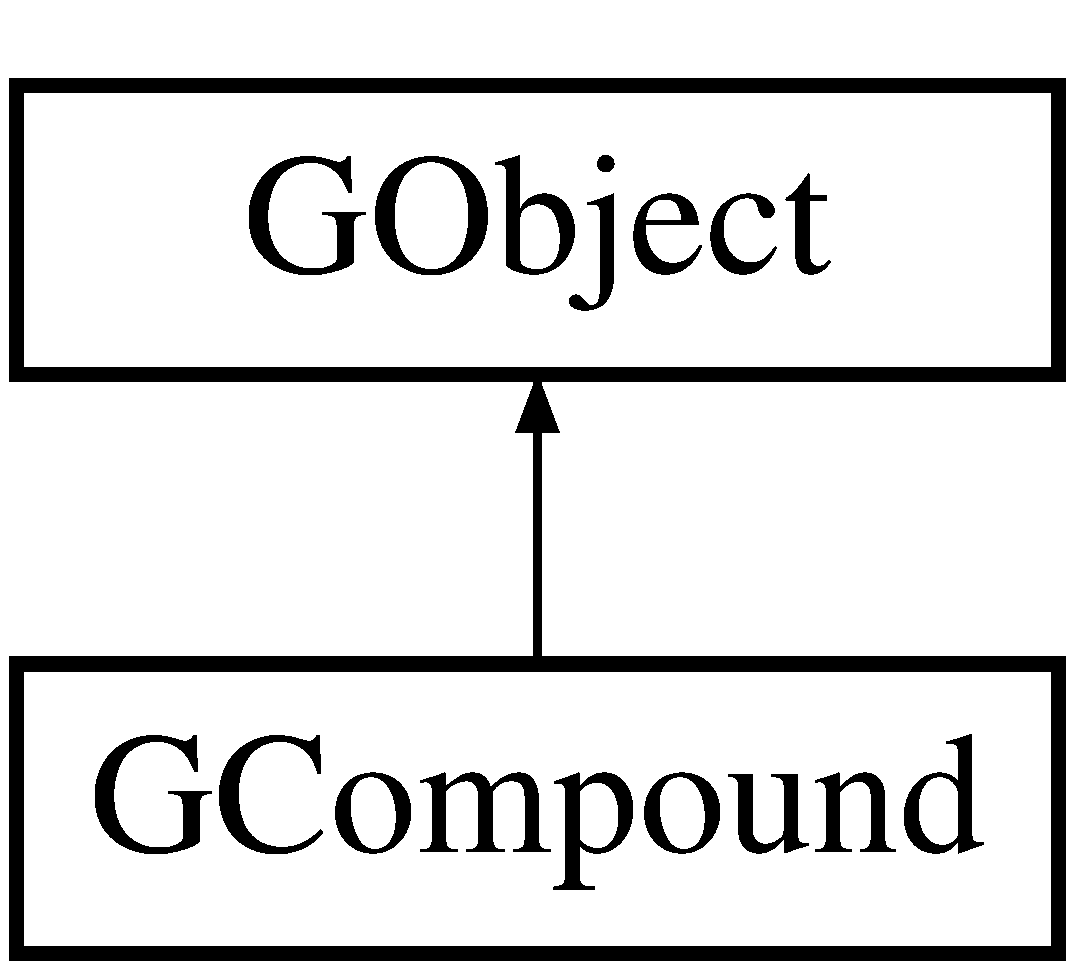
\includegraphics[height=2.000000cm]{classGCompound}
\end{center}
\end{figure}
\subsection*{Public Types}
\begin{DoxyCompactItemize}
\item 
enum \mbox{\hyperlink{classGObject_a86e0f5648542856159bb40775c854aa7}{Line\+Style}} \{ \mbox{\hyperlink{classGObject_a86e0f5648542856159bb40775c854aa7acbc84bd5232621834ed31f44d457c1eb}{L\+I\+N\+E\+\_\+\+N\+O\+NE}}, 
\mbox{\hyperlink{classGObject_a86e0f5648542856159bb40775c854aa7a700c78bc2cd76acaab26651bf7b4941f}{L\+I\+N\+E\+\_\+\+S\+O\+L\+ID}}, 
\mbox{\hyperlink{classGObject_a86e0f5648542856159bb40775c854aa7a9ccba0845f785d81d07b333ae1aad84e}{L\+I\+N\+E\+\_\+\+D\+A\+SH}}, 
\mbox{\hyperlink{classGObject_a86e0f5648542856159bb40775c854aa7a8e811c096cb941997f0bfda168bb6df3}{L\+I\+N\+E\+\_\+\+D\+OT}}, 
\mbox{\hyperlink{classGObject_a86e0f5648542856159bb40775c854aa7ada15a2e3d737b2db7706d8300f91b89d}{L\+I\+N\+E\+\_\+\+D\+A\+S\+H\+\_\+\+D\+OT}}, 
\mbox{\hyperlink{classGObject_a86e0f5648542856159bb40775c854aa7aabf4053a73eafa7ba2b7e6d664c74c1d}{L\+I\+N\+E\+\_\+\+D\+A\+S\+H\+\_\+\+D\+O\+T\+\_\+\+D\+OT}}
 \}
\begin{DoxyCompactList}\small\item\em Styles that can be used for the outline around various shapes. \end{DoxyCompactList}\end{DoxyCompactItemize}
\subsection*{Public Member Functions}
\begin{DoxyCompactItemize}
\item 
\mbox{\hyperlink{classGCompound_a96d2773de31d81df96135d8621cf47df}{G\+Compound}} ()
\begin{DoxyCompactList}\small\item\em Creates a compound with no internal components. \end{DoxyCompactList}\item 
virtual void \mbox{\hyperlink{classGCompound_afe8277e7b2627513c6f7452fb0b2847d}{add}} (\mbox{\hyperlink{classGObject}{G\+Object}} $\ast$gobj)
\begin{DoxyCompactList}\small\item\em Adds a new graphical object to the compound, if that object was not already present in the compound. \end{DoxyCompactList}\item 
virtual void \mbox{\hyperlink{classGCompound_a8bb36f245efc7806414a1339c2befa1c}{add}} (\mbox{\hyperlink{classGObject}{G\+Object}} $\ast$gobj, double x, double y)
\begin{DoxyCompactList}\small\item\em Adds a new graphical object to the compound, if that object was not already present in the compound. \end{DoxyCompactList}\item 
virtual void \mbox{\hyperlink{classGCompound_ac732fc2123d7a6d7e2de145fe9bbd8e8}{add}} (\mbox{\hyperlink{classGObject}{G\+Object}} \&gobj)
\begin{DoxyCompactList}\small\item\em Adds a new graphical object to the compound. \end{DoxyCompactList}\item 
virtual void \mbox{\hyperlink{classGCompound_a5b11b532869632a6c26b098b0858eac5}{add}} (\mbox{\hyperlink{classGObject}{G\+Object}} \&gobj, double x, double y)
\begin{DoxyCompactList}\small\item\em Adds a new graphical object to the compound, if that object was not already present in the compound. \end{DoxyCompactList}\item 
virtual void \mbox{\hyperlink{classGCompound_ac8bb3912a3ce86b15842e79d0b421204}{clear}} ()
\begin{DoxyCompactList}\small\item\em Removes all graphical objects from the compound. \end{DoxyCompactList}\item 
virtual void \mbox{\hyperlink{classGCompound_a221b3e75bb3d9d0bfea62b3364e6773b}{conditional\+Repaint}} ()
\begin{DoxyCompactList}\small\item\em Repaints the compound only if it needs to be repainted (if any of its contents have changed). \end{DoxyCompactList}\item 
virtual void \mbox{\hyperlink{classGCompound_aedd4b792311d946eeaf44b0de337a408}{conditional\+Repaint\+Region}} (int x, int y, int width, int height)
\begin{DoxyCompactList}\small\item\em Repaints the given rectangular region of the compound only if it needs to be repainted (if any of its contents have changed). \end{DoxyCompactList}\item 
virtual void \mbox{\hyperlink{classGCompound_a3932a12278752db368e24fa404e446aa}{conditional\+Repaint\+Region}} (const \mbox{\hyperlink{structGRectangle}{G\+Rectangle}} \&bounds)
\begin{DoxyCompactList}\small\item\em Repaints the given rectangular region of the compound only if it needs to be repainted (if any of its contents have changed). \end{DoxyCompactList}\item 
virtual bool \mbox{\hyperlink{classGObject_a1dbc9dafaae51958112dbe1267a1f547}{contains}} (const \mbox{\hyperlink{structGPoint}{G\+Point}} \&pt) const
\begin{DoxyCompactList}\small\item\em Returns {\ttfamily true} if the specified point is inside the object. \end{DoxyCompactList}\item 
bool \mbox{\hyperlink{classGCompound_ad973a1d55799d3a73bf8b04986cd804e}{contains}} (double x, double y) const override
\begin{DoxyCompactList}\small\item\em Returns {\ttfamily true} if the specified point is inside the object. \end{DoxyCompactList}\item 
virtual \mbox{\hyperlink{structGPoint}{G\+Point}} \mbox{\hyperlink{classGObject_a0d41183bf6b08de66fe3907551aab0d7}{get\+Bottom\+Right\+Location}} () const
\begin{DoxyCompactList}\small\item\em Returns the x/y coordinates of the bottom/right corner of the object. \end{DoxyCompactList}\item 
virtual double \mbox{\hyperlink{classGObject_a4316a2406c18e1c6d061fe51fd355490}{get\+BottomY}} () const
\begin{DoxyCompactList}\small\item\em Returns the {\itshape y}-\/coordinate of the bottom of the object. \end{DoxyCompactList}\item 
\mbox{\hyperlink{structGRectangle}{G\+Rectangle}} \mbox{\hyperlink{classGCompound_a89040ce9277825772d359fccd33bca86}{get\+Bounds}} () const override
\begin{DoxyCompactList}\small\item\em Returns the bounding box of this object, which is defined to be the smallest rectangle that covers everything drawn by the figure. \end{DoxyCompactList}\item 
virtual \mbox{\hyperlink{structGPoint}{G\+Point}} \mbox{\hyperlink{classGObject_a0909472e91448470bccdb62ecfb95d8b}{get\+Center\+Location}} () const
\begin{DoxyCompactList}\small\item\em Returns the x/y-\/coordinates of the center of the object. \end{DoxyCompactList}\item 
virtual double \mbox{\hyperlink{classGObject_a04df74355b545e0543112d5b8d924176}{get\+CenterX}} () const
\begin{DoxyCompactList}\small\item\em Returns the {\itshape x}-\/coordinate of the center of the object. \end{DoxyCompactList}\item 
virtual double \mbox{\hyperlink{classGObject_acb3287a3d507025a26f54b895713b947}{get\+CenterY}} () const
\begin{DoxyCompactList}\small\item\em Returns the {\itshape y}-\/coordinate of the center of the object. \end{DoxyCompactList}\item 
virtual std\+::string \mbox{\hyperlink{classGObject_aa061dfa488c31e18549d64363c1d0e34}{get\+Color}} () const
\begin{DoxyCompactList}\small\item\em Returns the color used to display this object. \end{DoxyCompactList}\item 
virtual \mbox{\hyperlink{classGObject}{G\+Object}} $\ast$ \mbox{\hyperlink{classGCompound_abde388cc529d22bb5f7f4a54d56049d8}{get\+Element}} (int index) const
\begin{DoxyCompactList}\small\item\em Returns a pointer to the graphical object at the specified index, numbering from back to front in the {\itshape z} dimension. \end{DoxyCompactList}\item 
virtual \mbox{\hyperlink{classGObject}{G\+Object}} $\ast$ \mbox{\hyperlink{classGCompound_a25efa999eca5790ec26ef091b05f961c}{get\+Element\+At}} (double x, double y) const
\begin{DoxyCompactList}\small\item\em Returns a pointer to the first graphical object that contains the given (x, y) point, or a null pointer if no object in this compound touches it. \end{DoxyCompactList}\item 
virtual int \mbox{\hyperlink{classGCompound_adf7d37ec315f859648def92e6b32408f}{get\+Element\+Count}} () const
\begin{DoxyCompactList}\small\item\em Returns the number of graphical objects stored in the compound. \end{DoxyCompactList}\item 
virtual std\+::string \mbox{\hyperlink{classGObject_a76f6964a11fde7c78e9751be184e1a3c}{get\+Fill\+Color}} () const
\begin{DoxyCompactList}\small\item\em Returns the color used to display the filled region of this object. \end{DoxyCompactList}\item 
virtual double \mbox{\hyperlink{classGObject_a1e7e353362434072875264cf95629f99}{get\+Height}} () const
\begin{DoxyCompactList}\small\item\em Returns the height of this object, which is the same as the height of its bounding box. \end{DoxyCompactList}\item 
virtual \mbox{\hyperlink{classGObject_a86e0f5648542856159bb40775c854aa7}{Line\+Style}} \mbox{\hyperlink{classGObject_aaf1f5ea8281e5e3486662878d26f0a13}{get\+Line\+Style}} () const
\begin{DoxyCompactList}\small\item\em Returns the object\textquotesingle{}s style such as solid or dashed. \end{DoxyCompactList}\item 
virtual double \mbox{\hyperlink{classGObject_a85ff266dc3eb63d9f2d8e5a4487fd3c0}{get\+Line\+Width}} () const
\begin{DoxyCompactList}\small\item\em Returns the width of the line used to draw this object. \end{DoxyCompactList}\item 
virtual \mbox{\hyperlink{structGPoint}{G\+Point}} \mbox{\hyperlink{classGObject_a4f83802015511edeb63b892830812c11}{get\+Location}} () const
\begin{DoxyCompactList}\small\item\em Returns the location of the top-\/left corner of object. \end{DoxyCompactList}\item 
virtual double \mbox{\hyperlink{classGObject_a1ae3fc278cc5b71b9f2d96a8a83cdf26}{get\+Opacity}} () const
\begin{DoxyCompactList}\small\item\em Returns how opaque (non-\/transparent) this object will appear from 0.\+0 (completely transparent) to 1.\+0 (completely opaque, default). \end{DoxyCompactList}\item 
virtual \mbox{\hyperlink{classGCompound}{G\+Compound}} $\ast$ \mbox{\hyperlink{classGObject_a3e53cef70541b1a14eade4ad0984d0b4}{get\+Parent}} () const
\begin{DoxyCompactList}\small\item\em Returns a pointer to the {\ttfamily \mbox{\hyperlink{classGCompound}{G\+Compound}}} that contains this object. \end{DoxyCompactList}\item 
virtual double \mbox{\hyperlink{classGObject_a798cc79daaa10145b28f60bcdfdb0ee9}{get\+RightX}} () const
\begin{DoxyCompactList}\small\item\em Returns the {\itshape x}-\/coordinate of the right side of the object. \end{DoxyCompactList}\item 
virtual \mbox{\hyperlink{structGDimension}{G\+Dimension}} \mbox{\hyperlink{classGObject_a7b4eec96a2bdc6420695d5796a78eea9}{get\+Size}} () const
\begin{DoxyCompactList}\small\item\em Returns the size of the object as a {\ttfamily \mbox{\hyperlink{structGDimension}{G\+Dimension}}}. \end{DoxyCompactList}\item 
std\+::string \mbox{\hyperlink{classGCompound_a9b72ede4ee8520f987a0c01e30654814}{get\+Type}} () const override
\begin{DoxyCompactList}\small\item\em Returns the type of the object as a string, such as {\ttfamily \char`\"{}\+G\+Oval\char`\"{}} or {\ttfamily \char`\"{}\+G\+Rect\char`\"{}}. \end{DoxyCompactList}\item 
virtual double \mbox{\hyperlink{classGObject_a0ed2965abd4f5701d2cadf71239faf19}{get\+Width}} () const
\begin{DoxyCompactList}\small\item\em Returns the width of this object, which is equal to the width of the bounding box. \end{DoxyCompactList}\item 
virtual double \mbox{\hyperlink{classGObject_a344385751bee0720059403940d57a13e}{getX}} () const
\begin{DoxyCompactList}\small\item\em Returns the leftmost {\itshape x}-\/coordinate of the object. \end{DoxyCompactList}\item 
virtual double \mbox{\hyperlink{classGObject_aafa51c7f8f38a09febbb9ce7853f77b4}{getY}} () const
\begin{DoxyCompactList}\small\item\em Returns the topmost {\itshape y}-\/coordinate of the object. \end{DoxyCompactList}\item 
virtual bool \mbox{\hyperlink{classGCompound_a12c8d52ddfcaa5448ec4bace92ddee6c}{is\+Auto\+Repaint}} () const
\begin{DoxyCompactList}\small\item\em Returns whether the compound automatically repaints itself when its contents change. \end{DoxyCompactList}\item 
virtual bool \mbox{\hyperlink{classGCompound_acf82f9b2937375c7b1cf3dccb3df3312}{is\+Empty}} () const
\begin{DoxyCompactList}\small\item\em Returns true if the compound does not contain any graphical objects. \end{DoxyCompactList}\item 
virtual bool \mbox{\hyperlink{classGObject_a11c404f106940c201b6f326e0355c150}{is\+Filled}} () const
\begin{DoxyCompactList}\small\item\em Returns {\ttfamily true} if the object is filled with color. \end{DoxyCompactList}\item 
virtual bool \mbox{\hyperlink{classGObject_a9de207581cfa4ca1eaa06da5f29b75fc}{is\+Transformed}} () const
\begin{DoxyCompactList}\small\item\em Returns {\ttfamily true} if this object has been transformed by calling methods such as \mbox{\hyperlink{classGObject_ae1ffaa12185dfd5ba464f7d87c329e26}{rotate()}} or \mbox{\hyperlink{classGObject_ad2e1900f730475c2d044817db03b38d6}{scale()}} on it. \end{DoxyCompactList}\item 
virtual bool \mbox{\hyperlink{classGObject_a9d8a6cfb13917785c143e74d40e4e2be}{is\+Visible}} () const
\begin{DoxyCompactList}\small\item\em Returns {\ttfamily true} if this object is visible on screen. \end{DoxyCompactList}\item 
virtual void \mbox{\hyperlink{classGObject_a5973d8dda83afb36e2c56855515be392}{move}} (double dx, double dy)
\begin{DoxyCompactList}\small\item\em Moves the object on the screen using the displacements {\ttfamily dx} and {\ttfamily dy}. \end{DoxyCompactList}\item 
virtual void \mbox{\hyperlink{classGCompound_a49dc57a2ce4caa354a5fff6acdde2e7d}{remove}} (\mbox{\hyperlink{classGObject}{G\+Object}} $\ast$gobj)
\begin{DoxyCompactList}\small\item\em Removes the specified object from the compound. \end{DoxyCompactList}\item 
virtual void \mbox{\hyperlink{classGCompound_a0c0ae4d69b584602ff3cba0d9cf330a4}{remove}} (\mbox{\hyperlink{classGObject}{G\+Object}} \&gobj)
\begin{DoxyCompactList}\small\item\em Removes the specified object from the compound. \end{DoxyCompactList}\item 
virtual void \mbox{\hyperlink{classGCompound_a9b0a5a3ad9972ab0e8eb0b54873aac6b}{remove\+All}} ()
\begin{DoxyCompactList}\small\item\em Removes all graphical objects from the compound. \end{DoxyCompactList}\item 
void \mbox{\hyperlink{classGCompound_afb8dbc55702230f0030e47d6c009697f}{repaint}} () override
\begin{DoxyCompactList}\small\item\em Instructs the compound to redraw all of its graphical objects. \end{DoxyCompactList}\item 
virtual void \mbox{\hyperlink{classGCompound_a4a919e3851ebfbf0f161a66cc15d4531}{repaint\+Region}} (int x, int y, int width, int height)
\begin{DoxyCompactList}\small\item\em Instructs the compound to redraw the given rectangular region within itself, including any graphical objects that touch that region. \end{DoxyCompactList}\item 
virtual void \mbox{\hyperlink{classGCompound_a769c46fb3e1004aec76e8b0adfa42aa6}{repaint\+Region}} (const \mbox{\hyperlink{structGRectangle}{G\+Rectangle}} \&bounds)
\begin{DoxyCompactList}\small\item\em Instructs the compound to redraw the given rectangular region within itself, including any graphical objects that touch that region. \end{DoxyCompactList}\item 
virtual void \mbox{\hyperlink{classGObject_a6022a1fd1e5dcd2fd5585e5a36aa3f37}{reset\+Transform}} ()
\begin{DoxyCompactList}\small\item\em Undoes any previous scale/rotate transformations on this object. \end{DoxyCompactList}\item 
virtual void \mbox{\hyperlink{classGObject_ae1ffaa12185dfd5ba464f7d87c329e26}{rotate}} (double theta)
\begin{DoxyCompactList}\small\item\em Transforms the object by rotating it {\ttfamily theta} degrees counterclockwise around its origin. \end{DoxyCompactList}\item 
virtual void \mbox{\hyperlink{classGObject_ad2e1900f730475c2d044817db03b38d6}{scale}} (double sf)
\begin{DoxyCompactList}\small\item\em Scales the object by the specified scale factor. \end{DoxyCompactList}\item 
virtual void \mbox{\hyperlink{classGObject_a63641f69d610d0b951357d35a0c3b1e3}{scale}} (double sx, double sy)
\begin{DoxyCompactList}\small\item\em Scales the object by the specified scale factors. \end{DoxyCompactList}\item 
void \mbox{\hyperlink{classGObject_ab6747f40313c531c2db32edb5b63b9b7}{send\+Backward}} ()
\begin{DoxyCompactList}\small\item\em Moves this object one step toward the back in the {\itshape z} dimension. \end{DoxyCompactList}\item 
void \mbox{\hyperlink{classGObject_a710b3e449c9facba7847c91ab170d281}{send\+Forward}} ()
\begin{DoxyCompactList}\small\item\em Moves this object one step toward the front in the {\itshape z} dimension. \end{DoxyCompactList}\item 
void \mbox{\hyperlink{classGObject_a0f7f1efbb7fd46dde2867c4ad0330896}{send\+To\+Back}} ()
\begin{DoxyCompactList}\small\item\em Moves this object to the back of the display in the {\itshape z} dimension. \end{DoxyCompactList}\item 
void \mbox{\hyperlink{classGObject_aee33d68488e46827ef55fac07f40a9b2}{send\+To\+Front}} ()
\begin{DoxyCompactList}\small\item\em Moves this object to the front of the display in the {\itshape z} dimension. \end{DoxyCompactList}\item 
virtual void \mbox{\hyperlink{classGCompound_adf10848319457bd6df4c657bf8872bee}{set\+Auto\+Repaint}} (bool auto\+Repaint)
\begin{DoxyCompactList}\small\item\em Sets whether the compound automatically repaints itself when its contents change. \end{DoxyCompactList}\item 
virtual void \mbox{\hyperlink{classGObject_a71ff7b16b8f1bdc4a1ce9f30cf8b87d8}{set\+Bottom\+Right\+Location}} (double x, double y)
\begin{DoxyCompactList}\small\item\em Sets the location of the bottom/right of this object. \end{DoxyCompactList}\item 
virtual void \mbox{\hyperlink{classGObject_ac6f7320321182f1d18c1c0fa97d5e941}{set\+Bottom\+Right\+Location}} (const \mbox{\hyperlink{structGPoint}{G\+Point}} \&pt)
\begin{DoxyCompactList}\small\item\em Sets the location of the bottom/right of this object. \end{DoxyCompactList}\item 
virtual void \mbox{\hyperlink{classGObject_a4b20e93c2a2597484f74ee5caa71f41f}{set\+BottomY}} (double y)
\begin{DoxyCompactList}\small\item\em Sets the location of the bottom y-\/coordinate of this object. \end{DoxyCompactList}\item 
virtual void \mbox{\hyperlink{classGObject_a2aae8197624b72265ab83b4f1bc73f2f}{set\+Bounds}} (double x, double y, double width, double height)
\begin{DoxyCompactList}\small\item\em Changes the bounds of this object to the specified values. \end{DoxyCompactList}\item 
virtual void \mbox{\hyperlink{classGObject_acada386653f008cacc7cce86426bef7c}{set\+Bounds}} (const \mbox{\hyperlink{structGRectangle}{G\+Rectangle}} \&size)
\begin{DoxyCompactList}\small\item\em Changes the bounds of this object to the specified rectangle. \end{DoxyCompactList}\item 
virtual void \mbox{\hyperlink{classGObject_a290b47dd8de1be44089f95cb2c47c1de}{set\+Center\+Location}} (double x, double y)
\begin{DoxyCompactList}\small\item\em Sets the location of the center of this object. \end{DoxyCompactList}\item 
virtual void \mbox{\hyperlink{classGObject_a1bedf1b233ecba3f753ec58908a683a6}{set\+Center\+Location}} (const \mbox{\hyperlink{structGPoint}{G\+Point}} \&pt)
\begin{DoxyCompactList}\small\item\em Sets the location of the center of this object. \end{DoxyCompactList}\item 
virtual void \mbox{\hyperlink{classGObject_a2f4936281e056eead00a9186b9ba8af6}{set\+CenterX}} (double x)
\begin{DoxyCompactList}\small\item\em Sets the x-\/coordinate of the center of this object. \end{DoxyCompactList}\item 
virtual void \mbox{\hyperlink{classGObject_aad2a22b4fde88c33306b92aebf641d57}{set\+CenterY}} (double y)
\begin{DoxyCompactList}\small\item\em Sets the y-\/coordinate of the center of this object. \end{DoxyCompactList}\item 
virtual void \mbox{\hyperlink{classGObject_ad57ef49bc31db94e92648aa3737923d6}{set\+Color}} (int r, int g, int b)
\begin{DoxyCompactList}\small\item\em Sets the color used to display this object. \end{DoxyCompactList}\item 
virtual void \mbox{\hyperlink{classGObject_ab1f5cc0f5cc6bbbd716a526c61f1081d}{set\+Color}} (int rgb)
\begin{DoxyCompactList}\small\item\em Sets the color used to display this object. \end{DoxyCompactList}\item 
virtual void \mbox{\hyperlink{classGObject_a61374df6c11b52cfbb0815decdbaebc6}{set\+Color}} (const std\+::string \&color)
\begin{DoxyCompactList}\small\item\em Sets the color used to display this object. \end{DoxyCompactList}\item 
virtual void \mbox{\hyperlink{classGObject_ad767a33971159e9493e221cca4c00ae9}{set\+Fill\+Color}} (int r, int g, int b)
\begin{DoxyCompactList}\small\item\em Sets the color used to display the filled region of this object, if any. \end{DoxyCompactList}\item 
virtual void \mbox{\hyperlink{classGObject_aa59d9775a67fa7df2b24a95cd34840a3}{set\+Fill\+Color}} (int rgb)
\begin{DoxyCompactList}\small\item\em Sets the color used to display the filled region of this object, if any. \end{DoxyCompactList}\item 
virtual void \mbox{\hyperlink{classGObject_adbc18b1a930aadd97d7437f9f7265b96}{set\+Fill\+Color}} (const std\+::string \&color)
\begin{DoxyCompactList}\small\item\em Sets the color used to display the filled region of this object, if any. \end{DoxyCompactList}\item 
virtual void \mbox{\hyperlink{classGObject_a9b82b53362282c6bb7d6947068d2e55b}{set\+Filled}} (bool flag)
\begin{DoxyCompactList}\small\item\em Sets the fill status for the object, where {\ttfamily false} is outlined and {\ttfamily true} is filled. \end{DoxyCompactList}\item 
virtual void \mbox{\hyperlink{classGObject_a2592348886ffea646c6534bf88f7c49d}{set\+Font}} (const Q\+Font \&font)
\begin{DoxyCompactList}\small\item\em Changes the font used to display the object as specified by the given Qt font. \end{DoxyCompactList}\item 
virtual void \mbox{\hyperlink{classGObject_a8e096e8818d838aceae1d46d58fb3a7b}{set\+Font}} (const std\+::string \&font)
\begin{DoxyCompactList}\small\item\em Changes the font used to display the object as specified by the string {\ttfamily font}, which has the following format\+: \end{DoxyCompactList}\item 
virtual void \mbox{\hyperlink{classGObject_ad18e8fab1e02a4e9b75c6730212558eb}{set\+Foreground}} (int r, int g, int b)
\begin{DoxyCompactList}\small\item\em Sets the color used to display this object. \end{DoxyCompactList}\item 
virtual void \mbox{\hyperlink{classGObject_a9eb856b5ff83a19df3831a31f15f4563}{set\+Foreground}} (int rgb)
\begin{DoxyCompactList}\small\item\em Sets the color used to display this object. \end{DoxyCompactList}\item 
virtual void \mbox{\hyperlink{classGObject_af59209aeadea6dfc6d97a2d8531f50e1}{set\+Foreground}} (const std\+::string \&color)
\begin{DoxyCompactList}\small\item\em Sets the color used to display this object. \end{DoxyCompactList}\item 
virtual void \mbox{\hyperlink{classGObject_a9e280bfc4544dfaf8e4376c4e1a74357}{set\+Height}} (double height)
\begin{DoxyCompactList}\small\item\em Changes the height of this object to the specified height without changing its width. \end{DoxyCompactList}\item 
virtual void \mbox{\hyperlink{classGObject_add11575087eb94f1a71faa3f826c6341}{set\+Line\+Style}} (\mbox{\hyperlink{classGObject_a86e0f5648542856159bb40775c854aa7}{Line\+Style}} line\+Style)
\begin{DoxyCompactList}\small\item\em Sets the object\textquotesingle{}s style such as solid (\mbox{\hyperlink{classGObject_a86e0f5648542856159bb40775c854aa7a700c78bc2cd76acaab26651bf7b4941f}{G\+Object\+::\+L\+I\+N\+E\+\_\+\+S\+O\+L\+ID}}) or dashed (\mbox{\hyperlink{classGObject_a86e0f5648542856159bb40775c854aa7a9ccba0845f785d81d07b333ae1aad84e}{G\+Object\+::\+L\+I\+N\+E\+\_\+\+D\+A\+SH}}). \end{DoxyCompactList}\item 
virtual void \mbox{\hyperlink{classGObject_afd6a47c6ea6a1f85ca05a65ba3ff3477}{set\+Line\+Width}} (double line\+Width)
\begin{DoxyCompactList}\small\item\em Sets the width of the line used to draw this object. \end{DoxyCompactList}\item 
virtual void \mbox{\hyperlink{classGObject_a04594e8ba9b98513a64f1da00dcae18c}{set\+Location}} (double x, double y)
\begin{DoxyCompactList}\small\item\em Sets the location of the top-\/left corner of this object to the specified coordinates. \end{DoxyCompactList}\item 
virtual void \mbox{\hyperlink{classGObject_aa8480c0b7166cdf8f784cece06ab353f}{set\+Location}} (const \mbox{\hyperlink{structGPoint}{G\+Point}} \&pt)
\begin{DoxyCompactList}\small\item\em Sets the location of the top-\/left corner of this object to the specified point. \end{DoxyCompactList}\item 
virtual void \mbox{\hyperlink{classGObject_a04af1866cc1bae4a1226695794a50539}{set\+Opacity}} (double opacity)
\begin{DoxyCompactList}\small\item\em Sets how opaque (non-\/transparent) this object will appear from 0.\+0 (completely transparent) to 1.\+0 (completely opaque, default). \end{DoxyCompactList}\item 
virtual void \mbox{\hyperlink{classGObject_a3c90b758cdc2c911c9ef76c4360eb912}{set\+RightX}} (double x)
\begin{DoxyCompactList}\small\item\em Sets the location of the rightmost x-\/coordinate of this object. \end{DoxyCompactList}\item 
virtual void \mbox{\hyperlink{classGObject_aca25d49481f9bf5fc8f7df4c086c4ce7}{set\+Size}} (double width, double height)
\begin{DoxyCompactList}\small\item\em Changes the size of this object to the specified width and height. \end{DoxyCompactList}\item 
virtual void \mbox{\hyperlink{classGObject_ae2b628228f192c2702c4ce941b2af68f}{set\+Size}} (const \mbox{\hyperlink{structGDimension}{G\+Dimension}} \&size)
\begin{DoxyCompactList}\small\item\em Changes the size of this object to the specified width and height. \end{DoxyCompactList}\item 
virtual void \mbox{\hyperlink{classGObject_a88203f28224315d9f4471212f4af8ed3}{set\+Visible}} (bool flag)
\begin{DoxyCompactList}\small\item\em Sets whether this object is visible. \end{DoxyCompactList}\item 
virtual void \mbox{\hyperlink{classGObject_aa3f3fba4cb131baa8696ba01e3bceca1}{set\+Width}} (double width)
\begin{DoxyCompactList}\small\item\em Changes the width of this object to the specified width without changing its height. \end{DoxyCompactList}\item 
virtual void \mbox{\hyperlink{classGObject_a9c18fcc579333bf9653d13ad2b372e39}{setX}} (double x)
\begin{DoxyCompactList}\small\item\em Sets the x location of the left side of this object. \end{DoxyCompactList}\item 
virtual void \mbox{\hyperlink{classGObject_a7d57e2a5c35d27feb58fd498a3cf82b9}{setY}} (double y)
\begin{DoxyCompactList}\small\item\em Sets the y location of the top of this object. \end{DoxyCompactList}\item 
std\+::string \mbox{\hyperlink{classGCompound_ab6e28321ea84864a7d677dd35c59523a}{to\+String}} () const override
\begin{DoxyCompactList}\small\item\em Returns a printable representation of the object. \end{DoxyCompactList}\end{DoxyCompactItemize}
\subsection*{Static Public Member Functions}
\begin{DoxyCompactItemize}
\item 
static bool \mbox{\hyperlink{classGObject_a93be0e1fe1b1bf1a1da732470c94f42b}{is\+Anti\+Aliasing}} ()
\begin{DoxyCompactList}\small\item\em Returns whether we should globally anti-\/alias graphical objects. \end{DoxyCompactList}\item 
static void \mbox{\hyperlink{classGObject_a1e43371668ae850193cebedb44e1bbe3}{set\+Anti\+Aliasing}} (bool value)
\begin{DoxyCompactList}\small\item\em Globally turns on/off the anti-\/aliasing feature that smooths out the edges of onscreen shapes. \end{DoxyCompactList}\end{DoxyCompactItemize}
\subsection*{Protected Member Functions}
\begin{DoxyCompactItemize}
\item 
virtual std\+::string \mbox{\hyperlink{classGObject_a4fcdf8de5c6de92242a975d83d8f23ea}{to\+String\+Extra}} () const
\begin{DoxyCompactList}\small\item\em Returns a string containing any extra unique information about this type of graphical object. \end{DoxyCompactList}\end{DoxyCompactItemize}
\subsection*{Protected Attributes}
\begin{DoxyCompactItemize}
\item 
Q\+Brush \mbox{\hyperlink{classGObject_aab24462ec896b596d99911767b0912d0}{\+\_\+brush}}
\item 
std\+::string \mbox{\hyperlink{classGObject_a1134e770ae4315ea8bc1201e2f21da8b}{\+\_\+color}}
\item 
int \mbox{\hyperlink{classGObject_a003fdd343d9b7505c53a8b7a134200ed}{\+\_\+color\+Int}}
\item 
std\+::string \mbox{\hyperlink{classGObject_a179f8d6cee65cd8a54692e32b224392a}{\+\_\+fill\+Color}}
\item 
int \mbox{\hyperlink{classGObject_a751def333a67d651e5b99cc331ecb496}{\+\_\+fill\+Color\+Int}}
\item 
bool \mbox{\hyperlink{classGObject_ad4a55cbcd61b58a4d49666490bb2f103}{\+\_\+fill\+Flag}}
\item 
std\+::string \mbox{\hyperlink{classGObject_aea76ea1a8b5dd7b0a78653277e63b536}{\+\_\+font}}
\item 
double \mbox{\hyperlink{classGObject_ad05df29e7f27fc504abd743e3d8b4e73}{\+\_\+height}}
\item 
\mbox{\hyperlink{classGObject_a86e0f5648542856159bb40775c854aa7}{Line\+Style}} \mbox{\hyperlink{classGObject_a89bafecaafb7c72d55c7efc10b7d0523}{\+\_\+line\+Style}}
\item 
double \mbox{\hyperlink{classGObject_a16e9033665937f13de2e163dc2184aff}{\+\_\+line\+Width}}
\item 
double \mbox{\hyperlink{classGObject_a20eff8eb7af27182edc9bfc54768b6f3}{\+\_\+opacity}}
\item 
\mbox{\hyperlink{classGCompound}{G\+Compound}} $\ast$ \mbox{\hyperlink{classGObject_ac9452c1eaff70eebddbb318196aa3835}{\+\_\+parent}}
\item 
Q\+Pen \mbox{\hyperlink{classGObject_afb69d172743f868299847174eb1b6bc8}{\+\_\+pen}}
\item 
Q\+Transform \mbox{\hyperlink{classGObject_a475b8860a5f1adb4a1fdc58d1f5c1e32}{\+\_\+transform}}
\item 
bool \mbox{\hyperlink{classGObject_ae4725802fc8d8aaa0ab4bd4781f7e07c}{\+\_\+transformed}}
\item 
bool \mbox{\hyperlink{classGObject_a9312c72508471b7c7a87b540263e1af4}{\+\_\+visible}}
\item 
double \mbox{\hyperlink{classGObject_ab55d85a3371770e6725b1062cf160cd8}{\+\_\+width}}
\item 
double \mbox{\hyperlink{classGObject_a6675b83b27137b8d3aa2ad8133078ea6}{\+\_\+x}}
\item 
double \mbox{\hyperlink{classGObject_a2f0f6aeafddc8a39c578bfa7e22b5f1e}{\+\_\+y}}
\end{DoxyCompactItemize}


\subsection{Detailed Description}
This graphical object subclass consists of a collection of other graphical objects. 

Once assembled, the internal objects can be manipulated as a unit. The compound keeps track of its own position, and all items within it are drawn relative to that location. 

\subsection{Member Enumeration Documentation}
\mbox{\Hypertarget{classGObject_a86e0f5648542856159bb40775c854aa7}\label{classGObject_a86e0f5648542856159bb40775c854aa7}} 
\index{G\+Compound@{G\+Compound}!Line\+Style@{Line\+Style}}
\index{Line\+Style@{Line\+Style}!G\+Compound@{G\+Compound}}
\subsubsection{\texorpdfstring{Line\+Style}{LineStyle}}
{\footnotesize\ttfamily enum \mbox{\hyperlink{classGObject_a86e0f5648542856159bb40775c854aa7}{Line\+Style}}\hspace{0.3cm}{\ttfamily [inherited]}}



Styles that can be used for the outline around various shapes. 

Call set\+Line\+Style on a \mbox{\hyperlink{classGObject}{G\+Object}} and pass one of these values. \begin{DoxyEnumFields}{Enumerator}
\raisebox{\heightof{T}}[0pt][0pt]{\index{L\+I\+N\+E\+\_\+\+N\+O\+NE@{L\+I\+N\+E\+\_\+\+N\+O\+NE}!G\+Compound@{G\+Compound}}\index{G\+Compound@{G\+Compound}!L\+I\+N\+E\+\_\+\+N\+O\+NE@{L\+I\+N\+E\+\_\+\+N\+O\+NE}}}\mbox{\Hypertarget{classGObject_a86e0f5648542856159bb40775c854aa7acbc84bd5232621834ed31f44d457c1eb}\label{classGObject_a86e0f5648542856159bb40775c854aa7acbc84bd5232621834ed31f44d457c1eb}} 
L\+I\+N\+E\+\_\+\+N\+O\+NE&\\
\hline

\raisebox{\heightof{T}}[0pt][0pt]{\index{L\+I\+N\+E\+\_\+\+S\+O\+L\+ID@{L\+I\+N\+E\+\_\+\+S\+O\+L\+ID}!G\+Compound@{G\+Compound}}\index{G\+Compound@{G\+Compound}!L\+I\+N\+E\+\_\+\+S\+O\+L\+ID@{L\+I\+N\+E\+\_\+\+S\+O\+L\+ID}}}\mbox{\Hypertarget{classGObject_a86e0f5648542856159bb40775c854aa7a700c78bc2cd76acaab26651bf7b4941f}\label{classGObject_a86e0f5648542856159bb40775c854aa7a700c78bc2cd76acaab26651bf7b4941f}} 
L\+I\+N\+E\+\_\+\+S\+O\+L\+ID&\\
\hline

\raisebox{\heightof{T}}[0pt][0pt]{\index{L\+I\+N\+E\+\_\+\+D\+A\+SH@{L\+I\+N\+E\+\_\+\+D\+A\+SH}!G\+Compound@{G\+Compound}}\index{G\+Compound@{G\+Compound}!L\+I\+N\+E\+\_\+\+D\+A\+SH@{L\+I\+N\+E\+\_\+\+D\+A\+SH}}}\mbox{\Hypertarget{classGObject_a86e0f5648542856159bb40775c854aa7a9ccba0845f785d81d07b333ae1aad84e}\label{classGObject_a86e0f5648542856159bb40775c854aa7a9ccba0845f785d81d07b333ae1aad84e}} 
L\+I\+N\+E\+\_\+\+D\+A\+SH&\\
\hline

\raisebox{\heightof{T}}[0pt][0pt]{\index{L\+I\+N\+E\+\_\+\+D\+OT@{L\+I\+N\+E\+\_\+\+D\+OT}!G\+Compound@{G\+Compound}}\index{G\+Compound@{G\+Compound}!L\+I\+N\+E\+\_\+\+D\+OT@{L\+I\+N\+E\+\_\+\+D\+OT}}}\mbox{\Hypertarget{classGObject_a86e0f5648542856159bb40775c854aa7a8e811c096cb941997f0bfda168bb6df3}\label{classGObject_a86e0f5648542856159bb40775c854aa7a8e811c096cb941997f0bfda168bb6df3}} 
L\+I\+N\+E\+\_\+\+D\+OT&\\
\hline

\raisebox{\heightof{T}}[0pt][0pt]{\index{L\+I\+N\+E\+\_\+\+D\+A\+S\+H\+\_\+\+D\+OT@{L\+I\+N\+E\+\_\+\+D\+A\+S\+H\+\_\+\+D\+OT}!G\+Compound@{G\+Compound}}\index{G\+Compound@{G\+Compound}!L\+I\+N\+E\+\_\+\+D\+A\+S\+H\+\_\+\+D\+OT@{L\+I\+N\+E\+\_\+\+D\+A\+S\+H\+\_\+\+D\+OT}}}\mbox{\Hypertarget{classGObject_a86e0f5648542856159bb40775c854aa7ada15a2e3d737b2db7706d8300f91b89d}\label{classGObject_a86e0f5648542856159bb40775c854aa7ada15a2e3d737b2db7706d8300f91b89d}} 
L\+I\+N\+E\+\_\+\+D\+A\+S\+H\+\_\+\+D\+OT&\\
\hline

\raisebox{\heightof{T}}[0pt][0pt]{\index{L\+I\+N\+E\+\_\+\+D\+A\+S\+H\+\_\+\+D\+O\+T\+\_\+\+D\+OT@{L\+I\+N\+E\+\_\+\+D\+A\+S\+H\+\_\+\+D\+O\+T\+\_\+\+D\+OT}!G\+Compound@{G\+Compound}}\index{G\+Compound@{G\+Compound}!L\+I\+N\+E\+\_\+\+D\+A\+S\+H\+\_\+\+D\+O\+T\+\_\+\+D\+OT@{L\+I\+N\+E\+\_\+\+D\+A\+S\+H\+\_\+\+D\+O\+T\+\_\+\+D\+OT}}}\mbox{\Hypertarget{classGObject_a86e0f5648542856159bb40775c854aa7aabf4053a73eafa7ba2b7e6d664c74c1d}\label{classGObject_a86e0f5648542856159bb40775c854aa7aabf4053a73eafa7ba2b7e6d664c74c1d}} 
L\+I\+N\+E\+\_\+\+D\+A\+S\+H\+\_\+\+D\+O\+T\+\_\+\+D\+OT&\\
\hline

\end{DoxyEnumFields}


\subsection{Constructor \& Destructor Documentation}
\mbox{\Hypertarget{classGCompound_a96d2773de31d81df96135d8621cf47df}\label{classGCompound_a96d2773de31d81df96135d8621cf47df}} 
\index{G\+Compound@{G\+Compound}!G\+Compound@{G\+Compound}}
\index{G\+Compound@{G\+Compound}!G\+Compound@{G\+Compound}}
\subsubsection{\texorpdfstring{G\+Compound()}{GCompound()}}
{\footnotesize\ttfamily \mbox{\hyperlink{classGCompound}{G\+Compound}} (\begin{DoxyParamCaption}{ }\end{DoxyParamCaption})}



Creates a compound with no internal components. 



\subsection{Member Function Documentation}
\mbox{\Hypertarget{classGCompound_afe8277e7b2627513c6f7452fb0b2847d}\label{classGCompound_afe8277e7b2627513c6f7452fb0b2847d}} 
\index{G\+Compound@{G\+Compound}!add@{add}}
\index{add@{add}!G\+Compound@{G\+Compound}}
\subsubsection{\texorpdfstring{add()}{add()}\hspace{0.1cm}{\footnotesize\ttfamily [1/4]}}
{\footnotesize\ttfamily void add (\begin{DoxyParamCaption}\item[{\mbox{\hyperlink{classGObject}{G\+Object}} $\ast$}]{gobj }\end{DoxyParamCaption})\hspace{0.3cm}{\ttfamily [virtual]}}



Adds a new graphical object to the compound, if that object was not already present in the compound. 

If the object is already stored in this compound, has no effect. 
\begin{DoxyExceptions}{Exceptions}
{\em Error\+Exception} & if the object is null \\
\hline
\end{DoxyExceptions}
\mbox{\Hypertarget{classGCompound_a8bb36f245efc7806414a1339c2befa1c}\label{classGCompound_a8bb36f245efc7806414a1339c2befa1c}} 
\index{G\+Compound@{G\+Compound}!add@{add}}
\index{add@{add}!G\+Compound@{G\+Compound}}
\subsubsection{\texorpdfstring{add()}{add()}\hspace{0.1cm}{\footnotesize\ttfamily [2/4]}}
{\footnotesize\ttfamily void add (\begin{DoxyParamCaption}\item[{\mbox{\hyperlink{classGObject}{G\+Object}} $\ast$}]{gobj,  }\item[{double}]{x,  }\item[{double}]{y }\end{DoxyParamCaption})\hspace{0.3cm}{\ttfamily [virtual]}}



Adds a new graphical object to the compound, if that object was not already present in the compound. 

This form moves the object to the point ({\ttfamily x}, {\ttfamily y}) first. If the object is already stored in this compound, has no effect. 
\begin{DoxyExceptions}{Exceptions}
{\em Error\+Exception} & if the object is null \\
\hline
\end{DoxyExceptions}
\mbox{\Hypertarget{classGCompound_ac732fc2123d7a6d7e2de145fe9bbd8e8}\label{classGCompound_ac732fc2123d7a6d7e2de145fe9bbd8e8}} 
\index{G\+Compound@{G\+Compound}!add@{add}}
\index{add@{add}!G\+Compound@{G\+Compound}}
\subsubsection{\texorpdfstring{add()}{add()}\hspace{0.1cm}{\footnotesize\ttfamily [3/4]}}
{\footnotesize\ttfamily void add (\begin{DoxyParamCaption}\item[{\mbox{\hyperlink{classGObject}{G\+Object}} \&}]{gobj }\end{DoxyParamCaption})\hspace{0.3cm}{\ttfamily [virtual]}}



Adds a new graphical object to the compound. 

\mbox{\Hypertarget{classGCompound_a5b11b532869632a6c26b098b0858eac5}\label{classGCompound_a5b11b532869632a6c26b098b0858eac5}} 
\index{G\+Compound@{G\+Compound}!add@{add}}
\index{add@{add}!G\+Compound@{G\+Compound}}
\subsubsection{\texorpdfstring{add()}{add()}\hspace{0.1cm}{\footnotesize\ttfamily [4/4]}}
{\footnotesize\ttfamily void add (\begin{DoxyParamCaption}\item[{\mbox{\hyperlink{classGObject}{G\+Object}} \&}]{gobj,  }\item[{double}]{x,  }\item[{double}]{y }\end{DoxyParamCaption})\hspace{0.3cm}{\ttfamily [virtual]}}



Adds a new graphical object to the compound, if that object was not already present in the compound. 

This form moves the object to the point ({\ttfamily x}, {\ttfamily y}) first. If the object is already stored in this compound, has no effect. \mbox{\Hypertarget{classGCompound_ac8bb3912a3ce86b15842e79d0b421204}\label{classGCompound_ac8bb3912a3ce86b15842e79d0b421204}} 
\index{G\+Compound@{G\+Compound}!clear@{clear}}
\index{clear@{clear}!G\+Compound@{G\+Compound}}
\subsubsection{\texorpdfstring{clear()}{clear()}}
{\footnotesize\ttfamily void clear (\begin{DoxyParamCaption}{ }\end{DoxyParamCaption})\hspace{0.3cm}{\ttfamily [virtual]}}



Removes all graphical objects from the compound. 

Equivalent to remove\+All. \mbox{\Hypertarget{classGCompound_a221b3e75bb3d9d0bfea62b3364e6773b}\label{classGCompound_a221b3e75bb3d9d0bfea62b3364e6773b}} 
\index{G\+Compound@{G\+Compound}!conditional\+Repaint@{conditional\+Repaint}}
\index{conditional\+Repaint@{conditional\+Repaint}!G\+Compound@{G\+Compound}}
\subsubsection{\texorpdfstring{conditional\+Repaint()}{conditionalRepaint()}}
{\footnotesize\ttfamily void conditional\+Repaint (\begin{DoxyParamCaption}{ }\end{DoxyParamCaption})\hspace{0.3cm}{\ttfamily [virtual]}}



Repaints the compound only if it needs to be repainted (if any of its contents have changed). 

\mbox{\Hypertarget{classGCompound_aedd4b792311d946eeaf44b0de337a408}\label{classGCompound_aedd4b792311d946eeaf44b0de337a408}} 
\index{G\+Compound@{G\+Compound}!conditional\+Repaint\+Region@{conditional\+Repaint\+Region}}
\index{conditional\+Repaint\+Region@{conditional\+Repaint\+Region}!G\+Compound@{G\+Compound}}
\subsubsection{\texorpdfstring{conditional\+Repaint\+Region()}{conditionalRepaintRegion()}\hspace{0.1cm}{\footnotesize\ttfamily [1/2]}}
{\footnotesize\ttfamily void conditional\+Repaint\+Region (\begin{DoxyParamCaption}\item[{int}]{x,  }\item[{int}]{y,  }\item[{int}]{width,  }\item[{int}]{height }\end{DoxyParamCaption})\hspace{0.3cm}{\ttfamily [virtual]}}



Repaints the given rectangular region of the compound only if it needs to be repainted (if any of its contents have changed). 

\mbox{\Hypertarget{classGCompound_a3932a12278752db368e24fa404e446aa}\label{classGCompound_a3932a12278752db368e24fa404e446aa}} 
\index{G\+Compound@{G\+Compound}!conditional\+Repaint\+Region@{conditional\+Repaint\+Region}}
\index{conditional\+Repaint\+Region@{conditional\+Repaint\+Region}!G\+Compound@{G\+Compound}}
\subsubsection{\texorpdfstring{conditional\+Repaint\+Region()}{conditionalRepaintRegion()}\hspace{0.1cm}{\footnotesize\ttfamily [2/2]}}
{\footnotesize\ttfamily void conditional\+Repaint\+Region (\begin{DoxyParamCaption}\item[{const \mbox{\hyperlink{structGRectangle}{G\+Rectangle}} \&}]{bounds }\end{DoxyParamCaption})\hspace{0.3cm}{\ttfamily [virtual]}}



Repaints the given rectangular region of the compound only if it needs to be repainted (if any of its contents have changed). 

\mbox{\Hypertarget{classGObject_a1dbc9dafaae51958112dbe1267a1f547}\label{classGObject_a1dbc9dafaae51958112dbe1267a1f547}} 
\index{G\+Compound@{G\+Compound}!contains@{contains}}
\index{contains@{contains}!G\+Compound@{G\+Compound}}
\subsubsection{\texorpdfstring{contains()}{contains()}\hspace{0.1cm}{\footnotesize\ttfamily [1/2]}}
{\footnotesize\ttfamily bool contains (\begin{DoxyParamCaption}\item[{const \mbox{\hyperlink{structGPoint}{G\+Point}} \&}]{pt }\end{DoxyParamCaption}) const\hspace{0.3cm}{\ttfamily [virtual]}, {\ttfamily [inherited]}}



Returns {\ttfamily true} if the specified point is inside the object. 

\mbox{\Hypertarget{classGCompound_ad973a1d55799d3a73bf8b04986cd804e}\label{classGCompound_ad973a1d55799d3a73bf8b04986cd804e}} 
\index{G\+Compound@{G\+Compound}!contains@{contains}}
\index{contains@{contains}!G\+Compound@{G\+Compound}}
\subsubsection{\texorpdfstring{contains()}{contains()}\hspace{0.1cm}{\footnotesize\ttfamily [2/2]}}
{\footnotesize\ttfamily bool contains (\begin{DoxyParamCaption}\item[{double}]{x,  }\item[{double}]{y }\end{DoxyParamCaption}) const\hspace{0.3cm}{\ttfamily [override]}, {\ttfamily [virtual]}}



Returns {\ttfamily true} if the specified point is inside the object. 



Reimplemented from \mbox{\hyperlink{classGObject_abb6a5d7c03e6eaaae97264c4799ce7c3}{G\+Object}}.

\mbox{\Hypertarget{classGObject_a0d41183bf6b08de66fe3907551aab0d7}\label{classGObject_a0d41183bf6b08de66fe3907551aab0d7}} 
\index{G\+Compound@{G\+Compound}!get\+Bottom\+Right\+Location@{get\+Bottom\+Right\+Location}}
\index{get\+Bottom\+Right\+Location@{get\+Bottom\+Right\+Location}!G\+Compound@{G\+Compound}}
\subsubsection{\texorpdfstring{get\+Bottom\+Right\+Location()}{getBottomRightLocation()}}
{\footnotesize\ttfamily \mbox{\hyperlink{structGPoint}{G\+Point}} get\+Bottom\+Right\+Location (\begin{DoxyParamCaption}{ }\end{DoxyParamCaption}) const\hspace{0.3cm}{\ttfamily [virtual]}, {\ttfamily [inherited]}}



Returns the x/y coordinates of the bottom/right corner of the object. 

\mbox{\Hypertarget{classGObject_a4316a2406c18e1c6d061fe51fd355490}\label{classGObject_a4316a2406c18e1c6d061fe51fd355490}} 
\index{G\+Compound@{G\+Compound}!get\+BottomY@{get\+BottomY}}
\index{get\+BottomY@{get\+BottomY}!G\+Compound@{G\+Compound}}
\subsubsection{\texorpdfstring{get\+Bottom\+Y()}{getBottomY()}}
{\footnotesize\ttfamily double get\+BottomY (\begin{DoxyParamCaption}{ }\end{DoxyParamCaption}) const\hspace{0.3cm}{\ttfamily [virtual]}, {\ttfamily [inherited]}}



Returns the {\itshape y}-\/coordinate of the bottom of the object. 

Equivalent to the top y-\/coordinate plus the object\textquotesingle{}s height. \mbox{\Hypertarget{classGCompound_a89040ce9277825772d359fccd33bca86}\label{classGCompound_a89040ce9277825772d359fccd33bca86}} 
\index{G\+Compound@{G\+Compound}!get\+Bounds@{get\+Bounds}}
\index{get\+Bounds@{get\+Bounds}!G\+Compound@{G\+Compound}}
\subsubsection{\texorpdfstring{get\+Bounds()}{getBounds()}}
{\footnotesize\ttfamily \mbox{\hyperlink{structGRectangle}{G\+Rectangle}} get\+Bounds (\begin{DoxyParamCaption}{ }\end{DoxyParamCaption}) const\hspace{0.3cm}{\ttfamily [override]}, {\ttfamily [virtual]}}



Returns the bounding box of this object, which is defined to be the smallest rectangle that covers everything drawn by the figure. 

The coordinates of this rectangle do not necessarily match the location returned by {\ttfamily get\+Location}. Given a {\ttfamily \mbox{\hyperlink{classGText}{G\+Text}}} object, for example, {\ttfamily get\+Location} returns the coordinates of the point on the baseline at which the string begins; the {\ttfamily get\+Bounds} method, by contrast, returns a rectangle that covers the entire window area occupied by the string. 

Reimplemented from \mbox{\hyperlink{classGObject_a29e6ac35a0b48f491a4c88194cc5da3b}{G\+Object}}.

\mbox{\Hypertarget{classGObject_a0909472e91448470bccdb62ecfb95d8b}\label{classGObject_a0909472e91448470bccdb62ecfb95d8b}} 
\index{G\+Compound@{G\+Compound}!get\+Center\+Location@{get\+Center\+Location}}
\index{get\+Center\+Location@{get\+Center\+Location}!G\+Compound@{G\+Compound}}
\subsubsection{\texorpdfstring{get\+Center\+Location()}{getCenterLocation()}}
{\footnotesize\ttfamily \mbox{\hyperlink{structGPoint}{G\+Point}} get\+Center\+Location (\begin{DoxyParamCaption}{ }\end{DoxyParamCaption}) const\hspace{0.3cm}{\ttfamily [virtual]}, {\ttfamily [inherited]}}



Returns the x/y-\/coordinates of the center of the object. 

Equivalent to the top/left plus half the object\textquotesingle{}s size. \mbox{\Hypertarget{classGObject_a04df74355b545e0543112d5b8d924176}\label{classGObject_a04df74355b545e0543112d5b8d924176}} 
\index{G\+Compound@{G\+Compound}!get\+CenterX@{get\+CenterX}}
\index{get\+CenterX@{get\+CenterX}!G\+Compound@{G\+Compound}}
\subsubsection{\texorpdfstring{get\+Center\+X()}{getCenterX()}}
{\footnotesize\ttfamily double get\+CenterX (\begin{DoxyParamCaption}{ }\end{DoxyParamCaption}) const\hspace{0.3cm}{\ttfamily [virtual]}, {\ttfamily [inherited]}}



Returns the {\itshape x}-\/coordinate of the center of the object. 

Equivalent to the top/left plus half the object\textquotesingle{}s width. \mbox{\Hypertarget{classGObject_acb3287a3d507025a26f54b895713b947}\label{classGObject_acb3287a3d507025a26f54b895713b947}} 
\index{G\+Compound@{G\+Compound}!get\+CenterY@{get\+CenterY}}
\index{get\+CenterY@{get\+CenterY}!G\+Compound@{G\+Compound}}
\subsubsection{\texorpdfstring{get\+Center\+Y()}{getCenterY()}}
{\footnotesize\ttfamily double get\+CenterY (\begin{DoxyParamCaption}{ }\end{DoxyParamCaption}) const\hspace{0.3cm}{\ttfamily [virtual]}, {\ttfamily [inherited]}}



Returns the {\itshape y}-\/coordinate of the center of the object. 

Equivalent to the top/left plus half the object\textquotesingle{}s height. \mbox{\Hypertarget{classGObject_aa061dfa488c31e18549d64363c1d0e34}\label{classGObject_aa061dfa488c31e18549d64363c1d0e34}} 
\index{G\+Compound@{G\+Compound}!get\+Color@{get\+Color}}
\index{get\+Color@{get\+Color}!G\+Compound@{G\+Compound}}
\subsubsection{\texorpdfstring{get\+Color()}{getColor()}}
{\footnotesize\ttfamily std\+::string get\+Color (\begin{DoxyParamCaption}{ }\end{DoxyParamCaption}) const\hspace{0.3cm}{\ttfamily [virtual]}, {\ttfamily [inherited]}}



Returns the color used to display this object. 

This color is always returned as a string in the form {\ttfamily \char`\"{}\#rrggbb\char`\"{}}, where {\ttfamily rr}, {\ttfamily gg}, and {\ttfamily bb} are the red, green, and blue components of the color, expressed as two-\/digit hexadecimal values. \mbox{\Hypertarget{classGCompound_abde388cc529d22bb5f7f4a54d56049d8}\label{classGCompound_abde388cc529d22bb5f7f4a54d56049d8}} 
\index{G\+Compound@{G\+Compound}!get\+Element@{get\+Element}}
\index{get\+Element@{get\+Element}!G\+Compound@{G\+Compound}}
\subsubsection{\texorpdfstring{get\+Element()}{getElement()}}
{\footnotesize\ttfamily \mbox{\hyperlink{classGObject}{G\+Object}} $\ast$ get\+Element (\begin{DoxyParamCaption}\item[{int}]{index }\end{DoxyParamCaption}) const\hspace{0.3cm}{\ttfamily [virtual]}}



Returns a pointer to the graphical object at the specified index, numbering from back to front in the {\itshape z} dimension. 


\begin{DoxyExceptions}{Exceptions}
{\em Error\+Exception} & if the index is out of range \\
\hline
\end{DoxyExceptions}
\mbox{\Hypertarget{classGCompound_a25efa999eca5790ec26ef091b05f961c}\label{classGCompound_a25efa999eca5790ec26ef091b05f961c}} 
\index{G\+Compound@{G\+Compound}!get\+Element\+At@{get\+Element\+At}}
\index{get\+Element\+At@{get\+Element\+At}!G\+Compound@{G\+Compound}}
\subsubsection{\texorpdfstring{get\+Element\+At()}{getElementAt()}}
{\footnotesize\ttfamily \mbox{\hyperlink{classGObject}{G\+Object}} $\ast$ get\+Element\+At (\begin{DoxyParamCaption}\item[{double}]{x,  }\item[{double}]{y }\end{DoxyParamCaption}) const\hspace{0.3cm}{\ttfamily [virtual]}}



Returns a pointer to the first graphical object that contains the given (x, y) point, or a null pointer if no object in this compound touches it. 

\mbox{\Hypertarget{classGCompound_adf7d37ec315f859648def92e6b32408f}\label{classGCompound_adf7d37ec315f859648def92e6b32408f}} 
\index{G\+Compound@{G\+Compound}!get\+Element\+Count@{get\+Element\+Count}}
\index{get\+Element\+Count@{get\+Element\+Count}!G\+Compound@{G\+Compound}}
\subsubsection{\texorpdfstring{get\+Element\+Count()}{getElementCount()}}
{\footnotesize\ttfamily int get\+Element\+Count (\begin{DoxyParamCaption}{ }\end{DoxyParamCaption}) const\hspace{0.3cm}{\ttfamily [virtual]}}



Returns the number of graphical objects stored in the compound. 

\mbox{\Hypertarget{classGObject_a76f6964a11fde7c78e9751be184e1a3c}\label{classGObject_a76f6964a11fde7c78e9751be184e1a3c}} 
\index{G\+Compound@{G\+Compound}!get\+Fill\+Color@{get\+Fill\+Color}}
\index{get\+Fill\+Color@{get\+Fill\+Color}!G\+Compound@{G\+Compound}}
\subsubsection{\texorpdfstring{get\+Fill\+Color()}{getFillColor()}}
{\footnotesize\ttfamily std\+::string get\+Fill\+Color (\begin{DoxyParamCaption}{ }\end{DoxyParamCaption}) const\hspace{0.3cm}{\ttfamily [virtual]}, {\ttfamily [inherited]}}



Returns the color used to display the filled region of this object. 

If none has been set, returns the empty string. \mbox{\Hypertarget{classGObject_a1e7e353362434072875264cf95629f99}\label{classGObject_a1e7e353362434072875264cf95629f99}} 
\index{G\+Compound@{G\+Compound}!get\+Height@{get\+Height}}
\index{get\+Height@{get\+Height}!G\+Compound@{G\+Compound}}
\subsubsection{\texorpdfstring{get\+Height()}{getHeight()}}
{\footnotesize\ttfamily double get\+Height (\begin{DoxyParamCaption}{ }\end{DoxyParamCaption}) const\hspace{0.3cm}{\ttfamily [virtual]}, {\ttfamily [inherited]}}



Returns the height of this object, which is the same as the height of its bounding box. 



Reimplemented in \mbox{\hyperlink{classGPolygon_a2bede8b27b21ae4c7940e762cbad9e07}{G\+Polygon}}, and \mbox{\hyperlink{classGLine_a2bede8b27b21ae4c7940e762cbad9e07}{G\+Line}}.

\mbox{\Hypertarget{classGObject_aaf1f5ea8281e5e3486662878d26f0a13}\label{classGObject_aaf1f5ea8281e5e3486662878d26f0a13}} 
\index{G\+Compound@{G\+Compound}!get\+Line\+Style@{get\+Line\+Style}}
\index{get\+Line\+Style@{get\+Line\+Style}!G\+Compound@{G\+Compound}}
\subsubsection{\texorpdfstring{get\+Line\+Style()}{getLineStyle()}}
{\footnotesize\ttfamily \mbox{\hyperlink{classGObject_a86e0f5648542856159bb40775c854aa7}{G\+Object\+::\+Line\+Style}} get\+Line\+Style (\begin{DoxyParamCaption}{ }\end{DoxyParamCaption}) const\hspace{0.3cm}{\ttfamily [virtual]}, {\ttfamily [inherited]}}



Returns the object\textquotesingle{}s style such as solid or dashed. 

\mbox{\Hypertarget{classGObject_a85ff266dc3eb63d9f2d8e5a4487fd3c0}\label{classGObject_a85ff266dc3eb63d9f2d8e5a4487fd3c0}} 
\index{G\+Compound@{G\+Compound}!get\+Line\+Width@{get\+Line\+Width}}
\index{get\+Line\+Width@{get\+Line\+Width}!G\+Compound@{G\+Compound}}
\subsubsection{\texorpdfstring{get\+Line\+Width()}{getLineWidth()}}
{\footnotesize\ttfamily double get\+Line\+Width (\begin{DoxyParamCaption}{ }\end{DoxyParamCaption}) const\hspace{0.3cm}{\ttfamily [virtual]}, {\ttfamily [inherited]}}



Returns the width of the line used to draw this object. 

\begin{DoxyReturn}{Returns}
default 1 
\end{DoxyReturn}
\mbox{\Hypertarget{classGObject_a4f83802015511edeb63b892830812c11}\label{classGObject_a4f83802015511edeb63b892830812c11}} 
\index{G\+Compound@{G\+Compound}!get\+Location@{get\+Location}}
\index{get\+Location@{get\+Location}!G\+Compound@{G\+Compound}}
\subsubsection{\texorpdfstring{get\+Location()}{getLocation()}}
{\footnotesize\ttfamily \mbox{\hyperlink{structGPoint}{G\+Point}} get\+Location (\begin{DoxyParamCaption}{ }\end{DoxyParamCaption}) const\hspace{0.3cm}{\ttfamily [virtual]}, {\ttfamily [inherited]}}



Returns the location of the top-\/left corner of object. 

\mbox{\Hypertarget{classGObject_a1ae3fc278cc5b71b9f2d96a8a83cdf26}\label{classGObject_a1ae3fc278cc5b71b9f2d96a8a83cdf26}} 
\index{G\+Compound@{G\+Compound}!get\+Opacity@{get\+Opacity}}
\index{get\+Opacity@{get\+Opacity}!G\+Compound@{G\+Compound}}
\subsubsection{\texorpdfstring{get\+Opacity()}{getOpacity()}}
{\footnotesize\ttfamily double get\+Opacity (\begin{DoxyParamCaption}{ }\end{DoxyParamCaption}) const\hspace{0.3cm}{\ttfamily [virtual]}, {\ttfamily [inherited]}}



Returns how opaque (non-\/transparent) this object will appear from 0.\+0 (completely transparent) to 1.\+0 (completely opaque, default). 

\mbox{\Hypertarget{classGObject_a3e53cef70541b1a14eade4ad0984d0b4}\label{classGObject_a3e53cef70541b1a14eade4ad0984d0b4}} 
\index{G\+Compound@{G\+Compound}!get\+Parent@{get\+Parent}}
\index{get\+Parent@{get\+Parent}!G\+Compound@{G\+Compound}}
\subsubsection{\texorpdfstring{get\+Parent()}{getParent()}}
{\footnotesize\ttfamily \mbox{\hyperlink{classGCompound}{G\+Compound}} $\ast$ get\+Parent (\begin{DoxyParamCaption}{ }\end{DoxyParamCaption}) const\hspace{0.3cm}{\ttfamily [virtual]}, {\ttfamily [inherited]}}



Returns a pointer to the {\ttfamily \mbox{\hyperlink{classGCompound}{G\+Compound}}} that contains this object. 

Every {\ttfamily \mbox{\hyperlink{classGWindow}{G\+Window}}} is initialized to contain a single {\ttfamily \mbox{\hyperlink{classGCompound}{G\+Compound}}} that is aligned with the window. Adding objects to the window adds them to that {\ttfamily \mbox{\hyperlink{classGCompound}{G\+Compound}}}, which means that every object you add to the window has a parent. Calling {\ttfamily get\+Parent} on the top-\/level {\ttfamily \mbox{\hyperlink{classGCompound}{G\+Compound}}} returns {\ttfamily nullptr}. \mbox{\Hypertarget{classGObject_a798cc79daaa10145b28f60bcdfdb0ee9}\label{classGObject_a798cc79daaa10145b28f60bcdfdb0ee9}} 
\index{G\+Compound@{G\+Compound}!get\+RightX@{get\+RightX}}
\index{get\+RightX@{get\+RightX}!G\+Compound@{G\+Compound}}
\subsubsection{\texorpdfstring{get\+Right\+X()}{getRightX()}}
{\footnotesize\ttfamily double get\+RightX (\begin{DoxyParamCaption}{ }\end{DoxyParamCaption}) const\hspace{0.3cm}{\ttfamily [virtual]}, {\ttfamily [inherited]}}



Returns the {\itshape x}-\/coordinate of the right side of the object. 

Equivalent to the left x-\/coordinate plus the object\textquotesingle{}s width. \mbox{\Hypertarget{classGObject_a7b4eec96a2bdc6420695d5796a78eea9}\label{classGObject_a7b4eec96a2bdc6420695d5796a78eea9}} 
\index{G\+Compound@{G\+Compound}!get\+Size@{get\+Size}}
\index{get\+Size@{get\+Size}!G\+Compound@{G\+Compound}}
\subsubsection{\texorpdfstring{get\+Size()}{getSize()}}
{\footnotesize\ttfamily \mbox{\hyperlink{structGDimension}{G\+Dimension}} get\+Size (\begin{DoxyParamCaption}{ }\end{DoxyParamCaption}) const\hspace{0.3cm}{\ttfamily [virtual]}, {\ttfamily [inherited]}}



Returns the size of the object as a {\ttfamily \mbox{\hyperlink{structGDimension}{G\+Dimension}}}. 

\mbox{\Hypertarget{classGCompound_a9b72ede4ee8520f987a0c01e30654814}\label{classGCompound_a9b72ede4ee8520f987a0c01e30654814}} 
\index{G\+Compound@{G\+Compound}!get\+Type@{get\+Type}}
\index{get\+Type@{get\+Type}!G\+Compound@{G\+Compound}}
\subsubsection{\texorpdfstring{get\+Type()}{getType()}}
{\footnotesize\ttfamily std\+::string get\+Type (\begin{DoxyParamCaption}{ }\end{DoxyParamCaption}) const\hspace{0.3cm}{\ttfamily [override]}, {\ttfamily [virtual]}}



Returns the type of the object as a string, such as {\ttfamily \char`\"{}\+G\+Oval\char`\"{}} or {\ttfamily \char`\"{}\+G\+Rect\char`\"{}}. 

Each \mbox{\hyperlink{classGObject}{G\+Object}} subtype must override this method. 

Implements \mbox{\hyperlink{classGObject_a799e073a127b428cc841086d42ea4fed}{G\+Object}}.

\mbox{\Hypertarget{classGObject_a0ed2965abd4f5701d2cadf71239faf19}\label{classGObject_a0ed2965abd4f5701d2cadf71239faf19}} 
\index{G\+Compound@{G\+Compound}!get\+Width@{get\+Width}}
\index{get\+Width@{get\+Width}!G\+Compound@{G\+Compound}}
\subsubsection{\texorpdfstring{get\+Width()}{getWidth()}}
{\footnotesize\ttfamily double get\+Width (\begin{DoxyParamCaption}{ }\end{DoxyParamCaption}) const\hspace{0.3cm}{\ttfamily [virtual]}, {\ttfamily [inherited]}}



Returns the width of this object, which is equal to the width of the bounding box. 



Reimplemented in \mbox{\hyperlink{classGPolygon_ab7b172cec7ed45e1246a3ce3160a62f7}{G\+Polygon}}, and \mbox{\hyperlink{classGLine_ab7b172cec7ed45e1246a3ce3160a62f7}{G\+Line}}.

\mbox{\Hypertarget{classGObject_a344385751bee0720059403940d57a13e}\label{classGObject_a344385751bee0720059403940d57a13e}} 
\index{G\+Compound@{G\+Compound}!getX@{getX}}
\index{getX@{getX}!G\+Compound@{G\+Compound}}
\subsubsection{\texorpdfstring{get\+X()}{getX()}}
{\footnotesize\ttfamily double getX (\begin{DoxyParamCaption}{ }\end{DoxyParamCaption}) const\hspace{0.3cm}{\ttfamily [virtual]}, {\ttfamily [inherited]}}



Returns the leftmost {\itshape x}-\/coordinate of the object. 

\mbox{\Hypertarget{classGObject_aafa51c7f8f38a09febbb9ce7853f77b4}\label{classGObject_aafa51c7f8f38a09febbb9ce7853f77b4}} 
\index{G\+Compound@{G\+Compound}!getY@{getY}}
\index{getY@{getY}!G\+Compound@{G\+Compound}}
\subsubsection{\texorpdfstring{get\+Y()}{getY()}}
{\footnotesize\ttfamily double getY (\begin{DoxyParamCaption}{ }\end{DoxyParamCaption}) const\hspace{0.3cm}{\ttfamily [virtual]}, {\ttfamily [inherited]}}



Returns the topmost {\itshape y}-\/coordinate of the object. 

\mbox{\Hypertarget{classGObject_a93be0e1fe1b1bf1a1da732470c94f42b}\label{classGObject_a93be0e1fe1b1bf1a1da732470c94f42b}} 
\index{G\+Compound@{G\+Compound}!is\+Anti\+Aliasing@{is\+Anti\+Aliasing}}
\index{is\+Anti\+Aliasing@{is\+Anti\+Aliasing}!G\+Compound@{G\+Compound}}
\subsubsection{\texorpdfstring{is\+Anti\+Aliasing()}{isAntiAliasing()}}
{\footnotesize\ttfamily bool is\+Anti\+Aliasing (\begin{DoxyParamCaption}{ }\end{DoxyParamCaption})\hspace{0.3cm}{\ttfamily [static]}, {\ttfamily [inherited]}}



Returns whether we should globally anti-\/alias graphical objects. 

On by default. \mbox{\Hypertarget{classGCompound_a12c8d52ddfcaa5448ec4bace92ddee6c}\label{classGCompound_a12c8d52ddfcaa5448ec4bace92ddee6c}} 
\index{G\+Compound@{G\+Compound}!is\+Auto\+Repaint@{is\+Auto\+Repaint}}
\index{is\+Auto\+Repaint@{is\+Auto\+Repaint}!G\+Compound@{G\+Compound}}
\subsubsection{\texorpdfstring{is\+Auto\+Repaint()}{isAutoRepaint()}}
{\footnotesize\ttfamily bool is\+Auto\+Repaint (\begin{DoxyParamCaption}{ }\end{DoxyParamCaption}) const\hspace{0.3cm}{\ttfamily [virtual]}}



Returns whether the compound automatically repaints itself when its contents change. 

\mbox{\Hypertarget{classGCompound_acf82f9b2937375c7b1cf3dccb3df3312}\label{classGCompound_acf82f9b2937375c7b1cf3dccb3df3312}} 
\index{G\+Compound@{G\+Compound}!is\+Empty@{is\+Empty}}
\index{is\+Empty@{is\+Empty}!G\+Compound@{G\+Compound}}
\subsubsection{\texorpdfstring{is\+Empty()}{isEmpty()}}
{\footnotesize\ttfamily bool is\+Empty (\begin{DoxyParamCaption}{ }\end{DoxyParamCaption}) const\hspace{0.3cm}{\ttfamily [virtual]}}



Returns true if the compound does not contain any graphical objects. 

\mbox{\Hypertarget{classGObject_a11c404f106940c201b6f326e0355c150}\label{classGObject_a11c404f106940c201b6f326e0355c150}} 
\index{G\+Compound@{G\+Compound}!is\+Filled@{is\+Filled}}
\index{is\+Filled@{is\+Filled}!G\+Compound@{G\+Compound}}
\subsubsection{\texorpdfstring{is\+Filled()}{isFilled()}}
{\footnotesize\ttfamily bool is\+Filled (\begin{DoxyParamCaption}{ }\end{DoxyParamCaption}) const\hspace{0.3cm}{\ttfamily [virtual]}, {\ttfamily [inherited]}}



Returns {\ttfamily true} if the object is filled with color. 

\mbox{\Hypertarget{classGObject_a9de207581cfa4ca1eaa06da5f29b75fc}\label{classGObject_a9de207581cfa4ca1eaa06da5f29b75fc}} 
\index{G\+Compound@{G\+Compound}!is\+Transformed@{is\+Transformed}}
\index{is\+Transformed@{is\+Transformed}!G\+Compound@{G\+Compound}}
\subsubsection{\texorpdfstring{is\+Transformed()}{isTransformed()}}
{\footnotesize\ttfamily bool is\+Transformed (\begin{DoxyParamCaption}{ }\end{DoxyParamCaption}) const\hspace{0.3cm}{\ttfamily [virtual]}, {\ttfamily [inherited]}}



Returns {\ttfamily true} if this object has been transformed by calling methods such as \mbox{\hyperlink{classGObject_ae1ffaa12185dfd5ba464f7d87c329e26}{rotate()}} or \mbox{\hyperlink{classGObject_ad2e1900f730475c2d044817db03b38d6}{scale()}} on it. 

Certain operations (such as set\+Size) cannot be performed after a graphical object has been transformed. \mbox{\Hypertarget{classGObject_a9d8a6cfb13917785c143e74d40e4e2be}\label{classGObject_a9d8a6cfb13917785c143e74d40e4e2be}} 
\index{G\+Compound@{G\+Compound}!is\+Visible@{is\+Visible}}
\index{is\+Visible@{is\+Visible}!G\+Compound@{G\+Compound}}
\subsubsection{\texorpdfstring{is\+Visible()}{isVisible()}}
{\footnotesize\ttfamily bool is\+Visible (\begin{DoxyParamCaption}{ }\end{DoxyParamCaption}) const\hspace{0.3cm}{\ttfamily [virtual]}, {\ttfamily [inherited]}}



Returns {\ttfamily true} if this object is visible on screen. 

\mbox{\Hypertarget{classGObject_a5973d8dda83afb36e2c56855515be392}\label{classGObject_a5973d8dda83afb36e2c56855515be392}} 
\index{G\+Compound@{G\+Compound}!move@{move}}
\index{move@{move}!G\+Compound@{G\+Compound}}
\subsubsection{\texorpdfstring{move()}{move()}}
{\footnotesize\ttfamily void move (\begin{DoxyParamCaption}\item[{double}]{dx,  }\item[{double}]{dy }\end{DoxyParamCaption})\hspace{0.3cm}{\ttfamily [virtual]}, {\ttfamily [inherited]}}



Moves the object on the screen using the displacements {\ttfamily dx} and {\ttfamily dy}. 

\mbox{\Hypertarget{classGCompound_a49dc57a2ce4caa354a5fff6acdde2e7d}\label{classGCompound_a49dc57a2ce4caa354a5fff6acdde2e7d}} 
\index{G\+Compound@{G\+Compound}!remove@{remove}}
\index{remove@{remove}!G\+Compound@{G\+Compound}}
\subsubsection{\texorpdfstring{remove()}{remove()}\hspace{0.1cm}{\footnotesize\ttfamily [1/2]}}
{\footnotesize\ttfamily void remove (\begin{DoxyParamCaption}\item[{\mbox{\hyperlink{classGObject}{G\+Object}} $\ast$}]{gobj }\end{DoxyParamCaption})\hspace{0.3cm}{\ttfamily [virtual]}}



Removes the specified object from the compound. 


\begin{DoxyExceptions}{Exceptions}
{\em Error\+Exception} & if the object is null \\
\hline
\end{DoxyExceptions}
\mbox{\Hypertarget{classGCompound_a0c0ae4d69b584602ff3cba0d9cf330a4}\label{classGCompound_a0c0ae4d69b584602ff3cba0d9cf330a4}} 
\index{G\+Compound@{G\+Compound}!remove@{remove}}
\index{remove@{remove}!G\+Compound@{G\+Compound}}
\subsubsection{\texorpdfstring{remove()}{remove()}\hspace{0.1cm}{\footnotesize\ttfamily [2/2]}}
{\footnotesize\ttfamily void remove (\begin{DoxyParamCaption}\item[{\mbox{\hyperlink{classGObject}{G\+Object}} \&}]{gobj }\end{DoxyParamCaption})\hspace{0.3cm}{\ttfamily [virtual]}}



Removes the specified object from the compound. 

\mbox{\Hypertarget{classGCompound_a9b0a5a3ad9972ab0e8eb0b54873aac6b}\label{classGCompound_a9b0a5a3ad9972ab0e8eb0b54873aac6b}} 
\index{G\+Compound@{G\+Compound}!remove\+All@{remove\+All}}
\index{remove\+All@{remove\+All}!G\+Compound@{G\+Compound}}
\subsubsection{\texorpdfstring{remove\+All()}{removeAll()}}
{\footnotesize\ttfamily void remove\+All (\begin{DoxyParamCaption}{ }\end{DoxyParamCaption})\hspace{0.3cm}{\ttfamily [virtual]}}



Removes all graphical objects from the compound. 

Equivalent to clear. \mbox{\Hypertarget{classGCompound_afb8dbc55702230f0030e47d6c009697f}\label{classGCompound_afb8dbc55702230f0030e47d6c009697f}} 
\index{G\+Compound@{G\+Compound}!repaint@{repaint}}
\index{repaint@{repaint}!G\+Compound@{G\+Compound}}
\subsubsection{\texorpdfstring{repaint()}{repaint()}}
{\footnotesize\ttfamily void repaint (\begin{DoxyParamCaption}{ }\end{DoxyParamCaption})\hspace{0.3cm}{\ttfamily [override]}, {\ttfamily [virtual]}}



Instructs the compound to redraw all of its graphical objects. 



Reimplemented from \mbox{\hyperlink{classGObject_ac827b978aa122f136a14c198687ad80f}{G\+Object}}.

\mbox{\Hypertarget{classGCompound_a4a919e3851ebfbf0f161a66cc15d4531}\label{classGCompound_a4a919e3851ebfbf0f161a66cc15d4531}} 
\index{G\+Compound@{G\+Compound}!repaint\+Region@{repaint\+Region}}
\index{repaint\+Region@{repaint\+Region}!G\+Compound@{G\+Compound}}
\subsubsection{\texorpdfstring{repaint\+Region()}{repaintRegion()}\hspace{0.1cm}{\footnotesize\ttfamily [1/2]}}
{\footnotesize\ttfamily void repaint\+Region (\begin{DoxyParamCaption}\item[{int}]{x,  }\item[{int}]{y,  }\item[{int}]{width,  }\item[{int}]{height }\end{DoxyParamCaption})\hspace{0.3cm}{\ttfamily [virtual]}}



Instructs the compound to redraw the given rectangular region within itself, including any graphical objects that touch that region. 

\mbox{\Hypertarget{classGCompound_a769c46fb3e1004aec76e8b0adfa42aa6}\label{classGCompound_a769c46fb3e1004aec76e8b0adfa42aa6}} 
\index{G\+Compound@{G\+Compound}!repaint\+Region@{repaint\+Region}}
\index{repaint\+Region@{repaint\+Region}!G\+Compound@{G\+Compound}}
\subsubsection{\texorpdfstring{repaint\+Region()}{repaintRegion()}\hspace{0.1cm}{\footnotesize\ttfamily [2/2]}}
{\footnotesize\ttfamily void repaint\+Region (\begin{DoxyParamCaption}\item[{const \mbox{\hyperlink{structGRectangle}{G\+Rectangle}} \&}]{bounds }\end{DoxyParamCaption})\hspace{0.3cm}{\ttfamily [virtual]}}



Instructs the compound to redraw the given rectangular region within itself, including any graphical objects that touch that region. 

\mbox{\Hypertarget{classGObject_a6022a1fd1e5dcd2fd5585e5a36aa3f37}\label{classGObject_a6022a1fd1e5dcd2fd5585e5a36aa3f37}} 
\index{G\+Compound@{G\+Compound}!reset\+Transform@{reset\+Transform}}
\index{reset\+Transform@{reset\+Transform}!G\+Compound@{G\+Compound}}
\subsubsection{\texorpdfstring{reset\+Transform()}{resetTransform()}}
{\footnotesize\ttfamily void reset\+Transform (\begin{DoxyParamCaption}{ }\end{DoxyParamCaption})\hspace{0.3cm}{\ttfamily [virtual]}, {\ttfamily [inherited]}}



Undoes any previous scale/rotate transformations on this object. 

\mbox{\Hypertarget{classGObject_ae1ffaa12185dfd5ba464f7d87c329e26}\label{classGObject_ae1ffaa12185dfd5ba464f7d87c329e26}} 
\index{G\+Compound@{G\+Compound}!rotate@{rotate}}
\index{rotate@{rotate}!G\+Compound@{G\+Compound}}
\subsubsection{\texorpdfstring{rotate()}{rotate()}}
{\footnotesize\ttfamily void rotate (\begin{DoxyParamCaption}\item[{double}]{theta }\end{DoxyParamCaption})\hspace{0.3cm}{\ttfamily [virtual]}, {\ttfamily [inherited]}}



Transforms the object by rotating it {\ttfamily theta} degrees counterclockwise around its origin. 

After calling this method on a graphical object, {\ttfamily is\+Transformed} will return {\ttfamily true} for that object unless you subsequently call {\ttfamily reset\+Transform} on it. \mbox{\Hypertarget{classGObject_ad2e1900f730475c2d044817db03b38d6}\label{classGObject_ad2e1900f730475c2d044817db03b38d6}} 
\index{G\+Compound@{G\+Compound}!scale@{scale}}
\index{scale@{scale}!G\+Compound@{G\+Compound}}
\subsubsection{\texorpdfstring{scale()}{scale()}\hspace{0.1cm}{\footnotesize\ttfamily [1/2]}}
{\footnotesize\ttfamily void scale (\begin{DoxyParamCaption}\item[{double}]{sf }\end{DoxyParamCaption})\hspace{0.3cm}{\ttfamily [virtual]}, {\ttfamily [inherited]}}



Scales the object by the specified scale factor. 

This form scales the object by {\ttfamily sf} in both dimensions, so that invoking {\ttfamily gobj-\/$>$scale(2);} doubles the size of the object. After calling this method on a graphical object, {\ttfamily is\+Transformed} will return {\ttfamily true} for that object unless you subsequently call {\ttfamily reset\+Transform} on it. \mbox{\Hypertarget{classGObject_a63641f69d610d0b951357d35a0c3b1e3}\label{classGObject_a63641f69d610d0b951357d35a0c3b1e3}} 
\index{G\+Compound@{G\+Compound}!scale@{scale}}
\index{scale@{scale}!G\+Compound@{G\+Compound}}
\subsubsection{\texorpdfstring{scale()}{scale()}\hspace{0.1cm}{\footnotesize\ttfamily [2/2]}}
{\footnotesize\ttfamily void scale (\begin{DoxyParamCaption}\item[{double}]{sx,  }\item[{double}]{sy }\end{DoxyParamCaption})\hspace{0.3cm}{\ttfamily [virtual]}, {\ttfamily [inherited]}}



Scales the object by the specified scale factors. 

For example, {\ttfamily gobj-\/$>$scale(2, 2);} doubles the size of the object. This form applies independent scale factors to the {\itshape x} and {\itshape y} dimensions. After calling this method on a graphical object, {\ttfamily is\+Transformed} will return {\ttfamily true} for that object unless you subsequently call {\ttfamily reset\+Transform} on it. \mbox{\Hypertarget{classGObject_ab6747f40313c531c2db32edb5b63b9b7}\label{classGObject_ab6747f40313c531c2db32edb5b63b9b7}} 
\index{G\+Compound@{G\+Compound}!send\+Backward@{send\+Backward}}
\index{send\+Backward@{send\+Backward}!G\+Compound@{G\+Compound}}
\subsubsection{\texorpdfstring{send\+Backward()}{sendBackward()}}
{\footnotesize\ttfamily void send\+Backward (\begin{DoxyParamCaption}{ }\end{DoxyParamCaption})\hspace{0.3cm}{\ttfamily [inherited]}}



Moves this object one step toward the back in the {\itshape z} dimension. 

If it was already at the back of the stack, nothing happens. \mbox{\Hypertarget{classGObject_a710b3e449c9facba7847c91ab170d281}\label{classGObject_a710b3e449c9facba7847c91ab170d281}} 
\index{G\+Compound@{G\+Compound}!send\+Forward@{send\+Forward}}
\index{send\+Forward@{send\+Forward}!G\+Compound@{G\+Compound}}
\subsubsection{\texorpdfstring{send\+Forward()}{sendForward()}}
{\footnotesize\ttfamily void send\+Forward (\begin{DoxyParamCaption}{ }\end{DoxyParamCaption})\hspace{0.3cm}{\ttfamily [inherited]}}



Moves this object one step toward the front in the {\itshape z} dimension. 

If it was already at the front of the stack, nothing happens. \mbox{\Hypertarget{classGObject_a0f7f1efbb7fd46dde2867c4ad0330896}\label{classGObject_a0f7f1efbb7fd46dde2867c4ad0330896}} 
\index{G\+Compound@{G\+Compound}!send\+To\+Back@{send\+To\+Back}}
\index{send\+To\+Back@{send\+To\+Back}!G\+Compound@{G\+Compound}}
\subsubsection{\texorpdfstring{send\+To\+Back()}{sendToBack()}}
{\footnotesize\ttfamily void send\+To\+Back (\begin{DoxyParamCaption}{ }\end{DoxyParamCaption})\hspace{0.3cm}{\ttfamily [inherited]}}



Moves this object to the back of the display in the {\itshape z} dimension. 

By moving it to the back, this object will appear to be behind the other graphical objects on the display and may be obscured by other objects in front. \mbox{\Hypertarget{classGObject_aee33d68488e46827ef55fac07f40a9b2}\label{classGObject_aee33d68488e46827ef55fac07f40a9b2}} 
\index{G\+Compound@{G\+Compound}!send\+To\+Front@{send\+To\+Front}}
\index{send\+To\+Front@{send\+To\+Front}!G\+Compound@{G\+Compound}}
\subsubsection{\texorpdfstring{send\+To\+Front()}{sendToFront()}}
{\footnotesize\ttfamily void send\+To\+Front (\begin{DoxyParamCaption}{ }\end{DoxyParamCaption})\hspace{0.3cm}{\ttfamily [inherited]}}



Moves this object to the front of the display in the {\itshape z} dimension. 

By moving it to the front, this object will appear to be on top of the other graphical objects on the display and may hide any objects that are further back. \mbox{\Hypertarget{classGObject_a1e43371668ae850193cebedb44e1bbe3}\label{classGObject_a1e43371668ae850193cebedb44e1bbe3}} 
\index{G\+Compound@{G\+Compound}!set\+Anti\+Aliasing@{set\+Anti\+Aliasing}}
\index{set\+Anti\+Aliasing@{set\+Anti\+Aliasing}!G\+Compound@{G\+Compound}}
\subsubsection{\texorpdfstring{set\+Anti\+Aliasing()}{setAntiAliasing()}}
{\footnotesize\ttfamily void set\+Anti\+Aliasing (\begin{DoxyParamCaption}\item[{bool}]{value }\end{DoxyParamCaption})\hspace{0.3cm}{\ttfamily [static]}, {\ttfamily [inherited]}}



Globally turns on/off the anti-\/aliasing feature that smooths out the edges of onscreen shapes. 

On by default. Does not repaint any onscreen objects when called; you must do this yourself. \mbox{\Hypertarget{classGCompound_adf10848319457bd6df4c657bf8872bee}\label{classGCompound_adf10848319457bd6df4c657bf8872bee}} 
\index{G\+Compound@{G\+Compound}!set\+Auto\+Repaint@{set\+Auto\+Repaint}}
\index{set\+Auto\+Repaint@{set\+Auto\+Repaint}!G\+Compound@{G\+Compound}}
\subsubsection{\texorpdfstring{set\+Auto\+Repaint()}{setAutoRepaint()}}
{\footnotesize\ttfamily void set\+Auto\+Repaint (\begin{DoxyParamCaption}\item[{bool}]{auto\+Repaint }\end{DoxyParamCaption})\hspace{0.3cm}{\ttfamily [virtual]}}



Sets whether the compound automatically repaints itself when its contents change. 

\mbox{\Hypertarget{classGObject_a71ff7b16b8f1bdc4a1ce9f30cf8b87d8}\label{classGObject_a71ff7b16b8f1bdc4a1ce9f30cf8b87d8}} 
\index{G\+Compound@{G\+Compound}!set\+Bottom\+Right\+Location@{set\+Bottom\+Right\+Location}}
\index{set\+Bottom\+Right\+Location@{set\+Bottom\+Right\+Location}!G\+Compound@{G\+Compound}}
\subsubsection{\texorpdfstring{set\+Bottom\+Right\+Location()}{setBottomRightLocation()}\hspace{0.1cm}{\footnotesize\ttfamily [1/2]}}
{\footnotesize\ttfamily void set\+Bottom\+Right\+Location (\begin{DoxyParamCaption}\item[{double}]{x,  }\item[{double}]{y }\end{DoxyParamCaption})\hspace{0.3cm}{\ttfamily [virtual]}, {\ttfamily [inherited]}}



Sets the location of the bottom/right of this object. 

\mbox{\Hypertarget{classGObject_ac6f7320321182f1d18c1c0fa97d5e941}\label{classGObject_ac6f7320321182f1d18c1c0fa97d5e941}} 
\index{G\+Compound@{G\+Compound}!set\+Bottom\+Right\+Location@{set\+Bottom\+Right\+Location}}
\index{set\+Bottom\+Right\+Location@{set\+Bottom\+Right\+Location}!G\+Compound@{G\+Compound}}
\subsubsection{\texorpdfstring{set\+Bottom\+Right\+Location()}{setBottomRightLocation()}\hspace{0.1cm}{\footnotesize\ttfamily [2/2]}}
{\footnotesize\ttfamily void set\+Bottom\+Right\+Location (\begin{DoxyParamCaption}\item[{const \mbox{\hyperlink{structGPoint}{G\+Point}} \&}]{pt }\end{DoxyParamCaption})\hspace{0.3cm}{\ttfamily [virtual]}, {\ttfamily [inherited]}}



Sets the location of the bottom/right of this object. 

\mbox{\Hypertarget{classGObject_a4b20e93c2a2597484f74ee5caa71f41f}\label{classGObject_a4b20e93c2a2597484f74ee5caa71f41f}} 
\index{G\+Compound@{G\+Compound}!set\+BottomY@{set\+BottomY}}
\index{set\+BottomY@{set\+BottomY}!G\+Compound@{G\+Compound}}
\subsubsection{\texorpdfstring{set\+Bottom\+Y()}{setBottomY()}}
{\footnotesize\ttfamily void set\+BottomY (\begin{DoxyParamCaption}\item[{double}]{y }\end{DoxyParamCaption})\hspace{0.3cm}{\ttfamily [virtual]}, {\ttfamily [inherited]}}



Sets the location of the bottom y-\/coordinate of this object. 

\mbox{\Hypertarget{classGObject_a2aae8197624b72265ab83b4f1bc73f2f}\label{classGObject_a2aae8197624b72265ab83b4f1bc73f2f}} 
\index{G\+Compound@{G\+Compound}!set\+Bounds@{set\+Bounds}}
\index{set\+Bounds@{set\+Bounds}!G\+Compound@{G\+Compound}}
\subsubsection{\texorpdfstring{set\+Bounds()}{setBounds()}\hspace{0.1cm}{\footnotesize\ttfamily [1/2]}}
{\footnotesize\ttfamily void set\+Bounds (\begin{DoxyParamCaption}\item[{double}]{x,  }\item[{double}]{y,  }\item[{double}]{width,  }\item[{double}]{height }\end{DoxyParamCaption})\hspace{0.3cm}{\ttfamily [virtual]}, {\ttfamily [inherited]}}



Changes the bounds of this object to the specified values. 

\mbox{\Hypertarget{classGObject_acada386653f008cacc7cce86426bef7c}\label{classGObject_acada386653f008cacc7cce86426bef7c}} 
\index{G\+Compound@{G\+Compound}!set\+Bounds@{set\+Bounds}}
\index{set\+Bounds@{set\+Bounds}!G\+Compound@{G\+Compound}}
\subsubsection{\texorpdfstring{set\+Bounds()}{setBounds()}\hspace{0.1cm}{\footnotesize\ttfamily [2/2]}}
{\footnotesize\ttfamily void set\+Bounds (\begin{DoxyParamCaption}\item[{const \mbox{\hyperlink{structGRectangle}{G\+Rectangle}} \&}]{size }\end{DoxyParamCaption})\hspace{0.3cm}{\ttfamily [virtual]}, {\ttfamily [inherited]}}



Changes the bounds of this object to the specified rectangle. 

\mbox{\Hypertarget{classGObject_a290b47dd8de1be44089f95cb2c47c1de}\label{classGObject_a290b47dd8de1be44089f95cb2c47c1de}} 
\index{G\+Compound@{G\+Compound}!set\+Center\+Location@{set\+Center\+Location}}
\index{set\+Center\+Location@{set\+Center\+Location}!G\+Compound@{G\+Compound}}
\subsubsection{\texorpdfstring{set\+Center\+Location()}{setCenterLocation()}\hspace{0.1cm}{\footnotesize\ttfamily [1/2]}}
{\footnotesize\ttfamily void set\+Center\+Location (\begin{DoxyParamCaption}\item[{double}]{x,  }\item[{double}]{y }\end{DoxyParamCaption})\hspace{0.3cm}{\ttfamily [virtual]}, {\ttfamily [inherited]}}



Sets the location of the center of this object. 

\mbox{\Hypertarget{classGObject_a1bedf1b233ecba3f753ec58908a683a6}\label{classGObject_a1bedf1b233ecba3f753ec58908a683a6}} 
\index{G\+Compound@{G\+Compound}!set\+Center\+Location@{set\+Center\+Location}}
\index{set\+Center\+Location@{set\+Center\+Location}!G\+Compound@{G\+Compound}}
\subsubsection{\texorpdfstring{set\+Center\+Location()}{setCenterLocation()}\hspace{0.1cm}{\footnotesize\ttfamily [2/2]}}
{\footnotesize\ttfamily void set\+Center\+Location (\begin{DoxyParamCaption}\item[{const \mbox{\hyperlink{structGPoint}{G\+Point}} \&}]{pt }\end{DoxyParamCaption})\hspace{0.3cm}{\ttfamily [virtual]}, {\ttfamily [inherited]}}



Sets the location of the center of this object. 

\mbox{\Hypertarget{classGObject_a2f4936281e056eead00a9186b9ba8af6}\label{classGObject_a2f4936281e056eead00a9186b9ba8af6}} 
\index{G\+Compound@{G\+Compound}!set\+CenterX@{set\+CenterX}}
\index{set\+CenterX@{set\+CenterX}!G\+Compound@{G\+Compound}}
\subsubsection{\texorpdfstring{set\+Center\+X()}{setCenterX()}}
{\footnotesize\ttfamily void set\+CenterX (\begin{DoxyParamCaption}\item[{double}]{x }\end{DoxyParamCaption})\hspace{0.3cm}{\ttfamily [virtual]}, {\ttfamily [inherited]}}



Sets the x-\/coordinate of the center of this object. 

\mbox{\Hypertarget{classGObject_aad2a22b4fde88c33306b92aebf641d57}\label{classGObject_aad2a22b4fde88c33306b92aebf641d57}} 
\index{G\+Compound@{G\+Compound}!set\+CenterY@{set\+CenterY}}
\index{set\+CenterY@{set\+CenterY}!G\+Compound@{G\+Compound}}
\subsubsection{\texorpdfstring{set\+Center\+Y()}{setCenterY()}}
{\footnotesize\ttfamily void set\+CenterY (\begin{DoxyParamCaption}\item[{double}]{y }\end{DoxyParamCaption})\hspace{0.3cm}{\ttfamily [virtual]}, {\ttfamily [inherited]}}



Sets the y-\/coordinate of the center of this object. 

\mbox{\Hypertarget{classGObject_ad57ef49bc31db94e92648aa3737923d6}\label{classGObject_ad57ef49bc31db94e92648aa3737923d6}} 
\index{G\+Compound@{G\+Compound}!set\+Color@{set\+Color}}
\index{set\+Color@{set\+Color}!G\+Compound@{G\+Compound}}
\subsubsection{\texorpdfstring{set\+Color()}{setColor()}\hspace{0.1cm}{\footnotesize\ttfamily [1/3]}}
{\footnotesize\ttfamily void set\+Color (\begin{DoxyParamCaption}\item[{int}]{r,  }\item[{int}]{g,  }\item[{int}]{b }\end{DoxyParamCaption})\hspace{0.3cm}{\ttfamily [virtual]}, {\ttfamily [inherited]}}



Sets the color used to display this object. 

See \mbox{\hyperlink{gcolor_8h_source}{gcolor.\+h}} for more detail about how to specify colors.

Equivalent to set\+Foreground.


\begin{DoxyParams}{Parameters}
{\em r} & redness from 0-\/255 \\
\hline
{\em g} & greenness from 0-\/255 \\
\hline
{\em b} & blueness from 0-\/255 \\
\hline
\end{DoxyParams}
\mbox{\Hypertarget{classGObject_ab1f5cc0f5cc6bbbd716a526c61f1081d}\label{classGObject_ab1f5cc0f5cc6bbbd716a526c61f1081d}} 
\index{G\+Compound@{G\+Compound}!set\+Color@{set\+Color}}
\index{set\+Color@{set\+Color}!G\+Compound@{G\+Compound}}
\subsubsection{\texorpdfstring{set\+Color()}{setColor()}\hspace{0.1cm}{\footnotesize\ttfamily [2/3]}}
{\footnotesize\ttfamily void set\+Color (\begin{DoxyParamCaption}\item[{int}]{rgb }\end{DoxyParamCaption})\hspace{0.3cm}{\ttfamily [virtual]}, {\ttfamily [inherited]}}



Sets the color used to display this object. 

See \mbox{\hyperlink{gcolor_8h_source}{gcolor.\+h}} for more detail about how to specify colors.

Equivalent to set\+Foreground.


\begin{DoxyParams}{Parameters}
{\em rgb} & an R\+GB integer value such as 0x7700ff \\
\hline
\end{DoxyParams}
\mbox{\Hypertarget{classGObject_a61374df6c11b52cfbb0815decdbaebc6}\label{classGObject_a61374df6c11b52cfbb0815decdbaebc6}} 
\index{G\+Compound@{G\+Compound}!set\+Color@{set\+Color}}
\index{set\+Color@{set\+Color}!G\+Compound@{G\+Compound}}
\subsubsection{\texorpdfstring{set\+Color()}{setColor()}\hspace{0.1cm}{\footnotesize\ttfamily [3/3]}}
{\footnotesize\ttfamily void set\+Color (\begin{DoxyParamCaption}\item[{const std\+::string \&}]{color }\end{DoxyParamCaption})\hspace{0.3cm}{\ttfamily [virtual]}, {\ttfamily [inherited]}}



Sets the color used to display this object. 

See \mbox{\hyperlink{gcolor_8h_source}{gcolor.\+h}} for more detail about how to specify colors.

Equivalent to set\+Foreground.


\begin{DoxyParams}{Parameters}
{\em color} & color string such as \char`\"{}\#7700ff\char`\"{} or \char`\"{}purple\char`\"{} \\
\hline
\end{DoxyParams}
\mbox{\Hypertarget{classGObject_ad767a33971159e9493e221cca4c00ae9}\label{classGObject_ad767a33971159e9493e221cca4c00ae9}} 
\index{G\+Compound@{G\+Compound}!set\+Fill\+Color@{set\+Fill\+Color}}
\index{set\+Fill\+Color@{set\+Fill\+Color}!G\+Compound@{G\+Compound}}
\subsubsection{\texorpdfstring{set\+Fill\+Color()}{setFillColor()}\hspace{0.1cm}{\footnotesize\ttfamily [1/3]}}
{\footnotesize\ttfamily void set\+Fill\+Color (\begin{DoxyParamCaption}\item[{int}]{r,  }\item[{int}]{g,  }\item[{int}]{b }\end{DoxyParamCaption})\hspace{0.3cm}{\ttfamily [virtual]}, {\ttfamily [inherited]}}



Sets the color used to display the filled region of this object, if any. 

As a side effect, sets this object to be filled (set\+Filled(true)). See \mbox{\hyperlink{gcolor_8h_source}{gcolor.\+h}} for more detail about how to specify colors. If an empty string is passed, sets filled to false.


\begin{DoxyParams}{Parameters}
{\em r} & redness from 0-\/255 \\
\hline
{\em g} & greenness from 0-\/255 \\
\hline
{\em b} & blueness from 0-\/255 \\
\hline
\end{DoxyParams}
\mbox{\Hypertarget{classGObject_aa59d9775a67fa7df2b24a95cd34840a3}\label{classGObject_aa59d9775a67fa7df2b24a95cd34840a3}} 
\index{G\+Compound@{G\+Compound}!set\+Fill\+Color@{set\+Fill\+Color}}
\index{set\+Fill\+Color@{set\+Fill\+Color}!G\+Compound@{G\+Compound}}
\subsubsection{\texorpdfstring{set\+Fill\+Color()}{setFillColor()}\hspace{0.1cm}{\footnotesize\ttfamily [2/3]}}
{\footnotesize\ttfamily void set\+Fill\+Color (\begin{DoxyParamCaption}\item[{int}]{rgb }\end{DoxyParamCaption})\hspace{0.3cm}{\ttfamily [virtual]}, {\ttfamily [inherited]}}



Sets the color used to display the filled region of this object, if any. 

As a side effect, sets this object to be filled (set\+Filled(true)). See \mbox{\hyperlink{gcolor_8h_source}{gcolor.\+h}} for more detail about how to specify colors.


\begin{DoxyParams}{Parameters}
{\em rgb} & an R\+GB integer value such as 0x7700ff \\
\hline
\end{DoxyParams}
\mbox{\Hypertarget{classGObject_adbc18b1a930aadd97d7437f9f7265b96}\label{classGObject_adbc18b1a930aadd97d7437f9f7265b96}} 
\index{G\+Compound@{G\+Compound}!set\+Fill\+Color@{set\+Fill\+Color}}
\index{set\+Fill\+Color@{set\+Fill\+Color}!G\+Compound@{G\+Compound}}
\subsubsection{\texorpdfstring{set\+Fill\+Color()}{setFillColor()}\hspace{0.1cm}{\footnotesize\ttfamily [3/3]}}
{\footnotesize\ttfamily void set\+Fill\+Color (\begin{DoxyParamCaption}\item[{const std\+::string \&}]{color }\end{DoxyParamCaption})\hspace{0.3cm}{\ttfamily [virtual]}, {\ttfamily [inherited]}}



Sets the color used to display the filled region of this object, if any. 

As a side effect, sets this object to be filled (set\+Filled(true)). See \mbox{\hyperlink{gcolor_8h_source}{gcolor.\+h}} for more detail about how to specify colors. If an empty string is passed, sets filled to false.


\begin{DoxyParams}{Parameters}
{\em color} & color string such as \char`\"{}\#7700ff\char`\"{} or \char`\"{}purple\char`\"{} \\
\hline
\end{DoxyParams}
\mbox{\Hypertarget{classGObject_a9b82b53362282c6bb7d6947068d2e55b}\label{classGObject_a9b82b53362282c6bb7d6947068d2e55b}} 
\index{G\+Compound@{G\+Compound}!set\+Filled@{set\+Filled}}
\index{set\+Filled@{set\+Filled}!G\+Compound@{G\+Compound}}
\subsubsection{\texorpdfstring{set\+Filled()}{setFilled()}}
{\footnotesize\ttfamily void set\+Filled (\begin{DoxyParamCaption}\item[{bool}]{flag }\end{DoxyParamCaption})\hspace{0.3cm}{\ttfamily [virtual]}, {\ttfamily [inherited]}}



Sets the fill status for the object, where {\ttfamily false} is outlined and {\ttfamily true} is filled. 

\mbox{\Hypertarget{classGObject_a2592348886ffea646c6534bf88f7c49d}\label{classGObject_a2592348886ffea646c6534bf88f7c49d}} 
\index{G\+Compound@{G\+Compound}!set\+Font@{set\+Font}}
\index{set\+Font@{set\+Font}!G\+Compound@{G\+Compound}}
\subsubsection{\texorpdfstring{set\+Font()}{setFont()}\hspace{0.1cm}{\footnotesize\ttfamily [1/2]}}
{\footnotesize\ttfamily void set\+Font (\begin{DoxyParamCaption}\item[{const Q\+Font \&}]{font }\end{DoxyParamCaption})\hspace{0.3cm}{\ttfamily [virtual]}, {\ttfamily [inherited]}}



Changes the font used to display the object as specified by the given Qt font. 

See \mbox{\hyperlink{gfont_8h_source}{gfont.\+h}} for more detail about how to specify fonts. 

Reimplemented in \mbox{\hyperlink{classGText_ad1d75b3840a41ba7d1e8a921696dc684}{G\+Text}}.

\mbox{\Hypertarget{classGObject_a8e096e8818d838aceae1d46d58fb3a7b}\label{classGObject_a8e096e8818d838aceae1d46d58fb3a7b}} 
\index{G\+Compound@{G\+Compound}!set\+Font@{set\+Font}}
\index{set\+Font@{set\+Font}!G\+Compound@{G\+Compound}}
\subsubsection{\texorpdfstring{set\+Font()}{setFont()}\hspace{0.1cm}{\footnotesize\ttfamily [2/2]}}
{\footnotesize\ttfamily void set\+Font (\begin{DoxyParamCaption}\item[{const std\+::string \&}]{font }\end{DoxyParamCaption})\hspace{0.3cm}{\ttfamily [virtual]}, {\ttfamily [inherited]}}



Changes the font used to display the object as specified by the string {\ttfamily font}, which has the following format\+: 


\begin{DoxyPre}
"family-style-size"
\end{DoxyPre}


where both {\ttfamily style} and {\ttfamily size} are optional. If any of these elements are missing or specified as an asterisk, the existing value is retained. See \mbox{\hyperlink{gfont_8h_source}{gfont.\+h}} for more detail about how to specify fonts. 

Reimplemented in \mbox{\hyperlink{classGText_a51367c9fd2709973b1f7238734f93891}{G\+Text}}.

\mbox{\Hypertarget{classGObject_ad18e8fab1e02a4e9b75c6730212558eb}\label{classGObject_ad18e8fab1e02a4e9b75c6730212558eb}} 
\index{G\+Compound@{G\+Compound}!set\+Foreground@{set\+Foreground}}
\index{set\+Foreground@{set\+Foreground}!G\+Compound@{G\+Compound}}
\subsubsection{\texorpdfstring{set\+Foreground()}{setForeground()}\hspace{0.1cm}{\footnotesize\ttfamily [1/3]}}
{\footnotesize\ttfamily void set\+Foreground (\begin{DoxyParamCaption}\item[{int}]{r,  }\item[{int}]{g,  }\item[{int}]{b }\end{DoxyParamCaption})\hspace{0.3cm}{\ttfamily [virtual]}, {\ttfamily [inherited]}}



Sets the color used to display this object. 

See \mbox{\hyperlink{gcolor_8h_source}{gcolor.\+h}} for more detail about how to specify colors.

Equivalent to set\+Color.


\begin{DoxyParams}{Parameters}
{\em r} & redness from 0-\/255 \\
\hline
{\em g} & greenness from 0-\/255 \\
\hline
{\em b} & blueness from 0-\/255 \\
\hline
\end{DoxyParams}
\mbox{\Hypertarget{classGObject_a9eb856b5ff83a19df3831a31f15f4563}\label{classGObject_a9eb856b5ff83a19df3831a31f15f4563}} 
\index{G\+Compound@{G\+Compound}!set\+Foreground@{set\+Foreground}}
\index{set\+Foreground@{set\+Foreground}!G\+Compound@{G\+Compound}}
\subsubsection{\texorpdfstring{set\+Foreground()}{setForeground()}\hspace{0.1cm}{\footnotesize\ttfamily [2/3]}}
{\footnotesize\ttfamily void set\+Foreground (\begin{DoxyParamCaption}\item[{int}]{rgb }\end{DoxyParamCaption})\hspace{0.3cm}{\ttfamily [virtual]}, {\ttfamily [inherited]}}



Sets the color used to display this object. 

See \mbox{\hyperlink{gcolor_8h_source}{gcolor.\+h}} for more detail about how to specify colors.

Equivalent to set\+Color.


\begin{DoxyParams}{Parameters}
{\em rgb} & an R\+GB integer value such as 0x7700ff \\
\hline
\end{DoxyParams}
\mbox{\Hypertarget{classGObject_af59209aeadea6dfc6d97a2d8531f50e1}\label{classGObject_af59209aeadea6dfc6d97a2d8531f50e1}} 
\index{G\+Compound@{G\+Compound}!set\+Foreground@{set\+Foreground}}
\index{set\+Foreground@{set\+Foreground}!G\+Compound@{G\+Compound}}
\subsubsection{\texorpdfstring{set\+Foreground()}{setForeground()}\hspace{0.1cm}{\footnotesize\ttfamily [3/3]}}
{\footnotesize\ttfamily void set\+Foreground (\begin{DoxyParamCaption}\item[{const std\+::string \&}]{color }\end{DoxyParamCaption})\hspace{0.3cm}{\ttfamily [virtual]}, {\ttfamily [inherited]}}



Sets the color used to display this object. 

See \mbox{\hyperlink{gcolor_8h_source}{gcolor.\+h}} for more detail about how to specify colors.

Equivalent to set\+Color.


\begin{DoxyParams}{Parameters}
{\em color} & color string such as \char`\"{}\#7700ff\char`\"{} or \char`\"{}purple\char`\"{} \\
\hline
\end{DoxyParams}
\mbox{\Hypertarget{classGObject_a9e280bfc4544dfaf8e4376c4e1a74357}\label{classGObject_a9e280bfc4544dfaf8e4376c4e1a74357}} 
\index{G\+Compound@{G\+Compound}!set\+Height@{set\+Height}}
\index{set\+Height@{set\+Height}!G\+Compound@{G\+Compound}}
\subsubsection{\texorpdfstring{set\+Height()}{setHeight()}}
{\footnotesize\ttfamily void set\+Height (\begin{DoxyParamCaption}\item[{double}]{height }\end{DoxyParamCaption})\hspace{0.3cm}{\ttfamily [virtual]}, {\ttfamily [inherited]}}



Changes the height of this object to the specified height without changing its width. 

\mbox{\Hypertarget{classGObject_add11575087eb94f1a71faa3f826c6341}\label{classGObject_add11575087eb94f1a71faa3f826c6341}} 
\index{G\+Compound@{G\+Compound}!set\+Line\+Style@{set\+Line\+Style}}
\index{set\+Line\+Style@{set\+Line\+Style}!G\+Compound@{G\+Compound}}
\subsubsection{\texorpdfstring{set\+Line\+Style()}{setLineStyle()}}
{\footnotesize\ttfamily void set\+Line\+Style (\begin{DoxyParamCaption}\item[{\mbox{\hyperlink{classGObject_a86e0f5648542856159bb40775c854aa7}{G\+Object\+::\+Line\+Style}}}]{line\+Style }\end{DoxyParamCaption})\hspace{0.3cm}{\ttfamily [virtual]}, {\ttfamily [inherited]}}



Sets the object\textquotesingle{}s style such as solid (\mbox{\hyperlink{classGObject_a86e0f5648542856159bb40775c854aa7a700c78bc2cd76acaab26651bf7b4941f}{G\+Object\+::\+L\+I\+N\+E\+\_\+\+S\+O\+L\+ID}}) or dashed (\mbox{\hyperlink{classGObject_a86e0f5648542856159bb40775c854aa7a9ccba0845f785d81d07b333ae1aad84e}{G\+Object\+::\+L\+I\+N\+E\+\_\+\+D\+A\+SH}}). 

\mbox{\Hypertarget{classGObject_afd6a47c6ea6a1f85ca05a65ba3ff3477}\label{classGObject_afd6a47c6ea6a1f85ca05a65ba3ff3477}} 
\index{G\+Compound@{G\+Compound}!set\+Line\+Width@{set\+Line\+Width}}
\index{set\+Line\+Width@{set\+Line\+Width}!G\+Compound@{G\+Compound}}
\subsubsection{\texorpdfstring{set\+Line\+Width()}{setLineWidth()}}
{\footnotesize\ttfamily void set\+Line\+Width (\begin{DoxyParamCaption}\item[{double}]{line\+Width }\end{DoxyParamCaption})\hspace{0.3cm}{\ttfamily [virtual]}, {\ttfamily [inherited]}}



Sets the width of the line used to draw this object. 

The default line width is 1. \mbox{\Hypertarget{classGObject_a04594e8ba9b98513a64f1da00dcae18c}\label{classGObject_a04594e8ba9b98513a64f1da00dcae18c}} 
\index{G\+Compound@{G\+Compound}!set\+Location@{set\+Location}}
\index{set\+Location@{set\+Location}!G\+Compound@{G\+Compound}}
\subsubsection{\texorpdfstring{set\+Location()}{setLocation()}\hspace{0.1cm}{\footnotesize\ttfamily [1/2]}}
{\footnotesize\ttfamily void set\+Location (\begin{DoxyParamCaption}\item[{double}]{x,  }\item[{double}]{y }\end{DoxyParamCaption})\hspace{0.3cm}{\ttfamily [virtual]}, {\ttfamily [inherited]}}



Sets the location of the top-\/left corner of this object to the specified coordinates. 

\mbox{\Hypertarget{classGObject_aa8480c0b7166cdf8f784cece06ab353f}\label{classGObject_aa8480c0b7166cdf8f784cece06ab353f}} 
\index{G\+Compound@{G\+Compound}!set\+Location@{set\+Location}}
\index{set\+Location@{set\+Location}!G\+Compound@{G\+Compound}}
\subsubsection{\texorpdfstring{set\+Location()}{setLocation()}\hspace{0.1cm}{\footnotesize\ttfamily [2/2]}}
{\footnotesize\ttfamily void set\+Location (\begin{DoxyParamCaption}\item[{const \mbox{\hyperlink{structGPoint}{G\+Point}} \&}]{pt }\end{DoxyParamCaption})\hspace{0.3cm}{\ttfamily [virtual]}, {\ttfamily [inherited]}}



Sets the location of the top-\/left corner of this object to the specified point. 

\mbox{\Hypertarget{classGObject_a04af1866cc1bae4a1226695794a50539}\label{classGObject_a04af1866cc1bae4a1226695794a50539}} 
\index{G\+Compound@{G\+Compound}!set\+Opacity@{set\+Opacity}}
\index{set\+Opacity@{set\+Opacity}!G\+Compound@{G\+Compound}}
\subsubsection{\texorpdfstring{set\+Opacity()}{setOpacity()}}
{\footnotesize\ttfamily void set\+Opacity (\begin{DoxyParamCaption}\item[{double}]{opacity }\end{DoxyParamCaption})\hspace{0.3cm}{\ttfamily [virtual]}, {\ttfamily [inherited]}}



Sets how opaque (non-\/transparent) this object will appear from 0.\+0 (completely transparent) to 1.\+0 (completely opaque, default). 


\begin{DoxyExceptions}{Exceptions}
{\em Error\+Exception} & if opacity is out of range \mbox{[}0.\+0, 1.\+0\mbox{]} \\
\hline
\end{DoxyExceptions}
\mbox{\Hypertarget{classGObject_a3c90b758cdc2c911c9ef76c4360eb912}\label{classGObject_a3c90b758cdc2c911c9ef76c4360eb912}} 
\index{G\+Compound@{G\+Compound}!set\+RightX@{set\+RightX}}
\index{set\+RightX@{set\+RightX}!G\+Compound@{G\+Compound}}
\subsubsection{\texorpdfstring{set\+Right\+X()}{setRightX()}}
{\footnotesize\ttfamily void set\+RightX (\begin{DoxyParamCaption}\item[{double}]{x }\end{DoxyParamCaption})\hspace{0.3cm}{\ttfamily [virtual]}, {\ttfamily [inherited]}}



Sets the location of the rightmost x-\/coordinate of this object. 

\mbox{\Hypertarget{classGObject_aca25d49481f9bf5fc8f7df4c086c4ce7}\label{classGObject_aca25d49481f9bf5fc8f7df4c086c4ce7}} 
\index{G\+Compound@{G\+Compound}!set\+Size@{set\+Size}}
\index{set\+Size@{set\+Size}!G\+Compound@{G\+Compound}}
\subsubsection{\texorpdfstring{set\+Size()}{setSize()}\hspace{0.1cm}{\footnotesize\ttfamily [1/2]}}
{\footnotesize\ttfamily void set\+Size (\begin{DoxyParamCaption}\item[{double}]{width,  }\item[{double}]{height }\end{DoxyParamCaption})\hspace{0.3cm}{\ttfamily [virtual]}, {\ttfamily [inherited]}}



Changes the size of this object to the specified width and height. 

\mbox{\Hypertarget{classGObject_ae2b628228f192c2702c4ce941b2af68f}\label{classGObject_ae2b628228f192c2702c4ce941b2af68f}} 
\index{G\+Compound@{G\+Compound}!set\+Size@{set\+Size}}
\index{set\+Size@{set\+Size}!G\+Compound@{G\+Compound}}
\subsubsection{\texorpdfstring{set\+Size()}{setSize()}\hspace{0.1cm}{\footnotesize\ttfamily [2/2]}}
{\footnotesize\ttfamily void set\+Size (\begin{DoxyParamCaption}\item[{const \mbox{\hyperlink{structGDimension}{G\+Dimension}} \&}]{size }\end{DoxyParamCaption})\hspace{0.3cm}{\ttfamily [virtual]}, {\ttfamily [inherited]}}



Changes the size of this object to the specified width and height. 

\mbox{\Hypertarget{classGObject_a88203f28224315d9f4471212f4af8ed3}\label{classGObject_a88203f28224315d9f4471212f4af8ed3}} 
\index{G\+Compound@{G\+Compound}!set\+Visible@{set\+Visible}}
\index{set\+Visible@{set\+Visible}!G\+Compound@{G\+Compound}}
\subsubsection{\texorpdfstring{set\+Visible()}{setVisible()}}
{\footnotesize\ttfamily void set\+Visible (\begin{DoxyParamCaption}\item[{bool}]{flag }\end{DoxyParamCaption})\hspace{0.3cm}{\ttfamily [virtual]}, {\ttfamily [inherited]}}



Sets whether this object is visible. 

Graphical objects are initially visible when created. \mbox{\Hypertarget{classGObject_aa3f3fba4cb131baa8696ba01e3bceca1}\label{classGObject_aa3f3fba4cb131baa8696ba01e3bceca1}} 
\index{G\+Compound@{G\+Compound}!set\+Width@{set\+Width}}
\index{set\+Width@{set\+Width}!G\+Compound@{G\+Compound}}
\subsubsection{\texorpdfstring{set\+Width()}{setWidth()}}
{\footnotesize\ttfamily void set\+Width (\begin{DoxyParamCaption}\item[{double}]{width }\end{DoxyParamCaption})\hspace{0.3cm}{\ttfamily [virtual]}, {\ttfamily [inherited]}}



Changes the width of this object to the specified width without changing its height. 

\mbox{\Hypertarget{classGObject_a9c18fcc579333bf9653d13ad2b372e39}\label{classGObject_a9c18fcc579333bf9653d13ad2b372e39}} 
\index{G\+Compound@{G\+Compound}!setX@{setX}}
\index{setX@{setX}!G\+Compound@{G\+Compound}}
\subsubsection{\texorpdfstring{set\+X()}{setX()}}
{\footnotesize\ttfamily void setX (\begin{DoxyParamCaption}\item[{double}]{x }\end{DoxyParamCaption})\hspace{0.3cm}{\ttfamily [virtual]}, {\ttfamily [inherited]}}



Sets the x location of the left side of this object. 

\mbox{\Hypertarget{classGObject_a7d57e2a5c35d27feb58fd498a3cf82b9}\label{classGObject_a7d57e2a5c35d27feb58fd498a3cf82b9}} 
\index{G\+Compound@{G\+Compound}!setY@{setY}}
\index{setY@{setY}!G\+Compound@{G\+Compound}}
\subsubsection{\texorpdfstring{set\+Y()}{setY()}}
{\footnotesize\ttfamily void setY (\begin{DoxyParamCaption}\item[{double}]{y }\end{DoxyParamCaption})\hspace{0.3cm}{\ttfamily [virtual]}, {\ttfamily [inherited]}}



Sets the y location of the top of this object. 

\mbox{\Hypertarget{classGCompound_ab6e28321ea84864a7d677dd35c59523a}\label{classGCompound_ab6e28321ea84864a7d677dd35c59523a}} 
\index{G\+Compound@{G\+Compound}!to\+String@{to\+String}}
\index{to\+String@{to\+String}!G\+Compound@{G\+Compound}}
\subsubsection{\texorpdfstring{to\+String()}{toString()}}
{\footnotesize\ttfamily std\+::string to\+String (\begin{DoxyParamCaption}{ }\end{DoxyParamCaption}) const\hspace{0.3cm}{\ttfamily [override]}, {\ttfamily [virtual]}}



Returns a printable representation of the object. 



Reimplemented from \mbox{\hyperlink{classGObject_a1fe5121d6528fdea3f243321b3fa3a49}{G\+Object}}.

\mbox{\Hypertarget{classGObject_a4fcdf8de5c6de92242a975d83d8f23ea}\label{classGObject_a4fcdf8de5c6de92242a975d83d8f23ea}} 
\index{G\+Compound@{G\+Compound}!to\+String\+Extra@{to\+String\+Extra}}
\index{to\+String\+Extra@{to\+String\+Extra}!G\+Compound@{G\+Compound}}
\subsubsection{\texorpdfstring{to\+String\+Extra()}{toStringExtra()}}
{\footnotesize\ttfamily std\+::string to\+String\+Extra (\begin{DoxyParamCaption}{ }\end{DoxyParamCaption}) const\hspace{0.3cm}{\ttfamily [protected]}, {\ttfamily [virtual]}, {\ttfamily [inherited]}}



Returns a string containing any extra unique information about this type of graphical object. 



Reimplemented in \mbox{\hyperlink{classGText_a04364e674911906702b748deec32db18}{G\+Text}}, \mbox{\hyperlink{classGRoundRect_a04364e674911906702b748deec32db18}{G\+Round\+Rect}}, \mbox{\hyperlink{classGPolygon_a04364e674911906702b748deec32db18}{G\+Polygon}}, \mbox{\hyperlink{classGLine_a04364e674911906702b748deec32db18}{G\+Line}}, \mbox{\hyperlink{classGImage_a04364e674911906702b748deec32db18}{G\+Image}}, and \mbox{\hyperlink{classGArc_a04364e674911906702b748deec32db18}{G\+Arc}}.



\subsection{Friends And Related Function Documentation}
\mbox{\Hypertarget{classGCompound_ac45aa544268532ae1e01fee410b917bf}\label{classGCompound_ac45aa544268532ae1e01fee410b917bf}} 
\index{G\+Compound@{G\+Compound}!G\+Object@{G\+Object}}
\index{G\+Object@{G\+Object}!G\+Compound@{G\+Compound}}
\subsubsection{\texorpdfstring{G\+Object}{GObject}}
{\footnotesize\ttfamily friend class \mbox{\hyperlink{classGObject}{G\+Object}}\hspace{0.3cm}{\ttfamily [friend]}}



\subsection{Member Data Documentation}
\mbox{\Hypertarget{classGObject_aab24462ec896b596d99911767b0912d0}\label{classGObject_aab24462ec896b596d99911767b0912d0}} 
\index{G\+Compound@{G\+Compound}!\+\_\+brush@{\+\_\+brush}}
\index{\+\_\+brush@{\+\_\+brush}!G\+Compound@{G\+Compound}}
\subsubsection{\texorpdfstring{\+\_\+brush}{\_brush}}
{\footnotesize\ttfamily Q\+Brush \+\_\+brush\hspace{0.3cm}{\ttfamily [protected]}, {\ttfamily [inherited]}}

\mbox{\Hypertarget{classGObject_a1134e770ae4315ea8bc1201e2f21da8b}\label{classGObject_a1134e770ae4315ea8bc1201e2f21da8b}} 
\index{G\+Compound@{G\+Compound}!\+\_\+color@{\+\_\+color}}
\index{\+\_\+color@{\+\_\+color}!G\+Compound@{G\+Compound}}
\subsubsection{\texorpdfstring{\+\_\+color}{\_color}}
{\footnotesize\ttfamily std\+::string \+\_\+color\hspace{0.3cm}{\ttfamily [protected]}, {\ttfamily [inherited]}}

\mbox{\Hypertarget{classGObject_a003fdd343d9b7505c53a8b7a134200ed}\label{classGObject_a003fdd343d9b7505c53a8b7a134200ed}} 
\index{G\+Compound@{G\+Compound}!\+\_\+color\+Int@{\+\_\+color\+Int}}
\index{\+\_\+color\+Int@{\+\_\+color\+Int}!G\+Compound@{G\+Compound}}
\subsubsection{\texorpdfstring{\+\_\+color\+Int}{\_colorInt}}
{\footnotesize\ttfamily int \+\_\+color\+Int\hspace{0.3cm}{\ttfamily [protected]}, {\ttfamily [inherited]}}

\mbox{\Hypertarget{classGObject_a179f8d6cee65cd8a54692e32b224392a}\label{classGObject_a179f8d6cee65cd8a54692e32b224392a}} 
\index{G\+Compound@{G\+Compound}!\+\_\+fill\+Color@{\+\_\+fill\+Color}}
\index{\+\_\+fill\+Color@{\+\_\+fill\+Color}!G\+Compound@{G\+Compound}}
\subsubsection{\texorpdfstring{\+\_\+fill\+Color}{\_fillColor}}
{\footnotesize\ttfamily std\+::string \+\_\+fill\+Color\hspace{0.3cm}{\ttfamily [protected]}, {\ttfamily [inherited]}}

\mbox{\Hypertarget{classGObject_a751def333a67d651e5b99cc331ecb496}\label{classGObject_a751def333a67d651e5b99cc331ecb496}} 
\index{G\+Compound@{G\+Compound}!\+\_\+fill\+Color\+Int@{\+\_\+fill\+Color\+Int}}
\index{\+\_\+fill\+Color\+Int@{\+\_\+fill\+Color\+Int}!G\+Compound@{G\+Compound}}
\subsubsection{\texorpdfstring{\+\_\+fill\+Color\+Int}{\_fillColorInt}}
{\footnotesize\ttfamily int \+\_\+fill\+Color\+Int\hspace{0.3cm}{\ttfamily [protected]}, {\ttfamily [inherited]}}

\mbox{\Hypertarget{classGObject_ad4a55cbcd61b58a4d49666490bb2f103}\label{classGObject_ad4a55cbcd61b58a4d49666490bb2f103}} 
\index{G\+Compound@{G\+Compound}!\+\_\+fill\+Flag@{\+\_\+fill\+Flag}}
\index{\+\_\+fill\+Flag@{\+\_\+fill\+Flag}!G\+Compound@{G\+Compound}}
\subsubsection{\texorpdfstring{\+\_\+fill\+Flag}{\_fillFlag}}
{\footnotesize\ttfamily bool \+\_\+fill\+Flag\hspace{0.3cm}{\ttfamily [protected]}, {\ttfamily [inherited]}}

\mbox{\Hypertarget{classGObject_aea76ea1a8b5dd7b0a78653277e63b536}\label{classGObject_aea76ea1a8b5dd7b0a78653277e63b536}} 
\index{G\+Compound@{G\+Compound}!\+\_\+font@{\+\_\+font}}
\index{\+\_\+font@{\+\_\+font}!G\+Compound@{G\+Compound}}
\subsubsection{\texorpdfstring{\+\_\+font}{\_font}}
{\footnotesize\ttfamily std\+::string \+\_\+font\hspace{0.3cm}{\ttfamily [protected]}, {\ttfamily [inherited]}}

\mbox{\Hypertarget{classGObject_ad05df29e7f27fc504abd743e3d8b4e73}\label{classGObject_ad05df29e7f27fc504abd743e3d8b4e73}} 
\index{G\+Compound@{G\+Compound}!\+\_\+height@{\+\_\+height}}
\index{\+\_\+height@{\+\_\+height}!G\+Compound@{G\+Compound}}
\subsubsection{\texorpdfstring{\+\_\+height}{\_height}}
{\footnotesize\ttfamily double \+\_\+height\hspace{0.3cm}{\ttfamily [protected]}, {\ttfamily [inherited]}}

\mbox{\Hypertarget{classGObject_a89bafecaafb7c72d55c7efc10b7d0523}\label{classGObject_a89bafecaafb7c72d55c7efc10b7d0523}} 
\index{G\+Compound@{G\+Compound}!\+\_\+line\+Style@{\+\_\+line\+Style}}
\index{\+\_\+line\+Style@{\+\_\+line\+Style}!G\+Compound@{G\+Compound}}
\subsubsection{\texorpdfstring{\+\_\+line\+Style}{\_lineStyle}}
{\footnotesize\ttfamily \mbox{\hyperlink{classGObject_a86e0f5648542856159bb40775c854aa7}{Line\+Style}} \+\_\+line\+Style\hspace{0.3cm}{\ttfamily [protected]}, {\ttfamily [inherited]}}

\mbox{\Hypertarget{classGObject_a16e9033665937f13de2e163dc2184aff}\label{classGObject_a16e9033665937f13de2e163dc2184aff}} 
\index{G\+Compound@{G\+Compound}!\+\_\+line\+Width@{\+\_\+line\+Width}}
\index{\+\_\+line\+Width@{\+\_\+line\+Width}!G\+Compound@{G\+Compound}}
\subsubsection{\texorpdfstring{\+\_\+line\+Width}{\_lineWidth}}
{\footnotesize\ttfamily double \+\_\+line\+Width\hspace{0.3cm}{\ttfamily [protected]}, {\ttfamily [inherited]}}

\mbox{\Hypertarget{classGObject_a20eff8eb7af27182edc9bfc54768b6f3}\label{classGObject_a20eff8eb7af27182edc9bfc54768b6f3}} 
\index{G\+Compound@{G\+Compound}!\+\_\+opacity@{\+\_\+opacity}}
\index{\+\_\+opacity@{\+\_\+opacity}!G\+Compound@{G\+Compound}}
\subsubsection{\texorpdfstring{\+\_\+opacity}{\_opacity}}
{\footnotesize\ttfamily double \+\_\+opacity\hspace{0.3cm}{\ttfamily [protected]}, {\ttfamily [inherited]}}

\mbox{\Hypertarget{classGObject_ac9452c1eaff70eebddbb318196aa3835}\label{classGObject_ac9452c1eaff70eebddbb318196aa3835}} 
\index{G\+Compound@{G\+Compound}!\+\_\+parent@{\+\_\+parent}}
\index{\+\_\+parent@{\+\_\+parent}!G\+Compound@{G\+Compound}}
\subsubsection{\texorpdfstring{\+\_\+parent}{\_parent}}
{\footnotesize\ttfamily \mbox{\hyperlink{classGCompound}{G\+Compound}}$\ast$ \+\_\+parent\hspace{0.3cm}{\ttfamily [protected]}, {\ttfamily [inherited]}}

\mbox{\Hypertarget{classGObject_afb69d172743f868299847174eb1b6bc8}\label{classGObject_afb69d172743f868299847174eb1b6bc8}} 
\index{G\+Compound@{G\+Compound}!\+\_\+pen@{\+\_\+pen}}
\index{\+\_\+pen@{\+\_\+pen}!G\+Compound@{G\+Compound}}
\subsubsection{\texorpdfstring{\+\_\+pen}{\_pen}}
{\footnotesize\ttfamily Q\+Pen \+\_\+pen\hspace{0.3cm}{\ttfamily [protected]}, {\ttfamily [inherited]}}

\mbox{\Hypertarget{classGObject_a475b8860a5f1adb4a1fdc58d1f5c1e32}\label{classGObject_a475b8860a5f1adb4a1fdc58d1f5c1e32}} 
\index{G\+Compound@{G\+Compound}!\+\_\+transform@{\+\_\+transform}}
\index{\+\_\+transform@{\+\_\+transform}!G\+Compound@{G\+Compound}}
\subsubsection{\texorpdfstring{\+\_\+transform}{\_transform}}
{\footnotesize\ttfamily Q\+Transform \+\_\+transform\hspace{0.3cm}{\ttfamily [protected]}, {\ttfamily [inherited]}}

\mbox{\Hypertarget{classGObject_ae4725802fc8d8aaa0ab4bd4781f7e07c}\label{classGObject_ae4725802fc8d8aaa0ab4bd4781f7e07c}} 
\index{G\+Compound@{G\+Compound}!\+\_\+transformed@{\+\_\+transformed}}
\index{\+\_\+transformed@{\+\_\+transformed}!G\+Compound@{G\+Compound}}
\subsubsection{\texorpdfstring{\+\_\+transformed}{\_transformed}}
{\footnotesize\ttfamily bool \+\_\+transformed\hspace{0.3cm}{\ttfamily [protected]}, {\ttfamily [inherited]}}

\mbox{\Hypertarget{classGObject_a9312c72508471b7c7a87b540263e1af4}\label{classGObject_a9312c72508471b7c7a87b540263e1af4}} 
\index{G\+Compound@{G\+Compound}!\+\_\+visible@{\+\_\+visible}}
\index{\+\_\+visible@{\+\_\+visible}!G\+Compound@{G\+Compound}}
\subsubsection{\texorpdfstring{\+\_\+visible}{\_visible}}
{\footnotesize\ttfamily bool \+\_\+visible\hspace{0.3cm}{\ttfamily [protected]}, {\ttfamily [inherited]}}

\mbox{\Hypertarget{classGObject_ab55d85a3371770e6725b1062cf160cd8}\label{classGObject_ab55d85a3371770e6725b1062cf160cd8}} 
\index{G\+Compound@{G\+Compound}!\+\_\+width@{\+\_\+width}}
\index{\+\_\+width@{\+\_\+width}!G\+Compound@{G\+Compound}}
\subsubsection{\texorpdfstring{\+\_\+width}{\_width}}
{\footnotesize\ttfamily double \+\_\+width\hspace{0.3cm}{\ttfamily [protected]}, {\ttfamily [inherited]}}

\mbox{\Hypertarget{classGObject_a6675b83b27137b8d3aa2ad8133078ea6}\label{classGObject_a6675b83b27137b8d3aa2ad8133078ea6}} 
\index{G\+Compound@{G\+Compound}!\+\_\+x@{\+\_\+x}}
\index{\+\_\+x@{\+\_\+x}!G\+Compound@{G\+Compound}}
\subsubsection{\texorpdfstring{\+\_\+x}{\_x}}
{\footnotesize\ttfamily double \+\_\+x\hspace{0.3cm}{\ttfamily [protected]}, {\ttfamily [inherited]}}

\mbox{\Hypertarget{classGObject_a2f0f6aeafddc8a39c578bfa7e22b5f1e}\label{classGObject_a2f0f6aeafddc8a39c578bfa7e22b5f1e}} 
\index{G\+Compound@{G\+Compound}!\+\_\+y@{\+\_\+y}}
\index{\+\_\+y@{\+\_\+y}!G\+Compound@{G\+Compound}}
\subsubsection{\texorpdfstring{\+\_\+y}{\_y}}
{\footnotesize\ttfamily double \+\_\+y\hspace{0.3cm}{\ttfamily [protected]}, {\ttfamily [inherited]}}


\hypertarget{classGContainer}{}\section{G\+Container Class Reference}
\label{classGContainer}\index{G\+Container@{G\+Container}}


A \mbox{\hyperlink{classGContainer}{G\+Container}} is a logical grouping for interactors.  




{\ttfamily \#include $<$gcontainer.\+h$>$}

Inheritance diagram for G\+Container\+:\begin{figure}[H]
\begin{center}
\leavevmode
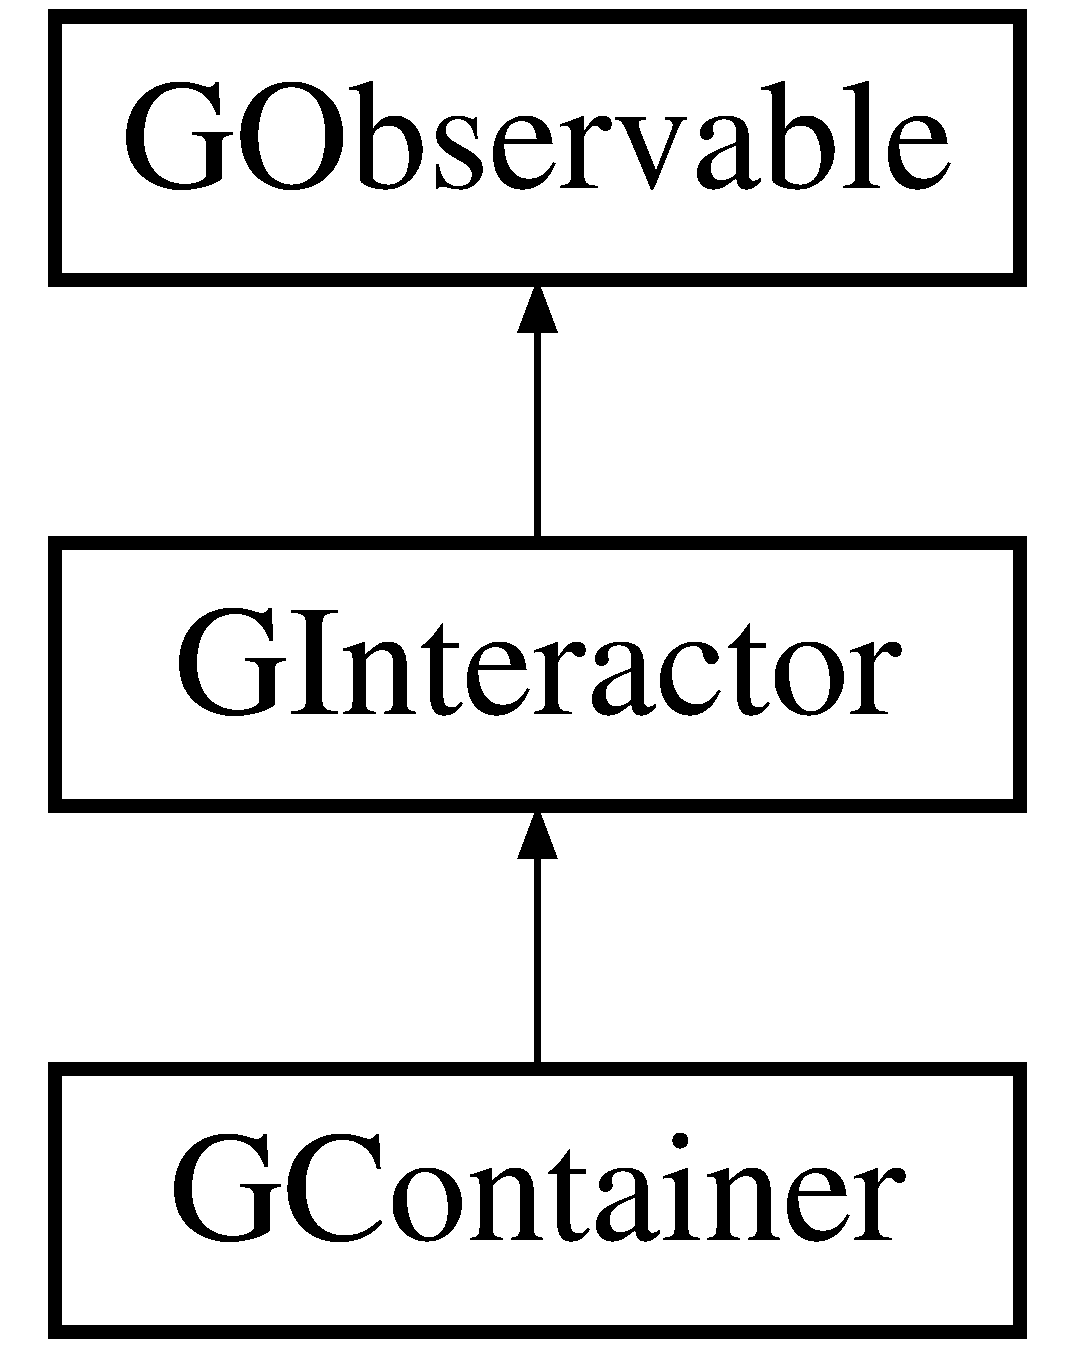
\includegraphics[height=3.000000cm]{classGContainer}
\end{center}
\end{figure}
\subsection*{Public Types}
\begin{DoxyCompactItemize}
\item 
enum \mbox{\hyperlink{classGContainer_a1b7da28ed84c0763e8f92cde2df4799b}{Layout}} \{ \mbox{\hyperlink{classGContainer_a1b7da28ed84c0763e8f92cde2df4799bac7afd1f77438e15d91d69c735a3a909a}{L\+A\+Y\+O\+U\+T\+\_\+\+N\+O\+NE}}, 
\mbox{\hyperlink{classGContainer_a1b7da28ed84c0763e8f92cde2df4799bac89a811e02b929a18f7f34e7d3bebd63}{L\+A\+Y\+O\+U\+T\+\_\+\+F\+L\+O\+W\+\_\+\+H\+O\+R\+I\+Z\+O\+N\+T\+AL}}, 
\mbox{\hyperlink{classGContainer_a1b7da28ed84c0763e8f92cde2df4799ba31e93ff7f38812816b05d254e04228e3}{L\+A\+Y\+O\+U\+T\+\_\+\+F\+L\+O\+W\+\_\+\+V\+E\+R\+T\+I\+C\+AL}}, 
\mbox{\hyperlink{classGContainer_a1b7da28ed84c0763e8f92cde2df4799babce8e871f79a8c9085d90c968d8827de}{L\+A\+Y\+O\+U\+T\+\_\+\+B\+O\+R\+D\+ER}}, 
\mbox{\hyperlink{classGContainer_a1b7da28ed84c0763e8f92cde2df4799bac4b094ed4f8bf75f60ba2235771371c3}{L\+A\+Y\+O\+U\+T\+\_\+\+G\+R\+ID}}
 \}
\begin{DoxyCompactList}\small\item\em The various layout management styles that containers can use. \end{DoxyCompactList}\item 
enum \mbox{\hyperlink{classGContainer_a81a01a86de31071a92e6cce0bab9bc4b}{Region}} \{ \mbox{\hyperlink{classGContainer_a81a01a86de31071a92e6cce0bab9bc4ba5ba85a564dbf472d69f92d5a2870db16}{R\+E\+G\+I\+O\+N\+\_\+\+C\+E\+N\+T\+ER}}, 
\mbox{\hyperlink{classGContainer_a81a01a86de31071a92e6cce0bab9bc4baac78951bd4e01d20f4825d5ae0a54357}{R\+E\+G\+I\+O\+N\+\_\+\+E\+A\+ST}}, 
\mbox{\hyperlink{classGContainer_a81a01a86de31071a92e6cce0bab9bc4baf40d135fb811ad59acb102f1fb357550}{R\+E\+G\+I\+O\+N\+\_\+\+N\+O\+R\+TH}}, 
\mbox{\hyperlink{classGContainer_a81a01a86de31071a92e6cce0bab9bc4bab533512ba438173a4ceb9c501eb17628}{R\+E\+G\+I\+O\+N\+\_\+\+S\+O\+U\+TH}}, 
\mbox{\hyperlink{classGContainer_a81a01a86de31071a92e6cce0bab9bc4ba5dd8c2219af001263c00de02b642786d}{R\+E\+G\+I\+O\+N\+\_\+\+W\+E\+ST}}
 \}
\begin{DoxyCompactList}\small\item\em The five regions of border layouts. \end{DoxyCompactList}\item 
enum \mbox{\hyperlink{classGInteractor_a8e0d441725a81d2bbdebbea09078260e}{Text\+Position}} \{ \mbox{\hyperlink{classGInteractor_a8e0d441725a81d2bbdebbea09078260ea4cd6f2e7d5a08d6f4dc052df2358f774}{T\+E\+X\+T\+\_\+\+B\+E\+S\+I\+D\+E\+\_\+\+I\+C\+ON}}, 
\mbox{\hyperlink{classGInteractor_a8e0d441725a81d2bbdebbea09078260eaa88490f63d8de68d44c83bdb2ecde3b3}{T\+E\+X\+T\+\_\+\+U\+N\+D\+E\+R\+\_\+\+I\+C\+ON}}, 
\mbox{\hyperlink{classGInteractor_a8e0d441725a81d2bbdebbea09078260ea39a6f388a30ac4fefb6eb13e846bc9f2}{T\+E\+X\+T\+\_\+\+O\+N\+LY}}
 \}
\begin{DoxyCompactList}\small\item\em The places where an interactor can place its text relative to its icon. \end{DoxyCompactList}\end{DoxyCompactItemize}
\subsection*{Public Member Functions}
\begin{DoxyCompactItemize}
\item 
\mbox{\hyperlink{classGContainer_a09fc5a49b2ea0bc895fbf2772c311325}{G\+Container}} (\mbox{\hyperlink{classGContainer_a1b7da28ed84c0763e8f92cde2df4799b}{Layout}} layout=\mbox{\hyperlink{classGContainer_a1b7da28ed84c0763e8f92cde2df4799bac89a811e02b929a18f7f34e7d3bebd63}{L\+A\+Y\+O\+U\+T\+\_\+\+F\+L\+O\+W\+\_\+\+H\+O\+R\+I\+Z\+O\+N\+T\+AL}}, Q\+Widget $\ast$parent=nullptr)
\begin{DoxyCompactList}\small\item\em Creates a new container with the given layout. \end{DoxyCompactList}\item 
\mbox{\hyperlink{classGContainer_a042cb94e18801664efa748e8a8fa74c1}{G\+Container}} (\mbox{\hyperlink{classGContainer_a1b7da28ed84c0763e8f92cde2df4799b}{Layout}} layout, int rows, int cols, Q\+Widget $\ast$parent=nullptr)
\begin{DoxyCompactList}\small\item\em Creates a new container with the given number of rows and columns. \end{DoxyCompactList}\item 
\mbox{\hyperlink{classGContainer_a45b3c0c0cc9c78097c024ca842978692}{$\sim$\+G\+Container}} () override
\begin{DoxyCompactList}\small\item\em Frees memory allocated internally by the container. \end{DoxyCompactList}\item 
virtual void \mbox{\hyperlink{classGContainer_a6f99b7c841256dbdc5acaafbbca4e685}{add}} (\mbox{\hyperlink{classGInteractor}{G\+Interactor}} $\ast$interactor)
\begin{DoxyCompactList}\small\item\em Adds the given interactor to the end of the list of interactors in this container. \end{DoxyCompactList}\item 
virtual void \mbox{\hyperlink{classGContainer_a33b08fe5428ed634a658deab076099f7}{add}} (\mbox{\hyperlink{classGInteractor}{G\+Interactor}} \&interactor)
\begin{DoxyCompactList}\small\item\em Adds the given interactor to the end of the list of interactors in this container. \end{DoxyCompactList}\item 
virtual void \mbox{\hyperlink{classGInteractor_a02f20ea6edfa0671f31c4c648a253833}{add\+Action\+Listener}} () Q\+\_\+\+D\+E\+C\+L\+\_\+\+D\+E\+P\+R\+E\+C\+A\+T\+ED
\begin{DoxyCompactList}\small\item\em Adds an event listener to be notified when this interactor is clicked or generally interacted with. \end{DoxyCompactList}\item 
virtual void \mbox{\hyperlink{classGContainer_adf2c09cdcbf0f38c03d75a250fd8ce5d}{add\+To\+Grid}} (\mbox{\hyperlink{classGInteractor}{G\+Interactor}} $\ast$interactor, int row, int col, int rowspan=1, int colspan=1)
\begin{DoxyCompactList}\small\item\em Adds the given interactor to the given row and column in this container, which is assumed to use a grid layout. \end{DoxyCompactList}\item 
virtual void \mbox{\hyperlink{classGContainer_abc297ebf9136261c21e2df3c771df0b3}{add\+To\+Grid}} (\mbox{\hyperlink{classGInteractor}{G\+Interactor}} \&interactor, int row, int col, int rowspan=1, int colspan=1)
\begin{DoxyCompactList}\small\item\em Adds the given interactor to the given row and column in this container, which is assumed to use a grid layout. \end{DoxyCompactList}\item 
virtual void \mbox{\hyperlink{classGContainer_aab55413917cdbb2e0560ab415d59fd1f}{add\+To\+Region}} (\mbox{\hyperlink{classGInteractor}{G\+Interactor}} $\ast$interactor, \mbox{\hyperlink{classGContainer_a81a01a86de31071a92e6cce0bab9bc4b}{Region}} region)
\begin{DoxyCompactList}\small\item\em Adds the given interactor to the given region in this container, which is assumed to use a border layout. \end{DoxyCompactList}\item 
virtual void \mbox{\hyperlink{classGContainer_a9c8e600889001e6e72d3548918a6baff}{add\+To\+Region}} (\mbox{\hyperlink{classGInteractor}{G\+Interactor}} $\ast$interactor, const std\+::string \&region=\char`\"{}Center\char`\"{})
\begin{DoxyCompactList}\small\item\em Adds the given interactor to the given region in this container, which is assumed to use a border layout. \end{DoxyCompactList}\item 
virtual void \mbox{\hyperlink{classGContainer_ad05df0d92ab2fba95d401a5614365558}{add\+To\+Region}} (\mbox{\hyperlink{classGInteractor}{G\+Interactor}} \&interactor, \mbox{\hyperlink{classGContainer_a81a01a86de31071a92e6cce0bab9bc4b}{Region}} region)
\begin{DoxyCompactList}\small\item\em Adds the given interactor to the given region in this container, which is assumed to use a border layout. \end{DoxyCompactList}\item 
virtual void \mbox{\hyperlink{classGContainer_a667ed0065e0bbb52a893904e7f2383bb}{add\+To\+Region}} (\mbox{\hyperlink{classGInteractor}{G\+Interactor}} \&interactor, const std\+::string \&region=\char`\"{}Center\char`\"{})
\begin{DoxyCompactList}\small\item\em Adds the given interactor to the given region in this container, which is assumed to use a border layout. \end{DoxyCompactList}\item 
virtual void \mbox{\hyperlink{classGContainer_ac8bb3912a3ce86b15842e79d0b421204}{clear}} ()
\begin{DoxyCompactList}\small\item\em Removes all interactors from this container. \end{DoxyCompactList}\item 
virtual void \mbox{\hyperlink{classGContainer_a47f0cc45498a78757fa4d0e6befc2981}{clear\+Region}} (\mbox{\hyperlink{classGContainer_a81a01a86de31071a92e6cce0bab9bc4b}{Region}} region)
\begin{DoxyCompactList}\small\item\em Removes all interactors from the given region of this container, which is assumed to use a border layout. \end{DoxyCompactList}\item 
virtual void \mbox{\hyperlink{classGContainer_aeba526cb4d6d6f3d8d6f376656af8dc8}{clear\+Region}} (const std\+::string \&region)
\begin{DoxyCompactList}\small\item\em Removes all interactors from the given region of this container, which is assumed to use a border layout. \end{DoxyCompactList}\item 
virtual bool \mbox{\hyperlink{classGContainer_a29e67f98cd36414c67475b8941d861a6}{contains}} (\mbox{\hyperlink{classGInteractor}{G\+Interactor}} $\ast$interactor) const
\begin{DoxyCompactList}\small\item\em Returns true if the given interactor is found in this container. \end{DoxyCompactList}\item 
virtual bool \mbox{\hyperlink{classGContainer_a62fe1c67f06f657fea8b9b28672516a0}{contains}} (\mbox{\hyperlink{classGInteractor}{G\+Interactor}} \&interactor) const
\begin{DoxyCompactList}\small\item\em Returns true if the given interactor is found in this container. \end{DoxyCompactList}\item 
bool \mbox{\hyperlink{classGInteractor_a597a370b592e3737d38d9d2f4e2031ea}{events\+Enabled}} () const override
\begin{DoxyCompactList}\small\item\em Returns true if this interactor is currently accepting events. \end{DoxyCompactList}\item 
virtual std\+::string \mbox{\hyperlink{classGInteractor_a69f8d23ed8f207fbecad99960776e942}{get\+Accelerator}} () const
\begin{DoxyCompactList}\small\item\em Returns a string representing a hotkey for this interactor, or an empty string if no accelerator has been set. \end{DoxyCompactList}\item 
virtual std\+::string \mbox{\hyperlink{classGInteractor_a94eb4276000c4fdfb508ce9e6317a82a}{get\+Action\+Command}} () const
\begin{DoxyCompactList}\small\item\em Returns an action command for this interactor, which is a semi-\/unique string you can use to identify it when events occur. \end{DoxyCompactList}\item 
virtual std\+::string \mbox{\hyperlink{classGInteractor_a808e22cc1fdfbecf71ed8c64ef4600e0}{get\+Background}} () const
\begin{DoxyCompactList}\small\item\em Returns the background color of the interactor as a string. \end{DoxyCompactList}\item 
virtual int \mbox{\hyperlink{classGInteractor_a9e827257a55cb8cf4d9de2ec6bcfd7a0}{get\+Background\+Int}} () const
\begin{DoxyCompactList}\small\item\em Returns the background color of the interactor as an R\+GB integer. \end{DoxyCompactList}\item 
virtual \mbox{\hyperlink{structGRectangle}{G\+Rectangle}} \mbox{\hyperlink{classGInteractor_a29e6ac35a0b48f491a4c88194cc5da3b}{get\+Bounds}} () const
\begin{DoxyCompactList}\small\item\em Returns a rectangle representing the x/y position and size of this interactor. \end{DoxyCompactList}\item 
virtual std\+::string \mbox{\hyperlink{classGInteractor_aa061dfa488c31e18549d64363c1d0e34}{get\+Color}} () const
\begin{DoxyCompactList}\small\item\em Returns the foreground/text color of the interactor as a string. \end{DoxyCompactList}\item 
virtual int \mbox{\hyperlink{classGInteractor_a9635c7af766cdc3417f346683fa0e6c1}{get\+Color\+Int}} () const
\begin{DoxyCompactList}\small\item\em Returns the foreground/text color of the interactor as an R\+GB integer. \end{DoxyCompactList}\item 
virtual \mbox{\hyperlink{classGContainer}{G\+Container}} $\ast$ \mbox{\hyperlink{classGInteractor_a7a6e317c29d61030929b4cd2d1c00fe7}{get\+Container}} () const
\begin{DoxyCompactList}\small\item\em Returns a pointer to the onscreen container holding this interactor. \end{DoxyCompactList}\item 
virtual std\+::vector$<$ \mbox{\hyperlink{classGInteractor}{G\+Interactor}} $\ast$ $>$ \mbox{\hyperlink{classGContainer_a9580b7f6ee0dc339f75bafd4e319f3ad}{get\+Descendents}} (const std\+::string \&type=\char`\"{}\char`\"{}) const
\begin{DoxyCompactList}\small\item\em Returns all interactors that are children or descendents inside this container. \end{DoxyCompactList}\item 
virtual std\+::string \mbox{\hyperlink{classGInteractor_a894a5502900794eeb27d084c21f1d77d}{get\+Font}} () const
\begin{DoxyCompactList}\small\item\em Returns the font of this interactor\textquotesingle{}s text as a font string such as \char`\"{}\+Helvetica-\/12-\/\+Bold\char`\"{}. \end{DoxyCompactList}\item 
virtual std\+::string \mbox{\hyperlink{classGInteractor_a4fa2d8b0192a3a5b4af4bbfe71194d03}{get\+Foreground}} () const
\begin{DoxyCompactList}\small\item\em Returns the foreground/text color of the interactor as a string. \end{DoxyCompactList}\item 
virtual int \mbox{\hyperlink{classGInteractor_ac3b12ab385a6ef9ae90fc879860ba726}{get\+Foreground\+Int}} () const
\begin{DoxyCompactList}\small\item\em Returns the foreground/text color of the interactor as an R\+GB integer. \end{DoxyCompactList}\item 
virtual double \mbox{\hyperlink{classGInteractor_a1e7e353362434072875264cf95629f99}{get\+Height}} () const
\begin{DoxyCompactList}\small\item\em Returns the current onscreen height of this interactor in pixels. \end{DoxyCompactList}\item 
virtual std\+::string \mbox{\hyperlink{classGInteractor_aaed62a73004939a64da6f0eb9eb64d73}{get\+Icon}} () const
\begin{DoxyCompactList}\small\item\em Returns the file name of the icon associated with this interactor, or an empty string if no icon has been set. \end{DoxyCompactList}\item 
virtual int \mbox{\hyperlink{classGInteractor_a9c9659a6c6ba66b4107ba59c95a24241}{get\+ID}} () const
\begin{DoxyCompactList}\small\item\em Returns a globally unique identifier for this interactor, which is set when the interactor is constructed. \end{DoxyCompactList}\item 
virtual \mbox{\hyperlink{classGInteractor}{G\+Interactor}} $\ast$ \mbox{\hyperlink{classGContainer_ac59d7bae6154f6f8791c7f1fd856b157}{get\+Interactor}} (int i) const
\begin{DoxyCompactList}\small\item\em Returns the child interactor at the given 0-\/based index in this container. \end{DoxyCompactList}\item 
virtual \mbox{\hyperlink{classGInteractor}{G\+Interactor}} $\ast$ \mbox{\hyperlink{classGContainer_ad31230cd6d220466fbd18fd21d133f67}{get\+Interactor\+By\+Region}} (int i, \mbox{\hyperlink{classGContainer_a81a01a86de31071a92e6cce0bab9bc4b}{Region}} region) const
\begin{DoxyCompactList}\small\item\em Returns the child interactor at the given 0-\/based index within the given region in this container, which is assumed to use a border layout. \end{DoxyCompactList}\item 
virtual \mbox{\hyperlink{classGInteractor}{G\+Interactor}} $\ast$ \mbox{\hyperlink{classGContainer_a576bbbb845c9bcf139fca956e3a4c757}{get\+Interactor\+By\+Region}} (int i, const std\+::string \&region=\char`\"{}Center\char`\"{}) const
\begin{DoxyCompactList}\small\item\em Returns the child interactor at the given 0-\/based index within the given region in this container, which is assumed to use a border layout. \end{DoxyCompactList}\item 
virtual int \mbox{\hyperlink{classGContainer_a789affbf8e89e65e3afd63cc626f5a81}{get\+Interactor\+Count}} () const
\begin{DoxyCompactList}\small\item\em Returns the number of children interactors in this container. \end{DoxyCompactList}\item 
virtual int \mbox{\hyperlink{classGContainer_a668fe9a4efc31fa065ded79c0e5eab64}{get\+Interactor\+Count\+By\+Region}} (\mbox{\hyperlink{classGContainer_a81a01a86de31071a92e6cce0bab9bc4b}{Region}} region) const
\begin{DoxyCompactList}\small\item\em Returns the number of children interactors within the given region in this container, which is assumed to use a border layout. \end{DoxyCompactList}\item 
virtual int \mbox{\hyperlink{classGContainer_ab51dbb723159efca4fc89e2c4211610c}{get\+Interactor\+Count\+By\+Region}} (const std\+::string \&region=\char`\"{}Center\char`\"{}) const
\begin{DoxyCompactList}\small\item\em Returns the number of children interactors within the given region in this container, which is assumed to use a border layout. \end{DoxyCompactList}\item 
virtual const std\+::vector$<$ \mbox{\hyperlink{classGInteractor}{G\+Interactor}} $\ast$ $>$ \& \mbox{\hyperlink{classGContainer_a04512d7151516f8a9e7298d72a290008}{get\+Interactors}} () const
\begin{DoxyCompactList}\small\item\em Returns a vector of all children interactors in this container. \end{DoxyCompactList}\item 
\+\_\+\+Internal\+\_\+\+Q\+Widget $\ast$ \mbox{\hyperlink{classGContainer_a2f6b36b2517087dc90a366b5ce1f5323}{get\+Internal\+Widget}} () const override
\begin{DoxyCompactList}\small\item\em Returns a direct pointer to the internal Qt widget being wrapped by this interactor. \end{DoxyCompactList}\item 
virtual \mbox{\hyperlink{classGContainer_a1b7da28ed84c0763e8f92cde2df4799b}{Layout}} \mbox{\hyperlink{classGContainer_aeebcf77b7fdc91a1ba0371cc9b91d5e2}{get\+Layout}} () const
\begin{DoxyCompactList}\small\item\em Returns the type of layout used by this container. \end{DoxyCompactList}\item 
virtual \mbox{\hyperlink{structGPoint}{G\+Point}} \mbox{\hyperlink{classGInteractor_a4f83802015511edeb63b892830812c11}{get\+Location}} () const
\begin{DoxyCompactList}\small\item\em Returns an (x, y) point representing the onscreen location of the top-\/left corner of this interactor within its containing window. \end{DoxyCompactList}\item 
virtual double \mbox{\hyperlink{classGContainer_ae2b63e249b9251e1893dae87aaf4cc3d}{get\+Margin}} () const
\begin{DoxyCompactList}\small\item\em Returns the margin around each widget in this container in pixels. \end{DoxyCompactList}\item 
virtual double \mbox{\hyperlink{classGInteractor_aed4b0075fcc434499c3cb3e46896bda3}{get\+Minimum\+Height}} () const
\begin{DoxyCompactList}\small\item\em Returns the minimum height in pixels that this interactor will permit itself to be resized to. \end{DoxyCompactList}\item 
virtual \mbox{\hyperlink{structGDimension}{G\+Dimension}} \mbox{\hyperlink{classGInteractor_a66b5af0b32493b4d597ca0a3df2049ea}{get\+Minimum\+Size}} () const
\begin{DoxyCompactList}\small\item\em Returns a \mbox{\hyperlink{structGDimension}{G\+Dimension}} structure representing the minimum size in pixels that this interactor will permit itself to be resized to. \end{DoxyCompactList}\item 
virtual double \mbox{\hyperlink{classGInteractor_a59e668114fe3d49d2a0f28deb258f7c8}{get\+Minimum\+Width}} () const
\begin{DoxyCompactList}\small\item\em Returns the minimum width in pixels that this interactor will permit itself to be resized to. \end{DoxyCompactList}\item 
virtual std\+::string \mbox{\hyperlink{classGInteractor_a8a60438a5b55d0b2ceb35c8674b9d8c5}{get\+Name}} () const
\begin{DoxyCompactList}\small\item\em Returns a string representing a unique name for this interactor. \end{DoxyCompactList}\item 
virtual double \mbox{\hyperlink{classGContainer_a19fdf4f4500aead343992102066983cb}{get\+Padding}} () const
\begin{DoxyCompactList}\small\item\em Returns the padding inside this container in pixels. \end{DoxyCompactList}\item 
virtual double \mbox{\hyperlink{classGContainer_a5696e2debbbafb717c0d47e069b896e4}{get\+Padding\+Bottom}} () const
\begin{DoxyCompactList}\small\item\em Returns the padding on the bottom side of this container in pixels. \end{DoxyCompactList}\item 
virtual double \mbox{\hyperlink{classGContainer_af28748a6467a4d3337788578522fa8f4}{get\+Padding\+Left}} () const
\begin{DoxyCompactList}\small\item\em Returns the padding on the left side of this container in pixels. \end{DoxyCompactList}\item 
virtual double \mbox{\hyperlink{classGContainer_a8d75cea586f7cd6611432122a080ecce}{get\+Padding\+Right}} () const
\begin{DoxyCompactList}\small\item\em Returns the padding on the right side of this container in pixels. \end{DoxyCompactList}\item 
virtual double \mbox{\hyperlink{classGContainer_ada97c35b2f3366886a49d63fff9d7bd4}{get\+Padding\+Top}} () const
\begin{DoxyCompactList}\small\item\em Returns the padding on the top side of this container in pixels. \end{DoxyCompactList}\item 
virtual double \mbox{\hyperlink{classGInteractor_a747de0961653847bdc6615dbf756d715}{get\+Preferred\+Height}} () const
\begin{DoxyCompactList}\small\item\em Returns the height in pixels that this interactor would prefer to be, which would exactly fit its contents with no stretching or scrollbars. \end{DoxyCompactList}\item 
\mbox{\hyperlink{structGDimension}{G\+Dimension}} \mbox{\hyperlink{classGContainer_ac0fd6fc35681f935c67ad68078b354b8}{get\+Preferred\+Size}} () const override
\begin{DoxyCompactList}\small\item\em Returns a \mbox{\hyperlink{structGDimension}{G\+Dimension}} structure storing the width and height in pixels that this interactor would prefer to be, which would exactly fit its contents with no stretching or scrollbars. \end{DoxyCompactList}\item 
virtual double \mbox{\hyperlink{classGInteractor_a82bca31d37700fb0e35d2743352efd5e}{get\+Preferred\+Width}} () const
\begin{DoxyCompactList}\small\item\em Returns the height in pixels that this interactor would prefer to be, which would exactly fit its contents with no stretching or scrollbars. \end{DoxyCompactList}\item 
virtual double \mbox{\hyperlink{classGContainer_a164d248057318961e7f2abc8c3477d63}{get\+Region\+Height}} (\mbox{\hyperlink{classGContainer_a81a01a86de31071a92e6cce0bab9bc4b}{Region}} region) const
\begin{DoxyCompactList}\small\item\em Returns the height in pixels of the given region of this container, which is assumed to use a border layout. \end{DoxyCompactList}\item 
virtual double \mbox{\hyperlink{classGContainer_ae8a545e772745b89edaf9804a2dc0057}{get\+Region\+Height}} (const std\+::string \&region) const
\begin{DoxyCompactList}\small\item\em Returns the height in pixels of the given region of this container, which is assumed to use a border layout. \end{DoxyCompactList}\item 
virtual \mbox{\hyperlink{structGDimension}{G\+Dimension}} \mbox{\hyperlink{classGContainer_a3b5db9ffbd4b32260f80634f162dba4e}{get\+Region\+Size}} (\mbox{\hyperlink{classGContainer_a81a01a86de31071a92e6cce0bab9bc4b}{Region}} region) const
\begin{DoxyCompactList}\small\item\em Returns the width and height in pixels of the given region of this container, which is assumed to use a border layout. \end{DoxyCompactList}\item 
virtual \mbox{\hyperlink{structGDimension}{G\+Dimension}} \mbox{\hyperlink{classGContainer_a68b18b38b72cb8779fca0c3882549a6b}{get\+Region\+Size}} (const std\+::string \&region) const
\begin{DoxyCompactList}\small\item\em Returns the width and height in pixels of the given region of this container, which is assumed to use a border layout. \end{DoxyCompactList}\item 
virtual double \mbox{\hyperlink{classGContainer_a96e2005c3f447a8679c3c32d3fc02de1}{get\+Region\+Width}} (\mbox{\hyperlink{classGContainer_a81a01a86de31071a92e6cce0bab9bc4b}{Region}} region) const
\begin{DoxyCompactList}\small\item\em Returns the width in pixels of the given region of this container, which is assumed to use a border layout. \end{DoxyCompactList}\item 
virtual double \mbox{\hyperlink{classGContainer_ab169dab454fc90f1c845b91b4e1a8a14}{get\+Region\+Width}} (const std\+::string \&region) const
\begin{DoxyCompactList}\small\item\em Returns the width in pixels of the given region of this container, which is assumed to use a border layout. \end{DoxyCompactList}\item 
virtual \mbox{\hyperlink{structGDimension}{G\+Dimension}} \mbox{\hyperlink{classGInteractor_a7b4eec96a2bdc6420695d5796a78eea9}{get\+Size}} () const
\begin{DoxyCompactList}\small\item\em Returns a \mbox{\hyperlink{structGDimension}{G\+Dimension}} structure storing the current onscreen width and height of this interactor in pixels. \end{DoxyCompactList}\item 
virtual double \mbox{\hyperlink{classGContainer_a9a7e859eeff5cc7de46d65b9be7afc3c}{get\+Spacing}} () const
\begin{DoxyCompactList}\small\item\em Returns the spacing between widgets in this container in pixels. \end{DoxyCompactList}\item 
std\+::string \mbox{\hyperlink{classGContainer_a9b72ede4ee8520f987a0c01e30654814}{get\+Type}} () const override
\begin{DoxyCompactList}\small\item\em Returns a string representing the class name of this interactor, such as \char`\"{}\+G\+Button\char`\"{} or \char`\"{}\+G\+Check\+Box\char`\"{}. \end{DoxyCompactList}\item 
Q\+Widget $\ast$ \mbox{\hyperlink{classGContainer_a3b33a602b31a6b809d020535a59db3b4}{get\+Widget}} () const override
\begin{DoxyCompactList}\small\item\em Returns a direct pointer to the internal Qt widget being wrapped by this interactor. \end{DoxyCompactList}\item 
virtual double \mbox{\hyperlink{classGInteractor_a0ed2965abd4f5701d2cadf71239faf19}{get\+Width}} () const
\begin{DoxyCompactList}\small\item\em Returns the current onscreen width of this interactor in pixels. \end{DoxyCompactList}\item 
virtual double \mbox{\hyperlink{classGInteractor_a344385751bee0720059403940d57a13e}{getX}} () const
\begin{DoxyCompactList}\small\item\em Returns the x-\/coordinate of the top-\/left pixel of this interactor within its onscreen window. \end{DoxyCompactList}\item 
virtual double \mbox{\hyperlink{classGInteractor_aafa51c7f8f38a09febbb9ce7853f77b4}{getY}} () const
\begin{DoxyCompactList}\small\item\em Returns the y-\/coordinate of the top-\/left pixel of this interactor within its onscreen window. \end{DoxyCompactList}\item 
virtual bool \mbox{\hyperlink{classGInteractor_afc480f652b8c5f1fb255e2269ce68879}{in\+Bounds}} (double x, double y) const
\begin{DoxyCompactList}\small\item\em Returns true if the given x/y pixel is within the bounds of this interactor. \end{DoxyCompactList}\item 
virtual bool \mbox{\hyperlink{classGInteractor_ae6d7982c1c627b677a5e776ca86118ed}{in\+Bounds}} (int x, int y) const
\begin{DoxyCompactList}\small\item\em Returns true if the given x/y pixel is within the bounds of this interactor. \end{DoxyCompactList}\item 
virtual void \mbox{\hyperlink{classGContainer_afffb8f789ff9a8466fbae5b846a0ebe7}{insert}} (int index, \mbox{\hyperlink{classGInteractor}{G\+Interactor}} $\ast$interactor)
\begin{DoxyCompactList}\small\item\em Adds the given interactor to this container just before the given index. \end{DoxyCompactList}\item 
virtual void \mbox{\hyperlink{classGContainer_a2e9d7c6d9e6769d4cfd3293afe7e215c}{insert}} (int index, \mbox{\hyperlink{classGInteractor}{G\+Interactor}} \&interactor)
\begin{DoxyCompactList}\small\item\em Adds the given interactor to this container just before the given index. \end{DoxyCompactList}\item 
virtual void \mbox{\hyperlink{classGContainer_a1c4b766b059991ad7d084ea03f22f1c5}{insert\+To\+Region}} (int index, \mbox{\hyperlink{classGInteractor}{G\+Interactor}} $\ast$interactor, \mbox{\hyperlink{classGContainer_a81a01a86de31071a92e6cce0bab9bc4b}{Region}} region)
\begin{DoxyCompactList}\small\item\em Adds the given interactor to the given layout region within this container just before the given index. \end{DoxyCompactList}\item 
virtual void \mbox{\hyperlink{classGContainer_adeeb03feb9346a9cf2046427484c20bc}{insert\+To\+Region}} (int index, \mbox{\hyperlink{classGInteractor}{G\+Interactor}} $\ast$interactor, const std\+::string \&region=\char`\"{}Center\char`\"{})
\begin{DoxyCompactList}\small\item\em Adds the given interactor to the given layout region within this container just before the given index. \end{DoxyCompactList}\item 
virtual void \mbox{\hyperlink{classGContainer_a1be2b263cd8d28e61e136a19d8e935cc}{insert\+To\+Region}} (int index, \mbox{\hyperlink{classGInteractor}{G\+Interactor}} \&interactor, \mbox{\hyperlink{classGContainer_a81a01a86de31071a92e6cce0bab9bc4b}{Region}} region)
\begin{DoxyCompactList}\small\item\em Adds the given interactor to the given layout region within this container just before the given index. \end{DoxyCompactList}\item 
virtual void \mbox{\hyperlink{classGContainer_ad4d413f64a3e4fb948956e7249c10110}{insert\+To\+Region}} (int index, \mbox{\hyperlink{classGInteractor}{G\+Interactor}} \&interactor, const std\+::string \&region=\char`\"{}Center\char`\"{})
\begin{DoxyCompactList}\small\item\em Adds the given interactor to the given layout region within this container just before the given index. \end{DoxyCompactList}\item 
virtual bool \mbox{\hyperlink{classGContainer_acf82f9b2937375c7b1cf3dccb3df3312}{is\+Empty}} () const
\begin{DoxyCompactList}\small\item\em Returns true if the container does not contain any interactors. \end{DoxyCompactList}\item 
virtual bool \mbox{\hyperlink{classGInteractor_aacb819fb241851fd9fc045271baa4034}{is\+Enabled}} () const
\begin{DoxyCompactList}\small\item\em Returns true if this interactor is currently enabled. \end{DoxyCompactList}\item 
virtual bool \mbox{\hyperlink{classGInteractor_a9d8a6cfb13917785c143e74d40e4e2be}{is\+Visible}} () const
\begin{DoxyCompactList}\small\item\em Returns true if the interactor is visible on the screen. \end{DoxyCompactList}\item 
virtual bool \mbox{\hyperlink{classGContainer_a8909db9abf4dc80058f9e4a7b90ea2d0}{region\+Contains}} (\mbox{\hyperlink{classGInteractor}{G\+Interactor}} $\ast$interactor, \mbox{\hyperlink{classGContainer_a81a01a86de31071a92e6cce0bab9bc4b}{Region}} region) const
\begin{DoxyCompactList}\small\item\em Returns true if the given interactor is found in the given region of this container, which is assumed to use a border layout. \end{DoxyCompactList}\item 
virtual bool \mbox{\hyperlink{classGContainer_a84a56bae6b8883d27e44d51c31b2bfc5}{region\+Contains}} (\mbox{\hyperlink{classGInteractor}{G\+Interactor}} $\ast$interactor, const std\+::string \&region) const
\begin{DoxyCompactList}\small\item\em Returns true if the given interactor is found in the given region of this container, which is assumed to use a border layout. \end{DoxyCompactList}\item 
virtual bool \mbox{\hyperlink{classGContainer_aa4cf95952747fd421a2b005eedbc662c}{region\+Contains}} (\mbox{\hyperlink{classGInteractor}{G\+Interactor}} \&interactor, \mbox{\hyperlink{classGContainer_a81a01a86de31071a92e6cce0bab9bc4b}{Region}} region) const
\begin{DoxyCompactList}\small\item\em Returns true if the given interactor is found in the given region of this container, which is assumed to use a border layout. \end{DoxyCompactList}\item 
virtual bool \mbox{\hyperlink{classGContainer_ad67deacd62d3248fbe57ccbd4e96fb50}{region\+Contains}} (\mbox{\hyperlink{classGInteractor}{G\+Interactor}} \&interactor, const std\+::string \&region) const
\begin{DoxyCompactList}\small\item\em Returns true if the given interactor is found in the given region of this container, which is assumed to use a border layout. \end{DoxyCompactList}\item 
virtual void \mbox{\hyperlink{classGContainer_a1c12b1fde5c2ef10d79d4ee51e670efa}{remove}} (\mbox{\hyperlink{classGInteractor}{G\+Interactor}} $\ast$interactor)
\begin{DoxyCompactList}\small\item\em Removes the given interactor from this container. \end{DoxyCompactList}\item 
virtual void \mbox{\hyperlink{classGContainer_ade2376c458ac401a0bd2dbe44271509e}{remove}} (\mbox{\hyperlink{classGInteractor}{G\+Interactor}} \&interactor)
\begin{DoxyCompactList}\small\item\em Removes the given interactor from this container. \end{DoxyCompactList}\item 
virtual void \mbox{\hyperlink{classGContainer_a2ad1aa316f278b2e9fa8121504749652}{remove}} (int index)
\begin{DoxyCompactList}\small\item\em Removes the child interactor at the given 0-\/based index from this container. \end{DoxyCompactList}\item 
virtual void \mbox{\hyperlink{classGInteractor_ab7fe7a876367b87cf7202f947f1d05e4}{remove\+Action\+Listener}} ()
\begin{DoxyCompactList}\small\item\em Removes the action listener from this interactor so that it will no longer call it when events occur. \end{DoxyCompactList}\item 
virtual void \mbox{\hyperlink{classGInteractor_ad39d0325cde6b97ebda4b9d7787c633b}{remove\+Click\+Listener}} ()
\begin{DoxyCompactList}\small\item\em Removes the click listener from this interactor so that it will no longer call it when events occur. \end{DoxyCompactList}\item 
virtual void \mbox{\hyperlink{classGInteractor_aa4250907e4cdd77349c04f0cf5cdd3d3}{remove\+Double\+Click\+Listener}} ()
\begin{DoxyCompactList}\small\item\em Removes the double-\/click listener from this interactor so that it will no longer call it when events occur. \end{DoxyCompactList}\item 
virtual void \mbox{\hyperlink{classGContainer_a87a74b040025878283ba685e30d5104f}{remove\+From\+Region}} (\mbox{\hyperlink{classGInteractor}{G\+Interactor}} $\ast$interactor, \mbox{\hyperlink{classGContainer_a81a01a86de31071a92e6cce0bab9bc4b}{Region}} region)
\begin{DoxyCompactList}\small\item\em Removes the given interactor from the given region within this container, which is assumed to use a border layout. \end{DoxyCompactList}\item 
virtual void \mbox{\hyperlink{classGContainer_a16268c8344a5a5d9b10bde95764112d1}{remove\+From\+Region}} (\mbox{\hyperlink{classGInteractor}{G\+Interactor}} $\ast$interactor, const std\+::string \&region)
\begin{DoxyCompactList}\small\item\em Removes the given interactor from the given region within this container, which is assumed to use a border layout. \end{DoxyCompactList}\item 
virtual void \mbox{\hyperlink{classGContainer_afee7b65f917c4f6a0fdb1c8ea75406a5}{remove\+From\+Region}} (\mbox{\hyperlink{classGInteractor}{G\+Interactor}} \&interactor, \mbox{\hyperlink{classGContainer_a81a01a86de31071a92e6cce0bab9bc4b}{Region}} region)
\begin{DoxyCompactList}\small\item\em Removes the given interactor from the given region within this container, which is assumed to use a border layout. \end{DoxyCompactList}\item 
virtual void \mbox{\hyperlink{classGContainer_af7a055c83c0e0e3f3722596d7111fcbe}{remove\+From\+Region}} (\mbox{\hyperlink{classGInteractor}{G\+Interactor}} \&interactor, const std\+::string \&region)
\begin{DoxyCompactList}\small\item\em Removes the given interactor from the given region within this container, which is assumed to use a border layout. \end{DoxyCompactList}\item 
virtual void \mbox{\hyperlink{classGContainer_a15e3a1d3f3abecc00d68d6df2349f360}{remove\+From\+Region}} (int index, \mbox{\hyperlink{classGContainer_a81a01a86de31071a92e6cce0bab9bc4b}{Region}} region)
\begin{DoxyCompactList}\small\item\em Removes the child interactor at the given 0-\/based index from the given region of this container, which is assumed to use a border layout. \end{DoxyCompactList}\item 
virtual void \mbox{\hyperlink{classGContainer_ac839e32fec6ea6b37f6c6da8aa6ce43b}{remove\+From\+Region}} (int index, const std\+::string \&region)
\begin{DoxyCompactList}\small\item\em Removes the child interactor at the given 0-\/based index from the given region of this container, which is assumed to use a border layout. \end{DoxyCompactList}\item 
virtual void \mbox{\hyperlink{classGInteractor_a43095f41cab3be732b49f29970484b05}{remove\+Key\+Listener}} ()
\begin{DoxyCompactList}\small\item\em Removes the key listener from this interactor so that it will no longer call it when key events occur. \end{DoxyCompactList}\item 
virtual void \mbox{\hyperlink{classGInteractor_aff47f71ce47e688a07c9d38dc92fcc11}{remove\+Mouse\+Listener}} ()
\begin{DoxyCompactList}\small\item\em Removes the mouse listener from this interactor so that it will no longer call it when events occur. \end{DoxyCompactList}\item 
virtual void \mbox{\hyperlink{classGInteractor_a519fb2ac767f8b2febbb50b898b8c8cb}{request\+Focus}} ()
\begin{DoxyCompactList}\small\item\em Transfers keyboard focus to this interactor. \end{DoxyCompactList}\item 
virtual void \mbox{\hyperlink{classGInteractor_ad15f102f62e2960576012f1aa0ba4b2e}{set\+Accelerator}} (const std\+::string \&accelerator)
\begin{DoxyCompactList}\small\item\em Sets an accelerator hotkey for this interactor, such as \char`\"{}\+Ctrl-\/\+S\char`\"{}. \end{DoxyCompactList}\item 
virtual void \mbox{\hyperlink{classGInteractor_a4b5843fe3030e038a1ba54cc03389bcf}{set\+Action\+Command}} (const std\+::string \&action\+Command)
\begin{DoxyCompactList}\small\item\em Sets the action command for this interactor. \end{DoxyCompactList}\item 
virtual void \mbox{\hyperlink{classGInteractor_adcfb4742430c88714fcf57e57ab8ea9c}{set\+Action\+Listener}} (G\+Event\+Listener func)
\begin{DoxyCompactList}\small\item\em Sets an action listener on this interactor so that it will be called when it is interacted with in its primary way. \end{DoxyCompactList}\item 
virtual void \mbox{\hyperlink{classGInteractor_aebd20a89c7a8a43a6fce999cf4f9fcf2}{set\+Action\+Listener}} (G\+Event\+Listener\+Void func)
\begin{DoxyCompactList}\small\item\em Sets an action listener on this interactor so that it will be called when it is interacted with in its primary way. \end{DoxyCompactList}\item 
virtual void \mbox{\hyperlink{classGContainer_a0bcf8805d87afc9bb4c6ca238ca7c0bd}{set\+Alignment}} (Horizontal\+Alignment halign, Vertical\+Alignment valign)
\begin{DoxyCompactList}\small\item\em Sets the horizontal and vertical alignment of interactors in this container. \end{DoxyCompactList}\item 
virtual void \mbox{\hyperlink{classGInteractor_acba7e546c2025c0a15ca4b4cc92043db}{set\+Background}} (int rgb)
\begin{DoxyCompactList}\small\item\em Sets the background color of the interactor to the color represented by the given R\+GB integer. \end{DoxyCompactList}\item 
virtual void \mbox{\hyperlink{classGInteractor_ab4677ab2474e68b07aa56605af92a84a}{set\+Background}} (const std\+::string \&color)
\begin{DoxyCompactList}\small\item\em Sets the background color of the interactor to the color represented by the given string. \end{DoxyCompactList}\item 
virtual void \mbox{\hyperlink{classGInteractor_a2aae8197624b72265ab83b4f1bc73f2f}{set\+Bounds}} (double x, double y, double width, double height)
\begin{DoxyCompactList}\small\item\em Sets the size and location of the widget. \end{DoxyCompactList}\item 
virtual void \mbox{\hyperlink{classGInteractor_acada386653f008cacc7cce86426bef7c}{set\+Bounds}} (const \mbox{\hyperlink{structGRectangle}{G\+Rectangle}} \&size)
\begin{DoxyCompactList}\small\item\em Sets the size and location of the widget. \end{DoxyCompactList}\item 
virtual void \mbox{\hyperlink{classGInteractor_abd40af6921242584d0954f173911b190}{set\+Click\+Listener}} (G\+Event\+Listener func)
\begin{DoxyCompactList}\small\item\em Sets a mouse listener on this interactor so that it will be called when the mouse is clicked on it. \end{DoxyCompactList}\item 
virtual void \mbox{\hyperlink{classGInteractor_a856414c92df90f56f3877475eb3f8fc4}{set\+Click\+Listener}} (G\+Event\+Listener\+Void func)
\begin{DoxyCompactList}\small\item\em Sets a mouse listener on this interactor so that it will be called when the mouse is clicked on it. \end{DoxyCompactList}\item 
virtual void \mbox{\hyperlink{classGInteractor_ab1f5cc0f5cc6bbbd716a526c61f1081d}{set\+Color}} (int rgb)
\begin{DoxyCompactList}\small\item\em Sets the foreground/text color of the interactor to the color represented by the given R\+GB integer. \end{DoxyCompactList}\item 
virtual void \mbox{\hyperlink{classGInteractor_a61374df6c11b52cfbb0815decdbaebc6}{set\+Color}} (const std\+::string \&color)
\begin{DoxyCompactList}\small\item\em Sets the foreground/text color of the interactor to the color represented by the given string. \end{DoxyCompactList}\item 
virtual void \mbox{\hyperlink{classGInteractor_ac29f9a3462458e165fae3a1f046ee77a}{set\+Double\+Click\+Listener}} (G\+Event\+Listener func)
\begin{DoxyCompactList}\small\item\em Sets a mouse listener on this interactor so that it will be called when the mouse is double-\/clicked on it. \end{DoxyCompactList}\item 
virtual void \mbox{\hyperlink{classGInteractor_a50096194d66f48c92dd4c512d41bfc76}{set\+Double\+Click\+Listener}} (G\+Event\+Listener\+Void func)
\begin{DoxyCompactList}\small\item\em Sets a mouse listener on this interactor so that it will be called when the mouse is double-\/clicked on it. \end{DoxyCompactList}\item 
virtual void \mbox{\hyperlink{classGInteractor_ab831367dd84bbd579e02e55bacb21343}{set\+Enabled}} (bool value)
\begin{DoxyCompactList}\small\item\em Sets whether this interactor is currently enabled. \end{DoxyCompactList}\item 
virtual void \mbox{\hyperlink{classGObservable_afaa30b2a9e0f378fd1c70d2f1d0b8216}{set\+Events\+Enabled}} (bool \mbox{\hyperlink{classGInteractor_a597a370b592e3737d38d9d2f4e2031ea}{events\+Enabled}})
\begin{DoxyCompactList}\small\item\em Sets whether the object is currently allowing itself to fire events. \end{DoxyCompactList}\item 
virtual void \mbox{\hyperlink{classGInteractor_a2592348886ffea646c6534bf88f7c49d}{set\+Font}} (const Q\+Font \&font)
\begin{DoxyCompactList}\small\item\em Sets the font used by this widget to the given Qt font. \end{DoxyCompactList}\item 
virtual void \mbox{\hyperlink{classGInteractor_a8e096e8818d838aceae1d46d58fb3a7b}{set\+Font}} (const std\+::string \&font)
\begin{DoxyCompactList}\small\item\em Sets the font used by this widget to the font represented by the given font string, such as \char`\"{}\+Helvetica-\/16-\/\+Bold\char`\"{}. \end{DoxyCompactList}\item 
virtual void \mbox{\hyperlink{classGInteractor_a9eb856b5ff83a19df3831a31f15f4563}{set\+Foreground}} (int rgb)
\begin{DoxyCompactList}\small\item\em Sets the foreground/text color of the interactor to the color represented by the given R\+GB integer. \end{DoxyCompactList}\item 
virtual void \mbox{\hyperlink{classGInteractor_af59209aeadea6dfc6d97a2d8531f50e1}{set\+Foreground}} (const std\+::string \&color)
\begin{DoxyCompactList}\small\item\em Sets the foreground/text color of the interactor to the color represented by the given string. \end{DoxyCompactList}\item 
virtual void \mbox{\hyperlink{classGInteractor_a9e280bfc4544dfaf8e4376c4e1a74357}{set\+Height}} (double height)
\begin{DoxyCompactList}\small\item\em Sets the onscreen height of the interactor in pixels. \end{DoxyCompactList}\item 
virtual void \mbox{\hyperlink{classGContainer_a901653aacb9991ee9a8b70d4a932f0c9}{set\+Horizontal\+Alignment}} (Horizontal\+Alignment halign)
\begin{DoxyCompactList}\small\item\em Sets the horizontal alignment of interactors in this container. \end{DoxyCompactList}\item 
virtual void \mbox{\hyperlink{classGInteractor_a542abfcd7261751352af129c7215ecda}{set\+Icon}} (const Q\+Icon \&icon)
\begin{DoxyCompactList}\small\item\em Sets the icon associated with this interactor. \end{DoxyCompactList}\item 
virtual void \mbox{\hyperlink{classGInteractor_a368e1a338f84401c284506d03b1ba769}{set\+Icon}} (const Q\+Pixmap \&icon)
\begin{DoxyCompactList}\small\item\em Sets the icon associated with this interactor. \end{DoxyCompactList}\item 
virtual void \mbox{\hyperlink{classGInteractor_a762e139aa311461c3984d3ad28293f64}{set\+Icon}} (const std\+::string \&filename, bool retain\+Icon\+Size=true)
\begin{DoxyCompactList}\small\item\em Sets the file name of the icon associated with this interactor, or an empty string if no icon has been set. \end{DoxyCompactList}\item 
virtual void \mbox{\hyperlink{classGInteractor_aeb8324d3287fa1fbe093f4d6230cf0a6}{set\+Key\+Listener}} (G\+Event\+Listener func)
\begin{DoxyCompactList}\small\item\em Sets a key listener on this interactor so that it will be called when the user presses any key. \end{DoxyCompactList}\item 
virtual void \mbox{\hyperlink{classGInteractor_ae48ecea73606c7bd9423e1c7cc589cc9}{set\+Key\+Listener}} (G\+Event\+Listener\+Void func)
\begin{DoxyCompactList}\small\item\em Sets a key listener on this interactor so that it will be called when the user presses any key. \end{DoxyCompactList}\item 
virtual void \mbox{\hyperlink{classGInteractor_a04594e8ba9b98513a64f1da00dcae18c}{set\+Location}} (double x, double y)
\begin{DoxyCompactList}\small\item\em Sets the onscreen x/y-\/coordinate of the top-\/left corner of the interactor relative to its window. \end{DoxyCompactList}\item 
virtual void \mbox{\hyperlink{classGContainer_a79b7a5ffc0a63c8f11be4ed59808f60d}{set\+Margin}} (double px)
\begin{DoxyCompactList}\small\item\em Sets the margin in pixels around interactors in this container. \end{DoxyCompactList}\item 
virtual void \mbox{\hyperlink{classGInteractor_a0cf428e207b7f22cc08138a90b1b87b2}{set\+Minimum\+Size}} (double width, double height)
\begin{DoxyCompactList}\small\item\em Sets the minimum size in pixels that this interactor will permit itself to be resized to. \end{DoxyCompactList}\item 
virtual void \mbox{\hyperlink{classGInteractor_a3b1046117ac6cb7abe467e00ba8a81f4}{set\+Minimum\+Size}} (const \mbox{\hyperlink{structGDimension}{G\+Dimension}} \&size)
\begin{DoxyCompactList}\small\item\em Sets the minimum size in pixels that this interactor will permit itself to be resized to. \end{DoxyCompactList}\item 
virtual void \mbox{\hyperlink{classGInteractor_a37d8dbc943f59920f705b0104f60bde2}{set\+Mouse\+Listener}} (G\+Event\+Listener func)
\begin{DoxyCompactList}\small\item\em Sets a mouse listener on this interactor so that it will be called when the mouse is moved or clicked on it. \end{DoxyCompactList}\item 
virtual void \mbox{\hyperlink{classGInteractor_aea7f647ea62d59f71b5fad6aa65eeaf9}{set\+Mouse\+Listener}} (G\+Event\+Listener\+Void func)
\begin{DoxyCompactList}\small\item\em Sets a mouse listener on this interactor so that it will be called when the mouse is moved or clicked on it. \end{DoxyCompactList}\item 
virtual void \mbox{\hyperlink{classGInteractor_a9d3a2685df23b5e7cbf59c19c4a1f9b5}{set\+Name}} (const std\+::string \&name)
\begin{DoxyCompactList}\small\item\em Sets a string representing a unique name for this interactor. \end{DoxyCompactList}\item 
virtual void \mbox{\hyperlink{classGContainer_a81b293e913c083a544af96f031668225}{set\+Padding}} (double px)
\begin{DoxyCompactList}\small\item\em Sets the padding on all 4 sides around widgets in this container. \end{DoxyCompactList}\item 
virtual void \mbox{\hyperlink{classGContainer_a76dc599dd8828f0ab534ab0d1b0c5ef8}{set\+Padding}} (double top\+Bottom, double left\+Right)
\begin{DoxyCompactList}\small\item\em Sets the padding on all 4 sides around widgets in this container, using different padding on the vertical vs horizontal sides. \end{DoxyCompactList}\item 
virtual void \mbox{\hyperlink{classGContainer_a9adbf36914b59c2ed3ed9aebe7adfc7e}{set\+Padding}} (double top, double right, double bottom, double left)
\begin{DoxyCompactList}\small\item\em Sets the padding on all 4 sides around widgets in this container, using different padding on each of the 4 sides. \end{DoxyCompactList}\item 
virtual void \mbox{\hyperlink{classGInteractor_a1ab987704fce32098706c6f00fb08218}{set\+Preferred\+Height}} (double height)
\begin{DoxyCompactList}\small\item\em Sets the height in pixels that this interactor would prefer to be. \end{DoxyCompactList}\item 
virtual void \mbox{\hyperlink{classGInteractor_a042c5ae19430d765ef552371cae3632c}{set\+Preferred\+Size}} (double width, double height)
\begin{DoxyCompactList}\small\item\em Sets the width and height in pixels that this interactor would prefer to be. \end{DoxyCompactList}\item 
virtual void \mbox{\hyperlink{classGInteractor_aa22d9be4bc0e078bb0ea69b0fc9d7c75}{set\+Preferred\+Size}} (const \mbox{\hyperlink{structGDimension}{G\+Dimension}} \&size)
\begin{DoxyCompactList}\small\item\em Sets the size in pixels that this interactor would prefer to be. \end{DoxyCompactList}\item 
virtual void \mbox{\hyperlink{classGInteractor_a3db429ab2fa52efd187eec0ed8cdd9f2}{set\+Preferred\+Width}} (double width)
\begin{DoxyCompactList}\small\item\em Sets the width in pixels that this interactor would prefer to be. \end{DoxyCompactList}\item 
virtual void \mbox{\hyperlink{classGContainer_a96e9f5593c0193bbdc7ae99945b9cf5f}{set\+Region\+Alignment}} (\mbox{\hyperlink{classGContainer_a81a01a86de31071a92e6cce0bab9bc4b}{Region}} region, Horizontal\+Alignment halign)
\begin{DoxyCompactList}\small\item\em Sets the horizontal alignment of interactors in the given region of this container, which is assumed to use a border layout. \end{DoxyCompactList}\item 
virtual void \mbox{\hyperlink{classGContainer_a926942899d029fc9921fe770ac2867bb}{set\+Region\+Alignment}} (\mbox{\hyperlink{classGContainer_a81a01a86de31071a92e6cce0bab9bc4b}{Region}} region, Vertical\+Alignment valign)
\begin{DoxyCompactList}\small\item\em Sets the vertical alignment of interactors in the given region of this container, which is assumed to use a border layout. \end{DoxyCompactList}\item 
virtual void \mbox{\hyperlink{classGContainer_ab4d2bfcca7a18da2847e7b4494da4a16}{set\+Region\+Alignment}} (\mbox{\hyperlink{classGContainer_a81a01a86de31071a92e6cce0bab9bc4b}{Region}} region, Horizontal\+Alignment halign, Vertical\+Alignment valign)
\begin{DoxyCompactList}\small\item\em Sets the horizontal and vertical alignment of interactors in the given region of this container, which is assumed to use a border layout. \end{DoxyCompactList}\item 
virtual void \mbox{\hyperlink{classGContainer_ae4ff46516be9472498c0bf058b496e8b}{set\+Region\+Alignment}} (const std\+::string \&region, const std\+::string \&align)
\begin{DoxyCompactList}\small\item\em Sets the horizontal and/or vertical alignment of interactors in the given region of this container, which is assumed to use a border layout. \end{DoxyCompactList}\item 
virtual void \mbox{\hyperlink{classGContainer_ad1c76be81b3b865f78b0e91f0e1f07d4}{set\+Region\+Alignment}} (const std\+::string \&region, const std\+::string \&halign, const std\+::string \&valign)
\begin{DoxyCompactList}\small\item\em Sets the horizontal and vertical alignment of interactors in the given region of this container, which is assumed to use a border layout. \end{DoxyCompactList}\item 
virtual void \mbox{\hyperlink{classGContainer_aca8f01ef261afca9c843589e8be54134}{set\+Region\+Horizontal\+Alignment}} (\mbox{\hyperlink{classGContainer_a81a01a86de31071a92e6cce0bab9bc4b}{Region}} region, Horizontal\+Alignment halign)
\begin{DoxyCompactList}\small\item\em Sets the horizontal alignment of interactors in the given region of this container, which is assumed to use a border layout. \end{DoxyCompactList}\item 
virtual void \mbox{\hyperlink{classGContainer_aefb97090ff4e149f8a0cce9efee3c451}{set\+Region\+Horizontal\+Alignment}} (const std\+::string \&region, const std\+::string \&halign)
\begin{DoxyCompactList}\small\item\em Sets the horizontal alignment of interactors in the given region of this container, which is assumed to use a border layout. \end{DoxyCompactList}\item 
virtual void \mbox{\hyperlink{classGContainer_afbe22d897ce8ef25db52cbc3d456aa0a}{set\+Region\+Vertical\+Alignment}} (const std\+::string \&region, const std\+::string \&valign)
\begin{DoxyCompactList}\small\item\em Sets the vertical alignment of interactors in the given region of this container, which is assumed to use a border layout. \end{DoxyCompactList}\item 
virtual void \mbox{\hyperlink{classGContainer_a1efb2d3b67fb479aad27a6c0032ee70e}{set\+Region\+Vertical\+Alignment}} (\mbox{\hyperlink{classGContainer_a81a01a86de31071a92e6cce0bab9bc4b}{Region}} region, Vertical\+Alignment valign)
\begin{DoxyCompactList}\small\item\em Sets the vertical alignment of interactors in the given region of this container, which is assumed to use a border layout. \end{DoxyCompactList}\item 
virtual void \mbox{\hyperlink{classGInteractor_aca25d49481f9bf5fc8f7df4c086c4ce7}{set\+Size}} (double width, double height)
\begin{DoxyCompactList}\small\item\em Sets the onscreen width and height of the interactor in pixels. \end{DoxyCompactList}\item 
virtual void \mbox{\hyperlink{classGInteractor_ae2b628228f192c2702c4ce941b2af68f}{set\+Size}} (const \mbox{\hyperlink{structGDimension}{G\+Dimension}} \&size)
\begin{DoxyCompactList}\small\item\em Sets the onscreen width and height of the interactor in pixels. \end{DoxyCompactList}\item 
virtual void \mbox{\hyperlink{classGContainer_a0f85f7b45435b302ae701cb00574bf52}{set\+Spacing}} (double px)
\begin{DoxyCompactList}\small\item\em Sets the spacing between interactors in this container. \end{DoxyCompactList}\item 
virtual void \mbox{\hyperlink{classGInteractor_a039e0e49beaecc275efce02d416acea8}{set\+Tooltip}} (const std\+::string \&tooltip\+Text)
\begin{DoxyCompactList}\small\item\em Sets a \char`\"{}tooltip\char`\"{} that will appear if the user hovers their mouse over the interactor. \end{DoxyCompactList}\item 
virtual void \mbox{\hyperlink{classGContainer_a465537d012ad40704a011ad927ce435d}{set\+Vertical\+Alignment}} (Vertical\+Alignment valign)
\begin{DoxyCompactList}\small\item\em Sets the vertical alignment of interactors in this container. \end{DoxyCompactList}\item 
virtual void \mbox{\hyperlink{classGInteractor_a18e44e30b31525a243960ca3928125aa}{set\+Visible}} (bool visible)
\begin{DoxyCompactList}\small\item\em Returns true if the interactor is visible on the screen. \end{DoxyCompactList}\item 
virtual void \mbox{\hyperlink{classGInteractor_aa3f3fba4cb131baa8696ba01e3bceca1}{set\+Width}} (double width)
\begin{DoxyCompactList}\small\item\em Sets the onscreen width of the interactor in pixels. \end{DoxyCompactList}\item 
virtual void \mbox{\hyperlink{classGInteractor_a9c18fcc579333bf9653d13ad2b372e39}{setX}} (double x)
\begin{DoxyCompactList}\small\item\em Sets the onscreen x-\/coordinate of the top-\/left corner of the interactor relative to its window. \end{DoxyCompactList}\item 
virtual void \mbox{\hyperlink{classGInteractor_a7d57e2a5c35d27feb58fd498a3cf82b9}{setY}} (double y)
\begin{DoxyCompactList}\small\item\em Sets the onscreen y-\/coordinate of the top-\/left corner of the interactor relative to its window. \end{DoxyCompactList}\item 
virtual std\+::string \mbox{\hyperlink{classGObservable_a1fe5121d6528fdea3f243321b3fa3a49}{to\+String}} () const
\begin{DoxyCompactList}\small\item\em Returns a string representation of this observable object\textquotesingle{}s state. \end{DoxyCompactList}\end{DoxyCompactItemize}
\subsection*{Static Public Attributes}
\begin{DoxyCompactItemize}
\item 
static const int \mbox{\hyperlink{classGContainer_a9fbdb565727493808a950b2bdfa72145}{M\+A\+R\+G\+I\+N\+\_\+\+D\+E\+F\+A\+U\+LT}} = 5
\begin{DoxyCompactList}\small\item\em Default margin around each interactor. \end{DoxyCompactList}\item 
static const int \mbox{\hyperlink{classGContainer_a2f9f03af35bbe9cd402d12efb4caa4a3}{S\+P\+A\+C\+I\+N\+G\+\_\+\+D\+E\+F\+A\+U\+LT}} = 8
\begin{DoxyCompactList}\small\item\em Default spacing between neighboring interactors. \end{DoxyCompactList}\end{DoxyCompactItemize}
\subsection*{Protected Member Functions}
\begin{DoxyCompactItemize}
\item 
virtual void \mbox{\hyperlink{classGObservable_a80cfa040459ff53594adbd6a51ec8f43}{clear\+Event\+Listeners}} ()
\begin{DoxyCompactList}\small\item\em Removes all event listeners from this object. \end{DoxyCompactList}\item 
virtual void \mbox{\hyperlink{classGObservable_a284f31528c0520f8e545c03ac9eeac74}{ensure\+Thread\+Safety}} (const std\+::string \&member\+Name=\char`\"{}\char`\"{})
\begin{DoxyCompactList}\small\item\em Ensures that we are currently in the Qt G\+UI thread. \end{DoxyCompactList}\item 
virtual void \mbox{\hyperlink{classGObservable_a63e5e5a6227c59c928493b11aceb0f67}{fire\+Event}} (\mbox{\hyperlink{classGEvent}{G\+Event}} \&event)
\begin{DoxyCompactList}\small\item\em Sends out the given event to any attached listeners. \end{DoxyCompactList}\item 
virtual void \mbox{\hyperlink{classGObservable_ab3983ea07337b52020a29cc00c653d8d}{fire\+G\+Event}} (Q\+Event $\ast$event, Event\+Type event\+Type, const std\+::string \&event\+Name)
\begin{DoxyCompactList}\small\item\em Creates an event of the given type, then sends it out to any attached listeners. \end{DoxyCompactList}\item 
virtual void \mbox{\hyperlink{classGObservable_a01fdf1b0e0dbd49e189fe4514e010411}{fire\+G\+Event}} (Q\+Close\+Event $\ast$event, Event\+Type event\+Type, const std\+::string \&event\+Name)
\begin{DoxyCompactList}\small\item\em Creates an event of the given type, then sends it out to any attached listeners. \end{DoxyCompactList}\item 
virtual void \mbox{\hyperlink{classGObservable_abb0b2f66ba39211cb5d7615e9d1c04e2}{fire\+G\+Event}} (Q\+Key\+Event $\ast$event, Event\+Type event\+Type, const std\+::string \&event\+Name)
\begin{DoxyCompactList}\small\item\em Creates an event of the given type, then sends it out to any attached listeners. \end{DoxyCompactList}\item 
virtual void \mbox{\hyperlink{classGObservable_a119318675d2165bdf7dd853aaf881d4b}{fire\+G\+Event}} (Q\+Mouse\+Event $\ast$event, Event\+Type event\+Type, const std\+::string \&event\+Name, const std\+::string \&action\+Command=\char`\"{}\char`\"{})
\begin{DoxyCompactList}\small\item\em Creates an event of the given type, then sends it out to any attached listeners. \end{DoxyCompactList}\item 
virtual void \mbox{\hyperlink{classGObservable_a63fd9034e1e1633c1c38eb342bfd34e9}{fire\+G\+Event}} (Q\+Resize\+Event $\ast$event, Event\+Type event\+Type, const std\+::string \&event\+Name)
\begin{DoxyCompactList}\small\item\em Creates an event of the given type, then sends it out to any attached listeners. \end{DoxyCompactList}\item 
virtual void \mbox{\hyperlink{classGObservable_a741345310d9b7c5170a6cbc410c44ac4}{fire\+G\+Event}} (Q\+Timer\+Event $\ast$event, Event\+Type event\+Type, const std\+::string \&event\+Name)
\begin{DoxyCompactList}\small\item\em Creates an event of the given type, then sends it out to any attached listeners. \end{DoxyCompactList}\item 
virtual void \mbox{\hyperlink{classGObservable_a93bf338968a0338761b8e4dc62f582e9}{fire\+G\+Event}} (Q\+Wheel\+Event $\ast$event, Event\+Type event\+Type, const std\+::string \&event\+Name)
\begin{DoxyCompactList}\small\item\em Creates an event of the given type, then sends it out to any attached listeners. \end{DoxyCompactList}\item 
virtual void \mbox{\hyperlink{classGObservable_a2a70a7d7435ff0c3b80bb4d70da19e0d}{fire\+G\+Event}} (Q\+Window\+State\+Change\+Event $\ast$event, Event\+Type event\+Type, const std\+::string \&event\+Name)
\begin{DoxyCompactList}\small\item\em Creates an event of the given type, then sends it out to any attached listeners. \end{DoxyCompactList}\item 
virtual bool \mbox{\hyperlink{classGObservable_a9f6faaa25942923bafa1c44020c49fa9}{has\+Event\+Listener}} (const std\+::string \&event\+Name) const
\begin{DoxyCompactList}\small\item\em Returns true if the observable object has a listener for the given type of event. \end{DoxyCompactList}\item 
virtual bool \mbox{\hyperlink{classGObservable_aeec1adc19aa0f33de62390686ee1382c}{is\+Accepting\+Event}} (int event\+Mask) const
\begin{DoxyCompactList}\small\item\em Returns true if the observable object has a listener for the given type of event. \end{DoxyCompactList}\item 
virtual bool \mbox{\hyperlink{classGObservable_aa31c73145a29dcb92848a92e0cfaea41}{is\+Accepting\+Event}} (const \mbox{\hyperlink{classGEvent}{G\+Event}} \&event) const
\begin{DoxyCompactList}\small\item\em Returns true if the observable object has a listener for the given type of event. \end{DoxyCompactList}\item 
virtual bool \mbox{\hyperlink{classGObservable_a3b1c689267eda44e65a2213e7de38b23}{is\+Accepting\+Event}} (const std\+::string \&event\+Type) const
\begin{DoxyCompactList}\small\item\em Returns true if the observable object has a listener for the given type of event. \end{DoxyCompactList}\item 
virtual void \mbox{\hyperlink{classGObservable_acbcf1ed3a851ad8a3c17ef38d86b481d}{remove\+Event\+Listener}} (const std\+::string \&event\+Name)
\begin{DoxyCompactList}\small\item\em Removes any event listener from this observable object that would respond to the given type of event, such as \char`\"{}click\char`\"{} or \char`\"{}keydown\char`\"{}. \end{DoxyCompactList}\item 
virtual void \mbox{\hyperlink{classGObservable_af51cc35c29a1bd1908609d432decdbb6}{remove\+Event\+Listeners}} (std\+::initializer\+\_\+list$<$ std\+::string $>$ event\+Names)
\begin{DoxyCompactList}\small\item\em Removes any event listener from this observable object that would respond to the given types of events, such as \char`\"{}click\char`\"{} or \char`\"{}keydown\char`\"{}. \end{DoxyCompactList}\item 
virtual void \mbox{\hyperlink{classGObservable_ad2f6d34961c50f6c1e0659990b79f741}{set\+Event\+Listener}} (const std\+::string \&event\+Name, G\+Event\+Listener func)
\begin{DoxyCompactList}\small\item\em Adds an event listener from this observable object to respond to the given type of event, such as \char`\"{}click\char`\"{} or \char`\"{}keydown\char`\"{}. \end{DoxyCompactList}\item 
virtual void \mbox{\hyperlink{classGObservable_abac4cb9f9e626e010e87f5d91573c8a5}{set\+Event\+Listener}} (const std\+::string \&event\+Name, G\+Event\+Listener\+Void func)
\begin{DoxyCompactList}\small\item\em Adds an event listener from this observable object to respond to the given type of event, such as \char`\"{}click\char`\"{} or \char`\"{}keydown\char`\"{}. \end{DoxyCompactList}\item 
virtual void \mbox{\hyperlink{classGObservable_afa388d69c33c718cf035774604065604}{set\+Event\+Listeners}} (std\+::initializer\+\_\+list$<$ std\+::string $>$ event\+Names, G\+Event\+Listener func)
\begin{DoxyCompactList}\small\item\em Adds an event listener from this observable object to respond to the given types of events, such as \char`\"{}click\char`\"{} or \char`\"{}keydown\char`\"{}. \end{DoxyCompactList}\item 
virtual void \mbox{\hyperlink{classGObservable_a7867184bbb686f74fae8a4db927da799}{set\+Event\+Listeners}} (std\+::initializer\+\_\+list$<$ std\+::string $>$ event\+Names, G\+Event\+Listener\+Void func)
\begin{DoxyCompactList}\small\item\em Adds an event listener from this observable object to respond to the given types of events, such as \char`\"{}click\char`\"{} or \char`\"{}keydown\char`\"{}. \end{DoxyCompactList}\end{DoxyCompactItemize}


\subsection{Detailed Description}
A \mbox{\hyperlink{classGContainer}{G\+Container}} is a logical grouping for interactors. 

The container manages the position and size of the interactors inside it. This class is very similar to the Java concept of a container, represented in Swing by the J\+Panel class.

A container has a layout that guides how it positions its interactors. Supported layouts include border (put interactors in the N/\+S/\+W/\+E/\+Center), grid (rows and columns of interactors), and flow (interactors go in a single horizontal or vertical line).

Containers also use a \char`\"{}box model\char`\"{} similar to the C\+SS box model with margins and padding around each interactor, and spacing between neighboring widgets\+:


\begin{DoxyPre}
 container
+-------------------+
|      margin       |
|  +---border----+  |
|  |   padding   |  |
|  |   content   |  |
|  |   padding   |  |
|  +-------------+  |
\tabulinesep=1mm
\begin{longtabu} spread 0pt [c]{*{1}{|X[-1]}|}
\hline
\rowcolor{\tableheadbgcolor}\textbf{  margin 
  
  }\\\cline{1-1}
\endfirsthead
\hline
\endfoot
\hline
\rowcolor{\tableheadbgcolor}\textbf{  margin 
  
  }\\\cline{1-1}
\endhead
 spacing 
  
  \\\cline{1-1}
  
  
  \\\cline{1-1}
 margin 
  
  \\\cline{1-1}
 +---border----+ 
  
\\\cline{1-1}
\end{longtabu}

|  |   padding   |  |
|  |   content   |  |
|  |   padding   |  |
|  +-------------+  |
|      margin       |
|       ...         |
+-------------------+
\end{DoxyPre}
 

\subsection{Member Enumeration Documentation}
\mbox{\Hypertarget{classGContainer_a1b7da28ed84c0763e8f92cde2df4799b}\label{classGContainer_a1b7da28ed84c0763e8f92cde2df4799b}} 
\index{G\+Container@{G\+Container}!Layout@{Layout}}
\index{Layout@{Layout}!G\+Container@{G\+Container}}
\subsubsection{\texorpdfstring{Layout}{Layout}}
{\footnotesize\ttfamily enum \mbox{\hyperlink{classGContainer_a1b7da28ed84c0763e8f92cde2df4799b}{Layout}}}



The various layout management styles that containers can use. 

\begin{DoxyEnumFields}{Enumerator}
\raisebox{\heightof{T}}[0pt][0pt]{\index{L\+A\+Y\+O\+U\+T\+\_\+\+N\+O\+NE@{L\+A\+Y\+O\+U\+T\+\_\+\+N\+O\+NE}!G\+Container@{G\+Container}}\index{G\+Container@{G\+Container}!L\+A\+Y\+O\+U\+T\+\_\+\+N\+O\+NE@{L\+A\+Y\+O\+U\+T\+\_\+\+N\+O\+NE}}}\mbox{\Hypertarget{classGContainer_a1b7da28ed84c0763e8f92cde2df4799bac7afd1f77438e15d91d69c735a3a909a}\label{classGContainer_a1b7da28ed84c0763e8f92cde2df4799bac7afd1f77438e15d91d69c735a3a909a}} 
L\+A\+Y\+O\+U\+T\+\_\+\+N\+O\+NE&\\
\hline

\raisebox{\heightof{T}}[0pt][0pt]{\index{L\+A\+Y\+O\+U\+T\+\_\+\+F\+L\+O\+W\+\_\+\+H\+O\+R\+I\+Z\+O\+N\+T\+AL@{L\+A\+Y\+O\+U\+T\+\_\+\+F\+L\+O\+W\+\_\+\+H\+O\+R\+I\+Z\+O\+N\+T\+AL}!G\+Container@{G\+Container}}\index{G\+Container@{G\+Container}!L\+A\+Y\+O\+U\+T\+\_\+\+F\+L\+O\+W\+\_\+\+H\+O\+R\+I\+Z\+O\+N\+T\+AL@{L\+A\+Y\+O\+U\+T\+\_\+\+F\+L\+O\+W\+\_\+\+H\+O\+R\+I\+Z\+O\+N\+T\+AL}}}\mbox{\Hypertarget{classGContainer_a1b7da28ed84c0763e8f92cde2df4799bac89a811e02b929a18f7f34e7d3bebd63}\label{classGContainer_a1b7da28ed84c0763e8f92cde2df4799bac89a811e02b929a18f7f34e7d3bebd63}} 
L\+A\+Y\+O\+U\+T\+\_\+\+F\+L\+O\+W\+\_\+\+H\+O\+R\+I\+Z\+O\+N\+T\+AL&\\
\hline

\raisebox{\heightof{T}}[0pt][0pt]{\index{L\+A\+Y\+O\+U\+T\+\_\+\+F\+L\+O\+W\+\_\+\+V\+E\+R\+T\+I\+C\+AL@{L\+A\+Y\+O\+U\+T\+\_\+\+F\+L\+O\+W\+\_\+\+V\+E\+R\+T\+I\+C\+AL}!G\+Container@{G\+Container}}\index{G\+Container@{G\+Container}!L\+A\+Y\+O\+U\+T\+\_\+\+F\+L\+O\+W\+\_\+\+V\+E\+R\+T\+I\+C\+AL@{L\+A\+Y\+O\+U\+T\+\_\+\+F\+L\+O\+W\+\_\+\+V\+E\+R\+T\+I\+C\+AL}}}\mbox{\Hypertarget{classGContainer_a1b7da28ed84c0763e8f92cde2df4799ba31e93ff7f38812816b05d254e04228e3}\label{classGContainer_a1b7da28ed84c0763e8f92cde2df4799ba31e93ff7f38812816b05d254e04228e3}} 
L\+A\+Y\+O\+U\+T\+\_\+\+F\+L\+O\+W\+\_\+\+V\+E\+R\+T\+I\+C\+AL&\\
\hline

\raisebox{\heightof{T}}[0pt][0pt]{\index{L\+A\+Y\+O\+U\+T\+\_\+\+B\+O\+R\+D\+ER@{L\+A\+Y\+O\+U\+T\+\_\+\+B\+O\+R\+D\+ER}!G\+Container@{G\+Container}}\index{G\+Container@{G\+Container}!L\+A\+Y\+O\+U\+T\+\_\+\+B\+O\+R\+D\+ER@{L\+A\+Y\+O\+U\+T\+\_\+\+B\+O\+R\+D\+ER}}}\mbox{\Hypertarget{classGContainer_a1b7da28ed84c0763e8f92cde2df4799babce8e871f79a8c9085d90c968d8827de}\label{classGContainer_a1b7da28ed84c0763e8f92cde2df4799babce8e871f79a8c9085d90c968d8827de}} 
L\+A\+Y\+O\+U\+T\+\_\+\+B\+O\+R\+D\+ER&\\
\hline

\raisebox{\heightof{T}}[0pt][0pt]{\index{L\+A\+Y\+O\+U\+T\+\_\+\+G\+R\+ID@{L\+A\+Y\+O\+U\+T\+\_\+\+G\+R\+ID}!G\+Container@{G\+Container}}\index{G\+Container@{G\+Container}!L\+A\+Y\+O\+U\+T\+\_\+\+G\+R\+ID@{L\+A\+Y\+O\+U\+T\+\_\+\+G\+R\+ID}}}\mbox{\Hypertarget{classGContainer_a1b7da28ed84c0763e8f92cde2df4799bac4b094ed4f8bf75f60ba2235771371c3}\label{classGContainer_a1b7da28ed84c0763e8f92cde2df4799bac4b094ed4f8bf75f60ba2235771371c3}} 
L\+A\+Y\+O\+U\+T\+\_\+\+G\+R\+ID&\\
\hline

\end{DoxyEnumFields}
\mbox{\Hypertarget{classGContainer_a81a01a86de31071a92e6cce0bab9bc4b}\label{classGContainer_a81a01a86de31071a92e6cce0bab9bc4b}} 
\index{G\+Container@{G\+Container}!Region@{Region}}
\index{Region@{Region}!G\+Container@{G\+Container}}
\subsubsection{\texorpdfstring{Region}{Region}}
{\footnotesize\ttfamily enum \mbox{\hyperlink{classGContainer_a81a01a86de31071a92e6cce0bab9bc4b}{Region}}}



The five regions of border layouts. 

Not used by the other layout styles. \begin{DoxyEnumFields}{Enumerator}
\raisebox{\heightof{T}}[0pt][0pt]{\index{R\+E\+G\+I\+O\+N\+\_\+\+C\+E\+N\+T\+ER@{R\+E\+G\+I\+O\+N\+\_\+\+C\+E\+N\+T\+ER}!G\+Container@{G\+Container}}\index{G\+Container@{G\+Container}!R\+E\+G\+I\+O\+N\+\_\+\+C\+E\+N\+T\+ER@{R\+E\+G\+I\+O\+N\+\_\+\+C\+E\+N\+T\+ER}}}\mbox{\Hypertarget{classGContainer_a81a01a86de31071a92e6cce0bab9bc4ba5ba85a564dbf472d69f92d5a2870db16}\label{classGContainer_a81a01a86de31071a92e6cce0bab9bc4ba5ba85a564dbf472d69f92d5a2870db16}} 
R\+E\+G\+I\+O\+N\+\_\+\+C\+E\+N\+T\+ER&\\
\hline

\raisebox{\heightof{T}}[0pt][0pt]{\index{R\+E\+G\+I\+O\+N\+\_\+\+E\+A\+ST@{R\+E\+G\+I\+O\+N\+\_\+\+E\+A\+ST}!G\+Container@{G\+Container}}\index{G\+Container@{G\+Container}!R\+E\+G\+I\+O\+N\+\_\+\+E\+A\+ST@{R\+E\+G\+I\+O\+N\+\_\+\+E\+A\+ST}}}\mbox{\Hypertarget{classGContainer_a81a01a86de31071a92e6cce0bab9bc4baac78951bd4e01d20f4825d5ae0a54357}\label{classGContainer_a81a01a86de31071a92e6cce0bab9bc4baac78951bd4e01d20f4825d5ae0a54357}} 
R\+E\+G\+I\+O\+N\+\_\+\+E\+A\+ST&\\
\hline

\raisebox{\heightof{T}}[0pt][0pt]{\index{R\+E\+G\+I\+O\+N\+\_\+\+N\+O\+R\+TH@{R\+E\+G\+I\+O\+N\+\_\+\+N\+O\+R\+TH}!G\+Container@{G\+Container}}\index{G\+Container@{G\+Container}!R\+E\+G\+I\+O\+N\+\_\+\+N\+O\+R\+TH@{R\+E\+G\+I\+O\+N\+\_\+\+N\+O\+R\+TH}}}\mbox{\Hypertarget{classGContainer_a81a01a86de31071a92e6cce0bab9bc4baf40d135fb811ad59acb102f1fb357550}\label{classGContainer_a81a01a86de31071a92e6cce0bab9bc4baf40d135fb811ad59acb102f1fb357550}} 
R\+E\+G\+I\+O\+N\+\_\+\+N\+O\+R\+TH&\\
\hline

\raisebox{\heightof{T}}[0pt][0pt]{\index{R\+E\+G\+I\+O\+N\+\_\+\+S\+O\+U\+TH@{R\+E\+G\+I\+O\+N\+\_\+\+S\+O\+U\+TH}!G\+Container@{G\+Container}}\index{G\+Container@{G\+Container}!R\+E\+G\+I\+O\+N\+\_\+\+S\+O\+U\+TH@{R\+E\+G\+I\+O\+N\+\_\+\+S\+O\+U\+TH}}}\mbox{\Hypertarget{classGContainer_a81a01a86de31071a92e6cce0bab9bc4bab533512ba438173a4ceb9c501eb17628}\label{classGContainer_a81a01a86de31071a92e6cce0bab9bc4bab533512ba438173a4ceb9c501eb17628}} 
R\+E\+G\+I\+O\+N\+\_\+\+S\+O\+U\+TH&\\
\hline

\raisebox{\heightof{T}}[0pt][0pt]{\index{R\+E\+G\+I\+O\+N\+\_\+\+W\+E\+ST@{R\+E\+G\+I\+O\+N\+\_\+\+W\+E\+ST}!G\+Container@{G\+Container}}\index{G\+Container@{G\+Container}!R\+E\+G\+I\+O\+N\+\_\+\+W\+E\+ST@{R\+E\+G\+I\+O\+N\+\_\+\+W\+E\+ST}}}\mbox{\Hypertarget{classGContainer_a81a01a86de31071a92e6cce0bab9bc4ba5dd8c2219af001263c00de02b642786d}\label{classGContainer_a81a01a86de31071a92e6cce0bab9bc4ba5dd8c2219af001263c00de02b642786d}} 
R\+E\+G\+I\+O\+N\+\_\+\+W\+E\+ST&\\
\hline

\end{DoxyEnumFields}
\mbox{\Hypertarget{classGInteractor_a8e0d441725a81d2bbdebbea09078260e}\label{classGInteractor_a8e0d441725a81d2bbdebbea09078260e}} 
\index{G\+Container@{G\+Container}!Text\+Position@{Text\+Position}}
\index{Text\+Position@{Text\+Position}!G\+Container@{G\+Container}}
\subsubsection{\texorpdfstring{Text\+Position}{TextPosition}}
{\footnotesize\ttfamily enum \mbox{\hyperlink{classGInteractor_a8e0d441725a81d2bbdebbea09078260e}{Text\+Position}}\hspace{0.3cm}{\ttfamily [inherited]}}



The places where an interactor can place its text relative to its icon. 

\begin{DoxyEnumFields}{Enumerator}
\raisebox{\heightof{T}}[0pt][0pt]{\index{T\+E\+X\+T\+\_\+\+B\+E\+S\+I\+D\+E\+\_\+\+I\+C\+ON@{T\+E\+X\+T\+\_\+\+B\+E\+S\+I\+D\+E\+\_\+\+I\+C\+ON}!G\+Container@{G\+Container}}\index{G\+Container@{G\+Container}!T\+E\+X\+T\+\_\+\+B\+E\+S\+I\+D\+E\+\_\+\+I\+C\+ON@{T\+E\+X\+T\+\_\+\+B\+E\+S\+I\+D\+E\+\_\+\+I\+C\+ON}}}\mbox{\Hypertarget{classGInteractor_a8e0d441725a81d2bbdebbea09078260ea4cd6f2e7d5a08d6f4dc052df2358f774}\label{classGInteractor_a8e0d441725a81d2bbdebbea09078260ea4cd6f2e7d5a08d6f4dc052df2358f774}} 
T\+E\+X\+T\+\_\+\+B\+E\+S\+I\+D\+E\+\_\+\+I\+C\+ON&\\
\hline

\raisebox{\heightof{T}}[0pt][0pt]{\index{T\+E\+X\+T\+\_\+\+U\+N\+D\+E\+R\+\_\+\+I\+C\+ON@{T\+E\+X\+T\+\_\+\+U\+N\+D\+E\+R\+\_\+\+I\+C\+ON}!G\+Container@{G\+Container}}\index{G\+Container@{G\+Container}!T\+E\+X\+T\+\_\+\+U\+N\+D\+E\+R\+\_\+\+I\+C\+ON@{T\+E\+X\+T\+\_\+\+U\+N\+D\+E\+R\+\_\+\+I\+C\+ON}}}\mbox{\Hypertarget{classGInteractor_a8e0d441725a81d2bbdebbea09078260eaa88490f63d8de68d44c83bdb2ecde3b3}\label{classGInteractor_a8e0d441725a81d2bbdebbea09078260eaa88490f63d8de68d44c83bdb2ecde3b3}} 
T\+E\+X\+T\+\_\+\+U\+N\+D\+E\+R\+\_\+\+I\+C\+ON&\\
\hline

\raisebox{\heightof{T}}[0pt][0pt]{\index{T\+E\+X\+T\+\_\+\+O\+N\+LY@{T\+E\+X\+T\+\_\+\+O\+N\+LY}!G\+Container@{G\+Container}}\index{G\+Container@{G\+Container}!T\+E\+X\+T\+\_\+\+O\+N\+LY@{T\+E\+X\+T\+\_\+\+O\+N\+LY}}}\mbox{\Hypertarget{classGInteractor_a8e0d441725a81d2bbdebbea09078260ea39a6f388a30ac4fefb6eb13e846bc9f2}\label{classGInteractor_a8e0d441725a81d2bbdebbea09078260ea39a6f388a30ac4fefb6eb13e846bc9f2}} 
T\+E\+X\+T\+\_\+\+O\+N\+LY&\\
\hline

\end{DoxyEnumFields}


\subsection{Constructor \& Destructor Documentation}
\mbox{\Hypertarget{classGContainer_a09fc5a49b2ea0bc895fbf2772c311325}\label{classGContainer_a09fc5a49b2ea0bc895fbf2772c311325}} 
\index{G\+Container@{G\+Container}!G\+Container@{G\+Container}}
\index{G\+Container@{G\+Container}!G\+Container@{G\+Container}}
\subsubsection{\texorpdfstring{G\+Container()}{GContainer()}\hspace{0.1cm}{\footnotesize\ttfamily [1/2]}}
{\footnotesize\ttfamily \mbox{\hyperlink{classGContainer}{G\+Container}} (\begin{DoxyParamCaption}\item[{\mbox{\hyperlink{classGContainer_a1b7da28ed84c0763e8f92cde2df4799b}{Layout}}}]{layout = {\ttfamily \mbox{\hyperlink{classGContainer_a1b7da28ed84c0763e8f92cde2df4799bac89a811e02b929a18f7f34e7d3bebd63}{L\+A\+Y\+O\+U\+T\+\_\+\+F\+L\+O\+W\+\_\+\+H\+O\+R\+I\+Z\+O\+N\+T\+AL}}},  }\item[{Q\+Widget $\ast$}]{parent = {\ttfamily nullptr} }\end{DoxyParamCaption})}



Creates a new container with the given layout. 

\mbox{\Hypertarget{classGContainer_a042cb94e18801664efa748e8a8fa74c1}\label{classGContainer_a042cb94e18801664efa748e8a8fa74c1}} 
\index{G\+Container@{G\+Container}!G\+Container@{G\+Container}}
\index{G\+Container@{G\+Container}!G\+Container@{G\+Container}}
\subsubsection{\texorpdfstring{G\+Container()}{GContainer()}\hspace{0.1cm}{\footnotesize\ttfamily [2/2]}}
{\footnotesize\ttfamily \mbox{\hyperlink{classGContainer}{G\+Container}} (\begin{DoxyParamCaption}\item[{\mbox{\hyperlink{classGContainer_a1b7da28ed84c0763e8f92cde2df4799b}{Layout}}}]{layout,  }\item[{int}]{rows,  }\item[{int}]{cols,  }\item[{Q\+Widget $\ast$}]{parent = {\ttfamily nullptr} }\end{DoxyParamCaption})}



Creates a new container with the given number of rows and columns. 

Meant to be used for grid layouts. \mbox{\Hypertarget{classGContainer_a45b3c0c0cc9c78097c024ca842978692}\label{classGContainer_a45b3c0c0cc9c78097c024ca842978692}} 
\index{G\+Container@{G\+Container}!````~G\+Container@{$\sim$\+G\+Container}}
\index{````~G\+Container@{$\sim$\+G\+Container}!G\+Container@{G\+Container}}
\subsubsection{\texorpdfstring{$\sim$\+G\+Container()}{~GContainer()}}
{\footnotesize\ttfamily $\sim$\mbox{\hyperlink{classGContainer}{G\+Container}} (\begin{DoxyParamCaption}{ }\end{DoxyParamCaption})\hspace{0.3cm}{\ttfamily [override]}}



Frees memory allocated internally by the container. 



\subsection{Member Function Documentation}
\mbox{\Hypertarget{classGContainer_a6f99b7c841256dbdc5acaafbbca4e685}\label{classGContainer_a6f99b7c841256dbdc5acaafbbca4e685}} 
\index{G\+Container@{G\+Container}!add@{add}}
\index{add@{add}!G\+Container@{G\+Container}}
\subsubsection{\texorpdfstring{add()}{add()}\hspace{0.1cm}{\footnotesize\ttfamily [1/2]}}
{\footnotesize\ttfamily void add (\begin{DoxyParamCaption}\item[{\mbox{\hyperlink{classGInteractor}{G\+Interactor}} $\ast$}]{interactor }\end{DoxyParamCaption})\hspace{0.3cm}{\ttfamily [virtual]}}



Adds the given interactor to the end of the list of interactors in this container. 

If the container uses a grid layout, adds the interactor to the next available row/column. If it uses a border layout, adds to the center region. 
\begin{DoxyExceptions}{Exceptions}
{\em Error\+Exception} & if the interactor is null \\
\hline
\end{DoxyExceptions}
\mbox{\Hypertarget{classGContainer_a33b08fe5428ed634a658deab076099f7}\label{classGContainer_a33b08fe5428ed634a658deab076099f7}} 
\index{G\+Container@{G\+Container}!add@{add}}
\index{add@{add}!G\+Container@{G\+Container}}
\subsubsection{\texorpdfstring{add()}{add()}\hspace{0.1cm}{\footnotesize\ttfamily [2/2]}}
{\footnotesize\ttfamily void add (\begin{DoxyParamCaption}\item[{\mbox{\hyperlink{classGInteractor}{G\+Interactor}} \&}]{interactor }\end{DoxyParamCaption})\hspace{0.3cm}{\ttfamily [virtual]}}



Adds the given interactor to the end of the list of interactors in this container. 

If the container uses a grid layout, adds the interactor to the next available row/column. If it uses a border layout, adds to the center region. \mbox{\Hypertarget{classGInteractor_a02f20ea6edfa0671f31c4c648a253833}\label{classGInteractor_a02f20ea6edfa0671f31c4c648a253833}} 
\index{G\+Container@{G\+Container}!add\+Action\+Listener@{add\+Action\+Listener}}
\index{add\+Action\+Listener@{add\+Action\+Listener}!G\+Container@{G\+Container}}
\subsubsection{\texorpdfstring{add\+Action\+Listener()}{addActionListener()}}
{\footnotesize\ttfamily void add\+Action\+Listener (\begin{DoxyParamCaption}{ }\end{DoxyParamCaption})\hspace{0.3cm}{\ttfamily [virtual]}, {\ttfamily [inherited]}}



Adds an event listener to be notified when this interactor is clicked or generally interacted with. 

\begin{DoxyRefDesc}{Deprecated}
\item[\mbox{\hyperlink{deprecated__deprecated000006}{Deprecated}}]does nothing; use set\+Action\+Listener instead \end{DoxyRefDesc}
\mbox{\Hypertarget{classGContainer_adf2c09cdcbf0f38c03d75a250fd8ce5d}\label{classGContainer_adf2c09cdcbf0f38c03d75a250fd8ce5d}} 
\index{G\+Container@{G\+Container}!add\+To\+Grid@{add\+To\+Grid}}
\index{add\+To\+Grid@{add\+To\+Grid}!G\+Container@{G\+Container}}
\subsubsection{\texorpdfstring{add\+To\+Grid()}{addToGrid()}\hspace{0.1cm}{\footnotesize\ttfamily [1/2]}}
{\footnotesize\ttfamily void add\+To\+Grid (\begin{DoxyParamCaption}\item[{\mbox{\hyperlink{classGInteractor}{G\+Interactor}} $\ast$}]{interactor,  }\item[{int}]{row,  }\item[{int}]{col,  }\item[{int}]{rowspan = {\ttfamily 1},  }\item[{int}]{colspan = {\ttfamily 1} }\end{DoxyParamCaption})\hspace{0.3cm}{\ttfamily [virtual]}}



Adds the given interactor to the given row and column in this container, which is assumed to use a grid layout. 

If the rowspan and/or colspan arguments are passed, the item will occupy multiple rows or columns\textquotesingle{} worth of space. If the container does not use a grid layout, equivalent to \mbox{\hyperlink{classGContainer_a6f99b7c841256dbdc5acaafbbca4e685}{add()}}. 
\begin{DoxyExceptions}{Exceptions}
{\em Error\+Exception} & if the interactor is null \\
\hline
\end{DoxyExceptions}
\mbox{\Hypertarget{classGContainer_abc297ebf9136261c21e2df3c771df0b3}\label{classGContainer_abc297ebf9136261c21e2df3c771df0b3}} 
\index{G\+Container@{G\+Container}!add\+To\+Grid@{add\+To\+Grid}}
\index{add\+To\+Grid@{add\+To\+Grid}!G\+Container@{G\+Container}}
\subsubsection{\texorpdfstring{add\+To\+Grid()}{addToGrid()}\hspace{0.1cm}{\footnotesize\ttfamily [2/2]}}
{\footnotesize\ttfamily void add\+To\+Grid (\begin{DoxyParamCaption}\item[{\mbox{\hyperlink{classGInteractor}{G\+Interactor}} \&}]{interactor,  }\item[{int}]{row,  }\item[{int}]{col,  }\item[{int}]{rowspan = {\ttfamily 1},  }\item[{int}]{colspan = {\ttfamily 1} }\end{DoxyParamCaption})\hspace{0.3cm}{\ttfamily [virtual]}}



Adds the given interactor to the given row and column in this container, which is assumed to use a grid layout. 

If the rowspan and/or colspan arguments are passed, the item will occupy multiple rows or columns\textquotesingle{} worth of space. If the container does not use a grid layout, equivalent to \mbox{\hyperlink{classGContainer_a6f99b7c841256dbdc5acaafbbca4e685}{add()}}. \mbox{\Hypertarget{classGContainer_aab55413917cdbb2e0560ab415d59fd1f}\label{classGContainer_aab55413917cdbb2e0560ab415d59fd1f}} 
\index{G\+Container@{G\+Container}!add\+To\+Region@{add\+To\+Region}}
\index{add\+To\+Region@{add\+To\+Region}!G\+Container@{G\+Container}}
\subsubsection{\texorpdfstring{add\+To\+Region()}{addToRegion()}\hspace{0.1cm}{\footnotesize\ttfamily [1/4]}}
{\footnotesize\ttfamily void add\+To\+Region (\begin{DoxyParamCaption}\item[{\mbox{\hyperlink{classGInteractor}{G\+Interactor}} $\ast$}]{interactor,  }\item[{\mbox{\hyperlink{classGContainer_a81a01a86de31071a92e6cce0bab9bc4b}{Region}}}]{region }\end{DoxyParamCaption})\hspace{0.3cm}{\ttfamily [virtual]}}



Adds the given interactor to the given region in this container, which is assumed to use a border layout. 

If the container does not use a border layout, equivalent to \mbox{\hyperlink{classGContainer_a6f99b7c841256dbdc5acaafbbca4e685}{add()}}. 
\begin{DoxyExceptions}{Exceptions}
{\em Error\+Exception} & if the interactor is null \\
\hline
\end{DoxyExceptions}
\mbox{\Hypertarget{classGContainer_a9c8e600889001e6e72d3548918a6baff}\label{classGContainer_a9c8e600889001e6e72d3548918a6baff}} 
\index{G\+Container@{G\+Container}!add\+To\+Region@{add\+To\+Region}}
\index{add\+To\+Region@{add\+To\+Region}!G\+Container@{G\+Container}}
\subsubsection{\texorpdfstring{add\+To\+Region()}{addToRegion()}\hspace{0.1cm}{\footnotesize\ttfamily [2/4]}}
{\footnotesize\ttfamily void add\+To\+Region (\begin{DoxyParamCaption}\item[{\mbox{\hyperlink{classGInteractor}{G\+Interactor}} $\ast$}]{interactor,  }\item[{const std\+::string \&}]{region = {\ttfamily \char`\"{}Center\char`\"{}} }\end{DoxyParamCaption})\hspace{0.3cm}{\ttfamily [virtual]}}



Adds the given interactor to the given region in this container, which is assumed to use a border layout. 

If the container does not use a border layout, equivalent to \mbox{\hyperlink{classGContainer_a6f99b7c841256dbdc5acaafbbca4e685}{add()}}. 
\begin{DoxyExceptions}{Exceptions}
{\em Error\+Exception} & if the interactor is null \\
\hline
\end{DoxyExceptions}
\mbox{\Hypertarget{classGContainer_ad05df0d92ab2fba95d401a5614365558}\label{classGContainer_ad05df0d92ab2fba95d401a5614365558}} 
\index{G\+Container@{G\+Container}!add\+To\+Region@{add\+To\+Region}}
\index{add\+To\+Region@{add\+To\+Region}!G\+Container@{G\+Container}}
\subsubsection{\texorpdfstring{add\+To\+Region()}{addToRegion()}\hspace{0.1cm}{\footnotesize\ttfamily [3/4]}}
{\footnotesize\ttfamily void add\+To\+Region (\begin{DoxyParamCaption}\item[{\mbox{\hyperlink{classGInteractor}{G\+Interactor}} \&}]{interactor,  }\item[{\mbox{\hyperlink{classGContainer_a81a01a86de31071a92e6cce0bab9bc4b}{Region}}}]{region }\end{DoxyParamCaption})\hspace{0.3cm}{\ttfamily [virtual]}}



Adds the given interactor to the given region in this container, which is assumed to use a border layout. 

If the container does not use a border layout, equivalent to \mbox{\hyperlink{classGContainer_a6f99b7c841256dbdc5acaafbbca4e685}{add()}}. \mbox{\Hypertarget{classGContainer_a667ed0065e0bbb52a893904e7f2383bb}\label{classGContainer_a667ed0065e0bbb52a893904e7f2383bb}} 
\index{G\+Container@{G\+Container}!add\+To\+Region@{add\+To\+Region}}
\index{add\+To\+Region@{add\+To\+Region}!G\+Container@{G\+Container}}
\subsubsection{\texorpdfstring{add\+To\+Region()}{addToRegion()}\hspace{0.1cm}{\footnotesize\ttfamily [4/4]}}
{\footnotesize\ttfamily void add\+To\+Region (\begin{DoxyParamCaption}\item[{\mbox{\hyperlink{classGInteractor}{G\+Interactor}} \&}]{interactor,  }\item[{const std\+::string \&}]{region = {\ttfamily \char`\"{}Center\char`\"{}} }\end{DoxyParamCaption})\hspace{0.3cm}{\ttfamily [virtual]}}



Adds the given interactor to the given region in this container, which is assumed to use a border layout. 

If the container does not use a border layout, equivalent to \mbox{\hyperlink{classGContainer_a6f99b7c841256dbdc5acaafbbca4e685}{add()}}. \mbox{\Hypertarget{classGContainer_ac8bb3912a3ce86b15842e79d0b421204}\label{classGContainer_ac8bb3912a3ce86b15842e79d0b421204}} 
\index{G\+Container@{G\+Container}!clear@{clear}}
\index{clear@{clear}!G\+Container@{G\+Container}}
\subsubsection{\texorpdfstring{clear()}{clear()}}
{\footnotesize\ttfamily void clear (\begin{DoxyParamCaption}{ }\end{DoxyParamCaption})\hspace{0.3cm}{\ttfamily [virtual]}}



Removes all interactors from this container. 

\mbox{\Hypertarget{classGObservable_a80cfa040459ff53594adbd6a51ec8f43}\label{classGObservable_a80cfa040459ff53594adbd6a51ec8f43}} 
\index{G\+Container@{G\+Container}!clear\+Event\+Listeners@{clear\+Event\+Listeners}}
\index{clear\+Event\+Listeners@{clear\+Event\+Listeners}!G\+Container@{G\+Container}}
\subsubsection{\texorpdfstring{clear\+Event\+Listeners()}{clearEventListeners()}}
{\footnotesize\ttfamily void clear\+Event\+Listeners (\begin{DoxyParamCaption}{ }\end{DoxyParamCaption})\hspace{0.3cm}{\ttfamily [protected]}, {\ttfamily [virtual]}, {\ttfamily [inherited]}}



Removes all event listeners from this object. 

\mbox{\Hypertarget{classGContainer_a47f0cc45498a78757fa4d0e6befc2981}\label{classGContainer_a47f0cc45498a78757fa4d0e6befc2981}} 
\index{G\+Container@{G\+Container}!clear\+Region@{clear\+Region}}
\index{clear\+Region@{clear\+Region}!G\+Container@{G\+Container}}
\subsubsection{\texorpdfstring{clear\+Region()}{clearRegion()}\hspace{0.1cm}{\footnotesize\ttfamily [1/2]}}
{\footnotesize\ttfamily void clear\+Region (\begin{DoxyParamCaption}\item[{\mbox{\hyperlink{classGContainer_a81a01a86de31071a92e6cce0bab9bc4b}{Region}}}]{region }\end{DoxyParamCaption})\hspace{0.3cm}{\ttfamily [virtual]}}



Removes all interactors from the given region of this container, which is assumed to use a border layout. 

If the container does not use a border layout, has no effect. \mbox{\Hypertarget{classGContainer_aeba526cb4d6d6f3d8d6f376656af8dc8}\label{classGContainer_aeba526cb4d6d6f3d8d6f376656af8dc8}} 
\index{G\+Container@{G\+Container}!clear\+Region@{clear\+Region}}
\index{clear\+Region@{clear\+Region}!G\+Container@{G\+Container}}
\subsubsection{\texorpdfstring{clear\+Region()}{clearRegion()}\hspace{0.1cm}{\footnotesize\ttfamily [2/2]}}
{\footnotesize\ttfamily void clear\+Region (\begin{DoxyParamCaption}\item[{const std\+::string \&}]{region }\end{DoxyParamCaption})\hspace{0.3cm}{\ttfamily [virtual]}}



Removes all interactors from the given region of this container, which is assumed to use a border layout. 

If the container does not use a border layout, has no effect. \mbox{\Hypertarget{classGContainer_a29e67f98cd36414c67475b8941d861a6}\label{classGContainer_a29e67f98cd36414c67475b8941d861a6}} 
\index{G\+Container@{G\+Container}!contains@{contains}}
\index{contains@{contains}!G\+Container@{G\+Container}}
\subsubsection{\texorpdfstring{contains()}{contains()}\hspace{0.1cm}{\footnotesize\ttfamily [1/2]}}
{\footnotesize\ttfamily bool contains (\begin{DoxyParamCaption}\item[{\mbox{\hyperlink{classGInteractor}{G\+Interactor}} $\ast$}]{interactor }\end{DoxyParamCaption}) const\hspace{0.3cm}{\ttfamily [virtual]}}



Returns true if the given interactor is found in this container. 

Returns false if the interactor is null \mbox{\Hypertarget{classGContainer_a62fe1c67f06f657fea8b9b28672516a0}\label{classGContainer_a62fe1c67f06f657fea8b9b28672516a0}} 
\index{G\+Container@{G\+Container}!contains@{contains}}
\index{contains@{contains}!G\+Container@{G\+Container}}
\subsubsection{\texorpdfstring{contains()}{contains()}\hspace{0.1cm}{\footnotesize\ttfamily [2/2]}}
{\footnotesize\ttfamily bool contains (\begin{DoxyParamCaption}\item[{\mbox{\hyperlink{classGInteractor}{G\+Interactor}} \&}]{interactor }\end{DoxyParamCaption}) const\hspace{0.3cm}{\ttfamily [virtual]}}



Returns true if the given interactor is found in this container. 

\mbox{\Hypertarget{classGObservable_a284f31528c0520f8e545c03ac9eeac74}\label{classGObservable_a284f31528c0520f8e545c03ac9eeac74}} 
\index{G\+Container@{G\+Container}!ensure\+Thread\+Safety@{ensure\+Thread\+Safety}}
\index{ensure\+Thread\+Safety@{ensure\+Thread\+Safety}!G\+Container@{G\+Container}}
\subsubsection{\texorpdfstring{ensure\+Thread\+Safety()}{ensureThreadSafety()}}
{\footnotesize\ttfamily void ensure\+Thread\+Safety (\begin{DoxyParamCaption}\item[{const std\+::string \&}]{member\+Name = {\ttfamily \char`\"{}\char`\"{}} }\end{DoxyParamCaption})\hspace{0.3cm}{\ttfamily [protected]}, {\ttfamily [virtual]}, {\ttfamily [inherited]}}



Ensures that we are currently in the Qt G\+UI thread. 

\mbox{\Hypertarget{classGInteractor_a597a370b592e3737d38d9d2f4e2031ea}\label{classGInteractor_a597a370b592e3737d38d9d2f4e2031ea}} 
\index{G\+Container@{G\+Container}!events\+Enabled@{events\+Enabled}}
\index{events\+Enabled@{events\+Enabled}!G\+Container@{G\+Container}}
\subsubsection{\texorpdfstring{events\+Enabled()}{eventsEnabled()}}
{\footnotesize\ttfamily bool events\+Enabled (\begin{DoxyParamCaption}{ }\end{DoxyParamCaption}) const\hspace{0.3cm}{\ttfamily [override]}, {\ttfamily [virtual]}, {\ttfamily [inherited]}}



Returns true if this interactor is currently accepting events. 

Initially true. An interactor must be visible and added to an onscreen window to receive events. 

Reimplemented from \mbox{\hyperlink{classGObservable_a8ebb3da91032e7f4c34485dabc518b8a}{G\+Observable}}.

\mbox{\Hypertarget{classGObservable_a63e5e5a6227c59c928493b11aceb0f67}\label{classGObservable_a63e5e5a6227c59c928493b11aceb0f67}} 
\index{G\+Container@{G\+Container}!fire\+Event@{fire\+Event}}
\index{fire\+Event@{fire\+Event}!G\+Container@{G\+Container}}
\subsubsection{\texorpdfstring{fire\+Event()}{fireEvent()}}
{\footnotesize\ttfamily void fire\+Event (\begin{DoxyParamCaption}\item[{\mbox{\hyperlink{classGEvent}{G\+Event}} \&}]{event }\end{DoxyParamCaption})\hspace{0.3cm}{\ttfamily [protected]}, {\ttfamily [virtual]}, {\ttfamily [inherited]}}



Sends out the given event to any attached listeners. 

\mbox{\Hypertarget{classGObservable_ab3983ea07337b52020a29cc00c653d8d}\label{classGObservable_ab3983ea07337b52020a29cc00c653d8d}} 
\index{G\+Container@{G\+Container}!fire\+G\+Event@{fire\+G\+Event}}
\index{fire\+G\+Event@{fire\+G\+Event}!G\+Container@{G\+Container}}
\subsubsection{\texorpdfstring{fire\+G\+Event()}{fireGEvent()}\hspace{0.1cm}{\footnotesize\ttfamily [1/8]}}
{\footnotesize\ttfamily void fire\+G\+Event (\begin{DoxyParamCaption}\item[{Q\+Event $\ast$}]{event,  }\item[{Event\+Type}]{event\+Type,  }\item[{const std\+::string \&}]{event\+Name }\end{DoxyParamCaption})\hspace{0.3cm}{\ttfamily [protected]}, {\ttfamily [virtual]}, {\ttfamily [inherited]}}



Creates an event of the given type, then sends it out to any attached listeners. 

\mbox{\Hypertarget{classGObservable_a01fdf1b0e0dbd49e189fe4514e010411}\label{classGObservable_a01fdf1b0e0dbd49e189fe4514e010411}} 
\index{G\+Container@{G\+Container}!fire\+G\+Event@{fire\+G\+Event}}
\index{fire\+G\+Event@{fire\+G\+Event}!G\+Container@{G\+Container}}
\subsubsection{\texorpdfstring{fire\+G\+Event()}{fireGEvent()}\hspace{0.1cm}{\footnotesize\ttfamily [2/8]}}
{\footnotesize\ttfamily void fire\+G\+Event (\begin{DoxyParamCaption}\item[{Q\+Close\+Event $\ast$}]{event,  }\item[{Event\+Type}]{event\+Type,  }\item[{const std\+::string \&}]{event\+Name }\end{DoxyParamCaption})\hspace{0.3cm}{\ttfamily [protected]}, {\ttfamily [virtual]}, {\ttfamily [inherited]}}



Creates an event of the given type, then sends it out to any attached listeners. 

\mbox{\Hypertarget{classGObservable_abb0b2f66ba39211cb5d7615e9d1c04e2}\label{classGObservable_abb0b2f66ba39211cb5d7615e9d1c04e2}} 
\index{G\+Container@{G\+Container}!fire\+G\+Event@{fire\+G\+Event}}
\index{fire\+G\+Event@{fire\+G\+Event}!G\+Container@{G\+Container}}
\subsubsection{\texorpdfstring{fire\+G\+Event()}{fireGEvent()}\hspace{0.1cm}{\footnotesize\ttfamily [3/8]}}
{\footnotesize\ttfamily void fire\+G\+Event (\begin{DoxyParamCaption}\item[{Q\+Key\+Event $\ast$}]{event,  }\item[{Event\+Type}]{event\+Type,  }\item[{const std\+::string \&}]{event\+Name }\end{DoxyParamCaption})\hspace{0.3cm}{\ttfamily [protected]}, {\ttfamily [virtual]}, {\ttfamily [inherited]}}



Creates an event of the given type, then sends it out to any attached listeners. 

\mbox{\Hypertarget{classGObservable_a119318675d2165bdf7dd853aaf881d4b}\label{classGObservable_a119318675d2165bdf7dd853aaf881d4b}} 
\index{G\+Container@{G\+Container}!fire\+G\+Event@{fire\+G\+Event}}
\index{fire\+G\+Event@{fire\+G\+Event}!G\+Container@{G\+Container}}
\subsubsection{\texorpdfstring{fire\+G\+Event()}{fireGEvent()}\hspace{0.1cm}{\footnotesize\ttfamily [4/8]}}
{\footnotesize\ttfamily void fire\+G\+Event (\begin{DoxyParamCaption}\item[{Q\+Mouse\+Event $\ast$}]{event,  }\item[{Event\+Type}]{event\+Type,  }\item[{const std\+::string \&}]{event\+Name,  }\item[{const std\+::string \&}]{action\+Command = {\ttfamily \char`\"{}\char`\"{}} }\end{DoxyParamCaption})\hspace{0.3cm}{\ttfamily [protected]}, {\ttfamily [virtual]}, {\ttfamily [inherited]}}



Creates an event of the given type, then sends it out to any attached listeners. 

\mbox{\Hypertarget{classGObservable_a63fd9034e1e1633c1c38eb342bfd34e9}\label{classGObservable_a63fd9034e1e1633c1c38eb342bfd34e9}} 
\index{G\+Container@{G\+Container}!fire\+G\+Event@{fire\+G\+Event}}
\index{fire\+G\+Event@{fire\+G\+Event}!G\+Container@{G\+Container}}
\subsubsection{\texorpdfstring{fire\+G\+Event()}{fireGEvent()}\hspace{0.1cm}{\footnotesize\ttfamily [5/8]}}
{\footnotesize\ttfamily void fire\+G\+Event (\begin{DoxyParamCaption}\item[{Q\+Resize\+Event $\ast$}]{event,  }\item[{Event\+Type}]{event\+Type,  }\item[{const std\+::string \&}]{event\+Name }\end{DoxyParamCaption})\hspace{0.3cm}{\ttfamily [protected]}, {\ttfamily [virtual]}, {\ttfamily [inherited]}}



Creates an event of the given type, then sends it out to any attached listeners. 

\mbox{\Hypertarget{classGObservable_a741345310d9b7c5170a6cbc410c44ac4}\label{classGObservable_a741345310d9b7c5170a6cbc410c44ac4}} 
\index{G\+Container@{G\+Container}!fire\+G\+Event@{fire\+G\+Event}}
\index{fire\+G\+Event@{fire\+G\+Event}!G\+Container@{G\+Container}}
\subsubsection{\texorpdfstring{fire\+G\+Event()}{fireGEvent()}\hspace{0.1cm}{\footnotesize\ttfamily [6/8]}}
{\footnotesize\ttfamily void fire\+G\+Event (\begin{DoxyParamCaption}\item[{Q\+Timer\+Event $\ast$}]{event,  }\item[{Event\+Type}]{event\+Type,  }\item[{const std\+::string \&}]{event\+Name }\end{DoxyParamCaption})\hspace{0.3cm}{\ttfamily [protected]}, {\ttfamily [virtual]}, {\ttfamily [inherited]}}



Creates an event of the given type, then sends it out to any attached listeners. 

\mbox{\Hypertarget{classGObservable_a93bf338968a0338761b8e4dc62f582e9}\label{classGObservable_a93bf338968a0338761b8e4dc62f582e9}} 
\index{G\+Container@{G\+Container}!fire\+G\+Event@{fire\+G\+Event}}
\index{fire\+G\+Event@{fire\+G\+Event}!G\+Container@{G\+Container}}
\subsubsection{\texorpdfstring{fire\+G\+Event()}{fireGEvent()}\hspace{0.1cm}{\footnotesize\ttfamily [7/8]}}
{\footnotesize\ttfamily void fire\+G\+Event (\begin{DoxyParamCaption}\item[{Q\+Wheel\+Event $\ast$}]{event,  }\item[{Event\+Type}]{event\+Type,  }\item[{const std\+::string \&}]{event\+Name }\end{DoxyParamCaption})\hspace{0.3cm}{\ttfamily [protected]}, {\ttfamily [virtual]}, {\ttfamily [inherited]}}



Creates an event of the given type, then sends it out to any attached listeners. 

\mbox{\Hypertarget{classGObservable_a2a70a7d7435ff0c3b80bb4d70da19e0d}\label{classGObservable_a2a70a7d7435ff0c3b80bb4d70da19e0d}} 
\index{G\+Container@{G\+Container}!fire\+G\+Event@{fire\+G\+Event}}
\index{fire\+G\+Event@{fire\+G\+Event}!G\+Container@{G\+Container}}
\subsubsection{\texorpdfstring{fire\+G\+Event()}{fireGEvent()}\hspace{0.1cm}{\footnotesize\ttfamily [8/8]}}
{\footnotesize\ttfamily void fire\+G\+Event (\begin{DoxyParamCaption}\item[{Q\+Window\+State\+Change\+Event $\ast$}]{event,  }\item[{Event\+Type}]{event\+Type,  }\item[{const std\+::string \&}]{event\+Name }\end{DoxyParamCaption})\hspace{0.3cm}{\ttfamily [protected]}, {\ttfamily [virtual]}, {\ttfamily [inherited]}}



Creates an event of the given type, then sends it out to any attached listeners. 

\mbox{\Hypertarget{classGInteractor_a69f8d23ed8f207fbecad99960776e942}\label{classGInteractor_a69f8d23ed8f207fbecad99960776e942}} 
\index{G\+Container@{G\+Container}!get\+Accelerator@{get\+Accelerator}}
\index{get\+Accelerator@{get\+Accelerator}!G\+Container@{G\+Container}}
\subsubsection{\texorpdfstring{get\+Accelerator()}{getAccelerator()}}
{\footnotesize\ttfamily std\+::string get\+Accelerator (\begin{DoxyParamCaption}{ }\end{DoxyParamCaption}) const\hspace{0.3cm}{\ttfamily [virtual]}, {\ttfamily [inherited]}}



Returns a string representing a hotkey for this interactor, or an empty string if no accelerator has been set. 

\begin{DoxyReturn}{Returns}
an accelerator such as \char`\"{}\+Ctrl-\/\+S\char`\"{} 
\end{DoxyReturn}


Reimplemented in \mbox{\hyperlink{classGButton_a57806dc9defb73f76f493f8548319924}{G\+Button}}.

\mbox{\Hypertarget{classGInteractor_a94eb4276000c4fdfb508ce9e6317a82a}\label{classGInteractor_a94eb4276000c4fdfb508ce9e6317a82a}} 
\index{G\+Container@{G\+Container}!get\+Action\+Command@{get\+Action\+Command}}
\index{get\+Action\+Command@{get\+Action\+Command}!G\+Container@{G\+Container}}
\subsubsection{\texorpdfstring{get\+Action\+Command()}{getActionCommand()}}
{\footnotesize\ttfamily std\+::string get\+Action\+Command (\begin{DoxyParamCaption}{ }\end{DoxyParamCaption}) const\hspace{0.3cm}{\ttfamily [virtual]}, {\ttfamily [inherited]}}



Returns an action command for this interactor, which is a semi-\/unique string you can use to identify it when events occur. 

For example, for buttons, the default action command is the button\textquotesingle{}s text. 

Reimplemented in \mbox{\hyperlink{classGChooser_a4f83505141da1f8446f0e0e0a9507930}{G\+Chooser}}, \mbox{\hyperlink{classGRadioButton_a4f83505141da1f8446f0e0e0a9507930}{G\+Radio\+Button}}, \mbox{\hyperlink{classGButton_a4f83505141da1f8446f0e0e0a9507930}{G\+Button}}, and \mbox{\hyperlink{classGCheckBox_a4f83505141da1f8446f0e0e0a9507930}{G\+Check\+Box}}.

\mbox{\Hypertarget{classGInteractor_a808e22cc1fdfbecf71ed8c64ef4600e0}\label{classGInteractor_a808e22cc1fdfbecf71ed8c64ef4600e0}} 
\index{G\+Container@{G\+Container}!get\+Background@{get\+Background}}
\index{get\+Background@{get\+Background}!G\+Container@{G\+Container}}
\subsubsection{\texorpdfstring{get\+Background()}{getBackground()}}
{\footnotesize\ttfamily std\+::string get\+Background (\begin{DoxyParamCaption}{ }\end{DoxyParamCaption}) const\hspace{0.3cm}{\ttfamily [virtual]}, {\ttfamily [inherited]}}



Returns the background color of the interactor as a string. 

\begin{DoxyReturn}{Returns}
a string such as \char`\"{}blue\char`\"{} or \char`\"{}\#7700ff\char`\"{} 
\end{DoxyReturn}


Reimplemented in \mbox{\hyperlink{classGCanvas_a4a62c51b7244a7642b88065e3a07ae82}{G\+Canvas}}.

\mbox{\Hypertarget{classGInteractor_a9e827257a55cb8cf4d9de2ec6bcfd7a0}\label{classGInteractor_a9e827257a55cb8cf4d9de2ec6bcfd7a0}} 
\index{G\+Container@{G\+Container}!get\+Background\+Int@{get\+Background\+Int}}
\index{get\+Background\+Int@{get\+Background\+Int}!G\+Container@{G\+Container}}
\subsubsection{\texorpdfstring{get\+Background\+Int()}{getBackgroundInt()}}
{\footnotesize\ttfamily int get\+Background\+Int (\begin{DoxyParamCaption}{ }\end{DoxyParamCaption}) const\hspace{0.3cm}{\ttfamily [virtual]}, {\ttfamily [inherited]}}



Returns the background color of the interactor as an R\+GB integer. 

\begin{DoxyReturn}{Returns}
an integer such as 0x7700ff 
\end{DoxyReturn}


Reimplemented in \mbox{\hyperlink{classGCanvas_acd4f2b3b9619dacdfd71fc0004cac382}{G\+Canvas}}.

\mbox{\Hypertarget{classGInteractor_a29e6ac35a0b48f491a4c88194cc5da3b}\label{classGInteractor_a29e6ac35a0b48f491a4c88194cc5da3b}} 
\index{G\+Container@{G\+Container}!get\+Bounds@{get\+Bounds}}
\index{get\+Bounds@{get\+Bounds}!G\+Container@{G\+Container}}
\subsubsection{\texorpdfstring{get\+Bounds()}{getBounds()}}
{\footnotesize\ttfamily \mbox{\hyperlink{structGRectangle}{G\+Rectangle}} get\+Bounds (\begin{DoxyParamCaption}{ }\end{DoxyParamCaption}) const\hspace{0.3cm}{\ttfamily [virtual]}, {\ttfamily [inherited]}}



Returns a rectangle representing the x/y position and size of this interactor. 

\mbox{\Hypertarget{classGInteractor_aa061dfa488c31e18549d64363c1d0e34}\label{classGInteractor_aa061dfa488c31e18549d64363c1d0e34}} 
\index{G\+Container@{G\+Container}!get\+Color@{get\+Color}}
\index{get\+Color@{get\+Color}!G\+Container@{G\+Container}}
\subsubsection{\texorpdfstring{get\+Color()}{getColor()}}
{\footnotesize\ttfamily std\+::string get\+Color (\begin{DoxyParamCaption}{ }\end{DoxyParamCaption}) const\hspace{0.3cm}{\ttfamily [virtual]}, {\ttfamily [inherited]}}



Returns the foreground/text color of the interactor as a string. 

Equivalent to get\+Foreground. \begin{DoxyReturn}{Returns}
a string such as \char`\"{}blue\char`\"{} or \char`\"{}\#7700ff\char`\"{} 
\end{DoxyReturn}
\mbox{\Hypertarget{classGInteractor_a9635c7af766cdc3417f346683fa0e6c1}\label{classGInteractor_a9635c7af766cdc3417f346683fa0e6c1}} 
\index{G\+Container@{G\+Container}!get\+Color\+Int@{get\+Color\+Int}}
\index{get\+Color\+Int@{get\+Color\+Int}!G\+Container@{G\+Container}}
\subsubsection{\texorpdfstring{get\+Color\+Int()}{getColorInt()}}
{\footnotesize\ttfamily int get\+Color\+Int (\begin{DoxyParamCaption}{ }\end{DoxyParamCaption}) const\hspace{0.3cm}{\ttfamily [virtual]}, {\ttfamily [inherited]}}



Returns the foreground/text color of the interactor as an R\+GB integer. 

Equivalent to get\+Foreground\+Int. \begin{DoxyReturn}{Returns}
an integer such as 0x7700ff 
\end{DoxyReturn}
\mbox{\Hypertarget{classGInteractor_a7a6e317c29d61030929b4cd2d1c00fe7}\label{classGInteractor_a7a6e317c29d61030929b4cd2d1c00fe7}} 
\index{G\+Container@{G\+Container}!get\+Container@{get\+Container}}
\index{get\+Container@{get\+Container}!G\+Container@{G\+Container}}
\subsubsection{\texorpdfstring{get\+Container()}{getContainer()}}
{\footnotesize\ttfamily \mbox{\hyperlink{classGContainer}{G\+Container}} $\ast$ get\+Container (\begin{DoxyParamCaption}{ }\end{DoxyParamCaption}) const\hspace{0.3cm}{\ttfamily [virtual]}, {\ttfamily [inherited]}}



Returns a pointer to the onscreen container holding this interactor. 

When an interactor is created, its container is initially null. This will become non-\/null automatically if you add the interactor to a window or other layout container. Interactors must be added to a container or window to receive events or to become visible on the screen. \begin{DoxyReturn}{Returns}
the container, or nullptr if interactor has not yet been added to any container 
\end{DoxyReturn}
\mbox{\Hypertarget{classGContainer_a9580b7f6ee0dc339f75bafd4e319f3ad}\label{classGContainer_a9580b7f6ee0dc339f75bafd4e319f3ad}} 
\index{G\+Container@{G\+Container}!get\+Descendents@{get\+Descendents}}
\index{get\+Descendents@{get\+Descendents}!G\+Container@{G\+Container}}
\subsubsection{\texorpdfstring{get\+Descendents()}{getDescendents()}}
{\footnotesize\ttfamily std\+::vector$<$ \mbox{\hyperlink{classGInteractor}{G\+Interactor}} $\ast$ $>$ get\+Descendents (\begin{DoxyParamCaption}\item[{const std\+::string \&}]{type = {\ttfamily \char`\"{}\char`\"{}} }\end{DoxyParamCaption}) const\hspace{0.3cm}{\ttfamily [virtual]}}



Returns all interactors that are children or descendents inside this container. 

This differs from get\+Interactors in that it returns not only direct children but also grandchildren, etc. in any sub-\/containers. If the type argument is passed, will return only interactors of that type (e.\+g. \char`\"{}\+G\+Check\+Box\char`\"{}). Otherwise all interactors will be returned. \mbox{\Hypertarget{classGInteractor_a894a5502900794eeb27d084c21f1d77d}\label{classGInteractor_a894a5502900794eeb27d084c21f1d77d}} 
\index{G\+Container@{G\+Container}!get\+Font@{get\+Font}}
\index{get\+Font@{get\+Font}!G\+Container@{G\+Container}}
\subsubsection{\texorpdfstring{get\+Font()}{getFont()}}
{\footnotesize\ttfamily std\+::string get\+Font (\begin{DoxyParamCaption}{ }\end{DoxyParamCaption}) const\hspace{0.3cm}{\ttfamily [virtual]}, {\ttfamily [inherited]}}



Returns the font of this interactor\textquotesingle{}s text as a font string such as \char`\"{}\+Helvetica-\/12-\/\+Bold\char`\"{}. 

\begin{DoxyReturn}{Returns}
a font string such as \char`\"{}\+Helvetica-\/12-\/\+Bold\char`\"{} 
\end{DoxyReturn}


Reimplemented in \mbox{\hyperlink{classGCanvas_aa0829769ac6325b5c58d27c8e363cb78}{G\+Canvas}}.

\mbox{\Hypertarget{classGInteractor_a4fa2d8b0192a3a5b4af4bbfe71194d03}\label{classGInteractor_a4fa2d8b0192a3a5b4af4bbfe71194d03}} 
\index{G\+Container@{G\+Container}!get\+Foreground@{get\+Foreground}}
\index{get\+Foreground@{get\+Foreground}!G\+Container@{G\+Container}}
\subsubsection{\texorpdfstring{get\+Foreground()}{getForeground()}}
{\footnotesize\ttfamily std\+::string get\+Foreground (\begin{DoxyParamCaption}{ }\end{DoxyParamCaption}) const\hspace{0.3cm}{\ttfamily [virtual]}, {\ttfamily [inherited]}}



Returns the foreground/text color of the interactor as a string. 

Equivalent to get\+Color. \begin{DoxyReturn}{Returns}
a string such as \char`\"{}blue\char`\"{} or \char`\"{}\#7700ff\char`\"{} 
\end{DoxyReturn}
\mbox{\Hypertarget{classGInteractor_ac3b12ab385a6ef9ae90fc879860ba726}\label{classGInteractor_ac3b12ab385a6ef9ae90fc879860ba726}} 
\index{G\+Container@{G\+Container}!get\+Foreground\+Int@{get\+Foreground\+Int}}
\index{get\+Foreground\+Int@{get\+Foreground\+Int}!G\+Container@{G\+Container}}
\subsubsection{\texorpdfstring{get\+Foreground\+Int()}{getForegroundInt()}}
{\footnotesize\ttfamily int get\+Foreground\+Int (\begin{DoxyParamCaption}{ }\end{DoxyParamCaption}) const\hspace{0.3cm}{\ttfamily [virtual]}, {\ttfamily [inherited]}}



Returns the foreground/text color of the interactor as an R\+GB integer. 

Equivalent to get\+Color\+Int. \begin{DoxyReturn}{Returns}
an integer such as 0x7700ff 
\end{DoxyReturn}
\mbox{\Hypertarget{classGInteractor_a1e7e353362434072875264cf95629f99}\label{classGInteractor_a1e7e353362434072875264cf95629f99}} 
\index{G\+Container@{G\+Container}!get\+Height@{get\+Height}}
\index{get\+Height@{get\+Height}!G\+Container@{G\+Container}}
\subsubsection{\texorpdfstring{get\+Height()}{getHeight()}}
{\footnotesize\ttfamily double get\+Height (\begin{DoxyParamCaption}{ }\end{DoxyParamCaption}) const\hspace{0.3cm}{\ttfamily [virtual]}, {\ttfamily [inherited]}}



Returns the current onscreen height of this interactor in pixels. 

\mbox{\Hypertarget{classGInteractor_aaed62a73004939a64da6f0eb9eb64d73}\label{classGInteractor_aaed62a73004939a64da6f0eb9eb64d73}} 
\index{G\+Container@{G\+Container}!get\+Icon@{get\+Icon}}
\index{get\+Icon@{get\+Icon}!G\+Container@{G\+Container}}
\subsubsection{\texorpdfstring{get\+Icon()}{getIcon()}}
{\footnotesize\ttfamily std\+::string get\+Icon (\begin{DoxyParamCaption}{ }\end{DoxyParamCaption}) const\hspace{0.3cm}{\ttfamily [virtual]}, {\ttfamily [inherited]}}



Returns the file name of the icon associated with this interactor, or an empty string if no icon has been set. 

Not all types of interactors support icons. \mbox{\Hypertarget{classGInteractor_a9c9659a6c6ba66b4107ba59c95a24241}\label{classGInteractor_a9c9659a6c6ba66b4107ba59c95a24241}} 
\index{G\+Container@{G\+Container}!get\+ID@{get\+ID}}
\index{get\+ID@{get\+ID}!G\+Container@{G\+Container}}
\subsubsection{\texorpdfstring{get\+I\+D()}{getID()}}
{\footnotesize\ttfamily int get\+ID (\begin{DoxyParamCaption}{ }\end{DoxyParamCaption}) const\hspace{0.3cm}{\ttfamily [virtual]}, {\ttfamily [inherited]}}



Returns a globally unique identifier for this interactor, which is set when the interactor is constructed. 

These I\+Ds can be useful for debugging to help identify interactors uniquely. \mbox{\Hypertarget{classGContainer_ac59d7bae6154f6f8791c7f1fd856b157}\label{classGContainer_ac59d7bae6154f6f8791c7f1fd856b157}} 
\index{G\+Container@{G\+Container}!get\+Interactor@{get\+Interactor}}
\index{get\+Interactor@{get\+Interactor}!G\+Container@{G\+Container}}
\subsubsection{\texorpdfstring{get\+Interactor()}{getInteractor()}}
{\footnotesize\ttfamily \mbox{\hyperlink{classGInteractor}{G\+Interactor}} $\ast$ get\+Interactor (\begin{DoxyParamCaption}\item[{int}]{i }\end{DoxyParamCaption}) const\hspace{0.3cm}{\ttfamily [virtual]}}



Returns the child interactor at the given 0-\/based index in this container. 


\begin{DoxyExceptions}{Exceptions}
{\em Error\+Exception} & if the index is out of bounds \\
\hline
\end{DoxyExceptions}
\mbox{\Hypertarget{classGContainer_ad31230cd6d220466fbd18fd21d133f67}\label{classGContainer_ad31230cd6d220466fbd18fd21d133f67}} 
\index{G\+Container@{G\+Container}!get\+Interactor\+By\+Region@{get\+Interactor\+By\+Region}}
\index{get\+Interactor\+By\+Region@{get\+Interactor\+By\+Region}!G\+Container@{G\+Container}}
\subsubsection{\texorpdfstring{get\+Interactor\+By\+Region()}{getInteractorByRegion()}\hspace{0.1cm}{\footnotesize\ttfamily [1/2]}}
{\footnotesize\ttfamily \mbox{\hyperlink{classGInteractor}{G\+Interactor}} $\ast$ get\+Interactor\+By\+Region (\begin{DoxyParamCaption}\item[{int}]{i,  }\item[{\mbox{\hyperlink{classGContainer_a81a01a86de31071a92e6cce0bab9bc4b}{Region}}}]{region }\end{DoxyParamCaption}) const\hspace{0.3cm}{\ttfamily [virtual]}}



Returns the child interactor at the given 0-\/based index within the given region in this container, which is assumed to use a border layout. 

If the container does not use a border layout, returns nullptr. 
\begin{DoxyExceptions}{Exceptions}
{\em Error\+Exception} & if the index is out of bounds \\
\hline
\end{DoxyExceptions}
\mbox{\Hypertarget{classGContainer_a576bbbb845c9bcf139fca956e3a4c757}\label{classGContainer_a576bbbb845c9bcf139fca956e3a4c757}} 
\index{G\+Container@{G\+Container}!get\+Interactor\+By\+Region@{get\+Interactor\+By\+Region}}
\index{get\+Interactor\+By\+Region@{get\+Interactor\+By\+Region}!G\+Container@{G\+Container}}
\subsubsection{\texorpdfstring{get\+Interactor\+By\+Region()}{getInteractorByRegion()}\hspace{0.1cm}{\footnotesize\ttfamily [2/2]}}
{\footnotesize\ttfamily \mbox{\hyperlink{classGInteractor}{G\+Interactor}} $\ast$ get\+Interactor\+By\+Region (\begin{DoxyParamCaption}\item[{int}]{i,  }\item[{const std\+::string \&}]{region = {\ttfamily \char`\"{}Center\char`\"{}} }\end{DoxyParamCaption}) const\hspace{0.3cm}{\ttfamily [virtual]}}



Returns the child interactor at the given 0-\/based index within the given region in this container, which is assumed to use a border layout. 

If the container does not use a border layout, returns nullptr. 
\begin{DoxyExceptions}{Exceptions}
{\em Error\+Exception} & if the index is out of bounds \\
\hline
\end{DoxyExceptions}
\mbox{\Hypertarget{classGContainer_a789affbf8e89e65e3afd63cc626f5a81}\label{classGContainer_a789affbf8e89e65e3afd63cc626f5a81}} 
\index{G\+Container@{G\+Container}!get\+Interactor\+Count@{get\+Interactor\+Count}}
\index{get\+Interactor\+Count@{get\+Interactor\+Count}!G\+Container@{G\+Container}}
\subsubsection{\texorpdfstring{get\+Interactor\+Count()}{getInteractorCount()}}
{\footnotesize\ttfamily int get\+Interactor\+Count (\begin{DoxyParamCaption}{ }\end{DoxyParamCaption}) const\hspace{0.3cm}{\ttfamily [virtual]}}



Returns the number of children interactors in this container. 

\mbox{\Hypertarget{classGContainer_a668fe9a4efc31fa065ded79c0e5eab64}\label{classGContainer_a668fe9a4efc31fa065ded79c0e5eab64}} 
\index{G\+Container@{G\+Container}!get\+Interactor\+Count\+By\+Region@{get\+Interactor\+Count\+By\+Region}}
\index{get\+Interactor\+Count\+By\+Region@{get\+Interactor\+Count\+By\+Region}!G\+Container@{G\+Container}}
\subsubsection{\texorpdfstring{get\+Interactor\+Count\+By\+Region()}{getInteractorCountByRegion()}\hspace{0.1cm}{\footnotesize\ttfamily [1/2]}}
{\footnotesize\ttfamily int get\+Interactor\+Count\+By\+Region (\begin{DoxyParamCaption}\item[{\mbox{\hyperlink{classGContainer_a81a01a86de31071a92e6cce0bab9bc4b}{Region}}}]{region }\end{DoxyParamCaption}) const\hspace{0.3cm}{\ttfamily [virtual]}}



Returns the number of children interactors within the given region in this container, which is assumed to use a border layout. 

If the container does not use a border layout, returns 0. \mbox{\Hypertarget{classGContainer_ab51dbb723159efca4fc89e2c4211610c}\label{classGContainer_ab51dbb723159efca4fc89e2c4211610c}} 
\index{G\+Container@{G\+Container}!get\+Interactor\+Count\+By\+Region@{get\+Interactor\+Count\+By\+Region}}
\index{get\+Interactor\+Count\+By\+Region@{get\+Interactor\+Count\+By\+Region}!G\+Container@{G\+Container}}
\subsubsection{\texorpdfstring{get\+Interactor\+Count\+By\+Region()}{getInteractorCountByRegion()}\hspace{0.1cm}{\footnotesize\ttfamily [2/2]}}
{\footnotesize\ttfamily int get\+Interactor\+Count\+By\+Region (\begin{DoxyParamCaption}\item[{const std\+::string \&}]{region = {\ttfamily \char`\"{}Center\char`\"{}} }\end{DoxyParamCaption}) const\hspace{0.3cm}{\ttfamily [virtual]}}



Returns the number of children interactors within the given region in this container, which is assumed to use a border layout. 

If the container does not use a border layout, returns 0. \mbox{\Hypertarget{classGContainer_a04512d7151516f8a9e7298d72a290008}\label{classGContainer_a04512d7151516f8a9e7298d72a290008}} 
\index{G\+Container@{G\+Container}!get\+Interactors@{get\+Interactors}}
\index{get\+Interactors@{get\+Interactors}!G\+Container@{G\+Container}}
\subsubsection{\texorpdfstring{get\+Interactors()}{getInteractors()}}
{\footnotesize\ttfamily const std\+::vector$<$ \mbox{\hyperlink{classGInteractor}{G\+Interactor}} $\ast$ $>$ \& get\+Interactors (\begin{DoxyParamCaption}{ }\end{DoxyParamCaption}) const\hspace{0.3cm}{\ttfamily [virtual]}}



Returns a vector of all children interactors in this container. 

\mbox{\Hypertarget{classGContainer_a2f6b36b2517087dc90a366b5ce1f5323}\label{classGContainer_a2f6b36b2517087dc90a366b5ce1f5323}} 
\index{G\+Container@{G\+Container}!get\+Internal\+Widget@{get\+Internal\+Widget}}
\index{get\+Internal\+Widget@{get\+Internal\+Widget}!G\+Container@{G\+Container}}
\subsubsection{\texorpdfstring{get\+Internal\+Widget()}{getInternalWidget()}}
{\footnotesize\ttfamily \+\_\+\+Internal\+\_\+\+Q\+Widget $\ast$ get\+Internal\+Widget (\begin{DoxyParamCaption}{ }\end{DoxyParamCaption}) const\hspace{0.3cm}{\ttfamily [override]}, {\ttfamily [virtual]}}



Returns a direct pointer to the internal Qt widget being wrapped by this interactor. 

This must be overridden by all interactor subclasses. Students/clients generally should not need to call this. 

Implements \mbox{\hyperlink{classGInteractor}{G\+Interactor}}.

\mbox{\Hypertarget{classGContainer_aeebcf77b7fdc91a1ba0371cc9b91d5e2}\label{classGContainer_aeebcf77b7fdc91a1ba0371cc9b91d5e2}} 
\index{G\+Container@{G\+Container}!get\+Layout@{get\+Layout}}
\index{get\+Layout@{get\+Layout}!G\+Container@{G\+Container}}
\subsubsection{\texorpdfstring{get\+Layout()}{getLayout()}}
{\footnotesize\ttfamily \mbox{\hyperlink{classGContainer_a1b7da28ed84c0763e8f92cde2df4799b}{G\+Container\+::\+Layout}} get\+Layout (\begin{DoxyParamCaption}{ }\end{DoxyParamCaption}) const\hspace{0.3cm}{\ttfamily [virtual]}}



Returns the type of layout used by this container. 

\mbox{\Hypertarget{classGInteractor_a4f83802015511edeb63b892830812c11}\label{classGInteractor_a4f83802015511edeb63b892830812c11}} 
\index{G\+Container@{G\+Container}!get\+Location@{get\+Location}}
\index{get\+Location@{get\+Location}!G\+Container@{G\+Container}}
\subsubsection{\texorpdfstring{get\+Location()}{getLocation()}}
{\footnotesize\ttfamily \mbox{\hyperlink{structGPoint}{G\+Point}} get\+Location (\begin{DoxyParamCaption}{ }\end{DoxyParamCaption}) const\hspace{0.3cm}{\ttfamily [virtual]}, {\ttfamily [inherited]}}



Returns an (x, y) point representing the onscreen location of the top-\/left corner of this interactor within its containing window. 

\mbox{\Hypertarget{classGContainer_ae2b63e249b9251e1893dae87aaf4cc3d}\label{classGContainer_ae2b63e249b9251e1893dae87aaf4cc3d}} 
\index{G\+Container@{G\+Container}!get\+Margin@{get\+Margin}}
\index{get\+Margin@{get\+Margin}!G\+Container@{G\+Container}}
\subsubsection{\texorpdfstring{get\+Margin()}{getMargin()}}
{\footnotesize\ttfamily double get\+Margin (\begin{DoxyParamCaption}{ }\end{DoxyParamCaption}) const\hspace{0.3cm}{\ttfamily [virtual]}}



Returns the margin around each widget in this container in pixels. 

\mbox{\Hypertarget{classGInteractor_aed4b0075fcc434499c3cb3e46896bda3}\label{classGInteractor_aed4b0075fcc434499c3cb3e46896bda3}} 
\index{G\+Container@{G\+Container}!get\+Minimum\+Height@{get\+Minimum\+Height}}
\index{get\+Minimum\+Height@{get\+Minimum\+Height}!G\+Container@{G\+Container}}
\subsubsection{\texorpdfstring{get\+Minimum\+Height()}{getMinimumHeight()}}
{\footnotesize\ttfamily double get\+Minimum\+Height (\begin{DoxyParamCaption}{ }\end{DoxyParamCaption}) const\hspace{0.3cm}{\ttfamily [virtual]}, {\ttfamily [inherited]}}



Returns the minimum height in pixels that this interactor will permit itself to be resized to. 

\mbox{\Hypertarget{classGInteractor_a66b5af0b32493b4d597ca0a3df2049ea}\label{classGInteractor_a66b5af0b32493b4d597ca0a3df2049ea}} 
\index{G\+Container@{G\+Container}!get\+Minimum\+Size@{get\+Minimum\+Size}}
\index{get\+Minimum\+Size@{get\+Minimum\+Size}!G\+Container@{G\+Container}}
\subsubsection{\texorpdfstring{get\+Minimum\+Size()}{getMinimumSize()}}
{\footnotesize\ttfamily \mbox{\hyperlink{structGDimension}{G\+Dimension}} get\+Minimum\+Size (\begin{DoxyParamCaption}{ }\end{DoxyParamCaption}) const\hspace{0.3cm}{\ttfamily [virtual]}, {\ttfamily [inherited]}}



Returns a \mbox{\hyperlink{structGDimension}{G\+Dimension}} structure representing the minimum size in pixels that this interactor will permit itself to be resized to. 

\mbox{\Hypertarget{classGInteractor_a59e668114fe3d49d2a0f28deb258f7c8}\label{classGInteractor_a59e668114fe3d49d2a0f28deb258f7c8}} 
\index{G\+Container@{G\+Container}!get\+Minimum\+Width@{get\+Minimum\+Width}}
\index{get\+Minimum\+Width@{get\+Minimum\+Width}!G\+Container@{G\+Container}}
\subsubsection{\texorpdfstring{get\+Minimum\+Width()}{getMinimumWidth()}}
{\footnotesize\ttfamily double get\+Minimum\+Width (\begin{DoxyParamCaption}{ }\end{DoxyParamCaption}) const\hspace{0.3cm}{\ttfamily [virtual]}, {\ttfamily [inherited]}}



Returns the minimum width in pixels that this interactor will permit itself to be resized to. 

\mbox{\Hypertarget{classGInteractor_a8a60438a5b55d0b2ceb35c8674b9d8c5}\label{classGInteractor_a8a60438a5b55d0b2ceb35c8674b9d8c5}} 
\index{G\+Container@{G\+Container}!get\+Name@{get\+Name}}
\index{get\+Name@{get\+Name}!G\+Container@{G\+Container}}
\subsubsection{\texorpdfstring{get\+Name()}{getName()}}
{\footnotesize\ttfamily std\+::string get\+Name (\begin{DoxyParamCaption}{ }\end{DoxyParamCaption}) const\hspace{0.3cm}{\ttfamily [virtual]}, {\ttfamily [inherited]}}



Returns a string representing a unique name for this interactor. 

The default name string uses the interactor\textquotesingle{}s type and its ID to make a string like \char`\"{}\+G\+Button\+\_\+14\char`\"{}, but you can override this by calling set\+Name. \begin{DoxyReturn}{Returns}
a string such as \char`\"{}\+G\+Button\+\_\+14\char`\"{} 
\end{DoxyReturn}
\mbox{\Hypertarget{classGContainer_a19fdf4f4500aead343992102066983cb}\label{classGContainer_a19fdf4f4500aead343992102066983cb}} 
\index{G\+Container@{G\+Container}!get\+Padding@{get\+Padding}}
\index{get\+Padding@{get\+Padding}!G\+Container@{G\+Container}}
\subsubsection{\texorpdfstring{get\+Padding()}{getPadding()}}
{\footnotesize\ttfamily double get\+Padding (\begin{DoxyParamCaption}{ }\end{DoxyParamCaption}) const\hspace{0.3cm}{\ttfamily [virtual]}}



Returns the padding inside this container in pixels. 

\mbox{\Hypertarget{classGContainer_a5696e2debbbafb717c0d47e069b896e4}\label{classGContainer_a5696e2debbbafb717c0d47e069b896e4}} 
\index{G\+Container@{G\+Container}!get\+Padding\+Bottom@{get\+Padding\+Bottom}}
\index{get\+Padding\+Bottom@{get\+Padding\+Bottom}!G\+Container@{G\+Container}}
\subsubsection{\texorpdfstring{get\+Padding\+Bottom()}{getPaddingBottom()}}
{\footnotesize\ttfamily double get\+Padding\+Bottom (\begin{DoxyParamCaption}{ }\end{DoxyParamCaption}) const\hspace{0.3cm}{\ttfamily [virtual]}}



Returns the padding on the bottom side of this container in pixels. 

\mbox{\Hypertarget{classGContainer_af28748a6467a4d3337788578522fa8f4}\label{classGContainer_af28748a6467a4d3337788578522fa8f4}} 
\index{G\+Container@{G\+Container}!get\+Padding\+Left@{get\+Padding\+Left}}
\index{get\+Padding\+Left@{get\+Padding\+Left}!G\+Container@{G\+Container}}
\subsubsection{\texorpdfstring{get\+Padding\+Left()}{getPaddingLeft()}}
{\footnotesize\ttfamily double get\+Padding\+Left (\begin{DoxyParamCaption}{ }\end{DoxyParamCaption}) const\hspace{0.3cm}{\ttfamily [virtual]}}



Returns the padding on the left side of this container in pixels. 

\mbox{\Hypertarget{classGContainer_a8d75cea586f7cd6611432122a080ecce}\label{classGContainer_a8d75cea586f7cd6611432122a080ecce}} 
\index{G\+Container@{G\+Container}!get\+Padding\+Right@{get\+Padding\+Right}}
\index{get\+Padding\+Right@{get\+Padding\+Right}!G\+Container@{G\+Container}}
\subsubsection{\texorpdfstring{get\+Padding\+Right()}{getPaddingRight()}}
{\footnotesize\ttfamily double get\+Padding\+Right (\begin{DoxyParamCaption}{ }\end{DoxyParamCaption}) const\hspace{0.3cm}{\ttfamily [virtual]}}



Returns the padding on the right side of this container in pixels. 

\mbox{\Hypertarget{classGContainer_ada97c35b2f3366886a49d63fff9d7bd4}\label{classGContainer_ada97c35b2f3366886a49d63fff9d7bd4}} 
\index{G\+Container@{G\+Container}!get\+Padding\+Top@{get\+Padding\+Top}}
\index{get\+Padding\+Top@{get\+Padding\+Top}!G\+Container@{G\+Container}}
\subsubsection{\texorpdfstring{get\+Padding\+Top()}{getPaddingTop()}}
{\footnotesize\ttfamily double get\+Padding\+Top (\begin{DoxyParamCaption}{ }\end{DoxyParamCaption}) const\hspace{0.3cm}{\ttfamily [virtual]}}



Returns the padding on the top side of this container in pixels. 

\mbox{\Hypertarget{classGInteractor_a747de0961653847bdc6615dbf756d715}\label{classGInteractor_a747de0961653847bdc6615dbf756d715}} 
\index{G\+Container@{G\+Container}!get\+Preferred\+Height@{get\+Preferred\+Height}}
\index{get\+Preferred\+Height@{get\+Preferred\+Height}!G\+Container@{G\+Container}}
\subsubsection{\texorpdfstring{get\+Preferred\+Height()}{getPreferredHeight()}}
{\footnotesize\ttfamily double get\+Preferred\+Height (\begin{DoxyParamCaption}{ }\end{DoxyParamCaption}) const\hspace{0.3cm}{\ttfamily [virtual]}, {\ttfamily [inherited]}}



Returns the height in pixels that this interactor would prefer to be, which would exactly fit its contents with no stretching or scrollbars. 

\mbox{\Hypertarget{classGContainer_ac0fd6fc35681f935c67ad68078b354b8}\label{classGContainer_ac0fd6fc35681f935c67ad68078b354b8}} 
\index{G\+Container@{G\+Container}!get\+Preferred\+Size@{get\+Preferred\+Size}}
\index{get\+Preferred\+Size@{get\+Preferred\+Size}!G\+Container@{G\+Container}}
\subsubsection{\texorpdfstring{get\+Preferred\+Size()}{getPreferredSize()}}
{\footnotesize\ttfamily \mbox{\hyperlink{structGDimension}{G\+Dimension}} get\+Preferred\+Size (\begin{DoxyParamCaption}{ }\end{DoxyParamCaption}) const\hspace{0.3cm}{\ttfamily [override]}, {\ttfamily [virtual]}}



Returns a \mbox{\hyperlink{structGDimension}{G\+Dimension}} structure storing the width and height in pixels that this interactor would prefer to be, which would exactly fit its contents with no stretching or scrollbars. 



Reimplemented from \mbox{\hyperlink{classGInteractor_a4aabbee761d8e9116275401131b7ccd1}{G\+Interactor}}.

\mbox{\Hypertarget{classGInteractor_a82bca31d37700fb0e35d2743352efd5e}\label{classGInteractor_a82bca31d37700fb0e35d2743352efd5e}} 
\index{G\+Container@{G\+Container}!get\+Preferred\+Width@{get\+Preferred\+Width}}
\index{get\+Preferred\+Width@{get\+Preferred\+Width}!G\+Container@{G\+Container}}
\subsubsection{\texorpdfstring{get\+Preferred\+Width()}{getPreferredWidth()}}
{\footnotesize\ttfamily double get\+Preferred\+Width (\begin{DoxyParamCaption}{ }\end{DoxyParamCaption}) const\hspace{0.3cm}{\ttfamily [virtual]}, {\ttfamily [inherited]}}



Returns the height in pixels that this interactor would prefer to be, which would exactly fit its contents with no stretching or scrollbars. 

\mbox{\Hypertarget{classGContainer_a164d248057318961e7f2abc8c3477d63}\label{classGContainer_a164d248057318961e7f2abc8c3477d63}} 
\index{G\+Container@{G\+Container}!get\+Region\+Height@{get\+Region\+Height}}
\index{get\+Region\+Height@{get\+Region\+Height}!G\+Container@{G\+Container}}
\subsubsection{\texorpdfstring{get\+Region\+Height()}{getRegionHeight()}\hspace{0.1cm}{\footnotesize\ttfamily [1/2]}}
{\footnotesize\ttfamily double get\+Region\+Height (\begin{DoxyParamCaption}\item[{\mbox{\hyperlink{classGContainer_a81a01a86de31071a92e6cce0bab9bc4b}{Region}}}]{region }\end{DoxyParamCaption}) const\hspace{0.3cm}{\ttfamily [virtual]}}



Returns the height in pixels of the given region of this container, which is assumed to use a border layout. 

If the container does not use a border layout, returns 0. \mbox{\Hypertarget{classGContainer_ae8a545e772745b89edaf9804a2dc0057}\label{classGContainer_ae8a545e772745b89edaf9804a2dc0057}} 
\index{G\+Container@{G\+Container}!get\+Region\+Height@{get\+Region\+Height}}
\index{get\+Region\+Height@{get\+Region\+Height}!G\+Container@{G\+Container}}
\subsubsection{\texorpdfstring{get\+Region\+Height()}{getRegionHeight()}\hspace{0.1cm}{\footnotesize\ttfamily [2/2]}}
{\footnotesize\ttfamily double get\+Region\+Height (\begin{DoxyParamCaption}\item[{const std\+::string \&}]{region }\end{DoxyParamCaption}) const\hspace{0.3cm}{\ttfamily [virtual]}}



Returns the height in pixels of the given region of this container, which is assumed to use a border layout. 

If the container does not use a border layout, returns 0. \mbox{\Hypertarget{classGContainer_a3b5db9ffbd4b32260f80634f162dba4e}\label{classGContainer_a3b5db9ffbd4b32260f80634f162dba4e}} 
\index{G\+Container@{G\+Container}!get\+Region\+Size@{get\+Region\+Size}}
\index{get\+Region\+Size@{get\+Region\+Size}!G\+Container@{G\+Container}}
\subsubsection{\texorpdfstring{get\+Region\+Size()}{getRegionSize()}\hspace{0.1cm}{\footnotesize\ttfamily [1/2]}}
{\footnotesize\ttfamily \mbox{\hyperlink{structGDimension}{G\+Dimension}} get\+Region\+Size (\begin{DoxyParamCaption}\item[{\mbox{\hyperlink{classGContainer_a81a01a86de31071a92e6cce0bab9bc4b}{Region}}}]{region }\end{DoxyParamCaption}) const\hspace{0.3cm}{\ttfamily [virtual]}}



Returns the width and height in pixels of the given region of this container, which is assumed to use a border layout. 

If the container does not use a border layout, returns 0. \mbox{\Hypertarget{classGContainer_a68b18b38b72cb8779fca0c3882549a6b}\label{classGContainer_a68b18b38b72cb8779fca0c3882549a6b}} 
\index{G\+Container@{G\+Container}!get\+Region\+Size@{get\+Region\+Size}}
\index{get\+Region\+Size@{get\+Region\+Size}!G\+Container@{G\+Container}}
\subsubsection{\texorpdfstring{get\+Region\+Size()}{getRegionSize()}\hspace{0.1cm}{\footnotesize\ttfamily [2/2]}}
{\footnotesize\ttfamily \mbox{\hyperlink{structGDimension}{G\+Dimension}} get\+Region\+Size (\begin{DoxyParamCaption}\item[{const std\+::string \&}]{region }\end{DoxyParamCaption}) const\hspace{0.3cm}{\ttfamily [virtual]}}



Returns the width and height in pixels of the given region of this container, which is assumed to use a border layout. 

If the container does not use a border layout, returns 0. \mbox{\Hypertarget{classGContainer_a96e2005c3f447a8679c3c32d3fc02de1}\label{classGContainer_a96e2005c3f447a8679c3c32d3fc02de1}} 
\index{G\+Container@{G\+Container}!get\+Region\+Width@{get\+Region\+Width}}
\index{get\+Region\+Width@{get\+Region\+Width}!G\+Container@{G\+Container}}
\subsubsection{\texorpdfstring{get\+Region\+Width()}{getRegionWidth()}\hspace{0.1cm}{\footnotesize\ttfamily [1/2]}}
{\footnotesize\ttfamily double get\+Region\+Width (\begin{DoxyParamCaption}\item[{\mbox{\hyperlink{classGContainer_a81a01a86de31071a92e6cce0bab9bc4b}{Region}}}]{region }\end{DoxyParamCaption}) const\hspace{0.3cm}{\ttfamily [virtual]}}



Returns the width in pixels of the given region of this container, which is assumed to use a border layout. 

If the container does not use a border layout, returns 0. \mbox{\Hypertarget{classGContainer_ab169dab454fc90f1c845b91b4e1a8a14}\label{classGContainer_ab169dab454fc90f1c845b91b4e1a8a14}} 
\index{G\+Container@{G\+Container}!get\+Region\+Width@{get\+Region\+Width}}
\index{get\+Region\+Width@{get\+Region\+Width}!G\+Container@{G\+Container}}
\subsubsection{\texorpdfstring{get\+Region\+Width()}{getRegionWidth()}\hspace{0.1cm}{\footnotesize\ttfamily [2/2]}}
{\footnotesize\ttfamily double get\+Region\+Width (\begin{DoxyParamCaption}\item[{const std\+::string \&}]{region }\end{DoxyParamCaption}) const\hspace{0.3cm}{\ttfamily [virtual]}}



Returns the width in pixels of the given region of this container, which is assumed to use a border layout. 

If the container does not use a border layout, returns 0. \mbox{\Hypertarget{classGInteractor_a7b4eec96a2bdc6420695d5796a78eea9}\label{classGInteractor_a7b4eec96a2bdc6420695d5796a78eea9}} 
\index{G\+Container@{G\+Container}!get\+Size@{get\+Size}}
\index{get\+Size@{get\+Size}!G\+Container@{G\+Container}}
\subsubsection{\texorpdfstring{get\+Size()}{getSize()}}
{\footnotesize\ttfamily \mbox{\hyperlink{structGDimension}{G\+Dimension}} get\+Size (\begin{DoxyParamCaption}{ }\end{DoxyParamCaption}) const\hspace{0.3cm}{\ttfamily [virtual]}, {\ttfamily [inherited]}}



Returns a \mbox{\hyperlink{structGDimension}{G\+Dimension}} structure storing the current onscreen width and height of this interactor in pixels. 

\mbox{\Hypertarget{classGContainer_a9a7e859eeff5cc7de46d65b9be7afc3c}\label{classGContainer_a9a7e859eeff5cc7de46d65b9be7afc3c}} 
\index{G\+Container@{G\+Container}!get\+Spacing@{get\+Spacing}}
\index{get\+Spacing@{get\+Spacing}!G\+Container@{G\+Container}}
\subsubsection{\texorpdfstring{get\+Spacing()}{getSpacing()}}
{\footnotesize\ttfamily double get\+Spacing (\begin{DoxyParamCaption}{ }\end{DoxyParamCaption}) const\hspace{0.3cm}{\ttfamily [virtual]}}



Returns the spacing between widgets in this container in pixels. 

\mbox{\Hypertarget{classGContainer_a9b72ede4ee8520f987a0c01e30654814}\label{classGContainer_a9b72ede4ee8520f987a0c01e30654814}} 
\index{G\+Container@{G\+Container}!get\+Type@{get\+Type}}
\index{get\+Type@{get\+Type}!G\+Container@{G\+Container}}
\subsubsection{\texorpdfstring{get\+Type()}{getType()}}
{\footnotesize\ttfamily std\+::string get\+Type (\begin{DoxyParamCaption}{ }\end{DoxyParamCaption}) const\hspace{0.3cm}{\ttfamily [override]}, {\ttfamily [virtual]}}



Returns a string representing the class name of this interactor, such as \char`\"{}\+G\+Button\char`\"{} or \char`\"{}\+G\+Check\+Box\char`\"{}. 

All subclasses of \mbox{\hyperlink{classGInteractor}{G\+Interactor}} must implement this method. \begin{DoxyReturn}{Returns}
a string such as \char`\"{}\+G\+Check\+Box\char`\"{} 
\end{DoxyReturn}


Implements \mbox{\hyperlink{classGInteractor_a44c407a54a20dd0f2fff30338289299d}{G\+Interactor}}.

\mbox{\Hypertarget{classGContainer_a3b33a602b31a6b809d020535a59db3b4}\label{classGContainer_a3b33a602b31a6b809d020535a59db3b4}} 
\index{G\+Container@{G\+Container}!get\+Widget@{get\+Widget}}
\index{get\+Widget@{get\+Widget}!G\+Container@{G\+Container}}
\subsubsection{\texorpdfstring{get\+Widget()}{getWidget()}}
{\footnotesize\ttfamily Q\+Widget $\ast$ get\+Widget (\begin{DoxyParamCaption}{ }\end{DoxyParamCaption}) const\hspace{0.3cm}{\ttfamily [override]}, {\ttfamily [virtual]}}



Returns a direct pointer to the internal Qt widget being wrapped by this interactor. 

This must be overridden by all interactor subclasses. Students/clients generally should not need to call this. 

Implements \mbox{\hyperlink{classGInteractor}{G\+Interactor}}.

\mbox{\Hypertarget{classGInteractor_a0ed2965abd4f5701d2cadf71239faf19}\label{classGInteractor_a0ed2965abd4f5701d2cadf71239faf19}} 
\index{G\+Container@{G\+Container}!get\+Width@{get\+Width}}
\index{get\+Width@{get\+Width}!G\+Container@{G\+Container}}
\subsubsection{\texorpdfstring{get\+Width()}{getWidth()}}
{\footnotesize\ttfamily double get\+Width (\begin{DoxyParamCaption}{ }\end{DoxyParamCaption}) const\hspace{0.3cm}{\ttfamily [virtual]}, {\ttfamily [inherited]}}



Returns the current onscreen width of this interactor in pixels. 

\mbox{\Hypertarget{classGInteractor_a344385751bee0720059403940d57a13e}\label{classGInteractor_a344385751bee0720059403940d57a13e}} 
\index{G\+Container@{G\+Container}!getX@{getX}}
\index{getX@{getX}!G\+Container@{G\+Container}}
\subsubsection{\texorpdfstring{get\+X()}{getX()}}
{\footnotesize\ttfamily double getX (\begin{DoxyParamCaption}{ }\end{DoxyParamCaption}) const\hspace{0.3cm}{\ttfamily [virtual]}, {\ttfamily [inherited]}}



Returns the x-\/coordinate of the top-\/left pixel of this interactor within its onscreen window. 

\mbox{\Hypertarget{classGInteractor_aafa51c7f8f38a09febbb9ce7853f77b4}\label{classGInteractor_aafa51c7f8f38a09febbb9ce7853f77b4}} 
\index{G\+Container@{G\+Container}!getY@{getY}}
\index{getY@{getY}!G\+Container@{G\+Container}}
\subsubsection{\texorpdfstring{get\+Y()}{getY()}}
{\footnotesize\ttfamily double getY (\begin{DoxyParamCaption}{ }\end{DoxyParamCaption}) const\hspace{0.3cm}{\ttfamily [virtual]}, {\ttfamily [inherited]}}



Returns the y-\/coordinate of the top-\/left pixel of this interactor within its onscreen window. 

\mbox{\Hypertarget{classGObservable_a9f6faaa25942923bafa1c44020c49fa9}\label{classGObservable_a9f6faaa25942923bafa1c44020c49fa9}} 
\index{G\+Container@{G\+Container}!has\+Event\+Listener@{has\+Event\+Listener}}
\index{has\+Event\+Listener@{has\+Event\+Listener}!G\+Container@{G\+Container}}
\subsubsection{\texorpdfstring{has\+Event\+Listener()}{hasEventListener()}}
{\footnotesize\ttfamily bool has\+Event\+Listener (\begin{DoxyParamCaption}\item[{const std\+::string \&}]{event\+Name }\end{DoxyParamCaption}) const\hspace{0.3cm}{\ttfamily [protected]}, {\ttfamily [virtual]}, {\ttfamily [inherited]}}



Returns true if the observable object has a listener for the given type of event. 

\mbox{\Hypertarget{classGInteractor_afc480f652b8c5f1fb255e2269ce68879}\label{classGInteractor_afc480f652b8c5f1fb255e2269ce68879}} 
\index{G\+Container@{G\+Container}!in\+Bounds@{in\+Bounds}}
\index{in\+Bounds@{in\+Bounds}!G\+Container@{G\+Container}}
\subsubsection{\texorpdfstring{in\+Bounds()}{inBounds()}\hspace{0.1cm}{\footnotesize\ttfamily [1/2]}}
{\footnotesize\ttfamily bool in\+Bounds (\begin{DoxyParamCaption}\item[{double}]{x,  }\item[{double}]{y }\end{DoxyParamCaption}) const\hspace{0.3cm}{\ttfamily [virtual]}, {\ttfamily [inherited]}}



Returns true if the given x/y pixel is within the bounds of this interactor. 

\mbox{\Hypertarget{classGInteractor_ae6d7982c1c627b677a5e776ca86118ed}\label{classGInteractor_ae6d7982c1c627b677a5e776ca86118ed}} 
\index{G\+Container@{G\+Container}!in\+Bounds@{in\+Bounds}}
\index{in\+Bounds@{in\+Bounds}!G\+Container@{G\+Container}}
\subsubsection{\texorpdfstring{in\+Bounds()}{inBounds()}\hspace{0.1cm}{\footnotesize\ttfamily [2/2]}}
{\footnotesize\ttfamily bool in\+Bounds (\begin{DoxyParamCaption}\item[{int}]{x,  }\item[{int}]{y }\end{DoxyParamCaption}) const\hspace{0.3cm}{\ttfamily [virtual]}, {\ttfamily [inherited]}}



Returns true if the given x/y pixel is within the bounds of this interactor. 

\mbox{\Hypertarget{classGContainer_afffb8f789ff9a8466fbae5b846a0ebe7}\label{classGContainer_afffb8f789ff9a8466fbae5b846a0ebe7}} 
\index{G\+Container@{G\+Container}!insert@{insert}}
\index{insert@{insert}!G\+Container@{G\+Container}}
\subsubsection{\texorpdfstring{insert()}{insert()}\hspace{0.1cm}{\footnotesize\ttfamily [1/2]}}
{\footnotesize\ttfamily void insert (\begin{DoxyParamCaption}\item[{int}]{index,  }\item[{\mbox{\hyperlink{classGInteractor}{G\+Interactor}} $\ast$}]{interactor }\end{DoxyParamCaption})\hspace{0.3cm}{\ttfamily [virtual]}}



Adds the given interactor to this container just before the given index. 


\begin{DoxyExceptions}{Exceptions}
{\em Error\+Exception} & if the index is out of bounds or interactor is null \\
\hline
\end{DoxyExceptions}
\mbox{\Hypertarget{classGContainer_a2e9d7c6d9e6769d4cfd3293afe7e215c}\label{classGContainer_a2e9d7c6d9e6769d4cfd3293afe7e215c}} 
\index{G\+Container@{G\+Container}!insert@{insert}}
\index{insert@{insert}!G\+Container@{G\+Container}}
\subsubsection{\texorpdfstring{insert()}{insert()}\hspace{0.1cm}{\footnotesize\ttfamily [2/2]}}
{\footnotesize\ttfamily void insert (\begin{DoxyParamCaption}\item[{int}]{index,  }\item[{\mbox{\hyperlink{classGInteractor}{G\+Interactor}} \&}]{interactor }\end{DoxyParamCaption})\hspace{0.3cm}{\ttfamily [virtual]}}



Adds the given interactor to this container just before the given index. 


\begin{DoxyExceptions}{Exceptions}
{\em Error\+Exception} & if the index is out of bounds \\
\hline
\end{DoxyExceptions}
\mbox{\Hypertarget{classGContainer_a1c4b766b059991ad7d084ea03f22f1c5}\label{classGContainer_a1c4b766b059991ad7d084ea03f22f1c5}} 
\index{G\+Container@{G\+Container}!insert\+To\+Region@{insert\+To\+Region}}
\index{insert\+To\+Region@{insert\+To\+Region}!G\+Container@{G\+Container}}
\subsubsection{\texorpdfstring{insert\+To\+Region()}{insertToRegion()}\hspace{0.1cm}{\footnotesize\ttfamily [1/4]}}
{\footnotesize\ttfamily void insert\+To\+Region (\begin{DoxyParamCaption}\item[{int}]{index,  }\item[{\mbox{\hyperlink{classGInteractor}{G\+Interactor}} $\ast$}]{interactor,  }\item[{\mbox{\hyperlink{classGContainer_a81a01a86de31071a92e6cce0bab9bc4b}{Region}}}]{region }\end{DoxyParamCaption})\hspace{0.3cm}{\ttfamily [virtual]}}



Adds the given interactor to the given layout region within this container just before the given index. 

The container is assumed to use a border layout; if it does not, equivalent to \mbox{\hyperlink{classGContainer_afffb8f789ff9a8466fbae5b846a0ebe7}{insert()}}. 
\begin{DoxyExceptions}{Exceptions}
{\em Error\+Exception} & if the index is out of bounds or interactor is null \\
\hline
\end{DoxyExceptions}
\mbox{\Hypertarget{classGContainer_adeeb03feb9346a9cf2046427484c20bc}\label{classGContainer_adeeb03feb9346a9cf2046427484c20bc}} 
\index{G\+Container@{G\+Container}!insert\+To\+Region@{insert\+To\+Region}}
\index{insert\+To\+Region@{insert\+To\+Region}!G\+Container@{G\+Container}}
\subsubsection{\texorpdfstring{insert\+To\+Region()}{insertToRegion()}\hspace{0.1cm}{\footnotesize\ttfamily [2/4]}}
{\footnotesize\ttfamily void insert\+To\+Region (\begin{DoxyParamCaption}\item[{int}]{index,  }\item[{\mbox{\hyperlink{classGInteractor}{G\+Interactor}} $\ast$}]{interactor,  }\item[{const std\+::string \&}]{region = {\ttfamily \char`\"{}Center\char`\"{}} }\end{DoxyParamCaption})\hspace{0.3cm}{\ttfamily [virtual]}}



Adds the given interactor to the given layout region within this container just before the given index. 

The container is assumed to use a border layout; if it does not, equivalent to \mbox{\hyperlink{classGContainer_afffb8f789ff9a8466fbae5b846a0ebe7}{insert()}}. 
\begin{DoxyExceptions}{Exceptions}
{\em Error\+Exception} & if the index is out of bounds or interactor is null \\
\hline
\end{DoxyExceptions}
\mbox{\Hypertarget{classGContainer_a1be2b263cd8d28e61e136a19d8e935cc}\label{classGContainer_a1be2b263cd8d28e61e136a19d8e935cc}} 
\index{G\+Container@{G\+Container}!insert\+To\+Region@{insert\+To\+Region}}
\index{insert\+To\+Region@{insert\+To\+Region}!G\+Container@{G\+Container}}
\subsubsection{\texorpdfstring{insert\+To\+Region()}{insertToRegion()}\hspace{0.1cm}{\footnotesize\ttfamily [3/4]}}
{\footnotesize\ttfamily void insert\+To\+Region (\begin{DoxyParamCaption}\item[{int}]{index,  }\item[{\mbox{\hyperlink{classGInteractor}{G\+Interactor}} \&}]{interactor,  }\item[{\mbox{\hyperlink{classGContainer_a81a01a86de31071a92e6cce0bab9bc4b}{Region}}}]{region }\end{DoxyParamCaption})\hspace{0.3cm}{\ttfamily [virtual]}}



Adds the given interactor to the given layout region within this container just before the given index. 

The container is assumed to use a border layout; if it does not, equivalent to \mbox{\hyperlink{classGContainer_afffb8f789ff9a8466fbae5b846a0ebe7}{insert()}}. 
\begin{DoxyExceptions}{Exceptions}
{\em Error\+Exception} & if the index is out of bounds \\
\hline
\end{DoxyExceptions}
\mbox{\Hypertarget{classGContainer_ad4d413f64a3e4fb948956e7249c10110}\label{classGContainer_ad4d413f64a3e4fb948956e7249c10110}} 
\index{G\+Container@{G\+Container}!insert\+To\+Region@{insert\+To\+Region}}
\index{insert\+To\+Region@{insert\+To\+Region}!G\+Container@{G\+Container}}
\subsubsection{\texorpdfstring{insert\+To\+Region()}{insertToRegion()}\hspace{0.1cm}{\footnotesize\ttfamily [4/4]}}
{\footnotesize\ttfamily void insert\+To\+Region (\begin{DoxyParamCaption}\item[{int}]{index,  }\item[{\mbox{\hyperlink{classGInteractor}{G\+Interactor}} \&}]{interactor,  }\item[{const std\+::string \&}]{region = {\ttfamily \char`\"{}Center\char`\"{}} }\end{DoxyParamCaption})\hspace{0.3cm}{\ttfamily [virtual]}}



Adds the given interactor to the given layout region within this container just before the given index. 

The container is assumed to use a border layout; if it does not, equivalent to \mbox{\hyperlink{classGContainer_afffb8f789ff9a8466fbae5b846a0ebe7}{insert()}}. 
\begin{DoxyExceptions}{Exceptions}
{\em Error\+Exception} & if the index is out of bounds \\
\hline
\end{DoxyExceptions}
\mbox{\Hypertarget{classGObservable_aeec1adc19aa0f33de62390686ee1382c}\label{classGObservable_aeec1adc19aa0f33de62390686ee1382c}} 
\index{G\+Container@{G\+Container}!is\+Accepting\+Event@{is\+Accepting\+Event}}
\index{is\+Accepting\+Event@{is\+Accepting\+Event}!G\+Container@{G\+Container}}
\subsubsection{\texorpdfstring{is\+Accepting\+Event()}{isAcceptingEvent()}\hspace{0.1cm}{\footnotesize\ttfamily [1/3]}}
{\footnotesize\ttfamily bool is\+Accepting\+Event (\begin{DoxyParamCaption}\item[{int}]{event\+Mask }\end{DoxyParamCaption}) const\hspace{0.3cm}{\ttfamily [protected]}, {\ttfamily [virtual]}, {\ttfamily [inherited]}}



Returns true if the observable object has a listener for the given type of event. 

See \mbox{\hyperlink{gevent_8h_source}{gevent.\+h}} for event types and masks. \mbox{\Hypertarget{classGObservable_aa31c73145a29dcb92848a92e0cfaea41}\label{classGObservable_aa31c73145a29dcb92848a92e0cfaea41}} 
\index{G\+Container@{G\+Container}!is\+Accepting\+Event@{is\+Accepting\+Event}}
\index{is\+Accepting\+Event@{is\+Accepting\+Event}!G\+Container@{G\+Container}}
\subsubsection{\texorpdfstring{is\+Accepting\+Event()}{isAcceptingEvent()}\hspace{0.1cm}{\footnotesize\ttfamily [2/3]}}
{\footnotesize\ttfamily bool is\+Accepting\+Event (\begin{DoxyParamCaption}\item[{const \mbox{\hyperlink{classGEvent}{G\+Event}} \&}]{event }\end{DoxyParamCaption}) const\hspace{0.3cm}{\ttfamily [protected]}, {\ttfamily [virtual]}, {\ttfamily [inherited]}}



Returns true if the observable object has a listener for the given type of event. 

\mbox{\Hypertarget{classGObservable_a3b1c689267eda44e65a2213e7de38b23}\label{classGObservable_a3b1c689267eda44e65a2213e7de38b23}} 
\index{G\+Container@{G\+Container}!is\+Accepting\+Event@{is\+Accepting\+Event}}
\index{is\+Accepting\+Event@{is\+Accepting\+Event}!G\+Container@{G\+Container}}
\subsubsection{\texorpdfstring{is\+Accepting\+Event()}{isAcceptingEvent()}\hspace{0.1cm}{\footnotesize\ttfamily [3/3]}}
{\footnotesize\ttfamily bool is\+Accepting\+Event (\begin{DoxyParamCaption}\item[{const std\+::string \&}]{event\+Type }\end{DoxyParamCaption}) const\hspace{0.3cm}{\ttfamily [protected]}, {\ttfamily [virtual]}, {\ttfamily [inherited]}}



Returns true if the observable object has a listener for the given type of event. 

\mbox{\Hypertarget{classGContainer_acf82f9b2937375c7b1cf3dccb3df3312}\label{classGContainer_acf82f9b2937375c7b1cf3dccb3df3312}} 
\index{G\+Container@{G\+Container}!is\+Empty@{is\+Empty}}
\index{is\+Empty@{is\+Empty}!G\+Container@{G\+Container}}
\subsubsection{\texorpdfstring{is\+Empty()}{isEmpty()}}
{\footnotesize\ttfamily bool is\+Empty (\begin{DoxyParamCaption}{ }\end{DoxyParamCaption}) const\hspace{0.3cm}{\ttfamily [virtual]}}



Returns true if the container does not contain any interactors. 

\mbox{\Hypertarget{classGInteractor_aacb819fb241851fd9fc045271baa4034}\label{classGInteractor_aacb819fb241851fd9fc045271baa4034}} 
\index{G\+Container@{G\+Container}!is\+Enabled@{is\+Enabled}}
\index{is\+Enabled@{is\+Enabled}!G\+Container@{G\+Container}}
\subsubsection{\texorpdfstring{is\+Enabled()}{isEnabled()}}
{\footnotesize\ttfamily bool is\+Enabled (\begin{DoxyParamCaption}{ }\end{DoxyParamCaption}) const\hspace{0.3cm}{\ttfamily [virtual]}, {\ttfamily [inherited]}}



Returns true if this interactor is currently enabled. 

Most interactors begin as enabled but can be disabled to stop them from being able to be clicked on or otherwise emit events. \mbox{\Hypertarget{classGInteractor_a9d8a6cfb13917785c143e74d40e4e2be}\label{classGInteractor_a9d8a6cfb13917785c143e74d40e4e2be}} 
\index{G\+Container@{G\+Container}!is\+Visible@{is\+Visible}}
\index{is\+Visible@{is\+Visible}!G\+Container@{G\+Container}}
\subsubsection{\texorpdfstring{is\+Visible()}{isVisible()}}
{\footnotesize\ttfamily bool is\+Visible (\begin{DoxyParamCaption}{ }\end{DoxyParamCaption}) const\hspace{0.3cm}{\ttfamily [virtual]}, {\ttfamily [inherited]}}



Returns true if the interactor is visible on the screen. 

Interactors will not be visible until they are added to an onscreen window or container. \mbox{\Hypertarget{classGContainer_a8909db9abf4dc80058f9e4a7b90ea2d0}\label{classGContainer_a8909db9abf4dc80058f9e4a7b90ea2d0}} 
\index{G\+Container@{G\+Container}!region\+Contains@{region\+Contains}}
\index{region\+Contains@{region\+Contains}!G\+Container@{G\+Container}}
\subsubsection{\texorpdfstring{region\+Contains()}{regionContains()}\hspace{0.1cm}{\footnotesize\ttfamily [1/4]}}
{\footnotesize\ttfamily bool region\+Contains (\begin{DoxyParamCaption}\item[{\mbox{\hyperlink{classGInteractor}{G\+Interactor}} $\ast$}]{interactor,  }\item[{\mbox{\hyperlink{classGContainer_a81a01a86de31071a92e6cce0bab9bc4b}{G\+Container\+::\+Region}}}]{region }\end{DoxyParamCaption}) const\hspace{0.3cm}{\ttfamily [virtual]}}



Returns true if the given interactor is found in the given region of this container, which is assumed to use a border layout. 

If the container does not use a border layout, equivalent to \mbox{\hyperlink{classGContainer_a29e67f98cd36414c67475b8941d861a6}{contains()}}. 
\begin{DoxyExceptions}{Exceptions}
{\em Error\+Exception} & if the interactor is null \\
\hline
\end{DoxyExceptions}
\mbox{\Hypertarget{classGContainer_a84a56bae6b8883d27e44d51c31b2bfc5}\label{classGContainer_a84a56bae6b8883d27e44d51c31b2bfc5}} 
\index{G\+Container@{G\+Container}!region\+Contains@{region\+Contains}}
\index{region\+Contains@{region\+Contains}!G\+Container@{G\+Container}}
\subsubsection{\texorpdfstring{region\+Contains()}{regionContains()}\hspace{0.1cm}{\footnotesize\ttfamily [2/4]}}
{\footnotesize\ttfamily bool region\+Contains (\begin{DoxyParamCaption}\item[{\mbox{\hyperlink{classGInteractor}{G\+Interactor}} $\ast$}]{interactor,  }\item[{const std\+::string \&}]{region }\end{DoxyParamCaption}) const\hspace{0.3cm}{\ttfamily [virtual]}}



Returns true if the given interactor is found in the given region of this container, which is assumed to use a border layout. 

If the container does not use a border layout, equivalent to \mbox{\hyperlink{classGContainer_a29e67f98cd36414c67475b8941d861a6}{contains()}}. 
\begin{DoxyExceptions}{Exceptions}
{\em Error\+Exception} & if the interactor is null \\
\hline
\end{DoxyExceptions}
\mbox{\Hypertarget{classGContainer_aa4cf95952747fd421a2b005eedbc662c}\label{classGContainer_aa4cf95952747fd421a2b005eedbc662c}} 
\index{G\+Container@{G\+Container}!region\+Contains@{region\+Contains}}
\index{region\+Contains@{region\+Contains}!G\+Container@{G\+Container}}
\subsubsection{\texorpdfstring{region\+Contains()}{regionContains()}\hspace{0.1cm}{\footnotesize\ttfamily [3/4]}}
{\footnotesize\ttfamily bool region\+Contains (\begin{DoxyParamCaption}\item[{\mbox{\hyperlink{classGInteractor}{G\+Interactor}} \&}]{interactor,  }\item[{\mbox{\hyperlink{classGContainer_a81a01a86de31071a92e6cce0bab9bc4b}{G\+Container\+::\+Region}}}]{region }\end{DoxyParamCaption}) const\hspace{0.3cm}{\ttfamily [virtual]}}



Returns true if the given interactor is found in the given region of this container, which is assumed to use a border layout. 

If the container does not use a border layout, equivalent to \mbox{\hyperlink{classGContainer_a29e67f98cd36414c67475b8941d861a6}{contains()}}. \mbox{\Hypertarget{classGContainer_ad67deacd62d3248fbe57ccbd4e96fb50}\label{classGContainer_ad67deacd62d3248fbe57ccbd4e96fb50}} 
\index{G\+Container@{G\+Container}!region\+Contains@{region\+Contains}}
\index{region\+Contains@{region\+Contains}!G\+Container@{G\+Container}}
\subsubsection{\texorpdfstring{region\+Contains()}{regionContains()}\hspace{0.1cm}{\footnotesize\ttfamily [4/4]}}
{\footnotesize\ttfamily bool region\+Contains (\begin{DoxyParamCaption}\item[{\mbox{\hyperlink{classGInteractor}{G\+Interactor}} \&}]{interactor,  }\item[{const std\+::string \&}]{region }\end{DoxyParamCaption}) const\hspace{0.3cm}{\ttfamily [virtual]}}



Returns true if the given interactor is found in the given region of this container, which is assumed to use a border layout. 

If the container does not use a border layout, equivalent to \mbox{\hyperlink{classGContainer_a29e67f98cd36414c67475b8941d861a6}{contains()}}. \mbox{\Hypertarget{classGContainer_a1c12b1fde5c2ef10d79d4ee51e670efa}\label{classGContainer_a1c12b1fde5c2ef10d79d4ee51e670efa}} 
\index{G\+Container@{G\+Container}!remove@{remove}}
\index{remove@{remove}!G\+Container@{G\+Container}}
\subsubsection{\texorpdfstring{remove()}{remove()}\hspace{0.1cm}{\footnotesize\ttfamily [1/3]}}
{\footnotesize\ttfamily void remove (\begin{DoxyParamCaption}\item[{\mbox{\hyperlink{classGInteractor}{G\+Interactor}} $\ast$}]{interactor }\end{DoxyParamCaption})\hspace{0.3cm}{\ttfamily [virtual]}}



Removes the given interactor from this container. 

Works for any layout. If the given interactor is not found in this container, has no effect. 
\begin{DoxyExceptions}{Exceptions}
{\em Error\+Exception} & if the interactor is null \\
\hline
\end{DoxyExceptions}
\mbox{\Hypertarget{classGContainer_ade2376c458ac401a0bd2dbe44271509e}\label{classGContainer_ade2376c458ac401a0bd2dbe44271509e}} 
\index{G\+Container@{G\+Container}!remove@{remove}}
\index{remove@{remove}!G\+Container@{G\+Container}}
\subsubsection{\texorpdfstring{remove()}{remove()}\hspace{0.1cm}{\footnotesize\ttfamily [2/3]}}
{\footnotesize\ttfamily void remove (\begin{DoxyParamCaption}\item[{\mbox{\hyperlink{classGInteractor}{G\+Interactor}} \&}]{interactor }\end{DoxyParamCaption})\hspace{0.3cm}{\ttfamily [virtual]}}



Removes the given interactor from this container. 

Works for any layout. If the given interactor is not found in this container, has no effect. \mbox{\Hypertarget{classGContainer_a2ad1aa316f278b2e9fa8121504749652}\label{classGContainer_a2ad1aa316f278b2e9fa8121504749652}} 
\index{G\+Container@{G\+Container}!remove@{remove}}
\index{remove@{remove}!G\+Container@{G\+Container}}
\subsubsection{\texorpdfstring{remove()}{remove()}\hspace{0.1cm}{\footnotesize\ttfamily [3/3]}}
{\footnotesize\ttfamily void remove (\begin{DoxyParamCaption}\item[{int}]{index }\end{DoxyParamCaption})\hspace{0.3cm}{\ttfamily [virtual]}}



Removes the child interactor at the given 0-\/based index from this container. 

Works for any layout. 
\begin{DoxyExceptions}{Exceptions}
{\em Error\+Exception} & if the index is out of bounds \\
\hline
\end{DoxyExceptions}
\mbox{\Hypertarget{classGInteractor_ab7fe7a876367b87cf7202f947f1d05e4}\label{classGInteractor_ab7fe7a876367b87cf7202f947f1d05e4}} 
\index{G\+Container@{G\+Container}!remove\+Action\+Listener@{remove\+Action\+Listener}}
\index{remove\+Action\+Listener@{remove\+Action\+Listener}!G\+Container@{G\+Container}}
\subsubsection{\texorpdfstring{remove\+Action\+Listener()}{removeActionListener()}}
{\footnotesize\ttfamily void remove\+Action\+Listener (\begin{DoxyParamCaption}{ }\end{DoxyParamCaption})\hspace{0.3cm}{\ttfamily [virtual]}, {\ttfamily [inherited]}}



Removes the action listener from this interactor so that it will no longer call it when events occur. 

\mbox{\Hypertarget{classGInteractor_ad39d0325cde6b97ebda4b9d7787c633b}\label{classGInteractor_ad39d0325cde6b97ebda4b9d7787c633b}} 
\index{G\+Container@{G\+Container}!remove\+Click\+Listener@{remove\+Click\+Listener}}
\index{remove\+Click\+Listener@{remove\+Click\+Listener}!G\+Container@{G\+Container}}
\subsubsection{\texorpdfstring{remove\+Click\+Listener()}{removeClickListener()}}
{\footnotesize\ttfamily void remove\+Click\+Listener (\begin{DoxyParamCaption}{ }\end{DoxyParamCaption})\hspace{0.3cm}{\ttfamily [virtual]}, {\ttfamily [inherited]}}



Removes the click listener from this interactor so that it will no longer call it when events occur. 

\mbox{\Hypertarget{classGInteractor_aa4250907e4cdd77349c04f0cf5cdd3d3}\label{classGInteractor_aa4250907e4cdd77349c04f0cf5cdd3d3}} 
\index{G\+Container@{G\+Container}!remove\+Double\+Click\+Listener@{remove\+Double\+Click\+Listener}}
\index{remove\+Double\+Click\+Listener@{remove\+Double\+Click\+Listener}!G\+Container@{G\+Container}}
\subsubsection{\texorpdfstring{remove\+Double\+Click\+Listener()}{removeDoubleClickListener()}}
{\footnotesize\ttfamily void remove\+Double\+Click\+Listener (\begin{DoxyParamCaption}{ }\end{DoxyParamCaption})\hspace{0.3cm}{\ttfamily [virtual]}, {\ttfamily [inherited]}}



Removes the double-\/click listener from this interactor so that it will no longer call it when events occur. 

\mbox{\Hypertarget{classGObservable_acbcf1ed3a851ad8a3c17ef38d86b481d}\label{classGObservable_acbcf1ed3a851ad8a3c17ef38d86b481d}} 
\index{G\+Container@{G\+Container}!remove\+Event\+Listener@{remove\+Event\+Listener}}
\index{remove\+Event\+Listener@{remove\+Event\+Listener}!G\+Container@{G\+Container}}
\subsubsection{\texorpdfstring{remove\+Event\+Listener()}{removeEventListener()}}
{\footnotesize\ttfamily void remove\+Event\+Listener (\begin{DoxyParamCaption}\item[{const std\+::string \&}]{event\+Name }\end{DoxyParamCaption})\hspace{0.3cm}{\ttfamily [protected]}, {\ttfamily [virtual]}, {\ttfamily [inherited]}}



Removes any event listener from this observable object that would respond to the given type of event, such as \char`\"{}click\char`\"{} or \char`\"{}keydown\char`\"{}. 

\mbox{\Hypertarget{classGObservable_af51cc35c29a1bd1908609d432decdbb6}\label{classGObservable_af51cc35c29a1bd1908609d432decdbb6}} 
\index{G\+Container@{G\+Container}!remove\+Event\+Listeners@{remove\+Event\+Listeners}}
\index{remove\+Event\+Listeners@{remove\+Event\+Listeners}!G\+Container@{G\+Container}}
\subsubsection{\texorpdfstring{remove\+Event\+Listeners()}{removeEventListeners()}}
{\footnotesize\ttfamily void remove\+Event\+Listeners (\begin{DoxyParamCaption}\item[{std\+::initializer\+\_\+list$<$ std\+::string $>$}]{event\+Names }\end{DoxyParamCaption})\hspace{0.3cm}{\ttfamily [protected]}, {\ttfamily [virtual]}, {\ttfamily [inherited]}}



Removes any event listener from this observable object that would respond to the given types of events, such as \char`\"{}click\char`\"{} or \char`\"{}keydown\char`\"{}. 

\mbox{\Hypertarget{classGContainer_a87a74b040025878283ba685e30d5104f}\label{classGContainer_a87a74b040025878283ba685e30d5104f}} 
\index{G\+Container@{G\+Container}!remove\+From\+Region@{remove\+From\+Region}}
\index{remove\+From\+Region@{remove\+From\+Region}!G\+Container@{G\+Container}}
\subsubsection{\texorpdfstring{remove\+From\+Region()}{removeFromRegion()}\hspace{0.1cm}{\footnotesize\ttfamily [1/6]}}
{\footnotesize\ttfamily void remove\+From\+Region (\begin{DoxyParamCaption}\item[{\mbox{\hyperlink{classGInteractor}{G\+Interactor}} $\ast$}]{interactor,  }\item[{\mbox{\hyperlink{classGContainer_a81a01a86de31071a92e6cce0bab9bc4b}{Region}}}]{region }\end{DoxyParamCaption})\hspace{0.3cm}{\ttfamily [virtual]}}



Removes the given interactor from the given region within this container, which is assumed to use a border layout. 

If the container does not use a border layout, equivalent to \mbox{\hyperlink{classGContainer_a1c12b1fde5c2ef10d79d4ee51e670efa}{remove()}}. If the given interactor is not found in the given region, has no effect. 
\begin{DoxyExceptions}{Exceptions}
{\em Error\+Exception} & if the interactor is null \\
\hline
\end{DoxyExceptions}
\mbox{\Hypertarget{classGContainer_a16268c8344a5a5d9b10bde95764112d1}\label{classGContainer_a16268c8344a5a5d9b10bde95764112d1}} 
\index{G\+Container@{G\+Container}!remove\+From\+Region@{remove\+From\+Region}}
\index{remove\+From\+Region@{remove\+From\+Region}!G\+Container@{G\+Container}}
\subsubsection{\texorpdfstring{remove\+From\+Region()}{removeFromRegion()}\hspace{0.1cm}{\footnotesize\ttfamily [2/6]}}
{\footnotesize\ttfamily void remove\+From\+Region (\begin{DoxyParamCaption}\item[{\mbox{\hyperlink{classGInteractor}{G\+Interactor}} $\ast$}]{interactor,  }\item[{const std\+::string \&}]{region }\end{DoxyParamCaption})\hspace{0.3cm}{\ttfamily [virtual]}}



Removes the given interactor from the given region within this container, which is assumed to use a border layout. 

If the container does not use a border layout, equivalent to \mbox{\hyperlink{classGContainer_a1c12b1fde5c2ef10d79d4ee51e670efa}{remove()}}. If the given interactor is not found in the given region, has no effect. 
\begin{DoxyExceptions}{Exceptions}
{\em Error\+Exception} & if the interactor is null \\
\hline
\end{DoxyExceptions}
\mbox{\Hypertarget{classGContainer_afee7b65f917c4f6a0fdb1c8ea75406a5}\label{classGContainer_afee7b65f917c4f6a0fdb1c8ea75406a5}} 
\index{G\+Container@{G\+Container}!remove\+From\+Region@{remove\+From\+Region}}
\index{remove\+From\+Region@{remove\+From\+Region}!G\+Container@{G\+Container}}
\subsubsection{\texorpdfstring{remove\+From\+Region()}{removeFromRegion()}\hspace{0.1cm}{\footnotesize\ttfamily [3/6]}}
{\footnotesize\ttfamily void remove\+From\+Region (\begin{DoxyParamCaption}\item[{\mbox{\hyperlink{classGInteractor}{G\+Interactor}} \&}]{interactor,  }\item[{\mbox{\hyperlink{classGContainer_a81a01a86de31071a92e6cce0bab9bc4b}{Region}}}]{region }\end{DoxyParamCaption})\hspace{0.3cm}{\ttfamily [virtual]}}



Removes the given interactor from the given region within this container, which is assumed to use a border layout. 

If the container does not use a border layout, equivalent to \mbox{\hyperlink{classGContainer_a1c12b1fde5c2ef10d79d4ee51e670efa}{remove()}}. If the given interactor is not found in the given region, has no effect. \mbox{\Hypertarget{classGContainer_af7a055c83c0e0e3f3722596d7111fcbe}\label{classGContainer_af7a055c83c0e0e3f3722596d7111fcbe}} 
\index{G\+Container@{G\+Container}!remove\+From\+Region@{remove\+From\+Region}}
\index{remove\+From\+Region@{remove\+From\+Region}!G\+Container@{G\+Container}}
\subsubsection{\texorpdfstring{remove\+From\+Region()}{removeFromRegion()}\hspace{0.1cm}{\footnotesize\ttfamily [4/6]}}
{\footnotesize\ttfamily void remove\+From\+Region (\begin{DoxyParamCaption}\item[{\mbox{\hyperlink{classGInteractor}{G\+Interactor}} \&}]{interactor,  }\item[{const std\+::string \&}]{region }\end{DoxyParamCaption})\hspace{0.3cm}{\ttfamily [virtual]}}



Removes the given interactor from the given region within this container, which is assumed to use a border layout. 

If the container does not use a border layout, equivalent to \mbox{\hyperlink{classGContainer_a1c12b1fde5c2ef10d79d4ee51e670efa}{remove()}}. If the given interactor is not found in the given region, has no effect. \mbox{\Hypertarget{classGContainer_a15e3a1d3f3abecc00d68d6df2349f360}\label{classGContainer_a15e3a1d3f3abecc00d68d6df2349f360}} 
\index{G\+Container@{G\+Container}!remove\+From\+Region@{remove\+From\+Region}}
\index{remove\+From\+Region@{remove\+From\+Region}!G\+Container@{G\+Container}}
\subsubsection{\texorpdfstring{remove\+From\+Region()}{removeFromRegion()}\hspace{0.1cm}{\footnotesize\ttfamily [5/6]}}
{\footnotesize\ttfamily void remove\+From\+Region (\begin{DoxyParamCaption}\item[{int}]{index,  }\item[{\mbox{\hyperlink{classGContainer_a81a01a86de31071a92e6cce0bab9bc4b}{Region}}}]{region }\end{DoxyParamCaption})\hspace{0.3cm}{\ttfamily [virtual]}}



Removes the child interactor at the given 0-\/based index from the given region of this container, which is assumed to use a border layout. 

If the container does not use a border layout, has no effect. If the given interactor is not found in the given region, has no effect. 
\begin{DoxyExceptions}{Exceptions}
{\em Error\+Exception} & if the index is out of bounds \\
\hline
\end{DoxyExceptions}
\mbox{\Hypertarget{classGContainer_ac839e32fec6ea6b37f6c6da8aa6ce43b}\label{classGContainer_ac839e32fec6ea6b37f6c6da8aa6ce43b}} 
\index{G\+Container@{G\+Container}!remove\+From\+Region@{remove\+From\+Region}}
\index{remove\+From\+Region@{remove\+From\+Region}!G\+Container@{G\+Container}}
\subsubsection{\texorpdfstring{remove\+From\+Region()}{removeFromRegion()}\hspace{0.1cm}{\footnotesize\ttfamily [6/6]}}
{\footnotesize\ttfamily void remove\+From\+Region (\begin{DoxyParamCaption}\item[{int}]{index,  }\item[{const std\+::string \&}]{region }\end{DoxyParamCaption})\hspace{0.3cm}{\ttfamily [virtual]}}



Removes the child interactor at the given 0-\/based index from the given region of this container, which is assumed to use a border layout. 

If the container does not use a border layout, has no effect. If the given interactor is not found in the given region, has no effect. 
\begin{DoxyExceptions}{Exceptions}
{\em Error\+Exception} & if the index is out of bounds \\
\hline
\end{DoxyExceptions}
\mbox{\Hypertarget{classGInteractor_a43095f41cab3be732b49f29970484b05}\label{classGInteractor_a43095f41cab3be732b49f29970484b05}} 
\index{G\+Container@{G\+Container}!remove\+Key\+Listener@{remove\+Key\+Listener}}
\index{remove\+Key\+Listener@{remove\+Key\+Listener}!G\+Container@{G\+Container}}
\subsubsection{\texorpdfstring{remove\+Key\+Listener()}{removeKeyListener()}}
{\footnotesize\ttfamily void remove\+Key\+Listener (\begin{DoxyParamCaption}{ }\end{DoxyParamCaption})\hspace{0.3cm}{\ttfamily [virtual]}, {\ttfamily [inherited]}}



Removes the key listener from this interactor so that it will no longer call it when key events occur. 

\mbox{\Hypertarget{classGInteractor_aff47f71ce47e688a07c9d38dc92fcc11}\label{classGInteractor_aff47f71ce47e688a07c9d38dc92fcc11}} 
\index{G\+Container@{G\+Container}!remove\+Mouse\+Listener@{remove\+Mouse\+Listener}}
\index{remove\+Mouse\+Listener@{remove\+Mouse\+Listener}!G\+Container@{G\+Container}}
\subsubsection{\texorpdfstring{remove\+Mouse\+Listener()}{removeMouseListener()}}
{\footnotesize\ttfamily void remove\+Mouse\+Listener (\begin{DoxyParamCaption}{ }\end{DoxyParamCaption})\hspace{0.3cm}{\ttfamily [virtual]}, {\ttfamily [inherited]}}



Removes the mouse listener from this interactor so that it will no longer call it when events occur. 

\mbox{\Hypertarget{classGInteractor_a519fb2ac767f8b2febbb50b898b8c8cb}\label{classGInteractor_a519fb2ac767f8b2febbb50b898b8c8cb}} 
\index{G\+Container@{G\+Container}!request\+Focus@{request\+Focus}}
\index{request\+Focus@{request\+Focus}!G\+Container@{G\+Container}}
\subsubsection{\texorpdfstring{request\+Focus()}{requestFocus()}}
{\footnotesize\ttfamily void request\+Focus (\begin{DoxyParamCaption}{ }\end{DoxyParamCaption})\hspace{0.3cm}{\ttfamily [virtual]}, {\ttfamily [inherited]}}



Transfers keyboard focus to this interactor. 



Reimplemented in \mbox{\hyperlink{classGTable_a5921efd0a5a83eacebdadb749fb3ea7a}{G\+Table}}.

\mbox{\Hypertarget{classGInteractor_ad15f102f62e2960576012f1aa0ba4b2e}\label{classGInteractor_ad15f102f62e2960576012f1aa0ba4b2e}} 
\index{G\+Container@{G\+Container}!set\+Accelerator@{set\+Accelerator}}
\index{set\+Accelerator@{set\+Accelerator}!G\+Container@{G\+Container}}
\subsubsection{\texorpdfstring{set\+Accelerator()}{setAccelerator()}}
{\footnotesize\ttfamily void set\+Accelerator (\begin{DoxyParamCaption}\item[{const std\+::string \&}]{accelerator }\end{DoxyParamCaption})\hspace{0.3cm}{\ttfamily [virtual]}, {\ttfamily [inherited]}}



Sets an accelerator hotkey for this interactor, such as \char`\"{}\+Ctrl-\/\+S\char`\"{}. 

Not all interactor types support accelerators. 
\begin{DoxyParams}{Parameters}
{\em accelerator} & a hotkey such as \char`\"{}\+Ctrl-\/\+S\char`\"{} \\
\hline
\end{DoxyParams}


Reimplemented in \mbox{\hyperlink{classGButton_a502f311e78e7531f8a7b50054ce91c85}{G\+Button}}.

\mbox{\Hypertarget{classGInteractor_a4b5843fe3030e038a1ba54cc03389bcf}\label{classGInteractor_a4b5843fe3030e038a1ba54cc03389bcf}} 
\index{G\+Container@{G\+Container}!set\+Action\+Command@{set\+Action\+Command}}
\index{set\+Action\+Command@{set\+Action\+Command}!G\+Container@{G\+Container}}
\subsubsection{\texorpdfstring{set\+Action\+Command()}{setActionCommand()}}
{\footnotesize\ttfamily void set\+Action\+Command (\begin{DoxyParamCaption}\item[{const std\+::string \&}]{action\+Command }\end{DoxyParamCaption})\hspace{0.3cm}{\ttfamily [virtual]}, {\ttfamily [inherited]}}



Sets the action command for this interactor. 

The action command is meant to be a semi-\/unique string you can use to identify the interactor when events occur. For example, for buttons, the default action command is the button\textquotesingle{}s text, but you can change it to a different string if you prefer. The main usage of this feature is if you want to use the same function as an event listener for many interactors, you can use the action command to help distinguish which interactor generates each event. \mbox{\Hypertarget{classGInteractor_adcfb4742430c88714fcf57e57ab8ea9c}\label{classGInteractor_adcfb4742430c88714fcf57e57ab8ea9c}} 
\index{G\+Container@{G\+Container}!set\+Action\+Listener@{set\+Action\+Listener}}
\index{set\+Action\+Listener@{set\+Action\+Listener}!G\+Container@{G\+Container}}
\subsubsection{\texorpdfstring{set\+Action\+Listener()}{setActionListener()}\hspace{0.1cm}{\footnotesize\ttfamily [1/2]}}
{\footnotesize\ttfamily void set\+Action\+Listener (\begin{DoxyParamCaption}\item[{G\+Event\+Listener}]{func }\end{DoxyParamCaption})\hspace{0.3cm}{\ttfamily [virtual]}, {\ttfamily [inherited]}}



Sets an action listener on this interactor so that it will be called when it is interacted with in its primary way. 

For example, if this interactor is a button, this will fire when it is clicked. Any existing action listener will be replaced. \mbox{\Hypertarget{classGInteractor_aebd20a89c7a8a43a6fce999cf4f9fcf2}\label{classGInteractor_aebd20a89c7a8a43a6fce999cf4f9fcf2}} 
\index{G\+Container@{G\+Container}!set\+Action\+Listener@{set\+Action\+Listener}}
\index{set\+Action\+Listener@{set\+Action\+Listener}!G\+Container@{G\+Container}}
\subsubsection{\texorpdfstring{set\+Action\+Listener()}{setActionListener()}\hspace{0.1cm}{\footnotesize\ttfamily [2/2]}}
{\footnotesize\ttfamily void set\+Action\+Listener (\begin{DoxyParamCaption}\item[{G\+Event\+Listener\+Void}]{func }\end{DoxyParamCaption})\hspace{0.3cm}{\ttfamily [virtual]}, {\ttfamily [inherited]}}



Sets an action listener on this interactor so that it will be called when it is interacted with in its primary way. 

For example, if this interactor is a button, this will fire when it is clicked. Any existing action listener will be replaced. \mbox{\Hypertarget{classGContainer_a0bcf8805d87afc9bb4c6ca238ca7c0bd}\label{classGContainer_a0bcf8805d87afc9bb4c6ca238ca7c0bd}} 
\index{G\+Container@{G\+Container}!set\+Alignment@{set\+Alignment}}
\index{set\+Alignment@{set\+Alignment}!G\+Container@{G\+Container}}
\subsubsection{\texorpdfstring{set\+Alignment()}{setAlignment()}}
{\footnotesize\ttfamily void set\+Alignment (\begin{DoxyParamCaption}\item[{Horizontal\+Alignment}]{halign,  }\item[{Vertical\+Alignment}]{valign }\end{DoxyParamCaption})\hspace{0.3cm}{\ttfamily [virtual]}}



Sets the horizontal and vertical alignment of interactors in this container. 

\mbox{\Hypertarget{classGInteractor_acba7e546c2025c0a15ca4b4cc92043db}\label{classGInteractor_acba7e546c2025c0a15ca4b4cc92043db}} 
\index{G\+Container@{G\+Container}!set\+Background@{set\+Background}}
\index{set\+Background@{set\+Background}!G\+Container@{G\+Container}}
\subsubsection{\texorpdfstring{set\+Background()}{setBackground()}\hspace{0.1cm}{\footnotesize\ttfamily [1/2]}}
{\footnotesize\ttfamily void set\+Background (\begin{DoxyParamCaption}\item[{int}]{rgb }\end{DoxyParamCaption})\hspace{0.3cm}{\ttfamily [virtual]}, {\ttfamily [inherited]}}



Sets the background color of the interactor to the color represented by the given R\+GB integer. 


\begin{DoxyParams}{Parameters}
{\em rgb} & an R\+GB integer such as 0x7700ff \\
\hline
\end{DoxyParams}


Reimplemented in \mbox{\hyperlink{classGCanvas_a10d305826534b55561ea88730fc9f6cd}{G\+Canvas}}, and \mbox{\hyperlink{classGTable_aefbd30fa3e699d49b6dd2c2a2d6e8c2b}{G\+Table}}.

\mbox{\Hypertarget{classGInteractor_ab4677ab2474e68b07aa56605af92a84a}\label{classGInteractor_ab4677ab2474e68b07aa56605af92a84a}} 
\index{G\+Container@{G\+Container}!set\+Background@{set\+Background}}
\index{set\+Background@{set\+Background}!G\+Container@{G\+Container}}
\subsubsection{\texorpdfstring{set\+Background()}{setBackground()}\hspace{0.1cm}{\footnotesize\ttfamily [2/2]}}
{\footnotesize\ttfamily void set\+Background (\begin{DoxyParamCaption}\item[{const std\+::string \&}]{color }\end{DoxyParamCaption})\hspace{0.3cm}{\ttfamily [virtual]}, {\ttfamily [inherited]}}



Sets the background color of the interactor to the color represented by the given string. 


\begin{DoxyParams}{Parameters}
{\em color} & a string such as \char`\"{}blue\char`\"{} or \char`\"{}\#7700ff\char`\"{} \\
\hline
\end{DoxyParams}


Reimplemented in \mbox{\hyperlink{classGCanvas_a9cb99695b93494c7ba28268ce9e42c2a}{G\+Canvas}}, and \mbox{\hyperlink{classGTable_a9cb99695b93494c7ba28268ce9e42c2a}{G\+Table}}.

\mbox{\Hypertarget{classGInteractor_a2aae8197624b72265ab83b4f1bc73f2f}\label{classGInteractor_a2aae8197624b72265ab83b4f1bc73f2f}} 
\index{G\+Container@{G\+Container}!set\+Bounds@{set\+Bounds}}
\index{set\+Bounds@{set\+Bounds}!G\+Container@{G\+Container}}
\subsubsection{\texorpdfstring{set\+Bounds()}{setBounds()}\hspace{0.1cm}{\footnotesize\ttfamily [1/2]}}
{\footnotesize\ttfamily void set\+Bounds (\begin{DoxyParamCaption}\item[{double}]{x,  }\item[{double}]{y,  }\item[{double}]{width,  }\item[{double}]{height }\end{DoxyParamCaption})\hspace{0.3cm}{\ttfamily [virtual]}, {\ttfamily [inherited]}}



Sets the size and location of the widget. 

In general you should avoid explicitly sizing and positioning widgets in this way; instead, use containers and regions to help you lay out widgets at the proper sizes. 

Reimplemented in \mbox{\hyperlink{classGLabel_ab9f89f193ad29d66c547cfee29ffde39}{G\+Label}}.

\mbox{\Hypertarget{classGInteractor_acada386653f008cacc7cce86426bef7c}\label{classGInteractor_acada386653f008cacc7cce86426bef7c}} 
\index{G\+Container@{G\+Container}!set\+Bounds@{set\+Bounds}}
\index{set\+Bounds@{set\+Bounds}!G\+Container@{G\+Container}}
\subsubsection{\texorpdfstring{set\+Bounds()}{setBounds()}\hspace{0.1cm}{\footnotesize\ttfamily [2/2]}}
{\footnotesize\ttfamily void set\+Bounds (\begin{DoxyParamCaption}\item[{const \mbox{\hyperlink{structGRectangle}{G\+Rectangle}} \&}]{size }\end{DoxyParamCaption})\hspace{0.3cm}{\ttfamily [virtual]}, {\ttfamily [inherited]}}



Sets the size and location of the widget. 

In general you should avoid explicitly sizing and positioning widgets in this way; instead, use containers and regions to help you lay out widgets at the proper sizes. 

Reimplemented in \mbox{\hyperlink{classGLabel_adb836652705fdc4b7e90b7a3afc56a37}{G\+Label}}.

\mbox{\Hypertarget{classGInteractor_abd40af6921242584d0954f173911b190}\label{classGInteractor_abd40af6921242584d0954f173911b190}} 
\index{G\+Container@{G\+Container}!set\+Click\+Listener@{set\+Click\+Listener}}
\index{set\+Click\+Listener@{set\+Click\+Listener}!G\+Container@{G\+Container}}
\subsubsection{\texorpdfstring{set\+Click\+Listener()}{setClickListener()}\hspace{0.1cm}{\footnotesize\ttfamily [1/2]}}
{\footnotesize\ttfamily void set\+Click\+Listener (\begin{DoxyParamCaption}\item[{G\+Event\+Listener}]{func }\end{DoxyParamCaption})\hspace{0.3cm}{\ttfamily [virtual]}, {\ttfamily [inherited]}}



Sets a mouse listener on this interactor so that it will be called when the mouse is clicked on it. 

Any existing click listener will be replaced. \mbox{\Hypertarget{classGInteractor_a856414c92df90f56f3877475eb3f8fc4}\label{classGInteractor_a856414c92df90f56f3877475eb3f8fc4}} 
\index{G\+Container@{G\+Container}!set\+Click\+Listener@{set\+Click\+Listener}}
\index{set\+Click\+Listener@{set\+Click\+Listener}!G\+Container@{G\+Container}}
\subsubsection{\texorpdfstring{set\+Click\+Listener()}{setClickListener()}\hspace{0.1cm}{\footnotesize\ttfamily [2/2]}}
{\footnotesize\ttfamily void set\+Click\+Listener (\begin{DoxyParamCaption}\item[{G\+Event\+Listener\+Void}]{func }\end{DoxyParamCaption})\hspace{0.3cm}{\ttfamily [virtual]}, {\ttfamily [inherited]}}



Sets a mouse listener on this interactor so that it will be called when the mouse is clicked on it. 

Any existing click listener will be replaced. \mbox{\Hypertarget{classGInteractor_ab1f5cc0f5cc6bbbd716a526c61f1081d}\label{classGInteractor_ab1f5cc0f5cc6bbbd716a526c61f1081d}} 
\index{G\+Container@{G\+Container}!set\+Color@{set\+Color}}
\index{set\+Color@{set\+Color}!G\+Container@{G\+Container}}
\subsubsection{\texorpdfstring{set\+Color()}{setColor()}\hspace{0.1cm}{\footnotesize\ttfamily [1/2]}}
{\footnotesize\ttfamily void set\+Color (\begin{DoxyParamCaption}\item[{int}]{rgb }\end{DoxyParamCaption})\hspace{0.3cm}{\ttfamily [virtual]}, {\ttfamily [inherited]}}



Sets the foreground/text color of the interactor to the color represented by the given R\+GB integer. 

Equivalent to set\+Foreground. 
\begin{DoxyParams}{Parameters}
{\em rgb} & an R\+GB integer such as 0x7700ff \\
\hline
\end{DoxyParams}


Reimplemented in \mbox{\hyperlink{classGCanvas_af6e1bcf23a09a0ae0607daff81ee45fa}{G\+Canvas}}, \mbox{\hyperlink{classGTable_a165735fb49fa7db12602d32557cbfe0d}{G\+Table}}, and \mbox{\hyperlink{classGLabel_a165735fb49fa7db12602d32557cbfe0d}{G\+Label}}.

\mbox{\Hypertarget{classGInteractor_a61374df6c11b52cfbb0815decdbaebc6}\label{classGInteractor_a61374df6c11b52cfbb0815decdbaebc6}} 
\index{G\+Container@{G\+Container}!set\+Color@{set\+Color}}
\index{set\+Color@{set\+Color}!G\+Container@{G\+Container}}
\subsubsection{\texorpdfstring{set\+Color()}{setColor()}\hspace{0.1cm}{\footnotesize\ttfamily [2/2]}}
{\footnotesize\ttfamily void set\+Color (\begin{DoxyParamCaption}\item[{const std\+::string \&}]{color }\end{DoxyParamCaption})\hspace{0.3cm}{\ttfamily [virtual]}, {\ttfamily [inherited]}}



Sets the foreground/text color of the interactor to the color represented by the given string. 

Equivalent to set\+Foreground. 
\begin{DoxyParams}{Parameters}
{\em color} & a string such as \char`\"{}blue\char`\"{} or \char`\"{}\#7700ff\char`\"{} \\
\hline
\end{DoxyParams}


Reimplemented in \mbox{\hyperlink{classGCanvas_a56845b1accc47aa881d05939eef6996c}{G\+Canvas}}, \mbox{\hyperlink{classGTable_a56845b1accc47aa881d05939eef6996c}{G\+Table}}, and \mbox{\hyperlink{classGLabel_a56845b1accc47aa881d05939eef6996c}{G\+Label}}.

\mbox{\Hypertarget{classGInteractor_ac29f9a3462458e165fae3a1f046ee77a}\label{classGInteractor_ac29f9a3462458e165fae3a1f046ee77a}} 
\index{G\+Container@{G\+Container}!set\+Double\+Click\+Listener@{set\+Double\+Click\+Listener}}
\index{set\+Double\+Click\+Listener@{set\+Double\+Click\+Listener}!G\+Container@{G\+Container}}
\subsubsection{\texorpdfstring{set\+Double\+Click\+Listener()}{setDoubleClickListener()}\hspace{0.1cm}{\footnotesize\ttfamily [1/2]}}
{\footnotesize\ttfamily void set\+Double\+Click\+Listener (\begin{DoxyParamCaption}\item[{G\+Event\+Listener}]{func }\end{DoxyParamCaption})\hspace{0.3cm}{\ttfamily [virtual]}, {\ttfamily [inherited]}}



Sets a mouse listener on this interactor so that it will be called when the mouse is double-\/clicked on it. 

Any existing double-\/click listener will be replaced. \mbox{\Hypertarget{classGInteractor_a50096194d66f48c92dd4c512d41bfc76}\label{classGInteractor_a50096194d66f48c92dd4c512d41bfc76}} 
\index{G\+Container@{G\+Container}!set\+Double\+Click\+Listener@{set\+Double\+Click\+Listener}}
\index{set\+Double\+Click\+Listener@{set\+Double\+Click\+Listener}!G\+Container@{G\+Container}}
\subsubsection{\texorpdfstring{set\+Double\+Click\+Listener()}{setDoubleClickListener()}\hspace{0.1cm}{\footnotesize\ttfamily [2/2]}}
{\footnotesize\ttfamily void set\+Double\+Click\+Listener (\begin{DoxyParamCaption}\item[{G\+Event\+Listener\+Void}]{func }\end{DoxyParamCaption})\hspace{0.3cm}{\ttfamily [virtual]}, {\ttfamily [inherited]}}



Sets a mouse listener on this interactor so that it will be called when the mouse is double-\/clicked on it. 

Any existing double-\/click listener will be replaced. \mbox{\Hypertarget{classGInteractor_ab831367dd84bbd579e02e55bacb21343}\label{classGInteractor_ab831367dd84bbd579e02e55bacb21343}} 
\index{G\+Container@{G\+Container}!set\+Enabled@{set\+Enabled}}
\index{set\+Enabled@{set\+Enabled}!G\+Container@{G\+Container}}
\subsubsection{\texorpdfstring{set\+Enabled()}{setEnabled()}}
{\footnotesize\ttfamily void set\+Enabled (\begin{DoxyParamCaption}\item[{bool}]{value }\end{DoxyParamCaption})\hspace{0.3cm}{\ttfamily [virtual]}, {\ttfamily [inherited]}}



Sets whether this interactor is currently enabled. 

Most interactors begin as enabled but can be disabled to stop them from being able to be clicked on or otherwise emit events. \mbox{\Hypertarget{classGObservable_ad2f6d34961c50f6c1e0659990b79f741}\label{classGObservable_ad2f6d34961c50f6c1e0659990b79f741}} 
\index{G\+Container@{G\+Container}!set\+Event\+Listener@{set\+Event\+Listener}}
\index{set\+Event\+Listener@{set\+Event\+Listener}!G\+Container@{G\+Container}}
\subsubsection{\texorpdfstring{set\+Event\+Listener()}{setEventListener()}\hspace{0.1cm}{\footnotesize\ttfamily [1/2]}}
{\footnotesize\ttfamily void set\+Event\+Listener (\begin{DoxyParamCaption}\item[{const std\+::string \&}]{event\+Name,  }\item[{G\+Event\+Listener}]{func }\end{DoxyParamCaption})\hspace{0.3cm}{\ttfamily [protected]}, {\ttfamily [virtual]}, {\ttfamily [inherited]}}



Adds an event listener from this observable object to respond to the given type of event, such as \char`\"{}click\char`\"{} or \char`\"{}keydown\char`\"{}. 

Any prior listener for that type of event is replaced. \mbox{\Hypertarget{classGObservable_abac4cb9f9e626e010e87f5d91573c8a5}\label{classGObservable_abac4cb9f9e626e010e87f5d91573c8a5}} 
\index{G\+Container@{G\+Container}!set\+Event\+Listener@{set\+Event\+Listener}}
\index{set\+Event\+Listener@{set\+Event\+Listener}!G\+Container@{G\+Container}}
\subsubsection{\texorpdfstring{set\+Event\+Listener()}{setEventListener()}\hspace{0.1cm}{\footnotesize\ttfamily [2/2]}}
{\footnotesize\ttfamily void set\+Event\+Listener (\begin{DoxyParamCaption}\item[{const std\+::string \&}]{event\+Name,  }\item[{G\+Event\+Listener\+Void}]{func }\end{DoxyParamCaption})\hspace{0.3cm}{\ttfamily [protected]}, {\ttfamily [virtual]}, {\ttfamily [inherited]}}



Adds an event listener from this observable object to respond to the given type of event, such as \char`\"{}click\char`\"{} or \char`\"{}keydown\char`\"{}. 

Any prior listener for that type of event is replaced. \mbox{\Hypertarget{classGObservable_afa388d69c33c718cf035774604065604}\label{classGObservable_afa388d69c33c718cf035774604065604}} 
\index{G\+Container@{G\+Container}!set\+Event\+Listeners@{set\+Event\+Listeners}}
\index{set\+Event\+Listeners@{set\+Event\+Listeners}!G\+Container@{G\+Container}}
\subsubsection{\texorpdfstring{set\+Event\+Listeners()}{setEventListeners()}\hspace{0.1cm}{\footnotesize\ttfamily [1/2]}}
{\footnotesize\ttfamily void set\+Event\+Listeners (\begin{DoxyParamCaption}\item[{std\+::initializer\+\_\+list$<$ std\+::string $>$}]{event\+Names,  }\item[{G\+Event\+Listener}]{func }\end{DoxyParamCaption})\hspace{0.3cm}{\ttfamily [protected]}, {\ttfamily [virtual]}, {\ttfamily [inherited]}}



Adds an event listener from this observable object to respond to the given types of events, such as \char`\"{}click\char`\"{} or \char`\"{}keydown\char`\"{}. 

Any prior listener for those types of event are replaced. \mbox{\Hypertarget{classGObservable_a7867184bbb686f74fae8a4db927da799}\label{classGObservable_a7867184bbb686f74fae8a4db927da799}} 
\index{G\+Container@{G\+Container}!set\+Event\+Listeners@{set\+Event\+Listeners}}
\index{set\+Event\+Listeners@{set\+Event\+Listeners}!G\+Container@{G\+Container}}
\subsubsection{\texorpdfstring{set\+Event\+Listeners()}{setEventListeners()}\hspace{0.1cm}{\footnotesize\ttfamily [2/2]}}
{\footnotesize\ttfamily void set\+Event\+Listeners (\begin{DoxyParamCaption}\item[{std\+::initializer\+\_\+list$<$ std\+::string $>$}]{event\+Names,  }\item[{G\+Event\+Listener\+Void}]{func }\end{DoxyParamCaption})\hspace{0.3cm}{\ttfamily [protected]}, {\ttfamily [virtual]}, {\ttfamily [inherited]}}



Adds an event listener from this observable object to respond to the given types of events, such as \char`\"{}click\char`\"{} or \char`\"{}keydown\char`\"{}. 

Any prior listener for those types of event are replaced. \mbox{\Hypertarget{classGObservable_afaa30b2a9e0f378fd1c70d2f1d0b8216}\label{classGObservable_afaa30b2a9e0f378fd1c70d2f1d0b8216}} 
\index{G\+Container@{G\+Container}!set\+Events\+Enabled@{set\+Events\+Enabled}}
\index{set\+Events\+Enabled@{set\+Events\+Enabled}!G\+Container@{G\+Container}}
\subsubsection{\texorpdfstring{set\+Events\+Enabled()}{setEventsEnabled()}}
{\footnotesize\ttfamily void set\+Events\+Enabled (\begin{DoxyParamCaption}\item[{bool}]{events\+Enabled }\end{DoxyParamCaption})\hspace{0.3cm}{\ttfamily [virtual]}, {\ttfamily [inherited]}}



Sets whether the object is currently allowing itself to fire events. 

Initially this is true. \mbox{\Hypertarget{classGInteractor_a2592348886ffea646c6534bf88f7c49d}\label{classGInteractor_a2592348886ffea646c6534bf88f7c49d}} 
\index{G\+Container@{G\+Container}!set\+Font@{set\+Font}}
\index{set\+Font@{set\+Font}!G\+Container@{G\+Container}}
\subsubsection{\texorpdfstring{set\+Font()}{setFont()}\hspace{0.1cm}{\footnotesize\ttfamily [1/2]}}
{\footnotesize\ttfamily void set\+Font (\begin{DoxyParamCaption}\item[{const Q\+Font \&}]{font }\end{DoxyParamCaption})\hspace{0.3cm}{\ttfamily [virtual]}, {\ttfamily [inherited]}}



Sets the font used by this widget to the given Qt font. 

Clients should generally use the string version of this method. 

Reimplemented in \mbox{\hyperlink{classGCanvas_ad1d75b3840a41ba7d1e8a921696dc684}{G\+Canvas}}, \mbox{\hyperlink{classGTable_ad1d75b3840a41ba7d1e8a921696dc684}{G\+Table}}, and \mbox{\hyperlink{classGLabel_ad1d75b3840a41ba7d1e8a921696dc684}{G\+Label}}.

\mbox{\Hypertarget{classGInteractor_a8e096e8818d838aceae1d46d58fb3a7b}\label{classGInteractor_a8e096e8818d838aceae1d46d58fb3a7b}} 
\index{G\+Container@{G\+Container}!set\+Font@{set\+Font}}
\index{set\+Font@{set\+Font}!G\+Container@{G\+Container}}
\subsubsection{\texorpdfstring{set\+Font()}{setFont()}\hspace{0.1cm}{\footnotesize\ttfamily [2/2]}}
{\footnotesize\ttfamily void set\+Font (\begin{DoxyParamCaption}\item[{const std\+::string \&}]{font }\end{DoxyParamCaption})\hspace{0.3cm}{\ttfamily [virtual]}, {\ttfamily [inherited]}}



Sets the font used by this widget to the font represented by the given font string, such as \char`\"{}\+Helvetica-\/16-\/\+Bold\char`\"{}. 


\begin{DoxyParams}{Parameters}
{\em font} & a font string such as \char`\"{}\+Helvetica-\/16-\/\+Bold\char`\"{} \\
\hline
\end{DoxyParams}


Reimplemented in \mbox{\hyperlink{classGCanvas_a51367c9fd2709973b1f7238734f93891}{G\+Canvas}}, \mbox{\hyperlink{classGTable_a51367c9fd2709973b1f7238734f93891}{G\+Table}}, and \mbox{\hyperlink{classGLabel_a51367c9fd2709973b1f7238734f93891}{G\+Label}}.

\mbox{\Hypertarget{classGInteractor_a9eb856b5ff83a19df3831a31f15f4563}\label{classGInteractor_a9eb856b5ff83a19df3831a31f15f4563}} 
\index{G\+Container@{G\+Container}!set\+Foreground@{set\+Foreground}}
\index{set\+Foreground@{set\+Foreground}!G\+Container@{G\+Container}}
\subsubsection{\texorpdfstring{set\+Foreground()}{setForeground()}\hspace{0.1cm}{\footnotesize\ttfamily [1/2]}}
{\footnotesize\ttfamily void set\+Foreground (\begin{DoxyParamCaption}\item[{int}]{rgb }\end{DoxyParamCaption})\hspace{0.3cm}{\ttfamily [virtual]}, {\ttfamily [inherited]}}



Sets the foreground/text color of the interactor to the color represented by the given R\+GB integer. 

Equivalent to set\+Color. 
\begin{DoxyParams}{Parameters}
{\em rgb} & an R\+GB integer such as 0x7700ff \\
\hline
\end{DoxyParams}


Reimplemented in \mbox{\hyperlink{classGCanvas_a59f7cd2bd1708c12dfa52a8f7c7b79c9}{G\+Canvas}}, \mbox{\hyperlink{classGTable_a59f7cd2bd1708c12dfa52a8f7c7b79c9}{G\+Table}}, and \mbox{\hyperlink{classGLabel_a59f7cd2bd1708c12dfa52a8f7c7b79c9}{G\+Label}}.

\mbox{\Hypertarget{classGInteractor_af59209aeadea6dfc6d97a2d8531f50e1}\label{classGInteractor_af59209aeadea6dfc6d97a2d8531f50e1}} 
\index{G\+Container@{G\+Container}!set\+Foreground@{set\+Foreground}}
\index{set\+Foreground@{set\+Foreground}!G\+Container@{G\+Container}}
\subsubsection{\texorpdfstring{set\+Foreground()}{setForeground()}\hspace{0.1cm}{\footnotesize\ttfamily [2/2]}}
{\footnotesize\ttfamily void set\+Foreground (\begin{DoxyParamCaption}\item[{const std\+::string \&}]{color }\end{DoxyParamCaption})\hspace{0.3cm}{\ttfamily [virtual]}, {\ttfamily [inherited]}}



Sets the foreground/text color of the interactor to the color represented by the given string. 

Equivalent to set\+Color. 
\begin{DoxyParams}{Parameters}
{\em color} & a string such as \char`\"{}blue\char`\"{} or \char`\"{}\#7700ff\char`\"{} \\
\hline
\end{DoxyParams}


Reimplemented in \mbox{\hyperlink{classGCanvas_a8afbcf1f47750fb4c717f9ff36540235}{G\+Canvas}}, \mbox{\hyperlink{classGTable_a8afbcf1f47750fb4c717f9ff36540235}{G\+Table}}, and \mbox{\hyperlink{classGLabel_a8afbcf1f47750fb4c717f9ff36540235}{G\+Label}}.

\mbox{\Hypertarget{classGInteractor_a9e280bfc4544dfaf8e4376c4e1a74357}\label{classGInteractor_a9e280bfc4544dfaf8e4376c4e1a74357}} 
\index{G\+Container@{G\+Container}!set\+Height@{set\+Height}}
\index{set\+Height@{set\+Height}!G\+Container@{G\+Container}}
\subsubsection{\texorpdfstring{set\+Height()}{setHeight()}}
{\footnotesize\ttfamily void set\+Height (\begin{DoxyParamCaption}\item[{double}]{height }\end{DoxyParamCaption})\hspace{0.3cm}{\ttfamily [virtual]}, {\ttfamily [inherited]}}



Sets the onscreen height of the interactor in pixels. 


\begin{DoxyExceptions}{Exceptions}
{\em Error\+Exception} & if height is negative \\
\hline
\end{DoxyExceptions}


Reimplemented in \mbox{\hyperlink{classGLabel_a5eead864d1249c4406f32f9944ed1503}{G\+Label}}.

\mbox{\Hypertarget{classGContainer_a901653aacb9991ee9a8b70d4a932f0c9}\label{classGContainer_a901653aacb9991ee9a8b70d4a932f0c9}} 
\index{G\+Container@{G\+Container}!set\+Horizontal\+Alignment@{set\+Horizontal\+Alignment}}
\index{set\+Horizontal\+Alignment@{set\+Horizontal\+Alignment}!G\+Container@{G\+Container}}
\subsubsection{\texorpdfstring{set\+Horizontal\+Alignment()}{setHorizontalAlignment()}}
{\footnotesize\ttfamily void set\+Horizontal\+Alignment (\begin{DoxyParamCaption}\item[{Horizontal\+Alignment}]{halign }\end{DoxyParamCaption})\hspace{0.3cm}{\ttfamily [virtual]}}



Sets the horizontal alignment of interactors in this container. 

\mbox{\Hypertarget{classGInteractor_a542abfcd7261751352af129c7215ecda}\label{classGInteractor_a542abfcd7261751352af129c7215ecda}} 
\index{G\+Container@{G\+Container}!set\+Icon@{set\+Icon}}
\index{set\+Icon@{set\+Icon}!G\+Container@{G\+Container}}
\subsubsection{\texorpdfstring{set\+Icon()}{setIcon()}\hspace{0.1cm}{\footnotesize\ttfamily [1/3]}}
{\footnotesize\ttfamily void set\+Icon (\begin{DoxyParamCaption}\item[{const Q\+Icon \&}]{icon }\end{DoxyParamCaption})\hspace{0.3cm}{\ttfamily [virtual]}, {\ttfamily [inherited]}}



Sets the icon associated with this interactor. 

Not all types of interactors support icons. 
\begin{DoxyParams}{Parameters}
{\em icon} & the icon to use \\
\hline
\end{DoxyParams}


Reimplemented in \mbox{\hyperlink{classGLabel_acca97b6c6330abded1c80521c9aca3a6}{G\+Label}}, and \mbox{\hyperlink{classGButton_acca97b6c6330abded1c80521c9aca3a6}{G\+Button}}.

\mbox{\Hypertarget{classGInteractor_a368e1a338f84401c284506d03b1ba769}\label{classGInteractor_a368e1a338f84401c284506d03b1ba769}} 
\index{G\+Container@{G\+Container}!set\+Icon@{set\+Icon}}
\index{set\+Icon@{set\+Icon}!G\+Container@{G\+Container}}
\subsubsection{\texorpdfstring{set\+Icon()}{setIcon()}\hspace{0.1cm}{\footnotesize\ttfamily [2/3]}}
{\footnotesize\ttfamily void set\+Icon (\begin{DoxyParamCaption}\item[{const Q\+Pixmap \&}]{icon }\end{DoxyParamCaption})\hspace{0.3cm}{\ttfamily [virtual]}, {\ttfamily [inherited]}}



Sets the icon associated with this interactor. 

Not all types of interactors support icons. 
\begin{DoxyParams}{Parameters}
{\em icon} & the icon to use \\
\hline
\end{DoxyParams}


Reimplemented in \mbox{\hyperlink{classGLabel_acb5275b880ff622d306f8f33428b4e34}{G\+Label}}, and \mbox{\hyperlink{classGButton_acb5275b880ff622d306f8f33428b4e34}{G\+Button}}.

\mbox{\Hypertarget{classGInteractor_a762e139aa311461c3984d3ad28293f64}\label{classGInteractor_a762e139aa311461c3984d3ad28293f64}} 
\index{G\+Container@{G\+Container}!set\+Icon@{set\+Icon}}
\index{set\+Icon@{set\+Icon}!G\+Container@{G\+Container}}
\subsubsection{\texorpdfstring{set\+Icon()}{setIcon()}\hspace{0.1cm}{\footnotesize\ttfamily [3/3]}}
{\footnotesize\ttfamily void set\+Icon (\begin{DoxyParamCaption}\item[{const std\+::string \&}]{filename,  }\item[{bool}]{retain\+Icon\+Size = {\ttfamily true} }\end{DoxyParamCaption})\hspace{0.3cm}{\ttfamily [virtual]}, {\ttfamily [inherited]}}



Sets the file name of the icon associated with this interactor, or an empty string if no icon has been set. 

Not all types of interactors support icons. 
\begin{DoxyParams}{Parameters}
{\em filename} & icon file path to use \\
\hline
{\em retain\+Icon\+Size} & true if icon should stay at its existing pixel size (default), or false if it should be resized to fit the interactor \\
\hline
\end{DoxyParams}


Reimplemented in \mbox{\hyperlink{classGLabel_abbefcb1f611af273755c7e1cca921497}{G\+Label}}, and \mbox{\hyperlink{classGButton_abbefcb1f611af273755c7e1cca921497}{G\+Button}}.

\mbox{\Hypertarget{classGInteractor_aeb8324d3287fa1fbe093f4d6230cf0a6}\label{classGInteractor_aeb8324d3287fa1fbe093f4d6230cf0a6}} 
\index{G\+Container@{G\+Container}!set\+Key\+Listener@{set\+Key\+Listener}}
\index{set\+Key\+Listener@{set\+Key\+Listener}!G\+Container@{G\+Container}}
\subsubsection{\texorpdfstring{set\+Key\+Listener()}{setKeyListener()}\hspace{0.1cm}{\footnotesize\ttfamily [1/2]}}
{\footnotesize\ttfamily void set\+Key\+Listener (\begin{DoxyParamCaption}\item[{G\+Event\+Listener}]{func }\end{DoxyParamCaption})\hspace{0.3cm}{\ttfamily [virtual]}, {\ttfamily [inherited]}}



Sets a key listener on this interactor so that it will be called when the user presses any key. 

Any existing key listener will be replaced. 

Reimplemented in \mbox{\hyperlink{classGCanvas_a53809ec015da5bf9fad5e7a11b218993}{G\+Canvas}}.

\mbox{\Hypertarget{classGInteractor_ae48ecea73606c7bd9423e1c7cc589cc9}\label{classGInteractor_ae48ecea73606c7bd9423e1c7cc589cc9}} 
\index{G\+Container@{G\+Container}!set\+Key\+Listener@{set\+Key\+Listener}}
\index{set\+Key\+Listener@{set\+Key\+Listener}!G\+Container@{G\+Container}}
\subsubsection{\texorpdfstring{set\+Key\+Listener()}{setKeyListener()}\hspace{0.1cm}{\footnotesize\ttfamily [2/2]}}
{\footnotesize\ttfamily void set\+Key\+Listener (\begin{DoxyParamCaption}\item[{G\+Event\+Listener\+Void}]{func }\end{DoxyParamCaption})\hspace{0.3cm}{\ttfamily [virtual]}, {\ttfamily [inherited]}}



Sets a key listener on this interactor so that it will be called when the user presses any key. 

Any existing key listener will be replaced. 

Reimplemented in \mbox{\hyperlink{classGCanvas_a1320ed9889a730dfead04a334463ecf3}{G\+Canvas}}.

\mbox{\Hypertarget{classGInteractor_a04594e8ba9b98513a64f1da00dcae18c}\label{classGInteractor_a04594e8ba9b98513a64f1da00dcae18c}} 
\index{G\+Container@{G\+Container}!set\+Location@{set\+Location}}
\index{set\+Location@{set\+Location}!G\+Container@{G\+Container}}
\subsubsection{\texorpdfstring{set\+Location()}{setLocation()}}
{\footnotesize\ttfamily void set\+Location (\begin{DoxyParamCaption}\item[{double}]{x,  }\item[{double}]{y }\end{DoxyParamCaption})\hspace{0.3cm}{\ttfamily [virtual]}, {\ttfamily [inherited]}}



Sets the onscreen x/y-\/coordinate of the top-\/left corner of the interactor relative to its window. 

Generally clients should not call this and should instead use containers and layout regions to position interactors. 

Reimplemented in \mbox{\hyperlink{classGLabel_ae3b17c0aeb355dc23c4e4cbf066e81f7}{G\+Label}}.

\mbox{\Hypertarget{classGContainer_a79b7a5ffc0a63c8f11be4ed59808f60d}\label{classGContainer_a79b7a5ffc0a63c8f11be4ed59808f60d}} 
\index{G\+Container@{G\+Container}!set\+Margin@{set\+Margin}}
\index{set\+Margin@{set\+Margin}!G\+Container@{G\+Container}}
\subsubsection{\texorpdfstring{set\+Margin()}{setMargin()}}
{\footnotesize\ttfamily void set\+Margin (\begin{DoxyParamCaption}\item[{double}]{px }\end{DoxyParamCaption})\hspace{0.3cm}{\ttfamily [virtual]}}



Sets the margin in pixels around interactors in this container. 

\mbox{\Hypertarget{classGInteractor_a0cf428e207b7f22cc08138a90b1b87b2}\label{classGInteractor_a0cf428e207b7f22cc08138a90b1b87b2}} 
\index{G\+Container@{G\+Container}!set\+Minimum\+Size@{set\+Minimum\+Size}}
\index{set\+Minimum\+Size@{set\+Minimum\+Size}!G\+Container@{G\+Container}}
\subsubsection{\texorpdfstring{set\+Minimum\+Size()}{setMinimumSize()}\hspace{0.1cm}{\footnotesize\ttfamily [1/2]}}
{\footnotesize\ttfamily void set\+Minimum\+Size (\begin{DoxyParamCaption}\item[{double}]{width,  }\item[{double}]{height }\end{DoxyParamCaption})\hspace{0.3cm}{\ttfamily [virtual]}, {\ttfamily [inherited]}}



Sets the minimum size in pixels that this interactor will permit itself to be resized to. 


\begin{DoxyExceptions}{Exceptions}
{\em Error\+Exception} & if width or height is negative \\
\hline
\end{DoxyExceptions}
\mbox{\Hypertarget{classGInteractor_a3b1046117ac6cb7abe467e00ba8a81f4}\label{classGInteractor_a3b1046117ac6cb7abe467e00ba8a81f4}} 
\index{G\+Container@{G\+Container}!set\+Minimum\+Size@{set\+Minimum\+Size}}
\index{set\+Minimum\+Size@{set\+Minimum\+Size}!G\+Container@{G\+Container}}
\subsubsection{\texorpdfstring{set\+Minimum\+Size()}{setMinimumSize()}\hspace{0.1cm}{\footnotesize\ttfamily [2/2]}}
{\footnotesize\ttfamily void set\+Minimum\+Size (\begin{DoxyParamCaption}\item[{const \mbox{\hyperlink{structGDimension}{G\+Dimension}} \&}]{size }\end{DoxyParamCaption})\hspace{0.3cm}{\ttfamily [virtual]}, {\ttfamily [inherited]}}



Sets the minimum size in pixels that this interactor will permit itself to be resized to. 


\begin{DoxyExceptions}{Exceptions}
{\em Error\+Exception} & if width or height is negative \\
\hline
\end{DoxyExceptions}
\mbox{\Hypertarget{classGInteractor_a37d8dbc943f59920f705b0104f60bde2}\label{classGInteractor_a37d8dbc943f59920f705b0104f60bde2}} 
\index{G\+Container@{G\+Container}!set\+Mouse\+Listener@{set\+Mouse\+Listener}}
\index{set\+Mouse\+Listener@{set\+Mouse\+Listener}!G\+Container@{G\+Container}}
\subsubsection{\texorpdfstring{set\+Mouse\+Listener()}{setMouseListener()}\hspace{0.1cm}{\footnotesize\ttfamily [1/2]}}
{\footnotesize\ttfamily void set\+Mouse\+Listener (\begin{DoxyParamCaption}\item[{G\+Event\+Listener}]{func }\end{DoxyParamCaption})\hspace{0.3cm}{\ttfamily [virtual]}, {\ttfamily [inherited]}}



Sets a mouse listener on this interactor so that it will be called when the mouse is moved or clicked on it. 

Any existing mouse listener will be replaced. 

Reimplemented in \mbox{\hyperlink{classGBrowserPane_a2c6a3746da7ffa3819294896d4423059}{G\+Browser\+Pane}}, and \mbox{\hyperlink{classGTextArea_a2c6a3746da7ffa3819294896d4423059}{G\+Text\+Area}}.

\mbox{\Hypertarget{classGInteractor_aea7f647ea62d59f71b5fad6aa65eeaf9}\label{classGInteractor_aea7f647ea62d59f71b5fad6aa65eeaf9}} 
\index{G\+Container@{G\+Container}!set\+Mouse\+Listener@{set\+Mouse\+Listener}}
\index{set\+Mouse\+Listener@{set\+Mouse\+Listener}!G\+Container@{G\+Container}}
\subsubsection{\texorpdfstring{set\+Mouse\+Listener()}{setMouseListener()}\hspace{0.1cm}{\footnotesize\ttfamily [2/2]}}
{\footnotesize\ttfamily void set\+Mouse\+Listener (\begin{DoxyParamCaption}\item[{G\+Event\+Listener\+Void}]{func }\end{DoxyParamCaption})\hspace{0.3cm}{\ttfamily [virtual]}, {\ttfamily [inherited]}}



Sets a mouse listener on this interactor so that it will be called when the mouse is moved or clicked on it. 

Any existing mouse listener will be replaced. 

Reimplemented in \mbox{\hyperlink{classGBrowserPane_a3ed42c5f929cba378927916dd73e6576}{G\+Browser\+Pane}}, and \mbox{\hyperlink{classGTextArea_a3ed42c5f929cba378927916dd73e6576}{G\+Text\+Area}}.

\mbox{\Hypertarget{classGInteractor_a9d3a2685df23b5e7cbf59c19c4a1f9b5}\label{classGInteractor_a9d3a2685df23b5e7cbf59c19c4a1f9b5}} 
\index{G\+Container@{G\+Container}!set\+Name@{set\+Name}}
\index{set\+Name@{set\+Name}!G\+Container@{G\+Container}}
\subsubsection{\texorpdfstring{set\+Name()}{setName()}}
{\footnotesize\ttfamily void set\+Name (\begin{DoxyParamCaption}\item[{const std\+::string \&}]{name }\end{DoxyParamCaption})\hspace{0.3cm}{\ttfamily [virtual]}, {\ttfamily [inherited]}}



Sets a string representing a unique name for this interactor. 

The default name string uses the interactor\textquotesingle{}s type and its ID to make a string like \char`\"{}\+G\+Button\+\_\+14\char`\"{}, but you can override this by calling set\+Name. 
\begin{DoxyParams}{Parameters}
{\em name} & a string such as \char`\"{}\+G\+Button\+\_\+14\char`\"{} \\
\hline
\end{DoxyParams}
\mbox{\Hypertarget{classGContainer_a81b293e913c083a544af96f031668225}\label{classGContainer_a81b293e913c083a544af96f031668225}} 
\index{G\+Container@{G\+Container}!set\+Padding@{set\+Padding}}
\index{set\+Padding@{set\+Padding}!G\+Container@{G\+Container}}
\subsubsection{\texorpdfstring{set\+Padding()}{setPadding()}\hspace{0.1cm}{\footnotesize\ttfamily [1/3]}}
{\footnotesize\ttfamily void set\+Padding (\begin{DoxyParamCaption}\item[{double}]{px }\end{DoxyParamCaption})\hspace{0.3cm}{\ttfamily [virtual]}}



Sets the padding on all 4 sides around widgets in this container. 

\mbox{\Hypertarget{classGContainer_a76dc599dd8828f0ab534ab0d1b0c5ef8}\label{classGContainer_a76dc599dd8828f0ab534ab0d1b0c5ef8}} 
\index{G\+Container@{G\+Container}!set\+Padding@{set\+Padding}}
\index{set\+Padding@{set\+Padding}!G\+Container@{G\+Container}}
\subsubsection{\texorpdfstring{set\+Padding()}{setPadding()}\hspace{0.1cm}{\footnotesize\ttfamily [2/3]}}
{\footnotesize\ttfamily void set\+Padding (\begin{DoxyParamCaption}\item[{double}]{top\+Bottom,  }\item[{double}]{left\+Right }\end{DoxyParamCaption})\hspace{0.3cm}{\ttfamily [virtual]}}



Sets the padding on all 4 sides around widgets in this container, using different padding on the vertical vs horizontal sides. 

\mbox{\Hypertarget{classGContainer_a9adbf36914b59c2ed3ed9aebe7adfc7e}\label{classGContainer_a9adbf36914b59c2ed3ed9aebe7adfc7e}} 
\index{G\+Container@{G\+Container}!set\+Padding@{set\+Padding}}
\index{set\+Padding@{set\+Padding}!G\+Container@{G\+Container}}
\subsubsection{\texorpdfstring{set\+Padding()}{setPadding()}\hspace{0.1cm}{\footnotesize\ttfamily [3/3]}}
{\footnotesize\ttfamily void set\+Padding (\begin{DoxyParamCaption}\item[{double}]{top,  }\item[{double}]{right,  }\item[{double}]{bottom,  }\item[{double}]{left }\end{DoxyParamCaption})\hspace{0.3cm}{\ttfamily [virtual]}}



Sets the padding on all 4 sides around widgets in this container, using different padding on each of the 4 sides. 

\mbox{\Hypertarget{classGInteractor_a1ab987704fce32098706c6f00fb08218}\label{classGInteractor_a1ab987704fce32098706c6f00fb08218}} 
\index{G\+Container@{G\+Container}!set\+Preferred\+Height@{set\+Preferred\+Height}}
\index{set\+Preferred\+Height@{set\+Preferred\+Height}!G\+Container@{G\+Container}}
\subsubsection{\texorpdfstring{set\+Preferred\+Height()}{setPreferredHeight()}}
{\footnotesize\ttfamily void set\+Preferred\+Height (\begin{DoxyParamCaption}\item[{double}]{height }\end{DoxyParamCaption})\hspace{0.3cm}{\ttfamily [virtual]}, {\ttfamily [inherited]}}



Sets the height in pixels that this interactor would prefer to be. 

Normally clients do not need to call this method; the interactor can figure out its own preferred size. But calling it can help you to hint to the container/layout system if you want a given interactor to \char`\"{}prefer\char`\"{} to make itself larger or smaller for the purposes of your particular program. \mbox{\Hypertarget{classGInteractor_a042c5ae19430d765ef552371cae3632c}\label{classGInteractor_a042c5ae19430d765ef552371cae3632c}} 
\index{G\+Container@{G\+Container}!set\+Preferred\+Size@{set\+Preferred\+Size}}
\index{set\+Preferred\+Size@{set\+Preferred\+Size}!G\+Container@{G\+Container}}
\subsubsection{\texorpdfstring{set\+Preferred\+Size()}{setPreferredSize()}\hspace{0.1cm}{\footnotesize\ttfamily [1/2]}}
{\footnotesize\ttfamily void set\+Preferred\+Size (\begin{DoxyParamCaption}\item[{double}]{width,  }\item[{double}]{height }\end{DoxyParamCaption})\hspace{0.3cm}{\ttfamily [virtual]}, {\ttfamily [inherited]}}



Sets the width and height in pixels that this interactor would prefer to be. 

Normally clients do not need to call this method; the interactor can figure out its own preferred size. But calling it can help you to hint to the container/layout system if you want a given interactor to \char`\"{}prefer\char`\"{} to make itself larger or smaller for the purposes of your particular program. \mbox{\Hypertarget{classGInteractor_aa22d9be4bc0e078bb0ea69b0fc9d7c75}\label{classGInteractor_aa22d9be4bc0e078bb0ea69b0fc9d7c75}} 
\index{G\+Container@{G\+Container}!set\+Preferred\+Size@{set\+Preferred\+Size}}
\index{set\+Preferred\+Size@{set\+Preferred\+Size}!G\+Container@{G\+Container}}
\subsubsection{\texorpdfstring{set\+Preferred\+Size()}{setPreferredSize()}\hspace{0.1cm}{\footnotesize\ttfamily [2/2]}}
{\footnotesize\ttfamily void set\+Preferred\+Size (\begin{DoxyParamCaption}\item[{const \mbox{\hyperlink{structGDimension}{G\+Dimension}} \&}]{size }\end{DoxyParamCaption})\hspace{0.3cm}{\ttfamily [virtual]}, {\ttfamily [inherited]}}



Sets the size in pixels that this interactor would prefer to be. 

Normally clients do not need to call this method; the interactor can figure out its own preferred size. \mbox{\Hypertarget{classGInteractor_a3db429ab2fa52efd187eec0ed8cdd9f2}\label{classGInteractor_a3db429ab2fa52efd187eec0ed8cdd9f2}} 
\index{G\+Container@{G\+Container}!set\+Preferred\+Width@{set\+Preferred\+Width}}
\index{set\+Preferred\+Width@{set\+Preferred\+Width}!G\+Container@{G\+Container}}
\subsubsection{\texorpdfstring{set\+Preferred\+Width()}{setPreferredWidth()}}
{\footnotesize\ttfamily void set\+Preferred\+Width (\begin{DoxyParamCaption}\item[{double}]{width }\end{DoxyParamCaption})\hspace{0.3cm}{\ttfamily [virtual]}, {\ttfamily [inherited]}}



Sets the width in pixels that this interactor would prefer to be. 

Normally clients do not need to call this method; the interactor can figure out its own preferred size. \mbox{\Hypertarget{classGContainer_a96e9f5593c0193bbdc7ae99945b9cf5f}\label{classGContainer_a96e9f5593c0193bbdc7ae99945b9cf5f}} 
\index{G\+Container@{G\+Container}!set\+Region\+Alignment@{set\+Region\+Alignment}}
\index{set\+Region\+Alignment@{set\+Region\+Alignment}!G\+Container@{G\+Container}}
\subsubsection{\texorpdfstring{set\+Region\+Alignment()}{setRegionAlignment()}\hspace{0.1cm}{\footnotesize\ttfamily [1/5]}}
{\footnotesize\ttfamily void set\+Region\+Alignment (\begin{DoxyParamCaption}\item[{\mbox{\hyperlink{classGContainer_a81a01a86de31071a92e6cce0bab9bc4b}{Region}}}]{region,  }\item[{Horizontal\+Alignment}]{halign }\end{DoxyParamCaption})\hspace{0.3cm}{\ttfamily [virtual]}}



Sets the horizontal alignment of interactors in the given region of this container, which is assumed to use a border layout. 

If the container does not use a border layout, sets the alignment of the entire container instead. \mbox{\Hypertarget{classGContainer_a926942899d029fc9921fe770ac2867bb}\label{classGContainer_a926942899d029fc9921fe770ac2867bb}} 
\index{G\+Container@{G\+Container}!set\+Region\+Alignment@{set\+Region\+Alignment}}
\index{set\+Region\+Alignment@{set\+Region\+Alignment}!G\+Container@{G\+Container}}
\subsubsection{\texorpdfstring{set\+Region\+Alignment()}{setRegionAlignment()}\hspace{0.1cm}{\footnotesize\ttfamily [2/5]}}
{\footnotesize\ttfamily void set\+Region\+Alignment (\begin{DoxyParamCaption}\item[{\mbox{\hyperlink{classGContainer_a81a01a86de31071a92e6cce0bab9bc4b}{Region}}}]{region,  }\item[{Vertical\+Alignment}]{valign }\end{DoxyParamCaption})\hspace{0.3cm}{\ttfamily [virtual]}}



Sets the vertical alignment of interactors in the given region of this container, which is assumed to use a border layout. 

If the container does not use a border layout, sets the alignment of the entire container instead. \mbox{\Hypertarget{classGContainer_ab4d2bfcca7a18da2847e7b4494da4a16}\label{classGContainer_ab4d2bfcca7a18da2847e7b4494da4a16}} 
\index{G\+Container@{G\+Container}!set\+Region\+Alignment@{set\+Region\+Alignment}}
\index{set\+Region\+Alignment@{set\+Region\+Alignment}!G\+Container@{G\+Container}}
\subsubsection{\texorpdfstring{set\+Region\+Alignment()}{setRegionAlignment()}\hspace{0.1cm}{\footnotesize\ttfamily [3/5]}}
{\footnotesize\ttfamily void set\+Region\+Alignment (\begin{DoxyParamCaption}\item[{\mbox{\hyperlink{classGContainer_a81a01a86de31071a92e6cce0bab9bc4b}{Region}}}]{region,  }\item[{Horizontal\+Alignment}]{halign,  }\item[{Vertical\+Alignment}]{valign }\end{DoxyParamCaption})\hspace{0.3cm}{\ttfamily [virtual]}}



Sets the horizontal and vertical alignment of interactors in the given region of this container, which is assumed to use a border layout. 

If the container does not use a border layout, sets the alignment of the entire container instead. \mbox{\Hypertarget{classGContainer_ae4ff46516be9472498c0bf058b496e8b}\label{classGContainer_ae4ff46516be9472498c0bf058b496e8b}} 
\index{G\+Container@{G\+Container}!set\+Region\+Alignment@{set\+Region\+Alignment}}
\index{set\+Region\+Alignment@{set\+Region\+Alignment}!G\+Container@{G\+Container}}
\subsubsection{\texorpdfstring{set\+Region\+Alignment()}{setRegionAlignment()}\hspace{0.1cm}{\footnotesize\ttfamily [4/5]}}
{\footnotesize\ttfamily void set\+Region\+Alignment (\begin{DoxyParamCaption}\item[{const std\+::string \&}]{region,  }\item[{const std\+::string \&}]{align }\end{DoxyParamCaption})\hspace{0.3cm}{\ttfamily [virtual]}}



Sets the horizontal and/or vertical alignment of interactors in the given region of this container, which is assumed to use a border layout. 

If the container does not use a border layout, sets the alignment of the entire container instead. \mbox{\Hypertarget{classGContainer_ad1c76be81b3b865f78b0e91f0e1f07d4}\label{classGContainer_ad1c76be81b3b865f78b0e91f0e1f07d4}} 
\index{G\+Container@{G\+Container}!set\+Region\+Alignment@{set\+Region\+Alignment}}
\index{set\+Region\+Alignment@{set\+Region\+Alignment}!G\+Container@{G\+Container}}
\subsubsection{\texorpdfstring{set\+Region\+Alignment()}{setRegionAlignment()}\hspace{0.1cm}{\footnotesize\ttfamily [5/5]}}
{\footnotesize\ttfamily void set\+Region\+Alignment (\begin{DoxyParamCaption}\item[{const std\+::string \&}]{region,  }\item[{const std\+::string \&}]{halign,  }\item[{const std\+::string \&}]{valign }\end{DoxyParamCaption})\hspace{0.3cm}{\ttfamily [virtual]}}



Sets the horizontal and vertical alignment of interactors in the given region of this container, which is assumed to use a border layout. 

If the container does not use a border layout, sets the alignment of the entire container instead. \mbox{\Hypertarget{classGContainer_aca8f01ef261afca9c843589e8be54134}\label{classGContainer_aca8f01ef261afca9c843589e8be54134}} 
\index{G\+Container@{G\+Container}!set\+Region\+Horizontal\+Alignment@{set\+Region\+Horizontal\+Alignment}}
\index{set\+Region\+Horizontal\+Alignment@{set\+Region\+Horizontal\+Alignment}!G\+Container@{G\+Container}}
\subsubsection{\texorpdfstring{set\+Region\+Horizontal\+Alignment()}{setRegionHorizontalAlignment()}\hspace{0.1cm}{\footnotesize\ttfamily [1/2]}}
{\footnotesize\ttfamily void set\+Region\+Horizontal\+Alignment (\begin{DoxyParamCaption}\item[{\mbox{\hyperlink{classGContainer_a81a01a86de31071a92e6cce0bab9bc4b}{Region}}}]{region,  }\item[{Horizontal\+Alignment}]{halign }\end{DoxyParamCaption})\hspace{0.3cm}{\ttfamily [virtual]}}



Sets the horizontal alignment of interactors in the given region of this container, which is assumed to use a border layout. 

If the container does not use a border layout, sets the alignment of the entire container instead. \mbox{\Hypertarget{classGContainer_aefb97090ff4e149f8a0cce9efee3c451}\label{classGContainer_aefb97090ff4e149f8a0cce9efee3c451}} 
\index{G\+Container@{G\+Container}!set\+Region\+Horizontal\+Alignment@{set\+Region\+Horizontal\+Alignment}}
\index{set\+Region\+Horizontal\+Alignment@{set\+Region\+Horizontal\+Alignment}!G\+Container@{G\+Container}}
\subsubsection{\texorpdfstring{set\+Region\+Horizontal\+Alignment()}{setRegionHorizontalAlignment()}\hspace{0.1cm}{\footnotesize\ttfamily [2/2]}}
{\footnotesize\ttfamily void set\+Region\+Horizontal\+Alignment (\begin{DoxyParamCaption}\item[{const std\+::string \&}]{region,  }\item[{const std\+::string \&}]{halign }\end{DoxyParamCaption})\hspace{0.3cm}{\ttfamily [virtual]}}



Sets the horizontal alignment of interactors in the given region of this container, which is assumed to use a border layout. 

If the container does not use a border layout, sets the alignment of the entire container instead. \mbox{\Hypertarget{classGContainer_afbe22d897ce8ef25db52cbc3d456aa0a}\label{classGContainer_afbe22d897ce8ef25db52cbc3d456aa0a}} 
\index{G\+Container@{G\+Container}!set\+Region\+Vertical\+Alignment@{set\+Region\+Vertical\+Alignment}}
\index{set\+Region\+Vertical\+Alignment@{set\+Region\+Vertical\+Alignment}!G\+Container@{G\+Container}}
\subsubsection{\texorpdfstring{set\+Region\+Vertical\+Alignment()}{setRegionVerticalAlignment()}\hspace{0.1cm}{\footnotesize\ttfamily [1/2]}}
{\footnotesize\ttfamily void set\+Region\+Vertical\+Alignment (\begin{DoxyParamCaption}\item[{const std\+::string \&}]{region,  }\item[{const std\+::string \&}]{valign }\end{DoxyParamCaption})\hspace{0.3cm}{\ttfamily [virtual]}}



Sets the vertical alignment of interactors in the given region of this container, which is assumed to use a border layout. 

If the container does not use a border layout, sets the alignment of the entire container instead. \mbox{\Hypertarget{classGContainer_a1efb2d3b67fb479aad27a6c0032ee70e}\label{classGContainer_a1efb2d3b67fb479aad27a6c0032ee70e}} 
\index{G\+Container@{G\+Container}!set\+Region\+Vertical\+Alignment@{set\+Region\+Vertical\+Alignment}}
\index{set\+Region\+Vertical\+Alignment@{set\+Region\+Vertical\+Alignment}!G\+Container@{G\+Container}}
\subsubsection{\texorpdfstring{set\+Region\+Vertical\+Alignment()}{setRegionVerticalAlignment()}\hspace{0.1cm}{\footnotesize\ttfamily [2/2]}}
{\footnotesize\ttfamily void set\+Region\+Vertical\+Alignment (\begin{DoxyParamCaption}\item[{\mbox{\hyperlink{classGContainer_a81a01a86de31071a92e6cce0bab9bc4b}{Region}}}]{region,  }\item[{Vertical\+Alignment}]{valign }\end{DoxyParamCaption})\hspace{0.3cm}{\ttfamily [virtual]}}



Sets the vertical alignment of interactors in the given region of this container, which is assumed to use a border layout. 

If the container does not use a border layout, sets the alignment of the entire container instead. \mbox{\Hypertarget{classGInteractor_aca25d49481f9bf5fc8f7df4c086c4ce7}\label{classGInteractor_aca25d49481f9bf5fc8f7df4c086c4ce7}} 
\index{G\+Container@{G\+Container}!set\+Size@{set\+Size}}
\index{set\+Size@{set\+Size}!G\+Container@{G\+Container}}
\subsubsection{\texorpdfstring{set\+Size()}{setSize()}\hspace{0.1cm}{\footnotesize\ttfamily [1/2]}}
{\footnotesize\ttfamily void set\+Size (\begin{DoxyParamCaption}\item[{double}]{width,  }\item[{double}]{height }\end{DoxyParamCaption})\hspace{0.3cm}{\ttfamily [virtual]}, {\ttfamily [inherited]}}



Sets the onscreen width and height of the interactor in pixels. 


\begin{DoxyExceptions}{Exceptions}
{\em Error\+Exception} & if width or height is negative \\
\hline
\end{DoxyExceptions}


Reimplemented in \mbox{\hyperlink{classGLabel_a8ba9af72c23f52d4b93096a13a11f150}{G\+Label}}.

\mbox{\Hypertarget{classGInteractor_ae2b628228f192c2702c4ce941b2af68f}\label{classGInteractor_ae2b628228f192c2702c4ce941b2af68f}} 
\index{G\+Container@{G\+Container}!set\+Size@{set\+Size}}
\index{set\+Size@{set\+Size}!G\+Container@{G\+Container}}
\subsubsection{\texorpdfstring{set\+Size()}{setSize()}\hspace{0.1cm}{\footnotesize\ttfamily [2/2]}}
{\footnotesize\ttfamily void set\+Size (\begin{DoxyParamCaption}\item[{const \mbox{\hyperlink{structGDimension}{G\+Dimension}} \&}]{size }\end{DoxyParamCaption})\hspace{0.3cm}{\ttfamily [virtual]}, {\ttfamily [inherited]}}



Sets the onscreen width and height of the interactor in pixels. 


\begin{DoxyExceptions}{Exceptions}
{\em Error\+Exception} & if width or height is negative \\
\hline
\end{DoxyExceptions}


Reimplemented in \mbox{\hyperlink{classGLabel_a42d96e60c62d7770993327d7147d77b8}{G\+Label}}.

\mbox{\Hypertarget{classGContainer_a0f85f7b45435b302ae701cb00574bf52}\label{classGContainer_a0f85f7b45435b302ae701cb00574bf52}} 
\index{G\+Container@{G\+Container}!set\+Spacing@{set\+Spacing}}
\index{set\+Spacing@{set\+Spacing}!G\+Container@{G\+Container}}
\subsubsection{\texorpdfstring{set\+Spacing()}{setSpacing()}}
{\footnotesize\ttfamily void set\+Spacing (\begin{DoxyParamCaption}\item[{double}]{px }\end{DoxyParamCaption})\hspace{0.3cm}{\ttfamily [virtual]}}



Sets the spacing between interactors in this container. 

\mbox{\Hypertarget{classGInteractor_a039e0e49beaecc275efce02d416acea8}\label{classGInteractor_a039e0e49beaecc275efce02d416acea8}} 
\index{G\+Container@{G\+Container}!set\+Tooltip@{set\+Tooltip}}
\index{set\+Tooltip@{set\+Tooltip}!G\+Container@{G\+Container}}
\subsubsection{\texorpdfstring{set\+Tooltip()}{setTooltip()}}
{\footnotesize\ttfamily void set\+Tooltip (\begin{DoxyParamCaption}\item[{const std\+::string \&}]{tooltip\+Text }\end{DoxyParamCaption})\hspace{0.3cm}{\ttfamily [virtual]}, {\ttfamily [inherited]}}



Sets a \char`\"{}tooltip\char`\"{} that will appear if the user hovers their mouse over the interactor. 

Set an empty string to clear the tooltip. \mbox{\Hypertarget{classGContainer_a465537d012ad40704a011ad927ce435d}\label{classGContainer_a465537d012ad40704a011ad927ce435d}} 
\index{G\+Container@{G\+Container}!set\+Vertical\+Alignment@{set\+Vertical\+Alignment}}
\index{set\+Vertical\+Alignment@{set\+Vertical\+Alignment}!G\+Container@{G\+Container}}
\subsubsection{\texorpdfstring{set\+Vertical\+Alignment()}{setVerticalAlignment()}}
{\footnotesize\ttfamily void set\+Vertical\+Alignment (\begin{DoxyParamCaption}\item[{Vertical\+Alignment}]{valign }\end{DoxyParamCaption})\hspace{0.3cm}{\ttfamily [virtual]}}



Sets the vertical alignment of interactors in this container. 

\mbox{\Hypertarget{classGInteractor_a18e44e30b31525a243960ca3928125aa}\label{classGInteractor_a18e44e30b31525a243960ca3928125aa}} 
\index{G\+Container@{G\+Container}!set\+Visible@{set\+Visible}}
\index{set\+Visible@{set\+Visible}!G\+Container@{G\+Container}}
\subsubsection{\texorpdfstring{set\+Visible()}{setVisible()}}
{\footnotesize\ttfamily void set\+Visible (\begin{DoxyParamCaption}\item[{bool}]{visible }\end{DoxyParamCaption})\hspace{0.3cm}{\ttfamily [virtual]}, {\ttfamily [inherited]}}



Returns true if the interactor is visible on the screen. 

Interactors will not be visible until they are added to an onscreen window or container. If you call set\+Visible on an interactor that is not in any onscreen container, it will have no effect. 

Reimplemented in \mbox{\hyperlink{classGLabel_afcc2a51afef8e2e61d8d9191386fb93f}{G\+Label}}.

\mbox{\Hypertarget{classGInteractor_aa3f3fba4cb131baa8696ba01e3bceca1}\label{classGInteractor_aa3f3fba4cb131baa8696ba01e3bceca1}} 
\index{G\+Container@{G\+Container}!set\+Width@{set\+Width}}
\index{set\+Width@{set\+Width}!G\+Container@{G\+Container}}
\subsubsection{\texorpdfstring{set\+Width()}{setWidth()}}
{\footnotesize\ttfamily void set\+Width (\begin{DoxyParamCaption}\item[{double}]{width }\end{DoxyParamCaption})\hspace{0.3cm}{\ttfamily [virtual]}, {\ttfamily [inherited]}}



Sets the onscreen width of the interactor in pixels. 


\begin{DoxyExceptions}{Exceptions}
{\em Error\+Exception} & if width is negative \\
\hline
\end{DoxyExceptions}


Reimplemented in \mbox{\hyperlink{classGLabel_af0c5b6fb4e3c3c9a3fabde548efa93db}{G\+Label}}.

\mbox{\Hypertarget{classGInteractor_a9c18fcc579333bf9653d13ad2b372e39}\label{classGInteractor_a9c18fcc579333bf9653d13ad2b372e39}} 
\index{G\+Container@{G\+Container}!setX@{setX}}
\index{setX@{setX}!G\+Container@{G\+Container}}
\subsubsection{\texorpdfstring{set\+X()}{setX()}}
{\footnotesize\ttfamily void setX (\begin{DoxyParamCaption}\item[{double}]{x }\end{DoxyParamCaption})\hspace{0.3cm}{\ttfamily [virtual]}, {\ttfamily [inherited]}}



Sets the onscreen x-\/coordinate of the top-\/left corner of the interactor relative to its window. 

Generally clients should not call this and should instead use containers and layout regions to position interactors. 

Reimplemented in \mbox{\hyperlink{classGLabel_a173837ba805eaa2411e88834869d3a9c}{G\+Label}}.

\mbox{\Hypertarget{classGInteractor_a7d57e2a5c35d27feb58fd498a3cf82b9}\label{classGInteractor_a7d57e2a5c35d27feb58fd498a3cf82b9}} 
\index{G\+Container@{G\+Container}!setY@{setY}}
\index{setY@{setY}!G\+Container@{G\+Container}}
\subsubsection{\texorpdfstring{set\+Y()}{setY()}}
{\footnotesize\ttfamily void setY (\begin{DoxyParamCaption}\item[{double}]{y }\end{DoxyParamCaption})\hspace{0.3cm}{\ttfamily [virtual]}, {\ttfamily [inherited]}}



Sets the onscreen y-\/coordinate of the top-\/left corner of the interactor relative to its window. 

Generally clients should not call this and should instead use containers and layout regions to position interactors. 

Reimplemented in \mbox{\hyperlink{classGLabel_a0b738606c7aca5c472b66c4e55b3c685}{G\+Label}}.

\mbox{\Hypertarget{classGObservable_a1fe5121d6528fdea3f243321b3fa3a49}\label{classGObservable_a1fe5121d6528fdea3f243321b3fa3a49}} 
\index{G\+Container@{G\+Container}!to\+String@{to\+String}}
\index{to\+String@{to\+String}!G\+Container@{G\+Container}}
\subsubsection{\texorpdfstring{to\+String()}{toString()}}
{\footnotesize\ttfamily std\+::string to\+String (\begin{DoxyParamCaption}{ }\end{DoxyParamCaption}) const\hspace{0.3cm}{\ttfamily [virtual]}, {\ttfamily [inherited]}}



Returns a string representation of this observable object\textquotesingle{}s state. 

Primarily used for debugging purposes. 

\subsection{Friends And Related Function Documentation}
\mbox{\Hypertarget{classGContainer_a20230fe9431fcdad4afa6bfec61b5833}\label{classGContainer_a20230fe9431fcdad4afa6bfec61b5833}} 
\index{G\+Container@{G\+Container}!G\+Window@{G\+Window}}
\index{G\+Window@{G\+Window}!G\+Container@{G\+Container}}
\subsubsection{\texorpdfstring{G\+Window}{GWindow}}
{\footnotesize\ttfamily friend class \mbox{\hyperlink{classGWindow}{G\+Window}}\hspace{0.3cm}{\ttfamily [friend]}}



\subsection{Member Data Documentation}
\mbox{\Hypertarget{classGContainer_a9fbdb565727493808a950b2bdfa72145}\label{classGContainer_a9fbdb565727493808a950b2bdfa72145}} 
\index{G\+Container@{G\+Container}!M\+A\+R\+G\+I\+N\+\_\+\+D\+E\+F\+A\+U\+LT@{M\+A\+R\+G\+I\+N\+\_\+\+D\+E\+F\+A\+U\+LT}}
\index{M\+A\+R\+G\+I\+N\+\_\+\+D\+E\+F\+A\+U\+LT@{M\+A\+R\+G\+I\+N\+\_\+\+D\+E\+F\+A\+U\+LT}!G\+Container@{G\+Container}}
\subsubsection{\texorpdfstring{M\+A\+R\+G\+I\+N\+\_\+\+D\+E\+F\+A\+U\+LT}{MARGIN\_DEFAULT}}
{\footnotesize\ttfamily const int M\+A\+R\+G\+I\+N\+\_\+\+D\+E\+F\+A\+U\+LT = 5\hspace{0.3cm}{\ttfamily [static]}}



Default margin around each interactor. 

\mbox{\Hypertarget{classGContainer_a2f9f03af35bbe9cd402d12efb4caa4a3}\label{classGContainer_a2f9f03af35bbe9cd402d12efb4caa4a3}} 
\index{G\+Container@{G\+Container}!S\+P\+A\+C\+I\+N\+G\+\_\+\+D\+E\+F\+A\+U\+LT@{S\+P\+A\+C\+I\+N\+G\+\_\+\+D\+E\+F\+A\+U\+LT}}
\index{S\+P\+A\+C\+I\+N\+G\+\_\+\+D\+E\+F\+A\+U\+LT@{S\+P\+A\+C\+I\+N\+G\+\_\+\+D\+E\+F\+A\+U\+LT}!G\+Container@{G\+Container}}
\subsubsection{\texorpdfstring{S\+P\+A\+C\+I\+N\+G\+\_\+\+D\+E\+F\+A\+U\+LT}{SPACING\_DEFAULT}}
{\footnotesize\ttfamily const int S\+P\+A\+C\+I\+N\+G\+\_\+\+D\+E\+F\+A\+U\+LT = 8\hspace{0.3cm}{\ttfamily [static]}}



Default spacing between neighboring interactors. 


\hypertarget{structGDimension}{}\section{G\+Dimension Struct Reference}
\label{structGDimension}\index{G\+Dimension@{G\+Dimension}}


This struct contains real-\/valued width and height fields.  




{\ttfamily \#include $<$gtypes.\+h$>$}

\subsection*{Public Member Functions}
\begin{DoxyCompactItemize}
\item 
\mbox{\hyperlink{structGDimension_a0b3f30cd49c082f8e0245af828bd9000}{G\+Dimension}} (double \mbox{\hyperlink{structGDimension_a9df23e056f5d1a0388cd8190431c0e03}{width}}, double \mbox{\hyperlink{structGDimension_a89f6abd564014faeff7cd20c340a9c7d}{height}})
\begin{DoxyCompactList}\small\item\em Creates a {\ttfamily \mbox{\hyperlink{structGDimension}{G\+Dimension}}} object with the specified {\ttfamily width} and {\ttfamily height} coordinates. \end{DoxyCompactList}\item 
\mbox{\hyperlink{structGDimension_aedebfb3f99b96fb04c9f16926d11fcc5}{G\+Dimension}} ()
\item 
std\+::string \mbox{\hyperlink{structGDimension_a1fe5121d6528fdea3f243321b3fa3a49}{to\+String}} () const
\begin{DoxyCompactList}\small\item\em Converts the {\ttfamily \mbox{\hyperlink{structGDimension}{G\+Dimension}}} to a string in the form {\ttfamily \char`\"{}($<$/code$>$$<$i$>$width$<$/i$>$$<$code$>$,$<$/code$>$~$<$i$>$height$<$/i$>$$<$code$>$)\char`\"{}}. \end{DoxyCompactList}\end{DoxyCompactItemize}
\subsection*{Public Attributes}
\begin{DoxyCompactItemize}
\item 
double \mbox{\hyperlink{structGDimension_a89f6abd564014faeff7cd20c340a9c7d}{height}}
\item 
double \mbox{\hyperlink{structGDimension_a9df23e056f5d1a0388cd8190431c0e03}{width}}
\end{DoxyCompactItemize}


\subsection{Detailed Description}
This struct contains real-\/valued width and height fields. 

It is used to indicate the size of a graphical object. 

\subsection{Constructor \& Destructor Documentation}
\mbox{\Hypertarget{structGDimension_a0b3f30cd49c082f8e0245af828bd9000}\label{structGDimension_a0b3f30cd49c082f8e0245af828bd9000}} 
\index{G\+Dimension@{G\+Dimension}!G\+Dimension@{G\+Dimension}}
\index{G\+Dimension@{G\+Dimension}!G\+Dimension@{G\+Dimension}}
\subsubsection{\texorpdfstring{G\+Dimension()}{GDimension()}\hspace{0.1cm}{\footnotesize\ttfamily [1/2]}}
{\footnotesize\ttfamily \mbox{\hyperlink{structGDimension}{G\+Dimension}} (\begin{DoxyParamCaption}\item[{double}]{width,  }\item[{double}]{height }\end{DoxyParamCaption})}



Creates a {\ttfamily \mbox{\hyperlink{structGDimension}{G\+Dimension}}} object with the specified {\ttfamily width} and {\ttfamily height} coordinates. 

\mbox{\Hypertarget{structGDimension_aedebfb3f99b96fb04c9f16926d11fcc5}\label{structGDimension_aedebfb3f99b96fb04c9f16926d11fcc5}} 
\index{G\+Dimension@{G\+Dimension}!G\+Dimension@{G\+Dimension}}
\index{G\+Dimension@{G\+Dimension}!G\+Dimension@{G\+Dimension}}
\subsubsection{\texorpdfstring{G\+Dimension()}{GDimension()}\hspace{0.1cm}{\footnotesize\ttfamily [2/2]}}
{\footnotesize\ttfamily \mbox{\hyperlink{structGDimension}{G\+Dimension}} (\begin{DoxyParamCaption}{ }\end{DoxyParamCaption})}



\subsection{Member Function Documentation}
\mbox{\Hypertarget{structGDimension_a1fe5121d6528fdea3f243321b3fa3a49}\label{structGDimension_a1fe5121d6528fdea3f243321b3fa3a49}} 
\index{G\+Dimension@{G\+Dimension}!to\+String@{to\+String}}
\index{to\+String@{to\+String}!G\+Dimension@{G\+Dimension}}
\subsubsection{\texorpdfstring{to\+String()}{toString()}}
{\footnotesize\ttfamily std\+::string to\+String (\begin{DoxyParamCaption}{ }\end{DoxyParamCaption}) const}



Converts the {\ttfamily \mbox{\hyperlink{structGDimension}{G\+Dimension}}} to a string in the form {\ttfamily \char`\"{}($<$/code$>$$<$i$>$width$<$/i$>$$<$code$>$,$<$/code$>$~$<$i$>$height$<$/i$>$$<$code$>$)\char`\"{}}. 



\subsection{Friends And Related Function Documentation}
\mbox{\Hypertarget{structGDimension_a38754b56ceecfaa7cbf3947a19c8ceb6}\label{structGDimension_a38754b56ceecfaa7cbf3947a19c8ceb6}} 
\index{G\+Dimension@{G\+Dimension}!operator"!=@{operator"!=}}
\index{operator"!=@{operator"!=}!G\+Dimension@{G\+Dimension}}
\subsubsection{\texorpdfstring{operator"!=}{operator!=}}
{\footnotesize\ttfamily bool operator!= (\begin{DoxyParamCaption}\item[{const \mbox{\hyperlink{structGDimension}{G\+Dimension}} \&}]{d1,  }\item[{const \mbox{\hyperlink{structGDimension}{G\+Dimension}} \&}]{d2 }\end{DoxyParamCaption})\hspace{0.3cm}{\ttfamily [friend]}}



Compares two \mbox{\hyperlink{structGDimension}{G\+Dimension}} objects for inequality. 

\mbox{\Hypertarget{structGDimension_a84a7c3c5763523efef91d5b6398c730c}\label{structGDimension_a84a7c3c5763523efef91d5b6398c730c}} 
\index{G\+Dimension@{G\+Dimension}!operator$\ast$@{operator$\ast$}}
\index{operator$\ast$@{operator$\ast$}!G\+Dimension@{G\+Dimension}}
\subsubsection{\texorpdfstring{operator$\ast$}{operator*}}
{\footnotesize\ttfamily \mbox{\hyperlink{structGDimension}{G\+Dimension}} operator$\ast$ (\begin{DoxyParamCaption}\item[{const \mbox{\hyperlink{structGDimension}{G\+Dimension}} \&}]{d,  }\item[{double}]{scale }\end{DoxyParamCaption})\hspace{0.3cm}{\ttfamily [friend]}}



Multiplies the width and height of the given \mbox{\hyperlink{structGDimension}{G\+Dimension}} object by the given scale factor and returns the scaled dimension object. 

\mbox{\Hypertarget{structGDimension_abcbb6e3b6e238b5155c96d6340bf5f43}\label{structGDimension_abcbb6e3b6e238b5155c96d6340bf5f43}} 
\index{G\+Dimension@{G\+Dimension}!operator$<$@{operator$<$}}
\index{operator$<$@{operator$<$}!G\+Dimension@{G\+Dimension}}
\subsubsection{\texorpdfstring{operator$<$}{operator<}}
{\footnotesize\ttfamily bool operator$<$ (\begin{DoxyParamCaption}\item[{const \mbox{\hyperlink{structGDimension}{G\+Dimension}} \&}]{d1,  }\item[{const \mbox{\hyperlink{structGDimension}{G\+Dimension}} \&}]{d2 }\end{DoxyParamCaption})\hspace{0.3cm}{\ttfamily [friend]}}



Relational operators that compare two \mbox{\hyperlink{structGDimension}{G\+Dimension}} objects by width and then by height. 

\mbox{\Hypertarget{structGDimension_a528e8a99e8c635db2eab715975ad0e8d}\label{structGDimension_a528e8a99e8c635db2eab715975ad0e8d}} 
\index{G\+Dimension@{G\+Dimension}!operator$<$$<$@{operator$<$$<$}}
\index{operator$<$$<$@{operator$<$$<$}!G\+Dimension@{G\+Dimension}}
\subsubsection{\texorpdfstring{operator$<$$<$}{operator<<}}
{\footnotesize\ttfamily std\+::ostream\& operator$<$$<$ (\begin{DoxyParamCaption}\item[{std\+::ostream \&}]{os,  }\item[{const \mbox{\hyperlink{structGDimension}{G\+Dimension}} \&}]{dim }\end{DoxyParamCaption})\hspace{0.3cm}{\ttfamily [friend]}}



Writes the \mbox{\hyperlink{structGDimension}{G\+Dimension}} to the given output stream. 

\mbox{\Hypertarget{structGDimension_af6f17bbe9041aee1572fc7be059bec62}\label{structGDimension_af6f17bbe9041aee1572fc7be059bec62}} 
\index{G\+Dimension@{G\+Dimension}!operator$<$=@{operator$<$=}}
\index{operator$<$=@{operator$<$=}!G\+Dimension@{G\+Dimension}}
\subsubsection{\texorpdfstring{operator$<$=}{operator<=}}
{\footnotesize\ttfamily bool operator$<$= (\begin{DoxyParamCaption}\item[{const \mbox{\hyperlink{structGDimension}{G\+Dimension}} \&}]{d1,  }\item[{const \mbox{\hyperlink{structGDimension}{G\+Dimension}} \&}]{d2 }\end{DoxyParamCaption})\hspace{0.3cm}{\ttfamily [friend]}}



Relational operators that compare two \mbox{\hyperlink{structGDimension}{G\+Dimension}} objects by width and then by height. 

\mbox{\Hypertarget{structGDimension_a6bdb9d07a69c8f061d887e6f24750640}\label{structGDimension_a6bdb9d07a69c8f061d887e6f24750640}} 
\index{G\+Dimension@{G\+Dimension}!operator==@{operator==}}
\index{operator==@{operator==}!G\+Dimension@{G\+Dimension}}
\subsubsection{\texorpdfstring{operator==}{operator==}}
{\footnotesize\ttfamily bool operator== (\begin{DoxyParamCaption}\item[{const \mbox{\hyperlink{structGDimension}{G\+Dimension}} \&}]{d1,  }\item[{const \mbox{\hyperlink{structGDimension}{G\+Dimension}} \&}]{d2 }\end{DoxyParamCaption})\hspace{0.3cm}{\ttfamily [friend]}}



Compares two \mbox{\hyperlink{structGDimension}{G\+Dimension}} objects for equality. 

\mbox{\Hypertarget{structGDimension_a9a2ff65ec3535534d2087f7a29ddf1e8}\label{structGDimension_a9a2ff65ec3535534d2087f7a29ddf1e8}} 
\index{G\+Dimension@{G\+Dimension}!operator$>$@{operator$>$}}
\index{operator$>$@{operator$>$}!G\+Dimension@{G\+Dimension}}
\subsubsection{\texorpdfstring{operator$>$}{operator>}}
{\footnotesize\ttfamily bool operator$>$ (\begin{DoxyParamCaption}\item[{const \mbox{\hyperlink{structGDimension}{G\+Dimension}} \&}]{d1,  }\item[{const \mbox{\hyperlink{structGDimension}{G\+Dimension}} \&}]{d2 }\end{DoxyParamCaption})\hspace{0.3cm}{\ttfamily [friend]}}



Relational operators that compare two \mbox{\hyperlink{structGDimension}{G\+Dimension}} objects by width and then by height. 

\mbox{\Hypertarget{structGDimension_a52915605adf1b94cbc876aa6b819b70d}\label{structGDimension_a52915605adf1b94cbc876aa6b819b70d}} 
\index{G\+Dimension@{G\+Dimension}!operator$>$=@{operator$>$=}}
\index{operator$>$=@{operator$>$=}!G\+Dimension@{G\+Dimension}}
\subsubsection{\texorpdfstring{operator$>$=}{operator>=}}
{\footnotesize\ttfamily bool operator$>$= (\begin{DoxyParamCaption}\item[{const \mbox{\hyperlink{structGDimension}{G\+Dimension}} \&}]{d1,  }\item[{const \mbox{\hyperlink{structGDimension}{G\+Dimension}} \&}]{d2 }\end{DoxyParamCaption})\hspace{0.3cm}{\ttfamily [friend]}}



Relational operators that compare two \mbox{\hyperlink{structGDimension}{G\+Dimension}} objects by width and then by height. 



\subsection{Member Data Documentation}
\mbox{\Hypertarget{structGDimension_a89f6abd564014faeff7cd20c340a9c7d}\label{structGDimension_a89f6abd564014faeff7cd20c340a9c7d}} 
\index{G\+Dimension@{G\+Dimension}!height@{height}}
\index{height@{height}!G\+Dimension@{G\+Dimension}}
\subsubsection{\texorpdfstring{height}{height}}
{\footnotesize\ttfamily double height}

\mbox{\Hypertarget{structGDimension_a9df23e056f5d1a0388cd8190431c0e03}\label{structGDimension_a9df23e056f5d1a0388cd8190431c0e03}} 
\index{G\+Dimension@{G\+Dimension}!width@{width}}
\index{width@{width}!G\+Dimension@{G\+Dimension}}
\subsubsection{\texorpdfstring{width}{width}}
{\footnotesize\ttfamily double width}


\hypertarget{classGDownloader}{}\section{G\+Downloader Class Reference}
\label{classGDownloader}\index{G\+Downloader@{G\+Downloader}}


A \mbox{\hyperlink{classGDownloader}{G\+Downloader}} can download files and data over an internet connection.  




{\ttfamily \#include $<$gdownloader.\+h$>$}

Inheritance diagram for G\+Downloader\+:\begin{figure}[H]
\begin{center}
\leavevmode
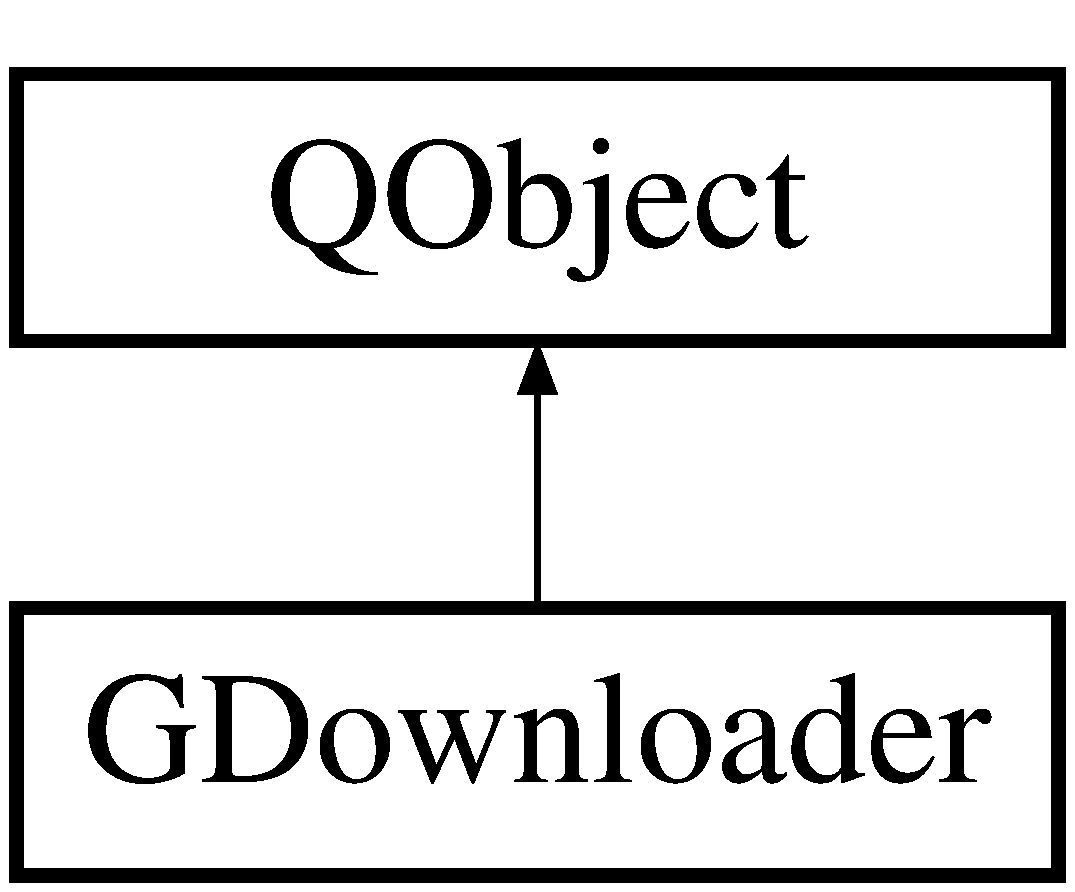
\includegraphics[height=2.000000cm]{classGDownloader}
\end{center}
\end{figure}
\subsection*{Signals}
\begin{DoxyCompactItemize}
\item 
void \mbox{\hyperlink{classGDownloader_abb5cf1dbe464e3dc8943c261934b9a64}{downloaded}} ()
\begin{DoxyCompactList}\small\item\em This Qt signal fires when the data is done downloading. \end{DoxyCompactList}\end{DoxyCompactItemize}
\subsection*{Public Member Functions}
\begin{DoxyCompactItemize}
\item 
\mbox{\hyperlink{classGDownloader_a03a6336ad3aebf9d5904c50ce0cdc1dc}{G\+Downloader}} ()
\begin{DoxyCompactList}\small\item\em Creates a new downloader. \end{DoxyCompactList}\item 
virtual \mbox{\hyperlink{classGDownloader_a6a9f476cb937e98d417d8ab43b8cd8d5}{$\sim$\+G\+Downloader}} ()
\begin{DoxyCompactList}\small\item\em Frees memory allocated internally by the downloader. \end{DoxyCompactList}\item 
std\+::string \mbox{\hyperlink{classGDownloader_a27b002ce17000e199302c608363c97a2}{download\+As\+String}} (const std\+::string \&url)
\begin{DoxyCompactList}\small\item\em Downloads the text contents of the given U\+RL, returning them as a string. \end{DoxyCompactList}\item 
void \mbox{\hyperlink{classGDownloader_a0bf57f044cc66c8aab40f3f2179caf21}{download\+To\+File}} (const std\+::string \&url, const std\+::string \&file)
\begin{DoxyCompactList}\small\item\em Downloads the text contents of the given U\+RL, saving it to the given output file. \end{DoxyCompactList}\item 
std\+::string \mbox{\hyperlink{classGDownloader_adf0cc934eff26878cdf2018259997a4a}{get\+Error\+Message}} () const
\begin{DoxyCompactList}\small\item\em Returns the last H\+T\+TP error message that occurred. \end{DoxyCompactList}\item 
std\+::string \mbox{\hyperlink{classGDownloader_a736d777b29179f52ba753317d84b1087}{get\+Header}} (const std\+::string \&name) const
\begin{DoxyCompactList}\small\item\em Returns the value of the given H\+T\+TP header for this U\+RL request. \end{DoxyCompactList}\item 
int \mbox{\hyperlink{classGDownloader_ab6c069ef77f1319830dcfd90eed6a2ce}{get\+Http\+Status\+Code}} () const
\begin{DoxyCompactList}\small\item\em Returns the most recent H\+T\+TP status code, which may be a successful code (e.\+g. \end{DoxyCompactList}\item 
std\+::string \mbox{\hyperlink{classGDownloader_a479f109234aad1c792be804bf6320c62}{get\+User\+Agent}} () const
\begin{DoxyCompactList}\small\item\em Returns the value of the H\+T\+TP \char`\"{}\+User-\/\+Agent\char`\"{} header for this U\+RL request, or an empty string if the user agent has not been set. \end{DoxyCompactList}\item 
bool \mbox{\hyperlink{classGDownloader_a81dd125e253592aaef5fea33dfc50c42}{has\+Error}} () const
\begin{DoxyCompactList}\small\item\em Returns true if the H\+T\+TP connection failed and had an error. \end{DoxyCompactList}\item 
void \mbox{\hyperlink{classGDownloader_a4bafb98a98bc6edc2403a3734c985618}{http\+Get}} (const std\+::string \&url)
\begin{DoxyCompactList}\small\item\em Performs an H\+T\+TP G\+ET request to the given U\+RL. \end{DoxyCompactList}\item 
void \mbox{\hyperlink{classGDownloader_a68ec0a089bf1b625b86753545e952a57}{http\+Post}} (const std\+::string \&url)
\begin{DoxyCompactList}\small\item\em Performs an H\+T\+TP P\+O\+ST request to the given U\+RL, submitting any headers and query parameters previously specified. \end{DoxyCompactList}\item 
void \mbox{\hyperlink{classGDownloader_af7065da3945b84ffb547b8bad9ddf8dc}{set\+Header}} (const std\+::string \&name, const std\+::string \&value)
\item 
void \mbox{\hyperlink{classGDownloader_a766286050e9b8fe08919f8353ecb4031}{set\+User\+Agent}} (const std\+::string \&user\+Agent)
\end{DoxyCompactItemize}


\subsection{Detailed Description}
A \mbox{\hyperlink{classGDownloader}{G\+Downloader}} can download files and data over an internet connection. 

It can save the data to a file or return the data as a string. 

\subsection{Constructor \& Destructor Documentation}
\mbox{\Hypertarget{classGDownloader_a03a6336ad3aebf9d5904c50ce0cdc1dc}\label{classGDownloader_a03a6336ad3aebf9d5904c50ce0cdc1dc}} 
\index{G\+Downloader@{G\+Downloader}!G\+Downloader@{G\+Downloader}}
\index{G\+Downloader@{G\+Downloader}!G\+Downloader@{G\+Downloader}}
\subsubsection{\texorpdfstring{G\+Downloader()}{GDownloader()}}
{\footnotesize\ttfamily \mbox{\hyperlink{classGDownloader}{G\+Downloader}} (\begin{DoxyParamCaption}{ }\end{DoxyParamCaption})}



Creates a new downloader. 

\mbox{\Hypertarget{classGDownloader_a6a9f476cb937e98d417d8ab43b8cd8d5}\label{classGDownloader_a6a9f476cb937e98d417d8ab43b8cd8d5}} 
\index{G\+Downloader@{G\+Downloader}!````~G\+Downloader@{$\sim$\+G\+Downloader}}
\index{````~G\+Downloader@{$\sim$\+G\+Downloader}!G\+Downloader@{G\+Downloader}}
\subsubsection{\texorpdfstring{$\sim$\+G\+Downloader()}{~GDownloader()}}
{\footnotesize\ttfamily $\sim$\mbox{\hyperlink{classGDownloader}{G\+Downloader}} (\begin{DoxyParamCaption}{ }\end{DoxyParamCaption})\hspace{0.3cm}{\ttfamily [virtual]}}



Frees memory allocated internally by the downloader. 



\subsection{Member Function Documentation}
\mbox{\Hypertarget{classGDownloader_a27b002ce17000e199302c608363c97a2}\label{classGDownloader_a27b002ce17000e199302c608363c97a2}} 
\index{G\+Downloader@{G\+Downloader}!download\+As\+String@{download\+As\+String}}
\index{download\+As\+String@{download\+As\+String}!G\+Downloader@{G\+Downloader}}
\subsubsection{\texorpdfstring{download\+As\+String()}{downloadAsString()}}
{\footnotesize\ttfamily std\+::string download\+As\+String (\begin{DoxyParamCaption}\item[{const std\+::string \&}]{url }\end{DoxyParamCaption})}



Downloads the text contents of the given U\+RL, returning them as a string. 

This method blocks until the data is finished downloading. \mbox{\Hypertarget{classGDownloader_abb5cf1dbe464e3dc8943c261934b9a64}\label{classGDownloader_abb5cf1dbe464e3dc8943c261934b9a64}} 
\index{G\+Downloader@{G\+Downloader}!downloaded@{downloaded}}
\index{downloaded@{downloaded}!G\+Downloader@{G\+Downloader}}
\subsubsection{\texorpdfstring{downloaded}{downloaded}}
{\footnotesize\ttfamily void downloaded (\begin{DoxyParamCaption}{ }\end{DoxyParamCaption})\hspace{0.3cm}{\ttfamily [signal]}}



This Qt signal fires when the data is done downloading. 

\mbox{\Hypertarget{classGDownloader_a0bf57f044cc66c8aab40f3f2179caf21}\label{classGDownloader_a0bf57f044cc66c8aab40f3f2179caf21}} 
\index{G\+Downloader@{G\+Downloader}!download\+To\+File@{download\+To\+File}}
\index{download\+To\+File@{download\+To\+File}!G\+Downloader@{G\+Downloader}}
\subsubsection{\texorpdfstring{download\+To\+File()}{downloadToFile()}}
{\footnotesize\ttfamily void download\+To\+File (\begin{DoxyParamCaption}\item[{const std\+::string \&}]{url,  }\item[{const std\+::string \&}]{file }\end{DoxyParamCaption})}



Downloads the text contents of the given U\+RL, saving it to the given output file. 

This method blocks until the data is finished downloading. \mbox{\Hypertarget{classGDownloader_adf0cc934eff26878cdf2018259997a4a}\label{classGDownloader_adf0cc934eff26878cdf2018259997a4a}} 
\index{G\+Downloader@{G\+Downloader}!get\+Error\+Message@{get\+Error\+Message}}
\index{get\+Error\+Message@{get\+Error\+Message}!G\+Downloader@{G\+Downloader}}
\subsubsection{\texorpdfstring{get\+Error\+Message()}{getErrorMessage()}}
{\footnotesize\ttfamily std\+::string get\+Error\+Message (\begin{DoxyParamCaption}{ }\end{DoxyParamCaption}) const}



Returns the last H\+T\+TP error message that occurred. 

If no H\+T\+TP errors have occurred, returns \char`\"{}\char`\"{}. \mbox{\Hypertarget{classGDownloader_a736d777b29179f52ba753317d84b1087}\label{classGDownloader_a736d777b29179f52ba753317d84b1087}} 
\index{G\+Downloader@{G\+Downloader}!get\+Header@{get\+Header}}
\index{get\+Header@{get\+Header}!G\+Downloader@{G\+Downloader}}
\subsubsection{\texorpdfstring{get\+Header()}{getHeader()}}
{\footnotesize\ttfamily std\+::string get\+Header (\begin{DoxyParamCaption}\item[{const std\+::string \&}]{name }\end{DoxyParamCaption}) const}



Returns the value of the given H\+T\+TP header for this U\+RL request. 

If the given header is not defined, returns an empty string. \mbox{\Hypertarget{classGDownloader_ab6c069ef77f1319830dcfd90eed6a2ce}\label{classGDownloader_ab6c069ef77f1319830dcfd90eed6a2ce}} 
\index{G\+Downloader@{G\+Downloader}!get\+Http\+Status\+Code@{get\+Http\+Status\+Code}}
\index{get\+Http\+Status\+Code@{get\+Http\+Status\+Code}!G\+Downloader@{G\+Downloader}}
\subsubsection{\texorpdfstring{get\+Http\+Status\+Code()}{getHttpStatusCode()}}
{\footnotesize\ttfamily int get\+Http\+Status\+Code (\begin{DoxyParamCaption}{ }\end{DoxyParamCaption}) const}



Returns the most recent H\+T\+TP status code, which may be a successful code (e.\+g. 

200) or an error (e.\+g 404). If there is no H\+T\+TP status code to return, returns 0. \mbox{\Hypertarget{classGDownloader_a479f109234aad1c792be804bf6320c62}\label{classGDownloader_a479f109234aad1c792be804bf6320c62}} 
\index{G\+Downloader@{G\+Downloader}!get\+User\+Agent@{get\+User\+Agent}}
\index{get\+User\+Agent@{get\+User\+Agent}!G\+Downloader@{G\+Downloader}}
\subsubsection{\texorpdfstring{get\+User\+Agent()}{getUserAgent()}}
{\footnotesize\ttfamily std\+::string get\+User\+Agent (\begin{DoxyParamCaption}{ }\end{DoxyParamCaption}) const}



Returns the value of the H\+T\+TP \char`\"{}\+User-\/\+Agent\char`\"{} header for this U\+RL request, or an empty string if the user agent has not been set. 

\mbox{\Hypertarget{classGDownloader_a81dd125e253592aaef5fea33dfc50c42}\label{classGDownloader_a81dd125e253592aaef5fea33dfc50c42}} 
\index{G\+Downloader@{G\+Downloader}!has\+Error@{has\+Error}}
\index{has\+Error@{has\+Error}!G\+Downloader@{G\+Downloader}}
\subsubsection{\texorpdfstring{has\+Error()}{hasError()}}
{\footnotesize\ttfamily bool has\+Error (\begin{DoxyParamCaption}{ }\end{DoxyParamCaption}) const}



Returns true if the H\+T\+TP connection failed and had an error. 

You can see what the error was by calling get\+Error\+Message. \mbox{\Hypertarget{classGDownloader_a4bafb98a98bc6edc2403a3734c985618}\label{classGDownloader_a4bafb98a98bc6edc2403a3734c985618}} 
\index{G\+Downloader@{G\+Downloader}!http\+Get@{http\+Get}}
\index{http\+Get@{http\+Get}!G\+Downloader@{G\+Downloader}}
\subsubsection{\texorpdfstring{http\+Get()}{httpGet()}}
{\footnotesize\ttfamily void http\+Get (\begin{DoxyParamCaption}\item[{const std\+::string \&}]{url }\end{DoxyParamCaption})}



Performs an H\+T\+TP G\+ET request to the given U\+RL. 

along with any headers previously specified. \mbox{\Hypertarget{classGDownloader_a68ec0a089bf1b625b86753545e952a57}\label{classGDownloader_a68ec0a089bf1b625b86753545e952a57}} 
\index{G\+Downloader@{G\+Downloader}!http\+Post@{http\+Post}}
\index{http\+Post@{http\+Post}!G\+Downloader@{G\+Downloader}}
\subsubsection{\texorpdfstring{http\+Post()}{httpPost()}}
{\footnotesize\ttfamily void http\+Post (\begin{DoxyParamCaption}\item[{const std\+::string \&}]{url }\end{DoxyParamCaption})}



Performs an H\+T\+TP P\+O\+ST request to the given U\+RL, submitting any headers and query parameters previously specified. 

\mbox{\Hypertarget{classGDownloader_af7065da3945b84ffb547b8bad9ddf8dc}\label{classGDownloader_af7065da3945b84ffb547b8bad9ddf8dc}} 
\index{G\+Downloader@{G\+Downloader}!set\+Header@{set\+Header}}
\index{set\+Header@{set\+Header}!G\+Downloader@{G\+Downloader}}
\subsubsection{\texorpdfstring{set\+Header()}{setHeader()}}
{\footnotesize\ttfamily void set\+Header (\begin{DoxyParamCaption}\item[{const std\+::string \&}]{name,  }\item[{const std\+::string \&}]{value }\end{DoxyParamCaption})}

\mbox{\Hypertarget{classGDownloader_a766286050e9b8fe08919f8353ecb4031}\label{classGDownloader_a766286050e9b8fe08919f8353ecb4031}} 
\index{G\+Downloader@{G\+Downloader}!set\+User\+Agent@{set\+User\+Agent}}
\index{set\+User\+Agent@{set\+User\+Agent}!G\+Downloader@{G\+Downloader}}
\subsubsection{\texorpdfstring{set\+User\+Agent()}{setUserAgent()}}
{\footnotesize\ttfamily void set\+User\+Agent (\begin{DoxyParamCaption}\item[{const std\+::string \&}]{user\+Agent }\end{DoxyParamCaption})}


\hypertarget{classGDrawingSurface}{}\section{G\+Drawing\+Surface Class Reference}
\label{classGDrawingSurface}\index{G\+Drawing\+Surface@{G\+Drawing\+Surface}}


\mbox{\hyperlink{classGDrawingSurface}{G\+Drawing\+Surface}} is an abstract superclass for types that allow drawing shapes and pixels onto themselves as a pixel background layer.  




{\ttfamily \#include $<$gdrawingsurface.\+h$>$}

Inheritance diagram for G\+Drawing\+Surface\+:\begin{figure}[H]
\begin{center}
\leavevmode
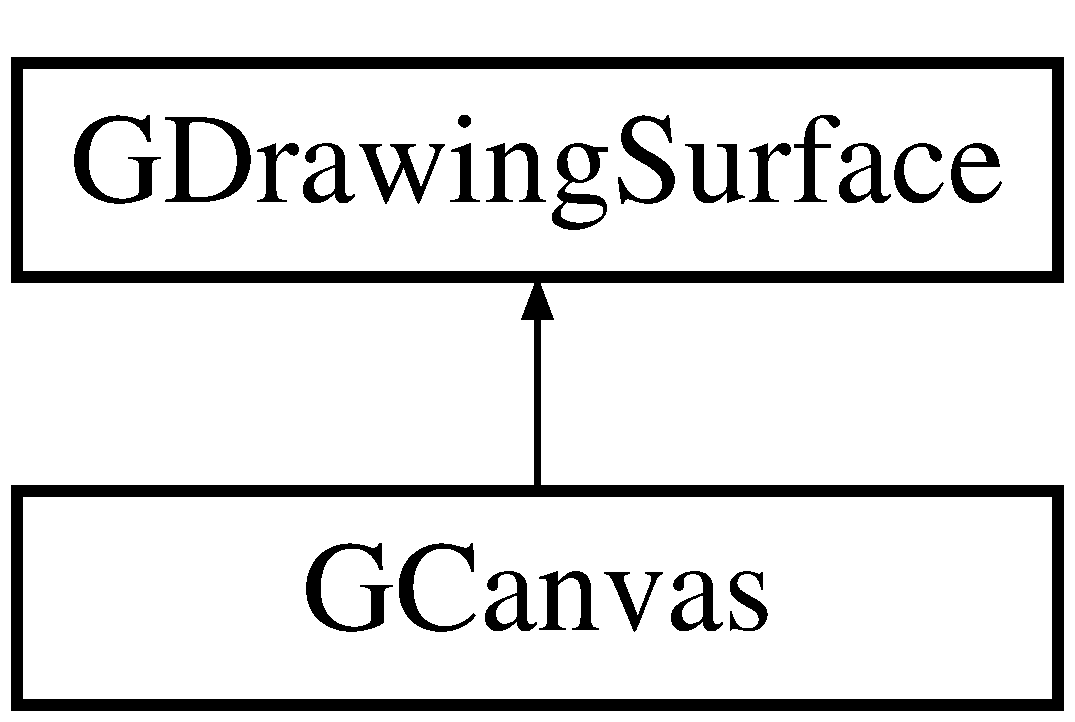
\includegraphics[height=2.000000cm]{classGDrawingSurface}
\end{center}
\end{figure}
\subsection*{Public Member Functions}
\begin{DoxyCompactItemize}
\item 
virtual void \mbox{\hyperlink{classGDrawingSurface_a5eeb94d22b8366d1b68d0614384802fe}{clear}} ()=0
\begin{DoxyCompactList}\small\item\em Erases any pixel data from the drawing surface. \end{DoxyCompactList}\item 
virtual void \mbox{\hyperlink{classGDrawingSurface_a221b3e75bb3d9d0bfea62b3364e6773b}{conditional\+Repaint}} ()
\begin{DoxyCompactList}\small\item\em Repaints the interactor only if its contents have changed. \end{DoxyCompactList}\item 
virtual void \mbox{\hyperlink{classGDrawingSurface_aedd4b792311d946eeaf44b0de337a408}{conditional\+Repaint\+Region}} (int x, int y, int width, int height)
\begin{DoxyCompactList}\small\item\em Repaints the given region of the interactor only if its contents have changed. \end{DoxyCompactList}\item 
virtual void \mbox{\hyperlink{classGDrawingSurface_a3932a12278752db368e24fa404e446aa}{conditional\+Repaint\+Region}} (const \mbox{\hyperlink{structGRectangle}{G\+Rectangle}} \&bounds)
\begin{DoxyCompactList}\small\item\em Repaints the given region of the interactor only if its contents have changed. \end{DoxyCompactList}\item 
virtual void \mbox{\hyperlink{classGDrawingSurface_ae65b7cc9bdfbc1bd01bec80ba83aab47}{draw}} (\mbox{\hyperlink{classGObject}{G\+Object}} $\ast$gobj)=0
\begin{DoxyCompactList}\small\item\em Draws the given graphical object onto the background pixel layer of this interactor. \end{DoxyCompactList}\item 
virtual void \mbox{\hyperlink{classGDrawingSurface_acc3825d7a24815d1e2f78e7c3ffea6cc}{draw}} (\mbox{\hyperlink{classGObject}{G\+Object}} $\ast$gobj, double x, double y)
\begin{DoxyCompactList}\small\item\em Draws the given graphical object onto the background pixel layer of this interactor, moving it to the given x/y location first. \end{DoxyCompactList}\item 
virtual void \mbox{\hyperlink{classGDrawingSurface_a022a8d51c7fabcd79a0c809233e93453}{draw}} (\mbox{\hyperlink{classGObject}{G\+Object}} \&gobj)
\begin{DoxyCompactList}\small\item\em Draws the given graphical object onto the background pixel layer of this interactor. \end{DoxyCompactList}\item 
virtual void \mbox{\hyperlink{classGDrawingSurface_a8af8762bd6720e0a1d2a84b190e3dc96}{draw}} (\mbox{\hyperlink{classGObject}{G\+Object}} \&gobj, double x, double y)
\begin{DoxyCompactList}\small\item\em Draws the given graphical object onto the background pixel layer of this interactor, moving it to the given x/y location first. \end{DoxyCompactList}\item 
virtual void \mbox{\hyperlink{classGDrawingSurface_a38b6fae1045191c57092b49905068144}{draw\+Arc}} (double x, double y, double width, double height, double start, double sweep)
\begin{DoxyCompactList}\small\item\em Draws an unfilled arc with the given attributes onto the background pixel layer of this interactor in the current color. \end{DoxyCompactList}\item 
virtual void \mbox{\hyperlink{classGDrawingSurface_abdd4cb1f2c64adc5d03522a1ee30febf}{draw\+Image}} (const std\+::string \&filename, double x=0, double y=0)
\begin{DoxyCompactList}\small\item\em Draws an image loaded from the given file name onto the background pixel layer of this interactor at the given x/y location. \end{DoxyCompactList}\item 
virtual void \mbox{\hyperlink{classGDrawingSurface_ae6a24b6b9a6e795d3165c1c750d5bdf1}{draw\+Line}} (const \mbox{\hyperlink{structGPoint}{G\+Point}} \&p0, const \mbox{\hyperlink{structGPoint}{G\+Point}} \&p1)
\begin{DoxyCompactList}\small\item\em Draws a line between the given two points onto the background pixel layer of this interactor at the given x/y location in the current color. \end{DoxyCompactList}\item 
virtual void \mbox{\hyperlink{classGDrawingSurface_aff299fe83178d2f3ce8c08c06b583484}{draw\+Line}} (double x0, double y0, double x1, double y1)
\begin{DoxyCompactList}\small\item\em Draws a line between the given two points onto the background pixel layer of this interactor at the given x/y location in the current color. \end{DoxyCompactList}\item 
virtual void \mbox{\hyperlink{classGDrawingSurface_a8adc13027efe311b4a6a715205b8bc46}{draw\+Oval}} (const \mbox{\hyperlink{structGRectangle}{G\+Rectangle}} \&bounds)
\begin{DoxyCompactList}\small\item\em Draws an unfilled oval with the given bounding box onto the background pixel layer of this interactor at the given x/y location in the current color. \end{DoxyCompactList}\item 
virtual void \mbox{\hyperlink{classGDrawingSurface_aa5b1cf902e578907da3c63060686354e}{draw\+Oval}} (double x, double y, double width, double height)
\begin{DoxyCompactList}\small\item\em Draws an unfilled oval with the given bounding box onto the background pixel layer of this interactor at the given x/y location in the current color. \end{DoxyCompactList}\item 
virtual void \mbox{\hyperlink{classGDrawingSurface_a0c1e2923d8d163d62d0896d8c5cfa191}{draw\+Pixel}} (double x, double y)
\begin{DoxyCompactList}\small\item\em Colors the given x/y pixel of the background layer of this interactor using the interactor\textquotesingle{}s current color. \end{DoxyCompactList}\item 
virtual void \mbox{\hyperlink{classGDrawingSurface_a3a64eb6383e601be8438e9c71643c432}{draw\+Pixel}} (double x, double y, int color)
\begin{DoxyCompactList}\small\item\em Colors the given x/y pixel of the background layer of this interactor using the given color. \end{DoxyCompactList}\item 
virtual void \mbox{\hyperlink{classGDrawingSurface_a20abc26a94b7eb310e34abf668e0f5f4}{draw\+Pixel}} (double x, double y, const std\+::string \&color)
\begin{DoxyCompactList}\small\item\em Colors the given x/y pixel of the background layer of this interactor using the given color. \end{DoxyCompactList}\item 
virtual \mbox{\hyperlink{structGPoint}{G\+Point}} \mbox{\hyperlink{classGDrawingSurface_af70cce1e4f708f1ed5b6f29cecb660e7}{draw\+Polar\+Line}} (const \mbox{\hyperlink{structGPoint}{G\+Point}} \&p0, double r, double theta)
\begin{DoxyCompactList}\small\item\em Draws a line using polar coordinates onto the background pixel layer of this interactor in the current color. \end{DoxyCompactList}\item 
virtual \mbox{\hyperlink{structGPoint}{G\+Point}} \mbox{\hyperlink{classGDrawingSurface_ad3e646f90005295f2bbdf37d2bcb39d2}{draw\+Polar\+Line}} (double x0, double y0, double r, double theta)
\begin{DoxyCompactList}\small\item\em Draws a line using polar coordinates onto the background pixel layer of this interactor in the current color. \end{DoxyCompactList}\item 
virtual void \mbox{\hyperlink{classGDrawingSurface_afddec0a905108d8a8d6809a157f26776}{draw\+Polygon}} (std\+::initializer\+\_\+list$<$ double $>$ coords)
\begin{DoxyCompactList}\small\item\em Draws an unfilled polygon containing the given points onto the background pixel layer of this interactor in the current color. \end{DoxyCompactList}\item 
virtual void \mbox{\hyperlink{classGDrawingSurface_a021ee881e0d154dc4dd059698742889c}{draw\+Polygon}} (std\+::initializer\+\_\+list$<$ \mbox{\hyperlink{structGPoint}{G\+Point}} $>$ points)
\begin{DoxyCompactList}\small\item\em Draws an unfilled polygon containing the given points onto the background pixel layer of this interactor in the current color. \end{DoxyCompactList}\item 
virtual void \mbox{\hyperlink{classGDrawingSurface_a3dd4cc5891149dfc36746264f7289877}{draw\+Rect}} (const \mbox{\hyperlink{structGRectangle}{G\+Rectangle}} \&bounds)
\begin{DoxyCompactList}\small\item\em Draws an unfilled rectangle of the given dimensions onto the background pixel layer of this interactor in the current color. \end{DoxyCompactList}\item 
virtual void \mbox{\hyperlink{classGDrawingSurface_a4148e770ffc5474153aadd4814dbd708}{draw\+Rect}} (double x, double y, double width, double height)
\begin{DoxyCompactList}\small\item\em Draws an unfilled rectangle of the given dimensions onto the background pixel layer of this interactor in the current color. \end{DoxyCompactList}\item 
virtual void \mbox{\hyperlink{classGDrawingSurface_ad4e8551a753a77135792bbee97013675}{draw\+String}} (const std\+::string \&text, double x, double y)
\begin{DoxyCompactList}\small\item\em Draws a text string onto the background pixel layer of this interactor at the given x/y location in the current font and color. \end{DoxyCompactList}\item 
virtual void \mbox{\hyperlink{classGDrawingSurface_a228075ad18bd97b57f9956568c4773f3}{fill\+Arc}} (double x, double y, double width, double height, double start, double sweep)
\begin{DoxyCompactList}\small\item\em Draws a filled arc with the given attributes onto the background pixel layer of this interactor in the current color and fill color. \end{DoxyCompactList}\item 
virtual void \mbox{\hyperlink{classGDrawingSurface_a1ea6e48d59fb588797dba4deab1397e0}{fill\+Oval}} (const \mbox{\hyperlink{structGRectangle}{G\+Rectangle}} \&bounds)
\begin{DoxyCompactList}\small\item\em Draws a filled oval with the given bounding box onto the background pixel layer of this interactor at the given x/y location in the current color and fill color. \end{DoxyCompactList}\item 
virtual void \mbox{\hyperlink{classGDrawingSurface_a28c700c82f31cd328a4629273420ee61}{fill\+Oval}} (double x, double y, double width, double height)
\begin{DoxyCompactList}\small\item\em Draws a filled oval with the given bounding box onto the background pixel layer of this interactor at the given x/y location in the current color and fill color. \end{DoxyCompactList}\item 
virtual void \mbox{\hyperlink{classGDrawingSurface_a15f8c1c4409ef51c1a30a92a195b8f66}{fill\+Polygon}} (std\+::initializer\+\_\+list$<$ double $>$ coords)
\begin{DoxyCompactList}\small\item\em Draws a filled polygon containing the given points onto the background pixel layer of this interactor in the current color and fill color. \end{DoxyCompactList}\item 
virtual void \mbox{\hyperlink{classGDrawingSurface_a31822d59786156ebf1cc3b2f7fb70330}{fill\+Polygon}} (std\+::initializer\+\_\+list$<$ \mbox{\hyperlink{structGPoint}{G\+Point}} $>$ coords)
\begin{DoxyCompactList}\small\item\em Draws a filled polygon containing the given points onto the background pixel layer of this interactor in the current color and fill color. \end{DoxyCompactList}\item 
virtual void \mbox{\hyperlink{classGDrawingSurface_ae6582295003bf2488836b1993dadbad7}{fill\+Rect}} (const \mbox{\hyperlink{structGRectangle}{G\+Rectangle}} \&bounds)
\begin{DoxyCompactList}\small\item\em Draws a filled rectangle of the given dimensions onto the background pixel layer of this interactor in the current color and fill color. \end{DoxyCompactList}\item 
virtual void \mbox{\hyperlink{classGDrawingSurface_aac3ae7d3aee950de78eca0e108352254}{fill\+Rect}} (double x, double y, double width, double height)
\begin{DoxyCompactList}\small\item\em Draws a filled rectangle of the given dimensions onto the background pixel layer of this interactor in the current color and fill color. \end{DoxyCompactList}\item 
virtual int \mbox{\hyperlink{classGDrawingSurface_ae394d39f20476570e083918d991c25bd}{get\+A\+R\+GB}} (double x, double y) const
\begin{DoxyCompactList}\small\item\em Returns the pixel color data at the given x/y location, retaining alpha-\/channel transparency in the top 8 bits. \end{DoxyCompactList}\item 
virtual std\+::string \mbox{\hyperlink{classGDrawingSurface_a808e22cc1fdfbecf71ed8c64ef4600e0}{get\+Background}} () const
\begin{DoxyCompactList}\small\item\em Returns the current background color of the interactor as a string. \end{DoxyCompactList}\item 
virtual int \mbox{\hyperlink{classGDrawingSurface_a9e827257a55cb8cf4d9de2ec6bcfd7a0}{get\+Background\+Int}} () const
\begin{DoxyCompactList}\small\item\em Returns the current background color of the interactor as an R\+GB integer. \end{DoxyCompactList}\item 
virtual std\+::string \mbox{\hyperlink{classGDrawingSurface_aa061dfa488c31e18549d64363c1d0e34}{get\+Color}} () const
\begin{DoxyCompactList}\small\item\em Returns the current foreground outline color of the interactor as a string. \end{DoxyCompactList}\item 
virtual int \mbox{\hyperlink{classGDrawingSurface_a9635c7af766cdc3417f346683fa0e6c1}{get\+Color\+Int}} () const
\begin{DoxyCompactList}\small\item\em Returns the current foreground outline color of the interactor as an R\+GB integer. \end{DoxyCompactList}\item 
virtual std\+::string \mbox{\hyperlink{classGDrawingSurface_a76f6964a11fde7c78e9751be184e1a3c}{get\+Fill\+Color}} () const
\begin{DoxyCompactList}\small\item\em Returns the current fill color of the interactor as a string. \end{DoxyCompactList}\item 
virtual int \mbox{\hyperlink{classGDrawingSurface_a88f4508d9271c4b5f5b5d6b780f223d0}{get\+Fill\+Color\+Int}} () const
\begin{DoxyCompactList}\small\item\em Returns the current fill color of the interactor as an R\+GB integer. \end{DoxyCompactList}\item 
virtual std\+::string \mbox{\hyperlink{classGDrawingSurface_a894a5502900794eeb27d084c21f1d77d}{get\+Font}} () const
\begin{DoxyCompactList}\small\item\em Returns the current text font of the interactor as a font string. \end{DoxyCompactList}\item 
virtual std\+::string \mbox{\hyperlink{classGDrawingSurface_a4fa2d8b0192a3a5b4af4bbfe71194d03}{get\+Foreground}} () const
\begin{DoxyCompactList}\small\item\em Returns the current foreground outline color of the interactor as a string. \end{DoxyCompactList}\item 
virtual int \mbox{\hyperlink{classGDrawingSurface_ac3b12ab385a6ef9ae90fc879860ba726}{get\+Foreground\+Int}} () const
\begin{DoxyCompactList}\small\item\em Returns the current foreground outline color of the interactor as an R\+GB integer. \end{DoxyCompactList}\item 
virtual \mbox{\hyperlink{classGObject_a86e0f5648542856159bb40775c854aa7}{G\+Object\+::\+Line\+Style}} \mbox{\hyperlink{classGDrawingSurface_aaf1f5ea8281e5e3486662878d26f0a13}{get\+Line\+Style}} () const
\begin{DoxyCompactList}\small\item\em Returns the current line style which will be used to draw outlines of shapes and lines. \end{DoxyCompactList}\item 
virtual double \mbox{\hyperlink{classGDrawingSurface_a85ff266dc3eb63d9f2d8e5a4487fd3c0}{get\+Line\+Width}} () const
\begin{DoxyCompactList}\small\item\em Returns the thickness used when drawing outlines of shapes and lines. \end{DoxyCompactList}\item 
virtual int \mbox{\hyperlink{classGDrawingSurface_a40f3e3f64a8263e13b7162e15b2979ee}{get\+Pixel}} (double x, double y) const =0
\begin{DoxyCompactList}\small\item\em Returns the color of the pixel at the given x/y coordinates of the background layer of the interactor as an integer such as 0xff00cc. \end{DoxyCompactList}\item 
virtual int \mbox{\hyperlink{classGDrawingSurface_aee10de1ca7da1fc3f3fc0e48286f88f8}{get\+Pixel\+A\+R\+GB}} (double x, double y) const =0
\begin{DoxyCompactList}\small\item\em Returns the color of the pixel at the given x/y coordinates of the background layer of the interactor as an integer such as 0xffff00cc. \end{DoxyCompactList}\item 
virtual Grid$<$ int $>$ \mbox{\hyperlink{classGDrawingSurface_a9811240b1241922153dec17d395797cf}{get\+Pixels}} () const =0
\begin{DoxyCompactList}\small\item\em Returns all pixels of the surface as a Grid, where rows represent y values and columns represent x values. \end{DoxyCompactList}\item 
virtual Grid$<$ int $>$ \mbox{\hyperlink{classGDrawingSurface_a5712954f3edce2e1e4dd3109ffe16e05}{get\+Pixels\+A\+R\+GB}} () const =0
\begin{DoxyCompactList}\small\item\em Returns all pixels of the background layer of the surface as a Grid, where rows represent y values and columns represent x values. \end{DoxyCompactList}\item 
virtual std\+::string \mbox{\hyperlink{classGDrawingSurface_a8da04ef488ec5fa498fbbffaf50928fd}{get\+Pixel\+String}} (double x, double y) const
\begin{DoxyCompactList}\small\item\em Returns the color of the pixel at the given x/y coordinates of the image as a string such as \char`\"{}\#ff00cc\char`\"{}. \end{DoxyCompactList}\item 
virtual int \mbox{\hyperlink{classGDrawingSurface_a9e983467cf0c97cfd62433a8471570dc}{get\+R\+GB}} (double x, double y) const
\begin{DoxyCompactList}\small\item\em Returns the color of the pixel at the given x/y coordinates of the background layer of the interactor as an integer such as 0xff00cc. \end{DoxyCompactList}\item 
virtual std\+::string \mbox{\hyperlink{classGDrawingSurface_a456d3582acc3544f37d939f5cb8802fe}{get\+R\+G\+B\+String}} (double x, double y) const
\begin{DoxyCompactList}\small\item\em Returns the color of the pixel at the given x/y coordinates of the background layer of the interactor as a color string such as \char`\"{}\#ff00cc\char`\"{}. \end{DoxyCompactList}\item 
virtual bool \mbox{\hyperlink{classGDrawingSurface_a12c8d52ddfcaa5448ec4bace92ddee6c}{is\+Auto\+Repaint}} () const
\begin{DoxyCompactList}\small\item\em Returns true if the interactor should repaint itself automatically whenever any change is made to its graphical data. \end{DoxyCompactList}\item 
virtual bool \mbox{\hyperlink{classGDrawingSurface_a82a00267c81cc0ae85ee0feb01a92fa8}{is\+Repaint\+Immediately}} () const
\begin{DoxyCompactList}\small\item\em Returns true if the interactor should repaint itself automatically whenever any change is made to its graphical data. \end{DoxyCompactList}\item 
virtual void \mbox{\hyperlink{classGDrawingSurface_a4a8ae47b42f1e6a41b65d3546df46218}{repaint}} ()=0
\begin{DoxyCompactList}\small\item\em Instructs the interactor to redraw itself on the screen. \end{DoxyCompactList}\item 
virtual void \mbox{\hyperlink{classGDrawingSurface_a1a3898317080fecf8af21bbeaeeb37c3}{repaint\+Region}} (int x, int y, int width, int height)=0
\begin{DoxyCompactList}\small\item\em Instructs the interactor to repaint the given region of pixel data. \end{DoxyCompactList}\item 
virtual void \mbox{\hyperlink{classGDrawingSurface_a769c46fb3e1004aec76e8b0adfa42aa6}{repaint\+Region}} (const \mbox{\hyperlink{structGRectangle}{G\+Rectangle}} \&bounds)
\begin{DoxyCompactList}\small\item\em Instructs the interactor to repaint the given region of pixel data. \end{DoxyCompactList}\item 
virtual void \mbox{\hyperlink{classGDrawingSurface_adf10848319457bd6df4c657bf8872bee}{set\+Auto\+Repaint}} (bool auto\+Repaint)
\begin{DoxyCompactList}\small\item\em Sets whether the interactor should repaint itself automatically whenever any change is made to its graphical data. \end{DoxyCompactList}\item 
virtual void \mbox{\hyperlink{classGDrawingSurface_aba673fd56570a074aba10fa059524b96}{set\+Background}} (int color)
\begin{DoxyCompactList}\small\item\em Sets the current background color of the interactor as an R\+GB integer. \end{DoxyCompactList}\item 
virtual void \mbox{\hyperlink{classGDrawingSurface_ab4677ab2474e68b07aa56605af92a84a}{set\+Background}} (const std\+::string \&color)
\begin{DoxyCompactList}\small\item\em Sets the current background color of the interactor as a string. \end{DoxyCompactList}\item 
virtual void \mbox{\hyperlink{classGDrawingSurface_a75b9cb32ff80bf061791beb01a8433d0}{set\+Color}} (int color)
\begin{DoxyCompactList}\small\item\em Sets the current foreground outline color of the interactor as as R\+GB integer. \end{DoxyCompactList}\item 
virtual void \mbox{\hyperlink{classGDrawingSurface_a61374df6c11b52cfbb0815decdbaebc6}{set\+Color}} (const std\+::string \&color)
\begin{DoxyCompactList}\small\item\em Sets the current foreground outline color of the interactor as a string. \end{DoxyCompactList}\item 
virtual void \mbox{\hyperlink{classGDrawingSurface_a47fad447b715f2f303538434eed26709}{set\+Fill\+Color}} (int color)
\begin{DoxyCompactList}\small\item\em Sets the current fill color of the interactor as an R\+GB integer. \end{DoxyCompactList}\item 
virtual void \mbox{\hyperlink{classGDrawingSurface_adbc18b1a930aadd97d7437f9f7265b96}{set\+Fill\+Color}} (const std\+::string \&color)
\begin{DoxyCompactList}\small\item\em Returns the current fill color of the interactor as a string. \end{DoxyCompactList}\item 
virtual void \mbox{\hyperlink{classGDrawingSurface_a8e096e8818d838aceae1d46d58fb3a7b}{set\+Font}} (const std\+::string \&font)
\begin{DoxyCompactList}\small\item\em Sets the current text font of the interactor as a font string. \end{DoxyCompactList}\item 
virtual void \mbox{\hyperlink{classGDrawingSurface_a7daa57084b5811b598fce8726660b328}{set\+Foreground}} (int color)
\begin{DoxyCompactList}\small\item\em Sets the current foreground outline color of the interactor as an R\+GB integer. \end{DoxyCompactList}\item 
virtual void \mbox{\hyperlink{classGDrawingSurface_af59209aeadea6dfc6d97a2d8531f50e1}{set\+Foreground}} (const std\+::string \&color)
\begin{DoxyCompactList}\small\item\em Sets the current foreground outline color of the interactor as a string. \end{DoxyCompactList}\item 
virtual void \mbox{\hyperlink{classGDrawingSurface_a6bfe14a77101db0fb97b5a7e07a5526b}{set\+Line\+Style}} (\mbox{\hyperlink{classGObject_a86e0f5648542856159bb40775c854aa7}{G\+Object\+::\+Line\+Style}} line\+Style)
\begin{DoxyCompactList}\small\item\em Sets the current line style which will be used to draw outlines of shapes and lines. \end{DoxyCompactList}\item 
virtual void \mbox{\hyperlink{classGDrawingSurface_afd6a47c6ea6a1f85ca05a65ba3ff3477}{set\+Line\+Width}} (double line\+Width)
\begin{DoxyCompactList}\small\item\em Sets the thickness used when drawing outlines of shapes and lines. \end{DoxyCompactList}\item 
virtual void \mbox{\hyperlink{classGDrawingSurface_ac9f0a75ccb0abe1123046bab56479b84}{set\+Pixel}} (double x, double y, int rgb)=0
\begin{DoxyCompactList}\small\item\em Sets the color of the given x/y pixel in the background layer of the interactor to the given R\+GB values. \end{DoxyCompactList}\item 
virtual void \mbox{\hyperlink{classGDrawingSurface_aec90e927c9da286214908d3f9da685d7}{set\+Pixel}} (double x, double y, int r, int g, int b)
\begin{DoxyCompactList}\small\item\em Sets the color of the given x/y pixel in the background layer of the interactor to the given R\+GB values. \end{DoxyCompactList}\item 
virtual void \mbox{\hyperlink{classGDrawingSurface_a09f9640e4ff7388dcfc391efd88d2415}{set\+Pixel}} (double x, double y, const std\+::string \&color)
\begin{DoxyCompactList}\small\item\em Sets the color of the given x/y pixel in the background layer of the interactor to the given color. \end{DoxyCompactList}\item 
virtual void \mbox{\hyperlink{classGDrawingSurface_ab2f7c5a9462f552ad3f30d23c04605dd}{set\+Pixel\+A\+R\+GB}} (double x, double y, int argb)=0
\begin{DoxyCompactList}\small\item\em Sets the color of the given x/y pixel in the background layer of the interactor to the given A\+R\+GB value. \end{DoxyCompactList}\item 
virtual void \mbox{\hyperlink{classGDrawingSurface_a62a8b1555ae3a073a84b0a1c071c65b1}{set\+Pixel\+A\+R\+GB}} (double x, double y, int a, int r, int g, int b)
\begin{DoxyCompactList}\small\item\em Sets the color of the given x/y pixel in the background layer of the interactor to the given A\+R\+GB value. \end{DoxyCompactList}\item 
virtual void \mbox{\hyperlink{classGDrawingSurface_aa80f4b7381bd418116baee600eed37fe}{set\+Pixels}} (const Grid$<$ int $>$ \&pixels)=0
\begin{DoxyCompactList}\small\item\em Sets the color of the all pixels in the background layer of the interactor to the given R\+GB values, using rows as y-\/values and columns as x-\/values. \end{DoxyCompactList}\item 
virtual void \mbox{\hyperlink{classGDrawingSurface_a7d813f0f29751a217201f24cef402306}{set\+Pixels\+A\+R\+GB}} (const Grid$<$ int $>$ \&pixels\+A\+R\+GB)=0
\begin{DoxyCompactList}\small\item\em Sets the color of the all pixels in the background layer of the interactor to the given A\+R\+GB values, using rows as y-\/values and columns as x-\/values. \end{DoxyCompactList}\item 
virtual void \mbox{\hyperlink{classGDrawingSurface_abf5590a3992dcb7896ed449e65961da3}{set\+Repaint\+Immediately}} (bool auto\+Repaint)
\begin{DoxyCompactList}\small\item\em Sets whether the interactor should repaint itself automatically whenever any change is made to its graphical data. \end{DoxyCompactList}\item 
virtual void \mbox{\hyperlink{classGDrawingSurface_a8bcbd65fa784bdab1e66a9efd381162d}{set\+R\+GB}} (double x, double y, int rgb)
\begin{DoxyCompactList}\small\item\em Sets the color of the given x/y pixel in the background layer of the interactor to the given R\+GB values. \end{DoxyCompactList}\item 
virtual void \mbox{\hyperlink{classGDrawingSurface_a81202471d4fc9f2015aef0bc073acfab}{set\+R\+GB}} (double x, double y, int r, int g, int b)
\begin{DoxyCompactList}\small\item\em Sets the color of the given x/y pixel in the background layer of the interactor to the given R\+GB values. \end{DoxyCompactList}\item 
virtual void \mbox{\hyperlink{classGDrawingSurface_ae9a228792d4bb4b628350f39eaa3ad12}{set\+R\+GB}} (double x, double y, const std\+::string \&color)
\begin{DoxyCompactList}\small\item\em Sets the color of the given x/y pixel in the background layer of the interactor to the given color. \end{DoxyCompactList}\end{DoxyCompactItemize}
\subsection*{Protected Member Functions}
\begin{DoxyCompactItemize}
\item 
\mbox{\hyperlink{classGDrawingSurface_a58ecf070e0880ac371754b3e6b4fd970}{G\+Drawing\+Surface}} ()
\item 
virtual \mbox{\hyperlink{classGDrawingSurface_a8e2c882a0c4e31fcbcbb86a207425c1f}{$\sim$\+G\+Drawing\+Surface}} ()
\item 
void \mbox{\hyperlink{classGDrawingSurface_a3a690bcb2d62250c9e4722ad7c1b9ab6}{check\+Bounds}} (const std\+::string \&member, double x, double y, double width, double height) const
\begin{DoxyCompactList}\small\item\em Throws an error if the given x/y values are out of bounds. \end{DoxyCompactList}\item 
void \mbox{\hyperlink{classGDrawingSurface_a9841b5dc607ca41a14819d80e1d8a09c}{check\+Color}} (const std\+::string \&member, int rgb) const
\begin{DoxyCompactList}\small\item\em Throws an error if the given rgb value is not a valid color. \end{DoxyCompactList}\item 
void \mbox{\hyperlink{classGDrawingSurface_a70a6546707ae708573396616bd0f5320}{check\+Size}} (const std\+::string \&member, double width, double height) const
\begin{DoxyCompactList}\small\item\em Throws an error if the given width/height values are out of bounds. \end{DoxyCompactList}\item 
virtual void \mbox{\hyperlink{classGDrawingSurface_a814498efebc5586645159cd22990cf61}{initialize\+G\+Object}} (\mbox{\hyperlink{classGObject}{G\+Object}} \&obj, bool filled=false)
\begin{DoxyCompactList}\small\item\em Initializes a new graphical object to be drawn. \end{DoxyCompactList}\item 
virtual void \mbox{\hyperlink{classGDrawingSurface_a43e6bc951980da061ddc40407daee227}{initialize\+G\+Object}} (\mbox{\hyperlink{classGObject}{G\+Object}} $\ast$obj, bool filled=false)
\begin{DoxyCompactList}\small\item\em Initializes a new graphical object to be drawn. \end{DoxyCompactList}\end{DoxyCompactItemize}
\subsection*{Protected Attributes}
\begin{DoxyCompactItemize}
\item 
bool \mbox{\hyperlink{classGDrawingSurface_a738dd6afc69ac536ad46cf4d89a90933}{\+\_\+auto\+Repaint}}
\item 
std\+::string \mbox{\hyperlink{classGDrawingSurface_ad233544ea51cf6b435a199f3e3790607}{\+\_\+background\+Color}}
\item 
int \mbox{\hyperlink{classGDrawingSurface_abb8452ab4f23ecf455b9e021bf09ef91}{\+\_\+background\+Color\+Int}}
\item 
std\+::string \mbox{\hyperlink{classGDrawingSurface_a1134e770ae4315ea8bc1201e2f21da8b}{\+\_\+color}}
\item 
int \mbox{\hyperlink{classGDrawingSurface_a003fdd343d9b7505c53a8b7a134200ed}{\+\_\+color\+Int}}
\item 
std\+::string \mbox{\hyperlink{classGDrawingSurface_a179f8d6cee65cd8a54692e32b224392a}{\+\_\+fill\+Color}}
\item 
int \mbox{\hyperlink{classGDrawingSurface_a751def333a67d651e5b99cc331ecb496}{\+\_\+fill\+Color\+Int}}
\item 
std\+::string \mbox{\hyperlink{classGDrawingSurface_aea76ea1a8b5dd7b0a78653277e63b536}{\+\_\+font}}
\item 
\mbox{\hyperlink{classGDrawingSurface}{G\+Drawing\+Surface}} $\ast$ \mbox{\hyperlink{classGDrawingSurface_acbb02fa2a4a51a450fd1cc64dfc39ddd}{\+\_\+forward\+Target}}
\item 
\mbox{\hyperlink{classGObject_a86e0f5648542856159bb40775c854aa7}{G\+Object\+::\+Line\+Style}} \mbox{\hyperlink{classGDrawingSurface_ae15d02c66691247a6824dc5943a620e2}{\+\_\+line\+Style}}
\item 
double \mbox{\hyperlink{classGDrawingSurface_a16e9033665937f13de2e163dc2184aff}{\+\_\+line\+Width}}
\end{DoxyCompactItemize}


\subsection{Detailed Description}
\mbox{\hyperlink{classGDrawingSurface}{G\+Drawing\+Surface}} is an abstract superclass for types that allow drawing shapes and pixels onto themselves as a pixel background layer. 

This includes graphical canvas objects (\mbox{\hyperlink{classGCanvas}{G\+Canvas}}) as well as windows (\mbox{\hyperlink{classGWindow}{G\+Window}}). 

\subsection{Constructor \& Destructor Documentation}
\mbox{\Hypertarget{classGDrawingSurface_a58ecf070e0880ac371754b3e6b4fd970}\label{classGDrawingSurface_a58ecf070e0880ac371754b3e6b4fd970}} 
\index{G\+Drawing\+Surface@{G\+Drawing\+Surface}!G\+Drawing\+Surface@{G\+Drawing\+Surface}}
\index{G\+Drawing\+Surface@{G\+Drawing\+Surface}!G\+Drawing\+Surface@{G\+Drawing\+Surface}}
\subsubsection{\texorpdfstring{G\+Drawing\+Surface()}{GDrawingSurface()}}
{\footnotesize\ttfamily \mbox{\hyperlink{classGDrawingSurface}{G\+Drawing\+Surface}} (\begin{DoxyParamCaption}{ }\end{DoxyParamCaption})\hspace{0.3cm}{\ttfamily [protected]}}

\mbox{\Hypertarget{classGDrawingSurface_a8e2c882a0c4e31fcbcbb86a207425c1f}\label{classGDrawingSurface_a8e2c882a0c4e31fcbcbb86a207425c1f}} 
\index{G\+Drawing\+Surface@{G\+Drawing\+Surface}!````~G\+Drawing\+Surface@{$\sim$\+G\+Drawing\+Surface}}
\index{````~G\+Drawing\+Surface@{$\sim$\+G\+Drawing\+Surface}!G\+Drawing\+Surface@{G\+Drawing\+Surface}}
\subsubsection{\texorpdfstring{$\sim$\+G\+Drawing\+Surface()}{~GDrawingSurface()}}
{\footnotesize\ttfamily $\sim$\mbox{\hyperlink{classGDrawingSurface}{G\+Drawing\+Surface}} (\begin{DoxyParamCaption}{ }\end{DoxyParamCaption})\hspace{0.3cm}{\ttfamily [protected]}, {\ttfamily [virtual]}}



\subsection{Member Function Documentation}
\mbox{\Hypertarget{classGDrawingSurface_a3a690bcb2d62250c9e4722ad7c1b9ab6}\label{classGDrawingSurface_a3a690bcb2d62250c9e4722ad7c1b9ab6}} 
\index{G\+Drawing\+Surface@{G\+Drawing\+Surface}!check\+Bounds@{check\+Bounds}}
\index{check\+Bounds@{check\+Bounds}!G\+Drawing\+Surface@{G\+Drawing\+Surface}}
\subsubsection{\texorpdfstring{check\+Bounds()}{checkBounds()}}
{\footnotesize\ttfamily void check\+Bounds (\begin{DoxyParamCaption}\item[{const std\+::string \&}]{member,  }\item[{double}]{x,  }\item[{double}]{y,  }\item[{double}]{width,  }\item[{double}]{height }\end{DoxyParamCaption}) const\hspace{0.3cm}{\ttfamily [protected]}}



Throws an error if the given x/y values are out of bounds. 

\mbox{\Hypertarget{classGDrawingSurface_a9841b5dc607ca41a14819d80e1d8a09c}\label{classGDrawingSurface_a9841b5dc607ca41a14819d80e1d8a09c}} 
\index{G\+Drawing\+Surface@{G\+Drawing\+Surface}!check\+Color@{check\+Color}}
\index{check\+Color@{check\+Color}!G\+Drawing\+Surface@{G\+Drawing\+Surface}}
\subsubsection{\texorpdfstring{check\+Color()}{checkColor()}}
{\footnotesize\ttfamily void check\+Color (\begin{DoxyParamCaption}\item[{const std\+::string \&}]{member,  }\item[{int}]{rgb }\end{DoxyParamCaption}) const\hspace{0.3cm}{\ttfamily [protected]}}



Throws an error if the given rgb value is not a valid color. 

\mbox{\Hypertarget{classGDrawingSurface_a70a6546707ae708573396616bd0f5320}\label{classGDrawingSurface_a70a6546707ae708573396616bd0f5320}} 
\index{G\+Drawing\+Surface@{G\+Drawing\+Surface}!check\+Size@{check\+Size}}
\index{check\+Size@{check\+Size}!G\+Drawing\+Surface@{G\+Drawing\+Surface}}
\subsubsection{\texorpdfstring{check\+Size()}{checkSize()}}
{\footnotesize\ttfamily void check\+Size (\begin{DoxyParamCaption}\item[{const std\+::string \&}]{member,  }\item[{double}]{width,  }\item[{double}]{height }\end{DoxyParamCaption}) const\hspace{0.3cm}{\ttfamily [protected]}}



Throws an error if the given width/height values are out of bounds. 

\mbox{\Hypertarget{classGDrawingSurface_a5eeb94d22b8366d1b68d0614384802fe}\label{classGDrawingSurface_a5eeb94d22b8366d1b68d0614384802fe}} 
\index{G\+Drawing\+Surface@{G\+Drawing\+Surface}!clear@{clear}}
\index{clear@{clear}!G\+Drawing\+Surface@{G\+Drawing\+Surface}}
\subsubsection{\texorpdfstring{clear()}{clear()}}
{\footnotesize\ttfamily virtual void clear (\begin{DoxyParamCaption}{ }\end{DoxyParamCaption})\hspace{0.3cm}{\ttfamily [pure virtual]}}



Erases any pixel data from the drawing surface. 



Implemented in \mbox{\hyperlink{classGWindow_aee7cb2065b88d21ac4ad05bc997ecf82}{G\+Window}}, and \mbox{\hyperlink{classGCanvas_aee7cb2065b88d21ac4ad05bc997ecf82}{G\+Canvas}}.

\mbox{\Hypertarget{classGDrawingSurface_a221b3e75bb3d9d0bfea62b3364e6773b}\label{classGDrawingSurface_a221b3e75bb3d9d0bfea62b3364e6773b}} 
\index{G\+Drawing\+Surface@{G\+Drawing\+Surface}!conditional\+Repaint@{conditional\+Repaint}}
\index{conditional\+Repaint@{conditional\+Repaint}!G\+Drawing\+Surface@{G\+Drawing\+Surface}}
\subsubsection{\texorpdfstring{conditional\+Repaint()}{conditionalRepaint()}}
{\footnotesize\ttfamily void conditional\+Repaint (\begin{DoxyParamCaption}{ }\end{DoxyParamCaption})\hspace{0.3cm}{\ttfamily [virtual]}}



Repaints the interactor only if its contents have changed. 

\mbox{\Hypertarget{classGDrawingSurface_aedd4b792311d946eeaf44b0de337a408}\label{classGDrawingSurface_aedd4b792311d946eeaf44b0de337a408}} 
\index{G\+Drawing\+Surface@{G\+Drawing\+Surface}!conditional\+Repaint\+Region@{conditional\+Repaint\+Region}}
\index{conditional\+Repaint\+Region@{conditional\+Repaint\+Region}!G\+Drawing\+Surface@{G\+Drawing\+Surface}}
\subsubsection{\texorpdfstring{conditional\+Repaint\+Region()}{conditionalRepaintRegion()}\hspace{0.1cm}{\footnotesize\ttfamily [1/2]}}
{\footnotesize\ttfamily void conditional\+Repaint\+Region (\begin{DoxyParamCaption}\item[{int}]{x,  }\item[{int}]{y,  }\item[{int}]{width,  }\item[{int}]{height }\end{DoxyParamCaption})\hspace{0.3cm}{\ttfamily [virtual]}}



Repaints the given region of the interactor only if its contents have changed. 

\mbox{\Hypertarget{classGDrawingSurface_a3932a12278752db368e24fa404e446aa}\label{classGDrawingSurface_a3932a12278752db368e24fa404e446aa}} 
\index{G\+Drawing\+Surface@{G\+Drawing\+Surface}!conditional\+Repaint\+Region@{conditional\+Repaint\+Region}}
\index{conditional\+Repaint\+Region@{conditional\+Repaint\+Region}!G\+Drawing\+Surface@{G\+Drawing\+Surface}}
\subsubsection{\texorpdfstring{conditional\+Repaint\+Region()}{conditionalRepaintRegion()}\hspace{0.1cm}{\footnotesize\ttfamily [2/2]}}
{\footnotesize\ttfamily void conditional\+Repaint\+Region (\begin{DoxyParamCaption}\item[{const \mbox{\hyperlink{structGRectangle}{G\+Rectangle}} \&}]{bounds }\end{DoxyParamCaption})\hspace{0.3cm}{\ttfamily [virtual]}}



Repaints the given region of the interactor only if its contents have changed. 

\mbox{\Hypertarget{classGDrawingSurface_ae65b7cc9bdfbc1bd01bec80ba83aab47}\label{classGDrawingSurface_ae65b7cc9bdfbc1bd01bec80ba83aab47}} 
\index{G\+Drawing\+Surface@{G\+Drawing\+Surface}!draw@{draw}}
\index{draw@{draw}!G\+Drawing\+Surface@{G\+Drawing\+Surface}}
\subsubsection{\texorpdfstring{draw()}{draw()}\hspace{0.1cm}{\footnotesize\ttfamily [1/4]}}
{\footnotesize\ttfamily virtual void draw (\begin{DoxyParamCaption}\item[{\mbox{\hyperlink{classGObject}{G\+Object}} $\ast$}]{gobj }\end{DoxyParamCaption})\hspace{0.3cm}{\ttfamily [pure virtual]}}



Draws the given graphical object onto the background pixel layer of this interactor. 


\begin{DoxyExceptions}{Exceptions}
{\em Error\+Exception} & if the object is null \\
\hline
\end{DoxyExceptions}


Implemented in \mbox{\hyperlink{classGCanvas_a7f7f6c1798bcedfd52151b458074e8a0}{G\+Canvas}}.

\mbox{\Hypertarget{classGDrawingSurface_acc3825d7a24815d1e2f78e7c3ffea6cc}\label{classGDrawingSurface_acc3825d7a24815d1e2f78e7c3ffea6cc}} 
\index{G\+Drawing\+Surface@{G\+Drawing\+Surface}!draw@{draw}}
\index{draw@{draw}!G\+Drawing\+Surface@{G\+Drawing\+Surface}}
\subsubsection{\texorpdfstring{draw()}{draw()}\hspace{0.1cm}{\footnotesize\ttfamily [2/4]}}
{\footnotesize\ttfamily void draw (\begin{DoxyParamCaption}\item[{\mbox{\hyperlink{classGObject}{G\+Object}} $\ast$}]{gobj,  }\item[{double}]{x,  }\item[{double}]{y }\end{DoxyParamCaption})\hspace{0.3cm}{\ttfamily [virtual]}}



Draws the given graphical object onto the background pixel layer of this interactor, moving it to the given x/y location first. 


\begin{DoxyExceptions}{Exceptions}
{\em Error\+Exception} & if the object is null \\
\hline
\end{DoxyExceptions}
\mbox{\Hypertarget{classGDrawingSurface_a022a8d51c7fabcd79a0c809233e93453}\label{classGDrawingSurface_a022a8d51c7fabcd79a0c809233e93453}} 
\index{G\+Drawing\+Surface@{G\+Drawing\+Surface}!draw@{draw}}
\index{draw@{draw}!G\+Drawing\+Surface@{G\+Drawing\+Surface}}
\subsubsection{\texorpdfstring{draw()}{draw()}\hspace{0.1cm}{\footnotesize\ttfamily [3/4]}}
{\footnotesize\ttfamily void draw (\begin{DoxyParamCaption}\item[{\mbox{\hyperlink{classGObject}{G\+Object}} \&}]{gobj }\end{DoxyParamCaption})\hspace{0.3cm}{\ttfamily [virtual]}}



Draws the given graphical object onto the background pixel layer of this interactor. 

\mbox{\Hypertarget{classGDrawingSurface_a8af8762bd6720e0a1d2a84b190e3dc96}\label{classGDrawingSurface_a8af8762bd6720e0a1d2a84b190e3dc96}} 
\index{G\+Drawing\+Surface@{G\+Drawing\+Surface}!draw@{draw}}
\index{draw@{draw}!G\+Drawing\+Surface@{G\+Drawing\+Surface}}
\subsubsection{\texorpdfstring{draw()}{draw()}\hspace{0.1cm}{\footnotesize\ttfamily [4/4]}}
{\footnotesize\ttfamily void draw (\begin{DoxyParamCaption}\item[{\mbox{\hyperlink{classGObject}{G\+Object}} \&}]{gobj,  }\item[{double}]{x,  }\item[{double}]{y }\end{DoxyParamCaption})\hspace{0.3cm}{\ttfamily [virtual]}}



Draws the given graphical object onto the background pixel layer of this interactor, moving it to the given x/y location first. 

\mbox{\Hypertarget{classGDrawingSurface_a38b6fae1045191c57092b49905068144}\label{classGDrawingSurface_a38b6fae1045191c57092b49905068144}} 
\index{G\+Drawing\+Surface@{G\+Drawing\+Surface}!draw\+Arc@{draw\+Arc}}
\index{draw\+Arc@{draw\+Arc}!G\+Drawing\+Surface@{G\+Drawing\+Surface}}
\subsubsection{\texorpdfstring{draw\+Arc()}{drawArc()}}
{\footnotesize\ttfamily void draw\+Arc (\begin{DoxyParamCaption}\item[{double}]{x,  }\item[{double}]{y,  }\item[{double}]{width,  }\item[{double}]{height,  }\item[{double}]{start,  }\item[{double}]{sweep }\end{DoxyParamCaption})\hspace{0.3cm}{\ttfamily [virtual]}}



Draws an unfilled arc with the given attributes onto the background pixel layer of this interactor in the current color. 

See \mbox{\hyperlink{gobjects_8h_source}{gobjects.\+h}} for explanation of \mbox{\hyperlink{classGArc}{G\+Arc}} parameters. \mbox{\Hypertarget{classGDrawingSurface_abdd4cb1f2c64adc5d03522a1ee30febf}\label{classGDrawingSurface_abdd4cb1f2c64adc5d03522a1ee30febf}} 
\index{G\+Drawing\+Surface@{G\+Drawing\+Surface}!draw\+Image@{draw\+Image}}
\index{draw\+Image@{draw\+Image}!G\+Drawing\+Surface@{G\+Drawing\+Surface}}
\subsubsection{\texorpdfstring{draw\+Image()}{drawImage()}}
{\footnotesize\ttfamily void draw\+Image (\begin{DoxyParamCaption}\item[{const std\+::string \&}]{filename,  }\item[{double}]{x = {\ttfamily 0},  }\item[{double}]{y = {\ttfamily 0} }\end{DoxyParamCaption})\hspace{0.3cm}{\ttfamily [virtual]}}



Draws an image loaded from the given file name onto the background pixel layer of this interactor at the given x/y location. 

See \mbox{\hyperlink{gobjects_8h_source}{gobjects.\+h}} for explanation of \mbox{\hyperlink{classGImage}{G\+Image}} parameters. 
\begin{DoxyExceptions}{Exceptions}
{\em Error\+Exception} & if the given file is not found or cannot be loaded as a valid image file \\
\hline
\end{DoxyExceptions}
\mbox{\Hypertarget{classGDrawingSurface_ae6a24b6b9a6e795d3165c1c750d5bdf1}\label{classGDrawingSurface_ae6a24b6b9a6e795d3165c1c750d5bdf1}} 
\index{G\+Drawing\+Surface@{G\+Drawing\+Surface}!draw\+Line@{draw\+Line}}
\index{draw\+Line@{draw\+Line}!G\+Drawing\+Surface@{G\+Drawing\+Surface}}
\subsubsection{\texorpdfstring{draw\+Line()}{drawLine()}\hspace{0.1cm}{\footnotesize\ttfamily [1/2]}}
{\footnotesize\ttfamily void draw\+Line (\begin{DoxyParamCaption}\item[{const \mbox{\hyperlink{structGPoint}{G\+Point}} \&}]{p0,  }\item[{const \mbox{\hyperlink{structGPoint}{G\+Point}} \&}]{p1 }\end{DoxyParamCaption})\hspace{0.3cm}{\ttfamily [virtual]}}



Draws a line between the given two points onto the background pixel layer of this interactor at the given x/y location in the current color. 

See \mbox{\hyperlink{gobjects_8h_source}{gobjects.\+h}} for explanation of \mbox{\hyperlink{classGLine}{G\+Line}} parameters. \mbox{\Hypertarget{classGDrawingSurface_aff299fe83178d2f3ce8c08c06b583484}\label{classGDrawingSurface_aff299fe83178d2f3ce8c08c06b583484}} 
\index{G\+Drawing\+Surface@{G\+Drawing\+Surface}!draw\+Line@{draw\+Line}}
\index{draw\+Line@{draw\+Line}!G\+Drawing\+Surface@{G\+Drawing\+Surface}}
\subsubsection{\texorpdfstring{draw\+Line()}{drawLine()}\hspace{0.1cm}{\footnotesize\ttfamily [2/2]}}
{\footnotesize\ttfamily void draw\+Line (\begin{DoxyParamCaption}\item[{double}]{x0,  }\item[{double}]{y0,  }\item[{double}]{x1,  }\item[{double}]{y1 }\end{DoxyParamCaption})\hspace{0.3cm}{\ttfamily [virtual]}}



Draws a line between the given two points onto the background pixel layer of this interactor at the given x/y location in the current color. 

See \mbox{\hyperlink{gobjects_8h_source}{gobjects.\+h}} for explanation of \mbox{\hyperlink{classGLine}{G\+Line}} parameters. \mbox{\Hypertarget{classGDrawingSurface_a8adc13027efe311b4a6a715205b8bc46}\label{classGDrawingSurface_a8adc13027efe311b4a6a715205b8bc46}} 
\index{G\+Drawing\+Surface@{G\+Drawing\+Surface}!draw\+Oval@{draw\+Oval}}
\index{draw\+Oval@{draw\+Oval}!G\+Drawing\+Surface@{G\+Drawing\+Surface}}
\subsubsection{\texorpdfstring{draw\+Oval()}{drawOval()}\hspace{0.1cm}{\footnotesize\ttfamily [1/2]}}
{\footnotesize\ttfamily void draw\+Oval (\begin{DoxyParamCaption}\item[{const \mbox{\hyperlink{structGRectangle}{G\+Rectangle}} \&}]{bounds }\end{DoxyParamCaption})\hspace{0.3cm}{\ttfamily [virtual]}}



Draws an unfilled oval with the given bounding box onto the background pixel layer of this interactor at the given x/y location in the current color. 

See \mbox{\hyperlink{gobjects_8h_source}{gobjects.\+h}} for explanation of \mbox{\hyperlink{classGOval}{G\+Oval}} parameters. \mbox{\Hypertarget{classGDrawingSurface_aa5b1cf902e578907da3c63060686354e}\label{classGDrawingSurface_aa5b1cf902e578907da3c63060686354e}} 
\index{G\+Drawing\+Surface@{G\+Drawing\+Surface}!draw\+Oval@{draw\+Oval}}
\index{draw\+Oval@{draw\+Oval}!G\+Drawing\+Surface@{G\+Drawing\+Surface}}
\subsubsection{\texorpdfstring{draw\+Oval()}{drawOval()}\hspace{0.1cm}{\footnotesize\ttfamily [2/2]}}
{\footnotesize\ttfamily void draw\+Oval (\begin{DoxyParamCaption}\item[{double}]{x,  }\item[{double}]{y,  }\item[{double}]{width,  }\item[{double}]{height }\end{DoxyParamCaption})\hspace{0.3cm}{\ttfamily [virtual]}}



Draws an unfilled oval with the given bounding box onto the background pixel layer of this interactor at the given x/y location in the current color. 

See \mbox{\hyperlink{gobjects_8h_source}{gobjects.\+h}} for explanation of \mbox{\hyperlink{classGOval}{G\+Oval}} parameters. \mbox{\Hypertarget{classGDrawingSurface_a0c1e2923d8d163d62d0896d8c5cfa191}\label{classGDrawingSurface_a0c1e2923d8d163d62d0896d8c5cfa191}} 
\index{G\+Drawing\+Surface@{G\+Drawing\+Surface}!draw\+Pixel@{draw\+Pixel}}
\index{draw\+Pixel@{draw\+Pixel}!G\+Drawing\+Surface@{G\+Drawing\+Surface}}
\subsubsection{\texorpdfstring{draw\+Pixel()}{drawPixel()}\hspace{0.1cm}{\footnotesize\ttfamily [1/3]}}
{\footnotesize\ttfamily void draw\+Pixel (\begin{DoxyParamCaption}\item[{double}]{x,  }\item[{double}]{y }\end{DoxyParamCaption})\hspace{0.3cm}{\ttfamily [virtual]}}



Colors the given x/y pixel of the background layer of this interactor using the interactor\textquotesingle{}s current color. 

\mbox{\Hypertarget{classGDrawingSurface_a3a64eb6383e601be8438e9c71643c432}\label{classGDrawingSurface_a3a64eb6383e601be8438e9c71643c432}} 
\index{G\+Drawing\+Surface@{G\+Drawing\+Surface}!draw\+Pixel@{draw\+Pixel}}
\index{draw\+Pixel@{draw\+Pixel}!G\+Drawing\+Surface@{G\+Drawing\+Surface}}
\subsubsection{\texorpdfstring{draw\+Pixel()}{drawPixel()}\hspace{0.1cm}{\footnotesize\ttfamily [2/3]}}
{\footnotesize\ttfamily void draw\+Pixel (\begin{DoxyParamCaption}\item[{double}]{x,  }\item[{double}]{y,  }\item[{int}]{color }\end{DoxyParamCaption})\hspace{0.3cm}{\ttfamily [virtual]}}



Colors the given x/y pixel of the background layer of this interactor using the given color. 

\mbox{\Hypertarget{classGDrawingSurface_a20abc26a94b7eb310e34abf668e0f5f4}\label{classGDrawingSurface_a20abc26a94b7eb310e34abf668e0f5f4}} 
\index{G\+Drawing\+Surface@{G\+Drawing\+Surface}!draw\+Pixel@{draw\+Pixel}}
\index{draw\+Pixel@{draw\+Pixel}!G\+Drawing\+Surface@{G\+Drawing\+Surface}}
\subsubsection{\texorpdfstring{draw\+Pixel()}{drawPixel()}\hspace{0.1cm}{\footnotesize\ttfamily [3/3]}}
{\footnotesize\ttfamily void draw\+Pixel (\begin{DoxyParamCaption}\item[{double}]{x,  }\item[{double}]{y,  }\item[{const std\+::string \&}]{color }\end{DoxyParamCaption})\hspace{0.3cm}{\ttfamily [virtual]}}



Colors the given x/y pixel of the background layer of this interactor using the given color. 

\mbox{\Hypertarget{classGDrawingSurface_af70cce1e4f708f1ed5b6f29cecb660e7}\label{classGDrawingSurface_af70cce1e4f708f1ed5b6f29cecb660e7}} 
\index{G\+Drawing\+Surface@{G\+Drawing\+Surface}!draw\+Polar\+Line@{draw\+Polar\+Line}}
\index{draw\+Polar\+Line@{draw\+Polar\+Line}!G\+Drawing\+Surface@{G\+Drawing\+Surface}}
\subsubsection{\texorpdfstring{draw\+Polar\+Line()}{drawPolarLine()}\hspace{0.1cm}{\footnotesize\ttfamily [1/2]}}
{\footnotesize\ttfamily \mbox{\hyperlink{structGPoint}{G\+Point}} draw\+Polar\+Line (\begin{DoxyParamCaption}\item[{const \mbox{\hyperlink{structGPoint}{G\+Point}} \&}]{p0,  }\item[{double}]{r,  }\item[{double}]{theta }\end{DoxyParamCaption})\hspace{0.3cm}{\ttfamily [virtual]}}



Draws a line using polar coordinates onto the background pixel layer of this interactor in the current color. 

The line begins at the given x/y point and extends from there by the given angle and radius. Returns the end point opposite p0 where the line ends. See \mbox{\hyperlink{gobjects_8h_source}{gobjects.\+h}} for explanation of \mbox{\hyperlink{classGLine}{G\+Line}} parameters. \mbox{\Hypertarget{classGDrawingSurface_ad3e646f90005295f2bbdf37d2bcb39d2}\label{classGDrawingSurface_ad3e646f90005295f2bbdf37d2bcb39d2}} 
\index{G\+Drawing\+Surface@{G\+Drawing\+Surface}!draw\+Polar\+Line@{draw\+Polar\+Line}}
\index{draw\+Polar\+Line@{draw\+Polar\+Line}!G\+Drawing\+Surface@{G\+Drawing\+Surface}}
\subsubsection{\texorpdfstring{draw\+Polar\+Line()}{drawPolarLine()}\hspace{0.1cm}{\footnotesize\ttfamily [2/2]}}
{\footnotesize\ttfamily \mbox{\hyperlink{structGPoint}{G\+Point}} draw\+Polar\+Line (\begin{DoxyParamCaption}\item[{double}]{x0,  }\item[{double}]{y0,  }\item[{double}]{r,  }\item[{double}]{theta }\end{DoxyParamCaption})\hspace{0.3cm}{\ttfamily [virtual]}}



Draws a line using polar coordinates onto the background pixel layer of this interactor in the current color. 

The line begins at the given x/y point and extends from there by the given angle and radius. Returns the end point where the line ends. See \mbox{\hyperlink{gobjects_8h_source}{gobjects.\+h}} for explanation of \mbox{\hyperlink{classGLine}{G\+Line}} parameters. \mbox{\Hypertarget{classGDrawingSurface_afddec0a905108d8a8d6809a157f26776}\label{classGDrawingSurface_afddec0a905108d8a8d6809a157f26776}} 
\index{G\+Drawing\+Surface@{G\+Drawing\+Surface}!draw\+Polygon@{draw\+Polygon}}
\index{draw\+Polygon@{draw\+Polygon}!G\+Drawing\+Surface@{G\+Drawing\+Surface}}
\subsubsection{\texorpdfstring{draw\+Polygon()}{drawPolygon()}\hspace{0.1cm}{\footnotesize\ttfamily [1/2]}}
{\footnotesize\ttfamily void draw\+Polygon (\begin{DoxyParamCaption}\item[{std\+::initializer\+\_\+list$<$ double $>$}]{coords }\end{DoxyParamCaption})\hspace{0.3cm}{\ttfamily [virtual]}}



Draws an unfilled polygon containing the given points onto the background pixel layer of this interactor in the current color. 

See \mbox{\hyperlink{gobjects_8h_source}{gobjects.\+h}} for explanation of \mbox{\hyperlink{classGPolygon}{G\+Polygon}} parameters. \mbox{\Hypertarget{classGDrawingSurface_a021ee881e0d154dc4dd059698742889c}\label{classGDrawingSurface_a021ee881e0d154dc4dd059698742889c}} 
\index{G\+Drawing\+Surface@{G\+Drawing\+Surface}!draw\+Polygon@{draw\+Polygon}}
\index{draw\+Polygon@{draw\+Polygon}!G\+Drawing\+Surface@{G\+Drawing\+Surface}}
\subsubsection{\texorpdfstring{draw\+Polygon()}{drawPolygon()}\hspace{0.1cm}{\footnotesize\ttfamily [2/2]}}
{\footnotesize\ttfamily void draw\+Polygon (\begin{DoxyParamCaption}\item[{std\+::initializer\+\_\+list$<$ \mbox{\hyperlink{structGPoint}{G\+Point}} $>$}]{points }\end{DoxyParamCaption})\hspace{0.3cm}{\ttfamily [virtual]}}



Draws an unfilled polygon containing the given points onto the background pixel layer of this interactor in the current color. 

See \mbox{\hyperlink{gobjects_8h_source}{gobjects.\+h}} for explanation of \mbox{\hyperlink{classGPolygon}{G\+Polygon}} parameters. \mbox{\Hypertarget{classGDrawingSurface_a3dd4cc5891149dfc36746264f7289877}\label{classGDrawingSurface_a3dd4cc5891149dfc36746264f7289877}} 
\index{G\+Drawing\+Surface@{G\+Drawing\+Surface}!draw\+Rect@{draw\+Rect}}
\index{draw\+Rect@{draw\+Rect}!G\+Drawing\+Surface@{G\+Drawing\+Surface}}
\subsubsection{\texorpdfstring{draw\+Rect()}{drawRect()}\hspace{0.1cm}{\footnotesize\ttfamily [1/2]}}
{\footnotesize\ttfamily void draw\+Rect (\begin{DoxyParamCaption}\item[{const \mbox{\hyperlink{structGRectangle}{G\+Rectangle}} \&}]{bounds }\end{DoxyParamCaption})\hspace{0.3cm}{\ttfamily [virtual]}}



Draws an unfilled rectangle of the given dimensions onto the background pixel layer of this interactor in the current color. 

See \mbox{\hyperlink{gobjects_8h_source}{gobjects.\+h}} for explanation of \mbox{\hyperlink{classGRect}{G\+Rect}} parameters. \mbox{\Hypertarget{classGDrawingSurface_a4148e770ffc5474153aadd4814dbd708}\label{classGDrawingSurface_a4148e770ffc5474153aadd4814dbd708}} 
\index{G\+Drawing\+Surface@{G\+Drawing\+Surface}!draw\+Rect@{draw\+Rect}}
\index{draw\+Rect@{draw\+Rect}!G\+Drawing\+Surface@{G\+Drawing\+Surface}}
\subsubsection{\texorpdfstring{draw\+Rect()}{drawRect()}\hspace{0.1cm}{\footnotesize\ttfamily [2/2]}}
{\footnotesize\ttfamily void draw\+Rect (\begin{DoxyParamCaption}\item[{double}]{x,  }\item[{double}]{y,  }\item[{double}]{width,  }\item[{double}]{height }\end{DoxyParamCaption})\hspace{0.3cm}{\ttfamily [virtual]}}



Draws an unfilled rectangle of the given dimensions onto the background pixel layer of this interactor in the current color. 

See \mbox{\hyperlink{gobjects_8h_source}{gobjects.\+h}} for explanation of \mbox{\hyperlink{classGRect}{G\+Rect}} parameters. \mbox{\Hypertarget{classGDrawingSurface_ad4e8551a753a77135792bbee97013675}\label{classGDrawingSurface_ad4e8551a753a77135792bbee97013675}} 
\index{G\+Drawing\+Surface@{G\+Drawing\+Surface}!draw\+String@{draw\+String}}
\index{draw\+String@{draw\+String}!G\+Drawing\+Surface@{G\+Drawing\+Surface}}
\subsubsection{\texorpdfstring{draw\+String()}{drawString()}}
{\footnotesize\ttfamily void draw\+String (\begin{DoxyParamCaption}\item[{const std\+::string \&}]{text,  }\item[{double}]{x,  }\item[{double}]{y }\end{DoxyParamCaption})\hspace{0.3cm}{\ttfamily [virtual]}}



Draws a text string onto the background pixel layer of this interactor at the given x/y location in the current font and color. 

See \mbox{\hyperlink{gobjects_8h_source}{gobjects.\+h}} for explanation of \mbox{\hyperlink{classGText}{G\+Text}} parameters. \mbox{\Hypertarget{classGDrawingSurface_a228075ad18bd97b57f9956568c4773f3}\label{classGDrawingSurface_a228075ad18bd97b57f9956568c4773f3}} 
\index{G\+Drawing\+Surface@{G\+Drawing\+Surface}!fill\+Arc@{fill\+Arc}}
\index{fill\+Arc@{fill\+Arc}!G\+Drawing\+Surface@{G\+Drawing\+Surface}}
\subsubsection{\texorpdfstring{fill\+Arc()}{fillArc()}}
{\footnotesize\ttfamily void fill\+Arc (\begin{DoxyParamCaption}\item[{double}]{x,  }\item[{double}]{y,  }\item[{double}]{width,  }\item[{double}]{height,  }\item[{double}]{start,  }\item[{double}]{sweep }\end{DoxyParamCaption})\hspace{0.3cm}{\ttfamily [virtual]}}



Draws a filled arc with the given attributes onto the background pixel layer of this interactor in the current color and fill color. 

See \mbox{\hyperlink{gobjects_8h_source}{gobjects.\+h}} for explanation of \mbox{\hyperlink{classGArc}{G\+Arc}} parameters. \mbox{\Hypertarget{classGDrawingSurface_a1ea6e48d59fb588797dba4deab1397e0}\label{classGDrawingSurface_a1ea6e48d59fb588797dba4deab1397e0}} 
\index{G\+Drawing\+Surface@{G\+Drawing\+Surface}!fill\+Oval@{fill\+Oval}}
\index{fill\+Oval@{fill\+Oval}!G\+Drawing\+Surface@{G\+Drawing\+Surface}}
\subsubsection{\texorpdfstring{fill\+Oval()}{fillOval()}\hspace{0.1cm}{\footnotesize\ttfamily [1/2]}}
{\footnotesize\ttfamily void fill\+Oval (\begin{DoxyParamCaption}\item[{const \mbox{\hyperlink{structGRectangle}{G\+Rectangle}} \&}]{bounds }\end{DoxyParamCaption})\hspace{0.3cm}{\ttfamily [virtual]}}



Draws a filled oval with the given bounding box onto the background pixel layer of this interactor at the given x/y location in the current color and fill color. 

See \mbox{\hyperlink{gobjects_8h_source}{gobjects.\+h}} for explanation of \mbox{\hyperlink{classGOval}{G\+Oval}} parameters. \mbox{\Hypertarget{classGDrawingSurface_a28c700c82f31cd328a4629273420ee61}\label{classGDrawingSurface_a28c700c82f31cd328a4629273420ee61}} 
\index{G\+Drawing\+Surface@{G\+Drawing\+Surface}!fill\+Oval@{fill\+Oval}}
\index{fill\+Oval@{fill\+Oval}!G\+Drawing\+Surface@{G\+Drawing\+Surface}}
\subsubsection{\texorpdfstring{fill\+Oval()}{fillOval()}\hspace{0.1cm}{\footnotesize\ttfamily [2/2]}}
{\footnotesize\ttfamily void fill\+Oval (\begin{DoxyParamCaption}\item[{double}]{x,  }\item[{double}]{y,  }\item[{double}]{width,  }\item[{double}]{height }\end{DoxyParamCaption})\hspace{0.3cm}{\ttfamily [virtual]}}



Draws a filled oval with the given bounding box onto the background pixel layer of this interactor at the given x/y location in the current color and fill color. 

See \mbox{\hyperlink{gobjects_8h_source}{gobjects.\+h}} for explanation of \mbox{\hyperlink{classGOval}{G\+Oval}} parameters. \mbox{\Hypertarget{classGDrawingSurface_a15f8c1c4409ef51c1a30a92a195b8f66}\label{classGDrawingSurface_a15f8c1c4409ef51c1a30a92a195b8f66}} 
\index{G\+Drawing\+Surface@{G\+Drawing\+Surface}!fill\+Polygon@{fill\+Polygon}}
\index{fill\+Polygon@{fill\+Polygon}!G\+Drawing\+Surface@{G\+Drawing\+Surface}}
\subsubsection{\texorpdfstring{fill\+Polygon()}{fillPolygon()}\hspace{0.1cm}{\footnotesize\ttfamily [1/2]}}
{\footnotesize\ttfamily void fill\+Polygon (\begin{DoxyParamCaption}\item[{std\+::initializer\+\_\+list$<$ double $>$}]{coords }\end{DoxyParamCaption})\hspace{0.3cm}{\ttfamily [virtual]}}



Draws a filled polygon containing the given points onto the background pixel layer of this interactor in the current color and fill color. 

See \mbox{\hyperlink{gobjects_8h_source}{gobjects.\+h}} for explanation of \mbox{\hyperlink{classGPolygon}{G\+Polygon}} parameters. \mbox{\Hypertarget{classGDrawingSurface_a31822d59786156ebf1cc3b2f7fb70330}\label{classGDrawingSurface_a31822d59786156ebf1cc3b2f7fb70330}} 
\index{G\+Drawing\+Surface@{G\+Drawing\+Surface}!fill\+Polygon@{fill\+Polygon}}
\index{fill\+Polygon@{fill\+Polygon}!G\+Drawing\+Surface@{G\+Drawing\+Surface}}
\subsubsection{\texorpdfstring{fill\+Polygon()}{fillPolygon()}\hspace{0.1cm}{\footnotesize\ttfamily [2/2]}}
{\footnotesize\ttfamily void fill\+Polygon (\begin{DoxyParamCaption}\item[{std\+::initializer\+\_\+list$<$ \mbox{\hyperlink{structGPoint}{G\+Point}} $>$}]{coords }\end{DoxyParamCaption})\hspace{0.3cm}{\ttfamily [virtual]}}



Draws a filled polygon containing the given points onto the background pixel layer of this interactor in the current color and fill color. 

See \mbox{\hyperlink{gobjects_8h_source}{gobjects.\+h}} for explanation of \mbox{\hyperlink{classGPolygon}{G\+Polygon}} parameters. \mbox{\Hypertarget{classGDrawingSurface_ae6582295003bf2488836b1993dadbad7}\label{classGDrawingSurface_ae6582295003bf2488836b1993dadbad7}} 
\index{G\+Drawing\+Surface@{G\+Drawing\+Surface}!fill\+Rect@{fill\+Rect}}
\index{fill\+Rect@{fill\+Rect}!G\+Drawing\+Surface@{G\+Drawing\+Surface}}
\subsubsection{\texorpdfstring{fill\+Rect()}{fillRect()}\hspace{0.1cm}{\footnotesize\ttfamily [1/2]}}
{\footnotesize\ttfamily void fill\+Rect (\begin{DoxyParamCaption}\item[{const \mbox{\hyperlink{structGRectangle}{G\+Rectangle}} \&}]{bounds }\end{DoxyParamCaption})\hspace{0.3cm}{\ttfamily [virtual]}}



Draws a filled rectangle of the given dimensions onto the background pixel layer of this interactor in the current color and fill color. 

See \mbox{\hyperlink{gobjects_8h_source}{gobjects.\+h}} for explanation of \mbox{\hyperlink{classGRect}{G\+Rect}} parameters. \mbox{\Hypertarget{classGDrawingSurface_aac3ae7d3aee950de78eca0e108352254}\label{classGDrawingSurface_aac3ae7d3aee950de78eca0e108352254}} 
\index{G\+Drawing\+Surface@{G\+Drawing\+Surface}!fill\+Rect@{fill\+Rect}}
\index{fill\+Rect@{fill\+Rect}!G\+Drawing\+Surface@{G\+Drawing\+Surface}}
\subsubsection{\texorpdfstring{fill\+Rect()}{fillRect()}\hspace{0.1cm}{\footnotesize\ttfamily [2/2]}}
{\footnotesize\ttfamily void fill\+Rect (\begin{DoxyParamCaption}\item[{double}]{x,  }\item[{double}]{y,  }\item[{double}]{width,  }\item[{double}]{height }\end{DoxyParamCaption})\hspace{0.3cm}{\ttfamily [virtual]}}



Draws a filled rectangle of the given dimensions onto the background pixel layer of this interactor in the current color and fill color. 

See \mbox{\hyperlink{gobjects_8h_source}{gobjects.\+h}} for explanation of \mbox{\hyperlink{classGRect}{G\+Rect}} parameters. \mbox{\Hypertarget{classGDrawingSurface_ae394d39f20476570e083918d991c25bd}\label{classGDrawingSurface_ae394d39f20476570e083918d991c25bd}} 
\index{G\+Drawing\+Surface@{G\+Drawing\+Surface}!get\+A\+R\+GB@{get\+A\+R\+GB}}
\index{get\+A\+R\+GB@{get\+A\+R\+GB}!G\+Drawing\+Surface@{G\+Drawing\+Surface}}
\subsubsection{\texorpdfstring{get\+A\+R\+G\+B()}{getARGB()}}
{\footnotesize\ttfamily int get\+A\+R\+GB (\begin{DoxyParamCaption}\item[{double}]{x,  }\item[{double}]{y }\end{DoxyParamCaption}) const\hspace{0.3cm}{\ttfamily [virtual]}}



Returns the pixel color data at the given x/y location, retaining alpha-\/channel transparency in the top 8 bits. 

\mbox{\Hypertarget{classGDrawingSurface_a808e22cc1fdfbecf71ed8c64ef4600e0}\label{classGDrawingSurface_a808e22cc1fdfbecf71ed8c64ef4600e0}} 
\index{G\+Drawing\+Surface@{G\+Drawing\+Surface}!get\+Background@{get\+Background}}
\index{get\+Background@{get\+Background}!G\+Drawing\+Surface@{G\+Drawing\+Surface}}
\subsubsection{\texorpdfstring{get\+Background()}{getBackground()}}
{\footnotesize\ttfamily std\+::string get\+Background (\begin{DoxyParamCaption}{ }\end{DoxyParamCaption}) const\hspace{0.3cm}{\ttfamily [virtual]}}



Returns the current background color of the interactor as a string. 

See \mbox{\hyperlink{gcolor_8h_source}{gcolor.\+h}} for more detail about color strings. 

Reimplemented in \mbox{\hyperlink{classGCanvas_a4a62c51b7244a7642b88065e3a07ae82}{G\+Canvas}}.

\mbox{\Hypertarget{classGDrawingSurface_a9e827257a55cb8cf4d9de2ec6bcfd7a0}\label{classGDrawingSurface_a9e827257a55cb8cf4d9de2ec6bcfd7a0}} 
\index{G\+Drawing\+Surface@{G\+Drawing\+Surface}!get\+Background\+Int@{get\+Background\+Int}}
\index{get\+Background\+Int@{get\+Background\+Int}!G\+Drawing\+Surface@{G\+Drawing\+Surface}}
\subsubsection{\texorpdfstring{get\+Background\+Int()}{getBackgroundInt()}}
{\footnotesize\ttfamily int get\+Background\+Int (\begin{DoxyParamCaption}{ }\end{DoxyParamCaption}) const\hspace{0.3cm}{\ttfamily [virtual]}}



Returns the current background color of the interactor as an R\+GB integer. 

See \mbox{\hyperlink{gcolor_8h_source}{gcolor.\+h}} for more detail about colors. 

Reimplemented in \mbox{\hyperlink{classGCanvas_acd4f2b3b9619dacdfd71fc0004cac382}{G\+Canvas}}.

\mbox{\Hypertarget{classGDrawingSurface_aa061dfa488c31e18549d64363c1d0e34}\label{classGDrawingSurface_aa061dfa488c31e18549d64363c1d0e34}} 
\index{G\+Drawing\+Surface@{G\+Drawing\+Surface}!get\+Color@{get\+Color}}
\index{get\+Color@{get\+Color}!G\+Drawing\+Surface@{G\+Drawing\+Surface}}
\subsubsection{\texorpdfstring{get\+Color()}{getColor()}}
{\footnotesize\ttfamily std\+::string get\+Color (\begin{DoxyParamCaption}{ }\end{DoxyParamCaption}) const\hspace{0.3cm}{\ttfamily [virtual]}}



Returns the current foreground outline color of the interactor as a string. 

This color will be used to draw the outlines of shapes drawn using the draw\+Xxx and fill\+Xxx methods, as well as being the default color used when calling set\+Pixel or set\+R\+GB. See \mbox{\hyperlink{gcolor_8h_source}{gcolor.\+h}} for more detail about color strings. Equivalent to get\+Foreground. \mbox{\Hypertarget{classGDrawingSurface_a9635c7af766cdc3417f346683fa0e6c1}\label{classGDrawingSurface_a9635c7af766cdc3417f346683fa0e6c1}} 
\index{G\+Drawing\+Surface@{G\+Drawing\+Surface}!get\+Color\+Int@{get\+Color\+Int}}
\index{get\+Color\+Int@{get\+Color\+Int}!G\+Drawing\+Surface@{G\+Drawing\+Surface}}
\subsubsection{\texorpdfstring{get\+Color\+Int()}{getColorInt()}}
{\footnotesize\ttfamily int get\+Color\+Int (\begin{DoxyParamCaption}{ }\end{DoxyParamCaption}) const\hspace{0.3cm}{\ttfamily [virtual]}}



Returns the current foreground outline color of the interactor as an R\+GB integer. 

This color will be used to draw the outlines of shapes drawn using the draw\+Xxx and fill\+Xxx methods, as well as being the default color used when calling set\+Pixel or set\+R\+GB. See \mbox{\hyperlink{gcolor_8h_source}{gcolor.\+h}} for more detail about colors. Equivalent to get\+Foreground\+Int. \mbox{\Hypertarget{classGDrawingSurface_a76f6964a11fde7c78e9751be184e1a3c}\label{classGDrawingSurface_a76f6964a11fde7c78e9751be184e1a3c}} 
\index{G\+Drawing\+Surface@{G\+Drawing\+Surface}!get\+Fill\+Color@{get\+Fill\+Color}}
\index{get\+Fill\+Color@{get\+Fill\+Color}!G\+Drawing\+Surface@{G\+Drawing\+Surface}}
\subsubsection{\texorpdfstring{get\+Fill\+Color()}{getFillColor()}}
{\footnotesize\ttfamily std\+::string get\+Fill\+Color (\begin{DoxyParamCaption}{ }\end{DoxyParamCaption}) const\hspace{0.3cm}{\ttfamily [virtual]}}



Returns the current fill color of the interactor as a string. 

This color will appear in shapes drawn using the fill\+Xxx methods. See \mbox{\hyperlink{gcolor_8h_source}{gcolor.\+h}} for more detail about color strings. \mbox{\Hypertarget{classGDrawingSurface_a88f4508d9271c4b5f5b5d6b780f223d0}\label{classGDrawingSurface_a88f4508d9271c4b5f5b5d6b780f223d0}} 
\index{G\+Drawing\+Surface@{G\+Drawing\+Surface}!get\+Fill\+Color\+Int@{get\+Fill\+Color\+Int}}
\index{get\+Fill\+Color\+Int@{get\+Fill\+Color\+Int}!G\+Drawing\+Surface@{G\+Drawing\+Surface}}
\subsubsection{\texorpdfstring{get\+Fill\+Color\+Int()}{getFillColorInt()}}
{\footnotesize\ttfamily int get\+Fill\+Color\+Int (\begin{DoxyParamCaption}{ }\end{DoxyParamCaption}) const\hspace{0.3cm}{\ttfamily [virtual]}}



Returns the current fill color of the interactor as an R\+GB integer. 

This color will appear in shapes drawn using the fill\+Xxx methods. See \mbox{\hyperlink{gcolor_8h_source}{gcolor.\+h}} for more detail about color strings. \mbox{\Hypertarget{classGDrawingSurface_a894a5502900794eeb27d084c21f1d77d}\label{classGDrawingSurface_a894a5502900794eeb27d084c21f1d77d}} 
\index{G\+Drawing\+Surface@{G\+Drawing\+Surface}!get\+Font@{get\+Font}}
\index{get\+Font@{get\+Font}!G\+Drawing\+Surface@{G\+Drawing\+Surface}}
\subsubsection{\texorpdfstring{get\+Font()}{getFont()}}
{\footnotesize\ttfamily std\+::string get\+Font (\begin{DoxyParamCaption}{ }\end{DoxyParamCaption}) const\hspace{0.3cm}{\ttfamily [virtual]}}



Returns the current text font of the interactor as a font string. 

This font will be used when drawing text strings using draw\+String. See \mbox{\hyperlink{gfont_8h_source}{gfont.\+h}} for more detail about font strings. 

Reimplemented in \mbox{\hyperlink{classGCanvas_aa0829769ac6325b5c58d27c8e363cb78}{G\+Canvas}}.

\mbox{\Hypertarget{classGDrawingSurface_a4fa2d8b0192a3a5b4af4bbfe71194d03}\label{classGDrawingSurface_a4fa2d8b0192a3a5b4af4bbfe71194d03}} 
\index{G\+Drawing\+Surface@{G\+Drawing\+Surface}!get\+Foreground@{get\+Foreground}}
\index{get\+Foreground@{get\+Foreground}!G\+Drawing\+Surface@{G\+Drawing\+Surface}}
\subsubsection{\texorpdfstring{get\+Foreground()}{getForeground()}}
{\footnotesize\ttfamily std\+::string get\+Foreground (\begin{DoxyParamCaption}{ }\end{DoxyParamCaption}) const\hspace{0.3cm}{\ttfamily [virtual]}}



Returns the current foreground outline color of the interactor as a string. 

This color will be used to draw the outlines of shapes drawn using the draw\+Xxx and fill\+Xxx methods, as well as being the default color used when calling set\+Pixel or set\+R\+GB. See \mbox{\hyperlink{gcolor_8h_source}{gcolor.\+h}} for more detail about color strings. Equivalent to get\+Color. \mbox{\Hypertarget{classGDrawingSurface_ac3b12ab385a6ef9ae90fc879860ba726}\label{classGDrawingSurface_ac3b12ab385a6ef9ae90fc879860ba726}} 
\index{G\+Drawing\+Surface@{G\+Drawing\+Surface}!get\+Foreground\+Int@{get\+Foreground\+Int}}
\index{get\+Foreground\+Int@{get\+Foreground\+Int}!G\+Drawing\+Surface@{G\+Drawing\+Surface}}
\subsubsection{\texorpdfstring{get\+Foreground\+Int()}{getForegroundInt()}}
{\footnotesize\ttfamily int get\+Foreground\+Int (\begin{DoxyParamCaption}{ }\end{DoxyParamCaption}) const\hspace{0.3cm}{\ttfamily [virtual]}}



Returns the current foreground outline color of the interactor as an R\+GB integer. 

This color will be used to draw the outlines of shapes drawn using the draw\+Xxx and fill\+Xxx methods, as well as being the default color used when calling set\+Pixel or set\+R\+GB. See \mbox{\hyperlink{gcolor_8h_source}{gcolor.\+h}} for more detail about colors. Equivalent to get\+Color. \mbox{\Hypertarget{classGDrawingSurface_aaf1f5ea8281e5e3486662878d26f0a13}\label{classGDrawingSurface_aaf1f5ea8281e5e3486662878d26f0a13}} 
\index{G\+Drawing\+Surface@{G\+Drawing\+Surface}!get\+Line\+Style@{get\+Line\+Style}}
\index{get\+Line\+Style@{get\+Line\+Style}!G\+Drawing\+Surface@{G\+Drawing\+Surface}}
\subsubsection{\texorpdfstring{get\+Line\+Style()}{getLineStyle()}}
{\footnotesize\ttfamily \mbox{\hyperlink{classGObject_a86e0f5648542856159bb40775c854aa7}{G\+Object\+::\+Line\+Style}} get\+Line\+Style (\begin{DoxyParamCaption}{ }\end{DoxyParamCaption}) const\hspace{0.3cm}{\ttfamily [virtual]}}



Returns the current line style which will be used to draw outlines of shapes and lines. 

The default line style is a solid line (\mbox{\hyperlink{classGObject_a86e0f5648542856159bb40775c854aa7a700c78bc2cd76acaab26651bf7b4941f}{G\+Object\+::\+L\+I\+N\+E\+\_\+\+S\+O\+L\+ID}}). \mbox{\Hypertarget{classGDrawingSurface_a85ff266dc3eb63d9f2d8e5a4487fd3c0}\label{classGDrawingSurface_a85ff266dc3eb63d9f2d8e5a4487fd3c0}} 
\index{G\+Drawing\+Surface@{G\+Drawing\+Surface}!get\+Line\+Width@{get\+Line\+Width}}
\index{get\+Line\+Width@{get\+Line\+Width}!G\+Drawing\+Surface@{G\+Drawing\+Surface}}
\subsubsection{\texorpdfstring{get\+Line\+Width()}{getLineWidth()}}
{\footnotesize\ttfamily double get\+Line\+Width (\begin{DoxyParamCaption}{ }\end{DoxyParamCaption}) const\hspace{0.3cm}{\ttfamily [virtual]}}



Returns the thickness used when drawing outlines of shapes and lines. 

The default thickness is 1. \mbox{\Hypertarget{classGDrawingSurface_a40f3e3f64a8263e13b7162e15b2979ee}\label{classGDrawingSurface_a40f3e3f64a8263e13b7162e15b2979ee}} 
\index{G\+Drawing\+Surface@{G\+Drawing\+Surface}!get\+Pixel@{get\+Pixel}}
\index{get\+Pixel@{get\+Pixel}!G\+Drawing\+Surface@{G\+Drawing\+Surface}}
\subsubsection{\texorpdfstring{get\+Pixel()}{getPixel()}}
{\footnotesize\ttfamily virtual int get\+Pixel (\begin{DoxyParamCaption}\item[{double}]{x,  }\item[{double}]{y }\end{DoxyParamCaption}) const\hspace{0.3cm}{\ttfamily [pure virtual]}}



Returns the color of the pixel at the given x/y coordinates of the background layer of the interactor as an integer such as 0xff00cc. 

Note that if you are planning to set many pixels in the background and want maximum performance, you should instead call get\+Pixels to extract all pixels into a Grid, then manipulate all desired pixels in that Grid, then call set\+Pixels to submit all of your changes.

Equivalent to get\+R\+GB.


\begin{DoxyExceptions}{Exceptions}
{\em Error\+Exception} & if the given x/y values are out of bounds. \\
\hline
\end{DoxyExceptions}


Implemented in \mbox{\hyperlink{classGCanvas_a342aaa6de62a4a324a2e4f3921db1d3e}{G\+Canvas}}.

\mbox{\Hypertarget{classGDrawingSurface_aee10de1ca7da1fc3f3fc0e48286f88f8}\label{classGDrawingSurface_aee10de1ca7da1fc3f3fc0e48286f88f8}} 
\index{G\+Drawing\+Surface@{G\+Drawing\+Surface}!get\+Pixel\+A\+R\+GB@{get\+Pixel\+A\+R\+GB}}
\index{get\+Pixel\+A\+R\+GB@{get\+Pixel\+A\+R\+GB}!G\+Drawing\+Surface@{G\+Drawing\+Surface}}
\subsubsection{\texorpdfstring{get\+Pixel\+A\+R\+G\+B()}{getPixelARGB()}}
{\footnotesize\ttfamily virtual int get\+Pixel\+A\+R\+GB (\begin{DoxyParamCaption}\item[{double}]{x,  }\item[{double}]{y }\end{DoxyParamCaption}) const\hspace{0.3cm}{\ttfamily [pure virtual]}}



Returns the color of the pixel at the given x/y coordinates of the background layer of the interactor as an integer such as 0xffff00cc. 

This differs from get\+Pixel in that it explicitly retains and returns the alpha channel of the pixel in the top 8 bits, allowing for transparency effects.

Note that if you are planning to set many pixels in the background and want maximum performance, you should instead call get\+Pixels to extract all pixels into a Grid, then manipulate all desired pixels in that Grid, then call set\+Pixels to submit all of your changes.


\begin{DoxyExceptions}{Exceptions}
{\em Error\+Exception} & if the given x/y values are out of bounds. \\
\hline
\end{DoxyExceptions}


Implemented in \mbox{\hyperlink{classGCanvas_ae28117ec01d58208d381fba886030850}{G\+Canvas}}.

\mbox{\Hypertarget{classGDrawingSurface_a9811240b1241922153dec17d395797cf}\label{classGDrawingSurface_a9811240b1241922153dec17d395797cf}} 
\index{G\+Drawing\+Surface@{G\+Drawing\+Surface}!get\+Pixels@{get\+Pixels}}
\index{get\+Pixels@{get\+Pixels}!G\+Drawing\+Surface@{G\+Drawing\+Surface}}
\subsubsection{\texorpdfstring{get\+Pixels()}{getPixels()}}
{\footnotesize\ttfamily virtual Grid$<$int$>$ get\+Pixels (\begin{DoxyParamCaption}{ }\end{DoxyParamCaption}) const\hspace{0.3cm}{\ttfamily [pure virtual]}}



Returns all pixels of the surface as a Grid, where rows represent y values and columns represent x values. 



Implemented in \mbox{\hyperlink{classGCanvas_aec81bf7947e993d8df8039e19dbac533}{G\+Canvas}}.

\mbox{\Hypertarget{classGDrawingSurface_a5712954f3edce2e1e4dd3109ffe16e05}\label{classGDrawingSurface_a5712954f3edce2e1e4dd3109ffe16e05}} 
\index{G\+Drawing\+Surface@{G\+Drawing\+Surface}!get\+Pixels\+A\+R\+GB@{get\+Pixels\+A\+R\+GB}}
\index{get\+Pixels\+A\+R\+GB@{get\+Pixels\+A\+R\+GB}!G\+Drawing\+Surface@{G\+Drawing\+Surface}}
\subsubsection{\texorpdfstring{get\+Pixels\+A\+R\+G\+B()}{getPixelsARGB()}}
{\footnotesize\ttfamily virtual Grid$<$int$>$ get\+Pixels\+A\+R\+GB (\begin{DoxyParamCaption}{ }\end{DoxyParamCaption}) const\hspace{0.3cm}{\ttfamily [pure virtual]}}



Returns all pixels of the background layer of the surface as a Grid, where rows represent y values and columns represent x values. 

This differs from get\+Pixels in that it explicitly retains and returns the alpha channel of each pixel in the top 8 bits, allowing for transparency effects. 

Implemented in \mbox{\hyperlink{classGCanvas_aa1626b73d6dae452e9e78c159411058b}{G\+Canvas}}.

\mbox{\Hypertarget{classGDrawingSurface_a8da04ef488ec5fa498fbbffaf50928fd}\label{classGDrawingSurface_a8da04ef488ec5fa498fbbffaf50928fd}} 
\index{G\+Drawing\+Surface@{G\+Drawing\+Surface}!get\+Pixel\+String@{get\+Pixel\+String}}
\index{get\+Pixel\+String@{get\+Pixel\+String}!G\+Drawing\+Surface@{G\+Drawing\+Surface}}
\subsubsection{\texorpdfstring{get\+Pixel\+String()}{getPixelString()}}
{\footnotesize\ttfamily std\+::string get\+Pixel\+String (\begin{DoxyParamCaption}\item[{double}]{x,  }\item[{double}]{y }\end{DoxyParamCaption}) const\hspace{0.3cm}{\ttfamily [virtual]}}



Returns the color of the pixel at the given x/y coordinates of the image as a string such as \char`\"{}\#ff00cc\char`\"{}. 

The string that is returned comes from the {\ttfamily \mbox{\hyperlink{classGWindow}{G\+Window}}} function {\ttfamily convert\+R\+G\+B\+To\+Color}; see documentation of that function. Throws an error if the given x/y values are out of bounds. \mbox{\Hypertarget{classGDrawingSurface_a9e983467cf0c97cfd62433a8471570dc}\label{classGDrawingSurface_a9e983467cf0c97cfd62433a8471570dc}} 
\index{G\+Drawing\+Surface@{G\+Drawing\+Surface}!get\+R\+GB@{get\+R\+GB}}
\index{get\+R\+GB@{get\+R\+GB}!G\+Drawing\+Surface@{G\+Drawing\+Surface}}
\subsubsection{\texorpdfstring{get\+R\+G\+B()}{getRGB()}}
{\footnotesize\ttfamily int get\+R\+GB (\begin{DoxyParamCaption}\item[{double}]{x,  }\item[{double}]{y }\end{DoxyParamCaption}) const\hspace{0.3cm}{\ttfamily [virtual]}}



Returns the color of the pixel at the given x/y coordinates of the background layer of the interactor as an integer such as 0xff00cc. 

Note that if you are planning to set many pixels in the background and want maximum performance, you should instead call get\+Pixels to extract all pixels into a Grid, then manipulate all desired pixels in that Grid, then call set\+Pixels to submit all of your changes.

Equivalent to get\+Pixel.


\begin{DoxyExceptions}{Exceptions}
{\em Error\+Exception} & if the given x/y values are out of bounds. \\
\hline
\end{DoxyExceptions}
\mbox{\Hypertarget{classGDrawingSurface_a456d3582acc3544f37d939f5cb8802fe}\label{classGDrawingSurface_a456d3582acc3544f37d939f5cb8802fe}} 
\index{G\+Drawing\+Surface@{G\+Drawing\+Surface}!get\+R\+G\+B\+String@{get\+R\+G\+B\+String}}
\index{get\+R\+G\+B\+String@{get\+R\+G\+B\+String}!G\+Drawing\+Surface@{G\+Drawing\+Surface}}
\subsubsection{\texorpdfstring{get\+R\+G\+B\+String()}{getRGBString()}}
{\footnotesize\ttfamily std\+::string get\+R\+G\+B\+String (\begin{DoxyParamCaption}\item[{double}]{x,  }\item[{double}]{y }\end{DoxyParamCaption}) const\hspace{0.3cm}{\ttfamily [virtual]}}



Returns the color of the pixel at the given x/y coordinates of the background layer of the interactor as a color string such as \char`\"{}\#ff00cc\char`\"{}. 

Note that if you are planning to set many pixels in the background and want maximum performance, you should instead call get\+Pixels to extract all pixels into a Grid, then manipulate all desired pixels in that Grid, then call set\+Pixels to submit all of your changes.


\begin{DoxyExceptions}{Exceptions}
{\em Error\+Exception} & if the given x/y values are out of bounds. \\
\hline
\end{DoxyExceptions}
\mbox{\Hypertarget{classGDrawingSurface_a814498efebc5586645159cd22990cf61}\label{classGDrawingSurface_a814498efebc5586645159cd22990cf61}} 
\index{G\+Drawing\+Surface@{G\+Drawing\+Surface}!initialize\+G\+Object@{initialize\+G\+Object}}
\index{initialize\+G\+Object@{initialize\+G\+Object}!G\+Drawing\+Surface@{G\+Drawing\+Surface}}
\subsubsection{\texorpdfstring{initialize\+G\+Object()}{initializeGObject()}\hspace{0.1cm}{\footnotesize\ttfamily [1/2]}}
{\footnotesize\ttfamily void initialize\+G\+Object (\begin{DoxyParamCaption}\item[{\mbox{\hyperlink{classGObject}{G\+Object}} \&}]{obj,  }\item[{bool}]{filled = {\ttfamily false} }\end{DoxyParamCaption})\hspace{0.3cm}{\ttfamily [protected]}, {\ttfamily [virtual]}}



Initializes a new graphical object to be drawn. 

Used as a convenience method to set the color, fill color, outline style, font, and other settings of graphical objects based on the settings of the drawing surface. \mbox{\Hypertarget{classGDrawingSurface_a43e6bc951980da061ddc40407daee227}\label{classGDrawingSurface_a43e6bc951980da061ddc40407daee227}} 
\index{G\+Drawing\+Surface@{G\+Drawing\+Surface}!initialize\+G\+Object@{initialize\+G\+Object}}
\index{initialize\+G\+Object@{initialize\+G\+Object}!G\+Drawing\+Surface@{G\+Drawing\+Surface}}
\subsubsection{\texorpdfstring{initialize\+G\+Object()}{initializeGObject()}\hspace{0.1cm}{\footnotesize\ttfamily [2/2]}}
{\footnotesize\ttfamily void initialize\+G\+Object (\begin{DoxyParamCaption}\item[{\mbox{\hyperlink{classGObject}{G\+Object}} $\ast$}]{obj,  }\item[{bool}]{filled = {\ttfamily false} }\end{DoxyParamCaption})\hspace{0.3cm}{\ttfamily [protected]}, {\ttfamily [virtual]}}



Initializes a new graphical object to be drawn. 

Used as a convenience method to set the color, fill color, outline style, font, and other settings of graphical objects based on the settings of the drawing surface. \mbox{\Hypertarget{classGDrawingSurface_a12c8d52ddfcaa5448ec4bace92ddee6c}\label{classGDrawingSurface_a12c8d52ddfcaa5448ec4bace92ddee6c}} 
\index{G\+Drawing\+Surface@{G\+Drawing\+Surface}!is\+Auto\+Repaint@{is\+Auto\+Repaint}}
\index{is\+Auto\+Repaint@{is\+Auto\+Repaint}!G\+Drawing\+Surface@{G\+Drawing\+Surface}}
\subsubsection{\texorpdfstring{is\+Auto\+Repaint()}{isAutoRepaint()}}
{\footnotesize\ttfamily bool is\+Auto\+Repaint (\begin{DoxyParamCaption}{ }\end{DoxyParamCaption}) const\hspace{0.3cm}{\ttfamily [virtual]}}



Returns true if the interactor should repaint itself automatically whenever any change is made to its graphical data. 

But if you call set\+Auto\+Repaint(false), you must manually repaint the interactor to see any changes. This can be desirable if you plan to make a large batch of changes and want to repaint only after all of them are done. Equivalent to is\+Repaint\+Immediately. 

Reimplemented in \mbox{\hyperlink{classGCanvas_a189881032e2b355095790b83b2454d8d}{G\+Canvas}}.

\mbox{\Hypertarget{classGDrawingSurface_a82a00267c81cc0ae85ee0feb01a92fa8}\label{classGDrawingSurface_a82a00267c81cc0ae85ee0feb01a92fa8}} 
\index{G\+Drawing\+Surface@{G\+Drawing\+Surface}!is\+Repaint\+Immediately@{is\+Repaint\+Immediately}}
\index{is\+Repaint\+Immediately@{is\+Repaint\+Immediately}!G\+Drawing\+Surface@{G\+Drawing\+Surface}}
\subsubsection{\texorpdfstring{is\+Repaint\+Immediately()}{isRepaintImmediately()}}
{\footnotesize\ttfamily bool is\+Repaint\+Immediately (\begin{DoxyParamCaption}{ }\end{DoxyParamCaption}) const\hspace{0.3cm}{\ttfamily [virtual]}}



Returns true if the interactor should repaint itself automatically whenever any change is made to its graphical data. 

But if you call set\+Auto\+Repaint(false), you must manually repaint the interactor to see any changes. This can be desirable if you plan to make a large batch of changes and want to repaint only after all of them are done. Equivalent to is\+Auto\+Repaint. 

Reimplemented in \mbox{\hyperlink{classGWindow_a45b1955433b8bf8a449a216b847d87f7}{G\+Window}}.

\mbox{\Hypertarget{classGDrawingSurface_a4a8ae47b42f1e6a41b65d3546df46218}\label{classGDrawingSurface_a4a8ae47b42f1e6a41b65d3546df46218}} 
\index{G\+Drawing\+Surface@{G\+Drawing\+Surface}!repaint@{repaint}}
\index{repaint@{repaint}!G\+Drawing\+Surface@{G\+Drawing\+Surface}}
\subsubsection{\texorpdfstring{repaint()}{repaint()}}
{\footnotesize\ttfamily virtual void repaint (\begin{DoxyParamCaption}{ }\end{DoxyParamCaption})\hspace{0.3cm}{\ttfamily [pure virtual]}}



Instructs the interactor to redraw itself on the screen. 

By default the interactor will automatically repaint itself whenever you make any change to its graphical data. But if you call set\+Auto\+Repaint(false), you must manually repaint the interactor to see any changes. This can be desirable if you plan to make a large batch of changes and want to repaint only after all of them are done. 

Implemented in \mbox{\hyperlink{classGCanvas_afb8dbc55702230f0030e47d6c009697f}{G\+Canvas}}.

\mbox{\Hypertarget{classGDrawingSurface_a1a3898317080fecf8af21bbeaeeb37c3}\label{classGDrawingSurface_a1a3898317080fecf8af21bbeaeeb37c3}} 
\index{G\+Drawing\+Surface@{G\+Drawing\+Surface}!repaint\+Region@{repaint\+Region}}
\index{repaint\+Region@{repaint\+Region}!G\+Drawing\+Surface@{G\+Drawing\+Surface}}
\subsubsection{\texorpdfstring{repaint\+Region()}{repaintRegion()}\hspace{0.1cm}{\footnotesize\ttfamily [1/2]}}
{\footnotesize\ttfamily virtual void repaint\+Region (\begin{DoxyParamCaption}\item[{int}]{x,  }\item[{int}]{y,  }\item[{int}]{width,  }\item[{int}]{height }\end{DoxyParamCaption})\hspace{0.3cm}{\ttfamily [pure virtual]}}



Instructs the interactor to repaint the given region of pixel data. 

This can be preferable to \mbox{\hyperlink{classGDrawingSurface_a4a8ae47b42f1e6a41b65d3546df46218}{repaint()}} for performance purposes if you have made a small change that affects only the given rectangular region of the interactor. 

Implemented in \mbox{\hyperlink{classGCanvas_a63af8fca5bf186367132ecf6af6f5eea}{G\+Canvas}}.

\mbox{\Hypertarget{classGDrawingSurface_a769c46fb3e1004aec76e8b0adfa42aa6}\label{classGDrawingSurface_a769c46fb3e1004aec76e8b0adfa42aa6}} 
\index{G\+Drawing\+Surface@{G\+Drawing\+Surface}!repaint\+Region@{repaint\+Region}}
\index{repaint\+Region@{repaint\+Region}!G\+Drawing\+Surface@{G\+Drawing\+Surface}}
\subsubsection{\texorpdfstring{repaint\+Region()}{repaintRegion()}\hspace{0.1cm}{\footnotesize\ttfamily [2/2]}}
{\footnotesize\ttfamily void repaint\+Region (\begin{DoxyParamCaption}\item[{const \mbox{\hyperlink{structGRectangle}{G\+Rectangle}} \&}]{bounds }\end{DoxyParamCaption})\hspace{0.3cm}{\ttfamily [virtual]}}



Instructs the interactor to repaint the given region of pixel data. 

This can be preferable to \mbox{\hyperlink{classGDrawingSurface_a4a8ae47b42f1e6a41b65d3546df46218}{repaint()}} for performance purposes if you have made a small change that affects only the given rectangular region of the interactor. \mbox{\Hypertarget{classGDrawingSurface_adf10848319457bd6df4c657bf8872bee}\label{classGDrawingSurface_adf10848319457bd6df4c657bf8872bee}} 
\index{G\+Drawing\+Surface@{G\+Drawing\+Surface}!set\+Auto\+Repaint@{set\+Auto\+Repaint}}
\index{set\+Auto\+Repaint@{set\+Auto\+Repaint}!G\+Drawing\+Surface@{G\+Drawing\+Surface}}
\subsubsection{\texorpdfstring{set\+Auto\+Repaint()}{setAutoRepaint()}}
{\footnotesize\ttfamily void set\+Auto\+Repaint (\begin{DoxyParamCaption}\item[{bool}]{auto\+Repaint }\end{DoxyParamCaption})\hspace{0.3cm}{\ttfamily [virtual]}}



Sets whether the interactor should repaint itself automatically whenever any change is made to its graphical data. 

By default this is true. But if you call set\+Auto\+Repaint(false), you must manually repaint the interactor to see any changes. This can be desirable if you plan to make a large batch of changes and want to repaint only after all of them are done. Equivalent to set\+Repaint\+Immediately. 

Reimplemented in \mbox{\hyperlink{classGCanvas_acb65220cc16d17df02a0c08d35b60988}{G\+Canvas}}.

\mbox{\Hypertarget{classGDrawingSurface_aba673fd56570a074aba10fa059524b96}\label{classGDrawingSurface_aba673fd56570a074aba10fa059524b96}} 
\index{G\+Drawing\+Surface@{G\+Drawing\+Surface}!set\+Background@{set\+Background}}
\index{set\+Background@{set\+Background}!G\+Drawing\+Surface@{G\+Drawing\+Surface}}
\subsubsection{\texorpdfstring{set\+Background()}{setBackground()}\hspace{0.1cm}{\footnotesize\ttfamily [1/2]}}
{\footnotesize\ttfamily void set\+Background (\begin{DoxyParamCaption}\item[{int}]{color }\end{DoxyParamCaption})\hspace{0.3cm}{\ttfamily [virtual]}}



Sets the current background color of the interactor as an R\+GB integer. 

See \mbox{\hyperlink{gcolor_8h_source}{gcolor.\+h}} for more detail about colors. 

Reimplemented in \mbox{\hyperlink{classGWindow_a10d305826534b55561ea88730fc9f6cd}{G\+Window}}, and \mbox{\hyperlink{classGCanvas_a10d305826534b55561ea88730fc9f6cd}{G\+Canvas}}.

\mbox{\Hypertarget{classGDrawingSurface_ab4677ab2474e68b07aa56605af92a84a}\label{classGDrawingSurface_ab4677ab2474e68b07aa56605af92a84a}} 
\index{G\+Drawing\+Surface@{G\+Drawing\+Surface}!set\+Background@{set\+Background}}
\index{set\+Background@{set\+Background}!G\+Drawing\+Surface@{G\+Drawing\+Surface}}
\subsubsection{\texorpdfstring{set\+Background()}{setBackground()}\hspace{0.1cm}{\footnotesize\ttfamily [2/2]}}
{\footnotesize\ttfamily void set\+Background (\begin{DoxyParamCaption}\item[{const std\+::string \&}]{color }\end{DoxyParamCaption})\hspace{0.3cm}{\ttfamily [virtual]}}



Sets the current background color of the interactor as a string. 

See \mbox{\hyperlink{gcolor_8h_source}{gcolor.\+h}} for more detail about color strings. 

Reimplemented in \mbox{\hyperlink{classGWindow_a9cb99695b93494c7ba28268ce9e42c2a}{G\+Window}}, and \mbox{\hyperlink{classGCanvas_a9cb99695b93494c7ba28268ce9e42c2a}{G\+Canvas}}.

\mbox{\Hypertarget{classGDrawingSurface_a75b9cb32ff80bf061791beb01a8433d0}\label{classGDrawingSurface_a75b9cb32ff80bf061791beb01a8433d0}} 
\index{G\+Drawing\+Surface@{G\+Drawing\+Surface}!set\+Color@{set\+Color}}
\index{set\+Color@{set\+Color}!G\+Drawing\+Surface@{G\+Drawing\+Surface}}
\subsubsection{\texorpdfstring{set\+Color()}{setColor()}\hspace{0.1cm}{\footnotesize\ttfamily [1/2]}}
{\footnotesize\ttfamily void set\+Color (\begin{DoxyParamCaption}\item[{int}]{color }\end{DoxyParamCaption})\hspace{0.3cm}{\ttfamily [virtual]}}



Sets the current foreground outline color of the interactor as as R\+GB integer. 

This color will be used to draw the outlines of shapes drawn using the draw\+Xxx and fill\+Xxx methods, as well as being the default color used when calling set\+Pixel or set\+R\+GB. See \mbox{\hyperlink{gcolor_8h_source}{gcolor.\+h}} for more detail about color strings. Equivalent to set\+Foreground. 

Reimplemented in \mbox{\hyperlink{classGCanvas_af6e1bcf23a09a0ae0607daff81ee45fa}{G\+Canvas}}.

\mbox{\Hypertarget{classGDrawingSurface_a61374df6c11b52cfbb0815decdbaebc6}\label{classGDrawingSurface_a61374df6c11b52cfbb0815decdbaebc6}} 
\index{G\+Drawing\+Surface@{G\+Drawing\+Surface}!set\+Color@{set\+Color}}
\index{set\+Color@{set\+Color}!G\+Drawing\+Surface@{G\+Drawing\+Surface}}
\subsubsection{\texorpdfstring{set\+Color()}{setColor()}\hspace{0.1cm}{\footnotesize\ttfamily [2/2]}}
{\footnotesize\ttfamily void set\+Color (\begin{DoxyParamCaption}\item[{const std\+::string \&}]{color }\end{DoxyParamCaption})\hspace{0.3cm}{\ttfamily [virtual]}}



Sets the current foreground outline color of the interactor as a string. 

This color will be used to draw the outlines of shapes drawn using the draw\+Xxx and fill\+Xxx methods, as well as being the default color used when calling set\+Pixel or set\+R\+GB. See \mbox{\hyperlink{gcolor_8h_source}{gcolor.\+h}} for more detail about color strings. Equivalent to set\+Foreground. 

Reimplemented in \mbox{\hyperlink{classGCanvas_a56845b1accc47aa881d05939eef6996c}{G\+Canvas}}.

\mbox{\Hypertarget{classGDrawingSurface_a47fad447b715f2f303538434eed26709}\label{classGDrawingSurface_a47fad447b715f2f303538434eed26709}} 
\index{G\+Drawing\+Surface@{G\+Drawing\+Surface}!set\+Fill\+Color@{set\+Fill\+Color}}
\index{set\+Fill\+Color@{set\+Fill\+Color}!G\+Drawing\+Surface@{G\+Drawing\+Surface}}
\subsubsection{\texorpdfstring{set\+Fill\+Color()}{setFillColor()}\hspace{0.1cm}{\footnotesize\ttfamily [1/2]}}
{\footnotesize\ttfamily void set\+Fill\+Color (\begin{DoxyParamCaption}\item[{int}]{color }\end{DoxyParamCaption})\hspace{0.3cm}{\ttfamily [virtual]}}



Sets the current fill color of the interactor as an R\+GB integer. 

This color will appear in shapes drawn using the fill\+Xxx methods. See \mbox{\hyperlink{gcolor_8h_source}{gcolor.\+h}} for more detail about color strings. \mbox{\Hypertarget{classGDrawingSurface_adbc18b1a930aadd97d7437f9f7265b96}\label{classGDrawingSurface_adbc18b1a930aadd97d7437f9f7265b96}} 
\index{G\+Drawing\+Surface@{G\+Drawing\+Surface}!set\+Fill\+Color@{set\+Fill\+Color}}
\index{set\+Fill\+Color@{set\+Fill\+Color}!G\+Drawing\+Surface@{G\+Drawing\+Surface}}
\subsubsection{\texorpdfstring{set\+Fill\+Color()}{setFillColor()}\hspace{0.1cm}{\footnotesize\ttfamily [2/2]}}
{\footnotesize\ttfamily void set\+Fill\+Color (\begin{DoxyParamCaption}\item[{const std\+::string \&}]{color }\end{DoxyParamCaption})\hspace{0.3cm}{\ttfamily [virtual]}}



Returns the current fill color of the interactor as a string. 

This color will appear in shapes drawn using the fill\+Xxx methods. See \mbox{\hyperlink{gcolor_8h_source}{gcolor.\+h}} for more detail about color strings. \mbox{\Hypertarget{classGDrawingSurface_a8e096e8818d838aceae1d46d58fb3a7b}\label{classGDrawingSurface_a8e096e8818d838aceae1d46d58fb3a7b}} 
\index{G\+Drawing\+Surface@{G\+Drawing\+Surface}!set\+Font@{set\+Font}}
\index{set\+Font@{set\+Font}!G\+Drawing\+Surface@{G\+Drawing\+Surface}}
\subsubsection{\texorpdfstring{set\+Font()}{setFont()}}
{\footnotesize\ttfamily void set\+Font (\begin{DoxyParamCaption}\item[{const std\+::string \&}]{font }\end{DoxyParamCaption})\hspace{0.3cm}{\ttfamily [virtual]}}



Sets the current text font of the interactor as a font string. 

This font will be used when drawing text strings using draw\+String. See \mbox{\hyperlink{gfont_8h_source}{gfont.\+h}} for more detail about font strings. 

Reimplemented in \mbox{\hyperlink{classGCanvas_a51367c9fd2709973b1f7238734f93891}{G\+Canvas}}.

\mbox{\Hypertarget{classGDrawingSurface_a7daa57084b5811b598fce8726660b328}\label{classGDrawingSurface_a7daa57084b5811b598fce8726660b328}} 
\index{G\+Drawing\+Surface@{G\+Drawing\+Surface}!set\+Foreground@{set\+Foreground}}
\index{set\+Foreground@{set\+Foreground}!G\+Drawing\+Surface@{G\+Drawing\+Surface}}
\subsubsection{\texorpdfstring{set\+Foreground()}{setForeground()}\hspace{0.1cm}{\footnotesize\ttfamily [1/2]}}
{\footnotesize\ttfamily void set\+Foreground (\begin{DoxyParamCaption}\item[{int}]{color }\end{DoxyParamCaption})\hspace{0.3cm}{\ttfamily [virtual]}}



Sets the current foreground outline color of the interactor as an R\+GB integer. 

This color will be used to draw the outlines of shapes drawn using the draw\+Xxx and fill\+Xxx methods, as well as being the default color used when calling set\+Pixel or set\+R\+GB. See \mbox{\hyperlink{gcolor_8h_source}{gcolor.\+h}} for more detail about color strings. Equivalent to set\+Color. 

Reimplemented in \mbox{\hyperlink{classGCanvas_a59f7cd2bd1708c12dfa52a8f7c7b79c9}{G\+Canvas}}.

\mbox{\Hypertarget{classGDrawingSurface_af59209aeadea6dfc6d97a2d8531f50e1}\label{classGDrawingSurface_af59209aeadea6dfc6d97a2d8531f50e1}} 
\index{G\+Drawing\+Surface@{G\+Drawing\+Surface}!set\+Foreground@{set\+Foreground}}
\index{set\+Foreground@{set\+Foreground}!G\+Drawing\+Surface@{G\+Drawing\+Surface}}
\subsubsection{\texorpdfstring{set\+Foreground()}{setForeground()}\hspace{0.1cm}{\footnotesize\ttfamily [2/2]}}
{\footnotesize\ttfamily void set\+Foreground (\begin{DoxyParamCaption}\item[{const std\+::string \&}]{color }\end{DoxyParamCaption})\hspace{0.3cm}{\ttfamily [virtual]}}



Sets the current foreground outline color of the interactor as a string. 

This color will be used to draw the outlines of shapes drawn using the draw\+Xxx and fill\+Xxx methods, as well as being the default color used when calling set\+Pixel or set\+R\+GB. See \mbox{\hyperlink{gcolor_8h_source}{gcolor.\+h}} for more detail about color strings. Equivalent to set\+Color. 

Reimplemented in \mbox{\hyperlink{classGCanvas_a8afbcf1f47750fb4c717f9ff36540235}{G\+Canvas}}.

\mbox{\Hypertarget{classGDrawingSurface_a6bfe14a77101db0fb97b5a7e07a5526b}\label{classGDrawingSurface_a6bfe14a77101db0fb97b5a7e07a5526b}} 
\index{G\+Drawing\+Surface@{G\+Drawing\+Surface}!set\+Line\+Style@{set\+Line\+Style}}
\index{set\+Line\+Style@{set\+Line\+Style}!G\+Drawing\+Surface@{G\+Drawing\+Surface}}
\subsubsection{\texorpdfstring{set\+Line\+Style()}{setLineStyle()}}
{\footnotesize\ttfamily void set\+Line\+Style (\begin{DoxyParamCaption}\item[{\mbox{\hyperlink{classGObject_a86e0f5648542856159bb40775c854aa7}{G\+Object\+::\+Line\+Style}}}]{line\+Style }\end{DoxyParamCaption})\hspace{0.3cm}{\ttfamily [virtual]}}



Sets the current line style which will be used to draw outlines of shapes and lines. 

The default line style is a solid line (\mbox{\hyperlink{classGObject_a86e0f5648542856159bb40775c854aa7a700c78bc2cd76acaab26651bf7b4941f}{G\+Object\+::\+L\+I\+N\+E\+\_\+\+S\+O\+L\+ID}}). \mbox{\Hypertarget{classGDrawingSurface_afd6a47c6ea6a1f85ca05a65ba3ff3477}\label{classGDrawingSurface_afd6a47c6ea6a1f85ca05a65ba3ff3477}} 
\index{G\+Drawing\+Surface@{G\+Drawing\+Surface}!set\+Line\+Width@{set\+Line\+Width}}
\index{set\+Line\+Width@{set\+Line\+Width}!G\+Drawing\+Surface@{G\+Drawing\+Surface}}
\subsubsection{\texorpdfstring{set\+Line\+Width()}{setLineWidth()}}
{\footnotesize\ttfamily void set\+Line\+Width (\begin{DoxyParamCaption}\item[{double}]{line\+Width }\end{DoxyParamCaption})\hspace{0.3cm}{\ttfamily [virtual]}}



Sets the thickness used when drawing outlines of shapes and lines. 

The default thickness is 1. \mbox{\Hypertarget{classGDrawingSurface_ac9f0a75ccb0abe1123046bab56479b84}\label{classGDrawingSurface_ac9f0a75ccb0abe1123046bab56479b84}} 
\index{G\+Drawing\+Surface@{G\+Drawing\+Surface}!set\+Pixel@{set\+Pixel}}
\index{set\+Pixel@{set\+Pixel}!G\+Drawing\+Surface@{G\+Drawing\+Surface}}
\subsubsection{\texorpdfstring{set\+Pixel()}{setPixel()}\hspace{0.1cm}{\footnotesize\ttfamily [1/3]}}
{\footnotesize\ttfamily virtual void set\+Pixel (\begin{DoxyParamCaption}\item[{double}]{x,  }\item[{double}]{y,  }\item[{int}]{rgb }\end{DoxyParamCaption})\hspace{0.3cm}{\ttfamily [pure virtual]}}



Sets the color of the given x/y pixel in the background layer of the interactor to the given R\+GB values. 

Note that if you are planning to set many pixels in the background and want maximum performance, you should instead call get\+Pixels to extract all pixels into a Grid, then manipulate all desired pixels in that Grid, then call set\+Pixels to submit all of your changes. Equivalent to set\+R\+GB.


\begin{DoxyExceptions}{Exceptions}
{\em Error\+Exception} & if x/y is out of range or rgb is an invalid color \\
\hline
\end{DoxyExceptions}


Implemented in \mbox{\hyperlink{classGCanvas_a05b3441e912e4c0ed45e9ed43bb745d1}{G\+Canvas}}.

\mbox{\Hypertarget{classGDrawingSurface_aec90e927c9da286214908d3f9da685d7}\label{classGDrawingSurface_aec90e927c9da286214908d3f9da685d7}} 
\index{G\+Drawing\+Surface@{G\+Drawing\+Surface}!set\+Pixel@{set\+Pixel}}
\index{set\+Pixel@{set\+Pixel}!G\+Drawing\+Surface@{G\+Drawing\+Surface}}
\subsubsection{\texorpdfstring{set\+Pixel()}{setPixel()}\hspace{0.1cm}{\footnotesize\ttfamily [2/3]}}
{\footnotesize\ttfamily void set\+Pixel (\begin{DoxyParamCaption}\item[{double}]{x,  }\item[{double}]{y,  }\item[{int}]{r,  }\item[{int}]{g,  }\item[{int}]{b }\end{DoxyParamCaption})\hspace{0.3cm}{\ttfamily [virtual]}}



Sets the color of the given x/y pixel in the background layer of the interactor to the given R\+GB values. 

Note that if you are planning to set many pixels in the background and want maximum performance, you should instead call get\+Pixels to extract all pixels into a Grid, then manipulate all desired pixels in that Grid, then call set\+Pixels to submit all of your changes. Equivalent to set\+R\+GB.


\begin{DoxyExceptions}{Exceptions}
{\em Error\+Exception} & if x/y is out of range or r,g,b are not between 0-\/255 \\
\hline
\end{DoxyExceptions}


Reimplemented in \mbox{\hyperlink{classGCanvas_a92c3e3ef930ae7742ad384af28aac241}{G\+Canvas}}.

\mbox{\Hypertarget{classGDrawingSurface_a09f9640e4ff7388dcfc391efd88d2415}\label{classGDrawingSurface_a09f9640e4ff7388dcfc391efd88d2415}} 
\index{G\+Drawing\+Surface@{G\+Drawing\+Surface}!set\+Pixel@{set\+Pixel}}
\index{set\+Pixel@{set\+Pixel}!G\+Drawing\+Surface@{G\+Drawing\+Surface}}
\subsubsection{\texorpdfstring{set\+Pixel()}{setPixel()}\hspace{0.1cm}{\footnotesize\ttfamily [3/3]}}
{\footnotesize\ttfamily void set\+Pixel (\begin{DoxyParamCaption}\item[{double}]{x,  }\item[{double}]{y,  }\item[{const std\+::string \&}]{color }\end{DoxyParamCaption})\hspace{0.3cm}{\ttfamily [virtual]}}



Sets the color of the given x/y pixel in the background layer of the interactor to the given color. 

Note that if you are planning to set many pixels in the background and want maximum performance, you should instead call get\+Pixels to extract all pixels into a Grid, then manipulate all desired pixels in that Grid, then call set\+Pixels to submit all of your changes. Equivalent to set\+R\+GB.


\begin{DoxyExceptions}{Exceptions}
{\em Error\+Exception} & if x/y is out of range \\
\hline
\end{DoxyExceptions}
\mbox{\Hypertarget{classGDrawingSurface_ab2f7c5a9462f552ad3f30d23c04605dd}\label{classGDrawingSurface_ab2f7c5a9462f552ad3f30d23c04605dd}} 
\index{G\+Drawing\+Surface@{G\+Drawing\+Surface}!set\+Pixel\+A\+R\+GB@{set\+Pixel\+A\+R\+GB}}
\index{set\+Pixel\+A\+R\+GB@{set\+Pixel\+A\+R\+GB}!G\+Drawing\+Surface@{G\+Drawing\+Surface}}
\subsubsection{\texorpdfstring{set\+Pixel\+A\+R\+G\+B()}{setPixelARGB()}\hspace{0.1cm}{\footnotesize\ttfamily [1/2]}}
{\footnotesize\ttfamily virtual void set\+Pixel\+A\+R\+GB (\begin{DoxyParamCaption}\item[{double}]{x,  }\item[{double}]{y,  }\item[{int}]{argb }\end{DoxyParamCaption})\hspace{0.3cm}{\ttfamily [pure virtual]}}



Sets the color of the given x/y pixel in the background layer of the interactor to the given A\+R\+GB value. 

Note that if you are planning to set many pixels in the background and want maximum performance, you should instead call get\+Pixels\+A\+R\+GB to extract all pixels into a Grid, then manipulate all desired pixels in that Grid, then call set\+Pixels\+A\+R\+GB to submit all of your changes.


\begin{DoxyExceptions}{Exceptions}
{\em Error\+Exception} & if x/y is out of range or argb is an invalid color \\
\hline
\end{DoxyExceptions}


Implemented in \mbox{\hyperlink{classGCanvas_ae189342d4b4235efa2ece08e08758499}{G\+Canvas}}.

\mbox{\Hypertarget{classGDrawingSurface_a62a8b1555ae3a073a84b0a1c071c65b1}\label{classGDrawingSurface_a62a8b1555ae3a073a84b0a1c071c65b1}} 
\index{G\+Drawing\+Surface@{G\+Drawing\+Surface}!set\+Pixel\+A\+R\+GB@{set\+Pixel\+A\+R\+GB}}
\index{set\+Pixel\+A\+R\+GB@{set\+Pixel\+A\+R\+GB}!G\+Drawing\+Surface@{G\+Drawing\+Surface}}
\subsubsection{\texorpdfstring{set\+Pixel\+A\+R\+G\+B()}{setPixelARGB()}\hspace{0.1cm}{\footnotesize\ttfamily [2/2]}}
{\footnotesize\ttfamily void set\+Pixel\+A\+R\+GB (\begin{DoxyParamCaption}\item[{double}]{x,  }\item[{double}]{y,  }\item[{int}]{a,  }\item[{int}]{r,  }\item[{int}]{g,  }\item[{int}]{b }\end{DoxyParamCaption})\hspace{0.3cm}{\ttfamily [virtual]}}



Sets the color of the given x/y pixel in the background layer of the interactor to the given A\+R\+GB value. 

Note that if you are planning to set many pixels in the background and want maximum performance, you should instead call get\+Pixels\+A\+R\+GB to extract all pixels into a Grid, then manipulate all desired pixels in that Grid, then call set\+Pixels\+A\+R\+GB to submit all of your changes.


\begin{DoxyExceptions}{Exceptions}
{\em Error\+Exception} & if x/y is out of range or a,r,g,b are not between 0-\/255 \\
\hline
\end{DoxyExceptions}


Reimplemented in \mbox{\hyperlink{classGCanvas_a2d22778c4fdce45bb2df60518000c5ad}{G\+Canvas}}.

\mbox{\Hypertarget{classGDrawingSurface_aa80f4b7381bd418116baee600eed37fe}\label{classGDrawingSurface_aa80f4b7381bd418116baee600eed37fe}} 
\index{G\+Drawing\+Surface@{G\+Drawing\+Surface}!set\+Pixels@{set\+Pixels}}
\index{set\+Pixels@{set\+Pixels}!G\+Drawing\+Surface@{G\+Drawing\+Surface}}
\subsubsection{\texorpdfstring{set\+Pixels()}{setPixels()}}
{\footnotesize\ttfamily virtual void set\+Pixels (\begin{DoxyParamCaption}\item[{const Grid$<$ int $>$ \&}]{pixels }\end{DoxyParamCaption})\hspace{0.3cm}{\ttfamily [pure virtual]}}



Sets the color of the all pixels in the background layer of the interactor to the given R\+GB values, using rows as y-\/values and columns as x-\/values. 

Any existing background layer pixels will be replaced. If the given grid is not the same size as this interactor, the interactor will be resized to match the grid. 

Implemented in \mbox{\hyperlink{classGCanvas_ad151c93e985bb28b4f1207496c3ed024}{G\+Canvas}}.

\mbox{\Hypertarget{classGDrawingSurface_a7d813f0f29751a217201f24cef402306}\label{classGDrawingSurface_a7d813f0f29751a217201f24cef402306}} 
\index{G\+Drawing\+Surface@{G\+Drawing\+Surface}!set\+Pixels\+A\+R\+GB@{set\+Pixels\+A\+R\+GB}}
\index{set\+Pixels\+A\+R\+GB@{set\+Pixels\+A\+R\+GB}!G\+Drawing\+Surface@{G\+Drawing\+Surface}}
\subsubsection{\texorpdfstring{set\+Pixels\+A\+R\+G\+B()}{setPixelsARGB()}}
{\footnotesize\ttfamily virtual void set\+Pixels\+A\+R\+GB (\begin{DoxyParamCaption}\item[{const Grid$<$ int $>$ \&}]{pixels\+A\+R\+GB }\end{DoxyParamCaption})\hspace{0.3cm}{\ttfamily [pure virtual]}}



Sets the color of the all pixels in the background layer of the interactor to the given A\+R\+GB values, using rows as y-\/values and columns as x-\/values. 

Any existing background layer pixels will be replaced. If the given grid is not the same size as this interactor, the interactor will be resized to match the grid. 

Implemented in \mbox{\hyperlink{classGCanvas_a6573789f75baf0b21122763e9a87c8df}{G\+Canvas}}.

\mbox{\Hypertarget{classGDrawingSurface_abf5590a3992dcb7896ed449e65961da3}\label{classGDrawingSurface_abf5590a3992dcb7896ed449e65961da3}} 
\index{G\+Drawing\+Surface@{G\+Drawing\+Surface}!set\+Repaint\+Immediately@{set\+Repaint\+Immediately}}
\index{set\+Repaint\+Immediately@{set\+Repaint\+Immediately}!G\+Drawing\+Surface@{G\+Drawing\+Surface}}
\subsubsection{\texorpdfstring{set\+Repaint\+Immediately()}{setRepaintImmediately()}}
{\footnotesize\ttfamily void set\+Repaint\+Immediately (\begin{DoxyParamCaption}\item[{bool}]{auto\+Repaint }\end{DoxyParamCaption})\hspace{0.3cm}{\ttfamily [virtual]}}



Sets whether the interactor should repaint itself automatically whenever any change is made to its graphical data. 

By default this is true. But if you call set\+Auto\+Repaint(false), you must manually repaint the interactor to see any changes. This can be desirable if you plan to make a large batch of changes and want to repaint only after all of them are done. Equivalent to set\+Auto\+Repaint. \mbox{\Hypertarget{classGDrawingSurface_a8bcbd65fa784bdab1e66a9efd381162d}\label{classGDrawingSurface_a8bcbd65fa784bdab1e66a9efd381162d}} 
\index{G\+Drawing\+Surface@{G\+Drawing\+Surface}!set\+R\+GB@{set\+R\+GB}}
\index{set\+R\+GB@{set\+R\+GB}!G\+Drawing\+Surface@{G\+Drawing\+Surface}}
\subsubsection{\texorpdfstring{set\+R\+G\+B()}{setRGB()}\hspace{0.1cm}{\footnotesize\ttfamily [1/3]}}
{\footnotesize\ttfamily void set\+R\+GB (\begin{DoxyParamCaption}\item[{double}]{x,  }\item[{double}]{y,  }\item[{int}]{rgb }\end{DoxyParamCaption})\hspace{0.3cm}{\ttfamily [virtual]}}



Sets the color of the given x/y pixel in the background layer of the interactor to the given R\+GB values. 

Note that if you are planning to set many pixels in the background and want maximum performance, you should instead call get\+Pixels to extract all pixels into a Grid, then manipulate all desired pixels in that Grid, then call set\+Pixels to submit all of your changes. Equivalent to set\+Pixel.


\begin{DoxyExceptions}{Exceptions}
{\em Error\+Exception} & if x/y is out of range or rgb is an invalid color \\
\hline
\end{DoxyExceptions}
\mbox{\Hypertarget{classGDrawingSurface_a81202471d4fc9f2015aef0bc073acfab}\label{classGDrawingSurface_a81202471d4fc9f2015aef0bc073acfab}} 
\index{G\+Drawing\+Surface@{G\+Drawing\+Surface}!set\+R\+GB@{set\+R\+GB}}
\index{set\+R\+GB@{set\+R\+GB}!G\+Drawing\+Surface@{G\+Drawing\+Surface}}
\subsubsection{\texorpdfstring{set\+R\+G\+B()}{setRGB()}\hspace{0.1cm}{\footnotesize\ttfamily [2/3]}}
{\footnotesize\ttfamily void set\+R\+GB (\begin{DoxyParamCaption}\item[{double}]{x,  }\item[{double}]{y,  }\item[{int}]{r,  }\item[{int}]{g,  }\item[{int}]{b }\end{DoxyParamCaption})\hspace{0.3cm}{\ttfamily [virtual]}}



Sets the color of the given x/y pixel in the background layer of the interactor to the given R\+GB values. 

Note that if you are planning to set many pixels in the background and want maximum performance, you should instead call get\+Pixels to extract all pixels into a Grid, then manipulate all desired pixels in that Grid, then call set\+Pixels to submit all of your changes. Equivalent to set\+Pixel.


\begin{DoxyExceptions}{Exceptions}
{\em Error\+Exception} & if x/y is out of range or r,g,b are not between 0-\/255 \\
\hline
\end{DoxyExceptions}
\mbox{\Hypertarget{classGDrawingSurface_ae9a228792d4bb4b628350f39eaa3ad12}\label{classGDrawingSurface_ae9a228792d4bb4b628350f39eaa3ad12}} 
\index{G\+Drawing\+Surface@{G\+Drawing\+Surface}!set\+R\+GB@{set\+R\+GB}}
\index{set\+R\+GB@{set\+R\+GB}!G\+Drawing\+Surface@{G\+Drawing\+Surface}}
\subsubsection{\texorpdfstring{set\+R\+G\+B()}{setRGB()}\hspace{0.1cm}{\footnotesize\ttfamily [3/3]}}
{\footnotesize\ttfamily void set\+R\+GB (\begin{DoxyParamCaption}\item[{double}]{x,  }\item[{double}]{y,  }\item[{const std\+::string \&}]{color }\end{DoxyParamCaption})\hspace{0.3cm}{\ttfamily [virtual]}}



Sets the color of the given x/y pixel in the background layer of the interactor to the given color. 

Note that if you are planning to set many pixels in the background and want maximum performance, you should instead call get\+Pixels to extract all pixels into a Grid, then manipulate all desired pixels in that Grid, then call set\+Pixels to submit all of your changes. Equivalent to set\+Pixel.


\begin{DoxyExceptions}{Exceptions}
{\em Error\+Exception} & if x/y is out of range \\
\hline
\end{DoxyExceptions}


\subsection{Member Data Documentation}
\mbox{\Hypertarget{classGDrawingSurface_a738dd6afc69ac536ad46cf4d89a90933}\label{classGDrawingSurface_a738dd6afc69ac536ad46cf4d89a90933}} 
\index{G\+Drawing\+Surface@{G\+Drawing\+Surface}!\+\_\+auto\+Repaint@{\+\_\+auto\+Repaint}}
\index{\+\_\+auto\+Repaint@{\+\_\+auto\+Repaint}!G\+Drawing\+Surface@{G\+Drawing\+Surface}}
\subsubsection{\texorpdfstring{\+\_\+auto\+Repaint}{\_autoRepaint}}
{\footnotesize\ttfamily bool \+\_\+auto\+Repaint\hspace{0.3cm}{\ttfamily [protected]}}

\mbox{\Hypertarget{classGDrawingSurface_ad233544ea51cf6b435a199f3e3790607}\label{classGDrawingSurface_ad233544ea51cf6b435a199f3e3790607}} 
\index{G\+Drawing\+Surface@{G\+Drawing\+Surface}!\+\_\+background\+Color@{\+\_\+background\+Color}}
\index{\+\_\+background\+Color@{\+\_\+background\+Color}!G\+Drawing\+Surface@{G\+Drawing\+Surface}}
\subsubsection{\texorpdfstring{\+\_\+background\+Color}{\_backgroundColor}}
{\footnotesize\ttfamily std\+::string \+\_\+background\+Color\hspace{0.3cm}{\ttfamily [protected]}}

\mbox{\Hypertarget{classGDrawingSurface_abb8452ab4f23ecf455b9e021bf09ef91}\label{classGDrawingSurface_abb8452ab4f23ecf455b9e021bf09ef91}} 
\index{G\+Drawing\+Surface@{G\+Drawing\+Surface}!\+\_\+background\+Color\+Int@{\+\_\+background\+Color\+Int}}
\index{\+\_\+background\+Color\+Int@{\+\_\+background\+Color\+Int}!G\+Drawing\+Surface@{G\+Drawing\+Surface}}
\subsubsection{\texorpdfstring{\+\_\+background\+Color\+Int}{\_backgroundColorInt}}
{\footnotesize\ttfamily int \+\_\+background\+Color\+Int\hspace{0.3cm}{\ttfamily [protected]}}

\mbox{\Hypertarget{classGDrawingSurface_a1134e770ae4315ea8bc1201e2f21da8b}\label{classGDrawingSurface_a1134e770ae4315ea8bc1201e2f21da8b}} 
\index{G\+Drawing\+Surface@{G\+Drawing\+Surface}!\+\_\+color@{\+\_\+color}}
\index{\+\_\+color@{\+\_\+color}!G\+Drawing\+Surface@{G\+Drawing\+Surface}}
\subsubsection{\texorpdfstring{\+\_\+color}{\_color}}
{\footnotesize\ttfamily std\+::string \+\_\+color\hspace{0.3cm}{\ttfamily [protected]}}

\mbox{\Hypertarget{classGDrawingSurface_a003fdd343d9b7505c53a8b7a134200ed}\label{classGDrawingSurface_a003fdd343d9b7505c53a8b7a134200ed}} 
\index{G\+Drawing\+Surface@{G\+Drawing\+Surface}!\+\_\+color\+Int@{\+\_\+color\+Int}}
\index{\+\_\+color\+Int@{\+\_\+color\+Int}!G\+Drawing\+Surface@{G\+Drawing\+Surface}}
\subsubsection{\texorpdfstring{\+\_\+color\+Int}{\_colorInt}}
{\footnotesize\ttfamily int \+\_\+color\+Int\hspace{0.3cm}{\ttfamily [protected]}}

\mbox{\Hypertarget{classGDrawingSurface_a179f8d6cee65cd8a54692e32b224392a}\label{classGDrawingSurface_a179f8d6cee65cd8a54692e32b224392a}} 
\index{G\+Drawing\+Surface@{G\+Drawing\+Surface}!\+\_\+fill\+Color@{\+\_\+fill\+Color}}
\index{\+\_\+fill\+Color@{\+\_\+fill\+Color}!G\+Drawing\+Surface@{G\+Drawing\+Surface}}
\subsubsection{\texorpdfstring{\+\_\+fill\+Color}{\_fillColor}}
{\footnotesize\ttfamily std\+::string \+\_\+fill\+Color\hspace{0.3cm}{\ttfamily [protected]}}

\mbox{\Hypertarget{classGDrawingSurface_a751def333a67d651e5b99cc331ecb496}\label{classGDrawingSurface_a751def333a67d651e5b99cc331ecb496}} 
\index{G\+Drawing\+Surface@{G\+Drawing\+Surface}!\+\_\+fill\+Color\+Int@{\+\_\+fill\+Color\+Int}}
\index{\+\_\+fill\+Color\+Int@{\+\_\+fill\+Color\+Int}!G\+Drawing\+Surface@{G\+Drawing\+Surface}}
\subsubsection{\texorpdfstring{\+\_\+fill\+Color\+Int}{\_fillColorInt}}
{\footnotesize\ttfamily int \+\_\+fill\+Color\+Int\hspace{0.3cm}{\ttfamily [protected]}}

\mbox{\Hypertarget{classGDrawingSurface_aea76ea1a8b5dd7b0a78653277e63b536}\label{classGDrawingSurface_aea76ea1a8b5dd7b0a78653277e63b536}} 
\index{G\+Drawing\+Surface@{G\+Drawing\+Surface}!\+\_\+font@{\+\_\+font}}
\index{\+\_\+font@{\+\_\+font}!G\+Drawing\+Surface@{G\+Drawing\+Surface}}
\subsubsection{\texorpdfstring{\+\_\+font}{\_font}}
{\footnotesize\ttfamily std\+::string \+\_\+font\hspace{0.3cm}{\ttfamily [protected]}}

\mbox{\Hypertarget{classGDrawingSurface_acbb02fa2a4a51a450fd1cc64dfc39ddd}\label{classGDrawingSurface_acbb02fa2a4a51a450fd1cc64dfc39ddd}} 
\index{G\+Drawing\+Surface@{G\+Drawing\+Surface}!\+\_\+forward\+Target@{\+\_\+forward\+Target}}
\index{\+\_\+forward\+Target@{\+\_\+forward\+Target}!G\+Drawing\+Surface@{G\+Drawing\+Surface}}
\subsubsection{\texorpdfstring{\+\_\+forward\+Target}{\_forwardTarget}}
{\footnotesize\ttfamily \mbox{\hyperlink{classGDrawingSurface}{G\+Drawing\+Surface}}$\ast$ \+\_\+forward\+Target\hspace{0.3cm}{\ttfamily [protected]}}

\mbox{\Hypertarget{classGDrawingSurface_ae15d02c66691247a6824dc5943a620e2}\label{classGDrawingSurface_ae15d02c66691247a6824dc5943a620e2}} 
\index{G\+Drawing\+Surface@{G\+Drawing\+Surface}!\+\_\+line\+Style@{\+\_\+line\+Style}}
\index{\+\_\+line\+Style@{\+\_\+line\+Style}!G\+Drawing\+Surface@{G\+Drawing\+Surface}}
\subsubsection{\texorpdfstring{\+\_\+line\+Style}{\_lineStyle}}
{\footnotesize\ttfamily \mbox{\hyperlink{classGObject_a86e0f5648542856159bb40775c854aa7}{G\+Object\+::\+Line\+Style}} \+\_\+line\+Style\hspace{0.3cm}{\ttfamily [protected]}}

\mbox{\Hypertarget{classGDrawingSurface_a16e9033665937f13de2e163dc2184aff}\label{classGDrawingSurface_a16e9033665937f13de2e163dc2184aff}} 
\index{G\+Drawing\+Surface@{G\+Drawing\+Surface}!\+\_\+line\+Width@{\+\_\+line\+Width}}
\index{\+\_\+line\+Width@{\+\_\+line\+Width}!G\+Drawing\+Surface@{G\+Drawing\+Surface}}
\subsubsection{\texorpdfstring{\+\_\+line\+Width}{\_lineWidth}}
{\footnotesize\ttfamily double \+\_\+line\+Width\hspace{0.3cm}{\ttfamily [protected]}}


\hypertarget{classGEvent}{}\section{G\+Event Class Reference}
\label{classGEvent}\index{G\+Event@{G\+Event}}


A \mbox{\hyperlink{classGEvent}{G\+Event}} represents a user action that has occurred on a graphical interactor.  




{\ttfamily \#include $<$gevent.\+h$>$}

\subsection*{Public Types}
\begin{DoxyCompactItemize}
\item 
enum \mbox{\hyperlink{classGEvent_a7885f47644a0388f981f416fa20389b2}{Key\+Code}} \{ \newline
\mbox{\hyperlink{classGEvent_a7885f47644a0388f981f416fa20389b2a4dd1e53528965cb26b7ef9dc9cca8485}{B\+A\+C\+K\+S\+P\+A\+C\+E\+\_\+\+K\+EY}} = 8, 
\mbox{\hyperlink{classGEvent_a7885f47644a0388f981f416fa20389b2ad538ab9675c9668313689f95378a4b55}{T\+A\+B\+\_\+\+K\+EY}} = 9, 
\mbox{\hyperlink{classGEvent_a7885f47644a0388f981f416fa20389b2a3e386e3874767e9b60555335164772ff}{E\+N\+T\+E\+R\+\_\+\+K\+EY}} = 10, 
\mbox{\hyperlink{classGEvent_a7885f47644a0388f981f416fa20389b2a02e6a96abb0a5969b840025a87a67637}{C\+L\+E\+A\+R\+\_\+\+K\+EY}} = 12, 
\mbox{\hyperlink{classGEvent_a7885f47644a0388f981f416fa20389b2af5ac08fefce6ee222239468bdfd9e828}{R\+E\+T\+U\+R\+N\+\_\+\+K\+EY}} = 13, 
\mbox{\hyperlink{classGEvent_a7885f47644a0388f981f416fa20389b2a2bbaf2a7978d88e9522825aa6f145265}{S\+H\+I\+F\+T\+\_\+\+K\+EY}} = Qt\+:\+:Key\+\_\+\+Shift, 
\mbox{\hyperlink{classGEvent_a7885f47644a0388f981f416fa20389b2a050f925d6eb111283fda69cfbf604c33}{C\+T\+R\+L\+\_\+\+K\+EY}} = Qt\+:\+:Key\+\_\+\+Control, 
\mbox{\hyperlink{classGEvent_a7885f47644a0388f981f416fa20389b2a01fa85cb918fb185760ebd24531be258}{A\+L\+T\+\_\+\+K\+EY}} = Qt\+:\+:Key\+\_\+\+Alt, 
\mbox{\hyperlink{classGEvent_a7885f47644a0388f981f416fa20389b2a6a27d19c37941821112decd8a2c301d6}{P\+A\+U\+S\+E\+\_\+\+K\+EY}} = 19, 
\mbox{\hyperlink{classGEvent_a7885f47644a0388f981f416fa20389b2a9ea9cefc98302c5ea58a366bbe13ab91}{C\+A\+P\+S\+\_\+\+L\+O\+C\+K\+\_\+\+K\+EY}} = 20, 
\mbox{\hyperlink{classGEvent_a7885f47644a0388f981f416fa20389b2ad710e81a592eb9cdec0c237c1efdc027}{E\+S\+C\+A\+P\+E\+\_\+\+K\+EY}} = 27, 
\mbox{\hyperlink{classGEvent_a7885f47644a0388f981f416fa20389b2a303b1e3e75da2aebf9cbaf4dfa833d5e}{P\+A\+G\+E\+\_\+\+U\+P\+\_\+\+K\+EY}} = Qt\+:\+:Key\+\_\+\+Page\+Up, 
\mbox{\hyperlink{classGEvent_a7885f47644a0388f981f416fa20389b2acaabcca133206248fbe0be4447dce25c}{P\+A\+G\+E\+\_\+\+D\+O\+W\+N\+\_\+\+K\+EY}} = Qt\+:\+:Key\+\_\+\+Page\+Down, 
\mbox{\hyperlink{classGEvent_a7885f47644a0388f981f416fa20389b2aad81a36193ad805db56f8d06c6210d2c}{E\+N\+D\+\_\+\+K\+EY}} = Qt\+:\+:Key\+\_\+\+End, 
\mbox{\hyperlink{classGEvent_a7885f47644a0388f981f416fa20389b2adbfee56bbc71c97e2ed80ba44706581b}{H\+O\+M\+E\+\_\+\+K\+EY}} = Qt\+:\+:Key\+\_\+\+Home, 
\mbox{\hyperlink{classGEvent_a7885f47644a0388f981f416fa20389b2a4b21d20773a268ad34c852dd58c3c3bb}{L\+E\+F\+T\+\_\+\+A\+R\+R\+O\+W\+\_\+\+K\+EY}} = Qt\+:\+:Key\+\_\+\+Left, 
\mbox{\hyperlink{classGEvent_a7885f47644a0388f981f416fa20389b2a6c4aa9a85a62225936f2f0e0d1702d59}{U\+P\+\_\+\+A\+R\+R\+O\+W\+\_\+\+K\+EY}} = Qt\+:\+:Key\+\_\+\+Up, 
\mbox{\hyperlink{classGEvent_a7885f47644a0388f981f416fa20389b2aed698a58aaf6c24f8334d7d9810339aa}{R\+I\+G\+H\+T\+\_\+\+A\+R\+R\+O\+W\+\_\+\+K\+EY}} = Qt\+:\+:Key\+\_\+\+Right, 
\mbox{\hyperlink{classGEvent_a7885f47644a0388f981f416fa20389b2a5bd52bb5e753378486bfe72b905403bd}{D\+O\+W\+N\+\_\+\+A\+R\+R\+O\+W\+\_\+\+K\+EY}} = Qt\+:\+:Key\+\_\+\+Down, 
\mbox{\hyperlink{classGEvent_a7885f47644a0388f981f416fa20389b2a228988159ba539d8db4570edbfd88df4}{F1\+\_\+\+K\+EY}} = Qt\+:\+:Key\+\_\+\+F1, 
\newline
\mbox{\hyperlink{classGEvent_a7885f47644a0388f981f416fa20389b2ae29ec9630e73ae786433446aad1378df}{F2\+\_\+\+K\+EY}} = Qt\+:\+:Key\+\_\+\+F2, 
\mbox{\hyperlink{classGEvent_a7885f47644a0388f981f416fa20389b2ade75579a1fcde8bac751fa1d730662f3}{F3\+\_\+\+K\+EY}} = Qt\+:\+:Key\+\_\+\+F3, 
\mbox{\hyperlink{classGEvent_a7885f47644a0388f981f416fa20389b2a8ab4d313fe53f1180c9df317f2a4e1ab}{F4\+\_\+\+K\+EY}} = Qt\+:\+:Key\+\_\+\+F4, 
\mbox{\hyperlink{classGEvent_a7885f47644a0388f981f416fa20389b2a6a4105a8b1bea754310fd3d6101f5adf}{F5\+\_\+\+K\+EY}} = Qt\+:\+:Key\+\_\+\+F5, 
\mbox{\hyperlink{classGEvent_a7885f47644a0388f981f416fa20389b2a250660f6dafedc09e16fc147f97e1ce4}{F6\+\_\+\+K\+EY}} = Qt\+:\+:Key\+\_\+\+F6, 
\mbox{\hyperlink{classGEvent_a7885f47644a0388f981f416fa20389b2a5b03b36196e236311327a3463f8ea3ca}{F7\+\_\+\+K\+EY}} = Qt\+:\+:Key\+\_\+\+F7, 
\mbox{\hyperlink{classGEvent_a7885f47644a0388f981f416fa20389b2ab1c77dd3a2d95076903a0f174272a162}{F8\+\_\+\+K\+EY}} = Qt\+:\+:Key\+\_\+\+F8, 
\mbox{\hyperlink{classGEvent_a7885f47644a0388f981f416fa20389b2a9cedb2e90ab24b8c00642753af29e2fb}{F9\+\_\+\+K\+EY}} = Qt\+:\+:Key\+\_\+\+F9, 
\mbox{\hyperlink{classGEvent_a7885f47644a0388f981f416fa20389b2ac61754d1110279ee6586ea5c82ebb7b1}{F10\+\_\+\+K\+EY}} = Qt\+:\+:Key\+\_\+\+F10, 
\mbox{\hyperlink{classGEvent_a7885f47644a0388f981f416fa20389b2a648f0b229d711f8e81c3f3c7126ecf20}{F11\+\_\+\+K\+EY}} = Qt\+:\+:Key\+\_\+\+F11, 
\mbox{\hyperlink{classGEvent_a7885f47644a0388f981f416fa20389b2ab8cd5e3e222d54c365cc3d57e335d3ae}{F12\+\_\+\+K\+EY}} = Qt\+:\+:Key\+\_\+\+F12, 
\mbox{\hyperlink{classGEvent_a7885f47644a0388f981f416fa20389b2afec8d24952ca84d889306a4915bbfe1d}{D\+E\+L\+E\+T\+E\+\_\+\+K\+EY}} = 127, 
\mbox{\hyperlink{classGEvent_a7885f47644a0388f981f416fa20389b2ae1026f2a198d4e7aa63043b67818d9ea}{N\+U\+M\+\_\+\+L\+O\+C\+K\+\_\+\+K\+EY}} = Qt\+:\+:Key\+\_\+\+Num\+Lock, 
\mbox{\hyperlink{classGEvent_a7885f47644a0388f981f416fa20389b2aa189be6124151fd231b280648d22c357}{S\+C\+R\+O\+L\+L\+\_\+\+L\+O\+C\+K\+\_\+\+K\+EY}} = Qt\+:\+:Key\+\_\+\+Scroll\+Lock, 
\mbox{\hyperlink{classGEvent_a7885f47644a0388f981f416fa20389b2a7770443994203f243868d62da29e3ceb}{P\+R\+I\+N\+T\+\_\+\+S\+C\+R\+E\+E\+N\+\_\+\+K\+EY}} = Qt\+:\+:Key\+\_\+\+Print, 
\mbox{\hyperlink{classGEvent_a7885f47644a0388f981f416fa20389b2a307875f4cd1bacd39ae229c63ff30d8b}{I\+N\+S\+E\+R\+T\+\_\+\+K\+EY}} = Qt\+:\+:Key\+\_\+\+Insert, 
\mbox{\hyperlink{classGEvent_a7885f47644a0388f981f416fa20389b2af51ea2822a6fcee9e5e5dbaedb63e2a5}{H\+E\+L\+P\+\_\+\+K\+EY}} = Qt\+:\+:Key\+\_\+\+Help, 
\mbox{\hyperlink{classGEvent_a7885f47644a0388f981f416fa20389b2afb28a3366d94893a2eaaac6dc31ce05f}{M\+E\+T\+A\+\_\+\+K\+EY}} = Qt\+:\+:Key\+\_\+\+Meta, 
\mbox{\hyperlink{classGEvent_a7885f47644a0388f981f416fa20389b2aaf4f7c51ea158581a9bc455e9a12a649}{W\+I\+N\+D\+O\+W\+S\+\_\+\+K\+EY}} = Qt\+:\+:Key\+\_\+\+Super\+\_\+L, 
\mbox{\hyperlink{classGEvent_a7885f47644a0388f981f416fa20389b2adf85174536cbc6cb5b6f4a9ae61aaf4c}{M\+E\+N\+U\+\_\+\+K\+EY}} = Qt\+:\+:Key\+\_\+\+Menu
 \}
\end{DoxyCompactItemize}
\subsection*{Public Member Functions}
\begin{DoxyCompactItemize}
\item 
\mbox{\hyperlink{classGEvent_a310475311d619e2b4066a0ee34c1153e}{G\+Event}} (Event\+Class event\+Class=N\+U\+L\+L\+\_\+\+E\+V\+E\+NT, Event\+Type event\+Type=N\+U\+L\+L\+\_\+\+T\+Y\+PE, const std\+::string \&event\+Name=\char`\"{}\char`\"{}, \mbox{\hyperlink{classGObservable}{G\+Observable}} $\ast$source=nullptr)
\begin{DoxyCompactList}\small\item\em Creates a new event of the given type. \end{DoxyCompactList}\item 
virtual \mbox{\hyperlink{classGEvent_a294ad1d22669baa2bae04f3d75eb183c}{$\sim$\+G\+Event}} ()
\begin{DoxyCompactList}\small\item\em Frees memory allocated internally by the event. \end{DoxyCompactList}\item 
virtual std\+::string \mbox{\hyperlink{classGEvent_a94eb4276000c4fdfb508ce9e6317a82a}{get\+Action\+Command}} () const
\begin{DoxyCompactList}\small\item\em Returns the action command associated with the event. \end{DoxyCompactList}\item 
virtual int \mbox{\hyperlink{classGEvent_a206a3a5ac61ccb2de0208401739c5425}{get\+Button}} () const
\begin{DoxyCompactList}\small\item\em Returns which mouse button was clicked, if this is a mouse event. \end{DoxyCompactList}\item 
virtual Event\+Class \mbox{\hyperlink{classGEvent_a389eadf538a5311effff6a08d0426b34}{get\+Class}} () const
\begin{DoxyCompactList}\small\item\em Returns this event\textquotesingle{}s class (major type such as M\+O\+U\+S\+E\+\_\+\+E\+V\+E\+NT). \end{DoxyCompactList}\item 
virtual int \mbox{\hyperlink{classGEvent_a36cb86612277798a9adb168403386280}{get\+Column}} () const
\begin{DoxyCompactList}\small\item\em Returns the column that was interacted with, if this is a table event. \end{DoxyCompactList}\item 
virtual Event\+Class \mbox{\hyperlink{classGEvent_a84e9319971c682404ea8f030cfee38f9}{get\+Event\+Class}} () const
\begin{DoxyCompactList}\small\item\em Returns this event\textquotesingle{}s class (major type such as M\+O\+U\+S\+E\+\_\+\+E\+V\+E\+NT). \end{DoxyCompactList}\item 
virtual Event\+Type \mbox{\hyperlink{classGEvent_a404fe4b126a8443600109a62ef7ce6a2}{get\+Event\+Type}} () const
\begin{DoxyCompactList}\small\item\em Returns the event\textquotesingle{}s type (minor type such as M\+O\+U\+S\+E\+\_\+\+P\+R\+E\+S\+S\+ED). \end{DoxyCompactList}\item 
virtual \mbox{\hyperlink{classGInteractor}{G\+Interactor}} $\ast$ \mbox{\hyperlink{classGEvent_ac8998a7ac699a98fbdc125ef0f3d64f1}{get\+Interactor}} () const
\begin{DoxyCompactList}\small\item\em Returns the source interactor that generated this event. \end{DoxyCompactList}\item 
virtual Q\+Event $\ast$ \mbox{\hyperlink{classGEvent_ab3589ee7d7005f6a323ff2c968f82038}{get\+Internal\+Event}} () const
\begin{DoxyCompactList}\small\item\em Returns the Qt event being wrapped by this event, if any. \end{DoxyCompactList}\item 
virtual char \mbox{\hyperlink{classGEvent_ab23396e09d92df320d2324b47a0766e8}{get\+Key\+Char}} () const
\begin{DoxyCompactList}\small\item\em Returns the key character that was typed, if this is a key event. \end{DoxyCompactList}\item 
virtual int \mbox{\hyperlink{classGEvent_a71429f4b3c8f3c5097fe39e50501bbb6}{get\+Key\+Code}} () const
\begin{DoxyCompactList}\small\item\em Returns the integer key code that was typed, if this is a key event. \end{DoxyCompactList}\item 
virtual \mbox{\hyperlink{structGPoint}{G\+Point}} \mbox{\hyperlink{classGEvent_a4f83802015511edeb63b892830812c11}{get\+Location}} () const
\begin{DoxyCompactList}\small\item\em Returns an (x, y) point representing the mouse position within the interactor when this event occurred. \end{DoxyCompactList}\item 
virtual int \mbox{\hyperlink{classGEvent_ab8f99a1ccd9832faabeee792bc5702e2}{get\+Modifiers}} () const
\begin{DoxyCompactList}\small\item\em Returns the modifiers active during this event. \end{DoxyCompactList}\item 
virtual std\+::string \mbox{\hyperlink{classGEvent_a8a60438a5b55d0b2ceb35c8674b9d8c5}{get\+Name}} () const
\begin{DoxyCompactList}\small\item\em Returns this event\textquotesingle{}s name such as \char`\"{}click\char`\"{} or \char`\"{}keydown\char`\"{} or \char`\"{}actionperformed\char`\"{}. \end{DoxyCompactList}\item 
virtual std\+::string \mbox{\hyperlink{classGEvent_add17fc1a534941f382f2fc7970269138}{get\+Request\+U\+RL}} () const
\begin{DoxyCompactList}\small\item\em Returns this event\textquotesingle{}s request U\+RL, if this is a server U\+RL event. \end{DoxyCompactList}\item 
virtual int \mbox{\hyperlink{classGEvent_aa7d942808111bd8f4a3ec1cfcf33c6af}{get\+Row}} () const
\begin{DoxyCompactList}\small\item\em Returns the row that was interacted with, if this is a table event. \end{DoxyCompactList}\item 
virtual \mbox{\hyperlink{classGObservable}{G\+Observable}} $\ast$ \mbox{\hyperlink{classGEvent_a6a534b750e8678439ebfbeda4b2e4b26}{get\+Source}} () const
\begin{DoxyCompactList}\small\item\em Returns the source object that generated this event. \end{DoxyCompactList}\item 
virtual long \mbox{\hyperlink{classGEvent_a33358fd133be1650e22dbe230748b417}{get\+Time}} () const
\begin{DoxyCompactList}\small\item\em Returns this event\textquotesingle{}s timestamp, as a number of milliseconds elapsed since the epoch of 1970/01/01 12\+:00am. \end{DoxyCompactList}\item 
virtual Event\+Type \mbox{\hyperlink{classGEvent_adfcd587f82f4340eaef5404f2cf6795c}{get\+Type}} () const
\begin{DoxyCompactList}\small\item\em Returns the event\textquotesingle{}s type (major type such as M\+O\+U\+S\+E\+\_\+\+E\+V\+E\+NT). \end{DoxyCompactList}\item 
virtual double \mbox{\hyperlink{classGEvent_a344385751bee0720059403940d57a13e}{getX}} () const
\begin{DoxyCompactList}\small\item\em Returns the x-\/coordinate of the mouse position within the interactor when this event occurred. \end{DoxyCompactList}\item 
virtual double \mbox{\hyperlink{classGEvent_aafa51c7f8f38a09febbb9ce7853f77b4}{getY}} () const
\begin{DoxyCompactList}\small\item\em Returns the y-\/coordinate of the mouse position within the interactor when this event occurred. \end{DoxyCompactList}\item 
virtual void \mbox{\hyperlink{classGEvent_a1d8bbef538fb750723bcc8f3cbc77720}{ignore}} ()
\begin{DoxyCompactList}\small\item\em Instructs the G\+UI system to ignore or cancel this event. \end{DoxyCompactList}\item 
virtual bool \mbox{\hyperlink{classGEvent_ac5cfd7d64f7bc3d43c4ce4326f213ab5}{is\+Alt\+Key\+Down}} () const
\begin{DoxyCompactList}\small\item\em Returns {\ttfamily true} if the Alt key was held down during this event. \end{DoxyCompactList}\item 
virtual bool \mbox{\hyperlink{classGEvent_a32ebd8661e615f5fbe15322b3423e06c}{is\+Ctrl\+Key\+Down}} () const
\begin{DoxyCompactList}\small\item\em Returns {\ttfamily true} if the Ctrl key was held down during this event. \end{DoxyCompactList}\item 
virtual bool \mbox{\hyperlink{classGEvent_a96b51557188c36392073bf1a5f92d610}{is\+Ctrl\+Or\+Command\+Key\+Down}} () const
\begin{DoxyCompactList}\small\item\em Returns {\ttfamily true} if the Ctrl key, or the Command key (Mac), was held down during this event. \end{DoxyCompactList}\item 
virtual bool \mbox{\hyperlink{classGEvent_a40b4e808443ad49df2a79a6b1011be7a}{is\+Double\+Click}} () const
\begin{DoxyCompactList}\small\item\em Returns true if the user pressed the mouse button multiple times. \end{DoxyCompactList}\item 
virtual bool \mbox{\hyperlink{classGEvent_ae6b870593fd0c645b97f2382ac40253a}{is\+Left\+Click}} () const
\begin{DoxyCompactList}\small\item\em Returns true if the user pressed the left mouse button. \end{DoxyCompactList}\item 
virtual bool \mbox{\hyperlink{classGEvent_a37aa61a279efea6cb36cb5e6d8ada04c}{is\+Meta\+Key\+Down}} () const
\begin{DoxyCompactList}\small\item\em Returns {\ttfamily true} if the Meta/\+Command key was held down during this event. \end{DoxyCompactList}\item 
virtual bool \mbox{\hyperlink{classGEvent_a92daecef1639c08c9565df591d261026}{is\+Middle\+Click}} () const
\begin{DoxyCompactList}\small\item\em Returns true if the user pressed the middle mouse button. \end{DoxyCompactList}\item 
virtual bool \mbox{\hyperlink{classGEvent_abf4c07eef83e15984a352af91c927d3d}{is\+Right\+Click}} () const
\begin{DoxyCompactList}\small\item\em Returns true if the user pressed the right mouse button. \end{DoxyCompactList}\item 
virtual bool \mbox{\hyperlink{classGEvent_a814434d4ee5d0792e2c9ffdf8433766c}{is\+Shift\+Key\+Down}} () const
\begin{DoxyCompactList}\small\item\em Returns {\ttfamily true} if the Shift key was held down during this event. \end{DoxyCompactList}\item 
virtual std\+::string \mbox{\hyperlink{classGEvent_a1fe5121d6528fdea3f243321b3fa3a49}{to\+String}} () const
\begin{DoxyCompactList}\small\item\em Returns a text representation of the event for debugging. \end{DoxyCompactList}\end{DoxyCompactItemize}
\subsection*{Static Public Member Functions}
\begin{DoxyCompactItemize}
\item 
static std\+::string \mbox{\hyperlink{classGEvent_a6e882459d29785fb753a3bf23f29cbc3}{key\+Code\+To\+String}} (int key\+Code)
\begin{DoxyCompactList}\small\item\em Converts a key code such as 67 into a string such as \char`\"{}\+A\char`\"{}. \end{DoxyCompactList}\item 
static std\+::string \mbox{\hyperlink{classGEvent_abfc45737c7f2e261401203a0c959c103}{type\+To\+String}} (Event\+Type event\+Type)
\begin{DoxyCompactList}\small\item\em Converts an event type such as M\+O\+U\+S\+E\+\_\+\+E\+V\+E\+NT to a string such as \char`\"{}\+M\+O\+U\+S\+E\+\_\+\+E\+V\+E\+N\+T\char`\"{}. \end{DoxyCompactList}\end{DoxyCompactItemize}
\subsection*{Static Public Attributes}
\begin{DoxyCompactItemize}
\item 
static G\+Event\+Listener \mbox{\hyperlink{classGEvent_ad4e5235f4489609eefdb603ed8d19c3d}{E\+M\+P\+T\+Y\+\_\+\+E\+V\+E\+N\+T\+\_\+\+L\+I\+S\+T\+E\+N\+ER}} = \+\_\+\+\_\+empty\+Event\+Listener
\begin{DoxyCompactList}\small\item\em An empty event handler that can be passed that does nothing. \end{DoxyCompactList}\item 
static G\+Event\+Listener \mbox{\hyperlink{classGEvent_ad9cb77a13a97c2de6a7f1bcb09f961ed}{L\+O\+G\+\_\+\+E\+V\+E\+NT}} = \+\_\+\+\_\+log\+Event\+Listener
\begin{DoxyCompactList}\small\item\em An event listener that just prints the event that occurred. \end{DoxyCompactList}\end{DoxyCompactItemize}


\subsection{Detailed Description}
A \mbox{\hyperlink{classGEvent}{G\+Event}} represents a user action that has occurred on a graphical interactor. 

Older versions of this library used an event-\/polling model where the client was encouraged to write a while (true) loop and call wait\+For\+Event(...) to get each event and process it. The current design instead prefers that you attach event listener functions to be called when events occur. These listener functions can accept an optional \mbox{\hyperlink{classGEvent}{G\+Event}} as a parameter. The \mbox{\hyperlink{classGEvent}{G\+Event}} object will contain information about the event that occurred.

Older versions of this library had an inheritance hierarchy for various event types, such as G\+Mouse\+Event, G\+Key\+Event, etc. The current design has a single type \mbox{\hyperlink{classGEvent}{G\+Event}} that is a union of all data needed by any kind of event. The previous subclass names such as G\+Mouse\+Event are retained for backward compatibility, but they are now just aliases for the type \mbox{\hyperlink{classGEvent}{G\+Event}}. 

\subsection{Member Enumeration Documentation}
\mbox{\Hypertarget{classGEvent_a7885f47644a0388f981f416fa20389b2}\label{classGEvent_a7885f47644a0388f981f416fa20389b2}} 
\index{G\+Event@{G\+Event}!Key\+Code@{Key\+Code}}
\index{Key\+Code@{Key\+Code}!G\+Event@{G\+Event}}
\subsubsection{\texorpdfstring{Key\+Code}{KeyCode}}
{\footnotesize\ttfamily enum \mbox{\hyperlink{classGEvent_a7885f47644a0388f981f416fa20389b2}{Key\+Code}}}

\begin{DoxyEnumFields}{Enumerator}
\raisebox{\heightof{T}}[0pt][0pt]{\index{B\+A\+C\+K\+S\+P\+A\+C\+E\+\_\+\+K\+EY@{B\+A\+C\+K\+S\+P\+A\+C\+E\+\_\+\+K\+EY}!G\+Event@{G\+Event}}\index{G\+Event@{G\+Event}!B\+A\+C\+K\+S\+P\+A\+C\+E\+\_\+\+K\+EY@{B\+A\+C\+K\+S\+P\+A\+C\+E\+\_\+\+K\+EY}}}\mbox{\Hypertarget{classGEvent_a7885f47644a0388f981f416fa20389b2a4dd1e53528965cb26b7ef9dc9cca8485}\label{classGEvent_a7885f47644a0388f981f416fa20389b2a4dd1e53528965cb26b7ef9dc9cca8485}} 
B\+A\+C\+K\+S\+P\+A\+C\+E\+\_\+\+K\+EY&\\
\hline

\raisebox{\heightof{T}}[0pt][0pt]{\index{T\+A\+B\+\_\+\+K\+EY@{T\+A\+B\+\_\+\+K\+EY}!G\+Event@{G\+Event}}\index{G\+Event@{G\+Event}!T\+A\+B\+\_\+\+K\+EY@{T\+A\+B\+\_\+\+K\+EY}}}\mbox{\Hypertarget{classGEvent_a7885f47644a0388f981f416fa20389b2ad538ab9675c9668313689f95378a4b55}\label{classGEvent_a7885f47644a0388f981f416fa20389b2ad538ab9675c9668313689f95378a4b55}} 
T\+A\+B\+\_\+\+K\+EY&\\
\hline

\raisebox{\heightof{T}}[0pt][0pt]{\index{E\+N\+T\+E\+R\+\_\+\+K\+EY@{E\+N\+T\+E\+R\+\_\+\+K\+EY}!G\+Event@{G\+Event}}\index{G\+Event@{G\+Event}!E\+N\+T\+E\+R\+\_\+\+K\+EY@{E\+N\+T\+E\+R\+\_\+\+K\+EY}}}\mbox{\Hypertarget{classGEvent_a7885f47644a0388f981f416fa20389b2a3e386e3874767e9b60555335164772ff}\label{classGEvent_a7885f47644a0388f981f416fa20389b2a3e386e3874767e9b60555335164772ff}} 
E\+N\+T\+E\+R\+\_\+\+K\+EY&\\
\hline

\raisebox{\heightof{T}}[0pt][0pt]{\index{C\+L\+E\+A\+R\+\_\+\+K\+EY@{C\+L\+E\+A\+R\+\_\+\+K\+EY}!G\+Event@{G\+Event}}\index{G\+Event@{G\+Event}!C\+L\+E\+A\+R\+\_\+\+K\+EY@{C\+L\+E\+A\+R\+\_\+\+K\+EY}}}\mbox{\Hypertarget{classGEvent_a7885f47644a0388f981f416fa20389b2a02e6a96abb0a5969b840025a87a67637}\label{classGEvent_a7885f47644a0388f981f416fa20389b2a02e6a96abb0a5969b840025a87a67637}} 
C\+L\+E\+A\+R\+\_\+\+K\+EY&\\
\hline

\raisebox{\heightof{T}}[0pt][0pt]{\index{R\+E\+T\+U\+R\+N\+\_\+\+K\+EY@{R\+E\+T\+U\+R\+N\+\_\+\+K\+EY}!G\+Event@{G\+Event}}\index{G\+Event@{G\+Event}!R\+E\+T\+U\+R\+N\+\_\+\+K\+EY@{R\+E\+T\+U\+R\+N\+\_\+\+K\+EY}}}\mbox{\Hypertarget{classGEvent_a7885f47644a0388f981f416fa20389b2af5ac08fefce6ee222239468bdfd9e828}\label{classGEvent_a7885f47644a0388f981f416fa20389b2af5ac08fefce6ee222239468bdfd9e828}} 
R\+E\+T\+U\+R\+N\+\_\+\+K\+EY&\\
\hline

\raisebox{\heightof{T}}[0pt][0pt]{\index{S\+H\+I\+F\+T\+\_\+\+K\+EY@{S\+H\+I\+F\+T\+\_\+\+K\+EY}!G\+Event@{G\+Event}}\index{G\+Event@{G\+Event}!S\+H\+I\+F\+T\+\_\+\+K\+EY@{S\+H\+I\+F\+T\+\_\+\+K\+EY}}}\mbox{\Hypertarget{classGEvent_a7885f47644a0388f981f416fa20389b2a2bbaf2a7978d88e9522825aa6f145265}\label{classGEvent_a7885f47644a0388f981f416fa20389b2a2bbaf2a7978d88e9522825aa6f145265}} 
S\+H\+I\+F\+T\+\_\+\+K\+EY&\\
\hline

\raisebox{\heightof{T}}[0pt][0pt]{\index{C\+T\+R\+L\+\_\+\+K\+EY@{C\+T\+R\+L\+\_\+\+K\+EY}!G\+Event@{G\+Event}}\index{G\+Event@{G\+Event}!C\+T\+R\+L\+\_\+\+K\+EY@{C\+T\+R\+L\+\_\+\+K\+EY}}}\mbox{\Hypertarget{classGEvent_a7885f47644a0388f981f416fa20389b2a050f925d6eb111283fda69cfbf604c33}\label{classGEvent_a7885f47644a0388f981f416fa20389b2a050f925d6eb111283fda69cfbf604c33}} 
C\+T\+R\+L\+\_\+\+K\+EY&\\
\hline

\raisebox{\heightof{T}}[0pt][0pt]{\index{A\+L\+T\+\_\+\+K\+EY@{A\+L\+T\+\_\+\+K\+EY}!G\+Event@{G\+Event}}\index{G\+Event@{G\+Event}!A\+L\+T\+\_\+\+K\+EY@{A\+L\+T\+\_\+\+K\+EY}}}\mbox{\Hypertarget{classGEvent_a7885f47644a0388f981f416fa20389b2a01fa85cb918fb185760ebd24531be258}\label{classGEvent_a7885f47644a0388f981f416fa20389b2a01fa85cb918fb185760ebd24531be258}} 
A\+L\+T\+\_\+\+K\+EY&\\
\hline

\raisebox{\heightof{T}}[0pt][0pt]{\index{P\+A\+U\+S\+E\+\_\+\+K\+EY@{P\+A\+U\+S\+E\+\_\+\+K\+EY}!G\+Event@{G\+Event}}\index{G\+Event@{G\+Event}!P\+A\+U\+S\+E\+\_\+\+K\+EY@{P\+A\+U\+S\+E\+\_\+\+K\+EY}}}\mbox{\Hypertarget{classGEvent_a7885f47644a0388f981f416fa20389b2a6a27d19c37941821112decd8a2c301d6}\label{classGEvent_a7885f47644a0388f981f416fa20389b2a6a27d19c37941821112decd8a2c301d6}} 
P\+A\+U\+S\+E\+\_\+\+K\+EY&\\
\hline

\raisebox{\heightof{T}}[0pt][0pt]{\index{C\+A\+P\+S\+\_\+\+L\+O\+C\+K\+\_\+\+K\+EY@{C\+A\+P\+S\+\_\+\+L\+O\+C\+K\+\_\+\+K\+EY}!G\+Event@{G\+Event}}\index{G\+Event@{G\+Event}!C\+A\+P\+S\+\_\+\+L\+O\+C\+K\+\_\+\+K\+EY@{C\+A\+P\+S\+\_\+\+L\+O\+C\+K\+\_\+\+K\+EY}}}\mbox{\Hypertarget{classGEvent_a7885f47644a0388f981f416fa20389b2a9ea9cefc98302c5ea58a366bbe13ab91}\label{classGEvent_a7885f47644a0388f981f416fa20389b2a9ea9cefc98302c5ea58a366bbe13ab91}} 
C\+A\+P\+S\+\_\+\+L\+O\+C\+K\+\_\+\+K\+EY&\\
\hline

\raisebox{\heightof{T}}[0pt][0pt]{\index{E\+S\+C\+A\+P\+E\+\_\+\+K\+EY@{E\+S\+C\+A\+P\+E\+\_\+\+K\+EY}!G\+Event@{G\+Event}}\index{G\+Event@{G\+Event}!E\+S\+C\+A\+P\+E\+\_\+\+K\+EY@{E\+S\+C\+A\+P\+E\+\_\+\+K\+EY}}}\mbox{\Hypertarget{classGEvent_a7885f47644a0388f981f416fa20389b2ad710e81a592eb9cdec0c237c1efdc027}\label{classGEvent_a7885f47644a0388f981f416fa20389b2ad710e81a592eb9cdec0c237c1efdc027}} 
E\+S\+C\+A\+P\+E\+\_\+\+K\+EY&\\
\hline

\raisebox{\heightof{T}}[0pt][0pt]{\index{P\+A\+G\+E\+\_\+\+U\+P\+\_\+\+K\+EY@{P\+A\+G\+E\+\_\+\+U\+P\+\_\+\+K\+EY}!G\+Event@{G\+Event}}\index{G\+Event@{G\+Event}!P\+A\+G\+E\+\_\+\+U\+P\+\_\+\+K\+EY@{P\+A\+G\+E\+\_\+\+U\+P\+\_\+\+K\+EY}}}\mbox{\Hypertarget{classGEvent_a7885f47644a0388f981f416fa20389b2a303b1e3e75da2aebf9cbaf4dfa833d5e}\label{classGEvent_a7885f47644a0388f981f416fa20389b2a303b1e3e75da2aebf9cbaf4dfa833d5e}} 
P\+A\+G\+E\+\_\+\+U\+P\+\_\+\+K\+EY&\\
\hline

\raisebox{\heightof{T}}[0pt][0pt]{\index{P\+A\+G\+E\+\_\+\+D\+O\+W\+N\+\_\+\+K\+EY@{P\+A\+G\+E\+\_\+\+D\+O\+W\+N\+\_\+\+K\+EY}!G\+Event@{G\+Event}}\index{G\+Event@{G\+Event}!P\+A\+G\+E\+\_\+\+D\+O\+W\+N\+\_\+\+K\+EY@{P\+A\+G\+E\+\_\+\+D\+O\+W\+N\+\_\+\+K\+EY}}}\mbox{\Hypertarget{classGEvent_a7885f47644a0388f981f416fa20389b2acaabcca133206248fbe0be4447dce25c}\label{classGEvent_a7885f47644a0388f981f416fa20389b2acaabcca133206248fbe0be4447dce25c}} 
P\+A\+G\+E\+\_\+\+D\+O\+W\+N\+\_\+\+K\+EY&\\
\hline

\raisebox{\heightof{T}}[0pt][0pt]{\index{E\+N\+D\+\_\+\+K\+EY@{E\+N\+D\+\_\+\+K\+EY}!G\+Event@{G\+Event}}\index{G\+Event@{G\+Event}!E\+N\+D\+\_\+\+K\+EY@{E\+N\+D\+\_\+\+K\+EY}}}\mbox{\Hypertarget{classGEvent_a7885f47644a0388f981f416fa20389b2aad81a36193ad805db56f8d06c6210d2c}\label{classGEvent_a7885f47644a0388f981f416fa20389b2aad81a36193ad805db56f8d06c6210d2c}} 
E\+N\+D\+\_\+\+K\+EY&\\
\hline

\raisebox{\heightof{T}}[0pt][0pt]{\index{H\+O\+M\+E\+\_\+\+K\+EY@{H\+O\+M\+E\+\_\+\+K\+EY}!G\+Event@{G\+Event}}\index{G\+Event@{G\+Event}!H\+O\+M\+E\+\_\+\+K\+EY@{H\+O\+M\+E\+\_\+\+K\+EY}}}\mbox{\Hypertarget{classGEvent_a7885f47644a0388f981f416fa20389b2adbfee56bbc71c97e2ed80ba44706581b}\label{classGEvent_a7885f47644a0388f981f416fa20389b2adbfee56bbc71c97e2ed80ba44706581b}} 
H\+O\+M\+E\+\_\+\+K\+EY&\\
\hline

\raisebox{\heightof{T}}[0pt][0pt]{\index{L\+E\+F\+T\+\_\+\+A\+R\+R\+O\+W\+\_\+\+K\+EY@{L\+E\+F\+T\+\_\+\+A\+R\+R\+O\+W\+\_\+\+K\+EY}!G\+Event@{G\+Event}}\index{G\+Event@{G\+Event}!L\+E\+F\+T\+\_\+\+A\+R\+R\+O\+W\+\_\+\+K\+EY@{L\+E\+F\+T\+\_\+\+A\+R\+R\+O\+W\+\_\+\+K\+EY}}}\mbox{\Hypertarget{classGEvent_a7885f47644a0388f981f416fa20389b2a4b21d20773a268ad34c852dd58c3c3bb}\label{classGEvent_a7885f47644a0388f981f416fa20389b2a4b21d20773a268ad34c852dd58c3c3bb}} 
L\+E\+F\+T\+\_\+\+A\+R\+R\+O\+W\+\_\+\+K\+EY&\\
\hline

\raisebox{\heightof{T}}[0pt][0pt]{\index{U\+P\+\_\+\+A\+R\+R\+O\+W\+\_\+\+K\+EY@{U\+P\+\_\+\+A\+R\+R\+O\+W\+\_\+\+K\+EY}!G\+Event@{G\+Event}}\index{G\+Event@{G\+Event}!U\+P\+\_\+\+A\+R\+R\+O\+W\+\_\+\+K\+EY@{U\+P\+\_\+\+A\+R\+R\+O\+W\+\_\+\+K\+EY}}}\mbox{\Hypertarget{classGEvent_a7885f47644a0388f981f416fa20389b2a6c4aa9a85a62225936f2f0e0d1702d59}\label{classGEvent_a7885f47644a0388f981f416fa20389b2a6c4aa9a85a62225936f2f0e0d1702d59}} 
U\+P\+\_\+\+A\+R\+R\+O\+W\+\_\+\+K\+EY&\\
\hline

\raisebox{\heightof{T}}[0pt][0pt]{\index{R\+I\+G\+H\+T\+\_\+\+A\+R\+R\+O\+W\+\_\+\+K\+EY@{R\+I\+G\+H\+T\+\_\+\+A\+R\+R\+O\+W\+\_\+\+K\+EY}!G\+Event@{G\+Event}}\index{G\+Event@{G\+Event}!R\+I\+G\+H\+T\+\_\+\+A\+R\+R\+O\+W\+\_\+\+K\+EY@{R\+I\+G\+H\+T\+\_\+\+A\+R\+R\+O\+W\+\_\+\+K\+EY}}}\mbox{\Hypertarget{classGEvent_a7885f47644a0388f981f416fa20389b2aed698a58aaf6c24f8334d7d9810339aa}\label{classGEvent_a7885f47644a0388f981f416fa20389b2aed698a58aaf6c24f8334d7d9810339aa}} 
R\+I\+G\+H\+T\+\_\+\+A\+R\+R\+O\+W\+\_\+\+K\+EY&\\
\hline

\raisebox{\heightof{T}}[0pt][0pt]{\index{D\+O\+W\+N\+\_\+\+A\+R\+R\+O\+W\+\_\+\+K\+EY@{D\+O\+W\+N\+\_\+\+A\+R\+R\+O\+W\+\_\+\+K\+EY}!G\+Event@{G\+Event}}\index{G\+Event@{G\+Event}!D\+O\+W\+N\+\_\+\+A\+R\+R\+O\+W\+\_\+\+K\+EY@{D\+O\+W\+N\+\_\+\+A\+R\+R\+O\+W\+\_\+\+K\+EY}}}\mbox{\Hypertarget{classGEvent_a7885f47644a0388f981f416fa20389b2a5bd52bb5e753378486bfe72b905403bd}\label{classGEvent_a7885f47644a0388f981f416fa20389b2a5bd52bb5e753378486bfe72b905403bd}} 
D\+O\+W\+N\+\_\+\+A\+R\+R\+O\+W\+\_\+\+K\+EY&\\
\hline

\raisebox{\heightof{T}}[0pt][0pt]{\index{F1\+\_\+\+K\+EY@{F1\+\_\+\+K\+EY}!G\+Event@{G\+Event}}\index{G\+Event@{G\+Event}!F1\+\_\+\+K\+EY@{F1\+\_\+\+K\+EY}}}\mbox{\Hypertarget{classGEvent_a7885f47644a0388f981f416fa20389b2a228988159ba539d8db4570edbfd88df4}\label{classGEvent_a7885f47644a0388f981f416fa20389b2a228988159ba539d8db4570edbfd88df4}} 
F1\+\_\+\+K\+EY&\\
\hline

\raisebox{\heightof{T}}[0pt][0pt]{\index{F2\+\_\+\+K\+EY@{F2\+\_\+\+K\+EY}!G\+Event@{G\+Event}}\index{G\+Event@{G\+Event}!F2\+\_\+\+K\+EY@{F2\+\_\+\+K\+EY}}}\mbox{\Hypertarget{classGEvent_a7885f47644a0388f981f416fa20389b2ae29ec9630e73ae786433446aad1378df}\label{classGEvent_a7885f47644a0388f981f416fa20389b2ae29ec9630e73ae786433446aad1378df}} 
F2\+\_\+\+K\+EY&\\
\hline

\raisebox{\heightof{T}}[0pt][0pt]{\index{F3\+\_\+\+K\+EY@{F3\+\_\+\+K\+EY}!G\+Event@{G\+Event}}\index{G\+Event@{G\+Event}!F3\+\_\+\+K\+EY@{F3\+\_\+\+K\+EY}}}\mbox{\Hypertarget{classGEvent_a7885f47644a0388f981f416fa20389b2ade75579a1fcde8bac751fa1d730662f3}\label{classGEvent_a7885f47644a0388f981f416fa20389b2ade75579a1fcde8bac751fa1d730662f3}} 
F3\+\_\+\+K\+EY&\\
\hline

\raisebox{\heightof{T}}[0pt][0pt]{\index{F4\+\_\+\+K\+EY@{F4\+\_\+\+K\+EY}!G\+Event@{G\+Event}}\index{G\+Event@{G\+Event}!F4\+\_\+\+K\+EY@{F4\+\_\+\+K\+EY}}}\mbox{\Hypertarget{classGEvent_a7885f47644a0388f981f416fa20389b2a8ab4d313fe53f1180c9df317f2a4e1ab}\label{classGEvent_a7885f47644a0388f981f416fa20389b2a8ab4d313fe53f1180c9df317f2a4e1ab}} 
F4\+\_\+\+K\+EY&\\
\hline

\raisebox{\heightof{T}}[0pt][0pt]{\index{F5\+\_\+\+K\+EY@{F5\+\_\+\+K\+EY}!G\+Event@{G\+Event}}\index{G\+Event@{G\+Event}!F5\+\_\+\+K\+EY@{F5\+\_\+\+K\+EY}}}\mbox{\Hypertarget{classGEvent_a7885f47644a0388f981f416fa20389b2a6a4105a8b1bea754310fd3d6101f5adf}\label{classGEvent_a7885f47644a0388f981f416fa20389b2a6a4105a8b1bea754310fd3d6101f5adf}} 
F5\+\_\+\+K\+EY&\\
\hline

\raisebox{\heightof{T}}[0pt][0pt]{\index{F6\+\_\+\+K\+EY@{F6\+\_\+\+K\+EY}!G\+Event@{G\+Event}}\index{G\+Event@{G\+Event}!F6\+\_\+\+K\+EY@{F6\+\_\+\+K\+EY}}}\mbox{\Hypertarget{classGEvent_a7885f47644a0388f981f416fa20389b2a250660f6dafedc09e16fc147f97e1ce4}\label{classGEvent_a7885f47644a0388f981f416fa20389b2a250660f6dafedc09e16fc147f97e1ce4}} 
F6\+\_\+\+K\+EY&\\
\hline

\raisebox{\heightof{T}}[0pt][0pt]{\index{F7\+\_\+\+K\+EY@{F7\+\_\+\+K\+EY}!G\+Event@{G\+Event}}\index{G\+Event@{G\+Event}!F7\+\_\+\+K\+EY@{F7\+\_\+\+K\+EY}}}\mbox{\Hypertarget{classGEvent_a7885f47644a0388f981f416fa20389b2a5b03b36196e236311327a3463f8ea3ca}\label{classGEvent_a7885f47644a0388f981f416fa20389b2a5b03b36196e236311327a3463f8ea3ca}} 
F7\+\_\+\+K\+EY&\\
\hline

\raisebox{\heightof{T}}[0pt][0pt]{\index{F8\+\_\+\+K\+EY@{F8\+\_\+\+K\+EY}!G\+Event@{G\+Event}}\index{G\+Event@{G\+Event}!F8\+\_\+\+K\+EY@{F8\+\_\+\+K\+EY}}}\mbox{\Hypertarget{classGEvent_a7885f47644a0388f981f416fa20389b2ab1c77dd3a2d95076903a0f174272a162}\label{classGEvent_a7885f47644a0388f981f416fa20389b2ab1c77dd3a2d95076903a0f174272a162}} 
F8\+\_\+\+K\+EY&\\
\hline

\raisebox{\heightof{T}}[0pt][0pt]{\index{F9\+\_\+\+K\+EY@{F9\+\_\+\+K\+EY}!G\+Event@{G\+Event}}\index{G\+Event@{G\+Event}!F9\+\_\+\+K\+EY@{F9\+\_\+\+K\+EY}}}\mbox{\Hypertarget{classGEvent_a7885f47644a0388f981f416fa20389b2a9cedb2e90ab24b8c00642753af29e2fb}\label{classGEvent_a7885f47644a0388f981f416fa20389b2a9cedb2e90ab24b8c00642753af29e2fb}} 
F9\+\_\+\+K\+EY&\\
\hline

\raisebox{\heightof{T}}[0pt][0pt]{\index{F10\+\_\+\+K\+EY@{F10\+\_\+\+K\+EY}!G\+Event@{G\+Event}}\index{G\+Event@{G\+Event}!F10\+\_\+\+K\+EY@{F10\+\_\+\+K\+EY}}}\mbox{\Hypertarget{classGEvent_a7885f47644a0388f981f416fa20389b2ac61754d1110279ee6586ea5c82ebb7b1}\label{classGEvent_a7885f47644a0388f981f416fa20389b2ac61754d1110279ee6586ea5c82ebb7b1}} 
F10\+\_\+\+K\+EY&\\
\hline

\raisebox{\heightof{T}}[0pt][0pt]{\index{F11\+\_\+\+K\+EY@{F11\+\_\+\+K\+EY}!G\+Event@{G\+Event}}\index{G\+Event@{G\+Event}!F11\+\_\+\+K\+EY@{F11\+\_\+\+K\+EY}}}\mbox{\Hypertarget{classGEvent_a7885f47644a0388f981f416fa20389b2a648f0b229d711f8e81c3f3c7126ecf20}\label{classGEvent_a7885f47644a0388f981f416fa20389b2a648f0b229d711f8e81c3f3c7126ecf20}} 
F11\+\_\+\+K\+EY&\\
\hline

\raisebox{\heightof{T}}[0pt][0pt]{\index{F12\+\_\+\+K\+EY@{F12\+\_\+\+K\+EY}!G\+Event@{G\+Event}}\index{G\+Event@{G\+Event}!F12\+\_\+\+K\+EY@{F12\+\_\+\+K\+EY}}}\mbox{\Hypertarget{classGEvent_a7885f47644a0388f981f416fa20389b2ab8cd5e3e222d54c365cc3d57e335d3ae}\label{classGEvent_a7885f47644a0388f981f416fa20389b2ab8cd5e3e222d54c365cc3d57e335d3ae}} 
F12\+\_\+\+K\+EY&\\
\hline

\raisebox{\heightof{T}}[0pt][0pt]{\index{D\+E\+L\+E\+T\+E\+\_\+\+K\+EY@{D\+E\+L\+E\+T\+E\+\_\+\+K\+EY}!G\+Event@{G\+Event}}\index{G\+Event@{G\+Event}!D\+E\+L\+E\+T\+E\+\_\+\+K\+EY@{D\+E\+L\+E\+T\+E\+\_\+\+K\+EY}}}\mbox{\Hypertarget{classGEvent_a7885f47644a0388f981f416fa20389b2afec8d24952ca84d889306a4915bbfe1d}\label{classGEvent_a7885f47644a0388f981f416fa20389b2afec8d24952ca84d889306a4915bbfe1d}} 
D\+E\+L\+E\+T\+E\+\_\+\+K\+EY&\\
\hline

\raisebox{\heightof{T}}[0pt][0pt]{\index{N\+U\+M\+\_\+\+L\+O\+C\+K\+\_\+\+K\+EY@{N\+U\+M\+\_\+\+L\+O\+C\+K\+\_\+\+K\+EY}!G\+Event@{G\+Event}}\index{G\+Event@{G\+Event}!N\+U\+M\+\_\+\+L\+O\+C\+K\+\_\+\+K\+EY@{N\+U\+M\+\_\+\+L\+O\+C\+K\+\_\+\+K\+EY}}}\mbox{\Hypertarget{classGEvent_a7885f47644a0388f981f416fa20389b2ae1026f2a198d4e7aa63043b67818d9ea}\label{classGEvent_a7885f47644a0388f981f416fa20389b2ae1026f2a198d4e7aa63043b67818d9ea}} 
N\+U\+M\+\_\+\+L\+O\+C\+K\+\_\+\+K\+EY&\\
\hline

\raisebox{\heightof{T}}[0pt][0pt]{\index{S\+C\+R\+O\+L\+L\+\_\+\+L\+O\+C\+K\+\_\+\+K\+EY@{S\+C\+R\+O\+L\+L\+\_\+\+L\+O\+C\+K\+\_\+\+K\+EY}!G\+Event@{G\+Event}}\index{G\+Event@{G\+Event}!S\+C\+R\+O\+L\+L\+\_\+\+L\+O\+C\+K\+\_\+\+K\+EY@{S\+C\+R\+O\+L\+L\+\_\+\+L\+O\+C\+K\+\_\+\+K\+EY}}}\mbox{\Hypertarget{classGEvent_a7885f47644a0388f981f416fa20389b2aa189be6124151fd231b280648d22c357}\label{classGEvent_a7885f47644a0388f981f416fa20389b2aa189be6124151fd231b280648d22c357}} 
S\+C\+R\+O\+L\+L\+\_\+\+L\+O\+C\+K\+\_\+\+K\+EY&\\
\hline

\raisebox{\heightof{T}}[0pt][0pt]{\index{P\+R\+I\+N\+T\+\_\+\+S\+C\+R\+E\+E\+N\+\_\+\+K\+EY@{P\+R\+I\+N\+T\+\_\+\+S\+C\+R\+E\+E\+N\+\_\+\+K\+EY}!G\+Event@{G\+Event}}\index{G\+Event@{G\+Event}!P\+R\+I\+N\+T\+\_\+\+S\+C\+R\+E\+E\+N\+\_\+\+K\+EY@{P\+R\+I\+N\+T\+\_\+\+S\+C\+R\+E\+E\+N\+\_\+\+K\+EY}}}\mbox{\Hypertarget{classGEvent_a7885f47644a0388f981f416fa20389b2a7770443994203f243868d62da29e3ceb}\label{classGEvent_a7885f47644a0388f981f416fa20389b2a7770443994203f243868d62da29e3ceb}} 
P\+R\+I\+N\+T\+\_\+\+S\+C\+R\+E\+E\+N\+\_\+\+K\+EY&\\
\hline

\raisebox{\heightof{T}}[0pt][0pt]{\index{I\+N\+S\+E\+R\+T\+\_\+\+K\+EY@{I\+N\+S\+E\+R\+T\+\_\+\+K\+EY}!G\+Event@{G\+Event}}\index{G\+Event@{G\+Event}!I\+N\+S\+E\+R\+T\+\_\+\+K\+EY@{I\+N\+S\+E\+R\+T\+\_\+\+K\+EY}}}\mbox{\Hypertarget{classGEvent_a7885f47644a0388f981f416fa20389b2a307875f4cd1bacd39ae229c63ff30d8b}\label{classGEvent_a7885f47644a0388f981f416fa20389b2a307875f4cd1bacd39ae229c63ff30d8b}} 
I\+N\+S\+E\+R\+T\+\_\+\+K\+EY&\\
\hline

\raisebox{\heightof{T}}[0pt][0pt]{\index{H\+E\+L\+P\+\_\+\+K\+EY@{H\+E\+L\+P\+\_\+\+K\+EY}!G\+Event@{G\+Event}}\index{G\+Event@{G\+Event}!H\+E\+L\+P\+\_\+\+K\+EY@{H\+E\+L\+P\+\_\+\+K\+EY}}}\mbox{\Hypertarget{classGEvent_a7885f47644a0388f981f416fa20389b2af51ea2822a6fcee9e5e5dbaedb63e2a5}\label{classGEvent_a7885f47644a0388f981f416fa20389b2af51ea2822a6fcee9e5e5dbaedb63e2a5}} 
H\+E\+L\+P\+\_\+\+K\+EY&\\
\hline

\raisebox{\heightof{T}}[0pt][0pt]{\index{M\+E\+T\+A\+\_\+\+K\+EY@{M\+E\+T\+A\+\_\+\+K\+EY}!G\+Event@{G\+Event}}\index{G\+Event@{G\+Event}!M\+E\+T\+A\+\_\+\+K\+EY@{M\+E\+T\+A\+\_\+\+K\+EY}}}\mbox{\Hypertarget{classGEvent_a7885f47644a0388f981f416fa20389b2afb28a3366d94893a2eaaac6dc31ce05f}\label{classGEvent_a7885f47644a0388f981f416fa20389b2afb28a3366d94893a2eaaac6dc31ce05f}} 
M\+E\+T\+A\+\_\+\+K\+EY&\\
\hline

\raisebox{\heightof{T}}[0pt][0pt]{\index{W\+I\+N\+D\+O\+W\+S\+\_\+\+K\+EY@{W\+I\+N\+D\+O\+W\+S\+\_\+\+K\+EY}!G\+Event@{G\+Event}}\index{G\+Event@{G\+Event}!W\+I\+N\+D\+O\+W\+S\+\_\+\+K\+EY@{W\+I\+N\+D\+O\+W\+S\+\_\+\+K\+EY}}}\mbox{\Hypertarget{classGEvent_a7885f47644a0388f981f416fa20389b2aaf4f7c51ea158581a9bc455e9a12a649}\label{classGEvent_a7885f47644a0388f981f416fa20389b2aaf4f7c51ea158581a9bc455e9a12a649}} 
W\+I\+N\+D\+O\+W\+S\+\_\+\+K\+EY&\\
\hline

\raisebox{\heightof{T}}[0pt][0pt]{\index{M\+E\+N\+U\+\_\+\+K\+EY@{M\+E\+N\+U\+\_\+\+K\+EY}!G\+Event@{G\+Event}}\index{G\+Event@{G\+Event}!M\+E\+N\+U\+\_\+\+K\+EY@{M\+E\+N\+U\+\_\+\+K\+EY}}}\mbox{\Hypertarget{classGEvent_a7885f47644a0388f981f416fa20389b2adf85174536cbc6cb5b6f4a9ae61aaf4c}\label{classGEvent_a7885f47644a0388f981f416fa20389b2adf85174536cbc6cb5b6f4a9ae61aaf4c}} 
M\+E\+N\+U\+\_\+\+K\+EY&\\
\hline

\end{DoxyEnumFields}


\subsection{Constructor \& Destructor Documentation}
\mbox{\Hypertarget{classGEvent_a310475311d619e2b4066a0ee34c1153e}\label{classGEvent_a310475311d619e2b4066a0ee34c1153e}} 
\index{G\+Event@{G\+Event}!G\+Event@{G\+Event}}
\index{G\+Event@{G\+Event}!G\+Event@{G\+Event}}
\subsubsection{\texorpdfstring{G\+Event()}{GEvent()}}
{\footnotesize\ttfamily \mbox{\hyperlink{classGEvent}{G\+Event}} (\begin{DoxyParamCaption}\item[{Event\+Class}]{event\+Class = {\ttfamily NULL\+\_\+EVENT},  }\item[{Event\+Type}]{event\+Type = {\ttfamily NULL\+\_\+TYPE},  }\item[{const std\+::string \&}]{event\+Name = {\ttfamily \char`\"{}\char`\"{}},  }\item[{\mbox{\hyperlink{classGObservable}{G\+Observable}} $\ast$}]{source = {\ttfamily nullptr} }\end{DoxyParamCaption})}



Creates a new event of the given type. 

\mbox{\Hypertarget{classGEvent_a294ad1d22669baa2bae04f3d75eb183c}\label{classGEvent_a294ad1d22669baa2bae04f3d75eb183c}} 
\index{G\+Event@{G\+Event}!````~G\+Event@{$\sim$\+G\+Event}}
\index{````~G\+Event@{$\sim$\+G\+Event}!G\+Event@{G\+Event}}
\subsubsection{\texorpdfstring{$\sim$\+G\+Event()}{~GEvent()}}
{\footnotesize\ttfamily $\sim$\mbox{\hyperlink{classGEvent}{G\+Event}} (\begin{DoxyParamCaption}{ }\end{DoxyParamCaption})\hspace{0.3cm}{\ttfamily [virtual]}}



Frees memory allocated internally by the event. 



\subsection{Member Function Documentation}
\mbox{\Hypertarget{classGEvent_a94eb4276000c4fdfb508ce9e6317a82a}\label{classGEvent_a94eb4276000c4fdfb508ce9e6317a82a}} 
\index{G\+Event@{G\+Event}!get\+Action\+Command@{get\+Action\+Command}}
\index{get\+Action\+Command@{get\+Action\+Command}!G\+Event@{G\+Event}}
\subsubsection{\texorpdfstring{get\+Action\+Command()}{getActionCommand()}}
{\footnotesize\ttfamily std\+::string get\+Action\+Command (\begin{DoxyParamCaption}{ }\end{DoxyParamCaption}) const\hspace{0.3cm}{\ttfamily [virtual]}}



Returns the action command associated with the event. 

For some interactors such as buttons, this will be the text of the interactor. \mbox{\Hypertarget{classGEvent_a206a3a5ac61ccb2de0208401739c5425}\label{classGEvent_a206a3a5ac61ccb2de0208401739c5425}} 
\index{G\+Event@{G\+Event}!get\+Button@{get\+Button}}
\index{get\+Button@{get\+Button}!G\+Event@{G\+Event}}
\subsubsection{\texorpdfstring{get\+Button()}{getButton()}}
{\footnotesize\ttfamily int get\+Button (\begin{DoxyParamCaption}{ }\end{DoxyParamCaption}) const\hspace{0.3cm}{\ttfamily [virtual]}}



Returns which mouse button was clicked, if this is a mouse event. 

If this is not a mouse event, returns 0. \mbox{\Hypertarget{classGEvent_a389eadf538a5311effff6a08d0426b34}\label{classGEvent_a389eadf538a5311effff6a08d0426b34}} 
\index{G\+Event@{G\+Event}!get\+Class@{get\+Class}}
\index{get\+Class@{get\+Class}!G\+Event@{G\+Event}}
\subsubsection{\texorpdfstring{get\+Class()}{getClass()}}
{\footnotesize\ttfamily Event\+Class get\+Class (\begin{DoxyParamCaption}{ }\end{DoxyParamCaption}) const\hspace{0.3cm}{\ttfamily [virtual]}}



Returns this event\textquotesingle{}s class (major type such as M\+O\+U\+S\+E\+\_\+\+E\+V\+E\+NT). 

Equivalent to get\+Event\+Class. \mbox{\Hypertarget{classGEvent_a36cb86612277798a9adb168403386280}\label{classGEvent_a36cb86612277798a9adb168403386280}} 
\index{G\+Event@{G\+Event}!get\+Column@{get\+Column}}
\index{get\+Column@{get\+Column}!G\+Event@{G\+Event}}
\subsubsection{\texorpdfstring{get\+Column()}{getColumn()}}
{\footnotesize\ttfamily int get\+Column (\begin{DoxyParamCaption}{ }\end{DoxyParamCaption}) const\hspace{0.3cm}{\ttfamily [virtual]}}



Returns the column that was interacted with, if this is a table event. 

If this is not a table event, returns 0. \mbox{\Hypertarget{classGEvent_a84e9319971c682404ea8f030cfee38f9}\label{classGEvent_a84e9319971c682404ea8f030cfee38f9}} 
\index{G\+Event@{G\+Event}!get\+Event\+Class@{get\+Event\+Class}}
\index{get\+Event\+Class@{get\+Event\+Class}!G\+Event@{G\+Event}}
\subsubsection{\texorpdfstring{get\+Event\+Class()}{getEventClass()}}
{\footnotesize\ttfamily Event\+Class get\+Event\+Class (\begin{DoxyParamCaption}{ }\end{DoxyParamCaption}) const\hspace{0.3cm}{\ttfamily [virtual]}}



Returns this event\textquotesingle{}s class (major type such as M\+O\+U\+S\+E\+\_\+\+E\+V\+E\+NT). 

Equivalent to get\+Class. \mbox{\Hypertarget{classGEvent_a404fe4b126a8443600109a62ef7ce6a2}\label{classGEvent_a404fe4b126a8443600109a62ef7ce6a2}} 
\index{G\+Event@{G\+Event}!get\+Event\+Type@{get\+Event\+Type}}
\index{get\+Event\+Type@{get\+Event\+Type}!G\+Event@{G\+Event}}
\subsubsection{\texorpdfstring{get\+Event\+Type()}{getEventType()}}
{\footnotesize\ttfamily Event\+Type get\+Event\+Type (\begin{DoxyParamCaption}{ }\end{DoxyParamCaption}) const\hspace{0.3cm}{\ttfamily [virtual]}}



Returns the event\textquotesingle{}s type (minor type such as M\+O\+U\+S\+E\+\_\+\+P\+R\+E\+S\+S\+ED). 

Equivalent to get\+Type. \mbox{\Hypertarget{classGEvent_ac8998a7ac699a98fbdc125ef0f3d64f1}\label{classGEvent_ac8998a7ac699a98fbdc125ef0f3d64f1}} 
\index{G\+Event@{G\+Event}!get\+Interactor@{get\+Interactor}}
\index{get\+Interactor@{get\+Interactor}!G\+Event@{G\+Event}}
\subsubsection{\texorpdfstring{get\+Interactor()}{getInteractor()}}
{\footnotesize\ttfamily \mbox{\hyperlink{classGInteractor}{G\+Interactor}} $\ast$ get\+Interactor (\begin{DoxyParamCaption}{ }\end{DoxyParamCaption}) const\hspace{0.3cm}{\ttfamily [virtual]}}



Returns the source interactor that generated this event. 

\mbox{\Hypertarget{classGEvent_ab3589ee7d7005f6a323ff2c968f82038}\label{classGEvent_ab3589ee7d7005f6a323ff2c968f82038}} 
\index{G\+Event@{G\+Event}!get\+Internal\+Event@{get\+Internal\+Event}}
\index{get\+Internal\+Event@{get\+Internal\+Event}!G\+Event@{G\+Event}}
\subsubsection{\texorpdfstring{get\+Internal\+Event()}{getInternalEvent()}}
{\footnotesize\ttfamily Q\+Event $\ast$ get\+Internal\+Event (\begin{DoxyParamCaption}{ }\end{DoxyParamCaption}) const\hspace{0.3cm}{\ttfamily [virtual]}}



Returns the Qt event being wrapped by this event, if any. 

If this event does not wrap a Qt event, returns nullptr. \mbox{\Hypertarget{classGEvent_ab23396e09d92df320d2324b47a0766e8}\label{classGEvent_ab23396e09d92df320d2324b47a0766e8}} 
\index{G\+Event@{G\+Event}!get\+Key\+Char@{get\+Key\+Char}}
\index{get\+Key\+Char@{get\+Key\+Char}!G\+Event@{G\+Event}}
\subsubsection{\texorpdfstring{get\+Key\+Char()}{getKeyChar()}}
{\footnotesize\ttfamily char get\+Key\+Char (\begin{DoxyParamCaption}{ }\end{DoxyParamCaption}) const\hspace{0.3cm}{\ttfamily [virtual]}}



Returns the key character that was typed, if this is a key event. 

If this is not a key event, returns \textquotesingle{}\textbackslash{}0\textquotesingle{}. \mbox{\Hypertarget{classGEvent_a71429f4b3c8f3c5097fe39e50501bbb6}\label{classGEvent_a71429f4b3c8f3c5097fe39e50501bbb6}} 
\index{G\+Event@{G\+Event}!get\+Key\+Code@{get\+Key\+Code}}
\index{get\+Key\+Code@{get\+Key\+Code}!G\+Event@{G\+Event}}
\subsubsection{\texorpdfstring{get\+Key\+Code()}{getKeyCode()}}
{\footnotesize\ttfamily int get\+Key\+Code (\begin{DoxyParamCaption}{ }\end{DoxyParamCaption}) const\hspace{0.3cm}{\ttfamily [virtual]}}



Returns the integer key code that was typed, if this is a key event. 

See the Key\+Code enumeration for helpful constants for comparing key values. If this is not a key event, returns 0. \mbox{\Hypertarget{classGEvent_a4f83802015511edeb63b892830812c11}\label{classGEvent_a4f83802015511edeb63b892830812c11}} 
\index{G\+Event@{G\+Event}!get\+Location@{get\+Location}}
\index{get\+Location@{get\+Location}!G\+Event@{G\+Event}}
\subsubsection{\texorpdfstring{get\+Location()}{getLocation()}}
{\footnotesize\ttfamily \mbox{\hyperlink{structGPoint}{G\+Point}} get\+Location (\begin{DoxyParamCaption}{ }\end{DoxyParamCaption}) const\hspace{0.3cm}{\ttfamily [virtual]}}



Returns an (x, y) point representing the mouse position within the interactor when this event occurred. 

If this is not a mouse event, returns (0, 0). \mbox{\Hypertarget{classGEvent_ab8f99a1ccd9832faabeee792bc5702e2}\label{classGEvent_ab8f99a1ccd9832faabeee792bc5702e2}} 
\index{G\+Event@{G\+Event}!get\+Modifiers@{get\+Modifiers}}
\index{get\+Modifiers@{get\+Modifiers}!G\+Event@{G\+Event}}
\subsubsection{\texorpdfstring{get\+Modifiers()}{getModifiers()}}
{\footnotesize\ttfamily int get\+Modifiers (\begin{DoxyParamCaption}{ }\end{DoxyParamCaption}) const\hspace{0.3cm}{\ttfamily [virtual]}}



Returns the modifiers active during this event. 

See the Modifiers enumeration for more information. \mbox{\Hypertarget{classGEvent_a8a60438a5b55d0b2ceb35c8674b9d8c5}\label{classGEvent_a8a60438a5b55d0b2ceb35c8674b9d8c5}} 
\index{G\+Event@{G\+Event}!get\+Name@{get\+Name}}
\index{get\+Name@{get\+Name}!G\+Event@{G\+Event}}
\subsubsection{\texorpdfstring{get\+Name()}{getName()}}
{\footnotesize\ttfamily std\+::string get\+Name (\begin{DoxyParamCaption}{ }\end{DoxyParamCaption}) const\hspace{0.3cm}{\ttfamily [virtual]}}



Returns this event\textquotesingle{}s name such as \char`\"{}click\char`\"{} or \char`\"{}keydown\char`\"{} or \char`\"{}actionperformed\char`\"{}. 

\mbox{\Hypertarget{classGEvent_add17fc1a534941f382f2fc7970269138}\label{classGEvent_add17fc1a534941f382f2fc7970269138}} 
\index{G\+Event@{G\+Event}!get\+Request\+U\+RL@{get\+Request\+U\+RL}}
\index{get\+Request\+U\+RL@{get\+Request\+U\+RL}!G\+Event@{G\+Event}}
\subsubsection{\texorpdfstring{get\+Request\+U\+R\+L()}{getRequestURL()}}
{\footnotesize\ttfamily std\+::string get\+Request\+U\+RL (\begin{DoxyParamCaption}{ }\end{DoxyParamCaption}) const\hspace{0.3cm}{\ttfamily [virtual]}}



Returns this event\textquotesingle{}s request U\+RL, if this is a server U\+RL event. 

If this is not a server U\+RL event, returns an empty string. \mbox{\Hypertarget{classGEvent_aa7d942808111bd8f4a3ec1cfcf33c6af}\label{classGEvent_aa7d942808111bd8f4a3ec1cfcf33c6af}} 
\index{G\+Event@{G\+Event}!get\+Row@{get\+Row}}
\index{get\+Row@{get\+Row}!G\+Event@{G\+Event}}
\subsubsection{\texorpdfstring{get\+Row()}{getRow()}}
{\footnotesize\ttfamily int get\+Row (\begin{DoxyParamCaption}{ }\end{DoxyParamCaption}) const\hspace{0.3cm}{\ttfamily [virtual]}}



Returns the row that was interacted with, if this is a table event. 

If this is not a table event, returns 0. \mbox{\Hypertarget{classGEvent_a6a534b750e8678439ebfbeda4b2e4b26}\label{classGEvent_a6a534b750e8678439ebfbeda4b2e4b26}} 
\index{G\+Event@{G\+Event}!get\+Source@{get\+Source}}
\index{get\+Source@{get\+Source}!G\+Event@{G\+Event}}
\subsubsection{\texorpdfstring{get\+Source()}{getSource()}}
{\footnotesize\ttfamily \mbox{\hyperlink{classGObservable}{G\+Observable}} $\ast$ get\+Source (\begin{DoxyParamCaption}{ }\end{DoxyParamCaption}) const\hspace{0.3cm}{\ttfamily [virtual]}}



Returns the source object that generated this event. 

\mbox{\Hypertarget{classGEvent_a33358fd133be1650e22dbe230748b417}\label{classGEvent_a33358fd133be1650e22dbe230748b417}} 
\index{G\+Event@{G\+Event}!get\+Time@{get\+Time}}
\index{get\+Time@{get\+Time}!G\+Event@{G\+Event}}
\subsubsection{\texorpdfstring{get\+Time()}{getTime()}}
{\footnotesize\ttfamily long get\+Time (\begin{DoxyParamCaption}{ }\end{DoxyParamCaption}) const\hspace{0.3cm}{\ttfamily [virtual]}}



Returns this event\textquotesingle{}s timestamp, as a number of milliseconds elapsed since the epoch of 1970/01/01 12\+:00am. 

\mbox{\Hypertarget{classGEvent_adfcd587f82f4340eaef5404f2cf6795c}\label{classGEvent_adfcd587f82f4340eaef5404f2cf6795c}} 
\index{G\+Event@{G\+Event}!get\+Type@{get\+Type}}
\index{get\+Type@{get\+Type}!G\+Event@{G\+Event}}
\subsubsection{\texorpdfstring{get\+Type()}{getType()}}
{\footnotesize\ttfamily Event\+Type get\+Type (\begin{DoxyParamCaption}{ }\end{DoxyParamCaption}) const\hspace{0.3cm}{\ttfamily [virtual]}}



Returns the event\textquotesingle{}s type (major type such as M\+O\+U\+S\+E\+\_\+\+E\+V\+E\+NT). 

Equivalent to get\+Event\+Type. \mbox{\Hypertarget{classGEvent_a344385751bee0720059403940d57a13e}\label{classGEvent_a344385751bee0720059403940d57a13e}} 
\index{G\+Event@{G\+Event}!getX@{getX}}
\index{getX@{getX}!G\+Event@{G\+Event}}
\subsubsection{\texorpdfstring{get\+X()}{getX()}}
{\footnotesize\ttfamily double getX (\begin{DoxyParamCaption}{ }\end{DoxyParamCaption}) const\hspace{0.3cm}{\ttfamily [virtual]}}



Returns the x-\/coordinate of the mouse position within the interactor when this event occurred. 

If this is not a mouse event, returns 0. \mbox{\Hypertarget{classGEvent_aafa51c7f8f38a09febbb9ce7853f77b4}\label{classGEvent_aafa51c7f8f38a09febbb9ce7853f77b4}} 
\index{G\+Event@{G\+Event}!getY@{getY}}
\index{getY@{getY}!G\+Event@{G\+Event}}
\subsubsection{\texorpdfstring{get\+Y()}{getY()}}
{\footnotesize\ttfamily double getY (\begin{DoxyParamCaption}{ }\end{DoxyParamCaption}) const\hspace{0.3cm}{\ttfamily [virtual]}}



Returns the y-\/coordinate of the mouse position within the interactor when this event occurred. 

If this is not a mouse event, returns 0. \mbox{\Hypertarget{classGEvent_a1d8bbef538fb750723bcc8f3cbc77720}\label{classGEvent_a1d8bbef538fb750723bcc8f3cbc77720}} 
\index{G\+Event@{G\+Event}!ignore@{ignore}}
\index{ignore@{ignore}!G\+Event@{G\+Event}}
\subsubsection{\texorpdfstring{ignore()}{ignore()}}
{\footnotesize\ttfamily void ignore (\begin{DoxyParamCaption}{ }\end{DoxyParamCaption})\hspace{0.3cm}{\ttfamily [virtual]}}



Instructs the G\+UI system to ignore or cancel this event. 

For example, if you listen to window-\/closing events and ignore them, the window will stay open. \mbox{\Hypertarget{classGEvent_ac5cfd7d64f7bc3d43c4ce4326f213ab5}\label{classGEvent_ac5cfd7d64f7bc3d43c4ce4326f213ab5}} 
\index{G\+Event@{G\+Event}!is\+Alt\+Key\+Down@{is\+Alt\+Key\+Down}}
\index{is\+Alt\+Key\+Down@{is\+Alt\+Key\+Down}!G\+Event@{G\+Event}}
\subsubsection{\texorpdfstring{is\+Alt\+Key\+Down()}{isAltKeyDown()}}
{\footnotesize\ttfamily bool is\+Alt\+Key\+Down (\begin{DoxyParamCaption}{ }\end{DoxyParamCaption}) const\hspace{0.3cm}{\ttfamily [virtual]}}



Returns {\ttfamily true} if the Alt key was held down during this event. 

If this is not a mouse or key event, returns false. \mbox{\Hypertarget{classGEvent_a32ebd8661e615f5fbe15322b3423e06c}\label{classGEvent_a32ebd8661e615f5fbe15322b3423e06c}} 
\index{G\+Event@{G\+Event}!is\+Ctrl\+Key\+Down@{is\+Ctrl\+Key\+Down}}
\index{is\+Ctrl\+Key\+Down@{is\+Ctrl\+Key\+Down}!G\+Event@{G\+Event}}
\subsubsection{\texorpdfstring{is\+Ctrl\+Key\+Down()}{isCtrlKeyDown()}}
{\footnotesize\ttfamily bool is\+Ctrl\+Key\+Down (\begin{DoxyParamCaption}{ }\end{DoxyParamCaption}) const\hspace{0.3cm}{\ttfamily [virtual]}}



Returns {\ttfamily true} if the Ctrl key was held down during this event. 

If this is not a mouse or key event, returns false. \mbox{\Hypertarget{classGEvent_a96b51557188c36392073bf1a5f92d610}\label{classGEvent_a96b51557188c36392073bf1a5f92d610}} 
\index{G\+Event@{G\+Event}!is\+Ctrl\+Or\+Command\+Key\+Down@{is\+Ctrl\+Or\+Command\+Key\+Down}}
\index{is\+Ctrl\+Or\+Command\+Key\+Down@{is\+Ctrl\+Or\+Command\+Key\+Down}!G\+Event@{G\+Event}}
\subsubsection{\texorpdfstring{is\+Ctrl\+Or\+Command\+Key\+Down()}{isCtrlOrCommandKeyDown()}}
{\footnotesize\ttfamily bool is\+Ctrl\+Or\+Command\+Key\+Down (\begin{DoxyParamCaption}{ }\end{DoxyParamCaption}) const\hspace{0.3cm}{\ttfamily [virtual]}}



Returns {\ttfamily true} if the Ctrl key, or the Command key (Mac), was held down during this event. 

If this is not a mouse or key event, returns false. \mbox{\Hypertarget{classGEvent_a40b4e808443ad49df2a79a6b1011be7a}\label{classGEvent_a40b4e808443ad49df2a79a6b1011be7a}} 
\index{G\+Event@{G\+Event}!is\+Double\+Click@{is\+Double\+Click}}
\index{is\+Double\+Click@{is\+Double\+Click}!G\+Event@{G\+Event}}
\subsubsection{\texorpdfstring{is\+Double\+Click()}{isDoubleClick()}}
{\footnotesize\ttfamily bool is\+Double\+Click (\begin{DoxyParamCaption}{ }\end{DoxyParamCaption}) const\hspace{0.3cm}{\ttfamily [virtual]}}



Returns true if the user pressed the mouse button multiple times. 

If this is not a mouse event, returns false. \mbox{\Hypertarget{classGEvent_ae6b870593fd0c645b97f2382ac40253a}\label{classGEvent_ae6b870593fd0c645b97f2382ac40253a}} 
\index{G\+Event@{G\+Event}!is\+Left\+Click@{is\+Left\+Click}}
\index{is\+Left\+Click@{is\+Left\+Click}!G\+Event@{G\+Event}}
\subsubsection{\texorpdfstring{is\+Left\+Click()}{isLeftClick()}}
{\footnotesize\ttfamily bool is\+Left\+Click (\begin{DoxyParamCaption}{ }\end{DoxyParamCaption}) const\hspace{0.3cm}{\ttfamily [virtual]}}



Returns true if the user pressed the left mouse button. 

If this is not a mouse event, returns false. \mbox{\Hypertarget{classGEvent_a37aa61a279efea6cb36cb5e6d8ada04c}\label{classGEvent_a37aa61a279efea6cb36cb5e6d8ada04c}} 
\index{G\+Event@{G\+Event}!is\+Meta\+Key\+Down@{is\+Meta\+Key\+Down}}
\index{is\+Meta\+Key\+Down@{is\+Meta\+Key\+Down}!G\+Event@{G\+Event}}
\subsubsection{\texorpdfstring{is\+Meta\+Key\+Down()}{isMetaKeyDown()}}
{\footnotesize\ttfamily bool is\+Meta\+Key\+Down (\begin{DoxyParamCaption}{ }\end{DoxyParamCaption}) const\hspace{0.3cm}{\ttfamily [virtual]}}



Returns {\ttfamily true} if the Meta/\+Command key was held down during this event. 

If this is not a mouse or key event, returns false. \mbox{\Hypertarget{classGEvent_a92daecef1639c08c9565df591d261026}\label{classGEvent_a92daecef1639c08c9565df591d261026}} 
\index{G\+Event@{G\+Event}!is\+Middle\+Click@{is\+Middle\+Click}}
\index{is\+Middle\+Click@{is\+Middle\+Click}!G\+Event@{G\+Event}}
\subsubsection{\texorpdfstring{is\+Middle\+Click()}{isMiddleClick()}}
{\footnotesize\ttfamily bool is\+Middle\+Click (\begin{DoxyParamCaption}{ }\end{DoxyParamCaption}) const\hspace{0.3cm}{\ttfamily [virtual]}}



Returns true if the user pressed the middle mouse button. 

(Note that not every mouse has a simple delineation of \char`\"{}left, right,
and middle\char`\"{} buttons; this was implemented on a standard 3-\/button mouse with scroll wheel.) If this is not a mouse event, returns false. \mbox{\Hypertarget{classGEvent_abf4c07eef83e15984a352af91c927d3d}\label{classGEvent_abf4c07eef83e15984a352af91c927d3d}} 
\index{G\+Event@{G\+Event}!is\+Right\+Click@{is\+Right\+Click}}
\index{is\+Right\+Click@{is\+Right\+Click}!G\+Event@{G\+Event}}
\subsubsection{\texorpdfstring{is\+Right\+Click()}{isRightClick()}}
{\footnotesize\ttfamily bool is\+Right\+Click (\begin{DoxyParamCaption}{ }\end{DoxyParamCaption}) const\hspace{0.3cm}{\ttfamily [virtual]}}



Returns true if the user pressed the right mouse button. 

If this is not a mouse event, returns false. \mbox{\Hypertarget{classGEvent_a814434d4ee5d0792e2c9ffdf8433766c}\label{classGEvent_a814434d4ee5d0792e2c9ffdf8433766c}} 
\index{G\+Event@{G\+Event}!is\+Shift\+Key\+Down@{is\+Shift\+Key\+Down}}
\index{is\+Shift\+Key\+Down@{is\+Shift\+Key\+Down}!G\+Event@{G\+Event}}
\subsubsection{\texorpdfstring{is\+Shift\+Key\+Down()}{isShiftKeyDown()}}
{\footnotesize\ttfamily bool is\+Shift\+Key\+Down (\begin{DoxyParamCaption}{ }\end{DoxyParamCaption}) const\hspace{0.3cm}{\ttfamily [virtual]}}



Returns {\ttfamily true} if the Shift key was held down during this event. 

If this is not a mouse or key event, returns false. \mbox{\Hypertarget{classGEvent_a6e882459d29785fb753a3bf23f29cbc3}\label{classGEvent_a6e882459d29785fb753a3bf23f29cbc3}} 
\index{G\+Event@{G\+Event}!key\+Code\+To\+String@{key\+Code\+To\+String}}
\index{key\+Code\+To\+String@{key\+Code\+To\+String}!G\+Event@{G\+Event}}
\subsubsection{\texorpdfstring{key\+Code\+To\+String()}{keyCodeToString()}}
{\footnotesize\ttfamily std\+::string key\+Code\+To\+String (\begin{DoxyParamCaption}\item[{int}]{key\+Code }\end{DoxyParamCaption})\hspace{0.3cm}{\ttfamily [static]}}



Converts a key code such as 67 into a string such as \char`\"{}\+A\char`\"{}. 

Works for special keys such as \char`\"{}\+Enter\char`\"{} and \char`\"{}\+Tab\char`\"{}. \mbox{\Hypertarget{classGEvent_a1fe5121d6528fdea3f243321b3fa3a49}\label{classGEvent_a1fe5121d6528fdea3f243321b3fa3a49}} 
\index{G\+Event@{G\+Event}!to\+String@{to\+String}}
\index{to\+String@{to\+String}!G\+Event@{G\+Event}}
\subsubsection{\texorpdfstring{to\+String()}{toString()}}
{\footnotesize\ttfamily std\+::string to\+String (\begin{DoxyParamCaption}{ }\end{DoxyParamCaption}) const\hspace{0.3cm}{\ttfamily [virtual]}}



Returns a text representation of the event for debugging. 

\mbox{\Hypertarget{classGEvent_abfc45737c7f2e261401203a0c959c103}\label{classGEvent_abfc45737c7f2e261401203a0c959c103}} 
\index{G\+Event@{G\+Event}!type\+To\+String@{type\+To\+String}}
\index{type\+To\+String@{type\+To\+String}!G\+Event@{G\+Event}}
\subsubsection{\texorpdfstring{type\+To\+String()}{typeToString()}}
{\footnotesize\ttfamily std\+::string type\+To\+String (\begin{DoxyParamCaption}\item[{Event\+Type}]{event\+Type }\end{DoxyParamCaption})\hspace{0.3cm}{\ttfamily [static]}}



Converts an event type such as M\+O\+U\+S\+E\+\_\+\+E\+V\+E\+NT to a string such as \char`\"{}\+M\+O\+U\+S\+E\+\_\+\+E\+V\+E\+N\+T\char`\"{}. 



\subsection{Friends And Related Function Documentation}
\mbox{\Hypertarget{classGEvent_a054e99eaa992da5c1a77c8d7b3817788}\label{classGEvent_a054e99eaa992da5c1a77c8d7b3817788}} 
\index{G\+Event@{G\+Event}!G\+Interactor@{G\+Interactor}}
\index{G\+Interactor@{G\+Interactor}!G\+Event@{G\+Event}}
\subsubsection{\texorpdfstring{G\+Interactor}{GInteractor}}
{\footnotesize\ttfamily friend class \mbox{\hyperlink{classGInteractor}{G\+Interactor}}\hspace{0.3cm}{\ttfamily [friend]}}

\mbox{\Hypertarget{classGEvent_ab2c4a87c15be41d9bef82e78272b6a70}\label{classGEvent_ab2c4a87c15be41d9bef82e78272b6a70}} 
\index{G\+Event@{G\+Event}!G\+Observable@{G\+Observable}}
\index{G\+Observable@{G\+Observable}!G\+Event@{G\+Event}}
\subsubsection{\texorpdfstring{G\+Observable}{GObservable}}
{\footnotesize\ttfamily friend class \mbox{\hyperlink{classGObservable}{G\+Observable}}\hspace{0.3cm}{\ttfamily [friend]}}



\subsection{Member Data Documentation}
\mbox{\Hypertarget{classGEvent_ad4e5235f4489609eefdb603ed8d19c3d}\label{classGEvent_ad4e5235f4489609eefdb603ed8d19c3d}} 
\index{G\+Event@{G\+Event}!E\+M\+P\+T\+Y\+\_\+\+E\+V\+E\+N\+T\+\_\+\+L\+I\+S\+T\+E\+N\+ER@{E\+M\+P\+T\+Y\+\_\+\+E\+V\+E\+N\+T\+\_\+\+L\+I\+S\+T\+E\+N\+ER}}
\index{E\+M\+P\+T\+Y\+\_\+\+E\+V\+E\+N\+T\+\_\+\+L\+I\+S\+T\+E\+N\+ER@{E\+M\+P\+T\+Y\+\_\+\+E\+V\+E\+N\+T\+\_\+\+L\+I\+S\+T\+E\+N\+ER}!G\+Event@{G\+Event}}
\subsubsection{\texorpdfstring{E\+M\+P\+T\+Y\+\_\+\+E\+V\+E\+N\+T\+\_\+\+L\+I\+S\+T\+E\+N\+ER}{EMPTY\_EVENT\_LISTENER}}
{\footnotesize\ttfamily G\+Event\+Listener E\+M\+P\+T\+Y\+\_\+\+E\+V\+E\+N\+T\+\_\+\+L\+I\+S\+T\+E\+N\+ER = \+\_\+\+\_\+empty\+Event\+Listener\hspace{0.3cm}{\ttfamily [static]}}



An empty event handler that can be passed that does nothing. 

\mbox{\Hypertarget{classGEvent_ad9cb77a13a97c2de6a7f1bcb09f961ed}\label{classGEvent_ad9cb77a13a97c2de6a7f1bcb09f961ed}} 
\index{G\+Event@{G\+Event}!L\+O\+G\+\_\+\+E\+V\+E\+NT@{L\+O\+G\+\_\+\+E\+V\+E\+NT}}
\index{L\+O\+G\+\_\+\+E\+V\+E\+NT@{L\+O\+G\+\_\+\+E\+V\+E\+NT}!G\+Event@{G\+Event}}
\subsubsection{\texorpdfstring{L\+O\+G\+\_\+\+E\+V\+E\+NT}{LOG\_EVENT}}
{\footnotesize\ttfamily G\+Event\+Listener L\+O\+G\+\_\+\+E\+V\+E\+NT = \+\_\+\+\_\+log\+Event\+Listener\hspace{0.3cm}{\ttfamily [static]}}



An event listener that just prints the event that occurred. 

This listener is useful for debugging. 
\hypertarget{classGFileChooser}{}\section{G\+File\+Chooser Class Reference}
\label{classGFileChooser}\index{G\+File\+Chooser@{G\+File\+Chooser}}


The \mbox{\hyperlink{classGFileChooser}{G\+File\+Chooser}} class contains static methods for popping up file-\/choosing dialog boxes that allow the user to select a file.  




{\ttfamily \#include $<$gfilechooser.\+h$>$}

\subsection*{Static Public Member Functions}
\begin{DoxyCompactItemize}
\item 
static std\+::string \mbox{\hyperlink{classGFileChooser_abe21d73a151b976a4f639005b9652407}{show\+Open\+Dialog}} (const std\+::string \&title=\char`\"{}Open file\char`\"{}, const std\+::string \&current\+Dir=\char`\"{}\char`\"{}, const std\+::string \&file\+Filter=\char`\"{}\char`\"{})
\begin{DoxyCompactList}\small\item\em Pops up a file \char`\"{}\+Open\char`\"{} chooser dialog with the given top title text, current directory, and file filter. \end{DoxyCompactList}\item 
static std\+::string \mbox{\hyperlink{classGFileChooser_aceba7f99cdc44bebbb08a67a9ba32ab0}{show\+Open\+Dialog}} (\mbox{\hyperlink{classGWindow}{G\+Window}} $\ast$parent, const std\+::string \&title=\char`\"{}Open file\char`\"{}, const std\+::string \&current\+Dir=\char`\"{}\char`\"{}, const std\+::string \&file\+Filter=\char`\"{}\char`\"{})
\begin{DoxyCompactList}\small\item\em Pops up a file \char`\"{}\+Open\char`\"{} chooser dialog with the given top title text, current directory, and file filter. \end{DoxyCompactList}\item 
static std\+::string \mbox{\hyperlink{classGFileChooser_a1afbae9ad77732453d6978d3f643ce0b}{show\+Open\+Dialog}} (Q\+Widget $\ast$parent, const std\+::string \&title=\char`\"{}Open file\char`\"{}, const std\+::string \&current\+Dir=\char`\"{}\char`\"{}, const std\+::string \&file\+Filter=\char`\"{}\char`\"{})
\begin{DoxyCompactList}\small\item\em Pops up a file \char`\"{}\+Open\char`\"{} chooser dialog with the given top title text, current directory, and file filter. \end{DoxyCompactList}\item 
static std\+::string \mbox{\hyperlink{classGFileChooser_a67fbf8f6091d781f22431051e3e83561}{show\+Save\+Dialog}} (const std\+::string \&title=\char`\"{}Save file\char`\"{}, const std\+::string \&current\+Dir=\char`\"{}\char`\"{}, const std\+::string \&file\+Filter=\char`\"{}\char`\"{})
\begin{DoxyCompactList}\small\item\em Pops up a file \char`\"{}\+Save\char`\"{} chooser dialog with the given top title text, current directory, and file filter. \end{DoxyCompactList}\item 
static std\+::string \mbox{\hyperlink{classGFileChooser_ab1c47de23b7cb122ab4edc94ba672c47}{show\+Save\+Dialog}} (\mbox{\hyperlink{classGWindow}{G\+Window}} $\ast$parent, const std\+::string \&title=\char`\"{}Save file\char`\"{}, const std\+::string \&current\+Dir=\char`\"{}\char`\"{}, const std\+::string \&file\+Filter=\char`\"{}\char`\"{})
\begin{DoxyCompactList}\small\item\em Pops up a file \char`\"{}\+Save\char`\"{} chooser dialog with the given top title text, current directory, and file filter. \end{DoxyCompactList}\item 
static std\+::string \mbox{\hyperlink{classGFileChooser_a0207a9ef46bffc79e6cebaba47c2f493}{show\+Save\+Dialog}} (Q\+Widget $\ast$parent, const std\+::string \&title=\char`\"{}Save file\char`\"{}, const std\+::string \&current\+Dir=\char`\"{}\char`\"{}, const std\+::string \&file\+Filter=\char`\"{}\char`\"{})
\begin{DoxyCompactList}\small\item\em Pops up a file \char`\"{}\+Save\char`\"{} chooser dialog with the given top title text, current directory, and file filter. \end{DoxyCompactList}\end{DoxyCompactItemize}


\subsection{Detailed Description}
The \mbox{\hyperlink{classGFileChooser}{G\+File\+Chooser}} class contains static methods for popping up file-\/choosing dialog boxes that allow the user to select a file. 

Each method blocks until the file is chosen and the dialog is closed, returning the file the user chose (or an empty string if the user canceled). 

\subsection{Member Function Documentation}
\mbox{\Hypertarget{classGFileChooser_abe21d73a151b976a4f639005b9652407}\label{classGFileChooser_abe21d73a151b976a4f639005b9652407}} 
\index{G\+File\+Chooser@{G\+File\+Chooser}!show\+Open\+Dialog@{show\+Open\+Dialog}}
\index{show\+Open\+Dialog@{show\+Open\+Dialog}!G\+File\+Chooser@{G\+File\+Chooser}}
\subsubsection{\texorpdfstring{show\+Open\+Dialog()}{showOpenDialog()}\hspace{0.1cm}{\footnotesize\ttfamily [1/3]}}
{\footnotesize\ttfamily std\+::string show\+Open\+Dialog (\begin{DoxyParamCaption}\item[{const std\+::string \&}]{title = {\ttfamily \char`\"{}Open~file\char`\"{}},  }\item[{const std\+::string \&}]{current\+Dir = {\ttfamily \char`\"{}\char`\"{}},  }\item[{const std\+::string \&}]{file\+Filter = {\ttfamily \char`\"{}\char`\"{}} }\end{DoxyParamCaption})\hspace{0.3cm}{\ttfamily [static]}}



Pops up a file \char`\"{}\+Open\char`\"{} chooser dialog with the given top title text, current directory, and file filter. 

All arguments are optional. 
\begin{DoxyParams}{Parameters}
{\em title} & text to show on the top title bar of the dialog \\
\hline
{\em current\+Dir} & directory to show initially in the file chooser (defaults to current working directory) \\
\hline
{\em file\+Filter} & a file filter string such as \char`\"{}$\ast$.\+gif,$\ast$.\+jpg,$\ast$.\+png\char`\"{}. \\
\hline
\end{DoxyParams}
\mbox{\Hypertarget{classGFileChooser_aceba7f99cdc44bebbb08a67a9ba32ab0}\label{classGFileChooser_aceba7f99cdc44bebbb08a67a9ba32ab0}} 
\index{G\+File\+Chooser@{G\+File\+Chooser}!show\+Open\+Dialog@{show\+Open\+Dialog}}
\index{show\+Open\+Dialog@{show\+Open\+Dialog}!G\+File\+Chooser@{G\+File\+Chooser}}
\subsubsection{\texorpdfstring{show\+Open\+Dialog()}{showOpenDialog()}\hspace{0.1cm}{\footnotesize\ttfamily [2/3]}}
{\footnotesize\ttfamily std\+::string show\+Open\+Dialog (\begin{DoxyParamCaption}\item[{\mbox{\hyperlink{classGWindow}{G\+Window}} $\ast$}]{parent,  }\item[{const std\+::string \&}]{title = {\ttfamily \char`\"{}Open~file\char`\"{}},  }\item[{const std\+::string \&}]{current\+Dir = {\ttfamily \char`\"{}\char`\"{}},  }\item[{const std\+::string \&}]{file\+Filter = {\ttfamily \char`\"{}\char`\"{}} }\end{DoxyParamCaption})\hspace{0.3cm}{\ttfamily [static]}}



Pops up a file \char`\"{}\+Open\char`\"{} chooser dialog with the given top title text, current directory, and file filter. 

All arguments are optional. 
\begin{DoxyParams}{Parameters}
{\em parent} & graphical window to use as this dialog\textquotesingle{}s parent (modal) \\
\hline
{\em title} & text to show on the top title bar of the dialog \\
\hline
{\em current\+Dir} & directory to show initially in the file chooser (defaults to current working directory) \\
\hline
{\em file\+Filter} & a file filter string such as \char`\"{}$\ast$.\+gif,$\ast$.\+jpg,$\ast$.\+png\char`\"{}. \\
\hline
\end{DoxyParams}
\mbox{\Hypertarget{classGFileChooser_a1afbae9ad77732453d6978d3f643ce0b}\label{classGFileChooser_a1afbae9ad77732453d6978d3f643ce0b}} 
\index{G\+File\+Chooser@{G\+File\+Chooser}!show\+Open\+Dialog@{show\+Open\+Dialog}}
\index{show\+Open\+Dialog@{show\+Open\+Dialog}!G\+File\+Chooser@{G\+File\+Chooser}}
\subsubsection{\texorpdfstring{show\+Open\+Dialog()}{showOpenDialog()}\hspace{0.1cm}{\footnotesize\ttfamily [3/3]}}
{\footnotesize\ttfamily std\+::string show\+Open\+Dialog (\begin{DoxyParamCaption}\item[{Q\+Widget $\ast$}]{parent,  }\item[{const std\+::string \&}]{title = {\ttfamily \char`\"{}Open~file\char`\"{}},  }\item[{const std\+::string \&}]{current\+Dir = {\ttfamily \char`\"{}\char`\"{}},  }\item[{const std\+::string \&}]{file\+Filter = {\ttfamily \char`\"{}\char`\"{}} }\end{DoxyParamCaption})\hspace{0.3cm}{\ttfamily [static]}}



Pops up a file \char`\"{}\+Open\char`\"{} chooser dialog with the given top title text, current directory, and file filter. 

All arguments are optional. 
\begin{DoxyParams}{Parameters}
{\em parent} & graphical widget to use as this dialog\textquotesingle{}s parent \\
\hline
{\em title} & text to show on the top title bar of the dialog \\
\hline
{\em current\+Dir} & directory to show initially in the file chooser (defaults to current working directory) \\
\hline
{\em file\+Filter} & a file filter string such as \char`\"{}$\ast$.\+gif,$\ast$.\+jpg,$\ast$.\+png\char`\"{}. \\
\hline
\end{DoxyParams}
\mbox{\Hypertarget{classGFileChooser_a67fbf8f6091d781f22431051e3e83561}\label{classGFileChooser_a67fbf8f6091d781f22431051e3e83561}} 
\index{G\+File\+Chooser@{G\+File\+Chooser}!show\+Save\+Dialog@{show\+Save\+Dialog}}
\index{show\+Save\+Dialog@{show\+Save\+Dialog}!G\+File\+Chooser@{G\+File\+Chooser}}
\subsubsection{\texorpdfstring{show\+Save\+Dialog()}{showSaveDialog()}\hspace{0.1cm}{\footnotesize\ttfamily [1/3]}}
{\footnotesize\ttfamily std\+::string show\+Save\+Dialog (\begin{DoxyParamCaption}\item[{const std\+::string \&}]{title = {\ttfamily \char`\"{}Save~file\char`\"{}},  }\item[{const std\+::string \&}]{current\+Dir = {\ttfamily \char`\"{}\char`\"{}},  }\item[{const std\+::string \&}]{file\+Filter = {\ttfamily \char`\"{}\char`\"{}} }\end{DoxyParamCaption})\hspace{0.3cm}{\ttfamily [static]}}



Pops up a file \char`\"{}\+Save\char`\"{} chooser dialog with the given top title text, current directory, and file filter. 

All arguments are optional.

The main difference between an \char`\"{}\+Open\char`\"{} dialog and a \char`\"{}\+Save\char`\"{} dialog, aside from the different title bar text, is that a \char`\"{}\+Save\char`\"{} dialog allows the user to type a name of a file that does not yet exist.

If the user chooses the name of a file that already exists, they will be prompted to overwrite this file. If they choose No, the dialog will remain up; if they choose Yes, it will close. 
\begin{DoxyParams}{Parameters}
{\em title} & text to show on the top title bar of the dialog \\
\hline
{\em current\+Dir} & directory to show initially in the file chooser (defaults to current working directory) \\
\hline
{\em file\+Filter} & a file filter string such as \char`\"{}$\ast$.\+gif,$\ast$.\+jpg,$\ast$.\+png\char`\"{}. \\
\hline
\end{DoxyParams}
\mbox{\Hypertarget{classGFileChooser_ab1c47de23b7cb122ab4edc94ba672c47}\label{classGFileChooser_ab1c47de23b7cb122ab4edc94ba672c47}} 
\index{G\+File\+Chooser@{G\+File\+Chooser}!show\+Save\+Dialog@{show\+Save\+Dialog}}
\index{show\+Save\+Dialog@{show\+Save\+Dialog}!G\+File\+Chooser@{G\+File\+Chooser}}
\subsubsection{\texorpdfstring{show\+Save\+Dialog()}{showSaveDialog()}\hspace{0.1cm}{\footnotesize\ttfamily [2/3]}}
{\footnotesize\ttfamily std\+::string show\+Save\+Dialog (\begin{DoxyParamCaption}\item[{\mbox{\hyperlink{classGWindow}{G\+Window}} $\ast$}]{parent,  }\item[{const std\+::string \&}]{title = {\ttfamily \char`\"{}Save~file\char`\"{}},  }\item[{const std\+::string \&}]{current\+Dir = {\ttfamily \char`\"{}\char`\"{}},  }\item[{const std\+::string \&}]{file\+Filter = {\ttfamily \char`\"{}\char`\"{}} }\end{DoxyParamCaption})\hspace{0.3cm}{\ttfamily [static]}}



Pops up a file \char`\"{}\+Save\char`\"{} chooser dialog with the given top title text, current directory, and file filter. 

All arguments are optional.

The main difference between an \char`\"{}\+Open\char`\"{} dialog and a \char`\"{}\+Save\char`\"{} dialog, aside from the different title bar text, is that a \char`\"{}\+Save\char`\"{} dialog allows the user to type a name of a file that does not yet exist.

If the user chooses the name of a file that already exists, they will be prompted to overwrite this file. If they choose No, the dialog will remain up; if they choose Yes, it will close. 
\begin{DoxyParams}{Parameters}
{\em parent} & graphical window to use as this dialog\textquotesingle{}s parent (modal) \\
\hline
{\em title} & text to show on the top title bar of the dialog \\
\hline
{\em current\+Dir} & directory to show initially in the file chooser (defaults to current working directory) \\
\hline
{\em file\+Filter} & a file filter string such as \char`\"{}$\ast$.\+gif,$\ast$.\+jpg,$\ast$.\+png\char`\"{}. \\
\hline
\end{DoxyParams}
\mbox{\Hypertarget{classGFileChooser_a0207a9ef46bffc79e6cebaba47c2f493}\label{classGFileChooser_a0207a9ef46bffc79e6cebaba47c2f493}} 
\index{G\+File\+Chooser@{G\+File\+Chooser}!show\+Save\+Dialog@{show\+Save\+Dialog}}
\index{show\+Save\+Dialog@{show\+Save\+Dialog}!G\+File\+Chooser@{G\+File\+Chooser}}
\subsubsection{\texorpdfstring{show\+Save\+Dialog()}{showSaveDialog()}\hspace{0.1cm}{\footnotesize\ttfamily [3/3]}}
{\footnotesize\ttfamily std\+::string show\+Save\+Dialog (\begin{DoxyParamCaption}\item[{Q\+Widget $\ast$}]{parent,  }\item[{const std\+::string \&}]{title = {\ttfamily \char`\"{}Save~file\char`\"{}},  }\item[{const std\+::string \&}]{current\+Dir = {\ttfamily \char`\"{}\char`\"{}},  }\item[{const std\+::string \&}]{file\+Filter = {\ttfamily \char`\"{}\char`\"{}} }\end{DoxyParamCaption})\hspace{0.3cm}{\ttfamily [static]}}



Pops up a file \char`\"{}\+Save\char`\"{} chooser dialog with the given top title text, current directory, and file filter. 

All arguments are optional.

The main difference between an \char`\"{}\+Open\char`\"{} dialog and a \char`\"{}\+Save\char`\"{} dialog, aside from the different title bar text, is that a \char`\"{}\+Save\char`\"{} dialog allows the user to type a name of a file that does not yet exist.

If the user chooses the name of a file that already exists, they will be prompted to overwrite this file. If they choose No, the dialog will remain up; if they choose Yes, it will close. 
\begin{DoxyParams}{Parameters}
{\em parent} & graphical widget to use as this dialog\textquotesingle{}s parent \\
\hline
{\em title} & text to show on the top title bar of the dialog \\
\hline
{\em current\+Dir} & directory to show initially in the file chooser (defaults to current working directory) \\
\hline
{\em file\+Filter} & a file filter string such as \char`\"{}$\ast$.\+gif,$\ast$.\+jpg,$\ast$.\+png\char`\"{}. \\
\hline
\end{DoxyParams}

\hypertarget{classGFont}{}\section{G\+Font Class Reference}
\label{classGFont}\index{G\+Font@{G\+Font}}


This class contains static methods for dealing with fonts in our G\+UI system.  




{\ttfamily \#include $<$gfont.\+h$>$}

\subsection*{Static Public Member Functions}
\begin{DoxyCompactItemize}
\item 
static void \mbox{\hyperlink{classGFont_ae709c4560c613217490269d4df94602c}{bold\+Font}} (\mbox{\hyperlink{classGInteractor}{G\+Interactor}} $\ast$interactor)
\begin{DoxyCompactList}\small\item\em Makes the given interactor\textquotesingle{}s font bold. \end{DoxyCompactList}\item 
static void \mbox{\hyperlink{classGFont_ae6714d087455b3431d6dce6f1202659f}{change\+Font\+Size}} (\mbox{\hyperlink{classGInteractor}{G\+Interactor}} $\ast$interactor, int dsize)
\begin{DoxyCompactList}\small\item\em Modifies the font of the given interactor, changing its size by the given number of points. \end{DoxyCompactList}\item 
static void \mbox{\hyperlink{classGFont_a8efb627bfbb3c5dddb8453dd8668880a}{change\+Font\+Size}} (\mbox{\hyperlink{classGText}{G\+Text}} $\ast$label, int dsize)
\begin{DoxyCompactList}\small\item\em Modifies the font of the given label, changing its size by the given number of points. \end{DoxyCompactList}\item 
static Q\+Font \mbox{\hyperlink{classGFont_a1f55c64940d99e62528d5bfc634123f8}{change\+Font\+Size}} (const Q\+Font \&font, int dsize)
\begin{DoxyCompactList}\small\item\em Modifies the size of the given Qt font object, changing its size by the given number of points, and returning the new modified font. \end{DoxyCompactList}\item 
static Q\+Font \mbox{\hyperlink{classGFont_ac36fbf8f4ebf4558559f98d54277529f}{derive\+Q\+Font}} (const Q\+Font \&font, Q\+Font\+::\+Weight weight=Q\+Font\+::\+Normal, int size=-\/1)
\begin{DoxyCompactList}\small\item\em Modifies the given font object, changing its weight and/or size to the given values, and returning the new modified font. \end{DoxyCompactList}\item 
static Q\+Font \mbox{\hyperlink{classGFont_aa0a91decdb8d9bec6e875ebac9d81c97}{derive\+Q\+Font}} (const Q\+Font \&font, const std\+::string \&font\+Family, Q\+Font\+::\+Weight weight=Q\+Font\+::\+Normal, int size=-\/1)
\begin{DoxyCompactList}\small\item\em Modifies the given font object, changing its font family, weight, and/or size to the given values, and returning the new modified font. \end{DoxyCompactList}\item 
static Q\+Font \mbox{\hyperlink{classGFont_a6fdde28adfdce9b43b7eb4d4a47ca23b}{derive\+Q\+Font}} (const std\+::string \&font, Q\+Font\+::\+Weight weight=Q\+Font\+::\+Normal, int size=-\/1)
\begin{DoxyCompactList}\small\item\em Modifies the given font object, changing its weight and/or size to the given values, and returning the new modified font. \end{DoxyCompactList}\item 
static Q\+Font \mbox{\hyperlink{classGFont_a50c41ebc7de0a4a038852b0764d3a6f2}{derive\+Q\+Font}} (const std\+::string \&font, const std\+::string \&font\+Family, Q\+Font\+::\+Weight weight=Q\+Font\+::\+Normal, int size=-\/1)
\begin{DoxyCompactList}\small\item\em Modifies the given font object, changing its font family, weight, and/or size to the given values, and returning the new modified font. \end{DoxyCompactList}\item 
static void \mbox{\hyperlink{classGFont_a3f37291f3e288376754c056a10b64f90}{italic\+Font}} (\mbox{\hyperlink{classGInteractor}{G\+Interactor}} $\ast$interactor)
\begin{DoxyCompactList}\small\item\em Makes the given interactor\textquotesingle{}s font italic. \end{DoxyCompactList}\item 
static std\+::string \mbox{\hyperlink{classGFont_a1e897239fcf0fa78a33f3021a98b0029}{to\+Font\+String}} (const Q\+Font \&font)
\begin{DoxyCompactList}\small\item\em Converts the given Qt font object into a font string such as \char`\"{}\+Helvetica-\/12-\/\+Bold\char`\"{}. \end{DoxyCompactList}\item 
static Q\+Font \mbox{\hyperlink{classGFont_aea0f70979b631219291103391bfacc6e}{to\+Q\+Font}} (const std\+::string \&font\+String)
\begin{DoxyCompactList}\small\item\em Converts a font string such as \char`\"{}\+Helvetica-\/12-\/\+Bold\char`\"{} into a Qt font object. \end{DoxyCompactList}\item 
static Q\+Font \mbox{\hyperlink{classGFont_a7eea6ca714d168dc53c86124bb4fc387}{to\+Q\+Font}} (const Q\+Font \&basis\+Font, const std\+::string \&font\+String)
\begin{DoxyCompactList}\small\item\em Converts a font string such as \char`\"{}\+Helvetica-\/$\ast$-\/12\char`\"{} into a Qt font object, using the given \textquotesingle{}basis\textquotesingle{} object for any defaults that are not present in the font string. \end{DoxyCompactList}\end{DoxyCompactItemize}


\subsection{Detailed Description}
This class contains static methods for dealing with fonts in our G\+UI system. 

A font string has the following format\+:


\begin{DoxyPre}
"family-style-size"
\end{DoxyPre}


where both {\ttfamily style} and {\ttfamily size} are optional. If any of these elements are missing or specified as an asterisk, the existing value is retained. 

\subsection{Member Function Documentation}
\mbox{\Hypertarget{classGFont_ae709c4560c613217490269d4df94602c}\label{classGFont_ae709c4560c613217490269d4df94602c}} 
\index{G\+Font@{G\+Font}!bold\+Font@{bold\+Font}}
\index{bold\+Font@{bold\+Font}!G\+Font@{G\+Font}}
\subsubsection{\texorpdfstring{bold\+Font()}{boldFont()}}
{\footnotesize\ttfamily void bold\+Font (\begin{DoxyParamCaption}\item[{\mbox{\hyperlink{classGInteractor}{G\+Interactor}} $\ast$}]{interactor }\end{DoxyParamCaption})\hspace{0.3cm}{\ttfamily [static]}}



Makes the given interactor\textquotesingle{}s font bold. 

The font name and size are unchanged. 
\begin{DoxyExceptions}{Exceptions}
{\em Error\+Exception} & if the interactor is null \\
\hline
\end{DoxyExceptions}
\mbox{\Hypertarget{classGFont_ae6714d087455b3431d6dce6f1202659f}\label{classGFont_ae6714d087455b3431d6dce6f1202659f}} 
\index{G\+Font@{G\+Font}!change\+Font\+Size@{change\+Font\+Size}}
\index{change\+Font\+Size@{change\+Font\+Size}!G\+Font@{G\+Font}}
\subsubsection{\texorpdfstring{change\+Font\+Size()}{changeFontSize()}\hspace{0.1cm}{\footnotesize\ttfamily [1/3]}}
{\footnotesize\ttfamily void change\+Font\+Size (\begin{DoxyParamCaption}\item[{\mbox{\hyperlink{classGInteractor}{G\+Interactor}} $\ast$}]{interactor,  }\item[{int}]{dsize }\end{DoxyParamCaption})\hspace{0.3cm}{\ttfamily [static]}}



Modifies the font of the given interactor, changing its size by the given number of points. 

The change in size can be positive or negative. 
\begin{DoxyExceptions}{Exceptions}
{\em Error\+Exception} & if the interactor is null \\
\hline
\end{DoxyExceptions}
\mbox{\Hypertarget{classGFont_a8efb627bfbb3c5dddb8453dd8668880a}\label{classGFont_a8efb627bfbb3c5dddb8453dd8668880a}} 
\index{G\+Font@{G\+Font}!change\+Font\+Size@{change\+Font\+Size}}
\index{change\+Font\+Size@{change\+Font\+Size}!G\+Font@{G\+Font}}
\subsubsection{\texorpdfstring{change\+Font\+Size()}{changeFontSize()}\hspace{0.1cm}{\footnotesize\ttfamily [2/3]}}
{\footnotesize\ttfamily void change\+Font\+Size (\begin{DoxyParamCaption}\item[{\mbox{\hyperlink{classGText}{G\+Text}} $\ast$}]{label,  }\item[{int}]{dsize }\end{DoxyParamCaption})\hspace{0.3cm}{\ttfamily [static]}}



Modifies the font of the given label, changing its size by the given number of points. 

The change in size can be positive or negative. 
\begin{DoxyExceptions}{Exceptions}
{\em Error\+Exception} & if the interactor is null \\
\hline
\end{DoxyExceptions}
\mbox{\Hypertarget{classGFont_a1f55c64940d99e62528d5bfc634123f8}\label{classGFont_a1f55c64940d99e62528d5bfc634123f8}} 
\index{G\+Font@{G\+Font}!change\+Font\+Size@{change\+Font\+Size}}
\index{change\+Font\+Size@{change\+Font\+Size}!G\+Font@{G\+Font}}
\subsubsection{\texorpdfstring{change\+Font\+Size()}{changeFontSize()}\hspace{0.1cm}{\footnotesize\ttfamily [3/3]}}
{\footnotesize\ttfamily Q\+Font change\+Font\+Size (\begin{DoxyParamCaption}\item[{const Q\+Font \&}]{font,  }\item[{int}]{dsize }\end{DoxyParamCaption})\hspace{0.3cm}{\ttfamily [static]}}



Modifies the size of the given Qt font object, changing its size by the given number of points, and returning the new modified font. 

The change in size can be positive or negative. \mbox{\Hypertarget{classGFont_ac36fbf8f4ebf4558559f98d54277529f}\label{classGFont_ac36fbf8f4ebf4558559f98d54277529f}} 
\index{G\+Font@{G\+Font}!derive\+Q\+Font@{derive\+Q\+Font}}
\index{derive\+Q\+Font@{derive\+Q\+Font}!G\+Font@{G\+Font}}
\subsubsection{\texorpdfstring{derive\+Q\+Font()}{deriveQFont()}\hspace{0.1cm}{\footnotesize\ttfamily [1/4]}}
{\footnotesize\ttfamily Q\+Font derive\+Q\+Font (\begin{DoxyParamCaption}\item[{const Q\+Font \&}]{font,  }\item[{Q\+Font\+::\+Weight}]{weight = {\ttfamily QFont\+:\+:Normal},  }\item[{int}]{size = {\ttfamily -\/1} }\end{DoxyParamCaption})\hspace{0.3cm}{\ttfamily [static]}}



Modifies the given font object, changing its weight and/or size to the given values, and returning the new modified font. 

\mbox{\Hypertarget{classGFont_aa0a91decdb8d9bec6e875ebac9d81c97}\label{classGFont_aa0a91decdb8d9bec6e875ebac9d81c97}} 
\index{G\+Font@{G\+Font}!derive\+Q\+Font@{derive\+Q\+Font}}
\index{derive\+Q\+Font@{derive\+Q\+Font}!G\+Font@{G\+Font}}
\subsubsection{\texorpdfstring{derive\+Q\+Font()}{deriveQFont()}\hspace{0.1cm}{\footnotesize\ttfamily [2/4]}}
{\footnotesize\ttfamily Q\+Font derive\+Q\+Font (\begin{DoxyParamCaption}\item[{const Q\+Font \&}]{font,  }\item[{const std\+::string \&}]{font\+Family,  }\item[{Q\+Font\+::\+Weight}]{weight = {\ttfamily QFont\+:\+:Normal},  }\item[{int}]{size = {\ttfamily -\/1} }\end{DoxyParamCaption})\hspace{0.3cm}{\ttfamily [static]}}



Modifies the given font object, changing its font family, weight, and/or size to the given values, and returning the new modified font. 

\mbox{\Hypertarget{classGFont_a6fdde28adfdce9b43b7eb4d4a47ca23b}\label{classGFont_a6fdde28adfdce9b43b7eb4d4a47ca23b}} 
\index{G\+Font@{G\+Font}!derive\+Q\+Font@{derive\+Q\+Font}}
\index{derive\+Q\+Font@{derive\+Q\+Font}!G\+Font@{G\+Font}}
\subsubsection{\texorpdfstring{derive\+Q\+Font()}{deriveQFont()}\hspace{0.1cm}{\footnotesize\ttfamily [3/4]}}
{\footnotesize\ttfamily Q\+Font derive\+Q\+Font (\begin{DoxyParamCaption}\item[{const std\+::string \&}]{font,  }\item[{Q\+Font\+::\+Weight}]{weight = {\ttfamily QFont\+:\+:Normal},  }\item[{int}]{size = {\ttfamily -\/1} }\end{DoxyParamCaption})\hspace{0.3cm}{\ttfamily [static]}}



Modifies the given font object, changing its weight and/or size to the given values, and returning the new modified font. 

The font you pass should be a font string such as \char`\"{}\+Helvetica-\/12-\/\+Bold\char`\"{}. \mbox{\Hypertarget{classGFont_a50c41ebc7de0a4a038852b0764d3a6f2}\label{classGFont_a50c41ebc7de0a4a038852b0764d3a6f2}} 
\index{G\+Font@{G\+Font}!derive\+Q\+Font@{derive\+Q\+Font}}
\index{derive\+Q\+Font@{derive\+Q\+Font}!G\+Font@{G\+Font}}
\subsubsection{\texorpdfstring{derive\+Q\+Font()}{deriveQFont()}\hspace{0.1cm}{\footnotesize\ttfamily [4/4]}}
{\footnotesize\ttfamily Q\+Font derive\+Q\+Font (\begin{DoxyParamCaption}\item[{const std\+::string \&}]{font,  }\item[{const std\+::string \&}]{font\+Family,  }\item[{Q\+Font\+::\+Weight}]{weight = {\ttfamily QFont\+:\+:Normal},  }\item[{int}]{size = {\ttfamily -\/1} }\end{DoxyParamCaption})\hspace{0.3cm}{\ttfamily [static]}}



Modifies the given font object, changing its font family, weight, and/or size to the given values, and returning the new modified font. 

The font you pass should be a font string such as \char`\"{}\+Helvetica-\/12-\/\+Bold\char`\"{}. \mbox{\Hypertarget{classGFont_a3f37291f3e288376754c056a10b64f90}\label{classGFont_a3f37291f3e288376754c056a10b64f90}} 
\index{G\+Font@{G\+Font}!italic\+Font@{italic\+Font}}
\index{italic\+Font@{italic\+Font}!G\+Font@{G\+Font}}
\subsubsection{\texorpdfstring{italic\+Font()}{italicFont()}}
{\footnotesize\ttfamily void italic\+Font (\begin{DoxyParamCaption}\item[{\mbox{\hyperlink{classGInteractor}{G\+Interactor}} $\ast$}]{interactor }\end{DoxyParamCaption})\hspace{0.3cm}{\ttfamily [static]}}



Makes the given interactor\textquotesingle{}s font italic. 

The font name and size are unchanged. 
\begin{DoxyExceptions}{Exceptions}
{\em Error\+Exception} & if the interactor is null \\
\hline
\end{DoxyExceptions}
\mbox{\Hypertarget{classGFont_a1e897239fcf0fa78a33f3021a98b0029}\label{classGFont_a1e897239fcf0fa78a33f3021a98b0029}} 
\index{G\+Font@{G\+Font}!to\+Font\+String@{to\+Font\+String}}
\index{to\+Font\+String@{to\+Font\+String}!G\+Font@{G\+Font}}
\subsubsection{\texorpdfstring{to\+Font\+String()}{toFontString()}}
{\footnotesize\ttfamily std\+::string to\+Font\+String (\begin{DoxyParamCaption}\item[{const Q\+Font \&}]{font }\end{DoxyParamCaption})\hspace{0.3cm}{\ttfamily [static]}}



Converts the given Qt font object into a font string such as \char`\"{}\+Helvetica-\/12-\/\+Bold\char`\"{}. 

\mbox{\Hypertarget{classGFont_aea0f70979b631219291103391bfacc6e}\label{classGFont_aea0f70979b631219291103391bfacc6e}} 
\index{G\+Font@{G\+Font}!to\+Q\+Font@{to\+Q\+Font}}
\index{to\+Q\+Font@{to\+Q\+Font}!G\+Font@{G\+Font}}
\subsubsection{\texorpdfstring{to\+Q\+Font()}{toQFont()}\hspace{0.1cm}{\footnotesize\ttfamily [1/2]}}
{\footnotesize\ttfamily Q\+Font to\+Q\+Font (\begin{DoxyParamCaption}\item[{const std\+::string \&}]{font\+String }\end{DoxyParamCaption})\hspace{0.3cm}{\ttfamily [static]}}



Converts a font string such as \char`\"{}\+Helvetica-\/12-\/\+Bold\char`\"{} into a Qt font object. 

\mbox{\Hypertarget{classGFont_a7eea6ca714d168dc53c86124bb4fc387}\label{classGFont_a7eea6ca714d168dc53c86124bb4fc387}} 
\index{G\+Font@{G\+Font}!to\+Q\+Font@{to\+Q\+Font}}
\index{to\+Q\+Font@{to\+Q\+Font}!G\+Font@{G\+Font}}
\subsubsection{\texorpdfstring{to\+Q\+Font()}{toQFont()}\hspace{0.1cm}{\footnotesize\ttfamily [2/2]}}
{\footnotesize\ttfamily Q\+Font to\+Q\+Font (\begin{DoxyParamCaption}\item[{const Q\+Font \&}]{basis\+Font,  }\item[{const std\+::string \&}]{font\+String }\end{DoxyParamCaption})\hspace{0.3cm}{\ttfamily [static]}}



Converts a font string such as \char`\"{}\+Helvetica-\/$\ast$-\/12\char`\"{} into a Qt font object, using the given \textquotesingle{}basis\textquotesingle{} object for any defaults that are not present in the font string. 


\hypertarget{classGFontChooser}{}\section{G\+Font\+Chooser Class Reference}
\label{classGFontChooser}\index{G\+Font\+Chooser@{G\+Font\+Chooser}}


The \mbox{\hyperlink{classGFontChooser}{G\+Font\+Chooser}} class contains static methods for popping up font-\/choosing dialog boxes that allow the user to select a font family, size, and style.  




{\ttfamily \#include $<$gfontchooser.\+h$>$}

\subsection*{Static Public Member Functions}
\begin{DoxyCompactItemize}
\item 
static std\+::string \mbox{\hyperlink{classGFontChooser_a93eece7081780910ac5878dc6c809f94}{show\+Dialog}} (const std\+::string \&title=\char`\"{}\char`\"{}, const std\+::string \&initial\+Font=\char`\"{}\char`\"{})
\begin{DoxyCompactList}\small\item\em Pops up a font chooser dialog with the given top title text and the given initially selected font. \end{DoxyCompactList}\item 
static std\+::string \mbox{\hyperlink{classGFontChooser_a67dee62efca9f2c7fb6d80891a73c32f}{show\+Dialog}} (\mbox{\hyperlink{classGWindow}{G\+Window}} $\ast$parent, const std\+::string \&title=\char`\"{}\char`\"{}, const std\+::string \&initial\+Font=\char`\"{}\char`\"{})
\begin{DoxyCompactList}\small\item\em Pops up a font chooser dialog with the given top title text and the given initially selected font. \end{DoxyCompactList}\item 
static std\+::string \mbox{\hyperlink{classGFontChooser_a7e0ac529f6e2c4877b13e7a2f06a1bea}{show\+Dialog}} (Q\+Widget $\ast$parent, const std\+::string \&title=\char`\"{}\char`\"{}, const std\+::string \&initial\+Font=\char`\"{}\char`\"{})
\begin{DoxyCompactList}\small\item\em Pops up a font chooser dialog with the given top title text and the given initially selected font. \end{DoxyCompactList}\end{DoxyCompactItemize}


\subsection{Detailed Description}
The \mbox{\hyperlink{classGFontChooser}{G\+Font\+Chooser}} class contains static methods for popping up font-\/choosing dialog boxes that allow the user to select a font family, size, and style. 

Each method blocks until the font is chosen and the dialog is closed, returning the font the user chose (or an empty string if the user canceled).

Fonts are represented as font strings such as \char`\"{}\+Helvetica-\/12-\/\+Bold\char`\"{} or \char`\"{}\+Times New Roman-\/14\char`\"{}.

See the \mbox{\hyperlink{classGFont}{G\+Font}} class for more information about fonts and font strings. 

\subsection{Member Function Documentation}
\mbox{\Hypertarget{classGFontChooser_a93eece7081780910ac5878dc6c809f94}\label{classGFontChooser_a93eece7081780910ac5878dc6c809f94}} 
\index{G\+Font\+Chooser@{G\+Font\+Chooser}!show\+Dialog@{show\+Dialog}}
\index{show\+Dialog@{show\+Dialog}!G\+Font\+Chooser@{G\+Font\+Chooser}}
\subsubsection{\texorpdfstring{show\+Dialog()}{showDialog()}\hspace{0.1cm}{\footnotesize\ttfamily [1/3]}}
{\footnotesize\ttfamily std\+::string show\+Dialog (\begin{DoxyParamCaption}\item[{const std\+::string \&}]{title = {\ttfamily \char`\"{}\char`\"{}},  }\item[{const std\+::string \&}]{initial\+Font = {\ttfamily \char`\"{}\char`\"{}} }\end{DoxyParamCaption})\hspace{0.3cm}{\ttfamily [static]}}



Pops up a font chooser dialog with the given top title text and the given initially selected font. 

All arguments are optional. 
\begin{DoxyParams}{Parameters}
{\em title} & text to show on the top title bar of the dialog \\
\hline
{\em initial\+Font} & a font string such as \char`\"{}\+Helvetica-\/12-\/\+Bold\char`\"{}. \\
\hline
\end{DoxyParams}
\mbox{\Hypertarget{classGFontChooser_a67dee62efca9f2c7fb6d80891a73c32f}\label{classGFontChooser_a67dee62efca9f2c7fb6d80891a73c32f}} 
\index{G\+Font\+Chooser@{G\+Font\+Chooser}!show\+Dialog@{show\+Dialog}}
\index{show\+Dialog@{show\+Dialog}!G\+Font\+Chooser@{G\+Font\+Chooser}}
\subsubsection{\texorpdfstring{show\+Dialog()}{showDialog()}\hspace{0.1cm}{\footnotesize\ttfamily [2/3]}}
{\footnotesize\ttfamily std\+::string show\+Dialog (\begin{DoxyParamCaption}\item[{\mbox{\hyperlink{classGWindow}{G\+Window}} $\ast$}]{parent,  }\item[{const std\+::string \&}]{title = {\ttfamily \char`\"{}\char`\"{}},  }\item[{const std\+::string \&}]{initial\+Font = {\ttfamily \char`\"{}\char`\"{}} }\end{DoxyParamCaption})\hspace{0.3cm}{\ttfamily [static]}}



Pops up a font chooser dialog with the given top title text and the given initially selected font. 

All arguments are optional. 
\begin{DoxyParams}{Parameters}
{\em parent} & graphical window to use as this dialog\textquotesingle{}s parent (modal) \\
\hline
{\em title} & text to show on the top title bar of the dialog \\
\hline
{\em initial\+Font} & a font string such as \char`\"{}\+Helvetica-\/12-\/\+Bold\char`\"{}. \\
\hline
\end{DoxyParams}
\mbox{\Hypertarget{classGFontChooser_a7e0ac529f6e2c4877b13e7a2f06a1bea}\label{classGFontChooser_a7e0ac529f6e2c4877b13e7a2f06a1bea}} 
\index{G\+Font\+Chooser@{G\+Font\+Chooser}!show\+Dialog@{show\+Dialog}}
\index{show\+Dialog@{show\+Dialog}!G\+Font\+Chooser@{G\+Font\+Chooser}}
\subsubsection{\texorpdfstring{show\+Dialog()}{showDialog()}\hspace{0.1cm}{\footnotesize\ttfamily [3/3]}}
{\footnotesize\ttfamily std\+::string show\+Dialog (\begin{DoxyParamCaption}\item[{Q\+Widget $\ast$}]{parent,  }\item[{const std\+::string \&}]{title = {\ttfamily \char`\"{}\char`\"{}},  }\item[{const std\+::string \&}]{initial\+Font = {\ttfamily \char`\"{}\char`\"{}} }\end{DoxyParamCaption})\hspace{0.3cm}{\ttfamily [static]}}



Pops up a font chooser dialog with the given top title text and the given initially selected font. 

All arguments are optional. 
\begin{DoxyParams}{Parameters}
{\em parent} & graphical widget to use as this dialog\textquotesingle{}s parent \\
\hline
{\em title} & text to show on the top title bar of the dialog \\
\hline
{\em initial\+Font} & a font string such as \char`\"{}\+Helvetica-\/12-\/\+Bold\char`\"{}. \\
\hline
\end{DoxyParams}

\hypertarget{classGImage}{}\section{G\+Image Class Reference}
\label{classGImage}\index{G\+Image@{G\+Image}}


This graphical object subclass represents an image from a file.  




{\ttfamily \#include $<$gobjects.\+h$>$}

Inheritance diagram for G\+Image\+:\begin{figure}[H]
\begin{center}
\leavevmode
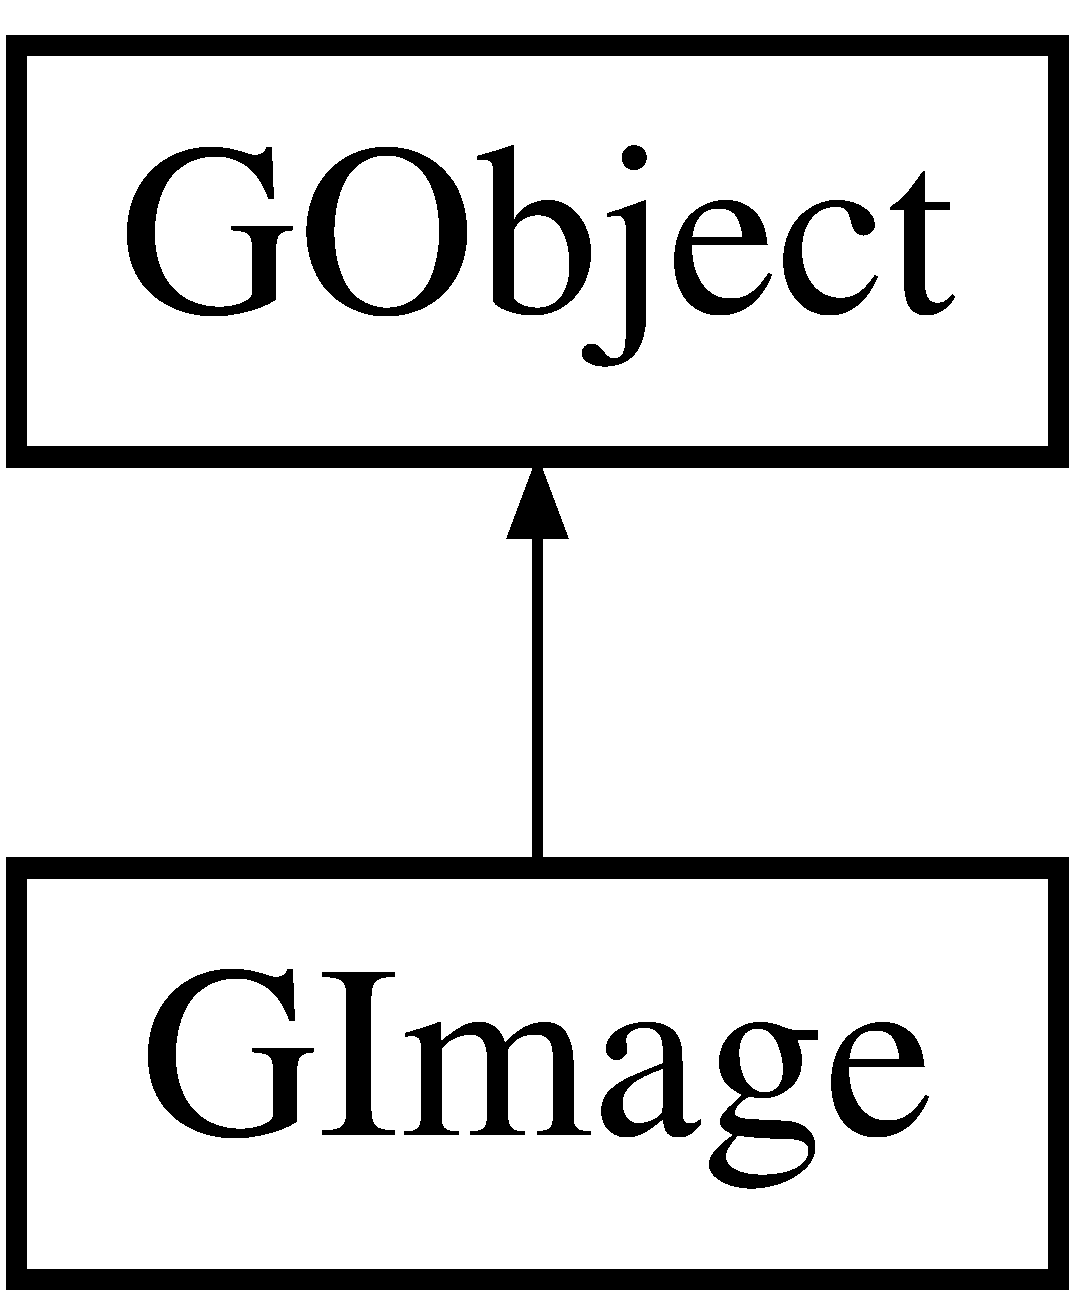
\includegraphics[height=2.000000cm]{classGImage}
\end{center}
\end{figure}
\subsection*{Public Types}
\begin{DoxyCompactItemize}
\item 
enum \mbox{\hyperlink{classGObject_a86e0f5648542856159bb40775c854aa7}{Line\+Style}} \{ \mbox{\hyperlink{classGObject_a86e0f5648542856159bb40775c854aa7acbc84bd5232621834ed31f44d457c1eb}{L\+I\+N\+E\+\_\+\+N\+O\+NE}}, 
\mbox{\hyperlink{classGObject_a86e0f5648542856159bb40775c854aa7a700c78bc2cd76acaab26651bf7b4941f}{L\+I\+N\+E\+\_\+\+S\+O\+L\+ID}}, 
\mbox{\hyperlink{classGObject_a86e0f5648542856159bb40775c854aa7a9ccba0845f785d81d07b333ae1aad84e}{L\+I\+N\+E\+\_\+\+D\+A\+SH}}, 
\mbox{\hyperlink{classGObject_a86e0f5648542856159bb40775c854aa7a8e811c096cb941997f0bfda168bb6df3}{L\+I\+N\+E\+\_\+\+D\+OT}}, 
\mbox{\hyperlink{classGObject_a86e0f5648542856159bb40775c854aa7ada15a2e3d737b2db7706d8300f91b89d}{L\+I\+N\+E\+\_\+\+D\+A\+S\+H\+\_\+\+D\+OT}}, 
\mbox{\hyperlink{classGObject_a86e0f5648542856159bb40775c854aa7aabf4053a73eafa7ba2b7e6d664c74c1d}{L\+I\+N\+E\+\_\+\+D\+A\+S\+H\+\_\+\+D\+O\+T\+\_\+\+D\+OT}}
 \}
\begin{DoxyCompactList}\small\item\em Styles that can be used for the outline around various shapes. \end{DoxyCompactList}\end{DoxyCompactItemize}
\subsection*{Public Member Functions}
\begin{DoxyCompactItemize}
\item 
\mbox{\hyperlink{classGImage_ae37cc9f566bd18108a4efed39c16e505}{G\+Image}} (const std\+::string \&filename=\char`\"{}\char`\"{}, double x=0, double y=0)
\begin{DoxyCompactList}\small\item\em Constructs a new image by loading the image from the specified file. \end{DoxyCompactList}\item 
\mbox{\hyperlink{classGImage_abbdf80157620710ca03d6ff2b869333d}{G\+Image}} (std\+::istream \&source, double x=0, double y=0)
\begin{DoxyCompactList}\small\item\em Constructs a new image by loading the image from the specified input stream. \end{DoxyCompactList}\item 
\mbox{\hyperlink{classGImage_ac106706c2a94c64f002934a273f8f4e7}{G\+Image}} (double width, double height)
\begin{DoxyCompactList}\small\item\em Creates a blank \mbox{\hyperlink{classGImage}{G\+Image}} of the given width and height. \end{DoxyCompactList}\item 
virtual \mbox{\hyperlink{classGImage_aff2de2de9e75e1d6bf56248c2fdcc615}{$\sim$\+G\+Image}} ()
\begin{DoxyCompactList}\small\item\em Frees memory allocated internally by the image. \end{DoxyCompactList}\item 
virtual bool \mbox{\hyperlink{classGObject_abb6a5d7c03e6eaaae97264c4799ce7c3}{contains}} (double x, double y) const
\begin{DoxyCompactList}\small\item\em Returns {\ttfamily true} if the specified point is inside the object. \end{DoxyCompactList}\item 
virtual bool \mbox{\hyperlink{classGObject_a1dbc9dafaae51958112dbe1267a1f547}{contains}} (const \mbox{\hyperlink{structGPoint}{G\+Point}} \&pt) const
\begin{DoxyCompactList}\small\item\em Returns {\ttfamily true} if the specified point is inside the object. \end{DoxyCompactList}\item 
virtual \mbox{\hyperlink{structGPoint}{G\+Point}} \mbox{\hyperlink{classGObject_a0d41183bf6b08de66fe3907551aab0d7}{get\+Bottom\+Right\+Location}} () const
\begin{DoxyCompactList}\small\item\em Returns the x/y coordinates of the bottom/right corner of the object. \end{DoxyCompactList}\item 
virtual double \mbox{\hyperlink{classGObject_a4316a2406c18e1c6d061fe51fd355490}{get\+BottomY}} () const
\begin{DoxyCompactList}\small\item\em Returns the {\itshape y}-\/coordinate of the bottom of the object. \end{DoxyCompactList}\item 
virtual \mbox{\hyperlink{structGRectangle}{G\+Rectangle}} \mbox{\hyperlink{classGObject_a29e6ac35a0b48f491a4c88194cc5da3b}{get\+Bounds}} () const
\begin{DoxyCompactList}\small\item\em Returns the bounding box of this object, which is defined to be the smallest rectangle that covers everything drawn by the figure. \end{DoxyCompactList}\item 
virtual \mbox{\hyperlink{structGPoint}{G\+Point}} \mbox{\hyperlink{classGObject_a0909472e91448470bccdb62ecfb95d8b}{get\+Center\+Location}} () const
\begin{DoxyCompactList}\small\item\em Returns the x/y-\/coordinates of the center of the object. \end{DoxyCompactList}\item 
virtual double \mbox{\hyperlink{classGObject_a04df74355b545e0543112d5b8d924176}{get\+CenterX}} () const
\begin{DoxyCompactList}\small\item\em Returns the {\itshape x}-\/coordinate of the center of the object. \end{DoxyCompactList}\item 
virtual double \mbox{\hyperlink{classGObject_acb3287a3d507025a26f54b895713b947}{get\+CenterY}} () const
\begin{DoxyCompactList}\small\item\em Returns the {\itshape y}-\/coordinate of the center of the object. \end{DoxyCompactList}\item 
virtual std\+::string \mbox{\hyperlink{classGObject_aa061dfa488c31e18549d64363c1d0e34}{get\+Color}} () const
\begin{DoxyCompactList}\small\item\em Returns the color used to display this object. \end{DoxyCompactList}\item 
virtual std\+::string \mbox{\hyperlink{classGImage_a57d497454eec3b9c53b0067e458e3a51}{get\+File\+Name}} () const
\begin{DoxyCompactList}\small\item\em Returns the file name used to load the image, as was passed to the constructor. \end{DoxyCompactList}\item 
virtual std\+::string \mbox{\hyperlink{classGObject_a76f6964a11fde7c78e9751be184e1a3c}{get\+Fill\+Color}} () const
\begin{DoxyCompactList}\small\item\em Returns the color used to display the filled region of this object. \end{DoxyCompactList}\item 
virtual double \mbox{\hyperlink{classGObject_a1e7e353362434072875264cf95629f99}{get\+Height}} () const
\begin{DoxyCompactList}\small\item\em Returns the height of this object, which is the same as the height of its bounding box. \end{DoxyCompactList}\item 
virtual \mbox{\hyperlink{classGObject_a86e0f5648542856159bb40775c854aa7}{Line\+Style}} \mbox{\hyperlink{classGObject_aaf1f5ea8281e5e3486662878d26f0a13}{get\+Line\+Style}} () const
\begin{DoxyCompactList}\small\item\em Returns the object\textquotesingle{}s style such as solid or dashed. \end{DoxyCompactList}\item 
virtual double \mbox{\hyperlink{classGObject_a85ff266dc3eb63d9f2d8e5a4487fd3c0}{get\+Line\+Width}} () const
\begin{DoxyCompactList}\small\item\em Returns the width of the line used to draw this object. \end{DoxyCompactList}\item 
virtual \mbox{\hyperlink{structGPoint}{G\+Point}} \mbox{\hyperlink{classGObject_a4f83802015511edeb63b892830812c11}{get\+Location}} () const
\begin{DoxyCompactList}\small\item\em Returns the location of the top-\/left corner of object. \end{DoxyCompactList}\item 
virtual double \mbox{\hyperlink{classGObject_a1ae3fc278cc5b71b9f2d96a8a83cdf26}{get\+Opacity}} () const
\begin{DoxyCompactList}\small\item\em Returns how opaque (non-\/transparent) this object will appear from 0.\+0 (completely transparent) to 1.\+0 (completely opaque, default). \end{DoxyCompactList}\item 
virtual \mbox{\hyperlink{classGCompound}{G\+Compound}} $\ast$ \mbox{\hyperlink{classGObject_a3e53cef70541b1a14eade4ad0984d0b4}{get\+Parent}} () const
\begin{DoxyCompactList}\small\item\em Returns a pointer to the {\ttfamily \mbox{\hyperlink{classGCompound}{G\+Compound}}} that contains this object. \end{DoxyCompactList}\item 
virtual int \mbox{\hyperlink{classGImage_aea1d2892c78b0ed846db7116cb6a7c2e}{get\+Pixel}} (int x, int y) const
\begin{DoxyCompactList}\small\item\em Returns the color of the pixel at the given x/y location as an R\+GB integer. \end{DoxyCompactList}\item 
virtual double \mbox{\hyperlink{classGObject_a798cc79daaa10145b28f60bcdfdb0ee9}{get\+RightX}} () const
\begin{DoxyCompactList}\small\item\em Returns the {\itshape x}-\/coordinate of the right side of the object. \end{DoxyCompactList}\item 
virtual \mbox{\hyperlink{structGDimension}{G\+Dimension}} \mbox{\hyperlink{classGObject_a7b4eec96a2bdc6420695d5796a78eea9}{get\+Size}} () const
\begin{DoxyCompactList}\small\item\em Returns the size of the object as a {\ttfamily \mbox{\hyperlink{structGDimension}{G\+Dimension}}}. \end{DoxyCompactList}\item 
std\+::string \mbox{\hyperlink{classGImage_a9b72ede4ee8520f987a0c01e30654814}{get\+Type}} () const override
\begin{DoxyCompactList}\small\item\em Returns the type of the object as a string, such as {\ttfamily \char`\"{}\+G\+Oval\char`\"{}} or {\ttfamily \char`\"{}\+G\+Rect\char`\"{}}. \end{DoxyCompactList}\item 
virtual double \mbox{\hyperlink{classGObject_a0ed2965abd4f5701d2cadf71239faf19}{get\+Width}} () const
\begin{DoxyCompactList}\small\item\em Returns the width of this object, which is equal to the width of the bounding box. \end{DoxyCompactList}\item 
virtual double \mbox{\hyperlink{classGObject_a344385751bee0720059403940d57a13e}{getX}} () const
\begin{DoxyCompactList}\small\item\em Returns the leftmost {\itshape x}-\/coordinate of the object. \end{DoxyCompactList}\item 
virtual double \mbox{\hyperlink{classGObject_aafa51c7f8f38a09febbb9ce7853f77b4}{getY}} () const
\begin{DoxyCompactList}\small\item\em Returns the topmost {\itshape y}-\/coordinate of the object. \end{DoxyCompactList}\item 
virtual bool \mbox{\hyperlink{classGObject_a11c404f106940c201b6f326e0355c150}{is\+Filled}} () const
\begin{DoxyCompactList}\small\item\em Returns {\ttfamily true} if the object is filled with color. \end{DoxyCompactList}\item 
virtual bool \mbox{\hyperlink{classGObject_a9de207581cfa4ca1eaa06da5f29b75fc}{is\+Transformed}} () const
\begin{DoxyCompactList}\small\item\em Returns {\ttfamily true} if this object has been transformed by calling methods such as \mbox{\hyperlink{classGObject_ae1ffaa12185dfd5ba464f7d87c329e26}{rotate()}} or \mbox{\hyperlink{classGObject_ad2e1900f730475c2d044817db03b38d6}{scale()}} on it. \end{DoxyCompactList}\item 
virtual bool \mbox{\hyperlink{classGObject_a9d8a6cfb13917785c143e74d40e4e2be}{is\+Visible}} () const
\begin{DoxyCompactList}\small\item\em Returns {\ttfamily true} if this object is visible on screen. \end{DoxyCompactList}\item 
virtual void \mbox{\hyperlink{classGObject_a5973d8dda83afb36e2c56855515be392}{move}} (double dx, double dy)
\begin{DoxyCompactList}\small\item\em Moves the object on the screen using the displacements {\ttfamily dx} and {\ttfamily dy}. \end{DoxyCompactList}\item 
virtual void \mbox{\hyperlink{classGObject_ac827b978aa122f136a14c198687ad80f}{repaint}} ()
\begin{DoxyCompactList}\small\item\em Instructs the object to redraw itself on screen. \end{DoxyCompactList}\item 
virtual void \mbox{\hyperlink{classGObject_a6022a1fd1e5dcd2fd5585e5a36aa3f37}{reset\+Transform}} ()
\begin{DoxyCompactList}\small\item\em Undoes any previous scale/rotate transformations on this object. \end{DoxyCompactList}\item 
virtual void \mbox{\hyperlink{classGObject_ae1ffaa12185dfd5ba464f7d87c329e26}{rotate}} (double theta)
\begin{DoxyCompactList}\small\item\em Transforms the object by rotating it {\ttfamily theta} degrees counterclockwise around its origin. \end{DoxyCompactList}\item 
virtual void \mbox{\hyperlink{classGObject_ad2e1900f730475c2d044817db03b38d6}{scale}} (double sf)
\begin{DoxyCompactList}\small\item\em Scales the object by the specified scale factor. \end{DoxyCompactList}\item 
virtual void \mbox{\hyperlink{classGObject_a63641f69d610d0b951357d35a0c3b1e3}{scale}} (double sx, double sy)
\begin{DoxyCompactList}\small\item\em Scales the object by the specified scale factors. \end{DoxyCompactList}\item 
void \mbox{\hyperlink{classGObject_ab6747f40313c531c2db32edb5b63b9b7}{send\+Backward}} ()
\begin{DoxyCompactList}\small\item\em Moves this object one step toward the back in the {\itshape z} dimension. \end{DoxyCompactList}\item 
void \mbox{\hyperlink{classGObject_a710b3e449c9facba7847c91ab170d281}{send\+Forward}} ()
\begin{DoxyCompactList}\small\item\em Moves this object one step toward the front in the {\itshape z} dimension. \end{DoxyCompactList}\item 
void \mbox{\hyperlink{classGObject_a0f7f1efbb7fd46dde2867c4ad0330896}{send\+To\+Back}} ()
\begin{DoxyCompactList}\small\item\em Moves this object to the back of the display in the {\itshape z} dimension. \end{DoxyCompactList}\item 
void \mbox{\hyperlink{classGObject_aee33d68488e46827ef55fac07f40a9b2}{send\+To\+Front}} ()
\begin{DoxyCompactList}\small\item\em Moves this object to the front of the display in the {\itshape z} dimension. \end{DoxyCompactList}\item 
virtual void \mbox{\hyperlink{classGObject_a71ff7b16b8f1bdc4a1ce9f30cf8b87d8}{set\+Bottom\+Right\+Location}} (double x, double y)
\begin{DoxyCompactList}\small\item\em Sets the location of the bottom/right of this object. \end{DoxyCompactList}\item 
virtual void \mbox{\hyperlink{classGObject_ac6f7320321182f1d18c1c0fa97d5e941}{set\+Bottom\+Right\+Location}} (const \mbox{\hyperlink{structGPoint}{G\+Point}} \&pt)
\begin{DoxyCompactList}\small\item\em Sets the location of the bottom/right of this object. \end{DoxyCompactList}\item 
virtual void \mbox{\hyperlink{classGObject_a4b20e93c2a2597484f74ee5caa71f41f}{set\+BottomY}} (double y)
\begin{DoxyCompactList}\small\item\em Sets the location of the bottom y-\/coordinate of this object. \end{DoxyCompactList}\item 
virtual void \mbox{\hyperlink{classGObject_a2aae8197624b72265ab83b4f1bc73f2f}{set\+Bounds}} (double x, double y, double width, double height)
\begin{DoxyCompactList}\small\item\em Changes the bounds of this object to the specified values. \end{DoxyCompactList}\item 
virtual void \mbox{\hyperlink{classGObject_acada386653f008cacc7cce86426bef7c}{set\+Bounds}} (const \mbox{\hyperlink{structGRectangle}{G\+Rectangle}} \&size)
\begin{DoxyCompactList}\small\item\em Changes the bounds of this object to the specified rectangle. \end{DoxyCompactList}\item 
virtual void \mbox{\hyperlink{classGObject_a290b47dd8de1be44089f95cb2c47c1de}{set\+Center\+Location}} (double x, double y)
\begin{DoxyCompactList}\small\item\em Sets the location of the center of this object. \end{DoxyCompactList}\item 
virtual void \mbox{\hyperlink{classGObject_a1bedf1b233ecba3f753ec58908a683a6}{set\+Center\+Location}} (const \mbox{\hyperlink{structGPoint}{G\+Point}} \&pt)
\begin{DoxyCompactList}\small\item\em Sets the location of the center of this object. \end{DoxyCompactList}\item 
virtual void \mbox{\hyperlink{classGObject_a2f4936281e056eead00a9186b9ba8af6}{set\+CenterX}} (double x)
\begin{DoxyCompactList}\small\item\em Sets the x-\/coordinate of the center of this object. \end{DoxyCompactList}\item 
virtual void \mbox{\hyperlink{classGObject_aad2a22b4fde88c33306b92aebf641d57}{set\+CenterY}} (double y)
\begin{DoxyCompactList}\small\item\em Sets the y-\/coordinate of the center of this object. \end{DoxyCompactList}\item 
virtual void \mbox{\hyperlink{classGObject_ad57ef49bc31db94e92648aa3737923d6}{set\+Color}} (int r, int g, int b)
\begin{DoxyCompactList}\small\item\em Sets the color used to display this object. \end{DoxyCompactList}\item 
virtual void \mbox{\hyperlink{classGObject_ab1f5cc0f5cc6bbbd716a526c61f1081d}{set\+Color}} (int rgb)
\begin{DoxyCompactList}\small\item\em Sets the color used to display this object. \end{DoxyCompactList}\item 
virtual void \mbox{\hyperlink{classGObject_a61374df6c11b52cfbb0815decdbaebc6}{set\+Color}} (const std\+::string \&color)
\begin{DoxyCompactList}\small\item\em Sets the color used to display this object. \end{DoxyCompactList}\item 
virtual void \mbox{\hyperlink{classGObject_ad767a33971159e9493e221cca4c00ae9}{set\+Fill\+Color}} (int r, int g, int b)
\begin{DoxyCompactList}\small\item\em Sets the color used to display the filled region of this object, if any. \end{DoxyCompactList}\item 
virtual void \mbox{\hyperlink{classGObject_aa59d9775a67fa7df2b24a95cd34840a3}{set\+Fill\+Color}} (int rgb)
\begin{DoxyCompactList}\small\item\em Sets the color used to display the filled region of this object, if any. \end{DoxyCompactList}\item 
virtual void \mbox{\hyperlink{classGObject_adbc18b1a930aadd97d7437f9f7265b96}{set\+Fill\+Color}} (const std\+::string \&color)
\begin{DoxyCompactList}\small\item\em Sets the color used to display the filled region of this object, if any. \end{DoxyCompactList}\item 
virtual void \mbox{\hyperlink{classGObject_a9b82b53362282c6bb7d6947068d2e55b}{set\+Filled}} (bool flag)
\begin{DoxyCompactList}\small\item\em Sets the fill status for the object, where {\ttfamily false} is outlined and {\ttfamily true} is filled. \end{DoxyCompactList}\item 
virtual void \mbox{\hyperlink{classGObject_a2592348886ffea646c6534bf88f7c49d}{set\+Font}} (const Q\+Font \&font)
\begin{DoxyCompactList}\small\item\em Changes the font used to display the object as specified by the given Qt font. \end{DoxyCompactList}\item 
virtual void \mbox{\hyperlink{classGObject_a8e096e8818d838aceae1d46d58fb3a7b}{set\+Font}} (const std\+::string \&font)
\begin{DoxyCompactList}\small\item\em Changes the font used to display the object as specified by the string {\ttfamily font}, which has the following format\+: \end{DoxyCompactList}\item 
virtual void \mbox{\hyperlink{classGObject_ad18e8fab1e02a4e9b75c6730212558eb}{set\+Foreground}} (int r, int g, int b)
\begin{DoxyCompactList}\small\item\em Sets the color used to display this object. \end{DoxyCompactList}\item 
virtual void \mbox{\hyperlink{classGObject_a9eb856b5ff83a19df3831a31f15f4563}{set\+Foreground}} (int rgb)
\begin{DoxyCompactList}\small\item\em Sets the color used to display this object. \end{DoxyCompactList}\item 
virtual void \mbox{\hyperlink{classGObject_af59209aeadea6dfc6d97a2d8531f50e1}{set\+Foreground}} (const std\+::string \&color)
\begin{DoxyCompactList}\small\item\em Sets the color used to display this object. \end{DoxyCompactList}\item 
virtual void \mbox{\hyperlink{classGObject_a9e280bfc4544dfaf8e4376c4e1a74357}{set\+Height}} (double height)
\begin{DoxyCompactList}\small\item\em Changes the height of this object to the specified height without changing its width. \end{DoxyCompactList}\item 
virtual void \mbox{\hyperlink{classGObject_add11575087eb94f1a71faa3f826c6341}{set\+Line\+Style}} (\mbox{\hyperlink{classGObject_a86e0f5648542856159bb40775c854aa7}{Line\+Style}} line\+Style)
\begin{DoxyCompactList}\small\item\em Sets the object\textquotesingle{}s style such as solid (\mbox{\hyperlink{classGObject_a86e0f5648542856159bb40775c854aa7a700c78bc2cd76acaab26651bf7b4941f}{G\+Object\+::\+L\+I\+N\+E\+\_\+\+S\+O\+L\+ID}}) or dashed (\mbox{\hyperlink{classGObject_a86e0f5648542856159bb40775c854aa7a9ccba0845f785d81d07b333ae1aad84e}{G\+Object\+::\+L\+I\+N\+E\+\_\+\+D\+A\+SH}}). \end{DoxyCompactList}\item 
virtual void \mbox{\hyperlink{classGObject_afd6a47c6ea6a1f85ca05a65ba3ff3477}{set\+Line\+Width}} (double line\+Width)
\begin{DoxyCompactList}\small\item\em Sets the width of the line used to draw this object. \end{DoxyCompactList}\item 
virtual void \mbox{\hyperlink{classGObject_a04594e8ba9b98513a64f1da00dcae18c}{set\+Location}} (double x, double y)
\begin{DoxyCompactList}\small\item\em Sets the location of the top-\/left corner of this object to the specified coordinates. \end{DoxyCompactList}\item 
virtual void \mbox{\hyperlink{classGObject_aa8480c0b7166cdf8f784cece06ab353f}{set\+Location}} (const \mbox{\hyperlink{structGPoint}{G\+Point}} \&pt)
\begin{DoxyCompactList}\small\item\em Sets the location of the top-\/left corner of this object to the specified point. \end{DoxyCompactList}\item 
virtual void \mbox{\hyperlink{classGObject_a04af1866cc1bae4a1226695794a50539}{set\+Opacity}} (double opacity)
\begin{DoxyCompactList}\small\item\em Sets how opaque (non-\/transparent) this object will appear from 0.\+0 (completely transparent) to 1.\+0 (completely opaque, default). \end{DoxyCompactList}\item 
virtual void \mbox{\hyperlink{classGImage_a555e64433357e4e01b523498814b8e74}{set\+Pixel}} (int x, int y, int rgb)
\begin{DoxyCompactList}\small\item\em Sets the pixel at the given x/y location to the given color, represented as an R\+GB integer. \end{DoxyCompactList}\item 
virtual void \mbox{\hyperlink{classGObject_a3c90b758cdc2c911c9ef76c4360eb912}{set\+RightX}} (double x)
\begin{DoxyCompactList}\small\item\em Sets the location of the rightmost x-\/coordinate of this object. \end{DoxyCompactList}\item 
virtual void \mbox{\hyperlink{classGObject_aca25d49481f9bf5fc8f7df4c086c4ce7}{set\+Size}} (double width, double height)
\begin{DoxyCompactList}\small\item\em Changes the size of this object to the specified width and height. \end{DoxyCompactList}\item 
virtual void \mbox{\hyperlink{classGObject_ae2b628228f192c2702c4ce941b2af68f}{set\+Size}} (const \mbox{\hyperlink{structGDimension}{G\+Dimension}} \&size)
\begin{DoxyCompactList}\small\item\em Changes the size of this object to the specified width and height. \end{DoxyCompactList}\item 
virtual void \mbox{\hyperlink{classGObject_a88203f28224315d9f4471212f4af8ed3}{set\+Visible}} (bool flag)
\begin{DoxyCompactList}\small\item\em Sets whether this object is visible. \end{DoxyCompactList}\item 
virtual void \mbox{\hyperlink{classGObject_aa3f3fba4cb131baa8696ba01e3bceca1}{set\+Width}} (double width)
\begin{DoxyCompactList}\small\item\em Changes the width of this object to the specified width without changing its height. \end{DoxyCompactList}\item 
virtual void \mbox{\hyperlink{classGObject_a9c18fcc579333bf9653d13ad2b372e39}{setX}} (double x)
\begin{DoxyCompactList}\small\item\em Sets the x location of the left side of this object. \end{DoxyCompactList}\item 
virtual void \mbox{\hyperlink{classGObject_a7d57e2a5c35d27feb58fd498a3cf82b9}{setY}} (double y)
\begin{DoxyCompactList}\small\item\em Sets the y location of the top of this object. \end{DoxyCompactList}\item 
virtual std\+::string \mbox{\hyperlink{classGObject_a1fe5121d6528fdea3f243321b3fa3a49}{to\+String}} () const
\begin{DoxyCompactList}\small\item\em Returns a printable representation of the object. \end{DoxyCompactList}\item 
std\+::string \mbox{\hyperlink{classGImage_a04364e674911906702b748deec32db18}{to\+String\+Extra}} () const override
\begin{DoxyCompactList}\small\item\em Returns a string containing any extra unique information about this type of graphical object. \end{DoxyCompactList}\end{DoxyCompactItemize}
\subsection*{Static Public Member Functions}
\begin{DoxyCompactItemize}
\item 
static bool \mbox{\hyperlink{classGObject_a93be0e1fe1b1bf1a1da732470c94f42b}{is\+Anti\+Aliasing}} ()
\begin{DoxyCompactList}\small\item\em Returns whether we should globally anti-\/alias graphical objects. \end{DoxyCompactList}\item 
static void \mbox{\hyperlink{classGObject_a1e43371668ae850193cebedb44e1bbe3}{set\+Anti\+Aliasing}} (bool value)
\begin{DoxyCompactList}\small\item\em Globally turns on/off the anti-\/aliasing feature that smooths out the edges of onscreen shapes. \end{DoxyCompactList}\end{DoxyCompactItemize}
\subsection*{Protected Member Functions}
\begin{DoxyCompactItemize}
\item 
\mbox{\hyperlink{classGImage_a3444f37769d2b073dacd164dc2a1f45a}{G\+Image}} (Q\+Image $\ast$qimage)
\begin{DoxyCompactList}\small\item\em Creates a \mbox{\hyperlink{classGImage}{G\+Image}} wrapping the given Qt image. \end{DoxyCompactList}\item 
Q\+Image $\ast$ \mbox{\hyperlink{classGImage_a76db6f6e4009671e2809ad8b26567aec}{get\+Q\+Image}} () const
\begin{DoxyCompactList}\small\item\em Returns the inner Qt Q\+Image object being wrapped. \end{DoxyCompactList}\end{DoxyCompactItemize}
\subsection*{Protected Attributes}
\begin{DoxyCompactItemize}
\item 
Q\+Brush \mbox{\hyperlink{classGObject_aab24462ec896b596d99911767b0912d0}{\+\_\+brush}}
\item 
std\+::string \mbox{\hyperlink{classGObject_a1134e770ae4315ea8bc1201e2f21da8b}{\+\_\+color}}
\item 
int \mbox{\hyperlink{classGObject_a003fdd343d9b7505c53a8b7a134200ed}{\+\_\+color\+Int}}
\item 
std\+::string \mbox{\hyperlink{classGObject_a179f8d6cee65cd8a54692e32b224392a}{\+\_\+fill\+Color}}
\item 
int \mbox{\hyperlink{classGObject_a751def333a67d651e5b99cc331ecb496}{\+\_\+fill\+Color\+Int}}
\item 
bool \mbox{\hyperlink{classGObject_ad4a55cbcd61b58a4d49666490bb2f103}{\+\_\+fill\+Flag}}
\item 
std\+::string \mbox{\hyperlink{classGObject_aea76ea1a8b5dd7b0a78653277e63b536}{\+\_\+font}}
\item 
double \mbox{\hyperlink{classGObject_ad05df29e7f27fc504abd743e3d8b4e73}{\+\_\+height}}
\item 
\mbox{\hyperlink{classGObject_a86e0f5648542856159bb40775c854aa7}{Line\+Style}} \mbox{\hyperlink{classGObject_a89bafecaafb7c72d55c7efc10b7d0523}{\+\_\+line\+Style}}
\item 
double \mbox{\hyperlink{classGObject_a16e9033665937f13de2e163dc2184aff}{\+\_\+line\+Width}}
\item 
double \mbox{\hyperlink{classGObject_a20eff8eb7af27182edc9bfc54768b6f3}{\+\_\+opacity}}
\item 
\mbox{\hyperlink{classGCompound}{G\+Compound}} $\ast$ \mbox{\hyperlink{classGObject_ac9452c1eaff70eebddbb318196aa3835}{\+\_\+parent}}
\item 
Q\+Pen \mbox{\hyperlink{classGObject_afb69d172743f868299847174eb1b6bc8}{\+\_\+pen}}
\item 
Q\+Transform \mbox{\hyperlink{classGObject_a475b8860a5f1adb4a1fdc58d1f5c1e32}{\+\_\+transform}}
\item 
bool \mbox{\hyperlink{classGObject_ae4725802fc8d8aaa0ab4bd4781f7e07c}{\+\_\+transformed}}
\item 
bool \mbox{\hyperlink{classGObject_a9312c72508471b7c7a87b540263e1af4}{\+\_\+visible}}
\item 
double \mbox{\hyperlink{classGObject_ab55d85a3371770e6725b1062cf160cd8}{\+\_\+width}}
\item 
double \mbox{\hyperlink{classGObject_a6675b83b27137b8d3aa2ad8133078ea6}{\+\_\+x}}
\item 
double \mbox{\hyperlink{classGObject_a2f0f6aeafddc8a39c578bfa7e22b5f1e}{\+\_\+y}}
\end{DoxyCompactItemize}


\subsection{Detailed Description}
This graphical object subclass represents an image from a file. 

\subsection{Member Enumeration Documentation}
\mbox{\Hypertarget{classGObject_a86e0f5648542856159bb40775c854aa7}\label{classGObject_a86e0f5648542856159bb40775c854aa7}} 
\index{G\+Image@{G\+Image}!Line\+Style@{Line\+Style}}
\index{Line\+Style@{Line\+Style}!G\+Image@{G\+Image}}
\subsubsection{\texorpdfstring{Line\+Style}{LineStyle}}
{\footnotesize\ttfamily enum \mbox{\hyperlink{classGObject_a86e0f5648542856159bb40775c854aa7}{Line\+Style}}\hspace{0.3cm}{\ttfamily [inherited]}}



Styles that can be used for the outline around various shapes. 

Call set\+Line\+Style on a \mbox{\hyperlink{classGObject}{G\+Object}} and pass one of these values. \begin{DoxyEnumFields}{Enumerator}
\raisebox{\heightof{T}}[0pt][0pt]{\index{L\+I\+N\+E\+\_\+\+N\+O\+NE@{L\+I\+N\+E\+\_\+\+N\+O\+NE}!G\+Image@{G\+Image}}\index{G\+Image@{G\+Image}!L\+I\+N\+E\+\_\+\+N\+O\+NE@{L\+I\+N\+E\+\_\+\+N\+O\+NE}}}\mbox{\Hypertarget{classGObject_a86e0f5648542856159bb40775c854aa7acbc84bd5232621834ed31f44d457c1eb}\label{classGObject_a86e0f5648542856159bb40775c854aa7acbc84bd5232621834ed31f44d457c1eb}} 
L\+I\+N\+E\+\_\+\+N\+O\+NE&\\
\hline

\raisebox{\heightof{T}}[0pt][0pt]{\index{L\+I\+N\+E\+\_\+\+S\+O\+L\+ID@{L\+I\+N\+E\+\_\+\+S\+O\+L\+ID}!G\+Image@{G\+Image}}\index{G\+Image@{G\+Image}!L\+I\+N\+E\+\_\+\+S\+O\+L\+ID@{L\+I\+N\+E\+\_\+\+S\+O\+L\+ID}}}\mbox{\Hypertarget{classGObject_a86e0f5648542856159bb40775c854aa7a700c78bc2cd76acaab26651bf7b4941f}\label{classGObject_a86e0f5648542856159bb40775c854aa7a700c78bc2cd76acaab26651bf7b4941f}} 
L\+I\+N\+E\+\_\+\+S\+O\+L\+ID&\\
\hline

\raisebox{\heightof{T}}[0pt][0pt]{\index{L\+I\+N\+E\+\_\+\+D\+A\+SH@{L\+I\+N\+E\+\_\+\+D\+A\+SH}!G\+Image@{G\+Image}}\index{G\+Image@{G\+Image}!L\+I\+N\+E\+\_\+\+D\+A\+SH@{L\+I\+N\+E\+\_\+\+D\+A\+SH}}}\mbox{\Hypertarget{classGObject_a86e0f5648542856159bb40775c854aa7a9ccba0845f785d81d07b333ae1aad84e}\label{classGObject_a86e0f5648542856159bb40775c854aa7a9ccba0845f785d81d07b333ae1aad84e}} 
L\+I\+N\+E\+\_\+\+D\+A\+SH&\\
\hline

\raisebox{\heightof{T}}[0pt][0pt]{\index{L\+I\+N\+E\+\_\+\+D\+OT@{L\+I\+N\+E\+\_\+\+D\+OT}!G\+Image@{G\+Image}}\index{G\+Image@{G\+Image}!L\+I\+N\+E\+\_\+\+D\+OT@{L\+I\+N\+E\+\_\+\+D\+OT}}}\mbox{\Hypertarget{classGObject_a86e0f5648542856159bb40775c854aa7a8e811c096cb941997f0bfda168bb6df3}\label{classGObject_a86e0f5648542856159bb40775c854aa7a8e811c096cb941997f0bfda168bb6df3}} 
L\+I\+N\+E\+\_\+\+D\+OT&\\
\hline

\raisebox{\heightof{T}}[0pt][0pt]{\index{L\+I\+N\+E\+\_\+\+D\+A\+S\+H\+\_\+\+D\+OT@{L\+I\+N\+E\+\_\+\+D\+A\+S\+H\+\_\+\+D\+OT}!G\+Image@{G\+Image}}\index{G\+Image@{G\+Image}!L\+I\+N\+E\+\_\+\+D\+A\+S\+H\+\_\+\+D\+OT@{L\+I\+N\+E\+\_\+\+D\+A\+S\+H\+\_\+\+D\+OT}}}\mbox{\Hypertarget{classGObject_a86e0f5648542856159bb40775c854aa7ada15a2e3d737b2db7706d8300f91b89d}\label{classGObject_a86e0f5648542856159bb40775c854aa7ada15a2e3d737b2db7706d8300f91b89d}} 
L\+I\+N\+E\+\_\+\+D\+A\+S\+H\+\_\+\+D\+OT&\\
\hline

\raisebox{\heightof{T}}[0pt][0pt]{\index{L\+I\+N\+E\+\_\+\+D\+A\+S\+H\+\_\+\+D\+O\+T\+\_\+\+D\+OT@{L\+I\+N\+E\+\_\+\+D\+A\+S\+H\+\_\+\+D\+O\+T\+\_\+\+D\+OT}!G\+Image@{G\+Image}}\index{G\+Image@{G\+Image}!L\+I\+N\+E\+\_\+\+D\+A\+S\+H\+\_\+\+D\+O\+T\+\_\+\+D\+OT@{L\+I\+N\+E\+\_\+\+D\+A\+S\+H\+\_\+\+D\+O\+T\+\_\+\+D\+OT}}}\mbox{\Hypertarget{classGObject_a86e0f5648542856159bb40775c854aa7aabf4053a73eafa7ba2b7e6d664c74c1d}\label{classGObject_a86e0f5648542856159bb40775c854aa7aabf4053a73eafa7ba2b7e6d664c74c1d}} 
L\+I\+N\+E\+\_\+\+D\+A\+S\+H\+\_\+\+D\+O\+T\+\_\+\+D\+OT&\\
\hline

\end{DoxyEnumFields}


\subsection{Constructor \& Destructor Documentation}
\mbox{\Hypertarget{classGImage_ae37cc9f566bd18108a4efed39c16e505}\label{classGImage_ae37cc9f566bd18108a4efed39c16e505}} 
\index{G\+Image@{G\+Image}!G\+Image@{G\+Image}}
\index{G\+Image@{G\+Image}!G\+Image@{G\+Image}}
\subsubsection{\texorpdfstring{G\+Image()}{GImage()}\hspace{0.1cm}{\footnotesize\ttfamily [1/4]}}
{\footnotesize\ttfamily \mbox{\hyperlink{classGImage}{G\+Image}} (\begin{DoxyParamCaption}\item[{const std\+::string \&}]{filename = {\ttfamily \char`\"{}\char`\"{}},  }\item[{double}]{x = {\ttfamily 0},  }\item[{double}]{y = {\ttfamily 0} }\end{DoxyParamCaption})}



Constructs a new image by loading the image from the specified file. 

By default, the upper left corner of the image appears at the origin, but you can pass coordinates to move it to the point ({\ttfamily x}, {\ttfamily y}). 
\begin{DoxyExceptions}{Exceptions}
{\em Error\+Exception} & if the given file is not found or cannot be loaded as a valid image file \\
\hline
\end{DoxyExceptions}
\mbox{\Hypertarget{classGImage_abbdf80157620710ca03d6ff2b869333d}\label{classGImage_abbdf80157620710ca03d6ff2b869333d}} 
\index{G\+Image@{G\+Image}!G\+Image@{G\+Image}}
\index{G\+Image@{G\+Image}!G\+Image@{G\+Image}}
\subsubsection{\texorpdfstring{G\+Image()}{GImage()}\hspace{0.1cm}{\footnotesize\ttfamily [2/4]}}
{\footnotesize\ttfamily \mbox{\hyperlink{classGImage}{G\+Image}} (\begin{DoxyParamCaption}\item[{std\+::istream \&}]{source,  }\item[{double}]{x = {\ttfamily 0},  }\item[{double}]{y = {\ttfamily 0} }\end{DoxyParamCaption})}



Constructs a new image by loading the image from the specified input stream. 

By default, the upper left corner of the image appears at the origin, but you can pass coordinates to move it to the point ({\ttfamily x}, {\ttfamily y}). 
\begin{DoxyExceptions}{Exceptions}
{\em Error\+Exception} & if the given file is not found or cannot be loaded as a valid image file \\
\hline
\end{DoxyExceptions}
\mbox{\Hypertarget{classGImage_ac106706c2a94c64f002934a273f8f4e7}\label{classGImage_ac106706c2a94c64f002934a273f8f4e7}} 
\index{G\+Image@{G\+Image}!G\+Image@{G\+Image}}
\index{G\+Image@{G\+Image}!G\+Image@{G\+Image}}
\subsubsection{\texorpdfstring{G\+Image()}{GImage()}\hspace{0.1cm}{\footnotesize\ttfamily [3/4]}}
{\footnotesize\ttfamily \mbox{\hyperlink{classGImage}{G\+Image}} (\begin{DoxyParamCaption}\item[{double}]{width,  }\item[{double}]{height }\end{DoxyParamCaption})}



Creates a blank \mbox{\hyperlink{classGImage}{G\+Image}} of the given width and height. 

Called by \mbox{\hyperlink{classGCanvas}{G\+Canvas}} when converting to an image. \mbox{\Hypertarget{classGImage_aff2de2de9e75e1d6bf56248c2fdcc615}\label{classGImage_aff2de2de9e75e1d6bf56248c2fdcc615}} 
\index{G\+Image@{G\+Image}!````~G\+Image@{$\sim$\+G\+Image}}
\index{````~G\+Image@{$\sim$\+G\+Image}!G\+Image@{G\+Image}}
\subsubsection{\texorpdfstring{$\sim$\+G\+Image()}{~GImage()}}
{\footnotesize\ttfamily $\sim$\mbox{\hyperlink{classGImage}{G\+Image}} (\begin{DoxyParamCaption}{ }\end{DoxyParamCaption})\hspace{0.3cm}{\ttfamily [virtual]}}



Frees memory allocated internally by the image. 

\mbox{\Hypertarget{classGImage_a3444f37769d2b073dacd164dc2a1f45a}\label{classGImage_a3444f37769d2b073dacd164dc2a1f45a}} 
\index{G\+Image@{G\+Image}!G\+Image@{G\+Image}}
\index{G\+Image@{G\+Image}!G\+Image@{G\+Image}}
\subsubsection{\texorpdfstring{G\+Image()}{GImage()}\hspace{0.1cm}{\footnotesize\ttfamily [4/4]}}
{\footnotesize\ttfamily \mbox{\hyperlink{classGImage}{G\+Image}} (\begin{DoxyParamCaption}\item[{Q\+Image $\ast$}]{qimage }\end{DoxyParamCaption})\hspace{0.3cm}{\ttfamily [protected]}}



Creates a \mbox{\hyperlink{classGImage}{G\+Image}} wrapping the given Qt image. 

Called by \mbox{\hyperlink{classGCanvas}{G\+Canvas}} when converting canvas to an image. 

\subsection{Member Function Documentation}
\mbox{\Hypertarget{classGObject_abb6a5d7c03e6eaaae97264c4799ce7c3}\label{classGObject_abb6a5d7c03e6eaaae97264c4799ce7c3}} 
\index{G\+Image@{G\+Image}!contains@{contains}}
\index{contains@{contains}!G\+Image@{G\+Image}}
\subsubsection{\texorpdfstring{contains()}{contains()}\hspace{0.1cm}{\footnotesize\ttfamily [1/2]}}
{\footnotesize\ttfamily bool contains (\begin{DoxyParamCaption}\item[{double}]{x,  }\item[{double}]{y }\end{DoxyParamCaption}) const\hspace{0.3cm}{\ttfamily [virtual]}, {\ttfamily [inherited]}}



Returns {\ttfamily true} if the specified point is inside the object. 



Reimplemented in \mbox{\hyperlink{classGRoundRect_ad973a1d55799d3a73bf8b04986cd804e}{G\+Round\+Rect}}, \mbox{\hyperlink{classGPolygon_ad973a1d55799d3a73bf8b04986cd804e}{G\+Polygon}}, \mbox{\hyperlink{classGOval_ad973a1d55799d3a73bf8b04986cd804e}{G\+Oval}}, \mbox{\hyperlink{classGLine_ad973a1d55799d3a73bf8b04986cd804e}{G\+Line}}, \mbox{\hyperlink{classGCompound_ad973a1d55799d3a73bf8b04986cd804e}{G\+Compound}}, and \mbox{\hyperlink{classGArc_ad973a1d55799d3a73bf8b04986cd804e}{G\+Arc}}.

\mbox{\Hypertarget{classGObject_a1dbc9dafaae51958112dbe1267a1f547}\label{classGObject_a1dbc9dafaae51958112dbe1267a1f547}} 
\index{G\+Image@{G\+Image}!contains@{contains}}
\index{contains@{contains}!G\+Image@{G\+Image}}
\subsubsection{\texorpdfstring{contains()}{contains()}\hspace{0.1cm}{\footnotesize\ttfamily [2/2]}}
{\footnotesize\ttfamily bool contains (\begin{DoxyParamCaption}\item[{const \mbox{\hyperlink{structGPoint}{G\+Point}} \&}]{pt }\end{DoxyParamCaption}) const\hspace{0.3cm}{\ttfamily [virtual]}, {\ttfamily [inherited]}}



Returns {\ttfamily true} if the specified point is inside the object. 

\mbox{\Hypertarget{classGObject_a0d41183bf6b08de66fe3907551aab0d7}\label{classGObject_a0d41183bf6b08de66fe3907551aab0d7}} 
\index{G\+Image@{G\+Image}!get\+Bottom\+Right\+Location@{get\+Bottom\+Right\+Location}}
\index{get\+Bottom\+Right\+Location@{get\+Bottom\+Right\+Location}!G\+Image@{G\+Image}}
\subsubsection{\texorpdfstring{get\+Bottom\+Right\+Location()}{getBottomRightLocation()}}
{\footnotesize\ttfamily \mbox{\hyperlink{structGPoint}{G\+Point}} get\+Bottom\+Right\+Location (\begin{DoxyParamCaption}{ }\end{DoxyParamCaption}) const\hspace{0.3cm}{\ttfamily [virtual]}, {\ttfamily [inherited]}}



Returns the x/y coordinates of the bottom/right corner of the object. 

\mbox{\Hypertarget{classGObject_a4316a2406c18e1c6d061fe51fd355490}\label{classGObject_a4316a2406c18e1c6d061fe51fd355490}} 
\index{G\+Image@{G\+Image}!get\+BottomY@{get\+BottomY}}
\index{get\+BottomY@{get\+BottomY}!G\+Image@{G\+Image}}
\subsubsection{\texorpdfstring{get\+Bottom\+Y()}{getBottomY()}}
{\footnotesize\ttfamily double get\+BottomY (\begin{DoxyParamCaption}{ }\end{DoxyParamCaption}) const\hspace{0.3cm}{\ttfamily [virtual]}, {\ttfamily [inherited]}}



Returns the {\itshape y}-\/coordinate of the bottom of the object. 

Equivalent to the top y-\/coordinate plus the object\textquotesingle{}s height. \mbox{\Hypertarget{classGObject_a29e6ac35a0b48f491a4c88194cc5da3b}\label{classGObject_a29e6ac35a0b48f491a4c88194cc5da3b}} 
\index{G\+Image@{G\+Image}!get\+Bounds@{get\+Bounds}}
\index{get\+Bounds@{get\+Bounds}!G\+Image@{G\+Image}}
\subsubsection{\texorpdfstring{get\+Bounds()}{getBounds()}}
{\footnotesize\ttfamily \mbox{\hyperlink{structGRectangle}{G\+Rectangle}} get\+Bounds (\begin{DoxyParamCaption}{ }\end{DoxyParamCaption}) const\hspace{0.3cm}{\ttfamily [virtual]}, {\ttfamily [inherited]}}



Returns the bounding box of this object, which is defined to be the smallest rectangle that covers everything drawn by the figure. 

The coordinates of this rectangle do not necessarily match the location returned by {\ttfamily get\+Location}. Given a {\ttfamily \mbox{\hyperlink{classGText}{G\+Text}}} object, for example, {\ttfamily get\+Location} returns the coordinates of the point on the baseline at which the string begins; the {\ttfamily get\+Bounds} method, by contrast, returns a rectangle that covers the entire window area occupied by the string. 

Reimplemented in \mbox{\hyperlink{classGText_a89040ce9277825772d359fccd33bca86}{G\+Text}}, \mbox{\hyperlink{classGPolygon_a89040ce9277825772d359fccd33bca86}{G\+Polygon}}, \mbox{\hyperlink{classGLine_a89040ce9277825772d359fccd33bca86}{G\+Line}}, \mbox{\hyperlink{classGCompound_a89040ce9277825772d359fccd33bca86}{G\+Compound}}, and \mbox{\hyperlink{classGArc_a89040ce9277825772d359fccd33bca86}{G\+Arc}}.

\mbox{\Hypertarget{classGObject_a0909472e91448470bccdb62ecfb95d8b}\label{classGObject_a0909472e91448470bccdb62ecfb95d8b}} 
\index{G\+Image@{G\+Image}!get\+Center\+Location@{get\+Center\+Location}}
\index{get\+Center\+Location@{get\+Center\+Location}!G\+Image@{G\+Image}}
\subsubsection{\texorpdfstring{get\+Center\+Location()}{getCenterLocation()}}
{\footnotesize\ttfamily \mbox{\hyperlink{structGPoint}{G\+Point}} get\+Center\+Location (\begin{DoxyParamCaption}{ }\end{DoxyParamCaption}) const\hspace{0.3cm}{\ttfamily [virtual]}, {\ttfamily [inherited]}}



Returns the x/y-\/coordinates of the center of the object. 

Equivalent to the top/left plus half the object\textquotesingle{}s size. \mbox{\Hypertarget{classGObject_a04df74355b545e0543112d5b8d924176}\label{classGObject_a04df74355b545e0543112d5b8d924176}} 
\index{G\+Image@{G\+Image}!get\+CenterX@{get\+CenterX}}
\index{get\+CenterX@{get\+CenterX}!G\+Image@{G\+Image}}
\subsubsection{\texorpdfstring{get\+Center\+X()}{getCenterX()}}
{\footnotesize\ttfamily double get\+CenterX (\begin{DoxyParamCaption}{ }\end{DoxyParamCaption}) const\hspace{0.3cm}{\ttfamily [virtual]}, {\ttfamily [inherited]}}



Returns the {\itshape x}-\/coordinate of the center of the object. 

Equivalent to the top/left plus half the object\textquotesingle{}s width. \mbox{\Hypertarget{classGObject_acb3287a3d507025a26f54b895713b947}\label{classGObject_acb3287a3d507025a26f54b895713b947}} 
\index{G\+Image@{G\+Image}!get\+CenterY@{get\+CenterY}}
\index{get\+CenterY@{get\+CenterY}!G\+Image@{G\+Image}}
\subsubsection{\texorpdfstring{get\+Center\+Y()}{getCenterY()}}
{\footnotesize\ttfamily double get\+CenterY (\begin{DoxyParamCaption}{ }\end{DoxyParamCaption}) const\hspace{0.3cm}{\ttfamily [virtual]}, {\ttfamily [inherited]}}



Returns the {\itshape y}-\/coordinate of the center of the object. 

Equivalent to the top/left plus half the object\textquotesingle{}s height. \mbox{\Hypertarget{classGObject_aa061dfa488c31e18549d64363c1d0e34}\label{classGObject_aa061dfa488c31e18549d64363c1d0e34}} 
\index{G\+Image@{G\+Image}!get\+Color@{get\+Color}}
\index{get\+Color@{get\+Color}!G\+Image@{G\+Image}}
\subsubsection{\texorpdfstring{get\+Color()}{getColor()}}
{\footnotesize\ttfamily std\+::string get\+Color (\begin{DoxyParamCaption}{ }\end{DoxyParamCaption}) const\hspace{0.3cm}{\ttfamily [virtual]}, {\ttfamily [inherited]}}



Returns the color used to display this object. 

This color is always returned as a string in the form {\ttfamily \char`\"{}\#rrggbb\char`\"{}}, where {\ttfamily rr}, {\ttfamily gg}, and {\ttfamily bb} are the red, green, and blue components of the color, expressed as two-\/digit hexadecimal values. \mbox{\Hypertarget{classGImage_a57d497454eec3b9c53b0067e458e3a51}\label{classGImage_a57d497454eec3b9c53b0067e458e3a51}} 
\index{G\+Image@{G\+Image}!get\+File\+Name@{get\+File\+Name}}
\index{get\+File\+Name@{get\+File\+Name}!G\+Image@{G\+Image}}
\subsubsection{\texorpdfstring{get\+File\+Name()}{getFileName()}}
{\footnotesize\ttfamily std\+::string get\+File\+Name (\begin{DoxyParamCaption}{ }\end{DoxyParamCaption}) const\hspace{0.3cm}{\ttfamily [virtual]}}



Returns the file name used to load the image, as was passed to the constructor. 

\mbox{\Hypertarget{classGObject_a76f6964a11fde7c78e9751be184e1a3c}\label{classGObject_a76f6964a11fde7c78e9751be184e1a3c}} 
\index{G\+Image@{G\+Image}!get\+Fill\+Color@{get\+Fill\+Color}}
\index{get\+Fill\+Color@{get\+Fill\+Color}!G\+Image@{G\+Image}}
\subsubsection{\texorpdfstring{get\+Fill\+Color()}{getFillColor()}}
{\footnotesize\ttfamily std\+::string get\+Fill\+Color (\begin{DoxyParamCaption}{ }\end{DoxyParamCaption}) const\hspace{0.3cm}{\ttfamily [virtual]}, {\ttfamily [inherited]}}



Returns the color used to display the filled region of this object. 

If none has been set, returns the empty string. \mbox{\Hypertarget{classGObject_a1e7e353362434072875264cf95629f99}\label{classGObject_a1e7e353362434072875264cf95629f99}} 
\index{G\+Image@{G\+Image}!get\+Height@{get\+Height}}
\index{get\+Height@{get\+Height}!G\+Image@{G\+Image}}
\subsubsection{\texorpdfstring{get\+Height()}{getHeight()}}
{\footnotesize\ttfamily double get\+Height (\begin{DoxyParamCaption}{ }\end{DoxyParamCaption}) const\hspace{0.3cm}{\ttfamily [virtual]}, {\ttfamily [inherited]}}



Returns the height of this object, which is the same as the height of its bounding box. 



Reimplemented in \mbox{\hyperlink{classGPolygon_a2bede8b27b21ae4c7940e762cbad9e07}{G\+Polygon}}, and \mbox{\hyperlink{classGLine_a2bede8b27b21ae4c7940e762cbad9e07}{G\+Line}}.

\mbox{\Hypertarget{classGObject_aaf1f5ea8281e5e3486662878d26f0a13}\label{classGObject_aaf1f5ea8281e5e3486662878d26f0a13}} 
\index{G\+Image@{G\+Image}!get\+Line\+Style@{get\+Line\+Style}}
\index{get\+Line\+Style@{get\+Line\+Style}!G\+Image@{G\+Image}}
\subsubsection{\texorpdfstring{get\+Line\+Style()}{getLineStyle()}}
{\footnotesize\ttfamily \mbox{\hyperlink{classGObject_a86e0f5648542856159bb40775c854aa7}{G\+Object\+::\+Line\+Style}} get\+Line\+Style (\begin{DoxyParamCaption}{ }\end{DoxyParamCaption}) const\hspace{0.3cm}{\ttfamily [virtual]}, {\ttfamily [inherited]}}



Returns the object\textquotesingle{}s style such as solid or dashed. 

\mbox{\Hypertarget{classGObject_a85ff266dc3eb63d9f2d8e5a4487fd3c0}\label{classGObject_a85ff266dc3eb63d9f2d8e5a4487fd3c0}} 
\index{G\+Image@{G\+Image}!get\+Line\+Width@{get\+Line\+Width}}
\index{get\+Line\+Width@{get\+Line\+Width}!G\+Image@{G\+Image}}
\subsubsection{\texorpdfstring{get\+Line\+Width()}{getLineWidth()}}
{\footnotesize\ttfamily double get\+Line\+Width (\begin{DoxyParamCaption}{ }\end{DoxyParamCaption}) const\hspace{0.3cm}{\ttfamily [virtual]}, {\ttfamily [inherited]}}



Returns the width of the line used to draw this object. 

\begin{DoxyReturn}{Returns}
default 1 
\end{DoxyReturn}
\mbox{\Hypertarget{classGObject_a4f83802015511edeb63b892830812c11}\label{classGObject_a4f83802015511edeb63b892830812c11}} 
\index{G\+Image@{G\+Image}!get\+Location@{get\+Location}}
\index{get\+Location@{get\+Location}!G\+Image@{G\+Image}}
\subsubsection{\texorpdfstring{get\+Location()}{getLocation()}}
{\footnotesize\ttfamily \mbox{\hyperlink{structGPoint}{G\+Point}} get\+Location (\begin{DoxyParamCaption}{ }\end{DoxyParamCaption}) const\hspace{0.3cm}{\ttfamily [virtual]}, {\ttfamily [inherited]}}



Returns the location of the top-\/left corner of object. 

\mbox{\Hypertarget{classGObject_a1ae3fc278cc5b71b9f2d96a8a83cdf26}\label{classGObject_a1ae3fc278cc5b71b9f2d96a8a83cdf26}} 
\index{G\+Image@{G\+Image}!get\+Opacity@{get\+Opacity}}
\index{get\+Opacity@{get\+Opacity}!G\+Image@{G\+Image}}
\subsubsection{\texorpdfstring{get\+Opacity()}{getOpacity()}}
{\footnotesize\ttfamily double get\+Opacity (\begin{DoxyParamCaption}{ }\end{DoxyParamCaption}) const\hspace{0.3cm}{\ttfamily [virtual]}, {\ttfamily [inherited]}}



Returns how opaque (non-\/transparent) this object will appear from 0.\+0 (completely transparent) to 1.\+0 (completely opaque, default). 

\mbox{\Hypertarget{classGObject_a3e53cef70541b1a14eade4ad0984d0b4}\label{classGObject_a3e53cef70541b1a14eade4ad0984d0b4}} 
\index{G\+Image@{G\+Image}!get\+Parent@{get\+Parent}}
\index{get\+Parent@{get\+Parent}!G\+Image@{G\+Image}}
\subsubsection{\texorpdfstring{get\+Parent()}{getParent()}}
{\footnotesize\ttfamily \mbox{\hyperlink{classGCompound}{G\+Compound}} $\ast$ get\+Parent (\begin{DoxyParamCaption}{ }\end{DoxyParamCaption}) const\hspace{0.3cm}{\ttfamily [virtual]}, {\ttfamily [inherited]}}



Returns a pointer to the {\ttfamily \mbox{\hyperlink{classGCompound}{G\+Compound}}} that contains this object. 

Every {\ttfamily \mbox{\hyperlink{classGWindow}{G\+Window}}} is initialized to contain a single {\ttfamily \mbox{\hyperlink{classGCompound}{G\+Compound}}} that is aligned with the window. Adding objects to the window adds them to that {\ttfamily \mbox{\hyperlink{classGCompound}{G\+Compound}}}, which means that every object you add to the window has a parent. Calling {\ttfamily get\+Parent} on the top-\/level {\ttfamily \mbox{\hyperlink{classGCompound}{G\+Compound}}} returns {\ttfamily nullptr}. \mbox{\Hypertarget{classGImage_aea1d2892c78b0ed846db7116cb6a7c2e}\label{classGImage_aea1d2892c78b0ed846db7116cb6a7c2e}} 
\index{G\+Image@{G\+Image}!get\+Pixel@{get\+Pixel}}
\index{get\+Pixel@{get\+Pixel}!G\+Image@{G\+Image}}
\subsubsection{\texorpdfstring{get\+Pixel()}{getPixel()}}
{\footnotesize\ttfamily int get\+Pixel (\begin{DoxyParamCaption}\item[{int}]{x,  }\item[{int}]{y }\end{DoxyParamCaption}) const\hspace{0.3cm}{\ttfamily [virtual]}}



Returns the color of the pixel at the given x/y location as an R\+GB integer. 


\begin{DoxyExceptions}{Exceptions}
{\em Error\+Exception} & if x/y is out of range \\
\hline
\end{DoxyExceptions}
\mbox{\Hypertarget{classGImage_a76db6f6e4009671e2809ad8b26567aec}\label{classGImage_a76db6f6e4009671e2809ad8b26567aec}} 
\index{G\+Image@{G\+Image}!get\+Q\+Image@{get\+Q\+Image}}
\index{get\+Q\+Image@{get\+Q\+Image}!G\+Image@{G\+Image}}
\subsubsection{\texorpdfstring{get\+Q\+Image()}{getQImage()}}
{\footnotesize\ttfamily Q\+Image $\ast$ get\+Q\+Image (\begin{DoxyParamCaption}{ }\end{DoxyParamCaption}) const\hspace{0.3cm}{\ttfamily [protected]}}



Returns the inner Qt Q\+Image object being wrapped. 

\mbox{\Hypertarget{classGObject_a798cc79daaa10145b28f60bcdfdb0ee9}\label{classGObject_a798cc79daaa10145b28f60bcdfdb0ee9}} 
\index{G\+Image@{G\+Image}!get\+RightX@{get\+RightX}}
\index{get\+RightX@{get\+RightX}!G\+Image@{G\+Image}}
\subsubsection{\texorpdfstring{get\+Right\+X()}{getRightX()}}
{\footnotesize\ttfamily double get\+RightX (\begin{DoxyParamCaption}{ }\end{DoxyParamCaption}) const\hspace{0.3cm}{\ttfamily [virtual]}, {\ttfamily [inherited]}}



Returns the {\itshape x}-\/coordinate of the right side of the object. 

Equivalent to the left x-\/coordinate plus the object\textquotesingle{}s width. \mbox{\Hypertarget{classGObject_a7b4eec96a2bdc6420695d5796a78eea9}\label{classGObject_a7b4eec96a2bdc6420695d5796a78eea9}} 
\index{G\+Image@{G\+Image}!get\+Size@{get\+Size}}
\index{get\+Size@{get\+Size}!G\+Image@{G\+Image}}
\subsubsection{\texorpdfstring{get\+Size()}{getSize()}}
{\footnotesize\ttfamily \mbox{\hyperlink{structGDimension}{G\+Dimension}} get\+Size (\begin{DoxyParamCaption}{ }\end{DoxyParamCaption}) const\hspace{0.3cm}{\ttfamily [virtual]}, {\ttfamily [inherited]}}



Returns the size of the object as a {\ttfamily \mbox{\hyperlink{structGDimension}{G\+Dimension}}}. 

\mbox{\Hypertarget{classGImage_a9b72ede4ee8520f987a0c01e30654814}\label{classGImage_a9b72ede4ee8520f987a0c01e30654814}} 
\index{G\+Image@{G\+Image}!get\+Type@{get\+Type}}
\index{get\+Type@{get\+Type}!G\+Image@{G\+Image}}
\subsubsection{\texorpdfstring{get\+Type()}{getType()}}
{\footnotesize\ttfamily std\+::string get\+Type (\begin{DoxyParamCaption}{ }\end{DoxyParamCaption}) const\hspace{0.3cm}{\ttfamily [override]}, {\ttfamily [virtual]}}



Returns the type of the object as a string, such as {\ttfamily \char`\"{}\+G\+Oval\char`\"{}} or {\ttfamily \char`\"{}\+G\+Rect\char`\"{}}. 

Each \mbox{\hyperlink{classGObject}{G\+Object}} subtype must override this method. 

Implements \mbox{\hyperlink{classGObject_a799e073a127b428cc841086d42ea4fed}{G\+Object}}.

\mbox{\Hypertarget{classGObject_a0ed2965abd4f5701d2cadf71239faf19}\label{classGObject_a0ed2965abd4f5701d2cadf71239faf19}} 
\index{G\+Image@{G\+Image}!get\+Width@{get\+Width}}
\index{get\+Width@{get\+Width}!G\+Image@{G\+Image}}
\subsubsection{\texorpdfstring{get\+Width()}{getWidth()}}
{\footnotesize\ttfamily double get\+Width (\begin{DoxyParamCaption}{ }\end{DoxyParamCaption}) const\hspace{0.3cm}{\ttfamily [virtual]}, {\ttfamily [inherited]}}



Returns the width of this object, which is equal to the width of the bounding box. 



Reimplemented in \mbox{\hyperlink{classGPolygon_ab7b172cec7ed45e1246a3ce3160a62f7}{G\+Polygon}}, and \mbox{\hyperlink{classGLine_ab7b172cec7ed45e1246a3ce3160a62f7}{G\+Line}}.

\mbox{\Hypertarget{classGObject_a344385751bee0720059403940d57a13e}\label{classGObject_a344385751bee0720059403940d57a13e}} 
\index{G\+Image@{G\+Image}!getX@{getX}}
\index{getX@{getX}!G\+Image@{G\+Image}}
\subsubsection{\texorpdfstring{get\+X()}{getX()}}
{\footnotesize\ttfamily double getX (\begin{DoxyParamCaption}{ }\end{DoxyParamCaption}) const\hspace{0.3cm}{\ttfamily [virtual]}, {\ttfamily [inherited]}}



Returns the leftmost {\itshape x}-\/coordinate of the object. 

\mbox{\Hypertarget{classGObject_aafa51c7f8f38a09febbb9ce7853f77b4}\label{classGObject_aafa51c7f8f38a09febbb9ce7853f77b4}} 
\index{G\+Image@{G\+Image}!getY@{getY}}
\index{getY@{getY}!G\+Image@{G\+Image}}
\subsubsection{\texorpdfstring{get\+Y()}{getY()}}
{\footnotesize\ttfamily double getY (\begin{DoxyParamCaption}{ }\end{DoxyParamCaption}) const\hspace{0.3cm}{\ttfamily [virtual]}, {\ttfamily [inherited]}}



Returns the topmost {\itshape y}-\/coordinate of the object. 

\mbox{\Hypertarget{classGObject_a93be0e1fe1b1bf1a1da732470c94f42b}\label{classGObject_a93be0e1fe1b1bf1a1da732470c94f42b}} 
\index{G\+Image@{G\+Image}!is\+Anti\+Aliasing@{is\+Anti\+Aliasing}}
\index{is\+Anti\+Aliasing@{is\+Anti\+Aliasing}!G\+Image@{G\+Image}}
\subsubsection{\texorpdfstring{is\+Anti\+Aliasing()}{isAntiAliasing()}}
{\footnotesize\ttfamily bool is\+Anti\+Aliasing (\begin{DoxyParamCaption}{ }\end{DoxyParamCaption})\hspace{0.3cm}{\ttfamily [static]}, {\ttfamily [inherited]}}



Returns whether we should globally anti-\/alias graphical objects. 

On by default. \mbox{\Hypertarget{classGObject_a11c404f106940c201b6f326e0355c150}\label{classGObject_a11c404f106940c201b6f326e0355c150}} 
\index{G\+Image@{G\+Image}!is\+Filled@{is\+Filled}}
\index{is\+Filled@{is\+Filled}!G\+Image@{G\+Image}}
\subsubsection{\texorpdfstring{is\+Filled()}{isFilled()}}
{\footnotesize\ttfamily bool is\+Filled (\begin{DoxyParamCaption}{ }\end{DoxyParamCaption}) const\hspace{0.3cm}{\ttfamily [virtual]}, {\ttfamily [inherited]}}



Returns {\ttfamily true} if the object is filled with color. 

\mbox{\Hypertarget{classGObject_a9de207581cfa4ca1eaa06da5f29b75fc}\label{classGObject_a9de207581cfa4ca1eaa06da5f29b75fc}} 
\index{G\+Image@{G\+Image}!is\+Transformed@{is\+Transformed}}
\index{is\+Transformed@{is\+Transformed}!G\+Image@{G\+Image}}
\subsubsection{\texorpdfstring{is\+Transformed()}{isTransformed()}}
{\footnotesize\ttfamily bool is\+Transformed (\begin{DoxyParamCaption}{ }\end{DoxyParamCaption}) const\hspace{0.3cm}{\ttfamily [virtual]}, {\ttfamily [inherited]}}



Returns {\ttfamily true} if this object has been transformed by calling methods such as \mbox{\hyperlink{classGObject_ae1ffaa12185dfd5ba464f7d87c329e26}{rotate()}} or \mbox{\hyperlink{classGObject_ad2e1900f730475c2d044817db03b38d6}{scale()}} on it. 

Certain operations (such as set\+Size) cannot be performed after a graphical object has been transformed. \mbox{\Hypertarget{classGObject_a9d8a6cfb13917785c143e74d40e4e2be}\label{classGObject_a9d8a6cfb13917785c143e74d40e4e2be}} 
\index{G\+Image@{G\+Image}!is\+Visible@{is\+Visible}}
\index{is\+Visible@{is\+Visible}!G\+Image@{G\+Image}}
\subsubsection{\texorpdfstring{is\+Visible()}{isVisible()}}
{\footnotesize\ttfamily bool is\+Visible (\begin{DoxyParamCaption}{ }\end{DoxyParamCaption}) const\hspace{0.3cm}{\ttfamily [virtual]}, {\ttfamily [inherited]}}



Returns {\ttfamily true} if this object is visible on screen. 

\mbox{\Hypertarget{classGObject_a5973d8dda83afb36e2c56855515be392}\label{classGObject_a5973d8dda83afb36e2c56855515be392}} 
\index{G\+Image@{G\+Image}!move@{move}}
\index{move@{move}!G\+Image@{G\+Image}}
\subsubsection{\texorpdfstring{move()}{move()}}
{\footnotesize\ttfamily void move (\begin{DoxyParamCaption}\item[{double}]{dx,  }\item[{double}]{dy }\end{DoxyParamCaption})\hspace{0.3cm}{\ttfamily [virtual]}, {\ttfamily [inherited]}}



Moves the object on the screen using the displacements {\ttfamily dx} and {\ttfamily dy}. 

\mbox{\Hypertarget{classGObject_ac827b978aa122f136a14c198687ad80f}\label{classGObject_ac827b978aa122f136a14c198687ad80f}} 
\index{G\+Image@{G\+Image}!repaint@{repaint}}
\index{repaint@{repaint}!G\+Image@{G\+Image}}
\subsubsection{\texorpdfstring{repaint()}{repaint()}}
{\footnotesize\ttfamily void repaint (\begin{DoxyParamCaption}{ }\end{DoxyParamCaption})\hspace{0.3cm}{\ttfamily [virtual]}, {\ttfamily [inherited]}}



Instructs the object to redraw itself on screen. 



Reimplemented in \mbox{\hyperlink{classGCompound_afb8dbc55702230f0030e47d6c009697f}{G\+Compound}}.

\mbox{\Hypertarget{classGObject_a6022a1fd1e5dcd2fd5585e5a36aa3f37}\label{classGObject_a6022a1fd1e5dcd2fd5585e5a36aa3f37}} 
\index{G\+Image@{G\+Image}!reset\+Transform@{reset\+Transform}}
\index{reset\+Transform@{reset\+Transform}!G\+Image@{G\+Image}}
\subsubsection{\texorpdfstring{reset\+Transform()}{resetTransform()}}
{\footnotesize\ttfamily void reset\+Transform (\begin{DoxyParamCaption}{ }\end{DoxyParamCaption})\hspace{0.3cm}{\ttfamily [virtual]}, {\ttfamily [inherited]}}



Undoes any previous scale/rotate transformations on this object. 

\mbox{\Hypertarget{classGObject_ae1ffaa12185dfd5ba464f7d87c329e26}\label{classGObject_ae1ffaa12185dfd5ba464f7d87c329e26}} 
\index{G\+Image@{G\+Image}!rotate@{rotate}}
\index{rotate@{rotate}!G\+Image@{G\+Image}}
\subsubsection{\texorpdfstring{rotate()}{rotate()}}
{\footnotesize\ttfamily void rotate (\begin{DoxyParamCaption}\item[{double}]{theta }\end{DoxyParamCaption})\hspace{0.3cm}{\ttfamily [virtual]}, {\ttfamily [inherited]}}



Transforms the object by rotating it {\ttfamily theta} degrees counterclockwise around its origin. 

After calling this method on a graphical object, {\ttfamily is\+Transformed} will return {\ttfamily true} for that object unless you subsequently call {\ttfamily reset\+Transform} on it. \mbox{\Hypertarget{classGObject_ad2e1900f730475c2d044817db03b38d6}\label{classGObject_ad2e1900f730475c2d044817db03b38d6}} 
\index{G\+Image@{G\+Image}!scale@{scale}}
\index{scale@{scale}!G\+Image@{G\+Image}}
\subsubsection{\texorpdfstring{scale()}{scale()}\hspace{0.1cm}{\footnotesize\ttfamily [1/2]}}
{\footnotesize\ttfamily void scale (\begin{DoxyParamCaption}\item[{double}]{sf }\end{DoxyParamCaption})\hspace{0.3cm}{\ttfamily [virtual]}, {\ttfamily [inherited]}}



Scales the object by the specified scale factor. 

This form scales the object by {\ttfamily sf} in both dimensions, so that invoking {\ttfamily gobj-\/$>$scale(2);} doubles the size of the object. After calling this method on a graphical object, {\ttfamily is\+Transformed} will return {\ttfamily true} for that object unless you subsequently call {\ttfamily reset\+Transform} on it. \mbox{\Hypertarget{classGObject_a63641f69d610d0b951357d35a0c3b1e3}\label{classGObject_a63641f69d610d0b951357d35a0c3b1e3}} 
\index{G\+Image@{G\+Image}!scale@{scale}}
\index{scale@{scale}!G\+Image@{G\+Image}}
\subsubsection{\texorpdfstring{scale()}{scale()}\hspace{0.1cm}{\footnotesize\ttfamily [2/2]}}
{\footnotesize\ttfamily void scale (\begin{DoxyParamCaption}\item[{double}]{sx,  }\item[{double}]{sy }\end{DoxyParamCaption})\hspace{0.3cm}{\ttfamily [virtual]}, {\ttfamily [inherited]}}



Scales the object by the specified scale factors. 

For example, {\ttfamily gobj-\/$>$scale(2, 2);} doubles the size of the object. This form applies independent scale factors to the {\itshape x} and {\itshape y} dimensions. After calling this method on a graphical object, {\ttfamily is\+Transformed} will return {\ttfamily true} for that object unless you subsequently call {\ttfamily reset\+Transform} on it. \mbox{\Hypertarget{classGObject_ab6747f40313c531c2db32edb5b63b9b7}\label{classGObject_ab6747f40313c531c2db32edb5b63b9b7}} 
\index{G\+Image@{G\+Image}!send\+Backward@{send\+Backward}}
\index{send\+Backward@{send\+Backward}!G\+Image@{G\+Image}}
\subsubsection{\texorpdfstring{send\+Backward()}{sendBackward()}}
{\footnotesize\ttfamily void send\+Backward (\begin{DoxyParamCaption}{ }\end{DoxyParamCaption})\hspace{0.3cm}{\ttfamily [inherited]}}



Moves this object one step toward the back in the {\itshape z} dimension. 

If it was already at the back of the stack, nothing happens. \mbox{\Hypertarget{classGObject_a710b3e449c9facba7847c91ab170d281}\label{classGObject_a710b3e449c9facba7847c91ab170d281}} 
\index{G\+Image@{G\+Image}!send\+Forward@{send\+Forward}}
\index{send\+Forward@{send\+Forward}!G\+Image@{G\+Image}}
\subsubsection{\texorpdfstring{send\+Forward()}{sendForward()}}
{\footnotesize\ttfamily void send\+Forward (\begin{DoxyParamCaption}{ }\end{DoxyParamCaption})\hspace{0.3cm}{\ttfamily [inherited]}}



Moves this object one step toward the front in the {\itshape z} dimension. 

If it was already at the front of the stack, nothing happens. \mbox{\Hypertarget{classGObject_a0f7f1efbb7fd46dde2867c4ad0330896}\label{classGObject_a0f7f1efbb7fd46dde2867c4ad0330896}} 
\index{G\+Image@{G\+Image}!send\+To\+Back@{send\+To\+Back}}
\index{send\+To\+Back@{send\+To\+Back}!G\+Image@{G\+Image}}
\subsubsection{\texorpdfstring{send\+To\+Back()}{sendToBack()}}
{\footnotesize\ttfamily void send\+To\+Back (\begin{DoxyParamCaption}{ }\end{DoxyParamCaption})\hspace{0.3cm}{\ttfamily [inherited]}}



Moves this object to the back of the display in the {\itshape z} dimension. 

By moving it to the back, this object will appear to be behind the other graphical objects on the display and may be obscured by other objects in front. \mbox{\Hypertarget{classGObject_aee33d68488e46827ef55fac07f40a9b2}\label{classGObject_aee33d68488e46827ef55fac07f40a9b2}} 
\index{G\+Image@{G\+Image}!send\+To\+Front@{send\+To\+Front}}
\index{send\+To\+Front@{send\+To\+Front}!G\+Image@{G\+Image}}
\subsubsection{\texorpdfstring{send\+To\+Front()}{sendToFront()}}
{\footnotesize\ttfamily void send\+To\+Front (\begin{DoxyParamCaption}{ }\end{DoxyParamCaption})\hspace{0.3cm}{\ttfamily [inherited]}}



Moves this object to the front of the display in the {\itshape z} dimension. 

By moving it to the front, this object will appear to be on top of the other graphical objects on the display and may hide any objects that are further back. \mbox{\Hypertarget{classGObject_a1e43371668ae850193cebedb44e1bbe3}\label{classGObject_a1e43371668ae850193cebedb44e1bbe3}} 
\index{G\+Image@{G\+Image}!set\+Anti\+Aliasing@{set\+Anti\+Aliasing}}
\index{set\+Anti\+Aliasing@{set\+Anti\+Aliasing}!G\+Image@{G\+Image}}
\subsubsection{\texorpdfstring{set\+Anti\+Aliasing()}{setAntiAliasing()}}
{\footnotesize\ttfamily void set\+Anti\+Aliasing (\begin{DoxyParamCaption}\item[{bool}]{value }\end{DoxyParamCaption})\hspace{0.3cm}{\ttfamily [static]}, {\ttfamily [inherited]}}



Globally turns on/off the anti-\/aliasing feature that smooths out the edges of onscreen shapes. 

On by default. Does not repaint any onscreen objects when called; you must do this yourself. \mbox{\Hypertarget{classGObject_a71ff7b16b8f1bdc4a1ce9f30cf8b87d8}\label{classGObject_a71ff7b16b8f1bdc4a1ce9f30cf8b87d8}} 
\index{G\+Image@{G\+Image}!set\+Bottom\+Right\+Location@{set\+Bottom\+Right\+Location}}
\index{set\+Bottom\+Right\+Location@{set\+Bottom\+Right\+Location}!G\+Image@{G\+Image}}
\subsubsection{\texorpdfstring{set\+Bottom\+Right\+Location()}{setBottomRightLocation()}\hspace{0.1cm}{\footnotesize\ttfamily [1/2]}}
{\footnotesize\ttfamily void set\+Bottom\+Right\+Location (\begin{DoxyParamCaption}\item[{double}]{x,  }\item[{double}]{y }\end{DoxyParamCaption})\hspace{0.3cm}{\ttfamily [virtual]}, {\ttfamily [inherited]}}



Sets the location of the bottom/right of this object. 

\mbox{\Hypertarget{classGObject_ac6f7320321182f1d18c1c0fa97d5e941}\label{classGObject_ac6f7320321182f1d18c1c0fa97d5e941}} 
\index{G\+Image@{G\+Image}!set\+Bottom\+Right\+Location@{set\+Bottom\+Right\+Location}}
\index{set\+Bottom\+Right\+Location@{set\+Bottom\+Right\+Location}!G\+Image@{G\+Image}}
\subsubsection{\texorpdfstring{set\+Bottom\+Right\+Location()}{setBottomRightLocation()}\hspace{0.1cm}{\footnotesize\ttfamily [2/2]}}
{\footnotesize\ttfamily void set\+Bottom\+Right\+Location (\begin{DoxyParamCaption}\item[{const \mbox{\hyperlink{structGPoint}{G\+Point}} \&}]{pt }\end{DoxyParamCaption})\hspace{0.3cm}{\ttfamily [virtual]}, {\ttfamily [inherited]}}



Sets the location of the bottom/right of this object. 

\mbox{\Hypertarget{classGObject_a4b20e93c2a2597484f74ee5caa71f41f}\label{classGObject_a4b20e93c2a2597484f74ee5caa71f41f}} 
\index{G\+Image@{G\+Image}!set\+BottomY@{set\+BottomY}}
\index{set\+BottomY@{set\+BottomY}!G\+Image@{G\+Image}}
\subsubsection{\texorpdfstring{set\+Bottom\+Y()}{setBottomY()}}
{\footnotesize\ttfamily void set\+BottomY (\begin{DoxyParamCaption}\item[{double}]{y }\end{DoxyParamCaption})\hspace{0.3cm}{\ttfamily [virtual]}, {\ttfamily [inherited]}}



Sets the location of the bottom y-\/coordinate of this object. 

\mbox{\Hypertarget{classGObject_a2aae8197624b72265ab83b4f1bc73f2f}\label{classGObject_a2aae8197624b72265ab83b4f1bc73f2f}} 
\index{G\+Image@{G\+Image}!set\+Bounds@{set\+Bounds}}
\index{set\+Bounds@{set\+Bounds}!G\+Image@{G\+Image}}
\subsubsection{\texorpdfstring{set\+Bounds()}{setBounds()}\hspace{0.1cm}{\footnotesize\ttfamily [1/2]}}
{\footnotesize\ttfamily void set\+Bounds (\begin{DoxyParamCaption}\item[{double}]{x,  }\item[{double}]{y,  }\item[{double}]{width,  }\item[{double}]{height }\end{DoxyParamCaption})\hspace{0.3cm}{\ttfamily [virtual]}, {\ttfamily [inherited]}}



Changes the bounds of this object to the specified values. 

\mbox{\Hypertarget{classGObject_acada386653f008cacc7cce86426bef7c}\label{classGObject_acada386653f008cacc7cce86426bef7c}} 
\index{G\+Image@{G\+Image}!set\+Bounds@{set\+Bounds}}
\index{set\+Bounds@{set\+Bounds}!G\+Image@{G\+Image}}
\subsubsection{\texorpdfstring{set\+Bounds()}{setBounds()}\hspace{0.1cm}{\footnotesize\ttfamily [2/2]}}
{\footnotesize\ttfamily void set\+Bounds (\begin{DoxyParamCaption}\item[{const \mbox{\hyperlink{structGRectangle}{G\+Rectangle}} \&}]{size }\end{DoxyParamCaption})\hspace{0.3cm}{\ttfamily [virtual]}, {\ttfamily [inherited]}}



Changes the bounds of this object to the specified rectangle. 

\mbox{\Hypertarget{classGObject_a290b47dd8de1be44089f95cb2c47c1de}\label{classGObject_a290b47dd8de1be44089f95cb2c47c1de}} 
\index{G\+Image@{G\+Image}!set\+Center\+Location@{set\+Center\+Location}}
\index{set\+Center\+Location@{set\+Center\+Location}!G\+Image@{G\+Image}}
\subsubsection{\texorpdfstring{set\+Center\+Location()}{setCenterLocation()}\hspace{0.1cm}{\footnotesize\ttfamily [1/2]}}
{\footnotesize\ttfamily void set\+Center\+Location (\begin{DoxyParamCaption}\item[{double}]{x,  }\item[{double}]{y }\end{DoxyParamCaption})\hspace{0.3cm}{\ttfamily [virtual]}, {\ttfamily [inherited]}}



Sets the location of the center of this object. 

\mbox{\Hypertarget{classGObject_a1bedf1b233ecba3f753ec58908a683a6}\label{classGObject_a1bedf1b233ecba3f753ec58908a683a6}} 
\index{G\+Image@{G\+Image}!set\+Center\+Location@{set\+Center\+Location}}
\index{set\+Center\+Location@{set\+Center\+Location}!G\+Image@{G\+Image}}
\subsubsection{\texorpdfstring{set\+Center\+Location()}{setCenterLocation()}\hspace{0.1cm}{\footnotesize\ttfamily [2/2]}}
{\footnotesize\ttfamily void set\+Center\+Location (\begin{DoxyParamCaption}\item[{const \mbox{\hyperlink{structGPoint}{G\+Point}} \&}]{pt }\end{DoxyParamCaption})\hspace{0.3cm}{\ttfamily [virtual]}, {\ttfamily [inherited]}}



Sets the location of the center of this object. 

\mbox{\Hypertarget{classGObject_a2f4936281e056eead00a9186b9ba8af6}\label{classGObject_a2f4936281e056eead00a9186b9ba8af6}} 
\index{G\+Image@{G\+Image}!set\+CenterX@{set\+CenterX}}
\index{set\+CenterX@{set\+CenterX}!G\+Image@{G\+Image}}
\subsubsection{\texorpdfstring{set\+Center\+X()}{setCenterX()}}
{\footnotesize\ttfamily void set\+CenterX (\begin{DoxyParamCaption}\item[{double}]{x }\end{DoxyParamCaption})\hspace{0.3cm}{\ttfamily [virtual]}, {\ttfamily [inherited]}}



Sets the x-\/coordinate of the center of this object. 

\mbox{\Hypertarget{classGObject_aad2a22b4fde88c33306b92aebf641d57}\label{classGObject_aad2a22b4fde88c33306b92aebf641d57}} 
\index{G\+Image@{G\+Image}!set\+CenterY@{set\+CenterY}}
\index{set\+CenterY@{set\+CenterY}!G\+Image@{G\+Image}}
\subsubsection{\texorpdfstring{set\+Center\+Y()}{setCenterY()}}
{\footnotesize\ttfamily void set\+CenterY (\begin{DoxyParamCaption}\item[{double}]{y }\end{DoxyParamCaption})\hspace{0.3cm}{\ttfamily [virtual]}, {\ttfamily [inherited]}}



Sets the y-\/coordinate of the center of this object. 

\mbox{\Hypertarget{classGObject_ad57ef49bc31db94e92648aa3737923d6}\label{classGObject_ad57ef49bc31db94e92648aa3737923d6}} 
\index{G\+Image@{G\+Image}!set\+Color@{set\+Color}}
\index{set\+Color@{set\+Color}!G\+Image@{G\+Image}}
\subsubsection{\texorpdfstring{set\+Color()}{setColor()}\hspace{0.1cm}{\footnotesize\ttfamily [1/3]}}
{\footnotesize\ttfamily void set\+Color (\begin{DoxyParamCaption}\item[{int}]{r,  }\item[{int}]{g,  }\item[{int}]{b }\end{DoxyParamCaption})\hspace{0.3cm}{\ttfamily [virtual]}, {\ttfamily [inherited]}}



Sets the color used to display this object. 

See \mbox{\hyperlink{gcolor_8h_source}{gcolor.\+h}} for more detail about how to specify colors.

Equivalent to set\+Foreground.


\begin{DoxyParams}{Parameters}
{\em r} & redness from 0-\/255 \\
\hline
{\em g} & greenness from 0-\/255 \\
\hline
{\em b} & blueness from 0-\/255 \\
\hline
\end{DoxyParams}
\mbox{\Hypertarget{classGObject_ab1f5cc0f5cc6bbbd716a526c61f1081d}\label{classGObject_ab1f5cc0f5cc6bbbd716a526c61f1081d}} 
\index{G\+Image@{G\+Image}!set\+Color@{set\+Color}}
\index{set\+Color@{set\+Color}!G\+Image@{G\+Image}}
\subsubsection{\texorpdfstring{set\+Color()}{setColor()}\hspace{0.1cm}{\footnotesize\ttfamily [2/3]}}
{\footnotesize\ttfamily void set\+Color (\begin{DoxyParamCaption}\item[{int}]{rgb }\end{DoxyParamCaption})\hspace{0.3cm}{\ttfamily [virtual]}, {\ttfamily [inherited]}}



Sets the color used to display this object. 

See \mbox{\hyperlink{gcolor_8h_source}{gcolor.\+h}} for more detail about how to specify colors.

Equivalent to set\+Foreground.


\begin{DoxyParams}{Parameters}
{\em rgb} & an R\+GB integer value such as 0x7700ff \\
\hline
\end{DoxyParams}
\mbox{\Hypertarget{classGObject_a61374df6c11b52cfbb0815decdbaebc6}\label{classGObject_a61374df6c11b52cfbb0815decdbaebc6}} 
\index{G\+Image@{G\+Image}!set\+Color@{set\+Color}}
\index{set\+Color@{set\+Color}!G\+Image@{G\+Image}}
\subsubsection{\texorpdfstring{set\+Color()}{setColor()}\hspace{0.1cm}{\footnotesize\ttfamily [3/3]}}
{\footnotesize\ttfamily void set\+Color (\begin{DoxyParamCaption}\item[{const std\+::string \&}]{color }\end{DoxyParamCaption})\hspace{0.3cm}{\ttfamily [virtual]}, {\ttfamily [inherited]}}



Sets the color used to display this object. 

See \mbox{\hyperlink{gcolor_8h_source}{gcolor.\+h}} for more detail about how to specify colors.

Equivalent to set\+Foreground.


\begin{DoxyParams}{Parameters}
{\em color} & color string such as \char`\"{}\#7700ff\char`\"{} or \char`\"{}purple\char`\"{} \\
\hline
\end{DoxyParams}
\mbox{\Hypertarget{classGObject_ad767a33971159e9493e221cca4c00ae9}\label{classGObject_ad767a33971159e9493e221cca4c00ae9}} 
\index{G\+Image@{G\+Image}!set\+Fill\+Color@{set\+Fill\+Color}}
\index{set\+Fill\+Color@{set\+Fill\+Color}!G\+Image@{G\+Image}}
\subsubsection{\texorpdfstring{set\+Fill\+Color()}{setFillColor()}\hspace{0.1cm}{\footnotesize\ttfamily [1/3]}}
{\footnotesize\ttfamily void set\+Fill\+Color (\begin{DoxyParamCaption}\item[{int}]{r,  }\item[{int}]{g,  }\item[{int}]{b }\end{DoxyParamCaption})\hspace{0.3cm}{\ttfamily [virtual]}, {\ttfamily [inherited]}}



Sets the color used to display the filled region of this object, if any. 

As a side effect, sets this object to be filled (set\+Filled(true)). See \mbox{\hyperlink{gcolor_8h_source}{gcolor.\+h}} for more detail about how to specify colors. If an empty string is passed, sets filled to false.


\begin{DoxyParams}{Parameters}
{\em r} & redness from 0-\/255 \\
\hline
{\em g} & greenness from 0-\/255 \\
\hline
{\em b} & blueness from 0-\/255 \\
\hline
\end{DoxyParams}
\mbox{\Hypertarget{classGObject_aa59d9775a67fa7df2b24a95cd34840a3}\label{classGObject_aa59d9775a67fa7df2b24a95cd34840a3}} 
\index{G\+Image@{G\+Image}!set\+Fill\+Color@{set\+Fill\+Color}}
\index{set\+Fill\+Color@{set\+Fill\+Color}!G\+Image@{G\+Image}}
\subsubsection{\texorpdfstring{set\+Fill\+Color()}{setFillColor()}\hspace{0.1cm}{\footnotesize\ttfamily [2/3]}}
{\footnotesize\ttfamily void set\+Fill\+Color (\begin{DoxyParamCaption}\item[{int}]{rgb }\end{DoxyParamCaption})\hspace{0.3cm}{\ttfamily [virtual]}, {\ttfamily [inherited]}}



Sets the color used to display the filled region of this object, if any. 

As a side effect, sets this object to be filled (set\+Filled(true)). See \mbox{\hyperlink{gcolor_8h_source}{gcolor.\+h}} for more detail about how to specify colors.


\begin{DoxyParams}{Parameters}
{\em rgb} & an R\+GB integer value such as 0x7700ff \\
\hline
\end{DoxyParams}
\mbox{\Hypertarget{classGObject_adbc18b1a930aadd97d7437f9f7265b96}\label{classGObject_adbc18b1a930aadd97d7437f9f7265b96}} 
\index{G\+Image@{G\+Image}!set\+Fill\+Color@{set\+Fill\+Color}}
\index{set\+Fill\+Color@{set\+Fill\+Color}!G\+Image@{G\+Image}}
\subsubsection{\texorpdfstring{set\+Fill\+Color()}{setFillColor()}\hspace{0.1cm}{\footnotesize\ttfamily [3/3]}}
{\footnotesize\ttfamily void set\+Fill\+Color (\begin{DoxyParamCaption}\item[{const std\+::string \&}]{color }\end{DoxyParamCaption})\hspace{0.3cm}{\ttfamily [virtual]}, {\ttfamily [inherited]}}



Sets the color used to display the filled region of this object, if any. 

As a side effect, sets this object to be filled (set\+Filled(true)). See \mbox{\hyperlink{gcolor_8h_source}{gcolor.\+h}} for more detail about how to specify colors. If an empty string is passed, sets filled to false.


\begin{DoxyParams}{Parameters}
{\em color} & color string such as \char`\"{}\#7700ff\char`\"{} or \char`\"{}purple\char`\"{} \\
\hline
\end{DoxyParams}
\mbox{\Hypertarget{classGObject_a9b82b53362282c6bb7d6947068d2e55b}\label{classGObject_a9b82b53362282c6bb7d6947068d2e55b}} 
\index{G\+Image@{G\+Image}!set\+Filled@{set\+Filled}}
\index{set\+Filled@{set\+Filled}!G\+Image@{G\+Image}}
\subsubsection{\texorpdfstring{set\+Filled()}{setFilled()}}
{\footnotesize\ttfamily void set\+Filled (\begin{DoxyParamCaption}\item[{bool}]{flag }\end{DoxyParamCaption})\hspace{0.3cm}{\ttfamily [virtual]}, {\ttfamily [inherited]}}



Sets the fill status for the object, where {\ttfamily false} is outlined and {\ttfamily true} is filled. 

\mbox{\Hypertarget{classGObject_a2592348886ffea646c6534bf88f7c49d}\label{classGObject_a2592348886ffea646c6534bf88f7c49d}} 
\index{G\+Image@{G\+Image}!set\+Font@{set\+Font}}
\index{set\+Font@{set\+Font}!G\+Image@{G\+Image}}
\subsubsection{\texorpdfstring{set\+Font()}{setFont()}\hspace{0.1cm}{\footnotesize\ttfamily [1/2]}}
{\footnotesize\ttfamily void set\+Font (\begin{DoxyParamCaption}\item[{const Q\+Font \&}]{font }\end{DoxyParamCaption})\hspace{0.3cm}{\ttfamily [virtual]}, {\ttfamily [inherited]}}



Changes the font used to display the object as specified by the given Qt font. 

See \mbox{\hyperlink{gfont_8h_source}{gfont.\+h}} for more detail about how to specify fonts. 

Reimplemented in \mbox{\hyperlink{classGText_ad1d75b3840a41ba7d1e8a921696dc684}{G\+Text}}.

\mbox{\Hypertarget{classGObject_a8e096e8818d838aceae1d46d58fb3a7b}\label{classGObject_a8e096e8818d838aceae1d46d58fb3a7b}} 
\index{G\+Image@{G\+Image}!set\+Font@{set\+Font}}
\index{set\+Font@{set\+Font}!G\+Image@{G\+Image}}
\subsubsection{\texorpdfstring{set\+Font()}{setFont()}\hspace{0.1cm}{\footnotesize\ttfamily [2/2]}}
{\footnotesize\ttfamily void set\+Font (\begin{DoxyParamCaption}\item[{const std\+::string \&}]{font }\end{DoxyParamCaption})\hspace{0.3cm}{\ttfamily [virtual]}, {\ttfamily [inherited]}}



Changes the font used to display the object as specified by the string {\ttfamily font}, which has the following format\+: 


\begin{DoxyPre}
"family-style-size"
\end{DoxyPre}


where both {\ttfamily style} and {\ttfamily size} are optional. If any of these elements are missing or specified as an asterisk, the existing value is retained. See \mbox{\hyperlink{gfont_8h_source}{gfont.\+h}} for more detail about how to specify fonts. 

Reimplemented in \mbox{\hyperlink{classGText_a51367c9fd2709973b1f7238734f93891}{G\+Text}}.

\mbox{\Hypertarget{classGObject_ad18e8fab1e02a4e9b75c6730212558eb}\label{classGObject_ad18e8fab1e02a4e9b75c6730212558eb}} 
\index{G\+Image@{G\+Image}!set\+Foreground@{set\+Foreground}}
\index{set\+Foreground@{set\+Foreground}!G\+Image@{G\+Image}}
\subsubsection{\texorpdfstring{set\+Foreground()}{setForeground()}\hspace{0.1cm}{\footnotesize\ttfamily [1/3]}}
{\footnotesize\ttfamily void set\+Foreground (\begin{DoxyParamCaption}\item[{int}]{r,  }\item[{int}]{g,  }\item[{int}]{b }\end{DoxyParamCaption})\hspace{0.3cm}{\ttfamily [virtual]}, {\ttfamily [inherited]}}



Sets the color used to display this object. 

See \mbox{\hyperlink{gcolor_8h_source}{gcolor.\+h}} for more detail about how to specify colors.

Equivalent to set\+Color.


\begin{DoxyParams}{Parameters}
{\em r} & redness from 0-\/255 \\
\hline
{\em g} & greenness from 0-\/255 \\
\hline
{\em b} & blueness from 0-\/255 \\
\hline
\end{DoxyParams}
\mbox{\Hypertarget{classGObject_a9eb856b5ff83a19df3831a31f15f4563}\label{classGObject_a9eb856b5ff83a19df3831a31f15f4563}} 
\index{G\+Image@{G\+Image}!set\+Foreground@{set\+Foreground}}
\index{set\+Foreground@{set\+Foreground}!G\+Image@{G\+Image}}
\subsubsection{\texorpdfstring{set\+Foreground()}{setForeground()}\hspace{0.1cm}{\footnotesize\ttfamily [2/3]}}
{\footnotesize\ttfamily void set\+Foreground (\begin{DoxyParamCaption}\item[{int}]{rgb }\end{DoxyParamCaption})\hspace{0.3cm}{\ttfamily [virtual]}, {\ttfamily [inherited]}}



Sets the color used to display this object. 

See \mbox{\hyperlink{gcolor_8h_source}{gcolor.\+h}} for more detail about how to specify colors.

Equivalent to set\+Color.


\begin{DoxyParams}{Parameters}
{\em rgb} & an R\+GB integer value such as 0x7700ff \\
\hline
\end{DoxyParams}
\mbox{\Hypertarget{classGObject_af59209aeadea6dfc6d97a2d8531f50e1}\label{classGObject_af59209aeadea6dfc6d97a2d8531f50e1}} 
\index{G\+Image@{G\+Image}!set\+Foreground@{set\+Foreground}}
\index{set\+Foreground@{set\+Foreground}!G\+Image@{G\+Image}}
\subsubsection{\texorpdfstring{set\+Foreground()}{setForeground()}\hspace{0.1cm}{\footnotesize\ttfamily [3/3]}}
{\footnotesize\ttfamily void set\+Foreground (\begin{DoxyParamCaption}\item[{const std\+::string \&}]{color }\end{DoxyParamCaption})\hspace{0.3cm}{\ttfamily [virtual]}, {\ttfamily [inherited]}}



Sets the color used to display this object. 

See \mbox{\hyperlink{gcolor_8h_source}{gcolor.\+h}} for more detail about how to specify colors.

Equivalent to set\+Color.


\begin{DoxyParams}{Parameters}
{\em color} & color string such as \char`\"{}\#7700ff\char`\"{} or \char`\"{}purple\char`\"{} \\
\hline
\end{DoxyParams}
\mbox{\Hypertarget{classGObject_a9e280bfc4544dfaf8e4376c4e1a74357}\label{classGObject_a9e280bfc4544dfaf8e4376c4e1a74357}} 
\index{G\+Image@{G\+Image}!set\+Height@{set\+Height}}
\index{set\+Height@{set\+Height}!G\+Image@{G\+Image}}
\subsubsection{\texorpdfstring{set\+Height()}{setHeight()}}
{\footnotesize\ttfamily void set\+Height (\begin{DoxyParamCaption}\item[{double}]{height }\end{DoxyParamCaption})\hspace{0.3cm}{\ttfamily [virtual]}, {\ttfamily [inherited]}}



Changes the height of this object to the specified height without changing its width. 

\mbox{\Hypertarget{classGObject_add11575087eb94f1a71faa3f826c6341}\label{classGObject_add11575087eb94f1a71faa3f826c6341}} 
\index{G\+Image@{G\+Image}!set\+Line\+Style@{set\+Line\+Style}}
\index{set\+Line\+Style@{set\+Line\+Style}!G\+Image@{G\+Image}}
\subsubsection{\texorpdfstring{set\+Line\+Style()}{setLineStyle()}}
{\footnotesize\ttfamily void set\+Line\+Style (\begin{DoxyParamCaption}\item[{\mbox{\hyperlink{classGObject_a86e0f5648542856159bb40775c854aa7}{G\+Object\+::\+Line\+Style}}}]{line\+Style }\end{DoxyParamCaption})\hspace{0.3cm}{\ttfamily [virtual]}, {\ttfamily [inherited]}}



Sets the object\textquotesingle{}s style such as solid (\mbox{\hyperlink{classGObject_a86e0f5648542856159bb40775c854aa7a700c78bc2cd76acaab26651bf7b4941f}{G\+Object\+::\+L\+I\+N\+E\+\_\+\+S\+O\+L\+ID}}) or dashed (\mbox{\hyperlink{classGObject_a86e0f5648542856159bb40775c854aa7a9ccba0845f785d81d07b333ae1aad84e}{G\+Object\+::\+L\+I\+N\+E\+\_\+\+D\+A\+SH}}). 

\mbox{\Hypertarget{classGObject_afd6a47c6ea6a1f85ca05a65ba3ff3477}\label{classGObject_afd6a47c6ea6a1f85ca05a65ba3ff3477}} 
\index{G\+Image@{G\+Image}!set\+Line\+Width@{set\+Line\+Width}}
\index{set\+Line\+Width@{set\+Line\+Width}!G\+Image@{G\+Image}}
\subsubsection{\texorpdfstring{set\+Line\+Width()}{setLineWidth()}}
{\footnotesize\ttfamily void set\+Line\+Width (\begin{DoxyParamCaption}\item[{double}]{line\+Width }\end{DoxyParamCaption})\hspace{0.3cm}{\ttfamily [virtual]}, {\ttfamily [inherited]}}



Sets the width of the line used to draw this object. 

The default line width is 1. \mbox{\Hypertarget{classGObject_a04594e8ba9b98513a64f1da00dcae18c}\label{classGObject_a04594e8ba9b98513a64f1da00dcae18c}} 
\index{G\+Image@{G\+Image}!set\+Location@{set\+Location}}
\index{set\+Location@{set\+Location}!G\+Image@{G\+Image}}
\subsubsection{\texorpdfstring{set\+Location()}{setLocation()}\hspace{0.1cm}{\footnotesize\ttfamily [1/2]}}
{\footnotesize\ttfamily void set\+Location (\begin{DoxyParamCaption}\item[{double}]{x,  }\item[{double}]{y }\end{DoxyParamCaption})\hspace{0.3cm}{\ttfamily [virtual]}, {\ttfamily [inherited]}}



Sets the location of the top-\/left corner of this object to the specified coordinates. 

\mbox{\Hypertarget{classGObject_aa8480c0b7166cdf8f784cece06ab353f}\label{classGObject_aa8480c0b7166cdf8f784cece06ab353f}} 
\index{G\+Image@{G\+Image}!set\+Location@{set\+Location}}
\index{set\+Location@{set\+Location}!G\+Image@{G\+Image}}
\subsubsection{\texorpdfstring{set\+Location()}{setLocation()}\hspace{0.1cm}{\footnotesize\ttfamily [2/2]}}
{\footnotesize\ttfamily void set\+Location (\begin{DoxyParamCaption}\item[{const \mbox{\hyperlink{structGPoint}{G\+Point}} \&}]{pt }\end{DoxyParamCaption})\hspace{0.3cm}{\ttfamily [virtual]}, {\ttfamily [inherited]}}



Sets the location of the top-\/left corner of this object to the specified point. 

\mbox{\Hypertarget{classGObject_a04af1866cc1bae4a1226695794a50539}\label{classGObject_a04af1866cc1bae4a1226695794a50539}} 
\index{G\+Image@{G\+Image}!set\+Opacity@{set\+Opacity}}
\index{set\+Opacity@{set\+Opacity}!G\+Image@{G\+Image}}
\subsubsection{\texorpdfstring{set\+Opacity()}{setOpacity()}}
{\footnotesize\ttfamily void set\+Opacity (\begin{DoxyParamCaption}\item[{double}]{opacity }\end{DoxyParamCaption})\hspace{0.3cm}{\ttfamily [virtual]}, {\ttfamily [inherited]}}



Sets how opaque (non-\/transparent) this object will appear from 0.\+0 (completely transparent) to 1.\+0 (completely opaque, default). 


\begin{DoxyExceptions}{Exceptions}
{\em Error\+Exception} & if opacity is out of range \mbox{[}0.\+0, 1.\+0\mbox{]} \\
\hline
\end{DoxyExceptions}
\mbox{\Hypertarget{classGImage_a555e64433357e4e01b523498814b8e74}\label{classGImage_a555e64433357e4e01b523498814b8e74}} 
\index{G\+Image@{G\+Image}!set\+Pixel@{set\+Pixel}}
\index{set\+Pixel@{set\+Pixel}!G\+Image@{G\+Image}}
\subsubsection{\texorpdfstring{set\+Pixel()}{setPixel()}}
{\footnotesize\ttfamily void set\+Pixel (\begin{DoxyParamCaption}\item[{int}]{x,  }\item[{int}]{y,  }\item[{int}]{rgb }\end{DoxyParamCaption})\hspace{0.3cm}{\ttfamily [virtual]}}



Sets the pixel at the given x/y location to the given color, represented as an R\+GB integer. 


\begin{DoxyExceptions}{Exceptions}
{\em Error\+Exception} & if x/y is out of range \\
\hline
\end{DoxyExceptions}
\mbox{\Hypertarget{classGObject_a3c90b758cdc2c911c9ef76c4360eb912}\label{classGObject_a3c90b758cdc2c911c9ef76c4360eb912}} 
\index{G\+Image@{G\+Image}!set\+RightX@{set\+RightX}}
\index{set\+RightX@{set\+RightX}!G\+Image@{G\+Image}}
\subsubsection{\texorpdfstring{set\+Right\+X()}{setRightX()}}
{\footnotesize\ttfamily void set\+RightX (\begin{DoxyParamCaption}\item[{double}]{x }\end{DoxyParamCaption})\hspace{0.3cm}{\ttfamily [virtual]}, {\ttfamily [inherited]}}



Sets the location of the rightmost x-\/coordinate of this object. 

\mbox{\Hypertarget{classGObject_aca25d49481f9bf5fc8f7df4c086c4ce7}\label{classGObject_aca25d49481f9bf5fc8f7df4c086c4ce7}} 
\index{G\+Image@{G\+Image}!set\+Size@{set\+Size}}
\index{set\+Size@{set\+Size}!G\+Image@{G\+Image}}
\subsubsection{\texorpdfstring{set\+Size()}{setSize()}\hspace{0.1cm}{\footnotesize\ttfamily [1/2]}}
{\footnotesize\ttfamily void set\+Size (\begin{DoxyParamCaption}\item[{double}]{width,  }\item[{double}]{height }\end{DoxyParamCaption})\hspace{0.3cm}{\ttfamily [virtual]}, {\ttfamily [inherited]}}



Changes the size of this object to the specified width and height. 

\mbox{\Hypertarget{classGObject_ae2b628228f192c2702c4ce941b2af68f}\label{classGObject_ae2b628228f192c2702c4ce941b2af68f}} 
\index{G\+Image@{G\+Image}!set\+Size@{set\+Size}}
\index{set\+Size@{set\+Size}!G\+Image@{G\+Image}}
\subsubsection{\texorpdfstring{set\+Size()}{setSize()}\hspace{0.1cm}{\footnotesize\ttfamily [2/2]}}
{\footnotesize\ttfamily void set\+Size (\begin{DoxyParamCaption}\item[{const \mbox{\hyperlink{structGDimension}{G\+Dimension}} \&}]{size }\end{DoxyParamCaption})\hspace{0.3cm}{\ttfamily [virtual]}, {\ttfamily [inherited]}}



Changes the size of this object to the specified width and height. 

\mbox{\Hypertarget{classGObject_a88203f28224315d9f4471212f4af8ed3}\label{classGObject_a88203f28224315d9f4471212f4af8ed3}} 
\index{G\+Image@{G\+Image}!set\+Visible@{set\+Visible}}
\index{set\+Visible@{set\+Visible}!G\+Image@{G\+Image}}
\subsubsection{\texorpdfstring{set\+Visible()}{setVisible()}}
{\footnotesize\ttfamily void set\+Visible (\begin{DoxyParamCaption}\item[{bool}]{flag }\end{DoxyParamCaption})\hspace{0.3cm}{\ttfamily [virtual]}, {\ttfamily [inherited]}}



Sets whether this object is visible. 

Graphical objects are initially visible when created. \mbox{\Hypertarget{classGObject_aa3f3fba4cb131baa8696ba01e3bceca1}\label{classGObject_aa3f3fba4cb131baa8696ba01e3bceca1}} 
\index{G\+Image@{G\+Image}!set\+Width@{set\+Width}}
\index{set\+Width@{set\+Width}!G\+Image@{G\+Image}}
\subsubsection{\texorpdfstring{set\+Width()}{setWidth()}}
{\footnotesize\ttfamily void set\+Width (\begin{DoxyParamCaption}\item[{double}]{width }\end{DoxyParamCaption})\hspace{0.3cm}{\ttfamily [virtual]}, {\ttfamily [inherited]}}



Changes the width of this object to the specified width without changing its height. 

\mbox{\Hypertarget{classGObject_a9c18fcc579333bf9653d13ad2b372e39}\label{classGObject_a9c18fcc579333bf9653d13ad2b372e39}} 
\index{G\+Image@{G\+Image}!setX@{setX}}
\index{setX@{setX}!G\+Image@{G\+Image}}
\subsubsection{\texorpdfstring{set\+X()}{setX()}}
{\footnotesize\ttfamily void setX (\begin{DoxyParamCaption}\item[{double}]{x }\end{DoxyParamCaption})\hspace{0.3cm}{\ttfamily [virtual]}, {\ttfamily [inherited]}}



Sets the x location of the left side of this object. 

\mbox{\Hypertarget{classGObject_a7d57e2a5c35d27feb58fd498a3cf82b9}\label{classGObject_a7d57e2a5c35d27feb58fd498a3cf82b9}} 
\index{G\+Image@{G\+Image}!setY@{setY}}
\index{setY@{setY}!G\+Image@{G\+Image}}
\subsubsection{\texorpdfstring{set\+Y()}{setY()}}
{\footnotesize\ttfamily void setY (\begin{DoxyParamCaption}\item[{double}]{y }\end{DoxyParamCaption})\hspace{0.3cm}{\ttfamily [virtual]}, {\ttfamily [inherited]}}



Sets the y location of the top of this object. 

\mbox{\Hypertarget{classGObject_a1fe5121d6528fdea3f243321b3fa3a49}\label{classGObject_a1fe5121d6528fdea3f243321b3fa3a49}} 
\index{G\+Image@{G\+Image}!to\+String@{to\+String}}
\index{to\+String@{to\+String}!G\+Image@{G\+Image}}
\subsubsection{\texorpdfstring{to\+String()}{toString()}}
{\footnotesize\ttfamily std\+::string to\+String (\begin{DoxyParamCaption}{ }\end{DoxyParamCaption}) const\hspace{0.3cm}{\ttfamily [virtual]}, {\ttfamily [inherited]}}



Returns a printable representation of the object. 



Reimplemented in \mbox{\hyperlink{classGCompound_ab6e28321ea84864a7d677dd35c59523a}{G\+Compound}}.

\mbox{\Hypertarget{classGImage_a04364e674911906702b748deec32db18}\label{classGImage_a04364e674911906702b748deec32db18}} 
\index{G\+Image@{G\+Image}!to\+String\+Extra@{to\+String\+Extra}}
\index{to\+String\+Extra@{to\+String\+Extra}!G\+Image@{G\+Image}}
\subsubsection{\texorpdfstring{to\+String\+Extra()}{toStringExtra()}}
{\footnotesize\ttfamily std\+::string to\+String\+Extra (\begin{DoxyParamCaption}{ }\end{DoxyParamCaption}) const\hspace{0.3cm}{\ttfamily [override]}, {\ttfamily [virtual]}}



Returns a string containing any extra unique information about this type of graphical object. 



Reimplemented from \mbox{\hyperlink{classGObject_a4fcdf8de5c6de92242a975d83d8f23ea}{G\+Object}}.



\subsection{Friends And Related Function Documentation}
\mbox{\Hypertarget{classGImage_a6574c8670867d0419505dbf9a106d1c7}\label{classGImage_a6574c8670867d0419505dbf9a106d1c7}} 
\index{G\+Image@{G\+Image}!G\+Canvas@{G\+Canvas}}
\index{G\+Canvas@{G\+Canvas}!G\+Image@{G\+Image}}
\subsubsection{\texorpdfstring{G\+Canvas}{GCanvas}}
{\footnotesize\ttfamily friend class \mbox{\hyperlink{classGCanvas}{G\+Canvas}}\hspace{0.3cm}{\ttfamily [friend]}}

\mbox{\Hypertarget{classGImage_ac121b9bdce780b03ca964948b20dea6d}\label{classGImage_ac121b9bdce780b03ca964948b20dea6d}} 
\index{G\+Image@{G\+Image}!G\+Diff\+Image@{G\+Diff\+Image}}
\index{G\+Diff\+Image@{G\+Diff\+Image}!G\+Image@{G\+Image}}
\subsubsection{\texorpdfstring{G\+Diff\+Image}{GDiffImage}}
{\footnotesize\ttfamily friend class G\+Diff\+Image\hspace{0.3cm}{\ttfamily [friend]}}



\subsection{Member Data Documentation}
\mbox{\Hypertarget{classGObject_aab24462ec896b596d99911767b0912d0}\label{classGObject_aab24462ec896b596d99911767b0912d0}} 
\index{G\+Image@{G\+Image}!\+\_\+brush@{\+\_\+brush}}
\index{\+\_\+brush@{\+\_\+brush}!G\+Image@{G\+Image}}
\subsubsection{\texorpdfstring{\+\_\+brush}{\_brush}}
{\footnotesize\ttfamily Q\+Brush \+\_\+brush\hspace{0.3cm}{\ttfamily [protected]}, {\ttfamily [inherited]}}

\mbox{\Hypertarget{classGObject_a1134e770ae4315ea8bc1201e2f21da8b}\label{classGObject_a1134e770ae4315ea8bc1201e2f21da8b}} 
\index{G\+Image@{G\+Image}!\+\_\+color@{\+\_\+color}}
\index{\+\_\+color@{\+\_\+color}!G\+Image@{G\+Image}}
\subsubsection{\texorpdfstring{\+\_\+color}{\_color}}
{\footnotesize\ttfamily std\+::string \+\_\+color\hspace{0.3cm}{\ttfamily [protected]}, {\ttfamily [inherited]}}

\mbox{\Hypertarget{classGObject_a003fdd343d9b7505c53a8b7a134200ed}\label{classGObject_a003fdd343d9b7505c53a8b7a134200ed}} 
\index{G\+Image@{G\+Image}!\+\_\+color\+Int@{\+\_\+color\+Int}}
\index{\+\_\+color\+Int@{\+\_\+color\+Int}!G\+Image@{G\+Image}}
\subsubsection{\texorpdfstring{\+\_\+color\+Int}{\_colorInt}}
{\footnotesize\ttfamily int \+\_\+color\+Int\hspace{0.3cm}{\ttfamily [protected]}, {\ttfamily [inherited]}}

\mbox{\Hypertarget{classGObject_a179f8d6cee65cd8a54692e32b224392a}\label{classGObject_a179f8d6cee65cd8a54692e32b224392a}} 
\index{G\+Image@{G\+Image}!\+\_\+fill\+Color@{\+\_\+fill\+Color}}
\index{\+\_\+fill\+Color@{\+\_\+fill\+Color}!G\+Image@{G\+Image}}
\subsubsection{\texorpdfstring{\+\_\+fill\+Color}{\_fillColor}}
{\footnotesize\ttfamily std\+::string \+\_\+fill\+Color\hspace{0.3cm}{\ttfamily [protected]}, {\ttfamily [inherited]}}

\mbox{\Hypertarget{classGObject_a751def333a67d651e5b99cc331ecb496}\label{classGObject_a751def333a67d651e5b99cc331ecb496}} 
\index{G\+Image@{G\+Image}!\+\_\+fill\+Color\+Int@{\+\_\+fill\+Color\+Int}}
\index{\+\_\+fill\+Color\+Int@{\+\_\+fill\+Color\+Int}!G\+Image@{G\+Image}}
\subsubsection{\texorpdfstring{\+\_\+fill\+Color\+Int}{\_fillColorInt}}
{\footnotesize\ttfamily int \+\_\+fill\+Color\+Int\hspace{0.3cm}{\ttfamily [protected]}, {\ttfamily [inherited]}}

\mbox{\Hypertarget{classGObject_ad4a55cbcd61b58a4d49666490bb2f103}\label{classGObject_ad4a55cbcd61b58a4d49666490bb2f103}} 
\index{G\+Image@{G\+Image}!\+\_\+fill\+Flag@{\+\_\+fill\+Flag}}
\index{\+\_\+fill\+Flag@{\+\_\+fill\+Flag}!G\+Image@{G\+Image}}
\subsubsection{\texorpdfstring{\+\_\+fill\+Flag}{\_fillFlag}}
{\footnotesize\ttfamily bool \+\_\+fill\+Flag\hspace{0.3cm}{\ttfamily [protected]}, {\ttfamily [inherited]}}

\mbox{\Hypertarget{classGObject_aea76ea1a8b5dd7b0a78653277e63b536}\label{classGObject_aea76ea1a8b5dd7b0a78653277e63b536}} 
\index{G\+Image@{G\+Image}!\+\_\+font@{\+\_\+font}}
\index{\+\_\+font@{\+\_\+font}!G\+Image@{G\+Image}}
\subsubsection{\texorpdfstring{\+\_\+font}{\_font}}
{\footnotesize\ttfamily std\+::string \+\_\+font\hspace{0.3cm}{\ttfamily [protected]}, {\ttfamily [inherited]}}

\mbox{\Hypertarget{classGObject_ad05df29e7f27fc504abd743e3d8b4e73}\label{classGObject_ad05df29e7f27fc504abd743e3d8b4e73}} 
\index{G\+Image@{G\+Image}!\+\_\+height@{\+\_\+height}}
\index{\+\_\+height@{\+\_\+height}!G\+Image@{G\+Image}}
\subsubsection{\texorpdfstring{\+\_\+height}{\_height}}
{\footnotesize\ttfamily double \+\_\+height\hspace{0.3cm}{\ttfamily [protected]}, {\ttfamily [inherited]}}

\mbox{\Hypertarget{classGObject_a89bafecaafb7c72d55c7efc10b7d0523}\label{classGObject_a89bafecaafb7c72d55c7efc10b7d0523}} 
\index{G\+Image@{G\+Image}!\+\_\+line\+Style@{\+\_\+line\+Style}}
\index{\+\_\+line\+Style@{\+\_\+line\+Style}!G\+Image@{G\+Image}}
\subsubsection{\texorpdfstring{\+\_\+line\+Style}{\_lineStyle}}
{\footnotesize\ttfamily \mbox{\hyperlink{classGObject_a86e0f5648542856159bb40775c854aa7}{Line\+Style}} \+\_\+line\+Style\hspace{0.3cm}{\ttfamily [protected]}, {\ttfamily [inherited]}}

\mbox{\Hypertarget{classGObject_a16e9033665937f13de2e163dc2184aff}\label{classGObject_a16e9033665937f13de2e163dc2184aff}} 
\index{G\+Image@{G\+Image}!\+\_\+line\+Width@{\+\_\+line\+Width}}
\index{\+\_\+line\+Width@{\+\_\+line\+Width}!G\+Image@{G\+Image}}
\subsubsection{\texorpdfstring{\+\_\+line\+Width}{\_lineWidth}}
{\footnotesize\ttfamily double \+\_\+line\+Width\hspace{0.3cm}{\ttfamily [protected]}, {\ttfamily [inherited]}}

\mbox{\Hypertarget{classGObject_a20eff8eb7af27182edc9bfc54768b6f3}\label{classGObject_a20eff8eb7af27182edc9bfc54768b6f3}} 
\index{G\+Image@{G\+Image}!\+\_\+opacity@{\+\_\+opacity}}
\index{\+\_\+opacity@{\+\_\+opacity}!G\+Image@{G\+Image}}
\subsubsection{\texorpdfstring{\+\_\+opacity}{\_opacity}}
{\footnotesize\ttfamily double \+\_\+opacity\hspace{0.3cm}{\ttfamily [protected]}, {\ttfamily [inherited]}}

\mbox{\Hypertarget{classGObject_ac9452c1eaff70eebddbb318196aa3835}\label{classGObject_ac9452c1eaff70eebddbb318196aa3835}} 
\index{G\+Image@{G\+Image}!\+\_\+parent@{\+\_\+parent}}
\index{\+\_\+parent@{\+\_\+parent}!G\+Image@{G\+Image}}
\subsubsection{\texorpdfstring{\+\_\+parent}{\_parent}}
{\footnotesize\ttfamily \mbox{\hyperlink{classGCompound}{G\+Compound}}$\ast$ \+\_\+parent\hspace{0.3cm}{\ttfamily [protected]}, {\ttfamily [inherited]}}

\mbox{\Hypertarget{classGObject_afb69d172743f868299847174eb1b6bc8}\label{classGObject_afb69d172743f868299847174eb1b6bc8}} 
\index{G\+Image@{G\+Image}!\+\_\+pen@{\+\_\+pen}}
\index{\+\_\+pen@{\+\_\+pen}!G\+Image@{G\+Image}}
\subsubsection{\texorpdfstring{\+\_\+pen}{\_pen}}
{\footnotesize\ttfamily Q\+Pen \+\_\+pen\hspace{0.3cm}{\ttfamily [protected]}, {\ttfamily [inherited]}}

\mbox{\Hypertarget{classGObject_a475b8860a5f1adb4a1fdc58d1f5c1e32}\label{classGObject_a475b8860a5f1adb4a1fdc58d1f5c1e32}} 
\index{G\+Image@{G\+Image}!\+\_\+transform@{\+\_\+transform}}
\index{\+\_\+transform@{\+\_\+transform}!G\+Image@{G\+Image}}
\subsubsection{\texorpdfstring{\+\_\+transform}{\_transform}}
{\footnotesize\ttfamily Q\+Transform \+\_\+transform\hspace{0.3cm}{\ttfamily [protected]}, {\ttfamily [inherited]}}

\mbox{\Hypertarget{classGObject_ae4725802fc8d8aaa0ab4bd4781f7e07c}\label{classGObject_ae4725802fc8d8aaa0ab4bd4781f7e07c}} 
\index{G\+Image@{G\+Image}!\+\_\+transformed@{\+\_\+transformed}}
\index{\+\_\+transformed@{\+\_\+transformed}!G\+Image@{G\+Image}}
\subsubsection{\texorpdfstring{\+\_\+transformed}{\_transformed}}
{\footnotesize\ttfamily bool \+\_\+transformed\hspace{0.3cm}{\ttfamily [protected]}, {\ttfamily [inherited]}}

\mbox{\Hypertarget{classGObject_a9312c72508471b7c7a87b540263e1af4}\label{classGObject_a9312c72508471b7c7a87b540263e1af4}} 
\index{G\+Image@{G\+Image}!\+\_\+visible@{\+\_\+visible}}
\index{\+\_\+visible@{\+\_\+visible}!G\+Image@{G\+Image}}
\subsubsection{\texorpdfstring{\+\_\+visible}{\_visible}}
{\footnotesize\ttfamily bool \+\_\+visible\hspace{0.3cm}{\ttfamily [protected]}, {\ttfamily [inherited]}}

\mbox{\Hypertarget{classGObject_ab55d85a3371770e6725b1062cf160cd8}\label{classGObject_ab55d85a3371770e6725b1062cf160cd8}} 
\index{G\+Image@{G\+Image}!\+\_\+width@{\+\_\+width}}
\index{\+\_\+width@{\+\_\+width}!G\+Image@{G\+Image}}
\subsubsection{\texorpdfstring{\+\_\+width}{\_width}}
{\footnotesize\ttfamily double \+\_\+width\hspace{0.3cm}{\ttfamily [protected]}, {\ttfamily [inherited]}}

\mbox{\Hypertarget{classGObject_a6675b83b27137b8d3aa2ad8133078ea6}\label{classGObject_a6675b83b27137b8d3aa2ad8133078ea6}} 
\index{G\+Image@{G\+Image}!\+\_\+x@{\+\_\+x}}
\index{\+\_\+x@{\+\_\+x}!G\+Image@{G\+Image}}
\subsubsection{\texorpdfstring{\+\_\+x}{\_x}}
{\footnotesize\ttfamily double \+\_\+x\hspace{0.3cm}{\ttfamily [protected]}, {\ttfamily [inherited]}}

\mbox{\Hypertarget{classGObject_a2f0f6aeafddc8a39c578bfa7e22b5f1e}\label{classGObject_a2f0f6aeafddc8a39c578bfa7e22b5f1e}} 
\index{G\+Image@{G\+Image}!\+\_\+y@{\+\_\+y}}
\index{\+\_\+y@{\+\_\+y}!G\+Image@{G\+Image}}
\subsubsection{\texorpdfstring{\+\_\+y}{\_y}}
{\footnotesize\ttfamily double \+\_\+y\hspace{0.3cm}{\ttfamily [protected]}, {\ttfamily [inherited]}}


\hypertarget{classGInteractor}{}\section{G\+Interactor Class Reference}
\label{classGInteractor}\index{G\+Interactor@{G\+Interactor}}


This abstract class is the superclass for all graphical interactors.  




{\ttfamily \#include $<$ginteractor.\+h$>$}

Inheritance diagram for G\+Interactor\+:\begin{figure}[H]
\begin{center}
\leavevmode
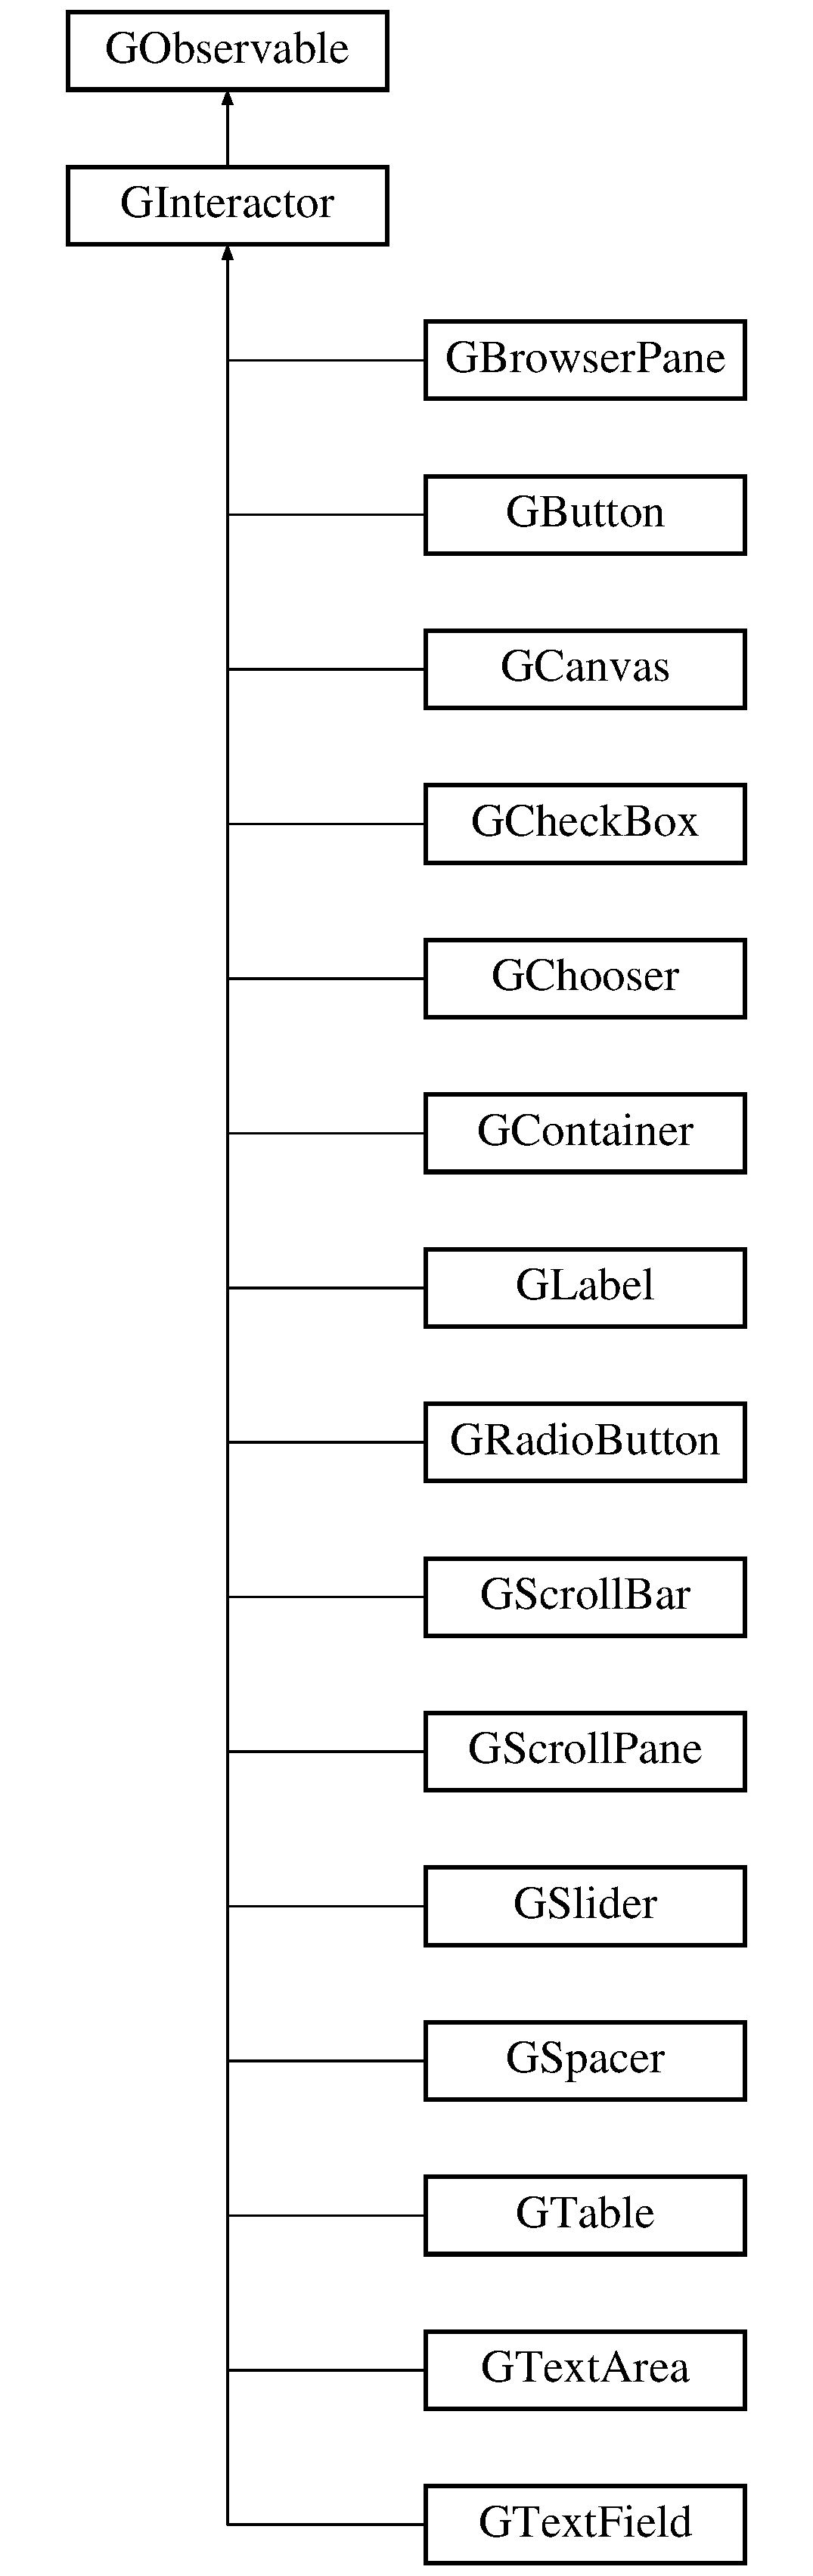
\includegraphics[height=12.000000cm]{classGInteractor}
\end{center}
\end{figure}
\subsection*{Public Types}
\begin{DoxyCompactItemize}
\item 
enum \mbox{\hyperlink{classGInteractor_a8e0d441725a81d2bbdebbea09078260e}{Text\+Position}} \{ \mbox{\hyperlink{classGInteractor_a8e0d441725a81d2bbdebbea09078260ea4cd6f2e7d5a08d6f4dc052df2358f774}{T\+E\+X\+T\+\_\+\+B\+E\+S\+I\+D\+E\+\_\+\+I\+C\+ON}}, 
\mbox{\hyperlink{classGInteractor_a8e0d441725a81d2bbdebbea09078260eaa88490f63d8de68d44c83bdb2ecde3b3}{T\+E\+X\+T\+\_\+\+U\+N\+D\+E\+R\+\_\+\+I\+C\+ON}}, 
\mbox{\hyperlink{classGInteractor_a8e0d441725a81d2bbdebbea09078260ea39a6f388a30ac4fefb6eb13e846bc9f2}{T\+E\+X\+T\+\_\+\+O\+N\+LY}}
 \}
\begin{DoxyCompactList}\small\item\em The places where an interactor can place its text relative to its icon. \end{DoxyCompactList}\end{DoxyCompactItemize}
\subsection*{Public Member Functions}
\begin{DoxyCompactItemize}
\item 
\mbox{\hyperlink{classGInteractor_a5a5d84b3c2735060635b4b338c397823}{G\+Interactor}} ()
\begin{DoxyCompactList}\small\item\em Initializes a newly created interactor. \end{DoxyCompactList}\item 
virtual \mbox{\hyperlink{classGInteractor_adb2d61211f85464680d47b511db24561}{$\sim$\+G\+Interactor}} ()
\begin{DoxyCompactList}\small\item\em Frees memory allocated internally by the interactor. \end{DoxyCompactList}\item 
virtual void \mbox{\hyperlink{classGInteractor_a02f20ea6edfa0671f31c4c648a253833}{add\+Action\+Listener}} () Q\+\_\+\+D\+E\+C\+L\+\_\+\+D\+E\+P\+R\+E\+C\+A\+T\+ED
\begin{DoxyCompactList}\small\item\em Adds an event listener to be notified when this interactor is clicked or generally interacted with. \end{DoxyCompactList}\item 
bool \mbox{\hyperlink{classGInteractor_a597a370b592e3737d38d9d2f4e2031ea}{events\+Enabled}} () const override
\begin{DoxyCompactList}\small\item\em Returns true if this interactor is currently accepting events. \end{DoxyCompactList}\item 
virtual std\+::string \mbox{\hyperlink{classGInteractor_a69f8d23ed8f207fbecad99960776e942}{get\+Accelerator}} () const
\begin{DoxyCompactList}\small\item\em Returns a string representing a hotkey for this interactor, or an empty string if no accelerator has been set. \end{DoxyCompactList}\item 
virtual std\+::string \mbox{\hyperlink{classGInteractor_a94eb4276000c4fdfb508ce9e6317a82a}{get\+Action\+Command}} () const
\begin{DoxyCompactList}\small\item\em Returns an action command for this interactor, which is a semi-\/unique string you can use to identify it when events occur. \end{DoxyCompactList}\item 
virtual std\+::string \mbox{\hyperlink{classGInteractor_a808e22cc1fdfbecf71ed8c64ef4600e0}{get\+Background}} () const
\begin{DoxyCompactList}\small\item\em Returns the background color of the interactor as a string. \end{DoxyCompactList}\item 
virtual int \mbox{\hyperlink{classGInteractor_a9e827257a55cb8cf4d9de2ec6bcfd7a0}{get\+Background\+Int}} () const
\begin{DoxyCompactList}\small\item\em Returns the background color of the interactor as an R\+GB integer. \end{DoxyCompactList}\item 
virtual \mbox{\hyperlink{structGRectangle}{G\+Rectangle}} \mbox{\hyperlink{classGInteractor_a29e6ac35a0b48f491a4c88194cc5da3b}{get\+Bounds}} () const
\begin{DoxyCompactList}\small\item\em Returns a rectangle representing the x/y position and size of this interactor. \end{DoxyCompactList}\item 
virtual std\+::string \mbox{\hyperlink{classGInteractor_aa061dfa488c31e18549d64363c1d0e34}{get\+Color}} () const
\begin{DoxyCompactList}\small\item\em Returns the foreground/text color of the interactor as a string. \end{DoxyCompactList}\item 
virtual int \mbox{\hyperlink{classGInteractor_a9635c7af766cdc3417f346683fa0e6c1}{get\+Color\+Int}} () const
\begin{DoxyCompactList}\small\item\em Returns the foreground/text color of the interactor as an R\+GB integer. \end{DoxyCompactList}\item 
virtual \mbox{\hyperlink{classGContainer}{G\+Container}} $\ast$ \mbox{\hyperlink{classGInteractor_a7a6e317c29d61030929b4cd2d1c00fe7}{get\+Container}} () const
\begin{DoxyCompactList}\small\item\em Returns a pointer to the onscreen container holding this interactor. \end{DoxyCompactList}\item 
virtual std\+::string \mbox{\hyperlink{classGInteractor_a894a5502900794eeb27d084c21f1d77d}{get\+Font}} () const
\begin{DoxyCompactList}\small\item\em Returns the font of this interactor\textquotesingle{}s text as a font string such as \char`\"{}\+Helvetica-\/12-\/\+Bold\char`\"{}. \end{DoxyCompactList}\item 
virtual std\+::string \mbox{\hyperlink{classGInteractor_a4fa2d8b0192a3a5b4af4bbfe71194d03}{get\+Foreground}} () const
\begin{DoxyCompactList}\small\item\em Returns the foreground/text color of the interactor as a string. \end{DoxyCompactList}\item 
virtual int \mbox{\hyperlink{classGInteractor_ac3b12ab385a6ef9ae90fc879860ba726}{get\+Foreground\+Int}} () const
\begin{DoxyCompactList}\small\item\em Returns the foreground/text color of the interactor as an R\+GB integer. \end{DoxyCompactList}\item 
virtual double \mbox{\hyperlink{classGInteractor_a1e7e353362434072875264cf95629f99}{get\+Height}} () const
\begin{DoxyCompactList}\small\item\em Returns the current onscreen height of this interactor in pixels. \end{DoxyCompactList}\item 
virtual std\+::string \mbox{\hyperlink{classGInteractor_aaed62a73004939a64da6f0eb9eb64d73}{get\+Icon}} () const
\begin{DoxyCompactList}\small\item\em Returns the file name of the icon associated with this interactor, or an empty string if no icon has been set. \end{DoxyCompactList}\item 
virtual int \mbox{\hyperlink{classGInteractor_a9c9659a6c6ba66b4107ba59c95a24241}{get\+ID}} () const
\begin{DoxyCompactList}\small\item\em Returns a globally unique identifier for this interactor, which is set when the interactor is constructed. \end{DoxyCompactList}\item 
virtual \mbox{\hyperlink{structGPoint}{G\+Point}} \mbox{\hyperlink{classGInteractor_a4f83802015511edeb63b892830812c11}{get\+Location}} () const
\begin{DoxyCompactList}\small\item\em Returns an (x, y) point representing the onscreen location of the top-\/left corner of this interactor within its containing window. \end{DoxyCompactList}\item 
virtual double \mbox{\hyperlink{classGInteractor_aed4b0075fcc434499c3cb3e46896bda3}{get\+Minimum\+Height}} () const
\begin{DoxyCompactList}\small\item\em Returns the minimum height in pixels that this interactor will permit itself to be resized to. \end{DoxyCompactList}\item 
virtual \mbox{\hyperlink{structGDimension}{G\+Dimension}} \mbox{\hyperlink{classGInteractor_a66b5af0b32493b4d597ca0a3df2049ea}{get\+Minimum\+Size}} () const
\begin{DoxyCompactList}\small\item\em Returns a \mbox{\hyperlink{structGDimension}{G\+Dimension}} structure representing the minimum size in pixels that this interactor will permit itself to be resized to. \end{DoxyCompactList}\item 
virtual double \mbox{\hyperlink{classGInteractor_a59e668114fe3d49d2a0f28deb258f7c8}{get\+Minimum\+Width}} () const
\begin{DoxyCompactList}\small\item\em Returns the minimum width in pixels that this interactor will permit itself to be resized to. \end{DoxyCompactList}\item 
virtual std\+::string \mbox{\hyperlink{classGInteractor_a8a60438a5b55d0b2ceb35c8674b9d8c5}{get\+Name}} () const
\begin{DoxyCompactList}\small\item\em Returns a string representing a unique name for this interactor. \end{DoxyCompactList}\item 
virtual double \mbox{\hyperlink{classGInteractor_a747de0961653847bdc6615dbf756d715}{get\+Preferred\+Height}} () const
\begin{DoxyCompactList}\small\item\em Returns the height in pixels that this interactor would prefer to be, which would exactly fit its contents with no stretching or scrollbars. \end{DoxyCompactList}\item 
virtual \mbox{\hyperlink{structGDimension}{G\+Dimension}} \mbox{\hyperlink{classGInteractor_a4aabbee761d8e9116275401131b7ccd1}{get\+Preferred\+Size}} () const
\begin{DoxyCompactList}\small\item\em Returns a \mbox{\hyperlink{structGDimension}{G\+Dimension}} structure storing the width and height in pixels that this interactor would prefer to be, which would exactly fit its contents with no stretching or scrollbars. \end{DoxyCompactList}\item 
virtual double \mbox{\hyperlink{classGInteractor_a82bca31d37700fb0e35d2743352efd5e}{get\+Preferred\+Width}} () const
\begin{DoxyCompactList}\small\item\em Returns the height in pixels that this interactor would prefer to be, which would exactly fit its contents with no stretching or scrollbars. \end{DoxyCompactList}\item 
virtual \mbox{\hyperlink{structGDimension}{G\+Dimension}} \mbox{\hyperlink{classGInteractor_a7b4eec96a2bdc6420695d5796a78eea9}{get\+Size}} () const
\begin{DoxyCompactList}\small\item\em Returns a \mbox{\hyperlink{structGDimension}{G\+Dimension}} structure storing the current onscreen width and height of this interactor in pixels. \end{DoxyCompactList}\item 
std\+::string \mbox{\hyperlink{classGInteractor_a44c407a54a20dd0f2fff30338289299d}{get\+Type}} () const override=0
\begin{DoxyCompactList}\small\item\em Returns a string representing the class name of this interactor, such as \char`\"{}\+G\+Button\char`\"{} or \char`\"{}\+G\+Check\+Box\char`\"{}. \end{DoxyCompactList}\item 
virtual double \mbox{\hyperlink{classGInteractor_a0ed2965abd4f5701d2cadf71239faf19}{get\+Width}} () const
\begin{DoxyCompactList}\small\item\em Returns the current onscreen width of this interactor in pixels. \end{DoxyCompactList}\item 
virtual double \mbox{\hyperlink{classGInteractor_a344385751bee0720059403940d57a13e}{getX}} () const
\begin{DoxyCompactList}\small\item\em Returns the x-\/coordinate of the top-\/left pixel of this interactor within its onscreen window. \end{DoxyCompactList}\item 
virtual double \mbox{\hyperlink{classGInteractor_aafa51c7f8f38a09febbb9ce7853f77b4}{getY}} () const
\begin{DoxyCompactList}\small\item\em Returns the y-\/coordinate of the top-\/left pixel of this interactor within its onscreen window. \end{DoxyCompactList}\item 
virtual bool \mbox{\hyperlink{classGInteractor_afc480f652b8c5f1fb255e2269ce68879}{in\+Bounds}} (double x, double y) const
\begin{DoxyCompactList}\small\item\em Returns true if the given x/y pixel is within the bounds of this interactor. \end{DoxyCompactList}\item 
virtual bool \mbox{\hyperlink{classGInteractor_ae6d7982c1c627b677a5e776ca86118ed}{in\+Bounds}} (int x, int y) const
\begin{DoxyCompactList}\small\item\em Returns true if the given x/y pixel is within the bounds of this interactor. \end{DoxyCompactList}\item 
virtual bool \mbox{\hyperlink{classGInteractor_aacb819fb241851fd9fc045271baa4034}{is\+Enabled}} () const
\begin{DoxyCompactList}\small\item\em Returns true if this interactor is currently enabled. \end{DoxyCompactList}\item 
virtual bool \mbox{\hyperlink{classGInteractor_a9d8a6cfb13917785c143e74d40e4e2be}{is\+Visible}} () const
\begin{DoxyCompactList}\small\item\em Returns true if the interactor is visible on the screen. \end{DoxyCompactList}\item 
virtual void \mbox{\hyperlink{classGInteractor_ab7fe7a876367b87cf7202f947f1d05e4}{remove\+Action\+Listener}} ()
\begin{DoxyCompactList}\small\item\em Removes the action listener from this interactor so that it will no longer call it when events occur. \end{DoxyCompactList}\item 
virtual void \mbox{\hyperlink{classGInteractor_ad39d0325cde6b97ebda4b9d7787c633b}{remove\+Click\+Listener}} ()
\begin{DoxyCompactList}\small\item\em Removes the click listener from this interactor so that it will no longer call it when events occur. \end{DoxyCompactList}\item 
virtual void \mbox{\hyperlink{classGInteractor_aa4250907e4cdd77349c04f0cf5cdd3d3}{remove\+Double\+Click\+Listener}} ()
\begin{DoxyCompactList}\small\item\em Removes the double-\/click listener from this interactor so that it will no longer call it when events occur. \end{DoxyCompactList}\item 
virtual void \mbox{\hyperlink{classGInteractor_a43095f41cab3be732b49f29970484b05}{remove\+Key\+Listener}} ()
\begin{DoxyCompactList}\small\item\em Removes the key listener from this interactor so that it will no longer call it when key events occur. \end{DoxyCompactList}\item 
virtual void \mbox{\hyperlink{classGInteractor_aff47f71ce47e688a07c9d38dc92fcc11}{remove\+Mouse\+Listener}} ()
\begin{DoxyCompactList}\small\item\em Removes the mouse listener from this interactor so that it will no longer call it when events occur. \end{DoxyCompactList}\item 
virtual void \mbox{\hyperlink{classGInteractor_a519fb2ac767f8b2febbb50b898b8c8cb}{request\+Focus}} ()
\begin{DoxyCompactList}\small\item\em Transfers keyboard focus to this interactor. \end{DoxyCompactList}\item 
virtual void \mbox{\hyperlink{classGInteractor_ad15f102f62e2960576012f1aa0ba4b2e}{set\+Accelerator}} (const std\+::string \&accelerator)
\begin{DoxyCompactList}\small\item\em Sets an accelerator hotkey for this interactor, such as \char`\"{}\+Ctrl-\/\+S\char`\"{}. \end{DoxyCompactList}\item 
virtual void \mbox{\hyperlink{classGInteractor_a4b5843fe3030e038a1ba54cc03389bcf}{set\+Action\+Command}} (const std\+::string \&action\+Command)
\begin{DoxyCompactList}\small\item\em Sets the action command for this interactor. \end{DoxyCompactList}\item 
virtual void \mbox{\hyperlink{classGInteractor_adcfb4742430c88714fcf57e57ab8ea9c}{set\+Action\+Listener}} (G\+Event\+Listener func)
\begin{DoxyCompactList}\small\item\em Sets an action listener on this interactor so that it will be called when it is interacted with in its primary way. \end{DoxyCompactList}\item 
virtual void \mbox{\hyperlink{classGInteractor_aebd20a89c7a8a43a6fce999cf4f9fcf2}{set\+Action\+Listener}} (G\+Event\+Listener\+Void func)
\begin{DoxyCompactList}\small\item\em Sets an action listener on this interactor so that it will be called when it is interacted with in its primary way. \end{DoxyCompactList}\item 
virtual void \mbox{\hyperlink{classGInteractor_acba7e546c2025c0a15ca4b4cc92043db}{set\+Background}} (int rgb)
\begin{DoxyCompactList}\small\item\em Sets the background color of the interactor to the color represented by the given R\+GB integer. \end{DoxyCompactList}\item 
virtual void \mbox{\hyperlink{classGInteractor_ab4677ab2474e68b07aa56605af92a84a}{set\+Background}} (const std\+::string \&color)
\begin{DoxyCompactList}\small\item\em Sets the background color of the interactor to the color represented by the given string. \end{DoxyCompactList}\item 
virtual void \mbox{\hyperlink{classGInteractor_a2aae8197624b72265ab83b4f1bc73f2f}{set\+Bounds}} (double x, double y, double width, double height)
\begin{DoxyCompactList}\small\item\em Sets the size and location of the widget. \end{DoxyCompactList}\item 
virtual void \mbox{\hyperlink{classGInteractor_acada386653f008cacc7cce86426bef7c}{set\+Bounds}} (const \mbox{\hyperlink{structGRectangle}{G\+Rectangle}} \&size)
\begin{DoxyCompactList}\small\item\em Sets the size and location of the widget. \end{DoxyCompactList}\item 
virtual void \mbox{\hyperlink{classGInteractor_abd40af6921242584d0954f173911b190}{set\+Click\+Listener}} (G\+Event\+Listener func)
\begin{DoxyCompactList}\small\item\em Sets a mouse listener on this interactor so that it will be called when the mouse is clicked on it. \end{DoxyCompactList}\item 
virtual void \mbox{\hyperlink{classGInteractor_a856414c92df90f56f3877475eb3f8fc4}{set\+Click\+Listener}} (G\+Event\+Listener\+Void func)
\begin{DoxyCompactList}\small\item\em Sets a mouse listener on this interactor so that it will be called when the mouse is clicked on it. \end{DoxyCompactList}\item 
virtual void \mbox{\hyperlink{classGInteractor_ab1f5cc0f5cc6bbbd716a526c61f1081d}{set\+Color}} (int rgb)
\begin{DoxyCompactList}\small\item\em Sets the foreground/text color of the interactor to the color represented by the given R\+GB integer. \end{DoxyCompactList}\item 
virtual void \mbox{\hyperlink{classGInteractor_a61374df6c11b52cfbb0815decdbaebc6}{set\+Color}} (const std\+::string \&color)
\begin{DoxyCompactList}\small\item\em Sets the foreground/text color of the interactor to the color represented by the given string. \end{DoxyCompactList}\item 
virtual void \mbox{\hyperlink{classGInteractor_ac29f9a3462458e165fae3a1f046ee77a}{set\+Double\+Click\+Listener}} (G\+Event\+Listener func)
\begin{DoxyCompactList}\small\item\em Sets a mouse listener on this interactor so that it will be called when the mouse is double-\/clicked on it. \end{DoxyCompactList}\item 
virtual void \mbox{\hyperlink{classGInteractor_a50096194d66f48c92dd4c512d41bfc76}{set\+Double\+Click\+Listener}} (G\+Event\+Listener\+Void func)
\begin{DoxyCompactList}\small\item\em Sets a mouse listener on this interactor so that it will be called when the mouse is double-\/clicked on it. \end{DoxyCompactList}\item 
virtual void \mbox{\hyperlink{classGInteractor_ab831367dd84bbd579e02e55bacb21343}{set\+Enabled}} (bool value)
\begin{DoxyCompactList}\small\item\em Sets whether this interactor is currently enabled. \end{DoxyCompactList}\item 
virtual void \mbox{\hyperlink{classGObservable_afaa30b2a9e0f378fd1c70d2f1d0b8216}{set\+Events\+Enabled}} (bool \mbox{\hyperlink{classGInteractor_a597a370b592e3737d38d9d2f4e2031ea}{events\+Enabled}})
\begin{DoxyCompactList}\small\item\em Sets whether the object is currently allowing itself to fire events. \end{DoxyCompactList}\item 
virtual void \mbox{\hyperlink{classGInteractor_a2592348886ffea646c6534bf88f7c49d}{set\+Font}} (const Q\+Font \&font)
\begin{DoxyCompactList}\small\item\em Sets the font used by this widget to the given Qt font. \end{DoxyCompactList}\item 
virtual void \mbox{\hyperlink{classGInteractor_a8e096e8818d838aceae1d46d58fb3a7b}{set\+Font}} (const std\+::string \&font)
\begin{DoxyCompactList}\small\item\em Sets the font used by this widget to the font represented by the given font string, such as \char`\"{}\+Helvetica-\/16-\/\+Bold\char`\"{}. \end{DoxyCompactList}\item 
virtual void \mbox{\hyperlink{classGInteractor_a9eb856b5ff83a19df3831a31f15f4563}{set\+Foreground}} (int rgb)
\begin{DoxyCompactList}\small\item\em Sets the foreground/text color of the interactor to the color represented by the given R\+GB integer. \end{DoxyCompactList}\item 
virtual void \mbox{\hyperlink{classGInteractor_af59209aeadea6dfc6d97a2d8531f50e1}{set\+Foreground}} (const std\+::string \&color)
\begin{DoxyCompactList}\small\item\em Sets the foreground/text color of the interactor to the color represented by the given string. \end{DoxyCompactList}\item 
virtual void \mbox{\hyperlink{classGInteractor_a9e280bfc4544dfaf8e4376c4e1a74357}{set\+Height}} (double height)
\begin{DoxyCompactList}\small\item\em Sets the onscreen height of the interactor in pixels. \end{DoxyCompactList}\item 
virtual void \mbox{\hyperlink{classGInteractor_a542abfcd7261751352af129c7215ecda}{set\+Icon}} (const Q\+Icon \&icon)
\begin{DoxyCompactList}\small\item\em Sets the icon associated with this interactor. \end{DoxyCompactList}\item 
virtual void \mbox{\hyperlink{classGInteractor_a368e1a338f84401c284506d03b1ba769}{set\+Icon}} (const Q\+Pixmap \&icon)
\begin{DoxyCompactList}\small\item\em Sets the icon associated with this interactor. \end{DoxyCompactList}\item 
virtual void \mbox{\hyperlink{classGInteractor_a762e139aa311461c3984d3ad28293f64}{set\+Icon}} (const std\+::string \&filename, bool retain\+Icon\+Size=true)
\begin{DoxyCompactList}\small\item\em Sets the file name of the icon associated with this interactor, or an empty string if no icon has been set. \end{DoxyCompactList}\item 
virtual void \mbox{\hyperlink{classGInteractor_aeb8324d3287fa1fbe093f4d6230cf0a6}{set\+Key\+Listener}} (G\+Event\+Listener func)
\begin{DoxyCompactList}\small\item\em Sets a key listener on this interactor so that it will be called when the user presses any key. \end{DoxyCompactList}\item 
virtual void \mbox{\hyperlink{classGInteractor_ae48ecea73606c7bd9423e1c7cc589cc9}{set\+Key\+Listener}} (G\+Event\+Listener\+Void func)
\begin{DoxyCompactList}\small\item\em Sets a key listener on this interactor so that it will be called when the user presses any key. \end{DoxyCompactList}\item 
virtual void \mbox{\hyperlink{classGInteractor_a04594e8ba9b98513a64f1da00dcae18c}{set\+Location}} (double x, double y)
\begin{DoxyCompactList}\small\item\em Sets the onscreen x/y-\/coordinate of the top-\/left corner of the interactor relative to its window. \end{DoxyCompactList}\item 
virtual void \mbox{\hyperlink{classGInteractor_a0cf428e207b7f22cc08138a90b1b87b2}{set\+Minimum\+Size}} (double width, double height)
\begin{DoxyCompactList}\small\item\em Sets the minimum size in pixels that this interactor will permit itself to be resized to. \end{DoxyCompactList}\item 
virtual void \mbox{\hyperlink{classGInteractor_a3b1046117ac6cb7abe467e00ba8a81f4}{set\+Minimum\+Size}} (const \mbox{\hyperlink{structGDimension}{G\+Dimension}} \&size)
\begin{DoxyCompactList}\small\item\em Sets the minimum size in pixels that this interactor will permit itself to be resized to. \end{DoxyCompactList}\item 
virtual void \mbox{\hyperlink{classGInteractor_a37d8dbc943f59920f705b0104f60bde2}{set\+Mouse\+Listener}} (G\+Event\+Listener func)
\begin{DoxyCompactList}\small\item\em Sets a mouse listener on this interactor so that it will be called when the mouse is moved or clicked on it. \end{DoxyCompactList}\item 
virtual void \mbox{\hyperlink{classGInteractor_aea7f647ea62d59f71b5fad6aa65eeaf9}{set\+Mouse\+Listener}} (G\+Event\+Listener\+Void func)
\begin{DoxyCompactList}\small\item\em Sets a mouse listener on this interactor so that it will be called when the mouse is moved or clicked on it. \end{DoxyCompactList}\item 
virtual void \mbox{\hyperlink{classGInteractor_a9d3a2685df23b5e7cbf59c19c4a1f9b5}{set\+Name}} (const std\+::string \&name)
\begin{DoxyCompactList}\small\item\em Sets a string representing a unique name for this interactor. \end{DoxyCompactList}\item 
virtual void \mbox{\hyperlink{classGInteractor_a1ab987704fce32098706c6f00fb08218}{set\+Preferred\+Height}} (double height)
\begin{DoxyCompactList}\small\item\em Sets the height in pixels that this interactor would prefer to be. \end{DoxyCompactList}\item 
virtual void \mbox{\hyperlink{classGInteractor_a042c5ae19430d765ef552371cae3632c}{set\+Preferred\+Size}} (double width, double height)
\begin{DoxyCompactList}\small\item\em Sets the width and height in pixels that this interactor would prefer to be. \end{DoxyCompactList}\item 
virtual void \mbox{\hyperlink{classGInteractor_aa22d9be4bc0e078bb0ea69b0fc9d7c75}{set\+Preferred\+Size}} (const \mbox{\hyperlink{structGDimension}{G\+Dimension}} \&size)
\begin{DoxyCompactList}\small\item\em Sets the size in pixels that this interactor would prefer to be. \end{DoxyCompactList}\item 
virtual void \mbox{\hyperlink{classGInteractor_a3db429ab2fa52efd187eec0ed8cdd9f2}{set\+Preferred\+Width}} (double width)
\begin{DoxyCompactList}\small\item\em Sets the width in pixels that this interactor would prefer to be. \end{DoxyCompactList}\item 
virtual void \mbox{\hyperlink{classGInteractor_aca25d49481f9bf5fc8f7df4c086c4ce7}{set\+Size}} (double width, double height)
\begin{DoxyCompactList}\small\item\em Sets the onscreen width and height of the interactor in pixels. \end{DoxyCompactList}\item 
virtual void \mbox{\hyperlink{classGInteractor_ae2b628228f192c2702c4ce941b2af68f}{set\+Size}} (const \mbox{\hyperlink{structGDimension}{G\+Dimension}} \&size)
\begin{DoxyCompactList}\small\item\em Sets the onscreen width and height of the interactor in pixels. \end{DoxyCompactList}\item 
virtual void \mbox{\hyperlink{classGInteractor_a039e0e49beaecc275efce02d416acea8}{set\+Tooltip}} (const std\+::string \&tooltip\+Text)
\begin{DoxyCompactList}\small\item\em Sets a \char`\"{}tooltip\char`\"{} that will appear if the user hovers their mouse over the interactor. \end{DoxyCompactList}\item 
virtual void \mbox{\hyperlink{classGInteractor_a18e44e30b31525a243960ca3928125aa}{set\+Visible}} (bool visible)
\begin{DoxyCompactList}\small\item\em Returns true if the interactor is visible on the screen. \end{DoxyCompactList}\item 
virtual void \mbox{\hyperlink{classGInteractor_aa3f3fba4cb131baa8696ba01e3bceca1}{set\+Width}} (double width)
\begin{DoxyCompactList}\small\item\em Sets the onscreen width of the interactor in pixels. \end{DoxyCompactList}\item 
virtual void \mbox{\hyperlink{classGInteractor_a9c18fcc579333bf9653d13ad2b372e39}{setX}} (double x)
\begin{DoxyCompactList}\small\item\em Sets the onscreen x-\/coordinate of the top-\/left corner of the interactor relative to its window. \end{DoxyCompactList}\item 
virtual void \mbox{\hyperlink{classGInteractor_a7d57e2a5c35d27feb58fd498a3cf82b9}{setY}} (double y)
\begin{DoxyCompactList}\small\item\em Sets the onscreen y-\/coordinate of the top-\/left corner of the interactor relative to its window. \end{DoxyCompactList}\item 
virtual std\+::string \mbox{\hyperlink{classGObservable_a1fe5121d6528fdea3f243321b3fa3a49}{to\+String}} () const
\begin{DoxyCompactList}\small\item\em Returns a string representation of this observable object\textquotesingle{}s state. \end{DoxyCompactList}\end{DoxyCompactItemize}
\subsection*{Protected Member Functions}
\begin{DoxyCompactItemize}
\item 
virtual void \mbox{\hyperlink{classGObservable_a80cfa040459ff53594adbd6a51ec8f43}{clear\+Event\+Listeners}} ()
\begin{DoxyCompactList}\small\item\em Removes all event listeners from this object. \end{DoxyCompactList}\item 
virtual void \mbox{\hyperlink{classGObservable_a284f31528c0520f8e545c03ac9eeac74}{ensure\+Thread\+Safety}} (const std\+::string \&member\+Name=\char`\"{}\char`\"{})
\begin{DoxyCompactList}\small\item\em Ensures that we are currently in the Qt G\+UI thread. \end{DoxyCompactList}\item 
virtual void \mbox{\hyperlink{classGObservable_a63e5e5a6227c59c928493b11aceb0f67}{fire\+Event}} (\mbox{\hyperlink{classGEvent}{G\+Event}} \&event)
\begin{DoxyCompactList}\small\item\em Sends out the given event to any attached listeners. \end{DoxyCompactList}\item 
virtual void \mbox{\hyperlink{classGObservable_ab3983ea07337b52020a29cc00c653d8d}{fire\+G\+Event}} (Q\+Event $\ast$event, Event\+Type event\+Type, const std\+::string \&event\+Name)
\begin{DoxyCompactList}\small\item\em Creates an event of the given type, then sends it out to any attached listeners. \end{DoxyCompactList}\item 
virtual void \mbox{\hyperlink{classGObservable_a01fdf1b0e0dbd49e189fe4514e010411}{fire\+G\+Event}} (Q\+Close\+Event $\ast$event, Event\+Type event\+Type, const std\+::string \&event\+Name)
\begin{DoxyCompactList}\small\item\em Creates an event of the given type, then sends it out to any attached listeners. \end{DoxyCompactList}\item 
virtual void \mbox{\hyperlink{classGObservable_abb0b2f66ba39211cb5d7615e9d1c04e2}{fire\+G\+Event}} (Q\+Key\+Event $\ast$event, Event\+Type event\+Type, const std\+::string \&event\+Name)
\begin{DoxyCompactList}\small\item\em Creates an event of the given type, then sends it out to any attached listeners. \end{DoxyCompactList}\item 
virtual void \mbox{\hyperlink{classGObservable_a119318675d2165bdf7dd853aaf881d4b}{fire\+G\+Event}} (Q\+Mouse\+Event $\ast$event, Event\+Type event\+Type, const std\+::string \&event\+Name, const std\+::string \&action\+Command=\char`\"{}\char`\"{})
\begin{DoxyCompactList}\small\item\em Creates an event of the given type, then sends it out to any attached listeners. \end{DoxyCompactList}\item 
virtual void \mbox{\hyperlink{classGObservable_a63fd9034e1e1633c1c38eb342bfd34e9}{fire\+G\+Event}} (Q\+Resize\+Event $\ast$event, Event\+Type event\+Type, const std\+::string \&event\+Name)
\begin{DoxyCompactList}\small\item\em Creates an event of the given type, then sends it out to any attached listeners. \end{DoxyCompactList}\item 
virtual void \mbox{\hyperlink{classGObservable_a741345310d9b7c5170a6cbc410c44ac4}{fire\+G\+Event}} (Q\+Timer\+Event $\ast$event, Event\+Type event\+Type, const std\+::string \&event\+Name)
\begin{DoxyCompactList}\small\item\em Creates an event of the given type, then sends it out to any attached listeners. \end{DoxyCompactList}\item 
virtual void \mbox{\hyperlink{classGObservable_a93bf338968a0338761b8e4dc62f582e9}{fire\+G\+Event}} (Q\+Wheel\+Event $\ast$event, Event\+Type event\+Type, const std\+::string \&event\+Name)
\begin{DoxyCompactList}\small\item\em Creates an event of the given type, then sends it out to any attached listeners. \end{DoxyCompactList}\item 
virtual void \mbox{\hyperlink{classGObservable_a2a70a7d7435ff0c3b80bb4d70da19e0d}{fire\+G\+Event}} (Q\+Window\+State\+Change\+Event $\ast$event, Event\+Type event\+Type, const std\+::string \&event\+Name)
\begin{DoxyCompactList}\small\item\em Creates an event of the given type, then sends it out to any attached listeners. \end{DoxyCompactList}\item 
virtual bool \mbox{\hyperlink{classGObservable_a9f6faaa25942923bafa1c44020c49fa9}{has\+Event\+Listener}} (const std\+::string \&event\+Name) const
\begin{DoxyCompactList}\small\item\em Returns true if the observable object has a listener for the given type of event. \end{DoxyCompactList}\item 
virtual bool \mbox{\hyperlink{classGObservable_aeec1adc19aa0f33de62390686ee1382c}{is\+Accepting\+Event}} (int event\+Mask) const
\begin{DoxyCompactList}\small\item\em Returns true if the observable object has a listener for the given type of event. \end{DoxyCompactList}\item 
virtual bool \mbox{\hyperlink{classGObservable_aa31c73145a29dcb92848a92e0cfaea41}{is\+Accepting\+Event}} (const \mbox{\hyperlink{classGEvent}{G\+Event}} \&event) const
\begin{DoxyCompactList}\small\item\em Returns true if the observable object has a listener for the given type of event. \end{DoxyCompactList}\item 
virtual bool \mbox{\hyperlink{classGObservable_a3b1c689267eda44e65a2213e7de38b23}{is\+Accepting\+Event}} (const std\+::string \&event\+Type) const
\begin{DoxyCompactList}\small\item\em Returns true if the observable object has a listener for the given type of event. \end{DoxyCompactList}\item 
virtual void \mbox{\hyperlink{classGObservable_acbcf1ed3a851ad8a3c17ef38d86b481d}{remove\+Event\+Listener}} (const std\+::string \&event\+Name)
\begin{DoxyCompactList}\small\item\em Removes any event listener from this observable object that would respond to the given type of event, such as \char`\"{}click\char`\"{} or \char`\"{}keydown\char`\"{}. \end{DoxyCompactList}\item 
virtual void \mbox{\hyperlink{classGObservable_af51cc35c29a1bd1908609d432decdbb6}{remove\+Event\+Listeners}} (std\+::initializer\+\_\+list$<$ std\+::string $>$ event\+Names)
\begin{DoxyCompactList}\small\item\em Removes any event listener from this observable object that would respond to the given types of events, such as \char`\"{}click\char`\"{} or \char`\"{}keydown\char`\"{}. \end{DoxyCompactList}\item 
virtual void \mbox{\hyperlink{classGObservable_ad2f6d34961c50f6c1e0659990b79f741}{set\+Event\+Listener}} (const std\+::string \&event\+Name, G\+Event\+Listener func)
\begin{DoxyCompactList}\small\item\em Adds an event listener from this observable object to respond to the given type of event, such as \char`\"{}click\char`\"{} or \char`\"{}keydown\char`\"{}. \end{DoxyCompactList}\item 
virtual void \mbox{\hyperlink{classGObservable_abac4cb9f9e626e010e87f5d91573c8a5}{set\+Event\+Listener}} (const std\+::string \&event\+Name, G\+Event\+Listener\+Void func)
\begin{DoxyCompactList}\small\item\em Adds an event listener from this observable object to respond to the given type of event, such as \char`\"{}click\char`\"{} or \char`\"{}keydown\char`\"{}. \end{DoxyCompactList}\item 
virtual void \mbox{\hyperlink{classGObservable_afa388d69c33c718cf035774604065604}{set\+Event\+Listeners}} (std\+::initializer\+\_\+list$<$ std\+::string $>$ event\+Names, G\+Event\+Listener func)
\begin{DoxyCompactList}\small\item\em Adds an event listener from this observable object to respond to the given types of events, such as \char`\"{}click\char`\"{} or \char`\"{}keydown\char`\"{}. \end{DoxyCompactList}\item 
virtual void \mbox{\hyperlink{classGObservable_a7867184bbb686f74fae8a4db927da799}{set\+Event\+Listeners}} (std\+::initializer\+\_\+list$<$ std\+::string $>$ event\+Names, G\+Event\+Listener\+Void func)
\begin{DoxyCompactList}\small\item\em Adds an event listener from this observable object to respond to the given types of events, such as \char`\"{}click\char`\"{} or \char`\"{}keydown\char`\"{}. \end{DoxyCompactList}\end{DoxyCompactItemize}


\subsection{Detailed Description}
This abstract class is the superclass for all graphical interactors. 

In most applications, interactors will be added to a control strip along one of the regions of a \mbox{\hyperlink{classGWindow}{G\+Window}}. 

\subsection{Member Enumeration Documentation}
\mbox{\Hypertarget{classGInteractor_a8e0d441725a81d2bbdebbea09078260e}\label{classGInteractor_a8e0d441725a81d2bbdebbea09078260e}} 
\index{G\+Interactor@{G\+Interactor}!Text\+Position@{Text\+Position}}
\index{Text\+Position@{Text\+Position}!G\+Interactor@{G\+Interactor}}
\subsubsection{\texorpdfstring{Text\+Position}{TextPosition}}
{\footnotesize\ttfamily enum \mbox{\hyperlink{classGInteractor_a8e0d441725a81d2bbdebbea09078260e}{Text\+Position}}}



The places where an interactor can place its text relative to its icon. 

\begin{DoxyEnumFields}{Enumerator}
\raisebox{\heightof{T}}[0pt][0pt]{\index{T\+E\+X\+T\+\_\+\+B\+E\+S\+I\+D\+E\+\_\+\+I\+C\+ON@{T\+E\+X\+T\+\_\+\+B\+E\+S\+I\+D\+E\+\_\+\+I\+C\+ON}!G\+Interactor@{G\+Interactor}}\index{G\+Interactor@{G\+Interactor}!T\+E\+X\+T\+\_\+\+B\+E\+S\+I\+D\+E\+\_\+\+I\+C\+ON@{T\+E\+X\+T\+\_\+\+B\+E\+S\+I\+D\+E\+\_\+\+I\+C\+ON}}}\mbox{\Hypertarget{classGInteractor_a8e0d441725a81d2bbdebbea09078260ea4cd6f2e7d5a08d6f4dc052df2358f774}\label{classGInteractor_a8e0d441725a81d2bbdebbea09078260ea4cd6f2e7d5a08d6f4dc052df2358f774}} 
T\+E\+X\+T\+\_\+\+B\+E\+S\+I\+D\+E\+\_\+\+I\+C\+ON&\\
\hline

\raisebox{\heightof{T}}[0pt][0pt]{\index{T\+E\+X\+T\+\_\+\+U\+N\+D\+E\+R\+\_\+\+I\+C\+ON@{T\+E\+X\+T\+\_\+\+U\+N\+D\+E\+R\+\_\+\+I\+C\+ON}!G\+Interactor@{G\+Interactor}}\index{G\+Interactor@{G\+Interactor}!T\+E\+X\+T\+\_\+\+U\+N\+D\+E\+R\+\_\+\+I\+C\+ON@{T\+E\+X\+T\+\_\+\+U\+N\+D\+E\+R\+\_\+\+I\+C\+ON}}}\mbox{\Hypertarget{classGInteractor_a8e0d441725a81d2bbdebbea09078260eaa88490f63d8de68d44c83bdb2ecde3b3}\label{classGInteractor_a8e0d441725a81d2bbdebbea09078260eaa88490f63d8de68d44c83bdb2ecde3b3}} 
T\+E\+X\+T\+\_\+\+U\+N\+D\+E\+R\+\_\+\+I\+C\+ON&\\
\hline

\raisebox{\heightof{T}}[0pt][0pt]{\index{T\+E\+X\+T\+\_\+\+O\+N\+LY@{T\+E\+X\+T\+\_\+\+O\+N\+LY}!G\+Interactor@{G\+Interactor}}\index{G\+Interactor@{G\+Interactor}!T\+E\+X\+T\+\_\+\+O\+N\+LY@{T\+E\+X\+T\+\_\+\+O\+N\+LY}}}\mbox{\Hypertarget{classGInteractor_a8e0d441725a81d2bbdebbea09078260ea39a6f388a30ac4fefb6eb13e846bc9f2}\label{classGInteractor_a8e0d441725a81d2bbdebbea09078260ea39a6f388a30ac4fefb6eb13e846bc9f2}} 
T\+E\+X\+T\+\_\+\+O\+N\+LY&\\
\hline

\end{DoxyEnumFields}


\subsection{Constructor \& Destructor Documentation}
\mbox{\Hypertarget{classGInteractor_a5a5d84b3c2735060635b4b338c397823}\label{classGInteractor_a5a5d84b3c2735060635b4b338c397823}} 
\index{G\+Interactor@{G\+Interactor}!G\+Interactor@{G\+Interactor}}
\index{G\+Interactor@{G\+Interactor}!G\+Interactor@{G\+Interactor}}
\subsubsection{\texorpdfstring{G\+Interactor()}{GInteractor()}}
{\footnotesize\ttfamily \mbox{\hyperlink{classGInteractor}{G\+Interactor}} (\begin{DoxyParamCaption}{ }\end{DoxyParamCaption})}



Initializes a newly created interactor. 

If the Qt graphical subsystem has not yet been initialized, constructing an interactor will initialize it. \mbox{\Hypertarget{classGInteractor_adb2d61211f85464680d47b511db24561}\label{classGInteractor_adb2d61211f85464680d47b511db24561}} 
\index{G\+Interactor@{G\+Interactor}!````~G\+Interactor@{$\sim$\+G\+Interactor}}
\index{````~G\+Interactor@{$\sim$\+G\+Interactor}!G\+Interactor@{G\+Interactor}}
\subsubsection{\texorpdfstring{$\sim$\+G\+Interactor()}{~GInteractor()}}
{\footnotesize\ttfamily $\sim$\mbox{\hyperlink{classGInteractor}{G\+Interactor}} (\begin{DoxyParamCaption}{ }\end{DoxyParamCaption})\hspace{0.3cm}{\ttfamily [virtual]}}



Frees memory allocated internally by the interactor. 



\subsection{Member Function Documentation}
\mbox{\Hypertarget{classGInteractor_a02f20ea6edfa0671f31c4c648a253833}\label{classGInteractor_a02f20ea6edfa0671f31c4c648a253833}} 
\index{G\+Interactor@{G\+Interactor}!add\+Action\+Listener@{add\+Action\+Listener}}
\index{add\+Action\+Listener@{add\+Action\+Listener}!G\+Interactor@{G\+Interactor}}
\subsubsection{\texorpdfstring{add\+Action\+Listener()}{addActionListener()}}
{\footnotesize\ttfamily void add\+Action\+Listener (\begin{DoxyParamCaption}{ }\end{DoxyParamCaption})\hspace{0.3cm}{\ttfamily [virtual]}}



Adds an event listener to be notified when this interactor is clicked or generally interacted with. 

\begin{DoxyRefDesc}{Deprecated}
\item[\mbox{\hyperlink{deprecated__deprecated000006}{Deprecated}}]does nothing; use set\+Action\+Listener instead \end{DoxyRefDesc}
\mbox{\Hypertarget{classGObservable_a80cfa040459ff53594adbd6a51ec8f43}\label{classGObservable_a80cfa040459ff53594adbd6a51ec8f43}} 
\index{G\+Interactor@{G\+Interactor}!clear\+Event\+Listeners@{clear\+Event\+Listeners}}
\index{clear\+Event\+Listeners@{clear\+Event\+Listeners}!G\+Interactor@{G\+Interactor}}
\subsubsection{\texorpdfstring{clear\+Event\+Listeners()}{clearEventListeners()}}
{\footnotesize\ttfamily void clear\+Event\+Listeners (\begin{DoxyParamCaption}{ }\end{DoxyParamCaption})\hspace{0.3cm}{\ttfamily [protected]}, {\ttfamily [virtual]}, {\ttfamily [inherited]}}



Removes all event listeners from this object. 

\mbox{\Hypertarget{classGObservable_a284f31528c0520f8e545c03ac9eeac74}\label{classGObservable_a284f31528c0520f8e545c03ac9eeac74}} 
\index{G\+Interactor@{G\+Interactor}!ensure\+Thread\+Safety@{ensure\+Thread\+Safety}}
\index{ensure\+Thread\+Safety@{ensure\+Thread\+Safety}!G\+Interactor@{G\+Interactor}}
\subsubsection{\texorpdfstring{ensure\+Thread\+Safety()}{ensureThreadSafety()}}
{\footnotesize\ttfamily void ensure\+Thread\+Safety (\begin{DoxyParamCaption}\item[{const std\+::string \&}]{member\+Name = {\ttfamily \char`\"{}\char`\"{}} }\end{DoxyParamCaption})\hspace{0.3cm}{\ttfamily [protected]}, {\ttfamily [virtual]}, {\ttfamily [inherited]}}



Ensures that we are currently in the Qt G\+UI thread. 

\mbox{\Hypertarget{classGInteractor_a597a370b592e3737d38d9d2f4e2031ea}\label{classGInteractor_a597a370b592e3737d38d9d2f4e2031ea}} 
\index{G\+Interactor@{G\+Interactor}!events\+Enabled@{events\+Enabled}}
\index{events\+Enabled@{events\+Enabled}!G\+Interactor@{G\+Interactor}}
\subsubsection{\texorpdfstring{events\+Enabled()}{eventsEnabled()}}
{\footnotesize\ttfamily bool events\+Enabled (\begin{DoxyParamCaption}{ }\end{DoxyParamCaption}) const\hspace{0.3cm}{\ttfamily [override]}, {\ttfamily [virtual]}}



Returns true if this interactor is currently accepting events. 

Initially true. An interactor must be visible and added to an onscreen window to receive events. 

Reimplemented from \mbox{\hyperlink{classGObservable_a8ebb3da91032e7f4c34485dabc518b8a}{G\+Observable}}.

\mbox{\Hypertarget{classGObservable_a63e5e5a6227c59c928493b11aceb0f67}\label{classGObservable_a63e5e5a6227c59c928493b11aceb0f67}} 
\index{G\+Interactor@{G\+Interactor}!fire\+Event@{fire\+Event}}
\index{fire\+Event@{fire\+Event}!G\+Interactor@{G\+Interactor}}
\subsubsection{\texorpdfstring{fire\+Event()}{fireEvent()}}
{\footnotesize\ttfamily void fire\+Event (\begin{DoxyParamCaption}\item[{\mbox{\hyperlink{classGEvent}{G\+Event}} \&}]{event }\end{DoxyParamCaption})\hspace{0.3cm}{\ttfamily [protected]}, {\ttfamily [virtual]}, {\ttfamily [inherited]}}



Sends out the given event to any attached listeners. 

\mbox{\Hypertarget{classGObservable_ab3983ea07337b52020a29cc00c653d8d}\label{classGObservable_ab3983ea07337b52020a29cc00c653d8d}} 
\index{G\+Interactor@{G\+Interactor}!fire\+G\+Event@{fire\+G\+Event}}
\index{fire\+G\+Event@{fire\+G\+Event}!G\+Interactor@{G\+Interactor}}
\subsubsection{\texorpdfstring{fire\+G\+Event()}{fireGEvent()}\hspace{0.1cm}{\footnotesize\ttfamily [1/8]}}
{\footnotesize\ttfamily void fire\+G\+Event (\begin{DoxyParamCaption}\item[{Q\+Event $\ast$}]{event,  }\item[{Event\+Type}]{event\+Type,  }\item[{const std\+::string \&}]{event\+Name }\end{DoxyParamCaption})\hspace{0.3cm}{\ttfamily [protected]}, {\ttfamily [virtual]}, {\ttfamily [inherited]}}



Creates an event of the given type, then sends it out to any attached listeners. 

\mbox{\Hypertarget{classGObservable_a01fdf1b0e0dbd49e189fe4514e010411}\label{classGObservable_a01fdf1b0e0dbd49e189fe4514e010411}} 
\index{G\+Interactor@{G\+Interactor}!fire\+G\+Event@{fire\+G\+Event}}
\index{fire\+G\+Event@{fire\+G\+Event}!G\+Interactor@{G\+Interactor}}
\subsubsection{\texorpdfstring{fire\+G\+Event()}{fireGEvent()}\hspace{0.1cm}{\footnotesize\ttfamily [2/8]}}
{\footnotesize\ttfamily void fire\+G\+Event (\begin{DoxyParamCaption}\item[{Q\+Close\+Event $\ast$}]{event,  }\item[{Event\+Type}]{event\+Type,  }\item[{const std\+::string \&}]{event\+Name }\end{DoxyParamCaption})\hspace{0.3cm}{\ttfamily [protected]}, {\ttfamily [virtual]}, {\ttfamily [inherited]}}



Creates an event of the given type, then sends it out to any attached listeners. 

\mbox{\Hypertarget{classGObservable_abb0b2f66ba39211cb5d7615e9d1c04e2}\label{classGObservable_abb0b2f66ba39211cb5d7615e9d1c04e2}} 
\index{G\+Interactor@{G\+Interactor}!fire\+G\+Event@{fire\+G\+Event}}
\index{fire\+G\+Event@{fire\+G\+Event}!G\+Interactor@{G\+Interactor}}
\subsubsection{\texorpdfstring{fire\+G\+Event()}{fireGEvent()}\hspace{0.1cm}{\footnotesize\ttfamily [3/8]}}
{\footnotesize\ttfamily void fire\+G\+Event (\begin{DoxyParamCaption}\item[{Q\+Key\+Event $\ast$}]{event,  }\item[{Event\+Type}]{event\+Type,  }\item[{const std\+::string \&}]{event\+Name }\end{DoxyParamCaption})\hspace{0.3cm}{\ttfamily [protected]}, {\ttfamily [virtual]}, {\ttfamily [inherited]}}



Creates an event of the given type, then sends it out to any attached listeners. 

\mbox{\Hypertarget{classGObservable_a119318675d2165bdf7dd853aaf881d4b}\label{classGObservable_a119318675d2165bdf7dd853aaf881d4b}} 
\index{G\+Interactor@{G\+Interactor}!fire\+G\+Event@{fire\+G\+Event}}
\index{fire\+G\+Event@{fire\+G\+Event}!G\+Interactor@{G\+Interactor}}
\subsubsection{\texorpdfstring{fire\+G\+Event()}{fireGEvent()}\hspace{0.1cm}{\footnotesize\ttfamily [4/8]}}
{\footnotesize\ttfamily void fire\+G\+Event (\begin{DoxyParamCaption}\item[{Q\+Mouse\+Event $\ast$}]{event,  }\item[{Event\+Type}]{event\+Type,  }\item[{const std\+::string \&}]{event\+Name,  }\item[{const std\+::string \&}]{action\+Command = {\ttfamily \char`\"{}\char`\"{}} }\end{DoxyParamCaption})\hspace{0.3cm}{\ttfamily [protected]}, {\ttfamily [virtual]}, {\ttfamily [inherited]}}



Creates an event of the given type, then sends it out to any attached listeners. 

\mbox{\Hypertarget{classGObservable_a63fd9034e1e1633c1c38eb342bfd34e9}\label{classGObservable_a63fd9034e1e1633c1c38eb342bfd34e9}} 
\index{G\+Interactor@{G\+Interactor}!fire\+G\+Event@{fire\+G\+Event}}
\index{fire\+G\+Event@{fire\+G\+Event}!G\+Interactor@{G\+Interactor}}
\subsubsection{\texorpdfstring{fire\+G\+Event()}{fireGEvent()}\hspace{0.1cm}{\footnotesize\ttfamily [5/8]}}
{\footnotesize\ttfamily void fire\+G\+Event (\begin{DoxyParamCaption}\item[{Q\+Resize\+Event $\ast$}]{event,  }\item[{Event\+Type}]{event\+Type,  }\item[{const std\+::string \&}]{event\+Name }\end{DoxyParamCaption})\hspace{0.3cm}{\ttfamily [protected]}, {\ttfamily [virtual]}, {\ttfamily [inherited]}}



Creates an event of the given type, then sends it out to any attached listeners. 

\mbox{\Hypertarget{classGObservable_a741345310d9b7c5170a6cbc410c44ac4}\label{classGObservable_a741345310d9b7c5170a6cbc410c44ac4}} 
\index{G\+Interactor@{G\+Interactor}!fire\+G\+Event@{fire\+G\+Event}}
\index{fire\+G\+Event@{fire\+G\+Event}!G\+Interactor@{G\+Interactor}}
\subsubsection{\texorpdfstring{fire\+G\+Event()}{fireGEvent()}\hspace{0.1cm}{\footnotesize\ttfamily [6/8]}}
{\footnotesize\ttfamily void fire\+G\+Event (\begin{DoxyParamCaption}\item[{Q\+Timer\+Event $\ast$}]{event,  }\item[{Event\+Type}]{event\+Type,  }\item[{const std\+::string \&}]{event\+Name }\end{DoxyParamCaption})\hspace{0.3cm}{\ttfamily [protected]}, {\ttfamily [virtual]}, {\ttfamily [inherited]}}



Creates an event of the given type, then sends it out to any attached listeners. 

\mbox{\Hypertarget{classGObservable_a93bf338968a0338761b8e4dc62f582e9}\label{classGObservable_a93bf338968a0338761b8e4dc62f582e9}} 
\index{G\+Interactor@{G\+Interactor}!fire\+G\+Event@{fire\+G\+Event}}
\index{fire\+G\+Event@{fire\+G\+Event}!G\+Interactor@{G\+Interactor}}
\subsubsection{\texorpdfstring{fire\+G\+Event()}{fireGEvent()}\hspace{0.1cm}{\footnotesize\ttfamily [7/8]}}
{\footnotesize\ttfamily void fire\+G\+Event (\begin{DoxyParamCaption}\item[{Q\+Wheel\+Event $\ast$}]{event,  }\item[{Event\+Type}]{event\+Type,  }\item[{const std\+::string \&}]{event\+Name }\end{DoxyParamCaption})\hspace{0.3cm}{\ttfamily [protected]}, {\ttfamily [virtual]}, {\ttfamily [inherited]}}



Creates an event of the given type, then sends it out to any attached listeners. 

\mbox{\Hypertarget{classGObservable_a2a70a7d7435ff0c3b80bb4d70da19e0d}\label{classGObservable_a2a70a7d7435ff0c3b80bb4d70da19e0d}} 
\index{G\+Interactor@{G\+Interactor}!fire\+G\+Event@{fire\+G\+Event}}
\index{fire\+G\+Event@{fire\+G\+Event}!G\+Interactor@{G\+Interactor}}
\subsubsection{\texorpdfstring{fire\+G\+Event()}{fireGEvent()}\hspace{0.1cm}{\footnotesize\ttfamily [8/8]}}
{\footnotesize\ttfamily void fire\+G\+Event (\begin{DoxyParamCaption}\item[{Q\+Window\+State\+Change\+Event $\ast$}]{event,  }\item[{Event\+Type}]{event\+Type,  }\item[{const std\+::string \&}]{event\+Name }\end{DoxyParamCaption})\hspace{0.3cm}{\ttfamily [protected]}, {\ttfamily [virtual]}, {\ttfamily [inherited]}}



Creates an event of the given type, then sends it out to any attached listeners. 

\mbox{\Hypertarget{classGInteractor_a69f8d23ed8f207fbecad99960776e942}\label{classGInteractor_a69f8d23ed8f207fbecad99960776e942}} 
\index{G\+Interactor@{G\+Interactor}!get\+Accelerator@{get\+Accelerator}}
\index{get\+Accelerator@{get\+Accelerator}!G\+Interactor@{G\+Interactor}}
\subsubsection{\texorpdfstring{get\+Accelerator()}{getAccelerator()}}
{\footnotesize\ttfamily std\+::string get\+Accelerator (\begin{DoxyParamCaption}{ }\end{DoxyParamCaption}) const\hspace{0.3cm}{\ttfamily [virtual]}}



Returns a string representing a hotkey for this interactor, or an empty string if no accelerator has been set. 

\begin{DoxyReturn}{Returns}
an accelerator such as \char`\"{}\+Ctrl-\/\+S\char`\"{} 
\end{DoxyReturn}


Reimplemented in \mbox{\hyperlink{classGButton_a57806dc9defb73f76f493f8548319924}{G\+Button}}.

\mbox{\Hypertarget{classGInteractor_a94eb4276000c4fdfb508ce9e6317a82a}\label{classGInteractor_a94eb4276000c4fdfb508ce9e6317a82a}} 
\index{G\+Interactor@{G\+Interactor}!get\+Action\+Command@{get\+Action\+Command}}
\index{get\+Action\+Command@{get\+Action\+Command}!G\+Interactor@{G\+Interactor}}
\subsubsection{\texorpdfstring{get\+Action\+Command()}{getActionCommand()}}
{\footnotesize\ttfamily std\+::string get\+Action\+Command (\begin{DoxyParamCaption}{ }\end{DoxyParamCaption}) const\hspace{0.3cm}{\ttfamily [virtual]}}



Returns an action command for this interactor, which is a semi-\/unique string you can use to identify it when events occur. 

For example, for buttons, the default action command is the button\textquotesingle{}s text. 

Reimplemented in \mbox{\hyperlink{classGChooser_a4f83505141da1f8446f0e0e0a9507930}{G\+Chooser}}, \mbox{\hyperlink{classGRadioButton_a4f83505141da1f8446f0e0e0a9507930}{G\+Radio\+Button}}, \mbox{\hyperlink{classGButton_a4f83505141da1f8446f0e0e0a9507930}{G\+Button}}, and \mbox{\hyperlink{classGCheckBox_a4f83505141da1f8446f0e0e0a9507930}{G\+Check\+Box}}.

\mbox{\Hypertarget{classGInteractor_a808e22cc1fdfbecf71ed8c64ef4600e0}\label{classGInteractor_a808e22cc1fdfbecf71ed8c64ef4600e0}} 
\index{G\+Interactor@{G\+Interactor}!get\+Background@{get\+Background}}
\index{get\+Background@{get\+Background}!G\+Interactor@{G\+Interactor}}
\subsubsection{\texorpdfstring{get\+Background()}{getBackground()}}
{\footnotesize\ttfamily std\+::string get\+Background (\begin{DoxyParamCaption}{ }\end{DoxyParamCaption}) const\hspace{0.3cm}{\ttfamily [virtual]}}



Returns the background color of the interactor as a string. 

\begin{DoxyReturn}{Returns}
a string such as \char`\"{}blue\char`\"{} or \char`\"{}\#7700ff\char`\"{} 
\end{DoxyReturn}


Reimplemented in \mbox{\hyperlink{classGCanvas_a4a62c51b7244a7642b88065e3a07ae82}{G\+Canvas}}.

\mbox{\Hypertarget{classGInteractor_a9e827257a55cb8cf4d9de2ec6bcfd7a0}\label{classGInteractor_a9e827257a55cb8cf4d9de2ec6bcfd7a0}} 
\index{G\+Interactor@{G\+Interactor}!get\+Background\+Int@{get\+Background\+Int}}
\index{get\+Background\+Int@{get\+Background\+Int}!G\+Interactor@{G\+Interactor}}
\subsubsection{\texorpdfstring{get\+Background\+Int()}{getBackgroundInt()}}
{\footnotesize\ttfamily int get\+Background\+Int (\begin{DoxyParamCaption}{ }\end{DoxyParamCaption}) const\hspace{0.3cm}{\ttfamily [virtual]}}



Returns the background color of the interactor as an R\+GB integer. 

\begin{DoxyReturn}{Returns}
an integer such as 0x7700ff 
\end{DoxyReturn}


Reimplemented in \mbox{\hyperlink{classGCanvas_acd4f2b3b9619dacdfd71fc0004cac382}{G\+Canvas}}.

\mbox{\Hypertarget{classGInteractor_a29e6ac35a0b48f491a4c88194cc5da3b}\label{classGInteractor_a29e6ac35a0b48f491a4c88194cc5da3b}} 
\index{G\+Interactor@{G\+Interactor}!get\+Bounds@{get\+Bounds}}
\index{get\+Bounds@{get\+Bounds}!G\+Interactor@{G\+Interactor}}
\subsubsection{\texorpdfstring{get\+Bounds()}{getBounds()}}
{\footnotesize\ttfamily \mbox{\hyperlink{structGRectangle}{G\+Rectangle}} get\+Bounds (\begin{DoxyParamCaption}{ }\end{DoxyParamCaption}) const\hspace{0.3cm}{\ttfamily [virtual]}}



Returns a rectangle representing the x/y position and size of this interactor. 

\mbox{\Hypertarget{classGInteractor_aa061dfa488c31e18549d64363c1d0e34}\label{classGInteractor_aa061dfa488c31e18549d64363c1d0e34}} 
\index{G\+Interactor@{G\+Interactor}!get\+Color@{get\+Color}}
\index{get\+Color@{get\+Color}!G\+Interactor@{G\+Interactor}}
\subsubsection{\texorpdfstring{get\+Color()}{getColor()}}
{\footnotesize\ttfamily std\+::string get\+Color (\begin{DoxyParamCaption}{ }\end{DoxyParamCaption}) const\hspace{0.3cm}{\ttfamily [virtual]}}



Returns the foreground/text color of the interactor as a string. 

Equivalent to get\+Foreground. \begin{DoxyReturn}{Returns}
a string such as \char`\"{}blue\char`\"{} or \char`\"{}\#7700ff\char`\"{} 
\end{DoxyReturn}
\mbox{\Hypertarget{classGInteractor_a9635c7af766cdc3417f346683fa0e6c1}\label{classGInteractor_a9635c7af766cdc3417f346683fa0e6c1}} 
\index{G\+Interactor@{G\+Interactor}!get\+Color\+Int@{get\+Color\+Int}}
\index{get\+Color\+Int@{get\+Color\+Int}!G\+Interactor@{G\+Interactor}}
\subsubsection{\texorpdfstring{get\+Color\+Int()}{getColorInt()}}
{\footnotesize\ttfamily int get\+Color\+Int (\begin{DoxyParamCaption}{ }\end{DoxyParamCaption}) const\hspace{0.3cm}{\ttfamily [virtual]}}



Returns the foreground/text color of the interactor as an R\+GB integer. 

Equivalent to get\+Foreground\+Int. \begin{DoxyReturn}{Returns}
an integer such as 0x7700ff 
\end{DoxyReturn}
\mbox{\Hypertarget{classGInteractor_a7a6e317c29d61030929b4cd2d1c00fe7}\label{classGInteractor_a7a6e317c29d61030929b4cd2d1c00fe7}} 
\index{G\+Interactor@{G\+Interactor}!get\+Container@{get\+Container}}
\index{get\+Container@{get\+Container}!G\+Interactor@{G\+Interactor}}
\subsubsection{\texorpdfstring{get\+Container()}{getContainer()}}
{\footnotesize\ttfamily \mbox{\hyperlink{classGContainer}{G\+Container}} $\ast$ get\+Container (\begin{DoxyParamCaption}{ }\end{DoxyParamCaption}) const\hspace{0.3cm}{\ttfamily [virtual]}}



Returns a pointer to the onscreen container holding this interactor. 

When an interactor is created, its container is initially null. This will become non-\/null automatically if you add the interactor to a window or other layout container. Interactors must be added to a container or window to receive events or to become visible on the screen. \begin{DoxyReturn}{Returns}
the container, or nullptr if interactor has not yet been added to any container 
\end{DoxyReturn}
\mbox{\Hypertarget{classGInteractor_a894a5502900794eeb27d084c21f1d77d}\label{classGInteractor_a894a5502900794eeb27d084c21f1d77d}} 
\index{G\+Interactor@{G\+Interactor}!get\+Font@{get\+Font}}
\index{get\+Font@{get\+Font}!G\+Interactor@{G\+Interactor}}
\subsubsection{\texorpdfstring{get\+Font()}{getFont()}}
{\footnotesize\ttfamily std\+::string get\+Font (\begin{DoxyParamCaption}{ }\end{DoxyParamCaption}) const\hspace{0.3cm}{\ttfamily [virtual]}}



Returns the font of this interactor\textquotesingle{}s text as a font string such as \char`\"{}\+Helvetica-\/12-\/\+Bold\char`\"{}. 

\begin{DoxyReturn}{Returns}
a font string such as \char`\"{}\+Helvetica-\/12-\/\+Bold\char`\"{} 
\end{DoxyReturn}


Reimplemented in \mbox{\hyperlink{classGCanvas_aa0829769ac6325b5c58d27c8e363cb78}{G\+Canvas}}.

\mbox{\Hypertarget{classGInteractor_a4fa2d8b0192a3a5b4af4bbfe71194d03}\label{classGInteractor_a4fa2d8b0192a3a5b4af4bbfe71194d03}} 
\index{G\+Interactor@{G\+Interactor}!get\+Foreground@{get\+Foreground}}
\index{get\+Foreground@{get\+Foreground}!G\+Interactor@{G\+Interactor}}
\subsubsection{\texorpdfstring{get\+Foreground()}{getForeground()}}
{\footnotesize\ttfamily std\+::string get\+Foreground (\begin{DoxyParamCaption}{ }\end{DoxyParamCaption}) const\hspace{0.3cm}{\ttfamily [virtual]}}



Returns the foreground/text color of the interactor as a string. 

Equivalent to get\+Color. \begin{DoxyReturn}{Returns}
a string such as \char`\"{}blue\char`\"{} or \char`\"{}\#7700ff\char`\"{} 
\end{DoxyReturn}
\mbox{\Hypertarget{classGInteractor_ac3b12ab385a6ef9ae90fc879860ba726}\label{classGInteractor_ac3b12ab385a6ef9ae90fc879860ba726}} 
\index{G\+Interactor@{G\+Interactor}!get\+Foreground\+Int@{get\+Foreground\+Int}}
\index{get\+Foreground\+Int@{get\+Foreground\+Int}!G\+Interactor@{G\+Interactor}}
\subsubsection{\texorpdfstring{get\+Foreground\+Int()}{getForegroundInt()}}
{\footnotesize\ttfamily int get\+Foreground\+Int (\begin{DoxyParamCaption}{ }\end{DoxyParamCaption}) const\hspace{0.3cm}{\ttfamily [virtual]}}



Returns the foreground/text color of the interactor as an R\+GB integer. 

Equivalent to get\+Color\+Int. \begin{DoxyReturn}{Returns}
an integer such as 0x7700ff 
\end{DoxyReturn}
\mbox{\Hypertarget{classGInteractor_a1e7e353362434072875264cf95629f99}\label{classGInteractor_a1e7e353362434072875264cf95629f99}} 
\index{G\+Interactor@{G\+Interactor}!get\+Height@{get\+Height}}
\index{get\+Height@{get\+Height}!G\+Interactor@{G\+Interactor}}
\subsubsection{\texorpdfstring{get\+Height()}{getHeight()}}
{\footnotesize\ttfamily double get\+Height (\begin{DoxyParamCaption}{ }\end{DoxyParamCaption}) const\hspace{0.3cm}{\ttfamily [virtual]}}



Returns the current onscreen height of this interactor in pixels. 

\mbox{\Hypertarget{classGInteractor_aaed62a73004939a64da6f0eb9eb64d73}\label{classGInteractor_aaed62a73004939a64da6f0eb9eb64d73}} 
\index{G\+Interactor@{G\+Interactor}!get\+Icon@{get\+Icon}}
\index{get\+Icon@{get\+Icon}!G\+Interactor@{G\+Interactor}}
\subsubsection{\texorpdfstring{get\+Icon()}{getIcon()}}
{\footnotesize\ttfamily std\+::string get\+Icon (\begin{DoxyParamCaption}{ }\end{DoxyParamCaption}) const\hspace{0.3cm}{\ttfamily [virtual]}}



Returns the file name of the icon associated with this interactor, or an empty string if no icon has been set. 

Not all types of interactors support icons. \mbox{\Hypertarget{classGInteractor_a9c9659a6c6ba66b4107ba59c95a24241}\label{classGInteractor_a9c9659a6c6ba66b4107ba59c95a24241}} 
\index{G\+Interactor@{G\+Interactor}!get\+ID@{get\+ID}}
\index{get\+ID@{get\+ID}!G\+Interactor@{G\+Interactor}}
\subsubsection{\texorpdfstring{get\+I\+D()}{getID()}}
{\footnotesize\ttfamily int get\+ID (\begin{DoxyParamCaption}{ }\end{DoxyParamCaption}) const\hspace{0.3cm}{\ttfamily [virtual]}}



Returns a globally unique identifier for this interactor, which is set when the interactor is constructed. 

These I\+Ds can be useful for debugging to help identify interactors uniquely. \mbox{\Hypertarget{classGInteractor_a4f83802015511edeb63b892830812c11}\label{classGInteractor_a4f83802015511edeb63b892830812c11}} 
\index{G\+Interactor@{G\+Interactor}!get\+Location@{get\+Location}}
\index{get\+Location@{get\+Location}!G\+Interactor@{G\+Interactor}}
\subsubsection{\texorpdfstring{get\+Location()}{getLocation()}}
{\footnotesize\ttfamily \mbox{\hyperlink{structGPoint}{G\+Point}} get\+Location (\begin{DoxyParamCaption}{ }\end{DoxyParamCaption}) const\hspace{0.3cm}{\ttfamily [virtual]}}



Returns an (x, y) point representing the onscreen location of the top-\/left corner of this interactor within its containing window. 

\mbox{\Hypertarget{classGInteractor_aed4b0075fcc434499c3cb3e46896bda3}\label{classGInteractor_aed4b0075fcc434499c3cb3e46896bda3}} 
\index{G\+Interactor@{G\+Interactor}!get\+Minimum\+Height@{get\+Minimum\+Height}}
\index{get\+Minimum\+Height@{get\+Minimum\+Height}!G\+Interactor@{G\+Interactor}}
\subsubsection{\texorpdfstring{get\+Minimum\+Height()}{getMinimumHeight()}}
{\footnotesize\ttfamily double get\+Minimum\+Height (\begin{DoxyParamCaption}{ }\end{DoxyParamCaption}) const\hspace{0.3cm}{\ttfamily [virtual]}}



Returns the minimum height in pixels that this interactor will permit itself to be resized to. 

\mbox{\Hypertarget{classGInteractor_a66b5af0b32493b4d597ca0a3df2049ea}\label{classGInteractor_a66b5af0b32493b4d597ca0a3df2049ea}} 
\index{G\+Interactor@{G\+Interactor}!get\+Minimum\+Size@{get\+Minimum\+Size}}
\index{get\+Minimum\+Size@{get\+Minimum\+Size}!G\+Interactor@{G\+Interactor}}
\subsubsection{\texorpdfstring{get\+Minimum\+Size()}{getMinimumSize()}}
{\footnotesize\ttfamily \mbox{\hyperlink{structGDimension}{G\+Dimension}} get\+Minimum\+Size (\begin{DoxyParamCaption}{ }\end{DoxyParamCaption}) const\hspace{0.3cm}{\ttfamily [virtual]}}



Returns a \mbox{\hyperlink{structGDimension}{G\+Dimension}} structure representing the minimum size in pixels that this interactor will permit itself to be resized to. 

\mbox{\Hypertarget{classGInteractor_a59e668114fe3d49d2a0f28deb258f7c8}\label{classGInteractor_a59e668114fe3d49d2a0f28deb258f7c8}} 
\index{G\+Interactor@{G\+Interactor}!get\+Minimum\+Width@{get\+Minimum\+Width}}
\index{get\+Minimum\+Width@{get\+Minimum\+Width}!G\+Interactor@{G\+Interactor}}
\subsubsection{\texorpdfstring{get\+Minimum\+Width()}{getMinimumWidth()}}
{\footnotesize\ttfamily double get\+Minimum\+Width (\begin{DoxyParamCaption}{ }\end{DoxyParamCaption}) const\hspace{0.3cm}{\ttfamily [virtual]}}



Returns the minimum width in pixels that this interactor will permit itself to be resized to. 

\mbox{\Hypertarget{classGInteractor_a8a60438a5b55d0b2ceb35c8674b9d8c5}\label{classGInteractor_a8a60438a5b55d0b2ceb35c8674b9d8c5}} 
\index{G\+Interactor@{G\+Interactor}!get\+Name@{get\+Name}}
\index{get\+Name@{get\+Name}!G\+Interactor@{G\+Interactor}}
\subsubsection{\texorpdfstring{get\+Name()}{getName()}}
{\footnotesize\ttfamily std\+::string get\+Name (\begin{DoxyParamCaption}{ }\end{DoxyParamCaption}) const\hspace{0.3cm}{\ttfamily [virtual]}}



Returns a string representing a unique name for this interactor. 

The default name string uses the interactor\textquotesingle{}s type and its ID to make a string like \char`\"{}\+G\+Button\+\_\+14\char`\"{}, but you can override this by calling set\+Name. \begin{DoxyReturn}{Returns}
a string such as \char`\"{}\+G\+Button\+\_\+14\char`\"{} 
\end{DoxyReturn}
\mbox{\Hypertarget{classGInteractor_a747de0961653847bdc6615dbf756d715}\label{classGInteractor_a747de0961653847bdc6615dbf756d715}} 
\index{G\+Interactor@{G\+Interactor}!get\+Preferred\+Height@{get\+Preferred\+Height}}
\index{get\+Preferred\+Height@{get\+Preferred\+Height}!G\+Interactor@{G\+Interactor}}
\subsubsection{\texorpdfstring{get\+Preferred\+Height()}{getPreferredHeight()}}
{\footnotesize\ttfamily double get\+Preferred\+Height (\begin{DoxyParamCaption}{ }\end{DoxyParamCaption}) const\hspace{0.3cm}{\ttfamily [virtual]}}



Returns the height in pixels that this interactor would prefer to be, which would exactly fit its contents with no stretching or scrollbars. 

\mbox{\Hypertarget{classGInteractor_a4aabbee761d8e9116275401131b7ccd1}\label{classGInteractor_a4aabbee761d8e9116275401131b7ccd1}} 
\index{G\+Interactor@{G\+Interactor}!get\+Preferred\+Size@{get\+Preferred\+Size}}
\index{get\+Preferred\+Size@{get\+Preferred\+Size}!G\+Interactor@{G\+Interactor}}
\subsubsection{\texorpdfstring{get\+Preferred\+Size()}{getPreferredSize()}}
{\footnotesize\ttfamily \mbox{\hyperlink{structGDimension}{G\+Dimension}} get\+Preferred\+Size (\begin{DoxyParamCaption}{ }\end{DoxyParamCaption}) const\hspace{0.3cm}{\ttfamily [virtual]}}



Returns a \mbox{\hyperlink{structGDimension}{G\+Dimension}} structure storing the width and height in pixels that this interactor would prefer to be, which would exactly fit its contents with no stretching or scrollbars. 



Reimplemented in \mbox{\hyperlink{classGContainer_ac0fd6fc35681f935c67ad68078b354b8}{G\+Container}}.

\mbox{\Hypertarget{classGInteractor_a82bca31d37700fb0e35d2743352efd5e}\label{classGInteractor_a82bca31d37700fb0e35d2743352efd5e}} 
\index{G\+Interactor@{G\+Interactor}!get\+Preferred\+Width@{get\+Preferred\+Width}}
\index{get\+Preferred\+Width@{get\+Preferred\+Width}!G\+Interactor@{G\+Interactor}}
\subsubsection{\texorpdfstring{get\+Preferred\+Width()}{getPreferredWidth()}}
{\footnotesize\ttfamily double get\+Preferred\+Width (\begin{DoxyParamCaption}{ }\end{DoxyParamCaption}) const\hspace{0.3cm}{\ttfamily [virtual]}}



Returns the height in pixels that this interactor would prefer to be, which would exactly fit its contents with no stretching or scrollbars. 

\mbox{\Hypertarget{classGInteractor_a7b4eec96a2bdc6420695d5796a78eea9}\label{classGInteractor_a7b4eec96a2bdc6420695d5796a78eea9}} 
\index{G\+Interactor@{G\+Interactor}!get\+Size@{get\+Size}}
\index{get\+Size@{get\+Size}!G\+Interactor@{G\+Interactor}}
\subsubsection{\texorpdfstring{get\+Size()}{getSize()}}
{\footnotesize\ttfamily \mbox{\hyperlink{structGDimension}{G\+Dimension}} get\+Size (\begin{DoxyParamCaption}{ }\end{DoxyParamCaption}) const\hspace{0.3cm}{\ttfamily [virtual]}}



Returns a \mbox{\hyperlink{structGDimension}{G\+Dimension}} structure storing the current onscreen width and height of this interactor in pixels. 

\mbox{\Hypertarget{classGInteractor_a44c407a54a20dd0f2fff30338289299d}\label{classGInteractor_a44c407a54a20dd0f2fff30338289299d}} 
\index{G\+Interactor@{G\+Interactor}!get\+Type@{get\+Type}}
\index{get\+Type@{get\+Type}!G\+Interactor@{G\+Interactor}}
\subsubsection{\texorpdfstring{get\+Type()}{getType()}}
{\footnotesize\ttfamily std\+::string get\+Type (\begin{DoxyParamCaption}{ }\end{DoxyParamCaption}) const\hspace{0.3cm}{\ttfamily [override]}, {\ttfamily [pure virtual]}}



Returns a string representing the class name of this interactor, such as \char`\"{}\+G\+Button\char`\"{} or \char`\"{}\+G\+Check\+Box\char`\"{}. 

All subclasses of \mbox{\hyperlink{classGInteractor}{G\+Interactor}} must implement this method. \begin{DoxyReturn}{Returns}
a string such as \char`\"{}\+G\+Check\+Box\char`\"{} 
\end{DoxyReturn}


Implements \mbox{\hyperlink{classGObservable_a799e073a127b428cc841086d42ea4fed}{G\+Observable}}.



Implemented in \mbox{\hyperlink{classGCanvas_a9b72ede4ee8520f987a0c01e30654814}{G\+Canvas}}, \mbox{\hyperlink{classGContainer_a9b72ede4ee8520f987a0c01e30654814}{G\+Container}}, \mbox{\hyperlink{classGTable_a9b72ede4ee8520f987a0c01e30654814}{G\+Table}}, \mbox{\hyperlink{classGTextArea_a9b72ede4ee8520f987a0c01e30654814}{G\+Text\+Area}}, \mbox{\hyperlink{classGSlider_a9b72ede4ee8520f987a0c01e30654814}{G\+Slider}}, \mbox{\hyperlink{classGBrowserPane_a9b72ede4ee8520f987a0c01e30654814}{G\+Browser\+Pane}}, \mbox{\hyperlink{classGTextField_a9b72ede4ee8520f987a0c01e30654814}{G\+Text\+Field}}, \mbox{\hyperlink{classGChooser_a9b72ede4ee8520f987a0c01e30654814}{G\+Chooser}}, \mbox{\hyperlink{classGLabel_a9b72ede4ee8520f987a0c01e30654814}{G\+Label}}, \mbox{\hyperlink{classGButton_a9b72ede4ee8520f987a0c01e30654814}{G\+Button}}, \mbox{\hyperlink{classGScrollBar_a9b72ede4ee8520f987a0c01e30654814}{G\+Scroll\+Bar}}, \mbox{\hyperlink{classGRadioButton_a9b72ede4ee8520f987a0c01e30654814}{G\+Radio\+Button}}, \mbox{\hyperlink{classGScrollPane_a9b72ede4ee8520f987a0c01e30654814}{G\+Scroll\+Pane}}, \mbox{\hyperlink{classGCheckBox_a9b72ede4ee8520f987a0c01e30654814}{G\+Check\+Box}}, and \mbox{\hyperlink{classGSpacer_a9b72ede4ee8520f987a0c01e30654814}{G\+Spacer}}.

\mbox{\Hypertarget{classGInteractor_a0ed2965abd4f5701d2cadf71239faf19}\label{classGInteractor_a0ed2965abd4f5701d2cadf71239faf19}} 
\index{G\+Interactor@{G\+Interactor}!get\+Width@{get\+Width}}
\index{get\+Width@{get\+Width}!G\+Interactor@{G\+Interactor}}
\subsubsection{\texorpdfstring{get\+Width()}{getWidth()}}
{\footnotesize\ttfamily double get\+Width (\begin{DoxyParamCaption}{ }\end{DoxyParamCaption}) const\hspace{0.3cm}{\ttfamily [virtual]}}



Returns the current onscreen width of this interactor in pixels. 

\mbox{\Hypertarget{classGInteractor_a344385751bee0720059403940d57a13e}\label{classGInteractor_a344385751bee0720059403940d57a13e}} 
\index{G\+Interactor@{G\+Interactor}!getX@{getX}}
\index{getX@{getX}!G\+Interactor@{G\+Interactor}}
\subsubsection{\texorpdfstring{get\+X()}{getX()}}
{\footnotesize\ttfamily double getX (\begin{DoxyParamCaption}{ }\end{DoxyParamCaption}) const\hspace{0.3cm}{\ttfamily [virtual]}}



Returns the x-\/coordinate of the top-\/left pixel of this interactor within its onscreen window. 

\mbox{\Hypertarget{classGInteractor_aafa51c7f8f38a09febbb9ce7853f77b4}\label{classGInteractor_aafa51c7f8f38a09febbb9ce7853f77b4}} 
\index{G\+Interactor@{G\+Interactor}!getY@{getY}}
\index{getY@{getY}!G\+Interactor@{G\+Interactor}}
\subsubsection{\texorpdfstring{get\+Y()}{getY()}}
{\footnotesize\ttfamily double getY (\begin{DoxyParamCaption}{ }\end{DoxyParamCaption}) const\hspace{0.3cm}{\ttfamily [virtual]}}



Returns the y-\/coordinate of the top-\/left pixel of this interactor within its onscreen window. 

\mbox{\Hypertarget{classGObservable_a9f6faaa25942923bafa1c44020c49fa9}\label{classGObservable_a9f6faaa25942923bafa1c44020c49fa9}} 
\index{G\+Interactor@{G\+Interactor}!has\+Event\+Listener@{has\+Event\+Listener}}
\index{has\+Event\+Listener@{has\+Event\+Listener}!G\+Interactor@{G\+Interactor}}
\subsubsection{\texorpdfstring{has\+Event\+Listener()}{hasEventListener()}}
{\footnotesize\ttfamily bool has\+Event\+Listener (\begin{DoxyParamCaption}\item[{const std\+::string \&}]{event\+Name }\end{DoxyParamCaption}) const\hspace{0.3cm}{\ttfamily [protected]}, {\ttfamily [virtual]}, {\ttfamily [inherited]}}



Returns true if the observable object has a listener for the given type of event. 

\mbox{\Hypertarget{classGInteractor_afc480f652b8c5f1fb255e2269ce68879}\label{classGInteractor_afc480f652b8c5f1fb255e2269ce68879}} 
\index{G\+Interactor@{G\+Interactor}!in\+Bounds@{in\+Bounds}}
\index{in\+Bounds@{in\+Bounds}!G\+Interactor@{G\+Interactor}}
\subsubsection{\texorpdfstring{in\+Bounds()}{inBounds()}\hspace{0.1cm}{\footnotesize\ttfamily [1/2]}}
{\footnotesize\ttfamily bool in\+Bounds (\begin{DoxyParamCaption}\item[{double}]{x,  }\item[{double}]{y }\end{DoxyParamCaption}) const\hspace{0.3cm}{\ttfamily [virtual]}}



Returns true if the given x/y pixel is within the bounds of this interactor. 

\mbox{\Hypertarget{classGInteractor_ae6d7982c1c627b677a5e776ca86118ed}\label{classGInteractor_ae6d7982c1c627b677a5e776ca86118ed}} 
\index{G\+Interactor@{G\+Interactor}!in\+Bounds@{in\+Bounds}}
\index{in\+Bounds@{in\+Bounds}!G\+Interactor@{G\+Interactor}}
\subsubsection{\texorpdfstring{in\+Bounds()}{inBounds()}\hspace{0.1cm}{\footnotesize\ttfamily [2/2]}}
{\footnotesize\ttfamily bool in\+Bounds (\begin{DoxyParamCaption}\item[{int}]{x,  }\item[{int}]{y }\end{DoxyParamCaption}) const\hspace{0.3cm}{\ttfamily [virtual]}}



Returns true if the given x/y pixel is within the bounds of this interactor. 

\mbox{\Hypertarget{classGObservable_aeec1adc19aa0f33de62390686ee1382c}\label{classGObservable_aeec1adc19aa0f33de62390686ee1382c}} 
\index{G\+Interactor@{G\+Interactor}!is\+Accepting\+Event@{is\+Accepting\+Event}}
\index{is\+Accepting\+Event@{is\+Accepting\+Event}!G\+Interactor@{G\+Interactor}}
\subsubsection{\texorpdfstring{is\+Accepting\+Event()}{isAcceptingEvent()}\hspace{0.1cm}{\footnotesize\ttfamily [1/3]}}
{\footnotesize\ttfamily bool is\+Accepting\+Event (\begin{DoxyParamCaption}\item[{int}]{event\+Mask }\end{DoxyParamCaption}) const\hspace{0.3cm}{\ttfamily [protected]}, {\ttfamily [virtual]}, {\ttfamily [inherited]}}



Returns true if the observable object has a listener for the given type of event. 

See \mbox{\hyperlink{gevent_8h_source}{gevent.\+h}} for event types and masks. \mbox{\Hypertarget{classGObservable_aa31c73145a29dcb92848a92e0cfaea41}\label{classGObservable_aa31c73145a29dcb92848a92e0cfaea41}} 
\index{G\+Interactor@{G\+Interactor}!is\+Accepting\+Event@{is\+Accepting\+Event}}
\index{is\+Accepting\+Event@{is\+Accepting\+Event}!G\+Interactor@{G\+Interactor}}
\subsubsection{\texorpdfstring{is\+Accepting\+Event()}{isAcceptingEvent()}\hspace{0.1cm}{\footnotesize\ttfamily [2/3]}}
{\footnotesize\ttfamily bool is\+Accepting\+Event (\begin{DoxyParamCaption}\item[{const \mbox{\hyperlink{classGEvent}{G\+Event}} \&}]{event }\end{DoxyParamCaption}) const\hspace{0.3cm}{\ttfamily [protected]}, {\ttfamily [virtual]}, {\ttfamily [inherited]}}



Returns true if the observable object has a listener for the given type of event. 

\mbox{\Hypertarget{classGObservable_a3b1c689267eda44e65a2213e7de38b23}\label{classGObservable_a3b1c689267eda44e65a2213e7de38b23}} 
\index{G\+Interactor@{G\+Interactor}!is\+Accepting\+Event@{is\+Accepting\+Event}}
\index{is\+Accepting\+Event@{is\+Accepting\+Event}!G\+Interactor@{G\+Interactor}}
\subsubsection{\texorpdfstring{is\+Accepting\+Event()}{isAcceptingEvent()}\hspace{0.1cm}{\footnotesize\ttfamily [3/3]}}
{\footnotesize\ttfamily bool is\+Accepting\+Event (\begin{DoxyParamCaption}\item[{const std\+::string \&}]{event\+Type }\end{DoxyParamCaption}) const\hspace{0.3cm}{\ttfamily [protected]}, {\ttfamily [virtual]}, {\ttfamily [inherited]}}



Returns true if the observable object has a listener for the given type of event. 

\mbox{\Hypertarget{classGInteractor_aacb819fb241851fd9fc045271baa4034}\label{classGInteractor_aacb819fb241851fd9fc045271baa4034}} 
\index{G\+Interactor@{G\+Interactor}!is\+Enabled@{is\+Enabled}}
\index{is\+Enabled@{is\+Enabled}!G\+Interactor@{G\+Interactor}}
\subsubsection{\texorpdfstring{is\+Enabled()}{isEnabled()}}
{\footnotesize\ttfamily bool is\+Enabled (\begin{DoxyParamCaption}{ }\end{DoxyParamCaption}) const\hspace{0.3cm}{\ttfamily [virtual]}}



Returns true if this interactor is currently enabled. 

Most interactors begin as enabled but can be disabled to stop them from being able to be clicked on or otherwise emit events. \mbox{\Hypertarget{classGInteractor_a9d8a6cfb13917785c143e74d40e4e2be}\label{classGInteractor_a9d8a6cfb13917785c143e74d40e4e2be}} 
\index{G\+Interactor@{G\+Interactor}!is\+Visible@{is\+Visible}}
\index{is\+Visible@{is\+Visible}!G\+Interactor@{G\+Interactor}}
\subsubsection{\texorpdfstring{is\+Visible()}{isVisible()}}
{\footnotesize\ttfamily bool is\+Visible (\begin{DoxyParamCaption}{ }\end{DoxyParamCaption}) const\hspace{0.3cm}{\ttfamily [virtual]}}



Returns true if the interactor is visible on the screen. 

Interactors will not be visible until they are added to an onscreen window or container. \mbox{\Hypertarget{classGInteractor_ab7fe7a876367b87cf7202f947f1d05e4}\label{classGInteractor_ab7fe7a876367b87cf7202f947f1d05e4}} 
\index{G\+Interactor@{G\+Interactor}!remove\+Action\+Listener@{remove\+Action\+Listener}}
\index{remove\+Action\+Listener@{remove\+Action\+Listener}!G\+Interactor@{G\+Interactor}}
\subsubsection{\texorpdfstring{remove\+Action\+Listener()}{removeActionListener()}}
{\footnotesize\ttfamily void remove\+Action\+Listener (\begin{DoxyParamCaption}{ }\end{DoxyParamCaption})\hspace{0.3cm}{\ttfamily [virtual]}}



Removes the action listener from this interactor so that it will no longer call it when events occur. 

\mbox{\Hypertarget{classGInteractor_ad39d0325cde6b97ebda4b9d7787c633b}\label{classGInteractor_ad39d0325cde6b97ebda4b9d7787c633b}} 
\index{G\+Interactor@{G\+Interactor}!remove\+Click\+Listener@{remove\+Click\+Listener}}
\index{remove\+Click\+Listener@{remove\+Click\+Listener}!G\+Interactor@{G\+Interactor}}
\subsubsection{\texorpdfstring{remove\+Click\+Listener()}{removeClickListener()}}
{\footnotesize\ttfamily void remove\+Click\+Listener (\begin{DoxyParamCaption}{ }\end{DoxyParamCaption})\hspace{0.3cm}{\ttfamily [virtual]}}



Removes the click listener from this interactor so that it will no longer call it when events occur. 

\mbox{\Hypertarget{classGInteractor_aa4250907e4cdd77349c04f0cf5cdd3d3}\label{classGInteractor_aa4250907e4cdd77349c04f0cf5cdd3d3}} 
\index{G\+Interactor@{G\+Interactor}!remove\+Double\+Click\+Listener@{remove\+Double\+Click\+Listener}}
\index{remove\+Double\+Click\+Listener@{remove\+Double\+Click\+Listener}!G\+Interactor@{G\+Interactor}}
\subsubsection{\texorpdfstring{remove\+Double\+Click\+Listener()}{removeDoubleClickListener()}}
{\footnotesize\ttfamily void remove\+Double\+Click\+Listener (\begin{DoxyParamCaption}{ }\end{DoxyParamCaption})\hspace{0.3cm}{\ttfamily [virtual]}}



Removes the double-\/click listener from this interactor so that it will no longer call it when events occur. 

\mbox{\Hypertarget{classGObservable_acbcf1ed3a851ad8a3c17ef38d86b481d}\label{classGObservable_acbcf1ed3a851ad8a3c17ef38d86b481d}} 
\index{G\+Interactor@{G\+Interactor}!remove\+Event\+Listener@{remove\+Event\+Listener}}
\index{remove\+Event\+Listener@{remove\+Event\+Listener}!G\+Interactor@{G\+Interactor}}
\subsubsection{\texorpdfstring{remove\+Event\+Listener()}{removeEventListener()}}
{\footnotesize\ttfamily void remove\+Event\+Listener (\begin{DoxyParamCaption}\item[{const std\+::string \&}]{event\+Name }\end{DoxyParamCaption})\hspace{0.3cm}{\ttfamily [protected]}, {\ttfamily [virtual]}, {\ttfamily [inherited]}}



Removes any event listener from this observable object that would respond to the given type of event, such as \char`\"{}click\char`\"{} or \char`\"{}keydown\char`\"{}. 

\mbox{\Hypertarget{classGObservable_af51cc35c29a1bd1908609d432decdbb6}\label{classGObservable_af51cc35c29a1bd1908609d432decdbb6}} 
\index{G\+Interactor@{G\+Interactor}!remove\+Event\+Listeners@{remove\+Event\+Listeners}}
\index{remove\+Event\+Listeners@{remove\+Event\+Listeners}!G\+Interactor@{G\+Interactor}}
\subsubsection{\texorpdfstring{remove\+Event\+Listeners()}{removeEventListeners()}}
{\footnotesize\ttfamily void remove\+Event\+Listeners (\begin{DoxyParamCaption}\item[{std\+::initializer\+\_\+list$<$ std\+::string $>$}]{event\+Names }\end{DoxyParamCaption})\hspace{0.3cm}{\ttfamily [protected]}, {\ttfamily [virtual]}, {\ttfamily [inherited]}}



Removes any event listener from this observable object that would respond to the given types of events, such as \char`\"{}click\char`\"{} or \char`\"{}keydown\char`\"{}. 

\mbox{\Hypertarget{classGInteractor_a43095f41cab3be732b49f29970484b05}\label{classGInteractor_a43095f41cab3be732b49f29970484b05}} 
\index{G\+Interactor@{G\+Interactor}!remove\+Key\+Listener@{remove\+Key\+Listener}}
\index{remove\+Key\+Listener@{remove\+Key\+Listener}!G\+Interactor@{G\+Interactor}}
\subsubsection{\texorpdfstring{remove\+Key\+Listener()}{removeKeyListener()}}
{\footnotesize\ttfamily void remove\+Key\+Listener (\begin{DoxyParamCaption}{ }\end{DoxyParamCaption})\hspace{0.3cm}{\ttfamily [virtual]}}



Removes the key listener from this interactor so that it will no longer call it when key events occur. 

\mbox{\Hypertarget{classGInteractor_aff47f71ce47e688a07c9d38dc92fcc11}\label{classGInteractor_aff47f71ce47e688a07c9d38dc92fcc11}} 
\index{G\+Interactor@{G\+Interactor}!remove\+Mouse\+Listener@{remove\+Mouse\+Listener}}
\index{remove\+Mouse\+Listener@{remove\+Mouse\+Listener}!G\+Interactor@{G\+Interactor}}
\subsubsection{\texorpdfstring{remove\+Mouse\+Listener()}{removeMouseListener()}}
{\footnotesize\ttfamily void remove\+Mouse\+Listener (\begin{DoxyParamCaption}{ }\end{DoxyParamCaption})\hspace{0.3cm}{\ttfamily [virtual]}}



Removes the mouse listener from this interactor so that it will no longer call it when events occur. 

\mbox{\Hypertarget{classGInteractor_a519fb2ac767f8b2febbb50b898b8c8cb}\label{classGInteractor_a519fb2ac767f8b2febbb50b898b8c8cb}} 
\index{G\+Interactor@{G\+Interactor}!request\+Focus@{request\+Focus}}
\index{request\+Focus@{request\+Focus}!G\+Interactor@{G\+Interactor}}
\subsubsection{\texorpdfstring{request\+Focus()}{requestFocus()}}
{\footnotesize\ttfamily void request\+Focus (\begin{DoxyParamCaption}{ }\end{DoxyParamCaption})\hspace{0.3cm}{\ttfamily [virtual]}}



Transfers keyboard focus to this interactor. 



Reimplemented in \mbox{\hyperlink{classGTable_a5921efd0a5a83eacebdadb749fb3ea7a}{G\+Table}}.

\mbox{\Hypertarget{classGInteractor_ad15f102f62e2960576012f1aa0ba4b2e}\label{classGInteractor_ad15f102f62e2960576012f1aa0ba4b2e}} 
\index{G\+Interactor@{G\+Interactor}!set\+Accelerator@{set\+Accelerator}}
\index{set\+Accelerator@{set\+Accelerator}!G\+Interactor@{G\+Interactor}}
\subsubsection{\texorpdfstring{set\+Accelerator()}{setAccelerator()}}
{\footnotesize\ttfamily void set\+Accelerator (\begin{DoxyParamCaption}\item[{const std\+::string \&}]{accelerator }\end{DoxyParamCaption})\hspace{0.3cm}{\ttfamily [virtual]}}



Sets an accelerator hotkey for this interactor, such as \char`\"{}\+Ctrl-\/\+S\char`\"{}. 

Not all interactor types support accelerators. 
\begin{DoxyParams}{Parameters}
{\em accelerator} & a hotkey such as \char`\"{}\+Ctrl-\/\+S\char`\"{} \\
\hline
\end{DoxyParams}


Reimplemented in \mbox{\hyperlink{classGButton_a502f311e78e7531f8a7b50054ce91c85}{G\+Button}}.

\mbox{\Hypertarget{classGInteractor_a4b5843fe3030e038a1ba54cc03389bcf}\label{classGInteractor_a4b5843fe3030e038a1ba54cc03389bcf}} 
\index{G\+Interactor@{G\+Interactor}!set\+Action\+Command@{set\+Action\+Command}}
\index{set\+Action\+Command@{set\+Action\+Command}!G\+Interactor@{G\+Interactor}}
\subsubsection{\texorpdfstring{set\+Action\+Command()}{setActionCommand()}}
{\footnotesize\ttfamily void set\+Action\+Command (\begin{DoxyParamCaption}\item[{const std\+::string \&}]{action\+Command }\end{DoxyParamCaption})\hspace{0.3cm}{\ttfamily [virtual]}}



Sets the action command for this interactor. 

The action command is meant to be a semi-\/unique string you can use to identify the interactor when events occur. For example, for buttons, the default action command is the button\textquotesingle{}s text, but you can change it to a different string if you prefer. The main usage of this feature is if you want to use the same function as an event listener for many interactors, you can use the action command to help distinguish which interactor generates each event. \mbox{\Hypertarget{classGInteractor_adcfb4742430c88714fcf57e57ab8ea9c}\label{classGInteractor_adcfb4742430c88714fcf57e57ab8ea9c}} 
\index{G\+Interactor@{G\+Interactor}!set\+Action\+Listener@{set\+Action\+Listener}}
\index{set\+Action\+Listener@{set\+Action\+Listener}!G\+Interactor@{G\+Interactor}}
\subsubsection{\texorpdfstring{set\+Action\+Listener()}{setActionListener()}\hspace{0.1cm}{\footnotesize\ttfamily [1/2]}}
{\footnotesize\ttfamily void set\+Action\+Listener (\begin{DoxyParamCaption}\item[{G\+Event\+Listener}]{func }\end{DoxyParamCaption})\hspace{0.3cm}{\ttfamily [virtual]}}



Sets an action listener on this interactor so that it will be called when it is interacted with in its primary way. 

For example, if this interactor is a button, this will fire when it is clicked. Any existing action listener will be replaced. \mbox{\Hypertarget{classGInteractor_aebd20a89c7a8a43a6fce999cf4f9fcf2}\label{classGInteractor_aebd20a89c7a8a43a6fce999cf4f9fcf2}} 
\index{G\+Interactor@{G\+Interactor}!set\+Action\+Listener@{set\+Action\+Listener}}
\index{set\+Action\+Listener@{set\+Action\+Listener}!G\+Interactor@{G\+Interactor}}
\subsubsection{\texorpdfstring{set\+Action\+Listener()}{setActionListener()}\hspace{0.1cm}{\footnotesize\ttfamily [2/2]}}
{\footnotesize\ttfamily void set\+Action\+Listener (\begin{DoxyParamCaption}\item[{G\+Event\+Listener\+Void}]{func }\end{DoxyParamCaption})\hspace{0.3cm}{\ttfamily [virtual]}}



Sets an action listener on this interactor so that it will be called when it is interacted with in its primary way. 

For example, if this interactor is a button, this will fire when it is clicked. Any existing action listener will be replaced. \mbox{\Hypertarget{classGInteractor_acba7e546c2025c0a15ca4b4cc92043db}\label{classGInteractor_acba7e546c2025c0a15ca4b4cc92043db}} 
\index{G\+Interactor@{G\+Interactor}!set\+Background@{set\+Background}}
\index{set\+Background@{set\+Background}!G\+Interactor@{G\+Interactor}}
\subsubsection{\texorpdfstring{set\+Background()}{setBackground()}\hspace{0.1cm}{\footnotesize\ttfamily [1/2]}}
{\footnotesize\ttfamily void set\+Background (\begin{DoxyParamCaption}\item[{int}]{rgb }\end{DoxyParamCaption})\hspace{0.3cm}{\ttfamily [virtual]}}



Sets the background color of the interactor to the color represented by the given R\+GB integer. 


\begin{DoxyParams}{Parameters}
{\em rgb} & an R\+GB integer such as 0x7700ff \\
\hline
\end{DoxyParams}


Reimplemented in \mbox{\hyperlink{classGCanvas_a10d305826534b55561ea88730fc9f6cd}{G\+Canvas}}, and \mbox{\hyperlink{classGTable_aefbd30fa3e699d49b6dd2c2a2d6e8c2b}{G\+Table}}.

\mbox{\Hypertarget{classGInteractor_ab4677ab2474e68b07aa56605af92a84a}\label{classGInteractor_ab4677ab2474e68b07aa56605af92a84a}} 
\index{G\+Interactor@{G\+Interactor}!set\+Background@{set\+Background}}
\index{set\+Background@{set\+Background}!G\+Interactor@{G\+Interactor}}
\subsubsection{\texorpdfstring{set\+Background()}{setBackground()}\hspace{0.1cm}{\footnotesize\ttfamily [2/2]}}
{\footnotesize\ttfamily void set\+Background (\begin{DoxyParamCaption}\item[{const std\+::string \&}]{color }\end{DoxyParamCaption})\hspace{0.3cm}{\ttfamily [virtual]}}



Sets the background color of the interactor to the color represented by the given string. 


\begin{DoxyParams}{Parameters}
{\em color} & a string such as \char`\"{}blue\char`\"{} or \char`\"{}\#7700ff\char`\"{} \\
\hline
\end{DoxyParams}


Reimplemented in \mbox{\hyperlink{classGCanvas_a9cb99695b93494c7ba28268ce9e42c2a}{G\+Canvas}}, and \mbox{\hyperlink{classGTable_a9cb99695b93494c7ba28268ce9e42c2a}{G\+Table}}.

\mbox{\Hypertarget{classGInteractor_a2aae8197624b72265ab83b4f1bc73f2f}\label{classGInteractor_a2aae8197624b72265ab83b4f1bc73f2f}} 
\index{G\+Interactor@{G\+Interactor}!set\+Bounds@{set\+Bounds}}
\index{set\+Bounds@{set\+Bounds}!G\+Interactor@{G\+Interactor}}
\subsubsection{\texorpdfstring{set\+Bounds()}{setBounds()}\hspace{0.1cm}{\footnotesize\ttfamily [1/2]}}
{\footnotesize\ttfamily void set\+Bounds (\begin{DoxyParamCaption}\item[{double}]{x,  }\item[{double}]{y,  }\item[{double}]{width,  }\item[{double}]{height }\end{DoxyParamCaption})\hspace{0.3cm}{\ttfamily [virtual]}}



Sets the size and location of the widget. 

In general you should avoid explicitly sizing and positioning widgets in this way; instead, use containers and regions to help you lay out widgets at the proper sizes. 

Reimplemented in \mbox{\hyperlink{classGLabel_ab9f89f193ad29d66c547cfee29ffde39}{G\+Label}}.

\mbox{\Hypertarget{classGInteractor_acada386653f008cacc7cce86426bef7c}\label{classGInteractor_acada386653f008cacc7cce86426bef7c}} 
\index{G\+Interactor@{G\+Interactor}!set\+Bounds@{set\+Bounds}}
\index{set\+Bounds@{set\+Bounds}!G\+Interactor@{G\+Interactor}}
\subsubsection{\texorpdfstring{set\+Bounds()}{setBounds()}\hspace{0.1cm}{\footnotesize\ttfamily [2/2]}}
{\footnotesize\ttfamily void set\+Bounds (\begin{DoxyParamCaption}\item[{const \mbox{\hyperlink{structGRectangle}{G\+Rectangle}} \&}]{size }\end{DoxyParamCaption})\hspace{0.3cm}{\ttfamily [virtual]}}



Sets the size and location of the widget. 

In general you should avoid explicitly sizing and positioning widgets in this way; instead, use containers and regions to help you lay out widgets at the proper sizes. 

Reimplemented in \mbox{\hyperlink{classGLabel_adb836652705fdc4b7e90b7a3afc56a37}{G\+Label}}.

\mbox{\Hypertarget{classGInteractor_abd40af6921242584d0954f173911b190}\label{classGInteractor_abd40af6921242584d0954f173911b190}} 
\index{G\+Interactor@{G\+Interactor}!set\+Click\+Listener@{set\+Click\+Listener}}
\index{set\+Click\+Listener@{set\+Click\+Listener}!G\+Interactor@{G\+Interactor}}
\subsubsection{\texorpdfstring{set\+Click\+Listener()}{setClickListener()}\hspace{0.1cm}{\footnotesize\ttfamily [1/2]}}
{\footnotesize\ttfamily void set\+Click\+Listener (\begin{DoxyParamCaption}\item[{G\+Event\+Listener}]{func }\end{DoxyParamCaption})\hspace{0.3cm}{\ttfamily [virtual]}}



Sets a mouse listener on this interactor so that it will be called when the mouse is clicked on it. 

Any existing click listener will be replaced. \mbox{\Hypertarget{classGInteractor_a856414c92df90f56f3877475eb3f8fc4}\label{classGInteractor_a856414c92df90f56f3877475eb3f8fc4}} 
\index{G\+Interactor@{G\+Interactor}!set\+Click\+Listener@{set\+Click\+Listener}}
\index{set\+Click\+Listener@{set\+Click\+Listener}!G\+Interactor@{G\+Interactor}}
\subsubsection{\texorpdfstring{set\+Click\+Listener()}{setClickListener()}\hspace{0.1cm}{\footnotesize\ttfamily [2/2]}}
{\footnotesize\ttfamily void set\+Click\+Listener (\begin{DoxyParamCaption}\item[{G\+Event\+Listener\+Void}]{func }\end{DoxyParamCaption})\hspace{0.3cm}{\ttfamily [virtual]}}



Sets a mouse listener on this interactor so that it will be called when the mouse is clicked on it. 

Any existing click listener will be replaced. \mbox{\Hypertarget{classGInteractor_ab1f5cc0f5cc6bbbd716a526c61f1081d}\label{classGInteractor_ab1f5cc0f5cc6bbbd716a526c61f1081d}} 
\index{G\+Interactor@{G\+Interactor}!set\+Color@{set\+Color}}
\index{set\+Color@{set\+Color}!G\+Interactor@{G\+Interactor}}
\subsubsection{\texorpdfstring{set\+Color()}{setColor()}\hspace{0.1cm}{\footnotesize\ttfamily [1/2]}}
{\footnotesize\ttfamily void set\+Color (\begin{DoxyParamCaption}\item[{int}]{rgb }\end{DoxyParamCaption})\hspace{0.3cm}{\ttfamily [virtual]}}



Sets the foreground/text color of the interactor to the color represented by the given R\+GB integer. 

Equivalent to set\+Foreground. 
\begin{DoxyParams}{Parameters}
{\em rgb} & an R\+GB integer such as 0x7700ff \\
\hline
\end{DoxyParams}


Reimplemented in \mbox{\hyperlink{classGCanvas_af6e1bcf23a09a0ae0607daff81ee45fa}{G\+Canvas}}, \mbox{\hyperlink{classGTable_a165735fb49fa7db12602d32557cbfe0d}{G\+Table}}, and \mbox{\hyperlink{classGLabel_a165735fb49fa7db12602d32557cbfe0d}{G\+Label}}.

\mbox{\Hypertarget{classGInteractor_a61374df6c11b52cfbb0815decdbaebc6}\label{classGInteractor_a61374df6c11b52cfbb0815decdbaebc6}} 
\index{G\+Interactor@{G\+Interactor}!set\+Color@{set\+Color}}
\index{set\+Color@{set\+Color}!G\+Interactor@{G\+Interactor}}
\subsubsection{\texorpdfstring{set\+Color()}{setColor()}\hspace{0.1cm}{\footnotesize\ttfamily [2/2]}}
{\footnotesize\ttfamily void set\+Color (\begin{DoxyParamCaption}\item[{const std\+::string \&}]{color }\end{DoxyParamCaption})\hspace{0.3cm}{\ttfamily [virtual]}}



Sets the foreground/text color of the interactor to the color represented by the given string. 

Equivalent to set\+Foreground. 
\begin{DoxyParams}{Parameters}
{\em color} & a string such as \char`\"{}blue\char`\"{} or \char`\"{}\#7700ff\char`\"{} \\
\hline
\end{DoxyParams}


Reimplemented in \mbox{\hyperlink{classGCanvas_a56845b1accc47aa881d05939eef6996c}{G\+Canvas}}, \mbox{\hyperlink{classGTable_a56845b1accc47aa881d05939eef6996c}{G\+Table}}, and \mbox{\hyperlink{classGLabel_a56845b1accc47aa881d05939eef6996c}{G\+Label}}.

\mbox{\Hypertarget{classGInteractor_ac29f9a3462458e165fae3a1f046ee77a}\label{classGInteractor_ac29f9a3462458e165fae3a1f046ee77a}} 
\index{G\+Interactor@{G\+Interactor}!set\+Double\+Click\+Listener@{set\+Double\+Click\+Listener}}
\index{set\+Double\+Click\+Listener@{set\+Double\+Click\+Listener}!G\+Interactor@{G\+Interactor}}
\subsubsection{\texorpdfstring{set\+Double\+Click\+Listener()}{setDoubleClickListener()}\hspace{0.1cm}{\footnotesize\ttfamily [1/2]}}
{\footnotesize\ttfamily void set\+Double\+Click\+Listener (\begin{DoxyParamCaption}\item[{G\+Event\+Listener}]{func }\end{DoxyParamCaption})\hspace{0.3cm}{\ttfamily [virtual]}}



Sets a mouse listener on this interactor so that it will be called when the mouse is double-\/clicked on it. 

Any existing double-\/click listener will be replaced. \mbox{\Hypertarget{classGInteractor_a50096194d66f48c92dd4c512d41bfc76}\label{classGInteractor_a50096194d66f48c92dd4c512d41bfc76}} 
\index{G\+Interactor@{G\+Interactor}!set\+Double\+Click\+Listener@{set\+Double\+Click\+Listener}}
\index{set\+Double\+Click\+Listener@{set\+Double\+Click\+Listener}!G\+Interactor@{G\+Interactor}}
\subsubsection{\texorpdfstring{set\+Double\+Click\+Listener()}{setDoubleClickListener()}\hspace{0.1cm}{\footnotesize\ttfamily [2/2]}}
{\footnotesize\ttfamily void set\+Double\+Click\+Listener (\begin{DoxyParamCaption}\item[{G\+Event\+Listener\+Void}]{func }\end{DoxyParamCaption})\hspace{0.3cm}{\ttfamily [virtual]}}



Sets a mouse listener on this interactor so that it will be called when the mouse is double-\/clicked on it. 

Any existing double-\/click listener will be replaced. \mbox{\Hypertarget{classGInteractor_ab831367dd84bbd579e02e55bacb21343}\label{classGInteractor_ab831367dd84bbd579e02e55bacb21343}} 
\index{G\+Interactor@{G\+Interactor}!set\+Enabled@{set\+Enabled}}
\index{set\+Enabled@{set\+Enabled}!G\+Interactor@{G\+Interactor}}
\subsubsection{\texorpdfstring{set\+Enabled()}{setEnabled()}}
{\footnotesize\ttfamily void set\+Enabled (\begin{DoxyParamCaption}\item[{bool}]{value }\end{DoxyParamCaption})\hspace{0.3cm}{\ttfamily [virtual]}}



Sets whether this interactor is currently enabled. 

Most interactors begin as enabled but can be disabled to stop them from being able to be clicked on or otherwise emit events. \mbox{\Hypertarget{classGObservable_ad2f6d34961c50f6c1e0659990b79f741}\label{classGObservable_ad2f6d34961c50f6c1e0659990b79f741}} 
\index{G\+Interactor@{G\+Interactor}!set\+Event\+Listener@{set\+Event\+Listener}}
\index{set\+Event\+Listener@{set\+Event\+Listener}!G\+Interactor@{G\+Interactor}}
\subsubsection{\texorpdfstring{set\+Event\+Listener()}{setEventListener()}\hspace{0.1cm}{\footnotesize\ttfamily [1/2]}}
{\footnotesize\ttfamily void set\+Event\+Listener (\begin{DoxyParamCaption}\item[{const std\+::string \&}]{event\+Name,  }\item[{G\+Event\+Listener}]{func }\end{DoxyParamCaption})\hspace{0.3cm}{\ttfamily [protected]}, {\ttfamily [virtual]}, {\ttfamily [inherited]}}



Adds an event listener from this observable object to respond to the given type of event, such as \char`\"{}click\char`\"{} or \char`\"{}keydown\char`\"{}. 

Any prior listener for that type of event is replaced. \mbox{\Hypertarget{classGObservable_abac4cb9f9e626e010e87f5d91573c8a5}\label{classGObservable_abac4cb9f9e626e010e87f5d91573c8a5}} 
\index{G\+Interactor@{G\+Interactor}!set\+Event\+Listener@{set\+Event\+Listener}}
\index{set\+Event\+Listener@{set\+Event\+Listener}!G\+Interactor@{G\+Interactor}}
\subsubsection{\texorpdfstring{set\+Event\+Listener()}{setEventListener()}\hspace{0.1cm}{\footnotesize\ttfamily [2/2]}}
{\footnotesize\ttfamily void set\+Event\+Listener (\begin{DoxyParamCaption}\item[{const std\+::string \&}]{event\+Name,  }\item[{G\+Event\+Listener\+Void}]{func }\end{DoxyParamCaption})\hspace{0.3cm}{\ttfamily [protected]}, {\ttfamily [virtual]}, {\ttfamily [inherited]}}



Adds an event listener from this observable object to respond to the given type of event, such as \char`\"{}click\char`\"{} or \char`\"{}keydown\char`\"{}. 

Any prior listener for that type of event is replaced. \mbox{\Hypertarget{classGObservable_afa388d69c33c718cf035774604065604}\label{classGObservable_afa388d69c33c718cf035774604065604}} 
\index{G\+Interactor@{G\+Interactor}!set\+Event\+Listeners@{set\+Event\+Listeners}}
\index{set\+Event\+Listeners@{set\+Event\+Listeners}!G\+Interactor@{G\+Interactor}}
\subsubsection{\texorpdfstring{set\+Event\+Listeners()}{setEventListeners()}\hspace{0.1cm}{\footnotesize\ttfamily [1/2]}}
{\footnotesize\ttfamily void set\+Event\+Listeners (\begin{DoxyParamCaption}\item[{std\+::initializer\+\_\+list$<$ std\+::string $>$}]{event\+Names,  }\item[{G\+Event\+Listener}]{func }\end{DoxyParamCaption})\hspace{0.3cm}{\ttfamily [protected]}, {\ttfamily [virtual]}, {\ttfamily [inherited]}}



Adds an event listener from this observable object to respond to the given types of events, such as \char`\"{}click\char`\"{} or \char`\"{}keydown\char`\"{}. 

Any prior listener for those types of event are replaced. \mbox{\Hypertarget{classGObservable_a7867184bbb686f74fae8a4db927da799}\label{classGObservable_a7867184bbb686f74fae8a4db927da799}} 
\index{G\+Interactor@{G\+Interactor}!set\+Event\+Listeners@{set\+Event\+Listeners}}
\index{set\+Event\+Listeners@{set\+Event\+Listeners}!G\+Interactor@{G\+Interactor}}
\subsubsection{\texorpdfstring{set\+Event\+Listeners()}{setEventListeners()}\hspace{0.1cm}{\footnotesize\ttfamily [2/2]}}
{\footnotesize\ttfamily void set\+Event\+Listeners (\begin{DoxyParamCaption}\item[{std\+::initializer\+\_\+list$<$ std\+::string $>$}]{event\+Names,  }\item[{G\+Event\+Listener\+Void}]{func }\end{DoxyParamCaption})\hspace{0.3cm}{\ttfamily [protected]}, {\ttfamily [virtual]}, {\ttfamily [inherited]}}



Adds an event listener from this observable object to respond to the given types of events, such as \char`\"{}click\char`\"{} or \char`\"{}keydown\char`\"{}. 

Any prior listener for those types of event are replaced. \mbox{\Hypertarget{classGObservable_afaa30b2a9e0f378fd1c70d2f1d0b8216}\label{classGObservable_afaa30b2a9e0f378fd1c70d2f1d0b8216}} 
\index{G\+Interactor@{G\+Interactor}!set\+Events\+Enabled@{set\+Events\+Enabled}}
\index{set\+Events\+Enabled@{set\+Events\+Enabled}!G\+Interactor@{G\+Interactor}}
\subsubsection{\texorpdfstring{set\+Events\+Enabled()}{setEventsEnabled()}}
{\footnotesize\ttfamily void set\+Events\+Enabled (\begin{DoxyParamCaption}\item[{bool}]{events\+Enabled }\end{DoxyParamCaption})\hspace{0.3cm}{\ttfamily [virtual]}, {\ttfamily [inherited]}}



Sets whether the object is currently allowing itself to fire events. 

Initially this is true. \mbox{\Hypertarget{classGInteractor_a2592348886ffea646c6534bf88f7c49d}\label{classGInteractor_a2592348886ffea646c6534bf88f7c49d}} 
\index{G\+Interactor@{G\+Interactor}!set\+Font@{set\+Font}}
\index{set\+Font@{set\+Font}!G\+Interactor@{G\+Interactor}}
\subsubsection{\texorpdfstring{set\+Font()}{setFont()}\hspace{0.1cm}{\footnotesize\ttfamily [1/2]}}
{\footnotesize\ttfamily void set\+Font (\begin{DoxyParamCaption}\item[{const Q\+Font \&}]{font }\end{DoxyParamCaption})\hspace{0.3cm}{\ttfamily [virtual]}}



Sets the font used by this widget to the given Qt font. 

Clients should generally use the string version of this method. 

Reimplemented in \mbox{\hyperlink{classGCanvas_ad1d75b3840a41ba7d1e8a921696dc684}{G\+Canvas}}, \mbox{\hyperlink{classGTable_ad1d75b3840a41ba7d1e8a921696dc684}{G\+Table}}, and \mbox{\hyperlink{classGLabel_ad1d75b3840a41ba7d1e8a921696dc684}{G\+Label}}.

\mbox{\Hypertarget{classGInteractor_a8e096e8818d838aceae1d46d58fb3a7b}\label{classGInteractor_a8e096e8818d838aceae1d46d58fb3a7b}} 
\index{G\+Interactor@{G\+Interactor}!set\+Font@{set\+Font}}
\index{set\+Font@{set\+Font}!G\+Interactor@{G\+Interactor}}
\subsubsection{\texorpdfstring{set\+Font()}{setFont()}\hspace{0.1cm}{\footnotesize\ttfamily [2/2]}}
{\footnotesize\ttfamily void set\+Font (\begin{DoxyParamCaption}\item[{const std\+::string \&}]{font }\end{DoxyParamCaption})\hspace{0.3cm}{\ttfamily [virtual]}}



Sets the font used by this widget to the font represented by the given font string, such as \char`\"{}\+Helvetica-\/16-\/\+Bold\char`\"{}. 


\begin{DoxyParams}{Parameters}
{\em font} & a font string such as \char`\"{}\+Helvetica-\/16-\/\+Bold\char`\"{} \\
\hline
\end{DoxyParams}


Reimplemented in \mbox{\hyperlink{classGCanvas_a51367c9fd2709973b1f7238734f93891}{G\+Canvas}}, \mbox{\hyperlink{classGTable_a51367c9fd2709973b1f7238734f93891}{G\+Table}}, and \mbox{\hyperlink{classGLabel_a51367c9fd2709973b1f7238734f93891}{G\+Label}}.

\mbox{\Hypertarget{classGInteractor_a9eb856b5ff83a19df3831a31f15f4563}\label{classGInteractor_a9eb856b5ff83a19df3831a31f15f4563}} 
\index{G\+Interactor@{G\+Interactor}!set\+Foreground@{set\+Foreground}}
\index{set\+Foreground@{set\+Foreground}!G\+Interactor@{G\+Interactor}}
\subsubsection{\texorpdfstring{set\+Foreground()}{setForeground()}\hspace{0.1cm}{\footnotesize\ttfamily [1/2]}}
{\footnotesize\ttfamily void set\+Foreground (\begin{DoxyParamCaption}\item[{int}]{rgb }\end{DoxyParamCaption})\hspace{0.3cm}{\ttfamily [virtual]}}



Sets the foreground/text color of the interactor to the color represented by the given R\+GB integer. 

Equivalent to set\+Color. 
\begin{DoxyParams}{Parameters}
{\em rgb} & an R\+GB integer such as 0x7700ff \\
\hline
\end{DoxyParams}


Reimplemented in \mbox{\hyperlink{classGCanvas_a59f7cd2bd1708c12dfa52a8f7c7b79c9}{G\+Canvas}}, \mbox{\hyperlink{classGTable_a59f7cd2bd1708c12dfa52a8f7c7b79c9}{G\+Table}}, and \mbox{\hyperlink{classGLabel_a59f7cd2bd1708c12dfa52a8f7c7b79c9}{G\+Label}}.

\mbox{\Hypertarget{classGInteractor_af59209aeadea6dfc6d97a2d8531f50e1}\label{classGInteractor_af59209aeadea6dfc6d97a2d8531f50e1}} 
\index{G\+Interactor@{G\+Interactor}!set\+Foreground@{set\+Foreground}}
\index{set\+Foreground@{set\+Foreground}!G\+Interactor@{G\+Interactor}}
\subsubsection{\texorpdfstring{set\+Foreground()}{setForeground()}\hspace{0.1cm}{\footnotesize\ttfamily [2/2]}}
{\footnotesize\ttfamily void set\+Foreground (\begin{DoxyParamCaption}\item[{const std\+::string \&}]{color }\end{DoxyParamCaption})\hspace{0.3cm}{\ttfamily [virtual]}}



Sets the foreground/text color of the interactor to the color represented by the given string. 

Equivalent to set\+Color. 
\begin{DoxyParams}{Parameters}
{\em color} & a string such as \char`\"{}blue\char`\"{} or \char`\"{}\#7700ff\char`\"{} \\
\hline
\end{DoxyParams}


Reimplemented in \mbox{\hyperlink{classGCanvas_a8afbcf1f47750fb4c717f9ff36540235}{G\+Canvas}}, \mbox{\hyperlink{classGTable_a8afbcf1f47750fb4c717f9ff36540235}{G\+Table}}, and \mbox{\hyperlink{classGLabel_a8afbcf1f47750fb4c717f9ff36540235}{G\+Label}}.

\mbox{\Hypertarget{classGInteractor_a9e280bfc4544dfaf8e4376c4e1a74357}\label{classGInteractor_a9e280bfc4544dfaf8e4376c4e1a74357}} 
\index{G\+Interactor@{G\+Interactor}!set\+Height@{set\+Height}}
\index{set\+Height@{set\+Height}!G\+Interactor@{G\+Interactor}}
\subsubsection{\texorpdfstring{set\+Height()}{setHeight()}}
{\footnotesize\ttfamily void set\+Height (\begin{DoxyParamCaption}\item[{double}]{height }\end{DoxyParamCaption})\hspace{0.3cm}{\ttfamily [virtual]}}



Sets the onscreen height of the interactor in pixels. 


\begin{DoxyExceptions}{Exceptions}
{\em Error\+Exception} & if height is negative \\
\hline
\end{DoxyExceptions}


Reimplemented in \mbox{\hyperlink{classGLabel_a5eead864d1249c4406f32f9944ed1503}{G\+Label}}.

\mbox{\Hypertarget{classGInteractor_a542abfcd7261751352af129c7215ecda}\label{classGInteractor_a542abfcd7261751352af129c7215ecda}} 
\index{G\+Interactor@{G\+Interactor}!set\+Icon@{set\+Icon}}
\index{set\+Icon@{set\+Icon}!G\+Interactor@{G\+Interactor}}
\subsubsection{\texorpdfstring{set\+Icon()}{setIcon()}\hspace{0.1cm}{\footnotesize\ttfamily [1/3]}}
{\footnotesize\ttfamily void set\+Icon (\begin{DoxyParamCaption}\item[{const Q\+Icon \&}]{icon }\end{DoxyParamCaption})\hspace{0.3cm}{\ttfamily [virtual]}}



Sets the icon associated with this interactor. 

Not all types of interactors support icons. 
\begin{DoxyParams}{Parameters}
{\em icon} & the icon to use \\
\hline
\end{DoxyParams}


Reimplemented in \mbox{\hyperlink{classGLabel_acca97b6c6330abded1c80521c9aca3a6}{G\+Label}}, and \mbox{\hyperlink{classGButton_acca97b6c6330abded1c80521c9aca3a6}{G\+Button}}.

\mbox{\Hypertarget{classGInteractor_a368e1a338f84401c284506d03b1ba769}\label{classGInteractor_a368e1a338f84401c284506d03b1ba769}} 
\index{G\+Interactor@{G\+Interactor}!set\+Icon@{set\+Icon}}
\index{set\+Icon@{set\+Icon}!G\+Interactor@{G\+Interactor}}
\subsubsection{\texorpdfstring{set\+Icon()}{setIcon()}\hspace{0.1cm}{\footnotesize\ttfamily [2/3]}}
{\footnotesize\ttfamily void set\+Icon (\begin{DoxyParamCaption}\item[{const Q\+Pixmap \&}]{icon }\end{DoxyParamCaption})\hspace{0.3cm}{\ttfamily [virtual]}}



Sets the icon associated with this interactor. 

Not all types of interactors support icons. 
\begin{DoxyParams}{Parameters}
{\em icon} & the icon to use \\
\hline
\end{DoxyParams}


Reimplemented in \mbox{\hyperlink{classGLabel_acb5275b880ff622d306f8f33428b4e34}{G\+Label}}, and \mbox{\hyperlink{classGButton_acb5275b880ff622d306f8f33428b4e34}{G\+Button}}.

\mbox{\Hypertarget{classGInteractor_a762e139aa311461c3984d3ad28293f64}\label{classGInteractor_a762e139aa311461c3984d3ad28293f64}} 
\index{G\+Interactor@{G\+Interactor}!set\+Icon@{set\+Icon}}
\index{set\+Icon@{set\+Icon}!G\+Interactor@{G\+Interactor}}
\subsubsection{\texorpdfstring{set\+Icon()}{setIcon()}\hspace{0.1cm}{\footnotesize\ttfamily [3/3]}}
{\footnotesize\ttfamily void set\+Icon (\begin{DoxyParamCaption}\item[{const std\+::string \&}]{filename,  }\item[{bool}]{retain\+Icon\+Size = {\ttfamily true} }\end{DoxyParamCaption})\hspace{0.3cm}{\ttfamily [virtual]}}



Sets the file name of the icon associated with this interactor, or an empty string if no icon has been set. 

Not all types of interactors support icons. 
\begin{DoxyParams}{Parameters}
{\em filename} & icon file path to use \\
\hline
{\em retain\+Icon\+Size} & true if icon should stay at its existing pixel size (default), or false if it should be resized to fit the interactor \\
\hline
\end{DoxyParams}


Reimplemented in \mbox{\hyperlink{classGLabel_abbefcb1f611af273755c7e1cca921497}{G\+Label}}, and \mbox{\hyperlink{classGButton_abbefcb1f611af273755c7e1cca921497}{G\+Button}}.

\mbox{\Hypertarget{classGInteractor_aeb8324d3287fa1fbe093f4d6230cf0a6}\label{classGInteractor_aeb8324d3287fa1fbe093f4d6230cf0a6}} 
\index{G\+Interactor@{G\+Interactor}!set\+Key\+Listener@{set\+Key\+Listener}}
\index{set\+Key\+Listener@{set\+Key\+Listener}!G\+Interactor@{G\+Interactor}}
\subsubsection{\texorpdfstring{set\+Key\+Listener()}{setKeyListener()}\hspace{0.1cm}{\footnotesize\ttfamily [1/2]}}
{\footnotesize\ttfamily void set\+Key\+Listener (\begin{DoxyParamCaption}\item[{G\+Event\+Listener}]{func }\end{DoxyParamCaption})\hspace{0.3cm}{\ttfamily [virtual]}}



Sets a key listener on this interactor so that it will be called when the user presses any key. 

Any existing key listener will be replaced. 

Reimplemented in \mbox{\hyperlink{classGCanvas_a53809ec015da5bf9fad5e7a11b218993}{G\+Canvas}}.

\mbox{\Hypertarget{classGInteractor_ae48ecea73606c7bd9423e1c7cc589cc9}\label{classGInteractor_ae48ecea73606c7bd9423e1c7cc589cc9}} 
\index{G\+Interactor@{G\+Interactor}!set\+Key\+Listener@{set\+Key\+Listener}}
\index{set\+Key\+Listener@{set\+Key\+Listener}!G\+Interactor@{G\+Interactor}}
\subsubsection{\texorpdfstring{set\+Key\+Listener()}{setKeyListener()}\hspace{0.1cm}{\footnotesize\ttfamily [2/2]}}
{\footnotesize\ttfamily void set\+Key\+Listener (\begin{DoxyParamCaption}\item[{G\+Event\+Listener\+Void}]{func }\end{DoxyParamCaption})\hspace{0.3cm}{\ttfamily [virtual]}}



Sets a key listener on this interactor so that it will be called when the user presses any key. 

Any existing key listener will be replaced. 

Reimplemented in \mbox{\hyperlink{classGCanvas_a1320ed9889a730dfead04a334463ecf3}{G\+Canvas}}.

\mbox{\Hypertarget{classGInteractor_a04594e8ba9b98513a64f1da00dcae18c}\label{classGInteractor_a04594e8ba9b98513a64f1da00dcae18c}} 
\index{G\+Interactor@{G\+Interactor}!set\+Location@{set\+Location}}
\index{set\+Location@{set\+Location}!G\+Interactor@{G\+Interactor}}
\subsubsection{\texorpdfstring{set\+Location()}{setLocation()}}
{\footnotesize\ttfamily void set\+Location (\begin{DoxyParamCaption}\item[{double}]{x,  }\item[{double}]{y }\end{DoxyParamCaption})\hspace{0.3cm}{\ttfamily [virtual]}}



Sets the onscreen x/y-\/coordinate of the top-\/left corner of the interactor relative to its window. 

Generally clients should not call this and should instead use containers and layout regions to position interactors. 

Reimplemented in \mbox{\hyperlink{classGLabel_ae3b17c0aeb355dc23c4e4cbf066e81f7}{G\+Label}}.

\mbox{\Hypertarget{classGInteractor_a0cf428e207b7f22cc08138a90b1b87b2}\label{classGInteractor_a0cf428e207b7f22cc08138a90b1b87b2}} 
\index{G\+Interactor@{G\+Interactor}!set\+Minimum\+Size@{set\+Minimum\+Size}}
\index{set\+Minimum\+Size@{set\+Minimum\+Size}!G\+Interactor@{G\+Interactor}}
\subsubsection{\texorpdfstring{set\+Minimum\+Size()}{setMinimumSize()}\hspace{0.1cm}{\footnotesize\ttfamily [1/2]}}
{\footnotesize\ttfamily void set\+Minimum\+Size (\begin{DoxyParamCaption}\item[{double}]{width,  }\item[{double}]{height }\end{DoxyParamCaption})\hspace{0.3cm}{\ttfamily [virtual]}}



Sets the minimum size in pixels that this interactor will permit itself to be resized to. 


\begin{DoxyExceptions}{Exceptions}
{\em Error\+Exception} & if width or height is negative \\
\hline
\end{DoxyExceptions}
\mbox{\Hypertarget{classGInteractor_a3b1046117ac6cb7abe467e00ba8a81f4}\label{classGInteractor_a3b1046117ac6cb7abe467e00ba8a81f4}} 
\index{G\+Interactor@{G\+Interactor}!set\+Minimum\+Size@{set\+Minimum\+Size}}
\index{set\+Minimum\+Size@{set\+Minimum\+Size}!G\+Interactor@{G\+Interactor}}
\subsubsection{\texorpdfstring{set\+Minimum\+Size()}{setMinimumSize()}\hspace{0.1cm}{\footnotesize\ttfamily [2/2]}}
{\footnotesize\ttfamily void set\+Minimum\+Size (\begin{DoxyParamCaption}\item[{const \mbox{\hyperlink{structGDimension}{G\+Dimension}} \&}]{size }\end{DoxyParamCaption})\hspace{0.3cm}{\ttfamily [virtual]}}



Sets the minimum size in pixels that this interactor will permit itself to be resized to. 


\begin{DoxyExceptions}{Exceptions}
{\em Error\+Exception} & if width or height is negative \\
\hline
\end{DoxyExceptions}
\mbox{\Hypertarget{classGInteractor_a37d8dbc943f59920f705b0104f60bde2}\label{classGInteractor_a37d8dbc943f59920f705b0104f60bde2}} 
\index{G\+Interactor@{G\+Interactor}!set\+Mouse\+Listener@{set\+Mouse\+Listener}}
\index{set\+Mouse\+Listener@{set\+Mouse\+Listener}!G\+Interactor@{G\+Interactor}}
\subsubsection{\texorpdfstring{set\+Mouse\+Listener()}{setMouseListener()}\hspace{0.1cm}{\footnotesize\ttfamily [1/2]}}
{\footnotesize\ttfamily void set\+Mouse\+Listener (\begin{DoxyParamCaption}\item[{G\+Event\+Listener}]{func }\end{DoxyParamCaption})\hspace{0.3cm}{\ttfamily [virtual]}}



Sets a mouse listener on this interactor so that it will be called when the mouse is moved or clicked on it. 

Any existing mouse listener will be replaced. 

Reimplemented in \mbox{\hyperlink{classGBrowserPane_a2c6a3746da7ffa3819294896d4423059}{G\+Browser\+Pane}}, and \mbox{\hyperlink{classGTextArea_a2c6a3746da7ffa3819294896d4423059}{G\+Text\+Area}}.

\mbox{\Hypertarget{classGInteractor_aea7f647ea62d59f71b5fad6aa65eeaf9}\label{classGInteractor_aea7f647ea62d59f71b5fad6aa65eeaf9}} 
\index{G\+Interactor@{G\+Interactor}!set\+Mouse\+Listener@{set\+Mouse\+Listener}}
\index{set\+Mouse\+Listener@{set\+Mouse\+Listener}!G\+Interactor@{G\+Interactor}}
\subsubsection{\texorpdfstring{set\+Mouse\+Listener()}{setMouseListener()}\hspace{0.1cm}{\footnotesize\ttfamily [2/2]}}
{\footnotesize\ttfamily void set\+Mouse\+Listener (\begin{DoxyParamCaption}\item[{G\+Event\+Listener\+Void}]{func }\end{DoxyParamCaption})\hspace{0.3cm}{\ttfamily [virtual]}}



Sets a mouse listener on this interactor so that it will be called when the mouse is moved or clicked on it. 

Any existing mouse listener will be replaced. 

Reimplemented in \mbox{\hyperlink{classGBrowserPane_a3ed42c5f929cba378927916dd73e6576}{G\+Browser\+Pane}}, and \mbox{\hyperlink{classGTextArea_a3ed42c5f929cba378927916dd73e6576}{G\+Text\+Area}}.

\mbox{\Hypertarget{classGInteractor_a9d3a2685df23b5e7cbf59c19c4a1f9b5}\label{classGInteractor_a9d3a2685df23b5e7cbf59c19c4a1f9b5}} 
\index{G\+Interactor@{G\+Interactor}!set\+Name@{set\+Name}}
\index{set\+Name@{set\+Name}!G\+Interactor@{G\+Interactor}}
\subsubsection{\texorpdfstring{set\+Name()}{setName()}}
{\footnotesize\ttfamily void set\+Name (\begin{DoxyParamCaption}\item[{const std\+::string \&}]{name }\end{DoxyParamCaption})\hspace{0.3cm}{\ttfamily [virtual]}}



Sets a string representing a unique name for this interactor. 

The default name string uses the interactor\textquotesingle{}s type and its ID to make a string like \char`\"{}\+G\+Button\+\_\+14\char`\"{}, but you can override this by calling set\+Name. 
\begin{DoxyParams}{Parameters}
{\em name} & a string such as \char`\"{}\+G\+Button\+\_\+14\char`\"{} \\
\hline
\end{DoxyParams}
\mbox{\Hypertarget{classGInteractor_a1ab987704fce32098706c6f00fb08218}\label{classGInteractor_a1ab987704fce32098706c6f00fb08218}} 
\index{G\+Interactor@{G\+Interactor}!set\+Preferred\+Height@{set\+Preferred\+Height}}
\index{set\+Preferred\+Height@{set\+Preferred\+Height}!G\+Interactor@{G\+Interactor}}
\subsubsection{\texorpdfstring{set\+Preferred\+Height()}{setPreferredHeight()}}
{\footnotesize\ttfamily void set\+Preferred\+Height (\begin{DoxyParamCaption}\item[{double}]{height }\end{DoxyParamCaption})\hspace{0.3cm}{\ttfamily [virtual]}}



Sets the height in pixels that this interactor would prefer to be. 

Normally clients do not need to call this method; the interactor can figure out its own preferred size. But calling it can help you to hint to the container/layout system if you want a given interactor to \char`\"{}prefer\char`\"{} to make itself larger or smaller for the purposes of your particular program. \mbox{\Hypertarget{classGInteractor_a042c5ae19430d765ef552371cae3632c}\label{classGInteractor_a042c5ae19430d765ef552371cae3632c}} 
\index{G\+Interactor@{G\+Interactor}!set\+Preferred\+Size@{set\+Preferred\+Size}}
\index{set\+Preferred\+Size@{set\+Preferred\+Size}!G\+Interactor@{G\+Interactor}}
\subsubsection{\texorpdfstring{set\+Preferred\+Size()}{setPreferredSize()}\hspace{0.1cm}{\footnotesize\ttfamily [1/2]}}
{\footnotesize\ttfamily void set\+Preferred\+Size (\begin{DoxyParamCaption}\item[{double}]{width,  }\item[{double}]{height }\end{DoxyParamCaption})\hspace{0.3cm}{\ttfamily [virtual]}}



Sets the width and height in pixels that this interactor would prefer to be. 

Normally clients do not need to call this method; the interactor can figure out its own preferred size. But calling it can help you to hint to the container/layout system if you want a given interactor to \char`\"{}prefer\char`\"{} to make itself larger or smaller for the purposes of your particular program. \mbox{\Hypertarget{classGInteractor_aa22d9be4bc0e078bb0ea69b0fc9d7c75}\label{classGInteractor_aa22d9be4bc0e078bb0ea69b0fc9d7c75}} 
\index{G\+Interactor@{G\+Interactor}!set\+Preferred\+Size@{set\+Preferred\+Size}}
\index{set\+Preferred\+Size@{set\+Preferred\+Size}!G\+Interactor@{G\+Interactor}}
\subsubsection{\texorpdfstring{set\+Preferred\+Size()}{setPreferredSize()}\hspace{0.1cm}{\footnotesize\ttfamily [2/2]}}
{\footnotesize\ttfamily void set\+Preferred\+Size (\begin{DoxyParamCaption}\item[{const \mbox{\hyperlink{structGDimension}{G\+Dimension}} \&}]{size }\end{DoxyParamCaption})\hspace{0.3cm}{\ttfamily [virtual]}}



Sets the size in pixels that this interactor would prefer to be. 

Normally clients do not need to call this method; the interactor can figure out its own preferred size. \mbox{\Hypertarget{classGInteractor_a3db429ab2fa52efd187eec0ed8cdd9f2}\label{classGInteractor_a3db429ab2fa52efd187eec0ed8cdd9f2}} 
\index{G\+Interactor@{G\+Interactor}!set\+Preferred\+Width@{set\+Preferred\+Width}}
\index{set\+Preferred\+Width@{set\+Preferred\+Width}!G\+Interactor@{G\+Interactor}}
\subsubsection{\texorpdfstring{set\+Preferred\+Width()}{setPreferredWidth()}}
{\footnotesize\ttfamily void set\+Preferred\+Width (\begin{DoxyParamCaption}\item[{double}]{width }\end{DoxyParamCaption})\hspace{0.3cm}{\ttfamily [virtual]}}



Sets the width in pixels that this interactor would prefer to be. 

Normally clients do not need to call this method; the interactor can figure out its own preferred size. \mbox{\Hypertarget{classGInteractor_aca25d49481f9bf5fc8f7df4c086c4ce7}\label{classGInteractor_aca25d49481f9bf5fc8f7df4c086c4ce7}} 
\index{G\+Interactor@{G\+Interactor}!set\+Size@{set\+Size}}
\index{set\+Size@{set\+Size}!G\+Interactor@{G\+Interactor}}
\subsubsection{\texorpdfstring{set\+Size()}{setSize()}\hspace{0.1cm}{\footnotesize\ttfamily [1/2]}}
{\footnotesize\ttfamily void set\+Size (\begin{DoxyParamCaption}\item[{double}]{width,  }\item[{double}]{height }\end{DoxyParamCaption})\hspace{0.3cm}{\ttfamily [virtual]}}



Sets the onscreen width and height of the interactor in pixels. 


\begin{DoxyExceptions}{Exceptions}
{\em Error\+Exception} & if width or height is negative \\
\hline
\end{DoxyExceptions}


Reimplemented in \mbox{\hyperlink{classGLabel_a8ba9af72c23f52d4b93096a13a11f150}{G\+Label}}.

\mbox{\Hypertarget{classGInteractor_ae2b628228f192c2702c4ce941b2af68f}\label{classGInteractor_ae2b628228f192c2702c4ce941b2af68f}} 
\index{G\+Interactor@{G\+Interactor}!set\+Size@{set\+Size}}
\index{set\+Size@{set\+Size}!G\+Interactor@{G\+Interactor}}
\subsubsection{\texorpdfstring{set\+Size()}{setSize()}\hspace{0.1cm}{\footnotesize\ttfamily [2/2]}}
{\footnotesize\ttfamily void set\+Size (\begin{DoxyParamCaption}\item[{const \mbox{\hyperlink{structGDimension}{G\+Dimension}} \&}]{size }\end{DoxyParamCaption})\hspace{0.3cm}{\ttfamily [virtual]}}



Sets the onscreen width and height of the interactor in pixels. 


\begin{DoxyExceptions}{Exceptions}
{\em Error\+Exception} & if width or height is negative \\
\hline
\end{DoxyExceptions}


Reimplemented in \mbox{\hyperlink{classGLabel_a42d96e60c62d7770993327d7147d77b8}{G\+Label}}.

\mbox{\Hypertarget{classGInteractor_a039e0e49beaecc275efce02d416acea8}\label{classGInteractor_a039e0e49beaecc275efce02d416acea8}} 
\index{G\+Interactor@{G\+Interactor}!set\+Tooltip@{set\+Tooltip}}
\index{set\+Tooltip@{set\+Tooltip}!G\+Interactor@{G\+Interactor}}
\subsubsection{\texorpdfstring{set\+Tooltip()}{setTooltip()}}
{\footnotesize\ttfamily void set\+Tooltip (\begin{DoxyParamCaption}\item[{const std\+::string \&}]{tooltip\+Text }\end{DoxyParamCaption})\hspace{0.3cm}{\ttfamily [virtual]}}



Sets a \char`\"{}tooltip\char`\"{} that will appear if the user hovers their mouse over the interactor. 

Set an empty string to clear the tooltip. \mbox{\Hypertarget{classGInteractor_a18e44e30b31525a243960ca3928125aa}\label{classGInteractor_a18e44e30b31525a243960ca3928125aa}} 
\index{G\+Interactor@{G\+Interactor}!set\+Visible@{set\+Visible}}
\index{set\+Visible@{set\+Visible}!G\+Interactor@{G\+Interactor}}
\subsubsection{\texorpdfstring{set\+Visible()}{setVisible()}}
{\footnotesize\ttfamily void set\+Visible (\begin{DoxyParamCaption}\item[{bool}]{visible }\end{DoxyParamCaption})\hspace{0.3cm}{\ttfamily [virtual]}}



Returns true if the interactor is visible on the screen. 

Interactors will not be visible until they are added to an onscreen window or container. If you call set\+Visible on an interactor that is not in any onscreen container, it will have no effect. 

Reimplemented in \mbox{\hyperlink{classGLabel_afcc2a51afef8e2e61d8d9191386fb93f}{G\+Label}}.

\mbox{\Hypertarget{classGInteractor_aa3f3fba4cb131baa8696ba01e3bceca1}\label{classGInteractor_aa3f3fba4cb131baa8696ba01e3bceca1}} 
\index{G\+Interactor@{G\+Interactor}!set\+Width@{set\+Width}}
\index{set\+Width@{set\+Width}!G\+Interactor@{G\+Interactor}}
\subsubsection{\texorpdfstring{set\+Width()}{setWidth()}}
{\footnotesize\ttfamily void set\+Width (\begin{DoxyParamCaption}\item[{double}]{width }\end{DoxyParamCaption})\hspace{0.3cm}{\ttfamily [virtual]}}



Sets the onscreen width of the interactor in pixels. 


\begin{DoxyExceptions}{Exceptions}
{\em Error\+Exception} & if width is negative \\
\hline
\end{DoxyExceptions}


Reimplemented in \mbox{\hyperlink{classGLabel_af0c5b6fb4e3c3c9a3fabde548efa93db}{G\+Label}}.

\mbox{\Hypertarget{classGInteractor_a9c18fcc579333bf9653d13ad2b372e39}\label{classGInteractor_a9c18fcc579333bf9653d13ad2b372e39}} 
\index{G\+Interactor@{G\+Interactor}!setX@{setX}}
\index{setX@{setX}!G\+Interactor@{G\+Interactor}}
\subsubsection{\texorpdfstring{set\+X()}{setX()}}
{\footnotesize\ttfamily void setX (\begin{DoxyParamCaption}\item[{double}]{x }\end{DoxyParamCaption})\hspace{0.3cm}{\ttfamily [virtual]}}



Sets the onscreen x-\/coordinate of the top-\/left corner of the interactor relative to its window. 

Generally clients should not call this and should instead use containers and layout regions to position interactors. 

Reimplemented in \mbox{\hyperlink{classGLabel_a173837ba805eaa2411e88834869d3a9c}{G\+Label}}.

\mbox{\Hypertarget{classGInteractor_a7d57e2a5c35d27feb58fd498a3cf82b9}\label{classGInteractor_a7d57e2a5c35d27feb58fd498a3cf82b9}} 
\index{G\+Interactor@{G\+Interactor}!setY@{setY}}
\index{setY@{setY}!G\+Interactor@{G\+Interactor}}
\subsubsection{\texorpdfstring{set\+Y()}{setY()}}
{\footnotesize\ttfamily void setY (\begin{DoxyParamCaption}\item[{double}]{y }\end{DoxyParamCaption})\hspace{0.3cm}{\ttfamily [virtual]}}



Sets the onscreen y-\/coordinate of the top-\/left corner of the interactor relative to its window. 

Generally clients should not call this and should instead use containers and layout regions to position interactors. 

Reimplemented in \mbox{\hyperlink{classGLabel_a0b738606c7aca5c472b66c4e55b3c685}{G\+Label}}.

\mbox{\Hypertarget{classGObservable_a1fe5121d6528fdea3f243321b3fa3a49}\label{classGObservable_a1fe5121d6528fdea3f243321b3fa3a49}} 
\index{G\+Interactor@{G\+Interactor}!to\+String@{to\+String}}
\index{to\+String@{to\+String}!G\+Interactor@{G\+Interactor}}
\subsubsection{\texorpdfstring{to\+String()}{toString()}}
{\footnotesize\ttfamily std\+::string to\+String (\begin{DoxyParamCaption}{ }\end{DoxyParamCaption}) const\hspace{0.3cm}{\ttfamily [virtual]}, {\ttfamily [inherited]}}



Returns a string representation of this observable object\textquotesingle{}s state. 

Primarily used for debugging purposes. 

\subsection{Friends And Related Function Documentation}
\mbox{\Hypertarget{classGInteractor_a7e79036e488380b40d7785365a9c2c4d}\label{classGInteractor_a7e79036e488380b40d7785365a9c2c4d}} 
\index{G\+Interactor@{G\+Interactor}!G\+Container@{G\+Container}}
\index{G\+Container@{G\+Container}!G\+Interactor@{G\+Interactor}}
\subsubsection{\texorpdfstring{G\+Container}{GContainer}}
{\footnotesize\ttfamily friend class \mbox{\hyperlink{classGContainer}{G\+Container}}\hspace{0.3cm}{\ttfamily [friend]}}

\mbox{\Hypertarget{classGInteractor_ac1fdf21b27678eb8943fc005ea464614}\label{classGInteractor_ac1fdf21b27678eb8943fc005ea464614}} 
\index{G\+Interactor@{G\+Interactor}!G\+Diff\+Gui@{G\+Diff\+Gui}}
\index{G\+Diff\+Gui@{G\+Diff\+Gui}!G\+Interactor@{G\+Interactor}}
\subsubsection{\texorpdfstring{G\+Diff\+Gui}{GDiffGui}}
{\footnotesize\ttfamily friend class G\+Diff\+Gui\hspace{0.3cm}{\ttfamily [friend]}}

\mbox{\Hypertarget{classGInteractor_a20230fe9431fcdad4afa6bfec61b5833}\label{classGInteractor_a20230fe9431fcdad4afa6bfec61b5833}} 
\index{G\+Interactor@{G\+Interactor}!G\+Window@{G\+Window}}
\index{G\+Window@{G\+Window}!G\+Interactor@{G\+Interactor}}
\subsubsection{\texorpdfstring{G\+Window}{GWindow}}
{\footnotesize\ttfamily friend class \mbox{\hyperlink{classGWindow}{G\+Window}}\hspace{0.3cm}{\ttfamily [friend]}}


\hypertarget{classGLabel}{}\section{G\+Label Class Reference}
\label{classGLabel}\index{G\+Label@{G\+Label}}


A \mbox{\hyperlink{classGLabel}{G\+Label}} represents a text string.  




{\ttfamily \#include $<$glabel.\+h$>$}

Inheritance diagram for G\+Label\+:\begin{figure}[H]
\begin{center}
\leavevmode
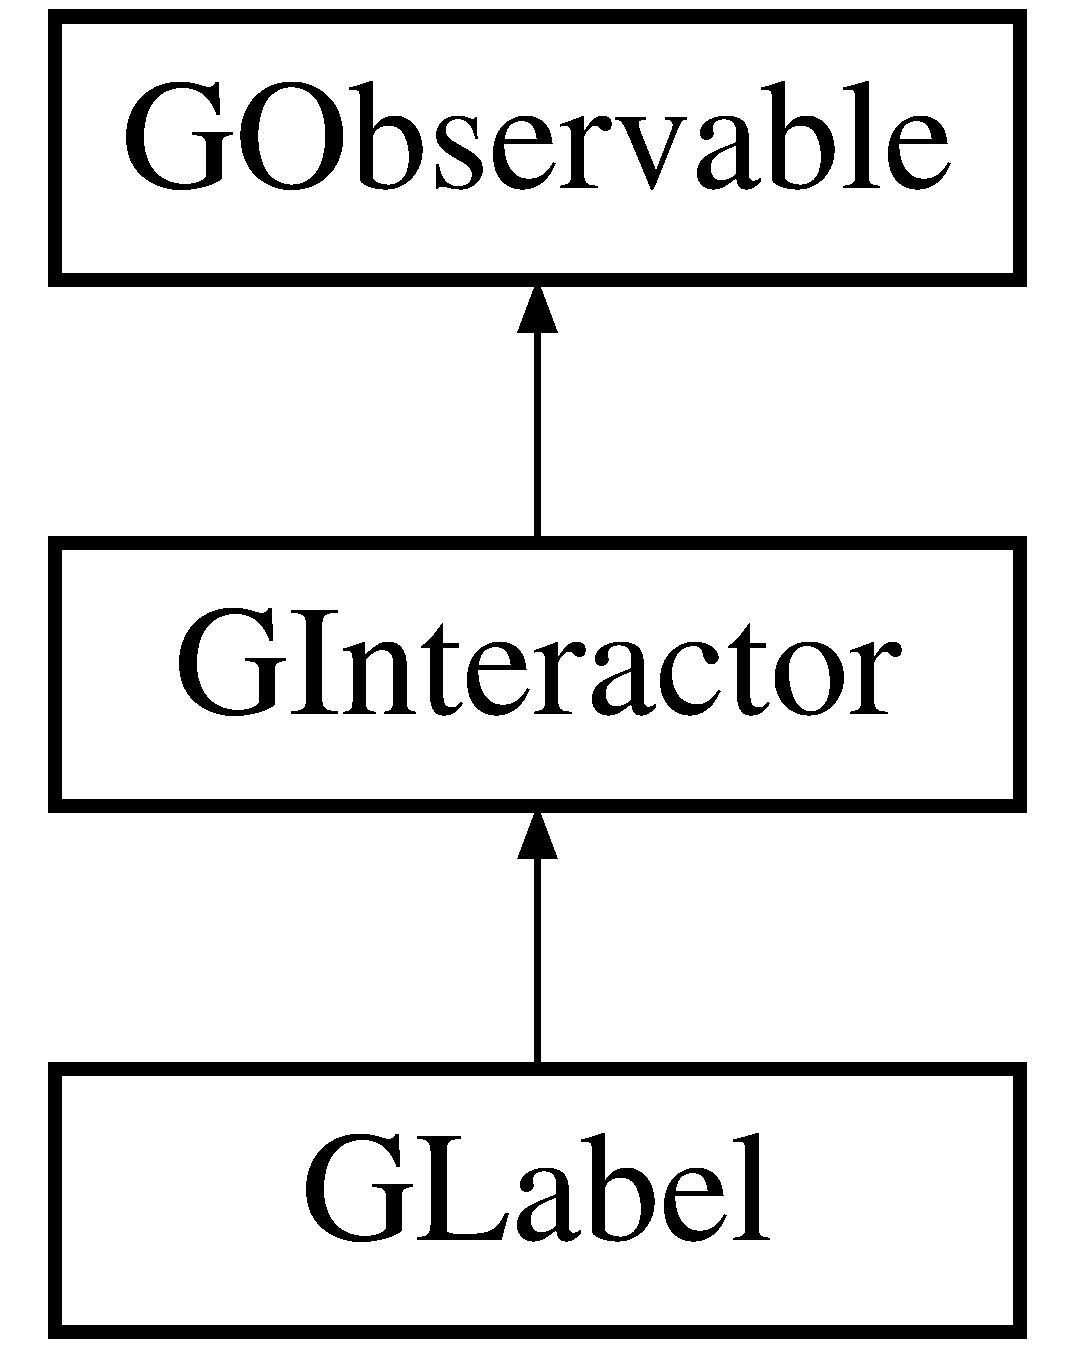
\includegraphics[height=3.000000cm]{classGLabel}
\end{center}
\end{figure}
\subsection*{Public Types}
\begin{DoxyCompactItemize}
\item 
enum \mbox{\hyperlink{classGInteractor_a8e0d441725a81d2bbdebbea09078260e}{Text\+Position}} \{ \mbox{\hyperlink{classGInteractor_a8e0d441725a81d2bbdebbea09078260ea4cd6f2e7d5a08d6f4dc052df2358f774}{T\+E\+X\+T\+\_\+\+B\+E\+S\+I\+D\+E\+\_\+\+I\+C\+ON}}, 
\mbox{\hyperlink{classGInteractor_a8e0d441725a81d2bbdebbea09078260eaa88490f63d8de68d44c83bdb2ecde3b3}{T\+E\+X\+T\+\_\+\+U\+N\+D\+E\+R\+\_\+\+I\+C\+ON}}, 
\mbox{\hyperlink{classGInteractor_a8e0d441725a81d2bbdebbea09078260ea39a6f388a30ac4fefb6eb13e846bc9f2}{T\+E\+X\+T\+\_\+\+O\+N\+LY}}
 \}
\begin{DoxyCompactList}\small\item\em The places where an interactor can place its text relative to its icon. \end{DoxyCompactList}\end{DoxyCompactItemize}
\subsection*{Public Member Functions}
\begin{DoxyCompactItemize}
\item 
\mbox{\hyperlink{classGLabel_adf89e6364d00b440441edce14145b387}{G\+Label}} (const std\+::string \&text=\char`\"{}\char`\"{}, const std\+::string \&icon\+File\+Name=\char`\"{}\char`\"{}, Q\+Widget $\ast$parent=nullptr)
\begin{DoxyCompactList}\small\item\em Creates a label with the specified text label and optional icon. \end{DoxyCompactList}\item 
\mbox{\hyperlink{classGLabel_a66c34c2b874bdb9dc0561b87ac2fccdd}{G\+Label}} (const std\+::string \&text, const Q\+Icon \&icon, Q\+Widget $\ast$parent=nullptr)
\begin{DoxyCompactList}\small\item\em Creates a label with the specified text label and icon. \end{DoxyCompactList}\item 
\mbox{\hyperlink{classGLabel_ad3979ef59a046161fc57992d97bebe54}{G\+Label}} (const std\+::string \&text, const Q\+Pixmap \&icon, Q\+Widget $\ast$parent=nullptr)
\begin{DoxyCompactList}\small\item\em Creates a label with the specified text label and icon. \end{DoxyCompactList}\item 
\mbox{\hyperlink{classGLabel_a1d11ab4dd459b9a9b1f28410344cfc33}{$\sim$\+G\+Label}} () override
\begin{DoxyCompactList}\small\item\em Frees memory allocated internally by the label. \end{DoxyCompactList}\item 
virtual void \mbox{\hyperlink{classGInteractor_a02f20ea6edfa0671f31c4c648a253833}{add\+Action\+Listener}} () Q\+\_\+\+D\+E\+C\+L\+\_\+\+D\+E\+P\+R\+E\+C\+A\+T\+ED
\begin{DoxyCompactList}\small\item\em Adds an event listener to be notified when this interactor is clicked or generally interacted with. \end{DoxyCompactList}\item 
bool \mbox{\hyperlink{classGInteractor_a597a370b592e3737d38d9d2f4e2031ea}{events\+Enabled}} () const override
\begin{DoxyCompactList}\small\item\em Returns true if this interactor is currently accepting events. \end{DoxyCompactList}\item 
virtual std\+::string \mbox{\hyperlink{classGInteractor_a69f8d23ed8f207fbecad99960776e942}{get\+Accelerator}} () const
\begin{DoxyCompactList}\small\item\em Returns a string representing a hotkey for this interactor, or an empty string if no accelerator has been set. \end{DoxyCompactList}\item 
virtual std\+::string \mbox{\hyperlink{classGInteractor_a94eb4276000c4fdfb508ce9e6317a82a}{get\+Action\+Command}} () const
\begin{DoxyCompactList}\small\item\em Returns an action command for this interactor, which is a semi-\/unique string you can use to identify it when events occur. \end{DoxyCompactList}\item 
virtual std\+::string \mbox{\hyperlink{classGInteractor_a808e22cc1fdfbecf71ed8c64ef4600e0}{get\+Background}} () const
\begin{DoxyCompactList}\small\item\em Returns the background color of the interactor as a string. \end{DoxyCompactList}\item 
virtual int \mbox{\hyperlink{classGInteractor_a9e827257a55cb8cf4d9de2ec6bcfd7a0}{get\+Background\+Int}} () const
\begin{DoxyCompactList}\small\item\em Returns the background color of the interactor as an R\+GB integer. \end{DoxyCompactList}\item 
virtual \mbox{\hyperlink{structGRectangle}{G\+Rectangle}} \mbox{\hyperlink{classGInteractor_a29e6ac35a0b48f491a4c88194cc5da3b}{get\+Bounds}} () const
\begin{DoxyCompactList}\small\item\em Returns a rectangle representing the x/y position and size of this interactor. \end{DoxyCompactList}\item 
virtual std\+::string \mbox{\hyperlink{classGInteractor_aa061dfa488c31e18549d64363c1d0e34}{get\+Color}} () const
\begin{DoxyCompactList}\small\item\em Returns the foreground/text color of the interactor as a string. \end{DoxyCompactList}\item 
virtual int \mbox{\hyperlink{classGInteractor_a9635c7af766cdc3417f346683fa0e6c1}{get\+Color\+Int}} () const
\begin{DoxyCompactList}\small\item\em Returns the foreground/text color of the interactor as an R\+GB integer. \end{DoxyCompactList}\item 
virtual \mbox{\hyperlink{classGContainer}{G\+Container}} $\ast$ \mbox{\hyperlink{classGInteractor_a7a6e317c29d61030929b4cd2d1c00fe7}{get\+Container}} () const
\begin{DoxyCompactList}\small\item\em Returns a pointer to the onscreen container holding this interactor. \end{DoxyCompactList}\item 
virtual std\+::string \mbox{\hyperlink{classGInteractor_a894a5502900794eeb27d084c21f1d77d}{get\+Font}} () const
\begin{DoxyCompactList}\small\item\em Returns the font of this interactor\textquotesingle{}s text as a font string such as \char`\"{}\+Helvetica-\/12-\/\+Bold\char`\"{}. \end{DoxyCompactList}\item 
virtual std\+::string \mbox{\hyperlink{classGInteractor_a4fa2d8b0192a3a5b4af4bbfe71194d03}{get\+Foreground}} () const
\begin{DoxyCompactList}\small\item\em Returns the foreground/text color of the interactor as a string. \end{DoxyCompactList}\item 
virtual int \mbox{\hyperlink{classGInteractor_ac3b12ab385a6ef9ae90fc879860ba726}{get\+Foreground\+Int}} () const
\begin{DoxyCompactList}\small\item\em Returns the foreground/text color of the interactor as an R\+GB integer. \end{DoxyCompactList}\item 
virtual double \mbox{\hyperlink{classGInteractor_a1e7e353362434072875264cf95629f99}{get\+Height}} () const
\begin{DoxyCompactList}\small\item\em Returns the current onscreen height of this interactor in pixels. \end{DoxyCompactList}\item 
virtual std\+::string \mbox{\hyperlink{classGInteractor_aaed62a73004939a64da6f0eb9eb64d73}{get\+Icon}} () const
\begin{DoxyCompactList}\small\item\em Returns the file name of the icon associated with this interactor, or an empty string if no icon has been set. \end{DoxyCompactList}\item 
virtual int \mbox{\hyperlink{classGInteractor_a9c9659a6c6ba66b4107ba59c95a24241}{get\+ID}} () const
\begin{DoxyCompactList}\small\item\em Returns a globally unique identifier for this interactor, which is set when the interactor is constructed. \end{DoxyCompactList}\item 
\+\_\+\+Internal\+\_\+\+Q\+Widget $\ast$ \mbox{\hyperlink{classGLabel_a2f6b36b2517087dc90a366b5ce1f5323}{get\+Internal\+Widget}} () const override
\begin{DoxyCompactList}\small\item\em Returns a direct pointer to the internal Qt widget being wrapped by this interactor. \end{DoxyCompactList}\item 
virtual std\+::string \mbox{\hyperlink{classGLabel_aa73aa351564b091c0658f2368c6d5c5f}{get\+Label}} () const
\begin{DoxyCompactList}\small\item\em Returns the string displayed by the label. \end{DoxyCompactList}\item 
virtual \mbox{\hyperlink{structGPoint}{G\+Point}} \mbox{\hyperlink{classGInteractor_a4f83802015511edeb63b892830812c11}{get\+Location}} () const
\begin{DoxyCompactList}\small\item\em Returns an (x, y) point representing the onscreen location of the top-\/left corner of this interactor within its containing window. \end{DoxyCompactList}\item 
virtual double \mbox{\hyperlink{classGInteractor_aed4b0075fcc434499c3cb3e46896bda3}{get\+Minimum\+Height}} () const
\begin{DoxyCompactList}\small\item\em Returns the minimum height in pixels that this interactor will permit itself to be resized to. \end{DoxyCompactList}\item 
virtual \mbox{\hyperlink{structGDimension}{G\+Dimension}} \mbox{\hyperlink{classGInteractor_a66b5af0b32493b4d597ca0a3df2049ea}{get\+Minimum\+Size}} () const
\begin{DoxyCompactList}\small\item\em Returns a \mbox{\hyperlink{structGDimension}{G\+Dimension}} structure representing the minimum size in pixels that this interactor will permit itself to be resized to. \end{DoxyCompactList}\item 
virtual double \mbox{\hyperlink{classGInteractor_a59e668114fe3d49d2a0f28deb258f7c8}{get\+Minimum\+Width}} () const
\begin{DoxyCompactList}\small\item\em Returns the minimum width in pixels that this interactor will permit itself to be resized to. \end{DoxyCompactList}\item 
virtual std\+::string \mbox{\hyperlink{classGInteractor_a8a60438a5b55d0b2ceb35c8674b9d8c5}{get\+Name}} () const
\begin{DoxyCompactList}\small\item\em Returns a string representing a unique name for this interactor. \end{DoxyCompactList}\item 
virtual double \mbox{\hyperlink{classGInteractor_a747de0961653847bdc6615dbf756d715}{get\+Preferred\+Height}} () const
\begin{DoxyCompactList}\small\item\em Returns the height in pixels that this interactor would prefer to be, which would exactly fit its contents with no stretching or scrollbars. \end{DoxyCompactList}\item 
virtual \mbox{\hyperlink{structGDimension}{G\+Dimension}} \mbox{\hyperlink{classGInteractor_a4aabbee761d8e9116275401131b7ccd1}{get\+Preferred\+Size}} () const
\begin{DoxyCompactList}\small\item\em Returns a \mbox{\hyperlink{structGDimension}{G\+Dimension}} structure storing the width and height in pixels that this interactor would prefer to be, which would exactly fit its contents with no stretching or scrollbars. \end{DoxyCompactList}\item 
virtual double \mbox{\hyperlink{classGInteractor_a82bca31d37700fb0e35d2743352efd5e}{get\+Preferred\+Width}} () const
\begin{DoxyCompactList}\small\item\em Returns the height in pixels that this interactor would prefer to be, which would exactly fit its contents with no stretching or scrollbars. \end{DoxyCompactList}\item 
virtual \mbox{\hyperlink{structGDimension}{G\+Dimension}} \mbox{\hyperlink{classGInteractor_a7b4eec96a2bdc6420695d5796a78eea9}{get\+Size}} () const
\begin{DoxyCompactList}\small\item\em Returns a \mbox{\hyperlink{structGDimension}{G\+Dimension}} structure storing the current onscreen width and height of this interactor in pixels. \end{DoxyCompactList}\item 
virtual std\+::string \mbox{\hyperlink{classGLabel_aff553c50924b836c29f146ed34a7c6ec}{get\+Text}} () const
\begin{DoxyCompactList}\small\item\em Returns the string displayed by the label. \end{DoxyCompactList}\item 
virtual \mbox{\hyperlink{classGInteractor_a8e0d441725a81d2bbdebbea09078260e}{G\+Interactor\+::\+Text\+Position}} \mbox{\hyperlink{classGLabel_a3fc623df3ced62aca93fc344c2426899}{get\+Text\+Position}} () const
\begin{DoxyCompactList}\small\item\em Returns the label\textquotesingle{}s text position relative to its icon. \end{DoxyCompactList}\item 
std\+::string \mbox{\hyperlink{classGLabel_a9b72ede4ee8520f987a0c01e30654814}{get\+Type}} () const override
\begin{DoxyCompactList}\small\item\em Returns a string representing the class name of this interactor, such as \char`\"{}\+G\+Button\char`\"{} or \char`\"{}\+G\+Check\+Box\char`\"{}. \end{DoxyCompactList}\item 
Q\+Widget $\ast$ \mbox{\hyperlink{classGLabel_a3b33a602b31a6b809d020535a59db3b4}{get\+Widget}} () const override
\begin{DoxyCompactList}\small\item\em Returns a direct pointer to the internal Qt widget being wrapped by this interactor. \end{DoxyCompactList}\item 
virtual double \mbox{\hyperlink{classGInteractor_a0ed2965abd4f5701d2cadf71239faf19}{get\+Width}} () const
\begin{DoxyCompactList}\small\item\em Returns the current onscreen width of this interactor in pixels. \end{DoxyCompactList}\item 
virtual double \mbox{\hyperlink{classGInteractor_a344385751bee0720059403940d57a13e}{getX}} () const
\begin{DoxyCompactList}\small\item\em Returns the x-\/coordinate of the top-\/left pixel of this interactor within its onscreen window. \end{DoxyCompactList}\item 
virtual double \mbox{\hyperlink{classGInteractor_aafa51c7f8f38a09febbb9ce7853f77b4}{getY}} () const
\begin{DoxyCompactList}\small\item\em Returns the y-\/coordinate of the top-\/left pixel of this interactor within its onscreen window. \end{DoxyCompactList}\item 
virtual bool \mbox{\hyperlink{classGInteractor_afc480f652b8c5f1fb255e2269ce68879}{in\+Bounds}} (double x, double y) const
\begin{DoxyCompactList}\small\item\em Returns true if the given x/y pixel is within the bounds of this interactor. \end{DoxyCompactList}\item 
virtual bool \mbox{\hyperlink{classGInteractor_ae6d7982c1c627b677a5e776ca86118ed}{in\+Bounds}} (int x, int y) const
\begin{DoxyCompactList}\small\item\em Returns true if the given x/y pixel is within the bounds of this interactor. \end{DoxyCompactList}\item 
virtual bool \mbox{\hyperlink{classGInteractor_aacb819fb241851fd9fc045271baa4034}{is\+Enabled}} () const
\begin{DoxyCompactList}\small\item\em Returns true if this interactor is currently enabled. \end{DoxyCompactList}\item 
virtual bool \mbox{\hyperlink{classGInteractor_a9d8a6cfb13917785c143e74d40e4e2be}{is\+Visible}} () const
\begin{DoxyCompactList}\small\item\em Returns true if the interactor is visible on the screen. \end{DoxyCompactList}\item 
virtual bool \mbox{\hyperlink{classGLabel_a52b12a2d7b5e2fec7478e3715c98c315}{is\+Word\+Wrap}} () const
\begin{DoxyCompactList}\small\item\em Returns whether the label should wrap if its text is too long. \end{DoxyCompactList}\item 
virtual void \mbox{\hyperlink{classGInteractor_ab7fe7a876367b87cf7202f947f1d05e4}{remove\+Action\+Listener}} ()
\begin{DoxyCompactList}\small\item\em Removes the action listener from this interactor so that it will no longer call it when events occur. \end{DoxyCompactList}\item 
virtual void \mbox{\hyperlink{classGInteractor_ad39d0325cde6b97ebda4b9d7787c633b}{remove\+Click\+Listener}} ()
\begin{DoxyCompactList}\small\item\em Removes the click listener from this interactor so that it will no longer call it when events occur. \end{DoxyCompactList}\item 
virtual void \mbox{\hyperlink{classGInteractor_aa4250907e4cdd77349c04f0cf5cdd3d3}{remove\+Double\+Click\+Listener}} ()
\begin{DoxyCompactList}\small\item\em Removes the double-\/click listener from this interactor so that it will no longer call it when events occur. \end{DoxyCompactList}\item 
virtual void \mbox{\hyperlink{classGInteractor_a43095f41cab3be732b49f29970484b05}{remove\+Key\+Listener}} ()
\begin{DoxyCompactList}\small\item\em Removes the key listener from this interactor so that it will no longer call it when key events occur. \end{DoxyCompactList}\item 
virtual void \mbox{\hyperlink{classGInteractor_aff47f71ce47e688a07c9d38dc92fcc11}{remove\+Mouse\+Listener}} ()
\begin{DoxyCompactList}\small\item\em Removes the mouse listener from this interactor so that it will no longer call it when events occur. \end{DoxyCompactList}\item 
virtual void \mbox{\hyperlink{classGInteractor_a519fb2ac767f8b2febbb50b898b8c8cb}{request\+Focus}} ()
\begin{DoxyCompactList}\small\item\em Transfers keyboard focus to this interactor. \end{DoxyCompactList}\item 
virtual void \mbox{\hyperlink{classGInteractor_ad15f102f62e2960576012f1aa0ba4b2e}{set\+Accelerator}} (const std\+::string \&accelerator)
\begin{DoxyCompactList}\small\item\em Sets an accelerator hotkey for this interactor, such as \char`\"{}\+Ctrl-\/\+S\char`\"{}. \end{DoxyCompactList}\item 
virtual void \mbox{\hyperlink{classGInteractor_a4b5843fe3030e038a1ba54cc03389bcf}{set\+Action\+Command}} (const std\+::string \&action\+Command)
\begin{DoxyCompactList}\small\item\em Sets the action command for this interactor. \end{DoxyCompactList}\item 
virtual void \mbox{\hyperlink{classGInteractor_adcfb4742430c88714fcf57e57ab8ea9c}{set\+Action\+Listener}} (G\+Event\+Listener func)
\begin{DoxyCompactList}\small\item\em Sets an action listener on this interactor so that it will be called when it is interacted with in its primary way. \end{DoxyCompactList}\item 
virtual void \mbox{\hyperlink{classGInteractor_aebd20a89c7a8a43a6fce999cf4f9fcf2}{set\+Action\+Listener}} (G\+Event\+Listener\+Void func)
\begin{DoxyCompactList}\small\item\em Sets an action listener on this interactor so that it will be called when it is interacted with in its primary way. \end{DoxyCompactList}\item 
virtual void \mbox{\hyperlink{classGInteractor_acba7e546c2025c0a15ca4b4cc92043db}{set\+Background}} (int rgb)
\begin{DoxyCompactList}\small\item\em Sets the background color of the interactor to the color represented by the given R\+GB integer. \end{DoxyCompactList}\item 
virtual void \mbox{\hyperlink{classGInteractor_ab4677ab2474e68b07aa56605af92a84a}{set\+Background}} (const std\+::string \&color)
\begin{DoxyCompactList}\small\item\em Sets the background color of the interactor to the color represented by the given string. \end{DoxyCompactList}\item 
void \mbox{\hyperlink{classGLabel_ab9f89f193ad29d66c547cfee29ffde39}{set\+Bounds}} (double x, double y, double width, double height) override
\begin{DoxyCompactList}\small\item\em Sets the size and location of the widget. \end{DoxyCompactList}\item 
void \mbox{\hyperlink{classGLabel_adb836652705fdc4b7e90b7a3afc56a37}{set\+Bounds}} (const \mbox{\hyperlink{structGRectangle}{G\+Rectangle}} \&size) override
\begin{DoxyCompactList}\small\item\em Sets the size and location of the widget. \end{DoxyCompactList}\item 
virtual void \mbox{\hyperlink{classGInteractor_abd40af6921242584d0954f173911b190}{set\+Click\+Listener}} (G\+Event\+Listener func)
\begin{DoxyCompactList}\small\item\em Sets a mouse listener on this interactor so that it will be called when the mouse is clicked on it. \end{DoxyCompactList}\item 
virtual void \mbox{\hyperlink{classGInteractor_a856414c92df90f56f3877475eb3f8fc4}{set\+Click\+Listener}} (G\+Event\+Listener\+Void func)
\begin{DoxyCompactList}\small\item\em Sets a mouse listener on this interactor so that it will be called when the mouse is clicked on it. \end{DoxyCompactList}\item 
void \mbox{\hyperlink{classGLabel_a165735fb49fa7db12602d32557cbfe0d}{set\+Color}} (int rgb) override
\begin{DoxyCompactList}\small\item\em Sets the foreground/text color of the interactor to the color represented by the given R\+GB integer. \end{DoxyCompactList}\item 
void \mbox{\hyperlink{classGLabel_a56845b1accc47aa881d05939eef6996c}{set\+Color}} (const std\+::string \&color) override
\begin{DoxyCompactList}\small\item\em Sets the foreground/text color of the interactor to the color represented by the given string. \end{DoxyCompactList}\item 
virtual void \mbox{\hyperlink{classGInteractor_ac29f9a3462458e165fae3a1f046ee77a}{set\+Double\+Click\+Listener}} (G\+Event\+Listener func)
\begin{DoxyCompactList}\small\item\em Sets a mouse listener on this interactor so that it will be called when the mouse is double-\/clicked on it. \end{DoxyCompactList}\item 
virtual void \mbox{\hyperlink{classGInteractor_a50096194d66f48c92dd4c512d41bfc76}{set\+Double\+Click\+Listener}} (G\+Event\+Listener\+Void func)
\begin{DoxyCompactList}\small\item\em Sets a mouse listener on this interactor so that it will be called when the mouse is double-\/clicked on it. \end{DoxyCompactList}\item 
virtual void \mbox{\hyperlink{classGInteractor_ab831367dd84bbd579e02e55bacb21343}{set\+Enabled}} (bool value)
\begin{DoxyCompactList}\small\item\em Sets whether this interactor is currently enabled. \end{DoxyCompactList}\item 
virtual void \mbox{\hyperlink{classGObservable_afaa30b2a9e0f378fd1c70d2f1d0b8216}{set\+Events\+Enabled}} (bool \mbox{\hyperlink{classGInteractor_a597a370b592e3737d38d9d2f4e2031ea}{events\+Enabled}})
\begin{DoxyCompactList}\small\item\em Sets whether the object is currently allowing itself to fire events. \end{DoxyCompactList}\item 
void \mbox{\hyperlink{classGLabel_ad1d75b3840a41ba7d1e8a921696dc684}{set\+Font}} (const Q\+Font \&font) override
\begin{DoxyCompactList}\small\item\em Sets the font used by this widget to the given Qt font. \end{DoxyCompactList}\item 
void \mbox{\hyperlink{classGLabel_a51367c9fd2709973b1f7238734f93891}{set\+Font}} (const std\+::string \&font) override
\begin{DoxyCompactList}\small\item\em Sets the font used by this widget to the font represented by the given font string, such as \char`\"{}\+Helvetica-\/16-\/\+Bold\char`\"{}. \end{DoxyCompactList}\item 
void \mbox{\hyperlink{classGLabel_a59f7cd2bd1708c12dfa52a8f7c7b79c9}{set\+Foreground}} (int rgb) override
\begin{DoxyCompactList}\small\item\em Sets the foreground/text color of the interactor to the color represented by the given R\+GB integer. \end{DoxyCompactList}\item 
void \mbox{\hyperlink{classGLabel_a8afbcf1f47750fb4c717f9ff36540235}{set\+Foreground}} (const std\+::string \&color) override
\begin{DoxyCompactList}\small\item\em Sets the foreground/text color of the interactor to the color represented by the given string. \end{DoxyCompactList}\item 
void \mbox{\hyperlink{classGLabel_a5eead864d1249c4406f32f9944ed1503}{set\+Height}} (double height) override
\begin{DoxyCompactList}\small\item\em Sets the onscreen height of the interactor in pixels. \end{DoxyCompactList}\item 
void \mbox{\hyperlink{classGLabel_acca97b6c6330abded1c80521c9aca3a6}{set\+Icon}} (const Q\+Icon \&icon) override
\begin{DoxyCompactList}\small\item\em Sets the icon associated with this interactor. \end{DoxyCompactList}\item 
void \mbox{\hyperlink{classGLabel_acb5275b880ff622d306f8f33428b4e34}{set\+Icon}} (const Q\+Pixmap \&icon) override
\begin{DoxyCompactList}\small\item\em Sets the icon associated with this interactor. \end{DoxyCompactList}\item 
void \mbox{\hyperlink{classGLabel_abbefcb1f611af273755c7e1cca921497}{set\+Icon}} (const std\+::string \&filename, bool retain\+Icon\+Size=true) override
\begin{DoxyCompactList}\small\item\em Sets the file name of the icon associated with this interactor, or an empty string if no icon has been set. \end{DoxyCompactList}\item 
virtual void \mbox{\hyperlink{classGInteractor_aeb8324d3287fa1fbe093f4d6230cf0a6}{set\+Key\+Listener}} (G\+Event\+Listener func)
\begin{DoxyCompactList}\small\item\em Sets a key listener on this interactor so that it will be called when the user presses any key. \end{DoxyCompactList}\item 
virtual void \mbox{\hyperlink{classGInteractor_ae48ecea73606c7bd9423e1c7cc589cc9}{set\+Key\+Listener}} (G\+Event\+Listener\+Void func)
\begin{DoxyCompactList}\small\item\em Sets a key listener on this interactor so that it will be called when the user presses any key. \end{DoxyCompactList}\item 
virtual void \mbox{\hyperlink{classGLabel_a4af0be0e092d87271c1432624bc00080}{set\+Label}} (const std\+::string \&text)
\begin{DoxyCompactList}\small\item\em Sets the text on the label to be the given text. \end{DoxyCompactList}\item 
void \mbox{\hyperlink{classGLabel_ae3b17c0aeb355dc23c4e4cbf066e81f7}{set\+Location}} (double x, double y) override
\begin{DoxyCompactList}\small\item\em Sets the onscreen x/y-\/coordinate of the top-\/left corner of the interactor relative to its window. \end{DoxyCompactList}\item 
virtual void \mbox{\hyperlink{classGInteractor_a0cf428e207b7f22cc08138a90b1b87b2}{set\+Minimum\+Size}} (double width, double height)
\begin{DoxyCompactList}\small\item\em Sets the minimum size in pixels that this interactor will permit itself to be resized to. \end{DoxyCompactList}\item 
virtual void \mbox{\hyperlink{classGInteractor_a3b1046117ac6cb7abe467e00ba8a81f4}{set\+Minimum\+Size}} (const \mbox{\hyperlink{structGDimension}{G\+Dimension}} \&size)
\begin{DoxyCompactList}\small\item\em Sets the minimum size in pixels that this interactor will permit itself to be resized to. \end{DoxyCompactList}\item 
virtual void \mbox{\hyperlink{classGInteractor_a37d8dbc943f59920f705b0104f60bde2}{set\+Mouse\+Listener}} (G\+Event\+Listener func)
\begin{DoxyCompactList}\small\item\em Sets a mouse listener on this interactor so that it will be called when the mouse is moved or clicked on it. \end{DoxyCompactList}\item 
virtual void \mbox{\hyperlink{classGInteractor_aea7f647ea62d59f71b5fad6aa65eeaf9}{set\+Mouse\+Listener}} (G\+Event\+Listener\+Void func)
\begin{DoxyCompactList}\small\item\em Sets a mouse listener on this interactor so that it will be called when the mouse is moved or clicked on it. \end{DoxyCompactList}\item 
virtual void \mbox{\hyperlink{classGInteractor_a9d3a2685df23b5e7cbf59c19c4a1f9b5}{set\+Name}} (const std\+::string \&name)
\begin{DoxyCompactList}\small\item\em Sets a string representing a unique name for this interactor. \end{DoxyCompactList}\item 
virtual void \mbox{\hyperlink{classGInteractor_a1ab987704fce32098706c6f00fb08218}{set\+Preferred\+Height}} (double height)
\begin{DoxyCompactList}\small\item\em Sets the height in pixels that this interactor would prefer to be. \end{DoxyCompactList}\item 
virtual void \mbox{\hyperlink{classGInteractor_a042c5ae19430d765ef552371cae3632c}{set\+Preferred\+Size}} (double width, double height)
\begin{DoxyCompactList}\small\item\em Sets the width and height in pixels that this interactor would prefer to be. \end{DoxyCompactList}\item 
virtual void \mbox{\hyperlink{classGInteractor_aa22d9be4bc0e078bb0ea69b0fc9d7c75}{set\+Preferred\+Size}} (const \mbox{\hyperlink{structGDimension}{G\+Dimension}} \&size)
\begin{DoxyCompactList}\small\item\em Sets the size in pixels that this interactor would prefer to be. \end{DoxyCompactList}\item 
virtual void \mbox{\hyperlink{classGInteractor_a3db429ab2fa52efd187eec0ed8cdd9f2}{set\+Preferred\+Width}} (double width)
\begin{DoxyCompactList}\small\item\em Sets the width in pixels that this interactor would prefer to be. \end{DoxyCompactList}\item 
void \mbox{\hyperlink{classGLabel_a8ba9af72c23f52d4b93096a13a11f150}{set\+Size}} (double width, double height) override
\begin{DoxyCompactList}\small\item\em Sets the onscreen width and height of the interactor in pixels. \end{DoxyCompactList}\item 
void \mbox{\hyperlink{classGLabel_a42d96e60c62d7770993327d7147d77b8}{set\+Size}} (const \mbox{\hyperlink{structGDimension}{G\+Dimension}} \&size) override
\begin{DoxyCompactList}\small\item\em Sets the onscreen width and height of the interactor in pixels. \end{DoxyCompactList}\item 
virtual void \mbox{\hyperlink{classGLabel_ac1ae51949d41ee9054634be5967d91b8}{set\+Text}} (const std\+::string \&text)
\begin{DoxyCompactList}\small\item\em Sets the text on the label to be the given text. \end{DoxyCompactList}\item 
virtual void \mbox{\hyperlink{classGLabel_af822b8d73c652f7c59d875d7cdfc5302}{set\+Text\+Position}} (\mbox{\hyperlink{classGInteractor_a8e0d441725a81d2bbdebbea09078260e}{G\+Interactor\+::\+Text\+Position}} position)
\begin{DoxyCompactList}\small\item\em Sets the label\textquotesingle{}s text position relative to its icon. \end{DoxyCompactList}\item 
virtual void \mbox{\hyperlink{classGInteractor_a039e0e49beaecc275efce02d416acea8}{set\+Tooltip}} (const std\+::string \&tooltip\+Text)
\begin{DoxyCompactList}\small\item\em Sets a \char`\"{}tooltip\char`\"{} that will appear if the user hovers their mouse over the interactor. \end{DoxyCompactList}\item 
void \mbox{\hyperlink{classGLabel_afcc2a51afef8e2e61d8d9191386fb93f}{set\+Visible}} (bool visible) override
\begin{DoxyCompactList}\small\item\em Returns true if the interactor is visible on the screen. \end{DoxyCompactList}\item 
void \mbox{\hyperlink{classGLabel_af0c5b6fb4e3c3c9a3fabde548efa93db}{set\+Width}} (double width) override
\begin{DoxyCompactList}\small\item\em Sets the onscreen width of the interactor in pixels. \end{DoxyCompactList}\item 
virtual void \mbox{\hyperlink{classGLabel_a8e935ba463ac070ea906118661b15a5f}{set\+Word\+Wrap}} (bool wrap)
\begin{DoxyCompactList}\small\item\em Sets whether the label should wrap if its text is too long. \end{DoxyCompactList}\item 
void \mbox{\hyperlink{classGLabel_a173837ba805eaa2411e88834869d3a9c}{setX}} (double x) override
\begin{DoxyCompactList}\small\item\em Sets the onscreen x-\/coordinate of the top-\/left corner of the interactor relative to its window. \end{DoxyCompactList}\item 
void \mbox{\hyperlink{classGLabel_a0b738606c7aca5c472b66c4e55b3c685}{setY}} (double y) override
\begin{DoxyCompactList}\small\item\em Sets the onscreen y-\/coordinate of the top-\/left corner of the interactor relative to its window. \end{DoxyCompactList}\item 
virtual std\+::string \mbox{\hyperlink{classGObservable_a1fe5121d6528fdea3f243321b3fa3a49}{to\+String}} () const
\begin{DoxyCompactList}\small\item\em Returns a string representation of this observable object\textquotesingle{}s state. \end{DoxyCompactList}\end{DoxyCompactItemize}
\subsection*{Protected Member Functions}
\begin{DoxyCompactItemize}
\item 
virtual void \mbox{\hyperlink{classGObservable_a80cfa040459ff53594adbd6a51ec8f43}{clear\+Event\+Listeners}} ()
\begin{DoxyCompactList}\small\item\em Removes all event listeners from this object. \end{DoxyCompactList}\item 
virtual void \mbox{\hyperlink{classGObservable_a284f31528c0520f8e545c03ac9eeac74}{ensure\+Thread\+Safety}} (const std\+::string \&member\+Name=\char`\"{}\char`\"{})
\begin{DoxyCompactList}\small\item\em Ensures that we are currently in the Qt G\+UI thread. \end{DoxyCompactList}\item 
virtual void \mbox{\hyperlink{classGObservable_a63e5e5a6227c59c928493b11aceb0f67}{fire\+Event}} (\mbox{\hyperlink{classGEvent}{G\+Event}} \&event)
\begin{DoxyCompactList}\small\item\em Sends out the given event to any attached listeners. \end{DoxyCompactList}\item 
virtual void \mbox{\hyperlink{classGObservable_ab3983ea07337b52020a29cc00c653d8d}{fire\+G\+Event}} (Q\+Event $\ast$event, Event\+Type event\+Type, const std\+::string \&event\+Name)
\begin{DoxyCompactList}\small\item\em Creates an event of the given type, then sends it out to any attached listeners. \end{DoxyCompactList}\item 
virtual void \mbox{\hyperlink{classGObservable_a01fdf1b0e0dbd49e189fe4514e010411}{fire\+G\+Event}} (Q\+Close\+Event $\ast$event, Event\+Type event\+Type, const std\+::string \&event\+Name)
\begin{DoxyCompactList}\small\item\em Creates an event of the given type, then sends it out to any attached listeners. \end{DoxyCompactList}\item 
virtual void \mbox{\hyperlink{classGObservable_abb0b2f66ba39211cb5d7615e9d1c04e2}{fire\+G\+Event}} (Q\+Key\+Event $\ast$event, Event\+Type event\+Type, const std\+::string \&event\+Name)
\begin{DoxyCompactList}\small\item\em Creates an event of the given type, then sends it out to any attached listeners. \end{DoxyCompactList}\item 
virtual void \mbox{\hyperlink{classGObservable_a119318675d2165bdf7dd853aaf881d4b}{fire\+G\+Event}} (Q\+Mouse\+Event $\ast$event, Event\+Type event\+Type, const std\+::string \&event\+Name, const std\+::string \&action\+Command=\char`\"{}\char`\"{})
\begin{DoxyCompactList}\small\item\em Creates an event of the given type, then sends it out to any attached listeners. \end{DoxyCompactList}\item 
virtual void \mbox{\hyperlink{classGObservable_a63fd9034e1e1633c1c38eb342bfd34e9}{fire\+G\+Event}} (Q\+Resize\+Event $\ast$event, Event\+Type event\+Type, const std\+::string \&event\+Name)
\begin{DoxyCompactList}\small\item\em Creates an event of the given type, then sends it out to any attached listeners. \end{DoxyCompactList}\item 
virtual void \mbox{\hyperlink{classGObservable_a741345310d9b7c5170a6cbc410c44ac4}{fire\+G\+Event}} (Q\+Timer\+Event $\ast$event, Event\+Type event\+Type, const std\+::string \&event\+Name)
\begin{DoxyCompactList}\small\item\em Creates an event of the given type, then sends it out to any attached listeners. \end{DoxyCompactList}\item 
virtual void \mbox{\hyperlink{classGObservable_a93bf338968a0338761b8e4dc62f582e9}{fire\+G\+Event}} (Q\+Wheel\+Event $\ast$event, Event\+Type event\+Type, const std\+::string \&event\+Name)
\begin{DoxyCompactList}\small\item\em Creates an event of the given type, then sends it out to any attached listeners. \end{DoxyCompactList}\item 
virtual void \mbox{\hyperlink{classGObservable_a2a70a7d7435ff0c3b80bb4d70da19e0d}{fire\+G\+Event}} (Q\+Window\+State\+Change\+Event $\ast$event, Event\+Type event\+Type, const std\+::string \&event\+Name)
\begin{DoxyCompactList}\small\item\em Creates an event of the given type, then sends it out to any attached listeners. \end{DoxyCompactList}\item 
virtual bool \mbox{\hyperlink{classGObservable_a9f6faaa25942923bafa1c44020c49fa9}{has\+Event\+Listener}} (const std\+::string \&event\+Name) const
\begin{DoxyCompactList}\small\item\em Returns true if the observable object has a listener for the given type of event. \end{DoxyCompactList}\item 
virtual bool \mbox{\hyperlink{classGObservable_aeec1adc19aa0f33de62390686ee1382c}{is\+Accepting\+Event}} (int event\+Mask) const
\begin{DoxyCompactList}\small\item\em Returns true if the observable object has a listener for the given type of event. \end{DoxyCompactList}\item 
virtual bool \mbox{\hyperlink{classGObservable_aa31c73145a29dcb92848a92e0cfaea41}{is\+Accepting\+Event}} (const \mbox{\hyperlink{classGEvent}{G\+Event}} \&event) const
\begin{DoxyCompactList}\small\item\em Returns true if the observable object has a listener for the given type of event. \end{DoxyCompactList}\item 
virtual bool \mbox{\hyperlink{classGObservable_a3b1c689267eda44e65a2213e7de38b23}{is\+Accepting\+Event}} (const std\+::string \&event\+Type) const
\begin{DoxyCompactList}\small\item\em Returns true if the observable object has a listener for the given type of event. \end{DoxyCompactList}\item 
virtual void \mbox{\hyperlink{classGObservable_acbcf1ed3a851ad8a3c17ef38d86b481d}{remove\+Event\+Listener}} (const std\+::string \&event\+Name)
\begin{DoxyCompactList}\small\item\em Removes any event listener from this observable object that would respond to the given type of event, such as \char`\"{}click\char`\"{} or \char`\"{}keydown\char`\"{}. \end{DoxyCompactList}\item 
virtual void \mbox{\hyperlink{classGObservable_af51cc35c29a1bd1908609d432decdbb6}{remove\+Event\+Listeners}} (std\+::initializer\+\_\+list$<$ std\+::string $>$ event\+Names)
\begin{DoxyCompactList}\small\item\em Removes any event listener from this observable object that would respond to the given types of events, such as \char`\"{}click\char`\"{} or \char`\"{}keydown\char`\"{}. \end{DoxyCompactList}\item 
virtual void \mbox{\hyperlink{classGObservable_ad2f6d34961c50f6c1e0659990b79f741}{set\+Event\+Listener}} (const std\+::string \&event\+Name, G\+Event\+Listener func)
\begin{DoxyCompactList}\small\item\em Adds an event listener from this observable object to respond to the given type of event, such as \char`\"{}click\char`\"{} or \char`\"{}keydown\char`\"{}. \end{DoxyCompactList}\item 
virtual void \mbox{\hyperlink{classGObservable_abac4cb9f9e626e010e87f5d91573c8a5}{set\+Event\+Listener}} (const std\+::string \&event\+Name, G\+Event\+Listener\+Void func)
\begin{DoxyCompactList}\small\item\em Adds an event listener from this observable object to respond to the given type of event, such as \char`\"{}click\char`\"{} or \char`\"{}keydown\char`\"{}. \end{DoxyCompactList}\item 
virtual void \mbox{\hyperlink{classGObservable_afa388d69c33c718cf035774604065604}{set\+Event\+Listeners}} (std\+::initializer\+\_\+list$<$ std\+::string $>$ event\+Names, G\+Event\+Listener func)
\begin{DoxyCompactList}\small\item\em Adds an event listener from this observable object to respond to the given types of events, such as \char`\"{}click\char`\"{} or \char`\"{}keydown\char`\"{}. \end{DoxyCompactList}\item 
virtual void \mbox{\hyperlink{classGObservable_a7867184bbb686f74fae8a4db927da799}{set\+Event\+Listeners}} (std\+::initializer\+\_\+list$<$ std\+::string $>$ event\+Names, G\+Event\+Listener\+Void func)
\begin{DoxyCompactList}\small\item\em Adds an event listener from this observable object to respond to the given types of events, such as \char`\"{}click\char`\"{} or \char`\"{}keydown\char`\"{}. \end{DoxyCompactList}\end{DoxyCompactItemize}


\subsection{Detailed Description}
A \mbox{\hyperlink{classGLabel}{G\+Label}} represents a text string. 

A label can contain text and/or an image icon.

G\+Labels can be made clickable by setting an action, click, or double-\/click listener, but generally if you want a clickable interactor with text on it, you may prefer a \mbox{\hyperlink{classGButton}{G\+Button}}. 

\subsection{Member Enumeration Documentation}
\mbox{\Hypertarget{classGInteractor_a8e0d441725a81d2bbdebbea09078260e}\label{classGInteractor_a8e0d441725a81d2bbdebbea09078260e}} 
\index{G\+Label@{G\+Label}!Text\+Position@{Text\+Position}}
\index{Text\+Position@{Text\+Position}!G\+Label@{G\+Label}}
\subsubsection{\texorpdfstring{Text\+Position}{TextPosition}}
{\footnotesize\ttfamily enum \mbox{\hyperlink{classGInteractor_a8e0d441725a81d2bbdebbea09078260e}{Text\+Position}}\hspace{0.3cm}{\ttfamily [inherited]}}



The places where an interactor can place its text relative to its icon. 

\begin{DoxyEnumFields}{Enumerator}
\raisebox{\heightof{T}}[0pt][0pt]{\index{T\+E\+X\+T\+\_\+\+B\+E\+S\+I\+D\+E\+\_\+\+I\+C\+ON@{T\+E\+X\+T\+\_\+\+B\+E\+S\+I\+D\+E\+\_\+\+I\+C\+ON}!G\+Label@{G\+Label}}\index{G\+Label@{G\+Label}!T\+E\+X\+T\+\_\+\+B\+E\+S\+I\+D\+E\+\_\+\+I\+C\+ON@{T\+E\+X\+T\+\_\+\+B\+E\+S\+I\+D\+E\+\_\+\+I\+C\+ON}}}\mbox{\Hypertarget{classGInteractor_a8e0d441725a81d2bbdebbea09078260ea4cd6f2e7d5a08d6f4dc052df2358f774}\label{classGInteractor_a8e0d441725a81d2bbdebbea09078260ea4cd6f2e7d5a08d6f4dc052df2358f774}} 
T\+E\+X\+T\+\_\+\+B\+E\+S\+I\+D\+E\+\_\+\+I\+C\+ON&\\
\hline

\raisebox{\heightof{T}}[0pt][0pt]{\index{T\+E\+X\+T\+\_\+\+U\+N\+D\+E\+R\+\_\+\+I\+C\+ON@{T\+E\+X\+T\+\_\+\+U\+N\+D\+E\+R\+\_\+\+I\+C\+ON}!G\+Label@{G\+Label}}\index{G\+Label@{G\+Label}!T\+E\+X\+T\+\_\+\+U\+N\+D\+E\+R\+\_\+\+I\+C\+ON@{T\+E\+X\+T\+\_\+\+U\+N\+D\+E\+R\+\_\+\+I\+C\+ON}}}\mbox{\Hypertarget{classGInteractor_a8e0d441725a81d2bbdebbea09078260eaa88490f63d8de68d44c83bdb2ecde3b3}\label{classGInteractor_a8e0d441725a81d2bbdebbea09078260eaa88490f63d8de68d44c83bdb2ecde3b3}} 
T\+E\+X\+T\+\_\+\+U\+N\+D\+E\+R\+\_\+\+I\+C\+ON&\\
\hline

\raisebox{\heightof{T}}[0pt][0pt]{\index{T\+E\+X\+T\+\_\+\+O\+N\+LY@{T\+E\+X\+T\+\_\+\+O\+N\+LY}!G\+Label@{G\+Label}}\index{G\+Label@{G\+Label}!T\+E\+X\+T\+\_\+\+O\+N\+LY@{T\+E\+X\+T\+\_\+\+O\+N\+LY}}}\mbox{\Hypertarget{classGInteractor_a8e0d441725a81d2bbdebbea09078260ea39a6f388a30ac4fefb6eb13e846bc9f2}\label{classGInteractor_a8e0d441725a81d2bbdebbea09078260ea39a6f388a30ac4fefb6eb13e846bc9f2}} 
T\+E\+X\+T\+\_\+\+O\+N\+LY&\\
\hline

\end{DoxyEnumFields}


\subsection{Constructor \& Destructor Documentation}
\mbox{\Hypertarget{classGLabel_adf89e6364d00b440441edce14145b387}\label{classGLabel_adf89e6364d00b440441edce14145b387}} 
\index{G\+Label@{G\+Label}!G\+Label@{G\+Label}}
\index{G\+Label@{G\+Label}!G\+Label@{G\+Label}}
\subsubsection{\texorpdfstring{G\+Label()}{GLabel()}\hspace{0.1cm}{\footnotesize\ttfamily [1/3]}}
{\footnotesize\ttfamily \mbox{\hyperlink{classGLabel}{G\+Label}} (\begin{DoxyParamCaption}\item[{const std\+::string \&}]{text = {\ttfamily \char`\"{}\char`\"{}},  }\item[{const std\+::string \&}]{icon\+File\+Name = {\ttfamily \char`\"{}\char`\"{}},  }\item[{Q\+Widget $\ast$}]{parent = {\ttfamily nullptr} }\end{DoxyParamCaption})}



Creates a label with the specified text label and optional icon. 

\mbox{\Hypertarget{classGLabel_a66c34c2b874bdb9dc0561b87ac2fccdd}\label{classGLabel_a66c34c2b874bdb9dc0561b87ac2fccdd}} 
\index{G\+Label@{G\+Label}!G\+Label@{G\+Label}}
\index{G\+Label@{G\+Label}!G\+Label@{G\+Label}}
\subsubsection{\texorpdfstring{G\+Label()}{GLabel()}\hspace{0.1cm}{\footnotesize\ttfamily [2/3]}}
{\footnotesize\ttfamily \mbox{\hyperlink{classGLabel}{G\+Label}} (\begin{DoxyParamCaption}\item[{const std\+::string \&}]{text,  }\item[{const Q\+Icon \&}]{icon,  }\item[{Q\+Widget $\ast$}]{parent = {\ttfamily nullptr} }\end{DoxyParamCaption})}



Creates a label with the specified text label and icon. 

\mbox{\Hypertarget{classGLabel_ad3979ef59a046161fc57992d97bebe54}\label{classGLabel_ad3979ef59a046161fc57992d97bebe54}} 
\index{G\+Label@{G\+Label}!G\+Label@{G\+Label}}
\index{G\+Label@{G\+Label}!G\+Label@{G\+Label}}
\subsubsection{\texorpdfstring{G\+Label()}{GLabel()}\hspace{0.1cm}{\footnotesize\ttfamily [3/3]}}
{\footnotesize\ttfamily \mbox{\hyperlink{classGLabel}{G\+Label}} (\begin{DoxyParamCaption}\item[{const std\+::string \&}]{text,  }\item[{const Q\+Pixmap \&}]{icon,  }\item[{Q\+Widget $\ast$}]{parent = {\ttfamily nullptr} }\end{DoxyParamCaption})}



Creates a label with the specified text label and icon. 

\mbox{\Hypertarget{classGLabel_a1d11ab4dd459b9a9b1f28410344cfc33}\label{classGLabel_a1d11ab4dd459b9a9b1f28410344cfc33}} 
\index{G\+Label@{G\+Label}!````~G\+Label@{$\sim$\+G\+Label}}
\index{````~G\+Label@{$\sim$\+G\+Label}!G\+Label@{G\+Label}}
\subsubsection{\texorpdfstring{$\sim$\+G\+Label()}{~GLabel()}}
{\footnotesize\ttfamily $\sim$\mbox{\hyperlink{classGLabel}{G\+Label}} (\begin{DoxyParamCaption}{ }\end{DoxyParamCaption})\hspace{0.3cm}{\ttfamily [override]}}



Frees memory allocated internally by the label. 



\subsection{Member Function Documentation}
\mbox{\Hypertarget{classGInteractor_a02f20ea6edfa0671f31c4c648a253833}\label{classGInteractor_a02f20ea6edfa0671f31c4c648a253833}} 
\index{G\+Label@{G\+Label}!add\+Action\+Listener@{add\+Action\+Listener}}
\index{add\+Action\+Listener@{add\+Action\+Listener}!G\+Label@{G\+Label}}
\subsubsection{\texorpdfstring{add\+Action\+Listener()}{addActionListener()}}
{\footnotesize\ttfamily void add\+Action\+Listener (\begin{DoxyParamCaption}{ }\end{DoxyParamCaption})\hspace{0.3cm}{\ttfamily [virtual]}, {\ttfamily [inherited]}}



Adds an event listener to be notified when this interactor is clicked or generally interacted with. 

\begin{DoxyRefDesc}{Deprecated}
\item[\mbox{\hyperlink{deprecated__deprecated000006}{Deprecated}}]does nothing; use set\+Action\+Listener instead \end{DoxyRefDesc}
\mbox{\Hypertarget{classGObservable_a80cfa040459ff53594adbd6a51ec8f43}\label{classGObservable_a80cfa040459ff53594adbd6a51ec8f43}} 
\index{G\+Label@{G\+Label}!clear\+Event\+Listeners@{clear\+Event\+Listeners}}
\index{clear\+Event\+Listeners@{clear\+Event\+Listeners}!G\+Label@{G\+Label}}
\subsubsection{\texorpdfstring{clear\+Event\+Listeners()}{clearEventListeners()}}
{\footnotesize\ttfamily void clear\+Event\+Listeners (\begin{DoxyParamCaption}{ }\end{DoxyParamCaption})\hspace{0.3cm}{\ttfamily [protected]}, {\ttfamily [virtual]}, {\ttfamily [inherited]}}



Removes all event listeners from this object. 

\mbox{\Hypertarget{classGObservable_a284f31528c0520f8e545c03ac9eeac74}\label{classGObservable_a284f31528c0520f8e545c03ac9eeac74}} 
\index{G\+Label@{G\+Label}!ensure\+Thread\+Safety@{ensure\+Thread\+Safety}}
\index{ensure\+Thread\+Safety@{ensure\+Thread\+Safety}!G\+Label@{G\+Label}}
\subsubsection{\texorpdfstring{ensure\+Thread\+Safety()}{ensureThreadSafety()}}
{\footnotesize\ttfamily void ensure\+Thread\+Safety (\begin{DoxyParamCaption}\item[{const std\+::string \&}]{member\+Name = {\ttfamily \char`\"{}\char`\"{}} }\end{DoxyParamCaption})\hspace{0.3cm}{\ttfamily [protected]}, {\ttfamily [virtual]}, {\ttfamily [inherited]}}



Ensures that we are currently in the Qt G\+UI thread. 

\mbox{\Hypertarget{classGInteractor_a597a370b592e3737d38d9d2f4e2031ea}\label{classGInteractor_a597a370b592e3737d38d9d2f4e2031ea}} 
\index{G\+Label@{G\+Label}!events\+Enabled@{events\+Enabled}}
\index{events\+Enabled@{events\+Enabled}!G\+Label@{G\+Label}}
\subsubsection{\texorpdfstring{events\+Enabled()}{eventsEnabled()}}
{\footnotesize\ttfamily bool events\+Enabled (\begin{DoxyParamCaption}{ }\end{DoxyParamCaption}) const\hspace{0.3cm}{\ttfamily [override]}, {\ttfamily [virtual]}, {\ttfamily [inherited]}}



Returns true if this interactor is currently accepting events. 

Initially true. An interactor must be visible and added to an onscreen window to receive events. 

Reimplemented from \mbox{\hyperlink{classGObservable_a8ebb3da91032e7f4c34485dabc518b8a}{G\+Observable}}.

\mbox{\Hypertarget{classGObservable_a63e5e5a6227c59c928493b11aceb0f67}\label{classGObservable_a63e5e5a6227c59c928493b11aceb0f67}} 
\index{G\+Label@{G\+Label}!fire\+Event@{fire\+Event}}
\index{fire\+Event@{fire\+Event}!G\+Label@{G\+Label}}
\subsubsection{\texorpdfstring{fire\+Event()}{fireEvent()}}
{\footnotesize\ttfamily void fire\+Event (\begin{DoxyParamCaption}\item[{\mbox{\hyperlink{classGEvent}{G\+Event}} \&}]{event }\end{DoxyParamCaption})\hspace{0.3cm}{\ttfamily [protected]}, {\ttfamily [virtual]}, {\ttfamily [inherited]}}



Sends out the given event to any attached listeners. 

\mbox{\Hypertarget{classGObservable_ab3983ea07337b52020a29cc00c653d8d}\label{classGObservable_ab3983ea07337b52020a29cc00c653d8d}} 
\index{G\+Label@{G\+Label}!fire\+G\+Event@{fire\+G\+Event}}
\index{fire\+G\+Event@{fire\+G\+Event}!G\+Label@{G\+Label}}
\subsubsection{\texorpdfstring{fire\+G\+Event()}{fireGEvent()}\hspace{0.1cm}{\footnotesize\ttfamily [1/8]}}
{\footnotesize\ttfamily void fire\+G\+Event (\begin{DoxyParamCaption}\item[{Q\+Event $\ast$}]{event,  }\item[{Event\+Type}]{event\+Type,  }\item[{const std\+::string \&}]{event\+Name }\end{DoxyParamCaption})\hspace{0.3cm}{\ttfamily [protected]}, {\ttfamily [virtual]}, {\ttfamily [inherited]}}



Creates an event of the given type, then sends it out to any attached listeners. 

\mbox{\Hypertarget{classGObservable_a01fdf1b0e0dbd49e189fe4514e010411}\label{classGObservable_a01fdf1b0e0dbd49e189fe4514e010411}} 
\index{G\+Label@{G\+Label}!fire\+G\+Event@{fire\+G\+Event}}
\index{fire\+G\+Event@{fire\+G\+Event}!G\+Label@{G\+Label}}
\subsubsection{\texorpdfstring{fire\+G\+Event()}{fireGEvent()}\hspace{0.1cm}{\footnotesize\ttfamily [2/8]}}
{\footnotesize\ttfamily void fire\+G\+Event (\begin{DoxyParamCaption}\item[{Q\+Close\+Event $\ast$}]{event,  }\item[{Event\+Type}]{event\+Type,  }\item[{const std\+::string \&}]{event\+Name }\end{DoxyParamCaption})\hspace{0.3cm}{\ttfamily [protected]}, {\ttfamily [virtual]}, {\ttfamily [inherited]}}



Creates an event of the given type, then sends it out to any attached listeners. 

\mbox{\Hypertarget{classGObservable_abb0b2f66ba39211cb5d7615e9d1c04e2}\label{classGObservable_abb0b2f66ba39211cb5d7615e9d1c04e2}} 
\index{G\+Label@{G\+Label}!fire\+G\+Event@{fire\+G\+Event}}
\index{fire\+G\+Event@{fire\+G\+Event}!G\+Label@{G\+Label}}
\subsubsection{\texorpdfstring{fire\+G\+Event()}{fireGEvent()}\hspace{0.1cm}{\footnotesize\ttfamily [3/8]}}
{\footnotesize\ttfamily void fire\+G\+Event (\begin{DoxyParamCaption}\item[{Q\+Key\+Event $\ast$}]{event,  }\item[{Event\+Type}]{event\+Type,  }\item[{const std\+::string \&}]{event\+Name }\end{DoxyParamCaption})\hspace{0.3cm}{\ttfamily [protected]}, {\ttfamily [virtual]}, {\ttfamily [inherited]}}



Creates an event of the given type, then sends it out to any attached listeners. 

\mbox{\Hypertarget{classGObservable_a119318675d2165bdf7dd853aaf881d4b}\label{classGObservable_a119318675d2165bdf7dd853aaf881d4b}} 
\index{G\+Label@{G\+Label}!fire\+G\+Event@{fire\+G\+Event}}
\index{fire\+G\+Event@{fire\+G\+Event}!G\+Label@{G\+Label}}
\subsubsection{\texorpdfstring{fire\+G\+Event()}{fireGEvent()}\hspace{0.1cm}{\footnotesize\ttfamily [4/8]}}
{\footnotesize\ttfamily void fire\+G\+Event (\begin{DoxyParamCaption}\item[{Q\+Mouse\+Event $\ast$}]{event,  }\item[{Event\+Type}]{event\+Type,  }\item[{const std\+::string \&}]{event\+Name,  }\item[{const std\+::string \&}]{action\+Command = {\ttfamily \char`\"{}\char`\"{}} }\end{DoxyParamCaption})\hspace{0.3cm}{\ttfamily [protected]}, {\ttfamily [virtual]}, {\ttfamily [inherited]}}



Creates an event of the given type, then sends it out to any attached listeners. 

\mbox{\Hypertarget{classGObservable_a63fd9034e1e1633c1c38eb342bfd34e9}\label{classGObservable_a63fd9034e1e1633c1c38eb342bfd34e9}} 
\index{G\+Label@{G\+Label}!fire\+G\+Event@{fire\+G\+Event}}
\index{fire\+G\+Event@{fire\+G\+Event}!G\+Label@{G\+Label}}
\subsubsection{\texorpdfstring{fire\+G\+Event()}{fireGEvent()}\hspace{0.1cm}{\footnotesize\ttfamily [5/8]}}
{\footnotesize\ttfamily void fire\+G\+Event (\begin{DoxyParamCaption}\item[{Q\+Resize\+Event $\ast$}]{event,  }\item[{Event\+Type}]{event\+Type,  }\item[{const std\+::string \&}]{event\+Name }\end{DoxyParamCaption})\hspace{0.3cm}{\ttfamily [protected]}, {\ttfamily [virtual]}, {\ttfamily [inherited]}}



Creates an event of the given type, then sends it out to any attached listeners. 

\mbox{\Hypertarget{classGObservable_a741345310d9b7c5170a6cbc410c44ac4}\label{classGObservable_a741345310d9b7c5170a6cbc410c44ac4}} 
\index{G\+Label@{G\+Label}!fire\+G\+Event@{fire\+G\+Event}}
\index{fire\+G\+Event@{fire\+G\+Event}!G\+Label@{G\+Label}}
\subsubsection{\texorpdfstring{fire\+G\+Event()}{fireGEvent()}\hspace{0.1cm}{\footnotesize\ttfamily [6/8]}}
{\footnotesize\ttfamily void fire\+G\+Event (\begin{DoxyParamCaption}\item[{Q\+Timer\+Event $\ast$}]{event,  }\item[{Event\+Type}]{event\+Type,  }\item[{const std\+::string \&}]{event\+Name }\end{DoxyParamCaption})\hspace{0.3cm}{\ttfamily [protected]}, {\ttfamily [virtual]}, {\ttfamily [inherited]}}



Creates an event of the given type, then sends it out to any attached listeners. 

\mbox{\Hypertarget{classGObservable_a93bf338968a0338761b8e4dc62f582e9}\label{classGObservable_a93bf338968a0338761b8e4dc62f582e9}} 
\index{G\+Label@{G\+Label}!fire\+G\+Event@{fire\+G\+Event}}
\index{fire\+G\+Event@{fire\+G\+Event}!G\+Label@{G\+Label}}
\subsubsection{\texorpdfstring{fire\+G\+Event()}{fireGEvent()}\hspace{0.1cm}{\footnotesize\ttfamily [7/8]}}
{\footnotesize\ttfamily void fire\+G\+Event (\begin{DoxyParamCaption}\item[{Q\+Wheel\+Event $\ast$}]{event,  }\item[{Event\+Type}]{event\+Type,  }\item[{const std\+::string \&}]{event\+Name }\end{DoxyParamCaption})\hspace{0.3cm}{\ttfamily [protected]}, {\ttfamily [virtual]}, {\ttfamily [inherited]}}



Creates an event of the given type, then sends it out to any attached listeners. 

\mbox{\Hypertarget{classGObservable_a2a70a7d7435ff0c3b80bb4d70da19e0d}\label{classGObservable_a2a70a7d7435ff0c3b80bb4d70da19e0d}} 
\index{G\+Label@{G\+Label}!fire\+G\+Event@{fire\+G\+Event}}
\index{fire\+G\+Event@{fire\+G\+Event}!G\+Label@{G\+Label}}
\subsubsection{\texorpdfstring{fire\+G\+Event()}{fireGEvent()}\hspace{0.1cm}{\footnotesize\ttfamily [8/8]}}
{\footnotesize\ttfamily void fire\+G\+Event (\begin{DoxyParamCaption}\item[{Q\+Window\+State\+Change\+Event $\ast$}]{event,  }\item[{Event\+Type}]{event\+Type,  }\item[{const std\+::string \&}]{event\+Name }\end{DoxyParamCaption})\hspace{0.3cm}{\ttfamily [protected]}, {\ttfamily [virtual]}, {\ttfamily [inherited]}}



Creates an event of the given type, then sends it out to any attached listeners. 

\mbox{\Hypertarget{classGInteractor_a69f8d23ed8f207fbecad99960776e942}\label{classGInteractor_a69f8d23ed8f207fbecad99960776e942}} 
\index{G\+Label@{G\+Label}!get\+Accelerator@{get\+Accelerator}}
\index{get\+Accelerator@{get\+Accelerator}!G\+Label@{G\+Label}}
\subsubsection{\texorpdfstring{get\+Accelerator()}{getAccelerator()}}
{\footnotesize\ttfamily std\+::string get\+Accelerator (\begin{DoxyParamCaption}{ }\end{DoxyParamCaption}) const\hspace{0.3cm}{\ttfamily [virtual]}, {\ttfamily [inherited]}}



Returns a string representing a hotkey for this interactor, or an empty string if no accelerator has been set. 

\begin{DoxyReturn}{Returns}
an accelerator such as \char`\"{}\+Ctrl-\/\+S\char`\"{} 
\end{DoxyReturn}


Reimplemented in \mbox{\hyperlink{classGButton_a57806dc9defb73f76f493f8548319924}{G\+Button}}.

\mbox{\Hypertarget{classGInteractor_a94eb4276000c4fdfb508ce9e6317a82a}\label{classGInteractor_a94eb4276000c4fdfb508ce9e6317a82a}} 
\index{G\+Label@{G\+Label}!get\+Action\+Command@{get\+Action\+Command}}
\index{get\+Action\+Command@{get\+Action\+Command}!G\+Label@{G\+Label}}
\subsubsection{\texorpdfstring{get\+Action\+Command()}{getActionCommand()}}
{\footnotesize\ttfamily std\+::string get\+Action\+Command (\begin{DoxyParamCaption}{ }\end{DoxyParamCaption}) const\hspace{0.3cm}{\ttfamily [virtual]}, {\ttfamily [inherited]}}



Returns an action command for this interactor, which is a semi-\/unique string you can use to identify it when events occur. 

For example, for buttons, the default action command is the button\textquotesingle{}s text. 

Reimplemented in \mbox{\hyperlink{classGChooser_a4f83505141da1f8446f0e0e0a9507930}{G\+Chooser}}, \mbox{\hyperlink{classGRadioButton_a4f83505141da1f8446f0e0e0a9507930}{G\+Radio\+Button}}, \mbox{\hyperlink{classGButton_a4f83505141da1f8446f0e0e0a9507930}{G\+Button}}, and \mbox{\hyperlink{classGCheckBox_a4f83505141da1f8446f0e0e0a9507930}{G\+Check\+Box}}.

\mbox{\Hypertarget{classGInteractor_a808e22cc1fdfbecf71ed8c64ef4600e0}\label{classGInteractor_a808e22cc1fdfbecf71ed8c64ef4600e0}} 
\index{G\+Label@{G\+Label}!get\+Background@{get\+Background}}
\index{get\+Background@{get\+Background}!G\+Label@{G\+Label}}
\subsubsection{\texorpdfstring{get\+Background()}{getBackground()}}
{\footnotesize\ttfamily std\+::string get\+Background (\begin{DoxyParamCaption}{ }\end{DoxyParamCaption}) const\hspace{0.3cm}{\ttfamily [virtual]}, {\ttfamily [inherited]}}



Returns the background color of the interactor as a string. 

\begin{DoxyReturn}{Returns}
a string such as \char`\"{}blue\char`\"{} or \char`\"{}\#7700ff\char`\"{} 
\end{DoxyReturn}


Reimplemented in \mbox{\hyperlink{classGCanvas_a4a62c51b7244a7642b88065e3a07ae82}{G\+Canvas}}.

\mbox{\Hypertarget{classGInteractor_a9e827257a55cb8cf4d9de2ec6bcfd7a0}\label{classGInteractor_a9e827257a55cb8cf4d9de2ec6bcfd7a0}} 
\index{G\+Label@{G\+Label}!get\+Background\+Int@{get\+Background\+Int}}
\index{get\+Background\+Int@{get\+Background\+Int}!G\+Label@{G\+Label}}
\subsubsection{\texorpdfstring{get\+Background\+Int()}{getBackgroundInt()}}
{\footnotesize\ttfamily int get\+Background\+Int (\begin{DoxyParamCaption}{ }\end{DoxyParamCaption}) const\hspace{0.3cm}{\ttfamily [virtual]}, {\ttfamily [inherited]}}



Returns the background color of the interactor as an R\+GB integer. 

\begin{DoxyReturn}{Returns}
an integer such as 0x7700ff 
\end{DoxyReturn}


Reimplemented in \mbox{\hyperlink{classGCanvas_acd4f2b3b9619dacdfd71fc0004cac382}{G\+Canvas}}.

\mbox{\Hypertarget{classGInteractor_a29e6ac35a0b48f491a4c88194cc5da3b}\label{classGInteractor_a29e6ac35a0b48f491a4c88194cc5da3b}} 
\index{G\+Label@{G\+Label}!get\+Bounds@{get\+Bounds}}
\index{get\+Bounds@{get\+Bounds}!G\+Label@{G\+Label}}
\subsubsection{\texorpdfstring{get\+Bounds()}{getBounds()}}
{\footnotesize\ttfamily \mbox{\hyperlink{structGRectangle}{G\+Rectangle}} get\+Bounds (\begin{DoxyParamCaption}{ }\end{DoxyParamCaption}) const\hspace{0.3cm}{\ttfamily [virtual]}, {\ttfamily [inherited]}}



Returns a rectangle representing the x/y position and size of this interactor. 

\mbox{\Hypertarget{classGInteractor_aa061dfa488c31e18549d64363c1d0e34}\label{classGInteractor_aa061dfa488c31e18549d64363c1d0e34}} 
\index{G\+Label@{G\+Label}!get\+Color@{get\+Color}}
\index{get\+Color@{get\+Color}!G\+Label@{G\+Label}}
\subsubsection{\texorpdfstring{get\+Color()}{getColor()}}
{\footnotesize\ttfamily std\+::string get\+Color (\begin{DoxyParamCaption}{ }\end{DoxyParamCaption}) const\hspace{0.3cm}{\ttfamily [virtual]}, {\ttfamily [inherited]}}



Returns the foreground/text color of the interactor as a string. 

Equivalent to get\+Foreground. \begin{DoxyReturn}{Returns}
a string such as \char`\"{}blue\char`\"{} or \char`\"{}\#7700ff\char`\"{} 
\end{DoxyReturn}
\mbox{\Hypertarget{classGInteractor_a9635c7af766cdc3417f346683fa0e6c1}\label{classGInteractor_a9635c7af766cdc3417f346683fa0e6c1}} 
\index{G\+Label@{G\+Label}!get\+Color\+Int@{get\+Color\+Int}}
\index{get\+Color\+Int@{get\+Color\+Int}!G\+Label@{G\+Label}}
\subsubsection{\texorpdfstring{get\+Color\+Int()}{getColorInt()}}
{\footnotesize\ttfamily int get\+Color\+Int (\begin{DoxyParamCaption}{ }\end{DoxyParamCaption}) const\hspace{0.3cm}{\ttfamily [virtual]}, {\ttfamily [inherited]}}



Returns the foreground/text color of the interactor as an R\+GB integer. 

Equivalent to get\+Foreground\+Int. \begin{DoxyReturn}{Returns}
an integer such as 0x7700ff 
\end{DoxyReturn}
\mbox{\Hypertarget{classGInteractor_a7a6e317c29d61030929b4cd2d1c00fe7}\label{classGInteractor_a7a6e317c29d61030929b4cd2d1c00fe7}} 
\index{G\+Label@{G\+Label}!get\+Container@{get\+Container}}
\index{get\+Container@{get\+Container}!G\+Label@{G\+Label}}
\subsubsection{\texorpdfstring{get\+Container()}{getContainer()}}
{\footnotesize\ttfamily \mbox{\hyperlink{classGContainer}{G\+Container}} $\ast$ get\+Container (\begin{DoxyParamCaption}{ }\end{DoxyParamCaption}) const\hspace{0.3cm}{\ttfamily [virtual]}, {\ttfamily [inherited]}}



Returns a pointer to the onscreen container holding this interactor. 

When an interactor is created, its container is initially null. This will become non-\/null automatically if you add the interactor to a window or other layout container. Interactors must be added to a container or window to receive events or to become visible on the screen. \begin{DoxyReturn}{Returns}
the container, or nullptr if interactor has not yet been added to any container 
\end{DoxyReturn}
\mbox{\Hypertarget{classGInteractor_a894a5502900794eeb27d084c21f1d77d}\label{classGInteractor_a894a5502900794eeb27d084c21f1d77d}} 
\index{G\+Label@{G\+Label}!get\+Font@{get\+Font}}
\index{get\+Font@{get\+Font}!G\+Label@{G\+Label}}
\subsubsection{\texorpdfstring{get\+Font()}{getFont()}}
{\footnotesize\ttfamily std\+::string get\+Font (\begin{DoxyParamCaption}{ }\end{DoxyParamCaption}) const\hspace{0.3cm}{\ttfamily [virtual]}, {\ttfamily [inherited]}}



Returns the font of this interactor\textquotesingle{}s text as a font string such as \char`\"{}\+Helvetica-\/12-\/\+Bold\char`\"{}. 

\begin{DoxyReturn}{Returns}
a font string such as \char`\"{}\+Helvetica-\/12-\/\+Bold\char`\"{} 
\end{DoxyReturn}


Reimplemented in \mbox{\hyperlink{classGCanvas_aa0829769ac6325b5c58d27c8e363cb78}{G\+Canvas}}.

\mbox{\Hypertarget{classGInteractor_a4fa2d8b0192a3a5b4af4bbfe71194d03}\label{classGInteractor_a4fa2d8b0192a3a5b4af4bbfe71194d03}} 
\index{G\+Label@{G\+Label}!get\+Foreground@{get\+Foreground}}
\index{get\+Foreground@{get\+Foreground}!G\+Label@{G\+Label}}
\subsubsection{\texorpdfstring{get\+Foreground()}{getForeground()}}
{\footnotesize\ttfamily std\+::string get\+Foreground (\begin{DoxyParamCaption}{ }\end{DoxyParamCaption}) const\hspace{0.3cm}{\ttfamily [virtual]}, {\ttfamily [inherited]}}



Returns the foreground/text color of the interactor as a string. 

Equivalent to get\+Color. \begin{DoxyReturn}{Returns}
a string such as \char`\"{}blue\char`\"{} or \char`\"{}\#7700ff\char`\"{} 
\end{DoxyReturn}
\mbox{\Hypertarget{classGInteractor_ac3b12ab385a6ef9ae90fc879860ba726}\label{classGInteractor_ac3b12ab385a6ef9ae90fc879860ba726}} 
\index{G\+Label@{G\+Label}!get\+Foreground\+Int@{get\+Foreground\+Int}}
\index{get\+Foreground\+Int@{get\+Foreground\+Int}!G\+Label@{G\+Label}}
\subsubsection{\texorpdfstring{get\+Foreground\+Int()}{getForegroundInt()}}
{\footnotesize\ttfamily int get\+Foreground\+Int (\begin{DoxyParamCaption}{ }\end{DoxyParamCaption}) const\hspace{0.3cm}{\ttfamily [virtual]}, {\ttfamily [inherited]}}



Returns the foreground/text color of the interactor as an R\+GB integer. 

Equivalent to get\+Color\+Int. \begin{DoxyReturn}{Returns}
an integer such as 0x7700ff 
\end{DoxyReturn}
\mbox{\Hypertarget{classGInteractor_a1e7e353362434072875264cf95629f99}\label{classGInteractor_a1e7e353362434072875264cf95629f99}} 
\index{G\+Label@{G\+Label}!get\+Height@{get\+Height}}
\index{get\+Height@{get\+Height}!G\+Label@{G\+Label}}
\subsubsection{\texorpdfstring{get\+Height()}{getHeight()}}
{\footnotesize\ttfamily double get\+Height (\begin{DoxyParamCaption}{ }\end{DoxyParamCaption}) const\hspace{0.3cm}{\ttfamily [virtual]}, {\ttfamily [inherited]}}



Returns the current onscreen height of this interactor in pixels. 

\mbox{\Hypertarget{classGInteractor_aaed62a73004939a64da6f0eb9eb64d73}\label{classGInteractor_aaed62a73004939a64da6f0eb9eb64d73}} 
\index{G\+Label@{G\+Label}!get\+Icon@{get\+Icon}}
\index{get\+Icon@{get\+Icon}!G\+Label@{G\+Label}}
\subsubsection{\texorpdfstring{get\+Icon()}{getIcon()}}
{\footnotesize\ttfamily std\+::string get\+Icon (\begin{DoxyParamCaption}{ }\end{DoxyParamCaption}) const\hspace{0.3cm}{\ttfamily [virtual]}, {\ttfamily [inherited]}}



Returns the file name of the icon associated with this interactor, or an empty string if no icon has been set. 

Not all types of interactors support icons. \mbox{\Hypertarget{classGInteractor_a9c9659a6c6ba66b4107ba59c95a24241}\label{classGInteractor_a9c9659a6c6ba66b4107ba59c95a24241}} 
\index{G\+Label@{G\+Label}!get\+ID@{get\+ID}}
\index{get\+ID@{get\+ID}!G\+Label@{G\+Label}}
\subsubsection{\texorpdfstring{get\+I\+D()}{getID()}}
{\footnotesize\ttfamily int get\+ID (\begin{DoxyParamCaption}{ }\end{DoxyParamCaption}) const\hspace{0.3cm}{\ttfamily [virtual]}, {\ttfamily [inherited]}}



Returns a globally unique identifier for this interactor, which is set when the interactor is constructed. 

These I\+Ds can be useful for debugging to help identify interactors uniquely. \mbox{\Hypertarget{classGLabel_a2f6b36b2517087dc90a366b5ce1f5323}\label{classGLabel_a2f6b36b2517087dc90a366b5ce1f5323}} 
\index{G\+Label@{G\+Label}!get\+Internal\+Widget@{get\+Internal\+Widget}}
\index{get\+Internal\+Widget@{get\+Internal\+Widget}!G\+Label@{G\+Label}}
\subsubsection{\texorpdfstring{get\+Internal\+Widget()}{getInternalWidget()}}
{\footnotesize\ttfamily \+\_\+\+Internal\+\_\+\+Q\+Widget $\ast$ get\+Internal\+Widget (\begin{DoxyParamCaption}{ }\end{DoxyParamCaption}) const\hspace{0.3cm}{\ttfamily [override]}, {\ttfamily [virtual]}}



Returns a direct pointer to the internal Qt widget being wrapped by this interactor. 

This must be overridden by all interactor subclasses. Students/clients generally should not need to call this. 

Implements \mbox{\hyperlink{classGInteractor}{G\+Interactor}}.

\mbox{\Hypertarget{classGLabel_aa73aa351564b091c0658f2368c6d5c5f}\label{classGLabel_aa73aa351564b091c0658f2368c6d5c5f}} 
\index{G\+Label@{G\+Label}!get\+Label@{get\+Label}}
\index{get\+Label@{get\+Label}!G\+Label@{G\+Label}}
\subsubsection{\texorpdfstring{get\+Label()}{getLabel()}}
{\footnotesize\ttfamily std\+::string get\+Label (\begin{DoxyParamCaption}{ }\end{DoxyParamCaption}) const\hspace{0.3cm}{\ttfamily [virtual]}}



Returns the string displayed by the label. 

Equivalent to get\+Text. \mbox{\Hypertarget{classGInteractor_a4f83802015511edeb63b892830812c11}\label{classGInteractor_a4f83802015511edeb63b892830812c11}} 
\index{G\+Label@{G\+Label}!get\+Location@{get\+Location}}
\index{get\+Location@{get\+Location}!G\+Label@{G\+Label}}
\subsubsection{\texorpdfstring{get\+Location()}{getLocation()}}
{\footnotesize\ttfamily \mbox{\hyperlink{structGPoint}{G\+Point}} get\+Location (\begin{DoxyParamCaption}{ }\end{DoxyParamCaption}) const\hspace{0.3cm}{\ttfamily [virtual]}, {\ttfamily [inherited]}}



Returns an (x, y) point representing the onscreen location of the top-\/left corner of this interactor within its containing window. 

\mbox{\Hypertarget{classGInteractor_aed4b0075fcc434499c3cb3e46896bda3}\label{classGInteractor_aed4b0075fcc434499c3cb3e46896bda3}} 
\index{G\+Label@{G\+Label}!get\+Minimum\+Height@{get\+Minimum\+Height}}
\index{get\+Minimum\+Height@{get\+Minimum\+Height}!G\+Label@{G\+Label}}
\subsubsection{\texorpdfstring{get\+Minimum\+Height()}{getMinimumHeight()}}
{\footnotesize\ttfamily double get\+Minimum\+Height (\begin{DoxyParamCaption}{ }\end{DoxyParamCaption}) const\hspace{0.3cm}{\ttfamily [virtual]}, {\ttfamily [inherited]}}



Returns the minimum height in pixels that this interactor will permit itself to be resized to. 

\mbox{\Hypertarget{classGInteractor_a66b5af0b32493b4d597ca0a3df2049ea}\label{classGInteractor_a66b5af0b32493b4d597ca0a3df2049ea}} 
\index{G\+Label@{G\+Label}!get\+Minimum\+Size@{get\+Minimum\+Size}}
\index{get\+Minimum\+Size@{get\+Minimum\+Size}!G\+Label@{G\+Label}}
\subsubsection{\texorpdfstring{get\+Minimum\+Size()}{getMinimumSize()}}
{\footnotesize\ttfamily \mbox{\hyperlink{structGDimension}{G\+Dimension}} get\+Minimum\+Size (\begin{DoxyParamCaption}{ }\end{DoxyParamCaption}) const\hspace{0.3cm}{\ttfamily [virtual]}, {\ttfamily [inherited]}}



Returns a \mbox{\hyperlink{structGDimension}{G\+Dimension}} structure representing the minimum size in pixels that this interactor will permit itself to be resized to. 

\mbox{\Hypertarget{classGInteractor_a59e668114fe3d49d2a0f28deb258f7c8}\label{classGInteractor_a59e668114fe3d49d2a0f28deb258f7c8}} 
\index{G\+Label@{G\+Label}!get\+Minimum\+Width@{get\+Minimum\+Width}}
\index{get\+Minimum\+Width@{get\+Minimum\+Width}!G\+Label@{G\+Label}}
\subsubsection{\texorpdfstring{get\+Minimum\+Width()}{getMinimumWidth()}}
{\footnotesize\ttfamily double get\+Minimum\+Width (\begin{DoxyParamCaption}{ }\end{DoxyParamCaption}) const\hspace{0.3cm}{\ttfamily [virtual]}, {\ttfamily [inherited]}}



Returns the minimum width in pixels that this interactor will permit itself to be resized to. 

\mbox{\Hypertarget{classGInteractor_a8a60438a5b55d0b2ceb35c8674b9d8c5}\label{classGInteractor_a8a60438a5b55d0b2ceb35c8674b9d8c5}} 
\index{G\+Label@{G\+Label}!get\+Name@{get\+Name}}
\index{get\+Name@{get\+Name}!G\+Label@{G\+Label}}
\subsubsection{\texorpdfstring{get\+Name()}{getName()}}
{\footnotesize\ttfamily std\+::string get\+Name (\begin{DoxyParamCaption}{ }\end{DoxyParamCaption}) const\hspace{0.3cm}{\ttfamily [virtual]}, {\ttfamily [inherited]}}



Returns a string representing a unique name for this interactor. 

The default name string uses the interactor\textquotesingle{}s type and its ID to make a string like \char`\"{}\+G\+Button\+\_\+14\char`\"{}, but you can override this by calling set\+Name. \begin{DoxyReturn}{Returns}
a string such as \char`\"{}\+G\+Button\+\_\+14\char`\"{} 
\end{DoxyReturn}
\mbox{\Hypertarget{classGInteractor_a747de0961653847bdc6615dbf756d715}\label{classGInteractor_a747de0961653847bdc6615dbf756d715}} 
\index{G\+Label@{G\+Label}!get\+Preferred\+Height@{get\+Preferred\+Height}}
\index{get\+Preferred\+Height@{get\+Preferred\+Height}!G\+Label@{G\+Label}}
\subsubsection{\texorpdfstring{get\+Preferred\+Height()}{getPreferredHeight()}}
{\footnotesize\ttfamily double get\+Preferred\+Height (\begin{DoxyParamCaption}{ }\end{DoxyParamCaption}) const\hspace{0.3cm}{\ttfamily [virtual]}, {\ttfamily [inherited]}}



Returns the height in pixels that this interactor would prefer to be, which would exactly fit its contents with no stretching or scrollbars. 

\mbox{\Hypertarget{classGInteractor_a4aabbee761d8e9116275401131b7ccd1}\label{classGInteractor_a4aabbee761d8e9116275401131b7ccd1}} 
\index{G\+Label@{G\+Label}!get\+Preferred\+Size@{get\+Preferred\+Size}}
\index{get\+Preferred\+Size@{get\+Preferred\+Size}!G\+Label@{G\+Label}}
\subsubsection{\texorpdfstring{get\+Preferred\+Size()}{getPreferredSize()}}
{\footnotesize\ttfamily \mbox{\hyperlink{structGDimension}{G\+Dimension}} get\+Preferred\+Size (\begin{DoxyParamCaption}{ }\end{DoxyParamCaption}) const\hspace{0.3cm}{\ttfamily [virtual]}, {\ttfamily [inherited]}}



Returns a \mbox{\hyperlink{structGDimension}{G\+Dimension}} structure storing the width and height in pixels that this interactor would prefer to be, which would exactly fit its contents with no stretching or scrollbars. 



Reimplemented in \mbox{\hyperlink{classGContainer_ac0fd6fc35681f935c67ad68078b354b8}{G\+Container}}.

\mbox{\Hypertarget{classGInteractor_a82bca31d37700fb0e35d2743352efd5e}\label{classGInteractor_a82bca31d37700fb0e35d2743352efd5e}} 
\index{G\+Label@{G\+Label}!get\+Preferred\+Width@{get\+Preferred\+Width}}
\index{get\+Preferred\+Width@{get\+Preferred\+Width}!G\+Label@{G\+Label}}
\subsubsection{\texorpdfstring{get\+Preferred\+Width()}{getPreferredWidth()}}
{\footnotesize\ttfamily double get\+Preferred\+Width (\begin{DoxyParamCaption}{ }\end{DoxyParamCaption}) const\hspace{0.3cm}{\ttfamily [virtual]}, {\ttfamily [inherited]}}



Returns the height in pixels that this interactor would prefer to be, which would exactly fit its contents with no stretching or scrollbars. 

\mbox{\Hypertarget{classGInteractor_a7b4eec96a2bdc6420695d5796a78eea9}\label{classGInteractor_a7b4eec96a2bdc6420695d5796a78eea9}} 
\index{G\+Label@{G\+Label}!get\+Size@{get\+Size}}
\index{get\+Size@{get\+Size}!G\+Label@{G\+Label}}
\subsubsection{\texorpdfstring{get\+Size()}{getSize()}}
{\footnotesize\ttfamily \mbox{\hyperlink{structGDimension}{G\+Dimension}} get\+Size (\begin{DoxyParamCaption}{ }\end{DoxyParamCaption}) const\hspace{0.3cm}{\ttfamily [virtual]}, {\ttfamily [inherited]}}



Returns a \mbox{\hyperlink{structGDimension}{G\+Dimension}} structure storing the current onscreen width and height of this interactor in pixels. 

\mbox{\Hypertarget{classGLabel_aff553c50924b836c29f146ed34a7c6ec}\label{classGLabel_aff553c50924b836c29f146ed34a7c6ec}} 
\index{G\+Label@{G\+Label}!get\+Text@{get\+Text}}
\index{get\+Text@{get\+Text}!G\+Label@{G\+Label}}
\subsubsection{\texorpdfstring{get\+Text()}{getText()}}
{\footnotesize\ttfamily std\+::string get\+Text (\begin{DoxyParamCaption}{ }\end{DoxyParamCaption}) const\hspace{0.3cm}{\ttfamily [virtual]}}



Returns the string displayed by the label. 

Equivalent to get\+Label. \mbox{\Hypertarget{classGLabel_a3fc623df3ced62aca93fc344c2426899}\label{classGLabel_a3fc623df3ced62aca93fc344c2426899}} 
\index{G\+Label@{G\+Label}!get\+Text\+Position@{get\+Text\+Position}}
\index{get\+Text\+Position@{get\+Text\+Position}!G\+Label@{G\+Label}}
\subsubsection{\texorpdfstring{get\+Text\+Position()}{getTextPosition()}}
{\footnotesize\ttfamily \mbox{\hyperlink{classGInteractor_a8e0d441725a81d2bbdebbea09078260e}{G\+Interactor\+::\+Text\+Position}} get\+Text\+Position (\begin{DoxyParamCaption}{ }\end{DoxyParamCaption}) const\hspace{0.3cm}{\ttfamily [virtual]}}



Returns the label\textquotesingle{}s text position relative to its icon. 

The default is T\+E\+X\+T\+\_\+\+B\+E\+S\+I\+D\+E\+\_\+\+I\+C\+ON, but it can be changed to T\+E\+X\+T\+\_\+\+U\+N\+D\+E\+R\+\_\+\+I\+C\+ON by calling the set\+Text\+Position method. \mbox{\Hypertarget{classGLabel_a9b72ede4ee8520f987a0c01e30654814}\label{classGLabel_a9b72ede4ee8520f987a0c01e30654814}} 
\index{G\+Label@{G\+Label}!get\+Type@{get\+Type}}
\index{get\+Type@{get\+Type}!G\+Label@{G\+Label}}
\subsubsection{\texorpdfstring{get\+Type()}{getType()}}
{\footnotesize\ttfamily std\+::string get\+Type (\begin{DoxyParamCaption}{ }\end{DoxyParamCaption}) const\hspace{0.3cm}{\ttfamily [override]}, {\ttfamily [virtual]}}



Returns a string representing the class name of this interactor, such as \char`\"{}\+G\+Button\char`\"{} or \char`\"{}\+G\+Check\+Box\char`\"{}. 

All subclasses of \mbox{\hyperlink{classGInteractor}{G\+Interactor}} must implement this method. \begin{DoxyReturn}{Returns}
a string such as \char`\"{}\+G\+Check\+Box\char`\"{} 
\end{DoxyReturn}


Implements \mbox{\hyperlink{classGInteractor_a44c407a54a20dd0f2fff30338289299d}{G\+Interactor}}.

\mbox{\Hypertarget{classGLabel_a3b33a602b31a6b809d020535a59db3b4}\label{classGLabel_a3b33a602b31a6b809d020535a59db3b4}} 
\index{G\+Label@{G\+Label}!get\+Widget@{get\+Widget}}
\index{get\+Widget@{get\+Widget}!G\+Label@{G\+Label}}
\subsubsection{\texorpdfstring{get\+Widget()}{getWidget()}}
{\footnotesize\ttfamily Q\+Widget $\ast$ get\+Widget (\begin{DoxyParamCaption}{ }\end{DoxyParamCaption}) const\hspace{0.3cm}{\ttfamily [override]}, {\ttfamily [virtual]}}



Returns a direct pointer to the internal Qt widget being wrapped by this interactor. 

This must be overridden by all interactor subclasses. Students/clients generally should not need to call this. 

Implements \mbox{\hyperlink{classGInteractor}{G\+Interactor}}.

\mbox{\Hypertarget{classGInteractor_a0ed2965abd4f5701d2cadf71239faf19}\label{classGInteractor_a0ed2965abd4f5701d2cadf71239faf19}} 
\index{G\+Label@{G\+Label}!get\+Width@{get\+Width}}
\index{get\+Width@{get\+Width}!G\+Label@{G\+Label}}
\subsubsection{\texorpdfstring{get\+Width()}{getWidth()}}
{\footnotesize\ttfamily double get\+Width (\begin{DoxyParamCaption}{ }\end{DoxyParamCaption}) const\hspace{0.3cm}{\ttfamily [virtual]}, {\ttfamily [inherited]}}



Returns the current onscreen width of this interactor in pixels. 

\mbox{\Hypertarget{classGInteractor_a344385751bee0720059403940d57a13e}\label{classGInteractor_a344385751bee0720059403940d57a13e}} 
\index{G\+Label@{G\+Label}!getX@{getX}}
\index{getX@{getX}!G\+Label@{G\+Label}}
\subsubsection{\texorpdfstring{get\+X()}{getX()}}
{\footnotesize\ttfamily double getX (\begin{DoxyParamCaption}{ }\end{DoxyParamCaption}) const\hspace{0.3cm}{\ttfamily [virtual]}, {\ttfamily [inherited]}}



Returns the x-\/coordinate of the top-\/left pixel of this interactor within its onscreen window. 

\mbox{\Hypertarget{classGInteractor_aafa51c7f8f38a09febbb9ce7853f77b4}\label{classGInteractor_aafa51c7f8f38a09febbb9ce7853f77b4}} 
\index{G\+Label@{G\+Label}!getY@{getY}}
\index{getY@{getY}!G\+Label@{G\+Label}}
\subsubsection{\texorpdfstring{get\+Y()}{getY()}}
{\footnotesize\ttfamily double getY (\begin{DoxyParamCaption}{ }\end{DoxyParamCaption}) const\hspace{0.3cm}{\ttfamily [virtual]}, {\ttfamily [inherited]}}



Returns the y-\/coordinate of the top-\/left pixel of this interactor within its onscreen window. 

\mbox{\Hypertarget{classGObservable_a9f6faaa25942923bafa1c44020c49fa9}\label{classGObservable_a9f6faaa25942923bafa1c44020c49fa9}} 
\index{G\+Label@{G\+Label}!has\+Event\+Listener@{has\+Event\+Listener}}
\index{has\+Event\+Listener@{has\+Event\+Listener}!G\+Label@{G\+Label}}
\subsubsection{\texorpdfstring{has\+Event\+Listener()}{hasEventListener()}}
{\footnotesize\ttfamily bool has\+Event\+Listener (\begin{DoxyParamCaption}\item[{const std\+::string \&}]{event\+Name }\end{DoxyParamCaption}) const\hspace{0.3cm}{\ttfamily [protected]}, {\ttfamily [virtual]}, {\ttfamily [inherited]}}



Returns true if the observable object has a listener for the given type of event. 

\mbox{\Hypertarget{classGInteractor_afc480f652b8c5f1fb255e2269ce68879}\label{classGInteractor_afc480f652b8c5f1fb255e2269ce68879}} 
\index{G\+Label@{G\+Label}!in\+Bounds@{in\+Bounds}}
\index{in\+Bounds@{in\+Bounds}!G\+Label@{G\+Label}}
\subsubsection{\texorpdfstring{in\+Bounds()}{inBounds()}\hspace{0.1cm}{\footnotesize\ttfamily [1/2]}}
{\footnotesize\ttfamily bool in\+Bounds (\begin{DoxyParamCaption}\item[{double}]{x,  }\item[{double}]{y }\end{DoxyParamCaption}) const\hspace{0.3cm}{\ttfamily [virtual]}, {\ttfamily [inherited]}}



Returns true if the given x/y pixel is within the bounds of this interactor. 

\mbox{\Hypertarget{classGInteractor_ae6d7982c1c627b677a5e776ca86118ed}\label{classGInteractor_ae6d7982c1c627b677a5e776ca86118ed}} 
\index{G\+Label@{G\+Label}!in\+Bounds@{in\+Bounds}}
\index{in\+Bounds@{in\+Bounds}!G\+Label@{G\+Label}}
\subsubsection{\texorpdfstring{in\+Bounds()}{inBounds()}\hspace{0.1cm}{\footnotesize\ttfamily [2/2]}}
{\footnotesize\ttfamily bool in\+Bounds (\begin{DoxyParamCaption}\item[{int}]{x,  }\item[{int}]{y }\end{DoxyParamCaption}) const\hspace{0.3cm}{\ttfamily [virtual]}, {\ttfamily [inherited]}}



Returns true if the given x/y pixel is within the bounds of this interactor. 

\mbox{\Hypertarget{classGObservable_aeec1adc19aa0f33de62390686ee1382c}\label{classGObservable_aeec1adc19aa0f33de62390686ee1382c}} 
\index{G\+Label@{G\+Label}!is\+Accepting\+Event@{is\+Accepting\+Event}}
\index{is\+Accepting\+Event@{is\+Accepting\+Event}!G\+Label@{G\+Label}}
\subsubsection{\texorpdfstring{is\+Accepting\+Event()}{isAcceptingEvent()}\hspace{0.1cm}{\footnotesize\ttfamily [1/3]}}
{\footnotesize\ttfamily bool is\+Accepting\+Event (\begin{DoxyParamCaption}\item[{int}]{event\+Mask }\end{DoxyParamCaption}) const\hspace{0.3cm}{\ttfamily [protected]}, {\ttfamily [virtual]}, {\ttfamily [inherited]}}



Returns true if the observable object has a listener for the given type of event. 

See \mbox{\hyperlink{gevent_8h_source}{gevent.\+h}} for event types and masks. \mbox{\Hypertarget{classGObservable_aa31c73145a29dcb92848a92e0cfaea41}\label{classGObservable_aa31c73145a29dcb92848a92e0cfaea41}} 
\index{G\+Label@{G\+Label}!is\+Accepting\+Event@{is\+Accepting\+Event}}
\index{is\+Accepting\+Event@{is\+Accepting\+Event}!G\+Label@{G\+Label}}
\subsubsection{\texorpdfstring{is\+Accepting\+Event()}{isAcceptingEvent()}\hspace{0.1cm}{\footnotesize\ttfamily [2/3]}}
{\footnotesize\ttfamily bool is\+Accepting\+Event (\begin{DoxyParamCaption}\item[{const \mbox{\hyperlink{classGEvent}{G\+Event}} \&}]{event }\end{DoxyParamCaption}) const\hspace{0.3cm}{\ttfamily [protected]}, {\ttfamily [virtual]}, {\ttfamily [inherited]}}



Returns true if the observable object has a listener for the given type of event. 

\mbox{\Hypertarget{classGObservable_a3b1c689267eda44e65a2213e7de38b23}\label{classGObservable_a3b1c689267eda44e65a2213e7de38b23}} 
\index{G\+Label@{G\+Label}!is\+Accepting\+Event@{is\+Accepting\+Event}}
\index{is\+Accepting\+Event@{is\+Accepting\+Event}!G\+Label@{G\+Label}}
\subsubsection{\texorpdfstring{is\+Accepting\+Event()}{isAcceptingEvent()}\hspace{0.1cm}{\footnotesize\ttfamily [3/3]}}
{\footnotesize\ttfamily bool is\+Accepting\+Event (\begin{DoxyParamCaption}\item[{const std\+::string \&}]{event\+Type }\end{DoxyParamCaption}) const\hspace{0.3cm}{\ttfamily [protected]}, {\ttfamily [virtual]}, {\ttfamily [inherited]}}



Returns true if the observable object has a listener for the given type of event. 

\mbox{\Hypertarget{classGInteractor_aacb819fb241851fd9fc045271baa4034}\label{classGInteractor_aacb819fb241851fd9fc045271baa4034}} 
\index{G\+Label@{G\+Label}!is\+Enabled@{is\+Enabled}}
\index{is\+Enabled@{is\+Enabled}!G\+Label@{G\+Label}}
\subsubsection{\texorpdfstring{is\+Enabled()}{isEnabled()}}
{\footnotesize\ttfamily bool is\+Enabled (\begin{DoxyParamCaption}{ }\end{DoxyParamCaption}) const\hspace{0.3cm}{\ttfamily [virtual]}, {\ttfamily [inherited]}}



Returns true if this interactor is currently enabled. 

Most interactors begin as enabled but can be disabled to stop them from being able to be clicked on or otherwise emit events. \mbox{\Hypertarget{classGInteractor_a9d8a6cfb13917785c143e74d40e4e2be}\label{classGInteractor_a9d8a6cfb13917785c143e74d40e4e2be}} 
\index{G\+Label@{G\+Label}!is\+Visible@{is\+Visible}}
\index{is\+Visible@{is\+Visible}!G\+Label@{G\+Label}}
\subsubsection{\texorpdfstring{is\+Visible()}{isVisible()}}
{\footnotesize\ttfamily bool is\+Visible (\begin{DoxyParamCaption}{ }\end{DoxyParamCaption}) const\hspace{0.3cm}{\ttfamily [virtual]}, {\ttfamily [inherited]}}



Returns true if the interactor is visible on the screen. 

Interactors will not be visible until they are added to an onscreen window or container. \mbox{\Hypertarget{classGLabel_a52b12a2d7b5e2fec7478e3715c98c315}\label{classGLabel_a52b12a2d7b5e2fec7478e3715c98c315}} 
\index{G\+Label@{G\+Label}!is\+Word\+Wrap@{is\+Word\+Wrap}}
\index{is\+Word\+Wrap@{is\+Word\+Wrap}!G\+Label@{G\+Label}}
\subsubsection{\texorpdfstring{is\+Word\+Wrap()}{isWordWrap()}}
{\footnotesize\ttfamily bool is\+Word\+Wrap (\begin{DoxyParamCaption}{ }\end{DoxyParamCaption}) const\hspace{0.3cm}{\ttfamily [virtual]}}



Returns whether the label should wrap if its text is too long. 

Default false. \mbox{\Hypertarget{classGInteractor_ab7fe7a876367b87cf7202f947f1d05e4}\label{classGInteractor_ab7fe7a876367b87cf7202f947f1d05e4}} 
\index{G\+Label@{G\+Label}!remove\+Action\+Listener@{remove\+Action\+Listener}}
\index{remove\+Action\+Listener@{remove\+Action\+Listener}!G\+Label@{G\+Label}}
\subsubsection{\texorpdfstring{remove\+Action\+Listener()}{removeActionListener()}}
{\footnotesize\ttfamily void remove\+Action\+Listener (\begin{DoxyParamCaption}{ }\end{DoxyParamCaption})\hspace{0.3cm}{\ttfamily [virtual]}, {\ttfamily [inherited]}}



Removes the action listener from this interactor so that it will no longer call it when events occur. 

\mbox{\Hypertarget{classGInteractor_ad39d0325cde6b97ebda4b9d7787c633b}\label{classGInteractor_ad39d0325cde6b97ebda4b9d7787c633b}} 
\index{G\+Label@{G\+Label}!remove\+Click\+Listener@{remove\+Click\+Listener}}
\index{remove\+Click\+Listener@{remove\+Click\+Listener}!G\+Label@{G\+Label}}
\subsubsection{\texorpdfstring{remove\+Click\+Listener()}{removeClickListener()}}
{\footnotesize\ttfamily void remove\+Click\+Listener (\begin{DoxyParamCaption}{ }\end{DoxyParamCaption})\hspace{0.3cm}{\ttfamily [virtual]}, {\ttfamily [inherited]}}



Removes the click listener from this interactor so that it will no longer call it when events occur. 

\mbox{\Hypertarget{classGInteractor_aa4250907e4cdd77349c04f0cf5cdd3d3}\label{classGInteractor_aa4250907e4cdd77349c04f0cf5cdd3d3}} 
\index{G\+Label@{G\+Label}!remove\+Double\+Click\+Listener@{remove\+Double\+Click\+Listener}}
\index{remove\+Double\+Click\+Listener@{remove\+Double\+Click\+Listener}!G\+Label@{G\+Label}}
\subsubsection{\texorpdfstring{remove\+Double\+Click\+Listener()}{removeDoubleClickListener()}}
{\footnotesize\ttfamily void remove\+Double\+Click\+Listener (\begin{DoxyParamCaption}{ }\end{DoxyParamCaption})\hspace{0.3cm}{\ttfamily [virtual]}, {\ttfamily [inherited]}}



Removes the double-\/click listener from this interactor so that it will no longer call it when events occur. 

\mbox{\Hypertarget{classGObservable_acbcf1ed3a851ad8a3c17ef38d86b481d}\label{classGObservable_acbcf1ed3a851ad8a3c17ef38d86b481d}} 
\index{G\+Label@{G\+Label}!remove\+Event\+Listener@{remove\+Event\+Listener}}
\index{remove\+Event\+Listener@{remove\+Event\+Listener}!G\+Label@{G\+Label}}
\subsubsection{\texorpdfstring{remove\+Event\+Listener()}{removeEventListener()}}
{\footnotesize\ttfamily void remove\+Event\+Listener (\begin{DoxyParamCaption}\item[{const std\+::string \&}]{event\+Name }\end{DoxyParamCaption})\hspace{0.3cm}{\ttfamily [protected]}, {\ttfamily [virtual]}, {\ttfamily [inherited]}}



Removes any event listener from this observable object that would respond to the given type of event, such as \char`\"{}click\char`\"{} or \char`\"{}keydown\char`\"{}. 

\mbox{\Hypertarget{classGObservable_af51cc35c29a1bd1908609d432decdbb6}\label{classGObservable_af51cc35c29a1bd1908609d432decdbb6}} 
\index{G\+Label@{G\+Label}!remove\+Event\+Listeners@{remove\+Event\+Listeners}}
\index{remove\+Event\+Listeners@{remove\+Event\+Listeners}!G\+Label@{G\+Label}}
\subsubsection{\texorpdfstring{remove\+Event\+Listeners()}{removeEventListeners()}}
{\footnotesize\ttfamily void remove\+Event\+Listeners (\begin{DoxyParamCaption}\item[{std\+::initializer\+\_\+list$<$ std\+::string $>$}]{event\+Names }\end{DoxyParamCaption})\hspace{0.3cm}{\ttfamily [protected]}, {\ttfamily [virtual]}, {\ttfamily [inherited]}}



Removes any event listener from this observable object that would respond to the given types of events, such as \char`\"{}click\char`\"{} or \char`\"{}keydown\char`\"{}. 

\mbox{\Hypertarget{classGInteractor_a43095f41cab3be732b49f29970484b05}\label{classGInteractor_a43095f41cab3be732b49f29970484b05}} 
\index{G\+Label@{G\+Label}!remove\+Key\+Listener@{remove\+Key\+Listener}}
\index{remove\+Key\+Listener@{remove\+Key\+Listener}!G\+Label@{G\+Label}}
\subsubsection{\texorpdfstring{remove\+Key\+Listener()}{removeKeyListener()}}
{\footnotesize\ttfamily void remove\+Key\+Listener (\begin{DoxyParamCaption}{ }\end{DoxyParamCaption})\hspace{0.3cm}{\ttfamily [virtual]}, {\ttfamily [inherited]}}



Removes the key listener from this interactor so that it will no longer call it when key events occur. 

\mbox{\Hypertarget{classGInteractor_aff47f71ce47e688a07c9d38dc92fcc11}\label{classGInteractor_aff47f71ce47e688a07c9d38dc92fcc11}} 
\index{G\+Label@{G\+Label}!remove\+Mouse\+Listener@{remove\+Mouse\+Listener}}
\index{remove\+Mouse\+Listener@{remove\+Mouse\+Listener}!G\+Label@{G\+Label}}
\subsubsection{\texorpdfstring{remove\+Mouse\+Listener()}{removeMouseListener()}}
{\footnotesize\ttfamily void remove\+Mouse\+Listener (\begin{DoxyParamCaption}{ }\end{DoxyParamCaption})\hspace{0.3cm}{\ttfamily [virtual]}, {\ttfamily [inherited]}}



Removes the mouse listener from this interactor so that it will no longer call it when events occur. 

\mbox{\Hypertarget{classGInteractor_a519fb2ac767f8b2febbb50b898b8c8cb}\label{classGInteractor_a519fb2ac767f8b2febbb50b898b8c8cb}} 
\index{G\+Label@{G\+Label}!request\+Focus@{request\+Focus}}
\index{request\+Focus@{request\+Focus}!G\+Label@{G\+Label}}
\subsubsection{\texorpdfstring{request\+Focus()}{requestFocus()}}
{\footnotesize\ttfamily void request\+Focus (\begin{DoxyParamCaption}{ }\end{DoxyParamCaption})\hspace{0.3cm}{\ttfamily [virtual]}, {\ttfamily [inherited]}}



Transfers keyboard focus to this interactor. 



Reimplemented in \mbox{\hyperlink{classGTable_a5921efd0a5a83eacebdadb749fb3ea7a}{G\+Table}}.

\mbox{\Hypertarget{classGInteractor_ad15f102f62e2960576012f1aa0ba4b2e}\label{classGInteractor_ad15f102f62e2960576012f1aa0ba4b2e}} 
\index{G\+Label@{G\+Label}!set\+Accelerator@{set\+Accelerator}}
\index{set\+Accelerator@{set\+Accelerator}!G\+Label@{G\+Label}}
\subsubsection{\texorpdfstring{set\+Accelerator()}{setAccelerator()}}
{\footnotesize\ttfamily void set\+Accelerator (\begin{DoxyParamCaption}\item[{const std\+::string \&}]{accelerator }\end{DoxyParamCaption})\hspace{0.3cm}{\ttfamily [virtual]}, {\ttfamily [inherited]}}



Sets an accelerator hotkey for this interactor, such as \char`\"{}\+Ctrl-\/\+S\char`\"{}. 

Not all interactor types support accelerators. 
\begin{DoxyParams}{Parameters}
{\em accelerator} & a hotkey such as \char`\"{}\+Ctrl-\/\+S\char`\"{} \\
\hline
\end{DoxyParams}


Reimplemented in \mbox{\hyperlink{classGButton_a502f311e78e7531f8a7b50054ce91c85}{G\+Button}}.

\mbox{\Hypertarget{classGInteractor_a4b5843fe3030e038a1ba54cc03389bcf}\label{classGInteractor_a4b5843fe3030e038a1ba54cc03389bcf}} 
\index{G\+Label@{G\+Label}!set\+Action\+Command@{set\+Action\+Command}}
\index{set\+Action\+Command@{set\+Action\+Command}!G\+Label@{G\+Label}}
\subsubsection{\texorpdfstring{set\+Action\+Command()}{setActionCommand()}}
{\footnotesize\ttfamily void set\+Action\+Command (\begin{DoxyParamCaption}\item[{const std\+::string \&}]{action\+Command }\end{DoxyParamCaption})\hspace{0.3cm}{\ttfamily [virtual]}, {\ttfamily [inherited]}}



Sets the action command for this interactor. 

The action command is meant to be a semi-\/unique string you can use to identify the interactor when events occur. For example, for buttons, the default action command is the button\textquotesingle{}s text, but you can change it to a different string if you prefer. The main usage of this feature is if you want to use the same function as an event listener for many interactors, you can use the action command to help distinguish which interactor generates each event. \mbox{\Hypertarget{classGInteractor_adcfb4742430c88714fcf57e57ab8ea9c}\label{classGInteractor_adcfb4742430c88714fcf57e57ab8ea9c}} 
\index{G\+Label@{G\+Label}!set\+Action\+Listener@{set\+Action\+Listener}}
\index{set\+Action\+Listener@{set\+Action\+Listener}!G\+Label@{G\+Label}}
\subsubsection{\texorpdfstring{set\+Action\+Listener()}{setActionListener()}\hspace{0.1cm}{\footnotesize\ttfamily [1/2]}}
{\footnotesize\ttfamily void set\+Action\+Listener (\begin{DoxyParamCaption}\item[{G\+Event\+Listener}]{func }\end{DoxyParamCaption})\hspace{0.3cm}{\ttfamily [virtual]}, {\ttfamily [inherited]}}



Sets an action listener on this interactor so that it will be called when it is interacted with in its primary way. 

For example, if this interactor is a button, this will fire when it is clicked. Any existing action listener will be replaced. \mbox{\Hypertarget{classGInteractor_aebd20a89c7a8a43a6fce999cf4f9fcf2}\label{classGInteractor_aebd20a89c7a8a43a6fce999cf4f9fcf2}} 
\index{G\+Label@{G\+Label}!set\+Action\+Listener@{set\+Action\+Listener}}
\index{set\+Action\+Listener@{set\+Action\+Listener}!G\+Label@{G\+Label}}
\subsubsection{\texorpdfstring{set\+Action\+Listener()}{setActionListener()}\hspace{0.1cm}{\footnotesize\ttfamily [2/2]}}
{\footnotesize\ttfamily void set\+Action\+Listener (\begin{DoxyParamCaption}\item[{G\+Event\+Listener\+Void}]{func }\end{DoxyParamCaption})\hspace{0.3cm}{\ttfamily [virtual]}, {\ttfamily [inherited]}}



Sets an action listener on this interactor so that it will be called when it is interacted with in its primary way. 

For example, if this interactor is a button, this will fire when it is clicked. Any existing action listener will be replaced. \mbox{\Hypertarget{classGInteractor_acba7e546c2025c0a15ca4b4cc92043db}\label{classGInteractor_acba7e546c2025c0a15ca4b4cc92043db}} 
\index{G\+Label@{G\+Label}!set\+Background@{set\+Background}}
\index{set\+Background@{set\+Background}!G\+Label@{G\+Label}}
\subsubsection{\texorpdfstring{set\+Background()}{setBackground()}\hspace{0.1cm}{\footnotesize\ttfamily [1/2]}}
{\footnotesize\ttfamily void set\+Background (\begin{DoxyParamCaption}\item[{int}]{rgb }\end{DoxyParamCaption})\hspace{0.3cm}{\ttfamily [virtual]}, {\ttfamily [inherited]}}



Sets the background color of the interactor to the color represented by the given R\+GB integer. 


\begin{DoxyParams}{Parameters}
{\em rgb} & an R\+GB integer such as 0x7700ff \\
\hline
\end{DoxyParams}


Reimplemented in \mbox{\hyperlink{classGCanvas_a10d305826534b55561ea88730fc9f6cd}{G\+Canvas}}, and \mbox{\hyperlink{classGTable_aefbd30fa3e699d49b6dd2c2a2d6e8c2b}{G\+Table}}.

\mbox{\Hypertarget{classGInteractor_ab4677ab2474e68b07aa56605af92a84a}\label{classGInteractor_ab4677ab2474e68b07aa56605af92a84a}} 
\index{G\+Label@{G\+Label}!set\+Background@{set\+Background}}
\index{set\+Background@{set\+Background}!G\+Label@{G\+Label}}
\subsubsection{\texorpdfstring{set\+Background()}{setBackground()}\hspace{0.1cm}{\footnotesize\ttfamily [2/2]}}
{\footnotesize\ttfamily void set\+Background (\begin{DoxyParamCaption}\item[{const std\+::string \&}]{color }\end{DoxyParamCaption})\hspace{0.3cm}{\ttfamily [virtual]}, {\ttfamily [inherited]}}



Sets the background color of the interactor to the color represented by the given string. 


\begin{DoxyParams}{Parameters}
{\em color} & a string such as \char`\"{}blue\char`\"{} or \char`\"{}\#7700ff\char`\"{} \\
\hline
\end{DoxyParams}


Reimplemented in \mbox{\hyperlink{classGCanvas_a9cb99695b93494c7ba28268ce9e42c2a}{G\+Canvas}}, and \mbox{\hyperlink{classGTable_a9cb99695b93494c7ba28268ce9e42c2a}{G\+Table}}.

\mbox{\Hypertarget{classGLabel_ab9f89f193ad29d66c547cfee29ffde39}\label{classGLabel_ab9f89f193ad29d66c547cfee29ffde39}} 
\index{G\+Label@{G\+Label}!set\+Bounds@{set\+Bounds}}
\index{set\+Bounds@{set\+Bounds}!G\+Label@{G\+Label}}
\subsubsection{\texorpdfstring{set\+Bounds()}{setBounds()}\hspace{0.1cm}{\footnotesize\ttfamily [1/2]}}
{\footnotesize\ttfamily void set\+Bounds (\begin{DoxyParamCaption}\item[{double}]{x,  }\item[{double}]{y,  }\item[{double}]{width,  }\item[{double}]{height }\end{DoxyParamCaption})\hspace{0.3cm}{\ttfamily [override]}, {\ttfamily [virtual]}}



Sets the size and location of the widget. 

In general you should avoid explicitly sizing and positioning widgets in this way; instead, use containers and regions to help you lay out widgets at the proper sizes. 

Reimplemented from \mbox{\hyperlink{classGInteractor_a2aae8197624b72265ab83b4f1bc73f2f}{G\+Interactor}}.

\mbox{\Hypertarget{classGLabel_adb836652705fdc4b7e90b7a3afc56a37}\label{classGLabel_adb836652705fdc4b7e90b7a3afc56a37}} 
\index{G\+Label@{G\+Label}!set\+Bounds@{set\+Bounds}}
\index{set\+Bounds@{set\+Bounds}!G\+Label@{G\+Label}}
\subsubsection{\texorpdfstring{set\+Bounds()}{setBounds()}\hspace{0.1cm}{\footnotesize\ttfamily [2/2]}}
{\footnotesize\ttfamily void set\+Bounds (\begin{DoxyParamCaption}\item[{const \mbox{\hyperlink{structGRectangle}{G\+Rectangle}} \&}]{size }\end{DoxyParamCaption})\hspace{0.3cm}{\ttfamily [override]}, {\ttfamily [virtual]}}



Sets the size and location of the widget. 

In general you should avoid explicitly sizing and positioning widgets in this way; instead, use containers and regions to help you lay out widgets at the proper sizes. 

Reimplemented from \mbox{\hyperlink{classGInteractor_acada386653f008cacc7cce86426bef7c}{G\+Interactor}}.

\mbox{\Hypertarget{classGInteractor_abd40af6921242584d0954f173911b190}\label{classGInteractor_abd40af6921242584d0954f173911b190}} 
\index{G\+Label@{G\+Label}!set\+Click\+Listener@{set\+Click\+Listener}}
\index{set\+Click\+Listener@{set\+Click\+Listener}!G\+Label@{G\+Label}}
\subsubsection{\texorpdfstring{set\+Click\+Listener()}{setClickListener()}\hspace{0.1cm}{\footnotesize\ttfamily [1/2]}}
{\footnotesize\ttfamily void set\+Click\+Listener (\begin{DoxyParamCaption}\item[{G\+Event\+Listener}]{func }\end{DoxyParamCaption})\hspace{0.3cm}{\ttfamily [virtual]}, {\ttfamily [inherited]}}



Sets a mouse listener on this interactor so that it will be called when the mouse is clicked on it. 

Any existing click listener will be replaced. \mbox{\Hypertarget{classGInteractor_a856414c92df90f56f3877475eb3f8fc4}\label{classGInteractor_a856414c92df90f56f3877475eb3f8fc4}} 
\index{G\+Label@{G\+Label}!set\+Click\+Listener@{set\+Click\+Listener}}
\index{set\+Click\+Listener@{set\+Click\+Listener}!G\+Label@{G\+Label}}
\subsubsection{\texorpdfstring{set\+Click\+Listener()}{setClickListener()}\hspace{0.1cm}{\footnotesize\ttfamily [2/2]}}
{\footnotesize\ttfamily void set\+Click\+Listener (\begin{DoxyParamCaption}\item[{G\+Event\+Listener\+Void}]{func }\end{DoxyParamCaption})\hspace{0.3cm}{\ttfamily [virtual]}, {\ttfamily [inherited]}}



Sets a mouse listener on this interactor so that it will be called when the mouse is clicked on it. 

Any existing click listener will be replaced. \mbox{\Hypertarget{classGLabel_a165735fb49fa7db12602d32557cbfe0d}\label{classGLabel_a165735fb49fa7db12602d32557cbfe0d}} 
\index{G\+Label@{G\+Label}!set\+Color@{set\+Color}}
\index{set\+Color@{set\+Color}!G\+Label@{G\+Label}}
\subsubsection{\texorpdfstring{set\+Color()}{setColor()}\hspace{0.1cm}{\footnotesize\ttfamily [1/2]}}
{\footnotesize\ttfamily void set\+Color (\begin{DoxyParamCaption}\item[{int}]{rgb }\end{DoxyParamCaption})\hspace{0.3cm}{\ttfamily [override]}, {\ttfamily [virtual]}}



Sets the foreground/text color of the interactor to the color represented by the given R\+GB integer. 

Equivalent to set\+Foreground. 
\begin{DoxyParams}{Parameters}
{\em rgb} & an R\+GB integer such as 0x7700ff \\
\hline
\end{DoxyParams}


Reimplemented from \mbox{\hyperlink{classGInteractor_ab1f5cc0f5cc6bbbd716a526c61f1081d}{G\+Interactor}}.

\mbox{\Hypertarget{classGLabel_a56845b1accc47aa881d05939eef6996c}\label{classGLabel_a56845b1accc47aa881d05939eef6996c}} 
\index{G\+Label@{G\+Label}!set\+Color@{set\+Color}}
\index{set\+Color@{set\+Color}!G\+Label@{G\+Label}}
\subsubsection{\texorpdfstring{set\+Color()}{setColor()}\hspace{0.1cm}{\footnotesize\ttfamily [2/2]}}
{\footnotesize\ttfamily void set\+Color (\begin{DoxyParamCaption}\item[{const std\+::string \&}]{color }\end{DoxyParamCaption})\hspace{0.3cm}{\ttfamily [override]}, {\ttfamily [virtual]}}



Sets the foreground/text color of the interactor to the color represented by the given string. 

Equivalent to set\+Foreground. 
\begin{DoxyParams}{Parameters}
{\em color} & a string such as \char`\"{}blue\char`\"{} or \char`\"{}\#7700ff\char`\"{} \\
\hline
\end{DoxyParams}


Reimplemented from \mbox{\hyperlink{classGInteractor_a61374df6c11b52cfbb0815decdbaebc6}{G\+Interactor}}.

\mbox{\Hypertarget{classGInteractor_ac29f9a3462458e165fae3a1f046ee77a}\label{classGInteractor_ac29f9a3462458e165fae3a1f046ee77a}} 
\index{G\+Label@{G\+Label}!set\+Double\+Click\+Listener@{set\+Double\+Click\+Listener}}
\index{set\+Double\+Click\+Listener@{set\+Double\+Click\+Listener}!G\+Label@{G\+Label}}
\subsubsection{\texorpdfstring{set\+Double\+Click\+Listener()}{setDoubleClickListener()}\hspace{0.1cm}{\footnotesize\ttfamily [1/2]}}
{\footnotesize\ttfamily void set\+Double\+Click\+Listener (\begin{DoxyParamCaption}\item[{G\+Event\+Listener}]{func }\end{DoxyParamCaption})\hspace{0.3cm}{\ttfamily [virtual]}, {\ttfamily [inherited]}}



Sets a mouse listener on this interactor so that it will be called when the mouse is double-\/clicked on it. 

Any existing double-\/click listener will be replaced. \mbox{\Hypertarget{classGInteractor_a50096194d66f48c92dd4c512d41bfc76}\label{classGInteractor_a50096194d66f48c92dd4c512d41bfc76}} 
\index{G\+Label@{G\+Label}!set\+Double\+Click\+Listener@{set\+Double\+Click\+Listener}}
\index{set\+Double\+Click\+Listener@{set\+Double\+Click\+Listener}!G\+Label@{G\+Label}}
\subsubsection{\texorpdfstring{set\+Double\+Click\+Listener()}{setDoubleClickListener()}\hspace{0.1cm}{\footnotesize\ttfamily [2/2]}}
{\footnotesize\ttfamily void set\+Double\+Click\+Listener (\begin{DoxyParamCaption}\item[{G\+Event\+Listener\+Void}]{func }\end{DoxyParamCaption})\hspace{0.3cm}{\ttfamily [virtual]}, {\ttfamily [inherited]}}



Sets a mouse listener on this interactor so that it will be called when the mouse is double-\/clicked on it. 

Any existing double-\/click listener will be replaced. \mbox{\Hypertarget{classGInteractor_ab831367dd84bbd579e02e55bacb21343}\label{classGInteractor_ab831367dd84bbd579e02e55bacb21343}} 
\index{G\+Label@{G\+Label}!set\+Enabled@{set\+Enabled}}
\index{set\+Enabled@{set\+Enabled}!G\+Label@{G\+Label}}
\subsubsection{\texorpdfstring{set\+Enabled()}{setEnabled()}}
{\footnotesize\ttfamily void set\+Enabled (\begin{DoxyParamCaption}\item[{bool}]{value }\end{DoxyParamCaption})\hspace{0.3cm}{\ttfamily [virtual]}, {\ttfamily [inherited]}}



Sets whether this interactor is currently enabled. 

Most interactors begin as enabled but can be disabled to stop them from being able to be clicked on or otherwise emit events. \mbox{\Hypertarget{classGObservable_ad2f6d34961c50f6c1e0659990b79f741}\label{classGObservable_ad2f6d34961c50f6c1e0659990b79f741}} 
\index{G\+Label@{G\+Label}!set\+Event\+Listener@{set\+Event\+Listener}}
\index{set\+Event\+Listener@{set\+Event\+Listener}!G\+Label@{G\+Label}}
\subsubsection{\texorpdfstring{set\+Event\+Listener()}{setEventListener()}\hspace{0.1cm}{\footnotesize\ttfamily [1/2]}}
{\footnotesize\ttfamily void set\+Event\+Listener (\begin{DoxyParamCaption}\item[{const std\+::string \&}]{event\+Name,  }\item[{G\+Event\+Listener}]{func }\end{DoxyParamCaption})\hspace{0.3cm}{\ttfamily [protected]}, {\ttfamily [virtual]}, {\ttfamily [inherited]}}



Adds an event listener from this observable object to respond to the given type of event, such as \char`\"{}click\char`\"{} or \char`\"{}keydown\char`\"{}. 

Any prior listener for that type of event is replaced. \mbox{\Hypertarget{classGObservable_abac4cb9f9e626e010e87f5d91573c8a5}\label{classGObservable_abac4cb9f9e626e010e87f5d91573c8a5}} 
\index{G\+Label@{G\+Label}!set\+Event\+Listener@{set\+Event\+Listener}}
\index{set\+Event\+Listener@{set\+Event\+Listener}!G\+Label@{G\+Label}}
\subsubsection{\texorpdfstring{set\+Event\+Listener()}{setEventListener()}\hspace{0.1cm}{\footnotesize\ttfamily [2/2]}}
{\footnotesize\ttfamily void set\+Event\+Listener (\begin{DoxyParamCaption}\item[{const std\+::string \&}]{event\+Name,  }\item[{G\+Event\+Listener\+Void}]{func }\end{DoxyParamCaption})\hspace{0.3cm}{\ttfamily [protected]}, {\ttfamily [virtual]}, {\ttfamily [inherited]}}



Adds an event listener from this observable object to respond to the given type of event, such as \char`\"{}click\char`\"{} or \char`\"{}keydown\char`\"{}. 

Any prior listener for that type of event is replaced. \mbox{\Hypertarget{classGObservable_afa388d69c33c718cf035774604065604}\label{classGObservable_afa388d69c33c718cf035774604065604}} 
\index{G\+Label@{G\+Label}!set\+Event\+Listeners@{set\+Event\+Listeners}}
\index{set\+Event\+Listeners@{set\+Event\+Listeners}!G\+Label@{G\+Label}}
\subsubsection{\texorpdfstring{set\+Event\+Listeners()}{setEventListeners()}\hspace{0.1cm}{\footnotesize\ttfamily [1/2]}}
{\footnotesize\ttfamily void set\+Event\+Listeners (\begin{DoxyParamCaption}\item[{std\+::initializer\+\_\+list$<$ std\+::string $>$}]{event\+Names,  }\item[{G\+Event\+Listener}]{func }\end{DoxyParamCaption})\hspace{0.3cm}{\ttfamily [protected]}, {\ttfamily [virtual]}, {\ttfamily [inherited]}}



Adds an event listener from this observable object to respond to the given types of events, such as \char`\"{}click\char`\"{} or \char`\"{}keydown\char`\"{}. 

Any prior listener for those types of event are replaced. \mbox{\Hypertarget{classGObservable_a7867184bbb686f74fae8a4db927da799}\label{classGObservable_a7867184bbb686f74fae8a4db927da799}} 
\index{G\+Label@{G\+Label}!set\+Event\+Listeners@{set\+Event\+Listeners}}
\index{set\+Event\+Listeners@{set\+Event\+Listeners}!G\+Label@{G\+Label}}
\subsubsection{\texorpdfstring{set\+Event\+Listeners()}{setEventListeners()}\hspace{0.1cm}{\footnotesize\ttfamily [2/2]}}
{\footnotesize\ttfamily void set\+Event\+Listeners (\begin{DoxyParamCaption}\item[{std\+::initializer\+\_\+list$<$ std\+::string $>$}]{event\+Names,  }\item[{G\+Event\+Listener\+Void}]{func }\end{DoxyParamCaption})\hspace{0.3cm}{\ttfamily [protected]}, {\ttfamily [virtual]}, {\ttfamily [inherited]}}



Adds an event listener from this observable object to respond to the given types of events, such as \char`\"{}click\char`\"{} or \char`\"{}keydown\char`\"{}. 

Any prior listener for those types of event are replaced. \mbox{\Hypertarget{classGObservable_afaa30b2a9e0f378fd1c70d2f1d0b8216}\label{classGObservable_afaa30b2a9e0f378fd1c70d2f1d0b8216}} 
\index{G\+Label@{G\+Label}!set\+Events\+Enabled@{set\+Events\+Enabled}}
\index{set\+Events\+Enabled@{set\+Events\+Enabled}!G\+Label@{G\+Label}}
\subsubsection{\texorpdfstring{set\+Events\+Enabled()}{setEventsEnabled()}}
{\footnotesize\ttfamily void set\+Events\+Enabled (\begin{DoxyParamCaption}\item[{bool}]{events\+Enabled }\end{DoxyParamCaption})\hspace{0.3cm}{\ttfamily [virtual]}, {\ttfamily [inherited]}}



Sets whether the object is currently allowing itself to fire events. 

Initially this is true. \mbox{\Hypertarget{classGLabel_ad1d75b3840a41ba7d1e8a921696dc684}\label{classGLabel_ad1d75b3840a41ba7d1e8a921696dc684}} 
\index{G\+Label@{G\+Label}!set\+Font@{set\+Font}}
\index{set\+Font@{set\+Font}!G\+Label@{G\+Label}}
\subsubsection{\texorpdfstring{set\+Font()}{setFont()}\hspace{0.1cm}{\footnotesize\ttfamily [1/2]}}
{\footnotesize\ttfamily void set\+Font (\begin{DoxyParamCaption}\item[{const Q\+Font \&}]{font }\end{DoxyParamCaption})\hspace{0.3cm}{\ttfamily [override]}, {\ttfamily [virtual]}}



Sets the font used by this widget to the given Qt font. 

Clients should generally use the string version of this method. 

Reimplemented from \mbox{\hyperlink{classGInteractor_a2592348886ffea646c6534bf88f7c49d}{G\+Interactor}}.

\mbox{\Hypertarget{classGLabel_a51367c9fd2709973b1f7238734f93891}\label{classGLabel_a51367c9fd2709973b1f7238734f93891}} 
\index{G\+Label@{G\+Label}!set\+Font@{set\+Font}}
\index{set\+Font@{set\+Font}!G\+Label@{G\+Label}}
\subsubsection{\texorpdfstring{set\+Font()}{setFont()}\hspace{0.1cm}{\footnotesize\ttfamily [2/2]}}
{\footnotesize\ttfamily void set\+Font (\begin{DoxyParamCaption}\item[{const std\+::string \&}]{font }\end{DoxyParamCaption})\hspace{0.3cm}{\ttfamily [override]}, {\ttfamily [virtual]}}



Sets the font used by this widget to the font represented by the given font string, such as \char`\"{}\+Helvetica-\/16-\/\+Bold\char`\"{}. 


\begin{DoxyParams}{Parameters}
{\em font} & a font string such as \char`\"{}\+Helvetica-\/16-\/\+Bold\char`\"{} \\
\hline
\end{DoxyParams}


Reimplemented from \mbox{\hyperlink{classGInteractor_a8e096e8818d838aceae1d46d58fb3a7b}{G\+Interactor}}.

\mbox{\Hypertarget{classGLabel_a59f7cd2bd1708c12dfa52a8f7c7b79c9}\label{classGLabel_a59f7cd2bd1708c12dfa52a8f7c7b79c9}} 
\index{G\+Label@{G\+Label}!set\+Foreground@{set\+Foreground}}
\index{set\+Foreground@{set\+Foreground}!G\+Label@{G\+Label}}
\subsubsection{\texorpdfstring{set\+Foreground()}{setForeground()}\hspace{0.1cm}{\footnotesize\ttfamily [1/2]}}
{\footnotesize\ttfamily void set\+Foreground (\begin{DoxyParamCaption}\item[{int}]{rgb }\end{DoxyParamCaption})\hspace{0.3cm}{\ttfamily [override]}, {\ttfamily [virtual]}}



Sets the foreground/text color of the interactor to the color represented by the given R\+GB integer. 

Equivalent to set\+Color. 
\begin{DoxyParams}{Parameters}
{\em rgb} & an R\+GB integer such as 0x7700ff \\
\hline
\end{DoxyParams}


Reimplemented from \mbox{\hyperlink{classGInteractor_a9eb856b5ff83a19df3831a31f15f4563}{G\+Interactor}}.

\mbox{\Hypertarget{classGLabel_a8afbcf1f47750fb4c717f9ff36540235}\label{classGLabel_a8afbcf1f47750fb4c717f9ff36540235}} 
\index{G\+Label@{G\+Label}!set\+Foreground@{set\+Foreground}}
\index{set\+Foreground@{set\+Foreground}!G\+Label@{G\+Label}}
\subsubsection{\texorpdfstring{set\+Foreground()}{setForeground()}\hspace{0.1cm}{\footnotesize\ttfamily [2/2]}}
{\footnotesize\ttfamily void set\+Foreground (\begin{DoxyParamCaption}\item[{const std\+::string \&}]{color }\end{DoxyParamCaption})\hspace{0.3cm}{\ttfamily [override]}, {\ttfamily [virtual]}}



Sets the foreground/text color of the interactor to the color represented by the given string. 

Equivalent to set\+Color. 
\begin{DoxyParams}{Parameters}
{\em color} & a string such as \char`\"{}blue\char`\"{} or \char`\"{}\#7700ff\char`\"{} \\
\hline
\end{DoxyParams}


Reimplemented from \mbox{\hyperlink{classGInteractor_af59209aeadea6dfc6d97a2d8531f50e1}{G\+Interactor}}.

\mbox{\Hypertarget{classGLabel_a5eead864d1249c4406f32f9944ed1503}\label{classGLabel_a5eead864d1249c4406f32f9944ed1503}} 
\index{G\+Label@{G\+Label}!set\+Height@{set\+Height}}
\index{set\+Height@{set\+Height}!G\+Label@{G\+Label}}
\subsubsection{\texorpdfstring{set\+Height()}{setHeight()}}
{\footnotesize\ttfamily void set\+Height (\begin{DoxyParamCaption}\item[{double}]{height }\end{DoxyParamCaption})\hspace{0.3cm}{\ttfamily [override]}, {\ttfamily [virtual]}}



Sets the onscreen height of the interactor in pixels. 


\begin{DoxyExceptions}{Exceptions}
{\em Error\+Exception} & if height is negative \\
\hline
\end{DoxyExceptions}


Reimplemented from \mbox{\hyperlink{classGInteractor_a9e280bfc4544dfaf8e4376c4e1a74357}{G\+Interactor}}.

\mbox{\Hypertarget{classGLabel_acca97b6c6330abded1c80521c9aca3a6}\label{classGLabel_acca97b6c6330abded1c80521c9aca3a6}} 
\index{G\+Label@{G\+Label}!set\+Icon@{set\+Icon}}
\index{set\+Icon@{set\+Icon}!G\+Label@{G\+Label}}
\subsubsection{\texorpdfstring{set\+Icon()}{setIcon()}\hspace{0.1cm}{\footnotesize\ttfamily [1/3]}}
{\footnotesize\ttfamily void set\+Icon (\begin{DoxyParamCaption}\item[{const Q\+Icon \&}]{icon }\end{DoxyParamCaption})\hspace{0.3cm}{\ttfamily [override]}, {\ttfamily [virtual]}}



Sets the icon associated with this interactor. 

Not all types of interactors support icons. 
\begin{DoxyParams}{Parameters}
{\em icon} & the icon to use \\
\hline
\end{DoxyParams}


Reimplemented from \mbox{\hyperlink{classGInteractor_a542abfcd7261751352af129c7215ecda}{G\+Interactor}}.

\mbox{\Hypertarget{classGLabel_acb5275b880ff622d306f8f33428b4e34}\label{classGLabel_acb5275b880ff622d306f8f33428b4e34}} 
\index{G\+Label@{G\+Label}!set\+Icon@{set\+Icon}}
\index{set\+Icon@{set\+Icon}!G\+Label@{G\+Label}}
\subsubsection{\texorpdfstring{set\+Icon()}{setIcon()}\hspace{0.1cm}{\footnotesize\ttfamily [2/3]}}
{\footnotesize\ttfamily void set\+Icon (\begin{DoxyParamCaption}\item[{const Q\+Pixmap \&}]{icon }\end{DoxyParamCaption})\hspace{0.3cm}{\ttfamily [override]}, {\ttfamily [virtual]}}



Sets the icon associated with this interactor. 

Not all types of interactors support icons. 
\begin{DoxyParams}{Parameters}
{\em icon} & the icon to use \\
\hline
\end{DoxyParams}


Reimplemented from \mbox{\hyperlink{classGInteractor_a368e1a338f84401c284506d03b1ba769}{G\+Interactor}}.

\mbox{\Hypertarget{classGLabel_abbefcb1f611af273755c7e1cca921497}\label{classGLabel_abbefcb1f611af273755c7e1cca921497}} 
\index{G\+Label@{G\+Label}!set\+Icon@{set\+Icon}}
\index{set\+Icon@{set\+Icon}!G\+Label@{G\+Label}}
\subsubsection{\texorpdfstring{set\+Icon()}{setIcon()}\hspace{0.1cm}{\footnotesize\ttfamily [3/3]}}
{\footnotesize\ttfamily void set\+Icon (\begin{DoxyParamCaption}\item[{const std\+::string \&}]{filename,  }\item[{bool}]{retain\+Icon\+Size = {\ttfamily true} }\end{DoxyParamCaption})\hspace{0.3cm}{\ttfamily [override]}, {\ttfamily [virtual]}}



Sets the file name of the icon associated with this interactor, or an empty string if no icon has been set. 

Not all types of interactors support icons. 
\begin{DoxyParams}{Parameters}
{\em filename} & icon file path to use \\
\hline
{\em retain\+Icon\+Size} & true if icon should stay at its existing pixel size (default), or false if it should be resized to fit the interactor \\
\hline
\end{DoxyParams}


Reimplemented from \mbox{\hyperlink{classGInteractor_a762e139aa311461c3984d3ad28293f64}{G\+Interactor}}.

\mbox{\Hypertarget{classGInteractor_aeb8324d3287fa1fbe093f4d6230cf0a6}\label{classGInteractor_aeb8324d3287fa1fbe093f4d6230cf0a6}} 
\index{G\+Label@{G\+Label}!set\+Key\+Listener@{set\+Key\+Listener}}
\index{set\+Key\+Listener@{set\+Key\+Listener}!G\+Label@{G\+Label}}
\subsubsection{\texorpdfstring{set\+Key\+Listener()}{setKeyListener()}\hspace{0.1cm}{\footnotesize\ttfamily [1/2]}}
{\footnotesize\ttfamily void set\+Key\+Listener (\begin{DoxyParamCaption}\item[{G\+Event\+Listener}]{func }\end{DoxyParamCaption})\hspace{0.3cm}{\ttfamily [virtual]}, {\ttfamily [inherited]}}



Sets a key listener on this interactor so that it will be called when the user presses any key. 

Any existing key listener will be replaced. 

Reimplemented in \mbox{\hyperlink{classGCanvas_a53809ec015da5bf9fad5e7a11b218993}{G\+Canvas}}.

\mbox{\Hypertarget{classGInteractor_ae48ecea73606c7bd9423e1c7cc589cc9}\label{classGInteractor_ae48ecea73606c7bd9423e1c7cc589cc9}} 
\index{G\+Label@{G\+Label}!set\+Key\+Listener@{set\+Key\+Listener}}
\index{set\+Key\+Listener@{set\+Key\+Listener}!G\+Label@{G\+Label}}
\subsubsection{\texorpdfstring{set\+Key\+Listener()}{setKeyListener()}\hspace{0.1cm}{\footnotesize\ttfamily [2/2]}}
{\footnotesize\ttfamily void set\+Key\+Listener (\begin{DoxyParamCaption}\item[{G\+Event\+Listener\+Void}]{func }\end{DoxyParamCaption})\hspace{0.3cm}{\ttfamily [virtual]}, {\ttfamily [inherited]}}



Sets a key listener on this interactor so that it will be called when the user presses any key. 

Any existing key listener will be replaced. 

Reimplemented in \mbox{\hyperlink{classGCanvas_a1320ed9889a730dfead04a334463ecf3}{G\+Canvas}}.

\mbox{\Hypertarget{classGLabel_a4af0be0e092d87271c1432624bc00080}\label{classGLabel_a4af0be0e092d87271c1432624bc00080}} 
\index{G\+Label@{G\+Label}!set\+Label@{set\+Label}}
\index{set\+Label@{set\+Label}!G\+Label@{G\+Label}}
\subsubsection{\texorpdfstring{set\+Label()}{setLabel()}}
{\footnotesize\ttfamily void set\+Label (\begin{DoxyParamCaption}\item[{const std\+::string \&}]{text }\end{DoxyParamCaption})\hspace{0.3cm}{\ttfamily [virtual]}}



Sets the text on the label to be the given text. 

Equivalent to set\+Text. \mbox{\Hypertarget{classGLabel_ae3b17c0aeb355dc23c4e4cbf066e81f7}\label{classGLabel_ae3b17c0aeb355dc23c4e4cbf066e81f7}} 
\index{G\+Label@{G\+Label}!set\+Location@{set\+Location}}
\index{set\+Location@{set\+Location}!G\+Label@{G\+Label}}
\subsubsection{\texorpdfstring{set\+Location()}{setLocation()}}
{\footnotesize\ttfamily void set\+Location (\begin{DoxyParamCaption}\item[{double}]{x,  }\item[{double}]{y }\end{DoxyParamCaption})\hspace{0.3cm}{\ttfamily [override]}, {\ttfamily [virtual]}}



Sets the onscreen x/y-\/coordinate of the top-\/left corner of the interactor relative to its window. 

Generally clients should not call this and should instead use containers and layout regions to position interactors. 

Reimplemented from \mbox{\hyperlink{classGInteractor_a04594e8ba9b98513a64f1da00dcae18c}{G\+Interactor}}.

\mbox{\Hypertarget{classGInteractor_a0cf428e207b7f22cc08138a90b1b87b2}\label{classGInteractor_a0cf428e207b7f22cc08138a90b1b87b2}} 
\index{G\+Label@{G\+Label}!set\+Minimum\+Size@{set\+Minimum\+Size}}
\index{set\+Minimum\+Size@{set\+Minimum\+Size}!G\+Label@{G\+Label}}
\subsubsection{\texorpdfstring{set\+Minimum\+Size()}{setMinimumSize()}\hspace{0.1cm}{\footnotesize\ttfamily [1/2]}}
{\footnotesize\ttfamily void set\+Minimum\+Size (\begin{DoxyParamCaption}\item[{double}]{width,  }\item[{double}]{height }\end{DoxyParamCaption})\hspace{0.3cm}{\ttfamily [virtual]}, {\ttfamily [inherited]}}



Sets the minimum size in pixels that this interactor will permit itself to be resized to. 


\begin{DoxyExceptions}{Exceptions}
{\em Error\+Exception} & if width or height is negative \\
\hline
\end{DoxyExceptions}
\mbox{\Hypertarget{classGInteractor_a3b1046117ac6cb7abe467e00ba8a81f4}\label{classGInteractor_a3b1046117ac6cb7abe467e00ba8a81f4}} 
\index{G\+Label@{G\+Label}!set\+Minimum\+Size@{set\+Minimum\+Size}}
\index{set\+Minimum\+Size@{set\+Minimum\+Size}!G\+Label@{G\+Label}}
\subsubsection{\texorpdfstring{set\+Minimum\+Size()}{setMinimumSize()}\hspace{0.1cm}{\footnotesize\ttfamily [2/2]}}
{\footnotesize\ttfamily void set\+Minimum\+Size (\begin{DoxyParamCaption}\item[{const \mbox{\hyperlink{structGDimension}{G\+Dimension}} \&}]{size }\end{DoxyParamCaption})\hspace{0.3cm}{\ttfamily [virtual]}, {\ttfamily [inherited]}}



Sets the minimum size in pixels that this interactor will permit itself to be resized to. 


\begin{DoxyExceptions}{Exceptions}
{\em Error\+Exception} & if width or height is negative \\
\hline
\end{DoxyExceptions}
\mbox{\Hypertarget{classGInteractor_a37d8dbc943f59920f705b0104f60bde2}\label{classGInteractor_a37d8dbc943f59920f705b0104f60bde2}} 
\index{G\+Label@{G\+Label}!set\+Mouse\+Listener@{set\+Mouse\+Listener}}
\index{set\+Mouse\+Listener@{set\+Mouse\+Listener}!G\+Label@{G\+Label}}
\subsubsection{\texorpdfstring{set\+Mouse\+Listener()}{setMouseListener()}\hspace{0.1cm}{\footnotesize\ttfamily [1/2]}}
{\footnotesize\ttfamily void set\+Mouse\+Listener (\begin{DoxyParamCaption}\item[{G\+Event\+Listener}]{func }\end{DoxyParamCaption})\hspace{0.3cm}{\ttfamily [virtual]}, {\ttfamily [inherited]}}



Sets a mouse listener on this interactor so that it will be called when the mouse is moved or clicked on it. 

Any existing mouse listener will be replaced. 

Reimplemented in \mbox{\hyperlink{classGBrowserPane_a2c6a3746da7ffa3819294896d4423059}{G\+Browser\+Pane}}, and \mbox{\hyperlink{classGTextArea_a2c6a3746da7ffa3819294896d4423059}{G\+Text\+Area}}.

\mbox{\Hypertarget{classGInteractor_aea7f647ea62d59f71b5fad6aa65eeaf9}\label{classGInteractor_aea7f647ea62d59f71b5fad6aa65eeaf9}} 
\index{G\+Label@{G\+Label}!set\+Mouse\+Listener@{set\+Mouse\+Listener}}
\index{set\+Mouse\+Listener@{set\+Mouse\+Listener}!G\+Label@{G\+Label}}
\subsubsection{\texorpdfstring{set\+Mouse\+Listener()}{setMouseListener()}\hspace{0.1cm}{\footnotesize\ttfamily [2/2]}}
{\footnotesize\ttfamily void set\+Mouse\+Listener (\begin{DoxyParamCaption}\item[{G\+Event\+Listener\+Void}]{func }\end{DoxyParamCaption})\hspace{0.3cm}{\ttfamily [virtual]}, {\ttfamily [inherited]}}



Sets a mouse listener on this interactor so that it will be called when the mouse is moved or clicked on it. 

Any existing mouse listener will be replaced. 

Reimplemented in \mbox{\hyperlink{classGBrowserPane_a3ed42c5f929cba378927916dd73e6576}{G\+Browser\+Pane}}, and \mbox{\hyperlink{classGTextArea_a3ed42c5f929cba378927916dd73e6576}{G\+Text\+Area}}.

\mbox{\Hypertarget{classGInteractor_a9d3a2685df23b5e7cbf59c19c4a1f9b5}\label{classGInteractor_a9d3a2685df23b5e7cbf59c19c4a1f9b5}} 
\index{G\+Label@{G\+Label}!set\+Name@{set\+Name}}
\index{set\+Name@{set\+Name}!G\+Label@{G\+Label}}
\subsubsection{\texorpdfstring{set\+Name()}{setName()}}
{\footnotesize\ttfamily void set\+Name (\begin{DoxyParamCaption}\item[{const std\+::string \&}]{name }\end{DoxyParamCaption})\hspace{0.3cm}{\ttfamily [virtual]}, {\ttfamily [inherited]}}



Sets a string representing a unique name for this interactor. 

The default name string uses the interactor\textquotesingle{}s type and its ID to make a string like \char`\"{}\+G\+Button\+\_\+14\char`\"{}, but you can override this by calling set\+Name. 
\begin{DoxyParams}{Parameters}
{\em name} & a string such as \char`\"{}\+G\+Button\+\_\+14\char`\"{} \\
\hline
\end{DoxyParams}
\mbox{\Hypertarget{classGInteractor_a1ab987704fce32098706c6f00fb08218}\label{classGInteractor_a1ab987704fce32098706c6f00fb08218}} 
\index{G\+Label@{G\+Label}!set\+Preferred\+Height@{set\+Preferred\+Height}}
\index{set\+Preferred\+Height@{set\+Preferred\+Height}!G\+Label@{G\+Label}}
\subsubsection{\texorpdfstring{set\+Preferred\+Height()}{setPreferredHeight()}}
{\footnotesize\ttfamily void set\+Preferred\+Height (\begin{DoxyParamCaption}\item[{double}]{height }\end{DoxyParamCaption})\hspace{0.3cm}{\ttfamily [virtual]}, {\ttfamily [inherited]}}



Sets the height in pixels that this interactor would prefer to be. 

Normally clients do not need to call this method; the interactor can figure out its own preferred size. But calling it can help you to hint to the container/layout system if you want a given interactor to \char`\"{}prefer\char`\"{} to make itself larger or smaller for the purposes of your particular program. \mbox{\Hypertarget{classGInteractor_a042c5ae19430d765ef552371cae3632c}\label{classGInteractor_a042c5ae19430d765ef552371cae3632c}} 
\index{G\+Label@{G\+Label}!set\+Preferred\+Size@{set\+Preferred\+Size}}
\index{set\+Preferred\+Size@{set\+Preferred\+Size}!G\+Label@{G\+Label}}
\subsubsection{\texorpdfstring{set\+Preferred\+Size()}{setPreferredSize()}\hspace{0.1cm}{\footnotesize\ttfamily [1/2]}}
{\footnotesize\ttfamily void set\+Preferred\+Size (\begin{DoxyParamCaption}\item[{double}]{width,  }\item[{double}]{height }\end{DoxyParamCaption})\hspace{0.3cm}{\ttfamily [virtual]}, {\ttfamily [inherited]}}



Sets the width and height in pixels that this interactor would prefer to be. 

Normally clients do not need to call this method; the interactor can figure out its own preferred size. But calling it can help you to hint to the container/layout system if you want a given interactor to \char`\"{}prefer\char`\"{} to make itself larger or smaller for the purposes of your particular program. \mbox{\Hypertarget{classGInteractor_aa22d9be4bc0e078bb0ea69b0fc9d7c75}\label{classGInteractor_aa22d9be4bc0e078bb0ea69b0fc9d7c75}} 
\index{G\+Label@{G\+Label}!set\+Preferred\+Size@{set\+Preferred\+Size}}
\index{set\+Preferred\+Size@{set\+Preferred\+Size}!G\+Label@{G\+Label}}
\subsubsection{\texorpdfstring{set\+Preferred\+Size()}{setPreferredSize()}\hspace{0.1cm}{\footnotesize\ttfamily [2/2]}}
{\footnotesize\ttfamily void set\+Preferred\+Size (\begin{DoxyParamCaption}\item[{const \mbox{\hyperlink{structGDimension}{G\+Dimension}} \&}]{size }\end{DoxyParamCaption})\hspace{0.3cm}{\ttfamily [virtual]}, {\ttfamily [inherited]}}



Sets the size in pixels that this interactor would prefer to be. 

Normally clients do not need to call this method; the interactor can figure out its own preferred size. \mbox{\Hypertarget{classGInteractor_a3db429ab2fa52efd187eec0ed8cdd9f2}\label{classGInteractor_a3db429ab2fa52efd187eec0ed8cdd9f2}} 
\index{G\+Label@{G\+Label}!set\+Preferred\+Width@{set\+Preferred\+Width}}
\index{set\+Preferred\+Width@{set\+Preferred\+Width}!G\+Label@{G\+Label}}
\subsubsection{\texorpdfstring{set\+Preferred\+Width()}{setPreferredWidth()}}
{\footnotesize\ttfamily void set\+Preferred\+Width (\begin{DoxyParamCaption}\item[{double}]{width }\end{DoxyParamCaption})\hspace{0.3cm}{\ttfamily [virtual]}, {\ttfamily [inherited]}}



Sets the width in pixels that this interactor would prefer to be. 

Normally clients do not need to call this method; the interactor can figure out its own preferred size. \mbox{\Hypertarget{classGLabel_a8ba9af72c23f52d4b93096a13a11f150}\label{classGLabel_a8ba9af72c23f52d4b93096a13a11f150}} 
\index{G\+Label@{G\+Label}!set\+Size@{set\+Size}}
\index{set\+Size@{set\+Size}!G\+Label@{G\+Label}}
\subsubsection{\texorpdfstring{set\+Size()}{setSize()}\hspace{0.1cm}{\footnotesize\ttfamily [1/2]}}
{\footnotesize\ttfamily void set\+Size (\begin{DoxyParamCaption}\item[{double}]{width,  }\item[{double}]{height }\end{DoxyParamCaption})\hspace{0.3cm}{\ttfamily [override]}, {\ttfamily [virtual]}}



Sets the onscreen width and height of the interactor in pixels. 


\begin{DoxyExceptions}{Exceptions}
{\em Error\+Exception} & if width or height is negative \\
\hline
\end{DoxyExceptions}


Reimplemented from \mbox{\hyperlink{classGInteractor_aca25d49481f9bf5fc8f7df4c086c4ce7}{G\+Interactor}}.

\mbox{\Hypertarget{classGLabel_a42d96e60c62d7770993327d7147d77b8}\label{classGLabel_a42d96e60c62d7770993327d7147d77b8}} 
\index{G\+Label@{G\+Label}!set\+Size@{set\+Size}}
\index{set\+Size@{set\+Size}!G\+Label@{G\+Label}}
\subsubsection{\texorpdfstring{set\+Size()}{setSize()}\hspace{0.1cm}{\footnotesize\ttfamily [2/2]}}
{\footnotesize\ttfamily void set\+Size (\begin{DoxyParamCaption}\item[{const \mbox{\hyperlink{structGDimension}{G\+Dimension}} \&}]{size }\end{DoxyParamCaption})\hspace{0.3cm}{\ttfamily [override]}, {\ttfamily [virtual]}}



Sets the onscreen width and height of the interactor in pixels. 


\begin{DoxyExceptions}{Exceptions}
{\em Error\+Exception} & if width or height is negative \\
\hline
\end{DoxyExceptions}


Reimplemented from \mbox{\hyperlink{classGInteractor_ae2b628228f192c2702c4ce941b2af68f}{G\+Interactor}}.

\mbox{\Hypertarget{classGLabel_ac1ae51949d41ee9054634be5967d91b8}\label{classGLabel_ac1ae51949d41ee9054634be5967d91b8}} 
\index{G\+Label@{G\+Label}!set\+Text@{set\+Text}}
\index{set\+Text@{set\+Text}!G\+Label@{G\+Label}}
\subsubsection{\texorpdfstring{set\+Text()}{setText()}}
{\footnotesize\ttfamily void set\+Text (\begin{DoxyParamCaption}\item[{const std\+::string \&}]{text }\end{DoxyParamCaption})\hspace{0.3cm}{\ttfamily [virtual]}}



Sets the text on the label to be the given text. 

Equivalent to set\+Label. \mbox{\Hypertarget{classGLabel_af822b8d73c652f7c59d875d7cdfc5302}\label{classGLabel_af822b8d73c652f7c59d875d7cdfc5302}} 
\index{G\+Label@{G\+Label}!set\+Text\+Position@{set\+Text\+Position}}
\index{set\+Text\+Position@{set\+Text\+Position}!G\+Label@{G\+Label}}
\subsubsection{\texorpdfstring{set\+Text\+Position()}{setTextPosition()}}
{\footnotesize\ttfamily void set\+Text\+Position (\begin{DoxyParamCaption}\item[{\mbox{\hyperlink{classGInteractor_a8e0d441725a81d2bbdebbea09078260e}{G\+Interactor\+::\+Text\+Position}}}]{position }\end{DoxyParamCaption})\hspace{0.3cm}{\ttfamily [virtual]}}



Sets the label\textquotesingle{}s text position relative to its icon. 

The default is T\+E\+X\+T\+\_\+\+B\+E\+S\+I\+D\+E\+\_\+\+I\+C\+ON, but it can be changed to T\+E\+X\+T\+\_\+\+U\+N\+D\+E\+R\+\_\+\+I\+C\+ON. \mbox{\Hypertarget{classGInteractor_a039e0e49beaecc275efce02d416acea8}\label{classGInteractor_a039e0e49beaecc275efce02d416acea8}} 
\index{G\+Label@{G\+Label}!set\+Tooltip@{set\+Tooltip}}
\index{set\+Tooltip@{set\+Tooltip}!G\+Label@{G\+Label}}
\subsubsection{\texorpdfstring{set\+Tooltip()}{setTooltip()}}
{\footnotesize\ttfamily void set\+Tooltip (\begin{DoxyParamCaption}\item[{const std\+::string \&}]{tooltip\+Text }\end{DoxyParamCaption})\hspace{0.3cm}{\ttfamily [virtual]}, {\ttfamily [inherited]}}



Sets a \char`\"{}tooltip\char`\"{} that will appear if the user hovers their mouse over the interactor. 

Set an empty string to clear the tooltip. \mbox{\Hypertarget{classGLabel_afcc2a51afef8e2e61d8d9191386fb93f}\label{classGLabel_afcc2a51afef8e2e61d8d9191386fb93f}} 
\index{G\+Label@{G\+Label}!set\+Visible@{set\+Visible}}
\index{set\+Visible@{set\+Visible}!G\+Label@{G\+Label}}
\subsubsection{\texorpdfstring{set\+Visible()}{setVisible()}}
{\footnotesize\ttfamily void set\+Visible (\begin{DoxyParamCaption}\item[{bool}]{visible }\end{DoxyParamCaption})\hspace{0.3cm}{\ttfamily [override]}, {\ttfamily [virtual]}}



Returns true if the interactor is visible on the screen. 

Interactors will not be visible until they are added to an onscreen window or container. If you call set\+Visible on an interactor that is not in any onscreen container, it will have no effect. 

Reimplemented from \mbox{\hyperlink{classGInteractor_a18e44e30b31525a243960ca3928125aa}{G\+Interactor}}.

\mbox{\Hypertarget{classGLabel_af0c5b6fb4e3c3c9a3fabde548efa93db}\label{classGLabel_af0c5b6fb4e3c3c9a3fabde548efa93db}} 
\index{G\+Label@{G\+Label}!set\+Width@{set\+Width}}
\index{set\+Width@{set\+Width}!G\+Label@{G\+Label}}
\subsubsection{\texorpdfstring{set\+Width()}{setWidth()}}
{\footnotesize\ttfamily void set\+Width (\begin{DoxyParamCaption}\item[{double}]{width }\end{DoxyParamCaption})\hspace{0.3cm}{\ttfamily [override]}, {\ttfamily [virtual]}}



Sets the onscreen width of the interactor in pixels. 


\begin{DoxyExceptions}{Exceptions}
{\em Error\+Exception} & if width is negative \\
\hline
\end{DoxyExceptions}


Reimplemented from \mbox{\hyperlink{classGInteractor_aa3f3fba4cb131baa8696ba01e3bceca1}{G\+Interactor}}.

\mbox{\Hypertarget{classGLabel_a8e935ba463ac070ea906118661b15a5f}\label{classGLabel_a8e935ba463ac070ea906118661b15a5f}} 
\index{G\+Label@{G\+Label}!set\+Word\+Wrap@{set\+Word\+Wrap}}
\index{set\+Word\+Wrap@{set\+Word\+Wrap}!G\+Label@{G\+Label}}
\subsubsection{\texorpdfstring{set\+Word\+Wrap()}{setWordWrap()}}
{\footnotesize\ttfamily void set\+Word\+Wrap (\begin{DoxyParamCaption}\item[{bool}]{wrap }\end{DoxyParamCaption})\hspace{0.3cm}{\ttfamily [virtual]}}



Sets whether the label should wrap if its text is too long. 

Default false. \mbox{\Hypertarget{classGLabel_a173837ba805eaa2411e88834869d3a9c}\label{classGLabel_a173837ba805eaa2411e88834869d3a9c}} 
\index{G\+Label@{G\+Label}!setX@{setX}}
\index{setX@{setX}!G\+Label@{G\+Label}}
\subsubsection{\texorpdfstring{set\+X()}{setX()}}
{\footnotesize\ttfamily void setX (\begin{DoxyParamCaption}\item[{double}]{x }\end{DoxyParamCaption})\hspace{0.3cm}{\ttfamily [override]}, {\ttfamily [virtual]}}



Sets the onscreen x-\/coordinate of the top-\/left corner of the interactor relative to its window. 

Generally clients should not call this and should instead use containers and layout regions to position interactors. 

Reimplemented from \mbox{\hyperlink{classGInteractor_a9c18fcc579333bf9653d13ad2b372e39}{G\+Interactor}}.

\mbox{\Hypertarget{classGLabel_a0b738606c7aca5c472b66c4e55b3c685}\label{classGLabel_a0b738606c7aca5c472b66c4e55b3c685}} 
\index{G\+Label@{G\+Label}!setY@{setY}}
\index{setY@{setY}!G\+Label@{G\+Label}}
\subsubsection{\texorpdfstring{set\+Y()}{setY()}}
{\footnotesize\ttfamily void setY (\begin{DoxyParamCaption}\item[{double}]{y }\end{DoxyParamCaption})\hspace{0.3cm}{\ttfamily [override]}, {\ttfamily [virtual]}}



Sets the onscreen y-\/coordinate of the top-\/left corner of the interactor relative to its window. 

Generally clients should not call this and should instead use containers and layout regions to position interactors. 

Reimplemented from \mbox{\hyperlink{classGInteractor_a7d57e2a5c35d27feb58fd498a3cf82b9}{G\+Interactor}}.

\mbox{\Hypertarget{classGObservable_a1fe5121d6528fdea3f243321b3fa3a49}\label{classGObservable_a1fe5121d6528fdea3f243321b3fa3a49}} 
\index{G\+Label@{G\+Label}!to\+String@{to\+String}}
\index{to\+String@{to\+String}!G\+Label@{G\+Label}}
\subsubsection{\texorpdfstring{to\+String()}{toString()}}
{\footnotesize\ttfamily std\+::string to\+String (\begin{DoxyParamCaption}{ }\end{DoxyParamCaption}) const\hspace{0.3cm}{\ttfamily [virtual]}, {\ttfamily [inherited]}}



Returns a string representation of this observable object\textquotesingle{}s state. 

Primarily used for debugging purposes. 

\subsection{Friends And Related Function Documentation}
\mbox{\Hypertarget{classGLabel_a20230fe9431fcdad4afa6bfec61b5833}\label{classGLabel_a20230fe9431fcdad4afa6bfec61b5833}} 
\index{G\+Label@{G\+Label}!G\+Window@{G\+Window}}
\index{G\+Window@{G\+Window}!G\+Label@{G\+Label}}
\subsubsection{\texorpdfstring{G\+Window}{GWindow}}
{\footnotesize\ttfamily friend class \mbox{\hyperlink{classGWindow}{G\+Window}}\hspace{0.3cm}{\ttfamily [friend]}}


\hypertarget{classGLine}{}\section{G\+Line Class Reference}
\label{classGLine}\index{G\+Line@{G\+Line}}


This graphical object subclass represents a line segment.  




{\ttfamily \#include $<$gobjects.\+h$>$}

Inheritance diagram for G\+Line\+:\begin{figure}[H]
\begin{center}
\leavevmode
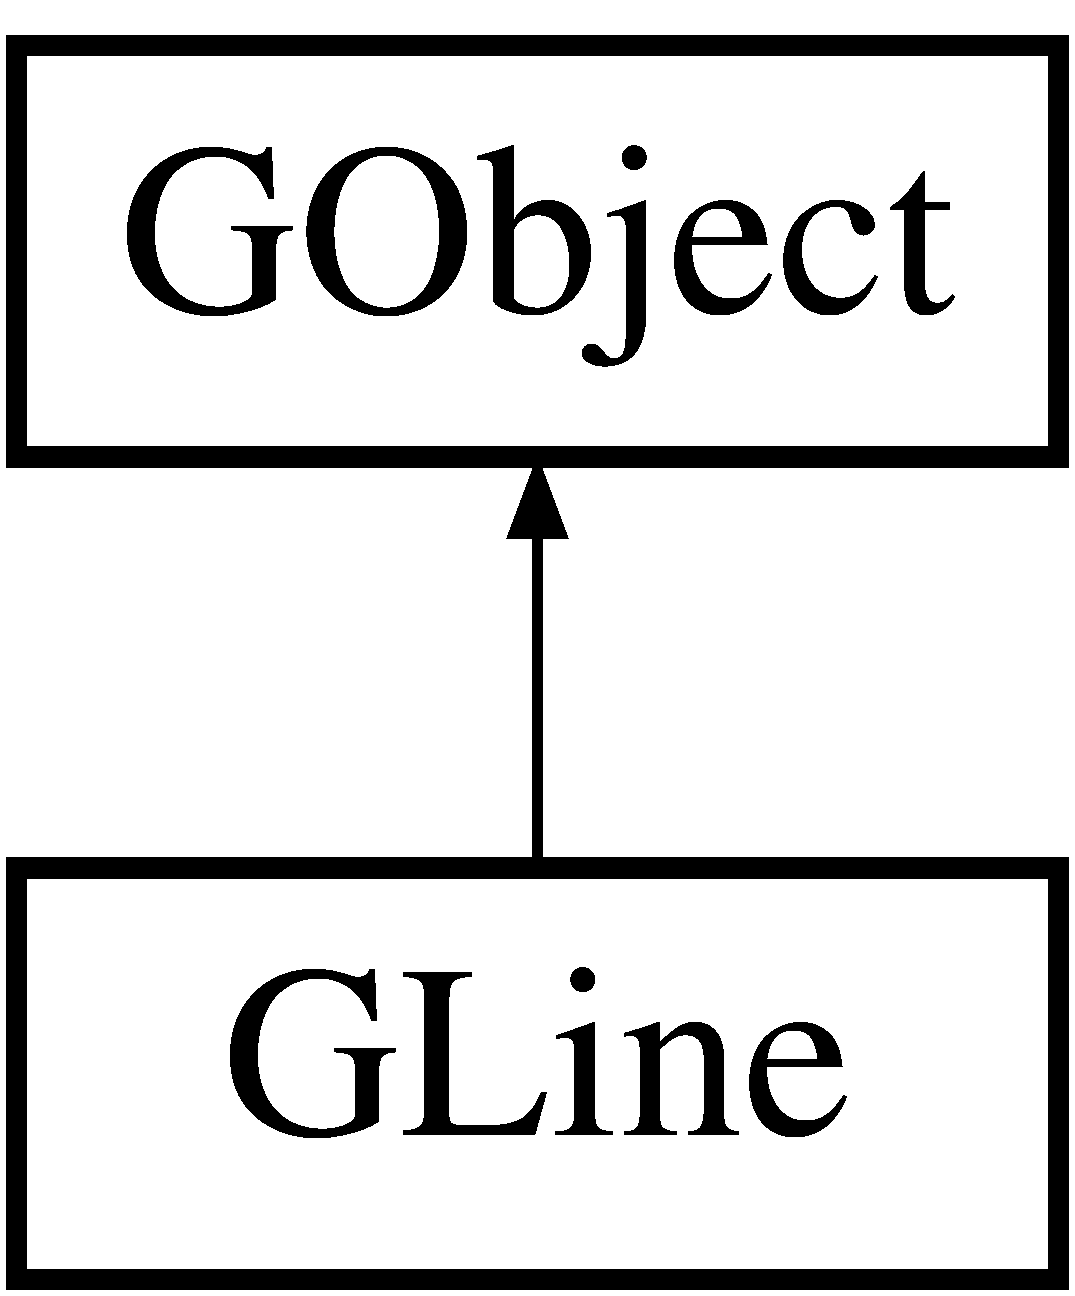
\includegraphics[height=2.000000cm]{classGLine}
\end{center}
\end{figure}
\subsection*{Public Types}
\begin{DoxyCompactItemize}
\item 
enum \mbox{\hyperlink{classGObject_a86e0f5648542856159bb40775c854aa7}{Line\+Style}} \{ \mbox{\hyperlink{classGObject_a86e0f5648542856159bb40775c854aa7acbc84bd5232621834ed31f44d457c1eb}{L\+I\+N\+E\+\_\+\+N\+O\+NE}}, 
\mbox{\hyperlink{classGObject_a86e0f5648542856159bb40775c854aa7a700c78bc2cd76acaab26651bf7b4941f}{L\+I\+N\+E\+\_\+\+S\+O\+L\+ID}}, 
\mbox{\hyperlink{classGObject_a86e0f5648542856159bb40775c854aa7a9ccba0845f785d81d07b333ae1aad84e}{L\+I\+N\+E\+\_\+\+D\+A\+SH}}, 
\mbox{\hyperlink{classGObject_a86e0f5648542856159bb40775c854aa7a8e811c096cb941997f0bfda168bb6df3}{L\+I\+N\+E\+\_\+\+D\+OT}}, 
\mbox{\hyperlink{classGObject_a86e0f5648542856159bb40775c854aa7ada15a2e3d737b2db7706d8300f91b89d}{L\+I\+N\+E\+\_\+\+D\+A\+S\+H\+\_\+\+D\+OT}}, 
\mbox{\hyperlink{classGObject_a86e0f5648542856159bb40775c854aa7aabf4053a73eafa7ba2b7e6d664c74c1d}{L\+I\+N\+E\+\_\+\+D\+A\+S\+H\+\_\+\+D\+O\+T\+\_\+\+D\+OT}}
 \}
\begin{DoxyCompactList}\small\item\em Styles that can be used for the outline around various shapes. \end{DoxyCompactList}\end{DoxyCompactItemize}
\subsection*{Public Member Functions}
\begin{DoxyCompactItemize}
\item 
\mbox{\hyperlink{classGLine_ac9e846926da2b0a7fc87164dd05dff3d}{G\+Line}} (double x0=0, double y0=0, double x1=0, double y1=0, \mbox{\hyperlink{classGObject_a86e0f5648542856159bb40775c854aa7}{Line\+Style}} line\+Style=\mbox{\hyperlink{classGObject_a86e0f5648542856159bb40775c854aa7a700c78bc2cd76acaab26651bf7b4941f}{L\+I\+N\+E\+\_\+\+S\+O\+L\+ID}})
\begin{DoxyCompactList}\small\item\em Constructs a line segment from its endpoints. \end{DoxyCompactList}\item 
\mbox{\hyperlink{classGLine_a337f6971ca683934513640e9400f3e88}{G\+Line}} (const \mbox{\hyperlink{structGPoint}{G\+Point}} \&p0, const \mbox{\hyperlink{structGPoint}{G\+Point}} \&p1)
\begin{DoxyCompactList}\small\item\em Constructs a line segment from its endpoints. \end{DoxyCompactList}\item 
virtual bool \mbox{\hyperlink{classGObject_a1dbc9dafaae51958112dbe1267a1f547}{contains}} (const \mbox{\hyperlink{structGPoint}{G\+Point}} \&pt) const
\begin{DoxyCompactList}\small\item\em Returns {\ttfamily true} if the specified point is inside the object. \end{DoxyCompactList}\item 
bool \mbox{\hyperlink{classGLine_ad973a1d55799d3a73bf8b04986cd804e}{contains}} (double x, double y) const override
\begin{DoxyCompactList}\small\item\em Returns {\ttfamily true} if the specified point is inside the object. \end{DoxyCompactList}\item 
virtual \mbox{\hyperlink{structGPoint}{G\+Point}} \mbox{\hyperlink{classGObject_a0d41183bf6b08de66fe3907551aab0d7}{get\+Bottom\+Right\+Location}} () const
\begin{DoxyCompactList}\small\item\em Returns the x/y coordinates of the bottom/right corner of the object. \end{DoxyCompactList}\item 
virtual double \mbox{\hyperlink{classGObject_a4316a2406c18e1c6d061fe51fd355490}{get\+BottomY}} () const
\begin{DoxyCompactList}\small\item\em Returns the {\itshape y}-\/coordinate of the bottom of the object. \end{DoxyCompactList}\item 
\mbox{\hyperlink{structGRectangle}{G\+Rectangle}} \mbox{\hyperlink{classGLine_a89040ce9277825772d359fccd33bca86}{get\+Bounds}} () const override
\begin{DoxyCompactList}\small\item\em Returns the bounding box of this object, which is defined to be the smallest rectangle that covers everything drawn by the figure. \end{DoxyCompactList}\item 
virtual \mbox{\hyperlink{structGPoint}{G\+Point}} \mbox{\hyperlink{classGObject_a0909472e91448470bccdb62ecfb95d8b}{get\+Center\+Location}} () const
\begin{DoxyCompactList}\small\item\em Returns the x/y-\/coordinates of the center of the object. \end{DoxyCompactList}\item 
virtual double \mbox{\hyperlink{classGObject_a04df74355b545e0543112d5b8d924176}{get\+CenterX}} () const
\begin{DoxyCompactList}\small\item\em Returns the {\itshape x}-\/coordinate of the center of the object. \end{DoxyCompactList}\item 
virtual double \mbox{\hyperlink{classGObject_acb3287a3d507025a26f54b895713b947}{get\+CenterY}} () const
\begin{DoxyCompactList}\small\item\em Returns the {\itshape y}-\/coordinate of the center of the object. \end{DoxyCompactList}\item 
virtual std\+::string \mbox{\hyperlink{classGObject_aa061dfa488c31e18549d64363c1d0e34}{get\+Color}} () const
\begin{DoxyCompactList}\small\item\em Returns the color used to display this object. \end{DoxyCompactList}\item 
virtual \mbox{\hyperlink{structGPoint}{G\+Point}} \mbox{\hyperlink{classGLine_a835d5e50bf4a91efcf0d838130c246af}{get\+End\+Point}} () const
\begin{DoxyCompactList}\small\item\em Returns the point at which the line ends. \end{DoxyCompactList}\item 
virtual double \mbox{\hyperlink{classGLine_a87db00624acdc56daf57bacd76ed0ac0}{get\+EndX}} () const
\begin{DoxyCompactList}\small\item\em Returns the x-\/coordinate of the point at which the line ends. \end{DoxyCompactList}\item 
virtual double \mbox{\hyperlink{classGLine_ac6aa09d194bd5210461eba3e5870f488}{get\+EndY}} () const
\begin{DoxyCompactList}\small\item\em Returns the y-\/coordinate of the point at which the line ends. \end{DoxyCompactList}\item 
virtual std\+::string \mbox{\hyperlink{classGObject_a76f6964a11fde7c78e9751be184e1a3c}{get\+Fill\+Color}} () const
\begin{DoxyCompactList}\small\item\em Returns the color used to display the filled region of this object. \end{DoxyCompactList}\item 
double \mbox{\hyperlink{classGLine_a2bede8b27b21ae4c7940e762cbad9e07}{get\+Height}} () const override
\begin{DoxyCompactList}\small\item\em Returns the height of this object, which is the same as the height of its bounding box. \end{DoxyCompactList}\item 
virtual \mbox{\hyperlink{classGObject_a86e0f5648542856159bb40775c854aa7}{Line\+Style}} \mbox{\hyperlink{classGObject_aaf1f5ea8281e5e3486662878d26f0a13}{get\+Line\+Style}} () const
\begin{DoxyCompactList}\small\item\em Returns the object\textquotesingle{}s style such as solid or dashed. \end{DoxyCompactList}\item 
virtual double \mbox{\hyperlink{classGObject_a85ff266dc3eb63d9f2d8e5a4487fd3c0}{get\+Line\+Width}} () const
\begin{DoxyCompactList}\small\item\em Returns the width of the line used to draw this object. \end{DoxyCompactList}\item 
virtual \mbox{\hyperlink{structGPoint}{G\+Point}} \mbox{\hyperlink{classGObject_a4f83802015511edeb63b892830812c11}{get\+Location}} () const
\begin{DoxyCompactList}\small\item\em Returns the location of the top-\/left corner of object. \end{DoxyCompactList}\item 
virtual double \mbox{\hyperlink{classGObject_a1ae3fc278cc5b71b9f2d96a8a83cdf26}{get\+Opacity}} () const
\begin{DoxyCompactList}\small\item\em Returns how opaque (non-\/transparent) this object will appear from 0.\+0 (completely transparent) to 1.\+0 (completely opaque, default). \end{DoxyCompactList}\item 
virtual \mbox{\hyperlink{classGCompound}{G\+Compound}} $\ast$ \mbox{\hyperlink{classGObject_a3e53cef70541b1a14eade4ad0984d0b4}{get\+Parent}} () const
\begin{DoxyCompactList}\small\item\em Returns a pointer to the {\ttfamily \mbox{\hyperlink{classGCompound}{G\+Compound}}} that contains this object. \end{DoxyCompactList}\item 
virtual double \mbox{\hyperlink{classGObject_a798cc79daaa10145b28f60bcdfdb0ee9}{get\+RightX}} () const
\begin{DoxyCompactList}\small\item\em Returns the {\itshape x}-\/coordinate of the right side of the object. \end{DoxyCompactList}\item 
virtual \mbox{\hyperlink{structGDimension}{G\+Dimension}} \mbox{\hyperlink{classGObject_a7b4eec96a2bdc6420695d5796a78eea9}{get\+Size}} () const
\begin{DoxyCompactList}\small\item\em Returns the size of the object as a {\ttfamily \mbox{\hyperlink{structGDimension}{G\+Dimension}}}. \end{DoxyCompactList}\item 
virtual \mbox{\hyperlink{structGPoint}{G\+Point}} \mbox{\hyperlink{classGLine_ad12beaa70993d9b409bfa8fd86c83957}{get\+Start\+Point}} () const
\begin{DoxyCompactList}\small\item\em Returns the point at which the line starts. \end{DoxyCompactList}\item 
virtual double \mbox{\hyperlink{classGLine_aa82e2c4efd87a1d6092747839d28c5db}{get\+StartX}} () const
\begin{DoxyCompactList}\small\item\em Returns the x-\/coordinate of the point at which the line starts. \end{DoxyCompactList}\item 
virtual double \mbox{\hyperlink{classGLine_a4481ac794cdca823afc9633f8cc88777}{get\+StartY}} () const
\begin{DoxyCompactList}\small\item\em Returns the y-\/coordinate of the point at which the line starts. \end{DoxyCompactList}\item 
std\+::string \mbox{\hyperlink{classGLine_a9b72ede4ee8520f987a0c01e30654814}{get\+Type}} () const override
\begin{DoxyCompactList}\small\item\em Returns the type of the object as a string, such as {\ttfamily \char`\"{}\+G\+Oval\char`\"{}} or {\ttfamily \char`\"{}\+G\+Rect\char`\"{}}. \end{DoxyCompactList}\item 
double \mbox{\hyperlink{classGLine_ab7b172cec7ed45e1246a3ce3160a62f7}{get\+Width}} () const override
\begin{DoxyCompactList}\small\item\em Returns the width of this object, which is equal to the width of the bounding box. \end{DoxyCompactList}\item 
virtual double \mbox{\hyperlink{classGObject_a344385751bee0720059403940d57a13e}{getX}} () const
\begin{DoxyCompactList}\small\item\em Returns the leftmost {\itshape x}-\/coordinate of the object. \end{DoxyCompactList}\item 
virtual double \mbox{\hyperlink{classGObject_aafa51c7f8f38a09febbb9ce7853f77b4}{getY}} () const
\begin{DoxyCompactList}\small\item\em Returns the topmost {\itshape y}-\/coordinate of the object. \end{DoxyCompactList}\item 
virtual bool \mbox{\hyperlink{classGObject_a11c404f106940c201b6f326e0355c150}{is\+Filled}} () const
\begin{DoxyCompactList}\small\item\em Returns {\ttfamily true} if the object is filled with color. \end{DoxyCompactList}\item 
virtual bool \mbox{\hyperlink{classGObject_a9de207581cfa4ca1eaa06da5f29b75fc}{is\+Transformed}} () const
\begin{DoxyCompactList}\small\item\em Returns {\ttfamily true} if this object has been transformed by calling methods such as \mbox{\hyperlink{classGObject_ae1ffaa12185dfd5ba464f7d87c329e26}{rotate()}} or \mbox{\hyperlink{classGObject_ad2e1900f730475c2d044817db03b38d6}{scale()}} on it. \end{DoxyCompactList}\item 
virtual bool \mbox{\hyperlink{classGObject_a9d8a6cfb13917785c143e74d40e4e2be}{is\+Visible}} () const
\begin{DoxyCompactList}\small\item\em Returns {\ttfamily true} if this object is visible on screen. \end{DoxyCompactList}\item 
virtual void \mbox{\hyperlink{classGObject_a5973d8dda83afb36e2c56855515be392}{move}} (double dx, double dy)
\begin{DoxyCompactList}\small\item\em Moves the object on the screen using the displacements {\ttfamily dx} and {\ttfamily dy}. \end{DoxyCompactList}\item 
virtual void \mbox{\hyperlink{classGObject_ac827b978aa122f136a14c198687ad80f}{repaint}} ()
\begin{DoxyCompactList}\small\item\em Instructs the object to redraw itself on screen. \end{DoxyCompactList}\item 
virtual void \mbox{\hyperlink{classGObject_a6022a1fd1e5dcd2fd5585e5a36aa3f37}{reset\+Transform}} ()
\begin{DoxyCompactList}\small\item\em Undoes any previous scale/rotate transformations on this object. \end{DoxyCompactList}\item 
virtual void \mbox{\hyperlink{classGObject_ae1ffaa12185dfd5ba464f7d87c329e26}{rotate}} (double theta)
\begin{DoxyCompactList}\small\item\em Transforms the object by rotating it {\ttfamily theta} degrees counterclockwise around its origin. \end{DoxyCompactList}\item 
virtual void \mbox{\hyperlink{classGObject_ad2e1900f730475c2d044817db03b38d6}{scale}} (double sf)
\begin{DoxyCompactList}\small\item\em Scales the object by the specified scale factor. \end{DoxyCompactList}\item 
virtual void \mbox{\hyperlink{classGObject_a63641f69d610d0b951357d35a0c3b1e3}{scale}} (double sx, double sy)
\begin{DoxyCompactList}\small\item\em Scales the object by the specified scale factors. \end{DoxyCompactList}\item 
void \mbox{\hyperlink{classGObject_ab6747f40313c531c2db32edb5b63b9b7}{send\+Backward}} ()
\begin{DoxyCompactList}\small\item\em Moves this object one step toward the back in the {\itshape z} dimension. \end{DoxyCompactList}\item 
void \mbox{\hyperlink{classGObject_a710b3e449c9facba7847c91ab170d281}{send\+Forward}} ()
\begin{DoxyCompactList}\small\item\em Moves this object one step toward the front in the {\itshape z} dimension. \end{DoxyCompactList}\item 
void \mbox{\hyperlink{classGObject_a0f7f1efbb7fd46dde2867c4ad0330896}{send\+To\+Back}} ()
\begin{DoxyCompactList}\small\item\em Moves this object to the back of the display in the {\itshape z} dimension. \end{DoxyCompactList}\item 
void \mbox{\hyperlink{classGObject_aee33d68488e46827ef55fac07f40a9b2}{send\+To\+Front}} ()
\begin{DoxyCompactList}\small\item\em Moves this object to the front of the display in the {\itshape z} dimension. \end{DoxyCompactList}\item 
virtual void \mbox{\hyperlink{classGObject_a71ff7b16b8f1bdc4a1ce9f30cf8b87d8}{set\+Bottom\+Right\+Location}} (double x, double y)
\begin{DoxyCompactList}\small\item\em Sets the location of the bottom/right of this object. \end{DoxyCompactList}\item 
virtual void \mbox{\hyperlink{classGObject_ac6f7320321182f1d18c1c0fa97d5e941}{set\+Bottom\+Right\+Location}} (const \mbox{\hyperlink{structGPoint}{G\+Point}} \&pt)
\begin{DoxyCompactList}\small\item\em Sets the location of the bottom/right of this object. \end{DoxyCompactList}\item 
virtual void \mbox{\hyperlink{classGObject_a4b20e93c2a2597484f74ee5caa71f41f}{set\+BottomY}} (double y)
\begin{DoxyCompactList}\small\item\em Sets the location of the bottom y-\/coordinate of this object. \end{DoxyCompactList}\item 
virtual void \mbox{\hyperlink{classGObject_a2aae8197624b72265ab83b4f1bc73f2f}{set\+Bounds}} (double x, double y, double width, double height)
\begin{DoxyCompactList}\small\item\em Changes the bounds of this object to the specified values. \end{DoxyCompactList}\item 
virtual void \mbox{\hyperlink{classGObject_acada386653f008cacc7cce86426bef7c}{set\+Bounds}} (const \mbox{\hyperlink{structGRectangle}{G\+Rectangle}} \&size)
\begin{DoxyCompactList}\small\item\em Changes the bounds of this object to the specified rectangle. \end{DoxyCompactList}\item 
virtual void \mbox{\hyperlink{classGObject_a290b47dd8de1be44089f95cb2c47c1de}{set\+Center\+Location}} (double x, double y)
\begin{DoxyCompactList}\small\item\em Sets the location of the center of this object. \end{DoxyCompactList}\item 
virtual void \mbox{\hyperlink{classGObject_a1bedf1b233ecba3f753ec58908a683a6}{set\+Center\+Location}} (const \mbox{\hyperlink{structGPoint}{G\+Point}} \&pt)
\begin{DoxyCompactList}\small\item\em Sets the location of the center of this object. \end{DoxyCompactList}\item 
virtual void \mbox{\hyperlink{classGObject_a2f4936281e056eead00a9186b9ba8af6}{set\+CenterX}} (double x)
\begin{DoxyCompactList}\small\item\em Sets the x-\/coordinate of the center of this object. \end{DoxyCompactList}\item 
virtual void \mbox{\hyperlink{classGObject_aad2a22b4fde88c33306b92aebf641d57}{set\+CenterY}} (double y)
\begin{DoxyCompactList}\small\item\em Sets the y-\/coordinate of the center of this object. \end{DoxyCompactList}\item 
virtual void \mbox{\hyperlink{classGObject_ad57ef49bc31db94e92648aa3737923d6}{set\+Color}} (int r, int g, int b)
\begin{DoxyCompactList}\small\item\em Sets the color used to display this object. \end{DoxyCompactList}\item 
virtual void \mbox{\hyperlink{classGObject_ab1f5cc0f5cc6bbbd716a526c61f1081d}{set\+Color}} (int rgb)
\begin{DoxyCompactList}\small\item\em Sets the color used to display this object. \end{DoxyCompactList}\item 
virtual void \mbox{\hyperlink{classGObject_a61374df6c11b52cfbb0815decdbaebc6}{set\+Color}} (const std\+::string \&color)
\begin{DoxyCompactList}\small\item\em Sets the color used to display this object. \end{DoxyCompactList}\item 
virtual void \mbox{\hyperlink{classGLine_aef4a179b63e5686a630727ee0434216f}{set\+End\+Point}} (double x1, double y1)
\begin{DoxyCompactList}\small\item\em Sets the end point in the line to ({\ttfamily x1},~{\ttfamily y1}), leaving the start point unchanged. \end{DoxyCompactList}\item 
virtual void \mbox{\hyperlink{classGLine_a6c09ffad2e262a2803cccfba1ef59b2b}{set\+End\+Point}} (const \mbox{\hyperlink{structGPoint}{G\+Point}} \&p)
\begin{DoxyCompactList}\small\item\em Sets the end point in the line to p, leaving the start point unchanged. \end{DoxyCompactList}\item 
virtual void \mbox{\hyperlink{classGObject_ad767a33971159e9493e221cca4c00ae9}{set\+Fill\+Color}} (int r, int g, int b)
\begin{DoxyCompactList}\small\item\em Sets the color used to display the filled region of this object, if any. \end{DoxyCompactList}\item 
virtual void \mbox{\hyperlink{classGObject_aa59d9775a67fa7df2b24a95cd34840a3}{set\+Fill\+Color}} (int rgb)
\begin{DoxyCompactList}\small\item\em Sets the color used to display the filled region of this object, if any. \end{DoxyCompactList}\item 
virtual void \mbox{\hyperlink{classGObject_adbc18b1a930aadd97d7437f9f7265b96}{set\+Fill\+Color}} (const std\+::string \&color)
\begin{DoxyCompactList}\small\item\em Sets the color used to display the filled region of this object, if any. \end{DoxyCompactList}\item 
virtual void \mbox{\hyperlink{classGObject_a9b82b53362282c6bb7d6947068d2e55b}{set\+Filled}} (bool flag)
\begin{DoxyCompactList}\small\item\em Sets the fill status for the object, where {\ttfamily false} is outlined and {\ttfamily true} is filled. \end{DoxyCompactList}\item 
virtual void \mbox{\hyperlink{classGObject_a2592348886ffea646c6534bf88f7c49d}{set\+Font}} (const Q\+Font \&font)
\begin{DoxyCompactList}\small\item\em Changes the font used to display the object as specified by the given Qt font. \end{DoxyCompactList}\item 
virtual void \mbox{\hyperlink{classGObject_a8e096e8818d838aceae1d46d58fb3a7b}{set\+Font}} (const std\+::string \&font)
\begin{DoxyCompactList}\small\item\em Changes the font used to display the object as specified by the string {\ttfamily font}, which has the following format\+: \end{DoxyCompactList}\item 
virtual void \mbox{\hyperlink{classGObject_ad18e8fab1e02a4e9b75c6730212558eb}{set\+Foreground}} (int r, int g, int b)
\begin{DoxyCompactList}\small\item\em Sets the color used to display this object. \end{DoxyCompactList}\item 
virtual void \mbox{\hyperlink{classGObject_a9eb856b5ff83a19df3831a31f15f4563}{set\+Foreground}} (int rgb)
\begin{DoxyCompactList}\small\item\em Sets the color used to display this object. \end{DoxyCompactList}\item 
virtual void \mbox{\hyperlink{classGObject_af59209aeadea6dfc6d97a2d8531f50e1}{set\+Foreground}} (const std\+::string \&color)
\begin{DoxyCompactList}\small\item\em Sets the color used to display this object. \end{DoxyCompactList}\item 
virtual void \mbox{\hyperlink{classGObject_a9e280bfc4544dfaf8e4376c4e1a74357}{set\+Height}} (double height)
\begin{DoxyCompactList}\small\item\em Changes the height of this object to the specified height without changing its width. \end{DoxyCompactList}\item 
virtual void \mbox{\hyperlink{classGObject_add11575087eb94f1a71faa3f826c6341}{set\+Line\+Style}} (\mbox{\hyperlink{classGObject_a86e0f5648542856159bb40775c854aa7}{Line\+Style}} line\+Style)
\begin{DoxyCompactList}\small\item\em Sets the object\textquotesingle{}s style such as solid (\mbox{\hyperlink{classGObject_a86e0f5648542856159bb40775c854aa7a700c78bc2cd76acaab26651bf7b4941f}{G\+Object\+::\+L\+I\+N\+E\+\_\+\+S\+O\+L\+ID}}) or dashed (\mbox{\hyperlink{classGObject_a86e0f5648542856159bb40775c854aa7a9ccba0845f785d81d07b333ae1aad84e}{G\+Object\+::\+L\+I\+N\+E\+\_\+\+D\+A\+SH}}). \end{DoxyCompactList}\item 
virtual void \mbox{\hyperlink{classGObject_afd6a47c6ea6a1f85ca05a65ba3ff3477}{set\+Line\+Width}} (double line\+Width)
\begin{DoxyCompactList}\small\item\em Sets the width of the line used to draw this object. \end{DoxyCompactList}\item 
virtual void \mbox{\hyperlink{classGObject_a04594e8ba9b98513a64f1da00dcae18c}{set\+Location}} (double x, double y)
\begin{DoxyCompactList}\small\item\em Sets the location of the top-\/left corner of this object to the specified coordinates. \end{DoxyCompactList}\item 
virtual void \mbox{\hyperlink{classGObject_aa8480c0b7166cdf8f784cece06ab353f}{set\+Location}} (const \mbox{\hyperlink{structGPoint}{G\+Point}} \&pt)
\begin{DoxyCompactList}\small\item\em Sets the location of the top-\/left corner of this object to the specified point. \end{DoxyCompactList}\item 
virtual void \mbox{\hyperlink{classGObject_a04af1866cc1bae4a1226695794a50539}{set\+Opacity}} (double opacity)
\begin{DoxyCompactList}\small\item\em Sets how opaque (non-\/transparent) this object will appear from 0.\+0 (completely transparent) to 1.\+0 (completely opaque, default). \end{DoxyCompactList}\item 
virtual void \mbox{\hyperlink{classGLine_a5fc254e5f489d0e460bfe4202f4904b6}{set\+Points}} (double x0, double y0, double x1, double y1)
\begin{DoxyCompactList}\small\item\em Sets this line\textquotesingle{}s two end points to (x0, y0) and (x1, y1). \end{DoxyCompactList}\item 
virtual void \mbox{\hyperlink{classGLine_a4efe83a7a5c9f14971ce88af29d0cb36}{set\+Points}} (const \mbox{\hyperlink{structGPoint}{G\+Point}} \&p0, const \mbox{\hyperlink{structGPoint}{G\+Point}} \&p1)
\begin{DoxyCompactList}\small\item\em Sets this line\textquotesingle{}s two end points to p0 and p1. \end{DoxyCompactList}\item 
virtual void \mbox{\hyperlink{classGObject_a3c90b758cdc2c911c9ef76c4360eb912}{set\+RightX}} (double x)
\begin{DoxyCompactList}\small\item\em Sets the location of the rightmost x-\/coordinate of this object. \end{DoxyCompactList}\item 
virtual void \mbox{\hyperlink{classGObject_aca25d49481f9bf5fc8f7df4c086c4ce7}{set\+Size}} (double width, double height)
\begin{DoxyCompactList}\small\item\em Changes the size of this object to the specified width and height. \end{DoxyCompactList}\item 
virtual void \mbox{\hyperlink{classGObject_ae2b628228f192c2702c4ce941b2af68f}{set\+Size}} (const \mbox{\hyperlink{structGDimension}{G\+Dimension}} \&size)
\begin{DoxyCompactList}\small\item\em Changes the size of this object to the specified width and height. \end{DoxyCompactList}\item 
virtual void \mbox{\hyperlink{classGLine_a9b7c45267b9912efb6eab68627bfa5da}{set\+Start\+Point}} (double x0, double y0)
\begin{DoxyCompactList}\small\item\em Sets the initial point in the line to ({\ttfamily x0},~{\ttfamily y0}), leaving the end point unchanged. \end{DoxyCompactList}\item 
virtual void \mbox{\hyperlink{classGLine_a97f00c73b6e1e0e4441d8a21243170c2}{set\+Start\+Point}} (const \mbox{\hyperlink{structGPoint}{G\+Point}} \&p)
\begin{DoxyCompactList}\small\item\em Sets the initial point in the line to p, leaving the end point unchanged. \end{DoxyCompactList}\item 
virtual void \mbox{\hyperlink{classGObject_a88203f28224315d9f4471212f4af8ed3}{set\+Visible}} (bool flag)
\begin{DoxyCompactList}\small\item\em Sets whether this object is visible. \end{DoxyCompactList}\item 
virtual void \mbox{\hyperlink{classGObject_aa3f3fba4cb131baa8696ba01e3bceca1}{set\+Width}} (double width)
\begin{DoxyCompactList}\small\item\em Changes the width of this object to the specified width without changing its height. \end{DoxyCompactList}\item 
virtual void \mbox{\hyperlink{classGObject_a9c18fcc579333bf9653d13ad2b372e39}{setX}} (double x)
\begin{DoxyCompactList}\small\item\em Sets the x location of the left side of this object. \end{DoxyCompactList}\item 
virtual void \mbox{\hyperlink{classGObject_a7d57e2a5c35d27feb58fd498a3cf82b9}{setY}} (double y)
\begin{DoxyCompactList}\small\item\em Sets the y location of the top of this object. \end{DoxyCompactList}\item 
virtual std\+::string \mbox{\hyperlink{classGObject_a1fe5121d6528fdea3f243321b3fa3a49}{to\+String}} () const
\begin{DoxyCompactList}\small\item\em Returns a printable representation of the object. \end{DoxyCompactList}\item 
std\+::string \mbox{\hyperlink{classGLine_a04364e674911906702b748deec32db18}{to\+String\+Extra}} () const override
\begin{DoxyCompactList}\small\item\em Returns a string containing any extra unique information about this type of graphical object. \end{DoxyCompactList}\end{DoxyCompactItemize}
\subsection*{Static Public Member Functions}
\begin{DoxyCompactItemize}
\item 
static bool \mbox{\hyperlink{classGObject_a93be0e1fe1b1bf1a1da732470c94f42b}{is\+Anti\+Aliasing}} ()
\begin{DoxyCompactList}\small\item\em Returns whether we should globally anti-\/alias graphical objects. \end{DoxyCompactList}\item 
static void \mbox{\hyperlink{classGObject_a1e43371668ae850193cebedb44e1bbe3}{set\+Anti\+Aliasing}} (bool value)
\begin{DoxyCompactList}\small\item\em Globally turns on/off the anti-\/aliasing feature that smooths out the edges of onscreen shapes. \end{DoxyCompactList}\end{DoxyCompactItemize}
\subsection*{Protected Attributes}
\begin{DoxyCompactItemize}
\item 
Q\+Brush \mbox{\hyperlink{classGObject_aab24462ec896b596d99911767b0912d0}{\+\_\+brush}}
\item 
std\+::string \mbox{\hyperlink{classGObject_a1134e770ae4315ea8bc1201e2f21da8b}{\+\_\+color}}
\item 
int \mbox{\hyperlink{classGObject_a003fdd343d9b7505c53a8b7a134200ed}{\+\_\+color\+Int}}
\item 
double \mbox{\hyperlink{classGLine_a81afeefef08850c1beb8b799ede89635}{\+\_\+dx}}
\item 
double \mbox{\hyperlink{classGLine_a87493c51c53b249b302718465fba8c82}{\+\_\+dy}}
\item 
std\+::string \mbox{\hyperlink{classGObject_a179f8d6cee65cd8a54692e32b224392a}{\+\_\+fill\+Color}}
\item 
int \mbox{\hyperlink{classGObject_a751def333a67d651e5b99cc331ecb496}{\+\_\+fill\+Color\+Int}}
\item 
bool \mbox{\hyperlink{classGObject_ad4a55cbcd61b58a4d49666490bb2f103}{\+\_\+fill\+Flag}}
\item 
std\+::string \mbox{\hyperlink{classGObject_aea76ea1a8b5dd7b0a78653277e63b536}{\+\_\+font}}
\item 
double \mbox{\hyperlink{classGObject_ad05df29e7f27fc504abd743e3d8b4e73}{\+\_\+height}}
\item 
\mbox{\hyperlink{classGObject_a86e0f5648542856159bb40775c854aa7}{Line\+Style}} \mbox{\hyperlink{classGObject_a89bafecaafb7c72d55c7efc10b7d0523}{\+\_\+line\+Style}}
\item 
double \mbox{\hyperlink{classGObject_a16e9033665937f13de2e163dc2184aff}{\+\_\+line\+Width}}
\item 
double \mbox{\hyperlink{classGObject_a20eff8eb7af27182edc9bfc54768b6f3}{\+\_\+opacity}}
\item 
\mbox{\hyperlink{classGCompound}{G\+Compound}} $\ast$ \mbox{\hyperlink{classGObject_ac9452c1eaff70eebddbb318196aa3835}{\+\_\+parent}}
\item 
Q\+Pen \mbox{\hyperlink{classGObject_afb69d172743f868299847174eb1b6bc8}{\+\_\+pen}}
\item 
Q\+Transform \mbox{\hyperlink{classGObject_a475b8860a5f1adb4a1fdc58d1f5c1e32}{\+\_\+transform}}
\item 
bool \mbox{\hyperlink{classGObject_ae4725802fc8d8aaa0ab4bd4781f7e07c}{\+\_\+transformed}}
\item 
bool \mbox{\hyperlink{classGObject_a9312c72508471b7c7a87b540263e1af4}{\+\_\+visible}}
\item 
double \mbox{\hyperlink{classGObject_ab55d85a3371770e6725b1062cf160cd8}{\+\_\+width}}
\item 
double \mbox{\hyperlink{classGObject_a6675b83b27137b8d3aa2ad8133078ea6}{\+\_\+x}}
\item 
double \mbox{\hyperlink{classGObject_a2f0f6aeafddc8a39c578bfa7e22b5f1e}{\+\_\+y}}
\end{DoxyCompactItemize}


\subsection{Detailed Description}
This graphical object subclass represents a line segment. 

\subsection{Member Enumeration Documentation}
\mbox{\Hypertarget{classGObject_a86e0f5648542856159bb40775c854aa7}\label{classGObject_a86e0f5648542856159bb40775c854aa7}} 
\index{G\+Line@{G\+Line}!Line\+Style@{Line\+Style}}
\index{Line\+Style@{Line\+Style}!G\+Line@{G\+Line}}
\subsubsection{\texorpdfstring{Line\+Style}{LineStyle}}
{\footnotesize\ttfamily enum \mbox{\hyperlink{classGObject_a86e0f5648542856159bb40775c854aa7}{Line\+Style}}\hspace{0.3cm}{\ttfamily [inherited]}}



Styles that can be used for the outline around various shapes. 

Call set\+Line\+Style on a \mbox{\hyperlink{classGObject}{G\+Object}} and pass one of these values. \begin{DoxyEnumFields}{Enumerator}
\raisebox{\heightof{T}}[0pt][0pt]{\index{L\+I\+N\+E\+\_\+\+N\+O\+NE@{L\+I\+N\+E\+\_\+\+N\+O\+NE}!G\+Line@{G\+Line}}\index{G\+Line@{G\+Line}!L\+I\+N\+E\+\_\+\+N\+O\+NE@{L\+I\+N\+E\+\_\+\+N\+O\+NE}}}\mbox{\Hypertarget{classGObject_a86e0f5648542856159bb40775c854aa7acbc84bd5232621834ed31f44d457c1eb}\label{classGObject_a86e0f5648542856159bb40775c854aa7acbc84bd5232621834ed31f44d457c1eb}} 
L\+I\+N\+E\+\_\+\+N\+O\+NE&\\
\hline

\raisebox{\heightof{T}}[0pt][0pt]{\index{L\+I\+N\+E\+\_\+\+S\+O\+L\+ID@{L\+I\+N\+E\+\_\+\+S\+O\+L\+ID}!G\+Line@{G\+Line}}\index{G\+Line@{G\+Line}!L\+I\+N\+E\+\_\+\+S\+O\+L\+ID@{L\+I\+N\+E\+\_\+\+S\+O\+L\+ID}}}\mbox{\Hypertarget{classGObject_a86e0f5648542856159bb40775c854aa7a700c78bc2cd76acaab26651bf7b4941f}\label{classGObject_a86e0f5648542856159bb40775c854aa7a700c78bc2cd76acaab26651bf7b4941f}} 
L\+I\+N\+E\+\_\+\+S\+O\+L\+ID&\\
\hline

\raisebox{\heightof{T}}[0pt][0pt]{\index{L\+I\+N\+E\+\_\+\+D\+A\+SH@{L\+I\+N\+E\+\_\+\+D\+A\+SH}!G\+Line@{G\+Line}}\index{G\+Line@{G\+Line}!L\+I\+N\+E\+\_\+\+D\+A\+SH@{L\+I\+N\+E\+\_\+\+D\+A\+SH}}}\mbox{\Hypertarget{classGObject_a86e0f5648542856159bb40775c854aa7a9ccba0845f785d81d07b333ae1aad84e}\label{classGObject_a86e0f5648542856159bb40775c854aa7a9ccba0845f785d81d07b333ae1aad84e}} 
L\+I\+N\+E\+\_\+\+D\+A\+SH&\\
\hline

\raisebox{\heightof{T}}[0pt][0pt]{\index{L\+I\+N\+E\+\_\+\+D\+OT@{L\+I\+N\+E\+\_\+\+D\+OT}!G\+Line@{G\+Line}}\index{G\+Line@{G\+Line}!L\+I\+N\+E\+\_\+\+D\+OT@{L\+I\+N\+E\+\_\+\+D\+OT}}}\mbox{\Hypertarget{classGObject_a86e0f5648542856159bb40775c854aa7a8e811c096cb941997f0bfda168bb6df3}\label{classGObject_a86e0f5648542856159bb40775c854aa7a8e811c096cb941997f0bfda168bb6df3}} 
L\+I\+N\+E\+\_\+\+D\+OT&\\
\hline

\raisebox{\heightof{T}}[0pt][0pt]{\index{L\+I\+N\+E\+\_\+\+D\+A\+S\+H\+\_\+\+D\+OT@{L\+I\+N\+E\+\_\+\+D\+A\+S\+H\+\_\+\+D\+OT}!G\+Line@{G\+Line}}\index{G\+Line@{G\+Line}!L\+I\+N\+E\+\_\+\+D\+A\+S\+H\+\_\+\+D\+OT@{L\+I\+N\+E\+\_\+\+D\+A\+S\+H\+\_\+\+D\+OT}}}\mbox{\Hypertarget{classGObject_a86e0f5648542856159bb40775c854aa7ada15a2e3d737b2db7706d8300f91b89d}\label{classGObject_a86e0f5648542856159bb40775c854aa7ada15a2e3d737b2db7706d8300f91b89d}} 
L\+I\+N\+E\+\_\+\+D\+A\+S\+H\+\_\+\+D\+OT&\\
\hline

\raisebox{\heightof{T}}[0pt][0pt]{\index{L\+I\+N\+E\+\_\+\+D\+A\+S\+H\+\_\+\+D\+O\+T\+\_\+\+D\+OT@{L\+I\+N\+E\+\_\+\+D\+A\+S\+H\+\_\+\+D\+O\+T\+\_\+\+D\+OT}!G\+Line@{G\+Line}}\index{G\+Line@{G\+Line}!L\+I\+N\+E\+\_\+\+D\+A\+S\+H\+\_\+\+D\+O\+T\+\_\+\+D\+OT@{L\+I\+N\+E\+\_\+\+D\+A\+S\+H\+\_\+\+D\+O\+T\+\_\+\+D\+OT}}}\mbox{\Hypertarget{classGObject_a86e0f5648542856159bb40775c854aa7aabf4053a73eafa7ba2b7e6d664c74c1d}\label{classGObject_a86e0f5648542856159bb40775c854aa7aabf4053a73eafa7ba2b7e6d664c74c1d}} 
L\+I\+N\+E\+\_\+\+D\+A\+S\+H\+\_\+\+D\+O\+T\+\_\+\+D\+OT&\\
\hline

\end{DoxyEnumFields}


\subsection{Constructor \& Destructor Documentation}
\mbox{\Hypertarget{classGLine_ac9e846926da2b0a7fc87164dd05dff3d}\label{classGLine_ac9e846926da2b0a7fc87164dd05dff3d}} 
\index{G\+Line@{G\+Line}!G\+Line@{G\+Line}}
\index{G\+Line@{G\+Line}!G\+Line@{G\+Line}}
\subsubsection{\texorpdfstring{G\+Line()}{GLine()}\hspace{0.1cm}{\footnotesize\ttfamily [1/2]}}
{\footnotesize\ttfamily \mbox{\hyperlink{classGLine}{G\+Line}} (\begin{DoxyParamCaption}\item[{double}]{x0 = {\ttfamily 0},  }\item[{double}]{y0 = {\ttfamily 0},  }\item[{double}]{x1 = {\ttfamily 0},  }\item[{double}]{y1 = {\ttfamily 0},  }\item[{\mbox{\hyperlink{classGObject_a86e0f5648542856159bb40775c854aa7}{G\+Object\+::\+Line\+Style}}}]{line\+Style = {\ttfamily \mbox{\hyperlink{classGObject_a86e0f5648542856159bb40775c854aa7a700c78bc2cd76acaab26651bf7b4941f}{L\+I\+N\+E\+\_\+\+S\+O\+L\+ID}}} }\end{DoxyParamCaption})}



Constructs a line segment from its endpoints. 

The point ({\ttfamily x0},~{\ttfamily y0}) defines the start of the line and the point ({\ttfamily x1},~{\ttfamily y1}) defines the end. \mbox{\Hypertarget{classGLine_a337f6971ca683934513640e9400f3e88}\label{classGLine_a337f6971ca683934513640e9400f3e88}} 
\index{G\+Line@{G\+Line}!G\+Line@{G\+Line}}
\index{G\+Line@{G\+Line}!G\+Line@{G\+Line}}
\subsubsection{\texorpdfstring{G\+Line()}{GLine()}\hspace{0.1cm}{\footnotesize\ttfamily [2/2]}}
{\footnotesize\ttfamily \mbox{\hyperlink{classGLine}{G\+Line}} (\begin{DoxyParamCaption}\item[{const \mbox{\hyperlink{structGPoint}{G\+Point}} \&}]{p0,  }\item[{const \mbox{\hyperlink{structGPoint}{G\+Point}} \&}]{p1 }\end{DoxyParamCaption})}



Constructs a line segment from its endpoints. 

The point {\ttfamily p0} defines the start of the line and the point {\ttfamily p1} defines the end. 

\subsection{Member Function Documentation}
\mbox{\Hypertarget{classGObject_a1dbc9dafaae51958112dbe1267a1f547}\label{classGObject_a1dbc9dafaae51958112dbe1267a1f547}} 
\index{G\+Line@{G\+Line}!contains@{contains}}
\index{contains@{contains}!G\+Line@{G\+Line}}
\subsubsection{\texorpdfstring{contains()}{contains()}\hspace{0.1cm}{\footnotesize\ttfamily [1/2]}}
{\footnotesize\ttfamily bool contains (\begin{DoxyParamCaption}\item[{const \mbox{\hyperlink{structGPoint}{G\+Point}} \&}]{pt }\end{DoxyParamCaption}) const\hspace{0.3cm}{\ttfamily [virtual]}, {\ttfamily [inherited]}}



Returns {\ttfamily true} if the specified point is inside the object. 

\mbox{\Hypertarget{classGLine_ad973a1d55799d3a73bf8b04986cd804e}\label{classGLine_ad973a1d55799d3a73bf8b04986cd804e}} 
\index{G\+Line@{G\+Line}!contains@{contains}}
\index{contains@{contains}!G\+Line@{G\+Line}}
\subsubsection{\texorpdfstring{contains()}{contains()}\hspace{0.1cm}{\footnotesize\ttfamily [2/2]}}
{\footnotesize\ttfamily bool contains (\begin{DoxyParamCaption}\item[{double}]{x,  }\item[{double}]{y }\end{DoxyParamCaption}) const\hspace{0.3cm}{\ttfamily [override]}, {\ttfamily [virtual]}}



Returns {\ttfamily true} if the specified point is inside the object. 



Reimplemented from \mbox{\hyperlink{classGObject_abb6a5d7c03e6eaaae97264c4799ce7c3}{G\+Object}}.

\mbox{\Hypertarget{classGObject_a0d41183bf6b08de66fe3907551aab0d7}\label{classGObject_a0d41183bf6b08de66fe3907551aab0d7}} 
\index{G\+Line@{G\+Line}!get\+Bottom\+Right\+Location@{get\+Bottom\+Right\+Location}}
\index{get\+Bottom\+Right\+Location@{get\+Bottom\+Right\+Location}!G\+Line@{G\+Line}}
\subsubsection{\texorpdfstring{get\+Bottom\+Right\+Location()}{getBottomRightLocation()}}
{\footnotesize\ttfamily \mbox{\hyperlink{structGPoint}{G\+Point}} get\+Bottom\+Right\+Location (\begin{DoxyParamCaption}{ }\end{DoxyParamCaption}) const\hspace{0.3cm}{\ttfamily [virtual]}, {\ttfamily [inherited]}}



Returns the x/y coordinates of the bottom/right corner of the object. 

\mbox{\Hypertarget{classGObject_a4316a2406c18e1c6d061fe51fd355490}\label{classGObject_a4316a2406c18e1c6d061fe51fd355490}} 
\index{G\+Line@{G\+Line}!get\+BottomY@{get\+BottomY}}
\index{get\+BottomY@{get\+BottomY}!G\+Line@{G\+Line}}
\subsubsection{\texorpdfstring{get\+Bottom\+Y()}{getBottomY()}}
{\footnotesize\ttfamily double get\+BottomY (\begin{DoxyParamCaption}{ }\end{DoxyParamCaption}) const\hspace{0.3cm}{\ttfamily [virtual]}, {\ttfamily [inherited]}}



Returns the {\itshape y}-\/coordinate of the bottom of the object. 

Equivalent to the top y-\/coordinate plus the object\textquotesingle{}s height. \mbox{\Hypertarget{classGLine_a89040ce9277825772d359fccd33bca86}\label{classGLine_a89040ce9277825772d359fccd33bca86}} 
\index{G\+Line@{G\+Line}!get\+Bounds@{get\+Bounds}}
\index{get\+Bounds@{get\+Bounds}!G\+Line@{G\+Line}}
\subsubsection{\texorpdfstring{get\+Bounds()}{getBounds()}}
{\footnotesize\ttfamily \mbox{\hyperlink{structGRectangle}{G\+Rectangle}} get\+Bounds (\begin{DoxyParamCaption}{ }\end{DoxyParamCaption}) const\hspace{0.3cm}{\ttfamily [override]}, {\ttfamily [virtual]}}



Returns the bounding box of this object, which is defined to be the smallest rectangle that covers everything drawn by the figure. 

The coordinates of this rectangle do not necessarily match the location returned by {\ttfamily get\+Location}. Given a {\ttfamily \mbox{\hyperlink{classGText}{G\+Text}}} object, for example, {\ttfamily get\+Location} returns the coordinates of the point on the baseline at which the string begins; the {\ttfamily get\+Bounds} method, by contrast, returns a rectangle that covers the entire window area occupied by the string. 

Reimplemented from \mbox{\hyperlink{classGObject_a29e6ac35a0b48f491a4c88194cc5da3b}{G\+Object}}.

\mbox{\Hypertarget{classGObject_a0909472e91448470bccdb62ecfb95d8b}\label{classGObject_a0909472e91448470bccdb62ecfb95d8b}} 
\index{G\+Line@{G\+Line}!get\+Center\+Location@{get\+Center\+Location}}
\index{get\+Center\+Location@{get\+Center\+Location}!G\+Line@{G\+Line}}
\subsubsection{\texorpdfstring{get\+Center\+Location()}{getCenterLocation()}}
{\footnotesize\ttfamily \mbox{\hyperlink{structGPoint}{G\+Point}} get\+Center\+Location (\begin{DoxyParamCaption}{ }\end{DoxyParamCaption}) const\hspace{0.3cm}{\ttfamily [virtual]}, {\ttfamily [inherited]}}



Returns the x/y-\/coordinates of the center of the object. 

Equivalent to the top/left plus half the object\textquotesingle{}s size. \mbox{\Hypertarget{classGObject_a04df74355b545e0543112d5b8d924176}\label{classGObject_a04df74355b545e0543112d5b8d924176}} 
\index{G\+Line@{G\+Line}!get\+CenterX@{get\+CenterX}}
\index{get\+CenterX@{get\+CenterX}!G\+Line@{G\+Line}}
\subsubsection{\texorpdfstring{get\+Center\+X()}{getCenterX()}}
{\footnotesize\ttfamily double get\+CenterX (\begin{DoxyParamCaption}{ }\end{DoxyParamCaption}) const\hspace{0.3cm}{\ttfamily [virtual]}, {\ttfamily [inherited]}}



Returns the {\itshape x}-\/coordinate of the center of the object. 

Equivalent to the top/left plus half the object\textquotesingle{}s width. \mbox{\Hypertarget{classGObject_acb3287a3d507025a26f54b895713b947}\label{classGObject_acb3287a3d507025a26f54b895713b947}} 
\index{G\+Line@{G\+Line}!get\+CenterY@{get\+CenterY}}
\index{get\+CenterY@{get\+CenterY}!G\+Line@{G\+Line}}
\subsubsection{\texorpdfstring{get\+Center\+Y()}{getCenterY()}}
{\footnotesize\ttfamily double get\+CenterY (\begin{DoxyParamCaption}{ }\end{DoxyParamCaption}) const\hspace{0.3cm}{\ttfamily [virtual]}, {\ttfamily [inherited]}}



Returns the {\itshape y}-\/coordinate of the center of the object. 

Equivalent to the top/left plus half the object\textquotesingle{}s height. \mbox{\Hypertarget{classGObject_aa061dfa488c31e18549d64363c1d0e34}\label{classGObject_aa061dfa488c31e18549d64363c1d0e34}} 
\index{G\+Line@{G\+Line}!get\+Color@{get\+Color}}
\index{get\+Color@{get\+Color}!G\+Line@{G\+Line}}
\subsubsection{\texorpdfstring{get\+Color()}{getColor()}}
{\footnotesize\ttfamily std\+::string get\+Color (\begin{DoxyParamCaption}{ }\end{DoxyParamCaption}) const\hspace{0.3cm}{\ttfamily [virtual]}, {\ttfamily [inherited]}}



Returns the color used to display this object. 

This color is always returned as a string in the form {\ttfamily \char`\"{}\#rrggbb\char`\"{}}, where {\ttfamily rr}, {\ttfamily gg}, and {\ttfamily bb} are the red, green, and blue components of the color, expressed as two-\/digit hexadecimal values. \mbox{\Hypertarget{classGLine_a835d5e50bf4a91efcf0d838130c246af}\label{classGLine_a835d5e50bf4a91efcf0d838130c246af}} 
\index{G\+Line@{G\+Line}!get\+End\+Point@{get\+End\+Point}}
\index{get\+End\+Point@{get\+End\+Point}!G\+Line@{G\+Line}}
\subsubsection{\texorpdfstring{get\+End\+Point()}{getEndPoint()}}
{\footnotesize\ttfamily \mbox{\hyperlink{structGPoint}{G\+Point}} get\+End\+Point (\begin{DoxyParamCaption}{ }\end{DoxyParamCaption}) const\hspace{0.3cm}{\ttfamily [virtual]}}



Returns the point at which the line ends. 

\mbox{\Hypertarget{classGLine_a87db00624acdc56daf57bacd76ed0ac0}\label{classGLine_a87db00624acdc56daf57bacd76ed0ac0}} 
\index{G\+Line@{G\+Line}!get\+EndX@{get\+EndX}}
\index{get\+EndX@{get\+EndX}!G\+Line@{G\+Line}}
\subsubsection{\texorpdfstring{get\+End\+X()}{getEndX()}}
{\footnotesize\ttfamily double get\+EndX (\begin{DoxyParamCaption}{ }\end{DoxyParamCaption}) const\hspace{0.3cm}{\ttfamily [virtual]}}



Returns the x-\/coordinate of the point at which the line ends. 

\mbox{\Hypertarget{classGLine_ac6aa09d194bd5210461eba3e5870f488}\label{classGLine_ac6aa09d194bd5210461eba3e5870f488}} 
\index{G\+Line@{G\+Line}!get\+EndY@{get\+EndY}}
\index{get\+EndY@{get\+EndY}!G\+Line@{G\+Line}}
\subsubsection{\texorpdfstring{get\+End\+Y()}{getEndY()}}
{\footnotesize\ttfamily double get\+EndY (\begin{DoxyParamCaption}{ }\end{DoxyParamCaption}) const\hspace{0.3cm}{\ttfamily [virtual]}}



Returns the y-\/coordinate of the point at which the line ends. 

\mbox{\Hypertarget{classGObject_a76f6964a11fde7c78e9751be184e1a3c}\label{classGObject_a76f6964a11fde7c78e9751be184e1a3c}} 
\index{G\+Line@{G\+Line}!get\+Fill\+Color@{get\+Fill\+Color}}
\index{get\+Fill\+Color@{get\+Fill\+Color}!G\+Line@{G\+Line}}
\subsubsection{\texorpdfstring{get\+Fill\+Color()}{getFillColor()}}
{\footnotesize\ttfamily std\+::string get\+Fill\+Color (\begin{DoxyParamCaption}{ }\end{DoxyParamCaption}) const\hspace{0.3cm}{\ttfamily [virtual]}, {\ttfamily [inherited]}}



Returns the color used to display the filled region of this object. 

If none has been set, returns the empty string. \mbox{\Hypertarget{classGLine_a2bede8b27b21ae4c7940e762cbad9e07}\label{classGLine_a2bede8b27b21ae4c7940e762cbad9e07}} 
\index{G\+Line@{G\+Line}!get\+Height@{get\+Height}}
\index{get\+Height@{get\+Height}!G\+Line@{G\+Line}}
\subsubsection{\texorpdfstring{get\+Height()}{getHeight()}}
{\footnotesize\ttfamily double get\+Height (\begin{DoxyParamCaption}{ }\end{DoxyParamCaption}) const\hspace{0.3cm}{\ttfamily [override]}, {\ttfamily [virtual]}}



Returns the height of this object, which is the same as the height of its bounding box. 



Reimplemented from \mbox{\hyperlink{classGObject_a1e7e353362434072875264cf95629f99}{G\+Object}}.

\mbox{\Hypertarget{classGObject_aaf1f5ea8281e5e3486662878d26f0a13}\label{classGObject_aaf1f5ea8281e5e3486662878d26f0a13}} 
\index{G\+Line@{G\+Line}!get\+Line\+Style@{get\+Line\+Style}}
\index{get\+Line\+Style@{get\+Line\+Style}!G\+Line@{G\+Line}}
\subsubsection{\texorpdfstring{get\+Line\+Style()}{getLineStyle()}}
{\footnotesize\ttfamily \mbox{\hyperlink{classGObject_a86e0f5648542856159bb40775c854aa7}{G\+Object\+::\+Line\+Style}} get\+Line\+Style (\begin{DoxyParamCaption}{ }\end{DoxyParamCaption}) const\hspace{0.3cm}{\ttfamily [virtual]}, {\ttfamily [inherited]}}



Returns the object\textquotesingle{}s style such as solid or dashed. 

\mbox{\Hypertarget{classGObject_a85ff266dc3eb63d9f2d8e5a4487fd3c0}\label{classGObject_a85ff266dc3eb63d9f2d8e5a4487fd3c0}} 
\index{G\+Line@{G\+Line}!get\+Line\+Width@{get\+Line\+Width}}
\index{get\+Line\+Width@{get\+Line\+Width}!G\+Line@{G\+Line}}
\subsubsection{\texorpdfstring{get\+Line\+Width()}{getLineWidth()}}
{\footnotesize\ttfamily double get\+Line\+Width (\begin{DoxyParamCaption}{ }\end{DoxyParamCaption}) const\hspace{0.3cm}{\ttfamily [virtual]}, {\ttfamily [inherited]}}



Returns the width of the line used to draw this object. 

\begin{DoxyReturn}{Returns}
default 1 
\end{DoxyReturn}
\mbox{\Hypertarget{classGObject_a4f83802015511edeb63b892830812c11}\label{classGObject_a4f83802015511edeb63b892830812c11}} 
\index{G\+Line@{G\+Line}!get\+Location@{get\+Location}}
\index{get\+Location@{get\+Location}!G\+Line@{G\+Line}}
\subsubsection{\texorpdfstring{get\+Location()}{getLocation()}}
{\footnotesize\ttfamily \mbox{\hyperlink{structGPoint}{G\+Point}} get\+Location (\begin{DoxyParamCaption}{ }\end{DoxyParamCaption}) const\hspace{0.3cm}{\ttfamily [virtual]}, {\ttfamily [inherited]}}



Returns the location of the top-\/left corner of object. 

\mbox{\Hypertarget{classGObject_a1ae3fc278cc5b71b9f2d96a8a83cdf26}\label{classGObject_a1ae3fc278cc5b71b9f2d96a8a83cdf26}} 
\index{G\+Line@{G\+Line}!get\+Opacity@{get\+Opacity}}
\index{get\+Opacity@{get\+Opacity}!G\+Line@{G\+Line}}
\subsubsection{\texorpdfstring{get\+Opacity()}{getOpacity()}}
{\footnotesize\ttfamily double get\+Opacity (\begin{DoxyParamCaption}{ }\end{DoxyParamCaption}) const\hspace{0.3cm}{\ttfamily [virtual]}, {\ttfamily [inherited]}}



Returns how opaque (non-\/transparent) this object will appear from 0.\+0 (completely transparent) to 1.\+0 (completely opaque, default). 

\mbox{\Hypertarget{classGObject_a3e53cef70541b1a14eade4ad0984d0b4}\label{classGObject_a3e53cef70541b1a14eade4ad0984d0b4}} 
\index{G\+Line@{G\+Line}!get\+Parent@{get\+Parent}}
\index{get\+Parent@{get\+Parent}!G\+Line@{G\+Line}}
\subsubsection{\texorpdfstring{get\+Parent()}{getParent()}}
{\footnotesize\ttfamily \mbox{\hyperlink{classGCompound}{G\+Compound}} $\ast$ get\+Parent (\begin{DoxyParamCaption}{ }\end{DoxyParamCaption}) const\hspace{0.3cm}{\ttfamily [virtual]}, {\ttfamily [inherited]}}



Returns a pointer to the {\ttfamily \mbox{\hyperlink{classGCompound}{G\+Compound}}} that contains this object. 

Every {\ttfamily \mbox{\hyperlink{classGWindow}{G\+Window}}} is initialized to contain a single {\ttfamily \mbox{\hyperlink{classGCompound}{G\+Compound}}} that is aligned with the window. Adding objects to the window adds them to that {\ttfamily \mbox{\hyperlink{classGCompound}{G\+Compound}}}, which means that every object you add to the window has a parent. Calling {\ttfamily get\+Parent} on the top-\/level {\ttfamily \mbox{\hyperlink{classGCompound}{G\+Compound}}} returns {\ttfamily nullptr}. \mbox{\Hypertarget{classGObject_a798cc79daaa10145b28f60bcdfdb0ee9}\label{classGObject_a798cc79daaa10145b28f60bcdfdb0ee9}} 
\index{G\+Line@{G\+Line}!get\+RightX@{get\+RightX}}
\index{get\+RightX@{get\+RightX}!G\+Line@{G\+Line}}
\subsubsection{\texorpdfstring{get\+Right\+X()}{getRightX()}}
{\footnotesize\ttfamily double get\+RightX (\begin{DoxyParamCaption}{ }\end{DoxyParamCaption}) const\hspace{0.3cm}{\ttfamily [virtual]}, {\ttfamily [inherited]}}



Returns the {\itshape x}-\/coordinate of the right side of the object. 

Equivalent to the left x-\/coordinate plus the object\textquotesingle{}s width. \mbox{\Hypertarget{classGObject_a7b4eec96a2bdc6420695d5796a78eea9}\label{classGObject_a7b4eec96a2bdc6420695d5796a78eea9}} 
\index{G\+Line@{G\+Line}!get\+Size@{get\+Size}}
\index{get\+Size@{get\+Size}!G\+Line@{G\+Line}}
\subsubsection{\texorpdfstring{get\+Size()}{getSize()}}
{\footnotesize\ttfamily \mbox{\hyperlink{structGDimension}{G\+Dimension}} get\+Size (\begin{DoxyParamCaption}{ }\end{DoxyParamCaption}) const\hspace{0.3cm}{\ttfamily [virtual]}, {\ttfamily [inherited]}}



Returns the size of the object as a {\ttfamily \mbox{\hyperlink{structGDimension}{G\+Dimension}}}. 

\mbox{\Hypertarget{classGLine_ad12beaa70993d9b409bfa8fd86c83957}\label{classGLine_ad12beaa70993d9b409bfa8fd86c83957}} 
\index{G\+Line@{G\+Line}!get\+Start\+Point@{get\+Start\+Point}}
\index{get\+Start\+Point@{get\+Start\+Point}!G\+Line@{G\+Line}}
\subsubsection{\texorpdfstring{get\+Start\+Point()}{getStartPoint()}}
{\footnotesize\ttfamily \mbox{\hyperlink{structGPoint}{G\+Point}} get\+Start\+Point (\begin{DoxyParamCaption}{ }\end{DoxyParamCaption}) const\hspace{0.3cm}{\ttfamily [virtual]}}



Returns the point at which the line starts. 

Equivalent to get\+Location. \mbox{\Hypertarget{classGLine_aa82e2c4efd87a1d6092747839d28c5db}\label{classGLine_aa82e2c4efd87a1d6092747839d28c5db}} 
\index{G\+Line@{G\+Line}!get\+StartX@{get\+StartX}}
\index{get\+StartX@{get\+StartX}!G\+Line@{G\+Line}}
\subsubsection{\texorpdfstring{get\+Start\+X()}{getStartX()}}
{\footnotesize\ttfamily double get\+StartX (\begin{DoxyParamCaption}{ }\end{DoxyParamCaption}) const\hspace{0.3cm}{\ttfamily [virtual]}}



Returns the x-\/coordinate of the point at which the line starts. 

Equivalent to getX. \mbox{\Hypertarget{classGLine_a4481ac794cdca823afc9633f8cc88777}\label{classGLine_a4481ac794cdca823afc9633f8cc88777}} 
\index{G\+Line@{G\+Line}!get\+StartY@{get\+StartY}}
\index{get\+StartY@{get\+StartY}!G\+Line@{G\+Line}}
\subsubsection{\texorpdfstring{get\+Start\+Y()}{getStartY()}}
{\footnotesize\ttfamily double get\+StartY (\begin{DoxyParamCaption}{ }\end{DoxyParamCaption}) const\hspace{0.3cm}{\ttfamily [virtual]}}



Returns the y-\/coordinate of the point at which the line starts. 

Equivalent to getY. \mbox{\Hypertarget{classGLine_a9b72ede4ee8520f987a0c01e30654814}\label{classGLine_a9b72ede4ee8520f987a0c01e30654814}} 
\index{G\+Line@{G\+Line}!get\+Type@{get\+Type}}
\index{get\+Type@{get\+Type}!G\+Line@{G\+Line}}
\subsubsection{\texorpdfstring{get\+Type()}{getType()}}
{\footnotesize\ttfamily std\+::string get\+Type (\begin{DoxyParamCaption}{ }\end{DoxyParamCaption}) const\hspace{0.3cm}{\ttfamily [override]}, {\ttfamily [virtual]}}



Returns the type of the object as a string, such as {\ttfamily \char`\"{}\+G\+Oval\char`\"{}} or {\ttfamily \char`\"{}\+G\+Rect\char`\"{}}. 

Each \mbox{\hyperlink{classGObject}{G\+Object}} subtype must override this method. 

Implements \mbox{\hyperlink{classGObject_a799e073a127b428cc841086d42ea4fed}{G\+Object}}.

\mbox{\Hypertarget{classGLine_ab7b172cec7ed45e1246a3ce3160a62f7}\label{classGLine_ab7b172cec7ed45e1246a3ce3160a62f7}} 
\index{G\+Line@{G\+Line}!get\+Width@{get\+Width}}
\index{get\+Width@{get\+Width}!G\+Line@{G\+Line}}
\subsubsection{\texorpdfstring{get\+Width()}{getWidth()}}
{\footnotesize\ttfamily double get\+Width (\begin{DoxyParamCaption}{ }\end{DoxyParamCaption}) const\hspace{0.3cm}{\ttfamily [override]}, {\ttfamily [virtual]}}



Returns the width of this object, which is equal to the width of the bounding box. 



Reimplemented from \mbox{\hyperlink{classGObject_a0ed2965abd4f5701d2cadf71239faf19}{G\+Object}}.

\mbox{\Hypertarget{classGObject_a344385751bee0720059403940d57a13e}\label{classGObject_a344385751bee0720059403940d57a13e}} 
\index{G\+Line@{G\+Line}!getX@{getX}}
\index{getX@{getX}!G\+Line@{G\+Line}}
\subsubsection{\texorpdfstring{get\+X()}{getX()}}
{\footnotesize\ttfamily double getX (\begin{DoxyParamCaption}{ }\end{DoxyParamCaption}) const\hspace{0.3cm}{\ttfamily [virtual]}, {\ttfamily [inherited]}}



Returns the leftmost {\itshape x}-\/coordinate of the object. 

\mbox{\Hypertarget{classGObject_aafa51c7f8f38a09febbb9ce7853f77b4}\label{classGObject_aafa51c7f8f38a09febbb9ce7853f77b4}} 
\index{G\+Line@{G\+Line}!getY@{getY}}
\index{getY@{getY}!G\+Line@{G\+Line}}
\subsubsection{\texorpdfstring{get\+Y()}{getY()}}
{\footnotesize\ttfamily double getY (\begin{DoxyParamCaption}{ }\end{DoxyParamCaption}) const\hspace{0.3cm}{\ttfamily [virtual]}, {\ttfamily [inherited]}}



Returns the topmost {\itshape y}-\/coordinate of the object. 

\mbox{\Hypertarget{classGObject_a93be0e1fe1b1bf1a1da732470c94f42b}\label{classGObject_a93be0e1fe1b1bf1a1da732470c94f42b}} 
\index{G\+Line@{G\+Line}!is\+Anti\+Aliasing@{is\+Anti\+Aliasing}}
\index{is\+Anti\+Aliasing@{is\+Anti\+Aliasing}!G\+Line@{G\+Line}}
\subsubsection{\texorpdfstring{is\+Anti\+Aliasing()}{isAntiAliasing()}}
{\footnotesize\ttfamily bool is\+Anti\+Aliasing (\begin{DoxyParamCaption}{ }\end{DoxyParamCaption})\hspace{0.3cm}{\ttfamily [static]}, {\ttfamily [inherited]}}



Returns whether we should globally anti-\/alias graphical objects. 

On by default. \mbox{\Hypertarget{classGObject_a11c404f106940c201b6f326e0355c150}\label{classGObject_a11c404f106940c201b6f326e0355c150}} 
\index{G\+Line@{G\+Line}!is\+Filled@{is\+Filled}}
\index{is\+Filled@{is\+Filled}!G\+Line@{G\+Line}}
\subsubsection{\texorpdfstring{is\+Filled()}{isFilled()}}
{\footnotesize\ttfamily bool is\+Filled (\begin{DoxyParamCaption}{ }\end{DoxyParamCaption}) const\hspace{0.3cm}{\ttfamily [virtual]}, {\ttfamily [inherited]}}



Returns {\ttfamily true} if the object is filled with color. 

\mbox{\Hypertarget{classGObject_a9de207581cfa4ca1eaa06da5f29b75fc}\label{classGObject_a9de207581cfa4ca1eaa06da5f29b75fc}} 
\index{G\+Line@{G\+Line}!is\+Transformed@{is\+Transformed}}
\index{is\+Transformed@{is\+Transformed}!G\+Line@{G\+Line}}
\subsubsection{\texorpdfstring{is\+Transformed()}{isTransformed()}}
{\footnotesize\ttfamily bool is\+Transformed (\begin{DoxyParamCaption}{ }\end{DoxyParamCaption}) const\hspace{0.3cm}{\ttfamily [virtual]}, {\ttfamily [inherited]}}



Returns {\ttfamily true} if this object has been transformed by calling methods such as \mbox{\hyperlink{classGObject_ae1ffaa12185dfd5ba464f7d87c329e26}{rotate()}} or \mbox{\hyperlink{classGObject_ad2e1900f730475c2d044817db03b38d6}{scale()}} on it. 

Certain operations (such as set\+Size) cannot be performed after a graphical object has been transformed. \mbox{\Hypertarget{classGObject_a9d8a6cfb13917785c143e74d40e4e2be}\label{classGObject_a9d8a6cfb13917785c143e74d40e4e2be}} 
\index{G\+Line@{G\+Line}!is\+Visible@{is\+Visible}}
\index{is\+Visible@{is\+Visible}!G\+Line@{G\+Line}}
\subsubsection{\texorpdfstring{is\+Visible()}{isVisible()}}
{\footnotesize\ttfamily bool is\+Visible (\begin{DoxyParamCaption}{ }\end{DoxyParamCaption}) const\hspace{0.3cm}{\ttfamily [virtual]}, {\ttfamily [inherited]}}



Returns {\ttfamily true} if this object is visible on screen. 

\mbox{\Hypertarget{classGObject_a5973d8dda83afb36e2c56855515be392}\label{classGObject_a5973d8dda83afb36e2c56855515be392}} 
\index{G\+Line@{G\+Line}!move@{move}}
\index{move@{move}!G\+Line@{G\+Line}}
\subsubsection{\texorpdfstring{move()}{move()}}
{\footnotesize\ttfamily void move (\begin{DoxyParamCaption}\item[{double}]{dx,  }\item[{double}]{dy }\end{DoxyParamCaption})\hspace{0.3cm}{\ttfamily [virtual]}, {\ttfamily [inherited]}}



Moves the object on the screen using the displacements {\ttfamily dx} and {\ttfamily dy}. 

\mbox{\Hypertarget{classGObject_ac827b978aa122f136a14c198687ad80f}\label{classGObject_ac827b978aa122f136a14c198687ad80f}} 
\index{G\+Line@{G\+Line}!repaint@{repaint}}
\index{repaint@{repaint}!G\+Line@{G\+Line}}
\subsubsection{\texorpdfstring{repaint()}{repaint()}}
{\footnotesize\ttfamily void repaint (\begin{DoxyParamCaption}{ }\end{DoxyParamCaption})\hspace{0.3cm}{\ttfamily [virtual]}, {\ttfamily [inherited]}}



Instructs the object to redraw itself on screen. 



Reimplemented in \mbox{\hyperlink{classGCompound_afb8dbc55702230f0030e47d6c009697f}{G\+Compound}}.

\mbox{\Hypertarget{classGObject_a6022a1fd1e5dcd2fd5585e5a36aa3f37}\label{classGObject_a6022a1fd1e5dcd2fd5585e5a36aa3f37}} 
\index{G\+Line@{G\+Line}!reset\+Transform@{reset\+Transform}}
\index{reset\+Transform@{reset\+Transform}!G\+Line@{G\+Line}}
\subsubsection{\texorpdfstring{reset\+Transform()}{resetTransform()}}
{\footnotesize\ttfamily void reset\+Transform (\begin{DoxyParamCaption}{ }\end{DoxyParamCaption})\hspace{0.3cm}{\ttfamily [virtual]}, {\ttfamily [inherited]}}



Undoes any previous scale/rotate transformations on this object. 

\mbox{\Hypertarget{classGObject_ae1ffaa12185dfd5ba464f7d87c329e26}\label{classGObject_ae1ffaa12185dfd5ba464f7d87c329e26}} 
\index{G\+Line@{G\+Line}!rotate@{rotate}}
\index{rotate@{rotate}!G\+Line@{G\+Line}}
\subsubsection{\texorpdfstring{rotate()}{rotate()}}
{\footnotesize\ttfamily void rotate (\begin{DoxyParamCaption}\item[{double}]{theta }\end{DoxyParamCaption})\hspace{0.3cm}{\ttfamily [virtual]}, {\ttfamily [inherited]}}



Transforms the object by rotating it {\ttfamily theta} degrees counterclockwise around its origin. 

After calling this method on a graphical object, {\ttfamily is\+Transformed} will return {\ttfamily true} for that object unless you subsequently call {\ttfamily reset\+Transform} on it. \mbox{\Hypertarget{classGObject_ad2e1900f730475c2d044817db03b38d6}\label{classGObject_ad2e1900f730475c2d044817db03b38d6}} 
\index{G\+Line@{G\+Line}!scale@{scale}}
\index{scale@{scale}!G\+Line@{G\+Line}}
\subsubsection{\texorpdfstring{scale()}{scale()}\hspace{0.1cm}{\footnotesize\ttfamily [1/2]}}
{\footnotesize\ttfamily void scale (\begin{DoxyParamCaption}\item[{double}]{sf }\end{DoxyParamCaption})\hspace{0.3cm}{\ttfamily [virtual]}, {\ttfamily [inherited]}}



Scales the object by the specified scale factor. 

This form scales the object by {\ttfamily sf} in both dimensions, so that invoking {\ttfamily gobj-\/$>$scale(2);} doubles the size of the object. After calling this method on a graphical object, {\ttfamily is\+Transformed} will return {\ttfamily true} for that object unless you subsequently call {\ttfamily reset\+Transform} on it. \mbox{\Hypertarget{classGObject_a63641f69d610d0b951357d35a0c3b1e3}\label{classGObject_a63641f69d610d0b951357d35a0c3b1e3}} 
\index{G\+Line@{G\+Line}!scale@{scale}}
\index{scale@{scale}!G\+Line@{G\+Line}}
\subsubsection{\texorpdfstring{scale()}{scale()}\hspace{0.1cm}{\footnotesize\ttfamily [2/2]}}
{\footnotesize\ttfamily void scale (\begin{DoxyParamCaption}\item[{double}]{sx,  }\item[{double}]{sy }\end{DoxyParamCaption})\hspace{0.3cm}{\ttfamily [virtual]}, {\ttfamily [inherited]}}



Scales the object by the specified scale factors. 

For example, {\ttfamily gobj-\/$>$scale(2, 2);} doubles the size of the object. This form applies independent scale factors to the {\itshape x} and {\itshape y} dimensions. After calling this method on a graphical object, {\ttfamily is\+Transformed} will return {\ttfamily true} for that object unless you subsequently call {\ttfamily reset\+Transform} on it. \mbox{\Hypertarget{classGObject_ab6747f40313c531c2db32edb5b63b9b7}\label{classGObject_ab6747f40313c531c2db32edb5b63b9b7}} 
\index{G\+Line@{G\+Line}!send\+Backward@{send\+Backward}}
\index{send\+Backward@{send\+Backward}!G\+Line@{G\+Line}}
\subsubsection{\texorpdfstring{send\+Backward()}{sendBackward()}}
{\footnotesize\ttfamily void send\+Backward (\begin{DoxyParamCaption}{ }\end{DoxyParamCaption})\hspace{0.3cm}{\ttfamily [inherited]}}



Moves this object one step toward the back in the {\itshape z} dimension. 

If it was already at the back of the stack, nothing happens. \mbox{\Hypertarget{classGObject_a710b3e449c9facba7847c91ab170d281}\label{classGObject_a710b3e449c9facba7847c91ab170d281}} 
\index{G\+Line@{G\+Line}!send\+Forward@{send\+Forward}}
\index{send\+Forward@{send\+Forward}!G\+Line@{G\+Line}}
\subsubsection{\texorpdfstring{send\+Forward()}{sendForward()}}
{\footnotesize\ttfamily void send\+Forward (\begin{DoxyParamCaption}{ }\end{DoxyParamCaption})\hspace{0.3cm}{\ttfamily [inherited]}}



Moves this object one step toward the front in the {\itshape z} dimension. 

If it was already at the front of the stack, nothing happens. \mbox{\Hypertarget{classGObject_a0f7f1efbb7fd46dde2867c4ad0330896}\label{classGObject_a0f7f1efbb7fd46dde2867c4ad0330896}} 
\index{G\+Line@{G\+Line}!send\+To\+Back@{send\+To\+Back}}
\index{send\+To\+Back@{send\+To\+Back}!G\+Line@{G\+Line}}
\subsubsection{\texorpdfstring{send\+To\+Back()}{sendToBack()}}
{\footnotesize\ttfamily void send\+To\+Back (\begin{DoxyParamCaption}{ }\end{DoxyParamCaption})\hspace{0.3cm}{\ttfamily [inherited]}}



Moves this object to the back of the display in the {\itshape z} dimension. 

By moving it to the back, this object will appear to be behind the other graphical objects on the display and may be obscured by other objects in front. \mbox{\Hypertarget{classGObject_aee33d68488e46827ef55fac07f40a9b2}\label{classGObject_aee33d68488e46827ef55fac07f40a9b2}} 
\index{G\+Line@{G\+Line}!send\+To\+Front@{send\+To\+Front}}
\index{send\+To\+Front@{send\+To\+Front}!G\+Line@{G\+Line}}
\subsubsection{\texorpdfstring{send\+To\+Front()}{sendToFront()}}
{\footnotesize\ttfamily void send\+To\+Front (\begin{DoxyParamCaption}{ }\end{DoxyParamCaption})\hspace{0.3cm}{\ttfamily [inherited]}}



Moves this object to the front of the display in the {\itshape z} dimension. 

By moving it to the front, this object will appear to be on top of the other graphical objects on the display and may hide any objects that are further back. \mbox{\Hypertarget{classGObject_a1e43371668ae850193cebedb44e1bbe3}\label{classGObject_a1e43371668ae850193cebedb44e1bbe3}} 
\index{G\+Line@{G\+Line}!set\+Anti\+Aliasing@{set\+Anti\+Aliasing}}
\index{set\+Anti\+Aliasing@{set\+Anti\+Aliasing}!G\+Line@{G\+Line}}
\subsubsection{\texorpdfstring{set\+Anti\+Aliasing()}{setAntiAliasing()}}
{\footnotesize\ttfamily void set\+Anti\+Aliasing (\begin{DoxyParamCaption}\item[{bool}]{value }\end{DoxyParamCaption})\hspace{0.3cm}{\ttfamily [static]}, {\ttfamily [inherited]}}



Globally turns on/off the anti-\/aliasing feature that smooths out the edges of onscreen shapes. 

On by default. Does not repaint any onscreen objects when called; you must do this yourself. \mbox{\Hypertarget{classGObject_a71ff7b16b8f1bdc4a1ce9f30cf8b87d8}\label{classGObject_a71ff7b16b8f1bdc4a1ce9f30cf8b87d8}} 
\index{G\+Line@{G\+Line}!set\+Bottom\+Right\+Location@{set\+Bottom\+Right\+Location}}
\index{set\+Bottom\+Right\+Location@{set\+Bottom\+Right\+Location}!G\+Line@{G\+Line}}
\subsubsection{\texorpdfstring{set\+Bottom\+Right\+Location()}{setBottomRightLocation()}\hspace{0.1cm}{\footnotesize\ttfamily [1/2]}}
{\footnotesize\ttfamily void set\+Bottom\+Right\+Location (\begin{DoxyParamCaption}\item[{double}]{x,  }\item[{double}]{y }\end{DoxyParamCaption})\hspace{0.3cm}{\ttfamily [virtual]}, {\ttfamily [inherited]}}



Sets the location of the bottom/right of this object. 

\mbox{\Hypertarget{classGObject_ac6f7320321182f1d18c1c0fa97d5e941}\label{classGObject_ac6f7320321182f1d18c1c0fa97d5e941}} 
\index{G\+Line@{G\+Line}!set\+Bottom\+Right\+Location@{set\+Bottom\+Right\+Location}}
\index{set\+Bottom\+Right\+Location@{set\+Bottom\+Right\+Location}!G\+Line@{G\+Line}}
\subsubsection{\texorpdfstring{set\+Bottom\+Right\+Location()}{setBottomRightLocation()}\hspace{0.1cm}{\footnotesize\ttfamily [2/2]}}
{\footnotesize\ttfamily void set\+Bottom\+Right\+Location (\begin{DoxyParamCaption}\item[{const \mbox{\hyperlink{structGPoint}{G\+Point}} \&}]{pt }\end{DoxyParamCaption})\hspace{0.3cm}{\ttfamily [virtual]}, {\ttfamily [inherited]}}



Sets the location of the bottom/right of this object. 

\mbox{\Hypertarget{classGObject_a4b20e93c2a2597484f74ee5caa71f41f}\label{classGObject_a4b20e93c2a2597484f74ee5caa71f41f}} 
\index{G\+Line@{G\+Line}!set\+BottomY@{set\+BottomY}}
\index{set\+BottomY@{set\+BottomY}!G\+Line@{G\+Line}}
\subsubsection{\texorpdfstring{set\+Bottom\+Y()}{setBottomY()}}
{\footnotesize\ttfamily void set\+BottomY (\begin{DoxyParamCaption}\item[{double}]{y }\end{DoxyParamCaption})\hspace{0.3cm}{\ttfamily [virtual]}, {\ttfamily [inherited]}}



Sets the location of the bottom y-\/coordinate of this object. 

\mbox{\Hypertarget{classGObject_a2aae8197624b72265ab83b4f1bc73f2f}\label{classGObject_a2aae8197624b72265ab83b4f1bc73f2f}} 
\index{G\+Line@{G\+Line}!set\+Bounds@{set\+Bounds}}
\index{set\+Bounds@{set\+Bounds}!G\+Line@{G\+Line}}
\subsubsection{\texorpdfstring{set\+Bounds()}{setBounds()}\hspace{0.1cm}{\footnotesize\ttfamily [1/2]}}
{\footnotesize\ttfamily void set\+Bounds (\begin{DoxyParamCaption}\item[{double}]{x,  }\item[{double}]{y,  }\item[{double}]{width,  }\item[{double}]{height }\end{DoxyParamCaption})\hspace{0.3cm}{\ttfamily [virtual]}, {\ttfamily [inherited]}}



Changes the bounds of this object to the specified values. 

\mbox{\Hypertarget{classGObject_acada386653f008cacc7cce86426bef7c}\label{classGObject_acada386653f008cacc7cce86426bef7c}} 
\index{G\+Line@{G\+Line}!set\+Bounds@{set\+Bounds}}
\index{set\+Bounds@{set\+Bounds}!G\+Line@{G\+Line}}
\subsubsection{\texorpdfstring{set\+Bounds()}{setBounds()}\hspace{0.1cm}{\footnotesize\ttfamily [2/2]}}
{\footnotesize\ttfamily void set\+Bounds (\begin{DoxyParamCaption}\item[{const \mbox{\hyperlink{structGRectangle}{G\+Rectangle}} \&}]{size }\end{DoxyParamCaption})\hspace{0.3cm}{\ttfamily [virtual]}, {\ttfamily [inherited]}}



Changes the bounds of this object to the specified rectangle. 

\mbox{\Hypertarget{classGObject_a290b47dd8de1be44089f95cb2c47c1de}\label{classGObject_a290b47dd8de1be44089f95cb2c47c1de}} 
\index{G\+Line@{G\+Line}!set\+Center\+Location@{set\+Center\+Location}}
\index{set\+Center\+Location@{set\+Center\+Location}!G\+Line@{G\+Line}}
\subsubsection{\texorpdfstring{set\+Center\+Location()}{setCenterLocation()}\hspace{0.1cm}{\footnotesize\ttfamily [1/2]}}
{\footnotesize\ttfamily void set\+Center\+Location (\begin{DoxyParamCaption}\item[{double}]{x,  }\item[{double}]{y }\end{DoxyParamCaption})\hspace{0.3cm}{\ttfamily [virtual]}, {\ttfamily [inherited]}}



Sets the location of the center of this object. 

\mbox{\Hypertarget{classGObject_a1bedf1b233ecba3f753ec58908a683a6}\label{classGObject_a1bedf1b233ecba3f753ec58908a683a6}} 
\index{G\+Line@{G\+Line}!set\+Center\+Location@{set\+Center\+Location}}
\index{set\+Center\+Location@{set\+Center\+Location}!G\+Line@{G\+Line}}
\subsubsection{\texorpdfstring{set\+Center\+Location()}{setCenterLocation()}\hspace{0.1cm}{\footnotesize\ttfamily [2/2]}}
{\footnotesize\ttfamily void set\+Center\+Location (\begin{DoxyParamCaption}\item[{const \mbox{\hyperlink{structGPoint}{G\+Point}} \&}]{pt }\end{DoxyParamCaption})\hspace{0.3cm}{\ttfamily [virtual]}, {\ttfamily [inherited]}}



Sets the location of the center of this object. 

\mbox{\Hypertarget{classGObject_a2f4936281e056eead00a9186b9ba8af6}\label{classGObject_a2f4936281e056eead00a9186b9ba8af6}} 
\index{G\+Line@{G\+Line}!set\+CenterX@{set\+CenterX}}
\index{set\+CenterX@{set\+CenterX}!G\+Line@{G\+Line}}
\subsubsection{\texorpdfstring{set\+Center\+X()}{setCenterX()}}
{\footnotesize\ttfamily void set\+CenterX (\begin{DoxyParamCaption}\item[{double}]{x }\end{DoxyParamCaption})\hspace{0.3cm}{\ttfamily [virtual]}, {\ttfamily [inherited]}}



Sets the x-\/coordinate of the center of this object. 

\mbox{\Hypertarget{classGObject_aad2a22b4fde88c33306b92aebf641d57}\label{classGObject_aad2a22b4fde88c33306b92aebf641d57}} 
\index{G\+Line@{G\+Line}!set\+CenterY@{set\+CenterY}}
\index{set\+CenterY@{set\+CenterY}!G\+Line@{G\+Line}}
\subsubsection{\texorpdfstring{set\+Center\+Y()}{setCenterY()}}
{\footnotesize\ttfamily void set\+CenterY (\begin{DoxyParamCaption}\item[{double}]{y }\end{DoxyParamCaption})\hspace{0.3cm}{\ttfamily [virtual]}, {\ttfamily [inherited]}}



Sets the y-\/coordinate of the center of this object. 

\mbox{\Hypertarget{classGObject_ad57ef49bc31db94e92648aa3737923d6}\label{classGObject_ad57ef49bc31db94e92648aa3737923d6}} 
\index{G\+Line@{G\+Line}!set\+Color@{set\+Color}}
\index{set\+Color@{set\+Color}!G\+Line@{G\+Line}}
\subsubsection{\texorpdfstring{set\+Color()}{setColor()}\hspace{0.1cm}{\footnotesize\ttfamily [1/3]}}
{\footnotesize\ttfamily void set\+Color (\begin{DoxyParamCaption}\item[{int}]{r,  }\item[{int}]{g,  }\item[{int}]{b }\end{DoxyParamCaption})\hspace{0.3cm}{\ttfamily [virtual]}, {\ttfamily [inherited]}}



Sets the color used to display this object. 

See \mbox{\hyperlink{gcolor_8h_source}{gcolor.\+h}} for more detail about how to specify colors.

Equivalent to set\+Foreground.


\begin{DoxyParams}{Parameters}
{\em r} & redness from 0-\/255 \\
\hline
{\em g} & greenness from 0-\/255 \\
\hline
{\em b} & blueness from 0-\/255 \\
\hline
\end{DoxyParams}
\mbox{\Hypertarget{classGObject_ab1f5cc0f5cc6bbbd716a526c61f1081d}\label{classGObject_ab1f5cc0f5cc6bbbd716a526c61f1081d}} 
\index{G\+Line@{G\+Line}!set\+Color@{set\+Color}}
\index{set\+Color@{set\+Color}!G\+Line@{G\+Line}}
\subsubsection{\texorpdfstring{set\+Color()}{setColor()}\hspace{0.1cm}{\footnotesize\ttfamily [2/3]}}
{\footnotesize\ttfamily void set\+Color (\begin{DoxyParamCaption}\item[{int}]{rgb }\end{DoxyParamCaption})\hspace{0.3cm}{\ttfamily [virtual]}, {\ttfamily [inherited]}}



Sets the color used to display this object. 

See \mbox{\hyperlink{gcolor_8h_source}{gcolor.\+h}} for more detail about how to specify colors.

Equivalent to set\+Foreground.


\begin{DoxyParams}{Parameters}
{\em rgb} & an R\+GB integer value such as 0x7700ff \\
\hline
\end{DoxyParams}
\mbox{\Hypertarget{classGObject_a61374df6c11b52cfbb0815decdbaebc6}\label{classGObject_a61374df6c11b52cfbb0815decdbaebc6}} 
\index{G\+Line@{G\+Line}!set\+Color@{set\+Color}}
\index{set\+Color@{set\+Color}!G\+Line@{G\+Line}}
\subsubsection{\texorpdfstring{set\+Color()}{setColor()}\hspace{0.1cm}{\footnotesize\ttfamily [3/3]}}
{\footnotesize\ttfamily void set\+Color (\begin{DoxyParamCaption}\item[{const std\+::string \&}]{color }\end{DoxyParamCaption})\hspace{0.3cm}{\ttfamily [virtual]}, {\ttfamily [inherited]}}



Sets the color used to display this object. 

See \mbox{\hyperlink{gcolor_8h_source}{gcolor.\+h}} for more detail about how to specify colors.

Equivalent to set\+Foreground.


\begin{DoxyParams}{Parameters}
{\em color} & color string such as \char`\"{}\#7700ff\char`\"{} or \char`\"{}purple\char`\"{} \\
\hline
\end{DoxyParams}
\mbox{\Hypertarget{classGLine_aef4a179b63e5686a630727ee0434216f}\label{classGLine_aef4a179b63e5686a630727ee0434216f}} 
\index{G\+Line@{G\+Line}!set\+End\+Point@{set\+End\+Point}}
\index{set\+End\+Point@{set\+End\+Point}!G\+Line@{G\+Line}}
\subsubsection{\texorpdfstring{set\+End\+Point()}{setEndPoint()}\hspace{0.1cm}{\footnotesize\ttfamily [1/2]}}
{\footnotesize\ttfamily void set\+End\+Point (\begin{DoxyParamCaption}\item[{double}]{x1,  }\item[{double}]{y1 }\end{DoxyParamCaption})\hspace{0.3cm}{\ttfamily [virtual]}}



Sets the end point in the line to ({\ttfamily x1},~{\ttfamily y1}), leaving the start point unchanged. 

This method is therefore different from {\ttfamily set\+Location}, which moves both components of the line segment. \mbox{\Hypertarget{classGLine_a6c09ffad2e262a2803cccfba1ef59b2b}\label{classGLine_a6c09ffad2e262a2803cccfba1ef59b2b}} 
\index{G\+Line@{G\+Line}!set\+End\+Point@{set\+End\+Point}}
\index{set\+End\+Point@{set\+End\+Point}!G\+Line@{G\+Line}}
\subsubsection{\texorpdfstring{set\+End\+Point()}{setEndPoint()}\hspace{0.1cm}{\footnotesize\ttfamily [2/2]}}
{\footnotesize\ttfamily void set\+End\+Point (\begin{DoxyParamCaption}\item[{const \mbox{\hyperlink{structGPoint}{G\+Point}} \&}]{p }\end{DoxyParamCaption})\hspace{0.3cm}{\ttfamily [virtual]}}



Sets the end point in the line to p, leaving the start point unchanged. 

This method is therefore different from {\ttfamily set\+Location}, which moves both components of the line segment. \mbox{\Hypertarget{classGObject_ad767a33971159e9493e221cca4c00ae9}\label{classGObject_ad767a33971159e9493e221cca4c00ae9}} 
\index{G\+Line@{G\+Line}!set\+Fill\+Color@{set\+Fill\+Color}}
\index{set\+Fill\+Color@{set\+Fill\+Color}!G\+Line@{G\+Line}}
\subsubsection{\texorpdfstring{set\+Fill\+Color()}{setFillColor()}\hspace{0.1cm}{\footnotesize\ttfamily [1/3]}}
{\footnotesize\ttfamily void set\+Fill\+Color (\begin{DoxyParamCaption}\item[{int}]{r,  }\item[{int}]{g,  }\item[{int}]{b }\end{DoxyParamCaption})\hspace{0.3cm}{\ttfamily [virtual]}, {\ttfamily [inherited]}}



Sets the color used to display the filled region of this object, if any. 

As a side effect, sets this object to be filled (set\+Filled(true)). See \mbox{\hyperlink{gcolor_8h_source}{gcolor.\+h}} for more detail about how to specify colors. If an empty string is passed, sets filled to false.


\begin{DoxyParams}{Parameters}
{\em r} & redness from 0-\/255 \\
\hline
{\em g} & greenness from 0-\/255 \\
\hline
{\em b} & blueness from 0-\/255 \\
\hline
\end{DoxyParams}
\mbox{\Hypertarget{classGObject_aa59d9775a67fa7df2b24a95cd34840a3}\label{classGObject_aa59d9775a67fa7df2b24a95cd34840a3}} 
\index{G\+Line@{G\+Line}!set\+Fill\+Color@{set\+Fill\+Color}}
\index{set\+Fill\+Color@{set\+Fill\+Color}!G\+Line@{G\+Line}}
\subsubsection{\texorpdfstring{set\+Fill\+Color()}{setFillColor()}\hspace{0.1cm}{\footnotesize\ttfamily [2/3]}}
{\footnotesize\ttfamily void set\+Fill\+Color (\begin{DoxyParamCaption}\item[{int}]{rgb }\end{DoxyParamCaption})\hspace{0.3cm}{\ttfamily [virtual]}, {\ttfamily [inherited]}}



Sets the color used to display the filled region of this object, if any. 

As a side effect, sets this object to be filled (set\+Filled(true)). See \mbox{\hyperlink{gcolor_8h_source}{gcolor.\+h}} for more detail about how to specify colors.


\begin{DoxyParams}{Parameters}
{\em rgb} & an R\+GB integer value such as 0x7700ff \\
\hline
\end{DoxyParams}
\mbox{\Hypertarget{classGObject_adbc18b1a930aadd97d7437f9f7265b96}\label{classGObject_adbc18b1a930aadd97d7437f9f7265b96}} 
\index{G\+Line@{G\+Line}!set\+Fill\+Color@{set\+Fill\+Color}}
\index{set\+Fill\+Color@{set\+Fill\+Color}!G\+Line@{G\+Line}}
\subsubsection{\texorpdfstring{set\+Fill\+Color()}{setFillColor()}\hspace{0.1cm}{\footnotesize\ttfamily [3/3]}}
{\footnotesize\ttfamily void set\+Fill\+Color (\begin{DoxyParamCaption}\item[{const std\+::string \&}]{color }\end{DoxyParamCaption})\hspace{0.3cm}{\ttfamily [virtual]}, {\ttfamily [inherited]}}



Sets the color used to display the filled region of this object, if any. 

As a side effect, sets this object to be filled (set\+Filled(true)). See \mbox{\hyperlink{gcolor_8h_source}{gcolor.\+h}} for more detail about how to specify colors. If an empty string is passed, sets filled to false.


\begin{DoxyParams}{Parameters}
{\em color} & color string such as \char`\"{}\#7700ff\char`\"{} or \char`\"{}purple\char`\"{} \\
\hline
\end{DoxyParams}
\mbox{\Hypertarget{classGObject_a9b82b53362282c6bb7d6947068d2e55b}\label{classGObject_a9b82b53362282c6bb7d6947068d2e55b}} 
\index{G\+Line@{G\+Line}!set\+Filled@{set\+Filled}}
\index{set\+Filled@{set\+Filled}!G\+Line@{G\+Line}}
\subsubsection{\texorpdfstring{set\+Filled()}{setFilled()}}
{\footnotesize\ttfamily void set\+Filled (\begin{DoxyParamCaption}\item[{bool}]{flag }\end{DoxyParamCaption})\hspace{0.3cm}{\ttfamily [virtual]}, {\ttfamily [inherited]}}



Sets the fill status for the object, where {\ttfamily false} is outlined and {\ttfamily true} is filled. 

\mbox{\Hypertarget{classGObject_a2592348886ffea646c6534bf88f7c49d}\label{classGObject_a2592348886ffea646c6534bf88f7c49d}} 
\index{G\+Line@{G\+Line}!set\+Font@{set\+Font}}
\index{set\+Font@{set\+Font}!G\+Line@{G\+Line}}
\subsubsection{\texorpdfstring{set\+Font()}{setFont()}\hspace{0.1cm}{\footnotesize\ttfamily [1/2]}}
{\footnotesize\ttfamily void set\+Font (\begin{DoxyParamCaption}\item[{const Q\+Font \&}]{font }\end{DoxyParamCaption})\hspace{0.3cm}{\ttfamily [virtual]}, {\ttfamily [inherited]}}



Changes the font used to display the object as specified by the given Qt font. 

See \mbox{\hyperlink{gfont_8h_source}{gfont.\+h}} for more detail about how to specify fonts. 

Reimplemented in \mbox{\hyperlink{classGText_ad1d75b3840a41ba7d1e8a921696dc684}{G\+Text}}.

\mbox{\Hypertarget{classGObject_a8e096e8818d838aceae1d46d58fb3a7b}\label{classGObject_a8e096e8818d838aceae1d46d58fb3a7b}} 
\index{G\+Line@{G\+Line}!set\+Font@{set\+Font}}
\index{set\+Font@{set\+Font}!G\+Line@{G\+Line}}
\subsubsection{\texorpdfstring{set\+Font()}{setFont()}\hspace{0.1cm}{\footnotesize\ttfamily [2/2]}}
{\footnotesize\ttfamily void set\+Font (\begin{DoxyParamCaption}\item[{const std\+::string \&}]{font }\end{DoxyParamCaption})\hspace{0.3cm}{\ttfamily [virtual]}, {\ttfamily [inherited]}}



Changes the font used to display the object as specified by the string {\ttfamily font}, which has the following format\+: 


\begin{DoxyPre}
"family-style-size"
\end{DoxyPre}


where both {\ttfamily style} and {\ttfamily size} are optional. If any of these elements are missing or specified as an asterisk, the existing value is retained. See \mbox{\hyperlink{gfont_8h_source}{gfont.\+h}} for more detail about how to specify fonts. 

Reimplemented in \mbox{\hyperlink{classGText_a51367c9fd2709973b1f7238734f93891}{G\+Text}}.

\mbox{\Hypertarget{classGObject_ad18e8fab1e02a4e9b75c6730212558eb}\label{classGObject_ad18e8fab1e02a4e9b75c6730212558eb}} 
\index{G\+Line@{G\+Line}!set\+Foreground@{set\+Foreground}}
\index{set\+Foreground@{set\+Foreground}!G\+Line@{G\+Line}}
\subsubsection{\texorpdfstring{set\+Foreground()}{setForeground()}\hspace{0.1cm}{\footnotesize\ttfamily [1/3]}}
{\footnotesize\ttfamily void set\+Foreground (\begin{DoxyParamCaption}\item[{int}]{r,  }\item[{int}]{g,  }\item[{int}]{b }\end{DoxyParamCaption})\hspace{0.3cm}{\ttfamily [virtual]}, {\ttfamily [inherited]}}



Sets the color used to display this object. 

See \mbox{\hyperlink{gcolor_8h_source}{gcolor.\+h}} for more detail about how to specify colors.

Equivalent to set\+Color.


\begin{DoxyParams}{Parameters}
{\em r} & redness from 0-\/255 \\
\hline
{\em g} & greenness from 0-\/255 \\
\hline
{\em b} & blueness from 0-\/255 \\
\hline
\end{DoxyParams}
\mbox{\Hypertarget{classGObject_a9eb856b5ff83a19df3831a31f15f4563}\label{classGObject_a9eb856b5ff83a19df3831a31f15f4563}} 
\index{G\+Line@{G\+Line}!set\+Foreground@{set\+Foreground}}
\index{set\+Foreground@{set\+Foreground}!G\+Line@{G\+Line}}
\subsubsection{\texorpdfstring{set\+Foreground()}{setForeground()}\hspace{0.1cm}{\footnotesize\ttfamily [2/3]}}
{\footnotesize\ttfamily void set\+Foreground (\begin{DoxyParamCaption}\item[{int}]{rgb }\end{DoxyParamCaption})\hspace{0.3cm}{\ttfamily [virtual]}, {\ttfamily [inherited]}}



Sets the color used to display this object. 

See \mbox{\hyperlink{gcolor_8h_source}{gcolor.\+h}} for more detail about how to specify colors.

Equivalent to set\+Color.


\begin{DoxyParams}{Parameters}
{\em rgb} & an R\+GB integer value such as 0x7700ff \\
\hline
\end{DoxyParams}
\mbox{\Hypertarget{classGObject_af59209aeadea6dfc6d97a2d8531f50e1}\label{classGObject_af59209aeadea6dfc6d97a2d8531f50e1}} 
\index{G\+Line@{G\+Line}!set\+Foreground@{set\+Foreground}}
\index{set\+Foreground@{set\+Foreground}!G\+Line@{G\+Line}}
\subsubsection{\texorpdfstring{set\+Foreground()}{setForeground()}\hspace{0.1cm}{\footnotesize\ttfamily [3/3]}}
{\footnotesize\ttfamily void set\+Foreground (\begin{DoxyParamCaption}\item[{const std\+::string \&}]{color }\end{DoxyParamCaption})\hspace{0.3cm}{\ttfamily [virtual]}, {\ttfamily [inherited]}}



Sets the color used to display this object. 

See \mbox{\hyperlink{gcolor_8h_source}{gcolor.\+h}} for more detail about how to specify colors.

Equivalent to set\+Color.


\begin{DoxyParams}{Parameters}
{\em color} & color string such as \char`\"{}\#7700ff\char`\"{} or \char`\"{}purple\char`\"{} \\
\hline
\end{DoxyParams}
\mbox{\Hypertarget{classGObject_a9e280bfc4544dfaf8e4376c4e1a74357}\label{classGObject_a9e280bfc4544dfaf8e4376c4e1a74357}} 
\index{G\+Line@{G\+Line}!set\+Height@{set\+Height}}
\index{set\+Height@{set\+Height}!G\+Line@{G\+Line}}
\subsubsection{\texorpdfstring{set\+Height()}{setHeight()}}
{\footnotesize\ttfamily void set\+Height (\begin{DoxyParamCaption}\item[{double}]{height }\end{DoxyParamCaption})\hspace{0.3cm}{\ttfamily [virtual]}, {\ttfamily [inherited]}}



Changes the height of this object to the specified height without changing its width. 

\mbox{\Hypertarget{classGObject_add11575087eb94f1a71faa3f826c6341}\label{classGObject_add11575087eb94f1a71faa3f826c6341}} 
\index{G\+Line@{G\+Line}!set\+Line\+Style@{set\+Line\+Style}}
\index{set\+Line\+Style@{set\+Line\+Style}!G\+Line@{G\+Line}}
\subsubsection{\texorpdfstring{set\+Line\+Style()}{setLineStyle()}}
{\footnotesize\ttfamily void set\+Line\+Style (\begin{DoxyParamCaption}\item[{\mbox{\hyperlink{classGObject_a86e0f5648542856159bb40775c854aa7}{G\+Object\+::\+Line\+Style}}}]{line\+Style }\end{DoxyParamCaption})\hspace{0.3cm}{\ttfamily [virtual]}, {\ttfamily [inherited]}}



Sets the object\textquotesingle{}s style such as solid (\mbox{\hyperlink{classGObject_a86e0f5648542856159bb40775c854aa7a700c78bc2cd76acaab26651bf7b4941f}{G\+Object\+::\+L\+I\+N\+E\+\_\+\+S\+O\+L\+ID}}) or dashed (\mbox{\hyperlink{classGObject_a86e0f5648542856159bb40775c854aa7a9ccba0845f785d81d07b333ae1aad84e}{G\+Object\+::\+L\+I\+N\+E\+\_\+\+D\+A\+SH}}). 

\mbox{\Hypertarget{classGObject_afd6a47c6ea6a1f85ca05a65ba3ff3477}\label{classGObject_afd6a47c6ea6a1f85ca05a65ba3ff3477}} 
\index{G\+Line@{G\+Line}!set\+Line\+Width@{set\+Line\+Width}}
\index{set\+Line\+Width@{set\+Line\+Width}!G\+Line@{G\+Line}}
\subsubsection{\texorpdfstring{set\+Line\+Width()}{setLineWidth()}}
{\footnotesize\ttfamily void set\+Line\+Width (\begin{DoxyParamCaption}\item[{double}]{line\+Width }\end{DoxyParamCaption})\hspace{0.3cm}{\ttfamily [virtual]}, {\ttfamily [inherited]}}



Sets the width of the line used to draw this object. 

The default line width is 1. \mbox{\Hypertarget{classGObject_a04594e8ba9b98513a64f1da00dcae18c}\label{classGObject_a04594e8ba9b98513a64f1da00dcae18c}} 
\index{G\+Line@{G\+Line}!set\+Location@{set\+Location}}
\index{set\+Location@{set\+Location}!G\+Line@{G\+Line}}
\subsubsection{\texorpdfstring{set\+Location()}{setLocation()}\hspace{0.1cm}{\footnotesize\ttfamily [1/2]}}
{\footnotesize\ttfamily void set\+Location (\begin{DoxyParamCaption}\item[{double}]{x,  }\item[{double}]{y }\end{DoxyParamCaption})\hspace{0.3cm}{\ttfamily [virtual]}, {\ttfamily [inherited]}}



Sets the location of the top-\/left corner of this object to the specified coordinates. 

\mbox{\Hypertarget{classGObject_aa8480c0b7166cdf8f784cece06ab353f}\label{classGObject_aa8480c0b7166cdf8f784cece06ab353f}} 
\index{G\+Line@{G\+Line}!set\+Location@{set\+Location}}
\index{set\+Location@{set\+Location}!G\+Line@{G\+Line}}
\subsubsection{\texorpdfstring{set\+Location()}{setLocation()}\hspace{0.1cm}{\footnotesize\ttfamily [2/2]}}
{\footnotesize\ttfamily void set\+Location (\begin{DoxyParamCaption}\item[{const \mbox{\hyperlink{structGPoint}{G\+Point}} \&}]{pt }\end{DoxyParamCaption})\hspace{0.3cm}{\ttfamily [virtual]}, {\ttfamily [inherited]}}



Sets the location of the top-\/left corner of this object to the specified point. 

\mbox{\Hypertarget{classGObject_a04af1866cc1bae4a1226695794a50539}\label{classGObject_a04af1866cc1bae4a1226695794a50539}} 
\index{G\+Line@{G\+Line}!set\+Opacity@{set\+Opacity}}
\index{set\+Opacity@{set\+Opacity}!G\+Line@{G\+Line}}
\subsubsection{\texorpdfstring{set\+Opacity()}{setOpacity()}}
{\footnotesize\ttfamily void set\+Opacity (\begin{DoxyParamCaption}\item[{double}]{opacity }\end{DoxyParamCaption})\hspace{0.3cm}{\ttfamily [virtual]}, {\ttfamily [inherited]}}



Sets how opaque (non-\/transparent) this object will appear from 0.\+0 (completely transparent) to 1.\+0 (completely opaque, default). 


\begin{DoxyExceptions}{Exceptions}
{\em Error\+Exception} & if opacity is out of range \mbox{[}0.\+0, 1.\+0\mbox{]} \\
\hline
\end{DoxyExceptions}
\mbox{\Hypertarget{classGLine_a5fc254e5f489d0e460bfe4202f4904b6}\label{classGLine_a5fc254e5f489d0e460bfe4202f4904b6}} 
\index{G\+Line@{G\+Line}!set\+Points@{set\+Points}}
\index{set\+Points@{set\+Points}!G\+Line@{G\+Line}}
\subsubsection{\texorpdfstring{set\+Points()}{setPoints()}\hspace{0.1cm}{\footnotesize\ttfamily [1/2]}}
{\footnotesize\ttfamily void set\+Points (\begin{DoxyParamCaption}\item[{double}]{x0,  }\item[{double}]{y0,  }\item[{double}]{x1,  }\item[{double}]{y1 }\end{DoxyParamCaption})\hspace{0.3cm}{\ttfamily [virtual]}}



Sets this line\textquotesingle{}s two end points to (x0, y0) and (x1, y1). 

The points are rearranged into x-\/major, y-\/minor order; that is, if x1 $<$ x0 or (x1 == x0 and y1 $<$ y0), the points are swapped. This is done to improve consistency when drawing lines. \mbox{\Hypertarget{classGLine_a4efe83a7a5c9f14971ce88af29d0cb36}\label{classGLine_a4efe83a7a5c9f14971ce88af29d0cb36}} 
\index{G\+Line@{G\+Line}!set\+Points@{set\+Points}}
\index{set\+Points@{set\+Points}!G\+Line@{G\+Line}}
\subsubsection{\texorpdfstring{set\+Points()}{setPoints()}\hspace{0.1cm}{\footnotesize\ttfamily [2/2]}}
{\footnotesize\ttfamily void set\+Points (\begin{DoxyParamCaption}\item[{const \mbox{\hyperlink{structGPoint}{G\+Point}} \&}]{p0,  }\item[{const \mbox{\hyperlink{structGPoint}{G\+Point}} \&}]{p1 }\end{DoxyParamCaption})\hspace{0.3cm}{\ttfamily [virtual]}}



Sets this line\textquotesingle{}s two end points to p0 and p1. 

The points are rearranged into x-\/major, y-\/minor order; that is, if x1 $<$ x0 or (x1 == x0 and y1 $<$ y0), the points are swapped. This is done to improve consistency when drawing lines. \mbox{\Hypertarget{classGObject_a3c90b758cdc2c911c9ef76c4360eb912}\label{classGObject_a3c90b758cdc2c911c9ef76c4360eb912}} 
\index{G\+Line@{G\+Line}!set\+RightX@{set\+RightX}}
\index{set\+RightX@{set\+RightX}!G\+Line@{G\+Line}}
\subsubsection{\texorpdfstring{set\+Right\+X()}{setRightX()}}
{\footnotesize\ttfamily void set\+RightX (\begin{DoxyParamCaption}\item[{double}]{x }\end{DoxyParamCaption})\hspace{0.3cm}{\ttfamily [virtual]}, {\ttfamily [inherited]}}



Sets the location of the rightmost x-\/coordinate of this object. 

\mbox{\Hypertarget{classGObject_aca25d49481f9bf5fc8f7df4c086c4ce7}\label{classGObject_aca25d49481f9bf5fc8f7df4c086c4ce7}} 
\index{G\+Line@{G\+Line}!set\+Size@{set\+Size}}
\index{set\+Size@{set\+Size}!G\+Line@{G\+Line}}
\subsubsection{\texorpdfstring{set\+Size()}{setSize()}\hspace{0.1cm}{\footnotesize\ttfamily [1/2]}}
{\footnotesize\ttfamily void set\+Size (\begin{DoxyParamCaption}\item[{double}]{width,  }\item[{double}]{height }\end{DoxyParamCaption})\hspace{0.3cm}{\ttfamily [virtual]}, {\ttfamily [inherited]}}



Changes the size of this object to the specified width and height. 

\mbox{\Hypertarget{classGObject_ae2b628228f192c2702c4ce941b2af68f}\label{classGObject_ae2b628228f192c2702c4ce941b2af68f}} 
\index{G\+Line@{G\+Line}!set\+Size@{set\+Size}}
\index{set\+Size@{set\+Size}!G\+Line@{G\+Line}}
\subsubsection{\texorpdfstring{set\+Size()}{setSize()}\hspace{0.1cm}{\footnotesize\ttfamily [2/2]}}
{\footnotesize\ttfamily void set\+Size (\begin{DoxyParamCaption}\item[{const \mbox{\hyperlink{structGDimension}{G\+Dimension}} \&}]{size }\end{DoxyParamCaption})\hspace{0.3cm}{\ttfamily [virtual]}, {\ttfamily [inherited]}}



Changes the size of this object to the specified width and height. 

\mbox{\Hypertarget{classGLine_a9b7c45267b9912efb6eab68627bfa5da}\label{classGLine_a9b7c45267b9912efb6eab68627bfa5da}} 
\index{G\+Line@{G\+Line}!set\+Start\+Point@{set\+Start\+Point}}
\index{set\+Start\+Point@{set\+Start\+Point}!G\+Line@{G\+Line}}
\subsubsection{\texorpdfstring{set\+Start\+Point()}{setStartPoint()}\hspace{0.1cm}{\footnotesize\ttfamily [1/2]}}
{\footnotesize\ttfamily void set\+Start\+Point (\begin{DoxyParamCaption}\item[{double}]{x0,  }\item[{double}]{y0 }\end{DoxyParamCaption})\hspace{0.3cm}{\ttfamily [virtual]}}



Sets the initial point in the line to ({\ttfamily x0},~{\ttfamily y0}), leaving the end point unchanged. 

This method is therefore different from {\ttfamily set\+Location}, which moves both components of the line segment. \mbox{\Hypertarget{classGLine_a97f00c73b6e1e0e4441d8a21243170c2}\label{classGLine_a97f00c73b6e1e0e4441d8a21243170c2}} 
\index{G\+Line@{G\+Line}!set\+Start\+Point@{set\+Start\+Point}}
\index{set\+Start\+Point@{set\+Start\+Point}!G\+Line@{G\+Line}}
\subsubsection{\texorpdfstring{set\+Start\+Point()}{setStartPoint()}\hspace{0.1cm}{\footnotesize\ttfamily [2/2]}}
{\footnotesize\ttfamily void set\+Start\+Point (\begin{DoxyParamCaption}\item[{const \mbox{\hyperlink{structGPoint}{G\+Point}} \&}]{p }\end{DoxyParamCaption})\hspace{0.3cm}{\ttfamily [virtual]}}



Sets the initial point in the line to p, leaving the end point unchanged. 

This method is therefore different from {\ttfamily set\+Location}, which moves both components of the line segment. \mbox{\Hypertarget{classGObject_a88203f28224315d9f4471212f4af8ed3}\label{classGObject_a88203f28224315d9f4471212f4af8ed3}} 
\index{G\+Line@{G\+Line}!set\+Visible@{set\+Visible}}
\index{set\+Visible@{set\+Visible}!G\+Line@{G\+Line}}
\subsubsection{\texorpdfstring{set\+Visible()}{setVisible()}}
{\footnotesize\ttfamily void set\+Visible (\begin{DoxyParamCaption}\item[{bool}]{flag }\end{DoxyParamCaption})\hspace{0.3cm}{\ttfamily [virtual]}, {\ttfamily [inherited]}}



Sets whether this object is visible. 

Graphical objects are initially visible when created. \mbox{\Hypertarget{classGObject_aa3f3fba4cb131baa8696ba01e3bceca1}\label{classGObject_aa3f3fba4cb131baa8696ba01e3bceca1}} 
\index{G\+Line@{G\+Line}!set\+Width@{set\+Width}}
\index{set\+Width@{set\+Width}!G\+Line@{G\+Line}}
\subsubsection{\texorpdfstring{set\+Width()}{setWidth()}}
{\footnotesize\ttfamily void set\+Width (\begin{DoxyParamCaption}\item[{double}]{width }\end{DoxyParamCaption})\hspace{0.3cm}{\ttfamily [virtual]}, {\ttfamily [inherited]}}



Changes the width of this object to the specified width without changing its height. 

\mbox{\Hypertarget{classGObject_a9c18fcc579333bf9653d13ad2b372e39}\label{classGObject_a9c18fcc579333bf9653d13ad2b372e39}} 
\index{G\+Line@{G\+Line}!setX@{setX}}
\index{setX@{setX}!G\+Line@{G\+Line}}
\subsubsection{\texorpdfstring{set\+X()}{setX()}}
{\footnotesize\ttfamily void setX (\begin{DoxyParamCaption}\item[{double}]{x }\end{DoxyParamCaption})\hspace{0.3cm}{\ttfamily [virtual]}, {\ttfamily [inherited]}}



Sets the x location of the left side of this object. 

\mbox{\Hypertarget{classGObject_a7d57e2a5c35d27feb58fd498a3cf82b9}\label{classGObject_a7d57e2a5c35d27feb58fd498a3cf82b9}} 
\index{G\+Line@{G\+Line}!setY@{setY}}
\index{setY@{setY}!G\+Line@{G\+Line}}
\subsubsection{\texorpdfstring{set\+Y()}{setY()}}
{\footnotesize\ttfamily void setY (\begin{DoxyParamCaption}\item[{double}]{y }\end{DoxyParamCaption})\hspace{0.3cm}{\ttfamily [virtual]}, {\ttfamily [inherited]}}



Sets the y location of the top of this object. 

\mbox{\Hypertarget{classGObject_a1fe5121d6528fdea3f243321b3fa3a49}\label{classGObject_a1fe5121d6528fdea3f243321b3fa3a49}} 
\index{G\+Line@{G\+Line}!to\+String@{to\+String}}
\index{to\+String@{to\+String}!G\+Line@{G\+Line}}
\subsubsection{\texorpdfstring{to\+String()}{toString()}}
{\footnotesize\ttfamily std\+::string to\+String (\begin{DoxyParamCaption}{ }\end{DoxyParamCaption}) const\hspace{0.3cm}{\ttfamily [virtual]}, {\ttfamily [inherited]}}



Returns a printable representation of the object. 



Reimplemented in \mbox{\hyperlink{classGCompound_ab6e28321ea84864a7d677dd35c59523a}{G\+Compound}}.

\mbox{\Hypertarget{classGLine_a04364e674911906702b748deec32db18}\label{classGLine_a04364e674911906702b748deec32db18}} 
\index{G\+Line@{G\+Line}!to\+String\+Extra@{to\+String\+Extra}}
\index{to\+String\+Extra@{to\+String\+Extra}!G\+Line@{G\+Line}}
\subsubsection{\texorpdfstring{to\+String\+Extra()}{toStringExtra()}}
{\footnotesize\ttfamily std\+::string to\+String\+Extra (\begin{DoxyParamCaption}{ }\end{DoxyParamCaption}) const\hspace{0.3cm}{\ttfamily [override]}, {\ttfamily [virtual]}}



Returns a string containing any extra unique information about this type of graphical object. 



Reimplemented from \mbox{\hyperlink{classGObject_a4fcdf8de5c6de92242a975d83d8f23ea}{G\+Object}}.



\subsection{Member Data Documentation}
\mbox{\Hypertarget{classGObject_aab24462ec896b596d99911767b0912d0}\label{classGObject_aab24462ec896b596d99911767b0912d0}} 
\index{G\+Line@{G\+Line}!\+\_\+brush@{\+\_\+brush}}
\index{\+\_\+brush@{\+\_\+brush}!G\+Line@{G\+Line}}
\subsubsection{\texorpdfstring{\+\_\+brush}{\_brush}}
{\footnotesize\ttfamily Q\+Brush \+\_\+brush\hspace{0.3cm}{\ttfamily [protected]}, {\ttfamily [inherited]}}

\mbox{\Hypertarget{classGObject_a1134e770ae4315ea8bc1201e2f21da8b}\label{classGObject_a1134e770ae4315ea8bc1201e2f21da8b}} 
\index{G\+Line@{G\+Line}!\+\_\+color@{\+\_\+color}}
\index{\+\_\+color@{\+\_\+color}!G\+Line@{G\+Line}}
\subsubsection{\texorpdfstring{\+\_\+color}{\_color}}
{\footnotesize\ttfamily std\+::string \+\_\+color\hspace{0.3cm}{\ttfamily [protected]}, {\ttfamily [inherited]}}

\mbox{\Hypertarget{classGObject_a003fdd343d9b7505c53a8b7a134200ed}\label{classGObject_a003fdd343d9b7505c53a8b7a134200ed}} 
\index{G\+Line@{G\+Line}!\+\_\+color\+Int@{\+\_\+color\+Int}}
\index{\+\_\+color\+Int@{\+\_\+color\+Int}!G\+Line@{G\+Line}}
\subsubsection{\texorpdfstring{\+\_\+color\+Int}{\_colorInt}}
{\footnotesize\ttfamily int \+\_\+color\+Int\hspace{0.3cm}{\ttfamily [protected]}, {\ttfamily [inherited]}}

\mbox{\Hypertarget{classGLine_a81afeefef08850c1beb8b799ede89635}\label{classGLine_a81afeefef08850c1beb8b799ede89635}} 
\index{G\+Line@{G\+Line}!\+\_\+dx@{\+\_\+dx}}
\index{\+\_\+dx@{\+\_\+dx}!G\+Line@{G\+Line}}
\subsubsection{\texorpdfstring{\+\_\+dx}{\_dx}}
{\footnotesize\ttfamily double \+\_\+dx\hspace{0.3cm}{\ttfamily [protected]}}

\mbox{\Hypertarget{classGLine_a87493c51c53b249b302718465fba8c82}\label{classGLine_a87493c51c53b249b302718465fba8c82}} 
\index{G\+Line@{G\+Line}!\+\_\+dy@{\+\_\+dy}}
\index{\+\_\+dy@{\+\_\+dy}!G\+Line@{G\+Line}}
\subsubsection{\texorpdfstring{\+\_\+dy}{\_dy}}
{\footnotesize\ttfamily double \+\_\+dy\hspace{0.3cm}{\ttfamily [protected]}}

\mbox{\Hypertarget{classGObject_a179f8d6cee65cd8a54692e32b224392a}\label{classGObject_a179f8d6cee65cd8a54692e32b224392a}} 
\index{G\+Line@{G\+Line}!\+\_\+fill\+Color@{\+\_\+fill\+Color}}
\index{\+\_\+fill\+Color@{\+\_\+fill\+Color}!G\+Line@{G\+Line}}
\subsubsection{\texorpdfstring{\+\_\+fill\+Color}{\_fillColor}}
{\footnotesize\ttfamily std\+::string \+\_\+fill\+Color\hspace{0.3cm}{\ttfamily [protected]}, {\ttfamily [inherited]}}

\mbox{\Hypertarget{classGObject_a751def333a67d651e5b99cc331ecb496}\label{classGObject_a751def333a67d651e5b99cc331ecb496}} 
\index{G\+Line@{G\+Line}!\+\_\+fill\+Color\+Int@{\+\_\+fill\+Color\+Int}}
\index{\+\_\+fill\+Color\+Int@{\+\_\+fill\+Color\+Int}!G\+Line@{G\+Line}}
\subsubsection{\texorpdfstring{\+\_\+fill\+Color\+Int}{\_fillColorInt}}
{\footnotesize\ttfamily int \+\_\+fill\+Color\+Int\hspace{0.3cm}{\ttfamily [protected]}, {\ttfamily [inherited]}}

\mbox{\Hypertarget{classGObject_ad4a55cbcd61b58a4d49666490bb2f103}\label{classGObject_ad4a55cbcd61b58a4d49666490bb2f103}} 
\index{G\+Line@{G\+Line}!\+\_\+fill\+Flag@{\+\_\+fill\+Flag}}
\index{\+\_\+fill\+Flag@{\+\_\+fill\+Flag}!G\+Line@{G\+Line}}
\subsubsection{\texorpdfstring{\+\_\+fill\+Flag}{\_fillFlag}}
{\footnotesize\ttfamily bool \+\_\+fill\+Flag\hspace{0.3cm}{\ttfamily [protected]}, {\ttfamily [inherited]}}

\mbox{\Hypertarget{classGObject_aea76ea1a8b5dd7b0a78653277e63b536}\label{classGObject_aea76ea1a8b5dd7b0a78653277e63b536}} 
\index{G\+Line@{G\+Line}!\+\_\+font@{\+\_\+font}}
\index{\+\_\+font@{\+\_\+font}!G\+Line@{G\+Line}}
\subsubsection{\texorpdfstring{\+\_\+font}{\_font}}
{\footnotesize\ttfamily std\+::string \+\_\+font\hspace{0.3cm}{\ttfamily [protected]}, {\ttfamily [inherited]}}

\mbox{\Hypertarget{classGObject_ad05df29e7f27fc504abd743e3d8b4e73}\label{classGObject_ad05df29e7f27fc504abd743e3d8b4e73}} 
\index{G\+Line@{G\+Line}!\+\_\+height@{\+\_\+height}}
\index{\+\_\+height@{\+\_\+height}!G\+Line@{G\+Line}}
\subsubsection{\texorpdfstring{\+\_\+height}{\_height}}
{\footnotesize\ttfamily double \+\_\+height\hspace{0.3cm}{\ttfamily [protected]}, {\ttfamily [inherited]}}

\mbox{\Hypertarget{classGObject_a89bafecaafb7c72d55c7efc10b7d0523}\label{classGObject_a89bafecaafb7c72d55c7efc10b7d0523}} 
\index{G\+Line@{G\+Line}!\+\_\+line\+Style@{\+\_\+line\+Style}}
\index{\+\_\+line\+Style@{\+\_\+line\+Style}!G\+Line@{G\+Line}}
\subsubsection{\texorpdfstring{\+\_\+line\+Style}{\_lineStyle}}
{\footnotesize\ttfamily \mbox{\hyperlink{classGObject_a86e0f5648542856159bb40775c854aa7}{Line\+Style}} \+\_\+line\+Style\hspace{0.3cm}{\ttfamily [protected]}, {\ttfamily [inherited]}}

\mbox{\Hypertarget{classGObject_a16e9033665937f13de2e163dc2184aff}\label{classGObject_a16e9033665937f13de2e163dc2184aff}} 
\index{G\+Line@{G\+Line}!\+\_\+line\+Width@{\+\_\+line\+Width}}
\index{\+\_\+line\+Width@{\+\_\+line\+Width}!G\+Line@{G\+Line}}
\subsubsection{\texorpdfstring{\+\_\+line\+Width}{\_lineWidth}}
{\footnotesize\ttfamily double \+\_\+line\+Width\hspace{0.3cm}{\ttfamily [protected]}, {\ttfamily [inherited]}}

\mbox{\Hypertarget{classGObject_a20eff8eb7af27182edc9bfc54768b6f3}\label{classGObject_a20eff8eb7af27182edc9bfc54768b6f3}} 
\index{G\+Line@{G\+Line}!\+\_\+opacity@{\+\_\+opacity}}
\index{\+\_\+opacity@{\+\_\+opacity}!G\+Line@{G\+Line}}
\subsubsection{\texorpdfstring{\+\_\+opacity}{\_opacity}}
{\footnotesize\ttfamily double \+\_\+opacity\hspace{0.3cm}{\ttfamily [protected]}, {\ttfamily [inherited]}}

\mbox{\Hypertarget{classGObject_ac9452c1eaff70eebddbb318196aa3835}\label{classGObject_ac9452c1eaff70eebddbb318196aa3835}} 
\index{G\+Line@{G\+Line}!\+\_\+parent@{\+\_\+parent}}
\index{\+\_\+parent@{\+\_\+parent}!G\+Line@{G\+Line}}
\subsubsection{\texorpdfstring{\+\_\+parent}{\_parent}}
{\footnotesize\ttfamily \mbox{\hyperlink{classGCompound}{G\+Compound}}$\ast$ \+\_\+parent\hspace{0.3cm}{\ttfamily [protected]}, {\ttfamily [inherited]}}

\mbox{\Hypertarget{classGObject_afb69d172743f868299847174eb1b6bc8}\label{classGObject_afb69d172743f868299847174eb1b6bc8}} 
\index{G\+Line@{G\+Line}!\+\_\+pen@{\+\_\+pen}}
\index{\+\_\+pen@{\+\_\+pen}!G\+Line@{G\+Line}}
\subsubsection{\texorpdfstring{\+\_\+pen}{\_pen}}
{\footnotesize\ttfamily Q\+Pen \+\_\+pen\hspace{0.3cm}{\ttfamily [protected]}, {\ttfamily [inherited]}}

\mbox{\Hypertarget{classGObject_a475b8860a5f1adb4a1fdc58d1f5c1e32}\label{classGObject_a475b8860a5f1adb4a1fdc58d1f5c1e32}} 
\index{G\+Line@{G\+Line}!\+\_\+transform@{\+\_\+transform}}
\index{\+\_\+transform@{\+\_\+transform}!G\+Line@{G\+Line}}
\subsubsection{\texorpdfstring{\+\_\+transform}{\_transform}}
{\footnotesize\ttfamily Q\+Transform \+\_\+transform\hspace{0.3cm}{\ttfamily [protected]}, {\ttfamily [inherited]}}

\mbox{\Hypertarget{classGObject_ae4725802fc8d8aaa0ab4bd4781f7e07c}\label{classGObject_ae4725802fc8d8aaa0ab4bd4781f7e07c}} 
\index{G\+Line@{G\+Line}!\+\_\+transformed@{\+\_\+transformed}}
\index{\+\_\+transformed@{\+\_\+transformed}!G\+Line@{G\+Line}}
\subsubsection{\texorpdfstring{\+\_\+transformed}{\_transformed}}
{\footnotesize\ttfamily bool \+\_\+transformed\hspace{0.3cm}{\ttfamily [protected]}, {\ttfamily [inherited]}}

\mbox{\Hypertarget{classGObject_a9312c72508471b7c7a87b540263e1af4}\label{classGObject_a9312c72508471b7c7a87b540263e1af4}} 
\index{G\+Line@{G\+Line}!\+\_\+visible@{\+\_\+visible}}
\index{\+\_\+visible@{\+\_\+visible}!G\+Line@{G\+Line}}
\subsubsection{\texorpdfstring{\+\_\+visible}{\_visible}}
{\footnotesize\ttfamily bool \+\_\+visible\hspace{0.3cm}{\ttfamily [protected]}, {\ttfamily [inherited]}}

\mbox{\Hypertarget{classGObject_ab55d85a3371770e6725b1062cf160cd8}\label{classGObject_ab55d85a3371770e6725b1062cf160cd8}} 
\index{G\+Line@{G\+Line}!\+\_\+width@{\+\_\+width}}
\index{\+\_\+width@{\+\_\+width}!G\+Line@{G\+Line}}
\subsubsection{\texorpdfstring{\+\_\+width}{\_width}}
{\footnotesize\ttfamily double \+\_\+width\hspace{0.3cm}{\ttfamily [protected]}, {\ttfamily [inherited]}}

\mbox{\Hypertarget{classGObject_a6675b83b27137b8d3aa2ad8133078ea6}\label{classGObject_a6675b83b27137b8d3aa2ad8133078ea6}} 
\index{G\+Line@{G\+Line}!\+\_\+x@{\+\_\+x}}
\index{\+\_\+x@{\+\_\+x}!G\+Line@{G\+Line}}
\subsubsection{\texorpdfstring{\+\_\+x}{\_x}}
{\footnotesize\ttfamily double \+\_\+x\hspace{0.3cm}{\ttfamily [protected]}, {\ttfamily [inherited]}}

\mbox{\Hypertarget{classGObject_a2f0f6aeafddc8a39c578bfa7e22b5f1e}\label{classGObject_a2f0f6aeafddc8a39c578bfa7e22b5f1e}} 
\index{G\+Line@{G\+Line}!\+\_\+y@{\+\_\+y}}
\index{\+\_\+y@{\+\_\+y}!G\+Line@{G\+Line}}
\subsubsection{\texorpdfstring{\+\_\+y}{\_y}}
{\footnotesize\ttfamily double \+\_\+y\hspace{0.3cm}{\ttfamily [protected]}, {\ttfamily [inherited]}}


\hypertarget{classGObject}{}\section{G\+Object Class Reference}
\label{classGObject}\index{G\+Object@{G\+Object}}


This class is the common superclass of all graphical objects that can be displayed on a graphical window.  




{\ttfamily \#include $<$gobjects.\+h$>$}

Inheritance diagram for G\+Object\+:\begin{figure}[H]
\begin{center}
\leavevmode
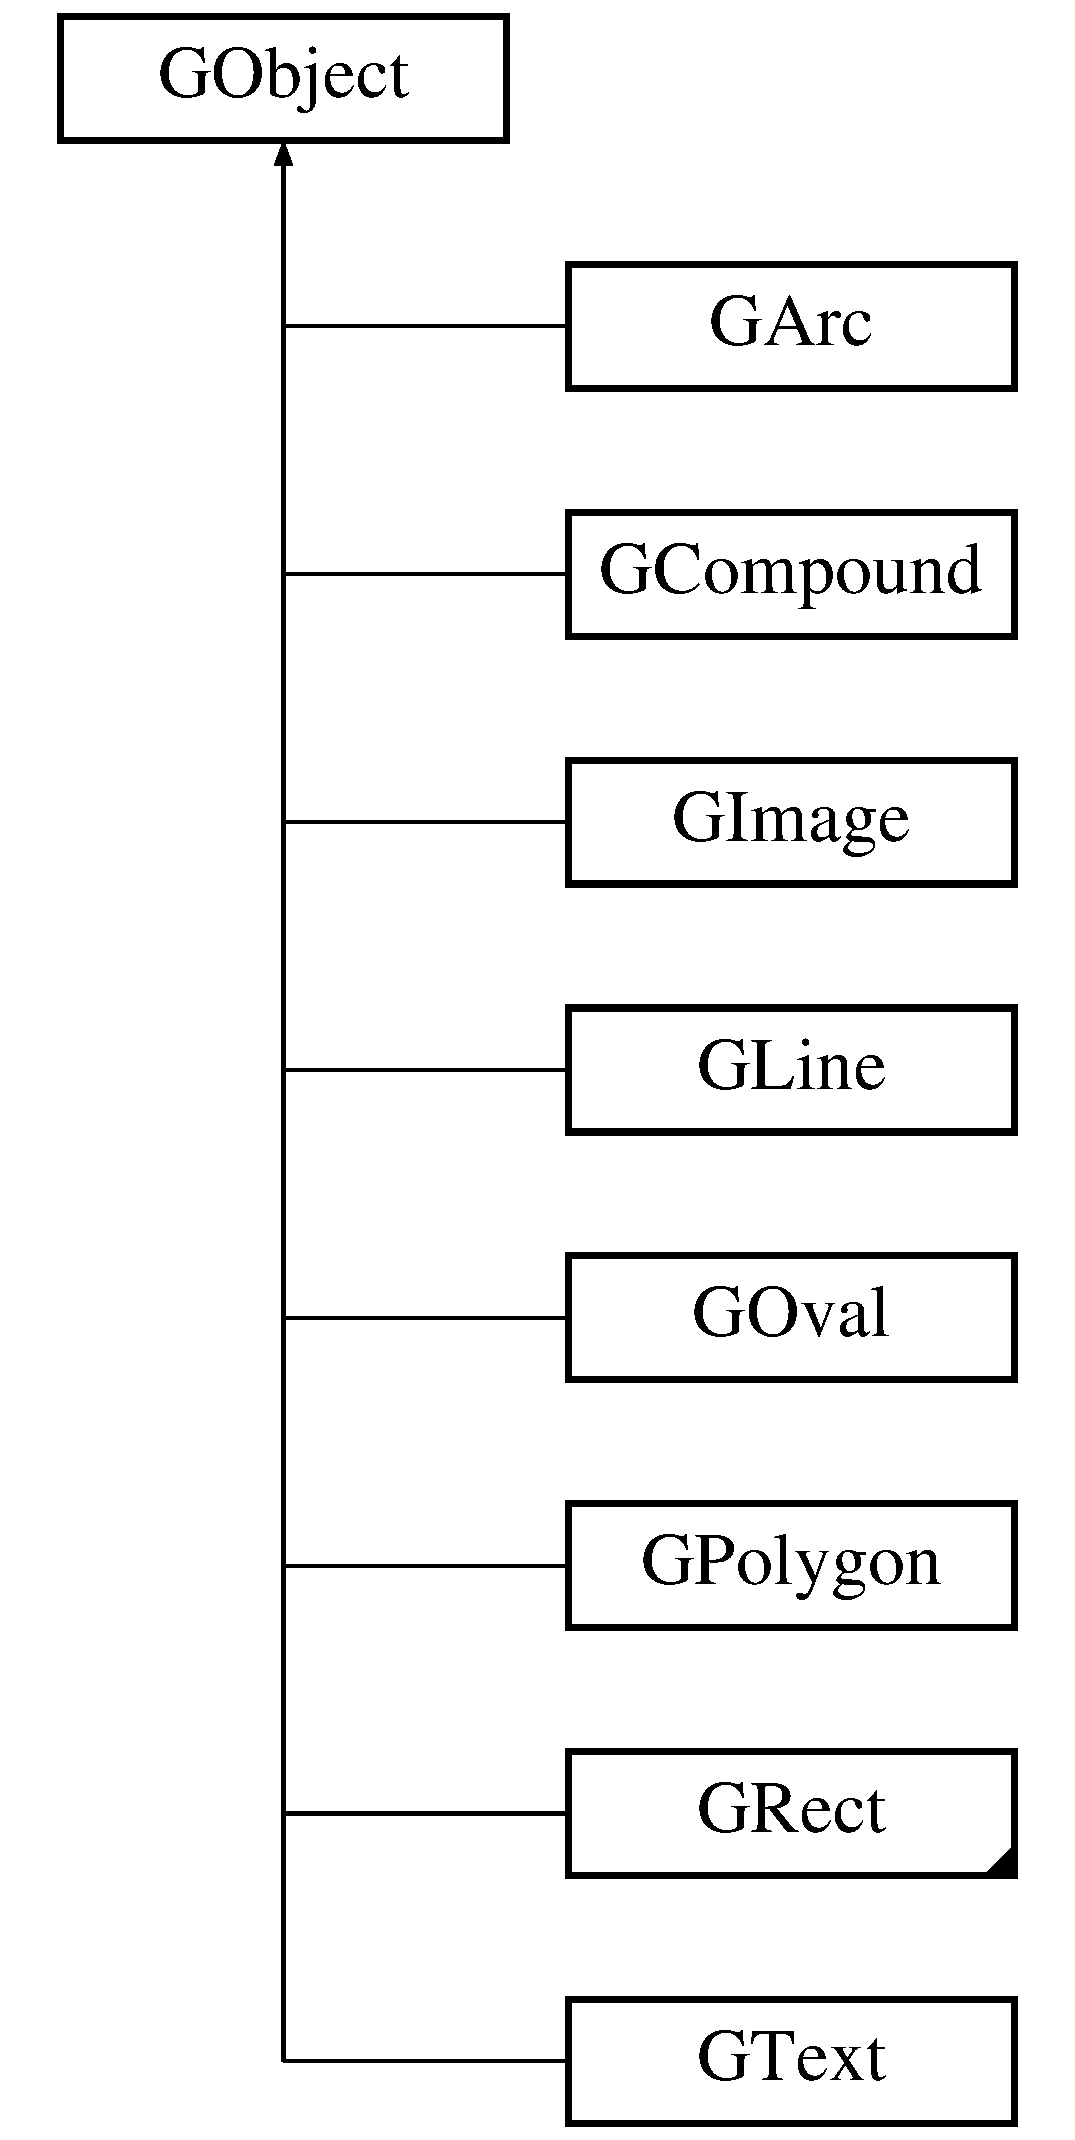
\includegraphics[height=9.000000cm]{classGObject}
\end{center}
\end{figure}
\subsection*{Public Types}
\begin{DoxyCompactItemize}
\item 
enum \mbox{\hyperlink{classGObject_a86e0f5648542856159bb40775c854aa7}{Line\+Style}} \{ \mbox{\hyperlink{classGObject_a86e0f5648542856159bb40775c854aa7acbc84bd5232621834ed31f44d457c1eb}{L\+I\+N\+E\+\_\+\+N\+O\+NE}}, 
\mbox{\hyperlink{classGObject_a86e0f5648542856159bb40775c854aa7a700c78bc2cd76acaab26651bf7b4941f}{L\+I\+N\+E\+\_\+\+S\+O\+L\+ID}}, 
\mbox{\hyperlink{classGObject_a86e0f5648542856159bb40775c854aa7a9ccba0845f785d81d07b333ae1aad84e}{L\+I\+N\+E\+\_\+\+D\+A\+SH}}, 
\mbox{\hyperlink{classGObject_a86e0f5648542856159bb40775c854aa7a8e811c096cb941997f0bfda168bb6df3}{L\+I\+N\+E\+\_\+\+D\+OT}}, 
\mbox{\hyperlink{classGObject_a86e0f5648542856159bb40775c854aa7ada15a2e3d737b2db7706d8300f91b89d}{L\+I\+N\+E\+\_\+\+D\+A\+S\+H\+\_\+\+D\+OT}}, 
\mbox{\hyperlink{classGObject_a86e0f5648542856159bb40775c854aa7aabf4053a73eafa7ba2b7e6d664c74c1d}{L\+I\+N\+E\+\_\+\+D\+A\+S\+H\+\_\+\+D\+O\+T\+\_\+\+D\+OT}}
 \}
\begin{DoxyCompactList}\small\item\em Styles that can be used for the outline around various shapes. \end{DoxyCompactList}\end{DoxyCompactItemize}
\subsection*{Public Member Functions}
\begin{DoxyCompactItemize}
\item 
virtual \mbox{\hyperlink{classGObject_ac955ba26942d1d44fc3d0cd6f76b1790}{$\sim$\+G\+Object}} ()
\begin{DoxyCompactList}\small\item\em Frees the storage for the object. \end{DoxyCompactList}\item 
virtual bool \mbox{\hyperlink{classGObject_abb6a5d7c03e6eaaae97264c4799ce7c3}{contains}} (double x, double y) const
\begin{DoxyCompactList}\small\item\em Returns {\ttfamily true} if the specified point is inside the object. \end{DoxyCompactList}\item 
virtual bool \mbox{\hyperlink{classGObject_a1dbc9dafaae51958112dbe1267a1f547}{contains}} (const \mbox{\hyperlink{structGPoint}{G\+Point}} \&pt) const
\begin{DoxyCompactList}\small\item\em Returns {\ttfamily true} if the specified point is inside the object. \end{DoxyCompactList}\item 
virtual \mbox{\hyperlink{structGPoint}{G\+Point}} \mbox{\hyperlink{classGObject_a0d41183bf6b08de66fe3907551aab0d7}{get\+Bottom\+Right\+Location}} () const
\begin{DoxyCompactList}\small\item\em Returns the x/y coordinates of the bottom/right corner of the object. \end{DoxyCompactList}\item 
virtual double \mbox{\hyperlink{classGObject_a4316a2406c18e1c6d061fe51fd355490}{get\+BottomY}} () const
\begin{DoxyCompactList}\small\item\em Returns the {\itshape y}-\/coordinate of the bottom of the object. \end{DoxyCompactList}\item 
virtual \mbox{\hyperlink{structGRectangle}{G\+Rectangle}} \mbox{\hyperlink{classGObject_a29e6ac35a0b48f491a4c88194cc5da3b}{get\+Bounds}} () const
\begin{DoxyCompactList}\small\item\em Returns the bounding box of this object, which is defined to be the smallest rectangle that covers everything drawn by the figure. \end{DoxyCompactList}\item 
virtual \mbox{\hyperlink{structGPoint}{G\+Point}} \mbox{\hyperlink{classGObject_a0909472e91448470bccdb62ecfb95d8b}{get\+Center\+Location}} () const
\begin{DoxyCompactList}\small\item\em Returns the x/y-\/coordinates of the center of the object. \end{DoxyCompactList}\item 
virtual double \mbox{\hyperlink{classGObject_a04df74355b545e0543112d5b8d924176}{get\+CenterX}} () const
\begin{DoxyCompactList}\small\item\em Returns the {\itshape x}-\/coordinate of the center of the object. \end{DoxyCompactList}\item 
virtual double \mbox{\hyperlink{classGObject_acb3287a3d507025a26f54b895713b947}{get\+CenterY}} () const
\begin{DoxyCompactList}\small\item\em Returns the {\itshape y}-\/coordinate of the center of the object. \end{DoxyCompactList}\item 
virtual std\+::string \mbox{\hyperlink{classGObject_aa061dfa488c31e18549d64363c1d0e34}{get\+Color}} () const
\begin{DoxyCompactList}\small\item\em Returns the color used to display this object. \end{DoxyCompactList}\item 
virtual std\+::string \mbox{\hyperlink{classGObject_a76f6964a11fde7c78e9751be184e1a3c}{get\+Fill\+Color}} () const
\begin{DoxyCompactList}\small\item\em Returns the color used to display the filled region of this object. \end{DoxyCompactList}\item 
virtual double \mbox{\hyperlink{classGObject_a1e7e353362434072875264cf95629f99}{get\+Height}} () const
\begin{DoxyCompactList}\small\item\em Returns the height of this object, which is the same as the height of its bounding box. \end{DoxyCompactList}\item 
virtual \mbox{\hyperlink{classGObject_a86e0f5648542856159bb40775c854aa7}{Line\+Style}} \mbox{\hyperlink{classGObject_aaf1f5ea8281e5e3486662878d26f0a13}{get\+Line\+Style}} () const
\begin{DoxyCompactList}\small\item\em Returns the object\textquotesingle{}s style such as solid or dashed. \end{DoxyCompactList}\item 
virtual double \mbox{\hyperlink{classGObject_a85ff266dc3eb63d9f2d8e5a4487fd3c0}{get\+Line\+Width}} () const
\begin{DoxyCompactList}\small\item\em Returns the width of the line used to draw this object. \end{DoxyCompactList}\item 
virtual \mbox{\hyperlink{structGPoint}{G\+Point}} \mbox{\hyperlink{classGObject_a4f83802015511edeb63b892830812c11}{get\+Location}} () const
\begin{DoxyCompactList}\small\item\em Returns the location of the top-\/left corner of object. \end{DoxyCompactList}\item 
virtual double \mbox{\hyperlink{classGObject_a1ae3fc278cc5b71b9f2d96a8a83cdf26}{get\+Opacity}} () const
\begin{DoxyCompactList}\small\item\em Returns how opaque (non-\/transparent) this object will appear from 0.\+0 (completely transparent) to 1.\+0 (completely opaque, default). \end{DoxyCompactList}\item 
virtual \mbox{\hyperlink{classGCompound}{G\+Compound}} $\ast$ \mbox{\hyperlink{classGObject_a3e53cef70541b1a14eade4ad0984d0b4}{get\+Parent}} () const
\begin{DoxyCompactList}\small\item\em Returns a pointer to the {\ttfamily \mbox{\hyperlink{classGCompound}{G\+Compound}}} that contains this object. \end{DoxyCompactList}\item 
virtual double \mbox{\hyperlink{classGObject_a798cc79daaa10145b28f60bcdfdb0ee9}{get\+RightX}} () const
\begin{DoxyCompactList}\small\item\em Returns the {\itshape x}-\/coordinate of the right side of the object. \end{DoxyCompactList}\item 
virtual \mbox{\hyperlink{structGDimension}{G\+Dimension}} \mbox{\hyperlink{classGObject_a7b4eec96a2bdc6420695d5796a78eea9}{get\+Size}} () const
\begin{DoxyCompactList}\small\item\em Returns the size of the object as a {\ttfamily \mbox{\hyperlink{structGDimension}{G\+Dimension}}}. \end{DoxyCompactList}\item 
virtual std\+::string \mbox{\hyperlink{classGObject_a799e073a127b428cc841086d42ea4fed}{get\+Type}} () const =0
\begin{DoxyCompactList}\small\item\em Returns the type of the object as a string, such as {\ttfamily \char`\"{}\+G\+Oval\char`\"{}} or {\ttfamily \char`\"{}\+G\+Rect\char`\"{}}. \end{DoxyCompactList}\item 
virtual double \mbox{\hyperlink{classGObject_a0ed2965abd4f5701d2cadf71239faf19}{get\+Width}} () const
\begin{DoxyCompactList}\small\item\em Returns the width of this object, which is equal to the width of the bounding box. \end{DoxyCompactList}\item 
virtual double \mbox{\hyperlink{classGObject_a344385751bee0720059403940d57a13e}{getX}} () const
\begin{DoxyCompactList}\small\item\em Returns the leftmost {\itshape x}-\/coordinate of the object. \end{DoxyCompactList}\item 
virtual double \mbox{\hyperlink{classGObject_aafa51c7f8f38a09febbb9ce7853f77b4}{getY}} () const
\begin{DoxyCompactList}\small\item\em Returns the topmost {\itshape y}-\/coordinate of the object. \end{DoxyCompactList}\item 
virtual bool \mbox{\hyperlink{classGObject_a11c404f106940c201b6f326e0355c150}{is\+Filled}} () const
\begin{DoxyCompactList}\small\item\em Returns {\ttfamily true} if the object is filled with color. \end{DoxyCompactList}\item 
virtual bool \mbox{\hyperlink{classGObject_a9de207581cfa4ca1eaa06da5f29b75fc}{is\+Transformed}} () const
\begin{DoxyCompactList}\small\item\em Returns {\ttfamily true} if this object has been transformed by calling methods such as \mbox{\hyperlink{classGObject_ae1ffaa12185dfd5ba464f7d87c329e26}{rotate()}} or \mbox{\hyperlink{classGObject_ad2e1900f730475c2d044817db03b38d6}{scale()}} on it. \end{DoxyCompactList}\item 
virtual bool \mbox{\hyperlink{classGObject_a9d8a6cfb13917785c143e74d40e4e2be}{is\+Visible}} () const
\begin{DoxyCompactList}\small\item\em Returns {\ttfamily true} if this object is visible on screen. \end{DoxyCompactList}\item 
virtual void \mbox{\hyperlink{classGObject_a5973d8dda83afb36e2c56855515be392}{move}} (double dx, double dy)
\begin{DoxyCompactList}\small\item\em Moves the object on the screen using the displacements {\ttfamily dx} and {\ttfamily dy}. \end{DoxyCompactList}\item 
virtual void \mbox{\hyperlink{classGObject_ac827b978aa122f136a14c198687ad80f}{repaint}} ()
\begin{DoxyCompactList}\small\item\em Instructs the object to redraw itself on screen. \end{DoxyCompactList}\item 
virtual void \mbox{\hyperlink{classGObject_a6022a1fd1e5dcd2fd5585e5a36aa3f37}{reset\+Transform}} ()
\begin{DoxyCompactList}\small\item\em Undoes any previous scale/rotate transformations on this object. \end{DoxyCompactList}\item 
virtual void \mbox{\hyperlink{classGObject_ae1ffaa12185dfd5ba464f7d87c329e26}{rotate}} (double theta)
\begin{DoxyCompactList}\small\item\em Transforms the object by rotating it {\ttfamily theta} degrees counterclockwise around its origin. \end{DoxyCompactList}\item 
virtual void \mbox{\hyperlink{classGObject_ad2e1900f730475c2d044817db03b38d6}{scale}} (double sf)
\begin{DoxyCompactList}\small\item\em Scales the object by the specified scale factor. \end{DoxyCompactList}\item 
virtual void \mbox{\hyperlink{classGObject_a63641f69d610d0b951357d35a0c3b1e3}{scale}} (double sx, double sy)
\begin{DoxyCompactList}\small\item\em Scales the object by the specified scale factors. \end{DoxyCompactList}\item 
void \mbox{\hyperlink{classGObject_ab6747f40313c531c2db32edb5b63b9b7}{send\+Backward}} ()
\begin{DoxyCompactList}\small\item\em Moves this object one step toward the back in the {\itshape z} dimension. \end{DoxyCompactList}\item 
void \mbox{\hyperlink{classGObject_a710b3e449c9facba7847c91ab170d281}{send\+Forward}} ()
\begin{DoxyCompactList}\small\item\em Moves this object one step toward the front in the {\itshape z} dimension. \end{DoxyCompactList}\item 
void \mbox{\hyperlink{classGObject_a0f7f1efbb7fd46dde2867c4ad0330896}{send\+To\+Back}} ()
\begin{DoxyCompactList}\small\item\em Moves this object to the back of the display in the {\itshape z} dimension. \end{DoxyCompactList}\item 
void \mbox{\hyperlink{classGObject_aee33d68488e46827ef55fac07f40a9b2}{send\+To\+Front}} ()
\begin{DoxyCompactList}\small\item\em Moves this object to the front of the display in the {\itshape z} dimension. \end{DoxyCompactList}\item 
virtual void \mbox{\hyperlink{classGObject_a71ff7b16b8f1bdc4a1ce9f30cf8b87d8}{set\+Bottom\+Right\+Location}} (double x, double y)
\begin{DoxyCompactList}\small\item\em Sets the location of the bottom/right of this object. \end{DoxyCompactList}\item 
virtual void \mbox{\hyperlink{classGObject_ac6f7320321182f1d18c1c0fa97d5e941}{set\+Bottom\+Right\+Location}} (const \mbox{\hyperlink{structGPoint}{G\+Point}} \&pt)
\begin{DoxyCompactList}\small\item\em Sets the location of the bottom/right of this object. \end{DoxyCompactList}\item 
virtual void \mbox{\hyperlink{classGObject_a4b20e93c2a2597484f74ee5caa71f41f}{set\+BottomY}} (double y)
\begin{DoxyCompactList}\small\item\em Sets the location of the bottom y-\/coordinate of this object. \end{DoxyCompactList}\item 
virtual void \mbox{\hyperlink{classGObject_a2aae8197624b72265ab83b4f1bc73f2f}{set\+Bounds}} (double x, double y, double width, double height)
\begin{DoxyCompactList}\small\item\em Changes the bounds of this object to the specified values. \end{DoxyCompactList}\item 
virtual void \mbox{\hyperlink{classGObject_acada386653f008cacc7cce86426bef7c}{set\+Bounds}} (const \mbox{\hyperlink{structGRectangle}{G\+Rectangle}} \&size)
\begin{DoxyCompactList}\small\item\em Changes the bounds of this object to the specified rectangle. \end{DoxyCompactList}\item 
virtual void \mbox{\hyperlink{classGObject_a290b47dd8de1be44089f95cb2c47c1de}{set\+Center\+Location}} (double x, double y)
\begin{DoxyCompactList}\small\item\em Sets the location of the center of this object. \end{DoxyCompactList}\item 
virtual void \mbox{\hyperlink{classGObject_a1bedf1b233ecba3f753ec58908a683a6}{set\+Center\+Location}} (const \mbox{\hyperlink{structGPoint}{G\+Point}} \&pt)
\begin{DoxyCompactList}\small\item\em Sets the location of the center of this object. \end{DoxyCompactList}\item 
virtual void \mbox{\hyperlink{classGObject_a2f4936281e056eead00a9186b9ba8af6}{set\+CenterX}} (double x)
\begin{DoxyCompactList}\small\item\em Sets the x-\/coordinate of the center of this object. \end{DoxyCompactList}\item 
virtual void \mbox{\hyperlink{classGObject_aad2a22b4fde88c33306b92aebf641d57}{set\+CenterY}} (double y)
\begin{DoxyCompactList}\small\item\em Sets the y-\/coordinate of the center of this object. \end{DoxyCompactList}\item 
virtual void \mbox{\hyperlink{classGObject_ad57ef49bc31db94e92648aa3737923d6}{set\+Color}} (int r, int g, int b)
\begin{DoxyCompactList}\small\item\em Sets the color used to display this object. \end{DoxyCompactList}\item 
virtual void \mbox{\hyperlink{classGObject_ab1f5cc0f5cc6bbbd716a526c61f1081d}{set\+Color}} (int rgb)
\begin{DoxyCompactList}\small\item\em Sets the color used to display this object. \end{DoxyCompactList}\item 
virtual void \mbox{\hyperlink{classGObject_a61374df6c11b52cfbb0815decdbaebc6}{set\+Color}} (const std\+::string \&color)
\begin{DoxyCompactList}\small\item\em Sets the color used to display this object. \end{DoxyCompactList}\item 
virtual void \mbox{\hyperlink{classGObject_ad767a33971159e9493e221cca4c00ae9}{set\+Fill\+Color}} (int r, int g, int b)
\begin{DoxyCompactList}\small\item\em Sets the color used to display the filled region of this object, if any. \end{DoxyCompactList}\item 
virtual void \mbox{\hyperlink{classGObject_aa59d9775a67fa7df2b24a95cd34840a3}{set\+Fill\+Color}} (int rgb)
\begin{DoxyCompactList}\small\item\em Sets the color used to display the filled region of this object, if any. \end{DoxyCompactList}\item 
virtual void \mbox{\hyperlink{classGObject_adbc18b1a930aadd97d7437f9f7265b96}{set\+Fill\+Color}} (const std\+::string \&color)
\begin{DoxyCompactList}\small\item\em Sets the color used to display the filled region of this object, if any. \end{DoxyCompactList}\item 
virtual void \mbox{\hyperlink{classGObject_a9b82b53362282c6bb7d6947068d2e55b}{set\+Filled}} (bool flag)
\begin{DoxyCompactList}\small\item\em Sets the fill status for the object, where {\ttfamily false} is outlined and {\ttfamily true} is filled. \end{DoxyCompactList}\item 
virtual void \mbox{\hyperlink{classGObject_a2592348886ffea646c6534bf88f7c49d}{set\+Font}} (const Q\+Font \&font)
\begin{DoxyCompactList}\small\item\em Changes the font used to display the object as specified by the given Qt font. \end{DoxyCompactList}\item 
virtual void \mbox{\hyperlink{classGObject_a8e096e8818d838aceae1d46d58fb3a7b}{set\+Font}} (const std\+::string \&font)
\begin{DoxyCompactList}\small\item\em Changes the font used to display the object as specified by the string {\ttfamily font}, which has the following format\+: \end{DoxyCompactList}\item 
virtual void \mbox{\hyperlink{classGObject_ad18e8fab1e02a4e9b75c6730212558eb}{set\+Foreground}} (int r, int g, int b)
\begin{DoxyCompactList}\small\item\em Sets the color used to display this object. \end{DoxyCompactList}\item 
virtual void \mbox{\hyperlink{classGObject_a9eb856b5ff83a19df3831a31f15f4563}{set\+Foreground}} (int rgb)
\begin{DoxyCompactList}\small\item\em Sets the color used to display this object. \end{DoxyCompactList}\item 
virtual void \mbox{\hyperlink{classGObject_af59209aeadea6dfc6d97a2d8531f50e1}{set\+Foreground}} (const std\+::string \&color)
\begin{DoxyCompactList}\small\item\em Sets the color used to display this object. \end{DoxyCompactList}\item 
virtual void \mbox{\hyperlink{classGObject_a9e280bfc4544dfaf8e4376c4e1a74357}{set\+Height}} (double height)
\begin{DoxyCompactList}\small\item\em Changes the height of this object to the specified height without changing its width. \end{DoxyCompactList}\item 
virtual void \mbox{\hyperlink{classGObject_add11575087eb94f1a71faa3f826c6341}{set\+Line\+Style}} (\mbox{\hyperlink{classGObject_a86e0f5648542856159bb40775c854aa7}{Line\+Style}} line\+Style)
\begin{DoxyCompactList}\small\item\em Sets the object\textquotesingle{}s style such as solid (\mbox{\hyperlink{classGObject_a86e0f5648542856159bb40775c854aa7a700c78bc2cd76acaab26651bf7b4941f}{G\+Object\+::\+L\+I\+N\+E\+\_\+\+S\+O\+L\+ID}}) or dashed (\mbox{\hyperlink{classGObject_a86e0f5648542856159bb40775c854aa7a9ccba0845f785d81d07b333ae1aad84e}{G\+Object\+::\+L\+I\+N\+E\+\_\+\+D\+A\+SH}}). \end{DoxyCompactList}\item 
virtual void \mbox{\hyperlink{classGObject_afd6a47c6ea6a1f85ca05a65ba3ff3477}{set\+Line\+Width}} (double line\+Width)
\begin{DoxyCompactList}\small\item\em Sets the width of the line used to draw this object. \end{DoxyCompactList}\item 
virtual void \mbox{\hyperlink{classGObject_a04594e8ba9b98513a64f1da00dcae18c}{set\+Location}} (double x, double y)
\begin{DoxyCompactList}\small\item\em Sets the location of the top-\/left corner of this object to the specified coordinates. \end{DoxyCompactList}\item 
virtual void \mbox{\hyperlink{classGObject_aa8480c0b7166cdf8f784cece06ab353f}{set\+Location}} (const \mbox{\hyperlink{structGPoint}{G\+Point}} \&pt)
\begin{DoxyCompactList}\small\item\em Sets the location of the top-\/left corner of this object to the specified point. \end{DoxyCompactList}\item 
virtual void \mbox{\hyperlink{classGObject_a04af1866cc1bae4a1226695794a50539}{set\+Opacity}} (double opacity)
\begin{DoxyCompactList}\small\item\em Sets how opaque (non-\/transparent) this object will appear from 0.\+0 (completely transparent) to 1.\+0 (completely opaque, default). \end{DoxyCompactList}\item 
virtual void \mbox{\hyperlink{classGObject_a3c90b758cdc2c911c9ef76c4360eb912}{set\+RightX}} (double x)
\begin{DoxyCompactList}\small\item\em Sets the location of the rightmost x-\/coordinate of this object. \end{DoxyCompactList}\item 
virtual void \mbox{\hyperlink{classGObject_aca25d49481f9bf5fc8f7df4c086c4ce7}{set\+Size}} (double width, double height)
\begin{DoxyCompactList}\small\item\em Changes the size of this object to the specified width and height. \end{DoxyCompactList}\item 
virtual void \mbox{\hyperlink{classGObject_ae2b628228f192c2702c4ce941b2af68f}{set\+Size}} (const \mbox{\hyperlink{structGDimension}{G\+Dimension}} \&size)
\begin{DoxyCompactList}\small\item\em Changes the size of this object to the specified width and height. \end{DoxyCompactList}\item 
virtual void \mbox{\hyperlink{classGObject_a88203f28224315d9f4471212f4af8ed3}{set\+Visible}} (bool flag)
\begin{DoxyCompactList}\small\item\em Sets whether this object is visible. \end{DoxyCompactList}\item 
virtual void \mbox{\hyperlink{classGObject_aa3f3fba4cb131baa8696ba01e3bceca1}{set\+Width}} (double width)
\begin{DoxyCompactList}\small\item\em Changes the width of this object to the specified width without changing its height. \end{DoxyCompactList}\item 
virtual void \mbox{\hyperlink{classGObject_a9c18fcc579333bf9653d13ad2b372e39}{setX}} (double x)
\begin{DoxyCompactList}\small\item\em Sets the x location of the left side of this object. \end{DoxyCompactList}\item 
virtual void \mbox{\hyperlink{classGObject_a7d57e2a5c35d27feb58fd498a3cf82b9}{setY}} (double y)
\begin{DoxyCompactList}\small\item\em Sets the y location of the top of this object. \end{DoxyCompactList}\item 
virtual std\+::string \mbox{\hyperlink{classGObject_a1fe5121d6528fdea3f243321b3fa3a49}{to\+String}} () const
\begin{DoxyCompactList}\small\item\em Returns a printable representation of the object. \end{DoxyCompactList}\end{DoxyCompactItemize}
\subsection*{Static Public Member Functions}
\begin{DoxyCompactItemize}
\item 
static bool \mbox{\hyperlink{classGObject_a93be0e1fe1b1bf1a1da732470c94f42b}{is\+Anti\+Aliasing}} ()
\begin{DoxyCompactList}\small\item\em Returns whether we should globally anti-\/alias graphical objects. \end{DoxyCompactList}\item 
static void \mbox{\hyperlink{classGObject_a1e43371668ae850193cebedb44e1bbe3}{set\+Anti\+Aliasing}} (bool value)
\begin{DoxyCompactList}\small\item\em Globally turns on/off the anti-\/aliasing feature that smooths out the edges of onscreen shapes. \end{DoxyCompactList}\end{DoxyCompactItemize}
\subsection*{Protected Member Functions}
\begin{DoxyCompactItemize}
\item 
virtual std\+::string \mbox{\hyperlink{classGObject_a4fcdf8de5c6de92242a975d83d8f23ea}{to\+String\+Extra}} () const
\begin{DoxyCompactList}\small\item\em Returns a string containing any extra unique information about this type of graphical object. \end{DoxyCompactList}\end{DoxyCompactItemize}
\subsection*{Protected Attributes}
\begin{DoxyCompactItemize}
\item 
Q\+Brush \mbox{\hyperlink{classGObject_aab24462ec896b596d99911767b0912d0}{\+\_\+brush}}
\item 
std\+::string \mbox{\hyperlink{classGObject_a1134e770ae4315ea8bc1201e2f21da8b}{\+\_\+color}}
\item 
int \mbox{\hyperlink{classGObject_a003fdd343d9b7505c53a8b7a134200ed}{\+\_\+color\+Int}}
\item 
std\+::string \mbox{\hyperlink{classGObject_a179f8d6cee65cd8a54692e32b224392a}{\+\_\+fill\+Color}}
\item 
int \mbox{\hyperlink{classGObject_a751def333a67d651e5b99cc331ecb496}{\+\_\+fill\+Color\+Int}}
\item 
bool \mbox{\hyperlink{classGObject_ad4a55cbcd61b58a4d49666490bb2f103}{\+\_\+fill\+Flag}}
\item 
std\+::string \mbox{\hyperlink{classGObject_aea76ea1a8b5dd7b0a78653277e63b536}{\+\_\+font}}
\item 
double \mbox{\hyperlink{classGObject_ad05df29e7f27fc504abd743e3d8b4e73}{\+\_\+height}}
\item 
\mbox{\hyperlink{classGObject_a86e0f5648542856159bb40775c854aa7}{Line\+Style}} \mbox{\hyperlink{classGObject_a89bafecaafb7c72d55c7efc10b7d0523}{\+\_\+line\+Style}}
\item 
double \mbox{\hyperlink{classGObject_a16e9033665937f13de2e163dc2184aff}{\+\_\+line\+Width}}
\item 
double \mbox{\hyperlink{classGObject_a20eff8eb7af27182edc9bfc54768b6f3}{\+\_\+opacity}}
\item 
\mbox{\hyperlink{classGCompound}{G\+Compound}} $\ast$ \mbox{\hyperlink{classGObject_ac9452c1eaff70eebddbb318196aa3835}{\+\_\+parent}}
\item 
Q\+Pen \mbox{\hyperlink{classGObject_afb69d172743f868299847174eb1b6bc8}{\+\_\+pen}}
\item 
Q\+Transform \mbox{\hyperlink{classGObject_a475b8860a5f1adb4a1fdc58d1f5c1e32}{\+\_\+transform}}
\item 
bool \mbox{\hyperlink{classGObject_ae4725802fc8d8aaa0ab4bd4781f7e07c}{\+\_\+transformed}}
\item 
bool \mbox{\hyperlink{classGObject_a9312c72508471b7c7a87b540263e1af4}{\+\_\+visible}}
\item 
double \mbox{\hyperlink{classGObject_ab55d85a3371770e6725b1062cf160cd8}{\+\_\+width}}
\item 
double \mbox{\hyperlink{classGObject_a6675b83b27137b8d3aa2ad8133078ea6}{\+\_\+x}}
\item 
double \mbox{\hyperlink{classGObject_a2f0f6aeafddc8a39c578bfa7e22b5f1e}{\+\_\+y}}
\end{DoxyCompactItemize}


\subsection{Detailed Description}
This class is the common superclass of all graphical objects that can be displayed on a graphical window. 

The class {\ttfamily \mbox{\hyperlink{classGObject}{G\+Object}}} itself is an {\bfseries {\itshape abstract class}}, which means that you are not allowed to construct a {\ttfamily \mbox{\hyperlink{classGObject}{G\+Object}}} directly but must instead construct one of the concrete subclasses. 

Most methods used for graphics take a pointer to a 
\begin{DoxyCode}
\mbox{\hyperlink{classGObject}{GObject}}
\end{DoxyCode}
 rather than the 
\begin{DoxyCode}
\mbox{\hyperlink{classGObject}{GObject}}
\end{DoxyCode}
 itself. Applications that use 
\begin{DoxyCode}
\mbox{\hyperlink{classGObject}{GObject}}
\end{DoxyCode}
 pointers therefore use the arrow operator (
\begin{DoxyCode}
->
\end{DoxyCode}
) to apply methods to the object pointer. For examples illustrating the use of the 
\begin{DoxyCode}
\mbox{\hyperlink{classGObject}{GObject}}
\end{DoxyCode}
 class, see the descriptions of the individual subclasses. 

\subsection{Member Enumeration Documentation}
\mbox{\Hypertarget{classGObject_a86e0f5648542856159bb40775c854aa7}\label{classGObject_a86e0f5648542856159bb40775c854aa7}} 
\index{G\+Object@{G\+Object}!Line\+Style@{Line\+Style}}
\index{Line\+Style@{Line\+Style}!G\+Object@{G\+Object}}
\subsubsection{\texorpdfstring{Line\+Style}{LineStyle}}
{\footnotesize\ttfamily enum \mbox{\hyperlink{classGObject_a86e0f5648542856159bb40775c854aa7}{Line\+Style}}}



Styles that can be used for the outline around various shapes. 

Call set\+Line\+Style on a \mbox{\hyperlink{classGObject}{G\+Object}} and pass one of these values. \begin{DoxyEnumFields}{Enumerator}
\raisebox{\heightof{T}}[0pt][0pt]{\index{L\+I\+N\+E\+\_\+\+N\+O\+NE@{L\+I\+N\+E\+\_\+\+N\+O\+NE}!G\+Object@{G\+Object}}\index{G\+Object@{G\+Object}!L\+I\+N\+E\+\_\+\+N\+O\+NE@{L\+I\+N\+E\+\_\+\+N\+O\+NE}}}\mbox{\Hypertarget{classGObject_a86e0f5648542856159bb40775c854aa7acbc84bd5232621834ed31f44d457c1eb}\label{classGObject_a86e0f5648542856159bb40775c854aa7acbc84bd5232621834ed31f44d457c1eb}} 
L\+I\+N\+E\+\_\+\+N\+O\+NE&\\
\hline

\raisebox{\heightof{T}}[0pt][0pt]{\index{L\+I\+N\+E\+\_\+\+S\+O\+L\+ID@{L\+I\+N\+E\+\_\+\+S\+O\+L\+ID}!G\+Object@{G\+Object}}\index{G\+Object@{G\+Object}!L\+I\+N\+E\+\_\+\+S\+O\+L\+ID@{L\+I\+N\+E\+\_\+\+S\+O\+L\+ID}}}\mbox{\Hypertarget{classGObject_a86e0f5648542856159bb40775c854aa7a700c78bc2cd76acaab26651bf7b4941f}\label{classGObject_a86e0f5648542856159bb40775c854aa7a700c78bc2cd76acaab26651bf7b4941f}} 
L\+I\+N\+E\+\_\+\+S\+O\+L\+ID&\\
\hline

\raisebox{\heightof{T}}[0pt][0pt]{\index{L\+I\+N\+E\+\_\+\+D\+A\+SH@{L\+I\+N\+E\+\_\+\+D\+A\+SH}!G\+Object@{G\+Object}}\index{G\+Object@{G\+Object}!L\+I\+N\+E\+\_\+\+D\+A\+SH@{L\+I\+N\+E\+\_\+\+D\+A\+SH}}}\mbox{\Hypertarget{classGObject_a86e0f5648542856159bb40775c854aa7a9ccba0845f785d81d07b333ae1aad84e}\label{classGObject_a86e0f5648542856159bb40775c854aa7a9ccba0845f785d81d07b333ae1aad84e}} 
L\+I\+N\+E\+\_\+\+D\+A\+SH&\\
\hline

\raisebox{\heightof{T}}[0pt][0pt]{\index{L\+I\+N\+E\+\_\+\+D\+OT@{L\+I\+N\+E\+\_\+\+D\+OT}!G\+Object@{G\+Object}}\index{G\+Object@{G\+Object}!L\+I\+N\+E\+\_\+\+D\+OT@{L\+I\+N\+E\+\_\+\+D\+OT}}}\mbox{\Hypertarget{classGObject_a86e0f5648542856159bb40775c854aa7a8e811c096cb941997f0bfda168bb6df3}\label{classGObject_a86e0f5648542856159bb40775c854aa7a8e811c096cb941997f0bfda168bb6df3}} 
L\+I\+N\+E\+\_\+\+D\+OT&\\
\hline

\raisebox{\heightof{T}}[0pt][0pt]{\index{L\+I\+N\+E\+\_\+\+D\+A\+S\+H\+\_\+\+D\+OT@{L\+I\+N\+E\+\_\+\+D\+A\+S\+H\+\_\+\+D\+OT}!G\+Object@{G\+Object}}\index{G\+Object@{G\+Object}!L\+I\+N\+E\+\_\+\+D\+A\+S\+H\+\_\+\+D\+OT@{L\+I\+N\+E\+\_\+\+D\+A\+S\+H\+\_\+\+D\+OT}}}\mbox{\Hypertarget{classGObject_a86e0f5648542856159bb40775c854aa7ada15a2e3d737b2db7706d8300f91b89d}\label{classGObject_a86e0f5648542856159bb40775c854aa7ada15a2e3d737b2db7706d8300f91b89d}} 
L\+I\+N\+E\+\_\+\+D\+A\+S\+H\+\_\+\+D\+OT&\\
\hline

\raisebox{\heightof{T}}[0pt][0pt]{\index{L\+I\+N\+E\+\_\+\+D\+A\+S\+H\+\_\+\+D\+O\+T\+\_\+\+D\+OT@{L\+I\+N\+E\+\_\+\+D\+A\+S\+H\+\_\+\+D\+O\+T\+\_\+\+D\+OT}!G\+Object@{G\+Object}}\index{G\+Object@{G\+Object}!L\+I\+N\+E\+\_\+\+D\+A\+S\+H\+\_\+\+D\+O\+T\+\_\+\+D\+OT@{L\+I\+N\+E\+\_\+\+D\+A\+S\+H\+\_\+\+D\+O\+T\+\_\+\+D\+OT}}}\mbox{\Hypertarget{classGObject_a86e0f5648542856159bb40775c854aa7aabf4053a73eafa7ba2b7e6d664c74c1d}\label{classGObject_a86e0f5648542856159bb40775c854aa7aabf4053a73eafa7ba2b7e6d664c74c1d}} 
L\+I\+N\+E\+\_\+\+D\+A\+S\+H\+\_\+\+D\+O\+T\+\_\+\+D\+OT&\\
\hline

\end{DoxyEnumFields}


\subsection{Constructor \& Destructor Documentation}
\mbox{\Hypertarget{classGObject_ac955ba26942d1d44fc3d0cd6f76b1790}\label{classGObject_ac955ba26942d1d44fc3d0cd6f76b1790}} 
\index{G\+Object@{G\+Object}!````~G\+Object@{$\sim$\+G\+Object}}
\index{````~G\+Object@{$\sim$\+G\+Object}!G\+Object@{G\+Object}}
\subsubsection{\texorpdfstring{$\sim$\+G\+Object()}{~GObject()}}
{\footnotesize\ttfamily $\sim$\mbox{\hyperlink{classGObject}{G\+Object}} (\begin{DoxyParamCaption}{ }\end{DoxyParamCaption})\hspace{0.3cm}{\ttfamily [virtual]}}



Frees the storage for the object. 



\subsection{Member Function Documentation}
\mbox{\Hypertarget{classGObject_abb6a5d7c03e6eaaae97264c4799ce7c3}\label{classGObject_abb6a5d7c03e6eaaae97264c4799ce7c3}} 
\index{G\+Object@{G\+Object}!contains@{contains}}
\index{contains@{contains}!G\+Object@{G\+Object}}
\subsubsection{\texorpdfstring{contains()}{contains()}\hspace{0.1cm}{\footnotesize\ttfamily [1/2]}}
{\footnotesize\ttfamily bool contains (\begin{DoxyParamCaption}\item[{double}]{x,  }\item[{double}]{y }\end{DoxyParamCaption}) const\hspace{0.3cm}{\ttfamily [virtual]}}



Returns {\ttfamily true} if the specified point is inside the object. 



Reimplemented in \mbox{\hyperlink{classGRoundRect_ad973a1d55799d3a73bf8b04986cd804e}{G\+Round\+Rect}}, \mbox{\hyperlink{classGPolygon_ad973a1d55799d3a73bf8b04986cd804e}{G\+Polygon}}, \mbox{\hyperlink{classGOval_ad973a1d55799d3a73bf8b04986cd804e}{G\+Oval}}, \mbox{\hyperlink{classGLine_ad973a1d55799d3a73bf8b04986cd804e}{G\+Line}}, \mbox{\hyperlink{classGCompound_ad973a1d55799d3a73bf8b04986cd804e}{G\+Compound}}, and \mbox{\hyperlink{classGArc_ad973a1d55799d3a73bf8b04986cd804e}{G\+Arc}}.

\mbox{\Hypertarget{classGObject_a1dbc9dafaae51958112dbe1267a1f547}\label{classGObject_a1dbc9dafaae51958112dbe1267a1f547}} 
\index{G\+Object@{G\+Object}!contains@{contains}}
\index{contains@{contains}!G\+Object@{G\+Object}}
\subsubsection{\texorpdfstring{contains()}{contains()}\hspace{0.1cm}{\footnotesize\ttfamily [2/2]}}
{\footnotesize\ttfamily bool contains (\begin{DoxyParamCaption}\item[{const \mbox{\hyperlink{structGPoint}{G\+Point}} \&}]{pt }\end{DoxyParamCaption}) const\hspace{0.3cm}{\ttfamily [virtual]}}



Returns {\ttfamily true} if the specified point is inside the object. 

\mbox{\Hypertarget{classGObject_a0d41183bf6b08de66fe3907551aab0d7}\label{classGObject_a0d41183bf6b08de66fe3907551aab0d7}} 
\index{G\+Object@{G\+Object}!get\+Bottom\+Right\+Location@{get\+Bottom\+Right\+Location}}
\index{get\+Bottom\+Right\+Location@{get\+Bottom\+Right\+Location}!G\+Object@{G\+Object}}
\subsubsection{\texorpdfstring{get\+Bottom\+Right\+Location()}{getBottomRightLocation()}}
{\footnotesize\ttfamily \mbox{\hyperlink{structGPoint}{G\+Point}} get\+Bottom\+Right\+Location (\begin{DoxyParamCaption}{ }\end{DoxyParamCaption}) const\hspace{0.3cm}{\ttfamily [virtual]}}



Returns the x/y coordinates of the bottom/right corner of the object. 

\mbox{\Hypertarget{classGObject_a4316a2406c18e1c6d061fe51fd355490}\label{classGObject_a4316a2406c18e1c6d061fe51fd355490}} 
\index{G\+Object@{G\+Object}!get\+BottomY@{get\+BottomY}}
\index{get\+BottomY@{get\+BottomY}!G\+Object@{G\+Object}}
\subsubsection{\texorpdfstring{get\+Bottom\+Y()}{getBottomY()}}
{\footnotesize\ttfamily double get\+BottomY (\begin{DoxyParamCaption}{ }\end{DoxyParamCaption}) const\hspace{0.3cm}{\ttfamily [virtual]}}



Returns the {\itshape y}-\/coordinate of the bottom of the object. 

Equivalent to the top y-\/coordinate plus the object\textquotesingle{}s height. \mbox{\Hypertarget{classGObject_a29e6ac35a0b48f491a4c88194cc5da3b}\label{classGObject_a29e6ac35a0b48f491a4c88194cc5da3b}} 
\index{G\+Object@{G\+Object}!get\+Bounds@{get\+Bounds}}
\index{get\+Bounds@{get\+Bounds}!G\+Object@{G\+Object}}
\subsubsection{\texorpdfstring{get\+Bounds()}{getBounds()}}
{\footnotesize\ttfamily \mbox{\hyperlink{structGRectangle}{G\+Rectangle}} get\+Bounds (\begin{DoxyParamCaption}{ }\end{DoxyParamCaption}) const\hspace{0.3cm}{\ttfamily [virtual]}}



Returns the bounding box of this object, which is defined to be the smallest rectangle that covers everything drawn by the figure. 

The coordinates of this rectangle do not necessarily match the location returned by {\ttfamily get\+Location}. Given a {\ttfamily \mbox{\hyperlink{classGText}{G\+Text}}} object, for example, {\ttfamily get\+Location} returns the coordinates of the point on the baseline at which the string begins; the {\ttfamily get\+Bounds} method, by contrast, returns a rectangle that covers the entire window area occupied by the string. 

Reimplemented in \mbox{\hyperlink{classGText_a89040ce9277825772d359fccd33bca86}{G\+Text}}, \mbox{\hyperlink{classGPolygon_a89040ce9277825772d359fccd33bca86}{G\+Polygon}}, \mbox{\hyperlink{classGLine_a89040ce9277825772d359fccd33bca86}{G\+Line}}, \mbox{\hyperlink{classGCompound_a89040ce9277825772d359fccd33bca86}{G\+Compound}}, and \mbox{\hyperlink{classGArc_a89040ce9277825772d359fccd33bca86}{G\+Arc}}.

\mbox{\Hypertarget{classGObject_a0909472e91448470bccdb62ecfb95d8b}\label{classGObject_a0909472e91448470bccdb62ecfb95d8b}} 
\index{G\+Object@{G\+Object}!get\+Center\+Location@{get\+Center\+Location}}
\index{get\+Center\+Location@{get\+Center\+Location}!G\+Object@{G\+Object}}
\subsubsection{\texorpdfstring{get\+Center\+Location()}{getCenterLocation()}}
{\footnotesize\ttfamily \mbox{\hyperlink{structGPoint}{G\+Point}} get\+Center\+Location (\begin{DoxyParamCaption}{ }\end{DoxyParamCaption}) const\hspace{0.3cm}{\ttfamily [virtual]}}



Returns the x/y-\/coordinates of the center of the object. 

Equivalent to the top/left plus half the object\textquotesingle{}s size. \mbox{\Hypertarget{classGObject_a04df74355b545e0543112d5b8d924176}\label{classGObject_a04df74355b545e0543112d5b8d924176}} 
\index{G\+Object@{G\+Object}!get\+CenterX@{get\+CenterX}}
\index{get\+CenterX@{get\+CenterX}!G\+Object@{G\+Object}}
\subsubsection{\texorpdfstring{get\+Center\+X()}{getCenterX()}}
{\footnotesize\ttfamily double get\+CenterX (\begin{DoxyParamCaption}{ }\end{DoxyParamCaption}) const\hspace{0.3cm}{\ttfamily [virtual]}}



Returns the {\itshape x}-\/coordinate of the center of the object. 

Equivalent to the top/left plus half the object\textquotesingle{}s width. \mbox{\Hypertarget{classGObject_acb3287a3d507025a26f54b895713b947}\label{classGObject_acb3287a3d507025a26f54b895713b947}} 
\index{G\+Object@{G\+Object}!get\+CenterY@{get\+CenterY}}
\index{get\+CenterY@{get\+CenterY}!G\+Object@{G\+Object}}
\subsubsection{\texorpdfstring{get\+Center\+Y()}{getCenterY()}}
{\footnotesize\ttfamily double get\+CenterY (\begin{DoxyParamCaption}{ }\end{DoxyParamCaption}) const\hspace{0.3cm}{\ttfamily [virtual]}}



Returns the {\itshape y}-\/coordinate of the center of the object. 

Equivalent to the top/left plus half the object\textquotesingle{}s height. \mbox{\Hypertarget{classGObject_aa061dfa488c31e18549d64363c1d0e34}\label{classGObject_aa061dfa488c31e18549d64363c1d0e34}} 
\index{G\+Object@{G\+Object}!get\+Color@{get\+Color}}
\index{get\+Color@{get\+Color}!G\+Object@{G\+Object}}
\subsubsection{\texorpdfstring{get\+Color()}{getColor()}}
{\footnotesize\ttfamily std\+::string get\+Color (\begin{DoxyParamCaption}{ }\end{DoxyParamCaption}) const\hspace{0.3cm}{\ttfamily [virtual]}}



Returns the color used to display this object. 

This color is always returned as a string in the form {\ttfamily \char`\"{}\#rrggbb\char`\"{}}, where {\ttfamily rr}, {\ttfamily gg}, and {\ttfamily bb} are the red, green, and blue components of the color, expressed as two-\/digit hexadecimal values. \mbox{\Hypertarget{classGObject_a76f6964a11fde7c78e9751be184e1a3c}\label{classGObject_a76f6964a11fde7c78e9751be184e1a3c}} 
\index{G\+Object@{G\+Object}!get\+Fill\+Color@{get\+Fill\+Color}}
\index{get\+Fill\+Color@{get\+Fill\+Color}!G\+Object@{G\+Object}}
\subsubsection{\texorpdfstring{get\+Fill\+Color()}{getFillColor()}}
{\footnotesize\ttfamily std\+::string get\+Fill\+Color (\begin{DoxyParamCaption}{ }\end{DoxyParamCaption}) const\hspace{0.3cm}{\ttfamily [virtual]}}



Returns the color used to display the filled region of this object. 

If none has been set, returns the empty string. \mbox{\Hypertarget{classGObject_a1e7e353362434072875264cf95629f99}\label{classGObject_a1e7e353362434072875264cf95629f99}} 
\index{G\+Object@{G\+Object}!get\+Height@{get\+Height}}
\index{get\+Height@{get\+Height}!G\+Object@{G\+Object}}
\subsubsection{\texorpdfstring{get\+Height()}{getHeight()}}
{\footnotesize\ttfamily double get\+Height (\begin{DoxyParamCaption}{ }\end{DoxyParamCaption}) const\hspace{0.3cm}{\ttfamily [virtual]}}



Returns the height of this object, which is the same as the height of its bounding box. 



Reimplemented in \mbox{\hyperlink{classGPolygon_a2bede8b27b21ae4c7940e762cbad9e07}{G\+Polygon}}, and \mbox{\hyperlink{classGLine_a2bede8b27b21ae4c7940e762cbad9e07}{G\+Line}}.

\mbox{\Hypertarget{classGObject_aaf1f5ea8281e5e3486662878d26f0a13}\label{classGObject_aaf1f5ea8281e5e3486662878d26f0a13}} 
\index{G\+Object@{G\+Object}!get\+Line\+Style@{get\+Line\+Style}}
\index{get\+Line\+Style@{get\+Line\+Style}!G\+Object@{G\+Object}}
\subsubsection{\texorpdfstring{get\+Line\+Style()}{getLineStyle()}}
{\footnotesize\ttfamily \mbox{\hyperlink{classGObject_a86e0f5648542856159bb40775c854aa7}{G\+Object\+::\+Line\+Style}} get\+Line\+Style (\begin{DoxyParamCaption}{ }\end{DoxyParamCaption}) const\hspace{0.3cm}{\ttfamily [virtual]}}



Returns the object\textquotesingle{}s style such as solid or dashed. 

\mbox{\Hypertarget{classGObject_a85ff266dc3eb63d9f2d8e5a4487fd3c0}\label{classGObject_a85ff266dc3eb63d9f2d8e5a4487fd3c0}} 
\index{G\+Object@{G\+Object}!get\+Line\+Width@{get\+Line\+Width}}
\index{get\+Line\+Width@{get\+Line\+Width}!G\+Object@{G\+Object}}
\subsubsection{\texorpdfstring{get\+Line\+Width()}{getLineWidth()}}
{\footnotesize\ttfamily double get\+Line\+Width (\begin{DoxyParamCaption}{ }\end{DoxyParamCaption}) const\hspace{0.3cm}{\ttfamily [virtual]}}



Returns the width of the line used to draw this object. 

\begin{DoxyReturn}{Returns}
default 1 
\end{DoxyReturn}
\mbox{\Hypertarget{classGObject_a4f83802015511edeb63b892830812c11}\label{classGObject_a4f83802015511edeb63b892830812c11}} 
\index{G\+Object@{G\+Object}!get\+Location@{get\+Location}}
\index{get\+Location@{get\+Location}!G\+Object@{G\+Object}}
\subsubsection{\texorpdfstring{get\+Location()}{getLocation()}}
{\footnotesize\ttfamily \mbox{\hyperlink{structGPoint}{G\+Point}} get\+Location (\begin{DoxyParamCaption}{ }\end{DoxyParamCaption}) const\hspace{0.3cm}{\ttfamily [virtual]}}



Returns the location of the top-\/left corner of object. 

\mbox{\Hypertarget{classGObject_a1ae3fc278cc5b71b9f2d96a8a83cdf26}\label{classGObject_a1ae3fc278cc5b71b9f2d96a8a83cdf26}} 
\index{G\+Object@{G\+Object}!get\+Opacity@{get\+Opacity}}
\index{get\+Opacity@{get\+Opacity}!G\+Object@{G\+Object}}
\subsubsection{\texorpdfstring{get\+Opacity()}{getOpacity()}}
{\footnotesize\ttfamily double get\+Opacity (\begin{DoxyParamCaption}{ }\end{DoxyParamCaption}) const\hspace{0.3cm}{\ttfamily [virtual]}}



Returns how opaque (non-\/transparent) this object will appear from 0.\+0 (completely transparent) to 1.\+0 (completely opaque, default). 

\mbox{\Hypertarget{classGObject_a3e53cef70541b1a14eade4ad0984d0b4}\label{classGObject_a3e53cef70541b1a14eade4ad0984d0b4}} 
\index{G\+Object@{G\+Object}!get\+Parent@{get\+Parent}}
\index{get\+Parent@{get\+Parent}!G\+Object@{G\+Object}}
\subsubsection{\texorpdfstring{get\+Parent()}{getParent()}}
{\footnotesize\ttfamily \mbox{\hyperlink{classGCompound}{G\+Compound}} $\ast$ get\+Parent (\begin{DoxyParamCaption}{ }\end{DoxyParamCaption}) const\hspace{0.3cm}{\ttfamily [virtual]}}



Returns a pointer to the {\ttfamily \mbox{\hyperlink{classGCompound}{G\+Compound}}} that contains this object. 

Every {\ttfamily \mbox{\hyperlink{classGWindow}{G\+Window}}} is initialized to contain a single {\ttfamily \mbox{\hyperlink{classGCompound}{G\+Compound}}} that is aligned with the window. Adding objects to the window adds them to that {\ttfamily \mbox{\hyperlink{classGCompound}{G\+Compound}}}, which means that every object you add to the window has a parent. Calling {\ttfamily get\+Parent} on the top-\/level {\ttfamily \mbox{\hyperlink{classGCompound}{G\+Compound}}} returns {\ttfamily nullptr}. \mbox{\Hypertarget{classGObject_a798cc79daaa10145b28f60bcdfdb0ee9}\label{classGObject_a798cc79daaa10145b28f60bcdfdb0ee9}} 
\index{G\+Object@{G\+Object}!get\+RightX@{get\+RightX}}
\index{get\+RightX@{get\+RightX}!G\+Object@{G\+Object}}
\subsubsection{\texorpdfstring{get\+Right\+X()}{getRightX()}}
{\footnotesize\ttfamily double get\+RightX (\begin{DoxyParamCaption}{ }\end{DoxyParamCaption}) const\hspace{0.3cm}{\ttfamily [virtual]}}



Returns the {\itshape x}-\/coordinate of the right side of the object. 

Equivalent to the left x-\/coordinate plus the object\textquotesingle{}s width. \mbox{\Hypertarget{classGObject_a7b4eec96a2bdc6420695d5796a78eea9}\label{classGObject_a7b4eec96a2bdc6420695d5796a78eea9}} 
\index{G\+Object@{G\+Object}!get\+Size@{get\+Size}}
\index{get\+Size@{get\+Size}!G\+Object@{G\+Object}}
\subsubsection{\texorpdfstring{get\+Size()}{getSize()}}
{\footnotesize\ttfamily \mbox{\hyperlink{structGDimension}{G\+Dimension}} get\+Size (\begin{DoxyParamCaption}{ }\end{DoxyParamCaption}) const\hspace{0.3cm}{\ttfamily [virtual]}}



Returns the size of the object as a {\ttfamily \mbox{\hyperlink{structGDimension}{G\+Dimension}}}. 

\mbox{\Hypertarget{classGObject_a799e073a127b428cc841086d42ea4fed}\label{classGObject_a799e073a127b428cc841086d42ea4fed}} 
\index{G\+Object@{G\+Object}!get\+Type@{get\+Type}}
\index{get\+Type@{get\+Type}!G\+Object@{G\+Object}}
\subsubsection{\texorpdfstring{get\+Type()}{getType()}}
{\footnotesize\ttfamily virtual std\+::string get\+Type (\begin{DoxyParamCaption}{ }\end{DoxyParamCaption}) const\hspace{0.3cm}{\ttfamily [pure virtual]}}



Returns the type of the object as a string, such as {\ttfamily \char`\"{}\+G\+Oval\char`\"{}} or {\ttfamily \char`\"{}\+G\+Rect\char`\"{}}. 

Each \mbox{\hyperlink{classGObject}{G\+Object}} subtype must override this method. 

Implemented in \mbox{\hyperlink{classGText_a9b72ede4ee8520f987a0c01e30654814}{G\+Text}}, \mbox{\hyperlink{classGRoundRect_a9b72ede4ee8520f987a0c01e30654814}{G\+Round\+Rect}}, \mbox{\hyperlink{classGRect_a9b72ede4ee8520f987a0c01e30654814}{G\+Rect}}, \mbox{\hyperlink{classGPolygon_a9b72ede4ee8520f987a0c01e30654814}{G\+Polygon}}, \mbox{\hyperlink{classGOval_a9b72ede4ee8520f987a0c01e30654814}{G\+Oval}}, \mbox{\hyperlink{classGLine_a9b72ede4ee8520f987a0c01e30654814}{G\+Line}}, \mbox{\hyperlink{classGImage_a9b72ede4ee8520f987a0c01e30654814}{G\+Image}}, \mbox{\hyperlink{classGCompound_a9b72ede4ee8520f987a0c01e30654814}{G\+Compound}}, and \mbox{\hyperlink{classGArc_a9b72ede4ee8520f987a0c01e30654814}{G\+Arc}}.

\mbox{\Hypertarget{classGObject_a0ed2965abd4f5701d2cadf71239faf19}\label{classGObject_a0ed2965abd4f5701d2cadf71239faf19}} 
\index{G\+Object@{G\+Object}!get\+Width@{get\+Width}}
\index{get\+Width@{get\+Width}!G\+Object@{G\+Object}}
\subsubsection{\texorpdfstring{get\+Width()}{getWidth()}}
{\footnotesize\ttfamily double get\+Width (\begin{DoxyParamCaption}{ }\end{DoxyParamCaption}) const\hspace{0.3cm}{\ttfamily [virtual]}}



Returns the width of this object, which is equal to the width of the bounding box. 



Reimplemented in \mbox{\hyperlink{classGPolygon_ab7b172cec7ed45e1246a3ce3160a62f7}{G\+Polygon}}, and \mbox{\hyperlink{classGLine_ab7b172cec7ed45e1246a3ce3160a62f7}{G\+Line}}.

\mbox{\Hypertarget{classGObject_a344385751bee0720059403940d57a13e}\label{classGObject_a344385751bee0720059403940d57a13e}} 
\index{G\+Object@{G\+Object}!getX@{getX}}
\index{getX@{getX}!G\+Object@{G\+Object}}
\subsubsection{\texorpdfstring{get\+X()}{getX()}}
{\footnotesize\ttfamily double getX (\begin{DoxyParamCaption}{ }\end{DoxyParamCaption}) const\hspace{0.3cm}{\ttfamily [virtual]}}



Returns the leftmost {\itshape x}-\/coordinate of the object. 

\mbox{\Hypertarget{classGObject_aafa51c7f8f38a09febbb9ce7853f77b4}\label{classGObject_aafa51c7f8f38a09febbb9ce7853f77b4}} 
\index{G\+Object@{G\+Object}!getY@{getY}}
\index{getY@{getY}!G\+Object@{G\+Object}}
\subsubsection{\texorpdfstring{get\+Y()}{getY()}}
{\footnotesize\ttfamily double getY (\begin{DoxyParamCaption}{ }\end{DoxyParamCaption}) const\hspace{0.3cm}{\ttfamily [virtual]}}



Returns the topmost {\itshape y}-\/coordinate of the object. 

\mbox{\Hypertarget{classGObject_a93be0e1fe1b1bf1a1da732470c94f42b}\label{classGObject_a93be0e1fe1b1bf1a1da732470c94f42b}} 
\index{G\+Object@{G\+Object}!is\+Anti\+Aliasing@{is\+Anti\+Aliasing}}
\index{is\+Anti\+Aliasing@{is\+Anti\+Aliasing}!G\+Object@{G\+Object}}
\subsubsection{\texorpdfstring{is\+Anti\+Aliasing()}{isAntiAliasing()}}
{\footnotesize\ttfamily bool is\+Anti\+Aliasing (\begin{DoxyParamCaption}{ }\end{DoxyParamCaption})\hspace{0.3cm}{\ttfamily [static]}}



Returns whether we should globally anti-\/alias graphical objects. 

On by default. \mbox{\Hypertarget{classGObject_a11c404f106940c201b6f326e0355c150}\label{classGObject_a11c404f106940c201b6f326e0355c150}} 
\index{G\+Object@{G\+Object}!is\+Filled@{is\+Filled}}
\index{is\+Filled@{is\+Filled}!G\+Object@{G\+Object}}
\subsubsection{\texorpdfstring{is\+Filled()}{isFilled()}}
{\footnotesize\ttfamily bool is\+Filled (\begin{DoxyParamCaption}{ }\end{DoxyParamCaption}) const\hspace{0.3cm}{\ttfamily [virtual]}}



Returns {\ttfamily true} if the object is filled with color. 

\mbox{\Hypertarget{classGObject_a9de207581cfa4ca1eaa06da5f29b75fc}\label{classGObject_a9de207581cfa4ca1eaa06da5f29b75fc}} 
\index{G\+Object@{G\+Object}!is\+Transformed@{is\+Transformed}}
\index{is\+Transformed@{is\+Transformed}!G\+Object@{G\+Object}}
\subsubsection{\texorpdfstring{is\+Transformed()}{isTransformed()}}
{\footnotesize\ttfamily bool is\+Transformed (\begin{DoxyParamCaption}{ }\end{DoxyParamCaption}) const\hspace{0.3cm}{\ttfamily [virtual]}}



Returns {\ttfamily true} if this object has been transformed by calling methods such as \mbox{\hyperlink{classGObject_ae1ffaa12185dfd5ba464f7d87c329e26}{rotate()}} or \mbox{\hyperlink{classGObject_ad2e1900f730475c2d044817db03b38d6}{scale()}} on it. 

Certain operations (such as set\+Size) cannot be performed after a graphical object has been transformed. \mbox{\Hypertarget{classGObject_a9d8a6cfb13917785c143e74d40e4e2be}\label{classGObject_a9d8a6cfb13917785c143e74d40e4e2be}} 
\index{G\+Object@{G\+Object}!is\+Visible@{is\+Visible}}
\index{is\+Visible@{is\+Visible}!G\+Object@{G\+Object}}
\subsubsection{\texorpdfstring{is\+Visible()}{isVisible()}}
{\footnotesize\ttfamily bool is\+Visible (\begin{DoxyParamCaption}{ }\end{DoxyParamCaption}) const\hspace{0.3cm}{\ttfamily [virtual]}}



Returns {\ttfamily true} if this object is visible on screen. 

\mbox{\Hypertarget{classGObject_a5973d8dda83afb36e2c56855515be392}\label{classGObject_a5973d8dda83afb36e2c56855515be392}} 
\index{G\+Object@{G\+Object}!move@{move}}
\index{move@{move}!G\+Object@{G\+Object}}
\subsubsection{\texorpdfstring{move()}{move()}}
{\footnotesize\ttfamily void move (\begin{DoxyParamCaption}\item[{double}]{dx,  }\item[{double}]{dy }\end{DoxyParamCaption})\hspace{0.3cm}{\ttfamily [virtual]}}



Moves the object on the screen using the displacements {\ttfamily dx} and {\ttfamily dy}. 

\mbox{\Hypertarget{classGObject_ac827b978aa122f136a14c198687ad80f}\label{classGObject_ac827b978aa122f136a14c198687ad80f}} 
\index{G\+Object@{G\+Object}!repaint@{repaint}}
\index{repaint@{repaint}!G\+Object@{G\+Object}}
\subsubsection{\texorpdfstring{repaint()}{repaint()}}
{\footnotesize\ttfamily void repaint (\begin{DoxyParamCaption}{ }\end{DoxyParamCaption})\hspace{0.3cm}{\ttfamily [virtual]}}



Instructs the object to redraw itself on screen. 



Reimplemented in \mbox{\hyperlink{classGCompound_afb8dbc55702230f0030e47d6c009697f}{G\+Compound}}.

\mbox{\Hypertarget{classGObject_a6022a1fd1e5dcd2fd5585e5a36aa3f37}\label{classGObject_a6022a1fd1e5dcd2fd5585e5a36aa3f37}} 
\index{G\+Object@{G\+Object}!reset\+Transform@{reset\+Transform}}
\index{reset\+Transform@{reset\+Transform}!G\+Object@{G\+Object}}
\subsubsection{\texorpdfstring{reset\+Transform()}{resetTransform()}}
{\footnotesize\ttfamily void reset\+Transform (\begin{DoxyParamCaption}{ }\end{DoxyParamCaption})\hspace{0.3cm}{\ttfamily [virtual]}}



Undoes any previous scale/rotate transformations on this object. 

\mbox{\Hypertarget{classGObject_ae1ffaa12185dfd5ba464f7d87c329e26}\label{classGObject_ae1ffaa12185dfd5ba464f7d87c329e26}} 
\index{G\+Object@{G\+Object}!rotate@{rotate}}
\index{rotate@{rotate}!G\+Object@{G\+Object}}
\subsubsection{\texorpdfstring{rotate()}{rotate()}}
{\footnotesize\ttfamily void rotate (\begin{DoxyParamCaption}\item[{double}]{theta }\end{DoxyParamCaption})\hspace{0.3cm}{\ttfamily [virtual]}}



Transforms the object by rotating it {\ttfamily theta} degrees counterclockwise around its origin. 

After calling this method on a graphical object, {\ttfamily is\+Transformed} will return {\ttfamily true} for that object unless you subsequently call {\ttfamily reset\+Transform} on it. \mbox{\Hypertarget{classGObject_ad2e1900f730475c2d044817db03b38d6}\label{classGObject_ad2e1900f730475c2d044817db03b38d6}} 
\index{G\+Object@{G\+Object}!scale@{scale}}
\index{scale@{scale}!G\+Object@{G\+Object}}
\subsubsection{\texorpdfstring{scale()}{scale()}\hspace{0.1cm}{\footnotesize\ttfamily [1/2]}}
{\footnotesize\ttfamily void scale (\begin{DoxyParamCaption}\item[{double}]{sf }\end{DoxyParamCaption})\hspace{0.3cm}{\ttfamily [virtual]}}



Scales the object by the specified scale factor. 

This form scales the object by {\ttfamily sf} in both dimensions, so that invoking {\ttfamily gobj-\/$>$scale(2);} doubles the size of the object. After calling this method on a graphical object, {\ttfamily is\+Transformed} will return {\ttfamily true} for that object unless you subsequently call {\ttfamily reset\+Transform} on it. \mbox{\Hypertarget{classGObject_a63641f69d610d0b951357d35a0c3b1e3}\label{classGObject_a63641f69d610d0b951357d35a0c3b1e3}} 
\index{G\+Object@{G\+Object}!scale@{scale}}
\index{scale@{scale}!G\+Object@{G\+Object}}
\subsubsection{\texorpdfstring{scale()}{scale()}\hspace{0.1cm}{\footnotesize\ttfamily [2/2]}}
{\footnotesize\ttfamily void scale (\begin{DoxyParamCaption}\item[{double}]{sx,  }\item[{double}]{sy }\end{DoxyParamCaption})\hspace{0.3cm}{\ttfamily [virtual]}}



Scales the object by the specified scale factors. 

For example, {\ttfamily gobj-\/$>$scale(2, 2);} doubles the size of the object. This form applies independent scale factors to the {\itshape x} and {\itshape y} dimensions. After calling this method on a graphical object, {\ttfamily is\+Transformed} will return {\ttfamily true} for that object unless you subsequently call {\ttfamily reset\+Transform} on it. \mbox{\Hypertarget{classGObject_ab6747f40313c531c2db32edb5b63b9b7}\label{classGObject_ab6747f40313c531c2db32edb5b63b9b7}} 
\index{G\+Object@{G\+Object}!send\+Backward@{send\+Backward}}
\index{send\+Backward@{send\+Backward}!G\+Object@{G\+Object}}
\subsubsection{\texorpdfstring{send\+Backward()}{sendBackward()}}
{\footnotesize\ttfamily void send\+Backward (\begin{DoxyParamCaption}{ }\end{DoxyParamCaption})}



Moves this object one step toward the back in the {\itshape z} dimension. 

If it was already at the back of the stack, nothing happens. \mbox{\Hypertarget{classGObject_a710b3e449c9facba7847c91ab170d281}\label{classGObject_a710b3e449c9facba7847c91ab170d281}} 
\index{G\+Object@{G\+Object}!send\+Forward@{send\+Forward}}
\index{send\+Forward@{send\+Forward}!G\+Object@{G\+Object}}
\subsubsection{\texorpdfstring{send\+Forward()}{sendForward()}}
{\footnotesize\ttfamily void send\+Forward (\begin{DoxyParamCaption}{ }\end{DoxyParamCaption})}



Moves this object one step toward the front in the {\itshape z} dimension. 

If it was already at the front of the stack, nothing happens. \mbox{\Hypertarget{classGObject_a0f7f1efbb7fd46dde2867c4ad0330896}\label{classGObject_a0f7f1efbb7fd46dde2867c4ad0330896}} 
\index{G\+Object@{G\+Object}!send\+To\+Back@{send\+To\+Back}}
\index{send\+To\+Back@{send\+To\+Back}!G\+Object@{G\+Object}}
\subsubsection{\texorpdfstring{send\+To\+Back()}{sendToBack()}}
{\footnotesize\ttfamily void send\+To\+Back (\begin{DoxyParamCaption}{ }\end{DoxyParamCaption})}



Moves this object to the back of the display in the {\itshape z} dimension. 

By moving it to the back, this object will appear to be behind the other graphical objects on the display and may be obscured by other objects in front. \mbox{\Hypertarget{classGObject_aee33d68488e46827ef55fac07f40a9b2}\label{classGObject_aee33d68488e46827ef55fac07f40a9b2}} 
\index{G\+Object@{G\+Object}!send\+To\+Front@{send\+To\+Front}}
\index{send\+To\+Front@{send\+To\+Front}!G\+Object@{G\+Object}}
\subsubsection{\texorpdfstring{send\+To\+Front()}{sendToFront()}}
{\footnotesize\ttfamily void send\+To\+Front (\begin{DoxyParamCaption}{ }\end{DoxyParamCaption})}



Moves this object to the front of the display in the {\itshape z} dimension. 

By moving it to the front, this object will appear to be on top of the other graphical objects on the display and may hide any objects that are further back. \mbox{\Hypertarget{classGObject_a1e43371668ae850193cebedb44e1bbe3}\label{classGObject_a1e43371668ae850193cebedb44e1bbe3}} 
\index{G\+Object@{G\+Object}!set\+Anti\+Aliasing@{set\+Anti\+Aliasing}}
\index{set\+Anti\+Aliasing@{set\+Anti\+Aliasing}!G\+Object@{G\+Object}}
\subsubsection{\texorpdfstring{set\+Anti\+Aliasing()}{setAntiAliasing()}}
{\footnotesize\ttfamily void set\+Anti\+Aliasing (\begin{DoxyParamCaption}\item[{bool}]{value }\end{DoxyParamCaption})\hspace{0.3cm}{\ttfamily [static]}}



Globally turns on/off the anti-\/aliasing feature that smooths out the edges of onscreen shapes. 

On by default. Does not repaint any onscreen objects when called; you must do this yourself. \mbox{\Hypertarget{classGObject_a71ff7b16b8f1bdc4a1ce9f30cf8b87d8}\label{classGObject_a71ff7b16b8f1bdc4a1ce9f30cf8b87d8}} 
\index{G\+Object@{G\+Object}!set\+Bottom\+Right\+Location@{set\+Bottom\+Right\+Location}}
\index{set\+Bottom\+Right\+Location@{set\+Bottom\+Right\+Location}!G\+Object@{G\+Object}}
\subsubsection{\texorpdfstring{set\+Bottom\+Right\+Location()}{setBottomRightLocation()}\hspace{0.1cm}{\footnotesize\ttfamily [1/2]}}
{\footnotesize\ttfamily void set\+Bottom\+Right\+Location (\begin{DoxyParamCaption}\item[{double}]{x,  }\item[{double}]{y }\end{DoxyParamCaption})\hspace{0.3cm}{\ttfamily [virtual]}}



Sets the location of the bottom/right of this object. 

\mbox{\Hypertarget{classGObject_ac6f7320321182f1d18c1c0fa97d5e941}\label{classGObject_ac6f7320321182f1d18c1c0fa97d5e941}} 
\index{G\+Object@{G\+Object}!set\+Bottom\+Right\+Location@{set\+Bottom\+Right\+Location}}
\index{set\+Bottom\+Right\+Location@{set\+Bottom\+Right\+Location}!G\+Object@{G\+Object}}
\subsubsection{\texorpdfstring{set\+Bottom\+Right\+Location()}{setBottomRightLocation()}\hspace{0.1cm}{\footnotesize\ttfamily [2/2]}}
{\footnotesize\ttfamily void set\+Bottom\+Right\+Location (\begin{DoxyParamCaption}\item[{const \mbox{\hyperlink{structGPoint}{G\+Point}} \&}]{pt }\end{DoxyParamCaption})\hspace{0.3cm}{\ttfamily [virtual]}}



Sets the location of the bottom/right of this object. 

\mbox{\Hypertarget{classGObject_a4b20e93c2a2597484f74ee5caa71f41f}\label{classGObject_a4b20e93c2a2597484f74ee5caa71f41f}} 
\index{G\+Object@{G\+Object}!set\+BottomY@{set\+BottomY}}
\index{set\+BottomY@{set\+BottomY}!G\+Object@{G\+Object}}
\subsubsection{\texorpdfstring{set\+Bottom\+Y()}{setBottomY()}}
{\footnotesize\ttfamily void set\+BottomY (\begin{DoxyParamCaption}\item[{double}]{y }\end{DoxyParamCaption})\hspace{0.3cm}{\ttfamily [virtual]}}



Sets the location of the bottom y-\/coordinate of this object. 

\mbox{\Hypertarget{classGObject_a2aae8197624b72265ab83b4f1bc73f2f}\label{classGObject_a2aae8197624b72265ab83b4f1bc73f2f}} 
\index{G\+Object@{G\+Object}!set\+Bounds@{set\+Bounds}}
\index{set\+Bounds@{set\+Bounds}!G\+Object@{G\+Object}}
\subsubsection{\texorpdfstring{set\+Bounds()}{setBounds()}\hspace{0.1cm}{\footnotesize\ttfamily [1/2]}}
{\footnotesize\ttfamily void set\+Bounds (\begin{DoxyParamCaption}\item[{double}]{x,  }\item[{double}]{y,  }\item[{double}]{width,  }\item[{double}]{height }\end{DoxyParamCaption})\hspace{0.3cm}{\ttfamily [virtual]}}



Changes the bounds of this object to the specified values. 

\mbox{\Hypertarget{classGObject_acada386653f008cacc7cce86426bef7c}\label{classGObject_acada386653f008cacc7cce86426bef7c}} 
\index{G\+Object@{G\+Object}!set\+Bounds@{set\+Bounds}}
\index{set\+Bounds@{set\+Bounds}!G\+Object@{G\+Object}}
\subsubsection{\texorpdfstring{set\+Bounds()}{setBounds()}\hspace{0.1cm}{\footnotesize\ttfamily [2/2]}}
{\footnotesize\ttfamily void set\+Bounds (\begin{DoxyParamCaption}\item[{const \mbox{\hyperlink{structGRectangle}{G\+Rectangle}} \&}]{size }\end{DoxyParamCaption})\hspace{0.3cm}{\ttfamily [virtual]}}



Changes the bounds of this object to the specified rectangle. 

\mbox{\Hypertarget{classGObject_a290b47dd8de1be44089f95cb2c47c1de}\label{classGObject_a290b47dd8de1be44089f95cb2c47c1de}} 
\index{G\+Object@{G\+Object}!set\+Center\+Location@{set\+Center\+Location}}
\index{set\+Center\+Location@{set\+Center\+Location}!G\+Object@{G\+Object}}
\subsubsection{\texorpdfstring{set\+Center\+Location()}{setCenterLocation()}\hspace{0.1cm}{\footnotesize\ttfamily [1/2]}}
{\footnotesize\ttfamily void set\+Center\+Location (\begin{DoxyParamCaption}\item[{double}]{x,  }\item[{double}]{y }\end{DoxyParamCaption})\hspace{0.3cm}{\ttfamily [virtual]}}



Sets the location of the center of this object. 

\mbox{\Hypertarget{classGObject_a1bedf1b233ecba3f753ec58908a683a6}\label{classGObject_a1bedf1b233ecba3f753ec58908a683a6}} 
\index{G\+Object@{G\+Object}!set\+Center\+Location@{set\+Center\+Location}}
\index{set\+Center\+Location@{set\+Center\+Location}!G\+Object@{G\+Object}}
\subsubsection{\texorpdfstring{set\+Center\+Location()}{setCenterLocation()}\hspace{0.1cm}{\footnotesize\ttfamily [2/2]}}
{\footnotesize\ttfamily void set\+Center\+Location (\begin{DoxyParamCaption}\item[{const \mbox{\hyperlink{structGPoint}{G\+Point}} \&}]{pt }\end{DoxyParamCaption})\hspace{0.3cm}{\ttfamily [virtual]}}



Sets the location of the center of this object. 

\mbox{\Hypertarget{classGObject_a2f4936281e056eead00a9186b9ba8af6}\label{classGObject_a2f4936281e056eead00a9186b9ba8af6}} 
\index{G\+Object@{G\+Object}!set\+CenterX@{set\+CenterX}}
\index{set\+CenterX@{set\+CenterX}!G\+Object@{G\+Object}}
\subsubsection{\texorpdfstring{set\+Center\+X()}{setCenterX()}}
{\footnotesize\ttfamily void set\+CenterX (\begin{DoxyParamCaption}\item[{double}]{x }\end{DoxyParamCaption})\hspace{0.3cm}{\ttfamily [virtual]}}



Sets the x-\/coordinate of the center of this object. 

\mbox{\Hypertarget{classGObject_aad2a22b4fde88c33306b92aebf641d57}\label{classGObject_aad2a22b4fde88c33306b92aebf641d57}} 
\index{G\+Object@{G\+Object}!set\+CenterY@{set\+CenterY}}
\index{set\+CenterY@{set\+CenterY}!G\+Object@{G\+Object}}
\subsubsection{\texorpdfstring{set\+Center\+Y()}{setCenterY()}}
{\footnotesize\ttfamily void set\+CenterY (\begin{DoxyParamCaption}\item[{double}]{y }\end{DoxyParamCaption})\hspace{0.3cm}{\ttfamily [virtual]}}



Sets the y-\/coordinate of the center of this object. 

\mbox{\Hypertarget{classGObject_ad57ef49bc31db94e92648aa3737923d6}\label{classGObject_ad57ef49bc31db94e92648aa3737923d6}} 
\index{G\+Object@{G\+Object}!set\+Color@{set\+Color}}
\index{set\+Color@{set\+Color}!G\+Object@{G\+Object}}
\subsubsection{\texorpdfstring{set\+Color()}{setColor()}\hspace{0.1cm}{\footnotesize\ttfamily [1/3]}}
{\footnotesize\ttfamily void set\+Color (\begin{DoxyParamCaption}\item[{int}]{r,  }\item[{int}]{g,  }\item[{int}]{b }\end{DoxyParamCaption})\hspace{0.3cm}{\ttfamily [virtual]}}



Sets the color used to display this object. 

See \mbox{\hyperlink{gcolor_8h_source}{gcolor.\+h}} for more detail about how to specify colors.

Equivalent to set\+Foreground.


\begin{DoxyParams}{Parameters}
{\em r} & redness from 0-\/255 \\
\hline
{\em g} & greenness from 0-\/255 \\
\hline
{\em b} & blueness from 0-\/255 \\
\hline
\end{DoxyParams}
\mbox{\Hypertarget{classGObject_ab1f5cc0f5cc6bbbd716a526c61f1081d}\label{classGObject_ab1f5cc0f5cc6bbbd716a526c61f1081d}} 
\index{G\+Object@{G\+Object}!set\+Color@{set\+Color}}
\index{set\+Color@{set\+Color}!G\+Object@{G\+Object}}
\subsubsection{\texorpdfstring{set\+Color()}{setColor()}\hspace{0.1cm}{\footnotesize\ttfamily [2/3]}}
{\footnotesize\ttfamily void set\+Color (\begin{DoxyParamCaption}\item[{int}]{rgb }\end{DoxyParamCaption})\hspace{0.3cm}{\ttfamily [virtual]}}



Sets the color used to display this object. 

See \mbox{\hyperlink{gcolor_8h_source}{gcolor.\+h}} for more detail about how to specify colors.

Equivalent to set\+Foreground.


\begin{DoxyParams}{Parameters}
{\em rgb} & an R\+GB integer value such as 0x7700ff \\
\hline
\end{DoxyParams}
\mbox{\Hypertarget{classGObject_a61374df6c11b52cfbb0815decdbaebc6}\label{classGObject_a61374df6c11b52cfbb0815decdbaebc6}} 
\index{G\+Object@{G\+Object}!set\+Color@{set\+Color}}
\index{set\+Color@{set\+Color}!G\+Object@{G\+Object}}
\subsubsection{\texorpdfstring{set\+Color()}{setColor()}\hspace{0.1cm}{\footnotesize\ttfamily [3/3]}}
{\footnotesize\ttfamily void set\+Color (\begin{DoxyParamCaption}\item[{const std\+::string \&}]{color }\end{DoxyParamCaption})\hspace{0.3cm}{\ttfamily [virtual]}}



Sets the color used to display this object. 

See \mbox{\hyperlink{gcolor_8h_source}{gcolor.\+h}} for more detail about how to specify colors.

Equivalent to set\+Foreground.


\begin{DoxyParams}{Parameters}
{\em color} & color string such as \char`\"{}\#7700ff\char`\"{} or \char`\"{}purple\char`\"{} \\
\hline
\end{DoxyParams}
\mbox{\Hypertarget{classGObject_ad767a33971159e9493e221cca4c00ae9}\label{classGObject_ad767a33971159e9493e221cca4c00ae9}} 
\index{G\+Object@{G\+Object}!set\+Fill\+Color@{set\+Fill\+Color}}
\index{set\+Fill\+Color@{set\+Fill\+Color}!G\+Object@{G\+Object}}
\subsubsection{\texorpdfstring{set\+Fill\+Color()}{setFillColor()}\hspace{0.1cm}{\footnotesize\ttfamily [1/3]}}
{\footnotesize\ttfamily void set\+Fill\+Color (\begin{DoxyParamCaption}\item[{int}]{r,  }\item[{int}]{g,  }\item[{int}]{b }\end{DoxyParamCaption})\hspace{0.3cm}{\ttfamily [virtual]}}



Sets the color used to display the filled region of this object, if any. 

As a side effect, sets this object to be filled (set\+Filled(true)). See \mbox{\hyperlink{gcolor_8h_source}{gcolor.\+h}} for more detail about how to specify colors. If an empty string is passed, sets filled to false.


\begin{DoxyParams}{Parameters}
{\em r} & redness from 0-\/255 \\
\hline
{\em g} & greenness from 0-\/255 \\
\hline
{\em b} & blueness from 0-\/255 \\
\hline
\end{DoxyParams}
\mbox{\Hypertarget{classGObject_aa59d9775a67fa7df2b24a95cd34840a3}\label{classGObject_aa59d9775a67fa7df2b24a95cd34840a3}} 
\index{G\+Object@{G\+Object}!set\+Fill\+Color@{set\+Fill\+Color}}
\index{set\+Fill\+Color@{set\+Fill\+Color}!G\+Object@{G\+Object}}
\subsubsection{\texorpdfstring{set\+Fill\+Color()}{setFillColor()}\hspace{0.1cm}{\footnotesize\ttfamily [2/3]}}
{\footnotesize\ttfamily void set\+Fill\+Color (\begin{DoxyParamCaption}\item[{int}]{rgb }\end{DoxyParamCaption})\hspace{0.3cm}{\ttfamily [virtual]}}



Sets the color used to display the filled region of this object, if any. 

As a side effect, sets this object to be filled (set\+Filled(true)). See \mbox{\hyperlink{gcolor_8h_source}{gcolor.\+h}} for more detail about how to specify colors.


\begin{DoxyParams}{Parameters}
{\em rgb} & an R\+GB integer value such as 0x7700ff \\
\hline
\end{DoxyParams}
\mbox{\Hypertarget{classGObject_adbc18b1a930aadd97d7437f9f7265b96}\label{classGObject_adbc18b1a930aadd97d7437f9f7265b96}} 
\index{G\+Object@{G\+Object}!set\+Fill\+Color@{set\+Fill\+Color}}
\index{set\+Fill\+Color@{set\+Fill\+Color}!G\+Object@{G\+Object}}
\subsubsection{\texorpdfstring{set\+Fill\+Color()}{setFillColor()}\hspace{0.1cm}{\footnotesize\ttfamily [3/3]}}
{\footnotesize\ttfamily void set\+Fill\+Color (\begin{DoxyParamCaption}\item[{const std\+::string \&}]{color }\end{DoxyParamCaption})\hspace{0.3cm}{\ttfamily [virtual]}}



Sets the color used to display the filled region of this object, if any. 

As a side effect, sets this object to be filled (set\+Filled(true)). See \mbox{\hyperlink{gcolor_8h_source}{gcolor.\+h}} for more detail about how to specify colors. If an empty string is passed, sets filled to false.


\begin{DoxyParams}{Parameters}
{\em color} & color string such as \char`\"{}\#7700ff\char`\"{} or \char`\"{}purple\char`\"{} \\
\hline
\end{DoxyParams}
\mbox{\Hypertarget{classGObject_a9b82b53362282c6bb7d6947068d2e55b}\label{classGObject_a9b82b53362282c6bb7d6947068d2e55b}} 
\index{G\+Object@{G\+Object}!set\+Filled@{set\+Filled}}
\index{set\+Filled@{set\+Filled}!G\+Object@{G\+Object}}
\subsubsection{\texorpdfstring{set\+Filled()}{setFilled()}}
{\footnotesize\ttfamily void set\+Filled (\begin{DoxyParamCaption}\item[{bool}]{flag }\end{DoxyParamCaption})\hspace{0.3cm}{\ttfamily [virtual]}}



Sets the fill status for the object, where {\ttfamily false} is outlined and {\ttfamily true} is filled. 

\mbox{\Hypertarget{classGObject_a2592348886ffea646c6534bf88f7c49d}\label{classGObject_a2592348886ffea646c6534bf88f7c49d}} 
\index{G\+Object@{G\+Object}!set\+Font@{set\+Font}}
\index{set\+Font@{set\+Font}!G\+Object@{G\+Object}}
\subsubsection{\texorpdfstring{set\+Font()}{setFont()}\hspace{0.1cm}{\footnotesize\ttfamily [1/2]}}
{\footnotesize\ttfamily void set\+Font (\begin{DoxyParamCaption}\item[{const Q\+Font \&}]{font }\end{DoxyParamCaption})\hspace{0.3cm}{\ttfamily [virtual]}}



Changes the font used to display the object as specified by the given Qt font. 

See \mbox{\hyperlink{gfont_8h_source}{gfont.\+h}} for more detail about how to specify fonts. 

Reimplemented in \mbox{\hyperlink{classGText_ad1d75b3840a41ba7d1e8a921696dc684}{G\+Text}}.

\mbox{\Hypertarget{classGObject_a8e096e8818d838aceae1d46d58fb3a7b}\label{classGObject_a8e096e8818d838aceae1d46d58fb3a7b}} 
\index{G\+Object@{G\+Object}!set\+Font@{set\+Font}}
\index{set\+Font@{set\+Font}!G\+Object@{G\+Object}}
\subsubsection{\texorpdfstring{set\+Font()}{setFont()}\hspace{0.1cm}{\footnotesize\ttfamily [2/2]}}
{\footnotesize\ttfamily void set\+Font (\begin{DoxyParamCaption}\item[{const std\+::string \&}]{font }\end{DoxyParamCaption})\hspace{0.3cm}{\ttfamily [virtual]}}



Changes the font used to display the object as specified by the string {\ttfamily font}, which has the following format\+: 


\begin{DoxyPre}
"family-style-size"
\end{DoxyPre}


where both {\ttfamily style} and {\ttfamily size} are optional. If any of these elements are missing or specified as an asterisk, the existing value is retained. See \mbox{\hyperlink{gfont_8h_source}{gfont.\+h}} for more detail about how to specify fonts. 

Reimplemented in \mbox{\hyperlink{classGText_a51367c9fd2709973b1f7238734f93891}{G\+Text}}.

\mbox{\Hypertarget{classGObject_ad18e8fab1e02a4e9b75c6730212558eb}\label{classGObject_ad18e8fab1e02a4e9b75c6730212558eb}} 
\index{G\+Object@{G\+Object}!set\+Foreground@{set\+Foreground}}
\index{set\+Foreground@{set\+Foreground}!G\+Object@{G\+Object}}
\subsubsection{\texorpdfstring{set\+Foreground()}{setForeground()}\hspace{0.1cm}{\footnotesize\ttfamily [1/3]}}
{\footnotesize\ttfamily void set\+Foreground (\begin{DoxyParamCaption}\item[{int}]{r,  }\item[{int}]{g,  }\item[{int}]{b }\end{DoxyParamCaption})\hspace{0.3cm}{\ttfamily [virtual]}}



Sets the color used to display this object. 

See \mbox{\hyperlink{gcolor_8h_source}{gcolor.\+h}} for more detail about how to specify colors.

Equivalent to set\+Color.


\begin{DoxyParams}{Parameters}
{\em r} & redness from 0-\/255 \\
\hline
{\em g} & greenness from 0-\/255 \\
\hline
{\em b} & blueness from 0-\/255 \\
\hline
\end{DoxyParams}
\mbox{\Hypertarget{classGObject_a9eb856b5ff83a19df3831a31f15f4563}\label{classGObject_a9eb856b5ff83a19df3831a31f15f4563}} 
\index{G\+Object@{G\+Object}!set\+Foreground@{set\+Foreground}}
\index{set\+Foreground@{set\+Foreground}!G\+Object@{G\+Object}}
\subsubsection{\texorpdfstring{set\+Foreground()}{setForeground()}\hspace{0.1cm}{\footnotesize\ttfamily [2/3]}}
{\footnotesize\ttfamily void set\+Foreground (\begin{DoxyParamCaption}\item[{int}]{rgb }\end{DoxyParamCaption})\hspace{0.3cm}{\ttfamily [virtual]}}



Sets the color used to display this object. 

See \mbox{\hyperlink{gcolor_8h_source}{gcolor.\+h}} for more detail about how to specify colors.

Equivalent to set\+Color.


\begin{DoxyParams}{Parameters}
{\em rgb} & an R\+GB integer value such as 0x7700ff \\
\hline
\end{DoxyParams}
\mbox{\Hypertarget{classGObject_af59209aeadea6dfc6d97a2d8531f50e1}\label{classGObject_af59209aeadea6dfc6d97a2d8531f50e1}} 
\index{G\+Object@{G\+Object}!set\+Foreground@{set\+Foreground}}
\index{set\+Foreground@{set\+Foreground}!G\+Object@{G\+Object}}
\subsubsection{\texorpdfstring{set\+Foreground()}{setForeground()}\hspace{0.1cm}{\footnotesize\ttfamily [3/3]}}
{\footnotesize\ttfamily void set\+Foreground (\begin{DoxyParamCaption}\item[{const std\+::string \&}]{color }\end{DoxyParamCaption})\hspace{0.3cm}{\ttfamily [virtual]}}



Sets the color used to display this object. 

See \mbox{\hyperlink{gcolor_8h_source}{gcolor.\+h}} for more detail about how to specify colors.

Equivalent to set\+Color.


\begin{DoxyParams}{Parameters}
{\em color} & color string such as \char`\"{}\#7700ff\char`\"{} or \char`\"{}purple\char`\"{} \\
\hline
\end{DoxyParams}
\mbox{\Hypertarget{classGObject_a9e280bfc4544dfaf8e4376c4e1a74357}\label{classGObject_a9e280bfc4544dfaf8e4376c4e1a74357}} 
\index{G\+Object@{G\+Object}!set\+Height@{set\+Height}}
\index{set\+Height@{set\+Height}!G\+Object@{G\+Object}}
\subsubsection{\texorpdfstring{set\+Height()}{setHeight()}}
{\footnotesize\ttfamily void set\+Height (\begin{DoxyParamCaption}\item[{double}]{height }\end{DoxyParamCaption})\hspace{0.3cm}{\ttfamily [virtual]}}



Changes the height of this object to the specified height without changing its width. 

\mbox{\Hypertarget{classGObject_add11575087eb94f1a71faa3f826c6341}\label{classGObject_add11575087eb94f1a71faa3f826c6341}} 
\index{G\+Object@{G\+Object}!set\+Line\+Style@{set\+Line\+Style}}
\index{set\+Line\+Style@{set\+Line\+Style}!G\+Object@{G\+Object}}
\subsubsection{\texorpdfstring{set\+Line\+Style()}{setLineStyle()}}
{\footnotesize\ttfamily void set\+Line\+Style (\begin{DoxyParamCaption}\item[{\mbox{\hyperlink{classGObject_a86e0f5648542856159bb40775c854aa7}{G\+Object\+::\+Line\+Style}}}]{line\+Style }\end{DoxyParamCaption})\hspace{0.3cm}{\ttfamily [virtual]}}



Sets the object\textquotesingle{}s style such as solid (\mbox{\hyperlink{classGObject_a86e0f5648542856159bb40775c854aa7a700c78bc2cd76acaab26651bf7b4941f}{G\+Object\+::\+L\+I\+N\+E\+\_\+\+S\+O\+L\+ID}}) or dashed (\mbox{\hyperlink{classGObject_a86e0f5648542856159bb40775c854aa7a9ccba0845f785d81d07b333ae1aad84e}{G\+Object\+::\+L\+I\+N\+E\+\_\+\+D\+A\+SH}}). 

\mbox{\Hypertarget{classGObject_afd6a47c6ea6a1f85ca05a65ba3ff3477}\label{classGObject_afd6a47c6ea6a1f85ca05a65ba3ff3477}} 
\index{G\+Object@{G\+Object}!set\+Line\+Width@{set\+Line\+Width}}
\index{set\+Line\+Width@{set\+Line\+Width}!G\+Object@{G\+Object}}
\subsubsection{\texorpdfstring{set\+Line\+Width()}{setLineWidth()}}
{\footnotesize\ttfamily void set\+Line\+Width (\begin{DoxyParamCaption}\item[{double}]{line\+Width }\end{DoxyParamCaption})\hspace{0.3cm}{\ttfamily [virtual]}}



Sets the width of the line used to draw this object. 

The default line width is 1. \mbox{\Hypertarget{classGObject_a04594e8ba9b98513a64f1da00dcae18c}\label{classGObject_a04594e8ba9b98513a64f1da00dcae18c}} 
\index{G\+Object@{G\+Object}!set\+Location@{set\+Location}}
\index{set\+Location@{set\+Location}!G\+Object@{G\+Object}}
\subsubsection{\texorpdfstring{set\+Location()}{setLocation()}\hspace{0.1cm}{\footnotesize\ttfamily [1/2]}}
{\footnotesize\ttfamily void set\+Location (\begin{DoxyParamCaption}\item[{double}]{x,  }\item[{double}]{y }\end{DoxyParamCaption})\hspace{0.3cm}{\ttfamily [virtual]}}



Sets the location of the top-\/left corner of this object to the specified coordinates. 

\mbox{\Hypertarget{classGObject_aa8480c0b7166cdf8f784cece06ab353f}\label{classGObject_aa8480c0b7166cdf8f784cece06ab353f}} 
\index{G\+Object@{G\+Object}!set\+Location@{set\+Location}}
\index{set\+Location@{set\+Location}!G\+Object@{G\+Object}}
\subsubsection{\texorpdfstring{set\+Location()}{setLocation()}\hspace{0.1cm}{\footnotesize\ttfamily [2/2]}}
{\footnotesize\ttfamily void set\+Location (\begin{DoxyParamCaption}\item[{const \mbox{\hyperlink{structGPoint}{G\+Point}} \&}]{pt }\end{DoxyParamCaption})\hspace{0.3cm}{\ttfamily [virtual]}}



Sets the location of the top-\/left corner of this object to the specified point. 

\mbox{\Hypertarget{classGObject_a04af1866cc1bae4a1226695794a50539}\label{classGObject_a04af1866cc1bae4a1226695794a50539}} 
\index{G\+Object@{G\+Object}!set\+Opacity@{set\+Opacity}}
\index{set\+Opacity@{set\+Opacity}!G\+Object@{G\+Object}}
\subsubsection{\texorpdfstring{set\+Opacity()}{setOpacity()}}
{\footnotesize\ttfamily void set\+Opacity (\begin{DoxyParamCaption}\item[{double}]{opacity }\end{DoxyParamCaption})\hspace{0.3cm}{\ttfamily [virtual]}}



Sets how opaque (non-\/transparent) this object will appear from 0.\+0 (completely transparent) to 1.\+0 (completely opaque, default). 


\begin{DoxyExceptions}{Exceptions}
{\em Error\+Exception} & if opacity is out of range \mbox{[}0.\+0, 1.\+0\mbox{]} \\
\hline
\end{DoxyExceptions}
\mbox{\Hypertarget{classGObject_a3c90b758cdc2c911c9ef76c4360eb912}\label{classGObject_a3c90b758cdc2c911c9ef76c4360eb912}} 
\index{G\+Object@{G\+Object}!set\+RightX@{set\+RightX}}
\index{set\+RightX@{set\+RightX}!G\+Object@{G\+Object}}
\subsubsection{\texorpdfstring{set\+Right\+X()}{setRightX()}}
{\footnotesize\ttfamily void set\+RightX (\begin{DoxyParamCaption}\item[{double}]{x }\end{DoxyParamCaption})\hspace{0.3cm}{\ttfamily [virtual]}}



Sets the location of the rightmost x-\/coordinate of this object. 

\mbox{\Hypertarget{classGObject_aca25d49481f9bf5fc8f7df4c086c4ce7}\label{classGObject_aca25d49481f9bf5fc8f7df4c086c4ce7}} 
\index{G\+Object@{G\+Object}!set\+Size@{set\+Size}}
\index{set\+Size@{set\+Size}!G\+Object@{G\+Object}}
\subsubsection{\texorpdfstring{set\+Size()}{setSize()}\hspace{0.1cm}{\footnotesize\ttfamily [1/2]}}
{\footnotesize\ttfamily void set\+Size (\begin{DoxyParamCaption}\item[{double}]{width,  }\item[{double}]{height }\end{DoxyParamCaption})\hspace{0.3cm}{\ttfamily [virtual]}}



Changes the size of this object to the specified width and height. 

\mbox{\Hypertarget{classGObject_ae2b628228f192c2702c4ce941b2af68f}\label{classGObject_ae2b628228f192c2702c4ce941b2af68f}} 
\index{G\+Object@{G\+Object}!set\+Size@{set\+Size}}
\index{set\+Size@{set\+Size}!G\+Object@{G\+Object}}
\subsubsection{\texorpdfstring{set\+Size()}{setSize()}\hspace{0.1cm}{\footnotesize\ttfamily [2/2]}}
{\footnotesize\ttfamily void set\+Size (\begin{DoxyParamCaption}\item[{const \mbox{\hyperlink{structGDimension}{G\+Dimension}} \&}]{size }\end{DoxyParamCaption})\hspace{0.3cm}{\ttfamily [virtual]}}



Changes the size of this object to the specified width and height. 

\mbox{\Hypertarget{classGObject_a88203f28224315d9f4471212f4af8ed3}\label{classGObject_a88203f28224315d9f4471212f4af8ed3}} 
\index{G\+Object@{G\+Object}!set\+Visible@{set\+Visible}}
\index{set\+Visible@{set\+Visible}!G\+Object@{G\+Object}}
\subsubsection{\texorpdfstring{set\+Visible()}{setVisible()}}
{\footnotesize\ttfamily void set\+Visible (\begin{DoxyParamCaption}\item[{bool}]{flag }\end{DoxyParamCaption})\hspace{0.3cm}{\ttfamily [virtual]}}



Sets whether this object is visible. 

Graphical objects are initially visible when created. \mbox{\Hypertarget{classGObject_aa3f3fba4cb131baa8696ba01e3bceca1}\label{classGObject_aa3f3fba4cb131baa8696ba01e3bceca1}} 
\index{G\+Object@{G\+Object}!set\+Width@{set\+Width}}
\index{set\+Width@{set\+Width}!G\+Object@{G\+Object}}
\subsubsection{\texorpdfstring{set\+Width()}{setWidth()}}
{\footnotesize\ttfamily void set\+Width (\begin{DoxyParamCaption}\item[{double}]{width }\end{DoxyParamCaption})\hspace{0.3cm}{\ttfamily [virtual]}}



Changes the width of this object to the specified width without changing its height. 

\mbox{\Hypertarget{classGObject_a9c18fcc579333bf9653d13ad2b372e39}\label{classGObject_a9c18fcc579333bf9653d13ad2b372e39}} 
\index{G\+Object@{G\+Object}!setX@{setX}}
\index{setX@{setX}!G\+Object@{G\+Object}}
\subsubsection{\texorpdfstring{set\+X()}{setX()}}
{\footnotesize\ttfamily void setX (\begin{DoxyParamCaption}\item[{double}]{x }\end{DoxyParamCaption})\hspace{0.3cm}{\ttfamily [virtual]}}



Sets the x location of the left side of this object. 

\mbox{\Hypertarget{classGObject_a7d57e2a5c35d27feb58fd498a3cf82b9}\label{classGObject_a7d57e2a5c35d27feb58fd498a3cf82b9}} 
\index{G\+Object@{G\+Object}!setY@{setY}}
\index{setY@{setY}!G\+Object@{G\+Object}}
\subsubsection{\texorpdfstring{set\+Y()}{setY()}}
{\footnotesize\ttfamily void setY (\begin{DoxyParamCaption}\item[{double}]{y }\end{DoxyParamCaption})\hspace{0.3cm}{\ttfamily [virtual]}}



Sets the y location of the top of this object. 

\mbox{\Hypertarget{classGObject_a1fe5121d6528fdea3f243321b3fa3a49}\label{classGObject_a1fe5121d6528fdea3f243321b3fa3a49}} 
\index{G\+Object@{G\+Object}!to\+String@{to\+String}}
\index{to\+String@{to\+String}!G\+Object@{G\+Object}}
\subsubsection{\texorpdfstring{to\+String()}{toString()}}
{\footnotesize\ttfamily std\+::string to\+String (\begin{DoxyParamCaption}{ }\end{DoxyParamCaption}) const\hspace{0.3cm}{\ttfamily [virtual]}}



Returns a printable representation of the object. 



Reimplemented in \mbox{\hyperlink{classGCompound_ab6e28321ea84864a7d677dd35c59523a}{G\+Compound}}.

\mbox{\Hypertarget{classGObject_a4fcdf8de5c6de92242a975d83d8f23ea}\label{classGObject_a4fcdf8de5c6de92242a975d83d8f23ea}} 
\index{G\+Object@{G\+Object}!to\+String\+Extra@{to\+String\+Extra}}
\index{to\+String\+Extra@{to\+String\+Extra}!G\+Object@{G\+Object}}
\subsubsection{\texorpdfstring{to\+String\+Extra()}{toStringExtra()}}
{\footnotesize\ttfamily std\+::string to\+String\+Extra (\begin{DoxyParamCaption}{ }\end{DoxyParamCaption}) const\hspace{0.3cm}{\ttfamily [protected]}, {\ttfamily [virtual]}}



Returns a string containing any extra unique information about this type of graphical object. 



Reimplemented in \mbox{\hyperlink{classGText_a04364e674911906702b748deec32db18}{G\+Text}}, \mbox{\hyperlink{classGRoundRect_a04364e674911906702b748deec32db18}{G\+Round\+Rect}}, \mbox{\hyperlink{classGPolygon_a04364e674911906702b748deec32db18}{G\+Polygon}}, \mbox{\hyperlink{classGLine_a04364e674911906702b748deec32db18}{G\+Line}}, \mbox{\hyperlink{classGImage_a04364e674911906702b748deec32db18}{G\+Image}}, and \mbox{\hyperlink{classGArc_a04364e674911906702b748deec32db18}{G\+Arc}}.



\subsection{Friends And Related Function Documentation}
\mbox{\Hypertarget{classGObject_ad88985f5140de2a6ea19ea0da42c780b}\label{classGObject_ad88985f5140de2a6ea19ea0da42c780b}} 
\index{G\+Object@{G\+Object}!G\+Arc@{G\+Arc}}
\index{G\+Arc@{G\+Arc}!G\+Object@{G\+Object}}
\subsubsection{\texorpdfstring{G\+Arc}{GArc}}
{\footnotesize\ttfamily friend class \mbox{\hyperlink{classGArc}{G\+Arc}}\hspace{0.3cm}{\ttfamily [friend]}}

\mbox{\Hypertarget{classGObject_a9ccfe89a3db690195253139d336fe193}\label{classGObject_a9ccfe89a3db690195253139d336fe193}} 
\index{G\+Object@{G\+Object}!G\+Compound@{G\+Compound}}
\index{G\+Compound@{G\+Compound}!G\+Object@{G\+Object}}
\subsubsection{\texorpdfstring{G\+Compound}{GCompound}}
{\footnotesize\ttfamily friend class \mbox{\hyperlink{classGCompound}{G\+Compound}}\hspace{0.3cm}{\ttfamily [friend]}}

\mbox{\Hypertarget{classGObject_a119b85bc8c403de4d6b5ba92bc9470d9}\label{classGObject_a119b85bc8c403de4d6b5ba92bc9470d9}} 
\index{G\+Object@{G\+Object}!G\+Image@{G\+Image}}
\index{G\+Image@{G\+Image}!G\+Object@{G\+Object}}
\subsubsection{\texorpdfstring{G\+Image}{GImage}}
{\footnotesize\ttfamily friend class \mbox{\hyperlink{classGImage}{G\+Image}}\hspace{0.3cm}{\ttfamily [friend]}}

\mbox{\Hypertarget{classGObject_a054e99eaa992da5c1a77c8d7b3817788}\label{classGObject_a054e99eaa992da5c1a77c8d7b3817788}} 
\index{G\+Object@{G\+Object}!G\+Interactor@{G\+Interactor}}
\index{G\+Interactor@{G\+Interactor}!G\+Object@{G\+Object}}
\subsubsection{\texorpdfstring{G\+Interactor}{GInteractor}}
{\footnotesize\ttfamily friend class \mbox{\hyperlink{classGInteractor}{G\+Interactor}}\hspace{0.3cm}{\ttfamily [friend]}}

\mbox{\Hypertarget{classGObject_a4cfc0f25b23c479ec24b2ff87fe17926}\label{classGObject_a4cfc0f25b23c479ec24b2ff87fe17926}} 
\index{G\+Object@{G\+Object}!G\+Line@{G\+Line}}
\index{G\+Line@{G\+Line}!G\+Object@{G\+Object}}
\subsubsection{\texorpdfstring{G\+Line}{GLine}}
{\footnotesize\ttfamily friend class \mbox{\hyperlink{classGLine}{G\+Line}}\hspace{0.3cm}{\ttfamily [friend]}}

\mbox{\Hypertarget{classGObject_ae37bf0e7bde876bf53acbcd424bbfead}\label{classGObject_ae37bf0e7bde876bf53acbcd424bbfead}} 
\index{G\+Object@{G\+Object}!G\+Oval@{G\+Oval}}
\index{G\+Oval@{G\+Oval}!G\+Object@{G\+Object}}
\subsubsection{\texorpdfstring{G\+Oval}{GOval}}
{\footnotesize\ttfamily friend class \mbox{\hyperlink{classGOval}{G\+Oval}}\hspace{0.3cm}{\ttfamily [friend]}}

\mbox{\Hypertarget{classGObject_ad7f9c31d02d494bf5648ee7a7b7b4c9a}\label{classGObject_ad7f9c31d02d494bf5648ee7a7b7b4c9a}} 
\index{G\+Object@{G\+Object}!G\+Polygon@{G\+Polygon}}
\index{G\+Polygon@{G\+Polygon}!G\+Object@{G\+Object}}
\subsubsection{\texorpdfstring{G\+Polygon}{GPolygon}}
{\footnotesize\ttfamily friend class \mbox{\hyperlink{classGPolygon}{G\+Polygon}}\hspace{0.3cm}{\ttfamily [friend]}}

\mbox{\Hypertarget{classGObject_aa6a1c462de07f294730bd01d269bdca2}\label{classGObject_aa6a1c462de07f294730bd01d269bdca2}} 
\index{G\+Object@{G\+Object}!G\+Rect@{G\+Rect}}
\index{G\+Rect@{G\+Rect}!G\+Object@{G\+Object}}
\subsubsection{\texorpdfstring{G\+Rect}{GRect}}
{\footnotesize\ttfamily friend class \mbox{\hyperlink{classGRect}{G\+Rect}}\hspace{0.3cm}{\ttfamily [friend]}}

\mbox{\Hypertarget{classGObject_a997e040d424a674de4ddece69341f12d}\label{classGObject_a997e040d424a674de4ddece69341f12d}} 
\index{G\+Object@{G\+Object}!G\+Round\+Rect@{G\+Round\+Rect}}
\index{G\+Round\+Rect@{G\+Round\+Rect}!G\+Object@{G\+Object}}
\subsubsection{\texorpdfstring{G\+Round\+Rect}{GRoundRect}}
{\footnotesize\ttfamily friend class \mbox{\hyperlink{classGRoundRect}{G\+Round\+Rect}}\hspace{0.3cm}{\ttfamily [friend]}}

\mbox{\Hypertarget{classGObject_a117306ced29b1342d29176afbd8802ce}\label{classGObject_a117306ced29b1342d29176afbd8802ce}} 
\index{G\+Object@{G\+Object}!G\+Text@{G\+Text}}
\index{G\+Text@{G\+Text}!G\+Object@{G\+Object}}
\subsubsection{\texorpdfstring{G\+Text}{GText}}
{\footnotesize\ttfamily friend class \mbox{\hyperlink{classGText}{G\+Text}}\hspace{0.3cm}{\ttfamily [friend]}}



\subsection{Member Data Documentation}
\mbox{\Hypertarget{classGObject_aab24462ec896b596d99911767b0912d0}\label{classGObject_aab24462ec896b596d99911767b0912d0}} 
\index{G\+Object@{G\+Object}!\+\_\+brush@{\+\_\+brush}}
\index{\+\_\+brush@{\+\_\+brush}!G\+Object@{G\+Object}}
\subsubsection{\texorpdfstring{\+\_\+brush}{\_brush}}
{\footnotesize\ttfamily Q\+Brush \+\_\+brush\hspace{0.3cm}{\ttfamily [protected]}}

\mbox{\Hypertarget{classGObject_a1134e770ae4315ea8bc1201e2f21da8b}\label{classGObject_a1134e770ae4315ea8bc1201e2f21da8b}} 
\index{G\+Object@{G\+Object}!\+\_\+color@{\+\_\+color}}
\index{\+\_\+color@{\+\_\+color}!G\+Object@{G\+Object}}
\subsubsection{\texorpdfstring{\+\_\+color}{\_color}}
{\footnotesize\ttfamily std\+::string \+\_\+color\hspace{0.3cm}{\ttfamily [protected]}}

\mbox{\Hypertarget{classGObject_a003fdd343d9b7505c53a8b7a134200ed}\label{classGObject_a003fdd343d9b7505c53a8b7a134200ed}} 
\index{G\+Object@{G\+Object}!\+\_\+color\+Int@{\+\_\+color\+Int}}
\index{\+\_\+color\+Int@{\+\_\+color\+Int}!G\+Object@{G\+Object}}
\subsubsection{\texorpdfstring{\+\_\+color\+Int}{\_colorInt}}
{\footnotesize\ttfamily int \+\_\+color\+Int\hspace{0.3cm}{\ttfamily [protected]}}

\mbox{\Hypertarget{classGObject_a179f8d6cee65cd8a54692e32b224392a}\label{classGObject_a179f8d6cee65cd8a54692e32b224392a}} 
\index{G\+Object@{G\+Object}!\+\_\+fill\+Color@{\+\_\+fill\+Color}}
\index{\+\_\+fill\+Color@{\+\_\+fill\+Color}!G\+Object@{G\+Object}}
\subsubsection{\texorpdfstring{\+\_\+fill\+Color}{\_fillColor}}
{\footnotesize\ttfamily std\+::string \+\_\+fill\+Color\hspace{0.3cm}{\ttfamily [protected]}}

\mbox{\Hypertarget{classGObject_a751def333a67d651e5b99cc331ecb496}\label{classGObject_a751def333a67d651e5b99cc331ecb496}} 
\index{G\+Object@{G\+Object}!\+\_\+fill\+Color\+Int@{\+\_\+fill\+Color\+Int}}
\index{\+\_\+fill\+Color\+Int@{\+\_\+fill\+Color\+Int}!G\+Object@{G\+Object}}
\subsubsection{\texorpdfstring{\+\_\+fill\+Color\+Int}{\_fillColorInt}}
{\footnotesize\ttfamily int \+\_\+fill\+Color\+Int\hspace{0.3cm}{\ttfamily [protected]}}

\mbox{\Hypertarget{classGObject_ad4a55cbcd61b58a4d49666490bb2f103}\label{classGObject_ad4a55cbcd61b58a4d49666490bb2f103}} 
\index{G\+Object@{G\+Object}!\+\_\+fill\+Flag@{\+\_\+fill\+Flag}}
\index{\+\_\+fill\+Flag@{\+\_\+fill\+Flag}!G\+Object@{G\+Object}}
\subsubsection{\texorpdfstring{\+\_\+fill\+Flag}{\_fillFlag}}
{\footnotesize\ttfamily bool \+\_\+fill\+Flag\hspace{0.3cm}{\ttfamily [protected]}}

\mbox{\Hypertarget{classGObject_aea76ea1a8b5dd7b0a78653277e63b536}\label{classGObject_aea76ea1a8b5dd7b0a78653277e63b536}} 
\index{G\+Object@{G\+Object}!\+\_\+font@{\+\_\+font}}
\index{\+\_\+font@{\+\_\+font}!G\+Object@{G\+Object}}
\subsubsection{\texorpdfstring{\+\_\+font}{\_font}}
{\footnotesize\ttfamily std\+::string \+\_\+font\hspace{0.3cm}{\ttfamily [protected]}}

\mbox{\Hypertarget{classGObject_ad05df29e7f27fc504abd743e3d8b4e73}\label{classGObject_ad05df29e7f27fc504abd743e3d8b4e73}} 
\index{G\+Object@{G\+Object}!\+\_\+height@{\+\_\+height}}
\index{\+\_\+height@{\+\_\+height}!G\+Object@{G\+Object}}
\subsubsection{\texorpdfstring{\+\_\+height}{\_height}}
{\footnotesize\ttfamily double \+\_\+height\hspace{0.3cm}{\ttfamily [protected]}}

\mbox{\Hypertarget{classGObject_a89bafecaafb7c72d55c7efc10b7d0523}\label{classGObject_a89bafecaafb7c72d55c7efc10b7d0523}} 
\index{G\+Object@{G\+Object}!\+\_\+line\+Style@{\+\_\+line\+Style}}
\index{\+\_\+line\+Style@{\+\_\+line\+Style}!G\+Object@{G\+Object}}
\subsubsection{\texorpdfstring{\+\_\+line\+Style}{\_lineStyle}}
{\footnotesize\ttfamily \mbox{\hyperlink{classGObject_a86e0f5648542856159bb40775c854aa7}{Line\+Style}} \+\_\+line\+Style\hspace{0.3cm}{\ttfamily [protected]}}

\mbox{\Hypertarget{classGObject_a16e9033665937f13de2e163dc2184aff}\label{classGObject_a16e9033665937f13de2e163dc2184aff}} 
\index{G\+Object@{G\+Object}!\+\_\+line\+Width@{\+\_\+line\+Width}}
\index{\+\_\+line\+Width@{\+\_\+line\+Width}!G\+Object@{G\+Object}}
\subsubsection{\texorpdfstring{\+\_\+line\+Width}{\_lineWidth}}
{\footnotesize\ttfamily double \+\_\+line\+Width\hspace{0.3cm}{\ttfamily [protected]}}

\mbox{\Hypertarget{classGObject_a20eff8eb7af27182edc9bfc54768b6f3}\label{classGObject_a20eff8eb7af27182edc9bfc54768b6f3}} 
\index{G\+Object@{G\+Object}!\+\_\+opacity@{\+\_\+opacity}}
\index{\+\_\+opacity@{\+\_\+opacity}!G\+Object@{G\+Object}}
\subsubsection{\texorpdfstring{\+\_\+opacity}{\_opacity}}
{\footnotesize\ttfamily double \+\_\+opacity\hspace{0.3cm}{\ttfamily [protected]}}

\mbox{\Hypertarget{classGObject_ac9452c1eaff70eebddbb318196aa3835}\label{classGObject_ac9452c1eaff70eebddbb318196aa3835}} 
\index{G\+Object@{G\+Object}!\+\_\+parent@{\+\_\+parent}}
\index{\+\_\+parent@{\+\_\+parent}!G\+Object@{G\+Object}}
\subsubsection{\texorpdfstring{\+\_\+parent}{\_parent}}
{\footnotesize\ttfamily \mbox{\hyperlink{classGCompound}{G\+Compound}}$\ast$ \+\_\+parent\hspace{0.3cm}{\ttfamily [protected]}}

\mbox{\Hypertarget{classGObject_afb69d172743f868299847174eb1b6bc8}\label{classGObject_afb69d172743f868299847174eb1b6bc8}} 
\index{G\+Object@{G\+Object}!\+\_\+pen@{\+\_\+pen}}
\index{\+\_\+pen@{\+\_\+pen}!G\+Object@{G\+Object}}
\subsubsection{\texorpdfstring{\+\_\+pen}{\_pen}}
{\footnotesize\ttfamily Q\+Pen \+\_\+pen\hspace{0.3cm}{\ttfamily [protected]}}

\mbox{\Hypertarget{classGObject_a475b8860a5f1adb4a1fdc58d1f5c1e32}\label{classGObject_a475b8860a5f1adb4a1fdc58d1f5c1e32}} 
\index{G\+Object@{G\+Object}!\+\_\+transform@{\+\_\+transform}}
\index{\+\_\+transform@{\+\_\+transform}!G\+Object@{G\+Object}}
\subsubsection{\texorpdfstring{\+\_\+transform}{\_transform}}
{\footnotesize\ttfamily Q\+Transform \+\_\+transform\hspace{0.3cm}{\ttfamily [protected]}}

\mbox{\Hypertarget{classGObject_ae4725802fc8d8aaa0ab4bd4781f7e07c}\label{classGObject_ae4725802fc8d8aaa0ab4bd4781f7e07c}} 
\index{G\+Object@{G\+Object}!\+\_\+transformed@{\+\_\+transformed}}
\index{\+\_\+transformed@{\+\_\+transformed}!G\+Object@{G\+Object}}
\subsubsection{\texorpdfstring{\+\_\+transformed}{\_transformed}}
{\footnotesize\ttfamily bool \+\_\+transformed\hspace{0.3cm}{\ttfamily [protected]}}

\mbox{\Hypertarget{classGObject_a9312c72508471b7c7a87b540263e1af4}\label{classGObject_a9312c72508471b7c7a87b540263e1af4}} 
\index{G\+Object@{G\+Object}!\+\_\+visible@{\+\_\+visible}}
\index{\+\_\+visible@{\+\_\+visible}!G\+Object@{G\+Object}}
\subsubsection{\texorpdfstring{\+\_\+visible}{\_visible}}
{\footnotesize\ttfamily bool \+\_\+visible\hspace{0.3cm}{\ttfamily [protected]}}

\mbox{\Hypertarget{classGObject_ab55d85a3371770e6725b1062cf160cd8}\label{classGObject_ab55d85a3371770e6725b1062cf160cd8}} 
\index{G\+Object@{G\+Object}!\+\_\+width@{\+\_\+width}}
\index{\+\_\+width@{\+\_\+width}!G\+Object@{G\+Object}}
\subsubsection{\texorpdfstring{\+\_\+width}{\_width}}
{\footnotesize\ttfamily double \+\_\+width\hspace{0.3cm}{\ttfamily [protected]}}

\mbox{\Hypertarget{classGObject_a6675b83b27137b8d3aa2ad8133078ea6}\label{classGObject_a6675b83b27137b8d3aa2ad8133078ea6}} 
\index{G\+Object@{G\+Object}!\+\_\+x@{\+\_\+x}}
\index{\+\_\+x@{\+\_\+x}!G\+Object@{G\+Object}}
\subsubsection{\texorpdfstring{\+\_\+x}{\_x}}
{\footnotesize\ttfamily double \+\_\+x\hspace{0.3cm}{\ttfamily [protected]}}

\mbox{\Hypertarget{classGObject_a2f0f6aeafddc8a39c578bfa7e22b5f1e}\label{classGObject_a2f0f6aeafddc8a39c578bfa7e22b5f1e}} 
\index{G\+Object@{G\+Object}!\+\_\+y@{\+\_\+y}}
\index{\+\_\+y@{\+\_\+y}!G\+Object@{G\+Object}}
\subsubsection{\texorpdfstring{\+\_\+y}{\_y}}
{\footnotesize\ttfamily double \+\_\+y\hspace{0.3cm}{\ttfamily [protected]}}


\hypertarget{classGObservable}{}\section{G\+Observable Class Reference}
\label{classGObservable}\index{G\+Observable@{G\+Observable}}


A \mbox{\hyperlink{classGObservable}{G\+Observable}} object is one that is able to send out events.  




{\ttfamily \#include $<$gobservable.\+h$>$}

Inheritance diagram for G\+Observable\+:\begin{figure}[H]
\begin{center}
\leavevmode
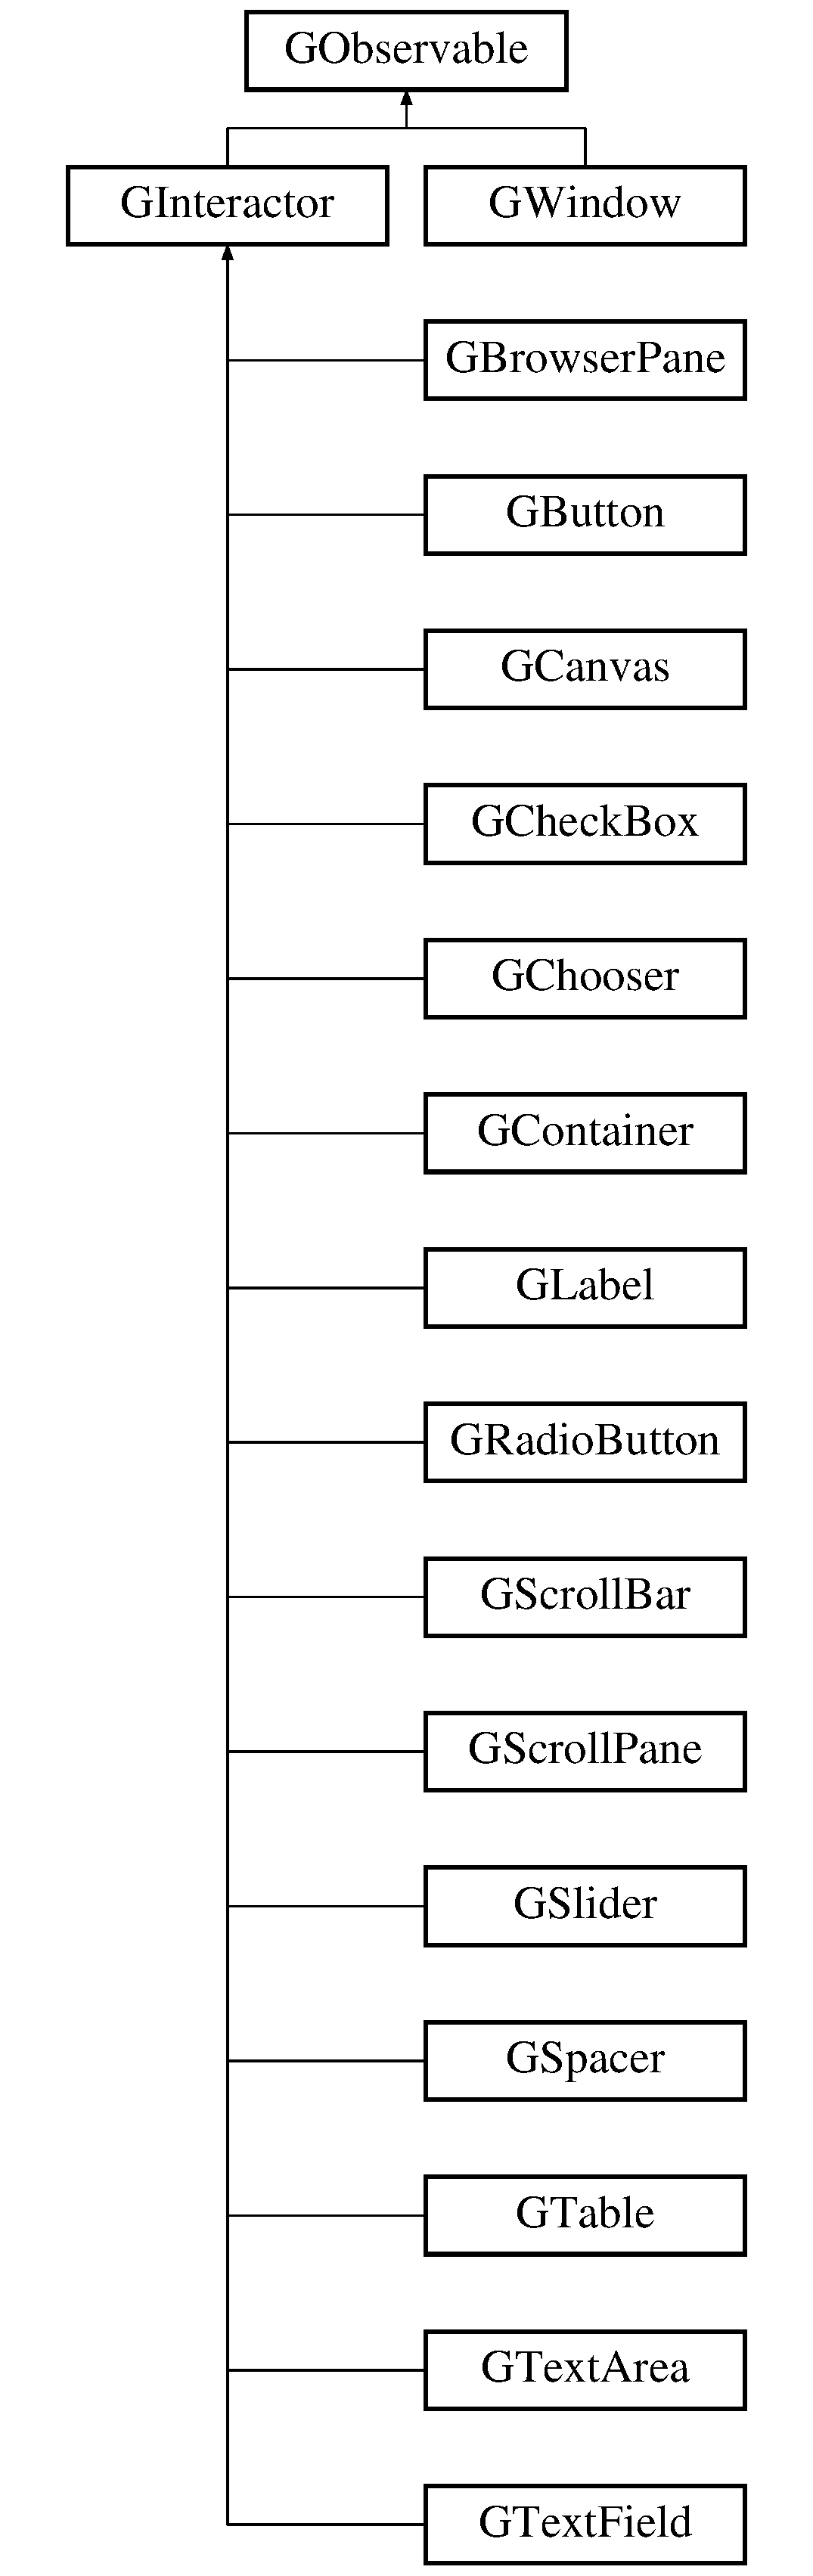
\includegraphics[height=12.000000cm]{classGObservable}
\end{center}
\end{figure}
\subsection*{Public Member Functions}
\begin{DoxyCompactItemize}
\item 
\mbox{\hyperlink{classGObservable_aa083d318cdd2a045471445fbbd26b919}{G\+Observable}} ()
\begin{DoxyCompactList}\small\item\em Initializes a newly created observable object. \end{DoxyCompactList}\item 
virtual \mbox{\hyperlink{classGObservable_a755e7879db8b0a71916cfde365d49305}{$\sim$\+G\+Observable}} ()
\begin{DoxyCompactList}\small\item\em Frees any memory used internally by the observable object. \end{DoxyCompactList}\item 
virtual bool \mbox{\hyperlink{classGObservable_a8ebb3da91032e7f4c34485dabc518b8a}{events\+Enabled}} () const
\begin{DoxyCompactList}\small\item\em Returns true if the object is currently allowing itself to fire events. \end{DoxyCompactList}\item 
virtual std\+::string \mbox{\hyperlink{classGObservable_a799e073a127b428cc841086d42ea4fed}{get\+Type}} () const =0
\begin{DoxyCompactList}\small\item\em Returns the concrete type of the object as a string, such as {\ttfamily \char`\"{}\+G\+Button\char`\"{}} or {\ttfamily \char`\"{}\+G\+Window\char`\"{}}. \end{DoxyCompactList}\item 
virtual void \mbox{\hyperlink{classGObservable_afaa30b2a9e0f378fd1c70d2f1d0b8216}{set\+Events\+Enabled}} (bool \mbox{\hyperlink{classGObservable_a8ebb3da91032e7f4c34485dabc518b8a}{events\+Enabled}})
\begin{DoxyCompactList}\small\item\em Sets whether the object is currently allowing itself to fire events. \end{DoxyCompactList}\item 
virtual std\+::string \mbox{\hyperlink{classGObservable_a1fe5121d6528fdea3f243321b3fa3a49}{to\+String}} () const
\begin{DoxyCompactList}\small\item\em Returns a string representation of this observable object\textquotesingle{}s state. \end{DoxyCompactList}\end{DoxyCompactItemize}
\subsection*{Protected Member Functions}
\begin{DoxyCompactItemize}
\item 
virtual void \mbox{\hyperlink{classGObservable_a80cfa040459ff53594adbd6a51ec8f43}{clear\+Event\+Listeners}} ()
\begin{DoxyCompactList}\small\item\em Removes all event listeners from this object. \end{DoxyCompactList}\item 
virtual void \mbox{\hyperlink{classGObservable_a284f31528c0520f8e545c03ac9eeac74}{ensure\+Thread\+Safety}} (const std\+::string \&member\+Name=\char`\"{}\char`\"{})
\begin{DoxyCompactList}\small\item\em Ensures that we are currently in the Qt G\+UI thread. \end{DoxyCompactList}\item 
virtual void \mbox{\hyperlink{classGObservable_a63e5e5a6227c59c928493b11aceb0f67}{fire\+Event}} (\mbox{\hyperlink{classGEvent}{G\+Event}} \&event)
\begin{DoxyCompactList}\small\item\em Sends out the given event to any attached listeners. \end{DoxyCompactList}\item 
virtual void \mbox{\hyperlink{classGObservable_ab3983ea07337b52020a29cc00c653d8d}{fire\+G\+Event}} (Q\+Event $\ast$event, Event\+Type event\+Type, const std\+::string \&event\+Name)
\begin{DoxyCompactList}\small\item\em Creates an event of the given type, then sends it out to any attached listeners. \end{DoxyCompactList}\item 
virtual void \mbox{\hyperlink{classGObservable_a01fdf1b0e0dbd49e189fe4514e010411}{fire\+G\+Event}} (Q\+Close\+Event $\ast$event, Event\+Type event\+Type, const std\+::string \&event\+Name)
\begin{DoxyCompactList}\small\item\em Creates an event of the given type, then sends it out to any attached listeners. \end{DoxyCompactList}\item 
virtual void \mbox{\hyperlink{classGObservable_abb0b2f66ba39211cb5d7615e9d1c04e2}{fire\+G\+Event}} (Q\+Key\+Event $\ast$event, Event\+Type event\+Type, const std\+::string \&event\+Name)
\begin{DoxyCompactList}\small\item\em Creates an event of the given type, then sends it out to any attached listeners. \end{DoxyCompactList}\item 
virtual void \mbox{\hyperlink{classGObservable_a119318675d2165bdf7dd853aaf881d4b}{fire\+G\+Event}} (Q\+Mouse\+Event $\ast$event, Event\+Type event\+Type, const std\+::string \&event\+Name, const std\+::string \&action\+Command=\char`\"{}\char`\"{})
\begin{DoxyCompactList}\small\item\em Creates an event of the given type, then sends it out to any attached listeners. \end{DoxyCompactList}\item 
virtual void \mbox{\hyperlink{classGObservable_a63fd9034e1e1633c1c38eb342bfd34e9}{fire\+G\+Event}} (Q\+Resize\+Event $\ast$event, Event\+Type event\+Type, const std\+::string \&event\+Name)
\begin{DoxyCompactList}\small\item\em Creates an event of the given type, then sends it out to any attached listeners. \end{DoxyCompactList}\item 
virtual void \mbox{\hyperlink{classGObservable_a741345310d9b7c5170a6cbc410c44ac4}{fire\+G\+Event}} (Q\+Timer\+Event $\ast$event, Event\+Type event\+Type, const std\+::string \&event\+Name)
\begin{DoxyCompactList}\small\item\em Creates an event of the given type, then sends it out to any attached listeners. \end{DoxyCompactList}\item 
virtual void \mbox{\hyperlink{classGObservable_a93bf338968a0338761b8e4dc62f582e9}{fire\+G\+Event}} (Q\+Wheel\+Event $\ast$event, Event\+Type event\+Type, const std\+::string \&event\+Name)
\begin{DoxyCompactList}\small\item\em Creates an event of the given type, then sends it out to any attached listeners. \end{DoxyCompactList}\item 
virtual void \mbox{\hyperlink{classGObservable_a2a70a7d7435ff0c3b80bb4d70da19e0d}{fire\+G\+Event}} (Q\+Window\+State\+Change\+Event $\ast$event, Event\+Type event\+Type, const std\+::string \&event\+Name)
\begin{DoxyCompactList}\small\item\em Creates an event of the given type, then sends it out to any attached listeners. \end{DoxyCompactList}\item 
virtual bool \mbox{\hyperlink{classGObservable_a9f6faaa25942923bafa1c44020c49fa9}{has\+Event\+Listener}} (const std\+::string \&event\+Name) const
\begin{DoxyCompactList}\small\item\em Returns true if the observable object has a listener for the given type of event. \end{DoxyCompactList}\item 
virtual bool \mbox{\hyperlink{classGObservable_aeec1adc19aa0f33de62390686ee1382c}{is\+Accepting\+Event}} (int event\+Mask) const
\begin{DoxyCompactList}\small\item\em Returns true if the observable object has a listener for the given type of event. \end{DoxyCompactList}\item 
virtual bool \mbox{\hyperlink{classGObservable_aa31c73145a29dcb92848a92e0cfaea41}{is\+Accepting\+Event}} (const \mbox{\hyperlink{classGEvent}{G\+Event}} \&event) const
\begin{DoxyCompactList}\small\item\em Returns true if the observable object has a listener for the given type of event. \end{DoxyCompactList}\item 
virtual bool \mbox{\hyperlink{classGObservable_a3b1c689267eda44e65a2213e7de38b23}{is\+Accepting\+Event}} (const std\+::string \&event\+Type) const
\begin{DoxyCompactList}\small\item\em Returns true if the observable object has a listener for the given type of event. \end{DoxyCompactList}\item 
virtual void \mbox{\hyperlink{classGObservable_acbcf1ed3a851ad8a3c17ef38d86b481d}{remove\+Event\+Listener}} (const std\+::string \&event\+Name)
\begin{DoxyCompactList}\small\item\em Removes any event listener from this observable object that would respond to the given type of event, such as \char`\"{}click\char`\"{} or \char`\"{}keydown\char`\"{}. \end{DoxyCompactList}\item 
virtual void \mbox{\hyperlink{classGObservable_af51cc35c29a1bd1908609d432decdbb6}{remove\+Event\+Listeners}} (std\+::initializer\+\_\+list$<$ std\+::string $>$ event\+Names)
\begin{DoxyCompactList}\small\item\em Removes any event listener from this observable object that would respond to the given types of events, such as \char`\"{}click\char`\"{} or \char`\"{}keydown\char`\"{}. \end{DoxyCompactList}\item 
virtual void \mbox{\hyperlink{classGObservable_ad2f6d34961c50f6c1e0659990b79f741}{set\+Event\+Listener}} (const std\+::string \&event\+Name, G\+Event\+Listener func)
\begin{DoxyCompactList}\small\item\em Adds an event listener from this observable object to respond to the given type of event, such as \char`\"{}click\char`\"{} or \char`\"{}keydown\char`\"{}. \end{DoxyCompactList}\item 
virtual void \mbox{\hyperlink{classGObservable_abac4cb9f9e626e010e87f5d91573c8a5}{set\+Event\+Listener}} (const std\+::string \&event\+Name, G\+Event\+Listener\+Void func)
\begin{DoxyCompactList}\small\item\em Adds an event listener from this observable object to respond to the given type of event, such as \char`\"{}click\char`\"{} or \char`\"{}keydown\char`\"{}. \end{DoxyCompactList}\item 
virtual void \mbox{\hyperlink{classGObservable_afa388d69c33c718cf035774604065604}{set\+Event\+Listeners}} (std\+::initializer\+\_\+list$<$ std\+::string $>$ event\+Names, G\+Event\+Listener func)
\begin{DoxyCompactList}\small\item\em Adds an event listener from this observable object to respond to the given types of events, such as \char`\"{}click\char`\"{} or \char`\"{}keydown\char`\"{}. \end{DoxyCompactList}\item 
virtual void \mbox{\hyperlink{classGObservable_a7867184bbb686f74fae8a4db927da799}{set\+Event\+Listeners}} (std\+::initializer\+\_\+list$<$ std\+::string $>$ event\+Names, G\+Event\+Listener\+Void func)
\begin{DoxyCompactList}\small\item\em Adds an event listener from this observable object to respond to the given types of events, such as \char`\"{}click\char`\"{} or \char`\"{}keydown\char`\"{}. \end{DoxyCompactList}\end{DoxyCompactItemize}


\subsection{Detailed Description}
A \mbox{\hyperlink{classGObservable}{G\+Observable}} object is one that is able to send out events. 

Listeners can register themselves to be notified when events occur. This serves as a base class for the various \mbox{\hyperlink{classGInteractor}{G\+Interactor}} subclasses, as well as for the \mbox{\hyperlink{classGWindow}{G\+Window}} class, so that clients can attach listeners to them. 

\subsection{Constructor \& Destructor Documentation}
\mbox{\Hypertarget{classGObservable_aa083d318cdd2a045471445fbbd26b919}\label{classGObservable_aa083d318cdd2a045471445fbbd26b919}} 
\index{G\+Observable@{G\+Observable}!G\+Observable@{G\+Observable}}
\index{G\+Observable@{G\+Observable}!G\+Observable@{G\+Observable}}
\subsubsection{\texorpdfstring{G\+Observable()}{GObservable()}}
{\footnotesize\ttfamily \mbox{\hyperlink{classGObservable}{G\+Observable}} (\begin{DoxyParamCaption}{ }\end{DoxyParamCaption})}



Initializes a newly created observable object. 

\mbox{\Hypertarget{classGObservable_a755e7879db8b0a71916cfde365d49305}\label{classGObservable_a755e7879db8b0a71916cfde365d49305}} 
\index{G\+Observable@{G\+Observable}!````~G\+Observable@{$\sim$\+G\+Observable}}
\index{````~G\+Observable@{$\sim$\+G\+Observable}!G\+Observable@{G\+Observable}}
\subsubsection{\texorpdfstring{$\sim$\+G\+Observable()}{~GObservable()}}
{\footnotesize\ttfamily $\sim$\mbox{\hyperlink{classGObservable}{G\+Observable}} (\begin{DoxyParamCaption}{ }\end{DoxyParamCaption})\hspace{0.3cm}{\ttfamily [virtual]}}



Frees any memory used internally by the observable object. 



\subsection{Member Function Documentation}
\mbox{\Hypertarget{classGObservable_a80cfa040459ff53594adbd6a51ec8f43}\label{classGObservable_a80cfa040459ff53594adbd6a51ec8f43}} 
\index{G\+Observable@{G\+Observable}!clear\+Event\+Listeners@{clear\+Event\+Listeners}}
\index{clear\+Event\+Listeners@{clear\+Event\+Listeners}!G\+Observable@{G\+Observable}}
\subsubsection{\texorpdfstring{clear\+Event\+Listeners()}{clearEventListeners()}}
{\footnotesize\ttfamily void clear\+Event\+Listeners (\begin{DoxyParamCaption}{ }\end{DoxyParamCaption})\hspace{0.3cm}{\ttfamily [protected]}, {\ttfamily [virtual]}}



Removes all event listeners from this object. 

\mbox{\Hypertarget{classGObservable_a284f31528c0520f8e545c03ac9eeac74}\label{classGObservable_a284f31528c0520f8e545c03ac9eeac74}} 
\index{G\+Observable@{G\+Observable}!ensure\+Thread\+Safety@{ensure\+Thread\+Safety}}
\index{ensure\+Thread\+Safety@{ensure\+Thread\+Safety}!G\+Observable@{G\+Observable}}
\subsubsection{\texorpdfstring{ensure\+Thread\+Safety()}{ensureThreadSafety()}}
{\footnotesize\ttfamily void ensure\+Thread\+Safety (\begin{DoxyParamCaption}\item[{const std\+::string \&}]{member\+Name = {\ttfamily \char`\"{}\char`\"{}} }\end{DoxyParamCaption})\hspace{0.3cm}{\ttfamily [protected]}, {\ttfamily [virtual]}}



Ensures that we are currently in the Qt G\+UI thread. 

\mbox{\Hypertarget{classGObservable_a8ebb3da91032e7f4c34485dabc518b8a}\label{classGObservable_a8ebb3da91032e7f4c34485dabc518b8a}} 
\index{G\+Observable@{G\+Observable}!events\+Enabled@{events\+Enabled}}
\index{events\+Enabled@{events\+Enabled}!G\+Observable@{G\+Observable}}
\subsubsection{\texorpdfstring{events\+Enabled()}{eventsEnabled()}}
{\footnotesize\ttfamily bool events\+Enabled (\begin{DoxyParamCaption}{ }\end{DoxyParamCaption}) const\hspace{0.3cm}{\ttfamily [virtual]}}



Returns true if the object is currently allowing itself to fire events. 

Initially this is true unless the client has called {\ttfamily set\+Events\+Enabled(false)} or the object is not visible. 

Reimplemented in \mbox{\hyperlink{classGInteractor_a597a370b592e3737d38d9d2f4e2031ea}{G\+Interactor}}.

\mbox{\Hypertarget{classGObservable_a63e5e5a6227c59c928493b11aceb0f67}\label{classGObservable_a63e5e5a6227c59c928493b11aceb0f67}} 
\index{G\+Observable@{G\+Observable}!fire\+Event@{fire\+Event}}
\index{fire\+Event@{fire\+Event}!G\+Observable@{G\+Observable}}
\subsubsection{\texorpdfstring{fire\+Event()}{fireEvent()}}
{\footnotesize\ttfamily void fire\+Event (\begin{DoxyParamCaption}\item[{\mbox{\hyperlink{classGEvent}{G\+Event}} \&}]{event }\end{DoxyParamCaption})\hspace{0.3cm}{\ttfamily [protected]}, {\ttfamily [virtual]}}



Sends out the given event to any attached listeners. 

\mbox{\Hypertarget{classGObservable_ab3983ea07337b52020a29cc00c653d8d}\label{classGObservable_ab3983ea07337b52020a29cc00c653d8d}} 
\index{G\+Observable@{G\+Observable}!fire\+G\+Event@{fire\+G\+Event}}
\index{fire\+G\+Event@{fire\+G\+Event}!G\+Observable@{G\+Observable}}
\subsubsection{\texorpdfstring{fire\+G\+Event()}{fireGEvent()}\hspace{0.1cm}{\footnotesize\ttfamily [1/8]}}
{\footnotesize\ttfamily void fire\+G\+Event (\begin{DoxyParamCaption}\item[{Q\+Event $\ast$}]{event,  }\item[{Event\+Type}]{event\+Type,  }\item[{const std\+::string \&}]{event\+Name }\end{DoxyParamCaption})\hspace{0.3cm}{\ttfamily [protected]}, {\ttfamily [virtual]}}



Creates an event of the given type, then sends it out to any attached listeners. 

\mbox{\Hypertarget{classGObservable_a01fdf1b0e0dbd49e189fe4514e010411}\label{classGObservable_a01fdf1b0e0dbd49e189fe4514e010411}} 
\index{G\+Observable@{G\+Observable}!fire\+G\+Event@{fire\+G\+Event}}
\index{fire\+G\+Event@{fire\+G\+Event}!G\+Observable@{G\+Observable}}
\subsubsection{\texorpdfstring{fire\+G\+Event()}{fireGEvent()}\hspace{0.1cm}{\footnotesize\ttfamily [2/8]}}
{\footnotesize\ttfamily void fire\+G\+Event (\begin{DoxyParamCaption}\item[{Q\+Close\+Event $\ast$}]{event,  }\item[{Event\+Type}]{event\+Type,  }\item[{const std\+::string \&}]{event\+Name }\end{DoxyParamCaption})\hspace{0.3cm}{\ttfamily [protected]}, {\ttfamily [virtual]}}



Creates an event of the given type, then sends it out to any attached listeners. 

\mbox{\Hypertarget{classGObservable_abb0b2f66ba39211cb5d7615e9d1c04e2}\label{classGObservable_abb0b2f66ba39211cb5d7615e9d1c04e2}} 
\index{G\+Observable@{G\+Observable}!fire\+G\+Event@{fire\+G\+Event}}
\index{fire\+G\+Event@{fire\+G\+Event}!G\+Observable@{G\+Observable}}
\subsubsection{\texorpdfstring{fire\+G\+Event()}{fireGEvent()}\hspace{0.1cm}{\footnotesize\ttfamily [3/8]}}
{\footnotesize\ttfamily void fire\+G\+Event (\begin{DoxyParamCaption}\item[{Q\+Key\+Event $\ast$}]{event,  }\item[{Event\+Type}]{event\+Type,  }\item[{const std\+::string \&}]{event\+Name }\end{DoxyParamCaption})\hspace{0.3cm}{\ttfamily [protected]}, {\ttfamily [virtual]}}



Creates an event of the given type, then sends it out to any attached listeners. 

\mbox{\Hypertarget{classGObservable_a119318675d2165bdf7dd853aaf881d4b}\label{classGObservable_a119318675d2165bdf7dd853aaf881d4b}} 
\index{G\+Observable@{G\+Observable}!fire\+G\+Event@{fire\+G\+Event}}
\index{fire\+G\+Event@{fire\+G\+Event}!G\+Observable@{G\+Observable}}
\subsubsection{\texorpdfstring{fire\+G\+Event()}{fireGEvent()}\hspace{0.1cm}{\footnotesize\ttfamily [4/8]}}
{\footnotesize\ttfamily void fire\+G\+Event (\begin{DoxyParamCaption}\item[{Q\+Mouse\+Event $\ast$}]{event,  }\item[{Event\+Type}]{event\+Type,  }\item[{const std\+::string \&}]{event\+Name,  }\item[{const std\+::string \&}]{action\+Command = {\ttfamily \char`\"{}\char`\"{}} }\end{DoxyParamCaption})\hspace{0.3cm}{\ttfamily [protected]}, {\ttfamily [virtual]}}



Creates an event of the given type, then sends it out to any attached listeners. 

\mbox{\Hypertarget{classGObservable_a63fd9034e1e1633c1c38eb342bfd34e9}\label{classGObservable_a63fd9034e1e1633c1c38eb342bfd34e9}} 
\index{G\+Observable@{G\+Observable}!fire\+G\+Event@{fire\+G\+Event}}
\index{fire\+G\+Event@{fire\+G\+Event}!G\+Observable@{G\+Observable}}
\subsubsection{\texorpdfstring{fire\+G\+Event()}{fireGEvent()}\hspace{0.1cm}{\footnotesize\ttfamily [5/8]}}
{\footnotesize\ttfamily void fire\+G\+Event (\begin{DoxyParamCaption}\item[{Q\+Resize\+Event $\ast$}]{event,  }\item[{Event\+Type}]{event\+Type,  }\item[{const std\+::string \&}]{event\+Name }\end{DoxyParamCaption})\hspace{0.3cm}{\ttfamily [protected]}, {\ttfamily [virtual]}}



Creates an event of the given type, then sends it out to any attached listeners. 

\mbox{\Hypertarget{classGObservable_a741345310d9b7c5170a6cbc410c44ac4}\label{classGObservable_a741345310d9b7c5170a6cbc410c44ac4}} 
\index{G\+Observable@{G\+Observable}!fire\+G\+Event@{fire\+G\+Event}}
\index{fire\+G\+Event@{fire\+G\+Event}!G\+Observable@{G\+Observable}}
\subsubsection{\texorpdfstring{fire\+G\+Event()}{fireGEvent()}\hspace{0.1cm}{\footnotesize\ttfamily [6/8]}}
{\footnotesize\ttfamily void fire\+G\+Event (\begin{DoxyParamCaption}\item[{Q\+Timer\+Event $\ast$}]{event,  }\item[{Event\+Type}]{event\+Type,  }\item[{const std\+::string \&}]{event\+Name }\end{DoxyParamCaption})\hspace{0.3cm}{\ttfamily [protected]}, {\ttfamily [virtual]}}



Creates an event of the given type, then sends it out to any attached listeners. 

\mbox{\Hypertarget{classGObservable_a93bf338968a0338761b8e4dc62f582e9}\label{classGObservable_a93bf338968a0338761b8e4dc62f582e9}} 
\index{G\+Observable@{G\+Observable}!fire\+G\+Event@{fire\+G\+Event}}
\index{fire\+G\+Event@{fire\+G\+Event}!G\+Observable@{G\+Observable}}
\subsubsection{\texorpdfstring{fire\+G\+Event()}{fireGEvent()}\hspace{0.1cm}{\footnotesize\ttfamily [7/8]}}
{\footnotesize\ttfamily void fire\+G\+Event (\begin{DoxyParamCaption}\item[{Q\+Wheel\+Event $\ast$}]{event,  }\item[{Event\+Type}]{event\+Type,  }\item[{const std\+::string \&}]{event\+Name }\end{DoxyParamCaption})\hspace{0.3cm}{\ttfamily [protected]}, {\ttfamily [virtual]}}



Creates an event of the given type, then sends it out to any attached listeners. 

\mbox{\Hypertarget{classGObservable_a2a70a7d7435ff0c3b80bb4d70da19e0d}\label{classGObservable_a2a70a7d7435ff0c3b80bb4d70da19e0d}} 
\index{G\+Observable@{G\+Observable}!fire\+G\+Event@{fire\+G\+Event}}
\index{fire\+G\+Event@{fire\+G\+Event}!G\+Observable@{G\+Observable}}
\subsubsection{\texorpdfstring{fire\+G\+Event()}{fireGEvent()}\hspace{0.1cm}{\footnotesize\ttfamily [8/8]}}
{\footnotesize\ttfamily void fire\+G\+Event (\begin{DoxyParamCaption}\item[{Q\+Window\+State\+Change\+Event $\ast$}]{event,  }\item[{Event\+Type}]{event\+Type,  }\item[{const std\+::string \&}]{event\+Name }\end{DoxyParamCaption})\hspace{0.3cm}{\ttfamily [protected]}, {\ttfamily [virtual]}}



Creates an event of the given type, then sends it out to any attached listeners. 

\mbox{\Hypertarget{classGObservable_a799e073a127b428cc841086d42ea4fed}\label{classGObservable_a799e073a127b428cc841086d42ea4fed}} 
\index{G\+Observable@{G\+Observable}!get\+Type@{get\+Type}}
\index{get\+Type@{get\+Type}!G\+Observable@{G\+Observable}}
\subsubsection{\texorpdfstring{get\+Type()}{getType()}}
{\footnotesize\ttfamily virtual std\+::string get\+Type (\begin{DoxyParamCaption}{ }\end{DoxyParamCaption}) const\hspace{0.3cm}{\ttfamily [pure virtual]}}



Returns the concrete type of the object as a string, such as {\ttfamily \char`\"{}\+G\+Button\char`\"{}} or {\ttfamily \char`\"{}\+G\+Window\char`\"{}}. 

Each \mbox{\hyperlink{classGObservable}{G\+Observable}} subtype must override this method. 

Implemented in \mbox{\hyperlink{classGWindow_a9b72ede4ee8520f987a0c01e30654814}{G\+Window}}, \mbox{\hyperlink{classGCanvas_a9b72ede4ee8520f987a0c01e30654814}{G\+Canvas}}, \mbox{\hyperlink{classGContainer_a9b72ede4ee8520f987a0c01e30654814}{G\+Container}}, \mbox{\hyperlink{classGInteractor_a44c407a54a20dd0f2fff30338289299d}{G\+Interactor}}, \mbox{\hyperlink{classGTable_a9b72ede4ee8520f987a0c01e30654814}{G\+Table}}, \mbox{\hyperlink{classGTextArea_a9b72ede4ee8520f987a0c01e30654814}{G\+Text\+Area}}, \mbox{\hyperlink{classGSlider_a9b72ede4ee8520f987a0c01e30654814}{G\+Slider}}, \mbox{\hyperlink{classGBrowserPane_a9b72ede4ee8520f987a0c01e30654814}{G\+Browser\+Pane}}, \mbox{\hyperlink{classGTextField_a9b72ede4ee8520f987a0c01e30654814}{G\+Text\+Field}}, \mbox{\hyperlink{classGChooser_a9b72ede4ee8520f987a0c01e30654814}{G\+Chooser}}, \mbox{\hyperlink{classGLabel_a9b72ede4ee8520f987a0c01e30654814}{G\+Label}}, \mbox{\hyperlink{classGButton_a9b72ede4ee8520f987a0c01e30654814}{G\+Button}}, \mbox{\hyperlink{classGScrollBar_a9b72ede4ee8520f987a0c01e30654814}{G\+Scroll\+Bar}}, \mbox{\hyperlink{classGRadioButton_a9b72ede4ee8520f987a0c01e30654814}{G\+Radio\+Button}}, \mbox{\hyperlink{classGScrollPane_a9b72ede4ee8520f987a0c01e30654814}{G\+Scroll\+Pane}}, \mbox{\hyperlink{classGCheckBox_a9b72ede4ee8520f987a0c01e30654814}{G\+Check\+Box}}, and \mbox{\hyperlink{classGSpacer_a9b72ede4ee8520f987a0c01e30654814}{G\+Spacer}}.

\mbox{\Hypertarget{classGObservable_a9f6faaa25942923bafa1c44020c49fa9}\label{classGObservable_a9f6faaa25942923bafa1c44020c49fa9}} 
\index{G\+Observable@{G\+Observable}!has\+Event\+Listener@{has\+Event\+Listener}}
\index{has\+Event\+Listener@{has\+Event\+Listener}!G\+Observable@{G\+Observable}}
\subsubsection{\texorpdfstring{has\+Event\+Listener()}{hasEventListener()}}
{\footnotesize\ttfamily bool has\+Event\+Listener (\begin{DoxyParamCaption}\item[{const std\+::string \&}]{event\+Name }\end{DoxyParamCaption}) const\hspace{0.3cm}{\ttfamily [protected]}, {\ttfamily [virtual]}}



Returns true if the observable object has a listener for the given type of event. 

\mbox{\Hypertarget{classGObservable_aeec1adc19aa0f33de62390686ee1382c}\label{classGObservable_aeec1adc19aa0f33de62390686ee1382c}} 
\index{G\+Observable@{G\+Observable}!is\+Accepting\+Event@{is\+Accepting\+Event}}
\index{is\+Accepting\+Event@{is\+Accepting\+Event}!G\+Observable@{G\+Observable}}
\subsubsection{\texorpdfstring{is\+Accepting\+Event()}{isAcceptingEvent()}\hspace{0.1cm}{\footnotesize\ttfamily [1/3]}}
{\footnotesize\ttfamily bool is\+Accepting\+Event (\begin{DoxyParamCaption}\item[{int}]{event\+Mask }\end{DoxyParamCaption}) const\hspace{0.3cm}{\ttfamily [protected]}, {\ttfamily [virtual]}}



Returns true if the observable object has a listener for the given type of event. 

See \mbox{\hyperlink{gevent_8h_source}{gevent.\+h}} for event types and masks. \mbox{\Hypertarget{classGObservable_aa31c73145a29dcb92848a92e0cfaea41}\label{classGObservable_aa31c73145a29dcb92848a92e0cfaea41}} 
\index{G\+Observable@{G\+Observable}!is\+Accepting\+Event@{is\+Accepting\+Event}}
\index{is\+Accepting\+Event@{is\+Accepting\+Event}!G\+Observable@{G\+Observable}}
\subsubsection{\texorpdfstring{is\+Accepting\+Event()}{isAcceptingEvent()}\hspace{0.1cm}{\footnotesize\ttfamily [2/3]}}
{\footnotesize\ttfamily bool is\+Accepting\+Event (\begin{DoxyParamCaption}\item[{const \mbox{\hyperlink{classGEvent}{G\+Event}} \&}]{event }\end{DoxyParamCaption}) const\hspace{0.3cm}{\ttfamily [protected]}, {\ttfamily [virtual]}}



Returns true if the observable object has a listener for the given type of event. 

\mbox{\Hypertarget{classGObservable_a3b1c689267eda44e65a2213e7de38b23}\label{classGObservable_a3b1c689267eda44e65a2213e7de38b23}} 
\index{G\+Observable@{G\+Observable}!is\+Accepting\+Event@{is\+Accepting\+Event}}
\index{is\+Accepting\+Event@{is\+Accepting\+Event}!G\+Observable@{G\+Observable}}
\subsubsection{\texorpdfstring{is\+Accepting\+Event()}{isAcceptingEvent()}\hspace{0.1cm}{\footnotesize\ttfamily [3/3]}}
{\footnotesize\ttfamily bool is\+Accepting\+Event (\begin{DoxyParamCaption}\item[{const std\+::string \&}]{event\+Type }\end{DoxyParamCaption}) const\hspace{0.3cm}{\ttfamily [protected]}, {\ttfamily [virtual]}}



Returns true if the observable object has a listener for the given type of event. 

\mbox{\Hypertarget{classGObservable_acbcf1ed3a851ad8a3c17ef38d86b481d}\label{classGObservable_acbcf1ed3a851ad8a3c17ef38d86b481d}} 
\index{G\+Observable@{G\+Observable}!remove\+Event\+Listener@{remove\+Event\+Listener}}
\index{remove\+Event\+Listener@{remove\+Event\+Listener}!G\+Observable@{G\+Observable}}
\subsubsection{\texorpdfstring{remove\+Event\+Listener()}{removeEventListener()}}
{\footnotesize\ttfamily void remove\+Event\+Listener (\begin{DoxyParamCaption}\item[{const std\+::string \&}]{event\+Name }\end{DoxyParamCaption})\hspace{0.3cm}{\ttfamily [protected]}, {\ttfamily [virtual]}}



Removes any event listener from this observable object that would respond to the given type of event, such as \char`\"{}click\char`\"{} or \char`\"{}keydown\char`\"{}. 

\mbox{\Hypertarget{classGObservable_af51cc35c29a1bd1908609d432decdbb6}\label{classGObservable_af51cc35c29a1bd1908609d432decdbb6}} 
\index{G\+Observable@{G\+Observable}!remove\+Event\+Listeners@{remove\+Event\+Listeners}}
\index{remove\+Event\+Listeners@{remove\+Event\+Listeners}!G\+Observable@{G\+Observable}}
\subsubsection{\texorpdfstring{remove\+Event\+Listeners()}{removeEventListeners()}}
{\footnotesize\ttfamily void remove\+Event\+Listeners (\begin{DoxyParamCaption}\item[{std\+::initializer\+\_\+list$<$ std\+::string $>$}]{event\+Names }\end{DoxyParamCaption})\hspace{0.3cm}{\ttfamily [protected]}, {\ttfamily [virtual]}}



Removes any event listener from this observable object that would respond to the given types of events, such as \char`\"{}click\char`\"{} or \char`\"{}keydown\char`\"{}. 

\mbox{\Hypertarget{classGObservable_ad2f6d34961c50f6c1e0659990b79f741}\label{classGObservable_ad2f6d34961c50f6c1e0659990b79f741}} 
\index{G\+Observable@{G\+Observable}!set\+Event\+Listener@{set\+Event\+Listener}}
\index{set\+Event\+Listener@{set\+Event\+Listener}!G\+Observable@{G\+Observable}}
\subsubsection{\texorpdfstring{set\+Event\+Listener()}{setEventListener()}\hspace{0.1cm}{\footnotesize\ttfamily [1/2]}}
{\footnotesize\ttfamily void set\+Event\+Listener (\begin{DoxyParamCaption}\item[{const std\+::string \&}]{event\+Name,  }\item[{G\+Event\+Listener}]{func }\end{DoxyParamCaption})\hspace{0.3cm}{\ttfamily [protected]}, {\ttfamily [virtual]}}



Adds an event listener from this observable object to respond to the given type of event, such as \char`\"{}click\char`\"{} or \char`\"{}keydown\char`\"{}. 

Any prior listener for that type of event is replaced. \mbox{\Hypertarget{classGObservable_abac4cb9f9e626e010e87f5d91573c8a5}\label{classGObservable_abac4cb9f9e626e010e87f5d91573c8a5}} 
\index{G\+Observable@{G\+Observable}!set\+Event\+Listener@{set\+Event\+Listener}}
\index{set\+Event\+Listener@{set\+Event\+Listener}!G\+Observable@{G\+Observable}}
\subsubsection{\texorpdfstring{set\+Event\+Listener()}{setEventListener()}\hspace{0.1cm}{\footnotesize\ttfamily [2/2]}}
{\footnotesize\ttfamily void set\+Event\+Listener (\begin{DoxyParamCaption}\item[{const std\+::string \&}]{event\+Name,  }\item[{G\+Event\+Listener\+Void}]{func }\end{DoxyParamCaption})\hspace{0.3cm}{\ttfamily [protected]}, {\ttfamily [virtual]}}



Adds an event listener from this observable object to respond to the given type of event, such as \char`\"{}click\char`\"{} or \char`\"{}keydown\char`\"{}. 

Any prior listener for that type of event is replaced. \mbox{\Hypertarget{classGObservable_afa388d69c33c718cf035774604065604}\label{classGObservable_afa388d69c33c718cf035774604065604}} 
\index{G\+Observable@{G\+Observable}!set\+Event\+Listeners@{set\+Event\+Listeners}}
\index{set\+Event\+Listeners@{set\+Event\+Listeners}!G\+Observable@{G\+Observable}}
\subsubsection{\texorpdfstring{set\+Event\+Listeners()}{setEventListeners()}\hspace{0.1cm}{\footnotesize\ttfamily [1/2]}}
{\footnotesize\ttfamily void set\+Event\+Listeners (\begin{DoxyParamCaption}\item[{std\+::initializer\+\_\+list$<$ std\+::string $>$}]{event\+Names,  }\item[{G\+Event\+Listener}]{func }\end{DoxyParamCaption})\hspace{0.3cm}{\ttfamily [protected]}, {\ttfamily [virtual]}}



Adds an event listener from this observable object to respond to the given types of events, such as \char`\"{}click\char`\"{} or \char`\"{}keydown\char`\"{}. 

Any prior listener for those types of event are replaced. \mbox{\Hypertarget{classGObservable_a7867184bbb686f74fae8a4db927da799}\label{classGObservable_a7867184bbb686f74fae8a4db927da799}} 
\index{G\+Observable@{G\+Observable}!set\+Event\+Listeners@{set\+Event\+Listeners}}
\index{set\+Event\+Listeners@{set\+Event\+Listeners}!G\+Observable@{G\+Observable}}
\subsubsection{\texorpdfstring{set\+Event\+Listeners()}{setEventListeners()}\hspace{0.1cm}{\footnotesize\ttfamily [2/2]}}
{\footnotesize\ttfamily void set\+Event\+Listeners (\begin{DoxyParamCaption}\item[{std\+::initializer\+\_\+list$<$ std\+::string $>$}]{event\+Names,  }\item[{G\+Event\+Listener\+Void}]{func }\end{DoxyParamCaption})\hspace{0.3cm}{\ttfamily [protected]}, {\ttfamily [virtual]}}



Adds an event listener from this observable object to respond to the given types of events, such as \char`\"{}click\char`\"{} or \char`\"{}keydown\char`\"{}. 

Any prior listener for those types of event are replaced. \mbox{\Hypertarget{classGObservable_afaa30b2a9e0f378fd1c70d2f1d0b8216}\label{classGObservable_afaa30b2a9e0f378fd1c70d2f1d0b8216}} 
\index{G\+Observable@{G\+Observable}!set\+Events\+Enabled@{set\+Events\+Enabled}}
\index{set\+Events\+Enabled@{set\+Events\+Enabled}!G\+Observable@{G\+Observable}}
\subsubsection{\texorpdfstring{set\+Events\+Enabled()}{setEventsEnabled()}}
{\footnotesize\ttfamily void set\+Events\+Enabled (\begin{DoxyParamCaption}\item[{bool}]{events\+Enabled }\end{DoxyParamCaption})\hspace{0.3cm}{\ttfamily [virtual]}}



Sets whether the object is currently allowing itself to fire events. 

Initially this is true. \mbox{\Hypertarget{classGObservable_a1fe5121d6528fdea3f243321b3fa3a49}\label{classGObservable_a1fe5121d6528fdea3f243321b3fa3a49}} 
\index{G\+Observable@{G\+Observable}!to\+String@{to\+String}}
\index{to\+String@{to\+String}!G\+Observable@{G\+Observable}}
\subsubsection{\texorpdfstring{to\+String()}{toString()}}
{\footnotesize\ttfamily std\+::string to\+String (\begin{DoxyParamCaption}{ }\end{DoxyParamCaption}) const\hspace{0.3cm}{\ttfamily [virtual]}}



Returns a string representation of this observable object\textquotesingle{}s state. 

Primarily used for debugging purposes. 

\subsection{Friends And Related Function Documentation}
\mbox{\Hypertarget{classGObservable_a054e99eaa992da5c1a77c8d7b3817788}\label{classGObservable_a054e99eaa992da5c1a77c8d7b3817788}} 
\index{G\+Observable@{G\+Observable}!G\+Interactor@{G\+Interactor}}
\index{G\+Interactor@{G\+Interactor}!G\+Observable@{G\+Observable}}
\subsubsection{\texorpdfstring{G\+Interactor}{GInteractor}}
{\footnotesize\ttfamily friend class \mbox{\hyperlink{classGInteractor}{G\+Interactor}}\hspace{0.3cm}{\ttfamily [friend]}}


\hypertarget{classGOptionPane}{}\section{G\+Option\+Pane Class Reference}
\label{classGOptionPane}\index{G\+Option\+Pane@{G\+Option\+Pane}}


This class provides static methods that pop up graphical input/output dialog boxes on the screen.  




{\ttfamily \#include $<$goptionpane.\+h$>$}

\subsection*{Public Types}
\begin{DoxyCompactItemize}
\item 
enum \mbox{\hyperlink{classGOptionPane_a1cc9e8685029e39646671ed71f32d47d}{Confirm\+Result}} \{ \mbox{\hyperlink{classGOptionPane_a1cc9e8685029e39646671ed71f32d47dacd3ba58104ba5a343e0f2fc2839c9202}{C\+O\+N\+F\+I\+R\+M\+\_\+\+C\+A\+N\+C\+EL}} = -\/1, 
\mbox{\hyperlink{classGOptionPane_a1cc9e8685029e39646671ed71f32d47dafec070235546c9e3ceb562e6e1a0c24e}{C\+O\+N\+F\+I\+R\+M\+\_\+\+NO}} = 0, 
\mbox{\hyperlink{classGOptionPane_a1cc9e8685029e39646671ed71f32d47da090492ce2b803840f3c07f6f56116ba3}{C\+O\+N\+F\+I\+R\+M\+\_\+\+Y\+ES}} = 1, 
\mbox{\hyperlink{classGOptionPane_a1cc9e8685029e39646671ed71f32d47dacd7dbef45f6bf553d72a78e7f5389b4c}{C\+O\+N\+F\+I\+R\+M\+\_\+\+OK}} = 2
 \}
\begin{DoxyCompactList}\small\item\em The various results that can be returned from some option dialogs. \end{DoxyCompactList}\item 
enum \mbox{\hyperlink{classGOptionPane_a6a1aaf19c06f5a6bef89ea6415547049}{Confirm\+Type}} \{ \mbox{\hyperlink{classGOptionPane_a6a1aaf19c06f5a6bef89ea6415547049a964914d27eb73a202938a53f43adc4b1}{C\+O\+N\+F\+I\+R\+M\+\_\+\+Y\+E\+S\+\_\+\+NO}} = 0, 
\mbox{\hyperlink{classGOptionPane_a6a1aaf19c06f5a6bef89ea6415547049a534f72dad7322c4a590adef3fccb8745}{C\+O\+N\+F\+I\+R\+M\+\_\+\+Y\+E\+S\+\_\+\+N\+O\+\_\+\+C\+A\+N\+C\+EL}} = 1, 
\mbox{\hyperlink{classGOptionPane_a6a1aaf19c06f5a6bef89ea6415547049a8c54c3531625688e49c049e608197afb}{C\+O\+N\+F\+I\+R\+M\+\_\+\+O\+K\+\_\+\+C\+A\+N\+C\+EL}} = 2
 \}
\begin{DoxyCompactList}\small\item\em Types used by show\+Confirm\+Dialog, representing the three kinds of confirmation dialogs\+: Yes/\+No, Yes/\+No/\+Cancel, or O\+K/\+Cancel. \end{DoxyCompactList}\item 
enum \mbox{\hyperlink{classGOptionPane_ac6606ebe91c8ac66a2c314c79f5ab013}{Message\+Type}} \{ \mbox{\hyperlink{classGOptionPane_ac6606ebe91c8ac66a2c314c79f5ab013aeed68e2821e40e5751af74e449ba1fa7}{M\+E\+S\+S\+A\+G\+E\+\_\+\+E\+R\+R\+OR}} = 0, 
\mbox{\hyperlink{classGOptionPane_ac6606ebe91c8ac66a2c314c79f5ab013a7c67175dfb6af3e42428b6fcfcbe7d94}{M\+E\+S\+S\+A\+G\+E\+\_\+\+I\+N\+F\+O\+R\+M\+A\+T\+I\+ON}} = 1, 
\mbox{\hyperlink{classGOptionPane_ac6606ebe91c8ac66a2c314c79f5ab013ac03a17c74c589b004d166532958a6196}{M\+E\+S\+S\+A\+G\+E\+\_\+\+P\+L\+A\+IN}} = -\/1, 
\mbox{\hyperlink{classGOptionPane_ac6606ebe91c8ac66a2c314c79f5ab013aa0da5a01a18f78c0f248941ad32cc816}{M\+E\+S\+S\+A\+G\+E\+\_\+\+W\+A\+R\+N\+I\+NG}} = 2, 
\mbox{\hyperlink{classGOptionPane_ac6606ebe91c8ac66a2c314c79f5ab013a5331d292e92d35f202913bb0b3dfa587}{M\+E\+S\+S\+A\+G\+E\+\_\+\+Q\+U\+E\+S\+T\+I\+ON}} = 3, 
\mbox{\hyperlink{classGOptionPane_ac6606ebe91c8ac66a2c314c79f5ab013acea265b81d984cd186ef5f7fe627caa5}{M\+E\+S\+S\+A\+G\+E\+\_\+\+A\+B\+O\+UT}} = 4
 \}
\begin{DoxyCompactList}\small\item\em Types used by show\+Message\+Dialog, representing the various kinds of message dialogs. \end{DoxyCompactList}\end{DoxyCompactItemize}
\subsection*{Static Public Member Functions}
\begin{DoxyCompactItemize}
\item 
static \mbox{\hyperlink{classGOptionPane_a1cc9e8685029e39646671ed71f32d47d}{Confirm\+Result}} \mbox{\hyperlink{classGOptionPane_a779ca75a58dcaba1000f064f23f83291}{show\+Confirm\+Dialog}} (const std\+::string \&message, const std\+::string \&title=\char`\"{}\char`\"{}, \mbox{\hyperlink{classGOptionPane_a6a1aaf19c06f5a6bef89ea6415547049}{Confirm\+Type}} type=\mbox{\hyperlink{classGOptionPane_a6a1aaf19c06f5a6bef89ea6415547049a964914d27eb73a202938a53f43adc4b1}{C\+O\+N\+F\+I\+R\+M\+\_\+\+Y\+E\+S\+\_\+\+NO}})
\begin{DoxyCompactList}\small\item\em Pops up a yes/no confirmation box. \end{DoxyCompactList}\item 
static \mbox{\hyperlink{classGOptionPane_a1cc9e8685029e39646671ed71f32d47d}{Confirm\+Result}} \mbox{\hyperlink{classGOptionPane_a9afd93d6b7b63d77370c87e60285ae71}{show\+Confirm\+Dialog}} (\mbox{\hyperlink{classGWindow}{G\+Window}} $\ast$parent, const std\+::string \&message, const std\+::string \&title=\char`\"{}\char`\"{}, \mbox{\hyperlink{classGOptionPane_a6a1aaf19c06f5a6bef89ea6415547049}{Confirm\+Type}} type=\mbox{\hyperlink{classGOptionPane_a6a1aaf19c06f5a6bef89ea6415547049a964914d27eb73a202938a53f43adc4b1}{C\+O\+N\+F\+I\+R\+M\+\_\+\+Y\+E\+S\+\_\+\+NO}})
\begin{DoxyCompactList}\small\item\em Pops up a yes/no confirmation box. \end{DoxyCompactList}\item 
static \mbox{\hyperlink{classGOptionPane_a1cc9e8685029e39646671ed71f32d47d}{Confirm\+Result}} \mbox{\hyperlink{classGOptionPane_a25726b3ff4882c3a7ef9be5fd4c4f2ef}{show\+Confirm\+Dialog}} (Q\+Widget $\ast$parent, const std\+::string \&message, const std\+::string \&title=\char`\"{}\char`\"{}, \mbox{\hyperlink{classGOptionPane_a6a1aaf19c06f5a6bef89ea6415547049}{Confirm\+Type}} type=\mbox{\hyperlink{classGOptionPane_a6a1aaf19c06f5a6bef89ea6415547049a964914d27eb73a202938a53f43adc4b1}{C\+O\+N\+F\+I\+R\+M\+\_\+\+Y\+E\+S\+\_\+\+NO}})
\begin{DoxyCompactList}\small\item\em Pops up a yes/no confirmation box. \end{DoxyCompactList}\item 
static std\+::string \mbox{\hyperlink{classGOptionPane_a50fdc381453e6b8c495e3f9fe07b7bec}{show\+Input\+Dialog}} (const std\+::string \&message, const std\+::string \&title=\char`\"{}\char`\"{}, const std\+::string \&initial\+Value=\char`\"{}\char`\"{})
\begin{DoxyCompactList}\small\item\em Pops up an input box with a text field where the user can type a response, which is returned. \end{DoxyCompactList}\item 
static std\+::string \mbox{\hyperlink{classGOptionPane_a035a6d874c9e81773e7c61305dbecabb}{show\+Input\+Dialog}} (\mbox{\hyperlink{classGWindow}{G\+Window}} $\ast$parent, const std\+::string \&message, const std\+::string \&title=\char`\"{}\char`\"{}, const std\+::string \&initial\+Value=\char`\"{}\char`\"{})
\begin{DoxyCompactList}\small\item\em Pops up an input box with a text field where the user can type a response, which is returned. \end{DoxyCompactList}\item 
static std\+::string \mbox{\hyperlink{classGOptionPane_aabd3a04a3cdc998ee0e7e7e31676df17}{show\+Input\+Dialog}} (Q\+Widget $\ast$parent, const std\+::string \&message, const std\+::string \&title=\char`\"{}\char`\"{}, const std\+::string \&initial\+Value=\char`\"{}\char`\"{})
\begin{DoxyCompactList}\small\item\em Pops up an input box with a text field where the user can type a response, which is returned. \end{DoxyCompactList}\item 
static void \mbox{\hyperlink{classGOptionPane_af4df9c721d9e832e17953c9465bfd9ea}{show\+Message\+Dialog}} (const std\+::string \&message, const std\+::string \&title=\char`\"{}\char`\"{}, \mbox{\hyperlink{classGOptionPane_ac6606ebe91c8ac66a2c314c79f5ab013}{Message\+Type}} type=\mbox{\hyperlink{classGOptionPane_ac6606ebe91c8ac66a2c314c79f5ab013ac03a17c74c589b004d166532958a6196}{M\+E\+S\+S\+A\+G\+E\+\_\+\+P\+L\+A\+IN}})
\begin{DoxyCompactList}\small\item\em Displays an output message dialog to the user. \end{DoxyCompactList}\item 
static void \mbox{\hyperlink{classGOptionPane_ac3ad66eb6ee62ad9140d04e38440e782}{show\+Message\+Dialog}} (\mbox{\hyperlink{classGWindow}{G\+Window}} $\ast$parent, const std\+::string \&message, const std\+::string \&title=\char`\"{}\char`\"{}, \mbox{\hyperlink{classGOptionPane_ac6606ebe91c8ac66a2c314c79f5ab013}{Message\+Type}} type=\mbox{\hyperlink{classGOptionPane_ac6606ebe91c8ac66a2c314c79f5ab013ac03a17c74c589b004d166532958a6196}{M\+E\+S\+S\+A\+G\+E\+\_\+\+P\+L\+A\+IN}})
\begin{DoxyCompactList}\small\item\em Displays an output message dialog to the user. \end{DoxyCompactList}\item 
static void \mbox{\hyperlink{classGOptionPane_a2284af6ada78d0ddedfc5c2eaeea2d9b}{show\+Message\+Dialog}} (Q\+Widget $\ast$parent, const std\+::string \&message, const std\+::string \&title=\char`\"{}\char`\"{}, \mbox{\hyperlink{classGOptionPane_ac6606ebe91c8ac66a2c314c79f5ab013}{Message\+Type}} type=\mbox{\hyperlink{classGOptionPane_ac6606ebe91c8ac66a2c314c79f5ab013ac03a17c74c589b004d166532958a6196}{M\+E\+S\+S\+A\+G\+E\+\_\+\+P\+L\+A\+IN}})
\begin{DoxyCompactList}\small\item\em Displays an output message dialog to the user. \end{DoxyCompactList}\item 
static std\+::string \mbox{\hyperlink{classGOptionPane_a97736128c635f83e29c7e9ca5721c497}{show\+Option\+Dialog}} (const std\+::string \&message, const std\+::vector$<$ std\+::string $>$ \&options, const std\+::string \&title=\char`\"{}\char`\"{}, const std\+::string \&initially\+Selected=\char`\"{}\char`\"{})
\begin{DoxyCompactList}\small\item\em Shows a general input box with a set of buttons from which the user may choose one option. \end{DoxyCompactList}\item 
static std\+::string \mbox{\hyperlink{classGOptionPane_a7a5687c65c026d0b8ec1d6eb3307c152}{show\+Option\+Dialog}} (\mbox{\hyperlink{classGWindow}{G\+Window}} $\ast$parent, const std\+::string \&message, const std\+::vector$<$ std\+::string $>$ \&options, const std\+::string \&title=\char`\"{}\char`\"{}, const std\+::string \&initially\+Selected=\char`\"{}\char`\"{})
\begin{DoxyCompactList}\small\item\em Shows a general input box with a set of buttons from which the user may choose one option. \end{DoxyCompactList}\item 
static std\+::string \mbox{\hyperlink{classGOptionPane_acbb5578b03bc2715c63b175f6f7ffa24}{show\+Option\+Dialog}} (Q\+Widget $\ast$parent, const std\+::string \&message, const std\+::vector$<$ std\+::string $>$ \&options, const std\+::string \&title=\char`\"{}\char`\"{}, const std\+::string \&initially\+Selected=\char`\"{}\char`\"{})
\begin{DoxyCompactList}\small\item\em Shows a general input box with a set of buttons from which the user may choose one option. \end{DoxyCompactList}\item 
static void \mbox{\hyperlink{classGOptionPane_a8c5008daa752e1e66585def05a70e925}{show\+Text\+File\+Dialog}} (const std\+::string \&file\+Text, const std\+::string \&title=\char`\"{}\char`\"{}, int rows=-\/1, int cols=-\/1)
\begin{DoxyCompactList}\small\item\em Displays the given text in a scrolling monospaced text area. \end{DoxyCompactList}\item 
static void \mbox{\hyperlink{classGOptionPane_af8cf594b9d9b1c6569fc8a3ca2ee0602}{show\+Text\+File\+Dialog}} (\mbox{\hyperlink{classGWindow}{G\+Window}} $\ast$parent, const std\+::string \&file\+Text, const std\+::string \&title=\char`\"{}\char`\"{}, int rows=-\/1, int cols=-\/1)
\begin{DoxyCompactList}\small\item\em Displays the given text in a scrolling monospaced text area. \end{DoxyCompactList}\item 
static void \mbox{\hyperlink{classGOptionPane_a6d1d2769369649efbc5142804ff8b165}{show\+Text\+File\+Dialog}} (Q\+Widget $\ast$parent, const std\+::string \&file\+Text, const std\+::string \&title=\char`\"{}\char`\"{}, int rows=-\/1, int cols=-\/1)
\begin{DoxyCompactList}\small\item\em Displays the given text in a scrolling monospaced text area. \end{DoxyCompactList}\end{DoxyCompactItemize}


\subsection{Detailed Description}
This class provides static methods that pop up graphical input/output dialog boxes on the screen. 

\subsection{Member Enumeration Documentation}
\mbox{\Hypertarget{classGOptionPane_a1cc9e8685029e39646671ed71f32d47d}\label{classGOptionPane_a1cc9e8685029e39646671ed71f32d47d}} 
\index{G\+Option\+Pane@{G\+Option\+Pane}!Confirm\+Result@{Confirm\+Result}}
\index{Confirm\+Result@{Confirm\+Result}!G\+Option\+Pane@{G\+Option\+Pane}}
\subsubsection{\texorpdfstring{Confirm\+Result}{ConfirmResult}}
{\footnotesize\ttfamily enum \mbox{\hyperlink{classGOptionPane_a1cc9e8685029e39646671ed71f32d47d}{Confirm\+Result}}}



The various results that can be returned from some option dialogs. 

Note that NO has the value 0 and Y\+E\+S/\+OK have nonzero values, so you can use a Confirm\+Result in a boolean context. \begin{DoxyEnumFields}{Enumerator}
\raisebox{\heightof{T}}[0pt][0pt]{\index{C\+O\+N\+F\+I\+R\+M\+\_\+\+C\+A\+N\+C\+EL@{C\+O\+N\+F\+I\+R\+M\+\_\+\+C\+A\+N\+C\+EL}!G\+Option\+Pane@{G\+Option\+Pane}}\index{G\+Option\+Pane@{G\+Option\+Pane}!C\+O\+N\+F\+I\+R\+M\+\_\+\+C\+A\+N\+C\+EL@{C\+O\+N\+F\+I\+R\+M\+\_\+\+C\+A\+N\+C\+EL}}}\mbox{\Hypertarget{classGOptionPane_a1cc9e8685029e39646671ed71f32d47dacd3ba58104ba5a343e0f2fc2839c9202}\label{classGOptionPane_a1cc9e8685029e39646671ed71f32d47dacd3ba58104ba5a343e0f2fc2839c9202}} 
C\+O\+N\+F\+I\+R\+M\+\_\+\+C\+A\+N\+C\+EL&\\
\hline

\raisebox{\heightof{T}}[0pt][0pt]{\index{C\+O\+N\+F\+I\+R\+M\+\_\+\+NO@{C\+O\+N\+F\+I\+R\+M\+\_\+\+NO}!G\+Option\+Pane@{G\+Option\+Pane}}\index{G\+Option\+Pane@{G\+Option\+Pane}!C\+O\+N\+F\+I\+R\+M\+\_\+\+NO@{C\+O\+N\+F\+I\+R\+M\+\_\+\+NO}}}\mbox{\Hypertarget{classGOptionPane_a1cc9e8685029e39646671ed71f32d47dafec070235546c9e3ceb562e6e1a0c24e}\label{classGOptionPane_a1cc9e8685029e39646671ed71f32d47dafec070235546c9e3ceb562e6e1a0c24e}} 
C\+O\+N\+F\+I\+R\+M\+\_\+\+NO&\\
\hline

\raisebox{\heightof{T}}[0pt][0pt]{\index{C\+O\+N\+F\+I\+R\+M\+\_\+\+Y\+ES@{C\+O\+N\+F\+I\+R\+M\+\_\+\+Y\+ES}!G\+Option\+Pane@{G\+Option\+Pane}}\index{G\+Option\+Pane@{G\+Option\+Pane}!C\+O\+N\+F\+I\+R\+M\+\_\+\+Y\+ES@{C\+O\+N\+F\+I\+R\+M\+\_\+\+Y\+ES}}}\mbox{\Hypertarget{classGOptionPane_a1cc9e8685029e39646671ed71f32d47da090492ce2b803840f3c07f6f56116ba3}\label{classGOptionPane_a1cc9e8685029e39646671ed71f32d47da090492ce2b803840f3c07f6f56116ba3}} 
C\+O\+N\+F\+I\+R\+M\+\_\+\+Y\+ES&\\
\hline

\raisebox{\heightof{T}}[0pt][0pt]{\index{C\+O\+N\+F\+I\+R\+M\+\_\+\+OK@{C\+O\+N\+F\+I\+R\+M\+\_\+\+OK}!G\+Option\+Pane@{G\+Option\+Pane}}\index{G\+Option\+Pane@{G\+Option\+Pane}!C\+O\+N\+F\+I\+R\+M\+\_\+\+OK@{C\+O\+N\+F\+I\+R\+M\+\_\+\+OK}}}\mbox{\Hypertarget{classGOptionPane_a1cc9e8685029e39646671ed71f32d47dacd7dbef45f6bf553d72a78e7f5389b4c}\label{classGOptionPane_a1cc9e8685029e39646671ed71f32d47dacd7dbef45f6bf553d72a78e7f5389b4c}} 
C\+O\+N\+F\+I\+R\+M\+\_\+\+OK&\\
\hline

\end{DoxyEnumFields}
\mbox{\Hypertarget{classGOptionPane_a6a1aaf19c06f5a6bef89ea6415547049}\label{classGOptionPane_a6a1aaf19c06f5a6bef89ea6415547049}} 
\index{G\+Option\+Pane@{G\+Option\+Pane}!Confirm\+Type@{Confirm\+Type}}
\index{Confirm\+Type@{Confirm\+Type}!G\+Option\+Pane@{G\+Option\+Pane}}
\subsubsection{\texorpdfstring{Confirm\+Type}{ConfirmType}}
{\footnotesize\ttfamily enum \mbox{\hyperlink{classGOptionPane_a6a1aaf19c06f5a6bef89ea6415547049}{Confirm\+Type}}}



Types used by show\+Confirm\+Dialog, representing the three kinds of confirmation dialogs\+: Yes/\+No, Yes/\+No/\+Cancel, or O\+K/\+Cancel. 

\begin{DoxyEnumFields}{Enumerator}
\raisebox{\heightof{T}}[0pt][0pt]{\index{C\+O\+N\+F\+I\+R\+M\+\_\+\+Y\+E\+S\+\_\+\+NO@{C\+O\+N\+F\+I\+R\+M\+\_\+\+Y\+E\+S\+\_\+\+NO}!G\+Option\+Pane@{G\+Option\+Pane}}\index{G\+Option\+Pane@{G\+Option\+Pane}!C\+O\+N\+F\+I\+R\+M\+\_\+\+Y\+E\+S\+\_\+\+NO@{C\+O\+N\+F\+I\+R\+M\+\_\+\+Y\+E\+S\+\_\+\+NO}}}\mbox{\Hypertarget{classGOptionPane_a6a1aaf19c06f5a6bef89ea6415547049a964914d27eb73a202938a53f43adc4b1}\label{classGOptionPane_a6a1aaf19c06f5a6bef89ea6415547049a964914d27eb73a202938a53f43adc4b1}} 
C\+O\+N\+F\+I\+R\+M\+\_\+\+Y\+E\+S\+\_\+\+NO&\\
\hline

\raisebox{\heightof{T}}[0pt][0pt]{\index{C\+O\+N\+F\+I\+R\+M\+\_\+\+Y\+E\+S\+\_\+\+N\+O\+\_\+\+C\+A\+N\+C\+EL@{C\+O\+N\+F\+I\+R\+M\+\_\+\+Y\+E\+S\+\_\+\+N\+O\+\_\+\+C\+A\+N\+C\+EL}!G\+Option\+Pane@{G\+Option\+Pane}}\index{G\+Option\+Pane@{G\+Option\+Pane}!C\+O\+N\+F\+I\+R\+M\+\_\+\+Y\+E\+S\+\_\+\+N\+O\+\_\+\+C\+A\+N\+C\+EL@{C\+O\+N\+F\+I\+R\+M\+\_\+\+Y\+E\+S\+\_\+\+N\+O\+\_\+\+C\+A\+N\+C\+EL}}}\mbox{\Hypertarget{classGOptionPane_a6a1aaf19c06f5a6bef89ea6415547049a534f72dad7322c4a590adef3fccb8745}\label{classGOptionPane_a6a1aaf19c06f5a6bef89ea6415547049a534f72dad7322c4a590adef3fccb8745}} 
C\+O\+N\+F\+I\+R\+M\+\_\+\+Y\+E\+S\+\_\+\+N\+O\+\_\+\+C\+A\+N\+C\+EL&\\
\hline

\raisebox{\heightof{T}}[0pt][0pt]{\index{C\+O\+N\+F\+I\+R\+M\+\_\+\+O\+K\+\_\+\+C\+A\+N\+C\+EL@{C\+O\+N\+F\+I\+R\+M\+\_\+\+O\+K\+\_\+\+C\+A\+N\+C\+EL}!G\+Option\+Pane@{G\+Option\+Pane}}\index{G\+Option\+Pane@{G\+Option\+Pane}!C\+O\+N\+F\+I\+R\+M\+\_\+\+O\+K\+\_\+\+C\+A\+N\+C\+EL@{C\+O\+N\+F\+I\+R\+M\+\_\+\+O\+K\+\_\+\+C\+A\+N\+C\+EL}}}\mbox{\Hypertarget{classGOptionPane_a6a1aaf19c06f5a6bef89ea6415547049a8c54c3531625688e49c049e608197afb}\label{classGOptionPane_a6a1aaf19c06f5a6bef89ea6415547049a8c54c3531625688e49c049e608197afb}} 
C\+O\+N\+F\+I\+R\+M\+\_\+\+O\+K\+\_\+\+C\+A\+N\+C\+EL&\\
\hline

\end{DoxyEnumFields}
\mbox{\Hypertarget{classGOptionPane_ac6606ebe91c8ac66a2c314c79f5ab013}\label{classGOptionPane_ac6606ebe91c8ac66a2c314c79f5ab013}} 
\index{G\+Option\+Pane@{G\+Option\+Pane}!Message\+Type@{Message\+Type}}
\index{Message\+Type@{Message\+Type}!G\+Option\+Pane@{G\+Option\+Pane}}
\subsubsection{\texorpdfstring{Message\+Type}{MessageType}}
{\footnotesize\ttfamily enum \mbox{\hyperlink{classGOptionPane_ac6606ebe91c8ac66a2c314c79f5ab013}{Message\+Type}}}



Types used by show\+Message\+Dialog, representing the various kinds of message dialogs. 

The type often slightly varies the dialog\textquotesingle{}s appearance, such as changing its icons or font. \begin{DoxyEnumFields}{Enumerator}
\raisebox{\heightof{T}}[0pt][0pt]{\index{M\+E\+S\+S\+A\+G\+E\+\_\+\+E\+R\+R\+OR@{M\+E\+S\+S\+A\+G\+E\+\_\+\+E\+R\+R\+OR}!G\+Option\+Pane@{G\+Option\+Pane}}\index{G\+Option\+Pane@{G\+Option\+Pane}!M\+E\+S\+S\+A\+G\+E\+\_\+\+E\+R\+R\+OR@{M\+E\+S\+S\+A\+G\+E\+\_\+\+E\+R\+R\+OR}}}\mbox{\Hypertarget{classGOptionPane_ac6606ebe91c8ac66a2c314c79f5ab013aeed68e2821e40e5751af74e449ba1fa7}\label{classGOptionPane_ac6606ebe91c8ac66a2c314c79f5ab013aeed68e2821e40e5751af74e449ba1fa7}} 
M\+E\+S\+S\+A\+G\+E\+\_\+\+E\+R\+R\+OR&\\
\hline

\raisebox{\heightof{T}}[0pt][0pt]{\index{M\+E\+S\+S\+A\+G\+E\+\_\+\+I\+N\+F\+O\+R\+M\+A\+T\+I\+ON@{M\+E\+S\+S\+A\+G\+E\+\_\+\+I\+N\+F\+O\+R\+M\+A\+T\+I\+ON}!G\+Option\+Pane@{G\+Option\+Pane}}\index{G\+Option\+Pane@{G\+Option\+Pane}!M\+E\+S\+S\+A\+G\+E\+\_\+\+I\+N\+F\+O\+R\+M\+A\+T\+I\+ON@{M\+E\+S\+S\+A\+G\+E\+\_\+\+I\+N\+F\+O\+R\+M\+A\+T\+I\+ON}}}\mbox{\Hypertarget{classGOptionPane_ac6606ebe91c8ac66a2c314c79f5ab013a7c67175dfb6af3e42428b6fcfcbe7d94}\label{classGOptionPane_ac6606ebe91c8ac66a2c314c79f5ab013a7c67175dfb6af3e42428b6fcfcbe7d94}} 
M\+E\+S\+S\+A\+G\+E\+\_\+\+I\+N\+F\+O\+R\+M\+A\+T\+I\+ON&\\
\hline

\raisebox{\heightof{T}}[0pt][0pt]{\index{M\+E\+S\+S\+A\+G\+E\+\_\+\+P\+L\+A\+IN@{M\+E\+S\+S\+A\+G\+E\+\_\+\+P\+L\+A\+IN}!G\+Option\+Pane@{G\+Option\+Pane}}\index{G\+Option\+Pane@{G\+Option\+Pane}!M\+E\+S\+S\+A\+G\+E\+\_\+\+P\+L\+A\+IN@{M\+E\+S\+S\+A\+G\+E\+\_\+\+P\+L\+A\+IN}}}\mbox{\Hypertarget{classGOptionPane_ac6606ebe91c8ac66a2c314c79f5ab013ac03a17c74c589b004d166532958a6196}\label{classGOptionPane_ac6606ebe91c8ac66a2c314c79f5ab013ac03a17c74c589b004d166532958a6196}} 
M\+E\+S\+S\+A\+G\+E\+\_\+\+P\+L\+A\+IN&\\
\hline

\raisebox{\heightof{T}}[0pt][0pt]{\index{M\+E\+S\+S\+A\+G\+E\+\_\+\+W\+A\+R\+N\+I\+NG@{M\+E\+S\+S\+A\+G\+E\+\_\+\+W\+A\+R\+N\+I\+NG}!G\+Option\+Pane@{G\+Option\+Pane}}\index{G\+Option\+Pane@{G\+Option\+Pane}!M\+E\+S\+S\+A\+G\+E\+\_\+\+W\+A\+R\+N\+I\+NG@{M\+E\+S\+S\+A\+G\+E\+\_\+\+W\+A\+R\+N\+I\+NG}}}\mbox{\Hypertarget{classGOptionPane_ac6606ebe91c8ac66a2c314c79f5ab013aa0da5a01a18f78c0f248941ad32cc816}\label{classGOptionPane_ac6606ebe91c8ac66a2c314c79f5ab013aa0da5a01a18f78c0f248941ad32cc816}} 
M\+E\+S\+S\+A\+G\+E\+\_\+\+W\+A\+R\+N\+I\+NG&\\
\hline

\raisebox{\heightof{T}}[0pt][0pt]{\index{M\+E\+S\+S\+A\+G\+E\+\_\+\+Q\+U\+E\+S\+T\+I\+ON@{M\+E\+S\+S\+A\+G\+E\+\_\+\+Q\+U\+E\+S\+T\+I\+ON}!G\+Option\+Pane@{G\+Option\+Pane}}\index{G\+Option\+Pane@{G\+Option\+Pane}!M\+E\+S\+S\+A\+G\+E\+\_\+\+Q\+U\+E\+S\+T\+I\+ON@{M\+E\+S\+S\+A\+G\+E\+\_\+\+Q\+U\+E\+S\+T\+I\+ON}}}\mbox{\Hypertarget{classGOptionPane_ac6606ebe91c8ac66a2c314c79f5ab013a5331d292e92d35f202913bb0b3dfa587}\label{classGOptionPane_ac6606ebe91c8ac66a2c314c79f5ab013a5331d292e92d35f202913bb0b3dfa587}} 
M\+E\+S\+S\+A\+G\+E\+\_\+\+Q\+U\+E\+S\+T\+I\+ON&\\
\hline

\raisebox{\heightof{T}}[0pt][0pt]{\index{M\+E\+S\+S\+A\+G\+E\+\_\+\+A\+B\+O\+UT@{M\+E\+S\+S\+A\+G\+E\+\_\+\+A\+B\+O\+UT}!G\+Option\+Pane@{G\+Option\+Pane}}\index{G\+Option\+Pane@{G\+Option\+Pane}!M\+E\+S\+S\+A\+G\+E\+\_\+\+A\+B\+O\+UT@{M\+E\+S\+S\+A\+G\+E\+\_\+\+A\+B\+O\+UT}}}\mbox{\Hypertarget{classGOptionPane_ac6606ebe91c8ac66a2c314c79f5ab013acea265b81d984cd186ef5f7fe627caa5}\label{classGOptionPane_ac6606ebe91c8ac66a2c314c79f5ab013acea265b81d984cd186ef5f7fe627caa5}} 
M\+E\+S\+S\+A\+G\+E\+\_\+\+A\+B\+O\+UT&\\
\hline

\end{DoxyEnumFields}


\subsection{Member Function Documentation}
\mbox{\Hypertarget{classGOptionPane_a779ca75a58dcaba1000f064f23f83291}\label{classGOptionPane_a779ca75a58dcaba1000f064f23f83291}} 
\index{G\+Option\+Pane@{G\+Option\+Pane}!show\+Confirm\+Dialog@{show\+Confirm\+Dialog}}
\index{show\+Confirm\+Dialog@{show\+Confirm\+Dialog}!G\+Option\+Pane@{G\+Option\+Pane}}
\subsubsection{\texorpdfstring{show\+Confirm\+Dialog()}{showConfirmDialog()}\hspace{0.1cm}{\footnotesize\ttfamily [1/3]}}
{\footnotesize\ttfamily \mbox{\hyperlink{classGOptionPane_a1cc9e8685029e39646671ed71f32d47d}{G\+Option\+Pane\+::\+Confirm\+Result}} show\+Confirm\+Dialog (\begin{DoxyParamCaption}\item[{const std\+::string \&}]{message,  }\item[{const std\+::string \&}]{title = {\ttfamily \char`\"{}\char`\"{}},  }\item[{\mbox{\hyperlink{classGOptionPane_a6a1aaf19c06f5a6bef89ea6415547049}{Confirm\+Type}}}]{type = {\ttfamily \mbox{\hyperlink{classGOptionPane_a6a1aaf19c06f5a6bef89ea6415547049a964914d27eb73a202938a53f43adc4b1}{C\+O\+N\+F\+I\+R\+M\+\_\+\+Y\+E\+S\+\_\+\+NO}}} }\end{DoxyParamCaption})\hspace{0.3cm}{\ttfamily [static]}}



Pops up a yes/no confirmation box. 

Once the user clicks a button to close the box, one of the G\+Option\+Pane\+Result enumeration constants is returned. The caller can supply an optional window title; if none is passed, a default is used. \mbox{\Hypertarget{classGOptionPane_a9afd93d6b7b63d77370c87e60285ae71}\label{classGOptionPane_a9afd93d6b7b63d77370c87e60285ae71}} 
\index{G\+Option\+Pane@{G\+Option\+Pane}!show\+Confirm\+Dialog@{show\+Confirm\+Dialog}}
\index{show\+Confirm\+Dialog@{show\+Confirm\+Dialog}!G\+Option\+Pane@{G\+Option\+Pane}}
\subsubsection{\texorpdfstring{show\+Confirm\+Dialog()}{showConfirmDialog()}\hspace{0.1cm}{\footnotesize\ttfamily [2/3]}}
{\footnotesize\ttfamily \mbox{\hyperlink{classGOptionPane_a1cc9e8685029e39646671ed71f32d47d}{G\+Option\+Pane\+::\+Confirm\+Result}} show\+Confirm\+Dialog (\begin{DoxyParamCaption}\item[{\mbox{\hyperlink{classGWindow}{G\+Window}} $\ast$}]{parent,  }\item[{const std\+::string \&}]{message,  }\item[{const std\+::string \&}]{title = {\ttfamily \char`\"{}\char`\"{}},  }\item[{\mbox{\hyperlink{classGOptionPane_a6a1aaf19c06f5a6bef89ea6415547049}{Confirm\+Type}}}]{type = {\ttfamily \mbox{\hyperlink{classGOptionPane_a6a1aaf19c06f5a6bef89ea6415547049a964914d27eb73a202938a53f43adc4b1}{C\+O\+N\+F\+I\+R\+M\+\_\+\+Y\+E\+S\+\_\+\+NO}}} }\end{DoxyParamCaption})\hspace{0.3cm}{\ttfamily [static]}}



Pops up a yes/no confirmation box. 

Once the user clicks a button to close the box, one of the G\+Option\+Pane\+Result enumeration constants is returned. The caller can supply an optional window title; if none is passed, a default is used. \mbox{\Hypertarget{classGOptionPane_a25726b3ff4882c3a7ef9be5fd4c4f2ef}\label{classGOptionPane_a25726b3ff4882c3a7ef9be5fd4c4f2ef}} 
\index{G\+Option\+Pane@{G\+Option\+Pane}!show\+Confirm\+Dialog@{show\+Confirm\+Dialog}}
\index{show\+Confirm\+Dialog@{show\+Confirm\+Dialog}!G\+Option\+Pane@{G\+Option\+Pane}}
\subsubsection{\texorpdfstring{show\+Confirm\+Dialog()}{showConfirmDialog()}\hspace{0.1cm}{\footnotesize\ttfamily [3/3]}}
{\footnotesize\ttfamily \mbox{\hyperlink{classGOptionPane_a1cc9e8685029e39646671ed71f32d47d}{G\+Option\+Pane\+::\+Confirm\+Result}} show\+Confirm\+Dialog (\begin{DoxyParamCaption}\item[{Q\+Widget $\ast$}]{parent,  }\item[{const std\+::string \&}]{message,  }\item[{const std\+::string \&}]{title = {\ttfamily \char`\"{}\char`\"{}},  }\item[{\mbox{\hyperlink{classGOptionPane_a6a1aaf19c06f5a6bef89ea6415547049}{Confirm\+Type}}}]{type = {\ttfamily \mbox{\hyperlink{classGOptionPane_a6a1aaf19c06f5a6bef89ea6415547049a964914d27eb73a202938a53f43adc4b1}{C\+O\+N\+F\+I\+R\+M\+\_\+\+Y\+E\+S\+\_\+\+NO}}} }\end{DoxyParamCaption})\hspace{0.3cm}{\ttfamily [static]}}



Pops up a yes/no confirmation box. 

Once the user clicks a button to close the box, one of the G\+Option\+Pane\+Result enumeration constants is returned. The caller can supply an optional window title; if none is passed, a default is used. \mbox{\Hypertarget{classGOptionPane_a50fdc381453e6b8c495e3f9fe07b7bec}\label{classGOptionPane_a50fdc381453e6b8c495e3f9fe07b7bec}} 
\index{G\+Option\+Pane@{G\+Option\+Pane}!show\+Input\+Dialog@{show\+Input\+Dialog}}
\index{show\+Input\+Dialog@{show\+Input\+Dialog}!G\+Option\+Pane@{G\+Option\+Pane}}
\subsubsection{\texorpdfstring{show\+Input\+Dialog()}{showInputDialog()}\hspace{0.1cm}{\footnotesize\ttfamily [1/3]}}
{\footnotesize\ttfamily std\+::string show\+Input\+Dialog (\begin{DoxyParamCaption}\item[{const std\+::string \&}]{message,  }\item[{const std\+::string \&}]{title = {\ttfamily \char`\"{}\char`\"{}},  }\item[{const std\+::string \&}]{initial\+Value = {\ttfamily \char`\"{}\char`\"{}} }\end{DoxyParamCaption})\hspace{0.3cm}{\ttfamily [static]}}



Pops up an input box with a text field where the user can type a response, which is returned. 

The caller can supply an optional window title; if none is passed, a default is used. If the user cancels the box, an empty string is returned. \mbox{\Hypertarget{classGOptionPane_a035a6d874c9e81773e7c61305dbecabb}\label{classGOptionPane_a035a6d874c9e81773e7c61305dbecabb}} 
\index{G\+Option\+Pane@{G\+Option\+Pane}!show\+Input\+Dialog@{show\+Input\+Dialog}}
\index{show\+Input\+Dialog@{show\+Input\+Dialog}!G\+Option\+Pane@{G\+Option\+Pane}}
\subsubsection{\texorpdfstring{show\+Input\+Dialog()}{showInputDialog()}\hspace{0.1cm}{\footnotesize\ttfamily [2/3]}}
{\footnotesize\ttfamily std\+::string show\+Input\+Dialog (\begin{DoxyParamCaption}\item[{\mbox{\hyperlink{classGWindow}{G\+Window}} $\ast$}]{parent,  }\item[{const std\+::string \&}]{message,  }\item[{const std\+::string \&}]{title = {\ttfamily \char`\"{}\char`\"{}},  }\item[{const std\+::string \&}]{initial\+Value = {\ttfamily \char`\"{}\char`\"{}} }\end{DoxyParamCaption})\hspace{0.3cm}{\ttfamily [static]}}



Pops up an input box with a text field where the user can type a response, which is returned. 

The caller can supply an optional window title; if none is passed, a default is used. If the user cancels the box, an empty string is returned. \mbox{\Hypertarget{classGOptionPane_aabd3a04a3cdc998ee0e7e7e31676df17}\label{classGOptionPane_aabd3a04a3cdc998ee0e7e7e31676df17}} 
\index{G\+Option\+Pane@{G\+Option\+Pane}!show\+Input\+Dialog@{show\+Input\+Dialog}}
\index{show\+Input\+Dialog@{show\+Input\+Dialog}!G\+Option\+Pane@{G\+Option\+Pane}}
\subsubsection{\texorpdfstring{show\+Input\+Dialog()}{showInputDialog()}\hspace{0.1cm}{\footnotesize\ttfamily [3/3]}}
{\footnotesize\ttfamily std\+::string show\+Input\+Dialog (\begin{DoxyParamCaption}\item[{Q\+Widget $\ast$}]{parent,  }\item[{const std\+::string \&}]{message,  }\item[{const std\+::string \&}]{title = {\ttfamily \char`\"{}\char`\"{}},  }\item[{const std\+::string \&}]{initial\+Value = {\ttfamily \char`\"{}\char`\"{}} }\end{DoxyParamCaption})\hspace{0.3cm}{\ttfamily [static]}}



Pops up an input box with a text field where the user can type a response, which is returned. 

The caller can supply an optional window title; if none is passed, a default is used. If the user cancels the box, an empty string is returned. \mbox{\Hypertarget{classGOptionPane_af4df9c721d9e832e17953c9465bfd9ea}\label{classGOptionPane_af4df9c721d9e832e17953c9465bfd9ea}} 
\index{G\+Option\+Pane@{G\+Option\+Pane}!show\+Message\+Dialog@{show\+Message\+Dialog}}
\index{show\+Message\+Dialog@{show\+Message\+Dialog}!G\+Option\+Pane@{G\+Option\+Pane}}
\subsubsection{\texorpdfstring{show\+Message\+Dialog()}{showMessageDialog()}\hspace{0.1cm}{\footnotesize\ttfamily [1/3]}}
{\footnotesize\ttfamily void show\+Message\+Dialog (\begin{DoxyParamCaption}\item[{const std\+::string \&}]{message,  }\item[{const std\+::string \&}]{title = {\ttfamily \char`\"{}\char`\"{}},  }\item[{\mbox{\hyperlink{classGOptionPane_ac6606ebe91c8ac66a2c314c79f5ab013}{Message\+Type}}}]{type = {\ttfamily \mbox{\hyperlink{classGOptionPane_ac6606ebe91c8ac66a2c314c79f5ab013ac03a17c74c589b004d166532958a6196}{M\+E\+S\+S\+A\+G\+E\+\_\+\+P\+L\+A\+IN}}} }\end{DoxyParamCaption})\hspace{0.3cm}{\ttfamily [static]}}



Displays an output message dialog to the user. 

The user must click the \textquotesingle{}OK\textquotesingle{} button to close the dialog. The caller can supply an optional window title; if none is passed, a default is used. The optional \textquotesingle{}type\textquotesingle{} parameter must be one of P\+L\+A\+I\+N\+\_\+\+M\+E\+S\+S\+A\+GE, I\+N\+F\+O\+R\+M\+A\+T\+I\+O\+N\+\_\+\+M\+E\+S\+S\+A\+GE, W\+A\+R\+N\+I\+N\+G\+\_\+\+M\+E\+S\+S\+A\+GE, or Q\+U\+E\+S\+T\+I\+O\+N\+\_\+\+M\+E\+S\+S\+A\+GE; this slightly affects the dialog\textquotesingle{}s appearance. The default is P\+L\+A\+I\+N\+\_\+\+M\+E\+S\+S\+A\+GE. \mbox{\Hypertarget{classGOptionPane_ac3ad66eb6ee62ad9140d04e38440e782}\label{classGOptionPane_ac3ad66eb6ee62ad9140d04e38440e782}} 
\index{G\+Option\+Pane@{G\+Option\+Pane}!show\+Message\+Dialog@{show\+Message\+Dialog}}
\index{show\+Message\+Dialog@{show\+Message\+Dialog}!G\+Option\+Pane@{G\+Option\+Pane}}
\subsubsection{\texorpdfstring{show\+Message\+Dialog()}{showMessageDialog()}\hspace{0.1cm}{\footnotesize\ttfamily [2/3]}}
{\footnotesize\ttfamily void show\+Message\+Dialog (\begin{DoxyParamCaption}\item[{\mbox{\hyperlink{classGWindow}{G\+Window}} $\ast$}]{parent,  }\item[{const std\+::string \&}]{message,  }\item[{const std\+::string \&}]{title = {\ttfamily \char`\"{}\char`\"{}},  }\item[{\mbox{\hyperlink{classGOptionPane_ac6606ebe91c8ac66a2c314c79f5ab013}{Message\+Type}}}]{type = {\ttfamily \mbox{\hyperlink{classGOptionPane_ac6606ebe91c8ac66a2c314c79f5ab013ac03a17c74c589b004d166532958a6196}{M\+E\+S\+S\+A\+G\+E\+\_\+\+P\+L\+A\+IN}}} }\end{DoxyParamCaption})\hspace{0.3cm}{\ttfamily [static]}}



Displays an output message dialog to the user. 

The user must click the \textquotesingle{}OK\textquotesingle{} button to close the dialog. The caller can supply an optional window title; if none is passed, a default is used. The optional \textquotesingle{}type\textquotesingle{} parameter must be one of P\+L\+A\+I\+N\+\_\+\+M\+E\+S\+S\+A\+GE, I\+N\+F\+O\+R\+M\+A\+T\+I\+O\+N\+\_\+\+M\+E\+S\+S\+A\+GE, W\+A\+R\+N\+I\+N\+G\+\_\+\+M\+E\+S\+S\+A\+GE, or Q\+U\+E\+S\+T\+I\+O\+N\+\_\+\+M\+E\+S\+S\+A\+GE; this slightly affects the dialog\textquotesingle{}s appearance. The default is P\+L\+A\+I\+N\+\_\+\+M\+E\+S\+S\+A\+GE. \mbox{\Hypertarget{classGOptionPane_a2284af6ada78d0ddedfc5c2eaeea2d9b}\label{classGOptionPane_a2284af6ada78d0ddedfc5c2eaeea2d9b}} 
\index{G\+Option\+Pane@{G\+Option\+Pane}!show\+Message\+Dialog@{show\+Message\+Dialog}}
\index{show\+Message\+Dialog@{show\+Message\+Dialog}!G\+Option\+Pane@{G\+Option\+Pane}}
\subsubsection{\texorpdfstring{show\+Message\+Dialog()}{showMessageDialog()}\hspace{0.1cm}{\footnotesize\ttfamily [3/3]}}
{\footnotesize\ttfamily void show\+Message\+Dialog (\begin{DoxyParamCaption}\item[{Q\+Widget $\ast$}]{parent,  }\item[{const std\+::string \&}]{message,  }\item[{const std\+::string \&}]{title = {\ttfamily \char`\"{}\char`\"{}},  }\item[{\mbox{\hyperlink{classGOptionPane_ac6606ebe91c8ac66a2c314c79f5ab013}{Message\+Type}}}]{type = {\ttfamily \mbox{\hyperlink{classGOptionPane_ac6606ebe91c8ac66a2c314c79f5ab013ac03a17c74c589b004d166532958a6196}{M\+E\+S\+S\+A\+G\+E\+\_\+\+P\+L\+A\+IN}}} }\end{DoxyParamCaption})\hspace{0.3cm}{\ttfamily [static]}}



Displays an output message dialog to the user. 

The user must click the \textquotesingle{}OK\textquotesingle{} button to close the dialog. The caller can supply an optional window title; if none is passed, a default is used. The optional \textquotesingle{}type\textquotesingle{} parameter must be one of P\+L\+A\+I\+N\+\_\+\+M\+E\+S\+S\+A\+GE, I\+N\+F\+O\+R\+M\+A\+T\+I\+O\+N\+\_\+\+M\+E\+S\+S\+A\+GE, W\+A\+R\+N\+I\+N\+G\+\_\+\+M\+E\+S\+S\+A\+GE, or Q\+U\+E\+S\+T\+I\+O\+N\+\_\+\+M\+E\+S\+S\+A\+GE; this slightly affects the dialog\textquotesingle{}s appearance. The default is P\+L\+A\+I\+N\+\_\+\+M\+E\+S\+S\+A\+GE. \mbox{\Hypertarget{classGOptionPane_a97736128c635f83e29c7e9ca5721c497}\label{classGOptionPane_a97736128c635f83e29c7e9ca5721c497}} 
\index{G\+Option\+Pane@{G\+Option\+Pane}!show\+Option\+Dialog@{show\+Option\+Dialog}}
\index{show\+Option\+Dialog@{show\+Option\+Dialog}!G\+Option\+Pane@{G\+Option\+Pane}}
\subsubsection{\texorpdfstring{show\+Option\+Dialog()}{showOptionDialog()}\hspace{0.1cm}{\footnotesize\ttfamily [1/3]}}
{\footnotesize\ttfamily std\+::string show\+Option\+Dialog (\begin{DoxyParamCaption}\item[{const std\+::string \&}]{message,  }\item[{const std\+::vector$<$ std\+::string $>$ \&}]{options,  }\item[{const std\+::string \&}]{title = {\ttfamily \char`\"{}\char`\"{}},  }\item[{const std\+::string \&}]{initially\+Selected = {\ttfamily \char`\"{}\char`\"{}} }\end{DoxyParamCaption})\hspace{0.3cm}{\ttfamily [static]}}



Shows a general input box with a set of buttons from which the user may choose one option. 

The button the user clicks is returned as a string. If the user cancels the box, an empty string is returned. The caller can supply an optional window title; if none is passed, a default is used. The caller can supply an optional initially selected value from the list. \mbox{\Hypertarget{classGOptionPane_a7a5687c65c026d0b8ec1d6eb3307c152}\label{classGOptionPane_a7a5687c65c026d0b8ec1d6eb3307c152}} 
\index{G\+Option\+Pane@{G\+Option\+Pane}!show\+Option\+Dialog@{show\+Option\+Dialog}}
\index{show\+Option\+Dialog@{show\+Option\+Dialog}!G\+Option\+Pane@{G\+Option\+Pane}}
\subsubsection{\texorpdfstring{show\+Option\+Dialog()}{showOptionDialog()}\hspace{0.1cm}{\footnotesize\ttfamily [2/3]}}
{\footnotesize\ttfamily std\+::string show\+Option\+Dialog (\begin{DoxyParamCaption}\item[{\mbox{\hyperlink{classGWindow}{G\+Window}} $\ast$}]{parent,  }\item[{const std\+::string \&}]{message,  }\item[{const std\+::vector$<$ std\+::string $>$ \&}]{options,  }\item[{const std\+::string \&}]{title = {\ttfamily \char`\"{}\char`\"{}},  }\item[{const std\+::string \&}]{initially\+Selected = {\ttfamily \char`\"{}\char`\"{}} }\end{DoxyParamCaption})\hspace{0.3cm}{\ttfamily [static]}}



Shows a general input box with a set of buttons from which the user may choose one option. 

The button the user clicks is returned as a string. If the user cancels the box, an empty string is returned. The caller can supply an optional window title; if none is passed, a default is used. The caller can supply an optional initially selected value from the list. \mbox{\Hypertarget{classGOptionPane_acbb5578b03bc2715c63b175f6f7ffa24}\label{classGOptionPane_acbb5578b03bc2715c63b175f6f7ffa24}} 
\index{G\+Option\+Pane@{G\+Option\+Pane}!show\+Option\+Dialog@{show\+Option\+Dialog}}
\index{show\+Option\+Dialog@{show\+Option\+Dialog}!G\+Option\+Pane@{G\+Option\+Pane}}
\subsubsection{\texorpdfstring{show\+Option\+Dialog()}{showOptionDialog()}\hspace{0.1cm}{\footnotesize\ttfamily [3/3]}}
{\footnotesize\ttfamily std\+::string show\+Option\+Dialog (\begin{DoxyParamCaption}\item[{Q\+Widget $\ast$}]{parent,  }\item[{const std\+::string \&}]{message,  }\item[{const std\+::vector$<$ std\+::string $>$ \&}]{options,  }\item[{const std\+::string \&}]{title = {\ttfamily \char`\"{}\char`\"{}},  }\item[{const std\+::string \&}]{initially\+Selected = {\ttfamily \char`\"{}\char`\"{}} }\end{DoxyParamCaption})\hspace{0.3cm}{\ttfamily [static]}}



Shows a general input box with a set of buttons from which the user may choose one option. 

The button the user clicks is returned as a string. If the user cancels the box, an empty string is returned. The caller can supply an optional window title; if none is passed, a default is used. The caller can supply an optional initially selected value from the list. \mbox{\Hypertarget{classGOptionPane_a8c5008daa752e1e66585def05a70e925}\label{classGOptionPane_a8c5008daa752e1e66585def05a70e925}} 
\index{G\+Option\+Pane@{G\+Option\+Pane}!show\+Text\+File\+Dialog@{show\+Text\+File\+Dialog}}
\index{show\+Text\+File\+Dialog@{show\+Text\+File\+Dialog}!G\+Option\+Pane@{G\+Option\+Pane}}
\subsubsection{\texorpdfstring{show\+Text\+File\+Dialog()}{showTextFileDialog()}\hspace{0.1cm}{\footnotesize\ttfamily [1/3]}}
{\footnotesize\ttfamily void show\+Text\+File\+Dialog (\begin{DoxyParamCaption}\item[{const std\+::string \&}]{file\+Text,  }\item[{const std\+::string \&}]{title = {\ttfamily \char`\"{}\char`\"{}},  }\item[{int}]{rows = {\ttfamily -\/1},  }\item[{int}]{cols = {\ttfamily -\/1} }\end{DoxyParamCaption})\hspace{0.3cm}{\ttfamily [static]}}



Displays the given text in a scrolling monospaced text area. 

rows/cols parameters control size to show; set to $<$= 0 for a default limit. \mbox{\Hypertarget{classGOptionPane_af8cf594b9d9b1c6569fc8a3ca2ee0602}\label{classGOptionPane_af8cf594b9d9b1c6569fc8a3ca2ee0602}} 
\index{G\+Option\+Pane@{G\+Option\+Pane}!show\+Text\+File\+Dialog@{show\+Text\+File\+Dialog}}
\index{show\+Text\+File\+Dialog@{show\+Text\+File\+Dialog}!G\+Option\+Pane@{G\+Option\+Pane}}
\subsubsection{\texorpdfstring{show\+Text\+File\+Dialog()}{showTextFileDialog()}\hspace{0.1cm}{\footnotesize\ttfamily [2/3]}}
{\footnotesize\ttfamily void show\+Text\+File\+Dialog (\begin{DoxyParamCaption}\item[{\mbox{\hyperlink{classGWindow}{G\+Window}} $\ast$}]{parent,  }\item[{const std\+::string \&}]{file\+Text,  }\item[{const std\+::string \&}]{title = {\ttfamily \char`\"{}\char`\"{}},  }\item[{int}]{rows = {\ttfamily -\/1},  }\item[{int}]{cols = {\ttfamily -\/1} }\end{DoxyParamCaption})\hspace{0.3cm}{\ttfamily [static]}}



Displays the given text in a scrolling monospaced text area. 

rows/cols parameters control size to show; set to $<$= 0 for a default limit. \mbox{\Hypertarget{classGOptionPane_a6d1d2769369649efbc5142804ff8b165}\label{classGOptionPane_a6d1d2769369649efbc5142804ff8b165}} 
\index{G\+Option\+Pane@{G\+Option\+Pane}!show\+Text\+File\+Dialog@{show\+Text\+File\+Dialog}}
\index{show\+Text\+File\+Dialog@{show\+Text\+File\+Dialog}!G\+Option\+Pane@{G\+Option\+Pane}}
\subsubsection{\texorpdfstring{show\+Text\+File\+Dialog()}{showTextFileDialog()}\hspace{0.1cm}{\footnotesize\ttfamily [3/3]}}
{\footnotesize\ttfamily void show\+Text\+File\+Dialog (\begin{DoxyParamCaption}\item[{Q\+Widget $\ast$}]{parent,  }\item[{const std\+::string \&}]{file\+Text,  }\item[{const std\+::string \&}]{title = {\ttfamily \char`\"{}\char`\"{}},  }\item[{int}]{rows = {\ttfamily -\/1},  }\item[{int}]{cols = {\ttfamily -\/1} }\end{DoxyParamCaption})\hspace{0.3cm}{\ttfamily [static]}}



Displays the given text in a scrolling monospaced text area. 

rows/cols parameters control size to show; set to $<$= 0 for a default limit. 
\hypertarget{classGOval}{}\section{G\+Oval Class Reference}
\label{classGOval}\index{G\+Oval@{G\+Oval}}


This graphical object subclass represents an oval inscribed in a rectangular box.  




{\ttfamily \#include $<$gobjects.\+h$>$}

Inheritance diagram for G\+Oval\+:\begin{figure}[H]
\begin{center}
\leavevmode
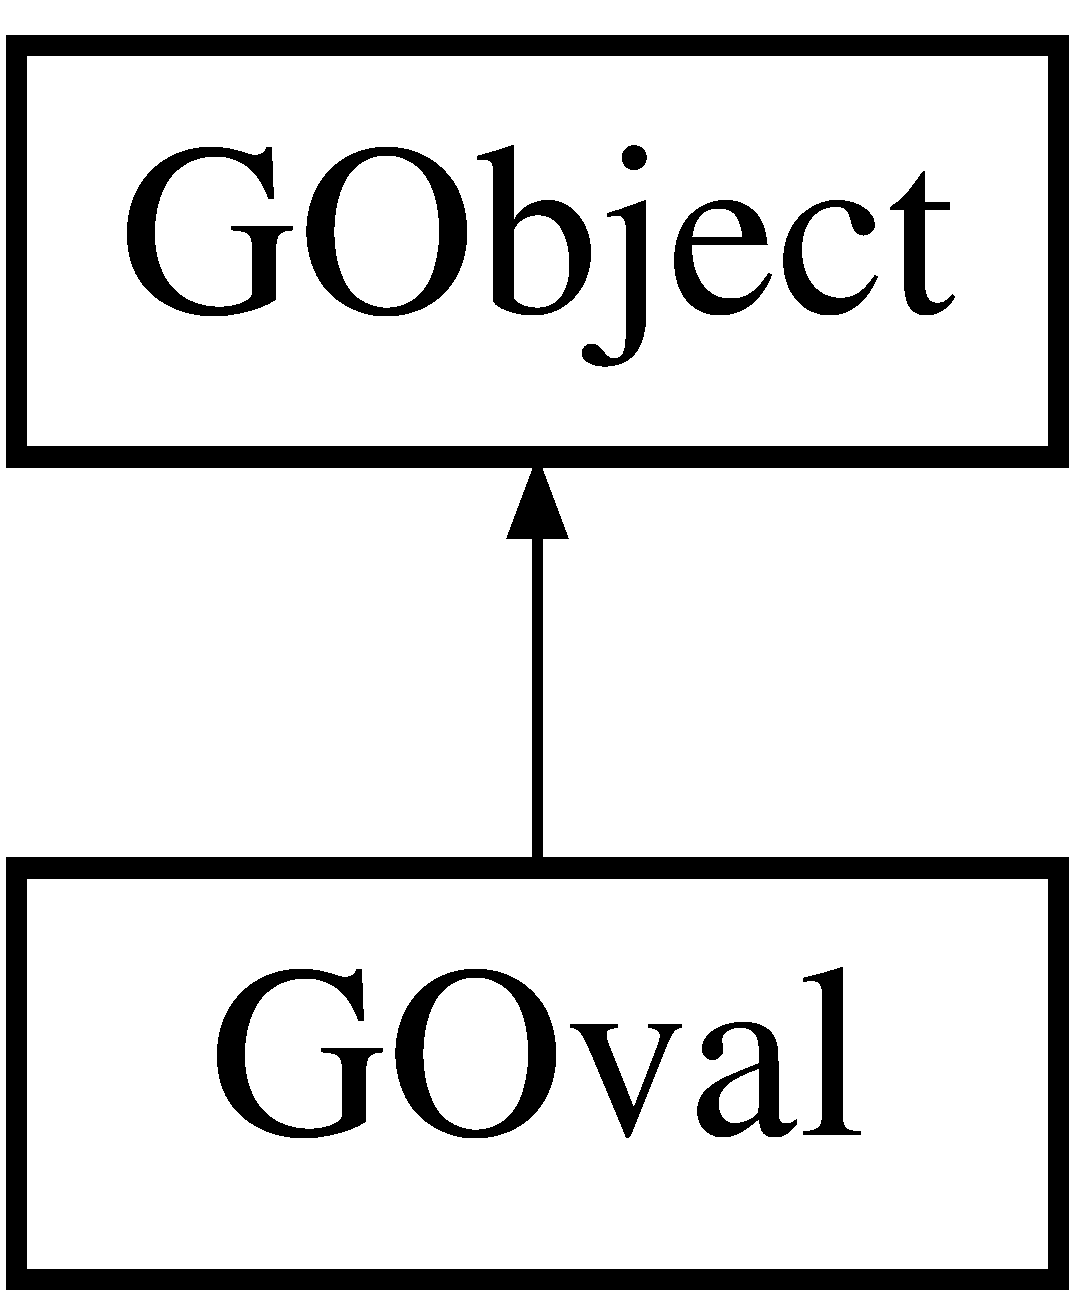
\includegraphics[height=2.000000cm]{classGOval}
\end{center}
\end{figure}
\subsection*{Public Types}
\begin{DoxyCompactItemize}
\item 
enum \mbox{\hyperlink{classGObject_a86e0f5648542856159bb40775c854aa7}{Line\+Style}} \{ \mbox{\hyperlink{classGObject_a86e0f5648542856159bb40775c854aa7acbc84bd5232621834ed31f44d457c1eb}{L\+I\+N\+E\+\_\+\+N\+O\+NE}}, 
\mbox{\hyperlink{classGObject_a86e0f5648542856159bb40775c854aa7a700c78bc2cd76acaab26651bf7b4941f}{L\+I\+N\+E\+\_\+\+S\+O\+L\+ID}}, 
\mbox{\hyperlink{classGObject_a86e0f5648542856159bb40775c854aa7a9ccba0845f785d81d07b333ae1aad84e}{L\+I\+N\+E\+\_\+\+D\+A\+SH}}, 
\mbox{\hyperlink{classGObject_a86e0f5648542856159bb40775c854aa7a8e811c096cb941997f0bfda168bb6df3}{L\+I\+N\+E\+\_\+\+D\+OT}}, 
\mbox{\hyperlink{classGObject_a86e0f5648542856159bb40775c854aa7ada15a2e3d737b2db7706d8300f91b89d}{L\+I\+N\+E\+\_\+\+D\+A\+S\+H\+\_\+\+D\+OT}}, 
\mbox{\hyperlink{classGObject_a86e0f5648542856159bb40775c854aa7aabf4053a73eafa7ba2b7e6d664c74c1d}{L\+I\+N\+E\+\_\+\+D\+A\+S\+H\+\_\+\+D\+O\+T\+\_\+\+D\+OT}}
 \}
\begin{DoxyCompactList}\small\item\em Styles that can be used for the outline around various shapes. \end{DoxyCompactList}\end{DoxyCompactItemize}
\subsection*{Public Member Functions}
\begin{DoxyCompactItemize}
\item 
\mbox{\hyperlink{classGOval_a0dc1da9139884a189b3fd0882c638bfc}{G\+Oval}} (double x=0, double y=0, double width=0, double height=0)
\begin{DoxyCompactList}\small\item\em Constructs a new oval inscribed in the specified rectangle. \end{DoxyCompactList}\item 
virtual bool \mbox{\hyperlink{classGObject_a1dbc9dafaae51958112dbe1267a1f547}{contains}} (const \mbox{\hyperlink{structGPoint}{G\+Point}} \&pt) const
\begin{DoxyCompactList}\small\item\em Returns {\ttfamily true} if the specified point is inside the object. \end{DoxyCompactList}\item 
bool \mbox{\hyperlink{classGOval_ad973a1d55799d3a73bf8b04986cd804e}{contains}} (double x, double y) const override
\begin{DoxyCompactList}\small\item\em Returns {\ttfamily true} if the specified point is inside the object. \end{DoxyCompactList}\item 
virtual \mbox{\hyperlink{structGPoint}{G\+Point}} \mbox{\hyperlink{classGObject_a0d41183bf6b08de66fe3907551aab0d7}{get\+Bottom\+Right\+Location}} () const
\begin{DoxyCompactList}\small\item\em Returns the x/y coordinates of the bottom/right corner of the object. \end{DoxyCompactList}\item 
virtual double \mbox{\hyperlink{classGObject_a4316a2406c18e1c6d061fe51fd355490}{get\+BottomY}} () const
\begin{DoxyCompactList}\small\item\em Returns the {\itshape y}-\/coordinate of the bottom of the object. \end{DoxyCompactList}\item 
virtual \mbox{\hyperlink{structGRectangle}{G\+Rectangle}} \mbox{\hyperlink{classGObject_a29e6ac35a0b48f491a4c88194cc5da3b}{get\+Bounds}} () const
\begin{DoxyCompactList}\small\item\em Returns the bounding box of this object, which is defined to be the smallest rectangle that covers everything drawn by the figure. \end{DoxyCompactList}\item 
virtual \mbox{\hyperlink{structGPoint}{G\+Point}} \mbox{\hyperlink{classGObject_a0909472e91448470bccdb62ecfb95d8b}{get\+Center\+Location}} () const
\begin{DoxyCompactList}\small\item\em Returns the x/y-\/coordinates of the center of the object. \end{DoxyCompactList}\item 
virtual double \mbox{\hyperlink{classGObject_a04df74355b545e0543112d5b8d924176}{get\+CenterX}} () const
\begin{DoxyCompactList}\small\item\em Returns the {\itshape x}-\/coordinate of the center of the object. \end{DoxyCompactList}\item 
virtual double \mbox{\hyperlink{classGObject_acb3287a3d507025a26f54b895713b947}{get\+CenterY}} () const
\begin{DoxyCompactList}\small\item\em Returns the {\itshape y}-\/coordinate of the center of the object. \end{DoxyCompactList}\item 
virtual std\+::string \mbox{\hyperlink{classGObject_aa061dfa488c31e18549d64363c1d0e34}{get\+Color}} () const
\begin{DoxyCompactList}\small\item\em Returns the color used to display this object. \end{DoxyCompactList}\item 
virtual std\+::string \mbox{\hyperlink{classGObject_a76f6964a11fde7c78e9751be184e1a3c}{get\+Fill\+Color}} () const
\begin{DoxyCompactList}\small\item\em Returns the color used to display the filled region of this object. \end{DoxyCompactList}\item 
virtual double \mbox{\hyperlink{classGObject_a1e7e353362434072875264cf95629f99}{get\+Height}} () const
\begin{DoxyCompactList}\small\item\em Returns the height of this object, which is the same as the height of its bounding box. \end{DoxyCompactList}\item 
virtual \mbox{\hyperlink{classGObject_a86e0f5648542856159bb40775c854aa7}{Line\+Style}} \mbox{\hyperlink{classGObject_aaf1f5ea8281e5e3486662878d26f0a13}{get\+Line\+Style}} () const
\begin{DoxyCompactList}\small\item\em Returns the object\textquotesingle{}s style such as solid or dashed. \end{DoxyCompactList}\item 
virtual double \mbox{\hyperlink{classGObject_a85ff266dc3eb63d9f2d8e5a4487fd3c0}{get\+Line\+Width}} () const
\begin{DoxyCompactList}\small\item\em Returns the width of the line used to draw this object. \end{DoxyCompactList}\item 
virtual \mbox{\hyperlink{structGPoint}{G\+Point}} \mbox{\hyperlink{classGObject_a4f83802015511edeb63b892830812c11}{get\+Location}} () const
\begin{DoxyCompactList}\small\item\em Returns the location of the top-\/left corner of object. \end{DoxyCompactList}\item 
virtual double \mbox{\hyperlink{classGObject_a1ae3fc278cc5b71b9f2d96a8a83cdf26}{get\+Opacity}} () const
\begin{DoxyCompactList}\small\item\em Returns how opaque (non-\/transparent) this object will appear from 0.\+0 (completely transparent) to 1.\+0 (completely opaque, default). \end{DoxyCompactList}\item 
virtual \mbox{\hyperlink{classGCompound}{G\+Compound}} $\ast$ \mbox{\hyperlink{classGObject_a3e53cef70541b1a14eade4ad0984d0b4}{get\+Parent}} () const
\begin{DoxyCompactList}\small\item\em Returns a pointer to the {\ttfamily \mbox{\hyperlink{classGCompound}{G\+Compound}}} that contains this object. \end{DoxyCompactList}\item 
virtual double \mbox{\hyperlink{classGObject_a798cc79daaa10145b28f60bcdfdb0ee9}{get\+RightX}} () const
\begin{DoxyCompactList}\small\item\em Returns the {\itshape x}-\/coordinate of the right side of the object. \end{DoxyCompactList}\item 
virtual \mbox{\hyperlink{structGDimension}{G\+Dimension}} \mbox{\hyperlink{classGObject_a7b4eec96a2bdc6420695d5796a78eea9}{get\+Size}} () const
\begin{DoxyCompactList}\small\item\em Returns the size of the object as a {\ttfamily \mbox{\hyperlink{structGDimension}{G\+Dimension}}}. \end{DoxyCompactList}\item 
std\+::string \mbox{\hyperlink{classGOval_a9b72ede4ee8520f987a0c01e30654814}{get\+Type}} () const override
\begin{DoxyCompactList}\small\item\em Returns the type of the object as a string, such as {\ttfamily \char`\"{}\+G\+Oval\char`\"{}} or {\ttfamily \char`\"{}\+G\+Rect\char`\"{}}. \end{DoxyCompactList}\item 
virtual double \mbox{\hyperlink{classGObject_a0ed2965abd4f5701d2cadf71239faf19}{get\+Width}} () const
\begin{DoxyCompactList}\small\item\em Returns the width of this object, which is equal to the width of the bounding box. \end{DoxyCompactList}\item 
virtual double \mbox{\hyperlink{classGObject_a344385751bee0720059403940d57a13e}{getX}} () const
\begin{DoxyCompactList}\small\item\em Returns the leftmost {\itshape x}-\/coordinate of the object. \end{DoxyCompactList}\item 
virtual double \mbox{\hyperlink{classGObject_aafa51c7f8f38a09febbb9ce7853f77b4}{getY}} () const
\begin{DoxyCompactList}\small\item\em Returns the topmost {\itshape y}-\/coordinate of the object. \end{DoxyCompactList}\item 
virtual bool \mbox{\hyperlink{classGObject_a11c404f106940c201b6f326e0355c150}{is\+Filled}} () const
\begin{DoxyCompactList}\small\item\em Returns {\ttfamily true} if the object is filled with color. \end{DoxyCompactList}\item 
virtual bool \mbox{\hyperlink{classGObject_a9de207581cfa4ca1eaa06da5f29b75fc}{is\+Transformed}} () const
\begin{DoxyCompactList}\small\item\em Returns {\ttfamily true} if this object has been transformed by calling methods such as \mbox{\hyperlink{classGObject_ae1ffaa12185dfd5ba464f7d87c329e26}{rotate()}} or \mbox{\hyperlink{classGObject_ad2e1900f730475c2d044817db03b38d6}{scale()}} on it. \end{DoxyCompactList}\item 
virtual bool \mbox{\hyperlink{classGObject_a9d8a6cfb13917785c143e74d40e4e2be}{is\+Visible}} () const
\begin{DoxyCompactList}\small\item\em Returns {\ttfamily true} if this object is visible on screen. \end{DoxyCompactList}\item 
virtual void \mbox{\hyperlink{classGObject_a5973d8dda83afb36e2c56855515be392}{move}} (double dx, double dy)
\begin{DoxyCompactList}\small\item\em Moves the object on the screen using the displacements {\ttfamily dx} and {\ttfamily dy}. \end{DoxyCompactList}\item 
virtual void \mbox{\hyperlink{classGObject_ac827b978aa122f136a14c198687ad80f}{repaint}} ()
\begin{DoxyCompactList}\small\item\em Instructs the object to redraw itself on screen. \end{DoxyCompactList}\item 
virtual void \mbox{\hyperlink{classGObject_a6022a1fd1e5dcd2fd5585e5a36aa3f37}{reset\+Transform}} ()
\begin{DoxyCompactList}\small\item\em Undoes any previous scale/rotate transformations on this object. \end{DoxyCompactList}\item 
virtual void \mbox{\hyperlink{classGObject_ae1ffaa12185dfd5ba464f7d87c329e26}{rotate}} (double theta)
\begin{DoxyCompactList}\small\item\em Transforms the object by rotating it {\ttfamily theta} degrees counterclockwise around its origin. \end{DoxyCompactList}\item 
virtual void \mbox{\hyperlink{classGObject_ad2e1900f730475c2d044817db03b38d6}{scale}} (double sf)
\begin{DoxyCompactList}\small\item\em Scales the object by the specified scale factor. \end{DoxyCompactList}\item 
virtual void \mbox{\hyperlink{classGObject_a63641f69d610d0b951357d35a0c3b1e3}{scale}} (double sx, double sy)
\begin{DoxyCompactList}\small\item\em Scales the object by the specified scale factors. \end{DoxyCompactList}\item 
void \mbox{\hyperlink{classGObject_ab6747f40313c531c2db32edb5b63b9b7}{send\+Backward}} ()
\begin{DoxyCompactList}\small\item\em Moves this object one step toward the back in the {\itshape z} dimension. \end{DoxyCompactList}\item 
void \mbox{\hyperlink{classGObject_a710b3e449c9facba7847c91ab170d281}{send\+Forward}} ()
\begin{DoxyCompactList}\small\item\em Moves this object one step toward the front in the {\itshape z} dimension. \end{DoxyCompactList}\item 
void \mbox{\hyperlink{classGObject_a0f7f1efbb7fd46dde2867c4ad0330896}{send\+To\+Back}} ()
\begin{DoxyCompactList}\small\item\em Moves this object to the back of the display in the {\itshape z} dimension. \end{DoxyCompactList}\item 
void \mbox{\hyperlink{classGObject_aee33d68488e46827ef55fac07f40a9b2}{send\+To\+Front}} ()
\begin{DoxyCompactList}\small\item\em Moves this object to the front of the display in the {\itshape z} dimension. \end{DoxyCompactList}\item 
virtual void \mbox{\hyperlink{classGObject_a71ff7b16b8f1bdc4a1ce9f30cf8b87d8}{set\+Bottom\+Right\+Location}} (double x, double y)
\begin{DoxyCompactList}\small\item\em Sets the location of the bottom/right of this object. \end{DoxyCompactList}\item 
virtual void \mbox{\hyperlink{classGObject_ac6f7320321182f1d18c1c0fa97d5e941}{set\+Bottom\+Right\+Location}} (const \mbox{\hyperlink{structGPoint}{G\+Point}} \&pt)
\begin{DoxyCompactList}\small\item\em Sets the location of the bottom/right of this object. \end{DoxyCompactList}\item 
virtual void \mbox{\hyperlink{classGObject_a4b20e93c2a2597484f74ee5caa71f41f}{set\+BottomY}} (double y)
\begin{DoxyCompactList}\small\item\em Sets the location of the bottom y-\/coordinate of this object. \end{DoxyCompactList}\item 
virtual void \mbox{\hyperlink{classGObject_a2aae8197624b72265ab83b4f1bc73f2f}{set\+Bounds}} (double x, double y, double width, double height)
\begin{DoxyCompactList}\small\item\em Changes the bounds of this object to the specified values. \end{DoxyCompactList}\item 
virtual void \mbox{\hyperlink{classGObject_acada386653f008cacc7cce86426bef7c}{set\+Bounds}} (const \mbox{\hyperlink{structGRectangle}{G\+Rectangle}} \&size)
\begin{DoxyCompactList}\small\item\em Changes the bounds of this object to the specified rectangle. \end{DoxyCompactList}\item 
virtual void \mbox{\hyperlink{classGObject_a290b47dd8de1be44089f95cb2c47c1de}{set\+Center\+Location}} (double x, double y)
\begin{DoxyCompactList}\small\item\em Sets the location of the center of this object. \end{DoxyCompactList}\item 
virtual void \mbox{\hyperlink{classGObject_a1bedf1b233ecba3f753ec58908a683a6}{set\+Center\+Location}} (const \mbox{\hyperlink{structGPoint}{G\+Point}} \&pt)
\begin{DoxyCompactList}\small\item\em Sets the location of the center of this object. \end{DoxyCompactList}\item 
virtual void \mbox{\hyperlink{classGObject_a2f4936281e056eead00a9186b9ba8af6}{set\+CenterX}} (double x)
\begin{DoxyCompactList}\small\item\em Sets the x-\/coordinate of the center of this object. \end{DoxyCompactList}\item 
virtual void \mbox{\hyperlink{classGObject_aad2a22b4fde88c33306b92aebf641d57}{set\+CenterY}} (double y)
\begin{DoxyCompactList}\small\item\em Sets the y-\/coordinate of the center of this object. \end{DoxyCompactList}\item 
virtual void \mbox{\hyperlink{classGObject_ad57ef49bc31db94e92648aa3737923d6}{set\+Color}} (int r, int g, int b)
\begin{DoxyCompactList}\small\item\em Sets the color used to display this object. \end{DoxyCompactList}\item 
virtual void \mbox{\hyperlink{classGObject_ab1f5cc0f5cc6bbbd716a526c61f1081d}{set\+Color}} (int rgb)
\begin{DoxyCompactList}\small\item\em Sets the color used to display this object. \end{DoxyCompactList}\item 
virtual void \mbox{\hyperlink{classGObject_a61374df6c11b52cfbb0815decdbaebc6}{set\+Color}} (const std\+::string \&color)
\begin{DoxyCompactList}\small\item\em Sets the color used to display this object. \end{DoxyCompactList}\item 
virtual void \mbox{\hyperlink{classGObject_ad767a33971159e9493e221cca4c00ae9}{set\+Fill\+Color}} (int r, int g, int b)
\begin{DoxyCompactList}\small\item\em Sets the color used to display the filled region of this object, if any. \end{DoxyCompactList}\item 
virtual void \mbox{\hyperlink{classGObject_aa59d9775a67fa7df2b24a95cd34840a3}{set\+Fill\+Color}} (int rgb)
\begin{DoxyCompactList}\small\item\em Sets the color used to display the filled region of this object, if any. \end{DoxyCompactList}\item 
virtual void \mbox{\hyperlink{classGObject_adbc18b1a930aadd97d7437f9f7265b96}{set\+Fill\+Color}} (const std\+::string \&color)
\begin{DoxyCompactList}\small\item\em Sets the color used to display the filled region of this object, if any. \end{DoxyCompactList}\item 
virtual void \mbox{\hyperlink{classGObject_a9b82b53362282c6bb7d6947068d2e55b}{set\+Filled}} (bool flag)
\begin{DoxyCompactList}\small\item\em Sets the fill status for the object, where {\ttfamily false} is outlined and {\ttfamily true} is filled. \end{DoxyCompactList}\item 
virtual void \mbox{\hyperlink{classGObject_a2592348886ffea646c6534bf88f7c49d}{set\+Font}} (const Q\+Font \&font)
\begin{DoxyCompactList}\small\item\em Changes the font used to display the object as specified by the given Qt font. \end{DoxyCompactList}\item 
virtual void \mbox{\hyperlink{classGObject_a8e096e8818d838aceae1d46d58fb3a7b}{set\+Font}} (const std\+::string \&font)
\begin{DoxyCompactList}\small\item\em Changes the font used to display the object as specified by the string {\ttfamily font}, which has the following format\+: \end{DoxyCompactList}\item 
virtual void \mbox{\hyperlink{classGObject_ad18e8fab1e02a4e9b75c6730212558eb}{set\+Foreground}} (int r, int g, int b)
\begin{DoxyCompactList}\small\item\em Sets the color used to display this object. \end{DoxyCompactList}\item 
virtual void \mbox{\hyperlink{classGObject_a9eb856b5ff83a19df3831a31f15f4563}{set\+Foreground}} (int rgb)
\begin{DoxyCompactList}\small\item\em Sets the color used to display this object. \end{DoxyCompactList}\item 
virtual void \mbox{\hyperlink{classGObject_af59209aeadea6dfc6d97a2d8531f50e1}{set\+Foreground}} (const std\+::string \&color)
\begin{DoxyCompactList}\small\item\em Sets the color used to display this object. \end{DoxyCompactList}\item 
virtual void \mbox{\hyperlink{classGObject_a9e280bfc4544dfaf8e4376c4e1a74357}{set\+Height}} (double height)
\begin{DoxyCompactList}\small\item\em Changes the height of this object to the specified height without changing its width. \end{DoxyCompactList}\item 
virtual void \mbox{\hyperlink{classGObject_add11575087eb94f1a71faa3f826c6341}{set\+Line\+Style}} (\mbox{\hyperlink{classGObject_a86e0f5648542856159bb40775c854aa7}{Line\+Style}} line\+Style)
\begin{DoxyCompactList}\small\item\em Sets the object\textquotesingle{}s style such as solid (\mbox{\hyperlink{classGObject_a86e0f5648542856159bb40775c854aa7a700c78bc2cd76acaab26651bf7b4941f}{G\+Object\+::\+L\+I\+N\+E\+\_\+\+S\+O\+L\+ID}}) or dashed (\mbox{\hyperlink{classGObject_a86e0f5648542856159bb40775c854aa7a9ccba0845f785d81d07b333ae1aad84e}{G\+Object\+::\+L\+I\+N\+E\+\_\+\+D\+A\+SH}}). \end{DoxyCompactList}\item 
virtual void \mbox{\hyperlink{classGObject_afd6a47c6ea6a1f85ca05a65ba3ff3477}{set\+Line\+Width}} (double line\+Width)
\begin{DoxyCompactList}\small\item\em Sets the width of the line used to draw this object. \end{DoxyCompactList}\item 
virtual void \mbox{\hyperlink{classGObject_a04594e8ba9b98513a64f1da00dcae18c}{set\+Location}} (double x, double y)
\begin{DoxyCompactList}\small\item\em Sets the location of the top-\/left corner of this object to the specified coordinates. \end{DoxyCompactList}\item 
virtual void \mbox{\hyperlink{classGObject_aa8480c0b7166cdf8f784cece06ab353f}{set\+Location}} (const \mbox{\hyperlink{structGPoint}{G\+Point}} \&pt)
\begin{DoxyCompactList}\small\item\em Sets the location of the top-\/left corner of this object to the specified point. \end{DoxyCompactList}\item 
virtual void \mbox{\hyperlink{classGObject_a04af1866cc1bae4a1226695794a50539}{set\+Opacity}} (double opacity)
\begin{DoxyCompactList}\small\item\em Sets how opaque (non-\/transparent) this object will appear from 0.\+0 (completely transparent) to 1.\+0 (completely opaque, default). \end{DoxyCompactList}\item 
virtual void \mbox{\hyperlink{classGObject_a3c90b758cdc2c911c9ef76c4360eb912}{set\+RightX}} (double x)
\begin{DoxyCompactList}\small\item\em Sets the location of the rightmost x-\/coordinate of this object. \end{DoxyCompactList}\item 
virtual void \mbox{\hyperlink{classGObject_aca25d49481f9bf5fc8f7df4c086c4ce7}{set\+Size}} (double width, double height)
\begin{DoxyCompactList}\small\item\em Changes the size of this object to the specified width and height. \end{DoxyCompactList}\item 
virtual void \mbox{\hyperlink{classGObject_ae2b628228f192c2702c4ce941b2af68f}{set\+Size}} (const \mbox{\hyperlink{structGDimension}{G\+Dimension}} \&size)
\begin{DoxyCompactList}\small\item\em Changes the size of this object to the specified width and height. \end{DoxyCompactList}\item 
virtual void \mbox{\hyperlink{classGObject_a88203f28224315d9f4471212f4af8ed3}{set\+Visible}} (bool flag)
\begin{DoxyCompactList}\small\item\em Sets whether this object is visible. \end{DoxyCompactList}\item 
virtual void \mbox{\hyperlink{classGObject_aa3f3fba4cb131baa8696ba01e3bceca1}{set\+Width}} (double width)
\begin{DoxyCompactList}\small\item\em Changes the width of this object to the specified width without changing its height. \end{DoxyCompactList}\item 
virtual void \mbox{\hyperlink{classGObject_a9c18fcc579333bf9653d13ad2b372e39}{setX}} (double x)
\begin{DoxyCompactList}\small\item\em Sets the x location of the left side of this object. \end{DoxyCompactList}\item 
virtual void \mbox{\hyperlink{classGObject_a7d57e2a5c35d27feb58fd498a3cf82b9}{setY}} (double y)
\begin{DoxyCompactList}\small\item\em Sets the y location of the top of this object. \end{DoxyCompactList}\item 
virtual std\+::string \mbox{\hyperlink{classGObject_a1fe5121d6528fdea3f243321b3fa3a49}{to\+String}} () const
\begin{DoxyCompactList}\small\item\em Returns a printable representation of the object. \end{DoxyCompactList}\end{DoxyCompactItemize}
\subsection*{Static Public Member Functions}
\begin{DoxyCompactItemize}
\item 
static bool \mbox{\hyperlink{classGObject_a93be0e1fe1b1bf1a1da732470c94f42b}{is\+Anti\+Aliasing}} ()
\begin{DoxyCompactList}\small\item\em Returns whether we should globally anti-\/alias graphical objects. \end{DoxyCompactList}\item 
static void \mbox{\hyperlink{classGObject_a1e43371668ae850193cebedb44e1bbe3}{set\+Anti\+Aliasing}} (bool value)
\begin{DoxyCompactList}\small\item\em Globally turns on/off the anti-\/aliasing feature that smooths out the edges of onscreen shapes. \end{DoxyCompactList}\end{DoxyCompactItemize}
\subsection*{Protected Member Functions}
\begin{DoxyCompactItemize}
\item 
virtual std\+::string \mbox{\hyperlink{classGObject_a4fcdf8de5c6de92242a975d83d8f23ea}{to\+String\+Extra}} () const
\begin{DoxyCompactList}\small\item\em Returns a string containing any extra unique information about this type of graphical object. \end{DoxyCompactList}\end{DoxyCompactItemize}
\subsection*{Protected Attributes}
\begin{DoxyCompactItemize}
\item 
Q\+Brush \mbox{\hyperlink{classGObject_aab24462ec896b596d99911767b0912d0}{\+\_\+brush}}
\item 
std\+::string \mbox{\hyperlink{classGObject_a1134e770ae4315ea8bc1201e2f21da8b}{\+\_\+color}}
\item 
int \mbox{\hyperlink{classGObject_a003fdd343d9b7505c53a8b7a134200ed}{\+\_\+color\+Int}}
\item 
std\+::string \mbox{\hyperlink{classGObject_a179f8d6cee65cd8a54692e32b224392a}{\+\_\+fill\+Color}}
\item 
int \mbox{\hyperlink{classGObject_a751def333a67d651e5b99cc331ecb496}{\+\_\+fill\+Color\+Int}}
\item 
bool \mbox{\hyperlink{classGObject_ad4a55cbcd61b58a4d49666490bb2f103}{\+\_\+fill\+Flag}}
\item 
std\+::string \mbox{\hyperlink{classGObject_aea76ea1a8b5dd7b0a78653277e63b536}{\+\_\+font}}
\item 
double \mbox{\hyperlink{classGObject_ad05df29e7f27fc504abd743e3d8b4e73}{\+\_\+height}}
\item 
\mbox{\hyperlink{classGObject_a86e0f5648542856159bb40775c854aa7}{Line\+Style}} \mbox{\hyperlink{classGObject_a89bafecaafb7c72d55c7efc10b7d0523}{\+\_\+line\+Style}}
\item 
double \mbox{\hyperlink{classGObject_a16e9033665937f13de2e163dc2184aff}{\+\_\+line\+Width}}
\item 
double \mbox{\hyperlink{classGObject_a20eff8eb7af27182edc9bfc54768b6f3}{\+\_\+opacity}}
\item 
\mbox{\hyperlink{classGCompound}{G\+Compound}} $\ast$ \mbox{\hyperlink{classGObject_ac9452c1eaff70eebddbb318196aa3835}{\+\_\+parent}}
\item 
Q\+Pen \mbox{\hyperlink{classGObject_afb69d172743f868299847174eb1b6bc8}{\+\_\+pen}}
\item 
Q\+Transform \mbox{\hyperlink{classGObject_a475b8860a5f1adb4a1fdc58d1f5c1e32}{\+\_\+transform}}
\item 
bool \mbox{\hyperlink{classGObject_ae4725802fc8d8aaa0ab4bd4781f7e07c}{\+\_\+transformed}}
\item 
bool \mbox{\hyperlink{classGObject_a9312c72508471b7c7a87b540263e1af4}{\+\_\+visible}}
\item 
double \mbox{\hyperlink{classGObject_ab55d85a3371770e6725b1062cf160cd8}{\+\_\+width}}
\item 
double \mbox{\hyperlink{classGObject_a6675b83b27137b8d3aa2ad8133078ea6}{\+\_\+x}}
\item 
double \mbox{\hyperlink{classGObject_a2f0f6aeafddc8a39c578bfa7e22b5f1e}{\+\_\+y}}
\end{DoxyCompactItemize}


\subsection{Detailed Description}
This graphical object subclass represents an oval inscribed in a rectangular box. 

\subsection{Member Enumeration Documentation}
\mbox{\Hypertarget{classGObject_a86e0f5648542856159bb40775c854aa7}\label{classGObject_a86e0f5648542856159bb40775c854aa7}} 
\index{G\+Oval@{G\+Oval}!Line\+Style@{Line\+Style}}
\index{Line\+Style@{Line\+Style}!G\+Oval@{G\+Oval}}
\subsubsection{\texorpdfstring{Line\+Style}{LineStyle}}
{\footnotesize\ttfamily enum \mbox{\hyperlink{classGObject_a86e0f5648542856159bb40775c854aa7}{Line\+Style}}\hspace{0.3cm}{\ttfamily [inherited]}}



Styles that can be used for the outline around various shapes. 

Call set\+Line\+Style on a \mbox{\hyperlink{classGObject}{G\+Object}} and pass one of these values. \begin{DoxyEnumFields}{Enumerator}
\raisebox{\heightof{T}}[0pt][0pt]{\index{L\+I\+N\+E\+\_\+\+N\+O\+NE@{L\+I\+N\+E\+\_\+\+N\+O\+NE}!G\+Oval@{G\+Oval}}\index{G\+Oval@{G\+Oval}!L\+I\+N\+E\+\_\+\+N\+O\+NE@{L\+I\+N\+E\+\_\+\+N\+O\+NE}}}\mbox{\Hypertarget{classGObject_a86e0f5648542856159bb40775c854aa7acbc84bd5232621834ed31f44d457c1eb}\label{classGObject_a86e0f5648542856159bb40775c854aa7acbc84bd5232621834ed31f44d457c1eb}} 
L\+I\+N\+E\+\_\+\+N\+O\+NE&\\
\hline

\raisebox{\heightof{T}}[0pt][0pt]{\index{L\+I\+N\+E\+\_\+\+S\+O\+L\+ID@{L\+I\+N\+E\+\_\+\+S\+O\+L\+ID}!G\+Oval@{G\+Oval}}\index{G\+Oval@{G\+Oval}!L\+I\+N\+E\+\_\+\+S\+O\+L\+ID@{L\+I\+N\+E\+\_\+\+S\+O\+L\+ID}}}\mbox{\Hypertarget{classGObject_a86e0f5648542856159bb40775c854aa7a700c78bc2cd76acaab26651bf7b4941f}\label{classGObject_a86e0f5648542856159bb40775c854aa7a700c78bc2cd76acaab26651bf7b4941f}} 
L\+I\+N\+E\+\_\+\+S\+O\+L\+ID&\\
\hline

\raisebox{\heightof{T}}[0pt][0pt]{\index{L\+I\+N\+E\+\_\+\+D\+A\+SH@{L\+I\+N\+E\+\_\+\+D\+A\+SH}!G\+Oval@{G\+Oval}}\index{G\+Oval@{G\+Oval}!L\+I\+N\+E\+\_\+\+D\+A\+SH@{L\+I\+N\+E\+\_\+\+D\+A\+SH}}}\mbox{\Hypertarget{classGObject_a86e0f5648542856159bb40775c854aa7a9ccba0845f785d81d07b333ae1aad84e}\label{classGObject_a86e0f5648542856159bb40775c854aa7a9ccba0845f785d81d07b333ae1aad84e}} 
L\+I\+N\+E\+\_\+\+D\+A\+SH&\\
\hline

\raisebox{\heightof{T}}[0pt][0pt]{\index{L\+I\+N\+E\+\_\+\+D\+OT@{L\+I\+N\+E\+\_\+\+D\+OT}!G\+Oval@{G\+Oval}}\index{G\+Oval@{G\+Oval}!L\+I\+N\+E\+\_\+\+D\+OT@{L\+I\+N\+E\+\_\+\+D\+OT}}}\mbox{\Hypertarget{classGObject_a86e0f5648542856159bb40775c854aa7a8e811c096cb941997f0bfda168bb6df3}\label{classGObject_a86e0f5648542856159bb40775c854aa7a8e811c096cb941997f0bfda168bb6df3}} 
L\+I\+N\+E\+\_\+\+D\+OT&\\
\hline

\raisebox{\heightof{T}}[0pt][0pt]{\index{L\+I\+N\+E\+\_\+\+D\+A\+S\+H\+\_\+\+D\+OT@{L\+I\+N\+E\+\_\+\+D\+A\+S\+H\+\_\+\+D\+OT}!G\+Oval@{G\+Oval}}\index{G\+Oval@{G\+Oval}!L\+I\+N\+E\+\_\+\+D\+A\+S\+H\+\_\+\+D\+OT@{L\+I\+N\+E\+\_\+\+D\+A\+S\+H\+\_\+\+D\+OT}}}\mbox{\Hypertarget{classGObject_a86e0f5648542856159bb40775c854aa7ada15a2e3d737b2db7706d8300f91b89d}\label{classGObject_a86e0f5648542856159bb40775c854aa7ada15a2e3d737b2db7706d8300f91b89d}} 
L\+I\+N\+E\+\_\+\+D\+A\+S\+H\+\_\+\+D\+OT&\\
\hline

\raisebox{\heightof{T}}[0pt][0pt]{\index{L\+I\+N\+E\+\_\+\+D\+A\+S\+H\+\_\+\+D\+O\+T\+\_\+\+D\+OT@{L\+I\+N\+E\+\_\+\+D\+A\+S\+H\+\_\+\+D\+O\+T\+\_\+\+D\+OT}!G\+Oval@{G\+Oval}}\index{G\+Oval@{G\+Oval}!L\+I\+N\+E\+\_\+\+D\+A\+S\+H\+\_\+\+D\+O\+T\+\_\+\+D\+OT@{L\+I\+N\+E\+\_\+\+D\+A\+S\+H\+\_\+\+D\+O\+T\+\_\+\+D\+OT}}}\mbox{\Hypertarget{classGObject_a86e0f5648542856159bb40775c854aa7aabf4053a73eafa7ba2b7e6d664c74c1d}\label{classGObject_a86e0f5648542856159bb40775c854aa7aabf4053a73eafa7ba2b7e6d664c74c1d}} 
L\+I\+N\+E\+\_\+\+D\+A\+S\+H\+\_\+\+D\+O\+T\+\_\+\+D\+OT&\\
\hline

\end{DoxyEnumFields}


\subsection{Constructor \& Destructor Documentation}
\mbox{\Hypertarget{classGOval_a0dc1da9139884a189b3fd0882c638bfc}\label{classGOval_a0dc1da9139884a189b3fd0882c638bfc}} 
\index{G\+Oval@{G\+Oval}!G\+Oval@{G\+Oval}}
\index{G\+Oval@{G\+Oval}!G\+Oval@{G\+Oval}}
\subsubsection{\texorpdfstring{G\+Oval()}{GOval()}}
{\footnotesize\ttfamily \mbox{\hyperlink{classGOval}{G\+Oval}} (\begin{DoxyParamCaption}\item[{double}]{x = {\ttfamily 0},  }\item[{double}]{y = {\ttfamily 0},  }\item[{double}]{width = {\ttfamily 0},  }\item[{double}]{height = {\ttfamily 0} }\end{DoxyParamCaption})}



Constructs a new oval inscribed in the specified rectangle. 

By default, the oval is positioned at the origin, but you can pass coordinates {\ttfamily x} and {\ttfamily y}. 

\subsection{Member Function Documentation}
\mbox{\Hypertarget{classGObject_a1dbc9dafaae51958112dbe1267a1f547}\label{classGObject_a1dbc9dafaae51958112dbe1267a1f547}} 
\index{G\+Oval@{G\+Oval}!contains@{contains}}
\index{contains@{contains}!G\+Oval@{G\+Oval}}
\subsubsection{\texorpdfstring{contains()}{contains()}\hspace{0.1cm}{\footnotesize\ttfamily [1/2]}}
{\footnotesize\ttfamily bool contains (\begin{DoxyParamCaption}\item[{const \mbox{\hyperlink{structGPoint}{G\+Point}} \&}]{pt }\end{DoxyParamCaption}) const\hspace{0.3cm}{\ttfamily [virtual]}, {\ttfamily [inherited]}}



Returns {\ttfamily true} if the specified point is inside the object. 

\mbox{\Hypertarget{classGOval_ad973a1d55799d3a73bf8b04986cd804e}\label{classGOval_ad973a1d55799d3a73bf8b04986cd804e}} 
\index{G\+Oval@{G\+Oval}!contains@{contains}}
\index{contains@{contains}!G\+Oval@{G\+Oval}}
\subsubsection{\texorpdfstring{contains()}{contains()}\hspace{0.1cm}{\footnotesize\ttfamily [2/2]}}
{\footnotesize\ttfamily bool contains (\begin{DoxyParamCaption}\item[{double}]{x,  }\item[{double}]{y }\end{DoxyParamCaption}) const\hspace{0.3cm}{\ttfamily [override]}, {\ttfamily [virtual]}}



Returns {\ttfamily true} if the specified point is inside the object. 



Reimplemented from \mbox{\hyperlink{classGObject_abb6a5d7c03e6eaaae97264c4799ce7c3}{G\+Object}}.

\mbox{\Hypertarget{classGObject_a0d41183bf6b08de66fe3907551aab0d7}\label{classGObject_a0d41183bf6b08de66fe3907551aab0d7}} 
\index{G\+Oval@{G\+Oval}!get\+Bottom\+Right\+Location@{get\+Bottom\+Right\+Location}}
\index{get\+Bottom\+Right\+Location@{get\+Bottom\+Right\+Location}!G\+Oval@{G\+Oval}}
\subsubsection{\texorpdfstring{get\+Bottom\+Right\+Location()}{getBottomRightLocation()}}
{\footnotesize\ttfamily \mbox{\hyperlink{structGPoint}{G\+Point}} get\+Bottom\+Right\+Location (\begin{DoxyParamCaption}{ }\end{DoxyParamCaption}) const\hspace{0.3cm}{\ttfamily [virtual]}, {\ttfamily [inherited]}}



Returns the x/y coordinates of the bottom/right corner of the object. 

\mbox{\Hypertarget{classGObject_a4316a2406c18e1c6d061fe51fd355490}\label{classGObject_a4316a2406c18e1c6d061fe51fd355490}} 
\index{G\+Oval@{G\+Oval}!get\+BottomY@{get\+BottomY}}
\index{get\+BottomY@{get\+BottomY}!G\+Oval@{G\+Oval}}
\subsubsection{\texorpdfstring{get\+Bottom\+Y()}{getBottomY()}}
{\footnotesize\ttfamily double get\+BottomY (\begin{DoxyParamCaption}{ }\end{DoxyParamCaption}) const\hspace{0.3cm}{\ttfamily [virtual]}, {\ttfamily [inherited]}}



Returns the {\itshape y}-\/coordinate of the bottom of the object. 

Equivalent to the top y-\/coordinate plus the object\textquotesingle{}s height. \mbox{\Hypertarget{classGObject_a29e6ac35a0b48f491a4c88194cc5da3b}\label{classGObject_a29e6ac35a0b48f491a4c88194cc5da3b}} 
\index{G\+Oval@{G\+Oval}!get\+Bounds@{get\+Bounds}}
\index{get\+Bounds@{get\+Bounds}!G\+Oval@{G\+Oval}}
\subsubsection{\texorpdfstring{get\+Bounds()}{getBounds()}}
{\footnotesize\ttfamily \mbox{\hyperlink{structGRectangle}{G\+Rectangle}} get\+Bounds (\begin{DoxyParamCaption}{ }\end{DoxyParamCaption}) const\hspace{0.3cm}{\ttfamily [virtual]}, {\ttfamily [inherited]}}



Returns the bounding box of this object, which is defined to be the smallest rectangle that covers everything drawn by the figure. 

The coordinates of this rectangle do not necessarily match the location returned by {\ttfamily get\+Location}. Given a {\ttfamily \mbox{\hyperlink{classGText}{G\+Text}}} object, for example, {\ttfamily get\+Location} returns the coordinates of the point on the baseline at which the string begins; the {\ttfamily get\+Bounds} method, by contrast, returns a rectangle that covers the entire window area occupied by the string. 

Reimplemented in \mbox{\hyperlink{classGText_a89040ce9277825772d359fccd33bca86}{G\+Text}}, \mbox{\hyperlink{classGPolygon_a89040ce9277825772d359fccd33bca86}{G\+Polygon}}, \mbox{\hyperlink{classGLine_a89040ce9277825772d359fccd33bca86}{G\+Line}}, \mbox{\hyperlink{classGCompound_a89040ce9277825772d359fccd33bca86}{G\+Compound}}, and \mbox{\hyperlink{classGArc_a89040ce9277825772d359fccd33bca86}{G\+Arc}}.

\mbox{\Hypertarget{classGObject_a0909472e91448470bccdb62ecfb95d8b}\label{classGObject_a0909472e91448470bccdb62ecfb95d8b}} 
\index{G\+Oval@{G\+Oval}!get\+Center\+Location@{get\+Center\+Location}}
\index{get\+Center\+Location@{get\+Center\+Location}!G\+Oval@{G\+Oval}}
\subsubsection{\texorpdfstring{get\+Center\+Location()}{getCenterLocation()}}
{\footnotesize\ttfamily \mbox{\hyperlink{structGPoint}{G\+Point}} get\+Center\+Location (\begin{DoxyParamCaption}{ }\end{DoxyParamCaption}) const\hspace{0.3cm}{\ttfamily [virtual]}, {\ttfamily [inherited]}}



Returns the x/y-\/coordinates of the center of the object. 

Equivalent to the top/left plus half the object\textquotesingle{}s size. \mbox{\Hypertarget{classGObject_a04df74355b545e0543112d5b8d924176}\label{classGObject_a04df74355b545e0543112d5b8d924176}} 
\index{G\+Oval@{G\+Oval}!get\+CenterX@{get\+CenterX}}
\index{get\+CenterX@{get\+CenterX}!G\+Oval@{G\+Oval}}
\subsubsection{\texorpdfstring{get\+Center\+X()}{getCenterX()}}
{\footnotesize\ttfamily double get\+CenterX (\begin{DoxyParamCaption}{ }\end{DoxyParamCaption}) const\hspace{0.3cm}{\ttfamily [virtual]}, {\ttfamily [inherited]}}



Returns the {\itshape x}-\/coordinate of the center of the object. 

Equivalent to the top/left plus half the object\textquotesingle{}s width. \mbox{\Hypertarget{classGObject_acb3287a3d507025a26f54b895713b947}\label{classGObject_acb3287a3d507025a26f54b895713b947}} 
\index{G\+Oval@{G\+Oval}!get\+CenterY@{get\+CenterY}}
\index{get\+CenterY@{get\+CenterY}!G\+Oval@{G\+Oval}}
\subsubsection{\texorpdfstring{get\+Center\+Y()}{getCenterY()}}
{\footnotesize\ttfamily double get\+CenterY (\begin{DoxyParamCaption}{ }\end{DoxyParamCaption}) const\hspace{0.3cm}{\ttfamily [virtual]}, {\ttfamily [inherited]}}



Returns the {\itshape y}-\/coordinate of the center of the object. 

Equivalent to the top/left plus half the object\textquotesingle{}s height. \mbox{\Hypertarget{classGObject_aa061dfa488c31e18549d64363c1d0e34}\label{classGObject_aa061dfa488c31e18549d64363c1d0e34}} 
\index{G\+Oval@{G\+Oval}!get\+Color@{get\+Color}}
\index{get\+Color@{get\+Color}!G\+Oval@{G\+Oval}}
\subsubsection{\texorpdfstring{get\+Color()}{getColor()}}
{\footnotesize\ttfamily std\+::string get\+Color (\begin{DoxyParamCaption}{ }\end{DoxyParamCaption}) const\hspace{0.3cm}{\ttfamily [virtual]}, {\ttfamily [inherited]}}



Returns the color used to display this object. 

This color is always returned as a string in the form {\ttfamily \char`\"{}\#rrggbb\char`\"{}}, where {\ttfamily rr}, {\ttfamily gg}, and {\ttfamily bb} are the red, green, and blue components of the color, expressed as two-\/digit hexadecimal values. \mbox{\Hypertarget{classGObject_a76f6964a11fde7c78e9751be184e1a3c}\label{classGObject_a76f6964a11fde7c78e9751be184e1a3c}} 
\index{G\+Oval@{G\+Oval}!get\+Fill\+Color@{get\+Fill\+Color}}
\index{get\+Fill\+Color@{get\+Fill\+Color}!G\+Oval@{G\+Oval}}
\subsubsection{\texorpdfstring{get\+Fill\+Color()}{getFillColor()}}
{\footnotesize\ttfamily std\+::string get\+Fill\+Color (\begin{DoxyParamCaption}{ }\end{DoxyParamCaption}) const\hspace{0.3cm}{\ttfamily [virtual]}, {\ttfamily [inherited]}}



Returns the color used to display the filled region of this object. 

If none has been set, returns the empty string. \mbox{\Hypertarget{classGObject_a1e7e353362434072875264cf95629f99}\label{classGObject_a1e7e353362434072875264cf95629f99}} 
\index{G\+Oval@{G\+Oval}!get\+Height@{get\+Height}}
\index{get\+Height@{get\+Height}!G\+Oval@{G\+Oval}}
\subsubsection{\texorpdfstring{get\+Height()}{getHeight()}}
{\footnotesize\ttfamily double get\+Height (\begin{DoxyParamCaption}{ }\end{DoxyParamCaption}) const\hspace{0.3cm}{\ttfamily [virtual]}, {\ttfamily [inherited]}}



Returns the height of this object, which is the same as the height of its bounding box. 



Reimplemented in \mbox{\hyperlink{classGPolygon_a2bede8b27b21ae4c7940e762cbad9e07}{G\+Polygon}}, and \mbox{\hyperlink{classGLine_a2bede8b27b21ae4c7940e762cbad9e07}{G\+Line}}.

\mbox{\Hypertarget{classGObject_aaf1f5ea8281e5e3486662878d26f0a13}\label{classGObject_aaf1f5ea8281e5e3486662878d26f0a13}} 
\index{G\+Oval@{G\+Oval}!get\+Line\+Style@{get\+Line\+Style}}
\index{get\+Line\+Style@{get\+Line\+Style}!G\+Oval@{G\+Oval}}
\subsubsection{\texorpdfstring{get\+Line\+Style()}{getLineStyle()}}
{\footnotesize\ttfamily \mbox{\hyperlink{classGObject_a86e0f5648542856159bb40775c854aa7}{G\+Object\+::\+Line\+Style}} get\+Line\+Style (\begin{DoxyParamCaption}{ }\end{DoxyParamCaption}) const\hspace{0.3cm}{\ttfamily [virtual]}, {\ttfamily [inherited]}}



Returns the object\textquotesingle{}s style such as solid or dashed. 

\mbox{\Hypertarget{classGObject_a85ff266dc3eb63d9f2d8e5a4487fd3c0}\label{classGObject_a85ff266dc3eb63d9f2d8e5a4487fd3c0}} 
\index{G\+Oval@{G\+Oval}!get\+Line\+Width@{get\+Line\+Width}}
\index{get\+Line\+Width@{get\+Line\+Width}!G\+Oval@{G\+Oval}}
\subsubsection{\texorpdfstring{get\+Line\+Width()}{getLineWidth()}}
{\footnotesize\ttfamily double get\+Line\+Width (\begin{DoxyParamCaption}{ }\end{DoxyParamCaption}) const\hspace{0.3cm}{\ttfamily [virtual]}, {\ttfamily [inherited]}}



Returns the width of the line used to draw this object. 

\begin{DoxyReturn}{Returns}
default 1 
\end{DoxyReturn}
\mbox{\Hypertarget{classGObject_a4f83802015511edeb63b892830812c11}\label{classGObject_a4f83802015511edeb63b892830812c11}} 
\index{G\+Oval@{G\+Oval}!get\+Location@{get\+Location}}
\index{get\+Location@{get\+Location}!G\+Oval@{G\+Oval}}
\subsubsection{\texorpdfstring{get\+Location()}{getLocation()}}
{\footnotesize\ttfamily \mbox{\hyperlink{structGPoint}{G\+Point}} get\+Location (\begin{DoxyParamCaption}{ }\end{DoxyParamCaption}) const\hspace{0.3cm}{\ttfamily [virtual]}, {\ttfamily [inherited]}}



Returns the location of the top-\/left corner of object. 

\mbox{\Hypertarget{classGObject_a1ae3fc278cc5b71b9f2d96a8a83cdf26}\label{classGObject_a1ae3fc278cc5b71b9f2d96a8a83cdf26}} 
\index{G\+Oval@{G\+Oval}!get\+Opacity@{get\+Opacity}}
\index{get\+Opacity@{get\+Opacity}!G\+Oval@{G\+Oval}}
\subsubsection{\texorpdfstring{get\+Opacity()}{getOpacity()}}
{\footnotesize\ttfamily double get\+Opacity (\begin{DoxyParamCaption}{ }\end{DoxyParamCaption}) const\hspace{0.3cm}{\ttfamily [virtual]}, {\ttfamily [inherited]}}



Returns how opaque (non-\/transparent) this object will appear from 0.\+0 (completely transparent) to 1.\+0 (completely opaque, default). 

\mbox{\Hypertarget{classGObject_a3e53cef70541b1a14eade4ad0984d0b4}\label{classGObject_a3e53cef70541b1a14eade4ad0984d0b4}} 
\index{G\+Oval@{G\+Oval}!get\+Parent@{get\+Parent}}
\index{get\+Parent@{get\+Parent}!G\+Oval@{G\+Oval}}
\subsubsection{\texorpdfstring{get\+Parent()}{getParent()}}
{\footnotesize\ttfamily \mbox{\hyperlink{classGCompound}{G\+Compound}} $\ast$ get\+Parent (\begin{DoxyParamCaption}{ }\end{DoxyParamCaption}) const\hspace{0.3cm}{\ttfamily [virtual]}, {\ttfamily [inherited]}}



Returns a pointer to the {\ttfamily \mbox{\hyperlink{classGCompound}{G\+Compound}}} that contains this object. 

Every {\ttfamily \mbox{\hyperlink{classGWindow}{G\+Window}}} is initialized to contain a single {\ttfamily \mbox{\hyperlink{classGCompound}{G\+Compound}}} that is aligned with the window. Adding objects to the window adds them to that {\ttfamily \mbox{\hyperlink{classGCompound}{G\+Compound}}}, which means that every object you add to the window has a parent. Calling {\ttfamily get\+Parent} on the top-\/level {\ttfamily \mbox{\hyperlink{classGCompound}{G\+Compound}}} returns {\ttfamily nullptr}. \mbox{\Hypertarget{classGObject_a798cc79daaa10145b28f60bcdfdb0ee9}\label{classGObject_a798cc79daaa10145b28f60bcdfdb0ee9}} 
\index{G\+Oval@{G\+Oval}!get\+RightX@{get\+RightX}}
\index{get\+RightX@{get\+RightX}!G\+Oval@{G\+Oval}}
\subsubsection{\texorpdfstring{get\+Right\+X()}{getRightX()}}
{\footnotesize\ttfamily double get\+RightX (\begin{DoxyParamCaption}{ }\end{DoxyParamCaption}) const\hspace{0.3cm}{\ttfamily [virtual]}, {\ttfamily [inherited]}}



Returns the {\itshape x}-\/coordinate of the right side of the object. 

Equivalent to the left x-\/coordinate plus the object\textquotesingle{}s width. \mbox{\Hypertarget{classGObject_a7b4eec96a2bdc6420695d5796a78eea9}\label{classGObject_a7b4eec96a2bdc6420695d5796a78eea9}} 
\index{G\+Oval@{G\+Oval}!get\+Size@{get\+Size}}
\index{get\+Size@{get\+Size}!G\+Oval@{G\+Oval}}
\subsubsection{\texorpdfstring{get\+Size()}{getSize()}}
{\footnotesize\ttfamily \mbox{\hyperlink{structGDimension}{G\+Dimension}} get\+Size (\begin{DoxyParamCaption}{ }\end{DoxyParamCaption}) const\hspace{0.3cm}{\ttfamily [virtual]}, {\ttfamily [inherited]}}



Returns the size of the object as a {\ttfamily \mbox{\hyperlink{structGDimension}{G\+Dimension}}}. 

\mbox{\Hypertarget{classGOval_a9b72ede4ee8520f987a0c01e30654814}\label{classGOval_a9b72ede4ee8520f987a0c01e30654814}} 
\index{G\+Oval@{G\+Oval}!get\+Type@{get\+Type}}
\index{get\+Type@{get\+Type}!G\+Oval@{G\+Oval}}
\subsubsection{\texorpdfstring{get\+Type()}{getType()}}
{\footnotesize\ttfamily std\+::string get\+Type (\begin{DoxyParamCaption}{ }\end{DoxyParamCaption}) const\hspace{0.3cm}{\ttfamily [override]}, {\ttfamily [virtual]}}



Returns the type of the object as a string, such as {\ttfamily \char`\"{}\+G\+Oval\char`\"{}} or {\ttfamily \char`\"{}\+G\+Rect\char`\"{}}. 

Each \mbox{\hyperlink{classGObject}{G\+Object}} subtype must override this method. 

Implements \mbox{\hyperlink{classGObject_a799e073a127b428cc841086d42ea4fed}{G\+Object}}.

\mbox{\Hypertarget{classGObject_a0ed2965abd4f5701d2cadf71239faf19}\label{classGObject_a0ed2965abd4f5701d2cadf71239faf19}} 
\index{G\+Oval@{G\+Oval}!get\+Width@{get\+Width}}
\index{get\+Width@{get\+Width}!G\+Oval@{G\+Oval}}
\subsubsection{\texorpdfstring{get\+Width()}{getWidth()}}
{\footnotesize\ttfamily double get\+Width (\begin{DoxyParamCaption}{ }\end{DoxyParamCaption}) const\hspace{0.3cm}{\ttfamily [virtual]}, {\ttfamily [inherited]}}



Returns the width of this object, which is equal to the width of the bounding box. 



Reimplemented in \mbox{\hyperlink{classGPolygon_ab7b172cec7ed45e1246a3ce3160a62f7}{G\+Polygon}}, and \mbox{\hyperlink{classGLine_ab7b172cec7ed45e1246a3ce3160a62f7}{G\+Line}}.

\mbox{\Hypertarget{classGObject_a344385751bee0720059403940d57a13e}\label{classGObject_a344385751bee0720059403940d57a13e}} 
\index{G\+Oval@{G\+Oval}!getX@{getX}}
\index{getX@{getX}!G\+Oval@{G\+Oval}}
\subsubsection{\texorpdfstring{get\+X()}{getX()}}
{\footnotesize\ttfamily double getX (\begin{DoxyParamCaption}{ }\end{DoxyParamCaption}) const\hspace{0.3cm}{\ttfamily [virtual]}, {\ttfamily [inherited]}}



Returns the leftmost {\itshape x}-\/coordinate of the object. 

\mbox{\Hypertarget{classGObject_aafa51c7f8f38a09febbb9ce7853f77b4}\label{classGObject_aafa51c7f8f38a09febbb9ce7853f77b4}} 
\index{G\+Oval@{G\+Oval}!getY@{getY}}
\index{getY@{getY}!G\+Oval@{G\+Oval}}
\subsubsection{\texorpdfstring{get\+Y()}{getY()}}
{\footnotesize\ttfamily double getY (\begin{DoxyParamCaption}{ }\end{DoxyParamCaption}) const\hspace{0.3cm}{\ttfamily [virtual]}, {\ttfamily [inherited]}}



Returns the topmost {\itshape y}-\/coordinate of the object. 

\mbox{\Hypertarget{classGObject_a93be0e1fe1b1bf1a1da732470c94f42b}\label{classGObject_a93be0e1fe1b1bf1a1da732470c94f42b}} 
\index{G\+Oval@{G\+Oval}!is\+Anti\+Aliasing@{is\+Anti\+Aliasing}}
\index{is\+Anti\+Aliasing@{is\+Anti\+Aliasing}!G\+Oval@{G\+Oval}}
\subsubsection{\texorpdfstring{is\+Anti\+Aliasing()}{isAntiAliasing()}}
{\footnotesize\ttfamily bool is\+Anti\+Aliasing (\begin{DoxyParamCaption}{ }\end{DoxyParamCaption})\hspace{0.3cm}{\ttfamily [static]}, {\ttfamily [inherited]}}



Returns whether we should globally anti-\/alias graphical objects. 

On by default. \mbox{\Hypertarget{classGObject_a11c404f106940c201b6f326e0355c150}\label{classGObject_a11c404f106940c201b6f326e0355c150}} 
\index{G\+Oval@{G\+Oval}!is\+Filled@{is\+Filled}}
\index{is\+Filled@{is\+Filled}!G\+Oval@{G\+Oval}}
\subsubsection{\texorpdfstring{is\+Filled()}{isFilled()}}
{\footnotesize\ttfamily bool is\+Filled (\begin{DoxyParamCaption}{ }\end{DoxyParamCaption}) const\hspace{0.3cm}{\ttfamily [virtual]}, {\ttfamily [inherited]}}



Returns {\ttfamily true} if the object is filled with color. 

\mbox{\Hypertarget{classGObject_a9de207581cfa4ca1eaa06da5f29b75fc}\label{classGObject_a9de207581cfa4ca1eaa06da5f29b75fc}} 
\index{G\+Oval@{G\+Oval}!is\+Transformed@{is\+Transformed}}
\index{is\+Transformed@{is\+Transformed}!G\+Oval@{G\+Oval}}
\subsubsection{\texorpdfstring{is\+Transformed()}{isTransformed()}}
{\footnotesize\ttfamily bool is\+Transformed (\begin{DoxyParamCaption}{ }\end{DoxyParamCaption}) const\hspace{0.3cm}{\ttfamily [virtual]}, {\ttfamily [inherited]}}



Returns {\ttfamily true} if this object has been transformed by calling methods such as \mbox{\hyperlink{classGObject_ae1ffaa12185dfd5ba464f7d87c329e26}{rotate()}} or \mbox{\hyperlink{classGObject_ad2e1900f730475c2d044817db03b38d6}{scale()}} on it. 

Certain operations (such as set\+Size) cannot be performed after a graphical object has been transformed. \mbox{\Hypertarget{classGObject_a9d8a6cfb13917785c143e74d40e4e2be}\label{classGObject_a9d8a6cfb13917785c143e74d40e4e2be}} 
\index{G\+Oval@{G\+Oval}!is\+Visible@{is\+Visible}}
\index{is\+Visible@{is\+Visible}!G\+Oval@{G\+Oval}}
\subsubsection{\texorpdfstring{is\+Visible()}{isVisible()}}
{\footnotesize\ttfamily bool is\+Visible (\begin{DoxyParamCaption}{ }\end{DoxyParamCaption}) const\hspace{0.3cm}{\ttfamily [virtual]}, {\ttfamily [inherited]}}



Returns {\ttfamily true} if this object is visible on screen. 

\mbox{\Hypertarget{classGObject_a5973d8dda83afb36e2c56855515be392}\label{classGObject_a5973d8dda83afb36e2c56855515be392}} 
\index{G\+Oval@{G\+Oval}!move@{move}}
\index{move@{move}!G\+Oval@{G\+Oval}}
\subsubsection{\texorpdfstring{move()}{move()}}
{\footnotesize\ttfamily void move (\begin{DoxyParamCaption}\item[{double}]{dx,  }\item[{double}]{dy }\end{DoxyParamCaption})\hspace{0.3cm}{\ttfamily [virtual]}, {\ttfamily [inherited]}}



Moves the object on the screen using the displacements {\ttfamily dx} and {\ttfamily dy}. 

\mbox{\Hypertarget{classGObject_ac827b978aa122f136a14c198687ad80f}\label{classGObject_ac827b978aa122f136a14c198687ad80f}} 
\index{G\+Oval@{G\+Oval}!repaint@{repaint}}
\index{repaint@{repaint}!G\+Oval@{G\+Oval}}
\subsubsection{\texorpdfstring{repaint()}{repaint()}}
{\footnotesize\ttfamily void repaint (\begin{DoxyParamCaption}{ }\end{DoxyParamCaption})\hspace{0.3cm}{\ttfamily [virtual]}, {\ttfamily [inherited]}}



Instructs the object to redraw itself on screen. 



Reimplemented in \mbox{\hyperlink{classGCompound_afb8dbc55702230f0030e47d6c009697f}{G\+Compound}}.

\mbox{\Hypertarget{classGObject_a6022a1fd1e5dcd2fd5585e5a36aa3f37}\label{classGObject_a6022a1fd1e5dcd2fd5585e5a36aa3f37}} 
\index{G\+Oval@{G\+Oval}!reset\+Transform@{reset\+Transform}}
\index{reset\+Transform@{reset\+Transform}!G\+Oval@{G\+Oval}}
\subsubsection{\texorpdfstring{reset\+Transform()}{resetTransform()}}
{\footnotesize\ttfamily void reset\+Transform (\begin{DoxyParamCaption}{ }\end{DoxyParamCaption})\hspace{0.3cm}{\ttfamily [virtual]}, {\ttfamily [inherited]}}



Undoes any previous scale/rotate transformations on this object. 

\mbox{\Hypertarget{classGObject_ae1ffaa12185dfd5ba464f7d87c329e26}\label{classGObject_ae1ffaa12185dfd5ba464f7d87c329e26}} 
\index{G\+Oval@{G\+Oval}!rotate@{rotate}}
\index{rotate@{rotate}!G\+Oval@{G\+Oval}}
\subsubsection{\texorpdfstring{rotate()}{rotate()}}
{\footnotesize\ttfamily void rotate (\begin{DoxyParamCaption}\item[{double}]{theta }\end{DoxyParamCaption})\hspace{0.3cm}{\ttfamily [virtual]}, {\ttfamily [inherited]}}



Transforms the object by rotating it {\ttfamily theta} degrees counterclockwise around its origin. 

After calling this method on a graphical object, {\ttfamily is\+Transformed} will return {\ttfamily true} for that object unless you subsequently call {\ttfamily reset\+Transform} on it. \mbox{\Hypertarget{classGObject_ad2e1900f730475c2d044817db03b38d6}\label{classGObject_ad2e1900f730475c2d044817db03b38d6}} 
\index{G\+Oval@{G\+Oval}!scale@{scale}}
\index{scale@{scale}!G\+Oval@{G\+Oval}}
\subsubsection{\texorpdfstring{scale()}{scale()}\hspace{0.1cm}{\footnotesize\ttfamily [1/2]}}
{\footnotesize\ttfamily void scale (\begin{DoxyParamCaption}\item[{double}]{sf }\end{DoxyParamCaption})\hspace{0.3cm}{\ttfamily [virtual]}, {\ttfamily [inherited]}}



Scales the object by the specified scale factor. 

This form scales the object by {\ttfamily sf} in both dimensions, so that invoking {\ttfamily gobj-\/$>$scale(2);} doubles the size of the object. After calling this method on a graphical object, {\ttfamily is\+Transformed} will return {\ttfamily true} for that object unless you subsequently call {\ttfamily reset\+Transform} on it. \mbox{\Hypertarget{classGObject_a63641f69d610d0b951357d35a0c3b1e3}\label{classGObject_a63641f69d610d0b951357d35a0c3b1e3}} 
\index{G\+Oval@{G\+Oval}!scale@{scale}}
\index{scale@{scale}!G\+Oval@{G\+Oval}}
\subsubsection{\texorpdfstring{scale()}{scale()}\hspace{0.1cm}{\footnotesize\ttfamily [2/2]}}
{\footnotesize\ttfamily void scale (\begin{DoxyParamCaption}\item[{double}]{sx,  }\item[{double}]{sy }\end{DoxyParamCaption})\hspace{0.3cm}{\ttfamily [virtual]}, {\ttfamily [inherited]}}



Scales the object by the specified scale factors. 

For example, {\ttfamily gobj-\/$>$scale(2, 2);} doubles the size of the object. This form applies independent scale factors to the {\itshape x} and {\itshape y} dimensions. After calling this method on a graphical object, {\ttfamily is\+Transformed} will return {\ttfamily true} for that object unless you subsequently call {\ttfamily reset\+Transform} on it. \mbox{\Hypertarget{classGObject_ab6747f40313c531c2db32edb5b63b9b7}\label{classGObject_ab6747f40313c531c2db32edb5b63b9b7}} 
\index{G\+Oval@{G\+Oval}!send\+Backward@{send\+Backward}}
\index{send\+Backward@{send\+Backward}!G\+Oval@{G\+Oval}}
\subsubsection{\texorpdfstring{send\+Backward()}{sendBackward()}}
{\footnotesize\ttfamily void send\+Backward (\begin{DoxyParamCaption}{ }\end{DoxyParamCaption})\hspace{0.3cm}{\ttfamily [inherited]}}



Moves this object one step toward the back in the {\itshape z} dimension. 

If it was already at the back of the stack, nothing happens. \mbox{\Hypertarget{classGObject_a710b3e449c9facba7847c91ab170d281}\label{classGObject_a710b3e449c9facba7847c91ab170d281}} 
\index{G\+Oval@{G\+Oval}!send\+Forward@{send\+Forward}}
\index{send\+Forward@{send\+Forward}!G\+Oval@{G\+Oval}}
\subsubsection{\texorpdfstring{send\+Forward()}{sendForward()}}
{\footnotesize\ttfamily void send\+Forward (\begin{DoxyParamCaption}{ }\end{DoxyParamCaption})\hspace{0.3cm}{\ttfamily [inherited]}}



Moves this object one step toward the front in the {\itshape z} dimension. 

If it was already at the front of the stack, nothing happens. \mbox{\Hypertarget{classGObject_a0f7f1efbb7fd46dde2867c4ad0330896}\label{classGObject_a0f7f1efbb7fd46dde2867c4ad0330896}} 
\index{G\+Oval@{G\+Oval}!send\+To\+Back@{send\+To\+Back}}
\index{send\+To\+Back@{send\+To\+Back}!G\+Oval@{G\+Oval}}
\subsubsection{\texorpdfstring{send\+To\+Back()}{sendToBack()}}
{\footnotesize\ttfamily void send\+To\+Back (\begin{DoxyParamCaption}{ }\end{DoxyParamCaption})\hspace{0.3cm}{\ttfamily [inherited]}}



Moves this object to the back of the display in the {\itshape z} dimension. 

By moving it to the back, this object will appear to be behind the other graphical objects on the display and may be obscured by other objects in front. \mbox{\Hypertarget{classGObject_aee33d68488e46827ef55fac07f40a9b2}\label{classGObject_aee33d68488e46827ef55fac07f40a9b2}} 
\index{G\+Oval@{G\+Oval}!send\+To\+Front@{send\+To\+Front}}
\index{send\+To\+Front@{send\+To\+Front}!G\+Oval@{G\+Oval}}
\subsubsection{\texorpdfstring{send\+To\+Front()}{sendToFront()}}
{\footnotesize\ttfamily void send\+To\+Front (\begin{DoxyParamCaption}{ }\end{DoxyParamCaption})\hspace{0.3cm}{\ttfamily [inherited]}}



Moves this object to the front of the display in the {\itshape z} dimension. 

By moving it to the front, this object will appear to be on top of the other graphical objects on the display and may hide any objects that are further back. \mbox{\Hypertarget{classGObject_a1e43371668ae850193cebedb44e1bbe3}\label{classGObject_a1e43371668ae850193cebedb44e1bbe3}} 
\index{G\+Oval@{G\+Oval}!set\+Anti\+Aliasing@{set\+Anti\+Aliasing}}
\index{set\+Anti\+Aliasing@{set\+Anti\+Aliasing}!G\+Oval@{G\+Oval}}
\subsubsection{\texorpdfstring{set\+Anti\+Aliasing()}{setAntiAliasing()}}
{\footnotesize\ttfamily void set\+Anti\+Aliasing (\begin{DoxyParamCaption}\item[{bool}]{value }\end{DoxyParamCaption})\hspace{0.3cm}{\ttfamily [static]}, {\ttfamily [inherited]}}



Globally turns on/off the anti-\/aliasing feature that smooths out the edges of onscreen shapes. 

On by default. Does not repaint any onscreen objects when called; you must do this yourself. \mbox{\Hypertarget{classGObject_a71ff7b16b8f1bdc4a1ce9f30cf8b87d8}\label{classGObject_a71ff7b16b8f1bdc4a1ce9f30cf8b87d8}} 
\index{G\+Oval@{G\+Oval}!set\+Bottom\+Right\+Location@{set\+Bottom\+Right\+Location}}
\index{set\+Bottom\+Right\+Location@{set\+Bottom\+Right\+Location}!G\+Oval@{G\+Oval}}
\subsubsection{\texorpdfstring{set\+Bottom\+Right\+Location()}{setBottomRightLocation()}\hspace{0.1cm}{\footnotesize\ttfamily [1/2]}}
{\footnotesize\ttfamily void set\+Bottom\+Right\+Location (\begin{DoxyParamCaption}\item[{double}]{x,  }\item[{double}]{y }\end{DoxyParamCaption})\hspace{0.3cm}{\ttfamily [virtual]}, {\ttfamily [inherited]}}



Sets the location of the bottom/right of this object. 

\mbox{\Hypertarget{classGObject_ac6f7320321182f1d18c1c0fa97d5e941}\label{classGObject_ac6f7320321182f1d18c1c0fa97d5e941}} 
\index{G\+Oval@{G\+Oval}!set\+Bottom\+Right\+Location@{set\+Bottom\+Right\+Location}}
\index{set\+Bottom\+Right\+Location@{set\+Bottom\+Right\+Location}!G\+Oval@{G\+Oval}}
\subsubsection{\texorpdfstring{set\+Bottom\+Right\+Location()}{setBottomRightLocation()}\hspace{0.1cm}{\footnotesize\ttfamily [2/2]}}
{\footnotesize\ttfamily void set\+Bottom\+Right\+Location (\begin{DoxyParamCaption}\item[{const \mbox{\hyperlink{structGPoint}{G\+Point}} \&}]{pt }\end{DoxyParamCaption})\hspace{0.3cm}{\ttfamily [virtual]}, {\ttfamily [inherited]}}



Sets the location of the bottom/right of this object. 

\mbox{\Hypertarget{classGObject_a4b20e93c2a2597484f74ee5caa71f41f}\label{classGObject_a4b20e93c2a2597484f74ee5caa71f41f}} 
\index{G\+Oval@{G\+Oval}!set\+BottomY@{set\+BottomY}}
\index{set\+BottomY@{set\+BottomY}!G\+Oval@{G\+Oval}}
\subsubsection{\texorpdfstring{set\+Bottom\+Y()}{setBottomY()}}
{\footnotesize\ttfamily void set\+BottomY (\begin{DoxyParamCaption}\item[{double}]{y }\end{DoxyParamCaption})\hspace{0.3cm}{\ttfamily [virtual]}, {\ttfamily [inherited]}}



Sets the location of the bottom y-\/coordinate of this object. 

\mbox{\Hypertarget{classGObject_a2aae8197624b72265ab83b4f1bc73f2f}\label{classGObject_a2aae8197624b72265ab83b4f1bc73f2f}} 
\index{G\+Oval@{G\+Oval}!set\+Bounds@{set\+Bounds}}
\index{set\+Bounds@{set\+Bounds}!G\+Oval@{G\+Oval}}
\subsubsection{\texorpdfstring{set\+Bounds()}{setBounds()}\hspace{0.1cm}{\footnotesize\ttfamily [1/2]}}
{\footnotesize\ttfamily void set\+Bounds (\begin{DoxyParamCaption}\item[{double}]{x,  }\item[{double}]{y,  }\item[{double}]{width,  }\item[{double}]{height }\end{DoxyParamCaption})\hspace{0.3cm}{\ttfamily [virtual]}, {\ttfamily [inherited]}}



Changes the bounds of this object to the specified values. 

\mbox{\Hypertarget{classGObject_acada386653f008cacc7cce86426bef7c}\label{classGObject_acada386653f008cacc7cce86426bef7c}} 
\index{G\+Oval@{G\+Oval}!set\+Bounds@{set\+Bounds}}
\index{set\+Bounds@{set\+Bounds}!G\+Oval@{G\+Oval}}
\subsubsection{\texorpdfstring{set\+Bounds()}{setBounds()}\hspace{0.1cm}{\footnotesize\ttfamily [2/2]}}
{\footnotesize\ttfamily void set\+Bounds (\begin{DoxyParamCaption}\item[{const \mbox{\hyperlink{structGRectangle}{G\+Rectangle}} \&}]{size }\end{DoxyParamCaption})\hspace{0.3cm}{\ttfamily [virtual]}, {\ttfamily [inherited]}}



Changes the bounds of this object to the specified rectangle. 

\mbox{\Hypertarget{classGObject_a290b47dd8de1be44089f95cb2c47c1de}\label{classGObject_a290b47dd8de1be44089f95cb2c47c1de}} 
\index{G\+Oval@{G\+Oval}!set\+Center\+Location@{set\+Center\+Location}}
\index{set\+Center\+Location@{set\+Center\+Location}!G\+Oval@{G\+Oval}}
\subsubsection{\texorpdfstring{set\+Center\+Location()}{setCenterLocation()}\hspace{0.1cm}{\footnotesize\ttfamily [1/2]}}
{\footnotesize\ttfamily void set\+Center\+Location (\begin{DoxyParamCaption}\item[{double}]{x,  }\item[{double}]{y }\end{DoxyParamCaption})\hspace{0.3cm}{\ttfamily [virtual]}, {\ttfamily [inherited]}}



Sets the location of the center of this object. 

\mbox{\Hypertarget{classGObject_a1bedf1b233ecba3f753ec58908a683a6}\label{classGObject_a1bedf1b233ecba3f753ec58908a683a6}} 
\index{G\+Oval@{G\+Oval}!set\+Center\+Location@{set\+Center\+Location}}
\index{set\+Center\+Location@{set\+Center\+Location}!G\+Oval@{G\+Oval}}
\subsubsection{\texorpdfstring{set\+Center\+Location()}{setCenterLocation()}\hspace{0.1cm}{\footnotesize\ttfamily [2/2]}}
{\footnotesize\ttfamily void set\+Center\+Location (\begin{DoxyParamCaption}\item[{const \mbox{\hyperlink{structGPoint}{G\+Point}} \&}]{pt }\end{DoxyParamCaption})\hspace{0.3cm}{\ttfamily [virtual]}, {\ttfamily [inherited]}}



Sets the location of the center of this object. 

\mbox{\Hypertarget{classGObject_a2f4936281e056eead00a9186b9ba8af6}\label{classGObject_a2f4936281e056eead00a9186b9ba8af6}} 
\index{G\+Oval@{G\+Oval}!set\+CenterX@{set\+CenterX}}
\index{set\+CenterX@{set\+CenterX}!G\+Oval@{G\+Oval}}
\subsubsection{\texorpdfstring{set\+Center\+X()}{setCenterX()}}
{\footnotesize\ttfamily void set\+CenterX (\begin{DoxyParamCaption}\item[{double}]{x }\end{DoxyParamCaption})\hspace{0.3cm}{\ttfamily [virtual]}, {\ttfamily [inherited]}}



Sets the x-\/coordinate of the center of this object. 

\mbox{\Hypertarget{classGObject_aad2a22b4fde88c33306b92aebf641d57}\label{classGObject_aad2a22b4fde88c33306b92aebf641d57}} 
\index{G\+Oval@{G\+Oval}!set\+CenterY@{set\+CenterY}}
\index{set\+CenterY@{set\+CenterY}!G\+Oval@{G\+Oval}}
\subsubsection{\texorpdfstring{set\+Center\+Y()}{setCenterY()}}
{\footnotesize\ttfamily void set\+CenterY (\begin{DoxyParamCaption}\item[{double}]{y }\end{DoxyParamCaption})\hspace{0.3cm}{\ttfamily [virtual]}, {\ttfamily [inherited]}}



Sets the y-\/coordinate of the center of this object. 

\mbox{\Hypertarget{classGObject_ad57ef49bc31db94e92648aa3737923d6}\label{classGObject_ad57ef49bc31db94e92648aa3737923d6}} 
\index{G\+Oval@{G\+Oval}!set\+Color@{set\+Color}}
\index{set\+Color@{set\+Color}!G\+Oval@{G\+Oval}}
\subsubsection{\texorpdfstring{set\+Color()}{setColor()}\hspace{0.1cm}{\footnotesize\ttfamily [1/3]}}
{\footnotesize\ttfamily void set\+Color (\begin{DoxyParamCaption}\item[{int}]{r,  }\item[{int}]{g,  }\item[{int}]{b }\end{DoxyParamCaption})\hspace{0.3cm}{\ttfamily [virtual]}, {\ttfamily [inherited]}}



Sets the color used to display this object. 

See \mbox{\hyperlink{gcolor_8h_source}{gcolor.\+h}} for more detail about how to specify colors.

Equivalent to set\+Foreground.


\begin{DoxyParams}{Parameters}
{\em r} & redness from 0-\/255 \\
\hline
{\em g} & greenness from 0-\/255 \\
\hline
{\em b} & blueness from 0-\/255 \\
\hline
\end{DoxyParams}
\mbox{\Hypertarget{classGObject_ab1f5cc0f5cc6bbbd716a526c61f1081d}\label{classGObject_ab1f5cc0f5cc6bbbd716a526c61f1081d}} 
\index{G\+Oval@{G\+Oval}!set\+Color@{set\+Color}}
\index{set\+Color@{set\+Color}!G\+Oval@{G\+Oval}}
\subsubsection{\texorpdfstring{set\+Color()}{setColor()}\hspace{0.1cm}{\footnotesize\ttfamily [2/3]}}
{\footnotesize\ttfamily void set\+Color (\begin{DoxyParamCaption}\item[{int}]{rgb }\end{DoxyParamCaption})\hspace{0.3cm}{\ttfamily [virtual]}, {\ttfamily [inherited]}}



Sets the color used to display this object. 

See \mbox{\hyperlink{gcolor_8h_source}{gcolor.\+h}} for more detail about how to specify colors.

Equivalent to set\+Foreground.


\begin{DoxyParams}{Parameters}
{\em rgb} & an R\+GB integer value such as 0x7700ff \\
\hline
\end{DoxyParams}
\mbox{\Hypertarget{classGObject_a61374df6c11b52cfbb0815decdbaebc6}\label{classGObject_a61374df6c11b52cfbb0815decdbaebc6}} 
\index{G\+Oval@{G\+Oval}!set\+Color@{set\+Color}}
\index{set\+Color@{set\+Color}!G\+Oval@{G\+Oval}}
\subsubsection{\texorpdfstring{set\+Color()}{setColor()}\hspace{0.1cm}{\footnotesize\ttfamily [3/3]}}
{\footnotesize\ttfamily void set\+Color (\begin{DoxyParamCaption}\item[{const std\+::string \&}]{color }\end{DoxyParamCaption})\hspace{0.3cm}{\ttfamily [virtual]}, {\ttfamily [inherited]}}



Sets the color used to display this object. 

See \mbox{\hyperlink{gcolor_8h_source}{gcolor.\+h}} for more detail about how to specify colors.

Equivalent to set\+Foreground.


\begin{DoxyParams}{Parameters}
{\em color} & color string such as \char`\"{}\#7700ff\char`\"{} or \char`\"{}purple\char`\"{} \\
\hline
\end{DoxyParams}
\mbox{\Hypertarget{classGObject_ad767a33971159e9493e221cca4c00ae9}\label{classGObject_ad767a33971159e9493e221cca4c00ae9}} 
\index{G\+Oval@{G\+Oval}!set\+Fill\+Color@{set\+Fill\+Color}}
\index{set\+Fill\+Color@{set\+Fill\+Color}!G\+Oval@{G\+Oval}}
\subsubsection{\texorpdfstring{set\+Fill\+Color()}{setFillColor()}\hspace{0.1cm}{\footnotesize\ttfamily [1/3]}}
{\footnotesize\ttfamily void set\+Fill\+Color (\begin{DoxyParamCaption}\item[{int}]{r,  }\item[{int}]{g,  }\item[{int}]{b }\end{DoxyParamCaption})\hspace{0.3cm}{\ttfamily [virtual]}, {\ttfamily [inherited]}}



Sets the color used to display the filled region of this object, if any. 

As a side effect, sets this object to be filled (set\+Filled(true)). See \mbox{\hyperlink{gcolor_8h_source}{gcolor.\+h}} for more detail about how to specify colors. If an empty string is passed, sets filled to false.


\begin{DoxyParams}{Parameters}
{\em r} & redness from 0-\/255 \\
\hline
{\em g} & greenness from 0-\/255 \\
\hline
{\em b} & blueness from 0-\/255 \\
\hline
\end{DoxyParams}
\mbox{\Hypertarget{classGObject_aa59d9775a67fa7df2b24a95cd34840a3}\label{classGObject_aa59d9775a67fa7df2b24a95cd34840a3}} 
\index{G\+Oval@{G\+Oval}!set\+Fill\+Color@{set\+Fill\+Color}}
\index{set\+Fill\+Color@{set\+Fill\+Color}!G\+Oval@{G\+Oval}}
\subsubsection{\texorpdfstring{set\+Fill\+Color()}{setFillColor()}\hspace{0.1cm}{\footnotesize\ttfamily [2/3]}}
{\footnotesize\ttfamily void set\+Fill\+Color (\begin{DoxyParamCaption}\item[{int}]{rgb }\end{DoxyParamCaption})\hspace{0.3cm}{\ttfamily [virtual]}, {\ttfamily [inherited]}}



Sets the color used to display the filled region of this object, if any. 

As a side effect, sets this object to be filled (set\+Filled(true)). See \mbox{\hyperlink{gcolor_8h_source}{gcolor.\+h}} for more detail about how to specify colors.


\begin{DoxyParams}{Parameters}
{\em rgb} & an R\+GB integer value such as 0x7700ff \\
\hline
\end{DoxyParams}
\mbox{\Hypertarget{classGObject_adbc18b1a930aadd97d7437f9f7265b96}\label{classGObject_adbc18b1a930aadd97d7437f9f7265b96}} 
\index{G\+Oval@{G\+Oval}!set\+Fill\+Color@{set\+Fill\+Color}}
\index{set\+Fill\+Color@{set\+Fill\+Color}!G\+Oval@{G\+Oval}}
\subsubsection{\texorpdfstring{set\+Fill\+Color()}{setFillColor()}\hspace{0.1cm}{\footnotesize\ttfamily [3/3]}}
{\footnotesize\ttfamily void set\+Fill\+Color (\begin{DoxyParamCaption}\item[{const std\+::string \&}]{color }\end{DoxyParamCaption})\hspace{0.3cm}{\ttfamily [virtual]}, {\ttfamily [inherited]}}



Sets the color used to display the filled region of this object, if any. 

As a side effect, sets this object to be filled (set\+Filled(true)). See \mbox{\hyperlink{gcolor_8h_source}{gcolor.\+h}} for more detail about how to specify colors. If an empty string is passed, sets filled to false.


\begin{DoxyParams}{Parameters}
{\em color} & color string such as \char`\"{}\#7700ff\char`\"{} or \char`\"{}purple\char`\"{} \\
\hline
\end{DoxyParams}
\mbox{\Hypertarget{classGObject_a9b82b53362282c6bb7d6947068d2e55b}\label{classGObject_a9b82b53362282c6bb7d6947068d2e55b}} 
\index{G\+Oval@{G\+Oval}!set\+Filled@{set\+Filled}}
\index{set\+Filled@{set\+Filled}!G\+Oval@{G\+Oval}}
\subsubsection{\texorpdfstring{set\+Filled()}{setFilled()}}
{\footnotesize\ttfamily void set\+Filled (\begin{DoxyParamCaption}\item[{bool}]{flag }\end{DoxyParamCaption})\hspace{0.3cm}{\ttfamily [virtual]}, {\ttfamily [inherited]}}



Sets the fill status for the object, where {\ttfamily false} is outlined and {\ttfamily true} is filled. 

\mbox{\Hypertarget{classGObject_a2592348886ffea646c6534bf88f7c49d}\label{classGObject_a2592348886ffea646c6534bf88f7c49d}} 
\index{G\+Oval@{G\+Oval}!set\+Font@{set\+Font}}
\index{set\+Font@{set\+Font}!G\+Oval@{G\+Oval}}
\subsubsection{\texorpdfstring{set\+Font()}{setFont()}\hspace{0.1cm}{\footnotesize\ttfamily [1/2]}}
{\footnotesize\ttfamily void set\+Font (\begin{DoxyParamCaption}\item[{const Q\+Font \&}]{font }\end{DoxyParamCaption})\hspace{0.3cm}{\ttfamily [virtual]}, {\ttfamily [inherited]}}



Changes the font used to display the object as specified by the given Qt font. 

See \mbox{\hyperlink{gfont_8h_source}{gfont.\+h}} for more detail about how to specify fonts. 

Reimplemented in \mbox{\hyperlink{classGText_ad1d75b3840a41ba7d1e8a921696dc684}{G\+Text}}.

\mbox{\Hypertarget{classGObject_a8e096e8818d838aceae1d46d58fb3a7b}\label{classGObject_a8e096e8818d838aceae1d46d58fb3a7b}} 
\index{G\+Oval@{G\+Oval}!set\+Font@{set\+Font}}
\index{set\+Font@{set\+Font}!G\+Oval@{G\+Oval}}
\subsubsection{\texorpdfstring{set\+Font()}{setFont()}\hspace{0.1cm}{\footnotesize\ttfamily [2/2]}}
{\footnotesize\ttfamily void set\+Font (\begin{DoxyParamCaption}\item[{const std\+::string \&}]{font }\end{DoxyParamCaption})\hspace{0.3cm}{\ttfamily [virtual]}, {\ttfamily [inherited]}}



Changes the font used to display the object as specified by the string {\ttfamily font}, which has the following format\+: 


\begin{DoxyPre}
"family-style-size"
\end{DoxyPre}


where both {\ttfamily style} and {\ttfamily size} are optional. If any of these elements are missing or specified as an asterisk, the existing value is retained. See \mbox{\hyperlink{gfont_8h_source}{gfont.\+h}} for more detail about how to specify fonts. 

Reimplemented in \mbox{\hyperlink{classGText_a51367c9fd2709973b1f7238734f93891}{G\+Text}}.

\mbox{\Hypertarget{classGObject_ad18e8fab1e02a4e9b75c6730212558eb}\label{classGObject_ad18e8fab1e02a4e9b75c6730212558eb}} 
\index{G\+Oval@{G\+Oval}!set\+Foreground@{set\+Foreground}}
\index{set\+Foreground@{set\+Foreground}!G\+Oval@{G\+Oval}}
\subsubsection{\texorpdfstring{set\+Foreground()}{setForeground()}\hspace{0.1cm}{\footnotesize\ttfamily [1/3]}}
{\footnotesize\ttfamily void set\+Foreground (\begin{DoxyParamCaption}\item[{int}]{r,  }\item[{int}]{g,  }\item[{int}]{b }\end{DoxyParamCaption})\hspace{0.3cm}{\ttfamily [virtual]}, {\ttfamily [inherited]}}



Sets the color used to display this object. 

See \mbox{\hyperlink{gcolor_8h_source}{gcolor.\+h}} for more detail about how to specify colors.

Equivalent to set\+Color.


\begin{DoxyParams}{Parameters}
{\em r} & redness from 0-\/255 \\
\hline
{\em g} & greenness from 0-\/255 \\
\hline
{\em b} & blueness from 0-\/255 \\
\hline
\end{DoxyParams}
\mbox{\Hypertarget{classGObject_a9eb856b5ff83a19df3831a31f15f4563}\label{classGObject_a9eb856b5ff83a19df3831a31f15f4563}} 
\index{G\+Oval@{G\+Oval}!set\+Foreground@{set\+Foreground}}
\index{set\+Foreground@{set\+Foreground}!G\+Oval@{G\+Oval}}
\subsubsection{\texorpdfstring{set\+Foreground()}{setForeground()}\hspace{0.1cm}{\footnotesize\ttfamily [2/3]}}
{\footnotesize\ttfamily void set\+Foreground (\begin{DoxyParamCaption}\item[{int}]{rgb }\end{DoxyParamCaption})\hspace{0.3cm}{\ttfamily [virtual]}, {\ttfamily [inherited]}}



Sets the color used to display this object. 

See \mbox{\hyperlink{gcolor_8h_source}{gcolor.\+h}} for more detail about how to specify colors.

Equivalent to set\+Color.


\begin{DoxyParams}{Parameters}
{\em rgb} & an R\+GB integer value such as 0x7700ff \\
\hline
\end{DoxyParams}
\mbox{\Hypertarget{classGObject_af59209aeadea6dfc6d97a2d8531f50e1}\label{classGObject_af59209aeadea6dfc6d97a2d8531f50e1}} 
\index{G\+Oval@{G\+Oval}!set\+Foreground@{set\+Foreground}}
\index{set\+Foreground@{set\+Foreground}!G\+Oval@{G\+Oval}}
\subsubsection{\texorpdfstring{set\+Foreground()}{setForeground()}\hspace{0.1cm}{\footnotesize\ttfamily [3/3]}}
{\footnotesize\ttfamily void set\+Foreground (\begin{DoxyParamCaption}\item[{const std\+::string \&}]{color }\end{DoxyParamCaption})\hspace{0.3cm}{\ttfamily [virtual]}, {\ttfamily [inherited]}}



Sets the color used to display this object. 

See \mbox{\hyperlink{gcolor_8h_source}{gcolor.\+h}} for more detail about how to specify colors.

Equivalent to set\+Color.


\begin{DoxyParams}{Parameters}
{\em color} & color string such as \char`\"{}\#7700ff\char`\"{} or \char`\"{}purple\char`\"{} \\
\hline
\end{DoxyParams}
\mbox{\Hypertarget{classGObject_a9e280bfc4544dfaf8e4376c4e1a74357}\label{classGObject_a9e280bfc4544dfaf8e4376c4e1a74357}} 
\index{G\+Oval@{G\+Oval}!set\+Height@{set\+Height}}
\index{set\+Height@{set\+Height}!G\+Oval@{G\+Oval}}
\subsubsection{\texorpdfstring{set\+Height()}{setHeight()}}
{\footnotesize\ttfamily void set\+Height (\begin{DoxyParamCaption}\item[{double}]{height }\end{DoxyParamCaption})\hspace{0.3cm}{\ttfamily [virtual]}, {\ttfamily [inherited]}}



Changes the height of this object to the specified height without changing its width. 

\mbox{\Hypertarget{classGObject_add11575087eb94f1a71faa3f826c6341}\label{classGObject_add11575087eb94f1a71faa3f826c6341}} 
\index{G\+Oval@{G\+Oval}!set\+Line\+Style@{set\+Line\+Style}}
\index{set\+Line\+Style@{set\+Line\+Style}!G\+Oval@{G\+Oval}}
\subsubsection{\texorpdfstring{set\+Line\+Style()}{setLineStyle()}}
{\footnotesize\ttfamily void set\+Line\+Style (\begin{DoxyParamCaption}\item[{\mbox{\hyperlink{classGObject_a86e0f5648542856159bb40775c854aa7}{G\+Object\+::\+Line\+Style}}}]{line\+Style }\end{DoxyParamCaption})\hspace{0.3cm}{\ttfamily [virtual]}, {\ttfamily [inherited]}}



Sets the object\textquotesingle{}s style such as solid (\mbox{\hyperlink{classGObject_a86e0f5648542856159bb40775c854aa7a700c78bc2cd76acaab26651bf7b4941f}{G\+Object\+::\+L\+I\+N\+E\+\_\+\+S\+O\+L\+ID}}) or dashed (\mbox{\hyperlink{classGObject_a86e0f5648542856159bb40775c854aa7a9ccba0845f785d81d07b333ae1aad84e}{G\+Object\+::\+L\+I\+N\+E\+\_\+\+D\+A\+SH}}). 

\mbox{\Hypertarget{classGObject_afd6a47c6ea6a1f85ca05a65ba3ff3477}\label{classGObject_afd6a47c6ea6a1f85ca05a65ba3ff3477}} 
\index{G\+Oval@{G\+Oval}!set\+Line\+Width@{set\+Line\+Width}}
\index{set\+Line\+Width@{set\+Line\+Width}!G\+Oval@{G\+Oval}}
\subsubsection{\texorpdfstring{set\+Line\+Width()}{setLineWidth()}}
{\footnotesize\ttfamily void set\+Line\+Width (\begin{DoxyParamCaption}\item[{double}]{line\+Width }\end{DoxyParamCaption})\hspace{0.3cm}{\ttfamily [virtual]}, {\ttfamily [inherited]}}



Sets the width of the line used to draw this object. 

The default line width is 1. \mbox{\Hypertarget{classGObject_a04594e8ba9b98513a64f1da00dcae18c}\label{classGObject_a04594e8ba9b98513a64f1da00dcae18c}} 
\index{G\+Oval@{G\+Oval}!set\+Location@{set\+Location}}
\index{set\+Location@{set\+Location}!G\+Oval@{G\+Oval}}
\subsubsection{\texorpdfstring{set\+Location()}{setLocation()}\hspace{0.1cm}{\footnotesize\ttfamily [1/2]}}
{\footnotesize\ttfamily void set\+Location (\begin{DoxyParamCaption}\item[{double}]{x,  }\item[{double}]{y }\end{DoxyParamCaption})\hspace{0.3cm}{\ttfamily [virtual]}, {\ttfamily [inherited]}}



Sets the location of the top-\/left corner of this object to the specified coordinates. 

\mbox{\Hypertarget{classGObject_aa8480c0b7166cdf8f784cece06ab353f}\label{classGObject_aa8480c0b7166cdf8f784cece06ab353f}} 
\index{G\+Oval@{G\+Oval}!set\+Location@{set\+Location}}
\index{set\+Location@{set\+Location}!G\+Oval@{G\+Oval}}
\subsubsection{\texorpdfstring{set\+Location()}{setLocation()}\hspace{0.1cm}{\footnotesize\ttfamily [2/2]}}
{\footnotesize\ttfamily void set\+Location (\begin{DoxyParamCaption}\item[{const \mbox{\hyperlink{structGPoint}{G\+Point}} \&}]{pt }\end{DoxyParamCaption})\hspace{0.3cm}{\ttfamily [virtual]}, {\ttfamily [inherited]}}



Sets the location of the top-\/left corner of this object to the specified point. 

\mbox{\Hypertarget{classGObject_a04af1866cc1bae4a1226695794a50539}\label{classGObject_a04af1866cc1bae4a1226695794a50539}} 
\index{G\+Oval@{G\+Oval}!set\+Opacity@{set\+Opacity}}
\index{set\+Opacity@{set\+Opacity}!G\+Oval@{G\+Oval}}
\subsubsection{\texorpdfstring{set\+Opacity()}{setOpacity()}}
{\footnotesize\ttfamily void set\+Opacity (\begin{DoxyParamCaption}\item[{double}]{opacity }\end{DoxyParamCaption})\hspace{0.3cm}{\ttfamily [virtual]}, {\ttfamily [inherited]}}



Sets how opaque (non-\/transparent) this object will appear from 0.\+0 (completely transparent) to 1.\+0 (completely opaque, default). 


\begin{DoxyExceptions}{Exceptions}
{\em Error\+Exception} & if opacity is out of range \mbox{[}0.\+0, 1.\+0\mbox{]} \\
\hline
\end{DoxyExceptions}
\mbox{\Hypertarget{classGObject_a3c90b758cdc2c911c9ef76c4360eb912}\label{classGObject_a3c90b758cdc2c911c9ef76c4360eb912}} 
\index{G\+Oval@{G\+Oval}!set\+RightX@{set\+RightX}}
\index{set\+RightX@{set\+RightX}!G\+Oval@{G\+Oval}}
\subsubsection{\texorpdfstring{set\+Right\+X()}{setRightX()}}
{\footnotesize\ttfamily void set\+RightX (\begin{DoxyParamCaption}\item[{double}]{x }\end{DoxyParamCaption})\hspace{0.3cm}{\ttfamily [virtual]}, {\ttfamily [inherited]}}



Sets the location of the rightmost x-\/coordinate of this object. 

\mbox{\Hypertarget{classGObject_aca25d49481f9bf5fc8f7df4c086c4ce7}\label{classGObject_aca25d49481f9bf5fc8f7df4c086c4ce7}} 
\index{G\+Oval@{G\+Oval}!set\+Size@{set\+Size}}
\index{set\+Size@{set\+Size}!G\+Oval@{G\+Oval}}
\subsubsection{\texorpdfstring{set\+Size()}{setSize()}\hspace{0.1cm}{\footnotesize\ttfamily [1/2]}}
{\footnotesize\ttfamily void set\+Size (\begin{DoxyParamCaption}\item[{double}]{width,  }\item[{double}]{height }\end{DoxyParamCaption})\hspace{0.3cm}{\ttfamily [virtual]}, {\ttfamily [inherited]}}



Changes the size of this object to the specified width and height. 

\mbox{\Hypertarget{classGObject_ae2b628228f192c2702c4ce941b2af68f}\label{classGObject_ae2b628228f192c2702c4ce941b2af68f}} 
\index{G\+Oval@{G\+Oval}!set\+Size@{set\+Size}}
\index{set\+Size@{set\+Size}!G\+Oval@{G\+Oval}}
\subsubsection{\texorpdfstring{set\+Size()}{setSize()}\hspace{0.1cm}{\footnotesize\ttfamily [2/2]}}
{\footnotesize\ttfamily void set\+Size (\begin{DoxyParamCaption}\item[{const \mbox{\hyperlink{structGDimension}{G\+Dimension}} \&}]{size }\end{DoxyParamCaption})\hspace{0.3cm}{\ttfamily [virtual]}, {\ttfamily [inherited]}}



Changes the size of this object to the specified width and height. 

\mbox{\Hypertarget{classGObject_a88203f28224315d9f4471212f4af8ed3}\label{classGObject_a88203f28224315d9f4471212f4af8ed3}} 
\index{G\+Oval@{G\+Oval}!set\+Visible@{set\+Visible}}
\index{set\+Visible@{set\+Visible}!G\+Oval@{G\+Oval}}
\subsubsection{\texorpdfstring{set\+Visible()}{setVisible()}}
{\footnotesize\ttfamily void set\+Visible (\begin{DoxyParamCaption}\item[{bool}]{flag }\end{DoxyParamCaption})\hspace{0.3cm}{\ttfamily [virtual]}, {\ttfamily [inherited]}}



Sets whether this object is visible. 

Graphical objects are initially visible when created. \mbox{\Hypertarget{classGObject_aa3f3fba4cb131baa8696ba01e3bceca1}\label{classGObject_aa3f3fba4cb131baa8696ba01e3bceca1}} 
\index{G\+Oval@{G\+Oval}!set\+Width@{set\+Width}}
\index{set\+Width@{set\+Width}!G\+Oval@{G\+Oval}}
\subsubsection{\texorpdfstring{set\+Width()}{setWidth()}}
{\footnotesize\ttfamily void set\+Width (\begin{DoxyParamCaption}\item[{double}]{width }\end{DoxyParamCaption})\hspace{0.3cm}{\ttfamily [virtual]}, {\ttfamily [inherited]}}



Changes the width of this object to the specified width without changing its height. 

\mbox{\Hypertarget{classGObject_a9c18fcc579333bf9653d13ad2b372e39}\label{classGObject_a9c18fcc579333bf9653d13ad2b372e39}} 
\index{G\+Oval@{G\+Oval}!setX@{setX}}
\index{setX@{setX}!G\+Oval@{G\+Oval}}
\subsubsection{\texorpdfstring{set\+X()}{setX()}}
{\footnotesize\ttfamily void setX (\begin{DoxyParamCaption}\item[{double}]{x }\end{DoxyParamCaption})\hspace{0.3cm}{\ttfamily [virtual]}, {\ttfamily [inherited]}}



Sets the x location of the left side of this object. 

\mbox{\Hypertarget{classGObject_a7d57e2a5c35d27feb58fd498a3cf82b9}\label{classGObject_a7d57e2a5c35d27feb58fd498a3cf82b9}} 
\index{G\+Oval@{G\+Oval}!setY@{setY}}
\index{setY@{setY}!G\+Oval@{G\+Oval}}
\subsubsection{\texorpdfstring{set\+Y()}{setY()}}
{\footnotesize\ttfamily void setY (\begin{DoxyParamCaption}\item[{double}]{y }\end{DoxyParamCaption})\hspace{0.3cm}{\ttfamily [virtual]}, {\ttfamily [inherited]}}



Sets the y location of the top of this object. 

\mbox{\Hypertarget{classGObject_a1fe5121d6528fdea3f243321b3fa3a49}\label{classGObject_a1fe5121d6528fdea3f243321b3fa3a49}} 
\index{G\+Oval@{G\+Oval}!to\+String@{to\+String}}
\index{to\+String@{to\+String}!G\+Oval@{G\+Oval}}
\subsubsection{\texorpdfstring{to\+String()}{toString()}}
{\footnotesize\ttfamily std\+::string to\+String (\begin{DoxyParamCaption}{ }\end{DoxyParamCaption}) const\hspace{0.3cm}{\ttfamily [virtual]}, {\ttfamily [inherited]}}



Returns a printable representation of the object. 



Reimplemented in \mbox{\hyperlink{classGCompound_ab6e28321ea84864a7d677dd35c59523a}{G\+Compound}}.

\mbox{\Hypertarget{classGObject_a4fcdf8de5c6de92242a975d83d8f23ea}\label{classGObject_a4fcdf8de5c6de92242a975d83d8f23ea}} 
\index{G\+Oval@{G\+Oval}!to\+String\+Extra@{to\+String\+Extra}}
\index{to\+String\+Extra@{to\+String\+Extra}!G\+Oval@{G\+Oval}}
\subsubsection{\texorpdfstring{to\+String\+Extra()}{toStringExtra()}}
{\footnotesize\ttfamily std\+::string to\+String\+Extra (\begin{DoxyParamCaption}{ }\end{DoxyParamCaption}) const\hspace{0.3cm}{\ttfamily [protected]}, {\ttfamily [virtual]}, {\ttfamily [inherited]}}



Returns a string containing any extra unique information about this type of graphical object. 



Reimplemented in \mbox{\hyperlink{classGText_a04364e674911906702b748deec32db18}{G\+Text}}, \mbox{\hyperlink{classGRoundRect_a04364e674911906702b748deec32db18}{G\+Round\+Rect}}, \mbox{\hyperlink{classGPolygon_a04364e674911906702b748deec32db18}{G\+Polygon}}, \mbox{\hyperlink{classGLine_a04364e674911906702b748deec32db18}{G\+Line}}, \mbox{\hyperlink{classGImage_a04364e674911906702b748deec32db18}{G\+Image}}, and \mbox{\hyperlink{classGArc_a04364e674911906702b748deec32db18}{G\+Arc}}.



\subsection{Member Data Documentation}
\mbox{\Hypertarget{classGObject_aab24462ec896b596d99911767b0912d0}\label{classGObject_aab24462ec896b596d99911767b0912d0}} 
\index{G\+Oval@{G\+Oval}!\+\_\+brush@{\+\_\+brush}}
\index{\+\_\+brush@{\+\_\+brush}!G\+Oval@{G\+Oval}}
\subsubsection{\texorpdfstring{\+\_\+brush}{\_brush}}
{\footnotesize\ttfamily Q\+Brush \+\_\+brush\hspace{0.3cm}{\ttfamily [protected]}, {\ttfamily [inherited]}}

\mbox{\Hypertarget{classGObject_a1134e770ae4315ea8bc1201e2f21da8b}\label{classGObject_a1134e770ae4315ea8bc1201e2f21da8b}} 
\index{G\+Oval@{G\+Oval}!\+\_\+color@{\+\_\+color}}
\index{\+\_\+color@{\+\_\+color}!G\+Oval@{G\+Oval}}
\subsubsection{\texorpdfstring{\+\_\+color}{\_color}}
{\footnotesize\ttfamily std\+::string \+\_\+color\hspace{0.3cm}{\ttfamily [protected]}, {\ttfamily [inherited]}}

\mbox{\Hypertarget{classGObject_a003fdd343d9b7505c53a8b7a134200ed}\label{classGObject_a003fdd343d9b7505c53a8b7a134200ed}} 
\index{G\+Oval@{G\+Oval}!\+\_\+color\+Int@{\+\_\+color\+Int}}
\index{\+\_\+color\+Int@{\+\_\+color\+Int}!G\+Oval@{G\+Oval}}
\subsubsection{\texorpdfstring{\+\_\+color\+Int}{\_colorInt}}
{\footnotesize\ttfamily int \+\_\+color\+Int\hspace{0.3cm}{\ttfamily [protected]}, {\ttfamily [inherited]}}

\mbox{\Hypertarget{classGObject_a179f8d6cee65cd8a54692e32b224392a}\label{classGObject_a179f8d6cee65cd8a54692e32b224392a}} 
\index{G\+Oval@{G\+Oval}!\+\_\+fill\+Color@{\+\_\+fill\+Color}}
\index{\+\_\+fill\+Color@{\+\_\+fill\+Color}!G\+Oval@{G\+Oval}}
\subsubsection{\texorpdfstring{\+\_\+fill\+Color}{\_fillColor}}
{\footnotesize\ttfamily std\+::string \+\_\+fill\+Color\hspace{0.3cm}{\ttfamily [protected]}, {\ttfamily [inherited]}}

\mbox{\Hypertarget{classGObject_a751def333a67d651e5b99cc331ecb496}\label{classGObject_a751def333a67d651e5b99cc331ecb496}} 
\index{G\+Oval@{G\+Oval}!\+\_\+fill\+Color\+Int@{\+\_\+fill\+Color\+Int}}
\index{\+\_\+fill\+Color\+Int@{\+\_\+fill\+Color\+Int}!G\+Oval@{G\+Oval}}
\subsubsection{\texorpdfstring{\+\_\+fill\+Color\+Int}{\_fillColorInt}}
{\footnotesize\ttfamily int \+\_\+fill\+Color\+Int\hspace{0.3cm}{\ttfamily [protected]}, {\ttfamily [inherited]}}

\mbox{\Hypertarget{classGObject_ad4a55cbcd61b58a4d49666490bb2f103}\label{classGObject_ad4a55cbcd61b58a4d49666490bb2f103}} 
\index{G\+Oval@{G\+Oval}!\+\_\+fill\+Flag@{\+\_\+fill\+Flag}}
\index{\+\_\+fill\+Flag@{\+\_\+fill\+Flag}!G\+Oval@{G\+Oval}}
\subsubsection{\texorpdfstring{\+\_\+fill\+Flag}{\_fillFlag}}
{\footnotesize\ttfamily bool \+\_\+fill\+Flag\hspace{0.3cm}{\ttfamily [protected]}, {\ttfamily [inherited]}}

\mbox{\Hypertarget{classGObject_aea76ea1a8b5dd7b0a78653277e63b536}\label{classGObject_aea76ea1a8b5dd7b0a78653277e63b536}} 
\index{G\+Oval@{G\+Oval}!\+\_\+font@{\+\_\+font}}
\index{\+\_\+font@{\+\_\+font}!G\+Oval@{G\+Oval}}
\subsubsection{\texorpdfstring{\+\_\+font}{\_font}}
{\footnotesize\ttfamily std\+::string \+\_\+font\hspace{0.3cm}{\ttfamily [protected]}, {\ttfamily [inherited]}}

\mbox{\Hypertarget{classGObject_ad05df29e7f27fc504abd743e3d8b4e73}\label{classGObject_ad05df29e7f27fc504abd743e3d8b4e73}} 
\index{G\+Oval@{G\+Oval}!\+\_\+height@{\+\_\+height}}
\index{\+\_\+height@{\+\_\+height}!G\+Oval@{G\+Oval}}
\subsubsection{\texorpdfstring{\+\_\+height}{\_height}}
{\footnotesize\ttfamily double \+\_\+height\hspace{0.3cm}{\ttfamily [protected]}, {\ttfamily [inherited]}}

\mbox{\Hypertarget{classGObject_a89bafecaafb7c72d55c7efc10b7d0523}\label{classGObject_a89bafecaafb7c72d55c7efc10b7d0523}} 
\index{G\+Oval@{G\+Oval}!\+\_\+line\+Style@{\+\_\+line\+Style}}
\index{\+\_\+line\+Style@{\+\_\+line\+Style}!G\+Oval@{G\+Oval}}
\subsubsection{\texorpdfstring{\+\_\+line\+Style}{\_lineStyle}}
{\footnotesize\ttfamily \mbox{\hyperlink{classGObject_a86e0f5648542856159bb40775c854aa7}{Line\+Style}} \+\_\+line\+Style\hspace{0.3cm}{\ttfamily [protected]}, {\ttfamily [inherited]}}

\mbox{\Hypertarget{classGObject_a16e9033665937f13de2e163dc2184aff}\label{classGObject_a16e9033665937f13de2e163dc2184aff}} 
\index{G\+Oval@{G\+Oval}!\+\_\+line\+Width@{\+\_\+line\+Width}}
\index{\+\_\+line\+Width@{\+\_\+line\+Width}!G\+Oval@{G\+Oval}}
\subsubsection{\texorpdfstring{\+\_\+line\+Width}{\_lineWidth}}
{\footnotesize\ttfamily double \+\_\+line\+Width\hspace{0.3cm}{\ttfamily [protected]}, {\ttfamily [inherited]}}

\mbox{\Hypertarget{classGObject_a20eff8eb7af27182edc9bfc54768b6f3}\label{classGObject_a20eff8eb7af27182edc9bfc54768b6f3}} 
\index{G\+Oval@{G\+Oval}!\+\_\+opacity@{\+\_\+opacity}}
\index{\+\_\+opacity@{\+\_\+opacity}!G\+Oval@{G\+Oval}}
\subsubsection{\texorpdfstring{\+\_\+opacity}{\_opacity}}
{\footnotesize\ttfamily double \+\_\+opacity\hspace{0.3cm}{\ttfamily [protected]}, {\ttfamily [inherited]}}

\mbox{\Hypertarget{classGObject_ac9452c1eaff70eebddbb318196aa3835}\label{classGObject_ac9452c1eaff70eebddbb318196aa3835}} 
\index{G\+Oval@{G\+Oval}!\+\_\+parent@{\+\_\+parent}}
\index{\+\_\+parent@{\+\_\+parent}!G\+Oval@{G\+Oval}}
\subsubsection{\texorpdfstring{\+\_\+parent}{\_parent}}
{\footnotesize\ttfamily \mbox{\hyperlink{classGCompound}{G\+Compound}}$\ast$ \+\_\+parent\hspace{0.3cm}{\ttfamily [protected]}, {\ttfamily [inherited]}}

\mbox{\Hypertarget{classGObject_afb69d172743f868299847174eb1b6bc8}\label{classGObject_afb69d172743f868299847174eb1b6bc8}} 
\index{G\+Oval@{G\+Oval}!\+\_\+pen@{\+\_\+pen}}
\index{\+\_\+pen@{\+\_\+pen}!G\+Oval@{G\+Oval}}
\subsubsection{\texorpdfstring{\+\_\+pen}{\_pen}}
{\footnotesize\ttfamily Q\+Pen \+\_\+pen\hspace{0.3cm}{\ttfamily [protected]}, {\ttfamily [inherited]}}

\mbox{\Hypertarget{classGObject_a475b8860a5f1adb4a1fdc58d1f5c1e32}\label{classGObject_a475b8860a5f1adb4a1fdc58d1f5c1e32}} 
\index{G\+Oval@{G\+Oval}!\+\_\+transform@{\+\_\+transform}}
\index{\+\_\+transform@{\+\_\+transform}!G\+Oval@{G\+Oval}}
\subsubsection{\texorpdfstring{\+\_\+transform}{\_transform}}
{\footnotesize\ttfamily Q\+Transform \+\_\+transform\hspace{0.3cm}{\ttfamily [protected]}, {\ttfamily [inherited]}}

\mbox{\Hypertarget{classGObject_ae4725802fc8d8aaa0ab4bd4781f7e07c}\label{classGObject_ae4725802fc8d8aaa0ab4bd4781f7e07c}} 
\index{G\+Oval@{G\+Oval}!\+\_\+transformed@{\+\_\+transformed}}
\index{\+\_\+transformed@{\+\_\+transformed}!G\+Oval@{G\+Oval}}
\subsubsection{\texorpdfstring{\+\_\+transformed}{\_transformed}}
{\footnotesize\ttfamily bool \+\_\+transformed\hspace{0.3cm}{\ttfamily [protected]}, {\ttfamily [inherited]}}

\mbox{\Hypertarget{classGObject_a9312c72508471b7c7a87b540263e1af4}\label{classGObject_a9312c72508471b7c7a87b540263e1af4}} 
\index{G\+Oval@{G\+Oval}!\+\_\+visible@{\+\_\+visible}}
\index{\+\_\+visible@{\+\_\+visible}!G\+Oval@{G\+Oval}}
\subsubsection{\texorpdfstring{\+\_\+visible}{\_visible}}
{\footnotesize\ttfamily bool \+\_\+visible\hspace{0.3cm}{\ttfamily [protected]}, {\ttfamily [inherited]}}

\mbox{\Hypertarget{classGObject_ab55d85a3371770e6725b1062cf160cd8}\label{classGObject_ab55d85a3371770e6725b1062cf160cd8}} 
\index{G\+Oval@{G\+Oval}!\+\_\+width@{\+\_\+width}}
\index{\+\_\+width@{\+\_\+width}!G\+Oval@{G\+Oval}}
\subsubsection{\texorpdfstring{\+\_\+width}{\_width}}
{\footnotesize\ttfamily double \+\_\+width\hspace{0.3cm}{\ttfamily [protected]}, {\ttfamily [inherited]}}

\mbox{\Hypertarget{classGObject_a6675b83b27137b8d3aa2ad8133078ea6}\label{classGObject_a6675b83b27137b8d3aa2ad8133078ea6}} 
\index{G\+Oval@{G\+Oval}!\+\_\+x@{\+\_\+x}}
\index{\+\_\+x@{\+\_\+x}!G\+Oval@{G\+Oval}}
\subsubsection{\texorpdfstring{\+\_\+x}{\_x}}
{\footnotesize\ttfamily double \+\_\+x\hspace{0.3cm}{\ttfamily [protected]}, {\ttfamily [inherited]}}

\mbox{\Hypertarget{classGObject_a2f0f6aeafddc8a39c578bfa7e22b5f1e}\label{classGObject_a2f0f6aeafddc8a39c578bfa7e22b5f1e}} 
\index{G\+Oval@{G\+Oval}!\+\_\+y@{\+\_\+y}}
\index{\+\_\+y@{\+\_\+y}!G\+Oval@{G\+Oval}}
\subsubsection{\texorpdfstring{\+\_\+y}{\_y}}
{\footnotesize\ttfamily double \+\_\+y\hspace{0.3cm}{\ttfamily [protected]}, {\ttfamily [inherited]}}


\hypertarget{structGPoint}{}\section{G\+Point Struct Reference}
\label{structGPoint}\index{G\+Point@{G\+Point}}


This struct contains real-\/valued x and y fields.  




{\ttfamily \#include $<$gtypes.\+h$>$}

\subsection*{Public Member Functions}
\begin{DoxyCompactItemize}
\item 
\mbox{\hyperlink{structGPoint_af53a9d37dc824c0280f0cc05ae265f14}{G\+Point}} (double \mbox{\hyperlink{structGPoint_af88b946fb90d5f08b5fb740c70e98c10}{x}}, double \mbox{\hyperlink{structGPoint_ab927965981178aa1fba979a37168db2a}{y}})
\begin{DoxyCompactList}\small\item\em Creates a {\ttfamily \mbox{\hyperlink{structGPoint}{G\+Point}}} object with the specified {\ttfamily x} and {\ttfamily y} coordinates. \end{DoxyCompactList}\item 
\mbox{\hyperlink{structGPoint_a70204c3be75958419dddc2c8dc4a4805}{G\+Point}} ()
\item 
std\+::string \mbox{\hyperlink{structGPoint_a1fe5121d6528fdea3f243321b3fa3a49}{to\+String}} () const
\begin{DoxyCompactList}\small\item\em Converts the {\ttfamily \mbox{\hyperlink{structGPoint}{G\+Point}}} to a string in the form {\ttfamily \char`\"{}($<$/code$>$$<$i$>$x$<$/i$>$$<$code$>$,$<$/code$>$~$<$i$>$y$<$/i$>$$<$code$>$)\char`\"{}}. \end{DoxyCompactList}\end{DoxyCompactItemize}
\subsection*{Public Attributes}
\begin{DoxyCompactItemize}
\item 
double \mbox{\hyperlink{structGPoint_af88b946fb90d5f08b5fb740c70e98c10}{x}}
\item 
double \mbox{\hyperlink{structGPoint_ab927965981178aa1fba979a37168db2a}{y}}
\end{DoxyCompactItemize}


\subsection{Detailed Description}
This struct contains real-\/valued x and y fields. 

It is used to represent a location on the graphics plane. 

\subsection{Constructor \& Destructor Documentation}
\mbox{\Hypertarget{structGPoint_af53a9d37dc824c0280f0cc05ae265f14}\label{structGPoint_af53a9d37dc824c0280f0cc05ae265f14}} 
\index{G\+Point@{G\+Point}!G\+Point@{G\+Point}}
\index{G\+Point@{G\+Point}!G\+Point@{G\+Point}}
\subsubsection{\texorpdfstring{G\+Point()}{GPoint()}\hspace{0.1cm}{\footnotesize\ttfamily [1/2]}}
{\footnotesize\ttfamily \mbox{\hyperlink{structGPoint}{G\+Point}} (\begin{DoxyParamCaption}\item[{double}]{x,  }\item[{double}]{y }\end{DoxyParamCaption})}



Creates a {\ttfamily \mbox{\hyperlink{structGPoint}{G\+Point}}} object with the specified {\ttfamily x} and {\ttfamily y} coordinates. 

\mbox{\Hypertarget{structGPoint_a70204c3be75958419dddc2c8dc4a4805}\label{structGPoint_a70204c3be75958419dddc2c8dc4a4805}} 
\index{G\+Point@{G\+Point}!G\+Point@{G\+Point}}
\index{G\+Point@{G\+Point}!G\+Point@{G\+Point}}
\subsubsection{\texorpdfstring{G\+Point()}{GPoint()}\hspace{0.1cm}{\footnotesize\ttfamily [2/2]}}
{\footnotesize\ttfamily \mbox{\hyperlink{structGPoint}{G\+Point}} (\begin{DoxyParamCaption}{ }\end{DoxyParamCaption})}



\subsection{Member Function Documentation}
\mbox{\Hypertarget{structGPoint_a1fe5121d6528fdea3f243321b3fa3a49}\label{structGPoint_a1fe5121d6528fdea3f243321b3fa3a49}} 
\index{G\+Point@{G\+Point}!to\+String@{to\+String}}
\index{to\+String@{to\+String}!G\+Point@{G\+Point}}
\subsubsection{\texorpdfstring{to\+String()}{toString()}}
{\footnotesize\ttfamily std\+::string to\+String (\begin{DoxyParamCaption}{ }\end{DoxyParamCaption}) const}



Converts the {\ttfamily \mbox{\hyperlink{structGPoint}{G\+Point}}} to a string in the form {\ttfamily \char`\"{}($<$/code$>$$<$i$>$x$<$/i$>$$<$code$>$,$<$/code$>$~$<$i$>$y$<$/i$>$$<$code$>$)\char`\"{}}. 



\subsection{Friends And Related Function Documentation}
\mbox{\Hypertarget{structGPoint_add41464e7e2d69b7a90c72b16a7dbc6c}\label{structGPoint_add41464e7e2d69b7a90c72b16a7dbc6c}} 
\index{G\+Point@{G\+Point}!operator"!=@{operator"!=}}
\index{operator"!=@{operator"!=}!G\+Point@{G\+Point}}
\subsubsection{\texorpdfstring{operator"!=}{operator!=}}
{\footnotesize\ttfamily bool operator!= (\begin{DoxyParamCaption}\item[{const \mbox{\hyperlink{structGPoint}{G\+Point}} \&}]{p1,  }\item[{const \mbox{\hyperlink{structGPoint}{G\+Point}} \&}]{p2 }\end{DoxyParamCaption})\hspace{0.3cm}{\ttfamily [friend]}}



Compares two \mbox{\hyperlink{structGPoint}{G\+Point}} objects for inequality. 

\mbox{\Hypertarget{structGPoint_a8646a3383f5abfedad724d1e5e6040ef}\label{structGPoint_a8646a3383f5abfedad724d1e5e6040ef}} 
\index{G\+Point@{G\+Point}!operator$\ast$@{operator$\ast$}}
\index{operator$\ast$@{operator$\ast$}!G\+Point@{G\+Point}}
\subsubsection{\texorpdfstring{operator$\ast$}{operator*}}
{\footnotesize\ttfamily \mbox{\hyperlink{structGPoint}{G\+Point}} operator$\ast$ (\begin{DoxyParamCaption}\item[{const \mbox{\hyperlink{structGPoint}{G\+Point}} \&}]{p,  }\item[{double}]{scale }\end{DoxyParamCaption})\hspace{0.3cm}{\ttfamily [friend]}}



Multiplies the x and y coordinates of the given point by the given scale factor and returns the scaled point. 

\mbox{\Hypertarget{structGPoint_a8ef7ca0053558918c5f7bcae257c1bec}\label{structGPoint_a8ef7ca0053558918c5f7bcae257c1bec}} 
\index{G\+Point@{G\+Point}!operator$<$@{operator$<$}}
\index{operator$<$@{operator$<$}!G\+Point@{G\+Point}}
\subsubsection{\texorpdfstring{operator$<$}{operator<}}
{\footnotesize\ttfamily bool operator$<$ (\begin{DoxyParamCaption}\item[{const \mbox{\hyperlink{structGPoint}{G\+Point}} \&}]{p1,  }\item[{const \mbox{\hyperlink{structGPoint}{G\+Point}} \&}]{p2 }\end{DoxyParamCaption})\hspace{0.3cm}{\ttfamily [friend]}}



Relational operators that compare points by x-\/coordinate and then by y-\/coordinate. 

\mbox{\Hypertarget{structGPoint_aa8890c3cbec1c39bac51117875950b01}\label{structGPoint_aa8890c3cbec1c39bac51117875950b01}} 
\index{G\+Point@{G\+Point}!operator$<$$<$@{operator$<$$<$}}
\index{operator$<$$<$@{operator$<$$<$}!G\+Point@{G\+Point}}
\subsubsection{\texorpdfstring{operator$<$$<$}{operator<<}}
{\footnotesize\ttfamily std\+::ostream\& operator$<$$<$ (\begin{DoxyParamCaption}\item[{std\+::ostream \&}]{out,  }\item[{const \mbox{\hyperlink{structGPoint}{G\+Point}} \&}]{p }\end{DoxyParamCaption})\hspace{0.3cm}{\ttfamily [friend]}}



Writes the given point to the given output stream. 

\mbox{\Hypertarget{structGPoint_a5b9606369659c394b2494828cb199b91}\label{structGPoint_a5b9606369659c394b2494828cb199b91}} 
\index{G\+Point@{G\+Point}!operator$<$=@{operator$<$=}}
\index{operator$<$=@{operator$<$=}!G\+Point@{G\+Point}}
\subsubsection{\texorpdfstring{operator$<$=}{operator<=}}
{\footnotesize\ttfamily bool operator$<$= (\begin{DoxyParamCaption}\item[{const \mbox{\hyperlink{structGPoint}{G\+Point}} \&}]{p1,  }\item[{const \mbox{\hyperlink{structGPoint}{G\+Point}} \&}]{p2 }\end{DoxyParamCaption})\hspace{0.3cm}{\ttfamily [friend]}}



Relational operators that compare points by x-\/coordinate and then by y-\/coordinate. 

\mbox{\Hypertarget{structGPoint_a128ff5199debc26d8f040bbd46f40a67}\label{structGPoint_a128ff5199debc26d8f040bbd46f40a67}} 
\index{G\+Point@{G\+Point}!operator==@{operator==}}
\index{operator==@{operator==}!G\+Point@{G\+Point}}
\subsubsection{\texorpdfstring{operator==}{operator==}}
{\footnotesize\ttfamily bool operator== (\begin{DoxyParamCaption}\item[{const \mbox{\hyperlink{structGPoint}{G\+Point}} \&}]{p1,  }\item[{const \mbox{\hyperlink{structGPoint}{G\+Point}} \&}]{p2 }\end{DoxyParamCaption})\hspace{0.3cm}{\ttfamily [friend]}}



Compares two \mbox{\hyperlink{structGPoint}{G\+Point}} objects for equality. 

\mbox{\Hypertarget{structGPoint_a2ef77d4bff099bb0440be3bde3341bd1}\label{structGPoint_a2ef77d4bff099bb0440be3bde3341bd1}} 
\index{G\+Point@{G\+Point}!operator$>$@{operator$>$}}
\index{operator$>$@{operator$>$}!G\+Point@{G\+Point}}
\subsubsection{\texorpdfstring{operator$>$}{operator>}}
{\footnotesize\ttfamily bool operator$>$ (\begin{DoxyParamCaption}\item[{const \mbox{\hyperlink{structGPoint}{G\+Point}} \&}]{p1,  }\item[{const \mbox{\hyperlink{structGPoint}{G\+Point}} \&}]{p2 }\end{DoxyParamCaption})\hspace{0.3cm}{\ttfamily [friend]}}



Relational operators that compare points by x-\/coordinate and then by y-\/coordinate. 

\mbox{\Hypertarget{structGPoint_a0f6d51aeb0175e5c7ae32b43f732a742}\label{structGPoint_a0f6d51aeb0175e5c7ae32b43f732a742}} 
\index{G\+Point@{G\+Point}!operator$>$=@{operator$>$=}}
\index{operator$>$=@{operator$>$=}!G\+Point@{G\+Point}}
\subsubsection{\texorpdfstring{operator$>$=}{operator>=}}
{\footnotesize\ttfamily bool operator$>$= (\begin{DoxyParamCaption}\item[{const \mbox{\hyperlink{structGPoint}{G\+Point}} \&}]{p1,  }\item[{const \mbox{\hyperlink{structGPoint}{G\+Point}} \&}]{p2 }\end{DoxyParamCaption})\hspace{0.3cm}{\ttfamily [friend]}}



Relational operators that compare points by x-\/coordinate and then by y-\/coordinate. 



\subsection{Member Data Documentation}
\mbox{\Hypertarget{structGPoint_af88b946fb90d5f08b5fb740c70e98c10}\label{structGPoint_af88b946fb90d5f08b5fb740c70e98c10}} 
\index{G\+Point@{G\+Point}!x@{x}}
\index{x@{x}!G\+Point@{G\+Point}}
\subsubsection{\texorpdfstring{x}{x}}
{\footnotesize\ttfamily double x}

\mbox{\Hypertarget{structGPoint_ab927965981178aa1fba979a37168db2a}\label{structGPoint_ab927965981178aa1fba979a37168db2a}} 
\index{G\+Point@{G\+Point}!y@{y}}
\index{y@{y}!G\+Point@{G\+Point}}
\subsubsection{\texorpdfstring{y}{y}}
{\footnotesize\ttfamily double y}


\hypertarget{classGPolygon}{}\section{G\+Polygon Class Reference}
\label{classGPolygon}\index{G\+Polygon@{G\+Polygon}}


This graphical object subclass represents a polygon bounded by line segments.  




{\ttfamily \#include $<$gobjects.\+h$>$}

Inheritance diagram for G\+Polygon\+:\begin{figure}[H]
\begin{center}
\leavevmode
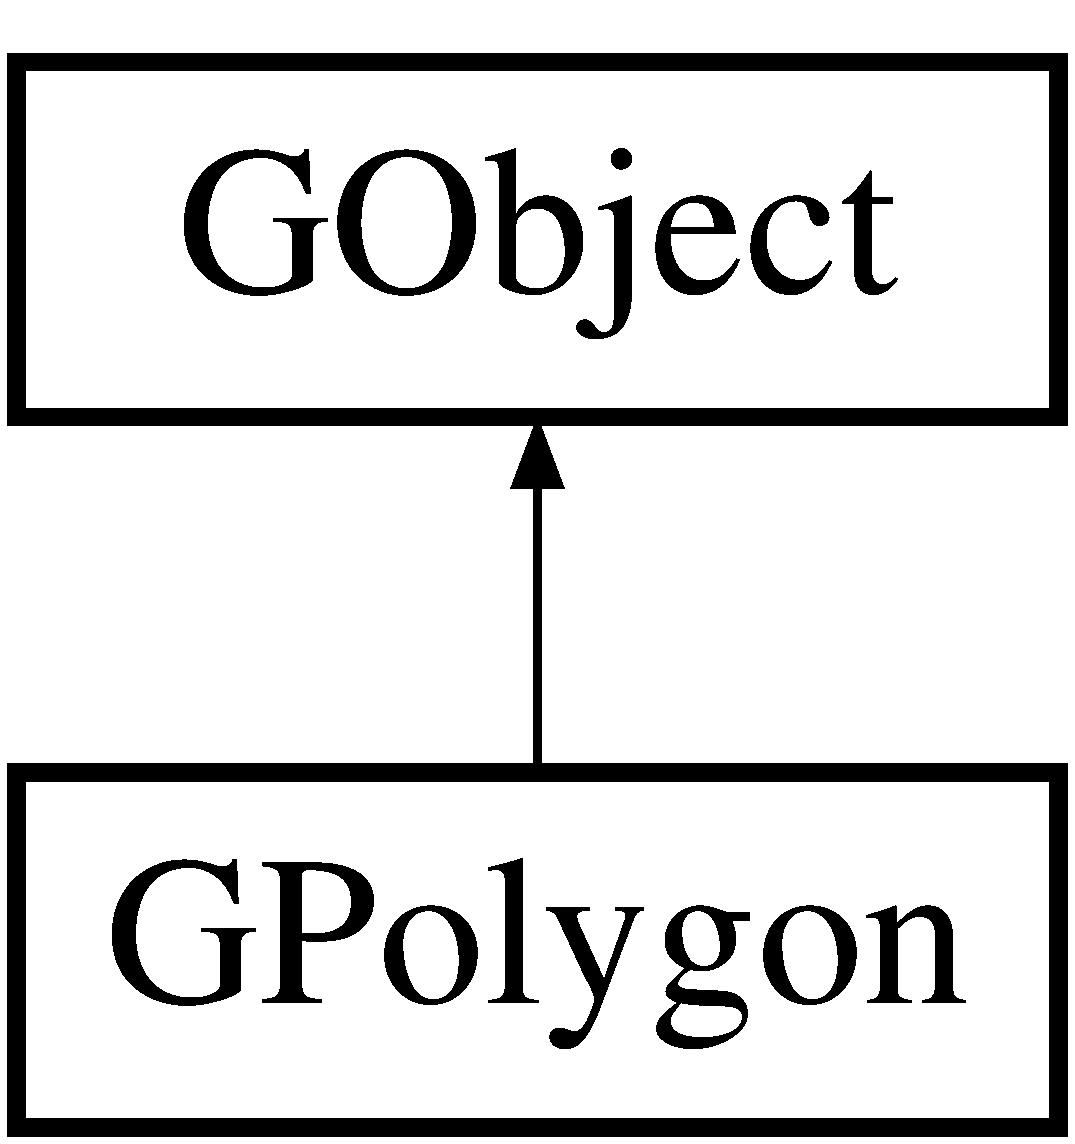
\includegraphics[height=2.000000cm]{classGPolygon}
\end{center}
\end{figure}
\subsection*{Public Types}
\begin{DoxyCompactItemize}
\item 
enum \mbox{\hyperlink{classGObject_a86e0f5648542856159bb40775c854aa7}{Line\+Style}} \{ \mbox{\hyperlink{classGObject_a86e0f5648542856159bb40775c854aa7acbc84bd5232621834ed31f44d457c1eb}{L\+I\+N\+E\+\_\+\+N\+O\+NE}}, 
\mbox{\hyperlink{classGObject_a86e0f5648542856159bb40775c854aa7a700c78bc2cd76acaab26651bf7b4941f}{L\+I\+N\+E\+\_\+\+S\+O\+L\+ID}}, 
\mbox{\hyperlink{classGObject_a86e0f5648542856159bb40775c854aa7a9ccba0845f785d81d07b333ae1aad84e}{L\+I\+N\+E\+\_\+\+D\+A\+SH}}, 
\mbox{\hyperlink{classGObject_a86e0f5648542856159bb40775c854aa7a8e811c096cb941997f0bfda168bb6df3}{L\+I\+N\+E\+\_\+\+D\+OT}}, 
\mbox{\hyperlink{classGObject_a86e0f5648542856159bb40775c854aa7ada15a2e3d737b2db7706d8300f91b89d}{L\+I\+N\+E\+\_\+\+D\+A\+S\+H\+\_\+\+D\+OT}}, 
\mbox{\hyperlink{classGObject_a86e0f5648542856159bb40775c854aa7aabf4053a73eafa7ba2b7e6d664c74c1d}{L\+I\+N\+E\+\_\+\+D\+A\+S\+H\+\_\+\+D\+O\+T\+\_\+\+D\+OT}}
 \}
\begin{DoxyCompactList}\small\item\em Styles that can be used for the outline around various shapes. \end{DoxyCompactList}\end{DoxyCompactItemize}
\subsection*{Public Member Functions}
\begin{DoxyCompactItemize}
\item 
\mbox{\hyperlink{classGPolygon_af59051a8c60e4e792d0346f314c86708}{G\+Polygon}} ()
\begin{DoxyCompactList}\small\item\em Constructs a new empty polygon at the origin. \end{DoxyCompactList}\item 
\mbox{\hyperlink{classGPolygon_a5d3a122dc676d819efe5b9a7e8639ac3}{G\+Polygon}} (std\+::initializer\+\_\+list$<$ double $>$ coords)
\begin{DoxyCompactList}\small\item\em Constructs a new polygon with the given vertex coordinates. \end{DoxyCompactList}\item 
\mbox{\hyperlink{classGPolygon_aabd935bfb600db209293a7935fe44a00}{G\+Polygon}} (std\+::initializer\+\_\+list$<$ \mbox{\hyperlink{structGPoint}{G\+Point}} $>$ points)
\item 
virtual void \mbox{\hyperlink{classGPolygon_ad1976196edec36ab4a1aa09e28c1149c}{add\+Edge}} (double dx, double dy)
\begin{DoxyCompactList}\small\item\em Adds an edge to the polygon whose components are given by the displacements {\ttfamily dx} and {\ttfamily dy} from the last vertex. \end{DoxyCompactList}\item 
virtual void \mbox{\hyperlink{classGPolygon_a484691d516777eabf078a5b0a2e73faa}{add\+Edge}} (const \mbox{\hyperlink{structGPoint}{G\+Point}} \&pt)
\begin{DoxyCompactList}\small\item\em Adds an edge to the polygon where the displacements from the last vertex are specified as the x/y values of the given point. \end{DoxyCompactList}\item 
virtual void \mbox{\hyperlink{classGPolygon_a02e81c7ee5b7864709d40b2cf43d2ae3}{add\+Edges}} (std\+::initializer\+\_\+list$<$ double $>$ coords)
\begin{DoxyCompactList}\small\item\em Adds multiple edges to the polygon whose components are given by the displacements {\ttfamily dx} and {\ttfamily dy} from the last vertex. \end{DoxyCompactList}\item 
virtual void \mbox{\hyperlink{classGPolygon_aef1a706356916af8ef125993b0395e72}{add\+Edges}} (std\+::initializer\+\_\+list$<$ \mbox{\hyperlink{structGPoint}{G\+Point}} $>$ points)
\begin{DoxyCompactList}\small\item\em Adds multiple edges to the polygon whose components are given by the displacements {\ttfamily dx} and {\ttfamily dy} from the last vertex. \end{DoxyCompactList}\item 
virtual void \mbox{\hyperlink{classGPolygon_ab3d75a01a31889ba7bc15314593c7f3b}{add\+Polar\+Edge}} (double r, double theta)
\begin{DoxyCompactList}\small\item\em Adds an edge to the polygon specified in polar coordinates. \end{DoxyCompactList}\item 
virtual void \mbox{\hyperlink{classGPolygon_a116ef33716189339f5557876a8e7a70b}{add\+Vertex}} (double x, double y)
\begin{DoxyCompactList}\small\item\em Adds a vertex at ({\ttfamily x}, {\ttfamily y}) relative to the polygon origin. \end{DoxyCompactList}\item 
virtual void \mbox{\hyperlink{classGPolygon_a09b5faeb0d71697e4f0626dc64118a80}{add\+Vertex}} (const \mbox{\hyperlink{structGPoint}{G\+Point}} \&pt)
\begin{DoxyCompactList}\small\item\em Adds a vertex at the given ({\ttfamily x}, {\ttfamily y}) point relative to the polygon origin. \end{DoxyCompactList}\item 
virtual void \mbox{\hyperlink{classGPolygon_ad8c19525d48fee68c32404d733112f8e}{add\+Vertexes}} (std\+::initializer\+\_\+list$<$ double $>$ coords)
\begin{DoxyCompactList}\small\item\em Adds multiple edges to the polygon whose components are given by the coordinates {\ttfamily dx} and {\ttfamily dy} relative to the polygon origin. \end{DoxyCompactList}\item 
virtual void \mbox{\hyperlink{classGPolygon_a324789ff4b008cc4787140c486561eee}{add\+Vertexes}} (std\+::initializer\+\_\+list$<$ \mbox{\hyperlink{structGPoint}{G\+Point}} $>$ points)
\begin{DoxyCompactList}\small\item\em Adds multiple edges to the polygon whose components are given by the coordinates {\ttfamily dx} and {\ttfamily dy} relative to the polygon origin. \end{DoxyCompactList}\item 
virtual void \mbox{\hyperlink{classGPolygon_ac8bb3912a3ce86b15842e79d0b421204}{clear}} ()
\begin{DoxyCompactList}\small\item\em Removes all vertexes from the polygon. \end{DoxyCompactList}\item 
virtual bool \mbox{\hyperlink{classGObject_a1dbc9dafaae51958112dbe1267a1f547}{contains}} (const \mbox{\hyperlink{structGPoint}{G\+Point}} \&pt) const
\begin{DoxyCompactList}\small\item\em Returns {\ttfamily true} if the specified point is inside the object. \end{DoxyCompactList}\item 
bool \mbox{\hyperlink{classGPolygon_ad973a1d55799d3a73bf8b04986cd804e}{contains}} (double x, double y) const override
\begin{DoxyCompactList}\small\item\em Returns {\ttfamily true} if the specified point is inside the object. \end{DoxyCompactList}\item 
virtual \mbox{\hyperlink{structGPoint}{G\+Point}} \mbox{\hyperlink{classGObject_a0d41183bf6b08de66fe3907551aab0d7}{get\+Bottom\+Right\+Location}} () const
\begin{DoxyCompactList}\small\item\em Returns the x/y coordinates of the bottom/right corner of the object. \end{DoxyCompactList}\item 
virtual double \mbox{\hyperlink{classGObject_a4316a2406c18e1c6d061fe51fd355490}{get\+BottomY}} () const
\begin{DoxyCompactList}\small\item\em Returns the {\itshape y}-\/coordinate of the bottom of the object. \end{DoxyCompactList}\item 
\mbox{\hyperlink{structGRectangle}{G\+Rectangle}} \mbox{\hyperlink{classGPolygon_a89040ce9277825772d359fccd33bca86}{get\+Bounds}} () const override
\begin{DoxyCompactList}\small\item\em Returns the bounding box of this object, which is defined to be the smallest rectangle that covers everything drawn by the figure. \end{DoxyCompactList}\item 
virtual \mbox{\hyperlink{structGPoint}{G\+Point}} \mbox{\hyperlink{classGObject_a0909472e91448470bccdb62ecfb95d8b}{get\+Center\+Location}} () const
\begin{DoxyCompactList}\small\item\em Returns the x/y-\/coordinates of the center of the object. \end{DoxyCompactList}\item 
virtual double \mbox{\hyperlink{classGObject_a04df74355b545e0543112d5b8d924176}{get\+CenterX}} () const
\begin{DoxyCompactList}\small\item\em Returns the {\itshape x}-\/coordinate of the center of the object. \end{DoxyCompactList}\item 
virtual double \mbox{\hyperlink{classGObject_acb3287a3d507025a26f54b895713b947}{get\+CenterY}} () const
\begin{DoxyCompactList}\small\item\em Returns the {\itshape y}-\/coordinate of the center of the object. \end{DoxyCompactList}\item 
virtual std\+::string \mbox{\hyperlink{classGObject_aa061dfa488c31e18549d64363c1d0e34}{get\+Color}} () const
\begin{DoxyCompactList}\small\item\em Returns the color used to display this object. \end{DoxyCompactList}\item 
virtual std\+::string \mbox{\hyperlink{classGObject_a76f6964a11fde7c78e9751be184e1a3c}{get\+Fill\+Color}} () const
\begin{DoxyCompactList}\small\item\em Returns the color used to display the filled region of this object. \end{DoxyCompactList}\item 
double \mbox{\hyperlink{classGPolygon_a2bede8b27b21ae4c7940e762cbad9e07}{get\+Height}} () const override
\begin{DoxyCompactList}\small\item\em Returns the height of this object, which is the same as the height of its bounding box. \end{DoxyCompactList}\item 
virtual \mbox{\hyperlink{classGObject_a86e0f5648542856159bb40775c854aa7}{Line\+Style}} \mbox{\hyperlink{classGObject_aaf1f5ea8281e5e3486662878d26f0a13}{get\+Line\+Style}} () const
\begin{DoxyCompactList}\small\item\em Returns the object\textquotesingle{}s style such as solid or dashed. \end{DoxyCompactList}\item 
virtual double \mbox{\hyperlink{classGObject_a85ff266dc3eb63d9f2d8e5a4487fd3c0}{get\+Line\+Width}} () const
\begin{DoxyCompactList}\small\item\em Returns the width of the line used to draw this object. \end{DoxyCompactList}\item 
virtual \mbox{\hyperlink{structGPoint}{G\+Point}} \mbox{\hyperlink{classGObject_a4f83802015511edeb63b892830812c11}{get\+Location}} () const
\begin{DoxyCompactList}\small\item\em Returns the location of the top-\/left corner of object. \end{DoxyCompactList}\item 
virtual double \mbox{\hyperlink{classGObject_a1ae3fc278cc5b71b9f2d96a8a83cdf26}{get\+Opacity}} () const
\begin{DoxyCompactList}\small\item\em Returns how opaque (non-\/transparent) this object will appear from 0.\+0 (completely transparent) to 1.\+0 (completely opaque, default). \end{DoxyCompactList}\item 
virtual \mbox{\hyperlink{classGCompound}{G\+Compound}} $\ast$ \mbox{\hyperlink{classGObject_a3e53cef70541b1a14eade4ad0984d0b4}{get\+Parent}} () const
\begin{DoxyCompactList}\small\item\em Returns a pointer to the {\ttfamily \mbox{\hyperlink{classGCompound}{G\+Compound}}} that contains this object. \end{DoxyCompactList}\item 
virtual double \mbox{\hyperlink{classGObject_a798cc79daaa10145b28f60bcdfdb0ee9}{get\+RightX}} () const
\begin{DoxyCompactList}\small\item\em Returns the {\itshape x}-\/coordinate of the right side of the object. \end{DoxyCompactList}\item 
virtual \mbox{\hyperlink{structGDimension}{G\+Dimension}} \mbox{\hyperlink{classGObject_a7b4eec96a2bdc6420695d5796a78eea9}{get\+Size}} () const
\begin{DoxyCompactList}\small\item\em Returns the size of the object as a {\ttfamily \mbox{\hyperlink{structGDimension}{G\+Dimension}}}. \end{DoxyCompactList}\item 
std\+::string \mbox{\hyperlink{classGPolygon_a9b72ede4ee8520f987a0c01e30654814}{get\+Type}} () const override
\begin{DoxyCompactList}\small\item\em Returns the type of the object as a string, such as {\ttfamily \char`\"{}\+G\+Oval\char`\"{}} or {\ttfamily \char`\"{}\+G\+Rect\char`\"{}}. \end{DoxyCompactList}\item 
virtual \mbox{\hyperlink{structGPoint}{G\+Point}} \mbox{\hyperlink{classGPolygon_a428a6fd2c63448f2126d3324fc3bcffd}{get\+Vertex}} (int i) const
\begin{DoxyCompactList}\small\item\em Returns the vertex at the given 0-\/based index in this polygon. \end{DoxyCompactList}\item 
virtual int \mbox{\hyperlink{classGPolygon_af5422019d8237e5a98147f4301e8ccab}{get\+Vertex\+Count}} () const
\begin{DoxyCompactList}\small\item\em Returns the number of vertexes in this polygon. \end{DoxyCompactList}\item 
virtual std\+::vector$<$ \mbox{\hyperlink{structGPoint}{G\+Point}} $>$ \mbox{\hyperlink{classGPolygon_a5f48f76a1bb42354281df76ef4e39729}{get\+Vertices}} () const
\begin{DoxyCompactList}\small\item\em Returns a vector of the points in the polygon. \end{DoxyCompactList}\item 
double \mbox{\hyperlink{classGPolygon_ab7b172cec7ed45e1246a3ce3160a62f7}{get\+Width}} () const override
\begin{DoxyCompactList}\small\item\em Returns the width of this object, which is equal to the width of the bounding box. \end{DoxyCompactList}\item 
virtual double \mbox{\hyperlink{classGObject_a344385751bee0720059403940d57a13e}{getX}} () const
\begin{DoxyCompactList}\small\item\em Returns the leftmost {\itshape x}-\/coordinate of the object. \end{DoxyCompactList}\item 
virtual double \mbox{\hyperlink{classGObject_aafa51c7f8f38a09febbb9ce7853f77b4}{getY}} () const
\begin{DoxyCompactList}\small\item\em Returns the topmost {\itshape y}-\/coordinate of the object. \end{DoxyCompactList}\item 
virtual bool \mbox{\hyperlink{classGObject_a11c404f106940c201b6f326e0355c150}{is\+Filled}} () const
\begin{DoxyCompactList}\small\item\em Returns {\ttfamily true} if the object is filled with color. \end{DoxyCompactList}\item 
virtual bool \mbox{\hyperlink{classGObject_a9de207581cfa4ca1eaa06da5f29b75fc}{is\+Transformed}} () const
\begin{DoxyCompactList}\small\item\em Returns {\ttfamily true} if this object has been transformed by calling methods such as \mbox{\hyperlink{classGObject_ae1ffaa12185dfd5ba464f7d87c329e26}{rotate()}} or \mbox{\hyperlink{classGObject_ad2e1900f730475c2d044817db03b38d6}{scale()}} on it. \end{DoxyCompactList}\item 
virtual bool \mbox{\hyperlink{classGObject_a9d8a6cfb13917785c143e74d40e4e2be}{is\+Visible}} () const
\begin{DoxyCompactList}\small\item\em Returns {\ttfamily true} if this object is visible on screen. \end{DoxyCompactList}\item 
virtual void \mbox{\hyperlink{classGObject_a5973d8dda83afb36e2c56855515be392}{move}} (double dx, double dy)
\begin{DoxyCompactList}\small\item\em Moves the object on the screen using the displacements {\ttfamily dx} and {\ttfamily dy}. \end{DoxyCompactList}\item 
virtual void \mbox{\hyperlink{classGObject_ac827b978aa122f136a14c198687ad80f}{repaint}} ()
\begin{DoxyCompactList}\small\item\em Instructs the object to redraw itself on screen. \end{DoxyCompactList}\item 
virtual void \mbox{\hyperlink{classGObject_a6022a1fd1e5dcd2fd5585e5a36aa3f37}{reset\+Transform}} ()
\begin{DoxyCompactList}\small\item\em Undoes any previous scale/rotate transformations on this object. \end{DoxyCompactList}\item 
virtual void \mbox{\hyperlink{classGObject_ae1ffaa12185dfd5ba464f7d87c329e26}{rotate}} (double theta)
\begin{DoxyCompactList}\small\item\em Transforms the object by rotating it {\ttfamily theta} degrees counterclockwise around its origin. \end{DoxyCompactList}\item 
virtual void \mbox{\hyperlink{classGObject_ad2e1900f730475c2d044817db03b38d6}{scale}} (double sf)
\begin{DoxyCompactList}\small\item\em Scales the object by the specified scale factor. \end{DoxyCompactList}\item 
virtual void \mbox{\hyperlink{classGObject_a63641f69d610d0b951357d35a0c3b1e3}{scale}} (double sx, double sy)
\begin{DoxyCompactList}\small\item\em Scales the object by the specified scale factors. \end{DoxyCompactList}\item 
void \mbox{\hyperlink{classGObject_ab6747f40313c531c2db32edb5b63b9b7}{send\+Backward}} ()
\begin{DoxyCompactList}\small\item\em Moves this object one step toward the back in the {\itshape z} dimension. \end{DoxyCompactList}\item 
void \mbox{\hyperlink{classGObject_a710b3e449c9facba7847c91ab170d281}{send\+Forward}} ()
\begin{DoxyCompactList}\small\item\em Moves this object one step toward the front in the {\itshape z} dimension. \end{DoxyCompactList}\item 
void \mbox{\hyperlink{classGObject_a0f7f1efbb7fd46dde2867c4ad0330896}{send\+To\+Back}} ()
\begin{DoxyCompactList}\small\item\em Moves this object to the back of the display in the {\itshape z} dimension. \end{DoxyCompactList}\item 
void \mbox{\hyperlink{classGObject_aee33d68488e46827ef55fac07f40a9b2}{send\+To\+Front}} ()
\begin{DoxyCompactList}\small\item\em Moves this object to the front of the display in the {\itshape z} dimension. \end{DoxyCompactList}\item 
virtual void \mbox{\hyperlink{classGObject_a71ff7b16b8f1bdc4a1ce9f30cf8b87d8}{set\+Bottom\+Right\+Location}} (double x, double y)
\begin{DoxyCompactList}\small\item\em Sets the location of the bottom/right of this object. \end{DoxyCompactList}\item 
virtual void \mbox{\hyperlink{classGObject_ac6f7320321182f1d18c1c0fa97d5e941}{set\+Bottom\+Right\+Location}} (const \mbox{\hyperlink{structGPoint}{G\+Point}} \&pt)
\begin{DoxyCompactList}\small\item\em Sets the location of the bottom/right of this object. \end{DoxyCompactList}\item 
virtual void \mbox{\hyperlink{classGObject_a4b20e93c2a2597484f74ee5caa71f41f}{set\+BottomY}} (double y)
\begin{DoxyCompactList}\small\item\em Sets the location of the bottom y-\/coordinate of this object. \end{DoxyCompactList}\item 
virtual void \mbox{\hyperlink{classGObject_a2aae8197624b72265ab83b4f1bc73f2f}{set\+Bounds}} (double x, double y, double width, double height)
\begin{DoxyCompactList}\small\item\em Changes the bounds of this object to the specified values. \end{DoxyCompactList}\item 
virtual void \mbox{\hyperlink{classGObject_acada386653f008cacc7cce86426bef7c}{set\+Bounds}} (const \mbox{\hyperlink{structGRectangle}{G\+Rectangle}} \&size)
\begin{DoxyCompactList}\small\item\em Changes the bounds of this object to the specified rectangle. \end{DoxyCompactList}\item 
virtual void \mbox{\hyperlink{classGObject_a290b47dd8de1be44089f95cb2c47c1de}{set\+Center\+Location}} (double x, double y)
\begin{DoxyCompactList}\small\item\em Sets the location of the center of this object. \end{DoxyCompactList}\item 
virtual void \mbox{\hyperlink{classGObject_a1bedf1b233ecba3f753ec58908a683a6}{set\+Center\+Location}} (const \mbox{\hyperlink{structGPoint}{G\+Point}} \&pt)
\begin{DoxyCompactList}\small\item\em Sets the location of the center of this object. \end{DoxyCompactList}\item 
virtual void \mbox{\hyperlink{classGObject_a2f4936281e056eead00a9186b9ba8af6}{set\+CenterX}} (double x)
\begin{DoxyCompactList}\small\item\em Sets the x-\/coordinate of the center of this object. \end{DoxyCompactList}\item 
virtual void \mbox{\hyperlink{classGObject_aad2a22b4fde88c33306b92aebf641d57}{set\+CenterY}} (double y)
\begin{DoxyCompactList}\small\item\em Sets the y-\/coordinate of the center of this object. \end{DoxyCompactList}\item 
virtual void \mbox{\hyperlink{classGObject_ad57ef49bc31db94e92648aa3737923d6}{set\+Color}} (int r, int g, int b)
\begin{DoxyCompactList}\small\item\em Sets the color used to display this object. \end{DoxyCompactList}\item 
virtual void \mbox{\hyperlink{classGObject_ab1f5cc0f5cc6bbbd716a526c61f1081d}{set\+Color}} (int rgb)
\begin{DoxyCompactList}\small\item\em Sets the color used to display this object. \end{DoxyCompactList}\item 
virtual void \mbox{\hyperlink{classGObject_a61374df6c11b52cfbb0815decdbaebc6}{set\+Color}} (const std\+::string \&color)
\begin{DoxyCompactList}\small\item\em Sets the color used to display this object. \end{DoxyCompactList}\item 
virtual void \mbox{\hyperlink{classGObject_ad767a33971159e9493e221cca4c00ae9}{set\+Fill\+Color}} (int r, int g, int b)
\begin{DoxyCompactList}\small\item\em Sets the color used to display the filled region of this object, if any. \end{DoxyCompactList}\item 
virtual void \mbox{\hyperlink{classGObject_aa59d9775a67fa7df2b24a95cd34840a3}{set\+Fill\+Color}} (int rgb)
\begin{DoxyCompactList}\small\item\em Sets the color used to display the filled region of this object, if any. \end{DoxyCompactList}\item 
virtual void \mbox{\hyperlink{classGObject_adbc18b1a930aadd97d7437f9f7265b96}{set\+Fill\+Color}} (const std\+::string \&color)
\begin{DoxyCompactList}\small\item\em Sets the color used to display the filled region of this object, if any. \end{DoxyCompactList}\item 
virtual void \mbox{\hyperlink{classGObject_a9b82b53362282c6bb7d6947068d2e55b}{set\+Filled}} (bool flag)
\begin{DoxyCompactList}\small\item\em Sets the fill status for the object, where {\ttfamily false} is outlined and {\ttfamily true} is filled. \end{DoxyCompactList}\item 
virtual void \mbox{\hyperlink{classGObject_a2592348886ffea646c6534bf88f7c49d}{set\+Font}} (const Q\+Font \&font)
\begin{DoxyCompactList}\small\item\em Changes the font used to display the object as specified by the given Qt font. \end{DoxyCompactList}\item 
virtual void \mbox{\hyperlink{classGObject_a8e096e8818d838aceae1d46d58fb3a7b}{set\+Font}} (const std\+::string \&font)
\begin{DoxyCompactList}\small\item\em Changes the font used to display the object as specified by the string {\ttfamily font}, which has the following format\+: \end{DoxyCompactList}\item 
virtual void \mbox{\hyperlink{classGObject_ad18e8fab1e02a4e9b75c6730212558eb}{set\+Foreground}} (int r, int g, int b)
\begin{DoxyCompactList}\small\item\em Sets the color used to display this object. \end{DoxyCompactList}\item 
virtual void \mbox{\hyperlink{classGObject_a9eb856b5ff83a19df3831a31f15f4563}{set\+Foreground}} (int rgb)
\begin{DoxyCompactList}\small\item\em Sets the color used to display this object. \end{DoxyCompactList}\item 
virtual void \mbox{\hyperlink{classGObject_af59209aeadea6dfc6d97a2d8531f50e1}{set\+Foreground}} (const std\+::string \&color)
\begin{DoxyCompactList}\small\item\em Sets the color used to display this object. \end{DoxyCompactList}\item 
virtual void \mbox{\hyperlink{classGObject_a9e280bfc4544dfaf8e4376c4e1a74357}{set\+Height}} (double height)
\begin{DoxyCompactList}\small\item\em Changes the height of this object to the specified height without changing its width. \end{DoxyCompactList}\item 
virtual void \mbox{\hyperlink{classGObject_add11575087eb94f1a71faa3f826c6341}{set\+Line\+Style}} (\mbox{\hyperlink{classGObject_a86e0f5648542856159bb40775c854aa7}{Line\+Style}} line\+Style)
\begin{DoxyCompactList}\small\item\em Sets the object\textquotesingle{}s style such as solid (\mbox{\hyperlink{classGObject_a86e0f5648542856159bb40775c854aa7a700c78bc2cd76acaab26651bf7b4941f}{G\+Object\+::\+L\+I\+N\+E\+\_\+\+S\+O\+L\+ID}}) or dashed (\mbox{\hyperlink{classGObject_a86e0f5648542856159bb40775c854aa7a9ccba0845f785d81d07b333ae1aad84e}{G\+Object\+::\+L\+I\+N\+E\+\_\+\+D\+A\+SH}}). \end{DoxyCompactList}\item 
virtual void \mbox{\hyperlink{classGObject_afd6a47c6ea6a1f85ca05a65ba3ff3477}{set\+Line\+Width}} (double line\+Width)
\begin{DoxyCompactList}\small\item\em Sets the width of the line used to draw this object. \end{DoxyCompactList}\item 
virtual void \mbox{\hyperlink{classGObject_a04594e8ba9b98513a64f1da00dcae18c}{set\+Location}} (double x, double y)
\begin{DoxyCompactList}\small\item\em Sets the location of the top-\/left corner of this object to the specified coordinates. \end{DoxyCompactList}\item 
virtual void \mbox{\hyperlink{classGObject_aa8480c0b7166cdf8f784cece06ab353f}{set\+Location}} (const \mbox{\hyperlink{structGPoint}{G\+Point}} \&pt)
\begin{DoxyCompactList}\small\item\em Sets the location of the top-\/left corner of this object to the specified point. \end{DoxyCompactList}\item 
virtual void \mbox{\hyperlink{classGObject_a04af1866cc1bae4a1226695794a50539}{set\+Opacity}} (double opacity)
\begin{DoxyCompactList}\small\item\em Sets how opaque (non-\/transparent) this object will appear from 0.\+0 (completely transparent) to 1.\+0 (completely opaque, default). \end{DoxyCompactList}\item 
virtual void \mbox{\hyperlink{classGObject_a3c90b758cdc2c911c9ef76c4360eb912}{set\+RightX}} (double x)
\begin{DoxyCompactList}\small\item\em Sets the location of the rightmost x-\/coordinate of this object. \end{DoxyCompactList}\item 
virtual void \mbox{\hyperlink{classGObject_aca25d49481f9bf5fc8f7df4c086c4ce7}{set\+Size}} (double width, double height)
\begin{DoxyCompactList}\small\item\em Changes the size of this object to the specified width and height. \end{DoxyCompactList}\item 
virtual void \mbox{\hyperlink{classGObject_ae2b628228f192c2702c4ce941b2af68f}{set\+Size}} (const \mbox{\hyperlink{structGDimension}{G\+Dimension}} \&size)
\begin{DoxyCompactList}\small\item\em Changes the size of this object to the specified width and height. \end{DoxyCompactList}\item 
virtual void \mbox{\hyperlink{classGPolygon_a616f3944eea0dad17d074d0f505299cc}{set\+Vertex}} (int i, \mbox{\hyperlink{structGPoint}{G\+Point}} point)
\begin{DoxyCompactList}\small\item\em Sets the vertex at the given 0-\/based index in this polygon to the given coordinates. \end{DoxyCompactList}\item 
virtual void \mbox{\hyperlink{classGObject_a88203f28224315d9f4471212f4af8ed3}{set\+Visible}} (bool flag)
\begin{DoxyCompactList}\small\item\em Sets whether this object is visible. \end{DoxyCompactList}\item 
virtual void \mbox{\hyperlink{classGObject_aa3f3fba4cb131baa8696ba01e3bceca1}{set\+Width}} (double width)
\begin{DoxyCompactList}\small\item\em Changes the width of this object to the specified width without changing its height. \end{DoxyCompactList}\item 
virtual void \mbox{\hyperlink{classGObject_a9c18fcc579333bf9653d13ad2b372e39}{setX}} (double x)
\begin{DoxyCompactList}\small\item\em Sets the x location of the left side of this object. \end{DoxyCompactList}\item 
virtual void \mbox{\hyperlink{classGObject_a7d57e2a5c35d27feb58fd498a3cf82b9}{setY}} (double y)
\begin{DoxyCompactList}\small\item\em Sets the y location of the top of this object. \end{DoxyCompactList}\item 
virtual std\+::string \mbox{\hyperlink{classGObject_a1fe5121d6528fdea3f243321b3fa3a49}{to\+String}} () const
\begin{DoxyCompactList}\small\item\em Returns a printable representation of the object. \end{DoxyCompactList}\item 
std\+::string \mbox{\hyperlink{classGPolygon_a04364e674911906702b748deec32db18}{to\+String\+Extra}} () const override
\begin{DoxyCompactList}\small\item\em Returns a string containing any extra unique information about this type of graphical object. \end{DoxyCompactList}\end{DoxyCompactItemize}
\subsection*{Static Public Member Functions}
\begin{DoxyCompactItemize}
\item 
static bool \mbox{\hyperlink{classGObject_a93be0e1fe1b1bf1a1da732470c94f42b}{is\+Anti\+Aliasing}} ()
\begin{DoxyCompactList}\small\item\em Returns whether we should globally anti-\/alias graphical objects. \end{DoxyCompactList}\item 
static void \mbox{\hyperlink{classGObject_a1e43371668ae850193cebedb44e1bbe3}{set\+Anti\+Aliasing}} (bool value)
\begin{DoxyCompactList}\small\item\em Globally turns on/off the anti-\/aliasing feature that smooths out the edges of onscreen shapes. \end{DoxyCompactList}\end{DoxyCompactItemize}
\subsection*{Protected Attributes}
\begin{DoxyCompactItemize}
\item 
Q\+Brush \mbox{\hyperlink{classGObject_aab24462ec896b596d99911767b0912d0}{\+\_\+brush}}
\item 
std\+::string \mbox{\hyperlink{classGObject_a1134e770ae4315ea8bc1201e2f21da8b}{\+\_\+color}}
\item 
int \mbox{\hyperlink{classGObject_a003fdd343d9b7505c53a8b7a134200ed}{\+\_\+color\+Int}}
\item 
std\+::string \mbox{\hyperlink{classGObject_a179f8d6cee65cd8a54692e32b224392a}{\+\_\+fill\+Color}}
\item 
int \mbox{\hyperlink{classGObject_a751def333a67d651e5b99cc331ecb496}{\+\_\+fill\+Color\+Int}}
\item 
bool \mbox{\hyperlink{classGObject_ad4a55cbcd61b58a4d49666490bb2f103}{\+\_\+fill\+Flag}}
\item 
std\+::string \mbox{\hyperlink{classGObject_aea76ea1a8b5dd7b0a78653277e63b536}{\+\_\+font}}
\item 
double \mbox{\hyperlink{classGObject_ad05df29e7f27fc504abd743e3d8b4e73}{\+\_\+height}}
\item 
\mbox{\hyperlink{classGObject_a86e0f5648542856159bb40775c854aa7}{Line\+Style}} \mbox{\hyperlink{classGObject_a89bafecaafb7c72d55c7efc10b7d0523}{\+\_\+line\+Style}}
\item 
double \mbox{\hyperlink{classGObject_a16e9033665937f13de2e163dc2184aff}{\+\_\+line\+Width}}
\item 
double \mbox{\hyperlink{classGObject_a20eff8eb7af27182edc9bfc54768b6f3}{\+\_\+opacity}}
\item 
\mbox{\hyperlink{classGCompound}{G\+Compound}} $\ast$ \mbox{\hyperlink{classGObject_ac9452c1eaff70eebddbb318196aa3835}{\+\_\+parent}}
\item 
Q\+Pen \mbox{\hyperlink{classGObject_afb69d172743f868299847174eb1b6bc8}{\+\_\+pen}}
\item 
Q\+Transform \mbox{\hyperlink{classGObject_a475b8860a5f1adb4a1fdc58d1f5c1e32}{\+\_\+transform}}
\item 
bool \mbox{\hyperlink{classGObject_ae4725802fc8d8aaa0ab4bd4781f7e07c}{\+\_\+transformed}}
\item 
bool \mbox{\hyperlink{classGObject_a9312c72508471b7c7a87b540263e1af4}{\+\_\+visible}}
\item 
double \mbox{\hyperlink{classGObject_ab55d85a3371770e6725b1062cf160cd8}{\+\_\+width}}
\item 
double \mbox{\hyperlink{classGObject_a6675b83b27137b8d3aa2ad8133078ea6}{\+\_\+x}}
\item 
double \mbox{\hyperlink{classGObject_a2f0f6aeafddc8a39c578bfa7e22b5f1e}{\+\_\+y}}
\end{DoxyCompactItemize}


\subsection{Detailed Description}
This graphical object subclass represents a polygon bounded by line segments. 

The {\ttfamily \mbox{\hyperlink{classGPolygon}{G\+Polygon}}} constructor creates an empty polygon. To complete the figure, you need to add vertices to the polygon using the methods {\ttfamily add\+Vertex}, {\ttfamily add\+Edge}, and {\ttfamily add\+Polar\+Edge}. 

\subsection{Member Enumeration Documentation}
\mbox{\Hypertarget{classGObject_a86e0f5648542856159bb40775c854aa7}\label{classGObject_a86e0f5648542856159bb40775c854aa7}} 
\index{G\+Polygon@{G\+Polygon}!Line\+Style@{Line\+Style}}
\index{Line\+Style@{Line\+Style}!G\+Polygon@{G\+Polygon}}
\subsubsection{\texorpdfstring{Line\+Style}{LineStyle}}
{\footnotesize\ttfamily enum \mbox{\hyperlink{classGObject_a86e0f5648542856159bb40775c854aa7}{Line\+Style}}\hspace{0.3cm}{\ttfamily [inherited]}}



Styles that can be used for the outline around various shapes. 

Call set\+Line\+Style on a \mbox{\hyperlink{classGObject}{G\+Object}} and pass one of these values. \begin{DoxyEnumFields}{Enumerator}
\raisebox{\heightof{T}}[0pt][0pt]{\index{L\+I\+N\+E\+\_\+\+N\+O\+NE@{L\+I\+N\+E\+\_\+\+N\+O\+NE}!G\+Polygon@{G\+Polygon}}\index{G\+Polygon@{G\+Polygon}!L\+I\+N\+E\+\_\+\+N\+O\+NE@{L\+I\+N\+E\+\_\+\+N\+O\+NE}}}\mbox{\Hypertarget{classGObject_a86e0f5648542856159bb40775c854aa7acbc84bd5232621834ed31f44d457c1eb}\label{classGObject_a86e0f5648542856159bb40775c854aa7acbc84bd5232621834ed31f44d457c1eb}} 
L\+I\+N\+E\+\_\+\+N\+O\+NE&\\
\hline

\raisebox{\heightof{T}}[0pt][0pt]{\index{L\+I\+N\+E\+\_\+\+S\+O\+L\+ID@{L\+I\+N\+E\+\_\+\+S\+O\+L\+ID}!G\+Polygon@{G\+Polygon}}\index{G\+Polygon@{G\+Polygon}!L\+I\+N\+E\+\_\+\+S\+O\+L\+ID@{L\+I\+N\+E\+\_\+\+S\+O\+L\+ID}}}\mbox{\Hypertarget{classGObject_a86e0f5648542856159bb40775c854aa7a700c78bc2cd76acaab26651bf7b4941f}\label{classGObject_a86e0f5648542856159bb40775c854aa7a700c78bc2cd76acaab26651bf7b4941f}} 
L\+I\+N\+E\+\_\+\+S\+O\+L\+ID&\\
\hline

\raisebox{\heightof{T}}[0pt][0pt]{\index{L\+I\+N\+E\+\_\+\+D\+A\+SH@{L\+I\+N\+E\+\_\+\+D\+A\+SH}!G\+Polygon@{G\+Polygon}}\index{G\+Polygon@{G\+Polygon}!L\+I\+N\+E\+\_\+\+D\+A\+SH@{L\+I\+N\+E\+\_\+\+D\+A\+SH}}}\mbox{\Hypertarget{classGObject_a86e0f5648542856159bb40775c854aa7a9ccba0845f785d81d07b333ae1aad84e}\label{classGObject_a86e0f5648542856159bb40775c854aa7a9ccba0845f785d81d07b333ae1aad84e}} 
L\+I\+N\+E\+\_\+\+D\+A\+SH&\\
\hline

\raisebox{\heightof{T}}[0pt][0pt]{\index{L\+I\+N\+E\+\_\+\+D\+OT@{L\+I\+N\+E\+\_\+\+D\+OT}!G\+Polygon@{G\+Polygon}}\index{G\+Polygon@{G\+Polygon}!L\+I\+N\+E\+\_\+\+D\+OT@{L\+I\+N\+E\+\_\+\+D\+OT}}}\mbox{\Hypertarget{classGObject_a86e0f5648542856159bb40775c854aa7a8e811c096cb941997f0bfda168bb6df3}\label{classGObject_a86e0f5648542856159bb40775c854aa7a8e811c096cb941997f0bfda168bb6df3}} 
L\+I\+N\+E\+\_\+\+D\+OT&\\
\hline

\raisebox{\heightof{T}}[0pt][0pt]{\index{L\+I\+N\+E\+\_\+\+D\+A\+S\+H\+\_\+\+D\+OT@{L\+I\+N\+E\+\_\+\+D\+A\+S\+H\+\_\+\+D\+OT}!G\+Polygon@{G\+Polygon}}\index{G\+Polygon@{G\+Polygon}!L\+I\+N\+E\+\_\+\+D\+A\+S\+H\+\_\+\+D\+OT@{L\+I\+N\+E\+\_\+\+D\+A\+S\+H\+\_\+\+D\+OT}}}\mbox{\Hypertarget{classGObject_a86e0f5648542856159bb40775c854aa7ada15a2e3d737b2db7706d8300f91b89d}\label{classGObject_a86e0f5648542856159bb40775c854aa7ada15a2e3d737b2db7706d8300f91b89d}} 
L\+I\+N\+E\+\_\+\+D\+A\+S\+H\+\_\+\+D\+OT&\\
\hline

\raisebox{\heightof{T}}[0pt][0pt]{\index{L\+I\+N\+E\+\_\+\+D\+A\+S\+H\+\_\+\+D\+O\+T\+\_\+\+D\+OT@{L\+I\+N\+E\+\_\+\+D\+A\+S\+H\+\_\+\+D\+O\+T\+\_\+\+D\+OT}!G\+Polygon@{G\+Polygon}}\index{G\+Polygon@{G\+Polygon}!L\+I\+N\+E\+\_\+\+D\+A\+S\+H\+\_\+\+D\+O\+T\+\_\+\+D\+OT@{L\+I\+N\+E\+\_\+\+D\+A\+S\+H\+\_\+\+D\+O\+T\+\_\+\+D\+OT}}}\mbox{\Hypertarget{classGObject_a86e0f5648542856159bb40775c854aa7aabf4053a73eafa7ba2b7e6d664c74c1d}\label{classGObject_a86e0f5648542856159bb40775c854aa7aabf4053a73eafa7ba2b7e6d664c74c1d}} 
L\+I\+N\+E\+\_\+\+D\+A\+S\+H\+\_\+\+D\+O\+T\+\_\+\+D\+OT&\\
\hline

\end{DoxyEnumFields}


\subsection{Constructor \& Destructor Documentation}
\mbox{\Hypertarget{classGPolygon_af59051a8c60e4e792d0346f314c86708}\label{classGPolygon_af59051a8c60e4e792d0346f314c86708}} 
\index{G\+Polygon@{G\+Polygon}!G\+Polygon@{G\+Polygon}}
\index{G\+Polygon@{G\+Polygon}!G\+Polygon@{G\+Polygon}}
\subsubsection{\texorpdfstring{G\+Polygon()}{GPolygon()}\hspace{0.1cm}{\footnotesize\ttfamily [1/3]}}
{\footnotesize\ttfamily \mbox{\hyperlink{classGPolygon}{G\+Polygon}} (\begin{DoxyParamCaption}{ }\end{DoxyParamCaption})}



Constructs a new empty polygon at the origin. 

\mbox{\Hypertarget{classGPolygon_a5d3a122dc676d819efe5b9a7e8639ac3}\label{classGPolygon_a5d3a122dc676d819efe5b9a7e8639ac3}} 
\index{G\+Polygon@{G\+Polygon}!G\+Polygon@{G\+Polygon}}
\index{G\+Polygon@{G\+Polygon}!G\+Polygon@{G\+Polygon}}
\subsubsection{\texorpdfstring{G\+Polygon()}{GPolygon()}\hspace{0.1cm}{\footnotesize\ttfamily [2/3]}}
{\footnotesize\ttfamily \mbox{\hyperlink{classGPolygon}{G\+Polygon}} (\begin{DoxyParamCaption}\item[{std\+::initializer\+\_\+list$<$ double $>$}]{coords }\end{DoxyParamCaption})}



Constructs a new polygon with the given vertex coordinates. 

\mbox{\Hypertarget{classGPolygon_aabd935bfb600db209293a7935fe44a00}\label{classGPolygon_aabd935bfb600db209293a7935fe44a00}} 
\index{G\+Polygon@{G\+Polygon}!G\+Polygon@{G\+Polygon}}
\index{G\+Polygon@{G\+Polygon}!G\+Polygon@{G\+Polygon}}
\subsubsection{\texorpdfstring{G\+Polygon()}{GPolygon()}\hspace{0.1cm}{\footnotesize\ttfamily [3/3]}}
{\footnotesize\ttfamily \mbox{\hyperlink{classGPolygon}{G\+Polygon}} (\begin{DoxyParamCaption}\item[{std\+::initializer\+\_\+list$<$ \mbox{\hyperlink{structGPoint}{G\+Point}} $>$}]{points }\end{DoxyParamCaption})}



\subsection{Member Function Documentation}
\mbox{\Hypertarget{classGPolygon_ad1976196edec36ab4a1aa09e28c1149c}\label{classGPolygon_ad1976196edec36ab4a1aa09e28c1149c}} 
\index{G\+Polygon@{G\+Polygon}!add\+Edge@{add\+Edge}}
\index{add\+Edge@{add\+Edge}!G\+Polygon@{G\+Polygon}}
\subsubsection{\texorpdfstring{add\+Edge()}{addEdge()}\hspace{0.1cm}{\footnotesize\ttfamily [1/2]}}
{\footnotesize\ttfamily void add\+Edge (\begin{DoxyParamCaption}\item[{double}]{dx,  }\item[{double}]{dy }\end{DoxyParamCaption})\hspace{0.3cm}{\ttfamily [virtual]}}



Adds an edge to the polygon whose components are given by the displacements {\ttfamily dx} and {\ttfamily dy} from the last vertex. 

\mbox{\Hypertarget{classGPolygon_a484691d516777eabf078a5b0a2e73faa}\label{classGPolygon_a484691d516777eabf078a5b0a2e73faa}} 
\index{G\+Polygon@{G\+Polygon}!add\+Edge@{add\+Edge}}
\index{add\+Edge@{add\+Edge}!G\+Polygon@{G\+Polygon}}
\subsubsection{\texorpdfstring{add\+Edge()}{addEdge()}\hspace{0.1cm}{\footnotesize\ttfamily [2/2]}}
{\footnotesize\ttfamily void add\+Edge (\begin{DoxyParamCaption}\item[{const \mbox{\hyperlink{structGPoint}{G\+Point}} \&}]{pt }\end{DoxyParamCaption})\hspace{0.3cm}{\ttfamily [virtual]}}



Adds an edge to the polygon where the displacements from the last vertex are specified as the x/y values of the given point. 

\mbox{\Hypertarget{classGPolygon_a02e81c7ee5b7864709d40b2cf43d2ae3}\label{classGPolygon_a02e81c7ee5b7864709d40b2cf43d2ae3}} 
\index{G\+Polygon@{G\+Polygon}!add\+Edges@{add\+Edges}}
\index{add\+Edges@{add\+Edges}!G\+Polygon@{G\+Polygon}}
\subsubsection{\texorpdfstring{add\+Edges()}{addEdges()}\hspace{0.1cm}{\footnotesize\ttfamily [1/2]}}
{\footnotesize\ttfamily void add\+Edges (\begin{DoxyParamCaption}\item[{std\+::initializer\+\_\+list$<$ double $>$}]{coords }\end{DoxyParamCaption})\hspace{0.3cm}{\ttfamily [virtual]}}



Adds multiple edges to the polygon whose components are given by the displacements {\ttfamily dx} and {\ttfamily dy} from the last vertex. 

\mbox{\Hypertarget{classGPolygon_aef1a706356916af8ef125993b0395e72}\label{classGPolygon_aef1a706356916af8ef125993b0395e72}} 
\index{G\+Polygon@{G\+Polygon}!add\+Edges@{add\+Edges}}
\index{add\+Edges@{add\+Edges}!G\+Polygon@{G\+Polygon}}
\subsubsection{\texorpdfstring{add\+Edges()}{addEdges()}\hspace{0.1cm}{\footnotesize\ttfamily [2/2]}}
{\footnotesize\ttfamily void add\+Edges (\begin{DoxyParamCaption}\item[{std\+::initializer\+\_\+list$<$ \mbox{\hyperlink{structGPoint}{G\+Point}} $>$}]{points }\end{DoxyParamCaption})\hspace{0.3cm}{\ttfamily [virtual]}}



Adds multiple edges to the polygon whose components are given by the displacements {\ttfamily dx} and {\ttfamily dy} from the last vertex. 

\mbox{\Hypertarget{classGPolygon_ab3d75a01a31889ba7bc15314593c7f3b}\label{classGPolygon_ab3d75a01a31889ba7bc15314593c7f3b}} 
\index{G\+Polygon@{G\+Polygon}!add\+Polar\+Edge@{add\+Polar\+Edge}}
\index{add\+Polar\+Edge@{add\+Polar\+Edge}!G\+Polygon@{G\+Polygon}}
\subsubsection{\texorpdfstring{add\+Polar\+Edge()}{addPolarEdge()}}
{\footnotesize\ttfamily void add\+Polar\+Edge (\begin{DoxyParamCaption}\item[{double}]{r,  }\item[{double}]{theta }\end{DoxyParamCaption})\hspace{0.3cm}{\ttfamily [virtual]}}



Adds an edge to the polygon specified in polar coordinates. 

The length of the edge is given by {\ttfamily r}, and the edge extends in direction {\ttfamily theta}, measured in degrees counterclockwise from the +x axis. \mbox{\Hypertarget{classGPolygon_a116ef33716189339f5557876a8e7a70b}\label{classGPolygon_a116ef33716189339f5557876a8e7a70b}} 
\index{G\+Polygon@{G\+Polygon}!add\+Vertex@{add\+Vertex}}
\index{add\+Vertex@{add\+Vertex}!G\+Polygon@{G\+Polygon}}
\subsubsection{\texorpdfstring{add\+Vertex()}{addVertex()}\hspace{0.1cm}{\footnotesize\ttfamily [1/2]}}
{\footnotesize\ttfamily void add\+Vertex (\begin{DoxyParamCaption}\item[{double}]{x,  }\item[{double}]{y }\end{DoxyParamCaption})\hspace{0.3cm}{\ttfamily [virtual]}}



Adds a vertex at ({\ttfamily x}, {\ttfamily y}) relative to the polygon origin. 

\mbox{\Hypertarget{classGPolygon_a09b5faeb0d71697e4f0626dc64118a80}\label{classGPolygon_a09b5faeb0d71697e4f0626dc64118a80}} 
\index{G\+Polygon@{G\+Polygon}!add\+Vertex@{add\+Vertex}}
\index{add\+Vertex@{add\+Vertex}!G\+Polygon@{G\+Polygon}}
\subsubsection{\texorpdfstring{add\+Vertex()}{addVertex()}\hspace{0.1cm}{\footnotesize\ttfamily [2/2]}}
{\footnotesize\ttfamily void add\+Vertex (\begin{DoxyParamCaption}\item[{const \mbox{\hyperlink{structGPoint}{G\+Point}} \&}]{pt }\end{DoxyParamCaption})\hspace{0.3cm}{\ttfamily [virtual]}}



Adds a vertex at the given ({\ttfamily x}, {\ttfamily y}) point relative to the polygon origin. 

\mbox{\Hypertarget{classGPolygon_ad8c19525d48fee68c32404d733112f8e}\label{classGPolygon_ad8c19525d48fee68c32404d733112f8e}} 
\index{G\+Polygon@{G\+Polygon}!add\+Vertexes@{add\+Vertexes}}
\index{add\+Vertexes@{add\+Vertexes}!G\+Polygon@{G\+Polygon}}
\subsubsection{\texorpdfstring{add\+Vertexes()}{addVertexes()}\hspace{0.1cm}{\footnotesize\ttfamily [1/2]}}
{\footnotesize\ttfamily void add\+Vertexes (\begin{DoxyParamCaption}\item[{std\+::initializer\+\_\+list$<$ double $>$}]{coords }\end{DoxyParamCaption})\hspace{0.3cm}{\ttfamily [virtual]}}



Adds multiple edges to the polygon whose components are given by the coordinates {\ttfamily dx} and {\ttfamily dy} relative to the polygon origin. 

\mbox{\Hypertarget{classGPolygon_a324789ff4b008cc4787140c486561eee}\label{classGPolygon_a324789ff4b008cc4787140c486561eee}} 
\index{G\+Polygon@{G\+Polygon}!add\+Vertexes@{add\+Vertexes}}
\index{add\+Vertexes@{add\+Vertexes}!G\+Polygon@{G\+Polygon}}
\subsubsection{\texorpdfstring{add\+Vertexes()}{addVertexes()}\hspace{0.1cm}{\footnotesize\ttfamily [2/2]}}
{\footnotesize\ttfamily void add\+Vertexes (\begin{DoxyParamCaption}\item[{std\+::initializer\+\_\+list$<$ \mbox{\hyperlink{structGPoint}{G\+Point}} $>$}]{points }\end{DoxyParamCaption})\hspace{0.3cm}{\ttfamily [virtual]}}



Adds multiple edges to the polygon whose components are given by the coordinates {\ttfamily dx} and {\ttfamily dy} relative to the polygon origin. 

\mbox{\Hypertarget{classGPolygon_ac8bb3912a3ce86b15842e79d0b421204}\label{classGPolygon_ac8bb3912a3ce86b15842e79d0b421204}} 
\index{G\+Polygon@{G\+Polygon}!clear@{clear}}
\index{clear@{clear}!G\+Polygon@{G\+Polygon}}
\subsubsection{\texorpdfstring{clear()}{clear()}}
{\footnotesize\ttfamily void clear (\begin{DoxyParamCaption}{ }\end{DoxyParamCaption})\hspace{0.3cm}{\ttfamily [virtual]}}



Removes all vertexes from the polygon. 

\mbox{\Hypertarget{classGObject_a1dbc9dafaae51958112dbe1267a1f547}\label{classGObject_a1dbc9dafaae51958112dbe1267a1f547}} 
\index{G\+Polygon@{G\+Polygon}!contains@{contains}}
\index{contains@{contains}!G\+Polygon@{G\+Polygon}}
\subsubsection{\texorpdfstring{contains()}{contains()}\hspace{0.1cm}{\footnotesize\ttfamily [1/2]}}
{\footnotesize\ttfamily bool contains (\begin{DoxyParamCaption}\item[{const \mbox{\hyperlink{structGPoint}{G\+Point}} \&}]{pt }\end{DoxyParamCaption}) const\hspace{0.3cm}{\ttfamily [virtual]}, {\ttfamily [inherited]}}



Returns {\ttfamily true} if the specified point is inside the object. 

\mbox{\Hypertarget{classGPolygon_ad973a1d55799d3a73bf8b04986cd804e}\label{classGPolygon_ad973a1d55799d3a73bf8b04986cd804e}} 
\index{G\+Polygon@{G\+Polygon}!contains@{contains}}
\index{contains@{contains}!G\+Polygon@{G\+Polygon}}
\subsubsection{\texorpdfstring{contains()}{contains()}\hspace{0.1cm}{\footnotesize\ttfamily [2/2]}}
{\footnotesize\ttfamily bool contains (\begin{DoxyParamCaption}\item[{double}]{x,  }\item[{double}]{y }\end{DoxyParamCaption}) const\hspace{0.3cm}{\ttfamily [override]}, {\ttfamily [virtual]}}



Returns {\ttfamily true} if the specified point is inside the object. 



Reimplemented from \mbox{\hyperlink{classGObject_abb6a5d7c03e6eaaae97264c4799ce7c3}{G\+Object}}.

\mbox{\Hypertarget{classGObject_a0d41183bf6b08de66fe3907551aab0d7}\label{classGObject_a0d41183bf6b08de66fe3907551aab0d7}} 
\index{G\+Polygon@{G\+Polygon}!get\+Bottom\+Right\+Location@{get\+Bottom\+Right\+Location}}
\index{get\+Bottom\+Right\+Location@{get\+Bottom\+Right\+Location}!G\+Polygon@{G\+Polygon}}
\subsubsection{\texorpdfstring{get\+Bottom\+Right\+Location()}{getBottomRightLocation()}}
{\footnotesize\ttfamily \mbox{\hyperlink{structGPoint}{G\+Point}} get\+Bottom\+Right\+Location (\begin{DoxyParamCaption}{ }\end{DoxyParamCaption}) const\hspace{0.3cm}{\ttfamily [virtual]}, {\ttfamily [inherited]}}



Returns the x/y coordinates of the bottom/right corner of the object. 

\mbox{\Hypertarget{classGObject_a4316a2406c18e1c6d061fe51fd355490}\label{classGObject_a4316a2406c18e1c6d061fe51fd355490}} 
\index{G\+Polygon@{G\+Polygon}!get\+BottomY@{get\+BottomY}}
\index{get\+BottomY@{get\+BottomY}!G\+Polygon@{G\+Polygon}}
\subsubsection{\texorpdfstring{get\+Bottom\+Y()}{getBottomY()}}
{\footnotesize\ttfamily double get\+BottomY (\begin{DoxyParamCaption}{ }\end{DoxyParamCaption}) const\hspace{0.3cm}{\ttfamily [virtual]}, {\ttfamily [inherited]}}



Returns the {\itshape y}-\/coordinate of the bottom of the object. 

Equivalent to the top y-\/coordinate plus the object\textquotesingle{}s height. \mbox{\Hypertarget{classGPolygon_a89040ce9277825772d359fccd33bca86}\label{classGPolygon_a89040ce9277825772d359fccd33bca86}} 
\index{G\+Polygon@{G\+Polygon}!get\+Bounds@{get\+Bounds}}
\index{get\+Bounds@{get\+Bounds}!G\+Polygon@{G\+Polygon}}
\subsubsection{\texorpdfstring{get\+Bounds()}{getBounds()}}
{\footnotesize\ttfamily \mbox{\hyperlink{structGRectangle}{G\+Rectangle}} get\+Bounds (\begin{DoxyParamCaption}{ }\end{DoxyParamCaption}) const\hspace{0.3cm}{\ttfamily [override]}, {\ttfamily [virtual]}}



Returns the bounding box of this object, which is defined to be the smallest rectangle that covers everything drawn by the figure. 

The coordinates of this rectangle do not necessarily match the location returned by {\ttfamily get\+Location}. Given a {\ttfamily \mbox{\hyperlink{classGText}{G\+Text}}} object, for example, {\ttfamily get\+Location} returns the coordinates of the point on the baseline at which the string begins; the {\ttfamily get\+Bounds} method, by contrast, returns a rectangle that covers the entire window area occupied by the string. 

Reimplemented from \mbox{\hyperlink{classGObject_a29e6ac35a0b48f491a4c88194cc5da3b}{G\+Object}}.

\mbox{\Hypertarget{classGObject_a0909472e91448470bccdb62ecfb95d8b}\label{classGObject_a0909472e91448470bccdb62ecfb95d8b}} 
\index{G\+Polygon@{G\+Polygon}!get\+Center\+Location@{get\+Center\+Location}}
\index{get\+Center\+Location@{get\+Center\+Location}!G\+Polygon@{G\+Polygon}}
\subsubsection{\texorpdfstring{get\+Center\+Location()}{getCenterLocation()}}
{\footnotesize\ttfamily \mbox{\hyperlink{structGPoint}{G\+Point}} get\+Center\+Location (\begin{DoxyParamCaption}{ }\end{DoxyParamCaption}) const\hspace{0.3cm}{\ttfamily [virtual]}, {\ttfamily [inherited]}}



Returns the x/y-\/coordinates of the center of the object. 

Equivalent to the top/left plus half the object\textquotesingle{}s size. \mbox{\Hypertarget{classGObject_a04df74355b545e0543112d5b8d924176}\label{classGObject_a04df74355b545e0543112d5b8d924176}} 
\index{G\+Polygon@{G\+Polygon}!get\+CenterX@{get\+CenterX}}
\index{get\+CenterX@{get\+CenterX}!G\+Polygon@{G\+Polygon}}
\subsubsection{\texorpdfstring{get\+Center\+X()}{getCenterX()}}
{\footnotesize\ttfamily double get\+CenterX (\begin{DoxyParamCaption}{ }\end{DoxyParamCaption}) const\hspace{0.3cm}{\ttfamily [virtual]}, {\ttfamily [inherited]}}



Returns the {\itshape x}-\/coordinate of the center of the object. 

Equivalent to the top/left plus half the object\textquotesingle{}s width. \mbox{\Hypertarget{classGObject_acb3287a3d507025a26f54b895713b947}\label{classGObject_acb3287a3d507025a26f54b895713b947}} 
\index{G\+Polygon@{G\+Polygon}!get\+CenterY@{get\+CenterY}}
\index{get\+CenterY@{get\+CenterY}!G\+Polygon@{G\+Polygon}}
\subsubsection{\texorpdfstring{get\+Center\+Y()}{getCenterY()}}
{\footnotesize\ttfamily double get\+CenterY (\begin{DoxyParamCaption}{ }\end{DoxyParamCaption}) const\hspace{0.3cm}{\ttfamily [virtual]}, {\ttfamily [inherited]}}



Returns the {\itshape y}-\/coordinate of the center of the object. 

Equivalent to the top/left plus half the object\textquotesingle{}s height. \mbox{\Hypertarget{classGObject_aa061dfa488c31e18549d64363c1d0e34}\label{classGObject_aa061dfa488c31e18549d64363c1d0e34}} 
\index{G\+Polygon@{G\+Polygon}!get\+Color@{get\+Color}}
\index{get\+Color@{get\+Color}!G\+Polygon@{G\+Polygon}}
\subsubsection{\texorpdfstring{get\+Color()}{getColor()}}
{\footnotesize\ttfamily std\+::string get\+Color (\begin{DoxyParamCaption}{ }\end{DoxyParamCaption}) const\hspace{0.3cm}{\ttfamily [virtual]}, {\ttfamily [inherited]}}



Returns the color used to display this object. 

This color is always returned as a string in the form {\ttfamily \char`\"{}\#rrggbb\char`\"{}}, where {\ttfamily rr}, {\ttfamily gg}, and {\ttfamily bb} are the red, green, and blue components of the color, expressed as two-\/digit hexadecimal values. \mbox{\Hypertarget{classGObject_a76f6964a11fde7c78e9751be184e1a3c}\label{classGObject_a76f6964a11fde7c78e9751be184e1a3c}} 
\index{G\+Polygon@{G\+Polygon}!get\+Fill\+Color@{get\+Fill\+Color}}
\index{get\+Fill\+Color@{get\+Fill\+Color}!G\+Polygon@{G\+Polygon}}
\subsubsection{\texorpdfstring{get\+Fill\+Color()}{getFillColor()}}
{\footnotesize\ttfamily std\+::string get\+Fill\+Color (\begin{DoxyParamCaption}{ }\end{DoxyParamCaption}) const\hspace{0.3cm}{\ttfamily [virtual]}, {\ttfamily [inherited]}}



Returns the color used to display the filled region of this object. 

If none has been set, returns the empty string. \mbox{\Hypertarget{classGPolygon_a2bede8b27b21ae4c7940e762cbad9e07}\label{classGPolygon_a2bede8b27b21ae4c7940e762cbad9e07}} 
\index{G\+Polygon@{G\+Polygon}!get\+Height@{get\+Height}}
\index{get\+Height@{get\+Height}!G\+Polygon@{G\+Polygon}}
\subsubsection{\texorpdfstring{get\+Height()}{getHeight()}}
{\footnotesize\ttfamily double get\+Height (\begin{DoxyParamCaption}{ }\end{DoxyParamCaption}) const\hspace{0.3cm}{\ttfamily [override]}, {\ttfamily [virtual]}}



Returns the height of this object, which is the same as the height of its bounding box. 



Reimplemented from \mbox{\hyperlink{classGObject_a1e7e353362434072875264cf95629f99}{G\+Object}}.

\mbox{\Hypertarget{classGObject_aaf1f5ea8281e5e3486662878d26f0a13}\label{classGObject_aaf1f5ea8281e5e3486662878d26f0a13}} 
\index{G\+Polygon@{G\+Polygon}!get\+Line\+Style@{get\+Line\+Style}}
\index{get\+Line\+Style@{get\+Line\+Style}!G\+Polygon@{G\+Polygon}}
\subsubsection{\texorpdfstring{get\+Line\+Style()}{getLineStyle()}}
{\footnotesize\ttfamily \mbox{\hyperlink{classGObject_a86e0f5648542856159bb40775c854aa7}{G\+Object\+::\+Line\+Style}} get\+Line\+Style (\begin{DoxyParamCaption}{ }\end{DoxyParamCaption}) const\hspace{0.3cm}{\ttfamily [virtual]}, {\ttfamily [inherited]}}



Returns the object\textquotesingle{}s style such as solid or dashed. 

\mbox{\Hypertarget{classGObject_a85ff266dc3eb63d9f2d8e5a4487fd3c0}\label{classGObject_a85ff266dc3eb63d9f2d8e5a4487fd3c0}} 
\index{G\+Polygon@{G\+Polygon}!get\+Line\+Width@{get\+Line\+Width}}
\index{get\+Line\+Width@{get\+Line\+Width}!G\+Polygon@{G\+Polygon}}
\subsubsection{\texorpdfstring{get\+Line\+Width()}{getLineWidth()}}
{\footnotesize\ttfamily double get\+Line\+Width (\begin{DoxyParamCaption}{ }\end{DoxyParamCaption}) const\hspace{0.3cm}{\ttfamily [virtual]}, {\ttfamily [inherited]}}



Returns the width of the line used to draw this object. 

\begin{DoxyReturn}{Returns}
default 1 
\end{DoxyReturn}
\mbox{\Hypertarget{classGObject_a4f83802015511edeb63b892830812c11}\label{classGObject_a4f83802015511edeb63b892830812c11}} 
\index{G\+Polygon@{G\+Polygon}!get\+Location@{get\+Location}}
\index{get\+Location@{get\+Location}!G\+Polygon@{G\+Polygon}}
\subsubsection{\texorpdfstring{get\+Location()}{getLocation()}}
{\footnotesize\ttfamily \mbox{\hyperlink{structGPoint}{G\+Point}} get\+Location (\begin{DoxyParamCaption}{ }\end{DoxyParamCaption}) const\hspace{0.3cm}{\ttfamily [virtual]}, {\ttfamily [inherited]}}



Returns the location of the top-\/left corner of object. 

\mbox{\Hypertarget{classGObject_a1ae3fc278cc5b71b9f2d96a8a83cdf26}\label{classGObject_a1ae3fc278cc5b71b9f2d96a8a83cdf26}} 
\index{G\+Polygon@{G\+Polygon}!get\+Opacity@{get\+Opacity}}
\index{get\+Opacity@{get\+Opacity}!G\+Polygon@{G\+Polygon}}
\subsubsection{\texorpdfstring{get\+Opacity()}{getOpacity()}}
{\footnotesize\ttfamily double get\+Opacity (\begin{DoxyParamCaption}{ }\end{DoxyParamCaption}) const\hspace{0.3cm}{\ttfamily [virtual]}, {\ttfamily [inherited]}}



Returns how opaque (non-\/transparent) this object will appear from 0.\+0 (completely transparent) to 1.\+0 (completely opaque, default). 

\mbox{\Hypertarget{classGObject_a3e53cef70541b1a14eade4ad0984d0b4}\label{classGObject_a3e53cef70541b1a14eade4ad0984d0b4}} 
\index{G\+Polygon@{G\+Polygon}!get\+Parent@{get\+Parent}}
\index{get\+Parent@{get\+Parent}!G\+Polygon@{G\+Polygon}}
\subsubsection{\texorpdfstring{get\+Parent()}{getParent()}}
{\footnotesize\ttfamily \mbox{\hyperlink{classGCompound}{G\+Compound}} $\ast$ get\+Parent (\begin{DoxyParamCaption}{ }\end{DoxyParamCaption}) const\hspace{0.3cm}{\ttfamily [virtual]}, {\ttfamily [inherited]}}



Returns a pointer to the {\ttfamily \mbox{\hyperlink{classGCompound}{G\+Compound}}} that contains this object. 

Every {\ttfamily \mbox{\hyperlink{classGWindow}{G\+Window}}} is initialized to contain a single {\ttfamily \mbox{\hyperlink{classGCompound}{G\+Compound}}} that is aligned with the window. Adding objects to the window adds them to that {\ttfamily \mbox{\hyperlink{classGCompound}{G\+Compound}}}, which means that every object you add to the window has a parent. Calling {\ttfamily get\+Parent} on the top-\/level {\ttfamily \mbox{\hyperlink{classGCompound}{G\+Compound}}} returns {\ttfamily nullptr}. \mbox{\Hypertarget{classGObject_a798cc79daaa10145b28f60bcdfdb0ee9}\label{classGObject_a798cc79daaa10145b28f60bcdfdb0ee9}} 
\index{G\+Polygon@{G\+Polygon}!get\+RightX@{get\+RightX}}
\index{get\+RightX@{get\+RightX}!G\+Polygon@{G\+Polygon}}
\subsubsection{\texorpdfstring{get\+Right\+X()}{getRightX()}}
{\footnotesize\ttfamily double get\+RightX (\begin{DoxyParamCaption}{ }\end{DoxyParamCaption}) const\hspace{0.3cm}{\ttfamily [virtual]}, {\ttfamily [inherited]}}



Returns the {\itshape x}-\/coordinate of the right side of the object. 

Equivalent to the left x-\/coordinate plus the object\textquotesingle{}s width. \mbox{\Hypertarget{classGObject_a7b4eec96a2bdc6420695d5796a78eea9}\label{classGObject_a7b4eec96a2bdc6420695d5796a78eea9}} 
\index{G\+Polygon@{G\+Polygon}!get\+Size@{get\+Size}}
\index{get\+Size@{get\+Size}!G\+Polygon@{G\+Polygon}}
\subsubsection{\texorpdfstring{get\+Size()}{getSize()}}
{\footnotesize\ttfamily \mbox{\hyperlink{structGDimension}{G\+Dimension}} get\+Size (\begin{DoxyParamCaption}{ }\end{DoxyParamCaption}) const\hspace{0.3cm}{\ttfamily [virtual]}, {\ttfamily [inherited]}}



Returns the size of the object as a {\ttfamily \mbox{\hyperlink{structGDimension}{G\+Dimension}}}. 

\mbox{\Hypertarget{classGPolygon_a9b72ede4ee8520f987a0c01e30654814}\label{classGPolygon_a9b72ede4ee8520f987a0c01e30654814}} 
\index{G\+Polygon@{G\+Polygon}!get\+Type@{get\+Type}}
\index{get\+Type@{get\+Type}!G\+Polygon@{G\+Polygon}}
\subsubsection{\texorpdfstring{get\+Type()}{getType()}}
{\footnotesize\ttfamily std\+::string get\+Type (\begin{DoxyParamCaption}{ }\end{DoxyParamCaption}) const\hspace{0.3cm}{\ttfamily [override]}, {\ttfamily [virtual]}}



Returns the type of the object as a string, such as {\ttfamily \char`\"{}\+G\+Oval\char`\"{}} or {\ttfamily \char`\"{}\+G\+Rect\char`\"{}}. 

Each \mbox{\hyperlink{classGObject}{G\+Object}} subtype must override this method. 

Implements \mbox{\hyperlink{classGObject_a799e073a127b428cc841086d42ea4fed}{G\+Object}}.

\mbox{\Hypertarget{classGPolygon_a428a6fd2c63448f2126d3324fc3bcffd}\label{classGPolygon_a428a6fd2c63448f2126d3324fc3bcffd}} 
\index{G\+Polygon@{G\+Polygon}!get\+Vertex@{get\+Vertex}}
\index{get\+Vertex@{get\+Vertex}!G\+Polygon@{G\+Polygon}}
\subsubsection{\texorpdfstring{get\+Vertex()}{getVertex()}}
{\footnotesize\ttfamily \mbox{\hyperlink{structGPoint}{G\+Point}} get\+Vertex (\begin{DoxyParamCaption}\item[{int}]{i }\end{DoxyParamCaption}) const\hspace{0.3cm}{\ttfamily [virtual]}}



Returns the vertex at the given 0-\/based index in this polygon. 


\begin{DoxyExceptions}{Exceptions}
{\em Error\+Exception} & if the index is out of bounds. \\
\hline
\end{DoxyExceptions}
\mbox{\Hypertarget{classGPolygon_af5422019d8237e5a98147f4301e8ccab}\label{classGPolygon_af5422019d8237e5a98147f4301e8ccab}} 
\index{G\+Polygon@{G\+Polygon}!get\+Vertex\+Count@{get\+Vertex\+Count}}
\index{get\+Vertex\+Count@{get\+Vertex\+Count}!G\+Polygon@{G\+Polygon}}
\subsubsection{\texorpdfstring{get\+Vertex\+Count()}{getVertexCount()}}
{\footnotesize\ttfamily int get\+Vertex\+Count (\begin{DoxyParamCaption}{ }\end{DoxyParamCaption}) const\hspace{0.3cm}{\ttfamily [virtual]}}



Returns the number of vertexes in this polygon. 

\mbox{\Hypertarget{classGPolygon_a5f48f76a1bb42354281df76ef4e39729}\label{classGPolygon_a5f48f76a1bb42354281df76ef4e39729}} 
\index{G\+Polygon@{G\+Polygon}!get\+Vertices@{get\+Vertices}}
\index{get\+Vertices@{get\+Vertices}!G\+Polygon@{G\+Polygon}}
\subsubsection{\texorpdfstring{get\+Vertices()}{getVertices()}}
{\footnotesize\ttfamily std\+::vector$<$ \mbox{\hyperlink{structGPoint}{G\+Point}} $>$ get\+Vertices (\begin{DoxyParamCaption}{ }\end{DoxyParamCaption}) const\hspace{0.3cm}{\ttfamily [virtual]}}



Returns a vector of the points in the polygon. 

\mbox{\Hypertarget{classGPolygon_ab7b172cec7ed45e1246a3ce3160a62f7}\label{classGPolygon_ab7b172cec7ed45e1246a3ce3160a62f7}} 
\index{G\+Polygon@{G\+Polygon}!get\+Width@{get\+Width}}
\index{get\+Width@{get\+Width}!G\+Polygon@{G\+Polygon}}
\subsubsection{\texorpdfstring{get\+Width()}{getWidth()}}
{\footnotesize\ttfamily double get\+Width (\begin{DoxyParamCaption}{ }\end{DoxyParamCaption}) const\hspace{0.3cm}{\ttfamily [override]}, {\ttfamily [virtual]}}



Returns the width of this object, which is equal to the width of the bounding box. 



Reimplemented from \mbox{\hyperlink{classGObject_a0ed2965abd4f5701d2cadf71239faf19}{G\+Object}}.

\mbox{\Hypertarget{classGObject_a344385751bee0720059403940d57a13e}\label{classGObject_a344385751bee0720059403940d57a13e}} 
\index{G\+Polygon@{G\+Polygon}!getX@{getX}}
\index{getX@{getX}!G\+Polygon@{G\+Polygon}}
\subsubsection{\texorpdfstring{get\+X()}{getX()}}
{\footnotesize\ttfamily double getX (\begin{DoxyParamCaption}{ }\end{DoxyParamCaption}) const\hspace{0.3cm}{\ttfamily [virtual]}, {\ttfamily [inherited]}}



Returns the leftmost {\itshape x}-\/coordinate of the object. 

\mbox{\Hypertarget{classGObject_aafa51c7f8f38a09febbb9ce7853f77b4}\label{classGObject_aafa51c7f8f38a09febbb9ce7853f77b4}} 
\index{G\+Polygon@{G\+Polygon}!getY@{getY}}
\index{getY@{getY}!G\+Polygon@{G\+Polygon}}
\subsubsection{\texorpdfstring{get\+Y()}{getY()}}
{\footnotesize\ttfamily double getY (\begin{DoxyParamCaption}{ }\end{DoxyParamCaption}) const\hspace{0.3cm}{\ttfamily [virtual]}, {\ttfamily [inherited]}}



Returns the topmost {\itshape y}-\/coordinate of the object. 

\mbox{\Hypertarget{classGObject_a93be0e1fe1b1bf1a1da732470c94f42b}\label{classGObject_a93be0e1fe1b1bf1a1da732470c94f42b}} 
\index{G\+Polygon@{G\+Polygon}!is\+Anti\+Aliasing@{is\+Anti\+Aliasing}}
\index{is\+Anti\+Aliasing@{is\+Anti\+Aliasing}!G\+Polygon@{G\+Polygon}}
\subsubsection{\texorpdfstring{is\+Anti\+Aliasing()}{isAntiAliasing()}}
{\footnotesize\ttfamily bool is\+Anti\+Aliasing (\begin{DoxyParamCaption}{ }\end{DoxyParamCaption})\hspace{0.3cm}{\ttfamily [static]}, {\ttfamily [inherited]}}



Returns whether we should globally anti-\/alias graphical objects. 

On by default. \mbox{\Hypertarget{classGObject_a11c404f106940c201b6f326e0355c150}\label{classGObject_a11c404f106940c201b6f326e0355c150}} 
\index{G\+Polygon@{G\+Polygon}!is\+Filled@{is\+Filled}}
\index{is\+Filled@{is\+Filled}!G\+Polygon@{G\+Polygon}}
\subsubsection{\texorpdfstring{is\+Filled()}{isFilled()}}
{\footnotesize\ttfamily bool is\+Filled (\begin{DoxyParamCaption}{ }\end{DoxyParamCaption}) const\hspace{0.3cm}{\ttfamily [virtual]}, {\ttfamily [inherited]}}



Returns {\ttfamily true} if the object is filled with color. 

\mbox{\Hypertarget{classGObject_a9de207581cfa4ca1eaa06da5f29b75fc}\label{classGObject_a9de207581cfa4ca1eaa06da5f29b75fc}} 
\index{G\+Polygon@{G\+Polygon}!is\+Transformed@{is\+Transformed}}
\index{is\+Transformed@{is\+Transformed}!G\+Polygon@{G\+Polygon}}
\subsubsection{\texorpdfstring{is\+Transformed()}{isTransformed()}}
{\footnotesize\ttfamily bool is\+Transformed (\begin{DoxyParamCaption}{ }\end{DoxyParamCaption}) const\hspace{0.3cm}{\ttfamily [virtual]}, {\ttfamily [inherited]}}



Returns {\ttfamily true} if this object has been transformed by calling methods such as \mbox{\hyperlink{classGObject_ae1ffaa12185dfd5ba464f7d87c329e26}{rotate()}} or \mbox{\hyperlink{classGObject_ad2e1900f730475c2d044817db03b38d6}{scale()}} on it. 

Certain operations (such as set\+Size) cannot be performed after a graphical object has been transformed. \mbox{\Hypertarget{classGObject_a9d8a6cfb13917785c143e74d40e4e2be}\label{classGObject_a9d8a6cfb13917785c143e74d40e4e2be}} 
\index{G\+Polygon@{G\+Polygon}!is\+Visible@{is\+Visible}}
\index{is\+Visible@{is\+Visible}!G\+Polygon@{G\+Polygon}}
\subsubsection{\texorpdfstring{is\+Visible()}{isVisible()}}
{\footnotesize\ttfamily bool is\+Visible (\begin{DoxyParamCaption}{ }\end{DoxyParamCaption}) const\hspace{0.3cm}{\ttfamily [virtual]}, {\ttfamily [inherited]}}



Returns {\ttfamily true} if this object is visible on screen. 

\mbox{\Hypertarget{classGObject_a5973d8dda83afb36e2c56855515be392}\label{classGObject_a5973d8dda83afb36e2c56855515be392}} 
\index{G\+Polygon@{G\+Polygon}!move@{move}}
\index{move@{move}!G\+Polygon@{G\+Polygon}}
\subsubsection{\texorpdfstring{move()}{move()}}
{\footnotesize\ttfamily void move (\begin{DoxyParamCaption}\item[{double}]{dx,  }\item[{double}]{dy }\end{DoxyParamCaption})\hspace{0.3cm}{\ttfamily [virtual]}, {\ttfamily [inherited]}}



Moves the object on the screen using the displacements {\ttfamily dx} and {\ttfamily dy}. 

\mbox{\Hypertarget{classGObject_ac827b978aa122f136a14c198687ad80f}\label{classGObject_ac827b978aa122f136a14c198687ad80f}} 
\index{G\+Polygon@{G\+Polygon}!repaint@{repaint}}
\index{repaint@{repaint}!G\+Polygon@{G\+Polygon}}
\subsubsection{\texorpdfstring{repaint()}{repaint()}}
{\footnotesize\ttfamily void repaint (\begin{DoxyParamCaption}{ }\end{DoxyParamCaption})\hspace{0.3cm}{\ttfamily [virtual]}, {\ttfamily [inherited]}}



Instructs the object to redraw itself on screen. 



Reimplemented in \mbox{\hyperlink{classGCompound_afb8dbc55702230f0030e47d6c009697f}{G\+Compound}}.

\mbox{\Hypertarget{classGObject_a6022a1fd1e5dcd2fd5585e5a36aa3f37}\label{classGObject_a6022a1fd1e5dcd2fd5585e5a36aa3f37}} 
\index{G\+Polygon@{G\+Polygon}!reset\+Transform@{reset\+Transform}}
\index{reset\+Transform@{reset\+Transform}!G\+Polygon@{G\+Polygon}}
\subsubsection{\texorpdfstring{reset\+Transform()}{resetTransform()}}
{\footnotesize\ttfamily void reset\+Transform (\begin{DoxyParamCaption}{ }\end{DoxyParamCaption})\hspace{0.3cm}{\ttfamily [virtual]}, {\ttfamily [inherited]}}



Undoes any previous scale/rotate transformations on this object. 

\mbox{\Hypertarget{classGObject_ae1ffaa12185dfd5ba464f7d87c329e26}\label{classGObject_ae1ffaa12185dfd5ba464f7d87c329e26}} 
\index{G\+Polygon@{G\+Polygon}!rotate@{rotate}}
\index{rotate@{rotate}!G\+Polygon@{G\+Polygon}}
\subsubsection{\texorpdfstring{rotate()}{rotate()}}
{\footnotesize\ttfamily void rotate (\begin{DoxyParamCaption}\item[{double}]{theta }\end{DoxyParamCaption})\hspace{0.3cm}{\ttfamily [virtual]}, {\ttfamily [inherited]}}



Transforms the object by rotating it {\ttfamily theta} degrees counterclockwise around its origin. 

After calling this method on a graphical object, {\ttfamily is\+Transformed} will return {\ttfamily true} for that object unless you subsequently call {\ttfamily reset\+Transform} on it. \mbox{\Hypertarget{classGObject_ad2e1900f730475c2d044817db03b38d6}\label{classGObject_ad2e1900f730475c2d044817db03b38d6}} 
\index{G\+Polygon@{G\+Polygon}!scale@{scale}}
\index{scale@{scale}!G\+Polygon@{G\+Polygon}}
\subsubsection{\texorpdfstring{scale()}{scale()}\hspace{0.1cm}{\footnotesize\ttfamily [1/2]}}
{\footnotesize\ttfamily void scale (\begin{DoxyParamCaption}\item[{double}]{sf }\end{DoxyParamCaption})\hspace{0.3cm}{\ttfamily [virtual]}, {\ttfamily [inherited]}}



Scales the object by the specified scale factor. 

This form scales the object by {\ttfamily sf} in both dimensions, so that invoking {\ttfamily gobj-\/$>$scale(2);} doubles the size of the object. After calling this method on a graphical object, {\ttfamily is\+Transformed} will return {\ttfamily true} for that object unless you subsequently call {\ttfamily reset\+Transform} on it. \mbox{\Hypertarget{classGObject_a63641f69d610d0b951357d35a0c3b1e3}\label{classGObject_a63641f69d610d0b951357d35a0c3b1e3}} 
\index{G\+Polygon@{G\+Polygon}!scale@{scale}}
\index{scale@{scale}!G\+Polygon@{G\+Polygon}}
\subsubsection{\texorpdfstring{scale()}{scale()}\hspace{0.1cm}{\footnotesize\ttfamily [2/2]}}
{\footnotesize\ttfamily void scale (\begin{DoxyParamCaption}\item[{double}]{sx,  }\item[{double}]{sy }\end{DoxyParamCaption})\hspace{0.3cm}{\ttfamily [virtual]}, {\ttfamily [inherited]}}



Scales the object by the specified scale factors. 

For example, {\ttfamily gobj-\/$>$scale(2, 2);} doubles the size of the object. This form applies independent scale factors to the {\itshape x} and {\itshape y} dimensions. After calling this method on a graphical object, {\ttfamily is\+Transformed} will return {\ttfamily true} for that object unless you subsequently call {\ttfamily reset\+Transform} on it. \mbox{\Hypertarget{classGObject_ab6747f40313c531c2db32edb5b63b9b7}\label{classGObject_ab6747f40313c531c2db32edb5b63b9b7}} 
\index{G\+Polygon@{G\+Polygon}!send\+Backward@{send\+Backward}}
\index{send\+Backward@{send\+Backward}!G\+Polygon@{G\+Polygon}}
\subsubsection{\texorpdfstring{send\+Backward()}{sendBackward()}}
{\footnotesize\ttfamily void send\+Backward (\begin{DoxyParamCaption}{ }\end{DoxyParamCaption})\hspace{0.3cm}{\ttfamily [inherited]}}



Moves this object one step toward the back in the {\itshape z} dimension. 

If it was already at the back of the stack, nothing happens. \mbox{\Hypertarget{classGObject_a710b3e449c9facba7847c91ab170d281}\label{classGObject_a710b3e449c9facba7847c91ab170d281}} 
\index{G\+Polygon@{G\+Polygon}!send\+Forward@{send\+Forward}}
\index{send\+Forward@{send\+Forward}!G\+Polygon@{G\+Polygon}}
\subsubsection{\texorpdfstring{send\+Forward()}{sendForward()}}
{\footnotesize\ttfamily void send\+Forward (\begin{DoxyParamCaption}{ }\end{DoxyParamCaption})\hspace{0.3cm}{\ttfamily [inherited]}}



Moves this object one step toward the front in the {\itshape z} dimension. 

If it was already at the front of the stack, nothing happens. \mbox{\Hypertarget{classGObject_a0f7f1efbb7fd46dde2867c4ad0330896}\label{classGObject_a0f7f1efbb7fd46dde2867c4ad0330896}} 
\index{G\+Polygon@{G\+Polygon}!send\+To\+Back@{send\+To\+Back}}
\index{send\+To\+Back@{send\+To\+Back}!G\+Polygon@{G\+Polygon}}
\subsubsection{\texorpdfstring{send\+To\+Back()}{sendToBack()}}
{\footnotesize\ttfamily void send\+To\+Back (\begin{DoxyParamCaption}{ }\end{DoxyParamCaption})\hspace{0.3cm}{\ttfamily [inherited]}}



Moves this object to the back of the display in the {\itshape z} dimension. 

By moving it to the back, this object will appear to be behind the other graphical objects on the display and may be obscured by other objects in front. \mbox{\Hypertarget{classGObject_aee33d68488e46827ef55fac07f40a9b2}\label{classGObject_aee33d68488e46827ef55fac07f40a9b2}} 
\index{G\+Polygon@{G\+Polygon}!send\+To\+Front@{send\+To\+Front}}
\index{send\+To\+Front@{send\+To\+Front}!G\+Polygon@{G\+Polygon}}
\subsubsection{\texorpdfstring{send\+To\+Front()}{sendToFront()}}
{\footnotesize\ttfamily void send\+To\+Front (\begin{DoxyParamCaption}{ }\end{DoxyParamCaption})\hspace{0.3cm}{\ttfamily [inherited]}}



Moves this object to the front of the display in the {\itshape z} dimension. 

By moving it to the front, this object will appear to be on top of the other graphical objects on the display and may hide any objects that are further back. \mbox{\Hypertarget{classGObject_a1e43371668ae850193cebedb44e1bbe3}\label{classGObject_a1e43371668ae850193cebedb44e1bbe3}} 
\index{G\+Polygon@{G\+Polygon}!set\+Anti\+Aliasing@{set\+Anti\+Aliasing}}
\index{set\+Anti\+Aliasing@{set\+Anti\+Aliasing}!G\+Polygon@{G\+Polygon}}
\subsubsection{\texorpdfstring{set\+Anti\+Aliasing()}{setAntiAliasing()}}
{\footnotesize\ttfamily void set\+Anti\+Aliasing (\begin{DoxyParamCaption}\item[{bool}]{value }\end{DoxyParamCaption})\hspace{0.3cm}{\ttfamily [static]}, {\ttfamily [inherited]}}



Globally turns on/off the anti-\/aliasing feature that smooths out the edges of onscreen shapes. 

On by default. Does not repaint any onscreen objects when called; you must do this yourself. \mbox{\Hypertarget{classGObject_a71ff7b16b8f1bdc4a1ce9f30cf8b87d8}\label{classGObject_a71ff7b16b8f1bdc4a1ce9f30cf8b87d8}} 
\index{G\+Polygon@{G\+Polygon}!set\+Bottom\+Right\+Location@{set\+Bottom\+Right\+Location}}
\index{set\+Bottom\+Right\+Location@{set\+Bottom\+Right\+Location}!G\+Polygon@{G\+Polygon}}
\subsubsection{\texorpdfstring{set\+Bottom\+Right\+Location()}{setBottomRightLocation()}\hspace{0.1cm}{\footnotesize\ttfamily [1/2]}}
{\footnotesize\ttfamily void set\+Bottom\+Right\+Location (\begin{DoxyParamCaption}\item[{double}]{x,  }\item[{double}]{y }\end{DoxyParamCaption})\hspace{0.3cm}{\ttfamily [virtual]}, {\ttfamily [inherited]}}



Sets the location of the bottom/right of this object. 

\mbox{\Hypertarget{classGObject_ac6f7320321182f1d18c1c0fa97d5e941}\label{classGObject_ac6f7320321182f1d18c1c0fa97d5e941}} 
\index{G\+Polygon@{G\+Polygon}!set\+Bottom\+Right\+Location@{set\+Bottom\+Right\+Location}}
\index{set\+Bottom\+Right\+Location@{set\+Bottom\+Right\+Location}!G\+Polygon@{G\+Polygon}}
\subsubsection{\texorpdfstring{set\+Bottom\+Right\+Location()}{setBottomRightLocation()}\hspace{0.1cm}{\footnotesize\ttfamily [2/2]}}
{\footnotesize\ttfamily void set\+Bottom\+Right\+Location (\begin{DoxyParamCaption}\item[{const \mbox{\hyperlink{structGPoint}{G\+Point}} \&}]{pt }\end{DoxyParamCaption})\hspace{0.3cm}{\ttfamily [virtual]}, {\ttfamily [inherited]}}



Sets the location of the bottom/right of this object. 

\mbox{\Hypertarget{classGObject_a4b20e93c2a2597484f74ee5caa71f41f}\label{classGObject_a4b20e93c2a2597484f74ee5caa71f41f}} 
\index{G\+Polygon@{G\+Polygon}!set\+BottomY@{set\+BottomY}}
\index{set\+BottomY@{set\+BottomY}!G\+Polygon@{G\+Polygon}}
\subsubsection{\texorpdfstring{set\+Bottom\+Y()}{setBottomY()}}
{\footnotesize\ttfamily void set\+BottomY (\begin{DoxyParamCaption}\item[{double}]{y }\end{DoxyParamCaption})\hspace{0.3cm}{\ttfamily [virtual]}, {\ttfamily [inherited]}}



Sets the location of the bottom y-\/coordinate of this object. 

\mbox{\Hypertarget{classGObject_a2aae8197624b72265ab83b4f1bc73f2f}\label{classGObject_a2aae8197624b72265ab83b4f1bc73f2f}} 
\index{G\+Polygon@{G\+Polygon}!set\+Bounds@{set\+Bounds}}
\index{set\+Bounds@{set\+Bounds}!G\+Polygon@{G\+Polygon}}
\subsubsection{\texorpdfstring{set\+Bounds()}{setBounds()}\hspace{0.1cm}{\footnotesize\ttfamily [1/2]}}
{\footnotesize\ttfamily void set\+Bounds (\begin{DoxyParamCaption}\item[{double}]{x,  }\item[{double}]{y,  }\item[{double}]{width,  }\item[{double}]{height }\end{DoxyParamCaption})\hspace{0.3cm}{\ttfamily [virtual]}, {\ttfamily [inherited]}}



Changes the bounds of this object to the specified values. 

\mbox{\Hypertarget{classGObject_acada386653f008cacc7cce86426bef7c}\label{classGObject_acada386653f008cacc7cce86426bef7c}} 
\index{G\+Polygon@{G\+Polygon}!set\+Bounds@{set\+Bounds}}
\index{set\+Bounds@{set\+Bounds}!G\+Polygon@{G\+Polygon}}
\subsubsection{\texorpdfstring{set\+Bounds()}{setBounds()}\hspace{0.1cm}{\footnotesize\ttfamily [2/2]}}
{\footnotesize\ttfamily void set\+Bounds (\begin{DoxyParamCaption}\item[{const \mbox{\hyperlink{structGRectangle}{G\+Rectangle}} \&}]{size }\end{DoxyParamCaption})\hspace{0.3cm}{\ttfamily [virtual]}, {\ttfamily [inherited]}}



Changes the bounds of this object to the specified rectangle. 

\mbox{\Hypertarget{classGObject_a290b47dd8de1be44089f95cb2c47c1de}\label{classGObject_a290b47dd8de1be44089f95cb2c47c1de}} 
\index{G\+Polygon@{G\+Polygon}!set\+Center\+Location@{set\+Center\+Location}}
\index{set\+Center\+Location@{set\+Center\+Location}!G\+Polygon@{G\+Polygon}}
\subsubsection{\texorpdfstring{set\+Center\+Location()}{setCenterLocation()}\hspace{0.1cm}{\footnotesize\ttfamily [1/2]}}
{\footnotesize\ttfamily void set\+Center\+Location (\begin{DoxyParamCaption}\item[{double}]{x,  }\item[{double}]{y }\end{DoxyParamCaption})\hspace{0.3cm}{\ttfamily [virtual]}, {\ttfamily [inherited]}}



Sets the location of the center of this object. 

\mbox{\Hypertarget{classGObject_a1bedf1b233ecba3f753ec58908a683a6}\label{classGObject_a1bedf1b233ecba3f753ec58908a683a6}} 
\index{G\+Polygon@{G\+Polygon}!set\+Center\+Location@{set\+Center\+Location}}
\index{set\+Center\+Location@{set\+Center\+Location}!G\+Polygon@{G\+Polygon}}
\subsubsection{\texorpdfstring{set\+Center\+Location()}{setCenterLocation()}\hspace{0.1cm}{\footnotesize\ttfamily [2/2]}}
{\footnotesize\ttfamily void set\+Center\+Location (\begin{DoxyParamCaption}\item[{const \mbox{\hyperlink{structGPoint}{G\+Point}} \&}]{pt }\end{DoxyParamCaption})\hspace{0.3cm}{\ttfamily [virtual]}, {\ttfamily [inherited]}}



Sets the location of the center of this object. 

\mbox{\Hypertarget{classGObject_a2f4936281e056eead00a9186b9ba8af6}\label{classGObject_a2f4936281e056eead00a9186b9ba8af6}} 
\index{G\+Polygon@{G\+Polygon}!set\+CenterX@{set\+CenterX}}
\index{set\+CenterX@{set\+CenterX}!G\+Polygon@{G\+Polygon}}
\subsubsection{\texorpdfstring{set\+Center\+X()}{setCenterX()}}
{\footnotesize\ttfamily void set\+CenterX (\begin{DoxyParamCaption}\item[{double}]{x }\end{DoxyParamCaption})\hspace{0.3cm}{\ttfamily [virtual]}, {\ttfamily [inherited]}}



Sets the x-\/coordinate of the center of this object. 

\mbox{\Hypertarget{classGObject_aad2a22b4fde88c33306b92aebf641d57}\label{classGObject_aad2a22b4fde88c33306b92aebf641d57}} 
\index{G\+Polygon@{G\+Polygon}!set\+CenterY@{set\+CenterY}}
\index{set\+CenterY@{set\+CenterY}!G\+Polygon@{G\+Polygon}}
\subsubsection{\texorpdfstring{set\+Center\+Y()}{setCenterY()}}
{\footnotesize\ttfamily void set\+CenterY (\begin{DoxyParamCaption}\item[{double}]{y }\end{DoxyParamCaption})\hspace{0.3cm}{\ttfamily [virtual]}, {\ttfamily [inherited]}}



Sets the y-\/coordinate of the center of this object. 

\mbox{\Hypertarget{classGObject_ad57ef49bc31db94e92648aa3737923d6}\label{classGObject_ad57ef49bc31db94e92648aa3737923d6}} 
\index{G\+Polygon@{G\+Polygon}!set\+Color@{set\+Color}}
\index{set\+Color@{set\+Color}!G\+Polygon@{G\+Polygon}}
\subsubsection{\texorpdfstring{set\+Color()}{setColor()}\hspace{0.1cm}{\footnotesize\ttfamily [1/3]}}
{\footnotesize\ttfamily void set\+Color (\begin{DoxyParamCaption}\item[{int}]{r,  }\item[{int}]{g,  }\item[{int}]{b }\end{DoxyParamCaption})\hspace{0.3cm}{\ttfamily [virtual]}, {\ttfamily [inherited]}}



Sets the color used to display this object. 

See \mbox{\hyperlink{gcolor_8h_source}{gcolor.\+h}} for more detail about how to specify colors.

Equivalent to set\+Foreground.


\begin{DoxyParams}{Parameters}
{\em r} & redness from 0-\/255 \\
\hline
{\em g} & greenness from 0-\/255 \\
\hline
{\em b} & blueness from 0-\/255 \\
\hline
\end{DoxyParams}
\mbox{\Hypertarget{classGObject_ab1f5cc0f5cc6bbbd716a526c61f1081d}\label{classGObject_ab1f5cc0f5cc6bbbd716a526c61f1081d}} 
\index{G\+Polygon@{G\+Polygon}!set\+Color@{set\+Color}}
\index{set\+Color@{set\+Color}!G\+Polygon@{G\+Polygon}}
\subsubsection{\texorpdfstring{set\+Color()}{setColor()}\hspace{0.1cm}{\footnotesize\ttfamily [2/3]}}
{\footnotesize\ttfamily void set\+Color (\begin{DoxyParamCaption}\item[{int}]{rgb }\end{DoxyParamCaption})\hspace{0.3cm}{\ttfamily [virtual]}, {\ttfamily [inherited]}}



Sets the color used to display this object. 

See \mbox{\hyperlink{gcolor_8h_source}{gcolor.\+h}} for more detail about how to specify colors.

Equivalent to set\+Foreground.


\begin{DoxyParams}{Parameters}
{\em rgb} & an R\+GB integer value such as 0x7700ff \\
\hline
\end{DoxyParams}
\mbox{\Hypertarget{classGObject_a61374df6c11b52cfbb0815decdbaebc6}\label{classGObject_a61374df6c11b52cfbb0815decdbaebc6}} 
\index{G\+Polygon@{G\+Polygon}!set\+Color@{set\+Color}}
\index{set\+Color@{set\+Color}!G\+Polygon@{G\+Polygon}}
\subsubsection{\texorpdfstring{set\+Color()}{setColor()}\hspace{0.1cm}{\footnotesize\ttfamily [3/3]}}
{\footnotesize\ttfamily void set\+Color (\begin{DoxyParamCaption}\item[{const std\+::string \&}]{color }\end{DoxyParamCaption})\hspace{0.3cm}{\ttfamily [virtual]}, {\ttfamily [inherited]}}



Sets the color used to display this object. 

See \mbox{\hyperlink{gcolor_8h_source}{gcolor.\+h}} for more detail about how to specify colors.

Equivalent to set\+Foreground.


\begin{DoxyParams}{Parameters}
{\em color} & color string such as \char`\"{}\#7700ff\char`\"{} or \char`\"{}purple\char`\"{} \\
\hline
\end{DoxyParams}
\mbox{\Hypertarget{classGObject_ad767a33971159e9493e221cca4c00ae9}\label{classGObject_ad767a33971159e9493e221cca4c00ae9}} 
\index{G\+Polygon@{G\+Polygon}!set\+Fill\+Color@{set\+Fill\+Color}}
\index{set\+Fill\+Color@{set\+Fill\+Color}!G\+Polygon@{G\+Polygon}}
\subsubsection{\texorpdfstring{set\+Fill\+Color()}{setFillColor()}\hspace{0.1cm}{\footnotesize\ttfamily [1/3]}}
{\footnotesize\ttfamily void set\+Fill\+Color (\begin{DoxyParamCaption}\item[{int}]{r,  }\item[{int}]{g,  }\item[{int}]{b }\end{DoxyParamCaption})\hspace{0.3cm}{\ttfamily [virtual]}, {\ttfamily [inherited]}}



Sets the color used to display the filled region of this object, if any. 

As a side effect, sets this object to be filled (set\+Filled(true)). See \mbox{\hyperlink{gcolor_8h_source}{gcolor.\+h}} for more detail about how to specify colors. If an empty string is passed, sets filled to false.


\begin{DoxyParams}{Parameters}
{\em r} & redness from 0-\/255 \\
\hline
{\em g} & greenness from 0-\/255 \\
\hline
{\em b} & blueness from 0-\/255 \\
\hline
\end{DoxyParams}
\mbox{\Hypertarget{classGObject_aa59d9775a67fa7df2b24a95cd34840a3}\label{classGObject_aa59d9775a67fa7df2b24a95cd34840a3}} 
\index{G\+Polygon@{G\+Polygon}!set\+Fill\+Color@{set\+Fill\+Color}}
\index{set\+Fill\+Color@{set\+Fill\+Color}!G\+Polygon@{G\+Polygon}}
\subsubsection{\texorpdfstring{set\+Fill\+Color()}{setFillColor()}\hspace{0.1cm}{\footnotesize\ttfamily [2/3]}}
{\footnotesize\ttfamily void set\+Fill\+Color (\begin{DoxyParamCaption}\item[{int}]{rgb }\end{DoxyParamCaption})\hspace{0.3cm}{\ttfamily [virtual]}, {\ttfamily [inherited]}}



Sets the color used to display the filled region of this object, if any. 

As a side effect, sets this object to be filled (set\+Filled(true)). See \mbox{\hyperlink{gcolor_8h_source}{gcolor.\+h}} for more detail about how to specify colors.


\begin{DoxyParams}{Parameters}
{\em rgb} & an R\+GB integer value such as 0x7700ff \\
\hline
\end{DoxyParams}
\mbox{\Hypertarget{classGObject_adbc18b1a930aadd97d7437f9f7265b96}\label{classGObject_adbc18b1a930aadd97d7437f9f7265b96}} 
\index{G\+Polygon@{G\+Polygon}!set\+Fill\+Color@{set\+Fill\+Color}}
\index{set\+Fill\+Color@{set\+Fill\+Color}!G\+Polygon@{G\+Polygon}}
\subsubsection{\texorpdfstring{set\+Fill\+Color()}{setFillColor()}\hspace{0.1cm}{\footnotesize\ttfamily [3/3]}}
{\footnotesize\ttfamily void set\+Fill\+Color (\begin{DoxyParamCaption}\item[{const std\+::string \&}]{color }\end{DoxyParamCaption})\hspace{0.3cm}{\ttfamily [virtual]}, {\ttfamily [inherited]}}



Sets the color used to display the filled region of this object, if any. 

As a side effect, sets this object to be filled (set\+Filled(true)). See \mbox{\hyperlink{gcolor_8h_source}{gcolor.\+h}} for more detail about how to specify colors. If an empty string is passed, sets filled to false.


\begin{DoxyParams}{Parameters}
{\em color} & color string such as \char`\"{}\#7700ff\char`\"{} or \char`\"{}purple\char`\"{} \\
\hline
\end{DoxyParams}
\mbox{\Hypertarget{classGObject_a9b82b53362282c6bb7d6947068d2e55b}\label{classGObject_a9b82b53362282c6bb7d6947068d2e55b}} 
\index{G\+Polygon@{G\+Polygon}!set\+Filled@{set\+Filled}}
\index{set\+Filled@{set\+Filled}!G\+Polygon@{G\+Polygon}}
\subsubsection{\texorpdfstring{set\+Filled()}{setFilled()}}
{\footnotesize\ttfamily void set\+Filled (\begin{DoxyParamCaption}\item[{bool}]{flag }\end{DoxyParamCaption})\hspace{0.3cm}{\ttfamily [virtual]}, {\ttfamily [inherited]}}



Sets the fill status for the object, where {\ttfamily false} is outlined and {\ttfamily true} is filled. 

\mbox{\Hypertarget{classGObject_a2592348886ffea646c6534bf88f7c49d}\label{classGObject_a2592348886ffea646c6534bf88f7c49d}} 
\index{G\+Polygon@{G\+Polygon}!set\+Font@{set\+Font}}
\index{set\+Font@{set\+Font}!G\+Polygon@{G\+Polygon}}
\subsubsection{\texorpdfstring{set\+Font()}{setFont()}\hspace{0.1cm}{\footnotesize\ttfamily [1/2]}}
{\footnotesize\ttfamily void set\+Font (\begin{DoxyParamCaption}\item[{const Q\+Font \&}]{font }\end{DoxyParamCaption})\hspace{0.3cm}{\ttfamily [virtual]}, {\ttfamily [inherited]}}



Changes the font used to display the object as specified by the given Qt font. 

See \mbox{\hyperlink{gfont_8h_source}{gfont.\+h}} for more detail about how to specify fonts. 

Reimplemented in \mbox{\hyperlink{classGText_ad1d75b3840a41ba7d1e8a921696dc684}{G\+Text}}.

\mbox{\Hypertarget{classGObject_a8e096e8818d838aceae1d46d58fb3a7b}\label{classGObject_a8e096e8818d838aceae1d46d58fb3a7b}} 
\index{G\+Polygon@{G\+Polygon}!set\+Font@{set\+Font}}
\index{set\+Font@{set\+Font}!G\+Polygon@{G\+Polygon}}
\subsubsection{\texorpdfstring{set\+Font()}{setFont()}\hspace{0.1cm}{\footnotesize\ttfamily [2/2]}}
{\footnotesize\ttfamily void set\+Font (\begin{DoxyParamCaption}\item[{const std\+::string \&}]{font }\end{DoxyParamCaption})\hspace{0.3cm}{\ttfamily [virtual]}, {\ttfamily [inherited]}}



Changes the font used to display the object as specified by the string {\ttfamily font}, which has the following format\+: 


\begin{DoxyPre}
"family-style-size"
\end{DoxyPre}


where both {\ttfamily style} and {\ttfamily size} are optional. If any of these elements are missing or specified as an asterisk, the existing value is retained. See \mbox{\hyperlink{gfont_8h_source}{gfont.\+h}} for more detail about how to specify fonts. 

Reimplemented in \mbox{\hyperlink{classGText_a51367c9fd2709973b1f7238734f93891}{G\+Text}}.

\mbox{\Hypertarget{classGObject_ad18e8fab1e02a4e9b75c6730212558eb}\label{classGObject_ad18e8fab1e02a4e9b75c6730212558eb}} 
\index{G\+Polygon@{G\+Polygon}!set\+Foreground@{set\+Foreground}}
\index{set\+Foreground@{set\+Foreground}!G\+Polygon@{G\+Polygon}}
\subsubsection{\texorpdfstring{set\+Foreground()}{setForeground()}\hspace{0.1cm}{\footnotesize\ttfamily [1/3]}}
{\footnotesize\ttfamily void set\+Foreground (\begin{DoxyParamCaption}\item[{int}]{r,  }\item[{int}]{g,  }\item[{int}]{b }\end{DoxyParamCaption})\hspace{0.3cm}{\ttfamily [virtual]}, {\ttfamily [inherited]}}



Sets the color used to display this object. 

See \mbox{\hyperlink{gcolor_8h_source}{gcolor.\+h}} for more detail about how to specify colors.

Equivalent to set\+Color.


\begin{DoxyParams}{Parameters}
{\em r} & redness from 0-\/255 \\
\hline
{\em g} & greenness from 0-\/255 \\
\hline
{\em b} & blueness from 0-\/255 \\
\hline
\end{DoxyParams}
\mbox{\Hypertarget{classGObject_a9eb856b5ff83a19df3831a31f15f4563}\label{classGObject_a9eb856b5ff83a19df3831a31f15f4563}} 
\index{G\+Polygon@{G\+Polygon}!set\+Foreground@{set\+Foreground}}
\index{set\+Foreground@{set\+Foreground}!G\+Polygon@{G\+Polygon}}
\subsubsection{\texorpdfstring{set\+Foreground()}{setForeground()}\hspace{0.1cm}{\footnotesize\ttfamily [2/3]}}
{\footnotesize\ttfamily void set\+Foreground (\begin{DoxyParamCaption}\item[{int}]{rgb }\end{DoxyParamCaption})\hspace{0.3cm}{\ttfamily [virtual]}, {\ttfamily [inherited]}}



Sets the color used to display this object. 

See \mbox{\hyperlink{gcolor_8h_source}{gcolor.\+h}} for more detail about how to specify colors.

Equivalent to set\+Color.


\begin{DoxyParams}{Parameters}
{\em rgb} & an R\+GB integer value such as 0x7700ff \\
\hline
\end{DoxyParams}
\mbox{\Hypertarget{classGObject_af59209aeadea6dfc6d97a2d8531f50e1}\label{classGObject_af59209aeadea6dfc6d97a2d8531f50e1}} 
\index{G\+Polygon@{G\+Polygon}!set\+Foreground@{set\+Foreground}}
\index{set\+Foreground@{set\+Foreground}!G\+Polygon@{G\+Polygon}}
\subsubsection{\texorpdfstring{set\+Foreground()}{setForeground()}\hspace{0.1cm}{\footnotesize\ttfamily [3/3]}}
{\footnotesize\ttfamily void set\+Foreground (\begin{DoxyParamCaption}\item[{const std\+::string \&}]{color }\end{DoxyParamCaption})\hspace{0.3cm}{\ttfamily [virtual]}, {\ttfamily [inherited]}}



Sets the color used to display this object. 

See \mbox{\hyperlink{gcolor_8h_source}{gcolor.\+h}} for more detail about how to specify colors.

Equivalent to set\+Color.


\begin{DoxyParams}{Parameters}
{\em color} & color string such as \char`\"{}\#7700ff\char`\"{} or \char`\"{}purple\char`\"{} \\
\hline
\end{DoxyParams}
\mbox{\Hypertarget{classGObject_a9e280bfc4544dfaf8e4376c4e1a74357}\label{classGObject_a9e280bfc4544dfaf8e4376c4e1a74357}} 
\index{G\+Polygon@{G\+Polygon}!set\+Height@{set\+Height}}
\index{set\+Height@{set\+Height}!G\+Polygon@{G\+Polygon}}
\subsubsection{\texorpdfstring{set\+Height()}{setHeight()}}
{\footnotesize\ttfamily void set\+Height (\begin{DoxyParamCaption}\item[{double}]{height }\end{DoxyParamCaption})\hspace{0.3cm}{\ttfamily [virtual]}, {\ttfamily [inherited]}}



Changes the height of this object to the specified height without changing its width. 

\mbox{\Hypertarget{classGObject_add11575087eb94f1a71faa3f826c6341}\label{classGObject_add11575087eb94f1a71faa3f826c6341}} 
\index{G\+Polygon@{G\+Polygon}!set\+Line\+Style@{set\+Line\+Style}}
\index{set\+Line\+Style@{set\+Line\+Style}!G\+Polygon@{G\+Polygon}}
\subsubsection{\texorpdfstring{set\+Line\+Style()}{setLineStyle()}}
{\footnotesize\ttfamily void set\+Line\+Style (\begin{DoxyParamCaption}\item[{\mbox{\hyperlink{classGObject_a86e0f5648542856159bb40775c854aa7}{G\+Object\+::\+Line\+Style}}}]{line\+Style }\end{DoxyParamCaption})\hspace{0.3cm}{\ttfamily [virtual]}, {\ttfamily [inherited]}}



Sets the object\textquotesingle{}s style such as solid (\mbox{\hyperlink{classGObject_a86e0f5648542856159bb40775c854aa7a700c78bc2cd76acaab26651bf7b4941f}{G\+Object\+::\+L\+I\+N\+E\+\_\+\+S\+O\+L\+ID}}) or dashed (\mbox{\hyperlink{classGObject_a86e0f5648542856159bb40775c854aa7a9ccba0845f785d81d07b333ae1aad84e}{G\+Object\+::\+L\+I\+N\+E\+\_\+\+D\+A\+SH}}). 

\mbox{\Hypertarget{classGObject_afd6a47c6ea6a1f85ca05a65ba3ff3477}\label{classGObject_afd6a47c6ea6a1f85ca05a65ba3ff3477}} 
\index{G\+Polygon@{G\+Polygon}!set\+Line\+Width@{set\+Line\+Width}}
\index{set\+Line\+Width@{set\+Line\+Width}!G\+Polygon@{G\+Polygon}}
\subsubsection{\texorpdfstring{set\+Line\+Width()}{setLineWidth()}}
{\footnotesize\ttfamily void set\+Line\+Width (\begin{DoxyParamCaption}\item[{double}]{line\+Width }\end{DoxyParamCaption})\hspace{0.3cm}{\ttfamily [virtual]}, {\ttfamily [inherited]}}



Sets the width of the line used to draw this object. 

The default line width is 1. \mbox{\Hypertarget{classGObject_a04594e8ba9b98513a64f1da00dcae18c}\label{classGObject_a04594e8ba9b98513a64f1da00dcae18c}} 
\index{G\+Polygon@{G\+Polygon}!set\+Location@{set\+Location}}
\index{set\+Location@{set\+Location}!G\+Polygon@{G\+Polygon}}
\subsubsection{\texorpdfstring{set\+Location()}{setLocation()}\hspace{0.1cm}{\footnotesize\ttfamily [1/2]}}
{\footnotesize\ttfamily void set\+Location (\begin{DoxyParamCaption}\item[{double}]{x,  }\item[{double}]{y }\end{DoxyParamCaption})\hspace{0.3cm}{\ttfamily [virtual]}, {\ttfamily [inherited]}}



Sets the location of the top-\/left corner of this object to the specified coordinates. 

\mbox{\Hypertarget{classGObject_aa8480c0b7166cdf8f784cece06ab353f}\label{classGObject_aa8480c0b7166cdf8f784cece06ab353f}} 
\index{G\+Polygon@{G\+Polygon}!set\+Location@{set\+Location}}
\index{set\+Location@{set\+Location}!G\+Polygon@{G\+Polygon}}
\subsubsection{\texorpdfstring{set\+Location()}{setLocation()}\hspace{0.1cm}{\footnotesize\ttfamily [2/2]}}
{\footnotesize\ttfamily void set\+Location (\begin{DoxyParamCaption}\item[{const \mbox{\hyperlink{structGPoint}{G\+Point}} \&}]{pt }\end{DoxyParamCaption})\hspace{0.3cm}{\ttfamily [virtual]}, {\ttfamily [inherited]}}



Sets the location of the top-\/left corner of this object to the specified point. 

\mbox{\Hypertarget{classGObject_a04af1866cc1bae4a1226695794a50539}\label{classGObject_a04af1866cc1bae4a1226695794a50539}} 
\index{G\+Polygon@{G\+Polygon}!set\+Opacity@{set\+Opacity}}
\index{set\+Opacity@{set\+Opacity}!G\+Polygon@{G\+Polygon}}
\subsubsection{\texorpdfstring{set\+Opacity()}{setOpacity()}}
{\footnotesize\ttfamily void set\+Opacity (\begin{DoxyParamCaption}\item[{double}]{opacity }\end{DoxyParamCaption})\hspace{0.3cm}{\ttfamily [virtual]}, {\ttfamily [inherited]}}



Sets how opaque (non-\/transparent) this object will appear from 0.\+0 (completely transparent) to 1.\+0 (completely opaque, default). 


\begin{DoxyExceptions}{Exceptions}
{\em Error\+Exception} & if opacity is out of range \mbox{[}0.\+0, 1.\+0\mbox{]} \\
\hline
\end{DoxyExceptions}
\mbox{\Hypertarget{classGObject_a3c90b758cdc2c911c9ef76c4360eb912}\label{classGObject_a3c90b758cdc2c911c9ef76c4360eb912}} 
\index{G\+Polygon@{G\+Polygon}!set\+RightX@{set\+RightX}}
\index{set\+RightX@{set\+RightX}!G\+Polygon@{G\+Polygon}}
\subsubsection{\texorpdfstring{set\+Right\+X()}{setRightX()}}
{\footnotesize\ttfamily void set\+RightX (\begin{DoxyParamCaption}\item[{double}]{x }\end{DoxyParamCaption})\hspace{0.3cm}{\ttfamily [virtual]}, {\ttfamily [inherited]}}



Sets the location of the rightmost x-\/coordinate of this object. 

\mbox{\Hypertarget{classGObject_aca25d49481f9bf5fc8f7df4c086c4ce7}\label{classGObject_aca25d49481f9bf5fc8f7df4c086c4ce7}} 
\index{G\+Polygon@{G\+Polygon}!set\+Size@{set\+Size}}
\index{set\+Size@{set\+Size}!G\+Polygon@{G\+Polygon}}
\subsubsection{\texorpdfstring{set\+Size()}{setSize()}\hspace{0.1cm}{\footnotesize\ttfamily [1/2]}}
{\footnotesize\ttfamily void set\+Size (\begin{DoxyParamCaption}\item[{double}]{width,  }\item[{double}]{height }\end{DoxyParamCaption})\hspace{0.3cm}{\ttfamily [virtual]}, {\ttfamily [inherited]}}



Changes the size of this object to the specified width and height. 

\mbox{\Hypertarget{classGObject_ae2b628228f192c2702c4ce941b2af68f}\label{classGObject_ae2b628228f192c2702c4ce941b2af68f}} 
\index{G\+Polygon@{G\+Polygon}!set\+Size@{set\+Size}}
\index{set\+Size@{set\+Size}!G\+Polygon@{G\+Polygon}}
\subsubsection{\texorpdfstring{set\+Size()}{setSize()}\hspace{0.1cm}{\footnotesize\ttfamily [2/2]}}
{\footnotesize\ttfamily void set\+Size (\begin{DoxyParamCaption}\item[{const \mbox{\hyperlink{structGDimension}{G\+Dimension}} \&}]{size }\end{DoxyParamCaption})\hspace{0.3cm}{\ttfamily [virtual]}, {\ttfamily [inherited]}}



Changes the size of this object to the specified width and height. 

\mbox{\Hypertarget{classGPolygon_a616f3944eea0dad17d074d0f505299cc}\label{classGPolygon_a616f3944eea0dad17d074d0f505299cc}} 
\index{G\+Polygon@{G\+Polygon}!set\+Vertex@{set\+Vertex}}
\index{set\+Vertex@{set\+Vertex}!G\+Polygon@{G\+Polygon}}
\subsubsection{\texorpdfstring{set\+Vertex()}{setVertex()}}
{\footnotesize\ttfamily void set\+Vertex (\begin{DoxyParamCaption}\item[{int}]{i,  }\item[{\mbox{\hyperlink{structGPoint}{G\+Point}}}]{point }\end{DoxyParamCaption})\hspace{0.3cm}{\ttfamily [virtual]}}



Sets the vertex at the given 0-\/based index in this polygon to the given coordinates. 


\begin{DoxyExceptions}{Exceptions}
{\em Error\+Exception} & if the index is out of bounds. \\
\hline
\end{DoxyExceptions}
\mbox{\Hypertarget{classGObject_a88203f28224315d9f4471212f4af8ed3}\label{classGObject_a88203f28224315d9f4471212f4af8ed3}} 
\index{G\+Polygon@{G\+Polygon}!set\+Visible@{set\+Visible}}
\index{set\+Visible@{set\+Visible}!G\+Polygon@{G\+Polygon}}
\subsubsection{\texorpdfstring{set\+Visible()}{setVisible()}}
{\footnotesize\ttfamily void set\+Visible (\begin{DoxyParamCaption}\item[{bool}]{flag }\end{DoxyParamCaption})\hspace{0.3cm}{\ttfamily [virtual]}, {\ttfamily [inherited]}}



Sets whether this object is visible. 

Graphical objects are initially visible when created. \mbox{\Hypertarget{classGObject_aa3f3fba4cb131baa8696ba01e3bceca1}\label{classGObject_aa3f3fba4cb131baa8696ba01e3bceca1}} 
\index{G\+Polygon@{G\+Polygon}!set\+Width@{set\+Width}}
\index{set\+Width@{set\+Width}!G\+Polygon@{G\+Polygon}}
\subsubsection{\texorpdfstring{set\+Width()}{setWidth()}}
{\footnotesize\ttfamily void set\+Width (\begin{DoxyParamCaption}\item[{double}]{width }\end{DoxyParamCaption})\hspace{0.3cm}{\ttfamily [virtual]}, {\ttfamily [inherited]}}



Changes the width of this object to the specified width without changing its height. 

\mbox{\Hypertarget{classGObject_a9c18fcc579333bf9653d13ad2b372e39}\label{classGObject_a9c18fcc579333bf9653d13ad2b372e39}} 
\index{G\+Polygon@{G\+Polygon}!setX@{setX}}
\index{setX@{setX}!G\+Polygon@{G\+Polygon}}
\subsubsection{\texorpdfstring{set\+X()}{setX()}}
{\footnotesize\ttfamily void setX (\begin{DoxyParamCaption}\item[{double}]{x }\end{DoxyParamCaption})\hspace{0.3cm}{\ttfamily [virtual]}, {\ttfamily [inherited]}}



Sets the x location of the left side of this object. 

\mbox{\Hypertarget{classGObject_a7d57e2a5c35d27feb58fd498a3cf82b9}\label{classGObject_a7d57e2a5c35d27feb58fd498a3cf82b9}} 
\index{G\+Polygon@{G\+Polygon}!setY@{setY}}
\index{setY@{setY}!G\+Polygon@{G\+Polygon}}
\subsubsection{\texorpdfstring{set\+Y()}{setY()}}
{\footnotesize\ttfamily void setY (\begin{DoxyParamCaption}\item[{double}]{y }\end{DoxyParamCaption})\hspace{0.3cm}{\ttfamily [virtual]}, {\ttfamily [inherited]}}



Sets the y location of the top of this object. 

\mbox{\Hypertarget{classGObject_a1fe5121d6528fdea3f243321b3fa3a49}\label{classGObject_a1fe5121d6528fdea3f243321b3fa3a49}} 
\index{G\+Polygon@{G\+Polygon}!to\+String@{to\+String}}
\index{to\+String@{to\+String}!G\+Polygon@{G\+Polygon}}
\subsubsection{\texorpdfstring{to\+String()}{toString()}}
{\footnotesize\ttfamily std\+::string to\+String (\begin{DoxyParamCaption}{ }\end{DoxyParamCaption}) const\hspace{0.3cm}{\ttfamily [virtual]}, {\ttfamily [inherited]}}



Returns a printable representation of the object. 



Reimplemented in \mbox{\hyperlink{classGCompound_ab6e28321ea84864a7d677dd35c59523a}{G\+Compound}}.

\mbox{\Hypertarget{classGPolygon_a04364e674911906702b748deec32db18}\label{classGPolygon_a04364e674911906702b748deec32db18}} 
\index{G\+Polygon@{G\+Polygon}!to\+String\+Extra@{to\+String\+Extra}}
\index{to\+String\+Extra@{to\+String\+Extra}!G\+Polygon@{G\+Polygon}}
\subsubsection{\texorpdfstring{to\+String\+Extra()}{toStringExtra()}}
{\footnotesize\ttfamily std\+::string to\+String\+Extra (\begin{DoxyParamCaption}{ }\end{DoxyParamCaption}) const\hspace{0.3cm}{\ttfamily [override]}, {\ttfamily [virtual]}}



Returns a string containing any extra unique information about this type of graphical object. 



Reimplemented from \mbox{\hyperlink{classGObject_a4fcdf8de5c6de92242a975d83d8f23ea}{G\+Object}}.



\subsection{Member Data Documentation}
\mbox{\Hypertarget{classGObject_aab24462ec896b596d99911767b0912d0}\label{classGObject_aab24462ec896b596d99911767b0912d0}} 
\index{G\+Polygon@{G\+Polygon}!\+\_\+brush@{\+\_\+brush}}
\index{\+\_\+brush@{\+\_\+brush}!G\+Polygon@{G\+Polygon}}
\subsubsection{\texorpdfstring{\+\_\+brush}{\_brush}}
{\footnotesize\ttfamily Q\+Brush \+\_\+brush\hspace{0.3cm}{\ttfamily [protected]}, {\ttfamily [inherited]}}

\mbox{\Hypertarget{classGObject_a1134e770ae4315ea8bc1201e2f21da8b}\label{classGObject_a1134e770ae4315ea8bc1201e2f21da8b}} 
\index{G\+Polygon@{G\+Polygon}!\+\_\+color@{\+\_\+color}}
\index{\+\_\+color@{\+\_\+color}!G\+Polygon@{G\+Polygon}}
\subsubsection{\texorpdfstring{\+\_\+color}{\_color}}
{\footnotesize\ttfamily std\+::string \+\_\+color\hspace{0.3cm}{\ttfamily [protected]}, {\ttfamily [inherited]}}

\mbox{\Hypertarget{classGObject_a003fdd343d9b7505c53a8b7a134200ed}\label{classGObject_a003fdd343d9b7505c53a8b7a134200ed}} 
\index{G\+Polygon@{G\+Polygon}!\+\_\+color\+Int@{\+\_\+color\+Int}}
\index{\+\_\+color\+Int@{\+\_\+color\+Int}!G\+Polygon@{G\+Polygon}}
\subsubsection{\texorpdfstring{\+\_\+color\+Int}{\_colorInt}}
{\footnotesize\ttfamily int \+\_\+color\+Int\hspace{0.3cm}{\ttfamily [protected]}, {\ttfamily [inherited]}}

\mbox{\Hypertarget{classGObject_a179f8d6cee65cd8a54692e32b224392a}\label{classGObject_a179f8d6cee65cd8a54692e32b224392a}} 
\index{G\+Polygon@{G\+Polygon}!\+\_\+fill\+Color@{\+\_\+fill\+Color}}
\index{\+\_\+fill\+Color@{\+\_\+fill\+Color}!G\+Polygon@{G\+Polygon}}
\subsubsection{\texorpdfstring{\+\_\+fill\+Color}{\_fillColor}}
{\footnotesize\ttfamily std\+::string \+\_\+fill\+Color\hspace{0.3cm}{\ttfamily [protected]}, {\ttfamily [inherited]}}

\mbox{\Hypertarget{classGObject_a751def333a67d651e5b99cc331ecb496}\label{classGObject_a751def333a67d651e5b99cc331ecb496}} 
\index{G\+Polygon@{G\+Polygon}!\+\_\+fill\+Color\+Int@{\+\_\+fill\+Color\+Int}}
\index{\+\_\+fill\+Color\+Int@{\+\_\+fill\+Color\+Int}!G\+Polygon@{G\+Polygon}}
\subsubsection{\texorpdfstring{\+\_\+fill\+Color\+Int}{\_fillColorInt}}
{\footnotesize\ttfamily int \+\_\+fill\+Color\+Int\hspace{0.3cm}{\ttfamily [protected]}, {\ttfamily [inherited]}}

\mbox{\Hypertarget{classGObject_ad4a55cbcd61b58a4d49666490bb2f103}\label{classGObject_ad4a55cbcd61b58a4d49666490bb2f103}} 
\index{G\+Polygon@{G\+Polygon}!\+\_\+fill\+Flag@{\+\_\+fill\+Flag}}
\index{\+\_\+fill\+Flag@{\+\_\+fill\+Flag}!G\+Polygon@{G\+Polygon}}
\subsubsection{\texorpdfstring{\+\_\+fill\+Flag}{\_fillFlag}}
{\footnotesize\ttfamily bool \+\_\+fill\+Flag\hspace{0.3cm}{\ttfamily [protected]}, {\ttfamily [inherited]}}

\mbox{\Hypertarget{classGObject_aea76ea1a8b5dd7b0a78653277e63b536}\label{classGObject_aea76ea1a8b5dd7b0a78653277e63b536}} 
\index{G\+Polygon@{G\+Polygon}!\+\_\+font@{\+\_\+font}}
\index{\+\_\+font@{\+\_\+font}!G\+Polygon@{G\+Polygon}}
\subsubsection{\texorpdfstring{\+\_\+font}{\_font}}
{\footnotesize\ttfamily std\+::string \+\_\+font\hspace{0.3cm}{\ttfamily [protected]}, {\ttfamily [inherited]}}

\mbox{\Hypertarget{classGObject_ad05df29e7f27fc504abd743e3d8b4e73}\label{classGObject_ad05df29e7f27fc504abd743e3d8b4e73}} 
\index{G\+Polygon@{G\+Polygon}!\+\_\+height@{\+\_\+height}}
\index{\+\_\+height@{\+\_\+height}!G\+Polygon@{G\+Polygon}}
\subsubsection{\texorpdfstring{\+\_\+height}{\_height}}
{\footnotesize\ttfamily double \+\_\+height\hspace{0.3cm}{\ttfamily [protected]}, {\ttfamily [inherited]}}

\mbox{\Hypertarget{classGObject_a89bafecaafb7c72d55c7efc10b7d0523}\label{classGObject_a89bafecaafb7c72d55c7efc10b7d0523}} 
\index{G\+Polygon@{G\+Polygon}!\+\_\+line\+Style@{\+\_\+line\+Style}}
\index{\+\_\+line\+Style@{\+\_\+line\+Style}!G\+Polygon@{G\+Polygon}}
\subsubsection{\texorpdfstring{\+\_\+line\+Style}{\_lineStyle}}
{\footnotesize\ttfamily \mbox{\hyperlink{classGObject_a86e0f5648542856159bb40775c854aa7}{Line\+Style}} \+\_\+line\+Style\hspace{0.3cm}{\ttfamily [protected]}, {\ttfamily [inherited]}}

\mbox{\Hypertarget{classGObject_a16e9033665937f13de2e163dc2184aff}\label{classGObject_a16e9033665937f13de2e163dc2184aff}} 
\index{G\+Polygon@{G\+Polygon}!\+\_\+line\+Width@{\+\_\+line\+Width}}
\index{\+\_\+line\+Width@{\+\_\+line\+Width}!G\+Polygon@{G\+Polygon}}
\subsubsection{\texorpdfstring{\+\_\+line\+Width}{\_lineWidth}}
{\footnotesize\ttfamily double \+\_\+line\+Width\hspace{0.3cm}{\ttfamily [protected]}, {\ttfamily [inherited]}}

\mbox{\Hypertarget{classGObject_a20eff8eb7af27182edc9bfc54768b6f3}\label{classGObject_a20eff8eb7af27182edc9bfc54768b6f3}} 
\index{G\+Polygon@{G\+Polygon}!\+\_\+opacity@{\+\_\+opacity}}
\index{\+\_\+opacity@{\+\_\+opacity}!G\+Polygon@{G\+Polygon}}
\subsubsection{\texorpdfstring{\+\_\+opacity}{\_opacity}}
{\footnotesize\ttfamily double \+\_\+opacity\hspace{0.3cm}{\ttfamily [protected]}, {\ttfamily [inherited]}}

\mbox{\Hypertarget{classGObject_ac9452c1eaff70eebddbb318196aa3835}\label{classGObject_ac9452c1eaff70eebddbb318196aa3835}} 
\index{G\+Polygon@{G\+Polygon}!\+\_\+parent@{\+\_\+parent}}
\index{\+\_\+parent@{\+\_\+parent}!G\+Polygon@{G\+Polygon}}
\subsubsection{\texorpdfstring{\+\_\+parent}{\_parent}}
{\footnotesize\ttfamily \mbox{\hyperlink{classGCompound}{G\+Compound}}$\ast$ \+\_\+parent\hspace{0.3cm}{\ttfamily [protected]}, {\ttfamily [inherited]}}

\mbox{\Hypertarget{classGObject_afb69d172743f868299847174eb1b6bc8}\label{classGObject_afb69d172743f868299847174eb1b6bc8}} 
\index{G\+Polygon@{G\+Polygon}!\+\_\+pen@{\+\_\+pen}}
\index{\+\_\+pen@{\+\_\+pen}!G\+Polygon@{G\+Polygon}}
\subsubsection{\texorpdfstring{\+\_\+pen}{\_pen}}
{\footnotesize\ttfamily Q\+Pen \+\_\+pen\hspace{0.3cm}{\ttfamily [protected]}, {\ttfamily [inherited]}}

\mbox{\Hypertarget{classGObject_a475b8860a5f1adb4a1fdc58d1f5c1e32}\label{classGObject_a475b8860a5f1adb4a1fdc58d1f5c1e32}} 
\index{G\+Polygon@{G\+Polygon}!\+\_\+transform@{\+\_\+transform}}
\index{\+\_\+transform@{\+\_\+transform}!G\+Polygon@{G\+Polygon}}
\subsubsection{\texorpdfstring{\+\_\+transform}{\_transform}}
{\footnotesize\ttfamily Q\+Transform \+\_\+transform\hspace{0.3cm}{\ttfamily [protected]}, {\ttfamily [inherited]}}

\mbox{\Hypertarget{classGObject_ae4725802fc8d8aaa0ab4bd4781f7e07c}\label{classGObject_ae4725802fc8d8aaa0ab4bd4781f7e07c}} 
\index{G\+Polygon@{G\+Polygon}!\+\_\+transformed@{\+\_\+transformed}}
\index{\+\_\+transformed@{\+\_\+transformed}!G\+Polygon@{G\+Polygon}}
\subsubsection{\texorpdfstring{\+\_\+transformed}{\_transformed}}
{\footnotesize\ttfamily bool \+\_\+transformed\hspace{0.3cm}{\ttfamily [protected]}, {\ttfamily [inherited]}}

\mbox{\Hypertarget{classGObject_a9312c72508471b7c7a87b540263e1af4}\label{classGObject_a9312c72508471b7c7a87b540263e1af4}} 
\index{G\+Polygon@{G\+Polygon}!\+\_\+visible@{\+\_\+visible}}
\index{\+\_\+visible@{\+\_\+visible}!G\+Polygon@{G\+Polygon}}
\subsubsection{\texorpdfstring{\+\_\+visible}{\_visible}}
{\footnotesize\ttfamily bool \+\_\+visible\hspace{0.3cm}{\ttfamily [protected]}, {\ttfamily [inherited]}}

\mbox{\Hypertarget{classGObject_ab55d85a3371770e6725b1062cf160cd8}\label{classGObject_ab55d85a3371770e6725b1062cf160cd8}} 
\index{G\+Polygon@{G\+Polygon}!\+\_\+width@{\+\_\+width}}
\index{\+\_\+width@{\+\_\+width}!G\+Polygon@{G\+Polygon}}
\subsubsection{\texorpdfstring{\+\_\+width}{\_width}}
{\footnotesize\ttfamily double \+\_\+width\hspace{0.3cm}{\ttfamily [protected]}, {\ttfamily [inherited]}}

\mbox{\Hypertarget{classGObject_a6675b83b27137b8d3aa2ad8133078ea6}\label{classGObject_a6675b83b27137b8d3aa2ad8133078ea6}} 
\index{G\+Polygon@{G\+Polygon}!\+\_\+x@{\+\_\+x}}
\index{\+\_\+x@{\+\_\+x}!G\+Polygon@{G\+Polygon}}
\subsubsection{\texorpdfstring{\+\_\+x}{\_x}}
{\footnotesize\ttfamily double \+\_\+x\hspace{0.3cm}{\ttfamily [protected]}, {\ttfamily [inherited]}}

\mbox{\Hypertarget{classGObject_a2f0f6aeafddc8a39c578bfa7e22b5f1e}\label{classGObject_a2f0f6aeafddc8a39c578bfa7e22b5f1e}} 
\index{G\+Polygon@{G\+Polygon}!\+\_\+y@{\+\_\+y}}
\index{\+\_\+y@{\+\_\+y}!G\+Polygon@{G\+Polygon}}
\subsubsection{\texorpdfstring{\+\_\+y}{\_y}}
{\footnotesize\ttfamily double \+\_\+y\hspace{0.3cm}{\ttfamily [protected]}, {\ttfamily [inherited]}}


\hypertarget{classGRadioButton}{}\section{G\+Radio\+Button Class Reference}
\label{classGRadioButton}\index{G\+Radio\+Button@{G\+Radio\+Button}}


This interactor subclass represents an onscreen radio button.  




{\ttfamily \#include $<$gradiobutton.\+h$>$}

Inheritance diagram for G\+Radio\+Button\+:\begin{figure}[H]
\begin{center}
\leavevmode
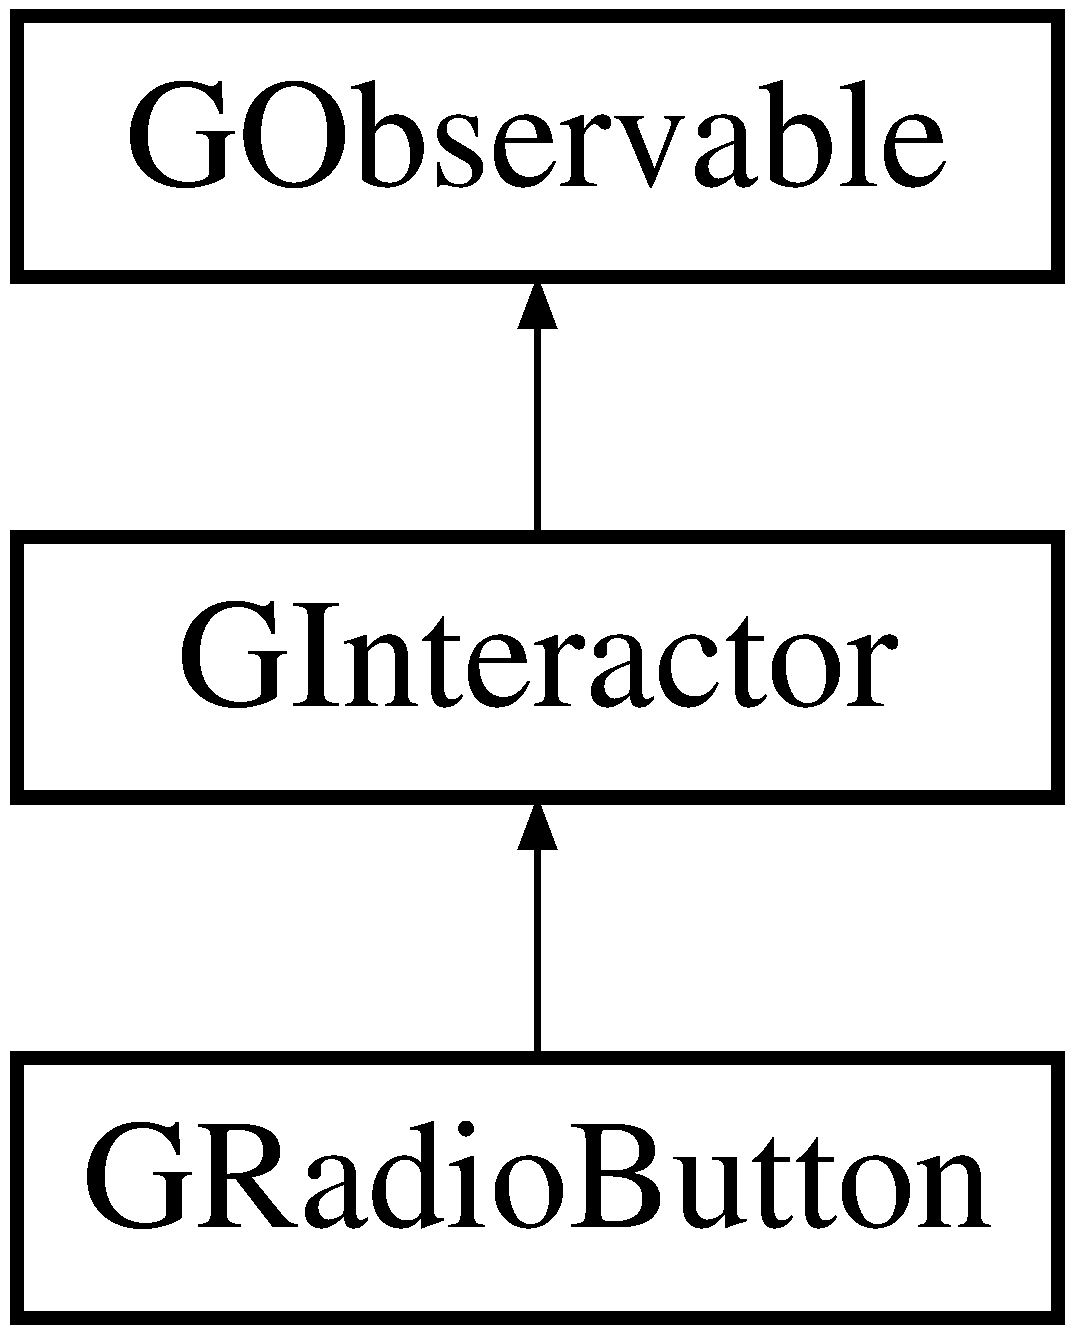
\includegraphics[height=3.000000cm]{classGRadioButton}
\end{center}
\end{figure}
\subsection*{Public Types}
\begin{DoxyCompactItemize}
\item 
enum \mbox{\hyperlink{classGInteractor_a8e0d441725a81d2bbdebbea09078260e}{Text\+Position}} \{ \mbox{\hyperlink{classGInteractor_a8e0d441725a81d2bbdebbea09078260ea4cd6f2e7d5a08d6f4dc052df2358f774}{T\+E\+X\+T\+\_\+\+B\+E\+S\+I\+D\+E\+\_\+\+I\+C\+ON}}, 
\mbox{\hyperlink{classGInteractor_a8e0d441725a81d2bbdebbea09078260eaa88490f63d8de68d44c83bdb2ecde3b3}{T\+E\+X\+T\+\_\+\+U\+N\+D\+E\+R\+\_\+\+I\+C\+ON}}, 
\mbox{\hyperlink{classGInteractor_a8e0d441725a81d2bbdebbea09078260ea39a6f388a30ac4fefb6eb13e846bc9f2}{T\+E\+X\+T\+\_\+\+O\+N\+LY}}
 \}
\begin{DoxyCompactList}\small\item\em The places where an interactor can place its text relative to its icon. \end{DoxyCompactList}\end{DoxyCompactItemize}
\subsection*{Public Member Functions}
\begin{DoxyCompactItemize}
\item 
\mbox{\hyperlink{classGRadioButton_ad9086510e97651d4dc528f115fd8aa6c}{G\+Radio\+Button}} (const std\+::string \&text=\char`\"{}\char`\"{}, const std\+::string \&group=\char`\"{}default\char`\"{}, bool checked=false, Q\+Widget $\ast$parent=nullptr)
\begin{DoxyCompactList}\small\item\em Creates a new radio button with the given text. \end{DoxyCompactList}\item 
\mbox{\hyperlink{classGRadioButton_a424ac187807b9f40966b28b47b13121f}{$\sim$\+G\+Radio\+Button}} () override
\begin{DoxyCompactList}\small\item\em Frees memory allocated internally by the radio button. \end{DoxyCompactList}\item 
virtual void \mbox{\hyperlink{classGInteractor_a02f20ea6edfa0671f31c4c648a253833}{add\+Action\+Listener}} () Q\+\_\+\+D\+E\+C\+L\+\_\+\+D\+E\+P\+R\+E\+C\+A\+T\+ED
\begin{DoxyCompactList}\small\item\em Adds an event listener to be notified when this interactor is clicked or generally interacted with. \end{DoxyCompactList}\item 
bool \mbox{\hyperlink{classGInteractor_a597a370b592e3737d38d9d2f4e2031ea}{events\+Enabled}} () const override
\begin{DoxyCompactList}\small\item\em Returns true if this interactor is currently accepting events. \end{DoxyCompactList}\item 
virtual std\+::string \mbox{\hyperlink{classGInteractor_a69f8d23ed8f207fbecad99960776e942}{get\+Accelerator}} () const
\begin{DoxyCompactList}\small\item\em Returns a string representing a hotkey for this interactor, or an empty string if no accelerator has been set. \end{DoxyCompactList}\item 
std\+::string \mbox{\hyperlink{classGRadioButton_a4f83505141da1f8446f0e0e0a9507930}{get\+Action\+Command}} () const override
\begin{DoxyCompactList}\small\item\em Returns an action command for this interactor, which is a semi-\/unique string you can use to identify it when events occur. \end{DoxyCompactList}\item 
virtual std\+::string \mbox{\hyperlink{classGInteractor_a808e22cc1fdfbecf71ed8c64ef4600e0}{get\+Background}} () const
\begin{DoxyCompactList}\small\item\em Returns the background color of the interactor as a string. \end{DoxyCompactList}\item 
virtual int \mbox{\hyperlink{classGInteractor_a9e827257a55cb8cf4d9de2ec6bcfd7a0}{get\+Background\+Int}} () const
\begin{DoxyCompactList}\small\item\em Returns the background color of the interactor as an R\+GB integer. \end{DoxyCompactList}\item 
virtual \mbox{\hyperlink{structGRectangle}{G\+Rectangle}} \mbox{\hyperlink{classGInteractor_a29e6ac35a0b48f491a4c88194cc5da3b}{get\+Bounds}} () const
\begin{DoxyCompactList}\small\item\em Returns a rectangle representing the x/y position and size of this interactor. \end{DoxyCompactList}\item 
virtual std\+::string \mbox{\hyperlink{classGInteractor_aa061dfa488c31e18549d64363c1d0e34}{get\+Color}} () const
\begin{DoxyCompactList}\small\item\em Returns the foreground/text color of the interactor as a string. \end{DoxyCompactList}\item 
virtual int \mbox{\hyperlink{classGInteractor_a9635c7af766cdc3417f346683fa0e6c1}{get\+Color\+Int}} () const
\begin{DoxyCompactList}\small\item\em Returns the foreground/text color of the interactor as an R\+GB integer. \end{DoxyCompactList}\item 
virtual \mbox{\hyperlink{classGContainer}{G\+Container}} $\ast$ \mbox{\hyperlink{classGInteractor_a7a6e317c29d61030929b4cd2d1c00fe7}{get\+Container}} () const
\begin{DoxyCompactList}\small\item\em Returns a pointer to the onscreen container holding this interactor. \end{DoxyCompactList}\item 
virtual std\+::string \mbox{\hyperlink{classGInteractor_a894a5502900794eeb27d084c21f1d77d}{get\+Font}} () const
\begin{DoxyCompactList}\small\item\em Returns the font of this interactor\textquotesingle{}s text as a font string such as \char`\"{}\+Helvetica-\/12-\/\+Bold\char`\"{}. \end{DoxyCompactList}\item 
virtual std\+::string \mbox{\hyperlink{classGInteractor_a4fa2d8b0192a3a5b4af4bbfe71194d03}{get\+Foreground}} () const
\begin{DoxyCompactList}\small\item\em Returns the foreground/text color of the interactor as a string. \end{DoxyCompactList}\item 
virtual int \mbox{\hyperlink{classGInteractor_ac3b12ab385a6ef9ae90fc879860ba726}{get\+Foreground\+Int}} () const
\begin{DoxyCompactList}\small\item\em Returns the foreground/text color of the interactor as an R\+GB integer. \end{DoxyCompactList}\item 
virtual double \mbox{\hyperlink{classGInteractor_a1e7e353362434072875264cf95629f99}{get\+Height}} () const
\begin{DoxyCompactList}\small\item\em Returns the current onscreen height of this interactor in pixels. \end{DoxyCompactList}\item 
virtual std\+::string \mbox{\hyperlink{classGInteractor_aaed62a73004939a64da6f0eb9eb64d73}{get\+Icon}} () const
\begin{DoxyCompactList}\small\item\em Returns the file name of the icon associated with this interactor, or an empty string if no icon has been set. \end{DoxyCompactList}\item 
virtual int \mbox{\hyperlink{classGInteractor_a9c9659a6c6ba66b4107ba59c95a24241}{get\+ID}} () const
\begin{DoxyCompactList}\small\item\em Returns a globally unique identifier for this interactor, which is set when the interactor is constructed. \end{DoxyCompactList}\item 
\+\_\+\+Internal\+\_\+\+Q\+Widget $\ast$ \mbox{\hyperlink{classGRadioButton_a2f6b36b2517087dc90a366b5ce1f5323}{get\+Internal\+Widget}} () const override
\begin{DoxyCompactList}\small\item\em Returns a direct pointer to the internal Qt widget being wrapped by this interactor. \end{DoxyCompactList}\item 
virtual \mbox{\hyperlink{structGPoint}{G\+Point}} \mbox{\hyperlink{classGInteractor_a4f83802015511edeb63b892830812c11}{get\+Location}} () const
\begin{DoxyCompactList}\small\item\em Returns an (x, y) point representing the onscreen location of the top-\/left corner of this interactor within its containing window. \end{DoxyCompactList}\item 
virtual double \mbox{\hyperlink{classGInteractor_aed4b0075fcc434499c3cb3e46896bda3}{get\+Minimum\+Height}} () const
\begin{DoxyCompactList}\small\item\em Returns the minimum height in pixels that this interactor will permit itself to be resized to. \end{DoxyCompactList}\item 
virtual \mbox{\hyperlink{structGDimension}{G\+Dimension}} \mbox{\hyperlink{classGInteractor_a66b5af0b32493b4d597ca0a3df2049ea}{get\+Minimum\+Size}} () const
\begin{DoxyCompactList}\small\item\em Returns a \mbox{\hyperlink{structGDimension}{G\+Dimension}} structure representing the minimum size in pixels that this interactor will permit itself to be resized to. \end{DoxyCompactList}\item 
virtual double \mbox{\hyperlink{classGInteractor_a59e668114fe3d49d2a0f28deb258f7c8}{get\+Minimum\+Width}} () const
\begin{DoxyCompactList}\small\item\em Returns the minimum width in pixels that this interactor will permit itself to be resized to. \end{DoxyCompactList}\item 
virtual std\+::string \mbox{\hyperlink{classGInteractor_a8a60438a5b55d0b2ceb35c8674b9d8c5}{get\+Name}} () const
\begin{DoxyCompactList}\small\item\em Returns a string representing a unique name for this interactor. \end{DoxyCompactList}\item 
virtual double \mbox{\hyperlink{classGInteractor_a747de0961653847bdc6615dbf756d715}{get\+Preferred\+Height}} () const
\begin{DoxyCompactList}\small\item\em Returns the height in pixels that this interactor would prefer to be, which would exactly fit its contents with no stretching or scrollbars. \end{DoxyCompactList}\item 
virtual \mbox{\hyperlink{structGDimension}{G\+Dimension}} \mbox{\hyperlink{classGInteractor_a4aabbee761d8e9116275401131b7ccd1}{get\+Preferred\+Size}} () const
\begin{DoxyCompactList}\small\item\em Returns a \mbox{\hyperlink{structGDimension}{G\+Dimension}} structure storing the width and height in pixels that this interactor would prefer to be, which would exactly fit its contents with no stretching or scrollbars. \end{DoxyCompactList}\item 
virtual double \mbox{\hyperlink{classGInteractor_a82bca31d37700fb0e35d2743352efd5e}{get\+Preferred\+Width}} () const
\begin{DoxyCompactList}\small\item\em Returns the height in pixels that this interactor would prefer to be, which would exactly fit its contents with no stretching or scrollbars. \end{DoxyCompactList}\item 
virtual \mbox{\hyperlink{structGDimension}{G\+Dimension}} \mbox{\hyperlink{classGInteractor_a7b4eec96a2bdc6420695d5796a78eea9}{get\+Size}} () const
\begin{DoxyCompactList}\small\item\em Returns a \mbox{\hyperlink{structGDimension}{G\+Dimension}} structure storing the current onscreen width and height of this interactor in pixels. \end{DoxyCompactList}\item 
virtual std\+::string \mbox{\hyperlink{classGRadioButton_aff553c50924b836c29f146ed34a7c6ec}{get\+Text}} () const
\begin{DoxyCompactList}\small\item\em Returns the text next to the radio button. \end{DoxyCompactList}\item 
std\+::string \mbox{\hyperlink{classGRadioButton_a9b72ede4ee8520f987a0c01e30654814}{get\+Type}} () const override
\begin{DoxyCompactList}\small\item\em Returns a string representing the class name of this interactor, such as \char`\"{}\+G\+Button\char`\"{} or \char`\"{}\+G\+Check\+Box\char`\"{}. \end{DoxyCompactList}\item 
Q\+Widget $\ast$ \mbox{\hyperlink{classGRadioButton_a3b33a602b31a6b809d020535a59db3b4}{get\+Widget}} () const override
\begin{DoxyCompactList}\small\item\em Returns a direct pointer to the internal Qt widget being wrapped by this interactor. \end{DoxyCompactList}\item 
virtual double \mbox{\hyperlink{classGInteractor_a0ed2965abd4f5701d2cadf71239faf19}{get\+Width}} () const
\begin{DoxyCompactList}\small\item\em Returns the current onscreen width of this interactor in pixels. \end{DoxyCompactList}\item 
virtual double \mbox{\hyperlink{classGInteractor_a344385751bee0720059403940d57a13e}{getX}} () const
\begin{DoxyCompactList}\small\item\em Returns the x-\/coordinate of the top-\/left pixel of this interactor within its onscreen window. \end{DoxyCompactList}\item 
virtual double \mbox{\hyperlink{classGInteractor_aafa51c7f8f38a09febbb9ce7853f77b4}{getY}} () const
\begin{DoxyCompactList}\small\item\em Returns the y-\/coordinate of the top-\/left pixel of this interactor within its onscreen window. \end{DoxyCompactList}\item 
virtual bool \mbox{\hyperlink{classGInteractor_afc480f652b8c5f1fb255e2269ce68879}{in\+Bounds}} (double x, double y) const
\begin{DoxyCompactList}\small\item\em Returns true if the given x/y pixel is within the bounds of this interactor. \end{DoxyCompactList}\item 
virtual bool \mbox{\hyperlink{classGInteractor_ae6d7982c1c627b677a5e776ca86118ed}{in\+Bounds}} (int x, int y) const
\begin{DoxyCompactList}\small\item\em Returns true if the given x/y pixel is within the bounds of this interactor. \end{DoxyCompactList}\item 
virtual bool \mbox{\hyperlink{classGRadioButton_ac8cada18b9357ff68b26e17f44294764}{is\+Checked}} () const
\begin{DoxyCompactList}\small\item\em Returns true if the radio button is currently checked. \end{DoxyCompactList}\item 
virtual bool \mbox{\hyperlink{classGInteractor_aacb819fb241851fd9fc045271baa4034}{is\+Enabled}} () const
\begin{DoxyCompactList}\small\item\em Returns true if this interactor is currently enabled. \end{DoxyCompactList}\item 
virtual bool \mbox{\hyperlink{classGRadioButton_a56a065a2c20a230931de0ed98019d8fb}{is\+Selected}} () const
\begin{DoxyCompactList}\small\item\em Returns true if the radio button is currently checked. \end{DoxyCompactList}\item 
virtual bool \mbox{\hyperlink{classGInteractor_a9d8a6cfb13917785c143e74d40e4e2be}{is\+Visible}} () const
\begin{DoxyCompactList}\small\item\em Returns true if the interactor is visible on the screen. \end{DoxyCompactList}\item 
virtual void \mbox{\hyperlink{classGInteractor_ab7fe7a876367b87cf7202f947f1d05e4}{remove\+Action\+Listener}} ()
\begin{DoxyCompactList}\small\item\em Removes the action listener from this interactor so that it will no longer call it when events occur. \end{DoxyCompactList}\item 
virtual void \mbox{\hyperlink{classGInteractor_ad39d0325cde6b97ebda4b9d7787c633b}{remove\+Click\+Listener}} ()
\begin{DoxyCompactList}\small\item\em Removes the click listener from this interactor so that it will no longer call it when events occur. \end{DoxyCompactList}\item 
virtual void \mbox{\hyperlink{classGInteractor_aa4250907e4cdd77349c04f0cf5cdd3d3}{remove\+Double\+Click\+Listener}} ()
\begin{DoxyCompactList}\small\item\em Removes the double-\/click listener from this interactor so that it will no longer call it when events occur. \end{DoxyCompactList}\item 
virtual void \mbox{\hyperlink{classGInteractor_a43095f41cab3be732b49f29970484b05}{remove\+Key\+Listener}} ()
\begin{DoxyCompactList}\small\item\em Removes the key listener from this interactor so that it will no longer call it when key events occur. \end{DoxyCompactList}\item 
virtual void \mbox{\hyperlink{classGInteractor_aff47f71ce47e688a07c9d38dc92fcc11}{remove\+Mouse\+Listener}} ()
\begin{DoxyCompactList}\small\item\em Removes the mouse listener from this interactor so that it will no longer call it when events occur. \end{DoxyCompactList}\item 
virtual void \mbox{\hyperlink{classGInteractor_a519fb2ac767f8b2febbb50b898b8c8cb}{request\+Focus}} ()
\begin{DoxyCompactList}\small\item\em Transfers keyboard focus to this interactor. \end{DoxyCompactList}\item 
virtual void \mbox{\hyperlink{classGInteractor_ad15f102f62e2960576012f1aa0ba4b2e}{set\+Accelerator}} (const std\+::string \&accelerator)
\begin{DoxyCompactList}\small\item\em Sets an accelerator hotkey for this interactor, such as \char`\"{}\+Ctrl-\/\+S\char`\"{}. \end{DoxyCompactList}\item 
virtual void \mbox{\hyperlink{classGInteractor_a4b5843fe3030e038a1ba54cc03389bcf}{set\+Action\+Command}} (const std\+::string \&action\+Command)
\begin{DoxyCompactList}\small\item\em Sets the action command for this interactor. \end{DoxyCompactList}\item 
virtual void \mbox{\hyperlink{classGInteractor_adcfb4742430c88714fcf57e57ab8ea9c}{set\+Action\+Listener}} (G\+Event\+Listener func)
\begin{DoxyCompactList}\small\item\em Sets an action listener on this interactor so that it will be called when it is interacted with in its primary way. \end{DoxyCompactList}\item 
virtual void \mbox{\hyperlink{classGInteractor_aebd20a89c7a8a43a6fce999cf4f9fcf2}{set\+Action\+Listener}} (G\+Event\+Listener\+Void func)
\begin{DoxyCompactList}\small\item\em Sets an action listener on this interactor so that it will be called when it is interacted with in its primary way. \end{DoxyCompactList}\item 
virtual void \mbox{\hyperlink{classGInteractor_acba7e546c2025c0a15ca4b4cc92043db}{set\+Background}} (int rgb)
\begin{DoxyCompactList}\small\item\em Sets the background color of the interactor to the color represented by the given R\+GB integer. \end{DoxyCompactList}\item 
virtual void \mbox{\hyperlink{classGInteractor_ab4677ab2474e68b07aa56605af92a84a}{set\+Background}} (const std\+::string \&color)
\begin{DoxyCompactList}\small\item\em Sets the background color of the interactor to the color represented by the given string. \end{DoxyCompactList}\item 
virtual void \mbox{\hyperlink{classGInteractor_a2aae8197624b72265ab83b4f1bc73f2f}{set\+Bounds}} (double x, double y, double width, double height)
\begin{DoxyCompactList}\small\item\em Sets the size and location of the widget. \end{DoxyCompactList}\item 
virtual void \mbox{\hyperlink{classGInteractor_acada386653f008cacc7cce86426bef7c}{set\+Bounds}} (const \mbox{\hyperlink{structGRectangle}{G\+Rectangle}} \&size)
\begin{DoxyCompactList}\small\item\em Sets the size and location of the widget. \end{DoxyCompactList}\item 
virtual void \mbox{\hyperlink{classGRadioButton_a116285e2f56247b00b26035ca0ac4737}{set\+Checked}} (bool checked)
\begin{DoxyCompactList}\small\item\em Sets whether the radio button should be checked. \end{DoxyCompactList}\item 
virtual void \mbox{\hyperlink{classGInteractor_abd40af6921242584d0954f173911b190}{set\+Click\+Listener}} (G\+Event\+Listener func)
\begin{DoxyCompactList}\small\item\em Sets a mouse listener on this interactor so that it will be called when the mouse is clicked on it. \end{DoxyCompactList}\item 
virtual void \mbox{\hyperlink{classGInteractor_a856414c92df90f56f3877475eb3f8fc4}{set\+Click\+Listener}} (G\+Event\+Listener\+Void func)
\begin{DoxyCompactList}\small\item\em Sets a mouse listener on this interactor so that it will be called when the mouse is clicked on it. \end{DoxyCompactList}\item 
virtual void \mbox{\hyperlink{classGInteractor_ab1f5cc0f5cc6bbbd716a526c61f1081d}{set\+Color}} (int rgb)
\begin{DoxyCompactList}\small\item\em Sets the foreground/text color of the interactor to the color represented by the given R\+GB integer. \end{DoxyCompactList}\item 
virtual void \mbox{\hyperlink{classGInteractor_a61374df6c11b52cfbb0815decdbaebc6}{set\+Color}} (const std\+::string \&color)
\begin{DoxyCompactList}\small\item\em Sets the foreground/text color of the interactor to the color represented by the given string. \end{DoxyCompactList}\item 
virtual void \mbox{\hyperlink{classGInteractor_ac29f9a3462458e165fae3a1f046ee77a}{set\+Double\+Click\+Listener}} (G\+Event\+Listener func)
\begin{DoxyCompactList}\small\item\em Sets a mouse listener on this interactor so that it will be called when the mouse is double-\/clicked on it. \end{DoxyCompactList}\item 
virtual void \mbox{\hyperlink{classGInteractor_a50096194d66f48c92dd4c512d41bfc76}{set\+Double\+Click\+Listener}} (G\+Event\+Listener\+Void func)
\begin{DoxyCompactList}\small\item\em Sets a mouse listener on this interactor so that it will be called when the mouse is double-\/clicked on it. \end{DoxyCompactList}\item 
virtual void \mbox{\hyperlink{classGInteractor_ab831367dd84bbd579e02e55bacb21343}{set\+Enabled}} (bool value)
\begin{DoxyCompactList}\small\item\em Sets whether this interactor is currently enabled. \end{DoxyCompactList}\item 
virtual void \mbox{\hyperlink{classGObservable_afaa30b2a9e0f378fd1c70d2f1d0b8216}{set\+Events\+Enabled}} (bool \mbox{\hyperlink{classGInteractor_a597a370b592e3737d38d9d2f4e2031ea}{events\+Enabled}})
\begin{DoxyCompactList}\small\item\em Sets whether the object is currently allowing itself to fire events. \end{DoxyCompactList}\item 
virtual void \mbox{\hyperlink{classGInteractor_a2592348886ffea646c6534bf88f7c49d}{set\+Font}} (const Q\+Font \&font)
\begin{DoxyCompactList}\small\item\em Sets the font used by this widget to the given Qt font. \end{DoxyCompactList}\item 
virtual void \mbox{\hyperlink{classGInteractor_a8e096e8818d838aceae1d46d58fb3a7b}{set\+Font}} (const std\+::string \&font)
\begin{DoxyCompactList}\small\item\em Sets the font used by this widget to the font represented by the given font string, such as \char`\"{}\+Helvetica-\/16-\/\+Bold\char`\"{}. \end{DoxyCompactList}\item 
virtual void \mbox{\hyperlink{classGInteractor_a9eb856b5ff83a19df3831a31f15f4563}{set\+Foreground}} (int rgb)
\begin{DoxyCompactList}\small\item\em Sets the foreground/text color of the interactor to the color represented by the given R\+GB integer. \end{DoxyCompactList}\item 
virtual void \mbox{\hyperlink{classGInteractor_af59209aeadea6dfc6d97a2d8531f50e1}{set\+Foreground}} (const std\+::string \&color)
\begin{DoxyCompactList}\small\item\em Sets the foreground/text color of the interactor to the color represented by the given string. \end{DoxyCompactList}\item 
virtual void \mbox{\hyperlink{classGInteractor_a9e280bfc4544dfaf8e4376c4e1a74357}{set\+Height}} (double height)
\begin{DoxyCompactList}\small\item\em Sets the onscreen height of the interactor in pixels. \end{DoxyCompactList}\item 
virtual void \mbox{\hyperlink{classGInteractor_a542abfcd7261751352af129c7215ecda}{set\+Icon}} (const Q\+Icon \&icon)
\begin{DoxyCompactList}\small\item\em Sets the icon associated with this interactor. \end{DoxyCompactList}\item 
virtual void \mbox{\hyperlink{classGInteractor_a368e1a338f84401c284506d03b1ba769}{set\+Icon}} (const Q\+Pixmap \&icon)
\begin{DoxyCompactList}\small\item\em Sets the icon associated with this interactor. \end{DoxyCompactList}\item 
virtual void \mbox{\hyperlink{classGInteractor_a762e139aa311461c3984d3ad28293f64}{set\+Icon}} (const std\+::string \&filename, bool retain\+Icon\+Size=true)
\begin{DoxyCompactList}\small\item\em Sets the file name of the icon associated with this interactor, or an empty string if no icon has been set. \end{DoxyCompactList}\item 
virtual void \mbox{\hyperlink{classGInteractor_aeb8324d3287fa1fbe093f4d6230cf0a6}{set\+Key\+Listener}} (G\+Event\+Listener func)
\begin{DoxyCompactList}\small\item\em Sets a key listener on this interactor so that it will be called when the user presses any key. \end{DoxyCompactList}\item 
virtual void \mbox{\hyperlink{classGInteractor_ae48ecea73606c7bd9423e1c7cc589cc9}{set\+Key\+Listener}} (G\+Event\+Listener\+Void func)
\begin{DoxyCompactList}\small\item\em Sets a key listener on this interactor so that it will be called when the user presses any key. \end{DoxyCompactList}\item 
virtual void \mbox{\hyperlink{classGInteractor_a04594e8ba9b98513a64f1da00dcae18c}{set\+Location}} (double x, double y)
\begin{DoxyCompactList}\small\item\em Sets the onscreen x/y-\/coordinate of the top-\/left corner of the interactor relative to its window. \end{DoxyCompactList}\item 
virtual void \mbox{\hyperlink{classGInteractor_a0cf428e207b7f22cc08138a90b1b87b2}{set\+Minimum\+Size}} (double width, double height)
\begin{DoxyCompactList}\small\item\em Sets the minimum size in pixels that this interactor will permit itself to be resized to. \end{DoxyCompactList}\item 
virtual void \mbox{\hyperlink{classGInteractor_a3b1046117ac6cb7abe467e00ba8a81f4}{set\+Minimum\+Size}} (const \mbox{\hyperlink{structGDimension}{G\+Dimension}} \&size)
\begin{DoxyCompactList}\small\item\em Sets the minimum size in pixels that this interactor will permit itself to be resized to. \end{DoxyCompactList}\item 
virtual void \mbox{\hyperlink{classGInteractor_a37d8dbc943f59920f705b0104f60bde2}{set\+Mouse\+Listener}} (G\+Event\+Listener func)
\begin{DoxyCompactList}\small\item\em Sets a mouse listener on this interactor so that it will be called when the mouse is moved or clicked on it. \end{DoxyCompactList}\item 
virtual void \mbox{\hyperlink{classGInteractor_aea7f647ea62d59f71b5fad6aa65eeaf9}{set\+Mouse\+Listener}} (G\+Event\+Listener\+Void func)
\begin{DoxyCompactList}\small\item\em Sets a mouse listener on this interactor so that it will be called when the mouse is moved or clicked on it. \end{DoxyCompactList}\item 
virtual void \mbox{\hyperlink{classGInteractor_a9d3a2685df23b5e7cbf59c19c4a1f9b5}{set\+Name}} (const std\+::string \&name)
\begin{DoxyCompactList}\small\item\em Sets a string representing a unique name for this interactor. \end{DoxyCompactList}\item 
virtual void \mbox{\hyperlink{classGInteractor_a1ab987704fce32098706c6f00fb08218}{set\+Preferred\+Height}} (double height)
\begin{DoxyCompactList}\small\item\em Sets the height in pixels that this interactor would prefer to be. \end{DoxyCompactList}\item 
virtual void \mbox{\hyperlink{classGInteractor_a042c5ae19430d765ef552371cae3632c}{set\+Preferred\+Size}} (double width, double height)
\begin{DoxyCompactList}\small\item\em Sets the width and height in pixels that this interactor would prefer to be. \end{DoxyCompactList}\item 
virtual void \mbox{\hyperlink{classGInteractor_aa22d9be4bc0e078bb0ea69b0fc9d7c75}{set\+Preferred\+Size}} (const \mbox{\hyperlink{structGDimension}{G\+Dimension}} \&size)
\begin{DoxyCompactList}\small\item\em Sets the size in pixels that this interactor would prefer to be. \end{DoxyCompactList}\item 
virtual void \mbox{\hyperlink{classGInteractor_a3db429ab2fa52efd187eec0ed8cdd9f2}{set\+Preferred\+Width}} (double width)
\begin{DoxyCompactList}\small\item\em Sets the width in pixels that this interactor would prefer to be. \end{DoxyCompactList}\item 
virtual void \mbox{\hyperlink{classGRadioButton_ad42accd39af295a957386c68dac3dcae}{set\+Selected}} (bool selected)
\begin{DoxyCompactList}\small\item\em Sets whether the radio button should be checked. \end{DoxyCompactList}\item 
virtual void \mbox{\hyperlink{classGInteractor_aca25d49481f9bf5fc8f7df4c086c4ce7}{set\+Size}} (double width, double height)
\begin{DoxyCompactList}\small\item\em Sets the onscreen width and height of the interactor in pixels. \end{DoxyCompactList}\item 
virtual void \mbox{\hyperlink{classGInteractor_ae2b628228f192c2702c4ce941b2af68f}{set\+Size}} (const \mbox{\hyperlink{structGDimension}{G\+Dimension}} \&size)
\begin{DoxyCompactList}\small\item\em Sets the onscreen width and height of the interactor in pixels. \end{DoxyCompactList}\item 
virtual void \mbox{\hyperlink{classGRadioButton_ac1ae51949d41ee9054634be5967d91b8}{set\+Text}} (const std\+::string \&text)
\begin{DoxyCompactList}\small\item\em Sets the text that will appear next to the radio button. \end{DoxyCompactList}\item 
virtual void \mbox{\hyperlink{classGInteractor_a039e0e49beaecc275efce02d416acea8}{set\+Tooltip}} (const std\+::string \&tooltip\+Text)
\begin{DoxyCompactList}\small\item\em Sets a \char`\"{}tooltip\char`\"{} that will appear if the user hovers their mouse over the interactor. \end{DoxyCompactList}\item 
virtual void \mbox{\hyperlink{classGInteractor_a18e44e30b31525a243960ca3928125aa}{set\+Visible}} (bool visible)
\begin{DoxyCompactList}\small\item\em Returns true if the interactor is visible on the screen. \end{DoxyCompactList}\item 
virtual void \mbox{\hyperlink{classGInteractor_aa3f3fba4cb131baa8696ba01e3bceca1}{set\+Width}} (double width)
\begin{DoxyCompactList}\small\item\em Sets the onscreen width of the interactor in pixels. \end{DoxyCompactList}\item 
virtual void \mbox{\hyperlink{classGInteractor_a9c18fcc579333bf9653d13ad2b372e39}{setX}} (double x)
\begin{DoxyCompactList}\small\item\em Sets the onscreen x-\/coordinate of the top-\/left corner of the interactor relative to its window. \end{DoxyCompactList}\item 
virtual void \mbox{\hyperlink{classGInteractor_a7d57e2a5c35d27feb58fd498a3cf82b9}{setY}} (double y)
\begin{DoxyCompactList}\small\item\em Sets the onscreen y-\/coordinate of the top-\/left corner of the interactor relative to its window. \end{DoxyCompactList}\item 
virtual void \mbox{\hyperlink{classGRadioButton_ad277193b2dca0bab1e0ad24d45407dc3}{toggle}} ()
\begin{DoxyCompactList}\small\item\em Reverses the checked state of the button, setting it to be checked if it was unchecked or to be unchecked if it was checked. \end{DoxyCompactList}\item 
virtual std\+::string \mbox{\hyperlink{classGObservable_a1fe5121d6528fdea3f243321b3fa3a49}{to\+String}} () const
\begin{DoxyCompactList}\small\item\em Returns a string representation of this observable object\textquotesingle{}s state. \end{DoxyCompactList}\end{DoxyCompactItemize}
\subsection*{Protected Member Functions}
\begin{DoxyCompactItemize}
\item 
virtual void \mbox{\hyperlink{classGObservable_a80cfa040459ff53594adbd6a51ec8f43}{clear\+Event\+Listeners}} ()
\begin{DoxyCompactList}\small\item\em Removes all event listeners from this object. \end{DoxyCompactList}\item 
virtual void \mbox{\hyperlink{classGObservable_a284f31528c0520f8e545c03ac9eeac74}{ensure\+Thread\+Safety}} (const std\+::string \&member\+Name=\char`\"{}\char`\"{})
\begin{DoxyCompactList}\small\item\em Ensures that we are currently in the Qt G\+UI thread. \end{DoxyCompactList}\item 
virtual void \mbox{\hyperlink{classGObservable_a63e5e5a6227c59c928493b11aceb0f67}{fire\+Event}} (\mbox{\hyperlink{classGEvent}{G\+Event}} \&event)
\begin{DoxyCompactList}\small\item\em Sends out the given event to any attached listeners. \end{DoxyCompactList}\item 
virtual void \mbox{\hyperlink{classGObservable_ab3983ea07337b52020a29cc00c653d8d}{fire\+G\+Event}} (Q\+Event $\ast$event, Event\+Type event\+Type, const std\+::string \&event\+Name)
\begin{DoxyCompactList}\small\item\em Creates an event of the given type, then sends it out to any attached listeners. \end{DoxyCompactList}\item 
virtual void \mbox{\hyperlink{classGObservable_a01fdf1b0e0dbd49e189fe4514e010411}{fire\+G\+Event}} (Q\+Close\+Event $\ast$event, Event\+Type event\+Type, const std\+::string \&event\+Name)
\begin{DoxyCompactList}\small\item\em Creates an event of the given type, then sends it out to any attached listeners. \end{DoxyCompactList}\item 
virtual void \mbox{\hyperlink{classGObservable_abb0b2f66ba39211cb5d7615e9d1c04e2}{fire\+G\+Event}} (Q\+Key\+Event $\ast$event, Event\+Type event\+Type, const std\+::string \&event\+Name)
\begin{DoxyCompactList}\small\item\em Creates an event of the given type, then sends it out to any attached listeners. \end{DoxyCompactList}\item 
virtual void \mbox{\hyperlink{classGObservable_a119318675d2165bdf7dd853aaf881d4b}{fire\+G\+Event}} (Q\+Mouse\+Event $\ast$event, Event\+Type event\+Type, const std\+::string \&event\+Name, const std\+::string \&action\+Command=\char`\"{}\char`\"{})
\begin{DoxyCompactList}\small\item\em Creates an event of the given type, then sends it out to any attached listeners. \end{DoxyCompactList}\item 
virtual void \mbox{\hyperlink{classGObservable_a63fd9034e1e1633c1c38eb342bfd34e9}{fire\+G\+Event}} (Q\+Resize\+Event $\ast$event, Event\+Type event\+Type, const std\+::string \&event\+Name)
\begin{DoxyCompactList}\small\item\em Creates an event of the given type, then sends it out to any attached listeners. \end{DoxyCompactList}\item 
virtual void \mbox{\hyperlink{classGObservable_a741345310d9b7c5170a6cbc410c44ac4}{fire\+G\+Event}} (Q\+Timer\+Event $\ast$event, Event\+Type event\+Type, const std\+::string \&event\+Name)
\begin{DoxyCompactList}\small\item\em Creates an event of the given type, then sends it out to any attached listeners. \end{DoxyCompactList}\item 
virtual void \mbox{\hyperlink{classGObservable_a93bf338968a0338761b8e4dc62f582e9}{fire\+G\+Event}} (Q\+Wheel\+Event $\ast$event, Event\+Type event\+Type, const std\+::string \&event\+Name)
\begin{DoxyCompactList}\small\item\em Creates an event of the given type, then sends it out to any attached listeners. \end{DoxyCompactList}\item 
virtual void \mbox{\hyperlink{classGObservable_a2a70a7d7435ff0c3b80bb4d70da19e0d}{fire\+G\+Event}} (Q\+Window\+State\+Change\+Event $\ast$event, Event\+Type event\+Type, const std\+::string \&event\+Name)
\begin{DoxyCompactList}\small\item\em Creates an event of the given type, then sends it out to any attached listeners. \end{DoxyCompactList}\item 
virtual bool \mbox{\hyperlink{classGObservable_a9f6faaa25942923bafa1c44020c49fa9}{has\+Event\+Listener}} (const std\+::string \&event\+Name) const
\begin{DoxyCompactList}\small\item\em Returns true if the observable object has a listener for the given type of event. \end{DoxyCompactList}\item 
virtual bool \mbox{\hyperlink{classGObservable_aeec1adc19aa0f33de62390686ee1382c}{is\+Accepting\+Event}} (int event\+Mask) const
\begin{DoxyCompactList}\small\item\em Returns true if the observable object has a listener for the given type of event. \end{DoxyCompactList}\item 
virtual bool \mbox{\hyperlink{classGObservable_aa31c73145a29dcb92848a92e0cfaea41}{is\+Accepting\+Event}} (const \mbox{\hyperlink{classGEvent}{G\+Event}} \&event) const
\begin{DoxyCompactList}\small\item\em Returns true if the observable object has a listener for the given type of event. \end{DoxyCompactList}\item 
virtual bool \mbox{\hyperlink{classGObservable_a3b1c689267eda44e65a2213e7de38b23}{is\+Accepting\+Event}} (const std\+::string \&event\+Type) const
\begin{DoxyCompactList}\small\item\em Returns true if the observable object has a listener for the given type of event. \end{DoxyCompactList}\item 
virtual void \mbox{\hyperlink{classGObservable_acbcf1ed3a851ad8a3c17ef38d86b481d}{remove\+Event\+Listener}} (const std\+::string \&event\+Name)
\begin{DoxyCompactList}\small\item\em Removes any event listener from this observable object that would respond to the given type of event, such as \char`\"{}click\char`\"{} or \char`\"{}keydown\char`\"{}. \end{DoxyCompactList}\item 
virtual void \mbox{\hyperlink{classGObservable_af51cc35c29a1bd1908609d432decdbb6}{remove\+Event\+Listeners}} (std\+::initializer\+\_\+list$<$ std\+::string $>$ event\+Names)
\begin{DoxyCompactList}\small\item\em Removes any event listener from this observable object that would respond to the given types of events, such as \char`\"{}click\char`\"{} or \char`\"{}keydown\char`\"{}. \end{DoxyCompactList}\item 
virtual void \mbox{\hyperlink{classGObservable_ad2f6d34961c50f6c1e0659990b79f741}{set\+Event\+Listener}} (const std\+::string \&event\+Name, G\+Event\+Listener func)
\begin{DoxyCompactList}\small\item\em Adds an event listener from this observable object to respond to the given type of event, such as \char`\"{}click\char`\"{} or \char`\"{}keydown\char`\"{}. \end{DoxyCompactList}\item 
virtual void \mbox{\hyperlink{classGObservable_abac4cb9f9e626e010e87f5d91573c8a5}{set\+Event\+Listener}} (const std\+::string \&event\+Name, G\+Event\+Listener\+Void func)
\begin{DoxyCompactList}\small\item\em Adds an event listener from this observable object to respond to the given type of event, such as \char`\"{}click\char`\"{} or \char`\"{}keydown\char`\"{}. \end{DoxyCompactList}\item 
virtual void \mbox{\hyperlink{classGObservable_afa388d69c33c718cf035774604065604}{set\+Event\+Listeners}} (std\+::initializer\+\_\+list$<$ std\+::string $>$ event\+Names, G\+Event\+Listener func)
\begin{DoxyCompactList}\small\item\em Adds an event listener from this observable object to respond to the given types of events, such as \char`\"{}click\char`\"{} or \char`\"{}keydown\char`\"{}. \end{DoxyCompactList}\item 
virtual void \mbox{\hyperlink{classGObservable_a7867184bbb686f74fae8a4db927da799}{set\+Event\+Listeners}} (std\+::initializer\+\_\+list$<$ std\+::string $>$ event\+Names, G\+Event\+Listener\+Void func)
\begin{DoxyCompactList}\small\item\em Adds an event listener from this observable object to respond to the given types of events, such as \char`\"{}click\char`\"{} or \char`\"{}keydown\char`\"{}. \end{DoxyCompactList}\end{DoxyCompactItemize}


\subsection{Detailed Description}
This interactor subclass represents an onscreen radio button. 

Radio buttons are round buttons that can be \char`\"{}checked\char`\"{} by clicking them. A radio button differs from a checkbox in that it is often part of a mutually exclusive group of options, where at most one of the buttons can be checked at a time. Clicking one radio button from a group checks it and also unchecks any other checked radio button from that same group.

You can listen for clicks on a radio button by setting an action listener, passing the function you want to call on each click. 

\subsection{Member Enumeration Documentation}
\mbox{\Hypertarget{classGInteractor_a8e0d441725a81d2bbdebbea09078260e}\label{classGInteractor_a8e0d441725a81d2bbdebbea09078260e}} 
\index{G\+Radio\+Button@{G\+Radio\+Button}!Text\+Position@{Text\+Position}}
\index{Text\+Position@{Text\+Position}!G\+Radio\+Button@{G\+Radio\+Button}}
\subsubsection{\texorpdfstring{Text\+Position}{TextPosition}}
{\footnotesize\ttfamily enum \mbox{\hyperlink{classGInteractor_a8e0d441725a81d2bbdebbea09078260e}{Text\+Position}}\hspace{0.3cm}{\ttfamily [inherited]}}



The places where an interactor can place its text relative to its icon. 

\begin{DoxyEnumFields}{Enumerator}
\raisebox{\heightof{T}}[0pt][0pt]{\index{T\+E\+X\+T\+\_\+\+B\+E\+S\+I\+D\+E\+\_\+\+I\+C\+ON@{T\+E\+X\+T\+\_\+\+B\+E\+S\+I\+D\+E\+\_\+\+I\+C\+ON}!G\+Radio\+Button@{G\+Radio\+Button}}\index{G\+Radio\+Button@{G\+Radio\+Button}!T\+E\+X\+T\+\_\+\+B\+E\+S\+I\+D\+E\+\_\+\+I\+C\+ON@{T\+E\+X\+T\+\_\+\+B\+E\+S\+I\+D\+E\+\_\+\+I\+C\+ON}}}\mbox{\Hypertarget{classGInteractor_a8e0d441725a81d2bbdebbea09078260ea4cd6f2e7d5a08d6f4dc052df2358f774}\label{classGInteractor_a8e0d441725a81d2bbdebbea09078260ea4cd6f2e7d5a08d6f4dc052df2358f774}} 
T\+E\+X\+T\+\_\+\+B\+E\+S\+I\+D\+E\+\_\+\+I\+C\+ON&\\
\hline

\raisebox{\heightof{T}}[0pt][0pt]{\index{T\+E\+X\+T\+\_\+\+U\+N\+D\+E\+R\+\_\+\+I\+C\+ON@{T\+E\+X\+T\+\_\+\+U\+N\+D\+E\+R\+\_\+\+I\+C\+ON}!G\+Radio\+Button@{G\+Radio\+Button}}\index{G\+Radio\+Button@{G\+Radio\+Button}!T\+E\+X\+T\+\_\+\+U\+N\+D\+E\+R\+\_\+\+I\+C\+ON@{T\+E\+X\+T\+\_\+\+U\+N\+D\+E\+R\+\_\+\+I\+C\+ON}}}\mbox{\Hypertarget{classGInteractor_a8e0d441725a81d2bbdebbea09078260eaa88490f63d8de68d44c83bdb2ecde3b3}\label{classGInteractor_a8e0d441725a81d2bbdebbea09078260eaa88490f63d8de68d44c83bdb2ecde3b3}} 
T\+E\+X\+T\+\_\+\+U\+N\+D\+E\+R\+\_\+\+I\+C\+ON&\\
\hline

\raisebox{\heightof{T}}[0pt][0pt]{\index{T\+E\+X\+T\+\_\+\+O\+N\+LY@{T\+E\+X\+T\+\_\+\+O\+N\+LY}!G\+Radio\+Button@{G\+Radio\+Button}}\index{G\+Radio\+Button@{G\+Radio\+Button}!T\+E\+X\+T\+\_\+\+O\+N\+LY@{T\+E\+X\+T\+\_\+\+O\+N\+LY}}}\mbox{\Hypertarget{classGInteractor_a8e0d441725a81d2bbdebbea09078260ea39a6f388a30ac4fefb6eb13e846bc9f2}\label{classGInteractor_a8e0d441725a81d2bbdebbea09078260ea39a6f388a30ac4fefb6eb13e846bc9f2}} 
T\+E\+X\+T\+\_\+\+O\+N\+LY&\\
\hline

\end{DoxyEnumFields}


\subsection{Constructor \& Destructor Documentation}
\mbox{\Hypertarget{classGRadioButton_ad9086510e97651d4dc528f115fd8aa6c}\label{classGRadioButton_ad9086510e97651d4dc528f115fd8aa6c}} 
\index{G\+Radio\+Button@{G\+Radio\+Button}!G\+Radio\+Button@{G\+Radio\+Button}}
\index{G\+Radio\+Button@{G\+Radio\+Button}!G\+Radio\+Button@{G\+Radio\+Button}}
\subsubsection{\texorpdfstring{G\+Radio\+Button()}{GRadioButton()}}
{\footnotesize\ttfamily \mbox{\hyperlink{classGRadioButton}{G\+Radio\+Button}} (\begin{DoxyParamCaption}\item[{const std\+::string \&}]{text = {\ttfamily \char`\"{}\char`\"{}},  }\item[{const std\+::string \&}]{group = {\ttfamily \char`\"{}default\char`\"{}},  }\item[{bool}]{checked = {\ttfamily false},  }\item[{Q\+Widget $\ast$}]{parent = {\ttfamily nullptr} }\end{DoxyParamCaption})}



Creates a new radio button with the given text. 

You can pass a string representing a logical group of radio buttons; if you do, this radio button will be internally managed so that at most one radio button from that group will be checked at any given time. If no group is supplied, the radio button is put into a default group. \mbox{\Hypertarget{classGRadioButton_a424ac187807b9f40966b28b47b13121f}\label{classGRadioButton_a424ac187807b9f40966b28b47b13121f}} 
\index{G\+Radio\+Button@{G\+Radio\+Button}!````~G\+Radio\+Button@{$\sim$\+G\+Radio\+Button}}
\index{````~G\+Radio\+Button@{$\sim$\+G\+Radio\+Button}!G\+Radio\+Button@{G\+Radio\+Button}}
\subsubsection{\texorpdfstring{$\sim$\+G\+Radio\+Button()}{~GRadioButton()}}
{\footnotesize\ttfamily $\sim$\mbox{\hyperlink{classGRadioButton}{G\+Radio\+Button}} (\begin{DoxyParamCaption}{ }\end{DoxyParamCaption})\hspace{0.3cm}{\ttfamily [override]}}



Frees memory allocated internally by the radio button. 



\subsection{Member Function Documentation}
\mbox{\Hypertarget{classGInteractor_a02f20ea6edfa0671f31c4c648a253833}\label{classGInteractor_a02f20ea6edfa0671f31c4c648a253833}} 
\index{G\+Radio\+Button@{G\+Radio\+Button}!add\+Action\+Listener@{add\+Action\+Listener}}
\index{add\+Action\+Listener@{add\+Action\+Listener}!G\+Radio\+Button@{G\+Radio\+Button}}
\subsubsection{\texorpdfstring{add\+Action\+Listener()}{addActionListener()}}
{\footnotesize\ttfamily void add\+Action\+Listener (\begin{DoxyParamCaption}{ }\end{DoxyParamCaption})\hspace{0.3cm}{\ttfamily [virtual]}, {\ttfamily [inherited]}}



Adds an event listener to be notified when this interactor is clicked or generally interacted with. 

\begin{DoxyRefDesc}{Deprecated}
\item[\mbox{\hyperlink{deprecated__deprecated000006}{Deprecated}}]does nothing; use set\+Action\+Listener instead \end{DoxyRefDesc}
\mbox{\Hypertarget{classGObservable_a80cfa040459ff53594adbd6a51ec8f43}\label{classGObservable_a80cfa040459ff53594adbd6a51ec8f43}} 
\index{G\+Radio\+Button@{G\+Radio\+Button}!clear\+Event\+Listeners@{clear\+Event\+Listeners}}
\index{clear\+Event\+Listeners@{clear\+Event\+Listeners}!G\+Radio\+Button@{G\+Radio\+Button}}
\subsubsection{\texorpdfstring{clear\+Event\+Listeners()}{clearEventListeners()}}
{\footnotesize\ttfamily void clear\+Event\+Listeners (\begin{DoxyParamCaption}{ }\end{DoxyParamCaption})\hspace{0.3cm}{\ttfamily [protected]}, {\ttfamily [virtual]}, {\ttfamily [inherited]}}



Removes all event listeners from this object. 

\mbox{\Hypertarget{classGObservable_a284f31528c0520f8e545c03ac9eeac74}\label{classGObservable_a284f31528c0520f8e545c03ac9eeac74}} 
\index{G\+Radio\+Button@{G\+Radio\+Button}!ensure\+Thread\+Safety@{ensure\+Thread\+Safety}}
\index{ensure\+Thread\+Safety@{ensure\+Thread\+Safety}!G\+Radio\+Button@{G\+Radio\+Button}}
\subsubsection{\texorpdfstring{ensure\+Thread\+Safety()}{ensureThreadSafety()}}
{\footnotesize\ttfamily void ensure\+Thread\+Safety (\begin{DoxyParamCaption}\item[{const std\+::string \&}]{member\+Name = {\ttfamily \char`\"{}\char`\"{}} }\end{DoxyParamCaption})\hspace{0.3cm}{\ttfamily [protected]}, {\ttfamily [virtual]}, {\ttfamily [inherited]}}



Ensures that we are currently in the Qt G\+UI thread. 

\mbox{\Hypertarget{classGInteractor_a597a370b592e3737d38d9d2f4e2031ea}\label{classGInteractor_a597a370b592e3737d38d9d2f4e2031ea}} 
\index{G\+Radio\+Button@{G\+Radio\+Button}!events\+Enabled@{events\+Enabled}}
\index{events\+Enabled@{events\+Enabled}!G\+Radio\+Button@{G\+Radio\+Button}}
\subsubsection{\texorpdfstring{events\+Enabled()}{eventsEnabled()}}
{\footnotesize\ttfamily bool events\+Enabled (\begin{DoxyParamCaption}{ }\end{DoxyParamCaption}) const\hspace{0.3cm}{\ttfamily [override]}, {\ttfamily [virtual]}, {\ttfamily [inherited]}}



Returns true if this interactor is currently accepting events. 

Initially true. An interactor must be visible and added to an onscreen window to receive events. 

Reimplemented from \mbox{\hyperlink{classGObservable_a8ebb3da91032e7f4c34485dabc518b8a}{G\+Observable}}.

\mbox{\Hypertarget{classGObservable_a63e5e5a6227c59c928493b11aceb0f67}\label{classGObservable_a63e5e5a6227c59c928493b11aceb0f67}} 
\index{G\+Radio\+Button@{G\+Radio\+Button}!fire\+Event@{fire\+Event}}
\index{fire\+Event@{fire\+Event}!G\+Radio\+Button@{G\+Radio\+Button}}
\subsubsection{\texorpdfstring{fire\+Event()}{fireEvent()}}
{\footnotesize\ttfamily void fire\+Event (\begin{DoxyParamCaption}\item[{\mbox{\hyperlink{classGEvent}{G\+Event}} \&}]{event }\end{DoxyParamCaption})\hspace{0.3cm}{\ttfamily [protected]}, {\ttfamily [virtual]}, {\ttfamily [inherited]}}



Sends out the given event to any attached listeners. 

\mbox{\Hypertarget{classGObservable_ab3983ea07337b52020a29cc00c653d8d}\label{classGObservable_ab3983ea07337b52020a29cc00c653d8d}} 
\index{G\+Radio\+Button@{G\+Radio\+Button}!fire\+G\+Event@{fire\+G\+Event}}
\index{fire\+G\+Event@{fire\+G\+Event}!G\+Radio\+Button@{G\+Radio\+Button}}
\subsubsection{\texorpdfstring{fire\+G\+Event()}{fireGEvent()}\hspace{0.1cm}{\footnotesize\ttfamily [1/8]}}
{\footnotesize\ttfamily void fire\+G\+Event (\begin{DoxyParamCaption}\item[{Q\+Event $\ast$}]{event,  }\item[{Event\+Type}]{event\+Type,  }\item[{const std\+::string \&}]{event\+Name }\end{DoxyParamCaption})\hspace{0.3cm}{\ttfamily [protected]}, {\ttfamily [virtual]}, {\ttfamily [inherited]}}



Creates an event of the given type, then sends it out to any attached listeners. 

\mbox{\Hypertarget{classGObservable_a01fdf1b0e0dbd49e189fe4514e010411}\label{classGObservable_a01fdf1b0e0dbd49e189fe4514e010411}} 
\index{G\+Radio\+Button@{G\+Radio\+Button}!fire\+G\+Event@{fire\+G\+Event}}
\index{fire\+G\+Event@{fire\+G\+Event}!G\+Radio\+Button@{G\+Radio\+Button}}
\subsubsection{\texorpdfstring{fire\+G\+Event()}{fireGEvent()}\hspace{0.1cm}{\footnotesize\ttfamily [2/8]}}
{\footnotesize\ttfamily void fire\+G\+Event (\begin{DoxyParamCaption}\item[{Q\+Close\+Event $\ast$}]{event,  }\item[{Event\+Type}]{event\+Type,  }\item[{const std\+::string \&}]{event\+Name }\end{DoxyParamCaption})\hspace{0.3cm}{\ttfamily [protected]}, {\ttfamily [virtual]}, {\ttfamily [inherited]}}



Creates an event of the given type, then sends it out to any attached listeners. 

\mbox{\Hypertarget{classGObservable_abb0b2f66ba39211cb5d7615e9d1c04e2}\label{classGObservable_abb0b2f66ba39211cb5d7615e9d1c04e2}} 
\index{G\+Radio\+Button@{G\+Radio\+Button}!fire\+G\+Event@{fire\+G\+Event}}
\index{fire\+G\+Event@{fire\+G\+Event}!G\+Radio\+Button@{G\+Radio\+Button}}
\subsubsection{\texorpdfstring{fire\+G\+Event()}{fireGEvent()}\hspace{0.1cm}{\footnotesize\ttfamily [3/8]}}
{\footnotesize\ttfamily void fire\+G\+Event (\begin{DoxyParamCaption}\item[{Q\+Key\+Event $\ast$}]{event,  }\item[{Event\+Type}]{event\+Type,  }\item[{const std\+::string \&}]{event\+Name }\end{DoxyParamCaption})\hspace{0.3cm}{\ttfamily [protected]}, {\ttfamily [virtual]}, {\ttfamily [inherited]}}



Creates an event of the given type, then sends it out to any attached listeners. 

\mbox{\Hypertarget{classGObservable_a119318675d2165bdf7dd853aaf881d4b}\label{classGObservable_a119318675d2165bdf7dd853aaf881d4b}} 
\index{G\+Radio\+Button@{G\+Radio\+Button}!fire\+G\+Event@{fire\+G\+Event}}
\index{fire\+G\+Event@{fire\+G\+Event}!G\+Radio\+Button@{G\+Radio\+Button}}
\subsubsection{\texorpdfstring{fire\+G\+Event()}{fireGEvent()}\hspace{0.1cm}{\footnotesize\ttfamily [4/8]}}
{\footnotesize\ttfamily void fire\+G\+Event (\begin{DoxyParamCaption}\item[{Q\+Mouse\+Event $\ast$}]{event,  }\item[{Event\+Type}]{event\+Type,  }\item[{const std\+::string \&}]{event\+Name,  }\item[{const std\+::string \&}]{action\+Command = {\ttfamily \char`\"{}\char`\"{}} }\end{DoxyParamCaption})\hspace{0.3cm}{\ttfamily [protected]}, {\ttfamily [virtual]}, {\ttfamily [inherited]}}



Creates an event of the given type, then sends it out to any attached listeners. 

\mbox{\Hypertarget{classGObservable_a63fd9034e1e1633c1c38eb342bfd34e9}\label{classGObservable_a63fd9034e1e1633c1c38eb342bfd34e9}} 
\index{G\+Radio\+Button@{G\+Radio\+Button}!fire\+G\+Event@{fire\+G\+Event}}
\index{fire\+G\+Event@{fire\+G\+Event}!G\+Radio\+Button@{G\+Radio\+Button}}
\subsubsection{\texorpdfstring{fire\+G\+Event()}{fireGEvent()}\hspace{0.1cm}{\footnotesize\ttfamily [5/8]}}
{\footnotesize\ttfamily void fire\+G\+Event (\begin{DoxyParamCaption}\item[{Q\+Resize\+Event $\ast$}]{event,  }\item[{Event\+Type}]{event\+Type,  }\item[{const std\+::string \&}]{event\+Name }\end{DoxyParamCaption})\hspace{0.3cm}{\ttfamily [protected]}, {\ttfamily [virtual]}, {\ttfamily [inherited]}}



Creates an event of the given type, then sends it out to any attached listeners. 

\mbox{\Hypertarget{classGObservable_a741345310d9b7c5170a6cbc410c44ac4}\label{classGObservable_a741345310d9b7c5170a6cbc410c44ac4}} 
\index{G\+Radio\+Button@{G\+Radio\+Button}!fire\+G\+Event@{fire\+G\+Event}}
\index{fire\+G\+Event@{fire\+G\+Event}!G\+Radio\+Button@{G\+Radio\+Button}}
\subsubsection{\texorpdfstring{fire\+G\+Event()}{fireGEvent()}\hspace{0.1cm}{\footnotesize\ttfamily [6/8]}}
{\footnotesize\ttfamily void fire\+G\+Event (\begin{DoxyParamCaption}\item[{Q\+Timer\+Event $\ast$}]{event,  }\item[{Event\+Type}]{event\+Type,  }\item[{const std\+::string \&}]{event\+Name }\end{DoxyParamCaption})\hspace{0.3cm}{\ttfamily [protected]}, {\ttfamily [virtual]}, {\ttfamily [inherited]}}



Creates an event of the given type, then sends it out to any attached listeners. 

\mbox{\Hypertarget{classGObservable_a93bf338968a0338761b8e4dc62f582e9}\label{classGObservable_a93bf338968a0338761b8e4dc62f582e9}} 
\index{G\+Radio\+Button@{G\+Radio\+Button}!fire\+G\+Event@{fire\+G\+Event}}
\index{fire\+G\+Event@{fire\+G\+Event}!G\+Radio\+Button@{G\+Radio\+Button}}
\subsubsection{\texorpdfstring{fire\+G\+Event()}{fireGEvent()}\hspace{0.1cm}{\footnotesize\ttfamily [7/8]}}
{\footnotesize\ttfamily void fire\+G\+Event (\begin{DoxyParamCaption}\item[{Q\+Wheel\+Event $\ast$}]{event,  }\item[{Event\+Type}]{event\+Type,  }\item[{const std\+::string \&}]{event\+Name }\end{DoxyParamCaption})\hspace{0.3cm}{\ttfamily [protected]}, {\ttfamily [virtual]}, {\ttfamily [inherited]}}



Creates an event of the given type, then sends it out to any attached listeners. 

\mbox{\Hypertarget{classGObservable_a2a70a7d7435ff0c3b80bb4d70da19e0d}\label{classGObservable_a2a70a7d7435ff0c3b80bb4d70da19e0d}} 
\index{G\+Radio\+Button@{G\+Radio\+Button}!fire\+G\+Event@{fire\+G\+Event}}
\index{fire\+G\+Event@{fire\+G\+Event}!G\+Radio\+Button@{G\+Radio\+Button}}
\subsubsection{\texorpdfstring{fire\+G\+Event()}{fireGEvent()}\hspace{0.1cm}{\footnotesize\ttfamily [8/8]}}
{\footnotesize\ttfamily void fire\+G\+Event (\begin{DoxyParamCaption}\item[{Q\+Window\+State\+Change\+Event $\ast$}]{event,  }\item[{Event\+Type}]{event\+Type,  }\item[{const std\+::string \&}]{event\+Name }\end{DoxyParamCaption})\hspace{0.3cm}{\ttfamily [protected]}, {\ttfamily [virtual]}, {\ttfamily [inherited]}}



Creates an event of the given type, then sends it out to any attached listeners. 

\mbox{\Hypertarget{classGInteractor_a69f8d23ed8f207fbecad99960776e942}\label{classGInteractor_a69f8d23ed8f207fbecad99960776e942}} 
\index{G\+Radio\+Button@{G\+Radio\+Button}!get\+Accelerator@{get\+Accelerator}}
\index{get\+Accelerator@{get\+Accelerator}!G\+Radio\+Button@{G\+Radio\+Button}}
\subsubsection{\texorpdfstring{get\+Accelerator()}{getAccelerator()}}
{\footnotesize\ttfamily std\+::string get\+Accelerator (\begin{DoxyParamCaption}{ }\end{DoxyParamCaption}) const\hspace{0.3cm}{\ttfamily [virtual]}, {\ttfamily [inherited]}}



Returns a string representing a hotkey for this interactor, or an empty string if no accelerator has been set. 

\begin{DoxyReturn}{Returns}
an accelerator such as \char`\"{}\+Ctrl-\/\+S\char`\"{} 
\end{DoxyReturn}


Reimplemented in \mbox{\hyperlink{classGButton_a57806dc9defb73f76f493f8548319924}{G\+Button}}.

\mbox{\Hypertarget{classGRadioButton_a4f83505141da1f8446f0e0e0a9507930}\label{classGRadioButton_a4f83505141da1f8446f0e0e0a9507930}} 
\index{G\+Radio\+Button@{G\+Radio\+Button}!get\+Action\+Command@{get\+Action\+Command}}
\index{get\+Action\+Command@{get\+Action\+Command}!G\+Radio\+Button@{G\+Radio\+Button}}
\subsubsection{\texorpdfstring{get\+Action\+Command()}{getActionCommand()}}
{\footnotesize\ttfamily std\+::string get\+Action\+Command (\begin{DoxyParamCaption}{ }\end{DoxyParamCaption}) const\hspace{0.3cm}{\ttfamily [override]}, {\ttfamily [virtual]}}



Returns an action command for this interactor, which is a semi-\/unique string you can use to identify it when events occur. 

For example, for buttons, the default action command is the button\textquotesingle{}s text. 

Reimplemented from \mbox{\hyperlink{classGInteractor_a94eb4276000c4fdfb508ce9e6317a82a}{G\+Interactor}}.

\mbox{\Hypertarget{classGInteractor_a808e22cc1fdfbecf71ed8c64ef4600e0}\label{classGInteractor_a808e22cc1fdfbecf71ed8c64ef4600e0}} 
\index{G\+Radio\+Button@{G\+Radio\+Button}!get\+Background@{get\+Background}}
\index{get\+Background@{get\+Background}!G\+Radio\+Button@{G\+Radio\+Button}}
\subsubsection{\texorpdfstring{get\+Background()}{getBackground()}}
{\footnotesize\ttfamily std\+::string get\+Background (\begin{DoxyParamCaption}{ }\end{DoxyParamCaption}) const\hspace{0.3cm}{\ttfamily [virtual]}, {\ttfamily [inherited]}}



Returns the background color of the interactor as a string. 

\begin{DoxyReturn}{Returns}
a string such as \char`\"{}blue\char`\"{} or \char`\"{}\#7700ff\char`\"{} 
\end{DoxyReturn}


Reimplemented in \mbox{\hyperlink{classGCanvas_a4a62c51b7244a7642b88065e3a07ae82}{G\+Canvas}}.

\mbox{\Hypertarget{classGInteractor_a9e827257a55cb8cf4d9de2ec6bcfd7a0}\label{classGInteractor_a9e827257a55cb8cf4d9de2ec6bcfd7a0}} 
\index{G\+Radio\+Button@{G\+Radio\+Button}!get\+Background\+Int@{get\+Background\+Int}}
\index{get\+Background\+Int@{get\+Background\+Int}!G\+Radio\+Button@{G\+Radio\+Button}}
\subsubsection{\texorpdfstring{get\+Background\+Int()}{getBackgroundInt()}}
{\footnotesize\ttfamily int get\+Background\+Int (\begin{DoxyParamCaption}{ }\end{DoxyParamCaption}) const\hspace{0.3cm}{\ttfamily [virtual]}, {\ttfamily [inherited]}}



Returns the background color of the interactor as an R\+GB integer. 

\begin{DoxyReturn}{Returns}
an integer such as 0x7700ff 
\end{DoxyReturn}


Reimplemented in \mbox{\hyperlink{classGCanvas_acd4f2b3b9619dacdfd71fc0004cac382}{G\+Canvas}}.

\mbox{\Hypertarget{classGInteractor_a29e6ac35a0b48f491a4c88194cc5da3b}\label{classGInteractor_a29e6ac35a0b48f491a4c88194cc5da3b}} 
\index{G\+Radio\+Button@{G\+Radio\+Button}!get\+Bounds@{get\+Bounds}}
\index{get\+Bounds@{get\+Bounds}!G\+Radio\+Button@{G\+Radio\+Button}}
\subsubsection{\texorpdfstring{get\+Bounds()}{getBounds()}}
{\footnotesize\ttfamily \mbox{\hyperlink{structGRectangle}{G\+Rectangle}} get\+Bounds (\begin{DoxyParamCaption}{ }\end{DoxyParamCaption}) const\hspace{0.3cm}{\ttfamily [virtual]}, {\ttfamily [inherited]}}



Returns a rectangle representing the x/y position and size of this interactor. 

\mbox{\Hypertarget{classGInteractor_aa061dfa488c31e18549d64363c1d0e34}\label{classGInteractor_aa061dfa488c31e18549d64363c1d0e34}} 
\index{G\+Radio\+Button@{G\+Radio\+Button}!get\+Color@{get\+Color}}
\index{get\+Color@{get\+Color}!G\+Radio\+Button@{G\+Radio\+Button}}
\subsubsection{\texorpdfstring{get\+Color()}{getColor()}}
{\footnotesize\ttfamily std\+::string get\+Color (\begin{DoxyParamCaption}{ }\end{DoxyParamCaption}) const\hspace{0.3cm}{\ttfamily [virtual]}, {\ttfamily [inherited]}}



Returns the foreground/text color of the interactor as a string. 

Equivalent to get\+Foreground. \begin{DoxyReturn}{Returns}
a string such as \char`\"{}blue\char`\"{} or \char`\"{}\#7700ff\char`\"{} 
\end{DoxyReturn}
\mbox{\Hypertarget{classGInteractor_a9635c7af766cdc3417f346683fa0e6c1}\label{classGInteractor_a9635c7af766cdc3417f346683fa0e6c1}} 
\index{G\+Radio\+Button@{G\+Radio\+Button}!get\+Color\+Int@{get\+Color\+Int}}
\index{get\+Color\+Int@{get\+Color\+Int}!G\+Radio\+Button@{G\+Radio\+Button}}
\subsubsection{\texorpdfstring{get\+Color\+Int()}{getColorInt()}}
{\footnotesize\ttfamily int get\+Color\+Int (\begin{DoxyParamCaption}{ }\end{DoxyParamCaption}) const\hspace{0.3cm}{\ttfamily [virtual]}, {\ttfamily [inherited]}}



Returns the foreground/text color of the interactor as an R\+GB integer. 

Equivalent to get\+Foreground\+Int. \begin{DoxyReturn}{Returns}
an integer such as 0x7700ff 
\end{DoxyReturn}
\mbox{\Hypertarget{classGInteractor_a7a6e317c29d61030929b4cd2d1c00fe7}\label{classGInteractor_a7a6e317c29d61030929b4cd2d1c00fe7}} 
\index{G\+Radio\+Button@{G\+Radio\+Button}!get\+Container@{get\+Container}}
\index{get\+Container@{get\+Container}!G\+Radio\+Button@{G\+Radio\+Button}}
\subsubsection{\texorpdfstring{get\+Container()}{getContainer()}}
{\footnotesize\ttfamily \mbox{\hyperlink{classGContainer}{G\+Container}} $\ast$ get\+Container (\begin{DoxyParamCaption}{ }\end{DoxyParamCaption}) const\hspace{0.3cm}{\ttfamily [virtual]}, {\ttfamily [inherited]}}



Returns a pointer to the onscreen container holding this interactor. 

When an interactor is created, its container is initially null. This will become non-\/null automatically if you add the interactor to a window or other layout container. Interactors must be added to a container or window to receive events or to become visible on the screen. \begin{DoxyReturn}{Returns}
the container, or nullptr if interactor has not yet been added to any container 
\end{DoxyReturn}
\mbox{\Hypertarget{classGInteractor_a894a5502900794eeb27d084c21f1d77d}\label{classGInteractor_a894a5502900794eeb27d084c21f1d77d}} 
\index{G\+Radio\+Button@{G\+Radio\+Button}!get\+Font@{get\+Font}}
\index{get\+Font@{get\+Font}!G\+Radio\+Button@{G\+Radio\+Button}}
\subsubsection{\texorpdfstring{get\+Font()}{getFont()}}
{\footnotesize\ttfamily std\+::string get\+Font (\begin{DoxyParamCaption}{ }\end{DoxyParamCaption}) const\hspace{0.3cm}{\ttfamily [virtual]}, {\ttfamily [inherited]}}



Returns the font of this interactor\textquotesingle{}s text as a font string such as \char`\"{}\+Helvetica-\/12-\/\+Bold\char`\"{}. 

\begin{DoxyReturn}{Returns}
a font string such as \char`\"{}\+Helvetica-\/12-\/\+Bold\char`\"{} 
\end{DoxyReturn}


Reimplemented in \mbox{\hyperlink{classGCanvas_aa0829769ac6325b5c58d27c8e363cb78}{G\+Canvas}}.

\mbox{\Hypertarget{classGInteractor_a4fa2d8b0192a3a5b4af4bbfe71194d03}\label{classGInteractor_a4fa2d8b0192a3a5b4af4bbfe71194d03}} 
\index{G\+Radio\+Button@{G\+Radio\+Button}!get\+Foreground@{get\+Foreground}}
\index{get\+Foreground@{get\+Foreground}!G\+Radio\+Button@{G\+Radio\+Button}}
\subsubsection{\texorpdfstring{get\+Foreground()}{getForeground()}}
{\footnotesize\ttfamily std\+::string get\+Foreground (\begin{DoxyParamCaption}{ }\end{DoxyParamCaption}) const\hspace{0.3cm}{\ttfamily [virtual]}, {\ttfamily [inherited]}}



Returns the foreground/text color of the interactor as a string. 

Equivalent to get\+Color. \begin{DoxyReturn}{Returns}
a string such as \char`\"{}blue\char`\"{} or \char`\"{}\#7700ff\char`\"{} 
\end{DoxyReturn}
\mbox{\Hypertarget{classGInteractor_ac3b12ab385a6ef9ae90fc879860ba726}\label{classGInteractor_ac3b12ab385a6ef9ae90fc879860ba726}} 
\index{G\+Radio\+Button@{G\+Radio\+Button}!get\+Foreground\+Int@{get\+Foreground\+Int}}
\index{get\+Foreground\+Int@{get\+Foreground\+Int}!G\+Radio\+Button@{G\+Radio\+Button}}
\subsubsection{\texorpdfstring{get\+Foreground\+Int()}{getForegroundInt()}}
{\footnotesize\ttfamily int get\+Foreground\+Int (\begin{DoxyParamCaption}{ }\end{DoxyParamCaption}) const\hspace{0.3cm}{\ttfamily [virtual]}, {\ttfamily [inherited]}}



Returns the foreground/text color of the interactor as an R\+GB integer. 

Equivalent to get\+Color\+Int. \begin{DoxyReturn}{Returns}
an integer such as 0x7700ff 
\end{DoxyReturn}
\mbox{\Hypertarget{classGInteractor_a1e7e353362434072875264cf95629f99}\label{classGInteractor_a1e7e353362434072875264cf95629f99}} 
\index{G\+Radio\+Button@{G\+Radio\+Button}!get\+Height@{get\+Height}}
\index{get\+Height@{get\+Height}!G\+Radio\+Button@{G\+Radio\+Button}}
\subsubsection{\texorpdfstring{get\+Height()}{getHeight()}}
{\footnotesize\ttfamily double get\+Height (\begin{DoxyParamCaption}{ }\end{DoxyParamCaption}) const\hspace{0.3cm}{\ttfamily [virtual]}, {\ttfamily [inherited]}}



Returns the current onscreen height of this interactor in pixels. 

\mbox{\Hypertarget{classGInteractor_aaed62a73004939a64da6f0eb9eb64d73}\label{classGInteractor_aaed62a73004939a64da6f0eb9eb64d73}} 
\index{G\+Radio\+Button@{G\+Radio\+Button}!get\+Icon@{get\+Icon}}
\index{get\+Icon@{get\+Icon}!G\+Radio\+Button@{G\+Radio\+Button}}
\subsubsection{\texorpdfstring{get\+Icon()}{getIcon()}}
{\footnotesize\ttfamily std\+::string get\+Icon (\begin{DoxyParamCaption}{ }\end{DoxyParamCaption}) const\hspace{0.3cm}{\ttfamily [virtual]}, {\ttfamily [inherited]}}



Returns the file name of the icon associated with this interactor, or an empty string if no icon has been set. 

Not all types of interactors support icons. \mbox{\Hypertarget{classGInteractor_a9c9659a6c6ba66b4107ba59c95a24241}\label{classGInteractor_a9c9659a6c6ba66b4107ba59c95a24241}} 
\index{G\+Radio\+Button@{G\+Radio\+Button}!get\+ID@{get\+ID}}
\index{get\+ID@{get\+ID}!G\+Radio\+Button@{G\+Radio\+Button}}
\subsubsection{\texorpdfstring{get\+I\+D()}{getID()}}
{\footnotesize\ttfamily int get\+ID (\begin{DoxyParamCaption}{ }\end{DoxyParamCaption}) const\hspace{0.3cm}{\ttfamily [virtual]}, {\ttfamily [inherited]}}



Returns a globally unique identifier for this interactor, which is set when the interactor is constructed. 

These I\+Ds can be useful for debugging to help identify interactors uniquely. \mbox{\Hypertarget{classGRadioButton_a2f6b36b2517087dc90a366b5ce1f5323}\label{classGRadioButton_a2f6b36b2517087dc90a366b5ce1f5323}} 
\index{G\+Radio\+Button@{G\+Radio\+Button}!get\+Internal\+Widget@{get\+Internal\+Widget}}
\index{get\+Internal\+Widget@{get\+Internal\+Widget}!G\+Radio\+Button@{G\+Radio\+Button}}
\subsubsection{\texorpdfstring{get\+Internal\+Widget()}{getInternalWidget()}}
{\footnotesize\ttfamily \+\_\+\+Internal\+\_\+\+Q\+Widget $\ast$ get\+Internal\+Widget (\begin{DoxyParamCaption}{ }\end{DoxyParamCaption}) const\hspace{0.3cm}{\ttfamily [override]}, {\ttfamily [virtual]}}



Returns a direct pointer to the internal Qt widget being wrapped by this interactor. 

This must be overridden by all interactor subclasses. Students/clients generally should not need to call this. 

Implements \mbox{\hyperlink{classGInteractor}{G\+Interactor}}.

\mbox{\Hypertarget{classGInteractor_a4f83802015511edeb63b892830812c11}\label{classGInteractor_a4f83802015511edeb63b892830812c11}} 
\index{G\+Radio\+Button@{G\+Radio\+Button}!get\+Location@{get\+Location}}
\index{get\+Location@{get\+Location}!G\+Radio\+Button@{G\+Radio\+Button}}
\subsubsection{\texorpdfstring{get\+Location()}{getLocation()}}
{\footnotesize\ttfamily \mbox{\hyperlink{structGPoint}{G\+Point}} get\+Location (\begin{DoxyParamCaption}{ }\end{DoxyParamCaption}) const\hspace{0.3cm}{\ttfamily [virtual]}, {\ttfamily [inherited]}}



Returns an (x, y) point representing the onscreen location of the top-\/left corner of this interactor within its containing window. 

\mbox{\Hypertarget{classGInteractor_aed4b0075fcc434499c3cb3e46896bda3}\label{classGInteractor_aed4b0075fcc434499c3cb3e46896bda3}} 
\index{G\+Radio\+Button@{G\+Radio\+Button}!get\+Minimum\+Height@{get\+Minimum\+Height}}
\index{get\+Minimum\+Height@{get\+Minimum\+Height}!G\+Radio\+Button@{G\+Radio\+Button}}
\subsubsection{\texorpdfstring{get\+Minimum\+Height()}{getMinimumHeight()}}
{\footnotesize\ttfamily double get\+Minimum\+Height (\begin{DoxyParamCaption}{ }\end{DoxyParamCaption}) const\hspace{0.3cm}{\ttfamily [virtual]}, {\ttfamily [inherited]}}



Returns the minimum height in pixels that this interactor will permit itself to be resized to. 

\mbox{\Hypertarget{classGInteractor_a66b5af0b32493b4d597ca0a3df2049ea}\label{classGInteractor_a66b5af0b32493b4d597ca0a3df2049ea}} 
\index{G\+Radio\+Button@{G\+Radio\+Button}!get\+Minimum\+Size@{get\+Minimum\+Size}}
\index{get\+Minimum\+Size@{get\+Minimum\+Size}!G\+Radio\+Button@{G\+Radio\+Button}}
\subsubsection{\texorpdfstring{get\+Minimum\+Size()}{getMinimumSize()}}
{\footnotesize\ttfamily \mbox{\hyperlink{structGDimension}{G\+Dimension}} get\+Minimum\+Size (\begin{DoxyParamCaption}{ }\end{DoxyParamCaption}) const\hspace{0.3cm}{\ttfamily [virtual]}, {\ttfamily [inherited]}}



Returns a \mbox{\hyperlink{structGDimension}{G\+Dimension}} structure representing the minimum size in pixels that this interactor will permit itself to be resized to. 

\mbox{\Hypertarget{classGInteractor_a59e668114fe3d49d2a0f28deb258f7c8}\label{classGInteractor_a59e668114fe3d49d2a0f28deb258f7c8}} 
\index{G\+Radio\+Button@{G\+Radio\+Button}!get\+Minimum\+Width@{get\+Minimum\+Width}}
\index{get\+Minimum\+Width@{get\+Minimum\+Width}!G\+Radio\+Button@{G\+Radio\+Button}}
\subsubsection{\texorpdfstring{get\+Minimum\+Width()}{getMinimumWidth()}}
{\footnotesize\ttfamily double get\+Minimum\+Width (\begin{DoxyParamCaption}{ }\end{DoxyParamCaption}) const\hspace{0.3cm}{\ttfamily [virtual]}, {\ttfamily [inherited]}}



Returns the minimum width in pixels that this interactor will permit itself to be resized to. 

\mbox{\Hypertarget{classGInteractor_a8a60438a5b55d0b2ceb35c8674b9d8c5}\label{classGInteractor_a8a60438a5b55d0b2ceb35c8674b9d8c5}} 
\index{G\+Radio\+Button@{G\+Radio\+Button}!get\+Name@{get\+Name}}
\index{get\+Name@{get\+Name}!G\+Radio\+Button@{G\+Radio\+Button}}
\subsubsection{\texorpdfstring{get\+Name()}{getName()}}
{\footnotesize\ttfamily std\+::string get\+Name (\begin{DoxyParamCaption}{ }\end{DoxyParamCaption}) const\hspace{0.3cm}{\ttfamily [virtual]}, {\ttfamily [inherited]}}



Returns a string representing a unique name for this interactor. 

The default name string uses the interactor\textquotesingle{}s type and its ID to make a string like \char`\"{}\+G\+Button\+\_\+14\char`\"{}, but you can override this by calling set\+Name. \begin{DoxyReturn}{Returns}
a string such as \char`\"{}\+G\+Button\+\_\+14\char`\"{} 
\end{DoxyReturn}
\mbox{\Hypertarget{classGInteractor_a747de0961653847bdc6615dbf756d715}\label{classGInteractor_a747de0961653847bdc6615dbf756d715}} 
\index{G\+Radio\+Button@{G\+Radio\+Button}!get\+Preferred\+Height@{get\+Preferred\+Height}}
\index{get\+Preferred\+Height@{get\+Preferred\+Height}!G\+Radio\+Button@{G\+Radio\+Button}}
\subsubsection{\texorpdfstring{get\+Preferred\+Height()}{getPreferredHeight()}}
{\footnotesize\ttfamily double get\+Preferred\+Height (\begin{DoxyParamCaption}{ }\end{DoxyParamCaption}) const\hspace{0.3cm}{\ttfamily [virtual]}, {\ttfamily [inherited]}}



Returns the height in pixels that this interactor would prefer to be, which would exactly fit its contents with no stretching or scrollbars. 

\mbox{\Hypertarget{classGInteractor_a4aabbee761d8e9116275401131b7ccd1}\label{classGInteractor_a4aabbee761d8e9116275401131b7ccd1}} 
\index{G\+Radio\+Button@{G\+Radio\+Button}!get\+Preferred\+Size@{get\+Preferred\+Size}}
\index{get\+Preferred\+Size@{get\+Preferred\+Size}!G\+Radio\+Button@{G\+Radio\+Button}}
\subsubsection{\texorpdfstring{get\+Preferred\+Size()}{getPreferredSize()}}
{\footnotesize\ttfamily \mbox{\hyperlink{structGDimension}{G\+Dimension}} get\+Preferred\+Size (\begin{DoxyParamCaption}{ }\end{DoxyParamCaption}) const\hspace{0.3cm}{\ttfamily [virtual]}, {\ttfamily [inherited]}}



Returns a \mbox{\hyperlink{structGDimension}{G\+Dimension}} structure storing the width and height in pixels that this interactor would prefer to be, which would exactly fit its contents with no stretching or scrollbars. 



Reimplemented in \mbox{\hyperlink{classGContainer_ac0fd6fc35681f935c67ad68078b354b8}{G\+Container}}.

\mbox{\Hypertarget{classGInteractor_a82bca31d37700fb0e35d2743352efd5e}\label{classGInteractor_a82bca31d37700fb0e35d2743352efd5e}} 
\index{G\+Radio\+Button@{G\+Radio\+Button}!get\+Preferred\+Width@{get\+Preferred\+Width}}
\index{get\+Preferred\+Width@{get\+Preferred\+Width}!G\+Radio\+Button@{G\+Radio\+Button}}
\subsubsection{\texorpdfstring{get\+Preferred\+Width()}{getPreferredWidth()}}
{\footnotesize\ttfamily double get\+Preferred\+Width (\begin{DoxyParamCaption}{ }\end{DoxyParamCaption}) const\hspace{0.3cm}{\ttfamily [virtual]}, {\ttfamily [inherited]}}



Returns the height in pixels that this interactor would prefer to be, which would exactly fit its contents with no stretching or scrollbars. 

\mbox{\Hypertarget{classGInteractor_a7b4eec96a2bdc6420695d5796a78eea9}\label{classGInteractor_a7b4eec96a2bdc6420695d5796a78eea9}} 
\index{G\+Radio\+Button@{G\+Radio\+Button}!get\+Size@{get\+Size}}
\index{get\+Size@{get\+Size}!G\+Radio\+Button@{G\+Radio\+Button}}
\subsubsection{\texorpdfstring{get\+Size()}{getSize()}}
{\footnotesize\ttfamily \mbox{\hyperlink{structGDimension}{G\+Dimension}} get\+Size (\begin{DoxyParamCaption}{ }\end{DoxyParamCaption}) const\hspace{0.3cm}{\ttfamily [virtual]}, {\ttfamily [inherited]}}



Returns a \mbox{\hyperlink{structGDimension}{G\+Dimension}} structure storing the current onscreen width and height of this interactor in pixels. 

\mbox{\Hypertarget{classGRadioButton_aff553c50924b836c29f146ed34a7c6ec}\label{classGRadioButton_aff553c50924b836c29f146ed34a7c6ec}} 
\index{G\+Radio\+Button@{G\+Radio\+Button}!get\+Text@{get\+Text}}
\index{get\+Text@{get\+Text}!G\+Radio\+Button@{G\+Radio\+Button}}
\subsubsection{\texorpdfstring{get\+Text()}{getText()}}
{\footnotesize\ttfamily std\+::string get\+Text (\begin{DoxyParamCaption}{ }\end{DoxyParamCaption}) const\hspace{0.3cm}{\ttfamily [virtual]}}



Returns the text next to the radio button. 

\mbox{\Hypertarget{classGRadioButton_a9b72ede4ee8520f987a0c01e30654814}\label{classGRadioButton_a9b72ede4ee8520f987a0c01e30654814}} 
\index{G\+Radio\+Button@{G\+Radio\+Button}!get\+Type@{get\+Type}}
\index{get\+Type@{get\+Type}!G\+Radio\+Button@{G\+Radio\+Button}}
\subsubsection{\texorpdfstring{get\+Type()}{getType()}}
{\footnotesize\ttfamily std\+::string get\+Type (\begin{DoxyParamCaption}{ }\end{DoxyParamCaption}) const\hspace{0.3cm}{\ttfamily [override]}, {\ttfamily [virtual]}}



Returns a string representing the class name of this interactor, such as \char`\"{}\+G\+Button\char`\"{} or \char`\"{}\+G\+Check\+Box\char`\"{}. 

All subclasses of \mbox{\hyperlink{classGInteractor}{G\+Interactor}} must implement this method. \begin{DoxyReturn}{Returns}
a string such as \char`\"{}\+G\+Check\+Box\char`\"{} 
\end{DoxyReturn}


Implements \mbox{\hyperlink{classGInteractor_a44c407a54a20dd0f2fff30338289299d}{G\+Interactor}}.

\mbox{\Hypertarget{classGRadioButton_a3b33a602b31a6b809d020535a59db3b4}\label{classGRadioButton_a3b33a602b31a6b809d020535a59db3b4}} 
\index{G\+Radio\+Button@{G\+Radio\+Button}!get\+Widget@{get\+Widget}}
\index{get\+Widget@{get\+Widget}!G\+Radio\+Button@{G\+Radio\+Button}}
\subsubsection{\texorpdfstring{get\+Widget()}{getWidget()}}
{\footnotesize\ttfamily Q\+Widget $\ast$ get\+Widget (\begin{DoxyParamCaption}{ }\end{DoxyParamCaption}) const\hspace{0.3cm}{\ttfamily [override]}, {\ttfamily [virtual]}}



Returns a direct pointer to the internal Qt widget being wrapped by this interactor. 

This must be overridden by all interactor subclasses. Students/clients generally should not need to call this. 

Implements \mbox{\hyperlink{classGInteractor}{G\+Interactor}}.

\mbox{\Hypertarget{classGInteractor_a0ed2965abd4f5701d2cadf71239faf19}\label{classGInteractor_a0ed2965abd4f5701d2cadf71239faf19}} 
\index{G\+Radio\+Button@{G\+Radio\+Button}!get\+Width@{get\+Width}}
\index{get\+Width@{get\+Width}!G\+Radio\+Button@{G\+Radio\+Button}}
\subsubsection{\texorpdfstring{get\+Width()}{getWidth()}}
{\footnotesize\ttfamily double get\+Width (\begin{DoxyParamCaption}{ }\end{DoxyParamCaption}) const\hspace{0.3cm}{\ttfamily [virtual]}, {\ttfamily [inherited]}}



Returns the current onscreen width of this interactor in pixels. 

\mbox{\Hypertarget{classGInteractor_a344385751bee0720059403940d57a13e}\label{classGInteractor_a344385751bee0720059403940d57a13e}} 
\index{G\+Radio\+Button@{G\+Radio\+Button}!getX@{getX}}
\index{getX@{getX}!G\+Radio\+Button@{G\+Radio\+Button}}
\subsubsection{\texorpdfstring{get\+X()}{getX()}}
{\footnotesize\ttfamily double getX (\begin{DoxyParamCaption}{ }\end{DoxyParamCaption}) const\hspace{0.3cm}{\ttfamily [virtual]}, {\ttfamily [inherited]}}



Returns the x-\/coordinate of the top-\/left pixel of this interactor within its onscreen window. 

\mbox{\Hypertarget{classGInteractor_aafa51c7f8f38a09febbb9ce7853f77b4}\label{classGInteractor_aafa51c7f8f38a09febbb9ce7853f77b4}} 
\index{G\+Radio\+Button@{G\+Radio\+Button}!getY@{getY}}
\index{getY@{getY}!G\+Radio\+Button@{G\+Radio\+Button}}
\subsubsection{\texorpdfstring{get\+Y()}{getY()}}
{\footnotesize\ttfamily double getY (\begin{DoxyParamCaption}{ }\end{DoxyParamCaption}) const\hspace{0.3cm}{\ttfamily [virtual]}, {\ttfamily [inherited]}}



Returns the y-\/coordinate of the top-\/left pixel of this interactor within its onscreen window. 

\mbox{\Hypertarget{classGObservable_a9f6faaa25942923bafa1c44020c49fa9}\label{classGObservable_a9f6faaa25942923bafa1c44020c49fa9}} 
\index{G\+Radio\+Button@{G\+Radio\+Button}!has\+Event\+Listener@{has\+Event\+Listener}}
\index{has\+Event\+Listener@{has\+Event\+Listener}!G\+Radio\+Button@{G\+Radio\+Button}}
\subsubsection{\texorpdfstring{has\+Event\+Listener()}{hasEventListener()}}
{\footnotesize\ttfamily bool has\+Event\+Listener (\begin{DoxyParamCaption}\item[{const std\+::string \&}]{event\+Name }\end{DoxyParamCaption}) const\hspace{0.3cm}{\ttfamily [protected]}, {\ttfamily [virtual]}, {\ttfamily [inherited]}}



Returns true if the observable object has a listener for the given type of event. 

\mbox{\Hypertarget{classGInteractor_afc480f652b8c5f1fb255e2269ce68879}\label{classGInteractor_afc480f652b8c5f1fb255e2269ce68879}} 
\index{G\+Radio\+Button@{G\+Radio\+Button}!in\+Bounds@{in\+Bounds}}
\index{in\+Bounds@{in\+Bounds}!G\+Radio\+Button@{G\+Radio\+Button}}
\subsubsection{\texorpdfstring{in\+Bounds()}{inBounds()}\hspace{0.1cm}{\footnotesize\ttfamily [1/2]}}
{\footnotesize\ttfamily bool in\+Bounds (\begin{DoxyParamCaption}\item[{double}]{x,  }\item[{double}]{y }\end{DoxyParamCaption}) const\hspace{0.3cm}{\ttfamily [virtual]}, {\ttfamily [inherited]}}



Returns true if the given x/y pixel is within the bounds of this interactor. 

\mbox{\Hypertarget{classGInteractor_ae6d7982c1c627b677a5e776ca86118ed}\label{classGInteractor_ae6d7982c1c627b677a5e776ca86118ed}} 
\index{G\+Radio\+Button@{G\+Radio\+Button}!in\+Bounds@{in\+Bounds}}
\index{in\+Bounds@{in\+Bounds}!G\+Radio\+Button@{G\+Radio\+Button}}
\subsubsection{\texorpdfstring{in\+Bounds()}{inBounds()}\hspace{0.1cm}{\footnotesize\ttfamily [2/2]}}
{\footnotesize\ttfamily bool in\+Bounds (\begin{DoxyParamCaption}\item[{int}]{x,  }\item[{int}]{y }\end{DoxyParamCaption}) const\hspace{0.3cm}{\ttfamily [virtual]}, {\ttfamily [inherited]}}



Returns true if the given x/y pixel is within the bounds of this interactor. 

\mbox{\Hypertarget{classGObservable_aeec1adc19aa0f33de62390686ee1382c}\label{classGObservable_aeec1adc19aa0f33de62390686ee1382c}} 
\index{G\+Radio\+Button@{G\+Radio\+Button}!is\+Accepting\+Event@{is\+Accepting\+Event}}
\index{is\+Accepting\+Event@{is\+Accepting\+Event}!G\+Radio\+Button@{G\+Radio\+Button}}
\subsubsection{\texorpdfstring{is\+Accepting\+Event()}{isAcceptingEvent()}\hspace{0.1cm}{\footnotesize\ttfamily [1/3]}}
{\footnotesize\ttfamily bool is\+Accepting\+Event (\begin{DoxyParamCaption}\item[{int}]{event\+Mask }\end{DoxyParamCaption}) const\hspace{0.3cm}{\ttfamily [protected]}, {\ttfamily [virtual]}, {\ttfamily [inherited]}}



Returns true if the observable object has a listener for the given type of event. 

See \mbox{\hyperlink{gevent_8h_source}{gevent.\+h}} for event types and masks. \mbox{\Hypertarget{classGObservable_aa31c73145a29dcb92848a92e0cfaea41}\label{classGObservable_aa31c73145a29dcb92848a92e0cfaea41}} 
\index{G\+Radio\+Button@{G\+Radio\+Button}!is\+Accepting\+Event@{is\+Accepting\+Event}}
\index{is\+Accepting\+Event@{is\+Accepting\+Event}!G\+Radio\+Button@{G\+Radio\+Button}}
\subsubsection{\texorpdfstring{is\+Accepting\+Event()}{isAcceptingEvent()}\hspace{0.1cm}{\footnotesize\ttfamily [2/3]}}
{\footnotesize\ttfamily bool is\+Accepting\+Event (\begin{DoxyParamCaption}\item[{const \mbox{\hyperlink{classGEvent}{G\+Event}} \&}]{event }\end{DoxyParamCaption}) const\hspace{0.3cm}{\ttfamily [protected]}, {\ttfamily [virtual]}, {\ttfamily [inherited]}}



Returns true if the observable object has a listener for the given type of event. 

\mbox{\Hypertarget{classGObservable_a3b1c689267eda44e65a2213e7de38b23}\label{classGObservable_a3b1c689267eda44e65a2213e7de38b23}} 
\index{G\+Radio\+Button@{G\+Radio\+Button}!is\+Accepting\+Event@{is\+Accepting\+Event}}
\index{is\+Accepting\+Event@{is\+Accepting\+Event}!G\+Radio\+Button@{G\+Radio\+Button}}
\subsubsection{\texorpdfstring{is\+Accepting\+Event()}{isAcceptingEvent()}\hspace{0.1cm}{\footnotesize\ttfamily [3/3]}}
{\footnotesize\ttfamily bool is\+Accepting\+Event (\begin{DoxyParamCaption}\item[{const std\+::string \&}]{event\+Type }\end{DoxyParamCaption}) const\hspace{0.3cm}{\ttfamily [protected]}, {\ttfamily [virtual]}, {\ttfamily [inherited]}}



Returns true if the observable object has a listener for the given type of event. 

\mbox{\Hypertarget{classGRadioButton_ac8cada18b9357ff68b26e17f44294764}\label{classGRadioButton_ac8cada18b9357ff68b26e17f44294764}} 
\index{G\+Radio\+Button@{G\+Radio\+Button}!is\+Checked@{is\+Checked}}
\index{is\+Checked@{is\+Checked}!G\+Radio\+Button@{G\+Radio\+Button}}
\subsubsection{\texorpdfstring{is\+Checked()}{isChecked()}}
{\footnotesize\ttfamily bool is\+Checked (\begin{DoxyParamCaption}{ }\end{DoxyParamCaption}) const\hspace{0.3cm}{\ttfamily [virtual]}}



Returns true if the radio button is currently checked. 

Equivalent to is\+Selected. \mbox{\Hypertarget{classGInteractor_aacb819fb241851fd9fc045271baa4034}\label{classGInteractor_aacb819fb241851fd9fc045271baa4034}} 
\index{G\+Radio\+Button@{G\+Radio\+Button}!is\+Enabled@{is\+Enabled}}
\index{is\+Enabled@{is\+Enabled}!G\+Radio\+Button@{G\+Radio\+Button}}
\subsubsection{\texorpdfstring{is\+Enabled()}{isEnabled()}}
{\footnotesize\ttfamily bool is\+Enabled (\begin{DoxyParamCaption}{ }\end{DoxyParamCaption}) const\hspace{0.3cm}{\ttfamily [virtual]}, {\ttfamily [inherited]}}



Returns true if this interactor is currently enabled. 

Most interactors begin as enabled but can be disabled to stop them from being able to be clicked on or otherwise emit events. \mbox{\Hypertarget{classGRadioButton_a56a065a2c20a230931de0ed98019d8fb}\label{classGRadioButton_a56a065a2c20a230931de0ed98019d8fb}} 
\index{G\+Radio\+Button@{G\+Radio\+Button}!is\+Selected@{is\+Selected}}
\index{is\+Selected@{is\+Selected}!G\+Radio\+Button@{G\+Radio\+Button}}
\subsubsection{\texorpdfstring{is\+Selected()}{isSelected()}}
{\footnotesize\ttfamily bool is\+Selected (\begin{DoxyParamCaption}{ }\end{DoxyParamCaption}) const\hspace{0.3cm}{\ttfamily [virtual]}}



Returns true if the radio button is currently checked. 

Equivalent to is\+Checked. \mbox{\Hypertarget{classGInteractor_a9d8a6cfb13917785c143e74d40e4e2be}\label{classGInteractor_a9d8a6cfb13917785c143e74d40e4e2be}} 
\index{G\+Radio\+Button@{G\+Radio\+Button}!is\+Visible@{is\+Visible}}
\index{is\+Visible@{is\+Visible}!G\+Radio\+Button@{G\+Radio\+Button}}
\subsubsection{\texorpdfstring{is\+Visible()}{isVisible()}}
{\footnotesize\ttfamily bool is\+Visible (\begin{DoxyParamCaption}{ }\end{DoxyParamCaption}) const\hspace{0.3cm}{\ttfamily [virtual]}, {\ttfamily [inherited]}}



Returns true if the interactor is visible on the screen. 

Interactors will not be visible until they are added to an onscreen window or container. \mbox{\Hypertarget{classGInteractor_ab7fe7a876367b87cf7202f947f1d05e4}\label{classGInteractor_ab7fe7a876367b87cf7202f947f1d05e4}} 
\index{G\+Radio\+Button@{G\+Radio\+Button}!remove\+Action\+Listener@{remove\+Action\+Listener}}
\index{remove\+Action\+Listener@{remove\+Action\+Listener}!G\+Radio\+Button@{G\+Radio\+Button}}
\subsubsection{\texorpdfstring{remove\+Action\+Listener()}{removeActionListener()}}
{\footnotesize\ttfamily void remove\+Action\+Listener (\begin{DoxyParamCaption}{ }\end{DoxyParamCaption})\hspace{0.3cm}{\ttfamily [virtual]}, {\ttfamily [inherited]}}



Removes the action listener from this interactor so that it will no longer call it when events occur. 

\mbox{\Hypertarget{classGInteractor_ad39d0325cde6b97ebda4b9d7787c633b}\label{classGInteractor_ad39d0325cde6b97ebda4b9d7787c633b}} 
\index{G\+Radio\+Button@{G\+Radio\+Button}!remove\+Click\+Listener@{remove\+Click\+Listener}}
\index{remove\+Click\+Listener@{remove\+Click\+Listener}!G\+Radio\+Button@{G\+Radio\+Button}}
\subsubsection{\texorpdfstring{remove\+Click\+Listener()}{removeClickListener()}}
{\footnotesize\ttfamily void remove\+Click\+Listener (\begin{DoxyParamCaption}{ }\end{DoxyParamCaption})\hspace{0.3cm}{\ttfamily [virtual]}, {\ttfamily [inherited]}}



Removes the click listener from this interactor so that it will no longer call it when events occur. 

\mbox{\Hypertarget{classGInteractor_aa4250907e4cdd77349c04f0cf5cdd3d3}\label{classGInteractor_aa4250907e4cdd77349c04f0cf5cdd3d3}} 
\index{G\+Radio\+Button@{G\+Radio\+Button}!remove\+Double\+Click\+Listener@{remove\+Double\+Click\+Listener}}
\index{remove\+Double\+Click\+Listener@{remove\+Double\+Click\+Listener}!G\+Radio\+Button@{G\+Radio\+Button}}
\subsubsection{\texorpdfstring{remove\+Double\+Click\+Listener()}{removeDoubleClickListener()}}
{\footnotesize\ttfamily void remove\+Double\+Click\+Listener (\begin{DoxyParamCaption}{ }\end{DoxyParamCaption})\hspace{0.3cm}{\ttfamily [virtual]}, {\ttfamily [inherited]}}



Removes the double-\/click listener from this interactor so that it will no longer call it when events occur. 

\mbox{\Hypertarget{classGObservable_acbcf1ed3a851ad8a3c17ef38d86b481d}\label{classGObservable_acbcf1ed3a851ad8a3c17ef38d86b481d}} 
\index{G\+Radio\+Button@{G\+Radio\+Button}!remove\+Event\+Listener@{remove\+Event\+Listener}}
\index{remove\+Event\+Listener@{remove\+Event\+Listener}!G\+Radio\+Button@{G\+Radio\+Button}}
\subsubsection{\texorpdfstring{remove\+Event\+Listener()}{removeEventListener()}}
{\footnotesize\ttfamily void remove\+Event\+Listener (\begin{DoxyParamCaption}\item[{const std\+::string \&}]{event\+Name }\end{DoxyParamCaption})\hspace{0.3cm}{\ttfamily [protected]}, {\ttfamily [virtual]}, {\ttfamily [inherited]}}



Removes any event listener from this observable object that would respond to the given type of event, such as \char`\"{}click\char`\"{} or \char`\"{}keydown\char`\"{}. 

\mbox{\Hypertarget{classGObservable_af51cc35c29a1bd1908609d432decdbb6}\label{classGObservable_af51cc35c29a1bd1908609d432decdbb6}} 
\index{G\+Radio\+Button@{G\+Radio\+Button}!remove\+Event\+Listeners@{remove\+Event\+Listeners}}
\index{remove\+Event\+Listeners@{remove\+Event\+Listeners}!G\+Radio\+Button@{G\+Radio\+Button}}
\subsubsection{\texorpdfstring{remove\+Event\+Listeners()}{removeEventListeners()}}
{\footnotesize\ttfamily void remove\+Event\+Listeners (\begin{DoxyParamCaption}\item[{std\+::initializer\+\_\+list$<$ std\+::string $>$}]{event\+Names }\end{DoxyParamCaption})\hspace{0.3cm}{\ttfamily [protected]}, {\ttfamily [virtual]}, {\ttfamily [inherited]}}



Removes any event listener from this observable object that would respond to the given types of events, such as \char`\"{}click\char`\"{} or \char`\"{}keydown\char`\"{}. 

\mbox{\Hypertarget{classGInteractor_a43095f41cab3be732b49f29970484b05}\label{classGInteractor_a43095f41cab3be732b49f29970484b05}} 
\index{G\+Radio\+Button@{G\+Radio\+Button}!remove\+Key\+Listener@{remove\+Key\+Listener}}
\index{remove\+Key\+Listener@{remove\+Key\+Listener}!G\+Radio\+Button@{G\+Radio\+Button}}
\subsubsection{\texorpdfstring{remove\+Key\+Listener()}{removeKeyListener()}}
{\footnotesize\ttfamily void remove\+Key\+Listener (\begin{DoxyParamCaption}{ }\end{DoxyParamCaption})\hspace{0.3cm}{\ttfamily [virtual]}, {\ttfamily [inherited]}}



Removes the key listener from this interactor so that it will no longer call it when key events occur. 

\mbox{\Hypertarget{classGInteractor_aff47f71ce47e688a07c9d38dc92fcc11}\label{classGInteractor_aff47f71ce47e688a07c9d38dc92fcc11}} 
\index{G\+Radio\+Button@{G\+Radio\+Button}!remove\+Mouse\+Listener@{remove\+Mouse\+Listener}}
\index{remove\+Mouse\+Listener@{remove\+Mouse\+Listener}!G\+Radio\+Button@{G\+Radio\+Button}}
\subsubsection{\texorpdfstring{remove\+Mouse\+Listener()}{removeMouseListener()}}
{\footnotesize\ttfamily void remove\+Mouse\+Listener (\begin{DoxyParamCaption}{ }\end{DoxyParamCaption})\hspace{0.3cm}{\ttfamily [virtual]}, {\ttfamily [inherited]}}



Removes the mouse listener from this interactor so that it will no longer call it when events occur. 

\mbox{\Hypertarget{classGInteractor_a519fb2ac767f8b2febbb50b898b8c8cb}\label{classGInteractor_a519fb2ac767f8b2febbb50b898b8c8cb}} 
\index{G\+Radio\+Button@{G\+Radio\+Button}!request\+Focus@{request\+Focus}}
\index{request\+Focus@{request\+Focus}!G\+Radio\+Button@{G\+Radio\+Button}}
\subsubsection{\texorpdfstring{request\+Focus()}{requestFocus()}}
{\footnotesize\ttfamily void request\+Focus (\begin{DoxyParamCaption}{ }\end{DoxyParamCaption})\hspace{0.3cm}{\ttfamily [virtual]}, {\ttfamily [inherited]}}



Transfers keyboard focus to this interactor. 



Reimplemented in \mbox{\hyperlink{classGTable_a5921efd0a5a83eacebdadb749fb3ea7a}{G\+Table}}.

\mbox{\Hypertarget{classGInteractor_ad15f102f62e2960576012f1aa0ba4b2e}\label{classGInteractor_ad15f102f62e2960576012f1aa0ba4b2e}} 
\index{G\+Radio\+Button@{G\+Radio\+Button}!set\+Accelerator@{set\+Accelerator}}
\index{set\+Accelerator@{set\+Accelerator}!G\+Radio\+Button@{G\+Radio\+Button}}
\subsubsection{\texorpdfstring{set\+Accelerator()}{setAccelerator()}}
{\footnotesize\ttfamily void set\+Accelerator (\begin{DoxyParamCaption}\item[{const std\+::string \&}]{accelerator }\end{DoxyParamCaption})\hspace{0.3cm}{\ttfamily [virtual]}, {\ttfamily [inherited]}}



Sets an accelerator hotkey for this interactor, such as \char`\"{}\+Ctrl-\/\+S\char`\"{}. 

Not all interactor types support accelerators. 
\begin{DoxyParams}{Parameters}
{\em accelerator} & a hotkey such as \char`\"{}\+Ctrl-\/\+S\char`\"{} \\
\hline
\end{DoxyParams}


Reimplemented in \mbox{\hyperlink{classGButton_a502f311e78e7531f8a7b50054ce91c85}{G\+Button}}.

\mbox{\Hypertarget{classGInteractor_a4b5843fe3030e038a1ba54cc03389bcf}\label{classGInteractor_a4b5843fe3030e038a1ba54cc03389bcf}} 
\index{G\+Radio\+Button@{G\+Radio\+Button}!set\+Action\+Command@{set\+Action\+Command}}
\index{set\+Action\+Command@{set\+Action\+Command}!G\+Radio\+Button@{G\+Radio\+Button}}
\subsubsection{\texorpdfstring{set\+Action\+Command()}{setActionCommand()}}
{\footnotesize\ttfamily void set\+Action\+Command (\begin{DoxyParamCaption}\item[{const std\+::string \&}]{action\+Command }\end{DoxyParamCaption})\hspace{0.3cm}{\ttfamily [virtual]}, {\ttfamily [inherited]}}



Sets the action command for this interactor. 

The action command is meant to be a semi-\/unique string you can use to identify the interactor when events occur. For example, for buttons, the default action command is the button\textquotesingle{}s text, but you can change it to a different string if you prefer. The main usage of this feature is if you want to use the same function as an event listener for many interactors, you can use the action command to help distinguish which interactor generates each event. \mbox{\Hypertarget{classGInteractor_adcfb4742430c88714fcf57e57ab8ea9c}\label{classGInteractor_adcfb4742430c88714fcf57e57ab8ea9c}} 
\index{G\+Radio\+Button@{G\+Radio\+Button}!set\+Action\+Listener@{set\+Action\+Listener}}
\index{set\+Action\+Listener@{set\+Action\+Listener}!G\+Radio\+Button@{G\+Radio\+Button}}
\subsubsection{\texorpdfstring{set\+Action\+Listener()}{setActionListener()}\hspace{0.1cm}{\footnotesize\ttfamily [1/2]}}
{\footnotesize\ttfamily void set\+Action\+Listener (\begin{DoxyParamCaption}\item[{G\+Event\+Listener}]{func }\end{DoxyParamCaption})\hspace{0.3cm}{\ttfamily [virtual]}, {\ttfamily [inherited]}}



Sets an action listener on this interactor so that it will be called when it is interacted with in its primary way. 

For example, if this interactor is a button, this will fire when it is clicked. Any existing action listener will be replaced. \mbox{\Hypertarget{classGInteractor_aebd20a89c7a8a43a6fce999cf4f9fcf2}\label{classGInteractor_aebd20a89c7a8a43a6fce999cf4f9fcf2}} 
\index{G\+Radio\+Button@{G\+Radio\+Button}!set\+Action\+Listener@{set\+Action\+Listener}}
\index{set\+Action\+Listener@{set\+Action\+Listener}!G\+Radio\+Button@{G\+Radio\+Button}}
\subsubsection{\texorpdfstring{set\+Action\+Listener()}{setActionListener()}\hspace{0.1cm}{\footnotesize\ttfamily [2/2]}}
{\footnotesize\ttfamily void set\+Action\+Listener (\begin{DoxyParamCaption}\item[{G\+Event\+Listener\+Void}]{func }\end{DoxyParamCaption})\hspace{0.3cm}{\ttfamily [virtual]}, {\ttfamily [inherited]}}



Sets an action listener on this interactor so that it will be called when it is interacted with in its primary way. 

For example, if this interactor is a button, this will fire when it is clicked. Any existing action listener will be replaced. \mbox{\Hypertarget{classGInteractor_acba7e546c2025c0a15ca4b4cc92043db}\label{classGInteractor_acba7e546c2025c0a15ca4b4cc92043db}} 
\index{G\+Radio\+Button@{G\+Radio\+Button}!set\+Background@{set\+Background}}
\index{set\+Background@{set\+Background}!G\+Radio\+Button@{G\+Radio\+Button}}
\subsubsection{\texorpdfstring{set\+Background()}{setBackground()}\hspace{0.1cm}{\footnotesize\ttfamily [1/2]}}
{\footnotesize\ttfamily void set\+Background (\begin{DoxyParamCaption}\item[{int}]{rgb }\end{DoxyParamCaption})\hspace{0.3cm}{\ttfamily [virtual]}, {\ttfamily [inherited]}}



Sets the background color of the interactor to the color represented by the given R\+GB integer. 


\begin{DoxyParams}{Parameters}
{\em rgb} & an R\+GB integer such as 0x7700ff \\
\hline
\end{DoxyParams}


Reimplemented in \mbox{\hyperlink{classGCanvas_a10d305826534b55561ea88730fc9f6cd}{G\+Canvas}}, and \mbox{\hyperlink{classGTable_aefbd30fa3e699d49b6dd2c2a2d6e8c2b}{G\+Table}}.

\mbox{\Hypertarget{classGInteractor_ab4677ab2474e68b07aa56605af92a84a}\label{classGInteractor_ab4677ab2474e68b07aa56605af92a84a}} 
\index{G\+Radio\+Button@{G\+Radio\+Button}!set\+Background@{set\+Background}}
\index{set\+Background@{set\+Background}!G\+Radio\+Button@{G\+Radio\+Button}}
\subsubsection{\texorpdfstring{set\+Background()}{setBackground()}\hspace{0.1cm}{\footnotesize\ttfamily [2/2]}}
{\footnotesize\ttfamily void set\+Background (\begin{DoxyParamCaption}\item[{const std\+::string \&}]{color }\end{DoxyParamCaption})\hspace{0.3cm}{\ttfamily [virtual]}, {\ttfamily [inherited]}}



Sets the background color of the interactor to the color represented by the given string. 


\begin{DoxyParams}{Parameters}
{\em color} & a string such as \char`\"{}blue\char`\"{} or \char`\"{}\#7700ff\char`\"{} \\
\hline
\end{DoxyParams}


Reimplemented in \mbox{\hyperlink{classGCanvas_a9cb99695b93494c7ba28268ce9e42c2a}{G\+Canvas}}, and \mbox{\hyperlink{classGTable_a9cb99695b93494c7ba28268ce9e42c2a}{G\+Table}}.

\mbox{\Hypertarget{classGInteractor_a2aae8197624b72265ab83b4f1bc73f2f}\label{classGInteractor_a2aae8197624b72265ab83b4f1bc73f2f}} 
\index{G\+Radio\+Button@{G\+Radio\+Button}!set\+Bounds@{set\+Bounds}}
\index{set\+Bounds@{set\+Bounds}!G\+Radio\+Button@{G\+Radio\+Button}}
\subsubsection{\texorpdfstring{set\+Bounds()}{setBounds()}\hspace{0.1cm}{\footnotesize\ttfamily [1/2]}}
{\footnotesize\ttfamily void set\+Bounds (\begin{DoxyParamCaption}\item[{double}]{x,  }\item[{double}]{y,  }\item[{double}]{width,  }\item[{double}]{height }\end{DoxyParamCaption})\hspace{0.3cm}{\ttfamily [virtual]}, {\ttfamily [inherited]}}



Sets the size and location of the widget. 

In general you should avoid explicitly sizing and positioning widgets in this way; instead, use containers and regions to help you lay out widgets at the proper sizes. 

Reimplemented in \mbox{\hyperlink{classGLabel_ab9f89f193ad29d66c547cfee29ffde39}{G\+Label}}.

\mbox{\Hypertarget{classGInteractor_acada386653f008cacc7cce86426bef7c}\label{classGInteractor_acada386653f008cacc7cce86426bef7c}} 
\index{G\+Radio\+Button@{G\+Radio\+Button}!set\+Bounds@{set\+Bounds}}
\index{set\+Bounds@{set\+Bounds}!G\+Radio\+Button@{G\+Radio\+Button}}
\subsubsection{\texorpdfstring{set\+Bounds()}{setBounds()}\hspace{0.1cm}{\footnotesize\ttfamily [2/2]}}
{\footnotesize\ttfamily void set\+Bounds (\begin{DoxyParamCaption}\item[{const \mbox{\hyperlink{structGRectangle}{G\+Rectangle}} \&}]{size }\end{DoxyParamCaption})\hspace{0.3cm}{\ttfamily [virtual]}, {\ttfamily [inherited]}}



Sets the size and location of the widget. 

In general you should avoid explicitly sizing and positioning widgets in this way; instead, use containers and regions to help you lay out widgets at the proper sizes. 

Reimplemented in \mbox{\hyperlink{classGLabel_adb836652705fdc4b7e90b7a3afc56a37}{G\+Label}}.

\mbox{\Hypertarget{classGRadioButton_a116285e2f56247b00b26035ca0ac4737}\label{classGRadioButton_a116285e2f56247b00b26035ca0ac4737}} 
\index{G\+Radio\+Button@{G\+Radio\+Button}!set\+Checked@{set\+Checked}}
\index{set\+Checked@{set\+Checked}!G\+Radio\+Button@{G\+Radio\+Button}}
\subsubsection{\texorpdfstring{set\+Checked()}{setChecked()}}
{\footnotesize\ttfamily void set\+Checked (\begin{DoxyParamCaption}\item[{bool}]{checked }\end{DoxyParamCaption})\hspace{0.3cm}{\ttfamily [virtual]}}



Sets whether the radio button should be checked. 

Equivalent to set\+Selected. \mbox{\Hypertarget{classGInteractor_abd40af6921242584d0954f173911b190}\label{classGInteractor_abd40af6921242584d0954f173911b190}} 
\index{G\+Radio\+Button@{G\+Radio\+Button}!set\+Click\+Listener@{set\+Click\+Listener}}
\index{set\+Click\+Listener@{set\+Click\+Listener}!G\+Radio\+Button@{G\+Radio\+Button}}
\subsubsection{\texorpdfstring{set\+Click\+Listener()}{setClickListener()}\hspace{0.1cm}{\footnotesize\ttfamily [1/2]}}
{\footnotesize\ttfamily void set\+Click\+Listener (\begin{DoxyParamCaption}\item[{G\+Event\+Listener}]{func }\end{DoxyParamCaption})\hspace{0.3cm}{\ttfamily [virtual]}, {\ttfamily [inherited]}}



Sets a mouse listener on this interactor so that it will be called when the mouse is clicked on it. 

Any existing click listener will be replaced. \mbox{\Hypertarget{classGInteractor_a856414c92df90f56f3877475eb3f8fc4}\label{classGInteractor_a856414c92df90f56f3877475eb3f8fc4}} 
\index{G\+Radio\+Button@{G\+Radio\+Button}!set\+Click\+Listener@{set\+Click\+Listener}}
\index{set\+Click\+Listener@{set\+Click\+Listener}!G\+Radio\+Button@{G\+Radio\+Button}}
\subsubsection{\texorpdfstring{set\+Click\+Listener()}{setClickListener()}\hspace{0.1cm}{\footnotesize\ttfamily [2/2]}}
{\footnotesize\ttfamily void set\+Click\+Listener (\begin{DoxyParamCaption}\item[{G\+Event\+Listener\+Void}]{func }\end{DoxyParamCaption})\hspace{0.3cm}{\ttfamily [virtual]}, {\ttfamily [inherited]}}



Sets a mouse listener on this interactor so that it will be called when the mouse is clicked on it. 

Any existing click listener will be replaced. \mbox{\Hypertarget{classGInteractor_ab1f5cc0f5cc6bbbd716a526c61f1081d}\label{classGInteractor_ab1f5cc0f5cc6bbbd716a526c61f1081d}} 
\index{G\+Radio\+Button@{G\+Radio\+Button}!set\+Color@{set\+Color}}
\index{set\+Color@{set\+Color}!G\+Radio\+Button@{G\+Radio\+Button}}
\subsubsection{\texorpdfstring{set\+Color()}{setColor()}\hspace{0.1cm}{\footnotesize\ttfamily [1/2]}}
{\footnotesize\ttfamily void set\+Color (\begin{DoxyParamCaption}\item[{int}]{rgb }\end{DoxyParamCaption})\hspace{0.3cm}{\ttfamily [virtual]}, {\ttfamily [inherited]}}



Sets the foreground/text color of the interactor to the color represented by the given R\+GB integer. 

Equivalent to set\+Foreground. 
\begin{DoxyParams}{Parameters}
{\em rgb} & an R\+GB integer such as 0x7700ff \\
\hline
\end{DoxyParams}


Reimplemented in \mbox{\hyperlink{classGCanvas_af6e1bcf23a09a0ae0607daff81ee45fa}{G\+Canvas}}, \mbox{\hyperlink{classGTable_a165735fb49fa7db12602d32557cbfe0d}{G\+Table}}, and \mbox{\hyperlink{classGLabel_a165735fb49fa7db12602d32557cbfe0d}{G\+Label}}.

\mbox{\Hypertarget{classGInteractor_a61374df6c11b52cfbb0815decdbaebc6}\label{classGInteractor_a61374df6c11b52cfbb0815decdbaebc6}} 
\index{G\+Radio\+Button@{G\+Radio\+Button}!set\+Color@{set\+Color}}
\index{set\+Color@{set\+Color}!G\+Radio\+Button@{G\+Radio\+Button}}
\subsubsection{\texorpdfstring{set\+Color()}{setColor()}\hspace{0.1cm}{\footnotesize\ttfamily [2/2]}}
{\footnotesize\ttfamily void set\+Color (\begin{DoxyParamCaption}\item[{const std\+::string \&}]{color }\end{DoxyParamCaption})\hspace{0.3cm}{\ttfamily [virtual]}, {\ttfamily [inherited]}}



Sets the foreground/text color of the interactor to the color represented by the given string. 

Equivalent to set\+Foreground. 
\begin{DoxyParams}{Parameters}
{\em color} & a string such as \char`\"{}blue\char`\"{} or \char`\"{}\#7700ff\char`\"{} \\
\hline
\end{DoxyParams}


Reimplemented in \mbox{\hyperlink{classGCanvas_a56845b1accc47aa881d05939eef6996c}{G\+Canvas}}, \mbox{\hyperlink{classGTable_a56845b1accc47aa881d05939eef6996c}{G\+Table}}, and \mbox{\hyperlink{classGLabel_a56845b1accc47aa881d05939eef6996c}{G\+Label}}.

\mbox{\Hypertarget{classGInteractor_ac29f9a3462458e165fae3a1f046ee77a}\label{classGInteractor_ac29f9a3462458e165fae3a1f046ee77a}} 
\index{G\+Radio\+Button@{G\+Radio\+Button}!set\+Double\+Click\+Listener@{set\+Double\+Click\+Listener}}
\index{set\+Double\+Click\+Listener@{set\+Double\+Click\+Listener}!G\+Radio\+Button@{G\+Radio\+Button}}
\subsubsection{\texorpdfstring{set\+Double\+Click\+Listener()}{setDoubleClickListener()}\hspace{0.1cm}{\footnotesize\ttfamily [1/2]}}
{\footnotesize\ttfamily void set\+Double\+Click\+Listener (\begin{DoxyParamCaption}\item[{G\+Event\+Listener}]{func }\end{DoxyParamCaption})\hspace{0.3cm}{\ttfamily [virtual]}, {\ttfamily [inherited]}}



Sets a mouse listener on this interactor so that it will be called when the mouse is double-\/clicked on it. 

Any existing double-\/click listener will be replaced. \mbox{\Hypertarget{classGInteractor_a50096194d66f48c92dd4c512d41bfc76}\label{classGInteractor_a50096194d66f48c92dd4c512d41bfc76}} 
\index{G\+Radio\+Button@{G\+Radio\+Button}!set\+Double\+Click\+Listener@{set\+Double\+Click\+Listener}}
\index{set\+Double\+Click\+Listener@{set\+Double\+Click\+Listener}!G\+Radio\+Button@{G\+Radio\+Button}}
\subsubsection{\texorpdfstring{set\+Double\+Click\+Listener()}{setDoubleClickListener()}\hspace{0.1cm}{\footnotesize\ttfamily [2/2]}}
{\footnotesize\ttfamily void set\+Double\+Click\+Listener (\begin{DoxyParamCaption}\item[{G\+Event\+Listener\+Void}]{func }\end{DoxyParamCaption})\hspace{0.3cm}{\ttfamily [virtual]}, {\ttfamily [inherited]}}



Sets a mouse listener on this interactor so that it will be called when the mouse is double-\/clicked on it. 

Any existing double-\/click listener will be replaced. \mbox{\Hypertarget{classGInteractor_ab831367dd84bbd579e02e55bacb21343}\label{classGInteractor_ab831367dd84bbd579e02e55bacb21343}} 
\index{G\+Radio\+Button@{G\+Radio\+Button}!set\+Enabled@{set\+Enabled}}
\index{set\+Enabled@{set\+Enabled}!G\+Radio\+Button@{G\+Radio\+Button}}
\subsubsection{\texorpdfstring{set\+Enabled()}{setEnabled()}}
{\footnotesize\ttfamily void set\+Enabled (\begin{DoxyParamCaption}\item[{bool}]{value }\end{DoxyParamCaption})\hspace{0.3cm}{\ttfamily [virtual]}, {\ttfamily [inherited]}}



Sets whether this interactor is currently enabled. 

Most interactors begin as enabled but can be disabled to stop them from being able to be clicked on or otherwise emit events. \mbox{\Hypertarget{classGObservable_ad2f6d34961c50f6c1e0659990b79f741}\label{classGObservable_ad2f6d34961c50f6c1e0659990b79f741}} 
\index{G\+Radio\+Button@{G\+Radio\+Button}!set\+Event\+Listener@{set\+Event\+Listener}}
\index{set\+Event\+Listener@{set\+Event\+Listener}!G\+Radio\+Button@{G\+Radio\+Button}}
\subsubsection{\texorpdfstring{set\+Event\+Listener()}{setEventListener()}\hspace{0.1cm}{\footnotesize\ttfamily [1/2]}}
{\footnotesize\ttfamily void set\+Event\+Listener (\begin{DoxyParamCaption}\item[{const std\+::string \&}]{event\+Name,  }\item[{G\+Event\+Listener}]{func }\end{DoxyParamCaption})\hspace{0.3cm}{\ttfamily [protected]}, {\ttfamily [virtual]}, {\ttfamily [inherited]}}



Adds an event listener from this observable object to respond to the given type of event, such as \char`\"{}click\char`\"{} or \char`\"{}keydown\char`\"{}. 

Any prior listener for that type of event is replaced. \mbox{\Hypertarget{classGObservable_abac4cb9f9e626e010e87f5d91573c8a5}\label{classGObservable_abac4cb9f9e626e010e87f5d91573c8a5}} 
\index{G\+Radio\+Button@{G\+Radio\+Button}!set\+Event\+Listener@{set\+Event\+Listener}}
\index{set\+Event\+Listener@{set\+Event\+Listener}!G\+Radio\+Button@{G\+Radio\+Button}}
\subsubsection{\texorpdfstring{set\+Event\+Listener()}{setEventListener()}\hspace{0.1cm}{\footnotesize\ttfamily [2/2]}}
{\footnotesize\ttfamily void set\+Event\+Listener (\begin{DoxyParamCaption}\item[{const std\+::string \&}]{event\+Name,  }\item[{G\+Event\+Listener\+Void}]{func }\end{DoxyParamCaption})\hspace{0.3cm}{\ttfamily [protected]}, {\ttfamily [virtual]}, {\ttfamily [inherited]}}



Adds an event listener from this observable object to respond to the given type of event, such as \char`\"{}click\char`\"{} or \char`\"{}keydown\char`\"{}. 

Any prior listener for that type of event is replaced. \mbox{\Hypertarget{classGObservable_afa388d69c33c718cf035774604065604}\label{classGObservable_afa388d69c33c718cf035774604065604}} 
\index{G\+Radio\+Button@{G\+Radio\+Button}!set\+Event\+Listeners@{set\+Event\+Listeners}}
\index{set\+Event\+Listeners@{set\+Event\+Listeners}!G\+Radio\+Button@{G\+Radio\+Button}}
\subsubsection{\texorpdfstring{set\+Event\+Listeners()}{setEventListeners()}\hspace{0.1cm}{\footnotesize\ttfamily [1/2]}}
{\footnotesize\ttfamily void set\+Event\+Listeners (\begin{DoxyParamCaption}\item[{std\+::initializer\+\_\+list$<$ std\+::string $>$}]{event\+Names,  }\item[{G\+Event\+Listener}]{func }\end{DoxyParamCaption})\hspace{0.3cm}{\ttfamily [protected]}, {\ttfamily [virtual]}, {\ttfamily [inherited]}}



Adds an event listener from this observable object to respond to the given types of events, such as \char`\"{}click\char`\"{} or \char`\"{}keydown\char`\"{}. 

Any prior listener for those types of event are replaced. \mbox{\Hypertarget{classGObservable_a7867184bbb686f74fae8a4db927da799}\label{classGObservable_a7867184bbb686f74fae8a4db927da799}} 
\index{G\+Radio\+Button@{G\+Radio\+Button}!set\+Event\+Listeners@{set\+Event\+Listeners}}
\index{set\+Event\+Listeners@{set\+Event\+Listeners}!G\+Radio\+Button@{G\+Radio\+Button}}
\subsubsection{\texorpdfstring{set\+Event\+Listeners()}{setEventListeners()}\hspace{0.1cm}{\footnotesize\ttfamily [2/2]}}
{\footnotesize\ttfamily void set\+Event\+Listeners (\begin{DoxyParamCaption}\item[{std\+::initializer\+\_\+list$<$ std\+::string $>$}]{event\+Names,  }\item[{G\+Event\+Listener\+Void}]{func }\end{DoxyParamCaption})\hspace{0.3cm}{\ttfamily [protected]}, {\ttfamily [virtual]}, {\ttfamily [inherited]}}



Adds an event listener from this observable object to respond to the given types of events, such as \char`\"{}click\char`\"{} or \char`\"{}keydown\char`\"{}. 

Any prior listener for those types of event are replaced. \mbox{\Hypertarget{classGObservable_afaa30b2a9e0f378fd1c70d2f1d0b8216}\label{classGObservable_afaa30b2a9e0f378fd1c70d2f1d0b8216}} 
\index{G\+Radio\+Button@{G\+Radio\+Button}!set\+Events\+Enabled@{set\+Events\+Enabled}}
\index{set\+Events\+Enabled@{set\+Events\+Enabled}!G\+Radio\+Button@{G\+Radio\+Button}}
\subsubsection{\texorpdfstring{set\+Events\+Enabled()}{setEventsEnabled()}}
{\footnotesize\ttfamily void set\+Events\+Enabled (\begin{DoxyParamCaption}\item[{bool}]{events\+Enabled }\end{DoxyParamCaption})\hspace{0.3cm}{\ttfamily [virtual]}, {\ttfamily [inherited]}}



Sets whether the object is currently allowing itself to fire events. 

Initially this is true. \mbox{\Hypertarget{classGInteractor_a2592348886ffea646c6534bf88f7c49d}\label{classGInteractor_a2592348886ffea646c6534bf88f7c49d}} 
\index{G\+Radio\+Button@{G\+Radio\+Button}!set\+Font@{set\+Font}}
\index{set\+Font@{set\+Font}!G\+Radio\+Button@{G\+Radio\+Button}}
\subsubsection{\texorpdfstring{set\+Font()}{setFont()}\hspace{0.1cm}{\footnotesize\ttfamily [1/2]}}
{\footnotesize\ttfamily void set\+Font (\begin{DoxyParamCaption}\item[{const Q\+Font \&}]{font }\end{DoxyParamCaption})\hspace{0.3cm}{\ttfamily [virtual]}, {\ttfamily [inherited]}}



Sets the font used by this widget to the given Qt font. 

Clients should generally use the string version of this method. 

Reimplemented in \mbox{\hyperlink{classGCanvas_ad1d75b3840a41ba7d1e8a921696dc684}{G\+Canvas}}, \mbox{\hyperlink{classGTable_ad1d75b3840a41ba7d1e8a921696dc684}{G\+Table}}, and \mbox{\hyperlink{classGLabel_ad1d75b3840a41ba7d1e8a921696dc684}{G\+Label}}.

\mbox{\Hypertarget{classGInteractor_a8e096e8818d838aceae1d46d58fb3a7b}\label{classGInteractor_a8e096e8818d838aceae1d46d58fb3a7b}} 
\index{G\+Radio\+Button@{G\+Radio\+Button}!set\+Font@{set\+Font}}
\index{set\+Font@{set\+Font}!G\+Radio\+Button@{G\+Radio\+Button}}
\subsubsection{\texorpdfstring{set\+Font()}{setFont()}\hspace{0.1cm}{\footnotesize\ttfamily [2/2]}}
{\footnotesize\ttfamily void set\+Font (\begin{DoxyParamCaption}\item[{const std\+::string \&}]{font }\end{DoxyParamCaption})\hspace{0.3cm}{\ttfamily [virtual]}, {\ttfamily [inherited]}}



Sets the font used by this widget to the font represented by the given font string, such as \char`\"{}\+Helvetica-\/16-\/\+Bold\char`\"{}. 


\begin{DoxyParams}{Parameters}
{\em font} & a font string such as \char`\"{}\+Helvetica-\/16-\/\+Bold\char`\"{} \\
\hline
\end{DoxyParams}


Reimplemented in \mbox{\hyperlink{classGCanvas_a51367c9fd2709973b1f7238734f93891}{G\+Canvas}}, \mbox{\hyperlink{classGTable_a51367c9fd2709973b1f7238734f93891}{G\+Table}}, and \mbox{\hyperlink{classGLabel_a51367c9fd2709973b1f7238734f93891}{G\+Label}}.

\mbox{\Hypertarget{classGInteractor_a9eb856b5ff83a19df3831a31f15f4563}\label{classGInteractor_a9eb856b5ff83a19df3831a31f15f4563}} 
\index{G\+Radio\+Button@{G\+Radio\+Button}!set\+Foreground@{set\+Foreground}}
\index{set\+Foreground@{set\+Foreground}!G\+Radio\+Button@{G\+Radio\+Button}}
\subsubsection{\texorpdfstring{set\+Foreground()}{setForeground()}\hspace{0.1cm}{\footnotesize\ttfamily [1/2]}}
{\footnotesize\ttfamily void set\+Foreground (\begin{DoxyParamCaption}\item[{int}]{rgb }\end{DoxyParamCaption})\hspace{0.3cm}{\ttfamily [virtual]}, {\ttfamily [inherited]}}



Sets the foreground/text color of the interactor to the color represented by the given R\+GB integer. 

Equivalent to set\+Color. 
\begin{DoxyParams}{Parameters}
{\em rgb} & an R\+GB integer such as 0x7700ff \\
\hline
\end{DoxyParams}


Reimplemented in \mbox{\hyperlink{classGCanvas_a59f7cd2bd1708c12dfa52a8f7c7b79c9}{G\+Canvas}}, \mbox{\hyperlink{classGTable_a59f7cd2bd1708c12dfa52a8f7c7b79c9}{G\+Table}}, and \mbox{\hyperlink{classGLabel_a59f7cd2bd1708c12dfa52a8f7c7b79c9}{G\+Label}}.

\mbox{\Hypertarget{classGInteractor_af59209aeadea6dfc6d97a2d8531f50e1}\label{classGInteractor_af59209aeadea6dfc6d97a2d8531f50e1}} 
\index{G\+Radio\+Button@{G\+Radio\+Button}!set\+Foreground@{set\+Foreground}}
\index{set\+Foreground@{set\+Foreground}!G\+Radio\+Button@{G\+Radio\+Button}}
\subsubsection{\texorpdfstring{set\+Foreground()}{setForeground()}\hspace{0.1cm}{\footnotesize\ttfamily [2/2]}}
{\footnotesize\ttfamily void set\+Foreground (\begin{DoxyParamCaption}\item[{const std\+::string \&}]{color }\end{DoxyParamCaption})\hspace{0.3cm}{\ttfamily [virtual]}, {\ttfamily [inherited]}}



Sets the foreground/text color of the interactor to the color represented by the given string. 

Equivalent to set\+Color. 
\begin{DoxyParams}{Parameters}
{\em color} & a string such as \char`\"{}blue\char`\"{} or \char`\"{}\#7700ff\char`\"{} \\
\hline
\end{DoxyParams}


Reimplemented in \mbox{\hyperlink{classGCanvas_a8afbcf1f47750fb4c717f9ff36540235}{G\+Canvas}}, \mbox{\hyperlink{classGTable_a8afbcf1f47750fb4c717f9ff36540235}{G\+Table}}, and \mbox{\hyperlink{classGLabel_a8afbcf1f47750fb4c717f9ff36540235}{G\+Label}}.

\mbox{\Hypertarget{classGInteractor_a9e280bfc4544dfaf8e4376c4e1a74357}\label{classGInteractor_a9e280bfc4544dfaf8e4376c4e1a74357}} 
\index{G\+Radio\+Button@{G\+Radio\+Button}!set\+Height@{set\+Height}}
\index{set\+Height@{set\+Height}!G\+Radio\+Button@{G\+Radio\+Button}}
\subsubsection{\texorpdfstring{set\+Height()}{setHeight()}}
{\footnotesize\ttfamily void set\+Height (\begin{DoxyParamCaption}\item[{double}]{height }\end{DoxyParamCaption})\hspace{0.3cm}{\ttfamily [virtual]}, {\ttfamily [inherited]}}



Sets the onscreen height of the interactor in pixels. 


\begin{DoxyExceptions}{Exceptions}
{\em Error\+Exception} & if height is negative \\
\hline
\end{DoxyExceptions}


Reimplemented in \mbox{\hyperlink{classGLabel_a5eead864d1249c4406f32f9944ed1503}{G\+Label}}.

\mbox{\Hypertarget{classGInteractor_a542abfcd7261751352af129c7215ecda}\label{classGInteractor_a542abfcd7261751352af129c7215ecda}} 
\index{G\+Radio\+Button@{G\+Radio\+Button}!set\+Icon@{set\+Icon}}
\index{set\+Icon@{set\+Icon}!G\+Radio\+Button@{G\+Radio\+Button}}
\subsubsection{\texorpdfstring{set\+Icon()}{setIcon()}\hspace{0.1cm}{\footnotesize\ttfamily [1/3]}}
{\footnotesize\ttfamily void set\+Icon (\begin{DoxyParamCaption}\item[{const Q\+Icon \&}]{icon }\end{DoxyParamCaption})\hspace{0.3cm}{\ttfamily [virtual]}, {\ttfamily [inherited]}}



Sets the icon associated with this interactor. 

Not all types of interactors support icons. 
\begin{DoxyParams}{Parameters}
{\em icon} & the icon to use \\
\hline
\end{DoxyParams}


Reimplemented in \mbox{\hyperlink{classGLabel_acca97b6c6330abded1c80521c9aca3a6}{G\+Label}}, and \mbox{\hyperlink{classGButton_acca97b6c6330abded1c80521c9aca3a6}{G\+Button}}.

\mbox{\Hypertarget{classGInteractor_a368e1a338f84401c284506d03b1ba769}\label{classGInteractor_a368e1a338f84401c284506d03b1ba769}} 
\index{G\+Radio\+Button@{G\+Radio\+Button}!set\+Icon@{set\+Icon}}
\index{set\+Icon@{set\+Icon}!G\+Radio\+Button@{G\+Radio\+Button}}
\subsubsection{\texorpdfstring{set\+Icon()}{setIcon()}\hspace{0.1cm}{\footnotesize\ttfamily [2/3]}}
{\footnotesize\ttfamily void set\+Icon (\begin{DoxyParamCaption}\item[{const Q\+Pixmap \&}]{icon }\end{DoxyParamCaption})\hspace{0.3cm}{\ttfamily [virtual]}, {\ttfamily [inherited]}}



Sets the icon associated with this interactor. 

Not all types of interactors support icons. 
\begin{DoxyParams}{Parameters}
{\em icon} & the icon to use \\
\hline
\end{DoxyParams}


Reimplemented in \mbox{\hyperlink{classGLabel_acb5275b880ff622d306f8f33428b4e34}{G\+Label}}, and \mbox{\hyperlink{classGButton_acb5275b880ff622d306f8f33428b4e34}{G\+Button}}.

\mbox{\Hypertarget{classGInteractor_a762e139aa311461c3984d3ad28293f64}\label{classGInteractor_a762e139aa311461c3984d3ad28293f64}} 
\index{G\+Radio\+Button@{G\+Radio\+Button}!set\+Icon@{set\+Icon}}
\index{set\+Icon@{set\+Icon}!G\+Radio\+Button@{G\+Radio\+Button}}
\subsubsection{\texorpdfstring{set\+Icon()}{setIcon()}\hspace{0.1cm}{\footnotesize\ttfamily [3/3]}}
{\footnotesize\ttfamily void set\+Icon (\begin{DoxyParamCaption}\item[{const std\+::string \&}]{filename,  }\item[{bool}]{retain\+Icon\+Size = {\ttfamily true} }\end{DoxyParamCaption})\hspace{0.3cm}{\ttfamily [virtual]}, {\ttfamily [inherited]}}



Sets the file name of the icon associated with this interactor, or an empty string if no icon has been set. 

Not all types of interactors support icons. 
\begin{DoxyParams}{Parameters}
{\em filename} & icon file path to use \\
\hline
{\em retain\+Icon\+Size} & true if icon should stay at its existing pixel size (default), or false if it should be resized to fit the interactor \\
\hline
\end{DoxyParams}


Reimplemented in \mbox{\hyperlink{classGLabel_abbefcb1f611af273755c7e1cca921497}{G\+Label}}, and \mbox{\hyperlink{classGButton_abbefcb1f611af273755c7e1cca921497}{G\+Button}}.

\mbox{\Hypertarget{classGInteractor_aeb8324d3287fa1fbe093f4d6230cf0a6}\label{classGInteractor_aeb8324d3287fa1fbe093f4d6230cf0a6}} 
\index{G\+Radio\+Button@{G\+Radio\+Button}!set\+Key\+Listener@{set\+Key\+Listener}}
\index{set\+Key\+Listener@{set\+Key\+Listener}!G\+Radio\+Button@{G\+Radio\+Button}}
\subsubsection{\texorpdfstring{set\+Key\+Listener()}{setKeyListener()}\hspace{0.1cm}{\footnotesize\ttfamily [1/2]}}
{\footnotesize\ttfamily void set\+Key\+Listener (\begin{DoxyParamCaption}\item[{G\+Event\+Listener}]{func }\end{DoxyParamCaption})\hspace{0.3cm}{\ttfamily [virtual]}, {\ttfamily [inherited]}}



Sets a key listener on this interactor so that it will be called when the user presses any key. 

Any existing key listener will be replaced. 

Reimplemented in \mbox{\hyperlink{classGCanvas_a53809ec015da5bf9fad5e7a11b218993}{G\+Canvas}}.

\mbox{\Hypertarget{classGInteractor_ae48ecea73606c7bd9423e1c7cc589cc9}\label{classGInteractor_ae48ecea73606c7bd9423e1c7cc589cc9}} 
\index{G\+Radio\+Button@{G\+Radio\+Button}!set\+Key\+Listener@{set\+Key\+Listener}}
\index{set\+Key\+Listener@{set\+Key\+Listener}!G\+Radio\+Button@{G\+Radio\+Button}}
\subsubsection{\texorpdfstring{set\+Key\+Listener()}{setKeyListener()}\hspace{0.1cm}{\footnotesize\ttfamily [2/2]}}
{\footnotesize\ttfamily void set\+Key\+Listener (\begin{DoxyParamCaption}\item[{G\+Event\+Listener\+Void}]{func }\end{DoxyParamCaption})\hspace{0.3cm}{\ttfamily [virtual]}, {\ttfamily [inherited]}}



Sets a key listener on this interactor so that it will be called when the user presses any key. 

Any existing key listener will be replaced. 

Reimplemented in \mbox{\hyperlink{classGCanvas_a1320ed9889a730dfead04a334463ecf3}{G\+Canvas}}.

\mbox{\Hypertarget{classGInteractor_a04594e8ba9b98513a64f1da00dcae18c}\label{classGInteractor_a04594e8ba9b98513a64f1da00dcae18c}} 
\index{G\+Radio\+Button@{G\+Radio\+Button}!set\+Location@{set\+Location}}
\index{set\+Location@{set\+Location}!G\+Radio\+Button@{G\+Radio\+Button}}
\subsubsection{\texorpdfstring{set\+Location()}{setLocation()}}
{\footnotesize\ttfamily void set\+Location (\begin{DoxyParamCaption}\item[{double}]{x,  }\item[{double}]{y }\end{DoxyParamCaption})\hspace{0.3cm}{\ttfamily [virtual]}, {\ttfamily [inherited]}}



Sets the onscreen x/y-\/coordinate of the top-\/left corner of the interactor relative to its window. 

Generally clients should not call this and should instead use containers and layout regions to position interactors. 

Reimplemented in \mbox{\hyperlink{classGLabel_ae3b17c0aeb355dc23c4e4cbf066e81f7}{G\+Label}}.

\mbox{\Hypertarget{classGInteractor_a0cf428e207b7f22cc08138a90b1b87b2}\label{classGInteractor_a0cf428e207b7f22cc08138a90b1b87b2}} 
\index{G\+Radio\+Button@{G\+Radio\+Button}!set\+Minimum\+Size@{set\+Minimum\+Size}}
\index{set\+Minimum\+Size@{set\+Minimum\+Size}!G\+Radio\+Button@{G\+Radio\+Button}}
\subsubsection{\texorpdfstring{set\+Minimum\+Size()}{setMinimumSize()}\hspace{0.1cm}{\footnotesize\ttfamily [1/2]}}
{\footnotesize\ttfamily void set\+Minimum\+Size (\begin{DoxyParamCaption}\item[{double}]{width,  }\item[{double}]{height }\end{DoxyParamCaption})\hspace{0.3cm}{\ttfamily [virtual]}, {\ttfamily [inherited]}}



Sets the minimum size in pixels that this interactor will permit itself to be resized to. 


\begin{DoxyExceptions}{Exceptions}
{\em Error\+Exception} & if width or height is negative \\
\hline
\end{DoxyExceptions}
\mbox{\Hypertarget{classGInteractor_a3b1046117ac6cb7abe467e00ba8a81f4}\label{classGInteractor_a3b1046117ac6cb7abe467e00ba8a81f4}} 
\index{G\+Radio\+Button@{G\+Radio\+Button}!set\+Minimum\+Size@{set\+Minimum\+Size}}
\index{set\+Minimum\+Size@{set\+Minimum\+Size}!G\+Radio\+Button@{G\+Radio\+Button}}
\subsubsection{\texorpdfstring{set\+Minimum\+Size()}{setMinimumSize()}\hspace{0.1cm}{\footnotesize\ttfamily [2/2]}}
{\footnotesize\ttfamily void set\+Minimum\+Size (\begin{DoxyParamCaption}\item[{const \mbox{\hyperlink{structGDimension}{G\+Dimension}} \&}]{size }\end{DoxyParamCaption})\hspace{0.3cm}{\ttfamily [virtual]}, {\ttfamily [inherited]}}



Sets the minimum size in pixels that this interactor will permit itself to be resized to. 


\begin{DoxyExceptions}{Exceptions}
{\em Error\+Exception} & if width or height is negative \\
\hline
\end{DoxyExceptions}
\mbox{\Hypertarget{classGInteractor_a37d8dbc943f59920f705b0104f60bde2}\label{classGInteractor_a37d8dbc943f59920f705b0104f60bde2}} 
\index{G\+Radio\+Button@{G\+Radio\+Button}!set\+Mouse\+Listener@{set\+Mouse\+Listener}}
\index{set\+Mouse\+Listener@{set\+Mouse\+Listener}!G\+Radio\+Button@{G\+Radio\+Button}}
\subsubsection{\texorpdfstring{set\+Mouse\+Listener()}{setMouseListener()}\hspace{0.1cm}{\footnotesize\ttfamily [1/2]}}
{\footnotesize\ttfamily void set\+Mouse\+Listener (\begin{DoxyParamCaption}\item[{G\+Event\+Listener}]{func }\end{DoxyParamCaption})\hspace{0.3cm}{\ttfamily [virtual]}, {\ttfamily [inherited]}}



Sets a mouse listener on this interactor so that it will be called when the mouse is moved or clicked on it. 

Any existing mouse listener will be replaced. 

Reimplemented in \mbox{\hyperlink{classGBrowserPane_a2c6a3746da7ffa3819294896d4423059}{G\+Browser\+Pane}}, and \mbox{\hyperlink{classGTextArea_a2c6a3746da7ffa3819294896d4423059}{G\+Text\+Area}}.

\mbox{\Hypertarget{classGInteractor_aea7f647ea62d59f71b5fad6aa65eeaf9}\label{classGInteractor_aea7f647ea62d59f71b5fad6aa65eeaf9}} 
\index{G\+Radio\+Button@{G\+Radio\+Button}!set\+Mouse\+Listener@{set\+Mouse\+Listener}}
\index{set\+Mouse\+Listener@{set\+Mouse\+Listener}!G\+Radio\+Button@{G\+Radio\+Button}}
\subsubsection{\texorpdfstring{set\+Mouse\+Listener()}{setMouseListener()}\hspace{0.1cm}{\footnotesize\ttfamily [2/2]}}
{\footnotesize\ttfamily void set\+Mouse\+Listener (\begin{DoxyParamCaption}\item[{G\+Event\+Listener\+Void}]{func }\end{DoxyParamCaption})\hspace{0.3cm}{\ttfamily [virtual]}, {\ttfamily [inherited]}}



Sets a mouse listener on this interactor so that it will be called when the mouse is moved or clicked on it. 

Any existing mouse listener will be replaced. 

Reimplemented in \mbox{\hyperlink{classGBrowserPane_a3ed42c5f929cba378927916dd73e6576}{G\+Browser\+Pane}}, and \mbox{\hyperlink{classGTextArea_a3ed42c5f929cba378927916dd73e6576}{G\+Text\+Area}}.

\mbox{\Hypertarget{classGInteractor_a9d3a2685df23b5e7cbf59c19c4a1f9b5}\label{classGInteractor_a9d3a2685df23b5e7cbf59c19c4a1f9b5}} 
\index{G\+Radio\+Button@{G\+Radio\+Button}!set\+Name@{set\+Name}}
\index{set\+Name@{set\+Name}!G\+Radio\+Button@{G\+Radio\+Button}}
\subsubsection{\texorpdfstring{set\+Name()}{setName()}}
{\footnotesize\ttfamily void set\+Name (\begin{DoxyParamCaption}\item[{const std\+::string \&}]{name }\end{DoxyParamCaption})\hspace{0.3cm}{\ttfamily [virtual]}, {\ttfamily [inherited]}}



Sets a string representing a unique name for this interactor. 

The default name string uses the interactor\textquotesingle{}s type and its ID to make a string like \char`\"{}\+G\+Button\+\_\+14\char`\"{}, but you can override this by calling set\+Name. 
\begin{DoxyParams}{Parameters}
{\em name} & a string such as \char`\"{}\+G\+Button\+\_\+14\char`\"{} \\
\hline
\end{DoxyParams}
\mbox{\Hypertarget{classGInteractor_a1ab987704fce32098706c6f00fb08218}\label{classGInteractor_a1ab987704fce32098706c6f00fb08218}} 
\index{G\+Radio\+Button@{G\+Radio\+Button}!set\+Preferred\+Height@{set\+Preferred\+Height}}
\index{set\+Preferred\+Height@{set\+Preferred\+Height}!G\+Radio\+Button@{G\+Radio\+Button}}
\subsubsection{\texorpdfstring{set\+Preferred\+Height()}{setPreferredHeight()}}
{\footnotesize\ttfamily void set\+Preferred\+Height (\begin{DoxyParamCaption}\item[{double}]{height }\end{DoxyParamCaption})\hspace{0.3cm}{\ttfamily [virtual]}, {\ttfamily [inherited]}}



Sets the height in pixels that this interactor would prefer to be. 

Normally clients do not need to call this method; the interactor can figure out its own preferred size. But calling it can help you to hint to the container/layout system if you want a given interactor to \char`\"{}prefer\char`\"{} to make itself larger or smaller for the purposes of your particular program. \mbox{\Hypertarget{classGInteractor_a042c5ae19430d765ef552371cae3632c}\label{classGInteractor_a042c5ae19430d765ef552371cae3632c}} 
\index{G\+Radio\+Button@{G\+Radio\+Button}!set\+Preferred\+Size@{set\+Preferred\+Size}}
\index{set\+Preferred\+Size@{set\+Preferred\+Size}!G\+Radio\+Button@{G\+Radio\+Button}}
\subsubsection{\texorpdfstring{set\+Preferred\+Size()}{setPreferredSize()}\hspace{0.1cm}{\footnotesize\ttfamily [1/2]}}
{\footnotesize\ttfamily void set\+Preferred\+Size (\begin{DoxyParamCaption}\item[{double}]{width,  }\item[{double}]{height }\end{DoxyParamCaption})\hspace{0.3cm}{\ttfamily [virtual]}, {\ttfamily [inherited]}}



Sets the width and height in pixels that this interactor would prefer to be. 

Normally clients do not need to call this method; the interactor can figure out its own preferred size. But calling it can help you to hint to the container/layout system if you want a given interactor to \char`\"{}prefer\char`\"{} to make itself larger or smaller for the purposes of your particular program. \mbox{\Hypertarget{classGInteractor_aa22d9be4bc0e078bb0ea69b0fc9d7c75}\label{classGInteractor_aa22d9be4bc0e078bb0ea69b0fc9d7c75}} 
\index{G\+Radio\+Button@{G\+Radio\+Button}!set\+Preferred\+Size@{set\+Preferred\+Size}}
\index{set\+Preferred\+Size@{set\+Preferred\+Size}!G\+Radio\+Button@{G\+Radio\+Button}}
\subsubsection{\texorpdfstring{set\+Preferred\+Size()}{setPreferredSize()}\hspace{0.1cm}{\footnotesize\ttfamily [2/2]}}
{\footnotesize\ttfamily void set\+Preferred\+Size (\begin{DoxyParamCaption}\item[{const \mbox{\hyperlink{structGDimension}{G\+Dimension}} \&}]{size }\end{DoxyParamCaption})\hspace{0.3cm}{\ttfamily [virtual]}, {\ttfamily [inherited]}}



Sets the size in pixels that this interactor would prefer to be. 

Normally clients do not need to call this method; the interactor can figure out its own preferred size. \mbox{\Hypertarget{classGInteractor_a3db429ab2fa52efd187eec0ed8cdd9f2}\label{classGInteractor_a3db429ab2fa52efd187eec0ed8cdd9f2}} 
\index{G\+Radio\+Button@{G\+Radio\+Button}!set\+Preferred\+Width@{set\+Preferred\+Width}}
\index{set\+Preferred\+Width@{set\+Preferred\+Width}!G\+Radio\+Button@{G\+Radio\+Button}}
\subsubsection{\texorpdfstring{set\+Preferred\+Width()}{setPreferredWidth()}}
{\footnotesize\ttfamily void set\+Preferred\+Width (\begin{DoxyParamCaption}\item[{double}]{width }\end{DoxyParamCaption})\hspace{0.3cm}{\ttfamily [virtual]}, {\ttfamily [inherited]}}



Sets the width in pixels that this interactor would prefer to be. 

Normally clients do not need to call this method; the interactor can figure out its own preferred size. \mbox{\Hypertarget{classGRadioButton_ad42accd39af295a957386c68dac3dcae}\label{classGRadioButton_ad42accd39af295a957386c68dac3dcae}} 
\index{G\+Radio\+Button@{G\+Radio\+Button}!set\+Selected@{set\+Selected}}
\index{set\+Selected@{set\+Selected}!G\+Radio\+Button@{G\+Radio\+Button}}
\subsubsection{\texorpdfstring{set\+Selected()}{setSelected()}}
{\footnotesize\ttfamily void set\+Selected (\begin{DoxyParamCaption}\item[{bool}]{selected }\end{DoxyParamCaption})\hspace{0.3cm}{\ttfamily [virtual]}}



Sets whether the radio button should be checked. 

Equivalent to set\+Checked. \mbox{\Hypertarget{classGInteractor_aca25d49481f9bf5fc8f7df4c086c4ce7}\label{classGInteractor_aca25d49481f9bf5fc8f7df4c086c4ce7}} 
\index{G\+Radio\+Button@{G\+Radio\+Button}!set\+Size@{set\+Size}}
\index{set\+Size@{set\+Size}!G\+Radio\+Button@{G\+Radio\+Button}}
\subsubsection{\texorpdfstring{set\+Size()}{setSize()}\hspace{0.1cm}{\footnotesize\ttfamily [1/2]}}
{\footnotesize\ttfamily void set\+Size (\begin{DoxyParamCaption}\item[{double}]{width,  }\item[{double}]{height }\end{DoxyParamCaption})\hspace{0.3cm}{\ttfamily [virtual]}, {\ttfamily [inherited]}}



Sets the onscreen width and height of the interactor in pixels. 


\begin{DoxyExceptions}{Exceptions}
{\em Error\+Exception} & if width or height is negative \\
\hline
\end{DoxyExceptions}


Reimplemented in \mbox{\hyperlink{classGLabel_a8ba9af72c23f52d4b93096a13a11f150}{G\+Label}}.

\mbox{\Hypertarget{classGInteractor_ae2b628228f192c2702c4ce941b2af68f}\label{classGInteractor_ae2b628228f192c2702c4ce941b2af68f}} 
\index{G\+Radio\+Button@{G\+Radio\+Button}!set\+Size@{set\+Size}}
\index{set\+Size@{set\+Size}!G\+Radio\+Button@{G\+Radio\+Button}}
\subsubsection{\texorpdfstring{set\+Size()}{setSize()}\hspace{0.1cm}{\footnotesize\ttfamily [2/2]}}
{\footnotesize\ttfamily void set\+Size (\begin{DoxyParamCaption}\item[{const \mbox{\hyperlink{structGDimension}{G\+Dimension}} \&}]{size }\end{DoxyParamCaption})\hspace{0.3cm}{\ttfamily [virtual]}, {\ttfamily [inherited]}}



Sets the onscreen width and height of the interactor in pixels. 


\begin{DoxyExceptions}{Exceptions}
{\em Error\+Exception} & if width or height is negative \\
\hline
\end{DoxyExceptions}


Reimplemented in \mbox{\hyperlink{classGLabel_a42d96e60c62d7770993327d7147d77b8}{G\+Label}}.

\mbox{\Hypertarget{classGRadioButton_ac1ae51949d41ee9054634be5967d91b8}\label{classGRadioButton_ac1ae51949d41ee9054634be5967d91b8}} 
\index{G\+Radio\+Button@{G\+Radio\+Button}!set\+Text@{set\+Text}}
\index{set\+Text@{set\+Text}!G\+Radio\+Button@{G\+Radio\+Button}}
\subsubsection{\texorpdfstring{set\+Text()}{setText()}}
{\footnotesize\ttfamily void set\+Text (\begin{DoxyParamCaption}\item[{const std\+::string \&}]{text }\end{DoxyParamCaption})\hspace{0.3cm}{\ttfamily [virtual]}}



Sets the text that will appear next to the radio button. 

\mbox{\Hypertarget{classGInteractor_a039e0e49beaecc275efce02d416acea8}\label{classGInteractor_a039e0e49beaecc275efce02d416acea8}} 
\index{G\+Radio\+Button@{G\+Radio\+Button}!set\+Tooltip@{set\+Tooltip}}
\index{set\+Tooltip@{set\+Tooltip}!G\+Radio\+Button@{G\+Radio\+Button}}
\subsubsection{\texorpdfstring{set\+Tooltip()}{setTooltip()}}
{\footnotesize\ttfamily void set\+Tooltip (\begin{DoxyParamCaption}\item[{const std\+::string \&}]{tooltip\+Text }\end{DoxyParamCaption})\hspace{0.3cm}{\ttfamily [virtual]}, {\ttfamily [inherited]}}



Sets a \char`\"{}tooltip\char`\"{} that will appear if the user hovers their mouse over the interactor. 

Set an empty string to clear the tooltip. \mbox{\Hypertarget{classGInteractor_a18e44e30b31525a243960ca3928125aa}\label{classGInteractor_a18e44e30b31525a243960ca3928125aa}} 
\index{G\+Radio\+Button@{G\+Radio\+Button}!set\+Visible@{set\+Visible}}
\index{set\+Visible@{set\+Visible}!G\+Radio\+Button@{G\+Radio\+Button}}
\subsubsection{\texorpdfstring{set\+Visible()}{setVisible()}}
{\footnotesize\ttfamily void set\+Visible (\begin{DoxyParamCaption}\item[{bool}]{visible }\end{DoxyParamCaption})\hspace{0.3cm}{\ttfamily [virtual]}, {\ttfamily [inherited]}}



Returns true if the interactor is visible on the screen. 

Interactors will not be visible until they are added to an onscreen window or container. If you call set\+Visible on an interactor that is not in any onscreen container, it will have no effect. 

Reimplemented in \mbox{\hyperlink{classGLabel_afcc2a51afef8e2e61d8d9191386fb93f}{G\+Label}}.

\mbox{\Hypertarget{classGInteractor_aa3f3fba4cb131baa8696ba01e3bceca1}\label{classGInteractor_aa3f3fba4cb131baa8696ba01e3bceca1}} 
\index{G\+Radio\+Button@{G\+Radio\+Button}!set\+Width@{set\+Width}}
\index{set\+Width@{set\+Width}!G\+Radio\+Button@{G\+Radio\+Button}}
\subsubsection{\texorpdfstring{set\+Width()}{setWidth()}}
{\footnotesize\ttfamily void set\+Width (\begin{DoxyParamCaption}\item[{double}]{width }\end{DoxyParamCaption})\hspace{0.3cm}{\ttfamily [virtual]}, {\ttfamily [inherited]}}



Sets the onscreen width of the interactor in pixels. 


\begin{DoxyExceptions}{Exceptions}
{\em Error\+Exception} & if width is negative \\
\hline
\end{DoxyExceptions}


Reimplemented in \mbox{\hyperlink{classGLabel_af0c5b6fb4e3c3c9a3fabde548efa93db}{G\+Label}}.

\mbox{\Hypertarget{classGInteractor_a9c18fcc579333bf9653d13ad2b372e39}\label{classGInteractor_a9c18fcc579333bf9653d13ad2b372e39}} 
\index{G\+Radio\+Button@{G\+Radio\+Button}!setX@{setX}}
\index{setX@{setX}!G\+Radio\+Button@{G\+Radio\+Button}}
\subsubsection{\texorpdfstring{set\+X()}{setX()}}
{\footnotesize\ttfamily void setX (\begin{DoxyParamCaption}\item[{double}]{x }\end{DoxyParamCaption})\hspace{0.3cm}{\ttfamily [virtual]}, {\ttfamily [inherited]}}



Sets the onscreen x-\/coordinate of the top-\/left corner of the interactor relative to its window. 

Generally clients should not call this and should instead use containers and layout regions to position interactors. 

Reimplemented in \mbox{\hyperlink{classGLabel_a173837ba805eaa2411e88834869d3a9c}{G\+Label}}.

\mbox{\Hypertarget{classGInteractor_a7d57e2a5c35d27feb58fd498a3cf82b9}\label{classGInteractor_a7d57e2a5c35d27feb58fd498a3cf82b9}} 
\index{G\+Radio\+Button@{G\+Radio\+Button}!setY@{setY}}
\index{setY@{setY}!G\+Radio\+Button@{G\+Radio\+Button}}
\subsubsection{\texorpdfstring{set\+Y()}{setY()}}
{\footnotesize\ttfamily void setY (\begin{DoxyParamCaption}\item[{double}]{y }\end{DoxyParamCaption})\hspace{0.3cm}{\ttfamily [virtual]}, {\ttfamily [inherited]}}



Sets the onscreen y-\/coordinate of the top-\/left corner of the interactor relative to its window. 

Generally clients should not call this and should instead use containers and layout regions to position interactors. 

Reimplemented in \mbox{\hyperlink{classGLabel_a0b738606c7aca5c472b66c4e55b3c685}{G\+Label}}.

\mbox{\Hypertarget{classGRadioButton_ad277193b2dca0bab1e0ad24d45407dc3}\label{classGRadioButton_ad277193b2dca0bab1e0ad24d45407dc3}} 
\index{G\+Radio\+Button@{G\+Radio\+Button}!toggle@{toggle}}
\index{toggle@{toggle}!G\+Radio\+Button@{G\+Radio\+Button}}
\subsubsection{\texorpdfstring{toggle()}{toggle()}}
{\footnotesize\ttfamily void toggle (\begin{DoxyParamCaption}{ }\end{DoxyParamCaption})\hspace{0.3cm}{\ttfamily [virtual]}}



Reverses the checked state of the button, setting it to be checked if it was unchecked or to be unchecked if it was checked. 

\mbox{\Hypertarget{classGObservable_a1fe5121d6528fdea3f243321b3fa3a49}\label{classGObservable_a1fe5121d6528fdea3f243321b3fa3a49}} 
\index{G\+Radio\+Button@{G\+Radio\+Button}!to\+String@{to\+String}}
\index{to\+String@{to\+String}!G\+Radio\+Button@{G\+Radio\+Button}}
\subsubsection{\texorpdfstring{to\+String()}{toString()}}
{\footnotesize\ttfamily std\+::string to\+String (\begin{DoxyParamCaption}{ }\end{DoxyParamCaption}) const\hspace{0.3cm}{\ttfamily [virtual]}, {\ttfamily [inherited]}}



Returns a string representation of this observable object\textquotesingle{}s state. 

Primarily used for debugging purposes. 
\hypertarget{classGRect}{}\section{G\+Rect Class Reference}
\label{classGRect}\index{G\+Rect@{G\+Rect}}


A \mbox{\hyperlink{classGRect}{G\+Rect}} is a graphical object whose appearance consists of a rectangular box.  




{\ttfamily \#include $<$gobjects.\+h$>$}

Inheritance diagram for G\+Rect\+:\begin{figure}[H]
\begin{center}
\leavevmode
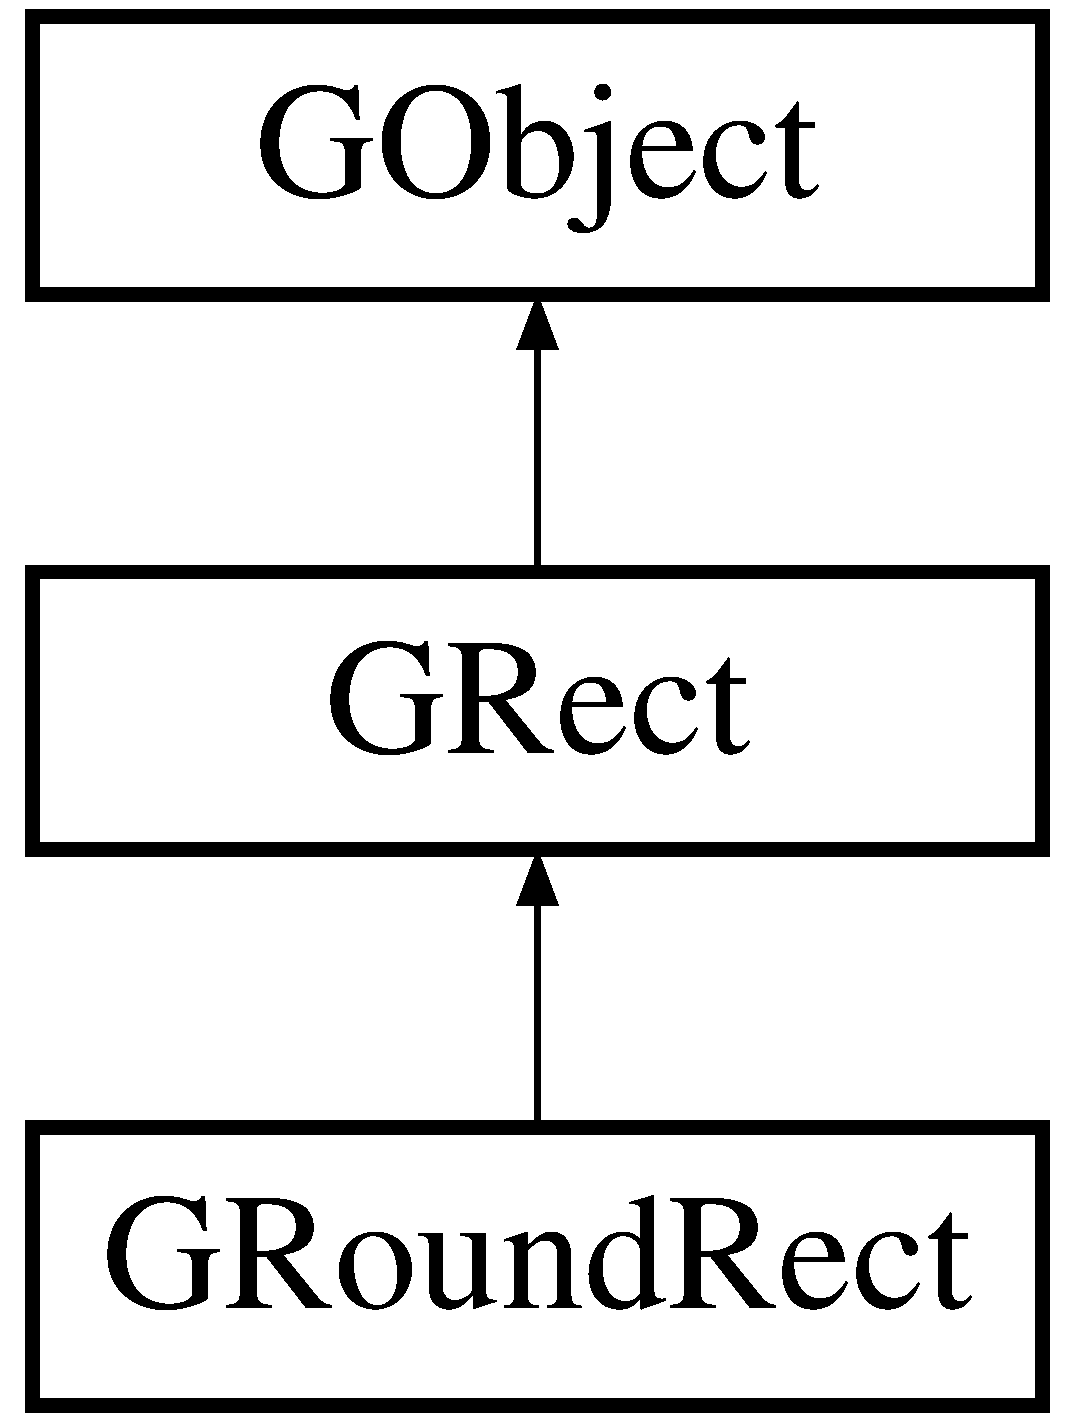
\includegraphics[height=3.000000cm]{classGRect}
\end{center}
\end{figure}
\subsection*{Public Types}
\begin{DoxyCompactItemize}
\item 
enum \mbox{\hyperlink{classGObject_a86e0f5648542856159bb40775c854aa7}{Line\+Style}} \{ \mbox{\hyperlink{classGObject_a86e0f5648542856159bb40775c854aa7acbc84bd5232621834ed31f44d457c1eb}{L\+I\+N\+E\+\_\+\+N\+O\+NE}}, 
\mbox{\hyperlink{classGObject_a86e0f5648542856159bb40775c854aa7a700c78bc2cd76acaab26651bf7b4941f}{L\+I\+N\+E\+\_\+\+S\+O\+L\+ID}}, 
\mbox{\hyperlink{classGObject_a86e0f5648542856159bb40775c854aa7a9ccba0845f785d81d07b333ae1aad84e}{L\+I\+N\+E\+\_\+\+D\+A\+SH}}, 
\mbox{\hyperlink{classGObject_a86e0f5648542856159bb40775c854aa7a8e811c096cb941997f0bfda168bb6df3}{L\+I\+N\+E\+\_\+\+D\+OT}}, 
\mbox{\hyperlink{classGObject_a86e0f5648542856159bb40775c854aa7ada15a2e3d737b2db7706d8300f91b89d}{L\+I\+N\+E\+\_\+\+D\+A\+S\+H\+\_\+\+D\+OT}}, 
\mbox{\hyperlink{classGObject_a86e0f5648542856159bb40775c854aa7aabf4053a73eafa7ba2b7e6d664c74c1d}{L\+I\+N\+E\+\_\+\+D\+A\+S\+H\+\_\+\+D\+O\+T\+\_\+\+D\+OT}}
 \}
\begin{DoxyCompactList}\small\item\em Styles that can be used for the outline around various shapes. \end{DoxyCompactList}\end{DoxyCompactItemize}
\subsection*{Public Member Functions}
\begin{DoxyCompactItemize}
\item 
\mbox{\hyperlink{classGRect_ae511b0aaa5e0546f0094513120372d90}{G\+Rect}} (double x=0, double y=0, double width=0, double height=0)
\begin{DoxyCompactList}\small\item\em Constructs a rectangle with the specified width and height. \end{DoxyCompactList}\item 
virtual bool \mbox{\hyperlink{classGObject_abb6a5d7c03e6eaaae97264c4799ce7c3}{contains}} (double x, double y) const
\begin{DoxyCompactList}\small\item\em Returns {\ttfamily true} if the specified point is inside the object. \end{DoxyCompactList}\item 
virtual bool \mbox{\hyperlink{classGObject_a1dbc9dafaae51958112dbe1267a1f547}{contains}} (const \mbox{\hyperlink{structGPoint}{G\+Point}} \&pt) const
\begin{DoxyCompactList}\small\item\em Returns {\ttfamily true} if the specified point is inside the object. \end{DoxyCompactList}\item 
virtual \mbox{\hyperlink{structGPoint}{G\+Point}} \mbox{\hyperlink{classGObject_a0d41183bf6b08de66fe3907551aab0d7}{get\+Bottom\+Right\+Location}} () const
\begin{DoxyCompactList}\small\item\em Returns the x/y coordinates of the bottom/right corner of the object. \end{DoxyCompactList}\item 
virtual double \mbox{\hyperlink{classGObject_a4316a2406c18e1c6d061fe51fd355490}{get\+BottomY}} () const
\begin{DoxyCompactList}\small\item\em Returns the {\itshape y}-\/coordinate of the bottom of the object. \end{DoxyCompactList}\item 
virtual \mbox{\hyperlink{structGRectangle}{G\+Rectangle}} \mbox{\hyperlink{classGObject_a29e6ac35a0b48f491a4c88194cc5da3b}{get\+Bounds}} () const
\begin{DoxyCompactList}\small\item\em Returns the bounding box of this object, which is defined to be the smallest rectangle that covers everything drawn by the figure. \end{DoxyCompactList}\item 
virtual \mbox{\hyperlink{structGPoint}{G\+Point}} \mbox{\hyperlink{classGObject_a0909472e91448470bccdb62ecfb95d8b}{get\+Center\+Location}} () const
\begin{DoxyCompactList}\small\item\em Returns the x/y-\/coordinates of the center of the object. \end{DoxyCompactList}\item 
virtual double \mbox{\hyperlink{classGObject_a04df74355b545e0543112d5b8d924176}{get\+CenterX}} () const
\begin{DoxyCompactList}\small\item\em Returns the {\itshape x}-\/coordinate of the center of the object. \end{DoxyCompactList}\item 
virtual double \mbox{\hyperlink{classGObject_acb3287a3d507025a26f54b895713b947}{get\+CenterY}} () const
\begin{DoxyCompactList}\small\item\em Returns the {\itshape y}-\/coordinate of the center of the object. \end{DoxyCompactList}\item 
virtual std\+::string \mbox{\hyperlink{classGObject_aa061dfa488c31e18549d64363c1d0e34}{get\+Color}} () const
\begin{DoxyCompactList}\small\item\em Returns the color used to display this object. \end{DoxyCompactList}\item 
virtual std\+::string \mbox{\hyperlink{classGObject_a76f6964a11fde7c78e9751be184e1a3c}{get\+Fill\+Color}} () const
\begin{DoxyCompactList}\small\item\em Returns the color used to display the filled region of this object. \end{DoxyCompactList}\item 
virtual double \mbox{\hyperlink{classGObject_a1e7e353362434072875264cf95629f99}{get\+Height}} () const
\begin{DoxyCompactList}\small\item\em Returns the height of this object, which is the same as the height of its bounding box. \end{DoxyCompactList}\item 
virtual \mbox{\hyperlink{classGObject_a86e0f5648542856159bb40775c854aa7}{Line\+Style}} \mbox{\hyperlink{classGObject_aaf1f5ea8281e5e3486662878d26f0a13}{get\+Line\+Style}} () const
\begin{DoxyCompactList}\small\item\em Returns the object\textquotesingle{}s style such as solid or dashed. \end{DoxyCompactList}\item 
virtual double \mbox{\hyperlink{classGObject_a85ff266dc3eb63d9f2d8e5a4487fd3c0}{get\+Line\+Width}} () const
\begin{DoxyCompactList}\small\item\em Returns the width of the line used to draw this object. \end{DoxyCompactList}\item 
virtual \mbox{\hyperlink{structGPoint}{G\+Point}} \mbox{\hyperlink{classGObject_a4f83802015511edeb63b892830812c11}{get\+Location}} () const
\begin{DoxyCompactList}\small\item\em Returns the location of the top-\/left corner of object. \end{DoxyCompactList}\item 
virtual double \mbox{\hyperlink{classGObject_a1ae3fc278cc5b71b9f2d96a8a83cdf26}{get\+Opacity}} () const
\begin{DoxyCompactList}\small\item\em Returns how opaque (non-\/transparent) this object will appear from 0.\+0 (completely transparent) to 1.\+0 (completely opaque, default). \end{DoxyCompactList}\item 
virtual \mbox{\hyperlink{classGCompound}{G\+Compound}} $\ast$ \mbox{\hyperlink{classGObject_a3e53cef70541b1a14eade4ad0984d0b4}{get\+Parent}} () const
\begin{DoxyCompactList}\small\item\em Returns a pointer to the {\ttfamily \mbox{\hyperlink{classGCompound}{G\+Compound}}} that contains this object. \end{DoxyCompactList}\item 
virtual double \mbox{\hyperlink{classGObject_a798cc79daaa10145b28f60bcdfdb0ee9}{get\+RightX}} () const
\begin{DoxyCompactList}\small\item\em Returns the {\itshape x}-\/coordinate of the right side of the object. \end{DoxyCompactList}\item 
virtual \mbox{\hyperlink{structGDimension}{G\+Dimension}} \mbox{\hyperlink{classGObject_a7b4eec96a2bdc6420695d5796a78eea9}{get\+Size}} () const
\begin{DoxyCompactList}\small\item\em Returns the size of the object as a {\ttfamily \mbox{\hyperlink{structGDimension}{G\+Dimension}}}. \end{DoxyCompactList}\item 
std\+::string \mbox{\hyperlink{classGRect_a9b72ede4ee8520f987a0c01e30654814}{get\+Type}} () const override
\begin{DoxyCompactList}\small\item\em Returns the type of the object as a string, such as {\ttfamily \char`\"{}\+G\+Oval\char`\"{}} or {\ttfamily \char`\"{}\+G\+Rect\char`\"{}}. \end{DoxyCompactList}\item 
virtual double \mbox{\hyperlink{classGObject_a0ed2965abd4f5701d2cadf71239faf19}{get\+Width}} () const
\begin{DoxyCompactList}\small\item\em Returns the width of this object, which is equal to the width of the bounding box. \end{DoxyCompactList}\item 
virtual double \mbox{\hyperlink{classGObject_a344385751bee0720059403940d57a13e}{getX}} () const
\begin{DoxyCompactList}\small\item\em Returns the leftmost {\itshape x}-\/coordinate of the object. \end{DoxyCompactList}\item 
virtual double \mbox{\hyperlink{classGObject_aafa51c7f8f38a09febbb9ce7853f77b4}{getY}} () const
\begin{DoxyCompactList}\small\item\em Returns the topmost {\itshape y}-\/coordinate of the object. \end{DoxyCompactList}\item 
virtual bool \mbox{\hyperlink{classGObject_a11c404f106940c201b6f326e0355c150}{is\+Filled}} () const
\begin{DoxyCompactList}\small\item\em Returns {\ttfamily true} if the object is filled with color. \end{DoxyCompactList}\item 
virtual bool \mbox{\hyperlink{classGObject_a9de207581cfa4ca1eaa06da5f29b75fc}{is\+Transformed}} () const
\begin{DoxyCompactList}\small\item\em Returns {\ttfamily true} if this object has been transformed by calling methods such as \mbox{\hyperlink{classGObject_ae1ffaa12185dfd5ba464f7d87c329e26}{rotate()}} or \mbox{\hyperlink{classGObject_ad2e1900f730475c2d044817db03b38d6}{scale()}} on it. \end{DoxyCompactList}\item 
virtual bool \mbox{\hyperlink{classGObject_a9d8a6cfb13917785c143e74d40e4e2be}{is\+Visible}} () const
\begin{DoxyCompactList}\small\item\em Returns {\ttfamily true} if this object is visible on screen. \end{DoxyCompactList}\item 
virtual void \mbox{\hyperlink{classGObject_a5973d8dda83afb36e2c56855515be392}{move}} (double dx, double dy)
\begin{DoxyCompactList}\small\item\em Moves the object on the screen using the displacements {\ttfamily dx} and {\ttfamily dy}. \end{DoxyCompactList}\item 
virtual void \mbox{\hyperlink{classGObject_ac827b978aa122f136a14c198687ad80f}{repaint}} ()
\begin{DoxyCompactList}\small\item\em Instructs the object to redraw itself on screen. \end{DoxyCompactList}\item 
virtual void \mbox{\hyperlink{classGObject_a6022a1fd1e5dcd2fd5585e5a36aa3f37}{reset\+Transform}} ()
\begin{DoxyCompactList}\small\item\em Undoes any previous scale/rotate transformations on this object. \end{DoxyCompactList}\item 
virtual void \mbox{\hyperlink{classGObject_ae1ffaa12185dfd5ba464f7d87c329e26}{rotate}} (double theta)
\begin{DoxyCompactList}\small\item\em Transforms the object by rotating it {\ttfamily theta} degrees counterclockwise around its origin. \end{DoxyCompactList}\item 
virtual void \mbox{\hyperlink{classGObject_ad2e1900f730475c2d044817db03b38d6}{scale}} (double sf)
\begin{DoxyCompactList}\small\item\em Scales the object by the specified scale factor. \end{DoxyCompactList}\item 
virtual void \mbox{\hyperlink{classGObject_a63641f69d610d0b951357d35a0c3b1e3}{scale}} (double sx, double sy)
\begin{DoxyCompactList}\small\item\em Scales the object by the specified scale factors. \end{DoxyCompactList}\item 
void \mbox{\hyperlink{classGObject_ab6747f40313c531c2db32edb5b63b9b7}{send\+Backward}} ()
\begin{DoxyCompactList}\small\item\em Moves this object one step toward the back in the {\itshape z} dimension. \end{DoxyCompactList}\item 
void \mbox{\hyperlink{classGObject_a710b3e449c9facba7847c91ab170d281}{send\+Forward}} ()
\begin{DoxyCompactList}\small\item\em Moves this object one step toward the front in the {\itshape z} dimension. \end{DoxyCompactList}\item 
void \mbox{\hyperlink{classGObject_a0f7f1efbb7fd46dde2867c4ad0330896}{send\+To\+Back}} ()
\begin{DoxyCompactList}\small\item\em Moves this object to the back of the display in the {\itshape z} dimension. \end{DoxyCompactList}\item 
void \mbox{\hyperlink{classGObject_aee33d68488e46827ef55fac07f40a9b2}{send\+To\+Front}} ()
\begin{DoxyCompactList}\small\item\em Moves this object to the front of the display in the {\itshape z} dimension. \end{DoxyCompactList}\item 
virtual void \mbox{\hyperlink{classGObject_a71ff7b16b8f1bdc4a1ce9f30cf8b87d8}{set\+Bottom\+Right\+Location}} (double x, double y)
\begin{DoxyCompactList}\small\item\em Sets the location of the bottom/right of this object. \end{DoxyCompactList}\item 
virtual void \mbox{\hyperlink{classGObject_ac6f7320321182f1d18c1c0fa97d5e941}{set\+Bottom\+Right\+Location}} (const \mbox{\hyperlink{structGPoint}{G\+Point}} \&pt)
\begin{DoxyCompactList}\small\item\em Sets the location of the bottom/right of this object. \end{DoxyCompactList}\item 
virtual void \mbox{\hyperlink{classGObject_a4b20e93c2a2597484f74ee5caa71f41f}{set\+BottomY}} (double y)
\begin{DoxyCompactList}\small\item\em Sets the location of the bottom y-\/coordinate of this object. \end{DoxyCompactList}\item 
virtual void \mbox{\hyperlink{classGObject_a2aae8197624b72265ab83b4f1bc73f2f}{set\+Bounds}} (double x, double y, double width, double height)
\begin{DoxyCompactList}\small\item\em Changes the bounds of this object to the specified values. \end{DoxyCompactList}\item 
virtual void \mbox{\hyperlink{classGObject_acada386653f008cacc7cce86426bef7c}{set\+Bounds}} (const \mbox{\hyperlink{structGRectangle}{G\+Rectangle}} \&size)
\begin{DoxyCompactList}\small\item\em Changes the bounds of this object to the specified rectangle. \end{DoxyCompactList}\item 
virtual void \mbox{\hyperlink{classGObject_a290b47dd8de1be44089f95cb2c47c1de}{set\+Center\+Location}} (double x, double y)
\begin{DoxyCompactList}\small\item\em Sets the location of the center of this object. \end{DoxyCompactList}\item 
virtual void \mbox{\hyperlink{classGObject_a1bedf1b233ecba3f753ec58908a683a6}{set\+Center\+Location}} (const \mbox{\hyperlink{structGPoint}{G\+Point}} \&pt)
\begin{DoxyCompactList}\small\item\em Sets the location of the center of this object. \end{DoxyCompactList}\item 
virtual void \mbox{\hyperlink{classGObject_a2f4936281e056eead00a9186b9ba8af6}{set\+CenterX}} (double x)
\begin{DoxyCompactList}\small\item\em Sets the x-\/coordinate of the center of this object. \end{DoxyCompactList}\item 
virtual void \mbox{\hyperlink{classGObject_aad2a22b4fde88c33306b92aebf641d57}{set\+CenterY}} (double y)
\begin{DoxyCompactList}\small\item\em Sets the y-\/coordinate of the center of this object. \end{DoxyCompactList}\item 
virtual void \mbox{\hyperlink{classGObject_ad57ef49bc31db94e92648aa3737923d6}{set\+Color}} (int r, int g, int b)
\begin{DoxyCompactList}\small\item\em Sets the color used to display this object. \end{DoxyCompactList}\item 
virtual void \mbox{\hyperlink{classGObject_ab1f5cc0f5cc6bbbd716a526c61f1081d}{set\+Color}} (int rgb)
\begin{DoxyCompactList}\small\item\em Sets the color used to display this object. \end{DoxyCompactList}\item 
virtual void \mbox{\hyperlink{classGObject_a61374df6c11b52cfbb0815decdbaebc6}{set\+Color}} (const std\+::string \&color)
\begin{DoxyCompactList}\small\item\em Sets the color used to display this object. \end{DoxyCompactList}\item 
virtual void \mbox{\hyperlink{classGObject_ad767a33971159e9493e221cca4c00ae9}{set\+Fill\+Color}} (int r, int g, int b)
\begin{DoxyCompactList}\small\item\em Sets the color used to display the filled region of this object, if any. \end{DoxyCompactList}\item 
virtual void \mbox{\hyperlink{classGObject_aa59d9775a67fa7df2b24a95cd34840a3}{set\+Fill\+Color}} (int rgb)
\begin{DoxyCompactList}\small\item\em Sets the color used to display the filled region of this object, if any. \end{DoxyCompactList}\item 
virtual void \mbox{\hyperlink{classGObject_adbc18b1a930aadd97d7437f9f7265b96}{set\+Fill\+Color}} (const std\+::string \&color)
\begin{DoxyCompactList}\small\item\em Sets the color used to display the filled region of this object, if any. \end{DoxyCompactList}\item 
virtual void \mbox{\hyperlink{classGObject_a9b82b53362282c6bb7d6947068d2e55b}{set\+Filled}} (bool flag)
\begin{DoxyCompactList}\small\item\em Sets the fill status for the object, where {\ttfamily false} is outlined and {\ttfamily true} is filled. \end{DoxyCompactList}\item 
virtual void \mbox{\hyperlink{classGObject_a2592348886ffea646c6534bf88f7c49d}{set\+Font}} (const Q\+Font \&font)
\begin{DoxyCompactList}\small\item\em Changes the font used to display the object as specified by the given Qt font. \end{DoxyCompactList}\item 
virtual void \mbox{\hyperlink{classGObject_a8e096e8818d838aceae1d46d58fb3a7b}{set\+Font}} (const std\+::string \&font)
\begin{DoxyCompactList}\small\item\em Changes the font used to display the object as specified by the string {\ttfamily font}, which has the following format\+: \end{DoxyCompactList}\item 
virtual void \mbox{\hyperlink{classGObject_ad18e8fab1e02a4e9b75c6730212558eb}{set\+Foreground}} (int r, int g, int b)
\begin{DoxyCompactList}\small\item\em Sets the color used to display this object. \end{DoxyCompactList}\item 
virtual void \mbox{\hyperlink{classGObject_a9eb856b5ff83a19df3831a31f15f4563}{set\+Foreground}} (int rgb)
\begin{DoxyCompactList}\small\item\em Sets the color used to display this object. \end{DoxyCompactList}\item 
virtual void \mbox{\hyperlink{classGObject_af59209aeadea6dfc6d97a2d8531f50e1}{set\+Foreground}} (const std\+::string \&color)
\begin{DoxyCompactList}\small\item\em Sets the color used to display this object. \end{DoxyCompactList}\item 
virtual void \mbox{\hyperlink{classGObject_a9e280bfc4544dfaf8e4376c4e1a74357}{set\+Height}} (double height)
\begin{DoxyCompactList}\small\item\em Changes the height of this object to the specified height without changing its width. \end{DoxyCompactList}\item 
virtual void \mbox{\hyperlink{classGObject_add11575087eb94f1a71faa3f826c6341}{set\+Line\+Style}} (\mbox{\hyperlink{classGObject_a86e0f5648542856159bb40775c854aa7}{Line\+Style}} line\+Style)
\begin{DoxyCompactList}\small\item\em Sets the object\textquotesingle{}s style such as solid (\mbox{\hyperlink{classGObject_a86e0f5648542856159bb40775c854aa7a700c78bc2cd76acaab26651bf7b4941f}{G\+Object\+::\+L\+I\+N\+E\+\_\+\+S\+O\+L\+ID}}) or dashed (\mbox{\hyperlink{classGObject_a86e0f5648542856159bb40775c854aa7a9ccba0845f785d81d07b333ae1aad84e}{G\+Object\+::\+L\+I\+N\+E\+\_\+\+D\+A\+SH}}). \end{DoxyCompactList}\item 
virtual void \mbox{\hyperlink{classGObject_afd6a47c6ea6a1f85ca05a65ba3ff3477}{set\+Line\+Width}} (double line\+Width)
\begin{DoxyCompactList}\small\item\em Sets the width of the line used to draw this object. \end{DoxyCompactList}\item 
virtual void \mbox{\hyperlink{classGObject_a04594e8ba9b98513a64f1da00dcae18c}{set\+Location}} (double x, double y)
\begin{DoxyCompactList}\small\item\em Sets the location of the top-\/left corner of this object to the specified coordinates. \end{DoxyCompactList}\item 
virtual void \mbox{\hyperlink{classGObject_aa8480c0b7166cdf8f784cece06ab353f}{set\+Location}} (const \mbox{\hyperlink{structGPoint}{G\+Point}} \&pt)
\begin{DoxyCompactList}\small\item\em Sets the location of the top-\/left corner of this object to the specified point. \end{DoxyCompactList}\item 
virtual void \mbox{\hyperlink{classGObject_a04af1866cc1bae4a1226695794a50539}{set\+Opacity}} (double opacity)
\begin{DoxyCompactList}\small\item\em Sets how opaque (non-\/transparent) this object will appear from 0.\+0 (completely transparent) to 1.\+0 (completely opaque, default). \end{DoxyCompactList}\item 
virtual void \mbox{\hyperlink{classGObject_a3c90b758cdc2c911c9ef76c4360eb912}{set\+RightX}} (double x)
\begin{DoxyCompactList}\small\item\em Sets the location of the rightmost x-\/coordinate of this object. \end{DoxyCompactList}\item 
virtual void \mbox{\hyperlink{classGObject_aca25d49481f9bf5fc8f7df4c086c4ce7}{set\+Size}} (double width, double height)
\begin{DoxyCompactList}\small\item\em Changes the size of this object to the specified width and height. \end{DoxyCompactList}\item 
virtual void \mbox{\hyperlink{classGObject_ae2b628228f192c2702c4ce941b2af68f}{set\+Size}} (const \mbox{\hyperlink{structGDimension}{G\+Dimension}} \&size)
\begin{DoxyCompactList}\small\item\em Changes the size of this object to the specified width and height. \end{DoxyCompactList}\item 
virtual void \mbox{\hyperlink{classGObject_a88203f28224315d9f4471212f4af8ed3}{set\+Visible}} (bool flag)
\begin{DoxyCompactList}\small\item\em Sets whether this object is visible. \end{DoxyCompactList}\item 
virtual void \mbox{\hyperlink{classGObject_aa3f3fba4cb131baa8696ba01e3bceca1}{set\+Width}} (double width)
\begin{DoxyCompactList}\small\item\em Changes the width of this object to the specified width without changing its height. \end{DoxyCompactList}\item 
virtual void \mbox{\hyperlink{classGObject_a9c18fcc579333bf9653d13ad2b372e39}{setX}} (double x)
\begin{DoxyCompactList}\small\item\em Sets the x location of the left side of this object. \end{DoxyCompactList}\item 
virtual void \mbox{\hyperlink{classGObject_a7d57e2a5c35d27feb58fd498a3cf82b9}{setY}} (double y)
\begin{DoxyCompactList}\small\item\em Sets the y location of the top of this object. \end{DoxyCompactList}\item 
virtual std\+::string \mbox{\hyperlink{classGObject_a1fe5121d6528fdea3f243321b3fa3a49}{to\+String}} () const
\begin{DoxyCompactList}\small\item\em Returns a printable representation of the object. \end{DoxyCompactList}\end{DoxyCompactItemize}
\subsection*{Static Public Member Functions}
\begin{DoxyCompactItemize}
\item 
static bool \mbox{\hyperlink{classGObject_a93be0e1fe1b1bf1a1da732470c94f42b}{is\+Anti\+Aliasing}} ()
\begin{DoxyCompactList}\small\item\em Returns whether we should globally anti-\/alias graphical objects. \end{DoxyCompactList}\item 
static void \mbox{\hyperlink{classGObject_a1e43371668ae850193cebedb44e1bbe3}{set\+Anti\+Aliasing}} (bool value)
\begin{DoxyCompactList}\small\item\em Globally turns on/off the anti-\/aliasing feature that smooths out the edges of onscreen shapes. \end{DoxyCompactList}\end{DoxyCompactItemize}
\subsection*{Protected Member Functions}
\begin{DoxyCompactItemize}
\item 
virtual std\+::string \mbox{\hyperlink{classGObject_a4fcdf8de5c6de92242a975d83d8f23ea}{to\+String\+Extra}} () const
\begin{DoxyCompactList}\small\item\em Returns a string containing any extra unique information about this type of graphical object. \end{DoxyCompactList}\end{DoxyCompactItemize}
\subsection*{Protected Attributes}
\begin{DoxyCompactItemize}
\item 
Q\+Brush \mbox{\hyperlink{classGObject_aab24462ec896b596d99911767b0912d0}{\+\_\+brush}}
\item 
std\+::string \mbox{\hyperlink{classGObject_a1134e770ae4315ea8bc1201e2f21da8b}{\+\_\+color}}
\item 
int \mbox{\hyperlink{classGObject_a003fdd343d9b7505c53a8b7a134200ed}{\+\_\+color\+Int}}
\item 
std\+::string \mbox{\hyperlink{classGObject_a179f8d6cee65cd8a54692e32b224392a}{\+\_\+fill\+Color}}
\item 
int \mbox{\hyperlink{classGObject_a751def333a67d651e5b99cc331ecb496}{\+\_\+fill\+Color\+Int}}
\item 
bool \mbox{\hyperlink{classGObject_ad4a55cbcd61b58a4d49666490bb2f103}{\+\_\+fill\+Flag}}
\item 
std\+::string \mbox{\hyperlink{classGObject_aea76ea1a8b5dd7b0a78653277e63b536}{\+\_\+font}}
\item 
double \mbox{\hyperlink{classGObject_ad05df29e7f27fc504abd743e3d8b4e73}{\+\_\+height}}
\item 
\mbox{\hyperlink{classGObject_a86e0f5648542856159bb40775c854aa7}{Line\+Style}} \mbox{\hyperlink{classGObject_a89bafecaafb7c72d55c7efc10b7d0523}{\+\_\+line\+Style}}
\item 
double \mbox{\hyperlink{classGObject_a16e9033665937f13de2e163dc2184aff}{\+\_\+line\+Width}}
\item 
double \mbox{\hyperlink{classGObject_a20eff8eb7af27182edc9bfc54768b6f3}{\+\_\+opacity}}
\item 
\mbox{\hyperlink{classGCompound}{G\+Compound}} $\ast$ \mbox{\hyperlink{classGObject_ac9452c1eaff70eebddbb318196aa3835}{\+\_\+parent}}
\item 
Q\+Pen \mbox{\hyperlink{classGObject_afb69d172743f868299847174eb1b6bc8}{\+\_\+pen}}
\item 
Q\+Transform \mbox{\hyperlink{classGObject_a475b8860a5f1adb4a1fdc58d1f5c1e32}{\+\_\+transform}}
\item 
bool \mbox{\hyperlink{classGObject_ae4725802fc8d8aaa0ab4bd4781f7e07c}{\+\_\+transformed}}
\item 
bool \mbox{\hyperlink{classGObject_a9312c72508471b7c7a87b540263e1af4}{\+\_\+visible}}
\item 
double \mbox{\hyperlink{classGObject_ab55d85a3371770e6725b1062cf160cd8}{\+\_\+width}}
\item 
double \mbox{\hyperlink{classGObject_a6675b83b27137b8d3aa2ad8133078ea6}{\+\_\+x}}
\item 
double \mbox{\hyperlink{classGObject_a2f0f6aeafddc8a39c578bfa7e22b5f1e}{\+\_\+y}}
\end{DoxyCompactItemize}


\subsection{Detailed Description}
A \mbox{\hyperlink{classGRect}{G\+Rect}} is a graphical object whose appearance consists of a rectangular box. 

\subsection{Member Enumeration Documentation}
\mbox{\Hypertarget{classGObject_a86e0f5648542856159bb40775c854aa7}\label{classGObject_a86e0f5648542856159bb40775c854aa7}} 
\index{G\+Rect@{G\+Rect}!Line\+Style@{Line\+Style}}
\index{Line\+Style@{Line\+Style}!G\+Rect@{G\+Rect}}
\subsubsection{\texorpdfstring{Line\+Style}{LineStyle}}
{\footnotesize\ttfamily enum \mbox{\hyperlink{classGObject_a86e0f5648542856159bb40775c854aa7}{Line\+Style}}\hspace{0.3cm}{\ttfamily [inherited]}}



Styles that can be used for the outline around various shapes. 

Call set\+Line\+Style on a \mbox{\hyperlink{classGObject}{G\+Object}} and pass one of these values. \begin{DoxyEnumFields}{Enumerator}
\raisebox{\heightof{T}}[0pt][0pt]{\index{L\+I\+N\+E\+\_\+\+N\+O\+NE@{L\+I\+N\+E\+\_\+\+N\+O\+NE}!G\+Rect@{G\+Rect}}\index{G\+Rect@{G\+Rect}!L\+I\+N\+E\+\_\+\+N\+O\+NE@{L\+I\+N\+E\+\_\+\+N\+O\+NE}}}\mbox{\Hypertarget{classGObject_a86e0f5648542856159bb40775c854aa7acbc84bd5232621834ed31f44d457c1eb}\label{classGObject_a86e0f5648542856159bb40775c854aa7acbc84bd5232621834ed31f44d457c1eb}} 
L\+I\+N\+E\+\_\+\+N\+O\+NE&\\
\hline

\raisebox{\heightof{T}}[0pt][0pt]{\index{L\+I\+N\+E\+\_\+\+S\+O\+L\+ID@{L\+I\+N\+E\+\_\+\+S\+O\+L\+ID}!G\+Rect@{G\+Rect}}\index{G\+Rect@{G\+Rect}!L\+I\+N\+E\+\_\+\+S\+O\+L\+ID@{L\+I\+N\+E\+\_\+\+S\+O\+L\+ID}}}\mbox{\Hypertarget{classGObject_a86e0f5648542856159bb40775c854aa7a700c78bc2cd76acaab26651bf7b4941f}\label{classGObject_a86e0f5648542856159bb40775c854aa7a700c78bc2cd76acaab26651bf7b4941f}} 
L\+I\+N\+E\+\_\+\+S\+O\+L\+ID&\\
\hline

\raisebox{\heightof{T}}[0pt][0pt]{\index{L\+I\+N\+E\+\_\+\+D\+A\+SH@{L\+I\+N\+E\+\_\+\+D\+A\+SH}!G\+Rect@{G\+Rect}}\index{G\+Rect@{G\+Rect}!L\+I\+N\+E\+\_\+\+D\+A\+SH@{L\+I\+N\+E\+\_\+\+D\+A\+SH}}}\mbox{\Hypertarget{classGObject_a86e0f5648542856159bb40775c854aa7a9ccba0845f785d81d07b333ae1aad84e}\label{classGObject_a86e0f5648542856159bb40775c854aa7a9ccba0845f785d81d07b333ae1aad84e}} 
L\+I\+N\+E\+\_\+\+D\+A\+SH&\\
\hline

\raisebox{\heightof{T}}[0pt][0pt]{\index{L\+I\+N\+E\+\_\+\+D\+OT@{L\+I\+N\+E\+\_\+\+D\+OT}!G\+Rect@{G\+Rect}}\index{G\+Rect@{G\+Rect}!L\+I\+N\+E\+\_\+\+D\+OT@{L\+I\+N\+E\+\_\+\+D\+OT}}}\mbox{\Hypertarget{classGObject_a86e0f5648542856159bb40775c854aa7a8e811c096cb941997f0bfda168bb6df3}\label{classGObject_a86e0f5648542856159bb40775c854aa7a8e811c096cb941997f0bfda168bb6df3}} 
L\+I\+N\+E\+\_\+\+D\+OT&\\
\hline

\raisebox{\heightof{T}}[0pt][0pt]{\index{L\+I\+N\+E\+\_\+\+D\+A\+S\+H\+\_\+\+D\+OT@{L\+I\+N\+E\+\_\+\+D\+A\+S\+H\+\_\+\+D\+OT}!G\+Rect@{G\+Rect}}\index{G\+Rect@{G\+Rect}!L\+I\+N\+E\+\_\+\+D\+A\+S\+H\+\_\+\+D\+OT@{L\+I\+N\+E\+\_\+\+D\+A\+S\+H\+\_\+\+D\+OT}}}\mbox{\Hypertarget{classGObject_a86e0f5648542856159bb40775c854aa7ada15a2e3d737b2db7706d8300f91b89d}\label{classGObject_a86e0f5648542856159bb40775c854aa7ada15a2e3d737b2db7706d8300f91b89d}} 
L\+I\+N\+E\+\_\+\+D\+A\+S\+H\+\_\+\+D\+OT&\\
\hline

\raisebox{\heightof{T}}[0pt][0pt]{\index{L\+I\+N\+E\+\_\+\+D\+A\+S\+H\+\_\+\+D\+O\+T\+\_\+\+D\+OT@{L\+I\+N\+E\+\_\+\+D\+A\+S\+H\+\_\+\+D\+O\+T\+\_\+\+D\+OT}!G\+Rect@{G\+Rect}}\index{G\+Rect@{G\+Rect}!L\+I\+N\+E\+\_\+\+D\+A\+S\+H\+\_\+\+D\+O\+T\+\_\+\+D\+OT@{L\+I\+N\+E\+\_\+\+D\+A\+S\+H\+\_\+\+D\+O\+T\+\_\+\+D\+OT}}}\mbox{\Hypertarget{classGObject_a86e0f5648542856159bb40775c854aa7aabf4053a73eafa7ba2b7e6d664c74c1d}\label{classGObject_a86e0f5648542856159bb40775c854aa7aabf4053a73eafa7ba2b7e6d664c74c1d}} 
L\+I\+N\+E\+\_\+\+D\+A\+S\+H\+\_\+\+D\+O\+T\+\_\+\+D\+OT&\\
\hline

\end{DoxyEnumFields}


\subsection{Constructor \& Destructor Documentation}
\mbox{\Hypertarget{classGRect_ae511b0aaa5e0546f0094513120372d90}\label{classGRect_ae511b0aaa5e0546f0094513120372d90}} 
\index{G\+Rect@{G\+Rect}!G\+Rect@{G\+Rect}}
\index{G\+Rect@{G\+Rect}!G\+Rect@{G\+Rect}}
\subsubsection{\texorpdfstring{G\+Rect()}{GRect()}}
{\footnotesize\ttfamily \mbox{\hyperlink{classGRect}{G\+Rect}} (\begin{DoxyParamCaption}\item[{double}]{x = {\ttfamily 0},  }\item[{double}]{y = {\ttfamily 0},  }\item[{double}]{width = {\ttfamily 0},  }\item[{double}]{height = {\ttfamily 0} }\end{DoxyParamCaption})}



Constructs a rectangle with the specified width and height. 

The first form is positioned at the origin; the second at the coordinates given by {\ttfamily x} and {\ttfamily y}. 

\subsection{Member Function Documentation}
\mbox{\Hypertarget{classGObject_abb6a5d7c03e6eaaae97264c4799ce7c3}\label{classGObject_abb6a5d7c03e6eaaae97264c4799ce7c3}} 
\index{G\+Rect@{G\+Rect}!contains@{contains}}
\index{contains@{contains}!G\+Rect@{G\+Rect}}
\subsubsection{\texorpdfstring{contains()}{contains()}\hspace{0.1cm}{\footnotesize\ttfamily [1/2]}}
{\footnotesize\ttfamily bool contains (\begin{DoxyParamCaption}\item[{double}]{x,  }\item[{double}]{y }\end{DoxyParamCaption}) const\hspace{0.3cm}{\ttfamily [virtual]}, {\ttfamily [inherited]}}



Returns {\ttfamily true} if the specified point is inside the object. 



Reimplemented in \mbox{\hyperlink{classGRoundRect_ad973a1d55799d3a73bf8b04986cd804e}{G\+Round\+Rect}}, \mbox{\hyperlink{classGPolygon_ad973a1d55799d3a73bf8b04986cd804e}{G\+Polygon}}, \mbox{\hyperlink{classGOval_ad973a1d55799d3a73bf8b04986cd804e}{G\+Oval}}, \mbox{\hyperlink{classGLine_ad973a1d55799d3a73bf8b04986cd804e}{G\+Line}}, \mbox{\hyperlink{classGCompound_ad973a1d55799d3a73bf8b04986cd804e}{G\+Compound}}, and \mbox{\hyperlink{classGArc_ad973a1d55799d3a73bf8b04986cd804e}{G\+Arc}}.

\mbox{\Hypertarget{classGObject_a1dbc9dafaae51958112dbe1267a1f547}\label{classGObject_a1dbc9dafaae51958112dbe1267a1f547}} 
\index{G\+Rect@{G\+Rect}!contains@{contains}}
\index{contains@{contains}!G\+Rect@{G\+Rect}}
\subsubsection{\texorpdfstring{contains()}{contains()}\hspace{0.1cm}{\footnotesize\ttfamily [2/2]}}
{\footnotesize\ttfamily bool contains (\begin{DoxyParamCaption}\item[{const \mbox{\hyperlink{structGPoint}{G\+Point}} \&}]{pt }\end{DoxyParamCaption}) const\hspace{0.3cm}{\ttfamily [virtual]}, {\ttfamily [inherited]}}



Returns {\ttfamily true} if the specified point is inside the object. 

\mbox{\Hypertarget{classGObject_a0d41183bf6b08de66fe3907551aab0d7}\label{classGObject_a0d41183bf6b08de66fe3907551aab0d7}} 
\index{G\+Rect@{G\+Rect}!get\+Bottom\+Right\+Location@{get\+Bottom\+Right\+Location}}
\index{get\+Bottom\+Right\+Location@{get\+Bottom\+Right\+Location}!G\+Rect@{G\+Rect}}
\subsubsection{\texorpdfstring{get\+Bottom\+Right\+Location()}{getBottomRightLocation()}}
{\footnotesize\ttfamily \mbox{\hyperlink{structGPoint}{G\+Point}} get\+Bottom\+Right\+Location (\begin{DoxyParamCaption}{ }\end{DoxyParamCaption}) const\hspace{0.3cm}{\ttfamily [virtual]}, {\ttfamily [inherited]}}



Returns the x/y coordinates of the bottom/right corner of the object. 

\mbox{\Hypertarget{classGObject_a4316a2406c18e1c6d061fe51fd355490}\label{classGObject_a4316a2406c18e1c6d061fe51fd355490}} 
\index{G\+Rect@{G\+Rect}!get\+BottomY@{get\+BottomY}}
\index{get\+BottomY@{get\+BottomY}!G\+Rect@{G\+Rect}}
\subsubsection{\texorpdfstring{get\+Bottom\+Y()}{getBottomY()}}
{\footnotesize\ttfamily double get\+BottomY (\begin{DoxyParamCaption}{ }\end{DoxyParamCaption}) const\hspace{0.3cm}{\ttfamily [virtual]}, {\ttfamily [inherited]}}



Returns the {\itshape y}-\/coordinate of the bottom of the object. 

Equivalent to the top y-\/coordinate plus the object\textquotesingle{}s height. \mbox{\Hypertarget{classGObject_a29e6ac35a0b48f491a4c88194cc5da3b}\label{classGObject_a29e6ac35a0b48f491a4c88194cc5da3b}} 
\index{G\+Rect@{G\+Rect}!get\+Bounds@{get\+Bounds}}
\index{get\+Bounds@{get\+Bounds}!G\+Rect@{G\+Rect}}
\subsubsection{\texorpdfstring{get\+Bounds()}{getBounds()}}
{\footnotesize\ttfamily \mbox{\hyperlink{structGRectangle}{G\+Rectangle}} get\+Bounds (\begin{DoxyParamCaption}{ }\end{DoxyParamCaption}) const\hspace{0.3cm}{\ttfamily [virtual]}, {\ttfamily [inherited]}}



Returns the bounding box of this object, which is defined to be the smallest rectangle that covers everything drawn by the figure. 

The coordinates of this rectangle do not necessarily match the location returned by {\ttfamily get\+Location}. Given a {\ttfamily \mbox{\hyperlink{classGText}{G\+Text}}} object, for example, {\ttfamily get\+Location} returns the coordinates of the point on the baseline at which the string begins; the {\ttfamily get\+Bounds} method, by contrast, returns a rectangle that covers the entire window area occupied by the string. 

Reimplemented in \mbox{\hyperlink{classGText_a89040ce9277825772d359fccd33bca86}{G\+Text}}, \mbox{\hyperlink{classGPolygon_a89040ce9277825772d359fccd33bca86}{G\+Polygon}}, \mbox{\hyperlink{classGLine_a89040ce9277825772d359fccd33bca86}{G\+Line}}, \mbox{\hyperlink{classGCompound_a89040ce9277825772d359fccd33bca86}{G\+Compound}}, and \mbox{\hyperlink{classGArc_a89040ce9277825772d359fccd33bca86}{G\+Arc}}.

\mbox{\Hypertarget{classGObject_a0909472e91448470bccdb62ecfb95d8b}\label{classGObject_a0909472e91448470bccdb62ecfb95d8b}} 
\index{G\+Rect@{G\+Rect}!get\+Center\+Location@{get\+Center\+Location}}
\index{get\+Center\+Location@{get\+Center\+Location}!G\+Rect@{G\+Rect}}
\subsubsection{\texorpdfstring{get\+Center\+Location()}{getCenterLocation()}}
{\footnotesize\ttfamily \mbox{\hyperlink{structGPoint}{G\+Point}} get\+Center\+Location (\begin{DoxyParamCaption}{ }\end{DoxyParamCaption}) const\hspace{0.3cm}{\ttfamily [virtual]}, {\ttfamily [inherited]}}



Returns the x/y-\/coordinates of the center of the object. 

Equivalent to the top/left plus half the object\textquotesingle{}s size. \mbox{\Hypertarget{classGObject_a04df74355b545e0543112d5b8d924176}\label{classGObject_a04df74355b545e0543112d5b8d924176}} 
\index{G\+Rect@{G\+Rect}!get\+CenterX@{get\+CenterX}}
\index{get\+CenterX@{get\+CenterX}!G\+Rect@{G\+Rect}}
\subsubsection{\texorpdfstring{get\+Center\+X()}{getCenterX()}}
{\footnotesize\ttfamily double get\+CenterX (\begin{DoxyParamCaption}{ }\end{DoxyParamCaption}) const\hspace{0.3cm}{\ttfamily [virtual]}, {\ttfamily [inherited]}}



Returns the {\itshape x}-\/coordinate of the center of the object. 

Equivalent to the top/left plus half the object\textquotesingle{}s width. \mbox{\Hypertarget{classGObject_acb3287a3d507025a26f54b895713b947}\label{classGObject_acb3287a3d507025a26f54b895713b947}} 
\index{G\+Rect@{G\+Rect}!get\+CenterY@{get\+CenterY}}
\index{get\+CenterY@{get\+CenterY}!G\+Rect@{G\+Rect}}
\subsubsection{\texorpdfstring{get\+Center\+Y()}{getCenterY()}}
{\footnotesize\ttfamily double get\+CenterY (\begin{DoxyParamCaption}{ }\end{DoxyParamCaption}) const\hspace{0.3cm}{\ttfamily [virtual]}, {\ttfamily [inherited]}}



Returns the {\itshape y}-\/coordinate of the center of the object. 

Equivalent to the top/left plus half the object\textquotesingle{}s height. \mbox{\Hypertarget{classGObject_aa061dfa488c31e18549d64363c1d0e34}\label{classGObject_aa061dfa488c31e18549d64363c1d0e34}} 
\index{G\+Rect@{G\+Rect}!get\+Color@{get\+Color}}
\index{get\+Color@{get\+Color}!G\+Rect@{G\+Rect}}
\subsubsection{\texorpdfstring{get\+Color()}{getColor()}}
{\footnotesize\ttfamily std\+::string get\+Color (\begin{DoxyParamCaption}{ }\end{DoxyParamCaption}) const\hspace{0.3cm}{\ttfamily [virtual]}, {\ttfamily [inherited]}}



Returns the color used to display this object. 

This color is always returned as a string in the form {\ttfamily \char`\"{}\#rrggbb\char`\"{}}, where {\ttfamily rr}, {\ttfamily gg}, and {\ttfamily bb} are the red, green, and blue components of the color, expressed as two-\/digit hexadecimal values. \mbox{\Hypertarget{classGObject_a76f6964a11fde7c78e9751be184e1a3c}\label{classGObject_a76f6964a11fde7c78e9751be184e1a3c}} 
\index{G\+Rect@{G\+Rect}!get\+Fill\+Color@{get\+Fill\+Color}}
\index{get\+Fill\+Color@{get\+Fill\+Color}!G\+Rect@{G\+Rect}}
\subsubsection{\texorpdfstring{get\+Fill\+Color()}{getFillColor()}}
{\footnotesize\ttfamily std\+::string get\+Fill\+Color (\begin{DoxyParamCaption}{ }\end{DoxyParamCaption}) const\hspace{0.3cm}{\ttfamily [virtual]}, {\ttfamily [inherited]}}



Returns the color used to display the filled region of this object. 

If none has been set, returns the empty string. \mbox{\Hypertarget{classGObject_a1e7e353362434072875264cf95629f99}\label{classGObject_a1e7e353362434072875264cf95629f99}} 
\index{G\+Rect@{G\+Rect}!get\+Height@{get\+Height}}
\index{get\+Height@{get\+Height}!G\+Rect@{G\+Rect}}
\subsubsection{\texorpdfstring{get\+Height()}{getHeight()}}
{\footnotesize\ttfamily double get\+Height (\begin{DoxyParamCaption}{ }\end{DoxyParamCaption}) const\hspace{0.3cm}{\ttfamily [virtual]}, {\ttfamily [inherited]}}



Returns the height of this object, which is the same as the height of its bounding box. 



Reimplemented in \mbox{\hyperlink{classGPolygon_a2bede8b27b21ae4c7940e762cbad9e07}{G\+Polygon}}, and \mbox{\hyperlink{classGLine_a2bede8b27b21ae4c7940e762cbad9e07}{G\+Line}}.

\mbox{\Hypertarget{classGObject_aaf1f5ea8281e5e3486662878d26f0a13}\label{classGObject_aaf1f5ea8281e5e3486662878d26f0a13}} 
\index{G\+Rect@{G\+Rect}!get\+Line\+Style@{get\+Line\+Style}}
\index{get\+Line\+Style@{get\+Line\+Style}!G\+Rect@{G\+Rect}}
\subsubsection{\texorpdfstring{get\+Line\+Style()}{getLineStyle()}}
{\footnotesize\ttfamily \mbox{\hyperlink{classGObject_a86e0f5648542856159bb40775c854aa7}{G\+Object\+::\+Line\+Style}} get\+Line\+Style (\begin{DoxyParamCaption}{ }\end{DoxyParamCaption}) const\hspace{0.3cm}{\ttfamily [virtual]}, {\ttfamily [inherited]}}



Returns the object\textquotesingle{}s style such as solid or dashed. 

\mbox{\Hypertarget{classGObject_a85ff266dc3eb63d9f2d8e5a4487fd3c0}\label{classGObject_a85ff266dc3eb63d9f2d8e5a4487fd3c0}} 
\index{G\+Rect@{G\+Rect}!get\+Line\+Width@{get\+Line\+Width}}
\index{get\+Line\+Width@{get\+Line\+Width}!G\+Rect@{G\+Rect}}
\subsubsection{\texorpdfstring{get\+Line\+Width()}{getLineWidth()}}
{\footnotesize\ttfamily double get\+Line\+Width (\begin{DoxyParamCaption}{ }\end{DoxyParamCaption}) const\hspace{0.3cm}{\ttfamily [virtual]}, {\ttfamily [inherited]}}



Returns the width of the line used to draw this object. 

\begin{DoxyReturn}{Returns}
default 1 
\end{DoxyReturn}
\mbox{\Hypertarget{classGObject_a4f83802015511edeb63b892830812c11}\label{classGObject_a4f83802015511edeb63b892830812c11}} 
\index{G\+Rect@{G\+Rect}!get\+Location@{get\+Location}}
\index{get\+Location@{get\+Location}!G\+Rect@{G\+Rect}}
\subsubsection{\texorpdfstring{get\+Location()}{getLocation()}}
{\footnotesize\ttfamily \mbox{\hyperlink{structGPoint}{G\+Point}} get\+Location (\begin{DoxyParamCaption}{ }\end{DoxyParamCaption}) const\hspace{0.3cm}{\ttfamily [virtual]}, {\ttfamily [inherited]}}



Returns the location of the top-\/left corner of object. 

\mbox{\Hypertarget{classGObject_a1ae3fc278cc5b71b9f2d96a8a83cdf26}\label{classGObject_a1ae3fc278cc5b71b9f2d96a8a83cdf26}} 
\index{G\+Rect@{G\+Rect}!get\+Opacity@{get\+Opacity}}
\index{get\+Opacity@{get\+Opacity}!G\+Rect@{G\+Rect}}
\subsubsection{\texorpdfstring{get\+Opacity()}{getOpacity()}}
{\footnotesize\ttfamily double get\+Opacity (\begin{DoxyParamCaption}{ }\end{DoxyParamCaption}) const\hspace{0.3cm}{\ttfamily [virtual]}, {\ttfamily [inherited]}}



Returns how opaque (non-\/transparent) this object will appear from 0.\+0 (completely transparent) to 1.\+0 (completely opaque, default). 

\mbox{\Hypertarget{classGObject_a3e53cef70541b1a14eade4ad0984d0b4}\label{classGObject_a3e53cef70541b1a14eade4ad0984d0b4}} 
\index{G\+Rect@{G\+Rect}!get\+Parent@{get\+Parent}}
\index{get\+Parent@{get\+Parent}!G\+Rect@{G\+Rect}}
\subsubsection{\texorpdfstring{get\+Parent()}{getParent()}}
{\footnotesize\ttfamily \mbox{\hyperlink{classGCompound}{G\+Compound}} $\ast$ get\+Parent (\begin{DoxyParamCaption}{ }\end{DoxyParamCaption}) const\hspace{0.3cm}{\ttfamily [virtual]}, {\ttfamily [inherited]}}



Returns a pointer to the {\ttfamily \mbox{\hyperlink{classGCompound}{G\+Compound}}} that contains this object. 

Every {\ttfamily \mbox{\hyperlink{classGWindow}{G\+Window}}} is initialized to contain a single {\ttfamily \mbox{\hyperlink{classGCompound}{G\+Compound}}} that is aligned with the window. Adding objects to the window adds them to that {\ttfamily \mbox{\hyperlink{classGCompound}{G\+Compound}}}, which means that every object you add to the window has a parent. Calling {\ttfamily get\+Parent} on the top-\/level {\ttfamily \mbox{\hyperlink{classGCompound}{G\+Compound}}} returns {\ttfamily nullptr}. \mbox{\Hypertarget{classGObject_a798cc79daaa10145b28f60bcdfdb0ee9}\label{classGObject_a798cc79daaa10145b28f60bcdfdb0ee9}} 
\index{G\+Rect@{G\+Rect}!get\+RightX@{get\+RightX}}
\index{get\+RightX@{get\+RightX}!G\+Rect@{G\+Rect}}
\subsubsection{\texorpdfstring{get\+Right\+X()}{getRightX()}}
{\footnotesize\ttfamily double get\+RightX (\begin{DoxyParamCaption}{ }\end{DoxyParamCaption}) const\hspace{0.3cm}{\ttfamily [virtual]}, {\ttfamily [inherited]}}



Returns the {\itshape x}-\/coordinate of the right side of the object. 

Equivalent to the left x-\/coordinate plus the object\textquotesingle{}s width. \mbox{\Hypertarget{classGObject_a7b4eec96a2bdc6420695d5796a78eea9}\label{classGObject_a7b4eec96a2bdc6420695d5796a78eea9}} 
\index{G\+Rect@{G\+Rect}!get\+Size@{get\+Size}}
\index{get\+Size@{get\+Size}!G\+Rect@{G\+Rect}}
\subsubsection{\texorpdfstring{get\+Size()}{getSize()}}
{\footnotesize\ttfamily \mbox{\hyperlink{structGDimension}{G\+Dimension}} get\+Size (\begin{DoxyParamCaption}{ }\end{DoxyParamCaption}) const\hspace{0.3cm}{\ttfamily [virtual]}, {\ttfamily [inherited]}}



Returns the size of the object as a {\ttfamily \mbox{\hyperlink{structGDimension}{G\+Dimension}}}. 

\mbox{\Hypertarget{classGRect_a9b72ede4ee8520f987a0c01e30654814}\label{classGRect_a9b72ede4ee8520f987a0c01e30654814}} 
\index{G\+Rect@{G\+Rect}!get\+Type@{get\+Type}}
\index{get\+Type@{get\+Type}!G\+Rect@{G\+Rect}}
\subsubsection{\texorpdfstring{get\+Type()}{getType()}}
{\footnotesize\ttfamily std\+::string get\+Type (\begin{DoxyParamCaption}{ }\end{DoxyParamCaption}) const\hspace{0.3cm}{\ttfamily [override]}, {\ttfamily [virtual]}}



Returns the type of the object as a string, such as {\ttfamily \char`\"{}\+G\+Oval\char`\"{}} or {\ttfamily \char`\"{}\+G\+Rect\char`\"{}}. 

Each \mbox{\hyperlink{classGObject}{G\+Object}} subtype must override this method. 

Implements \mbox{\hyperlink{classGObject_a799e073a127b428cc841086d42ea4fed}{G\+Object}}.



Reimplemented in \mbox{\hyperlink{classGRoundRect_a9b72ede4ee8520f987a0c01e30654814}{G\+Round\+Rect}}.

\mbox{\Hypertarget{classGObject_a0ed2965abd4f5701d2cadf71239faf19}\label{classGObject_a0ed2965abd4f5701d2cadf71239faf19}} 
\index{G\+Rect@{G\+Rect}!get\+Width@{get\+Width}}
\index{get\+Width@{get\+Width}!G\+Rect@{G\+Rect}}
\subsubsection{\texorpdfstring{get\+Width()}{getWidth()}}
{\footnotesize\ttfamily double get\+Width (\begin{DoxyParamCaption}{ }\end{DoxyParamCaption}) const\hspace{0.3cm}{\ttfamily [virtual]}, {\ttfamily [inherited]}}



Returns the width of this object, which is equal to the width of the bounding box. 



Reimplemented in \mbox{\hyperlink{classGPolygon_ab7b172cec7ed45e1246a3ce3160a62f7}{G\+Polygon}}, and \mbox{\hyperlink{classGLine_ab7b172cec7ed45e1246a3ce3160a62f7}{G\+Line}}.

\mbox{\Hypertarget{classGObject_a344385751bee0720059403940d57a13e}\label{classGObject_a344385751bee0720059403940d57a13e}} 
\index{G\+Rect@{G\+Rect}!getX@{getX}}
\index{getX@{getX}!G\+Rect@{G\+Rect}}
\subsubsection{\texorpdfstring{get\+X()}{getX()}}
{\footnotesize\ttfamily double getX (\begin{DoxyParamCaption}{ }\end{DoxyParamCaption}) const\hspace{0.3cm}{\ttfamily [virtual]}, {\ttfamily [inherited]}}



Returns the leftmost {\itshape x}-\/coordinate of the object. 

\mbox{\Hypertarget{classGObject_aafa51c7f8f38a09febbb9ce7853f77b4}\label{classGObject_aafa51c7f8f38a09febbb9ce7853f77b4}} 
\index{G\+Rect@{G\+Rect}!getY@{getY}}
\index{getY@{getY}!G\+Rect@{G\+Rect}}
\subsubsection{\texorpdfstring{get\+Y()}{getY()}}
{\footnotesize\ttfamily double getY (\begin{DoxyParamCaption}{ }\end{DoxyParamCaption}) const\hspace{0.3cm}{\ttfamily [virtual]}, {\ttfamily [inherited]}}



Returns the topmost {\itshape y}-\/coordinate of the object. 

\mbox{\Hypertarget{classGObject_a93be0e1fe1b1bf1a1da732470c94f42b}\label{classGObject_a93be0e1fe1b1bf1a1da732470c94f42b}} 
\index{G\+Rect@{G\+Rect}!is\+Anti\+Aliasing@{is\+Anti\+Aliasing}}
\index{is\+Anti\+Aliasing@{is\+Anti\+Aliasing}!G\+Rect@{G\+Rect}}
\subsubsection{\texorpdfstring{is\+Anti\+Aliasing()}{isAntiAliasing()}}
{\footnotesize\ttfamily bool is\+Anti\+Aliasing (\begin{DoxyParamCaption}{ }\end{DoxyParamCaption})\hspace{0.3cm}{\ttfamily [static]}, {\ttfamily [inherited]}}



Returns whether we should globally anti-\/alias graphical objects. 

On by default. \mbox{\Hypertarget{classGObject_a11c404f106940c201b6f326e0355c150}\label{classGObject_a11c404f106940c201b6f326e0355c150}} 
\index{G\+Rect@{G\+Rect}!is\+Filled@{is\+Filled}}
\index{is\+Filled@{is\+Filled}!G\+Rect@{G\+Rect}}
\subsubsection{\texorpdfstring{is\+Filled()}{isFilled()}}
{\footnotesize\ttfamily bool is\+Filled (\begin{DoxyParamCaption}{ }\end{DoxyParamCaption}) const\hspace{0.3cm}{\ttfamily [virtual]}, {\ttfamily [inherited]}}



Returns {\ttfamily true} if the object is filled with color. 

\mbox{\Hypertarget{classGObject_a9de207581cfa4ca1eaa06da5f29b75fc}\label{classGObject_a9de207581cfa4ca1eaa06da5f29b75fc}} 
\index{G\+Rect@{G\+Rect}!is\+Transformed@{is\+Transformed}}
\index{is\+Transformed@{is\+Transformed}!G\+Rect@{G\+Rect}}
\subsubsection{\texorpdfstring{is\+Transformed()}{isTransformed()}}
{\footnotesize\ttfamily bool is\+Transformed (\begin{DoxyParamCaption}{ }\end{DoxyParamCaption}) const\hspace{0.3cm}{\ttfamily [virtual]}, {\ttfamily [inherited]}}



Returns {\ttfamily true} if this object has been transformed by calling methods such as \mbox{\hyperlink{classGObject_ae1ffaa12185dfd5ba464f7d87c329e26}{rotate()}} or \mbox{\hyperlink{classGObject_ad2e1900f730475c2d044817db03b38d6}{scale()}} on it. 

Certain operations (such as set\+Size) cannot be performed after a graphical object has been transformed. \mbox{\Hypertarget{classGObject_a9d8a6cfb13917785c143e74d40e4e2be}\label{classGObject_a9d8a6cfb13917785c143e74d40e4e2be}} 
\index{G\+Rect@{G\+Rect}!is\+Visible@{is\+Visible}}
\index{is\+Visible@{is\+Visible}!G\+Rect@{G\+Rect}}
\subsubsection{\texorpdfstring{is\+Visible()}{isVisible()}}
{\footnotesize\ttfamily bool is\+Visible (\begin{DoxyParamCaption}{ }\end{DoxyParamCaption}) const\hspace{0.3cm}{\ttfamily [virtual]}, {\ttfamily [inherited]}}



Returns {\ttfamily true} if this object is visible on screen. 

\mbox{\Hypertarget{classGObject_a5973d8dda83afb36e2c56855515be392}\label{classGObject_a5973d8dda83afb36e2c56855515be392}} 
\index{G\+Rect@{G\+Rect}!move@{move}}
\index{move@{move}!G\+Rect@{G\+Rect}}
\subsubsection{\texorpdfstring{move()}{move()}}
{\footnotesize\ttfamily void move (\begin{DoxyParamCaption}\item[{double}]{dx,  }\item[{double}]{dy }\end{DoxyParamCaption})\hspace{0.3cm}{\ttfamily [virtual]}, {\ttfamily [inherited]}}



Moves the object on the screen using the displacements {\ttfamily dx} and {\ttfamily dy}. 

\mbox{\Hypertarget{classGObject_ac827b978aa122f136a14c198687ad80f}\label{classGObject_ac827b978aa122f136a14c198687ad80f}} 
\index{G\+Rect@{G\+Rect}!repaint@{repaint}}
\index{repaint@{repaint}!G\+Rect@{G\+Rect}}
\subsubsection{\texorpdfstring{repaint()}{repaint()}}
{\footnotesize\ttfamily void repaint (\begin{DoxyParamCaption}{ }\end{DoxyParamCaption})\hspace{0.3cm}{\ttfamily [virtual]}, {\ttfamily [inherited]}}



Instructs the object to redraw itself on screen. 



Reimplemented in \mbox{\hyperlink{classGCompound_afb8dbc55702230f0030e47d6c009697f}{G\+Compound}}.

\mbox{\Hypertarget{classGObject_a6022a1fd1e5dcd2fd5585e5a36aa3f37}\label{classGObject_a6022a1fd1e5dcd2fd5585e5a36aa3f37}} 
\index{G\+Rect@{G\+Rect}!reset\+Transform@{reset\+Transform}}
\index{reset\+Transform@{reset\+Transform}!G\+Rect@{G\+Rect}}
\subsubsection{\texorpdfstring{reset\+Transform()}{resetTransform()}}
{\footnotesize\ttfamily void reset\+Transform (\begin{DoxyParamCaption}{ }\end{DoxyParamCaption})\hspace{0.3cm}{\ttfamily [virtual]}, {\ttfamily [inherited]}}



Undoes any previous scale/rotate transformations on this object. 

\mbox{\Hypertarget{classGObject_ae1ffaa12185dfd5ba464f7d87c329e26}\label{classGObject_ae1ffaa12185dfd5ba464f7d87c329e26}} 
\index{G\+Rect@{G\+Rect}!rotate@{rotate}}
\index{rotate@{rotate}!G\+Rect@{G\+Rect}}
\subsubsection{\texorpdfstring{rotate()}{rotate()}}
{\footnotesize\ttfamily void rotate (\begin{DoxyParamCaption}\item[{double}]{theta }\end{DoxyParamCaption})\hspace{0.3cm}{\ttfamily [virtual]}, {\ttfamily [inherited]}}



Transforms the object by rotating it {\ttfamily theta} degrees counterclockwise around its origin. 

After calling this method on a graphical object, {\ttfamily is\+Transformed} will return {\ttfamily true} for that object unless you subsequently call {\ttfamily reset\+Transform} on it. \mbox{\Hypertarget{classGObject_ad2e1900f730475c2d044817db03b38d6}\label{classGObject_ad2e1900f730475c2d044817db03b38d6}} 
\index{G\+Rect@{G\+Rect}!scale@{scale}}
\index{scale@{scale}!G\+Rect@{G\+Rect}}
\subsubsection{\texorpdfstring{scale()}{scale()}\hspace{0.1cm}{\footnotesize\ttfamily [1/2]}}
{\footnotesize\ttfamily void scale (\begin{DoxyParamCaption}\item[{double}]{sf }\end{DoxyParamCaption})\hspace{0.3cm}{\ttfamily [virtual]}, {\ttfamily [inherited]}}



Scales the object by the specified scale factor. 

This form scales the object by {\ttfamily sf} in both dimensions, so that invoking {\ttfamily gobj-\/$>$scale(2);} doubles the size of the object. After calling this method on a graphical object, {\ttfamily is\+Transformed} will return {\ttfamily true} for that object unless you subsequently call {\ttfamily reset\+Transform} on it. \mbox{\Hypertarget{classGObject_a63641f69d610d0b951357d35a0c3b1e3}\label{classGObject_a63641f69d610d0b951357d35a0c3b1e3}} 
\index{G\+Rect@{G\+Rect}!scale@{scale}}
\index{scale@{scale}!G\+Rect@{G\+Rect}}
\subsubsection{\texorpdfstring{scale()}{scale()}\hspace{0.1cm}{\footnotesize\ttfamily [2/2]}}
{\footnotesize\ttfamily void scale (\begin{DoxyParamCaption}\item[{double}]{sx,  }\item[{double}]{sy }\end{DoxyParamCaption})\hspace{0.3cm}{\ttfamily [virtual]}, {\ttfamily [inherited]}}



Scales the object by the specified scale factors. 

For example, {\ttfamily gobj-\/$>$scale(2, 2);} doubles the size of the object. This form applies independent scale factors to the {\itshape x} and {\itshape y} dimensions. After calling this method on a graphical object, {\ttfamily is\+Transformed} will return {\ttfamily true} for that object unless you subsequently call {\ttfamily reset\+Transform} on it. \mbox{\Hypertarget{classGObject_ab6747f40313c531c2db32edb5b63b9b7}\label{classGObject_ab6747f40313c531c2db32edb5b63b9b7}} 
\index{G\+Rect@{G\+Rect}!send\+Backward@{send\+Backward}}
\index{send\+Backward@{send\+Backward}!G\+Rect@{G\+Rect}}
\subsubsection{\texorpdfstring{send\+Backward()}{sendBackward()}}
{\footnotesize\ttfamily void send\+Backward (\begin{DoxyParamCaption}{ }\end{DoxyParamCaption})\hspace{0.3cm}{\ttfamily [inherited]}}



Moves this object one step toward the back in the {\itshape z} dimension. 

If it was already at the back of the stack, nothing happens. \mbox{\Hypertarget{classGObject_a710b3e449c9facba7847c91ab170d281}\label{classGObject_a710b3e449c9facba7847c91ab170d281}} 
\index{G\+Rect@{G\+Rect}!send\+Forward@{send\+Forward}}
\index{send\+Forward@{send\+Forward}!G\+Rect@{G\+Rect}}
\subsubsection{\texorpdfstring{send\+Forward()}{sendForward()}}
{\footnotesize\ttfamily void send\+Forward (\begin{DoxyParamCaption}{ }\end{DoxyParamCaption})\hspace{0.3cm}{\ttfamily [inherited]}}



Moves this object one step toward the front in the {\itshape z} dimension. 

If it was already at the front of the stack, nothing happens. \mbox{\Hypertarget{classGObject_a0f7f1efbb7fd46dde2867c4ad0330896}\label{classGObject_a0f7f1efbb7fd46dde2867c4ad0330896}} 
\index{G\+Rect@{G\+Rect}!send\+To\+Back@{send\+To\+Back}}
\index{send\+To\+Back@{send\+To\+Back}!G\+Rect@{G\+Rect}}
\subsubsection{\texorpdfstring{send\+To\+Back()}{sendToBack()}}
{\footnotesize\ttfamily void send\+To\+Back (\begin{DoxyParamCaption}{ }\end{DoxyParamCaption})\hspace{0.3cm}{\ttfamily [inherited]}}



Moves this object to the back of the display in the {\itshape z} dimension. 

By moving it to the back, this object will appear to be behind the other graphical objects on the display and may be obscured by other objects in front. \mbox{\Hypertarget{classGObject_aee33d68488e46827ef55fac07f40a9b2}\label{classGObject_aee33d68488e46827ef55fac07f40a9b2}} 
\index{G\+Rect@{G\+Rect}!send\+To\+Front@{send\+To\+Front}}
\index{send\+To\+Front@{send\+To\+Front}!G\+Rect@{G\+Rect}}
\subsubsection{\texorpdfstring{send\+To\+Front()}{sendToFront()}}
{\footnotesize\ttfamily void send\+To\+Front (\begin{DoxyParamCaption}{ }\end{DoxyParamCaption})\hspace{0.3cm}{\ttfamily [inherited]}}



Moves this object to the front of the display in the {\itshape z} dimension. 

By moving it to the front, this object will appear to be on top of the other graphical objects on the display and may hide any objects that are further back. \mbox{\Hypertarget{classGObject_a1e43371668ae850193cebedb44e1bbe3}\label{classGObject_a1e43371668ae850193cebedb44e1bbe3}} 
\index{G\+Rect@{G\+Rect}!set\+Anti\+Aliasing@{set\+Anti\+Aliasing}}
\index{set\+Anti\+Aliasing@{set\+Anti\+Aliasing}!G\+Rect@{G\+Rect}}
\subsubsection{\texorpdfstring{set\+Anti\+Aliasing()}{setAntiAliasing()}}
{\footnotesize\ttfamily void set\+Anti\+Aliasing (\begin{DoxyParamCaption}\item[{bool}]{value }\end{DoxyParamCaption})\hspace{0.3cm}{\ttfamily [static]}, {\ttfamily [inherited]}}



Globally turns on/off the anti-\/aliasing feature that smooths out the edges of onscreen shapes. 

On by default. Does not repaint any onscreen objects when called; you must do this yourself. \mbox{\Hypertarget{classGObject_a71ff7b16b8f1bdc4a1ce9f30cf8b87d8}\label{classGObject_a71ff7b16b8f1bdc4a1ce9f30cf8b87d8}} 
\index{G\+Rect@{G\+Rect}!set\+Bottom\+Right\+Location@{set\+Bottom\+Right\+Location}}
\index{set\+Bottom\+Right\+Location@{set\+Bottom\+Right\+Location}!G\+Rect@{G\+Rect}}
\subsubsection{\texorpdfstring{set\+Bottom\+Right\+Location()}{setBottomRightLocation()}\hspace{0.1cm}{\footnotesize\ttfamily [1/2]}}
{\footnotesize\ttfamily void set\+Bottom\+Right\+Location (\begin{DoxyParamCaption}\item[{double}]{x,  }\item[{double}]{y }\end{DoxyParamCaption})\hspace{0.3cm}{\ttfamily [virtual]}, {\ttfamily [inherited]}}



Sets the location of the bottom/right of this object. 

\mbox{\Hypertarget{classGObject_ac6f7320321182f1d18c1c0fa97d5e941}\label{classGObject_ac6f7320321182f1d18c1c0fa97d5e941}} 
\index{G\+Rect@{G\+Rect}!set\+Bottom\+Right\+Location@{set\+Bottom\+Right\+Location}}
\index{set\+Bottom\+Right\+Location@{set\+Bottom\+Right\+Location}!G\+Rect@{G\+Rect}}
\subsubsection{\texorpdfstring{set\+Bottom\+Right\+Location()}{setBottomRightLocation()}\hspace{0.1cm}{\footnotesize\ttfamily [2/2]}}
{\footnotesize\ttfamily void set\+Bottom\+Right\+Location (\begin{DoxyParamCaption}\item[{const \mbox{\hyperlink{structGPoint}{G\+Point}} \&}]{pt }\end{DoxyParamCaption})\hspace{0.3cm}{\ttfamily [virtual]}, {\ttfamily [inherited]}}



Sets the location of the bottom/right of this object. 

\mbox{\Hypertarget{classGObject_a4b20e93c2a2597484f74ee5caa71f41f}\label{classGObject_a4b20e93c2a2597484f74ee5caa71f41f}} 
\index{G\+Rect@{G\+Rect}!set\+BottomY@{set\+BottomY}}
\index{set\+BottomY@{set\+BottomY}!G\+Rect@{G\+Rect}}
\subsubsection{\texorpdfstring{set\+Bottom\+Y()}{setBottomY()}}
{\footnotesize\ttfamily void set\+BottomY (\begin{DoxyParamCaption}\item[{double}]{y }\end{DoxyParamCaption})\hspace{0.3cm}{\ttfamily [virtual]}, {\ttfamily [inherited]}}



Sets the location of the bottom y-\/coordinate of this object. 

\mbox{\Hypertarget{classGObject_a2aae8197624b72265ab83b4f1bc73f2f}\label{classGObject_a2aae8197624b72265ab83b4f1bc73f2f}} 
\index{G\+Rect@{G\+Rect}!set\+Bounds@{set\+Bounds}}
\index{set\+Bounds@{set\+Bounds}!G\+Rect@{G\+Rect}}
\subsubsection{\texorpdfstring{set\+Bounds()}{setBounds()}\hspace{0.1cm}{\footnotesize\ttfamily [1/2]}}
{\footnotesize\ttfamily void set\+Bounds (\begin{DoxyParamCaption}\item[{double}]{x,  }\item[{double}]{y,  }\item[{double}]{width,  }\item[{double}]{height }\end{DoxyParamCaption})\hspace{0.3cm}{\ttfamily [virtual]}, {\ttfamily [inherited]}}



Changes the bounds of this object to the specified values. 

\mbox{\Hypertarget{classGObject_acada386653f008cacc7cce86426bef7c}\label{classGObject_acada386653f008cacc7cce86426bef7c}} 
\index{G\+Rect@{G\+Rect}!set\+Bounds@{set\+Bounds}}
\index{set\+Bounds@{set\+Bounds}!G\+Rect@{G\+Rect}}
\subsubsection{\texorpdfstring{set\+Bounds()}{setBounds()}\hspace{0.1cm}{\footnotesize\ttfamily [2/2]}}
{\footnotesize\ttfamily void set\+Bounds (\begin{DoxyParamCaption}\item[{const \mbox{\hyperlink{structGRectangle}{G\+Rectangle}} \&}]{size }\end{DoxyParamCaption})\hspace{0.3cm}{\ttfamily [virtual]}, {\ttfamily [inherited]}}



Changes the bounds of this object to the specified rectangle. 

\mbox{\Hypertarget{classGObject_a290b47dd8de1be44089f95cb2c47c1de}\label{classGObject_a290b47dd8de1be44089f95cb2c47c1de}} 
\index{G\+Rect@{G\+Rect}!set\+Center\+Location@{set\+Center\+Location}}
\index{set\+Center\+Location@{set\+Center\+Location}!G\+Rect@{G\+Rect}}
\subsubsection{\texorpdfstring{set\+Center\+Location()}{setCenterLocation()}\hspace{0.1cm}{\footnotesize\ttfamily [1/2]}}
{\footnotesize\ttfamily void set\+Center\+Location (\begin{DoxyParamCaption}\item[{double}]{x,  }\item[{double}]{y }\end{DoxyParamCaption})\hspace{0.3cm}{\ttfamily [virtual]}, {\ttfamily [inherited]}}



Sets the location of the center of this object. 

\mbox{\Hypertarget{classGObject_a1bedf1b233ecba3f753ec58908a683a6}\label{classGObject_a1bedf1b233ecba3f753ec58908a683a6}} 
\index{G\+Rect@{G\+Rect}!set\+Center\+Location@{set\+Center\+Location}}
\index{set\+Center\+Location@{set\+Center\+Location}!G\+Rect@{G\+Rect}}
\subsubsection{\texorpdfstring{set\+Center\+Location()}{setCenterLocation()}\hspace{0.1cm}{\footnotesize\ttfamily [2/2]}}
{\footnotesize\ttfamily void set\+Center\+Location (\begin{DoxyParamCaption}\item[{const \mbox{\hyperlink{structGPoint}{G\+Point}} \&}]{pt }\end{DoxyParamCaption})\hspace{0.3cm}{\ttfamily [virtual]}, {\ttfamily [inherited]}}



Sets the location of the center of this object. 

\mbox{\Hypertarget{classGObject_a2f4936281e056eead00a9186b9ba8af6}\label{classGObject_a2f4936281e056eead00a9186b9ba8af6}} 
\index{G\+Rect@{G\+Rect}!set\+CenterX@{set\+CenterX}}
\index{set\+CenterX@{set\+CenterX}!G\+Rect@{G\+Rect}}
\subsubsection{\texorpdfstring{set\+Center\+X()}{setCenterX()}}
{\footnotesize\ttfamily void set\+CenterX (\begin{DoxyParamCaption}\item[{double}]{x }\end{DoxyParamCaption})\hspace{0.3cm}{\ttfamily [virtual]}, {\ttfamily [inherited]}}



Sets the x-\/coordinate of the center of this object. 

\mbox{\Hypertarget{classGObject_aad2a22b4fde88c33306b92aebf641d57}\label{classGObject_aad2a22b4fde88c33306b92aebf641d57}} 
\index{G\+Rect@{G\+Rect}!set\+CenterY@{set\+CenterY}}
\index{set\+CenterY@{set\+CenterY}!G\+Rect@{G\+Rect}}
\subsubsection{\texorpdfstring{set\+Center\+Y()}{setCenterY()}}
{\footnotesize\ttfamily void set\+CenterY (\begin{DoxyParamCaption}\item[{double}]{y }\end{DoxyParamCaption})\hspace{0.3cm}{\ttfamily [virtual]}, {\ttfamily [inherited]}}



Sets the y-\/coordinate of the center of this object. 

\mbox{\Hypertarget{classGObject_ad57ef49bc31db94e92648aa3737923d6}\label{classGObject_ad57ef49bc31db94e92648aa3737923d6}} 
\index{G\+Rect@{G\+Rect}!set\+Color@{set\+Color}}
\index{set\+Color@{set\+Color}!G\+Rect@{G\+Rect}}
\subsubsection{\texorpdfstring{set\+Color()}{setColor()}\hspace{0.1cm}{\footnotesize\ttfamily [1/3]}}
{\footnotesize\ttfamily void set\+Color (\begin{DoxyParamCaption}\item[{int}]{r,  }\item[{int}]{g,  }\item[{int}]{b }\end{DoxyParamCaption})\hspace{0.3cm}{\ttfamily [virtual]}, {\ttfamily [inherited]}}



Sets the color used to display this object. 

See \mbox{\hyperlink{gcolor_8h_source}{gcolor.\+h}} for more detail about how to specify colors.

Equivalent to set\+Foreground.


\begin{DoxyParams}{Parameters}
{\em r} & redness from 0-\/255 \\
\hline
{\em g} & greenness from 0-\/255 \\
\hline
{\em b} & blueness from 0-\/255 \\
\hline
\end{DoxyParams}
\mbox{\Hypertarget{classGObject_ab1f5cc0f5cc6bbbd716a526c61f1081d}\label{classGObject_ab1f5cc0f5cc6bbbd716a526c61f1081d}} 
\index{G\+Rect@{G\+Rect}!set\+Color@{set\+Color}}
\index{set\+Color@{set\+Color}!G\+Rect@{G\+Rect}}
\subsubsection{\texorpdfstring{set\+Color()}{setColor()}\hspace{0.1cm}{\footnotesize\ttfamily [2/3]}}
{\footnotesize\ttfamily void set\+Color (\begin{DoxyParamCaption}\item[{int}]{rgb }\end{DoxyParamCaption})\hspace{0.3cm}{\ttfamily [virtual]}, {\ttfamily [inherited]}}



Sets the color used to display this object. 

See \mbox{\hyperlink{gcolor_8h_source}{gcolor.\+h}} for more detail about how to specify colors.

Equivalent to set\+Foreground.


\begin{DoxyParams}{Parameters}
{\em rgb} & an R\+GB integer value such as 0x7700ff \\
\hline
\end{DoxyParams}
\mbox{\Hypertarget{classGObject_a61374df6c11b52cfbb0815decdbaebc6}\label{classGObject_a61374df6c11b52cfbb0815decdbaebc6}} 
\index{G\+Rect@{G\+Rect}!set\+Color@{set\+Color}}
\index{set\+Color@{set\+Color}!G\+Rect@{G\+Rect}}
\subsubsection{\texorpdfstring{set\+Color()}{setColor()}\hspace{0.1cm}{\footnotesize\ttfamily [3/3]}}
{\footnotesize\ttfamily void set\+Color (\begin{DoxyParamCaption}\item[{const std\+::string \&}]{color }\end{DoxyParamCaption})\hspace{0.3cm}{\ttfamily [virtual]}, {\ttfamily [inherited]}}



Sets the color used to display this object. 

See \mbox{\hyperlink{gcolor_8h_source}{gcolor.\+h}} for more detail about how to specify colors.

Equivalent to set\+Foreground.


\begin{DoxyParams}{Parameters}
{\em color} & color string such as \char`\"{}\#7700ff\char`\"{} or \char`\"{}purple\char`\"{} \\
\hline
\end{DoxyParams}
\mbox{\Hypertarget{classGObject_ad767a33971159e9493e221cca4c00ae9}\label{classGObject_ad767a33971159e9493e221cca4c00ae9}} 
\index{G\+Rect@{G\+Rect}!set\+Fill\+Color@{set\+Fill\+Color}}
\index{set\+Fill\+Color@{set\+Fill\+Color}!G\+Rect@{G\+Rect}}
\subsubsection{\texorpdfstring{set\+Fill\+Color()}{setFillColor()}\hspace{0.1cm}{\footnotesize\ttfamily [1/3]}}
{\footnotesize\ttfamily void set\+Fill\+Color (\begin{DoxyParamCaption}\item[{int}]{r,  }\item[{int}]{g,  }\item[{int}]{b }\end{DoxyParamCaption})\hspace{0.3cm}{\ttfamily [virtual]}, {\ttfamily [inherited]}}



Sets the color used to display the filled region of this object, if any. 

As a side effect, sets this object to be filled (set\+Filled(true)). See \mbox{\hyperlink{gcolor_8h_source}{gcolor.\+h}} for more detail about how to specify colors. If an empty string is passed, sets filled to false.


\begin{DoxyParams}{Parameters}
{\em r} & redness from 0-\/255 \\
\hline
{\em g} & greenness from 0-\/255 \\
\hline
{\em b} & blueness from 0-\/255 \\
\hline
\end{DoxyParams}
\mbox{\Hypertarget{classGObject_aa59d9775a67fa7df2b24a95cd34840a3}\label{classGObject_aa59d9775a67fa7df2b24a95cd34840a3}} 
\index{G\+Rect@{G\+Rect}!set\+Fill\+Color@{set\+Fill\+Color}}
\index{set\+Fill\+Color@{set\+Fill\+Color}!G\+Rect@{G\+Rect}}
\subsubsection{\texorpdfstring{set\+Fill\+Color()}{setFillColor()}\hspace{0.1cm}{\footnotesize\ttfamily [2/3]}}
{\footnotesize\ttfamily void set\+Fill\+Color (\begin{DoxyParamCaption}\item[{int}]{rgb }\end{DoxyParamCaption})\hspace{0.3cm}{\ttfamily [virtual]}, {\ttfamily [inherited]}}



Sets the color used to display the filled region of this object, if any. 

As a side effect, sets this object to be filled (set\+Filled(true)). See \mbox{\hyperlink{gcolor_8h_source}{gcolor.\+h}} for more detail about how to specify colors.


\begin{DoxyParams}{Parameters}
{\em rgb} & an R\+GB integer value such as 0x7700ff \\
\hline
\end{DoxyParams}
\mbox{\Hypertarget{classGObject_adbc18b1a930aadd97d7437f9f7265b96}\label{classGObject_adbc18b1a930aadd97d7437f9f7265b96}} 
\index{G\+Rect@{G\+Rect}!set\+Fill\+Color@{set\+Fill\+Color}}
\index{set\+Fill\+Color@{set\+Fill\+Color}!G\+Rect@{G\+Rect}}
\subsubsection{\texorpdfstring{set\+Fill\+Color()}{setFillColor()}\hspace{0.1cm}{\footnotesize\ttfamily [3/3]}}
{\footnotesize\ttfamily void set\+Fill\+Color (\begin{DoxyParamCaption}\item[{const std\+::string \&}]{color }\end{DoxyParamCaption})\hspace{0.3cm}{\ttfamily [virtual]}, {\ttfamily [inherited]}}



Sets the color used to display the filled region of this object, if any. 

As a side effect, sets this object to be filled (set\+Filled(true)). See \mbox{\hyperlink{gcolor_8h_source}{gcolor.\+h}} for more detail about how to specify colors. If an empty string is passed, sets filled to false.


\begin{DoxyParams}{Parameters}
{\em color} & color string such as \char`\"{}\#7700ff\char`\"{} or \char`\"{}purple\char`\"{} \\
\hline
\end{DoxyParams}
\mbox{\Hypertarget{classGObject_a9b82b53362282c6bb7d6947068d2e55b}\label{classGObject_a9b82b53362282c6bb7d6947068d2e55b}} 
\index{G\+Rect@{G\+Rect}!set\+Filled@{set\+Filled}}
\index{set\+Filled@{set\+Filled}!G\+Rect@{G\+Rect}}
\subsubsection{\texorpdfstring{set\+Filled()}{setFilled()}}
{\footnotesize\ttfamily void set\+Filled (\begin{DoxyParamCaption}\item[{bool}]{flag }\end{DoxyParamCaption})\hspace{0.3cm}{\ttfamily [virtual]}, {\ttfamily [inherited]}}



Sets the fill status for the object, where {\ttfamily false} is outlined and {\ttfamily true} is filled. 

\mbox{\Hypertarget{classGObject_a2592348886ffea646c6534bf88f7c49d}\label{classGObject_a2592348886ffea646c6534bf88f7c49d}} 
\index{G\+Rect@{G\+Rect}!set\+Font@{set\+Font}}
\index{set\+Font@{set\+Font}!G\+Rect@{G\+Rect}}
\subsubsection{\texorpdfstring{set\+Font()}{setFont()}\hspace{0.1cm}{\footnotesize\ttfamily [1/2]}}
{\footnotesize\ttfamily void set\+Font (\begin{DoxyParamCaption}\item[{const Q\+Font \&}]{font }\end{DoxyParamCaption})\hspace{0.3cm}{\ttfamily [virtual]}, {\ttfamily [inherited]}}



Changes the font used to display the object as specified by the given Qt font. 

See \mbox{\hyperlink{gfont_8h_source}{gfont.\+h}} for more detail about how to specify fonts. 

Reimplemented in \mbox{\hyperlink{classGText_ad1d75b3840a41ba7d1e8a921696dc684}{G\+Text}}.

\mbox{\Hypertarget{classGObject_a8e096e8818d838aceae1d46d58fb3a7b}\label{classGObject_a8e096e8818d838aceae1d46d58fb3a7b}} 
\index{G\+Rect@{G\+Rect}!set\+Font@{set\+Font}}
\index{set\+Font@{set\+Font}!G\+Rect@{G\+Rect}}
\subsubsection{\texorpdfstring{set\+Font()}{setFont()}\hspace{0.1cm}{\footnotesize\ttfamily [2/2]}}
{\footnotesize\ttfamily void set\+Font (\begin{DoxyParamCaption}\item[{const std\+::string \&}]{font }\end{DoxyParamCaption})\hspace{0.3cm}{\ttfamily [virtual]}, {\ttfamily [inherited]}}



Changes the font used to display the object as specified by the string {\ttfamily font}, which has the following format\+: 


\begin{DoxyPre}
"family-style-size"
\end{DoxyPre}


where both {\ttfamily style} and {\ttfamily size} are optional. If any of these elements are missing or specified as an asterisk, the existing value is retained. See \mbox{\hyperlink{gfont_8h_source}{gfont.\+h}} for more detail about how to specify fonts. 

Reimplemented in \mbox{\hyperlink{classGText_a51367c9fd2709973b1f7238734f93891}{G\+Text}}.

\mbox{\Hypertarget{classGObject_ad18e8fab1e02a4e9b75c6730212558eb}\label{classGObject_ad18e8fab1e02a4e9b75c6730212558eb}} 
\index{G\+Rect@{G\+Rect}!set\+Foreground@{set\+Foreground}}
\index{set\+Foreground@{set\+Foreground}!G\+Rect@{G\+Rect}}
\subsubsection{\texorpdfstring{set\+Foreground()}{setForeground()}\hspace{0.1cm}{\footnotesize\ttfamily [1/3]}}
{\footnotesize\ttfamily void set\+Foreground (\begin{DoxyParamCaption}\item[{int}]{r,  }\item[{int}]{g,  }\item[{int}]{b }\end{DoxyParamCaption})\hspace{0.3cm}{\ttfamily [virtual]}, {\ttfamily [inherited]}}



Sets the color used to display this object. 

See \mbox{\hyperlink{gcolor_8h_source}{gcolor.\+h}} for more detail about how to specify colors.

Equivalent to set\+Color.


\begin{DoxyParams}{Parameters}
{\em r} & redness from 0-\/255 \\
\hline
{\em g} & greenness from 0-\/255 \\
\hline
{\em b} & blueness from 0-\/255 \\
\hline
\end{DoxyParams}
\mbox{\Hypertarget{classGObject_a9eb856b5ff83a19df3831a31f15f4563}\label{classGObject_a9eb856b5ff83a19df3831a31f15f4563}} 
\index{G\+Rect@{G\+Rect}!set\+Foreground@{set\+Foreground}}
\index{set\+Foreground@{set\+Foreground}!G\+Rect@{G\+Rect}}
\subsubsection{\texorpdfstring{set\+Foreground()}{setForeground()}\hspace{0.1cm}{\footnotesize\ttfamily [2/3]}}
{\footnotesize\ttfamily void set\+Foreground (\begin{DoxyParamCaption}\item[{int}]{rgb }\end{DoxyParamCaption})\hspace{0.3cm}{\ttfamily [virtual]}, {\ttfamily [inherited]}}



Sets the color used to display this object. 

See \mbox{\hyperlink{gcolor_8h_source}{gcolor.\+h}} for more detail about how to specify colors.

Equivalent to set\+Color.


\begin{DoxyParams}{Parameters}
{\em rgb} & an R\+GB integer value such as 0x7700ff \\
\hline
\end{DoxyParams}
\mbox{\Hypertarget{classGObject_af59209aeadea6dfc6d97a2d8531f50e1}\label{classGObject_af59209aeadea6dfc6d97a2d8531f50e1}} 
\index{G\+Rect@{G\+Rect}!set\+Foreground@{set\+Foreground}}
\index{set\+Foreground@{set\+Foreground}!G\+Rect@{G\+Rect}}
\subsubsection{\texorpdfstring{set\+Foreground()}{setForeground()}\hspace{0.1cm}{\footnotesize\ttfamily [3/3]}}
{\footnotesize\ttfamily void set\+Foreground (\begin{DoxyParamCaption}\item[{const std\+::string \&}]{color }\end{DoxyParamCaption})\hspace{0.3cm}{\ttfamily [virtual]}, {\ttfamily [inherited]}}



Sets the color used to display this object. 

See \mbox{\hyperlink{gcolor_8h_source}{gcolor.\+h}} for more detail about how to specify colors.

Equivalent to set\+Color.


\begin{DoxyParams}{Parameters}
{\em color} & color string such as \char`\"{}\#7700ff\char`\"{} or \char`\"{}purple\char`\"{} \\
\hline
\end{DoxyParams}
\mbox{\Hypertarget{classGObject_a9e280bfc4544dfaf8e4376c4e1a74357}\label{classGObject_a9e280bfc4544dfaf8e4376c4e1a74357}} 
\index{G\+Rect@{G\+Rect}!set\+Height@{set\+Height}}
\index{set\+Height@{set\+Height}!G\+Rect@{G\+Rect}}
\subsubsection{\texorpdfstring{set\+Height()}{setHeight()}}
{\footnotesize\ttfamily void set\+Height (\begin{DoxyParamCaption}\item[{double}]{height }\end{DoxyParamCaption})\hspace{0.3cm}{\ttfamily [virtual]}, {\ttfamily [inherited]}}



Changes the height of this object to the specified height without changing its width. 

\mbox{\Hypertarget{classGObject_add11575087eb94f1a71faa3f826c6341}\label{classGObject_add11575087eb94f1a71faa3f826c6341}} 
\index{G\+Rect@{G\+Rect}!set\+Line\+Style@{set\+Line\+Style}}
\index{set\+Line\+Style@{set\+Line\+Style}!G\+Rect@{G\+Rect}}
\subsubsection{\texorpdfstring{set\+Line\+Style()}{setLineStyle()}}
{\footnotesize\ttfamily void set\+Line\+Style (\begin{DoxyParamCaption}\item[{\mbox{\hyperlink{classGObject_a86e0f5648542856159bb40775c854aa7}{G\+Object\+::\+Line\+Style}}}]{line\+Style }\end{DoxyParamCaption})\hspace{0.3cm}{\ttfamily [virtual]}, {\ttfamily [inherited]}}



Sets the object\textquotesingle{}s style such as solid (\mbox{\hyperlink{classGObject_a86e0f5648542856159bb40775c854aa7a700c78bc2cd76acaab26651bf7b4941f}{G\+Object\+::\+L\+I\+N\+E\+\_\+\+S\+O\+L\+ID}}) or dashed (\mbox{\hyperlink{classGObject_a86e0f5648542856159bb40775c854aa7a9ccba0845f785d81d07b333ae1aad84e}{G\+Object\+::\+L\+I\+N\+E\+\_\+\+D\+A\+SH}}). 

\mbox{\Hypertarget{classGObject_afd6a47c6ea6a1f85ca05a65ba3ff3477}\label{classGObject_afd6a47c6ea6a1f85ca05a65ba3ff3477}} 
\index{G\+Rect@{G\+Rect}!set\+Line\+Width@{set\+Line\+Width}}
\index{set\+Line\+Width@{set\+Line\+Width}!G\+Rect@{G\+Rect}}
\subsubsection{\texorpdfstring{set\+Line\+Width()}{setLineWidth()}}
{\footnotesize\ttfamily void set\+Line\+Width (\begin{DoxyParamCaption}\item[{double}]{line\+Width }\end{DoxyParamCaption})\hspace{0.3cm}{\ttfamily [virtual]}, {\ttfamily [inherited]}}



Sets the width of the line used to draw this object. 

The default line width is 1. \mbox{\Hypertarget{classGObject_a04594e8ba9b98513a64f1da00dcae18c}\label{classGObject_a04594e8ba9b98513a64f1da00dcae18c}} 
\index{G\+Rect@{G\+Rect}!set\+Location@{set\+Location}}
\index{set\+Location@{set\+Location}!G\+Rect@{G\+Rect}}
\subsubsection{\texorpdfstring{set\+Location()}{setLocation()}\hspace{0.1cm}{\footnotesize\ttfamily [1/2]}}
{\footnotesize\ttfamily void set\+Location (\begin{DoxyParamCaption}\item[{double}]{x,  }\item[{double}]{y }\end{DoxyParamCaption})\hspace{0.3cm}{\ttfamily [virtual]}, {\ttfamily [inherited]}}



Sets the location of the top-\/left corner of this object to the specified coordinates. 

\mbox{\Hypertarget{classGObject_aa8480c0b7166cdf8f784cece06ab353f}\label{classGObject_aa8480c0b7166cdf8f784cece06ab353f}} 
\index{G\+Rect@{G\+Rect}!set\+Location@{set\+Location}}
\index{set\+Location@{set\+Location}!G\+Rect@{G\+Rect}}
\subsubsection{\texorpdfstring{set\+Location()}{setLocation()}\hspace{0.1cm}{\footnotesize\ttfamily [2/2]}}
{\footnotesize\ttfamily void set\+Location (\begin{DoxyParamCaption}\item[{const \mbox{\hyperlink{structGPoint}{G\+Point}} \&}]{pt }\end{DoxyParamCaption})\hspace{0.3cm}{\ttfamily [virtual]}, {\ttfamily [inherited]}}



Sets the location of the top-\/left corner of this object to the specified point. 

\mbox{\Hypertarget{classGObject_a04af1866cc1bae4a1226695794a50539}\label{classGObject_a04af1866cc1bae4a1226695794a50539}} 
\index{G\+Rect@{G\+Rect}!set\+Opacity@{set\+Opacity}}
\index{set\+Opacity@{set\+Opacity}!G\+Rect@{G\+Rect}}
\subsubsection{\texorpdfstring{set\+Opacity()}{setOpacity()}}
{\footnotesize\ttfamily void set\+Opacity (\begin{DoxyParamCaption}\item[{double}]{opacity }\end{DoxyParamCaption})\hspace{0.3cm}{\ttfamily [virtual]}, {\ttfamily [inherited]}}



Sets how opaque (non-\/transparent) this object will appear from 0.\+0 (completely transparent) to 1.\+0 (completely opaque, default). 


\begin{DoxyExceptions}{Exceptions}
{\em Error\+Exception} & if opacity is out of range \mbox{[}0.\+0, 1.\+0\mbox{]} \\
\hline
\end{DoxyExceptions}
\mbox{\Hypertarget{classGObject_a3c90b758cdc2c911c9ef76c4360eb912}\label{classGObject_a3c90b758cdc2c911c9ef76c4360eb912}} 
\index{G\+Rect@{G\+Rect}!set\+RightX@{set\+RightX}}
\index{set\+RightX@{set\+RightX}!G\+Rect@{G\+Rect}}
\subsubsection{\texorpdfstring{set\+Right\+X()}{setRightX()}}
{\footnotesize\ttfamily void set\+RightX (\begin{DoxyParamCaption}\item[{double}]{x }\end{DoxyParamCaption})\hspace{0.3cm}{\ttfamily [virtual]}, {\ttfamily [inherited]}}



Sets the location of the rightmost x-\/coordinate of this object. 

\mbox{\Hypertarget{classGObject_aca25d49481f9bf5fc8f7df4c086c4ce7}\label{classGObject_aca25d49481f9bf5fc8f7df4c086c4ce7}} 
\index{G\+Rect@{G\+Rect}!set\+Size@{set\+Size}}
\index{set\+Size@{set\+Size}!G\+Rect@{G\+Rect}}
\subsubsection{\texorpdfstring{set\+Size()}{setSize()}\hspace{0.1cm}{\footnotesize\ttfamily [1/2]}}
{\footnotesize\ttfamily void set\+Size (\begin{DoxyParamCaption}\item[{double}]{width,  }\item[{double}]{height }\end{DoxyParamCaption})\hspace{0.3cm}{\ttfamily [virtual]}, {\ttfamily [inherited]}}



Changes the size of this object to the specified width and height. 

\mbox{\Hypertarget{classGObject_ae2b628228f192c2702c4ce941b2af68f}\label{classGObject_ae2b628228f192c2702c4ce941b2af68f}} 
\index{G\+Rect@{G\+Rect}!set\+Size@{set\+Size}}
\index{set\+Size@{set\+Size}!G\+Rect@{G\+Rect}}
\subsubsection{\texorpdfstring{set\+Size()}{setSize()}\hspace{0.1cm}{\footnotesize\ttfamily [2/2]}}
{\footnotesize\ttfamily void set\+Size (\begin{DoxyParamCaption}\item[{const \mbox{\hyperlink{structGDimension}{G\+Dimension}} \&}]{size }\end{DoxyParamCaption})\hspace{0.3cm}{\ttfamily [virtual]}, {\ttfamily [inherited]}}



Changes the size of this object to the specified width and height. 

\mbox{\Hypertarget{classGObject_a88203f28224315d9f4471212f4af8ed3}\label{classGObject_a88203f28224315d9f4471212f4af8ed3}} 
\index{G\+Rect@{G\+Rect}!set\+Visible@{set\+Visible}}
\index{set\+Visible@{set\+Visible}!G\+Rect@{G\+Rect}}
\subsubsection{\texorpdfstring{set\+Visible()}{setVisible()}}
{\footnotesize\ttfamily void set\+Visible (\begin{DoxyParamCaption}\item[{bool}]{flag }\end{DoxyParamCaption})\hspace{0.3cm}{\ttfamily [virtual]}, {\ttfamily [inherited]}}



Sets whether this object is visible. 

Graphical objects are initially visible when created. \mbox{\Hypertarget{classGObject_aa3f3fba4cb131baa8696ba01e3bceca1}\label{classGObject_aa3f3fba4cb131baa8696ba01e3bceca1}} 
\index{G\+Rect@{G\+Rect}!set\+Width@{set\+Width}}
\index{set\+Width@{set\+Width}!G\+Rect@{G\+Rect}}
\subsubsection{\texorpdfstring{set\+Width()}{setWidth()}}
{\footnotesize\ttfamily void set\+Width (\begin{DoxyParamCaption}\item[{double}]{width }\end{DoxyParamCaption})\hspace{0.3cm}{\ttfamily [virtual]}, {\ttfamily [inherited]}}



Changes the width of this object to the specified width without changing its height. 

\mbox{\Hypertarget{classGObject_a9c18fcc579333bf9653d13ad2b372e39}\label{classGObject_a9c18fcc579333bf9653d13ad2b372e39}} 
\index{G\+Rect@{G\+Rect}!setX@{setX}}
\index{setX@{setX}!G\+Rect@{G\+Rect}}
\subsubsection{\texorpdfstring{set\+X()}{setX()}}
{\footnotesize\ttfamily void setX (\begin{DoxyParamCaption}\item[{double}]{x }\end{DoxyParamCaption})\hspace{0.3cm}{\ttfamily [virtual]}, {\ttfamily [inherited]}}



Sets the x location of the left side of this object. 

\mbox{\Hypertarget{classGObject_a7d57e2a5c35d27feb58fd498a3cf82b9}\label{classGObject_a7d57e2a5c35d27feb58fd498a3cf82b9}} 
\index{G\+Rect@{G\+Rect}!setY@{setY}}
\index{setY@{setY}!G\+Rect@{G\+Rect}}
\subsubsection{\texorpdfstring{set\+Y()}{setY()}}
{\footnotesize\ttfamily void setY (\begin{DoxyParamCaption}\item[{double}]{y }\end{DoxyParamCaption})\hspace{0.3cm}{\ttfamily [virtual]}, {\ttfamily [inherited]}}



Sets the y location of the top of this object. 

\mbox{\Hypertarget{classGObject_a1fe5121d6528fdea3f243321b3fa3a49}\label{classGObject_a1fe5121d6528fdea3f243321b3fa3a49}} 
\index{G\+Rect@{G\+Rect}!to\+String@{to\+String}}
\index{to\+String@{to\+String}!G\+Rect@{G\+Rect}}
\subsubsection{\texorpdfstring{to\+String()}{toString()}}
{\footnotesize\ttfamily std\+::string to\+String (\begin{DoxyParamCaption}{ }\end{DoxyParamCaption}) const\hspace{0.3cm}{\ttfamily [virtual]}, {\ttfamily [inherited]}}



Returns a printable representation of the object. 



Reimplemented in \mbox{\hyperlink{classGCompound_ab6e28321ea84864a7d677dd35c59523a}{G\+Compound}}.

\mbox{\Hypertarget{classGObject_a4fcdf8de5c6de92242a975d83d8f23ea}\label{classGObject_a4fcdf8de5c6de92242a975d83d8f23ea}} 
\index{G\+Rect@{G\+Rect}!to\+String\+Extra@{to\+String\+Extra}}
\index{to\+String\+Extra@{to\+String\+Extra}!G\+Rect@{G\+Rect}}
\subsubsection{\texorpdfstring{to\+String\+Extra()}{toStringExtra()}}
{\footnotesize\ttfamily std\+::string to\+String\+Extra (\begin{DoxyParamCaption}{ }\end{DoxyParamCaption}) const\hspace{0.3cm}{\ttfamily [protected]}, {\ttfamily [virtual]}, {\ttfamily [inherited]}}



Returns a string containing any extra unique information about this type of graphical object. 



Reimplemented in \mbox{\hyperlink{classGText_a04364e674911906702b748deec32db18}{G\+Text}}, \mbox{\hyperlink{classGRoundRect_a04364e674911906702b748deec32db18}{G\+Round\+Rect}}, \mbox{\hyperlink{classGPolygon_a04364e674911906702b748deec32db18}{G\+Polygon}}, \mbox{\hyperlink{classGLine_a04364e674911906702b748deec32db18}{G\+Line}}, \mbox{\hyperlink{classGImage_a04364e674911906702b748deec32db18}{G\+Image}}, and \mbox{\hyperlink{classGArc_a04364e674911906702b748deec32db18}{G\+Arc}}.



\subsection{Member Data Documentation}
\mbox{\Hypertarget{classGObject_aab24462ec896b596d99911767b0912d0}\label{classGObject_aab24462ec896b596d99911767b0912d0}} 
\index{G\+Rect@{G\+Rect}!\+\_\+brush@{\+\_\+brush}}
\index{\+\_\+brush@{\+\_\+brush}!G\+Rect@{G\+Rect}}
\subsubsection{\texorpdfstring{\+\_\+brush}{\_brush}}
{\footnotesize\ttfamily Q\+Brush \+\_\+brush\hspace{0.3cm}{\ttfamily [protected]}, {\ttfamily [inherited]}}

\mbox{\Hypertarget{classGObject_a1134e770ae4315ea8bc1201e2f21da8b}\label{classGObject_a1134e770ae4315ea8bc1201e2f21da8b}} 
\index{G\+Rect@{G\+Rect}!\+\_\+color@{\+\_\+color}}
\index{\+\_\+color@{\+\_\+color}!G\+Rect@{G\+Rect}}
\subsubsection{\texorpdfstring{\+\_\+color}{\_color}}
{\footnotesize\ttfamily std\+::string \+\_\+color\hspace{0.3cm}{\ttfamily [protected]}, {\ttfamily [inherited]}}

\mbox{\Hypertarget{classGObject_a003fdd343d9b7505c53a8b7a134200ed}\label{classGObject_a003fdd343d9b7505c53a8b7a134200ed}} 
\index{G\+Rect@{G\+Rect}!\+\_\+color\+Int@{\+\_\+color\+Int}}
\index{\+\_\+color\+Int@{\+\_\+color\+Int}!G\+Rect@{G\+Rect}}
\subsubsection{\texorpdfstring{\+\_\+color\+Int}{\_colorInt}}
{\footnotesize\ttfamily int \+\_\+color\+Int\hspace{0.3cm}{\ttfamily [protected]}, {\ttfamily [inherited]}}

\mbox{\Hypertarget{classGObject_a179f8d6cee65cd8a54692e32b224392a}\label{classGObject_a179f8d6cee65cd8a54692e32b224392a}} 
\index{G\+Rect@{G\+Rect}!\+\_\+fill\+Color@{\+\_\+fill\+Color}}
\index{\+\_\+fill\+Color@{\+\_\+fill\+Color}!G\+Rect@{G\+Rect}}
\subsubsection{\texorpdfstring{\+\_\+fill\+Color}{\_fillColor}}
{\footnotesize\ttfamily std\+::string \+\_\+fill\+Color\hspace{0.3cm}{\ttfamily [protected]}, {\ttfamily [inherited]}}

\mbox{\Hypertarget{classGObject_a751def333a67d651e5b99cc331ecb496}\label{classGObject_a751def333a67d651e5b99cc331ecb496}} 
\index{G\+Rect@{G\+Rect}!\+\_\+fill\+Color\+Int@{\+\_\+fill\+Color\+Int}}
\index{\+\_\+fill\+Color\+Int@{\+\_\+fill\+Color\+Int}!G\+Rect@{G\+Rect}}
\subsubsection{\texorpdfstring{\+\_\+fill\+Color\+Int}{\_fillColorInt}}
{\footnotesize\ttfamily int \+\_\+fill\+Color\+Int\hspace{0.3cm}{\ttfamily [protected]}, {\ttfamily [inherited]}}

\mbox{\Hypertarget{classGObject_ad4a55cbcd61b58a4d49666490bb2f103}\label{classGObject_ad4a55cbcd61b58a4d49666490bb2f103}} 
\index{G\+Rect@{G\+Rect}!\+\_\+fill\+Flag@{\+\_\+fill\+Flag}}
\index{\+\_\+fill\+Flag@{\+\_\+fill\+Flag}!G\+Rect@{G\+Rect}}
\subsubsection{\texorpdfstring{\+\_\+fill\+Flag}{\_fillFlag}}
{\footnotesize\ttfamily bool \+\_\+fill\+Flag\hspace{0.3cm}{\ttfamily [protected]}, {\ttfamily [inherited]}}

\mbox{\Hypertarget{classGObject_aea76ea1a8b5dd7b0a78653277e63b536}\label{classGObject_aea76ea1a8b5dd7b0a78653277e63b536}} 
\index{G\+Rect@{G\+Rect}!\+\_\+font@{\+\_\+font}}
\index{\+\_\+font@{\+\_\+font}!G\+Rect@{G\+Rect}}
\subsubsection{\texorpdfstring{\+\_\+font}{\_font}}
{\footnotesize\ttfamily std\+::string \+\_\+font\hspace{0.3cm}{\ttfamily [protected]}, {\ttfamily [inherited]}}

\mbox{\Hypertarget{classGObject_ad05df29e7f27fc504abd743e3d8b4e73}\label{classGObject_ad05df29e7f27fc504abd743e3d8b4e73}} 
\index{G\+Rect@{G\+Rect}!\+\_\+height@{\+\_\+height}}
\index{\+\_\+height@{\+\_\+height}!G\+Rect@{G\+Rect}}
\subsubsection{\texorpdfstring{\+\_\+height}{\_height}}
{\footnotesize\ttfamily double \+\_\+height\hspace{0.3cm}{\ttfamily [protected]}, {\ttfamily [inherited]}}

\mbox{\Hypertarget{classGObject_a89bafecaafb7c72d55c7efc10b7d0523}\label{classGObject_a89bafecaafb7c72d55c7efc10b7d0523}} 
\index{G\+Rect@{G\+Rect}!\+\_\+line\+Style@{\+\_\+line\+Style}}
\index{\+\_\+line\+Style@{\+\_\+line\+Style}!G\+Rect@{G\+Rect}}
\subsubsection{\texorpdfstring{\+\_\+line\+Style}{\_lineStyle}}
{\footnotesize\ttfamily \mbox{\hyperlink{classGObject_a86e0f5648542856159bb40775c854aa7}{Line\+Style}} \+\_\+line\+Style\hspace{0.3cm}{\ttfamily [protected]}, {\ttfamily [inherited]}}

\mbox{\Hypertarget{classGObject_a16e9033665937f13de2e163dc2184aff}\label{classGObject_a16e9033665937f13de2e163dc2184aff}} 
\index{G\+Rect@{G\+Rect}!\+\_\+line\+Width@{\+\_\+line\+Width}}
\index{\+\_\+line\+Width@{\+\_\+line\+Width}!G\+Rect@{G\+Rect}}
\subsubsection{\texorpdfstring{\+\_\+line\+Width}{\_lineWidth}}
{\footnotesize\ttfamily double \+\_\+line\+Width\hspace{0.3cm}{\ttfamily [protected]}, {\ttfamily [inherited]}}

\mbox{\Hypertarget{classGObject_a20eff8eb7af27182edc9bfc54768b6f3}\label{classGObject_a20eff8eb7af27182edc9bfc54768b6f3}} 
\index{G\+Rect@{G\+Rect}!\+\_\+opacity@{\+\_\+opacity}}
\index{\+\_\+opacity@{\+\_\+opacity}!G\+Rect@{G\+Rect}}
\subsubsection{\texorpdfstring{\+\_\+opacity}{\_opacity}}
{\footnotesize\ttfamily double \+\_\+opacity\hspace{0.3cm}{\ttfamily [protected]}, {\ttfamily [inherited]}}

\mbox{\Hypertarget{classGObject_ac9452c1eaff70eebddbb318196aa3835}\label{classGObject_ac9452c1eaff70eebddbb318196aa3835}} 
\index{G\+Rect@{G\+Rect}!\+\_\+parent@{\+\_\+parent}}
\index{\+\_\+parent@{\+\_\+parent}!G\+Rect@{G\+Rect}}
\subsubsection{\texorpdfstring{\+\_\+parent}{\_parent}}
{\footnotesize\ttfamily \mbox{\hyperlink{classGCompound}{G\+Compound}}$\ast$ \+\_\+parent\hspace{0.3cm}{\ttfamily [protected]}, {\ttfamily [inherited]}}

\mbox{\Hypertarget{classGObject_afb69d172743f868299847174eb1b6bc8}\label{classGObject_afb69d172743f868299847174eb1b6bc8}} 
\index{G\+Rect@{G\+Rect}!\+\_\+pen@{\+\_\+pen}}
\index{\+\_\+pen@{\+\_\+pen}!G\+Rect@{G\+Rect}}
\subsubsection{\texorpdfstring{\+\_\+pen}{\_pen}}
{\footnotesize\ttfamily Q\+Pen \+\_\+pen\hspace{0.3cm}{\ttfamily [protected]}, {\ttfamily [inherited]}}

\mbox{\Hypertarget{classGObject_a475b8860a5f1adb4a1fdc58d1f5c1e32}\label{classGObject_a475b8860a5f1adb4a1fdc58d1f5c1e32}} 
\index{G\+Rect@{G\+Rect}!\+\_\+transform@{\+\_\+transform}}
\index{\+\_\+transform@{\+\_\+transform}!G\+Rect@{G\+Rect}}
\subsubsection{\texorpdfstring{\+\_\+transform}{\_transform}}
{\footnotesize\ttfamily Q\+Transform \+\_\+transform\hspace{0.3cm}{\ttfamily [protected]}, {\ttfamily [inherited]}}

\mbox{\Hypertarget{classGObject_ae4725802fc8d8aaa0ab4bd4781f7e07c}\label{classGObject_ae4725802fc8d8aaa0ab4bd4781f7e07c}} 
\index{G\+Rect@{G\+Rect}!\+\_\+transformed@{\+\_\+transformed}}
\index{\+\_\+transformed@{\+\_\+transformed}!G\+Rect@{G\+Rect}}
\subsubsection{\texorpdfstring{\+\_\+transformed}{\_transformed}}
{\footnotesize\ttfamily bool \+\_\+transformed\hspace{0.3cm}{\ttfamily [protected]}, {\ttfamily [inherited]}}

\mbox{\Hypertarget{classGObject_a9312c72508471b7c7a87b540263e1af4}\label{classGObject_a9312c72508471b7c7a87b540263e1af4}} 
\index{G\+Rect@{G\+Rect}!\+\_\+visible@{\+\_\+visible}}
\index{\+\_\+visible@{\+\_\+visible}!G\+Rect@{G\+Rect}}
\subsubsection{\texorpdfstring{\+\_\+visible}{\_visible}}
{\footnotesize\ttfamily bool \+\_\+visible\hspace{0.3cm}{\ttfamily [protected]}, {\ttfamily [inherited]}}

\mbox{\Hypertarget{classGObject_ab55d85a3371770e6725b1062cf160cd8}\label{classGObject_ab55d85a3371770e6725b1062cf160cd8}} 
\index{G\+Rect@{G\+Rect}!\+\_\+width@{\+\_\+width}}
\index{\+\_\+width@{\+\_\+width}!G\+Rect@{G\+Rect}}
\subsubsection{\texorpdfstring{\+\_\+width}{\_width}}
{\footnotesize\ttfamily double \+\_\+width\hspace{0.3cm}{\ttfamily [protected]}, {\ttfamily [inherited]}}

\mbox{\Hypertarget{classGObject_a6675b83b27137b8d3aa2ad8133078ea6}\label{classGObject_a6675b83b27137b8d3aa2ad8133078ea6}} 
\index{G\+Rect@{G\+Rect}!\+\_\+x@{\+\_\+x}}
\index{\+\_\+x@{\+\_\+x}!G\+Rect@{G\+Rect}}
\subsubsection{\texorpdfstring{\+\_\+x}{\_x}}
{\footnotesize\ttfamily double \+\_\+x\hspace{0.3cm}{\ttfamily [protected]}, {\ttfamily [inherited]}}

\mbox{\Hypertarget{classGObject_a2f0f6aeafddc8a39c578bfa7e22b5f1e}\label{classGObject_a2f0f6aeafddc8a39c578bfa7e22b5f1e}} 
\index{G\+Rect@{G\+Rect}!\+\_\+y@{\+\_\+y}}
\index{\+\_\+y@{\+\_\+y}!G\+Rect@{G\+Rect}}
\subsubsection{\texorpdfstring{\+\_\+y}{\_y}}
{\footnotesize\ttfamily double \+\_\+y\hspace{0.3cm}{\ttfamily [protected]}, {\ttfamily [inherited]}}


\hypertarget{structGRectangle}{}\section{G\+Rectangle Struct Reference}
\label{structGRectangle}\index{G\+Rectangle@{G\+Rectangle}}


This struct contains real-\/valued x, y, width, and height fields.  




{\ttfamily \#include $<$gtypes.\+h$>$}

\subsection*{Public Member Functions}
\begin{DoxyCompactItemize}
\item 
\mbox{\hyperlink{structGRectangle_a3e31a47f01a0e643b572a11b46ce9f69}{G\+Rectangle}} (double \mbox{\hyperlink{structGRectangle_af88b946fb90d5f08b5fb740c70e98c10}{x}}=0, double \mbox{\hyperlink{structGRectangle_ab927965981178aa1fba979a37168db2a}{y}}=0, double \mbox{\hyperlink{structGRectangle_a9df23e056f5d1a0388cd8190431c0e03}{width}}=0, double \mbox{\hyperlink{structGRectangle_a89f6abd564014faeff7cd20c340a9c7d}{height}}=0)
\begin{DoxyCompactList}\small\item\em Creates a {\ttfamily \mbox{\hyperlink{structGRectangle}{G\+Rectangle}}} object with the specified position and size. \end{DoxyCompactList}\item 
\mbox{\hyperlink{structGRectangle_abf6b4d32650748215930e562ffbfb220}{G\+Rectangle}} (double \mbox{\hyperlink{structGRectangle_af88b946fb90d5f08b5fb740c70e98c10}{x}}, double \mbox{\hyperlink{structGRectangle_ab927965981178aa1fba979a37168db2a}{y}}, const \mbox{\hyperlink{structGDimension}{G\+Dimension}} \&size)
\begin{DoxyCompactList}\small\item\em Creates a {\ttfamily \mbox{\hyperlink{structGRectangle}{G\+Rectangle}}} object with the specified position and size. \end{DoxyCompactList}\item 
\mbox{\hyperlink{structGRectangle_a68fa0886a48ee516b8897997c767e504}{G\+Rectangle}} (const \mbox{\hyperlink{structGPoint}{G\+Point}} \&p, double \mbox{\hyperlink{structGRectangle_a9df23e056f5d1a0388cd8190431c0e03}{width}}=0, double \mbox{\hyperlink{structGRectangle_a89f6abd564014faeff7cd20c340a9c7d}{height}}=0)
\begin{DoxyCompactList}\small\item\em Creates a {\ttfamily \mbox{\hyperlink{structGRectangle}{G\+Rectangle}}} object with the specified position and size. \end{DoxyCompactList}\item 
\mbox{\hyperlink{structGRectangle_a90356cb96943b1a130aa934f150265a7}{G\+Rectangle}} (const \mbox{\hyperlink{structGPoint}{G\+Point}} \&p, const \mbox{\hyperlink{structGDimension}{G\+Dimension}} \&size)
\begin{DoxyCompactList}\small\item\em Creates a {\ttfamily \mbox{\hyperlink{structGRectangle}{G\+Rectangle}}} object with the specified position and size. \end{DoxyCompactList}\item 
bool \mbox{\hyperlink{structGRectangle_abb6a5d7c03e6eaaae97264c4799ce7c3}{contains}} (double \mbox{\hyperlink{structGRectangle_af88b946fb90d5f08b5fb740c70e98c10}{x}}, double \mbox{\hyperlink{structGRectangle_ab927965981178aa1fba979a37168db2a}{y}}) const
\begin{DoxyCompactList}\small\item\em Returns {\ttfamily true} if the rectangle contains the given point. \end{DoxyCompactList}\item 
bool \mbox{\hyperlink{structGRectangle_a1dbc9dafaae51958112dbe1267a1f547}{contains}} (const \mbox{\hyperlink{structGPoint}{G\+Point}} \&pt) const
\begin{DoxyCompactList}\small\item\em Returns {\ttfamily true} if the rectangle contains the given point. \end{DoxyCompactList}\item 
bool \mbox{\hyperlink{structGRectangle_a5e2ef5fc6df7e73cd949c042ba2ffcf7}{contains}} (const \mbox{\hyperlink{structGRectangle}{G\+Rectangle}} \&rect) const
\begin{DoxyCompactList}\small\item\em Returns {\ttfamily true} if this rectangle contains the given rectangle entirely. \end{DoxyCompactList}\item 
\mbox{\hyperlink{structGRectangle}{G\+Rectangle}} \mbox{\hyperlink{structGRectangle_adddb08ead701a5144949ca673a44292c}{enlarged\+By}} (double amount)
\begin{DoxyCompactList}\small\item\em Returns a new rectangle with its boundaries shifted outward by the given amount on all 4 sides. \end{DoxyCompactList}\item 
bool \mbox{\hyperlink{structGRectangle_aea079d10c5a74c6e7c83b44a44357b42}{intersects}} (const \mbox{\hyperlink{structGRectangle}{G\+Rectangle}} \&other) const
\begin{DoxyCompactList}\small\item\em Returns true if this rectangle and the given other rectangle overlap. \end{DoxyCompactList}\item 
bool \mbox{\hyperlink{structGRectangle_acf82f9b2937375c7b1cf3dccb3df3312}{is\+Empty}} () const
\begin{DoxyCompactList}\small\item\em Returns {\ttfamily true} if the rectangle is empty, meaning that it has a width and height that are both 0 or negative. \end{DoxyCompactList}\item 
std\+::string \mbox{\hyperlink{structGRectangle_a1fe5121d6528fdea3f243321b3fa3a49}{to\+String}} () const
\begin{DoxyCompactList}\small\item\em Converts the {\ttfamily \mbox{\hyperlink{structGRectangle}{G\+Rectangle}}} to a string in the form {\ttfamily \char`\"{}($<$/code$>$$<$i$>$x$<$/i$>$$<$code$>$,$<$/code$>$~$<$i$>$y$<$/i$>$$<$code$>$,$<$/code$>$
$<$i$>$width$<$/i$>$$<$code$>$,$<$/code$>$~$<$i$>$height$<$/i$>$$<$code$>$)\char`\"{}}. \end{DoxyCompactList}\end{DoxyCompactItemize}
\subsection*{Public Attributes}
\begin{DoxyCompactItemize}
\item 
double \mbox{\hyperlink{structGRectangle_a89f6abd564014faeff7cd20c340a9c7d}{height}}
\item 
double \mbox{\hyperlink{structGRectangle_a9df23e056f5d1a0388cd8190431c0e03}{width}}
\item 
double \mbox{\hyperlink{structGRectangle_af88b946fb90d5f08b5fb740c70e98c10}{x}}
\item 
double \mbox{\hyperlink{structGRectangle_ab927965981178aa1fba979a37168db2a}{y}}
\end{DoxyCompactItemize}


\subsection{Detailed Description}
This struct contains real-\/valued x, y, width, and height fields. 

It is used to represent the bounding box of a graphical object. 

\subsection{Constructor \& Destructor Documentation}
\mbox{\Hypertarget{structGRectangle_a3e31a47f01a0e643b572a11b46ce9f69}\label{structGRectangle_a3e31a47f01a0e643b572a11b46ce9f69}} 
\index{G\+Rectangle@{G\+Rectangle}!G\+Rectangle@{G\+Rectangle}}
\index{G\+Rectangle@{G\+Rectangle}!G\+Rectangle@{G\+Rectangle}}
\subsubsection{\texorpdfstring{G\+Rectangle()}{GRectangle()}\hspace{0.1cm}{\footnotesize\ttfamily [1/4]}}
{\footnotesize\ttfamily \mbox{\hyperlink{structGRectangle}{G\+Rectangle}} (\begin{DoxyParamCaption}\item[{double}]{x = {\ttfamily 0},  }\item[{double}]{y = {\ttfamily 0},  }\item[{double}]{width = {\ttfamily 0},  }\item[{double}]{height = {\ttfamily 0} }\end{DoxyParamCaption})}



Creates a {\ttfamily \mbox{\hyperlink{structGRectangle}{G\+Rectangle}}} object with the specified position and size. 

If these parameters are not supplied, the constructor sets these fields to 0. \mbox{\Hypertarget{structGRectangle_abf6b4d32650748215930e562ffbfb220}\label{structGRectangle_abf6b4d32650748215930e562ffbfb220}} 
\index{G\+Rectangle@{G\+Rectangle}!G\+Rectangle@{G\+Rectangle}}
\index{G\+Rectangle@{G\+Rectangle}!G\+Rectangle@{G\+Rectangle}}
\subsubsection{\texorpdfstring{G\+Rectangle()}{GRectangle()}\hspace{0.1cm}{\footnotesize\ttfamily [2/4]}}
{\footnotesize\ttfamily \mbox{\hyperlink{structGRectangle}{G\+Rectangle}} (\begin{DoxyParamCaption}\item[{double}]{x,  }\item[{double}]{y,  }\item[{const \mbox{\hyperlink{structGDimension}{G\+Dimension}} \&}]{size }\end{DoxyParamCaption})}



Creates a {\ttfamily \mbox{\hyperlink{structGRectangle}{G\+Rectangle}}} object with the specified position and size. 

If these parameters are not supplied, the constructor sets these fields to 0. \mbox{\Hypertarget{structGRectangle_a68fa0886a48ee516b8897997c767e504}\label{structGRectangle_a68fa0886a48ee516b8897997c767e504}} 
\index{G\+Rectangle@{G\+Rectangle}!G\+Rectangle@{G\+Rectangle}}
\index{G\+Rectangle@{G\+Rectangle}!G\+Rectangle@{G\+Rectangle}}
\subsubsection{\texorpdfstring{G\+Rectangle()}{GRectangle()}\hspace{0.1cm}{\footnotesize\ttfamily [3/4]}}
{\footnotesize\ttfamily \mbox{\hyperlink{structGRectangle}{G\+Rectangle}} (\begin{DoxyParamCaption}\item[{const \mbox{\hyperlink{structGPoint}{G\+Point}} \&}]{p,  }\item[{double}]{width = {\ttfamily 0},  }\item[{double}]{height = {\ttfamily 0} }\end{DoxyParamCaption})}



Creates a {\ttfamily \mbox{\hyperlink{structGRectangle}{G\+Rectangle}}} object with the specified position and size. 

If these parameters are not supplied, the constructor sets these fields to 0. \mbox{\Hypertarget{structGRectangle_a90356cb96943b1a130aa934f150265a7}\label{structGRectangle_a90356cb96943b1a130aa934f150265a7}} 
\index{G\+Rectangle@{G\+Rectangle}!G\+Rectangle@{G\+Rectangle}}
\index{G\+Rectangle@{G\+Rectangle}!G\+Rectangle@{G\+Rectangle}}
\subsubsection{\texorpdfstring{G\+Rectangle()}{GRectangle()}\hspace{0.1cm}{\footnotesize\ttfamily [4/4]}}
{\footnotesize\ttfamily \mbox{\hyperlink{structGRectangle}{G\+Rectangle}} (\begin{DoxyParamCaption}\item[{const \mbox{\hyperlink{structGPoint}{G\+Point}} \&}]{p,  }\item[{const \mbox{\hyperlink{structGDimension}{G\+Dimension}} \&}]{size }\end{DoxyParamCaption})}



Creates a {\ttfamily \mbox{\hyperlink{structGRectangle}{G\+Rectangle}}} object with the specified position and size. 

If these parameters are not supplied, the constructor sets these fields to 0. 

\subsection{Member Function Documentation}
\mbox{\Hypertarget{structGRectangle_abb6a5d7c03e6eaaae97264c4799ce7c3}\label{structGRectangle_abb6a5d7c03e6eaaae97264c4799ce7c3}} 
\index{G\+Rectangle@{G\+Rectangle}!contains@{contains}}
\index{contains@{contains}!G\+Rectangle@{G\+Rectangle}}
\subsubsection{\texorpdfstring{contains()}{contains()}\hspace{0.1cm}{\footnotesize\ttfamily [1/3]}}
{\footnotesize\ttfamily bool contains (\begin{DoxyParamCaption}\item[{double}]{x,  }\item[{double}]{y }\end{DoxyParamCaption}) const}



Returns {\ttfamily true} if the rectangle contains the given point. 

\mbox{\Hypertarget{structGRectangle_a1dbc9dafaae51958112dbe1267a1f547}\label{structGRectangle_a1dbc9dafaae51958112dbe1267a1f547}} 
\index{G\+Rectangle@{G\+Rectangle}!contains@{contains}}
\index{contains@{contains}!G\+Rectangle@{G\+Rectangle}}
\subsubsection{\texorpdfstring{contains()}{contains()}\hspace{0.1cm}{\footnotesize\ttfamily [2/3]}}
{\footnotesize\ttfamily bool contains (\begin{DoxyParamCaption}\item[{const \mbox{\hyperlink{structGPoint}{G\+Point}} \&}]{pt }\end{DoxyParamCaption}) const}



Returns {\ttfamily true} if the rectangle contains the given point. 

\mbox{\Hypertarget{structGRectangle_a5e2ef5fc6df7e73cd949c042ba2ffcf7}\label{structGRectangle_a5e2ef5fc6df7e73cd949c042ba2ffcf7}} 
\index{G\+Rectangle@{G\+Rectangle}!contains@{contains}}
\index{contains@{contains}!G\+Rectangle@{G\+Rectangle}}
\subsubsection{\texorpdfstring{contains()}{contains()}\hspace{0.1cm}{\footnotesize\ttfamily [3/3]}}
{\footnotesize\ttfamily bool contains (\begin{DoxyParamCaption}\item[{const \mbox{\hyperlink{structGRectangle}{G\+Rectangle}} \&}]{rect }\end{DoxyParamCaption}) const}



Returns {\ttfamily true} if this rectangle contains the given rectangle entirely. 

\mbox{\Hypertarget{structGRectangle_adddb08ead701a5144949ca673a44292c}\label{structGRectangle_adddb08ead701a5144949ca673a44292c}} 
\index{G\+Rectangle@{G\+Rectangle}!enlarged\+By@{enlarged\+By}}
\index{enlarged\+By@{enlarged\+By}!G\+Rectangle@{G\+Rectangle}}
\subsubsection{\texorpdfstring{enlarged\+By()}{enlargedBy()}}
{\footnotesize\ttfamily \mbox{\hyperlink{structGRectangle}{G\+Rectangle}} enlarged\+By (\begin{DoxyParamCaption}\item[{double}]{amount }\end{DoxyParamCaption})}



Returns a new rectangle with its boundaries shifted outward by the given amount on all 4 sides. 

e.\+g. a 10x10 rectangle at position (55, 42) enlarged by 1 will become a 12x12 rectangle at position (54, 41). \mbox{\Hypertarget{structGRectangle_aea079d10c5a74c6e7c83b44a44357b42}\label{structGRectangle_aea079d10c5a74c6e7c83b44a44357b42}} 
\index{G\+Rectangle@{G\+Rectangle}!intersects@{intersects}}
\index{intersects@{intersects}!G\+Rectangle@{G\+Rectangle}}
\subsubsection{\texorpdfstring{intersects()}{intersects()}}
{\footnotesize\ttfamily bool intersects (\begin{DoxyParamCaption}\item[{const \mbox{\hyperlink{structGRectangle}{G\+Rectangle}} \&}]{other }\end{DoxyParamCaption}) const}



Returns true if this rectangle and the given other rectangle overlap. 

\mbox{\Hypertarget{structGRectangle_acf82f9b2937375c7b1cf3dccb3df3312}\label{structGRectangle_acf82f9b2937375c7b1cf3dccb3df3312}} 
\index{G\+Rectangle@{G\+Rectangle}!is\+Empty@{is\+Empty}}
\index{is\+Empty@{is\+Empty}!G\+Rectangle@{G\+Rectangle}}
\subsubsection{\texorpdfstring{is\+Empty()}{isEmpty()}}
{\footnotesize\ttfamily bool is\+Empty (\begin{DoxyParamCaption}{ }\end{DoxyParamCaption}) const}



Returns {\ttfamily true} if the rectangle is empty, meaning that it has a width and height that are both 0 or negative. 

\mbox{\Hypertarget{structGRectangle_a1fe5121d6528fdea3f243321b3fa3a49}\label{structGRectangle_a1fe5121d6528fdea3f243321b3fa3a49}} 
\index{G\+Rectangle@{G\+Rectangle}!to\+String@{to\+String}}
\index{to\+String@{to\+String}!G\+Rectangle@{G\+Rectangle}}
\subsubsection{\texorpdfstring{to\+String()}{toString()}}
{\footnotesize\ttfamily std\+::string to\+String (\begin{DoxyParamCaption}{ }\end{DoxyParamCaption}) const}



Converts the {\ttfamily \mbox{\hyperlink{structGRectangle}{G\+Rectangle}}} to a string in the form {\ttfamily \char`\"{}($<$/code$>$$<$i$>$x$<$/i$>$$<$code$>$,$<$/code$>$~$<$i$>$y$<$/i$>$$<$code$>$,$<$/code$>$
$<$i$>$width$<$/i$>$$<$code$>$,$<$/code$>$~$<$i$>$height$<$/i$>$$<$code$>$)\char`\"{}}. 



\subsection{Friends And Related Function Documentation}
\mbox{\Hypertarget{structGRectangle_ab1f9c96d97d7895bcd908ba94af3bed7}\label{structGRectangle_ab1f9c96d97d7895bcd908ba94af3bed7}} 
\index{G\+Rectangle@{G\+Rectangle}!operator"!=@{operator"!=}}
\index{operator"!=@{operator"!=}!G\+Rectangle@{G\+Rectangle}}
\subsubsection{\texorpdfstring{operator"!=}{operator!=}}
{\footnotesize\ttfamily bool operator!= (\begin{DoxyParamCaption}\item[{const \mbox{\hyperlink{structGRectangle}{G\+Rectangle}} \&}]{r1,  }\item[{const \mbox{\hyperlink{structGRectangle}{G\+Rectangle}} \&}]{r2 }\end{DoxyParamCaption})\hspace{0.3cm}{\ttfamily [friend]}}



Compares two rectangles for inequality. 

\mbox{\Hypertarget{structGRectangle_a4a0fc8587bc8eccebfdd62416942c5d8}\label{structGRectangle_a4a0fc8587bc8eccebfdd62416942c5d8}} 
\index{G\+Rectangle@{G\+Rectangle}!operator$<$@{operator$<$}}
\index{operator$<$@{operator$<$}!G\+Rectangle@{G\+Rectangle}}
\subsubsection{\texorpdfstring{operator$<$}{operator<}}
{\footnotesize\ttfamily bool operator$<$ (\begin{DoxyParamCaption}\item[{const \mbox{\hyperlink{structGRectangle}{G\+Rectangle}} \&}]{r1,  }\item[{const \mbox{\hyperlink{structGRectangle}{G\+Rectangle}} \&}]{r2 }\end{DoxyParamCaption})\hspace{0.3cm}{\ttfamily [friend]}}



Relational operators that compare rectangles by x, y, then width, then height. 

\mbox{\Hypertarget{structGRectangle_a9986499c29c915ee31d512f44a8f8a0d}\label{structGRectangle_a9986499c29c915ee31d512f44a8f8a0d}} 
\index{G\+Rectangle@{G\+Rectangle}!operator$<$$<$@{operator$<$$<$}}
\index{operator$<$$<$@{operator$<$$<$}!G\+Rectangle@{G\+Rectangle}}
\subsubsection{\texorpdfstring{operator$<$$<$}{operator<<}}
{\footnotesize\ttfamily std\+::ostream\& operator$<$$<$ (\begin{DoxyParamCaption}\item[{std\+::ostream \&}]{os,  }\item[{const \mbox{\hyperlink{structGRectangle}{G\+Rectangle}} \&}]{rect }\end{DoxyParamCaption})\hspace{0.3cm}{\ttfamily [friend]}}



Writes the given rectangle to the given output stream. 

\mbox{\Hypertarget{structGRectangle_a3588a1e1157026c5ef8c0ed41ba78890}\label{structGRectangle_a3588a1e1157026c5ef8c0ed41ba78890}} 
\index{G\+Rectangle@{G\+Rectangle}!operator$<$=@{operator$<$=}}
\index{operator$<$=@{operator$<$=}!G\+Rectangle@{G\+Rectangle}}
\subsubsection{\texorpdfstring{operator$<$=}{operator<=}}
{\footnotesize\ttfamily bool operator$<$= (\begin{DoxyParamCaption}\item[{const \mbox{\hyperlink{structGRectangle}{G\+Rectangle}} \&}]{r1,  }\item[{const \mbox{\hyperlink{structGRectangle}{G\+Rectangle}} \&}]{r2 }\end{DoxyParamCaption})\hspace{0.3cm}{\ttfamily [friend]}}



Relational operators that compare rectangles by x, y, then width, then height. 

\mbox{\Hypertarget{structGRectangle_a83a32754b7097b7c484607635114ce5e}\label{structGRectangle_a83a32754b7097b7c484607635114ce5e}} 
\index{G\+Rectangle@{G\+Rectangle}!operator==@{operator==}}
\index{operator==@{operator==}!G\+Rectangle@{G\+Rectangle}}
\subsubsection{\texorpdfstring{operator==}{operator==}}
{\footnotesize\ttfamily bool operator== (\begin{DoxyParamCaption}\item[{const \mbox{\hyperlink{structGRectangle}{G\+Rectangle}} \&}]{r1,  }\item[{const \mbox{\hyperlink{structGRectangle}{G\+Rectangle}} \&}]{r2 }\end{DoxyParamCaption})\hspace{0.3cm}{\ttfamily [friend]}}



Compares two rectangles for equality. 

\mbox{\Hypertarget{structGRectangle_a99b0e23f34dced98f43fd0250c9cdf40}\label{structGRectangle_a99b0e23f34dced98f43fd0250c9cdf40}} 
\index{G\+Rectangle@{G\+Rectangle}!operator$>$@{operator$>$}}
\index{operator$>$@{operator$>$}!G\+Rectangle@{G\+Rectangle}}
\subsubsection{\texorpdfstring{operator$>$}{operator>}}
{\footnotesize\ttfamily bool operator$>$ (\begin{DoxyParamCaption}\item[{const \mbox{\hyperlink{structGRectangle}{G\+Rectangle}} \&}]{r1,  }\item[{const \mbox{\hyperlink{structGRectangle}{G\+Rectangle}} \&}]{r2 }\end{DoxyParamCaption})\hspace{0.3cm}{\ttfamily [friend]}}



Relational operators that compare rectangles by x, y, then width, then height. 

\mbox{\Hypertarget{structGRectangle_a206b248cb2a1fdece41beb61e5d41904}\label{structGRectangle_a206b248cb2a1fdece41beb61e5d41904}} 
\index{G\+Rectangle@{G\+Rectangle}!operator$>$=@{operator$>$=}}
\index{operator$>$=@{operator$>$=}!G\+Rectangle@{G\+Rectangle}}
\subsubsection{\texorpdfstring{operator$>$=}{operator>=}}
{\footnotesize\ttfamily bool operator$>$= (\begin{DoxyParamCaption}\item[{const \mbox{\hyperlink{structGRectangle}{G\+Rectangle}} \&}]{r1,  }\item[{const \mbox{\hyperlink{structGRectangle}{G\+Rectangle}} \&}]{r2 }\end{DoxyParamCaption})\hspace{0.3cm}{\ttfamily [friend]}}



Relational operators that compare rectangles by x, y, then width, then height. 



\subsection{Member Data Documentation}
\mbox{\Hypertarget{structGRectangle_a89f6abd564014faeff7cd20c340a9c7d}\label{structGRectangle_a89f6abd564014faeff7cd20c340a9c7d}} 
\index{G\+Rectangle@{G\+Rectangle}!height@{height}}
\index{height@{height}!G\+Rectangle@{G\+Rectangle}}
\subsubsection{\texorpdfstring{height}{height}}
{\footnotesize\ttfamily double height}

\mbox{\Hypertarget{structGRectangle_a9df23e056f5d1a0388cd8190431c0e03}\label{structGRectangle_a9df23e056f5d1a0388cd8190431c0e03}} 
\index{G\+Rectangle@{G\+Rectangle}!width@{width}}
\index{width@{width}!G\+Rectangle@{G\+Rectangle}}
\subsubsection{\texorpdfstring{width}{width}}
{\footnotesize\ttfamily double width}

\mbox{\Hypertarget{structGRectangle_af88b946fb90d5f08b5fb740c70e98c10}\label{structGRectangle_af88b946fb90d5f08b5fb740c70e98c10}} 
\index{G\+Rectangle@{G\+Rectangle}!x@{x}}
\index{x@{x}!G\+Rectangle@{G\+Rectangle}}
\subsubsection{\texorpdfstring{x}{x}}
{\footnotesize\ttfamily double x}

\mbox{\Hypertarget{structGRectangle_ab927965981178aa1fba979a37168db2a}\label{structGRectangle_ab927965981178aa1fba979a37168db2a}} 
\index{G\+Rectangle@{G\+Rectangle}!y@{y}}
\index{y@{y}!G\+Rectangle@{G\+Rectangle}}
\subsubsection{\texorpdfstring{y}{y}}
{\footnotesize\ttfamily double y}


\hypertarget{classGRoundRect}{}\section{G\+Round\+Rect Class Reference}
\label{classGRoundRect}\index{G\+Round\+Rect@{G\+Round\+Rect}}


A \mbox{\hyperlink{classGRoundRect}{G\+Round\+Rect}} represents a graphical object whose appearance consists of a rectangular box with rounded corners.  




{\ttfamily \#include $<$gobjects.\+h$>$}

Inheritance diagram for G\+Round\+Rect\+:\begin{figure}[H]
\begin{center}
\leavevmode
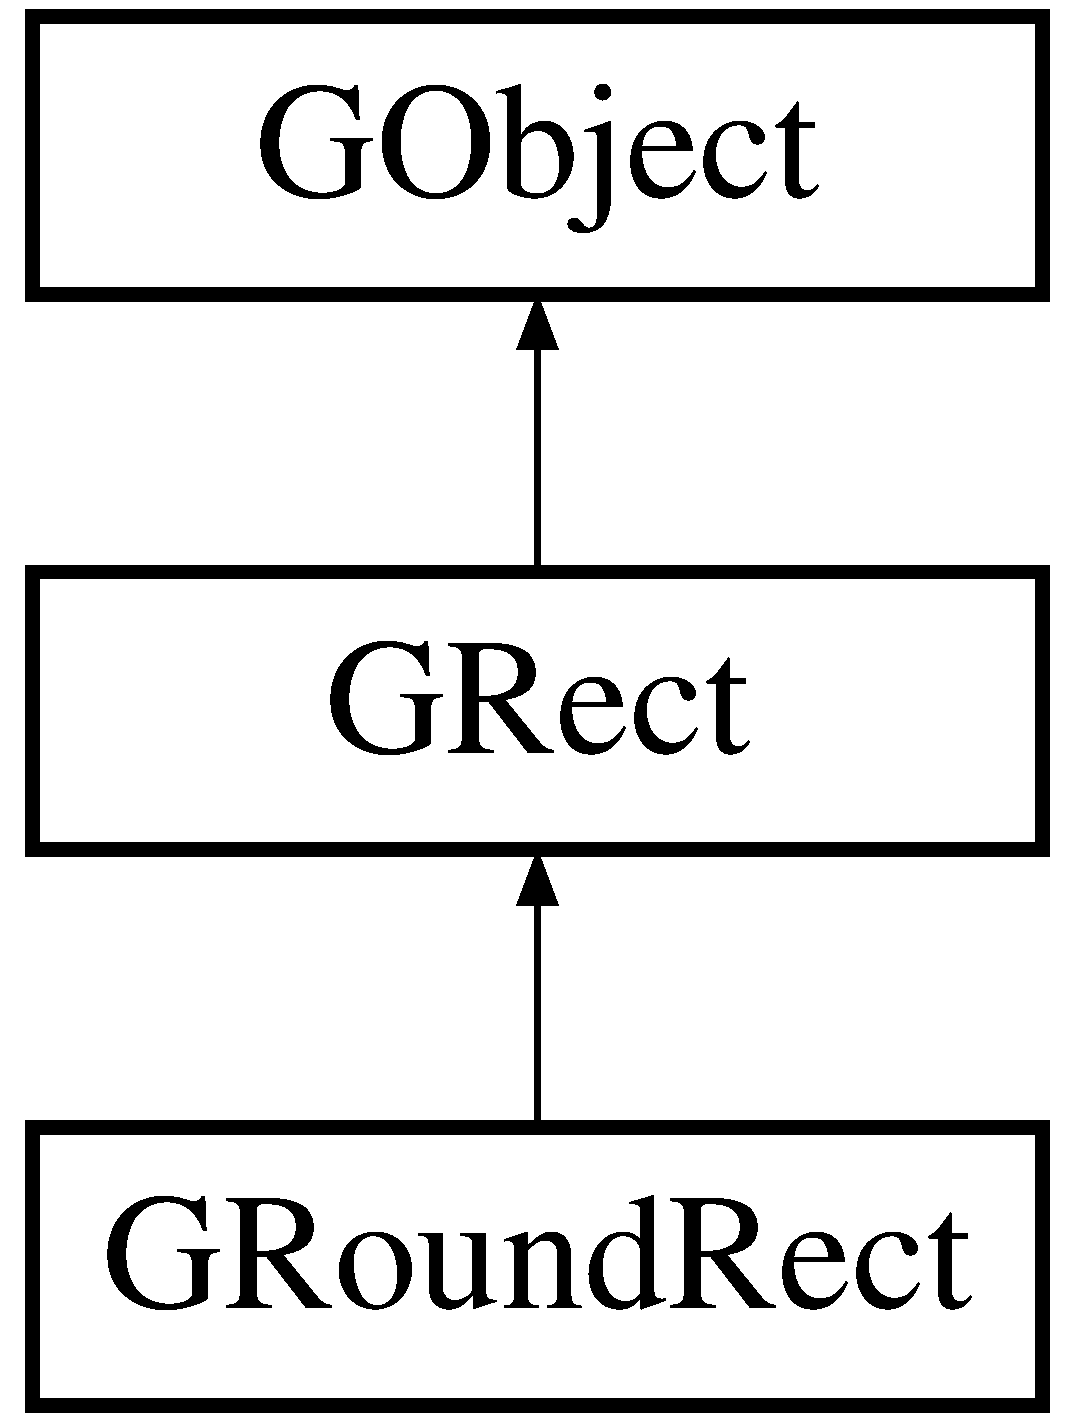
\includegraphics[height=3.000000cm]{classGRoundRect}
\end{center}
\end{figure}
\subsection*{Public Types}
\begin{DoxyCompactItemize}
\item 
enum \mbox{\hyperlink{classGObject_a86e0f5648542856159bb40775c854aa7}{Line\+Style}} \{ \mbox{\hyperlink{classGObject_a86e0f5648542856159bb40775c854aa7acbc84bd5232621834ed31f44d457c1eb}{L\+I\+N\+E\+\_\+\+N\+O\+NE}}, 
\mbox{\hyperlink{classGObject_a86e0f5648542856159bb40775c854aa7a700c78bc2cd76acaab26651bf7b4941f}{L\+I\+N\+E\+\_\+\+S\+O\+L\+ID}}, 
\mbox{\hyperlink{classGObject_a86e0f5648542856159bb40775c854aa7a9ccba0845f785d81d07b333ae1aad84e}{L\+I\+N\+E\+\_\+\+D\+A\+SH}}, 
\mbox{\hyperlink{classGObject_a86e0f5648542856159bb40775c854aa7a8e811c096cb941997f0bfda168bb6df3}{L\+I\+N\+E\+\_\+\+D\+OT}}, 
\mbox{\hyperlink{classGObject_a86e0f5648542856159bb40775c854aa7ada15a2e3d737b2db7706d8300f91b89d}{L\+I\+N\+E\+\_\+\+D\+A\+S\+H\+\_\+\+D\+OT}}, 
\mbox{\hyperlink{classGObject_a86e0f5648542856159bb40775c854aa7aabf4053a73eafa7ba2b7e6d664c74c1d}{L\+I\+N\+E\+\_\+\+D\+A\+S\+H\+\_\+\+D\+O\+T\+\_\+\+D\+OT}}
 \}
\begin{DoxyCompactList}\small\item\em Styles that can be used for the outline around various shapes. \end{DoxyCompactList}\end{DoxyCompactItemize}
\subsection*{Public Member Functions}
\begin{DoxyCompactItemize}
\item 
\mbox{\hyperlink{classGRoundRect_a4e4a8dae719dc671caf5bbfda7ca158a}{G\+Round\+Rect}} (double width=0, double height=0, double corner=\mbox{\hyperlink{classGRoundRect_a6e0fd235a5cfe88a0b0825202575bed9}{D\+E\+F\+A\+U\+L\+T\+\_\+\+C\+O\+R\+N\+ER}})
\begin{DoxyCompactList}\small\item\em Constructs a new rectangle with the specified width and height, located at (0, 0). \end{DoxyCompactList}\item 
\mbox{\hyperlink{classGRoundRect_a7ad0ccdd10c65a52fc77a7e9634ae58b}{G\+Round\+Rect}} (double x, double y, double width, double height, double corner=\mbox{\hyperlink{classGRoundRect_a6e0fd235a5cfe88a0b0825202575bed9}{D\+E\+F\+A\+U\+L\+T\+\_\+\+C\+O\+R\+N\+ER}})
\begin{DoxyCompactList}\small\item\em Constructs a new rectangle with the specified width and height, with its top/left corner at (x, y). \end{DoxyCompactList}\item 
virtual bool \mbox{\hyperlink{classGObject_a1dbc9dafaae51958112dbe1267a1f547}{contains}} (const \mbox{\hyperlink{structGPoint}{G\+Point}} \&pt) const
\begin{DoxyCompactList}\small\item\em Returns {\ttfamily true} if the specified point is inside the object. \end{DoxyCompactList}\item 
bool \mbox{\hyperlink{classGRoundRect_ad973a1d55799d3a73bf8b04986cd804e}{contains}} (double x, double y) const override
\begin{DoxyCompactList}\small\item\em Returns {\ttfamily true} if the specified point is inside the object. \end{DoxyCompactList}\item 
virtual \mbox{\hyperlink{structGPoint}{G\+Point}} \mbox{\hyperlink{classGObject_a0d41183bf6b08de66fe3907551aab0d7}{get\+Bottom\+Right\+Location}} () const
\begin{DoxyCompactList}\small\item\em Returns the x/y coordinates of the bottom/right corner of the object. \end{DoxyCompactList}\item 
virtual double \mbox{\hyperlink{classGObject_a4316a2406c18e1c6d061fe51fd355490}{get\+BottomY}} () const
\begin{DoxyCompactList}\small\item\em Returns the {\itshape y}-\/coordinate of the bottom of the object. \end{DoxyCompactList}\item 
virtual \mbox{\hyperlink{structGRectangle}{G\+Rectangle}} \mbox{\hyperlink{classGObject_a29e6ac35a0b48f491a4c88194cc5da3b}{get\+Bounds}} () const
\begin{DoxyCompactList}\small\item\em Returns the bounding box of this object, which is defined to be the smallest rectangle that covers everything drawn by the figure. \end{DoxyCompactList}\item 
virtual \mbox{\hyperlink{structGPoint}{G\+Point}} \mbox{\hyperlink{classGObject_a0909472e91448470bccdb62ecfb95d8b}{get\+Center\+Location}} () const
\begin{DoxyCompactList}\small\item\em Returns the x/y-\/coordinates of the center of the object. \end{DoxyCompactList}\item 
virtual double \mbox{\hyperlink{classGObject_a04df74355b545e0543112d5b8d924176}{get\+CenterX}} () const
\begin{DoxyCompactList}\small\item\em Returns the {\itshape x}-\/coordinate of the center of the object. \end{DoxyCompactList}\item 
virtual double \mbox{\hyperlink{classGObject_acb3287a3d507025a26f54b895713b947}{get\+CenterY}} () const
\begin{DoxyCompactList}\small\item\em Returns the {\itshape y}-\/coordinate of the center of the object. \end{DoxyCompactList}\item 
virtual std\+::string \mbox{\hyperlink{classGObject_aa061dfa488c31e18549d64363c1d0e34}{get\+Color}} () const
\begin{DoxyCompactList}\small\item\em Returns the color used to display this object. \end{DoxyCompactList}\item 
virtual double \mbox{\hyperlink{classGRoundRect_ad29f4fe71bbd3f4302d25adbee70ba2b}{get\+Corner}} () const
\begin{DoxyCompactList}\small\item\em Returns the diameter of the arc forming the corner of this rounded rectangle. \end{DoxyCompactList}\item 
virtual std\+::string \mbox{\hyperlink{classGObject_a76f6964a11fde7c78e9751be184e1a3c}{get\+Fill\+Color}} () const
\begin{DoxyCompactList}\small\item\em Returns the color used to display the filled region of this object. \end{DoxyCompactList}\item 
virtual double \mbox{\hyperlink{classGObject_a1e7e353362434072875264cf95629f99}{get\+Height}} () const
\begin{DoxyCompactList}\small\item\em Returns the height of this object, which is the same as the height of its bounding box. \end{DoxyCompactList}\item 
virtual \mbox{\hyperlink{classGObject_a86e0f5648542856159bb40775c854aa7}{Line\+Style}} \mbox{\hyperlink{classGObject_aaf1f5ea8281e5e3486662878d26f0a13}{get\+Line\+Style}} () const
\begin{DoxyCompactList}\small\item\em Returns the object\textquotesingle{}s style such as solid or dashed. \end{DoxyCompactList}\item 
virtual double \mbox{\hyperlink{classGObject_a85ff266dc3eb63d9f2d8e5a4487fd3c0}{get\+Line\+Width}} () const
\begin{DoxyCompactList}\small\item\em Returns the width of the line used to draw this object. \end{DoxyCompactList}\item 
virtual \mbox{\hyperlink{structGPoint}{G\+Point}} \mbox{\hyperlink{classGObject_a4f83802015511edeb63b892830812c11}{get\+Location}} () const
\begin{DoxyCompactList}\small\item\em Returns the location of the top-\/left corner of object. \end{DoxyCompactList}\item 
virtual double \mbox{\hyperlink{classGObject_a1ae3fc278cc5b71b9f2d96a8a83cdf26}{get\+Opacity}} () const
\begin{DoxyCompactList}\small\item\em Returns how opaque (non-\/transparent) this object will appear from 0.\+0 (completely transparent) to 1.\+0 (completely opaque, default). \end{DoxyCompactList}\item 
virtual \mbox{\hyperlink{classGCompound}{G\+Compound}} $\ast$ \mbox{\hyperlink{classGObject_a3e53cef70541b1a14eade4ad0984d0b4}{get\+Parent}} () const
\begin{DoxyCompactList}\small\item\em Returns a pointer to the {\ttfamily \mbox{\hyperlink{classGCompound}{G\+Compound}}} that contains this object. \end{DoxyCompactList}\item 
virtual double \mbox{\hyperlink{classGObject_a798cc79daaa10145b28f60bcdfdb0ee9}{get\+RightX}} () const
\begin{DoxyCompactList}\small\item\em Returns the {\itshape x}-\/coordinate of the right side of the object. \end{DoxyCompactList}\item 
virtual \mbox{\hyperlink{structGDimension}{G\+Dimension}} \mbox{\hyperlink{classGObject_a7b4eec96a2bdc6420695d5796a78eea9}{get\+Size}} () const
\begin{DoxyCompactList}\small\item\em Returns the size of the object as a {\ttfamily \mbox{\hyperlink{structGDimension}{G\+Dimension}}}. \end{DoxyCompactList}\item 
std\+::string \mbox{\hyperlink{classGRoundRect_a9b72ede4ee8520f987a0c01e30654814}{get\+Type}} () const override
\begin{DoxyCompactList}\small\item\em Returns the type of the object as a string, such as {\ttfamily \char`\"{}\+G\+Oval\char`\"{}} or {\ttfamily \char`\"{}\+G\+Rect\char`\"{}}. \end{DoxyCompactList}\item 
virtual double \mbox{\hyperlink{classGObject_a0ed2965abd4f5701d2cadf71239faf19}{get\+Width}} () const
\begin{DoxyCompactList}\small\item\em Returns the width of this object, which is equal to the width of the bounding box. \end{DoxyCompactList}\item 
virtual double \mbox{\hyperlink{classGObject_a344385751bee0720059403940d57a13e}{getX}} () const
\begin{DoxyCompactList}\small\item\em Returns the leftmost {\itshape x}-\/coordinate of the object. \end{DoxyCompactList}\item 
virtual double \mbox{\hyperlink{classGObject_aafa51c7f8f38a09febbb9ce7853f77b4}{getY}} () const
\begin{DoxyCompactList}\small\item\em Returns the topmost {\itshape y}-\/coordinate of the object. \end{DoxyCompactList}\item 
virtual bool \mbox{\hyperlink{classGObject_a11c404f106940c201b6f326e0355c150}{is\+Filled}} () const
\begin{DoxyCompactList}\small\item\em Returns {\ttfamily true} if the object is filled with color. \end{DoxyCompactList}\item 
virtual bool \mbox{\hyperlink{classGObject_a9de207581cfa4ca1eaa06da5f29b75fc}{is\+Transformed}} () const
\begin{DoxyCompactList}\small\item\em Returns {\ttfamily true} if this object has been transformed by calling methods such as \mbox{\hyperlink{classGObject_ae1ffaa12185dfd5ba464f7d87c329e26}{rotate()}} or \mbox{\hyperlink{classGObject_ad2e1900f730475c2d044817db03b38d6}{scale()}} on it. \end{DoxyCompactList}\item 
virtual bool \mbox{\hyperlink{classGObject_a9d8a6cfb13917785c143e74d40e4e2be}{is\+Visible}} () const
\begin{DoxyCompactList}\small\item\em Returns {\ttfamily true} if this object is visible on screen. \end{DoxyCompactList}\item 
virtual void \mbox{\hyperlink{classGObject_a5973d8dda83afb36e2c56855515be392}{move}} (double dx, double dy)
\begin{DoxyCompactList}\small\item\em Moves the object on the screen using the displacements {\ttfamily dx} and {\ttfamily dy}. \end{DoxyCompactList}\item 
virtual void \mbox{\hyperlink{classGObject_ac827b978aa122f136a14c198687ad80f}{repaint}} ()
\begin{DoxyCompactList}\small\item\em Instructs the object to redraw itself on screen. \end{DoxyCompactList}\item 
virtual void \mbox{\hyperlink{classGObject_a6022a1fd1e5dcd2fd5585e5a36aa3f37}{reset\+Transform}} ()
\begin{DoxyCompactList}\small\item\em Undoes any previous scale/rotate transformations on this object. \end{DoxyCompactList}\item 
virtual void \mbox{\hyperlink{classGObject_ae1ffaa12185dfd5ba464f7d87c329e26}{rotate}} (double theta)
\begin{DoxyCompactList}\small\item\em Transforms the object by rotating it {\ttfamily theta} degrees counterclockwise around its origin. \end{DoxyCompactList}\item 
virtual void \mbox{\hyperlink{classGObject_ad2e1900f730475c2d044817db03b38d6}{scale}} (double sf)
\begin{DoxyCompactList}\small\item\em Scales the object by the specified scale factor. \end{DoxyCompactList}\item 
virtual void \mbox{\hyperlink{classGObject_a63641f69d610d0b951357d35a0c3b1e3}{scale}} (double sx, double sy)
\begin{DoxyCompactList}\small\item\em Scales the object by the specified scale factors. \end{DoxyCompactList}\item 
void \mbox{\hyperlink{classGObject_ab6747f40313c531c2db32edb5b63b9b7}{send\+Backward}} ()
\begin{DoxyCompactList}\small\item\em Moves this object one step toward the back in the {\itshape z} dimension. \end{DoxyCompactList}\item 
void \mbox{\hyperlink{classGObject_a710b3e449c9facba7847c91ab170d281}{send\+Forward}} ()
\begin{DoxyCompactList}\small\item\em Moves this object one step toward the front in the {\itshape z} dimension. \end{DoxyCompactList}\item 
void \mbox{\hyperlink{classGObject_a0f7f1efbb7fd46dde2867c4ad0330896}{send\+To\+Back}} ()
\begin{DoxyCompactList}\small\item\em Moves this object to the back of the display in the {\itshape z} dimension. \end{DoxyCompactList}\item 
void \mbox{\hyperlink{classGObject_aee33d68488e46827ef55fac07f40a9b2}{send\+To\+Front}} ()
\begin{DoxyCompactList}\small\item\em Moves this object to the front of the display in the {\itshape z} dimension. \end{DoxyCompactList}\item 
virtual void \mbox{\hyperlink{classGObject_a71ff7b16b8f1bdc4a1ce9f30cf8b87d8}{set\+Bottom\+Right\+Location}} (double x, double y)
\begin{DoxyCompactList}\small\item\em Sets the location of the bottom/right of this object. \end{DoxyCompactList}\item 
virtual void \mbox{\hyperlink{classGObject_ac6f7320321182f1d18c1c0fa97d5e941}{set\+Bottom\+Right\+Location}} (const \mbox{\hyperlink{structGPoint}{G\+Point}} \&pt)
\begin{DoxyCompactList}\small\item\em Sets the location of the bottom/right of this object. \end{DoxyCompactList}\item 
virtual void \mbox{\hyperlink{classGObject_a4b20e93c2a2597484f74ee5caa71f41f}{set\+BottomY}} (double y)
\begin{DoxyCompactList}\small\item\em Sets the location of the bottom y-\/coordinate of this object. \end{DoxyCompactList}\item 
virtual void \mbox{\hyperlink{classGObject_a2aae8197624b72265ab83b4f1bc73f2f}{set\+Bounds}} (double x, double y, double width, double height)
\begin{DoxyCompactList}\small\item\em Changes the bounds of this object to the specified values. \end{DoxyCompactList}\item 
virtual void \mbox{\hyperlink{classGObject_acada386653f008cacc7cce86426bef7c}{set\+Bounds}} (const \mbox{\hyperlink{structGRectangle}{G\+Rectangle}} \&size)
\begin{DoxyCompactList}\small\item\em Changes the bounds of this object to the specified rectangle. \end{DoxyCompactList}\item 
virtual void \mbox{\hyperlink{classGObject_a290b47dd8de1be44089f95cb2c47c1de}{set\+Center\+Location}} (double x, double y)
\begin{DoxyCompactList}\small\item\em Sets the location of the center of this object. \end{DoxyCompactList}\item 
virtual void \mbox{\hyperlink{classGObject_a1bedf1b233ecba3f753ec58908a683a6}{set\+Center\+Location}} (const \mbox{\hyperlink{structGPoint}{G\+Point}} \&pt)
\begin{DoxyCompactList}\small\item\em Sets the location of the center of this object. \end{DoxyCompactList}\item 
virtual void \mbox{\hyperlink{classGObject_a2f4936281e056eead00a9186b9ba8af6}{set\+CenterX}} (double x)
\begin{DoxyCompactList}\small\item\em Sets the x-\/coordinate of the center of this object. \end{DoxyCompactList}\item 
virtual void \mbox{\hyperlink{classGObject_aad2a22b4fde88c33306b92aebf641d57}{set\+CenterY}} (double y)
\begin{DoxyCompactList}\small\item\em Sets the y-\/coordinate of the center of this object. \end{DoxyCompactList}\item 
virtual void \mbox{\hyperlink{classGObject_ad57ef49bc31db94e92648aa3737923d6}{set\+Color}} (int r, int g, int b)
\begin{DoxyCompactList}\small\item\em Sets the color used to display this object. \end{DoxyCompactList}\item 
virtual void \mbox{\hyperlink{classGObject_ab1f5cc0f5cc6bbbd716a526c61f1081d}{set\+Color}} (int rgb)
\begin{DoxyCompactList}\small\item\em Sets the color used to display this object. \end{DoxyCompactList}\item 
virtual void \mbox{\hyperlink{classGObject_a61374df6c11b52cfbb0815decdbaebc6}{set\+Color}} (const std\+::string \&color)
\begin{DoxyCompactList}\small\item\em Sets the color used to display this object. \end{DoxyCompactList}\item 
virtual void \mbox{\hyperlink{classGRoundRect_ab1cc6c77629d0e8ded56139a1866be48}{set\+Corner}} (double corner)
\begin{DoxyCompactList}\small\item\em Sets the diameter of the arc forming the corner of this rounded rectangle. \end{DoxyCompactList}\item 
virtual void \mbox{\hyperlink{classGObject_ad767a33971159e9493e221cca4c00ae9}{set\+Fill\+Color}} (int r, int g, int b)
\begin{DoxyCompactList}\small\item\em Sets the color used to display the filled region of this object, if any. \end{DoxyCompactList}\item 
virtual void \mbox{\hyperlink{classGObject_aa59d9775a67fa7df2b24a95cd34840a3}{set\+Fill\+Color}} (int rgb)
\begin{DoxyCompactList}\small\item\em Sets the color used to display the filled region of this object, if any. \end{DoxyCompactList}\item 
virtual void \mbox{\hyperlink{classGObject_adbc18b1a930aadd97d7437f9f7265b96}{set\+Fill\+Color}} (const std\+::string \&color)
\begin{DoxyCompactList}\small\item\em Sets the color used to display the filled region of this object, if any. \end{DoxyCompactList}\item 
virtual void \mbox{\hyperlink{classGObject_a9b82b53362282c6bb7d6947068d2e55b}{set\+Filled}} (bool flag)
\begin{DoxyCompactList}\small\item\em Sets the fill status for the object, where {\ttfamily false} is outlined and {\ttfamily true} is filled. \end{DoxyCompactList}\item 
virtual void \mbox{\hyperlink{classGObject_a2592348886ffea646c6534bf88f7c49d}{set\+Font}} (const Q\+Font \&font)
\begin{DoxyCompactList}\small\item\em Changes the font used to display the object as specified by the given Qt font. \end{DoxyCompactList}\item 
virtual void \mbox{\hyperlink{classGObject_a8e096e8818d838aceae1d46d58fb3a7b}{set\+Font}} (const std\+::string \&font)
\begin{DoxyCompactList}\small\item\em Changes the font used to display the object as specified by the string {\ttfamily font}, which has the following format\+: \end{DoxyCompactList}\item 
virtual void \mbox{\hyperlink{classGObject_ad18e8fab1e02a4e9b75c6730212558eb}{set\+Foreground}} (int r, int g, int b)
\begin{DoxyCompactList}\small\item\em Sets the color used to display this object. \end{DoxyCompactList}\item 
virtual void \mbox{\hyperlink{classGObject_a9eb856b5ff83a19df3831a31f15f4563}{set\+Foreground}} (int rgb)
\begin{DoxyCompactList}\small\item\em Sets the color used to display this object. \end{DoxyCompactList}\item 
virtual void \mbox{\hyperlink{classGObject_af59209aeadea6dfc6d97a2d8531f50e1}{set\+Foreground}} (const std\+::string \&color)
\begin{DoxyCompactList}\small\item\em Sets the color used to display this object. \end{DoxyCompactList}\item 
virtual void \mbox{\hyperlink{classGObject_a9e280bfc4544dfaf8e4376c4e1a74357}{set\+Height}} (double height)
\begin{DoxyCompactList}\small\item\em Changes the height of this object to the specified height without changing its width. \end{DoxyCompactList}\item 
virtual void \mbox{\hyperlink{classGObject_add11575087eb94f1a71faa3f826c6341}{set\+Line\+Style}} (\mbox{\hyperlink{classGObject_a86e0f5648542856159bb40775c854aa7}{Line\+Style}} line\+Style)
\begin{DoxyCompactList}\small\item\em Sets the object\textquotesingle{}s style such as solid (\mbox{\hyperlink{classGObject_a86e0f5648542856159bb40775c854aa7a700c78bc2cd76acaab26651bf7b4941f}{G\+Object\+::\+L\+I\+N\+E\+\_\+\+S\+O\+L\+ID}}) or dashed (\mbox{\hyperlink{classGObject_a86e0f5648542856159bb40775c854aa7a9ccba0845f785d81d07b333ae1aad84e}{G\+Object\+::\+L\+I\+N\+E\+\_\+\+D\+A\+SH}}). \end{DoxyCompactList}\item 
virtual void \mbox{\hyperlink{classGObject_afd6a47c6ea6a1f85ca05a65ba3ff3477}{set\+Line\+Width}} (double line\+Width)
\begin{DoxyCompactList}\small\item\em Sets the width of the line used to draw this object. \end{DoxyCompactList}\item 
virtual void \mbox{\hyperlink{classGObject_a04594e8ba9b98513a64f1da00dcae18c}{set\+Location}} (double x, double y)
\begin{DoxyCompactList}\small\item\em Sets the location of the top-\/left corner of this object to the specified coordinates. \end{DoxyCompactList}\item 
virtual void \mbox{\hyperlink{classGObject_aa8480c0b7166cdf8f784cece06ab353f}{set\+Location}} (const \mbox{\hyperlink{structGPoint}{G\+Point}} \&pt)
\begin{DoxyCompactList}\small\item\em Sets the location of the top-\/left corner of this object to the specified point. \end{DoxyCompactList}\item 
virtual void \mbox{\hyperlink{classGObject_a04af1866cc1bae4a1226695794a50539}{set\+Opacity}} (double opacity)
\begin{DoxyCompactList}\small\item\em Sets how opaque (non-\/transparent) this object will appear from 0.\+0 (completely transparent) to 1.\+0 (completely opaque, default). \end{DoxyCompactList}\item 
virtual void \mbox{\hyperlink{classGObject_a3c90b758cdc2c911c9ef76c4360eb912}{set\+RightX}} (double x)
\begin{DoxyCompactList}\small\item\em Sets the location of the rightmost x-\/coordinate of this object. \end{DoxyCompactList}\item 
virtual void \mbox{\hyperlink{classGObject_aca25d49481f9bf5fc8f7df4c086c4ce7}{set\+Size}} (double width, double height)
\begin{DoxyCompactList}\small\item\em Changes the size of this object to the specified width and height. \end{DoxyCompactList}\item 
virtual void \mbox{\hyperlink{classGObject_ae2b628228f192c2702c4ce941b2af68f}{set\+Size}} (const \mbox{\hyperlink{structGDimension}{G\+Dimension}} \&size)
\begin{DoxyCompactList}\small\item\em Changes the size of this object to the specified width and height. \end{DoxyCompactList}\item 
virtual void \mbox{\hyperlink{classGObject_a88203f28224315d9f4471212f4af8ed3}{set\+Visible}} (bool flag)
\begin{DoxyCompactList}\small\item\em Sets whether this object is visible. \end{DoxyCompactList}\item 
virtual void \mbox{\hyperlink{classGObject_aa3f3fba4cb131baa8696ba01e3bceca1}{set\+Width}} (double width)
\begin{DoxyCompactList}\small\item\em Changes the width of this object to the specified width without changing its height. \end{DoxyCompactList}\item 
virtual void \mbox{\hyperlink{classGObject_a9c18fcc579333bf9653d13ad2b372e39}{setX}} (double x)
\begin{DoxyCompactList}\small\item\em Sets the x location of the left side of this object. \end{DoxyCompactList}\item 
virtual void \mbox{\hyperlink{classGObject_a7d57e2a5c35d27feb58fd498a3cf82b9}{setY}} (double y)
\begin{DoxyCompactList}\small\item\em Sets the y location of the top of this object. \end{DoxyCompactList}\item 
virtual std\+::string \mbox{\hyperlink{classGObject_a1fe5121d6528fdea3f243321b3fa3a49}{to\+String}} () const
\begin{DoxyCompactList}\small\item\em Returns a printable representation of the object. \end{DoxyCompactList}\item 
std\+::string \mbox{\hyperlink{classGRoundRect_a04364e674911906702b748deec32db18}{to\+String\+Extra}} () const override
\begin{DoxyCompactList}\small\item\em Returns a string containing any extra unique information about this type of graphical object. \end{DoxyCompactList}\end{DoxyCompactItemize}
\subsection*{Static Public Member Functions}
\begin{DoxyCompactItemize}
\item 
static bool \mbox{\hyperlink{classGObject_a93be0e1fe1b1bf1a1da732470c94f42b}{is\+Anti\+Aliasing}} ()
\begin{DoxyCompactList}\small\item\em Returns whether we should globally anti-\/alias graphical objects. \end{DoxyCompactList}\item 
static void \mbox{\hyperlink{classGObject_a1e43371668ae850193cebedb44e1bbe3}{set\+Anti\+Aliasing}} (bool value)
\begin{DoxyCompactList}\small\item\em Globally turns on/off the anti-\/aliasing feature that smooths out the edges of onscreen shapes. \end{DoxyCompactList}\end{DoxyCompactItemize}
\subsection*{Static Public Attributes}
\begin{DoxyCompactItemize}
\item 
static const double \mbox{\hyperlink{classGRoundRect_a6e0fd235a5cfe88a0b0825202575bed9}{D\+E\+F\+A\+U\+L\+T\+\_\+\+C\+O\+R\+N\+ER}} = 10.\+0
\begin{DoxyCompactList}\small\item\em The default diameter of corners on rounded rectangles if none is supplied to the constructor. \end{DoxyCompactList}\end{DoxyCompactItemize}
\subsection*{Protected Attributes}
\begin{DoxyCompactItemize}
\item 
Q\+Brush \mbox{\hyperlink{classGObject_aab24462ec896b596d99911767b0912d0}{\+\_\+brush}}
\item 
std\+::string \mbox{\hyperlink{classGObject_a1134e770ae4315ea8bc1201e2f21da8b}{\+\_\+color}}
\item 
int \mbox{\hyperlink{classGObject_a003fdd343d9b7505c53a8b7a134200ed}{\+\_\+color\+Int}}
\item 
double \mbox{\hyperlink{classGRoundRect_aed2d721464238b51020f9ce90440ecde}{\+\_\+corner}}
\item 
std\+::string \mbox{\hyperlink{classGObject_a179f8d6cee65cd8a54692e32b224392a}{\+\_\+fill\+Color}}
\item 
int \mbox{\hyperlink{classGObject_a751def333a67d651e5b99cc331ecb496}{\+\_\+fill\+Color\+Int}}
\item 
bool \mbox{\hyperlink{classGObject_ad4a55cbcd61b58a4d49666490bb2f103}{\+\_\+fill\+Flag}}
\item 
std\+::string \mbox{\hyperlink{classGObject_aea76ea1a8b5dd7b0a78653277e63b536}{\+\_\+font}}
\item 
double \mbox{\hyperlink{classGObject_ad05df29e7f27fc504abd743e3d8b4e73}{\+\_\+height}}
\item 
\mbox{\hyperlink{classGObject_a86e0f5648542856159bb40775c854aa7}{Line\+Style}} \mbox{\hyperlink{classGObject_a89bafecaafb7c72d55c7efc10b7d0523}{\+\_\+line\+Style}}
\item 
double \mbox{\hyperlink{classGObject_a16e9033665937f13de2e163dc2184aff}{\+\_\+line\+Width}}
\item 
double \mbox{\hyperlink{classGObject_a20eff8eb7af27182edc9bfc54768b6f3}{\+\_\+opacity}}
\item 
\mbox{\hyperlink{classGCompound}{G\+Compound}} $\ast$ \mbox{\hyperlink{classGObject_ac9452c1eaff70eebddbb318196aa3835}{\+\_\+parent}}
\item 
Q\+Pen \mbox{\hyperlink{classGObject_afb69d172743f868299847174eb1b6bc8}{\+\_\+pen}}
\item 
Q\+Transform \mbox{\hyperlink{classGObject_a475b8860a5f1adb4a1fdc58d1f5c1e32}{\+\_\+transform}}
\item 
bool \mbox{\hyperlink{classGObject_ae4725802fc8d8aaa0ab4bd4781f7e07c}{\+\_\+transformed}}
\item 
bool \mbox{\hyperlink{classGObject_a9312c72508471b7c7a87b540263e1af4}{\+\_\+visible}}
\item 
double \mbox{\hyperlink{classGObject_ab55d85a3371770e6725b1062cf160cd8}{\+\_\+width}}
\item 
double \mbox{\hyperlink{classGObject_a6675b83b27137b8d3aa2ad8133078ea6}{\+\_\+x}}
\item 
double \mbox{\hyperlink{classGObject_a2f0f6aeafddc8a39c578bfa7e22b5f1e}{\+\_\+y}}
\end{DoxyCompactItemize}


\subsection{Detailed Description}
A \mbox{\hyperlink{classGRoundRect}{G\+Round\+Rect}} represents a graphical object whose appearance consists of a rectangular box with rounded corners. 

\subsection{Member Enumeration Documentation}
\mbox{\Hypertarget{classGObject_a86e0f5648542856159bb40775c854aa7}\label{classGObject_a86e0f5648542856159bb40775c854aa7}} 
\index{G\+Round\+Rect@{G\+Round\+Rect}!Line\+Style@{Line\+Style}}
\index{Line\+Style@{Line\+Style}!G\+Round\+Rect@{G\+Round\+Rect}}
\subsubsection{\texorpdfstring{Line\+Style}{LineStyle}}
{\footnotesize\ttfamily enum \mbox{\hyperlink{classGObject_a86e0f5648542856159bb40775c854aa7}{Line\+Style}}\hspace{0.3cm}{\ttfamily [inherited]}}



Styles that can be used for the outline around various shapes. 

Call set\+Line\+Style on a \mbox{\hyperlink{classGObject}{G\+Object}} and pass one of these values. \begin{DoxyEnumFields}{Enumerator}
\raisebox{\heightof{T}}[0pt][0pt]{\index{L\+I\+N\+E\+\_\+\+N\+O\+NE@{L\+I\+N\+E\+\_\+\+N\+O\+NE}!G\+Round\+Rect@{G\+Round\+Rect}}\index{G\+Round\+Rect@{G\+Round\+Rect}!L\+I\+N\+E\+\_\+\+N\+O\+NE@{L\+I\+N\+E\+\_\+\+N\+O\+NE}}}\mbox{\Hypertarget{classGObject_a86e0f5648542856159bb40775c854aa7acbc84bd5232621834ed31f44d457c1eb}\label{classGObject_a86e0f5648542856159bb40775c854aa7acbc84bd5232621834ed31f44d457c1eb}} 
L\+I\+N\+E\+\_\+\+N\+O\+NE&\\
\hline

\raisebox{\heightof{T}}[0pt][0pt]{\index{L\+I\+N\+E\+\_\+\+S\+O\+L\+ID@{L\+I\+N\+E\+\_\+\+S\+O\+L\+ID}!G\+Round\+Rect@{G\+Round\+Rect}}\index{G\+Round\+Rect@{G\+Round\+Rect}!L\+I\+N\+E\+\_\+\+S\+O\+L\+ID@{L\+I\+N\+E\+\_\+\+S\+O\+L\+ID}}}\mbox{\Hypertarget{classGObject_a86e0f5648542856159bb40775c854aa7a700c78bc2cd76acaab26651bf7b4941f}\label{classGObject_a86e0f5648542856159bb40775c854aa7a700c78bc2cd76acaab26651bf7b4941f}} 
L\+I\+N\+E\+\_\+\+S\+O\+L\+ID&\\
\hline

\raisebox{\heightof{T}}[0pt][0pt]{\index{L\+I\+N\+E\+\_\+\+D\+A\+SH@{L\+I\+N\+E\+\_\+\+D\+A\+SH}!G\+Round\+Rect@{G\+Round\+Rect}}\index{G\+Round\+Rect@{G\+Round\+Rect}!L\+I\+N\+E\+\_\+\+D\+A\+SH@{L\+I\+N\+E\+\_\+\+D\+A\+SH}}}\mbox{\Hypertarget{classGObject_a86e0f5648542856159bb40775c854aa7a9ccba0845f785d81d07b333ae1aad84e}\label{classGObject_a86e0f5648542856159bb40775c854aa7a9ccba0845f785d81d07b333ae1aad84e}} 
L\+I\+N\+E\+\_\+\+D\+A\+SH&\\
\hline

\raisebox{\heightof{T}}[0pt][0pt]{\index{L\+I\+N\+E\+\_\+\+D\+OT@{L\+I\+N\+E\+\_\+\+D\+OT}!G\+Round\+Rect@{G\+Round\+Rect}}\index{G\+Round\+Rect@{G\+Round\+Rect}!L\+I\+N\+E\+\_\+\+D\+OT@{L\+I\+N\+E\+\_\+\+D\+OT}}}\mbox{\Hypertarget{classGObject_a86e0f5648542856159bb40775c854aa7a8e811c096cb941997f0bfda168bb6df3}\label{classGObject_a86e0f5648542856159bb40775c854aa7a8e811c096cb941997f0bfda168bb6df3}} 
L\+I\+N\+E\+\_\+\+D\+OT&\\
\hline

\raisebox{\heightof{T}}[0pt][0pt]{\index{L\+I\+N\+E\+\_\+\+D\+A\+S\+H\+\_\+\+D\+OT@{L\+I\+N\+E\+\_\+\+D\+A\+S\+H\+\_\+\+D\+OT}!G\+Round\+Rect@{G\+Round\+Rect}}\index{G\+Round\+Rect@{G\+Round\+Rect}!L\+I\+N\+E\+\_\+\+D\+A\+S\+H\+\_\+\+D\+OT@{L\+I\+N\+E\+\_\+\+D\+A\+S\+H\+\_\+\+D\+OT}}}\mbox{\Hypertarget{classGObject_a86e0f5648542856159bb40775c854aa7ada15a2e3d737b2db7706d8300f91b89d}\label{classGObject_a86e0f5648542856159bb40775c854aa7ada15a2e3d737b2db7706d8300f91b89d}} 
L\+I\+N\+E\+\_\+\+D\+A\+S\+H\+\_\+\+D\+OT&\\
\hline

\raisebox{\heightof{T}}[0pt][0pt]{\index{L\+I\+N\+E\+\_\+\+D\+A\+S\+H\+\_\+\+D\+O\+T\+\_\+\+D\+OT@{L\+I\+N\+E\+\_\+\+D\+A\+S\+H\+\_\+\+D\+O\+T\+\_\+\+D\+OT}!G\+Round\+Rect@{G\+Round\+Rect}}\index{G\+Round\+Rect@{G\+Round\+Rect}!L\+I\+N\+E\+\_\+\+D\+A\+S\+H\+\_\+\+D\+O\+T\+\_\+\+D\+OT@{L\+I\+N\+E\+\_\+\+D\+A\+S\+H\+\_\+\+D\+O\+T\+\_\+\+D\+OT}}}\mbox{\Hypertarget{classGObject_a86e0f5648542856159bb40775c854aa7aabf4053a73eafa7ba2b7e6d664c74c1d}\label{classGObject_a86e0f5648542856159bb40775c854aa7aabf4053a73eafa7ba2b7e6d664c74c1d}} 
L\+I\+N\+E\+\_\+\+D\+A\+S\+H\+\_\+\+D\+O\+T\+\_\+\+D\+OT&\\
\hline

\end{DoxyEnumFields}


\subsection{Constructor \& Destructor Documentation}
\mbox{\Hypertarget{classGRoundRect_a4e4a8dae719dc671caf5bbfda7ca158a}\label{classGRoundRect_a4e4a8dae719dc671caf5bbfda7ca158a}} 
\index{G\+Round\+Rect@{G\+Round\+Rect}!G\+Round\+Rect@{G\+Round\+Rect}}
\index{G\+Round\+Rect@{G\+Round\+Rect}!G\+Round\+Rect@{G\+Round\+Rect}}
\subsubsection{\texorpdfstring{G\+Round\+Rect()}{GRoundRect()}\hspace{0.1cm}{\footnotesize\ttfamily [1/2]}}
{\footnotesize\ttfamily \mbox{\hyperlink{classGRoundRect}{G\+Round\+Rect}} (\begin{DoxyParamCaption}\item[{double}]{width = {\ttfamily 0},  }\item[{double}]{height = {\ttfamily 0},  }\item[{double}]{corner = {\ttfamily \mbox{\hyperlink{classGRoundRect_a6e0fd235a5cfe88a0b0825202575bed9}{D\+E\+F\+A\+U\+L\+T\+\_\+\+C\+O\+R\+N\+ER}}} }\end{DoxyParamCaption})}



Constructs a new rectangle with the specified width and height, located at (0, 0). 

The {\ttfamily corner} parameter specifies the diameter of the arc forming the corner. \mbox{\Hypertarget{classGRoundRect_a7ad0ccdd10c65a52fc77a7e9634ae58b}\label{classGRoundRect_a7ad0ccdd10c65a52fc77a7e9634ae58b}} 
\index{G\+Round\+Rect@{G\+Round\+Rect}!G\+Round\+Rect@{G\+Round\+Rect}}
\index{G\+Round\+Rect@{G\+Round\+Rect}!G\+Round\+Rect@{G\+Round\+Rect}}
\subsubsection{\texorpdfstring{G\+Round\+Rect()}{GRoundRect()}\hspace{0.1cm}{\footnotesize\ttfamily [2/2]}}
{\footnotesize\ttfamily \mbox{\hyperlink{classGRoundRect}{G\+Round\+Rect}} (\begin{DoxyParamCaption}\item[{double}]{x,  }\item[{double}]{y,  }\item[{double}]{width,  }\item[{double}]{height,  }\item[{double}]{corner = {\ttfamily \mbox{\hyperlink{classGRoundRect_a6e0fd235a5cfe88a0b0825202575bed9}{D\+E\+F\+A\+U\+L\+T\+\_\+\+C\+O\+R\+N\+ER}}} }\end{DoxyParamCaption})}



Constructs a new rectangle with the specified width and height, with its top/left corner at (x, y). 

The {\ttfamily corner} parameter specifies the diameter of the arc forming the corner. 

\subsection{Member Function Documentation}
\mbox{\Hypertarget{classGObject_a1dbc9dafaae51958112dbe1267a1f547}\label{classGObject_a1dbc9dafaae51958112dbe1267a1f547}} 
\index{G\+Round\+Rect@{G\+Round\+Rect}!contains@{contains}}
\index{contains@{contains}!G\+Round\+Rect@{G\+Round\+Rect}}
\subsubsection{\texorpdfstring{contains()}{contains()}\hspace{0.1cm}{\footnotesize\ttfamily [1/2]}}
{\footnotesize\ttfamily bool contains (\begin{DoxyParamCaption}\item[{const \mbox{\hyperlink{structGPoint}{G\+Point}} \&}]{pt }\end{DoxyParamCaption}) const\hspace{0.3cm}{\ttfamily [virtual]}, {\ttfamily [inherited]}}



Returns {\ttfamily true} if the specified point is inside the object. 

\mbox{\Hypertarget{classGRoundRect_ad973a1d55799d3a73bf8b04986cd804e}\label{classGRoundRect_ad973a1d55799d3a73bf8b04986cd804e}} 
\index{G\+Round\+Rect@{G\+Round\+Rect}!contains@{contains}}
\index{contains@{contains}!G\+Round\+Rect@{G\+Round\+Rect}}
\subsubsection{\texorpdfstring{contains()}{contains()}\hspace{0.1cm}{\footnotesize\ttfamily [2/2]}}
{\footnotesize\ttfamily bool contains (\begin{DoxyParamCaption}\item[{double}]{x,  }\item[{double}]{y }\end{DoxyParamCaption}) const\hspace{0.3cm}{\ttfamily [override]}, {\ttfamily [virtual]}}



Returns {\ttfamily true} if the specified point is inside the object. 



Reimplemented from \mbox{\hyperlink{classGObject_abb6a5d7c03e6eaaae97264c4799ce7c3}{G\+Object}}.

\mbox{\Hypertarget{classGObject_a0d41183bf6b08de66fe3907551aab0d7}\label{classGObject_a0d41183bf6b08de66fe3907551aab0d7}} 
\index{G\+Round\+Rect@{G\+Round\+Rect}!get\+Bottom\+Right\+Location@{get\+Bottom\+Right\+Location}}
\index{get\+Bottom\+Right\+Location@{get\+Bottom\+Right\+Location}!G\+Round\+Rect@{G\+Round\+Rect}}
\subsubsection{\texorpdfstring{get\+Bottom\+Right\+Location()}{getBottomRightLocation()}}
{\footnotesize\ttfamily \mbox{\hyperlink{structGPoint}{G\+Point}} get\+Bottom\+Right\+Location (\begin{DoxyParamCaption}{ }\end{DoxyParamCaption}) const\hspace{0.3cm}{\ttfamily [virtual]}, {\ttfamily [inherited]}}



Returns the x/y coordinates of the bottom/right corner of the object. 

\mbox{\Hypertarget{classGObject_a4316a2406c18e1c6d061fe51fd355490}\label{classGObject_a4316a2406c18e1c6d061fe51fd355490}} 
\index{G\+Round\+Rect@{G\+Round\+Rect}!get\+BottomY@{get\+BottomY}}
\index{get\+BottomY@{get\+BottomY}!G\+Round\+Rect@{G\+Round\+Rect}}
\subsubsection{\texorpdfstring{get\+Bottom\+Y()}{getBottomY()}}
{\footnotesize\ttfamily double get\+BottomY (\begin{DoxyParamCaption}{ }\end{DoxyParamCaption}) const\hspace{0.3cm}{\ttfamily [virtual]}, {\ttfamily [inherited]}}



Returns the {\itshape y}-\/coordinate of the bottom of the object. 

Equivalent to the top y-\/coordinate plus the object\textquotesingle{}s height. \mbox{\Hypertarget{classGObject_a29e6ac35a0b48f491a4c88194cc5da3b}\label{classGObject_a29e6ac35a0b48f491a4c88194cc5da3b}} 
\index{G\+Round\+Rect@{G\+Round\+Rect}!get\+Bounds@{get\+Bounds}}
\index{get\+Bounds@{get\+Bounds}!G\+Round\+Rect@{G\+Round\+Rect}}
\subsubsection{\texorpdfstring{get\+Bounds()}{getBounds()}}
{\footnotesize\ttfamily \mbox{\hyperlink{structGRectangle}{G\+Rectangle}} get\+Bounds (\begin{DoxyParamCaption}{ }\end{DoxyParamCaption}) const\hspace{0.3cm}{\ttfamily [virtual]}, {\ttfamily [inherited]}}



Returns the bounding box of this object, which is defined to be the smallest rectangle that covers everything drawn by the figure. 

The coordinates of this rectangle do not necessarily match the location returned by {\ttfamily get\+Location}. Given a {\ttfamily \mbox{\hyperlink{classGText}{G\+Text}}} object, for example, {\ttfamily get\+Location} returns the coordinates of the point on the baseline at which the string begins; the {\ttfamily get\+Bounds} method, by contrast, returns a rectangle that covers the entire window area occupied by the string. 

Reimplemented in \mbox{\hyperlink{classGText_a89040ce9277825772d359fccd33bca86}{G\+Text}}, \mbox{\hyperlink{classGPolygon_a89040ce9277825772d359fccd33bca86}{G\+Polygon}}, \mbox{\hyperlink{classGLine_a89040ce9277825772d359fccd33bca86}{G\+Line}}, \mbox{\hyperlink{classGCompound_a89040ce9277825772d359fccd33bca86}{G\+Compound}}, and \mbox{\hyperlink{classGArc_a89040ce9277825772d359fccd33bca86}{G\+Arc}}.

\mbox{\Hypertarget{classGObject_a0909472e91448470bccdb62ecfb95d8b}\label{classGObject_a0909472e91448470bccdb62ecfb95d8b}} 
\index{G\+Round\+Rect@{G\+Round\+Rect}!get\+Center\+Location@{get\+Center\+Location}}
\index{get\+Center\+Location@{get\+Center\+Location}!G\+Round\+Rect@{G\+Round\+Rect}}
\subsubsection{\texorpdfstring{get\+Center\+Location()}{getCenterLocation()}}
{\footnotesize\ttfamily \mbox{\hyperlink{structGPoint}{G\+Point}} get\+Center\+Location (\begin{DoxyParamCaption}{ }\end{DoxyParamCaption}) const\hspace{0.3cm}{\ttfamily [virtual]}, {\ttfamily [inherited]}}



Returns the x/y-\/coordinates of the center of the object. 

Equivalent to the top/left plus half the object\textquotesingle{}s size. \mbox{\Hypertarget{classGObject_a04df74355b545e0543112d5b8d924176}\label{classGObject_a04df74355b545e0543112d5b8d924176}} 
\index{G\+Round\+Rect@{G\+Round\+Rect}!get\+CenterX@{get\+CenterX}}
\index{get\+CenterX@{get\+CenterX}!G\+Round\+Rect@{G\+Round\+Rect}}
\subsubsection{\texorpdfstring{get\+Center\+X()}{getCenterX()}}
{\footnotesize\ttfamily double get\+CenterX (\begin{DoxyParamCaption}{ }\end{DoxyParamCaption}) const\hspace{0.3cm}{\ttfamily [virtual]}, {\ttfamily [inherited]}}



Returns the {\itshape x}-\/coordinate of the center of the object. 

Equivalent to the top/left plus half the object\textquotesingle{}s width. \mbox{\Hypertarget{classGObject_acb3287a3d507025a26f54b895713b947}\label{classGObject_acb3287a3d507025a26f54b895713b947}} 
\index{G\+Round\+Rect@{G\+Round\+Rect}!get\+CenterY@{get\+CenterY}}
\index{get\+CenterY@{get\+CenterY}!G\+Round\+Rect@{G\+Round\+Rect}}
\subsubsection{\texorpdfstring{get\+Center\+Y()}{getCenterY()}}
{\footnotesize\ttfamily double get\+CenterY (\begin{DoxyParamCaption}{ }\end{DoxyParamCaption}) const\hspace{0.3cm}{\ttfamily [virtual]}, {\ttfamily [inherited]}}



Returns the {\itshape y}-\/coordinate of the center of the object. 

Equivalent to the top/left plus half the object\textquotesingle{}s height. \mbox{\Hypertarget{classGObject_aa061dfa488c31e18549d64363c1d0e34}\label{classGObject_aa061dfa488c31e18549d64363c1d0e34}} 
\index{G\+Round\+Rect@{G\+Round\+Rect}!get\+Color@{get\+Color}}
\index{get\+Color@{get\+Color}!G\+Round\+Rect@{G\+Round\+Rect}}
\subsubsection{\texorpdfstring{get\+Color()}{getColor()}}
{\footnotesize\ttfamily std\+::string get\+Color (\begin{DoxyParamCaption}{ }\end{DoxyParamCaption}) const\hspace{0.3cm}{\ttfamily [virtual]}, {\ttfamily [inherited]}}



Returns the color used to display this object. 

This color is always returned as a string in the form {\ttfamily \char`\"{}\#rrggbb\char`\"{}}, where {\ttfamily rr}, {\ttfamily gg}, and {\ttfamily bb} are the red, green, and blue components of the color, expressed as two-\/digit hexadecimal values. \mbox{\Hypertarget{classGRoundRect_ad29f4fe71bbd3f4302d25adbee70ba2b}\label{classGRoundRect_ad29f4fe71bbd3f4302d25adbee70ba2b}} 
\index{G\+Round\+Rect@{G\+Round\+Rect}!get\+Corner@{get\+Corner}}
\index{get\+Corner@{get\+Corner}!G\+Round\+Rect@{G\+Round\+Rect}}
\subsubsection{\texorpdfstring{get\+Corner()}{getCorner()}}
{\footnotesize\ttfamily double get\+Corner (\begin{DoxyParamCaption}{ }\end{DoxyParamCaption}) const\hspace{0.3cm}{\ttfamily [virtual]}}



Returns the diameter of the arc forming the corner of this rounded rectangle. 

\mbox{\Hypertarget{classGObject_a76f6964a11fde7c78e9751be184e1a3c}\label{classGObject_a76f6964a11fde7c78e9751be184e1a3c}} 
\index{G\+Round\+Rect@{G\+Round\+Rect}!get\+Fill\+Color@{get\+Fill\+Color}}
\index{get\+Fill\+Color@{get\+Fill\+Color}!G\+Round\+Rect@{G\+Round\+Rect}}
\subsubsection{\texorpdfstring{get\+Fill\+Color()}{getFillColor()}}
{\footnotesize\ttfamily std\+::string get\+Fill\+Color (\begin{DoxyParamCaption}{ }\end{DoxyParamCaption}) const\hspace{0.3cm}{\ttfamily [virtual]}, {\ttfamily [inherited]}}



Returns the color used to display the filled region of this object. 

If none has been set, returns the empty string. \mbox{\Hypertarget{classGObject_a1e7e353362434072875264cf95629f99}\label{classGObject_a1e7e353362434072875264cf95629f99}} 
\index{G\+Round\+Rect@{G\+Round\+Rect}!get\+Height@{get\+Height}}
\index{get\+Height@{get\+Height}!G\+Round\+Rect@{G\+Round\+Rect}}
\subsubsection{\texorpdfstring{get\+Height()}{getHeight()}}
{\footnotesize\ttfamily double get\+Height (\begin{DoxyParamCaption}{ }\end{DoxyParamCaption}) const\hspace{0.3cm}{\ttfamily [virtual]}, {\ttfamily [inherited]}}



Returns the height of this object, which is the same as the height of its bounding box. 



Reimplemented in \mbox{\hyperlink{classGPolygon_a2bede8b27b21ae4c7940e762cbad9e07}{G\+Polygon}}, and \mbox{\hyperlink{classGLine_a2bede8b27b21ae4c7940e762cbad9e07}{G\+Line}}.

\mbox{\Hypertarget{classGObject_aaf1f5ea8281e5e3486662878d26f0a13}\label{classGObject_aaf1f5ea8281e5e3486662878d26f0a13}} 
\index{G\+Round\+Rect@{G\+Round\+Rect}!get\+Line\+Style@{get\+Line\+Style}}
\index{get\+Line\+Style@{get\+Line\+Style}!G\+Round\+Rect@{G\+Round\+Rect}}
\subsubsection{\texorpdfstring{get\+Line\+Style()}{getLineStyle()}}
{\footnotesize\ttfamily \mbox{\hyperlink{classGObject_a86e0f5648542856159bb40775c854aa7}{G\+Object\+::\+Line\+Style}} get\+Line\+Style (\begin{DoxyParamCaption}{ }\end{DoxyParamCaption}) const\hspace{0.3cm}{\ttfamily [virtual]}, {\ttfamily [inherited]}}



Returns the object\textquotesingle{}s style such as solid or dashed. 

\mbox{\Hypertarget{classGObject_a85ff266dc3eb63d9f2d8e5a4487fd3c0}\label{classGObject_a85ff266dc3eb63d9f2d8e5a4487fd3c0}} 
\index{G\+Round\+Rect@{G\+Round\+Rect}!get\+Line\+Width@{get\+Line\+Width}}
\index{get\+Line\+Width@{get\+Line\+Width}!G\+Round\+Rect@{G\+Round\+Rect}}
\subsubsection{\texorpdfstring{get\+Line\+Width()}{getLineWidth()}}
{\footnotesize\ttfamily double get\+Line\+Width (\begin{DoxyParamCaption}{ }\end{DoxyParamCaption}) const\hspace{0.3cm}{\ttfamily [virtual]}, {\ttfamily [inherited]}}



Returns the width of the line used to draw this object. 

\begin{DoxyReturn}{Returns}
default 1 
\end{DoxyReturn}
\mbox{\Hypertarget{classGObject_a4f83802015511edeb63b892830812c11}\label{classGObject_a4f83802015511edeb63b892830812c11}} 
\index{G\+Round\+Rect@{G\+Round\+Rect}!get\+Location@{get\+Location}}
\index{get\+Location@{get\+Location}!G\+Round\+Rect@{G\+Round\+Rect}}
\subsubsection{\texorpdfstring{get\+Location()}{getLocation()}}
{\footnotesize\ttfamily \mbox{\hyperlink{structGPoint}{G\+Point}} get\+Location (\begin{DoxyParamCaption}{ }\end{DoxyParamCaption}) const\hspace{0.3cm}{\ttfamily [virtual]}, {\ttfamily [inherited]}}



Returns the location of the top-\/left corner of object. 

\mbox{\Hypertarget{classGObject_a1ae3fc278cc5b71b9f2d96a8a83cdf26}\label{classGObject_a1ae3fc278cc5b71b9f2d96a8a83cdf26}} 
\index{G\+Round\+Rect@{G\+Round\+Rect}!get\+Opacity@{get\+Opacity}}
\index{get\+Opacity@{get\+Opacity}!G\+Round\+Rect@{G\+Round\+Rect}}
\subsubsection{\texorpdfstring{get\+Opacity()}{getOpacity()}}
{\footnotesize\ttfamily double get\+Opacity (\begin{DoxyParamCaption}{ }\end{DoxyParamCaption}) const\hspace{0.3cm}{\ttfamily [virtual]}, {\ttfamily [inherited]}}



Returns how opaque (non-\/transparent) this object will appear from 0.\+0 (completely transparent) to 1.\+0 (completely opaque, default). 

\mbox{\Hypertarget{classGObject_a3e53cef70541b1a14eade4ad0984d0b4}\label{classGObject_a3e53cef70541b1a14eade4ad0984d0b4}} 
\index{G\+Round\+Rect@{G\+Round\+Rect}!get\+Parent@{get\+Parent}}
\index{get\+Parent@{get\+Parent}!G\+Round\+Rect@{G\+Round\+Rect}}
\subsubsection{\texorpdfstring{get\+Parent()}{getParent()}}
{\footnotesize\ttfamily \mbox{\hyperlink{classGCompound}{G\+Compound}} $\ast$ get\+Parent (\begin{DoxyParamCaption}{ }\end{DoxyParamCaption}) const\hspace{0.3cm}{\ttfamily [virtual]}, {\ttfamily [inherited]}}



Returns a pointer to the {\ttfamily \mbox{\hyperlink{classGCompound}{G\+Compound}}} that contains this object. 

Every {\ttfamily \mbox{\hyperlink{classGWindow}{G\+Window}}} is initialized to contain a single {\ttfamily \mbox{\hyperlink{classGCompound}{G\+Compound}}} that is aligned with the window. Adding objects to the window adds them to that {\ttfamily \mbox{\hyperlink{classGCompound}{G\+Compound}}}, which means that every object you add to the window has a parent. Calling {\ttfamily get\+Parent} on the top-\/level {\ttfamily \mbox{\hyperlink{classGCompound}{G\+Compound}}} returns {\ttfamily nullptr}. \mbox{\Hypertarget{classGObject_a798cc79daaa10145b28f60bcdfdb0ee9}\label{classGObject_a798cc79daaa10145b28f60bcdfdb0ee9}} 
\index{G\+Round\+Rect@{G\+Round\+Rect}!get\+RightX@{get\+RightX}}
\index{get\+RightX@{get\+RightX}!G\+Round\+Rect@{G\+Round\+Rect}}
\subsubsection{\texorpdfstring{get\+Right\+X()}{getRightX()}}
{\footnotesize\ttfamily double get\+RightX (\begin{DoxyParamCaption}{ }\end{DoxyParamCaption}) const\hspace{0.3cm}{\ttfamily [virtual]}, {\ttfamily [inherited]}}



Returns the {\itshape x}-\/coordinate of the right side of the object. 

Equivalent to the left x-\/coordinate plus the object\textquotesingle{}s width. \mbox{\Hypertarget{classGObject_a7b4eec96a2bdc6420695d5796a78eea9}\label{classGObject_a7b4eec96a2bdc6420695d5796a78eea9}} 
\index{G\+Round\+Rect@{G\+Round\+Rect}!get\+Size@{get\+Size}}
\index{get\+Size@{get\+Size}!G\+Round\+Rect@{G\+Round\+Rect}}
\subsubsection{\texorpdfstring{get\+Size()}{getSize()}}
{\footnotesize\ttfamily \mbox{\hyperlink{structGDimension}{G\+Dimension}} get\+Size (\begin{DoxyParamCaption}{ }\end{DoxyParamCaption}) const\hspace{0.3cm}{\ttfamily [virtual]}, {\ttfamily [inherited]}}



Returns the size of the object as a {\ttfamily \mbox{\hyperlink{structGDimension}{G\+Dimension}}}. 

\mbox{\Hypertarget{classGRoundRect_a9b72ede4ee8520f987a0c01e30654814}\label{classGRoundRect_a9b72ede4ee8520f987a0c01e30654814}} 
\index{G\+Round\+Rect@{G\+Round\+Rect}!get\+Type@{get\+Type}}
\index{get\+Type@{get\+Type}!G\+Round\+Rect@{G\+Round\+Rect}}
\subsubsection{\texorpdfstring{get\+Type()}{getType()}}
{\footnotesize\ttfamily std\+::string get\+Type (\begin{DoxyParamCaption}{ }\end{DoxyParamCaption}) const\hspace{0.3cm}{\ttfamily [override]}, {\ttfamily [virtual]}}



Returns the type of the object as a string, such as {\ttfamily \char`\"{}\+G\+Oval\char`\"{}} or {\ttfamily \char`\"{}\+G\+Rect\char`\"{}}. 

Each \mbox{\hyperlink{classGObject}{G\+Object}} subtype must override this method. 

Reimplemented from \mbox{\hyperlink{classGRect_a9b72ede4ee8520f987a0c01e30654814}{G\+Rect}}.

\mbox{\Hypertarget{classGObject_a0ed2965abd4f5701d2cadf71239faf19}\label{classGObject_a0ed2965abd4f5701d2cadf71239faf19}} 
\index{G\+Round\+Rect@{G\+Round\+Rect}!get\+Width@{get\+Width}}
\index{get\+Width@{get\+Width}!G\+Round\+Rect@{G\+Round\+Rect}}
\subsubsection{\texorpdfstring{get\+Width()}{getWidth()}}
{\footnotesize\ttfamily double get\+Width (\begin{DoxyParamCaption}{ }\end{DoxyParamCaption}) const\hspace{0.3cm}{\ttfamily [virtual]}, {\ttfamily [inherited]}}



Returns the width of this object, which is equal to the width of the bounding box. 



Reimplemented in \mbox{\hyperlink{classGPolygon_ab7b172cec7ed45e1246a3ce3160a62f7}{G\+Polygon}}, and \mbox{\hyperlink{classGLine_ab7b172cec7ed45e1246a3ce3160a62f7}{G\+Line}}.

\mbox{\Hypertarget{classGObject_a344385751bee0720059403940d57a13e}\label{classGObject_a344385751bee0720059403940d57a13e}} 
\index{G\+Round\+Rect@{G\+Round\+Rect}!getX@{getX}}
\index{getX@{getX}!G\+Round\+Rect@{G\+Round\+Rect}}
\subsubsection{\texorpdfstring{get\+X()}{getX()}}
{\footnotesize\ttfamily double getX (\begin{DoxyParamCaption}{ }\end{DoxyParamCaption}) const\hspace{0.3cm}{\ttfamily [virtual]}, {\ttfamily [inherited]}}



Returns the leftmost {\itshape x}-\/coordinate of the object. 

\mbox{\Hypertarget{classGObject_aafa51c7f8f38a09febbb9ce7853f77b4}\label{classGObject_aafa51c7f8f38a09febbb9ce7853f77b4}} 
\index{G\+Round\+Rect@{G\+Round\+Rect}!getY@{getY}}
\index{getY@{getY}!G\+Round\+Rect@{G\+Round\+Rect}}
\subsubsection{\texorpdfstring{get\+Y()}{getY()}}
{\footnotesize\ttfamily double getY (\begin{DoxyParamCaption}{ }\end{DoxyParamCaption}) const\hspace{0.3cm}{\ttfamily [virtual]}, {\ttfamily [inherited]}}



Returns the topmost {\itshape y}-\/coordinate of the object. 

\mbox{\Hypertarget{classGObject_a93be0e1fe1b1bf1a1da732470c94f42b}\label{classGObject_a93be0e1fe1b1bf1a1da732470c94f42b}} 
\index{G\+Round\+Rect@{G\+Round\+Rect}!is\+Anti\+Aliasing@{is\+Anti\+Aliasing}}
\index{is\+Anti\+Aliasing@{is\+Anti\+Aliasing}!G\+Round\+Rect@{G\+Round\+Rect}}
\subsubsection{\texorpdfstring{is\+Anti\+Aliasing()}{isAntiAliasing()}}
{\footnotesize\ttfamily bool is\+Anti\+Aliasing (\begin{DoxyParamCaption}{ }\end{DoxyParamCaption})\hspace{0.3cm}{\ttfamily [static]}, {\ttfamily [inherited]}}



Returns whether we should globally anti-\/alias graphical objects. 

On by default. \mbox{\Hypertarget{classGObject_a11c404f106940c201b6f326e0355c150}\label{classGObject_a11c404f106940c201b6f326e0355c150}} 
\index{G\+Round\+Rect@{G\+Round\+Rect}!is\+Filled@{is\+Filled}}
\index{is\+Filled@{is\+Filled}!G\+Round\+Rect@{G\+Round\+Rect}}
\subsubsection{\texorpdfstring{is\+Filled()}{isFilled()}}
{\footnotesize\ttfamily bool is\+Filled (\begin{DoxyParamCaption}{ }\end{DoxyParamCaption}) const\hspace{0.3cm}{\ttfamily [virtual]}, {\ttfamily [inherited]}}



Returns {\ttfamily true} if the object is filled with color. 

\mbox{\Hypertarget{classGObject_a9de207581cfa4ca1eaa06da5f29b75fc}\label{classGObject_a9de207581cfa4ca1eaa06da5f29b75fc}} 
\index{G\+Round\+Rect@{G\+Round\+Rect}!is\+Transformed@{is\+Transformed}}
\index{is\+Transformed@{is\+Transformed}!G\+Round\+Rect@{G\+Round\+Rect}}
\subsubsection{\texorpdfstring{is\+Transformed()}{isTransformed()}}
{\footnotesize\ttfamily bool is\+Transformed (\begin{DoxyParamCaption}{ }\end{DoxyParamCaption}) const\hspace{0.3cm}{\ttfamily [virtual]}, {\ttfamily [inherited]}}



Returns {\ttfamily true} if this object has been transformed by calling methods such as \mbox{\hyperlink{classGObject_ae1ffaa12185dfd5ba464f7d87c329e26}{rotate()}} or \mbox{\hyperlink{classGObject_ad2e1900f730475c2d044817db03b38d6}{scale()}} on it. 

Certain operations (such as set\+Size) cannot be performed after a graphical object has been transformed. \mbox{\Hypertarget{classGObject_a9d8a6cfb13917785c143e74d40e4e2be}\label{classGObject_a9d8a6cfb13917785c143e74d40e4e2be}} 
\index{G\+Round\+Rect@{G\+Round\+Rect}!is\+Visible@{is\+Visible}}
\index{is\+Visible@{is\+Visible}!G\+Round\+Rect@{G\+Round\+Rect}}
\subsubsection{\texorpdfstring{is\+Visible()}{isVisible()}}
{\footnotesize\ttfamily bool is\+Visible (\begin{DoxyParamCaption}{ }\end{DoxyParamCaption}) const\hspace{0.3cm}{\ttfamily [virtual]}, {\ttfamily [inherited]}}



Returns {\ttfamily true} if this object is visible on screen. 

\mbox{\Hypertarget{classGObject_a5973d8dda83afb36e2c56855515be392}\label{classGObject_a5973d8dda83afb36e2c56855515be392}} 
\index{G\+Round\+Rect@{G\+Round\+Rect}!move@{move}}
\index{move@{move}!G\+Round\+Rect@{G\+Round\+Rect}}
\subsubsection{\texorpdfstring{move()}{move()}}
{\footnotesize\ttfamily void move (\begin{DoxyParamCaption}\item[{double}]{dx,  }\item[{double}]{dy }\end{DoxyParamCaption})\hspace{0.3cm}{\ttfamily [virtual]}, {\ttfamily [inherited]}}



Moves the object on the screen using the displacements {\ttfamily dx} and {\ttfamily dy}. 

\mbox{\Hypertarget{classGObject_ac827b978aa122f136a14c198687ad80f}\label{classGObject_ac827b978aa122f136a14c198687ad80f}} 
\index{G\+Round\+Rect@{G\+Round\+Rect}!repaint@{repaint}}
\index{repaint@{repaint}!G\+Round\+Rect@{G\+Round\+Rect}}
\subsubsection{\texorpdfstring{repaint()}{repaint()}}
{\footnotesize\ttfamily void repaint (\begin{DoxyParamCaption}{ }\end{DoxyParamCaption})\hspace{0.3cm}{\ttfamily [virtual]}, {\ttfamily [inherited]}}



Instructs the object to redraw itself on screen. 



Reimplemented in \mbox{\hyperlink{classGCompound_afb8dbc55702230f0030e47d6c009697f}{G\+Compound}}.

\mbox{\Hypertarget{classGObject_a6022a1fd1e5dcd2fd5585e5a36aa3f37}\label{classGObject_a6022a1fd1e5dcd2fd5585e5a36aa3f37}} 
\index{G\+Round\+Rect@{G\+Round\+Rect}!reset\+Transform@{reset\+Transform}}
\index{reset\+Transform@{reset\+Transform}!G\+Round\+Rect@{G\+Round\+Rect}}
\subsubsection{\texorpdfstring{reset\+Transform()}{resetTransform()}}
{\footnotesize\ttfamily void reset\+Transform (\begin{DoxyParamCaption}{ }\end{DoxyParamCaption})\hspace{0.3cm}{\ttfamily [virtual]}, {\ttfamily [inherited]}}



Undoes any previous scale/rotate transformations on this object. 

\mbox{\Hypertarget{classGObject_ae1ffaa12185dfd5ba464f7d87c329e26}\label{classGObject_ae1ffaa12185dfd5ba464f7d87c329e26}} 
\index{G\+Round\+Rect@{G\+Round\+Rect}!rotate@{rotate}}
\index{rotate@{rotate}!G\+Round\+Rect@{G\+Round\+Rect}}
\subsubsection{\texorpdfstring{rotate()}{rotate()}}
{\footnotesize\ttfamily void rotate (\begin{DoxyParamCaption}\item[{double}]{theta }\end{DoxyParamCaption})\hspace{0.3cm}{\ttfamily [virtual]}, {\ttfamily [inherited]}}



Transforms the object by rotating it {\ttfamily theta} degrees counterclockwise around its origin. 

After calling this method on a graphical object, {\ttfamily is\+Transformed} will return {\ttfamily true} for that object unless you subsequently call {\ttfamily reset\+Transform} on it. \mbox{\Hypertarget{classGObject_ad2e1900f730475c2d044817db03b38d6}\label{classGObject_ad2e1900f730475c2d044817db03b38d6}} 
\index{G\+Round\+Rect@{G\+Round\+Rect}!scale@{scale}}
\index{scale@{scale}!G\+Round\+Rect@{G\+Round\+Rect}}
\subsubsection{\texorpdfstring{scale()}{scale()}\hspace{0.1cm}{\footnotesize\ttfamily [1/2]}}
{\footnotesize\ttfamily void scale (\begin{DoxyParamCaption}\item[{double}]{sf }\end{DoxyParamCaption})\hspace{0.3cm}{\ttfamily [virtual]}, {\ttfamily [inherited]}}



Scales the object by the specified scale factor. 

This form scales the object by {\ttfamily sf} in both dimensions, so that invoking {\ttfamily gobj-\/$>$scale(2);} doubles the size of the object. After calling this method on a graphical object, {\ttfamily is\+Transformed} will return {\ttfamily true} for that object unless you subsequently call {\ttfamily reset\+Transform} on it. \mbox{\Hypertarget{classGObject_a63641f69d610d0b951357d35a0c3b1e3}\label{classGObject_a63641f69d610d0b951357d35a0c3b1e3}} 
\index{G\+Round\+Rect@{G\+Round\+Rect}!scale@{scale}}
\index{scale@{scale}!G\+Round\+Rect@{G\+Round\+Rect}}
\subsubsection{\texorpdfstring{scale()}{scale()}\hspace{0.1cm}{\footnotesize\ttfamily [2/2]}}
{\footnotesize\ttfamily void scale (\begin{DoxyParamCaption}\item[{double}]{sx,  }\item[{double}]{sy }\end{DoxyParamCaption})\hspace{0.3cm}{\ttfamily [virtual]}, {\ttfamily [inherited]}}



Scales the object by the specified scale factors. 

For example, {\ttfamily gobj-\/$>$scale(2, 2);} doubles the size of the object. This form applies independent scale factors to the {\itshape x} and {\itshape y} dimensions. After calling this method on a graphical object, {\ttfamily is\+Transformed} will return {\ttfamily true} for that object unless you subsequently call {\ttfamily reset\+Transform} on it. \mbox{\Hypertarget{classGObject_ab6747f40313c531c2db32edb5b63b9b7}\label{classGObject_ab6747f40313c531c2db32edb5b63b9b7}} 
\index{G\+Round\+Rect@{G\+Round\+Rect}!send\+Backward@{send\+Backward}}
\index{send\+Backward@{send\+Backward}!G\+Round\+Rect@{G\+Round\+Rect}}
\subsubsection{\texorpdfstring{send\+Backward()}{sendBackward()}}
{\footnotesize\ttfamily void send\+Backward (\begin{DoxyParamCaption}{ }\end{DoxyParamCaption})\hspace{0.3cm}{\ttfamily [inherited]}}



Moves this object one step toward the back in the {\itshape z} dimension. 

If it was already at the back of the stack, nothing happens. \mbox{\Hypertarget{classGObject_a710b3e449c9facba7847c91ab170d281}\label{classGObject_a710b3e449c9facba7847c91ab170d281}} 
\index{G\+Round\+Rect@{G\+Round\+Rect}!send\+Forward@{send\+Forward}}
\index{send\+Forward@{send\+Forward}!G\+Round\+Rect@{G\+Round\+Rect}}
\subsubsection{\texorpdfstring{send\+Forward()}{sendForward()}}
{\footnotesize\ttfamily void send\+Forward (\begin{DoxyParamCaption}{ }\end{DoxyParamCaption})\hspace{0.3cm}{\ttfamily [inherited]}}



Moves this object one step toward the front in the {\itshape z} dimension. 

If it was already at the front of the stack, nothing happens. \mbox{\Hypertarget{classGObject_a0f7f1efbb7fd46dde2867c4ad0330896}\label{classGObject_a0f7f1efbb7fd46dde2867c4ad0330896}} 
\index{G\+Round\+Rect@{G\+Round\+Rect}!send\+To\+Back@{send\+To\+Back}}
\index{send\+To\+Back@{send\+To\+Back}!G\+Round\+Rect@{G\+Round\+Rect}}
\subsubsection{\texorpdfstring{send\+To\+Back()}{sendToBack()}}
{\footnotesize\ttfamily void send\+To\+Back (\begin{DoxyParamCaption}{ }\end{DoxyParamCaption})\hspace{0.3cm}{\ttfamily [inherited]}}



Moves this object to the back of the display in the {\itshape z} dimension. 

By moving it to the back, this object will appear to be behind the other graphical objects on the display and may be obscured by other objects in front. \mbox{\Hypertarget{classGObject_aee33d68488e46827ef55fac07f40a9b2}\label{classGObject_aee33d68488e46827ef55fac07f40a9b2}} 
\index{G\+Round\+Rect@{G\+Round\+Rect}!send\+To\+Front@{send\+To\+Front}}
\index{send\+To\+Front@{send\+To\+Front}!G\+Round\+Rect@{G\+Round\+Rect}}
\subsubsection{\texorpdfstring{send\+To\+Front()}{sendToFront()}}
{\footnotesize\ttfamily void send\+To\+Front (\begin{DoxyParamCaption}{ }\end{DoxyParamCaption})\hspace{0.3cm}{\ttfamily [inherited]}}



Moves this object to the front of the display in the {\itshape z} dimension. 

By moving it to the front, this object will appear to be on top of the other graphical objects on the display and may hide any objects that are further back. \mbox{\Hypertarget{classGObject_a1e43371668ae850193cebedb44e1bbe3}\label{classGObject_a1e43371668ae850193cebedb44e1bbe3}} 
\index{G\+Round\+Rect@{G\+Round\+Rect}!set\+Anti\+Aliasing@{set\+Anti\+Aliasing}}
\index{set\+Anti\+Aliasing@{set\+Anti\+Aliasing}!G\+Round\+Rect@{G\+Round\+Rect}}
\subsubsection{\texorpdfstring{set\+Anti\+Aliasing()}{setAntiAliasing()}}
{\footnotesize\ttfamily void set\+Anti\+Aliasing (\begin{DoxyParamCaption}\item[{bool}]{value }\end{DoxyParamCaption})\hspace{0.3cm}{\ttfamily [static]}, {\ttfamily [inherited]}}



Globally turns on/off the anti-\/aliasing feature that smooths out the edges of onscreen shapes. 

On by default. Does not repaint any onscreen objects when called; you must do this yourself. \mbox{\Hypertarget{classGObject_a71ff7b16b8f1bdc4a1ce9f30cf8b87d8}\label{classGObject_a71ff7b16b8f1bdc4a1ce9f30cf8b87d8}} 
\index{G\+Round\+Rect@{G\+Round\+Rect}!set\+Bottom\+Right\+Location@{set\+Bottom\+Right\+Location}}
\index{set\+Bottom\+Right\+Location@{set\+Bottom\+Right\+Location}!G\+Round\+Rect@{G\+Round\+Rect}}
\subsubsection{\texorpdfstring{set\+Bottom\+Right\+Location()}{setBottomRightLocation()}\hspace{0.1cm}{\footnotesize\ttfamily [1/2]}}
{\footnotesize\ttfamily void set\+Bottom\+Right\+Location (\begin{DoxyParamCaption}\item[{double}]{x,  }\item[{double}]{y }\end{DoxyParamCaption})\hspace{0.3cm}{\ttfamily [virtual]}, {\ttfamily [inherited]}}



Sets the location of the bottom/right of this object. 

\mbox{\Hypertarget{classGObject_ac6f7320321182f1d18c1c0fa97d5e941}\label{classGObject_ac6f7320321182f1d18c1c0fa97d5e941}} 
\index{G\+Round\+Rect@{G\+Round\+Rect}!set\+Bottom\+Right\+Location@{set\+Bottom\+Right\+Location}}
\index{set\+Bottom\+Right\+Location@{set\+Bottom\+Right\+Location}!G\+Round\+Rect@{G\+Round\+Rect}}
\subsubsection{\texorpdfstring{set\+Bottom\+Right\+Location()}{setBottomRightLocation()}\hspace{0.1cm}{\footnotesize\ttfamily [2/2]}}
{\footnotesize\ttfamily void set\+Bottom\+Right\+Location (\begin{DoxyParamCaption}\item[{const \mbox{\hyperlink{structGPoint}{G\+Point}} \&}]{pt }\end{DoxyParamCaption})\hspace{0.3cm}{\ttfamily [virtual]}, {\ttfamily [inherited]}}



Sets the location of the bottom/right of this object. 

\mbox{\Hypertarget{classGObject_a4b20e93c2a2597484f74ee5caa71f41f}\label{classGObject_a4b20e93c2a2597484f74ee5caa71f41f}} 
\index{G\+Round\+Rect@{G\+Round\+Rect}!set\+BottomY@{set\+BottomY}}
\index{set\+BottomY@{set\+BottomY}!G\+Round\+Rect@{G\+Round\+Rect}}
\subsubsection{\texorpdfstring{set\+Bottom\+Y()}{setBottomY()}}
{\footnotesize\ttfamily void set\+BottomY (\begin{DoxyParamCaption}\item[{double}]{y }\end{DoxyParamCaption})\hspace{0.3cm}{\ttfamily [virtual]}, {\ttfamily [inherited]}}



Sets the location of the bottom y-\/coordinate of this object. 

\mbox{\Hypertarget{classGObject_a2aae8197624b72265ab83b4f1bc73f2f}\label{classGObject_a2aae8197624b72265ab83b4f1bc73f2f}} 
\index{G\+Round\+Rect@{G\+Round\+Rect}!set\+Bounds@{set\+Bounds}}
\index{set\+Bounds@{set\+Bounds}!G\+Round\+Rect@{G\+Round\+Rect}}
\subsubsection{\texorpdfstring{set\+Bounds()}{setBounds()}\hspace{0.1cm}{\footnotesize\ttfamily [1/2]}}
{\footnotesize\ttfamily void set\+Bounds (\begin{DoxyParamCaption}\item[{double}]{x,  }\item[{double}]{y,  }\item[{double}]{width,  }\item[{double}]{height }\end{DoxyParamCaption})\hspace{0.3cm}{\ttfamily [virtual]}, {\ttfamily [inherited]}}



Changes the bounds of this object to the specified values. 

\mbox{\Hypertarget{classGObject_acada386653f008cacc7cce86426bef7c}\label{classGObject_acada386653f008cacc7cce86426bef7c}} 
\index{G\+Round\+Rect@{G\+Round\+Rect}!set\+Bounds@{set\+Bounds}}
\index{set\+Bounds@{set\+Bounds}!G\+Round\+Rect@{G\+Round\+Rect}}
\subsubsection{\texorpdfstring{set\+Bounds()}{setBounds()}\hspace{0.1cm}{\footnotesize\ttfamily [2/2]}}
{\footnotesize\ttfamily void set\+Bounds (\begin{DoxyParamCaption}\item[{const \mbox{\hyperlink{structGRectangle}{G\+Rectangle}} \&}]{size }\end{DoxyParamCaption})\hspace{0.3cm}{\ttfamily [virtual]}, {\ttfamily [inherited]}}



Changes the bounds of this object to the specified rectangle. 

\mbox{\Hypertarget{classGObject_a290b47dd8de1be44089f95cb2c47c1de}\label{classGObject_a290b47dd8de1be44089f95cb2c47c1de}} 
\index{G\+Round\+Rect@{G\+Round\+Rect}!set\+Center\+Location@{set\+Center\+Location}}
\index{set\+Center\+Location@{set\+Center\+Location}!G\+Round\+Rect@{G\+Round\+Rect}}
\subsubsection{\texorpdfstring{set\+Center\+Location()}{setCenterLocation()}\hspace{0.1cm}{\footnotesize\ttfamily [1/2]}}
{\footnotesize\ttfamily void set\+Center\+Location (\begin{DoxyParamCaption}\item[{double}]{x,  }\item[{double}]{y }\end{DoxyParamCaption})\hspace{0.3cm}{\ttfamily [virtual]}, {\ttfamily [inherited]}}



Sets the location of the center of this object. 

\mbox{\Hypertarget{classGObject_a1bedf1b233ecba3f753ec58908a683a6}\label{classGObject_a1bedf1b233ecba3f753ec58908a683a6}} 
\index{G\+Round\+Rect@{G\+Round\+Rect}!set\+Center\+Location@{set\+Center\+Location}}
\index{set\+Center\+Location@{set\+Center\+Location}!G\+Round\+Rect@{G\+Round\+Rect}}
\subsubsection{\texorpdfstring{set\+Center\+Location()}{setCenterLocation()}\hspace{0.1cm}{\footnotesize\ttfamily [2/2]}}
{\footnotesize\ttfamily void set\+Center\+Location (\begin{DoxyParamCaption}\item[{const \mbox{\hyperlink{structGPoint}{G\+Point}} \&}]{pt }\end{DoxyParamCaption})\hspace{0.3cm}{\ttfamily [virtual]}, {\ttfamily [inherited]}}



Sets the location of the center of this object. 

\mbox{\Hypertarget{classGObject_a2f4936281e056eead00a9186b9ba8af6}\label{classGObject_a2f4936281e056eead00a9186b9ba8af6}} 
\index{G\+Round\+Rect@{G\+Round\+Rect}!set\+CenterX@{set\+CenterX}}
\index{set\+CenterX@{set\+CenterX}!G\+Round\+Rect@{G\+Round\+Rect}}
\subsubsection{\texorpdfstring{set\+Center\+X()}{setCenterX()}}
{\footnotesize\ttfamily void set\+CenterX (\begin{DoxyParamCaption}\item[{double}]{x }\end{DoxyParamCaption})\hspace{0.3cm}{\ttfamily [virtual]}, {\ttfamily [inherited]}}



Sets the x-\/coordinate of the center of this object. 

\mbox{\Hypertarget{classGObject_aad2a22b4fde88c33306b92aebf641d57}\label{classGObject_aad2a22b4fde88c33306b92aebf641d57}} 
\index{G\+Round\+Rect@{G\+Round\+Rect}!set\+CenterY@{set\+CenterY}}
\index{set\+CenterY@{set\+CenterY}!G\+Round\+Rect@{G\+Round\+Rect}}
\subsubsection{\texorpdfstring{set\+Center\+Y()}{setCenterY()}}
{\footnotesize\ttfamily void set\+CenterY (\begin{DoxyParamCaption}\item[{double}]{y }\end{DoxyParamCaption})\hspace{0.3cm}{\ttfamily [virtual]}, {\ttfamily [inherited]}}



Sets the y-\/coordinate of the center of this object. 

\mbox{\Hypertarget{classGObject_ad57ef49bc31db94e92648aa3737923d6}\label{classGObject_ad57ef49bc31db94e92648aa3737923d6}} 
\index{G\+Round\+Rect@{G\+Round\+Rect}!set\+Color@{set\+Color}}
\index{set\+Color@{set\+Color}!G\+Round\+Rect@{G\+Round\+Rect}}
\subsubsection{\texorpdfstring{set\+Color()}{setColor()}\hspace{0.1cm}{\footnotesize\ttfamily [1/3]}}
{\footnotesize\ttfamily void set\+Color (\begin{DoxyParamCaption}\item[{int}]{r,  }\item[{int}]{g,  }\item[{int}]{b }\end{DoxyParamCaption})\hspace{0.3cm}{\ttfamily [virtual]}, {\ttfamily [inherited]}}



Sets the color used to display this object. 

See \mbox{\hyperlink{gcolor_8h_source}{gcolor.\+h}} for more detail about how to specify colors.

Equivalent to set\+Foreground.


\begin{DoxyParams}{Parameters}
{\em r} & redness from 0-\/255 \\
\hline
{\em g} & greenness from 0-\/255 \\
\hline
{\em b} & blueness from 0-\/255 \\
\hline
\end{DoxyParams}
\mbox{\Hypertarget{classGObject_ab1f5cc0f5cc6bbbd716a526c61f1081d}\label{classGObject_ab1f5cc0f5cc6bbbd716a526c61f1081d}} 
\index{G\+Round\+Rect@{G\+Round\+Rect}!set\+Color@{set\+Color}}
\index{set\+Color@{set\+Color}!G\+Round\+Rect@{G\+Round\+Rect}}
\subsubsection{\texorpdfstring{set\+Color()}{setColor()}\hspace{0.1cm}{\footnotesize\ttfamily [2/3]}}
{\footnotesize\ttfamily void set\+Color (\begin{DoxyParamCaption}\item[{int}]{rgb }\end{DoxyParamCaption})\hspace{0.3cm}{\ttfamily [virtual]}, {\ttfamily [inherited]}}



Sets the color used to display this object. 

See \mbox{\hyperlink{gcolor_8h_source}{gcolor.\+h}} for more detail about how to specify colors.

Equivalent to set\+Foreground.


\begin{DoxyParams}{Parameters}
{\em rgb} & an R\+GB integer value such as 0x7700ff \\
\hline
\end{DoxyParams}
\mbox{\Hypertarget{classGObject_a61374df6c11b52cfbb0815decdbaebc6}\label{classGObject_a61374df6c11b52cfbb0815decdbaebc6}} 
\index{G\+Round\+Rect@{G\+Round\+Rect}!set\+Color@{set\+Color}}
\index{set\+Color@{set\+Color}!G\+Round\+Rect@{G\+Round\+Rect}}
\subsubsection{\texorpdfstring{set\+Color()}{setColor()}\hspace{0.1cm}{\footnotesize\ttfamily [3/3]}}
{\footnotesize\ttfamily void set\+Color (\begin{DoxyParamCaption}\item[{const std\+::string \&}]{color }\end{DoxyParamCaption})\hspace{0.3cm}{\ttfamily [virtual]}, {\ttfamily [inherited]}}



Sets the color used to display this object. 

See \mbox{\hyperlink{gcolor_8h_source}{gcolor.\+h}} for more detail about how to specify colors.

Equivalent to set\+Foreground.


\begin{DoxyParams}{Parameters}
{\em color} & color string such as \char`\"{}\#7700ff\char`\"{} or \char`\"{}purple\char`\"{} \\
\hline
\end{DoxyParams}
\mbox{\Hypertarget{classGRoundRect_ab1cc6c77629d0e8ded56139a1866be48}\label{classGRoundRect_ab1cc6c77629d0e8ded56139a1866be48}} 
\index{G\+Round\+Rect@{G\+Round\+Rect}!set\+Corner@{set\+Corner}}
\index{set\+Corner@{set\+Corner}!G\+Round\+Rect@{G\+Round\+Rect}}
\subsubsection{\texorpdfstring{set\+Corner()}{setCorner()}}
{\footnotesize\ttfamily void set\+Corner (\begin{DoxyParamCaption}\item[{double}]{corner }\end{DoxyParamCaption})\hspace{0.3cm}{\ttfamily [virtual]}}



Sets the diameter of the arc forming the corner of this rounded rectangle. 

\mbox{\Hypertarget{classGObject_ad767a33971159e9493e221cca4c00ae9}\label{classGObject_ad767a33971159e9493e221cca4c00ae9}} 
\index{G\+Round\+Rect@{G\+Round\+Rect}!set\+Fill\+Color@{set\+Fill\+Color}}
\index{set\+Fill\+Color@{set\+Fill\+Color}!G\+Round\+Rect@{G\+Round\+Rect}}
\subsubsection{\texorpdfstring{set\+Fill\+Color()}{setFillColor()}\hspace{0.1cm}{\footnotesize\ttfamily [1/3]}}
{\footnotesize\ttfamily void set\+Fill\+Color (\begin{DoxyParamCaption}\item[{int}]{r,  }\item[{int}]{g,  }\item[{int}]{b }\end{DoxyParamCaption})\hspace{0.3cm}{\ttfamily [virtual]}, {\ttfamily [inherited]}}



Sets the color used to display the filled region of this object, if any. 

As a side effect, sets this object to be filled (set\+Filled(true)). See \mbox{\hyperlink{gcolor_8h_source}{gcolor.\+h}} for more detail about how to specify colors. If an empty string is passed, sets filled to false.


\begin{DoxyParams}{Parameters}
{\em r} & redness from 0-\/255 \\
\hline
{\em g} & greenness from 0-\/255 \\
\hline
{\em b} & blueness from 0-\/255 \\
\hline
\end{DoxyParams}
\mbox{\Hypertarget{classGObject_aa59d9775a67fa7df2b24a95cd34840a3}\label{classGObject_aa59d9775a67fa7df2b24a95cd34840a3}} 
\index{G\+Round\+Rect@{G\+Round\+Rect}!set\+Fill\+Color@{set\+Fill\+Color}}
\index{set\+Fill\+Color@{set\+Fill\+Color}!G\+Round\+Rect@{G\+Round\+Rect}}
\subsubsection{\texorpdfstring{set\+Fill\+Color()}{setFillColor()}\hspace{0.1cm}{\footnotesize\ttfamily [2/3]}}
{\footnotesize\ttfamily void set\+Fill\+Color (\begin{DoxyParamCaption}\item[{int}]{rgb }\end{DoxyParamCaption})\hspace{0.3cm}{\ttfamily [virtual]}, {\ttfamily [inherited]}}



Sets the color used to display the filled region of this object, if any. 

As a side effect, sets this object to be filled (set\+Filled(true)). See \mbox{\hyperlink{gcolor_8h_source}{gcolor.\+h}} for more detail about how to specify colors.


\begin{DoxyParams}{Parameters}
{\em rgb} & an R\+GB integer value such as 0x7700ff \\
\hline
\end{DoxyParams}
\mbox{\Hypertarget{classGObject_adbc18b1a930aadd97d7437f9f7265b96}\label{classGObject_adbc18b1a930aadd97d7437f9f7265b96}} 
\index{G\+Round\+Rect@{G\+Round\+Rect}!set\+Fill\+Color@{set\+Fill\+Color}}
\index{set\+Fill\+Color@{set\+Fill\+Color}!G\+Round\+Rect@{G\+Round\+Rect}}
\subsubsection{\texorpdfstring{set\+Fill\+Color()}{setFillColor()}\hspace{0.1cm}{\footnotesize\ttfamily [3/3]}}
{\footnotesize\ttfamily void set\+Fill\+Color (\begin{DoxyParamCaption}\item[{const std\+::string \&}]{color }\end{DoxyParamCaption})\hspace{0.3cm}{\ttfamily [virtual]}, {\ttfamily [inherited]}}



Sets the color used to display the filled region of this object, if any. 

As a side effect, sets this object to be filled (set\+Filled(true)). See \mbox{\hyperlink{gcolor_8h_source}{gcolor.\+h}} for more detail about how to specify colors. If an empty string is passed, sets filled to false.


\begin{DoxyParams}{Parameters}
{\em color} & color string such as \char`\"{}\#7700ff\char`\"{} or \char`\"{}purple\char`\"{} \\
\hline
\end{DoxyParams}
\mbox{\Hypertarget{classGObject_a9b82b53362282c6bb7d6947068d2e55b}\label{classGObject_a9b82b53362282c6bb7d6947068d2e55b}} 
\index{G\+Round\+Rect@{G\+Round\+Rect}!set\+Filled@{set\+Filled}}
\index{set\+Filled@{set\+Filled}!G\+Round\+Rect@{G\+Round\+Rect}}
\subsubsection{\texorpdfstring{set\+Filled()}{setFilled()}}
{\footnotesize\ttfamily void set\+Filled (\begin{DoxyParamCaption}\item[{bool}]{flag }\end{DoxyParamCaption})\hspace{0.3cm}{\ttfamily [virtual]}, {\ttfamily [inherited]}}



Sets the fill status for the object, where {\ttfamily false} is outlined and {\ttfamily true} is filled. 

\mbox{\Hypertarget{classGObject_a2592348886ffea646c6534bf88f7c49d}\label{classGObject_a2592348886ffea646c6534bf88f7c49d}} 
\index{G\+Round\+Rect@{G\+Round\+Rect}!set\+Font@{set\+Font}}
\index{set\+Font@{set\+Font}!G\+Round\+Rect@{G\+Round\+Rect}}
\subsubsection{\texorpdfstring{set\+Font()}{setFont()}\hspace{0.1cm}{\footnotesize\ttfamily [1/2]}}
{\footnotesize\ttfamily void set\+Font (\begin{DoxyParamCaption}\item[{const Q\+Font \&}]{font }\end{DoxyParamCaption})\hspace{0.3cm}{\ttfamily [virtual]}, {\ttfamily [inherited]}}



Changes the font used to display the object as specified by the given Qt font. 

See \mbox{\hyperlink{gfont_8h_source}{gfont.\+h}} for more detail about how to specify fonts. 

Reimplemented in \mbox{\hyperlink{classGText_ad1d75b3840a41ba7d1e8a921696dc684}{G\+Text}}.

\mbox{\Hypertarget{classGObject_a8e096e8818d838aceae1d46d58fb3a7b}\label{classGObject_a8e096e8818d838aceae1d46d58fb3a7b}} 
\index{G\+Round\+Rect@{G\+Round\+Rect}!set\+Font@{set\+Font}}
\index{set\+Font@{set\+Font}!G\+Round\+Rect@{G\+Round\+Rect}}
\subsubsection{\texorpdfstring{set\+Font()}{setFont()}\hspace{0.1cm}{\footnotesize\ttfamily [2/2]}}
{\footnotesize\ttfamily void set\+Font (\begin{DoxyParamCaption}\item[{const std\+::string \&}]{font }\end{DoxyParamCaption})\hspace{0.3cm}{\ttfamily [virtual]}, {\ttfamily [inherited]}}



Changes the font used to display the object as specified by the string {\ttfamily font}, which has the following format\+: 


\begin{DoxyPre}
"family-style-size"
\end{DoxyPre}


where both {\ttfamily style} and {\ttfamily size} are optional. If any of these elements are missing or specified as an asterisk, the existing value is retained. See \mbox{\hyperlink{gfont_8h_source}{gfont.\+h}} for more detail about how to specify fonts. 

Reimplemented in \mbox{\hyperlink{classGText_a51367c9fd2709973b1f7238734f93891}{G\+Text}}.

\mbox{\Hypertarget{classGObject_ad18e8fab1e02a4e9b75c6730212558eb}\label{classGObject_ad18e8fab1e02a4e9b75c6730212558eb}} 
\index{G\+Round\+Rect@{G\+Round\+Rect}!set\+Foreground@{set\+Foreground}}
\index{set\+Foreground@{set\+Foreground}!G\+Round\+Rect@{G\+Round\+Rect}}
\subsubsection{\texorpdfstring{set\+Foreground()}{setForeground()}\hspace{0.1cm}{\footnotesize\ttfamily [1/3]}}
{\footnotesize\ttfamily void set\+Foreground (\begin{DoxyParamCaption}\item[{int}]{r,  }\item[{int}]{g,  }\item[{int}]{b }\end{DoxyParamCaption})\hspace{0.3cm}{\ttfamily [virtual]}, {\ttfamily [inherited]}}



Sets the color used to display this object. 

See \mbox{\hyperlink{gcolor_8h_source}{gcolor.\+h}} for more detail about how to specify colors.

Equivalent to set\+Color.


\begin{DoxyParams}{Parameters}
{\em r} & redness from 0-\/255 \\
\hline
{\em g} & greenness from 0-\/255 \\
\hline
{\em b} & blueness from 0-\/255 \\
\hline
\end{DoxyParams}
\mbox{\Hypertarget{classGObject_a9eb856b5ff83a19df3831a31f15f4563}\label{classGObject_a9eb856b5ff83a19df3831a31f15f4563}} 
\index{G\+Round\+Rect@{G\+Round\+Rect}!set\+Foreground@{set\+Foreground}}
\index{set\+Foreground@{set\+Foreground}!G\+Round\+Rect@{G\+Round\+Rect}}
\subsubsection{\texorpdfstring{set\+Foreground()}{setForeground()}\hspace{0.1cm}{\footnotesize\ttfamily [2/3]}}
{\footnotesize\ttfamily void set\+Foreground (\begin{DoxyParamCaption}\item[{int}]{rgb }\end{DoxyParamCaption})\hspace{0.3cm}{\ttfamily [virtual]}, {\ttfamily [inherited]}}



Sets the color used to display this object. 

See \mbox{\hyperlink{gcolor_8h_source}{gcolor.\+h}} for more detail about how to specify colors.

Equivalent to set\+Color.


\begin{DoxyParams}{Parameters}
{\em rgb} & an R\+GB integer value such as 0x7700ff \\
\hline
\end{DoxyParams}
\mbox{\Hypertarget{classGObject_af59209aeadea6dfc6d97a2d8531f50e1}\label{classGObject_af59209aeadea6dfc6d97a2d8531f50e1}} 
\index{G\+Round\+Rect@{G\+Round\+Rect}!set\+Foreground@{set\+Foreground}}
\index{set\+Foreground@{set\+Foreground}!G\+Round\+Rect@{G\+Round\+Rect}}
\subsubsection{\texorpdfstring{set\+Foreground()}{setForeground()}\hspace{0.1cm}{\footnotesize\ttfamily [3/3]}}
{\footnotesize\ttfamily void set\+Foreground (\begin{DoxyParamCaption}\item[{const std\+::string \&}]{color }\end{DoxyParamCaption})\hspace{0.3cm}{\ttfamily [virtual]}, {\ttfamily [inherited]}}



Sets the color used to display this object. 

See \mbox{\hyperlink{gcolor_8h_source}{gcolor.\+h}} for more detail about how to specify colors.

Equivalent to set\+Color.


\begin{DoxyParams}{Parameters}
{\em color} & color string such as \char`\"{}\#7700ff\char`\"{} or \char`\"{}purple\char`\"{} \\
\hline
\end{DoxyParams}
\mbox{\Hypertarget{classGObject_a9e280bfc4544dfaf8e4376c4e1a74357}\label{classGObject_a9e280bfc4544dfaf8e4376c4e1a74357}} 
\index{G\+Round\+Rect@{G\+Round\+Rect}!set\+Height@{set\+Height}}
\index{set\+Height@{set\+Height}!G\+Round\+Rect@{G\+Round\+Rect}}
\subsubsection{\texorpdfstring{set\+Height()}{setHeight()}}
{\footnotesize\ttfamily void set\+Height (\begin{DoxyParamCaption}\item[{double}]{height }\end{DoxyParamCaption})\hspace{0.3cm}{\ttfamily [virtual]}, {\ttfamily [inherited]}}



Changes the height of this object to the specified height without changing its width. 

\mbox{\Hypertarget{classGObject_add11575087eb94f1a71faa3f826c6341}\label{classGObject_add11575087eb94f1a71faa3f826c6341}} 
\index{G\+Round\+Rect@{G\+Round\+Rect}!set\+Line\+Style@{set\+Line\+Style}}
\index{set\+Line\+Style@{set\+Line\+Style}!G\+Round\+Rect@{G\+Round\+Rect}}
\subsubsection{\texorpdfstring{set\+Line\+Style()}{setLineStyle()}}
{\footnotesize\ttfamily void set\+Line\+Style (\begin{DoxyParamCaption}\item[{\mbox{\hyperlink{classGObject_a86e0f5648542856159bb40775c854aa7}{G\+Object\+::\+Line\+Style}}}]{line\+Style }\end{DoxyParamCaption})\hspace{0.3cm}{\ttfamily [virtual]}, {\ttfamily [inherited]}}



Sets the object\textquotesingle{}s style such as solid (\mbox{\hyperlink{classGObject_a86e0f5648542856159bb40775c854aa7a700c78bc2cd76acaab26651bf7b4941f}{G\+Object\+::\+L\+I\+N\+E\+\_\+\+S\+O\+L\+ID}}) or dashed (\mbox{\hyperlink{classGObject_a86e0f5648542856159bb40775c854aa7a9ccba0845f785d81d07b333ae1aad84e}{G\+Object\+::\+L\+I\+N\+E\+\_\+\+D\+A\+SH}}). 

\mbox{\Hypertarget{classGObject_afd6a47c6ea6a1f85ca05a65ba3ff3477}\label{classGObject_afd6a47c6ea6a1f85ca05a65ba3ff3477}} 
\index{G\+Round\+Rect@{G\+Round\+Rect}!set\+Line\+Width@{set\+Line\+Width}}
\index{set\+Line\+Width@{set\+Line\+Width}!G\+Round\+Rect@{G\+Round\+Rect}}
\subsubsection{\texorpdfstring{set\+Line\+Width()}{setLineWidth()}}
{\footnotesize\ttfamily void set\+Line\+Width (\begin{DoxyParamCaption}\item[{double}]{line\+Width }\end{DoxyParamCaption})\hspace{0.3cm}{\ttfamily [virtual]}, {\ttfamily [inherited]}}



Sets the width of the line used to draw this object. 

The default line width is 1. \mbox{\Hypertarget{classGObject_a04594e8ba9b98513a64f1da00dcae18c}\label{classGObject_a04594e8ba9b98513a64f1da00dcae18c}} 
\index{G\+Round\+Rect@{G\+Round\+Rect}!set\+Location@{set\+Location}}
\index{set\+Location@{set\+Location}!G\+Round\+Rect@{G\+Round\+Rect}}
\subsubsection{\texorpdfstring{set\+Location()}{setLocation()}\hspace{0.1cm}{\footnotesize\ttfamily [1/2]}}
{\footnotesize\ttfamily void set\+Location (\begin{DoxyParamCaption}\item[{double}]{x,  }\item[{double}]{y }\end{DoxyParamCaption})\hspace{0.3cm}{\ttfamily [virtual]}, {\ttfamily [inherited]}}



Sets the location of the top-\/left corner of this object to the specified coordinates. 

\mbox{\Hypertarget{classGObject_aa8480c0b7166cdf8f784cece06ab353f}\label{classGObject_aa8480c0b7166cdf8f784cece06ab353f}} 
\index{G\+Round\+Rect@{G\+Round\+Rect}!set\+Location@{set\+Location}}
\index{set\+Location@{set\+Location}!G\+Round\+Rect@{G\+Round\+Rect}}
\subsubsection{\texorpdfstring{set\+Location()}{setLocation()}\hspace{0.1cm}{\footnotesize\ttfamily [2/2]}}
{\footnotesize\ttfamily void set\+Location (\begin{DoxyParamCaption}\item[{const \mbox{\hyperlink{structGPoint}{G\+Point}} \&}]{pt }\end{DoxyParamCaption})\hspace{0.3cm}{\ttfamily [virtual]}, {\ttfamily [inherited]}}



Sets the location of the top-\/left corner of this object to the specified point. 

\mbox{\Hypertarget{classGObject_a04af1866cc1bae4a1226695794a50539}\label{classGObject_a04af1866cc1bae4a1226695794a50539}} 
\index{G\+Round\+Rect@{G\+Round\+Rect}!set\+Opacity@{set\+Opacity}}
\index{set\+Opacity@{set\+Opacity}!G\+Round\+Rect@{G\+Round\+Rect}}
\subsubsection{\texorpdfstring{set\+Opacity()}{setOpacity()}}
{\footnotesize\ttfamily void set\+Opacity (\begin{DoxyParamCaption}\item[{double}]{opacity }\end{DoxyParamCaption})\hspace{0.3cm}{\ttfamily [virtual]}, {\ttfamily [inherited]}}



Sets how opaque (non-\/transparent) this object will appear from 0.\+0 (completely transparent) to 1.\+0 (completely opaque, default). 


\begin{DoxyExceptions}{Exceptions}
{\em Error\+Exception} & if opacity is out of range \mbox{[}0.\+0, 1.\+0\mbox{]} \\
\hline
\end{DoxyExceptions}
\mbox{\Hypertarget{classGObject_a3c90b758cdc2c911c9ef76c4360eb912}\label{classGObject_a3c90b758cdc2c911c9ef76c4360eb912}} 
\index{G\+Round\+Rect@{G\+Round\+Rect}!set\+RightX@{set\+RightX}}
\index{set\+RightX@{set\+RightX}!G\+Round\+Rect@{G\+Round\+Rect}}
\subsubsection{\texorpdfstring{set\+Right\+X()}{setRightX()}}
{\footnotesize\ttfamily void set\+RightX (\begin{DoxyParamCaption}\item[{double}]{x }\end{DoxyParamCaption})\hspace{0.3cm}{\ttfamily [virtual]}, {\ttfamily [inherited]}}



Sets the location of the rightmost x-\/coordinate of this object. 

\mbox{\Hypertarget{classGObject_aca25d49481f9bf5fc8f7df4c086c4ce7}\label{classGObject_aca25d49481f9bf5fc8f7df4c086c4ce7}} 
\index{G\+Round\+Rect@{G\+Round\+Rect}!set\+Size@{set\+Size}}
\index{set\+Size@{set\+Size}!G\+Round\+Rect@{G\+Round\+Rect}}
\subsubsection{\texorpdfstring{set\+Size()}{setSize()}\hspace{0.1cm}{\footnotesize\ttfamily [1/2]}}
{\footnotesize\ttfamily void set\+Size (\begin{DoxyParamCaption}\item[{double}]{width,  }\item[{double}]{height }\end{DoxyParamCaption})\hspace{0.3cm}{\ttfamily [virtual]}, {\ttfamily [inherited]}}



Changes the size of this object to the specified width and height. 

\mbox{\Hypertarget{classGObject_ae2b628228f192c2702c4ce941b2af68f}\label{classGObject_ae2b628228f192c2702c4ce941b2af68f}} 
\index{G\+Round\+Rect@{G\+Round\+Rect}!set\+Size@{set\+Size}}
\index{set\+Size@{set\+Size}!G\+Round\+Rect@{G\+Round\+Rect}}
\subsubsection{\texorpdfstring{set\+Size()}{setSize()}\hspace{0.1cm}{\footnotesize\ttfamily [2/2]}}
{\footnotesize\ttfamily void set\+Size (\begin{DoxyParamCaption}\item[{const \mbox{\hyperlink{structGDimension}{G\+Dimension}} \&}]{size }\end{DoxyParamCaption})\hspace{0.3cm}{\ttfamily [virtual]}, {\ttfamily [inherited]}}



Changes the size of this object to the specified width and height. 

\mbox{\Hypertarget{classGObject_a88203f28224315d9f4471212f4af8ed3}\label{classGObject_a88203f28224315d9f4471212f4af8ed3}} 
\index{G\+Round\+Rect@{G\+Round\+Rect}!set\+Visible@{set\+Visible}}
\index{set\+Visible@{set\+Visible}!G\+Round\+Rect@{G\+Round\+Rect}}
\subsubsection{\texorpdfstring{set\+Visible()}{setVisible()}}
{\footnotesize\ttfamily void set\+Visible (\begin{DoxyParamCaption}\item[{bool}]{flag }\end{DoxyParamCaption})\hspace{0.3cm}{\ttfamily [virtual]}, {\ttfamily [inherited]}}



Sets whether this object is visible. 

Graphical objects are initially visible when created. \mbox{\Hypertarget{classGObject_aa3f3fba4cb131baa8696ba01e3bceca1}\label{classGObject_aa3f3fba4cb131baa8696ba01e3bceca1}} 
\index{G\+Round\+Rect@{G\+Round\+Rect}!set\+Width@{set\+Width}}
\index{set\+Width@{set\+Width}!G\+Round\+Rect@{G\+Round\+Rect}}
\subsubsection{\texorpdfstring{set\+Width()}{setWidth()}}
{\footnotesize\ttfamily void set\+Width (\begin{DoxyParamCaption}\item[{double}]{width }\end{DoxyParamCaption})\hspace{0.3cm}{\ttfamily [virtual]}, {\ttfamily [inherited]}}



Changes the width of this object to the specified width without changing its height. 

\mbox{\Hypertarget{classGObject_a9c18fcc579333bf9653d13ad2b372e39}\label{classGObject_a9c18fcc579333bf9653d13ad2b372e39}} 
\index{G\+Round\+Rect@{G\+Round\+Rect}!setX@{setX}}
\index{setX@{setX}!G\+Round\+Rect@{G\+Round\+Rect}}
\subsubsection{\texorpdfstring{set\+X()}{setX()}}
{\footnotesize\ttfamily void setX (\begin{DoxyParamCaption}\item[{double}]{x }\end{DoxyParamCaption})\hspace{0.3cm}{\ttfamily [virtual]}, {\ttfamily [inherited]}}



Sets the x location of the left side of this object. 

\mbox{\Hypertarget{classGObject_a7d57e2a5c35d27feb58fd498a3cf82b9}\label{classGObject_a7d57e2a5c35d27feb58fd498a3cf82b9}} 
\index{G\+Round\+Rect@{G\+Round\+Rect}!setY@{setY}}
\index{setY@{setY}!G\+Round\+Rect@{G\+Round\+Rect}}
\subsubsection{\texorpdfstring{set\+Y()}{setY()}}
{\footnotesize\ttfamily void setY (\begin{DoxyParamCaption}\item[{double}]{y }\end{DoxyParamCaption})\hspace{0.3cm}{\ttfamily [virtual]}, {\ttfamily [inherited]}}



Sets the y location of the top of this object. 

\mbox{\Hypertarget{classGObject_a1fe5121d6528fdea3f243321b3fa3a49}\label{classGObject_a1fe5121d6528fdea3f243321b3fa3a49}} 
\index{G\+Round\+Rect@{G\+Round\+Rect}!to\+String@{to\+String}}
\index{to\+String@{to\+String}!G\+Round\+Rect@{G\+Round\+Rect}}
\subsubsection{\texorpdfstring{to\+String()}{toString()}}
{\footnotesize\ttfamily std\+::string to\+String (\begin{DoxyParamCaption}{ }\end{DoxyParamCaption}) const\hspace{0.3cm}{\ttfamily [virtual]}, {\ttfamily [inherited]}}



Returns a printable representation of the object. 



Reimplemented in \mbox{\hyperlink{classGCompound_ab6e28321ea84864a7d677dd35c59523a}{G\+Compound}}.

\mbox{\Hypertarget{classGRoundRect_a04364e674911906702b748deec32db18}\label{classGRoundRect_a04364e674911906702b748deec32db18}} 
\index{G\+Round\+Rect@{G\+Round\+Rect}!to\+String\+Extra@{to\+String\+Extra}}
\index{to\+String\+Extra@{to\+String\+Extra}!G\+Round\+Rect@{G\+Round\+Rect}}
\subsubsection{\texorpdfstring{to\+String\+Extra()}{toStringExtra()}}
{\footnotesize\ttfamily std\+::string to\+String\+Extra (\begin{DoxyParamCaption}{ }\end{DoxyParamCaption}) const\hspace{0.3cm}{\ttfamily [override]}, {\ttfamily [virtual]}}



Returns a string containing any extra unique information about this type of graphical object. 



Reimplemented from \mbox{\hyperlink{classGObject_a4fcdf8de5c6de92242a975d83d8f23ea}{G\+Object}}.



\subsection{Member Data Documentation}
\mbox{\Hypertarget{classGObject_aab24462ec896b596d99911767b0912d0}\label{classGObject_aab24462ec896b596d99911767b0912d0}} 
\index{G\+Round\+Rect@{G\+Round\+Rect}!\+\_\+brush@{\+\_\+brush}}
\index{\+\_\+brush@{\+\_\+brush}!G\+Round\+Rect@{G\+Round\+Rect}}
\subsubsection{\texorpdfstring{\+\_\+brush}{\_brush}}
{\footnotesize\ttfamily Q\+Brush \+\_\+brush\hspace{0.3cm}{\ttfamily [protected]}, {\ttfamily [inherited]}}

\mbox{\Hypertarget{classGObject_a1134e770ae4315ea8bc1201e2f21da8b}\label{classGObject_a1134e770ae4315ea8bc1201e2f21da8b}} 
\index{G\+Round\+Rect@{G\+Round\+Rect}!\+\_\+color@{\+\_\+color}}
\index{\+\_\+color@{\+\_\+color}!G\+Round\+Rect@{G\+Round\+Rect}}
\subsubsection{\texorpdfstring{\+\_\+color}{\_color}}
{\footnotesize\ttfamily std\+::string \+\_\+color\hspace{0.3cm}{\ttfamily [protected]}, {\ttfamily [inherited]}}

\mbox{\Hypertarget{classGObject_a003fdd343d9b7505c53a8b7a134200ed}\label{classGObject_a003fdd343d9b7505c53a8b7a134200ed}} 
\index{G\+Round\+Rect@{G\+Round\+Rect}!\+\_\+color\+Int@{\+\_\+color\+Int}}
\index{\+\_\+color\+Int@{\+\_\+color\+Int}!G\+Round\+Rect@{G\+Round\+Rect}}
\subsubsection{\texorpdfstring{\+\_\+color\+Int}{\_colorInt}}
{\footnotesize\ttfamily int \+\_\+color\+Int\hspace{0.3cm}{\ttfamily [protected]}, {\ttfamily [inherited]}}

\mbox{\Hypertarget{classGRoundRect_aed2d721464238b51020f9ce90440ecde}\label{classGRoundRect_aed2d721464238b51020f9ce90440ecde}} 
\index{G\+Round\+Rect@{G\+Round\+Rect}!\+\_\+corner@{\+\_\+corner}}
\index{\+\_\+corner@{\+\_\+corner}!G\+Round\+Rect@{G\+Round\+Rect}}
\subsubsection{\texorpdfstring{\+\_\+corner}{\_corner}}
{\footnotesize\ttfamily double \+\_\+corner\hspace{0.3cm}{\ttfamily [protected]}}

\mbox{\Hypertarget{classGObject_a179f8d6cee65cd8a54692e32b224392a}\label{classGObject_a179f8d6cee65cd8a54692e32b224392a}} 
\index{G\+Round\+Rect@{G\+Round\+Rect}!\+\_\+fill\+Color@{\+\_\+fill\+Color}}
\index{\+\_\+fill\+Color@{\+\_\+fill\+Color}!G\+Round\+Rect@{G\+Round\+Rect}}
\subsubsection{\texorpdfstring{\+\_\+fill\+Color}{\_fillColor}}
{\footnotesize\ttfamily std\+::string \+\_\+fill\+Color\hspace{0.3cm}{\ttfamily [protected]}, {\ttfamily [inherited]}}

\mbox{\Hypertarget{classGObject_a751def333a67d651e5b99cc331ecb496}\label{classGObject_a751def333a67d651e5b99cc331ecb496}} 
\index{G\+Round\+Rect@{G\+Round\+Rect}!\+\_\+fill\+Color\+Int@{\+\_\+fill\+Color\+Int}}
\index{\+\_\+fill\+Color\+Int@{\+\_\+fill\+Color\+Int}!G\+Round\+Rect@{G\+Round\+Rect}}
\subsubsection{\texorpdfstring{\+\_\+fill\+Color\+Int}{\_fillColorInt}}
{\footnotesize\ttfamily int \+\_\+fill\+Color\+Int\hspace{0.3cm}{\ttfamily [protected]}, {\ttfamily [inherited]}}

\mbox{\Hypertarget{classGObject_ad4a55cbcd61b58a4d49666490bb2f103}\label{classGObject_ad4a55cbcd61b58a4d49666490bb2f103}} 
\index{G\+Round\+Rect@{G\+Round\+Rect}!\+\_\+fill\+Flag@{\+\_\+fill\+Flag}}
\index{\+\_\+fill\+Flag@{\+\_\+fill\+Flag}!G\+Round\+Rect@{G\+Round\+Rect}}
\subsubsection{\texorpdfstring{\+\_\+fill\+Flag}{\_fillFlag}}
{\footnotesize\ttfamily bool \+\_\+fill\+Flag\hspace{0.3cm}{\ttfamily [protected]}, {\ttfamily [inherited]}}

\mbox{\Hypertarget{classGObject_aea76ea1a8b5dd7b0a78653277e63b536}\label{classGObject_aea76ea1a8b5dd7b0a78653277e63b536}} 
\index{G\+Round\+Rect@{G\+Round\+Rect}!\+\_\+font@{\+\_\+font}}
\index{\+\_\+font@{\+\_\+font}!G\+Round\+Rect@{G\+Round\+Rect}}
\subsubsection{\texorpdfstring{\+\_\+font}{\_font}}
{\footnotesize\ttfamily std\+::string \+\_\+font\hspace{0.3cm}{\ttfamily [protected]}, {\ttfamily [inherited]}}

\mbox{\Hypertarget{classGObject_ad05df29e7f27fc504abd743e3d8b4e73}\label{classGObject_ad05df29e7f27fc504abd743e3d8b4e73}} 
\index{G\+Round\+Rect@{G\+Round\+Rect}!\+\_\+height@{\+\_\+height}}
\index{\+\_\+height@{\+\_\+height}!G\+Round\+Rect@{G\+Round\+Rect}}
\subsubsection{\texorpdfstring{\+\_\+height}{\_height}}
{\footnotesize\ttfamily double \+\_\+height\hspace{0.3cm}{\ttfamily [protected]}, {\ttfamily [inherited]}}

\mbox{\Hypertarget{classGObject_a89bafecaafb7c72d55c7efc10b7d0523}\label{classGObject_a89bafecaafb7c72d55c7efc10b7d0523}} 
\index{G\+Round\+Rect@{G\+Round\+Rect}!\+\_\+line\+Style@{\+\_\+line\+Style}}
\index{\+\_\+line\+Style@{\+\_\+line\+Style}!G\+Round\+Rect@{G\+Round\+Rect}}
\subsubsection{\texorpdfstring{\+\_\+line\+Style}{\_lineStyle}}
{\footnotesize\ttfamily \mbox{\hyperlink{classGObject_a86e0f5648542856159bb40775c854aa7}{Line\+Style}} \+\_\+line\+Style\hspace{0.3cm}{\ttfamily [protected]}, {\ttfamily [inherited]}}

\mbox{\Hypertarget{classGObject_a16e9033665937f13de2e163dc2184aff}\label{classGObject_a16e9033665937f13de2e163dc2184aff}} 
\index{G\+Round\+Rect@{G\+Round\+Rect}!\+\_\+line\+Width@{\+\_\+line\+Width}}
\index{\+\_\+line\+Width@{\+\_\+line\+Width}!G\+Round\+Rect@{G\+Round\+Rect}}
\subsubsection{\texorpdfstring{\+\_\+line\+Width}{\_lineWidth}}
{\footnotesize\ttfamily double \+\_\+line\+Width\hspace{0.3cm}{\ttfamily [protected]}, {\ttfamily [inherited]}}

\mbox{\Hypertarget{classGObject_a20eff8eb7af27182edc9bfc54768b6f3}\label{classGObject_a20eff8eb7af27182edc9bfc54768b6f3}} 
\index{G\+Round\+Rect@{G\+Round\+Rect}!\+\_\+opacity@{\+\_\+opacity}}
\index{\+\_\+opacity@{\+\_\+opacity}!G\+Round\+Rect@{G\+Round\+Rect}}
\subsubsection{\texorpdfstring{\+\_\+opacity}{\_opacity}}
{\footnotesize\ttfamily double \+\_\+opacity\hspace{0.3cm}{\ttfamily [protected]}, {\ttfamily [inherited]}}

\mbox{\Hypertarget{classGObject_ac9452c1eaff70eebddbb318196aa3835}\label{classGObject_ac9452c1eaff70eebddbb318196aa3835}} 
\index{G\+Round\+Rect@{G\+Round\+Rect}!\+\_\+parent@{\+\_\+parent}}
\index{\+\_\+parent@{\+\_\+parent}!G\+Round\+Rect@{G\+Round\+Rect}}
\subsubsection{\texorpdfstring{\+\_\+parent}{\_parent}}
{\footnotesize\ttfamily \mbox{\hyperlink{classGCompound}{G\+Compound}}$\ast$ \+\_\+parent\hspace{0.3cm}{\ttfamily [protected]}, {\ttfamily [inherited]}}

\mbox{\Hypertarget{classGObject_afb69d172743f868299847174eb1b6bc8}\label{classGObject_afb69d172743f868299847174eb1b6bc8}} 
\index{G\+Round\+Rect@{G\+Round\+Rect}!\+\_\+pen@{\+\_\+pen}}
\index{\+\_\+pen@{\+\_\+pen}!G\+Round\+Rect@{G\+Round\+Rect}}
\subsubsection{\texorpdfstring{\+\_\+pen}{\_pen}}
{\footnotesize\ttfamily Q\+Pen \+\_\+pen\hspace{0.3cm}{\ttfamily [protected]}, {\ttfamily [inherited]}}

\mbox{\Hypertarget{classGObject_a475b8860a5f1adb4a1fdc58d1f5c1e32}\label{classGObject_a475b8860a5f1adb4a1fdc58d1f5c1e32}} 
\index{G\+Round\+Rect@{G\+Round\+Rect}!\+\_\+transform@{\+\_\+transform}}
\index{\+\_\+transform@{\+\_\+transform}!G\+Round\+Rect@{G\+Round\+Rect}}
\subsubsection{\texorpdfstring{\+\_\+transform}{\_transform}}
{\footnotesize\ttfamily Q\+Transform \+\_\+transform\hspace{0.3cm}{\ttfamily [protected]}, {\ttfamily [inherited]}}

\mbox{\Hypertarget{classGObject_ae4725802fc8d8aaa0ab4bd4781f7e07c}\label{classGObject_ae4725802fc8d8aaa0ab4bd4781f7e07c}} 
\index{G\+Round\+Rect@{G\+Round\+Rect}!\+\_\+transformed@{\+\_\+transformed}}
\index{\+\_\+transformed@{\+\_\+transformed}!G\+Round\+Rect@{G\+Round\+Rect}}
\subsubsection{\texorpdfstring{\+\_\+transformed}{\_transformed}}
{\footnotesize\ttfamily bool \+\_\+transformed\hspace{0.3cm}{\ttfamily [protected]}, {\ttfamily [inherited]}}

\mbox{\Hypertarget{classGObject_a9312c72508471b7c7a87b540263e1af4}\label{classGObject_a9312c72508471b7c7a87b540263e1af4}} 
\index{G\+Round\+Rect@{G\+Round\+Rect}!\+\_\+visible@{\+\_\+visible}}
\index{\+\_\+visible@{\+\_\+visible}!G\+Round\+Rect@{G\+Round\+Rect}}
\subsubsection{\texorpdfstring{\+\_\+visible}{\_visible}}
{\footnotesize\ttfamily bool \+\_\+visible\hspace{0.3cm}{\ttfamily [protected]}, {\ttfamily [inherited]}}

\mbox{\Hypertarget{classGObject_ab55d85a3371770e6725b1062cf160cd8}\label{classGObject_ab55d85a3371770e6725b1062cf160cd8}} 
\index{G\+Round\+Rect@{G\+Round\+Rect}!\+\_\+width@{\+\_\+width}}
\index{\+\_\+width@{\+\_\+width}!G\+Round\+Rect@{G\+Round\+Rect}}
\subsubsection{\texorpdfstring{\+\_\+width}{\_width}}
{\footnotesize\ttfamily double \+\_\+width\hspace{0.3cm}{\ttfamily [protected]}, {\ttfamily [inherited]}}

\mbox{\Hypertarget{classGObject_a6675b83b27137b8d3aa2ad8133078ea6}\label{classGObject_a6675b83b27137b8d3aa2ad8133078ea6}} 
\index{G\+Round\+Rect@{G\+Round\+Rect}!\+\_\+x@{\+\_\+x}}
\index{\+\_\+x@{\+\_\+x}!G\+Round\+Rect@{G\+Round\+Rect}}
\subsubsection{\texorpdfstring{\+\_\+x}{\_x}}
{\footnotesize\ttfamily double \+\_\+x\hspace{0.3cm}{\ttfamily [protected]}, {\ttfamily [inherited]}}

\mbox{\Hypertarget{classGObject_a2f0f6aeafddc8a39c578bfa7e22b5f1e}\label{classGObject_a2f0f6aeafddc8a39c578bfa7e22b5f1e}} 
\index{G\+Round\+Rect@{G\+Round\+Rect}!\+\_\+y@{\+\_\+y}}
\index{\+\_\+y@{\+\_\+y}!G\+Round\+Rect@{G\+Round\+Rect}}
\subsubsection{\texorpdfstring{\+\_\+y}{\_y}}
{\footnotesize\ttfamily double \+\_\+y\hspace{0.3cm}{\ttfamily [protected]}, {\ttfamily [inherited]}}

\mbox{\Hypertarget{classGRoundRect_a6e0fd235a5cfe88a0b0825202575bed9}\label{classGRoundRect_a6e0fd235a5cfe88a0b0825202575bed9}} 
\index{G\+Round\+Rect@{G\+Round\+Rect}!D\+E\+F\+A\+U\+L\+T\+\_\+\+C\+O\+R\+N\+ER@{D\+E\+F\+A\+U\+L\+T\+\_\+\+C\+O\+R\+N\+ER}}
\index{D\+E\+F\+A\+U\+L\+T\+\_\+\+C\+O\+R\+N\+ER@{D\+E\+F\+A\+U\+L\+T\+\_\+\+C\+O\+R\+N\+ER}!G\+Round\+Rect@{G\+Round\+Rect}}
\subsubsection{\texorpdfstring{D\+E\+F\+A\+U\+L\+T\+\_\+\+C\+O\+R\+N\+ER}{DEFAULT\_CORNER}}
{\footnotesize\ttfamily const double D\+E\+F\+A\+U\+L\+T\+\_\+\+C\+O\+R\+N\+ER = 10.\+0\hspace{0.3cm}{\ttfamily [static]}}



The default diameter of corners on rounded rectangles if none is supplied to the constructor. 


\hypertarget{classGScrollBar}{}\section{G\+Scroll\+Bar Class Reference}
\label{classGScrollBar}\index{G\+Scroll\+Bar@{G\+Scroll\+Bar}}


A \mbox{\hyperlink{classGScrollBar}{G\+Scroll\+Bar}} represents a horizontal or vertical scroll bar that can be dragged by the user.  




{\ttfamily \#include $<$gscrollbar.\+h$>$}

Inheritance diagram for G\+Scroll\+Bar\+:\begin{figure}[H]
\begin{center}
\leavevmode
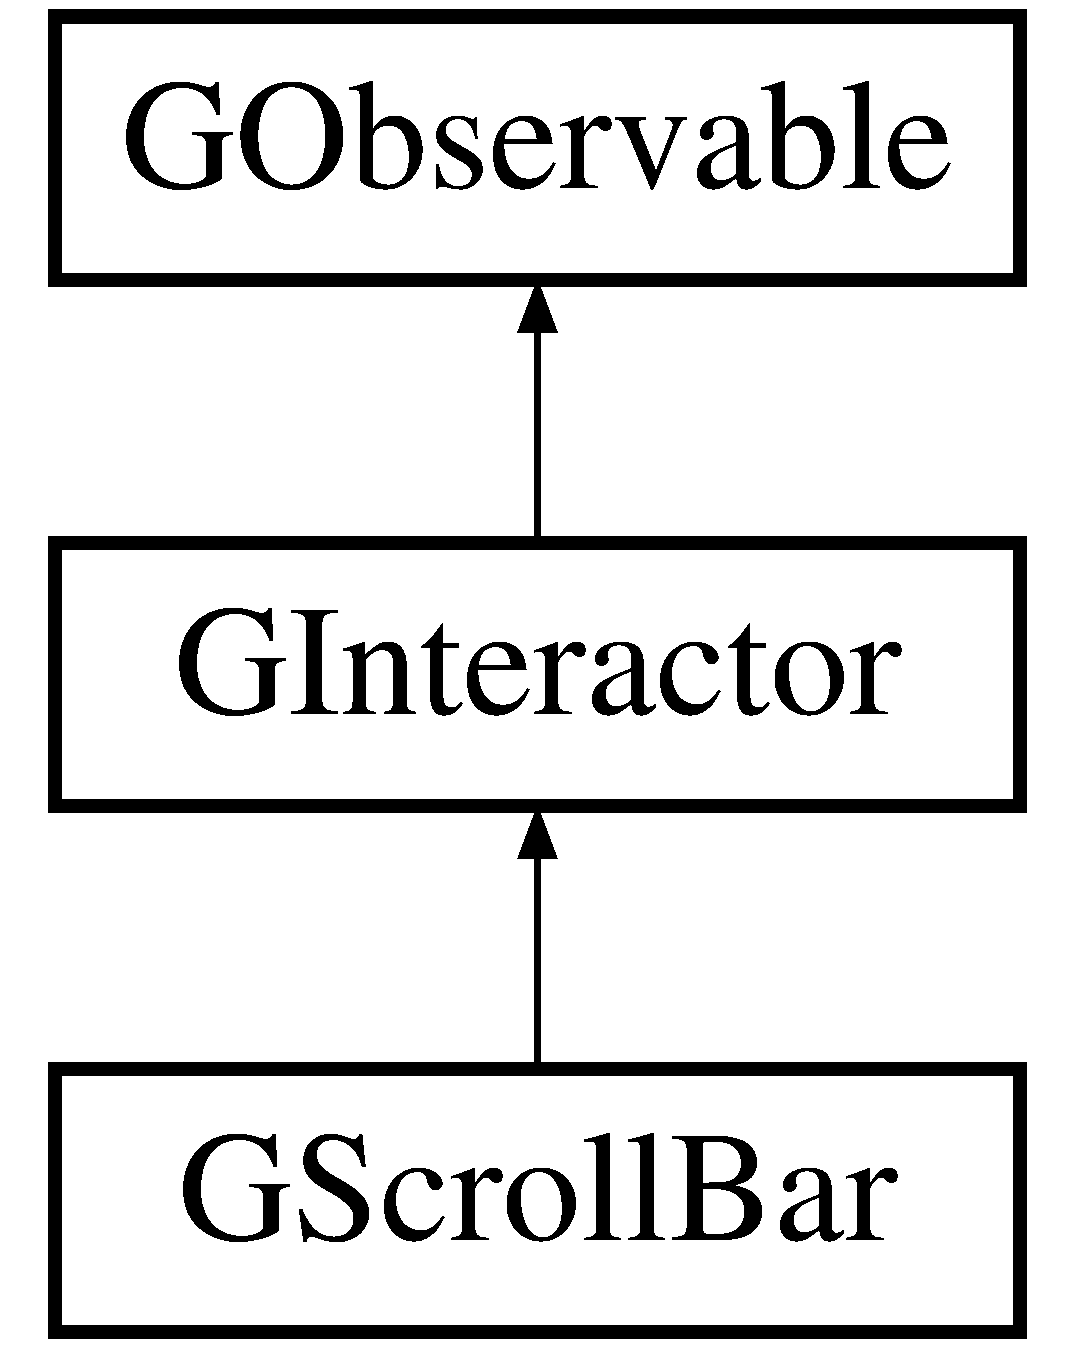
\includegraphics[height=3.000000cm]{classGScrollBar}
\end{center}
\end{figure}
\subsection*{Public Types}
\begin{DoxyCompactItemize}
\item 
enum \mbox{\hyperlink{classGScrollBar_a871118a09520247c78a71ecd7b0abd58}{Orientation}} \{ \mbox{\hyperlink{classGScrollBar_a871118a09520247c78a71ecd7b0abd58a4dd51ad73508d6fc83a502966779e48e}{H\+O\+R\+I\+Z\+O\+N\+T\+AL}} = 0, 
\mbox{\hyperlink{classGScrollBar_a871118a09520247c78a71ecd7b0abd58a1a88641fcd39f2ed3e58a18526e97138}{V\+E\+R\+T\+I\+C\+AL}} = 1
 \}
\begin{DoxyCompactList}\small\item\em The two valid orientations of scrollbars. \end{DoxyCompactList}\item 
enum \mbox{\hyperlink{classGInteractor_a8e0d441725a81d2bbdebbea09078260e}{Text\+Position}} \{ \mbox{\hyperlink{classGInteractor_a8e0d441725a81d2bbdebbea09078260ea4cd6f2e7d5a08d6f4dc052df2358f774}{T\+E\+X\+T\+\_\+\+B\+E\+S\+I\+D\+E\+\_\+\+I\+C\+ON}}, 
\mbox{\hyperlink{classGInteractor_a8e0d441725a81d2bbdebbea09078260eaa88490f63d8de68d44c83bdb2ecde3b3}{T\+E\+X\+T\+\_\+\+U\+N\+D\+E\+R\+\_\+\+I\+C\+ON}}, 
\mbox{\hyperlink{classGInteractor_a8e0d441725a81d2bbdebbea09078260ea39a6f388a30ac4fefb6eb13e846bc9f2}{T\+E\+X\+T\+\_\+\+O\+N\+LY}}
 \}
\begin{DoxyCompactList}\small\item\em The places where an interactor can place its text relative to its icon. \end{DoxyCompactList}\end{DoxyCompactItemize}
\subsection*{Public Member Functions}
\begin{DoxyCompactItemize}
\item 
\mbox{\hyperlink{classGScrollBar_aed316f3139eb0a6e80da4d1dcf171a43}{G\+Scroll\+Bar}} (\mbox{\hyperlink{classGScrollBar_a871118a09520247c78a71ecd7b0abd58}{Orientation}} orientation=\mbox{\hyperlink{classGScrollBar_a871118a09520247c78a71ecd7b0abd58a1a88641fcd39f2ed3e58a18526e97138}{V\+E\+R\+T\+I\+C\+AL}}, int value=0, int extent=10, int min=0, int max=100, Q\+Widget $\ast$parent=nullptr)
\begin{DoxyCompactList}\small\item\em Creates a new scroll bar with the given orientation and value range. \end{DoxyCompactList}\item 
\mbox{\hyperlink{classGScrollBar_a0b1ea2ea7b58f299e20c6d75249f1a2e}{$\sim$\+G\+Scroll\+Bar}} () override
\begin{DoxyCompactList}\small\item\em Frees memory allocated internally by the scroll bar. \end{DoxyCompactList}\item 
virtual void \mbox{\hyperlink{classGInteractor_a02f20ea6edfa0671f31c4c648a253833}{add\+Action\+Listener}} () Q\+\_\+\+D\+E\+C\+L\+\_\+\+D\+E\+P\+R\+E\+C\+A\+T\+ED
\begin{DoxyCompactList}\small\item\em Adds an event listener to be notified when this interactor is clicked or generally interacted with. \end{DoxyCompactList}\item 
bool \mbox{\hyperlink{classGInteractor_a597a370b592e3737d38d9d2f4e2031ea}{events\+Enabled}} () const override
\begin{DoxyCompactList}\small\item\em Returns true if this interactor is currently accepting events. \end{DoxyCompactList}\item 
virtual std\+::string \mbox{\hyperlink{classGInteractor_a69f8d23ed8f207fbecad99960776e942}{get\+Accelerator}} () const
\begin{DoxyCompactList}\small\item\em Returns a string representing a hotkey for this interactor, or an empty string if no accelerator has been set. \end{DoxyCompactList}\item 
virtual std\+::string \mbox{\hyperlink{classGInteractor_a94eb4276000c4fdfb508ce9e6317a82a}{get\+Action\+Command}} () const
\begin{DoxyCompactList}\small\item\em Returns an action command for this interactor, which is a semi-\/unique string you can use to identify it when events occur. \end{DoxyCompactList}\item 
virtual std\+::string \mbox{\hyperlink{classGInteractor_a808e22cc1fdfbecf71ed8c64ef4600e0}{get\+Background}} () const
\begin{DoxyCompactList}\small\item\em Returns the background color of the interactor as a string. \end{DoxyCompactList}\item 
virtual int \mbox{\hyperlink{classGInteractor_a9e827257a55cb8cf4d9de2ec6bcfd7a0}{get\+Background\+Int}} () const
\begin{DoxyCompactList}\small\item\em Returns the background color of the interactor as an R\+GB integer. \end{DoxyCompactList}\item 
virtual \mbox{\hyperlink{structGRectangle}{G\+Rectangle}} \mbox{\hyperlink{classGInteractor_a29e6ac35a0b48f491a4c88194cc5da3b}{get\+Bounds}} () const
\begin{DoxyCompactList}\small\item\em Returns a rectangle representing the x/y position and size of this interactor. \end{DoxyCompactList}\item 
virtual std\+::string \mbox{\hyperlink{classGInteractor_aa061dfa488c31e18549d64363c1d0e34}{get\+Color}} () const
\begin{DoxyCompactList}\small\item\em Returns the foreground/text color of the interactor as a string. \end{DoxyCompactList}\item 
virtual int \mbox{\hyperlink{classGInteractor_a9635c7af766cdc3417f346683fa0e6c1}{get\+Color\+Int}} () const
\begin{DoxyCompactList}\small\item\em Returns the foreground/text color of the interactor as an R\+GB integer. \end{DoxyCompactList}\item 
virtual \mbox{\hyperlink{classGContainer}{G\+Container}} $\ast$ \mbox{\hyperlink{classGInteractor_a7a6e317c29d61030929b4cd2d1c00fe7}{get\+Container}} () const
\begin{DoxyCompactList}\small\item\em Returns a pointer to the onscreen container holding this interactor. \end{DoxyCompactList}\item 
virtual int \mbox{\hyperlink{classGScrollBar_af8d1d8c0338fae10ee8673e8430f6be8}{get\+Extent}} () const
\begin{DoxyCompactList}\small\item\em Returns the scroll bar\textquotesingle{}s extent, meaning the amount of its range that is currently in view. \end{DoxyCompactList}\item 
virtual std\+::string \mbox{\hyperlink{classGInteractor_a894a5502900794eeb27d084c21f1d77d}{get\+Font}} () const
\begin{DoxyCompactList}\small\item\em Returns the font of this interactor\textquotesingle{}s text as a font string such as \char`\"{}\+Helvetica-\/12-\/\+Bold\char`\"{}. \end{DoxyCompactList}\item 
virtual std\+::string \mbox{\hyperlink{classGInteractor_a4fa2d8b0192a3a5b4af4bbfe71194d03}{get\+Foreground}} () const
\begin{DoxyCompactList}\small\item\em Returns the foreground/text color of the interactor as a string. \end{DoxyCompactList}\item 
virtual int \mbox{\hyperlink{classGInteractor_ac3b12ab385a6ef9ae90fc879860ba726}{get\+Foreground\+Int}} () const
\begin{DoxyCompactList}\small\item\em Returns the foreground/text color of the interactor as an R\+GB integer. \end{DoxyCompactList}\item 
virtual double \mbox{\hyperlink{classGInteractor_a1e7e353362434072875264cf95629f99}{get\+Height}} () const
\begin{DoxyCompactList}\small\item\em Returns the current onscreen height of this interactor in pixels. \end{DoxyCompactList}\item 
virtual std\+::string \mbox{\hyperlink{classGInteractor_aaed62a73004939a64da6f0eb9eb64d73}{get\+Icon}} () const
\begin{DoxyCompactList}\small\item\em Returns the file name of the icon associated with this interactor, or an empty string if no icon has been set. \end{DoxyCompactList}\item 
virtual int \mbox{\hyperlink{classGInteractor_a9c9659a6c6ba66b4107ba59c95a24241}{get\+ID}} () const
\begin{DoxyCompactList}\small\item\em Returns a globally unique identifier for this interactor, which is set when the interactor is constructed. \end{DoxyCompactList}\item 
\+\_\+\+Internal\+\_\+\+Q\+Widget $\ast$ \mbox{\hyperlink{classGScrollBar_a2f6b36b2517087dc90a366b5ce1f5323}{get\+Internal\+Widget}} () const override
\begin{DoxyCompactList}\small\item\em Returns a direct pointer to the internal Qt widget being wrapped by this interactor. \end{DoxyCompactList}\item 
virtual \mbox{\hyperlink{structGPoint}{G\+Point}} \mbox{\hyperlink{classGInteractor_a4f83802015511edeb63b892830812c11}{get\+Location}} () const
\begin{DoxyCompactList}\small\item\em Returns an (x, y) point representing the onscreen location of the top-\/left corner of this interactor within its containing window. \end{DoxyCompactList}\item 
virtual int \mbox{\hyperlink{classGScrollBar_acc49776af85220307b8955d752d9ffcb}{get\+Max}} () const
\begin{DoxyCompactList}\small\item\em Returns the maximum allowed value of the scroll bar. \end{DoxyCompactList}\item 
virtual int \mbox{\hyperlink{classGScrollBar_ad06537e69f71666d30bec18dc042a6e4}{get\+Min}} () const
\begin{DoxyCompactList}\small\item\em Returns the minimum allowed value of the scroll bar. \end{DoxyCompactList}\item 
virtual double \mbox{\hyperlink{classGInteractor_aed4b0075fcc434499c3cb3e46896bda3}{get\+Minimum\+Height}} () const
\begin{DoxyCompactList}\small\item\em Returns the minimum height in pixels that this interactor will permit itself to be resized to. \end{DoxyCompactList}\item 
virtual \mbox{\hyperlink{structGDimension}{G\+Dimension}} \mbox{\hyperlink{classGInteractor_a66b5af0b32493b4d597ca0a3df2049ea}{get\+Minimum\+Size}} () const
\begin{DoxyCompactList}\small\item\em Returns a \mbox{\hyperlink{structGDimension}{G\+Dimension}} structure representing the minimum size in pixels that this interactor will permit itself to be resized to. \end{DoxyCompactList}\item 
virtual double \mbox{\hyperlink{classGInteractor_a59e668114fe3d49d2a0f28deb258f7c8}{get\+Minimum\+Width}} () const
\begin{DoxyCompactList}\small\item\em Returns the minimum width in pixels that this interactor will permit itself to be resized to. \end{DoxyCompactList}\item 
virtual std\+::string \mbox{\hyperlink{classGInteractor_a8a60438a5b55d0b2ceb35c8674b9d8c5}{get\+Name}} () const
\begin{DoxyCompactList}\small\item\em Returns a string representing a unique name for this interactor. \end{DoxyCompactList}\item 
virtual \mbox{\hyperlink{classGScrollBar_a871118a09520247c78a71ecd7b0abd58}{Orientation}} \mbox{\hyperlink{classGScrollBar_a816fab656ead9b4f927bff46ae5a0e4d}{get\+Orientation}} () const
\begin{DoxyCompactList}\small\item\em Returns the orientation of the scroll bar, either H\+O\+R\+I\+Z\+O\+N\+T\+AL or V\+E\+R\+T\+I\+C\+AL. \end{DoxyCompactList}\item 
virtual double \mbox{\hyperlink{classGInteractor_a747de0961653847bdc6615dbf756d715}{get\+Preferred\+Height}} () const
\begin{DoxyCompactList}\small\item\em Returns the height in pixels that this interactor would prefer to be, which would exactly fit its contents with no stretching or scrollbars. \end{DoxyCompactList}\item 
virtual \mbox{\hyperlink{structGDimension}{G\+Dimension}} \mbox{\hyperlink{classGInteractor_a4aabbee761d8e9116275401131b7ccd1}{get\+Preferred\+Size}} () const
\begin{DoxyCompactList}\small\item\em Returns a \mbox{\hyperlink{structGDimension}{G\+Dimension}} structure storing the width and height in pixels that this interactor would prefer to be, which would exactly fit its contents with no stretching or scrollbars. \end{DoxyCompactList}\item 
virtual double \mbox{\hyperlink{classGInteractor_a82bca31d37700fb0e35d2743352efd5e}{get\+Preferred\+Width}} () const
\begin{DoxyCompactList}\small\item\em Returns the height in pixels that this interactor would prefer to be, which would exactly fit its contents with no stretching or scrollbars. \end{DoxyCompactList}\item 
virtual \mbox{\hyperlink{structGDimension}{G\+Dimension}} \mbox{\hyperlink{classGInteractor_a7b4eec96a2bdc6420695d5796a78eea9}{get\+Size}} () const
\begin{DoxyCompactList}\small\item\em Returns a \mbox{\hyperlink{structGDimension}{G\+Dimension}} structure storing the current onscreen width and height of this interactor in pixels. \end{DoxyCompactList}\item 
std\+::string \mbox{\hyperlink{classGScrollBar_a9b72ede4ee8520f987a0c01e30654814}{get\+Type}} () const override
\begin{DoxyCompactList}\small\item\em Returns a string representing the class name of this interactor, such as \char`\"{}\+G\+Button\char`\"{} or \char`\"{}\+G\+Check\+Box\char`\"{}. \end{DoxyCompactList}\item 
virtual int \mbox{\hyperlink{classGScrollBar_acdb0b383a96801f3200302b6f4a7da64}{get\+Value}} () const
\begin{DoxyCompactList}\small\item\em Returns the current value of the scroll bar. \end{DoxyCompactList}\item 
Q\+Widget $\ast$ \mbox{\hyperlink{classGScrollBar_a3b33a602b31a6b809d020535a59db3b4}{get\+Widget}} () const override
\begin{DoxyCompactList}\small\item\em Returns a direct pointer to the internal Qt widget being wrapped by this interactor. \end{DoxyCompactList}\item 
virtual double \mbox{\hyperlink{classGInteractor_a0ed2965abd4f5701d2cadf71239faf19}{get\+Width}} () const
\begin{DoxyCompactList}\small\item\em Returns the current onscreen width of this interactor in pixels. \end{DoxyCompactList}\item 
virtual double \mbox{\hyperlink{classGInteractor_a344385751bee0720059403940d57a13e}{getX}} () const
\begin{DoxyCompactList}\small\item\em Returns the x-\/coordinate of the top-\/left pixel of this interactor within its onscreen window. \end{DoxyCompactList}\item 
virtual double \mbox{\hyperlink{classGInteractor_aafa51c7f8f38a09febbb9ce7853f77b4}{getY}} () const
\begin{DoxyCompactList}\small\item\em Returns the y-\/coordinate of the top-\/left pixel of this interactor within its onscreen window. \end{DoxyCompactList}\item 
virtual bool \mbox{\hyperlink{classGInteractor_afc480f652b8c5f1fb255e2269ce68879}{in\+Bounds}} (double x, double y) const
\begin{DoxyCompactList}\small\item\em Returns true if the given x/y pixel is within the bounds of this interactor. \end{DoxyCompactList}\item 
virtual bool \mbox{\hyperlink{classGInteractor_ae6d7982c1c627b677a5e776ca86118ed}{in\+Bounds}} (int x, int y) const
\begin{DoxyCompactList}\small\item\em Returns true if the given x/y pixel is within the bounds of this interactor. \end{DoxyCompactList}\item 
virtual bool \mbox{\hyperlink{classGInteractor_aacb819fb241851fd9fc045271baa4034}{is\+Enabled}} () const
\begin{DoxyCompactList}\small\item\em Returns true if this interactor is currently enabled. \end{DoxyCompactList}\item 
virtual bool \mbox{\hyperlink{classGInteractor_a9d8a6cfb13917785c143e74d40e4e2be}{is\+Visible}} () const
\begin{DoxyCompactList}\small\item\em Returns true if the interactor is visible on the screen. \end{DoxyCompactList}\item 
virtual void \mbox{\hyperlink{classGInteractor_ab7fe7a876367b87cf7202f947f1d05e4}{remove\+Action\+Listener}} ()
\begin{DoxyCompactList}\small\item\em Removes the action listener from this interactor so that it will no longer call it when events occur. \end{DoxyCompactList}\item 
virtual void \mbox{\hyperlink{classGInteractor_ad39d0325cde6b97ebda4b9d7787c633b}{remove\+Click\+Listener}} ()
\begin{DoxyCompactList}\small\item\em Removes the click listener from this interactor so that it will no longer call it when events occur. \end{DoxyCompactList}\item 
virtual void \mbox{\hyperlink{classGInteractor_aa4250907e4cdd77349c04f0cf5cdd3d3}{remove\+Double\+Click\+Listener}} ()
\begin{DoxyCompactList}\small\item\em Removes the double-\/click listener from this interactor so that it will no longer call it when events occur. \end{DoxyCompactList}\item 
virtual void \mbox{\hyperlink{classGInteractor_a43095f41cab3be732b49f29970484b05}{remove\+Key\+Listener}} ()
\begin{DoxyCompactList}\small\item\em Removes the key listener from this interactor so that it will no longer call it when key events occur. \end{DoxyCompactList}\item 
virtual void \mbox{\hyperlink{classGInteractor_aff47f71ce47e688a07c9d38dc92fcc11}{remove\+Mouse\+Listener}} ()
\begin{DoxyCompactList}\small\item\em Removes the mouse listener from this interactor so that it will no longer call it when events occur. \end{DoxyCompactList}\item 
virtual void \mbox{\hyperlink{classGInteractor_a519fb2ac767f8b2febbb50b898b8c8cb}{request\+Focus}} ()
\begin{DoxyCompactList}\small\item\em Transfers keyboard focus to this interactor. \end{DoxyCompactList}\item 
virtual void \mbox{\hyperlink{classGInteractor_ad15f102f62e2960576012f1aa0ba4b2e}{set\+Accelerator}} (const std\+::string \&accelerator)
\begin{DoxyCompactList}\small\item\em Sets an accelerator hotkey for this interactor, such as \char`\"{}\+Ctrl-\/\+S\char`\"{}. \end{DoxyCompactList}\item 
virtual void \mbox{\hyperlink{classGInteractor_a4b5843fe3030e038a1ba54cc03389bcf}{set\+Action\+Command}} (const std\+::string \&action\+Command)
\begin{DoxyCompactList}\small\item\em Sets the action command for this interactor. \end{DoxyCompactList}\item 
virtual void \mbox{\hyperlink{classGInteractor_adcfb4742430c88714fcf57e57ab8ea9c}{set\+Action\+Listener}} (G\+Event\+Listener func)
\begin{DoxyCompactList}\small\item\em Sets an action listener on this interactor so that it will be called when it is interacted with in its primary way. \end{DoxyCompactList}\item 
virtual void \mbox{\hyperlink{classGInteractor_aebd20a89c7a8a43a6fce999cf4f9fcf2}{set\+Action\+Listener}} (G\+Event\+Listener\+Void func)
\begin{DoxyCompactList}\small\item\em Sets an action listener on this interactor so that it will be called when it is interacted with in its primary way. \end{DoxyCompactList}\item 
virtual void \mbox{\hyperlink{classGInteractor_acba7e546c2025c0a15ca4b4cc92043db}{set\+Background}} (int rgb)
\begin{DoxyCompactList}\small\item\em Sets the background color of the interactor to the color represented by the given R\+GB integer. \end{DoxyCompactList}\item 
virtual void \mbox{\hyperlink{classGInteractor_ab4677ab2474e68b07aa56605af92a84a}{set\+Background}} (const std\+::string \&color)
\begin{DoxyCompactList}\small\item\em Sets the background color of the interactor to the color represented by the given string. \end{DoxyCompactList}\item 
virtual void \mbox{\hyperlink{classGInteractor_a2aae8197624b72265ab83b4f1bc73f2f}{set\+Bounds}} (double x, double y, double width, double height)
\begin{DoxyCompactList}\small\item\em Sets the size and location of the widget. \end{DoxyCompactList}\item 
virtual void \mbox{\hyperlink{classGInteractor_acada386653f008cacc7cce86426bef7c}{set\+Bounds}} (const \mbox{\hyperlink{structGRectangle}{G\+Rectangle}} \&size)
\begin{DoxyCompactList}\small\item\em Sets the size and location of the widget. \end{DoxyCompactList}\item 
virtual void \mbox{\hyperlink{classGInteractor_abd40af6921242584d0954f173911b190}{set\+Click\+Listener}} (G\+Event\+Listener func)
\begin{DoxyCompactList}\small\item\em Sets a mouse listener on this interactor so that it will be called when the mouse is clicked on it. \end{DoxyCompactList}\item 
virtual void \mbox{\hyperlink{classGInteractor_a856414c92df90f56f3877475eb3f8fc4}{set\+Click\+Listener}} (G\+Event\+Listener\+Void func)
\begin{DoxyCompactList}\small\item\em Sets a mouse listener on this interactor so that it will be called when the mouse is clicked on it. \end{DoxyCompactList}\item 
virtual void \mbox{\hyperlink{classGInteractor_ab1f5cc0f5cc6bbbd716a526c61f1081d}{set\+Color}} (int rgb)
\begin{DoxyCompactList}\small\item\em Sets the foreground/text color of the interactor to the color represented by the given R\+GB integer. \end{DoxyCompactList}\item 
virtual void \mbox{\hyperlink{classGInteractor_a61374df6c11b52cfbb0815decdbaebc6}{set\+Color}} (const std\+::string \&color)
\begin{DoxyCompactList}\small\item\em Sets the foreground/text color of the interactor to the color represented by the given string. \end{DoxyCompactList}\item 
virtual void \mbox{\hyperlink{classGInteractor_ac29f9a3462458e165fae3a1f046ee77a}{set\+Double\+Click\+Listener}} (G\+Event\+Listener func)
\begin{DoxyCompactList}\small\item\em Sets a mouse listener on this interactor so that it will be called when the mouse is double-\/clicked on it. \end{DoxyCompactList}\item 
virtual void \mbox{\hyperlink{classGInteractor_a50096194d66f48c92dd4c512d41bfc76}{set\+Double\+Click\+Listener}} (G\+Event\+Listener\+Void func)
\begin{DoxyCompactList}\small\item\em Sets a mouse listener on this interactor so that it will be called when the mouse is double-\/clicked on it. \end{DoxyCompactList}\item 
virtual void \mbox{\hyperlink{classGInteractor_ab831367dd84bbd579e02e55bacb21343}{set\+Enabled}} (bool value)
\begin{DoxyCompactList}\small\item\em Sets whether this interactor is currently enabled. \end{DoxyCompactList}\item 
virtual void \mbox{\hyperlink{classGObservable_afaa30b2a9e0f378fd1c70d2f1d0b8216}{set\+Events\+Enabled}} (bool \mbox{\hyperlink{classGInteractor_a597a370b592e3737d38d9d2f4e2031ea}{events\+Enabled}})
\begin{DoxyCompactList}\small\item\em Sets whether the object is currently allowing itself to fire events. \end{DoxyCompactList}\item 
virtual void \mbox{\hyperlink{classGScrollBar_a2b06f746a9b7b56cbb85154bbe3288c6}{set\+Extent}} (int extent)
\begin{DoxyCompactList}\small\item\em Sets the scroll bar\textquotesingle{}s extent, meaning the amount of its range that is currently in view. \end{DoxyCompactList}\item 
virtual void \mbox{\hyperlink{classGInteractor_a2592348886ffea646c6534bf88f7c49d}{set\+Font}} (const Q\+Font \&font)
\begin{DoxyCompactList}\small\item\em Sets the font used by this widget to the given Qt font. \end{DoxyCompactList}\item 
virtual void \mbox{\hyperlink{classGInteractor_a8e096e8818d838aceae1d46d58fb3a7b}{set\+Font}} (const std\+::string \&font)
\begin{DoxyCompactList}\small\item\em Sets the font used by this widget to the font represented by the given font string, such as \char`\"{}\+Helvetica-\/16-\/\+Bold\char`\"{}. \end{DoxyCompactList}\item 
virtual void \mbox{\hyperlink{classGInteractor_a9eb856b5ff83a19df3831a31f15f4563}{set\+Foreground}} (int rgb)
\begin{DoxyCompactList}\small\item\em Sets the foreground/text color of the interactor to the color represented by the given R\+GB integer. \end{DoxyCompactList}\item 
virtual void \mbox{\hyperlink{classGInteractor_af59209aeadea6dfc6d97a2d8531f50e1}{set\+Foreground}} (const std\+::string \&color)
\begin{DoxyCompactList}\small\item\em Sets the foreground/text color of the interactor to the color represented by the given string. \end{DoxyCompactList}\item 
virtual void \mbox{\hyperlink{classGInteractor_a9e280bfc4544dfaf8e4376c4e1a74357}{set\+Height}} (double height)
\begin{DoxyCompactList}\small\item\em Sets the onscreen height of the interactor in pixels. \end{DoxyCompactList}\item 
virtual void \mbox{\hyperlink{classGInteractor_a542abfcd7261751352af129c7215ecda}{set\+Icon}} (const Q\+Icon \&icon)
\begin{DoxyCompactList}\small\item\em Sets the icon associated with this interactor. \end{DoxyCompactList}\item 
virtual void \mbox{\hyperlink{classGInteractor_a368e1a338f84401c284506d03b1ba769}{set\+Icon}} (const Q\+Pixmap \&icon)
\begin{DoxyCompactList}\small\item\em Sets the icon associated with this interactor. \end{DoxyCompactList}\item 
virtual void \mbox{\hyperlink{classGInteractor_a762e139aa311461c3984d3ad28293f64}{set\+Icon}} (const std\+::string \&filename, bool retain\+Icon\+Size=true)
\begin{DoxyCompactList}\small\item\em Sets the file name of the icon associated with this interactor, or an empty string if no icon has been set. \end{DoxyCompactList}\item 
virtual void \mbox{\hyperlink{classGInteractor_aeb8324d3287fa1fbe093f4d6230cf0a6}{set\+Key\+Listener}} (G\+Event\+Listener func)
\begin{DoxyCompactList}\small\item\em Sets a key listener on this interactor so that it will be called when the user presses any key. \end{DoxyCompactList}\item 
virtual void \mbox{\hyperlink{classGInteractor_ae48ecea73606c7bd9423e1c7cc589cc9}{set\+Key\+Listener}} (G\+Event\+Listener\+Void func)
\begin{DoxyCompactList}\small\item\em Sets a key listener on this interactor so that it will be called when the user presses any key. \end{DoxyCompactList}\item 
virtual void \mbox{\hyperlink{classGInteractor_a04594e8ba9b98513a64f1da00dcae18c}{set\+Location}} (double x, double y)
\begin{DoxyCompactList}\small\item\em Sets the onscreen x/y-\/coordinate of the top-\/left corner of the interactor relative to its window. \end{DoxyCompactList}\item 
virtual void \mbox{\hyperlink{classGScrollBar_ab263d79bf430d73a617641f317dcfb98}{set\+Max}} (int max)
\begin{DoxyCompactList}\small\item\em Sets the maximum allowed value of the scroll bar. \end{DoxyCompactList}\item 
virtual void \mbox{\hyperlink{classGScrollBar_a6dc44e5adc595b71f90efc65b0b5ea1d}{set\+Min}} (int min)
\begin{DoxyCompactList}\small\item\em Sets the minimum allowed value of the scroll bar. \end{DoxyCompactList}\item 
virtual void \mbox{\hyperlink{classGInteractor_a0cf428e207b7f22cc08138a90b1b87b2}{set\+Minimum\+Size}} (double width, double height)
\begin{DoxyCompactList}\small\item\em Sets the minimum size in pixels that this interactor will permit itself to be resized to. \end{DoxyCompactList}\item 
virtual void \mbox{\hyperlink{classGInteractor_a3b1046117ac6cb7abe467e00ba8a81f4}{set\+Minimum\+Size}} (const \mbox{\hyperlink{structGDimension}{G\+Dimension}} \&size)
\begin{DoxyCompactList}\small\item\em Sets the minimum size in pixels that this interactor will permit itself to be resized to. \end{DoxyCompactList}\item 
virtual void \mbox{\hyperlink{classGInteractor_a37d8dbc943f59920f705b0104f60bde2}{set\+Mouse\+Listener}} (G\+Event\+Listener func)
\begin{DoxyCompactList}\small\item\em Sets a mouse listener on this interactor so that it will be called when the mouse is moved or clicked on it. \end{DoxyCompactList}\item 
virtual void \mbox{\hyperlink{classGInteractor_aea7f647ea62d59f71b5fad6aa65eeaf9}{set\+Mouse\+Listener}} (G\+Event\+Listener\+Void func)
\begin{DoxyCompactList}\small\item\em Sets a mouse listener on this interactor so that it will be called when the mouse is moved or clicked on it. \end{DoxyCompactList}\item 
virtual void \mbox{\hyperlink{classGInteractor_a9d3a2685df23b5e7cbf59c19c4a1f9b5}{set\+Name}} (const std\+::string \&name)
\begin{DoxyCompactList}\small\item\em Sets a string representing a unique name for this interactor. \end{DoxyCompactList}\item 
virtual void \mbox{\hyperlink{classGInteractor_a1ab987704fce32098706c6f00fb08218}{set\+Preferred\+Height}} (double height)
\begin{DoxyCompactList}\small\item\em Sets the height in pixels that this interactor would prefer to be. \end{DoxyCompactList}\item 
virtual void \mbox{\hyperlink{classGInteractor_a042c5ae19430d765ef552371cae3632c}{set\+Preferred\+Size}} (double width, double height)
\begin{DoxyCompactList}\small\item\em Sets the width and height in pixels that this interactor would prefer to be. \end{DoxyCompactList}\item 
virtual void \mbox{\hyperlink{classGInteractor_aa22d9be4bc0e078bb0ea69b0fc9d7c75}{set\+Preferred\+Size}} (const \mbox{\hyperlink{structGDimension}{G\+Dimension}} \&size)
\begin{DoxyCompactList}\small\item\em Sets the size in pixels that this interactor would prefer to be. \end{DoxyCompactList}\item 
virtual void \mbox{\hyperlink{classGInteractor_a3db429ab2fa52efd187eec0ed8cdd9f2}{set\+Preferred\+Width}} (double width)
\begin{DoxyCompactList}\small\item\em Sets the width in pixels that this interactor would prefer to be. \end{DoxyCompactList}\item 
virtual void \mbox{\hyperlink{classGInteractor_aca25d49481f9bf5fc8f7df4c086c4ce7}{set\+Size}} (double width, double height)
\begin{DoxyCompactList}\small\item\em Sets the onscreen width and height of the interactor in pixels. \end{DoxyCompactList}\item 
virtual void \mbox{\hyperlink{classGInteractor_ae2b628228f192c2702c4ce941b2af68f}{set\+Size}} (const \mbox{\hyperlink{structGDimension}{G\+Dimension}} \&size)
\begin{DoxyCompactList}\small\item\em Sets the onscreen width and height of the interactor in pixels. \end{DoxyCompactList}\item 
virtual void \mbox{\hyperlink{classGScrollBar_a83549f22abf65099f4c661a4601ade2b}{set\+State}} (int value, int extent, int min, int max)
\begin{DoxyCompactList}\small\item\em Sets all of the relevant state of the scroll bar. \end{DoxyCompactList}\item 
virtual void \mbox{\hyperlink{classGInteractor_a039e0e49beaecc275efce02d416acea8}{set\+Tooltip}} (const std\+::string \&tooltip\+Text)
\begin{DoxyCompactList}\small\item\em Sets a \char`\"{}tooltip\char`\"{} that will appear if the user hovers their mouse over the interactor. \end{DoxyCompactList}\item 
virtual void \mbox{\hyperlink{classGScrollBar_a23d79e21b8ed72e19278ca31d47b8c87}{set\+Value}} (int value)
\begin{DoxyCompactList}\small\item\em Sets the current value of the scroll bar. \end{DoxyCompactList}\item 
virtual void \mbox{\hyperlink{classGInteractor_a18e44e30b31525a243960ca3928125aa}{set\+Visible}} (bool visible)
\begin{DoxyCompactList}\small\item\em Returns true if the interactor is visible on the screen. \end{DoxyCompactList}\item 
virtual void \mbox{\hyperlink{classGInteractor_aa3f3fba4cb131baa8696ba01e3bceca1}{set\+Width}} (double width)
\begin{DoxyCompactList}\small\item\em Sets the onscreen width of the interactor in pixels. \end{DoxyCompactList}\item 
virtual void \mbox{\hyperlink{classGInteractor_a9c18fcc579333bf9653d13ad2b372e39}{setX}} (double x)
\begin{DoxyCompactList}\small\item\em Sets the onscreen x-\/coordinate of the top-\/left corner of the interactor relative to its window. \end{DoxyCompactList}\item 
virtual void \mbox{\hyperlink{classGInteractor_a7d57e2a5c35d27feb58fd498a3cf82b9}{setY}} (double y)
\begin{DoxyCompactList}\small\item\em Sets the onscreen y-\/coordinate of the top-\/left corner of the interactor relative to its window. \end{DoxyCompactList}\item 
virtual std\+::string \mbox{\hyperlink{classGObservable_a1fe5121d6528fdea3f243321b3fa3a49}{to\+String}} () const
\begin{DoxyCompactList}\small\item\em Returns a string representation of this observable object\textquotesingle{}s state. \end{DoxyCompactList}\end{DoxyCompactItemize}
\subsection*{Protected Member Functions}
\begin{DoxyCompactItemize}
\item 
virtual void \mbox{\hyperlink{classGObservable_a80cfa040459ff53594adbd6a51ec8f43}{clear\+Event\+Listeners}} ()
\begin{DoxyCompactList}\small\item\em Removes all event listeners from this object. \end{DoxyCompactList}\item 
virtual void \mbox{\hyperlink{classGObservable_a284f31528c0520f8e545c03ac9eeac74}{ensure\+Thread\+Safety}} (const std\+::string \&member\+Name=\char`\"{}\char`\"{})
\begin{DoxyCompactList}\small\item\em Ensures that we are currently in the Qt G\+UI thread. \end{DoxyCompactList}\item 
virtual void \mbox{\hyperlink{classGObservable_a63e5e5a6227c59c928493b11aceb0f67}{fire\+Event}} (\mbox{\hyperlink{classGEvent}{G\+Event}} \&event)
\begin{DoxyCompactList}\small\item\em Sends out the given event to any attached listeners. \end{DoxyCompactList}\item 
virtual void \mbox{\hyperlink{classGObservable_ab3983ea07337b52020a29cc00c653d8d}{fire\+G\+Event}} (Q\+Event $\ast$event, Event\+Type event\+Type, const std\+::string \&event\+Name)
\begin{DoxyCompactList}\small\item\em Creates an event of the given type, then sends it out to any attached listeners. \end{DoxyCompactList}\item 
virtual void \mbox{\hyperlink{classGObservable_a01fdf1b0e0dbd49e189fe4514e010411}{fire\+G\+Event}} (Q\+Close\+Event $\ast$event, Event\+Type event\+Type, const std\+::string \&event\+Name)
\begin{DoxyCompactList}\small\item\em Creates an event of the given type, then sends it out to any attached listeners. \end{DoxyCompactList}\item 
virtual void \mbox{\hyperlink{classGObservable_abb0b2f66ba39211cb5d7615e9d1c04e2}{fire\+G\+Event}} (Q\+Key\+Event $\ast$event, Event\+Type event\+Type, const std\+::string \&event\+Name)
\begin{DoxyCompactList}\small\item\em Creates an event of the given type, then sends it out to any attached listeners. \end{DoxyCompactList}\item 
virtual void \mbox{\hyperlink{classGObservable_a119318675d2165bdf7dd853aaf881d4b}{fire\+G\+Event}} (Q\+Mouse\+Event $\ast$event, Event\+Type event\+Type, const std\+::string \&event\+Name, const std\+::string \&action\+Command=\char`\"{}\char`\"{})
\begin{DoxyCompactList}\small\item\em Creates an event of the given type, then sends it out to any attached listeners. \end{DoxyCompactList}\item 
virtual void \mbox{\hyperlink{classGObservable_a63fd9034e1e1633c1c38eb342bfd34e9}{fire\+G\+Event}} (Q\+Resize\+Event $\ast$event, Event\+Type event\+Type, const std\+::string \&event\+Name)
\begin{DoxyCompactList}\small\item\em Creates an event of the given type, then sends it out to any attached listeners. \end{DoxyCompactList}\item 
virtual void \mbox{\hyperlink{classGObservable_a741345310d9b7c5170a6cbc410c44ac4}{fire\+G\+Event}} (Q\+Timer\+Event $\ast$event, Event\+Type event\+Type, const std\+::string \&event\+Name)
\begin{DoxyCompactList}\small\item\em Creates an event of the given type, then sends it out to any attached listeners. \end{DoxyCompactList}\item 
virtual void \mbox{\hyperlink{classGObservable_a93bf338968a0338761b8e4dc62f582e9}{fire\+G\+Event}} (Q\+Wheel\+Event $\ast$event, Event\+Type event\+Type, const std\+::string \&event\+Name)
\begin{DoxyCompactList}\small\item\em Creates an event of the given type, then sends it out to any attached listeners. \end{DoxyCompactList}\item 
virtual void \mbox{\hyperlink{classGObservable_a2a70a7d7435ff0c3b80bb4d70da19e0d}{fire\+G\+Event}} (Q\+Window\+State\+Change\+Event $\ast$event, Event\+Type event\+Type, const std\+::string \&event\+Name)
\begin{DoxyCompactList}\small\item\em Creates an event of the given type, then sends it out to any attached listeners. \end{DoxyCompactList}\item 
virtual bool \mbox{\hyperlink{classGObservable_a9f6faaa25942923bafa1c44020c49fa9}{has\+Event\+Listener}} (const std\+::string \&event\+Name) const
\begin{DoxyCompactList}\small\item\em Returns true if the observable object has a listener for the given type of event. \end{DoxyCompactList}\item 
virtual bool \mbox{\hyperlink{classGObservable_aeec1adc19aa0f33de62390686ee1382c}{is\+Accepting\+Event}} (int event\+Mask) const
\begin{DoxyCompactList}\small\item\em Returns true if the observable object has a listener for the given type of event. \end{DoxyCompactList}\item 
virtual bool \mbox{\hyperlink{classGObservable_aa31c73145a29dcb92848a92e0cfaea41}{is\+Accepting\+Event}} (const \mbox{\hyperlink{classGEvent}{G\+Event}} \&event) const
\begin{DoxyCompactList}\small\item\em Returns true if the observable object has a listener for the given type of event. \end{DoxyCompactList}\item 
virtual bool \mbox{\hyperlink{classGObservable_a3b1c689267eda44e65a2213e7de38b23}{is\+Accepting\+Event}} (const std\+::string \&event\+Type) const
\begin{DoxyCompactList}\small\item\em Returns true if the observable object has a listener for the given type of event. \end{DoxyCompactList}\item 
virtual void \mbox{\hyperlink{classGObservable_acbcf1ed3a851ad8a3c17ef38d86b481d}{remove\+Event\+Listener}} (const std\+::string \&event\+Name)
\begin{DoxyCompactList}\small\item\em Removes any event listener from this observable object that would respond to the given type of event, such as \char`\"{}click\char`\"{} or \char`\"{}keydown\char`\"{}. \end{DoxyCompactList}\item 
virtual void \mbox{\hyperlink{classGObservable_af51cc35c29a1bd1908609d432decdbb6}{remove\+Event\+Listeners}} (std\+::initializer\+\_\+list$<$ std\+::string $>$ event\+Names)
\begin{DoxyCompactList}\small\item\em Removes any event listener from this observable object that would respond to the given types of events, such as \char`\"{}click\char`\"{} or \char`\"{}keydown\char`\"{}. \end{DoxyCompactList}\item 
virtual void \mbox{\hyperlink{classGObservable_ad2f6d34961c50f6c1e0659990b79f741}{set\+Event\+Listener}} (const std\+::string \&event\+Name, G\+Event\+Listener func)
\begin{DoxyCompactList}\small\item\em Adds an event listener from this observable object to respond to the given type of event, such as \char`\"{}click\char`\"{} or \char`\"{}keydown\char`\"{}. \end{DoxyCompactList}\item 
virtual void \mbox{\hyperlink{classGObservable_abac4cb9f9e626e010e87f5d91573c8a5}{set\+Event\+Listener}} (const std\+::string \&event\+Name, G\+Event\+Listener\+Void func)
\begin{DoxyCompactList}\small\item\em Adds an event listener from this observable object to respond to the given type of event, such as \char`\"{}click\char`\"{} or \char`\"{}keydown\char`\"{}. \end{DoxyCompactList}\item 
virtual void \mbox{\hyperlink{classGObservable_afa388d69c33c718cf035774604065604}{set\+Event\+Listeners}} (std\+::initializer\+\_\+list$<$ std\+::string $>$ event\+Names, G\+Event\+Listener func)
\begin{DoxyCompactList}\small\item\em Adds an event listener from this observable object to respond to the given types of events, such as \char`\"{}click\char`\"{} or \char`\"{}keydown\char`\"{}. \end{DoxyCompactList}\item 
virtual void \mbox{\hyperlink{classGObservable_a7867184bbb686f74fae8a4db927da799}{set\+Event\+Listeners}} (std\+::initializer\+\_\+list$<$ std\+::string $>$ event\+Names, G\+Event\+Listener\+Void func)
\begin{DoxyCompactList}\small\item\em Adds an event listener from this observable object to respond to the given types of events, such as \char`\"{}click\char`\"{} or \char`\"{}keydown\char`\"{}. \end{DoxyCompactList}\end{DoxyCompactItemize}


\subsection{Detailed Description}
A \mbox{\hyperlink{classGScrollBar}{G\+Scroll\+Bar}} represents a horizontal or vertical scroll bar that can be dragged by the user. 

The bar does not inherently cause any other interactor to scroll itself. If you want the bar to cause any effect, you must wait for scroll events and respond to them.

A given scroll bar has a range of values it can represent, with a min and max, along with a current value. The \char`\"{}extent\char`\"{} of a scrollbar represents the amount of the scrollbar in view. 

\subsection{Member Enumeration Documentation}
\mbox{\Hypertarget{classGScrollBar_a871118a09520247c78a71ecd7b0abd58}\label{classGScrollBar_a871118a09520247c78a71ecd7b0abd58}} 
\index{G\+Scroll\+Bar@{G\+Scroll\+Bar}!Orientation@{Orientation}}
\index{Orientation@{Orientation}!G\+Scroll\+Bar@{G\+Scroll\+Bar}}
\subsubsection{\texorpdfstring{Orientation}{Orientation}}
{\footnotesize\ttfamily enum \mbox{\hyperlink{classGScrollBar_a871118a09520247c78a71ecd7b0abd58}{Orientation}}}



The two valid orientations of scrollbars. 

\begin{DoxyEnumFields}{Enumerator}
\raisebox{\heightof{T}}[0pt][0pt]{\index{H\+O\+R\+I\+Z\+O\+N\+T\+AL@{H\+O\+R\+I\+Z\+O\+N\+T\+AL}!G\+Scroll\+Bar@{G\+Scroll\+Bar}}\index{G\+Scroll\+Bar@{G\+Scroll\+Bar}!H\+O\+R\+I\+Z\+O\+N\+T\+AL@{H\+O\+R\+I\+Z\+O\+N\+T\+AL}}}\mbox{\Hypertarget{classGScrollBar_a871118a09520247c78a71ecd7b0abd58a4dd51ad73508d6fc83a502966779e48e}\label{classGScrollBar_a871118a09520247c78a71ecd7b0abd58a4dd51ad73508d6fc83a502966779e48e}} 
H\+O\+R\+I\+Z\+O\+N\+T\+AL&\\
\hline

\raisebox{\heightof{T}}[0pt][0pt]{\index{V\+E\+R\+T\+I\+C\+AL@{V\+E\+R\+T\+I\+C\+AL}!G\+Scroll\+Bar@{G\+Scroll\+Bar}}\index{G\+Scroll\+Bar@{G\+Scroll\+Bar}!V\+E\+R\+T\+I\+C\+AL@{V\+E\+R\+T\+I\+C\+AL}}}\mbox{\Hypertarget{classGScrollBar_a871118a09520247c78a71ecd7b0abd58a1a88641fcd39f2ed3e58a18526e97138}\label{classGScrollBar_a871118a09520247c78a71ecd7b0abd58a1a88641fcd39f2ed3e58a18526e97138}} 
V\+E\+R\+T\+I\+C\+AL&\\
\hline

\end{DoxyEnumFields}
\mbox{\Hypertarget{classGInteractor_a8e0d441725a81d2bbdebbea09078260e}\label{classGInteractor_a8e0d441725a81d2bbdebbea09078260e}} 
\index{G\+Scroll\+Bar@{G\+Scroll\+Bar}!Text\+Position@{Text\+Position}}
\index{Text\+Position@{Text\+Position}!G\+Scroll\+Bar@{G\+Scroll\+Bar}}
\subsubsection{\texorpdfstring{Text\+Position}{TextPosition}}
{\footnotesize\ttfamily enum \mbox{\hyperlink{classGInteractor_a8e0d441725a81d2bbdebbea09078260e}{Text\+Position}}\hspace{0.3cm}{\ttfamily [inherited]}}



The places where an interactor can place its text relative to its icon. 

\begin{DoxyEnumFields}{Enumerator}
\raisebox{\heightof{T}}[0pt][0pt]{\index{T\+E\+X\+T\+\_\+\+B\+E\+S\+I\+D\+E\+\_\+\+I\+C\+ON@{T\+E\+X\+T\+\_\+\+B\+E\+S\+I\+D\+E\+\_\+\+I\+C\+ON}!G\+Scroll\+Bar@{G\+Scroll\+Bar}}\index{G\+Scroll\+Bar@{G\+Scroll\+Bar}!T\+E\+X\+T\+\_\+\+B\+E\+S\+I\+D\+E\+\_\+\+I\+C\+ON@{T\+E\+X\+T\+\_\+\+B\+E\+S\+I\+D\+E\+\_\+\+I\+C\+ON}}}\mbox{\Hypertarget{classGInteractor_a8e0d441725a81d2bbdebbea09078260ea4cd6f2e7d5a08d6f4dc052df2358f774}\label{classGInteractor_a8e0d441725a81d2bbdebbea09078260ea4cd6f2e7d5a08d6f4dc052df2358f774}} 
T\+E\+X\+T\+\_\+\+B\+E\+S\+I\+D\+E\+\_\+\+I\+C\+ON&\\
\hline

\raisebox{\heightof{T}}[0pt][0pt]{\index{T\+E\+X\+T\+\_\+\+U\+N\+D\+E\+R\+\_\+\+I\+C\+ON@{T\+E\+X\+T\+\_\+\+U\+N\+D\+E\+R\+\_\+\+I\+C\+ON}!G\+Scroll\+Bar@{G\+Scroll\+Bar}}\index{G\+Scroll\+Bar@{G\+Scroll\+Bar}!T\+E\+X\+T\+\_\+\+U\+N\+D\+E\+R\+\_\+\+I\+C\+ON@{T\+E\+X\+T\+\_\+\+U\+N\+D\+E\+R\+\_\+\+I\+C\+ON}}}\mbox{\Hypertarget{classGInteractor_a8e0d441725a81d2bbdebbea09078260eaa88490f63d8de68d44c83bdb2ecde3b3}\label{classGInteractor_a8e0d441725a81d2bbdebbea09078260eaa88490f63d8de68d44c83bdb2ecde3b3}} 
T\+E\+X\+T\+\_\+\+U\+N\+D\+E\+R\+\_\+\+I\+C\+ON&\\
\hline

\raisebox{\heightof{T}}[0pt][0pt]{\index{T\+E\+X\+T\+\_\+\+O\+N\+LY@{T\+E\+X\+T\+\_\+\+O\+N\+LY}!G\+Scroll\+Bar@{G\+Scroll\+Bar}}\index{G\+Scroll\+Bar@{G\+Scroll\+Bar}!T\+E\+X\+T\+\_\+\+O\+N\+LY@{T\+E\+X\+T\+\_\+\+O\+N\+LY}}}\mbox{\Hypertarget{classGInteractor_a8e0d441725a81d2bbdebbea09078260ea39a6f388a30ac4fefb6eb13e846bc9f2}\label{classGInteractor_a8e0d441725a81d2bbdebbea09078260ea39a6f388a30ac4fefb6eb13e846bc9f2}} 
T\+E\+X\+T\+\_\+\+O\+N\+LY&\\
\hline

\end{DoxyEnumFields}


\subsection{Constructor \& Destructor Documentation}
\mbox{\Hypertarget{classGScrollBar_aed316f3139eb0a6e80da4d1dcf171a43}\label{classGScrollBar_aed316f3139eb0a6e80da4d1dcf171a43}} 
\index{G\+Scroll\+Bar@{G\+Scroll\+Bar}!G\+Scroll\+Bar@{G\+Scroll\+Bar}}
\index{G\+Scroll\+Bar@{G\+Scroll\+Bar}!G\+Scroll\+Bar@{G\+Scroll\+Bar}}
\subsubsection{\texorpdfstring{G\+Scroll\+Bar()}{GScrollBar()}}
{\footnotesize\ttfamily \mbox{\hyperlink{classGScrollBar}{G\+Scroll\+Bar}} (\begin{DoxyParamCaption}\item[{\mbox{\hyperlink{classGScrollBar_a871118a09520247c78a71ecd7b0abd58}{G\+Scroll\+Bar\+::\+Orientation}}}]{orientation = {\ttfamily \mbox{\hyperlink{classGScrollBar_a871118a09520247c78a71ecd7b0abd58a1a88641fcd39f2ed3e58a18526e97138}{V\+E\+R\+T\+I\+C\+AL}}},  }\item[{int}]{value = {\ttfamily 0},  }\item[{int}]{extent = {\ttfamily 10},  }\item[{int}]{min = {\ttfamily 0},  }\item[{int}]{max = {\ttfamily 100},  }\item[{Q\+Widget $\ast$}]{parent = {\ttfamily nullptr} }\end{DoxyParamCaption})}



Creates a new scroll bar with the given orientation and value range. 


\begin{DoxyExceptions}{Exceptions}
{\em Error\+Exception} & if min $>$ max or value is not between min and max \\
\hline
\end{DoxyExceptions}
\mbox{\Hypertarget{classGScrollBar_a0b1ea2ea7b58f299e20c6d75249f1a2e}\label{classGScrollBar_a0b1ea2ea7b58f299e20c6d75249f1a2e}} 
\index{G\+Scroll\+Bar@{G\+Scroll\+Bar}!````~G\+Scroll\+Bar@{$\sim$\+G\+Scroll\+Bar}}
\index{````~G\+Scroll\+Bar@{$\sim$\+G\+Scroll\+Bar}!G\+Scroll\+Bar@{G\+Scroll\+Bar}}
\subsubsection{\texorpdfstring{$\sim$\+G\+Scroll\+Bar()}{~GScrollBar()}}
{\footnotesize\ttfamily $\sim$\mbox{\hyperlink{classGScrollBar}{G\+Scroll\+Bar}} (\begin{DoxyParamCaption}{ }\end{DoxyParamCaption})\hspace{0.3cm}{\ttfamily [override]}}



Frees memory allocated internally by the scroll bar. 



\subsection{Member Function Documentation}
\mbox{\Hypertarget{classGInteractor_a02f20ea6edfa0671f31c4c648a253833}\label{classGInteractor_a02f20ea6edfa0671f31c4c648a253833}} 
\index{G\+Scroll\+Bar@{G\+Scroll\+Bar}!add\+Action\+Listener@{add\+Action\+Listener}}
\index{add\+Action\+Listener@{add\+Action\+Listener}!G\+Scroll\+Bar@{G\+Scroll\+Bar}}
\subsubsection{\texorpdfstring{add\+Action\+Listener()}{addActionListener()}}
{\footnotesize\ttfamily void add\+Action\+Listener (\begin{DoxyParamCaption}{ }\end{DoxyParamCaption})\hspace{0.3cm}{\ttfamily [virtual]}, {\ttfamily [inherited]}}



Adds an event listener to be notified when this interactor is clicked or generally interacted with. 

\begin{DoxyRefDesc}{Deprecated}
\item[\mbox{\hyperlink{deprecated__deprecated000006}{Deprecated}}]does nothing; use set\+Action\+Listener instead \end{DoxyRefDesc}
\mbox{\Hypertarget{classGObservable_a80cfa040459ff53594adbd6a51ec8f43}\label{classGObservable_a80cfa040459ff53594adbd6a51ec8f43}} 
\index{G\+Scroll\+Bar@{G\+Scroll\+Bar}!clear\+Event\+Listeners@{clear\+Event\+Listeners}}
\index{clear\+Event\+Listeners@{clear\+Event\+Listeners}!G\+Scroll\+Bar@{G\+Scroll\+Bar}}
\subsubsection{\texorpdfstring{clear\+Event\+Listeners()}{clearEventListeners()}}
{\footnotesize\ttfamily void clear\+Event\+Listeners (\begin{DoxyParamCaption}{ }\end{DoxyParamCaption})\hspace{0.3cm}{\ttfamily [protected]}, {\ttfamily [virtual]}, {\ttfamily [inherited]}}



Removes all event listeners from this object. 

\mbox{\Hypertarget{classGObservable_a284f31528c0520f8e545c03ac9eeac74}\label{classGObservable_a284f31528c0520f8e545c03ac9eeac74}} 
\index{G\+Scroll\+Bar@{G\+Scroll\+Bar}!ensure\+Thread\+Safety@{ensure\+Thread\+Safety}}
\index{ensure\+Thread\+Safety@{ensure\+Thread\+Safety}!G\+Scroll\+Bar@{G\+Scroll\+Bar}}
\subsubsection{\texorpdfstring{ensure\+Thread\+Safety()}{ensureThreadSafety()}}
{\footnotesize\ttfamily void ensure\+Thread\+Safety (\begin{DoxyParamCaption}\item[{const std\+::string \&}]{member\+Name = {\ttfamily \char`\"{}\char`\"{}} }\end{DoxyParamCaption})\hspace{0.3cm}{\ttfamily [protected]}, {\ttfamily [virtual]}, {\ttfamily [inherited]}}



Ensures that we are currently in the Qt G\+UI thread. 

\mbox{\Hypertarget{classGInteractor_a597a370b592e3737d38d9d2f4e2031ea}\label{classGInteractor_a597a370b592e3737d38d9d2f4e2031ea}} 
\index{G\+Scroll\+Bar@{G\+Scroll\+Bar}!events\+Enabled@{events\+Enabled}}
\index{events\+Enabled@{events\+Enabled}!G\+Scroll\+Bar@{G\+Scroll\+Bar}}
\subsubsection{\texorpdfstring{events\+Enabled()}{eventsEnabled()}}
{\footnotesize\ttfamily bool events\+Enabled (\begin{DoxyParamCaption}{ }\end{DoxyParamCaption}) const\hspace{0.3cm}{\ttfamily [override]}, {\ttfamily [virtual]}, {\ttfamily [inherited]}}



Returns true if this interactor is currently accepting events. 

Initially true. An interactor must be visible and added to an onscreen window to receive events. 

Reimplemented from \mbox{\hyperlink{classGObservable_a8ebb3da91032e7f4c34485dabc518b8a}{G\+Observable}}.

\mbox{\Hypertarget{classGObservable_a63e5e5a6227c59c928493b11aceb0f67}\label{classGObservable_a63e5e5a6227c59c928493b11aceb0f67}} 
\index{G\+Scroll\+Bar@{G\+Scroll\+Bar}!fire\+Event@{fire\+Event}}
\index{fire\+Event@{fire\+Event}!G\+Scroll\+Bar@{G\+Scroll\+Bar}}
\subsubsection{\texorpdfstring{fire\+Event()}{fireEvent()}}
{\footnotesize\ttfamily void fire\+Event (\begin{DoxyParamCaption}\item[{\mbox{\hyperlink{classGEvent}{G\+Event}} \&}]{event }\end{DoxyParamCaption})\hspace{0.3cm}{\ttfamily [protected]}, {\ttfamily [virtual]}, {\ttfamily [inherited]}}



Sends out the given event to any attached listeners. 

\mbox{\Hypertarget{classGObservable_ab3983ea07337b52020a29cc00c653d8d}\label{classGObservable_ab3983ea07337b52020a29cc00c653d8d}} 
\index{G\+Scroll\+Bar@{G\+Scroll\+Bar}!fire\+G\+Event@{fire\+G\+Event}}
\index{fire\+G\+Event@{fire\+G\+Event}!G\+Scroll\+Bar@{G\+Scroll\+Bar}}
\subsubsection{\texorpdfstring{fire\+G\+Event()}{fireGEvent()}\hspace{0.1cm}{\footnotesize\ttfamily [1/8]}}
{\footnotesize\ttfamily void fire\+G\+Event (\begin{DoxyParamCaption}\item[{Q\+Event $\ast$}]{event,  }\item[{Event\+Type}]{event\+Type,  }\item[{const std\+::string \&}]{event\+Name }\end{DoxyParamCaption})\hspace{0.3cm}{\ttfamily [protected]}, {\ttfamily [virtual]}, {\ttfamily [inherited]}}



Creates an event of the given type, then sends it out to any attached listeners. 

\mbox{\Hypertarget{classGObservable_a01fdf1b0e0dbd49e189fe4514e010411}\label{classGObservable_a01fdf1b0e0dbd49e189fe4514e010411}} 
\index{G\+Scroll\+Bar@{G\+Scroll\+Bar}!fire\+G\+Event@{fire\+G\+Event}}
\index{fire\+G\+Event@{fire\+G\+Event}!G\+Scroll\+Bar@{G\+Scroll\+Bar}}
\subsubsection{\texorpdfstring{fire\+G\+Event()}{fireGEvent()}\hspace{0.1cm}{\footnotesize\ttfamily [2/8]}}
{\footnotesize\ttfamily void fire\+G\+Event (\begin{DoxyParamCaption}\item[{Q\+Close\+Event $\ast$}]{event,  }\item[{Event\+Type}]{event\+Type,  }\item[{const std\+::string \&}]{event\+Name }\end{DoxyParamCaption})\hspace{0.3cm}{\ttfamily [protected]}, {\ttfamily [virtual]}, {\ttfamily [inherited]}}



Creates an event of the given type, then sends it out to any attached listeners. 

\mbox{\Hypertarget{classGObservable_abb0b2f66ba39211cb5d7615e9d1c04e2}\label{classGObservable_abb0b2f66ba39211cb5d7615e9d1c04e2}} 
\index{G\+Scroll\+Bar@{G\+Scroll\+Bar}!fire\+G\+Event@{fire\+G\+Event}}
\index{fire\+G\+Event@{fire\+G\+Event}!G\+Scroll\+Bar@{G\+Scroll\+Bar}}
\subsubsection{\texorpdfstring{fire\+G\+Event()}{fireGEvent()}\hspace{0.1cm}{\footnotesize\ttfamily [3/8]}}
{\footnotesize\ttfamily void fire\+G\+Event (\begin{DoxyParamCaption}\item[{Q\+Key\+Event $\ast$}]{event,  }\item[{Event\+Type}]{event\+Type,  }\item[{const std\+::string \&}]{event\+Name }\end{DoxyParamCaption})\hspace{0.3cm}{\ttfamily [protected]}, {\ttfamily [virtual]}, {\ttfamily [inherited]}}



Creates an event of the given type, then sends it out to any attached listeners. 

\mbox{\Hypertarget{classGObservable_a119318675d2165bdf7dd853aaf881d4b}\label{classGObservable_a119318675d2165bdf7dd853aaf881d4b}} 
\index{G\+Scroll\+Bar@{G\+Scroll\+Bar}!fire\+G\+Event@{fire\+G\+Event}}
\index{fire\+G\+Event@{fire\+G\+Event}!G\+Scroll\+Bar@{G\+Scroll\+Bar}}
\subsubsection{\texorpdfstring{fire\+G\+Event()}{fireGEvent()}\hspace{0.1cm}{\footnotesize\ttfamily [4/8]}}
{\footnotesize\ttfamily void fire\+G\+Event (\begin{DoxyParamCaption}\item[{Q\+Mouse\+Event $\ast$}]{event,  }\item[{Event\+Type}]{event\+Type,  }\item[{const std\+::string \&}]{event\+Name,  }\item[{const std\+::string \&}]{action\+Command = {\ttfamily \char`\"{}\char`\"{}} }\end{DoxyParamCaption})\hspace{0.3cm}{\ttfamily [protected]}, {\ttfamily [virtual]}, {\ttfamily [inherited]}}



Creates an event of the given type, then sends it out to any attached listeners. 

\mbox{\Hypertarget{classGObservable_a63fd9034e1e1633c1c38eb342bfd34e9}\label{classGObservable_a63fd9034e1e1633c1c38eb342bfd34e9}} 
\index{G\+Scroll\+Bar@{G\+Scroll\+Bar}!fire\+G\+Event@{fire\+G\+Event}}
\index{fire\+G\+Event@{fire\+G\+Event}!G\+Scroll\+Bar@{G\+Scroll\+Bar}}
\subsubsection{\texorpdfstring{fire\+G\+Event()}{fireGEvent()}\hspace{0.1cm}{\footnotesize\ttfamily [5/8]}}
{\footnotesize\ttfamily void fire\+G\+Event (\begin{DoxyParamCaption}\item[{Q\+Resize\+Event $\ast$}]{event,  }\item[{Event\+Type}]{event\+Type,  }\item[{const std\+::string \&}]{event\+Name }\end{DoxyParamCaption})\hspace{0.3cm}{\ttfamily [protected]}, {\ttfamily [virtual]}, {\ttfamily [inherited]}}



Creates an event of the given type, then sends it out to any attached listeners. 

\mbox{\Hypertarget{classGObservable_a741345310d9b7c5170a6cbc410c44ac4}\label{classGObservable_a741345310d9b7c5170a6cbc410c44ac4}} 
\index{G\+Scroll\+Bar@{G\+Scroll\+Bar}!fire\+G\+Event@{fire\+G\+Event}}
\index{fire\+G\+Event@{fire\+G\+Event}!G\+Scroll\+Bar@{G\+Scroll\+Bar}}
\subsubsection{\texorpdfstring{fire\+G\+Event()}{fireGEvent()}\hspace{0.1cm}{\footnotesize\ttfamily [6/8]}}
{\footnotesize\ttfamily void fire\+G\+Event (\begin{DoxyParamCaption}\item[{Q\+Timer\+Event $\ast$}]{event,  }\item[{Event\+Type}]{event\+Type,  }\item[{const std\+::string \&}]{event\+Name }\end{DoxyParamCaption})\hspace{0.3cm}{\ttfamily [protected]}, {\ttfamily [virtual]}, {\ttfamily [inherited]}}



Creates an event of the given type, then sends it out to any attached listeners. 

\mbox{\Hypertarget{classGObservable_a93bf338968a0338761b8e4dc62f582e9}\label{classGObservable_a93bf338968a0338761b8e4dc62f582e9}} 
\index{G\+Scroll\+Bar@{G\+Scroll\+Bar}!fire\+G\+Event@{fire\+G\+Event}}
\index{fire\+G\+Event@{fire\+G\+Event}!G\+Scroll\+Bar@{G\+Scroll\+Bar}}
\subsubsection{\texorpdfstring{fire\+G\+Event()}{fireGEvent()}\hspace{0.1cm}{\footnotesize\ttfamily [7/8]}}
{\footnotesize\ttfamily void fire\+G\+Event (\begin{DoxyParamCaption}\item[{Q\+Wheel\+Event $\ast$}]{event,  }\item[{Event\+Type}]{event\+Type,  }\item[{const std\+::string \&}]{event\+Name }\end{DoxyParamCaption})\hspace{0.3cm}{\ttfamily [protected]}, {\ttfamily [virtual]}, {\ttfamily [inherited]}}



Creates an event of the given type, then sends it out to any attached listeners. 

\mbox{\Hypertarget{classGObservable_a2a70a7d7435ff0c3b80bb4d70da19e0d}\label{classGObservable_a2a70a7d7435ff0c3b80bb4d70da19e0d}} 
\index{G\+Scroll\+Bar@{G\+Scroll\+Bar}!fire\+G\+Event@{fire\+G\+Event}}
\index{fire\+G\+Event@{fire\+G\+Event}!G\+Scroll\+Bar@{G\+Scroll\+Bar}}
\subsubsection{\texorpdfstring{fire\+G\+Event()}{fireGEvent()}\hspace{0.1cm}{\footnotesize\ttfamily [8/8]}}
{\footnotesize\ttfamily void fire\+G\+Event (\begin{DoxyParamCaption}\item[{Q\+Window\+State\+Change\+Event $\ast$}]{event,  }\item[{Event\+Type}]{event\+Type,  }\item[{const std\+::string \&}]{event\+Name }\end{DoxyParamCaption})\hspace{0.3cm}{\ttfamily [protected]}, {\ttfamily [virtual]}, {\ttfamily [inherited]}}



Creates an event of the given type, then sends it out to any attached listeners. 

\mbox{\Hypertarget{classGInteractor_a69f8d23ed8f207fbecad99960776e942}\label{classGInteractor_a69f8d23ed8f207fbecad99960776e942}} 
\index{G\+Scroll\+Bar@{G\+Scroll\+Bar}!get\+Accelerator@{get\+Accelerator}}
\index{get\+Accelerator@{get\+Accelerator}!G\+Scroll\+Bar@{G\+Scroll\+Bar}}
\subsubsection{\texorpdfstring{get\+Accelerator()}{getAccelerator()}}
{\footnotesize\ttfamily std\+::string get\+Accelerator (\begin{DoxyParamCaption}{ }\end{DoxyParamCaption}) const\hspace{0.3cm}{\ttfamily [virtual]}, {\ttfamily [inherited]}}



Returns a string representing a hotkey for this interactor, or an empty string if no accelerator has been set. 

\begin{DoxyReturn}{Returns}
an accelerator such as \char`\"{}\+Ctrl-\/\+S\char`\"{} 
\end{DoxyReturn}


Reimplemented in \mbox{\hyperlink{classGButton_a57806dc9defb73f76f493f8548319924}{G\+Button}}.

\mbox{\Hypertarget{classGInteractor_a94eb4276000c4fdfb508ce9e6317a82a}\label{classGInteractor_a94eb4276000c4fdfb508ce9e6317a82a}} 
\index{G\+Scroll\+Bar@{G\+Scroll\+Bar}!get\+Action\+Command@{get\+Action\+Command}}
\index{get\+Action\+Command@{get\+Action\+Command}!G\+Scroll\+Bar@{G\+Scroll\+Bar}}
\subsubsection{\texorpdfstring{get\+Action\+Command()}{getActionCommand()}}
{\footnotesize\ttfamily std\+::string get\+Action\+Command (\begin{DoxyParamCaption}{ }\end{DoxyParamCaption}) const\hspace{0.3cm}{\ttfamily [virtual]}, {\ttfamily [inherited]}}



Returns an action command for this interactor, which is a semi-\/unique string you can use to identify it when events occur. 

For example, for buttons, the default action command is the button\textquotesingle{}s text. 

Reimplemented in \mbox{\hyperlink{classGChooser_a4f83505141da1f8446f0e0e0a9507930}{G\+Chooser}}, \mbox{\hyperlink{classGRadioButton_a4f83505141da1f8446f0e0e0a9507930}{G\+Radio\+Button}}, \mbox{\hyperlink{classGButton_a4f83505141da1f8446f0e0e0a9507930}{G\+Button}}, and \mbox{\hyperlink{classGCheckBox_a4f83505141da1f8446f0e0e0a9507930}{G\+Check\+Box}}.

\mbox{\Hypertarget{classGInteractor_a808e22cc1fdfbecf71ed8c64ef4600e0}\label{classGInteractor_a808e22cc1fdfbecf71ed8c64ef4600e0}} 
\index{G\+Scroll\+Bar@{G\+Scroll\+Bar}!get\+Background@{get\+Background}}
\index{get\+Background@{get\+Background}!G\+Scroll\+Bar@{G\+Scroll\+Bar}}
\subsubsection{\texorpdfstring{get\+Background()}{getBackground()}}
{\footnotesize\ttfamily std\+::string get\+Background (\begin{DoxyParamCaption}{ }\end{DoxyParamCaption}) const\hspace{0.3cm}{\ttfamily [virtual]}, {\ttfamily [inherited]}}



Returns the background color of the interactor as a string. 

\begin{DoxyReturn}{Returns}
a string such as \char`\"{}blue\char`\"{} or \char`\"{}\#7700ff\char`\"{} 
\end{DoxyReturn}


Reimplemented in \mbox{\hyperlink{classGCanvas_a4a62c51b7244a7642b88065e3a07ae82}{G\+Canvas}}.

\mbox{\Hypertarget{classGInteractor_a9e827257a55cb8cf4d9de2ec6bcfd7a0}\label{classGInteractor_a9e827257a55cb8cf4d9de2ec6bcfd7a0}} 
\index{G\+Scroll\+Bar@{G\+Scroll\+Bar}!get\+Background\+Int@{get\+Background\+Int}}
\index{get\+Background\+Int@{get\+Background\+Int}!G\+Scroll\+Bar@{G\+Scroll\+Bar}}
\subsubsection{\texorpdfstring{get\+Background\+Int()}{getBackgroundInt()}}
{\footnotesize\ttfamily int get\+Background\+Int (\begin{DoxyParamCaption}{ }\end{DoxyParamCaption}) const\hspace{0.3cm}{\ttfamily [virtual]}, {\ttfamily [inherited]}}



Returns the background color of the interactor as an R\+GB integer. 

\begin{DoxyReturn}{Returns}
an integer such as 0x7700ff 
\end{DoxyReturn}


Reimplemented in \mbox{\hyperlink{classGCanvas_acd4f2b3b9619dacdfd71fc0004cac382}{G\+Canvas}}.

\mbox{\Hypertarget{classGInteractor_a29e6ac35a0b48f491a4c88194cc5da3b}\label{classGInteractor_a29e6ac35a0b48f491a4c88194cc5da3b}} 
\index{G\+Scroll\+Bar@{G\+Scroll\+Bar}!get\+Bounds@{get\+Bounds}}
\index{get\+Bounds@{get\+Bounds}!G\+Scroll\+Bar@{G\+Scroll\+Bar}}
\subsubsection{\texorpdfstring{get\+Bounds()}{getBounds()}}
{\footnotesize\ttfamily \mbox{\hyperlink{structGRectangle}{G\+Rectangle}} get\+Bounds (\begin{DoxyParamCaption}{ }\end{DoxyParamCaption}) const\hspace{0.3cm}{\ttfamily [virtual]}, {\ttfamily [inherited]}}



Returns a rectangle representing the x/y position and size of this interactor. 

\mbox{\Hypertarget{classGInteractor_aa061dfa488c31e18549d64363c1d0e34}\label{classGInteractor_aa061dfa488c31e18549d64363c1d0e34}} 
\index{G\+Scroll\+Bar@{G\+Scroll\+Bar}!get\+Color@{get\+Color}}
\index{get\+Color@{get\+Color}!G\+Scroll\+Bar@{G\+Scroll\+Bar}}
\subsubsection{\texorpdfstring{get\+Color()}{getColor()}}
{\footnotesize\ttfamily std\+::string get\+Color (\begin{DoxyParamCaption}{ }\end{DoxyParamCaption}) const\hspace{0.3cm}{\ttfamily [virtual]}, {\ttfamily [inherited]}}



Returns the foreground/text color of the interactor as a string. 

Equivalent to get\+Foreground. \begin{DoxyReturn}{Returns}
a string such as \char`\"{}blue\char`\"{} or \char`\"{}\#7700ff\char`\"{} 
\end{DoxyReturn}
\mbox{\Hypertarget{classGInteractor_a9635c7af766cdc3417f346683fa0e6c1}\label{classGInteractor_a9635c7af766cdc3417f346683fa0e6c1}} 
\index{G\+Scroll\+Bar@{G\+Scroll\+Bar}!get\+Color\+Int@{get\+Color\+Int}}
\index{get\+Color\+Int@{get\+Color\+Int}!G\+Scroll\+Bar@{G\+Scroll\+Bar}}
\subsubsection{\texorpdfstring{get\+Color\+Int()}{getColorInt()}}
{\footnotesize\ttfamily int get\+Color\+Int (\begin{DoxyParamCaption}{ }\end{DoxyParamCaption}) const\hspace{0.3cm}{\ttfamily [virtual]}, {\ttfamily [inherited]}}



Returns the foreground/text color of the interactor as an R\+GB integer. 

Equivalent to get\+Foreground\+Int. \begin{DoxyReturn}{Returns}
an integer such as 0x7700ff 
\end{DoxyReturn}
\mbox{\Hypertarget{classGInteractor_a7a6e317c29d61030929b4cd2d1c00fe7}\label{classGInteractor_a7a6e317c29d61030929b4cd2d1c00fe7}} 
\index{G\+Scroll\+Bar@{G\+Scroll\+Bar}!get\+Container@{get\+Container}}
\index{get\+Container@{get\+Container}!G\+Scroll\+Bar@{G\+Scroll\+Bar}}
\subsubsection{\texorpdfstring{get\+Container()}{getContainer()}}
{\footnotesize\ttfamily \mbox{\hyperlink{classGContainer}{G\+Container}} $\ast$ get\+Container (\begin{DoxyParamCaption}{ }\end{DoxyParamCaption}) const\hspace{0.3cm}{\ttfamily [virtual]}, {\ttfamily [inherited]}}



Returns a pointer to the onscreen container holding this interactor. 

When an interactor is created, its container is initially null. This will become non-\/null automatically if you add the interactor to a window or other layout container. Interactors must be added to a container or window to receive events or to become visible on the screen. \begin{DoxyReturn}{Returns}
the container, or nullptr if interactor has not yet been added to any container 
\end{DoxyReturn}
\mbox{\Hypertarget{classGScrollBar_af8d1d8c0338fae10ee8673e8430f6be8}\label{classGScrollBar_af8d1d8c0338fae10ee8673e8430f6be8}} 
\index{G\+Scroll\+Bar@{G\+Scroll\+Bar}!get\+Extent@{get\+Extent}}
\index{get\+Extent@{get\+Extent}!G\+Scroll\+Bar@{G\+Scroll\+Bar}}
\subsubsection{\texorpdfstring{get\+Extent()}{getExtent()}}
{\footnotesize\ttfamily int get\+Extent (\begin{DoxyParamCaption}{ }\end{DoxyParamCaption}) const\hspace{0.3cm}{\ttfamily [virtual]}}



Returns the scroll bar\textquotesingle{}s extent, meaning the amount of its range that is currently in view. 

\mbox{\Hypertarget{classGInteractor_a894a5502900794eeb27d084c21f1d77d}\label{classGInteractor_a894a5502900794eeb27d084c21f1d77d}} 
\index{G\+Scroll\+Bar@{G\+Scroll\+Bar}!get\+Font@{get\+Font}}
\index{get\+Font@{get\+Font}!G\+Scroll\+Bar@{G\+Scroll\+Bar}}
\subsubsection{\texorpdfstring{get\+Font()}{getFont()}}
{\footnotesize\ttfamily std\+::string get\+Font (\begin{DoxyParamCaption}{ }\end{DoxyParamCaption}) const\hspace{0.3cm}{\ttfamily [virtual]}, {\ttfamily [inherited]}}



Returns the font of this interactor\textquotesingle{}s text as a font string such as \char`\"{}\+Helvetica-\/12-\/\+Bold\char`\"{}. 

\begin{DoxyReturn}{Returns}
a font string such as \char`\"{}\+Helvetica-\/12-\/\+Bold\char`\"{} 
\end{DoxyReturn}


Reimplemented in \mbox{\hyperlink{classGCanvas_aa0829769ac6325b5c58d27c8e363cb78}{G\+Canvas}}.

\mbox{\Hypertarget{classGInteractor_a4fa2d8b0192a3a5b4af4bbfe71194d03}\label{classGInteractor_a4fa2d8b0192a3a5b4af4bbfe71194d03}} 
\index{G\+Scroll\+Bar@{G\+Scroll\+Bar}!get\+Foreground@{get\+Foreground}}
\index{get\+Foreground@{get\+Foreground}!G\+Scroll\+Bar@{G\+Scroll\+Bar}}
\subsubsection{\texorpdfstring{get\+Foreground()}{getForeground()}}
{\footnotesize\ttfamily std\+::string get\+Foreground (\begin{DoxyParamCaption}{ }\end{DoxyParamCaption}) const\hspace{0.3cm}{\ttfamily [virtual]}, {\ttfamily [inherited]}}



Returns the foreground/text color of the interactor as a string. 

Equivalent to get\+Color. \begin{DoxyReturn}{Returns}
a string such as \char`\"{}blue\char`\"{} or \char`\"{}\#7700ff\char`\"{} 
\end{DoxyReturn}
\mbox{\Hypertarget{classGInteractor_ac3b12ab385a6ef9ae90fc879860ba726}\label{classGInteractor_ac3b12ab385a6ef9ae90fc879860ba726}} 
\index{G\+Scroll\+Bar@{G\+Scroll\+Bar}!get\+Foreground\+Int@{get\+Foreground\+Int}}
\index{get\+Foreground\+Int@{get\+Foreground\+Int}!G\+Scroll\+Bar@{G\+Scroll\+Bar}}
\subsubsection{\texorpdfstring{get\+Foreground\+Int()}{getForegroundInt()}}
{\footnotesize\ttfamily int get\+Foreground\+Int (\begin{DoxyParamCaption}{ }\end{DoxyParamCaption}) const\hspace{0.3cm}{\ttfamily [virtual]}, {\ttfamily [inherited]}}



Returns the foreground/text color of the interactor as an R\+GB integer. 

Equivalent to get\+Color\+Int. \begin{DoxyReturn}{Returns}
an integer such as 0x7700ff 
\end{DoxyReturn}
\mbox{\Hypertarget{classGInteractor_a1e7e353362434072875264cf95629f99}\label{classGInteractor_a1e7e353362434072875264cf95629f99}} 
\index{G\+Scroll\+Bar@{G\+Scroll\+Bar}!get\+Height@{get\+Height}}
\index{get\+Height@{get\+Height}!G\+Scroll\+Bar@{G\+Scroll\+Bar}}
\subsubsection{\texorpdfstring{get\+Height()}{getHeight()}}
{\footnotesize\ttfamily double get\+Height (\begin{DoxyParamCaption}{ }\end{DoxyParamCaption}) const\hspace{0.3cm}{\ttfamily [virtual]}, {\ttfamily [inherited]}}



Returns the current onscreen height of this interactor in pixels. 

\mbox{\Hypertarget{classGInteractor_aaed62a73004939a64da6f0eb9eb64d73}\label{classGInteractor_aaed62a73004939a64da6f0eb9eb64d73}} 
\index{G\+Scroll\+Bar@{G\+Scroll\+Bar}!get\+Icon@{get\+Icon}}
\index{get\+Icon@{get\+Icon}!G\+Scroll\+Bar@{G\+Scroll\+Bar}}
\subsubsection{\texorpdfstring{get\+Icon()}{getIcon()}}
{\footnotesize\ttfamily std\+::string get\+Icon (\begin{DoxyParamCaption}{ }\end{DoxyParamCaption}) const\hspace{0.3cm}{\ttfamily [virtual]}, {\ttfamily [inherited]}}



Returns the file name of the icon associated with this interactor, or an empty string if no icon has been set. 

Not all types of interactors support icons. \mbox{\Hypertarget{classGInteractor_a9c9659a6c6ba66b4107ba59c95a24241}\label{classGInteractor_a9c9659a6c6ba66b4107ba59c95a24241}} 
\index{G\+Scroll\+Bar@{G\+Scroll\+Bar}!get\+ID@{get\+ID}}
\index{get\+ID@{get\+ID}!G\+Scroll\+Bar@{G\+Scroll\+Bar}}
\subsubsection{\texorpdfstring{get\+I\+D()}{getID()}}
{\footnotesize\ttfamily int get\+ID (\begin{DoxyParamCaption}{ }\end{DoxyParamCaption}) const\hspace{0.3cm}{\ttfamily [virtual]}, {\ttfamily [inherited]}}



Returns a globally unique identifier for this interactor, which is set when the interactor is constructed. 

These I\+Ds can be useful for debugging to help identify interactors uniquely. \mbox{\Hypertarget{classGScrollBar_a2f6b36b2517087dc90a366b5ce1f5323}\label{classGScrollBar_a2f6b36b2517087dc90a366b5ce1f5323}} 
\index{G\+Scroll\+Bar@{G\+Scroll\+Bar}!get\+Internal\+Widget@{get\+Internal\+Widget}}
\index{get\+Internal\+Widget@{get\+Internal\+Widget}!G\+Scroll\+Bar@{G\+Scroll\+Bar}}
\subsubsection{\texorpdfstring{get\+Internal\+Widget()}{getInternalWidget()}}
{\footnotesize\ttfamily \+\_\+\+Internal\+\_\+\+Q\+Widget $\ast$ get\+Internal\+Widget (\begin{DoxyParamCaption}{ }\end{DoxyParamCaption}) const\hspace{0.3cm}{\ttfamily [override]}, {\ttfamily [virtual]}}



Returns a direct pointer to the internal Qt widget being wrapped by this interactor. 

This must be overridden by all interactor subclasses. Students/clients generally should not need to call this. 

Implements \mbox{\hyperlink{classGInteractor}{G\+Interactor}}.

\mbox{\Hypertarget{classGInteractor_a4f83802015511edeb63b892830812c11}\label{classGInteractor_a4f83802015511edeb63b892830812c11}} 
\index{G\+Scroll\+Bar@{G\+Scroll\+Bar}!get\+Location@{get\+Location}}
\index{get\+Location@{get\+Location}!G\+Scroll\+Bar@{G\+Scroll\+Bar}}
\subsubsection{\texorpdfstring{get\+Location()}{getLocation()}}
{\footnotesize\ttfamily \mbox{\hyperlink{structGPoint}{G\+Point}} get\+Location (\begin{DoxyParamCaption}{ }\end{DoxyParamCaption}) const\hspace{0.3cm}{\ttfamily [virtual]}, {\ttfamily [inherited]}}



Returns an (x, y) point representing the onscreen location of the top-\/left corner of this interactor within its containing window. 

\mbox{\Hypertarget{classGScrollBar_acc49776af85220307b8955d752d9ffcb}\label{classGScrollBar_acc49776af85220307b8955d752d9ffcb}} 
\index{G\+Scroll\+Bar@{G\+Scroll\+Bar}!get\+Max@{get\+Max}}
\index{get\+Max@{get\+Max}!G\+Scroll\+Bar@{G\+Scroll\+Bar}}
\subsubsection{\texorpdfstring{get\+Max()}{getMax()}}
{\footnotesize\ttfamily int get\+Max (\begin{DoxyParamCaption}{ }\end{DoxyParamCaption}) const\hspace{0.3cm}{\ttfamily [virtual]}}



Returns the maximum allowed value of the scroll bar. 

\mbox{\Hypertarget{classGScrollBar_ad06537e69f71666d30bec18dc042a6e4}\label{classGScrollBar_ad06537e69f71666d30bec18dc042a6e4}} 
\index{G\+Scroll\+Bar@{G\+Scroll\+Bar}!get\+Min@{get\+Min}}
\index{get\+Min@{get\+Min}!G\+Scroll\+Bar@{G\+Scroll\+Bar}}
\subsubsection{\texorpdfstring{get\+Min()}{getMin()}}
{\footnotesize\ttfamily int get\+Min (\begin{DoxyParamCaption}{ }\end{DoxyParamCaption}) const\hspace{0.3cm}{\ttfamily [virtual]}}



Returns the minimum allowed value of the scroll bar. 

\mbox{\Hypertarget{classGInteractor_aed4b0075fcc434499c3cb3e46896bda3}\label{classGInteractor_aed4b0075fcc434499c3cb3e46896bda3}} 
\index{G\+Scroll\+Bar@{G\+Scroll\+Bar}!get\+Minimum\+Height@{get\+Minimum\+Height}}
\index{get\+Minimum\+Height@{get\+Minimum\+Height}!G\+Scroll\+Bar@{G\+Scroll\+Bar}}
\subsubsection{\texorpdfstring{get\+Minimum\+Height()}{getMinimumHeight()}}
{\footnotesize\ttfamily double get\+Minimum\+Height (\begin{DoxyParamCaption}{ }\end{DoxyParamCaption}) const\hspace{0.3cm}{\ttfamily [virtual]}, {\ttfamily [inherited]}}



Returns the minimum height in pixels that this interactor will permit itself to be resized to. 

\mbox{\Hypertarget{classGInteractor_a66b5af0b32493b4d597ca0a3df2049ea}\label{classGInteractor_a66b5af0b32493b4d597ca0a3df2049ea}} 
\index{G\+Scroll\+Bar@{G\+Scroll\+Bar}!get\+Minimum\+Size@{get\+Minimum\+Size}}
\index{get\+Minimum\+Size@{get\+Minimum\+Size}!G\+Scroll\+Bar@{G\+Scroll\+Bar}}
\subsubsection{\texorpdfstring{get\+Minimum\+Size()}{getMinimumSize()}}
{\footnotesize\ttfamily \mbox{\hyperlink{structGDimension}{G\+Dimension}} get\+Minimum\+Size (\begin{DoxyParamCaption}{ }\end{DoxyParamCaption}) const\hspace{0.3cm}{\ttfamily [virtual]}, {\ttfamily [inherited]}}



Returns a \mbox{\hyperlink{structGDimension}{G\+Dimension}} structure representing the minimum size in pixels that this interactor will permit itself to be resized to. 

\mbox{\Hypertarget{classGInteractor_a59e668114fe3d49d2a0f28deb258f7c8}\label{classGInteractor_a59e668114fe3d49d2a0f28deb258f7c8}} 
\index{G\+Scroll\+Bar@{G\+Scroll\+Bar}!get\+Minimum\+Width@{get\+Minimum\+Width}}
\index{get\+Minimum\+Width@{get\+Minimum\+Width}!G\+Scroll\+Bar@{G\+Scroll\+Bar}}
\subsubsection{\texorpdfstring{get\+Minimum\+Width()}{getMinimumWidth()}}
{\footnotesize\ttfamily double get\+Minimum\+Width (\begin{DoxyParamCaption}{ }\end{DoxyParamCaption}) const\hspace{0.3cm}{\ttfamily [virtual]}, {\ttfamily [inherited]}}



Returns the minimum width in pixels that this interactor will permit itself to be resized to. 

\mbox{\Hypertarget{classGInteractor_a8a60438a5b55d0b2ceb35c8674b9d8c5}\label{classGInteractor_a8a60438a5b55d0b2ceb35c8674b9d8c5}} 
\index{G\+Scroll\+Bar@{G\+Scroll\+Bar}!get\+Name@{get\+Name}}
\index{get\+Name@{get\+Name}!G\+Scroll\+Bar@{G\+Scroll\+Bar}}
\subsubsection{\texorpdfstring{get\+Name()}{getName()}}
{\footnotesize\ttfamily std\+::string get\+Name (\begin{DoxyParamCaption}{ }\end{DoxyParamCaption}) const\hspace{0.3cm}{\ttfamily [virtual]}, {\ttfamily [inherited]}}



Returns a string representing a unique name for this interactor. 

The default name string uses the interactor\textquotesingle{}s type and its ID to make a string like \char`\"{}\+G\+Button\+\_\+14\char`\"{}, but you can override this by calling set\+Name. \begin{DoxyReturn}{Returns}
a string such as \char`\"{}\+G\+Button\+\_\+14\char`\"{} 
\end{DoxyReturn}
\mbox{\Hypertarget{classGScrollBar_a816fab656ead9b4f927bff46ae5a0e4d}\label{classGScrollBar_a816fab656ead9b4f927bff46ae5a0e4d}} 
\index{G\+Scroll\+Bar@{G\+Scroll\+Bar}!get\+Orientation@{get\+Orientation}}
\index{get\+Orientation@{get\+Orientation}!G\+Scroll\+Bar@{G\+Scroll\+Bar}}
\subsubsection{\texorpdfstring{get\+Orientation()}{getOrientation()}}
{\footnotesize\ttfamily \mbox{\hyperlink{classGScrollBar_a871118a09520247c78a71ecd7b0abd58}{G\+Scroll\+Bar\+::\+Orientation}} get\+Orientation (\begin{DoxyParamCaption}{ }\end{DoxyParamCaption}) const\hspace{0.3cm}{\ttfamily [virtual]}}



Returns the orientation of the scroll bar, either H\+O\+R\+I\+Z\+O\+N\+T\+AL or V\+E\+R\+T\+I\+C\+AL. 

\mbox{\Hypertarget{classGInteractor_a747de0961653847bdc6615dbf756d715}\label{classGInteractor_a747de0961653847bdc6615dbf756d715}} 
\index{G\+Scroll\+Bar@{G\+Scroll\+Bar}!get\+Preferred\+Height@{get\+Preferred\+Height}}
\index{get\+Preferred\+Height@{get\+Preferred\+Height}!G\+Scroll\+Bar@{G\+Scroll\+Bar}}
\subsubsection{\texorpdfstring{get\+Preferred\+Height()}{getPreferredHeight()}}
{\footnotesize\ttfamily double get\+Preferred\+Height (\begin{DoxyParamCaption}{ }\end{DoxyParamCaption}) const\hspace{0.3cm}{\ttfamily [virtual]}, {\ttfamily [inherited]}}



Returns the height in pixels that this interactor would prefer to be, which would exactly fit its contents with no stretching or scrollbars. 

\mbox{\Hypertarget{classGInteractor_a4aabbee761d8e9116275401131b7ccd1}\label{classGInteractor_a4aabbee761d8e9116275401131b7ccd1}} 
\index{G\+Scroll\+Bar@{G\+Scroll\+Bar}!get\+Preferred\+Size@{get\+Preferred\+Size}}
\index{get\+Preferred\+Size@{get\+Preferred\+Size}!G\+Scroll\+Bar@{G\+Scroll\+Bar}}
\subsubsection{\texorpdfstring{get\+Preferred\+Size()}{getPreferredSize()}}
{\footnotesize\ttfamily \mbox{\hyperlink{structGDimension}{G\+Dimension}} get\+Preferred\+Size (\begin{DoxyParamCaption}{ }\end{DoxyParamCaption}) const\hspace{0.3cm}{\ttfamily [virtual]}, {\ttfamily [inherited]}}



Returns a \mbox{\hyperlink{structGDimension}{G\+Dimension}} structure storing the width and height in pixels that this interactor would prefer to be, which would exactly fit its contents with no stretching or scrollbars. 



Reimplemented in \mbox{\hyperlink{classGContainer_ac0fd6fc35681f935c67ad68078b354b8}{G\+Container}}.

\mbox{\Hypertarget{classGInteractor_a82bca31d37700fb0e35d2743352efd5e}\label{classGInteractor_a82bca31d37700fb0e35d2743352efd5e}} 
\index{G\+Scroll\+Bar@{G\+Scroll\+Bar}!get\+Preferred\+Width@{get\+Preferred\+Width}}
\index{get\+Preferred\+Width@{get\+Preferred\+Width}!G\+Scroll\+Bar@{G\+Scroll\+Bar}}
\subsubsection{\texorpdfstring{get\+Preferred\+Width()}{getPreferredWidth()}}
{\footnotesize\ttfamily double get\+Preferred\+Width (\begin{DoxyParamCaption}{ }\end{DoxyParamCaption}) const\hspace{0.3cm}{\ttfamily [virtual]}, {\ttfamily [inherited]}}



Returns the height in pixels that this interactor would prefer to be, which would exactly fit its contents with no stretching or scrollbars. 

\mbox{\Hypertarget{classGInteractor_a7b4eec96a2bdc6420695d5796a78eea9}\label{classGInteractor_a7b4eec96a2bdc6420695d5796a78eea9}} 
\index{G\+Scroll\+Bar@{G\+Scroll\+Bar}!get\+Size@{get\+Size}}
\index{get\+Size@{get\+Size}!G\+Scroll\+Bar@{G\+Scroll\+Bar}}
\subsubsection{\texorpdfstring{get\+Size()}{getSize()}}
{\footnotesize\ttfamily \mbox{\hyperlink{structGDimension}{G\+Dimension}} get\+Size (\begin{DoxyParamCaption}{ }\end{DoxyParamCaption}) const\hspace{0.3cm}{\ttfamily [virtual]}, {\ttfamily [inherited]}}



Returns a \mbox{\hyperlink{structGDimension}{G\+Dimension}} structure storing the current onscreen width and height of this interactor in pixels. 

\mbox{\Hypertarget{classGScrollBar_a9b72ede4ee8520f987a0c01e30654814}\label{classGScrollBar_a9b72ede4ee8520f987a0c01e30654814}} 
\index{G\+Scroll\+Bar@{G\+Scroll\+Bar}!get\+Type@{get\+Type}}
\index{get\+Type@{get\+Type}!G\+Scroll\+Bar@{G\+Scroll\+Bar}}
\subsubsection{\texorpdfstring{get\+Type()}{getType()}}
{\footnotesize\ttfamily std\+::string get\+Type (\begin{DoxyParamCaption}{ }\end{DoxyParamCaption}) const\hspace{0.3cm}{\ttfamily [override]}, {\ttfamily [virtual]}}



Returns a string representing the class name of this interactor, such as \char`\"{}\+G\+Button\char`\"{} or \char`\"{}\+G\+Check\+Box\char`\"{}. 

All subclasses of \mbox{\hyperlink{classGInteractor}{G\+Interactor}} must implement this method. \begin{DoxyReturn}{Returns}
a string such as \char`\"{}\+G\+Check\+Box\char`\"{} 
\end{DoxyReturn}


Implements \mbox{\hyperlink{classGInteractor_a44c407a54a20dd0f2fff30338289299d}{G\+Interactor}}.

\mbox{\Hypertarget{classGScrollBar_acdb0b383a96801f3200302b6f4a7da64}\label{classGScrollBar_acdb0b383a96801f3200302b6f4a7da64}} 
\index{G\+Scroll\+Bar@{G\+Scroll\+Bar}!get\+Value@{get\+Value}}
\index{get\+Value@{get\+Value}!G\+Scroll\+Bar@{G\+Scroll\+Bar}}
\subsubsection{\texorpdfstring{get\+Value()}{getValue()}}
{\footnotesize\ttfamily int get\+Value (\begin{DoxyParamCaption}{ }\end{DoxyParamCaption}) const\hspace{0.3cm}{\ttfamily [virtual]}}



Returns the current value of the scroll bar. 

\mbox{\Hypertarget{classGScrollBar_a3b33a602b31a6b809d020535a59db3b4}\label{classGScrollBar_a3b33a602b31a6b809d020535a59db3b4}} 
\index{G\+Scroll\+Bar@{G\+Scroll\+Bar}!get\+Widget@{get\+Widget}}
\index{get\+Widget@{get\+Widget}!G\+Scroll\+Bar@{G\+Scroll\+Bar}}
\subsubsection{\texorpdfstring{get\+Widget()}{getWidget()}}
{\footnotesize\ttfamily Q\+Widget $\ast$ get\+Widget (\begin{DoxyParamCaption}{ }\end{DoxyParamCaption}) const\hspace{0.3cm}{\ttfamily [override]}, {\ttfamily [virtual]}}



Returns a direct pointer to the internal Qt widget being wrapped by this interactor. 

This must be overridden by all interactor subclasses. Students/clients generally should not need to call this. 

Implements \mbox{\hyperlink{classGInteractor}{G\+Interactor}}.

\mbox{\Hypertarget{classGInteractor_a0ed2965abd4f5701d2cadf71239faf19}\label{classGInteractor_a0ed2965abd4f5701d2cadf71239faf19}} 
\index{G\+Scroll\+Bar@{G\+Scroll\+Bar}!get\+Width@{get\+Width}}
\index{get\+Width@{get\+Width}!G\+Scroll\+Bar@{G\+Scroll\+Bar}}
\subsubsection{\texorpdfstring{get\+Width()}{getWidth()}}
{\footnotesize\ttfamily double get\+Width (\begin{DoxyParamCaption}{ }\end{DoxyParamCaption}) const\hspace{0.3cm}{\ttfamily [virtual]}, {\ttfamily [inherited]}}



Returns the current onscreen width of this interactor in pixels. 

\mbox{\Hypertarget{classGInteractor_a344385751bee0720059403940d57a13e}\label{classGInteractor_a344385751bee0720059403940d57a13e}} 
\index{G\+Scroll\+Bar@{G\+Scroll\+Bar}!getX@{getX}}
\index{getX@{getX}!G\+Scroll\+Bar@{G\+Scroll\+Bar}}
\subsubsection{\texorpdfstring{get\+X()}{getX()}}
{\footnotesize\ttfamily double getX (\begin{DoxyParamCaption}{ }\end{DoxyParamCaption}) const\hspace{0.3cm}{\ttfamily [virtual]}, {\ttfamily [inherited]}}



Returns the x-\/coordinate of the top-\/left pixel of this interactor within its onscreen window. 

\mbox{\Hypertarget{classGInteractor_aafa51c7f8f38a09febbb9ce7853f77b4}\label{classGInteractor_aafa51c7f8f38a09febbb9ce7853f77b4}} 
\index{G\+Scroll\+Bar@{G\+Scroll\+Bar}!getY@{getY}}
\index{getY@{getY}!G\+Scroll\+Bar@{G\+Scroll\+Bar}}
\subsubsection{\texorpdfstring{get\+Y()}{getY()}}
{\footnotesize\ttfamily double getY (\begin{DoxyParamCaption}{ }\end{DoxyParamCaption}) const\hspace{0.3cm}{\ttfamily [virtual]}, {\ttfamily [inherited]}}



Returns the y-\/coordinate of the top-\/left pixel of this interactor within its onscreen window. 

\mbox{\Hypertarget{classGObservable_a9f6faaa25942923bafa1c44020c49fa9}\label{classGObservable_a9f6faaa25942923bafa1c44020c49fa9}} 
\index{G\+Scroll\+Bar@{G\+Scroll\+Bar}!has\+Event\+Listener@{has\+Event\+Listener}}
\index{has\+Event\+Listener@{has\+Event\+Listener}!G\+Scroll\+Bar@{G\+Scroll\+Bar}}
\subsubsection{\texorpdfstring{has\+Event\+Listener()}{hasEventListener()}}
{\footnotesize\ttfamily bool has\+Event\+Listener (\begin{DoxyParamCaption}\item[{const std\+::string \&}]{event\+Name }\end{DoxyParamCaption}) const\hspace{0.3cm}{\ttfamily [protected]}, {\ttfamily [virtual]}, {\ttfamily [inherited]}}



Returns true if the observable object has a listener for the given type of event. 

\mbox{\Hypertarget{classGInteractor_afc480f652b8c5f1fb255e2269ce68879}\label{classGInteractor_afc480f652b8c5f1fb255e2269ce68879}} 
\index{G\+Scroll\+Bar@{G\+Scroll\+Bar}!in\+Bounds@{in\+Bounds}}
\index{in\+Bounds@{in\+Bounds}!G\+Scroll\+Bar@{G\+Scroll\+Bar}}
\subsubsection{\texorpdfstring{in\+Bounds()}{inBounds()}\hspace{0.1cm}{\footnotesize\ttfamily [1/2]}}
{\footnotesize\ttfamily bool in\+Bounds (\begin{DoxyParamCaption}\item[{double}]{x,  }\item[{double}]{y }\end{DoxyParamCaption}) const\hspace{0.3cm}{\ttfamily [virtual]}, {\ttfamily [inherited]}}



Returns true if the given x/y pixel is within the bounds of this interactor. 

\mbox{\Hypertarget{classGInteractor_ae6d7982c1c627b677a5e776ca86118ed}\label{classGInteractor_ae6d7982c1c627b677a5e776ca86118ed}} 
\index{G\+Scroll\+Bar@{G\+Scroll\+Bar}!in\+Bounds@{in\+Bounds}}
\index{in\+Bounds@{in\+Bounds}!G\+Scroll\+Bar@{G\+Scroll\+Bar}}
\subsubsection{\texorpdfstring{in\+Bounds()}{inBounds()}\hspace{0.1cm}{\footnotesize\ttfamily [2/2]}}
{\footnotesize\ttfamily bool in\+Bounds (\begin{DoxyParamCaption}\item[{int}]{x,  }\item[{int}]{y }\end{DoxyParamCaption}) const\hspace{0.3cm}{\ttfamily [virtual]}, {\ttfamily [inherited]}}



Returns true if the given x/y pixel is within the bounds of this interactor. 

\mbox{\Hypertarget{classGObservable_aeec1adc19aa0f33de62390686ee1382c}\label{classGObservable_aeec1adc19aa0f33de62390686ee1382c}} 
\index{G\+Scroll\+Bar@{G\+Scroll\+Bar}!is\+Accepting\+Event@{is\+Accepting\+Event}}
\index{is\+Accepting\+Event@{is\+Accepting\+Event}!G\+Scroll\+Bar@{G\+Scroll\+Bar}}
\subsubsection{\texorpdfstring{is\+Accepting\+Event()}{isAcceptingEvent()}\hspace{0.1cm}{\footnotesize\ttfamily [1/3]}}
{\footnotesize\ttfamily bool is\+Accepting\+Event (\begin{DoxyParamCaption}\item[{int}]{event\+Mask }\end{DoxyParamCaption}) const\hspace{0.3cm}{\ttfamily [protected]}, {\ttfamily [virtual]}, {\ttfamily [inherited]}}



Returns true if the observable object has a listener for the given type of event. 

See \mbox{\hyperlink{gevent_8h_source}{gevent.\+h}} for event types and masks. \mbox{\Hypertarget{classGObservable_aa31c73145a29dcb92848a92e0cfaea41}\label{classGObservable_aa31c73145a29dcb92848a92e0cfaea41}} 
\index{G\+Scroll\+Bar@{G\+Scroll\+Bar}!is\+Accepting\+Event@{is\+Accepting\+Event}}
\index{is\+Accepting\+Event@{is\+Accepting\+Event}!G\+Scroll\+Bar@{G\+Scroll\+Bar}}
\subsubsection{\texorpdfstring{is\+Accepting\+Event()}{isAcceptingEvent()}\hspace{0.1cm}{\footnotesize\ttfamily [2/3]}}
{\footnotesize\ttfamily bool is\+Accepting\+Event (\begin{DoxyParamCaption}\item[{const \mbox{\hyperlink{classGEvent}{G\+Event}} \&}]{event }\end{DoxyParamCaption}) const\hspace{0.3cm}{\ttfamily [protected]}, {\ttfamily [virtual]}, {\ttfamily [inherited]}}



Returns true if the observable object has a listener for the given type of event. 

\mbox{\Hypertarget{classGObservable_a3b1c689267eda44e65a2213e7de38b23}\label{classGObservable_a3b1c689267eda44e65a2213e7de38b23}} 
\index{G\+Scroll\+Bar@{G\+Scroll\+Bar}!is\+Accepting\+Event@{is\+Accepting\+Event}}
\index{is\+Accepting\+Event@{is\+Accepting\+Event}!G\+Scroll\+Bar@{G\+Scroll\+Bar}}
\subsubsection{\texorpdfstring{is\+Accepting\+Event()}{isAcceptingEvent()}\hspace{0.1cm}{\footnotesize\ttfamily [3/3]}}
{\footnotesize\ttfamily bool is\+Accepting\+Event (\begin{DoxyParamCaption}\item[{const std\+::string \&}]{event\+Type }\end{DoxyParamCaption}) const\hspace{0.3cm}{\ttfamily [protected]}, {\ttfamily [virtual]}, {\ttfamily [inherited]}}



Returns true if the observable object has a listener for the given type of event. 

\mbox{\Hypertarget{classGInteractor_aacb819fb241851fd9fc045271baa4034}\label{classGInteractor_aacb819fb241851fd9fc045271baa4034}} 
\index{G\+Scroll\+Bar@{G\+Scroll\+Bar}!is\+Enabled@{is\+Enabled}}
\index{is\+Enabled@{is\+Enabled}!G\+Scroll\+Bar@{G\+Scroll\+Bar}}
\subsubsection{\texorpdfstring{is\+Enabled()}{isEnabled()}}
{\footnotesize\ttfamily bool is\+Enabled (\begin{DoxyParamCaption}{ }\end{DoxyParamCaption}) const\hspace{0.3cm}{\ttfamily [virtual]}, {\ttfamily [inherited]}}



Returns true if this interactor is currently enabled. 

Most interactors begin as enabled but can be disabled to stop them from being able to be clicked on or otherwise emit events. \mbox{\Hypertarget{classGInteractor_a9d8a6cfb13917785c143e74d40e4e2be}\label{classGInteractor_a9d8a6cfb13917785c143e74d40e4e2be}} 
\index{G\+Scroll\+Bar@{G\+Scroll\+Bar}!is\+Visible@{is\+Visible}}
\index{is\+Visible@{is\+Visible}!G\+Scroll\+Bar@{G\+Scroll\+Bar}}
\subsubsection{\texorpdfstring{is\+Visible()}{isVisible()}}
{\footnotesize\ttfamily bool is\+Visible (\begin{DoxyParamCaption}{ }\end{DoxyParamCaption}) const\hspace{0.3cm}{\ttfamily [virtual]}, {\ttfamily [inherited]}}



Returns true if the interactor is visible on the screen. 

Interactors will not be visible until they are added to an onscreen window or container. \mbox{\Hypertarget{classGInteractor_ab7fe7a876367b87cf7202f947f1d05e4}\label{classGInteractor_ab7fe7a876367b87cf7202f947f1d05e4}} 
\index{G\+Scroll\+Bar@{G\+Scroll\+Bar}!remove\+Action\+Listener@{remove\+Action\+Listener}}
\index{remove\+Action\+Listener@{remove\+Action\+Listener}!G\+Scroll\+Bar@{G\+Scroll\+Bar}}
\subsubsection{\texorpdfstring{remove\+Action\+Listener()}{removeActionListener()}}
{\footnotesize\ttfamily void remove\+Action\+Listener (\begin{DoxyParamCaption}{ }\end{DoxyParamCaption})\hspace{0.3cm}{\ttfamily [virtual]}, {\ttfamily [inherited]}}



Removes the action listener from this interactor so that it will no longer call it when events occur. 

\mbox{\Hypertarget{classGInteractor_ad39d0325cde6b97ebda4b9d7787c633b}\label{classGInteractor_ad39d0325cde6b97ebda4b9d7787c633b}} 
\index{G\+Scroll\+Bar@{G\+Scroll\+Bar}!remove\+Click\+Listener@{remove\+Click\+Listener}}
\index{remove\+Click\+Listener@{remove\+Click\+Listener}!G\+Scroll\+Bar@{G\+Scroll\+Bar}}
\subsubsection{\texorpdfstring{remove\+Click\+Listener()}{removeClickListener()}}
{\footnotesize\ttfamily void remove\+Click\+Listener (\begin{DoxyParamCaption}{ }\end{DoxyParamCaption})\hspace{0.3cm}{\ttfamily [virtual]}, {\ttfamily [inherited]}}



Removes the click listener from this interactor so that it will no longer call it when events occur. 

\mbox{\Hypertarget{classGInteractor_aa4250907e4cdd77349c04f0cf5cdd3d3}\label{classGInteractor_aa4250907e4cdd77349c04f0cf5cdd3d3}} 
\index{G\+Scroll\+Bar@{G\+Scroll\+Bar}!remove\+Double\+Click\+Listener@{remove\+Double\+Click\+Listener}}
\index{remove\+Double\+Click\+Listener@{remove\+Double\+Click\+Listener}!G\+Scroll\+Bar@{G\+Scroll\+Bar}}
\subsubsection{\texorpdfstring{remove\+Double\+Click\+Listener()}{removeDoubleClickListener()}}
{\footnotesize\ttfamily void remove\+Double\+Click\+Listener (\begin{DoxyParamCaption}{ }\end{DoxyParamCaption})\hspace{0.3cm}{\ttfamily [virtual]}, {\ttfamily [inherited]}}



Removes the double-\/click listener from this interactor so that it will no longer call it when events occur. 

\mbox{\Hypertarget{classGObservable_acbcf1ed3a851ad8a3c17ef38d86b481d}\label{classGObservable_acbcf1ed3a851ad8a3c17ef38d86b481d}} 
\index{G\+Scroll\+Bar@{G\+Scroll\+Bar}!remove\+Event\+Listener@{remove\+Event\+Listener}}
\index{remove\+Event\+Listener@{remove\+Event\+Listener}!G\+Scroll\+Bar@{G\+Scroll\+Bar}}
\subsubsection{\texorpdfstring{remove\+Event\+Listener()}{removeEventListener()}}
{\footnotesize\ttfamily void remove\+Event\+Listener (\begin{DoxyParamCaption}\item[{const std\+::string \&}]{event\+Name }\end{DoxyParamCaption})\hspace{0.3cm}{\ttfamily [protected]}, {\ttfamily [virtual]}, {\ttfamily [inherited]}}



Removes any event listener from this observable object that would respond to the given type of event, such as \char`\"{}click\char`\"{} or \char`\"{}keydown\char`\"{}. 

\mbox{\Hypertarget{classGObservable_af51cc35c29a1bd1908609d432decdbb6}\label{classGObservable_af51cc35c29a1bd1908609d432decdbb6}} 
\index{G\+Scroll\+Bar@{G\+Scroll\+Bar}!remove\+Event\+Listeners@{remove\+Event\+Listeners}}
\index{remove\+Event\+Listeners@{remove\+Event\+Listeners}!G\+Scroll\+Bar@{G\+Scroll\+Bar}}
\subsubsection{\texorpdfstring{remove\+Event\+Listeners()}{removeEventListeners()}}
{\footnotesize\ttfamily void remove\+Event\+Listeners (\begin{DoxyParamCaption}\item[{std\+::initializer\+\_\+list$<$ std\+::string $>$}]{event\+Names }\end{DoxyParamCaption})\hspace{0.3cm}{\ttfamily [protected]}, {\ttfamily [virtual]}, {\ttfamily [inherited]}}



Removes any event listener from this observable object that would respond to the given types of events, such as \char`\"{}click\char`\"{} or \char`\"{}keydown\char`\"{}. 

\mbox{\Hypertarget{classGInteractor_a43095f41cab3be732b49f29970484b05}\label{classGInteractor_a43095f41cab3be732b49f29970484b05}} 
\index{G\+Scroll\+Bar@{G\+Scroll\+Bar}!remove\+Key\+Listener@{remove\+Key\+Listener}}
\index{remove\+Key\+Listener@{remove\+Key\+Listener}!G\+Scroll\+Bar@{G\+Scroll\+Bar}}
\subsubsection{\texorpdfstring{remove\+Key\+Listener()}{removeKeyListener()}}
{\footnotesize\ttfamily void remove\+Key\+Listener (\begin{DoxyParamCaption}{ }\end{DoxyParamCaption})\hspace{0.3cm}{\ttfamily [virtual]}, {\ttfamily [inherited]}}



Removes the key listener from this interactor so that it will no longer call it when key events occur. 

\mbox{\Hypertarget{classGInteractor_aff47f71ce47e688a07c9d38dc92fcc11}\label{classGInteractor_aff47f71ce47e688a07c9d38dc92fcc11}} 
\index{G\+Scroll\+Bar@{G\+Scroll\+Bar}!remove\+Mouse\+Listener@{remove\+Mouse\+Listener}}
\index{remove\+Mouse\+Listener@{remove\+Mouse\+Listener}!G\+Scroll\+Bar@{G\+Scroll\+Bar}}
\subsubsection{\texorpdfstring{remove\+Mouse\+Listener()}{removeMouseListener()}}
{\footnotesize\ttfamily void remove\+Mouse\+Listener (\begin{DoxyParamCaption}{ }\end{DoxyParamCaption})\hspace{0.3cm}{\ttfamily [virtual]}, {\ttfamily [inherited]}}



Removes the mouse listener from this interactor so that it will no longer call it when events occur. 

\mbox{\Hypertarget{classGInteractor_a519fb2ac767f8b2febbb50b898b8c8cb}\label{classGInteractor_a519fb2ac767f8b2febbb50b898b8c8cb}} 
\index{G\+Scroll\+Bar@{G\+Scroll\+Bar}!request\+Focus@{request\+Focus}}
\index{request\+Focus@{request\+Focus}!G\+Scroll\+Bar@{G\+Scroll\+Bar}}
\subsubsection{\texorpdfstring{request\+Focus()}{requestFocus()}}
{\footnotesize\ttfamily void request\+Focus (\begin{DoxyParamCaption}{ }\end{DoxyParamCaption})\hspace{0.3cm}{\ttfamily [virtual]}, {\ttfamily [inherited]}}



Transfers keyboard focus to this interactor. 



Reimplemented in \mbox{\hyperlink{classGTable_a5921efd0a5a83eacebdadb749fb3ea7a}{G\+Table}}.

\mbox{\Hypertarget{classGInteractor_ad15f102f62e2960576012f1aa0ba4b2e}\label{classGInteractor_ad15f102f62e2960576012f1aa0ba4b2e}} 
\index{G\+Scroll\+Bar@{G\+Scroll\+Bar}!set\+Accelerator@{set\+Accelerator}}
\index{set\+Accelerator@{set\+Accelerator}!G\+Scroll\+Bar@{G\+Scroll\+Bar}}
\subsubsection{\texorpdfstring{set\+Accelerator()}{setAccelerator()}}
{\footnotesize\ttfamily void set\+Accelerator (\begin{DoxyParamCaption}\item[{const std\+::string \&}]{accelerator }\end{DoxyParamCaption})\hspace{0.3cm}{\ttfamily [virtual]}, {\ttfamily [inherited]}}



Sets an accelerator hotkey for this interactor, such as \char`\"{}\+Ctrl-\/\+S\char`\"{}. 

Not all interactor types support accelerators. 
\begin{DoxyParams}{Parameters}
{\em accelerator} & a hotkey such as \char`\"{}\+Ctrl-\/\+S\char`\"{} \\
\hline
\end{DoxyParams}


Reimplemented in \mbox{\hyperlink{classGButton_a502f311e78e7531f8a7b50054ce91c85}{G\+Button}}.

\mbox{\Hypertarget{classGInteractor_a4b5843fe3030e038a1ba54cc03389bcf}\label{classGInteractor_a4b5843fe3030e038a1ba54cc03389bcf}} 
\index{G\+Scroll\+Bar@{G\+Scroll\+Bar}!set\+Action\+Command@{set\+Action\+Command}}
\index{set\+Action\+Command@{set\+Action\+Command}!G\+Scroll\+Bar@{G\+Scroll\+Bar}}
\subsubsection{\texorpdfstring{set\+Action\+Command()}{setActionCommand()}}
{\footnotesize\ttfamily void set\+Action\+Command (\begin{DoxyParamCaption}\item[{const std\+::string \&}]{action\+Command }\end{DoxyParamCaption})\hspace{0.3cm}{\ttfamily [virtual]}, {\ttfamily [inherited]}}



Sets the action command for this interactor. 

The action command is meant to be a semi-\/unique string you can use to identify the interactor when events occur. For example, for buttons, the default action command is the button\textquotesingle{}s text, but you can change it to a different string if you prefer. The main usage of this feature is if you want to use the same function as an event listener for many interactors, you can use the action command to help distinguish which interactor generates each event. \mbox{\Hypertarget{classGInteractor_adcfb4742430c88714fcf57e57ab8ea9c}\label{classGInteractor_adcfb4742430c88714fcf57e57ab8ea9c}} 
\index{G\+Scroll\+Bar@{G\+Scroll\+Bar}!set\+Action\+Listener@{set\+Action\+Listener}}
\index{set\+Action\+Listener@{set\+Action\+Listener}!G\+Scroll\+Bar@{G\+Scroll\+Bar}}
\subsubsection{\texorpdfstring{set\+Action\+Listener()}{setActionListener()}\hspace{0.1cm}{\footnotesize\ttfamily [1/2]}}
{\footnotesize\ttfamily void set\+Action\+Listener (\begin{DoxyParamCaption}\item[{G\+Event\+Listener}]{func }\end{DoxyParamCaption})\hspace{0.3cm}{\ttfamily [virtual]}, {\ttfamily [inherited]}}



Sets an action listener on this interactor so that it will be called when it is interacted with in its primary way. 

For example, if this interactor is a button, this will fire when it is clicked. Any existing action listener will be replaced. \mbox{\Hypertarget{classGInteractor_aebd20a89c7a8a43a6fce999cf4f9fcf2}\label{classGInteractor_aebd20a89c7a8a43a6fce999cf4f9fcf2}} 
\index{G\+Scroll\+Bar@{G\+Scroll\+Bar}!set\+Action\+Listener@{set\+Action\+Listener}}
\index{set\+Action\+Listener@{set\+Action\+Listener}!G\+Scroll\+Bar@{G\+Scroll\+Bar}}
\subsubsection{\texorpdfstring{set\+Action\+Listener()}{setActionListener()}\hspace{0.1cm}{\footnotesize\ttfamily [2/2]}}
{\footnotesize\ttfamily void set\+Action\+Listener (\begin{DoxyParamCaption}\item[{G\+Event\+Listener\+Void}]{func }\end{DoxyParamCaption})\hspace{0.3cm}{\ttfamily [virtual]}, {\ttfamily [inherited]}}



Sets an action listener on this interactor so that it will be called when it is interacted with in its primary way. 

For example, if this interactor is a button, this will fire when it is clicked. Any existing action listener will be replaced. \mbox{\Hypertarget{classGInteractor_acba7e546c2025c0a15ca4b4cc92043db}\label{classGInteractor_acba7e546c2025c0a15ca4b4cc92043db}} 
\index{G\+Scroll\+Bar@{G\+Scroll\+Bar}!set\+Background@{set\+Background}}
\index{set\+Background@{set\+Background}!G\+Scroll\+Bar@{G\+Scroll\+Bar}}
\subsubsection{\texorpdfstring{set\+Background()}{setBackground()}\hspace{0.1cm}{\footnotesize\ttfamily [1/2]}}
{\footnotesize\ttfamily void set\+Background (\begin{DoxyParamCaption}\item[{int}]{rgb }\end{DoxyParamCaption})\hspace{0.3cm}{\ttfamily [virtual]}, {\ttfamily [inherited]}}



Sets the background color of the interactor to the color represented by the given R\+GB integer. 


\begin{DoxyParams}{Parameters}
{\em rgb} & an R\+GB integer such as 0x7700ff \\
\hline
\end{DoxyParams}


Reimplemented in \mbox{\hyperlink{classGCanvas_a10d305826534b55561ea88730fc9f6cd}{G\+Canvas}}, and \mbox{\hyperlink{classGTable_aefbd30fa3e699d49b6dd2c2a2d6e8c2b}{G\+Table}}.

\mbox{\Hypertarget{classGInteractor_ab4677ab2474e68b07aa56605af92a84a}\label{classGInteractor_ab4677ab2474e68b07aa56605af92a84a}} 
\index{G\+Scroll\+Bar@{G\+Scroll\+Bar}!set\+Background@{set\+Background}}
\index{set\+Background@{set\+Background}!G\+Scroll\+Bar@{G\+Scroll\+Bar}}
\subsubsection{\texorpdfstring{set\+Background()}{setBackground()}\hspace{0.1cm}{\footnotesize\ttfamily [2/2]}}
{\footnotesize\ttfamily void set\+Background (\begin{DoxyParamCaption}\item[{const std\+::string \&}]{color }\end{DoxyParamCaption})\hspace{0.3cm}{\ttfamily [virtual]}, {\ttfamily [inherited]}}



Sets the background color of the interactor to the color represented by the given string. 


\begin{DoxyParams}{Parameters}
{\em color} & a string such as \char`\"{}blue\char`\"{} or \char`\"{}\#7700ff\char`\"{} \\
\hline
\end{DoxyParams}


Reimplemented in \mbox{\hyperlink{classGCanvas_a9cb99695b93494c7ba28268ce9e42c2a}{G\+Canvas}}, and \mbox{\hyperlink{classGTable_a9cb99695b93494c7ba28268ce9e42c2a}{G\+Table}}.

\mbox{\Hypertarget{classGInteractor_a2aae8197624b72265ab83b4f1bc73f2f}\label{classGInteractor_a2aae8197624b72265ab83b4f1bc73f2f}} 
\index{G\+Scroll\+Bar@{G\+Scroll\+Bar}!set\+Bounds@{set\+Bounds}}
\index{set\+Bounds@{set\+Bounds}!G\+Scroll\+Bar@{G\+Scroll\+Bar}}
\subsubsection{\texorpdfstring{set\+Bounds()}{setBounds()}\hspace{0.1cm}{\footnotesize\ttfamily [1/2]}}
{\footnotesize\ttfamily void set\+Bounds (\begin{DoxyParamCaption}\item[{double}]{x,  }\item[{double}]{y,  }\item[{double}]{width,  }\item[{double}]{height }\end{DoxyParamCaption})\hspace{0.3cm}{\ttfamily [virtual]}, {\ttfamily [inherited]}}



Sets the size and location of the widget. 

In general you should avoid explicitly sizing and positioning widgets in this way; instead, use containers and regions to help you lay out widgets at the proper sizes. 

Reimplemented in \mbox{\hyperlink{classGLabel_ab9f89f193ad29d66c547cfee29ffde39}{G\+Label}}.

\mbox{\Hypertarget{classGInteractor_acada386653f008cacc7cce86426bef7c}\label{classGInteractor_acada386653f008cacc7cce86426bef7c}} 
\index{G\+Scroll\+Bar@{G\+Scroll\+Bar}!set\+Bounds@{set\+Bounds}}
\index{set\+Bounds@{set\+Bounds}!G\+Scroll\+Bar@{G\+Scroll\+Bar}}
\subsubsection{\texorpdfstring{set\+Bounds()}{setBounds()}\hspace{0.1cm}{\footnotesize\ttfamily [2/2]}}
{\footnotesize\ttfamily void set\+Bounds (\begin{DoxyParamCaption}\item[{const \mbox{\hyperlink{structGRectangle}{G\+Rectangle}} \&}]{size }\end{DoxyParamCaption})\hspace{0.3cm}{\ttfamily [virtual]}, {\ttfamily [inherited]}}



Sets the size and location of the widget. 

In general you should avoid explicitly sizing and positioning widgets in this way; instead, use containers and regions to help you lay out widgets at the proper sizes. 

Reimplemented in \mbox{\hyperlink{classGLabel_adb836652705fdc4b7e90b7a3afc56a37}{G\+Label}}.

\mbox{\Hypertarget{classGInteractor_abd40af6921242584d0954f173911b190}\label{classGInteractor_abd40af6921242584d0954f173911b190}} 
\index{G\+Scroll\+Bar@{G\+Scroll\+Bar}!set\+Click\+Listener@{set\+Click\+Listener}}
\index{set\+Click\+Listener@{set\+Click\+Listener}!G\+Scroll\+Bar@{G\+Scroll\+Bar}}
\subsubsection{\texorpdfstring{set\+Click\+Listener()}{setClickListener()}\hspace{0.1cm}{\footnotesize\ttfamily [1/2]}}
{\footnotesize\ttfamily void set\+Click\+Listener (\begin{DoxyParamCaption}\item[{G\+Event\+Listener}]{func }\end{DoxyParamCaption})\hspace{0.3cm}{\ttfamily [virtual]}, {\ttfamily [inherited]}}



Sets a mouse listener on this interactor so that it will be called when the mouse is clicked on it. 

Any existing click listener will be replaced. \mbox{\Hypertarget{classGInteractor_a856414c92df90f56f3877475eb3f8fc4}\label{classGInteractor_a856414c92df90f56f3877475eb3f8fc4}} 
\index{G\+Scroll\+Bar@{G\+Scroll\+Bar}!set\+Click\+Listener@{set\+Click\+Listener}}
\index{set\+Click\+Listener@{set\+Click\+Listener}!G\+Scroll\+Bar@{G\+Scroll\+Bar}}
\subsubsection{\texorpdfstring{set\+Click\+Listener()}{setClickListener()}\hspace{0.1cm}{\footnotesize\ttfamily [2/2]}}
{\footnotesize\ttfamily void set\+Click\+Listener (\begin{DoxyParamCaption}\item[{G\+Event\+Listener\+Void}]{func }\end{DoxyParamCaption})\hspace{0.3cm}{\ttfamily [virtual]}, {\ttfamily [inherited]}}



Sets a mouse listener on this interactor so that it will be called when the mouse is clicked on it. 

Any existing click listener will be replaced. \mbox{\Hypertarget{classGInteractor_ab1f5cc0f5cc6bbbd716a526c61f1081d}\label{classGInteractor_ab1f5cc0f5cc6bbbd716a526c61f1081d}} 
\index{G\+Scroll\+Bar@{G\+Scroll\+Bar}!set\+Color@{set\+Color}}
\index{set\+Color@{set\+Color}!G\+Scroll\+Bar@{G\+Scroll\+Bar}}
\subsubsection{\texorpdfstring{set\+Color()}{setColor()}\hspace{0.1cm}{\footnotesize\ttfamily [1/2]}}
{\footnotesize\ttfamily void set\+Color (\begin{DoxyParamCaption}\item[{int}]{rgb }\end{DoxyParamCaption})\hspace{0.3cm}{\ttfamily [virtual]}, {\ttfamily [inherited]}}



Sets the foreground/text color of the interactor to the color represented by the given R\+GB integer. 

Equivalent to set\+Foreground. 
\begin{DoxyParams}{Parameters}
{\em rgb} & an R\+GB integer such as 0x7700ff \\
\hline
\end{DoxyParams}


Reimplemented in \mbox{\hyperlink{classGCanvas_af6e1bcf23a09a0ae0607daff81ee45fa}{G\+Canvas}}, \mbox{\hyperlink{classGTable_a165735fb49fa7db12602d32557cbfe0d}{G\+Table}}, and \mbox{\hyperlink{classGLabel_a165735fb49fa7db12602d32557cbfe0d}{G\+Label}}.

\mbox{\Hypertarget{classGInteractor_a61374df6c11b52cfbb0815decdbaebc6}\label{classGInteractor_a61374df6c11b52cfbb0815decdbaebc6}} 
\index{G\+Scroll\+Bar@{G\+Scroll\+Bar}!set\+Color@{set\+Color}}
\index{set\+Color@{set\+Color}!G\+Scroll\+Bar@{G\+Scroll\+Bar}}
\subsubsection{\texorpdfstring{set\+Color()}{setColor()}\hspace{0.1cm}{\footnotesize\ttfamily [2/2]}}
{\footnotesize\ttfamily void set\+Color (\begin{DoxyParamCaption}\item[{const std\+::string \&}]{color }\end{DoxyParamCaption})\hspace{0.3cm}{\ttfamily [virtual]}, {\ttfamily [inherited]}}



Sets the foreground/text color of the interactor to the color represented by the given string. 

Equivalent to set\+Foreground. 
\begin{DoxyParams}{Parameters}
{\em color} & a string such as \char`\"{}blue\char`\"{} or \char`\"{}\#7700ff\char`\"{} \\
\hline
\end{DoxyParams}


Reimplemented in \mbox{\hyperlink{classGCanvas_a56845b1accc47aa881d05939eef6996c}{G\+Canvas}}, \mbox{\hyperlink{classGTable_a56845b1accc47aa881d05939eef6996c}{G\+Table}}, and \mbox{\hyperlink{classGLabel_a56845b1accc47aa881d05939eef6996c}{G\+Label}}.

\mbox{\Hypertarget{classGInteractor_ac29f9a3462458e165fae3a1f046ee77a}\label{classGInteractor_ac29f9a3462458e165fae3a1f046ee77a}} 
\index{G\+Scroll\+Bar@{G\+Scroll\+Bar}!set\+Double\+Click\+Listener@{set\+Double\+Click\+Listener}}
\index{set\+Double\+Click\+Listener@{set\+Double\+Click\+Listener}!G\+Scroll\+Bar@{G\+Scroll\+Bar}}
\subsubsection{\texorpdfstring{set\+Double\+Click\+Listener()}{setDoubleClickListener()}\hspace{0.1cm}{\footnotesize\ttfamily [1/2]}}
{\footnotesize\ttfamily void set\+Double\+Click\+Listener (\begin{DoxyParamCaption}\item[{G\+Event\+Listener}]{func }\end{DoxyParamCaption})\hspace{0.3cm}{\ttfamily [virtual]}, {\ttfamily [inherited]}}



Sets a mouse listener on this interactor so that it will be called when the mouse is double-\/clicked on it. 

Any existing double-\/click listener will be replaced. \mbox{\Hypertarget{classGInteractor_a50096194d66f48c92dd4c512d41bfc76}\label{classGInteractor_a50096194d66f48c92dd4c512d41bfc76}} 
\index{G\+Scroll\+Bar@{G\+Scroll\+Bar}!set\+Double\+Click\+Listener@{set\+Double\+Click\+Listener}}
\index{set\+Double\+Click\+Listener@{set\+Double\+Click\+Listener}!G\+Scroll\+Bar@{G\+Scroll\+Bar}}
\subsubsection{\texorpdfstring{set\+Double\+Click\+Listener()}{setDoubleClickListener()}\hspace{0.1cm}{\footnotesize\ttfamily [2/2]}}
{\footnotesize\ttfamily void set\+Double\+Click\+Listener (\begin{DoxyParamCaption}\item[{G\+Event\+Listener\+Void}]{func }\end{DoxyParamCaption})\hspace{0.3cm}{\ttfamily [virtual]}, {\ttfamily [inherited]}}



Sets a mouse listener on this interactor so that it will be called when the mouse is double-\/clicked on it. 

Any existing double-\/click listener will be replaced. \mbox{\Hypertarget{classGInteractor_ab831367dd84bbd579e02e55bacb21343}\label{classGInteractor_ab831367dd84bbd579e02e55bacb21343}} 
\index{G\+Scroll\+Bar@{G\+Scroll\+Bar}!set\+Enabled@{set\+Enabled}}
\index{set\+Enabled@{set\+Enabled}!G\+Scroll\+Bar@{G\+Scroll\+Bar}}
\subsubsection{\texorpdfstring{set\+Enabled()}{setEnabled()}}
{\footnotesize\ttfamily void set\+Enabled (\begin{DoxyParamCaption}\item[{bool}]{value }\end{DoxyParamCaption})\hspace{0.3cm}{\ttfamily [virtual]}, {\ttfamily [inherited]}}



Sets whether this interactor is currently enabled. 

Most interactors begin as enabled but can be disabled to stop them from being able to be clicked on or otherwise emit events. \mbox{\Hypertarget{classGObservable_ad2f6d34961c50f6c1e0659990b79f741}\label{classGObservable_ad2f6d34961c50f6c1e0659990b79f741}} 
\index{G\+Scroll\+Bar@{G\+Scroll\+Bar}!set\+Event\+Listener@{set\+Event\+Listener}}
\index{set\+Event\+Listener@{set\+Event\+Listener}!G\+Scroll\+Bar@{G\+Scroll\+Bar}}
\subsubsection{\texorpdfstring{set\+Event\+Listener()}{setEventListener()}\hspace{0.1cm}{\footnotesize\ttfamily [1/2]}}
{\footnotesize\ttfamily void set\+Event\+Listener (\begin{DoxyParamCaption}\item[{const std\+::string \&}]{event\+Name,  }\item[{G\+Event\+Listener}]{func }\end{DoxyParamCaption})\hspace{0.3cm}{\ttfamily [protected]}, {\ttfamily [virtual]}, {\ttfamily [inherited]}}



Adds an event listener from this observable object to respond to the given type of event, such as \char`\"{}click\char`\"{} or \char`\"{}keydown\char`\"{}. 

Any prior listener for that type of event is replaced. \mbox{\Hypertarget{classGObservable_abac4cb9f9e626e010e87f5d91573c8a5}\label{classGObservable_abac4cb9f9e626e010e87f5d91573c8a5}} 
\index{G\+Scroll\+Bar@{G\+Scroll\+Bar}!set\+Event\+Listener@{set\+Event\+Listener}}
\index{set\+Event\+Listener@{set\+Event\+Listener}!G\+Scroll\+Bar@{G\+Scroll\+Bar}}
\subsubsection{\texorpdfstring{set\+Event\+Listener()}{setEventListener()}\hspace{0.1cm}{\footnotesize\ttfamily [2/2]}}
{\footnotesize\ttfamily void set\+Event\+Listener (\begin{DoxyParamCaption}\item[{const std\+::string \&}]{event\+Name,  }\item[{G\+Event\+Listener\+Void}]{func }\end{DoxyParamCaption})\hspace{0.3cm}{\ttfamily [protected]}, {\ttfamily [virtual]}, {\ttfamily [inherited]}}



Adds an event listener from this observable object to respond to the given type of event, such as \char`\"{}click\char`\"{} or \char`\"{}keydown\char`\"{}. 

Any prior listener for that type of event is replaced. \mbox{\Hypertarget{classGObservable_afa388d69c33c718cf035774604065604}\label{classGObservable_afa388d69c33c718cf035774604065604}} 
\index{G\+Scroll\+Bar@{G\+Scroll\+Bar}!set\+Event\+Listeners@{set\+Event\+Listeners}}
\index{set\+Event\+Listeners@{set\+Event\+Listeners}!G\+Scroll\+Bar@{G\+Scroll\+Bar}}
\subsubsection{\texorpdfstring{set\+Event\+Listeners()}{setEventListeners()}\hspace{0.1cm}{\footnotesize\ttfamily [1/2]}}
{\footnotesize\ttfamily void set\+Event\+Listeners (\begin{DoxyParamCaption}\item[{std\+::initializer\+\_\+list$<$ std\+::string $>$}]{event\+Names,  }\item[{G\+Event\+Listener}]{func }\end{DoxyParamCaption})\hspace{0.3cm}{\ttfamily [protected]}, {\ttfamily [virtual]}, {\ttfamily [inherited]}}



Adds an event listener from this observable object to respond to the given types of events, such as \char`\"{}click\char`\"{} or \char`\"{}keydown\char`\"{}. 

Any prior listener for those types of event are replaced. \mbox{\Hypertarget{classGObservable_a7867184bbb686f74fae8a4db927da799}\label{classGObservable_a7867184bbb686f74fae8a4db927da799}} 
\index{G\+Scroll\+Bar@{G\+Scroll\+Bar}!set\+Event\+Listeners@{set\+Event\+Listeners}}
\index{set\+Event\+Listeners@{set\+Event\+Listeners}!G\+Scroll\+Bar@{G\+Scroll\+Bar}}
\subsubsection{\texorpdfstring{set\+Event\+Listeners()}{setEventListeners()}\hspace{0.1cm}{\footnotesize\ttfamily [2/2]}}
{\footnotesize\ttfamily void set\+Event\+Listeners (\begin{DoxyParamCaption}\item[{std\+::initializer\+\_\+list$<$ std\+::string $>$}]{event\+Names,  }\item[{G\+Event\+Listener\+Void}]{func }\end{DoxyParamCaption})\hspace{0.3cm}{\ttfamily [protected]}, {\ttfamily [virtual]}, {\ttfamily [inherited]}}



Adds an event listener from this observable object to respond to the given types of events, such as \char`\"{}click\char`\"{} or \char`\"{}keydown\char`\"{}. 

Any prior listener for those types of event are replaced. \mbox{\Hypertarget{classGObservable_afaa30b2a9e0f378fd1c70d2f1d0b8216}\label{classGObservable_afaa30b2a9e0f378fd1c70d2f1d0b8216}} 
\index{G\+Scroll\+Bar@{G\+Scroll\+Bar}!set\+Events\+Enabled@{set\+Events\+Enabled}}
\index{set\+Events\+Enabled@{set\+Events\+Enabled}!G\+Scroll\+Bar@{G\+Scroll\+Bar}}
\subsubsection{\texorpdfstring{set\+Events\+Enabled()}{setEventsEnabled()}}
{\footnotesize\ttfamily void set\+Events\+Enabled (\begin{DoxyParamCaption}\item[{bool}]{events\+Enabled }\end{DoxyParamCaption})\hspace{0.3cm}{\ttfamily [virtual]}, {\ttfamily [inherited]}}



Sets whether the object is currently allowing itself to fire events. 

Initially this is true. \mbox{\Hypertarget{classGScrollBar_a2b06f746a9b7b56cbb85154bbe3288c6}\label{classGScrollBar_a2b06f746a9b7b56cbb85154bbe3288c6}} 
\index{G\+Scroll\+Bar@{G\+Scroll\+Bar}!set\+Extent@{set\+Extent}}
\index{set\+Extent@{set\+Extent}!G\+Scroll\+Bar@{G\+Scroll\+Bar}}
\subsubsection{\texorpdfstring{set\+Extent()}{setExtent()}}
{\footnotesize\ttfamily void set\+Extent (\begin{DoxyParamCaption}\item[{int}]{extent }\end{DoxyParamCaption})\hspace{0.3cm}{\ttfamily [virtual]}}



Sets the scroll bar\textquotesingle{}s extent, meaning the amount of its range that is currently in view. 

\mbox{\Hypertarget{classGInteractor_a2592348886ffea646c6534bf88f7c49d}\label{classGInteractor_a2592348886ffea646c6534bf88f7c49d}} 
\index{G\+Scroll\+Bar@{G\+Scroll\+Bar}!set\+Font@{set\+Font}}
\index{set\+Font@{set\+Font}!G\+Scroll\+Bar@{G\+Scroll\+Bar}}
\subsubsection{\texorpdfstring{set\+Font()}{setFont()}\hspace{0.1cm}{\footnotesize\ttfamily [1/2]}}
{\footnotesize\ttfamily void set\+Font (\begin{DoxyParamCaption}\item[{const Q\+Font \&}]{font }\end{DoxyParamCaption})\hspace{0.3cm}{\ttfamily [virtual]}, {\ttfamily [inherited]}}



Sets the font used by this widget to the given Qt font. 

Clients should generally use the string version of this method. 

Reimplemented in \mbox{\hyperlink{classGCanvas_ad1d75b3840a41ba7d1e8a921696dc684}{G\+Canvas}}, \mbox{\hyperlink{classGTable_ad1d75b3840a41ba7d1e8a921696dc684}{G\+Table}}, and \mbox{\hyperlink{classGLabel_ad1d75b3840a41ba7d1e8a921696dc684}{G\+Label}}.

\mbox{\Hypertarget{classGInteractor_a8e096e8818d838aceae1d46d58fb3a7b}\label{classGInteractor_a8e096e8818d838aceae1d46d58fb3a7b}} 
\index{G\+Scroll\+Bar@{G\+Scroll\+Bar}!set\+Font@{set\+Font}}
\index{set\+Font@{set\+Font}!G\+Scroll\+Bar@{G\+Scroll\+Bar}}
\subsubsection{\texorpdfstring{set\+Font()}{setFont()}\hspace{0.1cm}{\footnotesize\ttfamily [2/2]}}
{\footnotesize\ttfamily void set\+Font (\begin{DoxyParamCaption}\item[{const std\+::string \&}]{font }\end{DoxyParamCaption})\hspace{0.3cm}{\ttfamily [virtual]}, {\ttfamily [inherited]}}



Sets the font used by this widget to the font represented by the given font string, such as \char`\"{}\+Helvetica-\/16-\/\+Bold\char`\"{}. 


\begin{DoxyParams}{Parameters}
{\em font} & a font string such as \char`\"{}\+Helvetica-\/16-\/\+Bold\char`\"{} \\
\hline
\end{DoxyParams}


Reimplemented in \mbox{\hyperlink{classGCanvas_a51367c9fd2709973b1f7238734f93891}{G\+Canvas}}, \mbox{\hyperlink{classGTable_a51367c9fd2709973b1f7238734f93891}{G\+Table}}, and \mbox{\hyperlink{classGLabel_a51367c9fd2709973b1f7238734f93891}{G\+Label}}.

\mbox{\Hypertarget{classGInteractor_a9eb856b5ff83a19df3831a31f15f4563}\label{classGInteractor_a9eb856b5ff83a19df3831a31f15f4563}} 
\index{G\+Scroll\+Bar@{G\+Scroll\+Bar}!set\+Foreground@{set\+Foreground}}
\index{set\+Foreground@{set\+Foreground}!G\+Scroll\+Bar@{G\+Scroll\+Bar}}
\subsubsection{\texorpdfstring{set\+Foreground()}{setForeground()}\hspace{0.1cm}{\footnotesize\ttfamily [1/2]}}
{\footnotesize\ttfamily void set\+Foreground (\begin{DoxyParamCaption}\item[{int}]{rgb }\end{DoxyParamCaption})\hspace{0.3cm}{\ttfamily [virtual]}, {\ttfamily [inherited]}}



Sets the foreground/text color of the interactor to the color represented by the given R\+GB integer. 

Equivalent to set\+Color. 
\begin{DoxyParams}{Parameters}
{\em rgb} & an R\+GB integer such as 0x7700ff \\
\hline
\end{DoxyParams}


Reimplemented in \mbox{\hyperlink{classGCanvas_a59f7cd2bd1708c12dfa52a8f7c7b79c9}{G\+Canvas}}, \mbox{\hyperlink{classGTable_a59f7cd2bd1708c12dfa52a8f7c7b79c9}{G\+Table}}, and \mbox{\hyperlink{classGLabel_a59f7cd2bd1708c12dfa52a8f7c7b79c9}{G\+Label}}.

\mbox{\Hypertarget{classGInteractor_af59209aeadea6dfc6d97a2d8531f50e1}\label{classGInteractor_af59209aeadea6dfc6d97a2d8531f50e1}} 
\index{G\+Scroll\+Bar@{G\+Scroll\+Bar}!set\+Foreground@{set\+Foreground}}
\index{set\+Foreground@{set\+Foreground}!G\+Scroll\+Bar@{G\+Scroll\+Bar}}
\subsubsection{\texorpdfstring{set\+Foreground()}{setForeground()}\hspace{0.1cm}{\footnotesize\ttfamily [2/2]}}
{\footnotesize\ttfamily void set\+Foreground (\begin{DoxyParamCaption}\item[{const std\+::string \&}]{color }\end{DoxyParamCaption})\hspace{0.3cm}{\ttfamily [virtual]}, {\ttfamily [inherited]}}



Sets the foreground/text color of the interactor to the color represented by the given string. 

Equivalent to set\+Color. 
\begin{DoxyParams}{Parameters}
{\em color} & a string such as \char`\"{}blue\char`\"{} or \char`\"{}\#7700ff\char`\"{} \\
\hline
\end{DoxyParams}


Reimplemented in \mbox{\hyperlink{classGCanvas_a8afbcf1f47750fb4c717f9ff36540235}{G\+Canvas}}, \mbox{\hyperlink{classGTable_a8afbcf1f47750fb4c717f9ff36540235}{G\+Table}}, and \mbox{\hyperlink{classGLabel_a8afbcf1f47750fb4c717f9ff36540235}{G\+Label}}.

\mbox{\Hypertarget{classGInteractor_a9e280bfc4544dfaf8e4376c4e1a74357}\label{classGInteractor_a9e280bfc4544dfaf8e4376c4e1a74357}} 
\index{G\+Scroll\+Bar@{G\+Scroll\+Bar}!set\+Height@{set\+Height}}
\index{set\+Height@{set\+Height}!G\+Scroll\+Bar@{G\+Scroll\+Bar}}
\subsubsection{\texorpdfstring{set\+Height()}{setHeight()}}
{\footnotesize\ttfamily void set\+Height (\begin{DoxyParamCaption}\item[{double}]{height }\end{DoxyParamCaption})\hspace{0.3cm}{\ttfamily [virtual]}, {\ttfamily [inherited]}}



Sets the onscreen height of the interactor in pixels. 


\begin{DoxyExceptions}{Exceptions}
{\em Error\+Exception} & if height is negative \\
\hline
\end{DoxyExceptions}


Reimplemented in \mbox{\hyperlink{classGLabel_a5eead864d1249c4406f32f9944ed1503}{G\+Label}}.

\mbox{\Hypertarget{classGInteractor_a542abfcd7261751352af129c7215ecda}\label{classGInteractor_a542abfcd7261751352af129c7215ecda}} 
\index{G\+Scroll\+Bar@{G\+Scroll\+Bar}!set\+Icon@{set\+Icon}}
\index{set\+Icon@{set\+Icon}!G\+Scroll\+Bar@{G\+Scroll\+Bar}}
\subsubsection{\texorpdfstring{set\+Icon()}{setIcon()}\hspace{0.1cm}{\footnotesize\ttfamily [1/3]}}
{\footnotesize\ttfamily void set\+Icon (\begin{DoxyParamCaption}\item[{const Q\+Icon \&}]{icon }\end{DoxyParamCaption})\hspace{0.3cm}{\ttfamily [virtual]}, {\ttfamily [inherited]}}



Sets the icon associated with this interactor. 

Not all types of interactors support icons. 
\begin{DoxyParams}{Parameters}
{\em icon} & the icon to use \\
\hline
\end{DoxyParams}


Reimplemented in \mbox{\hyperlink{classGLabel_acca97b6c6330abded1c80521c9aca3a6}{G\+Label}}, and \mbox{\hyperlink{classGButton_acca97b6c6330abded1c80521c9aca3a6}{G\+Button}}.

\mbox{\Hypertarget{classGInteractor_a368e1a338f84401c284506d03b1ba769}\label{classGInteractor_a368e1a338f84401c284506d03b1ba769}} 
\index{G\+Scroll\+Bar@{G\+Scroll\+Bar}!set\+Icon@{set\+Icon}}
\index{set\+Icon@{set\+Icon}!G\+Scroll\+Bar@{G\+Scroll\+Bar}}
\subsubsection{\texorpdfstring{set\+Icon()}{setIcon()}\hspace{0.1cm}{\footnotesize\ttfamily [2/3]}}
{\footnotesize\ttfamily void set\+Icon (\begin{DoxyParamCaption}\item[{const Q\+Pixmap \&}]{icon }\end{DoxyParamCaption})\hspace{0.3cm}{\ttfamily [virtual]}, {\ttfamily [inherited]}}



Sets the icon associated with this interactor. 

Not all types of interactors support icons. 
\begin{DoxyParams}{Parameters}
{\em icon} & the icon to use \\
\hline
\end{DoxyParams}


Reimplemented in \mbox{\hyperlink{classGLabel_acb5275b880ff622d306f8f33428b4e34}{G\+Label}}, and \mbox{\hyperlink{classGButton_acb5275b880ff622d306f8f33428b4e34}{G\+Button}}.

\mbox{\Hypertarget{classGInteractor_a762e139aa311461c3984d3ad28293f64}\label{classGInteractor_a762e139aa311461c3984d3ad28293f64}} 
\index{G\+Scroll\+Bar@{G\+Scroll\+Bar}!set\+Icon@{set\+Icon}}
\index{set\+Icon@{set\+Icon}!G\+Scroll\+Bar@{G\+Scroll\+Bar}}
\subsubsection{\texorpdfstring{set\+Icon()}{setIcon()}\hspace{0.1cm}{\footnotesize\ttfamily [3/3]}}
{\footnotesize\ttfamily void set\+Icon (\begin{DoxyParamCaption}\item[{const std\+::string \&}]{filename,  }\item[{bool}]{retain\+Icon\+Size = {\ttfamily true} }\end{DoxyParamCaption})\hspace{0.3cm}{\ttfamily [virtual]}, {\ttfamily [inherited]}}



Sets the file name of the icon associated with this interactor, or an empty string if no icon has been set. 

Not all types of interactors support icons. 
\begin{DoxyParams}{Parameters}
{\em filename} & icon file path to use \\
\hline
{\em retain\+Icon\+Size} & true if icon should stay at its existing pixel size (default), or false if it should be resized to fit the interactor \\
\hline
\end{DoxyParams}


Reimplemented in \mbox{\hyperlink{classGLabel_abbefcb1f611af273755c7e1cca921497}{G\+Label}}, and \mbox{\hyperlink{classGButton_abbefcb1f611af273755c7e1cca921497}{G\+Button}}.

\mbox{\Hypertarget{classGInteractor_aeb8324d3287fa1fbe093f4d6230cf0a6}\label{classGInteractor_aeb8324d3287fa1fbe093f4d6230cf0a6}} 
\index{G\+Scroll\+Bar@{G\+Scroll\+Bar}!set\+Key\+Listener@{set\+Key\+Listener}}
\index{set\+Key\+Listener@{set\+Key\+Listener}!G\+Scroll\+Bar@{G\+Scroll\+Bar}}
\subsubsection{\texorpdfstring{set\+Key\+Listener()}{setKeyListener()}\hspace{0.1cm}{\footnotesize\ttfamily [1/2]}}
{\footnotesize\ttfamily void set\+Key\+Listener (\begin{DoxyParamCaption}\item[{G\+Event\+Listener}]{func }\end{DoxyParamCaption})\hspace{0.3cm}{\ttfamily [virtual]}, {\ttfamily [inherited]}}



Sets a key listener on this interactor so that it will be called when the user presses any key. 

Any existing key listener will be replaced. 

Reimplemented in \mbox{\hyperlink{classGCanvas_a53809ec015da5bf9fad5e7a11b218993}{G\+Canvas}}.

\mbox{\Hypertarget{classGInteractor_ae48ecea73606c7bd9423e1c7cc589cc9}\label{classGInteractor_ae48ecea73606c7bd9423e1c7cc589cc9}} 
\index{G\+Scroll\+Bar@{G\+Scroll\+Bar}!set\+Key\+Listener@{set\+Key\+Listener}}
\index{set\+Key\+Listener@{set\+Key\+Listener}!G\+Scroll\+Bar@{G\+Scroll\+Bar}}
\subsubsection{\texorpdfstring{set\+Key\+Listener()}{setKeyListener()}\hspace{0.1cm}{\footnotesize\ttfamily [2/2]}}
{\footnotesize\ttfamily void set\+Key\+Listener (\begin{DoxyParamCaption}\item[{G\+Event\+Listener\+Void}]{func }\end{DoxyParamCaption})\hspace{0.3cm}{\ttfamily [virtual]}, {\ttfamily [inherited]}}



Sets a key listener on this interactor so that it will be called when the user presses any key. 

Any existing key listener will be replaced. 

Reimplemented in \mbox{\hyperlink{classGCanvas_a1320ed9889a730dfead04a334463ecf3}{G\+Canvas}}.

\mbox{\Hypertarget{classGInteractor_a04594e8ba9b98513a64f1da00dcae18c}\label{classGInteractor_a04594e8ba9b98513a64f1da00dcae18c}} 
\index{G\+Scroll\+Bar@{G\+Scroll\+Bar}!set\+Location@{set\+Location}}
\index{set\+Location@{set\+Location}!G\+Scroll\+Bar@{G\+Scroll\+Bar}}
\subsubsection{\texorpdfstring{set\+Location()}{setLocation()}}
{\footnotesize\ttfamily void set\+Location (\begin{DoxyParamCaption}\item[{double}]{x,  }\item[{double}]{y }\end{DoxyParamCaption})\hspace{0.3cm}{\ttfamily [virtual]}, {\ttfamily [inherited]}}



Sets the onscreen x/y-\/coordinate of the top-\/left corner of the interactor relative to its window. 

Generally clients should not call this and should instead use containers and layout regions to position interactors. 

Reimplemented in \mbox{\hyperlink{classGLabel_ae3b17c0aeb355dc23c4e4cbf066e81f7}{G\+Label}}.

\mbox{\Hypertarget{classGScrollBar_ab263d79bf430d73a617641f317dcfb98}\label{classGScrollBar_ab263d79bf430d73a617641f317dcfb98}} 
\index{G\+Scroll\+Bar@{G\+Scroll\+Bar}!set\+Max@{set\+Max}}
\index{set\+Max@{set\+Max}!G\+Scroll\+Bar@{G\+Scroll\+Bar}}
\subsubsection{\texorpdfstring{set\+Max()}{setMax()}}
{\footnotesize\ttfamily void set\+Max (\begin{DoxyParamCaption}\item[{int}]{max }\end{DoxyParamCaption})\hspace{0.3cm}{\ttfamily [virtual]}}



Sets the maximum allowed value of the scroll bar. 


\begin{DoxyExceptions}{Exceptions}
{\em Error\+Exception} & if min $>$ max \\
\hline
\end{DoxyExceptions}
\mbox{\Hypertarget{classGScrollBar_a6dc44e5adc595b71f90efc65b0b5ea1d}\label{classGScrollBar_a6dc44e5adc595b71f90efc65b0b5ea1d}} 
\index{G\+Scroll\+Bar@{G\+Scroll\+Bar}!set\+Min@{set\+Min}}
\index{set\+Min@{set\+Min}!G\+Scroll\+Bar@{G\+Scroll\+Bar}}
\subsubsection{\texorpdfstring{set\+Min()}{setMin()}}
{\footnotesize\ttfamily void set\+Min (\begin{DoxyParamCaption}\item[{int}]{min }\end{DoxyParamCaption})\hspace{0.3cm}{\ttfamily [virtual]}}



Sets the minimum allowed value of the scroll bar. 


\begin{DoxyExceptions}{Exceptions}
{\em Error\+Exception} & if min $>$ max \\
\hline
\end{DoxyExceptions}
\mbox{\Hypertarget{classGInteractor_a0cf428e207b7f22cc08138a90b1b87b2}\label{classGInteractor_a0cf428e207b7f22cc08138a90b1b87b2}} 
\index{G\+Scroll\+Bar@{G\+Scroll\+Bar}!set\+Minimum\+Size@{set\+Minimum\+Size}}
\index{set\+Minimum\+Size@{set\+Minimum\+Size}!G\+Scroll\+Bar@{G\+Scroll\+Bar}}
\subsubsection{\texorpdfstring{set\+Minimum\+Size()}{setMinimumSize()}\hspace{0.1cm}{\footnotesize\ttfamily [1/2]}}
{\footnotesize\ttfamily void set\+Minimum\+Size (\begin{DoxyParamCaption}\item[{double}]{width,  }\item[{double}]{height }\end{DoxyParamCaption})\hspace{0.3cm}{\ttfamily [virtual]}, {\ttfamily [inherited]}}



Sets the minimum size in pixels that this interactor will permit itself to be resized to. 


\begin{DoxyExceptions}{Exceptions}
{\em Error\+Exception} & if width or height is negative \\
\hline
\end{DoxyExceptions}
\mbox{\Hypertarget{classGInteractor_a3b1046117ac6cb7abe467e00ba8a81f4}\label{classGInteractor_a3b1046117ac6cb7abe467e00ba8a81f4}} 
\index{G\+Scroll\+Bar@{G\+Scroll\+Bar}!set\+Minimum\+Size@{set\+Minimum\+Size}}
\index{set\+Minimum\+Size@{set\+Minimum\+Size}!G\+Scroll\+Bar@{G\+Scroll\+Bar}}
\subsubsection{\texorpdfstring{set\+Minimum\+Size()}{setMinimumSize()}\hspace{0.1cm}{\footnotesize\ttfamily [2/2]}}
{\footnotesize\ttfamily void set\+Minimum\+Size (\begin{DoxyParamCaption}\item[{const \mbox{\hyperlink{structGDimension}{G\+Dimension}} \&}]{size }\end{DoxyParamCaption})\hspace{0.3cm}{\ttfamily [virtual]}, {\ttfamily [inherited]}}



Sets the minimum size in pixels that this interactor will permit itself to be resized to. 


\begin{DoxyExceptions}{Exceptions}
{\em Error\+Exception} & if width or height is negative \\
\hline
\end{DoxyExceptions}
\mbox{\Hypertarget{classGInteractor_a37d8dbc943f59920f705b0104f60bde2}\label{classGInteractor_a37d8dbc943f59920f705b0104f60bde2}} 
\index{G\+Scroll\+Bar@{G\+Scroll\+Bar}!set\+Mouse\+Listener@{set\+Mouse\+Listener}}
\index{set\+Mouse\+Listener@{set\+Mouse\+Listener}!G\+Scroll\+Bar@{G\+Scroll\+Bar}}
\subsubsection{\texorpdfstring{set\+Mouse\+Listener()}{setMouseListener()}\hspace{0.1cm}{\footnotesize\ttfamily [1/2]}}
{\footnotesize\ttfamily void set\+Mouse\+Listener (\begin{DoxyParamCaption}\item[{G\+Event\+Listener}]{func }\end{DoxyParamCaption})\hspace{0.3cm}{\ttfamily [virtual]}, {\ttfamily [inherited]}}



Sets a mouse listener on this interactor so that it will be called when the mouse is moved or clicked on it. 

Any existing mouse listener will be replaced. 

Reimplemented in \mbox{\hyperlink{classGBrowserPane_a2c6a3746da7ffa3819294896d4423059}{G\+Browser\+Pane}}, and \mbox{\hyperlink{classGTextArea_a2c6a3746da7ffa3819294896d4423059}{G\+Text\+Area}}.

\mbox{\Hypertarget{classGInteractor_aea7f647ea62d59f71b5fad6aa65eeaf9}\label{classGInteractor_aea7f647ea62d59f71b5fad6aa65eeaf9}} 
\index{G\+Scroll\+Bar@{G\+Scroll\+Bar}!set\+Mouse\+Listener@{set\+Mouse\+Listener}}
\index{set\+Mouse\+Listener@{set\+Mouse\+Listener}!G\+Scroll\+Bar@{G\+Scroll\+Bar}}
\subsubsection{\texorpdfstring{set\+Mouse\+Listener()}{setMouseListener()}\hspace{0.1cm}{\footnotesize\ttfamily [2/2]}}
{\footnotesize\ttfamily void set\+Mouse\+Listener (\begin{DoxyParamCaption}\item[{G\+Event\+Listener\+Void}]{func }\end{DoxyParamCaption})\hspace{0.3cm}{\ttfamily [virtual]}, {\ttfamily [inherited]}}



Sets a mouse listener on this interactor so that it will be called when the mouse is moved or clicked on it. 

Any existing mouse listener will be replaced. 

Reimplemented in \mbox{\hyperlink{classGBrowserPane_a3ed42c5f929cba378927916dd73e6576}{G\+Browser\+Pane}}, and \mbox{\hyperlink{classGTextArea_a3ed42c5f929cba378927916dd73e6576}{G\+Text\+Area}}.

\mbox{\Hypertarget{classGInteractor_a9d3a2685df23b5e7cbf59c19c4a1f9b5}\label{classGInteractor_a9d3a2685df23b5e7cbf59c19c4a1f9b5}} 
\index{G\+Scroll\+Bar@{G\+Scroll\+Bar}!set\+Name@{set\+Name}}
\index{set\+Name@{set\+Name}!G\+Scroll\+Bar@{G\+Scroll\+Bar}}
\subsubsection{\texorpdfstring{set\+Name()}{setName()}}
{\footnotesize\ttfamily void set\+Name (\begin{DoxyParamCaption}\item[{const std\+::string \&}]{name }\end{DoxyParamCaption})\hspace{0.3cm}{\ttfamily [virtual]}, {\ttfamily [inherited]}}



Sets a string representing a unique name for this interactor. 

The default name string uses the interactor\textquotesingle{}s type and its ID to make a string like \char`\"{}\+G\+Button\+\_\+14\char`\"{}, but you can override this by calling set\+Name. 
\begin{DoxyParams}{Parameters}
{\em name} & a string such as \char`\"{}\+G\+Button\+\_\+14\char`\"{} \\
\hline
\end{DoxyParams}
\mbox{\Hypertarget{classGInteractor_a1ab987704fce32098706c6f00fb08218}\label{classGInteractor_a1ab987704fce32098706c6f00fb08218}} 
\index{G\+Scroll\+Bar@{G\+Scroll\+Bar}!set\+Preferred\+Height@{set\+Preferred\+Height}}
\index{set\+Preferred\+Height@{set\+Preferred\+Height}!G\+Scroll\+Bar@{G\+Scroll\+Bar}}
\subsubsection{\texorpdfstring{set\+Preferred\+Height()}{setPreferredHeight()}}
{\footnotesize\ttfamily void set\+Preferred\+Height (\begin{DoxyParamCaption}\item[{double}]{height }\end{DoxyParamCaption})\hspace{0.3cm}{\ttfamily [virtual]}, {\ttfamily [inherited]}}



Sets the height in pixels that this interactor would prefer to be. 

Normally clients do not need to call this method; the interactor can figure out its own preferred size. But calling it can help you to hint to the container/layout system if you want a given interactor to \char`\"{}prefer\char`\"{} to make itself larger or smaller for the purposes of your particular program. \mbox{\Hypertarget{classGInteractor_a042c5ae19430d765ef552371cae3632c}\label{classGInteractor_a042c5ae19430d765ef552371cae3632c}} 
\index{G\+Scroll\+Bar@{G\+Scroll\+Bar}!set\+Preferred\+Size@{set\+Preferred\+Size}}
\index{set\+Preferred\+Size@{set\+Preferred\+Size}!G\+Scroll\+Bar@{G\+Scroll\+Bar}}
\subsubsection{\texorpdfstring{set\+Preferred\+Size()}{setPreferredSize()}\hspace{0.1cm}{\footnotesize\ttfamily [1/2]}}
{\footnotesize\ttfamily void set\+Preferred\+Size (\begin{DoxyParamCaption}\item[{double}]{width,  }\item[{double}]{height }\end{DoxyParamCaption})\hspace{0.3cm}{\ttfamily [virtual]}, {\ttfamily [inherited]}}



Sets the width and height in pixels that this interactor would prefer to be. 

Normally clients do not need to call this method; the interactor can figure out its own preferred size. But calling it can help you to hint to the container/layout system if you want a given interactor to \char`\"{}prefer\char`\"{} to make itself larger or smaller for the purposes of your particular program. \mbox{\Hypertarget{classGInteractor_aa22d9be4bc0e078bb0ea69b0fc9d7c75}\label{classGInteractor_aa22d9be4bc0e078bb0ea69b0fc9d7c75}} 
\index{G\+Scroll\+Bar@{G\+Scroll\+Bar}!set\+Preferred\+Size@{set\+Preferred\+Size}}
\index{set\+Preferred\+Size@{set\+Preferred\+Size}!G\+Scroll\+Bar@{G\+Scroll\+Bar}}
\subsubsection{\texorpdfstring{set\+Preferred\+Size()}{setPreferredSize()}\hspace{0.1cm}{\footnotesize\ttfamily [2/2]}}
{\footnotesize\ttfamily void set\+Preferred\+Size (\begin{DoxyParamCaption}\item[{const \mbox{\hyperlink{structGDimension}{G\+Dimension}} \&}]{size }\end{DoxyParamCaption})\hspace{0.3cm}{\ttfamily [virtual]}, {\ttfamily [inherited]}}



Sets the size in pixels that this interactor would prefer to be. 

Normally clients do not need to call this method; the interactor can figure out its own preferred size. \mbox{\Hypertarget{classGInteractor_a3db429ab2fa52efd187eec0ed8cdd9f2}\label{classGInteractor_a3db429ab2fa52efd187eec0ed8cdd9f2}} 
\index{G\+Scroll\+Bar@{G\+Scroll\+Bar}!set\+Preferred\+Width@{set\+Preferred\+Width}}
\index{set\+Preferred\+Width@{set\+Preferred\+Width}!G\+Scroll\+Bar@{G\+Scroll\+Bar}}
\subsubsection{\texorpdfstring{set\+Preferred\+Width()}{setPreferredWidth()}}
{\footnotesize\ttfamily void set\+Preferred\+Width (\begin{DoxyParamCaption}\item[{double}]{width }\end{DoxyParamCaption})\hspace{0.3cm}{\ttfamily [virtual]}, {\ttfamily [inherited]}}



Sets the width in pixels that this interactor would prefer to be. 

Normally clients do not need to call this method; the interactor can figure out its own preferred size. \mbox{\Hypertarget{classGInteractor_aca25d49481f9bf5fc8f7df4c086c4ce7}\label{classGInteractor_aca25d49481f9bf5fc8f7df4c086c4ce7}} 
\index{G\+Scroll\+Bar@{G\+Scroll\+Bar}!set\+Size@{set\+Size}}
\index{set\+Size@{set\+Size}!G\+Scroll\+Bar@{G\+Scroll\+Bar}}
\subsubsection{\texorpdfstring{set\+Size()}{setSize()}\hspace{0.1cm}{\footnotesize\ttfamily [1/2]}}
{\footnotesize\ttfamily void set\+Size (\begin{DoxyParamCaption}\item[{double}]{width,  }\item[{double}]{height }\end{DoxyParamCaption})\hspace{0.3cm}{\ttfamily [virtual]}, {\ttfamily [inherited]}}



Sets the onscreen width and height of the interactor in pixels. 


\begin{DoxyExceptions}{Exceptions}
{\em Error\+Exception} & if width or height is negative \\
\hline
\end{DoxyExceptions}


Reimplemented in \mbox{\hyperlink{classGLabel_a8ba9af72c23f52d4b93096a13a11f150}{G\+Label}}.

\mbox{\Hypertarget{classGInteractor_ae2b628228f192c2702c4ce941b2af68f}\label{classGInteractor_ae2b628228f192c2702c4ce941b2af68f}} 
\index{G\+Scroll\+Bar@{G\+Scroll\+Bar}!set\+Size@{set\+Size}}
\index{set\+Size@{set\+Size}!G\+Scroll\+Bar@{G\+Scroll\+Bar}}
\subsubsection{\texorpdfstring{set\+Size()}{setSize()}\hspace{0.1cm}{\footnotesize\ttfamily [2/2]}}
{\footnotesize\ttfamily void set\+Size (\begin{DoxyParamCaption}\item[{const \mbox{\hyperlink{structGDimension}{G\+Dimension}} \&}]{size }\end{DoxyParamCaption})\hspace{0.3cm}{\ttfamily [virtual]}, {\ttfamily [inherited]}}



Sets the onscreen width and height of the interactor in pixels. 


\begin{DoxyExceptions}{Exceptions}
{\em Error\+Exception} & if width or height is negative \\
\hline
\end{DoxyExceptions}


Reimplemented in \mbox{\hyperlink{classGLabel_a42d96e60c62d7770993327d7147d77b8}{G\+Label}}.

\mbox{\Hypertarget{classGScrollBar_a83549f22abf65099f4c661a4601ade2b}\label{classGScrollBar_a83549f22abf65099f4c661a4601ade2b}} 
\index{G\+Scroll\+Bar@{G\+Scroll\+Bar}!set\+State@{set\+State}}
\index{set\+State@{set\+State}!G\+Scroll\+Bar@{G\+Scroll\+Bar}}
\subsubsection{\texorpdfstring{set\+State()}{setState()}}
{\footnotesize\ttfamily void set\+State (\begin{DoxyParamCaption}\item[{int}]{value,  }\item[{int}]{extent,  }\item[{int}]{min,  }\item[{int}]{max }\end{DoxyParamCaption})\hspace{0.3cm}{\ttfamily [virtual]}}



Sets all of the relevant state of the scroll bar. 


\begin{DoxyExceptions}{Exceptions}
{\em Error\+Exception} & if min $>$ max or value is not between min and max \\
\hline
\end{DoxyExceptions}
\mbox{\Hypertarget{classGInteractor_a039e0e49beaecc275efce02d416acea8}\label{classGInteractor_a039e0e49beaecc275efce02d416acea8}} 
\index{G\+Scroll\+Bar@{G\+Scroll\+Bar}!set\+Tooltip@{set\+Tooltip}}
\index{set\+Tooltip@{set\+Tooltip}!G\+Scroll\+Bar@{G\+Scroll\+Bar}}
\subsubsection{\texorpdfstring{set\+Tooltip()}{setTooltip()}}
{\footnotesize\ttfamily void set\+Tooltip (\begin{DoxyParamCaption}\item[{const std\+::string \&}]{tooltip\+Text }\end{DoxyParamCaption})\hspace{0.3cm}{\ttfamily [virtual]}, {\ttfamily [inherited]}}



Sets a \char`\"{}tooltip\char`\"{} that will appear if the user hovers their mouse over the interactor. 

Set an empty string to clear the tooltip. \mbox{\Hypertarget{classGScrollBar_a23d79e21b8ed72e19278ca31d47b8c87}\label{classGScrollBar_a23d79e21b8ed72e19278ca31d47b8c87}} 
\index{G\+Scroll\+Bar@{G\+Scroll\+Bar}!set\+Value@{set\+Value}}
\index{set\+Value@{set\+Value}!G\+Scroll\+Bar@{G\+Scroll\+Bar}}
\subsubsection{\texorpdfstring{set\+Value()}{setValue()}}
{\footnotesize\ttfamily void set\+Value (\begin{DoxyParamCaption}\item[{int}]{value }\end{DoxyParamCaption})\hspace{0.3cm}{\ttfamily [virtual]}}



Sets the current value of the scroll bar. 


\begin{DoxyExceptions}{Exceptions}
{\em Error\+Exception} & if value is not between min and max \\
\hline
\end{DoxyExceptions}
\mbox{\Hypertarget{classGInteractor_a18e44e30b31525a243960ca3928125aa}\label{classGInteractor_a18e44e30b31525a243960ca3928125aa}} 
\index{G\+Scroll\+Bar@{G\+Scroll\+Bar}!set\+Visible@{set\+Visible}}
\index{set\+Visible@{set\+Visible}!G\+Scroll\+Bar@{G\+Scroll\+Bar}}
\subsubsection{\texorpdfstring{set\+Visible()}{setVisible()}}
{\footnotesize\ttfamily void set\+Visible (\begin{DoxyParamCaption}\item[{bool}]{visible }\end{DoxyParamCaption})\hspace{0.3cm}{\ttfamily [virtual]}, {\ttfamily [inherited]}}



Returns true if the interactor is visible on the screen. 

Interactors will not be visible until they are added to an onscreen window or container. If you call set\+Visible on an interactor that is not in any onscreen container, it will have no effect. 

Reimplemented in \mbox{\hyperlink{classGLabel_afcc2a51afef8e2e61d8d9191386fb93f}{G\+Label}}.

\mbox{\Hypertarget{classGInteractor_aa3f3fba4cb131baa8696ba01e3bceca1}\label{classGInteractor_aa3f3fba4cb131baa8696ba01e3bceca1}} 
\index{G\+Scroll\+Bar@{G\+Scroll\+Bar}!set\+Width@{set\+Width}}
\index{set\+Width@{set\+Width}!G\+Scroll\+Bar@{G\+Scroll\+Bar}}
\subsubsection{\texorpdfstring{set\+Width()}{setWidth()}}
{\footnotesize\ttfamily void set\+Width (\begin{DoxyParamCaption}\item[{double}]{width }\end{DoxyParamCaption})\hspace{0.3cm}{\ttfamily [virtual]}, {\ttfamily [inherited]}}



Sets the onscreen width of the interactor in pixels. 


\begin{DoxyExceptions}{Exceptions}
{\em Error\+Exception} & if width is negative \\
\hline
\end{DoxyExceptions}


Reimplemented in \mbox{\hyperlink{classGLabel_af0c5b6fb4e3c3c9a3fabde548efa93db}{G\+Label}}.

\mbox{\Hypertarget{classGInteractor_a9c18fcc579333bf9653d13ad2b372e39}\label{classGInteractor_a9c18fcc579333bf9653d13ad2b372e39}} 
\index{G\+Scroll\+Bar@{G\+Scroll\+Bar}!setX@{setX}}
\index{setX@{setX}!G\+Scroll\+Bar@{G\+Scroll\+Bar}}
\subsubsection{\texorpdfstring{set\+X()}{setX()}}
{\footnotesize\ttfamily void setX (\begin{DoxyParamCaption}\item[{double}]{x }\end{DoxyParamCaption})\hspace{0.3cm}{\ttfamily [virtual]}, {\ttfamily [inherited]}}



Sets the onscreen x-\/coordinate of the top-\/left corner of the interactor relative to its window. 

Generally clients should not call this and should instead use containers and layout regions to position interactors. 

Reimplemented in \mbox{\hyperlink{classGLabel_a173837ba805eaa2411e88834869d3a9c}{G\+Label}}.

\mbox{\Hypertarget{classGInteractor_a7d57e2a5c35d27feb58fd498a3cf82b9}\label{classGInteractor_a7d57e2a5c35d27feb58fd498a3cf82b9}} 
\index{G\+Scroll\+Bar@{G\+Scroll\+Bar}!setY@{setY}}
\index{setY@{setY}!G\+Scroll\+Bar@{G\+Scroll\+Bar}}
\subsubsection{\texorpdfstring{set\+Y()}{setY()}}
{\footnotesize\ttfamily void setY (\begin{DoxyParamCaption}\item[{double}]{y }\end{DoxyParamCaption})\hspace{0.3cm}{\ttfamily [virtual]}, {\ttfamily [inherited]}}



Sets the onscreen y-\/coordinate of the top-\/left corner of the interactor relative to its window. 

Generally clients should not call this and should instead use containers and layout regions to position interactors. 

Reimplemented in \mbox{\hyperlink{classGLabel_a0b738606c7aca5c472b66c4e55b3c685}{G\+Label}}.

\mbox{\Hypertarget{classGObservable_a1fe5121d6528fdea3f243321b3fa3a49}\label{classGObservable_a1fe5121d6528fdea3f243321b3fa3a49}} 
\index{G\+Scroll\+Bar@{G\+Scroll\+Bar}!to\+String@{to\+String}}
\index{to\+String@{to\+String}!G\+Scroll\+Bar@{G\+Scroll\+Bar}}
\subsubsection{\texorpdfstring{to\+String()}{toString()}}
{\footnotesize\ttfamily std\+::string to\+String (\begin{DoxyParamCaption}{ }\end{DoxyParamCaption}) const\hspace{0.3cm}{\ttfamily [virtual]}, {\ttfamily [inherited]}}



Returns a string representation of this observable object\textquotesingle{}s state. 

Primarily used for debugging purposes. 
\hypertarget{classGScrollPane}{}\section{G\+Scroll\+Pane Class Reference}
\label{classGScrollPane}\index{G\+Scroll\+Pane@{G\+Scroll\+Pane}}


A \mbox{\hyperlink{classGScrollPane}{G\+Scroll\+Pane}} is a container that wraps another interactor with scroll bars.  




{\ttfamily \#include $<$gscrollpane.\+h$>$}

Inheritance diagram for G\+Scroll\+Pane\+:\begin{figure}[H]
\begin{center}
\leavevmode
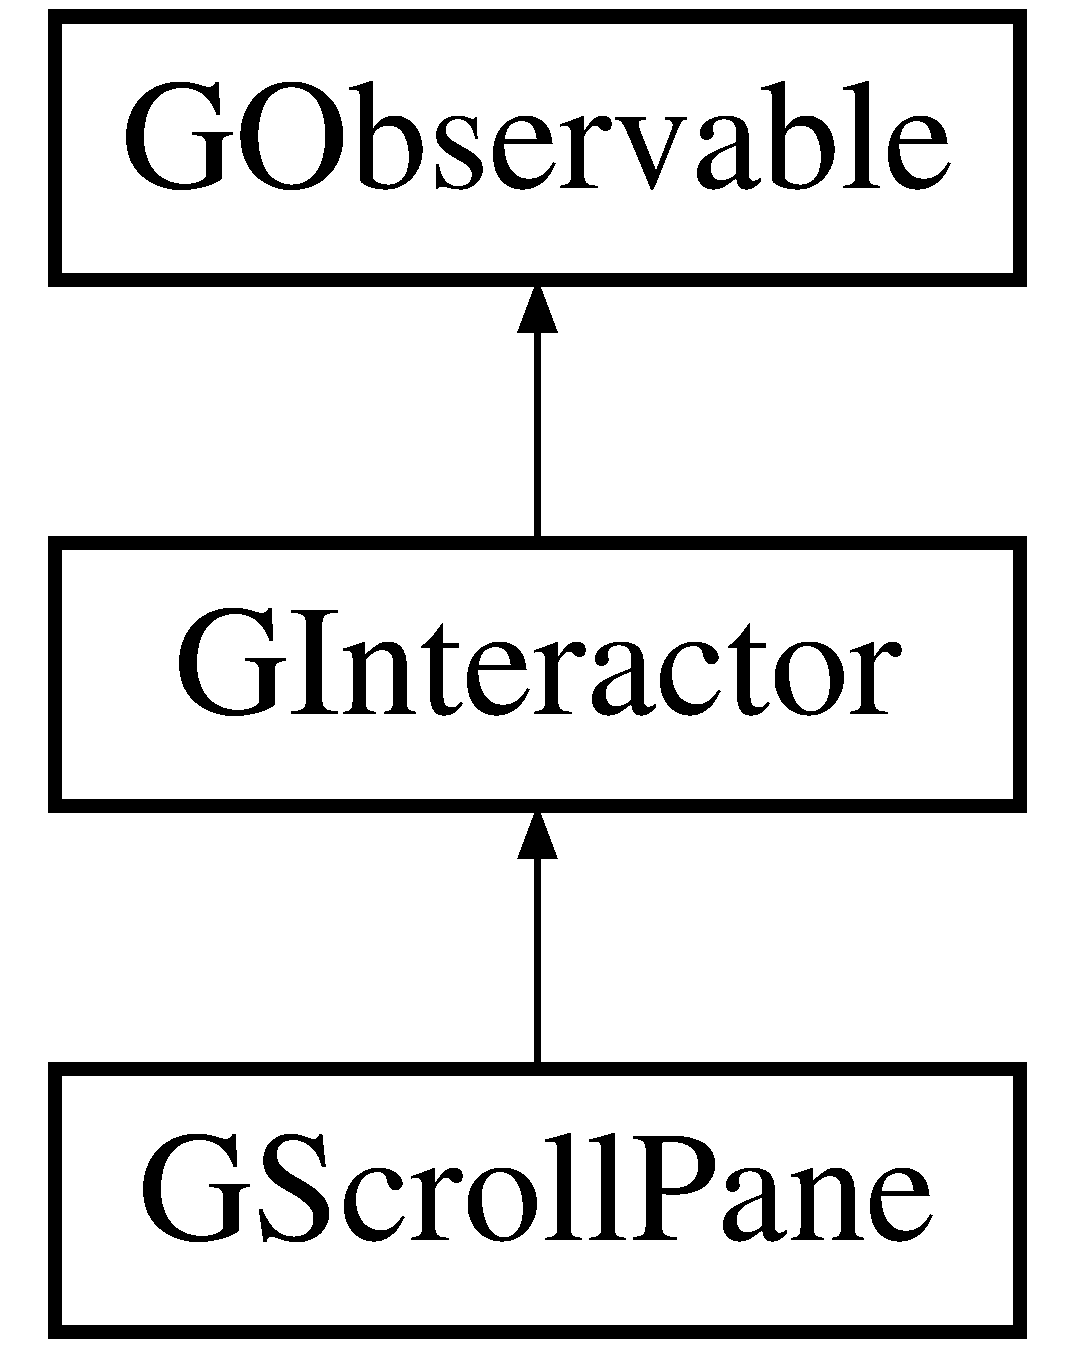
\includegraphics[height=3.000000cm]{classGScrollPane}
\end{center}
\end{figure}
\subsection*{Public Types}
\begin{DoxyCompactItemize}
\item 
enum \mbox{\hyperlink{classGScrollPane_af276320d3d533d494547cb40e5025cc9}{Scroll\+Bar\+Policy}} \{ \mbox{\hyperlink{classGScrollPane_af276320d3d533d494547cb40e5025cc9a19cb69e101cb6454130c8307fe4c0103}{S\+C\+R\+O\+L\+L\+B\+A\+R\+\_\+\+A\+S\+\_\+\+N\+E\+E\+D\+ED}}, 
\mbox{\hyperlink{classGScrollPane_af276320d3d533d494547cb40e5025cc9a3086c0729648b58fde342be1ea988402}{S\+C\+R\+O\+L\+L\+B\+A\+R\+\_\+\+A\+L\+W\+A\+YS}}, 
\mbox{\hyperlink{classGScrollPane_af276320d3d533d494547cb40e5025cc9af26a409c3bd6d0476b7d67fe29a0858f}{S\+C\+R\+O\+L\+L\+B\+A\+R\+\_\+\+N\+E\+V\+ER}}
 \}
\begin{DoxyCompactList}\small\item\em Constants to indicate whether scroll bars in each dimension should be always shown, never shown, or shown only if the inner interactor\textquotesingle{}s size is large enough to require the scroll bar (default). \end{DoxyCompactList}\item 
enum \mbox{\hyperlink{classGInteractor_a8e0d441725a81d2bbdebbea09078260e}{Text\+Position}} \{ \mbox{\hyperlink{classGInteractor_a8e0d441725a81d2bbdebbea09078260ea4cd6f2e7d5a08d6f4dc052df2358f774}{T\+E\+X\+T\+\_\+\+B\+E\+S\+I\+D\+E\+\_\+\+I\+C\+ON}}, 
\mbox{\hyperlink{classGInteractor_a8e0d441725a81d2bbdebbea09078260eaa88490f63d8de68d44c83bdb2ecde3b3}{T\+E\+X\+T\+\_\+\+U\+N\+D\+E\+R\+\_\+\+I\+C\+ON}}, 
\mbox{\hyperlink{classGInteractor_a8e0d441725a81d2bbdebbea09078260ea39a6f388a30ac4fefb6eb13e846bc9f2}{T\+E\+X\+T\+\_\+\+O\+N\+LY}}
 \}
\begin{DoxyCompactList}\small\item\em The places where an interactor can place its text relative to its icon. \end{DoxyCompactList}\end{DoxyCompactItemize}
\subsection*{Public Member Functions}
\begin{DoxyCompactItemize}
\item 
\mbox{\hyperlink{classGScrollPane_aa567e36c0278801a9402a02e77c88208}{G\+Scroll\+Pane}} (\mbox{\hyperlink{classGInteractor}{G\+Interactor}} $\ast$interactor, Q\+Widget $\ast$parent=nullptr)
\begin{DoxyCompactList}\small\item\em Creates a new scroll pane to scroll the given interactor. \end{DoxyCompactList}\item 
\mbox{\hyperlink{classGScrollPane_a8e55b36c91774865b339877f1f816838}{$\sim$\+G\+Scroll\+Pane}} () override
\begin{DoxyCompactList}\small\item\em Frees memory allocated internally by the scroll pane. \end{DoxyCompactList}\item 
virtual void \mbox{\hyperlink{classGInteractor_a02f20ea6edfa0671f31c4c648a253833}{add\+Action\+Listener}} () Q\+\_\+\+D\+E\+C\+L\+\_\+\+D\+E\+P\+R\+E\+C\+A\+T\+ED
\begin{DoxyCompactList}\small\item\em Adds an event listener to be notified when this interactor is clicked or generally interacted with. \end{DoxyCompactList}\item 
bool \mbox{\hyperlink{classGInteractor_a597a370b592e3737d38d9d2f4e2031ea}{events\+Enabled}} () const override
\begin{DoxyCompactList}\small\item\em Returns true if this interactor is currently accepting events. \end{DoxyCompactList}\item 
virtual std\+::string \mbox{\hyperlink{classGInteractor_a69f8d23ed8f207fbecad99960776e942}{get\+Accelerator}} () const
\begin{DoxyCompactList}\small\item\em Returns a string representing a hotkey for this interactor, or an empty string if no accelerator has been set. \end{DoxyCompactList}\item 
virtual std\+::string \mbox{\hyperlink{classGInteractor_a94eb4276000c4fdfb508ce9e6317a82a}{get\+Action\+Command}} () const
\begin{DoxyCompactList}\small\item\em Returns an action command for this interactor, which is a semi-\/unique string you can use to identify it when events occur. \end{DoxyCompactList}\item 
virtual std\+::string \mbox{\hyperlink{classGInteractor_a808e22cc1fdfbecf71ed8c64ef4600e0}{get\+Background}} () const
\begin{DoxyCompactList}\small\item\em Returns the background color of the interactor as a string. \end{DoxyCompactList}\item 
virtual int \mbox{\hyperlink{classGInteractor_a9e827257a55cb8cf4d9de2ec6bcfd7a0}{get\+Background\+Int}} () const
\begin{DoxyCompactList}\small\item\em Returns the background color of the interactor as an R\+GB integer. \end{DoxyCompactList}\item 
virtual \mbox{\hyperlink{structGRectangle}{G\+Rectangle}} \mbox{\hyperlink{classGInteractor_a29e6ac35a0b48f491a4c88194cc5da3b}{get\+Bounds}} () const
\begin{DoxyCompactList}\small\item\em Returns a rectangle representing the x/y position and size of this interactor. \end{DoxyCompactList}\item 
virtual std\+::string \mbox{\hyperlink{classGInteractor_aa061dfa488c31e18549d64363c1d0e34}{get\+Color}} () const
\begin{DoxyCompactList}\small\item\em Returns the foreground/text color of the interactor as a string. \end{DoxyCompactList}\item 
virtual int \mbox{\hyperlink{classGInteractor_a9635c7af766cdc3417f346683fa0e6c1}{get\+Color\+Int}} () const
\begin{DoxyCompactList}\small\item\em Returns the foreground/text color of the interactor as an R\+GB integer. \end{DoxyCompactList}\item 
virtual \mbox{\hyperlink{classGContainer}{G\+Container}} $\ast$ \mbox{\hyperlink{classGInteractor_a7a6e317c29d61030929b4cd2d1c00fe7}{get\+Container}} () const
\begin{DoxyCompactList}\small\item\em Returns a pointer to the onscreen container holding this interactor. \end{DoxyCompactList}\item 
virtual std\+::string \mbox{\hyperlink{classGInteractor_a894a5502900794eeb27d084c21f1d77d}{get\+Font}} () const
\begin{DoxyCompactList}\small\item\em Returns the font of this interactor\textquotesingle{}s text as a font string such as \char`\"{}\+Helvetica-\/12-\/\+Bold\char`\"{}. \end{DoxyCompactList}\item 
virtual std\+::string \mbox{\hyperlink{classGInteractor_a4fa2d8b0192a3a5b4af4bbfe71194d03}{get\+Foreground}} () const
\begin{DoxyCompactList}\small\item\em Returns the foreground/text color of the interactor as a string. \end{DoxyCompactList}\item 
virtual int \mbox{\hyperlink{classGInteractor_ac3b12ab385a6ef9ae90fc879860ba726}{get\+Foreground\+Int}} () const
\begin{DoxyCompactList}\small\item\em Returns the foreground/text color of the interactor as an R\+GB integer. \end{DoxyCompactList}\item 
virtual double \mbox{\hyperlink{classGInteractor_a1e7e353362434072875264cf95629f99}{get\+Height}} () const
\begin{DoxyCompactList}\small\item\em Returns the current onscreen height of this interactor in pixels. \end{DoxyCompactList}\item 
virtual \mbox{\hyperlink{classGScrollPane_af276320d3d533d494547cb40e5025cc9}{Scroll\+Bar\+Policy}} \mbox{\hyperlink{classGScrollPane_a12a22f982652ad67f6c7867162433d93}{get\+Horizontal\+Scroll\+Bar\+Policy}} () const
\begin{DoxyCompactList}\small\item\em Returns a constant indicating whether the horizontal scroll bar will be shown. \end{DoxyCompactList}\item 
virtual std\+::string \mbox{\hyperlink{classGInteractor_aaed62a73004939a64da6f0eb9eb64d73}{get\+Icon}} () const
\begin{DoxyCompactList}\small\item\em Returns the file name of the icon associated with this interactor, or an empty string if no icon has been set. \end{DoxyCompactList}\item 
virtual int \mbox{\hyperlink{classGInteractor_a9c9659a6c6ba66b4107ba59c95a24241}{get\+ID}} () const
\begin{DoxyCompactList}\small\item\em Returns a globally unique identifier for this interactor, which is set when the interactor is constructed. \end{DoxyCompactList}\item 
virtual \mbox{\hyperlink{classGInteractor}{G\+Interactor}} $\ast$ \mbox{\hyperlink{classGScrollPane_ac8998a7ac699a98fbdc125ef0f3d64f1}{get\+Interactor}} () const
\begin{DoxyCompactList}\small\item\em Returns the inner interactor being wrapped by this scroll pane. \end{DoxyCompactList}\item 
\+\_\+\+Internal\+\_\+\+Q\+Widget $\ast$ \mbox{\hyperlink{classGScrollPane_a2f6b36b2517087dc90a366b5ce1f5323}{get\+Internal\+Widget}} () const override
\begin{DoxyCompactList}\small\item\em Returns a direct pointer to the internal Qt widget being wrapped by this interactor. \end{DoxyCompactList}\item 
virtual \mbox{\hyperlink{structGPoint}{G\+Point}} \mbox{\hyperlink{classGInteractor_a4f83802015511edeb63b892830812c11}{get\+Location}} () const
\begin{DoxyCompactList}\small\item\em Returns an (x, y) point representing the onscreen location of the top-\/left corner of this interactor within its containing window. \end{DoxyCompactList}\item 
virtual double \mbox{\hyperlink{classGInteractor_aed4b0075fcc434499c3cb3e46896bda3}{get\+Minimum\+Height}} () const
\begin{DoxyCompactList}\small\item\em Returns the minimum height in pixels that this interactor will permit itself to be resized to. \end{DoxyCompactList}\item 
virtual \mbox{\hyperlink{structGDimension}{G\+Dimension}} \mbox{\hyperlink{classGInteractor_a66b5af0b32493b4d597ca0a3df2049ea}{get\+Minimum\+Size}} () const
\begin{DoxyCompactList}\small\item\em Returns a \mbox{\hyperlink{structGDimension}{G\+Dimension}} structure representing the minimum size in pixels that this interactor will permit itself to be resized to. \end{DoxyCompactList}\item 
virtual double \mbox{\hyperlink{classGInteractor_a59e668114fe3d49d2a0f28deb258f7c8}{get\+Minimum\+Width}} () const
\begin{DoxyCompactList}\small\item\em Returns the minimum width in pixels that this interactor will permit itself to be resized to. \end{DoxyCompactList}\item 
virtual std\+::string \mbox{\hyperlink{classGInteractor_a8a60438a5b55d0b2ceb35c8674b9d8c5}{get\+Name}} () const
\begin{DoxyCompactList}\small\item\em Returns a string representing a unique name for this interactor. \end{DoxyCompactList}\item 
virtual double \mbox{\hyperlink{classGInteractor_a747de0961653847bdc6615dbf756d715}{get\+Preferred\+Height}} () const
\begin{DoxyCompactList}\small\item\em Returns the height in pixels that this interactor would prefer to be, which would exactly fit its contents with no stretching or scrollbars. \end{DoxyCompactList}\item 
virtual \mbox{\hyperlink{structGDimension}{G\+Dimension}} \mbox{\hyperlink{classGInteractor_a4aabbee761d8e9116275401131b7ccd1}{get\+Preferred\+Size}} () const
\begin{DoxyCompactList}\small\item\em Returns a \mbox{\hyperlink{structGDimension}{G\+Dimension}} structure storing the width and height in pixels that this interactor would prefer to be, which would exactly fit its contents with no stretching or scrollbars. \end{DoxyCompactList}\item 
virtual double \mbox{\hyperlink{classGInteractor_a82bca31d37700fb0e35d2743352efd5e}{get\+Preferred\+Width}} () const
\begin{DoxyCompactList}\small\item\em Returns the height in pixels that this interactor would prefer to be, which would exactly fit its contents with no stretching or scrollbars. \end{DoxyCompactList}\item 
virtual \mbox{\hyperlink{structGDimension}{G\+Dimension}} \mbox{\hyperlink{classGInteractor_a7b4eec96a2bdc6420695d5796a78eea9}{get\+Size}} () const
\begin{DoxyCompactList}\small\item\em Returns a \mbox{\hyperlink{structGDimension}{G\+Dimension}} structure storing the current onscreen width and height of this interactor in pixels. \end{DoxyCompactList}\item 
std\+::string \mbox{\hyperlink{classGScrollPane_a9b72ede4ee8520f987a0c01e30654814}{get\+Type}} () const override
\begin{DoxyCompactList}\small\item\em Returns a string representing the class name of this interactor, such as \char`\"{}\+G\+Button\char`\"{} or \char`\"{}\+G\+Check\+Box\char`\"{}. \end{DoxyCompactList}\item 
virtual \mbox{\hyperlink{classGScrollPane_af276320d3d533d494547cb40e5025cc9}{Scroll\+Bar\+Policy}} \mbox{\hyperlink{classGScrollPane_a5e5ed8514d493bd76c4774d249fd6f4a}{get\+Vertical\+Scroll\+Bar\+Policy}} () const
\begin{DoxyCompactList}\small\item\em Returns a constant indicating whether the vertical scroll bar will be shown. \end{DoxyCompactList}\item 
Q\+Widget $\ast$ \mbox{\hyperlink{classGScrollPane_a3b33a602b31a6b809d020535a59db3b4}{get\+Widget}} () const override
\begin{DoxyCompactList}\small\item\em Returns a direct pointer to the internal Qt widget being wrapped by this interactor. \end{DoxyCompactList}\item 
virtual double \mbox{\hyperlink{classGInteractor_a0ed2965abd4f5701d2cadf71239faf19}{get\+Width}} () const
\begin{DoxyCompactList}\small\item\em Returns the current onscreen width of this interactor in pixels. \end{DoxyCompactList}\item 
virtual double \mbox{\hyperlink{classGInteractor_a344385751bee0720059403940d57a13e}{getX}} () const
\begin{DoxyCompactList}\small\item\em Returns the x-\/coordinate of the top-\/left pixel of this interactor within its onscreen window. \end{DoxyCompactList}\item 
virtual double \mbox{\hyperlink{classGInteractor_aafa51c7f8f38a09febbb9ce7853f77b4}{getY}} () const
\begin{DoxyCompactList}\small\item\em Returns the y-\/coordinate of the top-\/left pixel of this interactor within its onscreen window. \end{DoxyCompactList}\item 
virtual bool \mbox{\hyperlink{classGInteractor_afc480f652b8c5f1fb255e2269ce68879}{in\+Bounds}} (double x, double y) const
\begin{DoxyCompactList}\small\item\em Returns true if the given x/y pixel is within the bounds of this interactor. \end{DoxyCompactList}\item 
virtual bool \mbox{\hyperlink{classGInteractor_ae6d7982c1c627b677a5e776ca86118ed}{in\+Bounds}} (int x, int y) const
\begin{DoxyCompactList}\small\item\em Returns true if the given x/y pixel is within the bounds of this interactor. \end{DoxyCompactList}\item 
virtual bool \mbox{\hyperlink{classGInteractor_aacb819fb241851fd9fc045271baa4034}{is\+Enabled}} () const
\begin{DoxyCompactList}\small\item\em Returns true if this interactor is currently enabled. \end{DoxyCompactList}\item 
virtual bool \mbox{\hyperlink{classGScrollPane_a5d41618696c889690cd86700fb69dfa3}{is\+Interactor\+Stretch}} () const
\begin{DoxyCompactList}\small\item\em Returns true if the inner interactor should stretch itself to its preferred size. \end{DoxyCompactList}\item 
virtual bool \mbox{\hyperlink{classGInteractor_a9d8a6cfb13917785c143e74d40e4e2be}{is\+Visible}} () const
\begin{DoxyCompactList}\small\item\em Returns true if the interactor is visible on the screen. \end{DoxyCompactList}\item 
virtual void \mbox{\hyperlink{classGInteractor_ab7fe7a876367b87cf7202f947f1d05e4}{remove\+Action\+Listener}} ()
\begin{DoxyCompactList}\small\item\em Removes the action listener from this interactor so that it will no longer call it when events occur. \end{DoxyCompactList}\item 
virtual void \mbox{\hyperlink{classGInteractor_ad39d0325cde6b97ebda4b9d7787c633b}{remove\+Click\+Listener}} ()
\begin{DoxyCompactList}\small\item\em Removes the click listener from this interactor so that it will no longer call it when events occur. \end{DoxyCompactList}\item 
virtual void \mbox{\hyperlink{classGInteractor_aa4250907e4cdd77349c04f0cf5cdd3d3}{remove\+Double\+Click\+Listener}} ()
\begin{DoxyCompactList}\small\item\em Removes the double-\/click listener from this interactor so that it will no longer call it when events occur. \end{DoxyCompactList}\item 
virtual void \mbox{\hyperlink{classGInteractor_a43095f41cab3be732b49f29970484b05}{remove\+Key\+Listener}} ()
\begin{DoxyCompactList}\small\item\em Removes the key listener from this interactor so that it will no longer call it when key events occur. \end{DoxyCompactList}\item 
virtual void \mbox{\hyperlink{classGInteractor_aff47f71ce47e688a07c9d38dc92fcc11}{remove\+Mouse\+Listener}} ()
\begin{DoxyCompactList}\small\item\em Removes the mouse listener from this interactor so that it will no longer call it when events occur. \end{DoxyCompactList}\item 
virtual void \mbox{\hyperlink{classGInteractor_a519fb2ac767f8b2febbb50b898b8c8cb}{request\+Focus}} ()
\begin{DoxyCompactList}\small\item\em Transfers keyboard focus to this interactor. \end{DoxyCompactList}\item 
virtual void \mbox{\hyperlink{classGInteractor_ad15f102f62e2960576012f1aa0ba4b2e}{set\+Accelerator}} (const std\+::string \&accelerator)
\begin{DoxyCompactList}\small\item\em Sets an accelerator hotkey for this interactor, such as \char`\"{}\+Ctrl-\/\+S\char`\"{}. \end{DoxyCompactList}\item 
virtual void \mbox{\hyperlink{classGInteractor_a4b5843fe3030e038a1ba54cc03389bcf}{set\+Action\+Command}} (const std\+::string \&action\+Command)
\begin{DoxyCompactList}\small\item\em Sets the action command for this interactor. \end{DoxyCompactList}\item 
virtual void \mbox{\hyperlink{classGInteractor_adcfb4742430c88714fcf57e57ab8ea9c}{set\+Action\+Listener}} (G\+Event\+Listener func)
\begin{DoxyCompactList}\small\item\em Sets an action listener on this interactor so that it will be called when it is interacted with in its primary way. \end{DoxyCompactList}\item 
virtual void \mbox{\hyperlink{classGInteractor_aebd20a89c7a8a43a6fce999cf4f9fcf2}{set\+Action\+Listener}} (G\+Event\+Listener\+Void func)
\begin{DoxyCompactList}\small\item\em Sets an action listener on this interactor so that it will be called when it is interacted with in its primary way. \end{DoxyCompactList}\item 
virtual void \mbox{\hyperlink{classGInteractor_acba7e546c2025c0a15ca4b4cc92043db}{set\+Background}} (int rgb)
\begin{DoxyCompactList}\small\item\em Sets the background color of the interactor to the color represented by the given R\+GB integer. \end{DoxyCompactList}\item 
virtual void \mbox{\hyperlink{classGInteractor_ab4677ab2474e68b07aa56605af92a84a}{set\+Background}} (const std\+::string \&color)
\begin{DoxyCompactList}\small\item\em Sets the background color of the interactor to the color represented by the given string. \end{DoxyCompactList}\item 
virtual void \mbox{\hyperlink{classGInteractor_a2aae8197624b72265ab83b4f1bc73f2f}{set\+Bounds}} (double x, double y, double width, double height)
\begin{DoxyCompactList}\small\item\em Sets the size and location of the widget. \end{DoxyCompactList}\item 
virtual void \mbox{\hyperlink{classGInteractor_acada386653f008cacc7cce86426bef7c}{set\+Bounds}} (const \mbox{\hyperlink{structGRectangle}{G\+Rectangle}} \&size)
\begin{DoxyCompactList}\small\item\em Sets the size and location of the widget. \end{DoxyCompactList}\item 
virtual void \mbox{\hyperlink{classGInteractor_abd40af6921242584d0954f173911b190}{set\+Click\+Listener}} (G\+Event\+Listener func)
\begin{DoxyCompactList}\small\item\em Sets a mouse listener on this interactor so that it will be called when the mouse is clicked on it. \end{DoxyCompactList}\item 
virtual void \mbox{\hyperlink{classGInteractor_a856414c92df90f56f3877475eb3f8fc4}{set\+Click\+Listener}} (G\+Event\+Listener\+Void func)
\begin{DoxyCompactList}\small\item\em Sets a mouse listener on this interactor so that it will be called when the mouse is clicked on it. \end{DoxyCompactList}\item 
virtual void \mbox{\hyperlink{classGInteractor_ab1f5cc0f5cc6bbbd716a526c61f1081d}{set\+Color}} (int rgb)
\begin{DoxyCompactList}\small\item\em Sets the foreground/text color of the interactor to the color represented by the given R\+GB integer. \end{DoxyCompactList}\item 
virtual void \mbox{\hyperlink{classGInteractor_a61374df6c11b52cfbb0815decdbaebc6}{set\+Color}} (const std\+::string \&color)
\begin{DoxyCompactList}\small\item\em Sets the foreground/text color of the interactor to the color represented by the given string. \end{DoxyCompactList}\item 
virtual void \mbox{\hyperlink{classGInteractor_ac29f9a3462458e165fae3a1f046ee77a}{set\+Double\+Click\+Listener}} (G\+Event\+Listener func)
\begin{DoxyCompactList}\small\item\em Sets a mouse listener on this interactor so that it will be called when the mouse is double-\/clicked on it. \end{DoxyCompactList}\item 
virtual void \mbox{\hyperlink{classGInteractor_a50096194d66f48c92dd4c512d41bfc76}{set\+Double\+Click\+Listener}} (G\+Event\+Listener\+Void func)
\begin{DoxyCompactList}\small\item\em Sets a mouse listener on this interactor so that it will be called when the mouse is double-\/clicked on it. \end{DoxyCompactList}\item 
virtual void \mbox{\hyperlink{classGInteractor_ab831367dd84bbd579e02e55bacb21343}{set\+Enabled}} (bool value)
\begin{DoxyCompactList}\small\item\em Sets whether this interactor is currently enabled. \end{DoxyCompactList}\item 
virtual void \mbox{\hyperlink{classGObservable_afaa30b2a9e0f378fd1c70d2f1d0b8216}{set\+Events\+Enabled}} (bool \mbox{\hyperlink{classGInteractor_a597a370b592e3737d38d9d2f4e2031ea}{events\+Enabled}})
\begin{DoxyCompactList}\small\item\em Sets whether the object is currently allowing itself to fire events. \end{DoxyCompactList}\item 
virtual void \mbox{\hyperlink{classGInteractor_a2592348886ffea646c6534bf88f7c49d}{set\+Font}} (const Q\+Font \&font)
\begin{DoxyCompactList}\small\item\em Sets the font used by this widget to the given Qt font. \end{DoxyCompactList}\item 
virtual void \mbox{\hyperlink{classGInteractor_a8e096e8818d838aceae1d46d58fb3a7b}{set\+Font}} (const std\+::string \&font)
\begin{DoxyCompactList}\small\item\em Sets the font used by this widget to the font represented by the given font string, such as \char`\"{}\+Helvetica-\/16-\/\+Bold\char`\"{}. \end{DoxyCompactList}\item 
virtual void \mbox{\hyperlink{classGInteractor_a9eb856b5ff83a19df3831a31f15f4563}{set\+Foreground}} (int rgb)
\begin{DoxyCompactList}\small\item\em Sets the foreground/text color of the interactor to the color represented by the given R\+GB integer. \end{DoxyCompactList}\item 
virtual void \mbox{\hyperlink{classGInteractor_af59209aeadea6dfc6d97a2d8531f50e1}{set\+Foreground}} (const std\+::string \&color)
\begin{DoxyCompactList}\small\item\em Sets the foreground/text color of the interactor to the color represented by the given string. \end{DoxyCompactList}\item 
virtual void \mbox{\hyperlink{classGInteractor_a9e280bfc4544dfaf8e4376c4e1a74357}{set\+Height}} (double height)
\begin{DoxyCompactList}\small\item\em Sets the onscreen height of the interactor in pixels. \end{DoxyCompactList}\item 
virtual void \mbox{\hyperlink{classGScrollPane_a0c82d84cd2221c453370503faf950e2e}{set\+Horizontal\+Scroll\+Bar\+Policy}} (\mbox{\hyperlink{classGScrollPane_af276320d3d533d494547cb40e5025cc9}{Scroll\+Bar\+Policy}} policy)
\begin{DoxyCompactList}\small\item\em Sets whether the horizontal scroll bar will be shown. \end{DoxyCompactList}\item 
virtual void \mbox{\hyperlink{classGInteractor_a542abfcd7261751352af129c7215ecda}{set\+Icon}} (const Q\+Icon \&icon)
\begin{DoxyCompactList}\small\item\em Sets the icon associated with this interactor. \end{DoxyCompactList}\item 
virtual void \mbox{\hyperlink{classGInteractor_a368e1a338f84401c284506d03b1ba769}{set\+Icon}} (const Q\+Pixmap \&icon)
\begin{DoxyCompactList}\small\item\em Sets the icon associated with this interactor. \end{DoxyCompactList}\item 
virtual void \mbox{\hyperlink{classGInteractor_a762e139aa311461c3984d3ad28293f64}{set\+Icon}} (const std\+::string \&filename, bool retain\+Icon\+Size=true)
\begin{DoxyCompactList}\small\item\em Sets the file name of the icon associated with this interactor, or an empty string if no icon has been set. \end{DoxyCompactList}\item 
virtual void \mbox{\hyperlink{classGScrollPane_a56c113aeeabb79e04916d0136593588b}{set\+Interactor\+Stretch}} (bool stretch)
\begin{DoxyCompactList}\small\item\em Sets whether the inner interactor should stretch itself to its preferred size. \end{DoxyCompactList}\item 
virtual void \mbox{\hyperlink{classGInteractor_aeb8324d3287fa1fbe093f4d6230cf0a6}{set\+Key\+Listener}} (G\+Event\+Listener func)
\begin{DoxyCompactList}\small\item\em Sets a key listener on this interactor so that it will be called when the user presses any key. \end{DoxyCompactList}\item 
virtual void \mbox{\hyperlink{classGInteractor_ae48ecea73606c7bd9423e1c7cc589cc9}{set\+Key\+Listener}} (G\+Event\+Listener\+Void func)
\begin{DoxyCompactList}\small\item\em Sets a key listener on this interactor so that it will be called when the user presses any key. \end{DoxyCompactList}\item 
virtual void \mbox{\hyperlink{classGInteractor_a04594e8ba9b98513a64f1da00dcae18c}{set\+Location}} (double x, double y)
\begin{DoxyCompactList}\small\item\em Sets the onscreen x/y-\/coordinate of the top-\/left corner of the interactor relative to its window. \end{DoxyCompactList}\item 
virtual void \mbox{\hyperlink{classGInteractor_a0cf428e207b7f22cc08138a90b1b87b2}{set\+Minimum\+Size}} (double width, double height)
\begin{DoxyCompactList}\small\item\em Sets the minimum size in pixels that this interactor will permit itself to be resized to. \end{DoxyCompactList}\item 
virtual void \mbox{\hyperlink{classGInteractor_a3b1046117ac6cb7abe467e00ba8a81f4}{set\+Minimum\+Size}} (const \mbox{\hyperlink{structGDimension}{G\+Dimension}} \&size)
\begin{DoxyCompactList}\small\item\em Sets the minimum size in pixels that this interactor will permit itself to be resized to. \end{DoxyCompactList}\item 
virtual void \mbox{\hyperlink{classGInteractor_a37d8dbc943f59920f705b0104f60bde2}{set\+Mouse\+Listener}} (G\+Event\+Listener func)
\begin{DoxyCompactList}\small\item\em Sets a mouse listener on this interactor so that it will be called when the mouse is moved or clicked on it. \end{DoxyCompactList}\item 
virtual void \mbox{\hyperlink{classGInteractor_aea7f647ea62d59f71b5fad6aa65eeaf9}{set\+Mouse\+Listener}} (G\+Event\+Listener\+Void func)
\begin{DoxyCompactList}\small\item\em Sets a mouse listener on this interactor so that it will be called when the mouse is moved or clicked on it. \end{DoxyCompactList}\item 
virtual void \mbox{\hyperlink{classGInteractor_a9d3a2685df23b5e7cbf59c19c4a1f9b5}{set\+Name}} (const std\+::string \&name)
\begin{DoxyCompactList}\small\item\em Sets a string representing a unique name for this interactor. \end{DoxyCompactList}\item 
virtual void \mbox{\hyperlink{classGInteractor_a1ab987704fce32098706c6f00fb08218}{set\+Preferred\+Height}} (double height)
\begin{DoxyCompactList}\small\item\em Sets the height in pixels that this interactor would prefer to be. \end{DoxyCompactList}\item 
virtual void \mbox{\hyperlink{classGInteractor_a042c5ae19430d765ef552371cae3632c}{set\+Preferred\+Size}} (double width, double height)
\begin{DoxyCompactList}\small\item\em Sets the width and height in pixels that this interactor would prefer to be. \end{DoxyCompactList}\item 
virtual void \mbox{\hyperlink{classGInteractor_aa22d9be4bc0e078bb0ea69b0fc9d7c75}{set\+Preferred\+Size}} (const \mbox{\hyperlink{structGDimension}{G\+Dimension}} \&size)
\begin{DoxyCompactList}\small\item\em Sets the size in pixels that this interactor would prefer to be. \end{DoxyCompactList}\item 
virtual void \mbox{\hyperlink{classGInteractor_a3db429ab2fa52efd187eec0ed8cdd9f2}{set\+Preferred\+Width}} (double width)
\begin{DoxyCompactList}\small\item\em Sets the width in pixels that this interactor would prefer to be. \end{DoxyCompactList}\item 
virtual void \mbox{\hyperlink{classGScrollPane_a970d6a1f1254aaad2c15ae271a87d49f}{set\+Scroll\+Bar\+Policy}} (\mbox{\hyperlink{classGScrollPane_af276320d3d533d494547cb40e5025cc9}{Scroll\+Bar\+Policy}} policy)
\begin{DoxyCompactList}\small\item\em Sets whether the horizontal and vertical scroll bars will be shown. \end{DoxyCompactList}\item 
virtual void \mbox{\hyperlink{classGInteractor_aca25d49481f9bf5fc8f7df4c086c4ce7}{set\+Size}} (double width, double height)
\begin{DoxyCompactList}\small\item\em Sets the onscreen width and height of the interactor in pixels. \end{DoxyCompactList}\item 
virtual void \mbox{\hyperlink{classGInteractor_ae2b628228f192c2702c4ce941b2af68f}{set\+Size}} (const \mbox{\hyperlink{structGDimension}{G\+Dimension}} \&size)
\begin{DoxyCompactList}\small\item\em Sets the onscreen width and height of the interactor in pixels. \end{DoxyCompactList}\item 
virtual void \mbox{\hyperlink{classGInteractor_a039e0e49beaecc275efce02d416acea8}{set\+Tooltip}} (const std\+::string \&tooltip\+Text)
\begin{DoxyCompactList}\small\item\em Sets a \char`\"{}tooltip\char`\"{} that will appear if the user hovers their mouse over the interactor. \end{DoxyCompactList}\item 
virtual void \mbox{\hyperlink{classGScrollPane_adb8714eb78c44ef15671e3f92effa826}{set\+Vertical\+Scroll\+Bar\+Policy}} (\mbox{\hyperlink{classGScrollPane_af276320d3d533d494547cb40e5025cc9}{Scroll\+Bar\+Policy}} policy)
\begin{DoxyCompactList}\small\item\em Sets whether the vertical scroll bar will be shown. \end{DoxyCompactList}\item 
virtual void \mbox{\hyperlink{classGInteractor_a18e44e30b31525a243960ca3928125aa}{set\+Visible}} (bool visible)
\begin{DoxyCompactList}\small\item\em Returns true if the interactor is visible on the screen. \end{DoxyCompactList}\item 
virtual void \mbox{\hyperlink{classGInteractor_aa3f3fba4cb131baa8696ba01e3bceca1}{set\+Width}} (double width)
\begin{DoxyCompactList}\small\item\em Sets the onscreen width of the interactor in pixels. \end{DoxyCompactList}\item 
virtual void \mbox{\hyperlink{classGInteractor_a9c18fcc579333bf9653d13ad2b372e39}{setX}} (double x)
\begin{DoxyCompactList}\small\item\em Sets the onscreen x-\/coordinate of the top-\/left corner of the interactor relative to its window. \end{DoxyCompactList}\item 
virtual void \mbox{\hyperlink{classGInteractor_a7d57e2a5c35d27feb58fd498a3cf82b9}{setY}} (double y)
\begin{DoxyCompactList}\small\item\em Sets the onscreen y-\/coordinate of the top-\/left corner of the interactor relative to its window. \end{DoxyCompactList}\item 
virtual std\+::string \mbox{\hyperlink{classGObservable_a1fe5121d6528fdea3f243321b3fa3a49}{to\+String}} () const
\begin{DoxyCompactList}\small\item\em Returns a string representation of this observable object\textquotesingle{}s state. \end{DoxyCompactList}\end{DoxyCompactItemize}
\subsection*{Protected Member Functions}
\begin{DoxyCompactItemize}
\item 
virtual void \mbox{\hyperlink{classGObservable_a80cfa040459ff53594adbd6a51ec8f43}{clear\+Event\+Listeners}} ()
\begin{DoxyCompactList}\small\item\em Removes all event listeners from this object. \end{DoxyCompactList}\item 
virtual void \mbox{\hyperlink{classGObservable_a284f31528c0520f8e545c03ac9eeac74}{ensure\+Thread\+Safety}} (const std\+::string \&member\+Name=\char`\"{}\char`\"{})
\begin{DoxyCompactList}\small\item\em Ensures that we are currently in the Qt G\+UI thread. \end{DoxyCompactList}\item 
virtual void \mbox{\hyperlink{classGObservable_a63e5e5a6227c59c928493b11aceb0f67}{fire\+Event}} (\mbox{\hyperlink{classGEvent}{G\+Event}} \&event)
\begin{DoxyCompactList}\small\item\em Sends out the given event to any attached listeners. \end{DoxyCompactList}\item 
virtual void \mbox{\hyperlink{classGObservable_ab3983ea07337b52020a29cc00c653d8d}{fire\+G\+Event}} (Q\+Event $\ast$event, Event\+Type event\+Type, const std\+::string \&event\+Name)
\begin{DoxyCompactList}\small\item\em Creates an event of the given type, then sends it out to any attached listeners. \end{DoxyCompactList}\item 
virtual void \mbox{\hyperlink{classGObservable_a01fdf1b0e0dbd49e189fe4514e010411}{fire\+G\+Event}} (Q\+Close\+Event $\ast$event, Event\+Type event\+Type, const std\+::string \&event\+Name)
\begin{DoxyCompactList}\small\item\em Creates an event of the given type, then sends it out to any attached listeners. \end{DoxyCompactList}\item 
virtual void \mbox{\hyperlink{classGObservable_abb0b2f66ba39211cb5d7615e9d1c04e2}{fire\+G\+Event}} (Q\+Key\+Event $\ast$event, Event\+Type event\+Type, const std\+::string \&event\+Name)
\begin{DoxyCompactList}\small\item\em Creates an event of the given type, then sends it out to any attached listeners. \end{DoxyCompactList}\item 
virtual void \mbox{\hyperlink{classGObservable_a119318675d2165bdf7dd853aaf881d4b}{fire\+G\+Event}} (Q\+Mouse\+Event $\ast$event, Event\+Type event\+Type, const std\+::string \&event\+Name, const std\+::string \&action\+Command=\char`\"{}\char`\"{})
\begin{DoxyCompactList}\small\item\em Creates an event of the given type, then sends it out to any attached listeners. \end{DoxyCompactList}\item 
virtual void \mbox{\hyperlink{classGObservable_a63fd9034e1e1633c1c38eb342bfd34e9}{fire\+G\+Event}} (Q\+Resize\+Event $\ast$event, Event\+Type event\+Type, const std\+::string \&event\+Name)
\begin{DoxyCompactList}\small\item\em Creates an event of the given type, then sends it out to any attached listeners. \end{DoxyCompactList}\item 
virtual void \mbox{\hyperlink{classGObservable_a741345310d9b7c5170a6cbc410c44ac4}{fire\+G\+Event}} (Q\+Timer\+Event $\ast$event, Event\+Type event\+Type, const std\+::string \&event\+Name)
\begin{DoxyCompactList}\small\item\em Creates an event of the given type, then sends it out to any attached listeners. \end{DoxyCompactList}\item 
virtual void \mbox{\hyperlink{classGObservable_a93bf338968a0338761b8e4dc62f582e9}{fire\+G\+Event}} (Q\+Wheel\+Event $\ast$event, Event\+Type event\+Type, const std\+::string \&event\+Name)
\begin{DoxyCompactList}\small\item\em Creates an event of the given type, then sends it out to any attached listeners. \end{DoxyCompactList}\item 
virtual void \mbox{\hyperlink{classGObservable_a2a70a7d7435ff0c3b80bb4d70da19e0d}{fire\+G\+Event}} (Q\+Window\+State\+Change\+Event $\ast$event, Event\+Type event\+Type, const std\+::string \&event\+Name)
\begin{DoxyCompactList}\small\item\em Creates an event of the given type, then sends it out to any attached listeners. \end{DoxyCompactList}\item 
virtual bool \mbox{\hyperlink{classGObservable_a9f6faaa25942923bafa1c44020c49fa9}{has\+Event\+Listener}} (const std\+::string \&event\+Name) const
\begin{DoxyCompactList}\small\item\em Returns true if the observable object has a listener for the given type of event. \end{DoxyCompactList}\item 
virtual bool \mbox{\hyperlink{classGObservable_aeec1adc19aa0f33de62390686ee1382c}{is\+Accepting\+Event}} (int event\+Mask) const
\begin{DoxyCompactList}\small\item\em Returns true if the observable object has a listener for the given type of event. \end{DoxyCompactList}\item 
virtual bool \mbox{\hyperlink{classGObservable_aa31c73145a29dcb92848a92e0cfaea41}{is\+Accepting\+Event}} (const \mbox{\hyperlink{classGEvent}{G\+Event}} \&event) const
\begin{DoxyCompactList}\small\item\em Returns true if the observable object has a listener for the given type of event. \end{DoxyCompactList}\item 
virtual bool \mbox{\hyperlink{classGObservable_a3b1c689267eda44e65a2213e7de38b23}{is\+Accepting\+Event}} (const std\+::string \&event\+Type) const
\begin{DoxyCompactList}\small\item\em Returns true if the observable object has a listener for the given type of event. \end{DoxyCompactList}\item 
virtual void \mbox{\hyperlink{classGObservable_acbcf1ed3a851ad8a3c17ef38d86b481d}{remove\+Event\+Listener}} (const std\+::string \&event\+Name)
\begin{DoxyCompactList}\small\item\em Removes any event listener from this observable object that would respond to the given type of event, such as \char`\"{}click\char`\"{} or \char`\"{}keydown\char`\"{}. \end{DoxyCompactList}\item 
virtual void \mbox{\hyperlink{classGObservable_af51cc35c29a1bd1908609d432decdbb6}{remove\+Event\+Listeners}} (std\+::initializer\+\_\+list$<$ std\+::string $>$ event\+Names)
\begin{DoxyCompactList}\small\item\em Removes any event listener from this observable object that would respond to the given types of events, such as \char`\"{}click\char`\"{} or \char`\"{}keydown\char`\"{}. \end{DoxyCompactList}\item 
virtual void \mbox{\hyperlink{classGObservable_ad2f6d34961c50f6c1e0659990b79f741}{set\+Event\+Listener}} (const std\+::string \&event\+Name, G\+Event\+Listener func)
\begin{DoxyCompactList}\small\item\em Adds an event listener from this observable object to respond to the given type of event, such as \char`\"{}click\char`\"{} or \char`\"{}keydown\char`\"{}. \end{DoxyCompactList}\item 
virtual void \mbox{\hyperlink{classGObservable_abac4cb9f9e626e010e87f5d91573c8a5}{set\+Event\+Listener}} (const std\+::string \&event\+Name, G\+Event\+Listener\+Void func)
\begin{DoxyCompactList}\small\item\em Adds an event listener from this observable object to respond to the given type of event, such as \char`\"{}click\char`\"{} or \char`\"{}keydown\char`\"{}. \end{DoxyCompactList}\item 
virtual void \mbox{\hyperlink{classGObservable_afa388d69c33c718cf035774604065604}{set\+Event\+Listeners}} (std\+::initializer\+\_\+list$<$ std\+::string $>$ event\+Names, G\+Event\+Listener func)
\begin{DoxyCompactList}\small\item\em Adds an event listener from this observable object to respond to the given types of events, such as \char`\"{}click\char`\"{} or \char`\"{}keydown\char`\"{}. \end{DoxyCompactList}\item 
virtual void \mbox{\hyperlink{classGObservable_a7867184bbb686f74fae8a4db927da799}{set\+Event\+Listeners}} (std\+::initializer\+\_\+list$<$ std\+::string $>$ event\+Names, G\+Event\+Listener\+Void func)
\begin{DoxyCompactList}\small\item\em Adds an event listener from this observable object to respond to the given types of events, such as \char`\"{}click\char`\"{} or \char`\"{}keydown\char`\"{}. \end{DoxyCompactList}\end{DoxyCompactItemize}


\subsection{Detailed Description}
A \mbox{\hyperlink{classGScrollPane}{G\+Scroll\+Pane}} is a container that wraps another interactor with scroll bars. 

It can be used to allow another interactor to be at its preferred size (or some arbitrarily large size) while only occupying a smaller number of onscreen pixels with vertical and/or horizontal scroll bars. 

\subsection{Member Enumeration Documentation}
\mbox{\Hypertarget{classGScrollPane_af276320d3d533d494547cb40e5025cc9}\label{classGScrollPane_af276320d3d533d494547cb40e5025cc9}} 
\index{G\+Scroll\+Pane@{G\+Scroll\+Pane}!Scroll\+Bar\+Policy@{Scroll\+Bar\+Policy}}
\index{Scroll\+Bar\+Policy@{Scroll\+Bar\+Policy}!G\+Scroll\+Pane@{G\+Scroll\+Pane}}
\subsubsection{\texorpdfstring{Scroll\+Bar\+Policy}{ScrollBarPolicy}}
{\footnotesize\ttfamily enum \mbox{\hyperlink{classGScrollPane_af276320d3d533d494547cb40e5025cc9}{Scroll\+Bar\+Policy}}}



Constants to indicate whether scroll bars in each dimension should be always shown, never shown, or shown only if the inner interactor\textquotesingle{}s size is large enough to require the scroll bar (default). 

\begin{DoxyEnumFields}{Enumerator}
\raisebox{\heightof{T}}[0pt][0pt]{\index{S\+C\+R\+O\+L\+L\+B\+A\+R\+\_\+\+A\+S\+\_\+\+N\+E\+E\+D\+ED@{S\+C\+R\+O\+L\+L\+B\+A\+R\+\_\+\+A\+S\+\_\+\+N\+E\+E\+D\+ED}!G\+Scroll\+Pane@{G\+Scroll\+Pane}}\index{G\+Scroll\+Pane@{G\+Scroll\+Pane}!S\+C\+R\+O\+L\+L\+B\+A\+R\+\_\+\+A\+S\+\_\+\+N\+E\+E\+D\+ED@{S\+C\+R\+O\+L\+L\+B\+A\+R\+\_\+\+A\+S\+\_\+\+N\+E\+E\+D\+ED}}}\mbox{\Hypertarget{classGScrollPane_af276320d3d533d494547cb40e5025cc9a19cb69e101cb6454130c8307fe4c0103}\label{classGScrollPane_af276320d3d533d494547cb40e5025cc9a19cb69e101cb6454130c8307fe4c0103}} 
S\+C\+R\+O\+L\+L\+B\+A\+R\+\_\+\+A\+S\+\_\+\+N\+E\+E\+D\+ED&\\
\hline

\raisebox{\heightof{T}}[0pt][0pt]{\index{S\+C\+R\+O\+L\+L\+B\+A\+R\+\_\+\+A\+L\+W\+A\+YS@{S\+C\+R\+O\+L\+L\+B\+A\+R\+\_\+\+A\+L\+W\+A\+YS}!G\+Scroll\+Pane@{G\+Scroll\+Pane}}\index{G\+Scroll\+Pane@{G\+Scroll\+Pane}!S\+C\+R\+O\+L\+L\+B\+A\+R\+\_\+\+A\+L\+W\+A\+YS@{S\+C\+R\+O\+L\+L\+B\+A\+R\+\_\+\+A\+L\+W\+A\+YS}}}\mbox{\Hypertarget{classGScrollPane_af276320d3d533d494547cb40e5025cc9a3086c0729648b58fde342be1ea988402}\label{classGScrollPane_af276320d3d533d494547cb40e5025cc9a3086c0729648b58fde342be1ea988402}} 
S\+C\+R\+O\+L\+L\+B\+A\+R\+\_\+\+A\+L\+W\+A\+YS&\\
\hline

\raisebox{\heightof{T}}[0pt][0pt]{\index{S\+C\+R\+O\+L\+L\+B\+A\+R\+\_\+\+N\+E\+V\+ER@{S\+C\+R\+O\+L\+L\+B\+A\+R\+\_\+\+N\+E\+V\+ER}!G\+Scroll\+Pane@{G\+Scroll\+Pane}}\index{G\+Scroll\+Pane@{G\+Scroll\+Pane}!S\+C\+R\+O\+L\+L\+B\+A\+R\+\_\+\+N\+E\+V\+ER@{S\+C\+R\+O\+L\+L\+B\+A\+R\+\_\+\+N\+E\+V\+ER}}}\mbox{\Hypertarget{classGScrollPane_af276320d3d533d494547cb40e5025cc9af26a409c3bd6d0476b7d67fe29a0858f}\label{classGScrollPane_af276320d3d533d494547cb40e5025cc9af26a409c3bd6d0476b7d67fe29a0858f}} 
S\+C\+R\+O\+L\+L\+B\+A\+R\+\_\+\+N\+E\+V\+ER&\\
\hline

\end{DoxyEnumFields}
\mbox{\Hypertarget{classGInteractor_a8e0d441725a81d2bbdebbea09078260e}\label{classGInteractor_a8e0d441725a81d2bbdebbea09078260e}} 
\index{G\+Scroll\+Pane@{G\+Scroll\+Pane}!Text\+Position@{Text\+Position}}
\index{Text\+Position@{Text\+Position}!G\+Scroll\+Pane@{G\+Scroll\+Pane}}
\subsubsection{\texorpdfstring{Text\+Position}{TextPosition}}
{\footnotesize\ttfamily enum \mbox{\hyperlink{classGInteractor_a8e0d441725a81d2bbdebbea09078260e}{Text\+Position}}\hspace{0.3cm}{\ttfamily [inherited]}}



The places where an interactor can place its text relative to its icon. 

\begin{DoxyEnumFields}{Enumerator}
\raisebox{\heightof{T}}[0pt][0pt]{\index{T\+E\+X\+T\+\_\+\+B\+E\+S\+I\+D\+E\+\_\+\+I\+C\+ON@{T\+E\+X\+T\+\_\+\+B\+E\+S\+I\+D\+E\+\_\+\+I\+C\+ON}!G\+Scroll\+Pane@{G\+Scroll\+Pane}}\index{G\+Scroll\+Pane@{G\+Scroll\+Pane}!T\+E\+X\+T\+\_\+\+B\+E\+S\+I\+D\+E\+\_\+\+I\+C\+ON@{T\+E\+X\+T\+\_\+\+B\+E\+S\+I\+D\+E\+\_\+\+I\+C\+ON}}}\mbox{\Hypertarget{classGInteractor_a8e0d441725a81d2bbdebbea09078260ea4cd6f2e7d5a08d6f4dc052df2358f774}\label{classGInteractor_a8e0d441725a81d2bbdebbea09078260ea4cd6f2e7d5a08d6f4dc052df2358f774}} 
T\+E\+X\+T\+\_\+\+B\+E\+S\+I\+D\+E\+\_\+\+I\+C\+ON&\\
\hline

\raisebox{\heightof{T}}[0pt][0pt]{\index{T\+E\+X\+T\+\_\+\+U\+N\+D\+E\+R\+\_\+\+I\+C\+ON@{T\+E\+X\+T\+\_\+\+U\+N\+D\+E\+R\+\_\+\+I\+C\+ON}!G\+Scroll\+Pane@{G\+Scroll\+Pane}}\index{G\+Scroll\+Pane@{G\+Scroll\+Pane}!T\+E\+X\+T\+\_\+\+U\+N\+D\+E\+R\+\_\+\+I\+C\+ON@{T\+E\+X\+T\+\_\+\+U\+N\+D\+E\+R\+\_\+\+I\+C\+ON}}}\mbox{\Hypertarget{classGInteractor_a8e0d441725a81d2bbdebbea09078260eaa88490f63d8de68d44c83bdb2ecde3b3}\label{classGInteractor_a8e0d441725a81d2bbdebbea09078260eaa88490f63d8de68d44c83bdb2ecde3b3}} 
T\+E\+X\+T\+\_\+\+U\+N\+D\+E\+R\+\_\+\+I\+C\+ON&\\
\hline

\raisebox{\heightof{T}}[0pt][0pt]{\index{T\+E\+X\+T\+\_\+\+O\+N\+LY@{T\+E\+X\+T\+\_\+\+O\+N\+LY}!G\+Scroll\+Pane@{G\+Scroll\+Pane}}\index{G\+Scroll\+Pane@{G\+Scroll\+Pane}!T\+E\+X\+T\+\_\+\+O\+N\+LY@{T\+E\+X\+T\+\_\+\+O\+N\+LY}}}\mbox{\Hypertarget{classGInteractor_a8e0d441725a81d2bbdebbea09078260ea39a6f388a30ac4fefb6eb13e846bc9f2}\label{classGInteractor_a8e0d441725a81d2bbdebbea09078260ea39a6f388a30ac4fefb6eb13e846bc9f2}} 
T\+E\+X\+T\+\_\+\+O\+N\+LY&\\
\hline

\end{DoxyEnumFields}


\subsection{Constructor \& Destructor Documentation}
\mbox{\Hypertarget{classGScrollPane_aa567e36c0278801a9402a02e77c88208}\label{classGScrollPane_aa567e36c0278801a9402a02e77c88208}} 
\index{G\+Scroll\+Pane@{G\+Scroll\+Pane}!G\+Scroll\+Pane@{G\+Scroll\+Pane}}
\index{G\+Scroll\+Pane@{G\+Scroll\+Pane}!G\+Scroll\+Pane@{G\+Scroll\+Pane}}
\subsubsection{\texorpdfstring{G\+Scroll\+Pane()}{GScrollPane()}}
{\footnotesize\ttfamily \mbox{\hyperlink{classGScrollPane}{G\+Scroll\+Pane}} (\begin{DoxyParamCaption}\item[{\mbox{\hyperlink{classGInteractor}{G\+Interactor}} $\ast$}]{interactor,  }\item[{Q\+Widget $\ast$}]{parent = {\ttfamily nullptr} }\end{DoxyParamCaption})}



Creates a new scroll pane to scroll the given interactor. 


\begin{DoxyExceptions}{Exceptions}
{\em Error\+Exception} & if the interactor is null \\
\hline
\end{DoxyExceptions}
\mbox{\Hypertarget{classGScrollPane_a8e55b36c91774865b339877f1f816838}\label{classGScrollPane_a8e55b36c91774865b339877f1f816838}} 
\index{G\+Scroll\+Pane@{G\+Scroll\+Pane}!````~G\+Scroll\+Pane@{$\sim$\+G\+Scroll\+Pane}}
\index{````~G\+Scroll\+Pane@{$\sim$\+G\+Scroll\+Pane}!G\+Scroll\+Pane@{G\+Scroll\+Pane}}
\subsubsection{\texorpdfstring{$\sim$\+G\+Scroll\+Pane()}{~GScrollPane()}}
{\footnotesize\ttfamily $\sim$\mbox{\hyperlink{classGScrollPane}{G\+Scroll\+Pane}} (\begin{DoxyParamCaption}{ }\end{DoxyParamCaption})\hspace{0.3cm}{\ttfamily [override]}}



Frees memory allocated internally by the scroll pane. 



\subsection{Member Function Documentation}
\mbox{\Hypertarget{classGInteractor_a02f20ea6edfa0671f31c4c648a253833}\label{classGInteractor_a02f20ea6edfa0671f31c4c648a253833}} 
\index{G\+Scroll\+Pane@{G\+Scroll\+Pane}!add\+Action\+Listener@{add\+Action\+Listener}}
\index{add\+Action\+Listener@{add\+Action\+Listener}!G\+Scroll\+Pane@{G\+Scroll\+Pane}}
\subsubsection{\texorpdfstring{add\+Action\+Listener()}{addActionListener()}}
{\footnotesize\ttfamily void add\+Action\+Listener (\begin{DoxyParamCaption}{ }\end{DoxyParamCaption})\hspace{0.3cm}{\ttfamily [virtual]}, {\ttfamily [inherited]}}



Adds an event listener to be notified when this interactor is clicked or generally interacted with. 

\begin{DoxyRefDesc}{Deprecated}
\item[\mbox{\hyperlink{deprecated__deprecated000006}{Deprecated}}]does nothing; use set\+Action\+Listener instead \end{DoxyRefDesc}
\mbox{\Hypertarget{classGObservable_a80cfa040459ff53594adbd6a51ec8f43}\label{classGObservable_a80cfa040459ff53594adbd6a51ec8f43}} 
\index{G\+Scroll\+Pane@{G\+Scroll\+Pane}!clear\+Event\+Listeners@{clear\+Event\+Listeners}}
\index{clear\+Event\+Listeners@{clear\+Event\+Listeners}!G\+Scroll\+Pane@{G\+Scroll\+Pane}}
\subsubsection{\texorpdfstring{clear\+Event\+Listeners()}{clearEventListeners()}}
{\footnotesize\ttfamily void clear\+Event\+Listeners (\begin{DoxyParamCaption}{ }\end{DoxyParamCaption})\hspace{0.3cm}{\ttfamily [protected]}, {\ttfamily [virtual]}, {\ttfamily [inherited]}}



Removes all event listeners from this object. 

\mbox{\Hypertarget{classGObservable_a284f31528c0520f8e545c03ac9eeac74}\label{classGObservable_a284f31528c0520f8e545c03ac9eeac74}} 
\index{G\+Scroll\+Pane@{G\+Scroll\+Pane}!ensure\+Thread\+Safety@{ensure\+Thread\+Safety}}
\index{ensure\+Thread\+Safety@{ensure\+Thread\+Safety}!G\+Scroll\+Pane@{G\+Scroll\+Pane}}
\subsubsection{\texorpdfstring{ensure\+Thread\+Safety()}{ensureThreadSafety()}}
{\footnotesize\ttfamily void ensure\+Thread\+Safety (\begin{DoxyParamCaption}\item[{const std\+::string \&}]{member\+Name = {\ttfamily \char`\"{}\char`\"{}} }\end{DoxyParamCaption})\hspace{0.3cm}{\ttfamily [protected]}, {\ttfamily [virtual]}, {\ttfamily [inherited]}}



Ensures that we are currently in the Qt G\+UI thread. 

\mbox{\Hypertarget{classGInteractor_a597a370b592e3737d38d9d2f4e2031ea}\label{classGInteractor_a597a370b592e3737d38d9d2f4e2031ea}} 
\index{G\+Scroll\+Pane@{G\+Scroll\+Pane}!events\+Enabled@{events\+Enabled}}
\index{events\+Enabled@{events\+Enabled}!G\+Scroll\+Pane@{G\+Scroll\+Pane}}
\subsubsection{\texorpdfstring{events\+Enabled()}{eventsEnabled()}}
{\footnotesize\ttfamily bool events\+Enabled (\begin{DoxyParamCaption}{ }\end{DoxyParamCaption}) const\hspace{0.3cm}{\ttfamily [override]}, {\ttfamily [virtual]}, {\ttfamily [inherited]}}



Returns true if this interactor is currently accepting events. 

Initially true. An interactor must be visible and added to an onscreen window to receive events. 

Reimplemented from \mbox{\hyperlink{classGObservable_a8ebb3da91032e7f4c34485dabc518b8a}{G\+Observable}}.

\mbox{\Hypertarget{classGObservable_a63e5e5a6227c59c928493b11aceb0f67}\label{classGObservable_a63e5e5a6227c59c928493b11aceb0f67}} 
\index{G\+Scroll\+Pane@{G\+Scroll\+Pane}!fire\+Event@{fire\+Event}}
\index{fire\+Event@{fire\+Event}!G\+Scroll\+Pane@{G\+Scroll\+Pane}}
\subsubsection{\texorpdfstring{fire\+Event()}{fireEvent()}}
{\footnotesize\ttfamily void fire\+Event (\begin{DoxyParamCaption}\item[{\mbox{\hyperlink{classGEvent}{G\+Event}} \&}]{event }\end{DoxyParamCaption})\hspace{0.3cm}{\ttfamily [protected]}, {\ttfamily [virtual]}, {\ttfamily [inherited]}}



Sends out the given event to any attached listeners. 

\mbox{\Hypertarget{classGObservable_ab3983ea07337b52020a29cc00c653d8d}\label{classGObservable_ab3983ea07337b52020a29cc00c653d8d}} 
\index{G\+Scroll\+Pane@{G\+Scroll\+Pane}!fire\+G\+Event@{fire\+G\+Event}}
\index{fire\+G\+Event@{fire\+G\+Event}!G\+Scroll\+Pane@{G\+Scroll\+Pane}}
\subsubsection{\texorpdfstring{fire\+G\+Event()}{fireGEvent()}\hspace{0.1cm}{\footnotesize\ttfamily [1/8]}}
{\footnotesize\ttfamily void fire\+G\+Event (\begin{DoxyParamCaption}\item[{Q\+Event $\ast$}]{event,  }\item[{Event\+Type}]{event\+Type,  }\item[{const std\+::string \&}]{event\+Name }\end{DoxyParamCaption})\hspace{0.3cm}{\ttfamily [protected]}, {\ttfamily [virtual]}, {\ttfamily [inherited]}}



Creates an event of the given type, then sends it out to any attached listeners. 

\mbox{\Hypertarget{classGObservable_a01fdf1b0e0dbd49e189fe4514e010411}\label{classGObservable_a01fdf1b0e0dbd49e189fe4514e010411}} 
\index{G\+Scroll\+Pane@{G\+Scroll\+Pane}!fire\+G\+Event@{fire\+G\+Event}}
\index{fire\+G\+Event@{fire\+G\+Event}!G\+Scroll\+Pane@{G\+Scroll\+Pane}}
\subsubsection{\texorpdfstring{fire\+G\+Event()}{fireGEvent()}\hspace{0.1cm}{\footnotesize\ttfamily [2/8]}}
{\footnotesize\ttfamily void fire\+G\+Event (\begin{DoxyParamCaption}\item[{Q\+Close\+Event $\ast$}]{event,  }\item[{Event\+Type}]{event\+Type,  }\item[{const std\+::string \&}]{event\+Name }\end{DoxyParamCaption})\hspace{0.3cm}{\ttfamily [protected]}, {\ttfamily [virtual]}, {\ttfamily [inherited]}}



Creates an event of the given type, then sends it out to any attached listeners. 

\mbox{\Hypertarget{classGObservable_abb0b2f66ba39211cb5d7615e9d1c04e2}\label{classGObservable_abb0b2f66ba39211cb5d7615e9d1c04e2}} 
\index{G\+Scroll\+Pane@{G\+Scroll\+Pane}!fire\+G\+Event@{fire\+G\+Event}}
\index{fire\+G\+Event@{fire\+G\+Event}!G\+Scroll\+Pane@{G\+Scroll\+Pane}}
\subsubsection{\texorpdfstring{fire\+G\+Event()}{fireGEvent()}\hspace{0.1cm}{\footnotesize\ttfamily [3/8]}}
{\footnotesize\ttfamily void fire\+G\+Event (\begin{DoxyParamCaption}\item[{Q\+Key\+Event $\ast$}]{event,  }\item[{Event\+Type}]{event\+Type,  }\item[{const std\+::string \&}]{event\+Name }\end{DoxyParamCaption})\hspace{0.3cm}{\ttfamily [protected]}, {\ttfamily [virtual]}, {\ttfamily [inherited]}}



Creates an event of the given type, then sends it out to any attached listeners. 

\mbox{\Hypertarget{classGObservable_a119318675d2165bdf7dd853aaf881d4b}\label{classGObservable_a119318675d2165bdf7dd853aaf881d4b}} 
\index{G\+Scroll\+Pane@{G\+Scroll\+Pane}!fire\+G\+Event@{fire\+G\+Event}}
\index{fire\+G\+Event@{fire\+G\+Event}!G\+Scroll\+Pane@{G\+Scroll\+Pane}}
\subsubsection{\texorpdfstring{fire\+G\+Event()}{fireGEvent()}\hspace{0.1cm}{\footnotesize\ttfamily [4/8]}}
{\footnotesize\ttfamily void fire\+G\+Event (\begin{DoxyParamCaption}\item[{Q\+Mouse\+Event $\ast$}]{event,  }\item[{Event\+Type}]{event\+Type,  }\item[{const std\+::string \&}]{event\+Name,  }\item[{const std\+::string \&}]{action\+Command = {\ttfamily \char`\"{}\char`\"{}} }\end{DoxyParamCaption})\hspace{0.3cm}{\ttfamily [protected]}, {\ttfamily [virtual]}, {\ttfamily [inherited]}}



Creates an event of the given type, then sends it out to any attached listeners. 

\mbox{\Hypertarget{classGObservable_a63fd9034e1e1633c1c38eb342bfd34e9}\label{classGObservable_a63fd9034e1e1633c1c38eb342bfd34e9}} 
\index{G\+Scroll\+Pane@{G\+Scroll\+Pane}!fire\+G\+Event@{fire\+G\+Event}}
\index{fire\+G\+Event@{fire\+G\+Event}!G\+Scroll\+Pane@{G\+Scroll\+Pane}}
\subsubsection{\texorpdfstring{fire\+G\+Event()}{fireGEvent()}\hspace{0.1cm}{\footnotesize\ttfamily [5/8]}}
{\footnotesize\ttfamily void fire\+G\+Event (\begin{DoxyParamCaption}\item[{Q\+Resize\+Event $\ast$}]{event,  }\item[{Event\+Type}]{event\+Type,  }\item[{const std\+::string \&}]{event\+Name }\end{DoxyParamCaption})\hspace{0.3cm}{\ttfamily [protected]}, {\ttfamily [virtual]}, {\ttfamily [inherited]}}



Creates an event of the given type, then sends it out to any attached listeners. 

\mbox{\Hypertarget{classGObservable_a741345310d9b7c5170a6cbc410c44ac4}\label{classGObservable_a741345310d9b7c5170a6cbc410c44ac4}} 
\index{G\+Scroll\+Pane@{G\+Scroll\+Pane}!fire\+G\+Event@{fire\+G\+Event}}
\index{fire\+G\+Event@{fire\+G\+Event}!G\+Scroll\+Pane@{G\+Scroll\+Pane}}
\subsubsection{\texorpdfstring{fire\+G\+Event()}{fireGEvent()}\hspace{0.1cm}{\footnotesize\ttfamily [6/8]}}
{\footnotesize\ttfamily void fire\+G\+Event (\begin{DoxyParamCaption}\item[{Q\+Timer\+Event $\ast$}]{event,  }\item[{Event\+Type}]{event\+Type,  }\item[{const std\+::string \&}]{event\+Name }\end{DoxyParamCaption})\hspace{0.3cm}{\ttfamily [protected]}, {\ttfamily [virtual]}, {\ttfamily [inherited]}}



Creates an event of the given type, then sends it out to any attached listeners. 

\mbox{\Hypertarget{classGObservable_a93bf338968a0338761b8e4dc62f582e9}\label{classGObservable_a93bf338968a0338761b8e4dc62f582e9}} 
\index{G\+Scroll\+Pane@{G\+Scroll\+Pane}!fire\+G\+Event@{fire\+G\+Event}}
\index{fire\+G\+Event@{fire\+G\+Event}!G\+Scroll\+Pane@{G\+Scroll\+Pane}}
\subsubsection{\texorpdfstring{fire\+G\+Event()}{fireGEvent()}\hspace{0.1cm}{\footnotesize\ttfamily [7/8]}}
{\footnotesize\ttfamily void fire\+G\+Event (\begin{DoxyParamCaption}\item[{Q\+Wheel\+Event $\ast$}]{event,  }\item[{Event\+Type}]{event\+Type,  }\item[{const std\+::string \&}]{event\+Name }\end{DoxyParamCaption})\hspace{0.3cm}{\ttfamily [protected]}, {\ttfamily [virtual]}, {\ttfamily [inherited]}}



Creates an event of the given type, then sends it out to any attached listeners. 

\mbox{\Hypertarget{classGObservable_a2a70a7d7435ff0c3b80bb4d70da19e0d}\label{classGObservable_a2a70a7d7435ff0c3b80bb4d70da19e0d}} 
\index{G\+Scroll\+Pane@{G\+Scroll\+Pane}!fire\+G\+Event@{fire\+G\+Event}}
\index{fire\+G\+Event@{fire\+G\+Event}!G\+Scroll\+Pane@{G\+Scroll\+Pane}}
\subsubsection{\texorpdfstring{fire\+G\+Event()}{fireGEvent()}\hspace{0.1cm}{\footnotesize\ttfamily [8/8]}}
{\footnotesize\ttfamily void fire\+G\+Event (\begin{DoxyParamCaption}\item[{Q\+Window\+State\+Change\+Event $\ast$}]{event,  }\item[{Event\+Type}]{event\+Type,  }\item[{const std\+::string \&}]{event\+Name }\end{DoxyParamCaption})\hspace{0.3cm}{\ttfamily [protected]}, {\ttfamily [virtual]}, {\ttfamily [inherited]}}



Creates an event of the given type, then sends it out to any attached listeners. 

\mbox{\Hypertarget{classGInteractor_a69f8d23ed8f207fbecad99960776e942}\label{classGInteractor_a69f8d23ed8f207fbecad99960776e942}} 
\index{G\+Scroll\+Pane@{G\+Scroll\+Pane}!get\+Accelerator@{get\+Accelerator}}
\index{get\+Accelerator@{get\+Accelerator}!G\+Scroll\+Pane@{G\+Scroll\+Pane}}
\subsubsection{\texorpdfstring{get\+Accelerator()}{getAccelerator()}}
{\footnotesize\ttfamily std\+::string get\+Accelerator (\begin{DoxyParamCaption}{ }\end{DoxyParamCaption}) const\hspace{0.3cm}{\ttfamily [virtual]}, {\ttfamily [inherited]}}



Returns a string representing a hotkey for this interactor, or an empty string if no accelerator has been set. 

\begin{DoxyReturn}{Returns}
an accelerator such as \char`\"{}\+Ctrl-\/\+S\char`\"{} 
\end{DoxyReturn}


Reimplemented in \mbox{\hyperlink{classGButton_a57806dc9defb73f76f493f8548319924}{G\+Button}}.

\mbox{\Hypertarget{classGInteractor_a94eb4276000c4fdfb508ce9e6317a82a}\label{classGInteractor_a94eb4276000c4fdfb508ce9e6317a82a}} 
\index{G\+Scroll\+Pane@{G\+Scroll\+Pane}!get\+Action\+Command@{get\+Action\+Command}}
\index{get\+Action\+Command@{get\+Action\+Command}!G\+Scroll\+Pane@{G\+Scroll\+Pane}}
\subsubsection{\texorpdfstring{get\+Action\+Command()}{getActionCommand()}}
{\footnotesize\ttfamily std\+::string get\+Action\+Command (\begin{DoxyParamCaption}{ }\end{DoxyParamCaption}) const\hspace{0.3cm}{\ttfamily [virtual]}, {\ttfamily [inherited]}}



Returns an action command for this interactor, which is a semi-\/unique string you can use to identify it when events occur. 

For example, for buttons, the default action command is the button\textquotesingle{}s text. 

Reimplemented in \mbox{\hyperlink{classGChooser_a4f83505141da1f8446f0e0e0a9507930}{G\+Chooser}}, \mbox{\hyperlink{classGRadioButton_a4f83505141da1f8446f0e0e0a9507930}{G\+Radio\+Button}}, \mbox{\hyperlink{classGButton_a4f83505141da1f8446f0e0e0a9507930}{G\+Button}}, and \mbox{\hyperlink{classGCheckBox_a4f83505141da1f8446f0e0e0a9507930}{G\+Check\+Box}}.

\mbox{\Hypertarget{classGInteractor_a808e22cc1fdfbecf71ed8c64ef4600e0}\label{classGInteractor_a808e22cc1fdfbecf71ed8c64ef4600e0}} 
\index{G\+Scroll\+Pane@{G\+Scroll\+Pane}!get\+Background@{get\+Background}}
\index{get\+Background@{get\+Background}!G\+Scroll\+Pane@{G\+Scroll\+Pane}}
\subsubsection{\texorpdfstring{get\+Background()}{getBackground()}}
{\footnotesize\ttfamily std\+::string get\+Background (\begin{DoxyParamCaption}{ }\end{DoxyParamCaption}) const\hspace{0.3cm}{\ttfamily [virtual]}, {\ttfamily [inherited]}}



Returns the background color of the interactor as a string. 

\begin{DoxyReturn}{Returns}
a string such as \char`\"{}blue\char`\"{} or \char`\"{}\#7700ff\char`\"{} 
\end{DoxyReturn}


Reimplemented in \mbox{\hyperlink{classGCanvas_a4a62c51b7244a7642b88065e3a07ae82}{G\+Canvas}}.

\mbox{\Hypertarget{classGInteractor_a9e827257a55cb8cf4d9de2ec6bcfd7a0}\label{classGInteractor_a9e827257a55cb8cf4d9de2ec6bcfd7a0}} 
\index{G\+Scroll\+Pane@{G\+Scroll\+Pane}!get\+Background\+Int@{get\+Background\+Int}}
\index{get\+Background\+Int@{get\+Background\+Int}!G\+Scroll\+Pane@{G\+Scroll\+Pane}}
\subsubsection{\texorpdfstring{get\+Background\+Int()}{getBackgroundInt()}}
{\footnotesize\ttfamily int get\+Background\+Int (\begin{DoxyParamCaption}{ }\end{DoxyParamCaption}) const\hspace{0.3cm}{\ttfamily [virtual]}, {\ttfamily [inherited]}}



Returns the background color of the interactor as an R\+GB integer. 

\begin{DoxyReturn}{Returns}
an integer such as 0x7700ff 
\end{DoxyReturn}


Reimplemented in \mbox{\hyperlink{classGCanvas_acd4f2b3b9619dacdfd71fc0004cac382}{G\+Canvas}}.

\mbox{\Hypertarget{classGInteractor_a29e6ac35a0b48f491a4c88194cc5da3b}\label{classGInteractor_a29e6ac35a0b48f491a4c88194cc5da3b}} 
\index{G\+Scroll\+Pane@{G\+Scroll\+Pane}!get\+Bounds@{get\+Bounds}}
\index{get\+Bounds@{get\+Bounds}!G\+Scroll\+Pane@{G\+Scroll\+Pane}}
\subsubsection{\texorpdfstring{get\+Bounds()}{getBounds()}}
{\footnotesize\ttfamily \mbox{\hyperlink{structGRectangle}{G\+Rectangle}} get\+Bounds (\begin{DoxyParamCaption}{ }\end{DoxyParamCaption}) const\hspace{0.3cm}{\ttfamily [virtual]}, {\ttfamily [inherited]}}



Returns a rectangle representing the x/y position and size of this interactor. 

\mbox{\Hypertarget{classGInteractor_aa061dfa488c31e18549d64363c1d0e34}\label{classGInteractor_aa061dfa488c31e18549d64363c1d0e34}} 
\index{G\+Scroll\+Pane@{G\+Scroll\+Pane}!get\+Color@{get\+Color}}
\index{get\+Color@{get\+Color}!G\+Scroll\+Pane@{G\+Scroll\+Pane}}
\subsubsection{\texorpdfstring{get\+Color()}{getColor()}}
{\footnotesize\ttfamily std\+::string get\+Color (\begin{DoxyParamCaption}{ }\end{DoxyParamCaption}) const\hspace{0.3cm}{\ttfamily [virtual]}, {\ttfamily [inherited]}}



Returns the foreground/text color of the interactor as a string. 

Equivalent to get\+Foreground. \begin{DoxyReturn}{Returns}
a string such as \char`\"{}blue\char`\"{} or \char`\"{}\#7700ff\char`\"{} 
\end{DoxyReturn}
\mbox{\Hypertarget{classGInteractor_a9635c7af766cdc3417f346683fa0e6c1}\label{classGInteractor_a9635c7af766cdc3417f346683fa0e6c1}} 
\index{G\+Scroll\+Pane@{G\+Scroll\+Pane}!get\+Color\+Int@{get\+Color\+Int}}
\index{get\+Color\+Int@{get\+Color\+Int}!G\+Scroll\+Pane@{G\+Scroll\+Pane}}
\subsubsection{\texorpdfstring{get\+Color\+Int()}{getColorInt()}}
{\footnotesize\ttfamily int get\+Color\+Int (\begin{DoxyParamCaption}{ }\end{DoxyParamCaption}) const\hspace{0.3cm}{\ttfamily [virtual]}, {\ttfamily [inherited]}}



Returns the foreground/text color of the interactor as an R\+GB integer. 

Equivalent to get\+Foreground\+Int. \begin{DoxyReturn}{Returns}
an integer such as 0x7700ff 
\end{DoxyReturn}
\mbox{\Hypertarget{classGInteractor_a7a6e317c29d61030929b4cd2d1c00fe7}\label{classGInteractor_a7a6e317c29d61030929b4cd2d1c00fe7}} 
\index{G\+Scroll\+Pane@{G\+Scroll\+Pane}!get\+Container@{get\+Container}}
\index{get\+Container@{get\+Container}!G\+Scroll\+Pane@{G\+Scroll\+Pane}}
\subsubsection{\texorpdfstring{get\+Container()}{getContainer()}}
{\footnotesize\ttfamily \mbox{\hyperlink{classGContainer}{G\+Container}} $\ast$ get\+Container (\begin{DoxyParamCaption}{ }\end{DoxyParamCaption}) const\hspace{0.3cm}{\ttfamily [virtual]}, {\ttfamily [inherited]}}



Returns a pointer to the onscreen container holding this interactor. 

When an interactor is created, its container is initially null. This will become non-\/null automatically if you add the interactor to a window or other layout container. Interactors must be added to a container or window to receive events or to become visible on the screen. \begin{DoxyReturn}{Returns}
the container, or nullptr if interactor has not yet been added to any container 
\end{DoxyReturn}
\mbox{\Hypertarget{classGInteractor_a894a5502900794eeb27d084c21f1d77d}\label{classGInteractor_a894a5502900794eeb27d084c21f1d77d}} 
\index{G\+Scroll\+Pane@{G\+Scroll\+Pane}!get\+Font@{get\+Font}}
\index{get\+Font@{get\+Font}!G\+Scroll\+Pane@{G\+Scroll\+Pane}}
\subsubsection{\texorpdfstring{get\+Font()}{getFont()}}
{\footnotesize\ttfamily std\+::string get\+Font (\begin{DoxyParamCaption}{ }\end{DoxyParamCaption}) const\hspace{0.3cm}{\ttfamily [virtual]}, {\ttfamily [inherited]}}



Returns the font of this interactor\textquotesingle{}s text as a font string such as \char`\"{}\+Helvetica-\/12-\/\+Bold\char`\"{}. 

\begin{DoxyReturn}{Returns}
a font string such as \char`\"{}\+Helvetica-\/12-\/\+Bold\char`\"{} 
\end{DoxyReturn}


Reimplemented in \mbox{\hyperlink{classGCanvas_aa0829769ac6325b5c58d27c8e363cb78}{G\+Canvas}}.

\mbox{\Hypertarget{classGInteractor_a4fa2d8b0192a3a5b4af4bbfe71194d03}\label{classGInteractor_a4fa2d8b0192a3a5b4af4bbfe71194d03}} 
\index{G\+Scroll\+Pane@{G\+Scroll\+Pane}!get\+Foreground@{get\+Foreground}}
\index{get\+Foreground@{get\+Foreground}!G\+Scroll\+Pane@{G\+Scroll\+Pane}}
\subsubsection{\texorpdfstring{get\+Foreground()}{getForeground()}}
{\footnotesize\ttfamily std\+::string get\+Foreground (\begin{DoxyParamCaption}{ }\end{DoxyParamCaption}) const\hspace{0.3cm}{\ttfamily [virtual]}, {\ttfamily [inherited]}}



Returns the foreground/text color of the interactor as a string. 

Equivalent to get\+Color. \begin{DoxyReturn}{Returns}
a string such as \char`\"{}blue\char`\"{} or \char`\"{}\#7700ff\char`\"{} 
\end{DoxyReturn}
\mbox{\Hypertarget{classGInteractor_ac3b12ab385a6ef9ae90fc879860ba726}\label{classGInteractor_ac3b12ab385a6ef9ae90fc879860ba726}} 
\index{G\+Scroll\+Pane@{G\+Scroll\+Pane}!get\+Foreground\+Int@{get\+Foreground\+Int}}
\index{get\+Foreground\+Int@{get\+Foreground\+Int}!G\+Scroll\+Pane@{G\+Scroll\+Pane}}
\subsubsection{\texorpdfstring{get\+Foreground\+Int()}{getForegroundInt()}}
{\footnotesize\ttfamily int get\+Foreground\+Int (\begin{DoxyParamCaption}{ }\end{DoxyParamCaption}) const\hspace{0.3cm}{\ttfamily [virtual]}, {\ttfamily [inherited]}}



Returns the foreground/text color of the interactor as an R\+GB integer. 

Equivalent to get\+Color\+Int. \begin{DoxyReturn}{Returns}
an integer such as 0x7700ff 
\end{DoxyReturn}
\mbox{\Hypertarget{classGInteractor_a1e7e353362434072875264cf95629f99}\label{classGInteractor_a1e7e353362434072875264cf95629f99}} 
\index{G\+Scroll\+Pane@{G\+Scroll\+Pane}!get\+Height@{get\+Height}}
\index{get\+Height@{get\+Height}!G\+Scroll\+Pane@{G\+Scroll\+Pane}}
\subsubsection{\texorpdfstring{get\+Height()}{getHeight()}}
{\footnotesize\ttfamily double get\+Height (\begin{DoxyParamCaption}{ }\end{DoxyParamCaption}) const\hspace{0.3cm}{\ttfamily [virtual]}, {\ttfamily [inherited]}}



Returns the current onscreen height of this interactor in pixels. 

\mbox{\Hypertarget{classGScrollPane_a12a22f982652ad67f6c7867162433d93}\label{classGScrollPane_a12a22f982652ad67f6c7867162433d93}} 
\index{G\+Scroll\+Pane@{G\+Scroll\+Pane}!get\+Horizontal\+Scroll\+Bar\+Policy@{get\+Horizontal\+Scroll\+Bar\+Policy}}
\index{get\+Horizontal\+Scroll\+Bar\+Policy@{get\+Horizontal\+Scroll\+Bar\+Policy}!G\+Scroll\+Pane@{G\+Scroll\+Pane}}
\subsubsection{\texorpdfstring{get\+Horizontal\+Scroll\+Bar\+Policy()}{getHorizontalScrollBarPolicy()}}
{\footnotesize\ttfamily \mbox{\hyperlink{classGScrollPane_af276320d3d533d494547cb40e5025cc9}{G\+Scroll\+Pane\+::\+Scroll\+Bar\+Policy}} get\+Horizontal\+Scroll\+Bar\+Policy (\begin{DoxyParamCaption}{ }\end{DoxyParamCaption}) const\hspace{0.3cm}{\ttfamily [virtual]}}



Returns a constant indicating whether the horizontal scroll bar will be shown. 

\mbox{\Hypertarget{classGInteractor_aaed62a73004939a64da6f0eb9eb64d73}\label{classGInteractor_aaed62a73004939a64da6f0eb9eb64d73}} 
\index{G\+Scroll\+Pane@{G\+Scroll\+Pane}!get\+Icon@{get\+Icon}}
\index{get\+Icon@{get\+Icon}!G\+Scroll\+Pane@{G\+Scroll\+Pane}}
\subsubsection{\texorpdfstring{get\+Icon()}{getIcon()}}
{\footnotesize\ttfamily std\+::string get\+Icon (\begin{DoxyParamCaption}{ }\end{DoxyParamCaption}) const\hspace{0.3cm}{\ttfamily [virtual]}, {\ttfamily [inherited]}}



Returns the file name of the icon associated with this interactor, or an empty string if no icon has been set. 

Not all types of interactors support icons. \mbox{\Hypertarget{classGInteractor_a9c9659a6c6ba66b4107ba59c95a24241}\label{classGInteractor_a9c9659a6c6ba66b4107ba59c95a24241}} 
\index{G\+Scroll\+Pane@{G\+Scroll\+Pane}!get\+ID@{get\+ID}}
\index{get\+ID@{get\+ID}!G\+Scroll\+Pane@{G\+Scroll\+Pane}}
\subsubsection{\texorpdfstring{get\+I\+D()}{getID()}}
{\footnotesize\ttfamily int get\+ID (\begin{DoxyParamCaption}{ }\end{DoxyParamCaption}) const\hspace{0.3cm}{\ttfamily [virtual]}, {\ttfamily [inherited]}}



Returns a globally unique identifier for this interactor, which is set when the interactor is constructed. 

These I\+Ds can be useful for debugging to help identify interactors uniquely. \mbox{\Hypertarget{classGScrollPane_ac8998a7ac699a98fbdc125ef0f3d64f1}\label{classGScrollPane_ac8998a7ac699a98fbdc125ef0f3d64f1}} 
\index{G\+Scroll\+Pane@{G\+Scroll\+Pane}!get\+Interactor@{get\+Interactor}}
\index{get\+Interactor@{get\+Interactor}!G\+Scroll\+Pane@{G\+Scroll\+Pane}}
\subsubsection{\texorpdfstring{get\+Interactor()}{getInteractor()}}
{\footnotesize\ttfamily \mbox{\hyperlink{classGInteractor}{G\+Interactor}} $\ast$ get\+Interactor (\begin{DoxyParamCaption}{ }\end{DoxyParamCaption}) const\hspace{0.3cm}{\ttfamily [virtual]}}



Returns the inner interactor being wrapped by this scroll pane. 

\mbox{\Hypertarget{classGScrollPane_a2f6b36b2517087dc90a366b5ce1f5323}\label{classGScrollPane_a2f6b36b2517087dc90a366b5ce1f5323}} 
\index{G\+Scroll\+Pane@{G\+Scroll\+Pane}!get\+Internal\+Widget@{get\+Internal\+Widget}}
\index{get\+Internal\+Widget@{get\+Internal\+Widget}!G\+Scroll\+Pane@{G\+Scroll\+Pane}}
\subsubsection{\texorpdfstring{get\+Internal\+Widget()}{getInternalWidget()}}
{\footnotesize\ttfamily \+\_\+\+Internal\+\_\+\+Q\+Widget $\ast$ get\+Internal\+Widget (\begin{DoxyParamCaption}{ }\end{DoxyParamCaption}) const\hspace{0.3cm}{\ttfamily [override]}, {\ttfamily [virtual]}}



Returns a direct pointer to the internal Qt widget being wrapped by this interactor. 

This must be overridden by all interactor subclasses. Students/clients generally should not need to call this. 

Implements \mbox{\hyperlink{classGInteractor}{G\+Interactor}}.

\mbox{\Hypertarget{classGInteractor_a4f83802015511edeb63b892830812c11}\label{classGInteractor_a4f83802015511edeb63b892830812c11}} 
\index{G\+Scroll\+Pane@{G\+Scroll\+Pane}!get\+Location@{get\+Location}}
\index{get\+Location@{get\+Location}!G\+Scroll\+Pane@{G\+Scroll\+Pane}}
\subsubsection{\texorpdfstring{get\+Location()}{getLocation()}}
{\footnotesize\ttfamily \mbox{\hyperlink{structGPoint}{G\+Point}} get\+Location (\begin{DoxyParamCaption}{ }\end{DoxyParamCaption}) const\hspace{0.3cm}{\ttfamily [virtual]}, {\ttfamily [inherited]}}



Returns an (x, y) point representing the onscreen location of the top-\/left corner of this interactor within its containing window. 

\mbox{\Hypertarget{classGInteractor_aed4b0075fcc434499c3cb3e46896bda3}\label{classGInteractor_aed4b0075fcc434499c3cb3e46896bda3}} 
\index{G\+Scroll\+Pane@{G\+Scroll\+Pane}!get\+Minimum\+Height@{get\+Minimum\+Height}}
\index{get\+Minimum\+Height@{get\+Minimum\+Height}!G\+Scroll\+Pane@{G\+Scroll\+Pane}}
\subsubsection{\texorpdfstring{get\+Minimum\+Height()}{getMinimumHeight()}}
{\footnotesize\ttfamily double get\+Minimum\+Height (\begin{DoxyParamCaption}{ }\end{DoxyParamCaption}) const\hspace{0.3cm}{\ttfamily [virtual]}, {\ttfamily [inherited]}}



Returns the minimum height in pixels that this interactor will permit itself to be resized to. 

\mbox{\Hypertarget{classGInteractor_a66b5af0b32493b4d597ca0a3df2049ea}\label{classGInteractor_a66b5af0b32493b4d597ca0a3df2049ea}} 
\index{G\+Scroll\+Pane@{G\+Scroll\+Pane}!get\+Minimum\+Size@{get\+Minimum\+Size}}
\index{get\+Minimum\+Size@{get\+Minimum\+Size}!G\+Scroll\+Pane@{G\+Scroll\+Pane}}
\subsubsection{\texorpdfstring{get\+Minimum\+Size()}{getMinimumSize()}}
{\footnotesize\ttfamily \mbox{\hyperlink{structGDimension}{G\+Dimension}} get\+Minimum\+Size (\begin{DoxyParamCaption}{ }\end{DoxyParamCaption}) const\hspace{0.3cm}{\ttfamily [virtual]}, {\ttfamily [inherited]}}



Returns a \mbox{\hyperlink{structGDimension}{G\+Dimension}} structure representing the minimum size in pixels that this interactor will permit itself to be resized to. 

\mbox{\Hypertarget{classGInteractor_a59e668114fe3d49d2a0f28deb258f7c8}\label{classGInteractor_a59e668114fe3d49d2a0f28deb258f7c8}} 
\index{G\+Scroll\+Pane@{G\+Scroll\+Pane}!get\+Minimum\+Width@{get\+Minimum\+Width}}
\index{get\+Minimum\+Width@{get\+Minimum\+Width}!G\+Scroll\+Pane@{G\+Scroll\+Pane}}
\subsubsection{\texorpdfstring{get\+Minimum\+Width()}{getMinimumWidth()}}
{\footnotesize\ttfamily double get\+Minimum\+Width (\begin{DoxyParamCaption}{ }\end{DoxyParamCaption}) const\hspace{0.3cm}{\ttfamily [virtual]}, {\ttfamily [inherited]}}



Returns the minimum width in pixels that this interactor will permit itself to be resized to. 

\mbox{\Hypertarget{classGInteractor_a8a60438a5b55d0b2ceb35c8674b9d8c5}\label{classGInteractor_a8a60438a5b55d0b2ceb35c8674b9d8c5}} 
\index{G\+Scroll\+Pane@{G\+Scroll\+Pane}!get\+Name@{get\+Name}}
\index{get\+Name@{get\+Name}!G\+Scroll\+Pane@{G\+Scroll\+Pane}}
\subsubsection{\texorpdfstring{get\+Name()}{getName()}}
{\footnotesize\ttfamily std\+::string get\+Name (\begin{DoxyParamCaption}{ }\end{DoxyParamCaption}) const\hspace{0.3cm}{\ttfamily [virtual]}, {\ttfamily [inherited]}}



Returns a string representing a unique name for this interactor. 

The default name string uses the interactor\textquotesingle{}s type and its ID to make a string like \char`\"{}\+G\+Button\+\_\+14\char`\"{}, but you can override this by calling set\+Name. \begin{DoxyReturn}{Returns}
a string such as \char`\"{}\+G\+Button\+\_\+14\char`\"{} 
\end{DoxyReturn}
\mbox{\Hypertarget{classGInteractor_a747de0961653847bdc6615dbf756d715}\label{classGInteractor_a747de0961653847bdc6615dbf756d715}} 
\index{G\+Scroll\+Pane@{G\+Scroll\+Pane}!get\+Preferred\+Height@{get\+Preferred\+Height}}
\index{get\+Preferred\+Height@{get\+Preferred\+Height}!G\+Scroll\+Pane@{G\+Scroll\+Pane}}
\subsubsection{\texorpdfstring{get\+Preferred\+Height()}{getPreferredHeight()}}
{\footnotesize\ttfamily double get\+Preferred\+Height (\begin{DoxyParamCaption}{ }\end{DoxyParamCaption}) const\hspace{0.3cm}{\ttfamily [virtual]}, {\ttfamily [inherited]}}



Returns the height in pixels that this interactor would prefer to be, which would exactly fit its contents with no stretching or scrollbars. 

\mbox{\Hypertarget{classGInteractor_a4aabbee761d8e9116275401131b7ccd1}\label{classGInteractor_a4aabbee761d8e9116275401131b7ccd1}} 
\index{G\+Scroll\+Pane@{G\+Scroll\+Pane}!get\+Preferred\+Size@{get\+Preferred\+Size}}
\index{get\+Preferred\+Size@{get\+Preferred\+Size}!G\+Scroll\+Pane@{G\+Scroll\+Pane}}
\subsubsection{\texorpdfstring{get\+Preferred\+Size()}{getPreferredSize()}}
{\footnotesize\ttfamily \mbox{\hyperlink{structGDimension}{G\+Dimension}} get\+Preferred\+Size (\begin{DoxyParamCaption}{ }\end{DoxyParamCaption}) const\hspace{0.3cm}{\ttfamily [virtual]}, {\ttfamily [inherited]}}



Returns a \mbox{\hyperlink{structGDimension}{G\+Dimension}} structure storing the width and height in pixels that this interactor would prefer to be, which would exactly fit its contents with no stretching or scrollbars. 



Reimplemented in \mbox{\hyperlink{classGContainer_ac0fd6fc35681f935c67ad68078b354b8}{G\+Container}}.

\mbox{\Hypertarget{classGInteractor_a82bca31d37700fb0e35d2743352efd5e}\label{classGInteractor_a82bca31d37700fb0e35d2743352efd5e}} 
\index{G\+Scroll\+Pane@{G\+Scroll\+Pane}!get\+Preferred\+Width@{get\+Preferred\+Width}}
\index{get\+Preferred\+Width@{get\+Preferred\+Width}!G\+Scroll\+Pane@{G\+Scroll\+Pane}}
\subsubsection{\texorpdfstring{get\+Preferred\+Width()}{getPreferredWidth()}}
{\footnotesize\ttfamily double get\+Preferred\+Width (\begin{DoxyParamCaption}{ }\end{DoxyParamCaption}) const\hspace{0.3cm}{\ttfamily [virtual]}, {\ttfamily [inherited]}}



Returns the height in pixels that this interactor would prefer to be, which would exactly fit its contents with no stretching or scrollbars. 

\mbox{\Hypertarget{classGInteractor_a7b4eec96a2bdc6420695d5796a78eea9}\label{classGInteractor_a7b4eec96a2bdc6420695d5796a78eea9}} 
\index{G\+Scroll\+Pane@{G\+Scroll\+Pane}!get\+Size@{get\+Size}}
\index{get\+Size@{get\+Size}!G\+Scroll\+Pane@{G\+Scroll\+Pane}}
\subsubsection{\texorpdfstring{get\+Size()}{getSize()}}
{\footnotesize\ttfamily \mbox{\hyperlink{structGDimension}{G\+Dimension}} get\+Size (\begin{DoxyParamCaption}{ }\end{DoxyParamCaption}) const\hspace{0.3cm}{\ttfamily [virtual]}, {\ttfamily [inherited]}}



Returns a \mbox{\hyperlink{structGDimension}{G\+Dimension}} structure storing the current onscreen width and height of this interactor in pixels. 

\mbox{\Hypertarget{classGScrollPane_a9b72ede4ee8520f987a0c01e30654814}\label{classGScrollPane_a9b72ede4ee8520f987a0c01e30654814}} 
\index{G\+Scroll\+Pane@{G\+Scroll\+Pane}!get\+Type@{get\+Type}}
\index{get\+Type@{get\+Type}!G\+Scroll\+Pane@{G\+Scroll\+Pane}}
\subsubsection{\texorpdfstring{get\+Type()}{getType()}}
{\footnotesize\ttfamily std\+::string get\+Type (\begin{DoxyParamCaption}{ }\end{DoxyParamCaption}) const\hspace{0.3cm}{\ttfamily [override]}, {\ttfamily [virtual]}}



Returns a string representing the class name of this interactor, such as \char`\"{}\+G\+Button\char`\"{} or \char`\"{}\+G\+Check\+Box\char`\"{}. 

All subclasses of \mbox{\hyperlink{classGInteractor}{G\+Interactor}} must implement this method. \begin{DoxyReturn}{Returns}
a string such as \char`\"{}\+G\+Check\+Box\char`\"{} 
\end{DoxyReturn}


Implements \mbox{\hyperlink{classGInteractor_a44c407a54a20dd0f2fff30338289299d}{G\+Interactor}}.

\mbox{\Hypertarget{classGScrollPane_a5e5ed8514d493bd76c4774d249fd6f4a}\label{classGScrollPane_a5e5ed8514d493bd76c4774d249fd6f4a}} 
\index{G\+Scroll\+Pane@{G\+Scroll\+Pane}!get\+Vertical\+Scroll\+Bar\+Policy@{get\+Vertical\+Scroll\+Bar\+Policy}}
\index{get\+Vertical\+Scroll\+Bar\+Policy@{get\+Vertical\+Scroll\+Bar\+Policy}!G\+Scroll\+Pane@{G\+Scroll\+Pane}}
\subsubsection{\texorpdfstring{get\+Vertical\+Scroll\+Bar\+Policy()}{getVerticalScrollBarPolicy()}}
{\footnotesize\ttfamily \mbox{\hyperlink{classGScrollPane_af276320d3d533d494547cb40e5025cc9}{G\+Scroll\+Pane\+::\+Scroll\+Bar\+Policy}} get\+Vertical\+Scroll\+Bar\+Policy (\begin{DoxyParamCaption}{ }\end{DoxyParamCaption}) const\hspace{0.3cm}{\ttfamily [virtual]}}



Returns a constant indicating whether the vertical scroll bar will be shown. 

\mbox{\Hypertarget{classGScrollPane_a3b33a602b31a6b809d020535a59db3b4}\label{classGScrollPane_a3b33a602b31a6b809d020535a59db3b4}} 
\index{G\+Scroll\+Pane@{G\+Scroll\+Pane}!get\+Widget@{get\+Widget}}
\index{get\+Widget@{get\+Widget}!G\+Scroll\+Pane@{G\+Scroll\+Pane}}
\subsubsection{\texorpdfstring{get\+Widget()}{getWidget()}}
{\footnotesize\ttfamily Q\+Widget $\ast$ get\+Widget (\begin{DoxyParamCaption}{ }\end{DoxyParamCaption}) const\hspace{0.3cm}{\ttfamily [override]}, {\ttfamily [virtual]}}



Returns a direct pointer to the internal Qt widget being wrapped by this interactor. 

This must be overridden by all interactor subclasses. Students/clients generally should not need to call this. 

Implements \mbox{\hyperlink{classGInteractor}{G\+Interactor}}.

\mbox{\Hypertarget{classGInteractor_a0ed2965abd4f5701d2cadf71239faf19}\label{classGInteractor_a0ed2965abd4f5701d2cadf71239faf19}} 
\index{G\+Scroll\+Pane@{G\+Scroll\+Pane}!get\+Width@{get\+Width}}
\index{get\+Width@{get\+Width}!G\+Scroll\+Pane@{G\+Scroll\+Pane}}
\subsubsection{\texorpdfstring{get\+Width()}{getWidth()}}
{\footnotesize\ttfamily double get\+Width (\begin{DoxyParamCaption}{ }\end{DoxyParamCaption}) const\hspace{0.3cm}{\ttfamily [virtual]}, {\ttfamily [inherited]}}



Returns the current onscreen width of this interactor in pixels. 

\mbox{\Hypertarget{classGInteractor_a344385751bee0720059403940d57a13e}\label{classGInteractor_a344385751bee0720059403940d57a13e}} 
\index{G\+Scroll\+Pane@{G\+Scroll\+Pane}!getX@{getX}}
\index{getX@{getX}!G\+Scroll\+Pane@{G\+Scroll\+Pane}}
\subsubsection{\texorpdfstring{get\+X()}{getX()}}
{\footnotesize\ttfamily double getX (\begin{DoxyParamCaption}{ }\end{DoxyParamCaption}) const\hspace{0.3cm}{\ttfamily [virtual]}, {\ttfamily [inherited]}}



Returns the x-\/coordinate of the top-\/left pixel of this interactor within its onscreen window. 

\mbox{\Hypertarget{classGInteractor_aafa51c7f8f38a09febbb9ce7853f77b4}\label{classGInteractor_aafa51c7f8f38a09febbb9ce7853f77b4}} 
\index{G\+Scroll\+Pane@{G\+Scroll\+Pane}!getY@{getY}}
\index{getY@{getY}!G\+Scroll\+Pane@{G\+Scroll\+Pane}}
\subsubsection{\texorpdfstring{get\+Y()}{getY()}}
{\footnotesize\ttfamily double getY (\begin{DoxyParamCaption}{ }\end{DoxyParamCaption}) const\hspace{0.3cm}{\ttfamily [virtual]}, {\ttfamily [inherited]}}



Returns the y-\/coordinate of the top-\/left pixel of this interactor within its onscreen window. 

\mbox{\Hypertarget{classGObservable_a9f6faaa25942923bafa1c44020c49fa9}\label{classGObservable_a9f6faaa25942923bafa1c44020c49fa9}} 
\index{G\+Scroll\+Pane@{G\+Scroll\+Pane}!has\+Event\+Listener@{has\+Event\+Listener}}
\index{has\+Event\+Listener@{has\+Event\+Listener}!G\+Scroll\+Pane@{G\+Scroll\+Pane}}
\subsubsection{\texorpdfstring{has\+Event\+Listener()}{hasEventListener()}}
{\footnotesize\ttfamily bool has\+Event\+Listener (\begin{DoxyParamCaption}\item[{const std\+::string \&}]{event\+Name }\end{DoxyParamCaption}) const\hspace{0.3cm}{\ttfamily [protected]}, {\ttfamily [virtual]}, {\ttfamily [inherited]}}



Returns true if the observable object has a listener for the given type of event. 

\mbox{\Hypertarget{classGInteractor_afc480f652b8c5f1fb255e2269ce68879}\label{classGInteractor_afc480f652b8c5f1fb255e2269ce68879}} 
\index{G\+Scroll\+Pane@{G\+Scroll\+Pane}!in\+Bounds@{in\+Bounds}}
\index{in\+Bounds@{in\+Bounds}!G\+Scroll\+Pane@{G\+Scroll\+Pane}}
\subsubsection{\texorpdfstring{in\+Bounds()}{inBounds()}\hspace{0.1cm}{\footnotesize\ttfamily [1/2]}}
{\footnotesize\ttfamily bool in\+Bounds (\begin{DoxyParamCaption}\item[{double}]{x,  }\item[{double}]{y }\end{DoxyParamCaption}) const\hspace{0.3cm}{\ttfamily [virtual]}, {\ttfamily [inherited]}}



Returns true if the given x/y pixel is within the bounds of this interactor. 

\mbox{\Hypertarget{classGInteractor_ae6d7982c1c627b677a5e776ca86118ed}\label{classGInteractor_ae6d7982c1c627b677a5e776ca86118ed}} 
\index{G\+Scroll\+Pane@{G\+Scroll\+Pane}!in\+Bounds@{in\+Bounds}}
\index{in\+Bounds@{in\+Bounds}!G\+Scroll\+Pane@{G\+Scroll\+Pane}}
\subsubsection{\texorpdfstring{in\+Bounds()}{inBounds()}\hspace{0.1cm}{\footnotesize\ttfamily [2/2]}}
{\footnotesize\ttfamily bool in\+Bounds (\begin{DoxyParamCaption}\item[{int}]{x,  }\item[{int}]{y }\end{DoxyParamCaption}) const\hspace{0.3cm}{\ttfamily [virtual]}, {\ttfamily [inherited]}}



Returns true if the given x/y pixel is within the bounds of this interactor. 

\mbox{\Hypertarget{classGObservable_aeec1adc19aa0f33de62390686ee1382c}\label{classGObservable_aeec1adc19aa0f33de62390686ee1382c}} 
\index{G\+Scroll\+Pane@{G\+Scroll\+Pane}!is\+Accepting\+Event@{is\+Accepting\+Event}}
\index{is\+Accepting\+Event@{is\+Accepting\+Event}!G\+Scroll\+Pane@{G\+Scroll\+Pane}}
\subsubsection{\texorpdfstring{is\+Accepting\+Event()}{isAcceptingEvent()}\hspace{0.1cm}{\footnotesize\ttfamily [1/3]}}
{\footnotesize\ttfamily bool is\+Accepting\+Event (\begin{DoxyParamCaption}\item[{int}]{event\+Mask }\end{DoxyParamCaption}) const\hspace{0.3cm}{\ttfamily [protected]}, {\ttfamily [virtual]}, {\ttfamily [inherited]}}



Returns true if the observable object has a listener for the given type of event. 

See \mbox{\hyperlink{gevent_8h_source}{gevent.\+h}} for event types and masks. \mbox{\Hypertarget{classGObservable_aa31c73145a29dcb92848a92e0cfaea41}\label{classGObservable_aa31c73145a29dcb92848a92e0cfaea41}} 
\index{G\+Scroll\+Pane@{G\+Scroll\+Pane}!is\+Accepting\+Event@{is\+Accepting\+Event}}
\index{is\+Accepting\+Event@{is\+Accepting\+Event}!G\+Scroll\+Pane@{G\+Scroll\+Pane}}
\subsubsection{\texorpdfstring{is\+Accepting\+Event()}{isAcceptingEvent()}\hspace{0.1cm}{\footnotesize\ttfamily [2/3]}}
{\footnotesize\ttfamily bool is\+Accepting\+Event (\begin{DoxyParamCaption}\item[{const \mbox{\hyperlink{classGEvent}{G\+Event}} \&}]{event }\end{DoxyParamCaption}) const\hspace{0.3cm}{\ttfamily [protected]}, {\ttfamily [virtual]}, {\ttfamily [inherited]}}



Returns true if the observable object has a listener for the given type of event. 

\mbox{\Hypertarget{classGObservable_a3b1c689267eda44e65a2213e7de38b23}\label{classGObservable_a3b1c689267eda44e65a2213e7de38b23}} 
\index{G\+Scroll\+Pane@{G\+Scroll\+Pane}!is\+Accepting\+Event@{is\+Accepting\+Event}}
\index{is\+Accepting\+Event@{is\+Accepting\+Event}!G\+Scroll\+Pane@{G\+Scroll\+Pane}}
\subsubsection{\texorpdfstring{is\+Accepting\+Event()}{isAcceptingEvent()}\hspace{0.1cm}{\footnotesize\ttfamily [3/3]}}
{\footnotesize\ttfamily bool is\+Accepting\+Event (\begin{DoxyParamCaption}\item[{const std\+::string \&}]{event\+Type }\end{DoxyParamCaption}) const\hspace{0.3cm}{\ttfamily [protected]}, {\ttfamily [virtual]}, {\ttfamily [inherited]}}



Returns true if the observable object has a listener for the given type of event. 

\mbox{\Hypertarget{classGInteractor_aacb819fb241851fd9fc045271baa4034}\label{classGInteractor_aacb819fb241851fd9fc045271baa4034}} 
\index{G\+Scroll\+Pane@{G\+Scroll\+Pane}!is\+Enabled@{is\+Enabled}}
\index{is\+Enabled@{is\+Enabled}!G\+Scroll\+Pane@{G\+Scroll\+Pane}}
\subsubsection{\texorpdfstring{is\+Enabled()}{isEnabled()}}
{\footnotesize\ttfamily bool is\+Enabled (\begin{DoxyParamCaption}{ }\end{DoxyParamCaption}) const\hspace{0.3cm}{\ttfamily [virtual]}, {\ttfamily [inherited]}}



Returns true if this interactor is currently enabled. 

Most interactors begin as enabled but can be disabled to stop them from being able to be clicked on or otherwise emit events. \mbox{\Hypertarget{classGScrollPane_a5d41618696c889690cd86700fb69dfa3}\label{classGScrollPane_a5d41618696c889690cd86700fb69dfa3}} 
\index{G\+Scroll\+Pane@{G\+Scroll\+Pane}!is\+Interactor\+Stretch@{is\+Interactor\+Stretch}}
\index{is\+Interactor\+Stretch@{is\+Interactor\+Stretch}!G\+Scroll\+Pane@{G\+Scroll\+Pane}}
\subsubsection{\texorpdfstring{is\+Interactor\+Stretch()}{isInteractorStretch()}}
{\footnotesize\ttfamily bool is\+Interactor\+Stretch (\begin{DoxyParamCaption}{ }\end{DoxyParamCaption}) const\hspace{0.3cm}{\ttfamily [virtual]}}



Returns true if the inner interactor should stretch itself to its preferred size. 

Default true. \mbox{\Hypertarget{classGInteractor_a9d8a6cfb13917785c143e74d40e4e2be}\label{classGInteractor_a9d8a6cfb13917785c143e74d40e4e2be}} 
\index{G\+Scroll\+Pane@{G\+Scroll\+Pane}!is\+Visible@{is\+Visible}}
\index{is\+Visible@{is\+Visible}!G\+Scroll\+Pane@{G\+Scroll\+Pane}}
\subsubsection{\texorpdfstring{is\+Visible()}{isVisible()}}
{\footnotesize\ttfamily bool is\+Visible (\begin{DoxyParamCaption}{ }\end{DoxyParamCaption}) const\hspace{0.3cm}{\ttfamily [virtual]}, {\ttfamily [inherited]}}



Returns true if the interactor is visible on the screen. 

Interactors will not be visible until they are added to an onscreen window or container. \mbox{\Hypertarget{classGInteractor_ab7fe7a876367b87cf7202f947f1d05e4}\label{classGInteractor_ab7fe7a876367b87cf7202f947f1d05e4}} 
\index{G\+Scroll\+Pane@{G\+Scroll\+Pane}!remove\+Action\+Listener@{remove\+Action\+Listener}}
\index{remove\+Action\+Listener@{remove\+Action\+Listener}!G\+Scroll\+Pane@{G\+Scroll\+Pane}}
\subsubsection{\texorpdfstring{remove\+Action\+Listener()}{removeActionListener()}}
{\footnotesize\ttfamily void remove\+Action\+Listener (\begin{DoxyParamCaption}{ }\end{DoxyParamCaption})\hspace{0.3cm}{\ttfamily [virtual]}, {\ttfamily [inherited]}}



Removes the action listener from this interactor so that it will no longer call it when events occur. 

\mbox{\Hypertarget{classGInteractor_ad39d0325cde6b97ebda4b9d7787c633b}\label{classGInteractor_ad39d0325cde6b97ebda4b9d7787c633b}} 
\index{G\+Scroll\+Pane@{G\+Scroll\+Pane}!remove\+Click\+Listener@{remove\+Click\+Listener}}
\index{remove\+Click\+Listener@{remove\+Click\+Listener}!G\+Scroll\+Pane@{G\+Scroll\+Pane}}
\subsubsection{\texorpdfstring{remove\+Click\+Listener()}{removeClickListener()}}
{\footnotesize\ttfamily void remove\+Click\+Listener (\begin{DoxyParamCaption}{ }\end{DoxyParamCaption})\hspace{0.3cm}{\ttfamily [virtual]}, {\ttfamily [inherited]}}



Removes the click listener from this interactor so that it will no longer call it when events occur. 

\mbox{\Hypertarget{classGInteractor_aa4250907e4cdd77349c04f0cf5cdd3d3}\label{classGInteractor_aa4250907e4cdd77349c04f0cf5cdd3d3}} 
\index{G\+Scroll\+Pane@{G\+Scroll\+Pane}!remove\+Double\+Click\+Listener@{remove\+Double\+Click\+Listener}}
\index{remove\+Double\+Click\+Listener@{remove\+Double\+Click\+Listener}!G\+Scroll\+Pane@{G\+Scroll\+Pane}}
\subsubsection{\texorpdfstring{remove\+Double\+Click\+Listener()}{removeDoubleClickListener()}}
{\footnotesize\ttfamily void remove\+Double\+Click\+Listener (\begin{DoxyParamCaption}{ }\end{DoxyParamCaption})\hspace{0.3cm}{\ttfamily [virtual]}, {\ttfamily [inherited]}}



Removes the double-\/click listener from this interactor so that it will no longer call it when events occur. 

\mbox{\Hypertarget{classGObservable_acbcf1ed3a851ad8a3c17ef38d86b481d}\label{classGObservable_acbcf1ed3a851ad8a3c17ef38d86b481d}} 
\index{G\+Scroll\+Pane@{G\+Scroll\+Pane}!remove\+Event\+Listener@{remove\+Event\+Listener}}
\index{remove\+Event\+Listener@{remove\+Event\+Listener}!G\+Scroll\+Pane@{G\+Scroll\+Pane}}
\subsubsection{\texorpdfstring{remove\+Event\+Listener()}{removeEventListener()}}
{\footnotesize\ttfamily void remove\+Event\+Listener (\begin{DoxyParamCaption}\item[{const std\+::string \&}]{event\+Name }\end{DoxyParamCaption})\hspace{0.3cm}{\ttfamily [protected]}, {\ttfamily [virtual]}, {\ttfamily [inherited]}}



Removes any event listener from this observable object that would respond to the given type of event, such as \char`\"{}click\char`\"{} or \char`\"{}keydown\char`\"{}. 

\mbox{\Hypertarget{classGObservable_af51cc35c29a1bd1908609d432decdbb6}\label{classGObservable_af51cc35c29a1bd1908609d432decdbb6}} 
\index{G\+Scroll\+Pane@{G\+Scroll\+Pane}!remove\+Event\+Listeners@{remove\+Event\+Listeners}}
\index{remove\+Event\+Listeners@{remove\+Event\+Listeners}!G\+Scroll\+Pane@{G\+Scroll\+Pane}}
\subsubsection{\texorpdfstring{remove\+Event\+Listeners()}{removeEventListeners()}}
{\footnotesize\ttfamily void remove\+Event\+Listeners (\begin{DoxyParamCaption}\item[{std\+::initializer\+\_\+list$<$ std\+::string $>$}]{event\+Names }\end{DoxyParamCaption})\hspace{0.3cm}{\ttfamily [protected]}, {\ttfamily [virtual]}, {\ttfamily [inherited]}}



Removes any event listener from this observable object that would respond to the given types of events, such as \char`\"{}click\char`\"{} or \char`\"{}keydown\char`\"{}. 

\mbox{\Hypertarget{classGInteractor_a43095f41cab3be732b49f29970484b05}\label{classGInteractor_a43095f41cab3be732b49f29970484b05}} 
\index{G\+Scroll\+Pane@{G\+Scroll\+Pane}!remove\+Key\+Listener@{remove\+Key\+Listener}}
\index{remove\+Key\+Listener@{remove\+Key\+Listener}!G\+Scroll\+Pane@{G\+Scroll\+Pane}}
\subsubsection{\texorpdfstring{remove\+Key\+Listener()}{removeKeyListener()}}
{\footnotesize\ttfamily void remove\+Key\+Listener (\begin{DoxyParamCaption}{ }\end{DoxyParamCaption})\hspace{0.3cm}{\ttfamily [virtual]}, {\ttfamily [inherited]}}



Removes the key listener from this interactor so that it will no longer call it when key events occur. 

\mbox{\Hypertarget{classGInteractor_aff47f71ce47e688a07c9d38dc92fcc11}\label{classGInteractor_aff47f71ce47e688a07c9d38dc92fcc11}} 
\index{G\+Scroll\+Pane@{G\+Scroll\+Pane}!remove\+Mouse\+Listener@{remove\+Mouse\+Listener}}
\index{remove\+Mouse\+Listener@{remove\+Mouse\+Listener}!G\+Scroll\+Pane@{G\+Scroll\+Pane}}
\subsubsection{\texorpdfstring{remove\+Mouse\+Listener()}{removeMouseListener()}}
{\footnotesize\ttfamily void remove\+Mouse\+Listener (\begin{DoxyParamCaption}{ }\end{DoxyParamCaption})\hspace{0.3cm}{\ttfamily [virtual]}, {\ttfamily [inherited]}}



Removes the mouse listener from this interactor so that it will no longer call it when events occur. 

\mbox{\Hypertarget{classGInteractor_a519fb2ac767f8b2febbb50b898b8c8cb}\label{classGInteractor_a519fb2ac767f8b2febbb50b898b8c8cb}} 
\index{G\+Scroll\+Pane@{G\+Scroll\+Pane}!request\+Focus@{request\+Focus}}
\index{request\+Focus@{request\+Focus}!G\+Scroll\+Pane@{G\+Scroll\+Pane}}
\subsubsection{\texorpdfstring{request\+Focus()}{requestFocus()}}
{\footnotesize\ttfamily void request\+Focus (\begin{DoxyParamCaption}{ }\end{DoxyParamCaption})\hspace{0.3cm}{\ttfamily [virtual]}, {\ttfamily [inherited]}}



Transfers keyboard focus to this interactor. 



Reimplemented in \mbox{\hyperlink{classGTable_a5921efd0a5a83eacebdadb749fb3ea7a}{G\+Table}}.

\mbox{\Hypertarget{classGInteractor_ad15f102f62e2960576012f1aa0ba4b2e}\label{classGInteractor_ad15f102f62e2960576012f1aa0ba4b2e}} 
\index{G\+Scroll\+Pane@{G\+Scroll\+Pane}!set\+Accelerator@{set\+Accelerator}}
\index{set\+Accelerator@{set\+Accelerator}!G\+Scroll\+Pane@{G\+Scroll\+Pane}}
\subsubsection{\texorpdfstring{set\+Accelerator()}{setAccelerator()}}
{\footnotesize\ttfamily void set\+Accelerator (\begin{DoxyParamCaption}\item[{const std\+::string \&}]{accelerator }\end{DoxyParamCaption})\hspace{0.3cm}{\ttfamily [virtual]}, {\ttfamily [inherited]}}



Sets an accelerator hotkey for this interactor, such as \char`\"{}\+Ctrl-\/\+S\char`\"{}. 

Not all interactor types support accelerators. 
\begin{DoxyParams}{Parameters}
{\em accelerator} & a hotkey such as \char`\"{}\+Ctrl-\/\+S\char`\"{} \\
\hline
\end{DoxyParams}


Reimplemented in \mbox{\hyperlink{classGButton_a502f311e78e7531f8a7b50054ce91c85}{G\+Button}}.

\mbox{\Hypertarget{classGInteractor_a4b5843fe3030e038a1ba54cc03389bcf}\label{classGInteractor_a4b5843fe3030e038a1ba54cc03389bcf}} 
\index{G\+Scroll\+Pane@{G\+Scroll\+Pane}!set\+Action\+Command@{set\+Action\+Command}}
\index{set\+Action\+Command@{set\+Action\+Command}!G\+Scroll\+Pane@{G\+Scroll\+Pane}}
\subsubsection{\texorpdfstring{set\+Action\+Command()}{setActionCommand()}}
{\footnotesize\ttfamily void set\+Action\+Command (\begin{DoxyParamCaption}\item[{const std\+::string \&}]{action\+Command }\end{DoxyParamCaption})\hspace{0.3cm}{\ttfamily [virtual]}, {\ttfamily [inherited]}}



Sets the action command for this interactor. 

The action command is meant to be a semi-\/unique string you can use to identify the interactor when events occur. For example, for buttons, the default action command is the button\textquotesingle{}s text, but you can change it to a different string if you prefer. The main usage of this feature is if you want to use the same function as an event listener for many interactors, you can use the action command to help distinguish which interactor generates each event. \mbox{\Hypertarget{classGInteractor_adcfb4742430c88714fcf57e57ab8ea9c}\label{classGInteractor_adcfb4742430c88714fcf57e57ab8ea9c}} 
\index{G\+Scroll\+Pane@{G\+Scroll\+Pane}!set\+Action\+Listener@{set\+Action\+Listener}}
\index{set\+Action\+Listener@{set\+Action\+Listener}!G\+Scroll\+Pane@{G\+Scroll\+Pane}}
\subsubsection{\texorpdfstring{set\+Action\+Listener()}{setActionListener()}\hspace{0.1cm}{\footnotesize\ttfamily [1/2]}}
{\footnotesize\ttfamily void set\+Action\+Listener (\begin{DoxyParamCaption}\item[{G\+Event\+Listener}]{func }\end{DoxyParamCaption})\hspace{0.3cm}{\ttfamily [virtual]}, {\ttfamily [inherited]}}



Sets an action listener on this interactor so that it will be called when it is interacted with in its primary way. 

For example, if this interactor is a button, this will fire when it is clicked. Any existing action listener will be replaced. \mbox{\Hypertarget{classGInteractor_aebd20a89c7a8a43a6fce999cf4f9fcf2}\label{classGInteractor_aebd20a89c7a8a43a6fce999cf4f9fcf2}} 
\index{G\+Scroll\+Pane@{G\+Scroll\+Pane}!set\+Action\+Listener@{set\+Action\+Listener}}
\index{set\+Action\+Listener@{set\+Action\+Listener}!G\+Scroll\+Pane@{G\+Scroll\+Pane}}
\subsubsection{\texorpdfstring{set\+Action\+Listener()}{setActionListener()}\hspace{0.1cm}{\footnotesize\ttfamily [2/2]}}
{\footnotesize\ttfamily void set\+Action\+Listener (\begin{DoxyParamCaption}\item[{G\+Event\+Listener\+Void}]{func }\end{DoxyParamCaption})\hspace{0.3cm}{\ttfamily [virtual]}, {\ttfamily [inherited]}}



Sets an action listener on this interactor so that it will be called when it is interacted with in its primary way. 

For example, if this interactor is a button, this will fire when it is clicked. Any existing action listener will be replaced. \mbox{\Hypertarget{classGInteractor_acba7e546c2025c0a15ca4b4cc92043db}\label{classGInteractor_acba7e546c2025c0a15ca4b4cc92043db}} 
\index{G\+Scroll\+Pane@{G\+Scroll\+Pane}!set\+Background@{set\+Background}}
\index{set\+Background@{set\+Background}!G\+Scroll\+Pane@{G\+Scroll\+Pane}}
\subsubsection{\texorpdfstring{set\+Background()}{setBackground()}\hspace{0.1cm}{\footnotesize\ttfamily [1/2]}}
{\footnotesize\ttfamily void set\+Background (\begin{DoxyParamCaption}\item[{int}]{rgb }\end{DoxyParamCaption})\hspace{0.3cm}{\ttfamily [virtual]}, {\ttfamily [inherited]}}



Sets the background color of the interactor to the color represented by the given R\+GB integer. 


\begin{DoxyParams}{Parameters}
{\em rgb} & an R\+GB integer such as 0x7700ff \\
\hline
\end{DoxyParams}


Reimplemented in \mbox{\hyperlink{classGCanvas_a10d305826534b55561ea88730fc9f6cd}{G\+Canvas}}, and \mbox{\hyperlink{classGTable_aefbd30fa3e699d49b6dd2c2a2d6e8c2b}{G\+Table}}.

\mbox{\Hypertarget{classGInteractor_ab4677ab2474e68b07aa56605af92a84a}\label{classGInteractor_ab4677ab2474e68b07aa56605af92a84a}} 
\index{G\+Scroll\+Pane@{G\+Scroll\+Pane}!set\+Background@{set\+Background}}
\index{set\+Background@{set\+Background}!G\+Scroll\+Pane@{G\+Scroll\+Pane}}
\subsubsection{\texorpdfstring{set\+Background()}{setBackground()}\hspace{0.1cm}{\footnotesize\ttfamily [2/2]}}
{\footnotesize\ttfamily void set\+Background (\begin{DoxyParamCaption}\item[{const std\+::string \&}]{color }\end{DoxyParamCaption})\hspace{0.3cm}{\ttfamily [virtual]}, {\ttfamily [inherited]}}



Sets the background color of the interactor to the color represented by the given string. 


\begin{DoxyParams}{Parameters}
{\em color} & a string such as \char`\"{}blue\char`\"{} or \char`\"{}\#7700ff\char`\"{} \\
\hline
\end{DoxyParams}


Reimplemented in \mbox{\hyperlink{classGCanvas_a9cb99695b93494c7ba28268ce9e42c2a}{G\+Canvas}}, and \mbox{\hyperlink{classGTable_a9cb99695b93494c7ba28268ce9e42c2a}{G\+Table}}.

\mbox{\Hypertarget{classGInteractor_a2aae8197624b72265ab83b4f1bc73f2f}\label{classGInteractor_a2aae8197624b72265ab83b4f1bc73f2f}} 
\index{G\+Scroll\+Pane@{G\+Scroll\+Pane}!set\+Bounds@{set\+Bounds}}
\index{set\+Bounds@{set\+Bounds}!G\+Scroll\+Pane@{G\+Scroll\+Pane}}
\subsubsection{\texorpdfstring{set\+Bounds()}{setBounds()}\hspace{0.1cm}{\footnotesize\ttfamily [1/2]}}
{\footnotesize\ttfamily void set\+Bounds (\begin{DoxyParamCaption}\item[{double}]{x,  }\item[{double}]{y,  }\item[{double}]{width,  }\item[{double}]{height }\end{DoxyParamCaption})\hspace{0.3cm}{\ttfamily [virtual]}, {\ttfamily [inherited]}}



Sets the size and location of the widget. 

In general you should avoid explicitly sizing and positioning widgets in this way; instead, use containers and regions to help you lay out widgets at the proper sizes. 

Reimplemented in \mbox{\hyperlink{classGLabel_ab9f89f193ad29d66c547cfee29ffde39}{G\+Label}}.

\mbox{\Hypertarget{classGInteractor_acada386653f008cacc7cce86426bef7c}\label{classGInteractor_acada386653f008cacc7cce86426bef7c}} 
\index{G\+Scroll\+Pane@{G\+Scroll\+Pane}!set\+Bounds@{set\+Bounds}}
\index{set\+Bounds@{set\+Bounds}!G\+Scroll\+Pane@{G\+Scroll\+Pane}}
\subsubsection{\texorpdfstring{set\+Bounds()}{setBounds()}\hspace{0.1cm}{\footnotesize\ttfamily [2/2]}}
{\footnotesize\ttfamily void set\+Bounds (\begin{DoxyParamCaption}\item[{const \mbox{\hyperlink{structGRectangle}{G\+Rectangle}} \&}]{size }\end{DoxyParamCaption})\hspace{0.3cm}{\ttfamily [virtual]}, {\ttfamily [inherited]}}



Sets the size and location of the widget. 

In general you should avoid explicitly sizing and positioning widgets in this way; instead, use containers and regions to help you lay out widgets at the proper sizes. 

Reimplemented in \mbox{\hyperlink{classGLabel_adb836652705fdc4b7e90b7a3afc56a37}{G\+Label}}.

\mbox{\Hypertarget{classGInteractor_abd40af6921242584d0954f173911b190}\label{classGInteractor_abd40af6921242584d0954f173911b190}} 
\index{G\+Scroll\+Pane@{G\+Scroll\+Pane}!set\+Click\+Listener@{set\+Click\+Listener}}
\index{set\+Click\+Listener@{set\+Click\+Listener}!G\+Scroll\+Pane@{G\+Scroll\+Pane}}
\subsubsection{\texorpdfstring{set\+Click\+Listener()}{setClickListener()}\hspace{0.1cm}{\footnotesize\ttfamily [1/2]}}
{\footnotesize\ttfamily void set\+Click\+Listener (\begin{DoxyParamCaption}\item[{G\+Event\+Listener}]{func }\end{DoxyParamCaption})\hspace{0.3cm}{\ttfamily [virtual]}, {\ttfamily [inherited]}}



Sets a mouse listener on this interactor so that it will be called when the mouse is clicked on it. 

Any existing click listener will be replaced. \mbox{\Hypertarget{classGInteractor_a856414c92df90f56f3877475eb3f8fc4}\label{classGInteractor_a856414c92df90f56f3877475eb3f8fc4}} 
\index{G\+Scroll\+Pane@{G\+Scroll\+Pane}!set\+Click\+Listener@{set\+Click\+Listener}}
\index{set\+Click\+Listener@{set\+Click\+Listener}!G\+Scroll\+Pane@{G\+Scroll\+Pane}}
\subsubsection{\texorpdfstring{set\+Click\+Listener()}{setClickListener()}\hspace{0.1cm}{\footnotesize\ttfamily [2/2]}}
{\footnotesize\ttfamily void set\+Click\+Listener (\begin{DoxyParamCaption}\item[{G\+Event\+Listener\+Void}]{func }\end{DoxyParamCaption})\hspace{0.3cm}{\ttfamily [virtual]}, {\ttfamily [inherited]}}



Sets a mouse listener on this interactor so that it will be called when the mouse is clicked on it. 

Any existing click listener will be replaced. \mbox{\Hypertarget{classGInteractor_ab1f5cc0f5cc6bbbd716a526c61f1081d}\label{classGInteractor_ab1f5cc0f5cc6bbbd716a526c61f1081d}} 
\index{G\+Scroll\+Pane@{G\+Scroll\+Pane}!set\+Color@{set\+Color}}
\index{set\+Color@{set\+Color}!G\+Scroll\+Pane@{G\+Scroll\+Pane}}
\subsubsection{\texorpdfstring{set\+Color()}{setColor()}\hspace{0.1cm}{\footnotesize\ttfamily [1/2]}}
{\footnotesize\ttfamily void set\+Color (\begin{DoxyParamCaption}\item[{int}]{rgb }\end{DoxyParamCaption})\hspace{0.3cm}{\ttfamily [virtual]}, {\ttfamily [inherited]}}



Sets the foreground/text color of the interactor to the color represented by the given R\+GB integer. 

Equivalent to set\+Foreground. 
\begin{DoxyParams}{Parameters}
{\em rgb} & an R\+GB integer such as 0x7700ff \\
\hline
\end{DoxyParams}


Reimplemented in \mbox{\hyperlink{classGCanvas_af6e1bcf23a09a0ae0607daff81ee45fa}{G\+Canvas}}, \mbox{\hyperlink{classGTable_a165735fb49fa7db12602d32557cbfe0d}{G\+Table}}, and \mbox{\hyperlink{classGLabel_a165735fb49fa7db12602d32557cbfe0d}{G\+Label}}.

\mbox{\Hypertarget{classGInteractor_a61374df6c11b52cfbb0815decdbaebc6}\label{classGInteractor_a61374df6c11b52cfbb0815decdbaebc6}} 
\index{G\+Scroll\+Pane@{G\+Scroll\+Pane}!set\+Color@{set\+Color}}
\index{set\+Color@{set\+Color}!G\+Scroll\+Pane@{G\+Scroll\+Pane}}
\subsubsection{\texorpdfstring{set\+Color()}{setColor()}\hspace{0.1cm}{\footnotesize\ttfamily [2/2]}}
{\footnotesize\ttfamily void set\+Color (\begin{DoxyParamCaption}\item[{const std\+::string \&}]{color }\end{DoxyParamCaption})\hspace{0.3cm}{\ttfamily [virtual]}, {\ttfamily [inherited]}}



Sets the foreground/text color of the interactor to the color represented by the given string. 

Equivalent to set\+Foreground. 
\begin{DoxyParams}{Parameters}
{\em color} & a string such as \char`\"{}blue\char`\"{} or \char`\"{}\#7700ff\char`\"{} \\
\hline
\end{DoxyParams}


Reimplemented in \mbox{\hyperlink{classGCanvas_a56845b1accc47aa881d05939eef6996c}{G\+Canvas}}, \mbox{\hyperlink{classGTable_a56845b1accc47aa881d05939eef6996c}{G\+Table}}, and \mbox{\hyperlink{classGLabel_a56845b1accc47aa881d05939eef6996c}{G\+Label}}.

\mbox{\Hypertarget{classGInteractor_ac29f9a3462458e165fae3a1f046ee77a}\label{classGInteractor_ac29f9a3462458e165fae3a1f046ee77a}} 
\index{G\+Scroll\+Pane@{G\+Scroll\+Pane}!set\+Double\+Click\+Listener@{set\+Double\+Click\+Listener}}
\index{set\+Double\+Click\+Listener@{set\+Double\+Click\+Listener}!G\+Scroll\+Pane@{G\+Scroll\+Pane}}
\subsubsection{\texorpdfstring{set\+Double\+Click\+Listener()}{setDoubleClickListener()}\hspace{0.1cm}{\footnotesize\ttfamily [1/2]}}
{\footnotesize\ttfamily void set\+Double\+Click\+Listener (\begin{DoxyParamCaption}\item[{G\+Event\+Listener}]{func }\end{DoxyParamCaption})\hspace{0.3cm}{\ttfamily [virtual]}, {\ttfamily [inherited]}}



Sets a mouse listener on this interactor so that it will be called when the mouse is double-\/clicked on it. 

Any existing double-\/click listener will be replaced. \mbox{\Hypertarget{classGInteractor_a50096194d66f48c92dd4c512d41bfc76}\label{classGInteractor_a50096194d66f48c92dd4c512d41bfc76}} 
\index{G\+Scroll\+Pane@{G\+Scroll\+Pane}!set\+Double\+Click\+Listener@{set\+Double\+Click\+Listener}}
\index{set\+Double\+Click\+Listener@{set\+Double\+Click\+Listener}!G\+Scroll\+Pane@{G\+Scroll\+Pane}}
\subsubsection{\texorpdfstring{set\+Double\+Click\+Listener()}{setDoubleClickListener()}\hspace{0.1cm}{\footnotesize\ttfamily [2/2]}}
{\footnotesize\ttfamily void set\+Double\+Click\+Listener (\begin{DoxyParamCaption}\item[{G\+Event\+Listener\+Void}]{func }\end{DoxyParamCaption})\hspace{0.3cm}{\ttfamily [virtual]}, {\ttfamily [inherited]}}



Sets a mouse listener on this interactor so that it will be called when the mouse is double-\/clicked on it. 

Any existing double-\/click listener will be replaced. \mbox{\Hypertarget{classGInteractor_ab831367dd84bbd579e02e55bacb21343}\label{classGInteractor_ab831367dd84bbd579e02e55bacb21343}} 
\index{G\+Scroll\+Pane@{G\+Scroll\+Pane}!set\+Enabled@{set\+Enabled}}
\index{set\+Enabled@{set\+Enabled}!G\+Scroll\+Pane@{G\+Scroll\+Pane}}
\subsubsection{\texorpdfstring{set\+Enabled()}{setEnabled()}}
{\footnotesize\ttfamily void set\+Enabled (\begin{DoxyParamCaption}\item[{bool}]{value }\end{DoxyParamCaption})\hspace{0.3cm}{\ttfamily [virtual]}, {\ttfamily [inherited]}}



Sets whether this interactor is currently enabled. 

Most interactors begin as enabled but can be disabled to stop them from being able to be clicked on or otherwise emit events. \mbox{\Hypertarget{classGObservable_ad2f6d34961c50f6c1e0659990b79f741}\label{classGObservable_ad2f6d34961c50f6c1e0659990b79f741}} 
\index{G\+Scroll\+Pane@{G\+Scroll\+Pane}!set\+Event\+Listener@{set\+Event\+Listener}}
\index{set\+Event\+Listener@{set\+Event\+Listener}!G\+Scroll\+Pane@{G\+Scroll\+Pane}}
\subsubsection{\texorpdfstring{set\+Event\+Listener()}{setEventListener()}\hspace{0.1cm}{\footnotesize\ttfamily [1/2]}}
{\footnotesize\ttfamily void set\+Event\+Listener (\begin{DoxyParamCaption}\item[{const std\+::string \&}]{event\+Name,  }\item[{G\+Event\+Listener}]{func }\end{DoxyParamCaption})\hspace{0.3cm}{\ttfamily [protected]}, {\ttfamily [virtual]}, {\ttfamily [inherited]}}



Adds an event listener from this observable object to respond to the given type of event, such as \char`\"{}click\char`\"{} or \char`\"{}keydown\char`\"{}. 

Any prior listener for that type of event is replaced. \mbox{\Hypertarget{classGObservable_abac4cb9f9e626e010e87f5d91573c8a5}\label{classGObservable_abac4cb9f9e626e010e87f5d91573c8a5}} 
\index{G\+Scroll\+Pane@{G\+Scroll\+Pane}!set\+Event\+Listener@{set\+Event\+Listener}}
\index{set\+Event\+Listener@{set\+Event\+Listener}!G\+Scroll\+Pane@{G\+Scroll\+Pane}}
\subsubsection{\texorpdfstring{set\+Event\+Listener()}{setEventListener()}\hspace{0.1cm}{\footnotesize\ttfamily [2/2]}}
{\footnotesize\ttfamily void set\+Event\+Listener (\begin{DoxyParamCaption}\item[{const std\+::string \&}]{event\+Name,  }\item[{G\+Event\+Listener\+Void}]{func }\end{DoxyParamCaption})\hspace{0.3cm}{\ttfamily [protected]}, {\ttfamily [virtual]}, {\ttfamily [inherited]}}



Adds an event listener from this observable object to respond to the given type of event, such as \char`\"{}click\char`\"{} or \char`\"{}keydown\char`\"{}. 

Any prior listener for that type of event is replaced. \mbox{\Hypertarget{classGObservable_afa388d69c33c718cf035774604065604}\label{classGObservable_afa388d69c33c718cf035774604065604}} 
\index{G\+Scroll\+Pane@{G\+Scroll\+Pane}!set\+Event\+Listeners@{set\+Event\+Listeners}}
\index{set\+Event\+Listeners@{set\+Event\+Listeners}!G\+Scroll\+Pane@{G\+Scroll\+Pane}}
\subsubsection{\texorpdfstring{set\+Event\+Listeners()}{setEventListeners()}\hspace{0.1cm}{\footnotesize\ttfamily [1/2]}}
{\footnotesize\ttfamily void set\+Event\+Listeners (\begin{DoxyParamCaption}\item[{std\+::initializer\+\_\+list$<$ std\+::string $>$}]{event\+Names,  }\item[{G\+Event\+Listener}]{func }\end{DoxyParamCaption})\hspace{0.3cm}{\ttfamily [protected]}, {\ttfamily [virtual]}, {\ttfamily [inherited]}}



Adds an event listener from this observable object to respond to the given types of events, such as \char`\"{}click\char`\"{} or \char`\"{}keydown\char`\"{}. 

Any prior listener for those types of event are replaced. \mbox{\Hypertarget{classGObservable_a7867184bbb686f74fae8a4db927da799}\label{classGObservable_a7867184bbb686f74fae8a4db927da799}} 
\index{G\+Scroll\+Pane@{G\+Scroll\+Pane}!set\+Event\+Listeners@{set\+Event\+Listeners}}
\index{set\+Event\+Listeners@{set\+Event\+Listeners}!G\+Scroll\+Pane@{G\+Scroll\+Pane}}
\subsubsection{\texorpdfstring{set\+Event\+Listeners()}{setEventListeners()}\hspace{0.1cm}{\footnotesize\ttfamily [2/2]}}
{\footnotesize\ttfamily void set\+Event\+Listeners (\begin{DoxyParamCaption}\item[{std\+::initializer\+\_\+list$<$ std\+::string $>$}]{event\+Names,  }\item[{G\+Event\+Listener\+Void}]{func }\end{DoxyParamCaption})\hspace{0.3cm}{\ttfamily [protected]}, {\ttfamily [virtual]}, {\ttfamily [inherited]}}



Adds an event listener from this observable object to respond to the given types of events, such as \char`\"{}click\char`\"{} or \char`\"{}keydown\char`\"{}. 

Any prior listener for those types of event are replaced. \mbox{\Hypertarget{classGObservable_afaa30b2a9e0f378fd1c70d2f1d0b8216}\label{classGObservable_afaa30b2a9e0f378fd1c70d2f1d0b8216}} 
\index{G\+Scroll\+Pane@{G\+Scroll\+Pane}!set\+Events\+Enabled@{set\+Events\+Enabled}}
\index{set\+Events\+Enabled@{set\+Events\+Enabled}!G\+Scroll\+Pane@{G\+Scroll\+Pane}}
\subsubsection{\texorpdfstring{set\+Events\+Enabled()}{setEventsEnabled()}}
{\footnotesize\ttfamily void set\+Events\+Enabled (\begin{DoxyParamCaption}\item[{bool}]{events\+Enabled }\end{DoxyParamCaption})\hspace{0.3cm}{\ttfamily [virtual]}, {\ttfamily [inherited]}}



Sets whether the object is currently allowing itself to fire events. 

Initially this is true. \mbox{\Hypertarget{classGInteractor_a2592348886ffea646c6534bf88f7c49d}\label{classGInteractor_a2592348886ffea646c6534bf88f7c49d}} 
\index{G\+Scroll\+Pane@{G\+Scroll\+Pane}!set\+Font@{set\+Font}}
\index{set\+Font@{set\+Font}!G\+Scroll\+Pane@{G\+Scroll\+Pane}}
\subsubsection{\texorpdfstring{set\+Font()}{setFont()}\hspace{0.1cm}{\footnotesize\ttfamily [1/2]}}
{\footnotesize\ttfamily void set\+Font (\begin{DoxyParamCaption}\item[{const Q\+Font \&}]{font }\end{DoxyParamCaption})\hspace{0.3cm}{\ttfamily [virtual]}, {\ttfamily [inherited]}}



Sets the font used by this widget to the given Qt font. 

Clients should generally use the string version of this method. 

Reimplemented in \mbox{\hyperlink{classGCanvas_ad1d75b3840a41ba7d1e8a921696dc684}{G\+Canvas}}, \mbox{\hyperlink{classGTable_ad1d75b3840a41ba7d1e8a921696dc684}{G\+Table}}, and \mbox{\hyperlink{classGLabel_ad1d75b3840a41ba7d1e8a921696dc684}{G\+Label}}.

\mbox{\Hypertarget{classGInteractor_a8e096e8818d838aceae1d46d58fb3a7b}\label{classGInteractor_a8e096e8818d838aceae1d46d58fb3a7b}} 
\index{G\+Scroll\+Pane@{G\+Scroll\+Pane}!set\+Font@{set\+Font}}
\index{set\+Font@{set\+Font}!G\+Scroll\+Pane@{G\+Scroll\+Pane}}
\subsubsection{\texorpdfstring{set\+Font()}{setFont()}\hspace{0.1cm}{\footnotesize\ttfamily [2/2]}}
{\footnotesize\ttfamily void set\+Font (\begin{DoxyParamCaption}\item[{const std\+::string \&}]{font }\end{DoxyParamCaption})\hspace{0.3cm}{\ttfamily [virtual]}, {\ttfamily [inherited]}}



Sets the font used by this widget to the font represented by the given font string, such as \char`\"{}\+Helvetica-\/16-\/\+Bold\char`\"{}. 


\begin{DoxyParams}{Parameters}
{\em font} & a font string such as \char`\"{}\+Helvetica-\/16-\/\+Bold\char`\"{} \\
\hline
\end{DoxyParams}


Reimplemented in \mbox{\hyperlink{classGCanvas_a51367c9fd2709973b1f7238734f93891}{G\+Canvas}}, \mbox{\hyperlink{classGTable_a51367c9fd2709973b1f7238734f93891}{G\+Table}}, and \mbox{\hyperlink{classGLabel_a51367c9fd2709973b1f7238734f93891}{G\+Label}}.

\mbox{\Hypertarget{classGInteractor_a9eb856b5ff83a19df3831a31f15f4563}\label{classGInteractor_a9eb856b5ff83a19df3831a31f15f4563}} 
\index{G\+Scroll\+Pane@{G\+Scroll\+Pane}!set\+Foreground@{set\+Foreground}}
\index{set\+Foreground@{set\+Foreground}!G\+Scroll\+Pane@{G\+Scroll\+Pane}}
\subsubsection{\texorpdfstring{set\+Foreground()}{setForeground()}\hspace{0.1cm}{\footnotesize\ttfamily [1/2]}}
{\footnotesize\ttfamily void set\+Foreground (\begin{DoxyParamCaption}\item[{int}]{rgb }\end{DoxyParamCaption})\hspace{0.3cm}{\ttfamily [virtual]}, {\ttfamily [inherited]}}



Sets the foreground/text color of the interactor to the color represented by the given R\+GB integer. 

Equivalent to set\+Color. 
\begin{DoxyParams}{Parameters}
{\em rgb} & an R\+GB integer such as 0x7700ff \\
\hline
\end{DoxyParams}


Reimplemented in \mbox{\hyperlink{classGCanvas_a59f7cd2bd1708c12dfa52a8f7c7b79c9}{G\+Canvas}}, \mbox{\hyperlink{classGTable_a59f7cd2bd1708c12dfa52a8f7c7b79c9}{G\+Table}}, and \mbox{\hyperlink{classGLabel_a59f7cd2bd1708c12dfa52a8f7c7b79c9}{G\+Label}}.

\mbox{\Hypertarget{classGInteractor_af59209aeadea6dfc6d97a2d8531f50e1}\label{classGInteractor_af59209aeadea6dfc6d97a2d8531f50e1}} 
\index{G\+Scroll\+Pane@{G\+Scroll\+Pane}!set\+Foreground@{set\+Foreground}}
\index{set\+Foreground@{set\+Foreground}!G\+Scroll\+Pane@{G\+Scroll\+Pane}}
\subsubsection{\texorpdfstring{set\+Foreground()}{setForeground()}\hspace{0.1cm}{\footnotesize\ttfamily [2/2]}}
{\footnotesize\ttfamily void set\+Foreground (\begin{DoxyParamCaption}\item[{const std\+::string \&}]{color }\end{DoxyParamCaption})\hspace{0.3cm}{\ttfamily [virtual]}, {\ttfamily [inherited]}}



Sets the foreground/text color of the interactor to the color represented by the given string. 

Equivalent to set\+Color. 
\begin{DoxyParams}{Parameters}
{\em color} & a string such as \char`\"{}blue\char`\"{} or \char`\"{}\#7700ff\char`\"{} \\
\hline
\end{DoxyParams}


Reimplemented in \mbox{\hyperlink{classGCanvas_a8afbcf1f47750fb4c717f9ff36540235}{G\+Canvas}}, \mbox{\hyperlink{classGTable_a8afbcf1f47750fb4c717f9ff36540235}{G\+Table}}, and \mbox{\hyperlink{classGLabel_a8afbcf1f47750fb4c717f9ff36540235}{G\+Label}}.

\mbox{\Hypertarget{classGInteractor_a9e280bfc4544dfaf8e4376c4e1a74357}\label{classGInteractor_a9e280bfc4544dfaf8e4376c4e1a74357}} 
\index{G\+Scroll\+Pane@{G\+Scroll\+Pane}!set\+Height@{set\+Height}}
\index{set\+Height@{set\+Height}!G\+Scroll\+Pane@{G\+Scroll\+Pane}}
\subsubsection{\texorpdfstring{set\+Height()}{setHeight()}}
{\footnotesize\ttfamily void set\+Height (\begin{DoxyParamCaption}\item[{double}]{height }\end{DoxyParamCaption})\hspace{0.3cm}{\ttfamily [virtual]}, {\ttfamily [inherited]}}



Sets the onscreen height of the interactor in pixels. 


\begin{DoxyExceptions}{Exceptions}
{\em Error\+Exception} & if height is negative \\
\hline
\end{DoxyExceptions}


Reimplemented in \mbox{\hyperlink{classGLabel_a5eead864d1249c4406f32f9944ed1503}{G\+Label}}.

\mbox{\Hypertarget{classGScrollPane_a0c82d84cd2221c453370503faf950e2e}\label{classGScrollPane_a0c82d84cd2221c453370503faf950e2e}} 
\index{G\+Scroll\+Pane@{G\+Scroll\+Pane}!set\+Horizontal\+Scroll\+Bar\+Policy@{set\+Horizontal\+Scroll\+Bar\+Policy}}
\index{set\+Horizontal\+Scroll\+Bar\+Policy@{set\+Horizontal\+Scroll\+Bar\+Policy}!G\+Scroll\+Pane@{G\+Scroll\+Pane}}
\subsubsection{\texorpdfstring{set\+Horizontal\+Scroll\+Bar\+Policy()}{setHorizontalScrollBarPolicy()}}
{\footnotesize\ttfamily void set\+Horizontal\+Scroll\+Bar\+Policy (\begin{DoxyParamCaption}\item[{\mbox{\hyperlink{classGScrollPane_af276320d3d533d494547cb40e5025cc9}{Scroll\+Bar\+Policy}}}]{policy }\end{DoxyParamCaption})\hspace{0.3cm}{\ttfamily [virtual]}}



Sets whether the horizontal scroll bar will be shown. 

\mbox{\Hypertarget{classGInteractor_a542abfcd7261751352af129c7215ecda}\label{classGInteractor_a542abfcd7261751352af129c7215ecda}} 
\index{G\+Scroll\+Pane@{G\+Scroll\+Pane}!set\+Icon@{set\+Icon}}
\index{set\+Icon@{set\+Icon}!G\+Scroll\+Pane@{G\+Scroll\+Pane}}
\subsubsection{\texorpdfstring{set\+Icon()}{setIcon()}\hspace{0.1cm}{\footnotesize\ttfamily [1/3]}}
{\footnotesize\ttfamily void set\+Icon (\begin{DoxyParamCaption}\item[{const Q\+Icon \&}]{icon }\end{DoxyParamCaption})\hspace{0.3cm}{\ttfamily [virtual]}, {\ttfamily [inherited]}}



Sets the icon associated with this interactor. 

Not all types of interactors support icons. 
\begin{DoxyParams}{Parameters}
{\em icon} & the icon to use \\
\hline
\end{DoxyParams}


Reimplemented in \mbox{\hyperlink{classGLabel_acca97b6c6330abded1c80521c9aca3a6}{G\+Label}}, and \mbox{\hyperlink{classGButton_acca97b6c6330abded1c80521c9aca3a6}{G\+Button}}.

\mbox{\Hypertarget{classGInteractor_a368e1a338f84401c284506d03b1ba769}\label{classGInteractor_a368e1a338f84401c284506d03b1ba769}} 
\index{G\+Scroll\+Pane@{G\+Scroll\+Pane}!set\+Icon@{set\+Icon}}
\index{set\+Icon@{set\+Icon}!G\+Scroll\+Pane@{G\+Scroll\+Pane}}
\subsubsection{\texorpdfstring{set\+Icon()}{setIcon()}\hspace{0.1cm}{\footnotesize\ttfamily [2/3]}}
{\footnotesize\ttfamily void set\+Icon (\begin{DoxyParamCaption}\item[{const Q\+Pixmap \&}]{icon }\end{DoxyParamCaption})\hspace{0.3cm}{\ttfamily [virtual]}, {\ttfamily [inherited]}}



Sets the icon associated with this interactor. 

Not all types of interactors support icons. 
\begin{DoxyParams}{Parameters}
{\em icon} & the icon to use \\
\hline
\end{DoxyParams}


Reimplemented in \mbox{\hyperlink{classGLabel_acb5275b880ff622d306f8f33428b4e34}{G\+Label}}, and \mbox{\hyperlink{classGButton_acb5275b880ff622d306f8f33428b4e34}{G\+Button}}.

\mbox{\Hypertarget{classGInteractor_a762e139aa311461c3984d3ad28293f64}\label{classGInteractor_a762e139aa311461c3984d3ad28293f64}} 
\index{G\+Scroll\+Pane@{G\+Scroll\+Pane}!set\+Icon@{set\+Icon}}
\index{set\+Icon@{set\+Icon}!G\+Scroll\+Pane@{G\+Scroll\+Pane}}
\subsubsection{\texorpdfstring{set\+Icon()}{setIcon()}\hspace{0.1cm}{\footnotesize\ttfamily [3/3]}}
{\footnotesize\ttfamily void set\+Icon (\begin{DoxyParamCaption}\item[{const std\+::string \&}]{filename,  }\item[{bool}]{retain\+Icon\+Size = {\ttfamily true} }\end{DoxyParamCaption})\hspace{0.3cm}{\ttfamily [virtual]}, {\ttfamily [inherited]}}



Sets the file name of the icon associated with this interactor, or an empty string if no icon has been set. 

Not all types of interactors support icons. 
\begin{DoxyParams}{Parameters}
{\em filename} & icon file path to use \\
\hline
{\em retain\+Icon\+Size} & true if icon should stay at its existing pixel size (default), or false if it should be resized to fit the interactor \\
\hline
\end{DoxyParams}


Reimplemented in \mbox{\hyperlink{classGLabel_abbefcb1f611af273755c7e1cca921497}{G\+Label}}, and \mbox{\hyperlink{classGButton_abbefcb1f611af273755c7e1cca921497}{G\+Button}}.

\mbox{\Hypertarget{classGScrollPane_a56c113aeeabb79e04916d0136593588b}\label{classGScrollPane_a56c113aeeabb79e04916d0136593588b}} 
\index{G\+Scroll\+Pane@{G\+Scroll\+Pane}!set\+Interactor\+Stretch@{set\+Interactor\+Stretch}}
\index{set\+Interactor\+Stretch@{set\+Interactor\+Stretch}!G\+Scroll\+Pane@{G\+Scroll\+Pane}}
\subsubsection{\texorpdfstring{set\+Interactor\+Stretch()}{setInteractorStretch()}}
{\footnotesize\ttfamily void set\+Interactor\+Stretch (\begin{DoxyParamCaption}\item[{bool}]{stretch }\end{DoxyParamCaption})\hspace{0.3cm}{\ttfamily [virtual]}}



Sets whether the inner interactor should stretch itself to its preferred size. 

Default true. \mbox{\Hypertarget{classGInteractor_aeb8324d3287fa1fbe093f4d6230cf0a6}\label{classGInteractor_aeb8324d3287fa1fbe093f4d6230cf0a6}} 
\index{G\+Scroll\+Pane@{G\+Scroll\+Pane}!set\+Key\+Listener@{set\+Key\+Listener}}
\index{set\+Key\+Listener@{set\+Key\+Listener}!G\+Scroll\+Pane@{G\+Scroll\+Pane}}
\subsubsection{\texorpdfstring{set\+Key\+Listener()}{setKeyListener()}\hspace{0.1cm}{\footnotesize\ttfamily [1/2]}}
{\footnotesize\ttfamily void set\+Key\+Listener (\begin{DoxyParamCaption}\item[{G\+Event\+Listener}]{func }\end{DoxyParamCaption})\hspace{0.3cm}{\ttfamily [virtual]}, {\ttfamily [inherited]}}



Sets a key listener on this interactor so that it will be called when the user presses any key. 

Any existing key listener will be replaced. 

Reimplemented in \mbox{\hyperlink{classGCanvas_a53809ec015da5bf9fad5e7a11b218993}{G\+Canvas}}.

\mbox{\Hypertarget{classGInteractor_ae48ecea73606c7bd9423e1c7cc589cc9}\label{classGInteractor_ae48ecea73606c7bd9423e1c7cc589cc9}} 
\index{G\+Scroll\+Pane@{G\+Scroll\+Pane}!set\+Key\+Listener@{set\+Key\+Listener}}
\index{set\+Key\+Listener@{set\+Key\+Listener}!G\+Scroll\+Pane@{G\+Scroll\+Pane}}
\subsubsection{\texorpdfstring{set\+Key\+Listener()}{setKeyListener()}\hspace{0.1cm}{\footnotesize\ttfamily [2/2]}}
{\footnotesize\ttfamily void set\+Key\+Listener (\begin{DoxyParamCaption}\item[{G\+Event\+Listener\+Void}]{func }\end{DoxyParamCaption})\hspace{0.3cm}{\ttfamily [virtual]}, {\ttfamily [inherited]}}



Sets a key listener on this interactor so that it will be called when the user presses any key. 

Any existing key listener will be replaced. 

Reimplemented in \mbox{\hyperlink{classGCanvas_a1320ed9889a730dfead04a334463ecf3}{G\+Canvas}}.

\mbox{\Hypertarget{classGInteractor_a04594e8ba9b98513a64f1da00dcae18c}\label{classGInteractor_a04594e8ba9b98513a64f1da00dcae18c}} 
\index{G\+Scroll\+Pane@{G\+Scroll\+Pane}!set\+Location@{set\+Location}}
\index{set\+Location@{set\+Location}!G\+Scroll\+Pane@{G\+Scroll\+Pane}}
\subsubsection{\texorpdfstring{set\+Location()}{setLocation()}}
{\footnotesize\ttfamily void set\+Location (\begin{DoxyParamCaption}\item[{double}]{x,  }\item[{double}]{y }\end{DoxyParamCaption})\hspace{0.3cm}{\ttfamily [virtual]}, {\ttfamily [inherited]}}



Sets the onscreen x/y-\/coordinate of the top-\/left corner of the interactor relative to its window. 

Generally clients should not call this and should instead use containers and layout regions to position interactors. 

Reimplemented in \mbox{\hyperlink{classGLabel_ae3b17c0aeb355dc23c4e4cbf066e81f7}{G\+Label}}.

\mbox{\Hypertarget{classGInteractor_a0cf428e207b7f22cc08138a90b1b87b2}\label{classGInteractor_a0cf428e207b7f22cc08138a90b1b87b2}} 
\index{G\+Scroll\+Pane@{G\+Scroll\+Pane}!set\+Minimum\+Size@{set\+Minimum\+Size}}
\index{set\+Minimum\+Size@{set\+Minimum\+Size}!G\+Scroll\+Pane@{G\+Scroll\+Pane}}
\subsubsection{\texorpdfstring{set\+Minimum\+Size()}{setMinimumSize()}\hspace{0.1cm}{\footnotesize\ttfamily [1/2]}}
{\footnotesize\ttfamily void set\+Minimum\+Size (\begin{DoxyParamCaption}\item[{double}]{width,  }\item[{double}]{height }\end{DoxyParamCaption})\hspace{0.3cm}{\ttfamily [virtual]}, {\ttfamily [inherited]}}



Sets the minimum size in pixels that this interactor will permit itself to be resized to. 


\begin{DoxyExceptions}{Exceptions}
{\em Error\+Exception} & if width or height is negative \\
\hline
\end{DoxyExceptions}
\mbox{\Hypertarget{classGInteractor_a3b1046117ac6cb7abe467e00ba8a81f4}\label{classGInteractor_a3b1046117ac6cb7abe467e00ba8a81f4}} 
\index{G\+Scroll\+Pane@{G\+Scroll\+Pane}!set\+Minimum\+Size@{set\+Minimum\+Size}}
\index{set\+Minimum\+Size@{set\+Minimum\+Size}!G\+Scroll\+Pane@{G\+Scroll\+Pane}}
\subsubsection{\texorpdfstring{set\+Minimum\+Size()}{setMinimumSize()}\hspace{0.1cm}{\footnotesize\ttfamily [2/2]}}
{\footnotesize\ttfamily void set\+Minimum\+Size (\begin{DoxyParamCaption}\item[{const \mbox{\hyperlink{structGDimension}{G\+Dimension}} \&}]{size }\end{DoxyParamCaption})\hspace{0.3cm}{\ttfamily [virtual]}, {\ttfamily [inherited]}}



Sets the minimum size in pixels that this interactor will permit itself to be resized to. 


\begin{DoxyExceptions}{Exceptions}
{\em Error\+Exception} & if width or height is negative \\
\hline
\end{DoxyExceptions}
\mbox{\Hypertarget{classGInteractor_a37d8dbc943f59920f705b0104f60bde2}\label{classGInteractor_a37d8dbc943f59920f705b0104f60bde2}} 
\index{G\+Scroll\+Pane@{G\+Scroll\+Pane}!set\+Mouse\+Listener@{set\+Mouse\+Listener}}
\index{set\+Mouse\+Listener@{set\+Mouse\+Listener}!G\+Scroll\+Pane@{G\+Scroll\+Pane}}
\subsubsection{\texorpdfstring{set\+Mouse\+Listener()}{setMouseListener()}\hspace{0.1cm}{\footnotesize\ttfamily [1/2]}}
{\footnotesize\ttfamily void set\+Mouse\+Listener (\begin{DoxyParamCaption}\item[{G\+Event\+Listener}]{func }\end{DoxyParamCaption})\hspace{0.3cm}{\ttfamily [virtual]}, {\ttfamily [inherited]}}



Sets a mouse listener on this interactor so that it will be called when the mouse is moved or clicked on it. 

Any existing mouse listener will be replaced. 

Reimplemented in \mbox{\hyperlink{classGBrowserPane_a2c6a3746da7ffa3819294896d4423059}{G\+Browser\+Pane}}, and \mbox{\hyperlink{classGTextArea_a2c6a3746da7ffa3819294896d4423059}{G\+Text\+Area}}.

\mbox{\Hypertarget{classGInteractor_aea7f647ea62d59f71b5fad6aa65eeaf9}\label{classGInteractor_aea7f647ea62d59f71b5fad6aa65eeaf9}} 
\index{G\+Scroll\+Pane@{G\+Scroll\+Pane}!set\+Mouse\+Listener@{set\+Mouse\+Listener}}
\index{set\+Mouse\+Listener@{set\+Mouse\+Listener}!G\+Scroll\+Pane@{G\+Scroll\+Pane}}
\subsubsection{\texorpdfstring{set\+Mouse\+Listener()}{setMouseListener()}\hspace{0.1cm}{\footnotesize\ttfamily [2/2]}}
{\footnotesize\ttfamily void set\+Mouse\+Listener (\begin{DoxyParamCaption}\item[{G\+Event\+Listener\+Void}]{func }\end{DoxyParamCaption})\hspace{0.3cm}{\ttfamily [virtual]}, {\ttfamily [inherited]}}



Sets a mouse listener on this interactor so that it will be called when the mouse is moved or clicked on it. 

Any existing mouse listener will be replaced. 

Reimplemented in \mbox{\hyperlink{classGBrowserPane_a3ed42c5f929cba378927916dd73e6576}{G\+Browser\+Pane}}, and \mbox{\hyperlink{classGTextArea_a3ed42c5f929cba378927916dd73e6576}{G\+Text\+Area}}.

\mbox{\Hypertarget{classGInteractor_a9d3a2685df23b5e7cbf59c19c4a1f9b5}\label{classGInteractor_a9d3a2685df23b5e7cbf59c19c4a1f9b5}} 
\index{G\+Scroll\+Pane@{G\+Scroll\+Pane}!set\+Name@{set\+Name}}
\index{set\+Name@{set\+Name}!G\+Scroll\+Pane@{G\+Scroll\+Pane}}
\subsubsection{\texorpdfstring{set\+Name()}{setName()}}
{\footnotesize\ttfamily void set\+Name (\begin{DoxyParamCaption}\item[{const std\+::string \&}]{name }\end{DoxyParamCaption})\hspace{0.3cm}{\ttfamily [virtual]}, {\ttfamily [inherited]}}



Sets a string representing a unique name for this interactor. 

The default name string uses the interactor\textquotesingle{}s type and its ID to make a string like \char`\"{}\+G\+Button\+\_\+14\char`\"{}, but you can override this by calling set\+Name. 
\begin{DoxyParams}{Parameters}
{\em name} & a string such as \char`\"{}\+G\+Button\+\_\+14\char`\"{} \\
\hline
\end{DoxyParams}
\mbox{\Hypertarget{classGInteractor_a1ab987704fce32098706c6f00fb08218}\label{classGInteractor_a1ab987704fce32098706c6f00fb08218}} 
\index{G\+Scroll\+Pane@{G\+Scroll\+Pane}!set\+Preferred\+Height@{set\+Preferred\+Height}}
\index{set\+Preferred\+Height@{set\+Preferred\+Height}!G\+Scroll\+Pane@{G\+Scroll\+Pane}}
\subsubsection{\texorpdfstring{set\+Preferred\+Height()}{setPreferredHeight()}}
{\footnotesize\ttfamily void set\+Preferred\+Height (\begin{DoxyParamCaption}\item[{double}]{height }\end{DoxyParamCaption})\hspace{0.3cm}{\ttfamily [virtual]}, {\ttfamily [inherited]}}



Sets the height in pixels that this interactor would prefer to be. 

Normally clients do not need to call this method; the interactor can figure out its own preferred size. But calling it can help you to hint to the container/layout system if you want a given interactor to \char`\"{}prefer\char`\"{} to make itself larger or smaller for the purposes of your particular program. \mbox{\Hypertarget{classGInteractor_a042c5ae19430d765ef552371cae3632c}\label{classGInteractor_a042c5ae19430d765ef552371cae3632c}} 
\index{G\+Scroll\+Pane@{G\+Scroll\+Pane}!set\+Preferred\+Size@{set\+Preferred\+Size}}
\index{set\+Preferred\+Size@{set\+Preferred\+Size}!G\+Scroll\+Pane@{G\+Scroll\+Pane}}
\subsubsection{\texorpdfstring{set\+Preferred\+Size()}{setPreferredSize()}\hspace{0.1cm}{\footnotesize\ttfamily [1/2]}}
{\footnotesize\ttfamily void set\+Preferred\+Size (\begin{DoxyParamCaption}\item[{double}]{width,  }\item[{double}]{height }\end{DoxyParamCaption})\hspace{0.3cm}{\ttfamily [virtual]}, {\ttfamily [inherited]}}



Sets the width and height in pixels that this interactor would prefer to be. 

Normally clients do not need to call this method; the interactor can figure out its own preferred size. But calling it can help you to hint to the container/layout system if you want a given interactor to \char`\"{}prefer\char`\"{} to make itself larger or smaller for the purposes of your particular program. \mbox{\Hypertarget{classGInteractor_aa22d9be4bc0e078bb0ea69b0fc9d7c75}\label{classGInteractor_aa22d9be4bc0e078bb0ea69b0fc9d7c75}} 
\index{G\+Scroll\+Pane@{G\+Scroll\+Pane}!set\+Preferred\+Size@{set\+Preferred\+Size}}
\index{set\+Preferred\+Size@{set\+Preferred\+Size}!G\+Scroll\+Pane@{G\+Scroll\+Pane}}
\subsubsection{\texorpdfstring{set\+Preferred\+Size()}{setPreferredSize()}\hspace{0.1cm}{\footnotesize\ttfamily [2/2]}}
{\footnotesize\ttfamily void set\+Preferred\+Size (\begin{DoxyParamCaption}\item[{const \mbox{\hyperlink{structGDimension}{G\+Dimension}} \&}]{size }\end{DoxyParamCaption})\hspace{0.3cm}{\ttfamily [virtual]}, {\ttfamily [inherited]}}



Sets the size in pixels that this interactor would prefer to be. 

Normally clients do not need to call this method; the interactor can figure out its own preferred size. \mbox{\Hypertarget{classGInteractor_a3db429ab2fa52efd187eec0ed8cdd9f2}\label{classGInteractor_a3db429ab2fa52efd187eec0ed8cdd9f2}} 
\index{G\+Scroll\+Pane@{G\+Scroll\+Pane}!set\+Preferred\+Width@{set\+Preferred\+Width}}
\index{set\+Preferred\+Width@{set\+Preferred\+Width}!G\+Scroll\+Pane@{G\+Scroll\+Pane}}
\subsubsection{\texorpdfstring{set\+Preferred\+Width()}{setPreferredWidth()}}
{\footnotesize\ttfamily void set\+Preferred\+Width (\begin{DoxyParamCaption}\item[{double}]{width }\end{DoxyParamCaption})\hspace{0.3cm}{\ttfamily [virtual]}, {\ttfamily [inherited]}}



Sets the width in pixels that this interactor would prefer to be. 

Normally clients do not need to call this method; the interactor can figure out its own preferred size. \mbox{\Hypertarget{classGScrollPane_a970d6a1f1254aaad2c15ae271a87d49f}\label{classGScrollPane_a970d6a1f1254aaad2c15ae271a87d49f}} 
\index{G\+Scroll\+Pane@{G\+Scroll\+Pane}!set\+Scroll\+Bar\+Policy@{set\+Scroll\+Bar\+Policy}}
\index{set\+Scroll\+Bar\+Policy@{set\+Scroll\+Bar\+Policy}!G\+Scroll\+Pane@{G\+Scroll\+Pane}}
\subsubsection{\texorpdfstring{set\+Scroll\+Bar\+Policy()}{setScrollBarPolicy()}}
{\footnotesize\ttfamily void set\+Scroll\+Bar\+Policy (\begin{DoxyParamCaption}\item[{\mbox{\hyperlink{classGScrollPane_af276320d3d533d494547cb40e5025cc9}{Scroll\+Bar\+Policy}}}]{policy }\end{DoxyParamCaption})\hspace{0.3cm}{\ttfamily [virtual]}}



Sets whether the horizontal and vertical scroll bars will be shown. 

\mbox{\Hypertarget{classGInteractor_aca25d49481f9bf5fc8f7df4c086c4ce7}\label{classGInteractor_aca25d49481f9bf5fc8f7df4c086c4ce7}} 
\index{G\+Scroll\+Pane@{G\+Scroll\+Pane}!set\+Size@{set\+Size}}
\index{set\+Size@{set\+Size}!G\+Scroll\+Pane@{G\+Scroll\+Pane}}
\subsubsection{\texorpdfstring{set\+Size()}{setSize()}\hspace{0.1cm}{\footnotesize\ttfamily [1/2]}}
{\footnotesize\ttfamily void set\+Size (\begin{DoxyParamCaption}\item[{double}]{width,  }\item[{double}]{height }\end{DoxyParamCaption})\hspace{0.3cm}{\ttfamily [virtual]}, {\ttfamily [inherited]}}



Sets the onscreen width and height of the interactor in pixels. 


\begin{DoxyExceptions}{Exceptions}
{\em Error\+Exception} & if width or height is negative \\
\hline
\end{DoxyExceptions}


Reimplemented in \mbox{\hyperlink{classGLabel_a8ba9af72c23f52d4b93096a13a11f150}{G\+Label}}.

\mbox{\Hypertarget{classGInteractor_ae2b628228f192c2702c4ce941b2af68f}\label{classGInteractor_ae2b628228f192c2702c4ce941b2af68f}} 
\index{G\+Scroll\+Pane@{G\+Scroll\+Pane}!set\+Size@{set\+Size}}
\index{set\+Size@{set\+Size}!G\+Scroll\+Pane@{G\+Scroll\+Pane}}
\subsubsection{\texorpdfstring{set\+Size()}{setSize()}\hspace{0.1cm}{\footnotesize\ttfamily [2/2]}}
{\footnotesize\ttfamily void set\+Size (\begin{DoxyParamCaption}\item[{const \mbox{\hyperlink{structGDimension}{G\+Dimension}} \&}]{size }\end{DoxyParamCaption})\hspace{0.3cm}{\ttfamily [virtual]}, {\ttfamily [inherited]}}



Sets the onscreen width and height of the interactor in pixels. 


\begin{DoxyExceptions}{Exceptions}
{\em Error\+Exception} & if width or height is negative \\
\hline
\end{DoxyExceptions}


Reimplemented in \mbox{\hyperlink{classGLabel_a42d96e60c62d7770993327d7147d77b8}{G\+Label}}.

\mbox{\Hypertarget{classGInteractor_a039e0e49beaecc275efce02d416acea8}\label{classGInteractor_a039e0e49beaecc275efce02d416acea8}} 
\index{G\+Scroll\+Pane@{G\+Scroll\+Pane}!set\+Tooltip@{set\+Tooltip}}
\index{set\+Tooltip@{set\+Tooltip}!G\+Scroll\+Pane@{G\+Scroll\+Pane}}
\subsubsection{\texorpdfstring{set\+Tooltip()}{setTooltip()}}
{\footnotesize\ttfamily void set\+Tooltip (\begin{DoxyParamCaption}\item[{const std\+::string \&}]{tooltip\+Text }\end{DoxyParamCaption})\hspace{0.3cm}{\ttfamily [virtual]}, {\ttfamily [inherited]}}



Sets a \char`\"{}tooltip\char`\"{} that will appear if the user hovers their mouse over the interactor. 

Set an empty string to clear the tooltip. \mbox{\Hypertarget{classGScrollPane_adb8714eb78c44ef15671e3f92effa826}\label{classGScrollPane_adb8714eb78c44ef15671e3f92effa826}} 
\index{G\+Scroll\+Pane@{G\+Scroll\+Pane}!set\+Vertical\+Scroll\+Bar\+Policy@{set\+Vertical\+Scroll\+Bar\+Policy}}
\index{set\+Vertical\+Scroll\+Bar\+Policy@{set\+Vertical\+Scroll\+Bar\+Policy}!G\+Scroll\+Pane@{G\+Scroll\+Pane}}
\subsubsection{\texorpdfstring{set\+Vertical\+Scroll\+Bar\+Policy()}{setVerticalScrollBarPolicy()}}
{\footnotesize\ttfamily void set\+Vertical\+Scroll\+Bar\+Policy (\begin{DoxyParamCaption}\item[{\mbox{\hyperlink{classGScrollPane_af276320d3d533d494547cb40e5025cc9}{Scroll\+Bar\+Policy}}}]{policy }\end{DoxyParamCaption})\hspace{0.3cm}{\ttfamily [virtual]}}



Sets whether the vertical scroll bar will be shown. 

\mbox{\Hypertarget{classGInteractor_a18e44e30b31525a243960ca3928125aa}\label{classGInteractor_a18e44e30b31525a243960ca3928125aa}} 
\index{G\+Scroll\+Pane@{G\+Scroll\+Pane}!set\+Visible@{set\+Visible}}
\index{set\+Visible@{set\+Visible}!G\+Scroll\+Pane@{G\+Scroll\+Pane}}
\subsubsection{\texorpdfstring{set\+Visible()}{setVisible()}}
{\footnotesize\ttfamily void set\+Visible (\begin{DoxyParamCaption}\item[{bool}]{visible }\end{DoxyParamCaption})\hspace{0.3cm}{\ttfamily [virtual]}, {\ttfamily [inherited]}}



Returns true if the interactor is visible on the screen. 

Interactors will not be visible until they are added to an onscreen window or container. If you call set\+Visible on an interactor that is not in any onscreen container, it will have no effect. 

Reimplemented in \mbox{\hyperlink{classGLabel_afcc2a51afef8e2e61d8d9191386fb93f}{G\+Label}}.

\mbox{\Hypertarget{classGInteractor_aa3f3fba4cb131baa8696ba01e3bceca1}\label{classGInteractor_aa3f3fba4cb131baa8696ba01e3bceca1}} 
\index{G\+Scroll\+Pane@{G\+Scroll\+Pane}!set\+Width@{set\+Width}}
\index{set\+Width@{set\+Width}!G\+Scroll\+Pane@{G\+Scroll\+Pane}}
\subsubsection{\texorpdfstring{set\+Width()}{setWidth()}}
{\footnotesize\ttfamily void set\+Width (\begin{DoxyParamCaption}\item[{double}]{width }\end{DoxyParamCaption})\hspace{0.3cm}{\ttfamily [virtual]}, {\ttfamily [inherited]}}



Sets the onscreen width of the interactor in pixels. 


\begin{DoxyExceptions}{Exceptions}
{\em Error\+Exception} & if width is negative \\
\hline
\end{DoxyExceptions}


Reimplemented in \mbox{\hyperlink{classGLabel_af0c5b6fb4e3c3c9a3fabde548efa93db}{G\+Label}}.

\mbox{\Hypertarget{classGInteractor_a9c18fcc579333bf9653d13ad2b372e39}\label{classGInteractor_a9c18fcc579333bf9653d13ad2b372e39}} 
\index{G\+Scroll\+Pane@{G\+Scroll\+Pane}!setX@{setX}}
\index{setX@{setX}!G\+Scroll\+Pane@{G\+Scroll\+Pane}}
\subsubsection{\texorpdfstring{set\+X()}{setX()}}
{\footnotesize\ttfamily void setX (\begin{DoxyParamCaption}\item[{double}]{x }\end{DoxyParamCaption})\hspace{0.3cm}{\ttfamily [virtual]}, {\ttfamily [inherited]}}



Sets the onscreen x-\/coordinate of the top-\/left corner of the interactor relative to its window. 

Generally clients should not call this and should instead use containers and layout regions to position interactors. 

Reimplemented in \mbox{\hyperlink{classGLabel_a173837ba805eaa2411e88834869d3a9c}{G\+Label}}.

\mbox{\Hypertarget{classGInteractor_a7d57e2a5c35d27feb58fd498a3cf82b9}\label{classGInteractor_a7d57e2a5c35d27feb58fd498a3cf82b9}} 
\index{G\+Scroll\+Pane@{G\+Scroll\+Pane}!setY@{setY}}
\index{setY@{setY}!G\+Scroll\+Pane@{G\+Scroll\+Pane}}
\subsubsection{\texorpdfstring{set\+Y()}{setY()}}
{\footnotesize\ttfamily void setY (\begin{DoxyParamCaption}\item[{double}]{y }\end{DoxyParamCaption})\hspace{0.3cm}{\ttfamily [virtual]}, {\ttfamily [inherited]}}



Sets the onscreen y-\/coordinate of the top-\/left corner of the interactor relative to its window. 

Generally clients should not call this and should instead use containers and layout regions to position interactors. 

Reimplemented in \mbox{\hyperlink{classGLabel_a0b738606c7aca5c472b66c4e55b3c685}{G\+Label}}.

\mbox{\Hypertarget{classGObservable_a1fe5121d6528fdea3f243321b3fa3a49}\label{classGObservable_a1fe5121d6528fdea3f243321b3fa3a49}} 
\index{G\+Scroll\+Pane@{G\+Scroll\+Pane}!to\+String@{to\+String}}
\index{to\+String@{to\+String}!G\+Scroll\+Pane@{G\+Scroll\+Pane}}
\subsubsection{\texorpdfstring{to\+String()}{toString()}}
{\footnotesize\ttfamily std\+::string to\+String (\begin{DoxyParamCaption}{ }\end{DoxyParamCaption}) const\hspace{0.3cm}{\ttfamily [virtual]}, {\ttfamily [inherited]}}



Returns a string representation of this observable object\textquotesingle{}s state. 

Primarily used for debugging purposes. 
\hypertarget{classGSlider}{}\section{G\+Slider Class Reference}
\label{classGSlider}\index{G\+Slider@{G\+Slider}}


This interactor subclass represents an onscreen slider.  




{\ttfamily \#include $<$gslider.\+h$>$}

Inheritance diagram for G\+Slider\+:\begin{figure}[H]
\begin{center}
\leavevmode
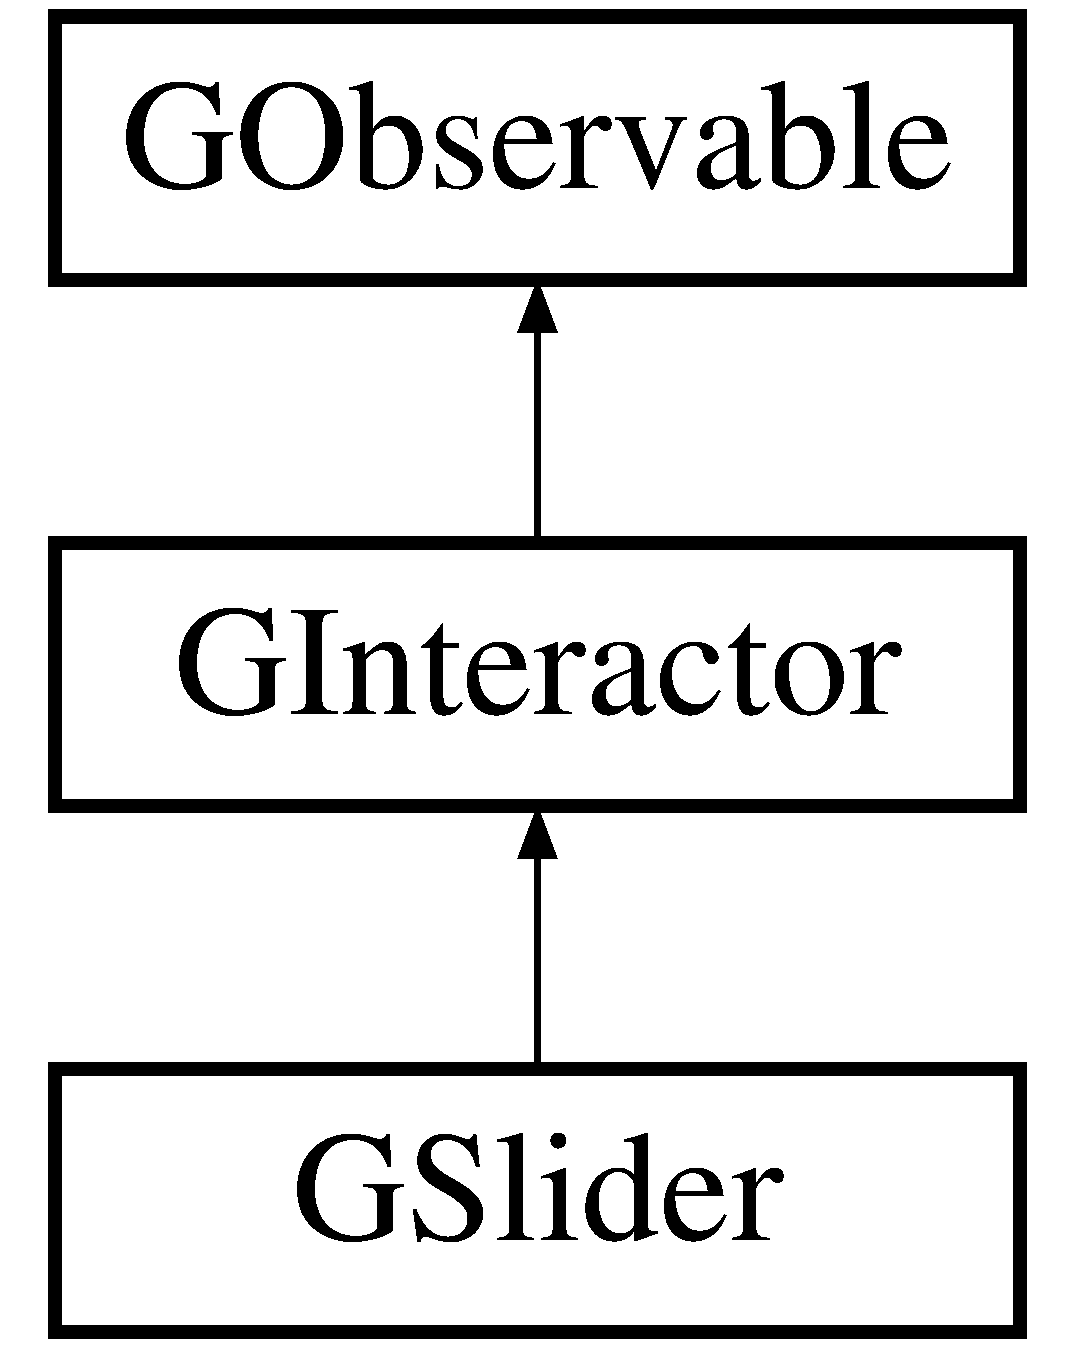
\includegraphics[height=3.000000cm]{classGSlider}
\end{center}
\end{figure}
\subsection*{Public Types}
\begin{DoxyCompactItemize}
\item 
enum \mbox{\hyperlink{classGSlider_a871118a09520247c78a71ecd7b0abd58}{Orientation}} \{ \mbox{\hyperlink{classGSlider_a871118a09520247c78a71ecd7b0abd58a4dd51ad73508d6fc83a502966779e48e}{H\+O\+R\+I\+Z\+O\+N\+T\+AL}} = 0, 
\mbox{\hyperlink{classGSlider_a871118a09520247c78a71ecd7b0abd58a1a88641fcd39f2ed3e58a18526e97138}{V\+E\+R\+T\+I\+C\+AL}} = 1
 \}
\begin{DoxyCompactList}\small\item\em The two valid orientations of sliders. \end{DoxyCompactList}\item 
enum \mbox{\hyperlink{classGInteractor_a8e0d441725a81d2bbdebbea09078260e}{Text\+Position}} \{ \mbox{\hyperlink{classGInteractor_a8e0d441725a81d2bbdebbea09078260ea4cd6f2e7d5a08d6f4dc052df2358f774}{T\+E\+X\+T\+\_\+\+B\+E\+S\+I\+D\+E\+\_\+\+I\+C\+ON}}, 
\mbox{\hyperlink{classGInteractor_a8e0d441725a81d2bbdebbea09078260eaa88490f63d8de68d44c83bdb2ecde3b3}{T\+E\+X\+T\+\_\+\+U\+N\+D\+E\+R\+\_\+\+I\+C\+ON}}, 
\mbox{\hyperlink{classGInteractor_a8e0d441725a81d2bbdebbea09078260ea39a6f388a30ac4fefb6eb13e846bc9f2}{T\+E\+X\+T\+\_\+\+O\+N\+LY}}
 \}
\begin{DoxyCompactList}\small\item\em The places where an interactor can place its text relative to its icon. \end{DoxyCompactList}\end{DoxyCompactItemize}
\subsection*{Public Member Functions}
\begin{DoxyCompactItemize}
\item 
\mbox{\hyperlink{classGSlider_a209c7847379ff5d2bad6fa6b09dd654f}{G\+Slider}} (int min=0, int max=100, int value=50, Q\+Widget $\ast$parent=nullptr)
\begin{DoxyCompactList}\small\item\em Creates a new horizontal slider with the given value range. \end{DoxyCompactList}\item 
\mbox{\hyperlink{classGSlider_ad317f09d4a94efa89b6c9319443c87df}{G\+Slider}} (\mbox{\hyperlink{classGSlider_a871118a09520247c78a71ecd7b0abd58}{Orientation}} orientation, int min=0, int max=100, int value=50, Q\+Widget $\ast$parent=nullptr)
\begin{DoxyCompactList}\small\item\em Creates a new horizontal or vertical slider with the given value range. \end{DoxyCompactList}\item 
\mbox{\hyperlink{classGSlider_a8f6de86ca7815ddc1fdfcec42d25c844}{$\sim$\+G\+Slider}} () override
\begin{DoxyCompactList}\small\item\em Frees memory allocated internally by the slider. \end{DoxyCompactList}\item 
virtual void \mbox{\hyperlink{classGInteractor_a02f20ea6edfa0671f31c4c648a253833}{add\+Action\+Listener}} () Q\+\_\+\+D\+E\+C\+L\+\_\+\+D\+E\+P\+R\+E\+C\+A\+T\+ED
\begin{DoxyCompactList}\small\item\em Adds an event listener to be notified when this interactor is clicked or generally interacted with. \end{DoxyCompactList}\item 
bool \mbox{\hyperlink{classGInteractor_a597a370b592e3737d38d9d2f4e2031ea}{events\+Enabled}} () const override
\begin{DoxyCompactList}\small\item\em Returns true if this interactor is currently accepting events. \end{DoxyCompactList}\item 
virtual std\+::string \mbox{\hyperlink{classGInteractor_a69f8d23ed8f207fbecad99960776e942}{get\+Accelerator}} () const
\begin{DoxyCompactList}\small\item\em Returns a string representing a hotkey for this interactor, or an empty string if no accelerator has been set. \end{DoxyCompactList}\item 
virtual std\+::string \mbox{\hyperlink{classGInteractor_a94eb4276000c4fdfb508ce9e6317a82a}{get\+Action\+Command}} () const
\begin{DoxyCompactList}\small\item\em Returns an action command for this interactor, which is a semi-\/unique string you can use to identify it when events occur. \end{DoxyCompactList}\item 
virtual std\+::string \mbox{\hyperlink{classGInteractor_a808e22cc1fdfbecf71ed8c64ef4600e0}{get\+Background}} () const
\begin{DoxyCompactList}\small\item\em Returns the background color of the interactor as a string. \end{DoxyCompactList}\item 
virtual int \mbox{\hyperlink{classGInteractor_a9e827257a55cb8cf4d9de2ec6bcfd7a0}{get\+Background\+Int}} () const
\begin{DoxyCompactList}\small\item\em Returns the background color of the interactor as an R\+GB integer. \end{DoxyCompactList}\item 
virtual \mbox{\hyperlink{structGRectangle}{G\+Rectangle}} \mbox{\hyperlink{classGInteractor_a29e6ac35a0b48f491a4c88194cc5da3b}{get\+Bounds}} () const
\begin{DoxyCompactList}\small\item\em Returns a rectangle representing the x/y position and size of this interactor. \end{DoxyCompactList}\item 
virtual std\+::string \mbox{\hyperlink{classGInteractor_aa061dfa488c31e18549d64363c1d0e34}{get\+Color}} () const
\begin{DoxyCompactList}\small\item\em Returns the foreground/text color of the interactor as a string. \end{DoxyCompactList}\item 
virtual int \mbox{\hyperlink{classGInteractor_a9635c7af766cdc3417f346683fa0e6c1}{get\+Color\+Int}} () const
\begin{DoxyCompactList}\small\item\em Returns the foreground/text color of the interactor as an R\+GB integer. \end{DoxyCompactList}\item 
virtual \mbox{\hyperlink{classGContainer}{G\+Container}} $\ast$ \mbox{\hyperlink{classGInteractor_a7a6e317c29d61030929b4cd2d1c00fe7}{get\+Container}} () const
\begin{DoxyCompactList}\small\item\em Returns a pointer to the onscreen container holding this interactor. \end{DoxyCompactList}\item 
virtual std\+::string \mbox{\hyperlink{classGInteractor_a894a5502900794eeb27d084c21f1d77d}{get\+Font}} () const
\begin{DoxyCompactList}\small\item\em Returns the font of this interactor\textquotesingle{}s text as a font string such as \char`\"{}\+Helvetica-\/12-\/\+Bold\char`\"{}. \end{DoxyCompactList}\item 
virtual std\+::string \mbox{\hyperlink{classGInteractor_a4fa2d8b0192a3a5b4af4bbfe71194d03}{get\+Foreground}} () const
\begin{DoxyCompactList}\small\item\em Returns the foreground/text color of the interactor as a string. \end{DoxyCompactList}\item 
virtual int \mbox{\hyperlink{classGInteractor_ac3b12ab385a6ef9ae90fc879860ba726}{get\+Foreground\+Int}} () const
\begin{DoxyCompactList}\small\item\em Returns the foreground/text color of the interactor as an R\+GB integer. \end{DoxyCompactList}\item 
virtual double \mbox{\hyperlink{classGInteractor_a1e7e353362434072875264cf95629f99}{get\+Height}} () const
\begin{DoxyCompactList}\small\item\em Returns the current onscreen height of this interactor in pixels. \end{DoxyCompactList}\item 
virtual std\+::string \mbox{\hyperlink{classGInteractor_aaed62a73004939a64da6f0eb9eb64d73}{get\+Icon}} () const
\begin{DoxyCompactList}\small\item\em Returns the file name of the icon associated with this interactor, or an empty string if no icon has been set. \end{DoxyCompactList}\item 
virtual int \mbox{\hyperlink{classGInteractor_a9c9659a6c6ba66b4107ba59c95a24241}{get\+ID}} () const
\begin{DoxyCompactList}\small\item\em Returns a globally unique identifier for this interactor, which is set when the interactor is constructed. \end{DoxyCompactList}\item 
\+\_\+\+Internal\+\_\+\+Q\+Widget $\ast$ \mbox{\hyperlink{classGSlider_a2f6b36b2517087dc90a366b5ce1f5323}{get\+Internal\+Widget}} () const override
\begin{DoxyCompactList}\small\item\em Returns a direct pointer to the internal Qt widget being wrapped by this interactor. \end{DoxyCompactList}\item 
virtual \mbox{\hyperlink{structGPoint}{G\+Point}} \mbox{\hyperlink{classGInteractor_a4f83802015511edeb63b892830812c11}{get\+Location}} () const
\begin{DoxyCompactList}\small\item\em Returns an (x, y) point representing the onscreen location of the top-\/left corner of this interactor within its containing window. \end{DoxyCompactList}\item 
virtual int \mbox{\hyperlink{classGSlider_acc49776af85220307b8955d752d9ffcb}{get\+Max}} () const
\begin{DoxyCompactList}\small\item\em Returns the maximum allowed value of the slider. \end{DoxyCompactList}\item 
virtual int \mbox{\hyperlink{classGSlider_ad06537e69f71666d30bec18dc042a6e4}{get\+Min}} () const
\begin{DoxyCompactList}\small\item\em Returns the minimum allowed value of the slider. \end{DoxyCompactList}\item 
virtual double \mbox{\hyperlink{classGInteractor_aed4b0075fcc434499c3cb3e46896bda3}{get\+Minimum\+Height}} () const
\begin{DoxyCompactList}\small\item\em Returns the minimum height in pixels that this interactor will permit itself to be resized to. \end{DoxyCompactList}\item 
virtual \mbox{\hyperlink{structGDimension}{G\+Dimension}} \mbox{\hyperlink{classGInteractor_a66b5af0b32493b4d597ca0a3df2049ea}{get\+Minimum\+Size}} () const
\begin{DoxyCompactList}\small\item\em Returns a \mbox{\hyperlink{structGDimension}{G\+Dimension}} structure representing the minimum size in pixels that this interactor will permit itself to be resized to. \end{DoxyCompactList}\item 
virtual double \mbox{\hyperlink{classGInteractor_a59e668114fe3d49d2a0f28deb258f7c8}{get\+Minimum\+Width}} () const
\begin{DoxyCompactList}\small\item\em Returns the minimum width in pixels that this interactor will permit itself to be resized to. \end{DoxyCompactList}\item 
virtual std\+::string \mbox{\hyperlink{classGInteractor_a8a60438a5b55d0b2ceb35c8674b9d8c5}{get\+Name}} () const
\begin{DoxyCompactList}\small\item\em Returns a string representing a unique name for this interactor. \end{DoxyCompactList}\item 
virtual \mbox{\hyperlink{classGSlider_a871118a09520247c78a71ecd7b0abd58}{Orientation}} \mbox{\hyperlink{classGSlider_a43aa4aae2f77abd7de3bf461212ac8d0}{get\+Orientation}} () const
\begin{DoxyCompactList}\small\item\em Returns the orientation of the slider, either H\+O\+R\+I\+Z\+O\+N\+T\+AL or V\+E\+R\+T\+I\+C\+AL. \end{DoxyCompactList}\item 
virtual double \mbox{\hyperlink{classGInteractor_a747de0961653847bdc6615dbf756d715}{get\+Preferred\+Height}} () const
\begin{DoxyCompactList}\small\item\em Returns the height in pixels that this interactor would prefer to be, which would exactly fit its contents with no stretching or scrollbars. \end{DoxyCompactList}\item 
virtual \mbox{\hyperlink{structGDimension}{G\+Dimension}} \mbox{\hyperlink{classGInteractor_a4aabbee761d8e9116275401131b7ccd1}{get\+Preferred\+Size}} () const
\begin{DoxyCompactList}\small\item\em Returns a \mbox{\hyperlink{structGDimension}{G\+Dimension}} structure storing the width and height in pixels that this interactor would prefer to be, which would exactly fit its contents with no stretching or scrollbars. \end{DoxyCompactList}\item 
virtual double \mbox{\hyperlink{classGInteractor_a82bca31d37700fb0e35d2743352efd5e}{get\+Preferred\+Width}} () const
\begin{DoxyCompactList}\small\item\em Returns the height in pixels that this interactor would prefer to be, which would exactly fit its contents with no stretching or scrollbars. \end{DoxyCompactList}\item 
virtual \mbox{\hyperlink{structGDimension}{G\+Dimension}} \mbox{\hyperlink{classGInteractor_a7b4eec96a2bdc6420695d5796a78eea9}{get\+Size}} () const
\begin{DoxyCompactList}\small\item\em Returns a \mbox{\hyperlink{structGDimension}{G\+Dimension}} structure storing the current onscreen width and height of this interactor in pixels. \end{DoxyCompactList}\item 
std\+::string \mbox{\hyperlink{classGSlider_a9b72ede4ee8520f987a0c01e30654814}{get\+Type}} () const override
\begin{DoxyCompactList}\small\item\em Returns a string representing the class name of this interactor, such as \char`\"{}\+G\+Button\char`\"{} or \char`\"{}\+G\+Check\+Box\char`\"{}. \end{DoxyCompactList}\item 
virtual int \mbox{\hyperlink{classGSlider_acdb0b383a96801f3200302b6f4a7da64}{get\+Value}} () const
\begin{DoxyCompactList}\small\item\em Returns the slider\textquotesingle{}s current value. \end{DoxyCompactList}\item 
Q\+Widget $\ast$ \mbox{\hyperlink{classGSlider_a3b33a602b31a6b809d020535a59db3b4}{get\+Widget}} () const override
\begin{DoxyCompactList}\small\item\em Returns a direct pointer to the internal Qt widget being wrapped by this interactor. \end{DoxyCompactList}\item 
virtual double \mbox{\hyperlink{classGInteractor_a0ed2965abd4f5701d2cadf71239faf19}{get\+Width}} () const
\begin{DoxyCompactList}\small\item\em Returns the current onscreen width of this interactor in pixels. \end{DoxyCompactList}\item 
virtual double \mbox{\hyperlink{classGInteractor_a344385751bee0720059403940d57a13e}{getX}} () const
\begin{DoxyCompactList}\small\item\em Returns the x-\/coordinate of the top-\/left pixel of this interactor within its onscreen window. \end{DoxyCompactList}\item 
virtual double \mbox{\hyperlink{classGInteractor_aafa51c7f8f38a09febbb9ce7853f77b4}{getY}} () const
\begin{DoxyCompactList}\small\item\em Returns the y-\/coordinate of the top-\/left pixel of this interactor within its onscreen window. \end{DoxyCompactList}\item 
virtual bool \mbox{\hyperlink{classGInteractor_afc480f652b8c5f1fb255e2269ce68879}{in\+Bounds}} (double x, double y) const
\begin{DoxyCompactList}\small\item\em Returns true if the given x/y pixel is within the bounds of this interactor. \end{DoxyCompactList}\item 
virtual bool \mbox{\hyperlink{classGInteractor_ae6d7982c1c627b677a5e776ca86118ed}{in\+Bounds}} (int x, int y) const
\begin{DoxyCompactList}\small\item\em Returns true if the given x/y pixel is within the bounds of this interactor. \end{DoxyCompactList}\item 
virtual bool \mbox{\hyperlink{classGInteractor_aacb819fb241851fd9fc045271baa4034}{is\+Enabled}} () const
\begin{DoxyCompactList}\small\item\em Returns true if this interactor is currently enabled. \end{DoxyCompactList}\item 
virtual bool \mbox{\hyperlink{classGInteractor_a9d8a6cfb13917785c143e74d40e4e2be}{is\+Visible}} () const
\begin{DoxyCompactList}\small\item\em Returns true if the interactor is visible on the screen. \end{DoxyCompactList}\item 
virtual void \mbox{\hyperlink{classGInteractor_ab7fe7a876367b87cf7202f947f1d05e4}{remove\+Action\+Listener}} ()
\begin{DoxyCompactList}\small\item\em Removes the action listener from this interactor so that it will no longer call it when events occur. \end{DoxyCompactList}\item 
virtual void \mbox{\hyperlink{classGInteractor_ad39d0325cde6b97ebda4b9d7787c633b}{remove\+Click\+Listener}} ()
\begin{DoxyCompactList}\small\item\em Removes the click listener from this interactor so that it will no longer call it when events occur. \end{DoxyCompactList}\item 
virtual void \mbox{\hyperlink{classGInteractor_aa4250907e4cdd77349c04f0cf5cdd3d3}{remove\+Double\+Click\+Listener}} ()
\begin{DoxyCompactList}\small\item\em Removes the double-\/click listener from this interactor so that it will no longer call it when events occur. \end{DoxyCompactList}\item 
virtual void \mbox{\hyperlink{classGInteractor_a43095f41cab3be732b49f29970484b05}{remove\+Key\+Listener}} ()
\begin{DoxyCompactList}\small\item\em Removes the key listener from this interactor so that it will no longer call it when key events occur. \end{DoxyCompactList}\item 
virtual void \mbox{\hyperlink{classGInteractor_aff47f71ce47e688a07c9d38dc92fcc11}{remove\+Mouse\+Listener}} ()
\begin{DoxyCompactList}\small\item\em Removes the mouse listener from this interactor so that it will no longer call it when events occur. \end{DoxyCompactList}\item 
virtual void \mbox{\hyperlink{classGInteractor_a519fb2ac767f8b2febbb50b898b8c8cb}{request\+Focus}} ()
\begin{DoxyCompactList}\small\item\em Transfers keyboard focus to this interactor. \end{DoxyCompactList}\item 
virtual void \mbox{\hyperlink{classGInteractor_ad15f102f62e2960576012f1aa0ba4b2e}{set\+Accelerator}} (const std\+::string \&accelerator)
\begin{DoxyCompactList}\small\item\em Sets an accelerator hotkey for this interactor, such as \char`\"{}\+Ctrl-\/\+S\char`\"{}. \end{DoxyCompactList}\item 
virtual void \mbox{\hyperlink{classGInteractor_a4b5843fe3030e038a1ba54cc03389bcf}{set\+Action\+Command}} (const std\+::string \&action\+Command)
\begin{DoxyCompactList}\small\item\em Sets the action command for this interactor. \end{DoxyCompactList}\item 
virtual void \mbox{\hyperlink{classGInteractor_adcfb4742430c88714fcf57e57ab8ea9c}{set\+Action\+Listener}} (G\+Event\+Listener func)
\begin{DoxyCompactList}\small\item\em Sets an action listener on this interactor so that it will be called when it is interacted with in its primary way. \end{DoxyCompactList}\item 
virtual void \mbox{\hyperlink{classGInteractor_aebd20a89c7a8a43a6fce999cf4f9fcf2}{set\+Action\+Listener}} (G\+Event\+Listener\+Void func)
\begin{DoxyCompactList}\small\item\em Sets an action listener on this interactor so that it will be called when it is interacted with in its primary way. \end{DoxyCompactList}\item 
virtual void \mbox{\hyperlink{classGInteractor_acba7e546c2025c0a15ca4b4cc92043db}{set\+Background}} (int rgb)
\begin{DoxyCompactList}\small\item\em Sets the background color of the interactor to the color represented by the given R\+GB integer. \end{DoxyCompactList}\item 
virtual void \mbox{\hyperlink{classGInteractor_ab4677ab2474e68b07aa56605af92a84a}{set\+Background}} (const std\+::string \&color)
\begin{DoxyCompactList}\small\item\em Sets the background color of the interactor to the color represented by the given string. \end{DoxyCompactList}\item 
virtual void \mbox{\hyperlink{classGInteractor_a2aae8197624b72265ab83b4f1bc73f2f}{set\+Bounds}} (double x, double y, double width, double height)
\begin{DoxyCompactList}\small\item\em Sets the size and location of the widget. \end{DoxyCompactList}\item 
virtual void \mbox{\hyperlink{classGInteractor_acada386653f008cacc7cce86426bef7c}{set\+Bounds}} (const \mbox{\hyperlink{structGRectangle}{G\+Rectangle}} \&size)
\begin{DoxyCompactList}\small\item\em Sets the size and location of the widget. \end{DoxyCompactList}\item 
virtual void \mbox{\hyperlink{classGInteractor_abd40af6921242584d0954f173911b190}{set\+Click\+Listener}} (G\+Event\+Listener func)
\begin{DoxyCompactList}\small\item\em Sets a mouse listener on this interactor so that it will be called when the mouse is clicked on it. \end{DoxyCompactList}\item 
virtual void \mbox{\hyperlink{classGInteractor_a856414c92df90f56f3877475eb3f8fc4}{set\+Click\+Listener}} (G\+Event\+Listener\+Void func)
\begin{DoxyCompactList}\small\item\em Sets a mouse listener on this interactor so that it will be called when the mouse is clicked on it. \end{DoxyCompactList}\item 
virtual void \mbox{\hyperlink{classGInteractor_ab1f5cc0f5cc6bbbd716a526c61f1081d}{set\+Color}} (int rgb)
\begin{DoxyCompactList}\small\item\em Sets the foreground/text color of the interactor to the color represented by the given R\+GB integer. \end{DoxyCompactList}\item 
virtual void \mbox{\hyperlink{classGInteractor_a61374df6c11b52cfbb0815decdbaebc6}{set\+Color}} (const std\+::string \&color)
\begin{DoxyCompactList}\small\item\em Sets the foreground/text color of the interactor to the color represented by the given string. \end{DoxyCompactList}\item 
virtual void \mbox{\hyperlink{classGInteractor_ac29f9a3462458e165fae3a1f046ee77a}{set\+Double\+Click\+Listener}} (G\+Event\+Listener func)
\begin{DoxyCompactList}\small\item\em Sets a mouse listener on this interactor so that it will be called when the mouse is double-\/clicked on it. \end{DoxyCompactList}\item 
virtual void \mbox{\hyperlink{classGInteractor_a50096194d66f48c92dd4c512d41bfc76}{set\+Double\+Click\+Listener}} (G\+Event\+Listener\+Void func)
\begin{DoxyCompactList}\small\item\em Sets a mouse listener on this interactor so that it will be called when the mouse is double-\/clicked on it. \end{DoxyCompactList}\item 
virtual void \mbox{\hyperlink{classGInteractor_ab831367dd84bbd579e02e55bacb21343}{set\+Enabled}} (bool value)
\begin{DoxyCompactList}\small\item\em Sets whether this interactor is currently enabled. \end{DoxyCompactList}\item 
virtual void \mbox{\hyperlink{classGObservable_afaa30b2a9e0f378fd1c70d2f1d0b8216}{set\+Events\+Enabled}} (bool \mbox{\hyperlink{classGInteractor_a597a370b592e3737d38d9d2f4e2031ea}{events\+Enabled}})
\begin{DoxyCompactList}\small\item\em Sets whether the object is currently allowing itself to fire events. \end{DoxyCompactList}\item 
virtual void \mbox{\hyperlink{classGInteractor_a2592348886ffea646c6534bf88f7c49d}{set\+Font}} (const Q\+Font \&font)
\begin{DoxyCompactList}\small\item\em Sets the font used by this widget to the given Qt font. \end{DoxyCompactList}\item 
virtual void \mbox{\hyperlink{classGInteractor_a8e096e8818d838aceae1d46d58fb3a7b}{set\+Font}} (const std\+::string \&font)
\begin{DoxyCompactList}\small\item\em Sets the font used by this widget to the font represented by the given font string, such as \char`\"{}\+Helvetica-\/16-\/\+Bold\char`\"{}. \end{DoxyCompactList}\item 
virtual void \mbox{\hyperlink{classGInteractor_a9eb856b5ff83a19df3831a31f15f4563}{set\+Foreground}} (int rgb)
\begin{DoxyCompactList}\small\item\em Sets the foreground/text color of the interactor to the color represented by the given R\+GB integer. \end{DoxyCompactList}\item 
virtual void \mbox{\hyperlink{classGInteractor_af59209aeadea6dfc6d97a2d8531f50e1}{set\+Foreground}} (const std\+::string \&color)
\begin{DoxyCompactList}\small\item\em Sets the foreground/text color of the interactor to the color represented by the given string. \end{DoxyCompactList}\item 
virtual void \mbox{\hyperlink{classGInteractor_a9e280bfc4544dfaf8e4376c4e1a74357}{set\+Height}} (double height)
\begin{DoxyCompactList}\small\item\em Sets the onscreen height of the interactor in pixels. \end{DoxyCompactList}\item 
virtual void \mbox{\hyperlink{classGInteractor_a542abfcd7261751352af129c7215ecda}{set\+Icon}} (const Q\+Icon \&icon)
\begin{DoxyCompactList}\small\item\em Sets the icon associated with this interactor. \end{DoxyCompactList}\item 
virtual void \mbox{\hyperlink{classGInteractor_a368e1a338f84401c284506d03b1ba769}{set\+Icon}} (const Q\+Pixmap \&icon)
\begin{DoxyCompactList}\small\item\em Sets the icon associated with this interactor. \end{DoxyCompactList}\item 
virtual void \mbox{\hyperlink{classGInteractor_a762e139aa311461c3984d3ad28293f64}{set\+Icon}} (const std\+::string \&filename, bool retain\+Icon\+Size=true)
\begin{DoxyCompactList}\small\item\em Sets the file name of the icon associated with this interactor, or an empty string if no icon has been set. \end{DoxyCompactList}\item 
virtual void \mbox{\hyperlink{classGInteractor_aeb8324d3287fa1fbe093f4d6230cf0a6}{set\+Key\+Listener}} (G\+Event\+Listener func)
\begin{DoxyCompactList}\small\item\em Sets a key listener on this interactor so that it will be called when the user presses any key. \end{DoxyCompactList}\item 
virtual void \mbox{\hyperlink{classGInteractor_ae48ecea73606c7bd9423e1c7cc589cc9}{set\+Key\+Listener}} (G\+Event\+Listener\+Void func)
\begin{DoxyCompactList}\small\item\em Sets a key listener on this interactor so that it will be called when the user presses any key. \end{DoxyCompactList}\item 
virtual void \mbox{\hyperlink{classGInteractor_a04594e8ba9b98513a64f1da00dcae18c}{set\+Location}} (double x, double y)
\begin{DoxyCompactList}\small\item\em Sets the onscreen x/y-\/coordinate of the top-\/left corner of the interactor relative to its window. \end{DoxyCompactList}\item 
virtual void \mbox{\hyperlink{classGSlider_ab263d79bf430d73a617641f317dcfb98}{set\+Max}} (int max)
\begin{DoxyCompactList}\small\item\em Sets the maximum allowed value of the slider. \end{DoxyCompactList}\item 
virtual void \mbox{\hyperlink{classGSlider_a6dc44e5adc595b71f90efc65b0b5ea1d}{set\+Min}} (int min)
\begin{DoxyCompactList}\small\item\em Sets the minimum allowed value of the slider. \end{DoxyCompactList}\item 
virtual void \mbox{\hyperlink{classGInteractor_a0cf428e207b7f22cc08138a90b1b87b2}{set\+Minimum\+Size}} (double width, double height)
\begin{DoxyCompactList}\small\item\em Sets the minimum size in pixels that this interactor will permit itself to be resized to. \end{DoxyCompactList}\item 
virtual void \mbox{\hyperlink{classGInteractor_a3b1046117ac6cb7abe467e00ba8a81f4}{set\+Minimum\+Size}} (const \mbox{\hyperlink{structGDimension}{G\+Dimension}} \&size)
\begin{DoxyCompactList}\small\item\em Sets the minimum size in pixels that this interactor will permit itself to be resized to. \end{DoxyCompactList}\item 
virtual void \mbox{\hyperlink{classGInteractor_a37d8dbc943f59920f705b0104f60bde2}{set\+Mouse\+Listener}} (G\+Event\+Listener func)
\begin{DoxyCompactList}\small\item\em Sets a mouse listener on this interactor so that it will be called when the mouse is moved or clicked on it. \end{DoxyCompactList}\item 
virtual void \mbox{\hyperlink{classGInteractor_aea7f647ea62d59f71b5fad6aa65eeaf9}{set\+Mouse\+Listener}} (G\+Event\+Listener\+Void func)
\begin{DoxyCompactList}\small\item\em Sets a mouse listener on this interactor so that it will be called when the mouse is moved or clicked on it. \end{DoxyCompactList}\item 
virtual void \mbox{\hyperlink{classGInteractor_a9d3a2685df23b5e7cbf59c19c4a1f9b5}{set\+Name}} (const std\+::string \&name)
\begin{DoxyCompactList}\small\item\em Sets a string representing a unique name for this interactor. \end{DoxyCompactList}\item 
virtual void \mbox{\hyperlink{classGInteractor_a1ab987704fce32098706c6f00fb08218}{set\+Preferred\+Height}} (double height)
\begin{DoxyCompactList}\small\item\em Sets the height in pixels that this interactor would prefer to be. \end{DoxyCompactList}\item 
virtual void \mbox{\hyperlink{classGInteractor_a042c5ae19430d765ef552371cae3632c}{set\+Preferred\+Size}} (double width, double height)
\begin{DoxyCompactList}\small\item\em Sets the width and height in pixels that this interactor would prefer to be. \end{DoxyCompactList}\item 
virtual void \mbox{\hyperlink{classGInteractor_aa22d9be4bc0e078bb0ea69b0fc9d7c75}{set\+Preferred\+Size}} (const \mbox{\hyperlink{structGDimension}{G\+Dimension}} \&size)
\begin{DoxyCompactList}\small\item\em Sets the size in pixels that this interactor would prefer to be. \end{DoxyCompactList}\item 
virtual void \mbox{\hyperlink{classGInteractor_a3db429ab2fa52efd187eec0ed8cdd9f2}{set\+Preferred\+Width}} (double width)
\begin{DoxyCompactList}\small\item\em Sets the width in pixels that this interactor would prefer to be. \end{DoxyCompactList}\item 
virtual void \mbox{\hyperlink{classGSlider_a693c16cecd031a84aaf28be0427cff88}{set\+Range}} (int min, int max)
\begin{DoxyCompactList}\small\item\em Sets the min-\/max range of the slider. \end{DoxyCompactList}\item 
virtual void \mbox{\hyperlink{classGInteractor_aca25d49481f9bf5fc8f7df4c086c4ce7}{set\+Size}} (double width, double height)
\begin{DoxyCompactList}\small\item\em Sets the onscreen width and height of the interactor in pixels. \end{DoxyCompactList}\item 
virtual void \mbox{\hyperlink{classGInteractor_ae2b628228f192c2702c4ce941b2af68f}{set\+Size}} (const \mbox{\hyperlink{structGDimension}{G\+Dimension}} \&size)
\begin{DoxyCompactList}\small\item\em Sets the onscreen width and height of the interactor in pixels. \end{DoxyCompactList}\item 
virtual void \mbox{\hyperlink{classGSlider_ae7f0a959186167548911cc2c69ff6b39}{set\+State}} (int min, int max, int value)
\begin{DoxyCompactList}\small\item\em Sets all of the relevant state of the slider. \end{DoxyCompactList}\item 
virtual void \mbox{\hyperlink{classGInteractor_a039e0e49beaecc275efce02d416acea8}{set\+Tooltip}} (const std\+::string \&tooltip\+Text)
\begin{DoxyCompactList}\small\item\em Sets a \char`\"{}tooltip\char`\"{} that will appear if the user hovers their mouse over the interactor. \end{DoxyCompactList}\item 
virtual void \mbox{\hyperlink{classGSlider_a23d79e21b8ed72e19278ca31d47b8c87}{set\+Value}} (int value)
\begin{DoxyCompactList}\small\item\em Sets the current value of the slider. \end{DoxyCompactList}\item 
virtual void \mbox{\hyperlink{classGInteractor_a18e44e30b31525a243960ca3928125aa}{set\+Visible}} (bool visible)
\begin{DoxyCompactList}\small\item\em Returns true if the interactor is visible on the screen. \end{DoxyCompactList}\item 
virtual void \mbox{\hyperlink{classGInteractor_aa3f3fba4cb131baa8696ba01e3bceca1}{set\+Width}} (double width)
\begin{DoxyCompactList}\small\item\em Sets the onscreen width of the interactor in pixels. \end{DoxyCompactList}\item 
virtual void \mbox{\hyperlink{classGInteractor_a9c18fcc579333bf9653d13ad2b372e39}{setX}} (double x)
\begin{DoxyCompactList}\small\item\em Sets the onscreen x-\/coordinate of the top-\/left corner of the interactor relative to its window. \end{DoxyCompactList}\item 
virtual void \mbox{\hyperlink{classGInteractor_a7d57e2a5c35d27feb58fd498a3cf82b9}{setY}} (double y)
\begin{DoxyCompactList}\small\item\em Sets the onscreen y-\/coordinate of the top-\/left corner of the interactor relative to its window. \end{DoxyCompactList}\item 
virtual std\+::string \mbox{\hyperlink{classGObservable_a1fe5121d6528fdea3f243321b3fa3a49}{to\+String}} () const
\begin{DoxyCompactList}\small\item\em Returns a string representation of this observable object\textquotesingle{}s state. \end{DoxyCompactList}\end{DoxyCompactItemize}
\subsection*{Static Public Attributes}
\begin{DoxyCompactItemize}
\item 
static const int \mbox{\hyperlink{classGSlider_a8347129b4807bb7063f75ff2f457cc30}{D\+E\+F\+A\+U\+L\+T\+\_\+\+I\+N\+I\+T\+I\+A\+L\+\_\+\+V\+A\+L\+UE}} = 50
\begin{DoxyCompactList}\small\item\em Default initial value for a slider (50). \end{DoxyCompactList}\item 
static const int \mbox{\hyperlink{classGSlider_af4df8666449a1553ded0ebd926c1c847}{D\+E\+F\+A\+U\+L\+T\+\_\+\+M\+A\+X\+\_\+\+V\+A\+L\+UE}} = 100
\begin{DoxyCompactList}\small\item\em Default maximum value for a slider (100). \end{DoxyCompactList}\item 
static const int \mbox{\hyperlink{classGSlider_ada756074cb913647156250a2172a26f4}{D\+E\+F\+A\+U\+L\+T\+\_\+\+M\+I\+N\+\_\+\+V\+A\+L\+UE}} = 0
\begin{DoxyCompactList}\small\item\em Default minimum value for a slider (0). \end{DoxyCompactList}\end{DoxyCompactItemize}
\subsection*{Protected Member Functions}
\begin{DoxyCompactItemize}
\item 
virtual void \mbox{\hyperlink{classGObservable_a80cfa040459ff53594adbd6a51ec8f43}{clear\+Event\+Listeners}} ()
\begin{DoxyCompactList}\small\item\em Removes all event listeners from this object. \end{DoxyCompactList}\item 
virtual void \mbox{\hyperlink{classGObservable_a284f31528c0520f8e545c03ac9eeac74}{ensure\+Thread\+Safety}} (const std\+::string \&member\+Name=\char`\"{}\char`\"{})
\begin{DoxyCompactList}\small\item\em Ensures that we are currently in the Qt G\+UI thread. \end{DoxyCompactList}\item 
virtual void \mbox{\hyperlink{classGObservable_a63e5e5a6227c59c928493b11aceb0f67}{fire\+Event}} (\mbox{\hyperlink{classGEvent}{G\+Event}} \&event)
\begin{DoxyCompactList}\small\item\em Sends out the given event to any attached listeners. \end{DoxyCompactList}\item 
virtual void \mbox{\hyperlink{classGObservable_ab3983ea07337b52020a29cc00c653d8d}{fire\+G\+Event}} (Q\+Event $\ast$event, Event\+Type event\+Type, const std\+::string \&event\+Name)
\begin{DoxyCompactList}\small\item\em Creates an event of the given type, then sends it out to any attached listeners. \end{DoxyCompactList}\item 
virtual void \mbox{\hyperlink{classGObservable_a01fdf1b0e0dbd49e189fe4514e010411}{fire\+G\+Event}} (Q\+Close\+Event $\ast$event, Event\+Type event\+Type, const std\+::string \&event\+Name)
\begin{DoxyCompactList}\small\item\em Creates an event of the given type, then sends it out to any attached listeners. \end{DoxyCompactList}\item 
virtual void \mbox{\hyperlink{classGObservable_abb0b2f66ba39211cb5d7615e9d1c04e2}{fire\+G\+Event}} (Q\+Key\+Event $\ast$event, Event\+Type event\+Type, const std\+::string \&event\+Name)
\begin{DoxyCompactList}\small\item\em Creates an event of the given type, then sends it out to any attached listeners. \end{DoxyCompactList}\item 
virtual void \mbox{\hyperlink{classGObservable_a119318675d2165bdf7dd853aaf881d4b}{fire\+G\+Event}} (Q\+Mouse\+Event $\ast$event, Event\+Type event\+Type, const std\+::string \&event\+Name, const std\+::string \&action\+Command=\char`\"{}\char`\"{})
\begin{DoxyCompactList}\small\item\em Creates an event of the given type, then sends it out to any attached listeners. \end{DoxyCompactList}\item 
virtual void \mbox{\hyperlink{classGObservable_a63fd9034e1e1633c1c38eb342bfd34e9}{fire\+G\+Event}} (Q\+Resize\+Event $\ast$event, Event\+Type event\+Type, const std\+::string \&event\+Name)
\begin{DoxyCompactList}\small\item\em Creates an event of the given type, then sends it out to any attached listeners. \end{DoxyCompactList}\item 
virtual void \mbox{\hyperlink{classGObservable_a741345310d9b7c5170a6cbc410c44ac4}{fire\+G\+Event}} (Q\+Timer\+Event $\ast$event, Event\+Type event\+Type, const std\+::string \&event\+Name)
\begin{DoxyCompactList}\small\item\em Creates an event of the given type, then sends it out to any attached listeners. \end{DoxyCompactList}\item 
virtual void \mbox{\hyperlink{classGObservable_a93bf338968a0338761b8e4dc62f582e9}{fire\+G\+Event}} (Q\+Wheel\+Event $\ast$event, Event\+Type event\+Type, const std\+::string \&event\+Name)
\begin{DoxyCompactList}\small\item\em Creates an event of the given type, then sends it out to any attached listeners. \end{DoxyCompactList}\item 
virtual void \mbox{\hyperlink{classGObservable_a2a70a7d7435ff0c3b80bb4d70da19e0d}{fire\+G\+Event}} (Q\+Window\+State\+Change\+Event $\ast$event, Event\+Type event\+Type, const std\+::string \&event\+Name)
\begin{DoxyCompactList}\small\item\em Creates an event of the given type, then sends it out to any attached listeners. \end{DoxyCompactList}\item 
virtual bool \mbox{\hyperlink{classGObservable_a9f6faaa25942923bafa1c44020c49fa9}{has\+Event\+Listener}} (const std\+::string \&event\+Name) const
\begin{DoxyCompactList}\small\item\em Returns true if the observable object has a listener for the given type of event. \end{DoxyCompactList}\item 
virtual bool \mbox{\hyperlink{classGObservable_aeec1adc19aa0f33de62390686ee1382c}{is\+Accepting\+Event}} (int event\+Mask) const
\begin{DoxyCompactList}\small\item\em Returns true if the observable object has a listener for the given type of event. \end{DoxyCompactList}\item 
virtual bool \mbox{\hyperlink{classGObservable_aa31c73145a29dcb92848a92e0cfaea41}{is\+Accepting\+Event}} (const \mbox{\hyperlink{classGEvent}{G\+Event}} \&event) const
\begin{DoxyCompactList}\small\item\em Returns true if the observable object has a listener for the given type of event. \end{DoxyCompactList}\item 
virtual bool \mbox{\hyperlink{classGObservable_a3b1c689267eda44e65a2213e7de38b23}{is\+Accepting\+Event}} (const std\+::string \&event\+Type) const
\begin{DoxyCompactList}\small\item\em Returns true if the observable object has a listener for the given type of event. \end{DoxyCompactList}\item 
virtual void \mbox{\hyperlink{classGObservable_acbcf1ed3a851ad8a3c17ef38d86b481d}{remove\+Event\+Listener}} (const std\+::string \&event\+Name)
\begin{DoxyCompactList}\small\item\em Removes any event listener from this observable object that would respond to the given type of event, such as \char`\"{}click\char`\"{} or \char`\"{}keydown\char`\"{}. \end{DoxyCompactList}\item 
virtual void \mbox{\hyperlink{classGObservable_af51cc35c29a1bd1908609d432decdbb6}{remove\+Event\+Listeners}} (std\+::initializer\+\_\+list$<$ std\+::string $>$ event\+Names)
\begin{DoxyCompactList}\small\item\em Removes any event listener from this observable object that would respond to the given types of events, such as \char`\"{}click\char`\"{} or \char`\"{}keydown\char`\"{}. \end{DoxyCompactList}\item 
virtual void \mbox{\hyperlink{classGObservable_ad2f6d34961c50f6c1e0659990b79f741}{set\+Event\+Listener}} (const std\+::string \&event\+Name, G\+Event\+Listener func)
\begin{DoxyCompactList}\small\item\em Adds an event listener from this observable object to respond to the given type of event, such as \char`\"{}click\char`\"{} or \char`\"{}keydown\char`\"{}. \end{DoxyCompactList}\item 
virtual void \mbox{\hyperlink{classGObservable_abac4cb9f9e626e010e87f5d91573c8a5}{set\+Event\+Listener}} (const std\+::string \&event\+Name, G\+Event\+Listener\+Void func)
\begin{DoxyCompactList}\small\item\em Adds an event listener from this observable object to respond to the given type of event, such as \char`\"{}click\char`\"{} or \char`\"{}keydown\char`\"{}. \end{DoxyCompactList}\item 
virtual void \mbox{\hyperlink{classGObservable_afa388d69c33c718cf035774604065604}{set\+Event\+Listeners}} (std\+::initializer\+\_\+list$<$ std\+::string $>$ event\+Names, G\+Event\+Listener func)
\begin{DoxyCompactList}\small\item\em Adds an event listener from this observable object to respond to the given types of events, such as \char`\"{}click\char`\"{} or \char`\"{}keydown\char`\"{}. \end{DoxyCompactList}\item 
virtual void \mbox{\hyperlink{classGObservable_a7867184bbb686f74fae8a4db927da799}{set\+Event\+Listeners}} (std\+::initializer\+\_\+list$<$ std\+::string $>$ event\+Names, G\+Event\+Listener\+Void func)
\begin{DoxyCompactList}\small\item\em Adds an event listener from this observable object to respond to the given types of events, such as \char`\"{}click\char`\"{} or \char`\"{}keydown\char`\"{}. \end{DoxyCompactList}\end{DoxyCompactItemize}


\subsection{Detailed Description}
This interactor subclass represents an onscreen slider. 

Dragging the slider control generates action events. 

\subsection{Member Enumeration Documentation}
\mbox{\Hypertarget{classGSlider_a871118a09520247c78a71ecd7b0abd58}\label{classGSlider_a871118a09520247c78a71ecd7b0abd58}} 
\index{G\+Slider@{G\+Slider}!Orientation@{Orientation}}
\index{Orientation@{Orientation}!G\+Slider@{G\+Slider}}
\subsubsection{\texorpdfstring{Orientation}{Orientation}}
{\footnotesize\ttfamily enum \mbox{\hyperlink{classGSlider_a871118a09520247c78a71ecd7b0abd58}{Orientation}}}



The two valid orientations of sliders. 

\begin{DoxyEnumFields}{Enumerator}
\raisebox{\heightof{T}}[0pt][0pt]{\index{H\+O\+R\+I\+Z\+O\+N\+T\+AL@{H\+O\+R\+I\+Z\+O\+N\+T\+AL}!G\+Slider@{G\+Slider}}\index{G\+Slider@{G\+Slider}!H\+O\+R\+I\+Z\+O\+N\+T\+AL@{H\+O\+R\+I\+Z\+O\+N\+T\+AL}}}\mbox{\Hypertarget{classGSlider_a871118a09520247c78a71ecd7b0abd58a4dd51ad73508d6fc83a502966779e48e}\label{classGSlider_a871118a09520247c78a71ecd7b0abd58a4dd51ad73508d6fc83a502966779e48e}} 
H\+O\+R\+I\+Z\+O\+N\+T\+AL&\\
\hline

\raisebox{\heightof{T}}[0pt][0pt]{\index{V\+E\+R\+T\+I\+C\+AL@{V\+E\+R\+T\+I\+C\+AL}!G\+Slider@{G\+Slider}}\index{G\+Slider@{G\+Slider}!V\+E\+R\+T\+I\+C\+AL@{V\+E\+R\+T\+I\+C\+AL}}}\mbox{\Hypertarget{classGSlider_a871118a09520247c78a71ecd7b0abd58a1a88641fcd39f2ed3e58a18526e97138}\label{classGSlider_a871118a09520247c78a71ecd7b0abd58a1a88641fcd39f2ed3e58a18526e97138}} 
V\+E\+R\+T\+I\+C\+AL&\\
\hline

\end{DoxyEnumFields}
\mbox{\Hypertarget{classGInteractor_a8e0d441725a81d2bbdebbea09078260e}\label{classGInteractor_a8e0d441725a81d2bbdebbea09078260e}} 
\index{G\+Slider@{G\+Slider}!Text\+Position@{Text\+Position}}
\index{Text\+Position@{Text\+Position}!G\+Slider@{G\+Slider}}
\subsubsection{\texorpdfstring{Text\+Position}{TextPosition}}
{\footnotesize\ttfamily enum \mbox{\hyperlink{classGInteractor_a8e0d441725a81d2bbdebbea09078260e}{Text\+Position}}\hspace{0.3cm}{\ttfamily [inherited]}}



The places where an interactor can place its text relative to its icon. 

\begin{DoxyEnumFields}{Enumerator}
\raisebox{\heightof{T}}[0pt][0pt]{\index{T\+E\+X\+T\+\_\+\+B\+E\+S\+I\+D\+E\+\_\+\+I\+C\+ON@{T\+E\+X\+T\+\_\+\+B\+E\+S\+I\+D\+E\+\_\+\+I\+C\+ON}!G\+Slider@{G\+Slider}}\index{G\+Slider@{G\+Slider}!T\+E\+X\+T\+\_\+\+B\+E\+S\+I\+D\+E\+\_\+\+I\+C\+ON@{T\+E\+X\+T\+\_\+\+B\+E\+S\+I\+D\+E\+\_\+\+I\+C\+ON}}}\mbox{\Hypertarget{classGInteractor_a8e0d441725a81d2bbdebbea09078260ea4cd6f2e7d5a08d6f4dc052df2358f774}\label{classGInteractor_a8e0d441725a81d2bbdebbea09078260ea4cd6f2e7d5a08d6f4dc052df2358f774}} 
T\+E\+X\+T\+\_\+\+B\+E\+S\+I\+D\+E\+\_\+\+I\+C\+ON&\\
\hline

\raisebox{\heightof{T}}[0pt][0pt]{\index{T\+E\+X\+T\+\_\+\+U\+N\+D\+E\+R\+\_\+\+I\+C\+ON@{T\+E\+X\+T\+\_\+\+U\+N\+D\+E\+R\+\_\+\+I\+C\+ON}!G\+Slider@{G\+Slider}}\index{G\+Slider@{G\+Slider}!T\+E\+X\+T\+\_\+\+U\+N\+D\+E\+R\+\_\+\+I\+C\+ON@{T\+E\+X\+T\+\_\+\+U\+N\+D\+E\+R\+\_\+\+I\+C\+ON}}}\mbox{\Hypertarget{classGInteractor_a8e0d441725a81d2bbdebbea09078260eaa88490f63d8de68d44c83bdb2ecde3b3}\label{classGInteractor_a8e0d441725a81d2bbdebbea09078260eaa88490f63d8de68d44c83bdb2ecde3b3}} 
T\+E\+X\+T\+\_\+\+U\+N\+D\+E\+R\+\_\+\+I\+C\+ON&\\
\hline

\raisebox{\heightof{T}}[0pt][0pt]{\index{T\+E\+X\+T\+\_\+\+O\+N\+LY@{T\+E\+X\+T\+\_\+\+O\+N\+LY}!G\+Slider@{G\+Slider}}\index{G\+Slider@{G\+Slider}!T\+E\+X\+T\+\_\+\+O\+N\+LY@{T\+E\+X\+T\+\_\+\+O\+N\+LY}}}\mbox{\Hypertarget{classGInteractor_a8e0d441725a81d2bbdebbea09078260ea39a6f388a30ac4fefb6eb13e846bc9f2}\label{classGInteractor_a8e0d441725a81d2bbdebbea09078260ea39a6f388a30ac4fefb6eb13e846bc9f2}} 
T\+E\+X\+T\+\_\+\+O\+N\+LY&\\
\hline

\end{DoxyEnumFields}


\subsection{Constructor \& Destructor Documentation}
\mbox{\Hypertarget{classGSlider_a209c7847379ff5d2bad6fa6b09dd654f}\label{classGSlider_a209c7847379ff5d2bad6fa6b09dd654f}} 
\index{G\+Slider@{G\+Slider}!G\+Slider@{G\+Slider}}
\index{G\+Slider@{G\+Slider}!G\+Slider@{G\+Slider}}
\subsubsection{\texorpdfstring{G\+Slider()}{GSlider()}\hspace{0.1cm}{\footnotesize\ttfamily [1/2]}}
{\footnotesize\ttfamily \mbox{\hyperlink{classGSlider}{G\+Slider}} (\begin{DoxyParamCaption}\item[{int}]{min = {\ttfamily 0},  }\item[{int}]{max = {\ttfamily 100},  }\item[{int}]{value = {\ttfamily 50},  }\item[{Q\+Widget $\ast$}]{parent = {\ttfamily nullptr} }\end{DoxyParamCaption})}



Creates a new horizontal slider with the given value range. 


\begin{DoxyExceptions}{Exceptions}
{\em Error\+Exception} & if min $>$ max or value is not between min and max \\
\hline
\end{DoxyExceptions}
\mbox{\Hypertarget{classGSlider_ad317f09d4a94efa89b6c9319443c87df}\label{classGSlider_ad317f09d4a94efa89b6c9319443c87df}} 
\index{G\+Slider@{G\+Slider}!G\+Slider@{G\+Slider}}
\index{G\+Slider@{G\+Slider}!G\+Slider@{G\+Slider}}
\subsubsection{\texorpdfstring{G\+Slider()}{GSlider()}\hspace{0.1cm}{\footnotesize\ttfamily [2/2]}}
{\footnotesize\ttfamily \mbox{\hyperlink{classGSlider}{G\+Slider}} (\begin{DoxyParamCaption}\item[{\mbox{\hyperlink{classGSlider_a871118a09520247c78a71ecd7b0abd58}{Orientation}}}]{orientation,  }\item[{int}]{min = {\ttfamily 0},  }\item[{int}]{max = {\ttfamily 100},  }\item[{int}]{value = {\ttfamily 50},  }\item[{Q\+Widget $\ast$}]{parent = {\ttfamily nullptr} }\end{DoxyParamCaption})}



Creates a new horizontal or vertical slider with the given value range. 


\begin{DoxyExceptions}{Exceptions}
{\em Error\+Exception} & if min $>$ max or value is not between min and max \\
\hline
\end{DoxyExceptions}
\mbox{\Hypertarget{classGSlider_a8f6de86ca7815ddc1fdfcec42d25c844}\label{classGSlider_a8f6de86ca7815ddc1fdfcec42d25c844}} 
\index{G\+Slider@{G\+Slider}!````~G\+Slider@{$\sim$\+G\+Slider}}
\index{````~G\+Slider@{$\sim$\+G\+Slider}!G\+Slider@{G\+Slider}}
\subsubsection{\texorpdfstring{$\sim$\+G\+Slider()}{~GSlider()}}
{\footnotesize\ttfamily $\sim$\mbox{\hyperlink{classGSlider}{G\+Slider}} (\begin{DoxyParamCaption}{ }\end{DoxyParamCaption})\hspace{0.3cm}{\ttfamily [override]}}



Frees memory allocated internally by the slider. 



\subsection{Member Function Documentation}
\mbox{\Hypertarget{classGInteractor_a02f20ea6edfa0671f31c4c648a253833}\label{classGInteractor_a02f20ea6edfa0671f31c4c648a253833}} 
\index{G\+Slider@{G\+Slider}!add\+Action\+Listener@{add\+Action\+Listener}}
\index{add\+Action\+Listener@{add\+Action\+Listener}!G\+Slider@{G\+Slider}}
\subsubsection{\texorpdfstring{add\+Action\+Listener()}{addActionListener()}}
{\footnotesize\ttfamily void add\+Action\+Listener (\begin{DoxyParamCaption}{ }\end{DoxyParamCaption})\hspace{0.3cm}{\ttfamily [virtual]}, {\ttfamily [inherited]}}



Adds an event listener to be notified when this interactor is clicked or generally interacted with. 

\begin{DoxyRefDesc}{Deprecated}
\item[\mbox{\hyperlink{deprecated__deprecated000006}{Deprecated}}]does nothing; use set\+Action\+Listener instead \end{DoxyRefDesc}
\mbox{\Hypertarget{classGObservable_a80cfa040459ff53594adbd6a51ec8f43}\label{classGObservable_a80cfa040459ff53594adbd6a51ec8f43}} 
\index{G\+Slider@{G\+Slider}!clear\+Event\+Listeners@{clear\+Event\+Listeners}}
\index{clear\+Event\+Listeners@{clear\+Event\+Listeners}!G\+Slider@{G\+Slider}}
\subsubsection{\texorpdfstring{clear\+Event\+Listeners()}{clearEventListeners()}}
{\footnotesize\ttfamily void clear\+Event\+Listeners (\begin{DoxyParamCaption}{ }\end{DoxyParamCaption})\hspace{0.3cm}{\ttfamily [protected]}, {\ttfamily [virtual]}, {\ttfamily [inherited]}}



Removes all event listeners from this object. 

\mbox{\Hypertarget{classGObservable_a284f31528c0520f8e545c03ac9eeac74}\label{classGObservable_a284f31528c0520f8e545c03ac9eeac74}} 
\index{G\+Slider@{G\+Slider}!ensure\+Thread\+Safety@{ensure\+Thread\+Safety}}
\index{ensure\+Thread\+Safety@{ensure\+Thread\+Safety}!G\+Slider@{G\+Slider}}
\subsubsection{\texorpdfstring{ensure\+Thread\+Safety()}{ensureThreadSafety()}}
{\footnotesize\ttfamily void ensure\+Thread\+Safety (\begin{DoxyParamCaption}\item[{const std\+::string \&}]{member\+Name = {\ttfamily \char`\"{}\char`\"{}} }\end{DoxyParamCaption})\hspace{0.3cm}{\ttfamily [protected]}, {\ttfamily [virtual]}, {\ttfamily [inherited]}}



Ensures that we are currently in the Qt G\+UI thread. 

\mbox{\Hypertarget{classGInteractor_a597a370b592e3737d38d9d2f4e2031ea}\label{classGInteractor_a597a370b592e3737d38d9d2f4e2031ea}} 
\index{G\+Slider@{G\+Slider}!events\+Enabled@{events\+Enabled}}
\index{events\+Enabled@{events\+Enabled}!G\+Slider@{G\+Slider}}
\subsubsection{\texorpdfstring{events\+Enabled()}{eventsEnabled()}}
{\footnotesize\ttfamily bool events\+Enabled (\begin{DoxyParamCaption}{ }\end{DoxyParamCaption}) const\hspace{0.3cm}{\ttfamily [override]}, {\ttfamily [virtual]}, {\ttfamily [inherited]}}



Returns true if this interactor is currently accepting events. 

Initially true. An interactor must be visible and added to an onscreen window to receive events. 

Reimplemented from \mbox{\hyperlink{classGObservable_a8ebb3da91032e7f4c34485dabc518b8a}{G\+Observable}}.

\mbox{\Hypertarget{classGObservable_a63e5e5a6227c59c928493b11aceb0f67}\label{classGObservable_a63e5e5a6227c59c928493b11aceb0f67}} 
\index{G\+Slider@{G\+Slider}!fire\+Event@{fire\+Event}}
\index{fire\+Event@{fire\+Event}!G\+Slider@{G\+Slider}}
\subsubsection{\texorpdfstring{fire\+Event()}{fireEvent()}}
{\footnotesize\ttfamily void fire\+Event (\begin{DoxyParamCaption}\item[{\mbox{\hyperlink{classGEvent}{G\+Event}} \&}]{event }\end{DoxyParamCaption})\hspace{0.3cm}{\ttfamily [protected]}, {\ttfamily [virtual]}, {\ttfamily [inherited]}}



Sends out the given event to any attached listeners. 

\mbox{\Hypertarget{classGObservable_ab3983ea07337b52020a29cc00c653d8d}\label{classGObservable_ab3983ea07337b52020a29cc00c653d8d}} 
\index{G\+Slider@{G\+Slider}!fire\+G\+Event@{fire\+G\+Event}}
\index{fire\+G\+Event@{fire\+G\+Event}!G\+Slider@{G\+Slider}}
\subsubsection{\texorpdfstring{fire\+G\+Event()}{fireGEvent()}\hspace{0.1cm}{\footnotesize\ttfamily [1/8]}}
{\footnotesize\ttfamily void fire\+G\+Event (\begin{DoxyParamCaption}\item[{Q\+Event $\ast$}]{event,  }\item[{Event\+Type}]{event\+Type,  }\item[{const std\+::string \&}]{event\+Name }\end{DoxyParamCaption})\hspace{0.3cm}{\ttfamily [protected]}, {\ttfamily [virtual]}, {\ttfamily [inherited]}}



Creates an event of the given type, then sends it out to any attached listeners. 

\mbox{\Hypertarget{classGObservable_a01fdf1b0e0dbd49e189fe4514e010411}\label{classGObservable_a01fdf1b0e0dbd49e189fe4514e010411}} 
\index{G\+Slider@{G\+Slider}!fire\+G\+Event@{fire\+G\+Event}}
\index{fire\+G\+Event@{fire\+G\+Event}!G\+Slider@{G\+Slider}}
\subsubsection{\texorpdfstring{fire\+G\+Event()}{fireGEvent()}\hspace{0.1cm}{\footnotesize\ttfamily [2/8]}}
{\footnotesize\ttfamily void fire\+G\+Event (\begin{DoxyParamCaption}\item[{Q\+Close\+Event $\ast$}]{event,  }\item[{Event\+Type}]{event\+Type,  }\item[{const std\+::string \&}]{event\+Name }\end{DoxyParamCaption})\hspace{0.3cm}{\ttfamily [protected]}, {\ttfamily [virtual]}, {\ttfamily [inherited]}}



Creates an event of the given type, then sends it out to any attached listeners. 

\mbox{\Hypertarget{classGObservable_abb0b2f66ba39211cb5d7615e9d1c04e2}\label{classGObservable_abb0b2f66ba39211cb5d7615e9d1c04e2}} 
\index{G\+Slider@{G\+Slider}!fire\+G\+Event@{fire\+G\+Event}}
\index{fire\+G\+Event@{fire\+G\+Event}!G\+Slider@{G\+Slider}}
\subsubsection{\texorpdfstring{fire\+G\+Event()}{fireGEvent()}\hspace{0.1cm}{\footnotesize\ttfamily [3/8]}}
{\footnotesize\ttfamily void fire\+G\+Event (\begin{DoxyParamCaption}\item[{Q\+Key\+Event $\ast$}]{event,  }\item[{Event\+Type}]{event\+Type,  }\item[{const std\+::string \&}]{event\+Name }\end{DoxyParamCaption})\hspace{0.3cm}{\ttfamily [protected]}, {\ttfamily [virtual]}, {\ttfamily [inherited]}}



Creates an event of the given type, then sends it out to any attached listeners. 

\mbox{\Hypertarget{classGObservable_a119318675d2165bdf7dd853aaf881d4b}\label{classGObservable_a119318675d2165bdf7dd853aaf881d4b}} 
\index{G\+Slider@{G\+Slider}!fire\+G\+Event@{fire\+G\+Event}}
\index{fire\+G\+Event@{fire\+G\+Event}!G\+Slider@{G\+Slider}}
\subsubsection{\texorpdfstring{fire\+G\+Event()}{fireGEvent()}\hspace{0.1cm}{\footnotesize\ttfamily [4/8]}}
{\footnotesize\ttfamily void fire\+G\+Event (\begin{DoxyParamCaption}\item[{Q\+Mouse\+Event $\ast$}]{event,  }\item[{Event\+Type}]{event\+Type,  }\item[{const std\+::string \&}]{event\+Name,  }\item[{const std\+::string \&}]{action\+Command = {\ttfamily \char`\"{}\char`\"{}} }\end{DoxyParamCaption})\hspace{0.3cm}{\ttfamily [protected]}, {\ttfamily [virtual]}, {\ttfamily [inherited]}}



Creates an event of the given type, then sends it out to any attached listeners. 

\mbox{\Hypertarget{classGObservable_a63fd9034e1e1633c1c38eb342bfd34e9}\label{classGObservable_a63fd9034e1e1633c1c38eb342bfd34e9}} 
\index{G\+Slider@{G\+Slider}!fire\+G\+Event@{fire\+G\+Event}}
\index{fire\+G\+Event@{fire\+G\+Event}!G\+Slider@{G\+Slider}}
\subsubsection{\texorpdfstring{fire\+G\+Event()}{fireGEvent()}\hspace{0.1cm}{\footnotesize\ttfamily [5/8]}}
{\footnotesize\ttfamily void fire\+G\+Event (\begin{DoxyParamCaption}\item[{Q\+Resize\+Event $\ast$}]{event,  }\item[{Event\+Type}]{event\+Type,  }\item[{const std\+::string \&}]{event\+Name }\end{DoxyParamCaption})\hspace{0.3cm}{\ttfamily [protected]}, {\ttfamily [virtual]}, {\ttfamily [inherited]}}



Creates an event of the given type, then sends it out to any attached listeners. 

\mbox{\Hypertarget{classGObservable_a741345310d9b7c5170a6cbc410c44ac4}\label{classGObservable_a741345310d9b7c5170a6cbc410c44ac4}} 
\index{G\+Slider@{G\+Slider}!fire\+G\+Event@{fire\+G\+Event}}
\index{fire\+G\+Event@{fire\+G\+Event}!G\+Slider@{G\+Slider}}
\subsubsection{\texorpdfstring{fire\+G\+Event()}{fireGEvent()}\hspace{0.1cm}{\footnotesize\ttfamily [6/8]}}
{\footnotesize\ttfamily void fire\+G\+Event (\begin{DoxyParamCaption}\item[{Q\+Timer\+Event $\ast$}]{event,  }\item[{Event\+Type}]{event\+Type,  }\item[{const std\+::string \&}]{event\+Name }\end{DoxyParamCaption})\hspace{0.3cm}{\ttfamily [protected]}, {\ttfamily [virtual]}, {\ttfamily [inherited]}}



Creates an event of the given type, then sends it out to any attached listeners. 

\mbox{\Hypertarget{classGObservable_a93bf338968a0338761b8e4dc62f582e9}\label{classGObservable_a93bf338968a0338761b8e4dc62f582e9}} 
\index{G\+Slider@{G\+Slider}!fire\+G\+Event@{fire\+G\+Event}}
\index{fire\+G\+Event@{fire\+G\+Event}!G\+Slider@{G\+Slider}}
\subsubsection{\texorpdfstring{fire\+G\+Event()}{fireGEvent()}\hspace{0.1cm}{\footnotesize\ttfamily [7/8]}}
{\footnotesize\ttfamily void fire\+G\+Event (\begin{DoxyParamCaption}\item[{Q\+Wheel\+Event $\ast$}]{event,  }\item[{Event\+Type}]{event\+Type,  }\item[{const std\+::string \&}]{event\+Name }\end{DoxyParamCaption})\hspace{0.3cm}{\ttfamily [protected]}, {\ttfamily [virtual]}, {\ttfamily [inherited]}}



Creates an event of the given type, then sends it out to any attached listeners. 

\mbox{\Hypertarget{classGObservable_a2a70a7d7435ff0c3b80bb4d70da19e0d}\label{classGObservable_a2a70a7d7435ff0c3b80bb4d70da19e0d}} 
\index{G\+Slider@{G\+Slider}!fire\+G\+Event@{fire\+G\+Event}}
\index{fire\+G\+Event@{fire\+G\+Event}!G\+Slider@{G\+Slider}}
\subsubsection{\texorpdfstring{fire\+G\+Event()}{fireGEvent()}\hspace{0.1cm}{\footnotesize\ttfamily [8/8]}}
{\footnotesize\ttfamily void fire\+G\+Event (\begin{DoxyParamCaption}\item[{Q\+Window\+State\+Change\+Event $\ast$}]{event,  }\item[{Event\+Type}]{event\+Type,  }\item[{const std\+::string \&}]{event\+Name }\end{DoxyParamCaption})\hspace{0.3cm}{\ttfamily [protected]}, {\ttfamily [virtual]}, {\ttfamily [inherited]}}



Creates an event of the given type, then sends it out to any attached listeners. 

\mbox{\Hypertarget{classGInteractor_a69f8d23ed8f207fbecad99960776e942}\label{classGInteractor_a69f8d23ed8f207fbecad99960776e942}} 
\index{G\+Slider@{G\+Slider}!get\+Accelerator@{get\+Accelerator}}
\index{get\+Accelerator@{get\+Accelerator}!G\+Slider@{G\+Slider}}
\subsubsection{\texorpdfstring{get\+Accelerator()}{getAccelerator()}}
{\footnotesize\ttfamily std\+::string get\+Accelerator (\begin{DoxyParamCaption}{ }\end{DoxyParamCaption}) const\hspace{0.3cm}{\ttfamily [virtual]}, {\ttfamily [inherited]}}



Returns a string representing a hotkey for this interactor, or an empty string if no accelerator has been set. 

\begin{DoxyReturn}{Returns}
an accelerator such as \char`\"{}\+Ctrl-\/\+S\char`\"{} 
\end{DoxyReturn}


Reimplemented in \mbox{\hyperlink{classGButton_a57806dc9defb73f76f493f8548319924}{G\+Button}}.

\mbox{\Hypertarget{classGInteractor_a94eb4276000c4fdfb508ce9e6317a82a}\label{classGInteractor_a94eb4276000c4fdfb508ce9e6317a82a}} 
\index{G\+Slider@{G\+Slider}!get\+Action\+Command@{get\+Action\+Command}}
\index{get\+Action\+Command@{get\+Action\+Command}!G\+Slider@{G\+Slider}}
\subsubsection{\texorpdfstring{get\+Action\+Command()}{getActionCommand()}}
{\footnotesize\ttfamily std\+::string get\+Action\+Command (\begin{DoxyParamCaption}{ }\end{DoxyParamCaption}) const\hspace{0.3cm}{\ttfamily [virtual]}, {\ttfamily [inherited]}}



Returns an action command for this interactor, which is a semi-\/unique string you can use to identify it when events occur. 

For example, for buttons, the default action command is the button\textquotesingle{}s text. 

Reimplemented in \mbox{\hyperlink{classGChooser_a4f83505141da1f8446f0e0e0a9507930}{G\+Chooser}}, \mbox{\hyperlink{classGRadioButton_a4f83505141da1f8446f0e0e0a9507930}{G\+Radio\+Button}}, \mbox{\hyperlink{classGButton_a4f83505141da1f8446f0e0e0a9507930}{G\+Button}}, and \mbox{\hyperlink{classGCheckBox_a4f83505141da1f8446f0e0e0a9507930}{G\+Check\+Box}}.

\mbox{\Hypertarget{classGInteractor_a808e22cc1fdfbecf71ed8c64ef4600e0}\label{classGInteractor_a808e22cc1fdfbecf71ed8c64ef4600e0}} 
\index{G\+Slider@{G\+Slider}!get\+Background@{get\+Background}}
\index{get\+Background@{get\+Background}!G\+Slider@{G\+Slider}}
\subsubsection{\texorpdfstring{get\+Background()}{getBackground()}}
{\footnotesize\ttfamily std\+::string get\+Background (\begin{DoxyParamCaption}{ }\end{DoxyParamCaption}) const\hspace{0.3cm}{\ttfamily [virtual]}, {\ttfamily [inherited]}}



Returns the background color of the interactor as a string. 

\begin{DoxyReturn}{Returns}
a string such as \char`\"{}blue\char`\"{} or \char`\"{}\#7700ff\char`\"{} 
\end{DoxyReturn}


Reimplemented in \mbox{\hyperlink{classGCanvas_a4a62c51b7244a7642b88065e3a07ae82}{G\+Canvas}}.

\mbox{\Hypertarget{classGInteractor_a9e827257a55cb8cf4d9de2ec6bcfd7a0}\label{classGInteractor_a9e827257a55cb8cf4d9de2ec6bcfd7a0}} 
\index{G\+Slider@{G\+Slider}!get\+Background\+Int@{get\+Background\+Int}}
\index{get\+Background\+Int@{get\+Background\+Int}!G\+Slider@{G\+Slider}}
\subsubsection{\texorpdfstring{get\+Background\+Int()}{getBackgroundInt()}}
{\footnotesize\ttfamily int get\+Background\+Int (\begin{DoxyParamCaption}{ }\end{DoxyParamCaption}) const\hspace{0.3cm}{\ttfamily [virtual]}, {\ttfamily [inherited]}}



Returns the background color of the interactor as an R\+GB integer. 

\begin{DoxyReturn}{Returns}
an integer such as 0x7700ff 
\end{DoxyReturn}


Reimplemented in \mbox{\hyperlink{classGCanvas_acd4f2b3b9619dacdfd71fc0004cac382}{G\+Canvas}}.

\mbox{\Hypertarget{classGInteractor_a29e6ac35a0b48f491a4c88194cc5da3b}\label{classGInteractor_a29e6ac35a0b48f491a4c88194cc5da3b}} 
\index{G\+Slider@{G\+Slider}!get\+Bounds@{get\+Bounds}}
\index{get\+Bounds@{get\+Bounds}!G\+Slider@{G\+Slider}}
\subsubsection{\texorpdfstring{get\+Bounds()}{getBounds()}}
{\footnotesize\ttfamily \mbox{\hyperlink{structGRectangle}{G\+Rectangle}} get\+Bounds (\begin{DoxyParamCaption}{ }\end{DoxyParamCaption}) const\hspace{0.3cm}{\ttfamily [virtual]}, {\ttfamily [inherited]}}



Returns a rectangle representing the x/y position and size of this interactor. 

\mbox{\Hypertarget{classGInteractor_aa061dfa488c31e18549d64363c1d0e34}\label{classGInteractor_aa061dfa488c31e18549d64363c1d0e34}} 
\index{G\+Slider@{G\+Slider}!get\+Color@{get\+Color}}
\index{get\+Color@{get\+Color}!G\+Slider@{G\+Slider}}
\subsubsection{\texorpdfstring{get\+Color()}{getColor()}}
{\footnotesize\ttfamily std\+::string get\+Color (\begin{DoxyParamCaption}{ }\end{DoxyParamCaption}) const\hspace{0.3cm}{\ttfamily [virtual]}, {\ttfamily [inherited]}}



Returns the foreground/text color of the interactor as a string. 

Equivalent to get\+Foreground. \begin{DoxyReturn}{Returns}
a string such as \char`\"{}blue\char`\"{} or \char`\"{}\#7700ff\char`\"{} 
\end{DoxyReturn}
\mbox{\Hypertarget{classGInteractor_a9635c7af766cdc3417f346683fa0e6c1}\label{classGInteractor_a9635c7af766cdc3417f346683fa0e6c1}} 
\index{G\+Slider@{G\+Slider}!get\+Color\+Int@{get\+Color\+Int}}
\index{get\+Color\+Int@{get\+Color\+Int}!G\+Slider@{G\+Slider}}
\subsubsection{\texorpdfstring{get\+Color\+Int()}{getColorInt()}}
{\footnotesize\ttfamily int get\+Color\+Int (\begin{DoxyParamCaption}{ }\end{DoxyParamCaption}) const\hspace{0.3cm}{\ttfamily [virtual]}, {\ttfamily [inherited]}}



Returns the foreground/text color of the interactor as an R\+GB integer. 

Equivalent to get\+Foreground\+Int. \begin{DoxyReturn}{Returns}
an integer such as 0x7700ff 
\end{DoxyReturn}
\mbox{\Hypertarget{classGInteractor_a7a6e317c29d61030929b4cd2d1c00fe7}\label{classGInteractor_a7a6e317c29d61030929b4cd2d1c00fe7}} 
\index{G\+Slider@{G\+Slider}!get\+Container@{get\+Container}}
\index{get\+Container@{get\+Container}!G\+Slider@{G\+Slider}}
\subsubsection{\texorpdfstring{get\+Container()}{getContainer()}}
{\footnotesize\ttfamily \mbox{\hyperlink{classGContainer}{G\+Container}} $\ast$ get\+Container (\begin{DoxyParamCaption}{ }\end{DoxyParamCaption}) const\hspace{0.3cm}{\ttfamily [virtual]}, {\ttfamily [inherited]}}



Returns a pointer to the onscreen container holding this interactor. 

When an interactor is created, its container is initially null. This will become non-\/null automatically if you add the interactor to a window or other layout container. Interactors must be added to a container or window to receive events or to become visible on the screen. \begin{DoxyReturn}{Returns}
the container, or nullptr if interactor has not yet been added to any container 
\end{DoxyReturn}
\mbox{\Hypertarget{classGInteractor_a894a5502900794eeb27d084c21f1d77d}\label{classGInteractor_a894a5502900794eeb27d084c21f1d77d}} 
\index{G\+Slider@{G\+Slider}!get\+Font@{get\+Font}}
\index{get\+Font@{get\+Font}!G\+Slider@{G\+Slider}}
\subsubsection{\texorpdfstring{get\+Font()}{getFont()}}
{\footnotesize\ttfamily std\+::string get\+Font (\begin{DoxyParamCaption}{ }\end{DoxyParamCaption}) const\hspace{0.3cm}{\ttfamily [virtual]}, {\ttfamily [inherited]}}



Returns the font of this interactor\textquotesingle{}s text as a font string such as \char`\"{}\+Helvetica-\/12-\/\+Bold\char`\"{}. 

\begin{DoxyReturn}{Returns}
a font string such as \char`\"{}\+Helvetica-\/12-\/\+Bold\char`\"{} 
\end{DoxyReturn}


Reimplemented in \mbox{\hyperlink{classGCanvas_aa0829769ac6325b5c58d27c8e363cb78}{G\+Canvas}}.

\mbox{\Hypertarget{classGInteractor_a4fa2d8b0192a3a5b4af4bbfe71194d03}\label{classGInteractor_a4fa2d8b0192a3a5b4af4bbfe71194d03}} 
\index{G\+Slider@{G\+Slider}!get\+Foreground@{get\+Foreground}}
\index{get\+Foreground@{get\+Foreground}!G\+Slider@{G\+Slider}}
\subsubsection{\texorpdfstring{get\+Foreground()}{getForeground()}}
{\footnotesize\ttfamily std\+::string get\+Foreground (\begin{DoxyParamCaption}{ }\end{DoxyParamCaption}) const\hspace{0.3cm}{\ttfamily [virtual]}, {\ttfamily [inherited]}}



Returns the foreground/text color of the interactor as a string. 

Equivalent to get\+Color. \begin{DoxyReturn}{Returns}
a string such as \char`\"{}blue\char`\"{} or \char`\"{}\#7700ff\char`\"{} 
\end{DoxyReturn}
\mbox{\Hypertarget{classGInteractor_ac3b12ab385a6ef9ae90fc879860ba726}\label{classGInteractor_ac3b12ab385a6ef9ae90fc879860ba726}} 
\index{G\+Slider@{G\+Slider}!get\+Foreground\+Int@{get\+Foreground\+Int}}
\index{get\+Foreground\+Int@{get\+Foreground\+Int}!G\+Slider@{G\+Slider}}
\subsubsection{\texorpdfstring{get\+Foreground\+Int()}{getForegroundInt()}}
{\footnotesize\ttfamily int get\+Foreground\+Int (\begin{DoxyParamCaption}{ }\end{DoxyParamCaption}) const\hspace{0.3cm}{\ttfamily [virtual]}, {\ttfamily [inherited]}}



Returns the foreground/text color of the interactor as an R\+GB integer. 

Equivalent to get\+Color\+Int. \begin{DoxyReturn}{Returns}
an integer such as 0x7700ff 
\end{DoxyReturn}
\mbox{\Hypertarget{classGInteractor_a1e7e353362434072875264cf95629f99}\label{classGInteractor_a1e7e353362434072875264cf95629f99}} 
\index{G\+Slider@{G\+Slider}!get\+Height@{get\+Height}}
\index{get\+Height@{get\+Height}!G\+Slider@{G\+Slider}}
\subsubsection{\texorpdfstring{get\+Height()}{getHeight()}}
{\footnotesize\ttfamily double get\+Height (\begin{DoxyParamCaption}{ }\end{DoxyParamCaption}) const\hspace{0.3cm}{\ttfamily [virtual]}, {\ttfamily [inherited]}}



Returns the current onscreen height of this interactor in pixels. 

\mbox{\Hypertarget{classGInteractor_aaed62a73004939a64da6f0eb9eb64d73}\label{classGInteractor_aaed62a73004939a64da6f0eb9eb64d73}} 
\index{G\+Slider@{G\+Slider}!get\+Icon@{get\+Icon}}
\index{get\+Icon@{get\+Icon}!G\+Slider@{G\+Slider}}
\subsubsection{\texorpdfstring{get\+Icon()}{getIcon()}}
{\footnotesize\ttfamily std\+::string get\+Icon (\begin{DoxyParamCaption}{ }\end{DoxyParamCaption}) const\hspace{0.3cm}{\ttfamily [virtual]}, {\ttfamily [inherited]}}



Returns the file name of the icon associated with this interactor, or an empty string if no icon has been set. 

Not all types of interactors support icons. \mbox{\Hypertarget{classGInteractor_a9c9659a6c6ba66b4107ba59c95a24241}\label{classGInteractor_a9c9659a6c6ba66b4107ba59c95a24241}} 
\index{G\+Slider@{G\+Slider}!get\+ID@{get\+ID}}
\index{get\+ID@{get\+ID}!G\+Slider@{G\+Slider}}
\subsubsection{\texorpdfstring{get\+I\+D()}{getID()}}
{\footnotesize\ttfamily int get\+ID (\begin{DoxyParamCaption}{ }\end{DoxyParamCaption}) const\hspace{0.3cm}{\ttfamily [virtual]}, {\ttfamily [inherited]}}



Returns a globally unique identifier for this interactor, which is set when the interactor is constructed. 

These I\+Ds can be useful for debugging to help identify interactors uniquely. \mbox{\Hypertarget{classGSlider_a2f6b36b2517087dc90a366b5ce1f5323}\label{classGSlider_a2f6b36b2517087dc90a366b5ce1f5323}} 
\index{G\+Slider@{G\+Slider}!get\+Internal\+Widget@{get\+Internal\+Widget}}
\index{get\+Internal\+Widget@{get\+Internal\+Widget}!G\+Slider@{G\+Slider}}
\subsubsection{\texorpdfstring{get\+Internal\+Widget()}{getInternalWidget()}}
{\footnotesize\ttfamily \+\_\+\+Internal\+\_\+\+Q\+Widget $\ast$ get\+Internal\+Widget (\begin{DoxyParamCaption}{ }\end{DoxyParamCaption}) const\hspace{0.3cm}{\ttfamily [override]}, {\ttfamily [virtual]}}



Returns a direct pointer to the internal Qt widget being wrapped by this interactor. 

This must be overridden by all interactor subclasses. Students/clients generally should not need to call this. 

Implements \mbox{\hyperlink{classGInteractor}{G\+Interactor}}.

\mbox{\Hypertarget{classGInteractor_a4f83802015511edeb63b892830812c11}\label{classGInteractor_a4f83802015511edeb63b892830812c11}} 
\index{G\+Slider@{G\+Slider}!get\+Location@{get\+Location}}
\index{get\+Location@{get\+Location}!G\+Slider@{G\+Slider}}
\subsubsection{\texorpdfstring{get\+Location()}{getLocation()}}
{\footnotesize\ttfamily \mbox{\hyperlink{structGPoint}{G\+Point}} get\+Location (\begin{DoxyParamCaption}{ }\end{DoxyParamCaption}) const\hspace{0.3cm}{\ttfamily [virtual]}, {\ttfamily [inherited]}}



Returns an (x, y) point representing the onscreen location of the top-\/left corner of this interactor within its containing window. 

\mbox{\Hypertarget{classGSlider_acc49776af85220307b8955d752d9ffcb}\label{classGSlider_acc49776af85220307b8955d752d9ffcb}} 
\index{G\+Slider@{G\+Slider}!get\+Max@{get\+Max}}
\index{get\+Max@{get\+Max}!G\+Slider@{G\+Slider}}
\subsubsection{\texorpdfstring{get\+Max()}{getMax()}}
{\footnotesize\ttfamily int get\+Max (\begin{DoxyParamCaption}{ }\end{DoxyParamCaption}) const\hspace{0.3cm}{\ttfamily [virtual]}}



Returns the maximum allowed value of the slider. 

\mbox{\Hypertarget{classGSlider_ad06537e69f71666d30bec18dc042a6e4}\label{classGSlider_ad06537e69f71666d30bec18dc042a6e4}} 
\index{G\+Slider@{G\+Slider}!get\+Min@{get\+Min}}
\index{get\+Min@{get\+Min}!G\+Slider@{G\+Slider}}
\subsubsection{\texorpdfstring{get\+Min()}{getMin()}}
{\footnotesize\ttfamily int get\+Min (\begin{DoxyParamCaption}{ }\end{DoxyParamCaption}) const\hspace{0.3cm}{\ttfamily [virtual]}}



Returns the minimum allowed value of the slider. 

\mbox{\Hypertarget{classGInteractor_aed4b0075fcc434499c3cb3e46896bda3}\label{classGInteractor_aed4b0075fcc434499c3cb3e46896bda3}} 
\index{G\+Slider@{G\+Slider}!get\+Minimum\+Height@{get\+Minimum\+Height}}
\index{get\+Minimum\+Height@{get\+Minimum\+Height}!G\+Slider@{G\+Slider}}
\subsubsection{\texorpdfstring{get\+Minimum\+Height()}{getMinimumHeight()}}
{\footnotesize\ttfamily double get\+Minimum\+Height (\begin{DoxyParamCaption}{ }\end{DoxyParamCaption}) const\hspace{0.3cm}{\ttfamily [virtual]}, {\ttfamily [inherited]}}



Returns the minimum height in pixels that this interactor will permit itself to be resized to. 

\mbox{\Hypertarget{classGInteractor_a66b5af0b32493b4d597ca0a3df2049ea}\label{classGInteractor_a66b5af0b32493b4d597ca0a3df2049ea}} 
\index{G\+Slider@{G\+Slider}!get\+Minimum\+Size@{get\+Minimum\+Size}}
\index{get\+Minimum\+Size@{get\+Minimum\+Size}!G\+Slider@{G\+Slider}}
\subsubsection{\texorpdfstring{get\+Minimum\+Size()}{getMinimumSize()}}
{\footnotesize\ttfamily \mbox{\hyperlink{structGDimension}{G\+Dimension}} get\+Minimum\+Size (\begin{DoxyParamCaption}{ }\end{DoxyParamCaption}) const\hspace{0.3cm}{\ttfamily [virtual]}, {\ttfamily [inherited]}}



Returns a \mbox{\hyperlink{structGDimension}{G\+Dimension}} structure representing the minimum size in pixels that this interactor will permit itself to be resized to. 

\mbox{\Hypertarget{classGInteractor_a59e668114fe3d49d2a0f28deb258f7c8}\label{classGInteractor_a59e668114fe3d49d2a0f28deb258f7c8}} 
\index{G\+Slider@{G\+Slider}!get\+Minimum\+Width@{get\+Minimum\+Width}}
\index{get\+Minimum\+Width@{get\+Minimum\+Width}!G\+Slider@{G\+Slider}}
\subsubsection{\texorpdfstring{get\+Minimum\+Width()}{getMinimumWidth()}}
{\footnotesize\ttfamily double get\+Minimum\+Width (\begin{DoxyParamCaption}{ }\end{DoxyParamCaption}) const\hspace{0.3cm}{\ttfamily [virtual]}, {\ttfamily [inherited]}}



Returns the minimum width in pixels that this interactor will permit itself to be resized to. 

\mbox{\Hypertarget{classGInteractor_a8a60438a5b55d0b2ceb35c8674b9d8c5}\label{classGInteractor_a8a60438a5b55d0b2ceb35c8674b9d8c5}} 
\index{G\+Slider@{G\+Slider}!get\+Name@{get\+Name}}
\index{get\+Name@{get\+Name}!G\+Slider@{G\+Slider}}
\subsubsection{\texorpdfstring{get\+Name()}{getName()}}
{\footnotesize\ttfamily std\+::string get\+Name (\begin{DoxyParamCaption}{ }\end{DoxyParamCaption}) const\hspace{0.3cm}{\ttfamily [virtual]}, {\ttfamily [inherited]}}



Returns a string representing a unique name for this interactor. 

The default name string uses the interactor\textquotesingle{}s type and its ID to make a string like \char`\"{}\+G\+Button\+\_\+14\char`\"{}, but you can override this by calling set\+Name. \begin{DoxyReturn}{Returns}
a string such as \char`\"{}\+G\+Button\+\_\+14\char`\"{} 
\end{DoxyReturn}
\mbox{\Hypertarget{classGSlider_a43aa4aae2f77abd7de3bf461212ac8d0}\label{classGSlider_a43aa4aae2f77abd7de3bf461212ac8d0}} 
\index{G\+Slider@{G\+Slider}!get\+Orientation@{get\+Orientation}}
\index{get\+Orientation@{get\+Orientation}!G\+Slider@{G\+Slider}}
\subsubsection{\texorpdfstring{get\+Orientation()}{getOrientation()}}
{\footnotesize\ttfamily \mbox{\hyperlink{classGSlider_a871118a09520247c78a71ecd7b0abd58}{G\+Slider\+::\+Orientation}} get\+Orientation (\begin{DoxyParamCaption}{ }\end{DoxyParamCaption}) const\hspace{0.3cm}{\ttfamily [virtual]}}



Returns the orientation of the slider, either H\+O\+R\+I\+Z\+O\+N\+T\+AL or V\+E\+R\+T\+I\+C\+AL. 

\mbox{\Hypertarget{classGInteractor_a747de0961653847bdc6615dbf756d715}\label{classGInteractor_a747de0961653847bdc6615dbf756d715}} 
\index{G\+Slider@{G\+Slider}!get\+Preferred\+Height@{get\+Preferred\+Height}}
\index{get\+Preferred\+Height@{get\+Preferred\+Height}!G\+Slider@{G\+Slider}}
\subsubsection{\texorpdfstring{get\+Preferred\+Height()}{getPreferredHeight()}}
{\footnotesize\ttfamily double get\+Preferred\+Height (\begin{DoxyParamCaption}{ }\end{DoxyParamCaption}) const\hspace{0.3cm}{\ttfamily [virtual]}, {\ttfamily [inherited]}}



Returns the height in pixels that this interactor would prefer to be, which would exactly fit its contents with no stretching or scrollbars. 

\mbox{\Hypertarget{classGInteractor_a4aabbee761d8e9116275401131b7ccd1}\label{classGInteractor_a4aabbee761d8e9116275401131b7ccd1}} 
\index{G\+Slider@{G\+Slider}!get\+Preferred\+Size@{get\+Preferred\+Size}}
\index{get\+Preferred\+Size@{get\+Preferred\+Size}!G\+Slider@{G\+Slider}}
\subsubsection{\texorpdfstring{get\+Preferred\+Size()}{getPreferredSize()}}
{\footnotesize\ttfamily \mbox{\hyperlink{structGDimension}{G\+Dimension}} get\+Preferred\+Size (\begin{DoxyParamCaption}{ }\end{DoxyParamCaption}) const\hspace{0.3cm}{\ttfamily [virtual]}, {\ttfamily [inherited]}}



Returns a \mbox{\hyperlink{structGDimension}{G\+Dimension}} structure storing the width and height in pixels that this interactor would prefer to be, which would exactly fit its contents with no stretching or scrollbars. 



Reimplemented in \mbox{\hyperlink{classGContainer_ac0fd6fc35681f935c67ad68078b354b8}{G\+Container}}.

\mbox{\Hypertarget{classGInteractor_a82bca31d37700fb0e35d2743352efd5e}\label{classGInteractor_a82bca31d37700fb0e35d2743352efd5e}} 
\index{G\+Slider@{G\+Slider}!get\+Preferred\+Width@{get\+Preferred\+Width}}
\index{get\+Preferred\+Width@{get\+Preferred\+Width}!G\+Slider@{G\+Slider}}
\subsubsection{\texorpdfstring{get\+Preferred\+Width()}{getPreferredWidth()}}
{\footnotesize\ttfamily double get\+Preferred\+Width (\begin{DoxyParamCaption}{ }\end{DoxyParamCaption}) const\hspace{0.3cm}{\ttfamily [virtual]}, {\ttfamily [inherited]}}



Returns the height in pixels that this interactor would prefer to be, which would exactly fit its contents with no stretching or scrollbars. 

\mbox{\Hypertarget{classGInteractor_a7b4eec96a2bdc6420695d5796a78eea9}\label{classGInteractor_a7b4eec96a2bdc6420695d5796a78eea9}} 
\index{G\+Slider@{G\+Slider}!get\+Size@{get\+Size}}
\index{get\+Size@{get\+Size}!G\+Slider@{G\+Slider}}
\subsubsection{\texorpdfstring{get\+Size()}{getSize()}}
{\footnotesize\ttfamily \mbox{\hyperlink{structGDimension}{G\+Dimension}} get\+Size (\begin{DoxyParamCaption}{ }\end{DoxyParamCaption}) const\hspace{0.3cm}{\ttfamily [virtual]}, {\ttfamily [inherited]}}



Returns a \mbox{\hyperlink{structGDimension}{G\+Dimension}} structure storing the current onscreen width and height of this interactor in pixels. 

\mbox{\Hypertarget{classGSlider_a9b72ede4ee8520f987a0c01e30654814}\label{classGSlider_a9b72ede4ee8520f987a0c01e30654814}} 
\index{G\+Slider@{G\+Slider}!get\+Type@{get\+Type}}
\index{get\+Type@{get\+Type}!G\+Slider@{G\+Slider}}
\subsubsection{\texorpdfstring{get\+Type()}{getType()}}
{\footnotesize\ttfamily std\+::string get\+Type (\begin{DoxyParamCaption}{ }\end{DoxyParamCaption}) const\hspace{0.3cm}{\ttfamily [override]}, {\ttfamily [virtual]}}



Returns a string representing the class name of this interactor, such as \char`\"{}\+G\+Button\char`\"{} or \char`\"{}\+G\+Check\+Box\char`\"{}. 

All subclasses of \mbox{\hyperlink{classGInteractor}{G\+Interactor}} must implement this method. \begin{DoxyReturn}{Returns}
a string such as \char`\"{}\+G\+Check\+Box\char`\"{} 
\end{DoxyReturn}


Implements \mbox{\hyperlink{classGInteractor_a44c407a54a20dd0f2fff30338289299d}{G\+Interactor}}.

\mbox{\Hypertarget{classGSlider_acdb0b383a96801f3200302b6f4a7da64}\label{classGSlider_acdb0b383a96801f3200302b6f4a7da64}} 
\index{G\+Slider@{G\+Slider}!get\+Value@{get\+Value}}
\index{get\+Value@{get\+Value}!G\+Slider@{G\+Slider}}
\subsubsection{\texorpdfstring{get\+Value()}{getValue()}}
{\footnotesize\ttfamily int get\+Value (\begin{DoxyParamCaption}{ }\end{DoxyParamCaption}) const\hspace{0.3cm}{\ttfamily [virtual]}}



Returns the slider\textquotesingle{}s current value. 

\mbox{\Hypertarget{classGSlider_a3b33a602b31a6b809d020535a59db3b4}\label{classGSlider_a3b33a602b31a6b809d020535a59db3b4}} 
\index{G\+Slider@{G\+Slider}!get\+Widget@{get\+Widget}}
\index{get\+Widget@{get\+Widget}!G\+Slider@{G\+Slider}}
\subsubsection{\texorpdfstring{get\+Widget()}{getWidget()}}
{\footnotesize\ttfamily Q\+Widget $\ast$ get\+Widget (\begin{DoxyParamCaption}{ }\end{DoxyParamCaption}) const\hspace{0.3cm}{\ttfamily [override]}, {\ttfamily [virtual]}}



Returns a direct pointer to the internal Qt widget being wrapped by this interactor. 

This must be overridden by all interactor subclasses. Students/clients generally should not need to call this. 

Implements \mbox{\hyperlink{classGInteractor}{G\+Interactor}}.

\mbox{\Hypertarget{classGInteractor_a0ed2965abd4f5701d2cadf71239faf19}\label{classGInteractor_a0ed2965abd4f5701d2cadf71239faf19}} 
\index{G\+Slider@{G\+Slider}!get\+Width@{get\+Width}}
\index{get\+Width@{get\+Width}!G\+Slider@{G\+Slider}}
\subsubsection{\texorpdfstring{get\+Width()}{getWidth()}}
{\footnotesize\ttfamily double get\+Width (\begin{DoxyParamCaption}{ }\end{DoxyParamCaption}) const\hspace{0.3cm}{\ttfamily [virtual]}, {\ttfamily [inherited]}}



Returns the current onscreen width of this interactor in pixels. 

\mbox{\Hypertarget{classGInteractor_a344385751bee0720059403940d57a13e}\label{classGInteractor_a344385751bee0720059403940d57a13e}} 
\index{G\+Slider@{G\+Slider}!getX@{getX}}
\index{getX@{getX}!G\+Slider@{G\+Slider}}
\subsubsection{\texorpdfstring{get\+X()}{getX()}}
{\footnotesize\ttfamily double getX (\begin{DoxyParamCaption}{ }\end{DoxyParamCaption}) const\hspace{0.3cm}{\ttfamily [virtual]}, {\ttfamily [inherited]}}



Returns the x-\/coordinate of the top-\/left pixel of this interactor within its onscreen window. 

\mbox{\Hypertarget{classGInteractor_aafa51c7f8f38a09febbb9ce7853f77b4}\label{classGInteractor_aafa51c7f8f38a09febbb9ce7853f77b4}} 
\index{G\+Slider@{G\+Slider}!getY@{getY}}
\index{getY@{getY}!G\+Slider@{G\+Slider}}
\subsubsection{\texorpdfstring{get\+Y()}{getY()}}
{\footnotesize\ttfamily double getY (\begin{DoxyParamCaption}{ }\end{DoxyParamCaption}) const\hspace{0.3cm}{\ttfamily [virtual]}, {\ttfamily [inherited]}}



Returns the y-\/coordinate of the top-\/left pixel of this interactor within its onscreen window. 

\mbox{\Hypertarget{classGObservable_a9f6faaa25942923bafa1c44020c49fa9}\label{classGObservable_a9f6faaa25942923bafa1c44020c49fa9}} 
\index{G\+Slider@{G\+Slider}!has\+Event\+Listener@{has\+Event\+Listener}}
\index{has\+Event\+Listener@{has\+Event\+Listener}!G\+Slider@{G\+Slider}}
\subsubsection{\texorpdfstring{has\+Event\+Listener()}{hasEventListener()}}
{\footnotesize\ttfamily bool has\+Event\+Listener (\begin{DoxyParamCaption}\item[{const std\+::string \&}]{event\+Name }\end{DoxyParamCaption}) const\hspace{0.3cm}{\ttfamily [protected]}, {\ttfamily [virtual]}, {\ttfamily [inherited]}}



Returns true if the observable object has a listener for the given type of event. 

\mbox{\Hypertarget{classGInteractor_afc480f652b8c5f1fb255e2269ce68879}\label{classGInteractor_afc480f652b8c5f1fb255e2269ce68879}} 
\index{G\+Slider@{G\+Slider}!in\+Bounds@{in\+Bounds}}
\index{in\+Bounds@{in\+Bounds}!G\+Slider@{G\+Slider}}
\subsubsection{\texorpdfstring{in\+Bounds()}{inBounds()}\hspace{0.1cm}{\footnotesize\ttfamily [1/2]}}
{\footnotesize\ttfamily bool in\+Bounds (\begin{DoxyParamCaption}\item[{double}]{x,  }\item[{double}]{y }\end{DoxyParamCaption}) const\hspace{0.3cm}{\ttfamily [virtual]}, {\ttfamily [inherited]}}



Returns true if the given x/y pixel is within the bounds of this interactor. 

\mbox{\Hypertarget{classGInteractor_ae6d7982c1c627b677a5e776ca86118ed}\label{classGInteractor_ae6d7982c1c627b677a5e776ca86118ed}} 
\index{G\+Slider@{G\+Slider}!in\+Bounds@{in\+Bounds}}
\index{in\+Bounds@{in\+Bounds}!G\+Slider@{G\+Slider}}
\subsubsection{\texorpdfstring{in\+Bounds()}{inBounds()}\hspace{0.1cm}{\footnotesize\ttfamily [2/2]}}
{\footnotesize\ttfamily bool in\+Bounds (\begin{DoxyParamCaption}\item[{int}]{x,  }\item[{int}]{y }\end{DoxyParamCaption}) const\hspace{0.3cm}{\ttfamily [virtual]}, {\ttfamily [inherited]}}



Returns true if the given x/y pixel is within the bounds of this interactor. 

\mbox{\Hypertarget{classGObservable_aeec1adc19aa0f33de62390686ee1382c}\label{classGObservable_aeec1adc19aa0f33de62390686ee1382c}} 
\index{G\+Slider@{G\+Slider}!is\+Accepting\+Event@{is\+Accepting\+Event}}
\index{is\+Accepting\+Event@{is\+Accepting\+Event}!G\+Slider@{G\+Slider}}
\subsubsection{\texorpdfstring{is\+Accepting\+Event()}{isAcceptingEvent()}\hspace{0.1cm}{\footnotesize\ttfamily [1/3]}}
{\footnotesize\ttfamily bool is\+Accepting\+Event (\begin{DoxyParamCaption}\item[{int}]{event\+Mask }\end{DoxyParamCaption}) const\hspace{0.3cm}{\ttfamily [protected]}, {\ttfamily [virtual]}, {\ttfamily [inherited]}}



Returns true if the observable object has a listener for the given type of event. 

See \mbox{\hyperlink{gevent_8h_source}{gevent.\+h}} for event types and masks. \mbox{\Hypertarget{classGObservable_aa31c73145a29dcb92848a92e0cfaea41}\label{classGObservable_aa31c73145a29dcb92848a92e0cfaea41}} 
\index{G\+Slider@{G\+Slider}!is\+Accepting\+Event@{is\+Accepting\+Event}}
\index{is\+Accepting\+Event@{is\+Accepting\+Event}!G\+Slider@{G\+Slider}}
\subsubsection{\texorpdfstring{is\+Accepting\+Event()}{isAcceptingEvent()}\hspace{0.1cm}{\footnotesize\ttfamily [2/3]}}
{\footnotesize\ttfamily bool is\+Accepting\+Event (\begin{DoxyParamCaption}\item[{const \mbox{\hyperlink{classGEvent}{G\+Event}} \&}]{event }\end{DoxyParamCaption}) const\hspace{0.3cm}{\ttfamily [protected]}, {\ttfamily [virtual]}, {\ttfamily [inherited]}}



Returns true if the observable object has a listener for the given type of event. 

\mbox{\Hypertarget{classGObservable_a3b1c689267eda44e65a2213e7de38b23}\label{classGObservable_a3b1c689267eda44e65a2213e7de38b23}} 
\index{G\+Slider@{G\+Slider}!is\+Accepting\+Event@{is\+Accepting\+Event}}
\index{is\+Accepting\+Event@{is\+Accepting\+Event}!G\+Slider@{G\+Slider}}
\subsubsection{\texorpdfstring{is\+Accepting\+Event()}{isAcceptingEvent()}\hspace{0.1cm}{\footnotesize\ttfamily [3/3]}}
{\footnotesize\ttfamily bool is\+Accepting\+Event (\begin{DoxyParamCaption}\item[{const std\+::string \&}]{event\+Type }\end{DoxyParamCaption}) const\hspace{0.3cm}{\ttfamily [protected]}, {\ttfamily [virtual]}, {\ttfamily [inherited]}}



Returns true if the observable object has a listener for the given type of event. 

\mbox{\Hypertarget{classGInteractor_aacb819fb241851fd9fc045271baa4034}\label{classGInteractor_aacb819fb241851fd9fc045271baa4034}} 
\index{G\+Slider@{G\+Slider}!is\+Enabled@{is\+Enabled}}
\index{is\+Enabled@{is\+Enabled}!G\+Slider@{G\+Slider}}
\subsubsection{\texorpdfstring{is\+Enabled()}{isEnabled()}}
{\footnotesize\ttfamily bool is\+Enabled (\begin{DoxyParamCaption}{ }\end{DoxyParamCaption}) const\hspace{0.3cm}{\ttfamily [virtual]}, {\ttfamily [inherited]}}



Returns true if this interactor is currently enabled. 

Most interactors begin as enabled but can be disabled to stop them from being able to be clicked on or otherwise emit events. \mbox{\Hypertarget{classGInteractor_a9d8a6cfb13917785c143e74d40e4e2be}\label{classGInteractor_a9d8a6cfb13917785c143e74d40e4e2be}} 
\index{G\+Slider@{G\+Slider}!is\+Visible@{is\+Visible}}
\index{is\+Visible@{is\+Visible}!G\+Slider@{G\+Slider}}
\subsubsection{\texorpdfstring{is\+Visible()}{isVisible()}}
{\footnotesize\ttfamily bool is\+Visible (\begin{DoxyParamCaption}{ }\end{DoxyParamCaption}) const\hspace{0.3cm}{\ttfamily [virtual]}, {\ttfamily [inherited]}}



Returns true if the interactor is visible on the screen. 

Interactors will not be visible until they are added to an onscreen window or container. \mbox{\Hypertarget{classGInteractor_ab7fe7a876367b87cf7202f947f1d05e4}\label{classGInteractor_ab7fe7a876367b87cf7202f947f1d05e4}} 
\index{G\+Slider@{G\+Slider}!remove\+Action\+Listener@{remove\+Action\+Listener}}
\index{remove\+Action\+Listener@{remove\+Action\+Listener}!G\+Slider@{G\+Slider}}
\subsubsection{\texorpdfstring{remove\+Action\+Listener()}{removeActionListener()}}
{\footnotesize\ttfamily void remove\+Action\+Listener (\begin{DoxyParamCaption}{ }\end{DoxyParamCaption})\hspace{0.3cm}{\ttfamily [virtual]}, {\ttfamily [inherited]}}



Removes the action listener from this interactor so that it will no longer call it when events occur. 

\mbox{\Hypertarget{classGInteractor_ad39d0325cde6b97ebda4b9d7787c633b}\label{classGInteractor_ad39d0325cde6b97ebda4b9d7787c633b}} 
\index{G\+Slider@{G\+Slider}!remove\+Click\+Listener@{remove\+Click\+Listener}}
\index{remove\+Click\+Listener@{remove\+Click\+Listener}!G\+Slider@{G\+Slider}}
\subsubsection{\texorpdfstring{remove\+Click\+Listener()}{removeClickListener()}}
{\footnotesize\ttfamily void remove\+Click\+Listener (\begin{DoxyParamCaption}{ }\end{DoxyParamCaption})\hspace{0.3cm}{\ttfamily [virtual]}, {\ttfamily [inherited]}}



Removes the click listener from this interactor so that it will no longer call it when events occur. 

\mbox{\Hypertarget{classGInteractor_aa4250907e4cdd77349c04f0cf5cdd3d3}\label{classGInteractor_aa4250907e4cdd77349c04f0cf5cdd3d3}} 
\index{G\+Slider@{G\+Slider}!remove\+Double\+Click\+Listener@{remove\+Double\+Click\+Listener}}
\index{remove\+Double\+Click\+Listener@{remove\+Double\+Click\+Listener}!G\+Slider@{G\+Slider}}
\subsubsection{\texorpdfstring{remove\+Double\+Click\+Listener()}{removeDoubleClickListener()}}
{\footnotesize\ttfamily void remove\+Double\+Click\+Listener (\begin{DoxyParamCaption}{ }\end{DoxyParamCaption})\hspace{0.3cm}{\ttfamily [virtual]}, {\ttfamily [inherited]}}



Removes the double-\/click listener from this interactor so that it will no longer call it when events occur. 

\mbox{\Hypertarget{classGObservable_acbcf1ed3a851ad8a3c17ef38d86b481d}\label{classGObservable_acbcf1ed3a851ad8a3c17ef38d86b481d}} 
\index{G\+Slider@{G\+Slider}!remove\+Event\+Listener@{remove\+Event\+Listener}}
\index{remove\+Event\+Listener@{remove\+Event\+Listener}!G\+Slider@{G\+Slider}}
\subsubsection{\texorpdfstring{remove\+Event\+Listener()}{removeEventListener()}}
{\footnotesize\ttfamily void remove\+Event\+Listener (\begin{DoxyParamCaption}\item[{const std\+::string \&}]{event\+Name }\end{DoxyParamCaption})\hspace{0.3cm}{\ttfamily [protected]}, {\ttfamily [virtual]}, {\ttfamily [inherited]}}



Removes any event listener from this observable object that would respond to the given type of event, such as \char`\"{}click\char`\"{} or \char`\"{}keydown\char`\"{}. 

\mbox{\Hypertarget{classGObservable_af51cc35c29a1bd1908609d432decdbb6}\label{classGObservable_af51cc35c29a1bd1908609d432decdbb6}} 
\index{G\+Slider@{G\+Slider}!remove\+Event\+Listeners@{remove\+Event\+Listeners}}
\index{remove\+Event\+Listeners@{remove\+Event\+Listeners}!G\+Slider@{G\+Slider}}
\subsubsection{\texorpdfstring{remove\+Event\+Listeners()}{removeEventListeners()}}
{\footnotesize\ttfamily void remove\+Event\+Listeners (\begin{DoxyParamCaption}\item[{std\+::initializer\+\_\+list$<$ std\+::string $>$}]{event\+Names }\end{DoxyParamCaption})\hspace{0.3cm}{\ttfamily [protected]}, {\ttfamily [virtual]}, {\ttfamily [inherited]}}



Removes any event listener from this observable object that would respond to the given types of events, such as \char`\"{}click\char`\"{} or \char`\"{}keydown\char`\"{}. 

\mbox{\Hypertarget{classGInteractor_a43095f41cab3be732b49f29970484b05}\label{classGInteractor_a43095f41cab3be732b49f29970484b05}} 
\index{G\+Slider@{G\+Slider}!remove\+Key\+Listener@{remove\+Key\+Listener}}
\index{remove\+Key\+Listener@{remove\+Key\+Listener}!G\+Slider@{G\+Slider}}
\subsubsection{\texorpdfstring{remove\+Key\+Listener()}{removeKeyListener()}}
{\footnotesize\ttfamily void remove\+Key\+Listener (\begin{DoxyParamCaption}{ }\end{DoxyParamCaption})\hspace{0.3cm}{\ttfamily [virtual]}, {\ttfamily [inherited]}}



Removes the key listener from this interactor so that it will no longer call it when key events occur. 

\mbox{\Hypertarget{classGInteractor_aff47f71ce47e688a07c9d38dc92fcc11}\label{classGInteractor_aff47f71ce47e688a07c9d38dc92fcc11}} 
\index{G\+Slider@{G\+Slider}!remove\+Mouse\+Listener@{remove\+Mouse\+Listener}}
\index{remove\+Mouse\+Listener@{remove\+Mouse\+Listener}!G\+Slider@{G\+Slider}}
\subsubsection{\texorpdfstring{remove\+Mouse\+Listener()}{removeMouseListener()}}
{\footnotesize\ttfamily void remove\+Mouse\+Listener (\begin{DoxyParamCaption}{ }\end{DoxyParamCaption})\hspace{0.3cm}{\ttfamily [virtual]}, {\ttfamily [inherited]}}



Removes the mouse listener from this interactor so that it will no longer call it when events occur. 

\mbox{\Hypertarget{classGInteractor_a519fb2ac767f8b2febbb50b898b8c8cb}\label{classGInteractor_a519fb2ac767f8b2febbb50b898b8c8cb}} 
\index{G\+Slider@{G\+Slider}!request\+Focus@{request\+Focus}}
\index{request\+Focus@{request\+Focus}!G\+Slider@{G\+Slider}}
\subsubsection{\texorpdfstring{request\+Focus()}{requestFocus()}}
{\footnotesize\ttfamily void request\+Focus (\begin{DoxyParamCaption}{ }\end{DoxyParamCaption})\hspace{0.3cm}{\ttfamily [virtual]}, {\ttfamily [inherited]}}



Transfers keyboard focus to this interactor. 



Reimplemented in \mbox{\hyperlink{classGTable_a5921efd0a5a83eacebdadb749fb3ea7a}{G\+Table}}.

\mbox{\Hypertarget{classGInteractor_ad15f102f62e2960576012f1aa0ba4b2e}\label{classGInteractor_ad15f102f62e2960576012f1aa0ba4b2e}} 
\index{G\+Slider@{G\+Slider}!set\+Accelerator@{set\+Accelerator}}
\index{set\+Accelerator@{set\+Accelerator}!G\+Slider@{G\+Slider}}
\subsubsection{\texorpdfstring{set\+Accelerator()}{setAccelerator()}}
{\footnotesize\ttfamily void set\+Accelerator (\begin{DoxyParamCaption}\item[{const std\+::string \&}]{accelerator }\end{DoxyParamCaption})\hspace{0.3cm}{\ttfamily [virtual]}, {\ttfamily [inherited]}}



Sets an accelerator hotkey for this interactor, such as \char`\"{}\+Ctrl-\/\+S\char`\"{}. 

Not all interactor types support accelerators. 
\begin{DoxyParams}{Parameters}
{\em accelerator} & a hotkey such as \char`\"{}\+Ctrl-\/\+S\char`\"{} \\
\hline
\end{DoxyParams}


Reimplemented in \mbox{\hyperlink{classGButton_a502f311e78e7531f8a7b50054ce91c85}{G\+Button}}.

\mbox{\Hypertarget{classGInteractor_a4b5843fe3030e038a1ba54cc03389bcf}\label{classGInteractor_a4b5843fe3030e038a1ba54cc03389bcf}} 
\index{G\+Slider@{G\+Slider}!set\+Action\+Command@{set\+Action\+Command}}
\index{set\+Action\+Command@{set\+Action\+Command}!G\+Slider@{G\+Slider}}
\subsubsection{\texorpdfstring{set\+Action\+Command()}{setActionCommand()}}
{\footnotesize\ttfamily void set\+Action\+Command (\begin{DoxyParamCaption}\item[{const std\+::string \&}]{action\+Command }\end{DoxyParamCaption})\hspace{0.3cm}{\ttfamily [virtual]}, {\ttfamily [inherited]}}



Sets the action command for this interactor. 

The action command is meant to be a semi-\/unique string you can use to identify the interactor when events occur. For example, for buttons, the default action command is the button\textquotesingle{}s text, but you can change it to a different string if you prefer. The main usage of this feature is if you want to use the same function as an event listener for many interactors, you can use the action command to help distinguish which interactor generates each event. \mbox{\Hypertarget{classGInteractor_adcfb4742430c88714fcf57e57ab8ea9c}\label{classGInteractor_adcfb4742430c88714fcf57e57ab8ea9c}} 
\index{G\+Slider@{G\+Slider}!set\+Action\+Listener@{set\+Action\+Listener}}
\index{set\+Action\+Listener@{set\+Action\+Listener}!G\+Slider@{G\+Slider}}
\subsubsection{\texorpdfstring{set\+Action\+Listener()}{setActionListener()}\hspace{0.1cm}{\footnotesize\ttfamily [1/2]}}
{\footnotesize\ttfamily void set\+Action\+Listener (\begin{DoxyParamCaption}\item[{G\+Event\+Listener}]{func }\end{DoxyParamCaption})\hspace{0.3cm}{\ttfamily [virtual]}, {\ttfamily [inherited]}}



Sets an action listener on this interactor so that it will be called when it is interacted with in its primary way. 

For example, if this interactor is a button, this will fire when it is clicked. Any existing action listener will be replaced. \mbox{\Hypertarget{classGInteractor_aebd20a89c7a8a43a6fce999cf4f9fcf2}\label{classGInteractor_aebd20a89c7a8a43a6fce999cf4f9fcf2}} 
\index{G\+Slider@{G\+Slider}!set\+Action\+Listener@{set\+Action\+Listener}}
\index{set\+Action\+Listener@{set\+Action\+Listener}!G\+Slider@{G\+Slider}}
\subsubsection{\texorpdfstring{set\+Action\+Listener()}{setActionListener()}\hspace{0.1cm}{\footnotesize\ttfamily [2/2]}}
{\footnotesize\ttfamily void set\+Action\+Listener (\begin{DoxyParamCaption}\item[{G\+Event\+Listener\+Void}]{func }\end{DoxyParamCaption})\hspace{0.3cm}{\ttfamily [virtual]}, {\ttfamily [inherited]}}



Sets an action listener on this interactor so that it will be called when it is interacted with in its primary way. 

For example, if this interactor is a button, this will fire when it is clicked. Any existing action listener will be replaced. \mbox{\Hypertarget{classGInteractor_acba7e546c2025c0a15ca4b4cc92043db}\label{classGInteractor_acba7e546c2025c0a15ca4b4cc92043db}} 
\index{G\+Slider@{G\+Slider}!set\+Background@{set\+Background}}
\index{set\+Background@{set\+Background}!G\+Slider@{G\+Slider}}
\subsubsection{\texorpdfstring{set\+Background()}{setBackground()}\hspace{0.1cm}{\footnotesize\ttfamily [1/2]}}
{\footnotesize\ttfamily void set\+Background (\begin{DoxyParamCaption}\item[{int}]{rgb }\end{DoxyParamCaption})\hspace{0.3cm}{\ttfamily [virtual]}, {\ttfamily [inherited]}}



Sets the background color of the interactor to the color represented by the given R\+GB integer. 


\begin{DoxyParams}{Parameters}
{\em rgb} & an R\+GB integer such as 0x7700ff \\
\hline
\end{DoxyParams}


Reimplemented in \mbox{\hyperlink{classGCanvas_a10d305826534b55561ea88730fc9f6cd}{G\+Canvas}}, and \mbox{\hyperlink{classGTable_aefbd30fa3e699d49b6dd2c2a2d6e8c2b}{G\+Table}}.

\mbox{\Hypertarget{classGInteractor_ab4677ab2474e68b07aa56605af92a84a}\label{classGInteractor_ab4677ab2474e68b07aa56605af92a84a}} 
\index{G\+Slider@{G\+Slider}!set\+Background@{set\+Background}}
\index{set\+Background@{set\+Background}!G\+Slider@{G\+Slider}}
\subsubsection{\texorpdfstring{set\+Background()}{setBackground()}\hspace{0.1cm}{\footnotesize\ttfamily [2/2]}}
{\footnotesize\ttfamily void set\+Background (\begin{DoxyParamCaption}\item[{const std\+::string \&}]{color }\end{DoxyParamCaption})\hspace{0.3cm}{\ttfamily [virtual]}, {\ttfamily [inherited]}}



Sets the background color of the interactor to the color represented by the given string. 


\begin{DoxyParams}{Parameters}
{\em color} & a string such as \char`\"{}blue\char`\"{} or \char`\"{}\#7700ff\char`\"{} \\
\hline
\end{DoxyParams}


Reimplemented in \mbox{\hyperlink{classGCanvas_a9cb99695b93494c7ba28268ce9e42c2a}{G\+Canvas}}, and \mbox{\hyperlink{classGTable_a9cb99695b93494c7ba28268ce9e42c2a}{G\+Table}}.

\mbox{\Hypertarget{classGInteractor_a2aae8197624b72265ab83b4f1bc73f2f}\label{classGInteractor_a2aae8197624b72265ab83b4f1bc73f2f}} 
\index{G\+Slider@{G\+Slider}!set\+Bounds@{set\+Bounds}}
\index{set\+Bounds@{set\+Bounds}!G\+Slider@{G\+Slider}}
\subsubsection{\texorpdfstring{set\+Bounds()}{setBounds()}\hspace{0.1cm}{\footnotesize\ttfamily [1/2]}}
{\footnotesize\ttfamily void set\+Bounds (\begin{DoxyParamCaption}\item[{double}]{x,  }\item[{double}]{y,  }\item[{double}]{width,  }\item[{double}]{height }\end{DoxyParamCaption})\hspace{0.3cm}{\ttfamily [virtual]}, {\ttfamily [inherited]}}



Sets the size and location of the widget. 

In general you should avoid explicitly sizing and positioning widgets in this way; instead, use containers and regions to help you lay out widgets at the proper sizes. 

Reimplemented in \mbox{\hyperlink{classGLabel_ab9f89f193ad29d66c547cfee29ffde39}{G\+Label}}.

\mbox{\Hypertarget{classGInteractor_acada386653f008cacc7cce86426bef7c}\label{classGInteractor_acada386653f008cacc7cce86426bef7c}} 
\index{G\+Slider@{G\+Slider}!set\+Bounds@{set\+Bounds}}
\index{set\+Bounds@{set\+Bounds}!G\+Slider@{G\+Slider}}
\subsubsection{\texorpdfstring{set\+Bounds()}{setBounds()}\hspace{0.1cm}{\footnotesize\ttfamily [2/2]}}
{\footnotesize\ttfamily void set\+Bounds (\begin{DoxyParamCaption}\item[{const \mbox{\hyperlink{structGRectangle}{G\+Rectangle}} \&}]{size }\end{DoxyParamCaption})\hspace{0.3cm}{\ttfamily [virtual]}, {\ttfamily [inherited]}}



Sets the size and location of the widget. 

In general you should avoid explicitly sizing and positioning widgets in this way; instead, use containers and regions to help you lay out widgets at the proper sizes. 

Reimplemented in \mbox{\hyperlink{classGLabel_adb836652705fdc4b7e90b7a3afc56a37}{G\+Label}}.

\mbox{\Hypertarget{classGInteractor_abd40af6921242584d0954f173911b190}\label{classGInteractor_abd40af6921242584d0954f173911b190}} 
\index{G\+Slider@{G\+Slider}!set\+Click\+Listener@{set\+Click\+Listener}}
\index{set\+Click\+Listener@{set\+Click\+Listener}!G\+Slider@{G\+Slider}}
\subsubsection{\texorpdfstring{set\+Click\+Listener()}{setClickListener()}\hspace{0.1cm}{\footnotesize\ttfamily [1/2]}}
{\footnotesize\ttfamily void set\+Click\+Listener (\begin{DoxyParamCaption}\item[{G\+Event\+Listener}]{func }\end{DoxyParamCaption})\hspace{0.3cm}{\ttfamily [virtual]}, {\ttfamily [inherited]}}



Sets a mouse listener on this interactor so that it will be called when the mouse is clicked on it. 

Any existing click listener will be replaced. \mbox{\Hypertarget{classGInteractor_a856414c92df90f56f3877475eb3f8fc4}\label{classGInteractor_a856414c92df90f56f3877475eb3f8fc4}} 
\index{G\+Slider@{G\+Slider}!set\+Click\+Listener@{set\+Click\+Listener}}
\index{set\+Click\+Listener@{set\+Click\+Listener}!G\+Slider@{G\+Slider}}
\subsubsection{\texorpdfstring{set\+Click\+Listener()}{setClickListener()}\hspace{0.1cm}{\footnotesize\ttfamily [2/2]}}
{\footnotesize\ttfamily void set\+Click\+Listener (\begin{DoxyParamCaption}\item[{G\+Event\+Listener\+Void}]{func }\end{DoxyParamCaption})\hspace{0.3cm}{\ttfamily [virtual]}, {\ttfamily [inherited]}}



Sets a mouse listener on this interactor so that it will be called when the mouse is clicked on it. 

Any existing click listener will be replaced. \mbox{\Hypertarget{classGInteractor_ab1f5cc0f5cc6bbbd716a526c61f1081d}\label{classGInteractor_ab1f5cc0f5cc6bbbd716a526c61f1081d}} 
\index{G\+Slider@{G\+Slider}!set\+Color@{set\+Color}}
\index{set\+Color@{set\+Color}!G\+Slider@{G\+Slider}}
\subsubsection{\texorpdfstring{set\+Color()}{setColor()}\hspace{0.1cm}{\footnotesize\ttfamily [1/2]}}
{\footnotesize\ttfamily void set\+Color (\begin{DoxyParamCaption}\item[{int}]{rgb }\end{DoxyParamCaption})\hspace{0.3cm}{\ttfamily [virtual]}, {\ttfamily [inherited]}}



Sets the foreground/text color of the interactor to the color represented by the given R\+GB integer. 

Equivalent to set\+Foreground. 
\begin{DoxyParams}{Parameters}
{\em rgb} & an R\+GB integer such as 0x7700ff \\
\hline
\end{DoxyParams}


Reimplemented in \mbox{\hyperlink{classGCanvas_af6e1bcf23a09a0ae0607daff81ee45fa}{G\+Canvas}}, \mbox{\hyperlink{classGTable_a165735fb49fa7db12602d32557cbfe0d}{G\+Table}}, and \mbox{\hyperlink{classGLabel_a165735fb49fa7db12602d32557cbfe0d}{G\+Label}}.

\mbox{\Hypertarget{classGInteractor_a61374df6c11b52cfbb0815decdbaebc6}\label{classGInteractor_a61374df6c11b52cfbb0815decdbaebc6}} 
\index{G\+Slider@{G\+Slider}!set\+Color@{set\+Color}}
\index{set\+Color@{set\+Color}!G\+Slider@{G\+Slider}}
\subsubsection{\texorpdfstring{set\+Color()}{setColor()}\hspace{0.1cm}{\footnotesize\ttfamily [2/2]}}
{\footnotesize\ttfamily void set\+Color (\begin{DoxyParamCaption}\item[{const std\+::string \&}]{color }\end{DoxyParamCaption})\hspace{0.3cm}{\ttfamily [virtual]}, {\ttfamily [inherited]}}



Sets the foreground/text color of the interactor to the color represented by the given string. 

Equivalent to set\+Foreground. 
\begin{DoxyParams}{Parameters}
{\em color} & a string such as \char`\"{}blue\char`\"{} or \char`\"{}\#7700ff\char`\"{} \\
\hline
\end{DoxyParams}


Reimplemented in \mbox{\hyperlink{classGCanvas_a56845b1accc47aa881d05939eef6996c}{G\+Canvas}}, \mbox{\hyperlink{classGTable_a56845b1accc47aa881d05939eef6996c}{G\+Table}}, and \mbox{\hyperlink{classGLabel_a56845b1accc47aa881d05939eef6996c}{G\+Label}}.

\mbox{\Hypertarget{classGInteractor_ac29f9a3462458e165fae3a1f046ee77a}\label{classGInteractor_ac29f9a3462458e165fae3a1f046ee77a}} 
\index{G\+Slider@{G\+Slider}!set\+Double\+Click\+Listener@{set\+Double\+Click\+Listener}}
\index{set\+Double\+Click\+Listener@{set\+Double\+Click\+Listener}!G\+Slider@{G\+Slider}}
\subsubsection{\texorpdfstring{set\+Double\+Click\+Listener()}{setDoubleClickListener()}\hspace{0.1cm}{\footnotesize\ttfamily [1/2]}}
{\footnotesize\ttfamily void set\+Double\+Click\+Listener (\begin{DoxyParamCaption}\item[{G\+Event\+Listener}]{func }\end{DoxyParamCaption})\hspace{0.3cm}{\ttfamily [virtual]}, {\ttfamily [inherited]}}



Sets a mouse listener on this interactor so that it will be called when the mouse is double-\/clicked on it. 

Any existing double-\/click listener will be replaced. \mbox{\Hypertarget{classGInteractor_a50096194d66f48c92dd4c512d41bfc76}\label{classGInteractor_a50096194d66f48c92dd4c512d41bfc76}} 
\index{G\+Slider@{G\+Slider}!set\+Double\+Click\+Listener@{set\+Double\+Click\+Listener}}
\index{set\+Double\+Click\+Listener@{set\+Double\+Click\+Listener}!G\+Slider@{G\+Slider}}
\subsubsection{\texorpdfstring{set\+Double\+Click\+Listener()}{setDoubleClickListener()}\hspace{0.1cm}{\footnotesize\ttfamily [2/2]}}
{\footnotesize\ttfamily void set\+Double\+Click\+Listener (\begin{DoxyParamCaption}\item[{G\+Event\+Listener\+Void}]{func }\end{DoxyParamCaption})\hspace{0.3cm}{\ttfamily [virtual]}, {\ttfamily [inherited]}}



Sets a mouse listener on this interactor so that it will be called when the mouse is double-\/clicked on it. 

Any existing double-\/click listener will be replaced. \mbox{\Hypertarget{classGInteractor_ab831367dd84bbd579e02e55bacb21343}\label{classGInteractor_ab831367dd84bbd579e02e55bacb21343}} 
\index{G\+Slider@{G\+Slider}!set\+Enabled@{set\+Enabled}}
\index{set\+Enabled@{set\+Enabled}!G\+Slider@{G\+Slider}}
\subsubsection{\texorpdfstring{set\+Enabled()}{setEnabled()}}
{\footnotesize\ttfamily void set\+Enabled (\begin{DoxyParamCaption}\item[{bool}]{value }\end{DoxyParamCaption})\hspace{0.3cm}{\ttfamily [virtual]}, {\ttfamily [inherited]}}



Sets whether this interactor is currently enabled. 

Most interactors begin as enabled but can be disabled to stop them from being able to be clicked on or otherwise emit events. \mbox{\Hypertarget{classGObservable_ad2f6d34961c50f6c1e0659990b79f741}\label{classGObservable_ad2f6d34961c50f6c1e0659990b79f741}} 
\index{G\+Slider@{G\+Slider}!set\+Event\+Listener@{set\+Event\+Listener}}
\index{set\+Event\+Listener@{set\+Event\+Listener}!G\+Slider@{G\+Slider}}
\subsubsection{\texorpdfstring{set\+Event\+Listener()}{setEventListener()}\hspace{0.1cm}{\footnotesize\ttfamily [1/2]}}
{\footnotesize\ttfamily void set\+Event\+Listener (\begin{DoxyParamCaption}\item[{const std\+::string \&}]{event\+Name,  }\item[{G\+Event\+Listener}]{func }\end{DoxyParamCaption})\hspace{0.3cm}{\ttfamily [protected]}, {\ttfamily [virtual]}, {\ttfamily [inherited]}}



Adds an event listener from this observable object to respond to the given type of event, such as \char`\"{}click\char`\"{} or \char`\"{}keydown\char`\"{}. 

Any prior listener for that type of event is replaced. \mbox{\Hypertarget{classGObservable_abac4cb9f9e626e010e87f5d91573c8a5}\label{classGObservable_abac4cb9f9e626e010e87f5d91573c8a5}} 
\index{G\+Slider@{G\+Slider}!set\+Event\+Listener@{set\+Event\+Listener}}
\index{set\+Event\+Listener@{set\+Event\+Listener}!G\+Slider@{G\+Slider}}
\subsubsection{\texorpdfstring{set\+Event\+Listener()}{setEventListener()}\hspace{0.1cm}{\footnotesize\ttfamily [2/2]}}
{\footnotesize\ttfamily void set\+Event\+Listener (\begin{DoxyParamCaption}\item[{const std\+::string \&}]{event\+Name,  }\item[{G\+Event\+Listener\+Void}]{func }\end{DoxyParamCaption})\hspace{0.3cm}{\ttfamily [protected]}, {\ttfamily [virtual]}, {\ttfamily [inherited]}}



Adds an event listener from this observable object to respond to the given type of event, such as \char`\"{}click\char`\"{} or \char`\"{}keydown\char`\"{}. 

Any prior listener for that type of event is replaced. \mbox{\Hypertarget{classGObservable_afa388d69c33c718cf035774604065604}\label{classGObservable_afa388d69c33c718cf035774604065604}} 
\index{G\+Slider@{G\+Slider}!set\+Event\+Listeners@{set\+Event\+Listeners}}
\index{set\+Event\+Listeners@{set\+Event\+Listeners}!G\+Slider@{G\+Slider}}
\subsubsection{\texorpdfstring{set\+Event\+Listeners()}{setEventListeners()}\hspace{0.1cm}{\footnotesize\ttfamily [1/2]}}
{\footnotesize\ttfamily void set\+Event\+Listeners (\begin{DoxyParamCaption}\item[{std\+::initializer\+\_\+list$<$ std\+::string $>$}]{event\+Names,  }\item[{G\+Event\+Listener}]{func }\end{DoxyParamCaption})\hspace{0.3cm}{\ttfamily [protected]}, {\ttfamily [virtual]}, {\ttfamily [inherited]}}



Adds an event listener from this observable object to respond to the given types of events, such as \char`\"{}click\char`\"{} or \char`\"{}keydown\char`\"{}. 

Any prior listener for those types of event are replaced. \mbox{\Hypertarget{classGObservable_a7867184bbb686f74fae8a4db927da799}\label{classGObservable_a7867184bbb686f74fae8a4db927da799}} 
\index{G\+Slider@{G\+Slider}!set\+Event\+Listeners@{set\+Event\+Listeners}}
\index{set\+Event\+Listeners@{set\+Event\+Listeners}!G\+Slider@{G\+Slider}}
\subsubsection{\texorpdfstring{set\+Event\+Listeners()}{setEventListeners()}\hspace{0.1cm}{\footnotesize\ttfamily [2/2]}}
{\footnotesize\ttfamily void set\+Event\+Listeners (\begin{DoxyParamCaption}\item[{std\+::initializer\+\_\+list$<$ std\+::string $>$}]{event\+Names,  }\item[{G\+Event\+Listener\+Void}]{func }\end{DoxyParamCaption})\hspace{0.3cm}{\ttfamily [protected]}, {\ttfamily [virtual]}, {\ttfamily [inherited]}}



Adds an event listener from this observable object to respond to the given types of events, such as \char`\"{}click\char`\"{} or \char`\"{}keydown\char`\"{}. 

Any prior listener for those types of event are replaced. \mbox{\Hypertarget{classGObservable_afaa30b2a9e0f378fd1c70d2f1d0b8216}\label{classGObservable_afaa30b2a9e0f378fd1c70d2f1d0b8216}} 
\index{G\+Slider@{G\+Slider}!set\+Events\+Enabled@{set\+Events\+Enabled}}
\index{set\+Events\+Enabled@{set\+Events\+Enabled}!G\+Slider@{G\+Slider}}
\subsubsection{\texorpdfstring{set\+Events\+Enabled()}{setEventsEnabled()}}
{\footnotesize\ttfamily void set\+Events\+Enabled (\begin{DoxyParamCaption}\item[{bool}]{events\+Enabled }\end{DoxyParamCaption})\hspace{0.3cm}{\ttfamily [virtual]}, {\ttfamily [inherited]}}



Sets whether the object is currently allowing itself to fire events. 

Initially this is true. \mbox{\Hypertarget{classGInteractor_a2592348886ffea646c6534bf88f7c49d}\label{classGInteractor_a2592348886ffea646c6534bf88f7c49d}} 
\index{G\+Slider@{G\+Slider}!set\+Font@{set\+Font}}
\index{set\+Font@{set\+Font}!G\+Slider@{G\+Slider}}
\subsubsection{\texorpdfstring{set\+Font()}{setFont()}\hspace{0.1cm}{\footnotesize\ttfamily [1/2]}}
{\footnotesize\ttfamily void set\+Font (\begin{DoxyParamCaption}\item[{const Q\+Font \&}]{font }\end{DoxyParamCaption})\hspace{0.3cm}{\ttfamily [virtual]}, {\ttfamily [inherited]}}



Sets the font used by this widget to the given Qt font. 

Clients should generally use the string version of this method. 

Reimplemented in \mbox{\hyperlink{classGCanvas_ad1d75b3840a41ba7d1e8a921696dc684}{G\+Canvas}}, \mbox{\hyperlink{classGTable_ad1d75b3840a41ba7d1e8a921696dc684}{G\+Table}}, and \mbox{\hyperlink{classGLabel_ad1d75b3840a41ba7d1e8a921696dc684}{G\+Label}}.

\mbox{\Hypertarget{classGInteractor_a8e096e8818d838aceae1d46d58fb3a7b}\label{classGInteractor_a8e096e8818d838aceae1d46d58fb3a7b}} 
\index{G\+Slider@{G\+Slider}!set\+Font@{set\+Font}}
\index{set\+Font@{set\+Font}!G\+Slider@{G\+Slider}}
\subsubsection{\texorpdfstring{set\+Font()}{setFont()}\hspace{0.1cm}{\footnotesize\ttfamily [2/2]}}
{\footnotesize\ttfamily void set\+Font (\begin{DoxyParamCaption}\item[{const std\+::string \&}]{font }\end{DoxyParamCaption})\hspace{0.3cm}{\ttfamily [virtual]}, {\ttfamily [inherited]}}



Sets the font used by this widget to the font represented by the given font string, such as \char`\"{}\+Helvetica-\/16-\/\+Bold\char`\"{}. 


\begin{DoxyParams}{Parameters}
{\em font} & a font string such as \char`\"{}\+Helvetica-\/16-\/\+Bold\char`\"{} \\
\hline
\end{DoxyParams}


Reimplemented in \mbox{\hyperlink{classGCanvas_a51367c9fd2709973b1f7238734f93891}{G\+Canvas}}, \mbox{\hyperlink{classGTable_a51367c9fd2709973b1f7238734f93891}{G\+Table}}, and \mbox{\hyperlink{classGLabel_a51367c9fd2709973b1f7238734f93891}{G\+Label}}.

\mbox{\Hypertarget{classGInteractor_a9eb856b5ff83a19df3831a31f15f4563}\label{classGInteractor_a9eb856b5ff83a19df3831a31f15f4563}} 
\index{G\+Slider@{G\+Slider}!set\+Foreground@{set\+Foreground}}
\index{set\+Foreground@{set\+Foreground}!G\+Slider@{G\+Slider}}
\subsubsection{\texorpdfstring{set\+Foreground()}{setForeground()}\hspace{0.1cm}{\footnotesize\ttfamily [1/2]}}
{\footnotesize\ttfamily void set\+Foreground (\begin{DoxyParamCaption}\item[{int}]{rgb }\end{DoxyParamCaption})\hspace{0.3cm}{\ttfamily [virtual]}, {\ttfamily [inherited]}}



Sets the foreground/text color of the interactor to the color represented by the given R\+GB integer. 

Equivalent to set\+Color. 
\begin{DoxyParams}{Parameters}
{\em rgb} & an R\+GB integer such as 0x7700ff \\
\hline
\end{DoxyParams}


Reimplemented in \mbox{\hyperlink{classGCanvas_a59f7cd2bd1708c12dfa52a8f7c7b79c9}{G\+Canvas}}, \mbox{\hyperlink{classGTable_a59f7cd2bd1708c12dfa52a8f7c7b79c9}{G\+Table}}, and \mbox{\hyperlink{classGLabel_a59f7cd2bd1708c12dfa52a8f7c7b79c9}{G\+Label}}.

\mbox{\Hypertarget{classGInteractor_af59209aeadea6dfc6d97a2d8531f50e1}\label{classGInteractor_af59209aeadea6dfc6d97a2d8531f50e1}} 
\index{G\+Slider@{G\+Slider}!set\+Foreground@{set\+Foreground}}
\index{set\+Foreground@{set\+Foreground}!G\+Slider@{G\+Slider}}
\subsubsection{\texorpdfstring{set\+Foreground()}{setForeground()}\hspace{0.1cm}{\footnotesize\ttfamily [2/2]}}
{\footnotesize\ttfamily void set\+Foreground (\begin{DoxyParamCaption}\item[{const std\+::string \&}]{color }\end{DoxyParamCaption})\hspace{0.3cm}{\ttfamily [virtual]}, {\ttfamily [inherited]}}



Sets the foreground/text color of the interactor to the color represented by the given string. 

Equivalent to set\+Color. 
\begin{DoxyParams}{Parameters}
{\em color} & a string such as \char`\"{}blue\char`\"{} or \char`\"{}\#7700ff\char`\"{} \\
\hline
\end{DoxyParams}


Reimplemented in \mbox{\hyperlink{classGCanvas_a8afbcf1f47750fb4c717f9ff36540235}{G\+Canvas}}, \mbox{\hyperlink{classGTable_a8afbcf1f47750fb4c717f9ff36540235}{G\+Table}}, and \mbox{\hyperlink{classGLabel_a8afbcf1f47750fb4c717f9ff36540235}{G\+Label}}.

\mbox{\Hypertarget{classGInteractor_a9e280bfc4544dfaf8e4376c4e1a74357}\label{classGInteractor_a9e280bfc4544dfaf8e4376c4e1a74357}} 
\index{G\+Slider@{G\+Slider}!set\+Height@{set\+Height}}
\index{set\+Height@{set\+Height}!G\+Slider@{G\+Slider}}
\subsubsection{\texorpdfstring{set\+Height()}{setHeight()}}
{\footnotesize\ttfamily void set\+Height (\begin{DoxyParamCaption}\item[{double}]{height }\end{DoxyParamCaption})\hspace{0.3cm}{\ttfamily [virtual]}, {\ttfamily [inherited]}}



Sets the onscreen height of the interactor in pixels. 


\begin{DoxyExceptions}{Exceptions}
{\em Error\+Exception} & if height is negative \\
\hline
\end{DoxyExceptions}


Reimplemented in \mbox{\hyperlink{classGLabel_a5eead864d1249c4406f32f9944ed1503}{G\+Label}}.

\mbox{\Hypertarget{classGInteractor_a542abfcd7261751352af129c7215ecda}\label{classGInteractor_a542abfcd7261751352af129c7215ecda}} 
\index{G\+Slider@{G\+Slider}!set\+Icon@{set\+Icon}}
\index{set\+Icon@{set\+Icon}!G\+Slider@{G\+Slider}}
\subsubsection{\texorpdfstring{set\+Icon()}{setIcon()}\hspace{0.1cm}{\footnotesize\ttfamily [1/3]}}
{\footnotesize\ttfamily void set\+Icon (\begin{DoxyParamCaption}\item[{const Q\+Icon \&}]{icon }\end{DoxyParamCaption})\hspace{0.3cm}{\ttfamily [virtual]}, {\ttfamily [inherited]}}



Sets the icon associated with this interactor. 

Not all types of interactors support icons. 
\begin{DoxyParams}{Parameters}
{\em icon} & the icon to use \\
\hline
\end{DoxyParams}


Reimplemented in \mbox{\hyperlink{classGLabel_acca97b6c6330abded1c80521c9aca3a6}{G\+Label}}, and \mbox{\hyperlink{classGButton_acca97b6c6330abded1c80521c9aca3a6}{G\+Button}}.

\mbox{\Hypertarget{classGInteractor_a368e1a338f84401c284506d03b1ba769}\label{classGInteractor_a368e1a338f84401c284506d03b1ba769}} 
\index{G\+Slider@{G\+Slider}!set\+Icon@{set\+Icon}}
\index{set\+Icon@{set\+Icon}!G\+Slider@{G\+Slider}}
\subsubsection{\texorpdfstring{set\+Icon()}{setIcon()}\hspace{0.1cm}{\footnotesize\ttfamily [2/3]}}
{\footnotesize\ttfamily void set\+Icon (\begin{DoxyParamCaption}\item[{const Q\+Pixmap \&}]{icon }\end{DoxyParamCaption})\hspace{0.3cm}{\ttfamily [virtual]}, {\ttfamily [inherited]}}



Sets the icon associated with this interactor. 

Not all types of interactors support icons. 
\begin{DoxyParams}{Parameters}
{\em icon} & the icon to use \\
\hline
\end{DoxyParams}


Reimplemented in \mbox{\hyperlink{classGLabel_acb5275b880ff622d306f8f33428b4e34}{G\+Label}}, and \mbox{\hyperlink{classGButton_acb5275b880ff622d306f8f33428b4e34}{G\+Button}}.

\mbox{\Hypertarget{classGInteractor_a762e139aa311461c3984d3ad28293f64}\label{classGInteractor_a762e139aa311461c3984d3ad28293f64}} 
\index{G\+Slider@{G\+Slider}!set\+Icon@{set\+Icon}}
\index{set\+Icon@{set\+Icon}!G\+Slider@{G\+Slider}}
\subsubsection{\texorpdfstring{set\+Icon()}{setIcon()}\hspace{0.1cm}{\footnotesize\ttfamily [3/3]}}
{\footnotesize\ttfamily void set\+Icon (\begin{DoxyParamCaption}\item[{const std\+::string \&}]{filename,  }\item[{bool}]{retain\+Icon\+Size = {\ttfamily true} }\end{DoxyParamCaption})\hspace{0.3cm}{\ttfamily [virtual]}, {\ttfamily [inherited]}}



Sets the file name of the icon associated with this interactor, or an empty string if no icon has been set. 

Not all types of interactors support icons. 
\begin{DoxyParams}{Parameters}
{\em filename} & icon file path to use \\
\hline
{\em retain\+Icon\+Size} & true if icon should stay at its existing pixel size (default), or false if it should be resized to fit the interactor \\
\hline
\end{DoxyParams}


Reimplemented in \mbox{\hyperlink{classGLabel_abbefcb1f611af273755c7e1cca921497}{G\+Label}}, and \mbox{\hyperlink{classGButton_abbefcb1f611af273755c7e1cca921497}{G\+Button}}.

\mbox{\Hypertarget{classGInteractor_aeb8324d3287fa1fbe093f4d6230cf0a6}\label{classGInteractor_aeb8324d3287fa1fbe093f4d6230cf0a6}} 
\index{G\+Slider@{G\+Slider}!set\+Key\+Listener@{set\+Key\+Listener}}
\index{set\+Key\+Listener@{set\+Key\+Listener}!G\+Slider@{G\+Slider}}
\subsubsection{\texorpdfstring{set\+Key\+Listener()}{setKeyListener()}\hspace{0.1cm}{\footnotesize\ttfamily [1/2]}}
{\footnotesize\ttfamily void set\+Key\+Listener (\begin{DoxyParamCaption}\item[{G\+Event\+Listener}]{func }\end{DoxyParamCaption})\hspace{0.3cm}{\ttfamily [virtual]}, {\ttfamily [inherited]}}



Sets a key listener on this interactor so that it will be called when the user presses any key. 

Any existing key listener will be replaced. 

Reimplemented in \mbox{\hyperlink{classGCanvas_a53809ec015da5bf9fad5e7a11b218993}{G\+Canvas}}.

\mbox{\Hypertarget{classGInteractor_ae48ecea73606c7bd9423e1c7cc589cc9}\label{classGInteractor_ae48ecea73606c7bd9423e1c7cc589cc9}} 
\index{G\+Slider@{G\+Slider}!set\+Key\+Listener@{set\+Key\+Listener}}
\index{set\+Key\+Listener@{set\+Key\+Listener}!G\+Slider@{G\+Slider}}
\subsubsection{\texorpdfstring{set\+Key\+Listener()}{setKeyListener()}\hspace{0.1cm}{\footnotesize\ttfamily [2/2]}}
{\footnotesize\ttfamily void set\+Key\+Listener (\begin{DoxyParamCaption}\item[{G\+Event\+Listener\+Void}]{func }\end{DoxyParamCaption})\hspace{0.3cm}{\ttfamily [virtual]}, {\ttfamily [inherited]}}



Sets a key listener on this interactor so that it will be called when the user presses any key. 

Any existing key listener will be replaced. 

Reimplemented in \mbox{\hyperlink{classGCanvas_a1320ed9889a730dfead04a334463ecf3}{G\+Canvas}}.

\mbox{\Hypertarget{classGInteractor_a04594e8ba9b98513a64f1da00dcae18c}\label{classGInteractor_a04594e8ba9b98513a64f1da00dcae18c}} 
\index{G\+Slider@{G\+Slider}!set\+Location@{set\+Location}}
\index{set\+Location@{set\+Location}!G\+Slider@{G\+Slider}}
\subsubsection{\texorpdfstring{set\+Location()}{setLocation()}}
{\footnotesize\ttfamily void set\+Location (\begin{DoxyParamCaption}\item[{double}]{x,  }\item[{double}]{y }\end{DoxyParamCaption})\hspace{0.3cm}{\ttfamily [virtual]}, {\ttfamily [inherited]}}



Sets the onscreen x/y-\/coordinate of the top-\/left corner of the interactor relative to its window. 

Generally clients should not call this and should instead use containers and layout regions to position interactors. 

Reimplemented in \mbox{\hyperlink{classGLabel_ae3b17c0aeb355dc23c4e4cbf066e81f7}{G\+Label}}.

\mbox{\Hypertarget{classGSlider_ab263d79bf430d73a617641f317dcfb98}\label{classGSlider_ab263d79bf430d73a617641f317dcfb98}} 
\index{G\+Slider@{G\+Slider}!set\+Max@{set\+Max}}
\index{set\+Max@{set\+Max}!G\+Slider@{G\+Slider}}
\subsubsection{\texorpdfstring{set\+Max()}{setMax()}}
{\footnotesize\ttfamily void set\+Max (\begin{DoxyParamCaption}\item[{int}]{max }\end{DoxyParamCaption})\hspace{0.3cm}{\ttfamily [virtual]}}



Sets the maximum allowed value of the slider. 


\begin{DoxyExceptions}{Exceptions}
{\em Error\+Exception} & if min $>$ max \\
\hline
\end{DoxyExceptions}
\mbox{\Hypertarget{classGSlider_a6dc44e5adc595b71f90efc65b0b5ea1d}\label{classGSlider_a6dc44e5adc595b71f90efc65b0b5ea1d}} 
\index{G\+Slider@{G\+Slider}!set\+Min@{set\+Min}}
\index{set\+Min@{set\+Min}!G\+Slider@{G\+Slider}}
\subsubsection{\texorpdfstring{set\+Min()}{setMin()}}
{\footnotesize\ttfamily void set\+Min (\begin{DoxyParamCaption}\item[{int}]{min }\end{DoxyParamCaption})\hspace{0.3cm}{\ttfamily [virtual]}}



Sets the minimum allowed value of the slider. 


\begin{DoxyExceptions}{Exceptions}
{\em Error\+Exception} & if min $>$ max \\
\hline
\end{DoxyExceptions}
\mbox{\Hypertarget{classGInteractor_a0cf428e207b7f22cc08138a90b1b87b2}\label{classGInteractor_a0cf428e207b7f22cc08138a90b1b87b2}} 
\index{G\+Slider@{G\+Slider}!set\+Minimum\+Size@{set\+Minimum\+Size}}
\index{set\+Minimum\+Size@{set\+Minimum\+Size}!G\+Slider@{G\+Slider}}
\subsubsection{\texorpdfstring{set\+Minimum\+Size()}{setMinimumSize()}\hspace{0.1cm}{\footnotesize\ttfamily [1/2]}}
{\footnotesize\ttfamily void set\+Minimum\+Size (\begin{DoxyParamCaption}\item[{double}]{width,  }\item[{double}]{height }\end{DoxyParamCaption})\hspace{0.3cm}{\ttfamily [virtual]}, {\ttfamily [inherited]}}



Sets the minimum size in pixels that this interactor will permit itself to be resized to. 


\begin{DoxyExceptions}{Exceptions}
{\em Error\+Exception} & if width or height is negative \\
\hline
\end{DoxyExceptions}
\mbox{\Hypertarget{classGInteractor_a3b1046117ac6cb7abe467e00ba8a81f4}\label{classGInteractor_a3b1046117ac6cb7abe467e00ba8a81f4}} 
\index{G\+Slider@{G\+Slider}!set\+Minimum\+Size@{set\+Minimum\+Size}}
\index{set\+Minimum\+Size@{set\+Minimum\+Size}!G\+Slider@{G\+Slider}}
\subsubsection{\texorpdfstring{set\+Minimum\+Size()}{setMinimumSize()}\hspace{0.1cm}{\footnotesize\ttfamily [2/2]}}
{\footnotesize\ttfamily void set\+Minimum\+Size (\begin{DoxyParamCaption}\item[{const \mbox{\hyperlink{structGDimension}{G\+Dimension}} \&}]{size }\end{DoxyParamCaption})\hspace{0.3cm}{\ttfamily [virtual]}, {\ttfamily [inherited]}}



Sets the minimum size in pixels that this interactor will permit itself to be resized to. 


\begin{DoxyExceptions}{Exceptions}
{\em Error\+Exception} & if width or height is negative \\
\hline
\end{DoxyExceptions}
\mbox{\Hypertarget{classGInteractor_a37d8dbc943f59920f705b0104f60bde2}\label{classGInteractor_a37d8dbc943f59920f705b0104f60bde2}} 
\index{G\+Slider@{G\+Slider}!set\+Mouse\+Listener@{set\+Mouse\+Listener}}
\index{set\+Mouse\+Listener@{set\+Mouse\+Listener}!G\+Slider@{G\+Slider}}
\subsubsection{\texorpdfstring{set\+Mouse\+Listener()}{setMouseListener()}\hspace{0.1cm}{\footnotesize\ttfamily [1/2]}}
{\footnotesize\ttfamily void set\+Mouse\+Listener (\begin{DoxyParamCaption}\item[{G\+Event\+Listener}]{func }\end{DoxyParamCaption})\hspace{0.3cm}{\ttfamily [virtual]}, {\ttfamily [inherited]}}



Sets a mouse listener on this interactor so that it will be called when the mouse is moved or clicked on it. 

Any existing mouse listener will be replaced. 

Reimplemented in \mbox{\hyperlink{classGBrowserPane_a2c6a3746da7ffa3819294896d4423059}{G\+Browser\+Pane}}, and \mbox{\hyperlink{classGTextArea_a2c6a3746da7ffa3819294896d4423059}{G\+Text\+Area}}.

\mbox{\Hypertarget{classGInteractor_aea7f647ea62d59f71b5fad6aa65eeaf9}\label{classGInteractor_aea7f647ea62d59f71b5fad6aa65eeaf9}} 
\index{G\+Slider@{G\+Slider}!set\+Mouse\+Listener@{set\+Mouse\+Listener}}
\index{set\+Mouse\+Listener@{set\+Mouse\+Listener}!G\+Slider@{G\+Slider}}
\subsubsection{\texorpdfstring{set\+Mouse\+Listener()}{setMouseListener()}\hspace{0.1cm}{\footnotesize\ttfamily [2/2]}}
{\footnotesize\ttfamily void set\+Mouse\+Listener (\begin{DoxyParamCaption}\item[{G\+Event\+Listener\+Void}]{func }\end{DoxyParamCaption})\hspace{0.3cm}{\ttfamily [virtual]}, {\ttfamily [inherited]}}



Sets a mouse listener on this interactor so that it will be called when the mouse is moved or clicked on it. 

Any existing mouse listener will be replaced. 

Reimplemented in \mbox{\hyperlink{classGBrowserPane_a3ed42c5f929cba378927916dd73e6576}{G\+Browser\+Pane}}, and \mbox{\hyperlink{classGTextArea_a3ed42c5f929cba378927916dd73e6576}{G\+Text\+Area}}.

\mbox{\Hypertarget{classGInteractor_a9d3a2685df23b5e7cbf59c19c4a1f9b5}\label{classGInteractor_a9d3a2685df23b5e7cbf59c19c4a1f9b5}} 
\index{G\+Slider@{G\+Slider}!set\+Name@{set\+Name}}
\index{set\+Name@{set\+Name}!G\+Slider@{G\+Slider}}
\subsubsection{\texorpdfstring{set\+Name()}{setName()}}
{\footnotesize\ttfamily void set\+Name (\begin{DoxyParamCaption}\item[{const std\+::string \&}]{name }\end{DoxyParamCaption})\hspace{0.3cm}{\ttfamily [virtual]}, {\ttfamily [inherited]}}



Sets a string representing a unique name for this interactor. 

The default name string uses the interactor\textquotesingle{}s type and its ID to make a string like \char`\"{}\+G\+Button\+\_\+14\char`\"{}, but you can override this by calling set\+Name. 
\begin{DoxyParams}{Parameters}
{\em name} & a string such as \char`\"{}\+G\+Button\+\_\+14\char`\"{} \\
\hline
\end{DoxyParams}
\mbox{\Hypertarget{classGInteractor_a1ab987704fce32098706c6f00fb08218}\label{classGInteractor_a1ab987704fce32098706c6f00fb08218}} 
\index{G\+Slider@{G\+Slider}!set\+Preferred\+Height@{set\+Preferred\+Height}}
\index{set\+Preferred\+Height@{set\+Preferred\+Height}!G\+Slider@{G\+Slider}}
\subsubsection{\texorpdfstring{set\+Preferred\+Height()}{setPreferredHeight()}}
{\footnotesize\ttfamily void set\+Preferred\+Height (\begin{DoxyParamCaption}\item[{double}]{height }\end{DoxyParamCaption})\hspace{0.3cm}{\ttfamily [virtual]}, {\ttfamily [inherited]}}



Sets the height in pixels that this interactor would prefer to be. 

Normally clients do not need to call this method; the interactor can figure out its own preferred size. But calling it can help you to hint to the container/layout system if you want a given interactor to \char`\"{}prefer\char`\"{} to make itself larger or smaller for the purposes of your particular program. \mbox{\Hypertarget{classGInteractor_a042c5ae19430d765ef552371cae3632c}\label{classGInteractor_a042c5ae19430d765ef552371cae3632c}} 
\index{G\+Slider@{G\+Slider}!set\+Preferred\+Size@{set\+Preferred\+Size}}
\index{set\+Preferred\+Size@{set\+Preferred\+Size}!G\+Slider@{G\+Slider}}
\subsubsection{\texorpdfstring{set\+Preferred\+Size()}{setPreferredSize()}\hspace{0.1cm}{\footnotesize\ttfamily [1/2]}}
{\footnotesize\ttfamily void set\+Preferred\+Size (\begin{DoxyParamCaption}\item[{double}]{width,  }\item[{double}]{height }\end{DoxyParamCaption})\hspace{0.3cm}{\ttfamily [virtual]}, {\ttfamily [inherited]}}



Sets the width and height in pixels that this interactor would prefer to be. 

Normally clients do not need to call this method; the interactor can figure out its own preferred size. But calling it can help you to hint to the container/layout system if you want a given interactor to \char`\"{}prefer\char`\"{} to make itself larger or smaller for the purposes of your particular program. \mbox{\Hypertarget{classGInteractor_aa22d9be4bc0e078bb0ea69b0fc9d7c75}\label{classGInteractor_aa22d9be4bc0e078bb0ea69b0fc9d7c75}} 
\index{G\+Slider@{G\+Slider}!set\+Preferred\+Size@{set\+Preferred\+Size}}
\index{set\+Preferred\+Size@{set\+Preferred\+Size}!G\+Slider@{G\+Slider}}
\subsubsection{\texorpdfstring{set\+Preferred\+Size()}{setPreferredSize()}\hspace{0.1cm}{\footnotesize\ttfamily [2/2]}}
{\footnotesize\ttfamily void set\+Preferred\+Size (\begin{DoxyParamCaption}\item[{const \mbox{\hyperlink{structGDimension}{G\+Dimension}} \&}]{size }\end{DoxyParamCaption})\hspace{0.3cm}{\ttfamily [virtual]}, {\ttfamily [inherited]}}



Sets the size in pixels that this interactor would prefer to be. 

Normally clients do not need to call this method; the interactor can figure out its own preferred size. \mbox{\Hypertarget{classGInteractor_a3db429ab2fa52efd187eec0ed8cdd9f2}\label{classGInteractor_a3db429ab2fa52efd187eec0ed8cdd9f2}} 
\index{G\+Slider@{G\+Slider}!set\+Preferred\+Width@{set\+Preferred\+Width}}
\index{set\+Preferred\+Width@{set\+Preferred\+Width}!G\+Slider@{G\+Slider}}
\subsubsection{\texorpdfstring{set\+Preferred\+Width()}{setPreferredWidth()}}
{\footnotesize\ttfamily void set\+Preferred\+Width (\begin{DoxyParamCaption}\item[{double}]{width }\end{DoxyParamCaption})\hspace{0.3cm}{\ttfamily [virtual]}, {\ttfamily [inherited]}}



Sets the width in pixels that this interactor would prefer to be. 

Normally clients do not need to call this method; the interactor can figure out its own preferred size. \mbox{\Hypertarget{classGSlider_a693c16cecd031a84aaf28be0427cff88}\label{classGSlider_a693c16cecd031a84aaf28be0427cff88}} 
\index{G\+Slider@{G\+Slider}!set\+Range@{set\+Range}}
\index{set\+Range@{set\+Range}!G\+Slider@{G\+Slider}}
\subsubsection{\texorpdfstring{set\+Range()}{setRange()}}
{\footnotesize\ttfamily void set\+Range (\begin{DoxyParamCaption}\item[{int}]{min,  }\item[{int}]{max }\end{DoxyParamCaption})\hspace{0.3cm}{\ttfamily [virtual]}}



Sets the min-\/max range of the slider. 


\begin{DoxyExceptions}{Exceptions}
{\em Error\+Exception} & if min $>$ max or value is not between min and max \\
\hline
\end{DoxyExceptions}
\mbox{\Hypertarget{classGInteractor_aca25d49481f9bf5fc8f7df4c086c4ce7}\label{classGInteractor_aca25d49481f9bf5fc8f7df4c086c4ce7}} 
\index{G\+Slider@{G\+Slider}!set\+Size@{set\+Size}}
\index{set\+Size@{set\+Size}!G\+Slider@{G\+Slider}}
\subsubsection{\texorpdfstring{set\+Size()}{setSize()}\hspace{0.1cm}{\footnotesize\ttfamily [1/2]}}
{\footnotesize\ttfamily void set\+Size (\begin{DoxyParamCaption}\item[{double}]{width,  }\item[{double}]{height }\end{DoxyParamCaption})\hspace{0.3cm}{\ttfamily [virtual]}, {\ttfamily [inherited]}}



Sets the onscreen width and height of the interactor in pixels. 


\begin{DoxyExceptions}{Exceptions}
{\em Error\+Exception} & if width or height is negative \\
\hline
\end{DoxyExceptions}


Reimplemented in \mbox{\hyperlink{classGLabel_a8ba9af72c23f52d4b93096a13a11f150}{G\+Label}}.

\mbox{\Hypertarget{classGInteractor_ae2b628228f192c2702c4ce941b2af68f}\label{classGInteractor_ae2b628228f192c2702c4ce941b2af68f}} 
\index{G\+Slider@{G\+Slider}!set\+Size@{set\+Size}}
\index{set\+Size@{set\+Size}!G\+Slider@{G\+Slider}}
\subsubsection{\texorpdfstring{set\+Size()}{setSize()}\hspace{0.1cm}{\footnotesize\ttfamily [2/2]}}
{\footnotesize\ttfamily void set\+Size (\begin{DoxyParamCaption}\item[{const \mbox{\hyperlink{structGDimension}{G\+Dimension}} \&}]{size }\end{DoxyParamCaption})\hspace{0.3cm}{\ttfamily [virtual]}, {\ttfamily [inherited]}}



Sets the onscreen width and height of the interactor in pixels. 


\begin{DoxyExceptions}{Exceptions}
{\em Error\+Exception} & if width or height is negative \\
\hline
\end{DoxyExceptions}


Reimplemented in \mbox{\hyperlink{classGLabel_a42d96e60c62d7770993327d7147d77b8}{G\+Label}}.

\mbox{\Hypertarget{classGSlider_ae7f0a959186167548911cc2c69ff6b39}\label{classGSlider_ae7f0a959186167548911cc2c69ff6b39}} 
\index{G\+Slider@{G\+Slider}!set\+State@{set\+State}}
\index{set\+State@{set\+State}!G\+Slider@{G\+Slider}}
\subsubsection{\texorpdfstring{set\+State()}{setState()}}
{\footnotesize\ttfamily void set\+State (\begin{DoxyParamCaption}\item[{int}]{min,  }\item[{int}]{max,  }\item[{int}]{value }\end{DoxyParamCaption})\hspace{0.3cm}{\ttfamily [virtual]}}



Sets all of the relevant state of the slider. 


\begin{DoxyExceptions}{Exceptions}
{\em Error\+Exception} & if min $>$ max or value is not between min and max \\
\hline
\end{DoxyExceptions}
\mbox{\Hypertarget{classGInteractor_a039e0e49beaecc275efce02d416acea8}\label{classGInteractor_a039e0e49beaecc275efce02d416acea8}} 
\index{G\+Slider@{G\+Slider}!set\+Tooltip@{set\+Tooltip}}
\index{set\+Tooltip@{set\+Tooltip}!G\+Slider@{G\+Slider}}
\subsubsection{\texorpdfstring{set\+Tooltip()}{setTooltip()}}
{\footnotesize\ttfamily void set\+Tooltip (\begin{DoxyParamCaption}\item[{const std\+::string \&}]{tooltip\+Text }\end{DoxyParamCaption})\hspace{0.3cm}{\ttfamily [virtual]}, {\ttfamily [inherited]}}



Sets a \char`\"{}tooltip\char`\"{} that will appear if the user hovers their mouse over the interactor. 

Set an empty string to clear the tooltip. \mbox{\Hypertarget{classGSlider_a23d79e21b8ed72e19278ca31d47b8c87}\label{classGSlider_a23d79e21b8ed72e19278ca31d47b8c87}} 
\index{G\+Slider@{G\+Slider}!set\+Value@{set\+Value}}
\index{set\+Value@{set\+Value}!G\+Slider@{G\+Slider}}
\subsubsection{\texorpdfstring{set\+Value()}{setValue()}}
{\footnotesize\ttfamily void set\+Value (\begin{DoxyParamCaption}\item[{int}]{value }\end{DoxyParamCaption})\hspace{0.3cm}{\ttfamily [virtual]}}



Sets the current value of the slider. 


\begin{DoxyExceptions}{Exceptions}
{\em Error\+Exception} & if value is not between min and max \\
\hline
\end{DoxyExceptions}
\mbox{\Hypertarget{classGInteractor_a18e44e30b31525a243960ca3928125aa}\label{classGInteractor_a18e44e30b31525a243960ca3928125aa}} 
\index{G\+Slider@{G\+Slider}!set\+Visible@{set\+Visible}}
\index{set\+Visible@{set\+Visible}!G\+Slider@{G\+Slider}}
\subsubsection{\texorpdfstring{set\+Visible()}{setVisible()}}
{\footnotesize\ttfamily void set\+Visible (\begin{DoxyParamCaption}\item[{bool}]{visible }\end{DoxyParamCaption})\hspace{0.3cm}{\ttfamily [virtual]}, {\ttfamily [inherited]}}



Returns true if the interactor is visible on the screen. 

Interactors will not be visible until they are added to an onscreen window or container. If you call set\+Visible on an interactor that is not in any onscreen container, it will have no effect. 

Reimplemented in \mbox{\hyperlink{classGLabel_afcc2a51afef8e2e61d8d9191386fb93f}{G\+Label}}.

\mbox{\Hypertarget{classGInteractor_aa3f3fba4cb131baa8696ba01e3bceca1}\label{classGInteractor_aa3f3fba4cb131baa8696ba01e3bceca1}} 
\index{G\+Slider@{G\+Slider}!set\+Width@{set\+Width}}
\index{set\+Width@{set\+Width}!G\+Slider@{G\+Slider}}
\subsubsection{\texorpdfstring{set\+Width()}{setWidth()}}
{\footnotesize\ttfamily void set\+Width (\begin{DoxyParamCaption}\item[{double}]{width }\end{DoxyParamCaption})\hspace{0.3cm}{\ttfamily [virtual]}, {\ttfamily [inherited]}}



Sets the onscreen width of the interactor in pixels. 


\begin{DoxyExceptions}{Exceptions}
{\em Error\+Exception} & if width is negative \\
\hline
\end{DoxyExceptions}


Reimplemented in \mbox{\hyperlink{classGLabel_af0c5b6fb4e3c3c9a3fabde548efa93db}{G\+Label}}.

\mbox{\Hypertarget{classGInteractor_a9c18fcc579333bf9653d13ad2b372e39}\label{classGInteractor_a9c18fcc579333bf9653d13ad2b372e39}} 
\index{G\+Slider@{G\+Slider}!setX@{setX}}
\index{setX@{setX}!G\+Slider@{G\+Slider}}
\subsubsection{\texorpdfstring{set\+X()}{setX()}}
{\footnotesize\ttfamily void setX (\begin{DoxyParamCaption}\item[{double}]{x }\end{DoxyParamCaption})\hspace{0.3cm}{\ttfamily [virtual]}, {\ttfamily [inherited]}}



Sets the onscreen x-\/coordinate of the top-\/left corner of the interactor relative to its window. 

Generally clients should not call this and should instead use containers and layout regions to position interactors. 

Reimplemented in \mbox{\hyperlink{classGLabel_a173837ba805eaa2411e88834869d3a9c}{G\+Label}}.

\mbox{\Hypertarget{classGInteractor_a7d57e2a5c35d27feb58fd498a3cf82b9}\label{classGInteractor_a7d57e2a5c35d27feb58fd498a3cf82b9}} 
\index{G\+Slider@{G\+Slider}!setY@{setY}}
\index{setY@{setY}!G\+Slider@{G\+Slider}}
\subsubsection{\texorpdfstring{set\+Y()}{setY()}}
{\footnotesize\ttfamily void setY (\begin{DoxyParamCaption}\item[{double}]{y }\end{DoxyParamCaption})\hspace{0.3cm}{\ttfamily [virtual]}, {\ttfamily [inherited]}}



Sets the onscreen y-\/coordinate of the top-\/left corner of the interactor relative to its window. 

Generally clients should not call this and should instead use containers and layout regions to position interactors. 

Reimplemented in \mbox{\hyperlink{classGLabel_a0b738606c7aca5c472b66c4e55b3c685}{G\+Label}}.

\mbox{\Hypertarget{classGObservable_a1fe5121d6528fdea3f243321b3fa3a49}\label{classGObservable_a1fe5121d6528fdea3f243321b3fa3a49}} 
\index{G\+Slider@{G\+Slider}!to\+String@{to\+String}}
\index{to\+String@{to\+String}!G\+Slider@{G\+Slider}}
\subsubsection{\texorpdfstring{to\+String()}{toString()}}
{\footnotesize\ttfamily std\+::string to\+String (\begin{DoxyParamCaption}{ }\end{DoxyParamCaption}) const\hspace{0.3cm}{\ttfamily [virtual]}, {\ttfamily [inherited]}}



Returns a string representation of this observable object\textquotesingle{}s state. 

Primarily used for debugging purposes. 

\subsection{Member Data Documentation}
\mbox{\Hypertarget{classGSlider_a8347129b4807bb7063f75ff2f457cc30}\label{classGSlider_a8347129b4807bb7063f75ff2f457cc30}} 
\index{G\+Slider@{G\+Slider}!D\+E\+F\+A\+U\+L\+T\+\_\+\+I\+N\+I\+T\+I\+A\+L\+\_\+\+V\+A\+L\+UE@{D\+E\+F\+A\+U\+L\+T\+\_\+\+I\+N\+I\+T\+I\+A\+L\+\_\+\+V\+A\+L\+UE}}
\index{D\+E\+F\+A\+U\+L\+T\+\_\+\+I\+N\+I\+T\+I\+A\+L\+\_\+\+V\+A\+L\+UE@{D\+E\+F\+A\+U\+L\+T\+\_\+\+I\+N\+I\+T\+I\+A\+L\+\_\+\+V\+A\+L\+UE}!G\+Slider@{G\+Slider}}
\subsubsection{\texorpdfstring{D\+E\+F\+A\+U\+L\+T\+\_\+\+I\+N\+I\+T\+I\+A\+L\+\_\+\+V\+A\+L\+UE}{DEFAULT\_INITIAL\_VALUE}}
{\footnotesize\ttfamily const int D\+E\+F\+A\+U\+L\+T\+\_\+\+I\+N\+I\+T\+I\+A\+L\+\_\+\+V\+A\+L\+UE = 50\hspace{0.3cm}{\ttfamily [static]}}



Default initial value for a slider (50). 

\mbox{\Hypertarget{classGSlider_af4df8666449a1553ded0ebd926c1c847}\label{classGSlider_af4df8666449a1553ded0ebd926c1c847}} 
\index{G\+Slider@{G\+Slider}!D\+E\+F\+A\+U\+L\+T\+\_\+\+M\+A\+X\+\_\+\+V\+A\+L\+UE@{D\+E\+F\+A\+U\+L\+T\+\_\+\+M\+A\+X\+\_\+\+V\+A\+L\+UE}}
\index{D\+E\+F\+A\+U\+L\+T\+\_\+\+M\+A\+X\+\_\+\+V\+A\+L\+UE@{D\+E\+F\+A\+U\+L\+T\+\_\+\+M\+A\+X\+\_\+\+V\+A\+L\+UE}!G\+Slider@{G\+Slider}}
\subsubsection{\texorpdfstring{D\+E\+F\+A\+U\+L\+T\+\_\+\+M\+A\+X\+\_\+\+V\+A\+L\+UE}{DEFAULT\_MAX\_VALUE}}
{\footnotesize\ttfamily const int D\+E\+F\+A\+U\+L\+T\+\_\+\+M\+A\+X\+\_\+\+V\+A\+L\+UE = 100\hspace{0.3cm}{\ttfamily [static]}}



Default maximum value for a slider (100). 

\mbox{\Hypertarget{classGSlider_ada756074cb913647156250a2172a26f4}\label{classGSlider_ada756074cb913647156250a2172a26f4}} 
\index{G\+Slider@{G\+Slider}!D\+E\+F\+A\+U\+L\+T\+\_\+\+M\+I\+N\+\_\+\+V\+A\+L\+UE@{D\+E\+F\+A\+U\+L\+T\+\_\+\+M\+I\+N\+\_\+\+V\+A\+L\+UE}}
\index{D\+E\+F\+A\+U\+L\+T\+\_\+\+M\+I\+N\+\_\+\+V\+A\+L\+UE@{D\+E\+F\+A\+U\+L\+T\+\_\+\+M\+I\+N\+\_\+\+V\+A\+L\+UE}!G\+Slider@{G\+Slider}}
\subsubsection{\texorpdfstring{D\+E\+F\+A\+U\+L\+T\+\_\+\+M\+I\+N\+\_\+\+V\+A\+L\+UE}{DEFAULT\_MIN\_VALUE}}
{\footnotesize\ttfamily const int D\+E\+F\+A\+U\+L\+T\+\_\+\+M\+I\+N\+\_\+\+V\+A\+L\+UE = 0\hspace{0.3cm}{\ttfamily [static]}}



Default minimum value for a slider (0). 


\hypertarget{classGSound}{}\section{G\+Sound Class Reference}
\label{classGSound}\index{G\+Sound@{G\+Sound}}


~\newline
 This class encapsulates a sound file.  




{\ttfamily \#include $<$gsound.\+h$>$}

\subsection*{Public Member Functions}
\begin{DoxyCompactItemize}
\item 
\mbox{\hyperlink{classGSound_a981dcd44480101dbeb769d9fb93ef9b2}{G\+Sound}} (const std\+::string \&filename)
\begin{DoxyCompactList}\small\item\em Creates a {\ttfamily Sound} object by reading in the contents of the specified file or U\+RL. \end{DoxyCompactList}\item 
virtual \mbox{\hyperlink{classGSound_a417fb21fbcfa4b731a58854dd4005da7}{$\sim$\+G\+Sound}} ()
\begin{DoxyCompactList}\small\item\em Frees the memory associated with the sound. \end{DoxyCompactList}\item 
void \mbox{\hyperlink{classGSound_a6d58098c6cf63c241ed03bc797256bb1}{play}} ()
\begin{DoxyCompactList}\small\item\em Starts playing the sound. \end{DoxyCompactList}\end{DoxyCompactItemize}
\subsection*{Static Public Member Functions}
\begin{DoxyCompactItemize}
\item 
static long \mbox{\hyperlink{classGSound_affcaa1708a828c64648b58bd21223235}{get\+Duration}} ()
\begin{DoxyCompactList}\small\item\em Returns the duration of the sound clip that is currently playing. \end{DoxyCompactList}\item 
static int \mbox{\hyperlink{classGSound_aac9746ddc550ec176b0957affafbdbe7}{get\+Volume}} ()
\begin{DoxyCompactList}\small\item\em Returns the overall audio volume from 0 (silence) to 100 (full volume). \end{DoxyCompactList}\item 
static void \mbox{\hyperlink{classGSound_a7167f5c196fc5e167bfabde1a730e81d}{pause}} ()
\begin{DoxyCompactList}\small\item\em Pauses playing the sound, if it is playing. \end{DoxyCompactList}\item 
static void \mbox{\hyperlink{classGSound_a33b24517799bad56a19cfe26b3f962ae}{play\+Sound}} (const std\+::string \&filename)
\begin{DoxyCompactList}\small\item\em Starts playing the sound if not playing, or unpauses if paused. \end{DoxyCompactList}\item 
static void \mbox{\hyperlink{classGSound_a6715d5315d47c73b3838f2cb771e7b58}{set\+Volume}} (int volume)
\begin{DoxyCompactList}\small\item\em Sets the overall audio volume from 0 (silence) to 100 (full volume). \end{DoxyCompactList}\item 
static void \mbox{\hyperlink{classGSound_a8c528baf37154d347366083f0f816846}{stop}} ()
\begin{DoxyCompactList}\small\item\em Stops playing the sound, if it is playing. \end{DoxyCompactList}\end{DoxyCompactItemize}


\subsection{Detailed Description}
~\newline
 This class encapsulates a sound file. 

The sound file is specified in the constructor and must be a file in either the current directory or a subdirectory named {\ttfamily sounds}.

The following code, for example, plays the sound file {\ttfamily ringtone.\+wav}\+:


\begin{DoxyPre}
     \mbox{\hyperlink{classGSound}{GSound}} ringtone("ringtone.wav");
     ringtone.play();
*\end{DoxyPre}


You can also use the static {\ttfamily play\+Sound} method\+:


\begin{DoxyPre}
     \mbox{\hyperlink{classGSound_a33b24517799bad56a19cfe26b3f962ae}{GSound::playSound}}("ringtone.wav");
*\end{DoxyPre}
 

\subsection{Constructor \& Destructor Documentation}
\mbox{\Hypertarget{classGSound_a981dcd44480101dbeb769d9fb93ef9b2}\label{classGSound_a981dcd44480101dbeb769d9fb93ef9b2}} 
\index{G\+Sound@{G\+Sound}!G\+Sound@{G\+Sound}}
\index{G\+Sound@{G\+Sound}!G\+Sound@{G\+Sound}}
\subsubsection{\texorpdfstring{G\+Sound()}{GSound()}}
{\footnotesize\ttfamily \mbox{\hyperlink{classGSound}{G\+Sound}} (\begin{DoxyParamCaption}\item[{const std\+::string \&}]{filename }\end{DoxyParamCaption})}



Creates a {\ttfamily Sound} object by reading in the contents of the specified file or U\+RL. 

\mbox{\Hypertarget{classGSound_a417fb21fbcfa4b731a58854dd4005da7}\label{classGSound_a417fb21fbcfa4b731a58854dd4005da7}} 
\index{G\+Sound@{G\+Sound}!````~G\+Sound@{$\sim$\+G\+Sound}}
\index{````~G\+Sound@{$\sim$\+G\+Sound}!G\+Sound@{G\+Sound}}
\subsubsection{\texorpdfstring{$\sim$\+G\+Sound()}{~GSound()}}
{\footnotesize\ttfamily $\sim$\mbox{\hyperlink{classGSound}{G\+Sound}} (\begin{DoxyParamCaption}{ }\end{DoxyParamCaption})\hspace{0.3cm}{\ttfamily [virtual]}}



Frees the memory associated with the sound. 



\subsection{Member Function Documentation}
\mbox{\Hypertarget{classGSound_affcaa1708a828c64648b58bd21223235}\label{classGSound_affcaa1708a828c64648b58bd21223235}} 
\index{G\+Sound@{G\+Sound}!get\+Duration@{get\+Duration}}
\index{get\+Duration@{get\+Duration}!G\+Sound@{G\+Sound}}
\subsubsection{\texorpdfstring{get\+Duration()}{getDuration()}}
{\footnotesize\ttfamily long get\+Duration (\begin{DoxyParamCaption}{ }\end{DoxyParamCaption})\hspace{0.3cm}{\ttfamily [static]}}



Returns the duration of the sound clip that is currently playing. 

If no clip is playing, returns 0. \mbox{\Hypertarget{classGSound_aac9746ddc550ec176b0957affafbdbe7}\label{classGSound_aac9746ddc550ec176b0957affafbdbe7}} 
\index{G\+Sound@{G\+Sound}!get\+Volume@{get\+Volume}}
\index{get\+Volume@{get\+Volume}!G\+Sound@{G\+Sound}}
\subsubsection{\texorpdfstring{get\+Volume()}{getVolume()}}
{\footnotesize\ttfamily int get\+Volume (\begin{DoxyParamCaption}{ }\end{DoxyParamCaption})\hspace{0.3cm}{\ttfamily [static]}}



Returns the overall audio volume from 0 (silence) to 100 (full volume). 

The default volume is 100. \mbox{\Hypertarget{classGSound_a7167f5c196fc5e167bfabde1a730e81d}\label{classGSound_a7167f5c196fc5e167bfabde1a730e81d}} 
\index{G\+Sound@{G\+Sound}!pause@{pause}}
\index{pause@{pause}!G\+Sound@{G\+Sound}}
\subsubsection{\texorpdfstring{pause()}{pause()}}
{\footnotesize\ttfamily void pause (\begin{DoxyParamCaption}{ }\end{DoxyParamCaption})\hspace{0.3cm}{\ttfamily [static]}}



Pauses playing the sound, if it is playing. 

If paused, calling \mbox{\hyperlink{classGSound_a6d58098c6cf63c241ed03bc797256bb1}{play()}} again will unpause. \mbox{\Hypertarget{classGSound_a6d58098c6cf63c241ed03bc797256bb1}\label{classGSound_a6d58098c6cf63c241ed03bc797256bb1}} 
\index{G\+Sound@{G\+Sound}!play@{play}}
\index{play@{play}!G\+Sound@{G\+Sound}}
\subsubsection{\texorpdfstring{play()}{play()}}
{\footnotesize\ttfamily void play (\begin{DoxyParamCaption}{ }\end{DoxyParamCaption})}



Starts playing the sound. 

This call returns immediately without waiting for the sound to finish. \mbox{\Hypertarget{classGSound_a33b24517799bad56a19cfe26b3f962ae}\label{classGSound_a33b24517799bad56a19cfe26b3f962ae}} 
\index{G\+Sound@{G\+Sound}!play\+Sound@{play\+Sound}}
\index{play\+Sound@{play\+Sound}!G\+Sound@{G\+Sound}}
\subsubsection{\texorpdfstring{play\+Sound()}{playSound()}}
{\footnotesize\ttfamily void play\+Sound (\begin{DoxyParamCaption}\item[{const std\+::string \&}]{filename }\end{DoxyParamCaption})\hspace{0.3cm}{\ttfamily [static]}}



Starts playing the sound if not playing, or unpauses if paused. 

This call returns immediately without waiting for the sound to finish. \mbox{\Hypertarget{classGSound_a6715d5315d47c73b3838f2cb771e7b58}\label{classGSound_a6715d5315d47c73b3838f2cb771e7b58}} 
\index{G\+Sound@{G\+Sound}!set\+Volume@{set\+Volume}}
\index{set\+Volume@{set\+Volume}!G\+Sound@{G\+Sound}}
\subsubsection{\texorpdfstring{set\+Volume()}{setVolume()}}
{\footnotesize\ttfamily void set\+Volume (\begin{DoxyParamCaption}\item[{int}]{volume }\end{DoxyParamCaption})\hspace{0.3cm}{\ttfamily [static]}}



Sets the overall audio volume from 0 (silence) to 100 (full volume). 

The default volume is 100. \mbox{\Hypertarget{classGSound_a8c528baf37154d347366083f0f816846}\label{classGSound_a8c528baf37154d347366083f0f816846}} 
\index{G\+Sound@{G\+Sound}!stop@{stop}}
\index{stop@{stop}!G\+Sound@{G\+Sound}}
\subsubsection{\texorpdfstring{stop()}{stop()}}
{\footnotesize\ttfamily void stop (\begin{DoxyParamCaption}{ }\end{DoxyParamCaption})\hspace{0.3cm}{\ttfamily [static]}}



Stops playing the sound, if it is playing. 


\hypertarget{classGSpacer}{}\section{G\+Spacer Class Reference}
\label{classGSpacer}\index{G\+Spacer@{G\+Spacer}}


A \mbox{\hyperlink{classGSpacer}{G\+Spacer}} is just an empty blob of space that helps you pad layouts.  




{\ttfamily \#include $<$gspacer.\+h$>$}

Inheritance diagram for G\+Spacer\+:\begin{figure}[H]
\begin{center}
\leavevmode
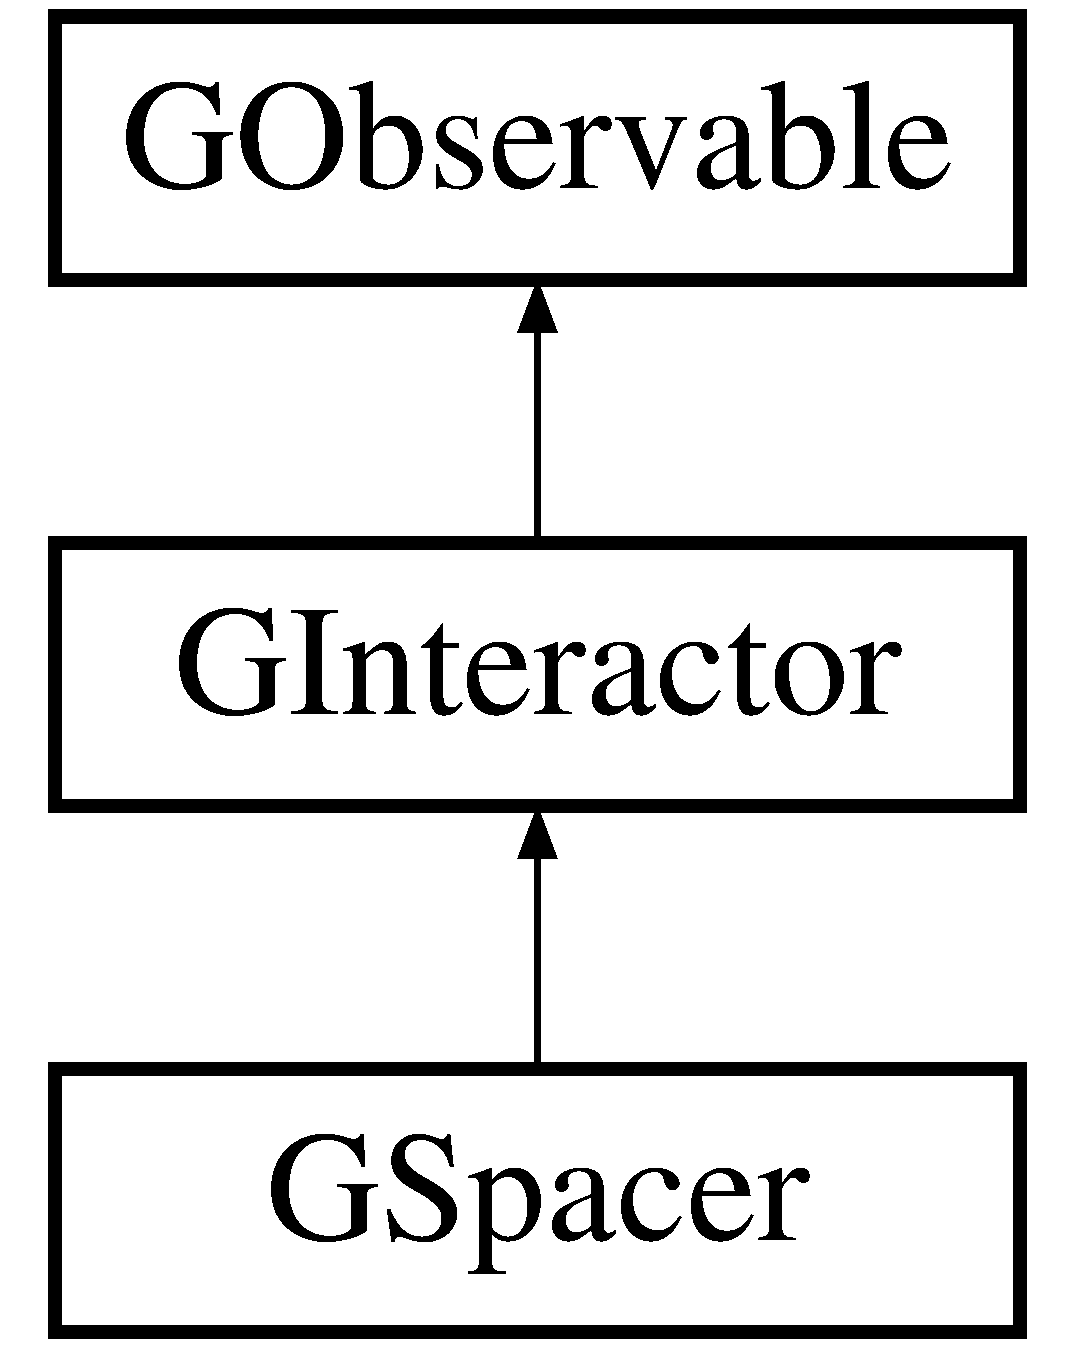
\includegraphics[height=3.000000cm]{classGSpacer}
\end{center}
\end{figure}
\subsection*{Public Types}
\begin{DoxyCompactItemize}
\item 
enum \mbox{\hyperlink{classGInteractor_a8e0d441725a81d2bbdebbea09078260e}{Text\+Position}} \{ \mbox{\hyperlink{classGInteractor_a8e0d441725a81d2bbdebbea09078260ea4cd6f2e7d5a08d6f4dc052df2358f774}{T\+E\+X\+T\+\_\+\+B\+E\+S\+I\+D\+E\+\_\+\+I\+C\+ON}}, 
\mbox{\hyperlink{classGInteractor_a8e0d441725a81d2bbdebbea09078260eaa88490f63d8de68d44c83bdb2ecde3b3}{T\+E\+X\+T\+\_\+\+U\+N\+D\+E\+R\+\_\+\+I\+C\+ON}}, 
\mbox{\hyperlink{classGInteractor_a8e0d441725a81d2bbdebbea09078260ea39a6f388a30ac4fefb6eb13e846bc9f2}{T\+E\+X\+T\+\_\+\+O\+N\+LY}}
 \}
\begin{DoxyCompactList}\small\item\em The places where an interactor can place its text relative to its icon. \end{DoxyCompactList}\end{DoxyCompactItemize}
\subsection*{Public Member Functions}
\begin{DoxyCompactItemize}
\item 
\mbox{\hyperlink{classGSpacer_abbd146cc21cc285a4b4b388dd57b9ffa}{G\+Spacer}} (double width, double height, Q\+Widget $\ast$parent=nullptr)
\item 
\mbox{\hyperlink{classGSpacer_a20f146a52fc612e051e0b8f2cdf18a8d}{$\sim$\+G\+Spacer}} () override
\begin{DoxyCompactList}\small\item\em Frees memory allocated internally by the scroll pane. \end{DoxyCompactList}\item 
virtual void \mbox{\hyperlink{classGInteractor_a02f20ea6edfa0671f31c4c648a253833}{add\+Action\+Listener}} () Q\+\_\+\+D\+E\+C\+L\+\_\+\+D\+E\+P\+R\+E\+C\+A\+T\+ED
\begin{DoxyCompactList}\small\item\em Adds an event listener to be notified when this interactor is clicked or generally interacted with. \end{DoxyCompactList}\item 
bool \mbox{\hyperlink{classGInteractor_a597a370b592e3737d38d9d2f4e2031ea}{events\+Enabled}} () const override
\begin{DoxyCompactList}\small\item\em Returns true if this interactor is currently accepting events. \end{DoxyCompactList}\item 
virtual std\+::string \mbox{\hyperlink{classGInteractor_a69f8d23ed8f207fbecad99960776e942}{get\+Accelerator}} () const
\begin{DoxyCompactList}\small\item\em Returns a string representing a hotkey for this interactor, or an empty string if no accelerator has been set. \end{DoxyCompactList}\item 
virtual std\+::string \mbox{\hyperlink{classGInteractor_a94eb4276000c4fdfb508ce9e6317a82a}{get\+Action\+Command}} () const
\begin{DoxyCompactList}\small\item\em Returns an action command for this interactor, which is a semi-\/unique string you can use to identify it when events occur. \end{DoxyCompactList}\item 
virtual std\+::string \mbox{\hyperlink{classGInteractor_a808e22cc1fdfbecf71ed8c64ef4600e0}{get\+Background}} () const
\begin{DoxyCompactList}\small\item\em Returns the background color of the interactor as a string. \end{DoxyCompactList}\item 
virtual int \mbox{\hyperlink{classGInteractor_a9e827257a55cb8cf4d9de2ec6bcfd7a0}{get\+Background\+Int}} () const
\begin{DoxyCompactList}\small\item\em Returns the background color of the interactor as an R\+GB integer. \end{DoxyCompactList}\item 
virtual \mbox{\hyperlink{structGRectangle}{G\+Rectangle}} \mbox{\hyperlink{classGInteractor_a29e6ac35a0b48f491a4c88194cc5da3b}{get\+Bounds}} () const
\begin{DoxyCompactList}\small\item\em Returns a rectangle representing the x/y position and size of this interactor. \end{DoxyCompactList}\item 
virtual std\+::string \mbox{\hyperlink{classGInteractor_aa061dfa488c31e18549d64363c1d0e34}{get\+Color}} () const
\begin{DoxyCompactList}\small\item\em Returns the foreground/text color of the interactor as a string. \end{DoxyCompactList}\item 
virtual int \mbox{\hyperlink{classGInteractor_a9635c7af766cdc3417f346683fa0e6c1}{get\+Color\+Int}} () const
\begin{DoxyCompactList}\small\item\em Returns the foreground/text color of the interactor as an R\+GB integer. \end{DoxyCompactList}\item 
virtual \mbox{\hyperlink{classGContainer}{G\+Container}} $\ast$ \mbox{\hyperlink{classGInteractor_a7a6e317c29d61030929b4cd2d1c00fe7}{get\+Container}} () const
\begin{DoxyCompactList}\small\item\em Returns a pointer to the onscreen container holding this interactor. \end{DoxyCompactList}\item 
virtual std\+::string \mbox{\hyperlink{classGInteractor_a894a5502900794eeb27d084c21f1d77d}{get\+Font}} () const
\begin{DoxyCompactList}\small\item\em Returns the font of this interactor\textquotesingle{}s text as a font string such as \char`\"{}\+Helvetica-\/12-\/\+Bold\char`\"{}. \end{DoxyCompactList}\item 
virtual std\+::string \mbox{\hyperlink{classGInteractor_a4fa2d8b0192a3a5b4af4bbfe71194d03}{get\+Foreground}} () const
\begin{DoxyCompactList}\small\item\em Returns the foreground/text color of the interactor as a string. \end{DoxyCompactList}\item 
virtual int \mbox{\hyperlink{classGInteractor_ac3b12ab385a6ef9ae90fc879860ba726}{get\+Foreground\+Int}} () const
\begin{DoxyCompactList}\small\item\em Returns the foreground/text color of the interactor as an R\+GB integer. \end{DoxyCompactList}\item 
virtual double \mbox{\hyperlink{classGInteractor_a1e7e353362434072875264cf95629f99}{get\+Height}} () const
\begin{DoxyCompactList}\small\item\em Returns the current onscreen height of this interactor in pixels. \end{DoxyCompactList}\item 
virtual std\+::string \mbox{\hyperlink{classGInteractor_aaed62a73004939a64da6f0eb9eb64d73}{get\+Icon}} () const
\begin{DoxyCompactList}\small\item\em Returns the file name of the icon associated with this interactor, or an empty string if no icon has been set. \end{DoxyCompactList}\item 
virtual int \mbox{\hyperlink{classGInteractor_a9c9659a6c6ba66b4107ba59c95a24241}{get\+ID}} () const
\begin{DoxyCompactList}\small\item\em Returns a globally unique identifier for this interactor, which is set when the interactor is constructed. \end{DoxyCompactList}\item 
\+\_\+\+Internal\+\_\+\+Q\+Widget $\ast$ \mbox{\hyperlink{classGSpacer_a2f6b36b2517087dc90a366b5ce1f5323}{get\+Internal\+Widget}} () const override
\begin{DoxyCompactList}\small\item\em Returns a direct pointer to the internal Qt widget being wrapped by this interactor. \end{DoxyCompactList}\item 
virtual \mbox{\hyperlink{structGPoint}{G\+Point}} \mbox{\hyperlink{classGInteractor_a4f83802015511edeb63b892830812c11}{get\+Location}} () const
\begin{DoxyCompactList}\small\item\em Returns an (x, y) point representing the onscreen location of the top-\/left corner of this interactor within its containing window. \end{DoxyCompactList}\item 
virtual double \mbox{\hyperlink{classGInteractor_aed4b0075fcc434499c3cb3e46896bda3}{get\+Minimum\+Height}} () const
\begin{DoxyCompactList}\small\item\em Returns the minimum height in pixels that this interactor will permit itself to be resized to. \end{DoxyCompactList}\item 
virtual \mbox{\hyperlink{structGDimension}{G\+Dimension}} \mbox{\hyperlink{classGInteractor_a66b5af0b32493b4d597ca0a3df2049ea}{get\+Minimum\+Size}} () const
\begin{DoxyCompactList}\small\item\em Returns a \mbox{\hyperlink{structGDimension}{G\+Dimension}} structure representing the minimum size in pixels that this interactor will permit itself to be resized to. \end{DoxyCompactList}\item 
virtual double \mbox{\hyperlink{classGInteractor_a59e668114fe3d49d2a0f28deb258f7c8}{get\+Minimum\+Width}} () const
\begin{DoxyCompactList}\small\item\em Returns the minimum width in pixels that this interactor will permit itself to be resized to. \end{DoxyCompactList}\item 
virtual std\+::string \mbox{\hyperlink{classGInteractor_a8a60438a5b55d0b2ceb35c8674b9d8c5}{get\+Name}} () const
\begin{DoxyCompactList}\small\item\em Returns a string representing a unique name for this interactor. \end{DoxyCompactList}\item 
virtual double \mbox{\hyperlink{classGInteractor_a747de0961653847bdc6615dbf756d715}{get\+Preferred\+Height}} () const
\begin{DoxyCompactList}\small\item\em Returns the height in pixels that this interactor would prefer to be, which would exactly fit its contents with no stretching or scrollbars. \end{DoxyCompactList}\item 
virtual \mbox{\hyperlink{structGDimension}{G\+Dimension}} \mbox{\hyperlink{classGInteractor_a4aabbee761d8e9116275401131b7ccd1}{get\+Preferred\+Size}} () const
\begin{DoxyCompactList}\small\item\em Returns a \mbox{\hyperlink{structGDimension}{G\+Dimension}} structure storing the width and height in pixels that this interactor would prefer to be, which would exactly fit its contents with no stretching or scrollbars. \end{DoxyCompactList}\item 
virtual double \mbox{\hyperlink{classGInteractor_a82bca31d37700fb0e35d2743352efd5e}{get\+Preferred\+Width}} () const
\begin{DoxyCompactList}\small\item\em Returns the height in pixels that this interactor would prefer to be, which would exactly fit its contents with no stretching or scrollbars. \end{DoxyCompactList}\item 
virtual \mbox{\hyperlink{structGDimension}{G\+Dimension}} \mbox{\hyperlink{classGInteractor_a7b4eec96a2bdc6420695d5796a78eea9}{get\+Size}} () const
\begin{DoxyCompactList}\small\item\em Returns a \mbox{\hyperlink{structGDimension}{G\+Dimension}} structure storing the current onscreen width and height of this interactor in pixels. \end{DoxyCompactList}\item 
std\+::string \mbox{\hyperlink{classGSpacer_a9b72ede4ee8520f987a0c01e30654814}{get\+Type}} () const override
\begin{DoxyCompactList}\small\item\em Returns a string representing the class name of this interactor, such as \char`\"{}\+G\+Button\char`\"{} or \char`\"{}\+G\+Check\+Box\char`\"{}. \end{DoxyCompactList}\item 
Q\+Widget $\ast$ \mbox{\hyperlink{classGSpacer_a3b33a602b31a6b809d020535a59db3b4}{get\+Widget}} () const override
\begin{DoxyCompactList}\small\item\em Returns a direct pointer to the internal Qt widget being wrapped by this interactor. \end{DoxyCompactList}\item 
virtual double \mbox{\hyperlink{classGInteractor_a0ed2965abd4f5701d2cadf71239faf19}{get\+Width}} () const
\begin{DoxyCompactList}\small\item\em Returns the current onscreen width of this interactor in pixels. \end{DoxyCompactList}\item 
virtual double \mbox{\hyperlink{classGInteractor_a344385751bee0720059403940d57a13e}{getX}} () const
\begin{DoxyCompactList}\small\item\em Returns the x-\/coordinate of the top-\/left pixel of this interactor within its onscreen window. \end{DoxyCompactList}\item 
virtual double \mbox{\hyperlink{classGInteractor_aafa51c7f8f38a09febbb9ce7853f77b4}{getY}} () const
\begin{DoxyCompactList}\small\item\em Returns the y-\/coordinate of the top-\/left pixel of this interactor within its onscreen window. \end{DoxyCompactList}\item 
virtual bool \mbox{\hyperlink{classGInteractor_afc480f652b8c5f1fb255e2269ce68879}{in\+Bounds}} (double x, double y) const
\begin{DoxyCompactList}\small\item\em Returns true if the given x/y pixel is within the bounds of this interactor. \end{DoxyCompactList}\item 
virtual bool \mbox{\hyperlink{classGInteractor_ae6d7982c1c627b677a5e776ca86118ed}{in\+Bounds}} (int x, int y) const
\begin{DoxyCompactList}\small\item\em Returns true if the given x/y pixel is within the bounds of this interactor. \end{DoxyCompactList}\item 
virtual bool \mbox{\hyperlink{classGInteractor_aacb819fb241851fd9fc045271baa4034}{is\+Enabled}} () const
\begin{DoxyCompactList}\small\item\em Returns true if this interactor is currently enabled. \end{DoxyCompactList}\item 
virtual bool \mbox{\hyperlink{classGInteractor_a9d8a6cfb13917785c143e74d40e4e2be}{is\+Visible}} () const
\begin{DoxyCompactList}\small\item\em Returns true if the interactor is visible on the screen. \end{DoxyCompactList}\item 
virtual void \mbox{\hyperlink{classGInteractor_ab7fe7a876367b87cf7202f947f1d05e4}{remove\+Action\+Listener}} ()
\begin{DoxyCompactList}\small\item\em Removes the action listener from this interactor so that it will no longer call it when events occur. \end{DoxyCompactList}\item 
virtual void \mbox{\hyperlink{classGInteractor_ad39d0325cde6b97ebda4b9d7787c633b}{remove\+Click\+Listener}} ()
\begin{DoxyCompactList}\small\item\em Removes the click listener from this interactor so that it will no longer call it when events occur. \end{DoxyCompactList}\item 
virtual void \mbox{\hyperlink{classGInteractor_aa4250907e4cdd77349c04f0cf5cdd3d3}{remove\+Double\+Click\+Listener}} ()
\begin{DoxyCompactList}\small\item\em Removes the double-\/click listener from this interactor so that it will no longer call it when events occur. \end{DoxyCompactList}\item 
virtual void \mbox{\hyperlink{classGInteractor_a43095f41cab3be732b49f29970484b05}{remove\+Key\+Listener}} ()
\begin{DoxyCompactList}\small\item\em Removes the key listener from this interactor so that it will no longer call it when key events occur. \end{DoxyCompactList}\item 
virtual void \mbox{\hyperlink{classGInteractor_aff47f71ce47e688a07c9d38dc92fcc11}{remove\+Mouse\+Listener}} ()
\begin{DoxyCompactList}\small\item\em Removes the mouse listener from this interactor so that it will no longer call it when events occur. \end{DoxyCompactList}\item 
virtual void \mbox{\hyperlink{classGInteractor_a519fb2ac767f8b2febbb50b898b8c8cb}{request\+Focus}} ()
\begin{DoxyCompactList}\small\item\em Transfers keyboard focus to this interactor. \end{DoxyCompactList}\item 
virtual void \mbox{\hyperlink{classGInteractor_ad15f102f62e2960576012f1aa0ba4b2e}{set\+Accelerator}} (const std\+::string \&accelerator)
\begin{DoxyCompactList}\small\item\em Sets an accelerator hotkey for this interactor, such as \char`\"{}\+Ctrl-\/\+S\char`\"{}. \end{DoxyCompactList}\item 
virtual void \mbox{\hyperlink{classGInteractor_a4b5843fe3030e038a1ba54cc03389bcf}{set\+Action\+Command}} (const std\+::string \&action\+Command)
\begin{DoxyCompactList}\small\item\em Sets the action command for this interactor. \end{DoxyCompactList}\item 
virtual void \mbox{\hyperlink{classGInteractor_adcfb4742430c88714fcf57e57ab8ea9c}{set\+Action\+Listener}} (G\+Event\+Listener func)
\begin{DoxyCompactList}\small\item\em Sets an action listener on this interactor so that it will be called when it is interacted with in its primary way. \end{DoxyCompactList}\item 
virtual void \mbox{\hyperlink{classGInteractor_aebd20a89c7a8a43a6fce999cf4f9fcf2}{set\+Action\+Listener}} (G\+Event\+Listener\+Void func)
\begin{DoxyCompactList}\small\item\em Sets an action listener on this interactor so that it will be called when it is interacted with in its primary way. \end{DoxyCompactList}\item 
virtual void \mbox{\hyperlink{classGInteractor_acba7e546c2025c0a15ca4b4cc92043db}{set\+Background}} (int rgb)
\begin{DoxyCompactList}\small\item\em Sets the background color of the interactor to the color represented by the given R\+GB integer. \end{DoxyCompactList}\item 
virtual void \mbox{\hyperlink{classGInteractor_ab4677ab2474e68b07aa56605af92a84a}{set\+Background}} (const std\+::string \&color)
\begin{DoxyCompactList}\small\item\em Sets the background color of the interactor to the color represented by the given string. \end{DoxyCompactList}\item 
virtual void \mbox{\hyperlink{classGInteractor_a2aae8197624b72265ab83b4f1bc73f2f}{set\+Bounds}} (double x, double y, double width, double height)
\begin{DoxyCompactList}\small\item\em Sets the size and location of the widget. \end{DoxyCompactList}\item 
virtual void \mbox{\hyperlink{classGInteractor_acada386653f008cacc7cce86426bef7c}{set\+Bounds}} (const \mbox{\hyperlink{structGRectangle}{G\+Rectangle}} \&size)
\begin{DoxyCompactList}\small\item\em Sets the size and location of the widget. \end{DoxyCompactList}\item 
virtual void \mbox{\hyperlink{classGInteractor_abd40af6921242584d0954f173911b190}{set\+Click\+Listener}} (G\+Event\+Listener func)
\begin{DoxyCompactList}\small\item\em Sets a mouse listener on this interactor so that it will be called when the mouse is clicked on it. \end{DoxyCompactList}\item 
virtual void \mbox{\hyperlink{classGInteractor_a856414c92df90f56f3877475eb3f8fc4}{set\+Click\+Listener}} (G\+Event\+Listener\+Void func)
\begin{DoxyCompactList}\small\item\em Sets a mouse listener on this interactor so that it will be called when the mouse is clicked on it. \end{DoxyCompactList}\item 
virtual void \mbox{\hyperlink{classGInteractor_ab1f5cc0f5cc6bbbd716a526c61f1081d}{set\+Color}} (int rgb)
\begin{DoxyCompactList}\small\item\em Sets the foreground/text color of the interactor to the color represented by the given R\+GB integer. \end{DoxyCompactList}\item 
virtual void \mbox{\hyperlink{classGInteractor_a61374df6c11b52cfbb0815decdbaebc6}{set\+Color}} (const std\+::string \&color)
\begin{DoxyCompactList}\small\item\em Sets the foreground/text color of the interactor to the color represented by the given string. \end{DoxyCompactList}\item 
virtual void \mbox{\hyperlink{classGInteractor_ac29f9a3462458e165fae3a1f046ee77a}{set\+Double\+Click\+Listener}} (G\+Event\+Listener func)
\begin{DoxyCompactList}\small\item\em Sets a mouse listener on this interactor so that it will be called when the mouse is double-\/clicked on it. \end{DoxyCompactList}\item 
virtual void \mbox{\hyperlink{classGInteractor_a50096194d66f48c92dd4c512d41bfc76}{set\+Double\+Click\+Listener}} (G\+Event\+Listener\+Void func)
\begin{DoxyCompactList}\small\item\em Sets a mouse listener on this interactor so that it will be called when the mouse is double-\/clicked on it. \end{DoxyCompactList}\item 
virtual void \mbox{\hyperlink{classGInteractor_ab831367dd84bbd579e02e55bacb21343}{set\+Enabled}} (bool value)
\begin{DoxyCompactList}\small\item\em Sets whether this interactor is currently enabled. \end{DoxyCompactList}\item 
virtual void \mbox{\hyperlink{classGObservable_afaa30b2a9e0f378fd1c70d2f1d0b8216}{set\+Events\+Enabled}} (bool \mbox{\hyperlink{classGInteractor_a597a370b592e3737d38d9d2f4e2031ea}{events\+Enabled}})
\begin{DoxyCompactList}\small\item\em Sets whether the object is currently allowing itself to fire events. \end{DoxyCompactList}\item 
virtual void \mbox{\hyperlink{classGInteractor_a2592348886ffea646c6534bf88f7c49d}{set\+Font}} (const Q\+Font \&font)
\begin{DoxyCompactList}\small\item\em Sets the font used by this widget to the given Qt font. \end{DoxyCompactList}\item 
virtual void \mbox{\hyperlink{classGInteractor_a8e096e8818d838aceae1d46d58fb3a7b}{set\+Font}} (const std\+::string \&font)
\begin{DoxyCompactList}\small\item\em Sets the font used by this widget to the font represented by the given font string, such as \char`\"{}\+Helvetica-\/16-\/\+Bold\char`\"{}. \end{DoxyCompactList}\item 
virtual void \mbox{\hyperlink{classGInteractor_a9eb856b5ff83a19df3831a31f15f4563}{set\+Foreground}} (int rgb)
\begin{DoxyCompactList}\small\item\em Sets the foreground/text color of the interactor to the color represented by the given R\+GB integer. \end{DoxyCompactList}\item 
virtual void \mbox{\hyperlink{classGInteractor_af59209aeadea6dfc6d97a2d8531f50e1}{set\+Foreground}} (const std\+::string \&color)
\begin{DoxyCompactList}\small\item\em Sets the foreground/text color of the interactor to the color represented by the given string. \end{DoxyCompactList}\item 
virtual void \mbox{\hyperlink{classGInteractor_a9e280bfc4544dfaf8e4376c4e1a74357}{set\+Height}} (double height)
\begin{DoxyCompactList}\small\item\em Sets the onscreen height of the interactor in pixels. \end{DoxyCompactList}\item 
virtual void \mbox{\hyperlink{classGInteractor_a542abfcd7261751352af129c7215ecda}{set\+Icon}} (const Q\+Icon \&icon)
\begin{DoxyCompactList}\small\item\em Sets the icon associated with this interactor. \end{DoxyCompactList}\item 
virtual void \mbox{\hyperlink{classGInteractor_a368e1a338f84401c284506d03b1ba769}{set\+Icon}} (const Q\+Pixmap \&icon)
\begin{DoxyCompactList}\small\item\em Sets the icon associated with this interactor. \end{DoxyCompactList}\item 
virtual void \mbox{\hyperlink{classGInteractor_a762e139aa311461c3984d3ad28293f64}{set\+Icon}} (const std\+::string \&filename, bool retain\+Icon\+Size=true)
\begin{DoxyCompactList}\small\item\em Sets the file name of the icon associated with this interactor, or an empty string if no icon has been set. \end{DoxyCompactList}\item 
virtual void \mbox{\hyperlink{classGInteractor_aeb8324d3287fa1fbe093f4d6230cf0a6}{set\+Key\+Listener}} (G\+Event\+Listener func)
\begin{DoxyCompactList}\small\item\em Sets a key listener on this interactor so that it will be called when the user presses any key. \end{DoxyCompactList}\item 
virtual void \mbox{\hyperlink{classGInteractor_ae48ecea73606c7bd9423e1c7cc589cc9}{set\+Key\+Listener}} (G\+Event\+Listener\+Void func)
\begin{DoxyCompactList}\small\item\em Sets a key listener on this interactor so that it will be called when the user presses any key. \end{DoxyCompactList}\item 
virtual void \mbox{\hyperlink{classGInteractor_a04594e8ba9b98513a64f1da00dcae18c}{set\+Location}} (double x, double y)
\begin{DoxyCompactList}\small\item\em Sets the onscreen x/y-\/coordinate of the top-\/left corner of the interactor relative to its window. \end{DoxyCompactList}\item 
virtual void \mbox{\hyperlink{classGInteractor_a0cf428e207b7f22cc08138a90b1b87b2}{set\+Minimum\+Size}} (double width, double height)
\begin{DoxyCompactList}\small\item\em Sets the minimum size in pixels that this interactor will permit itself to be resized to. \end{DoxyCompactList}\item 
virtual void \mbox{\hyperlink{classGInteractor_a3b1046117ac6cb7abe467e00ba8a81f4}{set\+Minimum\+Size}} (const \mbox{\hyperlink{structGDimension}{G\+Dimension}} \&size)
\begin{DoxyCompactList}\small\item\em Sets the minimum size in pixels that this interactor will permit itself to be resized to. \end{DoxyCompactList}\item 
virtual void \mbox{\hyperlink{classGInteractor_a37d8dbc943f59920f705b0104f60bde2}{set\+Mouse\+Listener}} (G\+Event\+Listener func)
\begin{DoxyCompactList}\small\item\em Sets a mouse listener on this interactor so that it will be called when the mouse is moved or clicked on it. \end{DoxyCompactList}\item 
virtual void \mbox{\hyperlink{classGInteractor_aea7f647ea62d59f71b5fad6aa65eeaf9}{set\+Mouse\+Listener}} (G\+Event\+Listener\+Void func)
\begin{DoxyCompactList}\small\item\em Sets a mouse listener on this interactor so that it will be called when the mouse is moved or clicked on it. \end{DoxyCompactList}\item 
virtual void \mbox{\hyperlink{classGInteractor_a9d3a2685df23b5e7cbf59c19c4a1f9b5}{set\+Name}} (const std\+::string \&name)
\begin{DoxyCompactList}\small\item\em Sets a string representing a unique name for this interactor. \end{DoxyCompactList}\item 
virtual void \mbox{\hyperlink{classGInteractor_a1ab987704fce32098706c6f00fb08218}{set\+Preferred\+Height}} (double height)
\begin{DoxyCompactList}\small\item\em Sets the height in pixels that this interactor would prefer to be. \end{DoxyCompactList}\item 
virtual void \mbox{\hyperlink{classGInteractor_a042c5ae19430d765ef552371cae3632c}{set\+Preferred\+Size}} (double width, double height)
\begin{DoxyCompactList}\small\item\em Sets the width and height in pixels that this interactor would prefer to be. \end{DoxyCompactList}\item 
virtual void \mbox{\hyperlink{classGInteractor_aa22d9be4bc0e078bb0ea69b0fc9d7c75}{set\+Preferred\+Size}} (const \mbox{\hyperlink{structGDimension}{G\+Dimension}} \&size)
\begin{DoxyCompactList}\small\item\em Sets the size in pixels that this interactor would prefer to be. \end{DoxyCompactList}\item 
virtual void \mbox{\hyperlink{classGInteractor_a3db429ab2fa52efd187eec0ed8cdd9f2}{set\+Preferred\+Width}} (double width)
\begin{DoxyCompactList}\small\item\em Sets the width in pixels that this interactor would prefer to be. \end{DoxyCompactList}\item 
virtual void \mbox{\hyperlink{classGInteractor_aca25d49481f9bf5fc8f7df4c086c4ce7}{set\+Size}} (double width, double height)
\begin{DoxyCompactList}\small\item\em Sets the onscreen width and height of the interactor in pixels. \end{DoxyCompactList}\item 
virtual void \mbox{\hyperlink{classGInteractor_ae2b628228f192c2702c4ce941b2af68f}{set\+Size}} (const \mbox{\hyperlink{structGDimension}{G\+Dimension}} \&size)
\begin{DoxyCompactList}\small\item\em Sets the onscreen width and height of the interactor in pixels. \end{DoxyCompactList}\item 
virtual void \mbox{\hyperlink{classGInteractor_a039e0e49beaecc275efce02d416acea8}{set\+Tooltip}} (const std\+::string \&tooltip\+Text)
\begin{DoxyCompactList}\small\item\em Sets a \char`\"{}tooltip\char`\"{} that will appear if the user hovers their mouse over the interactor. \end{DoxyCompactList}\item 
virtual void \mbox{\hyperlink{classGInteractor_a18e44e30b31525a243960ca3928125aa}{set\+Visible}} (bool visible)
\begin{DoxyCompactList}\small\item\em Returns true if the interactor is visible on the screen. \end{DoxyCompactList}\item 
virtual void \mbox{\hyperlink{classGInteractor_aa3f3fba4cb131baa8696ba01e3bceca1}{set\+Width}} (double width)
\begin{DoxyCompactList}\small\item\em Sets the onscreen width of the interactor in pixels. \end{DoxyCompactList}\item 
virtual void \mbox{\hyperlink{classGInteractor_a9c18fcc579333bf9653d13ad2b372e39}{setX}} (double x)
\begin{DoxyCompactList}\small\item\em Sets the onscreen x-\/coordinate of the top-\/left corner of the interactor relative to its window. \end{DoxyCompactList}\item 
virtual void \mbox{\hyperlink{classGInteractor_a7d57e2a5c35d27feb58fd498a3cf82b9}{setY}} (double y)
\begin{DoxyCompactList}\small\item\em Sets the onscreen y-\/coordinate of the top-\/left corner of the interactor relative to its window. \end{DoxyCompactList}\item 
virtual std\+::string \mbox{\hyperlink{classGObservable_a1fe5121d6528fdea3f243321b3fa3a49}{to\+String}} () const
\begin{DoxyCompactList}\small\item\em Returns a string representation of this observable object\textquotesingle{}s state. \end{DoxyCompactList}\end{DoxyCompactItemize}
\subsection*{Protected Member Functions}
\begin{DoxyCompactItemize}
\item 
virtual void \mbox{\hyperlink{classGObservable_a80cfa040459ff53594adbd6a51ec8f43}{clear\+Event\+Listeners}} ()
\begin{DoxyCompactList}\small\item\em Removes all event listeners from this object. \end{DoxyCompactList}\item 
virtual void \mbox{\hyperlink{classGObservable_a284f31528c0520f8e545c03ac9eeac74}{ensure\+Thread\+Safety}} (const std\+::string \&member\+Name=\char`\"{}\char`\"{})
\begin{DoxyCompactList}\small\item\em Ensures that we are currently in the Qt G\+UI thread. \end{DoxyCompactList}\item 
virtual void \mbox{\hyperlink{classGObservable_a63e5e5a6227c59c928493b11aceb0f67}{fire\+Event}} (\mbox{\hyperlink{classGEvent}{G\+Event}} \&event)
\begin{DoxyCompactList}\small\item\em Sends out the given event to any attached listeners. \end{DoxyCompactList}\item 
virtual void \mbox{\hyperlink{classGObservable_ab3983ea07337b52020a29cc00c653d8d}{fire\+G\+Event}} (Q\+Event $\ast$event, Event\+Type event\+Type, const std\+::string \&event\+Name)
\begin{DoxyCompactList}\small\item\em Creates an event of the given type, then sends it out to any attached listeners. \end{DoxyCompactList}\item 
virtual void \mbox{\hyperlink{classGObservable_a01fdf1b0e0dbd49e189fe4514e010411}{fire\+G\+Event}} (Q\+Close\+Event $\ast$event, Event\+Type event\+Type, const std\+::string \&event\+Name)
\begin{DoxyCompactList}\small\item\em Creates an event of the given type, then sends it out to any attached listeners. \end{DoxyCompactList}\item 
virtual void \mbox{\hyperlink{classGObservable_abb0b2f66ba39211cb5d7615e9d1c04e2}{fire\+G\+Event}} (Q\+Key\+Event $\ast$event, Event\+Type event\+Type, const std\+::string \&event\+Name)
\begin{DoxyCompactList}\small\item\em Creates an event of the given type, then sends it out to any attached listeners. \end{DoxyCompactList}\item 
virtual void \mbox{\hyperlink{classGObservable_a119318675d2165bdf7dd853aaf881d4b}{fire\+G\+Event}} (Q\+Mouse\+Event $\ast$event, Event\+Type event\+Type, const std\+::string \&event\+Name, const std\+::string \&action\+Command=\char`\"{}\char`\"{})
\begin{DoxyCompactList}\small\item\em Creates an event of the given type, then sends it out to any attached listeners. \end{DoxyCompactList}\item 
virtual void \mbox{\hyperlink{classGObservable_a63fd9034e1e1633c1c38eb342bfd34e9}{fire\+G\+Event}} (Q\+Resize\+Event $\ast$event, Event\+Type event\+Type, const std\+::string \&event\+Name)
\begin{DoxyCompactList}\small\item\em Creates an event of the given type, then sends it out to any attached listeners. \end{DoxyCompactList}\item 
virtual void \mbox{\hyperlink{classGObservable_a741345310d9b7c5170a6cbc410c44ac4}{fire\+G\+Event}} (Q\+Timer\+Event $\ast$event, Event\+Type event\+Type, const std\+::string \&event\+Name)
\begin{DoxyCompactList}\small\item\em Creates an event of the given type, then sends it out to any attached listeners. \end{DoxyCompactList}\item 
virtual void \mbox{\hyperlink{classGObservable_a93bf338968a0338761b8e4dc62f582e9}{fire\+G\+Event}} (Q\+Wheel\+Event $\ast$event, Event\+Type event\+Type, const std\+::string \&event\+Name)
\begin{DoxyCompactList}\small\item\em Creates an event of the given type, then sends it out to any attached listeners. \end{DoxyCompactList}\item 
virtual void \mbox{\hyperlink{classGObservable_a2a70a7d7435ff0c3b80bb4d70da19e0d}{fire\+G\+Event}} (Q\+Window\+State\+Change\+Event $\ast$event, Event\+Type event\+Type, const std\+::string \&event\+Name)
\begin{DoxyCompactList}\small\item\em Creates an event of the given type, then sends it out to any attached listeners. \end{DoxyCompactList}\item 
virtual bool \mbox{\hyperlink{classGObservable_a9f6faaa25942923bafa1c44020c49fa9}{has\+Event\+Listener}} (const std\+::string \&event\+Name) const
\begin{DoxyCompactList}\small\item\em Returns true if the observable object has a listener for the given type of event. \end{DoxyCompactList}\item 
virtual bool \mbox{\hyperlink{classGObservable_aeec1adc19aa0f33de62390686ee1382c}{is\+Accepting\+Event}} (int event\+Mask) const
\begin{DoxyCompactList}\small\item\em Returns true if the observable object has a listener for the given type of event. \end{DoxyCompactList}\item 
virtual bool \mbox{\hyperlink{classGObservable_aa31c73145a29dcb92848a92e0cfaea41}{is\+Accepting\+Event}} (const \mbox{\hyperlink{classGEvent}{G\+Event}} \&event) const
\begin{DoxyCompactList}\small\item\em Returns true if the observable object has a listener for the given type of event. \end{DoxyCompactList}\item 
virtual bool \mbox{\hyperlink{classGObservable_a3b1c689267eda44e65a2213e7de38b23}{is\+Accepting\+Event}} (const std\+::string \&event\+Type) const
\begin{DoxyCompactList}\small\item\em Returns true if the observable object has a listener for the given type of event. \end{DoxyCompactList}\item 
virtual void \mbox{\hyperlink{classGObservable_acbcf1ed3a851ad8a3c17ef38d86b481d}{remove\+Event\+Listener}} (const std\+::string \&event\+Name)
\begin{DoxyCompactList}\small\item\em Removes any event listener from this observable object that would respond to the given type of event, such as \char`\"{}click\char`\"{} or \char`\"{}keydown\char`\"{}. \end{DoxyCompactList}\item 
virtual void \mbox{\hyperlink{classGObservable_af51cc35c29a1bd1908609d432decdbb6}{remove\+Event\+Listeners}} (std\+::initializer\+\_\+list$<$ std\+::string $>$ event\+Names)
\begin{DoxyCompactList}\small\item\em Removes any event listener from this observable object that would respond to the given types of events, such as \char`\"{}click\char`\"{} or \char`\"{}keydown\char`\"{}. \end{DoxyCompactList}\item 
virtual void \mbox{\hyperlink{classGObservable_ad2f6d34961c50f6c1e0659990b79f741}{set\+Event\+Listener}} (const std\+::string \&event\+Name, G\+Event\+Listener func)
\begin{DoxyCompactList}\small\item\em Adds an event listener from this observable object to respond to the given type of event, such as \char`\"{}click\char`\"{} or \char`\"{}keydown\char`\"{}. \end{DoxyCompactList}\item 
virtual void \mbox{\hyperlink{classGObservable_abac4cb9f9e626e010e87f5d91573c8a5}{set\+Event\+Listener}} (const std\+::string \&event\+Name, G\+Event\+Listener\+Void func)
\begin{DoxyCompactList}\small\item\em Adds an event listener from this observable object to respond to the given type of event, such as \char`\"{}click\char`\"{} or \char`\"{}keydown\char`\"{}. \end{DoxyCompactList}\item 
virtual void \mbox{\hyperlink{classGObservable_afa388d69c33c718cf035774604065604}{set\+Event\+Listeners}} (std\+::initializer\+\_\+list$<$ std\+::string $>$ event\+Names, G\+Event\+Listener func)
\begin{DoxyCompactList}\small\item\em Adds an event listener from this observable object to respond to the given types of events, such as \char`\"{}click\char`\"{} or \char`\"{}keydown\char`\"{}. \end{DoxyCompactList}\item 
virtual void \mbox{\hyperlink{classGObservable_a7867184bbb686f74fae8a4db927da799}{set\+Event\+Listeners}} (std\+::initializer\+\_\+list$<$ std\+::string $>$ event\+Names, G\+Event\+Listener\+Void func)
\begin{DoxyCompactList}\small\item\em Adds an event listener from this observable object to respond to the given types of events, such as \char`\"{}click\char`\"{} or \char`\"{}keydown\char`\"{}. \end{DoxyCompactList}\end{DoxyCompactItemize}


\subsection{Detailed Description}
A \mbox{\hyperlink{classGSpacer}{G\+Spacer}} is just an empty blob of space that helps you pad layouts. 

\subsection{Member Enumeration Documentation}
\mbox{\Hypertarget{classGInteractor_a8e0d441725a81d2bbdebbea09078260e}\label{classGInteractor_a8e0d441725a81d2bbdebbea09078260e}} 
\index{G\+Spacer@{G\+Spacer}!Text\+Position@{Text\+Position}}
\index{Text\+Position@{Text\+Position}!G\+Spacer@{G\+Spacer}}
\subsubsection{\texorpdfstring{Text\+Position}{TextPosition}}
{\footnotesize\ttfamily enum \mbox{\hyperlink{classGInteractor_a8e0d441725a81d2bbdebbea09078260e}{Text\+Position}}\hspace{0.3cm}{\ttfamily [inherited]}}



The places where an interactor can place its text relative to its icon. 

\begin{DoxyEnumFields}{Enumerator}
\raisebox{\heightof{T}}[0pt][0pt]{\index{T\+E\+X\+T\+\_\+\+B\+E\+S\+I\+D\+E\+\_\+\+I\+C\+ON@{T\+E\+X\+T\+\_\+\+B\+E\+S\+I\+D\+E\+\_\+\+I\+C\+ON}!G\+Spacer@{G\+Spacer}}\index{G\+Spacer@{G\+Spacer}!T\+E\+X\+T\+\_\+\+B\+E\+S\+I\+D\+E\+\_\+\+I\+C\+ON@{T\+E\+X\+T\+\_\+\+B\+E\+S\+I\+D\+E\+\_\+\+I\+C\+ON}}}\mbox{\Hypertarget{classGInteractor_a8e0d441725a81d2bbdebbea09078260ea4cd6f2e7d5a08d6f4dc052df2358f774}\label{classGInteractor_a8e0d441725a81d2bbdebbea09078260ea4cd6f2e7d5a08d6f4dc052df2358f774}} 
T\+E\+X\+T\+\_\+\+B\+E\+S\+I\+D\+E\+\_\+\+I\+C\+ON&\\
\hline

\raisebox{\heightof{T}}[0pt][0pt]{\index{T\+E\+X\+T\+\_\+\+U\+N\+D\+E\+R\+\_\+\+I\+C\+ON@{T\+E\+X\+T\+\_\+\+U\+N\+D\+E\+R\+\_\+\+I\+C\+ON}!G\+Spacer@{G\+Spacer}}\index{G\+Spacer@{G\+Spacer}!T\+E\+X\+T\+\_\+\+U\+N\+D\+E\+R\+\_\+\+I\+C\+ON@{T\+E\+X\+T\+\_\+\+U\+N\+D\+E\+R\+\_\+\+I\+C\+ON}}}\mbox{\Hypertarget{classGInteractor_a8e0d441725a81d2bbdebbea09078260eaa88490f63d8de68d44c83bdb2ecde3b3}\label{classGInteractor_a8e0d441725a81d2bbdebbea09078260eaa88490f63d8de68d44c83bdb2ecde3b3}} 
T\+E\+X\+T\+\_\+\+U\+N\+D\+E\+R\+\_\+\+I\+C\+ON&\\
\hline

\raisebox{\heightof{T}}[0pt][0pt]{\index{T\+E\+X\+T\+\_\+\+O\+N\+LY@{T\+E\+X\+T\+\_\+\+O\+N\+LY}!G\+Spacer@{G\+Spacer}}\index{G\+Spacer@{G\+Spacer}!T\+E\+X\+T\+\_\+\+O\+N\+LY@{T\+E\+X\+T\+\_\+\+O\+N\+LY}}}\mbox{\Hypertarget{classGInteractor_a8e0d441725a81d2bbdebbea09078260ea39a6f388a30ac4fefb6eb13e846bc9f2}\label{classGInteractor_a8e0d441725a81d2bbdebbea09078260ea39a6f388a30ac4fefb6eb13e846bc9f2}} 
T\+E\+X\+T\+\_\+\+O\+N\+LY&\\
\hline

\end{DoxyEnumFields}


\subsection{Constructor \& Destructor Documentation}
\mbox{\Hypertarget{classGSpacer_abbd146cc21cc285a4b4b388dd57b9ffa}\label{classGSpacer_abbd146cc21cc285a4b4b388dd57b9ffa}} 
\index{G\+Spacer@{G\+Spacer}!G\+Spacer@{G\+Spacer}}
\index{G\+Spacer@{G\+Spacer}!G\+Spacer@{G\+Spacer}}
\subsubsection{\texorpdfstring{G\+Spacer()}{GSpacer()}}
{\footnotesize\ttfamily \mbox{\hyperlink{classGSpacer}{G\+Spacer}} (\begin{DoxyParamCaption}\item[{double}]{width,  }\item[{double}]{height,  }\item[{Q\+Widget $\ast$}]{parent = {\ttfamily nullptr} }\end{DoxyParamCaption})}

\mbox{\Hypertarget{classGSpacer_a20f146a52fc612e051e0b8f2cdf18a8d}\label{classGSpacer_a20f146a52fc612e051e0b8f2cdf18a8d}} 
\index{G\+Spacer@{G\+Spacer}!````~G\+Spacer@{$\sim$\+G\+Spacer}}
\index{````~G\+Spacer@{$\sim$\+G\+Spacer}!G\+Spacer@{G\+Spacer}}
\subsubsection{\texorpdfstring{$\sim$\+G\+Spacer()}{~GSpacer()}}
{\footnotesize\ttfamily $\sim$\mbox{\hyperlink{classGSpacer}{G\+Spacer}} (\begin{DoxyParamCaption}{ }\end{DoxyParamCaption})\hspace{0.3cm}{\ttfamily [override]}}



Frees memory allocated internally by the scroll pane. 



\subsection{Member Function Documentation}
\mbox{\Hypertarget{classGInteractor_a02f20ea6edfa0671f31c4c648a253833}\label{classGInteractor_a02f20ea6edfa0671f31c4c648a253833}} 
\index{G\+Spacer@{G\+Spacer}!add\+Action\+Listener@{add\+Action\+Listener}}
\index{add\+Action\+Listener@{add\+Action\+Listener}!G\+Spacer@{G\+Spacer}}
\subsubsection{\texorpdfstring{add\+Action\+Listener()}{addActionListener()}}
{\footnotesize\ttfamily void add\+Action\+Listener (\begin{DoxyParamCaption}{ }\end{DoxyParamCaption})\hspace{0.3cm}{\ttfamily [virtual]}, {\ttfamily [inherited]}}



Adds an event listener to be notified when this interactor is clicked or generally interacted with. 

\begin{DoxyRefDesc}{Deprecated}
\item[\mbox{\hyperlink{deprecated__deprecated000006}{Deprecated}}]does nothing; use set\+Action\+Listener instead \end{DoxyRefDesc}
\mbox{\Hypertarget{classGObservable_a80cfa040459ff53594adbd6a51ec8f43}\label{classGObservable_a80cfa040459ff53594adbd6a51ec8f43}} 
\index{G\+Spacer@{G\+Spacer}!clear\+Event\+Listeners@{clear\+Event\+Listeners}}
\index{clear\+Event\+Listeners@{clear\+Event\+Listeners}!G\+Spacer@{G\+Spacer}}
\subsubsection{\texorpdfstring{clear\+Event\+Listeners()}{clearEventListeners()}}
{\footnotesize\ttfamily void clear\+Event\+Listeners (\begin{DoxyParamCaption}{ }\end{DoxyParamCaption})\hspace{0.3cm}{\ttfamily [protected]}, {\ttfamily [virtual]}, {\ttfamily [inherited]}}



Removes all event listeners from this object. 

\mbox{\Hypertarget{classGObservable_a284f31528c0520f8e545c03ac9eeac74}\label{classGObservable_a284f31528c0520f8e545c03ac9eeac74}} 
\index{G\+Spacer@{G\+Spacer}!ensure\+Thread\+Safety@{ensure\+Thread\+Safety}}
\index{ensure\+Thread\+Safety@{ensure\+Thread\+Safety}!G\+Spacer@{G\+Spacer}}
\subsubsection{\texorpdfstring{ensure\+Thread\+Safety()}{ensureThreadSafety()}}
{\footnotesize\ttfamily void ensure\+Thread\+Safety (\begin{DoxyParamCaption}\item[{const std\+::string \&}]{member\+Name = {\ttfamily \char`\"{}\char`\"{}} }\end{DoxyParamCaption})\hspace{0.3cm}{\ttfamily [protected]}, {\ttfamily [virtual]}, {\ttfamily [inherited]}}



Ensures that we are currently in the Qt G\+UI thread. 

\mbox{\Hypertarget{classGInteractor_a597a370b592e3737d38d9d2f4e2031ea}\label{classGInteractor_a597a370b592e3737d38d9d2f4e2031ea}} 
\index{G\+Spacer@{G\+Spacer}!events\+Enabled@{events\+Enabled}}
\index{events\+Enabled@{events\+Enabled}!G\+Spacer@{G\+Spacer}}
\subsubsection{\texorpdfstring{events\+Enabled()}{eventsEnabled()}}
{\footnotesize\ttfamily bool events\+Enabled (\begin{DoxyParamCaption}{ }\end{DoxyParamCaption}) const\hspace{0.3cm}{\ttfamily [override]}, {\ttfamily [virtual]}, {\ttfamily [inherited]}}



Returns true if this interactor is currently accepting events. 

Initially true. An interactor must be visible and added to an onscreen window to receive events. 

Reimplemented from \mbox{\hyperlink{classGObservable_a8ebb3da91032e7f4c34485dabc518b8a}{G\+Observable}}.

\mbox{\Hypertarget{classGObservable_a63e5e5a6227c59c928493b11aceb0f67}\label{classGObservable_a63e5e5a6227c59c928493b11aceb0f67}} 
\index{G\+Spacer@{G\+Spacer}!fire\+Event@{fire\+Event}}
\index{fire\+Event@{fire\+Event}!G\+Spacer@{G\+Spacer}}
\subsubsection{\texorpdfstring{fire\+Event()}{fireEvent()}}
{\footnotesize\ttfamily void fire\+Event (\begin{DoxyParamCaption}\item[{\mbox{\hyperlink{classGEvent}{G\+Event}} \&}]{event }\end{DoxyParamCaption})\hspace{0.3cm}{\ttfamily [protected]}, {\ttfamily [virtual]}, {\ttfamily [inherited]}}



Sends out the given event to any attached listeners. 

\mbox{\Hypertarget{classGObservable_ab3983ea07337b52020a29cc00c653d8d}\label{classGObservable_ab3983ea07337b52020a29cc00c653d8d}} 
\index{G\+Spacer@{G\+Spacer}!fire\+G\+Event@{fire\+G\+Event}}
\index{fire\+G\+Event@{fire\+G\+Event}!G\+Spacer@{G\+Spacer}}
\subsubsection{\texorpdfstring{fire\+G\+Event()}{fireGEvent()}\hspace{0.1cm}{\footnotesize\ttfamily [1/8]}}
{\footnotesize\ttfamily void fire\+G\+Event (\begin{DoxyParamCaption}\item[{Q\+Event $\ast$}]{event,  }\item[{Event\+Type}]{event\+Type,  }\item[{const std\+::string \&}]{event\+Name }\end{DoxyParamCaption})\hspace{0.3cm}{\ttfamily [protected]}, {\ttfamily [virtual]}, {\ttfamily [inherited]}}



Creates an event of the given type, then sends it out to any attached listeners. 

\mbox{\Hypertarget{classGObservable_a01fdf1b0e0dbd49e189fe4514e010411}\label{classGObservable_a01fdf1b0e0dbd49e189fe4514e010411}} 
\index{G\+Spacer@{G\+Spacer}!fire\+G\+Event@{fire\+G\+Event}}
\index{fire\+G\+Event@{fire\+G\+Event}!G\+Spacer@{G\+Spacer}}
\subsubsection{\texorpdfstring{fire\+G\+Event()}{fireGEvent()}\hspace{0.1cm}{\footnotesize\ttfamily [2/8]}}
{\footnotesize\ttfamily void fire\+G\+Event (\begin{DoxyParamCaption}\item[{Q\+Close\+Event $\ast$}]{event,  }\item[{Event\+Type}]{event\+Type,  }\item[{const std\+::string \&}]{event\+Name }\end{DoxyParamCaption})\hspace{0.3cm}{\ttfamily [protected]}, {\ttfamily [virtual]}, {\ttfamily [inherited]}}



Creates an event of the given type, then sends it out to any attached listeners. 

\mbox{\Hypertarget{classGObservable_abb0b2f66ba39211cb5d7615e9d1c04e2}\label{classGObservable_abb0b2f66ba39211cb5d7615e9d1c04e2}} 
\index{G\+Spacer@{G\+Spacer}!fire\+G\+Event@{fire\+G\+Event}}
\index{fire\+G\+Event@{fire\+G\+Event}!G\+Spacer@{G\+Spacer}}
\subsubsection{\texorpdfstring{fire\+G\+Event()}{fireGEvent()}\hspace{0.1cm}{\footnotesize\ttfamily [3/8]}}
{\footnotesize\ttfamily void fire\+G\+Event (\begin{DoxyParamCaption}\item[{Q\+Key\+Event $\ast$}]{event,  }\item[{Event\+Type}]{event\+Type,  }\item[{const std\+::string \&}]{event\+Name }\end{DoxyParamCaption})\hspace{0.3cm}{\ttfamily [protected]}, {\ttfamily [virtual]}, {\ttfamily [inherited]}}



Creates an event of the given type, then sends it out to any attached listeners. 

\mbox{\Hypertarget{classGObservable_a119318675d2165bdf7dd853aaf881d4b}\label{classGObservable_a119318675d2165bdf7dd853aaf881d4b}} 
\index{G\+Spacer@{G\+Spacer}!fire\+G\+Event@{fire\+G\+Event}}
\index{fire\+G\+Event@{fire\+G\+Event}!G\+Spacer@{G\+Spacer}}
\subsubsection{\texorpdfstring{fire\+G\+Event()}{fireGEvent()}\hspace{0.1cm}{\footnotesize\ttfamily [4/8]}}
{\footnotesize\ttfamily void fire\+G\+Event (\begin{DoxyParamCaption}\item[{Q\+Mouse\+Event $\ast$}]{event,  }\item[{Event\+Type}]{event\+Type,  }\item[{const std\+::string \&}]{event\+Name,  }\item[{const std\+::string \&}]{action\+Command = {\ttfamily \char`\"{}\char`\"{}} }\end{DoxyParamCaption})\hspace{0.3cm}{\ttfamily [protected]}, {\ttfamily [virtual]}, {\ttfamily [inherited]}}



Creates an event of the given type, then sends it out to any attached listeners. 

\mbox{\Hypertarget{classGObservable_a63fd9034e1e1633c1c38eb342bfd34e9}\label{classGObservable_a63fd9034e1e1633c1c38eb342bfd34e9}} 
\index{G\+Spacer@{G\+Spacer}!fire\+G\+Event@{fire\+G\+Event}}
\index{fire\+G\+Event@{fire\+G\+Event}!G\+Spacer@{G\+Spacer}}
\subsubsection{\texorpdfstring{fire\+G\+Event()}{fireGEvent()}\hspace{0.1cm}{\footnotesize\ttfamily [5/8]}}
{\footnotesize\ttfamily void fire\+G\+Event (\begin{DoxyParamCaption}\item[{Q\+Resize\+Event $\ast$}]{event,  }\item[{Event\+Type}]{event\+Type,  }\item[{const std\+::string \&}]{event\+Name }\end{DoxyParamCaption})\hspace{0.3cm}{\ttfamily [protected]}, {\ttfamily [virtual]}, {\ttfamily [inherited]}}



Creates an event of the given type, then sends it out to any attached listeners. 

\mbox{\Hypertarget{classGObservable_a741345310d9b7c5170a6cbc410c44ac4}\label{classGObservable_a741345310d9b7c5170a6cbc410c44ac4}} 
\index{G\+Spacer@{G\+Spacer}!fire\+G\+Event@{fire\+G\+Event}}
\index{fire\+G\+Event@{fire\+G\+Event}!G\+Spacer@{G\+Spacer}}
\subsubsection{\texorpdfstring{fire\+G\+Event()}{fireGEvent()}\hspace{0.1cm}{\footnotesize\ttfamily [6/8]}}
{\footnotesize\ttfamily void fire\+G\+Event (\begin{DoxyParamCaption}\item[{Q\+Timer\+Event $\ast$}]{event,  }\item[{Event\+Type}]{event\+Type,  }\item[{const std\+::string \&}]{event\+Name }\end{DoxyParamCaption})\hspace{0.3cm}{\ttfamily [protected]}, {\ttfamily [virtual]}, {\ttfamily [inherited]}}



Creates an event of the given type, then sends it out to any attached listeners. 

\mbox{\Hypertarget{classGObservable_a93bf338968a0338761b8e4dc62f582e9}\label{classGObservable_a93bf338968a0338761b8e4dc62f582e9}} 
\index{G\+Spacer@{G\+Spacer}!fire\+G\+Event@{fire\+G\+Event}}
\index{fire\+G\+Event@{fire\+G\+Event}!G\+Spacer@{G\+Spacer}}
\subsubsection{\texorpdfstring{fire\+G\+Event()}{fireGEvent()}\hspace{0.1cm}{\footnotesize\ttfamily [7/8]}}
{\footnotesize\ttfamily void fire\+G\+Event (\begin{DoxyParamCaption}\item[{Q\+Wheel\+Event $\ast$}]{event,  }\item[{Event\+Type}]{event\+Type,  }\item[{const std\+::string \&}]{event\+Name }\end{DoxyParamCaption})\hspace{0.3cm}{\ttfamily [protected]}, {\ttfamily [virtual]}, {\ttfamily [inherited]}}



Creates an event of the given type, then sends it out to any attached listeners. 

\mbox{\Hypertarget{classGObservable_a2a70a7d7435ff0c3b80bb4d70da19e0d}\label{classGObservable_a2a70a7d7435ff0c3b80bb4d70da19e0d}} 
\index{G\+Spacer@{G\+Spacer}!fire\+G\+Event@{fire\+G\+Event}}
\index{fire\+G\+Event@{fire\+G\+Event}!G\+Spacer@{G\+Spacer}}
\subsubsection{\texorpdfstring{fire\+G\+Event()}{fireGEvent()}\hspace{0.1cm}{\footnotesize\ttfamily [8/8]}}
{\footnotesize\ttfamily void fire\+G\+Event (\begin{DoxyParamCaption}\item[{Q\+Window\+State\+Change\+Event $\ast$}]{event,  }\item[{Event\+Type}]{event\+Type,  }\item[{const std\+::string \&}]{event\+Name }\end{DoxyParamCaption})\hspace{0.3cm}{\ttfamily [protected]}, {\ttfamily [virtual]}, {\ttfamily [inherited]}}



Creates an event of the given type, then sends it out to any attached listeners. 

\mbox{\Hypertarget{classGInteractor_a69f8d23ed8f207fbecad99960776e942}\label{classGInteractor_a69f8d23ed8f207fbecad99960776e942}} 
\index{G\+Spacer@{G\+Spacer}!get\+Accelerator@{get\+Accelerator}}
\index{get\+Accelerator@{get\+Accelerator}!G\+Spacer@{G\+Spacer}}
\subsubsection{\texorpdfstring{get\+Accelerator()}{getAccelerator()}}
{\footnotesize\ttfamily std\+::string get\+Accelerator (\begin{DoxyParamCaption}{ }\end{DoxyParamCaption}) const\hspace{0.3cm}{\ttfamily [virtual]}, {\ttfamily [inherited]}}



Returns a string representing a hotkey for this interactor, or an empty string if no accelerator has been set. 

\begin{DoxyReturn}{Returns}
an accelerator such as \char`\"{}\+Ctrl-\/\+S\char`\"{} 
\end{DoxyReturn}


Reimplemented in \mbox{\hyperlink{classGButton_a57806dc9defb73f76f493f8548319924}{G\+Button}}.

\mbox{\Hypertarget{classGInteractor_a94eb4276000c4fdfb508ce9e6317a82a}\label{classGInteractor_a94eb4276000c4fdfb508ce9e6317a82a}} 
\index{G\+Spacer@{G\+Spacer}!get\+Action\+Command@{get\+Action\+Command}}
\index{get\+Action\+Command@{get\+Action\+Command}!G\+Spacer@{G\+Spacer}}
\subsubsection{\texorpdfstring{get\+Action\+Command()}{getActionCommand()}}
{\footnotesize\ttfamily std\+::string get\+Action\+Command (\begin{DoxyParamCaption}{ }\end{DoxyParamCaption}) const\hspace{0.3cm}{\ttfamily [virtual]}, {\ttfamily [inherited]}}



Returns an action command for this interactor, which is a semi-\/unique string you can use to identify it when events occur. 

For example, for buttons, the default action command is the button\textquotesingle{}s text. 

Reimplemented in \mbox{\hyperlink{classGChooser_a4f83505141da1f8446f0e0e0a9507930}{G\+Chooser}}, \mbox{\hyperlink{classGRadioButton_a4f83505141da1f8446f0e0e0a9507930}{G\+Radio\+Button}}, \mbox{\hyperlink{classGButton_a4f83505141da1f8446f0e0e0a9507930}{G\+Button}}, and \mbox{\hyperlink{classGCheckBox_a4f83505141da1f8446f0e0e0a9507930}{G\+Check\+Box}}.

\mbox{\Hypertarget{classGInteractor_a808e22cc1fdfbecf71ed8c64ef4600e0}\label{classGInteractor_a808e22cc1fdfbecf71ed8c64ef4600e0}} 
\index{G\+Spacer@{G\+Spacer}!get\+Background@{get\+Background}}
\index{get\+Background@{get\+Background}!G\+Spacer@{G\+Spacer}}
\subsubsection{\texorpdfstring{get\+Background()}{getBackground()}}
{\footnotesize\ttfamily std\+::string get\+Background (\begin{DoxyParamCaption}{ }\end{DoxyParamCaption}) const\hspace{0.3cm}{\ttfamily [virtual]}, {\ttfamily [inherited]}}



Returns the background color of the interactor as a string. 

\begin{DoxyReturn}{Returns}
a string such as \char`\"{}blue\char`\"{} or \char`\"{}\#7700ff\char`\"{} 
\end{DoxyReturn}


Reimplemented in \mbox{\hyperlink{classGCanvas_a4a62c51b7244a7642b88065e3a07ae82}{G\+Canvas}}.

\mbox{\Hypertarget{classGInteractor_a9e827257a55cb8cf4d9de2ec6bcfd7a0}\label{classGInteractor_a9e827257a55cb8cf4d9de2ec6bcfd7a0}} 
\index{G\+Spacer@{G\+Spacer}!get\+Background\+Int@{get\+Background\+Int}}
\index{get\+Background\+Int@{get\+Background\+Int}!G\+Spacer@{G\+Spacer}}
\subsubsection{\texorpdfstring{get\+Background\+Int()}{getBackgroundInt()}}
{\footnotesize\ttfamily int get\+Background\+Int (\begin{DoxyParamCaption}{ }\end{DoxyParamCaption}) const\hspace{0.3cm}{\ttfamily [virtual]}, {\ttfamily [inherited]}}



Returns the background color of the interactor as an R\+GB integer. 

\begin{DoxyReturn}{Returns}
an integer such as 0x7700ff 
\end{DoxyReturn}


Reimplemented in \mbox{\hyperlink{classGCanvas_acd4f2b3b9619dacdfd71fc0004cac382}{G\+Canvas}}.

\mbox{\Hypertarget{classGInteractor_a29e6ac35a0b48f491a4c88194cc5da3b}\label{classGInteractor_a29e6ac35a0b48f491a4c88194cc5da3b}} 
\index{G\+Spacer@{G\+Spacer}!get\+Bounds@{get\+Bounds}}
\index{get\+Bounds@{get\+Bounds}!G\+Spacer@{G\+Spacer}}
\subsubsection{\texorpdfstring{get\+Bounds()}{getBounds()}}
{\footnotesize\ttfamily \mbox{\hyperlink{structGRectangle}{G\+Rectangle}} get\+Bounds (\begin{DoxyParamCaption}{ }\end{DoxyParamCaption}) const\hspace{0.3cm}{\ttfamily [virtual]}, {\ttfamily [inherited]}}



Returns a rectangle representing the x/y position and size of this interactor. 

\mbox{\Hypertarget{classGInteractor_aa061dfa488c31e18549d64363c1d0e34}\label{classGInteractor_aa061dfa488c31e18549d64363c1d0e34}} 
\index{G\+Spacer@{G\+Spacer}!get\+Color@{get\+Color}}
\index{get\+Color@{get\+Color}!G\+Spacer@{G\+Spacer}}
\subsubsection{\texorpdfstring{get\+Color()}{getColor()}}
{\footnotesize\ttfamily std\+::string get\+Color (\begin{DoxyParamCaption}{ }\end{DoxyParamCaption}) const\hspace{0.3cm}{\ttfamily [virtual]}, {\ttfamily [inherited]}}



Returns the foreground/text color of the interactor as a string. 

Equivalent to get\+Foreground. \begin{DoxyReturn}{Returns}
a string such as \char`\"{}blue\char`\"{} or \char`\"{}\#7700ff\char`\"{} 
\end{DoxyReturn}
\mbox{\Hypertarget{classGInteractor_a9635c7af766cdc3417f346683fa0e6c1}\label{classGInteractor_a9635c7af766cdc3417f346683fa0e6c1}} 
\index{G\+Spacer@{G\+Spacer}!get\+Color\+Int@{get\+Color\+Int}}
\index{get\+Color\+Int@{get\+Color\+Int}!G\+Spacer@{G\+Spacer}}
\subsubsection{\texorpdfstring{get\+Color\+Int()}{getColorInt()}}
{\footnotesize\ttfamily int get\+Color\+Int (\begin{DoxyParamCaption}{ }\end{DoxyParamCaption}) const\hspace{0.3cm}{\ttfamily [virtual]}, {\ttfamily [inherited]}}



Returns the foreground/text color of the interactor as an R\+GB integer. 

Equivalent to get\+Foreground\+Int. \begin{DoxyReturn}{Returns}
an integer such as 0x7700ff 
\end{DoxyReturn}
\mbox{\Hypertarget{classGInteractor_a7a6e317c29d61030929b4cd2d1c00fe7}\label{classGInteractor_a7a6e317c29d61030929b4cd2d1c00fe7}} 
\index{G\+Spacer@{G\+Spacer}!get\+Container@{get\+Container}}
\index{get\+Container@{get\+Container}!G\+Spacer@{G\+Spacer}}
\subsubsection{\texorpdfstring{get\+Container()}{getContainer()}}
{\footnotesize\ttfamily \mbox{\hyperlink{classGContainer}{G\+Container}} $\ast$ get\+Container (\begin{DoxyParamCaption}{ }\end{DoxyParamCaption}) const\hspace{0.3cm}{\ttfamily [virtual]}, {\ttfamily [inherited]}}



Returns a pointer to the onscreen container holding this interactor. 

When an interactor is created, its container is initially null. This will become non-\/null automatically if you add the interactor to a window or other layout container. Interactors must be added to a container or window to receive events or to become visible on the screen. \begin{DoxyReturn}{Returns}
the container, or nullptr if interactor has not yet been added to any container 
\end{DoxyReturn}
\mbox{\Hypertarget{classGInteractor_a894a5502900794eeb27d084c21f1d77d}\label{classGInteractor_a894a5502900794eeb27d084c21f1d77d}} 
\index{G\+Spacer@{G\+Spacer}!get\+Font@{get\+Font}}
\index{get\+Font@{get\+Font}!G\+Spacer@{G\+Spacer}}
\subsubsection{\texorpdfstring{get\+Font()}{getFont()}}
{\footnotesize\ttfamily std\+::string get\+Font (\begin{DoxyParamCaption}{ }\end{DoxyParamCaption}) const\hspace{0.3cm}{\ttfamily [virtual]}, {\ttfamily [inherited]}}



Returns the font of this interactor\textquotesingle{}s text as a font string such as \char`\"{}\+Helvetica-\/12-\/\+Bold\char`\"{}. 

\begin{DoxyReturn}{Returns}
a font string such as \char`\"{}\+Helvetica-\/12-\/\+Bold\char`\"{} 
\end{DoxyReturn}


Reimplemented in \mbox{\hyperlink{classGCanvas_aa0829769ac6325b5c58d27c8e363cb78}{G\+Canvas}}.

\mbox{\Hypertarget{classGInteractor_a4fa2d8b0192a3a5b4af4bbfe71194d03}\label{classGInteractor_a4fa2d8b0192a3a5b4af4bbfe71194d03}} 
\index{G\+Spacer@{G\+Spacer}!get\+Foreground@{get\+Foreground}}
\index{get\+Foreground@{get\+Foreground}!G\+Spacer@{G\+Spacer}}
\subsubsection{\texorpdfstring{get\+Foreground()}{getForeground()}}
{\footnotesize\ttfamily std\+::string get\+Foreground (\begin{DoxyParamCaption}{ }\end{DoxyParamCaption}) const\hspace{0.3cm}{\ttfamily [virtual]}, {\ttfamily [inherited]}}



Returns the foreground/text color of the interactor as a string. 

Equivalent to get\+Color. \begin{DoxyReturn}{Returns}
a string such as \char`\"{}blue\char`\"{} or \char`\"{}\#7700ff\char`\"{} 
\end{DoxyReturn}
\mbox{\Hypertarget{classGInteractor_ac3b12ab385a6ef9ae90fc879860ba726}\label{classGInteractor_ac3b12ab385a6ef9ae90fc879860ba726}} 
\index{G\+Spacer@{G\+Spacer}!get\+Foreground\+Int@{get\+Foreground\+Int}}
\index{get\+Foreground\+Int@{get\+Foreground\+Int}!G\+Spacer@{G\+Spacer}}
\subsubsection{\texorpdfstring{get\+Foreground\+Int()}{getForegroundInt()}}
{\footnotesize\ttfamily int get\+Foreground\+Int (\begin{DoxyParamCaption}{ }\end{DoxyParamCaption}) const\hspace{0.3cm}{\ttfamily [virtual]}, {\ttfamily [inherited]}}



Returns the foreground/text color of the interactor as an R\+GB integer. 

Equivalent to get\+Color\+Int. \begin{DoxyReturn}{Returns}
an integer such as 0x7700ff 
\end{DoxyReturn}
\mbox{\Hypertarget{classGInteractor_a1e7e353362434072875264cf95629f99}\label{classGInteractor_a1e7e353362434072875264cf95629f99}} 
\index{G\+Spacer@{G\+Spacer}!get\+Height@{get\+Height}}
\index{get\+Height@{get\+Height}!G\+Spacer@{G\+Spacer}}
\subsubsection{\texorpdfstring{get\+Height()}{getHeight()}}
{\footnotesize\ttfamily double get\+Height (\begin{DoxyParamCaption}{ }\end{DoxyParamCaption}) const\hspace{0.3cm}{\ttfamily [virtual]}, {\ttfamily [inherited]}}



Returns the current onscreen height of this interactor in pixels. 

\mbox{\Hypertarget{classGInteractor_aaed62a73004939a64da6f0eb9eb64d73}\label{classGInteractor_aaed62a73004939a64da6f0eb9eb64d73}} 
\index{G\+Spacer@{G\+Spacer}!get\+Icon@{get\+Icon}}
\index{get\+Icon@{get\+Icon}!G\+Spacer@{G\+Spacer}}
\subsubsection{\texorpdfstring{get\+Icon()}{getIcon()}}
{\footnotesize\ttfamily std\+::string get\+Icon (\begin{DoxyParamCaption}{ }\end{DoxyParamCaption}) const\hspace{0.3cm}{\ttfamily [virtual]}, {\ttfamily [inherited]}}



Returns the file name of the icon associated with this interactor, or an empty string if no icon has been set. 

Not all types of interactors support icons. \mbox{\Hypertarget{classGInteractor_a9c9659a6c6ba66b4107ba59c95a24241}\label{classGInteractor_a9c9659a6c6ba66b4107ba59c95a24241}} 
\index{G\+Spacer@{G\+Spacer}!get\+ID@{get\+ID}}
\index{get\+ID@{get\+ID}!G\+Spacer@{G\+Spacer}}
\subsubsection{\texorpdfstring{get\+I\+D()}{getID()}}
{\footnotesize\ttfamily int get\+ID (\begin{DoxyParamCaption}{ }\end{DoxyParamCaption}) const\hspace{0.3cm}{\ttfamily [virtual]}, {\ttfamily [inherited]}}



Returns a globally unique identifier for this interactor, which is set when the interactor is constructed. 

These I\+Ds can be useful for debugging to help identify interactors uniquely. \mbox{\Hypertarget{classGSpacer_a2f6b36b2517087dc90a366b5ce1f5323}\label{classGSpacer_a2f6b36b2517087dc90a366b5ce1f5323}} 
\index{G\+Spacer@{G\+Spacer}!get\+Internal\+Widget@{get\+Internal\+Widget}}
\index{get\+Internal\+Widget@{get\+Internal\+Widget}!G\+Spacer@{G\+Spacer}}
\subsubsection{\texorpdfstring{get\+Internal\+Widget()}{getInternalWidget()}}
{\footnotesize\ttfamily \+\_\+\+Internal\+\_\+\+Q\+Widget $\ast$ get\+Internal\+Widget (\begin{DoxyParamCaption}{ }\end{DoxyParamCaption}) const\hspace{0.3cm}{\ttfamily [override]}, {\ttfamily [virtual]}}



Returns a direct pointer to the internal Qt widget being wrapped by this interactor. 

This must be overridden by all interactor subclasses. Students/clients generally should not need to call this. 

Implements \mbox{\hyperlink{classGInteractor}{G\+Interactor}}.

\mbox{\Hypertarget{classGInteractor_a4f83802015511edeb63b892830812c11}\label{classGInteractor_a4f83802015511edeb63b892830812c11}} 
\index{G\+Spacer@{G\+Spacer}!get\+Location@{get\+Location}}
\index{get\+Location@{get\+Location}!G\+Spacer@{G\+Spacer}}
\subsubsection{\texorpdfstring{get\+Location()}{getLocation()}}
{\footnotesize\ttfamily \mbox{\hyperlink{structGPoint}{G\+Point}} get\+Location (\begin{DoxyParamCaption}{ }\end{DoxyParamCaption}) const\hspace{0.3cm}{\ttfamily [virtual]}, {\ttfamily [inherited]}}



Returns an (x, y) point representing the onscreen location of the top-\/left corner of this interactor within its containing window. 

\mbox{\Hypertarget{classGInteractor_aed4b0075fcc434499c3cb3e46896bda3}\label{classGInteractor_aed4b0075fcc434499c3cb3e46896bda3}} 
\index{G\+Spacer@{G\+Spacer}!get\+Minimum\+Height@{get\+Minimum\+Height}}
\index{get\+Minimum\+Height@{get\+Minimum\+Height}!G\+Spacer@{G\+Spacer}}
\subsubsection{\texorpdfstring{get\+Minimum\+Height()}{getMinimumHeight()}}
{\footnotesize\ttfamily double get\+Minimum\+Height (\begin{DoxyParamCaption}{ }\end{DoxyParamCaption}) const\hspace{0.3cm}{\ttfamily [virtual]}, {\ttfamily [inherited]}}



Returns the minimum height in pixels that this interactor will permit itself to be resized to. 

\mbox{\Hypertarget{classGInteractor_a66b5af0b32493b4d597ca0a3df2049ea}\label{classGInteractor_a66b5af0b32493b4d597ca0a3df2049ea}} 
\index{G\+Spacer@{G\+Spacer}!get\+Minimum\+Size@{get\+Minimum\+Size}}
\index{get\+Minimum\+Size@{get\+Minimum\+Size}!G\+Spacer@{G\+Spacer}}
\subsubsection{\texorpdfstring{get\+Minimum\+Size()}{getMinimumSize()}}
{\footnotesize\ttfamily \mbox{\hyperlink{structGDimension}{G\+Dimension}} get\+Minimum\+Size (\begin{DoxyParamCaption}{ }\end{DoxyParamCaption}) const\hspace{0.3cm}{\ttfamily [virtual]}, {\ttfamily [inherited]}}



Returns a \mbox{\hyperlink{structGDimension}{G\+Dimension}} structure representing the minimum size in pixels that this interactor will permit itself to be resized to. 

\mbox{\Hypertarget{classGInteractor_a59e668114fe3d49d2a0f28deb258f7c8}\label{classGInteractor_a59e668114fe3d49d2a0f28deb258f7c8}} 
\index{G\+Spacer@{G\+Spacer}!get\+Minimum\+Width@{get\+Minimum\+Width}}
\index{get\+Minimum\+Width@{get\+Minimum\+Width}!G\+Spacer@{G\+Spacer}}
\subsubsection{\texorpdfstring{get\+Minimum\+Width()}{getMinimumWidth()}}
{\footnotesize\ttfamily double get\+Minimum\+Width (\begin{DoxyParamCaption}{ }\end{DoxyParamCaption}) const\hspace{0.3cm}{\ttfamily [virtual]}, {\ttfamily [inherited]}}



Returns the minimum width in pixels that this interactor will permit itself to be resized to. 

\mbox{\Hypertarget{classGInteractor_a8a60438a5b55d0b2ceb35c8674b9d8c5}\label{classGInteractor_a8a60438a5b55d0b2ceb35c8674b9d8c5}} 
\index{G\+Spacer@{G\+Spacer}!get\+Name@{get\+Name}}
\index{get\+Name@{get\+Name}!G\+Spacer@{G\+Spacer}}
\subsubsection{\texorpdfstring{get\+Name()}{getName()}}
{\footnotesize\ttfamily std\+::string get\+Name (\begin{DoxyParamCaption}{ }\end{DoxyParamCaption}) const\hspace{0.3cm}{\ttfamily [virtual]}, {\ttfamily [inherited]}}



Returns a string representing a unique name for this interactor. 

The default name string uses the interactor\textquotesingle{}s type and its ID to make a string like \char`\"{}\+G\+Button\+\_\+14\char`\"{}, but you can override this by calling set\+Name. \begin{DoxyReturn}{Returns}
a string such as \char`\"{}\+G\+Button\+\_\+14\char`\"{} 
\end{DoxyReturn}
\mbox{\Hypertarget{classGInteractor_a747de0961653847bdc6615dbf756d715}\label{classGInteractor_a747de0961653847bdc6615dbf756d715}} 
\index{G\+Spacer@{G\+Spacer}!get\+Preferred\+Height@{get\+Preferred\+Height}}
\index{get\+Preferred\+Height@{get\+Preferred\+Height}!G\+Spacer@{G\+Spacer}}
\subsubsection{\texorpdfstring{get\+Preferred\+Height()}{getPreferredHeight()}}
{\footnotesize\ttfamily double get\+Preferred\+Height (\begin{DoxyParamCaption}{ }\end{DoxyParamCaption}) const\hspace{0.3cm}{\ttfamily [virtual]}, {\ttfamily [inherited]}}



Returns the height in pixels that this interactor would prefer to be, which would exactly fit its contents with no stretching or scrollbars. 

\mbox{\Hypertarget{classGInteractor_a4aabbee761d8e9116275401131b7ccd1}\label{classGInteractor_a4aabbee761d8e9116275401131b7ccd1}} 
\index{G\+Spacer@{G\+Spacer}!get\+Preferred\+Size@{get\+Preferred\+Size}}
\index{get\+Preferred\+Size@{get\+Preferred\+Size}!G\+Spacer@{G\+Spacer}}
\subsubsection{\texorpdfstring{get\+Preferred\+Size()}{getPreferredSize()}}
{\footnotesize\ttfamily \mbox{\hyperlink{structGDimension}{G\+Dimension}} get\+Preferred\+Size (\begin{DoxyParamCaption}{ }\end{DoxyParamCaption}) const\hspace{0.3cm}{\ttfamily [virtual]}, {\ttfamily [inherited]}}



Returns a \mbox{\hyperlink{structGDimension}{G\+Dimension}} structure storing the width and height in pixels that this interactor would prefer to be, which would exactly fit its contents with no stretching or scrollbars. 



Reimplemented in \mbox{\hyperlink{classGContainer_ac0fd6fc35681f935c67ad68078b354b8}{G\+Container}}.

\mbox{\Hypertarget{classGInteractor_a82bca31d37700fb0e35d2743352efd5e}\label{classGInteractor_a82bca31d37700fb0e35d2743352efd5e}} 
\index{G\+Spacer@{G\+Spacer}!get\+Preferred\+Width@{get\+Preferred\+Width}}
\index{get\+Preferred\+Width@{get\+Preferred\+Width}!G\+Spacer@{G\+Spacer}}
\subsubsection{\texorpdfstring{get\+Preferred\+Width()}{getPreferredWidth()}}
{\footnotesize\ttfamily double get\+Preferred\+Width (\begin{DoxyParamCaption}{ }\end{DoxyParamCaption}) const\hspace{0.3cm}{\ttfamily [virtual]}, {\ttfamily [inherited]}}



Returns the height in pixels that this interactor would prefer to be, which would exactly fit its contents with no stretching or scrollbars. 

\mbox{\Hypertarget{classGInteractor_a7b4eec96a2bdc6420695d5796a78eea9}\label{classGInteractor_a7b4eec96a2bdc6420695d5796a78eea9}} 
\index{G\+Spacer@{G\+Spacer}!get\+Size@{get\+Size}}
\index{get\+Size@{get\+Size}!G\+Spacer@{G\+Spacer}}
\subsubsection{\texorpdfstring{get\+Size()}{getSize()}}
{\footnotesize\ttfamily \mbox{\hyperlink{structGDimension}{G\+Dimension}} get\+Size (\begin{DoxyParamCaption}{ }\end{DoxyParamCaption}) const\hspace{0.3cm}{\ttfamily [virtual]}, {\ttfamily [inherited]}}



Returns a \mbox{\hyperlink{structGDimension}{G\+Dimension}} structure storing the current onscreen width and height of this interactor in pixels. 

\mbox{\Hypertarget{classGSpacer_a9b72ede4ee8520f987a0c01e30654814}\label{classGSpacer_a9b72ede4ee8520f987a0c01e30654814}} 
\index{G\+Spacer@{G\+Spacer}!get\+Type@{get\+Type}}
\index{get\+Type@{get\+Type}!G\+Spacer@{G\+Spacer}}
\subsubsection{\texorpdfstring{get\+Type()}{getType()}}
{\footnotesize\ttfamily std\+::string get\+Type (\begin{DoxyParamCaption}{ }\end{DoxyParamCaption}) const\hspace{0.3cm}{\ttfamily [override]}, {\ttfamily [virtual]}}



Returns a string representing the class name of this interactor, such as \char`\"{}\+G\+Button\char`\"{} or \char`\"{}\+G\+Check\+Box\char`\"{}. 

All subclasses of \mbox{\hyperlink{classGInteractor}{G\+Interactor}} must implement this method. \begin{DoxyReturn}{Returns}
a string such as \char`\"{}\+G\+Check\+Box\char`\"{} 
\end{DoxyReturn}


Implements \mbox{\hyperlink{classGInteractor_a44c407a54a20dd0f2fff30338289299d}{G\+Interactor}}.

\mbox{\Hypertarget{classGSpacer_a3b33a602b31a6b809d020535a59db3b4}\label{classGSpacer_a3b33a602b31a6b809d020535a59db3b4}} 
\index{G\+Spacer@{G\+Spacer}!get\+Widget@{get\+Widget}}
\index{get\+Widget@{get\+Widget}!G\+Spacer@{G\+Spacer}}
\subsubsection{\texorpdfstring{get\+Widget()}{getWidget()}}
{\footnotesize\ttfamily Q\+Widget $\ast$ get\+Widget (\begin{DoxyParamCaption}{ }\end{DoxyParamCaption}) const\hspace{0.3cm}{\ttfamily [override]}, {\ttfamily [virtual]}}



Returns a direct pointer to the internal Qt widget being wrapped by this interactor. 

This must be overridden by all interactor subclasses. Students/clients generally should not need to call this. 

Implements \mbox{\hyperlink{classGInteractor}{G\+Interactor}}.

\mbox{\Hypertarget{classGInteractor_a0ed2965abd4f5701d2cadf71239faf19}\label{classGInteractor_a0ed2965abd4f5701d2cadf71239faf19}} 
\index{G\+Spacer@{G\+Spacer}!get\+Width@{get\+Width}}
\index{get\+Width@{get\+Width}!G\+Spacer@{G\+Spacer}}
\subsubsection{\texorpdfstring{get\+Width()}{getWidth()}}
{\footnotesize\ttfamily double get\+Width (\begin{DoxyParamCaption}{ }\end{DoxyParamCaption}) const\hspace{0.3cm}{\ttfamily [virtual]}, {\ttfamily [inherited]}}



Returns the current onscreen width of this interactor in pixels. 

\mbox{\Hypertarget{classGInteractor_a344385751bee0720059403940d57a13e}\label{classGInteractor_a344385751bee0720059403940d57a13e}} 
\index{G\+Spacer@{G\+Spacer}!getX@{getX}}
\index{getX@{getX}!G\+Spacer@{G\+Spacer}}
\subsubsection{\texorpdfstring{get\+X()}{getX()}}
{\footnotesize\ttfamily double getX (\begin{DoxyParamCaption}{ }\end{DoxyParamCaption}) const\hspace{0.3cm}{\ttfamily [virtual]}, {\ttfamily [inherited]}}



Returns the x-\/coordinate of the top-\/left pixel of this interactor within its onscreen window. 

\mbox{\Hypertarget{classGInteractor_aafa51c7f8f38a09febbb9ce7853f77b4}\label{classGInteractor_aafa51c7f8f38a09febbb9ce7853f77b4}} 
\index{G\+Spacer@{G\+Spacer}!getY@{getY}}
\index{getY@{getY}!G\+Spacer@{G\+Spacer}}
\subsubsection{\texorpdfstring{get\+Y()}{getY()}}
{\footnotesize\ttfamily double getY (\begin{DoxyParamCaption}{ }\end{DoxyParamCaption}) const\hspace{0.3cm}{\ttfamily [virtual]}, {\ttfamily [inherited]}}



Returns the y-\/coordinate of the top-\/left pixel of this interactor within its onscreen window. 

\mbox{\Hypertarget{classGObservable_a9f6faaa25942923bafa1c44020c49fa9}\label{classGObservable_a9f6faaa25942923bafa1c44020c49fa9}} 
\index{G\+Spacer@{G\+Spacer}!has\+Event\+Listener@{has\+Event\+Listener}}
\index{has\+Event\+Listener@{has\+Event\+Listener}!G\+Spacer@{G\+Spacer}}
\subsubsection{\texorpdfstring{has\+Event\+Listener()}{hasEventListener()}}
{\footnotesize\ttfamily bool has\+Event\+Listener (\begin{DoxyParamCaption}\item[{const std\+::string \&}]{event\+Name }\end{DoxyParamCaption}) const\hspace{0.3cm}{\ttfamily [protected]}, {\ttfamily [virtual]}, {\ttfamily [inherited]}}



Returns true if the observable object has a listener for the given type of event. 

\mbox{\Hypertarget{classGInteractor_afc480f652b8c5f1fb255e2269ce68879}\label{classGInteractor_afc480f652b8c5f1fb255e2269ce68879}} 
\index{G\+Spacer@{G\+Spacer}!in\+Bounds@{in\+Bounds}}
\index{in\+Bounds@{in\+Bounds}!G\+Spacer@{G\+Spacer}}
\subsubsection{\texorpdfstring{in\+Bounds()}{inBounds()}\hspace{0.1cm}{\footnotesize\ttfamily [1/2]}}
{\footnotesize\ttfamily bool in\+Bounds (\begin{DoxyParamCaption}\item[{double}]{x,  }\item[{double}]{y }\end{DoxyParamCaption}) const\hspace{0.3cm}{\ttfamily [virtual]}, {\ttfamily [inherited]}}



Returns true if the given x/y pixel is within the bounds of this interactor. 

\mbox{\Hypertarget{classGInteractor_ae6d7982c1c627b677a5e776ca86118ed}\label{classGInteractor_ae6d7982c1c627b677a5e776ca86118ed}} 
\index{G\+Spacer@{G\+Spacer}!in\+Bounds@{in\+Bounds}}
\index{in\+Bounds@{in\+Bounds}!G\+Spacer@{G\+Spacer}}
\subsubsection{\texorpdfstring{in\+Bounds()}{inBounds()}\hspace{0.1cm}{\footnotesize\ttfamily [2/2]}}
{\footnotesize\ttfamily bool in\+Bounds (\begin{DoxyParamCaption}\item[{int}]{x,  }\item[{int}]{y }\end{DoxyParamCaption}) const\hspace{0.3cm}{\ttfamily [virtual]}, {\ttfamily [inherited]}}



Returns true if the given x/y pixel is within the bounds of this interactor. 

\mbox{\Hypertarget{classGObservable_aeec1adc19aa0f33de62390686ee1382c}\label{classGObservable_aeec1adc19aa0f33de62390686ee1382c}} 
\index{G\+Spacer@{G\+Spacer}!is\+Accepting\+Event@{is\+Accepting\+Event}}
\index{is\+Accepting\+Event@{is\+Accepting\+Event}!G\+Spacer@{G\+Spacer}}
\subsubsection{\texorpdfstring{is\+Accepting\+Event()}{isAcceptingEvent()}\hspace{0.1cm}{\footnotesize\ttfamily [1/3]}}
{\footnotesize\ttfamily bool is\+Accepting\+Event (\begin{DoxyParamCaption}\item[{int}]{event\+Mask }\end{DoxyParamCaption}) const\hspace{0.3cm}{\ttfamily [protected]}, {\ttfamily [virtual]}, {\ttfamily [inherited]}}



Returns true if the observable object has a listener for the given type of event. 

See \mbox{\hyperlink{gevent_8h_source}{gevent.\+h}} for event types and masks. \mbox{\Hypertarget{classGObservable_aa31c73145a29dcb92848a92e0cfaea41}\label{classGObservable_aa31c73145a29dcb92848a92e0cfaea41}} 
\index{G\+Spacer@{G\+Spacer}!is\+Accepting\+Event@{is\+Accepting\+Event}}
\index{is\+Accepting\+Event@{is\+Accepting\+Event}!G\+Spacer@{G\+Spacer}}
\subsubsection{\texorpdfstring{is\+Accepting\+Event()}{isAcceptingEvent()}\hspace{0.1cm}{\footnotesize\ttfamily [2/3]}}
{\footnotesize\ttfamily bool is\+Accepting\+Event (\begin{DoxyParamCaption}\item[{const \mbox{\hyperlink{classGEvent}{G\+Event}} \&}]{event }\end{DoxyParamCaption}) const\hspace{0.3cm}{\ttfamily [protected]}, {\ttfamily [virtual]}, {\ttfamily [inherited]}}



Returns true if the observable object has a listener for the given type of event. 

\mbox{\Hypertarget{classGObservable_a3b1c689267eda44e65a2213e7de38b23}\label{classGObservable_a3b1c689267eda44e65a2213e7de38b23}} 
\index{G\+Spacer@{G\+Spacer}!is\+Accepting\+Event@{is\+Accepting\+Event}}
\index{is\+Accepting\+Event@{is\+Accepting\+Event}!G\+Spacer@{G\+Spacer}}
\subsubsection{\texorpdfstring{is\+Accepting\+Event()}{isAcceptingEvent()}\hspace{0.1cm}{\footnotesize\ttfamily [3/3]}}
{\footnotesize\ttfamily bool is\+Accepting\+Event (\begin{DoxyParamCaption}\item[{const std\+::string \&}]{event\+Type }\end{DoxyParamCaption}) const\hspace{0.3cm}{\ttfamily [protected]}, {\ttfamily [virtual]}, {\ttfamily [inherited]}}



Returns true if the observable object has a listener for the given type of event. 

\mbox{\Hypertarget{classGInteractor_aacb819fb241851fd9fc045271baa4034}\label{classGInteractor_aacb819fb241851fd9fc045271baa4034}} 
\index{G\+Spacer@{G\+Spacer}!is\+Enabled@{is\+Enabled}}
\index{is\+Enabled@{is\+Enabled}!G\+Spacer@{G\+Spacer}}
\subsubsection{\texorpdfstring{is\+Enabled()}{isEnabled()}}
{\footnotesize\ttfamily bool is\+Enabled (\begin{DoxyParamCaption}{ }\end{DoxyParamCaption}) const\hspace{0.3cm}{\ttfamily [virtual]}, {\ttfamily [inherited]}}



Returns true if this interactor is currently enabled. 

Most interactors begin as enabled but can be disabled to stop them from being able to be clicked on or otherwise emit events. \mbox{\Hypertarget{classGInteractor_a9d8a6cfb13917785c143e74d40e4e2be}\label{classGInteractor_a9d8a6cfb13917785c143e74d40e4e2be}} 
\index{G\+Spacer@{G\+Spacer}!is\+Visible@{is\+Visible}}
\index{is\+Visible@{is\+Visible}!G\+Spacer@{G\+Spacer}}
\subsubsection{\texorpdfstring{is\+Visible()}{isVisible()}}
{\footnotesize\ttfamily bool is\+Visible (\begin{DoxyParamCaption}{ }\end{DoxyParamCaption}) const\hspace{0.3cm}{\ttfamily [virtual]}, {\ttfamily [inherited]}}



Returns true if the interactor is visible on the screen. 

Interactors will not be visible until they are added to an onscreen window or container. \mbox{\Hypertarget{classGInteractor_ab7fe7a876367b87cf7202f947f1d05e4}\label{classGInteractor_ab7fe7a876367b87cf7202f947f1d05e4}} 
\index{G\+Spacer@{G\+Spacer}!remove\+Action\+Listener@{remove\+Action\+Listener}}
\index{remove\+Action\+Listener@{remove\+Action\+Listener}!G\+Spacer@{G\+Spacer}}
\subsubsection{\texorpdfstring{remove\+Action\+Listener()}{removeActionListener()}}
{\footnotesize\ttfamily void remove\+Action\+Listener (\begin{DoxyParamCaption}{ }\end{DoxyParamCaption})\hspace{0.3cm}{\ttfamily [virtual]}, {\ttfamily [inherited]}}



Removes the action listener from this interactor so that it will no longer call it when events occur. 

\mbox{\Hypertarget{classGInteractor_ad39d0325cde6b97ebda4b9d7787c633b}\label{classGInteractor_ad39d0325cde6b97ebda4b9d7787c633b}} 
\index{G\+Spacer@{G\+Spacer}!remove\+Click\+Listener@{remove\+Click\+Listener}}
\index{remove\+Click\+Listener@{remove\+Click\+Listener}!G\+Spacer@{G\+Spacer}}
\subsubsection{\texorpdfstring{remove\+Click\+Listener()}{removeClickListener()}}
{\footnotesize\ttfamily void remove\+Click\+Listener (\begin{DoxyParamCaption}{ }\end{DoxyParamCaption})\hspace{0.3cm}{\ttfamily [virtual]}, {\ttfamily [inherited]}}



Removes the click listener from this interactor so that it will no longer call it when events occur. 

\mbox{\Hypertarget{classGInteractor_aa4250907e4cdd77349c04f0cf5cdd3d3}\label{classGInteractor_aa4250907e4cdd77349c04f0cf5cdd3d3}} 
\index{G\+Spacer@{G\+Spacer}!remove\+Double\+Click\+Listener@{remove\+Double\+Click\+Listener}}
\index{remove\+Double\+Click\+Listener@{remove\+Double\+Click\+Listener}!G\+Spacer@{G\+Spacer}}
\subsubsection{\texorpdfstring{remove\+Double\+Click\+Listener()}{removeDoubleClickListener()}}
{\footnotesize\ttfamily void remove\+Double\+Click\+Listener (\begin{DoxyParamCaption}{ }\end{DoxyParamCaption})\hspace{0.3cm}{\ttfamily [virtual]}, {\ttfamily [inherited]}}



Removes the double-\/click listener from this interactor so that it will no longer call it when events occur. 

\mbox{\Hypertarget{classGObservable_acbcf1ed3a851ad8a3c17ef38d86b481d}\label{classGObservable_acbcf1ed3a851ad8a3c17ef38d86b481d}} 
\index{G\+Spacer@{G\+Spacer}!remove\+Event\+Listener@{remove\+Event\+Listener}}
\index{remove\+Event\+Listener@{remove\+Event\+Listener}!G\+Spacer@{G\+Spacer}}
\subsubsection{\texorpdfstring{remove\+Event\+Listener()}{removeEventListener()}}
{\footnotesize\ttfamily void remove\+Event\+Listener (\begin{DoxyParamCaption}\item[{const std\+::string \&}]{event\+Name }\end{DoxyParamCaption})\hspace{0.3cm}{\ttfamily [protected]}, {\ttfamily [virtual]}, {\ttfamily [inherited]}}



Removes any event listener from this observable object that would respond to the given type of event, such as \char`\"{}click\char`\"{} or \char`\"{}keydown\char`\"{}. 

\mbox{\Hypertarget{classGObservable_af51cc35c29a1bd1908609d432decdbb6}\label{classGObservable_af51cc35c29a1bd1908609d432decdbb6}} 
\index{G\+Spacer@{G\+Spacer}!remove\+Event\+Listeners@{remove\+Event\+Listeners}}
\index{remove\+Event\+Listeners@{remove\+Event\+Listeners}!G\+Spacer@{G\+Spacer}}
\subsubsection{\texorpdfstring{remove\+Event\+Listeners()}{removeEventListeners()}}
{\footnotesize\ttfamily void remove\+Event\+Listeners (\begin{DoxyParamCaption}\item[{std\+::initializer\+\_\+list$<$ std\+::string $>$}]{event\+Names }\end{DoxyParamCaption})\hspace{0.3cm}{\ttfamily [protected]}, {\ttfamily [virtual]}, {\ttfamily [inherited]}}



Removes any event listener from this observable object that would respond to the given types of events, such as \char`\"{}click\char`\"{} or \char`\"{}keydown\char`\"{}. 

\mbox{\Hypertarget{classGInteractor_a43095f41cab3be732b49f29970484b05}\label{classGInteractor_a43095f41cab3be732b49f29970484b05}} 
\index{G\+Spacer@{G\+Spacer}!remove\+Key\+Listener@{remove\+Key\+Listener}}
\index{remove\+Key\+Listener@{remove\+Key\+Listener}!G\+Spacer@{G\+Spacer}}
\subsubsection{\texorpdfstring{remove\+Key\+Listener()}{removeKeyListener()}}
{\footnotesize\ttfamily void remove\+Key\+Listener (\begin{DoxyParamCaption}{ }\end{DoxyParamCaption})\hspace{0.3cm}{\ttfamily [virtual]}, {\ttfamily [inherited]}}



Removes the key listener from this interactor so that it will no longer call it when key events occur. 

\mbox{\Hypertarget{classGInteractor_aff47f71ce47e688a07c9d38dc92fcc11}\label{classGInteractor_aff47f71ce47e688a07c9d38dc92fcc11}} 
\index{G\+Spacer@{G\+Spacer}!remove\+Mouse\+Listener@{remove\+Mouse\+Listener}}
\index{remove\+Mouse\+Listener@{remove\+Mouse\+Listener}!G\+Spacer@{G\+Spacer}}
\subsubsection{\texorpdfstring{remove\+Mouse\+Listener()}{removeMouseListener()}}
{\footnotesize\ttfamily void remove\+Mouse\+Listener (\begin{DoxyParamCaption}{ }\end{DoxyParamCaption})\hspace{0.3cm}{\ttfamily [virtual]}, {\ttfamily [inherited]}}



Removes the mouse listener from this interactor so that it will no longer call it when events occur. 

\mbox{\Hypertarget{classGInteractor_a519fb2ac767f8b2febbb50b898b8c8cb}\label{classGInteractor_a519fb2ac767f8b2febbb50b898b8c8cb}} 
\index{G\+Spacer@{G\+Spacer}!request\+Focus@{request\+Focus}}
\index{request\+Focus@{request\+Focus}!G\+Spacer@{G\+Spacer}}
\subsubsection{\texorpdfstring{request\+Focus()}{requestFocus()}}
{\footnotesize\ttfamily void request\+Focus (\begin{DoxyParamCaption}{ }\end{DoxyParamCaption})\hspace{0.3cm}{\ttfamily [virtual]}, {\ttfamily [inherited]}}



Transfers keyboard focus to this interactor. 



Reimplemented in \mbox{\hyperlink{classGTable_a5921efd0a5a83eacebdadb749fb3ea7a}{G\+Table}}.

\mbox{\Hypertarget{classGInteractor_ad15f102f62e2960576012f1aa0ba4b2e}\label{classGInteractor_ad15f102f62e2960576012f1aa0ba4b2e}} 
\index{G\+Spacer@{G\+Spacer}!set\+Accelerator@{set\+Accelerator}}
\index{set\+Accelerator@{set\+Accelerator}!G\+Spacer@{G\+Spacer}}
\subsubsection{\texorpdfstring{set\+Accelerator()}{setAccelerator()}}
{\footnotesize\ttfamily void set\+Accelerator (\begin{DoxyParamCaption}\item[{const std\+::string \&}]{accelerator }\end{DoxyParamCaption})\hspace{0.3cm}{\ttfamily [virtual]}, {\ttfamily [inherited]}}



Sets an accelerator hotkey for this interactor, such as \char`\"{}\+Ctrl-\/\+S\char`\"{}. 

Not all interactor types support accelerators. 
\begin{DoxyParams}{Parameters}
{\em accelerator} & a hotkey such as \char`\"{}\+Ctrl-\/\+S\char`\"{} \\
\hline
\end{DoxyParams}


Reimplemented in \mbox{\hyperlink{classGButton_a502f311e78e7531f8a7b50054ce91c85}{G\+Button}}.

\mbox{\Hypertarget{classGInteractor_a4b5843fe3030e038a1ba54cc03389bcf}\label{classGInteractor_a4b5843fe3030e038a1ba54cc03389bcf}} 
\index{G\+Spacer@{G\+Spacer}!set\+Action\+Command@{set\+Action\+Command}}
\index{set\+Action\+Command@{set\+Action\+Command}!G\+Spacer@{G\+Spacer}}
\subsubsection{\texorpdfstring{set\+Action\+Command()}{setActionCommand()}}
{\footnotesize\ttfamily void set\+Action\+Command (\begin{DoxyParamCaption}\item[{const std\+::string \&}]{action\+Command }\end{DoxyParamCaption})\hspace{0.3cm}{\ttfamily [virtual]}, {\ttfamily [inherited]}}



Sets the action command for this interactor. 

The action command is meant to be a semi-\/unique string you can use to identify the interactor when events occur. For example, for buttons, the default action command is the button\textquotesingle{}s text, but you can change it to a different string if you prefer. The main usage of this feature is if you want to use the same function as an event listener for many interactors, you can use the action command to help distinguish which interactor generates each event. \mbox{\Hypertarget{classGInteractor_adcfb4742430c88714fcf57e57ab8ea9c}\label{classGInteractor_adcfb4742430c88714fcf57e57ab8ea9c}} 
\index{G\+Spacer@{G\+Spacer}!set\+Action\+Listener@{set\+Action\+Listener}}
\index{set\+Action\+Listener@{set\+Action\+Listener}!G\+Spacer@{G\+Spacer}}
\subsubsection{\texorpdfstring{set\+Action\+Listener()}{setActionListener()}\hspace{0.1cm}{\footnotesize\ttfamily [1/2]}}
{\footnotesize\ttfamily void set\+Action\+Listener (\begin{DoxyParamCaption}\item[{G\+Event\+Listener}]{func }\end{DoxyParamCaption})\hspace{0.3cm}{\ttfamily [virtual]}, {\ttfamily [inherited]}}



Sets an action listener on this interactor so that it will be called when it is interacted with in its primary way. 

For example, if this interactor is a button, this will fire when it is clicked. Any existing action listener will be replaced. \mbox{\Hypertarget{classGInteractor_aebd20a89c7a8a43a6fce999cf4f9fcf2}\label{classGInteractor_aebd20a89c7a8a43a6fce999cf4f9fcf2}} 
\index{G\+Spacer@{G\+Spacer}!set\+Action\+Listener@{set\+Action\+Listener}}
\index{set\+Action\+Listener@{set\+Action\+Listener}!G\+Spacer@{G\+Spacer}}
\subsubsection{\texorpdfstring{set\+Action\+Listener()}{setActionListener()}\hspace{0.1cm}{\footnotesize\ttfamily [2/2]}}
{\footnotesize\ttfamily void set\+Action\+Listener (\begin{DoxyParamCaption}\item[{G\+Event\+Listener\+Void}]{func }\end{DoxyParamCaption})\hspace{0.3cm}{\ttfamily [virtual]}, {\ttfamily [inherited]}}



Sets an action listener on this interactor so that it will be called when it is interacted with in its primary way. 

For example, if this interactor is a button, this will fire when it is clicked. Any existing action listener will be replaced. \mbox{\Hypertarget{classGInteractor_acba7e546c2025c0a15ca4b4cc92043db}\label{classGInteractor_acba7e546c2025c0a15ca4b4cc92043db}} 
\index{G\+Spacer@{G\+Spacer}!set\+Background@{set\+Background}}
\index{set\+Background@{set\+Background}!G\+Spacer@{G\+Spacer}}
\subsubsection{\texorpdfstring{set\+Background()}{setBackground()}\hspace{0.1cm}{\footnotesize\ttfamily [1/2]}}
{\footnotesize\ttfamily void set\+Background (\begin{DoxyParamCaption}\item[{int}]{rgb }\end{DoxyParamCaption})\hspace{0.3cm}{\ttfamily [virtual]}, {\ttfamily [inherited]}}



Sets the background color of the interactor to the color represented by the given R\+GB integer. 


\begin{DoxyParams}{Parameters}
{\em rgb} & an R\+GB integer such as 0x7700ff \\
\hline
\end{DoxyParams}


Reimplemented in \mbox{\hyperlink{classGCanvas_a10d305826534b55561ea88730fc9f6cd}{G\+Canvas}}, and \mbox{\hyperlink{classGTable_aefbd30fa3e699d49b6dd2c2a2d6e8c2b}{G\+Table}}.

\mbox{\Hypertarget{classGInteractor_ab4677ab2474e68b07aa56605af92a84a}\label{classGInteractor_ab4677ab2474e68b07aa56605af92a84a}} 
\index{G\+Spacer@{G\+Spacer}!set\+Background@{set\+Background}}
\index{set\+Background@{set\+Background}!G\+Spacer@{G\+Spacer}}
\subsubsection{\texorpdfstring{set\+Background()}{setBackground()}\hspace{0.1cm}{\footnotesize\ttfamily [2/2]}}
{\footnotesize\ttfamily void set\+Background (\begin{DoxyParamCaption}\item[{const std\+::string \&}]{color }\end{DoxyParamCaption})\hspace{0.3cm}{\ttfamily [virtual]}, {\ttfamily [inherited]}}



Sets the background color of the interactor to the color represented by the given string. 


\begin{DoxyParams}{Parameters}
{\em color} & a string such as \char`\"{}blue\char`\"{} or \char`\"{}\#7700ff\char`\"{} \\
\hline
\end{DoxyParams}


Reimplemented in \mbox{\hyperlink{classGCanvas_a9cb99695b93494c7ba28268ce9e42c2a}{G\+Canvas}}, and \mbox{\hyperlink{classGTable_a9cb99695b93494c7ba28268ce9e42c2a}{G\+Table}}.

\mbox{\Hypertarget{classGInteractor_a2aae8197624b72265ab83b4f1bc73f2f}\label{classGInteractor_a2aae8197624b72265ab83b4f1bc73f2f}} 
\index{G\+Spacer@{G\+Spacer}!set\+Bounds@{set\+Bounds}}
\index{set\+Bounds@{set\+Bounds}!G\+Spacer@{G\+Spacer}}
\subsubsection{\texorpdfstring{set\+Bounds()}{setBounds()}\hspace{0.1cm}{\footnotesize\ttfamily [1/2]}}
{\footnotesize\ttfamily void set\+Bounds (\begin{DoxyParamCaption}\item[{double}]{x,  }\item[{double}]{y,  }\item[{double}]{width,  }\item[{double}]{height }\end{DoxyParamCaption})\hspace{0.3cm}{\ttfamily [virtual]}, {\ttfamily [inherited]}}



Sets the size and location of the widget. 

In general you should avoid explicitly sizing and positioning widgets in this way; instead, use containers and regions to help you lay out widgets at the proper sizes. 

Reimplemented in \mbox{\hyperlink{classGLabel_ab9f89f193ad29d66c547cfee29ffde39}{G\+Label}}.

\mbox{\Hypertarget{classGInteractor_acada386653f008cacc7cce86426bef7c}\label{classGInteractor_acada386653f008cacc7cce86426bef7c}} 
\index{G\+Spacer@{G\+Spacer}!set\+Bounds@{set\+Bounds}}
\index{set\+Bounds@{set\+Bounds}!G\+Spacer@{G\+Spacer}}
\subsubsection{\texorpdfstring{set\+Bounds()}{setBounds()}\hspace{0.1cm}{\footnotesize\ttfamily [2/2]}}
{\footnotesize\ttfamily void set\+Bounds (\begin{DoxyParamCaption}\item[{const \mbox{\hyperlink{structGRectangle}{G\+Rectangle}} \&}]{size }\end{DoxyParamCaption})\hspace{0.3cm}{\ttfamily [virtual]}, {\ttfamily [inherited]}}



Sets the size and location of the widget. 

In general you should avoid explicitly sizing and positioning widgets in this way; instead, use containers and regions to help you lay out widgets at the proper sizes. 

Reimplemented in \mbox{\hyperlink{classGLabel_adb836652705fdc4b7e90b7a3afc56a37}{G\+Label}}.

\mbox{\Hypertarget{classGInteractor_abd40af6921242584d0954f173911b190}\label{classGInteractor_abd40af6921242584d0954f173911b190}} 
\index{G\+Spacer@{G\+Spacer}!set\+Click\+Listener@{set\+Click\+Listener}}
\index{set\+Click\+Listener@{set\+Click\+Listener}!G\+Spacer@{G\+Spacer}}
\subsubsection{\texorpdfstring{set\+Click\+Listener()}{setClickListener()}\hspace{0.1cm}{\footnotesize\ttfamily [1/2]}}
{\footnotesize\ttfamily void set\+Click\+Listener (\begin{DoxyParamCaption}\item[{G\+Event\+Listener}]{func }\end{DoxyParamCaption})\hspace{0.3cm}{\ttfamily [virtual]}, {\ttfamily [inherited]}}



Sets a mouse listener on this interactor so that it will be called when the mouse is clicked on it. 

Any existing click listener will be replaced. \mbox{\Hypertarget{classGInteractor_a856414c92df90f56f3877475eb3f8fc4}\label{classGInteractor_a856414c92df90f56f3877475eb3f8fc4}} 
\index{G\+Spacer@{G\+Spacer}!set\+Click\+Listener@{set\+Click\+Listener}}
\index{set\+Click\+Listener@{set\+Click\+Listener}!G\+Spacer@{G\+Spacer}}
\subsubsection{\texorpdfstring{set\+Click\+Listener()}{setClickListener()}\hspace{0.1cm}{\footnotesize\ttfamily [2/2]}}
{\footnotesize\ttfamily void set\+Click\+Listener (\begin{DoxyParamCaption}\item[{G\+Event\+Listener\+Void}]{func }\end{DoxyParamCaption})\hspace{0.3cm}{\ttfamily [virtual]}, {\ttfamily [inherited]}}



Sets a mouse listener on this interactor so that it will be called when the mouse is clicked on it. 

Any existing click listener will be replaced. \mbox{\Hypertarget{classGInteractor_ab1f5cc0f5cc6bbbd716a526c61f1081d}\label{classGInteractor_ab1f5cc0f5cc6bbbd716a526c61f1081d}} 
\index{G\+Spacer@{G\+Spacer}!set\+Color@{set\+Color}}
\index{set\+Color@{set\+Color}!G\+Spacer@{G\+Spacer}}
\subsubsection{\texorpdfstring{set\+Color()}{setColor()}\hspace{0.1cm}{\footnotesize\ttfamily [1/2]}}
{\footnotesize\ttfamily void set\+Color (\begin{DoxyParamCaption}\item[{int}]{rgb }\end{DoxyParamCaption})\hspace{0.3cm}{\ttfamily [virtual]}, {\ttfamily [inherited]}}



Sets the foreground/text color of the interactor to the color represented by the given R\+GB integer. 

Equivalent to set\+Foreground. 
\begin{DoxyParams}{Parameters}
{\em rgb} & an R\+GB integer such as 0x7700ff \\
\hline
\end{DoxyParams}


Reimplemented in \mbox{\hyperlink{classGCanvas_af6e1bcf23a09a0ae0607daff81ee45fa}{G\+Canvas}}, \mbox{\hyperlink{classGTable_a165735fb49fa7db12602d32557cbfe0d}{G\+Table}}, and \mbox{\hyperlink{classGLabel_a165735fb49fa7db12602d32557cbfe0d}{G\+Label}}.

\mbox{\Hypertarget{classGInteractor_a61374df6c11b52cfbb0815decdbaebc6}\label{classGInteractor_a61374df6c11b52cfbb0815decdbaebc6}} 
\index{G\+Spacer@{G\+Spacer}!set\+Color@{set\+Color}}
\index{set\+Color@{set\+Color}!G\+Spacer@{G\+Spacer}}
\subsubsection{\texorpdfstring{set\+Color()}{setColor()}\hspace{0.1cm}{\footnotesize\ttfamily [2/2]}}
{\footnotesize\ttfamily void set\+Color (\begin{DoxyParamCaption}\item[{const std\+::string \&}]{color }\end{DoxyParamCaption})\hspace{0.3cm}{\ttfamily [virtual]}, {\ttfamily [inherited]}}



Sets the foreground/text color of the interactor to the color represented by the given string. 

Equivalent to set\+Foreground. 
\begin{DoxyParams}{Parameters}
{\em color} & a string such as \char`\"{}blue\char`\"{} or \char`\"{}\#7700ff\char`\"{} \\
\hline
\end{DoxyParams}


Reimplemented in \mbox{\hyperlink{classGCanvas_a56845b1accc47aa881d05939eef6996c}{G\+Canvas}}, \mbox{\hyperlink{classGTable_a56845b1accc47aa881d05939eef6996c}{G\+Table}}, and \mbox{\hyperlink{classGLabel_a56845b1accc47aa881d05939eef6996c}{G\+Label}}.

\mbox{\Hypertarget{classGInteractor_ac29f9a3462458e165fae3a1f046ee77a}\label{classGInteractor_ac29f9a3462458e165fae3a1f046ee77a}} 
\index{G\+Spacer@{G\+Spacer}!set\+Double\+Click\+Listener@{set\+Double\+Click\+Listener}}
\index{set\+Double\+Click\+Listener@{set\+Double\+Click\+Listener}!G\+Spacer@{G\+Spacer}}
\subsubsection{\texorpdfstring{set\+Double\+Click\+Listener()}{setDoubleClickListener()}\hspace{0.1cm}{\footnotesize\ttfamily [1/2]}}
{\footnotesize\ttfamily void set\+Double\+Click\+Listener (\begin{DoxyParamCaption}\item[{G\+Event\+Listener}]{func }\end{DoxyParamCaption})\hspace{0.3cm}{\ttfamily [virtual]}, {\ttfamily [inherited]}}



Sets a mouse listener on this interactor so that it will be called when the mouse is double-\/clicked on it. 

Any existing double-\/click listener will be replaced. \mbox{\Hypertarget{classGInteractor_a50096194d66f48c92dd4c512d41bfc76}\label{classGInteractor_a50096194d66f48c92dd4c512d41bfc76}} 
\index{G\+Spacer@{G\+Spacer}!set\+Double\+Click\+Listener@{set\+Double\+Click\+Listener}}
\index{set\+Double\+Click\+Listener@{set\+Double\+Click\+Listener}!G\+Spacer@{G\+Spacer}}
\subsubsection{\texorpdfstring{set\+Double\+Click\+Listener()}{setDoubleClickListener()}\hspace{0.1cm}{\footnotesize\ttfamily [2/2]}}
{\footnotesize\ttfamily void set\+Double\+Click\+Listener (\begin{DoxyParamCaption}\item[{G\+Event\+Listener\+Void}]{func }\end{DoxyParamCaption})\hspace{0.3cm}{\ttfamily [virtual]}, {\ttfamily [inherited]}}



Sets a mouse listener on this interactor so that it will be called when the mouse is double-\/clicked on it. 

Any existing double-\/click listener will be replaced. \mbox{\Hypertarget{classGInteractor_ab831367dd84bbd579e02e55bacb21343}\label{classGInteractor_ab831367dd84bbd579e02e55bacb21343}} 
\index{G\+Spacer@{G\+Spacer}!set\+Enabled@{set\+Enabled}}
\index{set\+Enabled@{set\+Enabled}!G\+Spacer@{G\+Spacer}}
\subsubsection{\texorpdfstring{set\+Enabled()}{setEnabled()}}
{\footnotesize\ttfamily void set\+Enabled (\begin{DoxyParamCaption}\item[{bool}]{value }\end{DoxyParamCaption})\hspace{0.3cm}{\ttfamily [virtual]}, {\ttfamily [inherited]}}



Sets whether this interactor is currently enabled. 

Most interactors begin as enabled but can be disabled to stop them from being able to be clicked on or otherwise emit events. \mbox{\Hypertarget{classGObservable_ad2f6d34961c50f6c1e0659990b79f741}\label{classGObservable_ad2f6d34961c50f6c1e0659990b79f741}} 
\index{G\+Spacer@{G\+Spacer}!set\+Event\+Listener@{set\+Event\+Listener}}
\index{set\+Event\+Listener@{set\+Event\+Listener}!G\+Spacer@{G\+Spacer}}
\subsubsection{\texorpdfstring{set\+Event\+Listener()}{setEventListener()}\hspace{0.1cm}{\footnotesize\ttfamily [1/2]}}
{\footnotesize\ttfamily void set\+Event\+Listener (\begin{DoxyParamCaption}\item[{const std\+::string \&}]{event\+Name,  }\item[{G\+Event\+Listener}]{func }\end{DoxyParamCaption})\hspace{0.3cm}{\ttfamily [protected]}, {\ttfamily [virtual]}, {\ttfamily [inherited]}}



Adds an event listener from this observable object to respond to the given type of event, such as \char`\"{}click\char`\"{} or \char`\"{}keydown\char`\"{}. 

Any prior listener for that type of event is replaced. \mbox{\Hypertarget{classGObservable_abac4cb9f9e626e010e87f5d91573c8a5}\label{classGObservable_abac4cb9f9e626e010e87f5d91573c8a5}} 
\index{G\+Spacer@{G\+Spacer}!set\+Event\+Listener@{set\+Event\+Listener}}
\index{set\+Event\+Listener@{set\+Event\+Listener}!G\+Spacer@{G\+Spacer}}
\subsubsection{\texorpdfstring{set\+Event\+Listener()}{setEventListener()}\hspace{0.1cm}{\footnotesize\ttfamily [2/2]}}
{\footnotesize\ttfamily void set\+Event\+Listener (\begin{DoxyParamCaption}\item[{const std\+::string \&}]{event\+Name,  }\item[{G\+Event\+Listener\+Void}]{func }\end{DoxyParamCaption})\hspace{0.3cm}{\ttfamily [protected]}, {\ttfamily [virtual]}, {\ttfamily [inherited]}}



Adds an event listener from this observable object to respond to the given type of event, such as \char`\"{}click\char`\"{} or \char`\"{}keydown\char`\"{}. 

Any prior listener for that type of event is replaced. \mbox{\Hypertarget{classGObservable_afa388d69c33c718cf035774604065604}\label{classGObservable_afa388d69c33c718cf035774604065604}} 
\index{G\+Spacer@{G\+Spacer}!set\+Event\+Listeners@{set\+Event\+Listeners}}
\index{set\+Event\+Listeners@{set\+Event\+Listeners}!G\+Spacer@{G\+Spacer}}
\subsubsection{\texorpdfstring{set\+Event\+Listeners()}{setEventListeners()}\hspace{0.1cm}{\footnotesize\ttfamily [1/2]}}
{\footnotesize\ttfamily void set\+Event\+Listeners (\begin{DoxyParamCaption}\item[{std\+::initializer\+\_\+list$<$ std\+::string $>$}]{event\+Names,  }\item[{G\+Event\+Listener}]{func }\end{DoxyParamCaption})\hspace{0.3cm}{\ttfamily [protected]}, {\ttfamily [virtual]}, {\ttfamily [inherited]}}



Adds an event listener from this observable object to respond to the given types of events, such as \char`\"{}click\char`\"{} or \char`\"{}keydown\char`\"{}. 

Any prior listener for those types of event are replaced. \mbox{\Hypertarget{classGObservable_a7867184bbb686f74fae8a4db927da799}\label{classGObservable_a7867184bbb686f74fae8a4db927da799}} 
\index{G\+Spacer@{G\+Spacer}!set\+Event\+Listeners@{set\+Event\+Listeners}}
\index{set\+Event\+Listeners@{set\+Event\+Listeners}!G\+Spacer@{G\+Spacer}}
\subsubsection{\texorpdfstring{set\+Event\+Listeners()}{setEventListeners()}\hspace{0.1cm}{\footnotesize\ttfamily [2/2]}}
{\footnotesize\ttfamily void set\+Event\+Listeners (\begin{DoxyParamCaption}\item[{std\+::initializer\+\_\+list$<$ std\+::string $>$}]{event\+Names,  }\item[{G\+Event\+Listener\+Void}]{func }\end{DoxyParamCaption})\hspace{0.3cm}{\ttfamily [protected]}, {\ttfamily [virtual]}, {\ttfamily [inherited]}}



Adds an event listener from this observable object to respond to the given types of events, such as \char`\"{}click\char`\"{} or \char`\"{}keydown\char`\"{}. 

Any prior listener for those types of event are replaced. \mbox{\Hypertarget{classGObservable_afaa30b2a9e0f378fd1c70d2f1d0b8216}\label{classGObservable_afaa30b2a9e0f378fd1c70d2f1d0b8216}} 
\index{G\+Spacer@{G\+Spacer}!set\+Events\+Enabled@{set\+Events\+Enabled}}
\index{set\+Events\+Enabled@{set\+Events\+Enabled}!G\+Spacer@{G\+Spacer}}
\subsubsection{\texorpdfstring{set\+Events\+Enabled()}{setEventsEnabled()}}
{\footnotesize\ttfamily void set\+Events\+Enabled (\begin{DoxyParamCaption}\item[{bool}]{events\+Enabled }\end{DoxyParamCaption})\hspace{0.3cm}{\ttfamily [virtual]}, {\ttfamily [inherited]}}



Sets whether the object is currently allowing itself to fire events. 

Initially this is true. \mbox{\Hypertarget{classGInteractor_a2592348886ffea646c6534bf88f7c49d}\label{classGInteractor_a2592348886ffea646c6534bf88f7c49d}} 
\index{G\+Spacer@{G\+Spacer}!set\+Font@{set\+Font}}
\index{set\+Font@{set\+Font}!G\+Spacer@{G\+Spacer}}
\subsubsection{\texorpdfstring{set\+Font()}{setFont()}\hspace{0.1cm}{\footnotesize\ttfamily [1/2]}}
{\footnotesize\ttfamily void set\+Font (\begin{DoxyParamCaption}\item[{const Q\+Font \&}]{font }\end{DoxyParamCaption})\hspace{0.3cm}{\ttfamily [virtual]}, {\ttfamily [inherited]}}



Sets the font used by this widget to the given Qt font. 

Clients should generally use the string version of this method. 

Reimplemented in \mbox{\hyperlink{classGCanvas_ad1d75b3840a41ba7d1e8a921696dc684}{G\+Canvas}}, \mbox{\hyperlink{classGTable_ad1d75b3840a41ba7d1e8a921696dc684}{G\+Table}}, and \mbox{\hyperlink{classGLabel_ad1d75b3840a41ba7d1e8a921696dc684}{G\+Label}}.

\mbox{\Hypertarget{classGInteractor_a8e096e8818d838aceae1d46d58fb3a7b}\label{classGInteractor_a8e096e8818d838aceae1d46d58fb3a7b}} 
\index{G\+Spacer@{G\+Spacer}!set\+Font@{set\+Font}}
\index{set\+Font@{set\+Font}!G\+Spacer@{G\+Spacer}}
\subsubsection{\texorpdfstring{set\+Font()}{setFont()}\hspace{0.1cm}{\footnotesize\ttfamily [2/2]}}
{\footnotesize\ttfamily void set\+Font (\begin{DoxyParamCaption}\item[{const std\+::string \&}]{font }\end{DoxyParamCaption})\hspace{0.3cm}{\ttfamily [virtual]}, {\ttfamily [inherited]}}



Sets the font used by this widget to the font represented by the given font string, such as \char`\"{}\+Helvetica-\/16-\/\+Bold\char`\"{}. 


\begin{DoxyParams}{Parameters}
{\em font} & a font string such as \char`\"{}\+Helvetica-\/16-\/\+Bold\char`\"{} \\
\hline
\end{DoxyParams}


Reimplemented in \mbox{\hyperlink{classGCanvas_a51367c9fd2709973b1f7238734f93891}{G\+Canvas}}, \mbox{\hyperlink{classGTable_a51367c9fd2709973b1f7238734f93891}{G\+Table}}, and \mbox{\hyperlink{classGLabel_a51367c9fd2709973b1f7238734f93891}{G\+Label}}.

\mbox{\Hypertarget{classGInteractor_a9eb856b5ff83a19df3831a31f15f4563}\label{classGInteractor_a9eb856b5ff83a19df3831a31f15f4563}} 
\index{G\+Spacer@{G\+Spacer}!set\+Foreground@{set\+Foreground}}
\index{set\+Foreground@{set\+Foreground}!G\+Spacer@{G\+Spacer}}
\subsubsection{\texorpdfstring{set\+Foreground()}{setForeground()}\hspace{0.1cm}{\footnotesize\ttfamily [1/2]}}
{\footnotesize\ttfamily void set\+Foreground (\begin{DoxyParamCaption}\item[{int}]{rgb }\end{DoxyParamCaption})\hspace{0.3cm}{\ttfamily [virtual]}, {\ttfamily [inherited]}}



Sets the foreground/text color of the interactor to the color represented by the given R\+GB integer. 

Equivalent to set\+Color. 
\begin{DoxyParams}{Parameters}
{\em rgb} & an R\+GB integer such as 0x7700ff \\
\hline
\end{DoxyParams}


Reimplemented in \mbox{\hyperlink{classGCanvas_a59f7cd2bd1708c12dfa52a8f7c7b79c9}{G\+Canvas}}, \mbox{\hyperlink{classGTable_a59f7cd2bd1708c12dfa52a8f7c7b79c9}{G\+Table}}, and \mbox{\hyperlink{classGLabel_a59f7cd2bd1708c12dfa52a8f7c7b79c9}{G\+Label}}.

\mbox{\Hypertarget{classGInteractor_af59209aeadea6dfc6d97a2d8531f50e1}\label{classGInteractor_af59209aeadea6dfc6d97a2d8531f50e1}} 
\index{G\+Spacer@{G\+Spacer}!set\+Foreground@{set\+Foreground}}
\index{set\+Foreground@{set\+Foreground}!G\+Spacer@{G\+Spacer}}
\subsubsection{\texorpdfstring{set\+Foreground()}{setForeground()}\hspace{0.1cm}{\footnotesize\ttfamily [2/2]}}
{\footnotesize\ttfamily void set\+Foreground (\begin{DoxyParamCaption}\item[{const std\+::string \&}]{color }\end{DoxyParamCaption})\hspace{0.3cm}{\ttfamily [virtual]}, {\ttfamily [inherited]}}



Sets the foreground/text color of the interactor to the color represented by the given string. 

Equivalent to set\+Color. 
\begin{DoxyParams}{Parameters}
{\em color} & a string such as \char`\"{}blue\char`\"{} or \char`\"{}\#7700ff\char`\"{} \\
\hline
\end{DoxyParams}


Reimplemented in \mbox{\hyperlink{classGCanvas_a8afbcf1f47750fb4c717f9ff36540235}{G\+Canvas}}, \mbox{\hyperlink{classGTable_a8afbcf1f47750fb4c717f9ff36540235}{G\+Table}}, and \mbox{\hyperlink{classGLabel_a8afbcf1f47750fb4c717f9ff36540235}{G\+Label}}.

\mbox{\Hypertarget{classGInteractor_a9e280bfc4544dfaf8e4376c4e1a74357}\label{classGInteractor_a9e280bfc4544dfaf8e4376c4e1a74357}} 
\index{G\+Spacer@{G\+Spacer}!set\+Height@{set\+Height}}
\index{set\+Height@{set\+Height}!G\+Spacer@{G\+Spacer}}
\subsubsection{\texorpdfstring{set\+Height()}{setHeight()}}
{\footnotesize\ttfamily void set\+Height (\begin{DoxyParamCaption}\item[{double}]{height }\end{DoxyParamCaption})\hspace{0.3cm}{\ttfamily [virtual]}, {\ttfamily [inherited]}}



Sets the onscreen height of the interactor in pixels. 


\begin{DoxyExceptions}{Exceptions}
{\em Error\+Exception} & if height is negative \\
\hline
\end{DoxyExceptions}


Reimplemented in \mbox{\hyperlink{classGLabel_a5eead864d1249c4406f32f9944ed1503}{G\+Label}}.

\mbox{\Hypertarget{classGInteractor_a542abfcd7261751352af129c7215ecda}\label{classGInteractor_a542abfcd7261751352af129c7215ecda}} 
\index{G\+Spacer@{G\+Spacer}!set\+Icon@{set\+Icon}}
\index{set\+Icon@{set\+Icon}!G\+Spacer@{G\+Spacer}}
\subsubsection{\texorpdfstring{set\+Icon()}{setIcon()}\hspace{0.1cm}{\footnotesize\ttfamily [1/3]}}
{\footnotesize\ttfamily void set\+Icon (\begin{DoxyParamCaption}\item[{const Q\+Icon \&}]{icon }\end{DoxyParamCaption})\hspace{0.3cm}{\ttfamily [virtual]}, {\ttfamily [inherited]}}



Sets the icon associated with this interactor. 

Not all types of interactors support icons. 
\begin{DoxyParams}{Parameters}
{\em icon} & the icon to use \\
\hline
\end{DoxyParams}


Reimplemented in \mbox{\hyperlink{classGLabel_acca97b6c6330abded1c80521c9aca3a6}{G\+Label}}, and \mbox{\hyperlink{classGButton_acca97b6c6330abded1c80521c9aca3a6}{G\+Button}}.

\mbox{\Hypertarget{classGInteractor_a368e1a338f84401c284506d03b1ba769}\label{classGInteractor_a368e1a338f84401c284506d03b1ba769}} 
\index{G\+Spacer@{G\+Spacer}!set\+Icon@{set\+Icon}}
\index{set\+Icon@{set\+Icon}!G\+Spacer@{G\+Spacer}}
\subsubsection{\texorpdfstring{set\+Icon()}{setIcon()}\hspace{0.1cm}{\footnotesize\ttfamily [2/3]}}
{\footnotesize\ttfamily void set\+Icon (\begin{DoxyParamCaption}\item[{const Q\+Pixmap \&}]{icon }\end{DoxyParamCaption})\hspace{0.3cm}{\ttfamily [virtual]}, {\ttfamily [inherited]}}



Sets the icon associated with this interactor. 

Not all types of interactors support icons. 
\begin{DoxyParams}{Parameters}
{\em icon} & the icon to use \\
\hline
\end{DoxyParams}


Reimplemented in \mbox{\hyperlink{classGLabel_acb5275b880ff622d306f8f33428b4e34}{G\+Label}}, and \mbox{\hyperlink{classGButton_acb5275b880ff622d306f8f33428b4e34}{G\+Button}}.

\mbox{\Hypertarget{classGInteractor_a762e139aa311461c3984d3ad28293f64}\label{classGInteractor_a762e139aa311461c3984d3ad28293f64}} 
\index{G\+Spacer@{G\+Spacer}!set\+Icon@{set\+Icon}}
\index{set\+Icon@{set\+Icon}!G\+Spacer@{G\+Spacer}}
\subsubsection{\texorpdfstring{set\+Icon()}{setIcon()}\hspace{0.1cm}{\footnotesize\ttfamily [3/3]}}
{\footnotesize\ttfamily void set\+Icon (\begin{DoxyParamCaption}\item[{const std\+::string \&}]{filename,  }\item[{bool}]{retain\+Icon\+Size = {\ttfamily true} }\end{DoxyParamCaption})\hspace{0.3cm}{\ttfamily [virtual]}, {\ttfamily [inherited]}}



Sets the file name of the icon associated with this interactor, or an empty string if no icon has been set. 

Not all types of interactors support icons. 
\begin{DoxyParams}{Parameters}
{\em filename} & icon file path to use \\
\hline
{\em retain\+Icon\+Size} & true if icon should stay at its existing pixel size (default), or false if it should be resized to fit the interactor \\
\hline
\end{DoxyParams}


Reimplemented in \mbox{\hyperlink{classGLabel_abbefcb1f611af273755c7e1cca921497}{G\+Label}}, and \mbox{\hyperlink{classGButton_abbefcb1f611af273755c7e1cca921497}{G\+Button}}.

\mbox{\Hypertarget{classGInteractor_aeb8324d3287fa1fbe093f4d6230cf0a6}\label{classGInteractor_aeb8324d3287fa1fbe093f4d6230cf0a6}} 
\index{G\+Spacer@{G\+Spacer}!set\+Key\+Listener@{set\+Key\+Listener}}
\index{set\+Key\+Listener@{set\+Key\+Listener}!G\+Spacer@{G\+Spacer}}
\subsubsection{\texorpdfstring{set\+Key\+Listener()}{setKeyListener()}\hspace{0.1cm}{\footnotesize\ttfamily [1/2]}}
{\footnotesize\ttfamily void set\+Key\+Listener (\begin{DoxyParamCaption}\item[{G\+Event\+Listener}]{func }\end{DoxyParamCaption})\hspace{0.3cm}{\ttfamily [virtual]}, {\ttfamily [inherited]}}



Sets a key listener on this interactor so that it will be called when the user presses any key. 

Any existing key listener will be replaced. 

Reimplemented in \mbox{\hyperlink{classGCanvas_a53809ec015da5bf9fad5e7a11b218993}{G\+Canvas}}.

\mbox{\Hypertarget{classGInteractor_ae48ecea73606c7bd9423e1c7cc589cc9}\label{classGInteractor_ae48ecea73606c7bd9423e1c7cc589cc9}} 
\index{G\+Spacer@{G\+Spacer}!set\+Key\+Listener@{set\+Key\+Listener}}
\index{set\+Key\+Listener@{set\+Key\+Listener}!G\+Spacer@{G\+Spacer}}
\subsubsection{\texorpdfstring{set\+Key\+Listener()}{setKeyListener()}\hspace{0.1cm}{\footnotesize\ttfamily [2/2]}}
{\footnotesize\ttfamily void set\+Key\+Listener (\begin{DoxyParamCaption}\item[{G\+Event\+Listener\+Void}]{func }\end{DoxyParamCaption})\hspace{0.3cm}{\ttfamily [virtual]}, {\ttfamily [inherited]}}



Sets a key listener on this interactor so that it will be called when the user presses any key. 

Any existing key listener will be replaced. 

Reimplemented in \mbox{\hyperlink{classGCanvas_a1320ed9889a730dfead04a334463ecf3}{G\+Canvas}}.

\mbox{\Hypertarget{classGInteractor_a04594e8ba9b98513a64f1da00dcae18c}\label{classGInteractor_a04594e8ba9b98513a64f1da00dcae18c}} 
\index{G\+Spacer@{G\+Spacer}!set\+Location@{set\+Location}}
\index{set\+Location@{set\+Location}!G\+Spacer@{G\+Spacer}}
\subsubsection{\texorpdfstring{set\+Location()}{setLocation()}}
{\footnotesize\ttfamily void set\+Location (\begin{DoxyParamCaption}\item[{double}]{x,  }\item[{double}]{y }\end{DoxyParamCaption})\hspace{0.3cm}{\ttfamily [virtual]}, {\ttfamily [inherited]}}



Sets the onscreen x/y-\/coordinate of the top-\/left corner of the interactor relative to its window. 

Generally clients should not call this and should instead use containers and layout regions to position interactors. 

Reimplemented in \mbox{\hyperlink{classGLabel_ae3b17c0aeb355dc23c4e4cbf066e81f7}{G\+Label}}.

\mbox{\Hypertarget{classGInteractor_a0cf428e207b7f22cc08138a90b1b87b2}\label{classGInteractor_a0cf428e207b7f22cc08138a90b1b87b2}} 
\index{G\+Spacer@{G\+Spacer}!set\+Minimum\+Size@{set\+Minimum\+Size}}
\index{set\+Minimum\+Size@{set\+Minimum\+Size}!G\+Spacer@{G\+Spacer}}
\subsubsection{\texorpdfstring{set\+Minimum\+Size()}{setMinimumSize()}\hspace{0.1cm}{\footnotesize\ttfamily [1/2]}}
{\footnotesize\ttfamily void set\+Minimum\+Size (\begin{DoxyParamCaption}\item[{double}]{width,  }\item[{double}]{height }\end{DoxyParamCaption})\hspace{0.3cm}{\ttfamily [virtual]}, {\ttfamily [inherited]}}



Sets the minimum size in pixels that this interactor will permit itself to be resized to. 


\begin{DoxyExceptions}{Exceptions}
{\em Error\+Exception} & if width or height is negative \\
\hline
\end{DoxyExceptions}
\mbox{\Hypertarget{classGInteractor_a3b1046117ac6cb7abe467e00ba8a81f4}\label{classGInteractor_a3b1046117ac6cb7abe467e00ba8a81f4}} 
\index{G\+Spacer@{G\+Spacer}!set\+Minimum\+Size@{set\+Minimum\+Size}}
\index{set\+Minimum\+Size@{set\+Minimum\+Size}!G\+Spacer@{G\+Spacer}}
\subsubsection{\texorpdfstring{set\+Minimum\+Size()}{setMinimumSize()}\hspace{0.1cm}{\footnotesize\ttfamily [2/2]}}
{\footnotesize\ttfamily void set\+Minimum\+Size (\begin{DoxyParamCaption}\item[{const \mbox{\hyperlink{structGDimension}{G\+Dimension}} \&}]{size }\end{DoxyParamCaption})\hspace{0.3cm}{\ttfamily [virtual]}, {\ttfamily [inherited]}}



Sets the minimum size in pixels that this interactor will permit itself to be resized to. 


\begin{DoxyExceptions}{Exceptions}
{\em Error\+Exception} & if width or height is negative \\
\hline
\end{DoxyExceptions}
\mbox{\Hypertarget{classGInteractor_a37d8dbc943f59920f705b0104f60bde2}\label{classGInteractor_a37d8dbc943f59920f705b0104f60bde2}} 
\index{G\+Spacer@{G\+Spacer}!set\+Mouse\+Listener@{set\+Mouse\+Listener}}
\index{set\+Mouse\+Listener@{set\+Mouse\+Listener}!G\+Spacer@{G\+Spacer}}
\subsubsection{\texorpdfstring{set\+Mouse\+Listener()}{setMouseListener()}\hspace{0.1cm}{\footnotesize\ttfamily [1/2]}}
{\footnotesize\ttfamily void set\+Mouse\+Listener (\begin{DoxyParamCaption}\item[{G\+Event\+Listener}]{func }\end{DoxyParamCaption})\hspace{0.3cm}{\ttfamily [virtual]}, {\ttfamily [inherited]}}



Sets a mouse listener on this interactor so that it will be called when the mouse is moved or clicked on it. 

Any existing mouse listener will be replaced. 

Reimplemented in \mbox{\hyperlink{classGBrowserPane_a2c6a3746da7ffa3819294896d4423059}{G\+Browser\+Pane}}, and \mbox{\hyperlink{classGTextArea_a2c6a3746da7ffa3819294896d4423059}{G\+Text\+Area}}.

\mbox{\Hypertarget{classGInteractor_aea7f647ea62d59f71b5fad6aa65eeaf9}\label{classGInteractor_aea7f647ea62d59f71b5fad6aa65eeaf9}} 
\index{G\+Spacer@{G\+Spacer}!set\+Mouse\+Listener@{set\+Mouse\+Listener}}
\index{set\+Mouse\+Listener@{set\+Mouse\+Listener}!G\+Spacer@{G\+Spacer}}
\subsubsection{\texorpdfstring{set\+Mouse\+Listener()}{setMouseListener()}\hspace{0.1cm}{\footnotesize\ttfamily [2/2]}}
{\footnotesize\ttfamily void set\+Mouse\+Listener (\begin{DoxyParamCaption}\item[{G\+Event\+Listener\+Void}]{func }\end{DoxyParamCaption})\hspace{0.3cm}{\ttfamily [virtual]}, {\ttfamily [inherited]}}



Sets a mouse listener on this interactor so that it will be called when the mouse is moved or clicked on it. 

Any existing mouse listener will be replaced. 

Reimplemented in \mbox{\hyperlink{classGBrowserPane_a3ed42c5f929cba378927916dd73e6576}{G\+Browser\+Pane}}, and \mbox{\hyperlink{classGTextArea_a3ed42c5f929cba378927916dd73e6576}{G\+Text\+Area}}.

\mbox{\Hypertarget{classGInteractor_a9d3a2685df23b5e7cbf59c19c4a1f9b5}\label{classGInteractor_a9d3a2685df23b5e7cbf59c19c4a1f9b5}} 
\index{G\+Spacer@{G\+Spacer}!set\+Name@{set\+Name}}
\index{set\+Name@{set\+Name}!G\+Spacer@{G\+Spacer}}
\subsubsection{\texorpdfstring{set\+Name()}{setName()}}
{\footnotesize\ttfamily void set\+Name (\begin{DoxyParamCaption}\item[{const std\+::string \&}]{name }\end{DoxyParamCaption})\hspace{0.3cm}{\ttfamily [virtual]}, {\ttfamily [inherited]}}



Sets a string representing a unique name for this interactor. 

The default name string uses the interactor\textquotesingle{}s type and its ID to make a string like \char`\"{}\+G\+Button\+\_\+14\char`\"{}, but you can override this by calling set\+Name. 
\begin{DoxyParams}{Parameters}
{\em name} & a string such as \char`\"{}\+G\+Button\+\_\+14\char`\"{} \\
\hline
\end{DoxyParams}
\mbox{\Hypertarget{classGInteractor_a1ab987704fce32098706c6f00fb08218}\label{classGInteractor_a1ab987704fce32098706c6f00fb08218}} 
\index{G\+Spacer@{G\+Spacer}!set\+Preferred\+Height@{set\+Preferred\+Height}}
\index{set\+Preferred\+Height@{set\+Preferred\+Height}!G\+Spacer@{G\+Spacer}}
\subsubsection{\texorpdfstring{set\+Preferred\+Height()}{setPreferredHeight()}}
{\footnotesize\ttfamily void set\+Preferred\+Height (\begin{DoxyParamCaption}\item[{double}]{height }\end{DoxyParamCaption})\hspace{0.3cm}{\ttfamily [virtual]}, {\ttfamily [inherited]}}



Sets the height in pixels that this interactor would prefer to be. 

Normally clients do not need to call this method; the interactor can figure out its own preferred size. But calling it can help you to hint to the container/layout system if you want a given interactor to \char`\"{}prefer\char`\"{} to make itself larger or smaller for the purposes of your particular program. \mbox{\Hypertarget{classGInteractor_a042c5ae19430d765ef552371cae3632c}\label{classGInteractor_a042c5ae19430d765ef552371cae3632c}} 
\index{G\+Spacer@{G\+Spacer}!set\+Preferred\+Size@{set\+Preferred\+Size}}
\index{set\+Preferred\+Size@{set\+Preferred\+Size}!G\+Spacer@{G\+Spacer}}
\subsubsection{\texorpdfstring{set\+Preferred\+Size()}{setPreferredSize()}\hspace{0.1cm}{\footnotesize\ttfamily [1/2]}}
{\footnotesize\ttfamily void set\+Preferred\+Size (\begin{DoxyParamCaption}\item[{double}]{width,  }\item[{double}]{height }\end{DoxyParamCaption})\hspace{0.3cm}{\ttfamily [virtual]}, {\ttfamily [inherited]}}



Sets the width and height in pixels that this interactor would prefer to be. 

Normally clients do not need to call this method; the interactor can figure out its own preferred size. But calling it can help you to hint to the container/layout system if you want a given interactor to \char`\"{}prefer\char`\"{} to make itself larger or smaller for the purposes of your particular program. \mbox{\Hypertarget{classGInteractor_aa22d9be4bc0e078bb0ea69b0fc9d7c75}\label{classGInteractor_aa22d9be4bc0e078bb0ea69b0fc9d7c75}} 
\index{G\+Spacer@{G\+Spacer}!set\+Preferred\+Size@{set\+Preferred\+Size}}
\index{set\+Preferred\+Size@{set\+Preferred\+Size}!G\+Spacer@{G\+Spacer}}
\subsubsection{\texorpdfstring{set\+Preferred\+Size()}{setPreferredSize()}\hspace{0.1cm}{\footnotesize\ttfamily [2/2]}}
{\footnotesize\ttfamily void set\+Preferred\+Size (\begin{DoxyParamCaption}\item[{const \mbox{\hyperlink{structGDimension}{G\+Dimension}} \&}]{size }\end{DoxyParamCaption})\hspace{0.3cm}{\ttfamily [virtual]}, {\ttfamily [inherited]}}



Sets the size in pixels that this interactor would prefer to be. 

Normally clients do not need to call this method; the interactor can figure out its own preferred size. \mbox{\Hypertarget{classGInteractor_a3db429ab2fa52efd187eec0ed8cdd9f2}\label{classGInteractor_a3db429ab2fa52efd187eec0ed8cdd9f2}} 
\index{G\+Spacer@{G\+Spacer}!set\+Preferred\+Width@{set\+Preferred\+Width}}
\index{set\+Preferred\+Width@{set\+Preferred\+Width}!G\+Spacer@{G\+Spacer}}
\subsubsection{\texorpdfstring{set\+Preferred\+Width()}{setPreferredWidth()}}
{\footnotesize\ttfamily void set\+Preferred\+Width (\begin{DoxyParamCaption}\item[{double}]{width }\end{DoxyParamCaption})\hspace{0.3cm}{\ttfamily [virtual]}, {\ttfamily [inherited]}}



Sets the width in pixels that this interactor would prefer to be. 

Normally clients do not need to call this method; the interactor can figure out its own preferred size. \mbox{\Hypertarget{classGInteractor_aca25d49481f9bf5fc8f7df4c086c4ce7}\label{classGInteractor_aca25d49481f9bf5fc8f7df4c086c4ce7}} 
\index{G\+Spacer@{G\+Spacer}!set\+Size@{set\+Size}}
\index{set\+Size@{set\+Size}!G\+Spacer@{G\+Spacer}}
\subsubsection{\texorpdfstring{set\+Size()}{setSize()}\hspace{0.1cm}{\footnotesize\ttfamily [1/2]}}
{\footnotesize\ttfamily void set\+Size (\begin{DoxyParamCaption}\item[{double}]{width,  }\item[{double}]{height }\end{DoxyParamCaption})\hspace{0.3cm}{\ttfamily [virtual]}, {\ttfamily [inherited]}}



Sets the onscreen width and height of the interactor in pixels. 


\begin{DoxyExceptions}{Exceptions}
{\em Error\+Exception} & if width or height is negative \\
\hline
\end{DoxyExceptions}


Reimplemented in \mbox{\hyperlink{classGLabel_a8ba9af72c23f52d4b93096a13a11f150}{G\+Label}}.

\mbox{\Hypertarget{classGInteractor_ae2b628228f192c2702c4ce941b2af68f}\label{classGInteractor_ae2b628228f192c2702c4ce941b2af68f}} 
\index{G\+Spacer@{G\+Spacer}!set\+Size@{set\+Size}}
\index{set\+Size@{set\+Size}!G\+Spacer@{G\+Spacer}}
\subsubsection{\texorpdfstring{set\+Size()}{setSize()}\hspace{0.1cm}{\footnotesize\ttfamily [2/2]}}
{\footnotesize\ttfamily void set\+Size (\begin{DoxyParamCaption}\item[{const \mbox{\hyperlink{structGDimension}{G\+Dimension}} \&}]{size }\end{DoxyParamCaption})\hspace{0.3cm}{\ttfamily [virtual]}, {\ttfamily [inherited]}}



Sets the onscreen width and height of the interactor in pixels. 


\begin{DoxyExceptions}{Exceptions}
{\em Error\+Exception} & if width or height is negative \\
\hline
\end{DoxyExceptions}


Reimplemented in \mbox{\hyperlink{classGLabel_a42d96e60c62d7770993327d7147d77b8}{G\+Label}}.

\mbox{\Hypertarget{classGInteractor_a039e0e49beaecc275efce02d416acea8}\label{classGInteractor_a039e0e49beaecc275efce02d416acea8}} 
\index{G\+Spacer@{G\+Spacer}!set\+Tooltip@{set\+Tooltip}}
\index{set\+Tooltip@{set\+Tooltip}!G\+Spacer@{G\+Spacer}}
\subsubsection{\texorpdfstring{set\+Tooltip()}{setTooltip()}}
{\footnotesize\ttfamily void set\+Tooltip (\begin{DoxyParamCaption}\item[{const std\+::string \&}]{tooltip\+Text }\end{DoxyParamCaption})\hspace{0.3cm}{\ttfamily [virtual]}, {\ttfamily [inherited]}}



Sets a \char`\"{}tooltip\char`\"{} that will appear if the user hovers their mouse over the interactor. 

Set an empty string to clear the tooltip. \mbox{\Hypertarget{classGInteractor_a18e44e30b31525a243960ca3928125aa}\label{classGInteractor_a18e44e30b31525a243960ca3928125aa}} 
\index{G\+Spacer@{G\+Spacer}!set\+Visible@{set\+Visible}}
\index{set\+Visible@{set\+Visible}!G\+Spacer@{G\+Spacer}}
\subsubsection{\texorpdfstring{set\+Visible()}{setVisible()}}
{\footnotesize\ttfamily void set\+Visible (\begin{DoxyParamCaption}\item[{bool}]{visible }\end{DoxyParamCaption})\hspace{0.3cm}{\ttfamily [virtual]}, {\ttfamily [inherited]}}



Returns true if the interactor is visible on the screen. 

Interactors will not be visible until they are added to an onscreen window or container. If you call set\+Visible on an interactor that is not in any onscreen container, it will have no effect. 

Reimplemented in \mbox{\hyperlink{classGLabel_afcc2a51afef8e2e61d8d9191386fb93f}{G\+Label}}.

\mbox{\Hypertarget{classGInteractor_aa3f3fba4cb131baa8696ba01e3bceca1}\label{classGInteractor_aa3f3fba4cb131baa8696ba01e3bceca1}} 
\index{G\+Spacer@{G\+Spacer}!set\+Width@{set\+Width}}
\index{set\+Width@{set\+Width}!G\+Spacer@{G\+Spacer}}
\subsubsection{\texorpdfstring{set\+Width()}{setWidth()}}
{\footnotesize\ttfamily void set\+Width (\begin{DoxyParamCaption}\item[{double}]{width }\end{DoxyParamCaption})\hspace{0.3cm}{\ttfamily [virtual]}, {\ttfamily [inherited]}}



Sets the onscreen width of the interactor in pixels. 


\begin{DoxyExceptions}{Exceptions}
{\em Error\+Exception} & if width is negative \\
\hline
\end{DoxyExceptions}


Reimplemented in \mbox{\hyperlink{classGLabel_af0c5b6fb4e3c3c9a3fabde548efa93db}{G\+Label}}.

\mbox{\Hypertarget{classGInteractor_a9c18fcc579333bf9653d13ad2b372e39}\label{classGInteractor_a9c18fcc579333bf9653d13ad2b372e39}} 
\index{G\+Spacer@{G\+Spacer}!setX@{setX}}
\index{setX@{setX}!G\+Spacer@{G\+Spacer}}
\subsubsection{\texorpdfstring{set\+X()}{setX()}}
{\footnotesize\ttfamily void setX (\begin{DoxyParamCaption}\item[{double}]{x }\end{DoxyParamCaption})\hspace{0.3cm}{\ttfamily [virtual]}, {\ttfamily [inherited]}}



Sets the onscreen x-\/coordinate of the top-\/left corner of the interactor relative to its window. 

Generally clients should not call this and should instead use containers and layout regions to position interactors. 

Reimplemented in \mbox{\hyperlink{classGLabel_a173837ba805eaa2411e88834869d3a9c}{G\+Label}}.

\mbox{\Hypertarget{classGInteractor_a7d57e2a5c35d27feb58fd498a3cf82b9}\label{classGInteractor_a7d57e2a5c35d27feb58fd498a3cf82b9}} 
\index{G\+Spacer@{G\+Spacer}!setY@{setY}}
\index{setY@{setY}!G\+Spacer@{G\+Spacer}}
\subsubsection{\texorpdfstring{set\+Y()}{setY()}}
{\footnotesize\ttfamily void setY (\begin{DoxyParamCaption}\item[{double}]{y }\end{DoxyParamCaption})\hspace{0.3cm}{\ttfamily [virtual]}, {\ttfamily [inherited]}}



Sets the onscreen y-\/coordinate of the top-\/left corner of the interactor relative to its window. 

Generally clients should not call this and should instead use containers and layout regions to position interactors. 

Reimplemented in \mbox{\hyperlink{classGLabel_a0b738606c7aca5c472b66c4e55b3c685}{G\+Label}}.

\mbox{\Hypertarget{classGObservable_a1fe5121d6528fdea3f243321b3fa3a49}\label{classGObservable_a1fe5121d6528fdea3f243321b3fa3a49}} 
\index{G\+Spacer@{G\+Spacer}!to\+String@{to\+String}}
\index{to\+String@{to\+String}!G\+Spacer@{G\+Spacer}}
\subsubsection{\texorpdfstring{to\+String()}{toString()}}
{\footnotesize\ttfamily std\+::string to\+String (\begin{DoxyParamCaption}{ }\end{DoxyParamCaption}) const\hspace{0.3cm}{\ttfamily [virtual]}, {\ttfamily [inherited]}}



Returns a string representation of this observable object\textquotesingle{}s state. 

Primarily used for debugging purposes. 
\hypertarget{classGTable}{}\section{G\+Table Class Reference}
\label{classGTable}\index{G\+Table@{G\+Table}}


A \mbox{\hyperlink{classGTable}{G\+Table}} represents a graphical editable 2D table, like a mediocre facsimile of an Excel spreadsheet.  




{\ttfamily \#include $<$gtable.\+h$>$}

Inheritance diagram for G\+Table\+:\begin{figure}[H]
\begin{center}
\leavevmode
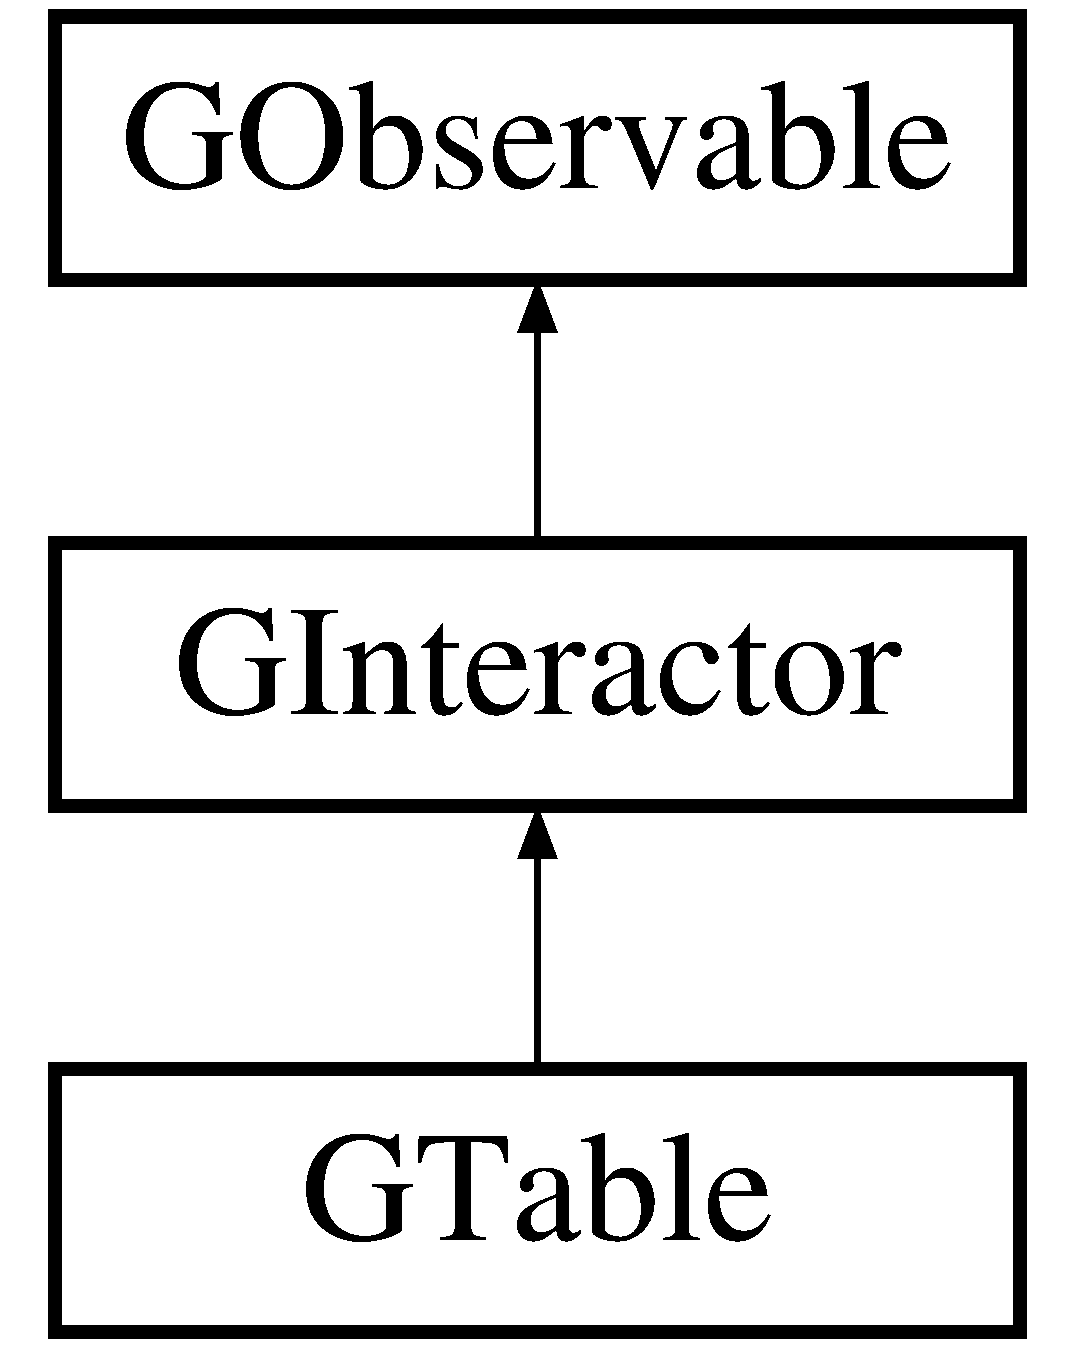
\includegraphics[height=3.000000cm]{classGTable}
\end{center}
\end{figure}
\subsection*{Public Types}
\begin{DoxyCompactItemize}
\item 
enum \mbox{\hyperlink{classGTable_a060cff504451bbb98530e64e936e2671}{Column\+Header\+Style}} \{ \mbox{\hyperlink{classGTable_a060cff504451bbb98530e64e936e2671a64e90531468e72442ee778fe31accdf6}{C\+O\+L\+U\+M\+N\+\_\+\+H\+E\+A\+D\+E\+R\+\_\+\+N\+O\+NE}}, 
\mbox{\hyperlink{classGTable_a060cff504451bbb98530e64e936e2671aa4b2febb21afe5d988ac57d4bac55a8b}{C\+O\+L\+U\+M\+N\+\_\+\+H\+E\+A\+D\+E\+R\+\_\+\+E\+X\+C\+EL}}, 
\mbox{\hyperlink{classGTable_a060cff504451bbb98530e64e936e2671ab59182f94a821e007f1ede2dd29b23cd}{C\+O\+L\+U\+M\+N\+\_\+\+H\+E\+A\+D\+E\+R\+\_\+\+N\+U\+M\+E\+R\+IC}}
 \}
\begin{DoxyCompactList}\small\item\em Styles of column header labels that can be shown. \end{DoxyCompactList}\item 
enum \mbox{\hyperlink{classGInteractor_a8e0d441725a81d2bbdebbea09078260e}{Text\+Position}} \{ \mbox{\hyperlink{classGInteractor_a8e0d441725a81d2bbdebbea09078260ea4cd6f2e7d5a08d6f4dc052df2358f774}{T\+E\+X\+T\+\_\+\+B\+E\+S\+I\+D\+E\+\_\+\+I\+C\+ON}}, 
\mbox{\hyperlink{classGInteractor_a8e0d441725a81d2bbdebbea09078260eaa88490f63d8de68d44c83bdb2ecde3b3}{T\+E\+X\+T\+\_\+\+U\+N\+D\+E\+R\+\_\+\+I\+C\+ON}}, 
\mbox{\hyperlink{classGInteractor_a8e0d441725a81d2bbdebbea09078260ea39a6f388a30ac4fefb6eb13e846bc9f2}{T\+E\+X\+T\+\_\+\+O\+N\+LY}}
 \}
\begin{DoxyCompactList}\small\item\em The places where an interactor can place its text relative to its icon. \end{DoxyCompactList}\end{DoxyCompactItemize}
\subsection*{Public Member Functions}
\begin{DoxyCompactItemize}
\item 
\mbox{\hyperlink{classGTable_a5ceea9546881f429ad4601366908848d}{G\+Table}} (int rows=0, int columns=0, double \mbox{\hyperlink{classGTable_ad72663daf610f2a0833a2fc3d78e4fdf}{width}}=0, double \mbox{\hyperlink{classGTable_ad3774f6419003470f54fd495124ef51f}{height}}=0, Q\+Widget $\ast$parent=nullptr)
\begin{DoxyCompactList}\small\item\em Constructs a new table with the given dimensions and (optional) size. \end{DoxyCompactList}\item 
\mbox{\hyperlink{classGTable_aa9d949edf98f5e891678aca78500550b}{$\sim$\+G\+Table}} () override
\item 
virtual void \mbox{\hyperlink{classGInteractor_a02f20ea6edfa0671f31c4c648a253833}{add\+Action\+Listener}} () Q\+\_\+\+D\+E\+C\+L\+\_\+\+D\+E\+P\+R\+E\+C\+A\+T\+ED
\begin{DoxyCompactList}\small\item\em Adds an event listener to be notified when this interactor is clicked or generally interacted with. \end{DoxyCompactList}\item 
virtual void \mbox{\hyperlink{classGTable_afaf36ccb6a75432b5f5463613ef01ef4}{autofit\+Column\+Widths}} ()
\begin{DoxyCompactList}\small\item\em Changes widths of all columns to be perfectly large enough to fit their contents. \end{DoxyCompactList}\item 
virtual void \mbox{\hyperlink{classGTable_ac8bb3912a3ce86b15842e79d0b421204}{clear}} ()
\begin{DoxyCompactList}\small\item\em Sets all cells in the table to store an empty string value. \end{DoxyCompactList}\item 
virtual void \mbox{\hyperlink{classGTable_ab7bffbf52806e438ac155886079d9bf6}{clear\+Cell}} (int row, int column)
\begin{DoxyCompactList}\small\item\em Sets the given cell to store an empty string value. \end{DoxyCompactList}\item 
virtual void \mbox{\hyperlink{classGTable_a5ba4fe558e9d315c123ecd9e896065ca}{clear\+Cell\+Formatting}} (int row, int column)
\begin{DoxyCompactList}\small\item\em Removes any formatting that has been applied to the given cell. \end{DoxyCompactList}\item 
virtual void \mbox{\hyperlink{classGTable_a07ea41be0cdc43ffcd09898d3ae5c523}{clear\+Formatting}} ()
\begin{DoxyCompactList}\small\item\em Removes any per-\/cell/column/row formatting that has been applied to the table. \end{DoxyCompactList}\item 
virtual void \mbox{\hyperlink{classGTable_abd07e172ccec6823a88289c21124a367}{clear\+Selection}} ()
\begin{DoxyCompactList}\small\item\em Deselects any currently selected cell. \end{DoxyCompactList}\item 
bool \mbox{\hyperlink{classGInteractor_a597a370b592e3737d38d9d2f4e2031ea}{events\+Enabled}} () const override
\begin{DoxyCompactList}\small\item\em Returns true if this interactor is currently accepting events. \end{DoxyCompactList}\item 
virtual void \mbox{\hyperlink{classGTable_a1ff40d0915f96652929cfb739bdd969f}{fill}} (const std\+::string \&text)
\begin{DoxyCompactList}\small\item\em Sets every cell in the table to have the given value. \end{DoxyCompactList}\item 
virtual std\+::string \mbox{\hyperlink{classGTable_aaa9971dcb7e1b082abd3b9010667f041}{get}} (int row, int column) const
\begin{DoxyCompactList}\small\item\em Returns the text stored in the given cell. \end{DoxyCompactList}\item 
virtual std\+::string \mbox{\hyperlink{classGInteractor_a69f8d23ed8f207fbecad99960776e942}{get\+Accelerator}} () const
\begin{DoxyCompactList}\small\item\em Returns a string representing a hotkey for this interactor, or an empty string if no accelerator has been set. \end{DoxyCompactList}\item 
virtual std\+::string \mbox{\hyperlink{classGInteractor_a94eb4276000c4fdfb508ce9e6317a82a}{get\+Action\+Command}} () const
\begin{DoxyCompactList}\small\item\em Returns an action command for this interactor, which is a semi-\/unique string you can use to identify it when events occur. \end{DoxyCompactList}\item 
virtual std\+::string \mbox{\hyperlink{classGInteractor_a808e22cc1fdfbecf71ed8c64ef4600e0}{get\+Background}} () const
\begin{DoxyCompactList}\small\item\em Returns the background color of the interactor as a string. \end{DoxyCompactList}\item 
virtual int \mbox{\hyperlink{classGInteractor_a9e827257a55cb8cf4d9de2ec6bcfd7a0}{get\+Background\+Int}} () const
\begin{DoxyCompactList}\small\item\em Returns the background color of the interactor as an R\+GB integer. \end{DoxyCompactList}\item 
virtual \mbox{\hyperlink{structGRectangle}{G\+Rectangle}} \mbox{\hyperlink{classGInteractor_a29e6ac35a0b48f491a4c88194cc5da3b}{get\+Bounds}} () const
\begin{DoxyCompactList}\small\item\em Returns a rectangle representing the x/y position and size of this interactor. \end{DoxyCompactList}\item 
virtual std\+::string \mbox{\hyperlink{classGInteractor_aa061dfa488c31e18549d64363c1d0e34}{get\+Color}} () const
\begin{DoxyCompactList}\small\item\em Returns the foreground/text color of the interactor as a string. \end{DoxyCompactList}\item 
virtual int \mbox{\hyperlink{classGInteractor_a9635c7af766cdc3417f346683fa0e6c1}{get\+Color\+Int}} () const
\begin{DoxyCompactList}\small\item\em Returns the foreground/text color of the interactor as an R\+GB integer. \end{DoxyCompactList}\item 
virtual \mbox{\hyperlink{classGTable_a060cff504451bbb98530e64e936e2671}{Column\+Header\+Style}} \mbox{\hyperlink{classGTable_a31ffc9e14dda3e91d1a1b3be81a42db8}{get\+Column\+Header\+Style}} () const
\begin{DoxyCompactList}\small\item\em Returns the column headers to use the given style. \end{DoxyCompactList}\item 
virtual double \mbox{\hyperlink{classGTable_a4722043b7c3f968238968d3053b8a277}{get\+Column\+Width}} (int column) const
\begin{DoxyCompactList}\small\item\em Returns the width of the given column index in pixels. \end{DoxyCompactList}\item 
virtual \mbox{\hyperlink{classGContainer}{G\+Container}} $\ast$ \mbox{\hyperlink{classGInteractor_a7a6e317c29d61030929b4cd2d1c00fe7}{get\+Container}} () const
\begin{DoxyCompactList}\small\item\em Returns a pointer to the onscreen container holding this interactor. \end{DoxyCompactList}\item 
virtual std\+::string \mbox{\hyperlink{classGInteractor_a894a5502900794eeb27d084c21f1d77d}{get\+Font}} () const
\begin{DoxyCompactList}\small\item\em Returns the font of this interactor\textquotesingle{}s text as a font string such as \char`\"{}\+Helvetica-\/12-\/\+Bold\char`\"{}. \end{DoxyCompactList}\item 
virtual std\+::string \mbox{\hyperlink{classGInteractor_a4fa2d8b0192a3a5b4af4bbfe71194d03}{get\+Foreground}} () const
\begin{DoxyCompactList}\small\item\em Returns the foreground/text color of the interactor as a string. \end{DoxyCompactList}\item 
virtual int \mbox{\hyperlink{classGInteractor_ac3b12ab385a6ef9ae90fc879860ba726}{get\+Foreground\+Int}} () const
\begin{DoxyCompactList}\small\item\em Returns the foreground/text color of the interactor as an R\+GB integer. \end{DoxyCompactList}\item 
virtual double \mbox{\hyperlink{classGInteractor_a1e7e353362434072875264cf95629f99}{get\+Height}} () const
\begin{DoxyCompactList}\small\item\em Returns the current onscreen height of this interactor in pixels. \end{DoxyCompactList}\item 
virtual std\+::string \mbox{\hyperlink{classGInteractor_aaed62a73004939a64da6f0eb9eb64d73}{get\+Icon}} () const
\begin{DoxyCompactList}\small\item\em Returns the file name of the icon associated with this interactor, or an empty string if no icon has been set. \end{DoxyCompactList}\item 
virtual int \mbox{\hyperlink{classGInteractor_a9c9659a6c6ba66b4107ba59c95a24241}{get\+ID}} () const
\begin{DoxyCompactList}\small\item\em Returns a globally unique identifier for this interactor, which is set when the interactor is constructed. \end{DoxyCompactList}\item 
\+\_\+\+Internal\+\_\+\+Q\+Widget $\ast$ \mbox{\hyperlink{classGTable_a2f6b36b2517087dc90a366b5ce1f5323}{get\+Internal\+Widget}} () const override
\begin{DoxyCompactList}\small\item\em Returns a direct pointer to the internal Qt widget being wrapped by this interactor. \end{DoxyCompactList}\item 
virtual \mbox{\hyperlink{structGPoint}{G\+Point}} \mbox{\hyperlink{classGInteractor_a4f83802015511edeb63b892830812c11}{get\+Location}} () const
\begin{DoxyCompactList}\small\item\em Returns an (x, y) point representing the onscreen location of the top-\/left corner of this interactor within its containing window. \end{DoxyCompactList}\item 
virtual double \mbox{\hyperlink{classGInteractor_aed4b0075fcc434499c3cb3e46896bda3}{get\+Minimum\+Height}} () const
\begin{DoxyCompactList}\small\item\em Returns the minimum height in pixels that this interactor will permit itself to be resized to. \end{DoxyCompactList}\item 
virtual \mbox{\hyperlink{structGDimension}{G\+Dimension}} \mbox{\hyperlink{classGInteractor_a66b5af0b32493b4d597ca0a3df2049ea}{get\+Minimum\+Size}} () const
\begin{DoxyCompactList}\small\item\em Returns a \mbox{\hyperlink{structGDimension}{G\+Dimension}} structure representing the minimum size in pixels that this interactor will permit itself to be resized to. \end{DoxyCompactList}\item 
virtual double \mbox{\hyperlink{classGInteractor_a59e668114fe3d49d2a0f28deb258f7c8}{get\+Minimum\+Width}} () const
\begin{DoxyCompactList}\small\item\em Returns the minimum width in pixels that this interactor will permit itself to be resized to. \end{DoxyCompactList}\item 
virtual std\+::string \mbox{\hyperlink{classGInteractor_a8a60438a5b55d0b2ceb35c8674b9d8c5}{get\+Name}} () const
\begin{DoxyCompactList}\small\item\em Returns a string representing a unique name for this interactor. \end{DoxyCompactList}\item 
virtual double \mbox{\hyperlink{classGInteractor_a747de0961653847bdc6615dbf756d715}{get\+Preferred\+Height}} () const
\begin{DoxyCompactList}\small\item\em Returns the height in pixels that this interactor would prefer to be, which would exactly fit its contents with no stretching or scrollbars. \end{DoxyCompactList}\item 
virtual \mbox{\hyperlink{structGDimension}{G\+Dimension}} \mbox{\hyperlink{classGInteractor_a4aabbee761d8e9116275401131b7ccd1}{get\+Preferred\+Size}} () const
\begin{DoxyCompactList}\small\item\em Returns a \mbox{\hyperlink{structGDimension}{G\+Dimension}} structure storing the width and height in pixels that this interactor would prefer to be, which would exactly fit its contents with no stretching or scrollbars. \end{DoxyCompactList}\item 
virtual double \mbox{\hyperlink{classGInteractor_a82bca31d37700fb0e35d2743352efd5e}{get\+Preferred\+Width}} () const
\begin{DoxyCompactList}\small\item\em Returns the height in pixels that this interactor would prefer to be, which would exactly fit its contents with no stretching or scrollbars. \end{DoxyCompactList}\item 
virtual double \mbox{\hyperlink{classGTable_a0215a742506665475b721ed12913808b}{get\+Row\+Height}} (int row) const
\begin{DoxyCompactList}\small\item\em Returns the height of the given row index in pixels. \end{DoxyCompactList}\item 
virtual Grid\+Location \mbox{\hyperlink{classGTable_ae4b79399eefc964f783f06b6959a6a4a}{get\+Selected\+Cell}} () const
\begin{DoxyCompactList}\small\item\em Returns the row and column of the cell that is currently selected. \end{DoxyCompactList}\item 
virtual void \mbox{\hyperlink{classGTable_a29b4e2e079037922545996e08f7ce6c4}{get\+Selected\+Cell}} (int \&row, int \&column) const
\begin{DoxyCompactList}\small\item\em Returns the row and column of the cell that is currently selected by filling the given reference parameters. \end{DoxyCompactList}\item 
virtual std\+::string \mbox{\hyperlink{classGTable_a8963c035a687a8393cd1f56ae05f582e}{get\+Selected\+Cell\+Value}} () const
\begin{DoxyCompactList}\small\item\em Returns the text in the cell that is currently selected. \end{DoxyCompactList}\item 
virtual int \mbox{\hyperlink{classGTable_abeec6fda3c331aa187ba1b695b19d435}{get\+Selected\+Column}} () const
\begin{DoxyCompactList}\small\item\em Returns the column of the cell that is currently selected, or -\/1 if no cell is currently selected. \end{DoxyCompactList}\item 
virtual int \mbox{\hyperlink{classGTable_adeb0b39683825191a8216d6cc3ca5072}{get\+Selected\+Row}} () const
\begin{DoxyCompactList}\small\item\em Returns the row of the cell that is currently selected, or -\/1 if no cell is currently selected. \end{DoxyCompactList}\item 
virtual \mbox{\hyperlink{structGDimension}{G\+Dimension}} \mbox{\hyperlink{classGInteractor_a7b4eec96a2bdc6420695d5796a78eea9}{get\+Size}} () const
\begin{DoxyCompactList}\small\item\em Returns a \mbox{\hyperlink{structGDimension}{G\+Dimension}} structure storing the current onscreen width and height of this interactor in pixels. \end{DoxyCompactList}\item 
std\+::string \mbox{\hyperlink{classGTable_a9b72ede4ee8520f987a0c01e30654814}{get\+Type}} () const override
\begin{DoxyCompactList}\small\item\em Returns a string representing the class name of this interactor, such as \char`\"{}\+G\+Button\char`\"{} or \char`\"{}\+G\+Check\+Box\char`\"{}. \end{DoxyCompactList}\item 
Q\+Widget $\ast$ \mbox{\hyperlink{classGTable_a3b33a602b31a6b809d020535a59db3b4}{get\+Widget}} () const override
\begin{DoxyCompactList}\small\item\em Returns a direct pointer to the internal Qt widget being wrapped by this interactor. \end{DoxyCompactList}\item 
virtual double \mbox{\hyperlink{classGInteractor_a0ed2965abd4f5701d2cadf71239faf19}{get\+Width}} () const
\begin{DoxyCompactList}\small\item\em Returns the current onscreen width of this interactor in pixels. \end{DoxyCompactList}\item 
virtual double \mbox{\hyperlink{classGInteractor_a344385751bee0720059403940d57a13e}{getX}} () const
\begin{DoxyCompactList}\small\item\em Returns the x-\/coordinate of the top-\/left pixel of this interactor within its onscreen window. \end{DoxyCompactList}\item 
virtual double \mbox{\hyperlink{classGInteractor_aafa51c7f8f38a09febbb9ce7853f77b4}{getY}} () const
\begin{DoxyCompactList}\small\item\em Returns the y-\/coordinate of the top-\/left pixel of this interactor within its onscreen window. \end{DoxyCompactList}\item 
virtual bool \mbox{\hyperlink{classGTable_a4a1007a3d14cd35f0bd514cc0b29886b}{has\+Selected\+Cell}} () const
\begin{DoxyCompactList}\small\item\em Returns true if a cell is currently selected. \end{DoxyCompactList}\item 
virtual int \mbox{\hyperlink{classGTable_ad3774f6419003470f54fd495124ef51f}{height}} () const
\begin{DoxyCompactList}\small\item\em Returns the number of rows in the table. \end{DoxyCompactList}\item 
virtual bool \mbox{\hyperlink{classGInteractor_afc480f652b8c5f1fb255e2269ce68879}{in\+Bounds}} (double x, double y) const
\begin{DoxyCompactList}\small\item\em Returns true if the given x/y pixel is within the bounds of this interactor. \end{DoxyCompactList}\item 
virtual bool \mbox{\hyperlink{classGInteractor_ae6d7982c1c627b677a5e776ca86118ed}{in\+Bounds}} (int x, int y) const
\begin{DoxyCompactList}\small\item\em Returns true if the given x/y pixel is within the bounds of this interactor. \end{DoxyCompactList}\item 
virtual bool \mbox{\hyperlink{classGTable_adcc2e619680a96a5b266d18a9ff2cdf4}{in\+Table\+Bounds}} (int row, int column) const
\begin{DoxyCompactList}\small\item\em Returns true if the given 0-\/based row/column index is within the bounds of the table. \end{DoxyCompactList}\item 
virtual bool \mbox{\hyperlink{classGTable_a012b5afb54e037e6c5498cf0932a521b}{is\+Editable}} () const
\begin{DoxyCompactList}\small\item\em Returns whether cells of the table can be edited. \end{DoxyCompactList}\item 
virtual bool \mbox{\hyperlink{classGInteractor_aacb819fb241851fd9fc045271baa4034}{is\+Enabled}} () const
\begin{DoxyCompactList}\small\item\em Returns true if this interactor is currently enabled. \end{DoxyCompactList}\item 
virtual bool \mbox{\hyperlink{classGInteractor_a9d8a6cfb13917785c143e74d40e4e2be}{is\+Visible}} () const
\begin{DoxyCompactList}\small\item\em Returns true if the interactor is visible on the screen. \end{DoxyCompactList}\item 
virtual int \mbox{\hyperlink{classGTable_a5997e103e56aae1db12e1f7f02e136c5}{num\+Cols}} () const
\begin{DoxyCompactList}\small\item\em Returns the number of columns in the table. \end{DoxyCompactList}\item 
virtual int \mbox{\hyperlink{classGTable_a00b7e69dd5c43e42cc91db26c459ad8b}{num\+Rows}} () const
\begin{DoxyCompactList}\small\item\em Returns the number of rows in the table. \end{DoxyCompactList}\item 
virtual void \mbox{\hyperlink{classGInteractor_ab7fe7a876367b87cf7202f947f1d05e4}{remove\+Action\+Listener}} ()
\begin{DoxyCompactList}\small\item\em Removes the action listener from this interactor so that it will no longer call it when events occur. \end{DoxyCompactList}\item 
virtual void \mbox{\hyperlink{classGInteractor_ad39d0325cde6b97ebda4b9d7787c633b}{remove\+Click\+Listener}} ()
\begin{DoxyCompactList}\small\item\em Removes the click listener from this interactor so that it will no longer call it when events occur. \end{DoxyCompactList}\item 
virtual void \mbox{\hyperlink{classGInteractor_aa4250907e4cdd77349c04f0cf5cdd3d3}{remove\+Double\+Click\+Listener}} ()
\begin{DoxyCompactList}\small\item\em Removes the double-\/click listener from this interactor so that it will no longer call it when events occur. \end{DoxyCompactList}\item 
virtual void \mbox{\hyperlink{classGInteractor_a43095f41cab3be732b49f29970484b05}{remove\+Key\+Listener}} ()
\begin{DoxyCompactList}\small\item\em Removes the key listener from this interactor so that it will no longer call it when key events occur. \end{DoxyCompactList}\item 
virtual void \mbox{\hyperlink{classGInteractor_aff47f71ce47e688a07c9d38dc92fcc11}{remove\+Mouse\+Listener}} ()
\begin{DoxyCompactList}\small\item\em Removes the mouse listener from this interactor so that it will no longer call it when events occur. \end{DoxyCompactList}\item 
virtual void \mbox{\hyperlink{classGTable_a5c18bacaf370f9c3da545f5c6e6e9515}{remove\+Table\+Listener}} ()
\begin{DoxyCompactList}\small\item\em Removes the table listener from this button so that it will no longer call it when events occur. \end{DoxyCompactList}\item 
void \mbox{\hyperlink{classGTable_a5921efd0a5a83eacebdadb749fb3ea7a}{request\+Focus}} () override
\begin{DoxyCompactList}\small\item\em Transfers keyboard focus to this interactor. \end{DoxyCompactList}\item 
virtual void \mbox{\hyperlink{classGTable_a600810b1a74ec9a062ce38666a9e7602}{resize}} (int \mbox{\hyperlink{classGTable_a00b7e69dd5c43e42cc91db26c459ad8b}{num\+Rows}}, int \mbox{\hyperlink{classGTable_a5997e103e56aae1db12e1f7f02e136c5}{num\+Cols}})
\begin{DoxyCompactList}\small\item\em Modifies the table to have the given number of rows and columns. \end{DoxyCompactList}\item 
virtual bool \mbox{\hyperlink{classGTable_a92c3dff0296ec16823a1172a9f9f07e6}{row\+Column\+Headers\+Visible}} () const
\begin{DoxyCompactList}\small\item\em Returns whether row and column headers are shown in the table. \end{DoxyCompactList}\item 
virtual void \mbox{\hyperlink{classGTable_ab06a36d6ed149c8477a1a9d32be2ba43}{select}} (int row, int column)
\begin{DoxyCompactList}\small\item\em Sets the given cell to become currently selected, replacing any previous selection. \end{DoxyCompactList}\item 
virtual void \mbox{\hyperlink{classGTable_ad1a09eece3a11ef4d2c56a951ae06a69}{set}} (int row, int column, const std\+::string \&text)
\begin{DoxyCompactList}\small\item\em Modifies the value in the given cell to store the given text. \end{DoxyCompactList}\item 
virtual void \mbox{\hyperlink{classGInteractor_ad15f102f62e2960576012f1aa0ba4b2e}{set\+Accelerator}} (const std\+::string \&accelerator)
\begin{DoxyCompactList}\small\item\em Sets an accelerator hotkey for this interactor, such as \char`\"{}\+Ctrl-\/\+S\char`\"{}. \end{DoxyCompactList}\item 
virtual void \mbox{\hyperlink{classGInteractor_a4b5843fe3030e038a1ba54cc03389bcf}{set\+Action\+Command}} (const std\+::string \&action\+Command)
\begin{DoxyCompactList}\small\item\em Sets the action command for this interactor. \end{DoxyCompactList}\item 
virtual void \mbox{\hyperlink{classGInteractor_adcfb4742430c88714fcf57e57ab8ea9c}{set\+Action\+Listener}} (G\+Event\+Listener func)
\begin{DoxyCompactList}\small\item\em Sets an action listener on this interactor so that it will be called when it is interacted with in its primary way. \end{DoxyCompactList}\item 
virtual void \mbox{\hyperlink{classGInteractor_aebd20a89c7a8a43a6fce999cf4f9fcf2}{set\+Action\+Listener}} (G\+Event\+Listener\+Void func)
\begin{DoxyCompactList}\small\item\em Sets an action listener on this interactor so that it will be called when it is interacted with in its primary way. \end{DoxyCompactList}\item 
void \mbox{\hyperlink{classGTable_aefbd30fa3e699d49b6dd2c2a2d6e8c2b}{set\+Background}} (int rgb) override
\begin{DoxyCompactList}\small\item\em Sets the background color that appears behind each cell. \end{DoxyCompactList}\item 
void \mbox{\hyperlink{classGTable_a9cb99695b93494c7ba28268ce9e42c2a}{set\+Background}} (const std\+::string \&color) override
\begin{DoxyCompactList}\small\item\em Sets the background color that appears behind each cell. \end{DoxyCompactList}\item 
virtual void \mbox{\hyperlink{classGInteractor_a2aae8197624b72265ab83b4f1bc73f2f}{set\+Bounds}} (double x, double y, double \mbox{\hyperlink{classGTable_ad72663daf610f2a0833a2fc3d78e4fdf}{width}}, double \mbox{\hyperlink{classGTable_ad3774f6419003470f54fd495124ef51f}{height}})
\begin{DoxyCompactList}\small\item\em Sets the size and location of the widget. \end{DoxyCompactList}\item 
virtual void \mbox{\hyperlink{classGInteractor_acada386653f008cacc7cce86426bef7c}{set\+Bounds}} (const \mbox{\hyperlink{structGRectangle}{G\+Rectangle}} \&size)
\begin{DoxyCompactList}\small\item\em Sets the size and location of the widget. \end{DoxyCompactList}\item 
virtual void \mbox{\hyperlink{classGTable_a0c1ff398e920da7356b8375b66b9b083}{set\+Cell\+Alignment}} (int row, int column, Horizontal\+Alignment alignment)
\begin{DoxyCompactList}\small\item\em Sets the horizontal alignment of the given cell. \end{DoxyCompactList}\item 
virtual void \mbox{\hyperlink{classGTable_a50940b22e500a861451bbff938c8f50b}{set\+Cell\+Background}} (int row, int column, int color)
\begin{DoxyCompactList}\small\item\em Sets the background color of the given cell to the given color. \end{DoxyCompactList}\item 
virtual void \mbox{\hyperlink{classGTable_af2d2fa204d2f9260081102a990310cd7}{set\+Cell\+Background}} (int row, int column, const std\+::string \&color)
\begin{DoxyCompactList}\small\item\em Sets the background color of the given cell to the given color. \end{DoxyCompactList}\item 
virtual void \mbox{\hyperlink{classGTable_a8c3d80b0163f465c7306b075d5895313}{set\+Cell\+Font}} (int row, int column, const std\+::string \&font)
\begin{DoxyCompactList}\small\item\em Sets the text font of the given cell to the given R\+GB color. \end{DoxyCompactList}\item 
virtual void \mbox{\hyperlink{classGTable_a19969b2f2b0cbf219333b02c047b2e7e}{set\+Cell\+Foreground}} (int row, int column, int color)
\begin{DoxyCompactList}\small\item\em Sets the foreground/text color of the given cell to the given color. \end{DoxyCompactList}\item 
virtual void \mbox{\hyperlink{classGTable_ab0bdc2afa7ef003fa5e8ab6eb25a7282}{set\+Cell\+Foreground}} (int row, int column, const std\+::string \&color)
\begin{DoxyCompactList}\small\item\em Sets the foreground/text color of the given cell to the given color. \end{DoxyCompactList}\item 
virtual void \mbox{\hyperlink{classGInteractor_abd40af6921242584d0954f173911b190}{set\+Click\+Listener}} (G\+Event\+Listener func)
\begin{DoxyCompactList}\small\item\em Sets a mouse listener on this interactor so that it will be called when the mouse is clicked on it. \end{DoxyCompactList}\item 
virtual void \mbox{\hyperlink{classGInteractor_a856414c92df90f56f3877475eb3f8fc4}{set\+Click\+Listener}} (G\+Event\+Listener\+Void func)
\begin{DoxyCompactList}\small\item\em Sets a mouse listener on this interactor so that it will be called when the mouse is clicked on it. \end{DoxyCompactList}\item 
void \mbox{\hyperlink{classGTable_a165735fb49fa7db12602d32557cbfe0d}{set\+Color}} (int rgb) override
\begin{DoxyCompactList}\small\item\em Sets the color used for the text of each cell. \end{DoxyCompactList}\item 
void \mbox{\hyperlink{classGTable_a56845b1accc47aa881d05939eef6996c}{set\+Color}} (const std\+::string \&color) override
\begin{DoxyCompactList}\small\item\em Sets the color used for the text of each cell. \end{DoxyCompactList}\item 
virtual void \mbox{\hyperlink{classGTable_a84b3f42bb5d010483b78b9fd7e9c55f0}{set\+Column\+Alignment}} (int column, Horizontal\+Alignment alignment)
\begin{DoxyCompactList}\small\item\em Sets the horizontal alignment of the given column. \end{DoxyCompactList}\item 
virtual void \mbox{\hyperlink{classGTable_a48898e733d8ae3e285ff84d02e2cdee5}{set\+Column\+Background}} (int column, int color)
\begin{DoxyCompactList}\small\item\em Sets the background color of the given column to the given color. \end{DoxyCompactList}\item 
virtual void \mbox{\hyperlink{classGTable_a37fd3b921a5fba28b84dd4dd17fa9930}{set\+Column\+Background}} (int column, const std\+::string \&color)
\begin{DoxyCompactList}\small\item\em Sets the background color of the given column to the given color. \end{DoxyCompactList}\item 
virtual void \mbox{\hyperlink{classGTable_a0294ee7cb1af024bc77371f27d877164}{set\+Column\+Font}} (int column, const std\+::string \&font)
\begin{DoxyCompactList}\small\item\em Sets the text font of the given column to the given R\+GB color. \end{DoxyCompactList}\item 
virtual void \mbox{\hyperlink{classGTable_aa616c02b04beb6ca757dec04f46814b0}{set\+Column\+Foreground}} (int column, int color)
\begin{DoxyCompactList}\small\item\em Sets the foreground/text color of the given column to the given color. \end{DoxyCompactList}\item 
virtual void \mbox{\hyperlink{classGTable_a84ca08c2995646ab28c78bffbcdc2693}{set\+Column\+Foreground}} (int column, const std\+::string \&color)
\begin{DoxyCompactList}\small\item\em Sets the foreground/text color of the given column to the given color. \end{DoxyCompactList}\item 
virtual void \mbox{\hyperlink{classGTable_ac97cb91256925fa81c52594bca854969}{set\+Column\+Header\+Style}} (\mbox{\hyperlink{classGTable_a060cff504451bbb98530e64e936e2671}{Column\+Header\+Style}} style)
\begin{DoxyCompactList}\small\item\em Sets the column headers to use the given style. \end{DoxyCompactList}\item 
virtual void \mbox{\hyperlink{classGTable_a52075dc231c73a896bcef426047fd327}{set\+Column\+Width}} (int column, double \mbox{\hyperlink{classGTable_ad72663daf610f2a0833a2fc3d78e4fdf}{width}})
\begin{DoxyCompactList}\small\item\em Sets the given column index to have the given width in pixels. \end{DoxyCompactList}\item 
virtual void \mbox{\hyperlink{classGInteractor_ac29f9a3462458e165fae3a1f046ee77a}{set\+Double\+Click\+Listener}} (G\+Event\+Listener func)
\begin{DoxyCompactList}\small\item\em Sets a mouse listener on this interactor so that it will be called when the mouse is double-\/clicked on it. \end{DoxyCompactList}\item 
virtual void \mbox{\hyperlink{classGInteractor_a50096194d66f48c92dd4c512d41bfc76}{set\+Double\+Click\+Listener}} (G\+Event\+Listener\+Void func)
\begin{DoxyCompactList}\small\item\em Sets a mouse listener on this interactor so that it will be called when the mouse is double-\/clicked on it. \end{DoxyCompactList}\item 
virtual void \mbox{\hyperlink{classGTable_a52455aaff9ee352ca405fa61ba246b84}{set\+Editable}} (bool editable)
\begin{DoxyCompactList}\small\item\em Sets whether cells of the table can be edited. \end{DoxyCompactList}\item 
virtual void \mbox{\hyperlink{classGTable_aaefc85e4ff762ca176a90ebac163f2c0}{set\+Editor\+Value}} (int row, int column, const std\+::string \&text)
\begin{DoxyCompactList}\small\item\em Modifies the value in the cell that is currently being edited to store the given text. \end{DoxyCompactList}\item 
virtual void \mbox{\hyperlink{classGInteractor_ab831367dd84bbd579e02e55bacb21343}{set\+Enabled}} (bool value)
\begin{DoxyCompactList}\small\item\em Sets whether this interactor is currently enabled. \end{DoxyCompactList}\item 
virtual void \mbox{\hyperlink{classGObservable_afaa30b2a9e0f378fd1c70d2f1d0b8216}{set\+Events\+Enabled}} (bool \mbox{\hyperlink{classGInteractor_a597a370b592e3737d38d9d2f4e2031ea}{events\+Enabled}})
\begin{DoxyCompactList}\small\item\em Sets whether the object is currently allowing itself to fire events. \end{DoxyCompactList}\item 
void \mbox{\hyperlink{classGTable_ad1d75b3840a41ba7d1e8a921696dc684}{set\+Font}} (const Q\+Font \&font) override
\begin{DoxyCompactList}\small\item\em Sets the font used to display each cell\textquotesingle{}s text. \end{DoxyCompactList}\item 
void \mbox{\hyperlink{classGTable_a51367c9fd2709973b1f7238734f93891}{set\+Font}} (const std\+::string \&font) override
\begin{DoxyCompactList}\small\item\em Sets the font used to display each cell\textquotesingle{}s text. \end{DoxyCompactList}\item 
void \mbox{\hyperlink{classGTable_a59f7cd2bd1708c12dfa52a8f7c7b79c9}{set\+Foreground}} (int rgb) override
\begin{DoxyCompactList}\small\item\em Sets the color used for the text of each cell. \end{DoxyCompactList}\item 
void \mbox{\hyperlink{classGTable_a8afbcf1f47750fb4c717f9ff36540235}{set\+Foreground}} (const std\+::string \&color) override
\begin{DoxyCompactList}\small\item\em Sets the color used for the text of each cell. \end{DoxyCompactList}\item 
virtual void \mbox{\hyperlink{classGInteractor_a9e280bfc4544dfaf8e4376c4e1a74357}{set\+Height}} (double \mbox{\hyperlink{classGTable_ad3774f6419003470f54fd495124ef51f}{height}})
\begin{DoxyCompactList}\small\item\em Sets the onscreen height of the interactor in pixels. \end{DoxyCompactList}\item 
virtual void \mbox{\hyperlink{classGTable_a04e6ce745dd0f9708f14dedc68ec8b18}{set\+Horizontal\+Alignment}} (Horizontal\+Alignment alignment)
\begin{DoxyCompactList}\small\item\em Sets the horizontal alignment of the text in all cells in the table. \end{DoxyCompactList}\item 
virtual void \mbox{\hyperlink{classGInteractor_a542abfcd7261751352af129c7215ecda}{set\+Icon}} (const Q\+Icon \&icon)
\begin{DoxyCompactList}\small\item\em Sets the icon associated with this interactor. \end{DoxyCompactList}\item 
virtual void \mbox{\hyperlink{classGInteractor_a368e1a338f84401c284506d03b1ba769}{set\+Icon}} (const Q\+Pixmap \&icon)
\begin{DoxyCompactList}\small\item\em Sets the icon associated with this interactor. \end{DoxyCompactList}\item 
virtual void \mbox{\hyperlink{classGInteractor_a762e139aa311461c3984d3ad28293f64}{set\+Icon}} (const std\+::string \&filename, bool retain\+Icon\+Size=true)
\begin{DoxyCompactList}\small\item\em Sets the file name of the icon associated with this interactor, or an empty string if no icon has been set. \end{DoxyCompactList}\item 
virtual void \mbox{\hyperlink{classGInteractor_aeb8324d3287fa1fbe093f4d6230cf0a6}{set\+Key\+Listener}} (G\+Event\+Listener func)
\begin{DoxyCompactList}\small\item\em Sets a key listener on this interactor so that it will be called when the user presses any key. \end{DoxyCompactList}\item 
virtual void \mbox{\hyperlink{classGInteractor_ae48ecea73606c7bd9423e1c7cc589cc9}{set\+Key\+Listener}} (G\+Event\+Listener\+Void func)
\begin{DoxyCompactList}\small\item\em Sets a key listener on this interactor so that it will be called when the user presses any key. \end{DoxyCompactList}\item 
virtual void \mbox{\hyperlink{classGInteractor_a04594e8ba9b98513a64f1da00dcae18c}{set\+Location}} (double x, double y)
\begin{DoxyCompactList}\small\item\em Sets the onscreen x/y-\/coordinate of the top-\/left corner of the interactor relative to its window. \end{DoxyCompactList}\item 
virtual void \mbox{\hyperlink{classGInteractor_a0cf428e207b7f22cc08138a90b1b87b2}{set\+Minimum\+Size}} (double \mbox{\hyperlink{classGTable_ad72663daf610f2a0833a2fc3d78e4fdf}{width}}, double \mbox{\hyperlink{classGTable_ad3774f6419003470f54fd495124ef51f}{height}})
\begin{DoxyCompactList}\small\item\em Sets the minimum size in pixels that this interactor will permit itself to be resized to. \end{DoxyCompactList}\item 
virtual void \mbox{\hyperlink{classGInteractor_a3b1046117ac6cb7abe467e00ba8a81f4}{set\+Minimum\+Size}} (const \mbox{\hyperlink{structGDimension}{G\+Dimension}} \&size)
\begin{DoxyCompactList}\small\item\em Sets the minimum size in pixels that this interactor will permit itself to be resized to. \end{DoxyCompactList}\item 
virtual void \mbox{\hyperlink{classGInteractor_a37d8dbc943f59920f705b0104f60bde2}{set\+Mouse\+Listener}} (G\+Event\+Listener func)
\begin{DoxyCompactList}\small\item\em Sets a mouse listener on this interactor so that it will be called when the mouse is moved or clicked on it. \end{DoxyCompactList}\item 
virtual void \mbox{\hyperlink{classGInteractor_aea7f647ea62d59f71b5fad6aa65eeaf9}{set\+Mouse\+Listener}} (G\+Event\+Listener\+Void func)
\begin{DoxyCompactList}\small\item\em Sets a mouse listener on this interactor so that it will be called when the mouse is moved or clicked on it. \end{DoxyCompactList}\item 
virtual void \mbox{\hyperlink{classGInteractor_a9d3a2685df23b5e7cbf59c19c4a1f9b5}{set\+Name}} (const std\+::string \&name)
\begin{DoxyCompactList}\small\item\em Sets a string representing a unique name for this interactor. \end{DoxyCompactList}\item 
virtual void \mbox{\hyperlink{classGInteractor_a1ab987704fce32098706c6f00fb08218}{set\+Preferred\+Height}} (double \mbox{\hyperlink{classGTable_ad3774f6419003470f54fd495124ef51f}{height}})
\begin{DoxyCompactList}\small\item\em Sets the height in pixels that this interactor would prefer to be. \end{DoxyCompactList}\item 
virtual void \mbox{\hyperlink{classGInteractor_a042c5ae19430d765ef552371cae3632c}{set\+Preferred\+Size}} (double \mbox{\hyperlink{classGTable_ad72663daf610f2a0833a2fc3d78e4fdf}{width}}, double \mbox{\hyperlink{classGTable_ad3774f6419003470f54fd495124ef51f}{height}})
\begin{DoxyCompactList}\small\item\em Sets the width and height in pixels that this interactor would prefer to be. \end{DoxyCompactList}\item 
virtual void \mbox{\hyperlink{classGInteractor_aa22d9be4bc0e078bb0ea69b0fc9d7c75}{set\+Preferred\+Size}} (const \mbox{\hyperlink{structGDimension}{G\+Dimension}} \&size)
\begin{DoxyCompactList}\small\item\em Sets the size in pixels that this interactor would prefer to be. \end{DoxyCompactList}\item 
virtual void \mbox{\hyperlink{classGInteractor_a3db429ab2fa52efd187eec0ed8cdd9f2}{set\+Preferred\+Width}} (double \mbox{\hyperlink{classGTable_ad72663daf610f2a0833a2fc3d78e4fdf}{width}})
\begin{DoxyCompactList}\small\item\em Sets the width in pixels that this interactor would prefer to be. \end{DoxyCompactList}\item 
virtual void \mbox{\hyperlink{classGTable_ac6a47ba68c502b7d8dc776beeeffccc3}{set\+Row\+Alignment}} (int row, Horizontal\+Alignment alignment)
\begin{DoxyCompactList}\small\item\em Sets the horizontal alignment of the given row. \end{DoxyCompactList}\item 
virtual void \mbox{\hyperlink{classGTable_a85ee577aabd189ed64a5c9f66ba61fd2}{set\+Row\+Background}} (int row, int rgb)
\begin{DoxyCompactList}\small\item\em Sets the background color of the given row to the given R\+GB color. \end{DoxyCompactList}\item 
virtual void \mbox{\hyperlink{classGTable_a30c7073dfeac833056ed65a8bb9a7e08}{set\+Row\+Background}} (int row, const std\+::string \&color)
\begin{DoxyCompactList}\small\item\em Sets the background color of the given row to the given color. \end{DoxyCompactList}\item 
virtual void \mbox{\hyperlink{classGTable_a0d4a1d2a58daff8c1984e31b21f93ea1}{set\+Row\+Column\+Headers\+Visible}} (bool visible)
\begin{DoxyCompactList}\small\item\em Sets whether row and column headers should be shown in the table. \end{DoxyCompactList}\item 
virtual void \mbox{\hyperlink{classGTable_adaeccb3f3fd318185b8adc644aaca949}{set\+Row\+Font}} (int row, const std\+::string \&font)
\begin{DoxyCompactList}\small\item\em Sets the text font of the given row to the given font. \end{DoxyCompactList}\item 
virtual void \mbox{\hyperlink{classGTable_abe6e1382d3d98a9479cf43ac204b0ee3}{set\+Row\+Foreground}} (int row, int rgb)
\begin{DoxyCompactList}\small\item\em Sets the foreground/text color of the given row to the given color. \end{DoxyCompactList}\item 
virtual void \mbox{\hyperlink{classGTable_a27ede8127bd8889e3f71dfe152c1684d}{set\+Row\+Foreground}} (int row, const std\+::string \&color)
\begin{DoxyCompactList}\small\item\em Sets the foreground/text color of the given row to the given color. \end{DoxyCompactList}\item 
virtual void \mbox{\hyperlink{classGTable_a815f0bed3e7a76d99b4a026808a555b3}{set\+Row\+Height}} (int row, double \mbox{\hyperlink{classGTable_ad72663daf610f2a0833a2fc3d78e4fdf}{width}})
\begin{DoxyCompactList}\small\item\em Sets the given row index to have the given height in pixels. \end{DoxyCompactList}\item 
virtual void \mbox{\hyperlink{classGTable_a3120b24ea5aaa17d8a7192742c00bcfb}{set\+Selected\+Cell\+Value}} (const std\+::string \&text)
\begin{DoxyCompactList}\small\item\em Sets the text in the cell that is currently selected. \end{DoxyCompactList}\item 
virtual void \mbox{\hyperlink{classGInteractor_aca25d49481f9bf5fc8f7df4c086c4ce7}{set\+Size}} (double \mbox{\hyperlink{classGTable_ad72663daf610f2a0833a2fc3d78e4fdf}{width}}, double \mbox{\hyperlink{classGTable_ad3774f6419003470f54fd495124ef51f}{height}})
\begin{DoxyCompactList}\small\item\em Sets the onscreen width and height of the interactor in pixels. \end{DoxyCompactList}\item 
virtual void \mbox{\hyperlink{classGInteractor_ae2b628228f192c2702c4ce941b2af68f}{set\+Size}} (const \mbox{\hyperlink{structGDimension}{G\+Dimension}} \&size)
\begin{DoxyCompactList}\small\item\em Sets the onscreen width and height of the interactor in pixels. \end{DoxyCompactList}\item 
virtual void \mbox{\hyperlink{classGTable_aeeb00b5caf01028e9de6f2dd6ef4b9bd}{set\+Table\+Listener}} (G\+Event\+Listener func)
\begin{DoxyCompactList}\small\item\em Sets the given function to be called when events occur in this table. \end{DoxyCompactList}\item 
virtual void \mbox{\hyperlink{classGTable_a0412cb4e079085ed5cb3bcdf2921ac84}{set\+Table\+Listener}} (G\+Event\+Listener\+Void func)
\begin{DoxyCompactList}\small\item\em Sets the given function to be called when events occur in this table. \end{DoxyCompactList}\item 
virtual void \mbox{\hyperlink{classGInteractor_a039e0e49beaecc275efce02d416acea8}{set\+Tooltip}} (const std\+::string \&tooltip\+Text)
\begin{DoxyCompactList}\small\item\em Sets a \char`\"{}tooltip\char`\"{} that will appear if the user hovers their mouse over the interactor. \end{DoxyCompactList}\item 
virtual void \mbox{\hyperlink{classGInteractor_a18e44e30b31525a243960ca3928125aa}{set\+Visible}} (bool visible)
\begin{DoxyCompactList}\small\item\em Returns true if the interactor is visible on the screen. \end{DoxyCompactList}\item 
virtual void \mbox{\hyperlink{classGInteractor_aa3f3fba4cb131baa8696ba01e3bceca1}{set\+Width}} (double \mbox{\hyperlink{classGTable_ad72663daf610f2a0833a2fc3d78e4fdf}{width}})
\begin{DoxyCompactList}\small\item\em Sets the onscreen width of the interactor in pixels. \end{DoxyCompactList}\item 
virtual void \mbox{\hyperlink{classGInteractor_a9c18fcc579333bf9653d13ad2b372e39}{setX}} (double x)
\begin{DoxyCompactList}\small\item\em Sets the onscreen x-\/coordinate of the top-\/left corner of the interactor relative to its window. \end{DoxyCompactList}\item 
virtual void \mbox{\hyperlink{classGInteractor_a7d57e2a5c35d27feb58fd498a3cf82b9}{setY}} (double y)
\begin{DoxyCompactList}\small\item\em Sets the onscreen y-\/coordinate of the top-\/left corner of the interactor relative to its window. \end{DoxyCompactList}\item 
virtual std\+::string \mbox{\hyperlink{classGObservable_a1fe5121d6528fdea3f243321b3fa3a49}{to\+String}} () const
\begin{DoxyCompactList}\small\item\em Returns a string representation of this observable object\textquotesingle{}s state. \end{DoxyCompactList}\item 
virtual int \mbox{\hyperlink{classGTable_ad72663daf610f2a0833a2fc3d78e4fdf}{width}} () const
\begin{DoxyCompactList}\small\item\em Returns the number of columns in the table. \end{DoxyCompactList}\end{DoxyCompactItemize}
\subsection*{Protected Member Functions}
\begin{DoxyCompactItemize}
\item 
virtual void \mbox{\hyperlink{classGObservable_a80cfa040459ff53594adbd6a51ec8f43}{clear\+Event\+Listeners}} ()
\begin{DoxyCompactList}\small\item\em Removes all event listeners from this object. \end{DoxyCompactList}\item 
virtual void \mbox{\hyperlink{classGObservable_a284f31528c0520f8e545c03ac9eeac74}{ensure\+Thread\+Safety}} (const std\+::string \&member\+Name=\char`\"{}\char`\"{})
\begin{DoxyCompactList}\small\item\em Ensures that we are currently in the Qt G\+UI thread. \end{DoxyCompactList}\item 
virtual void \mbox{\hyperlink{classGObservable_a63e5e5a6227c59c928493b11aceb0f67}{fire\+Event}} (\mbox{\hyperlink{classGEvent}{G\+Event}} \&event)
\begin{DoxyCompactList}\small\item\em Sends out the given event to any attached listeners. \end{DoxyCompactList}\item 
virtual void \mbox{\hyperlink{classGObservable_ab3983ea07337b52020a29cc00c653d8d}{fire\+G\+Event}} (Q\+Event $\ast$event, Event\+Type event\+Type, const std\+::string \&event\+Name)
\begin{DoxyCompactList}\small\item\em Creates an event of the given type, then sends it out to any attached listeners. \end{DoxyCompactList}\item 
virtual void \mbox{\hyperlink{classGObservable_a01fdf1b0e0dbd49e189fe4514e010411}{fire\+G\+Event}} (Q\+Close\+Event $\ast$event, Event\+Type event\+Type, const std\+::string \&event\+Name)
\begin{DoxyCompactList}\small\item\em Creates an event of the given type, then sends it out to any attached listeners. \end{DoxyCompactList}\item 
virtual void \mbox{\hyperlink{classGObservable_abb0b2f66ba39211cb5d7615e9d1c04e2}{fire\+G\+Event}} (Q\+Key\+Event $\ast$event, Event\+Type event\+Type, const std\+::string \&event\+Name)
\begin{DoxyCompactList}\small\item\em Creates an event of the given type, then sends it out to any attached listeners. \end{DoxyCompactList}\item 
virtual void \mbox{\hyperlink{classGObservable_a119318675d2165bdf7dd853aaf881d4b}{fire\+G\+Event}} (Q\+Mouse\+Event $\ast$event, Event\+Type event\+Type, const std\+::string \&event\+Name, const std\+::string \&action\+Command=\char`\"{}\char`\"{})
\begin{DoxyCompactList}\small\item\em Creates an event of the given type, then sends it out to any attached listeners. \end{DoxyCompactList}\item 
virtual void \mbox{\hyperlink{classGObservable_a63fd9034e1e1633c1c38eb342bfd34e9}{fire\+G\+Event}} (Q\+Resize\+Event $\ast$event, Event\+Type event\+Type, const std\+::string \&event\+Name)
\begin{DoxyCompactList}\small\item\em Creates an event of the given type, then sends it out to any attached listeners. \end{DoxyCompactList}\item 
virtual void \mbox{\hyperlink{classGObservable_a741345310d9b7c5170a6cbc410c44ac4}{fire\+G\+Event}} (Q\+Timer\+Event $\ast$event, Event\+Type event\+Type, const std\+::string \&event\+Name)
\begin{DoxyCompactList}\small\item\em Creates an event of the given type, then sends it out to any attached listeners. \end{DoxyCompactList}\item 
virtual void \mbox{\hyperlink{classGObservable_a93bf338968a0338761b8e4dc62f582e9}{fire\+G\+Event}} (Q\+Wheel\+Event $\ast$event, Event\+Type event\+Type, const std\+::string \&event\+Name)
\begin{DoxyCompactList}\small\item\em Creates an event of the given type, then sends it out to any attached listeners. \end{DoxyCompactList}\item 
virtual void \mbox{\hyperlink{classGObservable_a2a70a7d7435ff0c3b80bb4d70da19e0d}{fire\+G\+Event}} (Q\+Window\+State\+Change\+Event $\ast$event, Event\+Type event\+Type, const std\+::string \&event\+Name)
\begin{DoxyCompactList}\small\item\em Creates an event of the given type, then sends it out to any attached listeners. \end{DoxyCompactList}\item 
virtual bool \mbox{\hyperlink{classGObservable_a9f6faaa25942923bafa1c44020c49fa9}{has\+Event\+Listener}} (const std\+::string \&event\+Name) const
\begin{DoxyCompactList}\small\item\em Returns true if the observable object has a listener for the given type of event. \end{DoxyCompactList}\item 
virtual bool \mbox{\hyperlink{classGObservable_aeec1adc19aa0f33de62390686ee1382c}{is\+Accepting\+Event}} (int event\+Mask) const
\begin{DoxyCompactList}\small\item\em Returns true if the observable object has a listener for the given type of event. \end{DoxyCompactList}\item 
virtual bool \mbox{\hyperlink{classGObservable_aa31c73145a29dcb92848a92e0cfaea41}{is\+Accepting\+Event}} (const \mbox{\hyperlink{classGEvent}{G\+Event}} \&event) const
\begin{DoxyCompactList}\small\item\em Returns true if the observable object has a listener for the given type of event. \end{DoxyCompactList}\item 
virtual bool \mbox{\hyperlink{classGObservable_a3b1c689267eda44e65a2213e7de38b23}{is\+Accepting\+Event}} (const std\+::string \&event\+Type) const
\begin{DoxyCompactList}\small\item\em Returns true if the observable object has a listener for the given type of event. \end{DoxyCompactList}\item 
virtual void \mbox{\hyperlink{classGObservable_acbcf1ed3a851ad8a3c17ef38d86b481d}{remove\+Event\+Listener}} (const std\+::string \&event\+Name)
\begin{DoxyCompactList}\small\item\em Removes any event listener from this observable object that would respond to the given type of event, such as \char`\"{}click\char`\"{} or \char`\"{}keydown\char`\"{}. \end{DoxyCompactList}\item 
virtual void \mbox{\hyperlink{classGObservable_af51cc35c29a1bd1908609d432decdbb6}{remove\+Event\+Listeners}} (std\+::initializer\+\_\+list$<$ std\+::string $>$ event\+Names)
\begin{DoxyCompactList}\small\item\em Removes any event listener from this observable object that would respond to the given types of events, such as \char`\"{}click\char`\"{} or \char`\"{}keydown\char`\"{}. \end{DoxyCompactList}\item 
virtual void \mbox{\hyperlink{classGObservable_ad2f6d34961c50f6c1e0659990b79f741}{set\+Event\+Listener}} (const std\+::string \&event\+Name, G\+Event\+Listener func)
\begin{DoxyCompactList}\small\item\em Adds an event listener from this observable object to respond to the given type of event, such as \char`\"{}click\char`\"{} or \char`\"{}keydown\char`\"{}. \end{DoxyCompactList}\item 
virtual void \mbox{\hyperlink{classGObservable_abac4cb9f9e626e010e87f5d91573c8a5}{set\+Event\+Listener}} (const std\+::string \&event\+Name, G\+Event\+Listener\+Void func)
\begin{DoxyCompactList}\small\item\em Adds an event listener from this observable object to respond to the given type of event, such as \char`\"{}click\char`\"{} or \char`\"{}keydown\char`\"{}. \end{DoxyCompactList}\item 
virtual void \mbox{\hyperlink{classGObservable_afa388d69c33c718cf035774604065604}{set\+Event\+Listeners}} (std\+::initializer\+\_\+list$<$ std\+::string $>$ event\+Names, G\+Event\+Listener func)
\begin{DoxyCompactList}\small\item\em Adds an event listener from this observable object to respond to the given types of events, such as \char`\"{}click\char`\"{} or \char`\"{}keydown\char`\"{}. \end{DoxyCompactList}\item 
virtual void \mbox{\hyperlink{classGObservable_a7867184bbb686f74fae8a4db927da799}{set\+Event\+Listeners}} (std\+::initializer\+\_\+list$<$ std\+::string $>$ event\+Names, G\+Event\+Listener\+Void func)
\begin{DoxyCompactList}\small\item\em Adds an event listener from this observable object to respond to the given types of events, such as \char`\"{}click\char`\"{} or \char`\"{}keydown\char`\"{}. \end{DoxyCompactList}\end{DoxyCompactItemize}


\subsection{Detailed Description}
A \mbox{\hyperlink{classGTable}{G\+Table}} represents a graphical editable 2D table, like a mediocre facsimile of an Excel spreadsheet. 

After creating a \mbox{\hyperlink{classGTable}{G\+Table}}, you can listen for table events to be notified when the user types a new value into a table cell by calling set\+Table\+Listener.

An editable table has a semi-\/complex editing model where the user can begin modifying a cell by highlighting it and typing, which replaces the existing value, or by double-\/clicking it, which edits the existing value. You can also press F2 on a cell to edit it, equivalent to a double-\/click. During editing, you can press Esc to cancel editing, or Tab or Enter to complete editing and move to the next cell.

All row/column indexes in this class are 0-\/based. 

\subsection{Member Enumeration Documentation}
\mbox{\Hypertarget{classGTable_a060cff504451bbb98530e64e936e2671}\label{classGTable_a060cff504451bbb98530e64e936e2671}} 
\index{G\+Table@{G\+Table}!Column\+Header\+Style@{Column\+Header\+Style}}
\index{Column\+Header\+Style@{Column\+Header\+Style}!G\+Table@{G\+Table}}
\subsubsection{\texorpdfstring{Column\+Header\+Style}{ColumnHeaderStyle}}
{\footnotesize\ttfamily enum \mbox{\hyperlink{classGTable_a060cff504451bbb98530e64e936e2671}{Column\+Header\+Style}}}



Styles of column header labels that can be shown. 

The \char`\"{}\+Excel\char`\"{} style is to use column names A-\/Z, then A\+A-\/\+AZ, B\+A-\/\+BZ, ..., Z\+A-\/\+ZZ, then A\+AA, A\+AB, and so on. The \char`\"{}numeric\char`\"{} style is to use simple numbers like 1, 2, 3, ... The \char`\"{}none\char`\"{} style means not to use any column headers at all. \begin{DoxyEnumFields}{Enumerator}
\raisebox{\heightof{T}}[0pt][0pt]{\index{C\+O\+L\+U\+M\+N\+\_\+\+H\+E\+A\+D\+E\+R\+\_\+\+N\+O\+NE@{C\+O\+L\+U\+M\+N\+\_\+\+H\+E\+A\+D\+E\+R\+\_\+\+N\+O\+NE}!G\+Table@{G\+Table}}\index{G\+Table@{G\+Table}!C\+O\+L\+U\+M\+N\+\_\+\+H\+E\+A\+D\+E\+R\+\_\+\+N\+O\+NE@{C\+O\+L\+U\+M\+N\+\_\+\+H\+E\+A\+D\+E\+R\+\_\+\+N\+O\+NE}}}\mbox{\Hypertarget{classGTable_a060cff504451bbb98530e64e936e2671a64e90531468e72442ee778fe31accdf6}\label{classGTable_a060cff504451bbb98530e64e936e2671a64e90531468e72442ee778fe31accdf6}} 
C\+O\+L\+U\+M\+N\+\_\+\+H\+E\+A\+D\+E\+R\+\_\+\+N\+O\+NE&\\
\hline

\raisebox{\heightof{T}}[0pt][0pt]{\index{C\+O\+L\+U\+M\+N\+\_\+\+H\+E\+A\+D\+E\+R\+\_\+\+E\+X\+C\+EL@{C\+O\+L\+U\+M\+N\+\_\+\+H\+E\+A\+D\+E\+R\+\_\+\+E\+X\+C\+EL}!G\+Table@{G\+Table}}\index{G\+Table@{G\+Table}!C\+O\+L\+U\+M\+N\+\_\+\+H\+E\+A\+D\+E\+R\+\_\+\+E\+X\+C\+EL@{C\+O\+L\+U\+M\+N\+\_\+\+H\+E\+A\+D\+E\+R\+\_\+\+E\+X\+C\+EL}}}\mbox{\Hypertarget{classGTable_a060cff504451bbb98530e64e936e2671aa4b2febb21afe5d988ac57d4bac55a8b}\label{classGTable_a060cff504451bbb98530e64e936e2671aa4b2febb21afe5d988ac57d4bac55a8b}} 
C\+O\+L\+U\+M\+N\+\_\+\+H\+E\+A\+D\+E\+R\+\_\+\+E\+X\+C\+EL&\\
\hline

\raisebox{\heightof{T}}[0pt][0pt]{\index{C\+O\+L\+U\+M\+N\+\_\+\+H\+E\+A\+D\+E\+R\+\_\+\+N\+U\+M\+E\+R\+IC@{C\+O\+L\+U\+M\+N\+\_\+\+H\+E\+A\+D\+E\+R\+\_\+\+N\+U\+M\+E\+R\+IC}!G\+Table@{G\+Table}}\index{G\+Table@{G\+Table}!C\+O\+L\+U\+M\+N\+\_\+\+H\+E\+A\+D\+E\+R\+\_\+\+N\+U\+M\+E\+R\+IC@{C\+O\+L\+U\+M\+N\+\_\+\+H\+E\+A\+D\+E\+R\+\_\+\+N\+U\+M\+E\+R\+IC}}}\mbox{\Hypertarget{classGTable_a060cff504451bbb98530e64e936e2671ab59182f94a821e007f1ede2dd29b23cd}\label{classGTable_a060cff504451bbb98530e64e936e2671ab59182f94a821e007f1ede2dd29b23cd}} 
C\+O\+L\+U\+M\+N\+\_\+\+H\+E\+A\+D\+E\+R\+\_\+\+N\+U\+M\+E\+R\+IC&\\
\hline

\end{DoxyEnumFields}
\mbox{\Hypertarget{classGInteractor_a8e0d441725a81d2bbdebbea09078260e}\label{classGInteractor_a8e0d441725a81d2bbdebbea09078260e}} 
\index{G\+Table@{G\+Table}!Text\+Position@{Text\+Position}}
\index{Text\+Position@{Text\+Position}!G\+Table@{G\+Table}}
\subsubsection{\texorpdfstring{Text\+Position}{TextPosition}}
{\footnotesize\ttfamily enum \mbox{\hyperlink{classGInteractor_a8e0d441725a81d2bbdebbea09078260e}{Text\+Position}}\hspace{0.3cm}{\ttfamily [inherited]}}



The places where an interactor can place its text relative to its icon. 

\begin{DoxyEnumFields}{Enumerator}
\raisebox{\heightof{T}}[0pt][0pt]{\index{T\+E\+X\+T\+\_\+\+B\+E\+S\+I\+D\+E\+\_\+\+I\+C\+ON@{T\+E\+X\+T\+\_\+\+B\+E\+S\+I\+D\+E\+\_\+\+I\+C\+ON}!G\+Table@{G\+Table}}\index{G\+Table@{G\+Table}!T\+E\+X\+T\+\_\+\+B\+E\+S\+I\+D\+E\+\_\+\+I\+C\+ON@{T\+E\+X\+T\+\_\+\+B\+E\+S\+I\+D\+E\+\_\+\+I\+C\+ON}}}\mbox{\Hypertarget{classGInteractor_a8e0d441725a81d2bbdebbea09078260ea4cd6f2e7d5a08d6f4dc052df2358f774}\label{classGInteractor_a8e0d441725a81d2bbdebbea09078260ea4cd6f2e7d5a08d6f4dc052df2358f774}} 
T\+E\+X\+T\+\_\+\+B\+E\+S\+I\+D\+E\+\_\+\+I\+C\+ON&\\
\hline

\raisebox{\heightof{T}}[0pt][0pt]{\index{T\+E\+X\+T\+\_\+\+U\+N\+D\+E\+R\+\_\+\+I\+C\+ON@{T\+E\+X\+T\+\_\+\+U\+N\+D\+E\+R\+\_\+\+I\+C\+ON}!G\+Table@{G\+Table}}\index{G\+Table@{G\+Table}!T\+E\+X\+T\+\_\+\+U\+N\+D\+E\+R\+\_\+\+I\+C\+ON@{T\+E\+X\+T\+\_\+\+U\+N\+D\+E\+R\+\_\+\+I\+C\+ON}}}\mbox{\Hypertarget{classGInteractor_a8e0d441725a81d2bbdebbea09078260eaa88490f63d8de68d44c83bdb2ecde3b3}\label{classGInteractor_a8e0d441725a81d2bbdebbea09078260eaa88490f63d8de68d44c83bdb2ecde3b3}} 
T\+E\+X\+T\+\_\+\+U\+N\+D\+E\+R\+\_\+\+I\+C\+ON&\\
\hline

\raisebox{\heightof{T}}[0pt][0pt]{\index{T\+E\+X\+T\+\_\+\+O\+N\+LY@{T\+E\+X\+T\+\_\+\+O\+N\+LY}!G\+Table@{G\+Table}}\index{G\+Table@{G\+Table}!T\+E\+X\+T\+\_\+\+O\+N\+LY@{T\+E\+X\+T\+\_\+\+O\+N\+LY}}}\mbox{\Hypertarget{classGInteractor_a8e0d441725a81d2bbdebbea09078260ea39a6f388a30ac4fefb6eb13e846bc9f2}\label{classGInteractor_a8e0d441725a81d2bbdebbea09078260ea39a6f388a30ac4fefb6eb13e846bc9f2}} 
T\+E\+X\+T\+\_\+\+O\+N\+LY&\\
\hline

\end{DoxyEnumFields}


\subsection{Constructor \& Destructor Documentation}
\mbox{\Hypertarget{classGTable_a5ceea9546881f429ad4601366908848d}\label{classGTable_a5ceea9546881f429ad4601366908848d}} 
\index{G\+Table@{G\+Table}!G\+Table@{G\+Table}}
\index{G\+Table@{G\+Table}!G\+Table@{G\+Table}}
\subsubsection{\texorpdfstring{G\+Table()}{GTable()}}
{\footnotesize\ttfamily \mbox{\hyperlink{classGTable}{G\+Table}} (\begin{DoxyParamCaption}\item[{int}]{rows = {\ttfamily 0},  }\item[{int}]{columns = {\ttfamily 0},  }\item[{double}]{width = {\ttfamily 0},  }\item[{double}]{height = {\ttfamily 0},  }\item[{Q\+Widget $\ast$}]{parent = {\ttfamily nullptr} }\end{DoxyParamCaption})}



Constructs a new table with the given dimensions and (optional) size. 

If x, y, width, or height are omitted, they are set automatically by the layout manager of the \mbox{\hyperlink{classGWindow}{G\+Window}} into which the table is placed. This is often what you want. 
\begin{DoxyExceptions}{Exceptions}
{\em Error\+Exception} & if the number of rows, columns, width, or height is negative. \\
\hline
\end{DoxyExceptions}
\mbox{\Hypertarget{classGTable_aa9d949edf98f5e891678aca78500550b}\label{classGTable_aa9d949edf98f5e891678aca78500550b}} 
\index{G\+Table@{G\+Table}!````~G\+Table@{$\sim$\+G\+Table}}
\index{````~G\+Table@{$\sim$\+G\+Table}!G\+Table@{G\+Table}}
\subsubsection{\texorpdfstring{$\sim$\+G\+Table()}{~GTable()}}
{\footnotesize\ttfamily $\sim$\mbox{\hyperlink{classGTable}{G\+Table}} (\begin{DoxyParamCaption}{ }\end{DoxyParamCaption})\hspace{0.3cm}{\ttfamily [override]}}



\subsection{Member Function Documentation}
\mbox{\Hypertarget{classGInteractor_a02f20ea6edfa0671f31c4c648a253833}\label{classGInteractor_a02f20ea6edfa0671f31c4c648a253833}} 
\index{G\+Table@{G\+Table}!add\+Action\+Listener@{add\+Action\+Listener}}
\index{add\+Action\+Listener@{add\+Action\+Listener}!G\+Table@{G\+Table}}
\subsubsection{\texorpdfstring{add\+Action\+Listener()}{addActionListener()}}
{\footnotesize\ttfamily void add\+Action\+Listener (\begin{DoxyParamCaption}{ }\end{DoxyParamCaption})\hspace{0.3cm}{\ttfamily [virtual]}, {\ttfamily [inherited]}}



Adds an event listener to be notified when this interactor is clicked or generally interacted with. 

\begin{DoxyRefDesc}{Deprecated}
\item[\mbox{\hyperlink{deprecated__deprecated000006}{Deprecated}}]does nothing; use set\+Action\+Listener instead \end{DoxyRefDesc}
\mbox{\Hypertarget{classGTable_afaf36ccb6a75432b5f5463613ef01ef4}\label{classGTable_afaf36ccb6a75432b5f5463613ef01ef4}} 
\index{G\+Table@{G\+Table}!autofit\+Column\+Widths@{autofit\+Column\+Widths}}
\index{autofit\+Column\+Widths@{autofit\+Column\+Widths}!G\+Table@{G\+Table}}
\subsubsection{\texorpdfstring{autofit\+Column\+Widths()}{autofitColumnWidths()}}
{\footnotesize\ttfamily void autofit\+Column\+Widths (\begin{DoxyParamCaption}{ }\end{DoxyParamCaption})\hspace{0.3cm}{\ttfamily [virtual]}}



Changes widths of all columns to be perfectly large enough to fit their contents. 

\mbox{\Hypertarget{classGTable_ac8bb3912a3ce86b15842e79d0b421204}\label{classGTable_ac8bb3912a3ce86b15842e79d0b421204}} 
\index{G\+Table@{G\+Table}!clear@{clear}}
\index{clear@{clear}!G\+Table@{G\+Table}}
\subsubsection{\texorpdfstring{clear()}{clear()}}
{\footnotesize\ttfamily void clear (\begin{DoxyParamCaption}{ }\end{DoxyParamCaption})\hspace{0.3cm}{\ttfamily [virtual]}}



Sets all cells in the table to store an empty string value. 

\mbox{\Hypertarget{classGTable_ab7bffbf52806e438ac155886079d9bf6}\label{classGTable_ab7bffbf52806e438ac155886079d9bf6}} 
\index{G\+Table@{G\+Table}!clear\+Cell@{clear\+Cell}}
\index{clear\+Cell@{clear\+Cell}!G\+Table@{G\+Table}}
\subsubsection{\texorpdfstring{clear\+Cell()}{clearCell()}}
{\footnotesize\ttfamily void clear\+Cell (\begin{DoxyParamCaption}\item[{int}]{row,  }\item[{int}]{column }\end{DoxyParamCaption})\hspace{0.3cm}{\ttfamily [virtual]}}



Sets the given cell to store an empty string value. 


\begin{DoxyExceptions}{Exceptions}
{\em Error\+Exception} & if the given row/column index is out of bounds \\
\hline
\end{DoxyExceptions}
\mbox{\Hypertarget{classGTable_a5ba4fe558e9d315c123ecd9e896065ca}\label{classGTable_a5ba4fe558e9d315c123ecd9e896065ca}} 
\index{G\+Table@{G\+Table}!clear\+Cell\+Formatting@{clear\+Cell\+Formatting}}
\index{clear\+Cell\+Formatting@{clear\+Cell\+Formatting}!G\+Table@{G\+Table}}
\subsubsection{\texorpdfstring{clear\+Cell\+Formatting()}{clearCellFormatting()}}
{\footnotesize\ttfamily void clear\+Cell\+Formatting (\begin{DoxyParamCaption}\item[{int}]{row,  }\item[{int}]{column }\end{DoxyParamCaption})\hspace{0.3cm}{\ttfamily [virtual]}}



Removes any formatting that has been applied to the given cell. 

\mbox{\Hypertarget{classGObservable_a80cfa040459ff53594adbd6a51ec8f43}\label{classGObservable_a80cfa040459ff53594adbd6a51ec8f43}} 
\index{G\+Table@{G\+Table}!clear\+Event\+Listeners@{clear\+Event\+Listeners}}
\index{clear\+Event\+Listeners@{clear\+Event\+Listeners}!G\+Table@{G\+Table}}
\subsubsection{\texorpdfstring{clear\+Event\+Listeners()}{clearEventListeners()}}
{\footnotesize\ttfamily void clear\+Event\+Listeners (\begin{DoxyParamCaption}{ }\end{DoxyParamCaption})\hspace{0.3cm}{\ttfamily [protected]}, {\ttfamily [virtual]}, {\ttfamily [inherited]}}



Removes all event listeners from this object. 

\mbox{\Hypertarget{classGTable_a07ea41be0cdc43ffcd09898d3ae5c523}\label{classGTable_a07ea41be0cdc43ffcd09898d3ae5c523}} 
\index{G\+Table@{G\+Table}!clear\+Formatting@{clear\+Formatting}}
\index{clear\+Formatting@{clear\+Formatting}!G\+Table@{G\+Table}}
\subsubsection{\texorpdfstring{clear\+Formatting()}{clearFormatting()}}
{\footnotesize\ttfamily void clear\+Formatting (\begin{DoxyParamCaption}{ }\end{DoxyParamCaption})\hspace{0.3cm}{\ttfamily [virtual]}}



Removes any per-\/cell/column/row formatting that has been applied to the table. 

\mbox{\Hypertarget{classGTable_abd07e172ccec6823a88289c21124a367}\label{classGTable_abd07e172ccec6823a88289c21124a367}} 
\index{G\+Table@{G\+Table}!clear\+Selection@{clear\+Selection}}
\index{clear\+Selection@{clear\+Selection}!G\+Table@{G\+Table}}
\subsubsection{\texorpdfstring{clear\+Selection()}{clearSelection()}}
{\footnotesize\ttfamily void clear\+Selection (\begin{DoxyParamCaption}{ }\end{DoxyParamCaption})\hspace{0.3cm}{\ttfamily [virtual]}}



Deselects any currently selected cell. 

If no cell is selected, calling this has no effect. \mbox{\Hypertarget{classGObservable_a284f31528c0520f8e545c03ac9eeac74}\label{classGObservable_a284f31528c0520f8e545c03ac9eeac74}} 
\index{G\+Table@{G\+Table}!ensure\+Thread\+Safety@{ensure\+Thread\+Safety}}
\index{ensure\+Thread\+Safety@{ensure\+Thread\+Safety}!G\+Table@{G\+Table}}
\subsubsection{\texorpdfstring{ensure\+Thread\+Safety()}{ensureThreadSafety()}}
{\footnotesize\ttfamily void ensure\+Thread\+Safety (\begin{DoxyParamCaption}\item[{const std\+::string \&}]{member\+Name = {\ttfamily \char`\"{}\char`\"{}} }\end{DoxyParamCaption})\hspace{0.3cm}{\ttfamily [protected]}, {\ttfamily [virtual]}, {\ttfamily [inherited]}}



Ensures that we are currently in the Qt G\+UI thread. 

\mbox{\Hypertarget{classGInteractor_a597a370b592e3737d38d9d2f4e2031ea}\label{classGInteractor_a597a370b592e3737d38d9d2f4e2031ea}} 
\index{G\+Table@{G\+Table}!events\+Enabled@{events\+Enabled}}
\index{events\+Enabled@{events\+Enabled}!G\+Table@{G\+Table}}
\subsubsection{\texorpdfstring{events\+Enabled()}{eventsEnabled()}}
{\footnotesize\ttfamily bool events\+Enabled (\begin{DoxyParamCaption}{ }\end{DoxyParamCaption}) const\hspace{0.3cm}{\ttfamily [override]}, {\ttfamily [virtual]}, {\ttfamily [inherited]}}



Returns true if this interactor is currently accepting events. 

Initially true. An interactor must be visible and added to an onscreen window to receive events. 

Reimplemented from \mbox{\hyperlink{classGObservable_a8ebb3da91032e7f4c34485dabc518b8a}{G\+Observable}}.

\mbox{\Hypertarget{classGTable_a1ff40d0915f96652929cfb739bdd969f}\label{classGTable_a1ff40d0915f96652929cfb739bdd969f}} 
\index{G\+Table@{G\+Table}!fill@{fill}}
\index{fill@{fill}!G\+Table@{G\+Table}}
\subsubsection{\texorpdfstring{fill()}{fill()}}
{\footnotesize\ttfamily void fill (\begin{DoxyParamCaption}\item[{const std\+::string \&}]{text }\end{DoxyParamCaption})\hspace{0.3cm}{\ttfamily [virtual]}}



Sets every cell in the table to have the given value. 

\mbox{\Hypertarget{classGObservable_a63e5e5a6227c59c928493b11aceb0f67}\label{classGObservable_a63e5e5a6227c59c928493b11aceb0f67}} 
\index{G\+Table@{G\+Table}!fire\+Event@{fire\+Event}}
\index{fire\+Event@{fire\+Event}!G\+Table@{G\+Table}}
\subsubsection{\texorpdfstring{fire\+Event()}{fireEvent()}}
{\footnotesize\ttfamily void fire\+Event (\begin{DoxyParamCaption}\item[{\mbox{\hyperlink{classGEvent}{G\+Event}} \&}]{event }\end{DoxyParamCaption})\hspace{0.3cm}{\ttfamily [protected]}, {\ttfamily [virtual]}, {\ttfamily [inherited]}}



Sends out the given event to any attached listeners. 

\mbox{\Hypertarget{classGObservable_ab3983ea07337b52020a29cc00c653d8d}\label{classGObservable_ab3983ea07337b52020a29cc00c653d8d}} 
\index{G\+Table@{G\+Table}!fire\+G\+Event@{fire\+G\+Event}}
\index{fire\+G\+Event@{fire\+G\+Event}!G\+Table@{G\+Table}}
\subsubsection{\texorpdfstring{fire\+G\+Event()}{fireGEvent()}\hspace{0.1cm}{\footnotesize\ttfamily [1/8]}}
{\footnotesize\ttfamily void fire\+G\+Event (\begin{DoxyParamCaption}\item[{Q\+Event $\ast$}]{event,  }\item[{Event\+Type}]{event\+Type,  }\item[{const std\+::string \&}]{event\+Name }\end{DoxyParamCaption})\hspace{0.3cm}{\ttfamily [protected]}, {\ttfamily [virtual]}, {\ttfamily [inherited]}}



Creates an event of the given type, then sends it out to any attached listeners. 

\mbox{\Hypertarget{classGObservable_a01fdf1b0e0dbd49e189fe4514e010411}\label{classGObservable_a01fdf1b0e0dbd49e189fe4514e010411}} 
\index{G\+Table@{G\+Table}!fire\+G\+Event@{fire\+G\+Event}}
\index{fire\+G\+Event@{fire\+G\+Event}!G\+Table@{G\+Table}}
\subsubsection{\texorpdfstring{fire\+G\+Event()}{fireGEvent()}\hspace{0.1cm}{\footnotesize\ttfamily [2/8]}}
{\footnotesize\ttfamily void fire\+G\+Event (\begin{DoxyParamCaption}\item[{Q\+Close\+Event $\ast$}]{event,  }\item[{Event\+Type}]{event\+Type,  }\item[{const std\+::string \&}]{event\+Name }\end{DoxyParamCaption})\hspace{0.3cm}{\ttfamily [protected]}, {\ttfamily [virtual]}, {\ttfamily [inherited]}}



Creates an event of the given type, then sends it out to any attached listeners. 

\mbox{\Hypertarget{classGObservable_abb0b2f66ba39211cb5d7615e9d1c04e2}\label{classGObservable_abb0b2f66ba39211cb5d7615e9d1c04e2}} 
\index{G\+Table@{G\+Table}!fire\+G\+Event@{fire\+G\+Event}}
\index{fire\+G\+Event@{fire\+G\+Event}!G\+Table@{G\+Table}}
\subsubsection{\texorpdfstring{fire\+G\+Event()}{fireGEvent()}\hspace{0.1cm}{\footnotesize\ttfamily [3/8]}}
{\footnotesize\ttfamily void fire\+G\+Event (\begin{DoxyParamCaption}\item[{Q\+Key\+Event $\ast$}]{event,  }\item[{Event\+Type}]{event\+Type,  }\item[{const std\+::string \&}]{event\+Name }\end{DoxyParamCaption})\hspace{0.3cm}{\ttfamily [protected]}, {\ttfamily [virtual]}, {\ttfamily [inherited]}}



Creates an event of the given type, then sends it out to any attached listeners. 

\mbox{\Hypertarget{classGObservable_a119318675d2165bdf7dd853aaf881d4b}\label{classGObservable_a119318675d2165bdf7dd853aaf881d4b}} 
\index{G\+Table@{G\+Table}!fire\+G\+Event@{fire\+G\+Event}}
\index{fire\+G\+Event@{fire\+G\+Event}!G\+Table@{G\+Table}}
\subsubsection{\texorpdfstring{fire\+G\+Event()}{fireGEvent()}\hspace{0.1cm}{\footnotesize\ttfamily [4/8]}}
{\footnotesize\ttfamily void fire\+G\+Event (\begin{DoxyParamCaption}\item[{Q\+Mouse\+Event $\ast$}]{event,  }\item[{Event\+Type}]{event\+Type,  }\item[{const std\+::string \&}]{event\+Name,  }\item[{const std\+::string \&}]{action\+Command = {\ttfamily \char`\"{}\char`\"{}} }\end{DoxyParamCaption})\hspace{0.3cm}{\ttfamily [protected]}, {\ttfamily [virtual]}, {\ttfamily [inherited]}}



Creates an event of the given type, then sends it out to any attached listeners. 

\mbox{\Hypertarget{classGObservable_a63fd9034e1e1633c1c38eb342bfd34e9}\label{classGObservable_a63fd9034e1e1633c1c38eb342bfd34e9}} 
\index{G\+Table@{G\+Table}!fire\+G\+Event@{fire\+G\+Event}}
\index{fire\+G\+Event@{fire\+G\+Event}!G\+Table@{G\+Table}}
\subsubsection{\texorpdfstring{fire\+G\+Event()}{fireGEvent()}\hspace{0.1cm}{\footnotesize\ttfamily [5/8]}}
{\footnotesize\ttfamily void fire\+G\+Event (\begin{DoxyParamCaption}\item[{Q\+Resize\+Event $\ast$}]{event,  }\item[{Event\+Type}]{event\+Type,  }\item[{const std\+::string \&}]{event\+Name }\end{DoxyParamCaption})\hspace{0.3cm}{\ttfamily [protected]}, {\ttfamily [virtual]}, {\ttfamily [inherited]}}



Creates an event of the given type, then sends it out to any attached listeners. 

\mbox{\Hypertarget{classGObservable_a741345310d9b7c5170a6cbc410c44ac4}\label{classGObservable_a741345310d9b7c5170a6cbc410c44ac4}} 
\index{G\+Table@{G\+Table}!fire\+G\+Event@{fire\+G\+Event}}
\index{fire\+G\+Event@{fire\+G\+Event}!G\+Table@{G\+Table}}
\subsubsection{\texorpdfstring{fire\+G\+Event()}{fireGEvent()}\hspace{0.1cm}{\footnotesize\ttfamily [6/8]}}
{\footnotesize\ttfamily void fire\+G\+Event (\begin{DoxyParamCaption}\item[{Q\+Timer\+Event $\ast$}]{event,  }\item[{Event\+Type}]{event\+Type,  }\item[{const std\+::string \&}]{event\+Name }\end{DoxyParamCaption})\hspace{0.3cm}{\ttfamily [protected]}, {\ttfamily [virtual]}, {\ttfamily [inherited]}}



Creates an event of the given type, then sends it out to any attached listeners. 

\mbox{\Hypertarget{classGObservable_a93bf338968a0338761b8e4dc62f582e9}\label{classGObservable_a93bf338968a0338761b8e4dc62f582e9}} 
\index{G\+Table@{G\+Table}!fire\+G\+Event@{fire\+G\+Event}}
\index{fire\+G\+Event@{fire\+G\+Event}!G\+Table@{G\+Table}}
\subsubsection{\texorpdfstring{fire\+G\+Event()}{fireGEvent()}\hspace{0.1cm}{\footnotesize\ttfamily [7/8]}}
{\footnotesize\ttfamily void fire\+G\+Event (\begin{DoxyParamCaption}\item[{Q\+Wheel\+Event $\ast$}]{event,  }\item[{Event\+Type}]{event\+Type,  }\item[{const std\+::string \&}]{event\+Name }\end{DoxyParamCaption})\hspace{0.3cm}{\ttfamily [protected]}, {\ttfamily [virtual]}, {\ttfamily [inherited]}}



Creates an event of the given type, then sends it out to any attached listeners. 

\mbox{\Hypertarget{classGObservable_a2a70a7d7435ff0c3b80bb4d70da19e0d}\label{classGObservable_a2a70a7d7435ff0c3b80bb4d70da19e0d}} 
\index{G\+Table@{G\+Table}!fire\+G\+Event@{fire\+G\+Event}}
\index{fire\+G\+Event@{fire\+G\+Event}!G\+Table@{G\+Table}}
\subsubsection{\texorpdfstring{fire\+G\+Event()}{fireGEvent()}\hspace{0.1cm}{\footnotesize\ttfamily [8/8]}}
{\footnotesize\ttfamily void fire\+G\+Event (\begin{DoxyParamCaption}\item[{Q\+Window\+State\+Change\+Event $\ast$}]{event,  }\item[{Event\+Type}]{event\+Type,  }\item[{const std\+::string \&}]{event\+Name }\end{DoxyParamCaption})\hspace{0.3cm}{\ttfamily [protected]}, {\ttfamily [virtual]}, {\ttfamily [inherited]}}



Creates an event of the given type, then sends it out to any attached listeners. 

\mbox{\Hypertarget{classGTable_aaa9971dcb7e1b082abd3b9010667f041}\label{classGTable_aaa9971dcb7e1b082abd3b9010667f041}} 
\index{G\+Table@{G\+Table}!get@{get}}
\index{get@{get}!G\+Table@{G\+Table}}
\subsubsection{\texorpdfstring{get()}{get()}}
{\footnotesize\ttfamily std\+::string get (\begin{DoxyParamCaption}\item[{int}]{row,  }\item[{int}]{column }\end{DoxyParamCaption}) const\hspace{0.3cm}{\ttfamily [virtual]}}



Returns the text stored in the given cell. 


\begin{DoxyExceptions}{Exceptions}
{\em Error\+Exception} & if the given row or column are out of bounds \\
\hline
\end{DoxyExceptions}
\mbox{\Hypertarget{classGInteractor_a69f8d23ed8f207fbecad99960776e942}\label{classGInteractor_a69f8d23ed8f207fbecad99960776e942}} 
\index{G\+Table@{G\+Table}!get\+Accelerator@{get\+Accelerator}}
\index{get\+Accelerator@{get\+Accelerator}!G\+Table@{G\+Table}}
\subsubsection{\texorpdfstring{get\+Accelerator()}{getAccelerator()}}
{\footnotesize\ttfamily std\+::string get\+Accelerator (\begin{DoxyParamCaption}{ }\end{DoxyParamCaption}) const\hspace{0.3cm}{\ttfamily [virtual]}, {\ttfamily [inherited]}}



Returns a string representing a hotkey for this interactor, or an empty string if no accelerator has been set. 

\begin{DoxyReturn}{Returns}
an accelerator such as \char`\"{}\+Ctrl-\/\+S\char`\"{} 
\end{DoxyReturn}


Reimplemented in \mbox{\hyperlink{classGButton_a57806dc9defb73f76f493f8548319924}{G\+Button}}.

\mbox{\Hypertarget{classGInteractor_a94eb4276000c4fdfb508ce9e6317a82a}\label{classGInteractor_a94eb4276000c4fdfb508ce9e6317a82a}} 
\index{G\+Table@{G\+Table}!get\+Action\+Command@{get\+Action\+Command}}
\index{get\+Action\+Command@{get\+Action\+Command}!G\+Table@{G\+Table}}
\subsubsection{\texorpdfstring{get\+Action\+Command()}{getActionCommand()}}
{\footnotesize\ttfamily std\+::string get\+Action\+Command (\begin{DoxyParamCaption}{ }\end{DoxyParamCaption}) const\hspace{0.3cm}{\ttfamily [virtual]}, {\ttfamily [inherited]}}



Returns an action command for this interactor, which is a semi-\/unique string you can use to identify it when events occur. 

For example, for buttons, the default action command is the button\textquotesingle{}s text. 

Reimplemented in \mbox{\hyperlink{classGChooser_a4f83505141da1f8446f0e0e0a9507930}{G\+Chooser}}, \mbox{\hyperlink{classGRadioButton_a4f83505141da1f8446f0e0e0a9507930}{G\+Radio\+Button}}, \mbox{\hyperlink{classGButton_a4f83505141da1f8446f0e0e0a9507930}{G\+Button}}, and \mbox{\hyperlink{classGCheckBox_a4f83505141da1f8446f0e0e0a9507930}{G\+Check\+Box}}.

\mbox{\Hypertarget{classGInteractor_a808e22cc1fdfbecf71ed8c64ef4600e0}\label{classGInteractor_a808e22cc1fdfbecf71ed8c64ef4600e0}} 
\index{G\+Table@{G\+Table}!get\+Background@{get\+Background}}
\index{get\+Background@{get\+Background}!G\+Table@{G\+Table}}
\subsubsection{\texorpdfstring{get\+Background()}{getBackground()}}
{\footnotesize\ttfamily std\+::string get\+Background (\begin{DoxyParamCaption}{ }\end{DoxyParamCaption}) const\hspace{0.3cm}{\ttfamily [virtual]}, {\ttfamily [inherited]}}



Returns the background color of the interactor as a string. 

\begin{DoxyReturn}{Returns}
a string such as \char`\"{}blue\char`\"{} or \char`\"{}\#7700ff\char`\"{} 
\end{DoxyReturn}


Reimplemented in \mbox{\hyperlink{classGCanvas_a4a62c51b7244a7642b88065e3a07ae82}{G\+Canvas}}.

\mbox{\Hypertarget{classGInteractor_a9e827257a55cb8cf4d9de2ec6bcfd7a0}\label{classGInteractor_a9e827257a55cb8cf4d9de2ec6bcfd7a0}} 
\index{G\+Table@{G\+Table}!get\+Background\+Int@{get\+Background\+Int}}
\index{get\+Background\+Int@{get\+Background\+Int}!G\+Table@{G\+Table}}
\subsubsection{\texorpdfstring{get\+Background\+Int()}{getBackgroundInt()}}
{\footnotesize\ttfamily int get\+Background\+Int (\begin{DoxyParamCaption}{ }\end{DoxyParamCaption}) const\hspace{0.3cm}{\ttfamily [virtual]}, {\ttfamily [inherited]}}



Returns the background color of the interactor as an R\+GB integer. 

\begin{DoxyReturn}{Returns}
an integer such as 0x7700ff 
\end{DoxyReturn}


Reimplemented in \mbox{\hyperlink{classGCanvas_acd4f2b3b9619dacdfd71fc0004cac382}{G\+Canvas}}.

\mbox{\Hypertarget{classGInteractor_a29e6ac35a0b48f491a4c88194cc5da3b}\label{classGInteractor_a29e6ac35a0b48f491a4c88194cc5da3b}} 
\index{G\+Table@{G\+Table}!get\+Bounds@{get\+Bounds}}
\index{get\+Bounds@{get\+Bounds}!G\+Table@{G\+Table}}
\subsubsection{\texorpdfstring{get\+Bounds()}{getBounds()}}
{\footnotesize\ttfamily \mbox{\hyperlink{structGRectangle}{G\+Rectangle}} get\+Bounds (\begin{DoxyParamCaption}{ }\end{DoxyParamCaption}) const\hspace{0.3cm}{\ttfamily [virtual]}, {\ttfamily [inherited]}}



Returns a rectangle representing the x/y position and size of this interactor. 

\mbox{\Hypertarget{classGInteractor_aa061dfa488c31e18549d64363c1d0e34}\label{classGInteractor_aa061dfa488c31e18549d64363c1d0e34}} 
\index{G\+Table@{G\+Table}!get\+Color@{get\+Color}}
\index{get\+Color@{get\+Color}!G\+Table@{G\+Table}}
\subsubsection{\texorpdfstring{get\+Color()}{getColor()}}
{\footnotesize\ttfamily std\+::string get\+Color (\begin{DoxyParamCaption}{ }\end{DoxyParamCaption}) const\hspace{0.3cm}{\ttfamily [virtual]}, {\ttfamily [inherited]}}



Returns the foreground/text color of the interactor as a string. 

Equivalent to get\+Foreground. \begin{DoxyReturn}{Returns}
a string such as \char`\"{}blue\char`\"{} or \char`\"{}\#7700ff\char`\"{} 
\end{DoxyReturn}
\mbox{\Hypertarget{classGInteractor_a9635c7af766cdc3417f346683fa0e6c1}\label{classGInteractor_a9635c7af766cdc3417f346683fa0e6c1}} 
\index{G\+Table@{G\+Table}!get\+Color\+Int@{get\+Color\+Int}}
\index{get\+Color\+Int@{get\+Color\+Int}!G\+Table@{G\+Table}}
\subsubsection{\texorpdfstring{get\+Color\+Int()}{getColorInt()}}
{\footnotesize\ttfamily int get\+Color\+Int (\begin{DoxyParamCaption}{ }\end{DoxyParamCaption}) const\hspace{0.3cm}{\ttfamily [virtual]}, {\ttfamily [inherited]}}



Returns the foreground/text color of the interactor as an R\+GB integer. 

Equivalent to get\+Foreground\+Int. \begin{DoxyReturn}{Returns}
an integer such as 0x7700ff 
\end{DoxyReturn}
\mbox{\Hypertarget{classGTable_a31ffc9e14dda3e91d1a1b3be81a42db8}\label{classGTable_a31ffc9e14dda3e91d1a1b3be81a42db8}} 
\index{G\+Table@{G\+Table}!get\+Column\+Header\+Style@{get\+Column\+Header\+Style}}
\index{get\+Column\+Header\+Style@{get\+Column\+Header\+Style}!G\+Table@{G\+Table}}
\subsubsection{\texorpdfstring{get\+Column\+Header\+Style()}{getColumnHeaderStyle()}}
{\footnotesize\ttfamily \mbox{\hyperlink{classGTable_a060cff504451bbb98530e64e936e2671}{G\+Table\+::\+Column\+Header\+Style}} get\+Column\+Header\+Style (\begin{DoxyParamCaption}{ }\end{DoxyParamCaption}) const\hspace{0.3cm}{\ttfamily [virtual]}}



Returns the column headers to use the given style. 

Default is none, but can be set to Excel style or numeric instead. \mbox{\Hypertarget{classGTable_a4722043b7c3f968238968d3053b8a277}\label{classGTable_a4722043b7c3f968238968d3053b8a277}} 
\index{G\+Table@{G\+Table}!get\+Column\+Width@{get\+Column\+Width}}
\index{get\+Column\+Width@{get\+Column\+Width}!G\+Table@{G\+Table}}
\subsubsection{\texorpdfstring{get\+Column\+Width()}{getColumnWidth()}}
{\footnotesize\ttfamily double get\+Column\+Width (\begin{DoxyParamCaption}\item[{int}]{column }\end{DoxyParamCaption}) const\hspace{0.3cm}{\ttfamily [virtual]}}



Returns the width of the given column index in pixels. 

When a table is constructed, all columns initially have equal width. 
\begin{DoxyExceptions}{Exceptions}
{\em Error\+Exception} & if the given column index is out of bounds \\
\hline
\end{DoxyExceptions}
\mbox{\Hypertarget{classGInteractor_a7a6e317c29d61030929b4cd2d1c00fe7}\label{classGInteractor_a7a6e317c29d61030929b4cd2d1c00fe7}} 
\index{G\+Table@{G\+Table}!get\+Container@{get\+Container}}
\index{get\+Container@{get\+Container}!G\+Table@{G\+Table}}
\subsubsection{\texorpdfstring{get\+Container()}{getContainer()}}
{\footnotesize\ttfamily \mbox{\hyperlink{classGContainer}{G\+Container}} $\ast$ get\+Container (\begin{DoxyParamCaption}{ }\end{DoxyParamCaption}) const\hspace{0.3cm}{\ttfamily [virtual]}, {\ttfamily [inherited]}}



Returns a pointer to the onscreen container holding this interactor. 

When an interactor is created, its container is initially null. This will become non-\/null automatically if you add the interactor to a window or other layout container. Interactors must be added to a container or window to receive events or to become visible on the screen. \begin{DoxyReturn}{Returns}
the container, or nullptr if interactor has not yet been added to any container 
\end{DoxyReturn}
\mbox{\Hypertarget{classGInteractor_a894a5502900794eeb27d084c21f1d77d}\label{classGInteractor_a894a5502900794eeb27d084c21f1d77d}} 
\index{G\+Table@{G\+Table}!get\+Font@{get\+Font}}
\index{get\+Font@{get\+Font}!G\+Table@{G\+Table}}
\subsubsection{\texorpdfstring{get\+Font()}{getFont()}}
{\footnotesize\ttfamily std\+::string get\+Font (\begin{DoxyParamCaption}{ }\end{DoxyParamCaption}) const\hspace{0.3cm}{\ttfamily [virtual]}, {\ttfamily [inherited]}}



Returns the font of this interactor\textquotesingle{}s text as a font string such as \char`\"{}\+Helvetica-\/12-\/\+Bold\char`\"{}. 

\begin{DoxyReturn}{Returns}
a font string such as \char`\"{}\+Helvetica-\/12-\/\+Bold\char`\"{} 
\end{DoxyReturn}


Reimplemented in \mbox{\hyperlink{classGCanvas_aa0829769ac6325b5c58d27c8e363cb78}{G\+Canvas}}.

\mbox{\Hypertarget{classGInteractor_a4fa2d8b0192a3a5b4af4bbfe71194d03}\label{classGInteractor_a4fa2d8b0192a3a5b4af4bbfe71194d03}} 
\index{G\+Table@{G\+Table}!get\+Foreground@{get\+Foreground}}
\index{get\+Foreground@{get\+Foreground}!G\+Table@{G\+Table}}
\subsubsection{\texorpdfstring{get\+Foreground()}{getForeground()}}
{\footnotesize\ttfamily std\+::string get\+Foreground (\begin{DoxyParamCaption}{ }\end{DoxyParamCaption}) const\hspace{0.3cm}{\ttfamily [virtual]}, {\ttfamily [inherited]}}



Returns the foreground/text color of the interactor as a string. 

Equivalent to get\+Color. \begin{DoxyReturn}{Returns}
a string such as \char`\"{}blue\char`\"{} or \char`\"{}\#7700ff\char`\"{} 
\end{DoxyReturn}
\mbox{\Hypertarget{classGInteractor_ac3b12ab385a6ef9ae90fc879860ba726}\label{classGInteractor_ac3b12ab385a6ef9ae90fc879860ba726}} 
\index{G\+Table@{G\+Table}!get\+Foreground\+Int@{get\+Foreground\+Int}}
\index{get\+Foreground\+Int@{get\+Foreground\+Int}!G\+Table@{G\+Table}}
\subsubsection{\texorpdfstring{get\+Foreground\+Int()}{getForegroundInt()}}
{\footnotesize\ttfamily int get\+Foreground\+Int (\begin{DoxyParamCaption}{ }\end{DoxyParamCaption}) const\hspace{0.3cm}{\ttfamily [virtual]}, {\ttfamily [inherited]}}



Returns the foreground/text color of the interactor as an R\+GB integer. 

Equivalent to get\+Color\+Int. \begin{DoxyReturn}{Returns}
an integer such as 0x7700ff 
\end{DoxyReturn}
\mbox{\Hypertarget{classGInteractor_a1e7e353362434072875264cf95629f99}\label{classGInteractor_a1e7e353362434072875264cf95629f99}} 
\index{G\+Table@{G\+Table}!get\+Height@{get\+Height}}
\index{get\+Height@{get\+Height}!G\+Table@{G\+Table}}
\subsubsection{\texorpdfstring{get\+Height()}{getHeight()}}
{\footnotesize\ttfamily double get\+Height (\begin{DoxyParamCaption}{ }\end{DoxyParamCaption}) const\hspace{0.3cm}{\ttfamily [virtual]}, {\ttfamily [inherited]}}



Returns the current onscreen height of this interactor in pixels. 

\mbox{\Hypertarget{classGInteractor_aaed62a73004939a64da6f0eb9eb64d73}\label{classGInteractor_aaed62a73004939a64da6f0eb9eb64d73}} 
\index{G\+Table@{G\+Table}!get\+Icon@{get\+Icon}}
\index{get\+Icon@{get\+Icon}!G\+Table@{G\+Table}}
\subsubsection{\texorpdfstring{get\+Icon()}{getIcon()}}
{\footnotesize\ttfamily std\+::string get\+Icon (\begin{DoxyParamCaption}{ }\end{DoxyParamCaption}) const\hspace{0.3cm}{\ttfamily [virtual]}, {\ttfamily [inherited]}}



Returns the file name of the icon associated with this interactor, or an empty string if no icon has been set. 

Not all types of interactors support icons. \mbox{\Hypertarget{classGInteractor_a9c9659a6c6ba66b4107ba59c95a24241}\label{classGInteractor_a9c9659a6c6ba66b4107ba59c95a24241}} 
\index{G\+Table@{G\+Table}!get\+ID@{get\+ID}}
\index{get\+ID@{get\+ID}!G\+Table@{G\+Table}}
\subsubsection{\texorpdfstring{get\+I\+D()}{getID()}}
{\footnotesize\ttfamily int get\+ID (\begin{DoxyParamCaption}{ }\end{DoxyParamCaption}) const\hspace{0.3cm}{\ttfamily [virtual]}, {\ttfamily [inherited]}}



Returns a globally unique identifier for this interactor, which is set when the interactor is constructed. 

These I\+Ds can be useful for debugging to help identify interactors uniquely. \mbox{\Hypertarget{classGTable_a2f6b36b2517087dc90a366b5ce1f5323}\label{classGTable_a2f6b36b2517087dc90a366b5ce1f5323}} 
\index{G\+Table@{G\+Table}!get\+Internal\+Widget@{get\+Internal\+Widget}}
\index{get\+Internal\+Widget@{get\+Internal\+Widget}!G\+Table@{G\+Table}}
\subsubsection{\texorpdfstring{get\+Internal\+Widget()}{getInternalWidget()}}
{\footnotesize\ttfamily \+\_\+\+Internal\+\_\+\+Q\+Widget $\ast$ get\+Internal\+Widget (\begin{DoxyParamCaption}{ }\end{DoxyParamCaption}) const\hspace{0.3cm}{\ttfamily [override]}, {\ttfamily [virtual]}}



Returns a direct pointer to the internal Qt widget being wrapped by this interactor. 

This must be overridden by all interactor subclasses. Students/clients generally should not need to call this. 

Implements \mbox{\hyperlink{classGInteractor}{G\+Interactor}}.

\mbox{\Hypertarget{classGInteractor_a4f83802015511edeb63b892830812c11}\label{classGInteractor_a4f83802015511edeb63b892830812c11}} 
\index{G\+Table@{G\+Table}!get\+Location@{get\+Location}}
\index{get\+Location@{get\+Location}!G\+Table@{G\+Table}}
\subsubsection{\texorpdfstring{get\+Location()}{getLocation()}}
{\footnotesize\ttfamily \mbox{\hyperlink{structGPoint}{G\+Point}} get\+Location (\begin{DoxyParamCaption}{ }\end{DoxyParamCaption}) const\hspace{0.3cm}{\ttfamily [virtual]}, {\ttfamily [inherited]}}



Returns an (x, y) point representing the onscreen location of the top-\/left corner of this interactor within its containing window. 

\mbox{\Hypertarget{classGInteractor_aed4b0075fcc434499c3cb3e46896bda3}\label{classGInteractor_aed4b0075fcc434499c3cb3e46896bda3}} 
\index{G\+Table@{G\+Table}!get\+Minimum\+Height@{get\+Minimum\+Height}}
\index{get\+Minimum\+Height@{get\+Minimum\+Height}!G\+Table@{G\+Table}}
\subsubsection{\texorpdfstring{get\+Minimum\+Height()}{getMinimumHeight()}}
{\footnotesize\ttfamily double get\+Minimum\+Height (\begin{DoxyParamCaption}{ }\end{DoxyParamCaption}) const\hspace{0.3cm}{\ttfamily [virtual]}, {\ttfamily [inherited]}}



Returns the minimum height in pixels that this interactor will permit itself to be resized to. 

\mbox{\Hypertarget{classGInteractor_a66b5af0b32493b4d597ca0a3df2049ea}\label{classGInteractor_a66b5af0b32493b4d597ca0a3df2049ea}} 
\index{G\+Table@{G\+Table}!get\+Minimum\+Size@{get\+Minimum\+Size}}
\index{get\+Minimum\+Size@{get\+Minimum\+Size}!G\+Table@{G\+Table}}
\subsubsection{\texorpdfstring{get\+Minimum\+Size()}{getMinimumSize()}}
{\footnotesize\ttfamily \mbox{\hyperlink{structGDimension}{G\+Dimension}} get\+Minimum\+Size (\begin{DoxyParamCaption}{ }\end{DoxyParamCaption}) const\hspace{0.3cm}{\ttfamily [virtual]}, {\ttfamily [inherited]}}



Returns a \mbox{\hyperlink{structGDimension}{G\+Dimension}} structure representing the minimum size in pixels that this interactor will permit itself to be resized to. 

\mbox{\Hypertarget{classGInteractor_a59e668114fe3d49d2a0f28deb258f7c8}\label{classGInteractor_a59e668114fe3d49d2a0f28deb258f7c8}} 
\index{G\+Table@{G\+Table}!get\+Minimum\+Width@{get\+Minimum\+Width}}
\index{get\+Minimum\+Width@{get\+Minimum\+Width}!G\+Table@{G\+Table}}
\subsubsection{\texorpdfstring{get\+Minimum\+Width()}{getMinimumWidth()}}
{\footnotesize\ttfamily double get\+Minimum\+Width (\begin{DoxyParamCaption}{ }\end{DoxyParamCaption}) const\hspace{0.3cm}{\ttfamily [virtual]}, {\ttfamily [inherited]}}



Returns the minimum width in pixels that this interactor will permit itself to be resized to. 

\mbox{\Hypertarget{classGInteractor_a8a60438a5b55d0b2ceb35c8674b9d8c5}\label{classGInteractor_a8a60438a5b55d0b2ceb35c8674b9d8c5}} 
\index{G\+Table@{G\+Table}!get\+Name@{get\+Name}}
\index{get\+Name@{get\+Name}!G\+Table@{G\+Table}}
\subsubsection{\texorpdfstring{get\+Name()}{getName()}}
{\footnotesize\ttfamily std\+::string get\+Name (\begin{DoxyParamCaption}{ }\end{DoxyParamCaption}) const\hspace{0.3cm}{\ttfamily [virtual]}, {\ttfamily [inherited]}}



Returns a string representing a unique name for this interactor. 

The default name string uses the interactor\textquotesingle{}s type and its ID to make a string like \char`\"{}\+G\+Button\+\_\+14\char`\"{}, but you can override this by calling set\+Name. \begin{DoxyReturn}{Returns}
a string such as \char`\"{}\+G\+Button\+\_\+14\char`\"{} 
\end{DoxyReturn}
\mbox{\Hypertarget{classGInteractor_a747de0961653847bdc6615dbf756d715}\label{classGInteractor_a747de0961653847bdc6615dbf756d715}} 
\index{G\+Table@{G\+Table}!get\+Preferred\+Height@{get\+Preferred\+Height}}
\index{get\+Preferred\+Height@{get\+Preferred\+Height}!G\+Table@{G\+Table}}
\subsubsection{\texorpdfstring{get\+Preferred\+Height()}{getPreferredHeight()}}
{\footnotesize\ttfamily double get\+Preferred\+Height (\begin{DoxyParamCaption}{ }\end{DoxyParamCaption}) const\hspace{0.3cm}{\ttfamily [virtual]}, {\ttfamily [inherited]}}



Returns the height in pixels that this interactor would prefer to be, which would exactly fit its contents with no stretching or scrollbars. 

\mbox{\Hypertarget{classGInteractor_a4aabbee761d8e9116275401131b7ccd1}\label{classGInteractor_a4aabbee761d8e9116275401131b7ccd1}} 
\index{G\+Table@{G\+Table}!get\+Preferred\+Size@{get\+Preferred\+Size}}
\index{get\+Preferred\+Size@{get\+Preferred\+Size}!G\+Table@{G\+Table}}
\subsubsection{\texorpdfstring{get\+Preferred\+Size()}{getPreferredSize()}}
{\footnotesize\ttfamily \mbox{\hyperlink{structGDimension}{G\+Dimension}} get\+Preferred\+Size (\begin{DoxyParamCaption}{ }\end{DoxyParamCaption}) const\hspace{0.3cm}{\ttfamily [virtual]}, {\ttfamily [inherited]}}



Returns a \mbox{\hyperlink{structGDimension}{G\+Dimension}} structure storing the width and height in pixels that this interactor would prefer to be, which would exactly fit its contents with no stretching or scrollbars. 



Reimplemented in \mbox{\hyperlink{classGContainer_ac0fd6fc35681f935c67ad68078b354b8}{G\+Container}}.

\mbox{\Hypertarget{classGInteractor_a82bca31d37700fb0e35d2743352efd5e}\label{classGInteractor_a82bca31d37700fb0e35d2743352efd5e}} 
\index{G\+Table@{G\+Table}!get\+Preferred\+Width@{get\+Preferred\+Width}}
\index{get\+Preferred\+Width@{get\+Preferred\+Width}!G\+Table@{G\+Table}}
\subsubsection{\texorpdfstring{get\+Preferred\+Width()}{getPreferredWidth()}}
{\footnotesize\ttfamily double get\+Preferred\+Width (\begin{DoxyParamCaption}{ }\end{DoxyParamCaption}) const\hspace{0.3cm}{\ttfamily [virtual]}, {\ttfamily [inherited]}}



Returns the height in pixels that this interactor would prefer to be, which would exactly fit its contents with no stretching or scrollbars. 

\mbox{\Hypertarget{classGTable_a0215a742506665475b721ed12913808b}\label{classGTable_a0215a742506665475b721ed12913808b}} 
\index{G\+Table@{G\+Table}!get\+Row\+Height@{get\+Row\+Height}}
\index{get\+Row\+Height@{get\+Row\+Height}!G\+Table@{G\+Table}}
\subsubsection{\texorpdfstring{get\+Row\+Height()}{getRowHeight()}}
{\footnotesize\ttfamily double get\+Row\+Height (\begin{DoxyParamCaption}\item[{int}]{row }\end{DoxyParamCaption}) const\hspace{0.3cm}{\ttfamily [virtual]}}



Returns the height of the given row index in pixels. 

When a table is constructed, all rows initially have equal height. 
\begin{DoxyExceptions}{Exceptions}
{\em Error\+Exception} & if the given row index is out of bounds \\
\hline
\end{DoxyExceptions}
\mbox{\Hypertarget{classGTable_ae4b79399eefc964f783f06b6959a6a4a}\label{classGTable_ae4b79399eefc964f783f06b6959a6a4a}} 
\index{G\+Table@{G\+Table}!get\+Selected\+Cell@{get\+Selected\+Cell}}
\index{get\+Selected\+Cell@{get\+Selected\+Cell}!G\+Table@{G\+Table}}
\subsubsection{\texorpdfstring{get\+Selected\+Cell()}{getSelectedCell()}\hspace{0.1cm}{\footnotesize\ttfamily [1/2]}}
{\footnotesize\ttfamily Grid\+Location get\+Selected\+Cell (\begin{DoxyParamCaption}{ }\end{DoxyParamCaption}) const\hspace{0.3cm}{\ttfamily [virtual]}}



Returns the row and column of the cell that is currently selected. 

Sets both row and column to -\/1 if no cell is currently selected. \mbox{\Hypertarget{classGTable_a29b4e2e079037922545996e08f7ce6c4}\label{classGTable_a29b4e2e079037922545996e08f7ce6c4}} 
\index{G\+Table@{G\+Table}!get\+Selected\+Cell@{get\+Selected\+Cell}}
\index{get\+Selected\+Cell@{get\+Selected\+Cell}!G\+Table@{G\+Table}}
\subsubsection{\texorpdfstring{get\+Selected\+Cell()}{getSelectedCell()}\hspace{0.1cm}{\footnotesize\ttfamily [2/2]}}
{\footnotesize\ttfamily void get\+Selected\+Cell (\begin{DoxyParamCaption}\item[{int \&}]{row,  }\item[{int \&}]{column }\end{DoxyParamCaption}) const\hspace{0.3cm}{\ttfamily [virtual]}}



Returns the row and column of the cell that is currently selected by filling the given reference parameters. 

Sets both row and column to -\/1 if no cell is currently selected. \mbox{\Hypertarget{classGTable_a8963c035a687a8393cd1f56ae05f582e}\label{classGTable_a8963c035a687a8393cd1f56ae05f582e}} 
\index{G\+Table@{G\+Table}!get\+Selected\+Cell\+Value@{get\+Selected\+Cell\+Value}}
\index{get\+Selected\+Cell\+Value@{get\+Selected\+Cell\+Value}!G\+Table@{G\+Table}}
\subsubsection{\texorpdfstring{get\+Selected\+Cell\+Value()}{getSelectedCellValue()}}
{\footnotesize\ttfamily std\+::string get\+Selected\+Cell\+Value (\begin{DoxyParamCaption}{ }\end{DoxyParamCaption}) const\hspace{0.3cm}{\ttfamily [virtual]}}



Returns the text in the cell that is currently selected. 

If no cell is currently selected, returns an empty string. \mbox{\Hypertarget{classGTable_abeec6fda3c331aa187ba1b695b19d435}\label{classGTable_abeec6fda3c331aa187ba1b695b19d435}} 
\index{G\+Table@{G\+Table}!get\+Selected\+Column@{get\+Selected\+Column}}
\index{get\+Selected\+Column@{get\+Selected\+Column}!G\+Table@{G\+Table}}
\subsubsection{\texorpdfstring{get\+Selected\+Column()}{getSelectedColumn()}}
{\footnotesize\ttfamily int get\+Selected\+Column (\begin{DoxyParamCaption}{ }\end{DoxyParamCaption}) const\hspace{0.3cm}{\ttfamily [virtual]}}



Returns the column of the cell that is currently selected, or -\/1 if no cell is currently selected. 

\mbox{\Hypertarget{classGTable_adeb0b39683825191a8216d6cc3ca5072}\label{classGTable_adeb0b39683825191a8216d6cc3ca5072}} 
\index{G\+Table@{G\+Table}!get\+Selected\+Row@{get\+Selected\+Row}}
\index{get\+Selected\+Row@{get\+Selected\+Row}!G\+Table@{G\+Table}}
\subsubsection{\texorpdfstring{get\+Selected\+Row()}{getSelectedRow()}}
{\footnotesize\ttfamily int get\+Selected\+Row (\begin{DoxyParamCaption}{ }\end{DoxyParamCaption}) const\hspace{0.3cm}{\ttfamily [virtual]}}



Returns the row of the cell that is currently selected, or -\/1 if no cell is currently selected. 

\mbox{\Hypertarget{classGInteractor_a7b4eec96a2bdc6420695d5796a78eea9}\label{classGInteractor_a7b4eec96a2bdc6420695d5796a78eea9}} 
\index{G\+Table@{G\+Table}!get\+Size@{get\+Size}}
\index{get\+Size@{get\+Size}!G\+Table@{G\+Table}}
\subsubsection{\texorpdfstring{get\+Size()}{getSize()}}
{\footnotesize\ttfamily \mbox{\hyperlink{structGDimension}{G\+Dimension}} get\+Size (\begin{DoxyParamCaption}{ }\end{DoxyParamCaption}) const\hspace{0.3cm}{\ttfamily [virtual]}, {\ttfamily [inherited]}}



Returns a \mbox{\hyperlink{structGDimension}{G\+Dimension}} structure storing the current onscreen width and height of this interactor in pixels. 

\mbox{\Hypertarget{classGTable_a9b72ede4ee8520f987a0c01e30654814}\label{classGTable_a9b72ede4ee8520f987a0c01e30654814}} 
\index{G\+Table@{G\+Table}!get\+Type@{get\+Type}}
\index{get\+Type@{get\+Type}!G\+Table@{G\+Table}}
\subsubsection{\texorpdfstring{get\+Type()}{getType()}}
{\footnotesize\ttfamily std\+::string get\+Type (\begin{DoxyParamCaption}{ }\end{DoxyParamCaption}) const\hspace{0.3cm}{\ttfamily [override]}, {\ttfamily [virtual]}}



Returns a string representing the class name of this interactor, such as \char`\"{}\+G\+Button\char`\"{} or \char`\"{}\+G\+Check\+Box\char`\"{}. 

All subclasses of \mbox{\hyperlink{classGInteractor}{G\+Interactor}} must implement this method. \begin{DoxyReturn}{Returns}
a string such as \char`\"{}\+G\+Check\+Box\char`\"{} 
\end{DoxyReturn}


Implements \mbox{\hyperlink{classGInteractor_a44c407a54a20dd0f2fff30338289299d}{G\+Interactor}}.

\mbox{\Hypertarget{classGTable_a3b33a602b31a6b809d020535a59db3b4}\label{classGTable_a3b33a602b31a6b809d020535a59db3b4}} 
\index{G\+Table@{G\+Table}!get\+Widget@{get\+Widget}}
\index{get\+Widget@{get\+Widget}!G\+Table@{G\+Table}}
\subsubsection{\texorpdfstring{get\+Widget()}{getWidget()}}
{\footnotesize\ttfamily Q\+Widget $\ast$ get\+Widget (\begin{DoxyParamCaption}{ }\end{DoxyParamCaption}) const\hspace{0.3cm}{\ttfamily [override]}, {\ttfamily [virtual]}}



Returns a direct pointer to the internal Qt widget being wrapped by this interactor. 

This must be overridden by all interactor subclasses. Students/clients generally should not need to call this. 

Implements \mbox{\hyperlink{classGInteractor}{G\+Interactor}}.

\mbox{\Hypertarget{classGInteractor_a0ed2965abd4f5701d2cadf71239faf19}\label{classGInteractor_a0ed2965abd4f5701d2cadf71239faf19}} 
\index{G\+Table@{G\+Table}!get\+Width@{get\+Width}}
\index{get\+Width@{get\+Width}!G\+Table@{G\+Table}}
\subsubsection{\texorpdfstring{get\+Width()}{getWidth()}}
{\footnotesize\ttfamily double get\+Width (\begin{DoxyParamCaption}{ }\end{DoxyParamCaption}) const\hspace{0.3cm}{\ttfamily [virtual]}, {\ttfamily [inherited]}}



Returns the current onscreen width of this interactor in pixels. 

\mbox{\Hypertarget{classGInteractor_a344385751bee0720059403940d57a13e}\label{classGInteractor_a344385751bee0720059403940d57a13e}} 
\index{G\+Table@{G\+Table}!getX@{getX}}
\index{getX@{getX}!G\+Table@{G\+Table}}
\subsubsection{\texorpdfstring{get\+X()}{getX()}}
{\footnotesize\ttfamily double getX (\begin{DoxyParamCaption}{ }\end{DoxyParamCaption}) const\hspace{0.3cm}{\ttfamily [virtual]}, {\ttfamily [inherited]}}



Returns the x-\/coordinate of the top-\/left pixel of this interactor within its onscreen window. 

\mbox{\Hypertarget{classGInteractor_aafa51c7f8f38a09febbb9ce7853f77b4}\label{classGInteractor_aafa51c7f8f38a09febbb9ce7853f77b4}} 
\index{G\+Table@{G\+Table}!getY@{getY}}
\index{getY@{getY}!G\+Table@{G\+Table}}
\subsubsection{\texorpdfstring{get\+Y()}{getY()}}
{\footnotesize\ttfamily double getY (\begin{DoxyParamCaption}{ }\end{DoxyParamCaption}) const\hspace{0.3cm}{\ttfamily [virtual]}, {\ttfamily [inherited]}}



Returns the y-\/coordinate of the top-\/left pixel of this interactor within its onscreen window. 

\mbox{\Hypertarget{classGObservable_a9f6faaa25942923bafa1c44020c49fa9}\label{classGObservable_a9f6faaa25942923bafa1c44020c49fa9}} 
\index{G\+Table@{G\+Table}!has\+Event\+Listener@{has\+Event\+Listener}}
\index{has\+Event\+Listener@{has\+Event\+Listener}!G\+Table@{G\+Table}}
\subsubsection{\texorpdfstring{has\+Event\+Listener()}{hasEventListener()}}
{\footnotesize\ttfamily bool has\+Event\+Listener (\begin{DoxyParamCaption}\item[{const std\+::string \&}]{event\+Name }\end{DoxyParamCaption}) const\hspace{0.3cm}{\ttfamily [protected]}, {\ttfamily [virtual]}, {\ttfamily [inherited]}}



Returns true if the observable object has a listener for the given type of event. 

\mbox{\Hypertarget{classGTable_a4a1007a3d14cd35f0bd514cc0b29886b}\label{classGTable_a4a1007a3d14cd35f0bd514cc0b29886b}} 
\index{G\+Table@{G\+Table}!has\+Selected\+Cell@{has\+Selected\+Cell}}
\index{has\+Selected\+Cell@{has\+Selected\+Cell}!G\+Table@{G\+Table}}
\subsubsection{\texorpdfstring{has\+Selected\+Cell()}{hasSelectedCell()}}
{\footnotesize\ttfamily bool has\+Selected\+Cell (\begin{DoxyParamCaption}{ }\end{DoxyParamCaption}) const\hspace{0.3cm}{\ttfamily [virtual]}}



Returns true if a cell is currently selected. 

\mbox{\Hypertarget{classGTable_ad3774f6419003470f54fd495124ef51f}\label{classGTable_ad3774f6419003470f54fd495124ef51f}} 
\index{G\+Table@{G\+Table}!height@{height}}
\index{height@{height}!G\+Table@{G\+Table}}
\subsubsection{\texorpdfstring{height()}{height()}}
{\footnotesize\ttfamily int height (\begin{DoxyParamCaption}{ }\end{DoxyParamCaption}) const\hspace{0.3cm}{\ttfamily [virtual]}}



Returns the number of rows in the table. 

Equivalent to \mbox{\hyperlink{classGTable_a00b7e69dd5c43e42cc91db26c459ad8b}{num\+Rows()}}. \mbox{\Hypertarget{classGInteractor_afc480f652b8c5f1fb255e2269ce68879}\label{classGInteractor_afc480f652b8c5f1fb255e2269ce68879}} 
\index{G\+Table@{G\+Table}!in\+Bounds@{in\+Bounds}}
\index{in\+Bounds@{in\+Bounds}!G\+Table@{G\+Table}}
\subsubsection{\texorpdfstring{in\+Bounds()}{inBounds()}\hspace{0.1cm}{\footnotesize\ttfamily [1/2]}}
{\footnotesize\ttfamily bool in\+Bounds (\begin{DoxyParamCaption}\item[{double}]{x,  }\item[{double}]{y }\end{DoxyParamCaption}) const\hspace{0.3cm}{\ttfamily [virtual]}, {\ttfamily [inherited]}}



Returns true if the given x/y pixel is within the bounds of this interactor. 

\mbox{\Hypertarget{classGInteractor_ae6d7982c1c627b677a5e776ca86118ed}\label{classGInteractor_ae6d7982c1c627b677a5e776ca86118ed}} 
\index{G\+Table@{G\+Table}!in\+Bounds@{in\+Bounds}}
\index{in\+Bounds@{in\+Bounds}!G\+Table@{G\+Table}}
\subsubsection{\texorpdfstring{in\+Bounds()}{inBounds()}\hspace{0.1cm}{\footnotesize\ttfamily [2/2]}}
{\footnotesize\ttfamily bool in\+Bounds (\begin{DoxyParamCaption}\item[{int}]{x,  }\item[{int}]{y }\end{DoxyParamCaption}) const\hspace{0.3cm}{\ttfamily [virtual]}, {\ttfamily [inherited]}}



Returns true if the given x/y pixel is within the bounds of this interactor. 

\mbox{\Hypertarget{classGTable_adcc2e619680a96a5b266d18a9ff2cdf4}\label{classGTable_adcc2e619680a96a5b266d18a9ff2cdf4}} 
\index{G\+Table@{G\+Table}!in\+Table\+Bounds@{in\+Table\+Bounds}}
\index{in\+Table\+Bounds@{in\+Table\+Bounds}!G\+Table@{G\+Table}}
\subsubsection{\texorpdfstring{in\+Table\+Bounds()}{inTableBounds()}}
{\footnotesize\ttfamily bool in\+Table\+Bounds (\begin{DoxyParamCaption}\item[{int}]{row,  }\item[{int}]{column }\end{DoxyParamCaption}) const\hspace{0.3cm}{\ttfamily [virtual]}}



Returns true if the given 0-\/based row/column index is within the bounds of the table. 

In other words, whether the index is between (0, 0) and (num\+Rows-\/1, num\+Cols-\/1) inclusive. \mbox{\Hypertarget{classGObservable_aeec1adc19aa0f33de62390686ee1382c}\label{classGObservable_aeec1adc19aa0f33de62390686ee1382c}} 
\index{G\+Table@{G\+Table}!is\+Accepting\+Event@{is\+Accepting\+Event}}
\index{is\+Accepting\+Event@{is\+Accepting\+Event}!G\+Table@{G\+Table}}
\subsubsection{\texorpdfstring{is\+Accepting\+Event()}{isAcceptingEvent()}\hspace{0.1cm}{\footnotesize\ttfamily [1/3]}}
{\footnotesize\ttfamily bool is\+Accepting\+Event (\begin{DoxyParamCaption}\item[{int}]{event\+Mask }\end{DoxyParamCaption}) const\hspace{0.3cm}{\ttfamily [protected]}, {\ttfamily [virtual]}, {\ttfamily [inherited]}}



Returns true if the observable object has a listener for the given type of event. 

See \mbox{\hyperlink{gevent_8h_source}{gevent.\+h}} for event types and masks. \mbox{\Hypertarget{classGObservable_aa31c73145a29dcb92848a92e0cfaea41}\label{classGObservable_aa31c73145a29dcb92848a92e0cfaea41}} 
\index{G\+Table@{G\+Table}!is\+Accepting\+Event@{is\+Accepting\+Event}}
\index{is\+Accepting\+Event@{is\+Accepting\+Event}!G\+Table@{G\+Table}}
\subsubsection{\texorpdfstring{is\+Accepting\+Event()}{isAcceptingEvent()}\hspace{0.1cm}{\footnotesize\ttfamily [2/3]}}
{\footnotesize\ttfamily bool is\+Accepting\+Event (\begin{DoxyParamCaption}\item[{const \mbox{\hyperlink{classGEvent}{G\+Event}} \&}]{event }\end{DoxyParamCaption}) const\hspace{0.3cm}{\ttfamily [protected]}, {\ttfamily [virtual]}, {\ttfamily [inherited]}}



Returns true if the observable object has a listener for the given type of event. 

\mbox{\Hypertarget{classGObservable_a3b1c689267eda44e65a2213e7de38b23}\label{classGObservable_a3b1c689267eda44e65a2213e7de38b23}} 
\index{G\+Table@{G\+Table}!is\+Accepting\+Event@{is\+Accepting\+Event}}
\index{is\+Accepting\+Event@{is\+Accepting\+Event}!G\+Table@{G\+Table}}
\subsubsection{\texorpdfstring{is\+Accepting\+Event()}{isAcceptingEvent()}\hspace{0.1cm}{\footnotesize\ttfamily [3/3]}}
{\footnotesize\ttfamily bool is\+Accepting\+Event (\begin{DoxyParamCaption}\item[{const std\+::string \&}]{event\+Type }\end{DoxyParamCaption}) const\hspace{0.3cm}{\ttfamily [protected]}, {\ttfamily [virtual]}, {\ttfamily [inherited]}}



Returns true if the observable object has a listener for the given type of event. 

\mbox{\Hypertarget{classGTable_a012b5afb54e037e6c5498cf0932a521b}\label{classGTable_a012b5afb54e037e6c5498cf0932a521b}} 
\index{G\+Table@{G\+Table}!is\+Editable@{is\+Editable}}
\index{is\+Editable@{is\+Editable}!G\+Table@{G\+Table}}
\subsubsection{\texorpdfstring{is\+Editable()}{isEditable()}}
{\footnotesize\ttfamily bool is\+Editable (\begin{DoxyParamCaption}{ }\end{DoxyParamCaption}) const\hspace{0.3cm}{\ttfamily [virtual]}}



Returns whether cells of the table can be edited. 

Defaults to true when a table is initially created. \mbox{\Hypertarget{classGInteractor_aacb819fb241851fd9fc045271baa4034}\label{classGInteractor_aacb819fb241851fd9fc045271baa4034}} 
\index{G\+Table@{G\+Table}!is\+Enabled@{is\+Enabled}}
\index{is\+Enabled@{is\+Enabled}!G\+Table@{G\+Table}}
\subsubsection{\texorpdfstring{is\+Enabled()}{isEnabled()}}
{\footnotesize\ttfamily bool is\+Enabled (\begin{DoxyParamCaption}{ }\end{DoxyParamCaption}) const\hspace{0.3cm}{\ttfamily [virtual]}, {\ttfamily [inherited]}}



Returns true if this interactor is currently enabled. 

Most interactors begin as enabled but can be disabled to stop them from being able to be clicked on or otherwise emit events. \mbox{\Hypertarget{classGInteractor_a9d8a6cfb13917785c143e74d40e4e2be}\label{classGInteractor_a9d8a6cfb13917785c143e74d40e4e2be}} 
\index{G\+Table@{G\+Table}!is\+Visible@{is\+Visible}}
\index{is\+Visible@{is\+Visible}!G\+Table@{G\+Table}}
\subsubsection{\texorpdfstring{is\+Visible()}{isVisible()}}
{\footnotesize\ttfamily bool is\+Visible (\begin{DoxyParamCaption}{ }\end{DoxyParamCaption}) const\hspace{0.3cm}{\ttfamily [virtual]}, {\ttfamily [inherited]}}



Returns true if the interactor is visible on the screen. 

Interactors will not be visible until they are added to an onscreen window or container. \mbox{\Hypertarget{classGTable_a5997e103e56aae1db12e1f7f02e136c5}\label{classGTable_a5997e103e56aae1db12e1f7f02e136c5}} 
\index{G\+Table@{G\+Table}!num\+Cols@{num\+Cols}}
\index{num\+Cols@{num\+Cols}!G\+Table@{G\+Table}}
\subsubsection{\texorpdfstring{num\+Cols()}{numCols()}}
{\footnotesize\ttfamily int num\+Cols (\begin{DoxyParamCaption}{ }\end{DoxyParamCaption}) const\hspace{0.3cm}{\ttfamily [virtual]}}



Returns the number of columns in the table. 

Equivalent to \mbox{\hyperlink{classGTable_ad72663daf610f2a0833a2fc3d78e4fdf}{width()}}. \mbox{\Hypertarget{classGTable_a00b7e69dd5c43e42cc91db26c459ad8b}\label{classGTable_a00b7e69dd5c43e42cc91db26c459ad8b}} 
\index{G\+Table@{G\+Table}!num\+Rows@{num\+Rows}}
\index{num\+Rows@{num\+Rows}!G\+Table@{G\+Table}}
\subsubsection{\texorpdfstring{num\+Rows()}{numRows()}}
{\footnotesize\ttfamily int num\+Rows (\begin{DoxyParamCaption}{ }\end{DoxyParamCaption}) const\hspace{0.3cm}{\ttfamily [virtual]}}



Returns the number of rows in the table. 

Equivalent to \mbox{\hyperlink{classGTable_ad3774f6419003470f54fd495124ef51f}{height()}}. \mbox{\Hypertarget{classGInteractor_ab7fe7a876367b87cf7202f947f1d05e4}\label{classGInteractor_ab7fe7a876367b87cf7202f947f1d05e4}} 
\index{G\+Table@{G\+Table}!remove\+Action\+Listener@{remove\+Action\+Listener}}
\index{remove\+Action\+Listener@{remove\+Action\+Listener}!G\+Table@{G\+Table}}
\subsubsection{\texorpdfstring{remove\+Action\+Listener()}{removeActionListener()}}
{\footnotesize\ttfamily void remove\+Action\+Listener (\begin{DoxyParamCaption}{ }\end{DoxyParamCaption})\hspace{0.3cm}{\ttfamily [virtual]}, {\ttfamily [inherited]}}



Removes the action listener from this interactor so that it will no longer call it when events occur. 

\mbox{\Hypertarget{classGInteractor_ad39d0325cde6b97ebda4b9d7787c633b}\label{classGInteractor_ad39d0325cde6b97ebda4b9d7787c633b}} 
\index{G\+Table@{G\+Table}!remove\+Click\+Listener@{remove\+Click\+Listener}}
\index{remove\+Click\+Listener@{remove\+Click\+Listener}!G\+Table@{G\+Table}}
\subsubsection{\texorpdfstring{remove\+Click\+Listener()}{removeClickListener()}}
{\footnotesize\ttfamily void remove\+Click\+Listener (\begin{DoxyParamCaption}{ }\end{DoxyParamCaption})\hspace{0.3cm}{\ttfamily [virtual]}, {\ttfamily [inherited]}}



Removes the click listener from this interactor so that it will no longer call it when events occur. 

\mbox{\Hypertarget{classGInteractor_aa4250907e4cdd77349c04f0cf5cdd3d3}\label{classGInteractor_aa4250907e4cdd77349c04f0cf5cdd3d3}} 
\index{G\+Table@{G\+Table}!remove\+Double\+Click\+Listener@{remove\+Double\+Click\+Listener}}
\index{remove\+Double\+Click\+Listener@{remove\+Double\+Click\+Listener}!G\+Table@{G\+Table}}
\subsubsection{\texorpdfstring{remove\+Double\+Click\+Listener()}{removeDoubleClickListener()}}
{\footnotesize\ttfamily void remove\+Double\+Click\+Listener (\begin{DoxyParamCaption}{ }\end{DoxyParamCaption})\hspace{0.3cm}{\ttfamily [virtual]}, {\ttfamily [inherited]}}



Removes the double-\/click listener from this interactor so that it will no longer call it when events occur. 

\mbox{\Hypertarget{classGObservable_acbcf1ed3a851ad8a3c17ef38d86b481d}\label{classGObservable_acbcf1ed3a851ad8a3c17ef38d86b481d}} 
\index{G\+Table@{G\+Table}!remove\+Event\+Listener@{remove\+Event\+Listener}}
\index{remove\+Event\+Listener@{remove\+Event\+Listener}!G\+Table@{G\+Table}}
\subsubsection{\texorpdfstring{remove\+Event\+Listener()}{removeEventListener()}}
{\footnotesize\ttfamily void remove\+Event\+Listener (\begin{DoxyParamCaption}\item[{const std\+::string \&}]{event\+Name }\end{DoxyParamCaption})\hspace{0.3cm}{\ttfamily [protected]}, {\ttfamily [virtual]}, {\ttfamily [inherited]}}



Removes any event listener from this observable object that would respond to the given type of event, such as \char`\"{}click\char`\"{} or \char`\"{}keydown\char`\"{}. 

\mbox{\Hypertarget{classGObservable_af51cc35c29a1bd1908609d432decdbb6}\label{classGObservable_af51cc35c29a1bd1908609d432decdbb6}} 
\index{G\+Table@{G\+Table}!remove\+Event\+Listeners@{remove\+Event\+Listeners}}
\index{remove\+Event\+Listeners@{remove\+Event\+Listeners}!G\+Table@{G\+Table}}
\subsubsection{\texorpdfstring{remove\+Event\+Listeners()}{removeEventListeners()}}
{\footnotesize\ttfamily void remove\+Event\+Listeners (\begin{DoxyParamCaption}\item[{std\+::initializer\+\_\+list$<$ std\+::string $>$}]{event\+Names }\end{DoxyParamCaption})\hspace{0.3cm}{\ttfamily [protected]}, {\ttfamily [virtual]}, {\ttfamily [inherited]}}



Removes any event listener from this observable object that would respond to the given types of events, such as \char`\"{}click\char`\"{} or \char`\"{}keydown\char`\"{}. 

\mbox{\Hypertarget{classGInteractor_a43095f41cab3be732b49f29970484b05}\label{classGInteractor_a43095f41cab3be732b49f29970484b05}} 
\index{G\+Table@{G\+Table}!remove\+Key\+Listener@{remove\+Key\+Listener}}
\index{remove\+Key\+Listener@{remove\+Key\+Listener}!G\+Table@{G\+Table}}
\subsubsection{\texorpdfstring{remove\+Key\+Listener()}{removeKeyListener()}}
{\footnotesize\ttfamily void remove\+Key\+Listener (\begin{DoxyParamCaption}{ }\end{DoxyParamCaption})\hspace{0.3cm}{\ttfamily [virtual]}, {\ttfamily [inherited]}}



Removes the key listener from this interactor so that it will no longer call it when key events occur. 

\mbox{\Hypertarget{classGInteractor_aff47f71ce47e688a07c9d38dc92fcc11}\label{classGInteractor_aff47f71ce47e688a07c9d38dc92fcc11}} 
\index{G\+Table@{G\+Table}!remove\+Mouse\+Listener@{remove\+Mouse\+Listener}}
\index{remove\+Mouse\+Listener@{remove\+Mouse\+Listener}!G\+Table@{G\+Table}}
\subsubsection{\texorpdfstring{remove\+Mouse\+Listener()}{removeMouseListener()}}
{\footnotesize\ttfamily void remove\+Mouse\+Listener (\begin{DoxyParamCaption}{ }\end{DoxyParamCaption})\hspace{0.3cm}{\ttfamily [virtual]}, {\ttfamily [inherited]}}



Removes the mouse listener from this interactor so that it will no longer call it when events occur. 

\mbox{\Hypertarget{classGTable_a5c18bacaf370f9c3da545f5c6e6e9515}\label{classGTable_a5c18bacaf370f9c3da545f5c6e6e9515}} 
\index{G\+Table@{G\+Table}!remove\+Table\+Listener@{remove\+Table\+Listener}}
\index{remove\+Table\+Listener@{remove\+Table\+Listener}!G\+Table@{G\+Table}}
\subsubsection{\texorpdfstring{remove\+Table\+Listener()}{removeTableListener()}}
{\footnotesize\ttfamily void remove\+Table\+Listener (\begin{DoxyParamCaption}{ }\end{DoxyParamCaption})\hspace{0.3cm}{\ttfamily [virtual]}}



Removes the table listener from this button so that it will no longer call it when events occur. 

\mbox{\Hypertarget{classGTable_a5921efd0a5a83eacebdadb749fb3ea7a}\label{classGTable_a5921efd0a5a83eacebdadb749fb3ea7a}} 
\index{G\+Table@{G\+Table}!request\+Focus@{request\+Focus}}
\index{request\+Focus@{request\+Focus}!G\+Table@{G\+Table}}
\subsubsection{\texorpdfstring{request\+Focus()}{requestFocus()}}
{\footnotesize\ttfamily void request\+Focus (\begin{DoxyParamCaption}{ }\end{DoxyParamCaption})\hspace{0.3cm}{\ttfamily [override]}, {\ttfamily [virtual]}}



Transfers keyboard focus to this interactor. 



Reimplemented from \mbox{\hyperlink{classGInteractor_a519fb2ac767f8b2febbb50b898b8c8cb}{G\+Interactor}}.

\mbox{\Hypertarget{classGTable_a600810b1a74ec9a062ce38666a9e7602}\label{classGTable_a600810b1a74ec9a062ce38666a9e7602}} 
\index{G\+Table@{G\+Table}!resize@{resize}}
\index{resize@{resize}!G\+Table@{G\+Table}}
\subsubsection{\texorpdfstring{resize()}{resize()}}
{\footnotesize\ttfamily void resize (\begin{DoxyParamCaption}\item[{int}]{num\+Rows,  }\item[{int}]{num\+Cols }\end{DoxyParamCaption})\hspace{0.3cm}{\ttfamily [virtual]}}



Modifies the table to have the given number of rows and columns. 

Any existing data is retained, and any new cells are empty. 
\begin{DoxyExceptions}{Exceptions}
{\em Error\+Exception} & if num\+Rows or num\+Cols is negative \\
\hline
\end{DoxyExceptions}
\mbox{\Hypertarget{classGTable_a92c3dff0296ec16823a1172a9f9f07e6}\label{classGTable_a92c3dff0296ec16823a1172a9f9f07e6}} 
\index{G\+Table@{G\+Table}!row\+Column\+Headers\+Visible@{row\+Column\+Headers\+Visible}}
\index{row\+Column\+Headers\+Visible@{row\+Column\+Headers\+Visible}!G\+Table@{G\+Table}}
\subsubsection{\texorpdfstring{row\+Column\+Headers\+Visible()}{rowColumnHeadersVisible()}}
{\footnotesize\ttfamily bool row\+Column\+Headers\+Visible (\begin{DoxyParamCaption}{ }\end{DoxyParamCaption}) const\hspace{0.3cm}{\ttfamily [virtual]}}



Returns whether row and column headers are shown in the table. 

Initially false. \mbox{\Hypertarget{classGTable_ab06a36d6ed149c8477a1a9d32be2ba43}\label{classGTable_ab06a36d6ed149c8477a1a9d32be2ba43}} 
\index{G\+Table@{G\+Table}!select@{select}}
\index{select@{select}!G\+Table@{G\+Table}}
\subsubsection{\texorpdfstring{select()}{select()}}
{\footnotesize\ttfamily void select (\begin{DoxyParamCaption}\item[{int}]{row,  }\item[{int}]{column }\end{DoxyParamCaption})\hspace{0.3cm}{\ttfamily [virtual]}}



Sets the given cell to become currently selected, replacing any previous selection. 

Note that the user can click a different cell to select it afterward. To indicate that you do not want to select any cell, call clear\+Selection. 
\begin{DoxyExceptions}{Exceptions}
{\em Error\+Exception} & if the given row or column are out of bounds \\
\hline
\end{DoxyExceptions}
\mbox{\Hypertarget{classGTable_ad1a09eece3a11ef4d2c56a951ae06a69}\label{classGTable_ad1a09eece3a11ef4d2c56a951ae06a69}} 
\index{G\+Table@{G\+Table}!set@{set}}
\index{set@{set}!G\+Table@{G\+Table}}
\subsubsection{\texorpdfstring{set()}{set()}}
{\footnotesize\ttfamily void set (\begin{DoxyParamCaption}\item[{int}]{row,  }\item[{int}]{column,  }\item[{const std\+::string \&}]{text }\end{DoxyParamCaption})\hspace{0.3cm}{\ttfamily [virtual]}}



Modifies the value in the given cell to store the given text. 


\begin{DoxyExceptions}{Exceptions}
{\em Error\+Exception} & if the given row or column are out of bounds \\
\hline
\end{DoxyExceptions}
\mbox{\Hypertarget{classGInteractor_ad15f102f62e2960576012f1aa0ba4b2e}\label{classGInteractor_ad15f102f62e2960576012f1aa0ba4b2e}} 
\index{G\+Table@{G\+Table}!set\+Accelerator@{set\+Accelerator}}
\index{set\+Accelerator@{set\+Accelerator}!G\+Table@{G\+Table}}
\subsubsection{\texorpdfstring{set\+Accelerator()}{setAccelerator()}}
{\footnotesize\ttfamily void set\+Accelerator (\begin{DoxyParamCaption}\item[{const std\+::string \&}]{accelerator }\end{DoxyParamCaption})\hspace{0.3cm}{\ttfamily [virtual]}, {\ttfamily [inherited]}}



Sets an accelerator hotkey for this interactor, such as \char`\"{}\+Ctrl-\/\+S\char`\"{}. 

Not all interactor types support accelerators. 
\begin{DoxyParams}{Parameters}
{\em accelerator} & a hotkey such as \char`\"{}\+Ctrl-\/\+S\char`\"{} \\
\hline
\end{DoxyParams}


Reimplemented in \mbox{\hyperlink{classGButton_a502f311e78e7531f8a7b50054ce91c85}{G\+Button}}.

\mbox{\Hypertarget{classGInteractor_a4b5843fe3030e038a1ba54cc03389bcf}\label{classGInteractor_a4b5843fe3030e038a1ba54cc03389bcf}} 
\index{G\+Table@{G\+Table}!set\+Action\+Command@{set\+Action\+Command}}
\index{set\+Action\+Command@{set\+Action\+Command}!G\+Table@{G\+Table}}
\subsubsection{\texorpdfstring{set\+Action\+Command()}{setActionCommand()}}
{\footnotesize\ttfamily void set\+Action\+Command (\begin{DoxyParamCaption}\item[{const std\+::string \&}]{action\+Command }\end{DoxyParamCaption})\hspace{0.3cm}{\ttfamily [virtual]}, {\ttfamily [inherited]}}



Sets the action command for this interactor. 

The action command is meant to be a semi-\/unique string you can use to identify the interactor when events occur. For example, for buttons, the default action command is the button\textquotesingle{}s text, but you can change it to a different string if you prefer. The main usage of this feature is if you want to use the same function as an event listener for many interactors, you can use the action command to help distinguish which interactor generates each event. \mbox{\Hypertarget{classGInteractor_adcfb4742430c88714fcf57e57ab8ea9c}\label{classGInteractor_adcfb4742430c88714fcf57e57ab8ea9c}} 
\index{G\+Table@{G\+Table}!set\+Action\+Listener@{set\+Action\+Listener}}
\index{set\+Action\+Listener@{set\+Action\+Listener}!G\+Table@{G\+Table}}
\subsubsection{\texorpdfstring{set\+Action\+Listener()}{setActionListener()}\hspace{0.1cm}{\footnotesize\ttfamily [1/2]}}
{\footnotesize\ttfamily void set\+Action\+Listener (\begin{DoxyParamCaption}\item[{G\+Event\+Listener}]{func }\end{DoxyParamCaption})\hspace{0.3cm}{\ttfamily [virtual]}, {\ttfamily [inherited]}}



Sets an action listener on this interactor so that it will be called when it is interacted with in its primary way. 

For example, if this interactor is a button, this will fire when it is clicked. Any existing action listener will be replaced. \mbox{\Hypertarget{classGInteractor_aebd20a89c7a8a43a6fce999cf4f9fcf2}\label{classGInteractor_aebd20a89c7a8a43a6fce999cf4f9fcf2}} 
\index{G\+Table@{G\+Table}!set\+Action\+Listener@{set\+Action\+Listener}}
\index{set\+Action\+Listener@{set\+Action\+Listener}!G\+Table@{G\+Table}}
\subsubsection{\texorpdfstring{set\+Action\+Listener()}{setActionListener()}\hspace{0.1cm}{\footnotesize\ttfamily [2/2]}}
{\footnotesize\ttfamily void set\+Action\+Listener (\begin{DoxyParamCaption}\item[{G\+Event\+Listener\+Void}]{func }\end{DoxyParamCaption})\hspace{0.3cm}{\ttfamily [virtual]}, {\ttfamily [inherited]}}



Sets an action listener on this interactor so that it will be called when it is interacted with in its primary way. 

For example, if this interactor is a button, this will fire when it is clicked. Any existing action listener will be replaced. \mbox{\Hypertarget{classGTable_aefbd30fa3e699d49b6dd2c2a2d6e8c2b}\label{classGTable_aefbd30fa3e699d49b6dd2c2a2d6e8c2b}} 
\index{G\+Table@{G\+Table}!set\+Background@{set\+Background}}
\index{set\+Background@{set\+Background}!G\+Table@{G\+Table}}
\subsubsection{\texorpdfstring{set\+Background()}{setBackground()}\hspace{0.1cm}{\footnotesize\ttfamily [1/2]}}
{\footnotesize\ttfamily void set\+Background (\begin{DoxyParamCaption}\item[{int}]{rgb }\end{DoxyParamCaption})\hspace{0.3cm}{\ttfamily [override]}, {\ttfamily [virtual]}}



Sets the background color that appears behind each cell. 

See \mbox{\hyperlink{gcolor_8h_source}{gcolor.\+h}} for more detail about colors. 

Reimplemented from \mbox{\hyperlink{classGInteractor_acba7e546c2025c0a15ca4b4cc92043db}{G\+Interactor}}.

\mbox{\Hypertarget{classGTable_a9cb99695b93494c7ba28268ce9e42c2a}\label{classGTable_a9cb99695b93494c7ba28268ce9e42c2a}} 
\index{G\+Table@{G\+Table}!set\+Background@{set\+Background}}
\index{set\+Background@{set\+Background}!G\+Table@{G\+Table}}
\subsubsection{\texorpdfstring{set\+Background()}{setBackground()}\hspace{0.1cm}{\footnotesize\ttfamily [2/2]}}
{\footnotesize\ttfamily void set\+Background (\begin{DoxyParamCaption}\item[{const std\+::string \&}]{color }\end{DoxyParamCaption})\hspace{0.3cm}{\ttfamily [override]}, {\ttfamily [virtual]}}



Sets the background color that appears behind each cell. 

See \mbox{\hyperlink{gcolor_8h_source}{gcolor.\+h}} for more detail about colors. 

Reimplemented from \mbox{\hyperlink{classGInteractor_ab4677ab2474e68b07aa56605af92a84a}{G\+Interactor}}.

\mbox{\Hypertarget{classGInteractor_a2aae8197624b72265ab83b4f1bc73f2f}\label{classGInteractor_a2aae8197624b72265ab83b4f1bc73f2f}} 
\index{G\+Table@{G\+Table}!set\+Bounds@{set\+Bounds}}
\index{set\+Bounds@{set\+Bounds}!G\+Table@{G\+Table}}
\subsubsection{\texorpdfstring{set\+Bounds()}{setBounds()}\hspace{0.1cm}{\footnotesize\ttfamily [1/2]}}
{\footnotesize\ttfamily void set\+Bounds (\begin{DoxyParamCaption}\item[{double}]{x,  }\item[{double}]{y,  }\item[{double}]{width,  }\item[{double}]{height }\end{DoxyParamCaption})\hspace{0.3cm}{\ttfamily [virtual]}, {\ttfamily [inherited]}}



Sets the size and location of the widget. 

In general you should avoid explicitly sizing and positioning widgets in this way; instead, use containers and regions to help you lay out widgets at the proper sizes. 

Reimplemented in \mbox{\hyperlink{classGLabel_ab9f89f193ad29d66c547cfee29ffde39}{G\+Label}}.

\mbox{\Hypertarget{classGInteractor_acada386653f008cacc7cce86426bef7c}\label{classGInteractor_acada386653f008cacc7cce86426bef7c}} 
\index{G\+Table@{G\+Table}!set\+Bounds@{set\+Bounds}}
\index{set\+Bounds@{set\+Bounds}!G\+Table@{G\+Table}}
\subsubsection{\texorpdfstring{set\+Bounds()}{setBounds()}\hspace{0.1cm}{\footnotesize\ttfamily [2/2]}}
{\footnotesize\ttfamily void set\+Bounds (\begin{DoxyParamCaption}\item[{const \mbox{\hyperlink{structGRectangle}{G\+Rectangle}} \&}]{size }\end{DoxyParamCaption})\hspace{0.3cm}{\ttfamily [virtual]}, {\ttfamily [inherited]}}



Sets the size and location of the widget. 

In general you should avoid explicitly sizing and positioning widgets in this way; instead, use containers and regions to help you lay out widgets at the proper sizes. 

Reimplemented in \mbox{\hyperlink{classGLabel_adb836652705fdc4b7e90b7a3afc56a37}{G\+Label}}.

\mbox{\Hypertarget{classGTable_a0c1ff398e920da7356b8375b66b9b083}\label{classGTable_a0c1ff398e920da7356b8375b66b9b083}} 
\index{G\+Table@{G\+Table}!set\+Cell\+Alignment@{set\+Cell\+Alignment}}
\index{set\+Cell\+Alignment@{set\+Cell\+Alignment}!G\+Table@{G\+Table}}
\subsubsection{\texorpdfstring{set\+Cell\+Alignment()}{setCellAlignment()}}
{\footnotesize\ttfamily void set\+Cell\+Alignment (\begin{DoxyParamCaption}\item[{int}]{row,  }\item[{int}]{column,  }\item[{Horizontal\+Alignment}]{alignment }\end{DoxyParamCaption})\hspace{0.3cm}{\ttfamily [virtual]}}



Sets the horizontal alignment of the given cell. 

The row/column is specified by a 0-\/based row/column index from the top/left of the table. 
\begin{DoxyExceptions}{Exceptions}
{\em Error\+Exception} & if the given row/column index is out of bounds \\
\hline
\end{DoxyExceptions}
\mbox{\Hypertarget{classGTable_a50940b22e500a861451bbff938c8f50b}\label{classGTable_a50940b22e500a861451bbff938c8f50b}} 
\index{G\+Table@{G\+Table}!set\+Cell\+Background@{set\+Cell\+Background}}
\index{set\+Cell\+Background@{set\+Cell\+Background}!G\+Table@{G\+Table}}
\subsubsection{\texorpdfstring{set\+Cell\+Background()}{setCellBackground()}\hspace{0.1cm}{\footnotesize\ttfamily [1/2]}}
{\footnotesize\ttfamily void set\+Cell\+Background (\begin{DoxyParamCaption}\item[{int}]{row,  }\item[{int}]{column,  }\item[{int}]{color }\end{DoxyParamCaption})\hspace{0.3cm}{\ttfamily [virtual]}}



Sets the background color of the given cell to the given color. 

The row/column is specified by a 0-\/based row/column index from the top/left of the table. See \mbox{\hyperlink{gcolor_8h_source}{gcolor.\+h}} for more detail about colors. 
\begin{DoxyExceptions}{Exceptions}
{\em Error\+Exception} & if the given row/column index is out of bounds \\
\hline
\end{DoxyExceptions}
\mbox{\Hypertarget{classGTable_af2d2fa204d2f9260081102a990310cd7}\label{classGTable_af2d2fa204d2f9260081102a990310cd7}} 
\index{G\+Table@{G\+Table}!set\+Cell\+Background@{set\+Cell\+Background}}
\index{set\+Cell\+Background@{set\+Cell\+Background}!G\+Table@{G\+Table}}
\subsubsection{\texorpdfstring{set\+Cell\+Background()}{setCellBackground()}\hspace{0.1cm}{\footnotesize\ttfamily [2/2]}}
{\footnotesize\ttfamily void set\+Cell\+Background (\begin{DoxyParamCaption}\item[{int}]{row,  }\item[{int}]{column,  }\item[{const std\+::string \&}]{color }\end{DoxyParamCaption})\hspace{0.3cm}{\ttfamily [virtual]}}



Sets the background color of the given cell to the given color. 

The row/column is specified by a 0-\/based row/column index from the top/left of the table. See \mbox{\hyperlink{gcolor_8h_source}{gcolor.\+h}} for more detail about colors. 
\begin{DoxyExceptions}{Exceptions}
{\em Error\+Exception} & if the given row/column index is out of bounds \\
\hline
\end{DoxyExceptions}
\mbox{\Hypertarget{classGTable_a8c3d80b0163f465c7306b075d5895313}\label{classGTable_a8c3d80b0163f465c7306b075d5895313}} 
\index{G\+Table@{G\+Table}!set\+Cell\+Font@{set\+Cell\+Font}}
\index{set\+Cell\+Font@{set\+Cell\+Font}!G\+Table@{G\+Table}}
\subsubsection{\texorpdfstring{set\+Cell\+Font()}{setCellFont()}}
{\footnotesize\ttfamily void set\+Cell\+Font (\begin{DoxyParamCaption}\item[{int}]{row,  }\item[{int}]{column,  }\item[{const std\+::string \&}]{font }\end{DoxyParamCaption})\hspace{0.3cm}{\ttfamily [virtual]}}



Sets the text font of the given cell to the given R\+GB color. 

The row/column is specified by a 0-\/based row/column index from the top/left of the table. See \mbox{\hyperlink{gcolor_8h_source}{gcolor.\+h}} for more detail about colors. 
\begin{DoxyExceptions}{Exceptions}
{\em Error\+Exception} & if the given row/column index is out of bounds \\
\hline
\end{DoxyExceptions}
\mbox{\Hypertarget{classGTable_a19969b2f2b0cbf219333b02c047b2e7e}\label{classGTable_a19969b2f2b0cbf219333b02c047b2e7e}} 
\index{G\+Table@{G\+Table}!set\+Cell\+Foreground@{set\+Cell\+Foreground}}
\index{set\+Cell\+Foreground@{set\+Cell\+Foreground}!G\+Table@{G\+Table}}
\subsubsection{\texorpdfstring{set\+Cell\+Foreground()}{setCellForeground()}\hspace{0.1cm}{\footnotesize\ttfamily [1/2]}}
{\footnotesize\ttfamily void set\+Cell\+Foreground (\begin{DoxyParamCaption}\item[{int}]{row,  }\item[{int}]{column,  }\item[{int}]{color }\end{DoxyParamCaption})\hspace{0.3cm}{\ttfamily [virtual]}}



Sets the foreground/text color of the given cell to the given color. 

The row/column is specified by a 0-\/based row/column index from the top/left of the table. See \mbox{\hyperlink{gcolor_8h_source}{gcolor.\+h}} for more detail about colors. 
\begin{DoxyExceptions}{Exceptions}
{\em Error\+Exception} & if the given row/column index is out of bounds \\
\hline
\end{DoxyExceptions}
\mbox{\Hypertarget{classGTable_ab0bdc2afa7ef003fa5e8ab6eb25a7282}\label{classGTable_ab0bdc2afa7ef003fa5e8ab6eb25a7282}} 
\index{G\+Table@{G\+Table}!set\+Cell\+Foreground@{set\+Cell\+Foreground}}
\index{set\+Cell\+Foreground@{set\+Cell\+Foreground}!G\+Table@{G\+Table}}
\subsubsection{\texorpdfstring{set\+Cell\+Foreground()}{setCellForeground()}\hspace{0.1cm}{\footnotesize\ttfamily [2/2]}}
{\footnotesize\ttfamily void set\+Cell\+Foreground (\begin{DoxyParamCaption}\item[{int}]{row,  }\item[{int}]{column,  }\item[{const std\+::string \&}]{color }\end{DoxyParamCaption})\hspace{0.3cm}{\ttfamily [virtual]}}



Sets the foreground/text color of the given cell to the given color. 

The row/column is specified by a 0-\/based row/column index from the top/left of the table. See \mbox{\hyperlink{gcolor_8h_source}{gcolor.\+h}} for more detail about colors. 
\begin{DoxyExceptions}{Exceptions}
{\em Error\+Exception} & if the given row/column index is out of bounds \\
\hline
\end{DoxyExceptions}
\mbox{\Hypertarget{classGInteractor_abd40af6921242584d0954f173911b190}\label{classGInteractor_abd40af6921242584d0954f173911b190}} 
\index{G\+Table@{G\+Table}!set\+Click\+Listener@{set\+Click\+Listener}}
\index{set\+Click\+Listener@{set\+Click\+Listener}!G\+Table@{G\+Table}}
\subsubsection{\texorpdfstring{set\+Click\+Listener()}{setClickListener()}\hspace{0.1cm}{\footnotesize\ttfamily [1/2]}}
{\footnotesize\ttfamily void set\+Click\+Listener (\begin{DoxyParamCaption}\item[{G\+Event\+Listener}]{func }\end{DoxyParamCaption})\hspace{0.3cm}{\ttfamily [virtual]}, {\ttfamily [inherited]}}



Sets a mouse listener on this interactor so that it will be called when the mouse is clicked on it. 

Any existing click listener will be replaced. \mbox{\Hypertarget{classGInteractor_a856414c92df90f56f3877475eb3f8fc4}\label{classGInteractor_a856414c92df90f56f3877475eb3f8fc4}} 
\index{G\+Table@{G\+Table}!set\+Click\+Listener@{set\+Click\+Listener}}
\index{set\+Click\+Listener@{set\+Click\+Listener}!G\+Table@{G\+Table}}
\subsubsection{\texorpdfstring{set\+Click\+Listener()}{setClickListener()}\hspace{0.1cm}{\footnotesize\ttfamily [2/2]}}
{\footnotesize\ttfamily void set\+Click\+Listener (\begin{DoxyParamCaption}\item[{G\+Event\+Listener\+Void}]{func }\end{DoxyParamCaption})\hspace{0.3cm}{\ttfamily [virtual]}, {\ttfamily [inherited]}}



Sets a mouse listener on this interactor so that it will be called when the mouse is clicked on it. 

Any existing click listener will be replaced. \mbox{\Hypertarget{classGTable_a165735fb49fa7db12602d32557cbfe0d}\label{classGTable_a165735fb49fa7db12602d32557cbfe0d}} 
\index{G\+Table@{G\+Table}!set\+Color@{set\+Color}}
\index{set\+Color@{set\+Color}!G\+Table@{G\+Table}}
\subsubsection{\texorpdfstring{set\+Color()}{setColor()}\hspace{0.1cm}{\footnotesize\ttfamily [1/2]}}
{\footnotesize\ttfamily void set\+Color (\begin{DoxyParamCaption}\item[{int}]{rgb }\end{DoxyParamCaption})\hspace{0.3cm}{\ttfamily [override]}, {\ttfamily [virtual]}}



Sets the color used for the text of each cell. 

Equivalent to set\+Foreground. See \mbox{\hyperlink{gcolor_8h_source}{gcolor.\+h}} for more detail about colors. 

Reimplemented from \mbox{\hyperlink{classGInteractor_ab1f5cc0f5cc6bbbd716a526c61f1081d}{G\+Interactor}}.

\mbox{\Hypertarget{classGTable_a56845b1accc47aa881d05939eef6996c}\label{classGTable_a56845b1accc47aa881d05939eef6996c}} 
\index{G\+Table@{G\+Table}!set\+Color@{set\+Color}}
\index{set\+Color@{set\+Color}!G\+Table@{G\+Table}}
\subsubsection{\texorpdfstring{set\+Color()}{setColor()}\hspace{0.1cm}{\footnotesize\ttfamily [2/2]}}
{\footnotesize\ttfamily void set\+Color (\begin{DoxyParamCaption}\item[{const std\+::string \&}]{color }\end{DoxyParamCaption})\hspace{0.3cm}{\ttfamily [override]}, {\ttfamily [virtual]}}



Sets the color used for the text of each cell. 

Equivalent to set\+Foreground. See \mbox{\hyperlink{gcolor_8h_source}{gcolor.\+h}} for more detail about colors. 

Reimplemented from \mbox{\hyperlink{classGInteractor_a61374df6c11b52cfbb0815decdbaebc6}{G\+Interactor}}.

\mbox{\Hypertarget{classGTable_a84b3f42bb5d010483b78b9fd7e9c55f0}\label{classGTable_a84b3f42bb5d010483b78b9fd7e9c55f0}} 
\index{G\+Table@{G\+Table}!set\+Column\+Alignment@{set\+Column\+Alignment}}
\index{set\+Column\+Alignment@{set\+Column\+Alignment}!G\+Table@{G\+Table}}
\subsubsection{\texorpdfstring{set\+Column\+Alignment()}{setColumnAlignment()}}
{\footnotesize\ttfamily void set\+Column\+Alignment (\begin{DoxyParamCaption}\item[{int}]{column,  }\item[{Horizontal\+Alignment}]{alignment }\end{DoxyParamCaption})\hspace{0.3cm}{\ttfamily [virtual]}}



Sets the horizontal alignment of the given column. 

The column is specified by a 0-\/based column index from the left of the table. 
\begin{DoxyExceptions}{Exceptions}
{\em Error\+Exception} & if the given column index is out of bounds \\
\hline
\end{DoxyExceptions}
\mbox{\Hypertarget{classGTable_a48898e733d8ae3e285ff84d02e2cdee5}\label{classGTable_a48898e733d8ae3e285ff84d02e2cdee5}} 
\index{G\+Table@{G\+Table}!set\+Column\+Background@{set\+Column\+Background}}
\index{set\+Column\+Background@{set\+Column\+Background}!G\+Table@{G\+Table}}
\subsubsection{\texorpdfstring{set\+Column\+Background()}{setColumnBackground()}\hspace{0.1cm}{\footnotesize\ttfamily [1/2]}}
{\footnotesize\ttfamily void set\+Column\+Background (\begin{DoxyParamCaption}\item[{int}]{column,  }\item[{int}]{color }\end{DoxyParamCaption})\hspace{0.3cm}{\ttfamily [virtual]}}



Sets the background color of the given column to the given color. 

The column is specified by a 0-\/based column index from the left of the table. See \mbox{\hyperlink{gcolor_8h_source}{gcolor.\+h}} for more detail about colors. 
\begin{DoxyExceptions}{Exceptions}
{\em Error\+Exception} & if the given column index is out of bounds \\
\hline
\end{DoxyExceptions}
\mbox{\Hypertarget{classGTable_a37fd3b921a5fba28b84dd4dd17fa9930}\label{classGTable_a37fd3b921a5fba28b84dd4dd17fa9930}} 
\index{G\+Table@{G\+Table}!set\+Column\+Background@{set\+Column\+Background}}
\index{set\+Column\+Background@{set\+Column\+Background}!G\+Table@{G\+Table}}
\subsubsection{\texorpdfstring{set\+Column\+Background()}{setColumnBackground()}\hspace{0.1cm}{\footnotesize\ttfamily [2/2]}}
{\footnotesize\ttfamily void set\+Column\+Background (\begin{DoxyParamCaption}\item[{int}]{column,  }\item[{const std\+::string \&}]{color }\end{DoxyParamCaption})\hspace{0.3cm}{\ttfamily [virtual]}}



Sets the background color of the given column to the given color. 

The column is specified by a 0-\/based column index from the left of the table. See \mbox{\hyperlink{gcolor_8h_source}{gcolor.\+h}} for more detail about colors. 
\begin{DoxyExceptions}{Exceptions}
{\em Error\+Exception} & if the given column index is out of bounds \\
\hline
\end{DoxyExceptions}
\mbox{\Hypertarget{classGTable_a0294ee7cb1af024bc77371f27d877164}\label{classGTable_a0294ee7cb1af024bc77371f27d877164}} 
\index{G\+Table@{G\+Table}!set\+Column\+Font@{set\+Column\+Font}}
\index{set\+Column\+Font@{set\+Column\+Font}!G\+Table@{G\+Table}}
\subsubsection{\texorpdfstring{set\+Column\+Font()}{setColumnFont()}}
{\footnotesize\ttfamily void set\+Column\+Font (\begin{DoxyParamCaption}\item[{int}]{column,  }\item[{const std\+::string \&}]{font }\end{DoxyParamCaption})\hspace{0.3cm}{\ttfamily [virtual]}}



Sets the text font of the given column to the given R\+GB color. 

The column is specified by a 0-\/based column index from the left of the table. See \mbox{\hyperlink{gcolor_8h_source}{gcolor.\+h}} for more detail about colors. 
\begin{DoxyExceptions}{Exceptions}
{\em Error\+Exception} & if the given column index is out of bounds \\
\hline
\end{DoxyExceptions}
\mbox{\Hypertarget{classGTable_aa616c02b04beb6ca757dec04f46814b0}\label{classGTable_aa616c02b04beb6ca757dec04f46814b0}} 
\index{G\+Table@{G\+Table}!set\+Column\+Foreground@{set\+Column\+Foreground}}
\index{set\+Column\+Foreground@{set\+Column\+Foreground}!G\+Table@{G\+Table}}
\subsubsection{\texorpdfstring{set\+Column\+Foreground()}{setColumnForeground()}\hspace{0.1cm}{\footnotesize\ttfamily [1/2]}}
{\footnotesize\ttfamily void set\+Column\+Foreground (\begin{DoxyParamCaption}\item[{int}]{column,  }\item[{int}]{color }\end{DoxyParamCaption})\hspace{0.3cm}{\ttfamily [virtual]}}



Sets the foreground/text color of the given column to the given color. 

The column is specified by a 0-\/based column index from the left of the table. See \mbox{\hyperlink{gcolor_8h_source}{gcolor.\+h}} for more detail about colors. 
\begin{DoxyExceptions}{Exceptions}
{\em Error\+Exception} & if the given column index is out of bounds \\
\hline
\end{DoxyExceptions}
\mbox{\Hypertarget{classGTable_a84ca08c2995646ab28c78bffbcdc2693}\label{classGTable_a84ca08c2995646ab28c78bffbcdc2693}} 
\index{G\+Table@{G\+Table}!set\+Column\+Foreground@{set\+Column\+Foreground}}
\index{set\+Column\+Foreground@{set\+Column\+Foreground}!G\+Table@{G\+Table}}
\subsubsection{\texorpdfstring{set\+Column\+Foreground()}{setColumnForeground()}\hspace{0.1cm}{\footnotesize\ttfamily [2/2]}}
{\footnotesize\ttfamily void set\+Column\+Foreground (\begin{DoxyParamCaption}\item[{int}]{column,  }\item[{const std\+::string \&}]{color }\end{DoxyParamCaption})\hspace{0.3cm}{\ttfamily [virtual]}}



Sets the foreground/text color of the given column to the given color. 

The column is specified by a 0-\/based column index from the left of the table. See \mbox{\hyperlink{gcolor_8h_source}{gcolor.\+h}} for more detail about colors. 
\begin{DoxyExceptions}{Exceptions}
{\em Error\+Exception} & if the given column index is out of bounds \\
\hline
\end{DoxyExceptions}
\mbox{\Hypertarget{classGTable_ac97cb91256925fa81c52594bca854969}\label{classGTable_ac97cb91256925fa81c52594bca854969}} 
\index{G\+Table@{G\+Table}!set\+Column\+Header\+Style@{set\+Column\+Header\+Style}}
\index{set\+Column\+Header\+Style@{set\+Column\+Header\+Style}!G\+Table@{G\+Table}}
\subsubsection{\texorpdfstring{set\+Column\+Header\+Style()}{setColumnHeaderStyle()}}
{\footnotesize\ttfamily void set\+Column\+Header\+Style (\begin{DoxyParamCaption}\item[{\mbox{\hyperlink{classGTable_a060cff504451bbb98530e64e936e2671}{G\+Table\+::\+Column\+Header\+Style}}}]{style }\end{DoxyParamCaption})\hspace{0.3cm}{\ttfamily [virtual]}}



Sets the column headers to use the given style. 

Default is none, but can be set to Excel style or numeric instead. \mbox{\Hypertarget{classGTable_a52075dc231c73a896bcef426047fd327}\label{classGTable_a52075dc231c73a896bcef426047fd327}} 
\index{G\+Table@{G\+Table}!set\+Column\+Width@{set\+Column\+Width}}
\index{set\+Column\+Width@{set\+Column\+Width}!G\+Table@{G\+Table}}
\subsubsection{\texorpdfstring{set\+Column\+Width()}{setColumnWidth()}}
{\footnotesize\ttfamily void set\+Column\+Width (\begin{DoxyParamCaption}\item[{int}]{column,  }\item[{double}]{width }\end{DoxyParamCaption})\hspace{0.3cm}{\ttfamily [virtual]}}



Sets the given column index to have the given width in pixels. 


\begin{DoxyExceptions}{Exceptions}
{\em Error\+Exception} & if the given column index is out of bounds or if the width is negative \\
\hline
\end{DoxyExceptions}
\mbox{\Hypertarget{classGInteractor_ac29f9a3462458e165fae3a1f046ee77a}\label{classGInteractor_ac29f9a3462458e165fae3a1f046ee77a}} 
\index{G\+Table@{G\+Table}!set\+Double\+Click\+Listener@{set\+Double\+Click\+Listener}}
\index{set\+Double\+Click\+Listener@{set\+Double\+Click\+Listener}!G\+Table@{G\+Table}}
\subsubsection{\texorpdfstring{set\+Double\+Click\+Listener()}{setDoubleClickListener()}\hspace{0.1cm}{\footnotesize\ttfamily [1/2]}}
{\footnotesize\ttfamily void set\+Double\+Click\+Listener (\begin{DoxyParamCaption}\item[{G\+Event\+Listener}]{func }\end{DoxyParamCaption})\hspace{0.3cm}{\ttfamily [virtual]}, {\ttfamily [inherited]}}



Sets a mouse listener on this interactor so that it will be called when the mouse is double-\/clicked on it. 

Any existing double-\/click listener will be replaced. \mbox{\Hypertarget{classGInteractor_a50096194d66f48c92dd4c512d41bfc76}\label{classGInteractor_a50096194d66f48c92dd4c512d41bfc76}} 
\index{G\+Table@{G\+Table}!set\+Double\+Click\+Listener@{set\+Double\+Click\+Listener}}
\index{set\+Double\+Click\+Listener@{set\+Double\+Click\+Listener}!G\+Table@{G\+Table}}
\subsubsection{\texorpdfstring{set\+Double\+Click\+Listener()}{setDoubleClickListener()}\hspace{0.1cm}{\footnotesize\ttfamily [2/2]}}
{\footnotesize\ttfamily void set\+Double\+Click\+Listener (\begin{DoxyParamCaption}\item[{G\+Event\+Listener\+Void}]{func }\end{DoxyParamCaption})\hspace{0.3cm}{\ttfamily [virtual]}, {\ttfamily [inherited]}}



Sets a mouse listener on this interactor so that it will be called when the mouse is double-\/clicked on it. 

Any existing double-\/click listener will be replaced. \mbox{\Hypertarget{classGTable_a52455aaff9ee352ca405fa61ba246b84}\label{classGTable_a52455aaff9ee352ca405fa61ba246b84}} 
\index{G\+Table@{G\+Table}!set\+Editable@{set\+Editable}}
\index{set\+Editable@{set\+Editable}!G\+Table@{G\+Table}}
\subsubsection{\texorpdfstring{set\+Editable()}{setEditable()}}
{\footnotesize\ttfamily void set\+Editable (\begin{DoxyParamCaption}\item[{bool}]{editable }\end{DoxyParamCaption})\hspace{0.3cm}{\ttfamily [virtual]}}



Sets whether cells of the table can be edited. 

Initially true. \mbox{\Hypertarget{classGTable_aaefc85e4ff762ca176a90ebac163f2c0}\label{classGTable_aaefc85e4ff762ca176a90ebac163f2c0}} 
\index{G\+Table@{G\+Table}!set\+Editor\+Value@{set\+Editor\+Value}}
\index{set\+Editor\+Value@{set\+Editor\+Value}!G\+Table@{G\+Table}}
\subsubsection{\texorpdfstring{set\+Editor\+Value()}{setEditorValue()}}
{\footnotesize\ttfamily void set\+Editor\+Value (\begin{DoxyParamCaption}\item[{int}]{row,  }\item[{int}]{column,  }\item[{const std\+::string \&}]{text }\end{DoxyParamCaption})\hspace{0.3cm}{\ttfamily [virtual]}}



Modifies the value in the cell that is currently being edited to store the given text. 

This does not modify the value in the table cell but merely the value in the editor widget. 
\begin{DoxyExceptions}{Exceptions}
{\em Error\+Exception} & if the given row or column are out of bounds \\
\hline
\end{DoxyExceptions}
\mbox{\Hypertarget{classGInteractor_ab831367dd84bbd579e02e55bacb21343}\label{classGInteractor_ab831367dd84bbd579e02e55bacb21343}} 
\index{G\+Table@{G\+Table}!set\+Enabled@{set\+Enabled}}
\index{set\+Enabled@{set\+Enabled}!G\+Table@{G\+Table}}
\subsubsection{\texorpdfstring{set\+Enabled()}{setEnabled()}}
{\footnotesize\ttfamily void set\+Enabled (\begin{DoxyParamCaption}\item[{bool}]{value }\end{DoxyParamCaption})\hspace{0.3cm}{\ttfamily [virtual]}, {\ttfamily [inherited]}}



Sets whether this interactor is currently enabled. 

Most interactors begin as enabled but can be disabled to stop them from being able to be clicked on or otherwise emit events. \mbox{\Hypertarget{classGObservable_ad2f6d34961c50f6c1e0659990b79f741}\label{classGObservable_ad2f6d34961c50f6c1e0659990b79f741}} 
\index{G\+Table@{G\+Table}!set\+Event\+Listener@{set\+Event\+Listener}}
\index{set\+Event\+Listener@{set\+Event\+Listener}!G\+Table@{G\+Table}}
\subsubsection{\texorpdfstring{set\+Event\+Listener()}{setEventListener()}\hspace{0.1cm}{\footnotesize\ttfamily [1/2]}}
{\footnotesize\ttfamily void set\+Event\+Listener (\begin{DoxyParamCaption}\item[{const std\+::string \&}]{event\+Name,  }\item[{G\+Event\+Listener}]{func }\end{DoxyParamCaption})\hspace{0.3cm}{\ttfamily [protected]}, {\ttfamily [virtual]}, {\ttfamily [inherited]}}



Adds an event listener from this observable object to respond to the given type of event, such as \char`\"{}click\char`\"{} or \char`\"{}keydown\char`\"{}. 

Any prior listener for that type of event is replaced. \mbox{\Hypertarget{classGObservable_abac4cb9f9e626e010e87f5d91573c8a5}\label{classGObservable_abac4cb9f9e626e010e87f5d91573c8a5}} 
\index{G\+Table@{G\+Table}!set\+Event\+Listener@{set\+Event\+Listener}}
\index{set\+Event\+Listener@{set\+Event\+Listener}!G\+Table@{G\+Table}}
\subsubsection{\texorpdfstring{set\+Event\+Listener()}{setEventListener()}\hspace{0.1cm}{\footnotesize\ttfamily [2/2]}}
{\footnotesize\ttfamily void set\+Event\+Listener (\begin{DoxyParamCaption}\item[{const std\+::string \&}]{event\+Name,  }\item[{G\+Event\+Listener\+Void}]{func }\end{DoxyParamCaption})\hspace{0.3cm}{\ttfamily [protected]}, {\ttfamily [virtual]}, {\ttfamily [inherited]}}



Adds an event listener from this observable object to respond to the given type of event, such as \char`\"{}click\char`\"{} or \char`\"{}keydown\char`\"{}. 

Any prior listener for that type of event is replaced. \mbox{\Hypertarget{classGObservable_afa388d69c33c718cf035774604065604}\label{classGObservable_afa388d69c33c718cf035774604065604}} 
\index{G\+Table@{G\+Table}!set\+Event\+Listeners@{set\+Event\+Listeners}}
\index{set\+Event\+Listeners@{set\+Event\+Listeners}!G\+Table@{G\+Table}}
\subsubsection{\texorpdfstring{set\+Event\+Listeners()}{setEventListeners()}\hspace{0.1cm}{\footnotesize\ttfamily [1/2]}}
{\footnotesize\ttfamily void set\+Event\+Listeners (\begin{DoxyParamCaption}\item[{std\+::initializer\+\_\+list$<$ std\+::string $>$}]{event\+Names,  }\item[{G\+Event\+Listener}]{func }\end{DoxyParamCaption})\hspace{0.3cm}{\ttfamily [protected]}, {\ttfamily [virtual]}, {\ttfamily [inherited]}}



Adds an event listener from this observable object to respond to the given types of events, such as \char`\"{}click\char`\"{} or \char`\"{}keydown\char`\"{}. 

Any prior listener for those types of event are replaced. \mbox{\Hypertarget{classGObservable_a7867184bbb686f74fae8a4db927da799}\label{classGObservable_a7867184bbb686f74fae8a4db927da799}} 
\index{G\+Table@{G\+Table}!set\+Event\+Listeners@{set\+Event\+Listeners}}
\index{set\+Event\+Listeners@{set\+Event\+Listeners}!G\+Table@{G\+Table}}
\subsubsection{\texorpdfstring{set\+Event\+Listeners()}{setEventListeners()}\hspace{0.1cm}{\footnotesize\ttfamily [2/2]}}
{\footnotesize\ttfamily void set\+Event\+Listeners (\begin{DoxyParamCaption}\item[{std\+::initializer\+\_\+list$<$ std\+::string $>$}]{event\+Names,  }\item[{G\+Event\+Listener\+Void}]{func }\end{DoxyParamCaption})\hspace{0.3cm}{\ttfamily [protected]}, {\ttfamily [virtual]}, {\ttfamily [inherited]}}



Adds an event listener from this observable object to respond to the given types of events, such as \char`\"{}click\char`\"{} or \char`\"{}keydown\char`\"{}. 

Any prior listener for those types of event are replaced. \mbox{\Hypertarget{classGObservable_afaa30b2a9e0f378fd1c70d2f1d0b8216}\label{classGObservable_afaa30b2a9e0f378fd1c70d2f1d0b8216}} 
\index{G\+Table@{G\+Table}!set\+Events\+Enabled@{set\+Events\+Enabled}}
\index{set\+Events\+Enabled@{set\+Events\+Enabled}!G\+Table@{G\+Table}}
\subsubsection{\texorpdfstring{set\+Events\+Enabled()}{setEventsEnabled()}}
{\footnotesize\ttfamily void set\+Events\+Enabled (\begin{DoxyParamCaption}\item[{bool}]{events\+Enabled }\end{DoxyParamCaption})\hspace{0.3cm}{\ttfamily [virtual]}, {\ttfamily [inherited]}}



Sets whether the object is currently allowing itself to fire events. 

Initially this is true. \mbox{\Hypertarget{classGTable_ad1d75b3840a41ba7d1e8a921696dc684}\label{classGTable_ad1d75b3840a41ba7d1e8a921696dc684}} 
\index{G\+Table@{G\+Table}!set\+Font@{set\+Font}}
\index{set\+Font@{set\+Font}!G\+Table@{G\+Table}}
\subsubsection{\texorpdfstring{set\+Font()}{setFont()}\hspace{0.1cm}{\footnotesize\ttfamily [1/2]}}
{\footnotesize\ttfamily void set\+Font (\begin{DoxyParamCaption}\item[{const Q\+Font \&}]{font }\end{DoxyParamCaption})\hspace{0.3cm}{\ttfamily [override]}, {\ttfamily [virtual]}}



Sets the font used to display each cell\textquotesingle{}s text. 



Reimplemented from \mbox{\hyperlink{classGInteractor_a2592348886ffea646c6534bf88f7c49d}{G\+Interactor}}.

\mbox{\Hypertarget{classGTable_a51367c9fd2709973b1f7238734f93891}\label{classGTable_a51367c9fd2709973b1f7238734f93891}} 
\index{G\+Table@{G\+Table}!set\+Font@{set\+Font}}
\index{set\+Font@{set\+Font}!G\+Table@{G\+Table}}
\subsubsection{\texorpdfstring{set\+Font()}{setFont()}\hspace{0.1cm}{\footnotesize\ttfamily [2/2]}}
{\footnotesize\ttfamily void set\+Font (\begin{DoxyParamCaption}\item[{const std\+::string \&}]{font }\end{DoxyParamCaption})\hspace{0.3cm}{\ttfamily [override]}, {\ttfamily [virtual]}}



Sets the font used to display each cell\textquotesingle{}s text. 

See \mbox{\hyperlink{gfont_8h_source}{gfont.\+h}} for more detail about fonts. 

Reimplemented from \mbox{\hyperlink{classGInteractor_a8e096e8818d838aceae1d46d58fb3a7b}{G\+Interactor}}.

\mbox{\Hypertarget{classGTable_a59f7cd2bd1708c12dfa52a8f7c7b79c9}\label{classGTable_a59f7cd2bd1708c12dfa52a8f7c7b79c9}} 
\index{G\+Table@{G\+Table}!set\+Foreground@{set\+Foreground}}
\index{set\+Foreground@{set\+Foreground}!G\+Table@{G\+Table}}
\subsubsection{\texorpdfstring{set\+Foreground()}{setForeground()}\hspace{0.1cm}{\footnotesize\ttfamily [1/2]}}
{\footnotesize\ttfamily void set\+Foreground (\begin{DoxyParamCaption}\item[{int}]{rgb }\end{DoxyParamCaption})\hspace{0.3cm}{\ttfamily [override]}, {\ttfamily [virtual]}}



Sets the color used for the text of each cell. 

Equivalent to set\+Color. See \mbox{\hyperlink{gcolor_8h_source}{gcolor.\+h}} for more detail about colors. 

Reimplemented from \mbox{\hyperlink{classGInteractor_a9eb856b5ff83a19df3831a31f15f4563}{G\+Interactor}}.

\mbox{\Hypertarget{classGTable_a8afbcf1f47750fb4c717f9ff36540235}\label{classGTable_a8afbcf1f47750fb4c717f9ff36540235}} 
\index{G\+Table@{G\+Table}!set\+Foreground@{set\+Foreground}}
\index{set\+Foreground@{set\+Foreground}!G\+Table@{G\+Table}}
\subsubsection{\texorpdfstring{set\+Foreground()}{setForeground()}\hspace{0.1cm}{\footnotesize\ttfamily [2/2]}}
{\footnotesize\ttfamily void set\+Foreground (\begin{DoxyParamCaption}\item[{const std\+::string \&}]{color }\end{DoxyParamCaption})\hspace{0.3cm}{\ttfamily [override]}, {\ttfamily [virtual]}}



Sets the color used for the text of each cell. 

Equivalent to set\+Color. See \mbox{\hyperlink{gcolor_8h_source}{gcolor.\+h}} for more detail about colors. 

Reimplemented from \mbox{\hyperlink{classGInteractor_af59209aeadea6dfc6d97a2d8531f50e1}{G\+Interactor}}.

\mbox{\Hypertarget{classGInteractor_a9e280bfc4544dfaf8e4376c4e1a74357}\label{classGInteractor_a9e280bfc4544dfaf8e4376c4e1a74357}} 
\index{G\+Table@{G\+Table}!set\+Height@{set\+Height}}
\index{set\+Height@{set\+Height}!G\+Table@{G\+Table}}
\subsubsection{\texorpdfstring{set\+Height()}{setHeight()}}
{\footnotesize\ttfamily void set\+Height (\begin{DoxyParamCaption}\item[{double}]{height }\end{DoxyParamCaption})\hspace{0.3cm}{\ttfamily [virtual]}, {\ttfamily [inherited]}}



Sets the onscreen height of the interactor in pixels. 


\begin{DoxyExceptions}{Exceptions}
{\em Error\+Exception} & if height is negative \\
\hline
\end{DoxyExceptions}


Reimplemented in \mbox{\hyperlink{classGLabel_a5eead864d1249c4406f32f9944ed1503}{G\+Label}}.

\mbox{\Hypertarget{classGTable_a04e6ce745dd0f9708f14dedc68ec8b18}\label{classGTable_a04e6ce745dd0f9708f14dedc68ec8b18}} 
\index{G\+Table@{G\+Table}!set\+Horizontal\+Alignment@{set\+Horizontal\+Alignment}}
\index{set\+Horizontal\+Alignment@{set\+Horizontal\+Alignment}!G\+Table@{G\+Table}}
\subsubsection{\texorpdfstring{set\+Horizontal\+Alignment()}{setHorizontalAlignment()}}
{\footnotesize\ttfamily void set\+Horizontal\+Alignment (\begin{DoxyParamCaption}\item[{Horizontal\+Alignment}]{alignment }\end{DoxyParamCaption})\hspace{0.3cm}{\ttfamily [virtual]}}



Sets the horizontal alignment of the text in all cells in the table. 

The alignment can be L\+E\+FT, C\+E\+N\+T\+ER, or R\+I\+G\+HT and is initially L\+E\+FT. \mbox{\Hypertarget{classGInteractor_a542abfcd7261751352af129c7215ecda}\label{classGInteractor_a542abfcd7261751352af129c7215ecda}} 
\index{G\+Table@{G\+Table}!set\+Icon@{set\+Icon}}
\index{set\+Icon@{set\+Icon}!G\+Table@{G\+Table}}
\subsubsection{\texorpdfstring{set\+Icon()}{setIcon()}\hspace{0.1cm}{\footnotesize\ttfamily [1/3]}}
{\footnotesize\ttfamily void set\+Icon (\begin{DoxyParamCaption}\item[{const Q\+Icon \&}]{icon }\end{DoxyParamCaption})\hspace{0.3cm}{\ttfamily [virtual]}, {\ttfamily [inherited]}}



Sets the icon associated with this interactor. 

Not all types of interactors support icons. 
\begin{DoxyParams}{Parameters}
{\em icon} & the icon to use \\
\hline
\end{DoxyParams}


Reimplemented in \mbox{\hyperlink{classGLabel_acca97b6c6330abded1c80521c9aca3a6}{G\+Label}}, and \mbox{\hyperlink{classGButton_acca97b6c6330abded1c80521c9aca3a6}{G\+Button}}.

\mbox{\Hypertarget{classGInteractor_a368e1a338f84401c284506d03b1ba769}\label{classGInteractor_a368e1a338f84401c284506d03b1ba769}} 
\index{G\+Table@{G\+Table}!set\+Icon@{set\+Icon}}
\index{set\+Icon@{set\+Icon}!G\+Table@{G\+Table}}
\subsubsection{\texorpdfstring{set\+Icon()}{setIcon()}\hspace{0.1cm}{\footnotesize\ttfamily [2/3]}}
{\footnotesize\ttfamily void set\+Icon (\begin{DoxyParamCaption}\item[{const Q\+Pixmap \&}]{icon }\end{DoxyParamCaption})\hspace{0.3cm}{\ttfamily [virtual]}, {\ttfamily [inherited]}}



Sets the icon associated with this interactor. 

Not all types of interactors support icons. 
\begin{DoxyParams}{Parameters}
{\em icon} & the icon to use \\
\hline
\end{DoxyParams}


Reimplemented in \mbox{\hyperlink{classGLabel_acb5275b880ff622d306f8f33428b4e34}{G\+Label}}, and \mbox{\hyperlink{classGButton_acb5275b880ff622d306f8f33428b4e34}{G\+Button}}.

\mbox{\Hypertarget{classGInteractor_a762e139aa311461c3984d3ad28293f64}\label{classGInteractor_a762e139aa311461c3984d3ad28293f64}} 
\index{G\+Table@{G\+Table}!set\+Icon@{set\+Icon}}
\index{set\+Icon@{set\+Icon}!G\+Table@{G\+Table}}
\subsubsection{\texorpdfstring{set\+Icon()}{setIcon()}\hspace{0.1cm}{\footnotesize\ttfamily [3/3]}}
{\footnotesize\ttfamily void set\+Icon (\begin{DoxyParamCaption}\item[{const std\+::string \&}]{filename,  }\item[{bool}]{retain\+Icon\+Size = {\ttfamily true} }\end{DoxyParamCaption})\hspace{0.3cm}{\ttfamily [virtual]}, {\ttfamily [inherited]}}



Sets the file name of the icon associated with this interactor, or an empty string if no icon has been set. 

Not all types of interactors support icons. 
\begin{DoxyParams}{Parameters}
{\em filename} & icon file path to use \\
\hline
{\em retain\+Icon\+Size} & true if icon should stay at its existing pixel size (default), or false if it should be resized to fit the interactor \\
\hline
\end{DoxyParams}


Reimplemented in \mbox{\hyperlink{classGLabel_abbefcb1f611af273755c7e1cca921497}{G\+Label}}, and \mbox{\hyperlink{classGButton_abbefcb1f611af273755c7e1cca921497}{G\+Button}}.

\mbox{\Hypertarget{classGInteractor_aeb8324d3287fa1fbe093f4d6230cf0a6}\label{classGInteractor_aeb8324d3287fa1fbe093f4d6230cf0a6}} 
\index{G\+Table@{G\+Table}!set\+Key\+Listener@{set\+Key\+Listener}}
\index{set\+Key\+Listener@{set\+Key\+Listener}!G\+Table@{G\+Table}}
\subsubsection{\texorpdfstring{set\+Key\+Listener()}{setKeyListener()}\hspace{0.1cm}{\footnotesize\ttfamily [1/2]}}
{\footnotesize\ttfamily void set\+Key\+Listener (\begin{DoxyParamCaption}\item[{G\+Event\+Listener}]{func }\end{DoxyParamCaption})\hspace{0.3cm}{\ttfamily [virtual]}, {\ttfamily [inherited]}}



Sets a key listener on this interactor so that it will be called when the user presses any key. 

Any existing key listener will be replaced. 

Reimplemented in \mbox{\hyperlink{classGCanvas_a53809ec015da5bf9fad5e7a11b218993}{G\+Canvas}}.

\mbox{\Hypertarget{classGInteractor_ae48ecea73606c7bd9423e1c7cc589cc9}\label{classGInteractor_ae48ecea73606c7bd9423e1c7cc589cc9}} 
\index{G\+Table@{G\+Table}!set\+Key\+Listener@{set\+Key\+Listener}}
\index{set\+Key\+Listener@{set\+Key\+Listener}!G\+Table@{G\+Table}}
\subsubsection{\texorpdfstring{set\+Key\+Listener()}{setKeyListener()}\hspace{0.1cm}{\footnotesize\ttfamily [2/2]}}
{\footnotesize\ttfamily void set\+Key\+Listener (\begin{DoxyParamCaption}\item[{G\+Event\+Listener\+Void}]{func }\end{DoxyParamCaption})\hspace{0.3cm}{\ttfamily [virtual]}, {\ttfamily [inherited]}}



Sets a key listener on this interactor so that it will be called when the user presses any key. 

Any existing key listener will be replaced. 

Reimplemented in \mbox{\hyperlink{classGCanvas_a1320ed9889a730dfead04a334463ecf3}{G\+Canvas}}.

\mbox{\Hypertarget{classGInteractor_a04594e8ba9b98513a64f1da00dcae18c}\label{classGInteractor_a04594e8ba9b98513a64f1da00dcae18c}} 
\index{G\+Table@{G\+Table}!set\+Location@{set\+Location}}
\index{set\+Location@{set\+Location}!G\+Table@{G\+Table}}
\subsubsection{\texorpdfstring{set\+Location()}{setLocation()}}
{\footnotesize\ttfamily void set\+Location (\begin{DoxyParamCaption}\item[{double}]{x,  }\item[{double}]{y }\end{DoxyParamCaption})\hspace{0.3cm}{\ttfamily [virtual]}, {\ttfamily [inherited]}}



Sets the onscreen x/y-\/coordinate of the top-\/left corner of the interactor relative to its window. 

Generally clients should not call this and should instead use containers and layout regions to position interactors. 

Reimplemented in \mbox{\hyperlink{classGLabel_ae3b17c0aeb355dc23c4e4cbf066e81f7}{G\+Label}}.

\mbox{\Hypertarget{classGInteractor_a0cf428e207b7f22cc08138a90b1b87b2}\label{classGInteractor_a0cf428e207b7f22cc08138a90b1b87b2}} 
\index{G\+Table@{G\+Table}!set\+Minimum\+Size@{set\+Minimum\+Size}}
\index{set\+Minimum\+Size@{set\+Minimum\+Size}!G\+Table@{G\+Table}}
\subsubsection{\texorpdfstring{set\+Minimum\+Size()}{setMinimumSize()}\hspace{0.1cm}{\footnotesize\ttfamily [1/2]}}
{\footnotesize\ttfamily void set\+Minimum\+Size (\begin{DoxyParamCaption}\item[{double}]{width,  }\item[{double}]{height }\end{DoxyParamCaption})\hspace{0.3cm}{\ttfamily [virtual]}, {\ttfamily [inherited]}}



Sets the minimum size in pixels that this interactor will permit itself to be resized to. 


\begin{DoxyExceptions}{Exceptions}
{\em Error\+Exception} & if width or height is negative \\
\hline
\end{DoxyExceptions}
\mbox{\Hypertarget{classGInteractor_a3b1046117ac6cb7abe467e00ba8a81f4}\label{classGInteractor_a3b1046117ac6cb7abe467e00ba8a81f4}} 
\index{G\+Table@{G\+Table}!set\+Minimum\+Size@{set\+Minimum\+Size}}
\index{set\+Minimum\+Size@{set\+Minimum\+Size}!G\+Table@{G\+Table}}
\subsubsection{\texorpdfstring{set\+Minimum\+Size()}{setMinimumSize()}\hspace{0.1cm}{\footnotesize\ttfamily [2/2]}}
{\footnotesize\ttfamily void set\+Minimum\+Size (\begin{DoxyParamCaption}\item[{const \mbox{\hyperlink{structGDimension}{G\+Dimension}} \&}]{size }\end{DoxyParamCaption})\hspace{0.3cm}{\ttfamily [virtual]}, {\ttfamily [inherited]}}



Sets the minimum size in pixels that this interactor will permit itself to be resized to. 


\begin{DoxyExceptions}{Exceptions}
{\em Error\+Exception} & if width or height is negative \\
\hline
\end{DoxyExceptions}
\mbox{\Hypertarget{classGInteractor_a37d8dbc943f59920f705b0104f60bde2}\label{classGInteractor_a37d8dbc943f59920f705b0104f60bde2}} 
\index{G\+Table@{G\+Table}!set\+Mouse\+Listener@{set\+Mouse\+Listener}}
\index{set\+Mouse\+Listener@{set\+Mouse\+Listener}!G\+Table@{G\+Table}}
\subsubsection{\texorpdfstring{set\+Mouse\+Listener()}{setMouseListener()}\hspace{0.1cm}{\footnotesize\ttfamily [1/2]}}
{\footnotesize\ttfamily void set\+Mouse\+Listener (\begin{DoxyParamCaption}\item[{G\+Event\+Listener}]{func }\end{DoxyParamCaption})\hspace{0.3cm}{\ttfamily [virtual]}, {\ttfamily [inherited]}}



Sets a mouse listener on this interactor so that it will be called when the mouse is moved or clicked on it. 

Any existing mouse listener will be replaced. 

Reimplemented in \mbox{\hyperlink{classGBrowserPane_a2c6a3746da7ffa3819294896d4423059}{G\+Browser\+Pane}}, and \mbox{\hyperlink{classGTextArea_a2c6a3746da7ffa3819294896d4423059}{G\+Text\+Area}}.

\mbox{\Hypertarget{classGInteractor_aea7f647ea62d59f71b5fad6aa65eeaf9}\label{classGInteractor_aea7f647ea62d59f71b5fad6aa65eeaf9}} 
\index{G\+Table@{G\+Table}!set\+Mouse\+Listener@{set\+Mouse\+Listener}}
\index{set\+Mouse\+Listener@{set\+Mouse\+Listener}!G\+Table@{G\+Table}}
\subsubsection{\texorpdfstring{set\+Mouse\+Listener()}{setMouseListener()}\hspace{0.1cm}{\footnotesize\ttfamily [2/2]}}
{\footnotesize\ttfamily void set\+Mouse\+Listener (\begin{DoxyParamCaption}\item[{G\+Event\+Listener\+Void}]{func }\end{DoxyParamCaption})\hspace{0.3cm}{\ttfamily [virtual]}, {\ttfamily [inherited]}}



Sets a mouse listener on this interactor so that it will be called when the mouse is moved or clicked on it. 

Any existing mouse listener will be replaced. 

Reimplemented in \mbox{\hyperlink{classGBrowserPane_a3ed42c5f929cba378927916dd73e6576}{G\+Browser\+Pane}}, and \mbox{\hyperlink{classGTextArea_a3ed42c5f929cba378927916dd73e6576}{G\+Text\+Area}}.

\mbox{\Hypertarget{classGInteractor_a9d3a2685df23b5e7cbf59c19c4a1f9b5}\label{classGInteractor_a9d3a2685df23b5e7cbf59c19c4a1f9b5}} 
\index{G\+Table@{G\+Table}!set\+Name@{set\+Name}}
\index{set\+Name@{set\+Name}!G\+Table@{G\+Table}}
\subsubsection{\texorpdfstring{set\+Name()}{setName()}}
{\footnotesize\ttfamily void set\+Name (\begin{DoxyParamCaption}\item[{const std\+::string \&}]{name }\end{DoxyParamCaption})\hspace{0.3cm}{\ttfamily [virtual]}, {\ttfamily [inherited]}}



Sets a string representing a unique name for this interactor. 

The default name string uses the interactor\textquotesingle{}s type and its ID to make a string like \char`\"{}\+G\+Button\+\_\+14\char`\"{}, but you can override this by calling set\+Name. 
\begin{DoxyParams}{Parameters}
{\em name} & a string such as \char`\"{}\+G\+Button\+\_\+14\char`\"{} \\
\hline
\end{DoxyParams}
\mbox{\Hypertarget{classGInteractor_a1ab987704fce32098706c6f00fb08218}\label{classGInteractor_a1ab987704fce32098706c6f00fb08218}} 
\index{G\+Table@{G\+Table}!set\+Preferred\+Height@{set\+Preferred\+Height}}
\index{set\+Preferred\+Height@{set\+Preferred\+Height}!G\+Table@{G\+Table}}
\subsubsection{\texorpdfstring{set\+Preferred\+Height()}{setPreferredHeight()}}
{\footnotesize\ttfamily void set\+Preferred\+Height (\begin{DoxyParamCaption}\item[{double}]{height }\end{DoxyParamCaption})\hspace{0.3cm}{\ttfamily [virtual]}, {\ttfamily [inherited]}}



Sets the height in pixels that this interactor would prefer to be. 

Normally clients do not need to call this method; the interactor can figure out its own preferred size. But calling it can help you to hint to the container/layout system if you want a given interactor to \char`\"{}prefer\char`\"{} to make itself larger or smaller for the purposes of your particular program. \mbox{\Hypertarget{classGInteractor_a042c5ae19430d765ef552371cae3632c}\label{classGInteractor_a042c5ae19430d765ef552371cae3632c}} 
\index{G\+Table@{G\+Table}!set\+Preferred\+Size@{set\+Preferred\+Size}}
\index{set\+Preferred\+Size@{set\+Preferred\+Size}!G\+Table@{G\+Table}}
\subsubsection{\texorpdfstring{set\+Preferred\+Size()}{setPreferredSize()}\hspace{0.1cm}{\footnotesize\ttfamily [1/2]}}
{\footnotesize\ttfamily void set\+Preferred\+Size (\begin{DoxyParamCaption}\item[{double}]{width,  }\item[{double}]{height }\end{DoxyParamCaption})\hspace{0.3cm}{\ttfamily [virtual]}, {\ttfamily [inherited]}}



Sets the width and height in pixels that this interactor would prefer to be. 

Normally clients do not need to call this method; the interactor can figure out its own preferred size. But calling it can help you to hint to the container/layout system if you want a given interactor to \char`\"{}prefer\char`\"{} to make itself larger or smaller for the purposes of your particular program. \mbox{\Hypertarget{classGInteractor_aa22d9be4bc0e078bb0ea69b0fc9d7c75}\label{classGInteractor_aa22d9be4bc0e078bb0ea69b0fc9d7c75}} 
\index{G\+Table@{G\+Table}!set\+Preferred\+Size@{set\+Preferred\+Size}}
\index{set\+Preferred\+Size@{set\+Preferred\+Size}!G\+Table@{G\+Table}}
\subsubsection{\texorpdfstring{set\+Preferred\+Size()}{setPreferredSize()}\hspace{0.1cm}{\footnotesize\ttfamily [2/2]}}
{\footnotesize\ttfamily void set\+Preferred\+Size (\begin{DoxyParamCaption}\item[{const \mbox{\hyperlink{structGDimension}{G\+Dimension}} \&}]{size }\end{DoxyParamCaption})\hspace{0.3cm}{\ttfamily [virtual]}, {\ttfamily [inherited]}}



Sets the size in pixels that this interactor would prefer to be. 

Normally clients do not need to call this method; the interactor can figure out its own preferred size. \mbox{\Hypertarget{classGInteractor_a3db429ab2fa52efd187eec0ed8cdd9f2}\label{classGInteractor_a3db429ab2fa52efd187eec0ed8cdd9f2}} 
\index{G\+Table@{G\+Table}!set\+Preferred\+Width@{set\+Preferred\+Width}}
\index{set\+Preferred\+Width@{set\+Preferred\+Width}!G\+Table@{G\+Table}}
\subsubsection{\texorpdfstring{set\+Preferred\+Width()}{setPreferredWidth()}}
{\footnotesize\ttfamily void set\+Preferred\+Width (\begin{DoxyParamCaption}\item[{double}]{width }\end{DoxyParamCaption})\hspace{0.3cm}{\ttfamily [virtual]}, {\ttfamily [inherited]}}



Sets the width in pixels that this interactor would prefer to be. 

Normally clients do not need to call this method; the interactor can figure out its own preferred size. \mbox{\Hypertarget{classGTable_ac6a47ba68c502b7d8dc776beeeffccc3}\label{classGTable_ac6a47ba68c502b7d8dc776beeeffccc3}} 
\index{G\+Table@{G\+Table}!set\+Row\+Alignment@{set\+Row\+Alignment}}
\index{set\+Row\+Alignment@{set\+Row\+Alignment}!G\+Table@{G\+Table}}
\subsubsection{\texorpdfstring{set\+Row\+Alignment()}{setRowAlignment()}}
{\footnotesize\ttfamily void set\+Row\+Alignment (\begin{DoxyParamCaption}\item[{int}]{row,  }\item[{Horizontal\+Alignment}]{alignment }\end{DoxyParamCaption})\hspace{0.3cm}{\ttfamily [virtual]}}



Sets the horizontal alignment of the given row. 

The row is specified by a 0-\/based row index from the top of the table. 
\begin{DoxyExceptions}{Exceptions}
{\em Error\+Exception} & if the given row index is out of bounds \\
\hline
\end{DoxyExceptions}
\mbox{\Hypertarget{classGTable_a85ee577aabd189ed64a5c9f66ba61fd2}\label{classGTable_a85ee577aabd189ed64a5c9f66ba61fd2}} 
\index{G\+Table@{G\+Table}!set\+Row\+Background@{set\+Row\+Background}}
\index{set\+Row\+Background@{set\+Row\+Background}!G\+Table@{G\+Table}}
\subsubsection{\texorpdfstring{set\+Row\+Background()}{setRowBackground()}\hspace{0.1cm}{\footnotesize\ttfamily [1/2]}}
{\footnotesize\ttfamily void set\+Row\+Background (\begin{DoxyParamCaption}\item[{int}]{row,  }\item[{int}]{rgb }\end{DoxyParamCaption})\hspace{0.3cm}{\ttfamily [virtual]}}



Sets the background color of the given row to the given R\+GB color. 

The row is specified by a 0-\/based row index from the top of the table. See \mbox{\hyperlink{gcolor_8h_source}{gcolor.\+h}} for more detail about colors. 
\begin{DoxyExceptions}{Exceptions}
{\em Error\+Exception} & if the given row index is out of bounds \\
\hline
\end{DoxyExceptions}
\mbox{\Hypertarget{classGTable_a30c7073dfeac833056ed65a8bb9a7e08}\label{classGTable_a30c7073dfeac833056ed65a8bb9a7e08}} 
\index{G\+Table@{G\+Table}!set\+Row\+Background@{set\+Row\+Background}}
\index{set\+Row\+Background@{set\+Row\+Background}!G\+Table@{G\+Table}}
\subsubsection{\texorpdfstring{set\+Row\+Background()}{setRowBackground()}\hspace{0.1cm}{\footnotesize\ttfamily [2/2]}}
{\footnotesize\ttfamily void set\+Row\+Background (\begin{DoxyParamCaption}\item[{int}]{row,  }\item[{const std\+::string \&}]{color }\end{DoxyParamCaption})\hspace{0.3cm}{\ttfamily [virtual]}}



Sets the background color of the given row to the given color. 

The row is specified by a 0-\/based row index from the top of the table. See \mbox{\hyperlink{gcolor_8h_source}{gcolor.\+h}} for more detail about colors. 
\begin{DoxyExceptions}{Exceptions}
{\em Error\+Exception} & if the given row index is out of bounds \\
\hline
\end{DoxyExceptions}
\mbox{\Hypertarget{classGTable_a0d4a1d2a58daff8c1984e31b21f93ea1}\label{classGTable_a0d4a1d2a58daff8c1984e31b21f93ea1}} 
\index{G\+Table@{G\+Table}!set\+Row\+Column\+Headers\+Visible@{set\+Row\+Column\+Headers\+Visible}}
\index{set\+Row\+Column\+Headers\+Visible@{set\+Row\+Column\+Headers\+Visible}!G\+Table@{G\+Table}}
\subsubsection{\texorpdfstring{set\+Row\+Column\+Headers\+Visible()}{setRowColumnHeadersVisible()}}
{\footnotesize\ttfamily void set\+Row\+Column\+Headers\+Visible (\begin{DoxyParamCaption}\item[{bool}]{visible }\end{DoxyParamCaption})\hspace{0.3cm}{\ttfamily [virtual]}}



Sets whether row and column headers should be shown in the table. 

Initially false. \mbox{\Hypertarget{classGTable_adaeccb3f3fd318185b8adc644aaca949}\label{classGTable_adaeccb3f3fd318185b8adc644aaca949}} 
\index{G\+Table@{G\+Table}!set\+Row\+Font@{set\+Row\+Font}}
\index{set\+Row\+Font@{set\+Row\+Font}!G\+Table@{G\+Table}}
\subsubsection{\texorpdfstring{set\+Row\+Font()}{setRowFont()}}
{\footnotesize\ttfamily void set\+Row\+Font (\begin{DoxyParamCaption}\item[{int}]{row,  }\item[{const std\+::string \&}]{font }\end{DoxyParamCaption})\hspace{0.3cm}{\ttfamily [virtual]}}



Sets the text font of the given row to the given font. 

The row is specified by a 0-\/based row index from the top of the table. See \mbox{\hyperlink{gfont_8h_source}{gfont.\+h}} for more detail about fonts. 
\begin{DoxyExceptions}{Exceptions}
{\em Error\+Exception} & if the given row index is out of bounds \\
\hline
\end{DoxyExceptions}
\mbox{\Hypertarget{classGTable_abe6e1382d3d98a9479cf43ac204b0ee3}\label{classGTable_abe6e1382d3d98a9479cf43ac204b0ee3}} 
\index{G\+Table@{G\+Table}!set\+Row\+Foreground@{set\+Row\+Foreground}}
\index{set\+Row\+Foreground@{set\+Row\+Foreground}!G\+Table@{G\+Table}}
\subsubsection{\texorpdfstring{set\+Row\+Foreground()}{setRowForeground()}\hspace{0.1cm}{\footnotesize\ttfamily [1/2]}}
{\footnotesize\ttfamily void set\+Row\+Foreground (\begin{DoxyParamCaption}\item[{int}]{row,  }\item[{int}]{rgb }\end{DoxyParamCaption})\hspace{0.3cm}{\ttfamily [virtual]}}



Sets the foreground/text color of the given row to the given color. 

The row is specified by a 0-\/based row index from the top of the table. See \mbox{\hyperlink{gcolor_8h_source}{gcolor.\+h}} for more detail about colors. 
\begin{DoxyExceptions}{Exceptions}
{\em Error\+Exception} & if the given row index is out of bounds \\
\hline
\end{DoxyExceptions}
\mbox{\Hypertarget{classGTable_a27ede8127bd8889e3f71dfe152c1684d}\label{classGTable_a27ede8127bd8889e3f71dfe152c1684d}} 
\index{G\+Table@{G\+Table}!set\+Row\+Foreground@{set\+Row\+Foreground}}
\index{set\+Row\+Foreground@{set\+Row\+Foreground}!G\+Table@{G\+Table}}
\subsubsection{\texorpdfstring{set\+Row\+Foreground()}{setRowForeground()}\hspace{0.1cm}{\footnotesize\ttfamily [2/2]}}
{\footnotesize\ttfamily void set\+Row\+Foreground (\begin{DoxyParamCaption}\item[{int}]{row,  }\item[{const std\+::string \&}]{color }\end{DoxyParamCaption})\hspace{0.3cm}{\ttfamily [virtual]}}



Sets the foreground/text color of the given row to the given color. 

The row is specified by a 0-\/based row index from the top of the table. See \mbox{\hyperlink{gcolor_8h_source}{gcolor.\+h}} for more detail about colors. 
\begin{DoxyExceptions}{Exceptions}
{\em Error\+Exception} & if the given row index is out of bounds \\
\hline
\end{DoxyExceptions}
\mbox{\Hypertarget{classGTable_a815f0bed3e7a76d99b4a026808a555b3}\label{classGTable_a815f0bed3e7a76d99b4a026808a555b3}} 
\index{G\+Table@{G\+Table}!set\+Row\+Height@{set\+Row\+Height}}
\index{set\+Row\+Height@{set\+Row\+Height}!G\+Table@{G\+Table}}
\subsubsection{\texorpdfstring{set\+Row\+Height()}{setRowHeight()}}
{\footnotesize\ttfamily void set\+Row\+Height (\begin{DoxyParamCaption}\item[{int}]{row,  }\item[{double}]{width }\end{DoxyParamCaption})\hspace{0.3cm}{\ttfamily [virtual]}}



Sets the given row index to have the given height in pixels. 


\begin{DoxyExceptions}{Exceptions}
{\em Error\+Exception} & if the given row index is out of bounds or if the height is negative \\
\hline
\end{DoxyExceptions}
\mbox{\Hypertarget{classGTable_a3120b24ea5aaa17d8a7192742c00bcfb}\label{classGTable_a3120b24ea5aaa17d8a7192742c00bcfb}} 
\index{G\+Table@{G\+Table}!set\+Selected\+Cell\+Value@{set\+Selected\+Cell\+Value}}
\index{set\+Selected\+Cell\+Value@{set\+Selected\+Cell\+Value}!G\+Table@{G\+Table}}
\subsubsection{\texorpdfstring{set\+Selected\+Cell\+Value()}{setSelectedCellValue()}}
{\footnotesize\ttfamily void set\+Selected\+Cell\+Value (\begin{DoxyParamCaption}\item[{const std\+::string \&}]{text }\end{DoxyParamCaption})\hspace{0.3cm}{\ttfamily [virtual]}}



Sets the text in the cell that is currently selected. 

If no cell is currently selected, does nothing. \mbox{\Hypertarget{classGInteractor_aca25d49481f9bf5fc8f7df4c086c4ce7}\label{classGInteractor_aca25d49481f9bf5fc8f7df4c086c4ce7}} 
\index{G\+Table@{G\+Table}!set\+Size@{set\+Size}}
\index{set\+Size@{set\+Size}!G\+Table@{G\+Table}}
\subsubsection{\texorpdfstring{set\+Size()}{setSize()}\hspace{0.1cm}{\footnotesize\ttfamily [1/2]}}
{\footnotesize\ttfamily void set\+Size (\begin{DoxyParamCaption}\item[{double}]{width,  }\item[{double}]{height }\end{DoxyParamCaption})\hspace{0.3cm}{\ttfamily [virtual]}, {\ttfamily [inherited]}}



Sets the onscreen width and height of the interactor in pixels. 


\begin{DoxyExceptions}{Exceptions}
{\em Error\+Exception} & if width or height is negative \\
\hline
\end{DoxyExceptions}


Reimplemented in \mbox{\hyperlink{classGLabel_a8ba9af72c23f52d4b93096a13a11f150}{G\+Label}}.

\mbox{\Hypertarget{classGInteractor_ae2b628228f192c2702c4ce941b2af68f}\label{classGInteractor_ae2b628228f192c2702c4ce941b2af68f}} 
\index{G\+Table@{G\+Table}!set\+Size@{set\+Size}}
\index{set\+Size@{set\+Size}!G\+Table@{G\+Table}}
\subsubsection{\texorpdfstring{set\+Size()}{setSize()}\hspace{0.1cm}{\footnotesize\ttfamily [2/2]}}
{\footnotesize\ttfamily void set\+Size (\begin{DoxyParamCaption}\item[{const \mbox{\hyperlink{structGDimension}{G\+Dimension}} \&}]{size }\end{DoxyParamCaption})\hspace{0.3cm}{\ttfamily [virtual]}, {\ttfamily [inherited]}}



Sets the onscreen width and height of the interactor in pixels. 


\begin{DoxyExceptions}{Exceptions}
{\em Error\+Exception} & if width or height is negative \\
\hline
\end{DoxyExceptions}


Reimplemented in \mbox{\hyperlink{classGLabel_a42d96e60c62d7770993327d7147d77b8}{G\+Label}}.

\mbox{\Hypertarget{classGTable_aeeb00b5caf01028e9de6f2dd6ef4b9bd}\label{classGTable_aeeb00b5caf01028e9de6f2dd6ef4b9bd}} 
\index{G\+Table@{G\+Table}!set\+Table\+Listener@{set\+Table\+Listener}}
\index{set\+Table\+Listener@{set\+Table\+Listener}!G\+Table@{G\+Table}}
\subsubsection{\texorpdfstring{set\+Table\+Listener()}{setTableListener()}\hspace{0.1cm}{\footnotesize\ttfamily [1/2]}}
{\footnotesize\ttfamily void set\+Table\+Listener (\begin{DoxyParamCaption}\item[{G\+Event\+Listener}]{func }\end{DoxyParamCaption})\hspace{0.3cm}{\ttfamily [virtual]}}



Sets the given function to be called when events occur in this table. 

Any existing table listener will be replaced. \mbox{\Hypertarget{classGTable_a0412cb4e079085ed5cb3bcdf2921ac84}\label{classGTable_a0412cb4e079085ed5cb3bcdf2921ac84}} 
\index{G\+Table@{G\+Table}!set\+Table\+Listener@{set\+Table\+Listener}}
\index{set\+Table\+Listener@{set\+Table\+Listener}!G\+Table@{G\+Table}}
\subsubsection{\texorpdfstring{set\+Table\+Listener()}{setTableListener()}\hspace{0.1cm}{\footnotesize\ttfamily [2/2]}}
{\footnotesize\ttfamily void set\+Table\+Listener (\begin{DoxyParamCaption}\item[{G\+Event\+Listener\+Void}]{func }\end{DoxyParamCaption})\hspace{0.3cm}{\ttfamily [virtual]}}



Sets the given function to be called when events occur in this table. 

Any existing table listener will be replaced. \mbox{\Hypertarget{classGInteractor_a039e0e49beaecc275efce02d416acea8}\label{classGInteractor_a039e0e49beaecc275efce02d416acea8}} 
\index{G\+Table@{G\+Table}!set\+Tooltip@{set\+Tooltip}}
\index{set\+Tooltip@{set\+Tooltip}!G\+Table@{G\+Table}}
\subsubsection{\texorpdfstring{set\+Tooltip()}{setTooltip()}}
{\footnotesize\ttfamily void set\+Tooltip (\begin{DoxyParamCaption}\item[{const std\+::string \&}]{tooltip\+Text }\end{DoxyParamCaption})\hspace{0.3cm}{\ttfamily [virtual]}, {\ttfamily [inherited]}}



Sets a \char`\"{}tooltip\char`\"{} that will appear if the user hovers their mouse over the interactor. 

Set an empty string to clear the tooltip. \mbox{\Hypertarget{classGInteractor_a18e44e30b31525a243960ca3928125aa}\label{classGInteractor_a18e44e30b31525a243960ca3928125aa}} 
\index{G\+Table@{G\+Table}!set\+Visible@{set\+Visible}}
\index{set\+Visible@{set\+Visible}!G\+Table@{G\+Table}}
\subsubsection{\texorpdfstring{set\+Visible()}{setVisible()}}
{\footnotesize\ttfamily void set\+Visible (\begin{DoxyParamCaption}\item[{bool}]{visible }\end{DoxyParamCaption})\hspace{0.3cm}{\ttfamily [virtual]}, {\ttfamily [inherited]}}



Returns true if the interactor is visible on the screen. 

Interactors will not be visible until they are added to an onscreen window or container. If you call set\+Visible on an interactor that is not in any onscreen container, it will have no effect. 

Reimplemented in \mbox{\hyperlink{classGLabel_afcc2a51afef8e2e61d8d9191386fb93f}{G\+Label}}.

\mbox{\Hypertarget{classGInteractor_aa3f3fba4cb131baa8696ba01e3bceca1}\label{classGInteractor_aa3f3fba4cb131baa8696ba01e3bceca1}} 
\index{G\+Table@{G\+Table}!set\+Width@{set\+Width}}
\index{set\+Width@{set\+Width}!G\+Table@{G\+Table}}
\subsubsection{\texorpdfstring{set\+Width()}{setWidth()}}
{\footnotesize\ttfamily void set\+Width (\begin{DoxyParamCaption}\item[{double}]{width }\end{DoxyParamCaption})\hspace{0.3cm}{\ttfamily [virtual]}, {\ttfamily [inherited]}}



Sets the onscreen width of the interactor in pixels. 


\begin{DoxyExceptions}{Exceptions}
{\em Error\+Exception} & if width is negative \\
\hline
\end{DoxyExceptions}


Reimplemented in \mbox{\hyperlink{classGLabel_af0c5b6fb4e3c3c9a3fabde548efa93db}{G\+Label}}.

\mbox{\Hypertarget{classGInteractor_a9c18fcc579333bf9653d13ad2b372e39}\label{classGInteractor_a9c18fcc579333bf9653d13ad2b372e39}} 
\index{G\+Table@{G\+Table}!setX@{setX}}
\index{setX@{setX}!G\+Table@{G\+Table}}
\subsubsection{\texorpdfstring{set\+X()}{setX()}}
{\footnotesize\ttfamily void setX (\begin{DoxyParamCaption}\item[{double}]{x }\end{DoxyParamCaption})\hspace{0.3cm}{\ttfamily [virtual]}, {\ttfamily [inherited]}}



Sets the onscreen x-\/coordinate of the top-\/left corner of the interactor relative to its window. 

Generally clients should not call this and should instead use containers and layout regions to position interactors. 

Reimplemented in \mbox{\hyperlink{classGLabel_a173837ba805eaa2411e88834869d3a9c}{G\+Label}}.

\mbox{\Hypertarget{classGInteractor_a7d57e2a5c35d27feb58fd498a3cf82b9}\label{classGInteractor_a7d57e2a5c35d27feb58fd498a3cf82b9}} 
\index{G\+Table@{G\+Table}!setY@{setY}}
\index{setY@{setY}!G\+Table@{G\+Table}}
\subsubsection{\texorpdfstring{set\+Y()}{setY()}}
{\footnotesize\ttfamily void setY (\begin{DoxyParamCaption}\item[{double}]{y }\end{DoxyParamCaption})\hspace{0.3cm}{\ttfamily [virtual]}, {\ttfamily [inherited]}}



Sets the onscreen y-\/coordinate of the top-\/left corner of the interactor relative to its window. 

Generally clients should not call this and should instead use containers and layout regions to position interactors. 

Reimplemented in \mbox{\hyperlink{classGLabel_a0b738606c7aca5c472b66c4e55b3c685}{G\+Label}}.

\mbox{\Hypertarget{classGObservable_a1fe5121d6528fdea3f243321b3fa3a49}\label{classGObservable_a1fe5121d6528fdea3f243321b3fa3a49}} 
\index{G\+Table@{G\+Table}!to\+String@{to\+String}}
\index{to\+String@{to\+String}!G\+Table@{G\+Table}}
\subsubsection{\texorpdfstring{to\+String()}{toString()}}
{\footnotesize\ttfamily std\+::string to\+String (\begin{DoxyParamCaption}{ }\end{DoxyParamCaption}) const\hspace{0.3cm}{\ttfamily [virtual]}, {\ttfamily [inherited]}}



Returns a string representation of this observable object\textquotesingle{}s state. 

Primarily used for debugging purposes. \mbox{\Hypertarget{classGTable_ad72663daf610f2a0833a2fc3d78e4fdf}\label{classGTable_ad72663daf610f2a0833a2fc3d78e4fdf}} 
\index{G\+Table@{G\+Table}!width@{width}}
\index{width@{width}!G\+Table@{G\+Table}}
\subsubsection{\texorpdfstring{width()}{width()}}
{\footnotesize\ttfamily int width (\begin{DoxyParamCaption}{ }\end{DoxyParamCaption}) const\hspace{0.3cm}{\ttfamily [virtual]}}



Returns the number of columns in the table. 

Equivalent to \mbox{\hyperlink{classGTable_a5997e103e56aae1db12e1f7f02e136c5}{num\+Cols()}}. 
\hypertarget{classGText}{}\section{G\+Text Class Reference}
\label{classGText}\index{G\+Text@{G\+Text}}


This graphical object subclass represents a text string.  




{\ttfamily \#include $<$gobjects.\+h$>$}

Inheritance diagram for G\+Text\+:\begin{figure}[H]
\begin{center}
\leavevmode
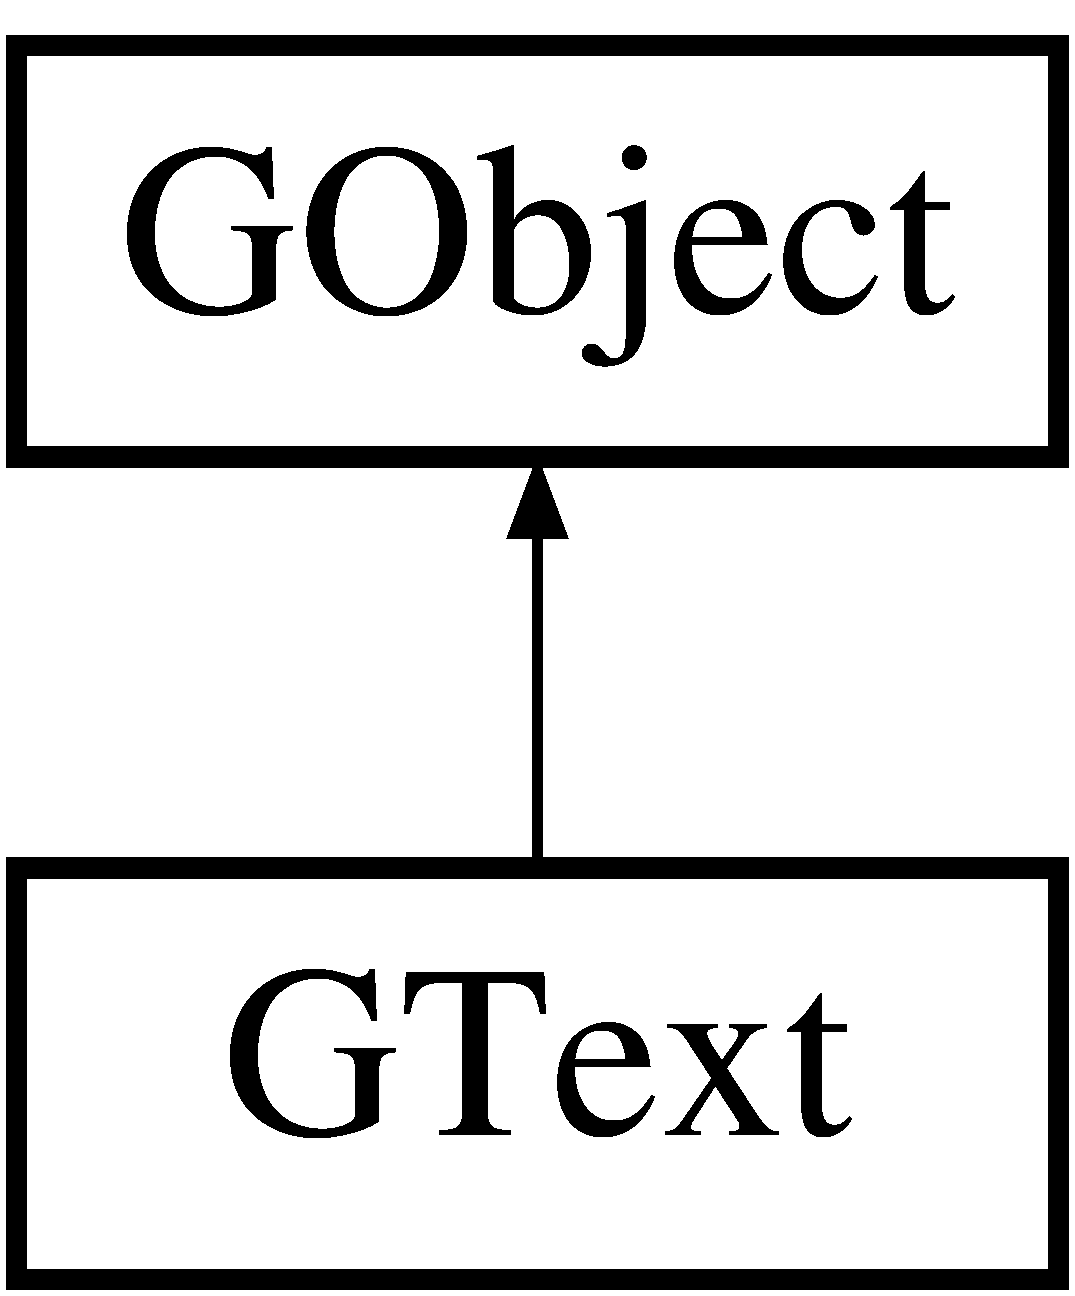
\includegraphics[height=2.000000cm]{classGText}
\end{center}
\end{figure}
\subsection*{Public Types}
\begin{DoxyCompactItemize}
\item 
enum \mbox{\hyperlink{classGObject_a86e0f5648542856159bb40775c854aa7}{Line\+Style}} \{ \mbox{\hyperlink{classGObject_a86e0f5648542856159bb40775c854aa7acbc84bd5232621834ed31f44d457c1eb}{L\+I\+N\+E\+\_\+\+N\+O\+NE}}, 
\mbox{\hyperlink{classGObject_a86e0f5648542856159bb40775c854aa7a700c78bc2cd76acaab26651bf7b4941f}{L\+I\+N\+E\+\_\+\+S\+O\+L\+ID}}, 
\mbox{\hyperlink{classGObject_a86e0f5648542856159bb40775c854aa7a9ccba0845f785d81d07b333ae1aad84e}{L\+I\+N\+E\+\_\+\+D\+A\+SH}}, 
\mbox{\hyperlink{classGObject_a86e0f5648542856159bb40775c854aa7a8e811c096cb941997f0bfda168bb6df3}{L\+I\+N\+E\+\_\+\+D\+OT}}, 
\mbox{\hyperlink{classGObject_a86e0f5648542856159bb40775c854aa7ada15a2e3d737b2db7706d8300f91b89d}{L\+I\+N\+E\+\_\+\+D\+A\+S\+H\+\_\+\+D\+OT}}, 
\mbox{\hyperlink{classGObject_a86e0f5648542856159bb40775c854aa7aabf4053a73eafa7ba2b7e6d664c74c1d}{L\+I\+N\+E\+\_\+\+D\+A\+S\+H\+\_\+\+D\+O\+T\+\_\+\+D\+OT}}
 \}
\begin{DoxyCompactList}\small\item\em Styles that can be used for the outline around various shapes. \end{DoxyCompactList}\end{DoxyCompactItemize}
\subsection*{Public Member Functions}
\begin{DoxyCompactItemize}
\item 
\mbox{\hyperlink{classGText_ad86d52c255aab367ddc6c54baff70846}{G\+Text}} (const std\+::string \&str=\char`\"{}\char`\"{}, double x=0, double y=0)
\begin{DoxyCompactList}\small\item\em Creates a {\ttfamily \mbox{\hyperlink{classGText}{G\+Text}}} object containing the specified string. \end{DoxyCompactList}\item 
virtual bool \mbox{\hyperlink{classGObject_abb6a5d7c03e6eaaae97264c4799ce7c3}{contains}} (double x, double y) const
\begin{DoxyCompactList}\small\item\em Returns {\ttfamily true} if the specified point is inside the object. \end{DoxyCompactList}\item 
virtual bool \mbox{\hyperlink{classGObject_a1dbc9dafaae51958112dbe1267a1f547}{contains}} (const \mbox{\hyperlink{structGPoint}{G\+Point}} \&pt) const
\begin{DoxyCompactList}\small\item\em Returns {\ttfamily true} if the specified point is inside the object. \end{DoxyCompactList}\item 
virtual \mbox{\hyperlink{structGPoint}{G\+Point}} \mbox{\hyperlink{classGObject_a0d41183bf6b08de66fe3907551aab0d7}{get\+Bottom\+Right\+Location}} () const
\begin{DoxyCompactList}\small\item\em Returns the x/y coordinates of the bottom/right corner of the object. \end{DoxyCompactList}\item 
virtual double \mbox{\hyperlink{classGObject_a4316a2406c18e1c6d061fe51fd355490}{get\+BottomY}} () const
\begin{DoxyCompactList}\small\item\em Returns the {\itshape y}-\/coordinate of the bottom of the object. \end{DoxyCompactList}\item 
\mbox{\hyperlink{structGRectangle}{G\+Rectangle}} \mbox{\hyperlink{classGText_a89040ce9277825772d359fccd33bca86}{get\+Bounds}} () const override
\begin{DoxyCompactList}\small\item\em Returns the bounding box of this object, which is defined to be the smallest rectangle that covers everything drawn by the figure. \end{DoxyCompactList}\item 
virtual \mbox{\hyperlink{structGPoint}{G\+Point}} \mbox{\hyperlink{classGObject_a0909472e91448470bccdb62ecfb95d8b}{get\+Center\+Location}} () const
\begin{DoxyCompactList}\small\item\em Returns the x/y-\/coordinates of the center of the object. \end{DoxyCompactList}\item 
virtual double \mbox{\hyperlink{classGObject_a04df74355b545e0543112d5b8d924176}{get\+CenterX}} () const
\begin{DoxyCompactList}\small\item\em Returns the {\itshape x}-\/coordinate of the center of the object. \end{DoxyCompactList}\item 
virtual double \mbox{\hyperlink{classGObject_acb3287a3d507025a26f54b895713b947}{get\+CenterY}} () const
\begin{DoxyCompactList}\small\item\em Returns the {\itshape y}-\/coordinate of the center of the object. \end{DoxyCompactList}\item 
virtual std\+::string \mbox{\hyperlink{classGObject_aa061dfa488c31e18549d64363c1d0e34}{get\+Color}} () const
\begin{DoxyCompactList}\small\item\em Returns the color used to display this object. \end{DoxyCompactList}\item 
virtual std\+::string \mbox{\hyperlink{classGObject_a76f6964a11fde7c78e9751be184e1a3c}{get\+Fill\+Color}} () const
\begin{DoxyCompactList}\small\item\em Returns the color used to display the filled region of this object. \end{DoxyCompactList}\item 
virtual std\+::string \mbox{\hyperlink{classGText_a894a5502900794eeb27d084c21f1d77d}{get\+Font}} () const
\begin{DoxyCompactList}\small\item\em Returns the current font for the label. \end{DoxyCompactList}\item 
virtual double \mbox{\hyperlink{classGText_ab7583914978530e097034293e9d316ad}{get\+Font\+Ascent}} () const
\begin{DoxyCompactList}\small\item\em Returns the maximum distance strings in this font extend above the baseline. \end{DoxyCompactList}\item 
virtual double \mbox{\hyperlink{classGText_a2908216e19046c9747c0fc3b0d088621}{get\+Font\+Descent}} () const
\begin{DoxyCompactList}\small\item\em Returns the maximum distance strings in this font descend below the baseline. \end{DoxyCompactList}\item 
virtual double \mbox{\hyperlink{classGObject_a1e7e353362434072875264cf95629f99}{get\+Height}} () const
\begin{DoxyCompactList}\small\item\em Returns the height of this object, which is the same as the height of its bounding box. \end{DoxyCompactList}\item 
virtual std\+::string \mbox{\hyperlink{classGText_aa73aa351564b091c0658f2368c6d5c5f}{get\+Label}} () const
\begin{DoxyCompactList}\small\item\em Returns the string displayed by this object. \end{DoxyCompactList}\item 
virtual \mbox{\hyperlink{classGObject_a86e0f5648542856159bb40775c854aa7}{Line\+Style}} \mbox{\hyperlink{classGObject_aaf1f5ea8281e5e3486662878d26f0a13}{get\+Line\+Style}} () const
\begin{DoxyCompactList}\small\item\em Returns the object\textquotesingle{}s style such as solid or dashed. \end{DoxyCompactList}\item 
virtual double \mbox{\hyperlink{classGObject_a85ff266dc3eb63d9f2d8e5a4487fd3c0}{get\+Line\+Width}} () const
\begin{DoxyCompactList}\small\item\em Returns the width of the line used to draw this object. \end{DoxyCompactList}\item 
virtual \mbox{\hyperlink{structGPoint}{G\+Point}} \mbox{\hyperlink{classGObject_a4f83802015511edeb63b892830812c11}{get\+Location}} () const
\begin{DoxyCompactList}\small\item\em Returns the location of the top-\/left corner of object. \end{DoxyCompactList}\item 
virtual double \mbox{\hyperlink{classGObject_a1ae3fc278cc5b71b9f2d96a8a83cdf26}{get\+Opacity}} () const
\begin{DoxyCompactList}\small\item\em Returns how opaque (non-\/transparent) this object will appear from 0.\+0 (completely transparent) to 1.\+0 (completely opaque, default). \end{DoxyCompactList}\item 
virtual \mbox{\hyperlink{classGCompound}{G\+Compound}} $\ast$ \mbox{\hyperlink{classGObject_a3e53cef70541b1a14eade4ad0984d0b4}{get\+Parent}} () const
\begin{DoxyCompactList}\small\item\em Returns a pointer to the {\ttfamily \mbox{\hyperlink{classGCompound}{G\+Compound}}} that contains this object. \end{DoxyCompactList}\item 
virtual double \mbox{\hyperlink{classGObject_a798cc79daaa10145b28f60bcdfdb0ee9}{get\+RightX}} () const
\begin{DoxyCompactList}\small\item\em Returns the {\itshape x}-\/coordinate of the right side of the object. \end{DoxyCompactList}\item 
virtual \mbox{\hyperlink{structGDimension}{G\+Dimension}} \mbox{\hyperlink{classGObject_a7b4eec96a2bdc6420695d5796a78eea9}{get\+Size}} () const
\begin{DoxyCompactList}\small\item\em Returns the size of the object as a {\ttfamily \mbox{\hyperlink{structGDimension}{G\+Dimension}}}. \end{DoxyCompactList}\item 
virtual std\+::string \mbox{\hyperlink{classGText_aff553c50924b836c29f146ed34a7c6ec}{get\+Text}} () const
\begin{DoxyCompactList}\small\item\em Returns the string displayed by this object. \end{DoxyCompactList}\item 
std\+::string \mbox{\hyperlink{classGText_a9b72ede4ee8520f987a0c01e30654814}{get\+Type}} () const override
\begin{DoxyCompactList}\small\item\em Returns the type of the object as a string, such as {\ttfamily \char`\"{}\+G\+Oval\char`\"{}} or {\ttfamily \char`\"{}\+G\+Rect\char`\"{}}. \end{DoxyCompactList}\item 
virtual double \mbox{\hyperlink{classGObject_a0ed2965abd4f5701d2cadf71239faf19}{get\+Width}} () const
\begin{DoxyCompactList}\small\item\em Returns the width of this object, which is equal to the width of the bounding box. \end{DoxyCompactList}\item 
virtual double \mbox{\hyperlink{classGObject_a344385751bee0720059403940d57a13e}{getX}} () const
\begin{DoxyCompactList}\small\item\em Returns the leftmost {\itshape x}-\/coordinate of the object. \end{DoxyCompactList}\item 
virtual double \mbox{\hyperlink{classGObject_aafa51c7f8f38a09febbb9ce7853f77b4}{getY}} () const
\begin{DoxyCompactList}\small\item\em Returns the topmost {\itshape y}-\/coordinate of the object. \end{DoxyCompactList}\item 
virtual bool \mbox{\hyperlink{classGObject_a11c404f106940c201b6f326e0355c150}{is\+Filled}} () const
\begin{DoxyCompactList}\small\item\em Returns {\ttfamily true} if the object is filled with color. \end{DoxyCompactList}\item 
virtual bool \mbox{\hyperlink{classGObject_a9de207581cfa4ca1eaa06da5f29b75fc}{is\+Transformed}} () const
\begin{DoxyCompactList}\small\item\em Returns {\ttfamily true} if this object has been transformed by calling methods such as \mbox{\hyperlink{classGObject_ae1ffaa12185dfd5ba464f7d87c329e26}{rotate()}} or \mbox{\hyperlink{classGObject_ad2e1900f730475c2d044817db03b38d6}{scale()}} on it. \end{DoxyCompactList}\item 
virtual bool \mbox{\hyperlink{classGObject_a9d8a6cfb13917785c143e74d40e4e2be}{is\+Visible}} () const
\begin{DoxyCompactList}\small\item\em Returns {\ttfamily true} if this object is visible on screen. \end{DoxyCompactList}\item 
virtual void \mbox{\hyperlink{classGObject_a5973d8dda83afb36e2c56855515be392}{move}} (double dx, double dy)
\begin{DoxyCompactList}\small\item\em Moves the object on the screen using the displacements {\ttfamily dx} and {\ttfamily dy}. \end{DoxyCompactList}\item 
virtual void \mbox{\hyperlink{classGObject_ac827b978aa122f136a14c198687ad80f}{repaint}} ()
\begin{DoxyCompactList}\small\item\em Instructs the object to redraw itself on screen. \end{DoxyCompactList}\item 
virtual void \mbox{\hyperlink{classGObject_a6022a1fd1e5dcd2fd5585e5a36aa3f37}{reset\+Transform}} ()
\begin{DoxyCompactList}\small\item\em Undoes any previous scale/rotate transformations on this object. \end{DoxyCompactList}\item 
virtual void \mbox{\hyperlink{classGObject_ae1ffaa12185dfd5ba464f7d87c329e26}{rotate}} (double theta)
\begin{DoxyCompactList}\small\item\em Transforms the object by rotating it {\ttfamily theta} degrees counterclockwise around its origin. \end{DoxyCompactList}\item 
virtual void \mbox{\hyperlink{classGObject_ad2e1900f730475c2d044817db03b38d6}{scale}} (double sf)
\begin{DoxyCompactList}\small\item\em Scales the object by the specified scale factor. \end{DoxyCompactList}\item 
virtual void \mbox{\hyperlink{classGObject_a63641f69d610d0b951357d35a0c3b1e3}{scale}} (double sx, double sy)
\begin{DoxyCompactList}\small\item\em Scales the object by the specified scale factors. \end{DoxyCompactList}\item 
void \mbox{\hyperlink{classGObject_ab6747f40313c531c2db32edb5b63b9b7}{send\+Backward}} ()
\begin{DoxyCompactList}\small\item\em Moves this object one step toward the back in the {\itshape z} dimension. \end{DoxyCompactList}\item 
void \mbox{\hyperlink{classGObject_a710b3e449c9facba7847c91ab170d281}{send\+Forward}} ()
\begin{DoxyCompactList}\small\item\em Moves this object one step toward the front in the {\itshape z} dimension. \end{DoxyCompactList}\item 
void \mbox{\hyperlink{classGObject_a0f7f1efbb7fd46dde2867c4ad0330896}{send\+To\+Back}} ()
\begin{DoxyCompactList}\small\item\em Moves this object to the back of the display in the {\itshape z} dimension. \end{DoxyCompactList}\item 
void \mbox{\hyperlink{classGObject_aee33d68488e46827ef55fac07f40a9b2}{send\+To\+Front}} ()
\begin{DoxyCompactList}\small\item\em Moves this object to the front of the display in the {\itshape z} dimension. \end{DoxyCompactList}\item 
virtual void \mbox{\hyperlink{classGObject_a71ff7b16b8f1bdc4a1ce9f30cf8b87d8}{set\+Bottom\+Right\+Location}} (double x, double y)
\begin{DoxyCompactList}\small\item\em Sets the location of the bottom/right of this object. \end{DoxyCompactList}\item 
virtual void \mbox{\hyperlink{classGObject_ac6f7320321182f1d18c1c0fa97d5e941}{set\+Bottom\+Right\+Location}} (const \mbox{\hyperlink{structGPoint}{G\+Point}} \&pt)
\begin{DoxyCompactList}\small\item\em Sets the location of the bottom/right of this object. \end{DoxyCompactList}\item 
virtual void \mbox{\hyperlink{classGObject_a4b20e93c2a2597484f74ee5caa71f41f}{set\+BottomY}} (double y)
\begin{DoxyCompactList}\small\item\em Sets the location of the bottom y-\/coordinate of this object. \end{DoxyCompactList}\item 
virtual void \mbox{\hyperlink{classGObject_a2aae8197624b72265ab83b4f1bc73f2f}{set\+Bounds}} (double x, double y, double width, double height)
\begin{DoxyCompactList}\small\item\em Changes the bounds of this object to the specified values. \end{DoxyCompactList}\item 
virtual void \mbox{\hyperlink{classGObject_acada386653f008cacc7cce86426bef7c}{set\+Bounds}} (const \mbox{\hyperlink{structGRectangle}{G\+Rectangle}} \&size)
\begin{DoxyCompactList}\small\item\em Changes the bounds of this object to the specified rectangle. \end{DoxyCompactList}\item 
virtual void \mbox{\hyperlink{classGObject_a290b47dd8de1be44089f95cb2c47c1de}{set\+Center\+Location}} (double x, double y)
\begin{DoxyCompactList}\small\item\em Sets the location of the center of this object. \end{DoxyCompactList}\item 
virtual void \mbox{\hyperlink{classGObject_a1bedf1b233ecba3f753ec58908a683a6}{set\+Center\+Location}} (const \mbox{\hyperlink{structGPoint}{G\+Point}} \&pt)
\begin{DoxyCompactList}\small\item\em Sets the location of the center of this object. \end{DoxyCompactList}\item 
virtual void \mbox{\hyperlink{classGObject_a2f4936281e056eead00a9186b9ba8af6}{set\+CenterX}} (double x)
\begin{DoxyCompactList}\small\item\em Sets the x-\/coordinate of the center of this object. \end{DoxyCompactList}\item 
virtual void \mbox{\hyperlink{classGObject_aad2a22b4fde88c33306b92aebf641d57}{set\+CenterY}} (double y)
\begin{DoxyCompactList}\small\item\em Sets the y-\/coordinate of the center of this object. \end{DoxyCompactList}\item 
virtual void \mbox{\hyperlink{classGObject_ad57ef49bc31db94e92648aa3737923d6}{set\+Color}} (int r, int g, int b)
\begin{DoxyCompactList}\small\item\em Sets the color used to display this object. \end{DoxyCompactList}\item 
virtual void \mbox{\hyperlink{classGObject_ab1f5cc0f5cc6bbbd716a526c61f1081d}{set\+Color}} (int rgb)
\begin{DoxyCompactList}\small\item\em Sets the color used to display this object. \end{DoxyCompactList}\item 
virtual void \mbox{\hyperlink{classGObject_a61374df6c11b52cfbb0815decdbaebc6}{set\+Color}} (const std\+::string \&color)
\begin{DoxyCompactList}\small\item\em Sets the color used to display this object. \end{DoxyCompactList}\item 
virtual void \mbox{\hyperlink{classGObject_ad767a33971159e9493e221cca4c00ae9}{set\+Fill\+Color}} (int r, int g, int b)
\begin{DoxyCompactList}\small\item\em Sets the color used to display the filled region of this object, if any. \end{DoxyCompactList}\item 
virtual void \mbox{\hyperlink{classGObject_aa59d9775a67fa7df2b24a95cd34840a3}{set\+Fill\+Color}} (int rgb)
\begin{DoxyCompactList}\small\item\em Sets the color used to display the filled region of this object, if any. \end{DoxyCompactList}\item 
virtual void \mbox{\hyperlink{classGObject_adbc18b1a930aadd97d7437f9f7265b96}{set\+Fill\+Color}} (const std\+::string \&color)
\begin{DoxyCompactList}\small\item\em Sets the color used to display the filled region of this object, if any. \end{DoxyCompactList}\item 
virtual void \mbox{\hyperlink{classGObject_a9b82b53362282c6bb7d6947068d2e55b}{set\+Filled}} (bool flag)
\begin{DoxyCompactList}\small\item\em Sets the fill status for the object, where {\ttfamily false} is outlined and {\ttfamily true} is filled. \end{DoxyCompactList}\item 
void \mbox{\hyperlink{classGText_ad1d75b3840a41ba7d1e8a921696dc684}{set\+Font}} (const Q\+Font \&font) override
\begin{DoxyCompactList}\small\item\em Changes the font used to display the object as specified by the given Qt font. \end{DoxyCompactList}\item 
void \mbox{\hyperlink{classGText_a51367c9fd2709973b1f7238734f93891}{set\+Font}} (const std\+::string \&font) override
\begin{DoxyCompactList}\small\item\em Changes the font used to display the object as specified by the string {\ttfamily font}, which has the following format\+: \end{DoxyCompactList}\item 
virtual void \mbox{\hyperlink{classGObject_ad18e8fab1e02a4e9b75c6730212558eb}{set\+Foreground}} (int r, int g, int b)
\begin{DoxyCompactList}\small\item\em Sets the color used to display this object. \end{DoxyCompactList}\item 
virtual void \mbox{\hyperlink{classGObject_a9eb856b5ff83a19df3831a31f15f4563}{set\+Foreground}} (int rgb)
\begin{DoxyCompactList}\small\item\em Sets the color used to display this object. \end{DoxyCompactList}\item 
virtual void \mbox{\hyperlink{classGObject_af59209aeadea6dfc6d97a2d8531f50e1}{set\+Foreground}} (const std\+::string \&color)
\begin{DoxyCompactList}\small\item\em Sets the color used to display this object. \end{DoxyCompactList}\item 
virtual void \mbox{\hyperlink{classGObject_a9e280bfc4544dfaf8e4376c4e1a74357}{set\+Height}} (double height)
\begin{DoxyCompactList}\small\item\em Changes the height of this object to the specified height without changing its width. \end{DoxyCompactList}\item 
virtual void \mbox{\hyperlink{classGText_a889d82f199797fea605ee8230dcd4f6f}{set\+Label}} (const std\+::string \&str)
\begin{DoxyCompactList}\small\item\em Changes the string stored within the text label, so that a new text string appears on the display. \end{DoxyCompactList}\item 
virtual void \mbox{\hyperlink{classGObject_add11575087eb94f1a71faa3f826c6341}{set\+Line\+Style}} (\mbox{\hyperlink{classGObject_a86e0f5648542856159bb40775c854aa7}{Line\+Style}} line\+Style)
\begin{DoxyCompactList}\small\item\em Sets the object\textquotesingle{}s style such as solid (\mbox{\hyperlink{classGObject_a86e0f5648542856159bb40775c854aa7a700c78bc2cd76acaab26651bf7b4941f}{G\+Object\+::\+L\+I\+N\+E\+\_\+\+S\+O\+L\+ID}}) or dashed (\mbox{\hyperlink{classGObject_a86e0f5648542856159bb40775c854aa7a9ccba0845f785d81d07b333ae1aad84e}{G\+Object\+::\+L\+I\+N\+E\+\_\+\+D\+A\+SH}}). \end{DoxyCompactList}\item 
virtual void \mbox{\hyperlink{classGObject_afd6a47c6ea6a1f85ca05a65ba3ff3477}{set\+Line\+Width}} (double line\+Width)
\begin{DoxyCompactList}\small\item\em Sets the width of the line used to draw this object. \end{DoxyCompactList}\item 
virtual void \mbox{\hyperlink{classGObject_a04594e8ba9b98513a64f1da00dcae18c}{set\+Location}} (double x, double y)
\begin{DoxyCompactList}\small\item\em Sets the location of the top-\/left corner of this object to the specified coordinates. \end{DoxyCompactList}\item 
virtual void \mbox{\hyperlink{classGObject_aa8480c0b7166cdf8f784cece06ab353f}{set\+Location}} (const \mbox{\hyperlink{structGPoint}{G\+Point}} \&pt)
\begin{DoxyCompactList}\small\item\em Sets the location of the top-\/left corner of this object to the specified point. \end{DoxyCompactList}\item 
virtual void \mbox{\hyperlink{classGObject_a04af1866cc1bae4a1226695794a50539}{set\+Opacity}} (double opacity)
\begin{DoxyCompactList}\small\item\em Sets how opaque (non-\/transparent) this object will appear from 0.\+0 (completely transparent) to 1.\+0 (completely opaque, default). \end{DoxyCompactList}\item 
virtual void \mbox{\hyperlink{classGObject_a3c90b758cdc2c911c9ef76c4360eb912}{set\+RightX}} (double x)
\begin{DoxyCompactList}\small\item\em Sets the location of the rightmost x-\/coordinate of this object. \end{DoxyCompactList}\item 
virtual void \mbox{\hyperlink{classGObject_aca25d49481f9bf5fc8f7df4c086c4ce7}{set\+Size}} (double width, double height)
\begin{DoxyCompactList}\small\item\em Changes the size of this object to the specified width and height. \end{DoxyCompactList}\item 
virtual void \mbox{\hyperlink{classGObject_ae2b628228f192c2702c4ce941b2af68f}{set\+Size}} (const \mbox{\hyperlink{structGDimension}{G\+Dimension}} \&size)
\begin{DoxyCompactList}\small\item\em Changes the size of this object to the specified width and height. \end{DoxyCompactList}\item 
virtual void \mbox{\hyperlink{classGText_ac98cbe102af8aaf8fd017228d645bfda}{set\+Text}} (const std\+::string \&str)
\begin{DoxyCompactList}\small\item\em Changes the string stored within the text label, so that a new text string appears on the display. \end{DoxyCompactList}\item 
virtual void \mbox{\hyperlink{classGObject_a88203f28224315d9f4471212f4af8ed3}{set\+Visible}} (bool flag)
\begin{DoxyCompactList}\small\item\em Sets whether this object is visible. \end{DoxyCompactList}\item 
virtual void \mbox{\hyperlink{classGObject_aa3f3fba4cb131baa8696ba01e3bceca1}{set\+Width}} (double width)
\begin{DoxyCompactList}\small\item\em Changes the width of this object to the specified width without changing its height. \end{DoxyCompactList}\item 
virtual void \mbox{\hyperlink{classGObject_a9c18fcc579333bf9653d13ad2b372e39}{setX}} (double x)
\begin{DoxyCompactList}\small\item\em Sets the x location of the left side of this object. \end{DoxyCompactList}\item 
virtual void \mbox{\hyperlink{classGObject_a7d57e2a5c35d27feb58fd498a3cf82b9}{setY}} (double y)
\begin{DoxyCompactList}\small\item\em Sets the y location of the top of this object. \end{DoxyCompactList}\item 
virtual std\+::string \mbox{\hyperlink{classGObject_a1fe5121d6528fdea3f243321b3fa3a49}{to\+String}} () const
\begin{DoxyCompactList}\small\item\em Returns a printable representation of the object. \end{DoxyCompactList}\item 
std\+::string \mbox{\hyperlink{classGText_a04364e674911906702b748deec32db18}{to\+String\+Extra}} () const override
\begin{DoxyCompactList}\small\item\em Returns a string containing any extra unique information about this type of graphical object. \end{DoxyCompactList}\end{DoxyCompactItemize}
\subsection*{Static Public Member Functions}
\begin{DoxyCompactItemize}
\item 
static bool \mbox{\hyperlink{classGObject_a93be0e1fe1b1bf1a1da732470c94f42b}{is\+Anti\+Aliasing}} ()
\begin{DoxyCompactList}\small\item\em Returns whether we should globally anti-\/alias graphical objects. \end{DoxyCompactList}\item 
static void \mbox{\hyperlink{classGObject_a1e43371668ae850193cebedb44e1bbe3}{set\+Anti\+Aliasing}} (bool value)
\begin{DoxyCompactList}\small\item\em Globally turns on/off the anti-\/aliasing feature that smooths out the edges of onscreen shapes. \end{DoxyCompactList}\end{DoxyCompactItemize}
\subsection*{Static Public Attributes}
\begin{DoxyCompactItemize}
\item 
static const std\+::string \mbox{\hyperlink{classGText_ab265ee508af32c0c0bb1aa3693977247}{D\+E\+F\+A\+U\+L\+T\+\_\+\+F\+O\+NT}} = \char`\"{}Dialog-\/13\char`\"{}
\begin{DoxyCompactList}\small\item\em The default font used in text labels if none is provided. \end{DoxyCompactList}\end{DoxyCompactItemize}
\subsection*{Protected Attributes}
\begin{DoxyCompactItemize}
\item 
Q\+Brush \mbox{\hyperlink{classGObject_aab24462ec896b596d99911767b0912d0}{\+\_\+brush}}
\item 
std\+::string \mbox{\hyperlink{classGObject_a1134e770ae4315ea8bc1201e2f21da8b}{\+\_\+color}}
\item 
int \mbox{\hyperlink{classGObject_a003fdd343d9b7505c53a8b7a134200ed}{\+\_\+color\+Int}}
\item 
std\+::string \mbox{\hyperlink{classGObject_a179f8d6cee65cd8a54692e32b224392a}{\+\_\+fill\+Color}}
\item 
int \mbox{\hyperlink{classGObject_a751def333a67d651e5b99cc331ecb496}{\+\_\+fill\+Color\+Int}}
\item 
bool \mbox{\hyperlink{classGObject_ad4a55cbcd61b58a4d49666490bb2f103}{\+\_\+fill\+Flag}}
\item 
std\+::string \mbox{\hyperlink{classGObject_aea76ea1a8b5dd7b0a78653277e63b536}{\+\_\+font}}
\item 
double \mbox{\hyperlink{classGObject_ad05df29e7f27fc504abd743e3d8b4e73}{\+\_\+height}}
\item 
\mbox{\hyperlink{classGObject_a86e0f5648542856159bb40775c854aa7}{Line\+Style}} \mbox{\hyperlink{classGObject_a89bafecaafb7c72d55c7efc10b7d0523}{\+\_\+line\+Style}}
\item 
double \mbox{\hyperlink{classGObject_a16e9033665937f13de2e163dc2184aff}{\+\_\+line\+Width}}
\item 
double \mbox{\hyperlink{classGObject_a20eff8eb7af27182edc9bfc54768b6f3}{\+\_\+opacity}}
\item 
\mbox{\hyperlink{classGCompound}{G\+Compound}} $\ast$ \mbox{\hyperlink{classGObject_ac9452c1eaff70eebddbb318196aa3835}{\+\_\+parent}}
\item 
Q\+Pen \mbox{\hyperlink{classGObject_afb69d172743f868299847174eb1b6bc8}{\+\_\+pen}}
\item 
Q\+Transform \mbox{\hyperlink{classGObject_a475b8860a5f1adb4a1fdc58d1f5c1e32}{\+\_\+transform}}
\item 
bool \mbox{\hyperlink{classGObject_ae4725802fc8d8aaa0ab4bd4781f7e07c}{\+\_\+transformed}}
\item 
bool \mbox{\hyperlink{classGObject_a9312c72508471b7c7a87b540263e1af4}{\+\_\+visible}}
\item 
double \mbox{\hyperlink{classGObject_ab55d85a3371770e6725b1062cf160cd8}{\+\_\+width}}
\item 
double \mbox{\hyperlink{classGObject_a6675b83b27137b8d3aa2ad8133078ea6}{\+\_\+x}}
\item 
double \mbox{\hyperlink{classGObject_a2f0f6aeafddc8a39c578bfa7e22b5f1e}{\+\_\+y}}
\end{DoxyCompactItemize}


\subsection{Detailed Description}
This graphical object subclass represents a text string. 

Controlling the appearance and positioning of a {\ttfamily \mbox{\hyperlink{classGText}{G\+Text}}} depends on understanding the following terms\+:


\begin{DoxyItemize}
\item The {\bfseries {\itshape baseline}} is the horizontal line on which the characters rest. 
\item The {\bfseries {\itshape origin}} is the point on the baseline at which the label begins. 
\item The {\bfseries {\itshape height}} is the distance that separate two successive lines. 
\item The {\bfseries {\itshape ascent}} is the maximum distance a character in this font extends above the baseline. 
\item The {\bfseries {\itshape descent}} is the maximum distance a character in this font extends below the baseline. 
\end{DoxyItemize}

\subsection{Member Enumeration Documentation}
\mbox{\Hypertarget{classGObject_a86e0f5648542856159bb40775c854aa7}\label{classGObject_a86e0f5648542856159bb40775c854aa7}} 
\index{G\+Text@{G\+Text}!Line\+Style@{Line\+Style}}
\index{Line\+Style@{Line\+Style}!G\+Text@{G\+Text}}
\subsubsection{\texorpdfstring{Line\+Style}{LineStyle}}
{\footnotesize\ttfamily enum \mbox{\hyperlink{classGObject_a86e0f5648542856159bb40775c854aa7}{Line\+Style}}\hspace{0.3cm}{\ttfamily [inherited]}}



Styles that can be used for the outline around various shapes. 

Call set\+Line\+Style on a \mbox{\hyperlink{classGObject}{G\+Object}} and pass one of these values. \begin{DoxyEnumFields}{Enumerator}
\raisebox{\heightof{T}}[0pt][0pt]{\index{L\+I\+N\+E\+\_\+\+N\+O\+NE@{L\+I\+N\+E\+\_\+\+N\+O\+NE}!G\+Text@{G\+Text}}\index{G\+Text@{G\+Text}!L\+I\+N\+E\+\_\+\+N\+O\+NE@{L\+I\+N\+E\+\_\+\+N\+O\+NE}}}\mbox{\Hypertarget{classGObject_a86e0f5648542856159bb40775c854aa7acbc84bd5232621834ed31f44d457c1eb}\label{classGObject_a86e0f5648542856159bb40775c854aa7acbc84bd5232621834ed31f44d457c1eb}} 
L\+I\+N\+E\+\_\+\+N\+O\+NE&\\
\hline

\raisebox{\heightof{T}}[0pt][0pt]{\index{L\+I\+N\+E\+\_\+\+S\+O\+L\+ID@{L\+I\+N\+E\+\_\+\+S\+O\+L\+ID}!G\+Text@{G\+Text}}\index{G\+Text@{G\+Text}!L\+I\+N\+E\+\_\+\+S\+O\+L\+ID@{L\+I\+N\+E\+\_\+\+S\+O\+L\+ID}}}\mbox{\Hypertarget{classGObject_a86e0f5648542856159bb40775c854aa7a700c78bc2cd76acaab26651bf7b4941f}\label{classGObject_a86e0f5648542856159bb40775c854aa7a700c78bc2cd76acaab26651bf7b4941f}} 
L\+I\+N\+E\+\_\+\+S\+O\+L\+ID&\\
\hline

\raisebox{\heightof{T}}[0pt][0pt]{\index{L\+I\+N\+E\+\_\+\+D\+A\+SH@{L\+I\+N\+E\+\_\+\+D\+A\+SH}!G\+Text@{G\+Text}}\index{G\+Text@{G\+Text}!L\+I\+N\+E\+\_\+\+D\+A\+SH@{L\+I\+N\+E\+\_\+\+D\+A\+SH}}}\mbox{\Hypertarget{classGObject_a86e0f5648542856159bb40775c854aa7a9ccba0845f785d81d07b333ae1aad84e}\label{classGObject_a86e0f5648542856159bb40775c854aa7a9ccba0845f785d81d07b333ae1aad84e}} 
L\+I\+N\+E\+\_\+\+D\+A\+SH&\\
\hline

\raisebox{\heightof{T}}[0pt][0pt]{\index{L\+I\+N\+E\+\_\+\+D\+OT@{L\+I\+N\+E\+\_\+\+D\+OT}!G\+Text@{G\+Text}}\index{G\+Text@{G\+Text}!L\+I\+N\+E\+\_\+\+D\+OT@{L\+I\+N\+E\+\_\+\+D\+OT}}}\mbox{\Hypertarget{classGObject_a86e0f5648542856159bb40775c854aa7a8e811c096cb941997f0bfda168bb6df3}\label{classGObject_a86e0f5648542856159bb40775c854aa7a8e811c096cb941997f0bfda168bb6df3}} 
L\+I\+N\+E\+\_\+\+D\+OT&\\
\hline

\raisebox{\heightof{T}}[0pt][0pt]{\index{L\+I\+N\+E\+\_\+\+D\+A\+S\+H\+\_\+\+D\+OT@{L\+I\+N\+E\+\_\+\+D\+A\+S\+H\+\_\+\+D\+OT}!G\+Text@{G\+Text}}\index{G\+Text@{G\+Text}!L\+I\+N\+E\+\_\+\+D\+A\+S\+H\+\_\+\+D\+OT@{L\+I\+N\+E\+\_\+\+D\+A\+S\+H\+\_\+\+D\+OT}}}\mbox{\Hypertarget{classGObject_a86e0f5648542856159bb40775c854aa7ada15a2e3d737b2db7706d8300f91b89d}\label{classGObject_a86e0f5648542856159bb40775c854aa7ada15a2e3d737b2db7706d8300f91b89d}} 
L\+I\+N\+E\+\_\+\+D\+A\+S\+H\+\_\+\+D\+OT&\\
\hline

\raisebox{\heightof{T}}[0pt][0pt]{\index{L\+I\+N\+E\+\_\+\+D\+A\+S\+H\+\_\+\+D\+O\+T\+\_\+\+D\+OT@{L\+I\+N\+E\+\_\+\+D\+A\+S\+H\+\_\+\+D\+O\+T\+\_\+\+D\+OT}!G\+Text@{G\+Text}}\index{G\+Text@{G\+Text}!L\+I\+N\+E\+\_\+\+D\+A\+S\+H\+\_\+\+D\+O\+T\+\_\+\+D\+OT@{L\+I\+N\+E\+\_\+\+D\+A\+S\+H\+\_\+\+D\+O\+T\+\_\+\+D\+OT}}}\mbox{\Hypertarget{classGObject_a86e0f5648542856159bb40775c854aa7aabf4053a73eafa7ba2b7e6d664c74c1d}\label{classGObject_a86e0f5648542856159bb40775c854aa7aabf4053a73eafa7ba2b7e6d664c74c1d}} 
L\+I\+N\+E\+\_\+\+D\+A\+S\+H\+\_\+\+D\+O\+T\+\_\+\+D\+OT&\\
\hline

\end{DoxyEnumFields}


\subsection{Constructor \& Destructor Documentation}
\mbox{\Hypertarget{classGText_ad86d52c255aab367ddc6c54baff70846}\label{classGText_ad86d52c255aab367ddc6c54baff70846}} 
\index{G\+Text@{G\+Text}!G\+Text@{G\+Text}}
\index{G\+Text@{G\+Text}!G\+Text@{G\+Text}}
\subsubsection{\texorpdfstring{G\+Text()}{GText()}}
{\footnotesize\ttfamily \mbox{\hyperlink{classGText}{G\+Text}} (\begin{DoxyParamCaption}\item[{const std\+::string \&}]{str = {\ttfamily \char`\"{}\char`\"{}},  }\item[{double}]{x = {\ttfamily 0},  }\item[{double}]{y = {\ttfamily 0} }\end{DoxyParamCaption})}



Creates a {\ttfamily \mbox{\hyperlink{classGText}{G\+Text}}} object containing the specified string. 

By default, the baseline of the first character appears at the origin; the second form automatically resets the location of the {\ttfamily \mbox{\hyperlink{classGText}{G\+Text}}} to the point ({\ttfamily x}, {\ttfamily y}). 

\subsection{Member Function Documentation}
\mbox{\Hypertarget{classGObject_abb6a5d7c03e6eaaae97264c4799ce7c3}\label{classGObject_abb6a5d7c03e6eaaae97264c4799ce7c3}} 
\index{G\+Text@{G\+Text}!contains@{contains}}
\index{contains@{contains}!G\+Text@{G\+Text}}
\subsubsection{\texorpdfstring{contains()}{contains()}\hspace{0.1cm}{\footnotesize\ttfamily [1/2]}}
{\footnotesize\ttfamily bool contains (\begin{DoxyParamCaption}\item[{double}]{x,  }\item[{double}]{y }\end{DoxyParamCaption}) const\hspace{0.3cm}{\ttfamily [virtual]}, {\ttfamily [inherited]}}



Returns {\ttfamily true} if the specified point is inside the object. 



Reimplemented in \mbox{\hyperlink{classGRoundRect_ad973a1d55799d3a73bf8b04986cd804e}{G\+Round\+Rect}}, \mbox{\hyperlink{classGPolygon_ad973a1d55799d3a73bf8b04986cd804e}{G\+Polygon}}, \mbox{\hyperlink{classGOval_ad973a1d55799d3a73bf8b04986cd804e}{G\+Oval}}, \mbox{\hyperlink{classGLine_ad973a1d55799d3a73bf8b04986cd804e}{G\+Line}}, \mbox{\hyperlink{classGCompound_ad973a1d55799d3a73bf8b04986cd804e}{G\+Compound}}, and \mbox{\hyperlink{classGArc_ad973a1d55799d3a73bf8b04986cd804e}{G\+Arc}}.

\mbox{\Hypertarget{classGObject_a1dbc9dafaae51958112dbe1267a1f547}\label{classGObject_a1dbc9dafaae51958112dbe1267a1f547}} 
\index{G\+Text@{G\+Text}!contains@{contains}}
\index{contains@{contains}!G\+Text@{G\+Text}}
\subsubsection{\texorpdfstring{contains()}{contains()}\hspace{0.1cm}{\footnotesize\ttfamily [2/2]}}
{\footnotesize\ttfamily bool contains (\begin{DoxyParamCaption}\item[{const \mbox{\hyperlink{structGPoint}{G\+Point}} \&}]{pt }\end{DoxyParamCaption}) const\hspace{0.3cm}{\ttfamily [virtual]}, {\ttfamily [inherited]}}



Returns {\ttfamily true} if the specified point is inside the object. 

\mbox{\Hypertarget{classGObject_a0d41183bf6b08de66fe3907551aab0d7}\label{classGObject_a0d41183bf6b08de66fe3907551aab0d7}} 
\index{G\+Text@{G\+Text}!get\+Bottom\+Right\+Location@{get\+Bottom\+Right\+Location}}
\index{get\+Bottom\+Right\+Location@{get\+Bottom\+Right\+Location}!G\+Text@{G\+Text}}
\subsubsection{\texorpdfstring{get\+Bottom\+Right\+Location()}{getBottomRightLocation()}}
{\footnotesize\ttfamily \mbox{\hyperlink{structGPoint}{G\+Point}} get\+Bottom\+Right\+Location (\begin{DoxyParamCaption}{ }\end{DoxyParamCaption}) const\hspace{0.3cm}{\ttfamily [virtual]}, {\ttfamily [inherited]}}



Returns the x/y coordinates of the bottom/right corner of the object. 

\mbox{\Hypertarget{classGObject_a4316a2406c18e1c6d061fe51fd355490}\label{classGObject_a4316a2406c18e1c6d061fe51fd355490}} 
\index{G\+Text@{G\+Text}!get\+BottomY@{get\+BottomY}}
\index{get\+BottomY@{get\+BottomY}!G\+Text@{G\+Text}}
\subsubsection{\texorpdfstring{get\+Bottom\+Y()}{getBottomY()}}
{\footnotesize\ttfamily double get\+BottomY (\begin{DoxyParamCaption}{ }\end{DoxyParamCaption}) const\hspace{0.3cm}{\ttfamily [virtual]}, {\ttfamily [inherited]}}



Returns the {\itshape y}-\/coordinate of the bottom of the object. 

Equivalent to the top y-\/coordinate plus the object\textquotesingle{}s height. \mbox{\Hypertarget{classGText_a89040ce9277825772d359fccd33bca86}\label{classGText_a89040ce9277825772d359fccd33bca86}} 
\index{G\+Text@{G\+Text}!get\+Bounds@{get\+Bounds}}
\index{get\+Bounds@{get\+Bounds}!G\+Text@{G\+Text}}
\subsubsection{\texorpdfstring{get\+Bounds()}{getBounds()}}
{\footnotesize\ttfamily \mbox{\hyperlink{structGRectangle}{G\+Rectangle}} get\+Bounds (\begin{DoxyParamCaption}{ }\end{DoxyParamCaption}) const\hspace{0.3cm}{\ttfamily [override]}, {\ttfamily [virtual]}}



Returns the bounding box of this object, which is defined to be the smallest rectangle that covers everything drawn by the figure. 

The coordinates of this rectangle do not necessarily match the location returned by {\ttfamily get\+Location}. Given a {\ttfamily \mbox{\hyperlink{classGText}{G\+Text}}} object, for example, {\ttfamily get\+Location} returns the coordinates of the point on the baseline at which the string begins; the {\ttfamily get\+Bounds} method, by contrast, returns a rectangle that covers the entire window area occupied by the string. 

Reimplemented from \mbox{\hyperlink{classGObject_a29e6ac35a0b48f491a4c88194cc5da3b}{G\+Object}}.

\mbox{\Hypertarget{classGObject_a0909472e91448470bccdb62ecfb95d8b}\label{classGObject_a0909472e91448470bccdb62ecfb95d8b}} 
\index{G\+Text@{G\+Text}!get\+Center\+Location@{get\+Center\+Location}}
\index{get\+Center\+Location@{get\+Center\+Location}!G\+Text@{G\+Text}}
\subsubsection{\texorpdfstring{get\+Center\+Location()}{getCenterLocation()}}
{\footnotesize\ttfamily \mbox{\hyperlink{structGPoint}{G\+Point}} get\+Center\+Location (\begin{DoxyParamCaption}{ }\end{DoxyParamCaption}) const\hspace{0.3cm}{\ttfamily [virtual]}, {\ttfamily [inherited]}}



Returns the x/y-\/coordinates of the center of the object. 

Equivalent to the top/left plus half the object\textquotesingle{}s size. \mbox{\Hypertarget{classGObject_a04df74355b545e0543112d5b8d924176}\label{classGObject_a04df74355b545e0543112d5b8d924176}} 
\index{G\+Text@{G\+Text}!get\+CenterX@{get\+CenterX}}
\index{get\+CenterX@{get\+CenterX}!G\+Text@{G\+Text}}
\subsubsection{\texorpdfstring{get\+Center\+X()}{getCenterX()}}
{\footnotesize\ttfamily double get\+CenterX (\begin{DoxyParamCaption}{ }\end{DoxyParamCaption}) const\hspace{0.3cm}{\ttfamily [virtual]}, {\ttfamily [inherited]}}



Returns the {\itshape x}-\/coordinate of the center of the object. 

Equivalent to the top/left plus half the object\textquotesingle{}s width. \mbox{\Hypertarget{classGObject_acb3287a3d507025a26f54b895713b947}\label{classGObject_acb3287a3d507025a26f54b895713b947}} 
\index{G\+Text@{G\+Text}!get\+CenterY@{get\+CenterY}}
\index{get\+CenterY@{get\+CenterY}!G\+Text@{G\+Text}}
\subsubsection{\texorpdfstring{get\+Center\+Y()}{getCenterY()}}
{\footnotesize\ttfamily double get\+CenterY (\begin{DoxyParamCaption}{ }\end{DoxyParamCaption}) const\hspace{0.3cm}{\ttfamily [virtual]}, {\ttfamily [inherited]}}



Returns the {\itshape y}-\/coordinate of the center of the object. 

Equivalent to the top/left plus half the object\textquotesingle{}s height. \mbox{\Hypertarget{classGObject_aa061dfa488c31e18549d64363c1d0e34}\label{classGObject_aa061dfa488c31e18549d64363c1d0e34}} 
\index{G\+Text@{G\+Text}!get\+Color@{get\+Color}}
\index{get\+Color@{get\+Color}!G\+Text@{G\+Text}}
\subsubsection{\texorpdfstring{get\+Color()}{getColor()}}
{\footnotesize\ttfamily std\+::string get\+Color (\begin{DoxyParamCaption}{ }\end{DoxyParamCaption}) const\hspace{0.3cm}{\ttfamily [virtual]}, {\ttfamily [inherited]}}



Returns the color used to display this object. 

This color is always returned as a string in the form {\ttfamily \char`\"{}\#rrggbb\char`\"{}}, where {\ttfamily rr}, {\ttfamily gg}, and {\ttfamily bb} are the red, green, and blue components of the color, expressed as two-\/digit hexadecimal values. \mbox{\Hypertarget{classGObject_a76f6964a11fde7c78e9751be184e1a3c}\label{classGObject_a76f6964a11fde7c78e9751be184e1a3c}} 
\index{G\+Text@{G\+Text}!get\+Fill\+Color@{get\+Fill\+Color}}
\index{get\+Fill\+Color@{get\+Fill\+Color}!G\+Text@{G\+Text}}
\subsubsection{\texorpdfstring{get\+Fill\+Color()}{getFillColor()}}
{\footnotesize\ttfamily std\+::string get\+Fill\+Color (\begin{DoxyParamCaption}{ }\end{DoxyParamCaption}) const\hspace{0.3cm}{\ttfamily [virtual]}, {\ttfamily [inherited]}}



Returns the color used to display the filled region of this object. 

If none has been set, returns the empty string. \mbox{\Hypertarget{classGText_a894a5502900794eeb27d084c21f1d77d}\label{classGText_a894a5502900794eeb27d084c21f1d77d}} 
\index{G\+Text@{G\+Text}!get\+Font@{get\+Font}}
\index{get\+Font@{get\+Font}!G\+Text@{G\+Text}}
\subsubsection{\texorpdfstring{get\+Font()}{getFont()}}
{\footnotesize\ttfamily std\+::string get\+Font (\begin{DoxyParamCaption}{ }\end{DoxyParamCaption}) const\hspace{0.3cm}{\ttfamily [virtual]}}



Returns the current font for the label. 

\mbox{\Hypertarget{classGText_ab7583914978530e097034293e9d316ad}\label{classGText_ab7583914978530e097034293e9d316ad}} 
\index{G\+Text@{G\+Text}!get\+Font\+Ascent@{get\+Font\+Ascent}}
\index{get\+Font\+Ascent@{get\+Font\+Ascent}!G\+Text@{G\+Text}}
\subsubsection{\texorpdfstring{get\+Font\+Ascent()}{getFontAscent()}}
{\footnotesize\ttfamily double get\+Font\+Ascent (\begin{DoxyParamCaption}{ }\end{DoxyParamCaption}) const\hspace{0.3cm}{\ttfamily [virtual]}}



Returns the maximum distance strings in this font extend above the baseline. 

\mbox{\Hypertarget{classGText_a2908216e19046c9747c0fc3b0d088621}\label{classGText_a2908216e19046c9747c0fc3b0d088621}} 
\index{G\+Text@{G\+Text}!get\+Font\+Descent@{get\+Font\+Descent}}
\index{get\+Font\+Descent@{get\+Font\+Descent}!G\+Text@{G\+Text}}
\subsubsection{\texorpdfstring{get\+Font\+Descent()}{getFontDescent()}}
{\footnotesize\ttfamily double get\+Font\+Descent (\begin{DoxyParamCaption}{ }\end{DoxyParamCaption}) const\hspace{0.3cm}{\ttfamily [virtual]}}



Returns the maximum distance strings in this font descend below the baseline. 

\mbox{\Hypertarget{classGObject_a1e7e353362434072875264cf95629f99}\label{classGObject_a1e7e353362434072875264cf95629f99}} 
\index{G\+Text@{G\+Text}!get\+Height@{get\+Height}}
\index{get\+Height@{get\+Height}!G\+Text@{G\+Text}}
\subsubsection{\texorpdfstring{get\+Height()}{getHeight()}}
{\footnotesize\ttfamily double get\+Height (\begin{DoxyParamCaption}{ }\end{DoxyParamCaption}) const\hspace{0.3cm}{\ttfamily [virtual]}, {\ttfamily [inherited]}}



Returns the height of this object, which is the same as the height of its bounding box. 



Reimplemented in \mbox{\hyperlink{classGPolygon_a2bede8b27b21ae4c7940e762cbad9e07}{G\+Polygon}}, and \mbox{\hyperlink{classGLine_a2bede8b27b21ae4c7940e762cbad9e07}{G\+Line}}.

\mbox{\Hypertarget{classGText_aa73aa351564b091c0658f2368c6d5c5f}\label{classGText_aa73aa351564b091c0658f2368c6d5c5f}} 
\index{G\+Text@{G\+Text}!get\+Label@{get\+Label}}
\index{get\+Label@{get\+Label}!G\+Text@{G\+Text}}
\subsubsection{\texorpdfstring{get\+Label()}{getLabel()}}
{\footnotesize\ttfamily std\+::string get\+Label (\begin{DoxyParamCaption}{ }\end{DoxyParamCaption}) const\hspace{0.3cm}{\ttfamily [virtual]}}



Returns the string displayed by this object. 

Equivalent to get\+Label. \mbox{\Hypertarget{classGObject_aaf1f5ea8281e5e3486662878d26f0a13}\label{classGObject_aaf1f5ea8281e5e3486662878d26f0a13}} 
\index{G\+Text@{G\+Text}!get\+Line\+Style@{get\+Line\+Style}}
\index{get\+Line\+Style@{get\+Line\+Style}!G\+Text@{G\+Text}}
\subsubsection{\texorpdfstring{get\+Line\+Style()}{getLineStyle()}}
{\footnotesize\ttfamily \mbox{\hyperlink{classGObject_a86e0f5648542856159bb40775c854aa7}{G\+Object\+::\+Line\+Style}} get\+Line\+Style (\begin{DoxyParamCaption}{ }\end{DoxyParamCaption}) const\hspace{0.3cm}{\ttfamily [virtual]}, {\ttfamily [inherited]}}



Returns the object\textquotesingle{}s style such as solid or dashed. 

\mbox{\Hypertarget{classGObject_a85ff266dc3eb63d9f2d8e5a4487fd3c0}\label{classGObject_a85ff266dc3eb63d9f2d8e5a4487fd3c0}} 
\index{G\+Text@{G\+Text}!get\+Line\+Width@{get\+Line\+Width}}
\index{get\+Line\+Width@{get\+Line\+Width}!G\+Text@{G\+Text}}
\subsubsection{\texorpdfstring{get\+Line\+Width()}{getLineWidth()}}
{\footnotesize\ttfamily double get\+Line\+Width (\begin{DoxyParamCaption}{ }\end{DoxyParamCaption}) const\hspace{0.3cm}{\ttfamily [virtual]}, {\ttfamily [inherited]}}



Returns the width of the line used to draw this object. 

\begin{DoxyReturn}{Returns}
default 1 
\end{DoxyReturn}
\mbox{\Hypertarget{classGObject_a4f83802015511edeb63b892830812c11}\label{classGObject_a4f83802015511edeb63b892830812c11}} 
\index{G\+Text@{G\+Text}!get\+Location@{get\+Location}}
\index{get\+Location@{get\+Location}!G\+Text@{G\+Text}}
\subsubsection{\texorpdfstring{get\+Location()}{getLocation()}}
{\footnotesize\ttfamily \mbox{\hyperlink{structGPoint}{G\+Point}} get\+Location (\begin{DoxyParamCaption}{ }\end{DoxyParamCaption}) const\hspace{0.3cm}{\ttfamily [virtual]}, {\ttfamily [inherited]}}



Returns the location of the top-\/left corner of object. 

\mbox{\Hypertarget{classGObject_a1ae3fc278cc5b71b9f2d96a8a83cdf26}\label{classGObject_a1ae3fc278cc5b71b9f2d96a8a83cdf26}} 
\index{G\+Text@{G\+Text}!get\+Opacity@{get\+Opacity}}
\index{get\+Opacity@{get\+Opacity}!G\+Text@{G\+Text}}
\subsubsection{\texorpdfstring{get\+Opacity()}{getOpacity()}}
{\footnotesize\ttfamily double get\+Opacity (\begin{DoxyParamCaption}{ }\end{DoxyParamCaption}) const\hspace{0.3cm}{\ttfamily [virtual]}, {\ttfamily [inherited]}}



Returns how opaque (non-\/transparent) this object will appear from 0.\+0 (completely transparent) to 1.\+0 (completely opaque, default). 

\mbox{\Hypertarget{classGObject_a3e53cef70541b1a14eade4ad0984d0b4}\label{classGObject_a3e53cef70541b1a14eade4ad0984d0b4}} 
\index{G\+Text@{G\+Text}!get\+Parent@{get\+Parent}}
\index{get\+Parent@{get\+Parent}!G\+Text@{G\+Text}}
\subsubsection{\texorpdfstring{get\+Parent()}{getParent()}}
{\footnotesize\ttfamily \mbox{\hyperlink{classGCompound}{G\+Compound}} $\ast$ get\+Parent (\begin{DoxyParamCaption}{ }\end{DoxyParamCaption}) const\hspace{0.3cm}{\ttfamily [virtual]}, {\ttfamily [inherited]}}



Returns a pointer to the {\ttfamily \mbox{\hyperlink{classGCompound}{G\+Compound}}} that contains this object. 

Every {\ttfamily \mbox{\hyperlink{classGWindow}{G\+Window}}} is initialized to contain a single {\ttfamily \mbox{\hyperlink{classGCompound}{G\+Compound}}} that is aligned with the window. Adding objects to the window adds them to that {\ttfamily \mbox{\hyperlink{classGCompound}{G\+Compound}}}, which means that every object you add to the window has a parent. Calling {\ttfamily get\+Parent} on the top-\/level {\ttfamily \mbox{\hyperlink{classGCompound}{G\+Compound}}} returns {\ttfamily nullptr}. \mbox{\Hypertarget{classGObject_a798cc79daaa10145b28f60bcdfdb0ee9}\label{classGObject_a798cc79daaa10145b28f60bcdfdb0ee9}} 
\index{G\+Text@{G\+Text}!get\+RightX@{get\+RightX}}
\index{get\+RightX@{get\+RightX}!G\+Text@{G\+Text}}
\subsubsection{\texorpdfstring{get\+Right\+X()}{getRightX()}}
{\footnotesize\ttfamily double get\+RightX (\begin{DoxyParamCaption}{ }\end{DoxyParamCaption}) const\hspace{0.3cm}{\ttfamily [virtual]}, {\ttfamily [inherited]}}



Returns the {\itshape x}-\/coordinate of the right side of the object. 

Equivalent to the left x-\/coordinate plus the object\textquotesingle{}s width. \mbox{\Hypertarget{classGObject_a7b4eec96a2bdc6420695d5796a78eea9}\label{classGObject_a7b4eec96a2bdc6420695d5796a78eea9}} 
\index{G\+Text@{G\+Text}!get\+Size@{get\+Size}}
\index{get\+Size@{get\+Size}!G\+Text@{G\+Text}}
\subsubsection{\texorpdfstring{get\+Size()}{getSize()}}
{\footnotesize\ttfamily \mbox{\hyperlink{structGDimension}{G\+Dimension}} get\+Size (\begin{DoxyParamCaption}{ }\end{DoxyParamCaption}) const\hspace{0.3cm}{\ttfamily [virtual]}, {\ttfamily [inherited]}}



Returns the size of the object as a {\ttfamily \mbox{\hyperlink{structGDimension}{G\+Dimension}}}. 

\mbox{\Hypertarget{classGText_aff553c50924b836c29f146ed34a7c6ec}\label{classGText_aff553c50924b836c29f146ed34a7c6ec}} 
\index{G\+Text@{G\+Text}!get\+Text@{get\+Text}}
\index{get\+Text@{get\+Text}!G\+Text@{G\+Text}}
\subsubsection{\texorpdfstring{get\+Text()}{getText()}}
{\footnotesize\ttfamily std\+::string get\+Text (\begin{DoxyParamCaption}{ }\end{DoxyParamCaption}) const\hspace{0.3cm}{\ttfamily [virtual]}}



Returns the string displayed by this object. 

Equivalent to get\+Label. \mbox{\Hypertarget{classGText_a9b72ede4ee8520f987a0c01e30654814}\label{classGText_a9b72ede4ee8520f987a0c01e30654814}} 
\index{G\+Text@{G\+Text}!get\+Type@{get\+Type}}
\index{get\+Type@{get\+Type}!G\+Text@{G\+Text}}
\subsubsection{\texorpdfstring{get\+Type()}{getType()}}
{\footnotesize\ttfamily std\+::string get\+Type (\begin{DoxyParamCaption}{ }\end{DoxyParamCaption}) const\hspace{0.3cm}{\ttfamily [override]}, {\ttfamily [virtual]}}



Returns the type of the object as a string, such as {\ttfamily \char`\"{}\+G\+Oval\char`\"{}} or {\ttfamily \char`\"{}\+G\+Rect\char`\"{}}. 

Each \mbox{\hyperlink{classGObject}{G\+Object}} subtype must override this method. 

Implements \mbox{\hyperlink{classGObject_a799e073a127b428cc841086d42ea4fed}{G\+Object}}.

\mbox{\Hypertarget{classGObject_a0ed2965abd4f5701d2cadf71239faf19}\label{classGObject_a0ed2965abd4f5701d2cadf71239faf19}} 
\index{G\+Text@{G\+Text}!get\+Width@{get\+Width}}
\index{get\+Width@{get\+Width}!G\+Text@{G\+Text}}
\subsubsection{\texorpdfstring{get\+Width()}{getWidth()}}
{\footnotesize\ttfamily double get\+Width (\begin{DoxyParamCaption}{ }\end{DoxyParamCaption}) const\hspace{0.3cm}{\ttfamily [virtual]}, {\ttfamily [inherited]}}



Returns the width of this object, which is equal to the width of the bounding box. 



Reimplemented in \mbox{\hyperlink{classGPolygon_ab7b172cec7ed45e1246a3ce3160a62f7}{G\+Polygon}}, and \mbox{\hyperlink{classGLine_ab7b172cec7ed45e1246a3ce3160a62f7}{G\+Line}}.

\mbox{\Hypertarget{classGObject_a344385751bee0720059403940d57a13e}\label{classGObject_a344385751bee0720059403940d57a13e}} 
\index{G\+Text@{G\+Text}!getX@{getX}}
\index{getX@{getX}!G\+Text@{G\+Text}}
\subsubsection{\texorpdfstring{get\+X()}{getX()}}
{\footnotesize\ttfamily double getX (\begin{DoxyParamCaption}{ }\end{DoxyParamCaption}) const\hspace{0.3cm}{\ttfamily [virtual]}, {\ttfamily [inherited]}}



Returns the leftmost {\itshape x}-\/coordinate of the object. 

\mbox{\Hypertarget{classGObject_aafa51c7f8f38a09febbb9ce7853f77b4}\label{classGObject_aafa51c7f8f38a09febbb9ce7853f77b4}} 
\index{G\+Text@{G\+Text}!getY@{getY}}
\index{getY@{getY}!G\+Text@{G\+Text}}
\subsubsection{\texorpdfstring{get\+Y()}{getY()}}
{\footnotesize\ttfamily double getY (\begin{DoxyParamCaption}{ }\end{DoxyParamCaption}) const\hspace{0.3cm}{\ttfamily [virtual]}, {\ttfamily [inherited]}}



Returns the topmost {\itshape y}-\/coordinate of the object. 

\mbox{\Hypertarget{classGObject_a93be0e1fe1b1bf1a1da732470c94f42b}\label{classGObject_a93be0e1fe1b1bf1a1da732470c94f42b}} 
\index{G\+Text@{G\+Text}!is\+Anti\+Aliasing@{is\+Anti\+Aliasing}}
\index{is\+Anti\+Aliasing@{is\+Anti\+Aliasing}!G\+Text@{G\+Text}}
\subsubsection{\texorpdfstring{is\+Anti\+Aliasing()}{isAntiAliasing()}}
{\footnotesize\ttfamily bool is\+Anti\+Aliasing (\begin{DoxyParamCaption}{ }\end{DoxyParamCaption})\hspace{0.3cm}{\ttfamily [static]}, {\ttfamily [inherited]}}



Returns whether we should globally anti-\/alias graphical objects. 

On by default. \mbox{\Hypertarget{classGObject_a11c404f106940c201b6f326e0355c150}\label{classGObject_a11c404f106940c201b6f326e0355c150}} 
\index{G\+Text@{G\+Text}!is\+Filled@{is\+Filled}}
\index{is\+Filled@{is\+Filled}!G\+Text@{G\+Text}}
\subsubsection{\texorpdfstring{is\+Filled()}{isFilled()}}
{\footnotesize\ttfamily bool is\+Filled (\begin{DoxyParamCaption}{ }\end{DoxyParamCaption}) const\hspace{0.3cm}{\ttfamily [virtual]}, {\ttfamily [inherited]}}



Returns {\ttfamily true} if the object is filled with color. 

\mbox{\Hypertarget{classGObject_a9de207581cfa4ca1eaa06da5f29b75fc}\label{classGObject_a9de207581cfa4ca1eaa06da5f29b75fc}} 
\index{G\+Text@{G\+Text}!is\+Transformed@{is\+Transformed}}
\index{is\+Transformed@{is\+Transformed}!G\+Text@{G\+Text}}
\subsubsection{\texorpdfstring{is\+Transformed()}{isTransformed()}}
{\footnotesize\ttfamily bool is\+Transformed (\begin{DoxyParamCaption}{ }\end{DoxyParamCaption}) const\hspace{0.3cm}{\ttfamily [virtual]}, {\ttfamily [inherited]}}



Returns {\ttfamily true} if this object has been transformed by calling methods such as \mbox{\hyperlink{classGObject_ae1ffaa12185dfd5ba464f7d87c329e26}{rotate()}} or \mbox{\hyperlink{classGObject_ad2e1900f730475c2d044817db03b38d6}{scale()}} on it. 

Certain operations (such as set\+Size) cannot be performed after a graphical object has been transformed. \mbox{\Hypertarget{classGObject_a9d8a6cfb13917785c143e74d40e4e2be}\label{classGObject_a9d8a6cfb13917785c143e74d40e4e2be}} 
\index{G\+Text@{G\+Text}!is\+Visible@{is\+Visible}}
\index{is\+Visible@{is\+Visible}!G\+Text@{G\+Text}}
\subsubsection{\texorpdfstring{is\+Visible()}{isVisible()}}
{\footnotesize\ttfamily bool is\+Visible (\begin{DoxyParamCaption}{ }\end{DoxyParamCaption}) const\hspace{0.3cm}{\ttfamily [virtual]}, {\ttfamily [inherited]}}



Returns {\ttfamily true} if this object is visible on screen. 

\mbox{\Hypertarget{classGObject_a5973d8dda83afb36e2c56855515be392}\label{classGObject_a5973d8dda83afb36e2c56855515be392}} 
\index{G\+Text@{G\+Text}!move@{move}}
\index{move@{move}!G\+Text@{G\+Text}}
\subsubsection{\texorpdfstring{move()}{move()}}
{\footnotesize\ttfamily void move (\begin{DoxyParamCaption}\item[{double}]{dx,  }\item[{double}]{dy }\end{DoxyParamCaption})\hspace{0.3cm}{\ttfamily [virtual]}, {\ttfamily [inherited]}}



Moves the object on the screen using the displacements {\ttfamily dx} and {\ttfamily dy}. 

\mbox{\Hypertarget{classGObject_ac827b978aa122f136a14c198687ad80f}\label{classGObject_ac827b978aa122f136a14c198687ad80f}} 
\index{G\+Text@{G\+Text}!repaint@{repaint}}
\index{repaint@{repaint}!G\+Text@{G\+Text}}
\subsubsection{\texorpdfstring{repaint()}{repaint()}}
{\footnotesize\ttfamily void repaint (\begin{DoxyParamCaption}{ }\end{DoxyParamCaption})\hspace{0.3cm}{\ttfamily [virtual]}, {\ttfamily [inherited]}}



Instructs the object to redraw itself on screen. 



Reimplemented in \mbox{\hyperlink{classGCompound_afb8dbc55702230f0030e47d6c009697f}{G\+Compound}}.

\mbox{\Hypertarget{classGObject_a6022a1fd1e5dcd2fd5585e5a36aa3f37}\label{classGObject_a6022a1fd1e5dcd2fd5585e5a36aa3f37}} 
\index{G\+Text@{G\+Text}!reset\+Transform@{reset\+Transform}}
\index{reset\+Transform@{reset\+Transform}!G\+Text@{G\+Text}}
\subsubsection{\texorpdfstring{reset\+Transform()}{resetTransform()}}
{\footnotesize\ttfamily void reset\+Transform (\begin{DoxyParamCaption}{ }\end{DoxyParamCaption})\hspace{0.3cm}{\ttfamily [virtual]}, {\ttfamily [inherited]}}



Undoes any previous scale/rotate transformations on this object. 

\mbox{\Hypertarget{classGObject_ae1ffaa12185dfd5ba464f7d87c329e26}\label{classGObject_ae1ffaa12185dfd5ba464f7d87c329e26}} 
\index{G\+Text@{G\+Text}!rotate@{rotate}}
\index{rotate@{rotate}!G\+Text@{G\+Text}}
\subsubsection{\texorpdfstring{rotate()}{rotate()}}
{\footnotesize\ttfamily void rotate (\begin{DoxyParamCaption}\item[{double}]{theta }\end{DoxyParamCaption})\hspace{0.3cm}{\ttfamily [virtual]}, {\ttfamily [inherited]}}



Transforms the object by rotating it {\ttfamily theta} degrees counterclockwise around its origin. 

After calling this method on a graphical object, {\ttfamily is\+Transformed} will return {\ttfamily true} for that object unless you subsequently call {\ttfamily reset\+Transform} on it. \mbox{\Hypertarget{classGObject_ad2e1900f730475c2d044817db03b38d6}\label{classGObject_ad2e1900f730475c2d044817db03b38d6}} 
\index{G\+Text@{G\+Text}!scale@{scale}}
\index{scale@{scale}!G\+Text@{G\+Text}}
\subsubsection{\texorpdfstring{scale()}{scale()}\hspace{0.1cm}{\footnotesize\ttfamily [1/2]}}
{\footnotesize\ttfamily void scale (\begin{DoxyParamCaption}\item[{double}]{sf }\end{DoxyParamCaption})\hspace{0.3cm}{\ttfamily [virtual]}, {\ttfamily [inherited]}}



Scales the object by the specified scale factor. 

This form scales the object by {\ttfamily sf} in both dimensions, so that invoking {\ttfamily gobj-\/$>$scale(2);} doubles the size of the object. After calling this method on a graphical object, {\ttfamily is\+Transformed} will return {\ttfamily true} for that object unless you subsequently call {\ttfamily reset\+Transform} on it. \mbox{\Hypertarget{classGObject_a63641f69d610d0b951357d35a0c3b1e3}\label{classGObject_a63641f69d610d0b951357d35a0c3b1e3}} 
\index{G\+Text@{G\+Text}!scale@{scale}}
\index{scale@{scale}!G\+Text@{G\+Text}}
\subsubsection{\texorpdfstring{scale()}{scale()}\hspace{0.1cm}{\footnotesize\ttfamily [2/2]}}
{\footnotesize\ttfamily void scale (\begin{DoxyParamCaption}\item[{double}]{sx,  }\item[{double}]{sy }\end{DoxyParamCaption})\hspace{0.3cm}{\ttfamily [virtual]}, {\ttfamily [inherited]}}



Scales the object by the specified scale factors. 

For example, {\ttfamily gobj-\/$>$scale(2, 2);} doubles the size of the object. This form applies independent scale factors to the {\itshape x} and {\itshape y} dimensions. After calling this method on a graphical object, {\ttfamily is\+Transformed} will return {\ttfamily true} for that object unless you subsequently call {\ttfamily reset\+Transform} on it. \mbox{\Hypertarget{classGObject_ab6747f40313c531c2db32edb5b63b9b7}\label{classGObject_ab6747f40313c531c2db32edb5b63b9b7}} 
\index{G\+Text@{G\+Text}!send\+Backward@{send\+Backward}}
\index{send\+Backward@{send\+Backward}!G\+Text@{G\+Text}}
\subsubsection{\texorpdfstring{send\+Backward()}{sendBackward()}}
{\footnotesize\ttfamily void send\+Backward (\begin{DoxyParamCaption}{ }\end{DoxyParamCaption})\hspace{0.3cm}{\ttfamily [inherited]}}



Moves this object one step toward the back in the {\itshape z} dimension. 

If it was already at the back of the stack, nothing happens. \mbox{\Hypertarget{classGObject_a710b3e449c9facba7847c91ab170d281}\label{classGObject_a710b3e449c9facba7847c91ab170d281}} 
\index{G\+Text@{G\+Text}!send\+Forward@{send\+Forward}}
\index{send\+Forward@{send\+Forward}!G\+Text@{G\+Text}}
\subsubsection{\texorpdfstring{send\+Forward()}{sendForward()}}
{\footnotesize\ttfamily void send\+Forward (\begin{DoxyParamCaption}{ }\end{DoxyParamCaption})\hspace{0.3cm}{\ttfamily [inherited]}}



Moves this object one step toward the front in the {\itshape z} dimension. 

If it was already at the front of the stack, nothing happens. \mbox{\Hypertarget{classGObject_a0f7f1efbb7fd46dde2867c4ad0330896}\label{classGObject_a0f7f1efbb7fd46dde2867c4ad0330896}} 
\index{G\+Text@{G\+Text}!send\+To\+Back@{send\+To\+Back}}
\index{send\+To\+Back@{send\+To\+Back}!G\+Text@{G\+Text}}
\subsubsection{\texorpdfstring{send\+To\+Back()}{sendToBack()}}
{\footnotesize\ttfamily void send\+To\+Back (\begin{DoxyParamCaption}{ }\end{DoxyParamCaption})\hspace{0.3cm}{\ttfamily [inherited]}}



Moves this object to the back of the display in the {\itshape z} dimension. 

By moving it to the back, this object will appear to be behind the other graphical objects on the display and may be obscured by other objects in front. \mbox{\Hypertarget{classGObject_aee33d68488e46827ef55fac07f40a9b2}\label{classGObject_aee33d68488e46827ef55fac07f40a9b2}} 
\index{G\+Text@{G\+Text}!send\+To\+Front@{send\+To\+Front}}
\index{send\+To\+Front@{send\+To\+Front}!G\+Text@{G\+Text}}
\subsubsection{\texorpdfstring{send\+To\+Front()}{sendToFront()}}
{\footnotesize\ttfamily void send\+To\+Front (\begin{DoxyParamCaption}{ }\end{DoxyParamCaption})\hspace{0.3cm}{\ttfamily [inherited]}}



Moves this object to the front of the display in the {\itshape z} dimension. 

By moving it to the front, this object will appear to be on top of the other graphical objects on the display and may hide any objects that are further back. \mbox{\Hypertarget{classGObject_a1e43371668ae850193cebedb44e1bbe3}\label{classGObject_a1e43371668ae850193cebedb44e1bbe3}} 
\index{G\+Text@{G\+Text}!set\+Anti\+Aliasing@{set\+Anti\+Aliasing}}
\index{set\+Anti\+Aliasing@{set\+Anti\+Aliasing}!G\+Text@{G\+Text}}
\subsubsection{\texorpdfstring{set\+Anti\+Aliasing()}{setAntiAliasing()}}
{\footnotesize\ttfamily void set\+Anti\+Aliasing (\begin{DoxyParamCaption}\item[{bool}]{value }\end{DoxyParamCaption})\hspace{0.3cm}{\ttfamily [static]}, {\ttfamily [inherited]}}



Globally turns on/off the anti-\/aliasing feature that smooths out the edges of onscreen shapes. 

On by default. Does not repaint any onscreen objects when called; you must do this yourself. \mbox{\Hypertarget{classGObject_a71ff7b16b8f1bdc4a1ce9f30cf8b87d8}\label{classGObject_a71ff7b16b8f1bdc4a1ce9f30cf8b87d8}} 
\index{G\+Text@{G\+Text}!set\+Bottom\+Right\+Location@{set\+Bottom\+Right\+Location}}
\index{set\+Bottom\+Right\+Location@{set\+Bottom\+Right\+Location}!G\+Text@{G\+Text}}
\subsubsection{\texorpdfstring{set\+Bottom\+Right\+Location()}{setBottomRightLocation()}\hspace{0.1cm}{\footnotesize\ttfamily [1/2]}}
{\footnotesize\ttfamily void set\+Bottom\+Right\+Location (\begin{DoxyParamCaption}\item[{double}]{x,  }\item[{double}]{y }\end{DoxyParamCaption})\hspace{0.3cm}{\ttfamily [virtual]}, {\ttfamily [inherited]}}



Sets the location of the bottom/right of this object. 

\mbox{\Hypertarget{classGObject_ac6f7320321182f1d18c1c0fa97d5e941}\label{classGObject_ac6f7320321182f1d18c1c0fa97d5e941}} 
\index{G\+Text@{G\+Text}!set\+Bottom\+Right\+Location@{set\+Bottom\+Right\+Location}}
\index{set\+Bottom\+Right\+Location@{set\+Bottom\+Right\+Location}!G\+Text@{G\+Text}}
\subsubsection{\texorpdfstring{set\+Bottom\+Right\+Location()}{setBottomRightLocation()}\hspace{0.1cm}{\footnotesize\ttfamily [2/2]}}
{\footnotesize\ttfamily void set\+Bottom\+Right\+Location (\begin{DoxyParamCaption}\item[{const \mbox{\hyperlink{structGPoint}{G\+Point}} \&}]{pt }\end{DoxyParamCaption})\hspace{0.3cm}{\ttfamily [virtual]}, {\ttfamily [inherited]}}



Sets the location of the bottom/right of this object. 

\mbox{\Hypertarget{classGObject_a4b20e93c2a2597484f74ee5caa71f41f}\label{classGObject_a4b20e93c2a2597484f74ee5caa71f41f}} 
\index{G\+Text@{G\+Text}!set\+BottomY@{set\+BottomY}}
\index{set\+BottomY@{set\+BottomY}!G\+Text@{G\+Text}}
\subsubsection{\texorpdfstring{set\+Bottom\+Y()}{setBottomY()}}
{\footnotesize\ttfamily void set\+BottomY (\begin{DoxyParamCaption}\item[{double}]{y }\end{DoxyParamCaption})\hspace{0.3cm}{\ttfamily [virtual]}, {\ttfamily [inherited]}}



Sets the location of the bottom y-\/coordinate of this object. 

\mbox{\Hypertarget{classGObject_a2aae8197624b72265ab83b4f1bc73f2f}\label{classGObject_a2aae8197624b72265ab83b4f1bc73f2f}} 
\index{G\+Text@{G\+Text}!set\+Bounds@{set\+Bounds}}
\index{set\+Bounds@{set\+Bounds}!G\+Text@{G\+Text}}
\subsubsection{\texorpdfstring{set\+Bounds()}{setBounds()}\hspace{0.1cm}{\footnotesize\ttfamily [1/2]}}
{\footnotesize\ttfamily void set\+Bounds (\begin{DoxyParamCaption}\item[{double}]{x,  }\item[{double}]{y,  }\item[{double}]{width,  }\item[{double}]{height }\end{DoxyParamCaption})\hspace{0.3cm}{\ttfamily [virtual]}, {\ttfamily [inherited]}}



Changes the bounds of this object to the specified values. 

\mbox{\Hypertarget{classGObject_acada386653f008cacc7cce86426bef7c}\label{classGObject_acada386653f008cacc7cce86426bef7c}} 
\index{G\+Text@{G\+Text}!set\+Bounds@{set\+Bounds}}
\index{set\+Bounds@{set\+Bounds}!G\+Text@{G\+Text}}
\subsubsection{\texorpdfstring{set\+Bounds()}{setBounds()}\hspace{0.1cm}{\footnotesize\ttfamily [2/2]}}
{\footnotesize\ttfamily void set\+Bounds (\begin{DoxyParamCaption}\item[{const \mbox{\hyperlink{structGRectangle}{G\+Rectangle}} \&}]{size }\end{DoxyParamCaption})\hspace{0.3cm}{\ttfamily [virtual]}, {\ttfamily [inherited]}}



Changes the bounds of this object to the specified rectangle. 

\mbox{\Hypertarget{classGObject_a290b47dd8de1be44089f95cb2c47c1de}\label{classGObject_a290b47dd8de1be44089f95cb2c47c1de}} 
\index{G\+Text@{G\+Text}!set\+Center\+Location@{set\+Center\+Location}}
\index{set\+Center\+Location@{set\+Center\+Location}!G\+Text@{G\+Text}}
\subsubsection{\texorpdfstring{set\+Center\+Location()}{setCenterLocation()}\hspace{0.1cm}{\footnotesize\ttfamily [1/2]}}
{\footnotesize\ttfamily void set\+Center\+Location (\begin{DoxyParamCaption}\item[{double}]{x,  }\item[{double}]{y }\end{DoxyParamCaption})\hspace{0.3cm}{\ttfamily [virtual]}, {\ttfamily [inherited]}}



Sets the location of the center of this object. 

\mbox{\Hypertarget{classGObject_a1bedf1b233ecba3f753ec58908a683a6}\label{classGObject_a1bedf1b233ecba3f753ec58908a683a6}} 
\index{G\+Text@{G\+Text}!set\+Center\+Location@{set\+Center\+Location}}
\index{set\+Center\+Location@{set\+Center\+Location}!G\+Text@{G\+Text}}
\subsubsection{\texorpdfstring{set\+Center\+Location()}{setCenterLocation()}\hspace{0.1cm}{\footnotesize\ttfamily [2/2]}}
{\footnotesize\ttfamily void set\+Center\+Location (\begin{DoxyParamCaption}\item[{const \mbox{\hyperlink{structGPoint}{G\+Point}} \&}]{pt }\end{DoxyParamCaption})\hspace{0.3cm}{\ttfamily [virtual]}, {\ttfamily [inherited]}}



Sets the location of the center of this object. 

\mbox{\Hypertarget{classGObject_a2f4936281e056eead00a9186b9ba8af6}\label{classGObject_a2f4936281e056eead00a9186b9ba8af6}} 
\index{G\+Text@{G\+Text}!set\+CenterX@{set\+CenterX}}
\index{set\+CenterX@{set\+CenterX}!G\+Text@{G\+Text}}
\subsubsection{\texorpdfstring{set\+Center\+X()}{setCenterX()}}
{\footnotesize\ttfamily void set\+CenterX (\begin{DoxyParamCaption}\item[{double}]{x }\end{DoxyParamCaption})\hspace{0.3cm}{\ttfamily [virtual]}, {\ttfamily [inherited]}}



Sets the x-\/coordinate of the center of this object. 

\mbox{\Hypertarget{classGObject_aad2a22b4fde88c33306b92aebf641d57}\label{classGObject_aad2a22b4fde88c33306b92aebf641d57}} 
\index{G\+Text@{G\+Text}!set\+CenterY@{set\+CenterY}}
\index{set\+CenterY@{set\+CenterY}!G\+Text@{G\+Text}}
\subsubsection{\texorpdfstring{set\+Center\+Y()}{setCenterY()}}
{\footnotesize\ttfamily void set\+CenterY (\begin{DoxyParamCaption}\item[{double}]{y }\end{DoxyParamCaption})\hspace{0.3cm}{\ttfamily [virtual]}, {\ttfamily [inherited]}}



Sets the y-\/coordinate of the center of this object. 

\mbox{\Hypertarget{classGObject_ad57ef49bc31db94e92648aa3737923d6}\label{classGObject_ad57ef49bc31db94e92648aa3737923d6}} 
\index{G\+Text@{G\+Text}!set\+Color@{set\+Color}}
\index{set\+Color@{set\+Color}!G\+Text@{G\+Text}}
\subsubsection{\texorpdfstring{set\+Color()}{setColor()}\hspace{0.1cm}{\footnotesize\ttfamily [1/3]}}
{\footnotesize\ttfamily void set\+Color (\begin{DoxyParamCaption}\item[{int}]{r,  }\item[{int}]{g,  }\item[{int}]{b }\end{DoxyParamCaption})\hspace{0.3cm}{\ttfamily [virtual]}, {\ttfamily [inherited]}}



Sets the color used to display this object. 

See \mbox{\hyperlink{gcolor_8h_source}{gcolor.\+h}} for more detail about how to specify colors.

Equivalent to set\+Foreground.


\begin{DoxyParams}{Parameters}
{\em r} & redness from 0-\/255 \\
\hline
{\em g} & greenness from 0-\/255 \\
\hline
{\em b} & blueness from 0-\/255 \\
\hline
\end{DoxyParams}
\mbox{\Hypertarget{classGObject_ab1f5cc0f5cc6bbbd716a526c61f1081d}\label{classGObject_ab1f5cc0f5cc6bbbd716a526c61f1081d}} 
\index{G\+Text@{G\+Text}!set\+Color@{set\+Color}}
\index{set\+Color@{set\+Color}!G\+Text@{G\+Text}}
\subsubsection{\texorpdfstring{set\+Color()}{setColor()}\hspace{0.1cm}{\footnotesize\ttfamily [2/3]}}
{\footnotesize\ttfamily void set\+Color (\begin{DoxyParamCaption}\item[{int}]{rgb }\end{DoxyParamCaption})\hspace{0.3cm}{\ttfamily [virtual]}, {\ttfamily [inherited]}}



Sets the color used to display this object. 

See \mbox{\hyperlink{gcolor_8h_source}{gcolor.\+h}} for more detail about how to specify colors.

Equivalent to set\+Foreground.


\begin{DoxyParams}{Parameters}
{\em rgb} & an R\+GB integer value such as 0x7700ff \\
\hline
\end{DoxyParams}
\mbox{\Hypertarget{classGObject_a61374df6c11b52cfbb0815decdbaebc6}\label{classGObject_a61374df6c11b52cfbb0815decdbaebc6}} 
\index{G\+Text@{G\+Text}!set\+Color@{set\+Color}}
\index{set\+Color@{set\+Color}!G\+Text@{G\+Text}}
\subsubsection{\texorpdfstring{set\+Color()}{setColor()}\hspace{0.1cm}{\footnotesize\ttfamily [3/3]}}
{\footnotesize\ttfamily void set\+Color (\begin{DoxyParamCaption}\item[{const std\+::string \&}]{color }\end{DoxyParamCaption})\hspace{0.3cm}{\ttfamily [virtual]}, {\ttfamily [inherited]}}



Sets the color used to display this object. 

See \mbox{\hyperlink{gcolor_8h_source}{gcolor.\+h}} for more detail about how to specify colors.

Equivalent to set\+Foreground.


\begin{DoxyParams}{Parameters}
{\em color} & color string such as \char`\"{}\#7700ff\char`\"{} or \char`\"{}purple\char`\"{} \\
\hline
\end{DoxyParams}
\mbox{\Hypertarget{classGObject_ad767a33971159e9493e221cca4c00ae9}\label{classGObject_ad767a33971159e9493e221cca4c00ae9}} 
\index{G\+Text@{G\+Text}!set\+Fill\+Color@{set\+Fill\+Color}}
\index{set\+Fill\+Color@{set\+Fill\+Color}!G\+Text@{G\+Text}}
\subsubsection{\texorpdfstring{set\+Fill\+Color()}{setFillColor()}\hspace{0.1cm}{\footnotesize\ttfamily [1/3]}}
{\footnotesize\ttfamily void set\+Fill\+Color (\begin{DoxyParamCaption}\item[{int}]{r,  }\item[{int}]{g,  }\item[{int}]{b }\end{DoxyParamCaption})\hspace{0.3cm}{\ttfamily [virtual]}, {\ttfamily [inherited]}}



Sets the color used to display the filled region of this object, if any. 

As a side effect, sets this object to be filled (set\+Filled(true)). See \mbox{\hyperlink{gcolor_8h_source}{gcolor.\+h}} for more detail about how to specify colors. If an empty string is passed, sets filled to false.


\begin{DoxyParams}{Parameters}
{\em r} & redness from 0-\/255 \\
\hline
{\em g} & greenness from 0-\/255 \\
\hline
{\em b} & blueness from 0-\/255 \\
\hline
\end{DoxyParams}
\mbox{\Hypertarget{classGObject_aa59d9775a67fa7df2b24a95cd34840a3}\label{classGObject_aa59d9775a67fa7df2b24a95cd34840a3}} 
\index{G\+Text@{G\+Text}!set\+Fill\+Color@{set\+Fill\+Color}}
\index{set\+Fill\+Color@{set\+Fill\+Color}!G\+Text@{G\+Text}}
\subsubsection{\texorpdfstring{set\+Fill\+Color()}{setFillColor()}\hspace{0.1cm}{\footnotesize\ttfamily [2/3]}}
{\footnotesize\ttfamily void set\+Fill\+Color (\begin{DoxyParamCaption}\item[{int}]{rgb }\end{DoxyParamCaption})\hspace{0.3cm}{\ttfamily [virtual]}, {\ttfamily [inherited]}}



Sets the color used to display the filled region of this object, if any. 

As a side effect, sets this object to be filled (set\+Filled(true)). See \mbox{\hyperlink{gcolor_8h_source}{gcolor.\+h}} for more detail about how to specify colors.


\begin{DoxyParams}{Parameters}
{\em rgb} & an R\+GB integer value such as 0x7700ff \\
\hline
\end{DoxyParams}
\mbox{\Hypertarget{classGObject_adbc18b1a930aadd97d7437f9f7265b96}\label{classGObject_adbc18b1a930aadd97d7437f9f7265b96}} 
\index{G\+Text@{G\+Text}!set\+Fill\+Color@{set\+Fill\+Color}}
\index{set\+Fill\+Color@{set\+Fill\+Color}!G\+Text@{G\+Text}}
\subsubsection{\texorpdfstring{set\+Fill\+Color()}{setFillColor()}\hspace{0.1cm}{\footnotesize\ttfamily [3/3]}}
{\footnotesize\ttfamily void set\+Fill\+Color (\begin{DoxyParamCaption}\item[{const std\+::string \&}]{color }\end{DoxyParamCaption})\hspace{0.3cm}{\ttfamily [virtual]}, {\ttfamily [inherited]}}



Sets the color used to display the filled region of this object, if any. 

As a side effect, sets this object to be filled (set\+Filled(true)). See \mbox{\hyperlink{gcolor_8h_source}{gcolor.\+h}} for more detail about how to specify colors. If an empty string is passed, sets filled to false.


\begin{DoxyParams}{Parameters}
{\em color} & color string such as \char`\"{}\#7700ff\char`\"{} or \char`\"{}purple\char`\"{} \\
\hline
\end{DoxyParams}
\mbox{\Hypertarget{classGObject_a9b82b53362282c6bb7d6947068d2e55b}\label{classGObject_a9b82b53362282c6bb7d6947068d2e55b}} 
\index{G\+Text@{G\+Text}!set\+Filled@{set\+Filled}}
\index{set\+Filled@{set\+Filled}!G\+Text@{G\+Text}}
\subsubsection{\texorpdfstring{set\+Filled()}{setFilled()}}
{\footnotesize\ttfamily void set\+Filled (\begin{DoxyParamCaption}\item[{bool}]{flag }\end{DoxyParamCaption})\hspace{0.3cm}{\ttfamily [virtual]}, {\ttfamily [inherited]}}



Sets the fill status for the object, where {\ttfamily false} is outlined and {\ttfamily true} is filled. 

\mbox{\Hypertarget{classGText_ad1d75b3840a41ba7d1e8a921696dc684}\label{classGText_ad1d75b3840a41ba7d1e8a921696dc684}} 
\index{G\+Text@{G\+Text}!set\+Font@{set\+Font}}
\index{set\+Font@{set\+Font}!G\+Text@{G\+Text}}
\subsubsection{\texorpdfstring{set\+Font()}{setFont()}\hspace{0.1cm}{\footnotesize\ttfamily [1/2]}}
{\footnotesize\ttfamily void set\+Font (\begin{DoxyParamCaption}\item[{const Q\+Font \&}]{font }\end{DoxyParamCaption})\hspace{0.3cm}{\ttfamily [override]}, {\ttfamily [virtual]}}



Changes the font used to display the object as specified by the given Qt font. 

See \mbox{\hyperlink{gfont_8h_source}{gfont.\+h}} for more detail about how to specify fonts. 

Reimplemented from \mbox{\hyperlink{classGObject_a2592348886ffea646c6534bf88f7c49d}{G\+Object}}.

\mbox{\Hypertarget{classGText_a51367c9fd2709973b1f7238734f93891}\label{classGText_a51367c9fd2709973b1f7238734f93891}} 
\index{G\+Text@{G\+Text}!set\+Font@{set\+Font}}
\index{set\+Font@{set\+Font}!G\+Text@{G\+Text}}
\subsubsection{\texorpdfstring{set\+Font()}{setFont()}\hspace{0.1cm}{\footnotesize\ttfamily [2/2]}}
{\footnotesize\ttfamily void set\+Font (\begin{DoxyParamCaption}\item[{const std\+::string \&}]{font }\end{DoxyParamCaption})\hspace{0.3cm}{\ttfamily [override]}, {\ttfamily [virtual]}}



Changes the font used to display the object as specified by the string {\ttfamily font}, which has the following format\+: 


\begin{DoxyPre}
"family-style-size"
\end{DoxyPre}


where both {\ttfamily style} and {\ttfamily size} are optional. If any of these elements are missing or specified as an asterisk, the existing value is retained. See \mbox{\hyperlink{gfont_8h_source}{gfont.\+h}} for more detail about how to specify fonts. 

Reimplemented from \mbox{\hyperlink{classGObject_a8e096e8818d838aceae1d46d58fb3a7b}{G\+Object}}.

\mbox{\Hypertarget{classGObject_ad18e8fab1e02a4e9b75c6730212558eb}\label{classGObject_ad18e8fab1e02a4e9b75c6730212558eb}} 
\index{G\+Text@{G\+Text}!set\+Foreground@{set\+Foreground}}
\index{set\+Foreground@{set\+Foreground}!G\+Text@{G\+Text}}
\subsubsection{\texorpdfstring{set\+Foreground()}{setForeground()}\hspace{0.1cm}{\footnotesize\ttfamily [1/3]}}
{\footnotesize\ttfamily void set\+Foreground (\begin{DoxyParamCaption}\item[{int}]{r,  }\item[{int}]{g,  }\item[{int}]{b }\end{DoxyParamCaption})\hspace{0.3cm}{\ttfamily [virtual]}, {\ttfamily [inherited]}}



Sets the color used to display this object. 

See \mbox{\hyperlink{gcolor_8h_source}{gcolor.\+h}} for more detail about how to specify colors.

Equivalent to set\+Color.


\begin{DoxyParams}{Parameters}
{\em r} & redness from 0-\/255 \\
\hline
{\em g} & greenness from 0-\/255 \\
\hline
{\em b} & blueness from 0-\/255 \\
\hline
\end{DoxyParams}
\mbox{\Hypertarget{classGObject_a9eb856b5ff83a19df3831a31f15f4563}\label{classGObject_a9eb856b5ff83a19df3831a31f15f4563}} 
\index{G\+Text@{G\+Text}!set\+Foreground@{set\+Foreground}}
\index{set\+Foreground@{set\+Foreground}!G\+Text@{G\+Text}}
\subsubsection{\texorpdfstring{set\+Foreground()}{setForeground()}\hspace{0.1cm}{\footnotesize\ttfamily [2/3]}}
{\footnotesize\ttfamily void set\+Foreground (\begin{DoxyParamCaption}\item[{int}]{rgb }\end{DoxyParamCaption})\hspace{0.3cm}{\ttfamily [virtual]}, {\ttfamily [inherited]}}



Sets the color used to display this object. 

See \mbox{\hyperlink{gcolor_8h_source}{gcolor.\+h}} for more detail about how to specify colors.

Equivalent to set\+Color.


\begin{DoxyParams}{Parameters}
{\em rgb} & an R\+GB integer value such as 0x7700ff \\
\hline
\end{DoxyParams}
\mbox{\Hypertarget{classGObject_af59209aeadea6dfc6d97a2d8531f50e1}\label{classGObject_af59209aeadea6dfc6d97a2d8531f50e1}} 
\index{G\+Text@{G\+Text}!set\+Foreground@{set\+Foreground}}
\index{set\+Foreground@{set\+Foreground}!G\+Text@{G\+Text}}
\subsubsection{\texorpdfstring{set\+Foreground()}{setForeground()}\hspace{0.1cm}{\footnotesize\ttfamily [3/3]}}
{\footnotesize\ttfamily void set\+Foreground (\begin{DoxyParamCaption}\item[{const std\+::string \&}]{color }\end{DoxyParamCaption})\hspace{0.3cm}{\ttfamily [virtual]}, {\ttfamily [inherited]}}



Sets the color used to display this object. 

See \mbox{\hyperlink{gcolor_8h_source}{gcolor.\+h}} for more detail about how to specify colors.

Equivalent to set\+Color.


\begin{DoxyParams}{Parameters}
{\em color} & color string such as \char`\"{}\#7700ff\char`\"{} or \char`\"{}purple\char`\"{} \\
\hline
\end{DoxyParams}
\mbox{\Hypertarget{classGObject_a9e280bfc4544dfaf8e4376c4e1a74357}\label{classGObject_a9e280bfc4544dfaf8e4376c4e1a74357}} 
\index{G\+Text@{G\+Text}!set\+Height@{set\+Height}}
\index{set\+Height@{set\+Height}!G\+Text@{G\+Text}}
\subsubsection{\texorpdfstring{set\+Height()}{setHeight()}}
{\footnotesize\ttfamily void set\+Height (\begin{DoxyParamCaption}\item[{double}]{height }\end{DoxyParamCaption})\hspace{0.3cm}{\ttfamily [virtual]}, {\ttfamily [inherited]}}



Changes the height of this object to the specified height without changing its width. 

\mbox{\Hypertarget{classGText_a889d82f199797fea605ee8230dcd4f6f}\label{classGText_a889d82f199797fea605ee8230dcd4f6f}} 
\index{G\+Text@{G\+Text}!set\+Label@{set\+Label}}
\index{set\+Label@{set\+Label}!G\+Text@{G\+Text}}
\subsubsection{\texorpdfstring{set\+Label()}{setLabel()}}
{\footnotesize\ttfamily void set\+Label (\begin{DoxyParamCaption}\item[{const std\+::string \&}]{str }\end{DoxyParamCaption})\hspace{0.3cm}{\ttfamily [virtual]}}



Changes the string stored within the text label, so that a new text string appears on the display. 

Equivalent to set\+Text. \mbox{\Hypertarget{classGObject_add11575087eb94f1a71faa3f826c6341}\label{classGObject_add11575087eb94f1a71faa3f826c6341}} 
\index{G\+Text@{G\+Text}!set\+Line\+Style@{set\+Line\+Style}}
\index{set\+Line\+Style@{set\+Line\+Style}!G\+Text@{G\+Text}}
\subsubsection{\texorpdfstring{set\+Line\+Style()}{setLineStyle()}}
{\footnotesize\ttfamily void set\+Line\+Style (\begin{DoxyParamCaption}\item[{\mbox{\hyperlink{classGObject_a86e0f5648542856159bb40775c854aa7}{G\+Object\+::\+Line\+Style}}}]{line\+Style }\end{DoxyParamCaption})\hspace{0.3cm}{\ttfamily [virtual]}, {\ttfamily [inherited]}}



Sets the object\textquotesingle{}s style such as solid (\mbox{\hyperlink{classGObject_a86e0f5648542856159bb40775c854aa7a700c78bc2cd76acaab26651bf7b4941f}{G\+Object\+::\+L\+I\+N\+E\+\_\+\+S\+O\+L\+ID}}) or dashed (\mbox{\hyperlink{classGObject_a86e0f5648542856159bb40775c854aa7a9ccba0845f785d81d07b333ae1aad84e}{G\+Object\+::\+L\+I\+N\+E\+\_\+\+D\+A\+SH}}). 

\mbox{\Hypertarget{classGObject_afd6a47c6ea6a1f85ca05a65ba3ff3477}\label{classGObject_afd6a47c6ea6a1f85ca05a65ba3ff3477}} 
\index{G\+Text@{G\+Text}!set\+Line\+Width@{set\+Line\+Width}}
\index{set\+Line\+Width@{set\+Line\+Width}!G\+Text@{G\+Text}}
\subsubsection{\texorpdfstring{set\+Line\+Width()}{setLineWidth()}}
{\footnotesize\ttfamily void set\+Line\+Width (\begin{DoxyParamCaption}\item[{double}]{line\+Width }\end{DoxyParamCaption})\hspace{0.3cm}{\ttfamily [virtual]}, {\ttfamily [inherited]}}



Sets the width of the line used to draw this object. 

The default line width is 1. \mbox{\Hypertarget{classGObject_a04594e8ba9b98513a64f1da00dcae18c}\label{classGObject_a04594e8ba9b98513a64f1da00dcae18c}} 
\index{G\+Text@{G\+Text}!set\+Location@{set\+Location}}
\index{set\+Location@{set\+Location}!G\+Text@{G\+Text}}
\subsubsection{\texorpdfstring{set\+Location()}{setLocation()}\hspace{0.1cm}{\footnotesize\ttfamily [1/2]}}
{\footnotesize\ttfamily void set\+Location (\begin{DoxyParamCaption}\item[{double}]{x,  }\item[{double}]{y }\end{DoxyParamCaption})\hspace{0.3cm}{\ttfamily [virtual]}, {\ttfamily [inherited]}}



Sets the location of the top-\/left corner of this object to the specified coordinates. 

\mbox{\Hypertarget{classGObject_aa8480c0b7166cdf8f784cece06ab353f}\label{classGObject_aa8480c0b7166cdf8f784cece06ab353f}} 
\index{G\+Text@{G\+Text}!set\+Location@{set\+Location}}
\index{set\+Location@{set\+Location}!G\+Text@{G\+Text}}
\subsubsection{\texorpdfstring{set\+Location()}{setLocation()}\hspace{0.1cm}{\footnotesize\ttfamily [2/2]}}
{\footnotesize\ttfamily void set\+Location (\begin{DoxyParamCaption}\item[{const \mbox{\hyperlink{structGPoint}{G\+Point}} \&}]{pt }\end{DoxyParamCaption})\hspace{0.3cm}{\ttfamily [virtual]}, {\ttfamily [inherited]}}



Sets the location of the top-\/left corner of this object to the specified point. 

\mbox{\Hypertarget{classGObject_a04af1866cc1bae4a1226695794a50539}\label{classGObject_a04af1866cc1bae4a1226695794a50539}} 
\index{G\+Text@{G\+Text}!set\+Opacity@{set\+Opacity}}
\index{set\+Opacity@{set\+Opacity}!G\+Text@{G\+Text}}
\subsubsection{\texorpdfstring{set\+Opacity()}{setOpacity()}}
{\footnotesize\ttfamily void set\+Opacity (\begin{DoxyParamCaption}\item[{double}]{opacity }\end{DoxyParamCaption})\hspace{0.3cm}{\ttfamily [virtual]}, {\ttfamily [inherited]}}



Sets how opaque (non-\/transparent) this object will appear from 0.\+0 (completely transparent) to 1.\+0 (completely opaque, default). 


\begin{DoxyExceptions}{Exceptions}
{\em Error\+Exception} & if opacity is out of range \mbox{[}0.\+0, 1.\+0\mbox{]} \\
\hline
\end{DoxyExceptions}
\mbox{\Hypertarget{classGObject_a3c90b758cdc2c911c9ef76c4360eb912}\label{classGObject_a3c90b758cdc2c911c9ef76c4360eb912}} 
\index{G\+Text@{G\+Text}!set\+RightX@{set\+RightX}}
\index{set\+RightX@{set\+RightX}!G\+Text@{G\+Text}}
\subsubsection{\texorpdfstring{set\+Right\+X()}{setRightX()}}
{\footnotesize\ttfamily void set\+RightX (\begin{DoxyParamCaption}\item[{double}]{x }\end{DoxyParamCaption})\hspace{0.3cm}{\ttfamily [virtual]}, {\ttfamily [inherited]}}



Sets the location of the rightmost x-\/coordinate of this object. 

\mbox{\Hypertarget{classGObject_aca25d49481f9bf5fc8f7df4c086c4ce7}\label{classGObject_aca25d49481f9bf5fc8f7df4c086c4ce7}} 
\index{G\+Text@{G\+Text}!set\+Size@{set\+Size}}
\index{set\+Size@{set\+Size}!G\+Text@{G\+Text}}
\subsubsection{\texorpdfstring{set\+Size()}{setSize()}\hspace{0.1cm}{\footnotesize\ttfamily [1/2]}}
{\footnotesize\ttfamily void set\+Size (\begin{DoxyParamCaption}\item[{double}]{width,  }\item[{double}]{height }\end{DoxyParamCaption})\hspace{0.3cm}{\ttfamily [virtual]}, {\ttfamily [inherited]}}



Changes the size of this object to the specified width and height. 

\mbox{\Hypertarget{classGObject_ae2b628228f192c2702c4ce941b2af68f}\label{classGObject_ae2b628228f192c2702c4ce941b2af68f}} 
\index{G\+Text@{G\+Text}!set\+Size@{set\+Size}}
\index{set\+Size@{set\+Size}!G\+Text@{G\+Text}}
\subsubsection{\texorpdfstring{set\+Size()}{setSize()}\hspace{0.1cm}{\footnotesize\ttfamily [2/2]}}
{\footnotesize\ttfamily void set\+Size (\begin{DoxyParamCaption}\item[{const \mbox{\hyperlink{structGDimension}{G\+Dimension}} \&}]{size }\end{DoxyParamCaption})\hspace{0.3cm}{\ttfamily [virtual]}, {\ttfamily [inherited]}}



Changes the size of this object to the specified width and height. 

\mbox{\Hypertarget{classGText_ac98cbe102af8aaf8fd017228d645bfda}\label{classGText_ac98cbe102af8aaf8fd017228d645bfda}} 
\index{G\+Text@{G\+Text}!set\+Text@{set\+Text}}
\index{set\+Text@{set\+Text}!G\+Text@{G\+Text}}
\subsubsection{\texorpdfstring{set\+Text()}{setText()}}
{\footnotesize\ttfamily void set\+Text (\begin{DoxyParamCaption}\item[{const std\+::string \&}]{str }\end{DoxyParamCaption})\hspace{0.3cm}{\ttfamily [virtual]}}



Changes the string stored within the text label, so that a new text string appears on the display. 

Equivalent to set\+Text. \mbox{\Hypertarget{classGObject_a88203f28224315d9f4471212f4af8ed3}\label{classGObject_a88203f28224315d9f4471212f4af8ed3}} 
\index{G\+Text@{G\+Text}!set\+Visible@{set\+Visible}}
\index{set\+Visible@{set\+Visible}!G\+Text@{G\+Text}}
\subsubsection{\texorpdfstring{set\+Visible()}{setVisible()}}
{\footnotesize\ttfamily void set\+Visible (\begin{DoxyParamCaption}\item[{bool}]{flag }\end{DoxyParamCaption})\hspace{0.3cm}{\ttfamily [virtual]}, {\ttfamily [inherited]}}



Sets whether this object is visible. 

Graphical objects are initially visible when created. \mbox{\Hypertarget{classGObject_aa3f3fba4cb131baa8696ba01e3bceca1}\label{classGObject_aa3f3fba4cb131baa8696ba01e3bceca1}} 
\index{G\+Text@{G\+Text}!set\+Width@{set\+Width}}
\index{set\+Width@{set\+Width}!G\+Text@{G\+Text}}
\subsubsection{\texorpdfstring{set\+Width()}{setWidth()}}
{\footnotesize\ttfamily void set\+Width (\begin{DoxyParamCaption}\item[{double}]{width }\end{DoxyParamCaption})\hspace{0.3cm}{\ttfamily [virtual]}, {\ttfamily [inherited]}}



Changes the width of this object to the specified width without changing its height. 

\mbox{\Hypertarget{classGObject_a9c18fcc579333bf9653d13ad2b372e39}\label{classGObject_a9c18fcc579333bf9653d13ad2b372e39}} 
\index{G\+Text@{G\+Text}!setX@{setX}}
\index{setX@{setX}!G\+Text@{G\+Text}}
\subsubsection{\texorpdfstring{set\+X()}{setX()}}
{\footnotesize\ttfamily void setX (\begin{DoxyParamCaption}\item[{double}]{x }\end{DoxyParamCaption})\hspace{0.3cm}{\ttfamily [virtual]}, {\ttfamily [inherited]}}



Sets the x location of the left side of this object. 

\mbox{\Hypertarget{classGObject_a7d57e2a5c35d27feb58fd498a3cf82b9}\label{classGObject_a7d57e2a5c35d27feb58fd498a3cf82b9}} 
\index{G\+Text@{G\+Text}!setY@{setY}}
\index{setY@{setY}!G\+Text@{G\+Text}}
\subsubsection{\texorpdfstring{set\+Y()}{setY()}}
{\footnotesize\ttfamily void setY (\begin{DoxyParamCaption}\item[{double}]{y }\end{DoxyParamCaption})\hspace{0.3cm}{\ttfamily [virtual]}, {\ttfamily [inherited]}}



Sets the y location of the top of this object. 

\mbox{\Hypertarget{classGObject_a1fe5121d6528fdea3f243321b3fa3a49}\label{classGObject_a1fe5121d6528fdea3f243321b3fa3a49}} 
\index{G\+Text@{G\+Text}!to\+String@{to\+String}}
\index{to\+String@{to\+String}!G\+Text@{G\+Text}}
\subsubsection{\texorpdfstring{to\+String()}{toString()}}
{\footnotesize\ttfamily std\+::string to\+String (\begin{DoxyParamCaption}{ }\end{DoxyParamCaption}) const\hspace{0.3cm}{\ttfamily [virtual]}, {\ttfamily [inherited]}}



Returns a printable representation of the object. 



Reimplemented in \mbox{\hyperlink{classGCompound_ab6e28321ea84864a7d677dd35c59523a}{G\+Compound}}.

\mbox{\Hypertarget{classGText_a04364e674911906702b748deec32db18}\label{classGText_a04364e674911906702b748deec32db18}} 
\index{G\+Text@{G\+Text}!to\+String\+Extra@{to\+String\+Extra}}
\index{to\+String\+Extra@{to\+String\+Extra}!G\+Text@{G\+Text}}
\subsubsection{\texorpdfstring{to\+String\+Extra()}{toStringExtra()}}
{\footnotesize\ttfamily std\+::string to\+String\+Extra (\begin{DoxyParamCaption}{ }\end{DoxyParamCaption}) const\hspace{0.3cm}{\ttfamily [override]}, {\ttfamily [virtual]}}



Returns a string containing any extra unique information about this type of graphical object. 



Reimplemented from \mbox{\hyperlink{classGObject_a4fcdf8de5c6de92242a975d83d8f23ea}{G\+Object}}.



\subsection{Member Data Documentation}
\mbox{\Hypertarget{classGObject_aab24462ec896b596d99911767b0912d0}\label{classGObject_aab24462ec896b596d99911767b0912d0}} 
\index{G\+Text@{G\+Text}!\+\_\+brush@{\+\_\+brush}}
\index{\+\_\+brush@{\+\_\+brush}!G\+Text@{G\+Text}}
\subsubsection{\texorpdfstring{\+\_\+brush}{\_brush}}
{\footnotesize\ttfamily Q\+Brush \+\_\+brush\hspace{0.3cm}{\ttfamily [protected]}, {\ttfamily [inherited]}}

\mbox{\Hypertarget{classGObject_a1134e770ae4315ea8bc1201e2f21da8b}\label{classGObject_a1134e770ae4315ea8bc1201e2f21da8b}} 
\index{G\+Text@{G\+Text}!\+\_\+color@{\+\_\+color}}
\index{\+\_\+color@{\+\_\+color}!G\+Text@{G\+Text}}
\subsubsection{\texorpdfstring{\+\_\+color}{\_color}}
{\footnotesize\ttfamily std\+::string \+\_\+color\hspace{0.3cm}{\ttfamily [protected]}, {\ttfamily [inherited]}}

\mbox{\Hypertarget{classGObject_a003fdd343d9b7505c53a8b7a134200ed}\label{classGObject_a003fdd343d9b7505c53a8b7a134200ed}} 
\index{G\+Text@{G\+Text}!\+\_\+color\+Int@{\+\_\+color\+Int}}
\index{\+\_\+color\+Int@{\+\_\+color\+Int}!G\+Text@{G\+Text}}
\subsubsection{\texorpdfstring{\+\_\+color\+Int}{\_colorInt}}
{\footnotesize\ttfamily int \+\_\+color\+Int\hspace{0.3cm}{\ttfamily [protected]}, {\ttfamily [inherited]}}

\mbox{\Hypertarget{classGObject_a179f8d6cee65cd8a54692e32b224392a}\label{classGObject_a179f8d6cee65cd8a54692e32b224392a}} 
\index{G\+Text@{G\+Text}!\+\_\+fill\+Color@{\+\_\+fill\+Color}}
\index{\+\_\+fill\+Color@{\+\_\+fill\+Color}!G\+Text@{G\+Text}}
\subsubsection{\texorpdfstring{\+\_\+fill\+Color}{\_fillColor}}
{\footnotesize\ttfamily std\+::string \+\_\+fill\+Color\hspace{0.3cm}{\ttfamily [protected]}, {\ttfamily [inherited]}}

\mbox{\Hypertarget{classGObject_a751def333a67d651e5b99cc331ecb496}\label{classGObject_a751def333a67d651e5b99cc331ecb496}} 
\index{G\+Text@{G\+Text}!\+\_\+fill\+Color\+Int@{\+\_\+fill\+Color\+Int}}
\index{\+\_\+fill\+Color\+Int@{\+\_\+fill\+Color\+Int}!G\+Text@{G\+Text}}
\subsubsection{\texorpdfstring{\+\_\+fill\+Color\+Int}{\_fillColorInt}}
{\footnotesize\ttfamily int \+\_\+fill\+Color\+Int\hspace{0.3cm}{\ttfamily [protected]}, {\ttfamily [inherited]}}

\mbox{\Hypertarget{classGObject_ad4a55cbcd61b58a4d49666490bb2f103}\label{classGObject_ad4a55cbcd61b58a4d49666490bb2f103}} 
\index{G\+Text@{G\+Text}!\+\_\+fill\+Flag@{\+\_\+fill\+Flag}}
\index{\+\_\+fill\+Flag@{\+\_\+fill\+Flag}!G\+Text@{G\+Text}}
\subsubsection{\texorpdfstring{\+\_\+fill\+Flag}{\_fillFlag}}
{\footnotesize\ttfamily bool \+\_\+fill\+Flag\hspace{0.3cm}{\ttfamily [protected]}, {\ttfamily [inherited]}}

\mbox{\Hypertarget{classGObject_aea76ea1a8b5dd7b0a78653277e63b536}\label{classGObject_aea76ea1a8b5dd7b0a78653277e63b536}} 
\index{G\+Text@{G\+Text}!\+\_\+font@{\+\_\+font}}
\index{\+\_\+font@{\+\_\+font}!G\+Text@{G\+Text}}
\subsubsection{\texorpdfstring{\+\_\+font}{\_font}}
{\footnotesize\ttfamily std\+::string \+\_\+font\hspace{0.3cm}{\ttfamily [protected]}, {\ttfamily [inherited]}}

\mbox{\Hypertarget{classGObject_ad05df29e7f27fc504abd743e3d8b4e73}\label{classGObject_ad05df29e7f27fc504abd743e3d8b4e73}} 
\index{G\+Text@{G\+Text}!\+\_\+height@{\+\_\+height}}
\index{\+\_\+height@{\+\_\+height}!G\+Text@{G\+Text}}
\subsubsection{\texorpdfstring{\+\_\+height}{\_height}}
{\footnotesize\ttfamily double \+\_\+height\hspace{0.3cm}{\ttfamily [protected]}, {\ttfamily [inherited]}}

\mbox{\Hypertarget{classGObject_a89bafecaafb7c72d55c7efc10b7d0523}\label{classGObject_a89bafecaafb7c72d55c7efc10b7d0523}} 
\index{G\+Text@{G\+Text}!\+\_\+line\+Style@{\+\_\+line\+Style}}
\index{\+\_\+line\+Style@{\+\_\+line\+Style}!G\+Text@{G\+Text}}
\subsubsection{\texorpdfstring{\+\_\+line\+Style}{\_lineStyle}}
{\footnotesize\ttfamily \mbox{\hyperlink{classGObject_a86e0f5648542856159bb40775c854aa7}{Line\+Style}} \+\_\+line\+Style\hspace{0.3cm}{\ttfamily [protected]}, {\ttfamily [inherited]}}

\mbox{\Hypertarget{classGObject_a16e9033665937f13de2e163dc2184aff}\label{classGObject_a16e9033665937f13de2e163dc2184aff}} 
\index{G\+Text@{G\+Text}!\+\_\+line\+Width@{\+\_\+line\+Width}}
\index{\+\_\+line\+Width@{\+\_\+line\+Width}!G\+Text@{G\+Text}}
\subsubsection{\texorpdfstring{\+\_\+line\+Width}{\_lineWidth}}
{\footnotesize\ttfamily double \+\_\+line\+Width\hspace{0.3cm}{\ttfamily [protected]}, {\ttfamily [inherited]}}

\mbox{\Hypertarget{classGObject_a20eff8eb7af27182edc9bfc54768b6f3}\label{classGObject_a20eff8eb7af27182edc9bfc54768b6f3}} 
\index{G\+Text@{G\+Text}!\+\_\+opacity@{\+\_\+opacity}}
\index{\+\_\+opacity@{\+\_\+opacity}!G\+Text@{G\+Text}}
\subsubsection{\texorpdfstring{\+\_\+opacity}{\_opacity}}
{\footnotesize\ttfamily double \+\_\+opacity\hspace{0.3cm}{\ttfamily [protected]}, {\ttfamily [inherited]}}

\mbox{\Hypertarget{classGObject_ac9452c1eaff70eebddbb318196aa3835}\label{classGObject_ac9452c1eaff70eebddbb318196aa3835}} 
\index{G\+Text@{G\+Text}!\+\_\+parent@{\+\_\+parent}}
\index{\+\_\+parent@{\+\_\+parent}!G\+Text@{G\+Text}}
\subsubsection{\texorpdfstring{\+\_\+parent}{\_parent}}
{\footnotesize\ttfamily \mbox{\hyperlink{classGCompound}{G\+Compound}}$\ast$ \+\_\+parent\hspace{0.3cm}{\ttfamily [protected]}, {\ttfamily [inherited]}}

\mbox{\Hypertarget{classGObject_afb69d172743f868299847174eb1b6bc8}\label{classGObject_afb69d172743f868299847174eb1b6bc8}} 
\index{G\+Text@{G\+Text}!\+\_\+pen@{\+\_\+pen}}
\index{\+\_\+pen@{\+\_\+pen}!G\+Text@{G\+Text}}
\subsubsection{\texorpdfstring{\+\_\+pen}{\_pen}}
{\footnotesize\ttfamily Q\+Pen \+\_\+pen\hspace{0.3cm}{\ttfamily [protected]}, {\ttfamily [inherited]}}

\mbox{\Hypertarget{classGObject_a475b8860a5f1adb4a1fdc58d1f5c1e32}\label{classGObject_a475b8860a5f1adb4a1fdc58d1f5c1e32}} 
\index{G\+Text@{G\+Text}!\+\_\+transform@{\+\_\+transform}}
\index{\+\_\+transform@{\+\_\+transform}!G\+Text@{G\+Text}}
\subsubsection{\texorpdfstring{\+\_\+transform}{\_transform}}
{\footnotesize\ttfamily Q\+Transform \+\_\+transform\hspace{0.3cm}{\ttfamily [protected]}, {\ttfamily [inherited]}}

\mbox{\Hypertarget{classGObject_ae4725802fc8d8aaa0ab4bd4781f7e07c}\label{classGObject_ae4725802fc8d8aaa0ab4bd4781f7e07c}} 
\index{G\+Text@{G\+Text}!\+\_\+transformed@{\+\_\+transformed}}
\index{\+\_\+transformed@{\+\_\+transformed}!G\+Text@{G\+Text}}
\subsubsection{\texorpdfstring{\+\_\+transformed}{\_transformed}}
{\footnotesize\ttfamily bool \+\_\+transformed\hspace{0.3cm}{\ttfamily [protected]}, {\ttfamily [inherited]}}

\mbox{\Hypertarget{classGObject_a9312c72508471b7c7a87b540263e1af4}\label{classGObject_a9312c72508471b7c7a87b540263e1af4}} 
\index{G\+Text@{G\+Text}!\+\_\+visible@{\+\_\+visible}}
\index{\+\_\+visible@{\+\_\+visible}!G\+Text@{G\+Text}}
\subsubsection{\texorpdfstring{\+\_\+visible}{\_visible}}
{\footnotesize\ttfamily bool \+\_\+visible\hspace{0.3cm}{\ttfamily [protected]}, {\ttfamily [inherited]}}

\mbox{\Hypertarget{classGObject_ab55d85a3371770e6725b1062cf160cd8}\label{classGObject_ab55d85a3371770e6725b1062cf160cd8}} 
\index{G\+Text@{G\+Text}!\+\_\+width@{\+\_\+width}}
\index{\+\_\+width@{\+\_\+width}!G\+Text@{G\+Text}}
\subsubsection{\texorpdfstring{\+\_\+width}{\_width}}
{\footnotesize\ttfamily double \+\_\+width\hspace{0.3cm}{\ttfamily [protected]}, {\ttfamily [inherited]}}

\mbox{\Hypertarget{classGObject_a6675b83b27137b8d3aa2ad8133078ea6}\label{classGObject_a6675b83b27137b8d3aa2ad8133078ea6}} 
\index{G\+Text@{G\+Text}!\+\_\+x@{\+\_\+x}}
\index{\+\_\+x@{\+\_\+x}!G\+Text@{G\+Text}}
\subsubsection{\texorpdfstring{\+\_\+x}{\_x}}
{\footnotesize\ttfamily double \+\_\+x\hspace{0.3cm}{\ttfamily [protected]}, {\ttfamily [inherited]}}

\mbox{\Hypertarget{classGObject_a2f0f6aeafddc8a39c578bfa7e22b5f1e}\label{classGObject_a2f0f6aeafddc8a39c578bfa7e22b5f1e}} 
\index{G\+Text@{G\+Text}!\+\_\+y@{\+\_\+y}}
\index{\+\_\+y@{\+\_\+y}!G\+Text@{G\+Text}}
\subsubsection{\texorpdfstring{\+\_\+y}{\_y}}
{\footnotesize\ttfamily double \+\_\+y\hspace{0.3cm}{\ttfamily [protected]}, {\ttfamily [inherited]}}

\mbox{\Hypertarget{classGText_ab265ee508af32c0c0bb1aa3693977247}\label{classGText_ab265ee508af32c0c0bb1aa3693977247}} 
\index{G\+Text@{G\+Text}!D\+E\+F\+A\+U\+L\+T\+\_\+\+F\+O\+NT@{D\+E\+F\+A\+U\+L\+T\+\_\+\+F\+O\+NT}}
\index{D\+E\+F\+A\+U\+L\+T\+\_\+\+F\+O\+NT@{D\+E\+F\+A\+U\+L\+T\+\_\+\+F\+O\+NT}!G\+Text@{G\+Text}}
\subsubsection{\texorpdfstring{D\+E\+F\+A\+U\+L\+T\+\_\+\+F\+O\+NT}{DEFAULT\_FONT}}
{\footnotesize\ttfamily const std\+::string D\+E\+F\+A\+U\+L\+T\+\_\+\+F\+O\+NT = \char`\"{}Dialog-\/13\char`\"{}\hspace{0.3cm}{\ttfamily [static]}}



The default font used in text labels if none is provided. 


\hypertarget{classGTextArea}{}\section{G\+Text\+Area Class Reference}
\label{classGTextArea}\index{G\+Text\+Area@{G\+Text\+Area}}


A \mbox{\hyperlink{classGTextArea}{G\+Text\+Area}} is a multi-\/line editable text box.  




{\ttfamily \#include $<$gtextarea.\+h$>$}

Inheritance diagram for G\+Text\+Area\+:\begin{figure}[H]
\begin{center}
\leavevmode
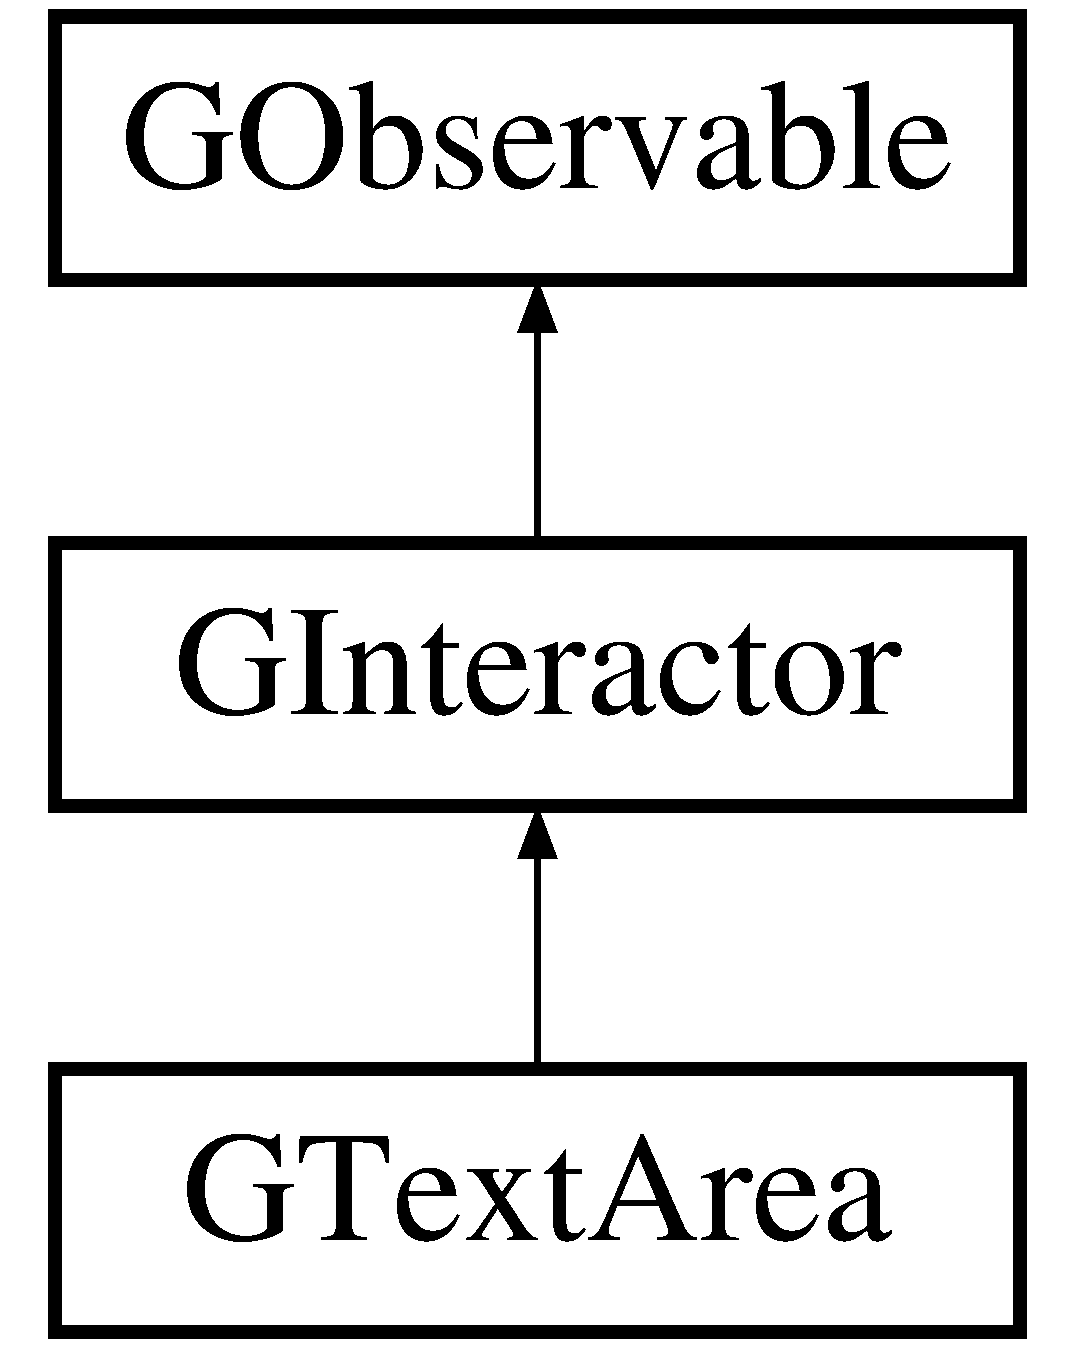
\includegraphics[height=3.000000cm]{classGTextArea}
\end{center}
\end{figure}
\subsection*{Public Types}
\begin{DoxyCompactItemize}
\item 
enum \mbox{\hyperlink{classGInteractor_a8e0d441725a81d2bbdebbea09078260e}{Text\+Position}} \{ \mbox{\hyperlink{classGInteractor_a8e0d441725a81d2bbdebbea09078260ea4cd6f2e7d5a08d6f4dc052df2358f774}{T\+E\+X\+T\+\_\+\+B\+E\+S\+I\+D\+E\+\_\+\+I\+C\+ON}}, 
\mbox{\hyperlink{classGInteractor_a8e0d441725a81d2bbdebbea09078260eaa88490f63d8de68d44c83bdb2ecde3b3}{T\+E\+X\+T\+\_\+\+U\+N\+D\+E\+R\+\_\+\+I\+C\+ON}}, 
\mbox{\hyperlink{classGInteractor_a8e0d441725a81d2bbdebbea09078260ea39a6f388a30ac4fefb6eb13e846bc9f2}{T\+E\+X\+T\+\_\+\+O\+N\+LY}}
 \}
\begin{DoxyCompactList}\small\item\em The places where an interactor can place its text relative to its icon. \end{DoxyCompactList}\end{DoxyCompactItemize}
\subsection*{Public Member Functions}
\begin{DoxyCompactItemize}
\item 
\mbox{\hyperlink{classGTextArea_aad263200ff85ead4d5e4d013c95c3107}{G\+Text\+Area}} (int rows, int columns, Q\+Widget $\ast$parent=nullptr)
\begin{DoxyCompactList}\small\item\em Creates a new text area large enough to display the given number of rows and columns of text. \end{DoxyCompactList}\item 
\mbox{\hyperlink{classGTextArea_a0902cdcc62cad5c1c81fc74ce38d8b13}{G\+Text\+Area}} (const std\+::string \&text=\char`\"{}\char`\"{}, Q\+Widget $\ast$parent=nullptr)
\begin{DoxyCompactList}\small\item\em Creates a new text area with the given initial text. \end{DoxyCompactList}\item 
\mbox{\hyperlink{classGTextArea_a7175406f7376c3e97ea921a39c175daf}{$\sim$\+G\+Text\+Area}} () override
\begin{DoxyCompactList}\small\item\em Frees memory allocated internally by the text area. \end{DoxyCompactList}\item 
virtual void \mbox{\hyperlink{classGInteractor_a02f20ea6edfa0671f31c4c648a253833}{add\+Action\+Listener}} () Q\+\_\+\+D\+E\+C\+L\+\_\+\+D\+E\+P\+R\+E\+C\+A\+T\+ED
\begin{DoxyCompactList}\small\item\em Adds an event listener to be notified when this interactor is clicked or generally interacted with. \end{DoxyCompactList}\item 
virtual void \mbox{\hyperlink{classGTextArea_ac7d00bfb7f87912fd664b97f29cc71e9}{append\+Formatted\+Text}} (const std\+::string \&text, const std\+::string \&color=\char`\"{}\char`\"{}, const std\+::string \&font=\char`\"{}\char`\"{})
\begin{DoxyCompactList}\small\item\em Adds formatted text to the end of the text area. \end{DoxyCompactList}\item 
virtual void \mbox{\hyperlink{classGTextArea_aa3457253e58dbfbf65a8f5a28c65fb5f}{append\+Html}} (const std\+::string \&html)
\begin{DoxyCompactList}\small\item\em Adds H\+T\+M\+L-\/formatted text to the end of the text area. \end{DoxyCompactList}\item 
virtual void \mbox{\hyperlink{classGTextArea_a6ba815b59563007b60dc2052d4703146}{append\+Text}} (const std\+::string \&text)
\begin{DoxyCompactList}\small\item\em Adds the given plain text to the end of the text area. \end{DoxyCompactList}\item 
virtual void \mbox{\hyperlink{classGTextArea_abd07e172ccec6823a88289c21124a367}{clear\+Selection}} ()
\begin{DoxyCompactList}\small\item\em Deselects any text that is currently selected in the text area. \end{DoxyCompactList}\item 
virtual void \mbox{\hyperlink{classGTextArea_a25f53c7d92eb2a5197cd4418c0165367}{clear\+Text}} ()
\begin{DoxyCompactList}\small\item\em Sets the text in the text area to be empty. \end{DoxyCompactList}\item 
bool \mbox{\hyperlink{classGInteractor_a597a370b592e3737d38d9d2f4e2031ea}{events\+Enabled}} () const override
\begin{DoxyCompactList}\small\item\em Returns true if this interactor is currently accepting events. \end{DoxyCompactList}\item 
virtual std\+::string \mbox{\hyperlink{classGInteractor_a69f8d23ed8f207fbecad99960776e942}{get\+Accelerator}} () const
\begin{DoxyCompactList}\small\item\em Returns a string representing a hotkey for this interactor, or an empty string if no accelerator has been set. \end{DoxyCompactList}\item 
virtual std\+::string \mbox{\hyperlink{classGInteractor_a94eb4276000c4fdfb508ce9e6317a82a}{get\+Action\+Command}} () const
\begin{DoxyCompactList}\small\item\em Returns an action command for this interactor, which is a semi-\/unique string you can use to identify it when events occur. \end{DoxyCompactList}\item 
virtual std\+::string \mbox{\hyperlink{classGInteractor_a808e22cc1fdfbecf71ed8c64ef4600e0}{get\+Background}} () const
\begin{DoxyCompactList}\small\item\em Returns the background color of the interactor as a string. \end{DoxyCompactList}\item 
virtual int \mbox{\hyperlink{classGInteractor_a9e827257a55cb8cf4d9de2ec6bcfd7a0}{get\+Background\+Int}} () const
\begin{DoxyCompactList}\small\item\em Returns the background color of the interactor as an R\+GB integer. \end{DoxyCompactList}\item 
virtual \mbox{\hyperlink{structGRectangle}{G\+Rectangle}} \mbox{\hyperlink{classGInteractor_a29e6ac35a0b48f491a4c88194cc5da3b}{get\+Bounds}} () const
\begin{DoxyCompactList}\small\item\em Returns a rectangle representing the x/y position and size of this interactor. \end{DoxyCompactList}\item 
virtual std\+::string \mbox{\hyperlink{classGInteractor_aa061dfa488c31e18549d64363c1d0e34}{get\+Color}} () const
\begin{DoxyCompactList}\small\item\em Returns the foreground/text color of the interactor as a string. \end{DoxyCompactList}\item 
virtual int \mbox{\hyperlink{classGInteractor_a9635c7af766cdc3417f346683fa0e6c1}{get\+Color\+Int}} () const
\begin{DoxyCompactList}\small\item\em Returns the foreground/text color of the interactor as an R\+GB integer. \end{DoxyCompactList}\item 
virtual int \mbox{\hyperlink{classGTextArea_a6b5395e749ae5c217093d74f68f1ca3a}{get\+Columns}} () const
\begin{DoxyCompactList}\small\item\em Returns the number of visible columns (characters wide) in the text area. \end{DoxyCompactList}\item 
virtual \mbox{\hyperlink{classGContainer}{G\+Container}} $\ast$ \mbox{\hyperlink{classGInteractor_a7a6e317c29d61030929b4cd2d1c00fe7}{get\+Container}} () const
\begin{DoxyCompactList}\small\item\em Returns a pointer to the onscreen container holding this interactor. \end{DoxyCompactList}\item 
virtual int \mbox{\hyperlink{classGTextArea_aa85d2267b4534eb372cd3114ea61ba3b}{get\+Cursor\+Position}} () const
\begin{DoxyCompactList}\small\item\em Returns the keyboard cursor\textquotesingle{}s current position in the text area as a 0-\/based character index within the overall text string. \end{DoxyCompactList}\item 
virtual std\+::string \mbox{\hyperlink{classGInteractor_a894a5502900794eeb27d084c21f1d77d}{get\+Font}} () const
\begin{DoxyCompactList}\small\item\em Returns the font of this interactor\textquotesingle{}s text as a font string such as \char`\"{}\+Helvetica-\/12-\/\+Bold\char`\"{}. \end{DoxyCompactList}\item 
virtual std\+::string \mbox{\hyperlink{classGInteractor_a4fa2d8b0192a3a5b4af4bbfe71194d03}{get\+Foreground}} () const
\begin{DoxyCompactList}\small\item\em Returns the foreground/text color of the interactor as a string. \end{DoxyCompactList}\item 
virtual int \mbox{\hyperlink{classGInteractor_ac3b12ab385a6ef9ae90fc879860ba726}{get\+Foreground\+Int}} () const
\begin{DoxyCompactList}\small\item\em Returns the foreground/text color of the interactor as an R\+GB integer. \end{DoxyCompactList}\item 
virtual double \mbox{\hyperlink{classGInteractor_a1e7e353362434072875264cf95629f99}{get\+Height}} () const
\begin{DoxyCompactList}\small\item\em Returns the current onscreen height of this interactor in pixels. \end{DoxyCompactList}\item 
virtual std\+::string \mbox{\hyperlink{classGTextArea_a58d3b7767e049484e3d7507379e6ecc7}{get\+Html}} () const
\begin{DoxyCompactList}\small\item\em Returns the text area\textquotesingle{}s current text as H\+T\+ML. \end{DoxyCompactList}\item 
virtual std\+::string \mbox{\hyperlink{classGInteractor_aaed62a73004939a64da6f0eb9eb64d73}{get\+Icon}} () const
\begin{DoxyCompactList}\small\item\em Returns the file name of the icon associated with this interactor, or an empty string if no icon has been set. \end{DoxyCompactList}\item 
virtual int \mbox{\hyperlink{classGInteractor_a9c9659a6c6ba66b4107ba59c95a24241}{get\+ID}} () const
\begin{DoxyCompactList}\small\item\em Returns a globally unique identifier for this interactor, which is set when the interactor is constructed. \end{DoxyCompactList}\item 
\+\_\+\+Internal\+\_\+\+Q\+Widget $\ast$ \mbox{\hyperlink{classGTextArea_a2f6b36b2517087dc90a366b5ce1f5323}{get\+Internal\+Widget}} () const override
\begin{DoxyCompactList}\small\item\em Returns a direct pointer to the internal Qt widget being wrapped by this interactor. \end{DoxyCompactList}\item 
virtual \mbox{\hyperlink{structGPoint}{G\+Point}} \mbox{\hyperlink{classGInteractor_a4f83802015511edeb63b892830812c11}{get\+Location}} () const
\begin{DoxyCompactList}\small\item\em Returns an (x, y) point representing the onscreen location of the top-\/left corner of this interactor within its containing window. \end{DoxyCompactList}\item 
virtual double \mbox{\hyperlink{classGInteractor_aed4b0075fcc434499c3cb3e46896bda3}{get\+Minimum\+Height}} () const
\begin{DoxyCompactList}\small\item\em Returns the minimum height in pixels that this interactor will permit itself to be resized to. \end{DoxyCompactList}\item 
virtual \mbox{\hyperlink{structGDimension}{G\+Dimension}} \mbox{\hyperlink{classGInteractor_a66b5af0b32493b4d597ca0a3df2049ea}{get\+Minimum\+Size}} () const
\begin{DoxyCompactList}\small\item\em Returns a \mbox{\hyperlink{structGDimension}{G\+Dimension}} structure representing the minimum size in pixels that this interactor will permit itself to be resized to. \end{DoxyCompactList}\item 
virtual double \mbox{\hyperlink{classGInteractor_a59e668114fe3d49d2a0f28deb258f7c8}{get\+Minimum\+Width}} () const
\begin{DoxyCompactList}\small\item\em Returns the minimum width in pixels that this interactor will permit itself to be resized to. \end{DoxyCompactList}\item 
virtual std\+::string \mbox{\hyperlink{classGInteractor_a8a60438a5b55d0b2ceb35c8674b9d8c5}{get\+Name}} () const
\begin{DoxyCompactList}\small\item\em Returns a string representing a unique name for this interactor. \end{DoxyCompactList}\item 
virtual std\+::string \mbox{\hyperlink{classGTextArea_aa78dbaa7dac1f8cdf9048c91abecc7ad}{get\+Placeholder}} () const
\begin{DoxyCompactList}\small\item\em Returns the text area\textquotesingle{}s placeholder text, which is usually displayed as a light gray text in the text area when the area is empty. \end{DoxyCompactList}\item 
virtual double \mbox{\hyperlink{classGInteractor_a747de0961653847bdc6615dbf756d715}{get\+Preferred\+Height}} () const
\begin{DoxyCompactList}\small\item\em Returns the height in pixels that this interactor would prefer to be, which would exactly fit its contents with no stretching or scrollbars. \end{DoxyCompactList}\item 
virtual \mbox{\hyperlink{structGDimension}{G\+Dimension}} \mbox{\hyperlink{classGInteractor_a4aabbee761d8e9116275401131b7ccd1}{get\+Preferred\+Size}} () const
\begin{DoxyCompactList}\small\item\em Returns a \mbox{\hyperlink{structGDimension}{G\+Dimension}} structure storing the width and height in pixels that this interactor would prefer to be, which would exactly fit its contents with no stretching or scrollbars. \end{DoxyCompactList}\item 
virtual double \mbox{\hyperlink{classGInteractor_a82bca31d37700fb0e35d2743352efd5e}{get\+Preferred\+Width}} () const
\begin{DoxyCompactList}\small\item\em Returns the height in pixels that this interactor would prefer to be, which would exactly fit its contents with no stretching or scrollbars. \end{DoxyCompactList}\item 
virtual int \mbox{\hyperlink{classGTextArea_ad343f9bbb050d9037167e80e423ab4e8}{get\+Rows}} () const
\begin{DoxyCompactList}\small\item\em Returns the number of visible rows (lines tall) in the text area. \end{DoxyCompactList}\item 
virtual std\+::string \mbox{\hyperlink{classGTextArea_a512371b3f41599349f23389825a6ccf7}{get\+Selected\+Text}} () const
\begin{DoxyCompactList}\small\item\em Returns the text that is currently selected in the text area. \end{DoxyCompactList}\item 
virtual int \mbox{\hyperlink{classGTextArea_a2885313daa0e367cee2ccd0c704a6147}{get\+Selection\+End}} () const
\begin{DoxyCompactList}\small\item\em Returns the index just past the end of the current selection of text as a 0-\/based character index within the overall text string. \end{DoxyCompactList}\item 
virtual int \mbox{\hyperlink{classGTextArea_a68f7816694269b73e6284e756eb0c179}{get\+Selection\+Length}} () const
\begin{DoxyCompactList}\small\item\em Returns the number of characters that are currently selected. \end{DoxyCompactList}\item 
virtual int \mbox{\hyperlink{classGTextArea_aad7c986a677c1b9cf445cd7cfb6a8975}{get\+Selection\+Start}} () const
\begin{DoxyCompactList}\small\item\em Returns the index of the start of the current selection of text as a 0-\/based character index within the overall text string. \end{DoxyCompactList}\item 
virtual \mbox{\hyperlink{structGDimension}{G\+Dimension}} \mbox{\hyperlink{classGInteractor_a7b4eec96a2bdc6420695d5796a78eea9}{get\+Size}} () const
\begin{DoxyCompactList}\small\item\em Returns a \mbox{\hyperlink{structGDimension}{G\+Dimension}} structure storing the current onscreen width and height of this interactor in pixels. \end{DoxyCompactList}\item 
virtual std\+::string \mbox{\hyperlink{classGTextArea_aff553c50924b836c29f146ed34a7c6ec}{get\+Text}} () const
\begin{DoxyCompactList}\small\item\em Returns the text area\textquotesingle{}s current text. \end{DoxyCompactList}\item 
std\+::string \mbox{\hyperlink{classGTextArea_a9b72ede4ee8520f987a0c01e30654814}{get\+Type}} () const override
\begin{DoxyCompactList}\small\item\em Returns a string representing the class name of this interactor, such as \char`\"{}\+G\+Button\char`\"{} or \char`\"{}\+G\+Check\+Box\char`\"{}. \end{DoxyCompactList}\item 
Q\+Widget $\ast$ \mbox{\hyperlink{classGTextArea_a3b33a602b31a6b809d020535a59db3b4}{get\+Widget}} () const override
\begin{DoxyCompactList}\small\item\em Returns a direct pointer to the internal Qt widget being wrapped by this interactor. \end{DoxyCompactList}\item 
virtual double \mbox{\hyperlink{classGInteractor_a0ed2965abd4f5701d2cadf71239faf19}{get\+Width}} () const
\begin{DoxyCompactList}\small\item\em Returns the current onscreen width of this interactor in pixels. \end{DoxyCompactList}\item 
virtual double \mbox{\hyperlink{classGInteractor_a344385751bee0720059403940d57a13e}{getX}} () const
\begin{DoxyCompactList}\small\item\em Returns the x-\/coordinate of the top-\/left pixel of this interactor within its onscreen window. \end{DoxyCompactList}\item 
virtual double \mbox{\hyperlink{classGInteractor_aafa51c7f8f38a09febbb9ce7853f77b4}{getY}} () const
\begin{DoxyCompactList}\small\item\em Returns the y-\/coordinate of the top-\/left pixel of this interactor within its onscreen window. \end{DoxyCompactList}\item 
virtual bool \mbox{\hyperlink{classGInteractor_afc480f652b8c5f1fb255e2269ce68879}{in\+Bounds}} (double x, double y) const
\begin{DoxyCompactList}\small\item\em Returns true if the given x/y pixel is within the bounds of this interactor. \end{DoxyCompactList}\item 
virtual bool \mbox{\hyperlink{classGInteractor_ae6d7982c1c627b677a5e776ca86118ed}{in\+Bounds}} (int x, int y) const
\begin{DoxyCompactList}\small\item\em Returns true if the given x/y pixel is within the bounds of this interactor. \end{DoxyCompactList}\item 
virtual bool \mbox{\hyperlink{classGTextArea_a80f9fe3b6f725182b294886f57cc1689}{is\+Context\+Menu\+Enabled}} () const
\begin{DoxyCompactList}\small\item\em Returns true if a context menu will pop up when the user right-\/clicks the text area. \end{DoxyCompactList}\item 
virtual bool \mbox{\hyperlink{classGTextArea_a012b5afb54e037e6c5498cf0932a521b}{is\+Editable}} () const
\begin{DoxyCompactList}\small\item\em Returns whether the text area allows the user to modify its text. \end{DoxyCompactList}\item 
virtual bool \mbox{\hyperlink{classGInteractor_aacb819fb241851fd9fc045271baa4034}{is\+Enabled}} () const
\begin{DoxyCompactList}\small\item\em Returns true if this interactor is currently enabled. \end{DoxyCompactList}\item 
virtual bool \mbox{\hyperlink{classGTextArea_ae09e72290b6e8a23bcc77752da6dffa5}{is\+Line\+Wrap}} () const
\begin{DoxyCompactList}\small\item\em Returns whether the text area wraps its text when a line becomes too long. \end{DoxyCompactList}\item 
virtual bool \mbox{\hyperlink{classGInteractor_a9d8a6cfb13917785c143e74d40e4e2be}{is\+Visible}} () const
\begin{DoxyCompactList}\small\item\em Returns true if the interactor is visible on the screen. \end{DoxyCompactList}\item 
virtual void \mbox{\hyperlink{classGTextArea_ab5ef729cac166db0ef51ff7ea30d1bb8}{move\+Cursor\+To\+End}} ()
\begin{DoxyCompactList}\small\item\em Sets the text area\textquotesingle{}s keyboard cursor position to the end of the current text. \end{DoxyCompactList}\item 
virtual void \mbox{\hyperlink{classGTextArea_a24abdceab57bcff96185afbadf193a22}{move\+Cursor\+To\+Start}} ()
\begin{DoxyCompactList}\small\item\em Sets the text area\textquotesingle{}s keyboard cursor position to the start of the current text. \end{DoxyCompactList}\item 
virtual void \mbox{\hyperlink{classGInteractor_ab7fe7a876367b87cf7202f947f1d05e4}{remove\+Action\+Listener}} ()
\begin{DoxyCompactList}\small\item\em Removes the action listener from this interactor so that it will no longer call it when events occur. \end{DoxyCompactList}\item 
virtual void \mbox{\hyperlink{classGInteractor_ad39d0325cde6b97ebda4b9d7787c633b}{remove\+Click\+Listener}} ()
\begin{DoxyCompactList}\small\item\em Removes the click listener from this interactor so that it will no longer call it when events occur. \end{DoxyCompactList}\item 
virtual void \mbox{\hyperlink{classGInteractor_aa4250907e4cdd77349c04f0cf5cdd3d3}{remove\+Double\+Click\+Listener}} ()
\begin{DoxyCompactList}\small\item\em Removes the double-\/click listener from this interactor so that it will no longer call it when events occur. \end{DoxyCompactList}\item 
virtual void \mbox{\hyperlink{classGInteractor_a43095f41cab3be732b49f29970484b05}{remove\+Key\+Listener}} ()
\begin{DoxyCompactList}\small\item\em Removes the key listener from this interactor so that it will no longer call it when key events occur. \end{DoxyCompactList}\item 
virtual void \mbox{\hyperlink{classGInteractor_aff47f71ce47e688a07c9d38dc92fcc11}{remove\+Mouse\+Listener}} ()
\begin{DoxyCompactList}\small\item\em Removes the mouse listener from this interactor so that it will no longer call it when events occur. \end{DoxyCompactList}\item 
virtual void \mbox{\hyperlink{classGTextArea_a69c940b99d01eb7c353763ce4b0942a4}{remove\+Text\+Change\+Listener}} ()
\begin{DoxyCompactList}\small\item\em Removes the text change listener from this text area so that it will no longer call it when the user modifies the text. \end{DoxyCompactList}\item 
virtual void \mbox{\hyperlink{classGInteractor_a519fb2ac767f8b2febbb50b898b8c8cb}{request\+Focus}} ()
\begin{DoxyCompactList}\small\item\em Transfers keyboard focus to this interactor. \end{DoxyCompactList}\item 
virtual void \mbox{\hyperlink{classGTextArea_ad4c9b6140b529865a6cdeed37a339237}{scroll\+To\+Bottom}} ()
\begin{DoxyCompactList}\small\item\em Moves the visible scroll region of the text area so that the bottom part of the text is visible. \end{DoxyCompactList}\item 
virtual void \mbox{\hyperlink{classGTextArea_a9eacfcf7c186936ed957dd1c8a9c6b64}{scroll\+To\+Top}} ()
\begin{DoxyCompactList}\small\item\em Moves the visible scroll region of the text area so that the top part of the text is visible. \end{DoxyCompactList}\item 
virtual void \mbox{\hyperlink{classGTextArea_aaeb1320c0553d0d2b8081b750f59a34a}{select}} (int start\+Index, int length)
\begin{DoxyCompactList}\small\item\em Sets the given range of text to be selected, beginning with the given start index as a 0-\/based character index within the overall text string, and extending for the given length of characters. \end{DoxyCompactList}\item 
virtual void \mbox{\hyperlink{classGTextArea_ab6658ed404200bd7aaca5629db064645}{select\+All}} ()
\begin{DoxyCompactList}\small\item\em Selects the entire text of the text area. \end{DoxyCompactList}\item 
virtual void \mbox{\hyperlink{classGInteractor_ad15f102f62e2960576012f1aa0ba4b2e}{set\+Accelerator}} (const std\+::string \&accelerator)
\begin{DoxyCompactList}\small\item\em Sets an accelerator hotkey for this interactor, such as \char`\"{}\+Ctrl-\/\+S\char`\"{}. \end{DoxyCompactList}\item 
virtual void \mbox{\hyperlink{classGInteractor_a4b5843fe3030e038a1ba54cc03389bcf}{set\+Action\+Command}} (const std\+::string \&action\+Command)
\begin{DoxyCompactList}\small\item\em Sets the action command for this interactor. \end{DoxyCompactList}\item 
virtual void \mbox{\hyperlink{classGInteractor_adcfb4742430c88714fcf57e57ab8ea9c}{set\+Action\+Listener}} (G\+Event\+Listener func)
\begin{DoxyCompactList}\small\item\em Sets an action listener on this interactor so that it will be called when it is interacted with in its primary way. \end{DoxyCompactList}\item 
virtual void \mbox{\hyperlink{classGInteractor_aebd20a89c7a8a43a6fce999cf4f9fcf2}{set\+Action\+Listener}} (G\+Event\+Listener\+Void func)
\begin{DoxyCompactList}\small\item\em Sets an action listener on this interactor so that it will be called when it is interacted with in its primary way. \end{DoxyCompactList}\item 
virtual void \mbox{\hyperlink{classGInteractor_acba7e546c2025c0a15ca4b4cc92043db}{set\+Background}} (int rgb)
\begin{DoxyCompactList}\small\item\em Sets the background color of the interactor to the color represented by the given R\+GB integer. \end{DoxyCompactList}\item 
virtual void \mbox{\hyperlink{classGInteractor_ab4677ab2474e68b07aa56605af92a84a}{set\+Background}} (const std\+::string \&color)
\begin{DoxyCompactList}\small\item\em Sets the background color of the interactor to the color represented by the given string. \end{DoxyCompactList}\item 
virtual void \mbox{\hyperlink{classGInteractor_a2aae8197624b72265ab83b4f1bc73f2f}{set\+Bounds}} (double x, double y, double width, double height)
\begin{DoxyCompactList}\small\item\em Sets the size and location of the widget. \end{DoxyCompactList}\item 
virtual void \mbox{\hyperlink{classGInteractor_acada386653f008cacc7cce86426bef7c}{set\+Bounds}} (const \mbox{\hyperlink{structGRectangle}{G\+Rectangle}} \&size)
\begin{DoxyCompactList}\small\item\em Sets the size and location of the widget. \end{DoxyCompactList}\item 
virtual void \mbox{\hyperlink{classGInteractor_abd40af6921242584d0954f173911b190}{set\+Click\+Listener}} (G\+Event\+Listener func)
\begin{DoxyCompactList}\small\item\em Sets a mouse listener on this interactor so that it will be called when the mouse is clicked on it. \end{DoxyCompactList}\item 
virtual void \mbox{\hyperlink{classGInteractor_a856414c92df90f56f3877475eb3f8fc4}{set\+Click\+Listener}} (G\+Event\+Listener\+Void func)
\begin{DoxyCompactList}\small\item\em Sets a mouse listener on this interactor so that it will be called when the mouse is clicked on it. \end{DoxyCompactList}\item 
virtual void \mbox{\hyperlink{classGInteractor_ab1f5cc0f5cc6bbbd716a526c61f1081d}{set\+Color}} (int rgb)
\begin{DoxyCompactList}\small\item\em Sets the foreground/text color of the interactor to the color represented by the given R\+GB integer. \end{DoxyCompactList}\item 
virtual void \mbox{\hyperlink{classGInteractor_a61374df6c11b52cfbb0815decdbaebc6}{set\+Color}} (const std\+::string \&color)
\begin{DoxyCompactList}\small\item\em Sets the foreground/text color of the interactor to the color represented by the given string. \end{DoxyCompactList}\item 
virtual void \mbox{\hyperlink{classGTextArea_a3f29cc2956a84cdbce6327f1da4d86e9}{set\+Columns}} (int columns)
\begin{DoxyCompactList}\small\item\em Sets the width of the text area to be wide enough to fit the given number of characters (columns) of text. \end{DoxyCompactList}\item 
virtual void \mbox{\hyperlink{classGTextArea_a1a83404ffa5c72d747681b3505e73001}{set\+Context\+Menu\+Enabled}} (bool enabled)
\begin{DoxyCompactList}\small\item\em Sets whether a context menu will pop up when the user right-\/clicks the text area. \end{DoxyCompactList}\item 
virtual void \mbox{\hyperlink{classGTextArea_a5817e10a86be5cd41b3668d8fccb10e0}{set\+Cursor\+Position}} (int index, bool keep\+Anchor=false)
\begin{DoxyCompactList}\small\item\em Moves the keyboard cursor to the given 0-\/based character index within the text. \end{DoxyCompactList}\item 
virtual void \mbox{\hyperlink{classGInteractor_ac29f9a3462458e165fae3a1f046ee77a}{set\+Double\+Click\+Listener}} (G\+Event\+Listener func)
\begin{DoxyCompactList}\small\item\em Sets a mouse listener on this interactor so that it will be called when the mouse is double-\/clicked on it. \end{DoxyCompactList}\item 
virtual void \mbox{\hyperlink{classGInteractor_a50096194d66f48c92dd4c512d41bfc76}{set\+Double\+Click\+Listener}} (G\+Event\+Listener\+Void func)
\begin{DoxyCompactList}\small\item\em Sets a mouse listener on this interactor so that it will be called when the mouse is double-\/clicked on it. \end{DoxyCompactList}\item 
virtual void \mbox{\hyperlink{classGTextArea_a008d7fd44fb3e7a6886cdaddbc3644a2}{set\+Editable}} (bool value)
\begin{DoxyCompactList}\small\item\em Sets whether the text area allows the user to modify its text. \end{DoxyCompactList}\item 
virtual void \mbox{\hyperlink{classGInteractor_ab831367dd84bbd579e02e55bacb21343}{set\+Enabled}} (bool value)
\begin{DoxyCompactList}\small\item\em Sets whether this interactor is currently enabled. \end{DoxyCompactList}\item 
virtual void \mbox{\hyperlink{classGObservable_afaa30b2a9e0f378fd1c70d2f1d0b8216}{set\+Events\+Enabled}} (bool \mbox{\hyperlink{classGInteractor_a597a370b592e3737d38d9d2f4e2031ea}{events\+Enabled}})
\begin{DoxyCompactList}\small\item\em Sets whether the object is currently allowing itself to fire events. \end{DoxyCompactList}\item 
virtual void \mbox{\hyperlink{classGInteractor_a2592348886ffea646c6534bf88f7c49d}{set\+Font}} (const Q\+Font \&font)
\begin{DoxyCompactList}\small\item\em Sets the font used by this widget to the given Qt font. \end{DoxyCompactList}\item 
virtual void \mbox{\hyperlink{classGInteractor_a8e096e8818d838aceae1d46d58fb3a7b}{set\+Font}} (const std\+::string \&font)
\begin{DoxyCompactList}\small\item\em Sets the font used by this widget to the font represented by the given font string, such as \char`\"{}\+Helvetica-\/16-\/\+Bold\char`\"{}. \end{DoxyCompactList}\item 
virtual void \mbox{\hyperlink{classGInteractor_a9eb856b5ff83a19df3831a31f15f4563}{set\+Foreground}} (int rgb)
\begin{DoxyCompactList}\small\item\em Sets the foreground/text color of the interactor to the color represented by the given R\+GB integer. \end{DoxyCompactList}\item 
virtual void \mbox{\hyperlink{classGInteractor_af59209aeadea6dfc6d97a2d8531f50e1}{set\+Foreground}} (const std\+::string \&color)
\begin{DoxyCompactList}\small\item\em Sets the foreground/text color of the interactor to the color represented by the given string. \end{DoxyCompactList}\item 
virtual void \mbox{\hyperlink{classGInteractor_a9e280bfc4544dfaf8e4376c4e1a74357}{set\+Height}} (double height)
\begin{DoxyCompactList}\small\item\em Sets the onscreen height of the interactor in pixels. \end{DoxyCompactList}\item 
virtual void \mbox{\hyperlink{classGTextArea_a71ca94fd0ab4223097c4d524ddafe94f}{set\+Html}} (const std\+::string \&html)
\begin{DoxyCompactList}\small\item\em Sets the text area\textquotesingle{}s current text to the given H\+T\+ML string. \end{DoxyCompactList}\item 
virtual void \mbox{\hyperlink{classGInteractor_a542abfcd7261751352af129c7215ecda}{set\+Icon}} (const Q\+Icon \&icon)
\begin{DoxyCompactList}\small\item\em Sets the icon associated with this interactor. \end{DoxyCompactList}\item 
virtual void \mbox{\hyperlink{classGInteractor_a368e1a338f84401c284506d03b1ba769}{set\+Icon}} (const Q\+Pixmap \&icon)
\begin{DoxyCompactList}\small\item\em Sets the icon associated with this interactor. \end{DoxyCompactList}\item 
virtual void \mbox{\hyperlink{classGInteractor_a762e139aa311461c3984d3ad28293f64}{set\+Icon}} (const std\+::string \&filename, bool retain\+Icon\+Size=true)
\begin{DoxyCompactList}\small\item\em Sets the file name of the icon associated with this interactor, or an empty string if no icon has been set. \end{DoxyCompactList}\item 
virtual void \mbox{\hyperlink{classGInteractor_aeb8324d3287fa1fbe093f4d6230cf0a6}{set\+Key\+Listener}} (G\+Event\+Listener func)
\begin{DoxyCompactList}\small\item\em Sets a key listener on this interactor so that it will be called when the user presses any key. \end{DoxyCompactList}\item 
virtual void \mbox{\hyperlink{classGInteractor_ae48ecea73606c7bd9423e1c7cc589cc9}{set\+Key\+Listener}} (G\+Event\+Listener\+Void func)
\begin{DoxyCompactList}\small\item\em Sets a key listener on this interactor so that it will be called when the user presses any key. \end{DoxyCompactList}\item 
virtual void \mbox{\hyperlink{classGTextArea_aaaafb06fec060b28b70ec3b7379657b4}{set\+Line\+Wrap}} (bool wrap)
\begin{DoxyCompactList}\small\item\em Sets whether the text area wraps its text when a line becomes too long. \end{DoxyCompactList}\item 
virtual void \mbox{\hyperlink{classGInteractor_a04594e8ba9b98513a64f1da00dcae18c}{set\+Location}} (double x, double y)
\begin{DoxyCompactList}\small\item\em Sets the onscreen x/y-\/coordinate of the top-\/left corner of the interactor relative to its window. \end{DoxyCompactList}\item 
virtual void \mbox{\hyperlink{classGInteractor_a0cf428e207b7f22cc08138a90b1b87b2}{set\+Minimum\+Size}} (double width, double height)
\begin{DoxyCompactList}\small\item\em Sets the minimum size in pixels that this interactor will permit itself to be resized to. \end{DoxyCompactList}\item 
virtual void \mbox{\hyperlink{classGInteractor_a3b1046117ac6cb7abe467e00ba8a81f4}{set\+Minimum\+Size}} (const \mbox{\hyperlink{structGDimension}{G\+Dimension}} \&size)
\begin{DoxyCompactList}\small\item\em Sets the minimum size in pixels that this interactor will permit itself to be resized to. \end{DoxyCompactList}\item 
void \mbox{\hyperlink{classGTextArea_a2c6a3746da7ffa3819294896d4423059}{set\+Mouse\+Listener}} (G\+Event\+Listener func) override
\begin{DoxyCompactList}\small\item\em Sets a mouse listener on this text area so that it will be called when the user moves or clicks the mouse. \end{DoxyCompactList}\item 
void \mbox{\hyperlink{classGTextArea_a3ed42c5f929cba378927916dd73e6576}{set\+Mouse\+Listener}} (G\+Event\+Listener\+Void func) override
\begin{DoxyCompactList}\small\item\em Sets a mouse listener on this text area so that it will be called when the user moves or clicks the mouse. \end{DoxyCompactList}\item 
virtual void \mbox{\hyperlink{classGInteractor_a9d3a2685df23b5e7cbf59c19c4a1f9b5}{set\+Name}} (const std\+::string \&name)
\begin{DoxyCompactList}\small\item\em Sets a string representing a unique name for this interactor. \end{DoxyCompactList}\item 
virtual void \mbox{\hyperlink{classGTextArea_aa21a9bebb4652ab6780d0c11eff47aee}{set\+Placeholder}} (const std\+::string \&text)
\begin{DoxyCompactList}\small\item\em Sets the text area\textquotesingle{}s placeholder text, which is usually displayed as a light gray text in the text area when the area is empty. \end{DoxyCompactList}\item 
virtual void \mbox{\hyperlink{classGInteractor_a1ab987704fce32098706c6f00fb08218}{set\+Preferred\+Height}} (double height)
\begin{DoxyCompactList}\small\item\em Sets the height in pixels that this interactor would prefer to be. \end{DoxyCompactList}\item 
virtual void \mbox{\hyperlink{classGInteractor_a042c5ae19430d765ef552371cae3632c}{set\+Preferred\+Size}} (double width, double height)
\begin{DoxyCompactList}\small\item\em Sets the width and height in pixels that this interactor would prefer to be. \end{DoxyCompactList}\item 
virtual void \mbox{\hyperlink{classGInteractor_aa22d9be4bc0e078bb0ea69b0fc9d7c75}{set\+Preferred\+Size}} (const \mbox{\hyperlink{structGDimension}{G\+Dimension}} \&size)
\begin{DoxyCompactList}\small\item\em Sets the size in pixels that this interactor would prefer to be. \end{DoxyCompactList}\item 
virtual void \mbox{\hyperlink{classGInteractor_a3db429ab2fa52efd187eec0ed8cdd9f2}{set\+Preferred\+Width}} (double width)
\begin{DoxyCompactList}\small\item\em Sets the width in pixels that this interactor would prefer to be. \end{DoxyCompactList}\item 
virtual void \mbox{\hyperlink{classGTextArea_a508bbe326657af6d3add84deb4595989}{set\+Rows}} (int rows)
\begin{DoxyCompactList}\small\item\em Sets the height of the text area to be wide enough to fit the given number of lines (rows) of text. \end{DoxyCompactList}\item 
virtual void \mbox{\hyperlink{classGTextArea_a15142a18598662167760b35e58be90b1}{set\+Rows\+Columns}} (int rows, int columns)
\begin{DoxyCompactList}\small\item\em Sets the size of the text area to be wide enough to fit the given number of lines (rows) and characters (columns) of text. \end{DoxyCompactList}\item 
virtual void \mbox{\hyperlink{classGInteractor_aca25d49481f9bf5fc8f7df4c086c4ce7}{set\+Size}} (double width, double height)
\begin{DoxyCompactList}\small\item\em Sets the onscreen width and height of the interactor in pixels. \end{DoxyCompactList}\item 
virtual void \mbox{\hyperlink{classGInteractor_ae2b628228f192c2702c4ce941b2af68f}{set\+Size}} (const \mbox{\hyperlink{structGDimension}{G\+Dimension}} \&size)
\begin{DoxyCompactList}\small\item\em Sets the onscreen width and height of the interactor in pixels. \end{DoxyCompactList}\item 
virtual void \mbox{\hyperlink{classGTextArea_ac1ae51949d41ee9054634be5967d91b8}{set\+Text}} (const std\+::string \&text)
\begin{DoxyCompactList}\small\item\em Sets the text area\textquotesingle{}s current text to the given string, replacing any existing text. \end{DoxyCompactList}\item 
virtual void \mbox{\hyperlink{classGTextArea_ae41284f9c540110180ac0ad6beca5cb0}{set\+Text\+Change\+Listener}} (G\+Event\+Listener func)
\begin{DoxyCompactList}\small\item\em Sets a text change listener on this text area so that it will be called when the user modifies the current text. \end{DoxyCompactList}\item 
virtual void \mbox{\hyperlink{classGTextArea_ae8df75b0746951146d29220f386fcd33}{set\+Text\+Change\+Listener}} (G\+Event\+Listener\+Void func)
\begin{DoxyCompactList}\small\item\em Sets a text change listener on this text area so that it will be called when the user modifies the current text. \end{DoxyCompactList}\item 
virtual void \mbox{\hyperlink{classGInteractor_a039e0e49beaecc275efce02d416acea8}{set\+Tooltip}} (const std\+::string \&tooltip\+Text)
\begin{DoxyCompactList}\small\item\em Sets a \char`\"{}tooltip\char`\"{} that will appear if the user hovers their mouse over the interactor. \end{DoxyCompactList}\item 
virtual void \mbox{\hyperlink{classGInteractor_a18e44e30b31525a243960ca3928125aa}{set\+Visible}} (bool visible)
\begin{DoxyCompactList}\small\item\em Returns true if the interactor is visible on the screen. \end{DoxyCompactList}\item 
virtual void \mbox{\hyperlink{classGInteractor_aa3f3fba4cb131baa8696ba01e3bceca1}{set\+Width}} (double width)
\begin{DoxyCompactList}\small\item\em Sets the onscreen width of the interactor in pixels. \end{DoxyCompactList}\item 
virtual void \mbox{\hyperlink{classGInteractor_a9c18fcc579333bf9653d13ad2b372e39}{setX}} (double x)
\begin{DoxyCompactList}\small\item\em Sets the onscreen x-\/coordinate of the top-\/left corner of the interactor relative to its window. \end{DoxyCompactList}\item 
virtual void \mbox{\hyperlink{classGInteractor_a7d57e2a5c35d27feb58fd498a3cf82b9}{setY}} (double y)
\begin{DoxyCompactList}\small\item\em Sets the onscreen y-\/coordinate of the top-\/left corner of the interactor relative to its window. \end{DoxyCompactList}\item 
virtual std\+::string \mbox{\hyperlink{classGObservable_a1fe5121d6528fdea3f243321b3fa3a49}{to\+String}} () const
\begin{DoxyCompactList}\small\item\em Returns a string representation of this observable object\textquotesingle{}s state. \end{DoxyCompactList}\end{DoxyCompactItemize}
\subsection*{Protected Member Functions}
\begin{DoxyCompactItemize}
\item 
virtual void \mbox{\hyperlink{classGObservable_a80cfa040459ff53594adbd6a51ec8f43}{clear\+Event\+Listeners}} ()
\begin{DoxyCompactList}\small\item\em Removes all event listeners from this object. \end{DoxyCompactList}\item 
virtual void \mbox{\hyperlink{classGObservable_a284f31528c0520f8e545c03ac9eeac74}{ensure\+Thread\+Safety}} (const std\+::string \&member\+Name=\char`\"{}\char`\"{})
\begin{DoxyCompactList}\small\item\em Ensures that we are currently in the Qt G\+UI thread. \end{DoxyCompactList}\item 
virtual void \mbox{\hyperlink{classGObservable_a63e5e5a6227c59c928493b11aceb0f67}{fire\+Event}} (\mbox{\hyperlink{classGEvent}{G\+Event}} \&event)
\begin{DoxyCompactList}\small\item\em Sends out the given event to any attached listeners. \end{DoxyCompactList}\item 
virtual void \mbox{\hyperlink{classGObservable_ab3983ea07337b52020a29cc00c653d8d}{fire\+G\+Event}} (Q\+Event $\ast$event, Event\+Type event\+Type, const std\+::string \&event\+Name)
\begin{DoxyCompactList}\small\item\em Creates an event of the given type, then sends it out to any attached listeners. \end{DoxyCompactList}\item 
virtual void \mbox{\hyperlink{classGObservable_a01fdf1b0e0dbd49e189fe4514e010411}{fire\+G\+Event}} (Q\+Close\+Event $\ast$event, Event\+Type event\+Type, const std\+::string \&event\+Name)
\begin{DoxyCompactList}\small\item\em Creates an event of the given type, then sends it out to any attached listeners. \end{DoxyCompactList}\item 
virtual void \mbox{\hyperlink{classGObservable_abb0b2f66ba39211cb5d7615e9d1c04e2}{fire\+G\+Event}} (Q\+Key\+Event $\ast$event, Event\+Type event\+Type, const std\+::string \&event\+Name)
\begin{DoxyCompactList}\small\item\em Creates an event of the given type, then sends it out to any attached listeners. \end{DoxyCompactList}\item 
virtual void \mbox{\hyperlink{classGObservable_a119318675d2165bdf7dd853aaf881d4b}{fire\+G\+Event}} (Q\+Mouse\+Event $\ast$event, Event\+Type event\+Type, const std\+::string \&event\+Name, const std\+::string \&action\+Command=\char`\"{}\char`\"{})
\begin{DoxyCompactList}\small\item\em Creates an event of the given type, then sends it out to any attached listeners. \end{DoxyCompactList}\item 
virtual void \mbox{\hyperlink{classGObservable_a63fd9034e1e1633c1c38eb342bfd34e9}{fire\+G\+Event}} (Q\+Resize\+Event $\ast$event, Event\+Type event\+Type, const std\+::string \&event\+Name)
\begin{DoxyCompactList}\small\item\em Creates an event of the given type, then sends it out to any attached listeners. \end{DoxyCompactList}\item 
virtual void \mbox{\hyperlink{classGObservable_a741345310d9b7c5170a6cbc410c44ac4}{fire\+G\+Event}} (Q\+Timer\+Event $\ast$event, Event\+Type event\+Type, const std\+::string \&event\+Name)
\begin{DoxyCompactList}\small\item\em Creates an event of the given type, then sends it out to any attached listeners. \end{DoxyCompactList}\item 
virtual void \mbox{\hyperlink{classGObservable_a93bf338968a0338761b8e4dc62f582e9}{fire\+G\+Event}} (Q\+Wheel\+Event $\ast$event, Event\+Type event\+Type, const std\+::string \&event\+Name)
\begin{DoxyCompactList}\small\item\em Creates an event of the given type, then sends it out to any attached listeners. \end{DoxyCompactList}\item 
virtual void \mbox{\hyperlink{classGObservable_a2a70a7d7435ff0c3b80bb4d70da19e0d}{fire\+G\+Event}} (Q\+Window\+State\+Change\+Event $\ast$event, Event\+Type event\+Type, const std\+::string \&event\+Name)
\begin{DoxyCompactList}\small\item\em Creates an event of the given type, then sends it out to any attached listeners. \end{DoxyCompactList}\item 
virtual bool \mbox{\hyperlink{classGObservable_a9f6faaa25942923bafa1c44020c49fa9}{has\+Event\+Listener}} (const std\+::string \&event\+Name) const
\begin{DoxyCompactList}\small\item\em Returns true if the observable object has a listener for the given type of event. \end{DoxyCompactList}\item 
virtual bool \mbox{\hyperlink{classGObservable_aeec1adc19aa0f33de62390686ee1382c}{is\+Accepting\+Event}} (int event\+Mask) const
\begin{DoxyCompactList}\small\item\em Returns true if the observable object has a listener for the given type of event. \end{DoxyCompactList}\item 
virtual bool \mbox{\hyperlink{classGObservable_aa31c73145a29dcb92848a92e0cfaea41}{is\+Accepting\+Event}} (const \mbox{\hyperlink{classGEvent}{G\+Event}} \&event) const
\begin{DoxyCompactList}\small\item\em Returns true if the observable object has a listener for the given type of event. \end{DoxyCompactList}\item 
virtual bool \mbox{\hyperlink{classGObservable_a3b1c689267eda44e65a2213e7de38b23}{is\+Accepting\+Event}} (const std\+::string \&event\+Type) const
\begin{DoxyCompactList}\small\item\em Returns true if the observable object has a listener for the given type of event. \end{DoxyCompactList}\item 
virtual void \mbox{\hyperlink{classGObservable_acbcf1ed3a851ad8a3c17ef38d86b481d}{remove\+Event\+Listener}} (const std\+::string \&event\+Name)
\begin{DoxyCompactList}\small\item\em Removes any event listener from this observable object that would respond to the given type of event, such as \char`\"{}click\char`\"{} or \char`\"{}keydown\char`\"{}. \end{DoxyCompactList}\item 
virtual void \mbox{\hyperlink{classGObservable_af51cc35c29a1bd1908609d432decdbb6}{remove\+Event\+Listeners}} (std\+::initializer\+\_\+list$<$ std\+::string $>$ event\+Names)
\begin{DoxyCompactList}\small\item\em Removes any event listener from this observable object that would respond to the given types of events, such as \char`\"{}click\char`\"{} or \char`\"{}keydown\char`\"{}. \end{DoxyCompactList}\item 
virtual void \mbox{\hyperlink{classGObservable_ad2f6d34961c50f6c1e0659990b79f741}{set\+Event\+Listener}} (const std\+::string \&event\+Name, G\+Event\+Listener func)
\begin{DoxyCompactList}\small\item\em Adds an event listener from this observable object to respond to the given type of event, such as \char`\"{}click\char`\"{} or \char`\"{}keydown\char`\"{}. \end{DoxyCompactList}\item 
virtual void \mbox{\hyperlink{classGObservable_abac4cb9f9e626e010e87f5d91573c8a5}{set\+Event\+Listener}} (const std\+::string \&event\+Name, G\+Event\+Listener\+Void func)
\begin{DoxyCompactList}\small\item\em Adds an event listener from this observable object to respond to the given type of event, such as \char`\"{}click\char`\"{} or \char`\"{}keydown\char`\"{}. \end{DoxyCompactList}\item 
virtual void \mbox{\hyperlink{classGObservable_afa388d69c33c718cf035774604065604}{set\+Event\+Listeners}} (std\+::initializer\+\_\+list$<$ std\+::string $>$ event\+Names, G\+Event\+Listener func)
\begin{DoxyCompactList}\small\item\em Adds an event listener from this observable object to respond to the given types of events, such as \char`\"{}click\char`\"{} or \char`\"{}keydown\char`\"{}. \end{DoxyCompactList}\item 
virtual void \mbox{\hyperlink{classGObservable_a7867184bbb686f74fae8a4db927da799}{set\+Event\+Listeners}} (std\+::initializer\+\_\+list$<$ std\+::string $>$ event\+Names, G\+Event\+Listener\+Void func)
\begin{DoxyCompactList}\small\item\em Adds an event listener from this observable object to respond to the given types of events, such as \char`\"{}click\char`\"{} or \char`\"{}keydown\char`\"{}. \end{DoxyCompactList}\end{DoxyCompactItemize}


\subsection{Detailed Description}
A \mbox{\hyperlink{classGTextArea}{G\+Text\+Area}} is a multi-\/line editable text box. 

The box allows the user to type arbitrarily long documents. Scroll bars will appear if the text becomes too long to fit in the visible area of the box. 

\subsection{Member Enumeration Documentation}
\mbox{\Hypertarget{classGInteractor_a8e0d441725a81d2bbdebbea09078260e}\label{classGInteractor_a8e0d441725a81d2bbdebbea09078260e}} 
\index{G\+Text\+Area@{G\+Text\+Area}!Text\+Position@{Text\+Position}}
\index{Text\+Position@{Text\+Position}!G\+Text\+Area@{G\+Text\+Area}}
\subsubsection{\texorpdfstring{Text\+Position}{TextPosition}}
{\footnotesize\ttfamily enum \mbox{\hyperlink{classGInteractor_a8e0d441725a81d2bbdebbea09078260e}{Text\+Position}}\hspace{0.3cm}{\ttfamily [inherited]}}



The places where an interactor can place its text relative to its icon. 

\begin{DoxyEnumFields}{Enumerator}
\raisebox{\heightof{T}}[0pt][0pt]{\index{T\+E\+X\+T\+\_\+\+B\+E\+S\+I\+D\+E\+\_\+\+I\+C\+ON@{T\+E\+X\+T\+\_\+\+B\+E\+S\+I\+D\+E\+\_\+\+I\+C\+ON}!G\+Text\+Area@{G\+Text\+Area}}\index{G\+Text\+Area@{G\+Text\+Area}!T\+E\+X\+T\+\_\+\+B\+E\+S\+I\+D\+E\+\_\+\+I\+C\+ON@{T\+E\+X\+T\+\_\+\+B\+E\+S\+I\+D\+E\+\_\+\+I\+C\+ON}}}\mbox{\Hypertarget{classGInteractor_a8e0d441725a81d2bbdebbea09078260ea4cd6f2e7d5a08d6f4dc052df2358f774}\label{classGInteractor_a8e0d441725a81d2bbdebbea09078260ea4cd6f2e7d5a08d6f4dc052df2358f774}} 
T\+E\+X\+T\+\_\+\+B\+E\+S\+I\+D\+E\+\_\+\+I\+C\+ON&\\
\hline

\raisebox{\heightof{T}}[0pt][0pt]{\index{T\+E\+X\+T\+\_\+\+U\+N\+D\+E\+R\+\_\+\+I\+C\+ON@{T\+E\+X\+T\+\_\+\+U\+N\+D\+E\+R\+\_\+\+I\+C\+ON}!G\+Text\+Area@{G\+Text\+Area}}\index{G\+Text\+Area@{G\+Text\+Area}!T\+E\+X\+T\+\_\+\+U\+N\+D\+E\+R\+\_\+\+I\+C\+ON@{T\+E\+X\+T\+\_\+\+U\+N\+D\+E\+R\+\_\+\+I\+C\+ON}}}\mbox{\Hypertarget{classGInteractor_a8e0d441725a81d2bbdebbea09078260eaa88490f63d8de68d44c83bdb2ecde3b3}\label{classGInteractor_a8e0d441725a81d2bbdebbea09078260eaa88490f63d8de68d44c83bdb2ecde3b3}} 
T\+E\+X\+T\+\_\+\+U\+N\+D\+E\+R\+\_\+\+I\+C\+ON&\\
\hline

\raisebox{\heightof{T}}[0pt][0pt]{\index{T\+E\+X\+T\+\_\+\+O\+N\+LY@{T\+E\+X\+T\+\_\+\+O\+N\+LY}!G\+Text\+Area@{G\+Text\+Area}}\index{G\+Text\+Area@{G\+Text\+Area}!T\+E\+X\+T\+\_\+\+O\+N\+LY@{T\+E\+X\+T\+\_\+\+O\+N\+LY}}}\mbox{\Hypertarget{classGInteractor_a8e0d441725a81d2bbdebbea09078260ea39a6f388a30ac4fefb6eb13e846bc9f2}\label{classGInteractor_a8e0d441725a81d2bbdebbea09078260ea39a6f388a30ac4fefb6eb13e846bc9f2}} 
T\+E\+X\+T\+\_\+\+O\+N\+LY&\\
\hline

\end{DoxyEnumFields}


\subsection{Constructor \& Destructor Documentation}
\mbox{\Hypertarget{classGTextArea_aad263200ff85ead4d5e4d013c95c3107}\label{classGTextArea_aad263200ff85ead4d5e4d013c95c3107}} 
\index{G\+Text\+Area@{G\+Text\+Area}!G\+Text\+Area@{G\+Text\+Area}}
\index{G\+Text\+Area@{G\+Text\+Area}!G\+Text\+Area@{G\+Text\+Area}}
\subsubsection{\texorpdfstring{G\+Text\+Area()}{GTextArea()}\hspace{0.1cm}{\footnotesize\ttfamily [1/2]}}
{\footnotesize\ttfamily \mbox{\hyperlink{classGTextArea}{G\+Text\+Area}} (\begin{DoxyParamCaption}\item[{int}]{rows,  }\item[{int}]{columns,  }\item[{Q\+Widget $\ast$}]{parent = {\ttfamily nullptr} }\end{DoxyParamCaption})}



Creates a new text area large enough to display the given number of rows and columns of text. 


\begin{DoxyExceptions}{Exceptions}
{\em Error\+Exception} & if rows or columns value is negative \\
\hline
\end{DoxyExceptions}
\mbox{\Hypertarget{classGTextArea_a0902cdcc62cad5c1c81fc74ce38d8b13}\label{classGTextArea_a0902cdcc62cad5c1c81fc74ce38d8b13}} 
\index{G\+Text\+Area@{G\+Text\+Area}!G\+Text\+Area@{G\+Text\+Area}}
\index{G\+Text\+Area@{G\+Text\+Area}!G\+Text\+Area@{G\+Text\+Area}}
\subsubsection{\texorpdfstring{G\+Text\+Area()}{GTextArea()}\hspace{0.1cm}{\footnotesize\ttfamily [2/2]}}
{\footnotesize\ttfamily \mbox{\hyperlink{classGTextArea}{G\+Text\+Area}} (\begin{DoxyParamCaption}\item[{const std\+::string \&}]{text = {\ttfamily \char`\"{}\char`\"{}},  }\item[{Q\+Widget $\ast$}]{parent = {\ttfamily nullptr} }\end{DoxyParamCaption})}



Creates a new text area with the given initial text. 

\mbox{\Hypertarget{classGTextArea_a7175406f7376c3e97ea921a39c175daf}\label{classGTextArea_a7175406f7376c3e97ea921a39c175daf}} 
\index{G\+Text\+Area@{G\+Text\+Area}!````~G\+Text\+Area@{$\sim$\+G\+Text\+Area}}
\index{````~G\+Text\+Area@{$\sim$\+G\+Text\+Area}!G\+Text\+Area@{G\+Text\+Area}}
\subsubsection{\texorpdfstring{$\sim$\+G\+Text\+Area()}{~GTextArea()}}
{\footnotesize\ttfamily $\sim$\mbox{\hyperlink{classGTextArea}{G\+Text\+Area}} (\begin{DoxyParamCaption}{ }\end{DoxyParamCaption})\hspace{0.3cm}{\ttfamily [override]}}



Frees memory allocated internally by the text area. 



\subsection{Member Function Documentation}
\mbox{\Hypertarget{classGInteractor_a02f20ea6edfa0671f31c4c648a253833}\label{classGInteractor_a02f20ea6edfa0671f31c4c648a253833}} 
\index{G\+Text\+Area@{G\+Text\+Area}!add\+Action\+Listener@{add\+Action\+Listener}}
\index{add\+Action\+Listener@{add\+Action\+Listener}!G\+Text\+Area@{G\+Text\+Area}}
\subsubsection{\texorpdfstring{add\+Action\+Listener()}{addActionListener()}}
{\footnotesize\ttfamily void add\+Action\+Listener (\begin{DoxyParamCaption}{ }\end{DoxyParamCaption})\hspace{0.3cm}{\ttfamily [virtual]}, {\ttfamily [inherited]}}



Adds an event listener to be notified when this interactor is clicked or generally interacted with. 

\begin{DoxyRefDesc}{Deprecated}
\item[\mbox{\hyperlink{deprecated__deprecated000006}{Deprecated}}]does nothing; use set\+Action\+Listener instead \end{DoxyRefDesc}
\mbox{\Hypertarget{classGTextArea_ac7d00bfb7f87912fd664b97f29cc71e9}\label{classGTextArea_ac7d00bfb7f87912fd664b97f29cc71e9}} 
\index{G\+Text\+Area@{G\+Text\+Area}!append\+Formatted\+Text@{append\+Formatted\+Text}}
\index{append\+Formatted\+Text@{append\+Formatted\+Text}!G\+Text\+Area@{G\+Text\+Area}}
\subsubsection{\texorpdfstring{append\+Formatted\+Text()}{appendFormattedText()}}
{\footnotesize\ttfamily void append\+Formatted\+Text (\begin{DoxyParamCaption}\item[{const std\+::string \&}]{text,  }\item[{const std\+::string \&}]{color = {\ttfamily \char`\"{}\char`\"{}},  }\item[{const std\+::string \&}]{font = {\ttfamily \char`\"{}\char`\"{}} }\end{DoxyParamCaption})\hspace{0.3cm}{\ttfamily [virtual]}}



Adds formatted text to the end of the text area. 

The text will be formatted with the given color and font. \mbox{\Hypertarget{classGTextArea_aa3457253e58dbfbf65a8f5a28c65fb5f}\label{classGTextArea_aa3457253e58dbfbf65a8f5a28c65fb5f}} 
\index{G\+Text\+Area@{G\+Text\+Area}!append\+Html@{append\+Html}}
\index{append\+Html@{append\+Html}!G\+Text\+Area@{G\+Text\+Area}}
\subsubsection{\texorpdfstring{append\+Html()}{appendHtml()}}
{\footnotesize\ttfamily void append\+Html (\begin{DoxyParamCaption}\item[{const std\+::string \&}]{html }\end{DoxyParamCaption})\hspace{0.3cm}{\ttfamily [virtual]}}



Adds H\+T\+M\+L-\/formatted text to the end of the text area. 

\mbox{\Hypertarget{classGTextArea_a6ba815b59563007b60dc2052d4703146}\label{classGTextArea_a6ba815b59563007b60dc2052d4703146}} 
\index{G\+Text\+Area@{G\+Text\+Area}!append\+Text@{append\+Text}}
\index{append\+Text@{append\+Text}!G\+Text\+Area@{G\+Text\+Area}}
\subsubsection{\texorpdfstring{append\+Text()}{appendText()}}
{\footnotesize\ttfamily void append\+Text (\begin{DoxyParamCaption}\item[{const std\+::string \&}]{text }\end{DoxyParamCaption})\hspace{0.3cm}{\ttfamily [virtual]}}



Adds the given plain text to the end of the text area. 

\mbox{\Hypertarget{classGObservable_a80cfa040459ff53594adbd6a51ec8f43}\label{classGObservable_a80cfa040459ff53594adbd6a51ec8f43}} 
\index{G\+Text\+Area@{G\+Text\+Area}!clear\+Event\+Listeners@{clear\+Event\+Listeners}}
\index{clear\+Event\+Listeners@{clear\+Event\+Listeners}!G\+Text\+Area@{G\+Text\+Area}}
\subsubsection{\texorpdfstring{clear\+Event\+Listeners()}{clearEventListeners()}}
{\footnotesize\ttfamily void clear\+Event\+Listeners (\begin{DoxyParamCaption}{ }\end{DoxyParamCaption})\hspace{0.3cm}{\ttfamily [protected]}, {\ttfamily [virtual]}, {\ttfamily [inherited]}}



Removes all event listeners from this object. 

\mbox{\Hypertarget{classGTextArea_abd07e172ccec6823a88289c21124a367}\label{classGTextArea_abd07e172ccec6823a88289c21124a367}} 
\index{G\+Text\+Area@{G\+Text\+Area}!clear\+Selection@{clear\+Selection}}
\index{clear\+Selection@{clear\+Selection}!G\+Text\+Area@{G\+Text\+Area}}
\subsubsection{\texorpdfstring{clear\+Selection()}{clearSelection()}}
{\footnotesize\ttfamily void clear\+Selection (\begin{DoxyParamCaption}{ }\end{DoxyParamCaption})\hspace{0.3cm}{\ttfamily [virtual]}}



Deselects any text that is currently selected in the text area. 

\mbox{\Hypertarget{classGTextArea_a25f53c7d92eb2a5197cd4418c0165367}\label{classGTextArea_a25f53c7d92eb2a5197cd4418c0165367}} 
\index{G\+Text\+Area@{G\+Text\+Area}!clear\+Text@{clear\+Text}}
\index{clear\+Text@{clear\+Text}!G\+Text\+Area@{G\+Text\+Area}}
\subsubsection{\texorpdfstring{clear\+Text()}{clearText()}}
{\footnotesize\ttfamily void clear\+Text (\begin{DoxyParamCaption}{ }\end{DoxyParamCaption})\hspace{0.3cm}{\ttfamily [virtual]}}



Sets the text in the text area to be empty. 

\mbox{\Hypertarget{classGObservable_a284f31528c0520f8e545c03ac9eeac74}\label{classGObservable_a284f31528c0520f8e545c03ac9eeac74}} 
\index{G\+Text\+Area@{G\+Text\+Area}!ensure\+Thread\+Safety@{ensure\+Thread\+Safety}}
\index{ensure\+Thread\+Safety@{ensure\+Thread\+Safety}!G\+Text\+Area@{G\+Text\+Area}}
\subsubsection{\texorpdfstring{ensure\+Thread\+Safety()}{ensureThreadSafety()}}
{\footnotesize\ttfamily void ensure\+Thread\+Safety (\begin{DoxyParamCaption}\item[{const std\+::string \&}]{member\+Name = {\ttfamily \char`\"{}\char`\"{}} }\end{DoxyParamCaption})\hspace{0.3cm}{\ttfamily [protected]}, {\ttfamily [virtual]}, {\ttfamily [inherited]}}



Ensures that we are currently in the Qt G\+UI thread. 

\mbox{\Hypertarget{classGInteractor_a597a370b592e3737d38d9d2f4e2031ea}\label{classGInteractor_a597a370b592e3737d38d9d2f4e2031ea}} 
\index{G\+Text\+Area@{G\+Text\+Area}!events\+Enabled@{events\+Enabled}}
\index{events\+Enabled@{events\+Enabled}!G\+Text\+Area@{G\+Text\+Area}}
\subsubsection{\texorpdfstring{events\+Enabled()}{eventsEnabled()}}
{\footnotesize\ttfamily bool events\+Enabled (\begin{DoxyParamCaption}{ }\end{DoxyParamCaption}) const\hspace{0.3cm}{\ttfamily [override]}, {\ttfamily [virtual]}, {\ttfamily [inherited]}}



Returns true if this interactor is currently accepting events. 

Initially true. An interactor must be visible and added to an onscreen window to receive events. 

Reimplemented from \mbox{\hyperlink{classGObservable_a8ebb3da91032e7f4c34485dabc518b8a}{G\+Observable}}.

\mbox{\Hypertarget{classGObservable_a63e5e5a6227c59c928493b11aceb0f67}\label{classGObservable_a63e5e5a6227c59c928493b11aceb0f67}} 
\index{G\+Text\+Area@{G\+Text\+Area}!fire\+Event@{fire\+Event}}
\index{fire\+Event@{fire\+Event}!G\+Text\+Area@{G\+Text\+Area}}
\subsubsection{\texorpdfstring{fire\+Event()}{fireEvent()}}
{\footnotesize\ttfamily void fire\+Event (\begin{DoxyParamCaption}\item[{\mbox{\hyperlink{classGEvent}{G\+Event}} \&}]{event }\end{DoxyParamCaption})\hspace{0.3cm}{\ttfamily [protected]}, {\ttfamily [virtual]}, {\ttfamily [inherited]}}



Sends out the given event to any attached listeners. 

\mbox{\Hypertarget{classGObservable_ab3983ea07337b52020a29cc00c653d8d}\label{classGObservable_ab3983ea07337b52020a29cc00c653d8d}} 
\index{G\+Text\+Area@{G\+Text\+Area}!fire\+G\+Event@{fire\+G\+Event}}
\index{fire\+G\+Event@{fire\+G\+Event}!G\+Text\+Area@{G\+Text\+Area}}
\subsubsection{\texorpdfstring{fire\+G\+Event()}{fireGEvent()}\hspace{0.1cm}{\footnotesize\ttfamily [1/8]}}
{\footnotesize\ttfamily void fire\+G\+Event (\begin{DoxyParamCaption}\item[{Q\+Event $\ast$}]{event,  }\item[{Event\+Type}]{event\+Type,  }\item[{const std\+::string \&}]{event\+Name }\end{DoxyParamCaption})\hspace{0.3cm}{\ttfamily [protected]}, {\ttfamily [virtual]}, {\ttfamily [inherited]}}



Creates an event of the given type, then sends it out to any attached listeners. 

\mbox{\Hypertarget{classGObservable_a01fdf1b0e0dbd49e189fe4514e010411}\label{classGObservable_a01fdf1b0e0dbd49e189fe4514e010411}} 
\index{G\+Text\+Area@{G\+Text\+Area}!fire\+G\+Event@{fire\+G\+Event}}
\index{fire\+G\+Event@{fire\+G\+Event}!G\+Text\+Area@{G\+Text\+Area}}
\subsubsection{\texorpdfstring{fire\+G\+Event()}{fireGEvent()}\hspace{0.1cm}{\footnotesize\ttfamily [2/8]}}
{\footnotesize\ttfamily void fire\+G\+Event (\begin{DoxyParamCaption}\item[{Q\+Close\+Event $\ast$}]{event,  }\item[{Event\+Type}]{event\+Type,  }\item[{const std\+::string \&}]{event\+Name }\end{DoxyParamCaption})\hspace{0.3cm}{\ttfamily [protected]}, {\ttfamily [virtual]}, {\ttfamily [inherited]}}



Creates an event of the given type, then sends it out to any attached listeners. 

\mbox{\Hypertarget{classGObservable_abb0b2f66ba39211cb5d7615e9d1c04e2}\label{classGObservable_abb0b2f66ba39211cb5d7615e9d1c04e2}} 
\index{G\+Text\+Area@{G\+Text\+Area}!fire\+G\+Event@{fire\+G\+Event}}
\index{fire\+G\+Event@{fire\+G\+Event}!G\+Text\+Area@{G\+Text\+Area}}
\subsubsection{\texorpdfstring{fire\+G\+Event()}{fireGEvent()}\hspace{0.1cm}{\footnotesize\ttfamily [3/8]}}
{\footnotesize\ttfamily void fire\+G\+Event (\begin{DoxyParamCaption}\item[{Q\+Key\+Event $\ast$}]{event,  }\item[{Event\+Type}]{event\+Type,  }\item[{const std\+::string \&}]{event\+Name }\end{DoxyParamCaption})\hspace{0.3cm}{\ttfamily [protected]}, {\ttfamily [virtual]}, {\ttfamily [inherited]}}



Creates an event of the given type, then sends it out to any attached listeners. 

\mbox{\Hypertarget{classGObservable_a119318675d2165bdf7dd853aaf881d4b}\label{classGObservable_a119318675d2165bdf7dd853aaf881d4b}} 
\index{G\+Text\+Area@{G\+Text\+Area}!fire\+G\+Event@{fire\+G\+Event}}
\index{fire\+G\+Event@{fire\+G\+Event}!G\+Text\+Area@{G\+Text\+Area}}
\subsubsection{\texorpdfstring{fire\+G\+Event()}{fireGEvent()}\hspace{0.1cm}{\footnotesize\ttfamily [4/8]}}
{\footnotesize\ttfamily void fire\+G\+Event (\begin{DoxyParamCaption}\item[{Q\+Mouse\+Event $\ast$}]{event,  }\item[{Event\+Type}]{event\+Type,  }\item[{const std\+::string \&}]{event\+Name,  }\item[{const std\+::string \&}]{action\+Command = {\ttfamily \char`\"{}\char`\"{}} }\end{DoxyParamCaption})\hspace{0.3cm}{\ttfamily [protected]}, {\ttfamily [virtual]}, {\ttfamily [inherited]}}



Creates an event of the given type, then sends it out to any attached listeners. 

\mbox{\Hypertarget{classGObservable_a63fd9034e1e1633c1c38eb342bfd34e9}\label{classGObservable_a63fd9034e1e1633c1c38eb342bfd34e9}} 
\index{G\+Text\+Area@{G\+Text\+Area}!fire\+G\+Event@{fire\+G\+Event}}
\index{fire\+G\+Event@{fire\+G\+Event}!G\+Text\+Area@{G\+Text\+Area}}
\subsubsection{\texorpdfstring{fire\+G\+Event()}{fireGEvent()}\hspace{0.1cm}{\footnotesize\ttfamily [5/8]}}
{\footnotesize\ttfamily void fire\+G\+Event (\begin{DoxyParamCaption}\item[{Q\+Resize\+Event $\ast$}]{event,  }\item[{Event\+Type}]{event\+Type,  }\item[{const std\+::string \&}]{event\+Name }\end{DoxyParamCaption})\hspace{0.3cm}{\ttfamily [protected]}, {\ttfamily [virtual]}, {\ttfamily [inherited]}}



Creates an event of the given type, then sends it out to any attached listeners. 

\mbox{\Hypertarget{classGObservable_a741345310d9b7c5170a6cbc410c44ac4}\label{classGObservable_a741345310d9b7c5170a6cbc410c44ac4}} 
\index{G\+Text\+Area@{G\+Text\+Area}!fire\+G\+Event@{fire\+G\+Event}}
\index{fire\+G\+Event@{fire\+G\+Event}!G\+Text\+Area@{G\+Text\+Area}}
\subsubsection{\texorpdfstring{fire\+G\+Event()}{fireGEvent()}\hspace{0.1cm}{\footnotesize\ttfamily [6/8]}}
{\footnotesize\ttfamily void fire\+G\+Event (\begin{DoxyParamCaption}\item[{Q\+Timer\+Event $\ast$}]{event,  }\item[{Event\+Type}]{event\+Type,  }\item[{const std\+::string \&}]{event\+Name }\end{DoxyParamCaption})\hspace{0.3cm}{\ttfamily [protected]}, {\ttfamily [virtual]}, {\ttfamily [inherited]}}



Creates an event of the given type, then sends it out to any attached listeners. 

\mbox{\Hypertarget{classGObservable_a93bf338968a0338761b8e4dc62f582e9}\label{classGObservable_a93bf338968a0338761b8e4dc62f582e9}} 
\index{G\+Text\+Area@{G\+Text\+Area}!fire\+G\+Event@{fire\+G\+Event}}
\index{fire\+G\+Event@{fire\+G\+Event}!G\+Text\+Area@{G\+Text\+Area}}
\subsubsection{\texorpdfstring{fire\+G\+Event()}{fireGEvent()}\hspace{0.1cm}{\footnotesize\ttfamily [7/8]}}
{\footnotesize\ttfamily void fire\+G\+Event (\begin{DoxyParamCaption}\item[{Q\+Wheel\+Event $\ast$}]{event,  }\item[{Event\+Type}]{event\+Type,  }\item[{const std\+::string \&}]{event\+Name }\end{DoxyParamCaption})\hspace{0.3cm}{\ttfamily [protected]}, {\ttfamily [virtual]}, {\ttfamily [inherited]}}



Creates an event of the given type, then sends it out to any attached listeners. 

\mbox{\Hypertarget{classGObservable_a2a70a7d7435ff0c3b80bb4d70da19e0d}\label{classGObservable_a2a70a7d7435ff0c3b80bb4d70da19e0d}} 
\index{G\+Text\+Area@{G\+Text\+Area}!fire\+G\+Event@{fire\+G\+Event}}
\index{fire\+G\+Event@{fire\+G\+Event}!G\+Text\+Area@{G\+Text\+Area}}
\subsubsection{\texorpdfstring{fire\+G\+Event()}{fireGEvent()}\hspace{0.1cm}{\footnotesize\ttfamily [8/8]}}
{\footnotesize\ttfamily void fire\+G\+Event (\begin{DoxyParamCaption}\item[{Q\+Window\+State\+Change\+Event $\ast$}]{event,  }\item[{Event\+Type}]{event\+Type,  }\item[{const std\+::string \&}]{event\+Name }\end{DoxyParamCaption})\hspace{0.3cm}{\ttfamily [protected]}, {\ttfamily [virtual]}, {\ttfamily [inherited]}}



Creates an event of the given type, then sends it out to any attached listeners. 

\mbox{\Hypertarget{classGInteractor_a69f8d23ed8f207fbecad99960776e942}\label{classGInteractor_a69f8d23ed8f207fbecad99960776e942}} 
\index{G\+Text\+Area@{G\+Text\+Area}!get\+Accelerator@{get\+Accelerator}}
\index{get\+Accelerator@{get\+Accelerator}!G\+Text\+Area@{G\+Text\+Area}}
\subsubsection{\texorpdfstring{get\+Accelerator()}{getAccelerator()}}
{\footnotesize\ttfamily std\+::string get\+Accelerator (\begin{DoxyParamCaption}{ }\end{DoxyParamCaption}) const\hspace{0.3cm}{\ttfamily [virtual]}, {\ttfamily [inherited]}}



Returns a string representing a hotkey for this interactor, or an empty string if no accelerator has been set. 

\begin{DoxyReturn}{Returns}
an accelerator such as \char`\"{}\+Ctrl-\/\+S\char`\"{} 
\end{DoxyReturn}


Reimplemented in \mbox{\hyperlink{classGButton_a57806dc9defb73f76f493f8548319924}{G\+Button}}.

\mbox{\Hypertarget{classGInteractor_a94eb4276000c4fdfb508ce9e6317a82a}\label{classGInteractor_a94eb4276000c4fdfb508ce9e6317a82a}} 
\index{G\+Text\+Area@{G\+Text\+Area}!get\+Action\+Command@{get\+Action\+Command}}
\index{get\+Action\+Command@{get\+Action\+Command}!G\+Text\+Area@{G\+Text\+Area}}
\subsubsection{\texorpdfstring{get\+Action\+Command()}{getActionCommand()}}
{\footnotesize\ttfamily std\+::string get\+Action\+Command (\begin{DoxyParamCaption}{ }\end{DoxyParamCaption}) const\hspace{0.3cm}{\ttfamily [virtual]}, {\ttfamily [inherited]}}



Returns an action command for this interactor, which is a semi-\/unique string you can use to identify it when events occur. 

For example, for buttons, the default action command is the button\textquotesingle{}s text. 

Reimplemented in \mbox{\hyperlink{classGChooser_a4f83505141da1f8446f0e0e0a9507930}{G\+Chooser}}, \mbox{\hyperlink{classGRadioButton_a4f83505141da1f8446f0e0e0a9507930}{G\+Radio\+Button}}, \mbox{\hyperlink{classGButton_a4f83505141da1f8446f0e0e0a9507930}{G\+Button}}, and \mbox{\hyperlink{classGCheckBox_a4f83505141da1f8446f0e0e0a9507930}{G\+Check\+Box}}.

\mbox{\Hypertarget{classGInteractor_a808e22cc1fdfbecf71ed8c64ef4600e0}\label{classGInteractor_a808e22cc1fdfbecf71ed8c64ef4600e0}} 
\index{G\+Text\+Area@{G\+Text\+Area}!get\+Background@{get\+Background}}
\index{get\+Background@{get\+Background}!G\+Text\+Area@{G\+Text\+Area}}
\subsubsection{\texorpdfstring{get\+Background()}{getBackground()}}
{\footnotesize\ttfamily std\+::string get\+Background (\begin{DoxyParamCaption}{ }\end{DoxyParamCaption}) const\hspace{0.3cm}{\ttfamily [virtual]}, {\ttfamily [inherited]}}



Returns the background color of the interactor as a string. 

\begin{DoxyReturn}{Returns}
a string such as \char`\"{}blue\char`\"{} or \char`\"{}\#7700ff\char`\"{} 
\end{DoxyReturn}


Reimplemented in \mbox{\hyperlink{classGCanvas_a4a62c51b7244a7642b88065e3a07ae82}{G\+Canvas}}.

\mbox{\Hypertarget{classGInteractor_a9e827257a55cb8cf4d9de2ec6bcfd7a0}\label{classGInteractor_a9e827257a55cb8cf4d9de2ec6bcfd7a0}} 
\index{G\+Text\+Area@{G\+Text\+Area}!get\+Background\+Int@{get\+Background\+Int}}
\index{get\+Background\+Int@{get\+Background\+Int}!G\+Text\+Area@{G\+Text\+Area}}
\subsubsection{\texorpdfstring{get\+Background\+Int()}{getBackgroundInt()}}
{\footnotesize\ttfamily int get\+Background\+Int (\begin{DoxyParamCaption}{ }\end{DoxyParamCaption}) const\hspace{0.3cm}{\ttfamily [virtual]}, {\ttfamily [inherited]}}



Returns the background color of the interactor as an R\+GB integer. 

\begin{DoxyReturn}{Returns}
an integer such as 0x7700ff 
\end{DoxyReturn}


Reimplemented in \mbox{\hyperlink{classGCanvas_acd4f2b3b9619dacdfd71fc0004cac382}{G\+Canvas}}.

\mbox{\Hypertarget{classGInteractor_a29e6ac35a0b48f491a4c88194cc5da3b}\label{classGInteractor_a29e6ac35a0b48f491a4c88194cc5da3b}} 
\index{G\+Text\+Area@{G\+Text\+Area}!get\+Bounds@{get\+Bounds}}
\index{get\+Bounds@{get\+Bounds}!G\+Text\+Area@{G\+Text\+Area}}
\subsubsection{\texorpdfstring{get\+Bounds()}{getBounds()}}
{\footnotesize\ttfamily \mbox{\hyperlink{structGRectangle}{G\+Rectangle}} get\+Bounds (\begin{DoxyParamCaption}{ }\end{DoxyParamCaption}) const\hspace{0.3cm}{\ttfamily [virtual]}, {\ttfamily [inherited]}}



Returns a rectangle representing the x/y position and size of this interactor. 

\mbox{\Hypertarget{classGInteractor_aa061dfa488c31e18549d64363c1d0e34}\label{classGInteractor_aa061dfa488c31e18549d64363c1d0e34}} 
\index{G\+Text\+Area@{G\+Text\+Area}!get\+Color@{get\+Color}}
\index{get\+Color@{get\+Color}!G\+Text\+Area@{G\+Text\+Area}}
\subsubsection{\texorpdfstring{get\+Color()}{getColor()}}
{\footnotesize\ttfamily std\+::string get\+Color (\begin{DoxyParamCaption}{ }\end{DoxyParamCaption}) const\hspace{0.3cm}{\ttfamily [virtual]}, {\ttfamily [inherited]}}



Returns the foreground/text color of the interactor as a string. 

Equivalent to get\+Foreground. \begin{DoxyReturn}{Returns}
a string such as \char`\"{}blue\char`\"{} or \char`\"{}\#7700ff\char`\"{} 
\end{DoxyReturn}
\mbox{\Hypertarget{classGInteractor_a9635c7af766cdc3417f346683fa0e6c1}\label{classGInteractor_a9635c7af766cdc3417f346683fa0e6c1}} 
\index{G\+Text\+Area@{G\+Text\+Area}!get\+Color\+Int@{get\+Color\+Int}}
\index{get\+Color\+Int@{get\+Color\+Int}!G\+Text\+Area@{G\+Text\+Area}}
\subsubsection{\texorpdfstring{get\+Color\+Int()}{getColorInt()}}
{\footnotesize\ttfamily int get\+Color\+Int (\begin{DoxyParamCaption}{ }\end{DoxyParamCaption}) const\hspace{0.3cm}{\ttfamily [virtual]}, {\ttfamily [inherited]}}



Returns the foreground/text color of the interactor as an R\+GB integer. 

Equivalent to get\+Foreground\+Int. \begin{DoxyReturn}{Returns}
an integer such as 0x7700ff 
\end{DoxyReturn}
\mbox{\Hypertarget{classGTextArea_a6b5395e749ae5c217093d74f68f1ca3a}\label{classGTextArea_a6b5395e749ae5c217093d74f68f1ca3a}} 
\index{G\+Text\+Area@{G\+Text\+Area}!get\+Columns@{get\+Columns}}
\index{get\+Columns@{get\+Columns}!G\+Text\+Area@{G\+Text\+Area}}
\subsubsection{\texorpdfstring{get\+Columns()}{getColumns()}}
{\footnotesize\ttfamily int get\+Columns (\begin{DoxyParamCaption}{ }\end{DoxyParamCaption}) const\hspace{0.3cm}{\ttfamily [virtual]}}



Returns the number of visible columns (characters wide) in the text area. 

\mbox{\Hypertarget{classGInteractor_a7a6e317c29d61030929b4cd2d1c00fe7}\label{classGInteractor_a7a6e317c29d61030929b4cd2d1c00fe7}} 
\index{G\+Text\+Area@{G\+Text\+Area}!get\+Container@{get\+Container}}
\index{get\+Container@{get\+Container}!G\+Text\+Area@{G\+Text\+Area}}
\subsubsection{\texorpdfstring{get\+Container()}{getContainer()}}
{\footnotesize\ttfamily \mbox{\hyperlink{classGContainer}{G\+Container}} $\ast$ get\+Container (\begin{DoxyParamCaption}{ }\end{DoxyParamCaption}) const\hspace{0.3cm}{\ttfamily [virtual]}, {\ttfamily [inherited]}}



Returns a pointer to the onscreen container holding this interactor. 

When an interactor is created, its container is initially null. This will become non-\/null automatically if you add the interactor to a window or other layout container. Interactors must be added to a container or window to receive events or to become visible on the screen. \begin{DoxyReturn}{Returns}
the container, or nullptr if interactor has not yet been added to any container 
\end{DoxyReturn}
\mbox{\Hypertarget{classGTextArea_aa85d2267b4534eb372cd3114ea61ba3b}\label{classGTextArea_aa85d2267b4534eb372cd3114ea61ba3b}} 
\index{G\+Text\+Area@{G\+Text\+Area}!get\+Cursor\+Position@{get\+Cursor\+Position}}
\index{get\+Cursor\+Position@{get\+Cursor\+Position}!G\+Text\+Area@{G\+Text\+Area}}
\subsubsection{\texorpdfstring{get\+Cursor\+Position()}{getCursorPosition()}}
{\footnotesize\ttfamily int get\+Cursor\+Position (\begin{DoxyParamCaption}{ }\end{DoxyParamCaption}) const\hspace{0.3cm}{\ttfamily [virtual]}}



Returns the keyboard cursor\textquotesingle{}s current position in the text area as a 0-\/based character index within the overall text string. 

\mbox{\Hypertarget{classGInteractor_a894a5502900794eeb27d084c21f1d77d}\label{classGInteractor_a894a5502900794eeb27d084c21f1d77d}} 
\index{G\+Text\+Area@{G\+Text\+Area}!get\+Font@{get\+Font}}
\index{get\+Font@{get\+Font}!G\+Text\+Area@{G\+Text\+Area}}
\subsubsection{\texorpdfstring{get\+Font()}{getFont()}}
{\footnotesize\ttfamily std\+::string get\+Font (\begin{DoxyParamCaption}{ }\end{DoxyParamCaption}) const\hspace{0.3cm}{\ttfamily [virtual]}, {\ttfamily [inherited]}}



Returns the font of this interactor\textquotesingle{}s text as a font string such as \char`\"{}\+Helvetica-\/12-\/\+Bold\char`\"{}. 

\begin{DoxyReturn}{Returns}
a font string such as \char`\"{}\+Helvetica-\/12-\/\+Bold\char`\"{} 
\end{DoxyReturn}


Reimplemented in \mbox{\hyperlink{classGCanvas_aa0829769ac6325b5c58d27c8e363cb78}{G\+Canvas}}.

\mbox{\Hypertarget{classGInteractor_a4fa2d8b0192a3a5b4af4bbfe71194d03}\label{classGInteractor_a4fa2d8b0192a3a5b4af4bbfe71194d03}} 
\index{G\+Text\+Area@{G\+Text\+Area}!get\+Foreground@{get\+Foreground}}
\index{get\+Foreground@{get\+Foreground}!G\+Text\+Area@{G\+Text\+Area}}
\subsubsection{\texorpdfstring{get\+Foreground()}{getForeground()}}
{\footnotesize\ttfamily std\+::string get\+Foreground (\begin{DoxyParamCaption}{ }\end{DoxyParamCaption}) const\hspace{0.3cm}{\ttfamily [virtual]}, {\ttfamily [inherited]}}



Returns the foreground/text color of the interactor as a string. 

Equivalent to get\+Color. \begin{DoxyReturn}{Returns}
a string such as \char`\"{}blue\char`\"{} or \char`\"{}\#7700ff\char`\"{} 
\end{DoxyReturn}
\mbox{\Hypertarget{classGInteractor_ac3b12ab385a6ef9ae90fc879860ba726}\label{classGInteractor_ac3b12ab385a6ef9ae90fc879860ba726}} 
\index{G\+Text\+Area@{G\+Text\+Area}!get\+Foreground\+Int@{get\+Foreground\+Int}}
\index{get\+Foreground\+Int@{get\+Foreground\+Int}!G\+Text\+Area@{G\+Text\+Area}}
\subsubsection{\texorpdfstring{get\+Foreground\+Int()}{getForegroundInt()}}
{\footnotesize\ttfamily int get\+Foreground\+Int (\begin{DoxyParamCaption}{ }\end{DoxyParamCaption}) const\hspace{0.3cm}{\ttfamily [virtual]}, {\ttfamily [inherited]}}



Returns the foreground/text color of the interactor as an R\+GB integer. 

Equivalent to get\+Color\+Int. \begin{DoxyReturn}{Returns}
an integer such as 0x7700ff 
\end{DoxyReturn}
\mbox{\Hypertarget{classGInteractor_a1e7e353362434072875264cf95629f99}\label{classGInteractor_a1e7e353362434072875264cf95629f99}} 
\index{G\+Text\+Area@{G\+Text\+Area}!get\+Height@{get\+Height}}
\index{get\+Height@{get\+Height}!G\+Text\+Area@{G\+Text\+Area}}
\subsubsection{\texorpdfstring{get\+Height()}{getHeight()}}
{\footnotesize\ttfamily double get\+Height (\begin{DoxyParamCaption}{ }\end{DoxyParamCaption}) const\hspace{0.3cm}{\ttfamily [virtual]}, {\ttfamily [inherited]}}



Returns the current onscreen height of this interactor in pixels. 

\mbox{\Hypertarget{classGTextArea_a58d3b7767e049484e3d7507379e6ecc7}\label{classGTextArea_a58d3b7767e049484e3d7507379e6ecc7}} 
\index{G\+Text\+Area@{G\+Text\+Area}!get\+Html@{get\+Html}}
\index{get\+Html@{get\+Html}!G\+Text\+Area@{G\+Text\+Area}}
\subsubsection{\texorpdfstring{get\+Html()}{getHtml()}}
{\footnotesize\ttfamily std\+::string get\+Html (\begin{DoxyParamCaption}{ }\end{DoxyParamCaption}) const\hspace{0.3cm}{\ttfamily [virtual]}}



Returns the text area\textquotesingle{}s current text as H\+T\+ML. 

This differs from get\+Text in that tags and formatting are not stripped. \mbox{\Hypertarget{classGInteractor_aaed62a73004939a64da6f0eb9eb64d73}\label{classGInteractor_aaed62a73004939a64da6f0eb9eb64d73}} 
\index{G\+Text\+Area@{G\+Text\+Area}!get\+Icon@{get\+Icon}}
\index{get\+Icon@{get\+Icon}!G\+Text\+Area@{G\+Text\+Area}}
\subsubsection{\texorpdfstring{get\+Icon()}{getIcon()}}
{\footnotesize\ttfamily std\+::string get\+Icon (\begin{DoxyParamCaption}{ }\end{DoxyParamCaption}) const\hspace{0.3cm}{\ttfamily [virtual]}, {\ttfamily [inherited]}}



Returns the file name of the icon associated with this interactor, or an empty string if no icon has been set. 

Not all types of interactors support icons. \mbox{\Hypertarget{classGInteractor_a9c9659a6c6ba66b4107ba59c95a24241}\label{classGInteractor_a9c9659a6c6ba66b4107ba59c95a24241}} 
\index{G\+Text\+Area@{G\+Text\+Area}!get\+ID@{get\+ID}}
\index{get\+ID@{get\+ID}!G\+Text\+Area@{G\+Text\+Area}}
\subsubsection{\texorpdfstring{get\+I\+D()}{getID()}}
{\footnotesize\ttfamily int get\+ID (\begin{DoxyParamCaption}{ }\end{DoxyParamCaption}) const\hspace{0.3cm}{\ttfamily [virtual]}, {\ttfamily [inherited]}}



Returns a globally unique identifier for this interactor, which is set when the interactor is constructed. 

These I\+Ds can be useful for debugging to help identify interactors uniquely. \mbox{\Hypertarget{classGTextArea_a2f6b36b2517087dc90a366b5ce1f5323}\label{classGTextArea_a2f6b36b2517087dc90a366b5ce1f5323}} 
\index{G\+Text\+Area@{G\+Text\+Area}!get\+Internal\+Widget@{get\+Internal\+Widget}}
\index{get\+Internal\+Widget@{get\+Internal\+Widget}!G\+Text\+Area@{G\+Text\+Area}}
\subsubsection{\texorpdfstring{get\+Internal\+Widget()}{getInternalWidget()}}
{\footnotesize\ttfamily \+\_\+\+Internal\+\_\+\+Q\+Widget $\ast$ get\+Internal\+Widget (\begin{DoxyParamCaption}{ }\end{DoxyParamCaption}) const\hspace{0.3cm}{\ttfamily [override]}, {\ttfamily [virtual]}}



Returns a direct pointer to the internal Qt widget being wrapped by this interactor. 

This must be overridden by all interactor subclasses. Students/clients generally should not need to call this. 

Implements \mbox{\hyperlink{classGInteractor}{G\+Interactor}}.

\mbox{\Hypertarget{classGInteractor_a4f83802015511edeb63b892830812c11}\label{classGInteractor_a4f83802015511edeb63b892830812c11}} 
\index{G\+Text\+Area@{G\+Text\+Area}!get\+Location@{get\+Location}}
\index{get\+Location@{get\+Location}!G\+Text\+Area@{G\+Text\+Area}}
\subsubsection{\texorpdfstring{get\+Location()}{getLocation()}}
{\footnotesize\ttfamily \mbox{\hyperlink{structGPoint}{G\+Point}} get\+Location (\begin{DoxyParamCaption}{ }\end{DoxyParamCaption}) const\hspace{0.3cm}{\ttfamily [virtual]}, {\ttfamily [inherited]}}



Returns an (x, y) point representing the onscreen location of the top-\/left corner of this interactor within its containing window. 

\mbox{\Hypertarget{classGInteractor_aed4b0075fcc434499c3cb3e46896bda3}\label{classGInteractor_aed4b0075fcc434499c3cb3e46896bda3}} 
\index{G\+Text\+Area@{G\+Text\+Area}!get\+Minimum\+Height@{get\+Minimum\+Height}}
\index{get\+Minimum\+Height@{get\+Minimum\+Height}!G\+Text\+Area@{G\+Text\+Area}}
\subsubsection{\texorpdfstring{get\+Minimum\+Height()}{getMinimumHeight()}}
{\footnotesize\ttfamily double get\+Minimum\+Height (\begin{DoxyParamCaption}{ }\end{DoxyParamCaption}) const\hspace{0.3cm}{\ttfamily [virtual]}, {\ttfamily [inherited]}}



Returns the minimum height in pixels that this interactor will permit itself to be resized to. 

\mbox{\Hypertarget{classGInteractor_a66b5af0b32493b4d597ca0a3df2049ea}\label{classGInteractor_a66b5af0b32493b4d597ca0a3df2049ea}} 
\index{G\+Text\+Area@{G\+Text\+Area}!get\+Minimum\+Size@{get\+Minimum\+Size}}
\index{get\+Minimum\+Size@{get\+Minimum\+Size}!G\+Text\+Area@{G\+Text\+Area}}
\subsubsection{\texorpdfstring{get\+Minimum\+Size()}{getMinimumSize()}}
{\footnotesize\ttfamily \mbox{\hyperlink{structGDimension}{G\+Dimension}} get\+Minimum\+Size (\begin{DoxyParamCaption}{ }\end{DoxyParamCaption}) const\hspace{0.3cm}{\ttfamily [virtual]}, {\ttfamily [inherited]}}



Returns a \mbox{\hyperlink{structGDimension}{G\+Dimension}} structure representing the minimum size in pixels that this interactor will permit itself to be resized to. 

\mbox{\Hypertarget{classGInteractor_a59e668114fe3d49d2a0f28deb258f7c8}\label{classGInteractor_a59e668114fe3d49d2a0f28deb258f7c8}} 
\index{G\+Text\+Area@{G\+Text\+Area}!get\+Minimum\+Width@{get\+Minimum\+Width}}
\index{get\+Minimum\+Width@{get\+Minimum\+Width}!G\+Text\+Area@{G\+Text\+Area}}
\subsubsection{\texorpdfstring{get\+Minimum\+Width()}{getMinimumWidth()}}
{\footnotesize\ttfamily double get\+Minimum\+Width (\begin{DoxyParamCaption}{ }\end{DoxyParamCaption}) const\hspace{0.3cm}{\ttfamily [virtual]}, {\ttfamily [inherited]}}



Returns the minimum width in pixels that this interactor will permit itself to be resized to. 

\mbox{\Hypertarget{classGInteractor_a8a60438a5b55d0b2ceb35c8674b9d8c5}\label{classGInteractor_a8a60438a5b55d0b2ceb35c8674b9d8c5}} 
\index{G\+Text\+Area@{G\+Text\+Area}!get\+Name@{get\+Name}}
\index{get\+Name@{get\+Name}!G\+Text\+Area@{G\+Text\+Area}}
\subsubsection{\texorpdfstring{get\+Name()}{getName()}}
{\footnotesize\ttfamily std\+::string get\+Name (\begin{DoxyParamCaption}{ }\end{DoxyParamCaption}) const\hspace{0.3cm}{\ttfamily [virtual]}, {\ttfamily [inherited]}}



Returns a string representing a unique name for this interactor. 

The default name string uses the interactor\textquotesingle{}s type and its ID to make a string like \char`\"{}\+G\+Button\+\_\+14\char`\"{}, but you can override this by calling set\+Name. \begin{DoxyReturn}{Returns}
a string such as \char`\"{}\+G\+Button\+\_\+14\char`\"{} 
\end{DoxyReturn}
\mbox{\Hypertarget{classGTextArea_aa78dbaa7dac1f8cdf9048c91abecc7ad}\label{classGTextArea_aa78dbaa7dac1f8cdf9048c91abecc7ad}} 
\index{G\+Text\+Area@{G\+Text\+Area}!get\+Placeholder@{get\+Placeholder}}
\index{get\+Placeholder@{get\+Placeholder}!G\+Text\+Area@{G\+Text\+Area}}
\subsubsection{\texorpdfstring{get\+Placeholder()}{getPlaceholder()}}
{\footnotesize\ttfamily std\+::string get\+Placeholder (\begin{DoxyParamCaption}{ }\end{DoxyParamCaption}) const\hspace{0.3cm}{\ttfamily [virtual]}}



Returns the text area\textquotesingle{}s placeholder text, which is usually displayed as a light gray text in the text area when the area is empty. 

This usually indicates a hint to the user about what value to type. The default initial placeholder is empty. \mbox{\Hypertarget{classGInteractor_a747de0961653847bdc6615dbf756d715}\label{classGInteractor_a747de0961653847bdc6615dbf756d715}} 
\index{G\+Text\+Area@{G\+Text\+Area}!get\+Preferred\+Height@{get\+Preferred\+Height}}
\index{get\+Preferred\+Height@{get\+Preferred\+Height}!G\+Text\+Area@{G\+Text\+Area}}
\subsubsection{\texorpdfstring{get\+Preferred\+Height()}{getPreferredHeight()}}
{\footnotesize\ttfamily double get\+Preferred\+Height (\begin{DoxyParamCaption}{ }\end{DoxyParamCaption}) const\hspace{0.3cm}{\ttfamily [virtual]}, {\ttfamily [inherited]}}



Returns the height in pixels that this interactor would prefer to be, which would exactly fit its contents with no stretching or scrollbars. 

\mbox{\Hypertarget{classGInteractor_a4aabbee761d8e9116275401131b7ccd1}\label{classGInteractor_a4aabbee761d8e9116275401131b7ccd1}} 
\index{G\+Text\+Area@{G\+Text\+Area}!get\+Preferred\+Size@{get\+Preferred\+Size}}
\index{get\+Preferred\+Size@{get\+Preferred\+Size}!G\+Text\+Area@{G\+Text\+Area}}
\subsubsection{\texorpdfstring{get\+Preferred\+Size()}{getPreferredSize()}}
{\footnotesize\ttfamily \mbox{\hyperlink{structGDimension}{G\+Dimension}} get\+Preferred\+Size (\begin{DoxyParamCaption}{ }\end{DoxyParamCaption}) const\hspace{0.3cm}{\ttfamily [virtual]}, {\ttfamily [inherited]}}



Returns a \mbox{\hyperlink{structGDimension}{G\+Dimension}} structure storing the width and height in pixels that this interactor would prefer to be, which would exactly fit its contents with no stretching or scrollbars. 



Reimplemented in \mbox{\hyperlink{classGContainer_ac0fd6fc35681f935c67ad68078b354b8}{G\+Container}}.

\mbox{\Hypertarget{classGInteractor_a82bca31d37700fb0e35d2743352efd5e}\label{classGInteractor_a82bca31d37700fb0e35d2743352efd5e}} 
\index{G\+Text\+Area@{G\+Text\+Area}!get\+Preferred\+Width@{get\+Preferred\+Width}}
\index{get\+Preferred\+Width@{get\+Preferred\+Width}!G\+Text\+Area@{G\+Text\+Area}}
\subsubsection{\texorpdfstring{get\+Preferred\+Width()}{getPreferredWidth()}}
{\footnotesize\ttfamily double get\+Preferred\+Width (\begin{DoxyParamCaption}{ }\end{DoxyParamCaption}) const\hspace{0.3cm}{\ttfamily [virtual]}, {\ttfamily [inherited]}}



Returns the height in pixels that this interactor would prefer to be, which would exactly fit its contents with no stretching or scrollbars. 

\mbox{\Hypertarget{classGTextArea_ad343f9bbb050d9037167e80e423ab4e8}\label{classGTextArea_ad343f9bbb050d9037167e80e423ab4e8}} 
\index{G\+Text\+Area@{G\+Text\+Area}!get\+Rows@{get\+Rows}}
\index{get\+Rows@{get\+Rows}!G\+Text\+Area@{G\+Text\+Area}}
\subsubsection{\texorpdfstring{get\+Rows()}{getRows()}}
{\footnotesize\ttfamily int get\+Rows (\begin{DoxyParamCaption}{ }\end{DoxyParamCaption}) const\hspace{0.3cm}{\ttfamily [virtual]}}



Returns the number of visible rows (lines tall) in the text area. 

This is approximate and will be rounded down to the nearest integer if the text area\textquotesingle{}s size is not exactly a multiple of the row/line size. \mbox{\Hypertarget{classGTextArea_a512371b3f41599349f23389825a6ccf7}\label{classGTextArea_a512371b3f41599349f23389825a6ccf7}} 
\index{G\+Text\+Area@{G\+Text\+Area}!get\+Selected\+Text@{get\+Selected\+Text}}
\index{get\+Selected\+Text@{get\+Selected\+Text}!G\+Text\+Area@{G\+Text\+Area}}
\subsubsection{\texorpdfstring{get\+Selected\+Text()}{getSelectedText()}}
{\footnotesize\ttfamily std\+::string get\+Selected\+Text (\begin{DoxyParamCaption}{ }\end{DoxyParamCaption}) const\hspace{0.3cm}{\ttfamily [virtual]}}



Returns the text that is currently selected in the text area. 

If no text is currently selected, returns an empty string. \mbox{\Hypertarget{classGTextArea_a2885313daa0e367cee2ccd0c704a6147}\label{classGTextArea_a2885313daa0e367cee2ccd0c704a6147}} 
\index{G\+Text\+Area@{G\+Text\+Area}!get\+Selection\+End@{get\+Selection\+End}}
\index{get\+Selection\+End@{get\+Selection\+End}!G\+Text\+Area@{G\+Text\+Area}}
\subsubsection{\texorpdfstring{get\+Selection\+End()}{getSelectionEnd()}}
{\footnotesize\ttfamily int get\+Selection\+End (\begin{DoxyParamCaption}{ }\end{DoxyParamCaption}) const\hspace{0.3cm}{\ttfamily [virtual]}}



Returns the index just past the end of the current selection of text as a 0-\/based character index within the overall text string. 

If no text is currently selected, returns -\/1. \mbox{\Hypertarget{classGTextArea_a68f7816694269b73e6284e756eb0c179}\label{classGTextArea_a68f7816694269b73e6284e756eb0c179}} 
\index{G\+Text\+Area@{G\+Text\+Area}!get\+Selection\+Length@{get\+Selection\+Length}}
\index{get\+Selection\+Length@{get\+Selection\+Length}!G\+Text\+Area@{G\+Text\+Area}}
\subsubsection{\texorpdfstring{get\+Selection\+Length()}{getSelectionLength()}}
{\footnotesize\ttfamily int get\+Selection\+Length (\begin{DoxyParamCaption}{ }\end{DoxyParamCaption}) const\hspace{0.3cm}{\ttfamily [virtual]}}



Returns the number of characters that are currently selected. 

If no text is currently selected, returns 0. \mbox{\Hypertarget{classGTextArea_aad7c986a677c1b9cf445cd7cfb6a8975}\label{classGTextArea_aad7c986a677c1b9cf445cd7cfb6a8975}} 
\index{G\+Text\+Area@{G\+Text\+Area}!get\+Selection\+Start@{get\+Selection\+Start}}
\index{get\+Selection\+Start@{get\+Selection\+Start}!G\+Text\+Area@{G\+Text\+Area}}
\subsubsection{\texorpdfstring{get\+Selection\+Start()}{getSelectionStart()}}
{\footnotesize\ttfamily int get\+Selection\+Start (\begin{DoxyParamCaption}{ }\end{DoxyParamCaption}) const\hspace{0.3cm}{\ttfamily [virtual]}}



Returns the index of the start of the current selection of text as a 0-\/based character index within the overall text string. 

If no text is currently selected, returns -\/1. \mbox{\Hypertarget{classGInteractor_a7b4eec96a2bdc6420695d5796a78eea9}\label{classGInteractor_a7b4eec96a2bdc6420695d5796a78eea9}} 
\index{G\+Text\+Area@{G\+Text\+Area}!get\+Size@{get\+Size}}
\index{get\+Size@{get\+Size}!G\+Text\+Area@{G\+Text\+Area}}
\subsubsection{\texorpdfstring{get\+Size()}{getSize()}}
{\footnotesize\ttfamily \mbox{\hyperlink{structGDimension}{G\+Dimension}} get\+Size (\begin{DoxyParamCaption}{ }\end{DoxyParamCaption}) const\hspace{0.3cm}{\ttfamily [virtual]}, {\ttfamily [inherited]}}



Returns a \mbox{\hyperlink{structGDimension}{G\+Dimension}} structure storing the current onscreen width and height of this interactor in pixels. 

\mbox{\Hypertarget{classGTextArea_aff553c50924b836c29f146ed34a7c6ec}\label{classGTextArea_aff553c50924b836c29f146ed34a7c6ec}} 
\index{G\+Text\+Area@{G\+Text\+Area}!get\+Text@{get\+Text}}
\index{get\+Text@{get\+Text}!G\+Text\+Area@{G\+Text\+Area}}
\subsubsection{\texorpdfstring{get\+Text()}{getText()}}
{\footnotesize\ttfamily std\+::string get\+Text (\begin{DoxyParamCaption}{ }\end{DoxyParamCaption}) const\hspace{0.3cm}{\ttfamily [virtual]}}



Returns the text area\textquotesingle{}s current text. 

\mbox{\Hypertarget{classGTextArea_a9b72ede4ee8520f987a0c01e30654814}\label{classGTextArea_a9b72ede4ee8520f987a0c01e30654814}} 
\index{G\+Text\+Area@{G\+Text\+Area}!get\+Type@{get\+Type}}
\index{get\+Type@{get\+Type}!G\+Text\+Area@{G\+Text\+Area}}
\subsubsection{\texorpdfstring{get\+Type()}{getType()}}
{\footnotesize\ttfamily std\+::string get\+Type (\begin{DoxyParamCaption}{ }\end{DoxyParamCaption}) const\hspace{0.3cm}{\ttfamily [override]}, {\ttfamily [virtual]}}



Returns a string representing the class name of this interactor, such as \char`\"{}\+G\+Button\char`\"{} or \char`\"{}\+G\+Check\+Box\char`\"{}. 

All subclasses of \mbox{\hyperlink{classGInteractor}{G\+Interactor}} must implement this method. \begin{DoxyReturn}{Returns}
a string such as \char`\"{}\+G\+Check\+Box\char`\"{} 
\end{DoxyReturn}


Implements \mbox{\hyperlink{classGInteractor_a44c407a54a20dd0f2fff30338289299d}{G\+Interactor}}.

\mbox{\Hypertarget{classGTextArea_a3b33a602b31a6b809d020535a59db3b4}\label{classGTextArea_a3b33a602b31a6b809d020535a59db3b4}} 
\index{G\+Text\+Area@{G\+Text\+Area}!get\+Widget@{get\+Widget}}
\index{get\+Widget@{get\+Widget}!G\+Text\+Area@{G\+Text\+Area}}
\subsubsection{\texorpdfstring{get\+Widget()}{getWidget()}}
{\footnotesize\ttfamily Q\+Widget $\ast$ get\+Widget (\begin{DoxyParamCaption}{ }\end{DoxyParamCaption}) const\hspace{0.3cm}{\ttfamily [override]}, {\ttfamily [virtual]}}



Returns a direct pointer to the internal Qt widget being wrapped by this interactor. 

This must be overridden by all interactor subclasses. Students/clients generally should not need to call this. 

Implements \mbox{\hyperlink{classGInteractor}{G\+Interactor}}.

\mbox{\Hypertarget{classGInteractor_a0ed2965abd4f5701d2cadf71239faf19}\label{classGInteractor_a0ed2965abd4f5701d2cadf71239faf19}} 
\index{G\+Text\+Area@{G\+Text\+Area}!get\+Width@{get\+Width}}
\index{get\+Width@{get\+Width}!G\+Text\+Area@{G\+Text\+Area}}
\subsubsection{\texorpdfstring{get\+Width()}{getWidth()}}
{\footnotesize\ttfamily double get\+Width (\begin{DoxyParamCaption}{ }\end{DoxyParamCaption}) const\hspace{0.3cm}{\ttfamily [virtual]}, {\ttfamily [inherited]}}



Returns the current onscreen width of this interactor in pixels. 

\mbox{\Hypertarget{classGInteractor_a344385751bee0720059403940d57a13e}\label{classGInteractor_a344385751bee0720059403940d57a13e}} 
\index{G\+Text\+Area@{G\+Text\+Area}!getX@{getX}}
\index{getX@{getX}!G\+Text\+Area@{G\+Text\+Area}}
\subsubsection{\texorpdfstring{get\+X()}{getX()}}
{\footnotesize\ttfamily double getX (\begin{DoxyParamCaption}{ }\end{DoxyParamCaption}) const\hspace{0.3cm}{\ttfamily [virtual]}, {\ttfamily [inherited]}}



Returns the x-\/coordinate of the top-\/left pixel of this interactor within its onscreen window. 

\mbox{\Hypertarget{classGInteractor_aafa51c7f8f38a09febbb9ce7853f77b4}\label{classGInteractor_aafa51c7f8f38a09febbb9ce7853f77b4}} 
\index{G\+Text\+Area@{G\+Text\+Area}!getY@{getY}}
\index{getY@{getY}!G\+Text\+Area@{G\+Text\+Area}}
\subsubsection{\texorpdfstring{get\+Y()}{getY()}}
{\footnotesize\ttfamily double getY (\begin{DoxyParamCaption}{ }\end{DoxyParamCaption}) const\hspace{0.3cm}{\ttfamily [virtual]}, {\ttfamily [inherited]}}



Returns the y-\/coordinate of the top-\/left pixel of this interactor within its onscreen window. 

\mbox{\Hypertarget{classGObservable_a9f6faaa25942923bafa1c44020c49fa9}\label{classGObservable_a9f6faaa25942923bafa1c44020c49fa9}} 
\index{G\+Text\+Area@{G\+Text\+Area}!has\+Event\+Listener@{has\+Event\+Listener}}
\index{has\+Event\+Listener@{has\+Event\+Listener}!G\+Text\+Area@{G\+Text\+Area}}
\subsubsection{\texorpdfstring{has\+Event\+Listener()}{hasEventListener()}}
{\footnotesize\ttfamily bool has\+Event\+Listener (\begin{DoxyParamCaption}\item[{const std\+::string \&}]{event\+Name }\end{DoxyParamCaption}) const\hspace{0.3cm}{\ttfamily [protected]}, {\ttfamily [virtual]}, {\ttfamily [inherited]}}



Returns true if the observable object has a listener for the given type of event. 

\mbox{\Hypertarget{classGInteractor_afc480f652b8c5f1fb255e2269ce68879}\label{classGInteractor_afc480f652b8c5f1fb255e2269ce68879}} 
\index{G\+Text\+Area@{G\+Text\+Area}!in\+Bounds@{in\+Bounds}}
\index{in\+Bounds@{in\+Bounds}!G\+Text\+Area@{G\+Text\+Area}}
\subsubsection{\texorpdfstring{in\+Bounds()}{inBounds()}\hspace{0.1cm}{\footnotesize\ttfamily [1/2]}}
{\footnotesize\ttfamily bool in\+Bounds (\begin{DoxyParamCaption}\item[{double}]{x,  }\item[{double}]{y }\end{DoxyParamCaption}) const\hspace{0.3cm}{\ttfamily [virtual]}, {\ttfamily [inherited]}}



Returns true if the given x/y pixel is within the bounds of this interactor. 

\mbox{\Hypertarget{classGInteractor_ae6d7982c1c627b677a5e776ca86118ed}\label{classGInteractor_ae6d7982c1c627b677a5e776ca86118ed}} 
\index{G\+Text\+Area@{G\+Text\+Area}!in\+Bounds@{in\+Bounds}}
\index{in\+Bounds@{in\+Bounds}!G\+Text\+Area@{G\+Text\+Area}}
\subsubsection{\texorpdfstring{in\+Bounds()}{inBounds()}\hspace{0.1cm}{\footnotesize\ttfamily [2/2]}}
{\footnotesize\ttfamily bool in\+Bounds (\begin{DoxyParamCaption}\item[{int}]{x,  }\item[{int}]{y }\end{DoxyParamCaption}) const\hspace{0.3cm}{\ttfamily [virtual]}, {\ttfamily [inherited]}}



Returns true if the given x/y pixel is within the bounds of this interactor. 

\mbox{\Hypertarget{classGObservable_aeec1adc19aa0f33de62390686ee1382c}\label{classGObservable_aeec1adc19aa0f33de62390686ee1382c}} 
\index{G\+Text\+Area@{G\+Text\+Area}!is\+Accepting\+Event@{is\+Accepting\+Event}}
\index{is\+Accepting\+Event@{is\+Accepting\+Event}!G\+Text\+Area@{G\+Text\+Area}}
\subsubsection{\texorpdfstring{is\+Accepting\+Event()}{isAcceptingEvent()}\hspace{0.1cm}{\footnotesize\ttfamily [1/3]}}
{\footnotesize\ttfamily bool is\+Accepting\+Event (\begin{DoxyParamCaption}\item[{int}]{event\+Mask }\end{DoxyParamCaption}) const\hspace{0.3cm}{\ttfamily [protected]}, {\ttfamily [virtual]}, {\ttfamily [inherited]}}



Returns true if the observable object has a listener for the given type of event. 

See \mbox{\hyperlink{gevent_8h_source}{gevent.\+h}} for event types and masks. \mbox{\Hypertarget{classGObservable_aa31c73145a29dcb92848a92e0cfaea41}\label{classGObservable_aa31c73145a29dcb92848a92e0cfaea41}} 
\index{G\+Text\+Area@{G\+Text\+Area}!is\+Accepting\+Event@{is\+Accepting\+Event}}
\index{is\+Accepting\+Event@{is\+Accepting\+Event}!G\+Text\+Area@{G\+Text\+Area}}
\subsubsection{\texorpdfstring{is\+Accepting\+Event()}{isAcceptingEvent()}\hspace{0.1cm}{\footnotesize\ttfamily [2/3]}}
{\footnotesize\ttfamily bool is\+Accepting\+Event (\begin{DoxyParamCaption}\item[{const \mbox{\hyperlink{classGEvent}{G\+Event}} \&}]{event }\end{DoxyParamCaption}) const\hspace{0.3cm}{\ttfamily [protected]}, {\ttfamily [virtual]}, {\ttfamily [inherited]}}



Returns true if the observable object has a listener for the given type of event. 

\mbox{\Hypertarget{classGObservable_a3b1c689267eda44e65a2213e7de38b23}\label{classGObservable_a3b1c689267eda44e65a2213e7de38b23}} 
\index{G\+Text\+Area@{G\+Text\+Area}!is\+Accepting\+Event@{is\+Accepting\+Event}}
\index{is\+Accepting\+Event@{is\+Accepting\+Event}!G\+Text\+Area@{G\+Text\+Area}}
\subsubsection{\texorpdfstring{is\+Accepting\+Event()}{isAcceptingEvent()}\hspace{0.1cm}{\footnotesize\ttfamily [3/3]}}
{\footnotesize\ttfamily bool is\+Accepting\+Event (\begin{DoxyParamCaption}\item[{const std\+::string \&}]{event\+Type }\end{DoxyParamCaption}) const\hspace{0.3cm}{\ttfamily [protected]}, {\ttfamily [virtual]}, {\ttfamily [inherited]}}



Returns true if the observable object has a listener for the given type of event. 

\mbox{\Hypertarget{classGTextArea_a80f9fe3b6f725182b294886f57cc1689}\label{classGTextArea_a80f9fe3b6f725182b294886f57cc1689}} 
\index{G\+Text\+Area@{G\+Text\+Area}!is\+Context\+Menu\+Enabled@{is\+Context\+Menu\+Enabled}}
\index{is\+Context\+Menu\+Enabled@{is\+Context\+Menu\+Enabled}!G\+Text\+Area@{G\+Text\+Area}}
\subsubsection{\texorpdfstring{is\+Context\+Menu\+Enabled()}{isContextMenuEnabled()}}
{\footnotesize\ttfamily bool is\+Context\+Menu\+Enabled (\begin{DoxyParamCaption}{ }\end{DoxyParamCaption}) const\hspace{0.3cm}{\ttfamily [virtual]}}



Returns true if a context menu will pop up when the user right-\/clicks the text area. 

By default this is true, but it can be turned off by calling set\+Context\+Menu\+Enabled(false). \mbox{\Hypertarget{classGTextArea_a012b5afb54e037e6c5498cf0932a521b}\label{classGTextArea_a012b5afb54e037e6c5498cf0932a521b}} 
\index{G\+Text\+Area@{G\+Text\+Area}!is\+Editable@{is\+Editable}}
\index{is\+Editable@{is\+Editable}!G\+Text\+Area@{G\+Text\+Area}}
\subsubsection{\texorpdfstring{is\+Editable()}{isEditable()}}
{\footnotesize\ttfamily bool is\+Editable (\begin{DoxyParamCaption}{ }\end{DoxyParamCaption}) const\hspace{0.3cm}{\ttfamily [virtual]}}



Returns whether the text area allows the user to modify its text. 

Default true. \mbox{\Hypertarget{classGInteractor_aacb819fb241851fd9fc045271baa4034}\label{classGInteractor_aacb819fb241851fd9fc045271baa4034}} 
\index{G\+Text\+Area@{G\+Text\+Area}!is\+Enabled@{is\+Enabled}}
\index{is\+Enabled@{is\+Enabled}!G\+Text\+Area@{G\+Text\+Area}}
\subsubsection{\texorpdfstring{is\+Enabled()}{isEnabled()}}
{\footnotesize\ttfamily bool is\+Enabled (\begin{DoxyParamCaption}{ }\end{DoxyParamCaption}) const\hspace{0.3cm}{\ttfamily [virtual]}, {\ttfamily [inherited]}}



Returns true if this interactor is currently enabled. 

Most interactors begin as enabled but can be disabled to stop them from being able to be clicked on or otherwise emit events. \mbox{\Hypertarget{classGTextArea_ae09e72290b6e8a23bcc77752da6dffa5}\label{classGTextArea_ae09e72290b6e8a23bcc77752da6dffa5}} 
\index{G\+Text\+Area@{G\+Text\+Area}!is\+Line\+Wrap@{is\+Line\+Wrap}}
\index{is\+Line\+Wrap@{is\+Line\+Wrap}!G\+Text\+Area@{G\+Text\+Area}}
\subsubsection{\texorpdfstring{is\+Line\+Wrap()}{isLineWrap()}}
{\footnotesize\ttfamily bool is\+Line\+Wrap (\begin{DoxyParamCaption}{ }\end{DoxyParamCaption}) const\hspace{0.3cm}{\ttfamily [virtual]}}



Returns whether the text area wraps its text when a line becomes too long. 

Default true. \mbox{\Hypertarget{classGInteractor_a9d8a6cfb13917785c143e74d40e4e2be}\label{classGInteractor_a9d8a6cfb13917785c143e74d40e4e2be}} 
\index{G\+Text\+Area@{G\+Text\+Area}!is\+Visible@{is\+Visible}}
\index{is\+Visible@{is\+Visible}!G\+Text\+Area@{G\+Text\+Area}}
\subsubsection{\texorpdfstring{is\+Visible()}{isVisible()}}
{\footnotesize\ttfamily bool is\+Visible (\begin{DoxyParamCaption}{ }\end{DoxyParamCaption}) const\hspace{0.3cm}{\ttfamily [virtual]}, {\ttfamily [inherited]}}



Returns true if the interactor is visible on the screen. 

Interactors will not be visible until they are added to an onscreen window or container. \mbox{\Hypertarget{classGTextArea_ab5ef729cac166db0ef51ff7ea30d1bb8}\label{classGTextArea_ab5ef729cac166db0ef51ff7ea30d1bb8}} 
\index{G\+Text\+Area@{G\+Text\+Area}!move\+Cursor\+To\+End@{move\+Cursor\+To\+End}}
\index{move\+Cursor\+To\+End@{move\+Cursor\+To\+End}!G\+Text\+Area@{G\+Text\+Area}}
\subsubsection{\texorpdfstring{move\+Cursor\+To\+End()}{moveCursorToEnd()}}
{\footnotesize\ttfamily void move\+Cursor\+To\+End (\begin{DoxyParamCaption}{ }\end{DoxyParamCaption})\hspace{0.3cm}{\ttfamily [virtual]}}



Sets the text area\textquotesingle{}s keyboard cursor position to the end of the current text. 

\mbox{\Hypertarget{classGTextArea_a24abdceab57bcff96185afbadf193a22}\label{classGTextArea_a24abdceab57bcff96185afbadf193a22}} 
\index{G\+Text\+Area@{G\+Text\+Area}!move\+Cursor\+To\+Start@{move\+Cursor\+To\+Start}}
\index{move\+Cursor\+To\+Start@{move\+Cursor\+To\+Start}!G\+Text\+Area@{G\+Text\+Area}}
\subsubsection{\texorpdfstring{move\+Cursor\+To\+Start()}{moveCursorToStart()}}
{\footnotesize\ttfamily void move\+Cursor\+To\+Start (\begin{DoxyParamCaption}{ }\end{DoxyParamCaption})\hspace{0.3cm}{\ttfamily [virtual]}}



Sets the text area\textquotesingle{}s keyboard cursor position to the start of the current text. 

\mbox{\Hypertarget{classGInteractor_ab7fe7a876367b87cf7202f947f1d05e4}\label{classGInteractor_ab7fe7a876367b87cf7202f947f1d05e4}} 
\index{G\+Text\+Area@{G\+Text\+Area}!remove\+Action\+Listener@{remove\+Action\+Listener}}
\index{remove\+Action\+Listener@{remove\+Action\+Listener}!G\+Text\+Area@{G\+Text\+Area}}
\subsubsection{\texorpdfstring{remove\+Action\+Listener()}{removeActionListener()}}
{\footnotesize\ttfamily void remove\+Action\+Listener (\begin{DoxyParamCaption}{ }\end{DoxyParamCaption})\hspace{0.3cm}{\ttfamily [virtual]}, {\ttfamily [inherited]}}



Removes the action listener from this interactor so that it will no longer call it when events occur. 

\mbox{\Hypertarget{classGInteractor_ad39d0325cde6b97ebda4b9d7787c633b}\label{classGInteractor_ad39d0325cde6b97ebda4b9d7787c633b}} 
\index{G\+Text\+Area@{G\+Text\+Area}!remove\+Click\+Listener@{remove\+Click\+Listener}}
\index{remove\+Click\+Listener@{remove\+Click\+Listener}!G\+Text\+Area@{G\+Text\+Area}}
\subsubsection{\texorpdfstring{remove\+Click\+Listener()}{removeClickListener()}}
{\footnotesize\ttfamily void remove\+Click\+Listener (\begin{DoxyParamCaption}{ }\end{DoxyParamCaption})\hspace{0.3cm}{\ttfamily [virtual]}, {\ttfamily [inherited]}}



Removes the click listener from this interactor so that it will no longer call it when events occur. 

\mbox{\Hypertarget{classGInteractor_aa4250907e4cdd77349c04f0cf5cdd3d3}\label{classGInteractor_aa4250907e4cdd77349c04f0cf5cdd3d3}} 
\index{G\+Text\+Area@{G\+Text\+Area}!remove\+Double\+Click\+Listener@{remove\+Double\+Click\+Listener}}
\index{remove\+Double\+Click\+Listener@{remove\+Double\+Click\+Listener}!G\+Text\+Area@{G\+Text\+Area}}
\subsubsection{\texorpdfstring{remove\+Double\+Click\+Listener()}{removeDoubleClickListener()}}
{\footnotesize\ttfamily void remove\+Double\+Click\+Listener (\begin{DoxyParamCaption}{ }\end{DoxyParamCaption})\hspace{0.3cm}{\ttfamily [virtual]}, {\ttfamily [inherited]}}



Removes the double-\/click listener from this interactor so that it will no longer call it when events occur. 

\mbox{\Hypertarget{classGObservable_acbcf1ed3a851ad8a3c17ef38d86b481d}\label{classGObservable_acbcf1ed3a851ad8a3c17ef38d86b481d}} 
\index{G\+Text\+Area@{G\+Text\+Area}!remove\+Event\+Listener@{remove\+Event\+Listener}}
\index{remove\+Event\+Listener@{remove\+Event\+Listener}!G\+Text\+Area@{G\+Text\+Area}}
\subsubsection{\texorpdfstring{remove\+Event\+Listener()}{removeEventListener()}}
{\footnotesize\ttfamily void remove\+Event\+Listener (\begin{DoxyParamCaption}\item[{const std\+::string \&}]{event\+Name }\end{DoxyParamCaption})\hspace{0.3cm}{\ttfamily [protected]}, {\ttfamily [virtual]}, {\ttfamily [inherited]}}



Removes any event listener from this observable object that would respond to the given type of event, such as \char`\"{}click\char`\"{} or \char`\"{}keydown\char`\"{}. 

\mbox{\Hypertarget{classGObservable_af51cc35c29a1bd1908609d432decdbb6}\label{classGObservable_af51cc35c29a1bd1908609d432decdbb6}} 
\index{G\+Text\+Area@{G\+Text\+Area}!remove\+Event\+Listeners@{remove\+Event\+Listeners}}
\index{remove\+Event\+Listeners@{remove\+Event\+Listeners}!G\+Text\+Area@{G\+Text\+Area}}
\subsubsection{\texorpdfstring{remove\+Event\+Listeners()}{removeEventListeners()}}
{\footnotesize\ttfamily void remove\+Event\+Listeners (\begin{DoxyParamCaption}\item[{std\+::initializer\+\_\+list$<$ std\+::string $>$}]{event\+Names }\end{DoxyParamCaption})\hspace{0.3cm}{\ttfamily [protected]}, {\ttfamily [virtual]}, {\ttfamily [inherited]}}



Removes any event listener from this observable object that would respond to the given types of events, such as \char`\"{}click\char`\"{} or \char`\"{}keydown\char`\"{}. 

\mbox{\Hypertarget{classGInteractor_a43095f41cab3be732b49f29970484b05}\label{classGInteractor_a43095f41cab3be732b49f29970484b05}} 
\index{G\+Text\+Area@{G\+Text\+Area}!remove\+Key\+Listener@{remove\+Key\+Listener}}
\index{remove\+Key\+Listener@{remove\+Key\+Listener}!G\+Text\+Area@{G\+Text\+Area}}
\subsubsection{\texorpdfstring{remove\+Key\+Listener()}{removeKeyListener()}}
{\footnotesize\ttfamily void remove\+Key\+Listener (\begin{DoxyParamCaption}{ }\end{DoxyParamCaption})\hspace{0.3cm}{\ttfamily [virtual]}, {\ttfamily [inherited]}}



Removes the key listener from this interactor so that it will no longer call it when key events occur. 

\mbox{\Hypertarget{classGInteractor_aff47f71ce47e688a07c9d38dc92fcc11}\label{classGInteractor_aff47f71ce47e688a07c9d38dc92fcc11}} 
\index{G\+Text\+Area@{G\+Text\+Area}!remove\+Mouse\+Listener@{remove\+Mouse\+Listener}}
\index{remove\+Mouse\+Listener@{remove\+Mouse\+Listener}!G\+Text\+Area@{G\+Text\+Area}}
\subsubsection{\texorpdfstring{remove\+Mouse\+Listener()}{removeMouseListener()}}
{\footnotesize\ttfamily void remove\+Mouse\+Listener (\begin{DoxyParamCaption}{ }\end{DoxyParamCaption})\hspace{0.3cm}{\ttfamily [virtual]}, {\ttfamily [inherited]}}



Removes the mouse listener from this interactor so that it will no longer call it when events occur. 

\mbox{\Hypertarget{classGTextArea_a69c940b99d01eb7c353763ce4b0942a4}\label{classGTextArea_a69c940b99d01eb7c353763ce4b0942a4}} 
\index{G\+Text\+Area@{G\+Text\+Area}!remove\+Text\+Change\+Listener@{remove\+Text\+Change\+Listener}}
\index{remove\+Text\+Change\+Listener@{remove\+Text\+Change\+Listener}!G\+Text\+Area@{G\+Text\+Area}}
\subsubsection{\texorpdfstring{remove\+Text\+Change\+Listener()}{removeTextChangeListener()}}
{\footnotesize\ttfamily void remove\+Text\+Change\+Listener (\begin{DoxyParamCaption}{ }\end{DoxyParamCaption})\hspace{0.3cm}{\ttfamily [virtual]}}



Removes the text change listener from this text area so that it will no longer call it when the user modifies the text. 

\mbox{\Hypertarget{classGInteractor_a519fb2ac767f8b2febbb50b898b8c8cb}\label{classGInteractor_a519fb2ac767f8b2febbb50b898b8c8cb}} 
\index{G\+Text\+Area@{G\+Text\+Area}!request\+Focus@{request\+Focus}}
\index{request\+Focus@{request\+Focus}!G\+Text\+Area@{G\+Text\+Area}}
\subsubsection{\texorpdfstring{request\+Focus()}{requestFocus()}}
{\footnotesize\ttfamily void request\+Focus (\begin{DoxyParamCaption}{ }\end{DoxyParamCaption})\hspace{0.3cm}{\ttfamily [virtual]}, {\ttfamily [inherited]}}



Transfers keyboard focus to this interactor. 



Reimplemented in \mbox{\hyperlink{classGTable_a5921efd0a5a83eacebdadb749fb3ea7a}{G\+Table}}.

\mbox{\Hypertarget{classGTextArea_ad4c9b6140b529865a6cdeed37a339237}\label{classGTextArea_ad4c9b6140b529865a6cdeed37a339237}} 
\index{G\+Text\+Area@{G\+Text\+Area}!scroll\+To\+Bottom@{scroll\+To\+Bottom}}
\index{scroll\+To\+Bottom@{scroll\+To\+Bottom}!G\+Text\+Area@{G\+Text\+Area}}
\subsubsection{\texorpdfstring{scroll\+To\+Bottom()}{scrollToBottom()}}
{\footnotesize\ttfamily void scroll\+To\+Bottom (\begin{DoxyParamCaption}{ }\end{DoxyParamCaption})\hspace{0.3cm}{\ttfamily [virtual]}}



Moves the visible scroll region of the text area so that the bottom part of the text is visible. 

\mbox{\Hypertarget{classGTextArea_a9eacfcf7c186936ed957dd1c8a9c6b64}\label{classGTextArea_a9eacfcf7c186936ed957dd1c8a9c6b64}} 
\index{G\+Text\+Area@{G\+Text\+Area}!scroll\+To\+Top@{scroll\+To\+Top}}
\index{scroll\+To\+Top@{scroll\+To\+Top}!G\+Text\+Area@{G\+Text\+Area}}
\subsubsection{\texorpdfstring{scroll\+To\+Top()}{scrollToTop()}}
{\footnotesize\ttfamily void scroll\+To\+Top (\begin{DoxyParamCaption}{ }\end{DoxyParamCaption})\hspace{0.3cm}{\ttfamily [virtual]}}



Moves the visible scroll region of the text area so that the top part of the text is visible. 

\mbox{\Hypertarget{classGTextArea_aaeb1320c0553d0d2b8081b750f59a34a}\label{classGTextArea_aaeb1320c0553d0d2b8081b750f59a34a}} 
\index{G\+Text\+Area@{G\+Text\+Area}!select@{select}}
\index{select@{select}!G\+Text\+Area@{G\+Text\+Area}}
\subsubsection{\texorpdfstring{select()}{select()}}
{\footnotesize\ttfamily void select (\begin{DoxyParamCaption}\item[{int}]{start\+Index,  }\item[{int}]{length }\end{DoxyParamCaption})\hspace{0.3cm}{\ttfamily [virtual]}}



Sets the given range of text to be selected, beginning with the given start index as a 0-\/based character index within the overall text string, and extending for the given length of characters. 


\begin{DoxyExceptions}{Exceptions}
{\em Error\+Exception} & if start index or length is negative \\
\hline
\end{DoxyExceptions}
\mbox{\Hypertarget{classGTextArea_ab6658ed404200bd7aaca5629db064645}\label{classGTextArea_ab6658ed404200bd7aaca5629db064645}} 
\index{G\+Text\+Area@{G\+Text\+Area}!select\+All@{select\+All}}
\index{select\+All@{select\+All}!G\+Text\+Area@{G\+Text\+Area}}
\subsubsection{\texorpdfstring{select\+All()}{selectAll()}}
{\footnotesize\ttfamily void select\+All (\begin{DoxyParamCaption}{ }\end{DoxyParamCaption})\hspace{0.3cm}{\ttfamily [virtual]}}



Selects the entire text of the text area. 

\mbox{\Hypertarget{classGInteractor_ad15f102f62e2960576012f1aa0ba4b2e}\label{classGInteractor_ad15f102f62e2960576012f1aa0ba4b2e}} 
\index{G\+Text\+Area@{G\+Text\+Area}!set\+Accelerator@{set\+Accelerator}}
\index{set\+Accelerator@{set\+Accelerator}!G\+Text\+Area@{G\+Text\+Area}}
\subsubsection{\texorpdfstring{set\+Accelerator()}{setAccelerator()}}
{\footnotesize\ttfamily void set\+Accelerator (\begin{DoxyParamCaption}\item[{const std\+::string \&}]{accelerator }\end{DoxyParamCaption})\hspace{0.3cm}{\ttfamily [virtual]}, {\ttfamily [inherited]}}



Sets an accelerator hotkey for this interactor, such as \char`\"{}\+Ctrl-\/\+S\char`\"{}. 

Not all interactor types support accelerators. 
\begin{DoxyParams}{Parameters}
{\em accelerator} & a hotkey such as \char`\"{}\+Ctrl-\/\+S\char`\"{} \\
\hline
\end{DoxyParams}


Reimplemented in \mbox{\hyperlink{classGButton_a502f311e78e7531f8a7b50054ce91c85}{G\+Button}}.

\mbox{\Hypertarget{classGInteractor_a4b5843fe3030e038a1ba54cc03389bcf}\label{classGInteractor_a4b5843fe3030e038a1ba54cc03389bcf}} 
\index{G\+Text\+Area@{G\+Text\+Area}!set\+Action\+Command@{set\+Action\+Command}}
\index{set\+Action\+Command@{set\+Action\+Command}!G\+Text\+Area@{G\+Text\+Area}}
\subsubsection{\texorpdfstring{set\+Action\+Command()}{setActionCommand()}}
{\footnotesize\ttfamily void set\+Action\+Command (\begin{DoxyParamCaption}\item[{const std\+::string \&}]{action\+Command }\end{DoxyParamCaption})\hspace{0.3cm}{\ttfamily [virtual]}, {\ttfamily [inherited]}}



Sets the action command for this interactor. 

The action command is meant to be a semi-\/unique string you can use to identify the interactor when events occur. For example, for buttons, the default action command is the button\textquotesingle{}s text, but you can change it to a different string if you prefer. The main usage of this feature is if you want to use the same function as an event listener for many interactors, you can use the action command to help distinguish which interactor generates each event. \mbox{\Hypertarget{classGInteractor_adcfb4742430c88714fcf57e57ab8ea9c}\label{classGInteractor_adcfb4742430c88714fcf57e57ab8ea9c}} 
\index{G\+Text\+Area@{G\+Text\+Area}!set\+Action\+Listener@{set\+Action\+Listener}}
\index{set\+Action\+Listener@{set\+Action\+Listener}!G\+Text\+Area@{G\+Text\+Area}}
\subsubsection{\texorpdfstring{set\+Action\+Listener()}{setActionListener()}\hspace{0.1cm}{\footnotesize\ttfamily [1/2]}}
{\footnotesize\ttfamily void set\+Action\+Listener (\begin{DoxyParamCaption}\item[{G\+Event\+Listener}]{func }\end{DoxyParamCaption})\hspace{0.3cm}{\ttfamily [virtual]}, {\ttfamily [inherited]}}



Sets an action listener on this interactor so that it will be called when it is interacted with in its primary way. 

For example, if this interactor is a button, this will fire when it is clicked. Any existing action listener will be replaced. \mbox{\Hypertarget{classGInteractor_aebd20a89c7a8a43a6fce999cf4f9fcf2}\label{classGInteractor_aebd20a89c7a8a43a6fce999cf4f9fcf2}} 
\index{G\+Text\+Area@{G\+Text\+Area}!set\+Action\+Listener@{set\+Action\+Listener}}
\index{set\+Action\+Listener@{set\+Action\+Listener}!G\+Text\+Area@{G\+Text\+Area}}
\subsubsection{\texorpdfstring{set\+Action\+Listener()}{setActionListener()}\hspace{0.1cm}{\footnotesize\ttfamily [2/2]}}
{\footnotesize\ttfamily void set\+Action\+Listener (\begin{DoxyParamCaption}\item[{G\+Event\+Listener\+Void}]{func }\end{DoxyParamCaption})\hspace{0.3cm}{\ttfamily [virtual]}, {\ttfamily [inherited]}}



Sets an action listener on this interactor so that it will be called when it is interacted with in its primary way. 

For example, if this interactor is a button, this will fire when it is clicked. Any existing action listener will be replaced. \mbox{\Hypertarget{classGInteractor_acba7e546c2025c0a15ca4b4cc92043db}\label{classGInteractor_acba7e546c2025c0a15ca4b4cc92043db}} 
\index{G\+Text\+Area@{G\+Text\+Area}!set\+Background@{set\+Background}}
\index{set\+Background@{set\+Background}!G\+Text\+Area@{G\+Text\+Area}}
\subsubsection{\texorpdfstring{set\+Background()}{setBackground()}\hspace{0.1cm}{\footnotesize\ttfamily [1/2]}}
{\footnotesize\ttfamily void set\+Background (\begin{DoxyParamCaption}\item[{int}]{rgb }\end{DoxyParamCaption})\hspace{0.3cm}{\ttfamily [virtual]}, {\ttfamily [inherited]}}



Sets the background color of the interactor to the color represented by the given R\+GB integer. 


\begin{DoxyParams}{Parameters}
{\em rgb} & an R\+GB integer such as 0x7700ff \\
\hline
\end{DoxyParams}


Reimplemented in \mbox{\hyperlink{classGCanvas_a10d305826534b55561ea88730fc9f6cd}{G\+Canvas}}, and \mbox{\hyperlink{classGTable_aefbd30fa3e699d49b6dd2c2a2d6e8c2b}{G\+Table}}.

\mbox{\Hypertarget{classGInteractor_ab4677ab2474e68b07aa56605af92a84a}\label{classGInteractor_ab4677ab2474e68b07aa56605af92a84a}} 
\index{G\+Text\+Area@{G\+Text\+Area}!set\+Background@{set\+Background}}
\index{set\+Background@{set\+Background}!G\+Text\+Area@{G\+Text\+Area}}
\subsubsection{\texorpdfstring{set\+Background()}{setBackground()}\hspace{0.1cm}{\footnotesize\ttfamily [2/2]}}
{\footnotesize\ttfamily void set\+Background (\begin{DoxyParamCaption}\item[{const std\+::string \&}]{color }\end{DoxyParamCaption})\hspace{0.3cm}{\ttfamily [virtual]}, {\ttfamily [inherited]}}



Sets the background color of the interactor to the color represented by the given string. 


\begin{DoxyParams}{Parameters}
{\em color} & a string such as \char`\"{}blue\char`\"{} or \char`\"{}\#7700ff\char`\"{} \\
\hline
\end{DoxyParams}


Reimplemented in \mbox{\hyperlink{classGCanvas_a9cb99695b93494c7ba28268ce9e42c2a}{G\+Canvas}}, and \mbox{\hyperlink{classGTable_a9cb99695b93494c7ba28268ce9e42c2a}{G\+Table}}.

\mbox{\Hypertarget{classGInteractor_a2aae8197624b72265ab83b4f1bc73f2f}\label{classGInteractor_a2aae8197624b72265ab83b4f1bc73f2f}} 
\index{G\+Text\+Area@{G\+Text\+Area}!set\+Bounds@{set\+Bounds}}
\index{set\+Bounds@{set\+Bounds}!G\+Text\+Area@{G\+Text\+Area}}
\subsubsection{\texorpdfstring{set\+Bounds()}{setBounds()}\hspace{0.1cm}{\footnotesize\ttfamily [1/2]}}
{\footnotesize\ttfamily void set\+Bounds (\begin{DoxyParamCaption}\item[{double}]{x,  }\item[{double}]{y,  }\item[{double}]{width,  }\item[{double}]{height }\end{DoxyParamCaption})\hspace{0.3cm}{\ttfamily [virtual]}, {\ttfamily [inherited]}}



Sets the size and location of the widget. 

In general you should avoid explicitly sizing and positioning widgets in this way; instead, use containers and regions to help you lay out widgets at the proper sizes. 

Reimplemented in \mbox{\hyperlink{classGLabel_ab9f89f193ad29d66c547cfee29ffde39}{G\+Label}}.

\mbox{\Hypertarget{classGInteractor_acada386653f008cacc7cce86426bef7c}\label{classGInteractor_acada386653f008cacc7cce86426bef7c}} 
\index{G\+Text\+Area@{G\+Text\+Area}!set\+Bounds@{set\+Bounds}}
\index{set\+Bounds@{set\+Bounds}!G\+Text\+Area@{G\+Text\+Area}}
\subsubsection{\texorpdfstring{set\+Bounds()}{setBounds()}\hspace{0.1cm}{\footnotesize\ttfamily [2/2]}}
{\footnotesize\ttfamily void set\+Bounds (\begin{DoxyParamCaption}\item[{const \mbox{\hyperlink{structGRectangle}{G\+Rectangle}} \&}]{size }\end{DoxyParamCaption})\hspace{0.3cm}{\ttfamily [virtual]}, {\ttfamily [inherited]}}



Sets the size and location of the widget. 

In general you should avoid explicitly sizing and positioning widgets in this way; instead, use containers and regions to help you lay out widgets at the proper sizes. 

Reimplemented in \mbox{\hyperlink{classGLabel_adb836652705fdc4b7e90b7a3afc56a37}{G\+Label}}.

\mbox{\Hypertarget{classGInteractor_abd40af6921242584d0954f173911b190}\label{classGInteractor_abd40af6921242584d0954f173911b190}} 
\index{G\+Text\+Area@{G\+Text\+Area}!set\+Click\+Listener@{set\+Click\+Listener}}
\index{set\+Click\+Listener@{set\+Click\+Listener}!G\+Text\+Area@{G\+Text\+Area}}
\subsubsection{\texorpdfstring{set\+Click\+Listener()}{setClickListener()}\hspace{0.1cm}{\footnotesize\ttfamily [1/2]}}
{\footnotesize\ttfamily void set\+Click\+Listener (\begin{DoxyParamCaption}\item[{G\+Event\+Listener}]{func }\end{DoxyParamCaption})\hspace{0.3cm}{\ttfamily [virtual]}, {\ttfamily [inherited]}}



Sets a mouse listener on this interactor so that it will be called when the mouse is clicked on it. 

Any existing click listener will be replaced. \mbox{\Hypertarget{classGInteractor_a856414c92df90f56f3877475eb3f8fc4}\label{classGInteractor_a856414c92df90f56f3877475eb3f8fc4}} 
\index{G\+Text\+Area@{G\+Text\+Area}!set\+Click\+Listener@{set\+Click\+Listener}}
\index{set\+Click\+Listener@{set\+Click\+Listener}!G\+Text\+Area@{G\+Text\+Area}}
\subsubsection{\texorpdfstring{set\+Click\+Listener()}{setClickListener()}\hspace{0.1cm}{\footnotesize\ttfamily [2/2]}}
{\footnotesize\ttfamily void set\+Click\+Listener (\begin{DoxyParamCaption}\item[{G\+Event\+Listener\+Void}]{func }\end{DoxyParamCaption})\hspace{0.3cm}{\ttfamily [virtual]}, {\ttfamily [inherited]}}



Sets a mouse listener on this interactor so that it will be called when the mouse is clicked on it. 

Any existing click listener will be replaced. \mbox{\Hypertarget{classGInteractor_ab1f5cc0f5cc6bbbd716a526c61f1081d}\label{classGInteractor_ab1f5cc0f5cc6bbbd716a526c61f1081d}} 
\index{G\+Text\+Area@{G\+Text\+Area}!set\+Color@{set\+Color}}
\index{set\+Color@{set\+Color}!G\+Text\+Area@{G\+Text\+Area}}
\subsubsection{\texorpdfstring{set\+Color()}{setColor()}\hspace{0.1cm}{\footnotesize\ttfamily [1/2]}}
{\footnotesize\ttfamily void set\+Color (\begin{DoxyParamCaption}\item[{int}]{rgb }\end{DoxyParamCaption})\hspace{0.3cm}{\ttfamily [virtual]}, {\ttfamily [inherited]}}



Sets the foreground/text color of the interactor to the color represented by the given R\+GB integer. 

Equivalent to set\+Foreground. 
\begin{DoxyParams}{Parameters}
{\em rgb} & an R\+GB integer such as 0x7700ff \\
\hline
\end{DoxyParams}


Reimplemented in \mbox{\hyperlink{classGCanvas_af6e1bcf23a09a0ae0607daff81ee45fa}{G\+Canvas}}, \mbox{\hyperlink{classGTable_a165735fb49fa7db12602d32557cbfe0d}{G\+Table}}, and \mbox{\hyperlink{classGLabel_a165735fb49fa7db12602d32557cbfe0d}{G\+Label}}.

\mbox{\Hypertarget{classGInteractor_a61374df6c11b52cfbb0815decdbaebc6}\label{classGInteractor_a61374df6c11b52cfbb0815decdbaebc6}} 
\index{G\+Text\+Area@{G\+Text\+Area}!set\+Color@{set\+Color}}
\index{set\+Color@{set\+Color}!G\+Text\+Area@{G\+Text\+Area}}
\subsubsection{\texorpdfstring{set\+Color()}{setColor()}\hspace{0.1cm}{\footnotesize\ttfamily [2/2]}}
{\footnotesize\ttfamily void set\+Color (\begin{DoxyParamCaption}\item[{const std\+::string \&}]{color }\end{DoxyParamCaption})\hspace{0.3cm}{\ttfamily [virtual]}, {\ttfamily [inherited]}}



Sets the foreground/text color of the interactor to the color represented by the given string. 

Equivalent to set\+Foreground. 
\begin{DoxyParams}{Parameters}
{\em color} & a string such as \char`\"{}blue\char`\"{} or \char`\"{}\#7700ff\char`\"{} \\
\hline
\end{DoxyParams}


Reimplemented in \mbox{\hyperlink{classGCanvas_a56845b1accc47aa881d05939eef6996c}{G\+Canvas}}, \mbox{\hyperlink{classGTable_a56845b1accc47aa881d05939eef6996c}{G\+Table}}, and \mbox{\hyperlink{classGLabel_a56845b1accc47aa881d05939eef6996c}{G\+Label}}.

\mbox{\Hypertarget{classGTextArea_a3f29cc2956a84cdbce6327f1da4d86e9}\label{classGTextArea_a3f29cc2956a84cdbce6327f1da4d86e9}} 
\index{G\+Text\+Area@{G\+Text\+Area}!set\+Columns@{set\+Columns}}
\index{set\+Columns@{set\+Columns}!G\+Text\+Area@{G\+Text\+Area}}
\subsubsection{\texorpdfstring{set\+Columns()}{setColumns()}}
{\footnotesize\ttfamily void set\+Columns (\begin{DoxyParamCaption}\item[{int}]{columns }\end{DoxyParamCaption})\hspace{0.3cm}{\ttfamily [virtual]}}



Sets the width of the text area to be wide enough to fit the given number of characters (columns) of text. 


\begin{DoxyExceptions}{Exceptions}
{\em Error\+Exception} & if columns value is negative \\
\hline
\end{DoxyExceptions}
\mbox{\Hypertarget{classGTextArea_a1a83404ffa5c72d747681b3505e73001}\label{classGTextArea_a1a83404ffa5c72d747681b3505e73001}} 
\index{G\+Text\+Area@{G\+Text\+Area}!set\+Context\+Menu\+Enabled@{set\+Context\+Menu\+Enabled}}
\index{set\+Context\+Menu\+Enabled@{set\+Context\+Menu\+Enabled}!G\+Text\+Area@{G\+Text\+Area}}
\subsubsection{\texorpdfstring{set\+Context\+Menu\+Enabled()}{setContextMenuEnabled()}}
{\footnotesize\ttfamily void set\+Context\+Menu\+Enabled (\begin{DoxyParamCaption}\item[{bool}]{enabled }\end{DoxyParamCaption})\hspace{0.3cm}{\ttfamily [virtual]}}



Sets whether a context menu will pop up when the user right-\/clicks the text area. 

Initially true. \mbox{\Hypertarget{classGTextArea_a5817e10a86be5cd41b3668d8fccb10e0}\label{classGTextArea_a5817e10a86be5cd41b3668d8fccb10e0}} 
\index{G\+Text\+Area@{G\+Text\+Area}!set\+Cursor\+Position@{set\+Cursor\+Position}}
\index{set\+Cursor\+Position@{set\+Cursor\+Position}!G\+Text\+Area@{G\+Text\+Area}}
\subsubsection{\texorpdfstring{set\+Cursor\+Position()}{setCursorPosition()}}
{\footnotesize\ttfamily void set\+Cursor\+Position (\begin{DoxyParamCaption}\item[{int}]{index,  }\item[{bool}]{keep\+Anchor = {\ttfamily false} }\end{DoxyParamCaption})\hspace{0.3cm}{\ttfamily [virtual]}}



Moves the keyboard cursor to the given 0-\/based character index within the text. 


\begin{DoxyExceptions}{Exceptions}
{\em Error\+Exception} & if index is negative \\
\hline
\end{DoxyExceptions}
\mbox{\Hypertarget{classGInteractor_ac29f9a3462458e165fae3a1f046ee77a}\label{classGInteractor_ac29f9a3462458e165fae3a1f046ee77a}} 
\index{G\+Text\+Area@{G\+Text\+Area}!set\+Double\+Click\+Listener@{set\+Double\+Click\+Listener}}
\index{set\+Double\+Click\+Listener@{set\+Double\+Click\+Listener}!G\+Text\+Area@{G\+Text\+Area}}
\subsubsection{\texorpdfstring{set\+Double\+Click\+Listener()}{setDoubleClickListener()}\hspace{0.1cm}{\footnotesize\ttfamily [1/2]}}
{\footnotesize\ttfamily void set\+Double\+Click\+Listener (\begin{DoxyParamCaption}\item[{G\+Event\+Listener}]{func }\end{DoxyParamCaption})\hspace{0.3cm}{\ttfamily [virtual]}, {\ttfamily [inherited]}}



Sets a mouse listener on this interactor so that it will be called when the mouse is double-\/clicked on it. 

Any existing double-\/click listener will be replaced. \mbox{\Hypertarget{classGInteractor_a50096194d66f48c92dd4c512d41bfc76}\label{classGInteractor_a50096194d66f48c92dd4c512d41bfc76}} 
\index{G\+Text\+Area@{G\+Text\+Area}!set\+Double\+Click\+Listener@{set\+Double\+Click\+Listener}}
\index{set\+Double\+Click\+Listener@{set\+Double\+Click\+Listener}!G\+Text\+Area@{G\+Text\+Area}}
\subsubsection{\texorpdfstring{set\+Double\+Click\+Listener()}{setDoubleClickListener()}\hspace{0.1cm}{\footnotesize\ttfamily [2/2]}}
{\footnotesize\ttfamily void set\+Double\+Click\+Listener (\begin{DoxyParamCaption}\item[{G\+Event\+Listener\+Void}]{func }\end{DoxyParamCaption})\hspace{0.3cm}{\ttfamily [virtual]}, {\ttfamily [inherited]}}



Sets a mouse listener on this interactor so that it will be called when the mouse is double-\/clicked on it. 

Any existing double-\/click listener will be replaced. \mbox{\Hypertarget{classGTextArea_a008d7fd44fb3e7a6886cdaddbc3644a2}\label{classGTextArea_a008d7fd44fb3e7a6886cdaddbc3644a2}} 
\index{G\+Text\+Area@{G\+Text\+Area}!set\+Editable@{set\+Editable}}
\index{set\+Editable@{set\+Editable}!G\+Text\+Area@{G\+Text\+Area}}
\subsubsection{\texorpdfstring{set\+Editable()}{setEditable()}}
{\footnotesize\ttfamily void set\+Editable (\begin{DoxyParamCaption}\item[{bool}]{value }\end{DoxyParamCaption})\hspace{0.3cm}{\ttfamily [virtual]}}



Sets whether the text area allows the user to modify its text. 

Default true. \mbox{\Hypertarget{classGInteractor_ab831367dd84bbd579e02e55bacb21343}\label{classGInteractor_ab831367dd84bbd579e02e55bacb21343}} 
\index{G\+Text\+Area@{G\+Text\+Area}!set\+Enabled@{set\+Enabled}}
\index{set\+Enabled@{set\+Enabled}!G\+Text\+Area@{G\+Text\+Area}}
\subsubsection{\texorpdfstring{set\+Enabled()}{setEnabled()}}
{\footnotesize\ttfamily void set\+Enabled (\begin{DoxyParamCaption}\item[{bool}]{value }\end{DoxyParamCaption})\hspace{0.3cm}{\ttfamily [virtual]}, {\ttfamily [inherited]}}



Sets whether this interactor is currently enabled. 

Most interactors begin as enabled but can be disabled to stop them from being able to be clicked on or otherwise emit events. \mbox{\Hypertarget{classGObservable_ad2f6d34961c50f6c1e0659990b79f741}\label{classGObservable_ad2f6d34961c50f6c1e0659990b79f741}} 
\index{G\+Text\+Area@{G\+Text\+Area}!set\+Event\+Listener@{set\+Event\+Listener}}
\index{set\+Event\+Listener@{set\+Event\+Listener}!G\+Text\+Area@{G\+Text\+Area}}
\subsubsection{\texorpdfstring{set\+Event\+Listener()}{setEventListener()}\hspace{0.1cm}{\footnotesize\ttfamily [1/2]}}
{\footnotesize\ttfamily void set\+Event\+Listener (\begin{DoxyParamCaption}\item[{const std\+::string \&}]{event\+Name,  }\item[{G\+Event\+Listener}]{func }\end{DoxyParamCaption})\hspace{0.3cm}{\ttfamily [protected]}, {\ttfamily [virtual]}, {\ttfamily [inherited]}}



Adds an event listener from this observable object to respond to the given type of event, such as \char`\"{}click\char`\"{} or \char`\"{}keydown\char`\"{}. 

Any prior listener for that type of event is replaced. \mbox{\Hypertarget{classGObservable_abac4cb9f9e626e010e87f5d91573c8a5}\label{classGObservable_abac4cb9f9e626e010e87f5d91573c8a5}} 
\index{G\+Text\+Area@{G\+Text\+Area}!set\+Event\+Listener@{set\+Event\+Listener}}
\index{set\+Event\+Listener@{set\+Event\+Listener}!G\+Text\+Area@{G\+Text\+Area}}
\subsubsection{\texorpdfstring{set\+Event\+Listener()}{setEventListener()}\hspace{0.1cm}{\footnotesize\ttfamily [2/2]}}
{\footnotesize\ttfamily void set\+Event\+Listener (\begin{DoxyParamCaption}\item[{const std\+::string \&}]{event\+Name,  }\item[{G\+Event\+Listener\+Void}]{func }\end{DoxyParamCaption})\hspace{0.3cm}{\ttfamily [protected]}, {\ttfamily [virtual]}, {\ttfamily [inherited]}}



Adds an event listener from this observable object to respond to the given type of event, such as \char`\"{}click\char`\"{} or \char`\"{}keydown\char`\"{}. 

Any prior listener for that type of event is replaced. \mbox{\Hypertarget{classGObservable_afa388d69c33c718cf035774604065604}\label{classGObservable_afa388d69c33c718cf035774604065604}} 
\index{G\+Text\+Area@{G\+Text\+Area}!set\+Event\+Listeners@{set\+Event\+Listeners}}
\index{set\+Event\+Listeners@{set\+Event\+Listeners}!G\+Text\+Area@{G\+Text\+Area}}
\subsubsection{\texorpdfstring{set\+Event\+Listeners()}{setEventListeners()}\hspace{0.1cm}{\footnotesize\ttfamily [1/2]}}
{\footnotesize\ttfamily void set\+Event\+Listeners (\begin{DoxyParamCaption}\item[{std\+::initializer\+\_\+list$<$ std\+::string $>$}]{event\+Names,  }\item[{G\+Event\+Listener}]{func }\end{DoxyParamCaption})\hspace{0.3cm}{\ttfamily [protected]}, {\ttfamily [virtual]}, {\ttfamily [inherited]}}



Adds an event listener from this observable object to respond to the given types of events, such as \char`\"{}click\char`\"{} or \char`\"{}keydown\char`\"{}. 

Any prior listener for those types of event are replaced. \mbox{\Hypertarget{classGObservable_a7867184bbb686f74fae8a4db927da799}\label{classGObservable_a7867184bbb686f74fae8a4db927da799}} 
\index{G\+Text\+Area@{G\+Text\+Area}!set\+Event\+Listeners@{set\+Event\+Listeners}}
\index{set\+Event\+Listeners@{set\+Event\+Listeners}!G\+Text\+Area@{G\+Text\+Area}}
\subsubsection{\texorpdfstring{set\+Event\+Listeners()}{setEventListeners()}\hspace{0.1cm}{\footnotesize\ttfamily [2/2]}}
{\footnotesize\ttfamily void set\+Event\+Listeners (\begin{DoxyParamCaption}\item[{std\+::initializer\+\_\+list$<$ std\+::string $>$}]{event\+Names,  }\item[{G\+Event\+Listener\+Void}]{func }\end{DoxyParamCaption})\hspace{0.3cm}{\ttfamily [protected]}, {\ttfamily [virtual]}, {\ttfamily [inherited]}}



Adds an event listener from this observable object to respond to the given types of events, such as \char`\"{}click\char`\"{} or \char`\"{}keydown\char`\"{}. 

Any prior listener for those types of event are replaced. \mbox{\Hypertarget{classGObservable_afaa30b2a9e0f378fd1c70d2f1d0b8216}\label{classGObservable_afaa30b2a9e0f378fd1c70d2f1d0b8216}} 
\index{G\+Text\+Area@{G\+Text\+Area}!set\+Events\+Enabled@{set\+Events\+Enabled}}
\index{set\+Events\+Enabled@{set\+Events\+Enabled}!G\+Text\+Area@{G\+Text\+Area}}
\subsubsection{\texorpdfstring{set\+Events\+Enabled()}{setEventsEnabled()}}
{\footnotesize\ttfamily void set\+Events\+Enabled (\begin{DoxyParamCaption}\item[{bool}]{events\+Enabled }\end{DoxyParamCaption})\hspace{0.3cm}{\ttfamily [virtual]}, {\ttfamily [inherited]}}



Sets whether the object is currently allowing itself to fire events. 

Initially this is true. \mbox{\Hypertarget{classGInteractor_a2592348886ffea646c6534bf88f7c49d}\label{classGInteractor_a2592348886ffea646c6534bf88f7c49d}} 
\index{G\+Text\+Area@{G\+Text\+Area}!set\+Font@{set\+Font}}
\index{set\+Font@{set\+Font}!G\+Text\+Area@{G\+Text\+Area}}
\subsubsection{\texorpdfstring{set\+Font()}{setFont()}\hspace{0.1cm}{\footnotesize\ttfamily [1/2]}}
{\footnotesize\ttfamily void set\+Font (\begin{DoxyParamCaption}\item[{const Q\+Font \&}]{font }\end{DoxyParamCaption})\hspace{0.3cm}{\ttfamily [virtual]}, {\ttfamily [inherited]}}



Sets the font used by this widget to the given Qt font. 

Clients should generally use the string version of this method. 

Reimplemented in \mbox{\hyperlink{classGCanvas_ad1d75b3840a41ba7d1e8a921696dc684}{G\+Canvas}}, \mbox{\hyperlink{classGTable_ad1d75b3840a41ba7d1e8a921696dc684}{G\+Table}}, and \mbox{\hyperlink{classGLabel_ad1d75b3840a41ba7d1e8a921696dc684}{G\+Label}}.

\mbox{\Hypertarget{classGInteractor_a8e096e8818d838aceae1d46d58fb3a7b}\label{classGInteractor_a8e096e8818d838aceae1d46d58fb3a7b}} 
\index{G\+Text\+Area@{G\+Text\+Area}!set\+Font@{set\+Font}}
\index{set\+Font@{set\+Font}!G\+Text\+Area@{G\+Text\+Area}}
\subsubsection{\texorpdfstring{set\+Font()}{setFont()}\hspace{0.1cm}{\footnotesize\ttfamily [2/2]}}
{\footnotesize\ttfamily void set\+Font (\begin{DoxyParamCaption}\item[{const std\+::string \&}]{font }\end{DoxyParamCaption})\hspace{0.3cm}{\ttfamily [virtual]}, {\ttfamily [inherited]}}



Sets the font used by this widget to the font represented by the given font string, such as \char`\"{}\+Helvetica-\/16-\/\+Bold\char`\"{}. 


\begin{DoxyParams}{Parameters}
{\em font} & a font string such as \char`\"{}\+Helvetica-\/16-\/\+Bold\char`\"{} \\
\hline
\end{DoxyParams}


Reimplemented in \mbox{\hyperlink{classGCanvas_a51367c9fd2709973b1f7238734f93891}{G\+Canvas}}, \mbox{\hyperlink{classGTable_a51367c9fd2709973b1f7238734f93891}{G\+Table}}, and \mbox{\hyperlink{classGLabel_a51367c9fd2709973b1f7238734f93891}{G\+Label}}.

\mbox{\Hypertarget{classGInteractor_a9eb856b5ff83a19df3831a31f15f4563}\label{classGInteractor_a9eb856b5ff83a19df3831a31f15f4563}} 
\index{G\+Text\+Area@{G\+Text\+Area}!set\+Foreground@{set\+Foreground}}
\index{set\+Foreground@{set\+Foreground}!G\+Text\+Area@{G\+Text\+Area}}
\subsubsection{\texorpdfstring{set\+Foreground()}{setForeground()}\hspace{0.1cm}{\footnotesize\ttfamily [1/2]}}
{\footnotesize\ttfamily void set\+Foreground (\begin{DoxyParamCaption}\item[{int}]{rgb }\end{DoxyParamCaption})\hspace{0.3cm}{\ttfamily [virtual]}, {\ttfamily [inherited]}}



Sets the foreground/text color of the interactor to the color represented by the given R\+GB integer. 

Equivalent to set\+Color. 
\begin{DoxyParams}{Parameters}
{\em rgb} & an R\+GB integer such as 0x7700ff \\
\hline
\end{DoxyParams}


Reimplemented in \mbox{\hyperlink{classGCanvas_a59f7cd2bd1708c12dfa52a8f7c7b79c9}{G\+Canvas}}, \mbox{\hyperlink{classGTable_a59f7cd2bd1708c12dfa52a8f7c7b79c9}{G\+Table}}, and \mbox{\hyperlink{classGLabel_a59f7cd2bd1708c12dfa52a8f7c7b79c9}{G\+Label}}.

\mbox{\Hypertarget{classGInteractor_af59209aeadea6dfc6d97a2d8531f50e1}\label{classGInteractor_af59209aeadea6dfc6d97a2d8531f50e1}} 
\index{G\+Text\+Area@{G\+Text\+Area}!set\+Foreground@{set\+Foreground}}
\index{set\+Foreground@{set\+Foreground}!G\+Text\+Area@{G\+Text\+Area}}
\subsubsection{\texorpdfstring{set\+Foreground()}{setForeground()}\hspace{0.1cm}{\footnotesize\ttfamily [2/2]}}
{\footnotesize\ttfamily void set\+Foreground (\begin{DoxyParamCaption}\item[{const std\+::string \&}]{color }\end{DoxyParamCaption})\hspace{0.3cm}{\ttfamily [virtual]}, {\ttfamily [inherited]}}



Sets the foreground/text color of the interactor to the color represented by the given string. 

Equivalent to set\+Color. 
\begin{DoxyParams}{Parameters}
{\em color} & a string such as \char`\"{}blue\char`\"{} or \char`\"{}\#7700ff\char`\"{} \\
\hline
\end{DoxyParams}


Reimplemented in \mbox{\hyperlink{classGCanvas_a8afbcf1f47750fb4c717f9ff36540235}{G\+Canvas}}, \mbox{\hyperlink{classGTable_a8afbcf1f47750fb4c717f9ff36540235}{G\+Table}}, and \mbox{\hyperlink{classGLabel_a8afbcf1f47750fb4c717f9ff36540235}{G\+Label}}.

\mbox{\Hypertarget{classGInteractor_a9e280bfc4544dfaf8e4376c4e1a74357}\label{classGInteractor_a9e280bfc4544dfaf8e4376c4e1a74357}} 
\index{G\+Text\+Area@{G\+Text\+Area}!set\+Height@{set\+Height}}
\index{set\+Height@{set\+Height}!G\+Text\+Area@{G\+Text\+Area}}
\subsubsection{\texorpdfstring{set\+Height()}{setHeight()}}
{\footnotesize\ttfamily void set\+Height (\begin{DoxyParamCaption}\item[{double}]{height }\end{DoxyParamCaption})\hspace{0.3cm}{\ttfamily [virtual]}, {\ttfamily [inherited]}}



Sets the onscreen height of the interactor in pixels. 


\begin{DoxyExceptions}{Exceptions}
{\em Error\+Exception} & if height is negative \\
\hline
\end{DoxyExceptions}


Reimplemented in \mbox{\hyperlink{classGLabel_a5eead864d1249c4406f32f9944ed1503}{G\+Label}}.

\mbox{\Hypertarget{classGTextArea_a71ca94fd0ab4223097c4d524ddafe94f}\label{classGTextArea_a71ca94fd0ab4223097c4d524ddafe94f}} 
\index{G\+Text\+Area@{G\+Text\+Area}!set\+Html@{set\+Html}}
\index{set\+Html@{set\+Html}!G\+Text\+Area@{G\+Text\+Area}}
\subsubsection{\texorpdfstring{set\+Html()}{setHtml()}}
{\footnotesize\ttfamily void set\+Html (\begin{DoxyParamCaption}\item[{const std\+::string \&}]{html }\end{DoxyParamCaption})\hspace{0.3cm}{\ttfamily [virtual]}}



Sets the text area\textquotesingle{}s current text to the given H\+T\+ML string. 

This differs from set\+Text in that H\+T\+ML tags and formatting are applied to the text rather than considered to be regular characters. \mbox{\Hypertarget{classGInteractor_a542abfcd7261751352af129c7215ecda}\label{classGInteractor_a542abfcd7261751352af129c7215ecda}} 
\index{G\+Text\+Area@{G\+Text\+Area}!set\+Icon@{set\+Icon}}
\index{set\+Icon@{set\+Icon}!G\+Text\+Area@{G\+Text\+Area}}
\subsubsection{\texorpdfstring{set\+Icon()}{setIcon()}\hspace{0.1cm}{\footnotesize\ttfamily [1/3]}}
{\footnotesize\ttfamily void set\+Icon (\begin{DoxyParamCaption}\item[{const Q\+Icon \&}]{icon }\end{DoxyParamCaption})\hspace{0.3cm}{\ttfamily [virtual]}, {\ttfamily [inherited]}}



Sets the icon associated with this interactor. 

Not all types of interactors support icons. 
\begin{DoxyParams}{Parameters}
{\em icon} & the icon to use \\
\hline
\end{DoxyParams}


Reimplemented in \mbox{\hyperlink{classGLabel_acca97b6c6330abded1c80521c9aca3a6}{G\+Label}}, and \mbox{\hyperlink{classGButton_acca97b6c6330abded1c80521c9aca3a6}{G\+Button}}.

\mbox{\Hypertarget{classGInteractor_a368e1a338f84401c284506d03b1ba769}\label{classGInteractor_a368e1a338f84401c284506d03b1ba769}} 
\index{G\+Text\+Area@{G\+Text\+Area}!set\+Icon@{set\+Icon}}
\index{set\+Icon@{set\+Icon}!G\+Text\+Area@{G\+Text\+Area}}
\subsubsection{\texorpdfstring{set\+Icon()}{setIcon()}\hspace{0.1cm}{\footnotesize\ttfamily [2/3]}}
{\footnotesize\ttfamily void set\+Icon (\begin{DoxyParamCaption}\item[{const Q\+Pixmap \&}]{icon }\end{DoxyParamCaption})\hspace{0.3cm}{\ttfamily [virtual]}, {\ttfamily [inherited]}}



Sets the icon associated with this interactor. 

Not all types of interactors support icons. 
\begin{DoxyParams}{Parameters}
{\em icon} & the icon to use \\
\hline
\end{DoxyParams}


Reimplemented in \mbox{\hyperlink{classGLabel_acb5275b880ff622d306f8f33428b4e34}{G\+Label}}, and \mbox{\hyperlink{classGButton_acb5275b880ff622d306f8f33428b4e34}{G\+Button}}.

\mbox{\Hypertarget{classGInteractor_a762e139aa311461c3984d3ad28293f64}\label{classGInteractor_a762e139aa311461c3984d3ad28293f64}} 
\index{G\+Text\+Area@{G\+Text\+Area}!set\+Icon@{set\+Icon}}
\index{set\+Icon@{set\+Icon}!G\+Text\+Area@{G\+Text\+Area}}
\subsubsection{\texorpdfstring{set\+Icon()}{setIcon()}\hspace{0.1cm}{\footnotesize\ttfamily [3/3]}}
{\footnotesize\ttfamily void set\+Icon (\begin{DoxyParamCaption}\item[{const std\+::string \&}]{filename,  }\item[{bool}]{retain\+Icon\+Size = {\ttfamily true} }\end{DoxyParamCaption})\hspace{0.3cm}{\ttfamily [virtual]}, {\ttfamily [inherited]}}



Sets the file name of the icon associated with this interactor, or an empty string if no icon has been set. 

Not all types of interactors support icons. 
\begin{DoxyParams}{Parameters}
{\em filename} & icon file path to use \\
\hline
{\em retain\+Icon\+Size} & true if icon should stay at its existing pixel size (default), or false if it should be resized to fit the interactor \\
\hline
\end{DoxyParams}


Reimplemented in \mbox{\hyperlink{classGLabel_abbefcb1f611af273755c7e1cca921497}{G\+Label}}, and \mbox{\hyperlink{classGButton_abbefcb1f611af273755c7e1cca921497}{G\+Button}}.

\mbox{\Hypertarget{classGInteractor_aeb8324d3287fa1fbe093f4d6230cf0a6}\label{classGInteractor_aeb8324d3287fa1fbe093f4d6230cf0a6}} 
\index{G\+Text\+Area@{G\+Text\+Area}!set\+Key\+Listener@{set\+Key\+Listener}}
\index{set\+Key\+Listener@{set\+Key\+Listener}!G\+Text\+Area@{G\+Text\+Area}}
\subsubsection{\texorpdfstring{set\+Key\+Listener()}{setKeyListener()}\hspace{0.1cm}{\footnotesize\ttfamily [1/2]}}
{\footnotesize\ttfamily void set\+Key\+Listener (\begin{DoxyParamCaption}\item[{G\+Event\+Listener}]{func }\end{DoxyParamCaption})\hspace{0.3cm}{\ttfamily [virtual]}, {\ttfamily [inherited]}}



Sets a key listener on this interactor so that it will be called when the user presses any key. 

Any existing key listener will be replaced. 

Reimplemented in \mbox{\hyperlink{classGCanvas_a53809ec015da5bf9fad5e7a11b218993}{G\+Canvas}}.

\mbox{\Hypertarget{classGInteractor_ae48ecea73606c7bd9423e1c7cc589cc9}\label{classGInteractor_ae48ecea73606c7bd9423e1c7cc589cc9}} 
\index{G\+Text\+Area@{G\+Text\+Area}!set\+Key\+Listener@{set\+Key\+Listener}}
\index{set\+Key\+Listener@{set\+Key\+Listener}!G\+Text\+Area@{G\+Text\+Area}}
\subsubsection{\texorpdfstring{set\+Key\+Listener()}{setKeyListener()}\hspace{0.1cm}{\footnotesize\ttfamily [2/2]}}
{\footnotesize\ttfamily void set\+Key\+Listener (\begin{DoxyParamCaption}\item[{G\+Event\+Listener\+Void}]{func }\end{DoxyParamCaption})\hspace{0.3cm}{\ttfamily [virtual]}, {\ttfamily [inherited]}}



Sets a key listener on this interactor so that it will be called when the user presses any key. 

Any existing key listener will be replaced. 

Reimplemented in \mbox{\hyperlink{classGCanvas_a1320ed9889a730dfead04a334463ecf3}{G\+Canvas}}.

\mbox{\Hypertarget{classGTextArea_aaaafb06fec060b28b70ec3b7379657b4}\label{classGTextArea_aaaafb06fec060b28b70ec3b7379657b4}} 
\index{G\+Text\+Area@{G\+Text\+Area}!set\+Line\+Wrap@{set\+Line\+Wrap}}
\index{set\+Line\+Wrap@{set\+Line\+Wrap}!G\+Text\+Area@{G\+Text\+Area}}
\subsubsection{\texorpdfstring{set\+Line\+Wrap()}{setLineWrap()}}
{\footnotesize\ttfamily void set\+Line\+Wrap (\begin{DoxyParamCaption}\item[{bool}]{wrap }\end{DoxyParamCaption})\hspace{0.3cm}{\ttfamily [virtual]}}



Sets whether the text area wraps its text when a line becomes too long. 

Default true. \mbox{\Hypertarget{classGInteractor_a04594e8ba9b98513a64f1da00dcae18c}\label{classGInteractor_a04594e8ba9b98513a64f1da00dcae18c}} 
\index{G\+Text\+Area@{G\+Text\+Area}!set\+Location@{set\+Location}}
\index{set\+Location@{set\+Location}!G\+Text\+Area@{G\+Text\+Area}}
\subsubsection{\texorpdfstring{set\+Location()}{setLocation()}}
{\footnotesize\ttfamily void set\+Location (\begin{DoxyParamCaption}\item[{double}]{x,  }\item[{double}]{y }\end{DoxyParamCaption})\hspace{0.3cm}{\ttfamily [virtual]}, {\ttfamily [inherited]}}



Sets the onscreen x/y-\/coordinate of the top-\/left corner of the interactor relative to its window. 

Generally clients should not call this and should instead use containers and layout regions to position interactors. 

Reimplemented in \mbox{\hyperlink{classGLabel_ae3b17c0aeb355dc23c4e4cbf066e81f7}{G\+Label}}.

\mbox{\Hypertarget{classGInteractor_a0cf428e207b7f22cc08138a90b1b87b2}\label{classGInteractor_a0cf428e207b7f22cc08138a90b1b87b2}} 
\index{G\+Text\+Area@{G\+Text\+Area}!set\+Minimum\+Size@{set\+Minimum\+Size}}
\index{set\+Minimum\+Size@{set\+Minimum\+Size}!G\+Text\+Area@{G\+Text\+Area}}
\subsubsection{\texorpdfstring{set\+Minimum\+Size()}{setMinimumSize()}\hspace{0.1cm}{\footnotesize\ttfamily [1/2]}}
{\footnotesize\ttfamily void set\+Minimum\+Size (\begin{DoxyParamCaption}\item[{double}]{width,  }\item[{double}]{height }\end{DoxyParamCaption})\hspace{0.3cm}{\ttfamily [virtual]}, {\ttfamily [inherited]}}



Sets the minimum size in pixels that this interactor will permit itself to be resized to. 


\begin{DoxyExceptions}{Exceptions}
{\em Error\+Exception} & if width or height is negative \\
\hline
\end{DoxyExceptions}
\mbox{\Hypertarget{classGInteractor_a3b1046117ac6cb7abe467e00ba8a81f4}\label{classGInteractor_a3b1046117ac6cb7abe467e00ba8a81f4}} 
\index{G\+Text\+Area@{G\+Text\+Area}!set\+Minimum\+Size@{set\+Minimum\+Size}}
\index{set\+Minimum\+Size@{set\+Minimum\+Size}!G\+Text\+Area@{G\+Text\+Area}}
\subsubsection{\texorpdfstring{set\+Minimum\+Size()}{setMinimumSize()}\hspace{0.1cm}{\footnotesize\ttfamily [2/2]}}
{\footnotesize\ttfamily void set\+Minimum\+Size (\begin{DoxyParamCaption}\item[{const \mbox{\hyperlink{structGDimension}{G\+Dimension}} \&}]{size }\end{DoxyParamCaption})\hspace{0.3cm}{\ttfamily [virtual]}, {\ttfamily [inherited]}}



Sets the minimum size in pixels that this interactor will permit itself to be resized to. 


\begin{DoxyExceptions}{Exceptions}
{\em Error\+Exception} & if width or height is negative \\
\hline
\end{DoxyExceptions}
\mbox{\Hypertarget{classGTextArea_a2c6a3746da7ffa3819294896d4423059}\label{classGTextArea_a2c6a3746da7ffa3819294896d4423059}} 
\index{G\+Text\+Area@{G\+Text\+Area}!set\+Mouse\+Listener@{set\+Mouse\+Listener}}
\index{set\+Mouse\+Listener@{set\+Mouse\+Listener}!G\+Text\+Area@{G\+Text\+Area}}
\subsubsection{\texorpdfstring{set\+Mouse\+Listener()}{setMouseListener()}\hspace{0.1cm}{\footnotesize\ttfamily [1/2]}}
{\footnotesize\ttfamily void set\+Mouse\+Listener (\begin{DoxyParamCaption}\item[{G\+Event\+Listener}]{func }\end{DoxyParamCaption})\hspace{0.3cm}{\ttfamily [override]}, {\ttfamily [virtual]}}



Sets a mouse listener on this text area so that it will be called when the user moves or clicks the mouse. 

Any existing mouse listener will be replaced. 

Reimplemented from \mbox{\hyperlink{classGInteractor_a37d8dbc943f59920f705b0104f60bde2}{G\+Interactor}}.

\mbox{\Hypertarget{classGTextArea_a3ed42c5f929cba378927916dd73e6576}\label{classGTextArea_a3ed42c5f929cba378927916dd73e6576}} 
\index{G\+Text\+Area@{G\+Text\+Area}!set\+Mouse\+Listener@{set\+Mouse\+Listener}}
\index{set\+Mouse\+Listener@{set\+Mouse\+Listener}!G\+Text\+Area@{G\+Text\+Area}}
\subsubsection{\texorpdfstring{set\+Mouse\+Listener()}{setMouseListener()}\hspace{0.1cm}{\footnotesize\ttfamily [2/2]}}
{\footnotesize\ttfamily void set\+Mouse\+Listener (\begin{DoxyParamCaption}\item[{G\+Event\+Listener\+Void}]{func }\end{DoxyParamCaption})\hspace{0.3cm}{\ttfamily [override]}, {\ttfamily [virtual]}}



Sets a mouse listener on this text area so that it will be called when the user moves or clicks the mouse. 

Any existing mouse listener will be replaced. 

Reimplemented from \mbox{\hyperlink{classGInteractor_aea7f647ea62d59f71b5fad6aa65eeaf9}{G\+Interactor}}.

\mbox{\Hypertarget{classGInteractor_a9d3a2685df23b5e7cbf59c19c4a1f9b5}\label{classGInteractor_a9d3a2685df23b5e7cbf59c19c4a1f9b5}} 
\index{G\+Text\+Area@{G\+Text\+Area}!set\+Name@{set\+Name}}
\index{set\+Name@{set\+Name}!G\+Text\+Area@{G\+Text\+Area}}
\subsubsection{\texorpdfstring{set\+Name()}{setName()}}
{\footnotesize\ttfamily void set\+Name (\begin{DoxyParamCaption}\item[{const std\+::string \&}]{name }\end{DoxyParamCaption})\hspace{0.3cm}{\ttfamily [virtual]}, {\ttfamily [inherited]}}



Sets a string representing a unique name for this interactor. 

The default name string uses the interactor\textquotesingle{}s type and its ID to make a string like \char`\"{}\+G\+Button\+\_\+14\char`\"{}, but you can override this by calling set\+Name. 
\begin{DoxyParams}{Parameters}
{\em name} & a string such as \char`\"{}\+G\+Button\+\_\+14\char`\"{} \\
\hline
\end{DoxyParams}
\mbox{\Hypertarget{classGTextArea_aa21a9bebb4652ab6780d0c11eff47aee}\label{classGTextArea_aa21a9bebb4652ab6780d0c11eff47aee}} 
\index{G\+Text\+Area@{G\+Text\+Area}!set\+Placeholder@{set\+Placeholder}}
\index{set\+Placeholder@{set\+Placeholder}!G\+Text\+Area@{G\+Text\+Area}}
\subsubsection{\texorpdfstring{set\+Placeholder()}{setPlaceholder()}}
{\footnotesize\ttfamily void set\+Placeholder (\begin{DoxyParamCaption}\item[{const std\+::string \&}]{text }\end{DoxyParamCaption})\hspace{0.3cm}{\ttfamily [virtual]}}



Sets the text area\textquotesingle{}s placeholder text, which is usually displayed as a light gray text in the text area when the area is empty. 

This usually indicates a hint to the user about what value to type. The default initial placeholder is empty. \mbox{\Hypertarget{classGInteractor_a1ab987704fce32098706c6f00fb08218}\label{classGInteractor_a1ab987704fce32098706c6f00fb08218}} 
\index{G\+Text\+Area@{G\+Text\+Area}!set\+Preferred\+Height@{set\+Preferred\+Height}}
\index{set\+Preferred\+Height@{set\+Preferred\+Height}!G\+Text\+Area@{G\+Text\+Area}}
\subsubsection{\texorpdfstring{set\+Preferred\+Height()}{setPreferredHeight()}}
{\footnotesize\ttfamily void set\+Preferred\+Height (\begin{DoxyParamCaption}\item[{double}]{height }\end{DoxyParamCaption})\hspace{0.3cm}{\ttfamily [virtual]}, {\ttfamily [inherited]}}



Sets the height in pixels that this interactor would prefer to be. 

Normally clients do not need to call this method; the interactor can figure out its own preferred size. But calling it can help you to hint to the container/layout system if you want a given interactor to \char`\"{}prefer\char`\"{} to make itself larger or smaller for the purposes of your particular program. \mbox{\Hypertarget{classGInteractor_a042c5ae19430d765ef552371cae3632c}\label{classGInteractor_a042c5ae19430d765ef552371cae3632c}} 
\index{G\+Text\+Area@{G\+Text\+Area}!set\+Preferred\+Size@{set\+Preferred\+Size}}
\index{set\+Preferred\+Size@{set\+Preferred\+Size}!G\+Text\+Area@{G\+Text\+Area}}
\subsubsection{\texorpdfstring{set\+Preferred\+Size()}{setPreferredSize()}\hspace{0.1cm}{\footnotesize\ttfamily [1/2]}}
{\footnotesize\ttfamily void set\+Preferred\+Size (\begin{DoxyParamCaption}\item[{double}]{width,  }\item[{double}]{height }\end{DoxyParamCaption})\hspace{0.3cm}{\ttfamily [virtual]}, {\ttfamily [inherited]}}



Sets the width and height in pixels that this interactor would prefer to be. 

Normally clients do not need to call this method; the interactor can figure out its own preferred size. But calling it can help you to hint to the container/layout system if you want a given interactor to \char`\"{}prefer\char`\"{} to make itself larger or smaller for the purposes of your particular program. \mbox{\Hypertarget{classGInteractor_aa22d9be4bc0e078bb0ea69b0fc9d7c75}\label{classGInteractor_aa22d9be4bc0e078bb0ea69b0fc9d7c75}} 
\index{G\+Text\+Area@{G\+Text\+Area}!set\+Preferred\+Size@{set\+Preferred\+Size}}
\index{set\+Preferred\+Size@{set\+Preferred\+Size}!G\+Text\+Area@{G\+Text\+Area}}
\subsubsection{\texorpdfstring{set\+Preferred\+Size()}{setPreferredSize()}\hspace{0.1cm}{\footnotesize\ttfamily [2/2]}}
{\footnotesize\ttfamily void set\+Preferred\+Size (\begin{DoxyParamCaption}\item[{const \mbox{\hyperlink{structGDimension}{G\+Dimension}} \&}]{size }\end{DoxyParamCaption})\hspace{0.3cm}{\ttfamily [virtual]}, {\ttfamily [inherited]}}



Sets the size in pixels that this interactor would prefer to be. 

Normally clients do not need to call this method; the interactor can figure out its own preferred size. \mbox{\Hypertarget{classGInteractor_a3db429ab2fa52efd187eec0ed8cdd9f2}\label{classGInteractor_a3db429ab2fa52efd187eec0ed8cdd9f2}} 
\index{G\+Text\+Area@{G\+Text\+Area}!set\+Preferred\+Width@{set\+Preferred\+Width}}
\index{set\+Preferred\+Width@{set\+Preferred\+Width}!G\+Text\+Area@{G\+Text\+Area}}
\subsubsection{\texorpdfstring{set\+Preferred\+Width()}{setPreferredWidth()}}
{\footnotesize\ttfamily void set\+Preferred\+Width (\begin{DoxyParamCaption}\item[{double}]{width }\end{DoxyParamCaption})\hspace{0.3cm}{\ttfamily [virtual]}, {\ttfamily [inherited]}}



Sets the width in pixels that this interactor would prefer to be. 

Normally clients do not need to call this method; the interactor can figure out its own preferred size. \mbox{\Hypertarget{classGTextArea_a508bbe326657af6d3add84deb4595989}\label{classGTextArea_a508bbe326657af6d3add84deb4595989}} 
\index{G\+Text\+Area@{G\+Text\+Area}!set\+Rows@{set\+Rows}}
\index{set\+Rows@{set\+Rows}!G\+Text\+Area@{G\+Text\+Area}}
\subsubsection{\texorpdfstring{set\+Rows()}{setRows()}}
{\footnotesize\ttfamily void set\+Rows (\begin{DoxyParamCaption}\item[{int}]{rows }\end{DoxyParamCaption})\hspace{0.3cm}{\ttfamily [virtual]}}



Sets the height of the text area to be wide enough to fit the given number of lines (rows) of text. 


\begin{DoxyExceptions}{Exceptions}
{\em Error\+Exception} & if rows value is negative \\
\hline
\end{DoxyExceptions}
\mbox{\Hypertarget{classGTextArea_a15142a18598662167760b35e58be90b1}\label{classGTextArea_a15142a18598662167760b35e58be90b1}} 
\index{G\+Text\+Area@{G\+Text\+Area}!set\+Rows\+Columns@{set\+Rows\+Columns}}
\index{set\+Rows\+Columns@{set\+Rows\+Columns}!G\+Text\+Area@{G\+Text\+Area}}
\subsubsection{\texorpdfstring{set\+Rows\+Columns()}{setRowsColumns()}}
{\footnotesize\ttfamily void set\+Rows\+Columns (\begin{DoxyParamCaption}\item[{int}]{rows,  }\item[{int}]{columns }\end{DoxyParamCaption})\hspace{0.3cm}{\ttfamily [virtual]}}



Sets the size of the text area to be wide enough to fit the given number of lines (rows) and characters (columns) of text. 


\begin{DoxyExceptions}{Exceptions}
{\em Error\+Exception} & if rows or columns value is negative \\
\hline
\end{DoxyExceptions}
\mbox{\Hypertarget{classGInteractor_aca25d49481f9bf5fc8f7df4c086c4ce7}\label{classGInteractor_aca25d49481f9bf5fc8f7df4c086c4ce7}} 
\index{G\+Text\+Area@{G\+Text\+Area}!set\+Size@{set\+Size}}
\index{set\+Size@{set\+Size}!G\+Text\+Area@{G\+Text\+Area}}
\subsubsection{\texorpdfstring{set\+Size()}{setSize()}\hspace{0.1cm}{\footnotesize\ttfamily [1/2]}}
{\footnotesize\ttfamily void set\+Size (\begin{DoxyParamCaption}\item[{double}]{width,  }\item[{double}]{height }\end{DoxyParamCaption})\hspace{0.3cm}{\ttfamily [virtual]}, {\ttfamily [inherited]}}



Sets the onscreen width and height of the interactor in pixels. 


\begin{DoxyExceptions}{Exceptions}
{\em Error\+Exception} & if width or height is negative \\
\hline
\end{DoxyExceptions}


Reimplemented in \mbox{\hyperlink{classGLabel_a8ba9af72c23f52d4b93096a13a11f150}{G\+Label}}.

\mbox{\Hypertarget{classGInteractor_ae2b628228f192c2702c4ce941b2af68f}\label{classGInteractor_ae2b628228f192c2702c4ce941b2af68f}} 
\index{G\+Text\+Area@{G\+Text\+Area}!set\+Size@{set\+Size}}
\index{set\+Size@{set\+Size}!G\+Text\+Area@{G\+Text\+Area}}
\subsubsection{\texorpdfstring{set\+Size()}{setSize()}\hspace{0.1cm}{\footnotesize\ttfamily [2/2]}}
{\footnotesize\ttfamily void set\+Size (\begin{DoxyParamCaption}\item[{const \mbox{\hyperlink{structGDimension}{G\+Dimension}} \&}]{size }\end{DoxyParamCaption})\hspace{0.3cm}{\ttfamily [virtual]}, {\ttfamily [inherited]}}



Sets the onscreen width and height of the interactor in pixels. 


\begin{DoxyExceptions}{Exceptions}
{\em Error\+Exception} & if width or height is negative \\
\hline
\end{DoxyExceptions}


Reimplemented in \mbox{\hyperlink{classGLabel_a42d96e60c62d7770993327d7147d77b8}{G\+Label}}.

\mbox{\Hypertarget{classGTextArea_ac1ae51949d41ee9054634be5967d91b8}\label{classGTextArea_ac1ae51949d41ee9054634be5967d91b8}} 
\index{G\+Text\+Area@{G\+Text\+Area}!set\+Text@{set\+Text}}
\index{set\+Text@{set\+Text}!G\+Text\+Area@{G\+Text\+Area}}
\subsubsection{\texorpdfstring{set\+Text()}{setText()}}
{\footnotesize\ttfamily void set\+Text (\begin{DoxyParamCaption}\item[{const std\+::string \&}]{text }\end{DoxyParamCaption})\hspace{0.3cm}{\ttfamily [virtual]}}



Sets the text area\textquotesingle{}s current text to the given string, replacing any existing text. 

\mbox{\Hypertarget{classGTextArea_ae41284f9c540110180ac0ad6beca5cb0}\label{classGTextArea_ae41284f9c540110180ac0ad6beca5cb0}} 
\index{G\+Text\+Area@{G\+Text\+Area}!set\+Text\+Change\+Listener@{set\+Text\+Change\+Listener}}
\index{set\+Text\+Change\+Listener@{set\+Text\+Change\+Listener}!G\+Text\+Area@{G\+Text\+Area}}
\subsubsection{\texorpdfstring{set\+Text\+Change\+Listener()}{setTextChangeListener()}\hspace{0.1cm}{\footnotesize\ttfamily [1/2]}}
{\footnotesize\ttfamily void set\+Text\+Change\+Listener (\begin{DoxyParamCaption}\item[{G\+Event\+Listener}]{func }\end{DoxyParamCaption})\hspace{0.3cm}{\ttfamily [virtual]}}



Sets a text change listener on this text area so that it will be called when the user modifies the current text. 

Any existing text change listener will be replaced.

A text change listener is similar to a key listener in that each will fire an event when the user types a character in the text area. But a key listener will fire when any key is pressed, even one that does not modify the text itself, such as when the user presses an arrow key or the Ctrl key or Esc or any other special character.

A text change listener will fire only when the actual text changes, such as when the user types a new character into the area. \mbox{\Hypertarget{classGTextArea_ae8df75b0746951146d29220f386fcd33}\label{classGTextArea_ae8df75b0746951146d29220f386fcd33}} 
\index{G\+Text\+Area@{G\+Text\+Area}!set\+Text\+Change\+Listener@{set\+Text\+Change\+Listener}}
\index{set\+Text\+Change\+Listener@{set\+Text\+Change\+Listener}!G\+Text\+Area@{G\+Text\+Area}}
\subsubsection{\texorpdfstring{set\+Text\+Change\+Listener()}{setTextChangeListener()}\hspace{0.1cm}{\footnotesize\ttfamily [2/2]}}
{\footnotesize\ttfamily void set\+Text\+Change\+Listener (\begin{DoxyParamCaption}\item[{G\+Event\+Listener\+Void}]{func }\end{DoxyParamCaption})\hspace{0.3cm}{\ttfamily [virtual]}}



Sets a text change listener on this text area so that it will be called when the user modifies the current text. 

Any existing text change listener will be replaced.

A text change listener is similar to a key listener in that each will fire an event when the user types a character in the text area. But a key listener will fire when any key is pressed, even one that does not modify the text itself, such as when the user presses an arrow key or the Ctrl key or Esc or any other special character.

A text change listener will fire only when the actual text changes, such as when the user types a new character into the area. \mbox{\Hypertarget{classGInteractor_a039e0e49beaecc275efce02d416acea8}\label{classGInteractor_a039e0e49beaecc275efce02d416acea8}} 
\index{G\+Text\+Area@{G\+Text\+Area}!set\+Tooltip@{set\+Tooltip}}
\index{set\+Tooltip@{set\+Tooltip}!G\+Text\+Area@{G\+Text\+Area}}
\subsubsection{\texorpdfstring{set\+Tooltip()}{setTooltip()}}
{\footnotesize\ttfamily void set\+Tooltip (\begin{DoxyParamCaption}\item[{const std\+::string \&}]{tooltip\+Text }\end{DoxyParamCaption})\hspace{0.3cm}{\ttfamily [virtual]}, {\ttfamily [inherited]}}



Sets a \char`\"{}tooltip\char`\"{} that will appear if the user hovers their mouse over the interactor. 

Set an empty string to clear the tooltip. \mbox{\Hypertarget{classGInteractor_a18e44e30b31525a243960ca3928125aa}\label{classGInteractor_a18e44e30b31525a243960ca3928125aa}} 
\index{G\+Text\+Area@{G\+Text\+Area}!set\+Visible@{set\+Visible}}
\index{set\+Visible@{set\+Visible}!G\+Text\+Area@{G\+Text\+Area}}
\subsubsection{\texorpdfstring{set\+Visible()}{setVisible()}}
{\footnotesize\ttfamily void set\+Visible (\begin{DoxyParamCaption}\item[{bool}]{visible }\end{DoxyParamCaption})\hspace{0.3cm}{\ttfamily [virtual]}, {\ttfamily [inherited]}}



Returns true if the interactor is visible on the screen. 

Interactors will not be visible until they are added to an onscreen window or container. If you call set\+Visible on an interactor that is not in any onscreen container, it will have no effect. 

Reimplemented in \mbox{\hyperlink{classGLabel_afcc2a51afef8e2e61d8d9191386fb93f}{G\+Label}}.

\mbox{\Hypertarget{classGInteractor_aa3f3fba4cb131baa8696ba01e3bceca1}\label{classGInteractor_aa3f3fba4cb131baa8696ba01e3bceca1}} 
\index{G\+Text\+Area@{G\+Text\+Area}!set\+Width@{set\+Width}}
\index{set\+Width@{set\+Width}!G\+Text\+Area@{G\+Text\+Area}}
\subsubsection{\texorpdfstring{set\+Width()}{setWidth()}}
{\footnotesize\ttfamily void set\+Width (\begin{DoxyParamCaption}\item[{double}]{width }\end{DoxyParamCaption})\hspace{0.3cm}{\ttfamily [virtual]}, {\ttfamily [inherited]}}



Sets the onscreen width of the interactor in pixels. 


\begin{DoxyExceptions}{Exceptions}
{\em Error\+Exception} & if width is negative \\
\hline
\end{DoxyExceptions}


Reimplemented in \mbox{\hyperlink{classGLabel_af0c5b6fb4e3c3c9a3fabde548efa93db}{G\+Label}}.

\mbox{\Hypertarget{classGInteractor_a9c18fcc579333bf9653d13ad2b372e39}\label{classGInteractor_a9c18fcc579333bf9653d13ad2b372e39}} 
\index{G\+Text\+Area@{G\+Text\+Area}!setX@{setX}}
\index{setX@{setX}!G\+Text\+Area@{G\+Text\+Area}}
\subsubsection{\texorpdfstring{set\+X()}{setX()}}
{\footnotesize\ttfamily void setX (\begin{DoxyParamCaption}\item[{double}]{x }\end{DoxyParamCaption})\hspace{0.3cm}{\ttfamily [virtual]}, {\ttfamily [inherited]}}



Sets the onscreen x-\/coordinate of the top-\/left corner of the interactor relative to its window. 

Generally clients should not call this and should instead use containers and layout regions to position interactors. 

Reimplemented in \mbox{\hyperlink{classGLabel_a173837ba805eaa2411e88834869d3a9c}{G\+Label}}.

\mbox{\Hypertarget{classGInteractor_a7d57e2a5c35d27feb58fd498a3cf82b9}\label{classGInteractor_a7d57e2a5c35d27feb58fd498a3cf82b9}} 
\index{G\+Text\+Area@{G\+Text\+Area}!setY@{setY}}
\index{setY@{setY}!G\+Text\+Area@{G\+Text\+Area}}
\subsubsection{\texorpdfstring{set\+Y()}{setY()}}
{\footnotesize\ttfamily void setY (\begin{DoxyParamCaption}\item[{double}]{y }\end{DoxyParamCaption})\hspace{0.3cm}{\ttfamily [virtual]}, {\ttfamily [inherited]}}



Sets the onscreen y-\/coordinate of the top-\/left corner of the interactor relative to its window. 

Generally clients should not call this and should instead use containers and layout regions to position interactors. 

Reimplemented in \mbox{\hyperlink{classGLabel_a0b738606c7aca5c472b66c4e55b3c685}{G\+Label}}.

\mbox{\Hypertarget{classGObservable_a1fe5121d6528fdea3f243321b3fa3a49}\label{classGObservable_a1fe5121d6528fdea3f243321b3fa3a49}} 
\index{G\+Text\+Area@{G\+Text\+Area}!to\+String@{to\+String}}
\index{to\+String@{to\+String}!G\+Text\+Area@{G\+Text\+Area}}
\subsubsection{\texorpdfstring{to\+String()}{toString()}}
{\footnotesize\ttfamily std\+::string to\+String (\begin{DoxyParamCaption}{ }\end{DoxyParamCaption}) const\hspace{0.3cm}{\ttfamily [virtual]}, {\ttfamily [inherited]}}



Returns a string representation of this observable object\textquotesingle{}s state. 

Primarily used for debugging purposes. 
\hypertarget{classGTextField}{}\section{G\+Text\+Field Class Reference}
\label{classGTextField}\index{G\+Text\+Field@{G\+Text\+Field}}


This interactor subclass represents a text field for entering short text strings.  




{\ttfamily \#include $<$gtextfield.\+h$>$}

Inheritance diagram for G\+Text\+Field\+:\begin{figure}[H]
\begin{center}
\leavevmode
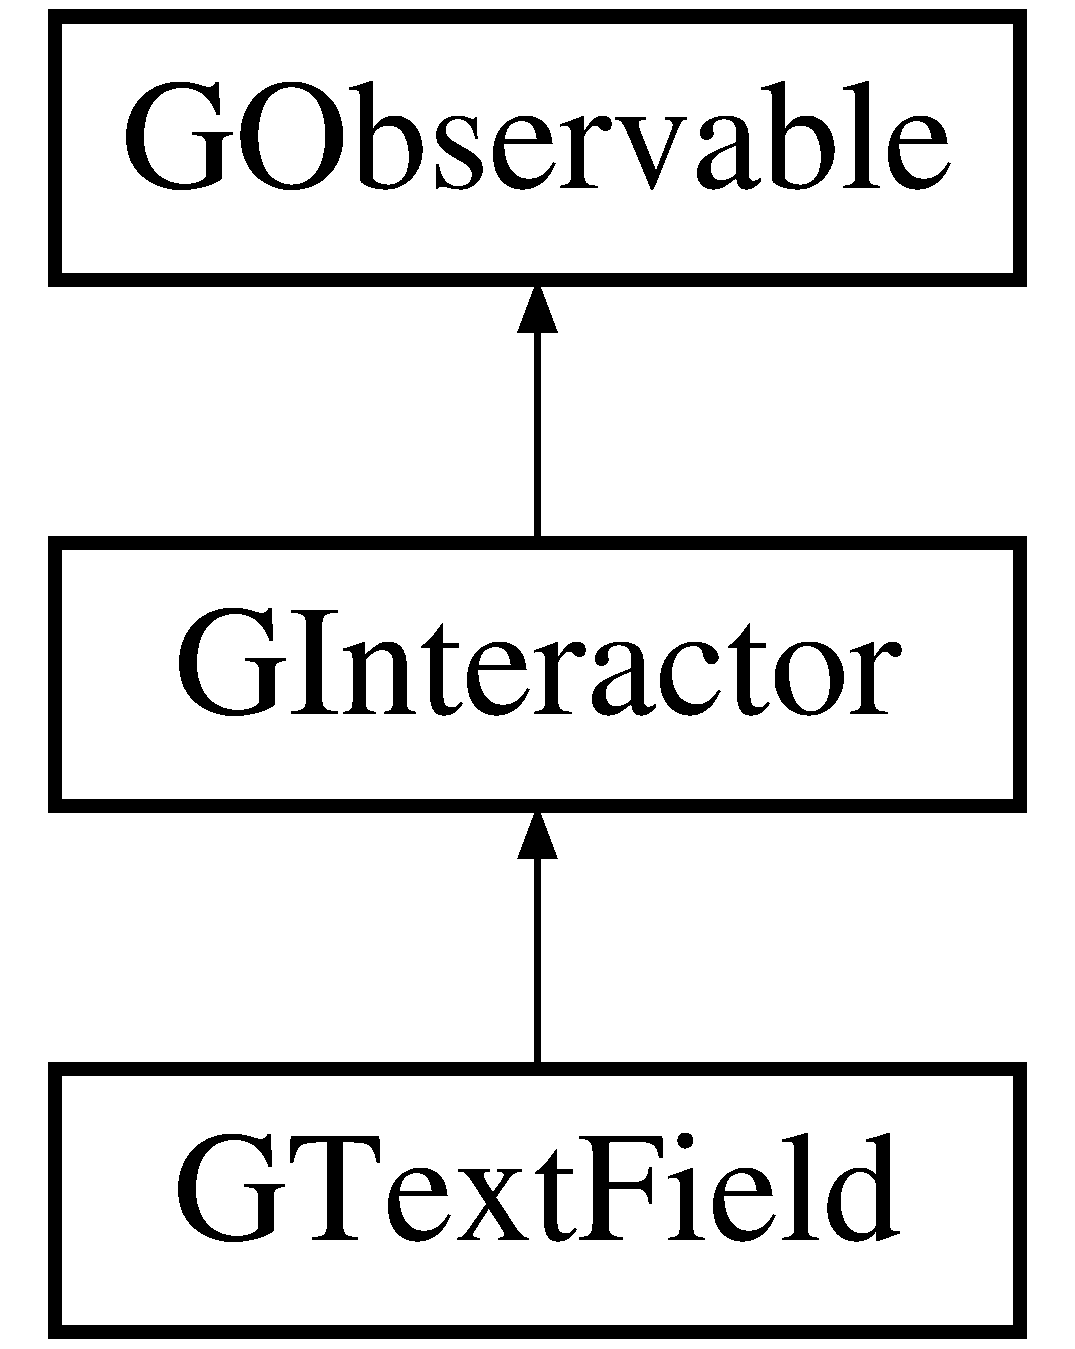
\includegraphics[height=3.000000cm]{classGTextField}
\end{center}
\end{figure}
\subsection*{Public Types}
\begin{DoxyCompactItemize}
\item 
enum \mbox{\hyperlink{classGTextField_a5fc772c800c3d40d2b95564e8a839bab}{Input\+Type}} \{ \mbox{\hyperlink{classGTextField_a5fc772c800c3d40d2b95564e8a839babadbd6303eaf17fd7715ddca85f2ac3287}{I\+N\+P\+U\+T\+\_\+\+T\+Y\+P\+E\+\_\+\+T\+E\+XT}}, 
\mbox{\hyperlink{classGTextField_a5fc772c800c3d40d2b95564e8a839babac37563ad86c1ac752795ed59e700be77}{I\+N\+P\+U\+T\+\_\+\+T\+Y\+P\+E\+\_\+\+I\+N\+T\+E\+G\+ER}}, 
\mbox{\hyperlink{classGTextField_a5fc772c800c3d40d2b95564e8a839babab760f99baafaf18281fa72664f303938}{I\+N\+P\+U\+T\+\_\+\+T\+Y\+P\+E\+\_\+\+R\+E\+AL}}
 \}
\begin{DoxyCompactList}\small\item\em Constants for the valid types of text field input. \end{DoxyCompactList}\item 
enum \mbox{\hyperlink{classGInteractor_a8e0d441725a81d2bbdebbea09078260e}{Text\+Position}} \{ \mbox{\hyperlink{classGInteractor_a8e0d441725a81d2bbdebbea09078260ea4cd6f2e7d5a08d6f4dc052df2358f774}{T\+E\+X\+T\+\_\+\+B\+E\+S\+I\+D\+E\+\_\+\+I\+C\+ON}}, 
\mbox{\hyperlink{classGInteractor_a8e0d441725a81d2bbdebbea09078260eaa88490f63d8de68d44c83bdb2ecde3b3}{T\+E\+X\+T\+\_\+\+U\+N\+D\+E\+R\+\_\+\+I\+C\+ON}}, 
\mbox{\hyperlink{classGInteractor_a8e0d441725a81d2bbdebbea09078260ea39a6f388a30ac4fefb6eb13e846bc9f2}{T\+E\+X\+T\+\_\+\+O\+N\+LY}}
 \}
\begin{DoxyCompactList}\small\item\em The places where an interactor can place its text relative to its icon. \end{DoxyCompactList}\end{DoxyCompactItemize}
\subsection*{Public Member Functions}
\begin{DoxyCompactItemize}
\item 
\mbox{\hyperlink{classGTextField_aab905bd4d32eef20c4b8ed701a8ec97f}{G\+Text\+Field}} (const std\+::string \&text=\char`\"{}\char`\"{}, int chars\+Wide=0, Q\+Widget $\ast$parent=nullptr)
\begin{DoxyCompactList}\small\item\em Creates a text field with the given initial text. \end{DoxyCompactList}\item 
\mbox{\hyperlink{classGTextField_a036419be062e4f447008a78dae22921c}{G\+Text\+Field}} (int chars\+Wide, Q\+Widget $\ast$parent=nullptr)
\begin{DoxyCompactList}\small\item\em Creates a text field wide enough to display the given number of characters. \end{DoxyCompactList}\item 
\mbox{\hyperlink{classGTextField_a4caf2f90e21e32abf032c99a8c3f8efb}{G\+Text\+Field}} (int value, int min, int max, int step=1, Q\+Widget $\ast$parent=nullptr)
\begin{DoxyCompactList}\small\item\em Creates a text field for entering integer values, with the given initial value. \end{DoxyCompactList}\item 
\mbox{\hyperlink{classGTextField_a8d164bf18d4dd4da6d5af0d23ee3a2c8}{G\+Text\+Field}} (double value, double min, double max, double step, Q\+Widget $\ast$parent=nullptr)
\begin{DoxyCompactList}\small\item\em Creates a text field for entering real number values, with the given initial value. \end{DoxyCompactList}\item 
\mbox{\hyperlink{classGTextField_a3361f8538c9bd9337a7ccc533d3534c0}{$\sim$\+G\+Text\+Field}} () override
\begin{DoxyCompactList}\small\item\em Frees memory allocated internally by the text field. \end{DoxyCompactList}\item 
virtual void \mbox{\hyperlink{classGInteractor_a02f20ea6edfa0671f31c4c648a253833}{add\+Action\+Listener}} () Q\+\_\+\+D\+E\+C\+L\+\_\+\+D\+E\+P\+R\+E\+C\+A\+T\+ED
\begin{DoxyCompactList}\small\item\em Adds an event listener to be notified when this interactor is clicked or generally interacted with. \end{DoxyCompactList}\item 
bool \mbox{\hyperlink{classGInteractor_a597a370b592e3737d38d9d2f4e2031ea}{events\+Enabled}} () const override
\begin{DoxyCompactList}\small\item\em Returns true if this interactor is currently accepting events. \end{DoxyCompactList}\item 
virtual std\+::string \mbox{\hyperlink{classGInteractor_a69f8d23ed8f207fbecad99960776e942}{get\+Accelerator}} () const
\begin{DoxyCompactList}\small\item\em Returns a string representing a hotkey for this interactor, or an empty string if no accelerator has been set. \end{DoxyCompactList}\item 
virtual std\+::string \mbox{\hyperlink{classGInteractor_a94eb4276000c4fdfb508ce9e6317a82a}{get\+Action\+Command}} () const
\begin{DoxyCompactList}\small\item\em Returns an action command for this interactor, which is a semi-\/unique string you can use to identify it when events occur. \end{DoxyCompactList}\item 
virtual std\+::string \mbox{\hyperlink{classGInteractor_a808e22cc1fdfbecf71ed8c64ef4600e0}{get\+Background}} () const
\begin{DoxyCompactList}\small\item\em Returns the background color of the interactor as a string. \end{DoxyCompactList}\item 
virtual int \mbox{\hyperlink{classGInteractor_a9e827257a55cb8cf4d9de2ec6bcfd7a0}{get\+Background\+Int}} () const
\begin{DoxyCompactList}\small\item\em Returns the background color of the interactor as an R\+GB integer. \end{DoxyCompactList}\item 
virtual \mbox{\hyperlink{structGRectangle}{G\+Rectangle}} \mbox{\hyperlink{classGInteractor_a29e6ac35a0b48f491a4c88194cc5da3b}{get\+Bounds}} () const
\begin{DoxyCompactList}\small\item\em Returns a rectangle representing the x/y position and size of this interactor. \end{DoxyCompactList}\item 
virtual int \mbox{\hyperlink{classGTextField_acccdf98a090bca28752d04519a8b1a28}{get\+Chars\+Wide}} () const
\begin{DoxyCompactList}\small\item\em Returns the number of characters that can fit in the visible area of this text field. \end{DoxyCompactList}\item 
virtual std\+::string \mbox{\hyperlink{classGInteractor_aa061dfa488c31e18549d64363c1d0e34}{get\+Color}} () const
\begin{DoxyCompactList}\small\item\em Returns the foreground/text color of the interactor as a string. \end{DoxyCompactList}\item 
virtual int \mbox{\hyperlink{classGInteractor_a9635c7af766cdc3417f346683fa0e6c1}{get\+Color\+Int}} () const
\begin{DoxyCompactList}\small\item\em Returns the foreground/text color of the interactor as an R\+GB integer. \end{DoxyCompactList}\item 
virtual \mbox{\hyperlink{classGContainer}{G\+Container}} $\ast$ \mbox{\hyperlink{classGInteractor_a7a6e317c29d61030929b4cd2d1c00fe7}{get\+Container}} () const
\begin{DoxyCompactList}\small\item\em Returns a pointer to the onscreen container holding this interactor. \end{DoxyCompactList}\item 
virtual std\+::string \mbox{\hyperlink{classGInteractor_a894a5502900794eeb27d084c21f1d77d}{get\+Font}} () const
\begin{DoxyCompactList}\small\item\em Returns the font of this interactor\textquotesingle{}s text as a font string such as \char`\"{}\+Helvetica-\/12-\/\+Bold\char`\"{}. \end{DoxyCompactList}\item 
virtual std\+::string \mbox{\hyperlink{classGInteractor_a4fa2d8b0192a3a5b4af4bbfe71194d03}{get\+Foreground}} () const
\begin{DoxyCompactList}\small\item\em Returns the foreground/text color of the interactor as a string. \end{DoxyCompactList}\item 
virtual int \mbox{\hyperlink{classGInteractor_ac3b12ab385a6ef9ae90fc879860ba726}{get\+Foreground\+Int}} () const
\begin{DoxyCompactList}\small\item\em Returns the foreground/text color of the interactor as an R\+GB integer. \end{DoxyCompactList}\item 
virtual double \mbox{\hyperlink{classGInteractor_a1e7e353362434072875264cf95629f99}{get\+Height}} () const
\begin{DoxyCompactList}\small\item\em Returns the current onscreen height of this interactor in pixels. \end{DoxyCompactList}\item 
virtual std\+::string \mbox{\hyperlink{classGInteractor_aaed62a73004939a64da6f0eb9eb64d73}{get\+Icon}} () const
\begin{DoxyCompactList}\small\item\em Returns the file name of the icon associated with this interactor, or an empty string if no icon has been set. \end{DoxyCompactList}\item 
virtual int \mbox{\hyperlink{classGInteractor_a9c9659a6c6ba66b4107ba59c95a24241}{get\+ID}} () const
\begin{DoxyCompactList}\small\item\em Returns a globally unique identifier for this interactor, which is set when the interactor is constructed. \end{DoxyCompactList}\item 
virtual \mbox{\hyperlink{classGTextField_a5fc772c800c3d40d2b95564e8a839bab}{Input\+Type}} \mbox{\hyperlink{classGTextField_a69cc7c223d780203ab2852ee5a881753}{get\+Input\+Type}} () const
\begin{DoxyCompactList}\small\item\em Returns the type of input accepted by this text field. \end{DoxyCompactList}\item 
\+\_\+\+Internal\+\_\+\+Q\+Widget $\ast$ \mbox{\hyperlink{classGTextField_a2f6b36b2517087dc90a366b5ce1f5323}{get\+Internal\+Widget}} () const override
\begin{DoxyCompactList}\small\item\em Returns a direct pointer to the internal Qt widget being wrapped by this interactor. \end{DoxyCompactList}\item 
virtual \mbox{\hyperlink{structGPoint}{G\+Point}} \mbox{\hyperlink{classGInteractor_a4f83802015511edeb63b892830812c11}{get\+Location}} () const
\begin{DoxyCompactList}\small\item\em Returns an (x, y) point representing the onscreen location of the top-\/left corner of this interactor within its containing window. \end{DoxyCompactList}\item 
virtual int \mbox{\hyperlink{classGTextField_a465e41b66da9e75443bf0b7951582468}{get\+Max\+Length}} () const
\begin{DoxyCompactList}\small\item\em Returns the maximum length of string allowed in the text field. \end{DoxyCompactList}\item 
virtual double \mbox{\hyperlink{classGInteractor_aed4b0075fcc434499c3cb3e46896bda3}{get\+Minimum\+Height}} () const
\begin{DoxyCompactList}\small\item\em Returns the minimum height in pixels that this interactor will permit itself to be resized to. \end{DoxyCompactList}\item 
virtual \mbox{\hyperlink{structGDimension}{G\+Dimension}} \mbox{\hyperlink{classGInteractor_a66b5af0b32493b4d597ca0a3df2049ea}{get\+Minimum\+Size}} () const
\begin{DoxyCompactList}\small\item\em Returns a \mbox{\hyperlink{structGDimension}{G\+Dimension}} structure representing the minimum size in pixels that this interactor will permit itself to be resized to. \end{DoxyCompactList}\item 
virtual double \mbox{\hyperlink{classGInteractor_a59e668114fe3d49d2a0f28deb258f7c8}{get\+Minimum\+Width}} () const
\begin{DoxyCompactList}\small\item\em Returns the minimum width in pixels that this interactor will permit itself to be resized to. \end{DoxyCompactList}\item 
virtual std\+::string \mbox{\hyperlink{classGInteractor_a8a60438a5b55d0b2ceb35c8674b9d8c5}{get\+Name}} () const
\begin{DoxyCompactList}\small\item\em Returns a string representing a unique name for this interactor. \end{DoxyCompactList}\item 
virtual std\+::string \mbox{\hyperlink{classGTextField_aa78dbaa7dac1f8cdf9048c91abecc7ad}{get\+Placeholder}} () const
\begin{DoxyCompactList}\small\item\em Returns the text field\textquotesingle{}s placeholder text, which is usually displayed as a light gray text in the field when the field is empty. \end{DoxyCompactList}\item 
virtual double \mbox{\hyperlink{classGInteractor_a747de0961653847bdc6615dbf756d715}{get\+Preferred\+Height}} () const
\begin{DoxyCompactList}\small\item\em Returns the height in pixels that this interactor would prefer to be, which would exactly fit its contents with no stretching or scrollbars. \end{DoxyCompactList}\item 
virtual \mbox{\hyperlink{structGDimension}{G\+Dimension}} \mbox{\hyperlink{classGInteractor_a4aabbee761d8e9116275401131b7ccd1}{get\+Preferred\+Size}} () const
\begin{DoxyCompactList}\small\item\em Returns a \mbox{\hyperlink{structGDimension}{G\+Dimension}} structure storing the width and height in pixels that this interactor would prefer to be, which would exactly fit its contents with no stretching or scrollbars. \end{DoxyCompactList}\item 
virtual double \mbox{\hyperlink{classGInteractor_a82bca31d37700fb0e35d2743352efd5e}{get\+Preferred\+Width}} () const
\begin{DoxyCompactList}\small\item\em Returns the height in pixels that this interactor would prefer to be, which would exactly fit its contents with no stretching or scrollbars. \end{DoxyCompactList}\item 
virtual \mbox{\hyperlink{structGDimension}{G\+Dimension}} \mbox{\hyperlink{classGInteractor_a7b4eec96a2bdc6420695d5796a78eea9}{get\+Size}} () const
\begin{DoxyCompactList}\small\item\em Returns a \mbox{\hyperlink{structGDimension}{G\+Dimension}} structure storing the current onscreen width and height of this interactor in pixels. \end{DoxyCompactList}\item 
virtual std\+::string \mbox{\hyperlink{classGTextField_aff553c50924b836c29f146ed34a7c6ec}{get\+Text}} () const
\begin{DoxyCompactList}\small\item\em Returns the text field\textquotesingle{}s current text. \end{DoxyCompactList}\item 
std\+::string \mbox{\hyperlink{classGTextField_a9b72ede4ee8520f987a0c01e30654814}{get\+Type}} () const override
\begin{DoxyCompactList}\small\item\em Returns a string representing the class name of this interactor, such as \char`\"{}\+G\+Button\char`\"{} or \char`\"{}\+G\+Check\+Box\char`\"{}. \end{DoxyCompactList}\item 
virtual std\+::string \mbox{\hyperlink{classGTextField_a2a03038d2e299f486e55dc72778f7086}{get\+Value}} () const
\begin{DoxyCompactList}\small\item\em Returns the text field\textquotesingle{}s current text. \end{DoxyCompactList}\item 
virtual bool \mbox{\hyperlink{classGTextField_a8190c918ce29007223898c9d511b17ee}{get\+Value\+As\+Bool}} () const
\begin{DoxyCompactList}\small\item\em Returns the currently typed value in the text field, interpreted as a bool value of true or false. \end{DoxyCompactList}\item 
virtual char \mbox{\hyperlink{classGTextField_a562f514fc055aaa37ca3145fc7abde8e}{get\+Value\+As\+Char}} () const
\begin{DoxyCompactList}\small\item\em Returns the currently typed value in the text field as a char value. \end{DoxyCompactList}\item 
virtual double \mbox{\hyperlink{classGTextField_aab9a19edbd1548d557721e0b695295f8}{get\+Value\+As\+Double}} () const
\begin{DoxyCompactList}\small\item\em Returns the currently typed value in the text field, interpreted as a real number value. \end{DoxyCompactList}\item 
virtual int \mbox{\hyperlink{classGTextField_a5e50caa202955b726a44a1dfbc6f7818}{get\+Value\+As\+Int}} () const
\begin{DoxyCompactList}\small\item\em Returns the currently typed value in the text field, interpreted as an integer value. \end{DoxyCompactList}\item 
virtual int \mbox{\hyperlink{classGTextField_a1cbf643145c03ed4c238d085fc88cf33}{get\+Value\+As\+Integer}} () const
\begin{DoxyCompactList}\small\item\em Returns the currently typed value in the text field, interpreted as an integer value. \end{DoxyCompactList}\item 
Q\+Widget $\ast$ \mbox{\hyperlink{classGTextField_a3b33a602b31a6b809d020535a59db3b4}{get\+Widget}} () const override
\begin{DoxyCompactList}\small\item\em Returns a direct pointer to the internal Qt widget being wrapped by this interactor. \end{DoxyCompactList}\item 
virtual double \mbox{\hyperlink{classGInteractor_a0ed2965abd4f5701d2cadf71239faf19}{get\+Width}} () const
\begin{DoxyCompactList}\small\item\em Returns the current onscreen width of this interactor in pixels. \end{DoxyCompactList}\item 
virtual double \mbox{\hyperlink{classGInteractor_a344385751bee0720059403940d57a13e}{getX}} () const
\begin{DoxyCompactList}\small\item\em Returns the x-\/coordinate of the top-\/left pixel of this interactor within its onscreen window. \end{DoxyCompactList}\item 
virtual double \mbox{\hyperlink{classGInteractor_aafa51c7f8f38a09febbb9ce7853f77b4}{getY}} () const
\begin{DoxyCompactList}\small\item\em Returns the y-\/coordinate of the top-\/left pixel of this interactor within its onscreen window. \end{DoxyCompactList}\item 
virtual bool \mbox{\hyperlink{classGInteractor_afc480f652b8c5f1fb255e2269ce68879}{in\+Bounds}} (double x, double y) const
\begin{DoxyCompactList}\small\item\em Returns true if the given x/y pixel is within the bounds of this interactor. \end{DoxyCompactList}\item 
virtual bool \mbox{\hyperlink{classGInteractor_ae6d7982c1c627b677a5e776ca86118ed}{in\+Bounds}} (int x, int y) const
\begin{DoxyCompactList}\small\item\em Returns true if the given x/y pixel is within the bounds of this interactor. \end{DoxyCompactList}\item 
virtual bool \mbox{\hyperlink{classGTextField_a7528cfb0542ac5268efe1d7362b89344}{is\+Autocomplete\+Enabled}} () const
\begin{DoxyCompactList}\small\item\em Returns true if this text field has an autocompletion list of options that will pop up as the user begins typing. \end{DoxyCompactList}\item 
virtual bool \mbox{\hyperlink{classGTextField_a012b5afb54e037e6c5498cf0932a521b}{is\+Editable}} () const
\begin{DoxyCompactList}\small\item\em Returns true if the text field\textquotesingle{}s value can be edited. \end{DoxyCompactList}\item 
virtual bool \mbox{\hyperlink{classGInteractor_aacb819fb241851fd9fc045271baa4034}{is\+Enabled}} () const
\begin{DoxyCompactList}\small\item\em Returns true if this interactor is currently enabled. \end{DoxyCompactList}\item 
virtual bool \mbox{\hyperlink{classGInteractor_a9d8a6cfb13917785c143e74d40e4e2be}{is\+Visible}} () const
\begin{DoxyCompactList}\small\item\em Returns true if the interactor is visible on the screen. \end{DoxyCompactList}\item 
virtual void \mbox{\hyperlink{classGInteractor_ab7fe7a876367b87cf7202f947f1d05e4}{remove\+Action\+Listener}} ()
\begin{DoxyCompactList}\small\item\em Removes the action listener from this interactor so that it will no longer call it when events occur. \end{DoxyCompactList}\item 
virtual void \mbox{\hyperlink{classGInteractor_ad39d0325cde6b97ebda4b9d7787c633b}{remove\+Click\+Listener}} ()
\begin{DoxyCompactList}\small\item\em Removes the click listener from this interactor so that it will no longer call it when events occur. \end{DoxyCompactList}\item 
virtual void \mbox{\hyperlink{classGInteractor_aa4250907e4cdd77349c04f0cf5cdd3d3}{remove\+Double\+Click\+Listener}} ()
\begin{DoxyCompactList}\small\item\em Removes the double-\/click listener from this interactor so that it will no longer call it when events occur. \end{DoxyCompactList}\item 
virtual void \mbox{\hyperlink{classGInteractor_a43095f41cab3be732b49f29970484b05}{remove\+Key\+Listener}} ()
\begin{DoxyCompactList}\small\item\em Removes the key listener from this interactor so that it will no longer call it when key events occur. \end{DoxyCompactList}\item 
virtual void \mbox{\hyperlink{classGInteractor_aff47f71ce47e688a07c9d38dc92fcc11}{remove\+Mouse\+Listener}} ()
\begin{DoxyCompactList}\small\item\em Removes the mouse listener from this interactor so that it will no longer call it when events occur. \end{DoxyCompactList}\item 
virtual void \mbox{\hyperlink{classGTextField_a69c940b99d01eb7c353763ce4b0942a4}{remove\+Text\+Change\+Listener}} ()
\begin{DoxyCompactList}\small\item\em Removes the text change listener from this text field so that it will no longer call it when the user types characters. \end{DoxyCompactList}\item 
virtual void \mbox{\hyperlink{classGInteractor_a519fb2ac767f8b2febbb50b898b8c8cb}{request\+Focus}} ()
\begin{DoxyCompactList}\small\item\em Transfers keyboard focus to this interactor. \end{DoxyCompactList}\item 
virtual void \mbox{\hyperlink{classGInteractor_ad15f102f62e2960576012f1aa0ba4b2e}{set\+Accelerator}} (const std\+::string \&accelerator)
\begin{DoxyCompactList}\small\item\em Sets an accelerator hotkey for this interactor, such as \char`\"{}\+Ctrl-\/\+S\char`\"{}. \end{DoxyCompactList}\item 
virtual void \mbox{\hyperlink{classGInteractor_a4b5843fe3030e038a1ba54cc03389bcf}{set\+Action\+Command}} (const std\+::string \&action\+Command)
\begin{DoxyCompactList}\small\item\em Sets the action command for this interactor. \end{DoxyCompactList}\item 
virtual void \mbox{\hyperlink{classGInteractor_adcfb4742430c88714fcf57e57ab8ea9c}{set\+Action\+Listener}} (G\+Event\+Listener func)
\begin{DoxyCompactList}\small\item\em Sets an action listener on this interactor so that it will be called when it is interacted with in its primary way. \end{DoxyCompactList}\item 
virtual void \mbox{\hyperlink{classGInteractor_aebd20a89c7a8a43a6fce999cf4f9fcf2}{set\+Action\+Listener}} (G\+Event\+Listener\+Void func)
\begin{DoxyCompactList}\small\item\em Sets an action listener on this interactor so that it will be called when it is interacted with in its primary way. \end{DoxyCompactList}\item 
virtual void \mbox{\hyperlink{classGTextField_a173f724f6099be5a2ed423baf3433b83}{set\+Autocomplete\+Enabled}} (bool enabled)
\begin{DoxyCompactList}\small\item\em Sets whether the autocompletion feature is enabled for this text field. \end{DoxyCompactList}\item 
virtual void \mbox{\hyperlink{classGTextField_ab0245df51aa762af89f0d2cf31ce6ddd}{set\+Autocomplete\+List}} (std\+::initializer\+\_\+list$<$ std\+::string $>$ strings)
\begin{DoxyCompactList}\small\item\em Sets the given list of strings to be used as an autocompletion list for this text field. \end{DoxyCompactList}\item 
virtual void \mbox{\hyperlink{classGTextField_aee449aad44655f02ed75727b3f6dd4d6}{set\+Autocomplete\+List}} (const std\+::vector$<$ std\+::string $>$ \&strings)
\begin{DoxyCompactList}\small\item\em Sets the given list of strings to be used as an autocompletion list for this text field. \end{DoxyCompactList}\item 
virtual void \mbox{\hyperlink{classGInteractor_acba7e546c2025c0a15ca4b4cc92043db}{set\+Background}} (int rgb)
\begin{DoxyCompactList}\small\item\em Sets the background color of the interactor to the color represented by the given R\+GB integer. \end{DoxyCompactList}\item 
virtual void \mbox{\hyperlink{classGInteractor_ab4677ab2474e68b07aa56605af92a84a}{set\+Background}} (const std\+::string \&color)
\begin{DoxyCompactList}\small\item\em Sets the background color of the interactor to the color represented by the given string. \end{DoxyCompactList}\item 
virtual void \mbox{\hyperlink{classGInteractor_a2aae8197624b72265ab83b4f1bc73f2f}{set\+Bounds}} (double x, double y, double width, double height)
\begin{DoxyCompactList}\small\item\em Sets the size and location of the widget. \end{DoxyCompactList}\item 
virtual void \mbox{\hyperlink{classGInteractor_acada386653f008cacc7cce86426bef7c}{set\+Bounds}} (const \mbox{\hyperlink{structGRectangle}{G\+Rectangle}} \&size)
\begin{DoxyCompactList}\small\item\em Sets the size and location of the widget. \end{DoxyCompactList}\item 
virtual void \mbox{\hyperlink{classGTextField_aef8026e0b00b17dbccfc456e75308f16}{set\+Chars\+Wide}} (int chars\+Wide)
\begin{DoxyCompactList}\small\item\em Sets the width of this text field to be exactly wide enough to display the given number of characters. \end{DoxyCompactList}\item 
virtual void \mbox{\hyperlink{classGInteractor_abd40af6921242584d0954f173911b190}{set\+Click\+Listener}} (G\+Event\+Listener func)
\begin{DoxyCompactList}\small\item\em Sets a mouse listener on this interactor so that it will be called when the mouse is clicked on it. \end{DoxyCompactList}\item 
virtual void \mbox{\hyperlink{classGInteractor_a856414c92df90f56f3877475eb3f8fc4}{set\+Click\+Listener}} (G\+Event\+Listener\+Void func)
\begin{DoxyCompactList}\small\item\em Sets a mouse listener on this interactor so that it will be called when the mouse is clicked on it. \end{DoxyCompactList}\item 
virtual void \mbox{\hyperlink{classGInteractor_ab1f5cc0f5cc6bbbd716a526c61f1081d}{set\+Color}} (int rgb)
\begin{DoxyCompactList}\small\item\em Sets the foreground/text color of the interactor to the color represented by the given R\+GB integer. \end{DoxyCompactList}\item 
virtual void \mbox{\hyperlink{classGInteractor_a61374df6c11b52cfbb0815decdbaebc6}{set\+Color}} (const std\+::string \&color)
\begin{DoxyCompactList}\small\item\em Sets the foreground/text color of the interactor to the color represented by the given string. \end{DoxyCompactList}\item 
virtual void \mbox{\hyperlink{classGInteractor_ac29f9a3462458e165fae3a1f046ee77a}{set\+Double\+Click\+Listener}} (G\+Event\+Listener func)
\begin{DoxyCompactList}\small\item\em Sets a mouse listener on this interactor so that it will be called when the mouse is double-\/clicked on it. \end{DoxyCompactList}\item 
virtual void \mbox{\hyperlink{classGInteractor_a50096194d66f48c92dd4c512d41bfc76}{set\+Double\+Click\+Listener}} (G\+Event\+Listener\+Void func)
\begin{DoxyCompactList}\small\item\em Sets a mouse listener on this interactor so that it will be called when the mouse is double-\/clicked on it. \end{DoxyCompactList}\item 
virtual void \mbox{\hyperlink{classGTextField_a008d7fd44fb3e7a6886cdaddbc3644a2}{set\+Editable}} (bool value)
\begin{DoxyCompactList}\small\item\em Sets whether the value in the text box can be edited. \end{DoxyCompactList}\item 
virtual void \mbox{\hyperlink{classGInteractor_ab831367dd84bbd579e02e55bacb21343}{set\+Enabled}} (bool value)
\begin{DoxyCompactList}\small\item\em Sets whether this interactor is currently enabled. \end{DoxyCompactList}\item 
virtual void \mbox{\hyperlink{classGObservable_afaa30b2a9e0f378fd1c70d2f1d0b8216}{set\+Events\+Enabled}} (bool \mbox{\hyperlink{classGInteractor_a597a370b592e3737d38d9d2f4e2031ea}{events\+Enabled}})
\begin{DoxyCompactList}\small\item\em Sets whether the object is currently allowing itself to fire events. \end{DoxyCompactList}\item 
virtual void \mbox{\hyperlink{classGInteractor_a2592348886ffea646c6534bf88f7c49d}{set\+Font}} (const Q\+Font \&font)
\begin{DoxyCompactList}\small\item\em Sets the font used by this widget to the given Qt font. \end{DoxyCompactList}\item 
virtual void \mbox{\hyperlink{classGInteractor_a8e096e8818d838aceae1d46d58fb3a7b}{set\+Font}} (const std\+::string \&font)
\begin{DoxyCompactList}\small\item\em Sets the font used by this widget to the font represented by the given font string, such as \char`\"{}\+Helvetica-\/16-\/\+Bold\char`\"{}. \end{DoxyCompactList}\item 
virtual void \mbox{\hyperlink{classGInteractor_a9eb856b5ff83a19df3831a31f15f4563}{set\+Foreground}} (int rgb)
\begin{DoxyCompactList}\small\item\em Sets the foreground/text color of the interactor to the color represented by the given R\+GB integer. \end{DoxyCompactList}\item 
virtual void \mbox{\hyperlink{classGInteractor_af59209aeadea6dfc6d97a2d8531f50e1}{set\+Foreground}} (const std\+::string \&color)
\begin{DoxyCompactList}\small\item\em Sets the foreground/text color of the interactor to the color represented by the given string. \end{DoxyCompactList}\item 
virtual void \mbox{\hyperlink{classGInteractor_a9e280bfc4544dfaf8e4376c4e1a74357}{set\+Height}} (double height)
\begin{DoxyCompactList}\small\item\em Sets the onscreen height of the interactor in pixels. \end{DoxyCompactList}\item 
virtual void \mbox{\hyperlink{classGInteractor_a542abfcd7261751352af129c7215ecda}{set\+Icon}} (const Q\+Icon \&icon)
\begin{DoxyCompactList}\small\item\em Sets the icon associated with this interactor. \end{DoxyCompactList}\item 
virtual void \mbox{\hyperlink{classGInteractor_a368e1a338f84401c284506d03b1ba769}{set\+Icon}} (const Q\+Pixmap \&icon)
\begin{DoxyCompactList}\small\item\em Sets the icon associated with this interactor. \end{DoxyCompactList}\item 
virtual void \mbox{\hyperlink{classGInteractor_a762e139aa311461c3984d3ad28293f64}{set\+Icon}} (const std\+::string \&filename, bool retain\+Icon\+Size=true)
\begin{DoxyCompactList}\small\item\em Sets the file name of the icon associated with this interactor, or an empty string if no icon has been set. \end{DoxyCompactList}\item 
virtual void \mbox{\hyperlink{classGInteractor_aeb8324d3287fa1fbe093f4d6230cf0a6}{set\+Key\+Listener}} (G\+Event\+Listener func)
\begin{DoxyCompactList}\small\item\em Sets a key listener on this interactor so that it will be called when the user presses any key. \end{DoxyCompactList}\item 
virtual void \mbox{\hyperlink{classGInteractor_ae48ecea73606c7bd9423e1c7cc589cc9}{set\+Key\+Listener}} (G\+Event\+Listener\+Void func)
\begin{DoxyCompactList}\small\item\em Sets a key listener on this interactor so that it will be called when the user presses any key. \end{DoxyCompactList}\item 
virtual void \mbox{\hyperlink{classGInteractor_a04594e8ba9b98513a64f1da00dcae18c}{set\+Location}} (double x, double y)
\begin{DoxyCompactList}\small\item\em Sets the onscreen x/y-\/coordinate of the top-\/left corner of the interactor relative to its window. \end{DoxyCompactList}\item 
virtual void \mbox{\hyperlink{classGTextField_a077c24fa5337fbf431738f8ba513d19c}{set\+Max\+Length}} (int max\+Length)
\begin{DoxyCompactList}\small\item\em Sets the maximum number of characters that can be typed into the field. \end{DoxyCompactList}\item 
virtual void \mbox{\hyperlink{classGInteractor_a0cf428e207b7f22cc08138a90b1b87b2}{set\+Minimum\+Size}} (double width, double height)
\begin{DoxyCompactList}\small\item\em Sets the minimum size in pixels that this interactor will permit itself to be resized to. \end{DoxyCompactList}\item 
virtual void \mbox{\hyperlink{classGInteractor_a3b1046117ac6cb7abe467e00ba8a81f4}{set\+Minimum\+Size}} (const \mbox{\hyperlink{structGDimension}{G\+Dimension}} \&size)
\begin{DoxyCompactList}\small\item\em Sets the minimum size in pixels that this interactor will permit itself to be resized to. \end{DoxyCompactList}\item 
virtual void \mbox{\hyperlink{classGInteractor_a37d8dbc943f59920f705b0104f60bde2}{set\+Mouse\+Listener}} (G\+Event\+Listener func)
\begin{DoxyCompactList}\small\item\em Sets a mouse listener on this interactor so that it will be called when the mouse is moved or clicked on it. \end{DoxyCompactList}\item 
virtual void \mbox{\hyperlink{classGInteractor_aea7f647ea62d59f71b5fad6aa65eeaf9}{set\+Mouse\+Listener}} (G\+Event\+Listener\+Void func)
\begin{DoxyCompactList}\small\item\em Sets a mouse listener on this interactor so that it will be called when the mouse is moved or clicked on it. \end{DoxyCompactList}\item 
virtual void \mbox{\hyperlink{classGInteractor_a9d3a2685df23b5e7cbf59c19c4a1f9b5}{set\+Name}} (const std\+::string \&name)
\begin{DoxyCompactList}\small\item\em Sets a string representing a unique name for this interactor. \end{DoxyCompactList}\item 
virtual void \mbox{\hyperlink{classGTextField_aa21a9bebb4652ab6780d0c11eff47aee}{set\+Placeholder}} (const std\+::string \&text)
\begin{DoxyCompactList}\small\item\em Sets a gray message that is displayed in the background of the text field before the user has typed any value. \end{DoxyCompactList}\item 
virtual void \mbox{\hyperlink{classGInteractor_a1ab987704fce32098706c6f00fb08218}{set\+Preferred\+Height}} (double height)
\begin{DoxyCompactList}\small\item\em Sets the height in pixels that this interactor would prefer to be. \end{DoxyCompactList}\item 
virtual void \mbox{\hyperlink{classGInteractor_a042c5ae19430d765ef552371cae3632c}{set\+Preferred\+Size}} (double width, double height)
\begin{DoxyCompactList}\small\item\em Sets the width and height in pixels that this interactor would prefer to be. \end{DoxyCompactList}\item 
virtual void \mbox{\hyperlink{classGInteractor_aa22d9be4bc0e078bb0ea69b0fc9d7c75}{set\+Preferred\+Size}} (const \mbox{\hyperlink{structGDimension}{G\+Dimension}} \&size)
\begin{DoxyCompactList}\small\item\em Sets the size in pixels that this interactor would prefer to be. \end{DoxyCompactList}\item 
virtual void \mbox{\hyperlink{classGInteractor_a3db429ab2fa52efd187eec0ed8cdd9f2}{set\+Preferred\+Width}} (double width)
\begin{DoxyCompactList}\small\item\em Sets the width in pixels that this interactor would prefer to be. \end{DoxyCompactList}\item 
virtual void \mbox{\hyperlink{classGInteractor_aca25d49481f9bf5fc8f7df4c086c4ce7}{set\+Size}} (double width, double height)
\begin{DoxyCompactList}\small\item\em Sets the onscreen width and height of the interactor in pixels. \end{DoxyCompactList}\item 
virtual void \mbox{\hyperlink{classGInteractor_ae2b628228f192c2702c4ce941b2af68f}{set\+Size}} (const \mbox{\hyperlink{structGDimension}{G\+Dimension}} \&size)
\begin{DoxyCompactList}\small\item\em Sets the onscreen width and height of the interactor in pixels. \end{DoxyCompactList}\item 
virtual void \mbox{\hyperlink{classGTextField_ac1ae51949d41ee9054634be5967d91b8}{set\+Text}} (const std\+::string \&text)
\begin{DoxyCompactList}\small\item\em Sets the current text value in the text field. \end{DoxyCompactList}\item 
virtual void \mbox{\hyperlink{classGTextField_ae41284f9c540110180ac0ad6beca5cb0}{set\+Text\+Change\+Listener}} (G\+Event\+Listener func)
\begin{DoxyCompactList}\small\item\em Sets a text-\/change listener on this text field so that it will be called when the value in the field changes, which will occur on every key press. \end{DoxyCompactList}\item 
virtual void \mbox{\hyperlink{classGTextField_ae8df75b0746951146d29220f386fcd33}{set\+Text\+Change\+Listener}} (G\+Event\+Listener\+Void func)
\begin{DoxyCompactList}\small\item\em Sets a text-\/change listener on this text field so that it will be called when the value in the field changes, which will occur on every key press. \end{DoxyCompactList}\item 
virtual void \mbox{\hyperlink{classGInteractor_a039e0e49beaecc275efce02d416acea8}{set\+Tooltip}} (const std\+::string \&tooltip\+Text)
\begin{DoxyCompactList}\small\item\em Sets a \char`\"{}tooltip\char`\"{} that will appear if the user hovers their mouse over the interactor. \end{DoxyCompactList}\item 
virtual void \mbox{\hyperlink{classGTextField_ae803b3348fa7076308d852bbdeea0d74}{set\+Value}} (bool value)
\begin{DoxyCompactList}\small\item\em Sets the current text value in the text field to the string representation of the given value. \end{DoxyCompactList}\item 
virtual void \mbox{\hyperlink{classGTextField_aeefe59b3d414b657838869ce084cb0e2}{set\+Value}} (char value)
\begin{DoxyCompactList}\small\item\em Sets the current text value in the text field to the string representation of the given value. \end{DoxyCompactList}\item 
virtual void \mbox{\hyperlink{classGTextField_a1a31743bc7def7cf7fdad044c84d9268}{set\+Value}} (double value)
\begin{DoxyCompactList}\small\item\em Sets the current text value in the text field to the string representation of the given value. \end{DoxyCompactList}\item 
virtual void \mbox{\hyperlink{classGTextField_a23d79e21b8ed72e19278ca31d47b8c87}{set\+Value}} (int value)
\begin{DoxyCompactList}\small\item\em Sets the current text value in the text field to the string representation of the given value. \end{DoxyCompactList}\item 
virtual void \mbox{\hyperlink{classGTextField_ab18c7a418be64c4f909beebc277a1321}{set\+Value}} (const std\+::string \&value)
\begin{DoxyCompactList}\small\item\em Sets the current text value in the text field to the string representation of the given value. \end{DoxyCompactList}\item 
virtual void \mbox{\hyperlink{classGInteractor_a18e44e30b31525a243960ca3928125aa}{set\+Visible}} (bool visible)
\begin{DoxyCompactList}\small\item\em Returns true if the interactor is visible on the screen. \end{DoxyCompactList}\item 
virtual void \mbox{\hyperlink{classGInteractor_aa3f3fba4cb131baa8696ba01e3bceca1}{set\+Width}} (double width)
\begin{DoxyCompactList}\small\item\em Sets the onscreen width of the interactor in pixels. \end{DoxyCompactList}\item 
virtual void \mbox{\hyperlink{classGInteractor_a9c18fcc579333bf9653d13ad2b372e39}{setX}} (double x)
\begin{DoxyCompactList}\small\item\em Sets the onscreen x-\/coordinate of the top-\/left corner of the interactor relative to its window. \end{DoxyCompactList}\item 
virtual void \mbox{\hyperlink{classGInteractor_a7d57e2a5c35d27feb58fd498a3cf82b9}{setY}} (double y)
\begin{DoxyCompactList}\small\item\em Sets the onscreen y-\/coordinate of the top-\/left corner of the interactor relative to its window. \end{DoxyCompactList}\item 
virtual std\+::string \mbox{\hyperlink{classGObservable_a1fe5121d6528fdea3f243321b3fa3a49}{to\+String}} () const
\begin{DoxyCompactList}\small\item\em Returns a string representation of this observable object\textquotesingle{}s state. \end{DoxyCompactList}\item 
virtual bool \mbox{\hyperlink{classGTextField_a203f90275053ab957b1ea5a40dc3dd1e}{value\+Is\+Bool}} () const
\begin{DoxyCompactList}\small\item\em Returns true if the currently typed value in the text field can be interpreted as a bool value of true or false. \end{DoxyCompactList}\item 
virtual bool \mbox{\hyperlink{classGTextField_ac7a337b1e4c2f752a7f3fb634c92b442}{value\+Is\+Char}} () const
\begin{DoxyCompactList}\small\item\em Returns true if the currently typed value in the text field can be interpreted as a char value. \end{DoxyCompactList}\item 
virtual bool \mbox{\hyperlink{classGTextField_aa80caadc7498333f74a08b4cdc0528c1}{value\+Is\+Double}} () const
\begin{DoxyCompactList}\small\item\em Returns true if the currently typed value in the text field can be interpreted as a real number. \end{DoxyCompactList}\item 
virtual bool \mbox{\hyperlink{classGTextField_a4bccf08b3b712af3839106a1cbdc5d02}{value\+Is\+Int}} () const
\begin{DoxyCompactList}\small\item\em Returns true if the currently typed value in the text field can be interpreted as an integer. \end{DoxyCompactList}\item 
virtual bool \mbox{\hyperlink{classGTextField_af5aaf003739648d9aee89a17e715a57e}{value\+Is\+Integer}} () const
\begin{DoxyCompactList}\small\item\em Returns true if the currently typed value in the text field can be interpreted as an integer. \end{DoxyCompactList}\item 
virtual bool \mbox{\hyperlink{classGTextField_a29a5f540431d7993ff00eee5d2584a36}{value\+Is\+Real}} () const
\begin{DoxyCompactList}\small\item\em Returns true if the currently typed value in the text field can be interpreted as a real number. \end{DoxyCompactList}\end{DoxyCompactItemize}
\subsection*{Protected Member Functions}
\begin{DoxyCompactItemize}
\item 
virtual void \mbox{\hyperlink{classGObservable_a80cfa040459ff53594adbd6a51ec8f43}{clear\+Event\+Listeners}} ()
\begin{DoxyCompactList}\small\item\em Removes all event listeners from this object. \end{DoxyCompactList}\item 
virtual void \mbox{\hyperlink{classGObservable_a284f31528c0520f8e545c03ac9eeac74}{ensure\+Thread\+Safety}} (const std\+::string \&member\+Name=\char`\"{}\char`\"{})
\begin{DoxyCompactList}\small\item\em Ensures that we are currently in the Qt G\+UI thread. \end{DoxyCompactList}\item 
virtual void \mbox{\hyperlink{classGObservable_a63e5e5a6227c59c928493b11aceb0f67}{fire\+Event}} (\mbox{\hyperlink{classGEvent}{G\+Event}} \&event)
\begin{DoxyCompactList}\small\item\em Sends out the given event to any attached listeners. \end{DoxyCompactList}\item 
virtual void \mbox{\hyperlink{classGObservable_ab3983ea07337b52020a29cc00c653d8d}{fire\+G\+Event}} (Q\+Event $\ast$event, Event\+Type event\+Type, const std\+::string \&event\+Name)
\begin{DoxyCompactList}\small\item\em Creates an event of the given type, then sends it out to any attached listeners. \end{DoxyCompactList}\item 
virtual void \mbox{\hyperlink{classGObservable_a01fdf1b0e0dbd49e189fe4514e010411}{fire\+G\+Event}} (Q\+Close\+Event $\ast$event, Event\+Type event\+Type, const std\+::string \&event\+Name)
\begin{DoxyCompactList}\small\item\em Creates an event of the given type, then sends it out to any attached listeners. \end{DoxyCompactList}\item 
virtual void \mbox{\hyperlink{classGObservable_abb0b2f66ba39211cb5d7615e9d1c04e2}{fire\+G\+Event}} (Q\+Key\+Event $\ast$event, Event\+Type event\+Type, const std\+::string \&event\+Name)
\begin{DoxyCompactList}\small\item\em Creates an event of the given type, then sends it out to any attached listeners. \end{DoxyCompactList}\item 
virtual void \mbox{\hyperlink{classGObservable_a119318675d2165bdf7dd853aaf881d4b}{fire\+G\+Event}} (Q\+Mouse\+Event $\ast$event, Event\+Type event\+Type, const std\+::string \&event\+Name, const std\+::string \&action\+Command=\char`\"{}\char`\"{})
\begin{DoxyCompactList}\small\item\em Creates an event of the given type, then sends it out to any attached listeners. \end{DoxyCompactList}\item 
virtual void \mbox{\hyperlink{classGObservable_a63fd9034e1e1633c1c38eb342bfd34e9}{fire\+G\+Event}} (Q\+Resize\+Event $\ast$event, Event\+Type event\+Type, const std\+::string \&event\+Name)
\begin{DoxyCompactList}\small\item\em Creates an event of the given type, then sends it out to any attached listeners. \end{DoxyCompactList}\item 
virtual void \mbox{\hyperlink{classGObservable_a741345310d9b7c5170a6cbc410c44ac4}{fire\+G\+Event}} (Q\+Timer\+Event $\ast$event, Event\+Type event\+Type, const std\+::string \&event\+Name)
\begin{DoxyCompactList}\small\item\em Creates an event of the given type, then sends it out to any attached listeners. \end{DoxyCompactList}\item 
virtual void \mbox{\hyperlink{classGObservable_a93bf338968a0338761b8e4dc62f582e9}{fire\+G\+Event}} (Q\+Wheel\+Event $\ast$event, Event\+Type event\+Type, const std\+::string \&event\+Name)
\begin{DoxyCompactList}\small\item\em Creates an event of the given type, then sends it out to any attached listeners. \end{DoxyCompactList}\item 
virtual void \mbox{\hyperlink{classGObservable_a2a70a7d7435ff0c3b80bb4d70da19e0d}{fire\+G\+Event}} (Q\+Window\+State\+Change\+Event $\ast$event, Event\+Type event\+Type, const std\+::string \&event\+Name)
\begin{DoxyCompactList}\small\item\em Creates an event of the given type, then sends it out to any attached listeners. \end{DoxyCompactList}\item 
virtual bool \mbox{\hyperlink{classGObservable_a9f6faaa25942923bafa1c44020c49fa9}{has\+Event\+Listener}} (const std\+::string \&event\+Name) const
\begin{DoxyCompactList}\small\item\em Returns true if the observable object has a listener for the given type of event. \end{DoxyCompactList}\item 
virtual bool \mbox{\hyperlink{classGObservable_aeec1adc19aa0f33de62390686ee1382c}{is\+Accepting\+Event}} (int event\+Mask) const
\begin{DoxyCompactList}\small\item\em Returns true if the observable object has a listener for the given type of event. \end{DoxyCompactList}\item 
virtual bool \mbox{\hyperlink{classGObservable_aa31c73145a29dcb92848a92e0cfaea41}{is\+Accepting\+Event}} (const \mbox{\hyperlink{classGEvent}{G\+Event}} \&event) const
\begin{DoxyCompactList}\small\item\em Returns true if the observable object has a listener for the given type of event. \end{DoxyCompactList}\item 
virtual bool \mbox{\hyperlink{classGObservable_a3b1c689267eda44e65a2213e7de38b23}{is\+Accepting\+Event}} (const std\+::string \&event\+Type) const
\begin{DoxyCompactList}\small\item\em Returns true if the observable object has a listener for the given type of event. \end{DoxyCompactList}\item 
virtual void \mbox{\hyperlink{classGObservable_acbcf1ed3a851ad8a3c17ef38d86b481d}{remove\+Event\+Listener}} (const std\+::string \&event\+Name)
\begin{DoxyCompactList}\small\item\em Removes any event listener from this observable object that would respond to the given type of event, such as \char`\"{}click\char`\"{} or \char`\"{}keydown\char`\"{}. \end{DoxyCompactList}\item 
virtual void \mbox{\hyperlink{classGObservable_af51cc35c29a1bd1908609d432decdbb6}{remove\+Event\+Listeners}} (std\+::initializer\+\_\+list$<$ std\+::string $>$ event\+Names)
\begin{DoxyCompactList}\small\item\em Removes any event listener from this observable object that would respond to the given types of events, such as \char`\"{}click\char`\"{} or \char`\"{}keydown\char`\"{}. \end{DoxyCompactList}\item 
virtual void \mbox{\hyperlink{classGObservable_ad2f6d34961c50f6c1e0659990b79f741}{set\+Event\+Listener}} (const std\+::string \&event\+Name, G\+Event\+Listener func)
\begin{DoxyCompactList}\small\item\em Adds an event listener from this observable object to respond to the given type of event, such as \char`\"{}click\char`\"{} or \char`\"{}keydown\char`\"{}. \end{DoxyCompactList}\item 
virtual void \mbox{\hyperlink{classGObservable_abac4cb9f9e626e010e87f5d91573c8a5}{set\+Event\+Listener}} (const std\+::string \&event\+Name, G\+Event\+Listener\+Void func)
\begin{DoxyCompactList}\small\item\em Adds an event listener from this observable object to respond to the given type of event, such as \char`\"{}click\char`\"{} or \char`\"{}keydown\char`\"{}. \end{DoxyCompactList}\item 
virtual void \mbox{\hyperlink{classGObservable_afa388d69c33c718cf035774604065604}{set\+Event\+Listeners}} (std\+::initializer\+\_\+list$<$ std\+::string $>$ event\+Names, G\+Event\+Listener func)
\begin{DoxyCompactList}\small\item\em Adds an event listener from this observable object to respond to the given types of events, such as \char`\"{}click\char`\"{} or \char`\"{}keydown\char`\"{}. \end{DoxyCompactList}\item 
virtual void \mbox{\hyperlink{classGObservable_a7867184bbb686f74fae8a4db927da799}{set\+Event\+Listeners}} (std\+::initializer\+\_\+list$<$ std\+::string $>$ event\+Names, G\+Event\+Listener\+Void func)
\begin{DoxyCompactList}\small\item\em Adds an event listener from this observable object to respond to the given types of events, such as \char`\"{}click\char`\"{} or \char`\"{}keydown\char`\"{}. \end{DoxyCompactList}\end{DoxyCompactItemize}


\subsection{Detailed Description}
This interactor subclass represents a text field for entering short text strings. 

Pressing Enter in a text field generates an action event. 

\subsection{Member Enumeration Documentation}
\mbox{\Hypertarget{classGTextField_a5fc772c800c3d40d2b95564e8a839bab}\label{classGTextField_a5fc772c800c3d40d2b95564e8a839bab}} 
\index{G\+Text\+Field@{G\+Text\+Field}!Input\+Type@{Input\+Type}}
\index{Input\+Type@{Input\+Type}!G\+Text\+Field@{G\+Text\+Field}}
\subsubsection{\texorpdfstring{Input\+Type}{InputType}}
{\footnotesize\ttfamily enum \mbox{\hyperlink{classGTextField_a5fc772c800c3d40d2b95564e8a839bab}{Input\+Type}}}



Constants for the valid types of text field input. 

\begin{DoxyEnumFields}{Enumerator}
\raisebox{\heightof{T}}[0pt][0pt]{\index{I\+N\+P\+U\+T\+\_\+\+T\+Y\+P\+E\+\_\+\+T\+E\+XT@{I\+N\+P\+U\+T\+\_\+\+T\+Y\+P\+E\+\_\+\+T\+E\+XT}!G\+Text\+Field@{G\+Text\+Field}}\index{G\+Text\+Field@{G\+Text\+Field}!I\+N\+P\+U\+T\+\_\+\+T\+Y\+P\+E\+\_\+\+T\+E\+XT@{I\+N\+P\+U\+T\+\_\+\+T\+Y\+P\+E\+\_\+\+T\+E\+XT}}}\mbox{\Hypertarget{classGTextField_a5fc772c800c3d40d2b95564e8a839babadbd6303eaf17fd7715ddca85f2ac3287}\label{classGTextField_a5fc772c800c3d40d2b95564e8a839babadbd6303eaf17fd7715ddca85f2ac3287}} 
I\+N\+P\+U\+T\+\_\+\+T\+Y\+P\+E\+\_\+\+T\+E\+XT&\\
\hline

\raisebox{\heightof{T}}[0pt][0pt]{\index{I\+N\+P\+U\+T\+\_\+\+T\+Y\+P\+E\+\_\+\+I\+N\+T\+E\+G\+ER@{I\+N\+P\+U\+T\+\_\+\+T\+Y\+P\+E\+\_\+\+I\+N\+T\+E\+G\+ER}!G\+Text\+Field@{G\+Text\+Field}}\index{G\+Text\+Field@{G\+Text\+Field}!I\+N\+P\+U\+T\+\_\+\+T\+Y\+P\+E\+\_\+\+I\+N\+T\+E\+G\+ER@{I\+N\+P\+U\+T\+\_\+\+T\+Y\+P\+E\+\_\+\+I\+N\+T\+E\+G\+ER}}}\mbox{\Hypertarget{classGTextField_a5fc772c800c3d40d2b95564e8a839babac37563ad86c1ac752795ed59e700be77}\label{classGTextField_a5fc772c800c3d40d2b95564e8a839babac37563ad86c1ac752795ed59e700be77}} 
I\+N\+P\+U\+T\+\_\+\+T\+Y\+P\+E\+\_\+\+I\+N\+T\+E\+G\+ER&\\
\hline

\raisebox{\heightof{T}}[0pt][0pt]{\index{I\+N\+P\+U\+T\+\_\+\+T\+Y\+P\+E\+\_\+\+R\+E\+AL@{I\+N\+P\+U\+T\+\_\+\+T\+Y\+P\+E\+\_\+\+R\+E\+AL}!G\+Text\+Field@{G\+Text\+Field}}\index{G\+Text\+Field@{G\+Text\+Field}!I\+N\+P\+U\+T\+\_\+\+T\+Y\+P\+E\+\_\+\+R\+E\+AL@{I\+N\+P\+U\+T\+\_\+\+T\+Y\+P\+E\+\_\+\+R\+E\+AL}}}\mbox{\Hypertarget{classGTextField_a5fc772c800c3d40d2b95564e8a839babab760f99baafaf18281fa72664f303938}\label{classGTextField_a5fc772c800c3d40d2b95564e8a839babab760f99baafaf18281fa72664f303938}} 
I\+N\+P\+U\+T\+\_\+\+T\+Y\+P\+E\+\_\+\+R\+E\+AL&\\
\hline

\end{DoxyEnumFields}
\mbox{\Hypertarget{classGInteractor_a8e0d441725a81d2bbdebbea09078260e}\label{classGInteractor_a8e0d441725a81d2bbdebbea09078260e}} 
\index{G\+Text\+Field@{G\+Text\+Field}!Text\+Position@{Text\+Position}}
\index{Text\+Position@{Text\+Position}!G\+Text\+Field@{G\+Text\+Field}}
\subsubsection{\texorpdfstring{Text\+Position}{TextPosition}}
{\footnotesize\ttfamily enum \mbox{\hyperlink{classGInteractor_a8e0d441725a81d2bbdebbea09078260e}{Text\+Position}}\hspace{0.3cm}{\ttfamily [inherited]}}



The places where an interactor can place its text relative to its icon. 

\begin{DoxyEnumFields}{Enumerator}
\raisebox{\heightof{T}}[0pt][0pt]{\index{T\+E\+X\+T\+\_\+\+B\+E\+S\+I\+D\+E\+\_\+\+I\+C\+ON@{T\+E\+X\+T\+\_\+\+B\+E\+S\+I\+D\+E\+\_\+\+I\+C\+ON}!G\+Text\+Field@{G\+Text\+Field}}\index{G\+Text\+Field@{G\+Text\+Field}!T\+E\+X\+T\+\_\+\+B\+E\+S\+I\+D\+E\+\_\+\+I\+C\+ON@{T\+E\+X\+T\+\_\+\+B\+E\+S\+I\+D\+E\+\_\+\+I\+C\+ON}}}\mbox{\Hypertarget{classGInteractor_a8e0d441725a81d2bbdebbea09078260ea4cd6f2e7d5a08d6f4dc052df2358f774}\label{classGInteractor_a8e0d441725a81d2bbdebbea09078260ea4cd6f2e7d5a08d6f4dc052df2358f774}} 
T\+E\+X\+T\+\_\+\+B\+E\+S\+I\+D\+E\+\_\+\+I\+C\+ON&\\
\hline

\raisebox{\heightof{T}}[0pt][0pt]{\index{T\+E\+X\+T\+\_\+\+U\+N\+D\+E\+R\+\_\+\+I\+C\+ON@{T\+E\+X\+T\+\_\+\+U\+N\+D\+E\+R\+\_\+\+I\+C\+ON}!G\+Text\+Field@{G\+Text\+Field}}\index{G\+Text\+Field@{G\+Text\+Field}!T\+E\+X\+T\+\_\+\+U\+N\+D\+E\+R\+\_\+\+I\+C\+ON@{T\+E\+X\+T\+\_\+\+U\+N\+D\+E\+R\+\_\+\+I\+C\+ON}}}\mbox{\Hypertarget{classGInteractor_a8e0d441725a81d2bbdebbea09078260eaa88490f63d8de68d44c83bdb2ecde3b3}\label{classGInteractor_a8e0d441725a81d2bbdebbea09078260eaa88490f63d8de68d44c83bdb2ecde3b3}} 
T\+E\+X\+T\+\_\+\+U\+N\+D\+E\+R\+\_\+\+I\+C\+ON&\\
\hline

\raisebox{\heightof{T}}[0pt][0pt]{\index{T\+E\+X\+T\+\_\+\+O\+N\+LY@{T\+E\+X\+T\+\_\+\+O\+N\+LY}!G\+Text\+Field@{G\+Text\+Field}}\index{G\+Text\+Field@{G\+Text\+Field}!T\+E\+X\+T\+\_\+\+O\+N\+LY@{T\+E\+X\+T\+\_\+\+O\+N\+LY}}}\mbox{\Hypertarget{classGInteractor_a8e0d441725a81d2bbdebbea09078260ea39a6f388a30ac4fefb6eb13e846bc9f2}\label{classGInteractor_a8e0d441725a81d2bbdebbea09078260ea39a6f388a30ac4fefb6eb13e846bc9f2}} 
T\+E\+X\+T\+\_\+\+O\+N\+LY&\\
\hline

\end{DoxyEnumFields}


\subsection{Constructor \& Destructor Documentation}
\mbox{\Hypertarget{classGTextField_aab905bd4d32eef20c4b8ed701a8ec97f}\label{classGTextField_aab905bd4d32eef20c4b8ed701a8ec97f}} 
\index{G\+Text\+Field@{G\+Text\+Field}!G\+Text\+Field@{G\+Text\+Field}}
\index{G\+Text\+Field@{G\+Text\+Field}!G\+Text\+Field@{G\+Text\+Field}}
\subsubsection{\texorpdfstring{G\+Text\+Field()}{GTextField()}\hspace{0.1cm}{\footnotesize\ttfamily [1/4]}}
{\footnotesize\ttfamily \mbox{\hyperlink{classGTextField}{G\+Text\+Field}} (\begin{DoxyParamCaption}\item[{const std\+::string \&}]{text = {\ttfamily \char`\"{}\char`\"{}},  }\item[{int}]{chars\+Wide = {\ttfamily 0},  }\item[{Q\+Widget $\ast$}]{parent = {\ttfamily nullptr} }\end{DoxyParamCaption})}



Creates a text field with the given initial text. 

If the optional chars\+Wide parameter is passed, sizes the text field wide enough to display the given number of characters. \mbox{\Hypertarget{classGTextField_a036419be062e4f447008a78dae22921c}\label{classGTextField_a036419be062e4f447008a78dae22921c}} 
\index{G\+Text\+Field@{G\+Text\+Field}!G\+Text\+Field@{G\+Text\+Field}}
\index{G\+Text\+Field@{G\+Text\+Field}!G\+Text\+Field@{G\+Text\+Field}}
\subsubsection{\texorpdfstring{G\+Text\+Field()}{GTextField()}\hspace{0.1cm}{\footnotesize\ttfamily [2/4]}}
{\footnotesize\ttfamily \mbox{\hyperlink{classGTextField}{G\+Text\+Field}} (\begin{DoxyParamCaption}\item[{int}]{chars\+Wide,  }\item[{Q\+Widget $\ast$}]{parent = {\ttfamily nullptr} }\end{DoxyParamCaption})}



Creates a text field wide enough to display the given number of characters. 

\mbox{\Hypertarget{classGTextField_a4caf2f90e21e32abf032c99a8c3f8efb}\label{classGTextField_a4caf2f90e21e32abf032c99a8c3f8efb}} 
\index{G\+Text\+Field@{G\+Text\+Field}!G\+Text\+Field@{G\+Text\+Field}}
\index{G\+Text\+Field@{G\+Text\+Field}!G\+Text\+Field@{G\+Text\+Field}}
\subsubsection{\texorpdfstring{G\+Text\+Field()}{GTextField()}\hspace{0.1cm}{\footnotesize\ttfamily [3/4]}}
{\footnotesize\ttfamily \mbox{\hyperlink{classGTextField}{G\+Text\+Field}} (\begin{DoxyParamCaption}\item[{int}]{value,  }\item[{int}]{min,  }\item[{int}]{max,  }\item[{int}]{step = {\ttfamily 1},  }\item[{Q\+Widget $\ast$}]{parent = {\ttfamily nullptr} }\end{DoxyParamCaption})}



Creates a text field for entering integer values, with the given initial value. 

The value is constrained to the given minimum and maximum, incrementing by the given step amount. 
\begin{DoxyExceptions}{Exceptions}
{\em Error\+Exception} & if min $>$ max or value is not between min and max \\
\hline
\end{DoxyExceptions}
\mbox{\Hypertarget{classGTextField_a8d164bf18d4dd4da6d5af0d23ee3a2c8}\label{classGTextField_a8d164bf18d4dd4da6d5af0d23ee3a2c8}} 
\index{G\+Text\+Field@{G\+Text\+Field}!G\+Text\+Field@{G\+Text\+Field}}
\index{G\+Text\+Field@{G\+Text\+Field}!G\+Text\+Field@{G\+Text\+Field}}
\subsubsection{\texorpdfstring{G\+Text\+Field()}{GTextField()}\hspace{0.1cm}{\footnotesize\ttfamily [4/4]}}
{\footnotesize\ttfamily \mbox{\hyperlink{classGTextField}{G\+Text\+Field}} (\begin{DoxyParamCaption}\item[{double}]{value,  }\item[{double}]{min,  }\item[{double}]{max,  }\item[{double}]{step,  }\item[{Q\+Widget $\ast$}]{parent = {\ttfamily nullptr} }\end{DoxyParamCaption})}



Creates a text field for entering real number values, with the given initial value. 

The value is constrained to the given minimum and maximum, incrementing by the given step amount. 
\begin{DoxyExceptions}{Exceptions}
{\em Error\+Exception} & if min $>$ max or value is not between min and max \\
\hline
\end{DoxyExceptions}
\mbox{\Hypertarget{classGTextField_a3361f8538c9bd9337a7ccc533d3534c0}\label{classGTextField_a3361f8538c9bd9337a7ccc533d3534c0}} 
\index{G\+Text\+Field@{G\+Text\+Field}!````~G\+Text\+Field@{$\sim$\+G\+Text\+Field}}
\index{````~G\+Text\+Field@{$\sim$\+G\+Text\+Field}!G\+Text\+Field@{G\+Text\+Field}}
\subsubsection{\texorpdfstring{$\sim$\+G\+Text\+Field()}{~GTextField()}}
{\footnotesize\ttfamily $\sim$\mbox{\hyperlink{classGTextField}{G\+Text\+Field}} (\begin{DoxyParamCaption}{ }\end{DoxyParamCaption})\hspace{0.3cm}{\ttfamily [override]}}



Frees memory allocated internally by the text field. 



\subsection{Member Function Documentation}
\mbox{\Hypertarget{classGInteractor_a02f20ea6edfa0671f31c4c648a253833}\label{classGInteractor_a02f20ea6edfa0671f31c4c648a253833}} 
\index{G\+Text\+Field@{G\+Text\+Field}!add\+Action\+Listener@{add\+Action\+Listener}}
\index{add\+Action\+Listener@{add\+Action\+Listener}!G\+Text\+Field@{G\+Text\+Field}}
\subsubsection{\texorpdfstring{add\+Action\+Listener()}{addActionListener()}}
{\footnotesize\ttfamily void add\+Action\+Listener (\begin{DoxyParamCaption}{ }\end{DoxyParamCaption})\hspace{0.3cm}{\ttfamily [virtual]}, {\ttfamily [inherited]}}



Adds an event listener to be notified when this interactor is clicked or generally interacted with. 

\begin{DoxyRefDesc}{Deprecated}
\item[\mbox{\hyperlink{deprecated__deprecated000006}{Deprecated}}]does nothing; use set\+Action\+Listener instead \end{DoxyRefDesc}
\mbox{\Hypertarget{classGObservable_a80cfa040459ff53594adbd6a51ec8f43}\label{classGObservable_a80cfa040459ff53594adbd6a51ec8f43}} 
\index{G\+Text\+Field@{G\+Text\+Field}!clear\+Event\+Listeners@{clear\+Event\+Listeners}}
\index{clear\+Event\+Listeners@{clear\+Event\+Listeners}!G\+Text\+Field@{G\+Text\+Field}}
\subsubsection{\texorpdfstring{clear\+Event\+Listeners()}{clearEventListeners()}}
{\footnotesize\ttfamily void clear\+Event\+Listeners (\begin{DoxyParamCaption}{ }\end{DoxyParamCaption})\hspace{0.3cm}{\ttfamily [protected]}, {\ttfamily [virtual]}, {\ttfamily [inherited]}}



Removes all event listeners from this object. 

\mbox{\Hypertarget{classGObservable_a284f31528c0520f8e545c03ac9eeac74}\label{classGObservable_a284f31528c0520f8e545c03ac9eeac74}} 
\index{G\+Text\+Field@{G\+Text\+Field}!ensure\+Thread\+Safety@{ensure\+Thread\+Safety}}
\index{ensure\+Thread\+Safety@{ensure\+Thread\+Safety}!G\+Text\+Field@{G\+Text\+Field}}
\subsubsection{\texorpdfstring{ensure\+Thread\+Safety()}{ensureThreadSafety()}}
{\footnotesize\ttfamily void ensure\+Thread\+Safety (\begin{DoxyParamCaption}\item[{const std\+::string \&}]{member\+Name = {\ttfamily \char`\"{}\char`\"{}} }\end{DoxyParamCaption})\hspace{0.3cm}{\ttfamily [protected]}, {\ttfamily [virtual]}, {\ttfamily [inherited]}}



Ensures that we are currently in the Qt G\+UI thread. 

\mbox{\Hypertarget{classGInteractor_a597a370b592e3737d38d9d2f4e2031ea}\label{classGInteractor_a597a370b592e3737d38d9d2f4e2031ea}} 
\index{G\+Text\+Field@{G\+Text\+Field}!events\+Enabled@{events\+Enabled}}
\index{events\+Enabled@{events\+Enabled}!G\+Text\+Field@{G\+Text\+Field}}
\subsubsection{\texorpdfstring{events\+Enabled()}{eventsEnabled()}}
{\footnotesize\ttfamily bool events\+Enabled (\begin{DoxyParamCaption}{ }\end{DoxyParamCaption}) const\hspace{0.3cm}{\ttfamily [override]}, {\ttfamily [virtual]}, {\ttfamily [inherited]}}



Returns true if this interactor is currently accepting events. 

Initially true. An interactor must be visible and added to an onscreen window to receive events. 

Reimplemented from \mbox{\hyperlink{classGObservable_a8ebb3da91032e7f4c34485dabc518b8a}{G\+Observable}}.

\mbox{\Hypertarget{classGObservable_a63e5e5a6227c59c928493b11aceb0f67}\label{classGObservable_a63e5e5a6227c59c928493b11aceb0f67}} 
\index{G\+Text\+Field@{G\+Text\+Field}!fire\+Event@{fire\+Event}}
\index{fire\+Event@{fire\+Event}!G\+Text\+Field@{G\+Text\+Field}}
\subsubsection{\texorpdfstring{fire\+Event()}{fireEvent()}}
{\footnotesize\ttfamily void fire\+Event (\begin{DoxyParamCaption}\item[{\mbox{\hyperlink{classGEvent}{G\+Event}} \&}]{event }\end{DoxyParamCaption})\hspace{0.3cm}{\ttfamily [protected]}, {\ttfamily [virtual]}, {\ttfamily [inherited]}}



Sends out the given event to any attached listeners. 

\mbox{\Hypertarget{classGObservable_ab3983ea07337b52020a29cc00c653d8d}\label{classGObservable_ab3983ea07337b52020a29cc00c653d8d}} 
\index{G\+Text\+Field@{G\+Text\+Field}!fire\+G\+Event@{fire\+G\+Event}}
\index{fire\+G\+Event@{fire\+G\+Event}!G\+Text\+Field@{G\+Text\+Field}}
\subsubsection{\texorpdfstring{fire\+G\+Event()}{fireGEvent()}\hspace{0.1cm}{\footnotesize\ttfamily [1/8]}}
{\footnotesize\ttfamily void fire\+G\+Event (\begin{DoxyParamCaption}\item[{Q\+Event $\ast$}]{event,  }\item[{Event\+Type}]{event\+Type,  }\item[{const std\+::string \&}]{event\+Name }\end{DoxyParamCaption})\hspace{0.3cm}{\ttfamily [protected]}, {\ttfamily [virtual]}, {\ttfamily [inherited]}}



Creates an event of the given type, then sends it out to any attached listeners. 

\mbox{\Hypertarget{classGObservable_a01fdf1b0e0dbd49e189fe4514e010411}\label{classGObservable_a01fdf1b0e0dbd49e189fe4514e010411}} 
\index{G\+Text\+Field@{G\+Text\+Field}!fire\+G\+Event@{fire\+G\+Event}}
\index{fire\+G\+Event@{fire\+G\+Event}!G\+Text\+Field@{G\+Text\+Field}}
\subsubsection{\texorpdfstring{fire\+G\+Event()}{fireGEvent()}\hspace{0.1cm}{\footnotesize\ttfamily [2/8]}}
{\footnotesize\ttfamily void fire\+G\+Event (\begin{DoxyParamCaption}\item[{Q\+Close\+Event $\ast$}]{event,  }\item[{Event\+Type}]{event\+Type,  }\item[{const std\+::string \&}]{event\+Name }\end{DoxyParamCaption})\hspace{0.3cm}{\ttfamily [protected]}, {\ttfamily [virtual]}, {\ttfamily [inherited]}}



Creates an event of the given type, then sends it out to any attached listeners. 

\mbox{\Hypertarget{classGObservable_abb0b2f66ba39211cb5d7615e9d1c04e2}\label{classGObservable_abb0b2f66ba39211cb5d7615e9d1c04e2}} 
\index{G\+Text\+Field@{G\+Text\+Field}!fire\+G\+Event@{fire\+G\+Event}}
\index{fire\+G\+Event@{fire\+G\+Event}!G\+Text\+Field@{G\+Text\+Field}}
\subsubsection{\texorpdfstring{fire\+G\+Event()}{fireGEvent()}\hspace{0.1cm}{\footnotesize\ttfamily [3/8]}}
{\footnotesize\ttfamily void fire\+G\+Event (\begin{DoxyParamCaption}\item[{Q\+Key\+Event $\ast$}]{event,  }\item[{Event\+Type}]{event\+Type,  }\item[{const std\+::string \&}]{event\+Name }\end{DoxyParamCaption})\hspace{0.3cm}{\ttfamily [protected]}, {\ttfamily [virtual]}, {\ttfamily [inherited]}}



Creates an event of the given type, then sends it out to any attached listeners. 

\mbox{\Hypertarget{classGObservable_a119318675d2165bdf7dd853aaf881d4b}\label{classGObservable_a119318675d2165bdf7dd853aaf881d4b}} 
\index{G\+Text\+Field@{G\+Text\+Field}!fire\+G\+Event@{fire\+G\+Event}}
\index{fire\+G\+Event@{fire\+G\+Event}!G\+Text\+Field@{G\+Text\+Field}}
\subsubsection{\texorpdfstring{fire\+G\+Event()}{fireGEvent()}\hspace{0.1cm}{\footnotesize\ttfamily [4/8]}}
{\footnotesize\ttfamily void fire\+G\+Event (\begin{DoxyParamCaption}\item[{Q\+Mouse\+Event $\ast$}]{event,  }\item[{Event\+Type}]{event\+Type,  }\item[{const std\+::string \&}]{event\+Name,  }\item[{const std\+::string \&}]{action\+Command = {\ttfamily \char`\"{}\char`\"{}} }\end{DoxyParamCaption})\hspace{0.3cm}{\ttfamily [protected]}, {\ttfamily [virtual]}, {\ttfamily [inherited]}}



Creates an event of the given type, then sends it out to any attached listeners. 

\mbox{\Hypertarget{classGObservable_a63fd9034e1e1633c1c38eb342bfd34e9}\label{classGObservable_a63fd9034e1e1633c1c38eb342bfd34e9}} 
\index{G\+Text\+Field@{G\+Text\+Field}!fire\+G\+Event@{fire\+G\+Event}}
\index{fire\+G\+Event@{fire\+G\+Event}!G\+Text\+Field@{G\+Text\+Field}}
\subsubsection{\texorpdfstring{fire\+G\+Event()}{fireGEvent()}\hspace{0.1cm}{\footnotesize\ttfamily [5/8]}}
{\footnotesize\ttfamily void fire\+G\+Event (\begin{DoxyParamCaption}\item[{Q\+Resize\+Event $\ast$}]{event,  }\item[{Event\+Type}]{event\+Type,  }\item[{const std\+::string \&}]{event\+Name }\end{DoxyParamCaption})\hspace{0.3cm}{\ttfamily [protected]}, {\ttfamily [virtual]}, {\ttfamily [inherited]}}



Creates an event of the given type, then sends it out to any attached listeners. 

\mbox{\Hypertarget{classGObservable_a741345310d9b7c5170a6cbc410c44ac4}\label{classGObservable_a741345310d9b7c5170a6cbc410c44ac4}} 
\index{G\+Text\+Field@{G\+Text\+Field}!fire\+G\+Event@{fire\+G\+Event}}
\index{fire\+G\+Event@{fire\+G\+Event}!G\+Text\+Field@{G\+Text\+Field}}
\subsubsection{\texorpdfstring{fire\+G\+Event()}{fireGEvent()}\hspace{0.1cm}{\footnotesize\ttfamily [6/8]}}
{\footnotesize\ttfamily void fire\+G\+Event (\begin{DoxyParamCaption}\item[{Q\+Timer\+Event $\ast$}]{event,  }\item[{Event\+Type}]{event\+Type,  }\item[{const std\+::string \&}]{event\+Name }\end{DoxyParamCaption})\hspace{0.3cm}{\ttfamily [protected]}, {\ttfamily [virtual]}, {\ttfamily [inherited]}}



Creates an event of the given type, then sends it out to any attached listeners. 

\mbox{\Hypertarget{classGObservable_a93bf338968a0338761b8e4dc62f582e9}\label{classGObservable_a93bf338968a0338761b8e4dc62f582e9}} 
\index{G\+Text\+Field@{G\+Text\+Field}!fire\+G\+Event@{fire\+G\+Event}}
\index{fire\+G\+Event@{fire\+G\+Event}!G\+Text\+Field@{G\+Text\+Field}}
\subsubsection{\texorpdfstring{fire\+G\+Event()}{fireGEvent()}\hspace{0.1cm}{\footnotesize\ttfamily [7/8]}}
{\footnotesize\ttfamily void fire\+G\+Event (\begin{DoxyParamCaption}\item[{Q\+Wheel\+Event $\ast$}]{event,  }\item[{Event\+Type}]{event\+Type,  }\item[{const std\+::string \&}]{event\+Name }\end{DoxyParamCaption})\hspace{0.3cm}{\ttfamily [protected]}, {\ttfamily [virtual]}, {\ttfamily [inherited]}}



Creates an event of the given type, then sends it out to any attached listeners. 

\mbox{\Hypertarget{classGObservable_a2a70a7d7435ff0c3b80bb4d70da19e0d}\label{classGObservable_a2a70a7d7435ff0c3b80bb4d70da19e0d}} 
\index{G\+Text\+Field@{G\+Text\+Field}!fire\+G\+Event@{fire\+G\+Event}}
\index{fire\+G\+Event@{fire\+G\+Event}!G\+Text\+Field@{G\+Text\+Field}}
\subsubsection{\texorpdfstring{fire\+G\+Event()}{fireGEvent()}\hspace{0.1cm}{\footnotesize\ttfamily [8/8]}}
{\footnotesize\ttfamily void fire\+G\+Event (\begin{DoxyParamCaption}\item[{Q\+Window\+State\+Change\+Event $\ast$}]{event,  }\item[{Event\+Type}]{event\+Type,  }\item[{const std\+::string \&}]{event\+Name }\end{DoxyParamCaption})\hspace{0.3cm}{\ttfamily [protected]}, {\ttfamily [virtual]}, {\ttfamily [inherited]}}



Creates an event of the given type, then sends it out to any attached listeners. 

\mbox{\Hypertarget{classGInteractor_a69f8d23ed8f207fbecad99960776e942}\label{classGInteractor_a69f8d23ed8f207fbecad99960776e942}} 
\index{G\+Text\+Field@{G\+Text\+Field}!get\+Accelerator@{get\+Accelerator}}
\index{get\+Accelerator@{get\+Accelerator}!G\+Text\+Field@{G\+Text\+Field}}
\subsubsection{\texorpdfstring{get\+Accelerator()}{getAccelerator()}}
{\footnotesize\ttfamily std\+::string get\+Accelerator (\begin{DoxyParamCaption}{ }\end{DoxyParamCaption}) const\hspace{0.3cm}{\ttfamily [virtual]}, {\ttfamily [inherited]}}



Returns a string representing a hotkey for this interactor, or an empty string if no accelerator has been set. 

\begin{DoxyReturn}{Returns}
an accelerator such as \char`\"{}\+Ctrl-\/\+S\char`\"{} 
\end{DoxyReturn}


Reimplemented in \mbox{\hyperlink{classGButton_a57806dc9defb73f76f493f8548319924}{G\+Button}}.

\mbox{\Hypertarget{classGInteractor_a94eb4276000c4fdfb508ce9e6317a82a}\label{classGInteractor_a94eb4276000c4fdfb508ce9e6317a82a}} 
\index{G\+Text\+Field@{G\+Text\+Field}!get\+Action\+Command@{get\+Action\+Command}}
\index{get\+Action\+Command@{get\+Action\+Command}!G\+Text\+Field@{G\+Text\+Field}}
\subsubsection{\texorpdfstring{get\+Action\+Command()}{getActionCommand()}}
{\footnotesize\ttfamily std\+::string get\+Action\+Command (\begin{DoxyParamCaption}{ }\end{DoxyParamCaption}) const\hspace{0.3cm}{\ttfamily [virtual]}, {\ttfamily [inherited]}}



Returns an action command for this interactor, which is a semi-\/unique string you can use to identify it when events occur. 

For example, for buttons, the default action command is the button\textquotesingle{}s text. 

Reimplemented in \mbox{\hyperlink{classGChooser_a4f83505141da1f8446f0e0e0a9507930}{G\+Chooser}}, \mbox{\hyperlink{classGRadioButton_a4f83505141da1f8446f0e0e0a9507930}{G\+Radio\+Button}}, \mbox{\hyperlink{classGButton_a4f83505141da1f8446f0e0e0a9507930}{G\+Button}}, and \mbox{\hyperlink{classGCheckBox_a4f83505141da1f8446f0e0e0a9507930}{G\+Check\+Box}}.

\mbox{\Hypertarget{classGInteractor_a808e22cc1fdfbecf71ed8c64ef4600e0}\label{classGInteractor_a808e22cc1fdfbecf71ed8c64ef4600e0}} 
\index{G\+Text\+Field@{G\+Text\+Field}!get\+Background@{get\+Background}}
\index{get\+Background@{get\+Background}!G\+Text\+Field@{G\+Text\+Field}}
\subsubsection{\texorpdfstring{get\+Background()}{getBackground()}}
{\footnotesize\ttfamily std\+::string get\+Background (\begin{DoxyParamCaption}{ }\end{DoxyParamCaption}) const\hspace{0.3cm}{\ttfamily [virtual]}, {\ttfamily [inherited]}}



Returns the background color of the interactor as a string. 

\begin{DoxyReturn}{Returns}
a string such as \char`\"{}blue\char`\"{} or \char`\"{}\#7700ff\char`\"{} 
\end{DoxyReturn}


Reimplemented in \mbox{\hyperlink{classGCanvas_a4a62c51b7244a7642b88065e3a07ae82}{G\+Canvas}}.

\mbox{\Hypertarget{classGInteractor_a9e827257a55cb8cf4d9de2ec6bcfd7a0}\label{classGInteractor_a9e827257a55cb8cf4d9de2ec6bcfd7a0}} 
\index{G\+Text\+Field@{G\+Text\+Field}!get\+Background\+Int@{get\+Background\+Int}}
\index{get\+Background\+Int@{get\+Background\+Int}!G\+Text\+Field@{G\+Text\+Field}}
\subsubsection{\texorpdfstring{get\+Background\+Int()}{getBackgroundInt()}}
{\footnotesize\ttfamily int get\+Background\+Int (\begin{DoxyParamCaption}{ }\end{DoxyParamCaption}) const\hspace{0.3cm}{\ttfamily [virtual]}, {\ttfamily [inherited]}}



Returns the background color of the interactor as an R\+GB integer. 

\begin{DoxyReturn}{Returns}
an integer such as 0x7700ff 
\end{DoxyReturn}


Reimplemented in \mbox{\hyperlink{classGCanvas_acd4f2b3b9619dacdfd71fc0004cac382}{G\+Canvas}}.

\mbox{\Hypertarget{classGInteractor_a29e6ac35a0b48f491a4c88194cc5da3b}\label{classGInteractor_a29e6ac35a0b48f491a4c88194cc5da3b}} 
\index{G\+Text\+Field@{G\+Text\+Field}!get\+Bounds@{get\+Bounds}}
\index{get\+Bounds@{get\+Bounds}!G\+Text\+Field@{G\+Text\+Field}}
\subsubsection{\texorpdfstring{get\+Bounds()}{getBounds()}}
{\footnotesize\ttfamily \mbox{\hyperlink{structGRectangle}{G\+Rectangle}} get\+Bounds (\begin{DoxyParamCaption}{ }\end{DoxyParamCaption}) const\hspace{0.3cm}{\ttfamily [virtual]}, {\ttfamily [inherited]}}



Returns a rectangle representing the x/y position and size of this interactor. 

\mbox{\Hypertarget{classGTextField_acccdf98a090bca28752d04519a8b1a28}\label{classGTextField_acccdf98a090bca28752d04519a8b1a28}} 
\index{G\+Text\+Field@{G\+Text\+Field}!get\+Chars\+Wide@{get\+Chars\+Wide}}
\index{get\+Chars\+Wide@{get\+Chars\+Wide}!G\+Text\+Field@{G\+Text\+Field}}
\subsubsection{\texorpdfstring{get\+Chars\+Wide()}{getCharsWide()}}
{\footnotesize\ttfamily int get\+Chars\+Wide (\begin{DoxyParamCaption}{ }\end{DoxyParamCaption}) const\hspace{0.3cm}{\ttfamily [virtual]}}



Returns the number of characters that can fit in the visible area of this text field. 

\mbox{\Hypertarget{classGInteractor_aa061dfa488c31e18549d64363c1d0e34}\label{classGInteractor_aa061dfa488c31e18549d64363c1d0e34}} 
\index{G\+Text\+Field@{G\+Text\+Field}!get\+Color@{get\+Color}}
\index{get\+Color@{get\+Color}!G\+Text\+Field@{G\+Text\+Field}}
\subsubsection{\texorpdfstring{get\+Color()}{getColor()}}
{\footnotesize\ttfamily std\+::string get\+Color (\begin{DoxyParamCaption}{ }\end{DoxyParamCaption}) const\hspace{0.3cm}{\ttfamily [virtual]}, {\ttfamily [inherited]}}



Returns the foreground/text color of the interactor as a string. 

Equivalent to get\+Foreground. \begin{DoxyReturn}{Returns}
a string such as \char`\"{}blue\char`\"{} or \char`\"{}\#7700ff\char`\"{} 
\end{DoxyReturn}
\mbox{\Hypertarget{classGInteractor_a9635c7af766cdc3417f346683fa0e6c1}\label{classGInteractor_a9635c7af766cdc3417f346683fa0e6c1}} 
\index{G\+Text\+Field@{G\+Text\+Field}!get\+Color\+Int@{get\+Color\+Int}}
\index{get\+Color\+Int@{get\+Color\+Int}!G\+Text\+Field@{G\+Text\+Field}}
\subsubsection{\texorpdfstring{get\+Color\+Int()}{getColorInt()}}
{\footnotesize\ttfamily int get\+Color\+Int (\begin{DoxyParamCaption}{ }\end{DoxyParamCaption}) const\hspace{0.3cm}{\ttfamily [virtual]}, {\ttfamily [inherited]}}



Returns the foreground/text color of the interactor as an R\+GB integer. 

Equivalent to get\+Foreground\+Int. \begin{DoxyReturn}{Returns}
an integer such as 0x7700ff 
\end{DoxyReturn}
\mbox{\Hypertarget{classGInteractor_a7a6e317c29d61030929b4cd2d1c00fe7}\label{classGInteractor_a7a6e317c29d61030929b4cd2d1c00fe7}} 
\index{G\+Text\+Field@{G\+Text\+Field}!get\+Container@{get\+Container}}
\index{get\+Container@{get\+Container}!G\+Text\+Field@{G\+Text\+Field}}
\subsubsection{\texorpdfstring{get\+Container()}{getContainer()}}
{\footnotesize\ttfamily \mbox{\hyperlink{classGContainer}{G\+Container}} $\ast$ get\+Container (\begin{DoxyParamCaption}{ }\end{DoxyParamCaption}) const\hspace{0.3cm}{\ttfamily [virtual]}, {\ttfamily [inherited]}}



Returns a pointer to the onscreen container holding this interactor. 

When an interactor is created, its container is initially null. This will become non-\/null automatically if you add the interactor to a window or other layout container. Interactors must be added to a container or window to receive events or to become visible on the screen. \begin{DoxyReturn}{Returns}
the container, or nullptr if interactor has not yet been added to any container 
\end{DoxyReturn}
\mbox{\Hypertarget{classGInteractor_a894a5502900794eeb27d084c21f1d77d}\label{classGInteractor_a894a5502900794eeb27d084c21f1d77d}} 
\index{G\+Text\+Field@{G\+Text\+Field}!get\+Font@{get\+Font}}
\index{get\+Font@{get\+Font}!G\+Text\+Field@{G\+Text\+Field}}
\subsubsection{\texorpdfstring{get\+Font()}{getFont()}}
{\footnotesize\ttfamily std\+::string get\+Font (\begin{DoxyParamCaption}{ }\end{DoxyParamCaption}) const\hspace{0.3cm}{\ttfamily [virtual]}, {\ttfamily [inherited]}}



Returns the font of this interactor\textquotesingle{}s text as a font string such as \char`\"{}\+Helvetica-\/12-\/\+Bold\char`\"{}. 

\begin{DoxyReturn}{Returns}
a font string such as \char`\"{}\+Helvetica-\/12-\/\+Bold\char`\"{} 
\end{DoxyReturn}


Reimplemented in \mbox{\hyperlink{classGCanvas_aa0829769ac6325b5c58d27c8e363cb78}{G\+Canvas}}.

\mbox{\Hypertarget{classGInteractor_a4fa2d8b0192a3a5b4af4bbfe71194d03}\label{classGInteractor_a4fa2d8b0192a3a5b4af4bbfe71194d03}} 
\index{G\+Text\+Field@{G\+Text\+Field}!get\+Foreground@{get\+Foreground}}
\index{get\+Foreground@{get\+Foreground}!G\+Text\+Field@{G\+Text\+Field}}
\subsubsection{\texorpdfstring{get\+Foreground()}{getForeground()}}
{\footnotesize\ttfamily std\+::string get\+Foreground (\begin{DoxyParamCaption}{ }\end{DoxyParamCaption}) const\hspace{0.3cm}{\ttfamily [virtual]}, {\ttfamily [inherited]}}



Returns the foreground/text color of the interactor as a string. 

Equivalent to get\+Color. \begin{DoxyReturn}{Returns}
a string such as \char`\"{}blue\char`\"{} or \char`\"{}\#7700ff\char`\"{} 
\end{DoxyReturn}
\mbox{\Hypertarget{classGInteractor_ac3b12ab385a6ef9ae90fc879860ba726}\label{classGInteractor_ac3b12ab385a6ef9ae90fc879860ba726}} 
\index{G\+Text\+Field@{G\+Text\+Field}!get\+Foreground\+Int@{get\+Foreground\+Int}}
\index{get\+Foreground\+Int@{get\+Foreground\+Int}!G\+Text\+Field@{G\+Text\+Field}}
\subsubsection{\texorpdfstring{get\+Foreground\+Int()}{getForegroundInt()}}
{\footnotesize\ttfamily int get\+Foreground\+Int (\begin{DoxyParamCaption}{ }\end{DoxyParamCaption}) const\hspace{0.3cm}{\ttfamily [virtual]}, {\ttfamily [inherited]}}



Returns the foreground/text color of the interactor as an R\+GB integer. 

Equivalent to get\+Color\+Int. \begin{DoxyReturn}{Returns}
an integer such as 0x7700ff 
\end{DoxyReturn}
\mbox{\Hypertarget{classGInteractor_a1e7e353362434072875264cf95629f99}\label{classGInteractor_a1e7e353362434072875264cf95629f99}} 
\index{G\+Text\+Field@{G\+Text\+Field}!get\+Height@{get\+Height}}
\index{get\+Height@{get\+Height}!G\+Text\+Field@{G\+Text\+Field}}
\subsubsection{\texorpdfstring{get\+Height()}{getHeight()}}
{\footnotesize\ttfamily double get\+Height (\begin{DoxyParamCaption}{ }\end{DoxyParamCaption}) const\hspace{0.3cm}{\ttfamily [virtual]}, {\ttfamily [inherited]}}



Returns the current onscreen height of this interactor in pixels. 

\mbox{\Hypertarget{classGInteractor_aaed62a73004939a64da6f0eb9eb64d73}\label{classGInteractor_aaed62a73004939a64da6f0eb9eb64d73}} 
\index{G\+Text\+Field@{G\+Text\+Field}!get\+Icon@{get\+Icon}}
\index{get\+Icon@{get\+Icon}!G\+Text\+Field@{G\+Text\+Field}}
\subsubsection{\texorpdfstring{get\+Icon()}{getIcon()}}
{\footnotesize\ttfamily std\+::string get\+Icon (\begin{DoxyParamCaption}{ }\end{DoxyParamCaption}) const\hspace{0.3cm}{\ttfamily [virtual]}, {\ttfamily [inherited]}}



Returns the file name of the icon associated with this interactor, or an empty string if no icon has been set. 

Not all types of interactors support icons. \mbox{\Hypertarget{classGInteractor_a9c9659a6c6ba66b4107ba59c95a24241}\label{classGInteractor_a9c9659a6c6ba66b4107ba59c95a24241}} 
\index{G\+Text\+Field@{G\+Text\+Field}!get\+ID@{get\+ID}}
\index{get\+ID@{get\+ID}!G\+Text\+Field@{G\+Text\+Field}}
\subsubsection{\texorpdfstring{get\+I\+D()}{getID()}}
{\footnotesize\ttfamily int get\+ID (\begin{DoxyParamCaption}{ }\end{DoxyParamCaption}) const\hspace{0.3cm}{\ttfamily [virtual]}, {\ttfamily [inherited]}}



Returns a globally unique identifier for this interactor, which is set when the interactor is constructed. 

These I\+Ds can be useful for debugging to help identify interactors uniquely. \mbox{\Hypertarget{classGTextField_a69cc7c223d780203ab2852ee5a881753}\label{classGTextField_a69cc7c223d780203ab2852ee5a881753}} 
\index{G\+Text\+Field@{G\+Text\+Field}!get\+Input\+Type@{get\+Input\+Type}}
\index{get\+Input\+Type@{get\+Input\+Type}!G\+Text\+Field@{G\+Text\+Field}}
\subsubsection{\texorpdfstring{get\+Input\+Type()}{getInputType()}}
{\footnotesize\ttfamily \mbox{\hyperlink{classGTextField_a5fc772c800c3d40d2b95564e8a839bab}{G\+Text\+Field\+::\+Input\+Type}} get\+Input\+Type (\begin{DoxyParamCaption}{ }\end{DoxyParamCaption}) const\hspace{0.3cm}{\ttfamily [virtual]}}



Returns the type of input accepted by this text field. 

The default is text input (\mbox{\hyperlink{classGTextField_a5fc772c800c3d40d2b95564e8a839babadbd6303eaf17fd7715ddca85f2ac3287}{G\+Text\+Field\+::\+I\+N\+P\+U\+T\+\_\+\+T\+Y\+P\+E\+\_\+\+T\+E\+XT}}), but you can create a field that accepts integers (I\+N\+P\+U\+T\+\_\+\+T\+Y\+P\+E\+\_\+\+I\+N\+T\+E\+G\+ER) or real numbers (I\+N\+P\+U\+T\+\_\+\+T\+Y\+P\+E\+\_\+\+R\+E\+AL). \mbox{\Hypertarget{classGTextField_a2f6b36b2517087dc90a366b5ce1f5323}\label{classGTextField_a2f6b36b2517087dc90a366b5ce1f5323}} 
\index{G\+Text\+Field@{G\+Text\+Field}!get\+Internal\+Widget@{get\+Internal\+Widget}}
\index{get\+Internal\+Widget@{get\+Internal\+Widget}!G\+Text\+Field@{G\+Text\+Field}}
\subsubsection{\texorpdfstring{get\+Internal\+Widget()}{getInternalWidget()}}
{\footnotesize\ttfamily \+\_\+\+Internal\+\_\+\+Q\+Widget $\ast$ get\+Internal\+Widget (\begin{DoxyParamCaption}{ }\end{DoxyParamCaption}) const\hspace{0.3cm}{\ttfamily [override]}, {\ttfamily [virtual]}}



Returns a direct pointer to the internal Qt widget being wrapped by this interactor. 

This must be overridden by all interactor subclasses. Students/clients generally should not need to call this. 

Implements \mbox{\hyperlink{classGInteractor}{G\+Interactor}}.

\mbox{\Hypertarget{classGInteractor_a4f83802015511edeb63b892830812c11}\label{classGInteractor_a4f83802015511edeb63b892830812c11}} 
\index{G\+Text\+Field@{G\+Text\+Field}!get\+Location@{get\+Location}}
\index{get\+Location@{get\+Location}!G\+Text\+Field@{G\+Text\+Field}}
\subsubsection{\texorpdfstring{get\+Location()}{getLocation()}}
{\footnotesize\ttfamily \mbox{\hyperlink{structGPoint}{G\+Point}} get\+Location (\begin{DoxyParamCaption}{ }\end{DoxyParamCaption}) const\hspace{0.3cm}{\ttfamily [virtual]}, {\ttfamily [inherited]}}



Returns an (x, y) point representing the onscreen location of the top-\/left corner of this interactor within its containing window. 

\mbox{\Hypertarget{classGTextField_a465e41b66da9e75443bf0b7951582468}\label{classGTextField_a465e41b66da9e75443bf0b7951582468}} 
\index{G\+Text\+Field@{G\+Text\+Field}!get\+Max\+Length@{get\+Max\+Length}}
\index{get\+Max\+Length@{get\+Max\+Length}!G\+Text\+Field@{G\+Text\+Field}}
\subsubsection{\texorpdfstring{get\+Max\+Length()}{getMaxLength()}}
{\footnotesize\ttfamily int get\+Max\+Length (\begin{DoxyParamCaption}{ }\end{DoxyParamCaption}) const\hspace{0.3cm}{\ttfamily [virtual]}}



Returns the maximum length of string allowed in the text field. 

By default no max is set, in which case this method returns 0. \mbox{\Hypertarget{classGInteractor_aed4b0075fcc434499c3cb3e46896bda3}\label{classGInteractor_aed4b0075fcc434499c3cb3e46896bda3}} 
\index{G\+Text\+Field@{G\+Text\+Field}!get\+Minimum\+Height@{get\+Minimum\+Height}}
\index{get\+Minimum\+Height@{get\+Minimum\+Height}!G\+Text\+Field@{G\+Text\+Field}}
\subsubsection{\texorpdfstring{get\+Minimum\+Height()}{getMinimumHeight()}}
{\footnotesize\ttfamily double get\+Minimum\+Height (\begin{DoxyParamCaption}{ }\end{DoxyParamCaption}) const\hspace{0.3cm}{\ttfamily [virtual]}, {\ttfamily [inherited]}}



Returns the minimum height in pixels that this interactor will permit itself to be resized to. 

\mbox{\Hypertarget{classGInteractor_a66b5af0b32493b4d597ca0a3df2049ea}\label{classGInteractor_a66b5af0b32493b4d597ca0a3df2049ea}} 
\index{G\+Text\+Field@{G\+Text\+Field}!get\+Minimum\+Size@{get\+Minimum\+Size}}
\index{get\+Minimum\+Size@{get\+Minimum\+Size}!G\+Text\+Field@{G\+Text\+Field}}
\subsubsection{\texorpdfstring{get\+Minimum\+Size()}{getMinimumSize()}}
{\footnotesize\ttfamily \mbox{\hyperlink{structGDimension}{G\+Dimension}} get\+Minimum\+Size (\begin{DoxyParamCaption}{ }\end{DoxyParamCaption}) const\hspace{0.3cm}{\ttfamily [virtual]}, {\ttfamily [inherited]}}



Returns a \mbox{\hyperlink{structGDimension}{G\+Dimension}} structure representing the minimum size in pixels that this interactor will permit itself to be resized to. 

\mbox{\Hypertarget{classGInteractor_a59e668114fe3d49d2a0f28deb258f7c8}\label{classGInteractor_a59e668114fe3d49d2a0f28deb258f7c8}} 
\index{G\+Text\+Field@{G\+Text\+Field}!get\+Minimum\+Width@{get\+Minimum\+Width}}
\index{get\+Minimum\+Width@{get\+Minimum\+Width}!G\+Text\+Field@{G\+Text\+Field}}
\subsubsection{\texorpdfstring{get\+Minimum\+Width()}{getMinimumWidth()}}
{\footnotesize\ttfamily double get\+Minimum\+Width (\begin{DoxyParamCaption}{ }\end{DoxyParamCaption}) const\hspace{0.3cm}{\ttfamily [virtual]}, {\ttfamily [inherited]}}



Returns the minimum width in pixels that this interactor will permit itself to be resized to. 

\mbox{\Hypertarget{classGInteractor_a8a60438a5b55d0b2ceb35c8674b9d8c5}\label{classGInteractor_a8a60438a5b55d0b2ceb35c8674b9d8c5}} 
\index{G\+Text\+Field@{G\+Text\+Field}!get\+Name@{get\+Name}}
\index{get\+Name@{get\+Name}!G\+Text\+Field@{G\+Text\+Field}}
\subsubsection{\texorpdfstring{get\+Name()}{getName()}}
{\footnotesize\ttfamily std\+::string get\+Name (\begin{DoxyParamCaption}{ }\end{DoxyParamCaption}) const\hspace{0.3cm}{\ttfamily [virtual]}, {\ttfamily [inherited]}}



Returns a string representing a unique name for this interactor. 

The default name string uses the interactor\textquotesingle{}s type and its ID to make a string like \char`\"{}\+G\+Button\+\_\+14\char`\"{}, but you can override this by calling set\+Name. \begin{DoxyReturn}{Returns}
a string such as \char`\"{}\+G\+Button\+\_\+14\char`\"{} 
\end{DoxyReturn}
\mbox{\Hypertarget{classGTextField_aa78dbaa7dac1f8cdf9048c91abecc7ad}\label{classGTextField_aa78dbaa7dac1f8cdf9048c91abecc7ad}} 
\index{G\+Text\+Field@{G\+Text\+Field}!get\+Placeholder@{get\+Placeholder}}
\index{get\+Placeholder@{get\+Placeholder}!G\+Text\+Field@{G\+Text\+Field}}
\subsubsection{\texorpdfstring{get\+Placeholder()}{getPlaceholder()}}
{\footnotesize\ttfamily std\+::string get\+Placeholder (\begin{DoxyParamCaption}{ }\end{DoxyParamCaption}) const\hspace{0.3cm}{\ttfamily [virtual]}}



Returns the text field\textquotesingle{}s placeholder text, which is usually displayed as a light gray text in the field when the field is empty. 

This usually indicates a hint to the user about what value to type. \mbox{\Hypertarget{classGInteractor_a747de0961653847bdc6615dbf756d715}\label{classGInteractor_a747de0961653847bdc6615dbf756d715}} 
\index{G\+Text\+Field@{G\+Text\+Field}!get\+Preferred\+Height@{get\+Preferred\+Height}}
\index{get\+Preferred\+Height@{get\+Preferred\+Height}!G\+Text\+Field@{G\+Text\+Field}}
\subsubsection{\texorpdfstring{get\+Preferred\+Height()}{getPreferredHeight()}}
{\footnotesize\ttfamily double get\+Preferred\+Height (\begin{DoxyParamCaption}{ }\end{DoxyParamCaption}) const\hspace{0.3cm}{\ttfamily [virtual]}, {\ttfamily [inherited]}}



Returns the height in pixels that this interactor would prefer to be, which would exactly fit its contents with no stretching or scrollbars. 

\mbox{\Hypertarget{classGInteractor_a4aabbee761d8e9116275401131b7ccd1}\label{classGInteractor_a4aabbee761d8e9116275401131b7ccd1}} 
\index{G\+Text\+Field@{G\+Text\+Field}!get\+Preferred\+Size@{get\+Preferred\+Size}}
\index{get\+Preferred\+Size@{get\+Preferred\+Size}!G\+Text\+Field@{G\+Text\+Field}}
\subsubsection{\texorpdfstring{get\+Preferred\+Size()}{getPreferredSize()}}
{\footnotesize\ttfamily \mbox{\hyperlink{structGDimension}{G\+Dimension}} get\+Preferred\+Size (\begin{DoxyParamCaption}{ }\end{DoxyParamCaption}) const\hspace{0.3cm}{\ttfamily [virtual]}, {\ttfamily [inherited]}}



Returns a \mbox{\hyperlink{structGDimension}{G\+Dimension}} structure storing the width and height in pixels that this interactor would prefer to be, which would exactly fit its contents with no stretching or scrollbars. 



Reimplemented in \mbox{\hyperlink{classGContainer_ac0fd6fc35681f935c67ad68078b354b8}{G\+Container}}.

\mbox{\Hypertarget{classGInteractor_a82bca31d37700fb0e35d2743352efd5e}\label{classGInteractor_a82bca31d37700fb0e35d2743352efd5e}} 
\index{G\+Text\+Field@{G\+Text\+Field}!get\+Preferred\+Width@{get\+Preferred\+Width}}
\index{get\+Preferred\+Width@{get\+Preferred\+Width}!G\+Text\+Field@{G\+Text\+Field}}
\subsubsection{\texorpdfstring{get\+Preferred\+Width()}{getPreferredWidth()}}
{\footnotesize\ttfamily double get\+Preferred\+Width (\begin{DoxyParamCaption}{ }\end{DoxyParamCaption}) const\hspace{0.3cm}{\ttfamily [virtual]}, {\ttfamily [inherited]}}



Returns the height in pixels that this interactor would prefer to be, which would exactly fit its contents with no stretching or scrollbars. 

\mbox{\Hypertarget{classGInteractor_a7b4eec96a2bdc6420695d5796a78eea9}\label{classGInteractor_a7b4eec96a2bdc6420695d5796a78eea9}} 
\index{G\+Text\+Field@{G\+Text\+Field}!get\+Size@{get\+Size}}
\index{get\+Size@{get\+Size}!G\+Text\+Field@{G\+Text\+Field}}
\subsubsection{\texorpdfstring{get\+Size()}{getSize()}}
{\footnotesize\ttfamily \mbox{\hyperlink{structGDimension}{G\+Dimension}} get\+Size (\begin{DoxyParamCaption}{ }\end{DoxyParamCaption}) const\hspace{0.3cm}{\ttfamily [virtual]}, {\ttfamily [inherited]}}



Returns a \mbox{\hyperlink{structGDimension}{G\+Dimension}} structure storing the current onscreen width and height of this interactor in pixels. 

\mbox{\Hypertarget{classGTextField_aff553c50924b836c29f146ed34a7c6ec}\label{classGTextField_aff553c50924b836c29f146ed34a7c6ec}} 
\index{G\+Text\+Field@{G\+Text\+Field}!get\+Text@{get\+Text}}
\index{get\+Text@{get\+Text}!G\+Text\+Field@{G\+Text\+Field}}
\subsubsection{\texorpdfstring{get\+Text()}{getText()}}
{\footnotesize\ttfamily std\+::string get\+Text (\begin{DoxyParamCaption}{ }\end{DoxyParamCaption}) const\hspace{0.3cm}{\ttfamily [virtual]}}



Returns the text field\textquotesingle{}s current text. 

Equivalent to get\+Value. \mbox{\Hypertarget{classGTextField_a9b72ede4ee8520f987a0c01e30654814}\label{classGTextField_a9b72ede4ee8520f987a0c01e30654814}} 
\index{G\+Text\+Field@{G\+Text\+Field}!get\+Type@{get\+Type}}
\index{get\+Type@{get\+Type}!G\+Text\+Field@{G\+Text\+Field}}
\subsubsection{\texorpdfstring{get\+Type()}{getType()}}
{\footnotesize\ttfamily std\+::string get\+Type (\begin{DoxyParamCaption}{ }\end{DoxyParamCaption}) const\hspace{0.3cm}{\ttfamily [override]}, {\ttfamily [virtual]}}



Returns a string representing the class name of this interactor, such as \char`\"{}\+G\+Button\char`\"{} or \char`\"{}\+G\+Check\+Box\char`\"{}. 

All subclasses of \mbox{\hyperlink{classGInteractor}{G\+Interactor}} must implement this method. \begin{DoxyReturn}{Returns}
a string such as \char`\"{}\+G\+Check\+Box\char`\"{} 
\end{DoxyReturn}


Implements \mbox{\hyperlink{classGInteractor_a44c407a54a20dd0f2fff30338289299d}{G\+Interactor}}.

\mbox{\Hypertarget{classGTextField_a2a03038d2e299f486e55dc72778f7086}\label{classGTextField_a2a03038d2e299f486e55dc72778f7086}} 
\index{G\+Text\+Field@{G\+Text\+Field}!get\+Value@{get\+Value}}
\index{get\+Value@{get\+Value}!G\+Text\+Field@{G\+Text\+Field}}
\subsubsection{\texorpdfstring{get\+Value()}{getValue()}}
{\footnotesize\ttfamily std\+::string get\+Value (\begin{DoxyParamCaption}{ }\end{DoxyParamCaption}) const\hspace{0.3cm}{\ttfamily [virtual]}}



Returns the text field\textquotesingle{}s current text. 

Equivalent to get\+Text. \mbox{\Hypertarget{classGTextField_a8190c918ce29007223898c9d511b17ee}\label{classGTextField_a8190c918ce29007223898c9d511b17ee}} 
\index{G\+Text\+Field@{G\+Text\+Field}!get\+Value\+As\+Bool@{get\+Value\+As\+Bool}}
\index{get\+Value\+As\+Bool@{get\+Value\+As\+Bool}!G\+Text\+Field@{G\+Text\+Field}}
\subsubsection{\texorpdfstring{get\+Value\+As\+Bool()}{getValueAsBool()}}
{\footnotesize\ttfamily bool get\+Value\+As\+Bool (\begin{DoxyParamCaption}{ }\end{DoxyParamCaption}) const\hspace{0.3cm}{\ttfamily [virtual]}}



Returns the currently typed value in the text field, interpreted as a bool value of true or false. 

See the string\+To\+Bool function in strlib.\+h for more information about how the string is converted to a bool value. 
\begin{DoxyExceptions}{Exceptions}
{\em Error\+Exception} & if the string cannot be converted to bool type \\
\hline
\end{DoxyExceptions}
\mbox{\Hypertarget{classGTextField_a562f514fc055aaa37ca3145fc7abde8e}\label{classGTextField_a562f514fc055aaa37ca3145fc7abde8e}} 
\index{G\+Text\+Field@{G\+Text\+Field}!get\+Value\+As\+Char@{get\+Value\+As\+Char}}
\index{get\+Value\+As\+Char@{get\+Value\+As\+Char}!G\+Text\+Field@{G\+Text\+Field}}
\subsubsection{\texorpdfstring{get\+Value\+As\+Char()}{getValueAsChar()}}
{\footnotesize\ttfamily char get\+Value\+As\+Char (\begin{DoxyParamCaption}{ }\end{DoxyParamCaption}) const\hspace{0.3cm}{\ttfamily [virtual]}}



Returns the currently typed value in the text field as a char value. 

This returns the first character of the string, or \textquotesingle{}\textbackslash{}0\textquotesingle{} if the text field is empty. \mbox{\Hypertarget{classGTextField_aab9a19edbd1548d557721e0b695295f8}\label{classGTextField_aab9a19edbd1548d557721e0b695295f8}} 
\index{G\+Text\+Field@{G\+Text\+Field}!get\+Value\+As\+Double@{get\+Value\+As\+Double}}
\index{get\+Value\+As\+Double@{get\+Value\+As\+Double}!G\+Text\+Field@{G\+Text\+Field}}
\subsubsection{\texorpdfstring{get\+Value\+As\+Double()}{getValueAsDouble()}}
{\footnotesize\ttfamily double get\+Value\+As\+Double (\begin{DoxyParamCaption}{ }\end{DoxyParamCaption}) const\hspace{0.3cm}{\ttfamily [virtual]}}



Returns the currently typed value in the text field, interpreted as a real number value. 

See the string\+To\+Double function in strlib.\+h for more information about how the string is converted to a numeric value. 
\begin{DoxyExceptions}{Exceptions}
{\em Error\+Exception} & if the string cannot be converted to double type \\
\hline
\end{DoxyExceptions}
\mbox{\Hypertarget{classGTextField_a5e50caa202955b726a44a1dfbc6f7818}\label{classGTextField_a5e50caa202955b726a44a1dfbc6f7818}} 
\index{G\+Text\+Field@{G\+Text\+Field}!get\+Value\+As\+Int@{get\+Value\+As\+Int}}
\index{get\+Value\+As\+Int@{get\+Value\+As\+Int}!G\+Text\+Field@{G\+Text\+Field}}
\subsubsection{\texorpdfstring{get\+Value\+As\+Int()}{getValueAsInt()}}
{\footnotesize\ttfamily int get\+Value\+As\+Int (\begin{DoxyParamCaption}{ }\end{DoxyParamCaption}) const\hspace{0.3cm}{\ttfamily [virtual]}}



Returns the currently typed value in the text field, interpreted as an integer value. 

See the string\+To\+Integer function in strlib.\+h for more information about how the string is converted to a numeric value. Equivalent to get\+Value\+As\+Integer. 
\begin{DoxyExceptions}{Exceptions}
{\em Error\+Exception} & if the string cannot be converted to integer type \\
\hline
\end{DoxyExceptions}
\mbox{\Hypertarget{classGTextField_a1cbf643145c03ed4c238d085fc88cf33}\label{classGTextField_a1cbf643145c03ed4c238d085fc88cf33}} 
\index{G\+Text\+Field@{G\+Text\+Field}!get\+Value\+As\+Integer@{get\+Value\+As\+Integer}}
\index{get\+Value\+As\+Integer@{get\+Value\+As\+Integer}!G\+Text\+Field@{G\+Text\+Field}}
\subsubsection{\texorpdfstring{get\+Value\+As\+Integer()}{getValueAsInteger()}}
{\footnotesize\ttfamily int get\+Value\+As\+Integer (\begin{DoxyParamCaption}{ }\end{DoxyParamCaption}) const\hspace{0.3cm}{\ttfamily [virtual]}}



Returns the currently typed value in the text field, interpreted as an integer value. 

See the string\+To\+Integer function in strlib.\+h for more information about how the string is converted to a numeric value. Equivalent to get\+Value\+As\+Integer. 
\begin{DoxyExceptions}{Exceptions}
{\em Error\+Exception} & if the string cannot be converted to integer type \\
\hline
\end{DoxyExceptions}
\mbox{\Hypertarget{classGTextField_a3b33a602b31a6b809d020535a59db3b4}\label{classGTextField_a3b33a602b31a6b809d020535a59db3b4}} 
\index{G\+Text\+Field@{G\+Text\+Field}!get\+Widget@{get\+Widget}}
\index{get\+Widget@{get\+Widget}!G\+Text\+Field@{G\+Text\+Field}}
\subsubsection{\texorpdfstring{get\+Widget()}{getWidget()}}
{\footnotesize\ttfamily Q\+Widget $\ast$ get\+Widget (\begin{DoxyParamCaption}{ }\end{DoxyParamCaption}) const\hspace{0.3cm}{\ttfamily [override]}, {\ttfamily [virtual]}}



Returns a direct pointer to the internal Qt widget being wrapped by this interactor. 

This must be overridden by all interactor subclasses. Students/clients generally should not need to call this. 

Implements \mbox{\hyperlink{classGInteractor}{G\+Interactor}}.

\mbox{\Hypertarget{classGInteractor_a0ed2965abd4f5701d2cadf71239faf19}\label{classGInteractor_a0ed2965abd4f5701d2cadf71239faf19}} 
\index{G\+Text\+Field@{G\+Text\+Field}!get\+Width@{get\+Width}}
\index{get\+Width@{get\+Width}!G\+Text\+Field@{G\+Text\+Field}}
\subsubsection{\texorpdfstring{get\+Width()}{getWidth()}}
{\footnotesize\ttfamily double get\+Width (\begin{DoxyParamCaption}{ }\end{DoxyParamCaption}) const\hspace{0.3cm}{\ttfamily [virtual]}, {\ttfamily [inherited]}}



Returns the current onscreen width of this interactor in pixels. 

\mbox{\Hypertarget{classGInteractor_a344385751bee0720059403940d57a13e}\label{classGInteractor_a344385751bee0720059403940d57a13e}} 
\index{G\+Text\+Field@{G\+Text\+Field}!getX@{getX}}
\index{getX@{getX}!G\+Text\+Field@{G\+Text\+Field}}
\subsubsection{\texorpdfstring{get\+X()}{getX()}}
{\footnotesize\ttfamily double getX (\begin{DoxyParamCaption}{ }\end{DoxyParamCaption}) const\hspace{0.3cm}{\ttfamily [virtual]}, {\ttfamily [inherited]}}



Returns the x-\/coordinate of the top-\/left pixel of this interactor within its onscreen window. 

\mbox{\Hypertarget{classGInteractor_aafa51c7f8f38a09febbb9ce7853f77b4}\label{classGInteractor_aafa51c7f8f38a09febbb9ce7853f77b4}} 
\index{G\+Text\+Field@{G\+Text\+Field}!getY@{getY}}
\index{getY@{getY}!G\+Text\+Field@{G\+Text\+Field}}
\subsubsection{\texorpdfstring{get\+Y()}{getY()}}
{\footnotesize\ttfamily double getY (\begin{DoxyParamCaption}{ }\end{DoxyParamCaption}) const\hspace{0.3cm}{\ttfamily [virtual]}, {\ttfamily [inherited]}}



Returns the y-\/coordinate of the top-\/left pixel of this interactor within its onscreen window. 

\mbox{\Hypertarget{classGObservable_a9f6faaa25942923bafa1c44020c49fa9}\label{classGObservable_a9f6faaa25942923bafa1c44020c49fa9}} 
\index{G\+Text\+Field@{G\+Text\+Field}!has\+Event\+Listener@{has\+Event\+Listener}}
\index{has\+Event\+Listener@{has\+Event\+Listener}!G\+Text\+Field@{G\+Text\+Field}}
\subsubsection{\texorpdfstring{has\+Event\+Listener()}{hasEventListener()}}
{\footnotesize\ttfamily bool has\+Event\+Listener (\begin{DoxyParamCaption}\item[{const std\+::string \&}]{event\+Name }\end{DoxyParamCaption}) const\hspace{0.3cm}{\ttfamily [protected]}, {\ttfamily [virtual]}, {\ttfamily [inherited]}}



Returns true if the observable object has a listener for the given type of event. 

\mbox{\Hypertarget{classGInteractor_afc480f652b8c5f1fb255e2269ce68879}\label{classGInteractor_afc480f652b8c5f1fb255e2269ce68879}} 
\index{G\+Text\+Field@{G\+Text\+Field}!in\+Bounds@{in\+Bounds}}
\index{in\+Bounds@{in\+Bounds}!G\+Text\+Field@{G\+Text\+Field}}
\subsubsection{\texorpdfstring{in\+Bounds()}{inBounds()}\hspace{0.1cm}{\footnotesize\ttfamily [1/2]}}
{\footnotesize\ttfamily bool in\+Bounds (\begin{DoxyParamCaption}\item[{double}]{x,  }\item[{double}]{y }\end{DoxyParamCaption}) const\hspace{0.3cm}{\ttfamily [virtual]}, {\ttfamily [inherited]}}



Returns true if the given x/y pixel is within the bounds of this interactor. 

\mbox{\Hypertarget{classGInteractor_ae6d7982c1c627b677a5e776ca86118ed}\label{classGInteractor_ae6d7982c1c627b677a5e776ca86118ed}} 
\index{G\+Text\+Field@{G\+Text\+Field}!in\+Bounds@{in\+Bounds}}
\index{in\+Bounds@{in\+Bounds}!G\+Text\+Field@{G\+Text\+Field}}
\subsubsection{\texorpdfstring{in\+Bounds()}{inBounds()}\hspace{0.1cm}{\footnotesize\ttfamily [2/2]}}
{\footnotesize\ttfamily bool in\+Bounds (\begin{DoxyParamCaption}\item[{int}]{x,  }\item[{int}]{y }\end{DoxyParamCaption}) const\hspace{0.3cm}{\ttfamily [virtual]}, {\ttfamily [inherited]}}



Returns true if the given x/y pixel is within the bounds of this interactor. 

\mbox{\Hypertarget{classGObservable_aeec1adc19aa0f33de62390686ee1382c}\label{classGObservable_aeec1adc19aa0f33de62390686ee1382c}} 
\index{G\+Text\+Field@{G\+Text\+Field}!is\+Accepting\+Event@{is\+Accepting\+Event}}
\index{is\+Accepting\+Event@{is\+Accepting\+Event}!G\+Text\+Field@{G\+Text\+Field}}
\subsubsection{\texorpdfstring{is\+Accepting\+Event()}{isAcceptingEvent()}\hspace{0.1cm}{\footnotesize\ttfamily [1/3]}}
{\footnotesize\ttfamily bool is\+Accepting\+Event (\begin{DoxyParamCaption}\item[{int}]{event\+Mask }\end{DoxyParamCaption}) const\hspace{0.3cm}{\ttfamily [protected]}, {\ttfamily [virtual]}, {\ttfamily [inherited]}}



Returns true if the observable object has a listener for the given type of event. 

See \mbox{\hyperlink{gevent_8h_source}{gevent.\+h}} for event types and masks. \mbox{\Hypertarget{classGObservable_aa31c73145a29dcb92848a92e0cfaea41}\label{classGObservable_aa31c73145a29dcb92848a92e0cfaea41}} 
\index{G\+Text\+Field@{G\+Text\+Field}!is\+Accepting\+Event@{is\+Accepting\+Event}}
\index{is\+Accepting\+Event@{is\+Accepting\+Event}!G\+Text\+Field@{G\+Text\+Field}}
\subsubsection{\texorpdfstring{is\+Accepting\+Event()}{isAcceptingEvent()}\hspace{0.1cm}{\footnotesize\ttfamily [2/3]}}
{\footnotesize\ttfamily bool is\+Accepting\+Event (\begin{DoxyParamCaption}\item[{const \mbox{\hyperlink{classGEvent}{G\+Event}} \&}]{event }\end{DoxyParamCaption}) const\hspace{0.3cm}{\ttfamily [protected]}, {\ttfamily [virtual]}, {\ttfamily [inherited]}}



Returns true if the observable object has a listener for the given type of event. 

\mbox{\Hypertarget{classGObservable_a3b1c689267eda44e65a2213e7de38b23}\label{classGObservable_a3b1c689267eda44e65a2213e7de38b23}} 
\index{G\+Text\+Field@{G\+Text\+Field}!is\+Accepting\+Event@{is\+Accepting\+Event}}
\index{is\+Accepting\+Event@{is\+Accepting\+Event}!G\+Text\+Field@{G\+Text\+Field}}
\subsubsection{\texorpdfstring{is\+Accepting\+Event()}{isAcceptingEvent()}\hspace{0.1cm}{\footnotesize\ttfamily [3/3]}}
{\footnotesize\ttfamily bool is\+Accepting\+Event (\begin{DoxyParamCaption}\item[{const std\+::string \&}]{event\+Type }\end{DoxyParamCaption}) const\hspace{0.3cm}{\ttfamily [protected]}, {\ttfamily [virtual]}, {\ttfamily [inherited]}}



Returns true if the observable object has a listener for the given type of event. 

\mbox{\Hypertarget{classGTextField_a7528cfb0542ac5268efe1d7362b89344}\label{classGTextField_a7528cfb0542ac5268efe1d7362b89344}} 
\index{G\+Text\+Field@{G\+Text\+Field}!is\+Autocomplete\+Enabled@{is\+Autocomplete\+Enabled}}
\index{is\+Autocomplete\+Enabled@{is\+Autocomplete\+Enabled}!G\+Text\+Field@{G\+Text\+Field}}
\subsubsection{\texorpdfstring{is\+Autocomplete\+Enabled()}{isAutocompleteEnabled()}}
{\footnotesize\ttfamily bool is\+Autocomplete\+Enabled (\begin{DoxyParamCaption}{ }\end{DoxyParamCaption}) const\hspace{0.3cm}{\ttfamily [virtual]}}



Returns true if this text field has an autocompletion list of options that will pop up as the user begins typing. 

Text fields do not initially have such a list, but you can supply one by calling set\+Autocomplete\+List. \mbox{\Hypertarget{classGTextField_a012b5afb54e037e6c5498cf0932a521b}\label{classGTextField_a012b5afb54e037e6c5498cf0932a521b}} 
\index{G\+Text\+Field@{G\+Text\+Field}!is\+Editable@{is\+Editable}}
\index{is\+Editable@{is\+Editable}!G\+Text\+Field@{G\+Text\+Field}}
\subsubsection{\texorpdfstring{is\+Editable()}{isEditable()}}
{\footnotesize\ttfamily bool is\+Editable (\begin{DoxyParamCaption}{ }\end{DoxyParamCaption}) const\hspace{0.3cm}{\ttfamily [virtual]}}



Returns true if the text field\textquotesingle{}s value can be edited. 

Initially this is true but can be changed by calling set\+Editable(false). \mbox{\Hypertarget{classGInteractor_aacb819fb241851fd9fc045271baa4034}\label{classGInteractor_aacb819fb241851fd9fc045271baa4034}} 
\index{G\+Text\+Field@{G\+Text\+Field}!is\+Enabled@{is\+Enabled}}
\index{is\+Enabled@{is\+Enabled}!G\+Text\+Field@{G\+Text\+Field}}
\subsubsection{\texorpdfstring{is\+Enabled()}{isEnabled()}}
{\footnotesize\ttfamily bool is\+Enabled (\begin{DoxyParamCaption}{ }\end{DoxyParamCaption}) const\hspace{0.3cm}{\ttfamily [virtual]}, {\ttfamily [inherited]}}



Returns true if this interactor is currently enabled. 

Most interactors begin as enabled but can be disabled to stop them from being able to be clicked on or otherwise emit events. \mbox{\Hypertarget{classGInteractor_a9d8a6cfb13917785c143e74d40e4e2be}\label{classGInteractor_a9d8a6cfb13917785c143e74d40e4e2be}} 
\index{G\+Text\+Field@{G\+Text\+Field}!is\+Visible@{is\+Visible}}
\index{is\+Visible@{is\+Visible}!G\+Text\+Field@{G\+Text\+Field}}
\subsubsection{\texorpdfstring{is\+Visible()}{isVisible()}}
{\footnotesize\ttfamily bool is\+Visible (\begin{DoxyParamCaption}{ }\end{DoxyParamCaption}) const\hspace{0.3cm}{\ttfamily [virtual]}, {\ttfamily [inherited]}}



Returns true if the interactor is visible on the screen. 

Interactors will not be visible until they are added to an onscreen window or container. \mbox{\Hypertarget{classGInteractor_ab7fe7a876367b87cf7202f947f1d05e4}\label{classGInteractor_ab7fe7a876367b87cf7202f947f1d05e4}} 
\index{G\+Text\+Field@{G\+Text\+Field}!remove\+Action\+Listener@{remove\+Action\+Listener}}
\index{remove\+Action\+Listener@{remove\+Action\+Listener}!G\+Text\+Field@{G\+Text\+Field}}
\subsubsection{\texorpdfstring{remove\+Action\+Listener()}{removeActionListener()}}
{\footnotesize\ttfamily void remove\+Action\+Listener (\begin{DoxyParamCaption}{ }\end{DoxyParamCaption})\hspace{0.3cm}{\ttfamily [virtual]}, {\ttfamily [inherited]}}



Removes the action listener from this interactor so that it will no longer call it when events occur. 

\mbox{\Hypertarget{classGInteractor_ad39d0325cde6b97ebda4b9d7787c633b}\label{classGInteractor_ad39d0325cde6b97ebda4b9d7787c633b}} 
\index{G\+Text\+Field@{G\+Text\+Field}!remove\+Click\+Listener@{remove\+Click\+Listener}}
\index{remove\+Click\+Listener@{remove\+Click\+Listener}!G\+Text\+Field@{G\+Text\+Field}}
\subsubsection{\texorpdfstring{remove\+Click\+Listener()}{removeClickListener()}}
{\footnotesize\ttfamily void remove\+Click\+Listener (\begin{DoxyParamCaption}{ }\end{DoxyParamCaption})\hspace{0.3cm}{\ttfamily [virtual]}, {\ttfamily [inherited]}}



Removes the click listener from this interactor so that it will no longer call it when events occur. 

\mbox{\Hypertarget{classGInteractor_aa4250907e4cdd77349c04f0cf5cdd3d3}\label{classGInteractor_aa4250907e4cdd77349c04f0cf5cdd3d3}} 
\index{G\+Text\+Field@{G\+Text\+Field}!remove\+Double\+Click\+Listener@{remove\+Double\+Click\+Listener}}
\index{remove\+Double\+Click\+Listener@{remove\+Double\+Click\+Listener}!G\+Text\+Field@{G\+Text\+Field}}
\subsubsection{\texorpdfstring{remove\+Double\+Click\+Listener()}{removeDoubleClickListener()}}
{\footnotesize\ttfamily void remove\+Double\+Click\+Listener (\begin{DoxyParamCaption}{ }\end{DoxyParamCaption})\hspace{0.3cm}{\ttfamily [virtual]}, {\ttfamily [inherited]}}



Removes the double-\/click listener from this interactor so that it will no longer call it when events occur. 

\mbox{\Hypertarget{classGObservable_acbcf1ed3a851ad8a3c17ef38d86b481d}\label{classGObservable_acbcf1ed3a851ad8a3c17ef38d86b481d}} 
\index{G\+Text\+Field@{G\+Text\+Field}!remove\+Event\+Listener@{remove\+Event\+Listener}}
\index{remove\+Event\+Listener@{remove\+Event\+Listener}!G\+Text\+Field@{G\+Text\+Field}}
\subsubsection{\texorpdfstring{remove\+Event\+Listener()}{removeEventListener()}}
{\footnotesize\ttfamily void remove\+Event\+Listener (\begin{DoxyParamCaption}\item[{const std\+::string \&}]{event\+Name }\end{DoxyParamCaption})\hspace{0.3cm}{\ttfamily [protected]}, {\ttfamily [virtual]}, {\ttfamily [inherited]}}



Removes any event listener from this observable object that would respond to the given type of event, such as \char`\"{}click\char`\"{} or \char`\"{}keydown\char`\"{}. 

\mbox{\Hypertarget{classGObservable_af51cc35c29a1bd1908609d432decdbb6}\label{classGObservable_af51cc35c29a1bd1908609d432decdbb6}} 
\index{G\+Text\+Field@{G\+Text\+Field}!remove\+Event\+Listeners@{remove\+Event\+Listeners}}
\index{remove\+Event\+Listeners@{remove\+Event\+Listeners}!G\+Text\+Field@{G\+Text\+Field}}
\subsubsection{\texorpdfstring{remove\+Event\+Listeners()}{removeEventListeners()}}
{\footnotesize\ttfamily void remove\+Event\+Listeners (\begin{DoxyParamCaption}\item[{std\+::initializer\+\_\+list$<$ std\+::string $>$}]{event\+Names }\end{DoxyParamCaption})\hspace{0.3cm}{\ttfamily [protected]}, {\ttfamily [virtual]}, {\ttfamily [inherited]}}



Removes any event listener from this observable object that would respond to the given types of events, such as \char`\"{}click\char`\"{} or \char`\"{}keydown\char`\"{}. 

\mbox{\Hypertarget{classGInteractor_a43095f41cab3be732b49f29970484b05}\label{classGInteractor_a43095f41cab3be732b49f29970484b05}} 
\index{G\+Text\+Field@{G\+Text\+Field}!remove\+Key\+Listener@{remove\+Key\+Listener}}
\index{remove\+Key\+Listener@{remove\+Key\+Listener}!G\+Text\+Field@{G\+Text\+Field}}
\subsubsection{\texorpdfstring{remove\+Key\+Listener()}{removeKeyListener()}}
{\footnotesize\ttfamily void remove\+Key\+Listener (\begin{DoxyParamCaption}{ }\end{DoxyParamCaption})\hspace{0.3cm}{\ttfamily [virtual]}, {\ttfamily [inherited]}}



Removes the key listener from this interactor so that it will no longer call it when key events occur. 

\mbox{\Hypertarget{classGInteractor_aff47f71ce47e688a07c9d38dc92fcc11}\label{classGInteractor_aff47f71ce47e688a07c9d38dc92fcc11}} 
\index{G\+Text\+Field@{G\+Text\+Field}!remove\+Mouse\+Listener@{remove\+Mouse\+Listener}}
\index{remove\+Mouse\+Listener@{remove\+Mouse\+Listener}!G\+Text\+Field@{G\+Text\+Field}}
\subsubsection{\texorpdfstring{remove\+Mouse\+Listener()}{removeMouseListener()}}
{\footnotesize\ttfamily void remove\+Mouse\+Listener (\begin{DoxyParamCaption}{ }\end{DoxyParamCaption})\hspace{0.3cm}{\ttfamily [virtual]}, {\ttfamily [inherited]}}



Removes the mouse listener from this interactor so that it will no longer call it when events occur. 

\mbox{\Hypertarget{classGTextField_a69c940b99d01eb7c353763ce4b0942a4}\label{classGTextField_a69c940b99d01eb7c353763ce4b0942a4}} 
\index{G\+Text\+Field@{G\+Text\+Field}!remove\+Text\+Change\+Listener@{remove\+Text\+Change\+Listener}}
\index{remove\+Text\+Change\+Listener@{remove\+Text\+Change\+Listener}!G\+Text\+Field@{G\+Text\+Field}}
\subsubsection{\texorpdfstring{remove\+Text\+Change\+Listener()}{removeTextChangeListener()}}
{\footnotesize\ttfamily void remove\+Text\+Change\+Listener (\begin{DoxyParamCaption}{ }\end{DoxyParamCaption})\hspace{0.3cm}{\ttfamily [virtual]}}



Removes the text change listener from this text field so that it will no longer call it when the user types characters. 

\mbox{\Hypertarget{classGInteractor_a519fb2ac767f8b2febbb50b898b8c8cb}\label{classGInteractor_a519fb2ac767f8b2febbb50b898b8c8cb}} 
\index{G\+Text\+Field@{G\+Text\+Field}!request\+Focus@{request\+Focus}}
\index{request\+Focus@{request\+Focus}!G\+Text\+Field@{G\+Text\+Field}}
\subsubsection{\texorpdfstring{request\+Focus()}{requestFocus()}}
{\footnotesize\ttfamily void request\+Focus (\begin{DoxyParamCaption}{ }\end{DoxyParamCaption})\hspace{0.3cm}{\ttfamily [virtual]}, {\ttfamily [inherited]}}



Transfers keyboard focus to this interactor. 



Reimplemented in \mbox{\hyperlink{classGTable_a5921efd0a5a83eacebdadb749fb3ea7a}{G\+Table}}.

\mbox{\Hypertarget{classGInteractor_ad15f102f62e2960576012f1aa0ba4b2e}\label{classGInteractor_ad15f102f62e2960576012f1aa0ba4b2e}} 
\index{G\+Text\+Field@{G\+Text\+Field}!set\+Accelerator@{set\+Accelerator}}
\index{set\+Accelerator@{set\+Accelerator}!G\+Text\+Field@{G\+Text\+Field}}
\subsubsection{\texorpdfstring{set\+Accelerator()}{setAccelerator()}}
{\footnotesize\ttfamily void set\+Accelerator (\begin{DoxyParamCaption}\item[{const std\+::string \&}]{accelerator }\end{DoxyParamCaption})\hspace{0.3cm}{\ttfamily [virtual]}, {\ttfamily [inherited]}}



Sets an accelerator hotkey for this interactor, such as \char`\"{}\+Ctrl-\/\+S\char`\"{}. 

Not all interactor types support accelerators. 
\begin{DoxyParams}{Parameters}
{\em accelerator} & a hotkey such as \char`\"{}\+Ctrl-\/\+S\char`\"{} \\
\hline
\end{DoxyParams}


Reimplemented in \mbox{\hyperlink{classGButton_a502f311e78e7531f8a7b50054ce91c85}{G\+Button}}.

\mbox{\Hypertarget{classGInteractor_a4b5843fe3030e038a1ba54cc03389bcf}\label{classGInteractor_a4b5843fe3030e038a1ba54cc03389bcf}} 
\index{G\+Text\+Field@{G\+Text\+Field}!set\+Action\+Command@{set\+Action\+Command}}
\index{set\+Action\+Command@{set\+Action\+Command}!G\+Text\+Field@{G\+Text\+Field}}
\subsubsection{\texorpdfstring{set\+Action\+Command()}{setActionCommand()}}
{\footnotesize\ttfamily void set\+Action\+Command (\begin{DoxyParamCaption}\item[{const std\+::string \&}]{action\+Command }\end{DoxyParamCaption})\hspace{0.3cm}{\ttfamily [virtual]}, {\ttfamily [inherited]}}



Sets the action command for this interactor. 

The action command is meant to be a semi-\/unique string you can use to identify the interactor when events occur. For example, for buttons, the default action command is the button\textquotesingle{}s text, but you can change it to a different string if you prefer. The main usage of this feature is if you want to use the same function as an event listener for many interactors, you can use the action command to help distinguish which interactor generates each event. \mbox{\Hypertarget{classGInteractor_adcfb4742430c88714fcf57e57ab8ea9c}\label{classGInteractor_adcfb4742430c88714fcf57e57ab8ea9c}} 
\index{G\+Text\+Field@{G\+Text\+Field}!set\+Action\+Listener@{set\+Action\+Listener}}
\index{set\+Action\+Listener@{set\+Action\+Listener}!G\+Text\+Field@{G\+Text\+Field}}
\subsubsection{\texorpdfstring{set\+Action\+Listener()}{setActionListener()}\hspace{0.1cm}{\footnotesize\ttfamily [1/2]}}
{\footnotesize\ttfamily void set\+Action\+Listener (\begin{DoxyParamCaption}\item[{G\+Event\+Listener}]{func }\end{DoxyParamCaption})\hspace{0.3cm}{\ttfamily [virtual]}, {\ttfamily [inherited]}}



Sets an action listener on this interactor so that it will be called when it is interacted with in its primary way. 

For example, if this interactor is a button, this will fire when it is clicked. Any existing action listener will be replaced. \mbox{\Hypertarget{classGInteractor_aebd20a89c7a8a43a6fce999cf4f9fcf2}\label{classGInteractor_aebd20a89c7a8a43a6fce999cf4f9fcf2}} 
\index{G\+Text\+Field@{G\+Text\+Field}!set\+Action\+Listener@{set\+Action\+Listener}}
\index{set\+Action\+Listener@{set\+Action\+Listener}!G\+Text\+Field@{G\+Text\+Field}}
\subsubsection{\texorpdfstring{set\+Action\+Listener()}{setActionListener()}\hspace{0.1cm}{\footnotesize\ttfamily [2/2]}}
{\footnotesize\ttfamily void set\+Action\+Listener (\begin{DoxyParamCaption}\item[{G\+Event\+Listener\+Void}]{func }\end{DoxyParamCaption})\hspace{0.3cm}{\ttfamily [virtual]}, {\ttfamily [inherited]}}



Sets an action listener on this interactor so that it will be called when it is interacted with in its primary way. 

For example, if this interactor is a button, this will fire when it is clicked. Any existing action listener will be replaced. \mbox{\Hypertarget{classGTextField_a173f724f6099be5a2ed423baf3433b83}\label{classGTextField_a173f724f6099be5a2ed423baf3433b83}} 
\index{G\+Text\+Field@{G\+Text\+Field}!set\+Autocomplete\+Enabled@{set\+Autocomplete\+Enabled}}
\index{set\+Autocomplete\+Enabled@{set\+Autocomplete\+Enabled}!G\+Text\+Field@{G\+Text\+Field}}
\subsubsection{\texorpdfstring{set\+Autocomplete\+Enabled()}{setAutocompleteEnabled()}}
{\footnotesize\ttfamily void set\+Autocomplete\+Enabled (\begin{DoxyParamCaption}\item[{bool}]{enabled }\end{DoxyParamCaption})\hspace{0.3cm}{\ttfamily [virtual]}}



Sets whether the autocompletion feature is enabled for this text field. 

If you call set\+Autocomplete\+List, the autocompletion feature is automatically enabled; so the main purpose of this method is to turn it back off later. \mbox{\Hypertarget{classGTextField_ab0245df51aa762af89f0d2cf31ce6ddd}\label{classGTextField_ab0245df51aa762af89f0d2cf31ce6ddd}} 
\index{G\+Text\+Field@{G\+Text\+Field}!set\+Autocomplete\+List@{set\+Autocomplete\+List}}
\index{set\+Autocomplete\+List@{set\+Autocomplete\+List}!G\+Text\+Field@{G\+Text\+Field}}
\subsubsection{\texorpdfstring{set\+Autocomplete\+List()}{setAutocompleteList()}\hspace{0.1cm}{\footnotesize\ttfamily [1/2]}}
{\footnotesize\ttfamily void set\+Autocomplete\+List (\begin{DoxyParamCaption}\item[{std\+::initializer\+\_\+list$<$ std\+::string $>$}]{strings }\end{DoxyParamCaption})\hspace{0.3cm}{\ttfamily [virtual]}}



Sets the given list of strings to be used as an autocompletion list for this text field. 

After calling this, if the user types characters in the text field that form a prefix of any string in the list, those strings will be shown as a drop-\/down autocompletion list that the user can choose completed values from. To turn this feature back off, call set\+Autocomplete\+Enabled(false). \mbox{\Hypertarget{classGTextField_aee449aad44655f02ed75727b3f6dd4d6}\label{classGTextField_aee449aad44655f02ed75727b3f6dd4d6}} 
\index{G\+Text\+Field@{G\+Text\+Field}!set\+Autocomplete\+List@{set\+Autocomplete\+List}}
\index{set\+Autocomplete\+List@{set\+Autocomplete\+List}!G\+Text\+Field@{G\+Text\+Field}}
\subsubsection{\texorpdfstring{set\+Autocomplete\+List()}{setAutocompleteList()}\hspace{0.1cm}{\footnotesize\ttfamily [2/2]}}
{\footnotesize\ttfamily void set\+Autocomplete\+List (\begin{DoxyParamCaption}\item[{const std\+::vector$<$ std\+::string $>$ \&}]{strings }\end{DoxyParamCaption})\hspace{0.3cm}{\ttfamily [virtual]}}



Sets the given list of strings to be used as an autocompletion list for this text field. 

After calling this, if the user types characters in the text field that form a prefix of any string in the list, those strings will be shown as a drop-\/down autocompletion list that the user can choose completed values from. To turn this feature back off, call set\+Autocomplete\+Enabled(false). \mbox{\Hypertarget{classGInteractor_acba7e546c2025c0a15ca4b4cc92043db}\label{classGInteractor_acba7e546c2025c0a15ca4b4cc92043db}} 
\index{G\+Text\+Field@{G\+Text\+Field}!set\+Background@{set\+Background}}
\index{set\+Background@{set\+Background}!G\+Text\+Field@{G\+Text\+Field}}
\subsubsection{\texorpdfstring{set\+Background()}{setBackground()}\hspace{0.1cm}{\footnotesize\ttfamily [1/2]}}
{\footnotesize\ttfamily void set\+Background (\begin{DoxyParamCaption}\item[{int}]{rgb }\end{DoxyParamCaption})\hspace{0.3cm}{\ttfamily [virtual]}, {\ttfamily [inherited]}}



Sets the background color of the interactor to the color represented by the given R\+GB integer. 


\begin{DoxyParams}{Parameters}
{\em rgb} & an R\+GB integer such as 0x7700ff \\
\hline
\end{DoxyParams}


Reimplemented in \mbox{\hyperlink{classGCanvas_a10d305826534b55561ea88730fc9f6cd}{G\+Canvas}}, and \mbox{\hyperlink{classGTable_aefbd30fa3e699d49b6dd2c2a2d6e8c2b}{G\+Table}}.

\mbox{\Hypertarget{classGInteractor_ab4677ab2474e68b07aa56605af92a84a}\label{classGInteractor_ab4677ab2474e68b07aa56605af92a84a}} 
\index{G\+Text\+Field@{G\+Text\+Field}!set\+Background@{set\+Background}}
\index{set\+Background@{set\+Background}!G\+Text\+Field@{G\+Text\+Field}}
\subsubsection{\texorpdfstring{set\+Background()}{setBackground()}\hspace{0.1cm}{\footnotesize\ttfamily [2/2]}}
{\footnotesize\ttfamily void set\+Background (\begin{DoxyParamCaption}\item[{const std\+::string \&}]{color }\end{DoxyParamCaption})\hspace{0.3cm}{\ttfamily [virtual]}, {\ttfamily [inherited]}}



Sets the background color of the interactor to the color represented by the given string. 


\begin{DoxyParams}{Parameters}
{\em color} & a string such as \char`\"{}blue\char`\"{} or \char`\"{}\#7700ff\char`\"{} \\
\hline
\end{DoxyParams}


Reimplemented in \mbox{\hyperlink{classGCanvas_a9cb99695b93494c7ba28268ce9e42c2a}{G\+Canvas}}, and \mbox{\hyperlink{classGTable_a9cb99695b93494c7ba28268ce9e42c2a}{G\+Table}}.

\mbox{\Hypertarget{classGInteractor_a2aae8197624b72265ab83b4f1bc73f2f}\label{classGInteractor_a2aae8197624b72265ab83b4f1bc73f2f}} 
\index{G\+Text\+Field@{G\+Text\+Field}!set\+Bounds@{set\+Bounds}}
\index{set\+Bounds@{set\+Bounds}!G\+Text\+Field@{G\+Text\+Field}}
\subsubsection{\texorpdfstring{set\+Bounds()}{setBounds()}\hspace{0.1cm}{\footnotesize\ttfamily [1/2]}}
{\footnotesize\ttfamily void set\+Bounds (\begin{DoxyParamCaption}\item[{double}]{x,  }\item[{double}]{y,  }\item[{double}]{width,  }\item[{double}]{height }\end{DoxyParamCaption})\hspace{0.3cm}{\ttfamily [virtual]}, {\ttfamily [inherited]}}



Sets the size and location of the widget. 

In general you should avoid explicitly sizing and positioning widgets in this way; instead, use containers and regions to help you lay out widgets at the proper sizes. 

Reimplemented in \mbox{\hyperlink{classGLabel_ab9f89f193ad29d66c547cfee29ffde39}{G\+Label}}.

\mbox{\Hypertarget{classGInteractor_acada386653f008cacc7cce86426bef7c}\label{classGInteractor_acada386653f008cacc7cce86426bef7c}} 
\index{G\+Text\+Field@{G\+Text\+Field}!set\+Bounds@{set\+Bounds}}
\index{set\+Bounds@{set\+Bounds}!G\+Text\+Field@{G\+Text\+Field}}
\subsubsection{\texorpdfstring{set\+Bounds()}{setBounds()}\hspace{0.1cm}{\footnotesize\ttfamily [2/2]}}
{\footnotesize\ttfamily void set\+Bounds (\begin{DoxyParamCaption}\item[{const \mbox{\hyperlink{structGRectangle}{G\+Rectangle}} \&}]{size }\end{DoxyParamCaption})\hspace{0.3cm}{\ttfamily [virtual]}, {\ttfamily [inherited]}}



Sets the size and location of the widget. 

In general you should avoid explicitly sizing and positioning widgets in this way; instead, use containers and regions to help you lay out widgets at the proper sizes. 

Reimplemented in \mbox{\hyperlink{classGLabel_adb836652705fdc4b7e90b7a3afc56a37}{G\+Label}}.

\mbox{\Hypertarget{classGTextField_aef8026e0b00b17dbccfc456e75308f16}\label{classGTextField_aef8026e0b00b17dbccfc456e75308f16}} 
\index{G\+Text\+Field@{G\+Text\+Field}!set\+Chars\+Wide@{set\+Chars\+Wide}}
\index{set\+Chars\+Wide@{set\+Chars\+Wide}!G\+Text\+Field@{G\+Text\+Field}}
\subsubsection{\texorpdfstring{set\+Chars\+Wide()}{setCharsWide()}}
{\footnotesize\ttfamily void set\+Chars\+Wide (\begin{DoxyParamCaption}\item[{int}]{chars\+Wide }\end{DoxyParamCaption})\hspace{0.3cm}{\ttfamily [virtual]}}



Sets the width of this text field to be exactly wide enough to display the given number of characters. 

\mbox{\Hypertarget{classGInteractor_abd40af6921242584d0954f173911b190}\label{classGInteractor_abd40af6921242584d0954f173911b190}} 
\index{G\+Text\+Field@{G\+Text\+Field}!set\+Click\+Listener@{set\+Click\+Listener}}
\index{set\+Click\+Listener@{set\+Click\+Listener}!G\+Text\+Field@{G\+Text\+Field}}
\subsubsection{\texorpdfstring{set\+Click\+Listener()}{setClickListener()}\hspace{0.1cm}{\footnotesize\ttfamily [1/2]}}
{\footnotesize\ttfamily void set\+Click\+Listener (\begin{DoxyParamCaption}\item[{G\+Event\+Listener}]{func }\end{DoxyParamCaption})\hspace{0.3cm}{\ttfamily [virtual]}, {\ttfamily [inherited]}}



Sets a mouse listener on this interactor so that it will be called when the mouse is clicked on it. 

Any existing click listener will be replaced. \mbox{\Hypertarget{classGInteractor_a856414c92df90f56f3877475eb3f8fc4}\label{classGInteractor_a856414c92df90f56f3877475eb3f8fc4}} 
\index{G\+Text\+Field@{G\+Text\+Field}!set\+Click\+Listener@{set\+Click\+Listener}}
\index{set\+Click\+Listener@{set\+Click\+Listener}!G\+Text\+Field@{G\+Text\+Field}}
\subsubsection{\texorpdfstring{set\+Click\+Listener()}{setClickListener()}\hspace{0.1cm}{\footnotesize\ttfamily [2/2]}}
{\footnotesize\ttfamily void set\+Click\+Listener (\begin{DoxyParamCaption}\item[{G\+Event\+Listener\+Void}]{func }\end{DoxyParamCaption})\hspace{0.3cm}{\ttfamily [virtual]}, {\ttfamily [inherited]}}



Sets a mouse listener on this interactor so that it will be called when the mouse is clicked on it. 

Any existing click listener will be replaced. \mbox{\Hypertarget{classGInteractor_ab1f5cc0f5cc6bbbd716a526c61f1081d}\label{classGInteractor_ab1f5cc0f5cc6bbbd716a526c61f1081d}} 
\index{G\+Text\+Field@{G\+Text\+Field}!set\+Color@{set\+Color}}
\index{set\+Color@{set\+Color}!G\+Text\+Field@{G\+Text\+Field}}
\subsubsection{\texorpdfstring{set\+Color()}{setColor()}\hspace{0.1cm}{\footnotesize\ttfamily [1/2]}}
{\footnotesize\ttfamily void set\+Color (\begin{DoxyParamCaption}\item[{int}]{rgb }\end{DoxyParamCaption})\hspace{0.3cm}{\ttfamily [virtual]}, {\ttfamily [inherited]}}



Sets the foreground/text color of the interactor to the color represented by the given R\+GB integer. 

Equivalent to set\+Foreground. 
\begin{DoxyParams}{Parameters}
{\em rgb} & an R\+GB integer such as 0x7700ff \\
\hline
\end{DoxyParams}


Reimplemented in \mbox{\hyperlink{classGCanvas_af6e1bcf23a09a0ae0607daff81ee45fa}{G\+Canvas}}, \mbox{\hyperlink{classGTable_a165735fb49fa7db12602d32557cbfe0d}{G\+Table}}, and \mbox{\hyperlink{classGLabel_a165735fb49fa7db12602d32557cbfe0d}{G\+Label}}.

\mbox{\Hypertarget{classGInteractor_a61374df6c11b52cfbb0815decdbaebc6}\label{classGInteractor_a61374df6c11b52cfbb0815decdbaebc6}} 
\index{G\+Text\+Field@{G\+Text\+Field}!set\+Color@{set\+Color}}
\index{set\+Color@{set\+Color}!G\+Text\+Field@{G\+Text\+Field}}
\subsubsection{\texorpdfstring{set\+Color()}{setColor()}\hspace{0.1cm}{\footnotesize\ttfamily [2/2]}}
{\footnotesize\ttfamily void set\+Color (\begin{DoxyParamCaption}\item[{const std\+::string \&}]{color }\end{DoxyParamCaption})\hspace{0.3cm}{\ttfamily [virtual]}, {\ttfamily [inherited]}}



Sets the foreground/text color of the interactor to the color represented by the given string. 

Equivalent to set\+Foreground. 
\begin{DoxyParams}{Parameters}
{\em color} & a string such as \char`\"{}blue\char`\"{} or \char`\"{}\#7700ff\char`\"{} \\
\hline
\end{DoxyParams}


Reimplemented in \mbox{\hyperlink{classGCanvas_a56845b1accc47aa881d05939eef6996c}{G\+Canvas}}, \mbox{\hyperlink{classGTable_a56845b1accc47aa881d05939eef6996c}{G\+Table}}, and \mbox{\hyperlink{classGLabel_a56845b1accc47aa881d05939eef6996c}{G\+Label}}.

\mbox{\Hypertarget{classGInteractor_ac29f9a3462458e165fae3a1f046ee77a}\label{classGInteractor_ac29f9a3462458e165fae3a1f046ee77a}} 
\index{G\+Text\+Field@{G\+Text\+Field}!set\+Double\+Click\+Listener@{set\+Double\+Click\+Listener}}
\index{set\+Double\+Click\+Listener@{set\+Double\+Click\+Listener}!G\+Text\+Field@{G\+Text\+Field}}
\subsubsection{\texorpdfstring{set\+Double\+Click\+Listener()}{setDoubleClickListener()}\hspace{0.1cm}{\footnotesize\ttfamily [1/2]}}
{\footnotesize\ttfamily void set\+Double\+Click\+Listener (\begin{DoxyParamCaption}\item[{G\+Event\+Listener}]{func }\end{DoxyParamCaption})\hspace{0.3cm}{\ttfamily [virtual]}, {\ttfamily [inherited]}}



Sets a mouse listener on this interactor so that it will be called when the mouse is double-\/clicked on it. 

Any existing double-\/click listener will be replaced. \mbox{\Hypertarget{classGInteractor_a50096194d66f48c92dd4c512d41bfc76}\label{classGInteractor_a50096194d66f48c92dd4c512d41bfc76}} 
\index{G\+Text\+Field@{G\+Text\+Field}!set\+Double\+Click\+Listener@{set\+Double\+Click\+Listener}}
\index{set\+Double\+Click\+Listener@{set\+Double\+Click\+Listener}!G\+Text\+Field@{G\+Text\+Field}}
\subsubsection{\texorpdfstring{set\+Double\+Click\+Listener()}{setDoubleClickListener()}\hspace{0.1cm}{\footnotesize\ttfamily [2/2]}}
{\footnotesize\ttfamily void set\+Double\+Click\+Listener (\begin{DoxyParamCaption}\item[{G\+Event\+Listener\+Void}]{func }\end{DoxyParamCaption})\hspace{0.3cm}{\ttfamily [virtual]}, {\ttfamily [inherited]}}



Sets a mouse listener on this interactor so that it will be called when the mouse is double-\/clicked on it. 

Any existing double-\/click listener will be replaced. \mbox{\Hypertarget{classGTextField_a008d7fd44fb3e7a6886cdaddbc3644a2}\label{classGTextField_a008d7fd44fb3e7a6886cdaddbc3644a2}} 
\index{G\+Text\+Field@{G\+Text\+Field}!set\+Editable@{set\+Editable}}
\index{set\+Editable@{set\+Editable}!G\+Text\+Field@{G\+Text\+Field}}
\subsubsection{\texorpdfstring{set\+Editable()}{setEditable()}}
{\footnotesize\ttfamily void set\+Editable (\begin{DoxyParamCaption}\item[{bool}]{value }\end{DoxyParamCaption})\hspace{0.3cm}{\ttfamily [virtual]}}



Sets whether the value in the text box can be edited. 

Initially true. \mbox{\Hypertarget{classGInteractor_ab831367dd84bbd579e02e55bacb21343}\label{classGInteractor_ab831367dd84bbd579e02e55bacb21343}} 
\index{G\+Text\+Field@{G\+Text\+Field}!set\+Enabled@{set\+Enabled}}
\index{set\+Enabled@{set\+Enabled}!G\+Text\+Field@{G\+Text\+Field}}
\subsubsection{\texorpdfstring{set\+Enabled()}{setEnabled()}}
{\footnotesize\ttfamily void set\+Enabled (\begin{DoxyParamCaption}\item[{bool}]{value }\end{DoxyParamCaption})\hspace{0.3cm}{\ttfamily [virtual]}, {\ttfamily [inherited]}}



Sets whether this interactor is currently enabled. 

Most interactors begin as enabled but can be disabled to stop them from being able to be clicked on or otherwise emit events. \mbox{\Hypertarget{classGObservable_ad2f6d34961c50f6c1e0659990b79f741}\label{classGObservable_ad2f6d34961c50f6c1e0659990b79f741}} 
\index{G\+Text\+Field@{G\+Text\+Field}!set\+Event\+Listener@{set\+Event\+Listener}}
\index{set\+Event\+Listener@{set\+Event\+Listener}!G\+Text\+Field@{G\+Text\+Field}}
\subsubsection{\texorpdfstring{set\+Event\+Listener()}{setEventListener()}\hspace{0.1cm}{\footnotesize\ttfamily [1/2]}}
{\footnotesize\ttfamily void set\+Event\+Listener (\begin{DoxyParamCaption}\item[{const std\+::string \&}]{event\+Name,  }\item[{G\+Event\+Listener}]{func }\end{DoxyParamCaption})\hspace{0.3cm}{\ttfamily [protected]}, {\ttfamily [virtual]}, {\ttfamily [inherited]}}



Adds an event listener from this observable object to respond to the given type of event, such as \char`\"{}click\char`\"{} or \char`\"{}keydown\char`\"{}. 

Any prior listener for that type of event is replaced. \mbox{\Hypertarget{classGObservable_abac4cb9f9e626e010e87f5d91573c8a5}\label{classGObservable_abac4cb9f9e626e010e87f5d91573c8a5}} 
\index{G\+Text\+Field@{G\+Text\+Field}!set\+Event\+Listener@{set\+Event\+Listener}}
\index{set\+Event\+Listener@{set\+Event\+Listener}!G\+Text\+Field@{G\+Text\+Field}}
\subsubsection{\texorpdfstring{set\+Event\+Listener()}{setEventListener()}\hspace{0.1cm}{\footnotesize\ttfamily [2/2]}}
{\footnotesize\ttfamily void set\+Event\+Listener (\begin{DoxyParamCaption}\item[{const std\+::string \&}]{event\+Name,  }\item[{G\+Event\+Listener\+Void}]{func }\end{DoxyParamCaption})\hspace{0.3cm}{\ttfamily [protected]}, {\ttfamily [virtual]}, {\ttfamily [inherited]}}



Adds an event listener from this observable object to respond to the given type of event, such as \char`\"{}click\char`\"{} or \char`\"{}keydown\char`\"{}. 

Any prior listener for that type of event is replaced. \mbox{\Hypertarget{classGObservable_afa388d69c33c718cf035774604065604}\label{classGObservable_afa388d69c33c718cf035774604065604}} 
\index{G\+Text\+Field@{G\+Text\+Field}!set\+Event\+Listeners@{set\+Event\+Listeners}}
\index{set\+Event\+Listeners@{set\+Event\+Listeners}!G\+Text\+Field@{G\+Text\+Field}}
\subsubsection{\texorpdfstring{set\+Event\+Listeners()}{setEventListeners()}\hspace{0.1cm}{\footnotesize\ttfamily [1/2]}}
{\footnotesize\ttfamily void set\+Event\+Listeners (\begin{DoxyParamCaption}\item[{std\+::initializer\+\_\+list$<$ std\+::string $>$}]{event\+Names,  }\item[{G\+Event\+Listener}]{func }\end{DoxyParamCaption})\hspace{0.3cm}{\ttfamily [protected]}, {\ttfamily [virtual]}, {\ttfamily [inherited]}}



Adds an event listener from this observable object to respond to the given types of events, such as \char`\"{}click\char`\"{} or \char`\"{}keydown\char`\"{}. 

Any prior listener for those types of event are replaced. \mbox{\Hypertarget{classGObservable_a7867184bbb686f74fae8a4db927da799}\label{classGObservable_a7867184bbb686f74fae8a4db927da799}} 
\index{G\+Text\+Field@{G\+Text\+Field}!set\+Event\+Listeners@{set\+Event\+Listeners}}
\index{set\+Event\+Listeners@{set\+Event\+Listeners}!G\+Text\+Field@{G\+Text\+Field}}
\subsubsection{\texorpdfstring{set\+Event\+Listeners()}{setEventListeners()}\hspace{0.1cm}{\footnotesize\ttfamily [2/2]}}
{\footnotesize\ttfamily void set\+Event\+Listeners (\begin{DoxyParamCaption}\item[{std\+::initializer\+\_\+list$<$ std\+::string $>$}]{event\+Names,  }\item[{G\+Event\+Listener\+Void}]{func }\end{DoxyParamCaption})\hspace{0.3cm}{\ttfamily [protected]}, {\ttfamily [virtual]}, {\ttfamily [inherited]}}



Adds an event listener from this observable object to respond to the given types of events, such as \char`\"{}click\char`\"{} or \char`\"{}keydown\char`\"{}. 

Any prior listener for those types of event are replaced. \mbox{\Hypertarget{classGObservable_afaa30b2a9e0f378fd1c70d2f1d0b8216}\label{classGObservable_afaa30b2a9e0f378fd1c70d2f1d0b8216}} 
\index{G\+Text\+Field@{G\+Text\+Field}!set\+Events\+Enabled@{set\+Events\+Enabled}}
\index{set\+Events\+Enabled@{set\+Events\+Enabled}!G\+Text\+Field@{G\+Text\+Field}}
\subsubsection{\texorpdfstring{set\+Events\+Enabled()}{setEventsEnabled()}}
{\footnotesize\ttfamily void set\+Events\+Enabled (\begin{DoxyParamCaption}\item[{bool}]{events\+Enabled }\end{DoxyParamCaption})\hspace{0.3cm}{\ttfamily [virtual]}, {\ttfamily [inherited]}}



Sets whether the object is currently allowing itself to fire events. 

Initially this is true. \mbox{\Hypertarget{classGInteractor_a2592348886ffea646c6534bf88f7c49d}\label{classGInteractor_a2592348886ffea646c6534bf88f7c49d}} 
\index{G\+Text\+Field@{G\+Text\+Field}!set\+Font@{set\+Font}}
\index{set\+Font@{set\+Font}!G\+Text\+Field@{G\+Text\+Field}}
\subsubsection{\texorpdfstring{set\+Font()}{setFont()}\hspace{0.1cm}{\footnotesize\ttfamily [1/2]}}
{\footnotesize\ttfamily void set\+Font (\begin{DoxyParamCaption}\item[{const Q\+Font \&}]{font }\end{DoxyParamCaption})\hspace{0.3cm}{\ttfamily [virtual]}, {\ttfamily [inherited]}}



Sets the font used by this widget to the given Qt font. 

Clients should generally use the string version of this method. 

Reimplemented in \mbox{\hyperlink{classGCanvas_ad1d75b3840a41ba7d1e8a921696dc684}{G\+Canvas}}, \mbox{\hyperlink{classGTable_ad1d75b3840a41ba7d1e8a921696dc684}{G\+Table}}, and \mbox{\hyperlink{classGLabel_ad1d75b3840a41ba7d1e8a921696dc684}{G\+Label}}.

\mbox{\Hypertarget{classGInteractor_a8e096e8818d838aceae1d46d58fb3a7b}\label{classGInteractor_a8e096e8818d838aceae1d46d58fb3a7b}} 
\index{G\+Text\+Field@{G\+Text\+Field}!set\+Font@{set\+Font}}
\index{set\+Font@{set\+Font}!G\+Text\+Field@{G\+Text\+Field}}
\subsubsection{\texorpdfstring{set\+Font()}{setFont()}\hspace{0.1cm}{\footnotesize\ttfamily [2/2]}}
{\footnotesize\ttfamily void set\+Font (\begin{DoxyParamCaption}\item[{const std\+::string \&}]{font }\end{DoxyParamCaption})\hspace{0.3cm}{\ttfamily [virtual]}, {\ttfamily [inherited]}}



Sets the font used by this widget to the font represented by the given font string, such as \char`\"{}\+Helvetica-\/16-\/\+Bold\char`\"{}. 


\begin{DoxyParams}{Parameters}
{\em font} & a font string such as \char`\"{}\+Helvetica-\/16-\/\+Bold\char`\"{} \\
\hline
\end{DoxyParams}


Reimplemented in \mbox{\hyperlink{classGCanvas_a51367c9fd2709973b1f7238734f93891}{G\+Canvas}}, \mbox{\hyperlink{classGTable_a51367c9fd2709973b1f7238734f93891}{G\+Table}}, and \mbox{\hyperlink{classGLabel_a51367c9fd2709973b1f7238734f93891}{G\+Label}}.

\mbox{\Hypertarget{classGInteractor_a9eb856b5ff83a19df3831a31f15f4563}\label{classGInteractor_a9eb856b5ff83a19df3831a31f15f4563}} 
\index{G\+Text\+Field@{G\+Text\+Field}!set\+Foreground@{set\+Foreground}}
\index{set\+Foreground@{set\+Foreground}!G\+Text\+Field@{G\+Text\+Field}}
\subsubsection{\texorpdfstring{set\+Foreground()}{setForeground()}\hspace{0.1cm}{\footnotesize\ttfamily [1/2]}}
{\footnotesize\ttfamily void set\+Foreground (\begin{DoxyParamCaption}\item[{int}]{rgb }\end{DoxyParamCaption})\hspace{0.3cm}{\ttfamily [virtual]}, {\ttfamily [inherited]}}



Sets the foreground/text color of the interactor to the color represented by the given R\+GB integer. 

Equivalent to set\+Color. 
\begin{DoxyParams}{Parameters}
{\em rgb} & an R\+GB integer such as 0x7700ff \\
\hline
\end{DoxyParams}


Reimplemented in \mbox{\hyperlink{classGCanvas_a59f7cd2bd1708c12dfa52a8f7c7b79c9}{G\+Canvas}}, \mbox{\hyperlink{classGTable_a59f7cd2bd1708c12dfa52a8f7c7b79c9}{G\+Table}}, and \mbox{\hyperlink{classGLabel_a59f7cd2bd1708c12dfa52a8f7c7b79c9}{G\+Label}}.

\mbox{\Hypertarget{classGInteractor_af59209aeadea6dfc6d97a2d8531f50e1}\label{classGInteractor_af59209aeadea6dfc6d97a2d8531f50e1}} 
\index{G\+Text\+Field@{G\+Text\+Field}!set\+Foreground@{set\+Foreground}}
\index{set\+Foreground@{set\+Foreground}!G\+Text\+Field@{G\+Text\+Field}}
\subsubsection{\texorpdfstring{set\+Foreground()}{setForeground()}\hspace{0.1cm}{\footnotesize\ttfamily [2/2]}}
{\footnotesize\ttfamily void set\+Foreground (\begin{DoxyParamCaption}\item[{const std\+::string \&}]{color }\end{DoxyParamCaption})\hspace{0.3cm}{\ttfamily [virtual]}, {\ttfamily [inherited]}}



Sets the foreground/text color of the interactor to the color represented by the given string. 

Equivalent to set\+Color. 
\begin{DoxyParams}{Parameters}
{\em color} & a string such as \char`\"{}blue\char`\"{} or \char`\"{}\#7700ff\char`\"{} \\
\hline
\end{DoxyParams}


Reimplemented in \mbox{\hyperlink{classGCanvas_a8afbcf1f47750fb4c717f9ff36540235}{G\+Canvas}}, \mbox{\hyperlink{classGTable_a8afbcf1f47750fb4c717f9ff36540235}{G\+Table}}, and \mbox{\hyperlink{classGLabel_a8afbcf1f47750fb4c717f9ff36540235}{G\+Label}}.

\mbox{\Hypertarget{classGInteractor_a9e280bfc4544dfaf8e4376c4e1a74357}\label{classGInteractor_a9e280bfc4544dfaf8e4376c4e1a74357}} 
\index{G\+Text\+Field@{G\+Text\+Field}!set\+Height@{set\+Height}}
\index{set\+Height@{set\+Height}!G\+Text\+Field@{G\+Text\+Field}}
\subsubsection{\texorpdfstring{set\+Height()}{setHeight()}}
{\footnotesize\ttfamily void set\+Height (\begin{DoxyParamCaption}\item[{double}]{height }\end{DoxyParamCaption})\hspace{0.3cm}{\ttfamily [virtual]}, {\ttfamily [inherited]}}



Sets the onscreen height of the interactor in pixels. 


\begin{DoxyExceptions}{Exceptions}
{\em Error\+Exception} & if height is negative \\
\hline
\end{DoxyExceptions}


Reimplemented in \mbox{\hyperlink{classGLabel_a5eead864d1249c4406f32f9944ed1503}{G\+Label}}.

\mbox{\Hypertarget{classGInteractor_a542abfcd7261751352af129c7215ecda}\label{classGInteractor_a542abfcd7261751352af129c7215ecda}} 
\index{G\+Text\+Field@{G\+Text\+Field}!set\+Icon@{set\+Icon}}
\index{set\+Icon@{set\+Icon}!G\+Text\+Field@{G\+Text\+Field}}
\subsubsection{\texorpdfstring{set\+Icon()}{setIcon()}\hspace{0.1cm}{\footnotesize\ttfamily [1/3]}}
{\footnotesize\ttfamily void set\+Icon (\begin{DoxyParamCaption}\item[{const Q\+Icon \&}]{icon }\end{DoxyParamCaption})\hspace{0.3cm}{\ttfamily [virtual]}, {\ttfamily [inherited]}}



Sets the icon associated with this interactor. 

Not all types of interactors support icons. 
\begin{DoxyParams}{Parameters}
{\em icon} & the icon to use \\
\hline
\end{DoxyParams}


Reimplemented in \mbox{\hyperlink{classGLabel_acca97b6c6330abded1c80521c9aca3a6}{G\+Label}}, and \mbox{\hyperlink{classGButton_acca97b6c6330abded1c80521c9aca3a6}{G\+Button}}.

\mbox{\Hypertarget{classGInteractor_a368e1a338f84401c284506d03b1ba769}\label{classGInteractor_a368e1a338f84401c284506d03b1ba769}} 
\index{G\+Text\+Field@{G\+Text\+Field}!set\+Icon@{set\+Icon}}
\index{set\+Icon@{set\+Icon}!G\+Text\+Field@{G\+Text\+Field}}
\subsubsection{\texorpdfstring{set\+Icon()}{setIcon()}\hspace{0.1cm}{\footnotesize\ttfamily [2/3]}}
{\footnotesize\ttfamily void set\+Icon (\begin{DoxyParamCaption}\item[{const Q\+Pixmap \&}]{icon }\end{DoxyParamCaption})\hspace{0.3cm}{\ttfamily [virtual]}, {\ttfamily [inherited]}}



Sets the icon associated with this interactor. 

Not all types of interactors support icons. 
\begin{DoxyParams}{Parameters}
{\em icon} & the icon to use \\
\hline
\end{DoxyParams}


Reimplemented in \mbox{\hyperlink{classGLabel_acb5275b880ff622d306f8f33428b4e34}{G\+Label}}, and \mbox{\hyperlink{classGButton_acb5275b880ff622d306f8f33428b4e34}{G\+Button}}.

\mbox{\Hypertarget{classGInteractor_a762e139aa311461c3984d3ad28293f64}\label{classGInteractor_a762e139aa311461c3984d3ad28293f64}} 
\index{G\+Text\+Field@{G\+Text\+Field}!set\+Icon@{set\+Icon}}
\index{set\+Icon@{set\+Icon}!G\+Text\+Field@{G\+Text\+Field}}
\subsubsection{\texorpdfstring{set\+Icon()}{setIcon()}\hspace{0.1cm}{\footnotesize\ttfamily [3/3]}}
{\footnotesize\ttfamily void set\+Icon (\begin{DoxyParamCaption}\item[{const std\+::string \&}]{filename,  }\item[{bool}]{retain\+Icon\+Size = {\ttfamily true} }\end{DoxyParamCaption})\hspace{0.3cm}{\ttfamily [virtual]}, {\ttfamily [inherited]}}



Sets the file name of the icon associated with this interactor, or an empty string if no icon has been set. 

Not all types of interactors support icons. 
\begin{DoxyParams}{Parameters}
{\em filename} & icon file path to use \\
\hline
{\em retain\+Icon\+Size} & true if icon should stay at its existing pixel size (default), or false if it should be resized to fit the interactor \\
\hline
\end{DoxyParams}


Reimplemented in \mbox{\hyperlink{classGLabel_abbefcb1f611af273755c7e1cca921497}{G\+Label}}, and \mbox{\hyperlink{classGButton_abbefcb1f611af273755c7e1cca921497}{G\+Button}}.

\mbox{\Hypertarget{classGInteractor_aeb8324d3287fa1fbe093f4d6230cf0a6}\label{classGInteractor_aeb8324d3287fa1fbe093f4d6230cf0a6}} 
\index{G\+Text\+Field@{G\+Text\+Field}!set\+Key\+Listener@{set\+Key\+Listener}}
\index{set\+Key\+Listener@{set\+Key\+Listener}!G\+Text\+Field@{G\+Text\+Field}}
\subsubsection{\texorpdfstring{set\+Key\+Listener()}{setKeyListener()}\hspace{0.1cm}{\footnotesize\ttfamily [1/2]}}
{\footnotesize\ttfamily void set\+Key\+Listener (\begin{DoxyParamCaption}\item[{G\+Event\+Listener}]{func }\end{DoxyParamCaption})\hspace{0.3cm}{\ttfamily [virtual]}, {\ttfamily [inherited]}}



Sets a key listener on this interactor so that it will be called when the user presses any key. 

Any existing key listener will be replaced. 

Reimplemented in \mbox{\hyperlink{classGCanvas_a53809ec015da5bf9fad5e7a11b218993}{G\+Canvas}}.

\mbox{\Hypertarget{classGInteractor_ae48ecea73606c7bd9423e1c7cc589cc9}\label{classGInteractor_ae48ecea73606c7bd9423e1c7cc589cc9}} 
\index{G\+Text\+Field@{G\+Text\+Field}!set\+Key\+Listener@{set\+Key\+Listener}}
\index{set\+Key\+Listener@{set\+Key\+Listener}!G\+Text\+Field@{G\+Text\+Field}}
\subsubsection{\texorpdfstring{set\+Key\+Listener()}{setKeyListener()}\hspace{0.1cm}{\footnotesize\ttfamily [2/2]}}
{\footnotesize\ttfamily void set\+Key\+Listener (\begin{DoxyParamCaption}\item[{G\+Event\+Listener\+Void}]{func }\end{DoxyParamCaption})\hspace{0.3cm}{\ttfamily [virtual]}, {\ttfamily [inherited]}}



Sets a key listener on this interactor so that it will be called when the user presses any key. 

Any existing key listener will be replaced. 

Reimplemented in \mbox{\hyperlink{classGCanvas_a1320ed9889a730dfead04a334463ecf3}{G\+Canvas}}.

\mbox{\Hypertarget{classGInteractor_a04594e8ba9b98513a64f1da00dcae18c}\label{classGInteractor_a04594e8ba9b98513a64f1da00dcae18c}} 
\index{G\+Text\+Field@{G\+Text\+Field}!set\+Location@{set\+Location}}
\index{set\+Location@{set\+Location}!G\+Text\+Field@{G\+Text\+Field}}
\subsubsection{\texorpdfstring{set\+Location()}{setLocation()}}
{\footnotesize\ttfamily void set\+Location (\begin{DoxyParamCaption}\item[{double}]{x,  }\item[{double}]{y }\end{DoxyParamCaption})\hspace{0.3cm}{\ttfamily [virtual]}, {\ttfamily [inherited]}}



Sets the onscreen x/y-\/coordinate of the top-\/left corner of the interactor relative to its window. 

Generally clients should not call this and should instead use containers and layout regions to position interactors. 

Reimplemented in \mbox{\hyperlink{classGLabel_ae3b17c0aeb355dc23c4e4cbf066e81f7}{G\+Label}}.

\mbox{\Hypertarget{classGTextField_a077c24fa5337fbf431738f8ba513d19c}\label{classGTextField_a077c24fa5337fbf431738f8ba513d19c}} 
\index{G\+Text\+Field@{G\+Text\+Field}!set\+Max\+Length@{set\+Max\+Length}}
\index{set\+Max\+Length@{set\+Max\+Length}!G\+Text\+Field@{G\+Text\+Field}}
\subsubsection{\texorpdfstring{set\+Max\+Length()}{setMaxLength()}}
{\footnotesize\ttfamily void set\+Max\+Length (\begin{DoxyParamCaption}\item[{int}]{max\+Length }\end{DoxyParamCaption})\hspace{0.3cm}{\ttfamily [virtual]}}



Sets the maximum number of characters that can be typed into the field. 

\mbox{\Hypertarget{classGInteractor_a0cf428e207b7f22cc08138a90b1b87b2}\label{classGInteractor_a0cf428e207b7f22cc08138a90b1b87b2}} 
\index{G\+Text\+Field@{G\+Text\+Field}!set\+Minimum\+Size@{set\+Minimum\+Size}}
\index{set\+Minimum\+Size@{set\+Minimum\+Size}!G\+Text\+Field@{G\+Text\+Field}}
\subsubsection{\texorpdfstring{set\+Minimum\+Size()}{setMinimumSize()}\hspace{0.1cm}{\footnotesize\ttfamily [1/2]}}
{\footnotesize\ttfamily void set\+Minimum\+Size (\begin{DoxyParamCaption}\item[{double}]{width,  }\item[{double}]{height }\end{DoxyParamCaption})\hspace{0.3cm}{\ttfamily [virtual]}, {\ttfamily [inherited]}}



Sets the minimum size in pixels that this interactor will permit itself to be resized to. 


\begin{DoxyExceptions}{Exceptions}
{\em Error\+Exception} & if width or height is negative \\
\hline
\end{DoxyExceptions}
\mbox{\Hypertarget{classGInteractor_a3b1046117ac6cb7abe467e00ba8a81f4}\label{classGInteractor_a3b1046117ac6cb7abe467e00ba8a81f4}} 
\index{G\+Text\+Field@{G\+Text\+Field}!set\+Minimum\+Size@{set\+Minimum\+Size}}
\index{set\+Minimum\+Size@{set\+Minimum\+Size}!G\+Text\+Field@{G\+Text\+Field}}
\subsubsection{\texorpdfstring{set\+Minimum\+Size()}{setMinimumSize()}\hspace{0.1cm}{\footnotesize\ttfamily [2/2]}}
{\footnotesize\ttfamily void set\+Minimum\+Size (\begin{DoxyParamCaption}\item[{const \mbox{\hyperlink{structGDimension}{G\+Dimension}} \&}]{size }\end{DoxyParamCaption})\hspace{0.3cm}{\ttfamily [virtual]}, {\ttfamily [inherited]}}



Sets the minimum size in pixels that this interactor will permit itself to be resized to. 


\begin{DoxyExceptions}{Exceptions}
{\em Error\+Exception} & if width or height is negative \\
\hline
\end{DoxyExceptions}
\mbox{\Hypertarget{classGInteractor_a37d8dbc943f59920f705b0104f60bde2}\label{classGInteractor_a37d8dbc943f59920f705b0104f60bde2}} 
\index{G\+Text\+Field@{G\+Text\+Field}!set\+Mouse\+Listener@{set\+Mouse\+Listener}}
\index{set\+Mouse\+Listener@{set\+Mouse\+Listener}!G\+Text\+Field@{G\+Text\+Field}}
\subsubsection{\texorpdfstring{set\+Mouse\+Listener()}{setMouseListener()}\hspace{0.1cm}{\footnotesize\ttfamily [1/2]}}
{\footnotesize\ttfamily void set\+Mouse\+Listener (\begin{DoxyParamCaption}\item[{G\+Event\+Listener}]{func }\end{DoxyParamCaption})\hspace{0.3cm}{\ttfamily [virtual]}, {\ttfamily [inherited]}}



Sets a mouse listener on this interactor so that it will be called when the mouse is moved or clicked on it. 

Any existing mouse listener will be replaced. 

Reimplemented in \mbox{\hyperlink{classGBrowserPane_a2c6a3746da7ffa3819294896d4423059}{G\+Browser\+Pane}}, and \mbox{\hyperlink{classGTextArea_a2c6a3746da7ffa3819294896d4423059}{G\+Text\+Area}}.

\mbox{\Hypertarget{classGInteractor_aea7f647ea62d59f71b5fad6aa65eeaf9}\label{classGInteractor_aea7f647ea62d59f71b5fad6aa65eeaf9}} 
\index{G\+Text\+Field@{G\+Text\+Field}!set\+Mouse\+Listener@{set\+Mouse\+Listener}}
\index{set\+Mouse\+Listener@{set\+Mouse\+Listener}!G\+Text\+Field@{G\+Text\+Field}}
\subsubsection{\texorpdfstring{set\+Mouse\+Listener()}{setMouseListener()}\hspace{0.1cm}{\footnotesize\ttfamily [2/2]}}
{\footnotesize\ttfamily void set\+Mouse\+Listener (\begin{DoxyParamCaption}\item[{G\+Event\+Listener\+Void}]{func }\end{DoxyParamCaption})\hspace{0.3cm}{\ttfamily [virtual]}, {\ttfamily [inherited]}}



Sets a mouse listener on this interactor so that it will be called when the mouse is moved or clicked on it. 

Any existing mouse listener will be replaced. 

Reimplemented in \mbox{\hyperlink{classGBrowserPane_a3ed42c5f929cba378927916dd73e6576}{G\+Browser\+Pane}}, and \mbox{\hyperlink{classGTextArea_a3ed42c5f929cba378927916dd73e6576}{G\+Text\+Area}}.

\mbox{\Hypertarget{classGInteractor_a9d3a2685df23b5e7cbf59c19c4a1f9b5}\label{classGInteractor_a9d3a2685df23b5e7cbf59c19c4a1f9b5}} 
\index{G\+Text\+Field@{G\+Text\+Field}!set\+Name@{set\+Name}}
\index{set\+Name@{set\+Name}!G\+Text\+Field@{G\+Text\+Field}}
\subsubsection{\texorpdfstring{set\+Name()}{setName()}}
{\footnotesize\ttfamily void set\+Name (\begin{DoxyParamCaption}\item[{const std\+::string \&}]{name }\end{DoxyParamCaption})\hspace{0.3cm}{\ttfamily [virtual]}, {\ttfamily [inherited]}}



Sets a string representing a unique name for this interactor. 

The default name string uses the interactor\textquotesingle{}s type and its ID to make a string like \char`\"{}\+G\+Button\+\_\+14\char`\"{}, but you can override this by calling set\+Name. 
\begin{DoxyParams}{Parameters}
{\em name} & a string such as \char`\"{}\+G\+Button\+\_\+14\char`\"{} \\
\hline
\end{DoxyParams}
\mbox{\Hypertarget{classGTextField_aa21a9bebb4652ab6780d0c11eff47aee}\label{classGTextField_aa21a9bebb4652ab6780d0c11eff47aee}} 
\index{G\+Text\+Field@{G\+Text\+Field}!set\+Placeholder@{set\+Placeholder}}
\index{set\+Placeholder@{set\+Placeholder}!G\+Text\+Field@{G\+Text\+Field}}
\subsubsection{\texorpdfstring{set\+Placeholder()}{setPlaceholder()}}
{\footnotesize\ttfamily void set\+Placeholder (\begin{DoxyParamCaption}\item[{const std\+::string \&}]{text }\end{DoxyParamCaption})\hspace{0.3cm}{\ttfamily [virtual]}}



Sets a gray message that is displayed in the background of the text field before the user has typed any value. 

This is often used as a hint to the user about what kind of value to type. \mbox{\Hypertarget{classGInteractor_a1ab987704fce32098706c6f00fb08218}\label{classGInteractor_a1ab987704fce32098706c6f00fb08218}} 
\index{G\+Text\+Field@{G\+Text\+Field}!set\+Preferred\+Height@{set\+Preferred\+Height}}
\index{set\+Preferred\+Height@{set\+Preferred\+Height}!G\+Text\+Field@{G\+Text\+Field}}
\subsubsection{\texorpdfstring{set\+Preferred\+Height()}{setPreferredHeight()}}
{\footnotesize\ttfamily void set\+Preferred\+Height (\begin{DoxyParamCaption}\item[{double}]{height }\end{DoxyParamCaption})\hspace{0.3cm}{\ttfamily [virtual]}, {\ttfamily [inherited]}}



Sets the height in pixels that this interactor would prefer to be. 

Normally clients do not need to call this method; the interactor can figure out its own preferred size. But calling it can help you to hint to the container/layout system if you want a given interactor to \char`\"{}prefer\char`\"{} to make itself larger or smaller for the purposes of your particular program. \mbox{\Hypertarget{classGInteractor_a042c5ae19430d765ef552371cae3632c}\label{classGInteractor_a042c5ae19430d765ef552371cae3632c}} 
\index{G\+Text\+Field@{G\+Text\+Field}!set\+Preferred\+Size@{set\+Preferred\+Size}}
\index{set\+Preferred\+Size@{set\+Preferred\+Size}!G\+Text\+Field@{G\+Text\+Field}}
\subsubsection{\texorpdfstring{set\+Preferred\+Size()}{setPreferredSize()}\hspace{0.1cm}{\footnotesize\ttfamily [1/2]}}
{\footnotesize\ttfamily void set\+Preferred\+Size (\begin{DoxyParamCaption}\item[{double}]{width,  }\item[{double}]{height }\end{DoxyParamCaption})\hspace{0.3cm}{\ttfamily [virtual]}, {\ttfamily [inherited]}}



Sets the width and height in pixels that this interactor would prefer to be. 

Normally clients do not need to call this method; the interactor can figure out its own preferred size. But calling it can help you to hint to the container/layout system if you want a given interactor to \char`\"{}prefer\char`\"{} to make itself larger or smaller for the purposes of your particular program. \mbox{\Hypertarget{classGInteractor_aa22d9be4bc0e078bb0ea69b0fc9d7c75}\label{classGInteractor_aa22d9be4bc0e078bb0ea69b0fc9d7c75}} 
\index{G\+Text\+Field@{G\+Text\+Field}!set\+Preferred\+Size@{set\+Preferred\+Size}}
\index{set\+Preferred\+Size@{set\+Preferred\+Size}!G\+Text\+Field@{G\+Text\+Field}}
\subsubsection{\texorpdfstring{set\+Preferred\+Size()}{setPreferredSize()}\hspace{0.1cm}{\footnotesize\ttfamily [2/2]}}
{\footnotesize\ttfamily void set\+Preferred\+Size (\begin{DoxyParamCaption}\item[{const \mbox{\hyperlink{structGDimension}{G\+Dimension}} \&}]{size }\end{DoxyParamCaption})\hspace{0.3cm}{\ttfamily [virtual]}, {\ttfamily [inherited]}}



Sets the size in pixels that this interactor would prefer to be. 

Normally clients do not need to call this method; the interactor can figure out its own preferred size. \mbox{\Hypertarget{classGInteractor_a3db429ab2fa52efd187eec0ed8cdd9f2}\label{classGInteractor_a3db429ab2fa52efd187eec0ed8cdd9f2}} 
\index{G\+Text\+Field@{G\+Text\+Field}!set\+Preferred\+Width@{set\+Preferred\+Width}}
\index{set\+Preferred\+Width@{set\+Preferred\+Width}!G\+Text\+Field@{G\+Text\+Field}}
\subsubsection{\texorpdfstring{set\+Preferred\+Width()}{setPreferredWidth()}}
{\footnotesize\ttfamily void set\+Preferred\+Width (\begin{DoxyParamCaption}\item[{double}]{width }\end{DoxyParamCaption})\hspace{0.3cm}{\ttfamily [virtual]}, {\ttfamily [inherited]}}



Sets the width in pixels that this interactor would prefer to be. 

Normally clients do not need to call this method; the interactor can figure out its own preferred size. \mbox{\Hypertarget{classGInteractor_aca25d49481f9bf5fc8f7df4c086c4ce7}\label{classGInteractor_aca25d49481f9bf5fc8f7df4c086c4ce7}} 
\index{G\+Text\+Field@{G\+Text\+Field}!set\+Size@{set\+Size}}
\index{set\+Size@{set\+Size}!G\+Text\+Field@{G\+Text\+Field}}
\subsubsection{\texorpdfstring{set\+Size()}{setSize()}\hspace{0.1cm}{\footnotesize\ttfamily [1/2]}}
{\footnotesize\ttfamily void set\+Size (\begin{DoxyParamCaption}\item[{double}]{width,  }\item[{double}]{height }\end{DoxyParamCaption})\hspace{0.3cm}{\ttfamily [virtual]}, {\ttfamily [inherited]}}



Sets the onscreen width and height of the interactor in pixels. 


\begin{DoxyExceptions}{Exceptions}
{\em Error\+Exception} & if width or height is negative \\
\hline
\end{DoxyExceptions}


Reimplemented in \mbox{\hyperlink{classGLabel_a8ba9af72c23f52d4b93096a13a11f150}{G\+Label}}.

\mbox{\Hypertarget{classGInteractor_ae2b628228f192c2702c4ce941b2af68f}\label{classGInteractor_ae2b628228f192c2702c4ce941b2af68f}} 
\index{G\+Text\+Field@{G\+Text\+Field}!set\+Size@{set\+Size}}
\index{set\+Size@{set\+Size}!G\+Text\+Field@{G\+Text\+Field}}
\subsubsection{\texorpdfstring{set\+Size()}{setSize()}\hspace{0.1cm}{\footnotesize\ttfamily [2/2]}}
{\footnotesize\ttfamily void set\+Size (\begin{DoxyParamCaption}\item[{const \mbox{\hyperlink{structGDimension}{G\+Dimension}} \&}]{size }\end{DoxyParamCaption})\hspace{0.3cm}{\ttfamily [virtual]}, {\ttfamily [inherited]}}



Sets the onscreen width and height of the interactor in pixels. 


\begin{DoxyExceptions}{Exceptions}
{\em Error\+Exception} & if width or height is negative \\
\hline
\end{DoxyExceptions}


Reimplemented in \mbox{\hyperlink{classGLabel_a42d96e60c62d7770993327d7147d77b8}{G\+Label}}.

\mbox{\Hypertarget{classGTextField_ac1ae51949d41ee9054634be5967d91b8}\label{classGTextField_ac1ae51949d41ee9054634be5967d91b8}} 
\index{G\+Text\+Field@{G\+Text\+Field}!set\+Text@{set\+Text}}
\index{set\+Text@{set\+Text}!G\+Text\+Field@{G\+Text\+Field}}
\subsubsection{\texorpdfstring{set\+Text()}{setText()}}
{\footnotesize\ttfamily void set\+Text (\begin{DoxyParamCaption}\item[{const std\+::string \&}]{text }\end{DoxyParamCaption})\hspace{0.3cm}{\ttfamily [virtual]}}



Sets the current text value in the text field. 

\mbox{\Hypertarget{classGTextField_ae41284f9c540110180ac0ad6beca5cb0}\label{classGTextField_ae41284f9c540110180ac0ad6beca5cb0}} 
\index{G\+Text\+Field@{G\+Text\+Field}!set\+Text\+Change\+Listener@{set\+Text\+Change\+Listener}}
\index{set\+Text\+Change\+Listener@{set\+Text\+Change\+Listener}!G\+Text\+Field@{G\+Text\+Field}}
\subsubsection{\texorpdfstring{set\+Text\+Change\+Listener()}{setTextChangeListener()}\hspace{0.1cm}{\footnotesize\ttfamily [1/2]}}
{\footnotesize\ttfamily void set\+Text\+Change\+Listener (\begin{DoxyParamCaption}\item[{G\+Event\+Listener}]{func }\end{DoxyParamCaption})\hspace{0.3cm}{\ttfamily [virtual]}}



Sets a text-\/change listener on this text field so that it will be called when the value in the field changes, which will occur on every key press. 

Any existing text-\/change listener will be replaced. \mbox{\Hypertarget{classGTextField_ae8df75b0746951146d29220f386fcd33}\label{classGTextField_ae8df75b0746951146d29220f386fcd33}} 
\index{G\+Text\+Field@{G\+Text\+Field}!set\+Text\+Change\+Listener@{set\+Text\+Change\+Listener}}
\index{set\+Text\+Change\+Listener@{set\+Text\+Change\+Listener}!G\+Text\+Field@{G\+Text\+Field}}
\subsubsection{\texorpdfstring{set\+Text\+Change\+Listener()}{setTextChangeListener()}\hspace{0.1cm}{\footnotesize\ttfamily [2/2]}}
{\footnotesize\ttfamily void set\+Text\+Change\+Listener (\begin{DoxyParamCaption}\item[{G\+Event\+Listener\+Void}]{func }\end{DoxyParamCaption})\hspace{0.3cm}{\ttfamily [virtual]}}



Sets a text-\/change listener on this text field so that it will be called when the value in the field changes, which will occur on every key press. 

Any existing text-\/change listener will be replaced. \mbox{\Hypertarget{classGInteractor_a039e0e49beaecc275efce02d416acea8}\label{classGInteractor_a039e0e49beaecc275efce02d416acea8}} 
\index{G\+Text\+Field@{G\+Text\+Field}!set\+Tooltip@{set\+Tooltip}}
\index{set\+Tooltip@{set\+Tooltip}!G\+Text\+Field@{G\+Text\+Field}}
\subsubsection{\texorpdfstring{set\+Tooltip()}{setTooltip()}}
{\footnotesize\ttfamily void set\+Tooltip (\begin{DoxyParamCaption}\item[{const std\+::string \&}]{tooltip\+Text }\end{DoxyParamCaption})\hspace{0.3cm}{\ttfamily [virtual]}, {\ttfamily [inherited]}}



Sets a \char`\"{}tooltip\char`\"{} that will appear if the user hovers their mouse over the interactor. 

Set an empty string to clear the tooltip. \mbox{\Hypertarget{classGTextField_ae803b3348fa7076308d852bbdeea0d74}\label{classGTextField_ae803b3348fa7076308d852bbdeea0d74}} 
\index{G\+Text\+Field@{G\+Text\+Field}!set\+Value@{set\+Value}}
\index{set\+Value@{set\+Value}!G\+Text\+Field@{G\+Text\+Field}}
\subsubsection{\texorpdfstring{set\+Value()}{setValue()}\hspace{0.1cm}{\footnotesize\ttfamily [1/5]}}
{\footnotesize\ttfamily void set\+Value (\begin{DoxyParamCaption}\item[{bool}]{value }\end{DoxyParamCaption})\hspace{0.3cm}{\ttfamily [virtual]}}



Sets the current text value in the text field to the string representation of the given value. 

\mbox{\Hypertarget{classGTextField_aeefe59b3d414b657838869ce084cb0e2}\label{classGTextField_aeefe59b3d414b657838869ce084cb0e2}} 
\index{G\+Text\+Field@{G\+Text\+Field}!set\+Value@{set\+Value}}
\index{set\+Value@{set\+Value}!G\+Text\+Field@{G\+Text\+Field}}
\subsubsection{\texorpdfstring{set\+Value()}{setValue()}\hspace{0.1cm}{\footnotesize\ttfamily [2/5]}}
{\footnotesize\ttfamily void set\+Value (\begin{DoxyParamCaption}\item[{char}]{value }\end{DoxyParamCaption})\hspace{0.3cm}{\ttfamily [virtual]}}



Sets the current text value in the text field to the string representation of the given value. 

\mbox{\Hypertarget{classGTextField_a1a31743bc7def7cf7fdad044c84d9268}\label{classGTextField_a1a31743bc7def7cf7fdad044c84d9268}} 
\index{G\+Text\+Field@{G\+Text\+Field}!set\+Value@{set\+Value}}
\index{set\+Value@{set\+Value}!G\+Text\+Field@{G\+Text\+Field}}
\subsubsection{\texorpdfstring{set\+Value()}{setValue()}\hspace{0.1cm}{\footnotesize\ttfamily [3/5]}}
{\footnotesize\ttfamily void set\+Value (\begin{DoxyParamCaption}\item[{double}]{value }\end{DoxyParamCaption})\hspace{0.3cm}{\ttfamily [virtual]}}



Sets the current text value in the text field to the string representation of the given value. 

\mbox{\Hypertarget{classGTextField_a23d79e21b8ed72e19278ca31d47b8c87}\label{classGTextField_a23d79e21b8ed72e19278ca31d47b8c87}} 
\index{G\+Text\+Field@{G\+Text\+Field}!set\+Value@{set\+Value}}
\index{set\+Value@{set\+Value}!G\+Text\+Field@{G\+Text\+Field}}
\subsubsection{\texorpdfstring{set\+Value()}{setValue()}\hspace{0.1cm}{\footnotesize\ttfamily [4/5]}}
{\footnotesize\ttfamily void set\+Value (\begin{DoxyParamCaption}\item[{int}]{value }\end{DoxyParamCaption})\hspace{0.3cm}{\ttfamily [virtual]}}



Sets the current text value in the text field to the string representation of the given value. 

\mbox{\Hypertarget{classGTextField_ab18c7a418be64c4f909beebc277a1321}\label{classGTextField_ab18c7a418be64c4f909beebc277a1321}} 
\index{G\+Text\+Field@{G\+Text\+Field}!set\+Value@{set\+Value}}
\index{set\+Value@{set\+Value}!G\+Text\+Field@{G\+Text\+Field}}
\subsubsection{\texorpdfstring{set\+Value()}{setValue()}\hspace{0.1cm}{\footnotesize\ttfamily [5/5]}}
{\footnotesize\ttfamily void set\+Value (\begin{DoxyParamCaption}\item[{const std\+::string \&}]{value }\end{DoxyParamCaption})\hspace{0.3cm}{\ttfamily [virtual]}}



Sets the current text value in the text field to the string representation of the given value. 

Equivalent to set\+Text. \mbox{\Hypertarget{classGInteractor_a18e44e30b31525a243960ca3928125aa}\label{classGInteractor_a18e44e30b31525a243960ca3928125aa}} 
\index{G\+Text\+Field@{G\+Text\+Field}!set\+Visible@{set\+Visible}}
\index{set\+Visible@{set\+Visible}!G\+Text\+Field@{G\+Text\+Field}}
\subsubsection{\texorpdfstring{set\+Visible()}{setVisible()}}
{\footnotesize\ttfamily void set\+Visible (\begin{DoxyParamCaption}\item[{bool}]{visible }\end{DoxyParamCaption})\hspace{0.3cm}{\ttfamily [virtual]}, {\ttfamily [inherited]}}



Returns true if the interactor is visible on the screen. 

Interactors will not be visible until they are added to an onscreen window or container. If you call set\+Visible on an interactor that is not in any onscreen container, it will have no effect. 

Reimplemented in \mbox{\hyperlink{classGLabel_afcc2a51afef8e2e61d8d9191386fb93f}{G\+Label}}.

\mbox{\Hypertarget{classGInteractor_aa3f3fba4cb131baa8696ba01e3bceca1}\label{classGInteractor_aa3f3fba4cb131baa8696ba01e3bceca1}} 
\index{G\+Text\+Field@{G\+Text\+Field}!set\+Width@{set\+Width}}
\index{set\+Width@{set\+Width}!G\+Text\+Field@{G\+Text\+Field}}
\subsubsection{\texorpdfstring{set\+Width()}{setWidth()}}
{\footnotesize\ttfamily void set\+Width (\begin{DoxyParamCaption}\item[{double}]{width }\end{DoxyParamCaption})\hspace{0.3cm}{\ttfamily [virtual]}, {\ttfamily [inherited]}}



Sets the onscreen width of the interactor in pixels. 


\begin{DoxyExceptions}{Exceptions}
{\em Error\+Exception} & if width is negative \\
\hline
\end{DoxyExceptions}


Reimplemented in \mbox{\hyperlink{classGLabel_af0c5b6fb4e3c3c9a3fabde548efa93db}{G\+Label}}.

\mbox{\Hypertarget{classGInteractor_a9c18fcc579333bf9653d13ad2b372e39}\label{classGInteractor_a9c18fcc579333bf9653d13ad2b372e39}} 
\index{G\+Text\+Field@{G\+Text\+Field}!setX@{setX}}
\index{setX@{setX}!G\+Text\+Field@{G\+Text\+Field}}
\subsubsection{\texorpdfstring{set\+X()}{setX()}}
{\footnotesize\ttfamily void setX (\begin{DoxyParamCaption}\item[{double}]{x }\end{DoxyParamCaption})\hspace{0.3cm}{\ttfamily [virtual]}, {\ttfamily [inherited]}}



Sets the onscreen x-\/coordinate of the top-\/left corner of the interactor relative to its window. 

Generally clients should not call this and should instead use containers and layout regions to position interactors. 

Reimplemented in \mbox{\hyperlink{classGLabel_a173837ba805eaa2411e88834869d3a9c}{G\+Label}}.

\mbox{\Hypertarget{classGInteractor_a7d57e2a5c35d27feb58fd498a3cf82b9}\label{classGInteractor_a7d57e2a5c35d27feb58fd498a3cf82b9}} 
\index{G\+Text\+Field@{G\+Text\+Field}!setY@{setY}}
\index{setY@{setY}!G\+Text\+Field@{G\+Text\+Field}}
\subsubsection{\texorpdfstring{set\+Y()}{setY()}}
{\footnotesize\ttfamily void setY (\begin{DoxyParamCaption}\item[{double}]{y }\end{DoxyParamCaption})\hspace{0.3cm}{\ttfamily [virtual]}, {\ttfamily [inherited]}}



Sets the onscreen y-\/coordinate of the top-\/left corner of the interactor relative to its window. 

Generally clients should not call this and should instead use containers and layout regions to position interactors. 

Reimplemented in \mbox{\hyperlink{classGLabel_a0b738606c7aca5c472b66c4e55b3c685}{G\+Label}}.

\mbox{\Hypertarget{classGObservable_a1fe5121d6528fdea3f243321b3fa3a49}\label{classGObservable_a1fe5121d6528fdea3f243321b3fa3a49}} 
\index{G\+Text\+Field@{G\+Text\+Field}!to\+String@{to\+String}}
\index{to\+String@{to\+String}!G\+Text\+Field@{G\+Text\+Field}}
\subsubsection{\texorpdfstring{to\+String()}{toString()}}
{\footnotesize\ttfamily std\+::string to\+String (\begin{DoxyParamCaption}{ }\end{DoxyParamCaption}) const\hspace{0.3cm}{\ttfamily [virtual]}, {\ttfamily [inherited]}}



Returns a string representation of this observable object\textquotesingle{}s state. 

Primarily used for debugging purposes. \mbox{\Hypertarget{classGTextField_a203f90275053ab957b1ea5a40dc3dd1e}\label{classGTextField_a203f90275053ab957b1ea5a40dc3dd1e}} 
\index{G\+Text\+Field@{G\+Text\+Field}!value\+Is\+Bool@{value\+Is\+Bool}}
\index{value\+Is\+Bool@{value\+Is\+Bool}!G\+Text\+Field@{G\+Text\+Field}}
\subsubsection{\texorpdfstring{value\+Is\+Bool()}{valueIsBool()}}
{\footnotesize\ttfamily bool value\+Is\+Bool (\begin{DoxyParamCaption}{ }\end{DoxyParamCaption}) const\hspace{0.3cm}{\ttfamily [virtual]}}



Returns true if the currently typed value in the text field can be interpreted as a bool value of true or false. 

If this is true, a call to get\+Value\+As\+Bool will succeed. \mbox{\Hypertarget{classGTextField_ac7a337b1e4c2f752a7f3fb634c92b442}\label{classGTextField_ac7a337b1e4c2f752a7f3fb634c92b442}} 
\index{G\+Text\+Field@{G\+Text\+Field}!value\+Is\+Char@{value\+Is\+Char}}
\index{value\+Is\+Char@{value\+Is\+Char}!G\+Text\+Field@{G\+Text\+Field}}
\subsubsection{\texorpdfstring{value\+Is\+Char()}{valueIsChar()}}
{\footnotesize\ttfamily bool value\+Is\+Char (\begin{DoxyParamCaption}{ }\end{DoxyParamCaption}) const\hspace{0.3cm}{\ttfamily [virtual]}}



Returns true if the currently typed value in the text field can be interpreted as a char value. 

This will be true if its length is exactly 1. If this is true, a call to get\+Value\+As\+Char will succeed. \mbox{\Hypertarget{classGTextField_aa80caadc7498333f74a08b4cdc0528c1}\label{classGTextField_aa80caadc7498333f74a08b4cdc0528c1}} 
\index{G\+Text\+Field@{G\+Text\+Field}!value\+Is\+Double@{value\+Is\+Double}}
\index{value\+Is\+Double@{value\+Is\+Double}!G\+Text\+Field@{G\+Text\+Field}}
\subsubsection{\texorpdfstring{value\+Is\+Double()}{valueIsDouble()}}
{\footnotesize\ttfamily bool value\+Is\+Double (\begin{DoxyParamCaption}{ }\end{DoxyParamCaption}) const\hspace{0.3cm}{\ttfamily [virtual]}}



Returns true if the currently typed value in the text field can be interpreted as a real number. 

If this is true, a call to get\+Value\+As\+Double will succeed. Equivalent to value\+Is\+Real. \mbox{\Hypertarget{classGTextField_a4bccf08b3b712af3839106a1cbdc5d02}\label{classGTextField_a4bccf08b3b712af3839106a1cbdc5d02}} 
\index{G\+Text\+Field@{G\+Text\+Field}!value\+Is\+Int@{value\+Is\+Int}}
\index{value\+Is\+Int@{value\+Is\+Int}!G\+Text\+Field@{G\+Text\+Field}}
\subsubsection{\texorpdfstring{value\+Is\+Int()}{valueIsInt()}}
{\footnotesize\ttfamily bool value\+Is\+Int (\begin{DoxyParamCaption}{ }\end{DoxyParamCaption}) const\hspace{0.3cm}{\ttfamily [virtual]}}



Returns true if the currently typed value in the text field can be interpreted as an integer. 

If this is true, a call to get\+Value\+As\+Int / get\+Value\+As\+Integer will succeed. Equivalent to value\+Is\+Integer. \mbox{\Hypertarget{classGTextField_af5aaf003739648d9aee89a17e715a57e}\label{classGTextField_af5aaf003739648d9aee89a17e715a57e}} 
\index{G\+Text\+Field@{G\+Text\+Field}!value\+Is\+Integer@{value\+Is\+Integer}}
\index{value\+Is\+Integer@{value\+Is\+Integer}!G\+Text\+Field@{G\+Text\+Field}}
\subsubsection{\texorpdfstring{value\+Is\+Integer()}{valueIsInteger()}}
{\footnotesize\ttfamily bool value\+Is\+Integer (\begin{DoxyParamCaption}{ }\end{DoxyParamCaption}) const\hspace{0.3cm}{\ttfamily [virtual]}}



Returns true if the currently typed value in the text field can be interpreted as an integer. 

If this is true, a call to get\+Value\+As\+Int / get\+Value\+As\+Integer will succeed. Equivalent to value\+Is\+Int. \mbox{\Hypertarget{classGTextField_a29a5f540431d7993ff00eee5d2584a36}\label{classGTextField_a29a5f540431d7993ff00eee5d2584a36}} 
\index{G\+Text\+Field@{G\+Text\+Field}!value\+Is\+Real@{value\+Is\+Real}}
\index{value\+Is\+Real@{value\+Is\+Real}!G\+Text\+Field@{G\+Text\+Field}}
\subsubsection{\texorpdfstring{value\+Is\+Real()}{valueIsReal()}}
{\footnotesize\ttfamily bool value\+Is\+Real (\begin{DoxyParamCaption}{ }\end{DoxyParamCaption}) const\hspace{0.3cm}{\ttfamily [virtual]}}



Returns true if the currently typed value in the text field can be interpreted as a real number. 

If this is true, a call to get\+Value\+As\+Double will succeed. Equivalent to value\+Is\+Double. 
\hypertarget{classGThread}{}\section{G\+Thread Class Reference}
\label{classGThread}\index{G\+Thread@{G\+Thread}}


The \mbox{\hyperlink{classGThread}{G\+Thread}} class is a utility class containing static methods that allow you to run code on various system threads.  




{\ttfamily \#include $<$gthread.\+h$>$}

\subsection*{Public Member Functions}
\begin{DoxyCompactItemize}
\item 
virtual int \mbox{\hyperlink{classGThread_a6cfc0f4e3b2174fde084cd1865f2c9e9}{get\+Result}} () const =0
\begin{DoxyCompactList}\small\item\em Returns the value returned by the thread\textquotesingle{}s function. \end{DoxyCompactList}\item 
virtual bool \mbox{\hyperlink{classGThread_aff473089d979b1e6bab44a61504a0be9}{is\+Running}} () const =0
\begin{DoxyCompactList}\small\item\em Returns true if the given thread is currently actively running. \end{DoxyCompactList}\item 
virtual void \mbox{\hyperlink{classGThread_a93870341d2cd3467df4f193375354be8}{join}} ()=0
\begin{DoxyCompactList}\small\item\em Waits for this thread to finish. \end{DoxyCompactList}\item 
virtual bool \mbox{\hyperlink{classGThread_aeaa664c96a0ace02d44fc791725550a2}{join}} (unsigned long ms)=0
\begin{DoxyCompactList}\small\item\em Waits for this thread to finish. \end{DoxyCompactList}\item 
virtual std\+::string \mbox{\hyperlink{classGThread_a7f04e718c6856c4d3d77a496b6acad0d}{name}} () const =0
\begin{DoxyCompactList}\small\item\em Returns the thread\textquotesingle{}s name as passed to the constructor, or a default name if none was passed. \end{DoxyCompactList}\item 
virtual int \mbox{\hyperlink{classGThread_afefd48fe4270e6c5f2ec4c129080bfde}{priority}} () const =0
\begin{DoxyCompactList}\small\item\em Returns the thread\textquotesingle{}s priority. \end{DoxyCompactList}\item 
virtual void \mbox{\hyperlink{classGThread_aa384b56425e77d3a0ea434eed3f37b53}{set\+Name}} (const std\+::string \&\mbox{\hyperlink{classGThread_a7f04e718c6856c4d3d77a496b6acad0d}{name}})=0
\begin{DoxyCompactList}\small\item\em Sets the thread\textquotesingle{}s name to the given value. \end{DoxyCompactList}\item 
virtual void \mbox{\hyperlink{classGThread_aa64e7a844400aed800a4f223da0d03d8}{set\+Priority}} (int \mbox{\hyperlink{classGThread_afefd48fe4270e6c5f2ec4c129080bfde}{priority}})=0
\begin{DoxyCompactList}\small\item\em Sets the thread\textquotesingle{}s priority to the given value. \end{DoxyCompactList}\item 
virtual void \mbox{\hyperlink{classGThread_aa766a832061596446daffb891f42b71d}{sleep}} (double ms)=0
\begin{DoxyCompactList}\small\item\em Causes the thread to pause itself for the given number of milliseconds. \end{DoxyCompactList}\item 
virtual void \mbox{\hyperlink{classGThread_ac0ae5f26cd2001d772aed9d2ea97d41c}{start}} ()=0
\begin{DoxyCompactList}\small\item\em Tells the thread to start running. \end{DoxyCompactList}\item 
virtual void \mbox{\hyperlink{classGThread_a0efff8623a2fb79dad94a96dcf16d966}{stop}} ()=0
\begin{DoxyCompactList}\small\item\em Forcibly terminates the thread. \end{DoxyCompactList}\item 
virtual void \mbox{\hyperlink{classGThread_a77a5c1943920f355bd1db8cb99bddcfc}{yield}} ()=0
\begin{DoxyCompactList}\small\item\em Indicates that the current thread is willing to yield execution to any other threads that want to run. \end{DoxyCompactList}\end{DoxyCompactItemize}
\subsection*{Static Public Member Functions}
\begin{DoxyCompactItemize}
\item 
static void \mbox{\hyperlink{classGThread_a27a1f5f9657637e4a4b6a7127ca9da33}{ensure\+That\+This\+Is\+The\+Qt\+Gui\+Thread}} (const std\+::string \&message=\char`\"{}\char`\"{})
\begin{DoxyCompactList}\small\item\em Generates an error if the caller is not running on the Qt G\+UI thread. \end{DoxyCompactList}\item 
static \mbox{\hyperlink{classGThread}{G\+Thread}} $\ast$ \mbox{\hyperlink{classGThread_aaa459934e7c2be37d30ed64ab5dd8dbe}{get\+Current\+Thread}} ()
\begin{DoxyCompactList}\small\item\em Returns the caller\textquotesingle{}s Qt thread object. \end{DoxyCompactList}\item 
static \mbox{\hyperlink{classGThread}{G\+Thread}} $\ast$ \mbox{\hyperlink{classGThread_ac141b7dd2d0dfa84f52db332569623fc}{get\+Qt\+Gui\+Thread}} ()
\begin{DoxyCompactList}\small\item\em Returns the Qt thread object representing the Qt Gui thread for the application. \end{DoxyCompactList}\item 
static \mbox{\hyperlink{classGThread}{G\+Thread}} $\ast$ \mbox{\hyperlink{classGThread_ae3c433f1db9de03fe8a6aa83dbc689ed}{get\+Student\+Thread}} ()
\begin{DoxyCompactList}\small\item\em Returns the Qt thread object representing the thread on which the student\textquotesingle{}s main() function runs. \end{DoxyCompactList}\item 
static bool \mbox{\hyperlink{classGThread_a410c93ed2a5eb78ea24013ef35e49eed}{i\+Am\+Running\+On\+The\+Qt\+Gui\+Thread}} ()
\begin{DoxyCompactList}\small\item\em Returns true if the caller is running on the Qt G\+UI thread. \end{DoxyCompactList}\item 
static bool \mbox{\hyperlink{classGThread_a3e60d512067e765b4e2d7c0c5bec39fa}{i\+Am\+Running\+On\+The\+Student\+Thread}} ()
\begin{DoxyCompactList}\small\item\em Returns true if the caller is running on the student thread. \end{DoxyCompactList}\item 
static bool \mbox{\hyperlink{classGThread_afee663b5d7998135c2aab0585b2ad37f}{qt\+Gui\+Thread\+Exists}} ()
\begin{DoxyCompactList}\small\item\em Returns true if the Qt G\+UI thread has been created. \end{DoxyCompactList}\item 
static void \mbox{\hyperlink{classGThread_ad70a32318f3f0a9cf25582379c6d7ffb}{run\+In\+New\+Thread}} (G\+Thunk func, const std\+::string \&thread\+Name=\char`\"{}\char`\"{})
\begin{DoxyCompactList}\small\item\em Runs the given void function in its own new thread, blocking the current thread to wait until it is done. \end{DoxyCompactList}\item 
static \mbox{\hyperlink{classGThread}{G\+Thread}} $\ast$ \mbox{\hyperlink{classGThread_aee1af0236d033fce36073899bb4368ed}{run\+In\+New\+Thread\+Async}} (G\+Thunk func, const std\+::string \&thread\+Name=\char`\"{}\char`\"{})
\begin{DoxyCompactList}\small\item\em Runs the given void function in its own new thread in the background; the current thread does not block and keeps going. \end{DoxyCompactList}\item 
static void \mbox{\hyperlink{classGThread_a33da0c87717269710ac7a564a1ebbe64}{run\+On\+Qt\+Gui\+Thread}} (G\+Thunk func)
\begin{DoxyCompactList}\small\item\em Runs the given void function on the Qt G\+UI thread, blocking the current thread to wait until it is done. \end{DoxyCompactList}\item 
static void \mbox{\hyperlink{classGThread_a4445680030c65d610b9e348d8d0cffc8}{run\+On\+Qt\+Gui\+Thread\+Async}} (G\+Thunk func)
\begin{DoxyCompactList}\small\item\em Runs the given void function on the Qt G\+UI thread in the background; the current thread does not block and keeps going. \end{DoxyCompactList}\item 
static void \mbox{\hyperlink{classGThread_a7d68a5d8a6557bb824cf2568240a1aef}{start\+Student\+Thread}} (G\+Thunk\+Int main\+Func)
\begin{DoxyCompactList}\small\item\em Starts the student\textquotesingle{}s thread, telling it to run the given function, which accepts no arguments and returns an int. \end{DoxyCompactList}\item 
static bool \mbox{\hyperlink{classGThread_af75b92d7df24cf0e2f06193944b9db32}{student\+Thread\+Exists}} ()
\begin{DoxyCompactList}\small\item\em Returns true if the student\textquotesingle{}s thread has already been created. \end{DoxyCompactList}\item 
static bool \mbox{\hyperlink{classGThread_a231df01e3224a1c4a109613a891f554e}{wait}} (\mbox{\hyperlink{classGThread}{G\+Thread}} $\ast$thread, long ms)
\begin{DoxyCompactList}\small\item\em Waits the given number of milliseconds for the given thread to finish. \end{DoxyCompactList}\end{DoxyCompactItemize}
\subsection*{Protected Member Functions}
\begin{DoxyCompactItemize}
\item 
\mbox{\hyperlink{classGThread_a7db4904140090c18f864e09283f2b529}{G\+Thread}} ()
\item 
virtual \mbox{\hyperlink{classGThread_ae4f0a2859df75533269d8916c361855d}{$\sim$\+G\+Thread}} ()=default
\item 
virtual void \mbox{\hyperlink{classGThread_a18954417d3124a8095783ea13dc6d00b}{run}} ()=0
\end{DoxyCompactItemize}
\subsection*{Protected Attributes}
\begin{DoxyCompactItemize}
\item 
G\+Thunk \mbox{\hyperlink{classGThread_a4fb517a41f3dfeb2294ffc6c35ebbcd5}{\+\_\+func}}
\item 
G\+Thunk\+Int \mbox{\hyperlink{classGThread_a78ee15bac1cbfd257b0b430b07275c5d}{\+\_\+func\+Int}}
\item 
bool \mbox{\hyperlink{classGThread_a0e353607decfc12502e16153af0e23d3}{\+\_\+has\+Return}}
\item 
int \mbox{\hyperlink{classGThread_a7efc5c426100905390dc33e2f2b39b17}{\+\_\+return\+Value}}
\end{DoxyCompactItemize}
\subsection*{Static Protected Attributes}
\begin{DoxyCompactItemize}
\item 
static std\+::map$<$ Q\+Thread $\ast$, \mbox{\hyperlink{classGThread}{G\+Thread}} $\ast$ $>$ \mbox{\hyperlink{classGThread_a70101b45edebc3c3a381ba4e52aca4f7}{\+\_\+all\+G\+Threads\+Qt}}
\item 
static std\+::map$<$ std\+::thread $\ast$, \mbox{\hyperlink{classGThread}{G\+Thread}} $\ast$ $>$ \mbox{\hyperlink{classGThread_a55c8fd504abcec8e9e40041df4f82787}{\+\_\+all\+G\+Threads\+Std}}
\item 
static \mbox{\hyperlink{classGThread}{G\+Thread}} $\ast$ \mbox{\hyperlink{classGThread_aef7ee9df2bdac5bd63cfb14c7f3e0881}{\+\_\+qt\+Gui\+Thread}} = nullptr
\item 
static \mbox{\hyperlink{classGThread}{G\+Thread}} $\ast$ \mbox{\hyperlink{classGThread_a750c577447f70d13a43a12ec37db86d5}{\+\_\+student\+Thread}} = nullptr
\end{DoxyCompactItemize}


\subsection{Detailed Description}
The \mbox{\hyperlink{classGThread}{G\+Thread}} class is a utility class containing static methods that allow you to run code on various system threads. 

The library has the following two standard threads running at all times\+:


\begin{DoxyEnumerate}
\item The Qt G\+UI thread, which runs Qt\textquotesingle{}s master exec() loop, handles all G\+UI object creation and events (this is technically the program\textquotesingle{}s main thread)


\item The student thread, which runs the student\textquotesingle{}s main() function and any sub-\/functions called by main 
\end{DoxyEnumerate}

Students and clients normally do not need to worry about threading issues. These methods are called internally by many of the graphical interactors to make sure that all internal Qt G\+UI widgets are initialized on the Qt G\+UI thread. This is required for them to function properly.

If you want to run a piece of code in its own thread, use static methods {\ttfamily \mbox{\hyperlink{classGThread_ad70a32318f3f0a9cf25582379c6d7ffb}{G\+Thread\+::run\+In\+New\+Thread}}} and {\ttfamily \mbox{\hyperlink{classGThread_aee1af0236d033fce36073899bb4368ed}{G\+Thread\+::run\+In\+New\+Thread\+Async}}}. 

\subsection{Constructor \& Destructor Documentation}
\mbox{\Hypertarget{classGThread_a7db4904140090c18f864e09283f2b529}\label{classGThread_a7db4904140090c18f864e09283f2b529}} 
\index{G\+Thread@{G\+Thread}!G\+Thread@{G\+Thread}}
\index{G\+Thread@{G\+Thread}!G\+Thread@{G\+Thread}}
\subsubsection{\texorpdfstring{G\+Thread()}{GThread()}}
{\footnotesize\ttfamily \mbox{\hyperlink{classGThread}{G\+Thread}} (\begin{DoxyParamCaption}{ }\end{DoxyParamCaption})\hspace{0.3cm}{\ttfamily [protected]}}

\mbox{\Hypertarget{classGThread_ae4f0a2859df75533269d8916c361855d}\label{classGThread_ae4f0a2859df75533269d8916c361855d}} 
\index{G\+Thread@{G\+Thread}!````~G\+Thread@{$\sim$\+G\+Thread}}
\index{````~G\+Thread@{$\sim$\+G\+Thread}!G\+Thread@{G\+Thread}}
\subsubsection{\texorpdfstring{$\sim$\+G\+Thread()}{~GThread()}}
{\footnotesize\ttfamily virtual $\sim$\mbox{\hyperlink{classGThread}{G\+Thread}} (\begin{DoxyParamCaption}{ }\end{DoxyParamCaption})\hspace{0.3cm}{\ttfamily [protected]}, {\ttfamily [virtual]}, {\ttfamily [default]}}



\subsection{Member Function Documentation}
\mbox{\Hypertarget{classGThread_a27a1f5f9657637e4a4b6a7127ca9da33}\label{classGThread_a27a1f5f9657637e4a4b6a7127ca9da33}} 
\index{G\+Thread@{G\+Thread}!ensure\+That\+This\+Is\+The\+Qt\+Gui\+Thread@{ensure\+That\+This\+Is\+The\+Qt\+Gui\+Thread}}
\index{ensure\+That\+This\+Is\+The\+Qt\+Gui\+Thread@{ensure\+That\+This\+Is\+The\+Qt\+Gui\+Thread}!G\+Thread@{G\+Thread}}
\subsubsection{\texorpdfstring{ensure\+That\+This\+Is\+The\+Qt\+Gui\+Thread()}{ensureThatThisIsTheQtGuiThread()}}
{\footnotesize\ttfamily void ensure\+That\+This\+Is\+The\+Qt\+Gui\+Thread (\begin{DoxyParamCaption}\item[{const std\+::string \&}]{message = {\ttfamily \char`\"{}\char`\"{}} }\end{DoxyParamCaption})\hspace{0.3cm}{\ttfamily [static]}}



Generates an error if the caller is not running on the Qt G\+UI thread. 

An optional error detail message can be passed. \mbox{\Hypertarget{classGThread_aaa459934e7c2be37d30ed64ab5dd8dbe}\label{classGThread_aaa459934e7c2be37d30ed64ab5dd8dbe}} 
\index{G\+Thread@{G\+Thread}!get\+Current\+Thread@{get\+Current\+Thread}}
\index{get\+Current\+Thread@{get\+Current\+Thread}!G\+Thread@{G\+Thread}}
\subsubsection{\texorpdfstring{get\+Current\+Thread()}{getCurrentThread()}}
{\footnotesize\ttfamily \mbox{\hyperlink{classGThread}{G\+Thread}} $\ast$ get\+Current\+Thread (\begin{DoxyParamCaption}{ }\end{DoxyParamCaption})\hspace{0.3cm}{\ttfamily [static]}}



Returns the caller\textquotesingle{}s Qt thread object. 

\mbox{\Hypertarget{classGThread_ac141b7dd2d0dfa84f52db332569623fc}\label{classGThread_ac141b7dd2d0dfa84f52db332569623fc}} 
\index{G\+Thread@{G\+Thread}!get\+Qt\+Gui\+Thread@{get\+Qt\+Gui\+Thread}}
\index{get\+Qt\+Gui\+Thread@{get\+Qt\+Gui\+Thread}!G\+Thread@{G\+Thread}}
\subsubsection{\texorpdfstring{get\+Qt\+Gui\+Thread()}{getQtGuiThread()}}
{\footnotesize\ttfamily \mbox{\hyperlink{classGThread}{G\+Thread}} $\ast$ get\+Qt\+Gui\+Thread (\begin{DoxyParamCaption}{ }\end{DoxyParamCaption})\hspace{0.3cm}{\ttfamily [static]}}



Returns the Qt thread object representing the Qt Gui thread for the application. 

\mbox{\Hypertarget{classGThread_a6cfc0f4e3b2174fde084cd1865f2c9e9}\label{classGThread_a6cfc0f4e3b2174fde084cd1865f2c9e9}} 
\index{G\+Thread@{G\+Thread}!get\+Result@{get\+Result}}
\index{get\+Result@{get\+Result}!G\+Thread@{G\+Thread}}
\subsubsection{\texorpdfstring{get\+Result()}{getResult()}}
{\footnotesize\ttfamily virtual int get\+Result (\begin{DoxyParamCaption}{ }\end{DoxyParamCaption}) const\hspace{0.3cm}{\ttfamily [pure virtual]}}



Returns the value returned by the thread\textquotesingle{}s function. 

This will be 0 until the function is done running. This method only has meaning if your thread executes a function that returns an int. \mbox{\Hypertarget{classGThread_ae3c433f1db9de03fe8a6aa83dbc689ed}\label{classGThread_ae3c433f1db9de03fe8a6aa83dbc689ed}} 
\index{G\+Thread@{G\+Thread}!get\+Student\+Thread@{get\+Student\+Thread}}
\index{get\+Student\+Thread@{get\+Student\+Thread}!G\+Thread@{G\+Thread}}
\subsubsection{\texorpdfstring{get\+Student\+Thread()}{getStudentThread()}}
{\footnotesize\ttfamily \mbox{\hyperlink{classGThread}{G\+Thread}} $\ast$ get\+Student\+Thread (\begin{DoxyParamCaption}{ }\end{DoxyParamCaption})\hspace{0.3cm}{\ttfamily [static]}}



Returns the Qt thread object representing the thread on which the student\textquotesingle{}s main() function runs. 

\mbox{\Hypertarget{classGThread_a410c93ed2a5eb78ea24013ef35e49eed}\label{classGThread_a410c93ed2a5eb78ea24013ef35e49eed}} 
\index{G\+Thread@{G\+Thread}!i\+Am\+Running\+On\+The\+Qt\+Gui\+Thread@{i\+Am\+Running\+On\+The\+Qt\+Gui\+Thread}}
\index{i\+Am\+Running\+On\+The\+Qt\+Gui\+Thread@{i\+Am\+Running\+On\+The\+Qt\+Gui\+Thread}!G\+Thread@{G\+Thread}}
\subsubsection{\texorpdfstring{i\+Am\+Running\+On\+The\+Qt\+Gui\+Thread()}{iAmRunningOnTheQtGuiThread()}}
{\footnotesize\ttfamily bool i\+Am\+Running\+On\+The\+Qt\+Gui\+Thread (\begin{DoxyParamCaption}{ }\end{DoxyParamCaption})\hspace{0.3cm}{\ttfamily [static]}}



Returns true if the caller is running on the Qt G\+UI thread. 

\mbox{\Hypertarget{classGThread_a3e60d512067e765b4e2d7c0c5bec39fa}\label{classGThread_a3e60d512067e765b4e2d7c0c5bec39fa}} 
\index{G\+Thread@{G\+Thread}!i\+Am\+Running\+On\+The\+Student\+Thread@{i\+Am\+Running\+On\+The\+Student\+Thread}}
\index{i\+Am\+Running\+On\+The\+Student\+Thread@{i\+Am\+Running\+On\+The\+Student\+Thread}!G\+Thread@{G\+Thread}}
\subsubsection{\texorpdfstring{i\+Am\+Running\+On\+The\+Student\+Thread()}{iAmRunningOnTheStudentThread()}}
{\footnotesize\ttfamily bool i\+Am\+Running\+On\+The\+Student\+Thread (\begin{DoxyParamCaption}{ }\end{DoxyParamCaption})\hspace{0.3cm}{\ttfamily [static]}}



Returns true if the caller is running on the student thread. 

\mbox{\Hypertarget{classGThread_aff473089d979b1e6bab44a61504a0be9}\label{classGThread_aff473089d979b1e6bab44a61504a0be9}} 
\index{G\+Thread@{G\+Thread}!is\+Running@{is\+Running}}
\index{is\+Running@{is\+Running}!G\+Thread@{G\+Thread}}
\subsubsection{\texorpdfstring{is\+Running()}{isRunning()}}
{\footnotesize\ttfamily virtual bool is\+Running (\begin{DoxyParamCaption}{ }\end{DoxyParamCaption}) const\hspace{0.3cm}{\ttfamily [pure virtual]}}



Returns true if the given thread is currently actively running. 

\mbox{\Hypertarget{classGThread_a93870341d2cd3467df4f193375354be8}\label{classGThread_a93870341d2cd3467df4f193375354be8}} 
\index{G\+Thread@{G\+Thread}!join@{join}}
\index{join@{join}!G\+Thread@{G\+Thread}}
\subsubsection{\texorpdfstring{join()}{join()}\hspace{0.1cm}{\footnotesize\ttfamily [1/2]}}
{\footnotesize\ttfamily virtual void join (\begin{DoxyParamCaption}{ }\end{DoxyParamCaption})\hspace{0.3cm}{\ttfamily [pure virtual]}}



Waits for this thread to finish. 

Will wait indefinitely as needed. \mbox{\Hypertarget{classGThread_aeaa664c96a0ace02d44fc791725550a2}\label{classGThread_aeaa664c96a0ace02d44fc791725550a2}} 
\index{G\+Thread@{G\+Thread}!join@{join}}
\index{join@{join}!G\+Thread@{G\+Thread}}
\subsubsection{\texorpdfstring{join()}{join()}\hspace{0.1cm}{\footnotesize\ttfamily [2/2]}}
{\footnotesize\ttfamily virtual bool join (\begin{DoxyParamCaption}\item[{unsigned long}]{ms }\end{DoxyParamCaption})\hspace{0.3cm}{\ttfamily [pure virtual]}}



Waits for this thread to finish. 

Will wait up to the given number of milliseconds. Returns true if the thread has finished or false if it is still running. \mbox{\Hypertarget{classGThread_a7f04e718c6856c4d3d77a496b6acad0d}\label{classGThread_a7f04e718c6856c4d3d77a496b6acad0d}} 
\index{G\+Thread@{G\+Thread}!name@{name}}
\index{name@{name}!G\+Thread@{G\+Thread}}
\subsubsection{\texorpdfstring{name()}{name()}}
{\footnotesize\ttfamily virtual std\+::string name (\begin{DoxyParamCaption}{ }\end{DoxyParamCaption}) const\hspace{0.3cm}{\ttfamily [pure virtual]}}



Returns the thread\textquotesingle{}s name as passed to the constructor, or a default name if none was passed. 

Not all thread implementations support names. \mbox{\Hypertarget{classGThread_afefd48fe4270e6c5f2ec4c129080bfde}\label{classGThread_afefd48fe4270e6c5f2ec4c129080bfde}} 
\index{G\+Thread@{G\+Thread}!priority@{priority}}
\index{priority@{priority}!G\+Thread@{G\+Thread}}
\subsubsection{\texorpdfstring{priority()}{priority()}}
{\footnotesize\ttfamily virtual int priority (\begin{DoxyParamCaption}{ }\end{DoxyParamCaption}) const\hspace{0.3cm}{\ttfamily [pure virtual]}}



Returns the thread\textquotesingle{}s priority. 

Threads with higher priorities tend to run more than ones that are lower. Not all thread implementations support priorities. \mbox{\Hypertarget{classGThread_afee663b5d7998135c2aab0585b2ad37f}\label{classGThread_afee663b5d7998135c2aab0585b2ad37f}} 
\index{G\+Thread@{G\+Thread}!qt\+Gui\+Thread\+Exists@{qt\+Gui\+Thread\+Exists}}
\index{qt\+Gui\+Thread\+Exists@{qt\+Gui\+Thread\+Exists}!G\+Thread@{G\+Thread}}
\subsubsection{\texorpdfstring{qt\+Gui\+Thread\+Exists()}{qtGuiThreadExists()}}
{\footnotesize\ttfamily bool qt\+Gui\+Thread\+Exists (\begin{DoxyParamCaption}{ }\end{DoxyParamCaption})\hspace{0.3cm}{\ttfamily [static]}}



Returns true if the Qt G\+UI thread has been created. 

This will happen right before the student\textquotesingle{}s main() function runs. \mbox{\Hypertarget{classGThread_a18954417d3124a8095783ea13dc6d00b}\label{classGThread_a18954417d3124a8095783ea13dc6d00b}} 
\index{G\+Thread@{G\+Thread}!run@{run}}
\index{run@{run}!G\+Thread@{G\+Thread}}
\subsubsection{\texorpdfstring{run()}{run()}}
{\footnotesize\ttfamily virtual void run (\begin{DoxyParamCaption}{ }\end{DoxyParamCaption})\hspace{0.3cm}{\ttfamily [protected]}, {\ttfamily [pure virtual]}}

\mbox{\Hypertarget{classGThread_ad70a32318f3f0a9cf25582379c6d7ffb}\label{classGThread_ad70a32318f3f0a9cf25582379c6d7ffb}} 
\index{G\+Thread@{G\+Thread}!run\+In\+New\+Thread@{run\+In\+New\+Thread}}
\index{run\+In\+New\+Thread@{run\+In\+New\+Thread}!G\+Thread@{G\+Thread}}
\subsubsection{\texorpdfstring{run\+In\+New\+Thread()}{runInNewThread()}}
{\footnotesize\ttfamily void run\+In\+New\+Thread (\begin{DoxyParamCaption}\item[{G\+Thunk}]{func,  }\item[{const std\+::string \&}]{thread\+Name = {\ttfamily \char`\"{}\char`\"{}} }\end{DoxyParamCaption})\hspace{0.3cm}{\ttfamily [static]}}



Runs the given void function in its own new thread, blocking the current thread to wait until it is done. 

You can pass an optional name for the thread which can help when looking through the list of threads in a debugger.

Any uncaught exceptions or errors in the new thread will crash the program and cannot be caught by the calling thread.

If you want the new thread to run in the background, use the {\ttfamily run\+In\+New\+Thread\+Async} function instead. \mbox{\Hypertarget{classGThread_aee1af0236d033fce36073899bb4368ed}\label{classGThread_aee1af0236d033fce36073899bb4368ed}} 
\index{G\+Thread@{G\+Thread}!run\+In\+New\+Thread\+Async@{run\+In\+New\+Thread\+Async}}
\index{run\+In\+New\+Thread\+Async@{run\+In\+New\+Thread\+Async}!G\+Thread@{G\+Thread}}
\subsubsection{\texorpdfstring{run\+In\+New\+Thread\+Async()}{runInNewThreadAsync()}}
{\footnotesize\ttfamily \mbox{\hyperlink{classGThread}{G\+Thread}} $\ast$ run\+In\+New\+Thread\+Async (\begin{DoxyParamCaption}\item[{G\+Thunk}]{func,  }\item[{const std\+::string \&}]{thread\+Name = {\ttfamily \char`\"{}\char`\"{}} }\end{DoxyParamCaption})\hspace{0.3cm}{\ttfamily [static]}}



Runs the given void function in its own new thread in the background; the current thread does not block and keeps going. 

You can pass an optional name for the thread which can help when looking through the list of threads in a debugger. Returns a pointer to the given thread in case you want to wait a given amount of time for the thread to do its work.

Any uncaught exceptions or errors in the new thread will crash the program and cannot be caught by the calling thread.

If you want the caller to wait for the new thread to finish running, use the {\ttfamily run\+In\+New\+Thread} function instead. \mbox{\Hypertarget{classGThread_a33da0c87717269710ac7a564a1ebbe64}\label{classGThread_a33da0c87717269710ac7a564a1ebbe64}} 
\index{G\+Thread@{G\+Thread}!run\+On\+Qt\+Gui\+Thread@{run\+On\+Qt\+Gui\+Thread}}
\index{run\+On\+Qt\+Gui\+Thread@{run\+On\+Qt\+Gui\+Thread}!G\+Thread@{G\+Thread}}
\subsubsection{\texorpdfstring{run\+On\+Qt\+Gui\+Thread()}{runOnQtGuiThread()}}
{\footnotesize\ttfamily void run\+On\+Qt\+Gui\+Thread (\begin{DoxyParamCaption}\item[{G\+Thunk}]{func }\end{DoxyParamCaption})\hspace{0.3cm}{\ttfamily [static]}}



Runs the given void function on the Qt G\+UI thread, blocking the current thread to wait until it is done. 

This function is called heavily by the internal G\+UI widgets and interactors of the library, because all Qt G\+UI operations are required to be done on the application\textquotesingle{}s main thread.

Any uncaught exceptions or errors in the Qt G\+UI thread will crash the program and cannot be caught by the calling thread.

If you want the new thread to run in the background, use the {\ttfamily run\+On\+Qt\+Gui\+Thread\+Async} function instead. \mbox{\Hypertarget{classGThread_a4445680030c65d610b9e348d8d0cffc8}\label{classGThread_a4445680030c65d610b9e348d8d0cffc8}} 
\index{G\+Thread@{G\+Thread}!run\+On\+Qt\+Gui\+Thread\+Async@{run\+On\+Qt\+Gui\+Thread\+Async}}
\index{run\+On\+Qt\+Gui\+Thread\+Async@{run\+On\+Qt\+Gui\+Thread\+Async}!G\+Thread@{G\+Thread}}
\subsubsection{\texorpdfstring{run\+On\+Qt\+Gui\+Thread\+Async()}{runOnQtGuiThreadAsync()}}
{\footnotesize\ttfamily void run\+On\+Qt\+Gui\+Thread\+Async (\begin{DoxyParamCaption}\item[{G\+Thunk}]{func }\end{DoxyParamCaption})\hspace{0.3cm}{\ttfamily [static]}}



Runs the given void function on the Qt G\+UI thread in the background; the current thread does not block and keeps going. 

Any uncaught exceptions or errors in the Qt G\+UI thread will crash the program and cannot be caught by the calling thread.

If you want the caller to wait for the Qt G\+UI thread code to finish running, use the {\ttfamily run\+On\+Qt\+Gui\+Thread} function instead. \mbox{\Hypertarget{classGThread_aa384b56425e77d3a0ea434eed3f37b53}\label{classGThread_aa384b56425e77d3a0ea434eed3f37b53}} 
\index{G\+Thread@{G\+Thread}!set\+Name@{set\+Name}}
\index{set\+Name@{set\+Name}!G\+Thread@{G\+Thread}}
\subsubsection{\texorpdfstring{set\+Name()}{setName()}}
{\footnotesize\ttfamily virtual void set\+Name (\begin{DoxyParamCaption}\item[{const std\+::string \&}]{name }\end{DoxyParamCaption})\hspace{0.3cm}{\ttfamily [pure virtual]}}



Sets the thread\textquotesingle{}s name to the given value. 

Not all thread implementations support names. \mbox{\Hypertarget{classGThread_aa64e7a844400aed800a4f223da0d03d8}\label{classGThread_aa64e7a844400aed800a4f223da0d03d8}} 
\index{G\+Thread@{G\+Thread}!set\+Priority@{set\+Priority}}
\index{set\+Priority@{set\+Priority}!G\+Thread@{G\+Thread}}
\subsubsection{\texorpdfstring{set\+Priority()}{setPriority()}}
{\footnotesize\ttfamily virtual void set\+Priority (\begin{DoxyParamCaption}\item[{int}]{priority }\end{DoxyParamCaption})\hspace{0.3cm}{\ttfamily [pure virtual]}}



Sets the thread\textquotesingle{}s priority to the given value. 

Not all thread implementations support priorities. \mbox{\Hypertarget{classGThread_aa766a832061596446daffb891f42b71d}\label{classGThread_aa766a832061596446daffb891f42b71d}} 
\index{G\+Thread@{G\+Thread}!sleep@{sleep}}
\index{sleep@{sleep}!G\+Thread@{G\+Thread}}
\subsubsection{\texorpdfstring{sleep()}{sleep()}}
{\footnotesize\ttfamily virtual void sleep (\begin{DoxyParamCaption}\item[{double}]{ms }\end{DoxyParamCaption})\hspace{0.3cm}{\ttfamily [pure virtual]}}



Causes the thread to pause itself for the given number of milliseconds. 


\begin{DoxyExceptions}{Exceptions}
{\em Error\+Exception} & if ms is negative \\
\hline
\end{DoxyExceptions}
\mbox{\Hypertarget{classGThread_ac0ae5f26cd2001d772aed9d2ea97d41c}\label{classGThread_ac0ae5f26cd2001d772aed9d2ea97d41c}} 
\index{G\+Thread@{G\+Thread}!start@{start}}
\index{start@{start}!G\+Thread@{G\+Thread}}
\subsubsection{\texorpdfstring{start()}{start()}}
{\footnotesize\ttfamily virtual void start (\begin{DoxyParamCaption}{ }\end{DoxyParamCaption})\hspace{0.3cm}{\ttfamily [pure virtual]}}



Tells the thread to start running. 

\mbox{\Hypertarget{classGThread_a7d68a5d8a6557bb824cf2568240a1aef}\label{classGThread_a7d68a5d8a6557bb824cf2568240a1aef}} 
\index{G\+Thread@{G\+Thread}!start\+Student\+Thread@{start\+Student\+Thread}}
\index{start\+Student\+Thread@{start\+Student\+Thread}!G\+Thread@{G\+Thread}}
\subsubsection{\texorpdfstring{start\+Student\+Thread()}{startStudentThread()}}
{\footnotesize\ttfamily void start\+Student\+Thread (\begin{DoxyParamCaption}\item[{G\+Thunk\+Int}]{main\+Func }\end{DoxyParamCaption})\hspace{0.3cm}{\ttfamily [static]}}



Starts the student\textquotesingle{}s thread, telling it to run the given function, which accepts no arguments and returns an int. 

\mbox{\Hypertarget{classGThread_a0efff8623a2fb79dad94a96dcf16d966}\label{classGThread_a0efff8623a2fb79dad94a96dcf16d966}} 
\index{G\+Thread@{G\+Thread}!stop@{stop}}
\index{stop@{stop}!G\+Thread@{G\+Thread}}
\subsubsection{\texorpdfstring{stop()}{stop()}}
{\footnotesize\ttfamily virtual void stop (\begin{DoxyParamCaption}{ }\end{DoxyParamCaption})\hspace{0.3cm}{\ttfamily [pure virtual]}}



Forcibly terminates the thread. 

You probably should not call this unless absolutely necessary, since it can lead to messed up state in the program. \mbox{\Hypertarget{classGThread_af75b92d7df24cf0e2f06193944b9db32}\label{classGThread_af75b92d7df24cf0e2f06193944b9db32}} 
\index{G\+Thread@{G\+Thread}!student\+Thread\+Exists@{student\+Thread\+Exists}}
\index{student\+Thread\+Exists@{student\+Thread\+Exists}!G\+Thread@{G\+Thread}}
\subsubsection{\texorpdfstring{student\+Thread\+Exists()}{studentThreadExists()}}
{\footnotesize\ttfamily bool student\+Thread\+Exists (\begin{DoxyParamCaption}{ }\end{DoxyParamCaption})\hspace{0.3cm}{\ttfamily [static]}}



Returns true if the student\textquotesingle{}s thread has already been created. 

\mbox{\Hypertarget{classGThread_a231df01e3224a1c4a109613a891f554e}\label{classGThread_a231df01e3224a1c4a109613a891f554e}} 
\index{G\+Thread@{G\+Thread}!wait@{wait}}
\index{wait@{wait}!G\+Thread@{G\+Thread}}
\subsubsection{\texorpdfstring{wait()}{wait()}}
{\footnotesize\ttfamily bool wait (\begin{DoxyParamCaption}\item[{\mbox{\hyperlink{classGThread}{G\+Thread}} $\ast$}]{thread,  }\item[{long}]{ms }\end{DoxyParamCaption})\hspace{0.3cm}{\ttfamily [static]}}



Waits the given number of milliseconds for the given thread to finish. 

\begin{DoxyReturn}{Returns}
true if the entire amount of ms was elapsed without the thread finishing 
\end{DoxyReturn}
\mbox{\Hypertarget{classGThread_a77a5c1943920f355bd1db8cb99bddcfc}\label{classGThread_a77a5c1943920f355bd1db8cb99bddcfc}} 
\index{G\+Thread@{G\+Thread}!yield@{yield}}
\index{yield@{yield}!G\+Thread@{G\+Thread}}
\subsubsection{\texorpdfstring{yield()}{yield()}}
{\footnotesize\ttfamily void yield (\begin{DoxyParamCaption}{ }\end{DoxyParamCaption})\hspace{0.3cm}{\ttfamily [pure virtual]}}



Indicates that the current thread is willing to yield execution to any other threads that want to run. 

This differs slightly from \mbox{\hyperlink{classGThread_aa766a832061596446daffb891f42b71d}{sleep()}} in that \mbox{\hyperlink{classGThread_aa766a832061596446daffb891f42b71d}{sleep()}} mandates to pause the current thread for a given amount of time, while \mbox{\hyperlink{classGThread_a77a5c1943920f355bd1db8cb99bddcfc}{yield()}} is more of an offer to other threads that they may run now if they so choose. 

\subsection{Friends And Related Function Documentation}
\mbox{\Hypertarget{classGThread_a78e6068a40352424a09cd3753706c619}\label{classGThread_a78e6068a40352424a09cd3753706c619}} 
\index{G\+Thread@{G\+Thread}!Qt\+Gui@{Qt\+Gui}}
\index{Qt\+Gui@{Qt\+Gui}!G\+Thread@{G\+Thread}}
\subsubsection{\texorpdfstring{Qt\+Gui}{QtGui}}
{\footnotesize\ttfamily friend class Qt\+Gui\hspace{0.3cm}{\ttfamily [friend]}}



\subsection{Member Data Documentation}
\mbox{\Hypertarget{classGThread_a70101b45edebc3c3a381ba4e52aca4f7}\label{classGThread_a70101b45edebc3c3a381ba4e52aca4f7}} 
\index{G\+Thread@{G\+Thread}!\+\_\+all\+G\+Threads\+Qt@{\+\_\+all\+G\+Threads\+Qt}}
\index{\+\_\+all\+G\+Threads\+Qt@{\+\_\+all\+G\+Threads\+Qt}!G\+Thread@{G\+Thread}}
\subsubsection{\texorpdfstring{\+\_\+all\+G\+Threads\+Qt}{\_allGThreadsQt}}
{\footnotesize\ttfamily std\+::map$<$ Q\+Thread $\ast$, \mbox{\hyperlink{classGThread}{G\+Thread}} $\ast$ $>$ \+\_\+all\+G\+Threads\+Qt\hspace{0.3cm}{\ttfamily [static]}, {\ttfamily [protected]}}

\mbox{\Hypertarget{classGThread_a55c8fd504abcec8e9e40041df4f82787}\label{classGThread_a55c8fd504abcec8e9e40041df4f82787}} 
\index{G\+Thread@{G\+Thread}!\+\_\+all\+G\+Threads\+Std@{\+\_\+all\+G\+Threads\+Std}}
\index{\+\_\+all\+G\+Threads\+Std@{\+\_\+all\+G\+Threads\+Std}!G\+Thread@{G\+Thread}}
\subsubsection{\texorpdfstring{\+\_\+all\+G\+Threads\+Std}{\_allGThreadsStd}}
{\footnotesize\ttfamily std\+::map$<$ std\+::thread $\ast$, \mbox{\hyperlink{classGThread}{G\+Thread}} $\ast$ $>$ \+\_\+all\+G\+Threads\+Std\hspace{0.3cm}{\ttfamily [static]}, {\ttfamily [protected]}}

\mbox{\Hypertarget{classGThread_a4fb517a41f3dfeb2294ffc6c35ebbcd5}\label{classGThread_a4fb517a41f3dfeb2294ffc6c35ebbcd5}} 
\index{G\+Thread@{G\+Thread}!\+\_\+func@{\+\_\+func}}
\index{\+\_\+func@{\+\_\+func}!G\+Thread@{G\+Thread}}
\subsubsection{\texorpdfstring{\+\_\+func}{\_func}}
{\footnotesize\ttfamily G\+Thunk \+\_\+func\hspace{0.3cm}{\ttfamily [protected]}}

\mbox{\Hypertarget{classGThread_a78ee15bac1cbfd257b0b430b07275c5d}\label{classGThread_a78ee15bac1cbfd257b0b430b07275c5d}} 
\index{G\+Thread@{G\+Thread}!\+\_\+func\+Int@{\+\_\+func\+Int}}
\index{\+\_\+func\+Int@{\+\_\+func\+Int}!G\+Thread@{G\+Thread}}
\subsubsection{\texorpdfstring{\+\_\+func\+Int}{\_funcInt}}
{\footnotesize\ttfamily G\+Thunk\+Int \+\_\+func\+Int\hspace{0.3cm}{\ttfamily [protected]}}

\mbox{\Hypertarget{classGThread_a0e353607decfc12502e16153af0e23d3}\label{classGThread_a0e353607decfc12502e16153af0e23d3}} 
\index{G\+Thread@{G\+Thread}!\+\_\+has\+Return@{\+\_\+has\+Return}}
\index{\+\_\+has\+Return@{\+\_\+has\+Return}!G\+Thread@{G\+Thread}}
\subsubsection{\texorpdfstring{\+\_\+has\+Return}{\_hasReturn}}
{\footnotesize\ttfamily bool \+\_\+has\+Return\hspace{0.3cm}{\ttfamily [protected]}}

\mbox{\Hypertarget{classGThread_aef7ee9df2bdac5bd63cfb14c7f3e0881}\label{classGThread_aef7ee9df2bdac5bd63cfb14c7f3e0881}} 
\index{G\+Thread@{G\+Thread}!\+\_\+qt\+Gui\+Thread@{\+\_\+qt\+Gui\+Thread}}
\index{\+\_\+qt\+Gui\+Thread@{\+\_\+qt\+Gui\+Thread}!G\+Thread@{G\+Thread}}
\subsubsection{\texorpdfstring{\+\_\+qt\+Gui\+Thread}{\_qtGuiThread}}
{\footnotesize\ttfamily \mbox{\hyperlink{classGThread}{G\+Thread}} $\ast$ \+\_\+qt\+Gui\+Thread = nullptr\hspace{0.3cm}{\ttfamily [static]}, {\ttfamily [protected]}}

\mbox{\Hypertarget{classGThread_a7efc5c426100905390dc33e2f2b39b17}\label{classGThread_a7efc5c426100905390dc33e2f2b39b17}} 
\index{G\+Thread@{G\+Thread}!\+\_\+return\+Value@{\+\_\+return\+Value}}
\index{\+\_\+return\+Value@{\+\_\+return\+Value}!G\+Thread@{G\+Thread}}
\subsubsection{\texorpdfstring{\+\_\+return\+Value}{\_returnValue}}
{\footnotesize\ttfamily int \+\_\+return\+Value\hspace{0.3cm}{\ttfamily [protected]}}

\mbox{\Hypertarget{classGThread_a750c577447f70d13a43a12ec37db86d5}\label{classGThread_a750c577447f70d13a43a12ec37db86d5}} 
\index{G\+Thread@{G\+Thread}!\+\_\+student\+Thread@{\+\_\+student\+Thread}}
\index{\+\_\+student\+Thread@{\+\_\+student\+Thread}!G\+Thread@{G\+Thread}}
\subsubsection{\texorpdfstring{\+\_\+student\+Thread}{\_studentThread}}
{\footnotesize\ttfamily \mbox{\hyperlink{classGThread}{G\+Thread}} $\ast$ \+\_\+student\+Thread = nullptr\hspace{0.3cm}{\ttfamily [static]}, {\ttfamily [protected]}}


\hypertarget{classGTimer}{}\section{G\+Timer Class Reference}
\label{classGTimer}\index{G\+Timer@{G\+Timer}}


This class implements a simple interval timer that generates a {\ttfamily G\+Timer\+Event} with a specified frequency.  




{\ttfamily \#include $<$gtimer.\+h$>$}

\subsection*{Public Member Functions}
\begin{DoxyCompactItemize}
\item 
\mbox{\hyperlink{classGTimer_ab947e096ce76b63f283502e4b4446810}{G\+Timer}} (double milliseconds)
\begin{DoxyCompactList}\small\item\em Creates a timer object that generates a {\ttfamily G\+Timer\+Event} each time the specified number of milliseconds has elapsed. \end{DoxyCompactList}\item 
\mbox{\hyperlink{classGTimer_a2f693771957cae3efd9bfc952c543961}{$\sim$\+G\+Timer}} ()
\begin{DoxyCompactList}\small\item\em Destroys the timer, stopping it if it\textquotesingle{}s currently running. \end{DoxyCompactList}\item 
double \mbox{\hyperlink{classGTimer_a73d6fbcedb3f4c8379a76161503dc8f8}{get\+Delay}} () const
\begin{DoxyCompactList}\small\item\em Returns the delay in milliseconds between each tick of this timer. \end{DoxyCompactList}\item 
bool \mbox{\hyperlink{classGTimer_ac1991ea0e286fbb461b60c8c9299d781}{is\+Started}} () const
\begin{DoxyCompactList}\small\item\em Method\+: is\+Started Usage\+: if (timer.\+is\+Started()) \{ ... \end{DoxyCompactList}\item 
void \mbox{\hyperlink{classGTimer_a22ee094ca3f45aa4156b97d34fe678bf}{restart}} ()
\begin{DoxyCompactList}\small\item\em Stops the timer (if it was started) and then starts it again. \end{DoxyCompactList}\item 
void \mbox{\hyperlink{classGTimer_acebfcbc48c6acd460dac117a8f71a92f}{set\+Delay}} (double ms)
\begin{DoxyCompactList}\small\item\em Changes the delay in milliseconds between each tick of this timer. \end{DoxyCompactList}\item 
void \mbox{\hyperlink{classGTimer_a60de64d75454385b23995437f1d72669}{start}} ()
\begin{DoxyCompactList}\small\item\em Starts the timer. \end{DoxyCompactList}\item 
void \mbox{\hyperlink{classGTimer_a8c528baf37154d347366083f0f816846}{stop}} ()
\begin{DoxyCompactList}\small\item\em Stops the timer so that it stops generating events until it is restarted. \end{DoxyCompactList}\end{DoxyCompactItemize}


\subsection{Detailed Description}
This class implements a simple interval timer that generates a {\ttfamily G\+Timer\+Event} with a specified frequency. 

\subsection{Constructor \& Destructor Documentation}
\mbox{\Hypertarget{classGTimer_ab947e096ce76b63f283502e4b4446810}\label{classGTimer_ab947e096ce76b63f283502e4b4446810}} 
\index{G\+Timer@{G\+Timer}!G\+Timer@{G\+Timer}}
\index{G\+Timer@{G\+Timer}!G\+Timer@{G\+Timer}}
\subsubsection{\texorpdfstring{G\+Timer()}{GTimer()}}
{\footnotesize\ttfamily \mbox{\hyperlink{classGTimer}{G\+Timer}} (\begin{DoxyParamCaption}\item[{double}]{milliseconds }\end{DoxyParamCaption})}



Creates a timer object that generates a {\ttfamily G\+Timer\+Event} each time the specified number of milliseconds has elapsed. 

No events are generated until the client calls {\ttfamily start} on the timer.

Due to implementation details, you must create at least one \mbox{\hyperlink{classGWindow}{G\+Window}} before you can \mbox{\hyperlink{classGTimer_a60de64d75454385b23995437f1d72669}{start()}} a \mbox{\hyperlink{classGTimer}{G\+Timer}} object.


\begin{DoxyExceptions}{Exceptions}
{\em Error\+Exception} & if milliseconds is negative \\
\hline
\end{DoxyExceptions}
\mbox{\Hypertarget{classGTimer_a2f693771957cae3efd9bfc952c543961}\label{classGTimer_a2f693771957cae3efd9bfc952c543961}} 
\index{G\+Timer@{G\+Timer}!````~G\+Timer@{$\sim$\+G\+Timer}}
\index{````~G\+Timer@{$\sim$\+G\+Timer}!G\+Timer@{G\+Timer}}
\subsubsection{\texorpdfstring{$\sim$\+G\+Timer()}{~GTimer()}}
{\footnotesize\ttfamily $\sim$\mbox{\hyperlink{classGTimer}{G\+Timer}} (\begin{DoxyParamCaption}{ }\end{DoxyParamCaption})}



Destroys the timer, stopping it if it\textquotesingle{}s currently running. 



\subsection{Member Function Documentation}
\mbox{\Hypertarget{classGTimer_a73d6fbcedb3f4c8379a76161503dc8f8}\label{classGTimer_a73d6fbcedb3f4c8379a76161503dc8f8}} 
\index{G\+Timer@{G\+Timer}!get\+Delay@{get\+Delay}}
\index{get\+Delay@{get\+Delay}!G\+Timer@{G\+Timer}}
\subsubsection{\texorpdfstring{get\+Delay()}{getDelay()}}
{\footnotesize\ttfamily double get\+Delay (\begin{DoxyParamCaption}{ }\end{DoxyParamCaption}) const}



Returns the delay in milliseconds between each tick of this timer. 

\mbox{\Hypertarget{classGTimer_ac1991ea0e286fbb461b60c8c9299d781}\label{classGTimer_ac1991ea0e286fbb461b60c8c9299d781}} 
\index{G\+Timer@{G\+Timer}!is\+Started@{is\+Started}}
\index{is\+Started@{is\+Started}!G\+Timer@{G\+Timer}}
\subsubsection{\texorpdfstring{is\+Started()}{isStarted()}}
{\footnotesize\ttfamily bool is\+Started (\begin{DoxyParamCaption}{ }\end{DoxyParamCaption}) const}



Method\+: is\+Started Usage\+: if (timer.\+is\+Started()) \{ ... 

\subsubsection*{\} }

Returns true if the given timer has been started (via \mbox{\hyperlink{classGTimer_a60de64d75454385b23995437f1d72669}{start()}}). If you stop the timer or have not started it yet, this method will return false. \mbox{\Hypertarget{classGTimer_a22ee094ca3f45aa4156b97d34fe678bf}\label{classGTimer_a22ee094ca3f45aa4156b97d34fe678bf}} 
\index{G\+Timer@{G\+Timer}!restart@{restart}}
\index{restart@{restart}!G\+Timer@{G\+Timer}}
\subsubsection{\texorpdfstring{restart()}{restart()}}
{\footnotesize\ttfamily void restart (\begin{DoxyParamCaption}{ }\end{DoxyParamCaption})}



Stops the timer (if it was started) and then starts it again. 

\mbox{\Hypertarget{classGTimer_acebfcbc48c6acd460dac117a8f71a92f}\label{classGTimer_acebfcbc48c6acd460dac117a8f71a92f}} 
\index{G\+Timer@{G\+Timer}!set\+Delay@{set\+Delay}}
\index{set\+Delay@{set\+Delay}!G\+Timer@{G\+Timer}}
\subsubsection{\texorpdfstring{set\+Delay()}{setDelay()}}
{\footnotesize\ttfamily void set\+Delay (\begin{DoxyParamCaption}\item[{double}]{ms }\end{DoxyParamCaption})}



Changes the delay in milliseconds between each tick of this timer. 

If the timer is currently running, calling this method will stop and restart the timer with the new delay.


\begin{DoxyExceptions}{Exceptions}
{\em Error\+Exception} & if milliseconds is negative \\
\hline
\end{DoxyExceptions}
\mbox{\Hypertarget{classGTimer_a60de64d75454385b23995437f1d72669}\label{classGTimer_a60de64d75454385b23995437f1d72669}} 
\index{G\+Timer@{G\+Timer}!start@{start}}
\index{start@{start}!G\+Timer@{G\+Timer}}
\subsubsection{\texorpdfstring{start()}{start()}}
{\footnotesize\ttfamily void start (\begin{DoxyParamCaption}{ }\end{DoxyParamCaption})}



Starts the timer. 

A timer continues to generate timer events until it is stopped; to achieve the effect of a one-\/shot timer, the simplest approach is to call the {\ttfamily stop} method inside the event handler. \mbox{\Hypertarget{classGTimer_a8c528baf37154d347366083f0f816846}\label{classGTimer_a8c528baf37154d347366083f0f816846}} 
\index{G\+Timer@{G\+Timer}!stop@{stop}}
\index{stop@{stop}!G\+Timer@{G\+Timer}}
\subsubsection{\texorpdfstring{stop()}{stop()}}
{\footnotesize\ttfamily void stop (\begin{DoxyParamCaption}{ }\end{DoxyParamCaption})}



Stops the timer so that it stops generating events until it is restarted. 


\hypertarget{classGWindow}{}\section{G\+Window Class Reference}
\label{classGWindow}\index{G\+Window@{G\+Window}}


This class represents a graphics window that supports simple graphics.  




{\ttfamily \#include $<$gwindow.\+h$>$}

Inheritance diagram for G\+Window\+:\begin{figure}[H]
\begin{center}
\leavevmode
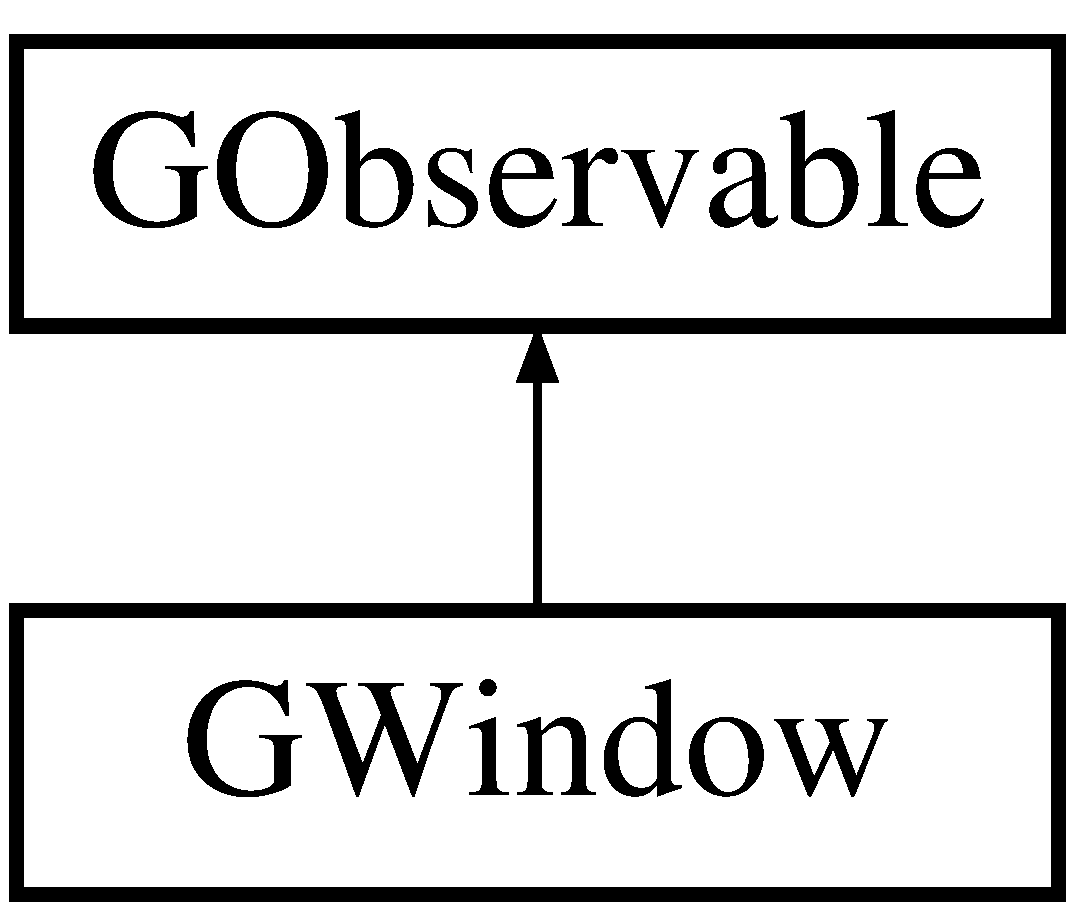
\includegraphics[height=2.000000cm]{classGWindow}
\end{center}
\end{figure}
\subsection*{Public Types}
\begin{DoxyCompactItemize}
\item 
enum \mbox{\hyperlink{classGWindow_a84803201f0f9569db61f51cac9e0d2d2}{Close\+Operation}} \{ \mbox{\hyperlink{classGWindow_a84803201f0f9569db61f51cac9e0d2d2aa00045aa0b706ef54f34c37f2d49f2b5}{C\+L\+O\+S\+E\+\_\+\+D\+O\+\_\+\+N\+O\+T\+H\+I\+NG}}, 
\mbox{\hyperlink{classGWindow_a84803201f0f9569db61f51cac9e0d2d2a47d285d1f0c66414bb23b7f3f3c6554b}{C\+L\+O\+S\+E\+\_\+\+H\+I\+DE}}, 
\mbox{\hyperlink{classGWindow_a84803201f0f9569db61f51cac9e0d2d2a1b8c84e0e965a877f9253f15747304f1}{C\+L\+O\+S\+E\+\_\+\+D\+I\+S\+P\+O\+SE}}, 
\mbox{\hyperlink{classGWindow_a84803201f0f9569db61f51cac9e0d2d2a74cdc7c2dc555e3334f91d8ce3e00f79}{C\+L\+O\+S\+E\+\_\+\+E\+X\+IT}}
 \}
\begin{DoxyCompactList}\small\item\em The various actions that can occur when a window closes. \end{DoxyCompactList}\item 
enum \mbox{\hyperlink{classGWindow_a81a01a86de31071a92e6cce0bab9bc4b}{Region}} \{ \mbox{\hyperlink{classGWindow_a81a01a86de31071a92e6cce0bab9bc4ba5ba85a564dbf472d69f92d5a2870db16}{R\+E\+G\+I\+O\+N\+\_\+\+C\+E\+N\+T\+ER}} = G\+Container\+:\+:R\+E\+G\+I\+O\+N\+\_\+\+C\+E\+N\+T\+ER, 
\mbox{\hyperlink{classGWindow_a81a01a86de31071a92e6cce0bab9bc4baac78951bd4e01d20f4825d5ae0a54357}{R\+E\+G\+I\+O\+N\+\_\+\+E\+A\+ST}} = G\+Container\+:\+:R\+E\+G\+I\+O\+N\+\_\+\+E\+A\+ST, 
\mbox{\hyperlink{classGWindow_a81a01a86de31071a92e6cce0bab9bc4baf40d135fb811ad59acb102f1fb357550}{R\+E\+G\+I\+O\+N\+\_\+\+N\+O\+R\+TH}} = G\+Container\+:\+:R\+E\+G\+I\+O\+N\+\_\+\+N\+O\+R\+TH, 
\mbox{\hyperlink{classGWindow_a81a01a86de31071a92e6cce0bab9bc4bab533512ba438173a4ceb9c501eb17628}{R\+E\+G\+I\+O\+N\+\_\+\+S\+O\+U\+TH}} = G\+Container\+:\+:R\+E\+G\+I\+O\+N\+\_\+\+S\+O\+U\+TH, 
\mbox{\hyperlink{classGWindow_a81a01a86de31071a92e6cce0bab9bc4ba5dd8c2219af001263c00de02b642786d}{R\+E\+G\+I\+O\+N\+\_\+\+W\+E\+ST}} = G\+Container\+:\+:R\+E\+G\+I\+O\+N\+\_\+\+W\+E\+ST
 \}
\begin{DoxyCompactList}\small\item\em The five regions of window border layouts. \end{DoxyCompactList}\end{DoxyCompactItemize}
\subsection*{Public Member Functions}
\begin{DoxyCompactItemize}
\item 
\mbox{\hyperlink{classGWindow_a7fdeab875fb526a49423085ac13ac9f2}{G\+Window}} (bool visible=true)
\begin{DoxyCompactList}\small\item\em Creates a new window of a default width and height. \end{DoxyCompactList}\item 
\mbox{\hyperlink{classGWindow_acb88532777f61b140aa8245ed1d9887e}{G\+Window}} (double width, double height, bool visible=true)
\begin{DoxyCompactList}\small\item\em Creates a new window of the given width and height. \end{DoxyCompactList}\item 
\mbox{\hyperlink{classGWindow_ac66942f456baa6c43ecd0ed60138fe36}{G\+Window}} (double x, double y, double width, double height, bool visible=true)
\begin{DoxyCompactList}\small\item\em Creates a new window of the given location and size. \end{DoxyCompactList}\item 
\mbox{\hyperlink{classGWindow_ab867b220db73c03e315b48c01f868e27}{$\sim$\+G\+Window}} () override
\begin{DoxyCompactList}\small\item\em Frees memory allocated internally by the window. \end{DoxyCompactList}\item 
virtual void \mbox{\hyperlink{classGWindow_a6f99b7c841256dbdc5acaafbbca4e685}{add}} (\mbox{\hyperlink{classGInteractor}{G\+Interactor}} $\ast$interactor)
\begin{DoxyCompactList}\small\item\em Adds the given interactor to the center region of the window. \end{DoxyCompactList}\item 
virtual void \mbox{\hyperlink{classGWindow_aca25fb0fc7d200e9c4fd23830d2d413d}{add}} (\mbox{\hyperlink{classGInteractor}{G\+Interactor}} $\ast$interactor, double x, double y)
\begin{DoxyCompactList}\small\item\em Adds the given interactor to the center region of the window and moves it to the given x/y location. \end{DoxyCompactList}\item 
virtual void \mbox{\hyperlink{classGWindow_a33b08fe5428ed634a658deab076099f7}{add}} (\mbox{\hyperlink{classGInteractor}{G\+Interactor}} \&interactor)
\begin{DoxyCompactList}\small\item\em Adds the given interactor to the center region of the window. \end{DoxyCompactList}\item 
virtual void \mbox{\hyperlink{classGWindow_a56840f453f9938083c24c7fb1a4c377e}{add}} (\mbox{\hyperlink{classGInteractor}{G\+Interactor}} \&interactor, double x, double y)
\begin{DoxyCompactList}\small\item\em Adds the given interactor to the center region of the window and moves it to the given x/y location. \end{DoxyCompactList}\item 
virtual void \mbox{\hyperlink{classGWindow_a2327d64402837eedd533c098014e46d9}{add}} (\mbox{\hyperlink{classGObject}{G\+Object}} $\ast$obj)
\begin{DoxyCompactList}\small\item\em Adds the given graphical object to the window\textquotesingle{}s canvas. \end{DoxyCompactList}\item 
virtual void \mbox{\hyperlink{classGWindow_ab5388ece7a50b46e0ee72e11fe202609}{add}} (\mbox{\hyperlink{classGObject}{G\+Object}} $\ast$obj, double x, double y)
\begin{DoxyCompactList}\small\item\em Adds the given graphical object to the window\textquotesingle{}s canvas and moves it to the given x/y location. \end{DoxyCompactList}\item 
virtual void \mbox{\hyperlink{classGWindow_a7f596867e2d8f9dfb816b3d496ea074f}{add}} (\mbox{\hyperlink{classGObject}{G\+Object}} \&obj)
\begin{DoxyCompactList}\small\item\em Adds the given graphical object to the window\textquotesingle{}s canvas. \end{DoxyCompactList}\item 
virtual void \mbox{\hyperlink{classGWindow_ac302bb932e3905e5d368ce735ad8444c}{add}} (\mbox{\hyperlink{classGObject}{G\+Object}} \&obj, double x, double y)
\begin{DoxyCompactList}\small\item\em Adds the given graphical object to the window\textquotesingle{}s canvas and moves it to the given x/y location. \end{DoxyCompactList}\item 
virtual Q\+Menu $\ast$ \mbox{\hyperlink{classGWindow_afffea482963d5566e97ccccb1f94a4e2}{add\+Menu}} (const std\+::string \&text)
\begin{DoxyCompactList}\small\item\em Adds a menu with the given text to the window\textquotesingle{}s top menu bar. \end{DoxyCompactList}\item 
virtual Q\+Action $\ast$ \mbox{\hyperlink{classGWindow_a43efd24277d68e749443cb7c36b65f4b}{add\+Menu\+Item}} (const std\+::string \&menu, const std\+::string \&item, const std\+::string \&icon=\char`\"{}\char`\"{})
\begin{DoxyCompactList}\small\item\em Adds a new menu item to the given menu. \end{DoxyCompactList}\item 
virtual Q\+Action $\ast$ \mbox{\hyperlink{classGWindow_ad57e2955efbfb5a0cccc981332945c8e}{add\+Menu\+Item}} (const std\+::string \&menu, const std\+::string \&item, const std\+::string \&icon, G\+Event\+Listener\+Void func)
\begin{DoxyCompactList}\small\item\em Adds a new menu item to the given menu. \end{DoxyCompactList}\item 
virtual Q\+Action $\ast$ \mbox{\hyperlink{classGWindow_a9c1d62659ac23b6752a59dc657c5140c}{add\+Menu\+Item}} (const std\+::string \&menu, const std\+::string \&item, const Q\+Icon \&icon, G\+Event\+Listener\+Void func)
\begin{DoxyCompactList}\small\item\em Adds a new menu item to the given menu. \end{DoxyCompactList}\item 
virtual Q\+Action $\ast$ \mbox{\hyperlink{classGWindow_a8452af11e9c36ac44dbdc4332095871e}{add\+Menu\+Item}} (const std\+::string \&menu, const std\+::string \&item, const Q\+Pixmap \&icon, G\+Event\+Listener\+Void func)
\begin{DoxyCompactList}\small\item\em Adds a new menu item to the given menu. \end{DoxyCompactList}\item 
virtual Q\+Action $\ast$ \mbox{\hyperlink{classGWindow_ae363de5d4c0d5848a5936563b12c3288}{add\+Menu\+Item\+Check\+Box}} (const std\+::string \&menu, const std\+::string \&item, bool checked=false, const std\+::string \&icon=\char`\"{}\char`\"{})
\begin{DoxyCompactList}\small\item\em Adds a new checkbox menu item to the given menu. \end{DoxyCompactList}\item 
virtual Q\+Action $\ast$ \mbox{\hyperlink{classGWindow_aab18d66dc7ed71468da3611b28450995}{add\+Menu\+Item\+Check\+Box}} (const std\+::string \&menu, const std\+::string \&item, bool checked, const std\+::string \&icon, G\+Event\+Listener\+Void func)
\begin{DoxyCompactList}\small\item\em Adds a new checkbox menu item to the given menu. \end{DoxyCompactList}\item 
virtual Q\+Action $\ast$ \mbox{\hyperlink{classGWindow_abdf4f167a7135e31ecb8f3363fddfd19}{add\+Menu\+Separator}} (const std\+::string \&menu)
\begin{DoxyCompactList}\small\item\em Adds a horizontal line separator to the end of the given menu. \end{DoxyCompactList}\item 
virtual Q\+Menu $\ast$ \mbox{\hyperlink{classGWindow_a557f7b2372831420546b73239027d2ae}{add\+Sub\+Menu}} (const std\+::string \&menu, const std\+::string \&submenu)
\begin{DoxyCompactList}\small\item\em Adds a sub-\/menu within an existing menu. \end{DoxyCompactList}\item 
virtual void \mbox{\hyperlink{classGWindow_ab523bda15e486bc3c968059c8b23a8d9}{add\+Toolbar}} (const std\+::string \&title=\char`\"{}\char`\"{})
\begin{DoxyCompactList}\small\item\em Adds a toolbar to this window where action buttons can be placed. \end{DoxyCompactList}\item 
virtual Q\+Action $\ast$ \mbox{\hyperlink{classGWindow_ac34ab48bd20d31312ccbf90b7120c5bb}{add\+Toolbar\+Item}} (const std\+::string \&item, const std\+::string \&icon=\char`\"{}\char`\"{})
\begin{DoxyCompactList}\small\item\em Adds a new item to the window\textquotesingle{}s toolbar. \end{DoxyCompactList}\item 
virtual Q\+Action $\ast$ \mbox{\hyperlink{classGWindow_a2fceadd3b04b459bb16e560b095eb93d}{add\+Toolbar\+Item}} (const std\+::string \&item, const std\+::string \&icon, G\+Event\+Listener\+Void func)
\begin{DoxyCompactList}\small\item\em Adds a new item to the window\textquotesingle{}s toolbar. \end{DoxyCompactList}\item 
virtual Q\+Action $\ast$ \mbox{\hyperlink{classGWindow_a1cd26d8c9004f7cbd81cecfbd323f418}{add\+Toolbar\+Item}} (const std\+::string \&item, const Q\+Icon \&icon, G\+Event\+Listener\+Void func)
\begin{DoxyCompactList}\small\item\em Adds a new item to the window\textquotesingle{}s toolbar. \end{DoxyCompactList}\item 
virtual Q\+Action $\ast$ \mbox{\hyperlink{classGWindow_a6daacc5873dd3a11813a68fcf88c9d6e}{add\+Toolbar\+Item}} (const std\+::string \&item, const Q\+Pixmap \&icon, G\+Event\+Listener\+Void func)
\begin{DoxyCompactList}\small\item\em Adds a new item to the window\textquotesingle{}s toolbar. \end{DoxyCompactList}\item 
virtual Q\+Action $\ast$ \mbox{\hyperlink{classGWindow_a885470a4fc1b578a76f6fddc2b1950a2}{add\+Toolbar\+Separator}} ()
\begin{DoxyCompactList}\small\item\em Adds a separator to the window\textquotesingle{}s toolbar. \end{DoxyCompactList}\item 
virtual void \mbox{\hyperlink{classGWindow_aab55413917cdbb2e0560ab415d59fd1f}{add\+To\+Region}} (\mbox{\hyperlink{classGInteractor}{G\+Interactor}} $\ast$interactor, \mbox{\hyperlink{classGWindow_a81a01a86de31071a92e6cce0bab9bc4b}{Region}} region)
\begin{DoxyCompactList}\small\item\em Adds the given interactor to the given region in this window. \end{DoxyCompactList}\item 
virtual void \mbox{\hyperlink{classGWindow_a9c8e600889001e6e72d3548918a6baff}{add\+To\+Region}} (\mbox{\hyperlink{classGInteractor}{G\+Interactor}} $\ast$interactor, const std\+::string \&region=\char`\"{}Center\char`\"{})
\begin{DoxyCompactList}\small\item\em Adds the given interactor to the given region in this window. \end{DoxyCompactList}\item 
virtual void \mbox{\hyperlink{classGWindow_ad05df0d92ab2fba95d401a5614365558}{add\+To\+Region}} (\mbox{\hyperlink{classGInteractor}{G\+Interactor}} \&interactor, \mbox{\hyperlink{classGWindow_a81a01a86de31071a92e6cce0bab9bc4b}{Region}} region)
\begin{DoxyCompactList}\small\item\em Adds the given interactor to the given region in this window. \end{DoxyCompactList}\item 
virtual void \mbox{\hyperlink{classGWindow_a667ed0065e0bbb52a893904e7f2383bb}{add\+To\+Region}} (\mbox{\hyperlink{classGInteractor}{G\+Interactor}} \&interactor, const std\+::string \&region=\char`\"{}Center\char`\"{})
\begin{DoxyCompactList}\small\item\em Adds the given interactor to the given region in this window. \end{DoxyCompactList}\item 
virtual void \mbox{\hyperlink{classGWindow_a5013a22e5b1f902226b7394353f884ff}{center}} ()
\begin{DoxyCompactList}\small\item\em Relocates the window to the exact center of the current screen. \end{DoxyCompactList}\item 
void \mbox{\hyperlink{classGWindow_aee7cb2065b88d21ac4ad05bc997ecf82}{clear}} () override
\begin{DoxyCompactList}\small\item\em Removes all interactors from all regionss of the window. \end{DoxyCompactList}\item 
virtual void \mbox{\hyperlink{classGWindow_a8c64b6dc10f111538780ddca425a1693}{clear\+Canvas}} ()
\begin{DoxyCompactList}\small\item\em Removes all graphical objects from the graphical canvas in this window and resets the background layer to the window\textquotesingle{}s background color. \end{DoxyCompactList}\item 
virtual void \mbox{\hyperlink{classGWindow_a7d6e3e87568ed9962d29a0c9337c4b87}{clear\+Canvas\+Objects}} ()
\begin{DoxyCompactList}\small\item\em Removes all graphical objects from the graphical canvas in this window. \end{DoxyCompactList}\item 
virtual void \mbox{\hyperlink{classGWindow_a0c30950304fa997055183be1d212a262}{clear\+Canvas\+Pixels}} ()
\begin{DoxyCompactList}\small\item\em Resets the background layer of pixels in the window\textquotesingle{}s canvas to the window\textquotesingle{}s background color. \end{DoxyCompactList}\item 
virtual void \mbox{\hyperlink{classGWindow_a47f0cc45498a78757fa4d0e6befc2981}{clear\+Region}} (\mbox{\hyperlink{classGWindow_a81a01a86de31071a92e6cce0bab9bc4b}{Region}} region)
\begin{DoxyCompactList}\small\item\em Removes all interactors from the given region of this window. \end{DoxyCompactList}\item 
virtual void \mbox{\hyperlink{classGWindow_aeba526cb4d6d6f3d8d6f376656af8dc8}{clear\+Region}} (const std\+::string \&region)
\begin{DoxyCompactList}\small\item\em Removes all interactors from the given region of this window. \end{DoxyCompactList}\item 
virtual void \mbox{\hyperlink{classGWindow_a7f7fac3c967032599677ee0087af2220}{clear\+Toolbar\+Items}} ()
\begin{DoxyCompactList}\small\item\em Removes all items from the window\textquotesingle{}s toolbar, if present. \end{DoxyCompactList}\item 
virtual void \mbox{\hyperlink{classGWindow_a5ae591df94fc66ccb85cbb6565368bca}{close}} ()
\begin{DoxyCompactList}\small\item\em Closes the window. \end{DoxyCompactList}\item 
virtual void \mbox{\hyperlink{classGDrawingSurface_a221b3e75bb3d9d0bfea62b3364e6773b}{conditional\+Repaint}} ()
\begin{DoxyCompactList}\small\item\em Repaints the interactor only if its contents have changed. \end{DoxyCompactList}\item 
virtual void \mbox{\hyperlink{classGDrawingSurface_aedd4b792311d946eeaf44b0de337a408}{conditional\+Repaint\+Region}} (int x, int y, int width, int height)
\begin{DoxyCompactList}\small\item\em Repaints the given region of the interactor only if its contents have changed. \end{DoxyCompactList}\item 
virtual void \mbox{\hyperlink{classGDrawingSurface_a3932a12278752db368e24fa404e446aa}{conditional\+Repaint\+Region}} (const \mbox{\hyperlink{structGRectangle}{G\+Rectangle}} \&bounds)
\begin{DoxyCompactList}\small\item\em Repaints the given region of the interactor only if its contents have changed. \end{DoxyCompactList}\item 
void {\bfseries draw} (\mbox{\hyperlink{classGObject}{G\+Object}} $\ast$gobj) override
\item 
void {\bfseries draw} (\mbox{\hyperlink{classGObject}{G\+Object}} $\ast$gobj, double x, double y) override
\item 
void {\bfseries draw} (\mbox{\hyperlink{classGObject}{G\+Object}} \&gobj) override
\item 
void {\bfseries draw} (\mbox{\hyperlink{classGObject}{G\+Object}} \&gobj, double x, double y) override
\item 
void {\bfseries draw} (Q\+Painter $\ast$painter) override
\item 
virtual void \mbox{\hyperlink{classGDrawingSurface_a38b6fae1045191c57092b49905068144}{draw\+Arc}} (double x, double y, double width, double height, double start, double sweep)
\begin{DoxyCompactList}\small\item\em Draws an unfilled arc with the given attributes onto the background pixel layer of this interactor in the current color. \end{DoxyCompactList}\item 
virtual void \mbox{\hyperlink{classGDrawingSurface_abdd4cb1f2c64adc5d03522a1ee30febf}{draw\+Image}} (const std\+::string \&filename, double x=0, double y=0)
\begin{DoxyCompactList}\small\item\em Draws an image loaded from the given file name onto the background pixel layer of this interactor at the given x/y location. \end{DoxyCompactList}\item 
virtual void \mbox{\hyperlink{classGDrawingSurface_ae6a24b6b9a6e795d3165c1c750d5bdf1}{draw\+Line}} (const \mbox{\hyperlink{structGPoint}{G\+Point}} \&p0, const \mbox{\hyperlink{structGPoint}{G\+Point}} \&p1)
\begin{DoxyCompactList}\small\item\em Draws a line between the given two points onto the background pixel layer of this interactor at the given x/y location in the current color. \end{DoxyCompactList}\item 
virtual void \mbox{\hyperlink{classGDrawingSurface_aff299fe83178d2f3ce8c08c06b583484}{draw\+Line}} (double x0, double y0, double x1, double y1)
\begin{DoxyCompactList}\small\item\em Draws a line between the given two points onto the background pixel layer of this interactor at the given x/y location in the current color. \end{DoxyCompactList}\item 
virtual void \mbox{\hyperlink{classGDrawingSurface_a8adc13027efe311b4a6a715205b8bc46}{draw\+Oval}} (const \mbox{\hyperlink{structGRectangle}{G\+Rectangle}} \&bounds)
\begin{DoxyCompactList}\small\item\em Draws an unfilled oval with the given bounding box onto the background pixel layer of this interactor at the given x/y location in the current color. \end{DoxyCompactList}\item 
virtual void \mbox{\hyperlink{classGDrawingSurface_aa5b1cf902e578907da3c63060686354e}{draw\+Oval}} (double x, double y, double width, double height)
\begin{DoxyCompactList}\small\item\em Draws an unfilled oval with the given bounding box onto the background pixel layer of this interactor at the given x/y location in the current color. \end{DoxyCompactList}\item 
virtual void \mbox{\hyperlink{classGDrawingSurface_a0c1e2923d8d163d62d0896d8c5cfa191}{draw\+Pixel}} (double x, double y)
\begin{DoxyCompactList}\small\item\em Colors the given x/y pixel of the background layer of this interactor using the interactor\textquotesingle{}s current color. \end{DoxyCompactList}\item 
virtual void \mbox{\hyperlink{classGDrawingSurface_a3a64eb6383e601be8438e9c71643c432}{draw\+Pixel}} (double x, double y, int color)
\begin{DoxyCompactList}\small\item\em Colors the given x/y pixel of the background layer of this interactor using the given color. \end{DoxyCompactList}\item 
virtual void \mbox{\hyperlink{classGDrawingSurface_a20abc26a94b7eb310e34abf668e0f5f4}{draw\+Pixel}} (double x, double y, const std\+::string \&color)
\begin{DoxyCompactList}\small\item\em Colors the given x/y pixel of the background layer of this interactor using the given color. \end{DoxyCompactList}\item 
virtual \mbox{\hyperlink{structGPoint}{G\+Point}} \mbox{\hyperlink{classGDrawingSurface_af70cce1e4f708f1ed5b6f29cecb660e7}{draw\+Polar\+Line}} (const \mbox{\hyperlink{structGPoint}{G\+Point}} \&p0, double r, double theta)
\begin{DoxyCompactList}\small\item\em Draws a line using polar coordinates onto the background pixel layer of this interactor in the current color. \end{DoxyCompactList}\item 
virtual \mbox{\hyperlink{structGPoint}{G\+Point}} \mbox{\hyperlink{classGDrawingSurface_ad3e646f90005295f2bbdf37d2bcb39d2}{draw\+Polar\+Line}} (double x0, double y0, double r, double theta)
\begin{DoxyCompactList}\small\item\em Draws a line using polar coordinates onto the background pixel layer of this interactor in the current color. \end{DoxyCompactList}\item 
virtual void \mbox{\hyperlink{classGDrawingSurface_afddec0a905108d8a8d6809a157f26776}{draw\+Polygon}} (std\+::initializer\+\_\+list$<$ double $>$ coords)
\begin{DoxyCompactList}\small\item\em Draws an unfilled polygon containing the given points onto the background pixel layer of this interactor in the current color. \end{DoxyCompactList}\item 
virtual void \mbox{\hyperlink{classGDrawingSurface_a021ee881e0d154dc4dd059698742889c}{draw\+Polygon}} (std\+::initializer\+\_\+list$<$ \mbox{\hyperlink{structGPoint}{G\+Point}} $>$ points)
\begin{DoxyCompactList}\small\item\em Draws an unfilled polygon containing the given points onto the background pixel layer of this interactor in the current color. \end{DoxyCompactList}\item 
virtual void \mbox{\hyperlink{classGDrawingSurface_a3dd4cc5891149dfc36746264f7289877}{draw\+Rect}} (const \mbox{\hyperlink{structGRectangle}{G\+Rectangle}} \&bounds)
\begin{DoxyCompactList}\small\item\em Draws an unfilled rectangle of the given dimensions onto the background pixel layer of this interactor in the current color. \end{DoxyCompactList}\item 
virtual void \mbox{\hyperlink{classGDrawingSurface_a4148e770ffc5474153aadd4814dbd708}{draw\+Rect}} (double x, double y, double width, double height)
\begin{DoxyCompactList}\small\item\em Draws an unfilled rectangle of the given dimensions onto the background pixel layer of this interactor in the current color. \end{DoxyCompactList}\item 
virtual void \mbox{\hyperlink{classGDrawingSurface_ad4e8551a753a77135792bbee97013675}{draw\+String}} (const std\+::string \&text, double x, double y)
\begin{DoxyCompactList}\small\item\em Draws a text string onto the background pixel layer of this interactor at the given x/y location in the current font and color. \end{DoxyCompactList}\item 
virtual void \mbox{\hyperlink{classGDrawingSurface_a228075ad18bd97b57f9956568c4773f3}{fill\+Arc}} (double x, double y, double width, double height, double start, double sweep)
\begin{DoxyCompactList}\small\item\em Draws a filled arc with the given attributes onto the background pixel layer of this interactor in the current color and fill color. \end{DoxyCompactList}\item 
virtual void \mbox{\hyperlink{classGDrawingSurface_a1ea6e48d59fb588797dba4deab1397e0}{fill\+Oval}} (const \mbox{\hyperlink{structGRectangle}{G\+Rectangle}} \&bounds)
\begin{DoxyCompactList}\small\item\em Draws a filled oval with the given bounding box onto the background pixel layer of this interactor at the given x/y location in the current color and fill color. \end{DoxyCompactList}\item 
virtual void \mbox{\hyperlink{classGDrawingSurface_a28c700c82f31cd328a4629273420ee61}{fill\+Oval}} (double x, double y, double width, double height)
\begin{DoxyCompactList}\small\item\em Draws a filled oval with the given bounding box onto the background pixel layer of this interactor at the given x/y location in the current color and fill color. \end{DoxyCompactList}\item 
virtual void \mbox{\hyperlink{classGDrawingSurface_a15f8c1c4409ef51c1a30a92a195b8f66}{fill\+Polygon}} (std\+::initializer\+\_\+list$<$ double $>$ coords)
\begin{DoxyCompactList}\small\item\em Draws a filled polygon containing the given points onto the background pixel layer of this interactor in the current color and fill color. \end{DoxyCompactList}\item 
virtual void \mbox{\hyperlink{classGDrawingSurface_a31822d59786156ebf1cc3b2f7fb70330}{fill\+Polygon}} (std\+::initializer\+\_\+list$<$ \mbox{\hyperlink{structGPoint}{G\+Point}} $>$ coords)
\begin{DoxyCompactList}\small\item\em Draws a filled polygon containing the given points onto the background pixel layer of this interactor in the current color and fill color. \end{DoxyCompactList}\item 
virtual void \mbox{\hyperlink{classGDrawingSurface_ae6582295003bf2488836b1993dadbad7}{fill\+Rect}} (const \mbox{\hyperlink{structGRectangle}{G\+Rectangle}} \&bounds)
\begin{DoxyCompactList}\small\item\em Draws a filled rectangle of the given dimensions onto the background pixel layer of this interactor in the current color and fill color. \end{DoxyCompactList}\item 
virtual void \mbox{\hyperlink{classGDrawingSurface_aac3ae7d3aee950de78eca0e108352254}{fill\+Rect}} (double x, double y, double width, double height)
\begin{DoxyCompactList}\small\item\em Draws a filled rectangle of the given dimensions onto the background pixel layer of this interactor in the current color and fill color. \end{DoxyCompactList}\item 
virtual int \mbox{\hyperlink{classGDrawingSurface_ae394d39f20476570e083918d991c25bd}{get\+A\+R\+GB}} (double x, double y) const
\begin{DoxyCompactList}\small\item\em Returns the pixel color data at the given x/y location, retaining alpha-\/channel transparency in the top 8 bits. \end{DoxyCompactList}\item 
virtual std\+::string \mbox{\hyperlink{classGDrawingSurface_a808e22cc1fdfbecf71ed8c64ef4600e0}{get\+Background}} () const
\begin{DoxyCompactList}\small\item\em Returns the current background color of the interactor as a string. \end{DoxyCompactList}\item 
virtual int \mbox{\hyperlink{classGDrawingSurface_a9e827257a55cb8cf4d9de2ec6bcfd7a0}{get\+Background\+Int}} () const
\begin{DoxyCompactList}\small\item\em Returns the current background color of the interactor as an R\+GB integer. \end{DoxyCompactList}\item 
virtual \mbox{\hyperlink{classGCanvas}{G\+Canvas}} $\ast$ \mbox{\hyperlink{classGWindow_a7aed3237105aa56033642252b3b1445e}{get\+Canvas}} () const
\begin{DoxyCompactList}\small\item\em Returns a direct pointer to the window\textquotesingle{}s internal graphical canvas on which shapes and objects are drawn. \end{DoxyCompactList}\item 
virtual double \mbox{\hyperlink{classGWindow_abd8bb28e2ac85d1b474db3f17f65115e}{get\+Canvas\+Height}} () const
\begin{DoxyCompactList}\small\item\em Returns the height of the window\textquotesingle{}s central canvas area in pixels. \end{DoxyCompactList}\item 
virtual \mbox{\hyperlink{structGDimension}{G\+Dimension}} \mbox{\hyperlink{classGWindow_a7d095192cefa2d9acf8fcf1cd00386c4}{get\+Canvas\+Size}} () const
\begin{DoxyCompactList}\small\item\em Returns the width and height of the window\textquotesingle{}s central canvas area in pixels. \end{DoxyCompactList}\item 
virtual double \mbox{\hyperlink{classGWindow_a82ed6884fd4b0257a825e786236c2428}{get\+Canvas\+Width}} () const
\begin{DoxyCompactList}\small\item\em Returns the width of the window\textquotesingle{}s central canvas area in pixels. \end{DoxyCompactList}\item 
virtual \mbox{\hyperlink{classGWindow_a84803201f0f9569db61f51cac9e0d2d2}{Close\+Operation}} \mbox{\hyperlink{classGWindow_a733b18ceeceb7ab98da8c4ac9a8d2857}{get\+Close\+Operation}} () const
\begin{DoxyCompactList}\small\item\em Returns a constant representing the action that will be taken when the user closes the window. \end{DoxyCompactList}\item 
virtual std\+::string \mbox{\hyperlink{classGDrawingSurface_aa061dfa488c31e18549d64363c1d0e34}{get\+Color}} () const
\begin{DoxyCompactList}\small\item\em Returns the current foreground outline color of the interactor as a string. \end{DoxyCompactList}\item 
virtual int \mbox{\hyperlink{classGDrawingSurface_a9635c7af766cdc3417f346683fa0e6c1}{get\+Color\+Int}} () const
\begin{DoxyCompactList}\small\item\em Returns the current foreground outline color of the interactor as an R\+GB integer. \end{DoxyCompactList}\item 
virtual std\+::string \mbox{\hyperlink{classGDrawingSurface_a76f6964a11fde7c78e9751be184e1a3c}{get\+Fill\+Color}} () const
\begin{DoxyCompactList}\small\item\em Returns the current fill color of the interactor as a string. \end{DoxyCompactList}\item 
virtual int \mbox{\hyperlink{classGDrawingSurface_a88f4508d9271c4b5f5b5d6b780f223d0}{get\+Fill\+Color\+Int}} () const
\begin{DoxyCompactList}\small\item\em Returns the current fill color of the interactor as an R\+GB integer. \end{DoxyCompactList}\item 
virtual std\+::string \mbox{\hyperlink{classGDrawingSurface_a894a5502900794eeb27d084c21f1d77d}{get\+Font}} () const
\begin{DoxyCompactList}\small\item\em Returns the current text font of the interactor as a font string. \end{DoxyCompactList}\item 
virtual std\+::string \mbox{\hyperlink{classGDrawingSurface_a4fa2d8b0192a3a5b4af4bbfe71194d03}{get\+Foreground}} () const
\begin{DoxyCompactList}\small\item\em Returns the current foreground outline color of the interactor as a string. \end{DoxyCompactList}\item 
virtual int \mbox{\hyperlink{classGDrawingSurface_ac3b12ab385a6ef9ae90fc879860ba726}{get\+Foreground\+Int}} () const
\begin{DoxyCompactList}\small\item\em Returns the current foreground outline color of the interactor as an R\+GB integer. \end{DoxyCompactList}\item 
virtual \mbox{\hyperlink{classGObject}{G\+Object}} $\ast$ \mbox{\hyperlink{classGWindow_adf27adaeeb8b551424b2096a20285fde}{get\+G\+Object}} (int index) const
\begin{DoxyCompactList}\small\item\em Returns the graphical object at the given 0-\/based index in the window\textquotesingle{}s graphical canvas. \end{DoxyCompactList}\item 
virtual \mbox{\hyperlink{classGObject}{G\+Object}} $\ast$ \mbox{\hyperlink{classGWindow_ab174a229ac7a3e9a4cd135d68dcf0076}{get\+G\+Object\+At}} (double x, double y) const
\begin{DoxyCompactList}\small\item\em Returns the top-\/most graphical object in the z-\/ordering in the window\textquotesingle{}s graphical canvas that touches the given x/y pixel location. \end{DoxyCompactList}\item 
virtual int \mbox{\hyperlink{classGWindow_ad59694124f2cdd71af9c137094df4d1f}{get\+G\+Object\+Count}} () const
\begin{DoxyCompactList}\small\item\em Returns the total number of graphical objects in the window\textquotesingle{}s canvas. \end{DoxyCompactList}\item 
virtual double \mbox{\hyperlink{classGWindow_a1e7e353362434072875264cf95629f99}{get\+Height}} () const
\begin{DoxyCompactList}\small\item\em Returns the total height of the window in pixels, excluding its title bar and borders. \end{DoxyCompactList}\item 
virtual \mbox{\hyperlink{classGObject_a86e0f5648542856159bb40775c854aa7}{G\+Object\+::\+Line\+Style}} \mbox{\hyperlink{classGDrawingSurface_aaf1f5ea8281e5e3486662878d26f0a13}{get\+Line\+Style}} () const
\begin{DoxyCompactList}\small\item\em Returns the current line style which will be used to draw outlines of shapes and lines. \end{DoxyCompactList}\item 
virtual double \mbox{\hyperlink{classGDrawingSurface_a85ff266dc3eb63d9f2d8e5a4487fd3c0}{get\+Line\+Width}} () const
\begin{DoxyCompactList}\small\item\em Returns the thickness used when drawing outlines of shapes and lines. \end{DoxyCompactList}\item 
virtual \mbox{\hyperlink{structGPoint}{G\+Point}} \mbox{\hyperlink{classGWindow_a4f83802015511edeb63b892830812c11}{get\+Location}} () const
\begin{DoxyCompactList}\small\item\em Returns the x/y location of the top-\/left corner of the interior of the window on screen, excluding any onscreen window title bar and frame. \end{DoxyCompactList}\item 
int {\bfseries get\+Pixel} (double x, double y) const override
\item 
int {\bfseries get\+Pixel\+A\+R\+GB} (double x, double y) const override
\item 
Grid$<$ int $>$ {\bfseries get\+Pixels} () const override
\item 
Grid$<$ int $>$ {\bfseries get\+Pixels\+A\+R\+GB} () const override
\item 
virtual std\+::string \mbox{\hyperlink{classGDrawingSurface_a8da04ef488ec5fa498fbbffaf50928fd}{get\+Pixel\+String}} (double x, double y) const
\begin{DoxyCompactList}\small\item\em Returns the color of the pixel at the given x/y coordinates of the image as a string such as \char`\"{}\#ff00cc\char`\"{}. \end{DoxyCompactList}\item 
virtual \mbox{\hyperlink{structGDimension}{G\+Dimension}} \mbox{\hyperlink{classGWindow_a4aabbee761d8e9116275401131b7ccd1}{get\+Preferred\+Size}} () const
\begin{DoxyCompactList}\small\item\em Returns the size that the window would prefer to be. \end{DoxyCompactList}\item 
virtual double \mbox{\hyperlink{classGWindow_a164d248057318961e7f2abc8c3477d63}{get\+Region\+Height}} (\mbox{\hyperlink{classGWindow_a81a01a86de31071a92e6cce0bab9bc4b}{Region}} region) const
\begin{DoxyCompactList}\small\item\em Returns the height of the given region of the window in pixels. \end{DoxyCompactList}\item 
virtual double \mbox{\hyperlink{classGWindow_ae8a545e772745b89edaf9804a2dc0057}{get\+Region\+Height}} (const std\+::string \&region) const
\begin{DoxyCompactList}\small\item\em Returns the height of the given region of the window in pixels. \end{DoxyCompactList}\item 
virtual \mbox{\hyperlink{structGDimension}{G\+Dimension}} \mbox{\hyperlink{classGWindow_a3b5db9ffbd4b32260f80634f162dba4e}{get\+Region\+Size}} (\mbox{\hyperlink{classGWindow_a81a01a86de31071a92e6cce0bab9bc4b}{Region}} region) const
\begin{DoxyCompactList}\small\item\em Returns the width and height of the given region of the window in pixels. \end{DoxyCompactList}\item 
virtual \mbox{\hyperlink{structGDimension}{G\+Dimension}} \mbox{\hyperlink{classGWindow_a68b18b38b72cb8779fca0c3882549a6b}{get\+Region\+Size}} (const std\+::string \&region) const
\begin{DoxyCompactList}\small\item\em Returns the width and height of the given region of the window in pixels. \end{DoxyCompactList}\item 
virtual double \mbox{\hyperlink{classGWindow_a96e2005c3f447a8679c3c32d3fc02de1}{get\+Region\+Width}} (\mbox{\hyperlink{classGWindow_a81a01a86de31071a92e6cce0bab9bc4b}{Region}} region) const
\begin{DoxyCompactList}\small\item\em Returns the width of the given region of the window in pixels. \end{DoxyCompactList}\item 
virtual double \mbox{\hyperlink{classGWindow_ab169dab454fc90f1c845b91b4e1a8a14}{get\+Region\+Width}} (const std\+::string \&region) const
\begin{DoxyCompactList}\small\item\em Returns the width of the given region of the window in pixels. \end{DoxyCompactList}\item 
virtual int \mbox{\hyperlink{classGDrawingSurface_a9e983467cf0c97cfd62433a8471570dc}{get\+R\+GB}} (double x, double y) const
\begin{DoxyCompactList}\small\item\em Returns the color of the pixel at the given x/y coordinates of the background layer of the interactor as an integer such as 0xff00cc. \end{DoxyCompactList}\item 
virtual std\+::string \mbox{\hyperlink{classGDrawingSurface_a456d3582acc3544f37d939f5cb8802fe}{get\+R\+G\+B\+String}} (double x, double y) const
\begin{DoxyCompactList}\small\item\em Returns the color of the pixel at the given x/y coordinates of the background layer of the interactor as a color string such as \char`\"{}\#ff00cc\char`\"{}. \end{DoxyCompactList}\item 
virtual \mbox{\hyperlink{structGDimension}{G\+Dimension}} \mbox{\hyperlink{classGWindow_a7b4eec96a2bdc6420695d5796a78eea9}{get\+Size}} () const
\begin{DoxyCompactList}\small\item\em Returns the total width and height of the window in pixels, excluding its title bar and borders. \end{DoxyCompactList}\item 
virtual std\+::string \mbox{\hyperlink{classGWindow_abc7651e67987c4682fed77d92a860bba}{get\+Title}} () const
\begin{DoxyCompactList}\small\item\em Returns the title bar text for the window. \end{DoxyCompactList}\item 
std\+::string \mbox{\hyperlink{classGWindow_a9b72ede4ee8520f987a0c01e30654814}{get\+Type}} () const override
\begin{DoxyCompactList}\small\item\em Returns the concrete type of the object as a string, such as {\ttfamily \char`\"{}\+G\+Button\char`\"{}} or {\ttfamily \char`\"{}\+G\+Window\char`\"{}}. \end{DoxyCompactList}\item 
virtual double \mbox{\hyperlink{classGWindow_a0ed2965abd4f5701d2cadf71239faf19}{get\+Width}} () const
\begin{DoxyCompactList}\small\item\em Returns the total width of the window in pixels, excluding its title bar and borders. \end{DoxyCompactList}\item 
virtual double \mbox{\hyperlink{classGWindow_a344385751bee0720059403940d57a13e}{getX}} () const
\begin{DoxyCompactList}\small\item\em Returns the x location of the left edge of the interior of the window on screen, excluding any onscreen window title bar and frame. \end{DoxyCompactList}\item 
virtual double \mbox{\hyperlink{classGWindow_aafa51c7f8f38a09febbb9ce7853f77b4}{getY}} () const
\begin{DoxyCompactList}\small\item\em Returns the y location of the top edge of the interior of the window on screen, excluding any onscreen window title bar and frame. \end{DoxyCompactList}\item 
virtual bool \mbox{\hyperlink{classGWindow_af69d0a7ce84cbbef65e40d861ef097c5}{has\+Toolbar}} () const
\begin{DoxyCompactList}\small\item\em Returns true if this window has a toolbar. \end{DoxyCompactList}\item 
virtual void \mbox{\hyperlink{classGWindow_ade42eb4da4eb77db85a8d1e4b92e7be4}{hide}} ()
\begin{DoxyCompactList}\small\item\em Makes the window be not visible on the screen. \end{DoxyCompactList}\item 
virtual bool \mbox{\hyperlink{classGWindow_afc480f652b8c5f1fb255e2269ce68879}{in\+Bounds}} (double x, double y) const
\begin{DoxyCompactList}\small\item\em Returns true if the given x/y location is within the bounds of the entire window. \end{DoxyCompactList}\item 
virtual bool \mbox{\hyperlink{classGWindow_ae94c9ea850cba190c985dae9fc120d32}{in\+Canvas\+Bounds}} (double x, double y) const
\begin{DoxyCompactList}\small\item\em Returns true if the given x/y location is within the bounds of the central canvas area of the window. \end{DoxyCompactList}\item 
bool {\bfseries is\+Auto\+Repaint} () const override
\item 
virtual bool \mbox{\hyperlink{classGWindow_a28e910de88f3ff5419710b0b0a03c2bb}{is\+Maximized}} () const
\begin{DoxyCompactList}\small\item\em Returns true if the window is in a maximized state, occupying the entire screen. \end{DoxyCompactList}\item 
virtual bool \mbox{\hyperlink{classGWindow_a14e6f95fa2c9ec543caa7f16f30c53d6}{is\+Minimized}} () const
\begin{DoxyCompactList}\small\item\em Returns true if the window is in a minimized (iconified) state, which often displays as the window being hidden except for a task bar icon. \end{DoxyCompactList}\item 
virtual bool \mbox{\hyperlink{classGWindow_a002ed331862370f434b7befe331b5a0b}{is\+Open}} () const
\begin{DoxyCompactList}\small\item\em Returns true if the window is currently open and visible on the screen. \end{DoxyCompactList}\item 
bool \mbox{\hyperlink{classGWindow_a45b1955433b8bf8a449a216b847d87f7}{is\+Repaint\+Immediately}} () const override
\begin{DoxyCompactList}\small\item\em Returns true if the interactor should repaint itself automatically whenever any change is made to its graphical data. \end{DoxyCompactList}\item 
virtual bool \mbox{\hyperlink{classGWindow_a2afeea3d26d063fa35c104e73275cec7}{is\+Resizable}} () const
\begin{DoxyCompactList}\small\item\em Returns true if the window allows itself to be resized. \end{DoxyCompactList}\item 
virtual bool \mbox{\hyperlink{classGWindow_a9d8a6cfb13917785c143e74d40e4e2be}{is\+Visible}} () const
\begin{DoxyCompactList}\small\item\em Returns true if the window is visible on the screen. \end{DoxyCompactList}\item 
virtual void \mbox{\hyperlink{classGWindow_ae2462f15e288c06c5136e31a8ac8151c}{load\+Canvas\+Pixels}} (const std\+::string \&filename)
\begin{DoxyCompactList}\small\item\em Reads pixel data from the file with the given name and loads it into the window\textquotesingle{}s canvas area. \end{DoxyCompactList}\item 
virtual void \mbox{\hyperlink{classGWindow_a1aa481996525792213f28d91fbb4894b}{maximize}} ()
\begin{DoxyCompactList}\small\item\em Puts the window in a maximized state, occupying the entire screen. \end{DoxyCompactList}\item 
virtual void \mbox{\hyperlink{classGWindow_a85ffaebe489c0ecf8051715ecf59babb}{minimize}} ()
\begin{DoxyCompactList}\small\item\em Puts the window in a minimized (iconified) state, which often displays as the window being hidden except for a task bar icon. \end{DoxyCompactList}\item 
virtual void \mbox{\hyperlink{classGWindow_a915ffc82b17862ab1d2a466a79d23a3f}{pack}} ()
\begin{DoxyCompactList}\small\item\em Resizes the window to its preferred size. \end{DoxyCompactList}\item 
virtual void \mbox{\hyperlink{classGWindow_adc7d99bb2dc43b8337e89b7d54cab9d3}{pause}} (double ms)
\begin{DoxyCompactList}\small\item\em Causes the current thread to pause itself for the given number of milliseconds. \end{DoxyCompactList}\item 
virtual void \mbox{\hyperlink{classGWindow_a1c12b1fde5c2ef10d79d4ee51e670efa}{remove}} (\mbox{\hyperlink{classGInteractor}{G\+Interactor}} $\ast$interactor)
\begin{DoxyCompactList}\small\item\em Removes the given interactor from the window. \end{DoxyCompactList}\item 
virtual void \mbox{\hyperlink{classGWindow_ade2376c458ac401a0bd2dbe44271509e}{remove}} (\mbox{\hyperlink{classGInteractor}{G\+Interactor}} \&interactor)
\begin{DoxyCompactList}\small\item\em Removes the given interactor from the window. \end{DoxyCompactList}\item 
virtual void \mbox{\hyperlink{classGWindow_afc8bff4a24e05c696cbe4cba7403e558}{remove}} (\mbox{\hyperlink{classGObject}{G\+Object}} $\ast$obj)
\begin{DoxyCompactList}\small\item\em Removes the given graphical object from the canvas of this window, if it was present. \end{DoxyCompactList}\item 
virtual void \mbox{\hyperlink{classGWindow_a37cf4a26853ac22c5e3a21335dfc7ac9}{remove}} (\mbox{\hyperlink{classGObject}{G\+Object}} \&obj)
\begin{DoxyCompactList}\small\item\em Removes the given graphical object from the canvas of this window, if it was present. \end{DoxyCompactList}\item 
virtual void \mbox{\hyperlink{classGWindow_ad39d0325cde6b97ebda4b9d7787c633b}{remove\+Click\+Listener}} ()
\begin{DoxyCompactList}\small\item\em Removes the click listener from this window so that it will no longer call it when events occur. \end{DoxyCompactList}\item 
virtual void \mbox{\hyperlink{classGWindow_a87a74b040025878283ba685e30d5104f}{remove\+From\+Region}} (\mbox{\hyperlink{classGInteractor}{G\+Interactor}} $\ast$interactor, \mbox{\hyperlink{classGWindow_a81a01a86de31071a92e6cce0bab9bc4b}{Region}} region)
\begin{DoxyCompactList}\small\item\em Removes the given interactor from the given region within this window. \end{DoxyCompactList}\item 
virtual void \mbox{\hyperlink{classGWindow_a16268c8344a5a5d9b10bde95764112d1}{remove\+From\+Region}} (\mbox{\hyperlink{classGInteractor}{G\+Interactor}} $\ast$interactor, const std\+::string \&region)
\begin{DoxyCompactList}\small\item\em Removes the given interactor from the given region within this window. \end{DoxyCompactList}\item 
virtual void \mbox{\hyperlink{classGWindow_afee7b65f917c4f6a0fdb1c8ea75406a5}{remove\+From\+Region}} (\mbox{\hyperlink{classGInteractor}{G\+Interactor}} \&interactor, \mbox{\hyperlink{classGWindow_a81a01a86de31071a92e6cce0bab9bc4b}{Region}} region)
\begin{DoxyCompactList}\small\item\em Removes the given interactor from the given region within this window. \end{DoxyCompactList}\item 
virtual void \mbox{\hyperlink{classGWindow_af7a055c83c0e0e3f3722596d7111fcbe}{remove\+From\+Region}} (\mbox{\hyperlink{classGInteractor}{G\+Interactor}} \&interactor, const std\+::string \&region)
\begin{DoxyCompactList}\small\item\em Removes the given interactor from the given region within this window. \end{DoxyCompactList}\item 
virtual void \mbox{\hyperlink{classGWindow_a43095f41cab3be732b49f29970484b05}{remove\+Key\+Listener}} ()
\begin{DoxyCompactList}\small\item\em Removes the key listener from this window so that it will no longer call it when events occur. \end{DoxyCompactList}\item 
virtual void \mbox{\hyperlink{classGWindow_a718d186fa807d6dec721c3b6f0c4309a}{remove\+Menu\+Listener}} ()
\begin{DoxyCompactList}\small\item\em Removes the menu listener from this window so that it will no longer call it when events occur. \end{DoxyCompactList}\item 
virtual void \mbox{\hyperlink{classGWindow_aff47f71ce47e688a07c9d38dc92fcc11}{remove\+Mouse\+Listener}} ()
\begin{DoxyCompactList}\small\item\em Removes the mouse listener from this window so that it will no longer call it when events occur. \end{DoxyCompactList}\item 
virtual void \mbox{\hyperlink{classGWindow_a8ca9bf0f8dfd3755d73d07ee01e3455f}{remove\+Timer\+Listener}} ()
\begin{DoxyCompactList}\small\item\em Removes the timer listener from this window so that it will no longer call it when events occur. \end{DoxyCompactList}\item 
virtual void \mbox{\hyperlink{classGWindow_a3d1c6ae17962b89115a4bf1c2f6142eb}{remove\+Toolbar}} ()
\begin{DoxyCompactList}\small\item\em Removes the toolbar from this window, if one was present. \end{DoxyCompactList}\item 
virtual void \mbox{\hyperlink{classGWindow_ab1ea252520cc160b329cfb5b038add83}{remove\+Window\+Listener}} ()
\begin{DoxyCompactList}\small\item\em Removes the window listener from this window so that it will no longer call it when events occur. \end{DoxyCompactList}\item 
void {\bfseries repaint} () override
\item 
virtual void \mbox{\hyperlink{classGDrawingSurface_a769c46fb3e1004aec76e8b0adfa42aa6}{repaint\+Region}} (const \mbox{\hyperlink{structGRectangle}{G\+Rectangle}} \&bounds)
\begin{DoxyCompactList}\small\item\em Instructs the interactor to repaint the given region of pixel data. \end{DoxyCompactList}\item 
void {\bfseries repaint\+Region} (int x, int y, int width, int height) override
\item 
virtual void \mbox{\hyperlink{classGWindow_a519fb2ac767f8b2febbb50b898b8c8cb}{request\+Focus}} ()
\begin{DoxyCompactList}\small\item\em Asks the system to assign the keyboard focus to the window, which brings it to the top and ensures that key events are delivered to the window. \end{DoxyCompactList}\item 
virtual void \mbox{\hyperlink{classGWindow_afd3595051be2709847c2de4352f27cf5}{restore}} ()
\begin{DoxyCompactList}\small\item\em Puts the window in a normal state, neither minimized or maximized. \end{DoxyCompactList}\item 
virtual void \mbox{\hyperlink{classGWindow_aba99f6a53d9bb0493e7fc3ead6a2e4a3}{save\+Canvas\+Pixels}} (const std\+::string \&filename)
\begin{DoxyCompactList}\small\item\em Writes the contents of the window\textquotesingle{}s graphical canvas to the given output filename. \end{DoxyCompactList}\item 
void {\bfseries set\+Auto\+Repaint} (bool auto\+Repaint) override
\item 
void \mbox{\hyperlink{classGWindow_a10d305826534b55561ea88730fc9f6cd}{set\+Background}} (int color) override
\begin{DoxyCompactList}\small\item\em Sets the current background color of the interactor as an R\+GB integer. \end{DoxyCompactList}\item 
void \mbox{\hyperlink{classGWindow_a9cb99695b93494c7ba28268ce9e42c2a}{set\+Background}} (const std\+::string \&color) override
\begin{DoxyCompactList}\small\item\em Sets the current background color of the interactor as a string. \end{DoxyCompactList}\item 
virtual void \mbox{\hyperlink{classGWindow_a059f69fab57ad2cca2243c5a64f7306d}{set\+Canvas\+Height}} (double height)
\begin{DoxyCompactList}\small\item\em Resizes the window so that its central canvas region will occupy exactly the given height in pixels, without changing its width. \end{DoxyCompactList}\item 
virtual void \mbox{\hyperlink{classGWindow_a06022723e253be88ca7e48034ff66244}{set\+Canvas\+Size}} (double width, double height)
\begin{DoxyCompactList}\small\item\em Resizes the window so that its central canvas region will occupy exactly the given width and height in pixels. \end{DoxyCompactList}\item 
virtual void \mbox{\hyperlink{classGWindow_a22f0f065a223a3c0ae5173316ece1dc1}{set\+Canvas\+Size}} (const \mbox{\hyperlink{structGDimension}{G\+Dimension}} \&size)
\begin{DoxyCompactList}\small\item\em Resizes the window so that its central canvas region will occupy exactly the given width and height in pixels. \end{DoxyCompactList}\item 
virtual void \mbox{\hyperlink{classGWindow_a455beafcfc20a2b7d9ac00499e222f0f}{set\+Canvas\+Width}} (double width)
\begin{DoxyCompactList}\small\item\em Resizes the window so that its central canvas region will occupy exactly the given width in pixels, without changing its height. \end{DoxyCompactList}\item 
virtual void \mbox{\hyperlink{classGWindow_abd40af6921242584d0954f173911b190}{set\+Click\+Listener}} (G\+Event\+Listener func)
\begin{DoxyCompactList}\small\item\em Sets a mouse listener on this window so that it will be called when the mouse is clicked on the window\textquotesingle{}s canvas. \end{DoxyCompactList}\item 
virtual void \mbox{\hyperlink{classGWindow_a856414c92df90f56f3877475eb3f8fc4}{set\+Click\+Listener}} (G\+Event\+Listener\+Void func)
\begin{DoxyCompactList}\small\item\em Sets a mouse listener on this window so that it will be called when the mouse is clicked on the window\textquotesingle{}s canvas. \end{DoxyCompactList}\item 
virtual void \mbox{\hyperlink{classGWindow_a8163e9440d0fb801a63ae9b3c90d5969}{set\+Close\+Operation}} (\mbox{\hyperlink{classGWindow_a84803201f0f9569db61f51cac9e0d2d2}{Close\+Operation}} op)
\begin{DoxyCompactList}\small\item\em Sets what should happen when the window is closed. \end{DoxyCompactList}\item 
void {\bfseries set\+Color} (int color) override
\item 
void {\bfseries set\+Color} (const std\+::string \&color) override
\item 
virtual void \mbox{\hyperlink{classGObservable_afaa30b2a9e0f378fd1c70d2f1d0b8216}{set\+Events\+Enabled}} (bool events\+Enabled)
\begin{DoxyCompactList}\small\item\em Sets whether the object is currently allowing itself to fire events. \end{DoxyCompactList}\item 
virtual void \mbox{\hyperlink{classGWindow_abad01a63e29c19aee274af1b36209838}{set\+Exit\+On\+Close}} (bool exit\+On\+Close)
\begin{DoxyCompactList}\small\item\em Sets whether the library\textquotesingle{}s G\+UI system should shut down when the window is closed. \end{DoxyCompactList}\item 
void {\bfseries set\+Fill\+Color} (int color) override
\item 
void {\bfseries set\+Fill\+Color} (const std\+::string \&color) override
\item 
void {\bfseries set\+Font} (const Q\+Font \&font) override
\item 
void {\bfseries set\+Font} (const std\+::string \&font) override
\item 
virtual void \mbox{\hyperlink{classGDrawingSurface_a7daa57084b5811b598fce8726660b328}{set\+Foreground}} (int color)
\begin{DoxyCompactList}\small\item\em Sets the current foreground outline color of the interactor as an R\+GB integer. \end{DoxyCompactList}\item 
virtual void \mbox{\hyperlink{classGDrawingSurface_af59209aeadea6dfc6d97a2d8531f50e1}{set\+Foreground}} (const std\+::string \&color)
\begin{DoxyCompactList}\small\item\em Sets the current foreground outline color of the interactor as a string. \end{DoxyCompactList}\item 
virtual void \mbox{\hyperlink{classGWindow_a4b812426e19cdd9f6d62e7b5d90e6bec}{set\+Height}} (double width)
\begin{DoxyCompactList}\small\item\em Sets the window\textquotesingle{}s total height in pixels. \end{DoxyCompactList}\item 
virtual void \mbox{\hyperlink{classGWindow_aeb8324d3287fa1fbe093f4d6230cf0a6}{set\+Key\+Listener}} (G\+Event\+Listener func)
\begin{DoxyCompactList}\small\item\em Sets a key listener on this window so that it will be called when the user presses any key. \end{DoxyCompactList}\item 
virtual void \mbox{\hyperlink{classGWindow_ae48ecea73606c7bd9423e1c7cc589cc9}{set\+Key\+Listener}} (G\+Event\+Listener\+Void func)
\begin{DoxyCompactList}\small\item\em Sets a key listener on this window so that it will be called when the user presses any key. \end{DoxyCompactList}\item 
virtual void \mbox{\hyperlink{classGDrawingSurface_a6bfe14a77101db0fb97b5a7e07a5526b}{set\+Line\+Style}} (\mbox{\hyperlink{classGObject_a86e0f5648542856159bb40775c854aa7}{G\+Object\+::\+Line\+Style}} line\+Style)
\begin{DoxyCompactList}\small\item\em Sets the current line style which will be used to draw outlines of shapes and lines. \end{DoxyCompactList}\item 
void {\bfseries set\+Line\+Width} (double line\+Width) override
\item 
virtual void \mbox{\hyperlink{classGWindow_a04594e8ba9b98513a64f1da00dcae18c}{set\+Location}} (double x, double y)
\begin{DoxyCompactList}\small\item\em Sets the window\textquotesingle{}s top-\/left x/y location on the screen to the given coordinates. \end{DoxyCompactList}\item 
virtual void \mbox{\hyperlink{classGWindow_a6ef8e1a904fffe55052f7a22f8552e4b}{set\+Location}} (const \mbox{\hyperlink{structGPoint}{G\+Point}} \&p)
\begin{DoxyCompactList}\small\item\em Sets the window\textquotesingle{}s top-\/left x/y location on the screen to the given point. \end{DoxyCompactList}\item 
virtual void \mbox{\hyperlink{classGWindow_a875124740630bebec069479fd3958efc}{set\+Menu\+Item\+Enabled}} (const std\+::string \&menu, const std\+::string \&item, bool enabled)
\begin{DoxyCompactList}\small\item\em Sets whether the given item in the given menu is enabled or disabled. \end{DoxyCompactList}\item 
virtual void \mbox{\hyperlink{classGWindow_ab0002e0bf6566a5b98cc9128cb859b0e}{set\+Menu\+Listener}} (G\+Event\+Listener func)
\begin{DoxyCompactList}\small\item\em Sets a menu listener on this window so that it will be called when menu items are clicked, sending an A\+C\+T\+I\+O\+N\+\_\+\+M\+E\+NU action event. \end{DoxyCompactList}\item 
virtual void \mbox{\hyperlink{classGWindow_a1294d48e67c30207da71c3e3ab56abde}{set\+Menu\+Listener}} (G\+Event\+Listener\+Void func)
\begin{DoxyCompactList}\small\item\em Sets a menu listener on this window so that it will be called when menu items are clicked. \end{DoxyCompactList}\item 
virtual void \mbox{\hyperlink{classGWindow_a37d8dbc943f59920f705b0104f60bde2}{set\+Mouse\+Listener}} (G\+Event\+Listener func)
\begin{DoxyCompactList}\small\item\em Sets a mouse listener on the window\textquotesingle{}s canvas so that it will be called when the user moves or clicks the mouse on the canvas. \end{DoxyCompactList}\item 
virtual void \mbox{\hyperlink{classGWindow_aea7f647ea62d59f71b5fad6aa65eeaf9}{set\+Mouse\+Listener}} (G\+Event\+Listener\+Void func)
\begin{DoxyCompactList}\small\item\em Sets a mouse listener on the window\textquotesingle{}s canvas so that it will be called when the user moves or clicks the mouse on the canvas. \end{DoxyCompactList}\item 
virtual void \mbox{\hyperlink{classGDrawingSurface_a09f9640e4ff7388dcfc391efd88d2415}{set\+Pixel}} (double x, double y, const std\+::string \&color)
\begin{DoxyCompactList}\small\item\em Sets the color of the given x/y pixel in the background layer of the interactor to the given color. \end{DoxyCompactList}\item 
void {\bfseries set\+Pixel} (double x, double y, int rgb) override
\item 
void {\bfseries set\+Pixel} (double x, double y, int r, int g, int b) override
\item 
void {\bfseries set\+Pixel\+A\+R\+GB} (double x, double y, int argb) override
\item 
void {\bfseries set\+Pixel\+A\+R\+GB} (double x, double y, int a, int r, int g, int b) override
\item 
void {\bfseries set\+Pixels} (const Grid$<$ int $>$ \&pixels) override
\item 
void {\bfseries set\+Pixels\+A\+R\+GB} (const Grid$<$ int $>$ \&pixels\+A\+R\+GB) override
\item 
virtual void \mbox{\hyperlink{classGWindow_a96e9f5593c0193bbdc7ae99945b9cf5f}{set\+Region\+Alignment}} (\mbox{\hyperlink{classGWindow_a81a01a86de31071a92e6cce0bab9bc4b}{Region}} region, Horizontal\+Alignment halign)
\begin{DoxyCompactList}\small\item\em Sets the horizontal alignment of interactors in the given region of the window. \end{DoxyCompactList}\item 
virtual void \mbox{\hyperlink{classGWindow_a926942899d029fc9921fe770ac2867bb}{set\+Region\+Alignment}} (\mbox{\hyperlink{classGWindow_a81a01a86de31071a92e6cce0bab9bc4b}{Region}} region, Vertical\+Alignment valign)
\begin{DoxyCompactList}\small\item\em Sets the vertical alignment of interactors in the given region of the window. \end{DoxyCompactList}\item 
virtual void \mbox{\hyperlink{classGWindow_ab4d2bfcca7a18da2847e7b4494da4a16}{set\+Region\+Alignment}} (\mbox{\hyperlink{classGWindow_a81a01a86de31071a92e6cce0bab9bc4b}{Region}} region, Horizontal\+Alignment halign, Vertical\+Alignment valign)
\begin{DoxyCompactList}\small\item\em Sets the horizontal and vertical alignment of interactors in the given region of the window. \end{DoxyCompactList}\item 
virtual void \mbox{\hyperlink{classGWindow_ae4ff46516be9472498c0bf058b496e8b}{set\+Region\+Alignment}} (const std\+::string \&region, const std\+::string \&align)
\begin{DoxyCompactList}\small\item\em Sets the horizontal and/or vertical alignment of interactors in the given region of the window. \end{DoxyCompactList}\item 
virtual void \mbox{\hyperlink{classGWindow_ad1c76be81b3b865f78b0e91f0e1f07d4}{set\+Region\+Alignment}} (const std\+::string \&region, const std\+::string \&halign, const std\+::string \&valign)
\begin{DoxyCompactList}\small\item\em Sets the horizontal and vertical alignment of interactors in the given region of the window. \end{DoxyCompactList}\item 
virtual void \mbox{\hyperlink{classGWindow_aca8f01ef261afca9c843589e8be54134}{set\+Region\+Horizontal\+Alignment}} (\mbox{\hyperlink{classGWindow_a81a01a86de31071a92e6cce0bab9bc4b}{Region}} region, Horizontal\+Alignment halign)
\begin{DoxyCompactList}\small\item\em Sets the horizontal alignment of interactors in the given region of the window. \end{DoxyCompactList}\item 
virtual void \mbox{\hyperlink{classGWindow_aefb97090ff4e149f8a0cce9efee3c451}{set\+Region\+Horizontal\+Alignment}} (const std\+::string \&region, const std\+::string \&halign)
\begin{DoxyCompactList}\small\item\em Sets the horizontal alignment of interactors in the given region of the window. \end{DoxyCompactList}\item 
virtual void \mbox{\hyperlink{classGWindow_afbe22d897ce8ef25db52cbc3d456aa0a}{set\+Region\+Vertical\+Alignment}} (const std\+::string \&region, const std\+::string \&valign)
\begin{DoxyCompactList}\small\item\em Sets the vertical alignment of interactors in the given region of the window. \end{DoxyCompactList}\item 
virtual void \mbox{\hyperlink{classGWindow_a1efb2d3b67fb479aad27a6c0032ee70e}{set\+Region\+Vertical\+Alignment}} (\mbox{\hyperlink{classGWindow_a81a01a86de31071a92e6cce0bab9bc4b}{Region}} region, Vertical\+Alignment valign)
\begin{DoxyCompactList}\small\item\em Sets the vertical alignment of interactors in the given region of the window. \end{DoxyCompactList}\item 
void {\bfseries set\+Repaint\+Immediately} (bool repaint\+Immediately) override
\item 
virtual void \mbox{\hyperlink{classGWindow_a8bf0c7d9f9aea44fa74f63a358df7d22}{set\+Resizable}} (bool resizable)
\begin{DoxyCompactList}\small\item\em Sets whether the window allows itself to be resized. \end{DoxyCompactList}\item 
virtual void \mbox{\hyperlink{classGDrawingSurface_a8bcbd65fa784bdab1e66a9efd381162d}{set\+R\+GB}} (double x, double y, int rgb)
\begin{DoxyCompactList}\small\item\em Sets the color of the given x/y pixel in the background layer of the interactor to the given R\+GB values. \end{DoxyCompactList}\item 
virtual void \mbox{\hyperlink{classGDrawingSurface_a81202471d4fc9f2015aef0bc073acfab}{set\+R\+GB}} (double x, double y, int r, int g, int b)
\begin{DoxyCompactList}\small\item\em Sets the color of the given x/y pixel in the background layer of the interactor to the given R\+GB values. \end{DoxyCompactList}\item 
virtual void \mbox{\hyperlink{classGDrawingSurface_ae9a228792d4bb4b628350f39eaa3ad12}{set\+R\+GB}} (double x, double y, const std\+::string \&color)
\begin{DoxyCompactList}\small\item\em Sets the color of the given x/y pixel in the background layer of the interactor to the given color. \end{DoxyCompactList}\item 
virtual void \mbox{\hyperlink{classGWindow_aca25d49481f9bf5fc8f7df4c086c4ce7}{set\+Size}} (double width, double height)
\begin{DoxyCompactList}\small\item\em Sets the window\textquotesingle{}s total width and height in pixels. \end{DoxyCompactList}\item 
virtual void \mbox{\hyperlink{classGWindow_ae2b628228f192c2702c4ce941b2af68f}{set\+Size}} (const \mbox{\hyperlink{structGDimension}{G\+Dimension}} \&size)
\begin{DoxyCompactList}\small\item\em Sets the window\textquotesingle{}s width and height in pixels. \end{DoxyCompactList}\item 
virtual void \mbox{\hyperlink{classGWindow_ae0d5df4c2ed47156cbba7da55362e4e1}{set\+Timer\+Listener}} (double ms, G\+Event\+Listener func)
\begin{DoxyCompactList}\small\item\em Sets a menu listener on this window so that it will be called when timer delays elapse, sending a timer event. \end{DoxyCompactList}\item 
virtual void \mbox{\hyperlink{classGWindow_ae23e03c86580bbcefc2dee4d01d08091}{set\+Timer\+Listener}} (double ms, G\+Event\+Listener\+Void func)
\begin{DoxyCompactList}\small\item\em Sets a menu listener on this window so that it will be called when timer delays elapse, sending a timer event. \end{DoxyCompactList}\item 
virtual void \mbox{\hyperlink{classGWindow_abc79cf0667bbb5c93fca3f01b52c7b57}{set\+Title}} (const std\+::string \&title)
\begin{DoxyCompactList}\small\item\em Sets the window\textquotesingle{}s title bar text to the given string. \end{DoxyCompactList}\item 
virtual void \mbox{\hyperlink{classGWindow_a18e44e30b31525a243960ca3928125aa}{set\+Visible}} (bool visible)
\begin{DoxyCompactList}\small\item\em Sets whether the window can be seen on the screen. \end{DoxyCompactList}\item 
virtual void \mbox{\hyperlink{classGWindow_aa3f3fba4cb131baa8696ba01e3bceca1}{set\+Width}} (double width)
\begin{DoxyCompactList}\small\item\em Sets the window\textquotesingle{}s total width in pixels. \end{DoxyCompactList}\item 
virtual void \mbox{\hyperlink{classGWindow_ab21f6abd314b7ffd3ccf7b6e18ac18cb}{set\+Window\+Icon}} (const std\+::string \&icon\+File)
\begin{DoxyCompactList}\small\item\em Sets the window to use the. \end{DoxyCompactList}\item 
virtual void \mbox{\hyperlink{classGWindow_adbb687462d07ac5bd49f3861e4356838}{set\+Window\+Listener}} (G\+Event\+Listener func)
\begin{DoxyCompactList}\small\item\em Sets a window listener on this window so that it will be called when window events occur, such as resizing or closing the window. \end{DoxyCompactList}\item 
virtual void \mbox{\hyperlink{classGWindow_a58b90463b205519917d5f68bdf068815}{set\+Window\+Listener}} (G\+Event\+Listener\+Void func)
\begin{DoxyCompactList}\small\item\em Sets a window listener on this window so that it will be called when window events occur, such as resizing or closing the window. \end{DoxyCompactList}\item 
virtual void \mbox{\hyperlink{classGWindow_a1c06b2b64d56394d6d77aa5b627910e2}{set\+Window\+Title}} (const std\+::string \&title)
\begin{DoxyCompactList}\small\item\em Sets the window\textquotesingle{}s title bar text to the given string. \end{DoxyCompactList}\item 
virtual void \mbox{\hyperlink{classGWindow_a9c18fcc579333bf9653d13ad2b372e39}{setX}} (double x)
\begin{DoxyCompactList}\small\item\em Sets the window\textquotesingle{}s left x location on the screen to the given coordinate. \end{DoxyCompactList}\item 
virtual void \mbox{\hyperlink{classGWindow_a7d57e2a5c35d27feb58fd498a3cf82b9}{setY}} (double y)
\begin{DoxyCompactList}\small\item\em Sets the window\textquotesingle{}s top y location on the screen to the given coordinate. \end{DoxyCompactList}\item 
virtual void \mbox{\hyperlink{classGWindow_a4b148f40a95444d5669406b918ad2f52}{show}} ()
\begin{DoxyCompactList}\small\item\em Sets the window to be visible on the screen. \end{DoxyCompactList}\item 
virtual void \mbox{\hyperlink{classGWindow_aa3381590c1ef33c08000c2fbb2bf0dd0}{sleep}} (double ms)
\begin{DoxyCompactList}\small\item\em Causes the current thread to pause itself for the given number of milliseconds. \end{DoxyCompactList}\item 
virtual void \mbox{\hyperlink{classGWindow_a6053c984b166df7d3db5ee4c4ad65b99}{to\+Back}} ()
\begin{DoxyCompactList}\small\item\em Moves the window to the back of the z-\/ordering in the operating system, underneath any other windows that occupy the same pixels. \end{DoxyCompactList}\item 
virtual void \mbox{\hyperlink{classGWindow_a48a9c646659814220ac869bbcb60b52c}{to\+Front}} ()
\begin{DoxyCompactList}\small\item\em Moves the window to the front of the z-\/ordering in the operating system, in front of any other windows that occupy the same pixels. \end{DoxyCompactList}\item 
virtual std\+::string \mbox{\hyperlink{classGObservable_a1fe5121d6528fdea3f243321b3fa3a49}{to\+String}} () const
\begin{DoxyCompactList}\small\item\em Returns a string representation of this observable object\textquotesingle{}s state. \end{DoxyCompactList}\end{DoxyCompactItemize}
\subsection*{Static Public Member Functions}
\begin{DoxyCompactItemize}
\item 
static std\+::string \mbox{\hyperlink{classGWindow_a14da494e7a105db49b15cbd11db68774}{choose\+Light\+Dark\+Mode\+Color}} (const std\+::string \&light\+Color, const std\+::string \&dark\+Color)
\begin{DoxyCompactList}\small\item\em Returns which color to use depending on whether the user\textquotesingle{}s computer is in light or dark mode. \end{DoxyCompactList}\item 
static int \mbox{\hyperlink{classGWindow_a8364f5a4c8622d07ccc83bdc3acc4f19}{choose\+Light\+Dark\+Mode\+Color\+Int}} (int light\+Color, int dark\+Color)
\begin{DoxyCompactList}\small\item\em Returns which color to use depending on whether the user\textquotesingle{}s computer is in light or dark mode. \end{DoxyCompactList}\item 
static std\+::string \mbox{\hyperlink{classGWindow_a43cda7f9c8a6eb4ff1519fb99a3c2901}{get\+Default\+Interactor\+Background\+Color}} ()
\begin{DoxyCompactList}\small\item\em Returns the default color for backgrounds of interactors as a string. \end{DoxyCompactList}\item 
static int \mbox{\hyperlink{classGWindow_a04e520567df471df236f1efeb5ea4d90}{get\+Default\+Interactor\+Background\+Color\+Int}} ()
\begin{DoxyCompactList}\small\item\em Returns the default color for text on interactors as an R\+GB integer. \end{DoxyCompactList}\item 
static std\+::string \mbox{\hyperlink{classGWindow_aa65fc0c6ac0c5ebeafffe99e35face97}{get\+Default\+Interactor\+Text\+Color}} ()
\begin{DoxyCompactList}\small\item\em Returns the default color for text on interactors as a string. \end{DoxyCompactList}\item 
static int \mbox{\hyperlink{classGWindow_a66c284abc8a53870127d079f904489c5}{get\+Default\+Interactor\+Text\+Color\+Int}} ()
\begin{DoxyCompactList}\small\item\em Returns the default color for text on interactors as an R\+GB integer. \end{DoxyCompactList}\item 
static int \mbox{\hyperlink{classGWindow_aea783b75281f864f14e958d2fee28f9d}{get\+Screen\+Dpi}} ()
\begin{DoxyCompactList}\small\item\em Returns the dots-\/per-\/inch of the screen. \end{DoxyCompactList}\item 
static double \mbox{\hyperlink{classGWindow_ab15179b683630109f0ac256590a3b323}{get\+Screen\+Dpi\+Scale\+Ratio}} ()
\begin{DoxyCompactList}\small\item\em Returns the ratio of this screen\textquotesingle{}s D\+PI compared to a normal low-\/\+D\+PI screen. \end{DoxyCompactList}\item 
static double \mbox{\hyperlink{classGWindow_a9942379fdf4fb4445c35eaf3390b7ccb}{get\+Screen\+Height}} ()
\begin{DoxyCompactList}\small\item\em Returns the height of the entire screen in pixels. \end{DoxyCompactList}\item 
static \mbox{\hyperlink{structGDimension}{G\+Dimension}} \mbox{\hyperlink{classGWindow_ae3d08d5cde8163274459797770596809}{get\+Screen\+Size}} ()
\begin{DoxyCompactList}\small\item\em Returns the width and height of the entire screen in pixels. \end{DoxyCompactList}\item 
static double \mbox{\hyperlink{classGWindow_adc82933bd579ab83d7cd4e3bc5f79a12}{get\+Screen\+Width}} ()
\begin{DoxyCompactList}\small\item\em Returns the width of the entire screen in pixels. \end{DoxyCompactList}\item 
static bool \mbox{\hyperlink{classGWindow_a36044a6efa9c4e015378e56c3e37181d}{is\+Dark\+Mode}} ()
\begin{DoxyCompactList}\small\item\em Returns true if the user\textquotesingle{}s computer is in \char`\"{}dark mode.\char`\"{} This is a popular dark color scheme mostly used on recent Macs. \end{DoxyCompactList}\item 
static bool \mbox{\hyperlink{classGWindow_a674ef3ad6e66d778e410e130cad47274}{is\+High\+Density\+Screen}} ()
\begin{DoxyCompactList}\small\item\em Returns whether the dots-\/per-\/inch of the screen are high enough to consider it a \char`\"{}high-\/density\char`\"{} screen for which scaling should be used. \end{DoxyCompactList}\item 
static bool \mbox{\hyperlink{classGWindow_a040690336154a3f414001a16ffdb947e}{is\+High\+Dpi\+Scaling\+Enabled}} ()
\begin{DoxyCompactList}\small\item\em Returns whether we should scale some windows when run on high-\/density screens. \end{DoxyCompactList}\end{DoxyCompactItemize}
\subsection*{Static Public Attributes}
\begin{DoxyCompactItemize}
\item 
static const int \mbox{\hyperlink{classGWindow_a2fab6d7a2bcb15d1595cacc38230f21b}{D\+E\+F\+A\+U\+L\+T\+\_\+\+H\+E\+I\+G\+HT}} = 300
\begin{DoxyCompactList}\small\item\em The default height of a newly created window in pixels if its height is not explicitly specified. \end{DoxyCompactList}\item 
static const std\+::string \mbox{\hyperlink{classGWindow_a666fcf3a55503322fbfd6314c4846542}{D\+E\+F\+A\+U\+L\+T\+\_\+\+I\+C\+O\+N\+\_\+\+F\+I\+L\+E\+N\+A\+ME}} = \char`\"{}splicon-\/large.\+png\char`\"{}
\begin{DoxyCompactList}\small\item\em The default file name used to load a \mbox{\hyperlink{classGWindow}{G\+Window}}\textquotesingle{}s initial title bar icon. \end{DoxyCompactList}\item 
static const int \mbox{\hyperlink{classGWindow_af7b8fc8ce7f700c853cfbc36ee8cc474}{D\+E\+F\+A\+U\+L\+T\+\_\+\+W\+I\+D\+TH}} = 500
\begin{DoxyCompactList}\small\item\em The default width of a newly created window in pixels if its width is not explicitly specified. \end{DoxyCompactList}\item 
static const int \mbox{\hyperlink{classGWindow_a212e92d31b813ef25adbb902ffae3c6b}{H\+I\+G\+H\+\_\+\+D\+P\+I\+\_\+\+S\+C\+R\+E\+E\+N\+\_\+\+T\+H\+R\+E\+S\+H\+O\+LD}} = 200
\begin{DoxyCompactList}\small\item\em The minimum number of dots per inch before a screen is considered to be high-\/density or high-\/\+D\+PI. \end{DoxyCompactList}\item 
static const int \mbox{\hyperlink{classGWindow_a28d634f1a144a0f1aabf338f0be6afe2}{S\+T\+A\+N\+D\+A\+R\+D\+\_\+\+S\+C\+R\+E\+E\+N\+\_\+\+D\+PI}} = 96
\begin{DoxyCompactList}\small\item\em The minimum number of dots per inch on a \char`\"{}normal\char`\"{} low-\/\+D\+PI screen. \end{DoxyCompactList}\end{DoxyCompactItemize}
\subsection*{Protected Member Functions}
\begin{DoxyCompactItemize}
\item 
void \mbox{\hyperlink{classGDrawingSurface_a3a690bcb2d62250c9e4722ad7c1b9ab6}{check\+Bounds}} (const std\+::string \&member, double x, double y, double width, double height) const
\begin{DoxyCompactList}\small\item\em Throws an error if the given x/y values are out of bounds. \end{DoxyCompactList}\item 
void \mbox{\hyperlink{classGDrawingSurface_a9841b5dc607ca41a14819d80e1d8a09c}{check\+Color}} (const std\+::string \&member, int rgb) const
\begin{DoxyCompactList}\small\item\em Throws an error if the given rgb value is not a valid color. \end{DoxyCompactList}\item 
void \mbox{\hyperlink{classGDrawingSurface_a70a6546707ae708573396616bd0f5320}{check\+Size}} (const std\+::string \&member, double width, double height) const
\begin{DoxyCompactList}\small\item\em Throws an error if the given width/height values are out of bounds. \end{DoxyCompactList}\item 
virtual void \mbox{\hyperlink{classGObservable_a80cfa040459ff53594adbd6a51ec8f43}{clear\+Event\+Listeners}} ()
\begin{DoxyCompactList}\small\item\em Removes all event listeners from this object. \end{DoxyCompactList}\item 
virtual void {\bfseries ensure\+Forward\+Target\+Const\+Hack} () const
\item 
virtual void \mbox{\hyperlink{classGObservable_a284f31528c0520f8e545c03ac9eeac74}{ensure\+Thread\+Safety}} (const std\+::string \&member\+Name=\char`\"{}\char`\"{})
\begin{DoxyCompactList}\small\item\em Ensures that we are currently in the Qt G\+UI thread. \end{DoxyCompactList}\item 
virtual void \mbox{\hyperlink{classGObservable_a63e5e5a6227c59c928493b11aceb0f67}{fire\+Event}} (\mbox{\hyperlink{classGEvent}{G\+Event}} \&event)
\begin{DoxyCompactList}\small\item\em Sends out the given event to any attached listeners. \end{DoxyCompactList}\item 
virtual void \mbox{\hyperlink{classGObservable_ab3983ea07337b52020a29cc00c653d8d}{fire\+G\+Event}} (Q\+Event $\ast$event, Event\+Type event\+Type, const std\+::string \&event\+Name)
\begin{DoxyCompactList}\small\item\em Creates an event of the given type, then sends it out to any attached listeners. \end{DoxyCompactList}\item 
virtual void \mbox{\hyperlink{classGObservable_a01fdf1b0e0dbd49e189fe4514e010411}{fire\+G\+Event}} (Q\+Close\+Event $\ast$event, Event\+Type event\+Type, const std\+::string \&event\+Name)
\begin{DoxyCompactList}\small\item\em Creates an event of the given type, then sends it out to any attached listeners. \end{DoxyCompactList}\item 
virtual void \mbox{\hyperlink{classGObservable_abb0b2f66ba39211cb5d7615e9d1c04e2}{fire\+G\+Event}} (Q\+Key\+Event $\ast$event, Event\+Type event\+Type, const std\+::string \&event\+Name)
\begin{DoxyCompactList}\small\item\em Creates an event of the given type, then sends it out to any attached listeners. \end{DoxyCompactList}\item 
virtual void \mbox{\hyperlink{classGObservable_a119318675d2165bdf7dd853aaf881d4b}{fire\+G\+Event}} (Q\+Mouse\+Event $\ast$event, Event\+Type event\+Type, const std\+::string \&event\+Name, const std\+::string \&action\+Command=\char`\"{}\char`\"{})
\begin{DoxyCompactList}\small\item\em Creates an event of the given type, then sends it out to any attached listeners. \end{DoxyCompactList}\item 
virtual void \mbox{\hyperlink{classGObservable_a63fd9034e1e1633c1c38eb342bfd34e9}{fire\+G\+Event}} (Q\+Resize\+Event $\ast$event, Event\+Type event\+Type, const std\+::string \&event\+Name)
\begin{DoxyCompactList}\small\item\em Creates an event of the given type, then sends it out to any attached listeners. \end{DoxyCompactList}\item 
virtual void \mbox{\hyperlink{classGObservable_a741345310d9b7c5170a6cbc410c44ac4}{fire\+G\+Event}} (Q\+Timer\+Event $\ast$event, Event\+Type event\+Type, const std\+::string \&event\+Name)
\begin{DoxyCompactList}\small\item\em Creates an event of the given type, then sends it out to any attached listeners. \end{DoxyCompactList}\item 
virtual void \mbox{\hyperlink{classGObservable_a93bf338968a0338761b8e4dc62f582e9}{fire\+G\+Event}} (Q\+Wheel\+Event $\ast$event, Event\+Type event\+Type, const std\+::string \&event\+Name)
\begin{DoxyCompactList}\small\item\em Creates an event of the given type, then sends it out to any attached listeners. \end{DoxyCompactList}\item 
virtual void \mbox{\hyperlink{classGObservable_a2a70a7d7435ff0c3b80bb4d70da19e0d}{fire\+G\+Event}} (Q\+Window\+State\+Change\+Event $\ast$event, Event\+Type event\+Type, const std\+::string \&event\+Name)
\begin{DoxyCompactList}\small\item\em Creates an event of the given type, then sends it out to any attached listeners. \end{DoxyCompactList}\item 
virtual bool \mbox{\hyperlink{classGObservable_a9f6faaa25942923bafa1c44020c49fa9}{has\+Event\+Listener}} (const std\+::string \&event\+Name) const
\begin{DoxyCompactList}\small\item\em Returns true if the observable object has a listener for the given type of event. \end{DoxyCompactList}\item 
virtual void \mbox{\hyperlink{classGDrawingSurface_a814498efebc5586645159cd22990cf61}{initialize\+G\+Object}} (\mbox{\hyperlink{classGObject}{G\+Object}} \&obj, bool filled=false)
\begin{DoxyCompactList}\small\item\em Initializes a new graphical object to be drawn. \end{DoxyCompactList}\item 
virtual void \mbox{\hyperlink{classGDrawingSurface_a43e6bc951980da061ddc40407daee227}{initialize\+G\+Object}} (\mbox{\hyperlink{classGObject}{G\+Object}} $\ast$obj, bool filled=false)
\begin{DoxyCompactList}\small\item\em Initializes a new graphical object to be drawn. \end{DoxyCompactList}\item 
virtual bool \mbox{\hyperlink{classGObservable_aeec1adc19aa0f33de62390686ee1382c}{is\+Accepting\+Event}} (int event\+Mask) const
\begin{DoxyCompactList}\small\item\em Returns true if the observable object has a listener for the given type of event. \end{DoxyCompactList}\item 
virtual bool \mbox{\hyperlink{classGObservable_aa31c73145a29dcb92848a92e0cfaea41}{is\+Accepting\+Event}} (const \mbox{\hyperlink{classGEvent}{G\+Event}} \&event) const
\begin{DoxyCompactList}\small\item\em Returns true if the observable object has a listener for the given type of event. \end{DoxyCompactList}\item 
virtual bool \mbox{\hyperlink{classGObservable_a3b1c689267eda44e65a2213e7de38b23}{is\+Accepting\+Event}} (const std\+::string \&event\+Type) const
\begin{DoxyCompactList}\small\item\em Returns true if the observable object has a listener for the given type of event. \end{DoxyCompactList}\item 
virtual void \mbox{\hyperlink{classGObservable_acbcf1ed3a851ad8a3c17ef38d86b481d}{remove\+Event\+Listener}} (const std\+::string \&event\+Name)
\begin{DoxyCompactList}\small\item\em Removes any event listener from this observable object that would respond to the given type of event, such as \char`\"{}click\char`\"{} or \char`\"{}keydown\char`\"{}. \end{DoxyCompactList}\item 
virtual void \mbox{\hyperlink{classGObservable_af51cc35c29a1bd1908609d432decdbb6}{remove\+Event\+Listeners}} (std\+::initializer\+\_\+list$<$ std\+::string $>$ event\+Names)
\begin{DoxyCompactList}\small\item\em Removes any event listener from this observable object that would respond to the given types of events, such as \char`\"{}click\char`\"{} or \char`\"{}keydown\char`\"{}. \end{DoxyCompactList}\item 
virtual void \mbox{\hyperlink{classGObservable_ad2f6d34961c50f6c1e0659990b79f741}{set\+Event\+Listener}} (const std\+::string \&event\+Name, G\+Event\+Listener func)
\begin{DoxyCompactList}\small\item\em Adds an event listener from this observable object to respond to the given type of event, such as \char`\"{}click\char`\"{} or \char`\"{}keydown\char`\"{}. \end{DoxyCompactList}\item 
virtual void \mbox{\hyperlink{classGObservable_abac4cb9f9e626e010e87f5d91573c8a5}{set\+Event\+Listener}} (const std\+::string \&event\+Name, G\+Event\+Listener\+Void func)
\begin{DoxyCompactList}\small\item\em Adds an event listener from this observable object to respond to the given type of event, such as \char`\"{}click\char`\"{} or \char`\"{}keydown\char`\"{}. \end{DoxyCompactList}\item 
virtual void \mbox{\hyperlink{classGObservable_afa388d69c33c718cf035774604065604}{set\+Event\+Listeners}} (std\+::initializer\+\_\+list$<$ std\+::string $>$ event\+Names, G\+Event\+Listener func)
\begin{DoxyCompactList}\small\item\em Adds an event listener from this observable object to respond to the given types of events, such as \char`\"{}click\char`\"{} or \char`\"{}keydown\char`\"{}. \end{DoxyCompactList}\item 
virtual void \mbox{\hyperlink{classGObservable_a7867184bbb686f74fae8a4db927da799}{set\+Event\+Listeners}} (std\+::initializer\+\_\+list$<$ std\+::string $>$ event\+Names, G\+Event\+Listener\+Void func)
\begin{DoxyCompactList}\small\item\em Adds an event listener from this observable object to respond to the given types of events, such as \char`\"{}click\char`\"{} or \char`\"{}keydown\char`\"{}. \end{DoxyCompactList}\end{DoxyCompactItemize}
\subsection*{Protected Attributes}
\begin{DoxyCompactItemize}
\item 
bool \mbox{\hyperlink{classGDrawingSurface_a738dd6afc69ac536ad46cf4d89a90933}{\+\_\+auto\+Repaint}}
\item 
std\+::string \mbox{\hyperlink{classGDrawingSurface_ad233544ea51cf6b435a199f3e3790607}{\+\_\+background\+Color}}
\item 
int \mbox{\hyperlink{classGDrawingSurface_abb8452ab4f23ecf455b9e021bf09ef91}{\+\_\+background\+Color\+Int}}
\item 
std\+::string \mbox{\hyperlink{classGDrawingSurface_a1134e770ae4315ea8bc1201e2f21da8b}{\+\_\+color}}
\item 
int \mbox{\hyperlink{classGDrawingSurface_a003fdd343d9b7505c53a8b7a134200ed}{\+\_\+color\+Int}}
\item 
std\+::string \mbox{\hyperlink{classGDrawingSurface_a179f8d6cee65cd8a54692e32b224392a}{\+\_\+fill\+Color}}
\item 
int \mbox{\hyperlink{classGDrawingSurface_a751def333a67d651e5b99cc331ecb496}{\+\_\+fill\+Color\+Int}}
\item 
std\+::string \mbox{\hyperlink{classGDrawingSurface_aea76ea1a8b5dd7b0a78653277e63b536}{\+\_\+font}}
\item 
\mbox{\hyperlink{classGDrawingSurface}{G\+Drawing\+Surface}} $\ast$ \mbox{\hyperlink{classGDrawingSurface_acbb02fa2a4a51a450fd1cc64dfc39ddd}{\+\_\+forward\+Target}}
\item 
\mbox{\hyperlink{classGObject_a86e0f5648542856159bb40775c854aa7}{G\+Object\+::\+Line\+Style}} \mbox{\hyperlink{classGDrawingSurface_ae15d02c66691247a6824dc5943a620e2}{\+\_\+line\+Style}}
\item 
double \mbox{\hyperlink{classGDrawingSurface_a16e9033665937f13de2e163dc2184aff}{\+\_\+line\+Width}}
\end{DoxyCompactItemize}


\subsection{Detailed Description}
This class represents a graphics window that supports simple graphics. 

A \mbox{\hyperlink{classGWindow}{G\+Window}} is a first-\/class citizen in our G\+UI subsystem; all graphical programs will create at least one \mbox{\hyperlink{classGWindow}{G\+Window}} to hold other interactors and graphical objects for display on the screen.

A \mbox{\hyperlink{classGWindow}{G\+Window}} simultaneously serves two major graphical purposes\+:

1) A top-\/level container for interactors. You can call the add\+To\+Region and add methods to add interactors to the north, south, west, east, and center regions of the window. The center region holds at most one interactor that expands in both dimensions to fill pixels not occupied by the other four regions. This is analogous to Java A\+W\+T/\+Swing\textquotesingle{}s Border\+Layout system. The window uses an internal \mbox{\hyperlink{classGContainer}{G\+Container}} that we call its \char`\"{}content pane\char`\"{} to layout the positions and sizes of these interactors. See \mbox{\hyperlink{gcontainer_8h_source}{gcontainer.\+h}} for more detail about layout and containers.

2) A graphical canvas for drawing shapes, lines, and colors. A \mbox{\hyperlink{classGWindow}{G\+Window}} contains a central graphical canvas that is implemented as an object of type \mbox{\hyperlink{classGCanvas}{G\+Canvas}}. The canvas will appear on the window the moment you call any drawing method on the window.

The graphical canvas consists of two layers. The background layer provides a surface for drawing static pictures that involve no animation, or for 2D pixel-\/based drawing algorithms. See \mbox{\hyperlink{gcanvas_8h_source}{gcanvas.\+h}} and \mbox{\hyperlink{gobjects_8h_source}{gobjects.\+h}} for more detail about drawing shapes, objects, and pixels.

The \mbox{\hyperlink{classGWindow}{G\+Window}} class includes several draw\+Xxx and fill\+Xxx methods that draw lines, rectangles, and ovals on the background layer without the client needing to directly create objects from the \mbox{\hyperlink{gobjects_8h_source}{gobjects.\+h}} hierarchy.

The foreground layer provides an abstraction for adding stateful shapes and graphical objects onto the canvas. The \mbox{\hyperlink{classGWindow_a6f99b7c841256dbdc5acaafbbca4e685}{add()}} methods that accept \mbox{\hyperlink{classGObject}{G\+Object}} parameters place these objects onto the foreground layer. The advantage of the foreground layer is that you can manipulate the object over time, such as moving it, changing its color, size, or other properties, and see these changes immediately on the screen. This makes the foreground layer most appropriate for animations or moving sprites.

You can use the two \mbox{\hyperlink{classGWindow}{G\+Window}} paradigms together in the same window. For example, you can place a row of buttons in the north or south while drawing shapes onto the canvas in the center of the window.

If you \mbox{\hyperlink{classGWindow_a6f99b7c841256dbdc5acaafbbca4e685}{add()}} a \mbox{\hyperlink{classGInteractor}{G\+Interactor}} to the center region of the window, we will assume that you do not want the graphical canvas and will replace it with the added interactor. 

\subsection{Member Enumeration Documentation}
\mbox{\Hypertarget{classGWindow_a84803201f0f9569db61f51cac9e0d2d2}\label{classGWindow_a84803201f0f9569db61f51cac9e0d2d2}} 
\index{G\+Window@{G\+Window}!Close\+Operation@{Close\+Operation}}
\index{Close\+Operation@{Close\+Operation}!G\+Window@{G\+Window}}
\subsubsection{\texorpdfstring{Close\+Operation}{CloseOperation}}
{\footnotesize\ttfamily enum \mbox{\hyperlink{classGWindow_a84803201f0f9569db61f51cac9e0d2d2}{Close\+Operation}}}



The various actions that can occur when a window closes. 

\begin{DoxyEnumFields}{Enumerator}
\raisebox{\heightof{T}}[0pt][0pt]{\index{C\+L\+O\+S\+E\+\_\+\+D\+O\+\_\+\+N\+O\+T\+H\+I\+NG@{C\+L\+O\+S\+E\+\_\+\+D\+O\+\_\+\+N\+O\+T\+H\+I\+NG}!G\+Window@{G\+Window}}\index{G\+Window@{G\+Window}!C\+L\+O\+S\+E\+\_\+\+D\+O\+\_\+\+N\+O\+T\+H\+I\+NG@{C\+L\+O\+S\+E\+\_\+\+D\+O\+\_\+\+N\+O\+T\+H\+I\+NG}}}\mbox{\Hypertarget{classGWindow_a84803201f0f9569db61f51cac9e0d2d2aa00045aa0b706ef54f34c37f2d49f2b5}\label{classGWindow_a84803201f0f9569db61f51cac9e0d2d2aa00045aa0b706ef54f34c37f2d49f2b5}} 
C\+L\+O\+S\+E\+\_\+\+D\+O\+\_\+\+N\+O\+T\+H\+I\+NG&\\
\hline

\raisebox{\heightof{T}}[0pt][0pt]{\index{C\+L\+O\+S\+E\+\_\+\+H\+I\+DE@{C\+L\+O\+S\+E\+\_\+\+H\+I\+DE}!G\+Window@{G\+Window}}\index{G\+Window@{G\+Window}!C\+L\+O\+S\+E\+\_\+\+H\+I\+DE@{C\+L\+O\+S\+E\+\_\+\+H\+I\+DE}}}\mbox{\Hypertarget{classGWindow_a84803201f0f9569db61f51cac9e0d2d2a47d285d1f0c66414bb23b7f3f3c6554b}\label{classGWindow_a84803201f0f9569db61f51cac9e0d2d2a47d285d1f0c66414bb23b7f3f3c6554b}} 
C\+L\+O\+S\+E\+\_\+\+H\+I\+DE&\\
\hline

\raisebox{\heightof{T}}[0pt][0pt]{\index{C\+L\+O\+S\+E\+\_\+\+D\+I\+S\+P\+O\+SE@{C\+L\+O\+S\+E\+\_\+\+D\+I\+S\+P\+O\+SE}!G\+Window@{G\+Window}}\index{G\+Window@{G\+Window}!C\+L\+O\+S\+E\+\_\+\+D\+I\+S\+P\+O\+SE@{C\+L\+O\+S\+E\+\_\+\+D\+I\+S\+P\+O\+SE}}}\mbox{\Hypertarget{classGWindow_a84803201f0f9569db61f51cac9e0d2d2a1b8c84e0e965a877f9253f15747304f1}\label{classGWindow_a84803201f0f9569db61f51cac9e0d2d2a1b8c84e0e965a877f9253f15747304f1}} 
C\+L\+O\+S\+E\+\_\+\+D\+I\+S\+P\+O\+SE&\\
\hline

\raisebox{\heightof{T}}[0pt][0pt]{\index{C\+L\+O\+S\+E\+\_\+\+E\+X\+IT@{C\+L\+O\+S\+E\+\_\+\+E\+X\+IT}!G\+Window@{G\+Window}}\index{G\+Window@{G\+Window}!C\+L\+O\+S\+E\+\_\+\+E\+X\+IT@{C\+L\+O\+S\+E\+\_\+\+E\+X\+IT}}}\mbox{\Hypertarget{classGWindow_a84803201f0f9569db61f51cac9e0d2d2a74cdc7c2dc555e3334f91d8ce3e00f79}\label{classGWindow_a84803201f0f9569db61f51cac9e0d2d2a74cdc7c2dc555e3334f91d8ce3e00f79}} 
C\+L\+O\+S\+E\+\_\+\+E\+X\+IT&\\
\hline

\end{DoxyEnumFields}
\mbox{\Hypertarget{classGWindow_a81a01a86de31071a92e6cce0bab9bc4b}\label{classGWindow_a81a01a86de31071a92e6cce0bab9bc4b}} 
\index{G\+Window@{G\+Window}!Region@{Region}}
\index{Region@{Region}!G\+Window@{G\+Window}}
\subsubsection{\texorpdfstring{Region}{Region}}
{\footnotesize\ttfamily enum \mbox{\hyperlink{classGWindow_a81a01a86de31071a92e6cce0bab9bc4b}{Region}}}



The five regions of window border layouts. 

\begin{DoxyEnumFields}{Enumerator}
\raisebox{\heightof{T}}[0pt][0pt]{\index{R\+E\+G\+I\+O\+N\+\_\+\+C\+E\+N\+T\+ER@{R\+E\+G\+I\+O\+N\+\_\+\+C\+E\+N\+T\+ER}!G\+Window@{G\+Window}}\index{G\+Window@{G\+Window}!R\+E\+G\+I\+O\+N\+\_\+\+C\+E\+N\+T\+ER@{R\+E\+G\+I\+O\+N\+\_\+\+C\+E\+N\+T\+ER}}}\mbox{\Hypertarget{classGWindow_a81a01a86de31071a92e6cce0bab9bc4ba5ba85a564dbf472d69f92d5a2870db16}\label{classGWindow_a81a01a86de31071a92e6cce0bab9bc4ba5ba85a564dbf472d69f92d5a2870db16}} 
R\+E\+G\+I\+O\+N\+\_\+\+C\+E\+N\+T\+ER&\\
\hline

\raisebox{\heightof{T}}[0pt][0pt]{\index{R\+E\+G\+I\+O\+N\+\_\+\+E\+A\+ST@{R\+E\+G\+I\+O\+N\+\_\+\+E\+A\+ST}!G\+Window@{G\+Window}}\index{G\+Window@{G\+Window}!R\+E\+G\+I\+O\+N\+\_\+\+E\+A\+ST@{R\+E\+G\+I\+O\+N\+\_\+\+E\+A\+ST}}}\mbox{\Hypertarget{classGWindow_a81a01a86de31071a92e6cce0bab9bc4baac78951bd4e01d20f4825d5ae0a54357}\label{classGWindow_a81a01a86de31071a92e6cce0bab9bc4baac78951bd4e01d20f4825d5ae0a54357}} 
R\+E\+G\+I\+O\+N\+\_\+\+E\+A\+ST&\\
\hline

\raisebox{\heightof{T}}[0pt][0pt]{\index{R\+E\+G\+I\+O\+N\+\_\+\+N\+O\+R\+TH@{R\+E\+G\+I\+O\+N\+\_\+\+N\+O\+R\+TH}!G\+Window@{G\+Window}}\index{G\+Window@{G\+Window}!R\+E\+G\+I\+O\+N\+\_\+\+N\+O\+R\+TH@{R\+E\+G\+I\+O\+N\+\_\+\+N\+O\+R\+TH}}}\mbox{\Hypertarget{classGWindow_a81a01a86de31071a92e6cce0bab9bc4baf40d135fb811ad59acb102f1fb357550}\label{classGWindow_a81a01a86de31071a92e6cce0bab9bc4baf40d135fb811ad59acb102f1fb357550}} 
R\+E\+G\+I\+O\+N\+\_\+\+N\+O\+R\+TH&\\
\hline

\raisebox{\heightof{T}}[0pt][0pt]{\index{R\+E\+G\+I\+O\+N\+\_\+\+S\+O\+U\+TH@{R\+E\+G\+I\+O\+N\+\_\+\+S\+O\+U\+TH}!G\+Window@{G\+Window}}\index{G\+Window@{G\+Window}!R\+E\+G\+I\+O\+N\+\_\+\+S\+O\+U\+TH@{R\+E\+G\+I\+O\+N\+\_\+\+S\+O\+U\+TH}}}\mbox{\Hypertarget{classGWindow_a81a01a86de31071a92e6cce0bab9bc4bab533512ba438173a4ceb9c501eb17628}\label{classGWindow_a81a01a86de31071a92e6cce0bab9bc4bab533512ba438173a4ceb9c501eb17628}} 
R\+E\+G\+I\+O\+N\+\_\+\+S\+O\+U\+TH&\\
\hline

\raisebox{\heightof{T}}[0pt][0pt]{\index{R\+E\+G\+I\+O\+N\+\_\+\+W\+E\+ST@{R\+E\+G\+I\+O\+N\+\_\+\+W\+E\+ST}!G\+Window@{G\+Window}}\index{G\+Window@{G\+Window}!R\+E\+G\+I\+O\+N\+\_\+\+W\+E\+ST@{R\+E\+G\+I\+O\+N\+\_\+\+W\+E\+ST}}}\mbox{\Hypertarget{classGWindow_a81a01a86de31071a92e6cce0bab9bc4ba5dd8c2219af001263c00de02b642786d}\label{classGWindow_a81a01a86de31071a92e6cce0bab9bc4ba5dd8c2219af001263c00de02b642786d}} 
R\+E\+G\+I\+O\+N\+\_\+\+W\+E\+ST&\\
\hline

\end{DoxyEnumFields}


\subsection{Constructor \& Destructor Documentation}
\mbox{\Hypertarget{classGWindow_a7fdeab875fb526a49423085ac13ac9f2}\label{classGWindow_a7fdeab875fb526a49423085ac13ac9f2}} 
\index{G\+Window@{G\+Window}!G\+Window@{G\+Window}}
\index{G\+Window@{G\+Window}!G\+Window@{G\+Window}}
\subsubsection{\texorpdfstring{G\+Window()}{GWindow()}\hspace{0.1cm}{\footnotesize\ttfamily [1/3]}}
{\footnotesize\ttfamily \mbox{\hyperlink{classGWindow}{G\+Window}} (\begin{DoxyParamCaption}\item[{bool}]{visible = {\ttfamily true} }\end{DoxyParamCaption})}



Creates a new window of a default width and height. 

\mbox{\Hypertarget{classGWindow_acb88532777f61b140aa8245ed1d9887e}\label{classGWindow_acb88532777f61b140aa8245ed1d9887e}} 
\index{G\+Window@{G\+Window}!G\+Window@{G\+Window}}
\index{G\+Window@{G\+Window}!G\+Window@{G\+Window}}
\subsubsection{\texorpdfstring{G\+Window()}{GWindow()}\hspace{0.1cm}{\footnotesize\ttfamily [2/3]}}
{\footnotesize\ttfamily \mbox{\hyperlink{classGWindow}{G\+Window}} (\begin{DoxyParamCaption}\item[{double}]{width,  }\item[{double}]{height,  }\item[{bool}]{visible = {\ttfamily true} }\end{DoxyParamCaption})}



Creates a new window of the given width and height. 

\mbox{\Hypertarget{classGWindow_ac66942f456baa6c43ecd0ed60138fe36}\label{classGWindow_ac66942f456baa6c43ecd0ed60138fe36}} 
\index{G\+Window@{G\+Window}!G\+Window@{G\+Window}}
\index{G\+Window@{G\+Window}!G\+Window@{G\+Window}}
\subsubsection{\texorpdfstring{G\+Window()}{GWindow()}\hspace{0.1cm}{\footnotesize\ttfamily [3/3]}}
{\footnotesize\ttfamily \mbox{\hyperlink{classGWindow}{G\+Window}} (\begin{DoxyParamCaption}\item[{double}]{x,  }\item[{double}]{y,  }\item[{double}]{width,  }\item[{double}]{height,  }\item[{bool}]{visible = {\ttfamily true} }\end{DoxyParamCaption})}



Creates a new window of the given location and size. 

\mbox{\Hypertarget{classGWindow_ab867b220db73c03e315b48c01f868e27}\label{classGWindow_ab867b220db73c03e315b48c01f868e27}} 
\index{G\+Window@{G\+Window}!````~G\+Window@{$\sim$\+G\+Window}}
\index{````~G\+Window@{$\sim$\+G\+Window}!G\+Window@{G\+Window}}
\subsubsection{\texorpdfstring{$\sim$\+G\+Window()}{~GWindow()}}
{\footnotesize\ttfamily $\sim$\mbox{\hyperlink{classGWindow}{G\+Window}} (\begin{DoxyParamCaption}{ }\end{DoxyParamCaption})\hspace{0.3cm}{\ttfamily [override]}}



Frees memory allocated internally by the window. 



\subsection{Member Function Documentation}
\mbox{\Hypertarget{classGWindow_a6f99b7c841256dbdc5acaafbbca4e685}\label{classGWindow_a6f99b7c841256dbdc5acaafbbca4e685}} 
\index{G\+Window@{G\+Window}!add@{add}}
\index{add@{add}!G\+Window@{G\+Window}}
\subsubsection{\texorpdfstring{add()}{add()}\hspace{0.1cm}{\footnotesize\ttfamily [1/8]}}
{\footnotesize\ttfamily void add (\begin{DoxyParamCaption}\item[{\mbox{\hyperlink{classGInteractor}{G\+Interactor}} $\ast$}]{interactor }\end{DoxyParamCaption})\hspace{0.3cm}{\ttfamily [virtual]}}



Adds the given interactor to the center region of the window. 

This replaces the graphical canvas and causes the canvas to be hidden. 
\begin{DoxyExceptions}{Exceptions}
{\em Error\+Exception} & if the interactor is null \\
\hline
\end{DoxyExceptions}
\mbox{\Hypertarget{classGWindow_aca25fb0fc7d200e9c4fd23830d2d413d}\label{classGWindow_aca25fb0fc7d200e9c4fd23830d2d413d}} 
\index{G\+Window@{G\+Window}!add@{add}}
\index{add@{add}!G\+Window@{G\+Window}}
\subsubsection{\texorpdfstring{add()}{add()}\hspace{0.1cm}{\footnotesize\ttfamily [2/8]}}
{\footnotesize\ttfamily void add (\begin{DoxyParamCaption}\item[{\mbox{\hyperlink{classGInteractor}{G\+Interactor}} $\ast$}]{interactor,  }\item[{double}]{x,  }\item[{double}]{y }\end{DoxyParamCaption})\hspace{0.3cm}{\ttfamily [virtual]}}



Adds the given interactor to the center region of the window and moves it to the given x/y location. 

This replaces the graphical canvas and causes the canvas to be hidden. 
\begin{DoxyExceptions}{Exceptions}
{\em Error\+Exception} & if the interactor is null \\
\hline
\end{DoxyExceptions}
\mbox{\Hypertarget{classGWindow_a33b08fe5428ed634a658deab076099f7}\label{classGWindow_a33b08fe5428ed634a658deab076099f7}} 
\index{G\+Window@{G\+Window}!add@{add}}
\index{add@{add}!G\+Window@{G\+Window}}
\subsubsection{\texorpdfstring{add()}{add()}\hspace{0.1cm}{\footnotesize\ttfamily [3/8]}}
{\footnotesize\ttfamily void add (\begin{DoxyParamCaption}\item[{\mbox{\hyperlink{classGInteractor}{G\+Interactor}} \&}]{interactor }\end{DoxyParamCaption})\hspace{0.3cm}{\ttfamily [virtual]}}



Adds the given interactor to the center region of the window. 

This replaces the graphical canvas and causes the canvas to be hidden. \mbox{\Hypertarget{classGWindow_a56840f453f9938083c24c7fb1a4c377e}\label{classGWindow_a56840f453f9938083c24c7fb1a4c377e}} 
\index{G\+Window@{G\+Window}!add@{add}}
\index{add@{add}!G\+Window@{G\+Window}}
\subsubsection{\texorpdfstring{add()}{add()}\hspace{0.1cm}{\footnotesize\ttfamily [4/8]}}
{\footnotesize\ttfamily void add (\begin{DoxyParamCaption}\item[{\mbox{\hyperlink{classGInteractor}{G\+Interactor}} \&}]{interactor,  }\item[{double}]{x,  }\item[{double}]{y }\end{DoxyParamCaption})\hspace{0.3cm}{\ttfamily [virtual]}}



Adds the given interactor to the center region of the window and moves it to the given x/y location. 

This replaces the graphical canvas and causes the canvas to be hidden. \mbox{\Hypertarget{classGWindow_a2327d64402837eedd533c098014e46d9}\label{classGWindow_a2327d64402837eedd533c098014e46d9}} 
\index{G\+Window@{G\+Window}!add@{add}}
\index{add@{add}!G\+Window@{G\+Window}}
\subsubsection{\texorpdfstring{add()}{add()}\hspace{0.1cm}{\footnotesize\ttfamily [5/8]}}
{\footnotesize\ttfamily void add (\begin{DoxyParamCaption}\item[{\mbox{\hyperlink{classGObject}{G\+Object}} $\ast$}]{obj }\end{DoxyParamCaption})\hspace{0.3cm}{\ttfamily [virtual]}}



Adds the given graphical object to the window\textquotesingle{}s canvas. 

This causes the graphical canvas to appear if it was not already showing. 
\begin{DoxyExceptions}{Exceptions}
{\em Error\+Exception} & if the interactor is null \\
\hline
\end{DoxyExceptions}
\mbox{\Hypertarget{classGWindow_ab5388ece7a50b46e0ee72e11fe202609}\label{classGWindow_ab5388ece7a50b46e0ee72e11fe202609}} 
\index{G\+Window@{G\+Window}!add@{add}}
\index{add@{add}!G\+Window@{G\+Window}}
\subsubsection{\texorpdfstring{add()}{add()}\hspace{0.1cm}{\footnotesize\ttfamily [6/8]}}
{\footnotesize\ttfamily void add (\begin{DoxyParamCaption}\item[{\mbox{\hyperlink{classGObject}{G\+Object}} $\ast$}]{obj,  }\item[{double}]{x,  }\item[{double}]{y }\end{DoxyParamCaption})\hspace{0.3cm}{\ttfamily [virtual]}}



Adds the given graphical object to the window\textquotesingle{}s canvas and moves it to the given x/y location. 

This causes the graphical canvas to appear if it was not already showing. 
\begin{DoxyExceptions}{Exceptions}
{\em Error\+Exception} & if the interactor is null \\
\hline
\end{DoxyExceptions}
\mbox{\Hypertarget{classGWindow_a7f596867e2d8f9dfb816b3d496ea074f}\label{classGWindow_a7f596867e2d8f9dfb816b3d496ea074f}} 
\index{G\+Window@{G\+Window}!add@{add}}
\index{add@{add}!G\+Window@{G\+Window}}
\subsubsection{\texorpdfstring{add()}{add()}\hspace{0.1cm}{\footnotesize\ttfamily [7/8]}}
{\footnotesize\ttfamily void add (\begin{DoxyParamCaption}\item[{\mbox{\hyperlink{classGObject}{G\+Object}} \&}]{obj }\end{DoxyParamCaption})\hspace{0.3cm}{\ttfamily [virtual]}}



Adds the given graphical object to the window\textquotesingle{}s canvas. 

This causes the graphical canvas to appear if it was not already showing. \mbox{\Hypertarget{classGWindow_ac302bb932e3905e5d368ce735ad8444c}\label{classGWindow_ac302bb932e3905e5d368ce735ad8444c}} 
\index{G\+Window@{G\+Window}!add@{add}}
\index{add@{add}!G\+Window@{G\+Window}}
\subsubsection{\texorpdfstring{add()}{add()}\hspace{0.1cm}{\footnotesize\ttfamily [8/8]}}
{\footnotesize\ttfamily void add (\begin{DoxyParamCaption}\item[{\mbox{\hyperlink{classGObject}{G\+Object}} \&}]{obj,  }\item[{double}]{x,  }\item[{double}]{y }\end{DoxyParamCaption})\hspace{0.3cm}{\ttfamily [virtual]}}



Adds the given graphical object to the window\textquotesingle{}s canvas and moves it to the given x/y location. 

This causes the graphical canvas to appear if it was not already showing. \mbox{\Hypertarget{classGWindow_afffea482963d5566e97ccccb1f94a4e2}\label{classGWindow_afffea482963d5566e97ccccb1f94a4e2}} 
\index{G\+Window@{G\+Window}!add\+Menu@{add\+Menu}}
\index{add\+Menu@{add\+Menu}!G\+Window@{G\+Window}}
\subsubsection{\texorpdfstring{add\+Menu()}{addMenu()}}
{\footnotesize\ttfamily Q\+Menu $\ast$ add\+Menu (\begin{DoxyParamCaption}\item[{const std\+::string \&}]{text }\end{DoxyParamCaption})\hspace{0.3cm}{\ttfamily [virtual]}}



Adds a menu with the given text to the window\textquotesingle{}s top menu bar. 

If the given menu already exists, returns it without adding it again. \mbox{\Hypertarget{classGWindow_a43efd24277d68e749443cb7c36b65f4b}\label{classGWindow_a43efd24277d68e749443cb7c36b65f4b}} 
\index{G\+Window@{G\+Window}!add\+Menu\+Item@{add\+Menu\+Item}}
\index{add\+Menu\+Item@{add\+Menu\+Item}!G\+Window@{G\+Window}}
\subsubsection{\texorpdfstring{add\+Menu\+Item()}{addMenuItem()}\hspace{0.1cm}{\footnotesize\ttfamily [1/4]}}
{\footnotesize\ttfamily Q\+Action $\ast$ add\+Menu\+Item (\begin{DoxyParamCaption}\item[{const std\+::string \&}]{menu,  }\item[{const std\+::string \&}]{item,  }\item[{const std\+::string \&}]{icon = {\ttfamily \char`\"{}\char`\"{}} }\end{DoxyParamCaption})\hspace{0.3cm}{\ttfamily [virtual]}}



Adds a new menu item to the given menu. 

If the given menu item already exists in this menu, returns it without adding it again. You can supply an optional icon to show next to the menu item. When the menu item is clicked, an A\+C\+T\+I\+O\+N\+\_\+\+M\+E\+NU action event will occur. 
\begin{DoxyExceptions}{Exceptions}
{\em Error\+Exception} & if the given menu does not exist \\
\hline
\end{DoxyExceptions}
\mbox{\Hypertarget{classGWindow_ad57e2955efbfb5a0cccc981332945c8e}\label{classGWindow_ad57e2955efbfb5a0cccc981332945c8e}} 
\index{G\+Window@{G\+Window}!add\+Menu\+Item@{add\+Menu\+Item}}
\index{add\+Menu\+Item@{add\+Menu\+Item}!G\+Window@{G\+Window}}
\subsubsection{\texorpdfstring{add\+Menu\+Item()}{addMenuItem()}\hspace{0.1cm}{\footnotesize\ttfamily [2/4]}}
{\footnotesize\ttfamily Q\+Action $\ast$ add\+Menu\+Item (\begin{DoxyParamCaption}\item[{const std\+::string \&}]{menu,  }\item[{const std\+::string \&}]{item,  }\item[{const std\+::string \&}]{icon,  }\item[{G\+Event\+Listener\+Void}]{func }\end{DoxyParamCaption})\hspace{0.3cm}{\ttfamily [virtual]}}



Adds a new menu item to the given menu. 

If the given menu item already exists in this menu, returns it without adding it again. You can supply an optional icon to show next to the menu item. When the menu item is clicked, the given listener function will be called. 
\begin{DoxyExceptions}{Exceptions}
{\em Error\+Exception} & if the given menu does not exist \\
\hline
\end{DoxyExceptions}
\mbox{\Hypertarget{classGWindow_a9c1d62659ac23b6752a59dc657c5140c}\label{classGWindow_a9c1d62659ac23b6752a59dc657c5140c}} 
\index{G\+Window@{G\+Window}!add\+Menu\+Item@{add\+Menu\+Item}}
\index{add\+Menu\+Item@{add\+Menu\+Item}!G\+Window@{G\+Window}}
\subsubsection{\texorpdfstring{add\+Menu\+Item()}{addMenuItem()}\hspace{0.1cm}{\footnotesize\ttfamily [3/4]}}
{\footnotesize\ttfamily Q\+Action $\ast$ add\+Menu\+Item (\begin{DoxyParamCaption}\item[{const std\+::string \&}]{menu,  }\item[{const std\+::string \&}]{item,  }\item[{const Q\+Icon \&}]{icon,  }\item[{G\+Event\+Listener\+Void}]{func }\end{DoxyParamCaption})\hspace{0.3cm}{\ttfamily [virtual]}}



Adds a new menu item to the given menu. 

If the given menu item already exists in this menu, returns it without adding it again. You can supply an optional icon to show next to the menu item. When the menu item is clicked, the given listener function will be called. 
\begin{DoxyExceptions}{Exceptions}
{\em Error\+Exception} & if the given menu does not exist \\
\hline
\end{DoxyExceptions}
\mbox{\Hypertarget{classGWindow_a8452af11e9c36ac44dbdc4332095871e}\label{classGWindow_a8452af11e9c36ac44dbdc4332095871e}} 
\index{G\+Window@{G\+Window}!add\+Menu\+Item@{add\+Menu\+Item}}
\index{add\+Menu\+Item@{add\+Menu\+Item}!G\+Window@{G\+Window}}
\subsubsection{\texorpdfstring{add\+Menu\+Item()}{addMenuItem()}\hspace{0.1cm}{\footnotesize\ttfamily [4/4]}}
{\footnotesize\ttfamily Q\+Action $\ast$ add\+Menu\+Item (\begin{DoxyParamCaption}\item[{const std\+::string \&}]{menu,  }\item[{const std\+::string \&}]{item,  }\item[{const Q\+Pixmap \&}]{icon,  }\item[{G\+Event\+Listener\+Void}]{func }\end{DoxyParamCaption})\hspace{0.3cm}{\ttfamily [virtual]}}



Adds a new menu item to the given menu. 

If the given menu item already exists in this menu, returns it without adding it again. You can supply an optional icon to show next to the menu item. When the menu item is clicked, the given listener function will be called. 
\begin{DoxyExceptions}{Exceptions}
{\em Error\+Exception} & if the given menu does not exist \\
\hline
\end{DoxyExceptions}
\mbox{\Hypertarget{classGWindow_ae363de5d4c0d5848a5936563b12c3288}\label{classGWindow_ae363de5d4c0d5848a5936563b12c3288}} 
\index{G\+Window@{G\+Window}!add\+Menu\+Item\+Check\+Box@{add\+Menu\+Item\+Check\+Box}}
\index{add\+Menu\+Item\+Check\+Box@{add\+Menu\+Item\+Check\+Box}!G\+Window@{G\+Window}}
\subsubsection{\texorpdfstring{add\+Menu\+Item\+Check\+Box()}{addMenuItemCheckBox()}\hspace{0.1cm}{\footnotesize\ttfamily [1/2]}}
{\footnotesize\ttfamily Q\+Action $\ast$ add\+Menu\+Item\+Check\+Box (\begin{DoxyParamCaption}\item[{const std\+::string \&}]{menu,  }\item[{const std\+::string \&}]{item,  }\item[{bool}]{checked = {\ttfamily false},  }\item[{const std\+::string \&}]{icon = {\ttfamily \char`\"{}\char`\"{}} }\end{DoxyParamCaption})\hspace{0.3cm}{\ttfamily [virtual]}}



Adds a new checkbox menu item to the given menu. 

If the given menu item already exists in this menu, returns it without adding it again. You can supply an optional icon to show next to the menu item. When the menu item is clicked, an A\+C\+T\+I\+O\+N\+\_\+\+M\+E\+NU action event will occur. 
\begin{DoxyExceptions}{Exceptions}
{\em Error\+Exception} & if the given menu does not exist \\
\hline
\end{DoxyExceptions}
\mbox{\Hypertarget{classGWindow_aab18d66dc7ed71468da3611b28450995}\label{classGWindow_aab18d66dc7ed71468da3611b28450995}} 
\index{G\+Window@{G\+Window}!add\+Menu\+Item\+Check\+Box@{add\+Menu\+Item\+Check\+Box}}
\index{add\+Menu\+Item\+Check\+Box@{add\+Menu\+Item\+Check\+Box}!G\+Window@{G\+Window}}
\subsubsection{\texorpdfstring{add\+Menu\+Item\+Check\+Box()}{addMenuItemCheckBox()}\hspace{0.1cm}{\footnotesize\ttfamily [2/2]}}
{\footnotesize\ttfamily Q\+Action $\ast$ add\+Menu\+Item\+Check\+Box (\begin{DoxyParamCaption}\item[{const std\+::string \&}]{menu,  }\item[{const std\+::string \&}]{item,  }\item[{bool}]{checked,  }\item[{const std\+::string \&}]{icon,  }\item[{G\+Event\+Listener\+Void}]{func }\end{DoxyParamCaption})\hspace{0.3cm}{\ttfamily [virtual]}}



Adds a new checkbox menu item to the given menu. 

If the given menu item already exists in this menu, returns it without adding it again. You can supply an optional icon to show next to the menu item. When the menu item is clicked, the given listener function will be called. 
\begin{DoxyExceptions}{Exceptions}
{\em Error\+Exception} & if the given menu does not exist \\
\hline
\end{DoxyExceptions}
\mbox{\Hypertarget{classGWindow_abdf4f167a7135e31ecb8f3363fddfd19}\label{classGWindow_abdf4f167a7135e31ecb8f3363fddfd19}} 
\index{G\+Window@{G\+Window}!add\+Menu\+Separator@{add\+Menu\+Separator}}
\index{add\+Menu\+Separator@{add\+Menu\+Separator}!G\+Window@{G\+Window}}
\subsubsection{\texorpdfstring{add\+Menu\+Separator()}{addMenuSeparator()}}
{\footnotesize\ttfamily Q\+Action $\ast$ add\+Menu\+Separator (\begin{DoxyParamCaption}\item[{const std\+::string \&}]{menu }\end{DoxyParamCaption})\hspace{0.3cm}{\ttfamily [virtual]}}



Adds a horizontal line separator to the end of the given menu. 


\begin{DoxyExceptions}{Exceptions}
{\em Error\+Exception} & if the given menu does not exist \\
\hline
\end{DoxyExceptions}
\mbox{\Hypertarget{classGWindow_a557f7b2372831420546b73239027d2ae}\label{classGWindow_a557f7b2372831420546b73239027d2ae}} 
\index{G\+Window@{G\+Window}!add\+Sub\+Menu@{add\+Sub\+Menu}}
\index{add\+Sub\+Menu@{add\+Sub\+Menu}!G\+Window@{G\+Window}}
\subsubsection{\texorpdfstring{add\+Sub\+Menu()}{addSubMenu()}}
{\footnotesize\ttfamily Q\+Menu $\ast$ add\+Sub\+Menu (\begin{DoxyParamCaption}\item[{const std\+::string \&}]{menu,  }\item[{const std\+::string \&}]{submenu }\end{DoxyParamCaption})\hspace{0.3cm}{\ttfamily [virtual]}}



Adds a sub-\/menu within an existing menu. 

You can later add items to this sub-\/menu using\+:

my\+Window-\/$>$add\+Menu\+Item(menu + \char`\"{}/\char`\"{} + submenu, item); 
\begin{DoxyExceptions}{Exceptions}
{\em Error\+Exception} & if the given menu does not exist \\
\hline
\end{DoxyExceptions}
\mbox{\Hypertarget{classGWindow_ab523bda15e486bc3c968059c8b23a8d9}\label{classGWindow_ab523bda15e486bc3c968059c8b23a8d9}} 
\index{G\+Window@{G\+Window}!add\+Toolbar@{add\+Toolbar}}
\index{add\+Toolbar@{add\+Toolbar}!G\+Window@{G\+Window}}
\subsubsection{\texorpdfstring{add\+Toolbar()}{addToolbar()}}
{\footnotesize\ttfamily void add\+Toolbar (\begin{DoxyParamCaption}\item[{const std\+::string \&}]{title = {\ttfamily \char`\"{}\char`\"{}} }\end{DoxyParamCaption})\hspace{0.3cm}{\ttfamily [virtual]}}



Adds a toolbar to this window where action buttons can be placed. 

\mbox{\Hypertarget{classGWindow_ac34ab48bd20d31312ccbf90b7120c5bb}\label{classGWindow_ac34ab48bd20d31312ccbf90b7120c5bb}} 
\index{G\+Window@{G\+Window}!add\+Toolbar\+Item@{add\+Toolbar\+Item}}
\index{add\+Toolbar\+Item@{add\+Toolbar\+Item}!G\+Window@{G\+Window}}
\subsubsection{\texorpdfstring{add\+Toolbar\+Item()}{addToolbarItem()}\hspace{0.1cm}{\footnotesize\ttfamily [1/4]}}
{\footnotesize\ttfamily Q\+Action $\ast$ add\+Toolbar\+Item (\begin{DoxyParamCaption}\item[{const std\+::string \&}]{item,  }\item[{const std\+::string \&}]{icon = {\ttfamily \char`\"{}\char`\"{}} }\end{DoxyParamCaption})\hspace{0.3cm}{\ttfamily [virtual]}}



Adds a new item to the window\textquotesingle{}s toolbar. 

If the window does not have a toolbar, one is added. You can supply an optional icon to show next to the menu item. When the menu item is clicked, an A\+C\+T\+I\+O\+N\+\_\+\+M\+E\+NU action event will occur. \mbox{\Hypertarget{classGWindow_a2fceadd3b04b459bb16e560b095eb93d}\label{classGWindow_a2fceadd3b04b459bb16e560b095eb93d}} 
\index{G\+Window@{G\+Window}!add\+Toolbar\+Item@{add\+Toolbar\+Item}}
\index{add\+Toolbar\+Item@{add\+Toolbar\+Item}!G\+Window@{G\+Window}}
\subsubsection{\texorpdfstring{add\+Toolbar\+Item()}{addToolbarItem()}\hspace{0.1cm}{\footnotesize\ttfamily [2/4]}}
{\footnotesize\ttfamily Q\+Action $\ast$ add\+Toolbar\+Item (\begin{DoxyParamCaption}\item[{const std\+::string \&}]{item,  }\item[{const std\+::string \&}]{icon,  }\item[{G\+Event\+Listener\+Void}]{func }\end{DoxyParamCaption})\hspace{0.3cm}{\ttfamily [virtual]}}



Adds a new item to the window\textquotesingle{}s toolbar. 

If the window does not have a toolbar, one is added. You can supply an optional icon to show next to the menu item. When the menu item is clicked, the given listener function will be called. \mbox{\Hypertarget{classGWindow_a1cd26d8c9004f7cbd81cecfbd323f418}\label{classGWindow_a1cd26d8c9004f7cbd81cecfbd323f418}} 
\index{G\+Window@{G\+Window}!add\+Toolbar\+Item@{add\+Toolbar\+Item}}
\index{add\+Toolbar\+Item@{add\+Toolbar\+Item}!G\+Window@{G\+Window}}
\subsubsection{\texorpdfstring{add\+Toolbar\+Item()}{addToolbarItem()}\hspace{0.1cm}{\footnotesize\ttfamily [3/4]}}
{\footnotesize\ttfamily Q\+Action $\ast$ add\+Toolbar\+Item (\begin{DoxyParamCaption}\item[{const std\+::string \&}]{item,  }\item[{const Q\+Icon \&}]{icon,  }\item[{G\+Event\+Listener\+Void}]{func }\end{DoxyParamCaption})\hspace{0.3cm}{\ttfamily [virtual]}}



Adds a new item to the window\textquotesingle{}s toolbar. 

If the window does not have a toolbar, one is added. You can supply an optional icon to show next to the menu item. When the menu item is clicked, the given listener function will be called. \mbox{\Hypertarget{classGWindow_a6daacc5873dd3a11813a68fcf88c9d6e}\label{classGWindow_a6daacc5873dd3a11813a68fcf88c9d6e}} 
\index{G\+Window@{G\+Window}!add\+Toolbar\+Item@{add\+Toolbar\+Item}}
\index{add\+Toolbar\+Item@{add\+Toolbar\+Item}!G\+Window@{G\+Window}}
\subsubsection{\texorpdfstring{add\+Toolbar\+Item()}{addToolbarItem()}\hspace{0.1cm}{\footnotesize\ttfamily [4/4]}}
{\footnotesize\ttfamily Q\+Action $\ast$ add\+Toolbar\+Item (\begin{DoxyParamCaption}\item[{const std\+::string \&}]{item,  }\item[{const Q\+Pixmap \&}]{icon,  }\item[{G\+Event\+Listener\+Void}]{func }\end{DoxyParamCaption})\hspace{0.3cm}{\ttfamily [virtual]}}



Adds a new item to the window\textquotesingle{}s toolbar. 

If the window does not have a toolbar, one is added. You can supply an optional icon to show next to the menu item. When the menu item is clicked, the given listener function will be called. \mbox{\Hypertarget{classGWindow_a885470a4fc1b578a76f6fddc2b1950a2}\label{classGWindow_a885470a4fc1b578a76f6fddc2b1950a2}} 
\index{G\+Window@{G\+Window}!add\+Toolbar\+Separator@{add\+Toolbar\+Separator}}
\index{add\+Toolbar\+Separator@{add\+Toolbar\+Separator}!G\+Window@{G\+Window}}
\subsubsection{\texorpdfstring{add\+Toolbar\+Separator()}{addToolbarSeparator()}}
{\footnotesize\ttfamily Q\+Action $\ast$ add\+Toolbar\+Separator (\begin{DoxyParamCaption}{ }\end{DoxyParamCaption})\hspace{0.3cm}{\ttfamily [virtual]}}



Adds a separator to the window\textquotesingle{}s toolbar. 

If the window does not have a toolbar, one is added. \mbox{\Hypertarget{classGWindow_aab55413917cdbb2e0560ab415d59fd1f}\label{classGWindow_aab55413917cdbb2e0560ab415d59fd1f}} 
\index{G\+Window@{G\+Window}!add\+To\+Region@{add\+To\+Region}}
\index{add\+To\+Region@{add\+To\+Region}!G\+Window@{G\+Window}}
\subsubsection{\texorpdfstring{add\+To\+Region()}{addToRegion()}\hspace{0.1cm}{\footnotesize\ttfamily [1/4]}}
{\footnotesize\ttfamily void add\+To\+Region (\begin{DoxyParamCaption}\item[{\mbox{\hyperlink{classGInteractor}{G\+Interactor}} $\ast$}]{interactor,  }\item[{\mbox{\hyperlink{classGWindow_a81a01a86de31071a92e6cce0bab9bc4b}{Region}}}]{region }\end{DoxyParamCaption})\hspace{0.3cm}{\ttfamily [virtual]}}



Adds the given interactor to the given region in this window. 


\begin{DoxyExceptions}{Exceptions}
{\em Error\+Exception} & if the interactor is null \\
\hline
\end{DoxyExceptions}
\mbox{\Hypertarget{classGWindow_a9c8e600889001e6e72d3548918a6baff}\label{classGWindow_a9c8e600889001e6e72d3548918a6baff}} 
\index{G\+Window@{G\+Window}!add\+To\+Region@{add\+To\+Region}}
\index{add\+To\+Region@{add\+To\+Region}!G\+Window@{G\+Window}}
\subsubsection{\texorpdfstring{add\+To\+Region()}{addToRegion()}\hspace{0.1cm}{\footnotesize\ttfamily [2/4]}}
{\footnotesize\ttfamily void add\+To\+Region (\begin{DoxyParamCaption}\item[{\mbox{\hyperlink{classGInteractor}{G\+Interactor}} $\ast$}]{interactor,  }\item[{const std\+::string \&}]{region = {\ttfamily \char`\"{}Center\char`\"{}} }\end{DoxyParamCaption})\hspace{0.3cm}{\ttfamily [virtual]}}



Adds the given interactor to the given region in this window. 


\begin{DoxyExceptions}{Exceptions}
{\em Error\+Exception} & if the interactor is null \\
\hline
\end{DoxyExceptions}
\mbox{\Hypertarget{classGWindow_ad05df0d92ab2fba95d401a5614365558}\label{classGWindow_ad05df0d92ab2fba95d401a5614365558}} 
\index{G\+Window@{G\+Window}!add\+To\+Region@{add\+To\+Region}}
\index{add\+To\+Region@{add\+To\+Region}!G\+Window@{G\+Window}}
\subsubsection{\texorpdfstring{add\+To\+Region()}{addToRegion()}\hspace{0.1cm}{\footnotesize\ttfamily [3/4]}}
{\footnotesize\ttfamily void add\+To\+Region (\begin{DoxyParamCaption}\item[{\mbox{\hyperlink{classGInteractor}{G\+Interactor}} \&}]{interactor,  }\item[{\mbox{\hyperlink{classGWindow_a81a01a86de31071a92e6cce0bab9bc4b}{Region}}}]{region }\end{DoxyParamCaption})\hspace{0.3cm}{\ttfamily [virtual]}}



Adds the given interactor to the given region in this window. 

\mbox{\Hypertarget{classGWindow_a667ed0065e0bbb52a893904e7f2383bb}\label{classGWindow_a667ed0065e0bbb52a893904e7f2383bb}} 
\index{G\+Window@{G\+Window}!add\+To\+Region@{add\+To\+Region}}
\index{add\+To\+Region@{add\+To\+Region}!G\+Window@{G\+Window}}
\subsubsection{\texorpdfstring{add\+To\+Region()}{addToRegion()}\hspace{0.1cm}{\footnotesize\ttfamily [4/4]}}
{\footnotesize\ttfamily void add\+To\+Region (\begin{DoxyParamCaption}\item[{\mbox{\hyperlink{classGInteractor}{G\+Interactor}} \&}]{interactor,  }\item[{const std\+::string \&}]{region = {\ttfamily \char`\"{}Center\char`\"{}} }\end{DoxyParamCaption})\hspace{0.3cm}{\ttfamily [virtual]}}



Adds the given interactor to the given region in this window. 

\mbox{\Hypertarget{classGWindow_a5013a22e5b1f902226b7394353f884ff}\label{classGWindow_a5013a22e5b1f902226b7394353f884ff}} 
\index{G\+Window@{G\+Window}!center@{center}}
\index{center@{center}!G\+Window@{G\+Window}}
\subsubsection{\texorpdfstring{center()}{center()}}
{\footnotesize\ttfamily void center (\begin{DoxyParamCaption}{ }\end{DoxyParamCaption})\hspace{0.3cm}{\ttfamily [virtual]}}



Relocates the window to the exact center of the current screen. 

\mbox{\Hypertarget{classGDrawingSurface_a3a690bcb2d62250c9e4722ad7c1b9ab6}\label{classGDrawingSurface_a3a690bcb2d62250c9e4722ad7c1b9ab6}} 
\index{G\+Window@{G\+Window}!check\+Bounds@{check\+Bounds}}
\index{check\+Bounds@{check\+Bounds}!G\+Window@{G\+Window}}
\subsubsection{\texorpdfstring{check\+Bounds()}{checkBounds()}}
{\footnotesize\ttfamily void check\+Bounds (\begin{DoxyParamCaption}\item[{const std\+::string \&}]{member,  }\item[{double}]{x,  }\item[{double}]{y,  }\item[{double}]{width,  }\item[{double}]{height }\end{DoxyParamCaption}) const\hspace{0.3cm}{\ttfamily [protected]}, {\ttfamily [inherited]}}



Throws an error if the given x/y values are out of bounds. 

\mbox{\Hypertarget{classGDrawingSurface_a9841b5dc607ca41a14819d80e1d8a09c}\label{classGDrawingSurface_a9841b5dc607ca41a14819d80e1d8a09c}} 
\index{G\+Window@{G\+Window}!check\+Color@{check\+Color}}
\index{check\+Color@{check\+Color}!G\+Window@{G\+Window}}
\subsubsection{\texorpdfstring{check\+Color()}{checkColor()}}
{\footnotesize\ttfamily void check\+Color (\begin{DoxyParamCaption}\item[{const std\+::string \&}]{member,  }\item[{int}]{rgb }\end{DoxyParamCaption}) const\hspace{0.3cm}{\ttfamily [protected]}, {\ttfamily [inherited]}}



Throws an error if the given rgb value is not a valid color. 

\mbox{\Hypertarget{classGDrawingSurface_a70a6546707ae708573396616bd0f5320}\label{classGDrawingSurface_a70a6546707ae708573396616bd0f5320}} 
\index{G\+Window@{G\+Window}!check\+Size@{check\+Size}}
\index{check\+Size@{check\+Size}!G\+Window@{G\+Window}}
\subsubsection{\texorpdfstring{check\+Size()}{checkSize()}}
{\footnotesize\ttfamily void check\+Size (\begin{DoxyParamCaption}\item[{const std\+::string \&}]{member,  }\item[{double}]{width,  }\item[{double}]{height }\end{DoxyParamCaption}) const\hspace{0.3cm}{\ttfamily [protected]}, {\ttfamily [inherited]}}



Throws an error if the given width/height values are out of bounds. 

\mbox{\Hypertarget{classGWindow_a14da494e7a105db49b15cbd11db68774}\label{classGWindow_a14da494e7a105db49b15cbd11db68774}} 
\index{G\+Window@{G\+Window}!choose\+Light\+Dark\+Mode\+Color@{choose\+Light\+Dark\+Mode\+Color}}
\index{choose\+Light\+Dark\+Mode\+Color@{choose\+Light\+Dark\+Mode\+Color}!G\+Window@{G\+Window}}
\subsubsection{\texorpdfstring{choose\+Light\+Dark\+Mode\+Color()}{chooseLightDarkModeColor()}}
{\footnotesize\ttfamily std\+::string choose\+Light\+Dark\+Mode\+Color (\begin{DoxyParamCaption}\item[{const std\+::string \&}]{light\+Color,  }\item[{const std\+::string \&}]{dark\+Color }\end{DoxyParamCaption})\hspace{0.3cm}{\ttfamily [static]}}



Returns which color to use depending on whether the user\textquotesingle{}s computer is in light or dark mode. 

If in light mode, returns light\+Color; else returns dark\+Color. \mbox{\Hypertarget{classGWindow_a8364f5a4c8622d07ccc83bdc3acc4f19}\label{classGWindow_a8364f5a4c8622d07ccc83bdc3acc4f19}} 
\index{G\+Window@{G\+Window}!choose\+Light\+Dark\+Mode\+Color\+Int@{choose\+Light\+Dark\+Mode\+Color\+Int}}
\index{choose\+Light\+Dark\+Mode\+Color\+Int@{choose\+Light\+Dark\+Mode\+Color\+Int}!G\+Window@{G\+Window}}
\subsubsection{\texorpdfstring{choose\+Light\+Dark\+Mode\+Color\+Int()}{chooseLightDarkModeColorInt()}}
{\footnotesize\ttfamily int choose\+Light\+Dark\+Mode\+Color\+Int (\begin{DoxyParamCaption}\item[{int}]{light\+Color,  }\item[{int}]{dark\+Color }\end{DoxyParamCaption})\hspace{0.3cm}{\ttfamily [static]}}



Returns which color to use depending on whether the user\textquotesingle{}s computer is in light or dark mode. 

If in light mode, returns light\+Color; else returns dark\+Color. \mbox{\Hypertarget{classGWindow_aee7cb2065b88d21ac4ad05bc997ecf82}\label{classGWindow_aee7cb2065b88d21ac4ad05bc997ecf82}} 
\index{G\+Window@{G\+Window}!clear@{clear}}
\index{clear@{clear}!G\+Window@{G\+Window}}
\subsubsection{\texorpdfstring{clear()}{clear()}}
{\footnotesize\ttfamily void clear (\begin{DoxyParamCaption}{ }\end{DoxyParamCaption})\hspace{0.3cm}{\ttfamily [override]}, {\ttfamily [virtual]}}



Removes all interactors from all regionss of the window. 



Implements \mbox{\hyperlink{classGDrawingSurface_a5eeb94d22b8366d1b68d0614384802fe}{G\+Drawing\+Surface}}.

\mbox{\Hypertarget{classGWindow_a8c64b6dc10f111538780ddca425a1693}\label{classGWindow_a8c64b6dc10f111538780ddca425a1693}} 
\index{G\+Window@{G\+Window}!clear\+Canvas@{clear\+Canvas}}
\index{clear\+Canvas@{clear\+Canvas}!G\+Window@{G\+Window}}
\subsubsection{\texorpdfstring{clear\+Canvas()}{clearCanvas()}}
{\footnotesize\ttfamily void clear\+Canvas (\begin{DoxyParamCaption}{ }\end{DoxyParamCaption})\hspace{0.3cm}{\ttfamily [virtual]}}



Removes all graphical objects from the graphical canvas in this window and resets the background layer to the window\textquotesingle{}s background color. 

\mbox{\Hypertarget{classGWindow_a7d6e3e87568ed9962d29a0c9337c4b87}\label{classGWindow_a7d6e3e87568ed9962d29a0c9337c4b87}} 
\index{G\+Window@{G\+Window}!clear\+Canvas\+Objects@{clear\+Canvas\+Objects}}
\index{clear\+Canvas\+Objects@{clear\+Canvas\+Objects}!G\+Window@{G\+Window}}
\subsubsection{\texorpdfstring{clear\+Canvas\+Objects()}{clearCanvasObjects()}}
{\footnotesize\ttfamily void clear\+Canvas\+Objects (\begin{DoxyParamCaption}{ }\end{DoxyParamCaption})\hspace{0.3cm}{\ttfamily [virtual]}}



Removes all graphical objects from the graphical canvas in this window. 

This means that any shapes added using the \mbox{\hyperlink{classGWindow_a6f99b7c841256dbdc5acaafbbca4e685}{add()}} methods, such as \mbox{\hyperlink{classGRect}{G\+Rect}}, \mbox{\hyperlink{classGOval}{G\+Oval}}, etc. will be removed, while any shapes drawn directly onto the window\textquotesingle{}s background pixel layer by calling the draw\+Xxx() methods will be retained. To clear the background layer as well, call clear\+Canvas\+Pixels or clear\+Canvas instead. \mbox{\Hypertarget{classGWindow_a0c30950304fa997055183be1d212a262}\label{classGWindow_a0c30950304fa997055183be1d212a262}} 
\index{G\+Window@{G\+Window}!clear\+Canvas\+Pixels@{clear\+Canvas\+Pixels}}
\index{clear\+Canvas\+Pixels@{clear\+Canvas\+Pixels}!G\+Window@{G\+Window}}
\subsubsection{\texorpdfstring{clear\+Canvas\+Pixels()}{clearCanvasPixels()}}
{\footnotesize\ttfamily void clear\+Canvas\+Pixels (\begin{DoxyParamCaption}{ }\end{DoxyParamCaption})\hspace{0.3cm}{\ttfamily [virtual]}}



Resets the background layer of pixels in the window\textquotesingle{}s canvas to the window\textquotesingle{}s background color. 

This means that any shapes added using the \mbox{\hyperlink{classGWindow_a6f99b7c841256dbdc5acaafbbca4e685}{add()}} methods, such as \mbox{\hyperlink{classGRect}{G\+Rect}}, \mbox{\hyperlink{classGOval}{G\+Oval}}, etc. will remain, while any shapes drawn directly onto the window\textquotesingle{}s background pixel layer by calling the draw\+Xxx() methods will be wiped out. To clear the shapes added to the foreground layer as well, call clear\+Canvas\+Objects or clear\+Canvas instead. \mbox{\Hypertarget{classGObservable_a80cfa040459ff53594adbd6a51ec8f43}\label{classGObservable_a80cfa040459ff53594adbd6a51ec8f43}} 
\index{G\+Window@{G\+Window}!clear\+Event\+Listeners@{clear\+Event\+Listeners}}
\index{clear\+Event\+Listeners@{clear\+Event\+Listeners}!G\+Window@{G\+Window}}
\subsubsection{\texorpdfstring{clear\+Event\+Listeners()}{clearEventListeners()}}
{\footnotesize\ttfamily void clear\+Event\+Listeners (\begin{DoxyParamCaption}{ }\end{DoxyParamCaption})\hspace{0.3cm}{\ttfamily [protected]}, {\ttfamily [virtual]}, {\ttfamily [inherited]}}



Removes all event listeners from this object. 

\mbox{\Hypertarget{classGWindow_a47f0cc45498a78757fa4d0e6befc2981}\label{classGWindow_a47f0cc45498a78757fa4d0e6befc2981}} 
\index{G\+Window@{G\+Window}!clear\+Region@{clear\+Region}}
\index{clear\+Region@{clear\+Region}!G\+Window@{G\+Window}}
\subsubsection{\texorpdfstring{clear\+Region()}{clearRegion()}\hspace{0.1cm}{\footnotesize\ttfamily [1/2]}}
{\footnotesize\ttfamily void clear\+Region (\begin{DoxyParamCaption}\item[{\mbox{\hyperlink{classGWindow_a81a01a86de31071a92e6cce0bab9bc4b}{Region}}}]{region }\end{DoxyParamCaption})\hspace{0.3cm}{\ttfamily [virtual]}}



Removes all interactors from the given region of this window. 

\mbox{\Hypertarget{classGWindow_aeba526cb4d6d6f3d8d6f376656af8dc8}\label{classGWindow_aeba526cb4d6d6f3d8d6f376656af8dc8}} 
\index{G\+Window@{G\+Window}!clear\+Region@{clear\+Region}}
\index{clear\+Region@{clear\+Region}!G\+Window@{G\+Window}}
\subsubsection{\texorpdfstring{clear\+Region()}{clearRegion()}\hspace{0.1cm}{\footnotesize\ttfamily [2/2]}}
{\footnotesize\ttfamily void clear\+Region (\begin{DoxyParamCaption}\item[{const std\+::string \&}]{region }\end{DoxyParamCaption})\hspace{0.3cm}{\ttfamily [virtual]}}



Removes all interactors from the given region of this window. 

\mbox{\Hypertarget{classGWindow_a7f7fac3c967032599677ee0087af2220}\label{classGWindow_a7f7fac3c967032599677ee0087af2220}} 
\index{G\+Window@{G\+Window}!clear\+Toolbar\+Items@{clear\+Toolbar\+Items}}
\index{clear\+Toolbar\+Items@{clear\+Toolbar\+Items}!G\+Window@{G\+Window}}
\subsubsection{\texorpdfstring{clear\+Toolbar\+Items()}{clearToolbarItems()}}
{\footnotesize\ttfamily void clear\+Toolbar\+Items (\begin{DoxyParamCaption}{ }\end{DoxyParamCaption})\hspace{0.3cm}{\ttfamily [virtual]}}



Removes all items from the window\textquotesingle{}s toolbar, if present. 

\mbox{\Hypertarget{classGWindow_a5ae591df94fc66ccb85cbb6565368bca}\label{classGWindow_a5ae591df94fc66ccb85cbb6565368bca}} 
\index{G\+Window@{G\+Window}!close@{close}}
\index{close@{close}!G\+Window@{G\+Window}}
\subsubsection{\texorpdfstring{close()}{close()}}
{\footnotesize\ttfamily void close (\begin{DoxyParamCaption}{ }\end{DoxyParamCaption})\hspace{0.3cm}{\ttfamily [virtual]}}



Closes the window. 

If a window listener has been set, a W\+I\+N\+D\+O\+W\+\_\+\+C\+L\+O\+S\+I\+NG and then W\+I\+N\+D\+O\+W\+\_\+\+C\+L\+O\+S\+ED event is sent to it. \mbox{\Hypertarget{classGDrawingSurface_a221b3e75bb3d9d0bfea62b3364e6773b}\label{classGDrawingSurface_a221b3e75bb3d9d0bfea62b3364e6773b}} 
\index{G\+Window@{G\+Window}!conditional\+Repaint@{conditional\+Repaint}}
\index{conditional\+Repaint@{conditional\+Repaint}!G\+Window@{G\+Window}}
\subsubsection{\texorpdfstring{conditional\+Repaint()}{conditionalRepaint()}}
{\footnotesize\ttfamily void conditional\+Repaint (\begin{DoxyParamCaption}{ }\end{DoxyParamCaption})\hspace{0.3cm}{\ttfamily [virtual]}, {\ttfamily [inherited]}}



Repaints the interactor only if its contents have changed. 

\mbox{\Hypertarget{classGDrawingSurface_aedd4b792311d946eeaf44b0de337a408}\label{classGDrawingSurface_aedd4b792311d946eeaf44b0de337a408}} 
\index{G\+Window@{G\+Window}!conditional\+Repaint\+Region@{conditional\+Repaint\+Region}}
\index{conditional\+Repaint\+Region@{conditional\+Repaint\+Region}!G\+Window@{G\+Window}}
\subsubsection{\texorpdfstring{conditional\+Repaint\+Region()}{conditionalRepaintRegion()}\hspace{0.1cm}{\footnotesize\ttfamily [1/2]}}
{\footnotesize\ttfamily void conditional\+Repaint\+Region (\begin{DoxyParamCaption}\item[{int}]{x,  }\item[{int}]{y,  }\item[{int}]{width,  }\item[{int}]{height }\end{DoxyParamCaption})\hspace{0.3cm}{\ttfamily [virtual]}, {\ttfamily [inherited]}}



Repaints the given region of the interactor only if its contents have changed. 

\mbox{\Hypertarget{classGDrawingSurface_a3932a12278752db368e24fa404e446aa}\label{classGDrawingSurface_a3932a12278752db368e24fa404e446aa}} 
\index{G\+Window@{G\+Window}!conditional\+Repaint\+Region@{conditional\+Repaint\+Region}}
\index{conditional\+Repaint\+Region@{conditional\+Repaint\+Region}!G\+Window@{G\+Window}}
\subsubsection{\texorpdfstring{conditional\+Repaint\+Region()}{conditionalRepaintRegion()}\hspace{0.1cm}{\footnotesize\ttfamily [2/2]}}
{\footnotesize\ttfamily void conditional\+Repaint\+Region (\begin{DoxyParamCaption}\item[{const \mbox{\hyperlink{structGRectangle}{G\+Rectangle}} \&}]{bounds }\end{DoxyParamCaption})\hspace{0.3cm}{\ttfamily [virtual]}, {\ttfamily [inherited]}}



Repaints the given region of the interactor only if its contents have changed. 

\mbox{\Hypertarget{classGForwardDrawingSurface_a7f7f6c1798bcedfd52151b458074e8a0}\label{classGForwardDrawingSurface_a7f7f6c1798bcedfd52151b458074e8a0}} 
\index{G\+Window@{G\+Window}!draw@{draw}}
\index{draw@{draw}!G\+Window@{G\+Window}}
\subsubsection{\texorpdfstring{draw()}{draw()}\hspace{0.1cm}{\footnotesize\ttfamily [1/5]}}
{\footnotesize\ttfamily void draw (\begin{DoxyParamCaption}\item[{\mbox{\hyperlink{classGObject}{G\+Object}} $\ast$}]{gobj }\end{DoxyParamCaption})\hspace{0.3cm}{\ttfamily [override]}, {\ttfamily [inherited]}}

\mbox{\Hypertarget{classGForwardDrawingSurface_a5472166cdc28217d02cb4921294cc388}\label{classGForwardDrawingSurface_a5472166cdc28217d02cb4921294cc388}} 
\index{G\+Window@{G\+Window}!draw@{draw}}
\index{draw@{draw}!G\+Window@{G\+Window}}
\subsubsection{\texorpdfstring{draw()}{draw()}\hspace{0.1cm}{\footnotesize\ttfamily [2/5]}}
{\footnotesize\ttfamily void draw (\begin{DoxyParamCaption}\item[{\mbox{\hyperlink{classGObject}{G\+Object}} $\ast$}]{gobj,  }\item[{double}]{x,  }\item[{double}]{y }\end{DoxyParamCaption})\hspace{0.3cm}{\ttfamily [override]}, {\ttfamily [inherited]}}

\mbox{\Hypertarget{classGForwardDrawingSurface_a80c596c0dc1e38c56c3e0548b955265e}\label{classGForwardDrawingSurface_a80c596c0dc1e38c56c3e0548b955265e}} 
\index{G\+Window@{G\+Window}!draw@{draw}}
\index{draw@{draw}!G\+Window@{G\+Window}}
\subsubsection{\texorpdfstring{draw()}{draw()}\hspace{0.1cm}{\footnotesize\ttfamily [3/5]}}
{\footnotesize\ttfamily void draw (\begin{DoxyParamCaption}\item[{\mbox{\hyperlink{classGObject}{G\+Object}} \&}]{gobj }\end{DoxyParamCaption})\hspace{0.3cm}{\ttfamily [override]}, {\ttfamily [inherited]}}

\mbox{\Hypertarget{classGForwardDrawingSurface_aed992f76bbb8647f29fdbc40764454ff}\label{classGForwardDrawingSurface_aed992f76bbb8647f29fdbc40764454ff}} 
\index{G\+Window@{G\+Window}!draw@{draw}}
\index{draw@{draw}!G\+Window@{G\+Window}}
\subsubsection{\texorpdfstring{draw()}{draw()}\hspace{0.1cm}{\footnotesize\ttfamily [4/5]}}
{\footnotesize\ttfamily void draw (\begin{DoxyParamCaption}\item[{\mbox{\hyperlink{classGObject}{G\+Object}} \&}]{gobj,  }\item[{double}]{x,  }\item[{double}]{y }\end{DoxyParamCaption})\hspace{0.3cm}{\ttfamily [override]}, {\ttfamily [inherited]}}

\mbox{\Hypertarget{classGForwardDrawingSurface_ab4536ea39f3b3899136554bdd5bda581}\label{classGForwardDrawingSurface_ab4536ea39f3b3899136554bdd5bda581}} 
\index{G\+Window@{G\+Window}!draw@{draw}}
\index{draw@{draw}!G\+Window@{G\+Window}}
\subsubsection{\texorpdfstring{draw()}{draw()}\hspace{0.1cm}{\footnotesize\ttfamily [5/5]}}
{\footnotesize\ttfamily void draw (\begin{DoxyParamCaption}\item[{Q\+Painter $\ast$}]{painter }\end{DoxyParamCaption})\hspace{0.3cm}{\ttfamily [override]}, {\ttfamily [inherited]}}

\mbox{\Hypertarget{classGDrawingSurface_a38b6fae1045191c57092b49905068144}\label{classGDrawingSurface_a38b6fae1045191c57092b49905068144}} 
\index{G\+Window@{G\+Window}!draw\+Arc@{draw\+Arc}}
\index{draw\+Arc@{draw\+Arc}!G\+Window@{G\+Window}}
\subsubsection{\texorpdfstring{draw\+Arc()}{drawArc()}}
{\footnotesize\ttfamily void draw\+Arc (\begin{DoxyParamCaption}\item[{double}]{x,  }\item[{double}]{y,  }\item[{double}]{width,  }\item[{double}]{height,  }\item[{double}]{start,  }\item[{double}]{sweep }\end{DoxyParamCaption})\hspace{0.3cm}{\ttfamily [virtual]}, {\ttfamily [inherited]}}



Draws an unfilled arc with the given attributes onto the background pixel layer of this interactor in the current color. 

See \mbox{\hyperlink{gobjects_8h_source}{gobjects.\+h}} for explanation of \mbox{\hyperlink{classGArc}{G\+Arc}} parameters. \mbox{\Hypertarget{classGDrawingSurface_abdd4cb1f2c64adc5d03522a1ee30febf}\label{classGDrawingSurface_abdd4cb1f2c64adc5d03522a1ee30febf}} 
\index{G\+Window@{G\+Window}!draw\+Image@{draw\+Image}}
\index{draw\+Image@{draw\+Image}!G\+Window@{G\+Window}}
\subsubsection{\texorpdfstring{draw\+Image()}{drawImage()}}
{\footnotesize\ttfamily void draw\+Image (\begin{DoxyParamCaption}\item[{const std\+::string \&}]{filename,  }\item[{double}]{x = {\ttfamily 0},  }\item[{double}]{y = {\ttfamily 0} }\end{DoxyParamCaption})\hspace{0.3cm}{\ttfamily [virtual]}, {\ttfamily [inherited]}}



Draws an image loaded from the given file name onto the background pixel layer of this interactor at the given x/y location. 

See \mbox{\hyperlink{gobjects_8h_source}{gobjects.\+h}} for explanation of \mbox{\hyperlink{classGImage}{G\+Image}} parameters. 
\begin{DoxyExceptions}{Exceptions}
{\em Error\+Exception} & if the given file is not found or cannot be loaded as a valid image file \\
\hline
\end{DoxyExceptions}
\mbox{\Hypertarget{classGDrawingSurface_ae6a24b6b9a6e795d3165c1c750d5bdf1}\label{classGDrawingSurface_ae6a24b6b9a6e795d3165c1c750d5bdf1}} 
\index{G\+Window@{G\+Window}!draw\+Line@{draw\+Line}}
\index{draw\+Line@{draw\+Line}!G\+Window@{G\+Window}}
\subsubsection{\texorpdfstring{draw\+Line()}{drawLine()}\hspace{0.1cm}{\footnotesize\ttfamily [1/2]}}
{\footnotesize\ttfamily void draw\+Line (\begin{DoxyParamCaption}\item[{const \mbox{\hyperlink{structGPoint}{G\+Point}} \&}]{p0,  }\item[{const \mbox{\hyperlink{structGPoint}{G\+Point}} \&}]{p1 }\end{DoxyParamCaption})\hspace{0.3cm}{\ttfamily [virtual]}, {\ttfamily [inherited]}}



Draws a line between the given two points onto the background pixel layer of this interactor at the given x/y location in the current color. 

See \mbox{\hyperlink{gobjects_8h_source}{gobjects.\+h}} for explanation of \mbox{\hyperlink{classGLine}{G\+Line}} parameters. \mbox{\Hypertarget{classGDrawingSurface_aff299fe83178d2f3ce8c08c06b583484}\label{classGDrawingSurface_aff299fe83178d2f3ce8c08c06b583484}} 
\index{G\+Window@{G\+Window}!draw\+Line@{draw\+Line}}
\index{draw\+Line@{draw\+Line}!G\+Window@{G\+Window}}
\subsubsection{\texorpdfstring{draw\+Line()}{drawLine()}\hspace{0.1cm}{\footnotesize\ttfamily [2/2]}}
{\footnotesize\ttfamily void draw\+Line (\begin{DoxyParamCaption}\item[{double}]{x0,  }\item[{double}]{y0,  }\item[{double}]{x1,  }\item[{double}]{y1 }\end{DoxyParamCaption})\hspace{0.3cm}{\ttfamily [virtual]}, {\ttfamily [inherited]}}



Draws a line between the given two points onto the background pixel layer of this interactor at the given x/y location in the current color. 

See \mbox{\hyperlink{gobjects_8h_source}{gobjects.\+h}} for explanation of \mbox{\hyperlink{classGLine}{G\+Line}} parameters. \mbox{\Hypertarget{classGDrawingSurface_a8adc13027efe311b4a6a715205b8bc46}\label{classGDrawingSurface_a8adc13027efe311b4a6a715205b8bc46}} 
\index{G\+Window@{G\+Window}!draw\+Oval@{draw\+Oval}}
\index{draw\+Oval@{draw\+Oval}!G\+Window@{G\+Window}}
\subsubsection{\texorpdfstring{draw\+Oval()}{drawOval()}\hspace{0.1cm}{\footnotesize\ttfamily [1/2]}}
{\footnotesize\ttfamily void draw\+Oval (\begin{DoxyParamCaption}\item[{const \mbox{\hyperlink{structGRectangle}{G\+Rectangle}} \&}]{bounds }\end{DoxyParamCaption})\hspace{0.3cm}{\ttfamily [virtual]}, {\ttfamily [inherited]}}



Draws an unfilled oval with the given bounding box onto the background pixel layer of this interactor at the given x/y location in the current color. 

See \mbox{\hyperlink{gobjects_8h_source}{gobjects.\+h}} for explanation of \mbox{\hyperlink{classGOval}{G\+Oval}} parameters. \mbox{\Hypertarget{classGDrawingSurface_aa5b1cf902e578907da3c63060686354e}\label{classGDrawingSurface_aa5b1cf902e578907da3c63060686354e}} 
\index{G\+Window@{G\+Window}!draw\+Oval@{draw\+Oval}}
\index{draw\+Oval@{draw\+Oval}!G\+Window@{G\+Window}}
\subsubsection{\texorpdfstring{draw\+Oval()}{drawOval()}\hspace{0.1cm}{\footnotesize\ttfamily [2/2]}}
{\footnotesize\ttfamily void draw\+Oval (\begin{DoxyParamCaption}\item[{double}]{x,  }\item[{double}]{y,  }\item[{double}]{width,  }\item[{double}]{height }\end{DoxyParamCaption})\hspace{0.3cm}{\ttfamily [virtual]}, {\ttfamily [inherited]}}



Draws an unfilled oval with the given bounding box onto the background pixel layer of this interactor at the given x/y location in the current color. 

See \mbox{\hyperlink{gobjects_8h_source}{gobjects.\+h}} for explanation of \mbox{\hyperlink{classGOval}{G\+Oval}} parameters. \mbox{\Hypertarget{classGDrawingSurface_a0c1e2923d8d163d62d0896d8c5cfa191}\label{classGDrawingSurface_a0c1e2923d8d163d62d0896d8c5cfa191}} 
\index{G\+Window@{G\+Window}!draw\+Pixel@{draw\+Pixel}}
\index{draw\+Pixel@{draw\+Pixel}!G\+Window@{G\+Window}}
\subsubsection{\texorpdfstring{draw\+Pixel()}{drawPixel()}\hspace{0.1cm}{\footnotesize\ttfamily [1/3]}}
{\footnotesize\ttfamily void draw\+Pixel (\begin{DoxyParamCaption}\item[{double}]{x,  }\item[{double}]{y }\end{DoxyParamCaption})\hspace{0.3cm}{\ttfamily [virtual]}, {\ttfamily [inherited]}}



Colors the given x/y pixel of the background layer of this interactor using the interactor\textquotesingle{}s current color. 

\mbox{\Hypertarget{classGDrawingSurface_a3a64eb6383e601be8438e9c71643c432}\label{classGDrawingSurface_a3a64eb6383e601be8438e9c71643c432}} 
\index{G\+Window@{G\+Window}!draw\+Pixel@{draw\+Pixel}}
\index{draw\+Pixel@{draw\+Pixel}!G\+Window@{G\+Window}}
\subsubsection{\texorpdfstring{draw\+Pixel()}{drawPixel()}\hspace{0.1cm}{\footnotesize\ttfamily [2/3]}}
{\footnotesize\ttfamily void draw\+Pixel (\begin{DoxyParamCaption}\item[{double}]{x,  }\item[{double}]{y,  }\item[{int}]{color }\end{DoxyParamCaption})\hspace{0.3cm}{\ttfamily [virtual]}, {\ttfamily [inherited]}}



Colors the given x/y pixel of the background layer of this interactor using the given color. 

\mbox{\Hypertarget{classGDrawingSurface_a20abc26a94b7eb310e34abf668e0f5f4}\label{classGDrawingSurface_a20abc26a94b7eb310e34abf668e0f5f4}} 
\index{G\+Window@{G\+Window}!draw\+Pixel@{draw\+Pixel}}
\index{draw\+Pixel@{draw\+Pixel}!G\+Window@{G\+Window}}
\subsubsection{\texorpdfstring{draw\+Pixel()}{drawPixel()}\hspace{0.1cm}{\footnotesize\ttfamily [3/3]}}
{\footnotesize\ttfamily void draw\+Pixel (\begin{DoxyParamCaption}\item[{double}]{x,  }\item[{double}]{y,  }\item[{const std\+::string \&}]{color }\end{DoxyParamCaption})\hspace{0.3cm}{\ttfamily [virtual]}, {\ttfamily [inherited]}}



Colors the given x/y pixel of the background layer of this interactor using the given color. 

\mbox{\Hypertarget{classGDrawingSurface_af70cce1e4f708f1ed5b6f29cecb660e7}\label{classGDrawingSurface_af70cce1e4f708f1ed5b6f29cecb660e7}} 
\index{G\+Window@{G\+Window}!draw\+Polar\+Line@{draw\+Polar\+Line}}
\index{draw\+Polar\+Line@{draw\+Polar\+Line}!G\+Window@{G\+Window}}
\subsubsection{\texorpdfstring{draw\+Polar\+Line()}{drawPolarLine()}\hspace{0.1cm}{\footnotesize\ttfamily [1/2]}}
{\footnotesize\ttfamily \mbox{\hyperlink{structGPoint}{G\+Point}} draw\+Polar\+Line (\begin{DoxyParamCaption}\item[{const \mbox{\hyperlink{structGPoint}{G\+Point}} \&}]{p0,  }\item[{double}]{r,  }\item[{double}]{theta }\end{DoxyParamCaption})\hspace{0.3cm}{\ttfamily [virtual]}, {\ttfamily [inherited]}}



Draws a line using polar coordinates onto the background pixel layer of this interactor in the current color. 

The line begins at the given x/y point and extends from there by the given angle and radius. Returns the end point opposite p0 where the line ends. See \mbox{\hyperlink{gobjects_8h_source}{gobjects.\+h}} for explanation of \mbox{\hyperlink{classGLine}{G\+Line}} parameters. \mbox{\Hypertarget{classGDrawingSurface_ad3e646f90005295f2bbdf37d2bcb39d2}\label{classGDrawingSurface_ad3e646f90005295f2bbdf37d2bcb39d2}} 
\index{G\+Window@{G\+Window}!draw\+Polar\+Line@{draw\+Polar\+Line}}
\index{draw\+Polar\+Line@{draw\+Polar\+Line}!G\+Window@{G\+Window}}
\subsubsection{\texorpdfstring{draw\+Polar\+Line()}{drawPolarLine()}\hspace{0.1cm}{\footnotesize\ttfamily [2/2]}}
{\footnotesize\ttfamily \mbox{\hyperlink{structGPoint}{G\+Point}} draw\+Polar\+Line (\begin{DoxyParamCaption}\item[{double}]{x0,  }\item[{double}]{y0,  }\item[{double}]{r,  }\item[{double}]{theta }\end{DoxyParamCaption})\hspace{0.3cm}{\ttfamily [virtual]}, {\ttfamily [inherited]}}



Draws a line using polar coordinates onto the background pixel layer of this interactor in the current color. 

The line begins at the given x/y point and extends from there by the given angle and radius. Returns the end point where the line ends. See \mbox{\hyperlink{gobjects_8h_source}{gobjects.\+h}} for explanation of \mbox{\hyperlink{classGLine}{G\+Line}} parameters. \mbox{\Hypertarget{classGDrawingSurface_afddec0a905108d8a8d6809a157f26776}\label{classGDrawingSurface_afddec0a905108d8a8d6809a157f26776}} 
\index{G\+Window@{G\+Window}!draw\+Polygon@{draw\+Polygon}}
\index{draw\+Polygon@{draw\+Polygon}!G\+Window@{G\+Window}}
\subsubsection{\texorpdfstring{draw\+Polygon()}{drawPolygon()}\hspace{0.1cm}{\footnotesize\ttfamily [1/2]}}
{\footnotesize\ttfamily void draw\+Polygon (\begin{DoxyParamCaption}\item[{std\+::initializer\+\_\+list$<$ double $>$}]{coords }\end{DoxyParamCaption})\hspace{0.3cm}{\ttfamily [virtual]}, {\ttfamily [inherited]}}



Draws an unfilled polygon containing the given points onto the background pixel layer of this interactor in the current color. 

See \mbox{\hyperlink{gobjects_8h_source}{gobjects.\+h}} for explanation of \mbox{\hyperlink{classGPolygon}{G\+Polygon}} parameters. \mbox{\Hypertarget{classGDrawingSurface_a021ee881e0d154dc4dd059698742889c}\label{classGDrawingSurface_a021ee881e0d154dc4dd059698742889c}} 
\index{G\+Window@{G\+Window}!draw\+Polygon@{draw\+Polygon}}
\index{draw\+Polygon@{draw\+Polygon}!G\+Window@{G\+Window}}
\subsubsection{\texorpdfstring{draw\+Polygon()}{drawPolygon()}\hspace{0.1cm}{\footnotesize\ttfamily [2/2]}}
{\footnotesize\ttfamily void draw\+Polygon (\begin{DoxyParamCaption}\item[{std\+::initializer\+\_\+list$<$ \mbox{\hyperlink{structGPoint}{G\+Point}} $>$}]{points }\end{DoxyParamCaption})\hspace{0.3cm}{\ttfamily [virtual]}, {\ttfamily [inherited]}}



Draws an unfilled polygon containing the given points onto the background pixel layer of this interactor in the current color. 

See \mbox{\hyperlink{gobjects_8h_source}{gobjects.\+h}} for explanation of \mbox{\hyperlink{classGPolygon}{G\+Polygon}} parameters. \mbox{\Hypertarget{classGDrawingSurface_a3dd4cc5891149dfc36746264f7289877}\label{classGDrawingSurface_a3dd4cc5891149dfc36746264f7289877}} 
\index{G\+Window@{G\+Window}!draw\+Rect@{draw\+Rect}}
\index{draw\+Rect@{draw\+Rect}!G\+Window@{G\+Window}}
\subsubsection{\texorpdfstring{draw\+Rect()}{drawRect()}\hspace{0.1cm}{\footnotesize\ttfamily [1/2]}}
{\footnotesize\ttfamily void draw\+Rect (\begin{DoxyParamCaption}\item[{const \mbox{\hyperlink{structGRectangle}{G\+Rectangle}} \&}]{bounds }\end{DoxyParamCaption})\hspace{0.3cm}{\ttfamily [virtual]}, {\ttfamily [inherited]}}



Draws an unfilled rectangle of the given dimensions onto the background pixel layer of this interactor in the current color. 

See \mbox{\hyperlink{gobjects_8h_source}{gobjects.\+h}} for explanation of \mbox{\hyperlink{classGRect}{G\+Rect}} parameters. \mbox{\Hypertarget{classGDrawingSurface_a4148e770ffc5474153aadd4814dbd708}\label{classGDrawingSurface_a4148e770ffc5474153aadd4814dbd708}} 
\index{G\+Window@{G\+Window}!draw\+Rect@{draw\+Rect}}
\index{draw\+Rect@{draw\+Rect}!G\+Window@{G\+Window}}
\subsubsection{\texorpdfstring{draw\+Rect()}{drawRect()}\hspace{0.1cm}{\footnotesize\ttfamily [2/2]}}
{\footnotesize\ttfamily void draw\+Rect (\begin{DoxyParamCaption}\item[{double}]{x,  }\item[{double}]{y,  }\item[{double}]{width,  }\item[{double}]{height }\end{DoxyParamCaption})\hspace{0.3cm}{\ttfamily [virtual]}, {\ttfamily [inherited]}}



Draws an unfilled rectangle of the given dimensions onto the background pixel layer of this interactor in the current color. 

See \mbox{\hyperlink{gobjects_8h_source}{gobjects.\+h}} for explanation of \mbox{\hyperlink{classGRect}{G\+Rect}} parameters. \mbox{\Hypertarget{classGDrawingSurface_ad4e8551a753a77135792bbee97013675}\label{classGDrawingSurface_ad4e8551a753a77135792bbee97013675}} 
\index{G\+Window@{G\+Window}!draw\+String@{draw\+String}}
\index{draw\+String@{draw\+String}!G\+Window@{G\+Window}}
\subsubsection{\texorpdfstring{draw\+String()}{drawString()}}
{\footnotesize\ttfamily void draw\+String (\begin{DoxyParamCaption}\item[{const std\+::string \&}]{text,  }\item[{double}]{x,  }\item[{double}]{y }\end{DoxyParamCaption})\hspace{0.3cm}{\ttfamily [virtual]}, {\ttfamily [inherited]}}



Draws a text string onto the background pixel layer of this interactor at the given x/y location in the current font and color. 

See \mbox{\hyperlink{gobjects_8h_source}{gobjects.\+h}} for explanation of \mbox{\hyperlink{classGText}{G\+Text}} parameters. \mbox{\Hypertarget{classGForwardDrawingSurface_a1b7188344977b67f01c452a6ba490992}\label{classGForwardDrawingSurface_a1b7188344977b67f01c452a6ba490992}} 
\index{G\+Window@{G\+Window}!ensure\+Forward\+Target\+Const\+Hack@{ensure\+Forward\+Target\+Const\+Hack}}
\index{ensure\+Forward\+Target\+Const\+Hack@{ensure\+Forward\+Target\+Const\+Hack}!G\+Window@{G\+Window}}
\subsubsection{\texorpdfstring{ensure\+Forward\+Target\+Const\+Hack()}{ensureForwardTargetConstHack()}}
{\footnotesize\ttfamily void ensure\+Forward\+Target\+Const\+Hack (\begin{DoxyParamCaption}{ }\end{DoxyParamCaption}) const\hspace{0.3cm}{\ttfamily [protected]}, {\ttfamily [virtual]}, {\ttfamily [inherited]}}

\mbox{\Hypertarget{classGObservable_a284f31528c0520f8e545c03ac9eeac74}\label{classGObservable_a284f31528c0520f8e545c03ac9eeac74}} 
\index{G\+Window@{G\+Window}!ensure\+Thread\+Safety@{ensure\+Thread\+Safety}}
\index{ensure\+Thread\+Safety@{ensure\+Thread\+Safety}!G\+Window@{G\+Window}}
\subsubsection{\texorpdfstring{ensure\+Thread\+Safety()}{ensureThreadSafety()}}
{\footnotesize\ttfamily void ensure\+Thread\+Safety (\begin{DoxyParamCaption}\item[{const std\+::string \&}]{member\+Name = {\ttfamily \char`\"{}\char`\"{}} }\end{DoxyParamCaption})\hspace{0.3cm}{\ttfamily [protected]}, {\ttfamily [virtual]}, {\ttfamily [inherited]}}



Ensures that we are currently in the Qt G\+UI thread. 

\mbox{\Hypertarget{classGDrawingSurface_a228075ad18bd97b57f9956568c4773f3}\label{classGDrawingSurface_a228075ad18bd97b57f9956568c4773f3}} 
\index{G\+Window@{G\+Window}!fill\+Arc@{fill\+Arc}}
\index{fill\+Arc@{fill\+Arc}!G\+Window@{G\+Window}}
\subsubsection{\texorpdfstring{fill\+Arc()}{fillArc()}}
{\footnotesize\ttfamily void fill\+Arc (\begin{DoxyParamCaption}\item[{double}]{x,  }\item[{double}]{y,  }\item[{double}]{width,  }\item[{double}]{height,  }\item[{double}]{start,  }\item[{double}]{sweep }\end{DoxyParamCaption})\hspace{0.3cm}{\ttfamily [virtual]}, {\ttfamily [inherited]}}



Draws a filled arc with the given attributes onto the background pixel layer of this interactor in the current color and fill color. 

See \mbox{\hyperlink{gobjects_8h_source}{gobjects.\+h}} for explanation of \mbox{\hyperlink{classGArc}{G\+Arc}} parameters. \mbox{\Hypertarget{classGDrawingSurface_a1ea6e48d59fb588797dba4deab1397e0}\label{classGDrawingSurface_a1ea6e48d59fb588797dba4deab1397e0}} 
\index{G\+Window@{G\+Window}!fill\+Oval@{fill\+Oval}}
\index{fill\+Oval@{fill\+Oval}!G\+Window@{G\+Window}}
\subsubsection{\texorpdfstring{fill\+Oval()}{fillOval()}\hspace{0.1cm}{\footnotesize\ttfamily [1/2]}}
{\footnotesize\ttfamily void fill\+Oval (\begin{DoxyParamCaption}\item[{const \mbox{\hyperlink{structGRectangle}{G\+Rectangle}} \&}]{bounds }\end{DoxyParamCaption})\hspace{0.3cm}{\ttfamily [virtual]}, {\ttfamily [inherited]}}



Draws a filled oval with the given bounding box onto the background pixel layer of this interactor at the given x/y location in the current color and fill color. 

See \mbox{\hyperlink{gobjects_8h_source}{gobjects.\+h}} for explanation of \mbox{\hyperlink{classGOval}{G\+Oval}} parameters. \mbox{\Hypertarget{classGDrawingSurface_a28c700c82f31cd328a4629273420ee61}\label{classGDrawingSurface_a28c700c82f31cd328a4629273420ee61}} 
\index{G\+Window@{G\+Window}!fill\+Oval@{fill\+Oval}}
\index{fill\+Oval@{fill\+Oval}!G\+Window@{G\+Window}}
\subsubsection{\texorpdfstring{fill\+Oval()}{fillOval()}\hspace{0.1cm}{\footnotesize\ttfamily [2/2]}}
{\footnotesize\ttfamily void fill\+Oval (\begin{DoxyParamCaption}\item[{double}]{x,  }\item[{double}]{y,  }\item[{double}]{width,  }\item[{double}]{height }\end{DoxyParamCaption})\hspace{0.3cm}{\ttfamily [virtual]}, {\ttfamily [inherited]}}



Draws a filled oval with the given bounding box onto the background pixel layer of this interactor at the given x/y location in the current color and fill color. 

See \mbox{\hyperlink{gobjects_8h_source}{gobjects.\+h}} for explanation of \mbox{\hyperlink{classGOval}{G\+Oval}} parameters. \mbox{\Hypertarget{classGDrawingSurface_a15f8c1c4409ef51c1a30a92a195b8f66}\label{classGDrawingSurface_a15f8c1c4409ef51c1a30a92a195b8f66}} 
\index{G\+Window@{G\+Window}!fill\+Polygon@{fill\+Polygon}}
\index{fill\+Polygon@{fill\+Polygon}!G\+Window@{G\+Window}}
\subsubsection{\texorpdfstring{fill\+Polygon()}{fillPolygon()}\hspace{0.1cm}{\footnotesize\ttfamily [1/2]}}
{\footnotesize\ttfamily void fill\+Polygon (\begin{DoxyParamCaption}\item[{std\+::initializer\+\_\+list$<$ double $>$}]{coords }\end{DoxyParamCaption})\hspace{0.3cm}{\ttfamily [virtual]}, {\ttfamily [inherited]}}



Draws a filled polygon containing the given points onto the background pixel layer of this interactor in the current color and fill color. 

See \mbox{\hyperlink{gobjects_8h_source}{gobjects.\+h}} for explanation of \mbox{\hyperlink{classGPolygon}{G\+Polygon}} parameters. \mbox{\Hypertarget{classGDrawingSurface_a31822d59786156ebf1cc3b2f7fb70330}\label{classGDrawingSurface_a31822d59786156ebf1cc3b2f7fb70330}} 
\index{G\+Window@{G\+Window}!fill\+Polygon@{fill\+Polygon}}
\index{fill\+Polygon@{fill\+Polygon}!G\+Window@{G\+Window}}
\subsubsection{\texorpdfstring{fill\+Polygon()}{fillPolygon()}\hspace{0.1cm}{\footnotesize\ttfamily [2/2]}}
{\footnotesize\ttfamily void fill\+Polygon (\begin{DoxyParamCaption}\item[{std\+::initializer\+\_\+list$<$ \mbox{\hyperlink{structGPoint}{G\+Point}} $>$}]{coords }\end{DoxyParamCaption})\hspace{0.3cm}{\ttfamily [virtual]}, {\ttfamily [inherited]}}



Draws a filled polygon containing the given points onto the background pixel layer of this interactor in the current color and fill color. 

See \mbox{\hyperlink{gobjects_8h_source}{gobjects.\+h}} for explanation of \mbox{\hyperlink{classGPolygon}{G\+Polygon}} parameters. \mbox{\Hypertarget{classGDrawingSurface_ae6582295003bf2488836b1993dadbad7}\label{classGDrawingSurface_ae6582295003bf2488836b1993dadbad7}} 
\index{G\+Window@{G\+Window}!fill\+Rect@{fill\+Rect}}
\index{fill\+Rect@{fill\+Rect}!G\+Window@{G\+Window}}
\subsubsection{\texorpdfstring{fill\+Rect()}{fillRect()}\hspace{0.1cm}{\footnotesize\ttfamily [1/2]}}
{\footnotesize\ttfamily void fill\+Rect (\begin{DoxyParamCaption}\item[{const \mbox{\hyperlink{structGRectangle}{G\+Rectangle}} \&}]{bounds }\end{DoxyParamCaption})\hspace{0.3cm}{\ttfamily [virtual]}, {\ttfamily [inherited]}}



Draws a filled rectangle of the given dimensions onto the background pixel layer of this interactor in the current color and fill color. 

See \mbox{\hyperlink{gobjects_8h_source}{gobjects.\+h}} for explanation of \mbox{\hyperlink{classGRect}{G\+Rect}} parameters. \mbox{\Hypertarget{classGDrawingSurface_aac3ae7d3aee950de78eca0e108352254}\label{classGDrawingSurface_aac3ae7d3aee950de78eca0e108352254}} 
\index{G\+Window@{G\+Window}!fill\+Rect@{fill\+Rect}}
\index{fill\+Rect@{fill\+Rect}!G\+Window@{G\+Window}}
\subsubsection{\texorpdfstring{fill\+Rect()}{fillRect()}\hspace{0.1cm}{\footnotesize\ttfamily [2/2]}}
{\footnotesize\ttfamily void fill\+Rect (\begin{DoxyParamCaption}\item[{double}]{x,  }\item[{double}]{y,  }\item[{double}]{width,  }\item[{double}]{height }\end{DoxyParamCaption})\hspace{0.3cm}{\ttfamily [virtual]}, {\ttfamily [inherited]}}



Draws a filled rectangle of the given dimensions onto the background pixel layer of this interactor in the current color and fill color. 

See \mbox{\hyperlink{gobjects_8h_source}{gobjects.\+h}} for explanation of \mbox{\hyperlink{classGRect}{G\+Rect}} parameters. \mbox{\Hypertarget{classGObservable_a63e5e5a6227c59c928493b11aceb0f67}\label{classGObservable_a63e5e5a6227c59c928493b11aceb0f67}} 
\index{G\+Window@{G\+Window}!fire\+Event@{fire\+Event}}
\index{fire\+Event@{fire\+Event}!G\+Window@{G\+Window}}
\subsubsection{\texorpdfstring{fire\+Event()}{fireEvent()}}
{\footnotesize\ttfamily void fire\+Event (\begin{DoxyParamCaption}\item[{\mbox{\hyperlink{classGEvent}{G\+Event}} \&}]{event }\end{DoxyParamCaption})\hspace{0.3cm}{\ttfamily [protected]}, {\ttfamily [virtual]}, {\ttfamily [inherited]}}



Sends out the given event to any attached listeners. 

\mbox{\Hypertarget{classGObservable_ab3983ea07337b52020a29cc00c653d8d}\label{classGObservable_ab3983ea07337b52020a29cc00c653d8d}} 
\index{G\+Window@{G\+Window}!fire\+G\+Event@{fire\+G\+Event}}
\index{fire\+G\+Event@{fire\+G\+Event}!G\+Window@{G\+Window}}
\subsubsection{\texorpdfstring{fire\+G\+Event()}{fireGEvent()}\hspace{0.1cm}{\footnotesize\ttfamily [1/8]}}
{\footnotesize\ttfamily void fire\+G\+Event (\begin{DoxyParamCaption}\item[{Q\+Event $\ast$}]{event,  }\item[{Event\+Type}]{event\+Type,  }\item[{const std\+::string \&}]{event\+Name }\end{DoxyParamCaption})\hspace{0.3cm}{\ttfamily [protected]}, {\ttfamily [virtual]}, {\ttfamily [inherited]}}



Creates an event of the given type, then sends it out to any attached listeners. 

\mbox{\Hypertarget{classGObservable_a01fdf1b0e0dbd49e189fe4514e010411}\label{classGObservable_a01fdf1b0e0dbd49e189fe4514e010411}} 
\index{G\+Window@{G\+Window}!fire\+G\+Event@{fire\+G\+Event}}
\index{fire\+G\+Event@{fire\+G\+Event}!G\+Window@{G\+Window}}
\subsubsection{\texorpdfstring{fire\+G\+Event()}{fireGEvent()}\hspace{0.1cm}{\footnotesize\ttfamily [2/8]}}
{\footnotesize\ttfamily void fire\+G\+Event (\begin{DoxyParamCaption}\item[{Q\+Close\+Event $\ast$}]{event,  }\item[{Event\+Type}]{event\+Type,  }\item[{const std\+::string \&}]{event\+Name }\end{DoxyParamCaption})\hspace{0.3cm}{\ttfamily [protected]}, {\ttfamily [virtual]}, {\ttfamily [inherited]}}



Creates an event of the given type, then sends it out to any attached listeners. 

\mbox{\Hypertarget{classGObservable_abb0b2f66ba39211cb5d7615e9d1c04e2}\label{classGObservable_abb0b2f66ba39211cb5d7615e9d1c04e2}} 
\index{G\+Window@{G\+Window}!fire\+G\+Event@{fire\+G\+Event}}
\index{fire\+G\+Event@{fire\+G\+Event}!G\+Window@{G\+Window}}
\subsubsection{\texorpdfstring{fire\+G\+Event()}{fireGEvent()}\hspace{0.1cm}{\footnotesize\ttfamily [3/8]}}
{\footnotesize\ttfamily void fire\+G\+Event (\begin{DoxyParamCaption}\item[{Q\+Key\+Event $\ast$}]{event,  }\item[{Event\+Type}]{event\+Type,  }\item[{const std\+::string \&}]{event\+Name }\end{DoxyParamCaption})\hspace{0.3cm}{\ttfamily [protected]}, {\ttfamily [virtual]}, {\ttfamily [inherited]}}



Creates an event of the given type, then sends it out to any attached listeners. 

\mbox{\Hypertarget{classGObservable_a119318675d2165bdf7dd853aaf881d4b}\label{classGObservable_a119318675d2165bdf7dd853aaf881d4b}} 
\index{G\+Window@{G\+Window}!fire\+G\+Event@{fire\+G\+Event}}
\index{fire\+G\+Event@{fire\+G\+Event}!G\+Window@{G\+Window}}
\subsubsection{\texorpdfstring{fire\+G\+Event()}{fireGEvent()}\hspace{0.1cm}{\footnotesize\ttfamily [4/8]}}
{\footnotesize\ttfamily void fire\+G\+Event (\begin{DoxyParamCaption}\item[{Q\+Mouse\+Event $\ast$}]{event,  }\item[{Event\+Type}]{event\+Type,  }\item[{const std\+::string \&}]{event\+Name,  }\item[{const std\+::string \&}]{action\+Command = {\ttfamily \char`\"{}\char`\"{}} }\end{DoxyParamCaption})\hspace{0.3cm}{\ttfamily [protected]}, {\ttfamily [virtual]}, {\ttfamily [inherited]}}



Creates an event of the given type, then sends it out to any attached listeners. 

\mbox{\Hypertarget{classGObservable_a63fd9034e1e1633c1c38eb342bfd34e9}\label{classGObservable_a63fd9034e1e1633c1c38eb342bfd34e9}} 
\index{G\+Window@{G\+Window}!fire\+G\+Event@{fire\+G\+Event}}
\index{fire\+G\+Event@{fire\+G\+Event}!G\+Window@{G\+Window}}
\subsubsection{\texorpdfstring{fire\+G\+Event()}{fireGEvent()}\hspace{0.1cm}{\footnotesize\ttfamily [5/8]}}
{\footnotesize\ttfamily void fire\+G\+Event (\begin{DoxyParamCaption}\item[{Q\+Resize\+Event $\ast$}]{event,  }\item[{Event\+Type}]{event\+Type,  }\item[{const std\+::string \&}]{event\+Name }\end{DoxyParamCaption})\hspace{0.3cm}{\ttfamily [protected]}, {\ttfamily [virtual]}, {\ttfamily [inherited]}}



Creates an event of the given type, then sends it out to any attached listeners. 

\mbox{\Hypertarget{classGObservable_a741345310d9b7c5170a6cbc410c44ac4}\label{classGObservable_a741345310d9b7c5170a6cbc410c44ac4}} 
\index{G\+Window@{G\+Window}!fire\+G\+Event@{fire\+G\+Event}}
\index{fire\+G\+Event@{fire\+G\+Event}!G\+Window@{G\+Window}}
\subsubsection{\texorpdfstring{fire\+G\+Event()}{fireGEvent()}\hspace{0.1cm}{\footnotesize\ttfamily [6/8]}}
{\footnotesize\ttfamily void fire\+G\+Event (\begin{DoxyParamCaption}\item[{Q\+Timer\+Event $\ast$}]{event,  }\item[{Event\+Type}]{event\+Type,  }\item[{const std\+::string \&}]{event\+Name }\end{DoxyParamCaption})\hspace{0.3cm}{\ttfamily [protected]}, {\ttfamily [virtual]}, {\ttfamily [inherited]}}



Creates an event of the given type, then sends it out to any attached listeners. 

\mbox{\Hypertarget{classGObservable_a93bf338968a0338761b8e4dc62f582e9}\label{classGObservable_a93bf338968a0338761b8e4dc62f582e9}} 
\index{G\+Window@{G\+Window}!fire\+G\+Event@{fire\+G\+Event}}
\index{fire\+G\+Event@{fire\+G\+Event}!G\+Window@{G\+Window}}
\subsubsection{\texorpdfstring{fire\+G\+Event()}{fireGEvent()}\hspace{0.1cm}{\footnotesize\ttfamily [7/8]}}
{\footnotesize\ttfamily void fire\+G\+Event (\begin{DoxyParamCaption}\item[{Q\+Wheel\+Event $\ast$}]{event,  }\item[{Event\+Type}]{event\+Type,  }\item[{const std\+::string \&}]{event\+Name }\end{DoxyParamCaption})\hspace{0.3cm}{\ttfamily [protected]}, {\ttfamily [virtual]}, {\ttfamily [inherited]}}



Creates an event of the given type, then sends it out to any attached listeners. 

\mbox{\Hypertarget{classGObservable_a2a70a7d7435ff0c3b80bb4d70da19e0d}\label{classGObservable_a2a70a7d7435ff0c3b80bb4d70da19e0d}} 
\index{G\+Window@{G\+Window}!fire\+G\+Event@{fire\+G\+Event}}
\index{fire\+G\+Event@{fire\+G\+Event}!G\+Window@{G\+Window}}
\subsubsection{\texorpdfstring{fire\+G\+Event()}{fireGEvent()}\hspace{0.1cm}{\footnotesize\ttfamily [8/8]}}
{\footnotesize\ttfamily void fire\+G\+Event (\begin{DoxyParamCaption}\item[{Q\+Window\+State\+Change\+Event $\ast$}]{event,  }\item[{Event\+Type}]{event\+Type,  }\item[{const std\+::string \&}]{event\+Name }\end{DoxyParamCaption})\hspace{0.3cm}{\ttfamily [protected]}, {\ttfamily [virtual]}, {\ttfamily [inherited]}}



Creates an event of the given type, then sends it out to any attached listeners. 

\mbox{\Hypertarget{classGDrawingSurface_ae394d39f20476570e083918d991c25bd}\label{classGDrawingSurface_ae394d39f20476570e083918d991c25bd}} 
\index{G\+Window@{G\+Window}!get\+A\+R\+GB@{get\+A\+R\+GB}}
\index{get\+A\+R\+GB@{get\+A\+R\+GB}!G\+Window@{G\+Window}}
\subsubsection{\texorpdfstring{get\+A\+R\+G\+B()}{getARGB()}}
{\footnotesize\ttfamily int get\+A\+R\+GB (\begin{DoxyParamCaption}\item[{double}]{x,  }\item[{double}]{y }\end{DoxyParamCaption}) const\hspace{0.3cm}{\ttfamily [virtual]}, {\ttfamily [inherited]}}



Returns the pixel color data at the given x/y location, retaining alpha-\/channel transparency in the top 8 bits. 

\mbox{\Hypertarget{classGDrawingSurface_a808e22cc1fdfbecf71ed8c64ef4600e0}\label{classGDrawingSurface_a808e22cc1fdfbecf71ed8c64ef4600e0}} 
\index{G\+Window@{G\+Window}!get\+Background@{get\+Background}}
\index{get\+Background@{get\+Background}!G\+Window@{G\+Window}}
\subsubsection{\texorpdfstring{get\+Background()}{getBackground()}}
{\footnotesize\ttfamily std\+::string get\+Background (\begin{DoxyParamCaption}{ }\end{DoxyParamCaption}) const\hspace{0.3cm}{\ttfamily [virtual]}, {\ttfamily [inherited]}}



Returns the current background color of the interactor as a string. 

See \mbox{\hyperlink{gcolor_8h_source}{gcolor.\+h}} for more detail about color strings. 

Reimplemented in \mbox{\hyperlink{classGCanvas_a4a62c51b7244a7642b88065e3a07ae82}{G\+Canvas}}.

\mbox{\Hypertarget{classGDrawingSurface_a9e827257a55cb8cf4d9de2ec6bcfd7a0}\label{classGDrawingSurface_a9e827257a55cb8cf4d9de2ec6bcfd7a0}} 
\index{G\+Window@{G\+Window}!get\+Background\+Int@{get\+Background\+Int}}
\index{get\+Background\+Int@{get\+Background\+Int}!G\+Window@{G\+Window}}
\subsubsection{\texorpdfstring{get\+Background\+Int()}{getBackgroundInt()}}
{\footnotesize\ttfamily int get\+Background\+Int (\begin{DoxyParamCaption}{ }\end{DoxyParamCaption}) const\hspace{0.3cm}{\ttfamily [virtual]}, {\ttfamily [inherited]}}



Returns the current background color of the interactor as an R\+GB integer. 

See \mbox{\hyperlink{gcolor_8h_source}{gcolor.\+h}} for more detail about colors. 

Reimplemented in \mbox{\hyperlink{classGCanvas_acd4f2b3b9619dacdfd71fc0004cac382}{G\+Canvas}}.

\mbox{\Hypertarget{classGWindow_a7aed3237105aa56033642252b3b1445e}\label{classGWindow_a7aed3237105aa56033642252b3b1445e}} 
\index{G\+Window@{G\+Window}!get\+Canvas@{get\+Canvas}}
\index{get\+Canvas@{get\+Canvas}!G\+Window@{G\+Window}}
\subsubsection{\texorpdfstring{get\+Canvas()}{getCanvas()}}
{\footnotesize\ttfamily \mbox{\hyperlink{classGCanvas}{G\+Canvas}} $\ast$ get\+Canvas (\begin{DoxyParamCaption}{ }\end{DoxyParamCaption}) const\hspace{0.3cm}{\ttfamily [virtual]}}



Returns a direct pointer to the window\textquotesingle{}s internal graphical canvas on which shapes and objects are drawn. 

Use with care! \mbox{\Hypertarget{classGWindow_abd8bb28e2ac85d1b474db3f17f65115e}\label{classGWindow_abd8bb28e2ac85d1b474db3f17f65115e}} 
\index{G\+Window@{G\+Window}!get\+Canvas\+Height@{get\+Canvas\+Height}}
\index{get\+Canvas\+Height@{get\+Canvas\+Height}!G\+Window@{G\+Window}}
\subsubsection{\texorpdfstring{get\+Canvas\+Height()}{getCanvasHeight()}}
{\footnotesize\ttfamily double get\+Canvas\+Height (\begin{DoxyParamCaption}{ }\end{DoxyParamCaption}) const\hspace{0.3cm}{\ttfamily [virtual]}}



Returns the height of the window\textquotesingle{}s central canvas area in pixels. 

\mbox{\Hypertarget{classGWindow_a7d095192cefa2d9acf8fcf1cd00386c4}\label{classGWindow_a7d095192cefa2d9acf8fcf1cd00386c4}} 
\index{G\+Window@{G\+Window}!get\+Canvas\+Size@{get\+Canvas\+Size}}
\index{get\+Canvas\+Size@{get\+Canvas\+Size}!G\+Window@{G\+Window}}
\subsubsection{\texorpdfstring{get\+Canvas\+Size()}{getCanvasSize()}}
{\footnotesize\ttfamily \mbox{\hyperlink{structGDimension}{G\+Dimension}} get\+Canvas\+Size (\begin{DoxyParamCaption}{ }\end{DoxyParamCaption}) const\hspace{0.3cm}{\ttfamily [virtual]}}



Returns the width and height of the window\textquotesingle{}s central canvas area in pixels. 

\mbox{\Hypertarget{classGWindow_a82ed6884fd4b0257a825e786236c2428}\label{classGWindow_a82ed6884fd4b0257a825e786236c2428}} 
\index{G\+Window@{G\+Window}!get\+Canvas\+Width@{get\+Canvas\+Width}}
\index{get\+Canvas\+Width@{get\+Canvas\+Width}!G\+Window@{G\+Window}}
\subsubsection{\texorpdfstring{get\+Canvas\+Width()}{getCanvasWidth()}}
{\footnotesize\ttfamily double get\+Canvas\+Width (\begin{DoxyParamCaption}{ }\end{DoxyParamCaption}) const\hspace{0.3cm}{\ttfamily [virtual]}}



Returns the width of the window\textquotesingle{}s central canvas area in pixels. 

\mbox{\Hypertarget{classGWindow_a733b18ceeceb7ab98da8c4ac9a8d2857}\label{classGWindow_a733b18ceeceb7ab98da8c4ac9a8d2857}} 
\index{G\+Window@{G\+Window}!get\+Close\+Operation@{get\+Close\+Operation}}
\index{get\+Close\+Operation@{get\+Close\+Operation}!G\+Window@{G\+Window}}
\subsubsection{\texorpdfstring{get\+Close\+Operation()}{getCloseOperation()}}
{\footnotesize\ttfamily \mbox{\hyperlink{classGWindow_a84803201f0f9569db61f51cac9e0d2d2}{G\+Window\+::\+Close\+Operation}} get\+Close\+Operation (\begin{DoxyParamCaption}{ }\end{DoxyParamCaption}) const\hspace{0.3cm}{\ttfamily [virtual]}}



Returns a constant representing the action that will be taken when the user closes the window. 

\mbox{\Hypertarget{classGDrawingSurface_aa061dfa488c31e18549d64363c1d0e34}\label{classGDrawingSurface_aa061dfa488c31e18549d64363c1d0e34}} 
\index{G\+Window@{G\+Window}!get\+Color@{get\+Color}}
\index{get\+Color@{get\+Color}!G\+Window@{G\+Window}}
\subsubsection{\texorpdfstring{get\+Color()}{getColor()}}
{\footnotesize\ttfamily std\+::string get\+Color (\begin{DoxyParamCaption}{ }\end{DoxyParamCaption}) const\hspace{0.3cm}{\ttfamily [virtual]}, {\ttfamily [inherited]}}



Returns the current foreground outline color of the interactor as a string. 

This color will be used to draw the outlines of shapes drawn using the draw\+Xxx and fill\+Xxx methods, as well as being the default color used when calling set\+Pixel or set\+R\+GB. See \mbox{\hyperlink{gcolor_8h_source}{gcolor.\+h}} for more detail about color strings. Equivalent to get\+Foreground. \mbox{\Hypertarget{classGDrawingSurface_a9635c7af766cdc3417f346683fa0e6c1}\label{classGDrawingSurface_a9635c7af766cdc3417f346683fa0e6c1}} 
\index{G\+Window@{G\+Window}!get\+Color\+Int@{get\+Color\+Int}}
\index{get\+Color\+Int@{get\+Color\+Int}!G\+Window@{G\+Window}}
\subsubsection{\texorpdfstring{get\+Color\+Int()}{getColorInt()}}
{\footnotesize\ttfamily int get\+Color\+Int (\begin{DoxyParamCaption}{ }\end{DoxyParamCaption}) const\hspace{0.3cm}{\ttfamily [virtual]}, {\ttfamily [inherited]}}



Returns the current foreground outline color of the interactor as an R\+GB integer. 

This color will be used to draw the outlines of shapes drawn using the draw\+Xxx and fill\+Xxx methods, as well as being the default color used when calling set\+Pixel or set\+R\+GB. See \mbox{\hyperlink{gcolor_8h_source}{gcolor.\+h}} for more detail about colors. Equivalent to get\+Foreground\+Int. \mbox{\Hypertarget{classGWindow_a43cda7f9c8a6eb4ff1519fb99a3c2901}\label{classGWindow_a43cda7f9c8a6eb4ff1519fb99a3c2901}} 
\index{G\+Window@{G\+Window}!get\+Default\+Interactor\+Background\+Color@{get\+Default\+Interactor\+Background\+Color}}
\index{get\+Default\+Interactor\+Background\+Color@{get\+Default\+Interactor\+Background\+Color}!G\+Window@{G\+Window}}
\subsubsection{\texorpdfstring{get\+Default\+Interactor\+Background\+Color()}{getDefaultInteractorBackgroundColor()}}
{\footnotesize\ttfamily std\+::string get\+Default\+Interactor\+Background\+Color (\begin{DoxyParamCaption}{ }\end{DoxyParamCaption})\hspace{0.3cm}{\ttfamily [static]}}



Returns the default color for backgrounds of interactors as a string. 

This is normally a light-\/grayish color, depending on the user\textquotesingle{}s system settings. On some systems that are in \char`\"{}dark mode\char`\"{} this may be a color closer to black. \mbox{\Hypertarget{classGWindow_a04e520567df471df236f1efeb5ea4d90}\label{classGWindow_a04e520567df471df236f1efeb5ea4d90}} 
\index{G\+Window@{G\+Window}!get\+Default\+Interactor\+Background\+Color\+Int@{get\+Default\+Interactor\+Background\+Color\+Int}}
\index{get\+Default\+Interactor\+Background\+Color\+Int@{get\+Default\+Interactor\+Background\+Color\+Int}!G\+Window@{G\+Window}}
\subsubsection{\texorpdfstring{get\+Default\+Interactor\+Background\+Color\+Int()}{getDefaultInteractorBackgroundColorInt()}}
{\footnotesize\ttfamily int get\+Default\+Interactor\+Background\+Color\+Int (\begin{DoxyParamCaption}{ }\end{DoxyParamCaption})\hspace{0.3cm}{\ttfamily [static]}}



Returns the default color for text on interactors as an R\+GB integer. 

This is normally a light-\/grayish color, depending on the user\textquotesingle{}s system settings. On some systems that are in \char`\"{}dark mode\char`\"{} this may be a color closer to black. \mbox{\Hypertarget{classGWindow_aa65fc0c6ac0c5ebeafffe99e35face97}\label{classGWindow_aa65fc0c6ac0c5ebeafffe99e35face97}} 
\index{G\+Window@{G\+Window}!get\+Default\+Interactor\+Text\+Color@{get\+Default\+Interactor\+Text\+Color}}
\index{get\+Default\+Interactor\+Text\+Color@{get\+Default\+Interactor\+Text\+Color}!G\+Window@{G\+Window}}
\subsubsection{\texorpdfstring{get\+Default\+Interactor\+Text\+Color()}{getDefaultInteractorTextColor()}}
{\footnotesize\ttfamily std\+::string get\+Default\+Interactor\+Text\+Color (\begin{DoxyParamCaption}{ }\end{DoxyParamCaption})\hspace{0.3cm}{\ttfamily [static]}}



Returns the default color for text on interactors as a string. 

This is normally black or a nearly-\/black color, depending on the user\textquotesingle{}s system settings. On some systems that are in \char`\"{}dark mode\char`\"{} this may be a color closer to white. \mbox{\Hypertarget{classGWindow_a66c284abc8a53870127d079f904489c5}\label{classGWindow_a66c284abc8a53870127d079f904489c5}} 
\index{G\+Window@{G\+Window}!get\+Default\+Interactor\+Text\+Color\+Int@{get\+Default\+Interactor\+Text\+Color\+Int}}
\index{get\+Default\+Interactor\+Text\+Color\+Int@{get\+Default\+Interactor\+Text\+Color\+Int}!G\+Window@{G\+Window}}
\subsubsection{\texorpdfstring{get\+Default\+Interactor\+Text\+Color\+Int()}{getDefaultInteractorTextColorInt()}}
{\footnotesize\ttfamily int get\+Default\+Interactor\+Text\+Color\+Int (\begin{DoxyParamCaption}{ }\end{DoxyParamCaption})\hspace{0.3cm}{\ttfamily [static]}}



Returns the default color for text on interactors as an R\+GB integer. 

This is normally black or a nearly-\/black color, depending on the user\textquotesingle{}s system settings. On some systems that are in \char`\"{}dark mode\char`\"{} this may be a color closer to white. \mbox{\Hypertarget{classGDrawingSurface_a76f6964a11fde7c78e9751be184e1a3c}\label{classGDrawingSurface_a76f6964a11fde7c78e9751be184e1a3c}} 
\index{G\+Window@{G\+Window}!get\+Fill\+Color@{get\+Fill\+Color}}
\index{get\+Fill\+Color@{get\+Fill\+Color}!G\+Window@{G\+Window}}
\subsubsection{\texorpdfstring{get\+Fill\+Color()}{getFillColor()}}
{\footnotesize\ttfamily std\+::string get\+Fill\+Color (\begin{DoxyParamCaption}{ }\end{DoxyParamCaption}) const\hspace{0.3cm}{\ttfamily [virtual]}, {\ttfamily [inherited]}}



Returns the current fill color of the interactor as a string. 

This color will appear in shapes drawn using the fill\+Xxx methods. See \mbox{\hyperlink{gcolor_8h_source}{gcolor.\+h}} for more detail about color strings. \mbox{\Hypertarget{classGDrawingSurface_a88f4508d9271c4b5f5b5d6b780f223d0}\label{classGDrawingSurface_a88f4508d9271c4b5f5b5d6b780f223d0}} 
\index{G\+Window@{G\+Window}!get\+Fill\+Color\+Int@{get\+Fill\+Color\+Int}}
\index{get\+Fill\+Color\+Int@{get\+Fill\+Color\+Int}!G\+Window@{G\+Window}}
\subsubsection{\texorpdfstring{get\+Fill\+Color\+Int()}{getFillColorInt()}}
{\footnotesize\ttfamily int get\+Fill\+Color\+Int (\begin{DoxyParamCaption}{ }\end{DoxyParamCaption}) const\hspace{0.3cm}{\ttfamily [virtual]}, {\ttfamily [inherited]}}



Returns the current fill color of the interactor as an R\+GB integer. 

This color will appear in shapes drawn using the fill\+Xxx methods. See \mbox{\hyperlink{gcolor_8h_source}{gcolor.\+h}} for more detail about color strings. \mbox{\Hypertarget{classGDrawingSurface_a894a5502900794eeb27d084c21f1d77d}\label{classGDrawingSurface_a894a5502900794eeb27d084c21f1d77d}} 
\index{G\+Window@{G\+Window}!get\+Font@{get\+Font}}
\index{get\+Font@{get\+Font}!G\+Window@{G\+Window}}
\subsubsection{\texorpdfstring{get\+Font()}{getFont()}}
{\footnotesize\ttfamily std\+::string get\+Font (\begin{DoxyParamCaption}{ }\end{DoxyParamCaption}) const\hspace{0.3cm}{\ttfamily [virtual]}, {\ttfamily [inherited]}}



Returns the current text font of the interactor as a font string. 

This font will be used when drawing text strings using draw\+String. See \mbox{\hyperlink{gfont_8h_source}{gfont.\+h}} for more detail about font strings. 

Reimplemented in \mbox{\hyperlink{classGCanvas_aa0829769ac6325b5c58d27c8e363cb78}{G\+Canvas}}.

\mbox{\Hypertarget{classGDrawingSurface_a4fa2d8b0192a3a5b4af4bbfe71194d03}\label{classGDrawingSurface_a4fa2d8b0192a3a5b4af4bbfe71194d03}} 
\index{G\+Window@{G\+Window}!get\+Foreground@{get\+Foreground}}
\index{get\+Foreground@{get\+Foreground}!G\+Window@{G\+Window}}
\subsubsection{\texorpdfstring{get\+Foreground()}{getForeground()}}
{\footnotesize\ttfamily std\+::string get\+Foreground (\begin{DoxyParamCaption}{ }\end{DoxyParamCaption}) const\hspace{0.3cm}{\ttfamily [virtual]}, {\ttfamily [inherited]}}



Returns the current foreground outline color of the interactor as a string. 

This color will be used to draw the outlines of shapes drawn using the draw\+Xxx and fill\+Xxx methods, as well as being the default color used when calling set\+Pixel or set\+R\+GB. See \mbox{\hyperlink{gcolor_8h_source}{gcolor.\+h}} for more detail about color strings. Equivalent to get\+Color. \mbox{\Hypertarget{classGDrawingSurface_ac3b12ab385a6ef9ae90fc879860ba726}\label{classGDrawingSurface_ac3b12ab385a6ef9ae90fc879860ba726}} 
\index{G\+Window@{G\+Window}!get\+Foreground\+Int@{get\+Foreground\+Int}}
\index{get\+Foreground\+Int@{get\+Foreground\+Int}!G\+Window@{G\+Window}}
\subsubsection{\texorpdfstring{get\+Foreground\+Int()}{getForegroundInt()}}
{\footnotesize\ttfamily int get\+Foreground\+Int (\begin{DoxyParamCaption}{ }\end{DoxyParamCaption}) const\hspace{0.3cm}{\ttfamily [virtual]}, {\ttfamily [inherited]}}



Returns the current foreground outline color of the interactor as an R\+GB integer. 

This color will be used to draw the outlines of shapes drawn using the draw\+Xxx and fill\+Xxx methods, as well as being the default color used when calling set\+Pixel or set\+R\+GB. See \mbox{\hyperlink{gcolor_8h_source}{gcolor.\+h}} for more detail about colors. Equivalent to get\+Color. \mbox{\Hypertarget{classGWindow_adf27adaeeb8b551424b2096a20285fde}\label{classGWindow_adf27adaeeb8b551424b2096a20285fde}} 
\index{G\+Window@{G\+Window}!get\+G\+Object@{get\+G\+Object}}
\index{get\+G\+Object@{get\+G\+Object}!G\+Window@{G\+Window}}
\subsubsection{\texorpdfstring{get\+G\+Object()}{getGObject()}}
{\footnotesize\ttfamily \mbox{\hyperlink{classGObject}{G\+Object}} $\ast$ get\+G\+Object (\begin{DoxyParamCaption}\item[{int}]{index }\end{DoxyParamCaption}) const\hspace{0.3cm}{\ttfamily [virtual]}}



Returns the graphical object at the given 0-\/based index in the window\textquotesingle{}s graphical canvas. 


\begin{DoxyExceptions}{Exceptions}
{\em Error\+Exception} & if the index is out of bounds \\
\hline
\end{DoxyExceptions}
\mbox{\Hypertarget{classGWindow_ab174a229ac7a3e9a4cd135d68dcf0076}\label{classGWindow_ab174a229ac7a3e9a4cd135d68dcf0076}} 
\index{G\+Window@{G\+Window}!get\+G\+Object\+At@{get\+G\+Object\+At}}
\index{get\+G\+Object\+At@{get\+G\+Object\+At}!G\+Window@{G\+Window}}
\subsubsection{\texorpdfstring{get\+G\+Object\+At()}{getGObjectAt()}}
{\footnotesize\ttfamily \mbox{\hyperlink{classGObject}{G\+Object}} $\ast$ get\+G\+Object\+At (\begin{DoxyParamCaption}\item[{double}]{x,  }\item[{double}]{y }\end{DoxyParamCaption}) const\hspace{0.3cm}{\ttfamily [virtual]}}



Returns the top-\/most graphical object in the z-\/ordering in the window\textquotesingle{}s graphical canvas that touches the given x/y pixel location. 

If no object touches the given location, returns nullptr. \mbox{\Hypertarget{classGWindow_ad59694124f2cdd71af9c137094df4d1f}\label{classGWindow_ad59694124f2cdd71af9c137094df4d1f}} 
\index{G\+Window@{G\+Window}!get\+G\+Object\+Count@{get\+G\+Object\+Count}}
\index{get\+G\+Object\+Count@{get\+G\+Object\+Count}!G\+Window@{G\+Window}}
\subsubsection{\texorpdfstring{get\+G\+Object\+Count()}{getGObjectCount()}}
{\footnotesize\ttfamily int get\+G\+Object\+Count (\begin{DoxyParamCaption}{ }\end{DoxyParamCaption}) const\hspace{0.3cm}{\ttfamily [virtual]}}



Returns the total number of graphical objects in the window\textquotesingle{}s canvas. 

\mbox{\Hypertarget{classGWindow_a1e7e353362434072875264cf95629f99}\label{classGWindow_a1e7e353362434072875264cf95629f99}} 
\index{G\+Window@{G\+Window}!get\+Height@{get\+Height}}
\index{get\+Height@{get\+Height}!G\+Window@{G\+Window}}
\subsubsection{\texorpdfstring{get\+Height()}{getHeight()}}
{\footnotesize\ttfamily double get\+Height (\begin{DoxyParamCaption}{ }\end{DoxyParamCaption}) const\hspace{0.3cm}{\ttfamily [virtual]}}



Returns the total height of the window in pixels, excluding its title bar and borders. 

\mbox{\Hypertarget{classGDrawingSurface_aaf1f5ea8281e5e3486662878d26f0a13}\label{classGDrawingSurface_aaf1f5ea8281e5e3486662878d26f0a13}} 
\index{G\+Window@{G\+Window}!get\+Line\+Style@{get\+Line\+Style}}
\index{get\+Line\+Style@{get\+Line\+Style}!G\+Window@{G\+Window}}
\subsubsection{\texorpdfstring{get\+Line\+Style()}{getLineStyle()}}
{\footnotesize\ttfamily \mbox{\hyperlink{classGObject_a86e0f5648542856159bb40775c854aa7}{G\+Object\+::\+Line\+Style}} get\+Line\+Style (\begin{DoxyParamCaption}{ }\end{DoxyParamCaption}) const\hspace{0.3cm}{\ttfamily [virtual]}, {\ttfamily [inherited]}}



Returns the current line style which will be used to draw outlines of shapes and lines. 

The default line style is a solid line (\mbox{\hyperlink{classGObject_a86e0f5648542856159bb40775c854aa7a700c78bc2cd76acaab26651bf7b4941f}{G\+Object\+::\+L\+I\+N\+E\+\_\+\+S\+O\+L\+ID}}). \mbox{\Hypertarget{classGDrawingSurface_a85ff266dc3eb63d9f2d8e5a4487fd3c0}\label{classGDrawingSurface_a85ff266dc3eb63d9f2d8e5a4487fd3c0}} 
\index{G\+Window@{G\+Window}!get\+Line\+Width@{get\+Line\+Width}}
\index{get\+Line\+Width@{get\+Line\+Width}!G\+Window@{G\+Window}}
\subsubsection{\texorpdfstring{get\+Line\+Width()}{getLineWidth()}}
{\footnotesize\ttfamily double get\+Line\+Width (\begin{DoxyParamCaption}{ }\end{DoxyParamCaption}) const\hspace{0.3cm}{\ttfamily [virtual]}, {\ttfamily [inherited]}}



Returns the thickness used when drawing outlines of shapes and lines. 

The default thickness is 1. \mbox{\Hypertarget{classGWindow_a4f83802015511edeb63b892830812c11}\label{classGWindow_a4f83802015511edeb63b892830812c11}} 
\index{G\+Window@{G\+Window}!get\+Location@{get\+Location}}
\index{get\+Location@{get\+Location}!G\+Window@{G\+Window}}
\subsubsection{\texorpdfstring{get\+Location()}{getLocation()}}
{\footnotesize\ttfamily \mbox{\hyperlink{structGPoint}{G\+Point}} get\+Location (\begin{DoxyParamCaption}{ }\end{DoxyParamCaption}) const\hspace{0.3cm}{\ttfamily [virtual]}}



Returns the x/y location of the top-\/left corner of the interior of the window on screen, excluding any onscreen window title bar and frame. 

\mbox{\Hypertarget{classGForwardDrawingSurface_a342aaa6de62a4a324a2e4f3921db1d3e}\label{classGForwardDrawingSurface_a342aaa6de62a4a324a2e4f3921db1d3e}} 
\index{G\+Window@{G\+Window}!get\+Pixel@{get\+Pixel}}
\index{get\+Pixel@{get\+Pixel}!G\+Window@{G\+Window}}
\subsubsection{\texorpdfstring{get\+Pixel()}{getPixel()}}
{\footnotesize\ttfamily int get\+Pixel (\begin{DoxyParamCaption}\item[{double}]{x,  }\item[{double}]{y }\end{DoxyParamCaption}) const\hspace{0.3cm}{\ttfamily [override]}, {\ttfamily [inherited]}}

\mbox{\Hypertarget{classGForwardDrawingSurface_ae28117ec01d58208d381fba886030850}\label{classGForwardDrawingSurface_ae28117ec01d58208d381fba886030850}} 
\index{G\+Window@{G\+Window}!get\+Pixel\+A\+R\+GB@{get\+Pixel\+A\+R\+GB}}
\index{get\+Pixel\+A\+R\+GB@{get\+Pixel\+A\+R\+GB}!G\+Window@{G\+Window}}
\subsubsection{\texorpdfstring{get\+Pixel\+A\+R\+G\+B()}{getPixelARGB()}}
{\footnotesize\ttfamily int get\+Pixel\+A\+R\+GB (\begin{DoxyParamCaption}\item[{double}]{x,  }\item[{double}]{y }\end{DoxyParamCaption}) const\hspace{0.3cm}{\ttfamily [override]}, {\ttfamily [inherited]}}

\mbox{\Hypertarget{classGForwardDrawingSurface_aec81bf7947e993d8df8039e19dbac533}\label{classGForwardDrawingSurface_aec81bf7947e993d8df8039e19dbac533}} 
\index{G\+Window@{G\+Window}!get\+Pixels@{get\+Pixels}}
\index{get\+Pixels@{get\+Pixels}!G\+Window@{G\+Window}}
\subsubsection{\texorpdfstring{get\+Pixels()}{getPixels()}}
{\footnotesize\ttfamily Grid$<$ int $>$ get\+Pixels (\begin{DoxyParamCaption}{ }\end{DoxyParamCaption}) const\hspace{0.3cm}{\ttfamily [override]}, {\ttfamily [inherited]}}

\mbox{\Hypertarget{classGForwardDrawingSurface_aa1626b73d6dae452e9e78c159411058b}\label{classGForwardDrawingSurface_aa1626b73d6dae452e9e78c159411058b}} 
\index{G\+Window@{G\+Window}!get\+Pixels\+A\+R\+GB@{get\+Pixels\+A\+R\+GB}}
\index{get\+Pixels\+A\+R\+GB@{get\+Pixels\+A\+R\+GB}!G\+Window@{G\+Window}}
\subsubsection{\texorpdfstring{get\+Pixels\+A\+R\+G\+B()}{getPixelsARGB()}}
{\footnotesize\ttfamily Grid$<$ int $>$ get\+Pixels\+A\+R\+GB (\begin{DoxyParamCaption}{ }\end{DoxyParamCaption}) const\hspace{0.3cm}{\ttfamily [override]}, {\ttfamily [inherited]}}

\mbox{\Hypertarget{classGDrawingSurface_a8da04ef488ec5fa498fbbffaf50928fd}\label{classGDrawingSurface_a8da04ef488ec5fa498fbbffaf50928fd}} 
\index{G\+Window@{G\+Window}!get\+Pixel\+String@{get\+Pixel\+String}}
\index{get\+Pixel\+String@{get\+Pixel\+String}!G\+Window@{G\+Window}}
\subsubsection{\texorpdfstring{get\+Pixel\+String()}{getPixelString()}}
{\footnotesize\ttfamily std\+::string get\+Pixel\+String (\begin{DoxyParamCaption}\item[{double}]{x,  }\item[{double}]{y }\end{DoxyParamCaption}) const\hspace{0.3cm}{\ttfamily [virtual]}, {\ttfamily [inherited]}}



Returns the color of the pixel at the given x/y coordinates of the image as a string such as \char`\"{}\#ff00cc\char`\"{}. 

The string that is returned comes from the {\ttfamily \mbox{\hyperlink{classGWindow}{G\+Window}}} function {\ttfamily convert\+R\+G\+B\+To\+Color}; see documentation of that function. Throws an error if the given x/y values are out of bounds. \mbox{\Hypertarget{classGWindow_a4aabbee761d8e9116275401131b7ccd1}\label{classGWindow_a4aabbee761d8e9116275401131b7ccd1}} 
\index{G\+Window@{G\+Window}!get\+Preferred\+Size@{get\+Preferred\+Size}}
\index{get\+Preferred\+Size@{get\+Preferred\+Size}!G\+Window@{G\+Window}}
\subsubsection{\texorpdfstring{get\+Preferred\+Size()}{getPreferredSize()}}
{\footnotesize\ttfamily \mbox{\hyperlink{structGDimension}{G\+Dimension}} get\+Preferred\+Size (\begin{DoxyParamCaption}{ }\end{DoxyParamCaption}) const\hspace{0.3cm}{\ttfamily [virtual]}}



Returns the size that the window would prefer to be. 

The window prefers to be exactly the right size to fit the interactors placed inside it at their own preferred sizes without stretching. This is the size that the window will be set to if you call \mbox{\hyperlink{classGWindow_a915ffc82b17862ab1d2a466a79d23a3f}{pack()}}. \mbox{\Hypertarget{classGWindow_a164d248057318961e7f2abc8c3477d63}\label{classGWindow_a164d248057318961e7f2abc8c3477d63}} 
\index{G\+Window@{G\+Window}!get\+Region\+Height@{get\+Region\+Height}}
\index{get\+Region\+Height@{get\+Region\+Height}!G\+Window@{G\+Window}}
\subsubsection{\texorpdfstring{get\+Region\+Height()}{getRegionHeight()}\hspace{0.1cm}{\footnotesize\ttfamily [1/2]}}
{\footnotesize\ttfamily double get\+Region\+Height (\begin{DoxyParamCaption}\item[{\mbox{\hyperlink{classGWindow_a81a01a86de31071a92e6cce0bab9bc4b}{Region}}}]{region }\end{DoxyParamCaption}) const\hspace{0.3cm}{\ttfamily [virtual]}}



Returns the height of the given region of the window in pixels. 

\mbox{\Hypertarget{classGWindow_ae8a545e772745b89edaf9804a2dc0057}\label{classGWindow_ae8a545e772745b89edaf9804a2dc0057}} 
\index{G\+Window@{G\+Window}!get\+Region\+Height@{get\+Region\+Height}}
\index{get\+Region\+Height@{get\+Region\+Height}!G\+Window@{G\+Window}}
\subsubsection{\texorpdfstring{get\+Region\+Height()}{getRegionHeight()}\hspace{0.1cm}{\footnotesize\ttfamily [2/2]}}
{\footnotesize\ttfamily double get\+Region\+Height (\begin{DoxyParamCaption}\item[{const std\+::string \&}]{region }\end{DoxyParamCaption}) const\hspace{0.3cm}{\ttfamily [virtual]}}



Returns the height of the given region of the window in pixels. 

\mbox{\Hypertarget{classGWindow_a3b5db9ffbd4b32260f80634f162dba4e}\label{classGWindow_a3b5db9ffbd4b32260f80634f162dba4e}} 
\index{G\+Window@{G\+Window}!get\+Region\+Size@{get\+Region\+Size}}
\index{get\+Region\+Size@{get\+Region\+Size}!G\+Window@{G\+Window}}
\subsubsection{\texorpdfstring{get\+Region\+Size()}{getRegionSize()}\hspace{0.1cm}{\footnotesize\ttfamily [1/2]}}
{\footnotesize\ttfamily \mbox{\hyperlink{structGDimension}{G\+Dimension}} get\+Region\+Size (\begin{DoxyParamCaption}\item[{\mbox{\hyperlink{classGWindow_a81a01a86de31071a92e6cce0bab9bc4b}{Region}}}]{region }\end{DoxyParamCaption}) const\hspace{0.3cm}{\ttfamily [virtual]}}



Returns the width and height of the given region of the window in pixels. 

\mbox{\Hypertarget{classGWindow_a68b18b38b72cb8779fca0c3882549a6b}\label{classGWindow_a68b18b38b72cb8779fca0c3882549a6b}} 
\index{G\+Window@{G\+Window}!get\+Region\+Size@{get\+Region\+Size}}
\index{get\+Region\+Size@{get\+Region\+Size}!G\+Window@{G\+Window}}
\subsubsection{\texorpdfstring{get\+Region\+Size()}{getRegionSize()}\hspace{0.1cm}{\footnotesize\ttfamily [2/2]}}
{\footnotesize\ttfamily \mbox{\hyperlink{structGDimension}{G\+Dimension}} get\+Region\+Size (\begin{DoxyParamCaption}\item[{const std\+::string \&}]{region }\end{DoxyParamCaption}) const\hspace{0.3cm}{\ttfamily [virtual]}}



Returns the width and height of the given region of the window in pixels. 

\mbox{\Hypertarget{classGWindow_a96e2005c3f447a8679c3c32d3fc02de1}\label{classGWindow_a96e2005c3f447a8679c3c32d3fc02de1}} 
\index{G\+Window@{G\+Window}!get\+Region\+Width@{get\+Region\+Width}}
\index{get\+Region\+Width@{get\+Region\+Width}!G\+Window@{G\+Window}}
\subsubsection{\texorpdfstring{get\+Region\+Width()}{getRegionWidth()}\hspace{0.1cm}{\footnotesize\ttfamily [1/2]}}
{\footnotesize\ttfamily double get\+Region\+Width (\begin{DoxyParamCaption}\item[{\mbox{\hyperlink{classGWindow_a81a01a86de31071a92e6cce0bab9bc4b}{Region}}}]{region }\end{DoxyParamCaption}) const\hspace{0.3cm}{\ttfamily [virtual]}}



Returns the width of the given region of the window in pixels. 

\mbox{\Hypertarget{classGWindow_ab169dab454fc90f1c845b91b4e1a8a14}\label{classGWindow_ab169dab454fc90f1c845b91b4e1a8a14}} 
\index{G\+Window@{G\+Window}!get\+Region\+Width@{get\+Region\+Width}}
\index{get\+Region\+Width@{get\+Region\+Width}!G\+Window@{G\+Window}}
\subsubsection{\texorpdfstring{get\+Region\+Width()}{getRegionWidth()}\hspace{0.1cm}{\footnotesize\ttfamily [2/2]}}
{\footnotesize\ttfamily double get\+Region\+Width (\begin{DoxyParamCaption}\item[{const std\+::string \&}]{region }\end{DoxyParamCaption}) const\hspace{0.3cm}{\ttfamily [virtual]}}



Returns the width of the given region of the window in pixels. 

\mbox{\Hypertarget{classGDrawingSurface_a9e983467cf0c97cfd62433a8471570dc}\label{classGDrawingSurface_a9e983467cf0c97cfd62433a8471570dc}} 
\index{G\+Window@{G\+Window}!get\+R\+GB@{get\+R\+GB}}
\index{get\+R\+GB@{get\+R\+GB}!G\+Window@{G\+Window}}
\subsubsection{\texorpdfstring{get\+R\+G\+B()}{getRGB()}}
{\footnotesize\ttfamily int get\+R\+GB (\begin{DoxyParamCaption}\item[{double}]{x,  }\item[{double}]{y }\end{DoxyParamCaption}) const\hspace{0.3cm}{\ttfamily [virtual]}, {\ttfamily [inherited]}}



Returns the color of the pixel at the given x/y coordinates of the background layer of the interactor as an integer such as 0xff00cc. 

Note that if you are planning to set many pixels in the background and want maximum performance, you should instead call get\+Pixels to extract all pixels into a Grid, then manipulate all desired pixels in that Grid, then call set\+Pixels to submit all of your changes.

Equivalent to get\+Pixel.


\begin{DoxyExceptions}{Exceptions}
{\em Error\+Exception} & if the given x/y values are out of bounds. \\
\hline
\end{DoxyExceptions}
\mbox{\Hypertarget{classGDrawingSurface_a456d3582acc3544f37d939f5cb8802fe}\label{classGDrawingSurface_a456d3582acc3544f37d939f5cb8802fe}} 
\index{G\+Window@{G\+Window}!get\+R\+G\+B\+String@{get\+R\+G\+B\+String}}
\index{get\+R\+G\+B\+String@{get\+R\+G\+B\+String}!G\+Window@{G\+Window}}
\subsubsection{\texorpdfstring{get\+R\+G\+B\+String()}{getRGBString()}}
{\footnotesize\ttfamily std\+::string get\+R\+G\+B\+String (\begin{DoxyParamCaption}\item[{double}]{x,  }\item[{double}]{y }\end{DoxyParamCaption}) const\hspace{0.3cm}{\ttfamily [virtual]}, {\ttfamily [inherited]}}



Returns the color of the pixel at the given x/y coordinates of the background layer of the interactor as a color string such as \char`\"{}\#ff00cc\char`\"{}. 

Note that if you are planning to set many pixels in the background and want maximum performance, you should instead call get\+Pixels to extract all pixels into a Grid, then manipulate all desired pixels in that Grid, then call set\+Pixels to submit all of your changes.


\begin{DoxyExceptions}{Exceptions}
{\em Error\+Exception} & if the given x/y values are out of bounds. \\
\hline
\end{DoxyExceptions}
\mbox{\Hypertarget{classGWindow_aea783b75281f864f14e958d2fee28f9d}\label{classGWindow_aea783b75281f864f14e958d2fee28f9d}} 
\index{G\+Window@{G\+Window}!get\+Screen\+Dpi@{get\+Screen\+Dpi}}
\index{get\+Screen\+Dpi@{get\+Screen\+Dpi}!G\+Window@{G\+Window}}
\subsubsection{\texorpdfstring{get\+Screen\+Dpi()}{getScreenDpi()}}
{\footnotesize\ttfamily int get\+Screen\+Dpi (\begin{DoxyParamCaption}{ }\end{DoxyParamCaption})\hspace{0.3cm}{\ttfamily [static]}}



Returns the dots-\/per-\/inch of the screen. 

This is used when accounting for high-\/density screens. \mbox{\Hypertarget{classGWindow_ab15179b683630109f0ac256590a3b323}\label{classGWindow_ab15179b683630109f0ac256590a3b323}} 
\index{G\+Window@{G\+Window}!get\+Screen\+Dpi\+Scale\+Ratio@{get\+Screen\+Dpi\+Scale\+Ratio}}
\index{get\+Screen\+Dpi\+Scale\+Ratio@{get\+Screen\+Dpi\+Scale\+Ratio}!G\+Window@{G\+Window}}
\subsubsection{\texorpdfstring{get\+Screen\+Dpi\+Scale\+Ratio()}{getScreenDpiScaleRatio()}}
{\footnotesize\ttfamily double get\+Screen\+Dpi\+Scale\+Ratio (\begin{DoxyParamCaption}{ }\end{DoxyParamCaption})\hspace{0.3cm}{\ttfamily [static]}}



Returns the ratio of this screen\textquotesingle{}s D\+PI compared to a normal low-\/\+D\+PI screen. 

This can be used to scale up graphics on high-\/density screens. \mbox{\Hypertarget{classGWindow_a9942379fdf4fb4445c35eaf3390b7ccb}\label{classGWindow_a9942379fdf4fb4445c35eaf3390b7ccb}} 
\index{G\+Window@{G\+Window}!get\+Screen\+Height@{get\+Screen\+Height}}
\index{get\+Screen\+Height@{get\+Screen\+Height}!G\+Window@{G\+Window}}
\subsubsection{\texorpdfstring{get\+Screen\+Height()}{getScreenHeight()}}
{\footnotesize\ttfamily double get\+Screen\+Height (\begin{DoxyParamCaption}{ }\end{DoxyParamCaption})\hspace{0.3cm}{\ttfamily [static]}}



Returns the height of the entire screen in pixels. 

\mbox{\Hypertarget{classGWindow_ae3d08d5cde8163274459797770596809}\label{classGWindow_ae3d08d5cde8163274459797770596809}} 
\index{G\+Window@{G\+Window}!get\+Screen\+Size@{get\+Screen\+Size}}
\index{get\+Screen\+Size@{get\+Screen\+Size}!G\+Window@{G\+Window}}
\subsubsection{\texorpdfstring{get\+Screen\+Size()}{getScreenSize()}}
{\footnotesize\ttfamily \mbox{\hyperlink{structGDimension}{G\+Dimension}} get\+Screen\+Size (\begin{DoxyParamCaption}{ }\end{DoxyParamCaption})\hspace{0.3cm}{\ttfamily [static]}}



Returns the width and height of the entire screen in pixels. 

\mbox{\Hypertarget{classGWindow_adc82933bd579ab83d7cd4e3bc5f79a12}\label{classGWindow_adc82933bd579ab83d7cd4e3bc5f79a12}} 
\index{G\+Window@{G\+Window}!get\+Screen\+Width@{get\+Screen\+Width}}
\index{get\+Screen\+Width@{get\+Screen\+Width}!G\+Window@{G\+Window}}
\subsubsection{\texorpdfstring{get\+Screen\+Width()}{getScreenWidth()}}
{\footnotesize\ttfamily double get\+Screen\+Width (\begin{DoxyParamCaption}{ }\end{DoxyParamCaption})\hspace{0.3cm}{\ttfamily [static]}}



Returns the width of the entire screen in pixels. 

\mbox{\Hypertarget{classGWindow_a7b4eec96a2bdc6420695d5796a78eea9}\label{classGWindow_a7b4eec96a2bdc6420695d5796a78eea9}} 
\index{G\+Window@{G\+Window}!get\+Size@{get\+Size}}
\index{get\+Size@{get\+Size}!G\+Window@{G\+Window}}
\subsubsection{\texorpdfstring{get\+Size()}{getSize()}}
{\footnotesize\ttfamily \mbox{\hyperlink{structGDimension}{G\+Dimension}} get\+Size (\begin{DoxyParamCaption}{ }\end{DoxyParamCaption}) const\hspace{0.3cm}{\ttfamily [virtual]}}



Returns the total width and height of the window in pixels, excluding its title bar and borders. 

\mbox{\Hypertarget{classGWindow_abc7651e67987c4682fed77d92a860bba}\label{classGWindow_abc7651e67987c4682fed77d92a860bba}} 
\index{G\+Window@{G\+Window}!get\+Title@{get\+Title}}
\index{get\+Title@{get\+Title}!G\+Window@{G\+Window}}
\subsubsection{\texorpdfstring{get\+Title()}{getTitle()}}
{\footnotesize\ttfamily std\+::string get\+Title (\begin{DoxyParamCaption}{ }\end{DoxyParamCaption}) const\hspace{0.3cm}{\ttfamily [virtual]}}



Returns the title bar text for the window. 

\mbox{\Hypertarget{classGWindow_a9b72ede4ee8520f987a0c01e30654814}\label{classGWindow_a9b72ede4ee8520f987a0c01e30654814}} 
\index{G\+Window@{G\+Window}!get\+Type@{get\+Type}}
\index{get\+Type@{get\+Type}!G\+Window@{G\+Window}}
\subsubsection{\texorpdfstring{get\+Type()}{getType()}}
{\footnotesize\ttfamily std\+::string get\+Type (\begin{DoxyParamCaption}{ }\end{DoxyParamCaption}) const\hspace{0.3cm}{\ttfamily [override]}, {\ttfamily [virtual]}}



Returns the concrete type of the object as a string, such as {\ttfamily \char`\"{}\+G\+Button\char`\"{}} or {\ttfamily \char`\"{}\+G\+Window\char`\"{}}. 

Each \mbox{\hyperlink{classGObservable}{G\+Observable}} subtype must override this method. 

Implements \mbox{\hyperlink{classGObservable_a799e073a127b428cc841086d42ea4fed}{G\+Observable}}.

\mbox{\Hypertarget{classGWindow_a0ed2965abd4f5701d2cadf71239faf19}\label{classGWindow_a0ed2965abd4f5701d2cadf71239faf19}} 
\index{G\+Window@{G\+Window}!get\+Width@{get\+Width}}
\index{get\+Width@{get\+Width}!G\+Window@{G\+Window}}
\subsubsection{\texorpdfstring{get\+Width()}{getWidth()}}
{\footnotesize\ttfamily double get\+Width (\begin{DoxyParamCaption}{ }\end{DoxyParamCaption}) const\hspace{0.3cm}{\ttfamily [virtual]}}



Returns the total width of the window in pixels, excluding its title bar and borders. 

\mbox{\Hypertarget{classGWindow_a344385751bee0720059403940d57a13e}\label{classGWindow_a344385751bee0720059403940d57a13e}} 
\index{G\+Window@{G\+Window}!getX@{getX}}
\index{getX@{getX}!G\+Window@{G\+Window}}
\subsubsection{\texorpdfstring{get\+X()}{getX()}}
{\footnotesize\ttfamily double getX (\begin{DoxyParamCaption}{ }\end{DoxyParamCaption}) const\hspace{0.3cm}{\ttfamily [virtual]}}



Returns the x location of the left edge of the interior of the window on screen, excluding any onscreen window title bar and frame. 

\mbox{\Hypertarget{classGWindow_aafa51c7f8f38a09febbb9ce7853f77b4}\label{classGWindow_aafa51c7f8f38a09febbb9ce7853f77b4}} 
\index{G\+Window@{G\+Window}!getY@{getY}}
\index{getY@{getY}!G\+Window@{G\+Window}}
\subsubsection{\texorpdfstring{get\+Y()}{getY()}}
{\footnotesize\ttfamily double getY (\begin{DoxyParamCaption}{ }\end{DoxyParamCaption}) const\hspace{0.3cm}{\ttfamily [virtual]}}



Returns the y location of the top edge of the interior of the window on screen, excluding any onscreen window title bar and frame. 

\mbox{\Hypertarget{classGObservable_a9f6faaa25942923bafa1c44020c49fa9}\label{classGObservable_a9f6faaa25942923bafa1c44020c49fa9}} 
\index{G\+Window@{G\+Window}!has\+Event\+Listener@{has\+Event\+Listener}}
\index{has\+Event\+Listener@{has\+Event\+Listener}!G\+Window@{G\+Window}}
\subsubsection{\texorpdfstring{has\+Event\+Listener()}{hasEventListener()}}
{\footnotesize\ttfamily bool has\+Event\+Listener (\begin{DoxyParamCaption}\item[{const std\+::string \&}]{event\+Name }\end{DoxyParamCaption}) const\hspace{0.3cm}{\ttfamily [protected]}, {\ttfamily [virtual]}, {\ttfamily [inherited]}}



Returns true if the observable object has a listener for the given type of event. 

\mbox{\Hypertarget{classGWindow_af69d0a7ce84cbbef65e40d861ef097c5}\label{classGWindow_af69d0a7ce84cbbef65e40d861ef097c5}} 
\index{G\+Window@{G\+Window}!has\+Toolbar@{has\+Toolbar}}
\index{has\+Toolbar@{has\+Toolbar}!G\+Window@{G\+Window}}
\subsubsection{\texorpdfstring{has\+Toolbar()}{hasToolbar()}}
{\footnotesize\ttfamily bool has\+Toolbar (\begin{DoxyParamCaption}{ }\end{DoxyParamCaption}) const\hspace{0.3cm}{\ttfamily [virtual]}}



Returns true if this window has a toolbar. 

\mbox{\Hypertarget{classGWindow_ade42eb4da4eb77db85a8d1e4b92e7be4}\label{classGWindow_ade42eb4da4eb77db85a8d1e4b92e7be4}} 
\index{G\+Window@{G\+Window}!hide@{hide}}
\index{hide@{hide}!G\+Window@{G\+Window}}
\subsubsection{\texorpdfstring{hide()}{hide()}}
{\footnotesize\ttfamily void hide (\begin{DoxyParamCaption}{ }\end{DoxyParamCaption})\hspace{0.3cm}{\ttfamily [virtual]}}



Makes the window be not visible on the screen. 

Equivalent to set\+Visible(false). \mbox{\Hypertarget{classGWindow_afc480f652b8c5f1fb255e2269ce68879}\label{classGWindow_afc480f652b8c5f1fb255e2269ce68879}} 
\index{G\+Window@{G\+Window}!in\+Bounds@{in\+Bounds}}
\index{in\+Bounds@{in\+Bounds}!G\+Window@{G\+Window}}
\subsubsection{\texorpdfstring{in\+Bounds()}{inBounds()}}
{\footnotesize\ttfamily bool in\+Bounds (\begin{DoxyParamCaption}\item[{double}]{x,  }\item[{double}]{y }\end{DoxyParamCaption}) const\hspace{0.3cm}{\ttfamily [virtual]}}



Returns true if the given x/y location is within the bounds of the entire window. 

Note that this is based on the entire window size including its title bar, menus, borders, etc. If you are trying to test for bounds for shapes in the window canvas area, use the in\+Canvas\+Bounds method instead. \mbox{\Hypertarget{classGWindow_ae94c9ea850cba190c985dae9fc120d32}\label{classGWindow_ae94c9ea850cba190c985dae9fc120d32}} 
\index{G\+Window@{G\+Window}!in\+Canvas\+Bounds@{in\+Canvas\+Bounds}}
\index{in\+Canvas\+Bounds@{in\+Canvas\+Bounds}!G\+Window@{G\+Window}}
\subsubsection{\texorpdfstring{in\+Canvas\+Bounds()}{inCanvasBounds()}}
{\footnotesize\ttfamily bool in\+Canvas\+Bounds (\begin{DoxyParamCaption}\item[{double}]{x,  }\item[{double}]{y }\end{DoxyParamCaption}) const\hspace{0.3cm}{\ttfamily [virtual]}}



Returns true if the given x/y location is within the bounds of the central canvas area of the window. 

\mbox{\Hypertarget{classGDrawingSurface_a814498efebc5586645159cd22990cf61}\label{classGDrawingSurface_a814498efebc5586645159cd22990cf61}} 
\index{G\+Window@{G\+Window}!initialize\+G\+Object@{initialize\+G\+Object}}
\index{initialize\+G\+Object@{initialize\+G\+Object}!G\+Window@{G\+Window}}
\subsubsection{\texorpdfstring{initialize\+G\+Object()}{initializeGObject()}\hspace{0.1cm}{\footnotesize\ttfamily [1/2]}}
{\footnotesize\ttfamily void initialize\+G\+Object (\begin{DoxyParamCaption}\item[{\mbox{\hyperlink{classGObject}{G\+Object}} \&}]{obj,  }\item[{bool}]{filled = {\ttfamily false} }\end{DoxyParamCaption})\hspace{0.3cm}{\ttfamily [protected]}, {\ttfamily [virtual]}, {\ttfamily [inherited]}}



Initializes a new graphical object to be drawn. 

Used as a convenience method to set the color, fill color, outline style, font, and other settings of graphical objects based on the settings of the drawing surface. \mbox{\Hypertarget{classGDrawingSurface_a43e6bc951980da061ddc40407daee227}\label{classGDrawingSurface_a43e6bc951980da061ddc40407daee227}} 
\index{G\+Window@{G\+Window}!initialize\+G\+Object@{initialize\+G\+Object}}
\index{initialize\+G\+Object@{initialize\+G\+Object}!G\+Window@{G\+Window}}
\subsubsection{\texorpdfstring{initialize\+G\+Object()}{initializeGObject()}\hspace{0.1cm}{\footnotesize\ttfamily [2/2]}}
{\footnotesize\ttfamily void initialize\+G\+Object (\begin{DoxyParamCaption}\item[{\mbox{\hyperlink{classGObject}{G\+Object}} $\ast$}]{obj,  }\item[{bool}]{filled = {\ttfamily false} }\end{DoxyParamCaption})\hspace{0.3cm}{\ttfamily [protected]}, {\ttfamily [virtual]}, {\ttfamily [inherited]}}



Initializes a new graphical object to be drawn. 

Used as a convenience method to set the color, fill color, outline style, font, and other settings of graphical objects based on the settings of the drawing surface. \mbox{\Hypertarget{classGObservable_aeec1adc19aa0f33de62390686ee1382c}\label{classGObservable_aeec1adc19aa0f33de62390686ee1382c}} 
\index{G\+Window@{G\+Window}!is\+Accepting\+Event@{is\+Accepting\+Event}}
\index{is\+Accepting\+Event@{is\+Accepting\+Event}!G\+Window@{G\+Window}}
\subsubsection{\texorpdfstring{is\+Accepting\+Event()}{isAcceptingEvent()}\hspace{0.1cm}{\footnotesize\ttfamily [1/3]}}
{\footnotesize\ttfamily bool is\+Accepting\+Event (\begin{DoxyParamCaption}\item[{int}]{event\+Mask }\end{DoxyParamCaption}) const\hspace{0.3cm}{\ttfamily [protected]}, {\ttfamily [virtual]}, {\ttfamily [inherited]}}



Returns true if the observable object has a listener for the given type of event. 

See \mbox{\hyperlink{gevent_8h_source}{gevent.\+h}} for event types and masks. \mbox{\Hypertarget{classGObservable_aa31c73145a29dcb92848a92e0cfaea41}\label{classGObservable_aa31c73145a29dcb92848a92e0cfaea41}} 
\index{G\+Window@{G\+Window}!is\+Accepting\+Event@{is\+Accepting\+Event}}
\index{is\+Accepting\+Event@{is\+Accepting\+Event}!G\+Window@{G\+Window}}
\subsubsection{\texorpdfstring{is\+Accepting\+Event()}{isAcceptingEvent()}\hspace{0.1cm}{\footnotesize\ttfamily [2/3]}}
{\footnotesize\ttfamily bool is\+Accepting\+Event (\begin{DoxyParamCaption}\item[{const \mbox{\hyperlink{classGEvent}{G\+Event}} \&}]{event }\end{DoxyParamCaption}) const\hspace{0.3cm}{\ttfamily [protected]}, {\ttfamily [virtual]}, {\ttfamily [inherited]}}



Returns true if the observable object has a listener for the given type of event. 

\mbox{\Hypertarget{classGObservable_a3b1c689267eda44e65a2213e7de38b23}\label{classGObservable_a3b1c689267eda44e65a2213e7de38b23}} 
\index{G\+Window@{G\+Window}!is\+Accepting\+Event@{is\+Accepting\+Event}}
\index{is\+Accepting\+Event@{is\+Accepting\+Event}!G\+Window@{G\+Window}}
\subsubsection{\texorpdfstring{is\+Accepting\+Event()}{isAcceptingEvent()}\hspace{0.1cm}{\footnotesize\ttfamily [3/3]}}
{\footnotesize\ttfamily bool is\+Accepting\+Event (\begin{DoxyParamCaption}\item[{const std\+::string \&}]{event\+Type }\end{DoxyParamCaption}) const\hspace{0.3cm}{\ttfamily [protected]}, {\ttfamily [virtual]}, {\ttfamily [inherited]}}



Returns true if the observable object has a listener for the given type of event. 

\mbox{\Hypertarget{classGForwardDrawingSurface_a189881032e2b355095790b83b2454d8d}\label{classGForwardDrawingSurface_a189881032e2b355095790b83b2454d8d}} 
\index{G\+Window@{G\+Window}!is\+Auto\+Repaint@{is\+Auto\+Repaint}}
\index{is\+Auto\+Repaint@{is\+Auto\+Repaint}!G\+Window@{G\+Window}}
\subsubsection{\texorpdfstring{is\+Auto\+Repaint()}{isAutoRepaint()}}
{\footnotesize\ttfamily bool is\+Auto\+Repaint (\begin{DoxyParamCaption}{ }\end{DoxyParamCaption}) const\hspace{0.3cm}{\ttfamily [override]}, {\ttfamily [inherited]}}

\mbox{\Hypertarget{classGWindow_a36044a6efa9c4e015378e56c3e37181d}\label{classGWindow_a36044a6efa9c4e015378e56c3e37181d}} 
\index{G\+Window@{G\+Window}!is\+Dark\+Mode@{is\+Dark\+Mode}}
\index{is\+Dark\+Mode@{is\+Dark\+Mode}!G\+Window@{G\+Window}}
\subsubsection{\texorpdfstring{is\+Dark\+Mode()}{isDarkMode()}}
{\footnotesize\ttfamily bool is\+Dark\+Mode (\begin{DoxyParamCaption}{ }\end{DoxyParamCaption})\hspace{0.3cm}{\ttfamily [static]}}



Returns true if the user\textquotesingle{}s computer is in \char`\"{}dark mode.\char`\"{} This is a popular dark color scheme mostly used on recent Macs. 

Our checking is imperfect and basically just creates a dummy widget and checks whether it has bright text and a dark background. \mbox{\Hypertarget{classGWindow_a674ef3ad6e66d778e410e130cad47274}\label{classGWindow_a674ef3ad6e66d778e410e130cad47274}} 
\index{G\+Window@{G\+Window}!is\+High\+Density\+Screen@{is\+High\+Density\+Screen}}
\index{is\+High\+Density\+Screen@{is\+High\+Density\+Screen}!G\+Window@{G\+Window}}
\subsubsection{\texorpdfstring{is\+High\+Density\+Screen()}{isHighDensityScreen()}}
{\footnotesize\ttfamily bool is\+High\+Density\+Screen (\begin{DoxyParamCaption}{ }\end{DoxyParamCaption})\hspace{0.3cm}{\ttfamily [static]}}



Returns whether the dots-\/per-\/inch of the screen are high enough to consider it a \char`\"{}high-\/density\char`\"{} screen for which scaling should be used. 

The threshold for this is given by the constant \mbox{\Hypertarget{classGWindow_a040690336154a3f414001a16ffdb947e}\label{classGWindow_a040690336154a3f414001a16ffdb947e}} 
\index{G\+Window@{G\+Window}!is\+High\+Dpi\+Scaling\+Enabled@{is\+High\+Dpi\+Scaling\+Enabled}}
\index{is\+High\+Dpi\+Scaling\+Enabled@{is\+High\+Dpi\+Scaling\+Enabled}!G\+Window@{G\+Window}}
\subsubsection{\texorpdfstring{is\+High\+Dpi\+Scaling\+Enabled()}{isHighDpiScalingEnabled()}}
{\footnotesize\ttfamily bool is\+High\+Dpi\+Scaling\+Enabled (\begin{DoxyParamCaption}{ }\end{DoxyParamCaption})\hspace{0.3cm}{\ttfamily [static]}}



Returns whether we should scale some windows when run on high-\/density screens. 

\mbox{\Hypertarget{classGWindow_a28e910de88f3ff5419710b0b0a03c2bb}\label{classGWindow_a28e910de88f3ff5419710b0b0a03c2bb}} 
\index{G\+Window@{G\+Window}!is\+Maximized@{is\+Maximized}}
\index{is\+Maximized@{is\+Maximized}!G\+Window@{G\+Window}}
\subsubsection{\texorpdfstring{is\+Maximized()}{isMaximized()}}
{\footnotesize\ttfamily bool is\+Maximized (\begin{DoxyParamCaption}{ }\end{DoxyParamCaption}) const\hspace{0.3cm}{\ttfamily [virtual]}}



Returns true if the window is in a maximized state, occupying the entire screen. 

\mbox{\Hypertarget{classGWindow_a14e6f95fa2c9ec543caa7f16f30c53d6}\label{classGWindow_a14e6f95fa2c9ec543caa7f16f30c53d6}} 
\index{G\+Window@{G\+Window}!is\+Minimized@{is\+Minimized}}
\index{is\+Minimized@{is\+Minimized}!G\+Window@{G\+Window}}
\subsubsection{\texorpdfstring{is\+Minimized()}{isMinimized()}}
{\footnotesize\ttfamily bool is\+Minimized (\begin{DoxyParamCaption}{ }\end{DoxyParamCaption}) const\hspace{0.3cm}{\ttfamily [virtual]}}



Returns true if the window is in a minimized (iconified) state, which often displays as the window being hidden except for a task bar icon. 

\mbox{\Hypertarget{classGWindow_a002ed331862370f434b7befe331b5a0b}\label{classGWindow_a002ed331862370f434b7befe331b5a0b}} 
\index{G\+Window@{G\+Window}!is\+Open@{is\+Open}}
\index{is\+Open@{is\+Open}!G\+Window@{G\+Window}}
\subsubsection{\texorpdfstring{is\+Open()}{isOpen()}}
{\footnotesize\ttfamily bool is\+Open (\begin{DoxyParamCaption}{ }\end{DoxyParamCaption}) const\hspace{0.3cm}{\ttfamily [virtual]}}



Returns true if the window is currently open and visible on the screen. 

\mbox{\Hypertarget{classGWindow_a45b1955433b8bf8a449a216b847d87f7}\label{classGWindow_a45b1955433b8bf8a449a216b847d87f7}} 
\index{G\+Window@{G\+Window}!is\+Repaint\+Immediately@{is\+Repaint\+Immediately}}
\index{is\+Repaint\+Immediately@{is\+Repaint\+Immediately}!G\+Window@{G\+Window}}
\subsubsection{\texorpdfstring{is\+Repaint\+Immediately()}{isRepaintImmediately()}}
{\footnotesize\ttfamily bool is\+Repaint\+Immediately (\begin{DoxyParamCaption}{ }\end{DoxyParamCaption}) const\hspace{0.3cm}{\ttfamily [override]}, {\ttfamily [virtual]}}



Returns true if the interactor should repaint itself automatically whenever any change is made to its graphical data. 

But if you call set\+Auto\+Repaint(false), you must manually repaint the interactor to see any changes. This can be desirable if you plan to make a large batch of changes and want to repaint only after all of them are done. Equivalent to is\+Auto\+Repaint. 

Reimplemented from \mbox{\hyperlink{classGDrawingSurface_a82a00267c81cc0ae85ee0feb01a92fa8}{G\+Drawing\+Surface}}.

\mbox{\Hypertarget{classGWindow_a2afeea3d26d063fa35c104e73275cec7}\label{classGWindow_a2afeea3d26d063fa35c104e73275cec7}} 
\index{G\+Window@{G\+Window}!is\+Resizable@{is\+Resizable}}
\index{is\+Resizable@{is\+Resizable}!G\+Window@{G\+Window}}
\subsubsection{\texorpdfstring{is\+Resizable()}{isResizable()}}
{\footnotesize\ttfamily bool is\+Resizable (\begin{DoxyParamCaption}{ }\end{DoxyParamCaption}) const\hspace{0.3cm}{\ttfamily [virtual]}}



Returns true if the window allows itself to be resized. 

This is initially true but can be changed by calling set\+Resizable(false). \mbox{\Hypertarget{classGWindow_a9d8a6cfb13917785c143e74d40e4e2be}\label{classGWindow_a9d8a6cfb13917785c143e74d40e4e2be}} 
\index{G\+Window@{G\+Window}!is\+Visible@{is\+Visible}}
\index{is\+Visible@{is\+Visible}!G\+Window@{G\+Window}}
\subsubsection{\texorpdfstring{is\+Visible()}{isVisible()}}
{\footnotesize\ttfamily bool is\+Visible (\begin{DoxyParamCaption}{ }\end{DoxyParamCaption}) const\hspace{0.3cm}{\ttfamily [virtual]}}



Returns true if the window is visible on the screen. 

\mbox{\Hypertarget{classGWindow_ae2462f15e288c06c5136e31a8ac8151c}\label{classGWindow_ae2462f15e288c06c5136e31a8ac8151c}} 
\index{G\+Window@{G\+Window}!load\+Canvas\+Pixels@{load\+Canvas\+Pixels}}
\index{load\+Canvas\+Pixels@{load\+Canvas\+Pixels}!G\+Window@{G\+Window}}
\subsubsection{\texorpdfstring{load\+Canvas\+Pixels()}{loadCanvasPixels()}}
{\footnotesize\ttfamily void load\+Canvas\+Pixels (\begin{DoxyParamCaption}\item[{const std\+::string \&}]{filename }\end{DoxyParamCaption})\hspace{0.3cm}{\ttfamily [virtual]}}



Reads pixel data from the file with the given name and loads it into the window\textquotesingle{}s canvas area. 


\begin{DoxyExceptions}{Exceptions}
{\em Error\+Exception} & if the file is not found or cannot be loaded as an image \\
\hline
\end{DoxyExceptions}
\mbox{\Hypertarget{classGWindow_a1aa481996525792213f28d91fbb4894b}\label{classGWindow_a1aa481996525792213f28d91fbb4894b}} 
\index{G\+Window@{G\+Window}!maximize@{maximize}}
\index{maximize@{maximize}!G\+Window@{G\+Window}}
\subsubsection{\texorpdfstring{maximize()}{maximize()}}
{\footnotesize\ttfamily void maximize (\begin{DoxyParamCaption}{ }\end{DoxyParamCaption})\hspace{0.3cm}{\ttfamily [virtual]}}



Puts the window in a maximized state, occupying the entire screen. 

\mbox{\Hypertarget{classGWindow_a85ffaebe489c0ecf8051715ecf59babb}\label{classGWindow_a85ffaebe489c0ecf8051715ecf59babb}} 
\index{G\+Window@{G\+Window}!minimize@{minimize}}
\index{minimize@{minimize}!G\+Window@{G\+Window}}
\subsubsection{\texorpdfstring{minimize()}{minimize()}}
{\footnotesize\ttfamily void minimize (\begin{DoxyParamCaption}{ }\end{DoxyParamCaption})\hspace{0.3cm}{\ttfamily [virtual]}}



Puts the window in a minimized (iconified) state, which often displays as the window being hidden except for a task bar icon. 

\mbox{\Hypertarget{classGWindow_a915ffc82b17862ab1d2a466a79d23a3f}\label{classGWindow_a915ffc82b17862ab1d2a466a79d23a3f}} 
\index{G\+Window@{G\+Window}!pack@{pack}}
\index{pack@{pack}!G\+Window@{G\+Window}}
\subsubsection{\texorpdfstring{pack()}{pack()}}
{\footnotesize\ttfamily void pack (\begin{DoxyParamCaption}{ }\end{DoxyParamCaption})\hspace{0.3cm}{\ttfamily [virtual]}}



Resizes the window to its preferred size. 

The window prefers to be exactly the right size to fit the interactors placed inside it at their own preferred sizes without stretching. This is the size that the window would return from a call to get\+Preferred\+Size. \mbox{\Hypertarget{classGWindow_adc7d99bb2dc43b8337e89b7d54cab9d3}\label{classGWindow_adc7d99bb2dc43b8337e89b7d54cab9d3}} 
\index{G\+Window@{G\+Window}!pause@{pause}}
\index{pause@{pause}!G\+Window@{G\+Window}}
\subsubsection{\texorpdfstring{pause()}{pause()}}
{\footnotesize\ttfamily void pause (\begin{DoxyParamCaption}\item[{double}]{ms }\end{DoxyParamCaption})\hspace{0.3cm}{\ttfamily [virtual]}}



Causes the current thread to pause itself for the given number of milliseconds. 

Equivalent to \mbox{\hyperlink{classGWindow_aa3381590c1ef33c08000c2fbb2bf0dd0}{sleep()}}. 
\begin{DoxyExceptions}{Exceptions}
{\em Error\+Exception} & if ms is negative \\
\hline
\end{DoxyExceptions}
\mbox{\Hypertarget{classGWindow_a1c12b1fde5c2ef10d79d4ee51e670efa}\label{classGWindow_a1c12b1fde5c2ef10d79d4ee51e670efa}} 
\index{G\+Window@{G\+Window}!remove@{remove}}
\index{remove@{remove}!G\+Window@{G\+Window}}
\subsubsection{\texorpdfstring{remove()}{remove()}\hspace{0.1cm}{\footnotesize\ttfamily [1/4]}}
{\footnotesize\ttfamily void remove (\begin{DoxyParamCaption}\item[{\mbox{\hyperlink{classGInteractor}{G\+Interactor}} $\ast$}]{interactor }\end{DoxyParamCaption})\hspace{0.3cm}{\ttfamily [virtual]}}



Removes the given interactor from the window. 

This will work regardless of which region you added the interactor to. If the given interactor is not found in this container, has no effect. 
\begin{DoxyExceptions}{Exceptions}
{\em Error\+Exception} & if the interactor is null \\
\hline
\end{DoxyExceptions}
\mbox{\Hypertarget{classGWindow_ade2376c458ac401a0bd2dbe44271509e}\label{classGWindow_ade2376c458ac401a0bd2dbe44271509e}} 
\index{G\+Window@{G\+Window}!remove@{remove}}
\index{remove@{remove}!G\+Window@{G\+Window}}
\subsubsection{\texorpdfstring{remove()}{remove()}\hspace{0.1cm}{\footnotesize\ttfamily [2/4]}}
{\footnotesize\ttfamily void remove (\begin{DoxyParamCaption}\item[{\mbox{\hyperlink{classGInteractor}{G\+Interactor}} \&}]{interactor }\end{DoxyParamCaption})\hspace{0.3cm}{\ttfamily [virtual]}}



Removes the given interactor from the window. 

This will work regardless of which region you added the interactor to. If the given interactor is not found in this container, has no effect. \mbox{\Hypertarget{classGWindow_afc8bff4a24e05c696cbe4cba7403e558}\label{classGWindow_afc8bff4a24e05c696cbe4cba7403e558}} 
\index{G\+Window@{G\+Window}!remove@{remove}}
\index{remove@{remove}!G\+Window@{G\+Window}}
\subsubsection{\texorpdfstring{remove()}{remove()}\hspace{0.1cm}{\footnotesize\ttfamily [3/4]}}
{\footnotesize\ttfamily void remove (\begin{DoxyParamCaption}\item[{\mbox{\hyperlink{classGObject}{G\+Object}} $\ast$}]{obj }\end{DoxyParamCaption})\hspace{0.3cm}{\ttfamily [virtual]}}



Removes the given graphical object from the canvas of this window, if it was present. 


\begin{DoxyExceptions}{Exceptions}
{\em Error\+Exception} & if the graphical object is null \\
\hline
\end{DoxyExceptions}
\mbox{\Hypertarget{classGWindow_a37cf4a26853ac22c5e3a21335dfc7ac9}\label{classGWindow_a37cf4a26853ac22c5e3a21335dfc7ac9}} 
\index{G\+Window@{G\+Window}!remove@{remove}}
\index{remove@{remove}!G\+Window@{G\+Window}}
\subsubsection{\texorpdfstring{remove()}{remove()}\hspace{0.1cm}{\footnotesize\ttfamily [4/4]}}
{\footnotesize\ttfamily void remove (\begin{DoxyParamCaption}\item[{\mbox{\hyperlink{classGObject}{G\+Object}} \&}]{obj }\end{DoxyParamCaption})\hspace{0.3cm}{\ttfamily [virtual]}}



Removes the given graphical object from the canvas of this window, if it was present. 

\mbox{\Hypertarget{classGWindow_ad39d0325cde6b97ebda4b9d7787c633b}\label{classGWindow_ad39d0325cde6b97ebda4b9d7787c633b}} 
\index{G\+Window@{G\+Window}!remove\+Click\+Listener@{remove\+Click\+Listener}}
\index{remove\+Click\+Listener@{remove\+Click\+Listener}!G\+Window@{G\+Window}}
\subsubsection{\texorpdfstring{remove\+Click\+Listener()}{removeClickListener()}}
{\footnotesize\ttfamily void remove\+Click\+Listener (\begin{DoxyParamCaption}{ }\end{DoxyParamCaption})\hspace{0.3cm}{\ttfamily [virtual]}}



Removes the click listener from this window so that it will no longer call it when events occur. 

\mbox{\Hypertarget{classGObservable_acbcf1ed3a851ad8a3c17ef38d86b481d}\label{classGObservable_acbcf1ed3a851ad8a3c17ef38d86b481d}} 
\index{G\+Window@{G\+Window}!remove\+Event\+Listener@{remove\+Event\+Listener}}
\index{remove\+Event\+Listener@{remove\+Event\+Listener}!G\+Window@{G\+Window}}
\subsubsection{\texorpdfstring{remove\+Event\+Listener()}{removeEventListener()}}
{\footnotesize\ttfamily void remove\+Event\+Listener (\begin{DoxyParamCaption}\item[{const std\+::string \&}]{event\+Name }\end{DoxyParamCaption})\hspace{0.3cm}{\ttfamily [protected]}, {\ttfamily [virtual]}, {\ttfamily [inherited]}}



Removes any event listener from this observable object that would respond to the given type of event, such as \char`\"{}click\char`\"{} or \char`\"{}keydown\char`\"{}. 

\mbox{\Hypertarget{classGObservable_af51cc35c29a1bd1908609d432decdbb6}\label{classGObservable_af51cc35c29a1bd1908609d432decdbb6}} 
\index{G\+Window@{G\+Window}!remove\+Event\+Listeners@{remove\+Event\+Listeners}}
\index{remove\+Event\+Listeners@{remove\+Event\+Listeners}!G\+Window@{G\+Window}}
\subsubsection{\texorpdfstring{remove\+Event\+Listeners()}{removeEventListeners()}}
{\footnotesize\ttfamily void remove\+Event\+Listeners (\begin{DoxyParamCaption}\item[{std\+::initializer\+\_\+list$<$ std\+::string $>$}]{event\+Names }\end{DoxyParamCaption})\hspace{0.3cm}{\ttfamily [protected]}, {\ttfamily [virtual]}, {\ttfamily [inherited]}}



Removes any event listener from this observable object that would respond to the given types of events, such as \char`\"{}click\char`\"{} or \char`\"{}keydown\char`\"{}. 

\mbox{\Hypertarget{classGWindow_a87a74b040025878283ba685e30d5104f}\label{classGWindow_a87a74b040025878283ba685e30d5104f}} 
\index{G\+Window@{G\+Window}!remove\+From\+Region@{remove\+From\+Region}}
\index{remove\+From\+Region@{remove\+From\+Region}!G\+Window@{G\+Window}}
\subsubsection{\texorpdfstring{remove\+From\+Region()}{removeFromRegion()}\hspace{0.1cm}{\footnotesize\ttfamily [1/4]}}
{\footnotesize\ttfamily void remove\+From\+Region (\begin{DoxyParamCaption}\item[{\mbox{\hyperlink{classGInteractor}{G\+Interactor}} $\ast$}]{interactor,  }\item[{\mbox{\hyperlink{classGWindow_a81a01a86de31071a92e6cce0bab9bc4b}{Region}}}]{region }\end{DoxyParamCaption})\hspace{0.3cm}{\ttfamily [virtual]}}



Removes the given interactor from the given region within this window. 

If the given interactor is not found in the given region, has no effect. 
\begin{DoxyExceptions}{Exceptions}
{\em Error\+Exception} & if the interactor is null \\
\hline
\end{DoxyExceptions}
\mbox{\Hypertarget{classGWindow_a16268c8344a5a5d9b10bde95764112d1}\label{classGWindow_a16268c8344a5a5d9b10bde95764112d1}} 
\index{G\+Window@{G\+Window}!remove\+From\+Region@{remove\+From\+Region}}
\index{remove\+From\+Region@{remove\+From\+Region}!G\+Window@{G\+Window}}
\subsubsection{\texorpdfstring{remove\+From\+Region()}{removeFromRegion()}\hspace{0.1cm}{\footnotesize\ttfamily [2/4]}}
{\footnotesize\ttfamily void remove\+From\+Region (\begin{DoxyParamCaption}\item[{\mbox{\hyperlink{classGInteractor}{G\+Interactor}} $\ast$}]{interactor,  }\item[{const std\+::string \&}]{region }\end{DoxyParamCaption})\hspace{0.3cm}{\ttfamily [virtual]}}



Removes the given interactor from the given region within this window. 

If the given interactor is not found in the given region, has no effect. 
\begin{DoxyExceptions}{Exceptions}
{\em Error\+Exception} & if the interactor is null \\
\hline
\end{DoxyExceptions}
\mbox{\Hypertarget{classGWindow_afee7b65f917c4f6a0fdb1c8ea75406a5}\label{classGWindow_afee7b65f917c4f6a0fdb1c8ea75406a5}} 
\index{G\+Window@{G\+Window}!remove\+From\+Region@{remove\+From\+Region}}
\index{remove\+From\+Region@{remove\+From\+Region}!G\+Window@{G\+Window}}
\subsubsection{\texorpdfstring{remove\+From\+Region()}{removeFromRegion()}\hspace{0.1cm}{\footnotesize\ttfamily [3/4]}}
{\footnotesize\ttfamily void remove\+From\+Region (\begin{DoxyParamCaption}\item[{\mbox{\hyperlink{classGInteractor}{G\+Interactor}} \&}]{interactor,  }\item[{\mbox{\hyperlink{classGWindow_a81a01a86de31071a92e6cce0bab9bc4b}{Region}}}]{region }\end{DoxyParamCaption})\hspace{0.3cm}{\ttfamily [virtual]}}



Removes the given interactor from the given region within this window. 

If the given interactor is not found in the given region, has no effect. \mbox{\Hypertarget{classGWindow_af7a055c83c0e0e3f3722596d7111fcbe}\label{classGWindow_af7a055c83c0e0e3f3722596d7111fcbe}} 
\index{G\+Window@{G\+Window}!remove\+From\+Region@{remove\+From\+Region}}
\index{remove\+From\+Region@{remove\+From\+Region}!G\+Window@{G\+Window}}
\subsubsection{\texorpdfstring{remove\+From\+Region()}{removeFromRegion()}\hspace{0.1cm}{\footnotesize\ttfamily [4/4]}}
{\footnotesize\ttfamily void remove\+From\+Region (\begin{DoxyParamCaption}\item[{\mbox{\hyperlink{classGInteractor}{G\+Interactor}} \&}]{interactor,  }\item[{const std\+::string \&}]{region }\end{DoxyParamCaption})\hspace{0.3cm}{\ttfamily [virtual]}}



Removes the given interactor from the given region within this window. 

If the given interactor is not found in the given region, has no effect. \mbox{\Hypertarget{classGWindow_a43095f41cab3be732b49f29970484b05}\label{classGWindow_a43095f41cab3be732b49f29970484b05}} 
\index{G\+Window@{G\+Window}!remove\+Key\+Listener@{remove\+Key\+Listener}}
\index{remove\+Key\+Listener@{remove\+Key\+Listener}!G\+Window@{G\+Window}}
\subsubsection{\texorpdfstring{remove\+Key\+Listener()}{removeKeyListener()}}
{\footnotesize\ttfamily void remove\+Key\+Listener (\begin{DoxyParamCaption}{ }\end{DoxyParamCaption})\hspace{0.3cm}{\ttfamily [virtual]}}



Removes the key listener from this window so that it will no longer call it when events occur. 

\mbox{\Hypertarget{classGWindow_a718d186fa807d6dec721c3b6f0c4309a}\label{classGWindow_a718d186fa807d6dec721c3b6f0c4309a}} 
\index{G\+Window@{G\+Window}!remove\+Menu\+Listener@{remove\+Menu\+Listener}}
\index{remove\+Menu\+Listener@{remove\+Menu\+Listener}!G\+Window@{G\+Window}}
\subsubsection{\texorpdfstring{remove\+Menu\+Listener()}{removeMenuListener()}}
{\footnotesize\ttfamily void remove\+Menu\+Listener (\begin{DoxyParamCaption}{ }\end{DoxyParamCaption})\hspace{0.3cm}{\ttfamily [virtual]}}



Removes the menu listener from this window so that it will no longer call it when events occur. 

\mbox{\Hypertarget{classGWindow_aff47f71ce47e688a07c9d38dc92fcc11}\label{classGWindow_aff47f71ce47e688a07c9d38dc92fcc11}} 
\index{G\+Window@{G\+Window}!remove\+Mouse\+Listener@{remove\+Mouse\+Listener}}
\index{remove\+Mouse\+Listener@{remove\+Mouse\+Listener}!G\+Window@{G\+Window}}
\subsubsection{\texorpdfstring{remove\+Mouse\+Listener()}{removeMouseListener()}}
{\footnotesize\ttfamily void remove\+Mouse\+Listener (\begin{DoxyParamCaption}{ }\end{DoxyParamCaption})\hspace{0.3cm}{\ttfamily [virtual]}}



Removes the mouse listener from this window so that it will no longer call it when events occur. 

\mbox{\Hypertarget{classGWindow_a8ca9bf0f8dfd3755d73d07ee01e3455f}\label{classGWindow_a8ca9bf0f8dfd3755d73d07ee01e3455f}} 
\index{G\+Window@{G\+Window}!remove\+Timer\+Listener@{remove\+Timer\+Listener}}
\index{remove\+Timer\+Listener@{remove\+Timer\+Listener}!G\+Window@{G\+Window}}
\subsubsection{\texorpdfstring{remove\+Timer\+Listener()}{removeTimerListener()}}
{\footnotesize\ttfamily void remove\+Timer\+Listener (\begin{DoxyParamCaption}{ }\end{DoxyParamCaption})\hspace{0.3cm}{\ttfamily [virtual]}}



Removes the timer listener from this window so that it will no longer call it when events occur. 

\mbox{\Hypertarget{classGWindow_a3d1c6ae17962b89115a4bf1c2f6142eb}\label{classGWindow_a3d1c6ae17962b89115a4bf1c2f6142eb}} 
\index{G\+Window@{G\+Window}!remove\+Toolbar@{remove\+Toolbar}}
\index{remove\+Toolbar@{remove\+Toolbar}!G\+Window@{G\+Window}}
\subsubsection{\texorpdfstring{remove\+Toolbar()}{removeToolbar()}}
{\footnotesize\ttfamily void remove\+Toolbar (\begin{DoxyParamCaption}{ }\end{DoxyParamCaption})\hspace{0.3cm}{\ttfamily [virtual]}}



Removes the toolbar from this window, if one was present. 

\mbox{\Hypertarget{classGWindow_ab1ea252520cc160b329cfb5b038add83}\label{classGWindow_ab1ea252520cc160b329cfb5b038add83}} 
\index{G\+Window@{G\+Window}!remove\+Window\+Listener@{remove\+Window\+Listener}}
\index{remove\+Window\+Listener@{remove\+Window\+Listener}!G\+Window@{G\+Window}}
\subsubsection{\texorpdfstring{remove\+Window\+Listener()}{removeWindowListener()}}
{\footnotesize\ttfamily void remove\+Window\+Listener (\begin{DoxyParamCaption}{ }\end{DoxyParamCaption})\hspace{0.3cm}{\ttfamily [virtual]}}



Removes the window listener from this window so that it will no longer call it when events occur. 

\mbox{\Hypertarget{classGForwardDrawingSurface_afb8dbc55702230f0030e47d6c009697f}\label{classGForwardDrawingSurface_afb8dbc55702230f0030e47d6c009697f}} 
\index{G\+Window@{G\+Window}!repaint@{repaint}}
\index{repaint@{repaint}!G\+Window@{G\+Window}}
\subsubsection{\texorpdfstring{repaint()}{repaint()}}
{\footnotesize\ttfamily void repaint (\begin{DoxyParamCaption}{ }\end{DoxyParamCaption})\hspace{0.3cm}{\ttfamily [override]}, {\ttfamily [inherited]}}

\mbox{\Hypertarget{classGDrawingSurface_a769c46fb3e1004aec76e8b0adfa42aa6}\label{classGDrawingSurface_a769c46fb3e1004aec76e8b0adfa42aa6}} 
\index{G\+Window@{G\+Window}!repaint\+Region@{repaint\+Region}}
\index{repaint\+Region@{repaint\+Region}!G\+Window@{G\+Window}}
\subsubsection{\texorpdfstring{repaint\+Region()}{repaintRegion()}\hspace{0.1cm}{\footnotesize\ttfamily [1/2]}}
{\footnotesize\ttfamily void repaint\+Region (\begin{DoxyParamCaption}\item[{const \mbox{\hyperlink{structGRectangle}{G\+Rectangle}} \&}]{bounds }\end{DoxyParamCaption})\hspace{0.3cm}{\ttfamily [virtual]}, {\ttfamily [inherited]}}



Instructs the interactor to repaint the given region of pixel data. 

This can be preferable to \mbox{\hyperlink{classGDrawingSurface_a4a8ae47b42f1e6a41b65d3546df46218}{repaint()}} for performance purposes if you have made a small change that affects only the given rectangular region of the interactor. \mbox{\Hypertarget{classGForwardDrawingSurface_a63af8fca5bf186367132ecf6af6f5eea}\label{classGForwardDrawingSurface_a63af8fca5bf186367132ecf6af6f5eea}} 
\index{G\+Window@{G\+Window}!repaint\+Region@{repaint\+Region}}
\index{repaint\+Region@{repaint\+Region}!G\+Window@{G\+Window}}
\subsubsection{\texorpdfstring{repaint\+Region()}{repaintRegion()}\hspace{0.1cm}{\footnotesize\ttfamily [2/2]}}
{\footnotesize\ttfamily void repaint\+Region (\begin{DoxyParamCaption}\item[{int}]{x,  }\item[{int}]{y,  }\item[{int}]{width,  }\item[{int}]{height }\end{DoxyParamCaption})\hspace{0.3cm}{\ttfamily [override]}, {\ttfamily [inherited]}}

\mbox{\Hypertarget{classGWindow_a519fb2ac767f8b2febbb50b898b8c8cb}\label{classGWindow_a519fb2ac767f8b2febbb50b898b8c8cb}} 
\index{G\+Window@{G\+Window}!request\+Focus@{request\+Focus}}
\index{request\+Focus@{request\+Focus}!G\+Window@{G\+Window}}
\subsubsection{\texorpdfstring{request\+Focus()}{requestFocus()}}
{\footnotesize\ttfamily void request\+Focus (\begin{DoxyParamCaption}{ }\end{DoxyParamCaption})\hspace{0.3cm}{\ttfamily [virtual]}}



Asks the system to assign the keyboard focus to the window, which brings it to the top and ensures that key events are delivered to the window. 

Clicking in the window automatically requests the focus. \mbox{\Hypertarget{classGWindow_afd3595051be2709847c2de4352f27cf5}\label{classGWindow_afd3595051be2709847c2de4352f27cf5}} 
\index{G\+Window@{G\+Window}!restore@{restore}}
\index{restore@{restore}!G\+Window@{G\+Window}}
\subsubsection{\texorpdfstring{restore()}{restore()}}
{\footnotesize\ttfamily void restore (\begin{DoxyParamCaption}{ }\end{DoxyParamCaption})\hspace{0.3cm}{\ttfamily [virtual]}}



Puts the window in a normal state, neither minimized or maximized. 

\mbox{\Hypertarget{classGWindow_aba99f6a53d9bb0493e7fc3ead6a2e4a3}\label{classGWindow_aba99f6a53d9bb0493e7fc3ead6a2e4a3}} 
\index{G\+Window@{G\+Window}!save\+Canvas\+Pixels@{save\+Canvas\+Pixels}}
\index{save\+Canvas\+Pixels@{save\+Canvas\+Pixels}!G\+Window@{G\+Window}}
\subsubsection{\texorpdfstring{save\+Canvas\+Pixels()}{saveCanvasPixels()}}
{\footnotesize\ttfamily void save\+Canvas\+Pixels (\begin{DoxyParamCaption}\item[{const std\+::string \&}]{filename }\end{DoxyParamCaption})\hspace{0.3cm}{\ttfamily [virtual]}}



Writes the contents of the window\textquotesingle{}s graphical canvas to the given output filename. 

This will write all shapes from the foreground layer as well as all pixels from the background layer. 
\begin{DoxyExceptions}{Exceptions}
{\em Error\+Exception} & if the file cannot be saved \\
\hline
\end{DoxyExceptions}
\mbox{\Hypertarget{classGForwardDrawingSurface_acb65220cc16d17df02a0c08d35b60988}\label{classGForwardDrawingSurface_acb65220cc16d17df02a0c08d35b60988}} 
\index{G\+Window@{G\+Window}!set\+Auto\+Repaint@{set\+Auto\+Repaint}}
\index{set\+Auto\+Repaint@{set\+Auto\+Repaint}!G\+Window@{G\+Window}}
\subsubsection{\texorpdfstring{set\+Auto\+Repaint()}{setAutoRepaint()}}
{\footnotesize\ttfamily void set\+Auto\+Repaint (\begin{DoxyParamCaption}\item[{bool}]{auto\+Repaint }\end{DoxyParamCaption})\hspace{0.3cm}{\ttfamily [override]}, {\ttfamily [inherited]}}

\mbox{\Hypertarget{classGWindow_a10d305826534b55561ea88730fc9f6cd}\label{classGWindow_a10d305826534b55561ea88730fc9f6cd}} 
\index{G\+Window@{G\+Window}!set\+Background@{set\+Background}}
\index{set\+Background@{set\+Background}!G\+Window@{G\+Window}}
\subsubsection{\texorpdfstring{set\+Background()}{setBackground()}\hspace{0.1cm}{\footnotesize\ttfamily [1/2]}}
{\footnotesize\ttfamily void set\+Background (\begin{DoxyParamCaption}\item[{int}]{color }\end{DoxyParamCaption})\hspace{0.3cm}{\ttfamily [override]}, {\ttfamily [virtual]}}



Sets the current background color of the interactor as an R\+GB integer. 

See \mbox{\hyperlink{gcolor_8h_source}{gcolor.\+h}} for more detail about colors. 

Reimplemented from \mbox{\hyperlink{classGDrawingSurface_aba673fd56570a074aba10fa059524b96}{G\+Drawing\+Surface}}.

\mbox{\Hypertarget{classGWindow_a9cb99695b93494c7ba28268ce9e42c2a}\label{classGWindow_a9cb99695b93494c7ba28268ce9e42c2a}} 
\index{G\+Window@{G\+Window}!set\+Background@{set\+Background}}
\index{set\+Background@{set\+Background}!G\+Window@{G\+Window}}
\subsubsection{\texorpdfstring{set\+Background()}{setBackground()}\hspace{0.1cm}{\footnotesize\ttfamily [2/2]}}
{\footnotesize\ttfamily void set\+Background (\begin{DoxyParamCaption}\item[{const std\+::string \&}]{color }\end{DoxyParamCaption})\hspace{0.3cm}{\ttfamily [override]}, {\ttfamily [virtual]}}



Sets the current background color of the interactor as a string. 

See \mbox{\hyperlink{gcolor_8h_source}{gcolor.\+h}} for more detail about color strings. 

Reimplemented from \mbox{\hyperlink{classGDrawingSurface_ab4677ab2474e68b07aa56605af92a84a}{G\+Drawing\+Surface}}.

\mbox{\Hypertarget{classGWindow_a059f69fab57ad2cca2243c5a64f7306d}\label{classGWindow_a059f69fab57ad2cca2243c5a64f7306d}} 
\index{G\+Window@{G\+Window}!set\+Canvas\+Height@{set\+Canvas\+Height}}
\index{set\+Canvas\+Height@{set\+Canvas\+Height}!G\+Window@{G\+Window}}
\subsubsection{\texorpdfstring{set\+Canvas\+Height()}{setCanvasHeight()}}
{\footnotesize\ttfamily void set\+Canvas\+Height (\begin{DoxyParamCaption}\item[{double}]{height }\end{DoxyParamCaption})\hspace{0.3cm}{\ttfamily [virtual]}}



Resizes the window so that its central canvas region will occupy exactly the given height in pixels, without changing its width. 

\mbox{\Hypertarget{classGWindow_a06022723e253be88ca7e48034ff66244}\label{classGWindow_a06022723e253be88ca7e48034ff66244}} 
\index{G\+Window@{G\+Window}!set\+Canvas\+Size@{set\+Canvas\+Size}}
\index{set\+Canvas\+Size@{set\+Canvas\+Size}!G\+Window@{G\+Window}}
\subsubsection{\texorpdfstring{set\+Canvas\+Size()}{setCanvasSize()}\hspace{0.1cm}{\footnotesize\ttfamily [1/2]}}
{\footnotesize\ttfamily void set\+Canvas\+Size (\begin{DoxyParamCaption}\item[{double}]{width,  }\item[{double}]{height }\end{DoxyParamCaption})\hspace{0.3cm}{\ttfamily [virtual]}}



Resizes the window so that its central canvas region will occupy exactly the given width and height in pixels. 

\mbox{\Hypertarget{classGWindow_a22f0f065a223a3c0ae5173316ece1dc1}\label{classGWindow_a22f0f065a223a3c0ae5173316ece1dc1}} 
\index{G\+Window@{G\+Window}!set\+Canvas\+Size@{set\+Canvas\+Size}}
\index{set\+Canvas\+Size@{set\+Canvas\+Size}!G\+Window@{G\+Window}}
\subsubsection{\texorpdfstring{set\+Canvas\+Size()}{setCanvasSize()}\hspace{0.1cm}{\footnotesize\ttfamily [2/2]}}
{\footnotesize\ttfamily void set\+Canvas\+Size (\begin{DoxyParamCaption}\item[{const \mbox{\hyperlink{structGDimension}{G\+Dimension}} \&}]{size }\end{DoxyParamCaption})\hspace{0.3cm}{\ttfamily [virtual]}}



Resizes the window so that its central canvas region will occupy exactly the given width and height in pixels. 

\mbox{\Hypertarget{classGWindow_a455beafcfc20a2b7d9ac00499e222f0f}\label{classGWindow_a455beafcfc20a2b7d9ac00499e222f0f}} 
\index{G\+Window@{G\+Window}!set\+Canvas\+Width@{set\+Canvas\+Width}}
\index{set\+Canvas\+Width@{set\+Canvas\+Width}!G\+Window@{G\+Window}}
\subsubsection{\texorpdfstring{set\+Canvas\+Width()}{setCanvasWidth()}}
{\footnotesize\ttfamily void set\+Canvas\+Width (\begin{DoxyParamCaption}\item[{double}]{width }\end{DoxyParamCaption})\hspace{0.3cm}{\ttfamily [virtual]}}



Resizes the window so that its central canvas region will occupy exactly the given width in pixels, without changing its height. 

\mbox{\Hypertarget{classGWindow_abd40af6921242584d0954f173911b190}\label{classGWindow_abd40af6921242584d0954f173911b190}} 
\index{G\+Window@{G\+Window}!set\+Click\+Listener@{set\+Click\+Listener}}
\index{set\+Click\+Listener@{set\+Click\+Listener}!G\+Window@{G\+Window}}
\subsubsection{\texorpdfstring{set\+Click\+Listener()}{setClickListener()}\hspace{0.1cm}{\footnotesize\ttfamily [1/2]}}
{\footnotesize\ttfamily void set\+Click\+Listener (\begin{DoxyParamCaption}\item[{G\+Event\+Listener}]{func }\end{DoxyParamCaption})\hspace{0.3cm}{\ttfamily [virtual]}}



Sets a mouse listener on this window so that it will be called when the mouse is clicked on the window\textquotesingle{}s canvas. 

Any existing click listener will be replaced. Note that this method is not how you listen to clicks on individual buttons and other interactors inside the window; to do that, call set\+Action\+Listener and other such methods on those interactors individually. \mbox{\Hypertarget{classGWindow_a856414c92df90f56f3877475eb3f8fc4}\label{classGWindow_a856414c92df90f56f3877475eb3f8fc4}} 
\index{G\+Window@{G\+Window}!set\+Click\+Listener@{set\+Click\+Listener}}
\index{set\+Click\+Listener@{set\+Click\+Listener}!G\+Window@{G\+Window}}
\subsubsection{\texorpdfstring{set\+Click\+Listener()}{setClickListener()}\hspace{0.1cm}{\footnotesize\ttfamily [2/2]}}
{\footnotesize\ttfamily void set\+Click\+Listener (\begin{DoxyParamCaption}\item[{G\+Event\+Listener\+Void}]{func }\end{DoxyParamCaption})\hspace{0.3cm}{\ttfamily [virtual]}}



Sets a mouse listener on this window so that it will be called when the mouse is clicked on the window\textquotesingle{}s canvas. 

Any existing click listener will be replaced. Note that this method is not how you listen to clicks on individual buttons and other interactors inside the window; to do that, call set\+Action\+Listener and other such methods on those interactors individually. \mbox{\Hypertarget{classGWindow_a8163e9440d0fb801a63ae9b3c90d5969}\label{classGWindow_a8163e9440d0fb801a63ae9b3c90d5969}} 
\index{G\+Window@{G\+Window}!set\+Close\+Operation@{set\+Close\+Operation}}
\index{set\+Close\+Operation@{set\+Close\+Operation}!G\+Window@{G\+Window}}
\subsubsection{\texorpdfstring{set\+Close\+Operation()}{setCloseOperation()}}
{\footnotesize\ttfamily void set\+Close\+Operation (\begin{DoxyParamCaption}\item[{\mbox{\hyperlink{classGWindow_a84803201f0f9569db61f51cac9e0d2d2}{Close\+Operation}}}]{op }\end{DoxyParamCaption})\hspace{0.3cm}{\ttfamily [virtual]}}



Sets what should happen when the window is closed. 

\mbox{\Hypertarget{classGForwardDrawingSurface_af6e1bcf23a09a0ae0607daff81ee45fa}\label{classGForwardDrawingSurface_af6e1bcf23a09a0ae0607daff81ee45fa}} 
\index{G\+Window@{G\+Window}!set\+Color@{set\+Color}}
\index{set\+Color@{set\+Color}!G\+Window@{G\+Window}}
\subsubsection{\texorpdfstring{set\+Color()}{setColor()}\hspace{0.1cm}{\footnotesize\ttfamily [1/2]}}
{\footnotesize\ttfamily void set\+Color (\begin{DoxyParamCaption}\item[{int}]{color }\end{DoxyParamCaption})\hspace{0.3cm}{\ttfamily [override]}, {\ttfamily [inherited]}}

\mbox{\Hypertarget{classGForwardDrawingSurface_a56845b1accc47aa881d05939eef6996c}\label{classGForwardDrawingSurface_a56845b1accc47aa881d05939eef6996c}} 
\index{G\+Window@{G\+Window}!set\+Color@{set\+Color}}
\index{set\+Color@{set\+Color}!G\+Window@{G\+Window}}
\subsubsection{\texorpdfstring{set\+Color()}{setColor()}\hspace{0.1cm}{\footnotesize\ttfamily [2/2]}}
{\footnotesize\ttfamily void set\+Color (\begin{DoxyParamCaption}\item[{const std\+::string \&}]{color }\end{DoxyParamCaption})\hspace{0.3cm}{\ttfamily [override]}, {\ttfamily [inherited]}}

\mbox{\Hypertarget{classGObservable_ad2f6d34961c50f6c1e0659990b79f741}\label{classGObservable_ad2f6d34961c50f6c1e0659990b79f741}} 
\index{G\+Window@{G\+Window}!set\+Event\+Listener@{set\+Event\+Listener}}
\index{set\+Event\+Listener@{set\+Event\+Listener}!G\+Window@{G\+Window}}
\subsubsection{\texorpdfstring{set\+Event\+Listener()}{setEventListener()}\hspace{0.1cm}{\footnotesize\ttfamily [1/2]}}
{\footnotesize\ttfamily void set\+Event\+Listener (\begin{DoxyParamCaption}\item[{const std\+::string \&}]{event\+Name,  }\item[{G\+Event\+Listener}]{func }\end{DoxyParamCaption})\hspace{0.3cm}{\ttfamily [protected]}, {\ttfamily [virtual]}, {\ttfamily [inherited]}}



Adds an event listener from this observable object to respond to the given type of event, such as \char`\"{}click\char`\"{} or \char`\"{}keydown\char`\"{}. 

Any prior listener for that type of event is replaced. \mbox{\Hypertarget{classGObservable_abac4cb9f9e626e010e87f5d91573c8a5}\label{classGObservable_abac4cb9f9e626e010e87f5d91573c8a5}} 
\index{G\+Window@{G\+Window}!set\+Event\+Listener@{set\+Event\+Listener}}
\index{set\+Event\+Listener@{set\+Event\+Listener}!G\+Window@{G\+Window}}
\subsubsection{\texorpdfstring{set\+Event\+Listener()}{setEventListener()}\hspace{0.1cm}{\footnotesize\ttfamily [2/2]}}
{\footnotesize\ttfamily void set\+Event\+Listener (\begin{DoxyParamCaption}\item[{const std\+::string \&}]{event\+Name,  }\item[{G\+Event\+Listener\+Void}]{func }\end{DoxyParamCaption})\hspace{0.3cm}{\ttfamily [protected]}, {\ttfamily [virtual]}, {\ttfamily [inherited]}}



Adds an event listener from this observable object to respond to the given type of event, such as \char`\"{}click\char`\"{} or \char`\"{}keydown\char`\"{}. 

Any prior listener for that type of event is replaced. \mbox{\Hypertarget{classGObservable_afa388d69c33c718cf035774604065604}\label{classGObservable_afa388d69c33c718cf035774604065604}} 
\index{G\+Window@{G\+Window}!set\+Event\+Listeners@{set\+Event\+Listeners}}
\index{set\+Event\+Listeners@{set\+Event\+Listeners}!G\+Window@{G\+Window}}
\subsubsection{\texorpdfstring{set\+Event\+Listeners()}{setEventListeners()}\hspace{0.1cm}{\footnotesize\ttfamily [1/2]}}
{\footnotesize\ttfamily void set\+Event\+Listeners (\begin{DoxyParamCaption}\item[{std\+::initializer\+\_\+list$<$ std\+::string $>$}]{event\+Names,  }\item[{G\+Event\+Listener}]{func }\end{DoxyParamCaption})\hspace{0.3cm}{\ttfamily [protected]}, {\ttfamily [virtual]}, {\ttfamily [inherited]}}



Adds an event listener from this observable object to respond to the given types of events, such as \char`\"{}click\char`\"{} or \char`\"{}keydown\char`\"{}. 

Any prior listener for those types of event are replaced. \mbox{\Hypertarget{classGObservable_a7867184bbb686f74fae8a4db927da799}\label{classGObservable_a7867184bbb686f74fae8a4db927da799}} 
\index{G\+Window@{G\+Window}!set\+Event\+Listeners@{set\+Event\+Listeners}}
\index{set\+Event\+Listeners@{set\+Event\+Listeners}!G\+Window@{G\+Window}}
\subsubsection{\texorpdfstring{set\+Event\+Listeners()}{setEventListeners()}\hspace{0.1cm}{\footnotesize\ttfamily [2/2]}}
{\footnotesize\ttfamily void set\+Event\+Listeners (\begin{DoxyParamCaption}\item[{std\+::initializer\+\_\+list$<$ std\+::string $>$}]{event\+Names,  }\item[{G\+Event\+Listener\+Void}]{func }\end{DoxyParamCaption})\hspace{0.3cm}{\ttfamily [protected]}, {\ttfamily [virtual]}, {\ttfamily [inherited]}}



Adds an event listener from this observable object to respond to the given types of events, such as \char`\"{}click\char`\"{} or \char`\"{}keydown\char`\"{}. 

Any prior listener for those types of event are replaced. \mbox{\Hypertarget{classGObservable_afaa30b2a9e0f378fd1c70d2f1d0b8216}\label{classGObservable_afaa30b2a9e0f378fd1c70d2f1d0b8216}} 
\index{G\+Window@{G\+Window}!set\+Events\+Enabled@{set\+Events\+Enabled}}
\index{set\+Events\+Enabled@{set\+Events\+Enabled}!G\+Window@{G\+Window}}
\subsubsection{\texorpdfstring{set\+Events\+Enabled()}{setEventsEnabled()}}
{\footnotesize\ttfamily void set\+Events\+Enabled (\begin{DoxyParamCaption}\item[{bool}]{events\+Enabled }\end{DoxyParamCaption})\hspace{0.3cm}{\ttfamily [virtual]}, {\ttfamily [inherited]}}



Sets whether the object is currently allowing itself to fire events. 

Initially this is true. \mbox{\Hypertarget{classGWindow_abad01a63e29c19aee274af1b36209838}\label{classGWindow_abad01a63e29c19aee274af1b36209838}} 
\index{G\+Window@{G\+Window}!set\+Exit\+On\+Close@{set\+Exit\+On\+Close}}
\index{set\+Exit\+On\+Close@{set\+Exit\+On\+Close}!G\+Window@{G\+Window}}
\subsubsection{\texorpdfstring{set\+Exit\+On\+Close()}{setExitOnClose()}}
{\footnotesize\ttfamily void set\+Exit\+On\+Close (\begin{DoxyParamCaption}\item[{bool}]{exit\+On\+Close }\end{DoxyParamCaption})\hspace{0.3cm}{\ttfamily [virtual]}}



Sets whether the library\textquotesingle{}s G\+UI system should shut down when the window is closed. 

\mbox{\Hypertarget{classGForwardDrawingSurface_a2ba4c9792d4f01f4d2fbcfe0c17c8957}\label{classGForwardDrawingSurface_a2ba4c9792d4f01f4d2fbcfe0c17c8957}} 
\index{G\+Window@{G\+Window}!set\+Fill\+Color@{set\+Fill\+Color}}
\index{set\+Fill\+Color@{set\+Fill\+Color}!G\+Window@{G\+Window}}
\subsubsection{\texorpdfstring{set\+Fill\+Color()}{setFillColor()}\hspace{0.1cm}{\footnotesize\ttfamily [1/2]}}
{\footnotesize\ttfamily void set\+Fill\+Color (\begin{DoxyParamCaption}\item[{int}]{color }\end{DoxyParamCaption})\hspace{0.3cm}{\ttfamily [override]}, {\ttfamily [inherited]}}

\mbox{\Hypertarget{classGForwardDrawingSurface_a70b93179159e497a6656574a3b2e1dbd}\label{classGForwardDrawingSurface_a70b93179159e497a6656574a3b2e1dbd}} 
\index{G\+Window@{G\+Window}!set\+Fill\+Color@{set\+Fill\+Color}}
\index{set\+Fill\+Color@{set\+Fill\+Color}!G\+Window@{G\+Window}}
\subsubsection{\texorpdfstring{set\+Fill\+Color()}{setFillColor()}\hspace{0.1cm}{\footnotesize\ttfamily [2/2]}}
{\footnotesize\ttfamily void set\+Fill\+Color (\begin{DoxyParamCaption}\item[{const std\+::string \&}]{color }\end{DoxyParamCaption})\hspace{0.3cm}{\ttfamily [override]}, {\ttfamily [inherited]}}

\mbox{\Hypertarget{classGForwardDrawingSurface_ad1d75b3840a41ba7d1e8a921696dc684}\label{classGForwardDrawingSurface_ad1d75b3840a41ba7d1e8a921696dc684}} 
\index{G\+Window@{G\+Window}!set\+Font@{set\+Font}}
\index{set\+Font@{set\+Font}!G\+Window@{G\+Window}}
\subsubsection{\texorpdfstring{set\+Font()}{setFont()}\hspace{0.1cm}{\footnotesize\ttfamily [1/2]}}
{\footnotesize\ttfamily void set\+Font (\begin{DoxyParamCaption}\item[{const Q\+Font \&}]{font }\end{DoxyParamCaption})\hspace{0.3cm}{\ttfamily [override]}, {\ttfamily [inherited]}}

\mbox{\Hypertarget{classGForwardDrawingSurface_a51367c9fd2709973b1f7238734f93891}\label{classGForwardDrawingSurface_a51367c9fd2709973b1f7238734f93891}} 
\index{G\+Window@{G\+Window}!set\+Font@{set\+Font}}
\index{set\+Font@{set\+Font}!G\+Window@{G\+Window}}
\subsubsection{\texorpdfstring{set\+Font()}{setFont()}\hspace{0.1cm}{\footnotesize\ttfamily [2/2]}}
{\footnotesize\ttfamily void set\+Font (\begin{DoxyParamCaption}\item[{const std\+::string \&}]{font }\end{DoxyParamCaption})\hspace{0.3cm}{\ttfamily [override]}, {\ttfamily [inherited]}}

\mbox{\Hypertarget{classGDrawingSurface_a7daa57084b5811b598fce8726660b328}\label{classGDrawingSurface_a7daa57084b5811b598fce8726660b328}} 
\index{G\+Window@{G\+Window}!set\+Foreground@{set\+Foreground}}
\index{set\+Foreground@{set\+Foreground}!G\+Window@{G\+Window}}
\subsubsection{\texorpdfstring{set\+Foreground()}{setForeground()}\hspace{0.1cm}{\footnotesize\ttfamily [1/2]}}
{\footnotesize\ttfamily void set\+Foreground (\begin{DoxyParamCaption}\item[{int}]{color }\end{DoxyParamCaption})\hspace{0.3cm}{\ttfamily [virtual]}, {\ttfamily [inherited]}}



Sets the current foreground outline color of the interactor as an R\+GB integer. 

This color will be used to draw the outlines of shapes drawn using the draw\+Xxx and fill\+Xxx methods, as well as being the default color used when calling set\+Pixel or set\+R\+GB. See \mbox{\hyperlink{gcolor_8h_source}{gcolor.\+h}} for more detail about color strings. Equivalent to set\+Color. 

Reimplemented in \mbox{\hyperlink{classGCanvas_a59f7cd2bd1708c12dfa52a8f7c7b79c9}{G\+Canvas}}.

\mbox{\Hypertarget{classGDrawingSurface_af59209aeadea6dfc6d97a2d8531f50e1}\label{classGDrawingSurface_af59209aeadea6dfc6d97a2d8531f50e1}} 
\index{G\+Window@{G\+Window}!set\+Foreground@{set\+Foreground}}
\index{set\+Foreground@{set\+Foreground}!G\+Window@{G\+Window}}
\subsubsection{\texorpdfstring{set\+Foreground()}{setForeground()}\hspace{0.1cm}{\footnotesize\ttfamily [2/2]}}
{\footnotesize\ttfamily void set\+Foreground (\begin{DoxyParamCaption}\item[{const std\+::string \&}]{color }\end{DoxyParamCaption})\hspace{0.3cm}{\ttfamily [virtual]}, {\ttfamily [inherited]}}



Sets the current foreground outline color of the interactor as a string. 

This color will be used to draw the outlines of shapes drawn using the draw\+Xxx and fill\+Xxx methods, as well as being the default color used when calling set\+Pixel or set\+R\+GB. See \mbox{\hyperlink{gcolor_8h_source}{gcolor.\+h}} for more detail about color strings. Equivalent to set\+Color. 

Reimplemented in \mbox{\hyperlink{classGCanvas_a8afbcf1f47750fb4c717f9ff36540235}{G\+Canvas}}.

\mbox{\Hypertarget{classGWindow_a4b812426e19cdd9f6d62e7b5d90e6bec}\label{classGWindow_a4b812426e19cdd9f6d62e7b5d90e6bec}} 
\index{G\+Window@{G\+Window}!set\+Height@{set\+Height}}
\index{set\+Height@{set\+Height}!G\+Window@{G\+Window}}
\subsubsection{\texorpdfstring{set\+Height()}{setHeight()}}
{\footnotesize\ttfamily void set\+Height (\begin{DoxyParamCaption}\item[{double}]{width }\end{DoxyParamCaption})\hspace{0.3cm}{\ttfamily [virtual]}}



Sets the window\textquotesingle{}s total height in pixels. 

\mbox{\Hypertarget{classGWindow_aeb8324d3287fa1fbe093f4d6230cf0a6}\label{classGWindow_aeb8324d3287fa1fbe093f4d6230cf0a6}} 
\index{G\+Window@{G\+Window}!set\+Key\+Listener@{set\+Key\+Listener}}
\index{set\+Key\+Listener@{set\+Key\+Listener}!G\+Window@{G\+Window}}
\subsubsection{\texorpdfstring{set\+Key\+Listener()}{setKeyListener()}\hspace{0.1cm}{\footnotesize\ttfamily [1/2]}}
{\footnotesize\ttfamily void set\+Key\+Listener (\begin{DoxyParamCaption}\item[{G\+Event\+Listener}]{func }\end{DoxyParamCaption})\hspace{0.3cm}{\ttfamily [virtual]}}



Sets a key listener on this window so that it will be called when the user presses any key. 

Any existing key listener will be replaced. \mbox{\Hypertarget{classGWindow_ae48ecea73606c7bd9423e1c7cc589cc9}\label{classGWindow_ae48ecea73606c7bd9423e1c7cc589cc9}} 
\index{G\+Window@{G\+Window}!set\+Key\+Listener@{set\+Key\+Listener}}
\index{set\+Key\+Listener@{set\+Key\+Listener}!G\+Window@{G\+Window}}
\subsubsection{\texorpdfstring{set\+Key\+Listener()}{setKeyListener()}\hspace{0.1cm}{\footnotesize\ttfamily [2/2]}}
{\footnotesize\ttfamily void set\+Key\+Listener (\begin{DoxyParamCaption}\item[{G\+Event\+Listener\+Void}]{func }\end{DoxyParamCaption})\hspace{0.3cm}{\ttfamily [virtual]}}



Sets a key listener on this window so that it will be called when the user presses any key. 

Any existing key listener will be replaced. \mbox{\Hypertarget{classGDrawingSurface_a6bfe14a77101db0fb97b5a7e07a5526b}\label{classGDrawingSurface_a6bfe14a77101db0fb97b5a7e07a5526b}} 
\index{G\+Window@{G\+Window}!set\+Line\+Style@{set\+Line\+Style}}
\index{set\+Line\+Style@{set\+Line\+Style}!G\+Window@{G\+Window}}
\subsubsection{\texorpdfstring{set\+Line\+Style()}{setLineStyle()}}
{\footnotesize\ttfamily void set\+Line\+Style (\begin{DoxyParamCaption}\item[{\mbox{\hyperlink{classGObject_a86e0f5648542856159bb40775c854aa7}{G\+Object\+::\+Line\+Style}}}]{line\+Style }\end{DoxyParamCaption})\hspace{0.3cm}{\ttfamily [virtual]}, {\ttfamily [inherited]}}



Sets the current line style which will be used to draw outlines of shapes and lines. 

The default line style is a solid line (\mbox{\hyperlink{classGObject_a86e0f5648542856159bb40775c854aa7a700c78bc2cd76acaab26651bf7b4941f}{G\+Object\+::\+L\+I\+N\+E\+\_\+\+S\+O\+L\+ID}}). \mbox{\Hypertarget{classGForwardDrawingSurface_ad4c1188c73080ceb06795ff34ae34860}\label{classGForwardDrawingSurface_ad4c1188c73080ceb06795ff34ae34860}} 
\index{G\+Window@{G\+Window}!set\+Line\+Width@{set\+Line\+Width}}
\index{set\+Line\+Width@{set\+Line\+Width}!G\+Window@{G\+Window}}
\subsubsection{\texorpdfstring{set\+Line\+Width()}{setLineWidth()}}
{\footnotesize\ttfamily void set\+Line\+Width (\begin{DoxyParamCaption}\item[{double}]{line\+Width }\end{DoxyParamCaption})\hspace{0.3cm}{\ttfamily [override]}, {\ttfamily [inherited]}}

\mbox{\Hypertarget{classGWindow_a04594e8ba9b98513a64f1da00dcae18c}\label{classGWindow_a04594e8ba9b98513a64f1da00dcae18c}} 
\index{G\+Window@{G\+Window}!set\+Location@{set\+Location}}
\index{set\+Location@{set\+Location}!G\+Window@{G\+Window}}
\subsubsection{\texorpdfstring{set\+Location()}{setLocation()}\hspace{0.1cm}{\footnotesize\ttfamily [1/2]}}
{\footnotesize\ttfamily void set\+Location (\begin{DoxyParamCaption}\item[{double}]{x,  }\item[{double}]{y }\end{DoxyParamCaption})\hspace{0.3cm}{\ttfamily [virtual]}}



Sets the window\textquotesingle{}s top-\/left x/y location on the screen to the given coordinates. 

\mbox{\Hypertarget{classGWindow_a6ef8e1a904fffe55052f7a22f8552e4b}\label{classGWindow_a6ef8e1a904fffe55052f7a22f8552e4b}} 
\index{G\+Window@{G\+Window}!set\+Location@{set\+Location}}
\index{set\+Location@{set\+Location}!G\+Window@{G\+Window}}
\subsubsection{\texorpdfstring{set\+Location()}{setLocation()}\hspace{0.1cm}{\footnotesize\ttfamily [2/2]}}
{\footnotesize\ttfamily void set\+Location (\begin{DoxyParamCaption}\item[{const \mbox{\hyperlink{structGPoint}{G\+Point}} \&}]{p }\end{DoxyParamCaption})\hspace{0.3cm}{\ttfamily [virtual]}}



Sets the window\textquotesingle{}s top-\/left x/y location on the screen to the given point. 

\mbox{\Hypertarget{classGWindow_a875124740630bebec069479fd3958efc}\label{classGWindow_a875124740630bebec069479fd3958efc}} 
\index{G\+Window@{G\+Window}!set\+Menu\+Item\+Enabled@{set\+Menu\+Item\+Enabled}}
\index{set\+Menu\+Item\+Enabled@{set\+Menu\+Item\+Enabled}!G\+Window@{G\+Window}}
\subsubsection{\texorpdfstring{set\+Menu\+Item\+Enabled()}{setMenuItemEnabled()}}
{\footnotesize\ttfamily void set\+Menu\+Item\+Enabled (\begin{DoxyParamCaption}\item[{const std\+::string \&}]{menu,  }\item[{const std\+::string \&}]{item,  }\item[{bool}]{enabled }\end{DoxyParamCaption})\hspace{0.3cm}{\ttfamily [virtual]}}



Sets whether the given item in the given menu is enabled or disabled. 


\begin{DoxyExceptions}{Exceptions}
{\em Error\+Exception} & if the menu and/or item does not exist \\
\hline
\end{DoxyExceptions}
\mbox{\Hypertarget{classGWindow_ab0002e0bf6566a5b98cc9128cb859b0e}\label{classGWindow_ab0002e0bf6566a5b98cc9128cb859b0e}} 
\index{G\+Window@{G\+Window}!set\+Menu\+Listener@{set\+Menu\+Listener}}
\index{set\+Menu\+Listener@{set\+Menu\+Listener}!G\+Window@{G\+Window}}
\subsubsection{\texorpdfstring{set\+Menu\+Listener()}{setMenuListener()}\hspace{0.1cm}{\footnotesize\ttfamily [1/2]}}
{\footnotesize\ttfamily void set\+Menu\+Listener (\begin{DoxyParamCaption}\item[{G\+Event\+Listener}]{func }\end{DoxyParamCaption})\hspace{0.3cm}{\ttfamily [virtual]}}



Sets a menu listener on this window so that it will be called when menu items are clicked, sending an A\+C\+T\+I\+O\+N\+\_\+\+M\+E\+NU action event. 

Any existing menu listener will be replaced. \mbox{\Hypertarget{classGWindow_a1294d48e67c30207da71c3e3ab56abde}\label{classGWindow_a1294d48e67c30207da71c3e3ab56abde}} 
\index{G\+Window@{G\+Window}!set\+Menu\+Listener@{set\+Menu\+Listener}}
\index{set\+Menu\+Listener@{set\+Menu\+Listener}!G\+Window@{G\+Window}}
\subsubsection{\texorpdfstring{set\+Menu\+Listener()}{setMenuListener()}\hspace{0.1cm}{\footnotesize\ttfamily [2/2]}}
{\footnotesize\ttfamily void set\+Menu\+Listener (\begin{DoxyParamCaption}\item[{G\+Event\+Listener\+Void}]{func }\end{DoxyParamCaption})\hspace{0.3cm}{\ttfamily [virtual]}}



Sets a menu listener on this window so that it will be called when menu items are clicked. 

Any existing menu listener will be replaced. \mbox{\Hypertarget{classGWindow_a37d8dbc943f59920f705b0104f60bde2}\label{classGWindow_a37d8dbc943f59920f705b0104f60bde2}} 
\index{G\+Window@{G\+Window}!set\+Mouse\+Listener@{set\+Mouse\+Listener}}
\index{set\+Mouse\+Listener@{set\+Mouse\+Listener}!G\+Window@{G\+Window}}
\subsubsection{\texorpdfstring{set\+Mouse\+Listener()}{setMouseListener()}\hspace{0.1cm}{\footnotesize\ttfamily [1/2]}}
{\footnotesize\ttfamily void set\+Mouse\+Listener (\begin{DoxyParamCaption}\item[{G\+Event\+Listener}]{func }\end{DoxyParamCaption})\hspace{0.3cm}{\ttfamily [virtual]}}



Sets a mouse listener on the window\textquotesingle{}s canvas so that it will be called when the user moves or clicks the mouse on the canvas. 

Any existing mouse listener will be replaced. \mbox{\Hypertarget{classGWindow_aea7f647ea62d59f71b5fad6aa65eeaf9}\label{classGWindow_aea7f647ea62d59f71b5fad6aa65eeaf9}} 
\index{G\+Window@{G\+Window}!set\+Mouse\+Listener@{set\+Mouse\+Listener}}
\index{set\+Mouse\+Listener@{set\+Mouse\+Listener}!G\+Window@{G\+Window}}
\subsubsection{\texorpdfstring{set\+Mouse\+Listener()}{setMouseListener()}\hspace{0.1cm}{\footnotesize\ttfamily [2/2]}}
{\footnotesize\ttfamily void set\+Mouse\+Listener (\begin{DoxyParamCaption}\item[{G\+Event\+Listener\+Void}]{func }\end{DoxyParamCaption})\hspace{0.3cm}{\ttfamily [virtual]}}



Sets a mouse listener on the window\textquotesingle{}s canvas so that it will be called when the user moves or clicks the mouse on the canvas. 

Any existing mouse listener will be replaced. \mbox{\Hypertarget{classGDrawingSurface_a09f9640e4ff7388dcfc391efd88d2415}\label{classGDrawingSurface_a09f9640e4ff7388dcfc391efd88d2415}} 
\index{G\+Window@{G\+Window}!set\+Pixel@{set\+Pixel}}
\index{set\+Pixel@{set\+Pixel}!G\+Window@{G\+Window}}
\subsubsection{\texorpdfstring{set\+Pixel()}{setPixel()}\hspace{0.1cm}{\footnotesize\ttfamily [1/3]}}
{\footnotesize\ttfamily void set\+Pixel (\begin{DoxyParamCaption}\item[{double}]{x,  }\item[{double}]{y,  }\item[{const std\+::string \&}]{color }\end{DoxyParamCaption})\hspace{0.3cm}{\ttfamily [virtual]}, {\ttfamily [inherited]}}



Sets the color of the given x/y pixel in the background layer of the interactor to the given color. 

Note that if you are planning to set many pixels in the background and want maximum performance, you should instead call get\+Pixels to extract all pixels into a Grid, then manipulate all desired pixels in that Grid, then call set\+Pixels to submit all of your changes. Equivalent to set\+R\+GB.


\begin{DoxyExceptions}{Exceptions}
{\em Error\+Exception} & if x/y is out of range \\
\hline
\end{DoxyExceptions}
\mbox{\Hypertarget{classGForwardDrawingSurface_a05b3441e912e4c0ed45e9ed43bb745d1}\label{classGForwardDrawingSurface_a05b3441e912e4c0ed45e9ed43bb745d1}} 
\index{G\+Window@{G\+Window}!set\+Pixel@{set\+Pixel}}
\index{set\+Pixel@{set\+Pixel}!G\+Window@{G\+Window}}
\subsubsection{\texorpdfstring{set\+Pixel()}{setPixel()}\hspace{0.1cm}{\footnotesize\ttfamily [2/3]}}
{\footnotesize\ttfamily void set\+Pixel (\begin{DoxyParamCaption}\item[{double}]{x,  }\item[{double}]{y,  }\item[{int}]{rgb }\end{DoxyParamCaption})\hspace{0.3cm}{\ttfamily [override]}, {\ttfamily [inherited]}}

\mbox{\Hypertarget{classGForwardDrawingSurface_a92c3e3ef930ae7742ad384af28aac241}\label{classGForwardDrawingSurface_a92c3e3ef930ae7742ad384af28aac241}} 
\index{G\+Window@{G\+Window}!set\+Pixel@{set\+Pixel}}
\index{set\+Pixel@{set\+Pixel}!G\+Window@{G\+Window}}
\subsubsection{\texorpdfstring{set\+Pixel()}{setPixel()}\hspace{0.1cm}{\footnotesize\ttfamily [3/3]}}
{\footnotesize\ttfamily void set\+Pixel (\begin{DoxyParamCaption}\item[{double}]{x,  }\item[{double}]{y,  }\item[{int}]{r,  }\item[{int}]{g,  }\item[{int}]{b }\end{DoxyParamCaption})\hspace{0.3cm}{\ttfamily [override]}, {\ttfamily [inherited]}}

\mbox{\Hypertarget{classGForwardDrawingSurface_ae189342d4b4235efa2ece08e08758499}\label{classGForwardDrawingSurface_ae189342d4b4235efa2ece08e08758499}} 
\index{G\+Window@{G\+Window}!set\+Pixel\+A\+R\+GB@{set\+Pixel\+A\+R\+GB}}
\index{set\+Pixel\+A\+R\+GB@{set\+Pixel\+A\+R\+GB}!G\+Window@{G\+Window}}
\subsubsection{\texorpdfstring{set\+Pixel\+A\+R\+G\+B()}{setPixelARGB()}\hspace{0.1cm}{\footnotesize\ttfamily [1/2]}}
{\footnotesize\ttfamily void set\+Pixel\+A\+R\+GB (\begin{DoxyParamCaption}\item[{double}]{x,  }\item[{double}]{y,  }\item[{int}]{argb }\end{DoxyParamCaption})\hspace{0.3cm}{\ttfamily [override]}, {\ttfamily [inherited]}}

\mbox{\Hypertarget{classGForwardDrawingSurface_a2d22778c4fdce45bb2df60518000c5ad}\label{classGForwardDrawingSurface_a2d22778c4fdce45bb2df60518000c5ad}} 
\index{G\+Window@{G\+Window}!set\+Pixel\+A\+R\+GB@{set\+Pixel\+A\+R\+GB}}
\index{set\+Pixel\+A\+R\+GB@{set\+Pixel\+A\+R\+GB}!G\+Window@{G\+Window}}
\subsubsection{\texorpdfstring{set\+Pixel\+A\+R\+G\+B()}{setPixelARGB()}\hspace{0.1cm}{\footnotesize\ttfamily [2/2]}}
{\footnotesize\ttfamily void set\+Pixel\+A\+R\+GB (\begin{DoxyParamCaption}\item[{double}]{x,  }\item[{double}]{y,  }\item[{int}]{a,  }\item[{int}]{r,  }\item[{int}]{g,  }\item[{int}]{b }\end{DoxyParamCaption})\hspace{0.3cm}{\ttfamily [override]}, {\ttfamily [inherited]}}

\mbox{\Hypertarget{classGForwardDrawingSurface_ad151c93e985bb28b4f1207496c3ed024}\label{classGForwardDrawingSurface_ad151c93e985bb28b4f1207496c3ed024}} 
\index{G\+Window@{G\+Window}!set\+Pixels@{set\+Pixels}}
\index{set\+Pixels@{set\+Pixels}!G\+Window@{G\+Window}}
\subsubsection{\texorpdfstring{set\+Pixels()}{setPixels()}}
{\footnotesize\ttfamily void set\+Pixels (\begin{DoxyParamCaption}\item[{const Grid$<$ int $>$ \&}]{pixels }\end{DoxyParamCaption})\hspace{0.3cm}{\ttfamily [override]}, {\ttfamily [inherited]}}

\mbox{\Hypertarget{classGForwardDrawingSurface_a6573789f75baf0b21122763e9a87c8df}\label{classGForwardDrawingSurface_a6573789f75baf0b21122763e9a87c8df}} 
\index{G\+Window@{G\+Window}!set\+Pixels\+A\+R\+GB@{set\+Pixels\+A\+R\+GB}}
\index{set\+Pixels\+A\+R\+GB@{set\+Pixels\+A\+R\+GB}!G\+Window@{G\+Window}}
\subsubsection{\texorpdfstring{set\+Pixels\+A\+R\+G\+B()}{setPixelsARGB()}}
{\footnotesize\ttfamily void set\+Pixels\+A\+R\+GB (\begin{DoxyParamCaption}\item[{const Grid$<$ int $>$ \&}]{pixels\+A\+R\+GB }\end{DoxyParamCaption})\hspace{0.3cm}{\ttfamily [override]}, {\ttfamily [inherited]}}

\mbox{\Hypertarget{classGWindow_a96e9f5593c0193bbdc7ae99945b9cf5f}\label{classGWindow_a96e9f5593c0193bbdc7ae99945b9cf5f}} 
\index{G\+Window@{G\+Window}!set\+Region\+Alignment@{set\+Region\+Alignment}}
\index{set\+Region\+Alignment@{set\+Region\+Alignment}!G\+Window@{G\+Window}}
\subsubsection{\texorpdfstring{set\+Region\+Alignment()}{setRegionAlignment()}\hspace{0.1cm}{\footnotesize\ttfamily [1/5]}}
{\footnotesize\ttfamily void set\+Region\+Alignment (\begin{DoxyParamCaption}\item[{\mbox{\hyperlink{classGWindow_a81a01a86de31071a92e6cce0bab9bc4b}{Region}}}]{region,  }\item[{Horizontal\+Alignment}]{halign }\end{DoxyParamCaption})\hspace{0.3cm}{\ttfamily [virtual]}}



Sets the horizontal alignment of interactors in the given region of the window. 

\mbox{\Hypertarget{classGWindow_a926942899d029fc9921fe770ac2867bb}\label{classGWindow_a926942899d029fc9921fe770ac2867bb}} 
\index{G\+Window@{G\+Window}!set\+Region\+Alignment@{set\+Region\+Alignment}}
\index{set\+Region\+Alignment@{set\+Region\+Alignment}!G\+Window@{G\+Window}}
\subsubsection{\texorpdfstring{set\+Region\+Alignment()}{setRegionAlignment()}\hspace{0.1cm}{\footnotesize\ttfamily [2/5]}}
{\footnotesize\ttfamily void set\+Region\+Alignment (\begin{DoxyParamCaption}\item[{\mbox{\hyperlink{classGWindow_a81a01a86de31071a92e6cce0bab9bc4b}{Region}}}]{region,  }\item[{Vertical\+Alignment}]{valign }\end{DoxyParamCaption})\hspace{0.3cm}{\ttfamily [virtual]}}



Sets the vertical alignment of interactors in the given region of the window. 

\mbox{\Hypertarget{classGWindow_ab4d2bfcca7a18da2847e7b4494da4a16}\label{classGWindow_ab4d2bfcca7a18da2847e7b4494da4a16}} 
\index{G\+Window@{G\+Window}!set\+Region\+Alignment@{set\+Region\+Alignment}}
\index{set\+Region\+Alignment@{set\+Region\+Alignment}!G\+Window@{G\+Window}}
\subsubsection{\texorpdfstring{set\+Region\+Alignment()}{setRegionAlignment()}\hspace{0.1cm}{\footnotesize\ttfamily [3/5]}}
{\footnotesize\ttfamily void set\+Region\+Alignment (\begin{DoxyParamCaption}\item[{\mbox{\hyperlink{classGWindow_a81a01a86de31071a92e6cce0bab9bc4b}{Region}}}]{region,  }\item[{Horizontal\+Alignment}]{halign,  }\item[{Vertical\+Alignment}]{valign }\end{DoxyParamCaption})\hspace{0.3cm}{\ttfamily [virtual]}}



Sets the horizontal and vertical alignment of interactors in the given region of the window. 

\mbox{\Hypertarget{classGWindow_ae4ff46516be9472498c0bf058b496e8b}\label{classGWindow_ae4ff46516be9472498c0bf058b496e8b}} 
\index{G\+Window@{G\+Window}!set\+Region\+Alignment@{set\+Region\+Alignment}}
\index{set\+Region\+Alignment@{set\+Region\+Alignment}!G\+Window@{G\+Window}}
\subsubsection{\texorpdfstring{set\+Region\+Alignment()}{setRegionAlignment()}\hspace{0.1cm}{\footnotesize\ttfamily [4/5]}}
{\footnotesize\ttfamily void set\+Region\+Alignment (\begin{DoxyParamCaption}\item[{const std\+::string \&}]{region,  }\item[{const std\+::string \&}]{align }\end{DoxyParamCaption})\hspace{0.3cm}{\ttfamily [virtual]}}



Sets the horizontal and/or vertical alignment of interactors in the given region of the window. 

\mbox{\Hypertarget{classGWindow_ad1c76be81b3b865f78b0e91f0e1f07d4}\label{classGWindow_ad1c76be81b3b865f78b0e91f0e1f07d4}} 
\index{G\+Window@{G\+Window}!set\+Region\+Alignment@{set\+Region\+Alignment}}
\index{set\+Region\+Alignment@{set\+Region\+Alignment}!G\+Window@{G\+Window}}
\subsubsection{\texorpdfstring{set\+Region\+Alignment()}{setRegionAlignment()}\hspace{0.1cm}{\footnotesize\ttfamily [5/5]}}
{\footnotesize\ttfamily void set\+Region\+Alignment (\begin{DoxyParamCaption}\item[{const std\+::string \&}]{region,  }\item[{const std\+::string \&}]{halign,  }\item[{const std\+::string \&}]{valign }\end{DoxyParamCaption})\hspace{0.3cm}{\ttfamily [virtual]}}



Sets the horizontal and vertical alignment of interactors in the given region of the window. 

\mbox{\Hypertarget{classGWindow_aca8f01ef261afca9c843589e8be54134}\label{classGWindow_aca8f01ef261afca9c843589e8be54134}} 
\index{G\+Window@{G\+Window}!set\+Region\+Horizontal\+Alignment@{set\+Region\+Horizontal\+Alignment}}
\index{set\+Region\+Horizontal\+Alignment@{set\+Region\+Horizontal\+Alignment}!G\+Window@{G\+Window}}
\subsubsection{\texorpdfstring{set\+Region\+Horizontal\+Alignment()}{setRegionHorizontalAlignment()}\hspace{0.1cm}{\footnotesize\ttfamily [1/2]}}
{\footnotesize\ttfamily void set\+Region\+Horizontal\+Alignment (\begin{DoxyParamCaption}\item[{\mbox{\hyperlink{classGWindow_a81a01a86de31071a92e6cce0bab9bc4b}{Region}}}]{region,  }\item[{Horizontal\+Alignment}]{halign }\end{DoxyParamCaption})\hspace{0.3cm}{\ttfamily [virtual]}}



Sets the horizontal alignment of interactors in the given region of the window. 

\mbox{\Hypertarget{classGWindow_aefb97090ff4e149f8a0cce9efee3c451}\label{classGWindow_aefb97090ff4e149f8a0cce9efee3c451}} 
\index{G\+Window@{G\+Window}!set\+Region\+Horizontal\+Alignment@{set\+Region\+Horizontal\+Alignment}}
\index{set\+Region\+Horizontal\+Alignment@{set\+Region\+Horizontal\+Alignment}!G\+Window@{G\+Window}}
\subsubsection{\texorpdfstring{set\+Region\+Horizontal\+Alignment()}{setRegionHorizontalAlignment()}\hspace{0.1cm}{\footnotesize\ttfamily [2/2]}}
{\footnotesize\ttfamily void set\+Region\+Horizontal\+Alignment (\begin{DoxyParamCaption}\item[{const std\+::string \&}]{region,  }\item[{const std\+::string \&}]{halign }\end{DoxyParamCaption})\hspace{0.3cm}{\ttfamily [virtual]}}



Sets the horizontal alignment of interactors in the given region of the window. 

\mbox{\Hypertarget{classGWindow_afbe22d897ce8ef25db52cbc3d456aa0a}\label{classGWindow_afbe22d897ce8ef25db52cbc3d456aa0a}} 
\index{G\+Window@{G\+Window}!set\+Region\+Vertical\+Alignment@{set\+Region\+Vertical\+Alignment}}
\index{set\+Region\+Vertical\+Alignment@{set\+Region\+Vertical\+Alignment}!G\+Window@{G\+Window}}
\subsubsection{\texorpdfstring{set\+Region\+Vertical\+Alignment()}{setRegionVerticalAlignment()}\hspace{0.1cm}{\footnotesize\ttfamily [1/2]}}
{\footnotesize\ttfamily void set\+Region\+Vertical\+Alignment (\begin{DoxyParamCaption}\item[{const std\+::string \&}]{region,  }\item[{const std\+::string \&}]{valign }\end{DoxyParamCaption})\hspace{0.3cm}{\ttfamily [virtual]}}



Sets the vertical alignment of interactors in the given region of the window. 

\mbox{\Hypertarget{classGWindow_a1efb2d3b67fb479aad27a6c0032ee70e}\label{classGWindow_a1efb2d3b67fb479aad27a6c0032ee70e}} 
\index{G\+Window@{G\+Window}!set\+Region\+Vertical\+Alignment@{set\+Region\+Vertical\+Alignment}}
\index{set\+Region\+Vertical\+Alignment@{set\+Region\+Vertical\+Alignment}!G\+Window@{G\+Window}}
\subsubsection{\texorpdfstring{set\+Region\+Vertical\+Alignment()}{setRegionVerticalAlignment()}\hspace{0.1cm}{\footnotesize\ttfamily [2/2]}}
{\footnotesize\ttfamily void set\+Region\+Vertical\+Alignment (\begin{DoxyParamCaption}\item[{\mbox{\hyperlink{classGWindow_a81a01a86de31071a92e6cce0bab9bc4b}{Region}}}]{region,  }\item[{Vertical\+Alignment}]{valign }\end{DoxyParamCaption})\hspace{0.3cm}{\ttfamily [virtual]}}



Sets the vertical alignment of interactors in the given region of the window. 

\mbox{\Hypertarget{classGForwardDrawingSurface_a4fd51814e65e6813b07650491c78d6a1}\label{classGForwardDrawingSurface_a4fd51814e65e6813b07650491c78d6a1}} 
\index{G\+Window@{G\+Window}!set\+Repaint\+Immediately@{set\+Repaint\+Immediately}}
\index{set\+Repaint\+Immediately@{set\+Repaint\+Immediately}!G\+Window@{G\+Window}}
\subsubsection{\texorpdfstring{set\+Repaint\+Immediately()}{setRepaintImmediately()}}
{\footnotesize\ttfamily void set\+Repaint\+Immediately (\begin{DoxyParamCaption}\item[{bool}]{repaint\+Immediately }\end{DoxyParamCaption})\hspace{0.3cm}{\ttfamily [override]}, {\ttfamily [inherited]}}

\mbox{\Hypertarget{classGWindow_a8bf0c7d9f9aea44fa74f63a358df7d22}\label{classGWindow_a8bf0c7d9f9aea44fa74f63a358df7d22}} 
\index{G\+Window@{G\+Window}!set\+Resizable@{set\+Resizable}}
\index{set\+Resizable@{set\+Resizable}!G\+Window@{G\+Window}}
\subsubsection{\texorpdfstring{set\+Resizable()}{setResizable()}}
{\footnotesize\ttfamily void set\+Resizable (\begin{DoxyParamCaption}\item[{bool}]{resizable }\end{DoxyParamCaption})\hspace{0.3cm}{\ttfamily [virtual]}}



Sets whether the window allows itself to be resized. 

Initially true. \mbox{\Hypertarget{classGDrawingSurface_a8bcbd65fa784bdab1e66a9efd381162d}\label{classGDrawingSurface_a8bcbd65fa784bdab1e66a9efd381162d}} 
\index{G\+Window@{G\+Window}!set\+R\+GB@{set\+R\+GB}}
\index{set\+R\+GB@{set\+R\+GB}!G\+Window@{G\+Window}}
\subsubsection{\texorpdfstring{set\+R\+G\+B()}{setRGB()}\hspace{0.1cm}{\footnotesize\ttfamily [1/3]}}
{\footnotesize\ttfamily void set\+R\+GB (\begin{DoxyParamCaption}\item[{double}]{x,  }\item[{double}]{y,  }\item[{int}]{rgb }\end{DoxyParamCaption})\hspace{0.3cm}{\ttfamily [virtual]}, {\ttfamily [inherited]}}



Sets the color of the given x/y pixel in the background layer of the interactor to the given R\+GB values. 

Note that if you are planning to set many pixels in the background and want maximum performance, you should instead call get\+Pixels to extract all pixels into a Grid, then manipulate all desired pixels in that Grid, then call set\+Pixels to submit all of your changes. Equivalent to set\+Pixel.


\begin{DoxyExceptions}{Exceptions}
{\em Error\+Exception} & if x/y is out of range or rgb is an invalid color \\
\hline
\end{DoxyExceptions}
\mbox{\Hypertarget{classGDrawingSurface_a81202471d4fc9f2015aef0bc073acfab}\label{classGDrawingSurface_a81202471d4fc9f2015aef0bc073acfab}} 
\index{G\+Window@{G\+Window}!set\+R\+GB@{set\+R\+GB}}
\index{set\+R\+GB@{set\+R\+GB}!G\+Window@{G\+Window}}
\subsubsection{\texorpdfstring{set\+R\+G\+B()}{setRGB()}\hspace{0.1cm}{\footnotesize\ttfamily [2/3]}}
{\footnotesize\ttfamily void set\+R\+GB (\begin{DoxyParamCaption}\item[{double}]{x,  }\item[{double}]{y,  }\item[{int}]{r,  }\item[{int}]{g,  }\item[{int}]{b }\end{DoxyParamCaption})\hspace{0.3cm}{\ttfamily [virtual]}, {\ttfamily [inherited]}}



Sets the color of the given x/y pixel in the background layer of the interactor to the given R\+GB values. 

Note that if you are planning to set many pixels in the background and want maximum performance, you should instead call get\+Pixels to extract all pixels into a Grid, then manipulate all desired pixels in that Grid, then call set\+Pixels to submit all of your changes. Equivalent to set\+Pixel.


\begin{DoxyExceptions}{Exceptions}
{\em Error\+Exception} & if x/y is out of range or r,g,b are not between 0-\/255 \\
\hline
\end{DoxyExceptions}
\mbox{\Hypertarget{classGDrawingSurface_ae9a228792d4bb4b628350f39eaa3ad12}\label{classGDrawingSurface_ae9a228792d4bb4b628350f39eaa3ad12}} 
\index{G\+Window@{G\+Window}!set\+R\+GB@{set\+R\+GB}}
\index{set\+R\+GB@{set\+R\+GB}!G\+Window@{G\+Window}}
\subsubsection{\texorpdfstring{set\+R\+G\+B()}{setRGB()}\hspace{0.1cm}{\footnotesize\ttfamily [3/3]}}
{\footnotesize\ttfamily void set\+R\+GB (\begin{DoxyParamCaption}\item[{double}]{x,  }\item[{double}]{y,  }\item[{const std\+::string \&}]{color }\end{DoxyParamCaption})\hspace{0.3cm}{\ttfamily [virtual]}, {\ttfamily [inherited]}}



Sets the color of the given x/y pixel in the background layer of the interactor to the given color. 

Note that if you are planning to set many pixels in the background and want maximum performance, you should instead call get\+Pixels to extract all pixels into a Grid, then manipulate all desired pixels in that Grid, then call set\+Pixels to submit all of your changes. Equivalent to set\+Pixel.


\begin{DoxyExceptions}{Exceptions}
{\em Error\+Exception} & if x/y is out of range \\
\hline
\end{DoxyExceptions}
\mbox{\Hypertarget{classGWindow_aca25d49481f9bf5fc8f7df4c086c4ce7}\label{classGWindow_aca25d49481f9bf5fc8f7df4c086c4ce7}} 
\index{G\+Window@{G\+Window}!set\+Size@{set\+Size}}
\index{set\+Size@{set\+Size}!G\+Window@{G\+Window}}
\subsubsection{\texorpdfstring{set\+Size()}{setSize()}\hspace{0.1cm}{\footnotesize\ttfamily [1/2]}}
{\footnotesize\ttfamily void set\+Size (\begin{DoxyParamCaption}\item[{double}]{width,  }\item[{double}]{height }\end{DoxyParamCaption})\hspace{0.3cm}{\ttfamily [virtual]}}



Sets the window\textquotesingle{}s total width and height in pixels. 

Note that this size includes the window\textquotesingle{}s title bar, border, etc. as added by your operating system. If you actually want to draw shapes over a given width and height of pixels, you should instead use the set\+Canvas\+Size method. \mbox{\Hypertarget{classGWindow_ae2b628228f192c2702c4ce941b2af68f}\label{classGWindow_ae2b628228f192c2702c4ce941b2af68f}} 
\index{G\+Window@{G\+Window}!set\+Size@{set\+Size}}
\index{set\+Size@{set\+Size}!G\+Window@{G\+Window}}
\subsubsection{\texorpdfstring{set\+Size()}{setSize()}\hspace{0.1cm}{\footnotesize\ttfamily [2/2]}}
{\footnotesize\ttfamily void set\+Size (\begin{DoxyParamCaption}\item[{const \mbox{\hyperlink{structGDimension}{G\+Dimension}} \&}]{size }\end{DoxyParamCaption})\hspace{0.3cm}{\ttfamily [virtual]}}



Sets the window\textquotesingle{}s width and height in pixels. 

Note that this size includes the window\textquotesingle{}s title bar, border, etc. as added by your operating system. If you actually want to draw shapes over a given width and height of pixels, you should instead use the set\+Canvas\+Size method. \mbox{\Hypertarget{classGWindow_ae0d5df4c2ed47156cbba7da55362e4e1}\label{classGWindow_ae0d5df4c2ed47156cbba7da55362e4e1}} 
\index{G\+Window@{G\+Window}!set\+Timer\+Listener@{set\+Timer\+Listener}}
\index{set\+Timer\+Listener@{set\+Timer\+Listener}!G\+Window@{G\+Window}}
\subsubsection{\texorpdfstring{set\+Timer\+Listener()}{setTimerListener()}\hspace{0.1cm}{\footnotesize\ttfamily [1/2]}}
{\footnotesize\ttfamily void set\+Timer\+Listener (\begin{DoxyParamCaption}\item[{double}]{ms,  }\item[{G\+Event\+Listener}]{func }\end{DoxyParamCaption})\hspace{0.3cm}{\ttfamily [virtual]}}



Sets a menu listener on this window so that it will be called when timer delays elapse, sending a timer event. 

Any existing timer listener will be replaced. \mbox{\Hypertarget{classGWindow_ae23e03c86580bbcefc2dee4d01d08091}\label{classGWindow_ae23e03c86580bbcefc2dee4d01d08091}} 
\index{G\+Window@{G\+Window}!set\+Timer\+Listener@{set\+Timer\+Listener}}
\index{set\+Timer\+Listener@{set\+Timer\+Listener}!G\+Window@{G\+Window}}
\subsubsection{\texorpdfstring{set\+Timer\+Listener()}{setTimerListener()}\hspace{0.1cm}{\footnotesize\ttfamily [2/2]}}
{\footnotesize\ttfamily void set\+Timer\+Listener (\begin{DoxyParamCaption}\item[{double}]{ms,  }\item[{G\+Event\+Listener\+Void}]{func }\end{DoxyParamCaption})\hspace{0.3cm}{\ttfamily [virtual]}}



Sets a menu listener on this window so that it will be called when timer delays elapse, sending a timer event. 

Any existing timer listener will be replaced. \mbox{\Hypertarget{classGWindow_abc79cf0667bbb5c93fca3f01b52c7b57}\label{classGWindow_abc79cf0667bbb5c93fca3f01b52c7b57}} 
\index{G\+Window@{G\+Window}!set\+Title@{set\+Title}}
\index{set\+Title@{set\+Title}!G\+Window@{G\+Window}}
\subsubsection{\texorpdfstring{set\+Title()}{setTitle()}}
{\footnotesize\ttfamily void set\+Title (\begin{DoxyParamCaption}\item[{const std\+::string \&}]{title }\end{DoxyParamCaption})\hspace{0.3cm}{\ttfamily [virtual]}}



Sets the window\textquotesingle{}s title bar text to the given string. 

Equivalent to set\+Window\+Title. \mbox{\Hypertarget{classGWindow_a18e44e30b31525a243960ca3928125aa}\label{classGWindow_a18e44e30b31525a243960ca3928125aa}} 
\index{G\+Window@{G\+Window}!set\+Visible@{set\+Visible}}
\index{set\+Visible@{set\+Visible}!G\+Window@{G\+Window}}
\subsubsection{\texorpdfstring{set\+Visible()}{setVisible()}}
{\footnotesize\ttfamily void set\+Visible (\begin{DoxyParamCaption}\item[{bool}]{visible }\end{DoxyParamCaption})\hspace{0.3cm}{\ttfamily [virtual]}}



Sets whether the window can be seen on the screen. 

Initially true unless a visible value of false was passed to the window\textquotesingle{}s constructor. \mbox{\Hypertarget{classGWindow_aa3f3fba4cb131baa8696ba01e3bceca1}\label{classGWindow_aa3f3fba4cb131baa8696ba01e3bceca1}} 
\index{G\+Window@{G\+Window}!set\+Width@{set\+Width}}
\index{set\+Width@{set\+Width}!G\+Window@{G\+Window}}
\subsubsection{\texorpdfstring{set\+Width()}{setWidth()}}
{\footnotesize\ttfamily void set\+Width (\begin{DoxyParamCaption}\item[{double}]{width }\end{DoxyParamCaption})\hspace{0.3cm}{\ttfamily [virtual]}}



Sets the window\textquotesingle{}s total width in pixels. 

\mbox{\Hypertarget{classGWindow_ab21f6abd314b7ffd3ccf7b6e18ac18cb}\label{classGWindow_ab21f6abd314b7ffd3ccf7b6e18ac18cb}} 
\index{G\+Window@{G\+Window}!set\+Window\+Icon@{set\+Window\+Icon}}
\index{set\+Window\+Icon@{set\+Window\+Icon}!G\+Window@{G\+Window}}
\subsubsection{\texorpdfstring{set\+Window\+Icon()}{setWindowIcon()}}
{\footnotesize\ttfamily void set\+Window\+Icon (\begin{DoxyParamCaption}\item[{const std\+::string \&}]{icon\+File }\end{DoxyParamCaption})\hspace{0.3cm}{\ttfamily [virtual]}}



Sets the window to use the. 

\mbox{\Hypertarget{classGWindow_adbb687462d07ac5bd49f3861e4356838}\label{classGWindow_adbb687462d07ac5bd49f3861e4356838}} 
\index{G\+Window@{G\+Window}!set\+Window\+Listener@{set\+Window\+Listener}}
\index{set\+Window\+Listener@{set\+Window\+Listener}!G\+Window@{G\+Window}}
\subsubsection{\texorpdfstring{set\+Window\+Listener()}{setWindowListener()}\hspace{0.1cm}{\footnotesize\ttfamily [1/2]}}
{\footnotesize\ttfamily void set\+Window\+Listener (\begin{DoxyParamCaption}\item[{G\+Event\+Listener}]{func }\end{DoxyParamCaption})\hspace{0.3cm}{\ttfamily [virtual]}}



Sets a window listener on this window so that it will be called when window events occur, such as resizing or closing the window. 

Any existing action listener will be replaced. \mbox{\Hypertarget{classGWindow_a58b90463b205519917d5f68bdf068815}\label{classGWindow_a58b90463b205519917d5f68bdf068815}} 
\index{G\+Window@{G\+Window}!set\+Window\+Listener@{set\+Window\+Listener}}
\index{set\+Window\+Listener@{set\+Window\+Listener}!G\+Window@{G\+Window}}
\subsubsection{\texorpdfstring{set\+Window\+Listener()}{setWindowListener()}\hspace{0.1cm}{\footnotesize\ttfamily [2/2]}}
{\footnotesize\ttfamily void set\+Window\+Listener (\begin{DoxyParamCaption}\item[{G\+Event\+Listener\+Void}]{func }\end{DoxyParamCaption})\hspace{0.3cm}{\ttfamily [virtual]}}



Sets a window listener on this window so that it will be called when window events occur, such as resizing or closing the window. 

Any existing action listener will be replaced. \mbox{\Hypertarget{classGWindow_a1c06b2b64d56394d6d77aa5b627910e2}\label{classGWindow_a1c06b2b64d56394d6d77aa5b627910e2}} 
\index{G\+Window@{G\+Window}!set\+Window\+Title@{set\+Window\+Title}}
\index{set\+Window\+Title@{set\+Window\+Title}!G\+Window@{G\+Window}}
\subsubsection{\texorpdfstring{set\+Window\+Title()}{setWindowTitle()}}
{\footnotesize\ttfamily void set\+Window\+Title (\begin{DoxyParamCaption}\item[{const std\+::string \&}]{title }\end{DoxyParamCaption})\hspace{0.3cm}{\ttfamily [virtual]}}



Sets the window\textquotesingle{}s title bar text to the given string. 

Equivalent to set\+Window\+Title. \mbox{\Hypertarget{classGWindow_a9c18fcc579333bf9653d13ad2b372e39}\label{classGWindow_a9c18fcc579333bf9653d13ad2b372e39}} 
\index{G\+Window@{G\+Window}!setX@{setX}}
\index{setX@{setX}!G\+Window@{G\+Window}}
\subsubsection{\texorpdfstring{set\+X()}{setX()}}
{\footnotesize\ttfamily void setX (\begin{DoxyParamCaption}\item[{double}]{x }\end{DoxyParamCaption})\hspace{0.3cm}{\ttfamily [virtual]}}



Sets the window\textquotesingle{}s left x location on the screen to the given coordinate. 

\mbox{\Hypertarget{classGWindow_a7d57e2a5c35d27feb58fd498a3cf82b9}\label{classGWindow_a7d57e2a5c35d27feb58fd498a3cf82b9}} 
\index{G\+Window@{G\+Window}!setY@{setY}}
\index{setY@{setY}!G\+Window@{G\+Window}}
\subsubsection{\texorpdfstring{set\+Y()}{setY()}}
{\footnotesize\ttfamily void setY (\begin{DoxyParamCaption}\item[{double}]{y }\end{DoxyParamCaption})\hspace{0.3cm}{\ttfamily [virtual]}}



Sets the window\textquotesingle{}s top y location on the screen to the given coordinate. 

\mbox{\Hypertarget{classGWindow_a4b148f40a95444d5669406b918ad2f52}\label{classGWindow_a4b148f40a95444d5669406b918ad2f52}} 
\index{G\+Window@{G\+Window}!show@{show}}
\index{show@{show}!G\+Window@{G\+Window}}
\subsubsection{\texorpdfstring{show()}{show()}}
{\footnotesize\ttfamily void show (\begin{DoxyParamCaption}{ }\end{DoxyParamCaption})\hspace{0.3cm}{\ttfamily [virtual]}}



Sets the window to be visible on the screen. 

Equivalent to set\+Visible(true). \mbox{\Hypertarget{classGWindow_aa3381590c1ef33c08000c2fbb2bf0dd0}\label{classGWindow_aa3381590c1ef33c08000c2fbb2bf0dd0}} 
\index{G\+Window@{G\+Window}!sleep@{sleep}}
\index{sleep@{sleep}!G\+Window@{G\+Window}}
\subsubsection{\texorpdfstring{sleep()}{sleep()}}
{\footnotesize\ttfamily void sleep (\begin{DoxyParamCaption}\item[{double}]{ms }\end{DoxyParamCaption})\hspace{0.3cm}{\ttfamily [virtual]}}



Causes the current thread to pause itself for the given number of milliseconds. 

Equivalent to \mbox{\hyperlink{classGWindow_adc7d99bb2dc43b8337e89b7d54cab9d3}{pause()}}. 
\begin{DoxyExceptions}{Exceptions}
{\em Error\+Exception} & if ms is negative \\
\hline
\end{DoxyExceptions}
\mbox{\Hypertarget{classGWindow_a6053c984b166df7d3db5ee4c4ad65b99}\label{classGWindow_a6053c984b166df7d3db5ee4c4ad65b99}} 
\index{G\+Window@{G\+Window}!to\+Back@{to\+Back}}
\index{to\+Back@{to\+Back}!G\+Window@{G\+Window}}
\subsubsection{\texorpdfstring{to\+Back()}{toBack()}}
{\footnotesize\ttfamily void to\+Back (\begin{DoxyParamCaption}{ }\end{DoxyParamCaption})\hspace{0.3cm}{\ttfamily [virtual]}}



Moves the window to the back of the z-\/ordering in the operating system, underneath any other windows that occupy the same pixels. 

\mbox{\Hypertarget{classGWindow_a48a9c646659814220ac869bbcb60b52c}\label{classGWindow_a48a9c646659814220ac869bbcb60b52c}} 
\index{G\+Window@{G\+Window}!to\+Front@{to\+Front}}
\index{to\+Front@{to\+Front}!G\+Window@{G\+Window}}
\subsubsection{\texorpdfstring{to\+Front()}{toFront()}}
{\footnotesize\ttfamily void to\+Front (\begin{DoxyParamCaption}{ }\end{DoxyParamCaption})\hspace{0.3cm}{\ttfamily [virtual]}}



Moves the window to the front of the z-\/ordering in the operating system, in front of any other windows that occupy the same pixels. 

\mbox{\Hypertarget{classGObservable_a1fe5121d6528fdea3f243321b3fa3a49}\label{classGObservable_a1fe5121d6528fdea3f243321b3fa3a49}} 
\index{G\+Window@{G\+Window}!to\+String@{to\+String}}
\index{to\+String@{to\+String}!G\+Window@{G\+Window}}
\subsubsection{\texorpdfstring{to\+String()}{toString()}}
{\footnotesize\ttfamily std\+::string to\+String (\begin{DoxyParamCaption}{ }\end{DoxyParamCaption}) const\hspace{0.3cm}{\ttfamily [virtual]}, {\ttfamily [inherited]}}



Returns a string representation of this observable object\textquotesingle{}s state. 

Primarily used for debugging purposes. 

\subsection{Friends And Related Function Documentation}
\mbox{\Hypertarget{classGWindow_a054e99eaa992da5c1a77c8d7b3817788}\label{classGWindow_a054e99eaa992da5c1a77c8d7b3817788}} 
\index{G\+Window@{G\+Window}!G\+Interactor@{G\+Interactor}}
\index{G\+Interactor@{G\+Interactor}!G\+Window@{G\+Window}}
\subsubsection{\texorpdfstring{G\+Interactor}{GInteractor}}
{\footnotesize\ttfamily friend class \mbox{\hyperlink{classGInteractor}{G\+Interactor}}\hspace{0.3cm}{\ttfamily [friend]}}



\subsection{Member Data Documentation}
\mbox{\Hypertarget{classGDrawingSurface_a738dd6afc69ac536ad46cf4d89a90933}\label{classGDrawingSurface_a738dd6afc69ac536ad46cf4d89a90933}} 
\index{G\+Window@{G\+Window}!\+\_\+auto\+Repaint@{\+\_\+auto\+Repaint}}
\index{\+\_\+auto\+Repaint@{\+\_\+auto\+Repaint}!G\+Window@{G\+Window}}
\subsubsection{\texorpdfstring{\+\_\+auto\+Repaint}{\_autoRepaint}}
{\footnotesize\ttfamily bool \+\_\+auto\+Repaint\hspace{0.3cm}{\ttfamily [protected]}, {\ttfamily [inherited]}}

\mbox{\Hypertarget{classGDrawingSurface_ad233544ea51cf6b435a199f3e3790607}\label{classGDrawingSurface_ad233544ea51cf6b435a199f3e3790607}} 
\index{G\+Window@{G\+Window}!\+\_\+background\+Color@{\+\_\+background\+Color}}
\index{\+\_\+background\+Color@{\+\_\+background\+Color}!G\+Window@{G\+Window}}
\subsubsection{\texorpdfstring{\+\_\+background\+Color}{\_backgroundColor}}
{\footnotesize\ttfamily std\+::string \+\_\+background\+Color\hspace{0.3cm}{\ttfamily [protected]}, {\ttfamily [inherited]}}

\mbox{\Hypertarget{classGDrawingSurface_abb8452ab4f23ecf455b9e021bf09ef91}\label{classGDrawingSurface_abb8452ab4f23ecf455b9e021bf09ef91}} 
\index{G\+Window@{G\+Window}!\+\_\+background\+Color\+Int@{\+\_\+background\+Color\+Int}}
\index{\+\_\+background\+Color\+Int@{\+\_\+background\+Color\+Int}!G\+Window@{G\+Window}}
\subsubsection{\texorpdfstring{\+\_\+background\+Color\+Int}{\_backgroundColorInt}}
{\footnotesize\ttfamily int \+\_\+background\+Color\+Int\hspace{0.3cm}{\ttfamily [protected]}, {\ttfamily [inherited]}}

\mbox{\Hypertarget{classGDrawingSurface_a1134e770ae4315ea8bc1201e2f21da8b}\label{classGDrawingSurface_a1134e770ae4315ea8bc1201e2f21da8b}} 
\index{G\+Window@{G\+Window}!\+\_\+color@{\+\_\+color}}
\index{\+\_\+color@{\+\_\+color}!G\+Window@{G\+Window}}
\subsubsection{\texorpdfstring{\+\_\+color}{\_color}}
{\footnotesize\ttfamily std\+::string \+\_\+color\hspace{0.3cm}{\ttfamily [protected]}, {\ttfamily [inherited]}}

\mbox{\Hypertarget{classGDrawingSurface_a003fdd343d9b7505c53a8b7a134200ed}\label{classGDrawingSurface_a003fdd343d9b7505c53a8b7a134200ed}} 
\index{G\+Window@{G\+Window}!\+\_\+color\+Int@{\+\_\+color\+Int}}
\index{\+\_\+color\+Int@{\+\_\+color\+Int}!G\+Window@{G\+Window}}
\subsubsection{\texorpdfstring{\+\_\+color\+Int}{\_colorInt}}
{\footnotesize\ttfamily int \+\_\+color\+Int\hspace{0.3cm}{\ttfamily [protected]}, {\ttfamily [inherited]}}

\mbox{\Hypertarget{classGDrawingSurface_a179f8d6cee65cd8a54692e32b224392a}\label{classGDrawingSurface_a179f8d6cee65cd8a54692e32b224392a}} 
\index{G\+Window@{G\+Window}!\+\_\+fill\+Color@{\+\_\+fill\+Color}}
\index{\+\_\+fill\+Color@{\+\_\+fill\+Color}!G\+Window@{G\+Window}}
\subsubsection{\texorpdfstring{\+\_\+fill\+Color}{\_fillColor}}
{\footnotesize\ttfamily std\+::string \+\_\+fill\+Color\hspace{0.3cm}{\ttfamily [protected]}, {\ttfamily [inherited]}}

\mbox{\Hypertarget{classGDrawingSurface_a751def333a67d651e5b99cc331ecb496}\label{classGDrawingSurface_a751def333a67d651e5b99cc331ecb496}} 
\index{G\+Window@{G\+Window}!\+\_\+fill\+Color\+Int@{\+\_\+fill\+Color\+Int}}
\index{\+\_\+fill\+Color\+Int@{\+\_\+fill\+Color\+Int}!G\+Window@{G\+Window}}
\subsubsection{\texorpdfstring{\+\_\+fill\+Color\+Int}{\_fillColorInt}}
{\footnotesize\ttfamily int \+\_\+fill\+Color\+Int\hspace{0.3cm}{\ttfamily [protected]}, {\ttfamily [inherited]}}

\mbox{\Hypertarget{classGDrawingSurface_aea76ea1a8b5dd7b0a78653277e63b536}\label{classGDrawingSurface_aea76ea1a8b5dd7b0a78653277e63b536}} 
\index{G\+Window@{G\+Window}!\+\_\+font@{\+\_\+font}}
\index{\+\_\+font@{\+\_\+font}!G\+Window@{G\+Window}}
\subsubsection{\texorpdfstring{\+\_\+font}{\_font}}
{\footnotesize\ttfamily std\+::string \+\_\+font\hspace{0.3cm}{\ttfamily [protected]}, {\ttfamily [inherited]}}

\mbox{\Hypertarget{classGDrawingSurface_acbb02fa2a4a51a450fd1cc64dfc39ddd}\label{classGDrawingSurface_acbb02fa2a4a51a450fd1cc64dfc39ddd}} 
\index{G\+Window@{G\+Window}!\+\_\+forward\+Target@{\+\_\+forward\+Target}}
\index{\+\_\+forward\+Target@{\+\_\+forward\+Target}!G\+Window@{G\+Window}}
\subsubsection{\texorpdfstring{\+\_\+forward\+Target}{\_forwardTarget}}
{\footnotesize\ttfamily \mbox{\hyperlink{classGDrawingSurface}{G\+Drawing\+Surface}}$\ast$ \+\_\+forward\+Target\hspace{0.3cm}{\ttfamily [protected]}, {\ttfamily [inherited]}}

\mbox{\Hypertarget{classGDrawingSurface_ae15d02c66691247a6824dc5943a620e2}\label{classGDrawingSurface_ae15d02c66691247a6824dc5943a620e2}} 
\index{G\+Window@{G\+Window}!\+\_\+line\+Style@{\+\_\+line\+Style}}
\index{\+\_\+line\+Style@{\+\_\+line\+Style}!G\+Window@{G\+Window}}
\subsubsection{\texorpdfstring{\+\_\+line\+Style}{\_lineStyle}}
{\footnotesize\ttfamily \mbox{\hyperlink{classGObject_a86e0f5648542856159bb40775c854aa7}{G\+Object\+::\+Line\+Style}} \+\_\+line\+Style\hspace{0.3cm}{\ttfamily [protected]}, {\ttfamily [inherited]}}

\mbox{\Hypertarget{classGDrawingSurface_a16e9033665937f13de2e163dc2184aff}\label{classGDrawingSurface_a16e9033665937f13de2e163dc2184aff}} 
\index{G\+Window@{G\+Window}!\+\_\+line\+Width@{\+\_\+line\+Width}}
\index{\+\_\+line\+Width@{\+\_\+line\+Width}!G\+Window@{G\+Window}}
\subsubsection{\texorpdfstring{\+\_\+line\+Width}{\_lineWidth}}
{\footnotesize\ttfamily double \+\_\+line\+Width\hspace{0.3cm}{\ttfamily [protected]}, {\ttfamily [inherited]}}

\mbox{\Hypertarget{classGWindow_a2fab6d7a2bcb15d1595cacc38230f21b}\label{classGWindow_a2fab6d7a2bcb15d1595cacc38230f21b}} 
\index{G\+Window@{G\+Window}!D\+E\+F\+A\+U\+L\+T\+\_\+\+H\+E\+I\+G\+HT@{D\+E\+F\+A\+U\+L\+T\+\_\+\+H\+E\+I\+G\+HT}}
\index{D\+E\+F\+A\+U\+L\+T\+\_\+\+H\+E\+I\+G\+HT@{D\+E\+F\+A\+U\+L\+T\+\_\+\+H\+E\+I\+G\+HT}!G\+Window@{G\+Window}}
\subsubsection{\texorpdfstring{D\+E\+F\+A\+U\+L\+T\+\_\+\+H\+E\+I\+G\+HT}{DEFAULT\_HEIGHT}}
{\footnotesize\ttfamily const int D\+E\+F\+A\+U\+L\+T\+\_\+\+H\+E\+I\+G\+HT = 300\hspace{0.3cm}{\ttfamily [static]}}



The default height of a newly created window in pixels if its height is not explicitly specified. 

\mbox{\Hypertarget{classGWindow_a666fcf3a55503322fbfd6314c4846542}\label{classGWindow_a666fcf3a55503322fbfd6314c4846542}} 
\index{G\+Window@{G\+Window}!D\+E\+F\+A\+U\+L\+T\+\_\+\+I\+C\+O\+N\+\_\+\+F\+I\+L\+E\+N\+A\+ME@{D\+E\+F\+A\+U\+L\+T\+\_\+\+I\+C\+O\+N\+\_\+\+F\+I\+L\+E\+N\+A\+ME}}
\index{D\+E\+F\+A\+U\+L\+T\+\_\+\+I\+C\+O\+N\+\_\+\+F\+I\+L\+E\+N\+A\+ME@{D\+E\+F\+A\+U\+L\+T\+\_\+\+I\+C\+O\+N\+\_\+\+F\+I\+L\+E\+N\+A\+ME}!G\+Window@{G\+Window}}
\subsubsection{\texorpdfstring{D\+E\+F\+A\+U\+L\+T\+\_\+\+I\+C\+O\+N\+\_\+\+F\+I\+L\+E\+N\+A\+ME}{DEFAULT\_ICON\_FILENAME}}
{\footnotesize\ttfamily const std\+::string D\+E\+F\+A\+U\+L\+T\+\_\+\+I\+C\+O\+N\+\_\+\+F\+I\+L\+E\+N\+A\+ME = \char`\"{}splicon-\/large.\+png\char`\"{}\hspace{0.3cm}{\ttfamily [static]}}



The default file name used to load a \mbox{\hyperlink{classGWindow}{G\+Window}}\textquotesingle{}s initial title bar icon. 

\mbox{\Hypertarget{classGWindow_af7b8fc8ce7f700c853cfbc36ee8cc474}\label{classGWindow_af7b8fc8ce7f700c853cfbc36ee8cc474}} 
\index{G\+Window@{G\+Window}!D\+E\+F\+A\+U\+L\+T\+\_\+\+W\+I\+D\+TH@{D\+E\+F\+A\+U\+L\+T\+\_\+\+W\+I\+D\+TH}}
\index{D\+E\+F\+A\+U\+L\+T\+\_\+\+W\+I\+D\+TH@{D\+E\+F\+A\+U\+L\+T\+\_\+\+W\+I\+D\+TH}!G\+Window@{G\+Window}}
\subsubsection{\texorpdfstring{D\+E\+F\+A\+U\+L\+T\+\_\+\+W\+I\+D\+TH}{DEFAULT\_WIDTH}}
{\footnotesize\ttfamily const int D\+E\+F\+A\+U\+L\+T\+\_\+\+W\+I\+D\+TH = 500\hspace{0.3cm}{\ttfamily [static]}}



The default width of a newly created window in pixels if its width is not explicitly specified. 

\mbox{\Hypertarget{classGWindow_a212e92d31b813ef25adbb902ffae3c6b}\label{classGWindow_a212e92d31b813ef25adbb902ffae3c6b}} 
\index{G\+Window@{G\+Window}!H\+I\+G\+H\+\_\+\+D\+P\+I\+\_\+\+S\+C\+R\+E\+E\+N\+\_\+\+T\+H\+R\+E\+S\+H\+O\+LD@{H\+I\+G\+H\+\_\+\+D\+P\+I\+\_\+\+S\+C\+R\+E\+E\+N\+\_\+\+T\+H\+R\+E\+S\+H\+O\+LD}}
\index{H\+I\+G\+H\+\_\+\+D\+P\+I\+\_\+\+S\+C\+R\+E\+E\+N\+\_\+\+T\+H\+R\+E\+S\+H\+O\+LD@{H\+I\+G\+H\+\_\+\+D\+P\+I\+\_\+\+S\+C\+R\+E\+E\+N\+\_\+\+T\+H\+R\+E\+S\+H\+O\+LD}!G\+Window@{G\+Window}}
\subsubsection{\texorpdfstring{H\+I\+G\+H\+\_\+\+D\+P\+I\+\_\+\+S\+C\+R\+E\+E\+N\+\_\+\+T\+H\+R\+E\+S\+H\+O\+LD}{HIGH\_DPI\_SCREEN\_THRESHOLD}}
{\footnotesize\ttfamily const int H\+I\+G\+H\+\_\+\+D\+P\+I\+\_\+\+S\+C\+R\+E\+E\+N\+\_\+\+T\+H\+R\+E\+S\+H\+O\+LD = 200\hspace{0.3cm}{\ttfamily [static]}}



The minimum number of dots per inch before a screen is considered to be high-\/density or high-\/\+D\+PI. 

\mbox{\Hypertarget{classGWindow_a28d634f1a144a0f1aabf338f0be6afe2}\label{classGWindow_a28d634f1a144a0f1aabf338f0be6afe2}} 
\index{G\+Window@{G\+Window}!S\+T\+A\+N\+D\+A\+R\+D\+\_\+\+S\+C\+R\+E\+E\+N\+\_\+\+D\+PI@{S\+T\+A\+N\+D\+A\+R\+D\+\_\+\+S\+C\+R\+E\+E\+N\+\_\+\+D\+PI}}
\index{S\+T\+A\+N\+D\+A\+R\+D\+\_\+\+S\+C\+R\+E\+E\+N\+\_\+\+D\+PI@{S\+T\+A\+N\+D\+A\+R\+D\+\_\+\+S\+C\+R\+E\+E\+N\+\_\+\+D\+PI}!G\+Window@{G\+Window}}
\subsubsection{\texorpdfstring{S\+T\+A\+N\+D\+A\+R\+D\+\_\+\+S\+C\+R\+E\+E\+N\+\_\+\+D\+PI}{STANDARD\_SCREEN\_DPI}}
{\footnotesize\ttfamily const int S\+T\+A\+N\+D\+A\+R\+D\+\_\+\+S\+C\+R\+E\+E\+N\+\_\+\+D\+PI = 96\hspace{0.3cm}{\ttfamily [static]}}



The minimum number of dots per inch on a \char`\"{}normal\char`\"{} low-\/\+D\+PI screen. 

Used to figure out how much to scale up on high-\/\+D\+PI screens. 
\chapter{Example Documentation}
\hypertarget{countDigits-example}{}\section{count\+Digits}
Returns the number of digits in the given integer in the given base.\+Defaults to base-\/10, decimal. (3456) returns 4. 
\begin{DoxyExceptions}{Exceptions}
{\em Error\+Exception} & if base is 0 or negative.\\
\hline
\end{DoxyExceptions}

\begin{DoxyCodeInclude}
\end{DoxyCodeInclude}
 
\hypertarget{stream_8setHeader-example}{}\section{stream.\+set\+Header}
Sets the value of the given H\+T\+TP header for this U\+RL request.\+Must be called before open(), and the stream must have been created with the parameterless constructor.

(\char`\"{}\+Referer\char`\"{}, \char`\"{}http\+://example.\+com/\char`\"{});


\begin{DoxyCodeInclude}
\end{DoxyCodeInclude}
 
\hypertarget{stream_8setUserAgent-example}{}\section{stream.\+set\+User\+Agent}
Sets the value of the H\+T\+TP \char`\"{}\+User-\/\+Agent\char`\"{} header for this U\+RL request.\+Must be called before open(), and the stream must have been created with the parameterless constructor. Equivalent to calling set\+Header with \char`\"{}\+User-\/\+Agent\char`\"{} as the header\textquotesingle{}s name.

(\char`\"{}\+Mozilla/5.\+0 (\+Macintosh; U; Intel Mac O\+S X 10.\+4; en-\/\+U\+S; rv\+:1.\+9.\+2.\+2) Gecko/20100316 Firefox/3.\+6.\+2\char`\"{});


\begin{DoxyCodeInclude}
\end{DoxyCodeInclude}
 
%--- End generated contents ---

% Index
\backmatter
\newpage
\phantomsection
\clearemptydoublepage
\addcontentsline{toc}{chapter}{Index}
\printindex

\end{document}
